\documentclass[a4paper,10pt]{report}
\usepackage[
    type={CC},
    modifier={by-nc-sa},
    version={3.0},
]{doclicense}


% Chargement d'extensions
\usepackage[utf8]{inputenc}  
\usepackage[T1]{fontenc}
\usepackage[french]{babel}

\usepackage[landscape,left=1cm,top=1.5cm,right=1cm,bottom=1.5cm]{geometry}

\usepackage{fancyhdr}
\usepackage{multicol}
\usepackage{hyperref}
\usepackage{eurosym}
\usepackage{graphicx}
\usepackage[dvipsnames]{xcolor}

\usepackage{minitoc}

\pagestyle{fancy}

\usepackage{titlesec}
\titleformat{\chapter}[display]
{\normalfont\huge\bfseries}{}{0pt}{\Huge}
\titlespacing*{\chapter} {0pt}{20pt}{40pt}

% Informations le titre, le(s) auteur(s), la date
\title{Simulations de carrières et retraites à points dans 3 cadres macro-économiques:\\
  modèle truqué (âge-pivot bloqué) du gouvernement Philippe \\
  modèle du gouvernement Philippe corrigé (âge-pivot glissant)\\
  modèle Destinie2 (avec revalorisation de la fonction publique)\\
(version sans tableaux)}
\author{Bruno Scherrer\footnote{bruno.scherrer@inria.fr}}
\date{\today}



\begin{document}


\makeatletter
\renewcommand\tableofcontents{%
    \@starttoc{toc}%
}
\makeatother

\dominitoc


\maketitle

\doclicenseThis



\input{intro.tex}



\chapter{Description des modèles macro-économiques considérés} \label{modeles} 

 \newpage 


 \begin{center}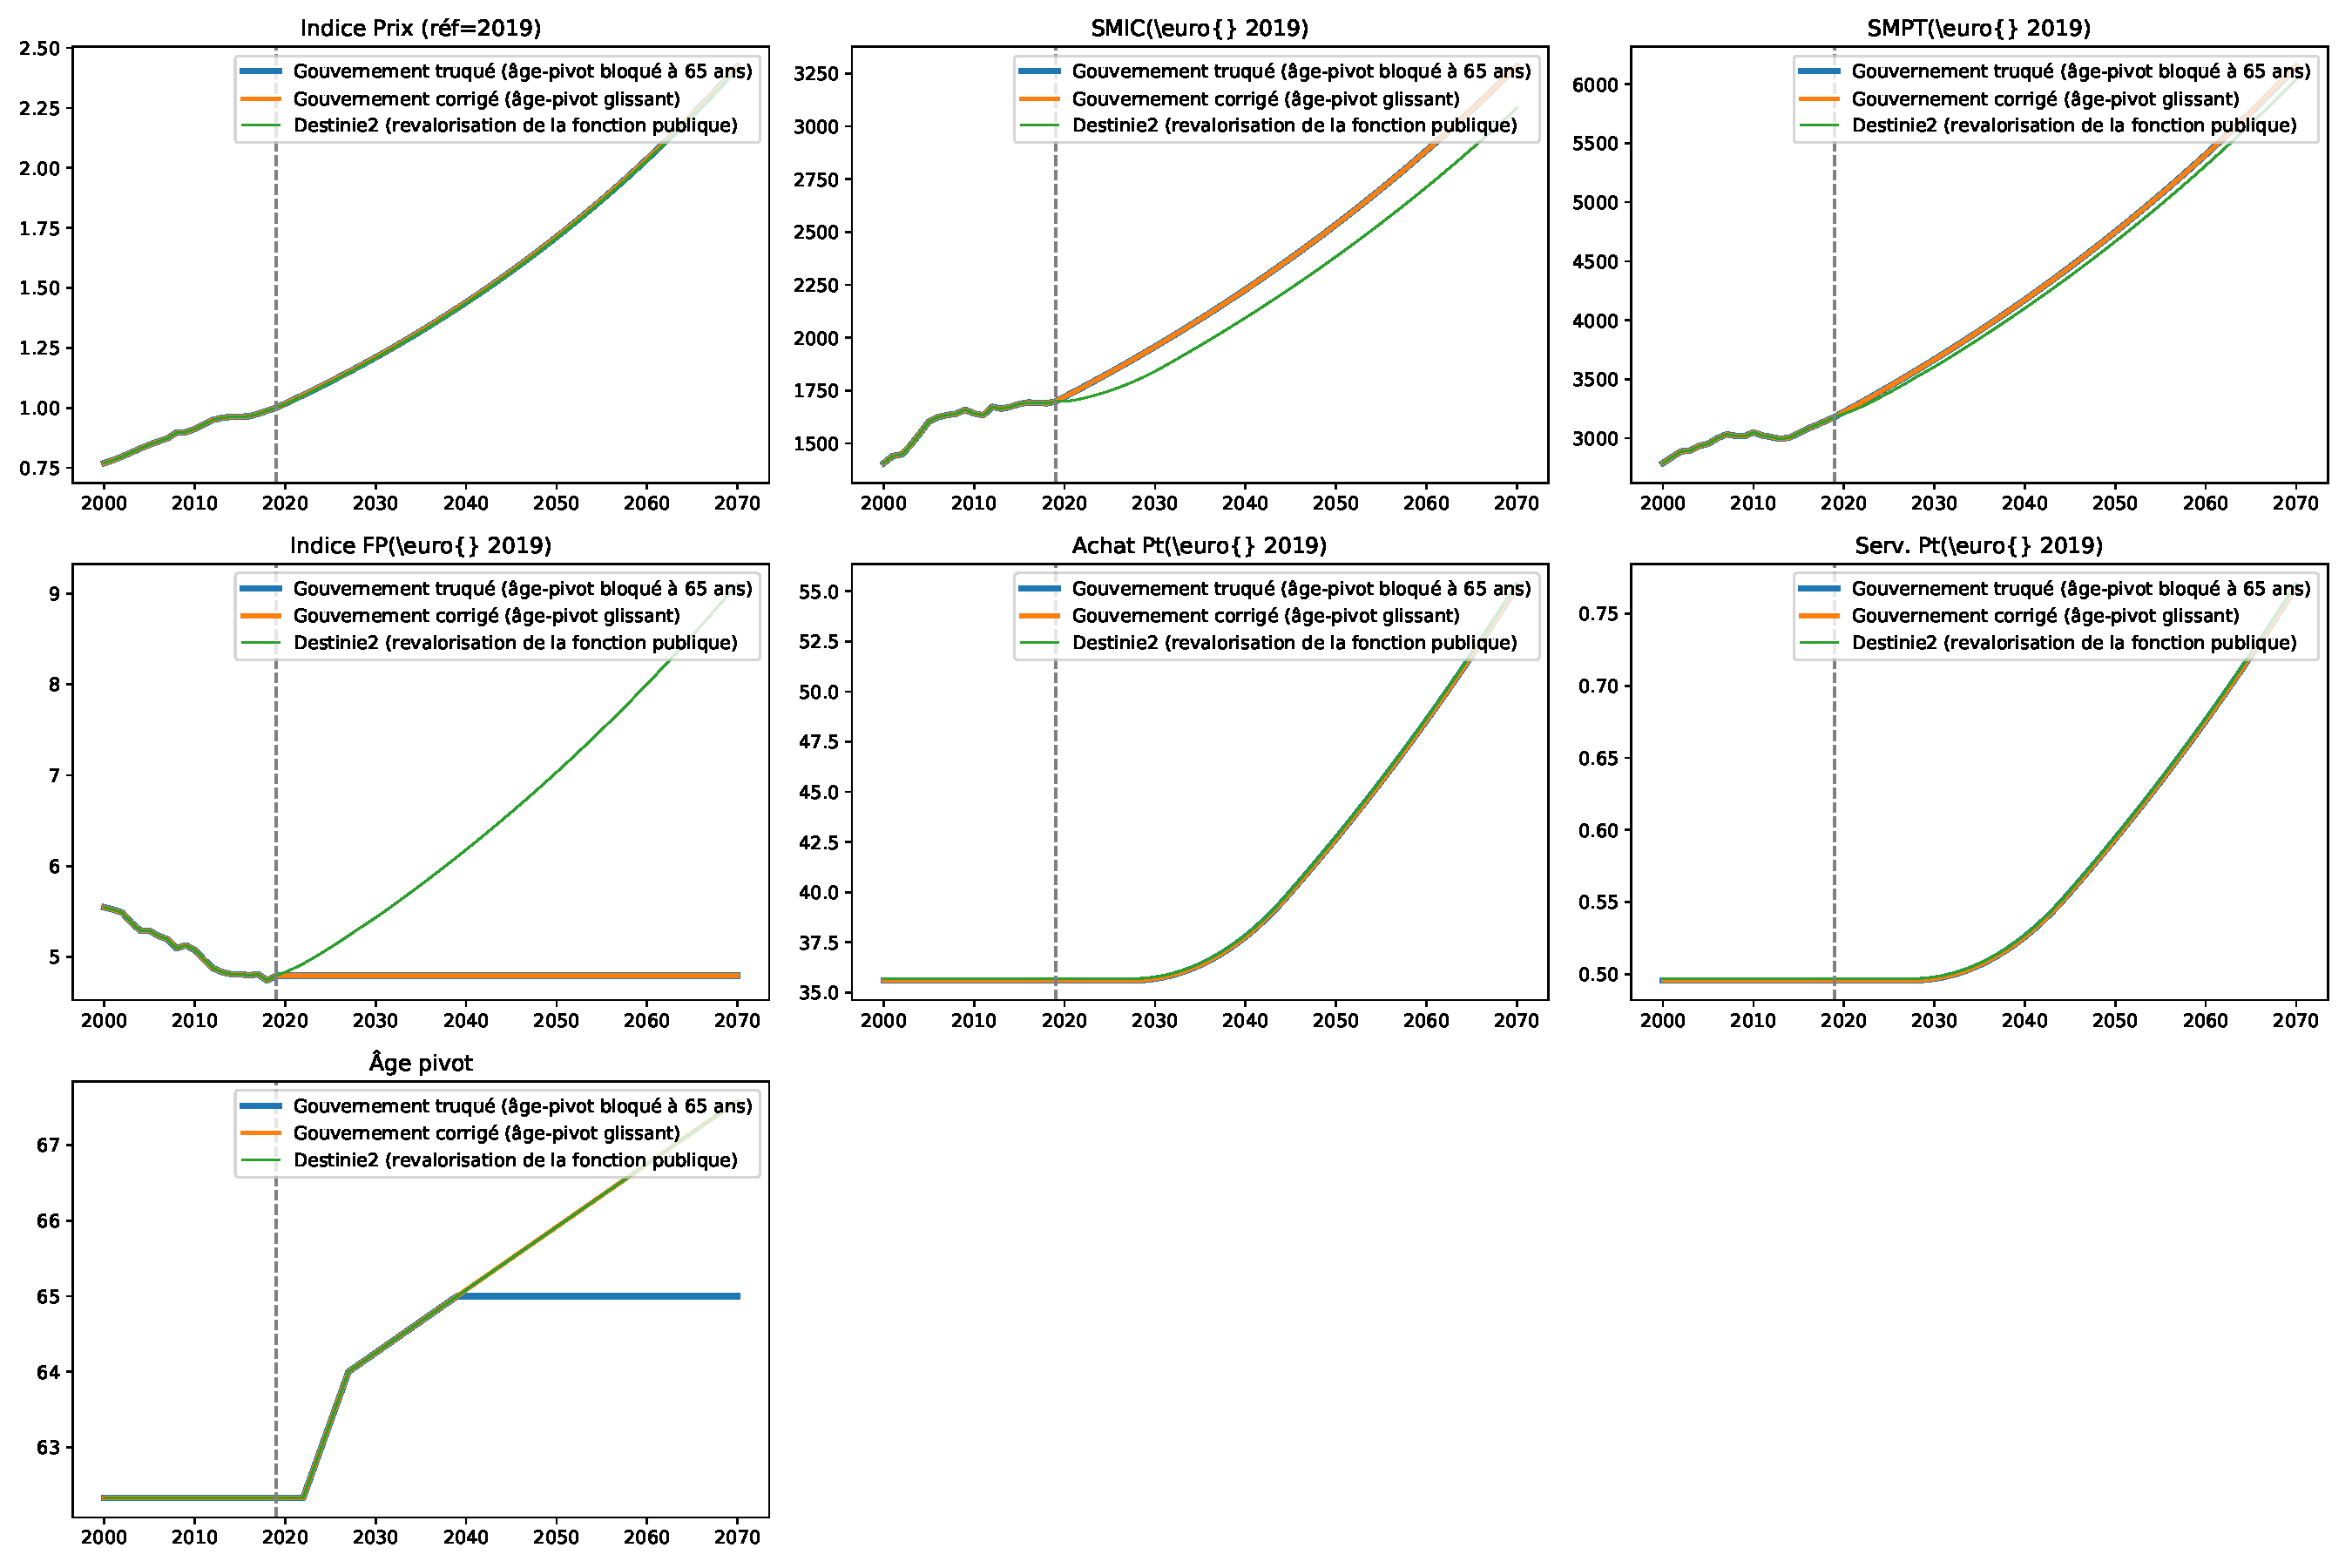
\includegraphics[width=1\textwidth]{fig/comparaison_modeles.pdf}\end{center} 

\newpage 
 
\paragraph{Description détaillée du modèle \emph{Gouvernement truqué (âge-pivot bloqué à 65 ans)}} 
 
 { \tiny \begin{center} 
\begin{tabular}[htb]{|c||c|c|c|c|c|c|c||c|} 
\hline 
 Année &  Indice Prix (réf=2019) &  SMIC(\euro{} 2019) &  SMPT(\euro{} 2019) &  Indice FP(\euro{} 2019) &  Achat Pt(\euro{} 2019) &  Serv. Pt(\euro{} 2019) &  Âge pivot \\ 
\hline \hline 
 2000 &  0.77 &  1407.00 &  2789.32 &  5.55 &  35.61 &  0.50 &  62.33 \\ 
\hline 
 2001 &  0.78 &  1441.04 &  2841.01 &  5.52 &  35.61 &  0.50 &  62.33 \\ 
\hline 
 2002 &  0.80 &  1447.74 &  2888.44 &  5.49 &  35.61 &  0.50 &  62.33 \\ 
\hline 
 2003 &  0.81 &  1493.03 &  2895.27 &  5.37 &  35.61 &  0.50 &  62.33 \\ 
\hline 
 2004 &  0.83 &  1547.32 &  2935.07 &  5.29 &  35.61 &  0.50 &  62.33 \\ 
\hline 
 2005 &  0.85 &  1603.67 &  2953.63 &  5.29 &  35.61 &  0.50 &  62.33 \\ 
\hline 
 2006 &  0.86 &  1625.00 &  3000.00 &  5.23 &  35.61 &  0.50 &  62.33 \\ 
\hline 
 2007 &  0.87 &  1634.08 &  3033.08 &  5.19 &  35.61 &  0.50 &  62.33 \\ 
\hline 
 2008 &  0.90 &  1640.24 &  3020.36 &  5.09 &  35.61 &  0.50 &  62.33 \\ 
\hline 
 2009 &  0.90 &  1659.42 &  3016.76 &  5.13 &  35.61 &  0.50 &  62.33 \\ 
\hline 
 2010 &  0.91 &  1641.90 &  3050.50 &  5.08 &  35.61 &  0.50 &  62.33 \\ 
\hline 
 2011 &  0.93 &  1633.19 &  3023.52 &  4.97 &  35.61 &  0.50 &  62.33 \\ 
\hline 
 2012 &  0.95 &  1673.05 &  3009.71 &  4.88 &  35.61 &  0.50 &  62.33 \\ 
\hline 
 2013 &  0.96 &  1664.01 &  2994.48 &  4.83 &  35.61 &  0.50 &  62.33 \\ 
\hline 
 2014 &  0.96 &  1673.24 &  3006.42 &  4.81 &  35.61 &  0.50 &  62.33 \\ 
\hline 
 2015 &  0.96 &  1686.62 &  3043.81 &  4.81 &  35.61 &  0.50 &  62.33 \\ 
\hline 
 2016 &  0.96 &  1693.76 &  3082.28 &  4.80 &  35.61 &  0.50 &  62.33 \\ 
\hline 
 2017 &  0.97 &  1692.60 &  3113.10 &  4.81 &  35.61 &  0.50 &  62.33 \\ 
\hline 
 2018 &  0.99 &  1689.76 &  3147.35 &  4.74 &  35.61 &  0.50 &  62.33 \\ 
\hline 
 2019 &  1.00 &  1698.45 &  3181.97 &  4.79 &  35.61 &  0.50 &  62.33 \\ 
\hline 
 2020 &  1.02 &  1720.53 &  3223.33 &  4.79 &  35.61 &  0.50 &  62.33 \\ 
\hline 
 2021 &  1.04 &  1742.90 &  3265.24 &  4.79 &  35.61 &  0.50 &  62.33 \\ 
\hline 
 2022 &  1.05 &  1765.55 &  3307.69 &  4.79 &  35.61 &  0.50 &  62.33 \\ 
\hline 
 2023 &  1.07 &  1788.51 &  3350.69 &  4.79 &  35.61 &  0.50 &  62.67 \\ 
\hline 
 2024 &  1.09 &  1811.76 &  3394.24 &  4.79 &  35.61 &  0.50 &  63.00 \\ 
\hline 
 2025 &  1.11 &  1835.31 &  3438.37 &  4.79 &  35.61 &  0.50 &  63.33 \\ 
\hline 
 2026 &  1.13 &  1859.17 &  3483.07 &  4.79 &  35.61 &  0.50 &  63.67 \\ 
\hline 
 2027 &  1.15 &  1883.34 &  3528.35 &  4.79 &  35.61 &  0.50 &  64.00 \\ 
\hline 
 2028 &  1.17 &  1907.82 &  3574.22 &  4.79 &  35.61 &  0.50 &  64.08 \\ 
\hline 
 2029 &  1.19 &  1932.62 &  3620.68 &  4.79 &  35.63 &  0.50 &  64.17 \\ 
\hline 
 2030 &  1.21 &  1957.75 &  3667.75 &  4.79 &  35.69 &  0.50 &  64.25 \\ 
\hline 
 2031 &  1.23 &  1983.20 &  3715.43 &  4.79 &  35.77 &  0.50 &  64.33 \\ 
\hline 
 2032 &  1.25 &  2008.98 &  3763.73 &  4.79 &  35.88 &  0.50 &  64.42 \\ 
\hline 
 2033 &  1.27 &  2035.10 &  3812.66 &  4.79 &  36.02 &  0.50 &  64.50 \\ 
\hline 
 2034 &  1.30 &  2061.55 &  3862.22 &  4.79 &  36.18 &  0.50 &  64.58 \\ 
\hline 
 2035 &  1.32 &  2088.35 &  3912.43 &  4.79 &  36.37 &  0.51 &  64.67 \\ 
\hline 
 2036 &  1.34 &  2115.50 &  3963.30 &  4.79 &  36.59 &  0.51 &  64.75 \\ 
\hline 
 2037 &  1.37 &  2143.00 &  4014.82 &  4.79 &  36.85 &  0.51 &  64.83 \\ 
\hline 
 2038 &  1.39 &  2170.86 &  4067.01 &  4.79 &  37.13 &  0.52 &  64.92 \\ 
\hline 
 2039 &  1.41 &  2199.08 &  4119.88 &  4.79 &  37.44 &  0.52 &  65.00 \\ 
\hline 
 2040 &  1.44 &  2227.67 &  4173.44 &  4.79 &  37.78 &  0.53 &  65.00 \\ 
\hline 
 2041 &  1.46 &  2256.63 &  4227.69 &  4.79 &  38.16 &  0.53 &  65.00 \\ 
\hline 
 2042 &  1.49 &  2285.97 &  4282.65 &  4.79 &  38.56 &  0.54 &  65.00 \\ 
\hline 
 2043 &  1.52 &  2315.68 &  4338.33 &  4.79 &  39.01 &  0.54 &  65.00 \\ 
\hline 
 2044 &  1.54 &  2345.79 &  4394.73 &  4.79 &  39.48 &  0.55 &  65.00 \\ 
\hline 
 2045 &  1.57 &  2376.28 &  4451.86 &  4.79 &  40.00 &  0.56 &  65.00 \\ 
\hline 
 2046 &  1.60 &  2407.18 &  4509.73 &  4.79 &  40.52 &  0.56 &  65.00 \\ 
\hline 
 2047 &  1.63 &  2438.47 &  4568.36 &  4.79 &  41.04 &  0.57 &  65.00 \\ 
\hline 
 2048 &  1.65 &  2470.17 &  4627.75 &  4.79 &  41.58 &  0.58 &  65.00 \\ 
\hline 
 2049 &  1.68 &  2502.28 &  4687.91 &  4.79 &  42.12 &  0.59 &  65.00 \\ 
\hline 
 2050 &  1.71 &  2534.81 &  4748.85 &  4.79 &  42.66 &  0.59 &  65.00 \\ 
\hline 
 2051 &  1.74 &  2567.76 &  4810.59 &  4.79 &  43.22 &  0.60 &  65.00 \\ 
\hline 
 2052 &  1.77 &  2601.14 &  4873.12 &  4.79 &  43.78 &  0.61 &  65.00 \\ 
\hline 
 2053 &  1.80 &  2634.96 &  4936.48 &  4.79 &  44.35 &  0.62 &  65.00 \\ 
\hline 
 2054 &  1.84 &  2669.21 &  5000.65 &  4.79 &  44.93 &  0.63 &  65.00 \\ 
\hline 
 2055 &  1.87 &  2703.91 &  5065.66 &  4.79 &  45.51 &  0.63 &  65.00 \\ 
\hline 
 2056 &  1.90 &  2739.06 &  5131.51 &  4.79 &  46.10 &  0.64 &  65.00 \\ 
\hline 
 2057 &  1.93 &  2774.67 &  5198.22 &  4.79 &  46.70 &  0.65 &  65.00 \\ 
\hline 
 2058 &  1.97 &  2810.74 &  5265.80 &  4.79 &  47.31 &  0.66 &  65.00 \\ 
\hline 
 2059 &  2.00 &  2847.28 &  5334.25 &  4.79 &  47.92 &  0.67 &  65.00 \\ 
\hline 
 2060 &  2.04 &  2884.30 &  5403.60 &  4.79 &  48.55 &  0.68 &  65.00 \\ 
\hline 
 2061 &  2.07 &  2921.79 &  5473.85 &  4.79 &  49.18 &  0.68 &  65.00 \\ 
\hline 
 2062 &  2.11 &  2959.78 &  5545.01 &  4.79 &  49.82 &  0.69 &  65.00 \\ 
\hline 
 2063 &  2.15 &  2998.25 &  5617.09 &  4.79 &  50.47 &  0.70 &  65.00 \\ 
\hline 
 2064 &  2.18 &  3037.23 &  5690.11 &  4.79 &  51.12 &  0.71 &  65.00 \\ 
\hline 
 2065 &  2.22 &  3076.71 &  5764.08 &  4.79 &  51.79 &  0.72 &  65.00 \\ 
\hline 
 2066 &  2.26 &  3116.71 &  5839.02 &  4.79 &  52.46 &  0.73 &  65.00 \\ 
\hline 
 2067 &  2.30 &  3157.23 &  5914.92 &  4.79 &  53.14 &  0.74 &  65.00 \\ 
\hline 
 2068 &  2.34 &  3198.27 &  5991.82 &  4.79 &  53.83 &  0.75 &  65.00 \\ 
\hline 
 2069 &  2.38 &  3239.85 &  6069.71 &  4.79 &  54.53 &  0.76 &  65.00 \\ 
\hline 
 2070 &  2.42 &  3281.97 &  6148.62 &  4.79 &  55.24 &  0.77 &  65.00 \\ 
\hline 
\hline 
\end{tabular} 
\end{center} } 
\newpage 
 
\paragraph{Description détaillée du modèle \emph{Gouvernement corrigé (âge-pivot glissant)}} 
 
 { \tiny \begin{center} 
\begin{tabular}[htb]{|c||c|c|c|c|c|c|c||c|} 
\hline 
 Année &  Indice Prix (réf=2019) &  SMIC(\euro{} 2019) &  SMPT(\euro{} 2019) &  Indice FP(\euro{} 2019) &  Achat Pt(\euro{} 2019) &  Serv. Pt(\euro{} 2019) &  Âge pivot \\ 
\hline \hline 
 2000 &  0.77 &  1407.00 &  2789.32 &  5.55 &  35.61 &  0.50 &  62.33 \\ 
\hline 
 2001 &  0.78 &  1441.04 &  2841.01 &  5.52 &  35.61 &  0.50 &  62.33 \\ 
\hline 
 2002 &  0.80 &  1447.74 &  2888.44 &  5.49 &  35.61 &  0.50 &  62.33 \\ 
\hline 
 2003 &  0.81 &  1493.03 &  2895.27 &  5.37 &  35.61 &  0.50 &  62.33 \\ 
\hline 
 2004 &  0.83 &  1547.32 &  2935.07 &  5.29 &  35.61 &  0.50 &  62.33 \\ 
\hline 
 2005 &  0.85 &  1603.67 &  2953.63 &  5.29 &  35.61 &  0.50 &  62.33 \\ 
\hline 
 2006 &  0.86 &  1625.00 &  3000.00 &  5.23 &  35.61 &  0.50 &  62.33 \\ 
\hline 
 2007 &  0.87 &  1634.08 &  3033.08 &  5.19 &  35.61 &  0.50 &  62.33 \\ 
\hline 
 2008 &  0.90 &  1640.24 &  3020.36 &  5.09 &  35.61 &  0.50 &  62.33 \\ 
\hline 
 2009 &  0.90 &  1659.42 &  3016.76 &  5.13 &  35.61 &  0.50 &  62.33 \\ 
\hline 
 2010 &  0.91 &  1641.90 &  3050.50 &  5.08 &  35.61 &  0.50 &  62.33 \\ 
\hline 
 2011 &  0.93 &  1633.19 &  3023.52 &  4.97 &  35.61 &  0.50 &  62.33 \\ 
\hline 
 2012 &  0.95 &  1673.05 &  3009.71 &  4.88 &  35.61 &  0.50 &  62.33 \\ 
\hline 
 2013 &  0.96 &  1664.01 &  2994.48 &  4.83 &  35.61 &  0.50 &  62.33 \\ 
\hline 
 2014 &  0.96 &  1673.24 &  3006.42 &  4.81 &  35.61 &  0.50 &  62.33 \\ 
\hline 
 2015 &  0.96 &  1686.62 &  3043.81 &  4.81 &  35.61 &  0.50 &  62.33 \\ 
\hline 
 2016 &  0.96 &  1693.76 &  3082.28 &  4.80 &  35.61 &  0.50 &  62.33 \\ 
\hline 
 2017 &  0.97 &  1692.60 &  3113.10 &  4.81 &  35.61 &  0.50 &  62.33 \\ 
\hline 
 2018 &  0.99 &  1689.76 &  3147.35 &  4.74 &  35.61 &  0.50 &  62.33 \\ 
\hline 
 2019 &  1.00 &  1698.45 &  3181.97 &  4.79 &  35.61 &  0.50 &  62.33 \\ 
\hline 
 2020 &  1.02 &  1720.53 &  3223.33 &  4.79 &  35.61 &  0.50 &  62.33 \\ 
\hline 
 2021 &  1.04 &  1742.90 &  3265.24 &  4.79 &  35.61 &  0.50 &  62.33 \\ 
\hline 
 2022 &  1.05 &  1765.55 &  3307.69 &  4.79 &  35.61 &  0.50 &  62.33 \\ 
\hline 
 2023 &  1.07 &  1788.51 &  3350.69 &  4.79 &  35.61 &  0.50 &  62.67 \\ 
\hline 
 2024 &  1.09 &  1811.76 &  3394.24 &  4.79 &  35.61 &  0.50 &  63.00 \\ 
\hline 
 2025 &  1.11 &  1835.31 &  3438.37 &  4.79 &  35.61 &  0.50 &  63.33 \\ 
\hline 
 2026 &  1.13 &  1859.17 &  3483.07 &  4.79 &  35.61 &  0.50 &  63.67 \\ 
\hline 
 2027 &  1.15 &  1883.34 &  3528.35 &  4.79 &  35.61 &  0.50 &  64.00 \\ 
\hline 
 2028 &  1.17 &  1907.82 &  3574.22 &  4.79 &  35.61 &  0.50 &  64.08 \\ 
\hline 
 2029 &  1.19 &  1932.62 &  3620.68 &  4.79 &  35.63 &  0.50 &  64.17 \\ 
\hline 
 2030 &  1.21 &  1957.75 &  3667.75 &  4.79 &  35.69 &  0.50 &  64.25 \\ 
\hline 
 2031 &  1.23 &  1983.20 &  3715.43 &  4.79 &  35.77 &  0.50 &  64.33 \\ 
\hline 
 2032 &  1.25 &  2008.98 &  3763.73 &  4.79 &  35.88 &  0.50 &  64.42 \\ 
\hline 
 2033 &  1.27 &  2035.10 &  3812.66 &  4.79 &  36.02 &  0.50 &  64.50 \\ 
\hline 
 2034 &  1.30 &  2061.55 &  3862.22 &  4.79 &  36.18 &  0.50 &  64.58 \\ 
\hline 
 2035 &  1.32 &  2088.35 &  3912.43 &  4.79 &  36.37 &  0.51 &  64.67 \\ 
\hline 
 2036 &  1.34 &  2115.50 &  3963.30 &  4.79 &  36.59 &  0.51 &  64.75 \\ 
\hline 
 2037 &  1.37 &  2143.00 &  4014.82 &  4.79 &  36.85 &  0.51 &  64.83 \\ 
\hline 
 2038 &  1.39 &  2170.86 &  4067.01 &  4.79 &  37.13 &  0.52 &  64.92 \\ 
\hline 
 2039 &  1.41 &  2199.08 &  4119.88 &  4.79 &  37.44 &  0.52 &  65.00 \\ 
\hline 
 2040 &  1.44 &  2227.67 &  4173.44 &  4.79 &  37.78 &  0.53 &  65.08 \\ 
\hline 
 2041 &  1.46 &  2256.63 &  4227.69 &  4.79 &  38.16 &  0.53 &  65.17 \\ 
\hline 
 2042 &  1.49 &  2285.97 &  4282.65 &  4.79 &  38.56 &  0.54 &  65.25 \\ 
\hline 
 2043 &  1.52 &  2315.68 &  4338.33 &  4.79 &  39.01 &  0.54 &  65.33 \\ 
\hline 
 2044 &  1.54 &  2345.79 &  4394.73 &  4.79 &  39.48 &  0.55 &  65.42 \\ 
\hline 
 2045 &  1.57 &  2376.28 &  4451.86 &  4.79 &  40.00 &  0.56 &  65.50 \\ 
\hline 
 2046 &  1.60 &  2407.18 &  4509.73 &  4.79 &  40.52 &  0.56 &  65.58 \\ 
\hline 
 2047 &  1.63 &  2438.47 &  4568.36 &  4.79 &  41.04 &  0.57 &  65.67 \\ 
\hline 
 2048 &  1.65 &  2470.17 &  4627.75 &  4.79 &  41.58 &  0.58 &  65.75 \\ 
\hline 
 2049 &  1.68 &  2502.28 &  4687.91 &  4.79 &  42.12 &  0.59 &  65.83 \\ 
\hline 
 2050 &  1.71 &  2534.81 &  4748.85 &  4.79 &  42.66 &  0.59 &  65.92 \\ 
\hline 
 2051 &  1.74 &  2567.76 &  4810.59 &  4.79 &  43.22 &  0.60 &  66.00 \\ 
\hline 
 2052 &  1.77 &  2601.14 &  4873.12 &  4.79 &  43.78 &  0.61 &  66.08 \\ 
\hline 
 2053 &  1.80 &  2634.96 &  4936.48 &  4.79 &  44.35 &  0.62 &  66.17 \\ 
\hline 
 2054 &  1.84 &  2669.21 &  5000.65 &  4.79 &  44.93 &  0.63 &  66.25 \\ 
\hline 
 2055 &  1.87 &  2703.91 &  5065.66 &  4.79 &  45.51 &  0.63 &  66.33 \\ 
\hline 
 2056 &  1.90 &  2739.06 &  5131.51 &  4.79 &  46.10 &  0.64 &  66.42 \\ 
\hline 
 2057 &  1.93 &  2774.67 &  5198.22 &  4.79 &  46.70 &  0.65 &  66.50 \\ 
\hline 
 2058 &  1.97 &  2810.74 &  5265.80 &  4.79 &  47.31 &  0.66 &  66.58 \\ 
\hline 
 2059 &  2.00 &  2847.28 &  5334.25 &  4.79 &  47.92 &  0.67 &  66.67 \\ 
\hline 
 2060 &  2.04 &  2884.30 &  5403.60 &  4.79 &  48.55 &  0.68 &  66.75 \\ 
\hline 
 2061 &  2.07 &  2921.79 &  5473.85 &  4.79 &  49.18 &  0.68 &  66.83 \\ 
\hline 
 2062 &  2.11 &  2959.78 &  5545.01 &  4.79 &  49.82 &  0.69 &  66.92 \\ 
\hline 
 2063 &  2.15 &  2998.25 &  5617.09 &  4.79 &  50.47 &  0.70 &  67.00 \\ 
\hline 
 2064 &  2.18 &  3037.23 &  5690.11 &  4.79 &  51.12 &  0.71 &  67.08 \\ 
\hline 
 2065 &  2.22 &  3076.71 &  5764.08 &  4.79 &  51.79 &  0.72 &  67.17 \\ 
\hline 
 2066 &  2.26 &  3116.71 &  5839.02 &  4.79 &  52.46 &  0.73 &  67.25 \\ 
\hline 
 2067 &  2.30 &  3157.23 &  5914.92 &  4.79 &  53.14 &  0.74 &  67.33 \\ 
\hline 
 2068 &  2.34 &  3198.27 &  5991.82 &  4.79 &  53.83 &  0.75 &  67.42 \\ 
\hline 
 2069 &  2.38 &  3239.85 &  6069.71 &  4.79 &  54.53 &  0.76 &  67.50 \\ 
\hline 
 2070 &  2.42 &  3281.97 &  6148.62 &  4.79 &  55.24 &  0.77 &  67.58 \\ 
\hline 
\hline 
\end{tabular} 
\end{center} } 
\newpage 
 
\paragraph{Description détaillée du modèle \emph{Destinie2 (revalorisation de la fonction publique)}} 
 
 { \tiny \begin{center} 
\begin{tabular}[htb]{|c||c|c|c|c|c|c|c||c|} 
\hline 
 Année &  Indice Prix (réf=2019) &  SMIC(\euro{} 2019) &  SMPT(\euro{} 2019) &  Indice FP(\euro{} 2019) &  Achat Pt(\euro{} 2019) &  Serv. Pt(\euro{} 2019) &  Âge pivot \\ 
\hline \hline 
 2000 &  0.77 &  1407.00 &  2789.32 &  5.55 &  35.69 &  0.50 &  62.33 \\ 
\hline 
 2001 &  0.78 &  1441.04 &  2841.01 &  5.52 &  35.69 &  0.50 &  62.33 \\ 
\hline 
 2002 &  0.80 &  1447.74 &  2888.44 &  5.49 &  35.69 &  0.50 &  62.33 \\ 
\hline 
 2003 &  0.81 &  1493.03 &  2895.27 &  5.37 &  35.69 &  0.50 &  62.33 \\ 
\hline 
 2004 &  0.83 &  1547.32 &  2935.07 &  5.29 &  35.69 &  0.50 &  62.33 \\ 
\hline 
 2005 &  0.85 &  1603.67 &  2953.63 &  5.29 &  35.69 &  0.50 &  62.33 \\ 
\hline 
 2006 &  0.86 &  1625.00 &  3000.00 &  5.23 &  35.69 &  0.50 &  62.33 \\ 
\hline 
 2007 &  0.87 &  1634.08 &  3033.08 &  5.19 &  35.69 &  0.50 &  62.33 \\ 
\hline 
 2008 &  0.90 &  1640.24 &  3020.36 &  5.09 &  35.69 &  0.50 &  62.33 \\ 
\hline 
 2009 &  0.90 &  1659.42 &  3016.76 &  5.13 &  35.69 &  0.50 &  62.33 \\ 
\hline 
 2010 &  0.91 &  1641.90 &  3050.50 &  5.08 &  35.69 &  0.50 &  62.33 \\ 
\hline 
 2011 &  0.93 &  1633.19 &  3023.52 &  4.97 &  35.69 &  0.50 &  62.33 \\ 
\hline 
 2012 &  0.95 &  1673.05 &  3009.71 &  4.88 &  35.69 &  0.50 &  62.33 \\ 
\hline 
 2013 &  0.96 &  1664.01 &  2994.48 &  4.83 &  35.69 &  0.50 &  62.33 \\ 
\hline 
 2014 &  0.96 &  1673.24 &  3006.42 &  4.81 &  35.69 &  0.50 &  62.33 \\ 
\hline 
 2015 &  0.96 &  1686.62 &  3043.81 &  4.81 &  35.69 &  0.50 &  62.33 \\ 
\hline 
 2016 &  0.96 &  1693.76 &  3082.28 &  4.80 &  35.69 &  0.50 &  62.33 \\ 
\hline 
 2017 &  0.97 &  1692.60 &  3113.10 &  4.81 &  35.69 &  0.50 &  62.33 \\ 
\hline 
 2018 &  0.99 &  1689.76 &  3147.35 &  4.74 &  35.69 &  0.50 &  62.33 \\ 
\hline 
 2019 &  1.00 &  1698.45 &  3181.97 &  4.79 &  35.69 &  0.50 &  62.33 \\ 
\hline 
 2020 &  1.01 &  1699.99 &  3207.42 &  4.83 &  35.69 &  0.50 &  62.33 \\ 
\hline 
 2021 &  1.03 &  1703.48 &  3236.29 &  4.88 &  35.69 &  0.50 &  62.33 \\ 
\hline 
 2022 &  1.05 &  1712.78 &  3268.65 &  4.93 &  35.69 &  0.50 &  62.33 \\ 
\hline 
 2023 &  1.07 &  1723.51 &  3306.90 &  4.98 &  35.69 &  0.50 &  62.67 \\ 
\hline 
 2024 &  1.09 &  1735.69 &  3346.25 &  5.04 &  35.69 &  0.50 &  63.00 \\ 
\hline 
 2025 &  1.11 &  1749.35 &  3387.07 &  5.10 &  35.69 &  0.50 &  63.33 \\ 
\hline 
 2026 &  1.13 &  1764.53 &  3429.41 &  5.17 &  35.69 &  0.50 &  63.67 \\ 
\hline 
 2027 &  1.15 &  1781.27 &  3473.31 &  5.23 &  35.69 &  0.50 &  64.00 \\ 
\hline 
 2028 &  1.17 &  1799.59 &  3518.81 &  5.30 &  35.69 &  0.50 &  64.08 \\ 
\hline 
 2029 &  1.19 &  1819.55 &  3561.39 &  5.37 &  35.72 &  0.50 &  64.17 \\ 
\hline 
 2030 &  1.21 &  1841.19 &  3605.55 &  5.43 &  35.77 &  0.50 &  64.25 \\ 
\hline 
 2031 &  1.23 &  1864.58 &  3651.34 &  5.50 &  35.85 &  0.50 &  64.33 \\ 
\hline 
 2032 &  1.25 &  1888.81 &  3698.81 &  5.57 &  35.96 &  0.50 &  64.42 \\ 
\hline 
 2033 &  1.27 &  1913.37 &  3746.89 &  5.65 &  36.10 &  0.50 &  64.50 \\ 
\hline 
 2034 &  1.29 &  1938.24 &  3795.60 &  5.72 &  36.26 &  0.50 &  64.58 \\ 
\hline 
 2035 &  1.32 &  1963.44 &  3844.94 &  5.79 &  36.46 &  0.51 &  64.67 \\ 
\hline 
 2036 &  1.34 &  1988.96 &  3894.93 &  5.87 &  36.68 &  0.51 &  64.75 \\ 
\hline 
 2037 &  1.36 &  2014.82 &  3945.56 &  5.94 &  36.93 &  0.51 &  64.83 \\ 
\hline 
 2038 &  1.39 &  2041.01 &  3996.85 &  6.02 &  37.21 &  0.52 &  64.92 \\ 
\hline 
 2039 &  1.41 &  2067.55 &  4048.81 &  6.10 &  37.52 &  0.52 &  65.00 \\ 
\hline 
 2040 &  1.44 &  2094.43 &  4101.45 &  6.18 &  37.87 &  0.53 &  65.08 \\ 
\hline 
 2041 &  1.46 &  2121.65 &  4154.76 &  6.26 &  38.24 &  0.53 &  65.17 \\ 
\hline 
 2042 &  1.49 &  2149.23 &  4208.78 &  6.34 &  38.65 &  0.54 &  65.25 \\ 
\hline 
 2043 &  1.51 &  2177.17 &  4263.49 &  6.42 &  39.10 &  0.54 &  65.33 \\ 
\hline 
 2044 &  1.54 &  2205.48 &  4318.92 &  6.51 &  39.57 &  0.55 &  65.42 \\ 
\hline 
 2045 &  1.57 &  2234.15 &  4375.06 &  6.59 &  40.09 &  0.56 &  65.50 \\ 
\hline 
 2046 &  1.59 &  2263.19 &  4431.94 &  6.68 &  40.61 &  0.57 &  65.58 \\ 
\hline 
 2047 &  1.62 &  2292.61 &  4489.55 &  6.76 &  41.14 &  0.57 &  65.67 \\ 
\hline 
 2048 &  1.65 &  2322.42 &  4547.92 &  6.85 &  41.67 &  0.58 &  65.75 \\ 
\hline 
 2049 &  1.68 &  2352.61 &  4607.04 &  6.94 &  42.21 &  0.59 &  65.83 \\ 
\hline 
 2050 &  1.71 &  2383.19 &  4666.93 &  7.03 &  42.76 &  0.60 &  65.92 \\ 
\hline 
 2051 &  1.74 &  2414.18 &  4727.60 &  7.12 &  43.32 &  0.60 &  66.00 \\ 
\hline 
 2052 &  1.77 &  2445.56 &  4789.06 &  7.22 &  43.88 &  0.61 &  66.08 \\ 
\hline 
 2053 &  1.80 &  2477.35 &  4851.32 &  7.31 &  44.45 &  0.62 &  66.17 \\ 
\hline 
 2054 &  1.83 &  2509.56 &  4914.39 &  7.40 &  45.03 &  0.63 &  66.25 \\ 
\hline 
 2055 &  1.86 &  2542.18 &  4978.27 &  7.50 &  45.62 &  0.63 &  66.33 \\ 
\hline 
 2056 &  1.90 &  2575.23 &  5042.99 &  7.60 &  46.21 &  0.64 &  66.42 \\ 
\hline 
 2057 &  1.93 &  2608.71 &  5108.55 &  7.70 &  46.81 &  0.65 &  66.50 \\ 
\hline 
 2058 &  1.96 &  2642.62 &  5174.96 &  7.80 &  47.42 &  0.66 &  66.58 \\ 
\hline 
 2059 &  2.00 &  2676.98 &  5242.23 &  7.90 &  48.03 &  0.67 &  66.67 \\ 
\hline 
 2060 &  2.03 &  2711.78 &  5310.38 &  8.00 &  48.66 &  0.68 &  66.75 \\ 
\hline 
 2061 &  2.07 &  2747.03 &  5379.42 &  8.11 &  49.29 &  0.69 &  66.83 \\ 
\hline 
 2062 &  2.10 &  2782.74 &  5449.35 &  8.21 &  49.93 &  0.70 &  66.92 \\ 
\hline 
 2063 &  2.14 &  2818.92 &  5520.19 &  8.32 &  50.58 &  0.70 &  67.00 \\ 
\hline 
 2064 &  2.18 &  2855.56 &  5591.96 &  8.43 &  51.24 &  0.71 &  67.08 \\ 
\hline 
 2065 &  2.22 &  2892.68 &  5664.65 &  8.54 &  51.90 &  0.72 &  67.17 \\ 
\hline 
 2066 &  2.25 &  2930.29 &  5738.29 &  8.65 &  52.58 &  0.73 &  67.25 \\ 
\hline 
 2067 &  2.29 &  2968.38 &  5812.89 &  8.76 &  53.26 &  0.74 &  67.33 \\ 
\hline 
 2068 &  2.33 &  3006.97 &  5888.46 &  8.87 &  53.95 &  0.75 &  67.42 \\ 
\hline 
 2069 &  2.37 &  3046.06 &  5965.01 &  8.99 &  54.66 &  0.76 &  67.50 \\ 
\hline 
 2070 &  2.42 &  3085.66 &  6042.55 &  9.10 &  55.37 &  0.77 &  67.58 \\ 
\hline 
\hline 
\end{tabular} 
\end{center} } 
\newpage 
 
\chapter{Infirmière en soins généraux (CN, CS, puis HC)} 

\begin{minipage}{0.55\linewidth}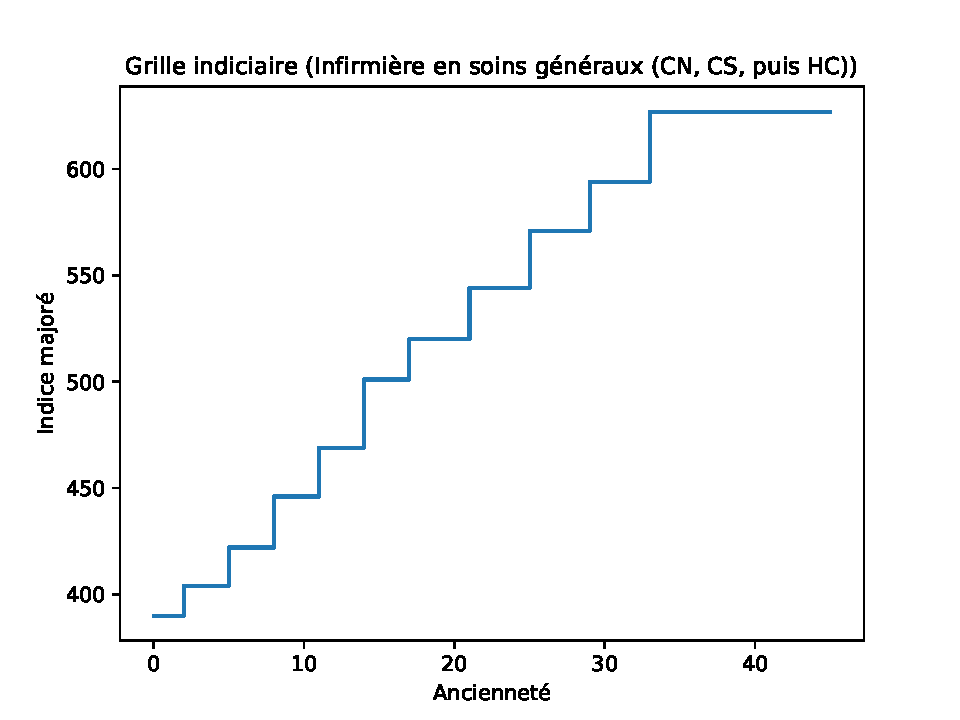
\includegraphics[width=0.7\textwidth]{fig/grille_Infirmier.pdf}\end{minipage} 
\begin{minipage}{0.3\linewidth} 
 \begin{center} 

\begin{tabular}[htb]{|c|c|} 
\hline 
 Indice majoré &  Durée (années) \\ 
\hline \hline 
 390 &  2.00 \\ 
\hline 
 404 &  3.00 \\ 
\hline 
 422 &  3.00 \\ 
\hline 
 446 &  3.00 \\ 
\hline 
 469 &  3.00 \\ 
\hline 
 501 &  3.00 \\ 
\hline 
 520 &  4.00 \\ 
\hline 
 544 &  4.00 \\ 
\hline 
 571 &  4.00 \\ 
\hline 
 594 &  4.00 \\ 
\hline 
 627 &   \\ 
\hline 
\hline 
\end{tabular} 
\end{center} 
 \end{minipage} 


 \addto{\captionsenglish}{ \renewcommand{\mtctitle}{}} \setcounter{minitocdepth}{2} 
 \minitoc \newpage 

\section{Début de carrière à 22 ans} 

\subsection{Génération 1975 (début en 1997)} 

\paragraph{Retraites possibles dans le modèle \emph{Gouvernement truqué (âge-pivot bloqué à 65 ans)}}  
 
{ \scriptsize \begin{center} 
\begin{tabular}[htb]{|c|c||c|c||c|c||c||c|c|c|c|c|c|} 
\hline 
 Retraite en &  Âge &  Âge pivot &  Décote/Surcote &  Retraite (\euro{} 2019) &  Tx Rempl(\%) &  SMIC (\euro{} 2019) &  Retraite/SMIC &  Rev70/SMIC &  Rev75/SMIC &  Rev80/SMIC &  Rev85/SMIC &  Rev90/SMIC \\ 
\hline \hline 
 2037 &  62 &  64 ans 10 mois &  -14.17\% &  1636.88 &  {\bf 42.14} &  2143.00 &  {\bf {\color{red} 0.76}} &  {\bf {\color{red} 0.69}} &  {\bf {\color{red} 0.65}} &  {\bf {\color{red} 0.61}} &  {\bf {\color{red} 0.57}} &  {\bf {\color{red} 0.53}} \\ 
\hline 
 2038 &  63 &  64 ans 11 mois &  -9.58\% &  1786.41 &  {\bf 45.91} &  2170.86 &  {\bf {\color{red} 0.82}} &  {\bf {\color{red} 0.75}} &  {\bf {\color{red} 0.70}} &  {\bf {\color{red} 0.66}} &  {\bf {\color{red} 0.62}} &  {\bf {\color{red} 0.58}} \\ 
\hline 
 2039 &  64 &  65 ans 0 mois &  -5.00\% &  1944.26 &  {\bf 49.88} &  2199.08 &  {\bf {\color{red} 0.88}} &  {\bf {\color{red} 0.82}} &  {\bf {\color{red} 0.77}} &  {\bf {\color{red} 0.72}} &  {\bf {\color{red} 0.67}} &  {\bf {\color{red} 0.63}} \\ 
\hline 
 2040 &  65 &  65 ans 0 mois &  0.00\% &  2119.69 &  {\bf 54.28} &  2227.67 &  {\bf {\color{red} 0.95}} &  {\bf {\color{red} 0.89}} &  {\bf {\color{red} 0.84}} &  {\bf {\color{red} 0.78}} &  {\bf {\color{red} 0.73}} &  {\bf {\color{red} 0.69}} \\ 
\hline 
 2041 &  66 &  65 ans 0 mois &  5.00\% &  2304.94 &  {\bf 58.92} &  2256.63 &  {\bf 1.02} &  {\bf {\color{red} 0.97}} &  {\bf {\color{red} 0.91}} &  {\bf {\color{red} 0.85}} &  {\bf {\color{red} 0.80}} &  {\bf {\color{red} 0.75}} \\ 
\hline 
 2042 &  67 &  65 ans 0 mois &  10.00\% &  2500.52 &  {\bf 63.81} &  2285.97 &  {\bf 1.09} &  {\bf 1.05} &  {\bf {\color{red} 0.99}} &  {\bf {\color{red} 0.92}} &  {\bf {\color{red} 0.87}} &  {\bf {\color{red} 0.81}} \\ 
\hline 
\hline 
\end{tabular} 
\end{center} } 
\paragraph{Retraites possibles dans le modèle \emph{Gouvernement corrigé (âge-pivot glissant)}}  
 
{ \scriptsize \begin{center} 
\begin{tabular}[htb]{|c|c||c|c||c|c||c||c|c|c|c|c|c|} 
\hline 
 Retraite en &  Âge &  Âge pivot &  Décote/Surcote &  Retraite (\euro{} 2019) &  Tx Rempl(\%) &  SMIC (\euro{} 2019) &  Retraite/SMIC &  Rev70/SMIC &  Rev75/SMIC &  Rev80/SMIC &  Rev85/SMIC &  Rev90/SMIC \\ 
\hline \hline 
 2037 &  62 &  64 ans 10 mois &  -14.17\% &  1636.88 &  {\bf 42.14} &  2143.00 &  {\bf {\color{red} 0.76}} &  {\bf {\color{red} 0.69}} &  {\bf {\color{red} 0.65}} &  {\bf {\color{red} 0.61}} &  {\bf {\color{red} 0.57}} &  {\bf {\color{red} 0.53}} \\ 
\hline 
 2038 &  63 &  64 ans 11 mois &  -9.58\% &  1786.41 &  {\bf 45.91} &  2170.86 &  {\bf {\color{red} 0.82}} &  {\bf {\color{red} 0.75}} &  {\bf {\color{red} 0.70}} &  {\bf {\color{red} 0.66}} &  {\bf {\color{red} 0.62}} &  {\bf {\color{red} 0.58}} \\ 
\hline 
 2039 &  64 &  65 ans 0 mois &  -5.00\% &  1944.26 &  {\bf 49.88} &  2199.08 &  {\bf {\color{red} 0.88}} &  {\bf {\color{red} 0.82}} &  {\bf {\color{red} 0.77}} &  {\bf {\color{red} 0.72}} &  {\bf {\color{red} 0.67}} &  {\bf {\color{red} 0.63}} \\ 
\hline 
 2040 &  65 &  65 ans 1 mois &  -0.42\% &  2110.86 &  {\bf 54.06} &  2227.67 &  {\bf {\color{red} 0.95}} &  {\bf {\color{red} 0.89}} &  {\bf {\color{red} 0.83}} &  {\bf {\color{red} 0.78}} &  {\bf {\color{red} 0.73}} &  {\bf {\color{red} 0.69}} \\ 
\hline 
 2041 &  66 &  65 ans 2 mois &  4.17\% &  2286.65 &  {\bf 58.45} &  2256.63 &  {\bf 1.01} &  {\bf {\color{red} 0.96}} &  {\bf {\color{red} 0.90}} &  {\bf {\color{red} 0.85}} &  {\bf {\color{red} 0.79}} &  {\bf {\color{red} 0.74}} \\ 
\hline 
 2042 &  67 &  65 ans 3 mois &  8.75\% &  2472.11 &  {\bf 63.08} &  2285.97 &  {\bf 1.08} &  {\bf 1.04} &  {\bf {\color{red} 0.98}} &  {\bf {\color{red} 0.91}} &  {\bf {\color{red} 0.86}} &  {\bf {\color{red} 0.80}} \\ 
\hline 
\hline 
\end{tabular} 
\end{center} } 
\paragraph{Retraites possibles dans le modèle \emph{Destinie2 (revalorisation de la fonction publique)}}  
 
{ \scriptsize \begin{center} 
\begin{tabular}[htb]{|c|c||c|c||c|c||c||c|c|c|c|c|c|} 
\hline 
 Retraite en &  Âge &  Âge pivot &  Décote/Surcote &  Retraite (\euro{} 2019) &  Tx Rempl(\%) &  SMIC (\euro{} 2019) &  Retraite/SMIC &  Rev70/SMIC &  Rev75/SMIC &  Rev80/SMIC &  Rev85/SMIC &  Rev90/SMIC \\ 
\hline \hline 
 2037 &  62 &  64 ans 10 mois &  -14.17\% &  1732.84 &  {\bf 35.98} &  2014.82 &  {\bf {\color{red} 0.86}} &  {\bf {\color{red} 0.78}} &  {\bf {\color{red} 0.73}} &  {\bf {\color{red} 0.68}} &  {\bf {\color{red} 0.64}} &  {\bf {\color{red} 0.60}} \\ 
\hline 
 2038 &  63 &  64 ans 11 mois &  -9.58\% &  1900.80 &  {\bf 38.89} &  2041.01 &  {\bf {\color{red} 0.93}} &  {\bf {\color{red} 0.85}} &  {\bf {\color{red} 0.80}} &  {\bf {\color{red} 0.75}} &  {\bf {\color{red} 0.70}} &  {\bf {\color{red} 0.66}} \\ 
\hline 
 2039 &  64 &  65 ans 0 mois &  -5.00\% &  2079.50 &  {\bf 41.93} &  2067.55 &  {\bf 1.01} &  {\bf {\color{red} 0.93}} &  {\bf {\color{red} 0.87}} &  {\bf {\color{red} 0.82}} &  {\bf {\color{red} 0.77}} &  {\bf {\color{red} 0.72}} \\ 
\hline 
 2040 &  65 &  65 ans 1 mois &  -0.42\% &  2269.56 &  {\bf 45.09} &  2094.43 &  {\bf 1.08} &  {\bf 1.02} &  {\bf {\color{red} 0.95}} &  {\bf {\color{red} 0.89}} &  {\bf {\color{red} 0.84}} &  {\bf {\color{red} 0.78}} \\ 
\hline 
 2041 &  66 &  65 ans 2 mois &  4.17\% &  2471.65 &  {\bf 48.39} &  2121.65 &  {\bf 1.16} &  {\bf 1.11} &  {\bf 1.04} &  {\bf {\color{red} 0.97}} &  {\bf {\color{red} 0.91}} &  {\bf {\color{red} 0.85}} \\ 
\hline 
 2042 &  67 &  65 ans 3 mois &  8.75\% &  2686.45 &  {\bf 51.83} &  2149.23 &  {\bf 1.25} &  {\bf 1.20} &  {\bf 1.13} &  {\bf 1.06} &  {\bf {\color{red} 0.99}} &  {\bf {\color{red} 0.93}} \\ 
\hline 
\hline 
\end{tabular} 
\end{center} } 

 \begin{center}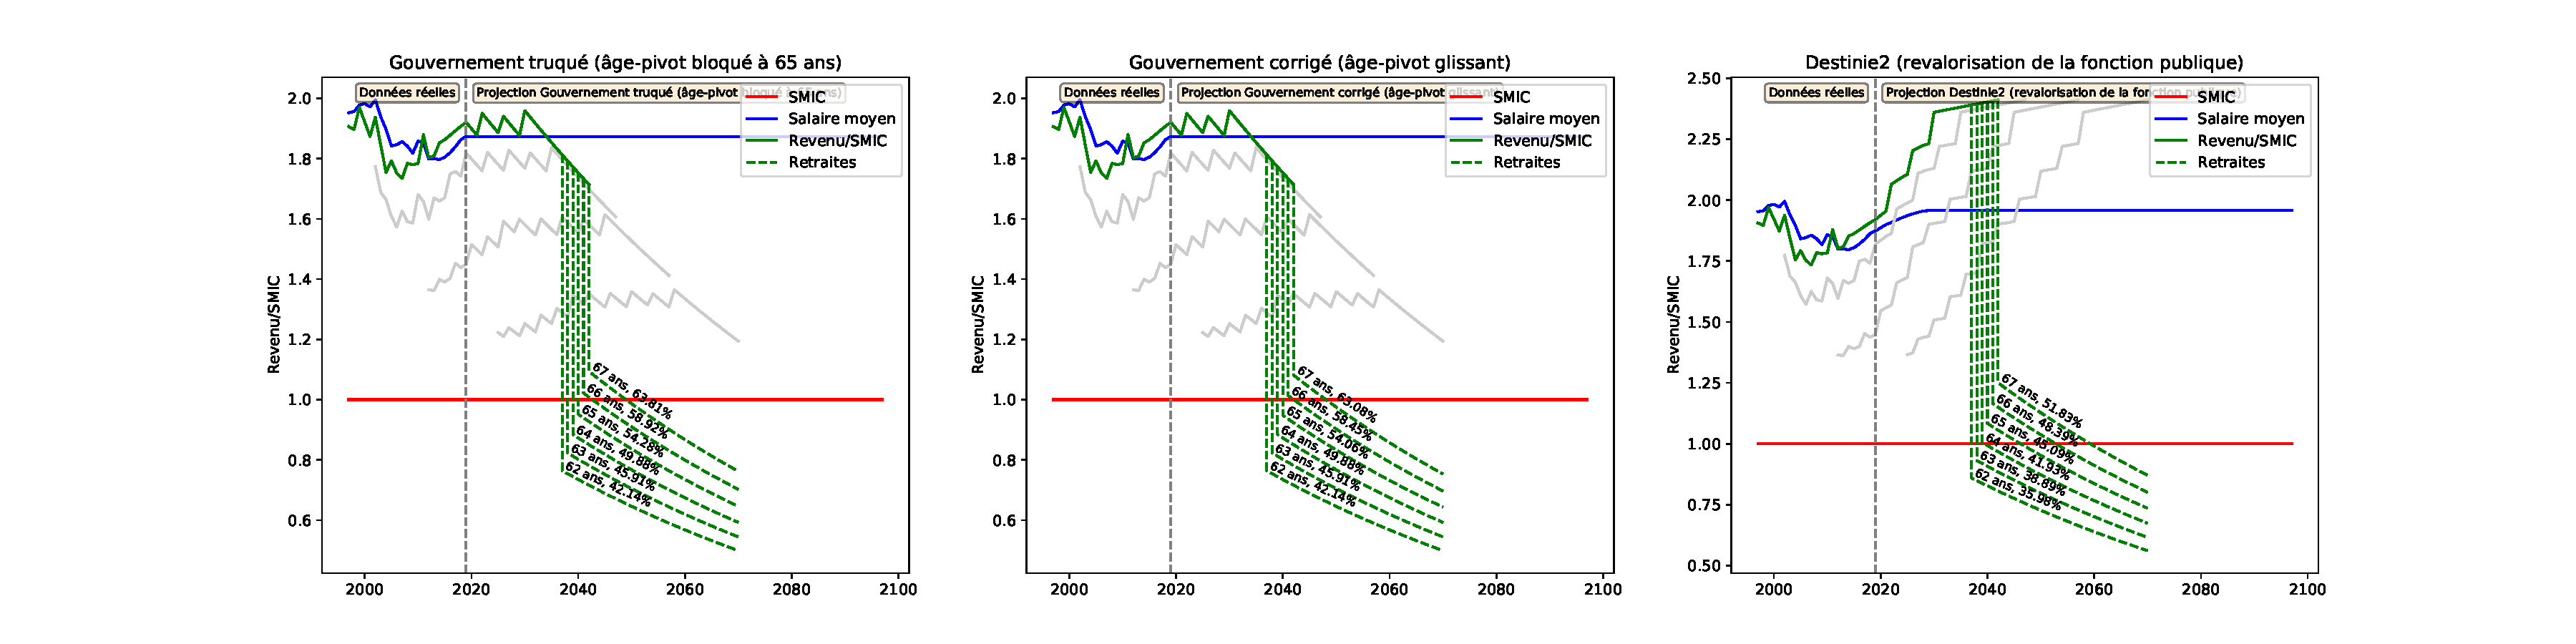
\includegraphics[width=0.9\textwidth]{fig/Infirmier_1975_22_dest_retraite.pdf}\end{center} \label{fig/Infirmier_1975_22_dest_retraite.pdf} 

\newpage 
 
\paragraph{Revenus et points pour le modèle \emph{Gouvernement truqué (âge-pivot bloqué à 65 ans)}} 
 
{ \scriptsize \begin{center} 
\begin{tabular}[htb]{|c|c||c|c|c|c|c|c||c|c||c|c|c|} 
\hline 
 Année &  Âge &  Ind Maj &  Pt Ind(\euro{} 2019) &  Rev HP(\euro{} 2019) &  Tx Primes &  GIPA(\euro{} 2019) &  Revenu(\euro{} 2019) &  SMIC(\euro{} 2019) &  Rev/SMIC &  Cumul Pts &  Achat Pt(\euro{} 2019) &  Serv. Pt(\euro{} 2019) \\ 
\hline \hline 
 1997 &  22 &  390.0 &  5.53 &  2158.40 &  20.01 &  0.00 &  2590.29 &  1358.84 &  {\bf 1.91} &  872.96 &  35.61 &  0.50 \\ 
\hline 
 1998 &  23 &  390.0 &  5.57 &  2170.92 &  20.24 &  0.00 &  2610.31 &  1376.36 &  {\bf 1.90} &  1752.67 &  35.61 &  0.50 \\ 
\hline 
 1999 &  24 &  404.0 &  5.61 &  2267.03 &  20.47 &  0.00 &  2731.09 &  1386.54 &  {\bf 1.97} &  2673.08 &  35.61 &  0.50 \\ 
\hline 
 2000 &  25 &  404.0 &  5.55 &  2240.25 &  20.70 &  0.00 &  2703.99 &  1407.00 &  {\bf 1.92} &  3584.35 &  35.61 &  0.50 \\ 
\hline 
 2001 &  26 &  404.0 &  5.52 &  2230.28 &  20.93 &  2.77 &  2699.85 &  1441.04 &  {\bf 1.87} &  4494.23 &  35.61 &  0.50 \\ 
\hline 
 2002 &  27 &  422.0 &  5.49 &  2315.21 &  21.16 &  0.00 &  2805.11 &  1447.74 &  {\bf 1.94} &  5439.59 &  35.61 &  0.50 \\ 
\hline 
 2003 &  28 &  422.0 &  5.37 &  2268.09 &  21.39 &  0.00 &  2753.23 &  1493.03 &  {\bf 1.84} &  6367.46 &  35.61 &  0.50 \\ 
\hline 
 2004 &  29 &  422.0 &  5.29 &  2232.26 &  21.62 &  0.00 &  2714.88 &  1547.32 &  {\bf 1.75} &  7282.41 &  35.61 &  0.50 \\ 
\hline 
 2005 &  30 &  446.0 &  5.29 &  2358.96 &  21.85 &  0.00 &  2874.39 &  1603.67 &  {\bf 1.79} &  8251.11 &  35.61 &  0.50 \\ 
\hline 
 2006 &  31 &  446.0 &  5.23 &  2332.63 &  22.08 &  0.00 &  2847.68 &  1625.00 &  {\bf 1.75} &  9210.82 &  35.61 &  0.50 \\ 
\hline 
 2007 &  32 &  446.0 &  5.19 &  2316.74 &  22.31 &  0.00 &  2833.60 &  1634.08 &  {\bf 1.73} &  10165.77 &  35.61 &  0.50 \\ 
\hline 
 2008 &  33 &  469.0 &  5.09 &  2388.64 &  22.54 &  0.00 &  2927.04 &  1640.24 &  {\bf 1.78} &  11152.22 &  35.61 &  0.50 \\ 
\hline 
 2009 &  34 &  469.0 &  5.13 &  2405.56 &  22.77 &  0.00 &  2953.31 &  1659.42 &  {\bf 1.78} &  12147.52 &  35.61 &  0.50 \\ 
\hline 
 2010 &  35 &  469.0 &  5.08 &  2381.26 &  23.00 &  0.00 &  2928.95 &  1641.90 &  {\bf 1.78} &  13134.62 &  35.61 &  0.50 \\ 
\hline 
 2011 &  36 &  501.0 &  4.97 &  2490.89 &  23.23 &  0.00 &  3069.52 &  1633.19 &  {\bf 1.88} &  14169.08 &  35.61 &  0.50 \\ 
\hline 
 2012 &  37 &  501.0 &  4.88 &  2443.09 &  23.46 &  0.00 &  3016.24 &  1673.05 &  {\bf 1.80} &  15185.59 &  35.61 &  0.50 \\ 
\hline 
 2013 &  38 &  501.0 &  4.83 &  2422.16 &  23.69 &  13.99 &  3009.96 &  1664.01 &  {\bf 1.81} &  16199.99 &  35.61 &  0.50 \\ 
\hline 
 2014 &  39 &  520.0 &  4.81 &  2501.43 &  23.92 &  0.00 &  3099.78 &  1673.24 &  {\bf 1.85} &  17244.65 &  35.61 &  0.50 \\ 
\hline 
 2015 &  40 &  520.0 &  4.81 &  2500.46 &  24.15 &  37.54 &  3141.86 &  1686.62 &  {\bf 1.86} &  18303.50 &  35.61 &  0.50 \\ 
\hline 
 2016 &  41 &  520.0 &  4.80 &  2495.47 &  24.38 &  76.40 &  3180.25 &  1693.76 &  {\bf 1.88} &  19375.28 &  35.61 &  0.50 \\ 
\hline 
 2017 &  42 &  520.0 &  4.81 &  2500.50 &  24.61 &  87.65 &  3203.52 &  1692.60 &  {\bf 1.89} &  20454.91 &  35.61 &  0.50 \\ 
\hline 
 2018 &  43 &  544.0 &  4.74 &  2579.79 &  24.84 &  2.20 &  3222.81 &  1689.76 &  {\bf 1.91} &  21541.03 &  35.61 &  0.50 \\ 
\hline 
 2019 &  44 &  544.0 &  4.79 &  2608.17 &  25.07 &  0.00 &  3262.03 &  1698.45 &  {\bf 1.92} &  22640.38 &  35.61 &  0.50 \\ 
\hline 
 2020 &  45 &  544.0 &  4.79 &  2608.17 &  25.30 &  0.00 &  3268.03 &  1720.53 &  {\bf 1.90} &  23741.74 &  35.61 &  0.50 \\ 
\hline 
 2021 &  46 &  544.0 &  4.79 &  2608.17 &  25.53 &  0.00 &  3274.03 &  1742.90 &  {\bf 1.88} &  24845.13 &  35.61 &  0.50 \\ 
\hline 
 2022 &  47 &  571.0 &  4.79 &  2737.62 &  25.76 &  0.00 &  3442.82 &  1765.55 &  {\bf 1.95} &  26005.40 &  35.61 &  0.50 \\ 
\hline 
 2023 &  48 &  571.0 &  4.79 &  2737.62 &  25.99 &  0.00 &  3449.12 &  1788.51 &  {\bf 1.93} &  27167.80 &  35.61 &  0.50 \\ 
\hline 
 2024 &  49 &  571.0 &  4.79 &  2737.62 &  26.22 &  0.00 &  3455.42 &  1811.76 &  {\bf 1.91} &  28332.32 &  35.61 &  0.50 \\ 
\hline 
 2025 &  50 &  571.0 &  4.79 &  2737.62 &  26.45 &  0.00 &  3461.71 &  1835.31 &  {\bf 1.89} &  29498.96 &  35.61 &  0.50 \\ 
\hline 
 2026 &  51 &  594.0 &  4.79 &  2847.89 &  26.68 &  0.00 &  3607.70 &  1859.17 &  {\bf 1.94} &  30714.80 &  35.61 &  0.50 \\ 
\hline 
 2027 &  52 &  594.0 &  4.79 &  2847.89 &  26.91 &  0.00 &  3614.25 &  1883.34 &  {\bf 1.92} &  31932.84 &  35.61 &  0.50 \\ 
\hline 
 2028 &  53 &  594.0 &  4.79 &  2847.89 &  27.14 &  0.00 &  3620.80 &  1907.82 &  {\bf 1.90} &  33153.10 &  35.61 &  0.50 \\ 
\hline 
 2029 &  54 &  594.0 &  4.79 &  2847.89 &  27.37 &  0.00 &  3627.35 &  1932.62 &  {\bf 1.88} &  34374.63 &  35.63 &  0.50 \\ 
\hline 
 2030 &  55 &  627.0 &  4.79 &  3006.10 &  27.60 &  0.00 &  3835.79 &  1957.75 &  {\bf 1.96} &  35664.40 &  35.69 &  0.50 \\ 
\hline 
 2031 &  56 &  627.0 &  4.79 &  3006.10 &  27.83 &  0.00 &  3842.70 &  1983.20 &  {\bf 1.94} &  36953.54 &  35.77 &  0.50 \\ 
\hline 
 2032 &  57 &  627.0 &  4.79 &  3006.10 &  28.06 &  0.00 &  3849.62 &  2008.98 &  {\bf 1.92} &  38241.09 &  35.88 &  0.50 \\ 
\hline 
 2033 &  58 &  627.0 &  4.79 &  3006.10 &  28.29 &  0.00 &  3856.53 &  2035.10 &  {\bf 1.90} &  39526.06 &  36.02 &  0.50 \\ 
\hline 
 2034 &  59 &  627.0 &  4.79 &  3006.10 &  28.52 &  0.00 &  3863.44 &  2061.55 &  {\bf 1.87} &  40807.48 &  36.18 &  0.50 \\ 
\hline 
 2035 &  60 &  627.0 &  4.79 &  3006.10 &  28.75 &  0.00 &  3870.36 &  2088.35 &  {\bf 1.85} &  42084.38 &  36.37 &  0.51 \\ 
\hline 
 2036 &  61 &  627.0 &  4.79 &  3006.10 &  28.98 &  0.00 &  3877.27 &  2115.50 &  {\bf 1.83} &  43355.81 &  36.59 &  0.51 \\ 
\hline 
 2037 &  62 &  627.0 &  4.79 &  3006.10 &  29.21 &  0.00 &  3884.19 &  2143.00 &  {\bf 1.81} &  44620.83 &  36.85 &  0.51 \\ 
\hline 
 2038 &  63 &  627.0 &  4.79 &  3006.10 &  29.44 &  0.00 &  3891.10 &  2170.86 &  {\bf 1.79} &  45878.51 &  37.13 &  0.52 \\ 
\hline 
 2039 &  64 &  627.0 &  4.79 &  3006.10 &  29.67 &  0.00 &  3898.01 &  2199.08 &  {\bf 1.77} &  47127.94 &  37.44 &  0.52 \\ 
\hline 
 2040 &  65 &  627.0 &  4.79 &  3006.10 &  29.90 &  0.00 &  3904.93 &  2227.67 &  {\bf 1.75} &  48368.22 &  37.78 &  0.53 \\ 
\hline 
 2041 &  66 &  627.0 &  4.79 &  3006.10 &  30.13 &  0.00 &  3911.84 &  2256.63 &  {\bf 1.73} &  49598.49 &  38.16 &  0.53 \\ 
\hline 
 2042 &  67 &  627.0 &  4.79 &  3006.10 &  30.36 &  0.00 &  3918.76 &  2285.97 &  {\bf 1.71} &  50817.89 &  38.56 &  0.54 \\ 
\hline 
\hline 
\end{tabular} 
\end{center} } 
\newpage 
 
\paragraph{Revenus et points pour le modèle \emph{Gouvernement corrigé (âge-pivot glissant)}} 
 
{ \scriptsize \begin{center} 
\begin{tabular}[htb]{|c|c||c|c|c|c|c|c||c|c||c|c|c|} 
\hline 
 Année &  Âge &  Ind Maj &  Pt Ind(\euro{} 2019) &  Rev HP(\euro{} 2019) &  Tx Primes &  GIPA(\euro{} 2019) &  Revenu(\euro{} 2019) &  SMIC(\euro{} 2019) &  Rev/SMIC &  Cumul Pts &  Achat Pt(\euro{} 2019) &  Serv. Pt(\euro{} 2019) \\ 
\hline \hline 
 1997 &  22 &  390.0 &  5.53 &  2158.40 &  20.01 &  0.00 &  2590.29 &  1358.84 &  {\bf 1.91} &  872.96 &  35.61 &  0.50 \\ 
\hline 
 1998 &  23 &  390.0 &  5.57 &  2170.92 &  20.24 &  0.00 &  2610.31 &  1376.36 &  {\bf 1.90} &  1752.67 &  35.61 &  0.50 \\ 
\hline 
 1999 &  24 &  404.0 &  5.61 &  2267.03 &  20.47 &  0.00 &  2731.09 &  1386.54 &  {\bf 1.97} &  2673.08 &  35.61 &  0.50 \\ 
\hline 
 2000 &  25 &  404.0 &  5.55 &  2240.25 &  20.70 &  0.00 &  2703.99 &  1407.00 &  {\bf 1.92} &  3584.35 &  35.61 &  0.50 \\ 
\hline 
 2001 &  26 &  404.0 &  5.52 &  2230.28 &  20.93 &  2.77 &  2699.85 &  1441.04 &  {\bf 1.87} &  4494.23 &  35.61 &  0.50 \\ 
\hline 
 2002 &  27 &  422.0 &  5.49 &  2315.21 &  21.16 &  0.00 &  2805.11 &  1447.74 &  {\bf 1.94} &  5439.59 &  35.61 &  0.50 \\ 
\hline 
 2003 &  28 &  422.0 &  5.37 &  2268.09 &  21.39 &  0.00 &  2753.23 &  1493.03 &  {\bf 1.84} &  6367.46 &  35.61 &  0.50 \\ 
\hline 
 2004 &  29 &  422.0 &  5.29 &  2232.26 &  21.62 &  0.00 &  2714.88 &  1547.32 &  {\bf 1.75} &  7282.41 &  35.61 &  0.50 \\ 
\hline 
 2005 &  30 &  446.0 &  5.29 &  2358.96 &  21.85 &  0.00 &  2874.39 &  1603.67 &  {\bf 1.79} &  8251.11 &  35.61 &  0.50 \\ 
\hline 
 2006 &  31 &  446.0 &  5.23 &  2332.63 &  22.08 &  0.00 &  2847.68 &  1625.00 &  {\bf 1.75} &  9210.82 &  35.61 &  0.50 \\ 
\hline 
 2007 &  32 &  446.0 &  5.19 &  2316.74 &  22.31 &  0.00 &  2833.60 &  1634.08 &  {\bf 1.73} &  10165.77 &  35.61 &  0.50 \\ 
\hline 
 2008 &  33 &  469.0 &  5.09 &  2388.64 &  22.54 &  0.00 &  2927.04 &  1640.24 &  {\bf 1.78} &  11152.22 &  35.61 &  0.50 \\ 
\hline 
 2009 &  34 &  469.0 &  5.13 &  2405.56 &  22.77 &  0.00 &  2953.31 &  1659.42 &  {\bf 1.78} &  12147.52 &  35.61 &  0.50 \\ 
\hline 
 2010 &  35 &  469.0 &  5.08 &  2381.26 &  23.00 &  0.00 &  2928.95 &  1641.90 &  {\bf 1.78} &  13134.62 &  35.61 &  0.50 \\ 
\hline 
 2011 &  36 &  501.0 &  4.97 &  2490.89 &  23.23 &  0.00 &  3069.52 &  1633.19 &  {\bf 1.88} &  14169.08 &  35.61 &  0.50 \\ 
\hline 
 2012 &  37 &  501.0 &  4.88 &  2443.09 &  23.46 &  0.00 &  3016.24 &  1673.05 &  {\bf 1.80} &  15185.59 &  35.61 &  0.50 \\ 
\hline 
 2013 &  38 &  501.0 &  4.83 &  2422.16 &  23.69 &  13.99 &  3009.96 &  1664.01 &  {\bf 1.81} &  16199.99 &  35.61 &  0.50 \\ 
\hline 
 2014 &  39 &  520.0 &  4.81 &  2501.43 &  23.92 &  0.00 &  3099.78 &  1673.24 &  {\bf 1.85} &  17244.65 &  35.61 &  0.50 \\ 
\hline 
 2015 &  40 &  520.0 &  4.81 &  2500.46 &  24.15 &  37.54 &  3141.86 &  1686.62 &  {\bf 1.86} &  18303.50 &  35.61 &  0.50 \\ 
\hline 
 2016 &  41 &  520.0 &  4.80 &  2495.47 &  24.38 &  76.40 &  3180.25 &  1693.76 &  {\bf 1.88} &  19375.28 &  35.61 &  0.50 \\ 
\hline 
 2017 &  42 &  520.0 &  4.81 &  2500.50 &  24.61 &  87.65 &  3203.52 &  1692.60 &  {\bf 1.89} &  20454.91 &  35.61 &  0.50 \\ 
\hline 
 2018 &  43 &  544.0 &  4.74 &  2579.79 &  24.84 &  2.20 &  3222.81 &  1689.76 &  {\bf 1.91} &  21541.03 &  35.61 &  0.50 \\ 
\hline 
 2019 &  44 &  544.0 &  4.79 &  2608.17 &  25.07 &  0.00 &  3262.03 &  1698.45 &  {\bf 1.92} &  22640.38 &  35.61 &  0.50 \\ 
\hline 
 2020 &  45 &  544.0 &  4.79 &  2608.17 &  25.30 &  0.00 &  3268.03 &  1720.53 &  {\bf 1.90} &  23741.74 &  35.61 &  0.50 \\ 
\hline 
 2021 &  46 &  544.0 &  4.79 &  2608.17 &  25.53 &  0.00 &  3274.03 &  1742.90 &  {\bf 1.88} &  24845.13 &  35.61 &  0.50 \\ 
\hline 
 2022 &  47 &  571.0 &  4.79 &  2737.62 &  25.76 &  0.00 &  3442.82 &  1765.55 &  {\bf 1.95} &  26005.40 &  35.61 &  0.50 \\ 
\hline 
 2023 &  48 &  571.0 &  4.79 &  2737.62 &  25.99 &  0.00 &  3449.12 &  1788.51 &  {\bf 1.93} &  27167.80 &  35.61 &  0.50 \\ 
\hline 
 2024 &  49 &  571.0 &  4.79 &  2737.62 &  26.22 &  0.00 &  3455.42 &  1811.76 &  {\bf 1.91} &  28332.32 &  35.61 &  0.50 \\ 
\hline 
 2025 &  50 &  571.0 &  4.79 &  2737.62 &  26.45 &  0.00 &  3461.71 &  1835.31 &  {\bf 1.89} &  29498.96 &  35.61 &  0.50 \\ 
\hline 
 2026 &  51 &  594.0 &  4.79 &  2847.89 &  26.68 &  0.00 &  3607.70 &  1859.17 &  {\bf 1.94} &  30714.80 &  35.61 &  0.50 \\ 
\hline 
 2027 &  52 &  594.0 &  4.79 &  2847.89 &  26.91 &  0.00 &  3614.25 &  1883.34 &  {\bf 1.92} &  31932.84 &  35.61 &  0.50 \\ 
\hline 
 2028 &  53 &  594.0 &  4.79 &  2847.89 &  27.14 &  0.00 &  3620.80 &  1907.82 &  {\bf 1.90} &  33153.10 &  35.61 &  0.50 \\ 
\hline 
 2029 &  54 &  594.0 &  4.79 &  2847.89 &  27.37 &  0.00 &  3627.35 &  1932.62 &  {\bf 1.88} &  34374.63 &  35.63 &  0.50 \\ 
\hline 
 2030 &  55 &  627.0 &  4.79 &  3006.10 &  27.60 &  0.00 &  3835.79 &  1957.75 &  {\bf 1.96} &  35664.40 &  35.69 &  0.50 \\ 
\hline 
 2031 &  56 &  627.0 &  4.79 &  3006.10 &  27.83 &  0.00 &  3842.70 &  1983.20 &  {\bf 1.94} &  36953.54 &  35.77 &  0.50 \\ 
\hline 
 2032 &  57 &  627.0 &  4.79 &  3006.10 &  28.06 &  0.00 &  3849.62 &  2008.98 &  {\bf 1.92} &  38241.09 &  35.88 &  0.50 \\ 
\hline 
 2033 &  58 &  627.0 &  4.79 &  3006.10 &  28.29 &  0.00 &  3856.53 &  2035.10 &  {\bf 1.90} &  39526.06 &  36.02 &  0.50 \\ 
\hline 
 2034 &  59 &  627.0 &  4.79 &  3006.10 &  28.52 &  0.00 &  3863.44 &  2061.55 &  {\bf 1.87} &  40807.48 &  36.18 &  0.50 \\ 
\hline 
 2035 &  60 &  627.0 &  4.79 &  3006.10 &  28.75 &  0.00 &  3870.36 &  2088.35 &  {\bf 1.85} &  42084.38 &  36.37 &  0.51 \\ 
\hline 
 2036 &  61 &  627.0 &  4.79 &  3006.10 &  28.98 &  0.00 &  3877.27 &  2115.50 &  {\bf 1.83} &  43355.81 &  36.59 &  0.51 \\ 
\hline 
 2037 &  62 &  627.0 &  4.79 &  3006.10 &  29.21 &  0.00 &  3884.19 &  2143.00 &  {\bf 1.81} &  44620.83 &  36.85 &  0.51 \\ 
\hline 
 2038 &  63 &  627.0 &  4.79 &  3006.10 &  29.44 &  0.00 &  3891.10 &  2170.86 &  {\bf 1.79} &  45878.51 &  37.13 &  0.52 \\ 
\hline 
 2039 &  64 &  627.0 &  4.79 &  3006.10 &  29.67 &  0.00 &  3898.01 &  2199.08 &  {\bf 1.77} &  47127.94 &  37.44 &  0.52 \\ 
\hline 
 2040 &  65 &  627.0 &  4.79 &  3006.10 &  29.90 &  0.00 &  3904.93 &  2227.67 &  {\bf 1.75} &  48368.22 &  37.78 &  0.53 \\ 
\hline 
 2041 &  66 &  627.0 &  4.79 &  3006.10 &  30.13 &  0.00 &  3911.84 &  2256.63 &  {\bf 1.73} &  49598.49 &  38.16 &  0.53 \\ 
\hline 
 2042 &  67 &  627.0 &  4.79 &  3006.10 &  30.36 &  0.00 &  3918.76 &  2285.97 &  {\bf 1.71} &  50817.89 &  38.56 &  0.54 \\ 
\hline 
\hline 
\end{tabular} 
\end{center} } 
\newpage 
 
\paragraph{Revenus et points pour le modèle \emph{Destinie2 (revalorisation de la fonction publique)}} 
 
{ \scriptsize \begin{center} 
\begin{tabular}[htb]{|c|c||c|c|c|c|c|c||c|c||c|c|c|} 
\hline 
 Année &  Âge &  Ind Maj &  Pt Ind(\euro{} 2019) &  Rev HP(\euro{} 2019) &  Tx Primes &  GIPA(\euro{} 2019) &  Revenu(\euro{} 2019) &  SMIC(\euro{} 2019) &  Rev/SMIC &  Cumul Pts &  Achat Pt(\euro{} 2019) &  Serv. Pt(\euro{} 2019) \\ 
\hline \hline 
 1997 &  22 &  390.0 &  5.53 &  2158.40 &  20.01 &  0.00 &  2590.29 &  1358.84 &  {\bf 1.91} &  870.82 &  35.69 &  0.50 \\ 
\hline 
 1998 &  23 &  390.0 &  5.57 &  2170.92 &  20.24 &  0.00 &  2610.31 &  1376.36 &  {\bf 1.90} &  1748.36 &  35.69 &  0.50 \\ 
\hline 
 1999 &  24 &  404.0 &  5.61 &  2267.03 &  20.47 &  0.00 &  2731.09 &  1386.54 &  {\bf 1.97} &  2666.51 &  35.69 &  0.50 \\ 
\hline 
 2000 &  25 &  404.0 &  5.55 &  2240.25 &  20.70 &  0.00 &  2703.99 &  1407.00 &  {\bf 1.92} &  3575.55 &  35.69 &  0.50 \\ 
\hline 
 2001 &  26 &  404.0 &  5.52 &  2230.28 &  20.93 &  2.77 &  2699.85 &  1441.04 &  {\bf 1.87} &  4483.19 &  35.69 &  0.50 \\ 
\hline 
 2002 &  27 &  422.0 &  5.49 &  2315.21 &  21.16 &  0.00 &  2805.11 &  1447.74 &  {\bf 1.94} &  5426.22 &  35.69 &  0.50 \\ 
\hline 
 2003 &  28 &  422.0 &  5.37 &  2268.09 &  21.39 &  0.00 &  2753.23 &  1493.03 &  {\bf 1.84} &  6351.82 &  35.69 &  0.50 \\ 
\hline 
 2004 &  29 &  422.0 &  5.29 &  2232.26 &  21.62 &  0.00 &  2714.88 &  1547.32 &  {\bf 1.75} &  7264.52 &  35.69 &  0.50 \\ 
\hline 
 2005 &  30 &  446.0 &  5.29 &  2358.96 &  21.85 &  0.00 &  2874.39 &  1603.67 &  {\bf 1.79} &  8230.84 &  35.69 &  0.50 \\ 
\hline 
 2006 &  31 &  446.0 &  5.23 &  2332.63 &  22.08 &  0.00 &  2847.68 &  1625.00 &  {\bf 1.75} &  9188.18 &  35.69 &  0.50 \\ 
\hline 
 2007 &  32 &  446.0 &  5.19 &  2316.74 &  22.31 &  0.00 &  2833.60 &  1634.08 &  {\bf 1.73} &  10140.80 &  35.69 &  0.50 \\ 
\hline 
 2008 &  33 &  469.0 &  5.09 &  2388.64 &  22.54 &  0.00 &  2927.04 &  1640.24 &  {\bf 1.78} &  11124.82 &  35.69 &  0.50 \\ 
\hline 
 2009 &  34 &  469.0 &  5.13 &  2405.56 &  22.77 &  0.00 &  2953.31 &  1659.42 &  {\bf 1.78} &  12117.68 &  35.69 &  0.50 \\ 
\hline 
 2010 &  35 &  469.0 &  5.08 &  2381.26 &  23.00 &  0.00 &  2928.95 &  1641.90 &  {\bf 1.78} &  13102.34 &  35.69 &  0.50 \\ 
\hline 
 2011 &  36 &  501.0 &  4.97 &  2490.89 &  23.23 &  0.00 &  3069.52 &  1633.19 &  {\bf 1.88} &  14134.27 &  35.69 &  0.50 \\ 
\hline 
 2012 &  37 &  501.0 &  4.88 &  2443.09 &  23.46 &  0.00 &  3016.24 &  1673.05 &  {\bf 1.80} &  15148.28 &  35.69 &  0.50 \\ 
\hline 
 2013 &  38 &  501.0 &  4.83 &  2422.16 &  23.69 &  13.99 &  3009.96 &  1664.01 &  {\bf 1.81} &  16160.18 &  35.69 &  0.50 \\ 
\hline 
 2014 &  39 &  520.0 &  4.81 &  2501.43 &  23.92 &  0.00 &  3099.78 &  1673.24 &  {\bf 1.85} &  17202.28 &  35.69 &  0.50 \\ 
\hline 
 2015 &  40 &  520.0 &  4.81 &  2500.46 &  24.15 &  37.54 &  3141.86 &  1686.62 &  {\bf 1.86} &  18258.52 &  35.69 &  0.50 \\ 
\hline 
 2016 &  41 &  520.0 &  4.80 &  2495.47 &  24.38 &  76.40 &  3180.25 &  1693.76 &  {\bf 1.88} &  19327.67 &  35.69 &  0.50 \\ 
\hline 
 2017 &  42 &  520.0 &  4.81 &  2500.50 &  24.61 &  87.65 &  3203.52 &  1692.60 &  {\bf 1.89} &  20404.65 &  35.69 &  0.50 \\ 
\hline 
 2018 &  43 &  544.0 &  4.74 &  2579.79 &  24.84 &  2.20 &  3222.81 &  1689.76 &  {\bf 1.91} &  21488.10 &  35.69 &  0.50 \\ 
\hline 
 2019 &  44 &  544.0 &  4.79 &  2608.17 &  25.07 &  0.00 &  3262.03 &  1698.45 &  {\bf 1.92} &  22584.75 &  35.69 &  0.50 \\ 
\hline 
 2020 &  45 &  544.0 &  4.83 &  2629.03 &  25.30 &  0.00 &  3294.18 &  1699.99 &  {\bf 1.94} &  23692.20 &  35.69 &  0.50 \\ 
\hline 
 2021 &  46 &  544.0 &  4.88 &  2652.69 &  25.53 &  0.00 &  3329.92 &  1703.48 &  {\bf 1.95} &  24811.67 &  35.69 &  0.50 \\ 
\hline 
 2022 &  47 &  571.0 &  4.93 &  2812.20 &  25.76 &  0.00 &  3536.62 &  1712.78 &  {\bf 2.06} &  26000.62 &  35.69 &  0.50 \\ 
\hline 
 2023 &  48 &  571.0 &  4.98 &  2845.10 &  25.99 &  0.00 &  3584.54 &  1723.51 &  {\bf 2.08} &  27205.68 &  35.69 &  0.50 \\ 
\hline 
 2024 &  49 &  571.0 &  5.04 &  2878.95 &  26.22 &  0.00 &  3633.82 &  1735.69 &  {\bf 2.09} &  28427.32 &  35.69 &  0.50 \\ 
\hline 
 2025 &  50 &  571.0 &  5.10 &  2914.08 &  26.45 &  0.00 &  3684.85 &  1749.35 &  {\bf 2.11} &  29666.10 &  35.69 &  0.50 \\ 
\hline 
 2026 &  51 &  594.0 &  5.17 &  3069.35 &  26.68 &  0.00 &  3888.25 &  1764.53 &  {\bf 2.20} &  30973.27 &  35.69 &  0.50 \\ 
\hline 
 2027 &  52 &  594.0 &  5.23 &  3108.64 &  26.91 &  0.00 &  3945.17 &  1781.27 &  {\bf 2.21} &  32299.58 &  35.69 &  0.50 \\ 
\hline 
 2028 &  53 &  594.0 &  5.30 &  3149.36 &  27.14 &  0.00 &  4004.10 &  1799.59 &  {\bf 2.23} &  33645.69 &  35.69 &  0.50 \\ 
\hline 
 2029 &  54 &  594.0 &  5.37 &  3187.47 &  27.37 &  0.00 &  4059.88 &  1819.55 &  {\bf 2.23} &  35009.59 &  35.72 &  0.50 \\ 
\hline 
 2030 &  55 &  627.0 &  5.43 &  3406.27 &  27.60 &  0.00 &  4346.40 &  1841.19 &  {\bf 2.36} &  36467.64 &  35.77 &  0.50 \\ 
\hline 
 2031 &  56 &  627.0 &  5.50 &  3449.53 &  27.83 &  0.00 &  4409.53 &  1864.58 &  {\bf 2.36} &  37943.57 &  35.85 &  0.50 \\ 
\hline 
 2032 &  57 &  627.0 &  5.57 &  3494.37 &  28.06 &  0.00 &  4474.90 &  1888.81 &  {\bf 2.37} &  39436.83 &  35.96 &  0.50 \\ 
\hline 
 2033 &  58 &  627.0 &  5.65 &  3539.80 &  28.29 &  0.00 &  4541.21 &  1913.37 &  {\bf 2.37} &  40946.47 &  36.10 &  0.50 \\ 
\hline 
 2034 &  59 &  627.0 &  5.72 &  3585.82 &  28.52 &  0.00 &  4608.49 &  1938.24 &  {\bf 2.38} &  42471.52 &  36.26 &  0.50 \\ 
\hline 
 2035 &  60 &  627.0 &  5.79 &  3632.43 &  28.75 &  0.00 &  4676.76 &  1963.44 &  {\bf 2.38} &  44010.95 &  36.46 &  0.51 \\ 
\hline 
 2036 &  61 &  627.0 &  5.87 &  3679.66 &  28.98 &  0.00 &  4746.02 &  1988.96 &  {\bf 2.39} &  45563.70 &  36.68 &  0.51 \\ 
\hline 
 2037 &  62 &  627.0 &  5.94 &  3727.49 &  29.21 &  0.00 &  4816.29 &  2014.82 &  {\bf 2.39} &  47128.71 &  36.93 &  0.51 \\ 
\hline 
 2038 &  63 &  627.0 &  6.02 &  3775.95 &  29.44 &  0.00 &  4887.59 &  2041.01 &  {\bf 2.39} &  48704.87 &  37.21 &  0.52 \\ 
\hline 
 2039 &  64 &  627.0 &  6.10 &  3825.04 &  29.67 &  0.00 &  4959.92 &  2067.55 &  {\bf 2.40} &  50291.04 &  37.52 &  0.52 \\ 
\hline 
 2040 &  65 &  627.0 &  6.18 &  3874.76 &  29.90 &  0.00 &  5033.32 &  2094.43 &  {\bf 2.40} &  51886.07 &  37.87 &  0.53 \\ 
\hline 
 2041 &  66 &  627.0 &  6.26 &  3925.13 &  30.13 &  0.00 &  5107.78 &  2121.65 &  {\bf 2.41} &  53488.79 &  38.24 &  0.53 \\ 
\hline 
 2042 &  67 &  627.0 &  6.34 &  3976.16 &  30.36 &  0.00 &  5183.32 &  2149.23 &  {\bf 2.41} &  55098.01 &  38.65 &  0.54 \\ 
\hline 
\hline 
\end{tabular} 
\end{center} } 
\newpage 
 
\subsection{Génération 1980 (début en 2002)} 

\paragraph{Retraites possibles dans le modèle \emph{Gouvernement truqué (âge-pivot bloqué à 65 ans)}}  
 
{ \scriptsize \begin{center} 
\begin{tabular}[htb]{|c|c||c|c||c|c||c||c|c|c|c|c|c|} 
\hline 
 Retraite en &  Âge &  Âge pivot &  Décote/Surcote &  Retraite (\euro{} 2019) &  Tx Rempl(\%) &  SMIC (\euro{} 2019) &  Retraite/SMIC &  Rev70/SMIC &  Rev75/SMIC &  Rev80/SMIC &  Rev85/SMIC &  Rev90/SMIC \\ 
\hline \hline 
 2042 &  62 &  65 ans 0 mois &  -15.00\% &  1654.36 &  {\bf 42.59} &  2285.97 &  {\bf {\color{red} 0.72}} &  {\bf {\color{red} 0.65}} &  {\bf {\color{red} 0.61}} &  {\bf {\color{red} 0.57}} &  {\bf {\color{red} 0.54}} &  {\bf {\color{red} 0.50}} \\ 
\hline 
 2043 &  63 &  65 ans 0 mois &  -10.00\% &  1820.50 &  {\bf 46.79} &  2315.68 &  {\bf {\color{red} 0.79}} &  {\bf {\color{red} 0.72}} &  {\bf {\color{red} 0.67}} &  {\bf {\color{red} 0.63}} &  {\bf {\color{red} 0.59}} &  {\bf {\color{red} 0.55}} \\ 
\hline 
 2044 &  64 &  65 ans 0 mois &  -5.00\% &  1996.69 &  {\bf 51.22} &  2345.79 &  {\bf {\color{red} 0.85}} &  {\bf {\color{red} 0.79}} &  {\bf {\color{red} 0.74}} &  {\bf {\color{red} 0.69}} &  {\bf {\color{red} 0.65}} &  {\bf {\color{red} 0.61}} \\ 
\hline 
 2045 &  65 &  65 ans 0 mois &  0.00\% &  2183.46 &  {\bf 55.92} &  2376.28 &  {\bf {\color{red} 0.92}} &  {\bf {\color{red} 0.86}} &  {\bf {\color{red} 0.81}} &  {\bf {\color{red} 0.76}} &  {\bf {\color{red} 0.71}} &  {\bf {\color{red} 0.67}} \\ 
\hline 
 2046 &  66 &  65 ans 0 mois &  5.00\% &  2379.61 &  {\bf 60.83} &  2407.18 &  {\bf {\color{red} 0.99}} &  {\bf {\color{red} 0.94}} &  {\bf {\color{red} 0.88}} &  {\bf {\color{red} 0.83}} &  {\bf {\color{red} 0.77}} &  {\bf {\color{red} 0.73}} \\ 
\hline 
 2047 &  67 &  65 ans 0 mois &  10.00\% &  2585.33 &  {\bf 65.97} &  2438.47 &  {\bf 1.06} &  {\bf 1.02} &  {\bf {\color{red} 0.96}} &  {\bf {\color{red} 0.90}} &  {\bf {\color{red} 0.84}} &  {\bf {\color{red} 0.79}} \\ 
\hline 
\hline 
\end{tabular} 
\end{center} } 
\paragraph{Retraites possibles dans le modèle \emph{Gouvernement corrigé (âge-pivot glissant)}}  
 
{ \scriptsize \begin{center} 
\begin{tabular}[htb]{|c|c||c|c||c|c||c||c|c|c|c|c|c|} 
\hline 
 Retraite en &  Âge &  Âge pivot &  Décote/Surcote &  Retraite (\euro{} 2019) &  Tx Rempl(\%) &  SMIC (\euro{} 2019) &  Retraite/SMIC &  Rev70/SMIC &  Rev75/SMIC &  Rev80/SMIC &  Rev85/SMIC &  Rev90/SMIC \\ 
\hline \hline 
 2042 &  62 &  65 ans 3 mois &  -16.25\% &  1630.03 &  {\bf 41.97} &  2285.97 &  {\bf {\color{red} 0.71}} &  {\bf {\color{red} 0.64}} &  {\bf {\color{red} 0.60}} &  {\bf {\color{red} 0.57}} &  {\bf {\color{red} 0.53}} &  {\bf {\color{red} 0.50}} \\ 
\hline 
 2043 &  63 &  65 ans 4 mois &  -11.67\% &  1786.79 &  {\bf 45.92} &  2315.68 &  {\bf {\color{red} 0.77}} &  {\bf {\color{red} 0.70}} &  {\bf {\color{red} 0.66}} &  {\bf {\color{red} 0.62}} &  {\bf {\color{red} 0.58}} &  {\bf {\color{red} 0.54}} \\ 
\hline 
 2044 &  64 &  65 ans 5 mois &  -7.08\% &  1952.90 &  {\bf 50.10} &  2345.79 &  {\bf {\color{red} 0.83}} &  {\bf {\color{red} 0.77}} &  {\bf {\color{red} 0.72}} &  {\bf {\color{red} 0.68}} &  {\bf {\color{red} 0.63}} &  {\bf {\color{red} 0.60}} \\ 
\hline 
 2045 &  65 &  65 ans 6 mois &  -2.50\% &  2128.87 &  {\bf 54.52} &  2376.28 &  {\bf {\color{red} 0.90}} &  {\bf {\color{red} 0.84}} &  {\bf {\color{red} 0.79}} &  {\bf {\color{red} 0.74}} &  {\bf {\color{red} 0.69}} &  {\bf {\color{red} 0.65}} \\ 
\hline 
 2046 &  66 &  65 ans 7 mois &  2.08\% &  2313.50 &  {\bf 59.14} &  2407.18 &  {\bf {\color{red} 0.96}} &  {\bf {\color{red} 0.91}} &  {\bf {\color{red} 0.86}} &  {\bf {\color{red} 0.80}} &  {\bf {\color{red} 0.75}} &  {\bf {\color{red} 0.70}} \\ 
\hline 
 2047 &  67 &  65 ans 8 mois &  6.67\% &  2506.99 &  {\bf 63.97} &  2438.47 &  {\bf 1.03} &  {\bf {\color{red} 0.99}} &  {\bf {\color{red} 0.93}} &  {\bf {\color{red} 0.87}} &  {\bf {\color{red} 0.81}} &  {\bf {\color{red} 0.76}} \\ 
\hline 
\hline 
\end{tabular} 
\end{center} } 
\paragraph{Retraites possibles dans le modèle \emph{Destinie2 (revalorisation de la fonction publique)}}  
 
{ \scriptsize \begin{center} 
\begin{tabular}[htb]{|c|c||c|c||c|c||c||c|c|c|c|c|c|} 
\hline 
 Retraite en &  Âge &  Âge pivot &  Décote/Surcote &  Retraite (\euro{} 2019) &  Tx Rempl(\%) &  SMIC (\euro{} 2019) &  Retraite/SMIC &  Rev70/SMIC &  Rev75/SMIC &  Rev80/SMIC &  Rev85/SMIC &  Rev90/SMIC \\ 
\hline \hline 
 2042 &  62 &  65 ans 3 mois &  -16.25\% &  1790.01 &  {\bf 34.84} &  2149.23 &  {\bf {\color{red} 0.83}} &  {\bf {\color{red} 0.75}} &  {\bf {\color{red} 0.70}} &  {\bf {\color{red} 0.66}} &  {\bf {\color{red} 0.62}} &  {\bf {\color{red} 0.58}} \\ 
\hline 
 2043 &  63 &  65 ans 4 mois &  -11.67\% &  1973.71 &  {\bf 37.86} &  2177.17 &  {\bf {\color{red} 0.91}} &  {\bf {\color{red} 0.83}} &  {\bf {\color{red} 0.78}} &  {\bf {\color{red} 0.73}} &  {\bf {\color{red} 0.68}} &  {\bf {\color{red} 0.64}} \\ 
\hline 
 2044 &  64 &  65 ans 5 mois &  -7.08\% &  2169.94 &  {\bf 41.01} &  2205.48 &  {\bf {\color{red} 0.98}} &  {\bf {\color{red} 0.91}} &  {\bf {\color{red} 0.85}} &  {\bf {\color{red} 0.80}} &  {\bf {\color{red} 0.75}} &  {\bf {\color{red} 0.70}} \\ 
\hline 
 2045 &  65 &  65 ans 6 mois &  -2.50\% &  2379.45 &  {\bf 44.32} &  2234.15 &  {\bf 1.07} &  {\bf {\color{red} 1.00}} &  {\bf {\color{red} 0.94}} &  {\bf {\color{red} 0.88}} &  {\bf {\color{red} 0.82}} &  {\bf {\color{red} 0.77}} \\ 
\hline 
 2046 &  66 &  65 ans 7 mois &  2.08\% &  2601.11 &  {\bf 47.74} &  2263.19 &  {\bf 1.15} &  {\bf 1.09} &  {\bf 1.02} &  {\bf {\color{red} 0.96}} &  {\bf {\color{red} 0.90}} &  {\bf {\color{red} 0.84}} \\ 
\hline 
 2047 &  67 &  65 ans 8 mois &  6.67\% &  2835.32 &  {\bf 51.28} &  2292.61 &  {\bf 1.24} &  {\bf 1.19} &  {\bf 1.12} &  {\bf 1.05} &  {\bf {\color{red} 0.98}} &  {\bf {\color{red} 0.92}} \\ 
\hline 
\hline 
\end{tabular} 
\end{center} } 

 \begin{center}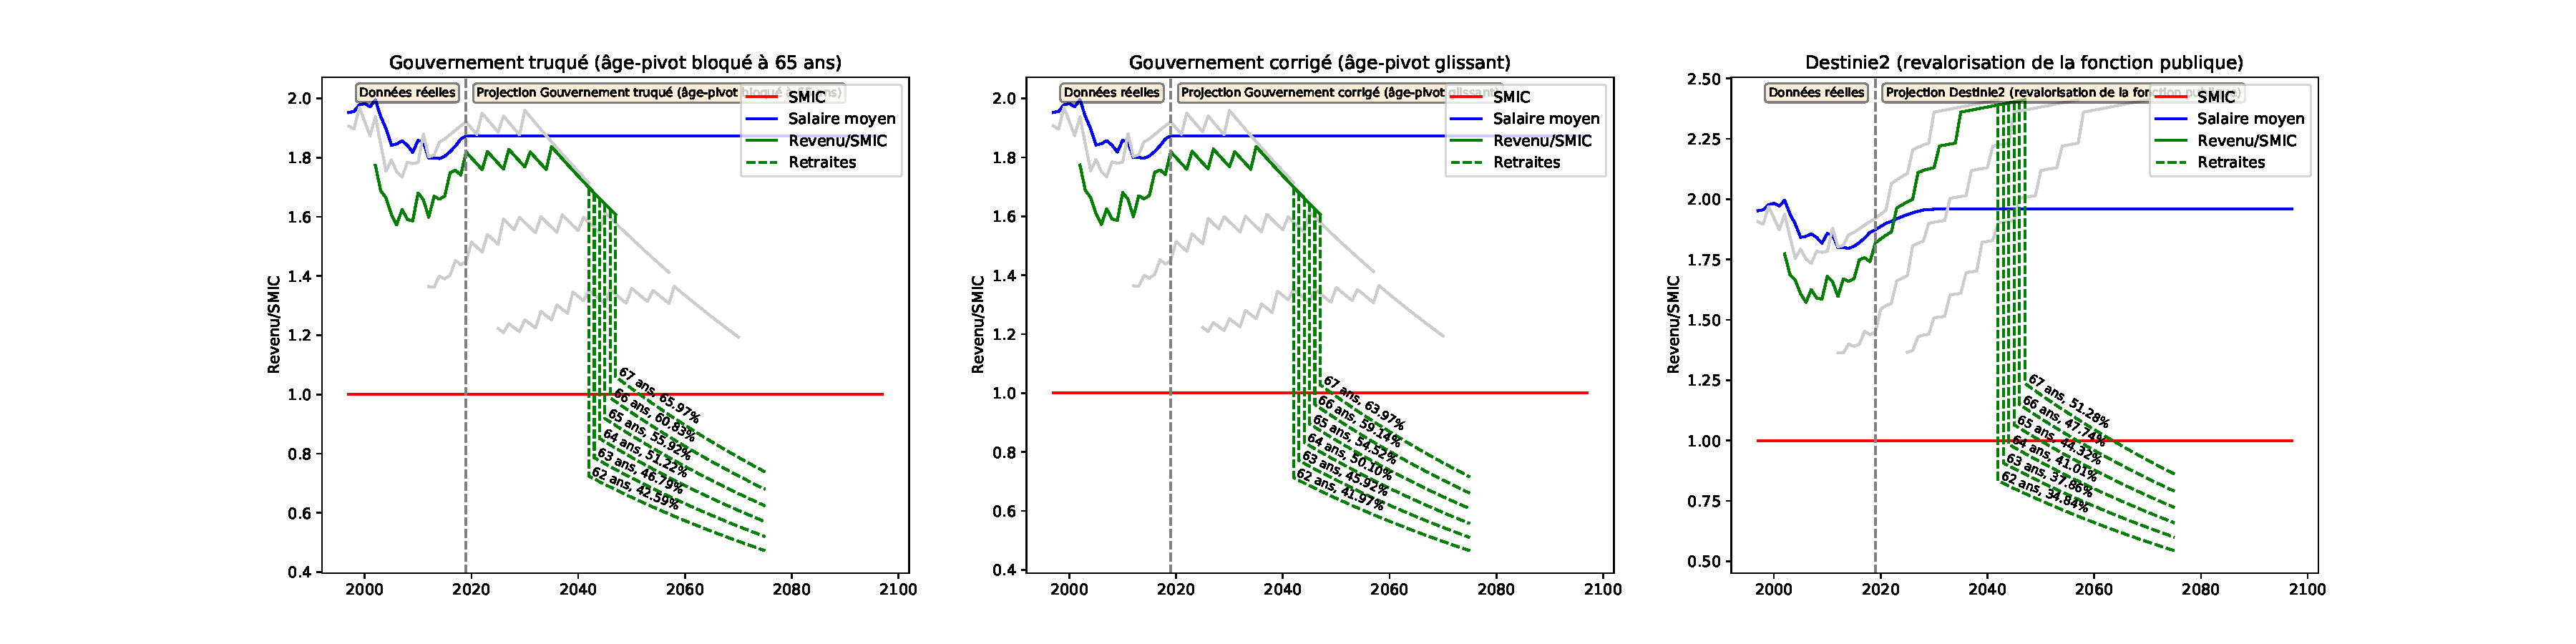
\includegraphics[width=0.9\textwidth]{fig/Infirmier_1980_22_dest_retraite.pdf}\end{center} \label{fig/Infirmier_1980_22_dest_retraite.pdf} 

\newpage 
 
\paragraph{Revenus et points pour le modèle \emph{Gouvernement truqué (âge-pivot bloqué à 65 ans)}} 
 
{ \scriptsize \begin{center} 
\begin{tabular}[htb]{|c|c||c|c|c|c|c|c||c|c||c|c|c|} 
\hline 
 Année &  Âge &  Ind Maj &  Pt Ind(\euro{} 2019) &  Rev HP(\euro{} 2019) &  Tx Primes &  GIPA(\euro{} 2019) &  Revenu(\euro{} 2019) &  SMIC(\euro{} 2019) &  Rev/SMIC &  Cumul Pts &  Achat Pt(\euro{} 2019) &  Serv. Pt(\euro{} 2019) \\ 
\hline \hline 
 2002 &  22 &  390.0 &  5.49 &  2139.65 &  20.01 &  0.00 &  2567.79 &  1447.74 &  {\bf 1.77} &  865.38 &  35.61 &  0.50 \\ 
\hline 
 2003 &  23 &  390.0 &  5.37 &  2096.10 &  20.24 &  0.00 &  2520.35 &  1493.03 &  {\bf 1.69} &  1714.77 &  35.61 &  0.50 \\ 
\hline 
 2004 &  24 &  404.0 &  5.29 &  2137.05 &  20.47 &  0.00 &  2574.50 &  1547.32 &  {\bf 1.66} &  2582.40 &  35.61 &  0.50 \\ 
\hline 
 2005 &  25 &  404.0 &  5.29 &  2136.82 &  20.70 &  0.00 &  2579.14 &  1603.67 &  {\bf 1.61} &  3451.60 &  35.61 &  0.50 \\ 
\hline 
 2006 &  26 &  404.0 &  5.23 &  2112.97 &  20.93 &  0.00 &  2555.21 &  1625.00 &  {\bf 1.57} &  4312.74 &  35.61 &  0.50 \\ 
\hline 
 2007 &  27 &  422.0 &  5.19 &  2192.07 &  21.16 &  0.00 &  2655.91 &  1634.08 &  {\bf 1.63} &  5207.82 &  35.61 &  0.50 \\ 
\hline 
 2008 &  28 &  422.0 &  5.09 &  2149.26 &  21.39 &  0.00 &  2608.99 &  1640.24 &  {\bf 1.59} &  6087.08 &  35.61 &  0.50 \\ 
\hline 
 2009 &  29 &  422.0 &  5.13 &  2164.49 &  21.62 &  0.00 &  2632.46 &  1659.42 &  {\bf 1.59} &  6974.25 &  35.61 &  0.50 \\ 
\hline 
 2010 &  30 &  446.0 &  5.08 &  2264.49 &  21.85 &  0.00 &  2759.28 &  1641.90 &  {\bf 1.68} &  7904.16 &  35.61 &  0.50 \\ 
\hline 
 2011 &  31 &  446.0 &  4.97 &  2217.44 &  22.08 &  0.00 &  2707.05 &  1633.19 &  {\bf 1.66} &  8816.47 &  35.61 &  0.50 \\ 
\hline 
 2012 &  32 &  446.0 &  4.88 &  2174.89 &  22.31 &  14.23 &  2674.34 &  1673.05 &  {\bf 1.60} &  9717.75 &  35.61 &  0.50 \\ 
\hline 
 2013 &  33 &  469.0 &  4.83 &  2267.45 &  22.54 &  0.00 &  2778.54 &  1664.01 &  {\bf 1.67} &  10654.15 &  35.61 &  0.50 \\ 
\hline 
 2014 &  34 &  469.0 &  4.81 &  2256.10 &  22.77 &  6.56 &  2776.38 &  1673.24 &  {\bf 1.66} &  11589.82 &  35.61 &  0.50 \\ 
\hline 
 2015 &  35 &  469.0 &  4.81 &  2255.22 &  23.00 &  43.40 &  2817.32 &  1686.62 &  {\bf 1.67} &  12539.29 &  35.61 &  0.50 \\ 
\hline 
 2016 &  36 &  501.0 &  4.80 &  2404.28 &  23.23 &  0.00 &  2962.80 &  1693.76 &  {\bf 1.75} &  13537.79 &  35.61 &  0.50 \\ 
\hline 
 2017 &  37 &  501.0 &  4.81 &  2409.13 &  23.46 &  0.00 &  2974.32 &  1692.60 &  {\bf 1.76} &  14540.17 &  35.61 &  0.50 \\ 
\hline 
 2018 &  38 &  501.0 &  4.74 &  2375.87 &  23.69 &  3.93 &  2942.65 &  1689.76 &  {\bf 1.74} &  15531.88 &  35.61 &  0.50 \\ 
\hline 
 2019 &  39 &  520.0 &  4.79 &  2493.10 &  23.92 &  0.00 &  3089.45 &  1698.45 &  {\bf 1.82} &  16573.06 &  35.61 &  0.50 \\ 
\hline 
 2020 &  40 &  520.0 &  4.79 &  2493.10 &  24.15 &  0.00 &  3095.18 &  1720.53 &  {\bf 1.80} &  17616.18 &  35.61 &  0.50 \\ 
\hline 
 2021 &  41 &  520.0 &  4.79 &  2493.10 &  24.38 &  0.00 &  3100.92 &  1742.90 &  {\bf 1.78} &  18661.22 &  35.61 &  0.50 \\ 
\hline 
 2022 &  42 &  520.0 &  4.79 &  2493.10 &  24.61 &  0.00 &  3106.65 &  1765.55 &  {\bf 1.76} &  19708.20 &  35.61 &  0.50 \\ 
\hline 
 2023 &  43 &  544.0 &  4.79 &  2608.17 &  24.84 &  0.00 &  3256.03 &  1788.51 &  {\bf 1.82} &  20805.53 &  35.61 &  0.50 \\ 
\hline 
 2024 &  44 &  544.0 &  4.79 &  2608.17 &  25.07 &  0.00 &  3262.03 &  1811.76 &  {\bf 1.80} &  21904.87 &  35.61 &  0.50 \\ 
\hline 
 2025 &  45 &  544.0 &  4.79 &  2608.17 &  25.30 &  0.00 &  3268.03 &  1835.31 &  {\bf 1.78} &  23006.24 &  35.61 &  0.50 \\ 
\hline 
 2026 &  46 &  544.0 &  4.79 &  2608.17 &  25.53 &  0.00 &  3274.03 &  1859.17 &  {\bf 1.76} &  24109.63 &  35.61 &  0.50 \\ 
\hline 
 2027 &  47 &  571.0 &  4.79 &  2737.62 &  25.76 &  0.00 &  3442.82 &  1883.34 &  {\bf 1.83} &  25269.90 &  35.61 &  0.50 \\ 
\hline 
 2028 &  48 &  571.0 &  4.79 &  2737.62 &  25.99 &  0.00 &  3449.12 &  1907.82 &  {\bf 1.81} &  26432.30 &  35.61 &  0.50 \\ 
\hline 
 2029 &  49 &  571.0 &  4.79 &  2737.62 &  26.22 &  0.00 &  3455.42 &  1932.62 &  {\bf 1.79} &  27595.93 &  35.63 &  0.50 \\ 
\hline 
 2030 &  50 &  571.0 &  4.79 &  2737.62 &  26.45 &  0.00 &  3461.71 &  1957.75 &  {\bf 1.77} &  28759.91 &  35.69 &  0.50 \\ 
\hline 
 2031 &  51 &  594.0 &  4.79 &  2847.89 &  26.68 &  0.00 &  3607.70 &  1983.20 &  {\bf 1.82} &  29970.22 &  35.77 &  0.50 \\ 
\hline 
 2032 &  52 &  594.0 &  4.79 &  2847.89 &  26.91 &  0.00 &  3614.25 &  2008.98 &  {\bf 1.80} &  31179.05 &  35.88 &  0.50 \\ 
\hline 
 2033 &  53 &  594.0 &  4.79 &  2847.89 &  27.14 &  0.00 &  3620.80 &  2035.10 &  {\bf 1.78} &  32385.48 &  36.02 &  0.50 \\ 
\hline 
 2034 &  54 &  594.0 &  4.79 &  2847.89 &  27.37 &  0.00 &  3627.35 &  2061.55 &  {\bf 1.76} &  33588.59 &  36.18 &  0.50 \\ 
\hline 
 2035 &  55 &  627.0 &  4.79 &  3006.10 &  27.60 &  0.00 &  3835.79 &  2088.35 &  {\bf 1.84} &  34854.09 &  36.37 &  0.51 \\ 
\hline 
 2036 &  56 &  627.0 &  4.79 &  3006.10 &  27.83 &  0.00 &  3842.70 &  2115.50 &  {\bf 1.82} &  36114.18 &  36.59 &  0.51 \\ 
\hline 
 2037 &  57 &  627.0 &  4.79 &  3006.10 &  28.06 &  0.00 &  3849.62 &  2143.00 &  {\bf 1.80} &  37367.94 &  36.85 &  0.51 \\ 
\hline 
 2038 &  58 &  627.0 &  4.79 &  3006.10 &  28.29 &  0.00 &  3856.53 &  2170.86 &  {\bf 1.78} &  38614.45 &  37.13 &  0.52 \\ 
\hline 
 2039 &  59 &  627.0 &  4.79 &  3006.10 &  28.52 &  0.00 &  3863.44 &  2199.08 &  {\bf 1.76} &  39852.79 &  37.44 &  0.52 \\ 
\hline 
 2040 &  60 &  627.0 &  4.79 &  3006.10 &  28.75 &  0.00 &  3870.36 &  2227.67 &  {\bf 1.74} &  41082.10 &  37.78 &  0.53 \\ 
\hline 
 2041 &  61 &  627.0 &  4.79 &  3006.10 &  28.98 &  0.00 &  3877.27 &  2256.63 &  {\bf 1.72} &  42301.49 &  38.16 &  0.53 \\ 
\hline 
 2042 &  62 &  627.0 &  4.79 &  3006.10 &  29.21 &  0.00 &  3884.19 &  2285.97 &  {\bf 1.70} &  43510.14 &  38.56 &  0.54 \\ 
\hline 
 2043 &  63 &  627.0 &  4.79 &  3006.10 &  29.44 &  0.00 &  3891.10 &  2315.68 &  {\bf 1.68} &  44707.21 &  39.01 &  0.54 \\ 
\hline 
 2044 &  64 &  627.0 &  4.79 &  3006.10 &  29.67 &  0.00 &  3898.01 &  2345.79 &  {\bf 1.66} &  45891.93 &  39.48 &  0.55 \\ 
\hline 
 2045 &  65 &  627.0 &  4.79 &  3006.10 &  29.90 &  0.00 &  3904.93 &  2376.28 &  {\bf 1.64} &  47063.51 &  40.00 &  0.56 \\ 
\hline 
 2046 &  66 &  627.0 &  4.79 &  3006.10 &  30.13 &  0.00 &  3911.84 &  2407.18 &  {\bf 1.63} &  48222.11 &  40.52 &  0.56 \\ 
\hline 
 2047 &  67 &  627.0 &  4.79 &  3006.10 &  30.36 &  0.00 &  3918.76 &  2438.47 &  {\bf 1.61} &  49367.86 &  41.04 &  0.57 \\ 
\hline 
\hline 
\end{tabular} 
\end{center} } 
\newpage 
 
\paragraph{Revenus et points pour le modèle \emph{Gouvernement corrigé (âge-pivot glissant)}} 
 
{ \scriptsize \begin{center} 
\begin{tabular}[htb]{|c|c||c|c|c|c|c|c||c|c||c|c|c|} 
\hline 
 Année &  Âge &  Ind Maj &  Pt Ind(\euro{} 2019) &  Rev HP(\euro{} 2019) &  Tx Primes &  GIPA(\euro{} 2019) &  Revenu(\euro{} 2019) &  SMIC(\euro{} 2019) &  Rev/SMIC &  Cumul Pts &  Achat Pt(\euro{} 2019) &  Serv. Pt(\euro{} 2019) \\ 
\hline \hline 
 2002 &  22 &  390.0 &  5.49 &  2139.65 &  20.01 &  0.00 &  2567.79 &  1447.74 &  {\bf 1.77} &  865.38 &  35.61 &  0.50 \\ 
\hline 
 2003 &  23 &  390.0 &  5.37 &  2096.10 &  20.24 &  0.00 &  2520.35 &  1493.03 &  {\bf 1.69} &  1714.77 &  35.61 &  0.50 \\ 
\hline 
 2004 &  24 &  404.0 &  5.29 &  2137.05 &  20.47 &  0.00 &  2574.50 &  1547.32 &  {\bf 1.66} &  2582.40 &  35.61 &  0.50 \\ 
\hline 
 2005 &  25 &  404.0 &  5.29 &  2136.82 &  20.70 &  0.00 &  2579.14 &  1603.67 &  {\bf 1.61} &  3451.60 &  35.61 &  0.50 \\ 
\hline 
 2006 &  26 &  404.0 &  5.23 &  2112.97 &  20.93 &  0.00 &  2555.21 &  1625.00 &  {\bf 1.57} &  4312.74 &  35.61 &  0.50 \\ 
\hline 
 2007 &  27 &  422.0 &  5.19 &  2192.07 &  21.16 &  0.00 &  2655.91 &  1634.08 &  {\bf 1.63} &  5207.82 &  35.61 &  0.50 \\ 
\hline 
 2008 &  28 &  422.0 &  5.09 &  2149.26 &  21.39 &  0.00 &  2608.99 &  1640.24 &  {\bf 1.59} &  6087.08 &  35.61 &  0.50 \\ 
\hline 
 2009 &  29 &  422.0 &  5.13 &  2164.49 &  21.62 &  0.00 &  2632.46 &  1659.42 &  {\bf 1.59} &  6974.25 &  35.61 &  0.50 \\ 
\hline 
 2010 &  30 &  446.0 &  5.08 &  2264.49 &  21.85 &  0.00 &  2759.28 &  1641.90 &  {\bf 1.68} &  7904.16 &  35.61 &  0.50 \\ 
\hline 
 2011 &  31 &  446.0 &  4.97 &  2217.44 &  22.08 &  0.00 &  2707.05 &  1633.19 &  {\bf 1.66} &  8816.47 &  35.61 &  0.50 \\ 
\hline 
 2012 &  32 &  446.0 &  4.88 &  2174.89 &  22.31 &  14.23 &  2674.34 &  1673.05 &  {\bf 1.60} &  9717.75 &  35.61 &  0.50 \\ 
\hline 
 2013 &  33 &  469.0 &  4.83 &  2267.45 &  22.54 &  0.00 &  2778.54 &  1664.01 &  {\bf 1.67} &  10654.15 &  35.61 &  0.50 \\ 
\hline 
 2014 &  34 &  469.0 &  4.81 &  2256.10 &  22.77 &  6.56 &  2776.38 &  1673.24 &  {\bf 1.66} &  11589.82 &  35.61 &  0.50 \\ 
\hline 
 2015 &  35 &  469.0 &  4.81 &  2255.22 &  23.00 &  43.40 &  2817.32 &  1686.62 &  {\bf 1.67} &  12539.29 &  35.61 &  0.50 \\ 
\hline 
 2016 &  36 &  501.0 &  4.80 &  2404.28 &  23.23 &  0.00 &  2962.80 &  1693.76 &  {\bf 1.75} &  13537.79 &  35.61 &  0.50 \\ 
\hline 
 2017 &  37 &  501.0 &  4.81 &  2409.13 &  23.46 &  0.00 &  2974.32 &  1692.60 &  {\bf 1.76} &  14540.17 &  35.61 &  0.50 \\ 
\hline 
 2018 &  38 &  501.0 &  4.74 &  2375.87 &  23.69 &  3.93 &  2942.65 &  1689.76 &  {\bf 1.74} &  15531.88 &  35.61 &  0.50 \\ 
\hline 
 2019 &  39 &  520.0 &  4.79 &  2493.10 &  23.92 &  0.00 &  3089.45 &  1698.45 &  {\bf 1.82} &  16573.06 &  35.61 &  0.50 \\ 
\hline 
 2020 &  40 &  520.0 &  4.79 &  2493.10 &  24.15 &  0.00 &  3095.18 &  1720.53 &  {\bf 1.80} &  17616.18 &  35.61 &  0.50 \\ 
\hline 
 2021 &  41 &  520.0 &  4.79 &  2493.10 &  24.38 &  0.00 &  3100.92 &  1742.90 &  {\bf 1.78} &  18661.22 &  35.61 &  0.50 \\ 
\hline 
 2022 &  42 &  520.0 &  4.79 &  2493.10 &  24.61 &  0.00 &  3106.65 &  1765.55 &  {\bf 1.76} &  19708.20 &  35.61 &  0.50 \\ 
\hline 
 2023 &  43 &  544.0 &  4.79 &  2608.17 &  24.84 &  0.00 &  3256.03 &  1788.51 &  {\bf 1.82} &  20805.53 &  35.61 &  0.50 \\ 
\hline 
 2024 &  44 &  544.0 &  4.79 &  2608.17 &  25.07 &  0.00 &  3262.03 &  1811.76 &  {\bf 1.80} &  21904.87 &  35.61 &  0.50 \\ 
\hline 
 2025 &  45 &  544.0 &  4.79 &  2608.17 &  25.30 &  0.00 &  3268.03 &  1835.31 &  {\bf 1.78} &  23006.24 &  35.61 &  0.50 \\ 
\hline 
 2026 &  46 &  544.0 &  4.79 &  2608.17 &  25.53 &  0.00 &  3274.03 &  1859.17 &  {\bf 1.76} &  24109.63 &  35.61 &  0.50 \\ 
\hline 
 2027 &  47 &  571.0 &  4.79 &  2737.62 &  25.76 &  0.00 &  3442.82 &  1883.34 &  {\bf 1.83} &  25269.90 &  35.61 &  0.50 \\ 
\hline 
 2028 &  48 &  571.0 &  4.79 &  2737.62 &  25.99 &  0.00 &  3449.12 &  1907.82 &  {\bf 1.81} &  26432.30 &  35.61 &  0.50 \\ 
\hline 
 2029 &  49 &  571.0 &  4.79 &  2737.62 &  26.22 &  0.00 &  3455.42 &  1932.62 &  {\bf 1.79} &  27595.93 &  35.63 &  0.50 \\ 
\hline 
 2030 &  50 &  571.0 &  4.79 &  2737.62 &  26.45 &  0.00 &  3461.71 &  1957.75 &  {\bf 1.77} &  28759.91 &  35.69 &  0.50 \\ 
\hline 
 2031 &  51 &  594.0 &  4.79 &  2847.89 &  26.68 &  0.00 &  3607.70 &  1983.20 &  {\bf 1.82} &  29970.22 &  35.77 &  0.50 \\ 
\hline 
 2032 &  52 &  594.0 &  4.79 &  2847.89 &  26.91 &  0.00 &  3614.25 &  2008.98 &  {\bf 1.80} &  31179.05 &  35.88 &  0.50 \\ 
\hline 
 2033 &  53 &  594.0 &  4.79 &  2847.89 &  27.14 &  0.00 &  3620.80 &  2035.10 &  {\bf 1.78} &  32385.48 &  36.02 &  0.50 \\ 
\hline 
 2034 &  54 &  594.0 &  4.79 &  2847.89 &  27.37 &  0.00 &  3627.35 &  2061.55 &  {\bf 1.76} &  33588.59 &  36.18 &  0.50 \\ 
\hline 
 2035 &  55 &  627.0 &  4.79 &  3006.10 &  27.60 &  0.00 &  3835.79 &  2088.35 &  {\bf 1.84} &  34854.09 &  36.37 &  0.51 \\ 
\hline 
 2036 &  56 &  627.0 &  4.79 &  3006.10 &  27.83 &  0.00 &  3842.70 &  2115.50 &  {\bf 1.82} &  36114.18 &  36.59 &  0.51 \\ 
\hline 
 2037 &  57 &  627.0 &  4.79 &  3006.10 &  28.06 &  0.00 &  3849.62 &  2143.00 &  {\bf 1.80} &  37367.94 &  36.85 &  0.51 \\ 
\hline 
 2038 &  58 &  627.0 &  4.79 &  3006.10 &  28.29 &  0.00 &  3856.53 &  2170.86 &  {\bf 1.78} &  38614.45 &  37.13 &  0.52 \\ 
\hline 
 2039 &  59 &  627.0 &  4.79 &  3006.10 &  28.52 &  0.00 &  3863.44 &  2199.08 &  {\bf 1.76} &  39852.79 &  37.44 &  0.52 \\ 
\hline 
 2040 &  60 &  627.0 &  4.79 &  3006.10 &  28.75 &  0.00 &  3870.36 &  2227.67 &  {\bf 1.74} &  41082.10 &  37.78 &  0.53 \\ 
\hline 
 2041 &  61 &  627.0 &  4.79 &  3006.10 &  28.98 &  0.00 &  3877.27 &  2256.63 &  {\bf 1.72} &  42301.49 &  38.16 &  0.53 \\ 
\hline 
 2042 &  62 &  627.0 &  4.79 &  3006.10 &  29.21 &  0.00 &  3884.19 &  2285.97 &  {\bf 1.70} &  43510.14 &  38.56 &  0.54 \\ 
\hline 
 2043 &  63 &  627.0 &  4.79 &  3006.10 &  29.44 &  0.00 &  3891.10 &  2315.68 &  {\bf 1.68} &  44707.21 &  39.01 &  0.54 \\ 
\hline 
 2044 &  64 &  627.0 &  4.79 &  3006.10 &  29.67 &  0.00 &  3898.01 &  2345.79 &  {\bf 1.66} &  45891.93 &  39.48 &  0.55 \\ 
\hline 
 2045 &  65 &  627.0 &  4.79 &  3006.10 &  29.90 &  0.00 &  3904.93 &  2376.28 &  {\bf 1.64} &  47063.51 &  40.00 &  0.56 \\ 
\hline 
 2046 &  66 &  627.0 &  4.79 &  3006.10 &  30.13 &  0.00 &  3911.84 &  2407.18 &  {\bf 1.63} &  48222.11 &  40.52 &  0.56 \\ 
\hline 
 2047 &  67 &  627.0 &  4.79 &  3006.10 &  30.36 &  0.00 &  3918.76 &  2438.47 &  {\bf 1.61} &  49367.86 &  41.04 &  0.57 \\ 
\hline 
\hline 
\end{tabular} 
\end{center} } 
\newpage 
 
\paragraph{Revenus et points pour le modèle \emph{Destinie2 (revalorisation de la fonction publique)}} 
 
{ \scriptsize \begin{center} 
\begin{tabular}[htb]{|c|c||c|c|c|c|c|c||c|c||c|c|c|} 
\hline 
 Année &  Âge &  Ind Maj &  Pt Ind(\euro{} 2019) &  Rev HP(\euro{} 2019) &  Tx Primes &  GIPA(\euro{} 2019) &  Revenu(\euro{} 2019) &  SMIC(\euro{} 2019) &  Rev/SMIC &  Cumul Pts &  Achat Pt(\euro{} 2019) &  Serv. Pt(\euro{} 2019) \\ 
\hline \hline 
 2002 &  22 &  390.0 &  5.49 &  2139.65 &  20.01 &  0.00 &  2567.79 &  1447.74 &  {\bf 1.77} &  863.25 &  35.69 &  0.50 \\ 
\hline 
 2003 &  23 &  390.0 &  5.37 &  2096.10 &  20.24 &  0.00 &  2520.35 &  1493.03 &  {\bf 1.69} &  1710.55 &  35.69 &  0.50 \\ 
\hline 
 2004 &  24 &  404.0 &  5.29 &  2137.05 &  20.47 &  0.00 &  2574.50 &  1547.32 &  {\bf 1.66} &  2576.06 &  35.69 &  0.50 \\ 
\hline 
 2005 &  25 &  404.0 &  5.29 &  2136.82 &  20.70 &  0.00 &  2579.14 &  1603.67 &  {\bf 1.61} &  3443.12 &  35.69 &  0.50 \\ 
\hline 
 2006 &  26 &  404.0 &  5.23 &  2112.97 &  20.93 &  0.00 &  2555.21 &  1625.00 &  {\bf 1.57} &  4302.15 &  35.69 &  0.50 \\ 
\hline 
 2007 &  27 &  422.0 &  5.19 &  2192.07 &  21.16 &  0.00 &  2655.91 &  1634.08 &  {\bf 1.63} &  5195.02 &  35.69 &  0.50 \\ 
\hline 
 2008 &  28 &  422.0 &  5.09 &  2149.26 &  21.39 &  0.00 &  2608.99 &  1640.24 &  {\bf 1.59} &  6072.12 &  35.69 &  0.50 \\ 
\hline 
 2009 &  29 &  422.0 &  5.13 &  2164.49 &  21.62 &  0.00 &  2632.46 &  1659.42 &  {\bf 1.59} &  6957.11 &  35.69 &  0.50 \\ 
\hline 
 2010 &  30 &  446.0 &  5.08 &  2264.49 &  21.85 &  0.00 &  2759.28 &  1641.90 &  {\bf 1.68} &  7884.74 &  35.69 &  0.50 \\ 
\hline 
 2011 &  31 &  446.0 &  4.97 &  2217.44 &  22.08 &  0.00 &  2707.05 &  1633.19 &  {\bf 1.66} &  8794.81 &  35.69 &  0.50 \\ 
\hline 
 2012 &  32 &  446.0 &  4.88 &  2174.89 &  22.31 &  11.00 &  2671.11 &  1673.05 &  {\bf 1.60} &  9692.79 &  35.69 &  0.50 \\ 
\hline 
 2013 &  33 &  469.0 &  4.83 &  2267.45 &  22.54 &  0.00 &  2778.54 &  1664.01 &  {\bf 1.67} &  10626.89 &  35.69 &  0.50 \\ 
\hline 
 2014 &  34 &  469.0 &  4.81 &  2256.10 &  22.77 &  5.74 &  2775.55 &  1673.24 &  {\bf 1.66} &  11559.99 &  35.69 &  0.50 \\ 
\hline 
 2015 &  35 &  469.0 &  4.81 &  2255.22 &  23.00 &  42.35 &  2816.27 &  1686.62 &  {\bf 1.67} &  12506.77 &  35.69 &  0.50 \\ 
\hline 
 2016 &  36 &  501.0 &  4.80 &  2404.28 &  23.23 &  0.00 &  2962.80 &  1693.76 &  {\bf 1.75} &  13502.82 &  35.69 &  0.50 \\ 
\hline 
 2017 &  37 &  501.0 &  4.81 &  2409.13 &  23.46 &  0.00 &  2974.32 &  1692.60 &  {\bf 1.76} &  14502.74 &  35.69 &  0.50 \\ 
\hline 
 2018 &  38 &  501.0 &  4.74 &  2375.87 &  23.69 &  3.45 &  2942.16 &  1689.76 &  {\bf 1.74} &  15491.84 &  35.69 &  0.50 \\ 
\hline 
 2019 &  39 &  520.0 &  4.79 &  2493.10 &  23.92 &  0.00 &  3089.45 &  1698.45 &  {\bf 1.82} &  16530.47 &  35.69 &  0.50 \\ 
\hline 
 2020 &  40 &  520.0 &  4.83 &  2513.04 &  24.15 &  0.00 &  3119.94 &  1699.99 &  {\bf 1.84} &  17579.34 &  35.69 &  0.50 \\ 
\hline 
 2021 &  41 &  520.0 &  4.88 &  2535.66 &  24.38 &  0.00 &  3153.86 &  1703.48 &  {\bf 1.85} &  18639.62 &  35.69 &  0.50 \\ 
\hline 
 2022 &  42 &  520.0 &  4.93 &  2561.02 &  24.61 &  0.00 &  3191.28 &  1712.78 &  {\bf 1.86} &  19712.48 &  35.69 &  0.50 \\ 
\hline 
 2023 &  43 &  544.0 &  4.98 &  2710.57 &  24.84 &  0.00 &  3383.87 &  1723.51 &  {\bf 1.96} &  20850.08 &  35.69 &  0.50 \\ 
\hline 
 2024 &  44 &  544.0 &  5.04 &  2742.82 &  25.07 &  0.00 &  3430.45 &  1735.69 &  {\bf 1.98} &  22003.34 &  35.69 &  0.50 \\ 
\hline 
 2025 &  45 &  544.0 &  5.10 &  2776.28 &  25.30 &  0.00 &  3478.68 &  1749.35 &  {\bf 1.99} &  23172.82 &  35.69 &  0.50 \\ 
\hline 
 2026 &  46 &  544.0 &  5.17 &  2810.99 &  25.53 &  0.00 &  3528.63 &  1764.53 &  {\bf 2.00} &  24359.09 &  35.69 &  0.50 \\ 
\hline 
 2027 &  47 &  571.0 &  5.23 &  2988.27 &  25.76 &  0.00 &  3758.05 &  1781.27 &  {\bf 2.11} &  25622.49 &  35.69 &  0.50 \\ 
\hline 
 2028 &  48 &  571.0 &  5.30 &  3027.42 &  25.99 &  0.00 &  3814.24 &  1799.59 &  {\bf 2.12} &  26904.78 &  35.69 &  0.50 \\ 
\hline 
 2029 &  49 &  571.0 &  5.37 &  3064.05 &  26.22 &  0.00 &  3867.44 &  1819.55 &  {\bf 2.13} &  28204.03 &  35.72 &  0.50 \\ 
\hline 
 2030 &  50 &  571.0 &  5.43 &  3102.04 &  26.45 &  0.00 &  3922.53 &  1841.19 &  {\bf 2.13} &  29519.88 &  35.77 &  0.50 \\ 
\hline 
 2031 &  51 &  594.0 &  5.50 &  3267.98 &  26.68 &  0.00 &  4139.87 &  1864.58 &  {\bf 2.22} &  30905.55 &  35.85 &  0.50 \\ 
\hline 
 2032 &  52 &  594.0 &  5.57 &  3310.46 &  26.91 &  0.00 &  4201.30 &  1888.81 &  {\bf 2.22} &  32307.52 &  35.96 &  0.50 \\ 
\hline 
 2033 &  53 &  594.0 &  5.65 &  3353.50 &  27.14 &  0.00 &  4263.63 &  1913.37 &  {\bf 2.23} &  33724.89 &  36.10 &  0.50 \\ 
\hline 
 2034 &  54 &  594.0 &  5.72 &  3397.09 &  27.37 &  0.00 &  4326.88 &  1938.24 &  {\bf 2.23} &  35156.74 &  36.26 &  0.50 \\ 
\hline 
 2035 &  55 &  627.0 &  5.79 &  3632.43 &  27.60 &  0.00 &  4634.99 &  1963.44 &  {\bf 2.36} &  36682.42 &  36.46 &  0.51 \\ 
\hline 
 2036 &  56 &  627.0 &  5.87 &  3679.66 &  27.83 &  0.00 &  4703.70 &  1988.96 &  {\bf 2.36} &  38221.33 &  36.68 &  0.51 \\ 
\hline 
 2037 &  57 &  627.0 &  5.94 &  3727.49 &  28.06 &  0.00 &  4773.43 &  2014.82 &  {\bf 2.37} &  39772.41 &  36.93 &  0.51 \\ 
\hline 
 2038 &  58 &  627.0 &  6.02 &  3775.95 &  28.29 &  0.00 &  4844.16 &  2041.01 &  {\bf 2.37} &  41334.56 &  37.21 &  0.52 \\ 
\hline 
 2039 &  59 &  627.0 &  6.10 &  3825.04 &  28.52 &  0.00 &  4915.94 &  2067.55 &  {\bf 2.38} &  42906.67 &  37.52 &  0.52 \\ 
\hline 
 2040 &  60 &  627.0 &  6.18 &  3874.76 &  28.75 &  0.00 &  4988.76 &  2094.43 &  {\bf 2.38} &  44487.58 &  37.87 &  0.53 \\ 
\hline 
 2041 &  61 &  627.0 &  6.26 &  3925.13 &  28.98 &  0.00 &  5062.64 &  2121.65 &  {\bf 2.39} &  46076.13 &  38.24 &  0.53 \\ 
\hline 
 2042 &  62 &  627.0 &  6.34 &  3976.16 &  29.21 &  0.00 &  5137.60 &  2149.23 &  {\bf 2.39} &  47671.15 &  38.65 &  0.54 \\ 
\hline 
 2043 &  63 &  627.0 &  6.42 &  4027.85 &  29.44 &  0.00 &  5213.65 &  2177.17 &  {\bf 2.39} &  49271.44 &  39.10 &  0.54 \\ 
\hline 
 2044 &  64 &  627.0 &  6.51 &  4080.21 &  29.67 &  0.00 &  5290.81 &  2205.48 &  {\bf 2.40} &  50875.80 &  39.57 &  0.55 \\ 
\hline 
 2045 &  65 &  627.0 &  6.59 &  4133.26 &  29.90 &  0.00 &  5369.10 &  2234.15 &  {\bf 2.40} &  52482.99 &  40.09 &  0.56 \\ 
\hline 
 2046 &  66 &  627.0 &  6.68 &  4186.99 &  30.13 &  0.00 &  5448.53 &  2263.19 &  {\bf 2.41} &  54093.04 &  40.61 &  0.57 \\ 
\hline 
 2047 &  67 &  627.0 &  6.76 &  4241.42 &  30.36 &  0.00 &  5529.11 &  2292.61 &  {\bf 2.41} &  55705.93 &  41.14 &  0.57 \\ 
\hline 
\hline 
\end{tabular} 
\end{center} } 
\newpage 
 
\subsection{Génération 1990 (début en 2012)} 

\paragraph{Retraites possibles dans le modèle \emph{Gouvernement truqué (âge-pivot bloqué à 65 ans)}}  
 
{ \scriptsize \begin{center} 
\begin{tabular}[htb]{|c|c||c|c||c|c||c||c|c|c|c|c|c|} 
\hline 
 Retraite en &  Âge &  Âge pivot &  Décote/Surcote &  Retraite (\euro{} 2019) &  Tx Rempl(\%) &  SMIC (\euro{} 2019) &  Retraite/SMIC &  Rev70/SMIC &  Rev75/SMIC &  Rev80/SMIC &  Rev85/SMIC &  Rev90/SMIC \\ 
\hline \hline 
 2052 &  62 &  65 ans 0 mois &  -15.00\% &  1773.04 &  {\bf 45.65} &  2601.14 &  {\bf {\color{red} 0.68}} &  {\bf {\color{red} 0.61}} &  {\bf {\color{red} 0.58}} &  {\bf {\color{red} 0.54}} &  {\bf {\color{red} 0.51}} &  {\bf {\color{red} 0.47}} \\ 
\hline 
 2053 &  63 &  65 ans 0 mois &  -10.00\% &  1950.49 &  {\bf 50.13} &  2634.96 &  {\bf {\color{red} 0.74}} &  {\bf {\color{red} 0.68}} &  {\bf {\color{red} 0.63}} &  {\bf {\color{red} 0.59}} &  {\bf {\color{red} 0.56}} &  {\bf {\color{red} 0.52}} \\ 
\hline 
 2054 &  64 &  65 ans 0 mois &  -5.00\% &  2137.16 &  {\bf 54.83} &  2669.21 &  {\bf {\color{red} 0.80}} &  {\bf {\color{red} 0.74}} &  {\bf {\color{red} 0.69}} &  {\bf {\color{red} 0.65}} &  {\bf {\color{red} 0.61}} &  {\bf {\color{red} 0.57}} \\ 
\hline 
 2055 &  65 &  65 ans 0 mois &  0.00\% &  2333.24 &  {\bf 59.75} &  2703.91 &  {\bf {\color{red} 0.86}} &  {\bf {\color{red} 0.81}} &  {\bf {\color{red} 0.76}} &  {\bf {\color{red} 0.71}} &  {\bf {\color{red} 0.67}} &  {\bf {\color{red} 0.62}} \\ 
\hline 
 2056 &  66 &  65 ans 0 mois &  5.00\% &  2538.93 &  {\bf 64.90} &  2739.06 &  {\bf {\color{red} 0.93}} &  {\bf {\color{red} 0.88}} &  {\bf {\color{red} 0.83}} &  {\bf {\color{red} 0.77}} &  {\bf {\color{red} 0.73}} &  {\bf {\color{red} 0.68}} \\ 
\hline 
 2057 &  67 &  65 ans 0 mois &  10.00\% &  2754.41 &  {\bf 70.29} &  2774.67 &  {\bf {\color{red} 0.99}} &  {\bf {\color{red} 0.95}} &  {\bf {\color{red} 0.90}} &  {\bf {\color{red} 0.84}} &  {\bf {\color{red} 0.79}} &  {\bf {\color{red} 0.74}} \\ 
\hline 
\hline 
\end{tabular} 
\end{center} } 
\paragraph{Retraites possibles dans le modèle \emph{Gouvernement corrigé (âge-pivot glissant)}}  
 
{ \scriptsize \begin{center} 
\begin{tabular}[htb]{|c|c||c|c||c|c||c||c|c|c|c|c|c|} 
\hline 
 Retraite en &  Âge &  Âge pivot &  Décote/Surcote &  Retraite (\euro{} 2019) &  Tx Rempl(\%) &  SMIC (\euro{} 2019) &  Retraite/SMIC &  Rev70/SMIC &  Rev75/SMIC &  Rev80/SMIC &  Rev85/SMIC &  Rev90/SMIC \\ 
\hline \hline 
 2052 &  62 &  66 ans 1 mois &  -20.42\% &  1660.06 &  {\bf 42.74} &  2601.14 &  {\bf {\color{red} 0.64}} &  {\bf {\color{red} 0.58}} &  {\bf {\color{red} 0.54}} &  {\bf {\color{red} 0.51}} &  {\bf {\color{red} 0.47}} &  {\bf {\color{red} 0.44}} \\ 
\hline 
 2053 &  63 &  66 ans 2 mois &  -15.83\% &  1824.07 &  {\bf 46.88} &  2634.96 &  {\bf {\color{red} 0.69}} &  {\bf {\color{red} 0.63}} &  {\bf {\color{red} 0.59}} &  {\bf {\color{red} 0.56}} &  {\bf {\color{red} 0.52}} &  {\bf {\color{red} 0.49}} \\ 
\hline 
 2054 &  64 &  66 ans 3 mois &  -11.25\% &  1996.56 &  {\bf 51.22} &  2669.21 &  {\bf {\color{red} 0.75}} &  {\bf {\color{red} 0.69}} &  {\bf {\color{red} 0.65}} &  {\bf {\color{red} 0.61}} &  {\bf {\color{red} 0.57}} &  {\bf {\color{red} 0.53}} \\ 
\hline 
 2055 &  65 &  66 ans 4 mois &  -6.67\% &  2298.33 &  {\bf 58.86} &  2703.91 &  {\bf {\color{red} 0.85}} &  {\bf {\color{red} 0.80}} &  {\bf {\color{red} 0.75}} &  {\bf {\color{red} 0.70}} &  {\bf {\color{red} 0.66}} &  {\bf {\color{red} 0.62}} \\ 
\hline 
 2056 &  66 &  66 ans 5 mois &  -2.08\% &  2367.65 &  {\bf 60.53} &  2739.06 &  {\bf {\color{red} 0.86}} &  {\bf {\color{red} 0.82}} &  {\bf {\color{red} 0.77}} &  {\bf {\color{red} 0.72}} &  {\bf {\color{red} 0.68}} &  {\bf {\color{red} 0.63}} \\ 
\hline 
 2057 &  67 &  66 ans 6 mois &  2.50\% &  2566.61 &  {\bf 65.50} &  2774.67 &  {\bf {\color{red} 0.93}} &  {\bf {\color{red} 0.89}} &  {\bf {\color{red} 0.83}} &  {\bf {\color{red} 0.78}} &  {\bf {\color{red} 0.73}} &  {\bf {\color{red} 0.69}} \\ 
\hline 
\hline 
\end{tabular} 
\end{center} } 
\paragraph{Retraites possibles dans le modèle \emph{Destinie2 (revalorisation de la fonction publique)}}  
 
{ \scriptsize \begin{center} 
\begin{tabular}[htb]{|c|c||c|c||c|c||c||c|c|c|c|c|c|} 
\hline 
 Retraite en &  Âge &  Âge pivot &  Décote/Surcote &  Retraite (\euro{} 2019) &  Tx Rempl(\%) &  SMIC (\euro{} 2019) &  Retraite/SMIC &  Rev70/SMIC &  Rev75/SMIC &  Rev80/SMIC &  Rev85/SMIC &  Rev90/SMIC \\ 
\hline \hline 
 2052 &  62 &  66 ans 1 mois &  -20.42\% &  2001.52 &  {\bf 34.24} &  2445.56 &  {\bf {\color{red} 0.82}} &  {\bf {\color{red} 0.74}} &  {\bf {\color{red} 0.69}} &  {\bf {\color{red} 0.65}} &  {\bf {\color{red} 0.61}} &  {\bf {\color{red} 0.57}} \\ 
\hline 
 2053 &  63 &  66 ans 2 mois &  -15.83\% &  2213.81 &  {\bf 37.32} &  2477.35 &  {\bf {\color{red} 0.89}} &  {\bf {\color{red} 0.82}} &  {\bf {\color{red} 0.77}} &  {\bf {\color{red} 0.72}} &  {\bf {\color{red} 0.67}} &  {\bf {\color{red} 0.63}} \\ 
\hline 
 2054 &  64 &  66 ans 3 mois &  -11.25\% &  2439.08 &  {\bf 40.51} &  2509.56 &  {\bf {\color{red} 0.97}} &  {\bf {\color{red} 0.90}} &  {\bf {\color{red} 0.84}} &  {\bf {\color{red} 0.79}} &  {\bf {\color{red} 0.74}} &  {\bf {\color{red} 0.69}} \\ 
\hline 
 2055 &  65 &  66 ans 4 mois &  -6.67\% &  2677.76 &  {\bf 43.83} &  2542.18 &  {\bf 1.05} &  {\bf {\color{red} 0.99}} &  {\bf {\color{red} 0.93}} &  {\bf {\color{red} 0.87}} &  {\bf {\color{red} 0.81}} &  {\bf {\color{red} 0.76}} \\ 
\hline 
 2056 &  66 &  66 ans 5 mois &  -2.08\% &  2930.27 &  {\bf 47.26} &  2575.23 &  {\bf 1.14} &  {\bf 1.08} &  {\bf 1.01} &  {\bf {\color{red} 0.95}} &  {\bf {\color{red} 0.89}} &  {\bf {\color{red} 0.83}} \\ 
\hline 
 2057 &  67 &  66 ans 6 mois &  2.50\% &  3197.08 &  {\bf 50.82} &  2608.71 &  {\bf 1.23} &  {\bf 1.18} &  {\bf 1.11} &  {\bf 1.04} &  {\bf {\color{red} 0.97}} &  {\bf {\color{red} 0.91}} \\ 
\hline 
\hline 
\end{tabular} 
\end{center} } 

 \begin{center}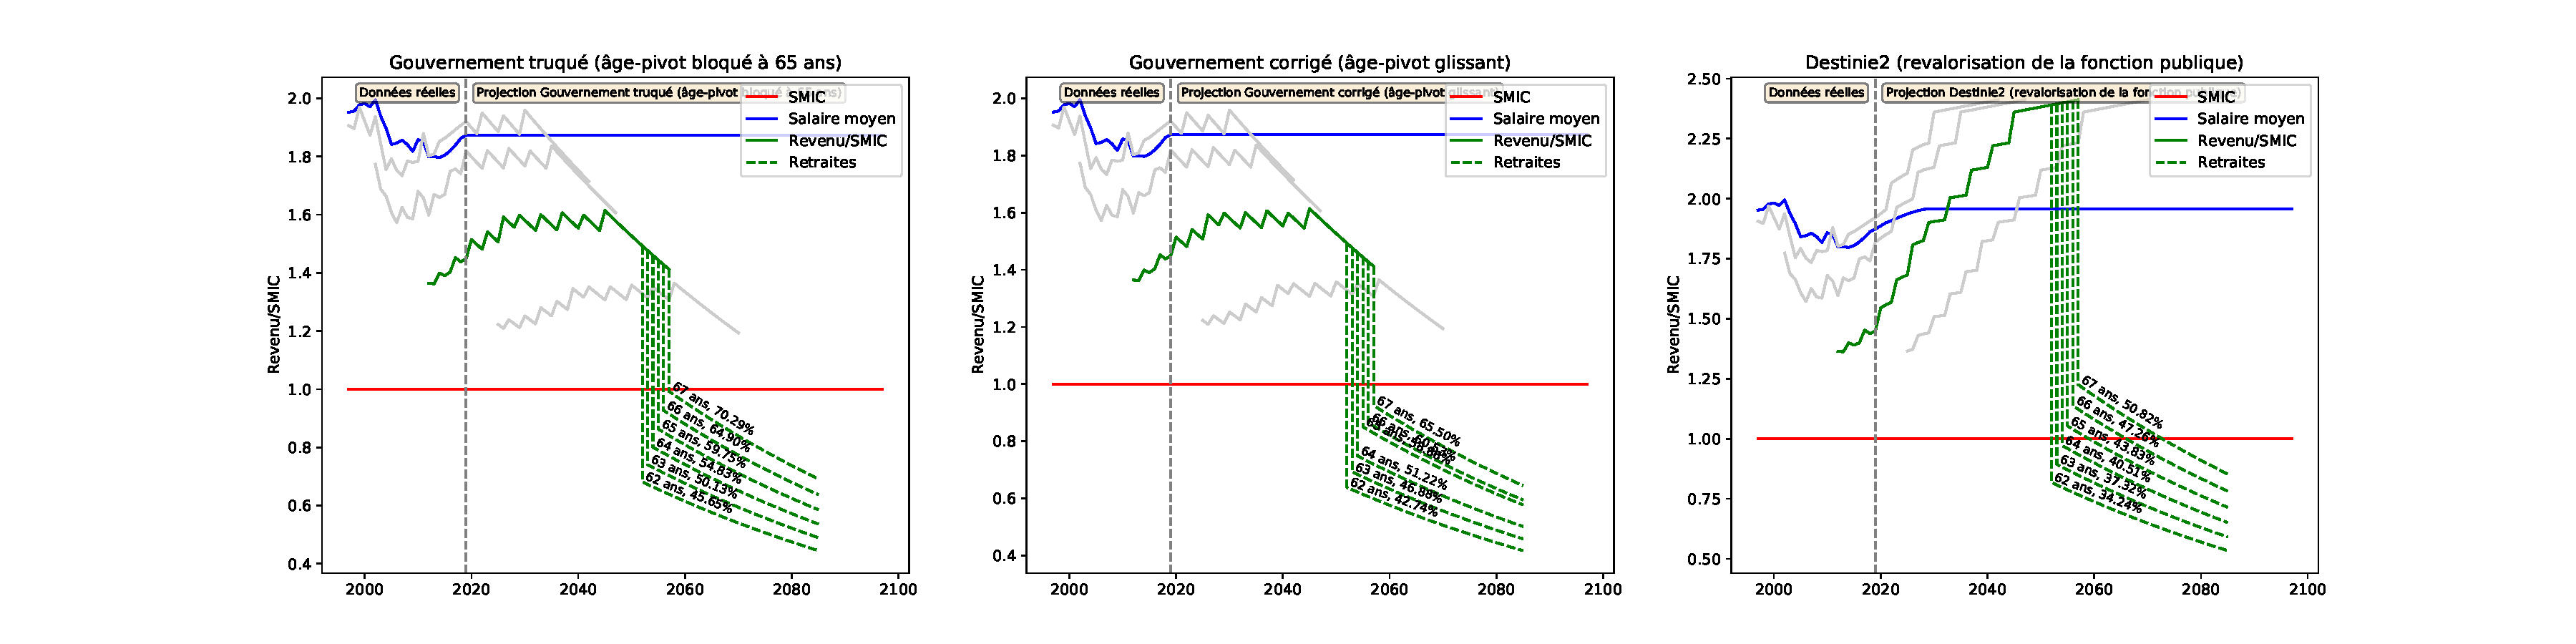
\includegraphics[width=0.9\textwidth]{fig/Infirmier_1990_22_dest_retraite.pdf}\end{center} \label{fig/Infirmier_1990_22_dest_retraite.pdf} 

\newpage 
 
\paragraph{Revenus et points pour le modèle \emph{Gouvernement truqué (âge-pivot bloqué à 65 ans)}} 
 
{ \scriptsize \begin{center} 
\begin{tabular}[htb]{|c|c||c|c|c|c|c|c||c|c||c|c|c|} 
\hline 
 Année &  Âge &  Ind Maj &  Pt Ind(\euro{} 2019) &  Rev HP(\euro{} 2019) &  Tx Primes &  GIPA(\euro{} 2019) &  Revenu(\euro{} 2019) &  SMIC(\euro{} 2019) &  Rev/SMIC &  Cumul Pts &  Achat Pt(\euro{} 2019) &  Serv. Pt(\euro{} 2019) \\ 
\hline \hline 
 2012 &  22 &  390.0 &  4.88 &  1901.81 &  20.01 &  0.00 &  2282.36 &  1673.05 &  {\bf 1.36} &  769.18 &  35.61 &  0.50 \\ 
\hline 
 2013 &  23 &  390.0 &  4.83 &  1885.51 &  20.24 &  0.00 &  2267.14 &  1664.01 &  {\bf 1.36} &  1533.24 &  35.61 &  0.50 \\ 
\hline 
 2014 &  24 &  404.0 &  4.81 &  1943.42 &  20.47 &  0.00 &  2341.24 &  1673.24 &  {\bf 1.40} &  2322.26 &  35.61 &  0.50 \\ 
\hline 
 2015 &  25 &  404.0 &  4.81 &  1942.66 &  20.70 &  0.00 &  2344.79 &  1686.62 &  {\bf 1.39} &  3112.49 &  35.61 &  0.50 \\ 
\hline 
 2016 &  26 &  404.0 &  4.80 &  1938.78 &  20.93 &  31.55 &  2376.12 &  1693.76 &  {\bf 1.40} &  3913.27 &  35.61 &  0.50 \\ 
\hline 
 2017 &  27 &  422.0 &  4.81 &  2029.25 &  21.16 &  0.00 &  2458.64 &  1692.60 &  {\bf 1.45} &  4741.86 &  35.61 &  0.50 \\ 
\hline 
 2018 &  28 &  422.0 &  4.74 &  2001.23 &  21.39 &  0.87 &  2430.17 &  1689.76 &  {\bf 1.44} &  5560.86 &  35.61 &  0.50 \\ 
\hline 
 2019 &  29 &  422.0 &  4.79 &  2023.25 &  21.62 &  0.00 &  2460.67 &  1698.45 &  {\bf 1.45} &  6390.13 &  35.61 &  0.50 \\ 
\hline 
 2020 &  30 &  446.0 &  4.79 &  2138.31 &  21.85 &  0.00 &  2605.53 &  1720.53 &  {\bf 1.51} &  7268.23 &  35.61 &  0.50 \\ 
\hline 
 2021 &  31 &  446.0 &  4.79 &  2138.31 &  22.08 &  0.00 &  2610.45 &  1742.90 &  {\bf 1.50} &  8147.98 &  35.61 &  0.50 \\ 
\hline 
 2022 &  32 &  446.0 &  4.79 &  2138.31 &  22.31 &  0.00 &  2615.37 &  1765.55 &  {\bf 1.48} &  9029.40 &  35.61 &  0.50 \\ 
\hline 
 2023 &  33 &  469.0 &  4.79 &  2248.58 &  22.54 &  0.00 &  2755.41 &  1788.51 &  {\bf 1.54} &  9958.00 &  35.61 &  0.50 \\ 
\hline 
 2024 &  34 &  469.0 &  4.79 &  2248.58 &  22.77 &  0.00 &  2760.59 &  1811.76 &  {\bf 1.52} &  10888.36 &  35.61 &  0.50 \\ 
\hline 
 2025 &  35 &  469.0 &  4.79 &  2248.58 &  23.00 &  0.00 &  2765.76 &  1835.31 &  {\bf 1.51} &  11820.45 &  35.61 &  0.50 \\ 
\hline 
 2026 &  36 &  501.0 &  4.79 &  2402.01 &  23.23 &  0.00 &  2959.99 &  1859.17 &  {\bf 1.59} &  12818.00 &  35.61 &  0.50 \\ 
\hline 
 2027 &  37 &  501.0 &  4.79 &  2402.01 &  23.46 &  0.00 &  2965.52 &  1883.34 &  {\bf 1.57} &  13817.42 &  35.61 &  0.50 \\ 
\hline 
 2028 &  38 &  501.0 &  4.79 &  2402.01 &  23.69 &  0.00 &  2971.04 &  1907.82 &  {\bf 1.56} &  14818.69 &  35.61 &  0.50 \\ 
\hline 
 2029 &  39 &  520.0 &  4.79 &  2493.10 &  23.92 &  0.00 &  3089.45 &  1932.62 &  {\bf 1.60} &  15859.09 &  35.63 &  0.50 \\ 
\hline 
 2030 &  40 &  520.0 &  4.79 &  2493.10 &  24.15 &  0.00 &  3095.18 &  1957.75 &  {\bf 1.58} &  16899.83 &  35.69 &  0.50 \\ 
\hline 
 2031 &  41 &  520.0 &  4.79 &  2493.10 &  24.38 &  0.00 &  3100.92 &  1983.20 &  {\bf 1.56} &  17940.12 &  35.77 &  0.50 \\ 
\hline 
 2032 &  42 &  520.0 &  4.79 &  2493.10 &  24.61 &  0.00 &  3106.65 &  2008.98 &  {\bf 1.55} &  18979.17 &  35.88 &  0.50 \\ 
\hline 
 2033 &  43 &  544.0 &  4.79 &  2608.17 &  24.84 &  0.00 &  3256.03 &  2035.10 &  {\bf 1.60} &  20064.06 &  36.02 &  0.50 \\ 
\hline 
 2034 &  44 &  544.0 &  4.79 &  2608.17 &  25.07 &  0.00 &  3262.03 &  2061.55 &  {\bf 1.58} &  21146.01 &  36.18 &  0.50 \\ 
\hline 
 2035 &  45 &  544.0 &  4.79 &  2608.17 &  25.30 &  0.00 &  3268.03 &  2088.35 &  {\bf 1.56} &  22224.19 &  36.37 &  0.51 \\ 
\hline 
 2036 &  46 &  544.0 &  4.79 &  2608.17 &  25.53 &  0.00 &  3274.03 &  2115.50 &  {\bf 1.55} &  23297.81 &  36.59 &  0.51 \\ 
\hline 
 2037 &  47 &  571.0 &  4.79 &  2737.62 &  25.76 &  0.00 &  3442.82 &  2143.00 &  {\bf 1.61} &  24419.08 &  36.85 &  0.51 \\ 
\hline 
 2038 &  48 &  571.0 &  4.79 &  2737.62 &  25.99 &  0.00 &  3449.12 &  2170.86 &  {\bf 1.59} &  25533.90 &  37.13 &  0.52 \\ 
\hline 
 2039 &  49 &  571.0 &  4.79 &  2737.62 &  26.22 &  0.00 &  3455.42 &  2199.08 &  {\bf 1.57} &  26641.47 &  37.44 &  0.52 \\ 
\hline 
 2040 &  50 &  571.0 &  4.79 &  2737.62 &  26.45 &  0.00 &  3461.71 &  2227.67 &  {\bf 1.55} &  27740.98 &  37.78 &  0.53 \\ 
\hline 
 2041 &  51 &  594.0 &  4.79 &  2847.89 &  26.68 &  0.00 &  3607.70 &  2256.63 &  {\bf 1.60} &  28875.59 &  38.16 &  0.53 \\ 
\hline 
 2042 &  52 &  594.0 &  4.79 &  2847.89 &  26.91 &  0.00 &  3614.25 &  2285.97 &  {\bf 1.58} &  30000.24 &  38.56 &  0.54 \\ 
\hline 
 2043 &  53 &  594.0 &  4.79 &  2847.89 &  27.14 &  0.00 &  3620.80 &  2315.68 &  {\bf 1.56} &  31114.16 &  39.01 &  0.54 \\ 
\hline 
 2044 &  54 &  594.0 &  4.79 &  2847.89 &  27.37 &  0.00 &  3627.35 &  2345.79 &  {\bf 1.55} &  32216.62 &  39.48 &  0.55 \\ 
\hline 
 2045 &  55 &  627.0 &  4.79 &  3006.10 &  27.60 &  0.00 &  3835.79 &  2376.28 &  {\bf 1.61} &  33367.46 &  40.00 &  0.56 \\ 
\hline 
 2046 &  56 &  627.0 &  4.79 &  3006.10 &  27.83 &  0.00 &  3842.70 &  2407.18 &  {\bf 1.60} &  34505.58 &  40.52 &  0.56 \\ 
\hline 
 2047 &  57 &  627.0 &  4.79 &  3006.10 &  28.06 &  0.00 &  3849.62 &  2438.47 &  {\bf 1.58} &  35631.11 &  41.04 &  0.57 \\ 
\hline 
 2048 &  58 &  627.0 &  4.79 &  3006.10 &  28.29 &  0.00 &  3856.53 &  2470.17 &  {\bf 1.56} &  36744.20 &  41.58 &  0.58 \\ 
\hline 
 2049 &  59 &  627.0 &  4.79 &  3006.10 &  28.52 &  0.00 &  3863.44 &  2502.28 &  {\bf 1.54} &  37844.97 &  42.12 &  0.59 \\ 
\hline 
 2050 &  60 &  627.0 &  4.79 &  3006.10 &  28.75 &  0.00 &  3870.36 &  2534.81 &  {\bf 1.53} &  38933.56 &  42.66 &  0.59 \\ 
\hline 
 2051 &  61 &  627.0 &  4.79 &  3006.10 &  28.98 &  0.00 &  3877.27 &  2567.76 &  {\bf 1.51} &  40010.10 &  43.22 &  0.60 \\ 
\hline 
 2052 &  62 &  627.0 &  4.79 &  3006.10 &  29.21 &  0.00 &  3884.19 &  2601.14 &  {\bf 1.49} &  41074.72 &  43.78 &  0.61 \\ 
\hline 
 2053 &  63 &  627.0 &  4.79 &  3006.10 &  29.44 &  0.00 &  3891.10 &  2634.96 &  {\bf 1.48} &  42127.55 &  44.35 &  0.62 \\ 
\hline 
 2054 &  64 &  627.0 &  4.79 &  3006.10 &  29.67 &  0.00 &  3898.01 &  2669.21 &  {\bf 1.46} &  43168.71 &  44.93 &  0.63 \\ 
\hline 
 2055 &  65 &  627.0 &  4.79 &  3006.10 &  29.90 &  0.00 &  3904.93 &  2703.91 &  {\bf 1.44} &  44198.34 &  45.51 &  0.63 \\ 
\hline 
 2056 &  66 &  627.0 &  4.79 &  3006.10 &  30.13 &  0.00 &  3911.84 &  2739.06 &  {\bf 1.43} &  45216.55 &  46.10 &  0.64 \\ 
\hline 
 2057 &  67 &  627.0 &  4.79 &  3006.10 &  30.36 &  0.00 &  3918.76 &  2774.67 &  {\bf 1.41} &  46223.47 &  46.70 &  0.65 \\ 
\hline 
\hline 
\end{tabular} 
\end{center} } 
\newpage 
 
\paragraph{Revenus et points pour le modèle \emph{Gouvernement corrigé (âge-pivot glissant)}} 
 
{ \scriptsize \begin{center} 
\begin{tabular}[htb]{|c|c||c|c|c|c|c|c||c|c||c|c|c|} 
\hline 
 Année &  Âge &  Ind Maj &  Pt Ind(\euro{} 2019) &  Rev HP(\euro{} 2019) &  Tx Primes &  GIPA(\euro{} 2019) &  Revenu(\euro{} 2019) &  SMIC(\euro{} 2019) &  Rev/SMIC &  Cumul Pts &  Achat Pt(\euro{} 2019) &  Serv. Pt(\euro{} 2019) \\ 
\hline \hline 
 2012 &  22 &  390.0 &  4.88 &  1901.81 &  20.01 &  0.00 &  2282.36 &  1673.05 &  {\bf 1.36} &  769.18 &  35.61 &  0.50 \\ 
\hline 
 2013 &  23 &  390.0 &  4.83 &  1885.51 &  20.24 &  0.00 &  2267.14 &  1664.01 &  {\bf 1.36} &  1533.24 &  35.61 &  0.50 \\ 
\hline 
 2014 &  24 &  404.0 &  4.81 &  1943.42 &  20.47 &  0.00 &  2341.24 &  1673.24 &  {\bf 1.40} &  2322.26 &  35.61 &  0.50 \\ 
\hline 
 2015 &  25 &  404.0 &  4.81 &  1942.66 &  20.70 &  0.00 &  2344.79 &  1686.62 &  {\bf 1.39} &  3112.49 &  35.61 &  0.50 \\ 
\hline 
 2016 &  26 &  404.0 &  4.80 &  1938.78 &  20.93 &  31.55 &  2376.12 &  1693.76 &  {\bf 1.40} &  3913.27 &  35.61 &  0.50 \\ 
\hline 
 2017 &  27 &  422.0 &  4.81 &  2029.25 &  21.16 &  0.00 &  2458.64 &  1692.60 &  {\bf 1.45} &  4741.86 &  35.61 &  0.50 \\ 
\hline 
 2018 &  28 &  422.0 &  4.74 &  2001.23 &  21.39 &  0.87 &  2430.17 &  1689.76 &  {\bf 1.44} &  5560.86 &  35.61 &  0.50 \\ 
\hline 
 2019 &  29 &  422.0 &  4.79 &  2023.25 &  21.62 &  0.00 &  2460.67 &  1698.45 &  {\bf 1.45} &  6390.13 &  35.61 &  0.50 \\ 
\hline 
 2020 &  30 &  446.0 &  4.79 &  2138.31 &  21.85 &  0.00 &  2605.53 &  1720.53 &  {\bf 1.51} &  7268.23 &  35.61 &  0.50 \\ 
\hline 
 2021 &  31 &  446.0 &  4.79 &  2138.31 &  22.08 &  0.00 &  2610.45 &  1742.90 &  {\bf 1.50} &  8147.98 &  35.61 &  0.50 \\ 
\hline 
 2022 &  32 &  446.0 &  4.79 &  2138.31 &  22.31 &  0.00 &  2615.37 &  1765.55 &  {\bf 1.48} &  9029.40 &  35.61 &  0.50 \\ 
\hline 
 2023 &  33 &  469.0 &  4.79 &  2248.58 &  22.54 &  0.00 &  2755.41 &  1788.51 &  {\bf 1.54} &  9958.00 &  35.61 &  0.50 \\ 
\hline 
 2024 &  34 &  469.0 &  4.79 &  2248.58 &  22.77 &  0.00 &  2760.59 &  1811.76 &  {\bf 1.52} &  10888.36 &  35.61 &  0.50 \\ 
\hline 
 2025 &  35 &  469.0 &  4.79 &  2248.58 &  23.00 &  0.00 &  2765.76 &  1835.31 &  {\bf 1.51} &  11820.45 &  35.61 &  0.50 \\ 
\hline 
 2026 &  36 &  501.0 &  4.79 &  2402.01 &  23.23 &  0.00 &  2959.99 &  1859.17 &  {\bf 1.59} &  12818.00 &  35.61 &  0.50 \\ 
\hline 
 2027 &  37 &  501.0 &  4.79 &  2402.01 &  23.46 &  0.00 &  2965.52 &  1883.34 &  {\bf 1.57} &  13817.42 &  35.61 &  0.50 \\ 
\hline 
 2028 &  38 &  501.0 &  4.79 &  2402.01 &  23.69 &  0.00 &  2971.04 &  1907.82 &  {\bf 1.56} &  14818.69 &  35.61 &  0.50 \\ 
\hline 
 2029 &  39 &  520.0 &  4.79 &  2493.10 &  23.92 &  0.00 &  3089.45 &  1932.62 &  {\bf 1.60} &  15859.09 &  35.63 &  0.50 \\ 
\hline 
 2030 &  40 &  520.0 &  4.79 &  2493.10 &  24.15 &  0.00 &  3095.18 &  1957.75 &  {\bf 1.58} &  16899.83 &  35.69 &  0.50 \\ 
\hline 
 2031 &  41 &  520.0 &  4.79 &  2493.10 &  24.38 &  0.00 &  3100.92 &  1983.20 &  {\bf 1.56} &  17940.12 &  35.77 &  0.50 \\ 
\hline 
 2032 &  42 &  520.0 &  4.79 &  2493.10 &  24.61 &  0.00 &  3106.65 &  2008.98 &  {\bf 1.55} &  18979.17 &  35.88 &  0.50 \\ 
\hline 
 2033 &  43 &  544.0 &  4.79 &  2608.17 &  24.84 &  0.00 &  3256.03 &  2035.10 &  {\bf 1.60} &  20064.06 &  36.02 &  0.50 \\ 
\hline 
 2034 &  44 &  544.0 &  4.79 &  2608.17 &  25.07 &  0.00 &  3262.03 &  2061.55 &  {\bf 1.58} &  21146.01 &  36.18 &  0.50 \\ 
\hline 
 2035 &  45 &  544.0 &  4.79 &  2608.17 &  25.30 &  0.00 &  3268.03 &  2088.35 &  {\bf 1.56} &  22224.19 &  36.37 &  0.51 \\ 
\hline 
 2036 &  46 &  544.0 &  4.79 &  2608.17 &  25.53 &  0.00 &  3274.03 &  2115.50 &  {\bf 1.55} &  23297.81 &  36.59 &  0.51 \\ 
\hline 
 2037 &  47 &  571.0 &  4.79 &  2737.62 &  25.76 &  0.00 &  3442.82 &  2143.00 &  {\bf 1.61} &  24419.08 &  36.85 &  0.51 \\ 
\hline 
 2038 &  48 &  571.0 &  4.79 &  2737.62 &  25.99 &  0.00 &  3449.12 &  2170.86 &  {\bf 1.59} &  25533.90 &  37.13 &  0.52 \\ 
\hline 
 2039 &  49 &  571.0 &  4.79 &  2737.62 &  26.22 &  0.00 &  3455.42 &  2199.08 &  {\bf 1.57} &  26641.47 &  37.44 &  0.52 \\ 
\hline 
 2040 &  50 &  571.0 &  4.79 &  2737.62 &  26.45 &  0.00 &  3461.71 &  2227.67 &  {\bf 1.55} &  27740.98 &  37.78 &  0.53 \\ 
\hline 
 2041 &  51 &  594.0 &  4.79 &  2847.89 &  26.68 &  0.00 &  3607.70 &  2256.63 &  {\bf 1.60} &  28875.59 &  38.16 &  0.53 \\ 
\hline 
 2042 &  52 &  594.0 &  4.79 &  2847.89 &  26.91 &  0.00 &  3614.25 &  2285.97 &  {\bf 1.58} &  30000.24 &  38.56 &  0.54 \\ 
\hline 
 2043 &  53 &  594.0 &  4.79 &  2847.89 &  27.14 &  0.00 &  3620.80 &  2315.68 &  {\bf 1.56} &  31114.16 &  39.01 &  0.54 \\ 
\hline 
 2044 &  54 &  594.0 &  4.79 &  2847.89 &  27.37 &  0.00 &  3627.35 &  2345.79 &  {\bf 1.55} &  32216.62 &  39.48 &  0.55 \\ 
\hline 
 2045 &  55 &  627.0 &  4.79 &  3006.10 &  27.60 &  0.00 &  3835.79 &  2376.28 &  {\bf 1.61} &  33367.46 &  40.00 &  0.56 \\ 
\hline 
 2046 &  56 &  627.0 &  4.79 &  3006.10 &  27.83 &  0.00 &  3842.70 &  2407.18 &  {\bf 1.60} &  34505.58 &  40.52 &  0.56 \\ 
\hline 
 2047 &  57 &  627.0 &  4.79 &  3006.10 &  28.06 &  0.00 &  3849.62 &  2438.47 &  {\bf 1.58} &  35631.11 &  41.04 &  0.57 \\ 
\hline 
 2048 &  58 &  627.0 &  4.79 &  3006.10 &  28.29 &  0.00 &  3856.53 &  2470.17 &  {\bf 1.56} &  36744.20 &  41.58 &  0.58 \\ 
\hline 
 2049 &  59 &  627.0 &  4.79 &  3006.10 &  28.52 &  0.00 &  3863.44 &  2502.28 &  {\bf 1.54} &  37844.97 &  42.12 &  0.59 \\ 
\hline 
 2050 &  60 &  627.0 &  4.79 &  3006.10 &  28.75 &  0.00 &  3870.36 &  2534.81 &  {\bf 1.53} &  38933.56 &  42.66 &  0.59 \\ 
\hline 
 2051 &  61 &  627.0 &  4.79 &  3006.10 &  28.98 &  0.00 &  3877.27 &  2567.76 &  {\bf 1.51} &  40010.10 &  43.22 &  0.60 \\ 
\hline 
 2052 &  62 &  627.0 &  4.79 &  3006.10 &  29.21 &  0.00 &  3884.19 &  2601.14 &  {\bf 1.49} &  41074.72 &  43.78 &  0.61 \\ 
\hline 
 2053 &  63 &  627.0 &  4.79 &  3006.10 &  29.44 &  0.00 &  3891.10 &  2634.96 &  {\bf 1.48} &  42127.55 &  44.35 &  0.62 \\ 
\hline 
 2054 &  64 &  627.0 &  4.79 &  3006.10 &  29.67 &  0.00 &  3898.01 &  2669.21 &  {\bf 1.46} &  43168.71 &  44.93 &  0.63 \\ 
\hline 
 2055 &  65 &  627.0 &  4.79 &  3006.10 &  29.90 &  0.00 &  3904.93 &  2703.91 &  {\bf 1.44} &  44198.34 &  45.51 &  0.63 \\ 
\hline 
 2056 &  66 &  627.0 &  4.79 &  3006.10 &  30.13 &  0.00 &  3911.84 &  2739.06 &  {\bf 1.43} &  45216.55 &  46.10 &  0.64 \\ 
\hline 
 2057 &  67 &  627.0 &  4.79 &  3006.10 &  30.36 &  0.00 &  3918.76 &  2774.67 &  {\bf 1.41} &  46223.47 &  46.70 &  0.65 \\ 
\hline 
\hline 
\end{tabular} 
\end{center} } 
\newpage 
 
\paragraph{Revenus et points pour le modèle \emph{Destinie2 (revalorisation de la fonction publique)}} 
 
{ \scriptsize \begin{center} 
\begin{tabular}[htb]{|c|c||c|c|c|c|c|c||c|c||c|c|c|} 
\hline 
 Année &  Âge &  Ind Maj &  Pt Ind(\euro{} 2019) &  Rev HP(\euro{} 2019) &  Tx Primes &  GIPA(\euro{} 2019) &  Revenu(\euro{} 2019) &  SMIC(\euro{} 2019) &  Rev/SMIC &  Cumul Pts &  Achat Pt(\euro{} 2019) &  Serv. Pt(\euro{} 2019) \\ 
\hline \hline 
 2012 &  22 &  390.0 &  4.88 &  1901.81 &  20.01 &  0.00 &  2282.36 &  1673.05 &  {\bf 1.36} &  767.29 &  35.69 &  0.50 \\ 
\hline 
 2013 &  23 &  390.0 &  4.83 &  1885.51 &  20.24 &  0.00 &  2267.14 &  1664.01 &  {\bf 1.36} &  1529.47 &  35.69 &  0.50 \\ 
\hline 
 2014 &  24 &  404.0 &  4.81 &  1943.42 &  20.47 &  0.00 &  2341.24 &  1673.24 &  {\bf 1.40} &  2316.56 &  35.69 &  0.50 \\ 
\hline 
 2015 &  25 &  404.0 &  4.81 &  1942.66 &  20.70 &  0.00 &  2344.79 &  1686.62 &  {\bf 1.39} &  3104.84 &  35.69 &  0.50 \\ 
\hline 
 2016 &  26 &  404.0 &  4.80 &  1938.78 &  20.93 &  25.71 &  2370.29 &  1693.76 &  {\bf 1.40} &  3901.69 &  35.69 &  0.50 \\ 
\hline 
 2017 &  27 &  422.0 &  4.81 &  2029.25 &  21.16 &  0.00 &  2458.64 &  1692.60 &  {\bf 1.45} &  4728.25 &  35.69 &  0.50 \\ 
\hline 
 2018 &  28 &  422.0 &  4.74 &  2001.23 &  21.39 &  0.00 &  2429.30 &  1689.76 &  {\bf 1.44} &  5544.94 &  35.69 &  0.50 \\ 
\hline 
 2019 &  29 &  422.0 &  4.79 &  2023.25 &  21.62 &  0.00 &  2460.67 &  1698.45 &  {\bf 1.45} &  6372.18 &  35.69 &  0.50 \\ 
\hline 
 2020 &  30 &  446.0 &  4.83 &  2155.42 &  21.85 &  0.00 &  2626.38 &  1699.99 &  {\bf 1.54} &  7255.13 &  35.69 &  0.50 \\ 
\hline 
 2021 &  31 &  446.0 &  4.88 &  2174.82 &  22.08 &  0.00 &  2655.02 &  1703.48 &  {\bf 1.56} &  8147.70 &  35.69 &  0.50 \\ 
\hline 
 2022 &  32 &  446.0 &  4.93 &  2196.57 &  22.31 &  0.00 &  2686.62 &  1712.78 &  {\bf 1.57} &  9050.90 &  35.69 &  0.50 \\ 
\hline 
 2023 &  33 &  469.0 &  4.98 &  2336.87 &  22.54 &  0.00 &  2863.60 &  1723.51 &  {\bf 1.66} &  10013.59 &  35.69 &  0.50 \\ 
\hline 
 2024 &  34 &  469.0 &  5.04 &  2364.68 &  22.77 &  0.00 &  2903.11 &  1735.69 &  {\bf 1.67} &  10989.57 &  35.69 &  0.50 \\ 
\hline 
 2025 &  35 &  469.0 &  5.10 &  2393.52 &  23.00 &  0.00 &  2944.04 &  1749.35 &  {\bf 1.68} &  11979.31 &  35.69 &  0.50 \\ 
\hline 
 2026 &  36 &  501.0 &  5.17 &  2588.80 &  23.23 &  0.00 &  3190.17 &  1764.53 &  {\bf 1.81} &  13051.80 &  35.69 &  0.50 \\ 
\hline 
 2027 &  37 &  501.0 &  5.23 &  2621.93 &  23.46 &  0.00 &  3237.04 &  1781.27 &  {\bf 1.82} &  14140.04 &  35.69 &  0.50 \\ 
\hline 
 2028 &  38 &  501.0 &  5.30 &  2656.28 &  23.69 &  0.00 &  3285.55 &  1799.59 &  {\bf 1.83} &  15244.59 &  35.69 &  0.50 \\ 
\hline 
 2029 &  39 &  520.0 &  5.37 &  2790.38 &  23.92 &  0.00 &  3457.83 &  1819.55 &  {\bf 1.90} &  16406.24 &  35.72 &  0.50 \\ 
\hline 
 2030 &  40 &  520.0 &  5.43 &  2824.98 &  24.15 &  0.00 &  3507.21 &  1841.19 &  {\bf 1.90} &  17582.76 &  35.77 &  0.50 \\ 
\hline 
 2031 &  41 &  520.0 &  5.50 &  2860.85 &  24.38 &  0.00 &  3558.33 &  1864.58 &  {\bf 1.91} &  18773.78 &  35.85 &  0.50 \\ 
\hline 
 2032 &  42 &  520.0 &  5.57 &  2898.05 &  24.61 &  0.00 &  3611.25 &  1888.81 &  {\bf 1.91} &  19978.85 &  35.96 &  0.50 \\ 
\hline 
 2033 &  43 &  544.0 &  5.65 &  3071.22 &  24.84 &  0.00 &  3834.10 &  1913.37 &  {\bf 2.00} &  21253.43 &  36.10 &  0.50 \\ 
\hline 
 2034 &  44 &  544.0 &  5.72 &  3111.14 &  25.07 &  0.00 &  3891.10 &  1938.24 &  {\bf 2.01} &  22541.08 &  36.26 &  0.50 \\ 
\hline 
 2035 &  45 &  544.0 &  5.79 &  3151.59 &  25.30 &  0.00 &  3948.94 &  1963.44 &  {\bf 2.01} &  23840.93 &  36.46 &  0.51 \\ 
\hline 
 2036 &  46 &  544.0 &  5.87 &  3192.56 &  25.53 &  0.00 &  4007.62 &  1988.96 &  {\bf 2.01} &  25152.10 &  36.68 &  0.51 \\ 
\hline 
 2037 &  47 &  571.0 &  5.94 &  3394.57 &  25.76 &  0.00 &  4269.02 &  2014.82 &  {\bf 2.12} &  26539.28 &  36.93 &  0.51 \\ 
\hline 
 2038 &  48 &  571.0 &  6.02 &  3438.70 &  25.99 &  0.00 &  4332.42 &  2041.01 &  {\bf 2.12} &  27936.41 &  37.21 &  0.52 \\ 
\hline 
 2039 &  49 &  571.0 &  6.10 &  3483.41 &  26.22 &  0.00 &  4396.76 &  2067.55 &  {\bf 2.13} &  29342.48 &  37.52 &  0.52 \\ 
\hline 
 2040 &  50 &  571.0 &  6.18 &  3528.69 &  26.45 &  0.00 &  4462.03 &  2094.43 &  {\bf 2.13} &  30756.47 &  37.87 &  0.53 \\ 
\hline 
 2041 &  51 &  594.0 &  6.26 &  3718.55 &  26.68 &  0.00 &  4710.66 &  2121.65 &  {\bf 2.22} &  32234.58 &  38.24 &  0.53 \\ 
\hline 
 2042 &  52 &  594.0 &  6.34 &  3766.89 &  26.91 &  0.00 &  4780.56 &  2149.23 &  {\bf 2.22} &  33718.76 &  38.65 &  0.54 \\ 
\hline 
 2043 &  53 &  594.0 &  6.42 &  3815.86 &  27.14 &  0.00 &  4851.48 &  2177.17 &  {\bf 2.23} &  35207.88 &  39.10 &  0.54 \\ 
\hline 
 2044 &  54 &  594.0 &  6.51 &  3865.46 &  27.37 &  0.00 &  4923.44 &  2205.48 &  {\bf 2.23} &  36700.84 &  39.57 &  0.55 \\ 
\hline 
 2045 &  55 &  627.0 &  6.59 &  4133.26 &  27.60 &  0.00 &  5274.03 &  2234.15 &  {\bf 2.36} &  38279.58 &  40.09 &  0.56 \\ 
\hline 
 2046 &  56 &  627.0 &  6.68 &  4186.99 &  27.83 &  0.00 &  5352.23 &  2263.19 &  {\bf 2.36} &  39861.16 &  40.61 &  0.57 \\ 
\hline 
 2047 &  57 &  627.0 &  6.76 &  4241.42 &  28.06 &  0.00 &  5431.56 &  2292.61 &  {\bf 2.37} &  41445.60 &  41.14 &  0.57 \\ 
\hline 
 2048 &  58 &  627.0 &  6.85 &  4296.56 &  28.29 &  0.00 &  5512.05 &  2322.42 &  {\bf 2.37} &  43032.87 &  41.67 &  0.58 \\ 
\hline 
 2049 &  59 &  627.0 &  6.94 &  4352.41 &  28.52 &  0.00 &  5593.72 &  2352.61 &  {\bf 2.38} &  44623.00 &  42.21 &  0.59 \\ 
\hline 
 2050 &  60 &  627.0 &  7.03 &  4408.99 &  28.75 &  0.00 &  5676.58 &  2383.19 &  {\bf 2.38} &  46215.97 &  42.76 &  0.60 \\ 
\hline 
 2051 &  61 &  627.0 &  7.12 &  4466.31 &  28.98 &  0.00 &  5760.65 &  2414.18 &  {\bf 2.39} &  47811.78 &  43.32 &  0.60 \\ 
\hline 
 2052 &  62 &  627.0 &  7.22 &  4524.37 &  29.21 &  0.00 &  5845.94 &  2445.56 &  {\bf 2.39} &  49410.44 &  43.88 &  0.61 \\ 
\hline 
 2053 &  63 &  627.0 &  7.31 &  4583.19 &  29.44 &  0.00 &  5932.48 &  2477.35 &  {\bf 2.39} &  51011.95 &  44.45 &  0.62 \\ 
\hline 
 2054 &  64 &  627.0 &  7.40 &  4642.77 &  29.67 &  0.00 &  6020.28 &  2509.56 &  {\bf 2.40} &  52616.30 &  45.03 &  0.63 \\ 
\hline 
 2055 &  65 &  627.0 &  7.50 &  4703.13 &  29.90 &  0.00 &  6109.36 &  2542.18 &  {\bf 2.40} &  54223.50 &  45.62 &  0.63 \\ 
\hline 
 2056 &  66 &  627.0 &  7.60 &  4764.27 &  30.13 &  0.00 &  6199.74 &  2575.23 &  {\bf 2.41} &  55833.54 &  46.21 &  0.64 \\ 
\hline 
 2057 &  67 &  627.0 &  7.70 &  4826.20 &  30.36 &  0.00 &  6291.44 &  2608.71 &  {\bf 2.41} &  57446.43 &  46.81 &  0.65 \\ 
\hline 
\hline 
\end{tabular} 
\end{center} } 
\newpage 
 
\subsection{Génération 2003 (début en 2025)} 

\paragraph{Retraites possibles dans le modèle \emph{Gouvernement truqué (âge-pivot bloqué à 65 ans)}}  
 
{ \scriptsize \begin{center} 
\begin{tabular}[htb]{|c|c||c|c||c|c||c||c|c|c|c|c|c|} 
\hline 
 Retraite en &  Âge &  Âge pivot &  Décote/Surcote &  Retraite (\euro{} 2019) &  Tx Rempl(\%) &  SMIC (\euro{} 2019) &  Retraite/SMIC &  Rev70/SMIC &  Rev75/SMIC &  Rev80/SMIC &  Rev85/SMIC &  Rev90/SMIC \\ 
\hline \hline 
 2065 &  62 &  65 ans 0 mois &  -15.00\% &  1896.25 &  {\bf 48.82} &  3076.71 &  {\bf {\color{red} 0.62}} &  {\bf {\color{red} 0.56}} &  {\bf {\color{red} 0.52}} &  {\bf {\color{red} 0.49}} &  {\bf {\color{red} 0.46}} &  {\bf {\color{red} 0.43}} \\ 
\hline 
 2066 &  63 &  65 ans 0 mois &  -10.00\% &  2082.64 &  {\bf 53.52} &  3116.71 &  {\bf {\color{red} 0.67}} &  {\bf {\color{red} 0.61}} &  {\bf {\color{red} 0.57}} &  {\bf {\color{red} 0.54}} &  {\bf {\color{red} 0.50}} &  {\bf {\color{red} 0.47}} \\ 
\hline 
 2067 &  64 &  65 ans 0 mois &  -5.00\% &  2278.46 &  {\bf 58.45} &  3157.23 &  {\bf {\color{red} 0.72}} &  {\bf {\color{red} 0.67}} &  {\bf {\color{red} 0.63}} &  {\bf {\color{red} 0.59}} &  {\bf {\color{red} 0.55}} &  {\bf {\color{red} 0.52}} \\ 
\hline 
 2068 &  65 &  65 ans 0 mois &  0.00\% &  2718.53 &  {\bf 69.62} &  3198.27 &  {\bf {\color{red} 0.85}} &  {\bf {\color{red} 0.80}} &  {\bf {\color{red} 0.75}} &  {\bf {\color{red} 0.70}} &  {\bf {\color{red} 0.66}} &  {\bf {\color{red} 0.62}} \\ 
\hline 
 2069 &  66 &  65 ans 0 mois &  5.00\% &  2753.87 &  {\bf 70.40} &  3239.85 &  {\bf {\color{red} 0.85}} &  {\bf {\color{red} 0.81}} &  {\bf {\color{red} 0.76}} &  {\bf {\color{red} 0.71}} &  {\bf {\color{red} 0.67}} &  {\bf {\color{red} 0.62}} \\ 
\hline 
 2070 &  67 &  65 ans 0 mois &  10.00\% &  2924.48 &  {\bf 74.63} &  3281.97 &  {\bf {\color{red} 0.89}} &  {\bf {\color{red} 0.86}} &  {\bf {\color{red} 0.80}} &  {\bf {\color{red} 0.75}} &  {\bf {\color{red} 0.71}} &  {\bf {\color{red} 0.66}} \\ 
\hline 
\hline 
\end{tabular} 
\end{center} } 
\paragraph{Retraites possibles dans le modèle \emph{Gouvernement corrigé (âge-pivot glissant)}}  
 
{ \scriptsize \begin{center} 
\begin{tabular}[htb]{|c|c||c|c||c|c||c||c|c|c|c|c|c|} 
\hline 
 Retraite en &  Âge &  Âge pivot &  Décote/Surcote &  Retraite (\euro{} 2019) &  Tx Rempl(\%) &  SMIC (\euro{} 2019) &  Retraite/SMIC &  Rev70/SMIC &  Rev75/SMIC &  Rev80/SMIC &  Rev85/SMIC &  Rev90/SMIC \\ 
\hline \hline 
 2065 &  62 &  67 ans 2 mois &  -25.83\% &  1654.57 &  {\bf 42.60} &  3076.71 &  {\bf {\color{red} 0.54}} &  {\bf {\color{red} 0.48}} &  {\bf {\color{red} 0.45}} &  {\bf {\color{red} 0.43}} &  {\bf {\color{red} 0.40}} &  {\bf {\color{red} 0.37}} \\ 
\hline 
 2066 &  63 &  67 ans 3 mois &  -21.25\% &  1822.31 &  {\bf 46.83} &  3116.71 &  {\bf {\color{red} 0.58}} &  {\bf {\color{red} 0.53}} &  {\bf {\color{red} 0.50}} &  {\bf {\color{red} 0.47}} &  {\bf {\color{red} 0.44}} &  {\bf {\color{red} 0.41}} \\ 
\hline 
 2067 &  64 &  67 ans 4 mois &  -16.67\% &  1998.65 &  {\bf 51.27} &  3157.23 &  {\bf {\color{red} 0.63}} &  {\bf {\color{red} 0.59}} &  {\bf {\color{red} 0.55}} &  {\bf {\color{red} 0.51}} &  {\bf {\color{red} 0.48}} &  {\bf {\color{red} 0.45}} \\ 
\hline 
 2068 &  65 &  67 ans 5 mois &  -12.08\% &  2718.53 &  {\bf 69.62} &  3198.27 &  {\bf {\color{red} 0.85}} &  {\bf {\color{red} 0.80}} &  {\bf {\color{red} 0.75}} &  {\bf {\color{red} 0.70}} &  {\bf {\color{red} 0.66}} &  {\bf {\color{red} 0.62}} \\ 
\hline 
 2069 &  66 &  67 ans 6 mois &  -7.50\% &  2753.87 &  {\bf 70.40} &  3239.85 &  {\bf {\color{red} 0.85}} &  {\bf {\color{red} 0.81}} &  {\bf {\color{red} 0.76}} &  {\bf {\color{red} 0.71}} &  {\bf {\color{red} 0.67}} &  {\bf {\color{red} 0.62}} \\ 
\hline 
 2070 &  67 &  67 ans 7 mois &  -2.92\% &  2789.67 &  {\bf 71.19} &  3281.97 &  {\bf {\color{red} 0.85}} &  {\bf {\color{red} 0.82}} &  {\bf {\color{red} 0.77}} &  {\bf {\color{red} 0.72}} &  {\bf {\color{red} 0.67}} &  {\bf {\color{red} 0.63}} \\ 
\hline 
\hline 
\end{tabular} 
\end{center} } 
\paragraph{Retraites possibles dans le modèle \emph{Destinie2 (revalorisation de la fonction publique)}}  
 
{ \scriptsize \begin{center} 
\begin{tabular}[htb]{|c|c||c|c||c|c||c||c|c|c|c|c|c|} 
\hline 
 Retraite en &  Âge &  Âge pivot &  Décote/Surcote &  Retraite (\euro{} 2019) &  Tx Rempl(\%) &  SMIC (\euro{} 2019) &  Retraite/SMIC &  Rev70/SMIC &  Rev75/SMIC &  Rev80/SMIC &  Rev85/SMIC &  Rev90/SMIC \\ 
\hline \hline 
 2065 &  62 &  67 ans 2 mois &  -25.83\% &  2319.00 &  {\bf 33.54} &  2892.68 &  {\bf {\color{red} 0.80}} &  {\bf {\color{red} 0.72}} &  {\bf {\color{red} 0.68}} &  {\bf {\color{red} 0.64}} &  {\bf {\color{red} 0.60}} &  {\bf {\color{red} 0.56}} \\ 
\hline 
 2066 &  63 &  67 ans 3 mois &  -21.25\% &  2571.24 &  {\bf 36.64} &  2930.29 &  {\bf {\color{red} 0.88}} &  {\bf {\color{red} 0.80}} &  {\bf {\color{red} 0.75}} &  {\bf {\color{red} 0.70}} &  {\bf {\color{red} 0.66}} &  {\bf {\color{red} 0.62}} \\ 
\hline 
 2067 &  64 &  67 ans 4 mois &  -16.67\% &  2838.86 &  {\bf 39.87} &  2968.38 &  {\bf {\color{red} 0.96}} &  {\bf {\color{red} 0.89}} &  {\bf {\color{red} 0.83}} &  {\bf {\color{red} 0.78}} &  {\bf {\color{red} 0.73}} &  {\bf {\color{red} 0.68}} \\ 
\hline 
 2068 &  65 &  67 ans 5 mois &  -12.08\% &  3122.36 &  {\bf 43.21} &  3006.97 &  {\bf 1.04} &  {\bf {\color{red} 0.97}} &  {\bf {\color{red} 0.91}} &  {\bf {\color{red} 0.86}} &  {\bf {\color{red} 0.80}} &  {\bf {\color{red} 0.75}} \\ 
\hline 
 2069 &  66 &  67 ans 6 mois &  -7.50\% &  3422.27 &  {\bf 46.67} &  3046.06 &  {\bf 1.12} &  {\bf 1.07} &  {\bf 1.00} &  {\bf {\color{red} 0.94}} &  {\bf {\color{red} 0.88}} &  {\bf {\color{red} 0.82}} \\ 
\hline 
 2070 &  67 &  67 ans 7 mois &  -2.92\% &  3739.10 &  {\bf 50.25} &  3085.66 &  {\bf 1.21} &  {\bf 1.17} &  {\bf 1.09} &  {\bf 1.02} &  {\bf {\color{red} 0.96}} &  {\bf {\color{red} 0.90}} \\ 
\hline 
\hline 
\end{tabular} 
\end{center} } 

 \begin{center}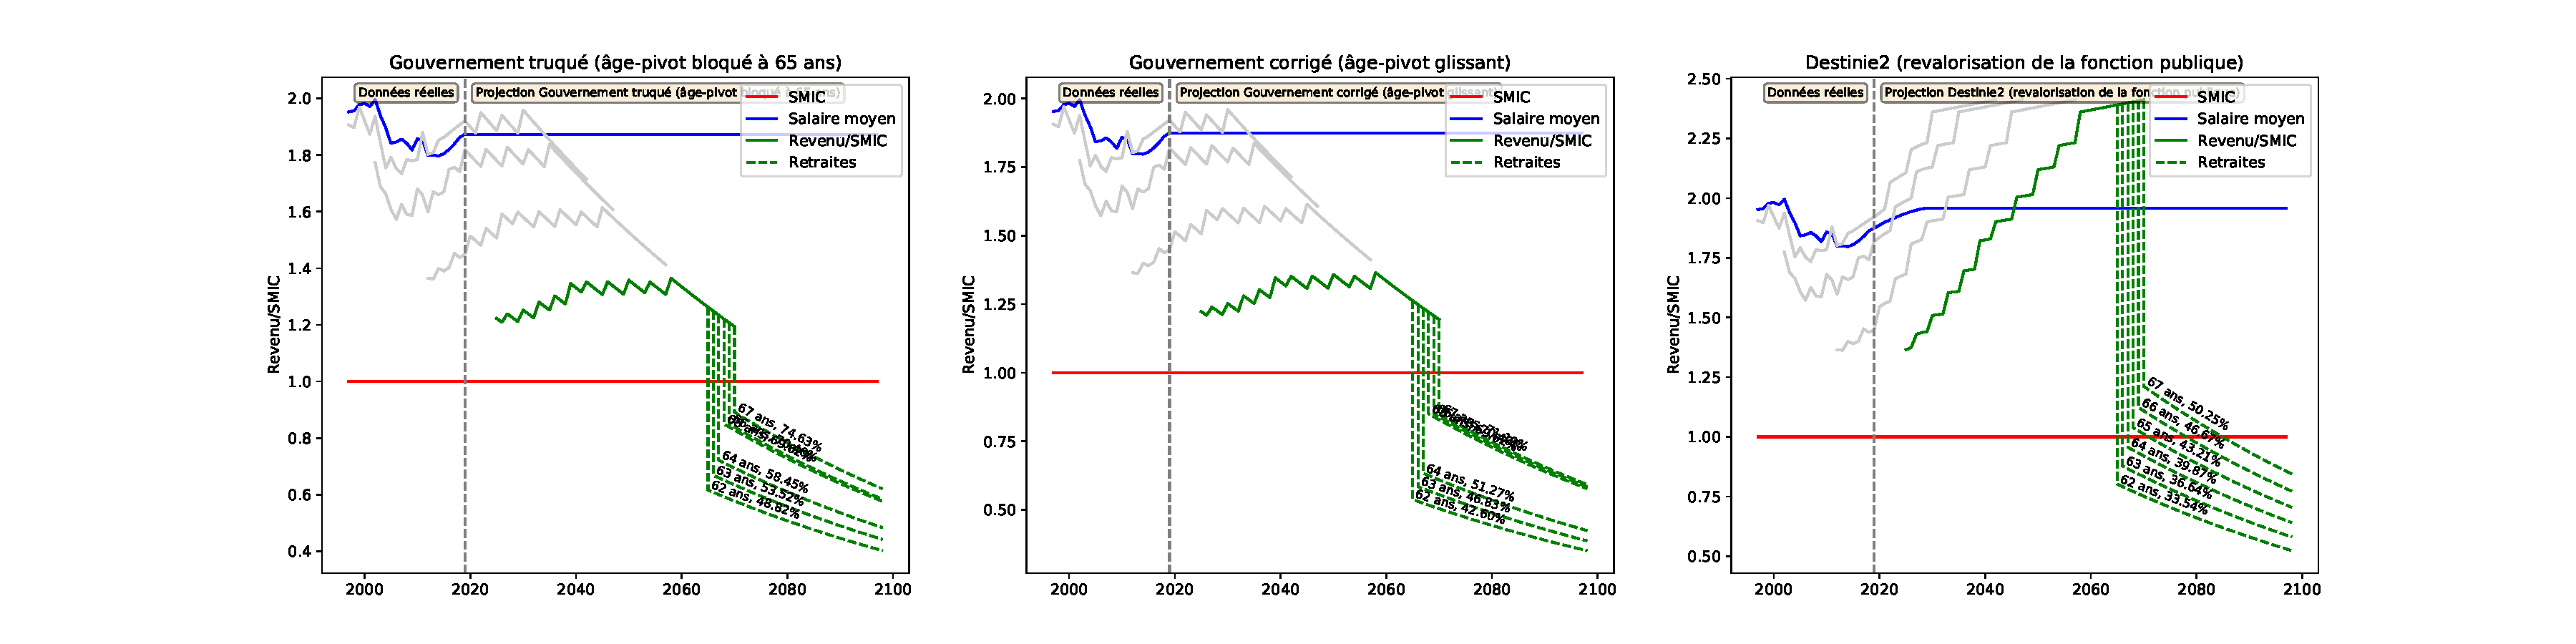
\includegraphics[width=0.9\textwidth]{fig/Infirmier_2003_22_dest_retraite.pdf}\end{center} \label{fig/Infirmier_2003_22_dest_retraite.pdf} 

\newpage 
 
\paragraph{Revenus et points pour le modèle \emph{Gouvernement truqué (âge-pivot bloqué à 65 ans)}} 
 
{ \scriptsize \begin{center} 
\begin{tabular}[htb]{|c|c||c|c|c|c|c|c||c|c||c|c|c|} 
\hline 
 Année &  Âge &  Ind Maj &  Pt Ind(\euro{} 2019) &  Rev HP(\euro{} 2019) &  Tx Primes &  GIPA(\euro{} 2019) &  Revenu(\euro{} 2019) &  SMIC(\euro{} 2019) &  Rev/SMIC &  Cumul Pts &  Achat Pt(\euro{} 2019) &  Serv. Pt(\euro{} 2019) \\ 
\hline \hline 
 2025 &  22 &  390.0 &  4.79 &  1869.82 &  20.01 &  0.00 &  2243.98 &  1835.31 &  {\bf 1.22} &  756.25 &  35.61 &  0.50 \\ 
\hline 
 2026 &  23 &  390.0 &  4.79 &  1869.82 &  20.24 &  0.00 &  2248.28 &  1859.17 &  {\bf 1.21} &  1513.94 &  35.61 &  0.50 \\ 
\hline 
 2027 &  24 &  404.0 &  4.79 &  1936.95 &  20.47 &  0.00 &  2333.44 &  1883.34 &  {\bf 1.24} &  2300.34 &  35.61 &  0.50 \\ 
\hline 
 2028 &  25 &  404.0 &  4.79 &  1936.95 &  20.70 &  0.00 &  2337.89 &  1907.82 &  {\bf 1.23} &  3088.24 &  35.61 &  0.50 \\ 
\hline 
 2029 &  26 &  404.0 &  4.79 &  1936.95 &  20.93 &  0.00 &  2342.35 &  1932.62 &  {\bf 1.21} &  3877.04 &  35.63 &  0.50 \\ 
\hline 
 2030 &  27 &  422.0 &  4.79 &  2023.25 &  21.16 &  0.00 &  2451.37 &  1957.75 &  {\bf 1.25} &  4701.30 &  35.69 &  0.50 \\ 
\hline 
 2031 &  28 &  422.0 &  4.79 &  2023.25 &  21.39 &  0.00 &  2456.02 &  1983.20 &  {\bf 1.24} &  5525.24 &  35.77 &  0.50 \\ 
\hline 
 2032 &  29 &  422.0 &  4.79 &  2023.25 &  21.62 &  0.00 &  2460.67 &  2008.98 &  {\bf 1.22} &  6348.24 &  35.88 &  0.50 \\ 
\hline 
 2033 &  30 &  446.0 &  4.79 &  2138.31 &  21.85 &  0.00 &  2605.53 &  2035.10 &  {\bf 1.28} &  7216.39 &  36.02 &  0.50 \\ 
\hline 
 2034 &  31 &  446.0 &  4.79 &  2138.31 &  22.08 &  0.00 &  2610.45 &  2061.55 &  {\bf 1.27} &  8082.22 &  36.18 &  0.50 \\ 
\hline 
 2035 &  32 &  446.0 &  4.79 &  2138.31 &  22.31 &  0.00 &  2615.37 &  2088.35 &  {\bf 1.25} &  8945.08 &  36.37 &  0.51 \\ 
\hline 
 2036 &  33 &  469.0 &  4.79 &  2248.58 &  22.54 &  0.00 &  2755.41 &  2115.50 &  {\bf 1.30} &  9848.63 &  36.59 &  0.51 \\ 
\hline 
 2037 &  34 &  469.0 &  4.79 &  2248.58 &  22.77 &  0.00 &  2760.59 &  2143.00 &  {\bf 1.29} &  10747.71 &  36.85 &  0.51 \\ 
\hline 
 2038 &  35 &  469.0 &  4.79 &  2248.58 &  23.00 &  0.00 &  2765.76 &  2170.86 &  {\bf 1.27} &  11641.66 &  37.13 &  0.52 \\ 
\hline 
 2039 &  36 &  501.0 &  4.79 &  2402.01 &  23.23 &  0.00 &  2959.99 &  2199.08 &  {\bf 1.35} &  12590.42 &  37.44 &  0.52 \\ 
\hline 
 2040 &  37 &  501.0 &  4.79 &  2402.01 &  23.46 &  0.00 &  2965.52 &  2227.67 &  {\bf 1.33} &  13532.33 &  37.78 &  0.53 \\ 
\hline 
 2041 &  38 &  501.0 &  4.79 &  2402.01 &  23.69 &  0.00 &  2971.04 &  2256.63 &  {\bf 1.32} &  14466.72 &  38.16 &  0.53 \\ 
\hline 
 2042 &  39 &  520.0 &  4.79 &  2493.10 &  23.92 &  0.00 &  3089.45 &  2285.97 &  {\bf 1.35} &  15428.06 &  38.56 &  0.54 \\ 
\hline 
 2043 &  40 &  520.0 &  4.79 &  2493.10 &  24.15 &  0.00 &  3095.18 &  2315.68 &  {\bf 1.34} &  16380.28 &  39.01 &  0.54 \\ 
\hline 
 2044 &  41 &  520.0 &  4.79 &  2493.10 &  24.38 &  0.00 &  3100.92 &  2345.79 &  {\bf 1.32} &  17322.73 &  39.48 &  0.55 \\ 
\hline 
 2045 &  42 &  520.0 &  4.79 &  2493.10 &  24.61 &  0.00 &  3106.65 &  2376.28 &  {\bf 1.31} &  18254.81 &  40.00 &  0.56 \\ 
\hline 
 2046 &  43 &  544.0 &  4.79 &  2608.17 &  24.84 &  0.00 &  3256.03 &  2407.18 &  {\bf 1.35} &  19219.17 &  40.52 &  0.56 \\ 
\hline 
 2047 &  44 &  544.0 &  4.79 &  2608.17 &  25.07 &  0.00 &  3262.03 &  2438.47 &  {\bf 1.34} &  20172.91 &  41.04 &  0.57 \\ 
\hline 
 2048 &  45 &  544.0 &  4.79 &  2608.17 &  25.30 &  0.00 &  3268.03 &  2470.17 &  {\bf 1.32} &  21116.15 &  41.58 &  0.58 \\ 
\hline 
 2049 &  46 &  544.0 &  4.79 &  2608.17 &  25.53 &  0.00 &  3274.03 &  2502.28 &  {\bf 1.31} &  22048.98 &  42.12 &  0.59 \\ 
\hline 
 2050 &  47 &  571.0 &  4.79 &  2737.62 &  25.76 &  0.00 &  3442.82 &  2534.81 &  {\bf 1.36} &  23017.32 &  42.66 &  0.59 \\ 
\hline 
 2051 &  48 &  571.0 &  4.79 &  2737.62 &  25.99 &  0.00 &  3449.12 &  2567.76 &  {\bf 1.34} &  23974.99 &  43.22 &  0.60 \\ 
\hline 
 2052 &  49 &  571.0 &  4.79 &  2737.62 &  26.22 &  0.00 &  3455.42 &  2601.14 &  {\bf 1.33} &  24922.08 &  43.78 &  0.61 \\ 
\hline 
 2053 &  50 &  571.0 &  4.79 &  2737.62 &  26.45 &  0.00 &  3461.71 &  2634.96 &  {\bf 1.31} &  25858.73 &  44.35 &  0.62 \\ 
\hline 
 2054 &  51 &  594.0 &  4.79 &  2847.89 &  26.68 &  0.00 &  3607.70 &  2669.21 &  {\bf 1.35} &  26822.35 &  44.93 &  0.63 \\ 
\hline 
 2055 &  52 &  594.0 &  4.79 &  2847.89 &  26.91 &  0.00 &  3614.25 &  2703.91 &  {\bf 1.34} &  27775.34 &  45.51 &  0.63 \\ 
\hline 
 2056 &  53 &  594.0 &  4.79 &  2847.89 &  27.14 &  0.00 &  3620.80 &  2739.06 &  {\bf 1.32} &  28717.79 &  46.10 &  0.64 \\ 
\hline 
 2057 &  54 &  594.0 &  4.79 &  2847.89 &  27.37 &  0.00 &  3627.35 &  2774.67 &  {\bf 1.31} &  29649.84 &  46.70 &  0.65 \\ 
\hline 
 2058 &  55 &  627.0 &  4.79 &  3006.10 &  27.60 &  0.00 &  3835.79 &  2810.74 &  {\bf 1.36} &  30622.79 &  47.31 &  0.66 \\ 
\hline 
 2059 &  56 &  627.0 &  4.79 &  3006.10 &  27.83 &  0.00 &  3842.70 &  2847.28 &  {\bf 1.35} &  31584.99 &  47.92 &  0.67 \\ 
\hline 
 2060 &  57 &  627.0 &  4.79 &  3006.10 &  28.06 &  0.00 &  3849.62 &  2884.30 &  {\bf 1.33} &  32536.55 &  48.55 &  0.68 \\ 
\hline 
 2061 &  58 &  627.0 &  4.79 &  3006.10 &  28.29 &  0.00 &  3856.53 &  2921.79 &  {\bf 1.32} &  33477.59 &  49.18 &  0.68 \\ 
\hline 
 2062 &  59 &  627.0 &  4.79 &  3006.10 &  28.52 &  0.00 &  3863.44 &  2959.78 &  {\bf 1.31} &  34408.21 &  49.82 &  0.69 \\ 
\hline 
 2063 &  60 &  627.0 &  4.79 &  3006.10 &  28.75 &  0.00 &  3870.36 &  2998.25 &  {\bf 1.29} &  35328.54 &  50.47 &  0.70 \\ 
\hline 
 2064 &  61 &  627.0 &  4.79 &  3006.10 &  28.98 &  0.00 &  3877.27 &  3037.23 &  {\bf 1.28} &  36238.67 &  51.12 &  0.71 \\ 
\hline 
 2065 &  62 &  627.0 &  4.79 &  3006.10 &  29.21 &  0.00 &  3884.19 &  3076.71 &  {\bf 1.26} &  37138.74 &  51.79 &  0.72 \\ 
\hline 
 2066 &  63 &  627.0 &  4.79 &  3006.10 &  29.44 &  0.00 &  3891.10 &  3116.71 &  {\bf 1.25} &  38028.83 &  52.46 &  0.73 \\ 
\hline 
 2067 &  64 &  627.0 &  4.79 &  3006.10 &  29.67 &  0.00 &  3898.01 &  3157.23 &  {\bf 1.23} &  38909.06 &  53.14 &  0.74 \\ 
\hline 
 2068 &  65 &  627.0 &  4.79 &  3006.10 &  29.90 &  0.00 &  3904.93 &  3198.27 &  {\bf 1.22} &  39779.53 &  53.83 &  0.75 \\ 
\hline 
 2069 &  66 &  627.0 &  4.79 &  3006.10 &  30.13 &  0.00 &  3911.84 &  3239.85 &  {\bf 1.21} &  40640.36 &  54.53 &  0.76 \\ 
\hline 
 2070 &  67 &  627.0 &  4.79 &  3006.10 &  30.36 &  0.00 &  3918.76 &  3281.97 &  {\bf 1.19} &  41491.64 &  55.24 &  0.77 \\ 
\hline 
\hline 
\end{tabular} 
\end{center} } 
\newpage 
 
\paragraph{Revenus et points pour le modèle \emph{Gouvernement corrigé (âge-pivot glissant)}} 
 
{ \scriptsize \begin{center} 
\begin{tabular}[htb]{|c|c||c|c|c|c|c|c||c|c||c|c|c|} 
\hline 
 Année &  Âge &  Ind Maj &  Pt Ind(\euro{} 2019) &  Rev HP(\euro{} 2019) &  Tx Primes &  GIPA(\euro{} 2019) &  Revenu(\euro{} 2019) &  SMIC(\euro{} 2019) &  Rev/SMIC &  Cumul Pts &  Achat Pt(\euro{} 2019) &  Serv. Pt(\euro{} 2019) \\ 
\hline \hline 
 2025 &  22 &  390.0 &  4.79 &  1869.82 &  20.01 &  0.00 &  2243.98 &  1835.31 &  {\bf 1.22} &  756.25 &  35.61 &  0.50 \\ 
\hline 
 2026 &  23 &  390.0 &  4.79 &  1869.82 &  20.24 &  0.00 &  2248.28 &  1859.17 &  {\bf 1.21} &  1513.94 &  35.61 &  0.50 \\ 
\hline 
 2027 &  24 &  404.0 &  4.79 &  1936.95 &  20.47 &  0.00 &  2333.44 &  1883.34 &  {\bf 1.24} &  2300.34 &  35.61 &  0.50 \\ 
\hline 
 2028 &  25 &  404.0 &  4.79 &  1936.95 &  20.70 &  0.00 &  2337.89 &  1907.82 &  {\bf 1.23} &  3088.24 &  35.61 &  0.50 \\ 
\hline 
 2029 &  26 &  404.0 &  4.79 &  1936.95 &  20.93 &  0.00 &  2342.35 &  1932.62 &  {\bf 1.21} &  3877.04 &  35.63 &  0.50 \\ 
\hline 
 2030 &  27 &  422.0 &  4.79 &  2023.25 &  21.16 &  0.00 &  2451.37 &  1957.75 &  {\bf 1.25} &  4701.30 &  35.69 &  0.50 \\ 
\hline 
 2031 &  28 &  422.0 &  4.79 &  2023.25 &  21.39 &  0.00 &  2456.02 &  1983.20 &  {\bf 1.24} &  5525.24 &  35.77 &  0.50 \\ 
\hline 
 2032 &  29 &  422.0 &  4.79 &  2023.25 &  21.62 &  0.00 &  2460.67 &  2008.98 &  {\bf 1.22} &  6348.24 &  35.88 &  0.50 \\ 
\hline 
 2033 &  30 &  446.0 &  4.79 &  2138.31 &  21.85 &  0.00 &  2605.53 &  2035.10 &  {\bf 1.28} &  7216.39 &  36.02 &  0.50 \\ 
\hline 
 2034 &  31 &  446.0 &  4.79 &  2138.31 &  22.08 &  0.00 &  2610.45 &  2061.55 &  {\bf 1.27} &  8082.22 &  36.18 &  0.50 \\ 
\hline 
 2035 &  32 &  446.0 &  4.79 &  2138.31 &  22.31 &  0.00 &  2615.37 &  2088.35 &  {\bf 1.25} &  8945.08 &  36.37 &  0.51 \\ 
\hline 
 2036 &  33 &  469.0 &  4.79 &  2248.58 &  22.54 &  0.00 &  2755.41 &  2115.50 &  {\bf 1.30} &  9848.63 &  36.59 &  0.51 \\ 
\hline 
 2037 &  34 &  469.0 &  4.79 &  2248.58 &  22.77 &  0.00 &  2760.59 &  2143.00 &  {\bf 1.29} &  10747.71 &  36.85 &  0.51 \\ 
\hline 
 2038 &  35 &  469.0 &  4.79 &  2248.58 &  23.00 &  0.00 &  2765.76 &  2170.86 &  {\bf 1.27} &  11641.66 &  37.13 &  0.52 \\ 
\hline 
 2039 &  36 &  501.0 &  4.79 &  2402.01 &  23.23 &  0.00 &  2959.99 &  2199.08 &  {\bf 1.35} &  12590.42 &  37.44 &  0.52 \\ 
\hline 
 2040 &  37 &  501.0 &  4.79 &  2402.01 &  23.46 &  0.00 &  2965.52 &  2227.67 &  {\bf 1.33} &  13532.33 &  37.78 &  0.53 \\ 
\hline 
 2041 &  38 &  501.0 &  4.79 &  2402.01 &  23.69 &  0.00 &  2971.04 &  2256.63 &  {\bf 1.32} &  14466.72 &  38.16 &  0.53 \\ 
\hline 
 2042 &  39 &  520.0 &  4.79 &  2493.10 &  23.92 &  0.00 &  3089.45 &  2285.97 &  {\bf 1.35} &  15428.06 &  38.56 &  0.54 \\ 
\hline 
 2043 &  40 &  520.0 &  4.79 &  2493.10 &  24.15 &  0.00 &  3095.18 &  2315.68 &  {\bf 1.34} &  16380.28 &  39.01 &  0.54 \\ 
\hline 
 2044 &  41 &  520.0 &  4.79 &  2493.10 &  24.38 &  0.00 &  3100.92 &  2345.79 &  {\bf 1.32} &  17322.73 &  39.48 &  0.55 \\ 
\hline 
 2045 &  42 &  520.0 &  4.79 &  2493.10 &  24.61 &  0.00 &  3106.65 &  2376.28 &  {\bf 1.31} &  18254.81 &  40.00 &  0.56 \\ 
\hline 
 2046 &  43 &  544.0 &  4.79 &  2608.17 &  24.84 &  0.00 &  3256.03 &  2407.18 &  {\bf 1.35} &  19219.17 &  40.52 &  0.56 \\ 
\hline 
 2047 &  44 &  544.0 &  4.79 &  2608.17 &  25.07 &  0.00 &  3262.03 &  2438.47 &  {\bf 1.34} &  20172.91 &  41.04 &  0.57 \\ 
\hline 
 2048 &  45 &  544.0 &  4.79 &  2608.17 &  25.30 &  0.00 &  3268.03 &  2470.17 &  {\bf 1.32} &  21116.15 &  41.58 &  0.58 \\ 
\hline 
 2049 &  46 &  544.0 &  4.79 &  2608.17 &  25.53 &  0.00 &  3274.03 &  2502.28 &  {\bf 1.31} &  22048.98 &  42.12 &  0.59 \\ 
\hline 
 2050 &  47 &  571.0 &  4.79 &  2737.62 &  25.76 &  0.00 &  3442.82 &  2534.81 &  {\bf 1.36} &  23017.32 &  42.66 &  0.59 \\ 
\hline 
 2051 &  48 &  571.0 &  4.79 &  2737.62 &  25.99 &  0.00 &  3449.12 &  2567.76 &  {\bf 1.34} &  23974.99 &  43.22 &  0.60 \\ 
\hline 
 2052 &  49 &  571.0 &  4.79 &  2737.62 &  26.22 &  0.00 &  3455.42 &  2601.14 &  {\bf 1.33} &  24922.08 &  43.78 &  0.61 \\ 
\hline 
 2053 &  50 &  571.0 &  4.79 &  2737.62 &  26.45 &  0.00 &  3461.71 &  2634.96 &  {\bf 1.31} &  25858.73 &  44.35 &  0.62 \\ 
\hline 
 2054 &  51 &  594.0 &  4.79 &  2847.89 &  26.68 &  0.00 &  3607.70 &  2669.21 &  {\bf 1.35} &  26822.35 &  44.93 &  0.63 \\ 
\hline 
 2055 &  52 &  594.0 &  4.79 &  2847.89 &  26.91 &  0.00 &  3614.25 &  2703.91 &  {\bf 1.34} &  27775.34 &  45.51 &  0.63 \\ 
\hline 
 2056 &  53 &  594.0 &  4.79 &  2847.89 &  27.14 &  0.00 &  3620.80 &  2739.06 &  {\bf 1.32} &  28717.79 &  46.10 &  0.64 \\ 
\hline 
 2057 &  54 &  594.0 &  4.79 &  2847.89 &  27.37 &  0.00 &  3627.35 &  2774.67 &  {\bf 1.31} &  29649.84 &  46.70 &  0.65 \\ 
\hline 
 2058 &  55 &  627.0 &  4.79 &  3006.10 &  27.60 &  0.00 &  3835.79 &  2810.74 &  {\bf 1.36} &  30622.79 &  47.31 &  0.66 \\ 
\hline 
 2059 &  56 &  627.0 &  4.79 &  3006.10 &  27.83 &  0.00 &  3842.70 &  2847.28 &  {\bf 1.35} &  31584.99 &  47.92 &  0.67 \\ 
\hline 
 2060 &  57 &  627.0 &  4.79 &  3006.10 &  28.06 &  0.00 &  3849.62 &  2884.30 &  {\bf 1.33} &  32536.55 &  48.55 &  0.68 \\ 
\hline 
 2061 &  58 &  627.0 &  4.79 &  3006.10 &  28.29 &  0.00 &  3856.53 &  2921.79 &  {\bf 1.32} &  33477.59 &  49.18 &  0.68 \\ 
\hline 
 2062 &  59 &  627.0 &  4.79 &  3006.10 &  28.52 &  0.00 &  3863.44 &  2959.78 &  {\bf 1.31} &  34408.21 &  49.82 &  0.69 \\ 
\hline 
 2063 &  60 &  627.0 &  4.79 &  3006.10 &  28.75 &  0.00 &  3870.36 &  2998.25 &  {\bf 1.29} &  35328.54 &  50.47 &  0.70 \\ 
\hline 
 2064 &  61 &  627.0 &  4.79 &  3006.10 &  28.98 &  0.00 &  3877.27 &  3037.23 &  {\bf 1.28} &  36238.67 &  51.12 &  0.71 \\ 
\hline 
 2065 &  62 &  627.0 &  4.79 &  3006.10 &  29.21 &  0.00 &  3884.19 &  3076.71 &  {\bf 1.26} &  37138.74 &  51.79 &  0.72 \\ 
\hline 
 2066 &  63 &  627.0 &  4.79 &  3006.10 &  29.44 &  0.00 &  3891.10 &  3116.71 &  {\bf 1.25} &  38028.83 &  52.46 &  0.73 \\ 
\hline 
 2067 &  64 &  627.0 &  4.79 &  3006.10 &  29.67 &  0.00 &  3898.01 &  3157.23 &  {\bf 1.23} &  38909.06 &  53.14 &  0.74 \\ 
\hline 
 2068 &  65 &  627.0 &  4.79 &  3006.10 &  29.90 &  0.00 &  3904.93 &  3198.27 &  {\bf 1.22} &  39779.53 &  53.83 &  0.75 \\ 
\hline 
 2069 &  66 &  627.0 &  4.79 &  3006.10 &  30.13 &  0.00 &  3911.84 &  3239.85 &  {\bf 1.21} &  40640.36 &  54.53 &  0.76 \\ 
\hline 
 2070 &  67 &  627.0 &  4.79 &  3006.10 &  30.36 &  0.00 &  3918.76 &  3281.97 &  {\bf 1.19} &  41491.64 &  55.24 &  0.77 \\ 
\hline 
\hline 
\end{tabular} 
\end{center} } 
\newpage 
 
\paragraph{Revenus et points pour le modèle \emph{Destinie2 (revalorisation de la fonction publique)}} 
 
{ \scriptsize \begin{center} 
\begin{tabular}[htb]{|c|c||c|c|c|c|c|c||c|c||c|c|c|} 
\hline 
 Année &  Âge &  Ind Maj &  Pt Ind(\euro{} 2019) &  Rev HP(\euro{} 2019) &  Tx Primes &  GIPA(\euro{} 2019) &  Revenu(\euro{} 2019) &  SMIC(\euro{} 2019) &  Rev/SMIC &  Cumul Pts &  Achat Pt(\euro{} 2019) &  Serv. Pt(\euro{} 2019) \\ 
\hline \hline 
 2025 &  22 &  390.0 &  5.10 &  1990.35 &  20.01 &  0.00 &  2388.62 &  1749.35 &  {\bf 1.37} &  803.02 &  35.69 &  0.50 \\ 
\hline 
 2026 &  23 &  390.0 &  5.17 &  2015.23 &  20.24 &  0.00 &  2423.11 &  1764.53 &  {\bf 1.37} &  1617.63 &  35.69 &  0.50 \\ 
\hline 
 2027 &  24 &  404.0 &  5.23 &  2114.29 &  20.47 &  0.00 &  2547.09 &  1781.27 &  {\bf 1.43} &  2473.92 &  35.69 &  0.50 \\ 
\hline 
 2028 &  25 &  404.0 &  5.30 &  2141.99 &  20.70 &  0.00 &  2585.38 &  1799.59 &  {\bf 1.44} &  3343.08 &  35.69 &  0.50 \\ 
\hline 
 2029 &  26 &  404.0 &  5.37 &  2167.91 &  20.93 &  0.00 &  2621.65 &  1819.55 &  {\bf 1.44} &  4223.82 &  35.72 &  0.50 \\ 
\hline 
 2030 &  27 &  422.0 &  5.43 &  2292.58 &  21.16 &  0.00 &  2777.69 &  1841.19 &  {\bf 1.51} &  5155.62 &  35.77 &  0.50 \\ 
\hline 
 2031 &  28 &  422.0 &  5.50 &  2321.69 &  21.39 &  0.00 &  2818.30 &  1864.58 &  {\bf 1.51} &  6098.94 &  35.85 &  0.50 \\ 
\hline 
 2032 &  29 &  422.0 &  5.57 &  2351.88 &  21.62 &  0.00 &  2860.35 &  1888.81 &  {\bf 1.51} &  7053.44 &  35.96 &  0.50 \\ 
\hline 
 2033 &  30 &  446.0 &  5.65 &  2517.94 &  21.85 &  0.00 &  3068.12 &  1913.37 &  {\bf 1.60} &  8073.38 &  36.10 &  0.50 \\ 
\hline 
 2034 &  31 &  446.0 &  5.72 &  2550.68 &  22.08 &  0.00 &  3113.87 &  1938.24 &  {\bf 1.61} &  9103.82 &  36.26 &  0.50 \\ 
\hline 
 2035 &  32 &  446.0 &  5.79 &  2583.84 &  22.31 &  0.00 &  3160.29 &  1963.44 &  {\bf 1.61} &  10144.08 &  36.46 &  0.51 \\ 
\hline 
 2036 &  33 &  469.0 &  5.87 &  2752.41 &  22.54 &  0.00 &  3372.80 &  1988.96 &  {\bf 1.70} &  11247.56 &  36.68 &  0.51 \\ 
\hline 
 2037 &  34 &  469.0 &  5.94 &  2788.19 &  22.77 &  0.00 &  3423.06 &  2014.82 &  {\bf 1.70} &  12359.85 &  36.93 &  0.51 \\ 
\hline 
 2038 &  35 &  469.0 &  6.02 &  2824.43 &  23.00 &  0.00 &  3474.05 &  2041.01 &  {\bf 1.70} &  13480.17 &  37.21 &  0.52 \\ 
\hline 
 2039 &  36 &  501.0 &  6.10 &  3056.37 &  23.23 &  0.00 &  3766.36 &  2067.55 &  {\bf 1.82} &  14684.64 &  37.52 &  0.52 \\ 
\hline 
 2040 &  37 &  501.0 &  6.18 &  3096.10 &  23.46 &  0.00 &  3822.45 &  2094.43 &  {\bf 1.83} &  15895.95 &  37.87 &  0.53 \\ 
\hline 
 2041 &  38 &  501.0 &  6.26 &  3136.35 &  23.69 &  0.00 &  3879.35 &  2121.65 &  {\bf 1.83} &  17113.22 &  38.24 &  0.53 \\ 
\hline 
 2042 &  39 &  520.0 &  6.34 &  3297.61 &  23.92 &  0.00 &  4086.40 &  2149.23 &  {\bf 1.90} &  18381.88 &  38.65 &  0.54 \\ 
\hline 
 2043 &  40 &  520.0 &  6.42 &  3340.48 &  24.15 &  0.00 &  4147.21 &  2177.17 &  {\bf 1.90} &  19654.84 &  39.10 &  0.54 \\ 
\hline 
 2044 &  41 &  520.0 &  6.51 &  3383.91 &  24.38 &  0.00 &  4208.90 &  2205.48 &  {\bf 1.91} &  20931.12 &  39.57 &  0.55 \\ 
\hline 
 2045 &  42 &  520.0 &  6.59 &  3427.90 &  24.61 &  0.00 &  4271.50 &  2234.15 &  {\bf 1.91} &  22209.76 &  40.09 &  0.56 \\ 
\hline 
 2046 &  43 &  544.0 &  6.68 &  3632.73 &  24.84 &  0.00 &  4535.10 &  2263.19 &  {\bf 2.00} &  23549.89 &  40.61 &  0.57 \\ 
\hline 
 2047 &  44 &  544.0 &  6.76 &  3679.95 &  25.07 &  0.00 &  4602.52 &  2292.61 &  {\bf 2.01} &  24892.48 &  41.14 &  0.57 \\ 
\hline 
 2048 &  45 &  544.0 &  6.85 &  3727.79 &  25.30 &  0.00 &  4670.93 &  2322.42 &  {\bf 2.01} &  26237.54 &  41.67 &  0.58 \\ 
\hline 
 2049 &  46 &  544.0 &  6.94 &  3776.26 &  25.53 &  0.00 &  4740.33 &  2352.61 &  {\bf 2.01} &  27585.07 &  42.21 &  0.59 \\ 
\hline 
 2050 &  47 &  571.0 &  7.03 &  4015.21 &  25.76 &  0.00 &  5049.53 &  2383.19 &  {\bf 2.12} &  29002.08 &  42.76 &  0.60 \\ 
\hline 
 2051 &  48 &  571.0 &  7.12 &  4067.41 &  25.99 &  0.00 &  5124.52 &  2414.18 &  {\bf 2.12} &  30421.67 &  43.32 &  0.60 \\ 
\hline 
 2052 &  49 &  571.0 &  7.22 &  4120.28 &  26.22 &  0.00 &  5200.62 &  2445.56 &  {\bf 2.13} &  31843.86 &  43.88 &  0.61 \\ 
\hline 
 2053 &  50 &  571.0 &  7.31 &  4173.85 &  26.45 &  0.00 &  5277.83 &  2477.35 &  {\bf 2.13} &  33268.64 &  44.45 &  0.62 \\ 
\hline 
 2054 &  51 &  594.0 &  7.40 &  4398.41 &  26.68 &  0.00 &  5571.91 &  2509.56 &  {\bf 2.22} &  34753.51 &  45.03 &  0.63 \\ 
\hline 
 2055 &  52 &  594.0 &  7.50 &  4455.59 &  26.91 &  0.00 &  5654.59 &  2542.18 &  {\bf 2.22} &  36241.07 &  45.62 &  0.63 \\ 
\hline 
 2056 &  53 &  594.0 &  7.60 &  4513.52 &  27.14 &  0.00 &  5738.48 &  2575.23 &  {\bf 2.23} &  37731.32 &  46.21 &  0.64 \\ 
\hline 
 2057 &  54 &  594.0 &  7.70 &  4572.19 &  27.37 &  0.00 &  5823.60 &  2608.71 &  {\bf 2.23} &  39224.28 &  46.81 &  0.65 \\ 
\hline 
 2058 &  55 &  627.0 &  7.80 &  4888.94 &  27.60 &  0.00 &  6238.29 &  2642.62 &  {\bf 2.36} &  40803.02 &  47.42 &  0.66 \\ 
\hline 
 2059 &  56 &  627.0 &  7.90 &  4952.50 &  27.83 &  0.00 &  6330.78 &  2676.98 &  {\bf 2.36} &  42384.60 &  48.03 &  0.67 \\ 
\hline 
 2060 &  57 &  627.0 &  8.00 &  5016.88 &  28.06 &  0.00 &  6424.62 &  2711.78 &  {\bf 2.37} &  43969.04 &  48.66 &  0.68 \\ 
\hline 
 2061 &  58 &  627.0 &  8.11 &  5082.10 &  28.29 &  0.00 &  6519.83 &  2747.03 &  {\bf 2.37} &  45556.31 &  49.29 &  0.69 \\ 
\hline 
 2062 &  59 &  627.0 &  8.21 &  5148.17 &  28.52 &  0.00 &  6616.43 &  2782.74 &  {\bf 2.38} &  47146.44 &  49.93 &  0.70 \\ 
\hline 
 2063 &  60 &  627.0 &  8.32 &  5215.09 &  28.75 &  0.00 &  6714.43 &  2818.92 &  {\bf 2.38} &  48739.41 &  50.58 &  0.70 \\ 
\hline 
 2064 &  61 &  627.0 &  8.43 &  5282.89 &  28.98 &  0.00 &  6813.87 &  2855.56 &  {\bf 2.39} &  50335.22 &  51.24 &  0.71 \\ 
\hline 
 2065 &  62 &  627.0 &  8.54 &  5351.57 &  29.21 &  0.00 &  6914.76 &  2892.68 &  {\bf 2.39} &  51933.88 &  51.90 &  0.72 \\ 
\hline 
 2066 &  63 &  627.0 &  8.65 &  5421.14 &  29.44 &  0.00 &  7017.12 &  2930.29 &  {\bf 2.39} &  53535.39 &  52.58 &  0.73 \\ 
\hline 
 2067 &  64 &  627.0 &  8.76 &  5491.61 &  29.67 &  0.00 &  7120.98 &  2968.38 &  {\bf 2.40} &  55139.74 &  53.26 &  0.74 \\ 
\hline 
 2068 &  65 &  627.0 &  8.87 &  5563.01 &  29.90 &  0.00 &  7226.34 &  3006.97 &  {\bf 2.40} &  56746.94 &  53.95 &  0.75 \\ 
\hline 
 2069 &  66 &  627.0 &  8.99 &  5635.32 &  30.13 &  0.00 &  7333.25 &  3046.06 &  {\bf 2.41} &  58356.98 &  54.66 &  0.76 \\ 
\hline 
 2070 &  67 &  627.0 &  9.10 &  5708.58 &  30.36 &  0.00 &  7441.71 &  3085.66 &  {\bf 2.41} &  59969.87 &  55.37 &  0.77 \\ 
\hline 
\hline 
\end{tabular} 
\end{center} } 
\newpage 
 
\chapter{Aide-soignante (CN puis HC)} 

\begin{minipage}{0.55\linewidth}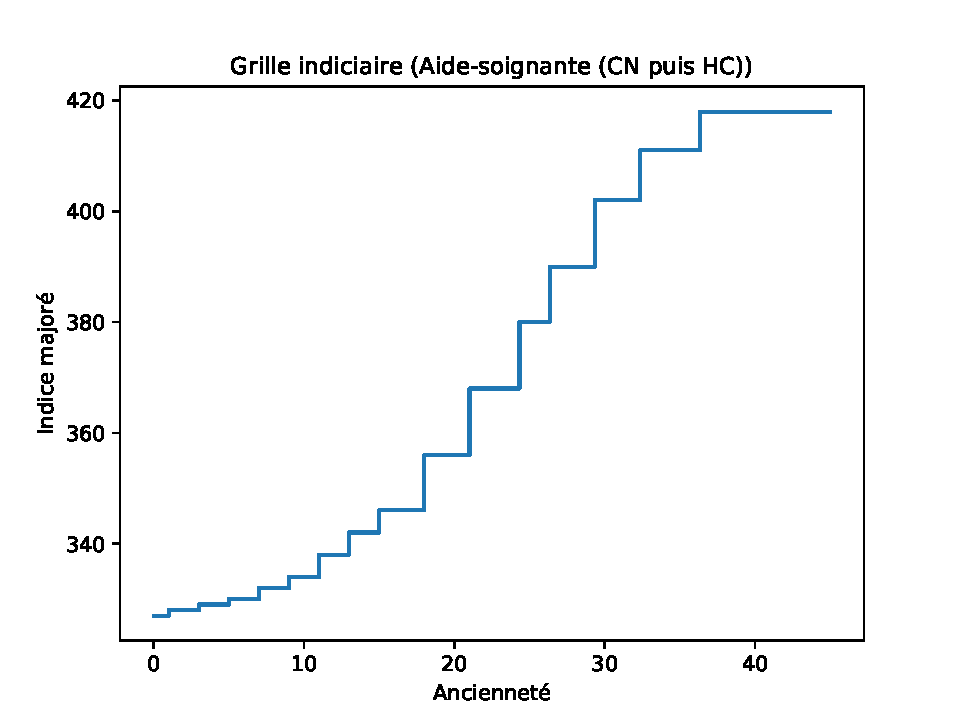
\includegraphics[width=0.7\textwidth]{fig/grille_AideSoignant.pdf}\end{minipage} 
\begin{minipage}{0.3\linewidth} 
 \begin{center} 

\begin{tabular}[htb]{|c|c|} 
\hline 
 Indice majoré &  Durée (années) \\ 
\hline \hline 
 327 &  1.00 \\ 
\hline 
 328 &  2.00 \\ 
\hline 
 329 &  2.00 \\ 
\hline 
 330 &  2.00 \\ 
\hline 
 332 &  2.00 \\ 
\hline 
 334 &  2.00 \\ 
\hline 
 338 &  2.00 \\ 
\hline 
 342 &  2.00 \\ 
\hline 
 346 &  3.00 \\ 
\hline 
 356 &  3.00 \\ 
\hline 
 368 &  3.33 \\ 
\hline 
 380 &  2.00 \\ 
\hline 
 390 &  3.00 \\ 
\hline 
 402 &  3.00 \\ 
\hline 
 411 &  4.00 \\ 
\hline 
 418 &   \\ 
\hline 
\hline 
\end{tabular} 
\end{center} 
 \end{minipage} 


 \addto{\captionsenglish}{ \renewcommand{\mtctitle}{}} \setcounter{minitocdepth}{2} 
 \minitoc \newpage 

\section{Début de carrière à 22 ans} 

\subsection{Génération 1975 (début en 1997)} 

\paragraph{Retraites possibles dans le modèle \emph{Gouvernement truqué (âge-pivot bloqué à 65 ans)}}  
 
{ \scriptsize \begin{center} 
\begin{tabular}[htb]{|c|c||c|c||c|c||c||c|c|c|c|c|c|} 
\hline 
 Retraite en &  Âge &  Âge pivot &  Décote/Surcote &  Retraite (\euro{} 2019) &  Tx Rempl(\%) &  SMIC (\euro{} 2019) &  Retraite/SMIC &  Rev70/SMIC &  Rev75/SMIC &  Rev80/SMIC &  Rev85/SMIC &  Rev90/SMIC \\ 
\hline \hline 
 2037 &  62 &  64 ans 10 mois &  -14.17\% &  1111.54 &  {\bf 44.91} &  2143.00 &  {\bf {\color{red} 0.52}} &  {\bf {\color{red} 0.47}} &  {\bf {\color{red} 0.44}} &  {\bf {\color{red} 0.41}} &  {\bf {\color{red} 0.39}} &  {\bf {\color{red} 0.36}} \\ 
\hline 
 2038 &  63 &  64 ans 11 mois &  -9.58\% &  1211.04 &  {\bf 48.84} &  2170.86 &  {\bf {\color{red} 0.56}} &  {\bf {\color{red} 0.51}} &  {\bf {\color{red} 0.48}} &  {\bf {\color{red} 0.45}} &  {\bf {\color{red} 0.42}} &  {\bf {\color{red} 0.39}} \\ 
\hline 
 2039 &  64 &  65 ans 0 mois &  -5.00\% &  1315.96 &  {\bf 52.97} &  2199.08 &  {\bf {\color{red} 0.60}} &  {\bf {\color{red} 0.55}} &  {\bf {\color{red} 0.52}} &  {\bf {\color{red} 0.49}} &  {\bf {\color{red} 0.46}} &  {\bf {\color{red} 0.43}} \\ 
\hline 
 2040 &  65 &  65 ans 0 mois &  0.00\% &  1893.52 &  {\bf 76.07} &  2227.67 &  {\bf {\color{red} 0.85}} &  {\bf {\color{red} 0.80}} &  {\bf {\color{red} 0.75}} &  {\bf {\color{red} 0.70}} &  {\bf {\color{red} 0.66}} &  {\bf {\color{red} 0.62}} \\ 
\hline 
 2041 &  66 &  65 ans 0 mois &  5.00\% &  1918.14 &  {\bf 76.92} &  2256.63 &  {\bf {\color{red} 0.85}} &  {\bf {\color{red} 0.81}} &  {\bf {\color{red} 0.76}} &  {\bf {\color{red} 0.71}} &  {\bf {\color{red} 0.67}} &  {\bf {\color{red} 0.62}} \\ 
\hline 
 2042 &  67 &  65 ans 0 mois &  10.00\% &  1943.07 &  {\bf 77.78} &  2285.97 &  {\bf {\color{red} 0.85}} &  {\bf {\color{red} 0.82}} &  {\bf {\color{red} 0.77}} &  {\bf {\color{red} 0.72}} &  {\bf {\color{red} 0.67}} &  {\bf {\color{red} 0.63}} \\ 
\hline 
\hline 
\end{tabular} 
\end{center} } 
\paragraph{Retraites possibles dans le modèle \emph{Gouvernement corrigé (âge-pivot glissant)}}  
 
{ \scriptsize \begin{center} 
\begin{tabular}[htb]{|c|c||c|c||c|c||c||c|c|c|c|c|c|} 
\hline 
 Retraite en &  Âge &  Âge pivot &  Décote/Surcote &  Retraite (\euro{} 2019) &  Tx Rempl(\%) &  SMIC (\euro{} 2019) &  Retraite/SMIC &  Rev70/SMIC &  Rev75/SMIC &  Rev80/SMIC &  Rev85/SMIC &  Rev90/SMIC \\ 
\hline \hline 
 2037 &  62 &  64 ans 10 mois &  -14.17\% &  1111.54 &  {\bf 44.91} &  2143.00 &  {\bf {\color{red} 0.52}} &  {\bf {\color{red} 0.47}} &  {\bf {\color{red} 0.44}} &  {\bf {\color{red} 0.41}} &  {\bf {\color{red} 0.39}} &  {\bf {\color{red} 0.36}} \\ 
\hline 
 2038 &  63 &  64 ans 11 mois &  -9.58\% &  1211.04 &  {\bf 48.84} &  2170.86 &  {\bf {\color{red} 0.56}} &  {\bf {\color{red} 0.51}} &  {\bf {\color{red} 0.48}} &  {\bf {\color{red} 0.45}} &  {\bf {\color{red} 0.42}} &  {\bf {\color{red} 0.39}} \\ 
\hline 
 2039 &  64 &  65 ans 0 mois &  -5.00\% &  1315.96 &  {\bf 52.97} &  2199.08 &  {\bf {\color{red} 0.60}} &  {\bf {\color{red} 0.55}} &  {\bf {\color{red} 0.52}} &  {\bf {\color{red} 0.49}} &  {\bf {\color{red} 0.46}} &  {\bf {\color{red} 0.43}} \\ 
\hline 
 2040 &  65 &  65 ans 1 mois &  -0.42\% &  1893.52 &  {\bf 76.07} &  2227.67 &  {\bf {\color{red} 0.85}} &  {\bf {\color{red} 0.80}} &  {\bf {\color{red} 0.75}} &  {\bf {\color{red} 0.70}} &  {\bf {\color{red} 0.66}} &  {\bf {\color{red} 0.62}} \\ 
\hline 
 2041 &  66 &  65 ans 2 mois &  4.17\% &  1918.14 &  {\bf 76.92} &  2256.63 &  {\bf {\color{red} 0.85}} &  {\bf {\color{red} 0.81}} &  {\bf {\color{red} 0.76}} &  {\bf {\color{red} 0.71}} &  {\bf {\color{red} 0.67}} &  {\bf {\color{red} 0.62}} \\ 
\hline 
 2042 &  67 &  65 ans 3 mois &  8.75\% &  1943.07 &  {\bf 77.78} &  2285.97 &  {\bf {\color{red} 0.85}} &  {\bf {\color{red} 0.82}} &  {\bf {\color{red} 0.77}} &  {\bf {\color{red} 0.72}} &  {\bf {\color{red} 0.67}} &  {\bf {\color{red} 0.63}} \\ 
\hline 
\hline 
\end{tabular} 
\end{center} } 
\paragraph{Retraites possibles dans le modèle \emph{Destinie2 (revalorisation de la fonction publique)}}  
 
{ \scriptsize \begin{center} 
\begin{tabular}[htb]{|c|c||c|c||c|c||c||c|c|c|c|c|c|} 
\hline 
 Retraite en &  Âge &  Âge pivot &  Décote/Surcote &  Retraite (\euro{} 2019) &  Tx Rempl(\%) &  SMIC (\euro{} 2019) &  Retraite/SMIC &  Rev70/SMIC &  Rev75/SMIC &  Rev80/SMIC &  Rev85/SMIC &  Rev90/SMIC \\ 
\hline \hline 
 2037 &  62 &  64 ans 10 mois &  -14.17\% &  1171.93 &  {\bf 38.18} &  2014.82 &  {\bf {\color{red} 0.58}} &  {\bf {\color{red} 0.52}} &  {\bf {\color{red} 0.49}} &  {\bf {\color{red} 0.46}} &  {\bf {\color{red} 0.43}} &  {\bf {\color{red} 0.41}} \\ 
\hline 
 2038 &  63 &  64 ans 11 mois &  -9.58\% &  1283.13 &  {\bf 41.19} &  2041.01 &  {\bf {\color{red} 0.63}} &  {\bf {\color{red} 0.57}} &  {\bf {\color{red} 0.54}} &  {\bf {\color{red} 0.50}} &  {\bf {\color{red} 0.47}} &  {\bf {\color{red} 0.44}} \\ 
\hline 
 2039 &  64 &  65 ans 0 mois &  -5.00\% &  1401.29 &  {\bf 44.33} &  2067.55 &  {\bf {\color{red} 0.68}} &  {\bf {\color{red} 0.63}} &  {\bf {\color{red} 0.59}} &  {\bf {\color{red} 0.55}} &  {\bf {\color{red} 0.52}} &  {\bf {\color{red} 0.48}} \\ 
\hline 
 2040 &  65 &  65 ans 1 mois &  -0.42\% &  1780.26 &  {\bf 55.49} &  2094.43 &  {\bf {\color{red} 0.85}} &  {\bf {\color{red} 0.80}} &  {\bf {\color{red} 0.75}} &  {\bf {\color{red} 0.70}} &  {\bf {\color{red} 0.66}} &  {\bf {\color{red} 0.62}} \\ 
\hline 
 2041 &  66 &  65 ans 2 mois &  4.17\% &  1803.40 &  {\bf 55.39} &  2121.65 &  {\bf {\color{red} 0.85}} &  {\bf {\color{red} 0.81}} &  {\bf {\color{red} 0.76}} &  {\bf {\color{red} 0.71}} &  {\bf {\color{red} 0.67}} &  {\bf {\color{red} 0.62}} \\ 
\hline 
 2042 &  67 &  65 ans 3 mois &  8.75\% &  1826.85 &  {\bf 55.28} &  2149.23 &  {\bf {\color{red} 0.85}} &  {\bf {\color{red} 0.82}} &  {\bf {\color{red} 0.77}} &  {\bf {\color{red} 0.72}} &  {\bf {\color{red} 0.67}} &  {\bf {\color{red} 0.63}} \\ 
\hline 
\hline 
\end{tabular} 
\end{center} } 

 \begin{center}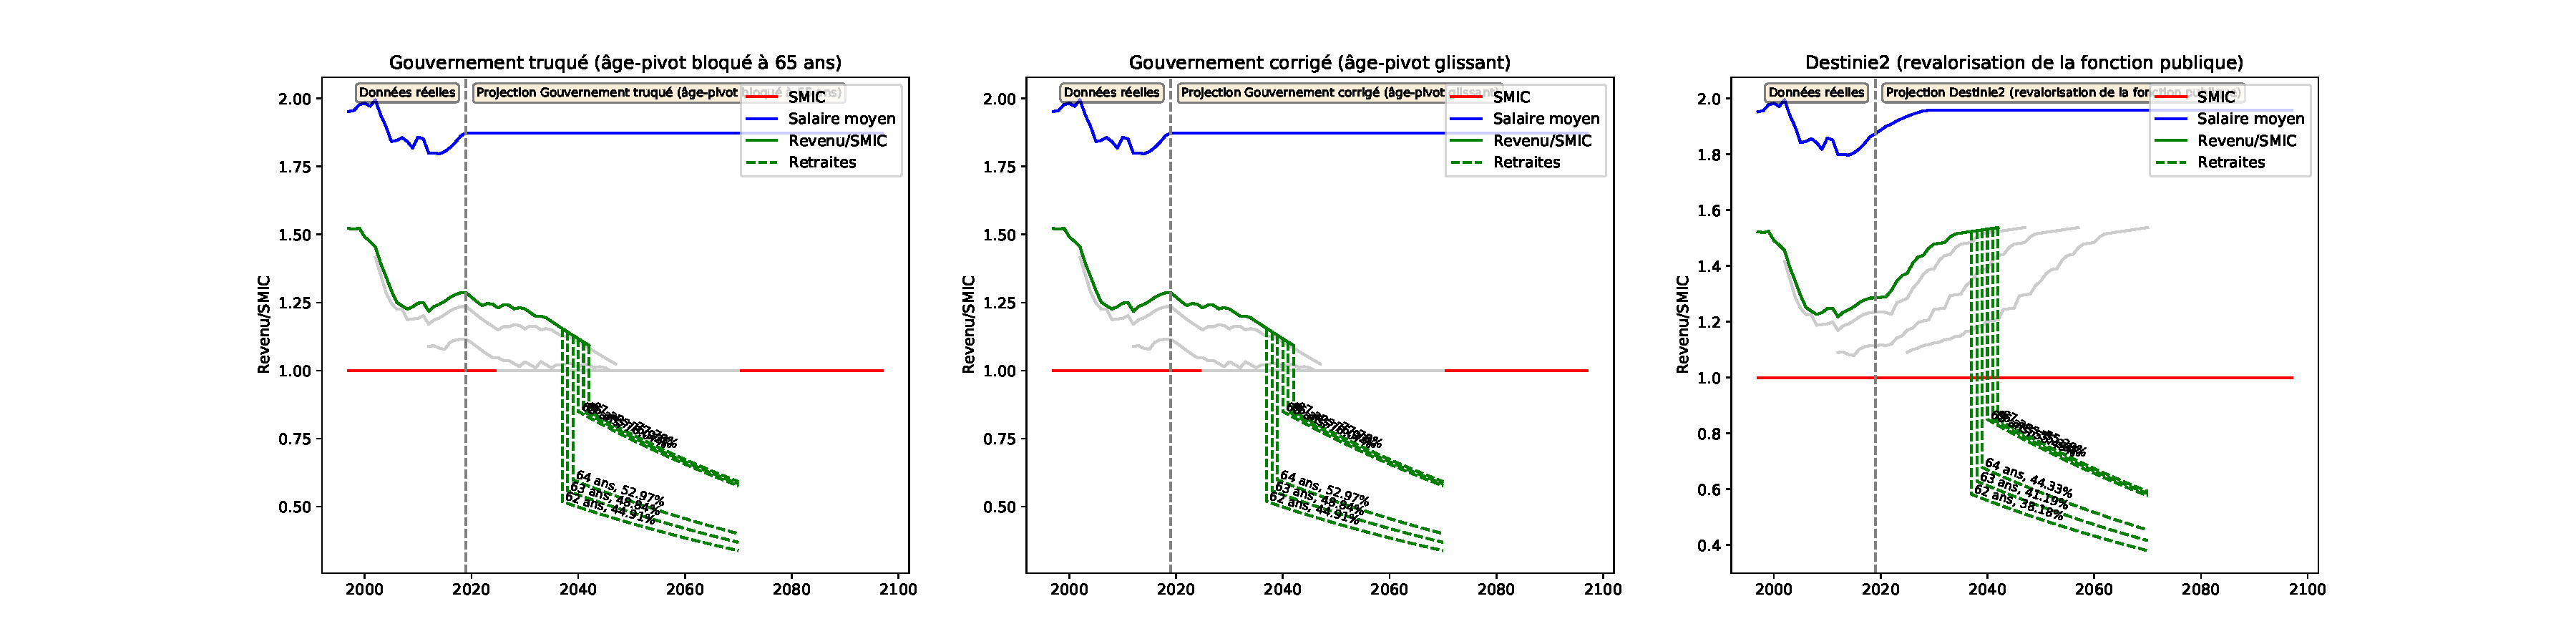
\includegraphics[width=0.9\textwidth]{fig/AideSoignant_1975_22_dest_retraite.pdf}\end{center} \label{fig/AideSoignant_1975_22_dest_retraite.pdf} 

\newpage 
 
\paragraph{Revenus et points pour le modèle \emph{Gouvernement truqué (âge-pivot bloqué à 65 ans)}} 
 
{ \scriptsize \begin{center} 
\begin{tabular}[htb]{|c|c||c|c|c|c|c|c||c|c||c|c|c|} 
\hline 
 Année &  Âge &  Ind Maj &  Pt Ind(\euro{} 2019) &  Rev HP(\euro{} 2019) &  Tx Primes &  GIPA(\euro{} 2019) &  Revenu(\euro{} 2019) &  SMIC(\euro{} 2019) &  Rev/SMIC &  Cumul Pts &  Achat Pt(\euro{} 2019) &  Serv. Pt(\euro{} 2019) \\ 
\hline \hline 
 1997 &  22 &  327.0 &  5.53 &  1809.73 &  14.31 &  0.00 &  2068.71 &  1358.84 &  {\bf 1.52} &  697.18 &  35.61 &  0.50 \\ 
\hline 
 1998 &  23 &  328.0 &  5.57 &  1825.80 &  14.54 &  0.00 &  2091.27 &  1376.36 &  {\bf 1.52} &  1401.96 &  35.61 &  0.50 \\ 
\hline 
 1999 &  24 &  328.0 &  5.61 &  1840.56 &  14.77 &  0.00 &  2112.41 &  1386.54 &  {\bf 1.52} &  2113.87 &  35.61 &  0.50 \\ 
\hline 
 2000 &  25 &  329.0 &  5.55 &  1824.37 &  15.00 &  0.00 &  2098.02 &  1407.00 &  {\bf 1.49} &  2820.93 &  35.61 &  0.50 \\ 
\hline 
 2001 &  26 &  329.0 &  5.52 &  1816.25 &  15.23 &  32.34 &  2125.20 &  1441.04 &  {\bf 1.47} &  3537.15 &  35.61 &  0.50 \\ 
\hline 
 2002 &  27 &  330.0 &  5.49 &  1810.47 &  15.46 &  16.59 &  2106.96 &  1447.74 &  {\bf 1.46} &  4247.22 &  35.61 &  0.50 \\ 
\hline 
 2003 &  28 &  330.0 &  5.37 &  1773.62 &  15.69 &  29.13 &  2081.04 &  1493.03 &  {\bf 1.39} &  4948.55 &  35.61 &  0.50 \\ 
\hline 
 2004 &  29 &  332.0 &  5.29 &  1756.19 &  15.92 &  45.26 &  2081.03 &  1547.32 &  {\bf 1.34} &  5649.89 &  35.61 &  0.50 \\ 
\hline 
 2005 &  30 &  332.0 &  5.29 &  1756.00 &  16.15 &  35.21 &  2074.80 &  1603.67 &  {\bf 1.29} &  6349.12 &  35.61 &  0.50 \\ 
\hline 
 2006 &  31 &  334.0 &  5.23 &  1746.86 &  16.38 &  0.00 &  2033.00 &  1625.00 &  {\bf 1.25} &  7034.26 &  35.61 &  0.50 \\ 
\hline 
 2007 &  32 &  334.0 &  5.19 &  1734.96 &  16.61 &  0.00 &  2023.13 &  1634.08 &  {\bf 1.24} &  7716.08 &  35.61 &  0.50 \\ 
\hline 
 2008 &  33 &  338.0 &  5.09 &  1721.45 &  16.84 &  0.00 &  2011.34 &  1640.24 &  {\bf 1.23} &  8393.93 &  35.61 &  0.50 \\ 
\hline 
 2009 &  34 &  338.0 &  5.13 &  1733.65 &  17.07 &  19.46 &  2049.04 &  1659.42 &  {\bf 1.23} &  9084.48 &  35.61 &  0.50 \\ 
\hline 
 2010 &  35 &  342.0 &  5.08 &  1736.44 &  17.30 &  12.60 &  2049.45 &  1641.90 &  {\bf 1.25} &  9775.17 &  35.61 &  0.50 \\ 
\hline 
 2011 &  36 &  342.0 &  4.97 &  1700.37 &  17.53 &  42.13 &  2040.57 &  1633.19 &  {\bf 1.25} &  10462.87 &  35.61 &  0.50 \\ 
\hline 
 2012 &  37 &  346.0 &  4.88 &  1687.25 &  17.76 &  51.56 &  2038.46 &  1673.05 &  {\bf 1.22} &  11149.85 &  35.61 &  0.50 \\ 
\hline 
 2013 &  38 &  346.0 &  4.83 &  1672.79 &  17.99 &  82.86 &  2056.58 &  1664.01 &  {\bf 1.24} &  11842.95 &  35.61 &  0.50 \\ 
\hline 
 2014 &  39 &  346.0 &  4.81 &  1664.42 &  18.22 &  113.59 &  2081.26 &  1673.24 &  {\bf 1.24} &  12544.36 &  35.61 &  0.50 \\ 
\hline 
 2015 &  40 &  356.0 &  4.81 &  1711.85 &  18.45 &  89.17 &  2116.85 &  1686.62 &  {\bf 1.26} &  13257.76 &  35.61 &  0.50 \\ 
\hline 
 2016 &  41 &  356.0 &  4.80 &  1708.43 &  18.68 &  122.40 &  2149.97 &  1693.76 &  {\bf 1.27} &  13982.33 &  35.61 &  0.50 \\ 
\hline 
 2017 &  42 &  356.0 &  4.81 &  1711.88 &  18.91 &  130.28 &  2165.87 &  1692.60 &  {\bf 1.28} &  14712.26 &  35.61 &  0.50 \\ 
\hline 
 2018 &  43 &  368.0 &  4.74 &  1745.15 &  19.14 &  94.04 &  2173.21 &  1689.76 &  {\bf 1.29} &  15444.65 &  35.61 &  0.50 \\ 
\hline 
 2019 &  44 &  368.0 &  4.79 &  1764.35 &  19.37 &  78.96 &  2185.06 &  1698.45 &  {\bf 1.29} &  16181.05 &  35.61 &  0.50 \\ 
\hline 
 2020 &  45 &  368.0 &  4.79 &  1764.35 &  19.60 &  74.96 &  2185.12 &  1720.53 &  {\bf 1.27} &  16917.46 &  35.61 &  0.50 \\ 
\hline 
 2021 &  46 &  376.0 &  4.79 &  1802.70 &  19.83 &  24.91 &  2185.09 &  1742.90 &  {\bf 1.25} &  17653.86 &  35.61 &  0.50 \\ 
\hline 
 2022 &  47 &  380.0 &  4.79 &  1821.88 &  20.06 &  0.00 &  2187.35 &  1765.55 &  {\bf 1.24} &  18391.02 &  35.61 &  0.50 \\ 
\hline 
 2023 &  48 &  386.7 &  4.79 &  1853.84 &  20.29 &  0.00 &  2229.99 &  1788.51 &  {\bf 1.25} &  19142.56 &  35.61 &  0.50 \\ 
\hline 
 2024 &  49 &  390.0 &  4.79 &  1869.82 &  20.52 &  0.00 &  2253.51 &  1811.76 &  {\bf 1.24} &  19902.02 &  35.61 &  0.50 \\ 
\hline 
 2025 &  50 &  390.0 &  4.79 &  1869.82 &  20.75 &  0.00 &  2257.81 &  1835.31 &  {\bf 1.23} &  20662.93 &  35.61 &  0.50 \\ 
\hline 
 2026 &  51 &  398.0 &  4.79 &  1908.18 &  20.98 &  0.00 &  2308.52 &  1859.17 &  {\bf 1.24} &  21440.93 &  35.61 &  0.50 \\ 
\hline 
 2027 &  52 &  402.0 &  4.79 &  1927.36 &  21.21 &  0.00 &  2336.15 &  1883.34 &  {\bf 1.24} &  22228.24 &  35.61 &  0.50 \\ 
\hline 
 2028 &  53 &  402.0 &  4.79 &  1927.36 &  21.44 &  0.00 &  2340.58 &  1907.82 &  {\bf 1.23} &  23017.04 &  35.61 &  0.50 \\ 
\hline 
 2029 &  54 &  408.0 &  4.79 &  1956.12 &  21.67 &  0.00 &  2380.02 &  1932.62 &  {\bf 1.23} &  23818.53 &  35.63 &  0.50 \\ 
\hline 
 2030 &  55 &  411.0 &  4.79 &  1970.51 &  21.90 &  0.00 &  2402.05 &  1957.75 &  {\bf 1.23} &  24626.21 &  35.69 &  0.50 \\ 
\hline 
 2031 &  56 &  411.0 &  4.79 &  1970.51 &  22.13 &  0.00 &  2406.58 &  1983.20 &  {\bf 1.21} &  25433.56 &  35.77 &  0.50 \\ 
\hline 
 2032 &  57 &  411.0 &  4.79 &  1970.51 &  22.36 &  0.00 &  2411.11 &  2008.98 &  {\bf 1.20} &  26239.99 &  35.88 &  0.50 \\ 
\hline 
 2033 &  58 &  415.7 &  4.79 &  1992.88 &  22.59 &  0.00 &  2443.07 &  2035.10 &  {\bf 1.20} &  27054.00 &  36.02 &  0.50 \\ 
\hline 
 2034 &  59 &  418.0 &  4.79 &  2004.07 &  22.82 &  0.00 &  2461.40 &  2061.55 &  {\bf 1.19} &  27870.39 &  36.18 &  0.50 \\ 
\hline 
 2035 &  60 &  418.0 &  4.79 &  2004.07 &  23.05 &  0.00 &  2466.01 &  2088.35 &  {\bf 1.18} &  28683.97 &  36.37 &  0.51 \\ 
\hline 
 2036 &  61 &  418.0 &  4.79 &  2004.07 &  23.28 &  0.00 &  2470.62 &  2115.50 &  {\bf 1.17} &  29494.14 &  36.59 &  0.51 \\ 
\hline 
 2037 &  62 &  418.0 &  4.79 &  2004.07 &  23.51 &  0.00 &  2475.22 &  2143.00 &  {\bf 1.16} &  30300.28 &  36.85 &  0.51 \\ 
\hline 
 2038 &  63 &  418.0 &  4.79 &  2004.07 &  23.74 &  0.00 &  2479.83 &  2170.86 &  {\bf 1.14} &  31101.81 &  37.13 &  0.52 \\ 
\hline 
 2039 &  64 &  418.0 &  4.79 &  2004.07 &  23.97 &  0.00 &  2484.44 &  2199.08 &  {\bf 1.13} &  31898.15 &  37.44 &  0.52 \\ 
\hline 
 2040 &  65 &  418.0 &  4.79 &  2004.07 &  24.20 &  0.00 &  2489.05 &  2227.67 &  {\bf 1.12} &  32688.72 &  37.78 &  0.53 \\ 
\hline 
 2041 &  66 &  418.0 &  4.79 &  2004.07 &  24.43 &  0.00 &  2493.66 &  2256.63 &  {\bf 1.11} &  33472.97 &  38.16 &  0.53 \\ 
\hline 
 2042 &  67 &  418.0 &  4.79 &  2004.07 &  24.66 &  0.00 &  2498.27 &  2285.97 &  {\bf 1.09} &  34250.36 &  38.56 &  0.54 \\ 
\hline 
\hline 
\end{tabular} 
\end{center} } 
\newpage 
 
\paragraph{Revenus et points pour le modèle \emph{Gouvernement corrigé (âge-pivot glissant)}} 
 
{ \scriptsize \begin{center} 
\begin{tabular}[htb]{|c|c||c|c|c|c|c|c||c|c||c|c|c|} 
\hline 
 Année &  Âge &  Ind Maj &  Pt Ind(\euro{} 2019) &  Rev HP(\euro{} 2019) &  Tx Primes &  GIPA(\euro{} 2019) &  Revenu(\euro{} 2019) &  SMIC(\euro{} 2019) &  Rev/SMIC &  Cumul Pts &  Achat Pt(\euro{} 2019) &  Serv. Pt(\euro{} 2019) \\ 
\hline \hline 
 1997 &  22 &  327.0 &  5.53 &  1809.73 &  14.31 &  0.00 &  2068.71 &  1358.84 &  {\bf 1.52} &  697.18 &  35.61 &  0.50 \\ 
\hline 
 1998 &  23 &  328.0 &  5.57 &  1825.80 &  14.54 &  0.00 &  2091.27 &  1376.36 &  {\bf 1.52} &  1401.96 &  35.61 &  0.50 \\ 
\hline 
 1999 &  24 &  328.0 &  5.61 &  1840.56 &  14.77 &  0.00 &  2112.41 &  1386.54 &  {\bf 1.52} &  2113.87 &  35.61 &  0.50 \\ 
\hline 
 2000 &  25 &  329.0 &  5.55 &  1824.37 &  15.00 &  0.00 &  2098.02 &  1407.00 &  {\bf 1.49} &  2820.93 &  35.61 &  0.50 \\ 
\hline 
 2001 &  26 &  329.0 &  5.52 &  1816.25 &  15.23 &  32.34 &  2125.20 &  1441.04 &  {\bf 1.47} &  3537.15 &  35.61 &  0.50 \\ 
\hline 
 2002 &  27 &  330.0 &  5.49 &  1810.47 &  15.46 &  16.59 &  2106.96 &  1447.74 &  {\bf 1.46} &  4247.22 &  35.61 &  0.50 \\ 
\hline 
 2003 &  28 &  330.0 &  5.37 &  1773.62 &  15.69 &  29.13 &  2081.04 &  1493.03 &  {\bf 1.39} &  4948.55 &  35.61 &  0.50 \\ 
\hline 
 2004 &  29 &  332.0 &  5.29 &  1756.19 &  15.92 &  45.26 &  2081.03 &  1547.32 &  {\bf 1.34} &  5649.89 &  35.61 &  0.50 \\ 
\hline 
 2005 &  30 &  332.0 &  5.29 &  1756.00 &  16.15 &  35.21 &  2074.80 &  1603.67 &  {\bf 1.29} &  6349.12 &  35.61 &  0.50 \\ 
\hline 
 2006 &  31 &  334.0 &  5.23 &  1746.86 &  16.38 &  0.00 &  2033.00 &  1625.00 &  {\bf 1.25} &  7034.26 &  35.61 &  0.50 \\ 
\hline 
 2007 &  32 &  334.0 &  5.19 &  1734.96 &  16.61 &  0.00 &  2023.13 &  1634.08 &  {\bf 1.24} &  7716.08 &  35.61 &  0.50 \\ 
\hline 
 2008 &  33 &  338.0 &  5.09 &  1721.45 &  16.84 &  0.00 &  2011.34 &  1640.24 &  {\bf 1.23} &  8393.93 &  35.61 &  0.50 \\ 
\hline 
 2009 &  34 &  338.0 &  5.13 &  1733.65 &  17.07 &  19.46 &  2049.04 &  1659.42 &  {\bf 1.23} &  9084.48 &  35.61 &  0.50 \\ 
\hline 
 2010 &  35 &  342.0 &  5.08 &  1736.44 &  17.30 &  12.60 &  2049.45 &  1641.90 &  {\bf 1.25} &  9775.17 &  35.61 &  0.50 \\ 
\hline 
 2011 &  36 &  342.0 &  4.97 &  1700.37 &  17.53 &  42.13 &  2040.57 &  1633.19 &  {\bf 1.25} &  10462.87 &  35.61 &  0.50 \\ 
\hline 
 2012 &  37 &  346.0 &  4.88 &  1687.25 &  17.76 &  51.56 &  2038.46 &  1673.05 &  {\bf 1.22} &  11149.85 &  35.61 &  0.50 \\ 
\hline 
 2013 &  38 &  346.0 &  4.83 &  1672.79 &  17.99 &  82.86 &  2056.58 &  1664.01 &  {\bf 1.24} &  11842.95 &  35.61 &  0.50 \\ 
\hline 
 2014 &  39 &  346.0 &  4.81 &  1664.42 &  18.22 &  113.59 &  2081.26 &  1673.24 &  {\bf 1.24} &  12544.36 &  35.61 &  0.50 \\ 
\hline 
 2015 &  40 &  356.0 &  4.81 &  1711.85 &  18.45 &  89.17 &  2116.85 &  1686.62 &  {\bf 1.26} &  13257.76 &  35.61 &  0.50 \\ 
\hline 
 2016 &  41 &  356.0 &  4.80 &  1708.43 &  18.68 &  122.40 &  2149.97 &  1693.76 &  {\bf 1.27} &  13982.33 &  35.61 &  0.50 \\ 
\hline 
 2017 &  42 &  356.0 &  4.81 &  1711.88 &  18.91 &  130.28 &  2165.87 &  1692.60 &  {\bf 1.28} &  14712.26 &  35.61 &  0.50 \\ 
\hline 
 2018 &  43 &  368.0 &  4.74 &  1745.15 &  19.14 &  94.04 &  2173.21 &  1689.76 &  {\bf 1.29} &  15444.65 &  35.61 &  0.50 \\ 
\hline 
 2019 &  44 &  368.0 &  4.79 &  1764.35 &  19.37 &  78.96 &  2185.06 &  1698.45 &  {\bf 1.29} &  16181.05 &  35.61 &  0.50 \\ 
\hline 
 2020 &  45 &  368.0 &  4.79 &  1764.35 &  19.60 &  74.96 &  2185.12 &  1720.53 &  {\bf 1.27} &  16917.46 &  35.61 &  0.50 \\ 
\hline 
 2021 &  46 &  376.0 &  4.79 &  1802.70 &  19.83 &  24.91 &  2185.09 &  1742.90 &  {\bf 1.25} &  17653.86 &  35.61 &  0.50 \\ 
\hline 
 2022 &  47 &  380.0 &  4.79 &  1821.88 &  20.06 &  0.00 &  2187.35 &  1765.55 &  {\bf 1.24} &  18391.02 &  35.61 &  0.50 \\ 
\hline 
 2023 &  48 &  386.7 &  4.79 &  1853.84 &  20.29 &  0.00 &  2229.99 &  1788.51 &  {\bf 1.25} &  19142.56 &  35.61 &  0.50 \\ 
\hline 
 2024 &  49 &  390.0 &  4.79 &  1869.82 &  20.52 &  0.00 &  2253.51 &  1811.76 &  {\bf 1.24} &  19902.02 &  35.61 &  0.50 \\ 
\hline 
 2025 &  50 &  390.0 &  4.79 &  1869.82 &  20.75 &  0.00 &  2257.81 &  1835.31 &  {\bf 1.23} &  20662.93 &  35.61 &  0.50 \\ 
\hline 
 2026 &  51 &  398.0 &  4.79 &  1908.18 &  20.98 &  0.00 &  2308.52 &  1859.17 &  {\bf 1.24} &  21440.93 &  35.61 &  0.50 \\ 
\hline 
 2027 &  52 &  402.0 &  4.79 &  1927.36 &  21.21 &  0.00 &  2336.15 &  1883.34 &  {\bf 1.24} &  22228.24 &  35.61 &  0.50 \\ 
\hline 
 2028 &  53 &  402.0 &  4.79 &  1927.36 &  21.44 &  0.00 &  2340.58 &  1907.82 &  {\bf 1.23} &  23017.04 &  35.61 &  0.50 \\ 
\hline 
 2029 &  54 &  408.0 &  4.79 &  1956.12 &  21.67 &  0.00 &  2380.02 &  1932.62 &  {\bf 1.23} &  23818.53 &  35.63 &  0.50 \\ 
\hline 
 2030 &  55 &  411.0 &  4.79 &  1970.51 &  21.90 &  0.00 &  2402.05 &  1957.75 &  {\bf 1.23} &  24626.21 &  35.69 &  0.50 \\ 
\hline 
 2031 &  56 &  411.0 &  4.79 &  1970.51 &  22.13 &  0.00 &  2406.58 &  1983.20 &  {\bf 1.21} &  25433.56 &  35.77 &  0.50 \\ 
\hline 
 2032 &  57 &  411.0 &  4.79 &  1970.51 &  22.36 &  0.00 &  2411.11 &  2008.98 &  {\bf 1.20} &  26239.99 &  35.88 &  0.50 \\ 
\hline 
 2033 &  58 &  415.7 &  4.79 &  1992.88 &  22.59 &  0.00 &  2443.07 &  2035.10 &  {\bf 1.20} &  27054.00 &  36.02 &  0.50 \\ 
\hline 
 2034 &  59 &  418.0 &  4.79 &  2004.07 &  22.82 &  0.00 &  2461.40 &  2061.55 &  {\bf 1.19} &  27870.39 &  36.18 &  0.50 \\ 
\hline 
 2035 &  60 &  418.0 &  4.79 &  2004.07 &  23.05 &  0.00 &  2466.01 &  2088.35 &  {\bf 1.18} &  28683.97 &  36.37 &  0.51 \\ 
\hline 
 2036 &  61 &  418.0 &  4.79 &  2004.07 &  23.28 &  0.00 &  2470.62 &  2115.50 &  {\bf 1.17} &  29494.14 &  36.59 &  0.51 \\ 
\hline 
 2037 &  62 &  418.0 &  4.79 &  2004.07 &  23.51 &  0.00 &  2475.22 &  2143.00 &  {\bf 1.16} &  30300.28 &  36.85 &  0.51 \\ 
\hline 
 2038 &  63 &  418.0 &  4.79 &  2004.07 &  23.74 &  0.00 &  2479.83 &  2170.86 &  {\bf 1.14} &  31101.81 &  37.13 &  0.52 \\ 
\hline 
 2039 &  64 &  418.0 &  4.79 &  2004.07 &  23.97 &  0.00 &  2484.44 &  2199.08 &  {\bf 1.13} &  31898.15 &  37.44 &  0.52 \\ 
\hline 
 2040 &  65 &  418.0 &  4.79 &  2004.07 &  24.20 &  0.00 &  2489.05 &  2227.67 &  {\bf 1.12} &  32688.72 &  37.78 &  0.53 \\ 
\hline 
 2041 &  66 &  418.0 &  4.79 &  2004.07 &  24.43 &  0.00 &  2493.66 &  2256.63 &  {\bf 1.11} &  33472.97 &  38.16 &  0.53 \\ 
\hline 
 2042 &  67 &  418.0 &  4.79 &  2004.07 &  24.66 &  0.00 &  2498.27 &  2285.97 &  {\bf 1.09} &  34250.36 &  38.56 &  0.54 \\ 
\hline 
\hline 
\end{tabular} 
\end{center} } 
\newpage 
 
\paragraph{Revenus et points pour le modèle \emph{Destinie2 (revalorisation de la fonction publique)}} 
 
{ \scriptsize \begin{center} 
\begin{tabular}[htb]{|c|c||c|c|c|c|c|c||c|c||c|c|c|} 
\hline 
 Année &  Âge &  Ind Maj &  Pt Ind(\euro{} 2019) &  Rev HP(\euro{} 2019) &  Tx Primes &  GIPA(\euro{} 2019) &  Revenu(\euro{} 2019) &  SMIC(\euro{} 2019) &  Rev/SMIC &  Cumul Pts &  Achat Pt(\euro{} 2019) &  Serv. Pt(\euro{} 2019) \\ 
\hline \hline 
 1997 &  22 &  327.0 &  5.53 &  1809.73 &  14.31 &  0.00 &  2068.71 &  1358.84 &  {\bf 1.52} &  695.47 &  35.69 &  0.50 \\ 
\hline 
 1998 &  23 &  328.0 &  5.57 &  1825.80 &  14.54 &  0.00 &  2091.27 &  1376.36 &  {\bf 1.52} &  1398.52 &  35.69 &  0.50 \\ 
\hline 
 1999 &  24 &  328.0 &  5.61 &  1840.56 &  14.77 &  0.00 &  2112.41 &  1386.54 &  {\bf 1.52} &  2108.67 &  35.69 &  0.50 \\ 
\hline 
 2000 &  25 &  329.0 &  5.55 &  1824.37 &  15.00 &  0.00 &  2098.02 &  1407.00 &  {\bf 1.49} &  2814.00 &  35.69 &  0.50 \\ 
\hline 
 2001 &  26 &  329.0 &  5.52 &  1816.25 &  15.23 &  32.34 &  2125.20 &  1441.04 &  {\bf 1.47} &  3528.45 &  35.69 &  0.50 \\ 
\hline 
 2002 &  27 &  330.0 &  5.49 &  1810.47 &  15.46 &  16.59 &  2106.96 &  1447.74 &  {\bf 1.46} &  4236.78 &  35.69 &  0.50 \\ 
\hline 
 2003 &  28 &  330.0 &  5.37 &  1773.62 &  15.69 &  29.13 &  2081.04 &  1493.03 &  {\bf 1.39} &  4936.39 &  35.69 &  0.50 \\ 
\hline 
 2004 &  29 &  332.0 &  5.29 &  1756.19 &  15.92 &  45.26 &  2081.03 &  1547.32 &  {\bf 1.34} &  5636.00 &  35.69 &  0.50 \\ 
\hline 
 2005 &  30 &  332.0 &  5.29 &  1756.00 &  16.15 &  35.21 &  2074.80 &  1603.67 &  {\bf 1.29} &  6333.52 &  35.69 &  0.50 \\ 
\hline 
 2006 &  31 &  334.0 &  5.23 &  1746.86 &  16.38 &  0.00 &  2033.00 &  1625.00 &  {\bf 1.25} &  7016.98 &  35.69 &  0.50 \\ 
\hline 
 2007 &  32 &  334.0 &  5.19 &  1734.96 &  16.61 &  0.00 &  2023.13 &  1634.08 &  {\bf 1.24} &  7697.13 &  35.69 &  0.50 \\ 
\hline 
 2008 &  33 &  338.0 &  5.09 &  1721.45 &  16.84 &  0.00 &  2011.34 &  1640.24 &  {\bf 1.23} &  8373.31 &  35.69 &  0.50 \\ 
\hline 
 2009 &  34 &  338.0 &  5.13 &  1733.65 &  17.07 &  15.68 &  2045.26 &  1659.42 &  {\bf 1.23} &  9060.89 &  35.69 &  0.50 \\ 
\hline 
 2010 &  35 &  342.0 &  5.08 &  1736.44 &  17.30 &  10.39 &  2047.24 &  1641.90 &  {\bf 1.25} &  9749.14 &  35.69 &  0.50 \\ 
\hline 
 2011 &  36 &  342.0 &  4.97 &  1700.37 &  17.53 &  40.64 &  2039.08 &  1633.19 &  {\bf 1.25} &  10434.65 &  35.69 &  0.50 \\ 
\hline 
 2012 &  37 &  346.0 &  4.88 &  1687.25 &  17.76 &  49.70 &  2036.60 &  1673.05 &  {\bf 1.22} &  11119.32 &  35.69 &  0.50 \\ 
\hline 
 2013 &  38 &  346.0 &  4.83 &  1672.79 &  17.99 &  80.51 &  2054.23 &  1664.01 &  {\bf 1.23} &  11809.92 &  35.69 &  0.50 \\ 
\hline 
 2014 &  39 &  346.0 &  4.81 &  1664.42 &  18.22 &  111.58 &  2079.25 &  1673.24 &  {\bf 1.24} &  12508.93 &  35.69 &  0.50 \\ 
\hline 
 2015 &  40 &  356.0 &  4.81 &  1711.85 &  18.45 &  87.18 &  2114.87 &  1686.62 &  {\bf 1.25} &  13219.91 &  35.69 &  0.50 \\ 
\hline 
 2016 &  41 &  356.0 &  4.80 &  1708.43 &  18.68 &  120.28 &  2147.84 &  1693.76 &  {\bf 1.27} &  13941.98 &  35.69 &  0.50 \\ 
\hline 
 2017 &  42 &  356.0 &  4.81 &  1711.88 &  18.91 &  128.09 &  2163.69 &  1692.60 &  {\bf 1.28} &  14669.38 &  35.69 &  0.50 \\ 
\hline 
 2018 &  43 &  368.0 &  4.74 &  1745.15 &  19.14 &  91.92 &  2171.09 &  1689.76 &  {\bf 1.28} &  15399.27 &  35.69 &  0.50 \\ 
\hline 
 2019 &  44 &  368.0 &  4.79 &  1764.35 &  19.37 &  76.82 &  2182.93 &  1698.45 &  {\bf 1.29} &  16133.13 &  35.69 &  0.50 \\ 
\hline 
 2020 &  45 &  368.0 &  4.83 &  1778.46 &  19.60 &  61.29 &  2188.33 &  1699.99 &  {\bf 1.29} &  16868.82 &  35.69 &  0.50 \\ 
\hline 
 2021 &  46 &  376.0 &  4.88 &  1833.48 &  19.83 &  0.00 &  2197.06 &  1703.48 &  {\bf 1.29} &  17607.43 &  35.69 &  0.50 \\ 
\hline 
 2022 &  47 &  380.0 &  4.93 &  1871.51 &  20.06 &  0.00 &  2246.94 &  1712.78 &  {\bf 1.31} &  18362.82 &  35.69 &  0.50 \\ 
\hline 
 2023 &  48 &  386.7 &  4.98 &  1926.63 &  20.29 &  0.00 &  2317.54 &  1723.51 &  {\bf 1.34} &  19141.94 &  35.69 &  0.50 \\ 
\hline 
 2024 &  49 &  390.0 &  5.04 &  1966.36 &  20.52 &  0.00 &  2369.86 &  1735.69 &  {\bf 1.37} &  19938.65 &  35.69 &  0.50 \\ 
\hline 
 2025 &  50 &  390.0 &  5.10 &  1990.35 &  20.75 &  0.00 &  2403.35 &  1749.35 &  {\bf 1.37} &  20746.61 &  35.69 &  0.50 \\ 
\hline 
 2026 &  51 &  398.0 &  5.17 &  2056.57 &  20.98 &  0.00 &  2488.04 &  1764.53 &  {\bf 1.41} &  21583.05 &  35.69 &  0.50 \\ 
\hline 
 2027 &  52 &  402.0 &  5.23 &  2103.83 &  21.21 &  0.00 &  2550.05 &  1781.27 &  {\bf 1.43} &  22440.34 &  35.69 &  0.50 \\ 
\hline 
 2028 &  53 &  402.0 &  5.30 &  2131.39 &  21.44 &  0.00 &  2588.36 &  1799.59 &  {\bf 1.44} &  23310.50 &  35.69 &  0.50 \\ 
\hline 
 2029 &  54 &  408.0 &  5.37 &  2189.37 &  21.67 &  0.00 &  2663.81 &  1819.55 &  {\bf 1.46} &  24205.40 &  35.72 &  0.50 \\ 
\hline 
 2030 &  55 &  411.0 &  5.43 &  2232.82 &  21.90 &  0.00 &  2721.81 &  1841.19 &  {\bf 1.48} &  25118.45 &  35.77 &  0.50 \\ 
\hline 
 2031 &  56 &  411.0 &  5.50 &  2261.18 &  22.13 &  0.00 &  2761.57 &  1864.58 &  {\bf 1.48} &  26042.79 &  35.85 &  0.50 \\ 
\hline 
 2032 &  57 &  411.0 &  5.57 &  2290.57 &  22.36 &  0.00 &  2802.74 &  1888.81 &  {\bf 1.48} &  26978.06 &  35.96 &  0.50 \\ 
\hline 
 2033 &  58 &  415.7 &  5.65 &  2346.69 &  22.59 &  0.00 &  2876.81 &  1913.37 &  {\bf 1.50} &  27934.40 &  36.10 &  0.50 \\ 
\hline 
 2034 &  59 &  418.0 &  5.72 &  2390.55 &  22.82 &  0.00 &  2936.07 &  1938.24 &  {\bf 1.51} &  28906.01 &  36.26 &  0.50 \\ 
\hline 
 2035 &  60 &  418.0 &  5.79 &  2421.62 &  23.05 &  0.00 &  2979.81 &  1963.44 &  {\bf 1.52} &  29886.86 &  36.46 &  0.51 \\ 
\hline 
 2036 &  61 &  418.0 &  5.87 &  2453.10 &  23.28 &  0.00 &  3024.19 &  1988.96 &  {\bf 1.52} &  30876.28 &  36.68 &  0.51 \\ 
\hline 
 2037 &  62 &  418.0 &  5.94 &  2484.99 &  23.51 &  0.00 &  3069.22 &  2014.82 &  {\bf 1.52} &  31873.60 &  36.93 &  0.51 \\ 
\hline 
 2038 &  63 &  418.0 &  6.02 &  2517.30 &  23.74 &  0.00 &  3114.91 &  2041.01 &  {\bf 1.53} &  32878.09 &  37.21 &  0.52 \\ 
\hline 
 2039 &  64 &  418.0 &  6.10 &  2550.02 &  23.97 &  0.00 &  3161.26 &  2067.55 &  {\bf 1.53} &  33889.06 &  37.52 &  0.52 \\ 
\hline 
 2040 &  65 &  418.0 &  6.18 &  2583.17 &  24.20 &  0.00 &  3208.30 &  2094.43 &  {\bf 1.53} &  34905.75 &  37.87 &  0.53 \\ 
\hline 
 2041 &  66 &  418.0 &  6.26 &  2616.76 &  24.43 &  0.00 &  3256.03 &  2121.65 &  {\bf 1.53} &  35927.43 &  38.24 &  0.53 \\ 
\hline 
 2042 &  67 &  418.0 &  6.34 &  2650.77 &  24.66 &  0.00 &  3304.45 &  2149.23 &  {\bf 1.54} &  36953.33 &  38.65 &  0.54 \\ 
\hline 
\hline 
\end{tabular} 
\end{center} } 
\newpage 
 
\subsection{Génération 1980 (début en 2002)} 

\paragraph{Retraites possibles dans le modèle \emph{Gouvernement truqué (âge-pivot bloqué à 65 ans)}}  
 
{ \scriptsize \begin{center} 
\begin{tabular}[htb]{|c|c||c|c||c|c||c||c|c|c|c|c|c|} 
\hline 
 Retraite en &  Âge &  Âge pivot &  Décote/Surcote &  Retraite (\euro{} 2019) &  Tx Rempl(\%) &  SMIC (\euro{} 2019) &  Retraite/SMIC &  Rev70/SMIC &  Rev75/SMIC &  Rev80/SMIC &  Rev85/SMIC &  Rev90/SMIC \\ 
\hline \hline 
 2042 &  62 &  65 ans 0 mois &  -15.00\% &  1124.91 &  {\bf 45.45} &  2285.97 &  {\bf {\color{red} 0.49}} &  {\bf {\color{red} 0.44}} &  {\bf {\color{red} 0.42}} &  {\bf {\color{red} 0.39}} &  {\bf {\color{red} 0.37}} &  {\bf {\color{red} 0.34}} \\ 
\hline 
 2043 &  63 &  65 ans 0 mois &  -10.00\% &  1235.80 &  {\bf 49.83} &  2315.68 &  {\bf {\color{red} 0.53}} &  {\bf {\color{red} 0.49}} &  {\bf {\color{red} 0.46}} &  {\bf {\color{red} 0.43}} &  {\bf {\color{red} 0.40}} &  {\bf {\color{red} 0.38}} \\ 
\hline 
 2044 &  64 &  65 ans 0 mois &  -5.00\% &  1353.27 &  {\bf 54.47} &  2345.79 &  {\bf {\color{red} 0.58}} &  {\bf {\color{red} 0.53}} &  {\bf {\color{red} 0.50}} &  {\bf {\color{red} 0.47}} &  {\bf {\color{red} 0.44}} &  {\bf {\color{red} 0.41}} \\ 
\hline 
 2045 &  65 &  65 ans 0 mois &  0.00\% &  2019.84 &  {\bf 81.15} &  2376.28 &  {\bf {\color{red} 0.85}} &  {\bf {\color{red} 0.80}} &  {\bf {\color{red} 0.75}} &  {\bf {\color{red} 0.70}} &  {\bf {\color{red} 0.66}} &  {\bf {\color{red} 0.62}} \\ 
\hline 
 2046 &  66 &  65 ans 0 mois &  5.00\% &  2046.10 &  {\bf 82.05} &  2407.18 &  {\bf {\color{red} 0.85}} &  {\bf {\color{red} 0.81}} &  {\bf {\color{red} 0.76}} &  {\bf {\color{red} 0.71}} &  {\bf {\color{red} 0.67}} &  {\bf {\color{red} 0.62}} \\ 
\hline 
 2047 &  67 &  65 ans 0 mois &  10.00\% &  2072.70 &  {\bf 82.97} &  2438.47 &  {\bf {\color{red} 0.85}} &  {\bf {\color{red} 0.82}} &  {\bf {\color{red} 0.77}} &  {\bf {\color{red} 0.72}} &  {\bf {\color{red} 0.67}} &  {\bf {\color{red} 0.63}} \\ 
\hline 
\hline 
\end{tabular} 
\end{center} } 
\paragraph{Retraites possibles dans le modèle \emph{Gouvernement corrigé (âge-pivot glissant)}}  
 
{ \scriptsize \begin{center} 
\begin{tabular}[htb]{|c|c||c|c||c|c||c||c|c|c|c|c|c|} 
\hline 
 Retraite en &  Âge &  Âge pivot &  Décote/Surcote &  Retraite (\euro{} 2019) &  Tx Rempl(\%) &  SMIC (\euro{} 2019) &  Retraite/SMIC &  Rev70/SMIC &  Rev75/SMIC &  Rev80/SMIC &  Rev85/SMIC &  Rev90/SMIC \\ 
\hline \hline 
 2042 &  62 &  65 ans 3 mois &  -16.25\% &  1108.37 &  {\bf 44.78} &  2285.97 &  {\bf {\color{red} 0.48}} &  {\bf {\color{red} 0.44}} &  {\bf {\color{red} 0.41}} &  {\bf {\color{red} 0.38}} &  {\bf {\color{red} 0.36}} &  {\bf {\color{red} 0.34}} \\ 
\hline 
 2043 &  63 &  65 ans 4 mois &  -11.67\% &  1212.92 &  {\bf 48.91} &  2315.68 &  {\bf {\color{red} 0.52}} &  {\bf {\color{red} 0.48}} &  {\bf {\color{red} 0.45}} &  {\bf {\color{red} 0.42}} &  {\bf {\color{red} 0.39}} &  {\bf {\color{red} 0.37}} \\ 
\hline 
 2044 &  64 &  65 ans 5 mois &  -7.08\% &  1323.59 &  {\bf 53.28} &  2345.79 &  {\bf {\color{red} 0.56}} &  {\bf {\color{red} 0.52}} &  {\bf {\color{red} 0.49}} &  {\bf {\color{red} 0.46}} &  {\bf {\color{red} 0.43}} &  {\bf {\color{red} 0.40}} \\ 
\hline 
 2045 &  65 &  65 ans 6 mois &  -2.50\% &  2019.84 &  {\bf 81.15} &  2376.28 &  {\bf {\color{red} 0.85}} &  {\bf {\color{red} 0.80}} &  {\bf {\color{red} 0.75}} &  {\bf {\color{red} 0.70}} &  {\bf {\color{red} 0.66}} &  {\bf {\color{red} 0.62}} \\ 
\hline 
 2046 &  66 &  65 ans 7 mois &  2.08\% &  2046.10 &  {\bf 82.05} &  2407.18 &  {\bf {\color{red} 0.85}} &  {\bf {\color{red} 0.81}} &  {\bf {\color{red} 0.76}} &  {\bf {\color{red} 0.71}} &  {\bf {\color{red} 0.67}} &  {\bf {\color{red} 0.62}} \\ 
\hline 
 2047 &  67 &  65 ans 8 mois &  6.67\% &  2072.70 &  {\bf 82.97} &  2438.47 &  {\bf {\color{red} 0.85}} &  {\bf {\color{red} 0.82}} &  {\bf {\color{red} 0.77}} &  {\bf {\color{red} 0.72}} &  {\bf {\color{red} 0.67}} &  {\bf {\color{red} 0.63}} \\ 
\hline 
\hline 
\end{tabular} 
\end{center} } 
\paragraph{Retraites possibles dans le modèle \emph{Destinie2 (revalorisation de la fonction publique)}}  
 
{ \scriptsize \begin{center} 
\begin{tabular}[htb]{|c|c||c|c||c|c||c||c|c|c|c|c|c|} 
\hline 
 Retraite en &  Âge &  Âge pivot &  Décote/Surcote &  Retraite (\euro{} 2019) &  Tx Rempl(\%) &  SMIC (\euro{} 2019) &  Retraite/SMIC &  Rev70/SMIC &  Rev75/SMIC &  Rev80/SMIC &  Rev85/SMIC &  Rev90/SMIC \\ 
\hline \hline 
 2042 &  62 &  65 ans 3 mois &  -16.25\% &  1209.01 &  {\bf 36.93} &  2149.23 &  {\bf {\color{red} 0.56}} &  {\bf {\color{red} 0.51}} &  {\bf {\color{red} 0.48}} &  {\bf {\color{red} 0.45}} &  {\bf {\color{red} 0.42}} &  {\bf {\color{red} 0.39}} \\ 
\hline 
 2043 &  63 &  65 ans 4 mois &  -11.67\% &  1330.64 &  {\bf 40.05} &  2177.17 &  {\bf {\color{red} 0.61}} &  {\bf {\color{red} 0.56}} &  {\bf {\color{red} 0.52}} &  {\bf {\color{red} 0.49}} &  {\bf {\color{red} 0.46}} &  {\bf {\color{red} 0.43}} \\ 
\hline 
 2044 &  64 &  65 ans 5 mois &  -7.08\% &  1460.42 &  {\bf 43.31} &  2205.48 &  {\bf {\color{red} 0.66}} &  {\bf {\color{red} 0.61}} &  {\bf {\color{red} 0.57}} &  {\bf {\color{red} 0.54}} &  {\bf {\color{red} 0.50}} &  {\bf {\color{red} 0.47}} \\ 
\hline 
 2045 &  65 &  65 ans 6 mois &  -2.50\% &  1899.03 &  {\bf 55.49} &  2234.15 &  {\bf {\color{red} 0.85}} &  {\bf {\color{red} 0.80}} &  {\bf {\color{red} 0.75}} &  {\bf {\color{red} 0.70}} &  {\bf {\color{red} 0.66}} &  {\bf {\color{red} 0.62}} \\ 
\hline 
 2046 &  66 &  65 ans 7 mois &  2.08\% &  1923.71 &  {\bf 55.39} &  2263.19 &  {\bf {\color{red} 0.85}} &  {\bf {\color{red} 0.81}} &  {\bf {\color{red} 0.76}} &  {\bf {\color{red} 0.71}} &  {\bf {\color{red} 0.67}} &  {\bf {\color{red} 0.62}} \\ 
\hline 
 2047 &  67 &  65 ans 8 mois &  6.67\% &  1948.72 &  {\bf 55.28} &  2292.61 &  {\bf {\color{red} 0.85}} &  {\bf {\color{red} 0.82}} &  {\bf {\color{red} 0.77}} &  {\bf {\color{red} 0.72}} &  {\bf {\color{red} 0.67}} &  {\bf {\color{red} 0.63}} \\ 
\hline 
\hline 
\end{tabular} 
\end{center} } 

 \begin{center}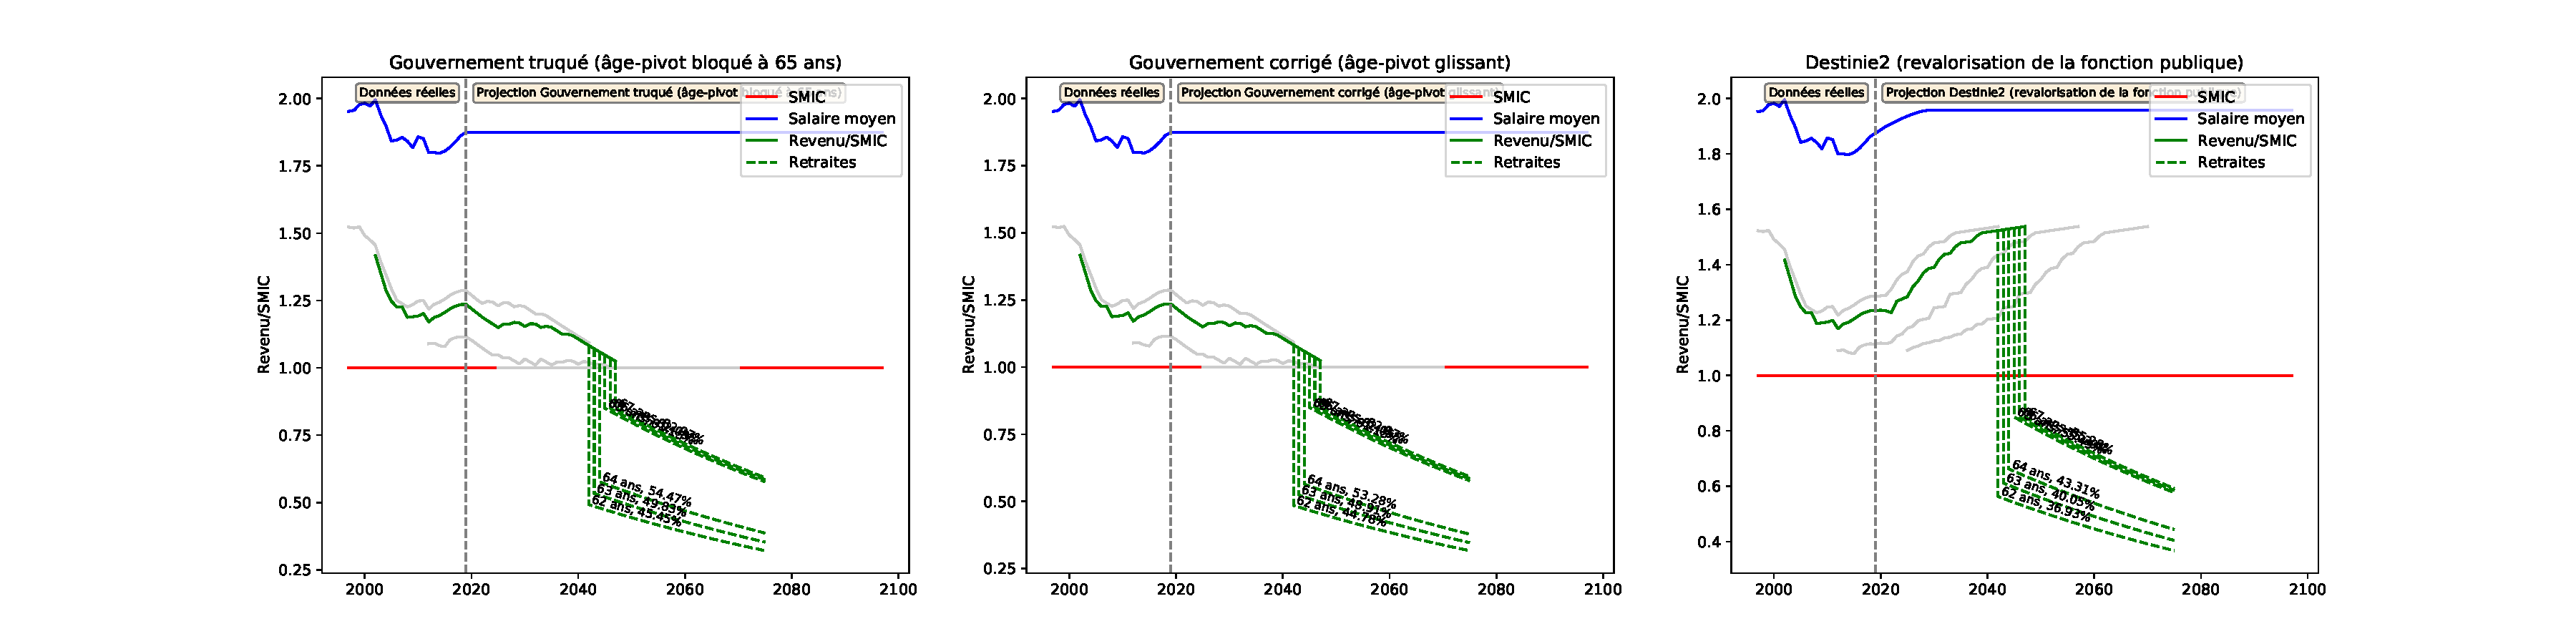
\includegraphics[width=0.9\textwidth]{fig/AideSoignant_1980_22_dest_retraite.pdf}\end{center} \label{fig/AideSoignant_1980_22_dest_retraite.pdf} 

\newpage 
 
\paragraph{Revenus et points pour le modèle \emph{Gouvernement truqué (âge-pivot bloqué à 65 ans)}} 
 
{ \scriptsize \begin{center} 
\begin{tabular}[htb]{|c|c||c|c|c|c|c|c||c|c||c|c|c|} 
\hline 
 Année &  Âge &  Ind Maj &  Pt Ind(\euro{} 2019) &  Rev HP(\euro{} 2019) &  Tx Primes &  GIPA(\euro{} 2019) &  Revenu(\euro{} 2019) &  SMIC(\euro{} 2019) &  Rev/SMIC &  Cumul Pts &  Achat Pt(\euro{} 2019) &  Serv. Pt(\euro{} 2019) \\ 
\hline \hline 
 2002 &  22 &  327.0 &  5.49 &  1794.01 &  14.31 &  0.00 &  2050.73 &  1447.74 &  {\bf 1.42} &  691.12 &  35.61 &  0.50 \\ 
\hline 
 2003 &  23 &  328.0 &  5.37 &  1762.88 &  14.54 &  0.00 &  2019.20 &  1493.03 &  {\bf 1.35} &  1371.62 &  35.61 &  0.50 \\ 
\hline 
 2004 &  24 &  328.0 &  5.29 &  1735.03 &  14.77 &  0.00 &  1991.29 &  1547.32 &  {\bf 1.29} &  2042.71 &  35.61 &  0.50 \\ 
\hline 
 2005 &  25 &  329.0 &  5.29 &  1740.13 &  15.00 &  0.00 &  2001.15 &  1603.67 &  {\bf 1.25} &  2717.12 &  35.61 &  0.50 \\ 
\hline 
 2006 &  26 &  329.0 &  5.23 &  1720.71 &  15.23 &  8.81 &  1991.59 &  1625.00 &  {\bf 1.23} &  3388.31 &  35.61 &  0.50 \\ 
\hline 
 2007 &  27 &  330.0 &  5.19 &  1714.18 &  15.46 &  25.08 &  2004.27 &  1634.08 &  {\bf 1.23} &  4063.77 &  35.61 &  0.50 \\ 
\hline 
 2008 &  28 &  330.0 &  5.09 &  1680.70 &  15.69 &  3.36 &  1947.76 &  1640.24 &  {\bf 1.19} &  4720.19 &  35.61 &  0.50 \\ 
\hline 
 2009 &  29 &  332.0 &  5.13 &  1702.87 &  15.92 &  0.00 &  1973.97 &  1659.42 &  {\bf 1.19} &  5385.44 &  35.61 &  0.50 \\ 
\hline 
 2010 &  30 &  332.0 &  5.08 &  1685.67 &  16.15 &  0.00 &  1957.91 &  1641.90 &  {\bf 1.19} &  6045.28 &  35.61 &  0.50 \\ 
\hline 
 2011 &  31 &  334.0 &  4.97 &  1660.59 &  16.38 &  30.41 &  1963.01 &  1633.19 &  {\bf 1.20} &  6706.84 &  35.61 &  0.50 \\ 
\hline 
 2012 &  32 &  334.0 &  4.88 &  1628.73 &  16.61 &  59.62 &  1958.88 &  1673.05 &  {\bf 1.17} &  7367.00 &  35.61 &  0.50 \\ 
\hline 
 2013 &  33 &  338.0 &  4.83 &  1634.11 &  16.84 &  65.87 &  1975.17 &  1664.01 &  {\bf 1.19} &  8032.66 &  35.61 &  0.50 \\ 
\hline 
 2014 &  34 &  338.0 &  4.81 &  1625.93 &  17.07 &  93.85 &  1997.33 &  1673.24 &  {\bf 1.19} &  8705.78 &  35.61 &  0.50 \\ 
\hline 
 2015 &  35 &  342.0 &  4.81 &  1644.53 &  17.30 &  104.75 &  2033.79 &  1686.62 &  {\bf 1.21} &  9391.19 &  35.61 &  0.50 \\ 
\hline 
 2016 &  36 &  342.0 &  4.80 &  1641.25 &  17.53 &  135.99 &  2064.95 &  1693.76 &  {\bf 1.22} &  10087.11 &  35.61 &  0.50 \\ 
\hline 
 2017 &  37 &  346.0 &  4.81 &  1663.79 &  17.76 &  120.66 &  2079.94 &  1692.60 &  {\bf 1.23} &  10788.07 &  35.61 &  0.50 \\ 
\hline 
 2018 &  38 &  346.0 &  4.74 &  1640.82 &  17.99 &  150.93 &  2086.94 &  1689.76 &  {\bf 1.24} &  11491.39 &  35.61 &  0.50 \\ 
\hline 
 2019 &  39 &  346.0 &  4.79 &  1658.87 &  18.22 &  137.55 &  2098.67 &  1698.45 &  {\bf 1.24} &  12198.67 &  35.61 &  0.50 \\ 
\hline 
 2020 &  40 &  356.0 &  4.79 &  1706.81 &  18.45 &  76.83 &  2098.55 &  1720.53 &  {\bf 1.22} &  12905.91 &  35.61 &  0.50 \\ 
\hline 
 2021 &  41 &  356.0 &  4.79 &  1706.81 &  18.68 &  72.84 &  2098.49 &  1742.90 &  {\bf 1.20} &  13613.13 &  35.61 &  0.50 \\ 
\hline 
 2022 &  42 &  356.0 &  4.79 &  1706.81 &  18.91 &  68.92 &  2098.50 &  1765.55 &  {\bf 1.19} &  14320.34 &  35.61 &  0.50 \\ 
\hline 
 2023 &  43 &  368.0 &  4.79 &  1764.35 &  19.14 &  0.00 &  2102.04 &  1788.51 &  {\bf 1.18} &  15028.76 &  35.61 &  0.50 \\ 
\hline 
 2024 &  44 &  368.0 &  4.79 &  1764.35 &  19.37 &  0.00 &  2106.10 &  1811.76 &  {\bf 1.16} &  15738.54 &  35.61 &  0.50 \\ 
\hline 
 2025 &  45 &  368.0 &  4.79 &  1764.35 &  19.60 &  0.00 &  2110.16 &  1835.31 &  {\bf 1.15} &  16449.69 &  35.61 &  0.50 \\ 
\hline 
 2026 &  46 &  376.0 &  4.79 &  1802.70 &  19.83 &  0.00 &  2160.18 &  1859.17 &  {\bf 1.16} &  17177.70 &  35.61 &  0.50 \\ 
\hline 
 2027 &  47 &  380.0 &  4.79 &  1821.88 &  20.06 &  0.00 &  2187.35 &  1883.34 &  {\bf 1.16} &  17914.86 &  35.61 &  0.50 \\ 
\hline 
 2028 &  48 &  386.7 &  4.79 &  1853.84 &  20.29 &  0.00 &  2229.99 &  1907.82 &  {\bf 1.17} &  18666.39 &  35.61 &  0.50 \\ 
\hline 
 2029 &  49 &  390.0 &  4.79 &  1869.82 &  20.52 &  0.00 &  2253.51 &  1932.62 &  {\bf 1.17} &  19425.28 &  35.63 &  0.50 \\ 
\hline 
 2030 &  50 &  390.0 &  4.79 &  1869.82 &  20.75 &  0.00 &  2257.81 &  1957.75 &  {\bf 1.15} &  20184.46 &  35.69 &  0.50 \\ 
\hline 
 2031 &  51 &  398.0 &  4.79 &  1908.18 &  20.98 &  0.00 &  2308.52 &  1983.20 &  {\bf 1.16} &  20958.91 &  35.77 &  0.50 \\ 
\hline 
 2032 &  52 &  402.0 &  4.79 &  1927.36 &  21.21 &  0.00 &  2336.15 &  2008.98 &  {\bf 1.16} &  21740.27 &  35.88 &  0.50 \\ 
\hline 
 2033 &  53 &  402.0 &  4.79 &  1927.36 &  21.44 &  0.00 &  2340.58 &  2035.10 &  {\bf 1.15} &  22520.13 &  36.02 &  0.50 \\ 
\hline 
 2034 &  54 &  408.0 &  4.79 &  1956.12 &  21.67 &  0.00 &  2380.02 &  2061.55 &  {\bf 1.15} &  23309.53 &  36.18 &  0.50 \\ 
\hline 
 2035 &  55 &  411.0 &  4.79 &  1970.51 &  21.90 &  0.00 &  2402.05 &  2088.35 &  {\bf 1.15} &  24102.01 &  36.37 &  0.51 \\ 
\hline 
 2036 &  56 &  411.0 &  4.79 &  1970.51 &  22.13 &  0.00 &  2406.58 &  2115.50 &  {\bf 1.14} &  24891.18 &  36.59 &  0.51 \\ 
\hline 
 2037 &  57 &  411.0 &  4.79 &  1970.51 &  22.36 &  0.00 &  2411.11 &  2143.00 &  {\bf 1.13} &  25676.44 &  36.85 &  0.51 \\ 
\hline 
 2038 &  58 &  415.7 &  4.79 &  1992.88 &  22.59 &  0.00 &  2443.07 &  2170.86 &  {\bf 1.13} &  26466.09 &  37.13 &  0.52 \\ 
\hline 
 2039 &  59 &  418.0 &  4.79 &  2004.07 &  22.82 &  0.00 &  2461.40 &  2199.08 &  {\bf 1.12} &  27255.04 &  37.44 &  0.52 \\ 
\hline 
 2040 &  60 &  418.0 &  4.79 &  2004.07 &  23.05 &  0.00 &  2466.01 &  2227.67 &  {\bf 1.11} &  28038.29 &  37.78 &  0.53 \\ 
\hline 
 2041 &  61 &  418.0 &  4.79 &  2004.07 &  23.28 &  0.00 &  2470.62 &  2256.63 &  {\bf 1.09} &  28815.29 &  38.16 &  0.53 \\ 
\hline 
 2042 &  62 &  418.0 &  4.79 &  2004.07 &  23.51 &  0.00 &  2475.22 &  2285.97 &  {\bf 1.08} &  29585.51 &  38.56 &  0.54 \\ 
\hline 
 2043 &  63 &  418.0 &  4.79 &  2004.07 &  23.74 &  0.00 &  2479.83 &  2315.68 &  {\bf 1.07} &  30348.42 &  39.01 &  0.54 \\ 
\hline 
 2044 &  64 &  418.0 &  4.79 &  2004.07 &  23.97 &  0.00 &  2484.44 &  2345.79 &  {\bf 1.06} &  31103.51 &  39.48 &  0.55 \\ 
\hline 
 2045 &  65 &  418.0 &  4.79 &  2004.07 &  24.20 &  0.00 &  2489.05 &  2376.28 &  {\bf 1.05} &  31850.29 &  40.00 &  0.56 \\ 
\hline 
 2046 &  66 &  418.0 &  4.79 &  2004.07 &  24.43 &  0.00 &  2493.66 &  2407.18 &  {\bf 1.04} &  32588.86 &  40.52 &  0.56 \\ 
\hline 
 2047 &  67 &  418.0 &  4.79 &  2004.07 &  24.66 &  0.00 &  2498.27 &  2438.47 &  {\bf 1.02} &  33319.29 &  41.04 &  0.57 \\ 
\hline 
\hline 
\end{tabular} 
\end{center} } 
\newpage 
 
\paragraph{Revenus et points pour le modèle \emph{Gouvernement corrigé (âge-pivot glissant)}} 
 
{ \scriptsize \begin{center} 
\begin{tabular}[htb]{|c|c||c|c|c|c|c|c||c|c||c|c|c|} 
\hline 
 Année &  Âge &  Ind Maj &  Pt Ind(\euro{} 2019) &  Rev HP(\euro{} 2019) &  Tx Primes &  GIPA(\euro{} 2019) &  Revenu(\euro{} 2019) &  SMIC(\euro{} 2019) &  Rev/SMIC &  Cumul Pts &  Achat Pt(\euro{} 2019) &  Serv. Pt(\euro{} 2019) \\ 
\hline \hline 
 2002 &  22 &  327.0 &  5.49 &  1794.01 &  14.31 &  0.00 &  2050.73 &  1447.74 &  {\bf 1.42} &  691.12 &  35.61 &  0.50 \\ 
\hline 
 2003 &  23 &  328.0 &  5.37 &  1762.88 &  14.54 &  0.00 &  2019.20 &  1493.03 &  {\bf 1.35} &  1371.62 &  35.61 &  0.50 \\ 
\hline 
 2004 &  24 &  328.0 &  5.29 &  1735.03 &  14.77 &  0.00 &  1991.29 &  1547.32 &  {\bf 1.29} &  2042.71 &  35.61 &  0.50 \\ 
\hline 
 2005 &  25 &  329.0 &  5.29 &  1740.13 &  15.00 &  0.00 &  2001.15 &  1603.67 &  {\bf 1.25} &  2717.12 &  35.61 &  0.50 \\ 
\hline 
 2006 &  26 &  329.0 &  5.23 &  1720.71 &  15.23 &  8.81 &  1991.59 &  1625.00 &  {\bf 1.23} &  3388.31 &  35.61 &  0.50 \\ 
\hline 
 2007 &  27 &  330.0 &  5.19 &  1714.18 &  15.46 &  25.08 &  2004.27 &  1634.08 &  {\bf 1.23} &  4063.77 &  35.61 &  0.50 \\ 
\hline 
 2008 &  28 &  330.0 &  5.09 &  1680.70 &  15.69 &  3.36 &  1947.76 &  1640.24 &  {\bf 1.19} &  4720.19 &  35.61 &  0.50 \\ 
\hline 
 2009 &  29 &  332.0 &  5.13 &  1702.87 &  15.92 &  0.00 &  1973.97 &  1659.42 &  {\bf 1.19} &  5385.44 &  35.61 &  0.50 \\ 
\hline 
 2010 &  30 &  332.0 &  5.08 &  1685.67 &  16.15 &  0.00 &  1957.91 &  1641.90 &  {\bf 1.19} &  6045.28 &  35.61 &  0.50 \\ 
\hline 
 2011 &  31 &  334.0 &  4.97 &  1660.59 &  16.38 &  30.41 &  1963.01 &  1633.19 &  {\bf 1.20} &  6706.84 &  35.61 &  0.50 \\ 
\hline 
 2012 &  32 &  334.0 &  4.88 &  1628.73 &  16.61 &  59.62 &  1958.88 &  1673.05 &  {\bf 1.17} &  7367.00 &  35.61 &  0.50 \\ 
\hline 
 2013 &  33 &  338.0 &  4.83 &  1634.11 &  16.84 &  65.87 &  1975.17 &  1664.01 &  {\bf 1.19} &  8032.66 &  35.61 &  0.50 \\ 
\hline 
 2014 &  34 &  338.0 &  4.81 &  1625.93 &  17.07 &  93.85 &  1997.33 &  1673.24 &  {\bf 1.19} &  8705.78 &  35.61 &  0.50 \\ 
\hline 
 2015 &  35 &  342.0 &  4.81 &  1644.53 &  17.30 &  104.75 &  2033.79 &  1686.62 &  {\bf 1.21} &  9391.19 &  35.61 &  0.50 \\ 
\hline 
 2016 &  36 &  342.0 &  4.80 &  1641.25 &  17.53 &  135.99 &  2064.95 &  1693.76 &  {\bf 1.22} &  10087.11 &  35.61 &  0.50 \\ 
\hline 
 2017 &  37 &  346.0 &  4.81 &  1663.79 &  17.76 &  120.66 &  2079.94 &  1692.60 &  {\bf 1.23} &  10788.07 &  35.61 &  0.50 \\ 
\hline 
 2018 &  38 &  346.0 &  4.74 &  1640.82 &  17.99 &  150.93 &  2086.94 &  1689.76 &  {\bf 1.24} &  11491.39 &  35.61 &  0.50 \\ 
\hline 
 2019 &  39 &  346.0 &  4.79 &  1658.87 &  18.22 &  137.55 &  2098.67 &  1698.45 &  {\bf 1.24} &  12198.67 &  35.61 &  0.50 \\ 
\hline 
 2020 &  40 &  356.0 &  4.79 &  1706.81 &  18.45 &  76.83 &  2098.55 &  1720.53 &  {\bf 1.22} &  12905.91 &  35.61 &  0.50 \\ 
\hline 
 2021 &  41 &  356.0 &  4.79 &  1706.81 &  18.68 &  72.84 &  2098.49 &  1742.90 &  {\bf 1.20} &  13613.13 &  35.61 &  0.50 \\ 
\hline 
 2022 &  42 &  356.0 &  4.79 &  1706.81 &  18.91 &  68.92 &  2098.50 &  1765.55 &  {\bf 1.19} &  14320.34 &  35.61 &  0.50 \\ 
\hline 
 2023 &  43 &  368.0 &  4.79 &  1764.35 &  19.14 &  0.00 &  2102.04 &  1788.51 &  {\bf 1.18} &  15028.76 &  35.61 &  0.50 \\ 
\hline 
 2024 &  44 &  368.0 &  4.79 &  1764.35 &  19.37 &  0.00 &  2106.10 &  1811.76 &  {\bf 1.16} &  15738.54 &  35.61 &  0.50 \\ 
\hline 
 2025 &  45 &  368.0 &  4.79 &  1764.35 &  19.60 &  0.00 &  2110.16 &  1835.31 &  {\bf 1.15} &  16449.69 &  35.61 &  0.50 \\ 
\hline 
 2026 &  46 &  376.0 &  4.79 &  1802.70 &  19.83 &  0.00 &  2160.18 &  1859.17 &  {\bf 1.16} &  17177.70 &  35.61 &  0.50 \\ 
\hline 
 2027 &  47 &  380.0 &  4.79 &  1821.88 &  20.06 &  0.00 &  2187.35 &  1883.34 &  {\bf 1.16} &  17914.86 &  35.61 &  0.50 \\ 
\hline 
 2028 &  48 &  386.7 &  4.79 &  1853.84 &  20.29 &  0.00 &  2229.99 &  1907.82 &  {\bf 1.17} &  18666.39 &  35.61 &  0.50 \\ 
\hline 
 2029 &  49 &  390.0 &  4.79 &  1869.82 &  20.52 &  0.00 &  2253.51 &  1932.62 &  {\bf 1.17} &  19425.28 &  35.63 &  0.50 \\ 
\hline 
 2030 &  50 &  390.0 &  4.79 &  1869.82 &  20.75 &  0.00 &  2257.81 &  1957.75 &  {\bf 1.15} &  20184.46 &  35.69 &  0.50 \\ 
\hline 
 2031 &  51 &  398.0 &  4.79 &  1908.18 &  20.98 &  0.00 &  2308.52 &  1983.20 &  {\bf 1.16} &  20958.91 &  35.77 &  0.50 \\ 
\hline 
 2032 &  52 &  402.0 &  4.79 &  1927.36 &  21.21 &  0.00 &  2336.15 &  2008.98 &  {\bf 1.16} &  21740.27 &  35.88 &  0.50 \\ 
\hline 
 2033 &  53 &  402.0 &  4.79 &  1927.36 &  21.44 &  0.00 &  2340.58 &  2035.10 &  {\bf 1.15} &  22520.13 &  36.02 &  0.50 \\ 
\hline 
 2034 &  54 &  408.0 &  4.79 &  1956.12 &  21.67 &  0.00 &  2380.02 &  2061.55 &  {\bf 1.15} &  23309.53 &  36.18 &  0.50 \\ 
\hline 
 2035 &  55 &  411.0 &  4.79 &  1970.51 &  21.90 &  0.00 &  2402.05 &  2088.35 &  {\bf 1.15} &  24102.01 &  36.37 &  0.51 \\ 
\hline 
 2036 &  56 &  411.0 &  4.79 &  1970.51 &  22.13 &  0.00 &  2406.58 &  2115.50 &  {\bf 1.14} &  24891.18 &  36.59 &  0.51 \\ 
\hline 
 2037 &  57 &  411.0 &  4.79 &  1970.51 &  22.36 &  0.00 &  2411.11 &  2143.00 &  {\bf 1.13} &  25676.44 &  36.85 &  0.51 \\ 
\hline 
 2038 &  58 &  415.7 &  4.79 &  1992.88 &  22.59 &  0.00 &  2443.07 &  2170.86 &  {\bf 1.13} &  26466.09 &  37.13 &  0.52 \\ 
\hline 
 2039 &  59 &  418.0 &  4.79 &  2004.07 &  22.82 &  0.00 &  2461.40 &  2199.08 &  {\bf 1.12} &  27255.04 &  37.44 &  0.52 \\ 
\hline 
 2040 &  60 &  418.0 &  4.79 &  2004.07 &  23.05 &  0.00 &  2466.01 &  2227.67 &  {\bf 1.11} &  28038.29 &  37.78 &  0.53 \\ 
\hline 
 2041 &  61 &  418.0 &  4.79 &  2004.07 &  23.28 &  0.00 &  2470.62 &  2256.63 &  {\bf 1.09} &  28815.29 &  38.16 &  0.53 \\ 
\hline 
 2042 &  62 &  418.0 &  4.79 &  2004.07 &  23.51 &  0.00 &  2475.22 &  2285.97 &  {\bf 1.08} &  29585.51 &  38.56 &  0.54 \\ 
\hline 
 2043 &  63 &  418.0 &  4.79 &  2004.07 &  23.74 &  0.00 &  2479.83 &  2315.68 &  {\bf 1.07} &  30348.42 &  39.01 &  0.54 \\ 
\hline 
 2044 &  64 &  418.0 &  4.79 &  2004.07 &  23.97 &  0.00 &  2484.44 &  2345.79 &  {\bf 1.06} &  31103.51 &  39.48 &  0.55 \\ 
\hline 
 2045 &  65 &  418.0 &  4.79 &  2004.07 &  24.20 &  0.00 &  2489.05 &  2376.28 &  {\bf 1.05} &  31850.29 &  40.00 &  0.56 \\ 
\hline 
 2046 &  66 &  418.0 &  4.79 &  2004.07 &  24.43 &  0.00 &  2493.66 &  2407.18 &  {\bf 1.04} &  32588.86 &  40.52 &  0.56 \\ 
\hline 
 2047 &  67 &  418.0 &  4.79 &  2004.07 &  24.66 &  0.00 &  2498.27 &  2438.47 &  {\bf 1.02} &  33319.29 &  41.04 &  0.57 \\ 
\hline 
\hline 
\end{tabular} 
\end{center} } 
\newpage 
 
\paragraph{Revenus et points pour le modèle \emph{Destinie2 (revalorisation de la fonction publique)}} 
 
{ \scriptsize \begin{center} 
\begin{tabular}[htb]{|c|c||c|c|c|c|c|c||c|c||c|c|c|} 
\hline 
 Année &  Âge &  Ind Maj &  Pt Ind(\euro{} 2019) &  Rev HP(\euro{} 2019) &  Tx Primes &  GIPA(\euro{} 2019) &  Revenu(\euro{} 2019) &  SMIC(\euro{} 2019) &  Rev/SMIC &  Cumul Pts &  Achat Pt(\euro{} 2019) &  Serv. Pt(\euro{} 2019) \\ 
\hline \hline 
 2002 &  22 &  327.0 &  5.49 &  1794.01 &  14.31 &  0.00 &  2050.73 &  1447.74 &  {\bf 1.42} &  689.42 &  35.69 &  0.50 \\ 
\hline 
 2003 &  23 &  328.0 &  5.37 &  1762.88 &  14.54 &  0.00 &  2019.20 &  1493.03 &  {\bf 1.35} &  1368.25 &  35.69 &  0.50 \\ 
\hline 
 2004 &  24 &  328.0 &  5.29 &  1735.03 &  14.77 &  0.00 &  1991.29 &  1547.32 &  {\bf 1.29} &  2037.69 &  35.69 &  0.50 \\ 
\hline 
 2005 &  25 &  329.0 &  5.29 &  1740.13 &  15.00 &  0.00 &  2001.15 &  1603.67 &  {\bf 1.25} &  2710.44 &  35.69 &  0.50 \\ 
\hline 
 2006 &  26 &  329.0 &  5.23 &  1720.71 &  15.23 &  8.81 &  1991.59 &  1625.00 &  {\bf 1.23} &  3379.98 &  35.69 &  0.50 \\ 
\hline 
 2007 &  27 &  330.0 &  5.19 &  1714.18 &  15.46 &  25.08 &  2004.27 &  1634.08 &  {\bf 1.23} &  4053.78 &  35.69 &  0.50 \\ 
\hline 
 2008 &  28 &  330.0 &  5.09 &  1680.70 &  15.69 &  3.36 &  1947.76 &  1640.24 &  {\bf 1.19} &  4708.59 &  35.69 &  0.50 \\ 
\hline 
 2009 &  29 &  332.0 &  5.13 &  1702.87 &  15.92 &  0.00 &  1973.97 &  1659.42 &  {\bf 1.19} &  5372.21 &  35.69 &  0.50 \\ 
\hline 
 2010 &  30 &  332.0 &  5.08 &  1685.67 &  16.15 &  0.00 &  1957.91 &  1641.90 &  {\bf 1.19} &  6030.43 &  35.69 &  0.50 \\ 
\hline 
 2011 &  31 &  334.0 &  4.97 &  1660.59 &  16.38 &  25.59 &  1958.18 &  1633.19 &  {\bf 1.20} &  6688.74 &  35.69 &  0.50 \\ 
\hline 
 2012 &  32 &  334.0 &  4.88 &  1628.73 &  16.61 &  56.00 &  1955.26 &  1673.05 &  {\bf 1.17} &  7346.06 &  35.69 &  0.50 \\ 
\hline 
 2013 &  33 &  338.0 &  4.83 &  1634.11 &  16.84 &  63.74 &  1973.04 &  1664.01 &  {\bf 1.19} &  8009.37 &  35.69 &  0.50 \\ 
\hline 
 2014 &  34 &  338.0 &  4.81 &  1625.93 &  17.07 &  91.16 &  1994.64 &  1673.24 &  {\bf 1.19} &  8679.94 &  35.69 &  0.50 \\ 
\hline 
 2015 &  35 &  342.0 &  4.81 &  1644.53 &  17.30 &  101.33 &  2030.37 &  1686.62 &  {\bf 1.20} &  9362.51 &  35.69 &  0.50 \\ 
\hline 
 2016 &  36 &  342.0 &  4.80 &  1641.25 &  17.53 &  132.91 &  2061.87 &  1693.76 &  {\bf 1.22} &  10055.68 &  35.69 &  0.50 \\ 
\hline 
 2017 &  37 &  346.0 &  4.81 &  1663.79 &  17.76 &  117.75 &  2077.03 &  1692.60 &  {\bf 1.23} &  10753.95 &  35.69 &  0.50 \\ 
\hline 
 2018 &  38 &  346.0 &  4.74 &  1640.82 &  17.99 &  147.85 &  2083.85 &  1689.76 &  {\bf 1.23} &  11454.50 &  35.69 &  0.50 \\ 
\hline 
 2019 &  39 &  346.0 &  4.79 &  1658.87 &  18.22 &  134.38 &  2095.49 &  1698.45 &  {\bf 1.23} &  12158.98 &  35.69 &  0.50 \\ 
\hline 
 2020 &  40 &  356.0 &  4.83 &  1720.47 &  18.45 &  62.74 &  2100.63 &  1699.99 &  {\bf 1.24} &  12865.18 &  35.69 &  0.50 \\ 
\hline 
 2021 &  41 &  356.0 &  4.88 &  1735.95 &  18.68 &  40.35 &  2100.58 &  1703.48 &  {\bf 1.23} &  13571.36 &  35.69 &  0.50 \\ 
\hline 
 2022 &  42 &  356.0 &  4.93 &  1753.31 &  18.91 &  15.69 &  2100.55 &  1712.78 &  {\bf 1.23} &  14277.53 &  35.69 &  0.50 \\ 
\hline 
 2023 &  43 &  368.0 &  4.98 &  1833.62 &  19.14 &  0.00 &  2184.57 &  1723.51 &  {\bf 1.27} &  15011.95 &  35.69 &  0.50 \\ 
\hline 
 2024 &  44 &  368.0 &  5.04 &  1855.44 &  19.37 &  0.00 &  2214.84 &  1735.69 &  {\bf 1.28} &  15756.54 &  35.69 &  0.50 \\ 
\hline 
 2025 &  45 &  368.0 &  5.10 &  1878.07 &  19.60 &  0.00 &  2246.18 &  1749.35 &  {\bf 1.28} &  16511.67 &  35.69 &  0.50 \\ 
\hline 
 2026 &  46 &  376.0 &  5.17 &  1942.89 &  19.83 &  0.00 &  2328.16 &  1764.53 &  {\bf 1.32} &  17294.36 &  35.69 &  0.50 \\ 
\hline 
 2027 &  47 &  380.0 &  5.23 &  1988.69 &  20.06 &  0.00 &  2387.62 &  1781.27 &  {\bf 1.34} &  18097.04 &  35.69 &  0.50 \\ 
\hline 
 2028 &  48 &  386.7 &  5.30 &  2050.09 &  20.29 &  0.00 &  2466.05 &  1799.59 &  {\bf 1.37} &  18926.09 &  35.69 &  0.50 \\ 
\hline 
 2029 &  49 &  390.0 &  5.37 &  2092.78 &  20.52 &  0.00 &  2522.22 &  1819.55 &  {\bf 1.39} &  19773.42 &  35.72 &  0.50 \\ 
\hline 
 2030 &  50 &  390.0 &  5.43 &  2118.73 &  20.75 &  0.00 &  2558.37 &  1841.19 &  {\bf 1.39} &  20631.65 &  35.77 &  0.50 \\ 
\hline 
 2031 &  51 &  398.0 &  5.50 &  2189.65 &  20.98 &  0.00 &  2649.04 &  1864.58 &  {\bf 1.42} &  21518.32 &  35.85 &  0.50 \\ 
\hline 
 2032 &  52 &  402.0 &  5.57 &  2240.41 &  21.21 &  0.00 &  2715.60 &  1888.81 &  {\bf 1.44} &  22424.51 &  35.96 &  0.50 \\ 
\hline 
 2033 &  53 &  402.0 &  5.65 &  2269.54 &  21.44 &  0.00 &  2756.13 &  1913.37 &  {\bf 1.44} &  23340.74 &  36.10 &  0.50 \\ 
\hline 
 2034 &  54 &  408.0 &  5.72 &  2333.36 &  21.67 &  0.00 &  2838.99 &  1938.24 &  {\bf 1.46} &  24280.22 &  36.26 &  0.50 \\ 
\hline 
 2035 &  55 &  411.0 &  5.79 &  2381.07 &  21.90 &  0.00 &  2902.52 &  1963.44 &  {\bf 1.48} &  25235.63 &  36.46 &  0.51 \\ 
\hline 
 2036 &  56 &  411.0 &  5.87 &  2412.02 &  22.13 &  0.00 &  2945.80 &  1988.96 &  {\bf 1.48} &  26199.41 &  36.68 &  0.51 \\ 
\hline 
 2037 &  57 &  411.0 &  5.94 &  2443.38 &  22.36 &  0.00 &  2989.72 &  2014.82 &  {\bf 1.48} &  27170.89 &  36.93 &  0.51 \\ 
\hline 
 2038 &  58 &  415.7 &  6.02 &  2503.25 &  22.59 &  0.00 &  3068.73 &  2041.01 &  {\bf 1.50} &  28160.50 &  37.21 &  0.52 \\ 
\hline 
 2039 &  59 &  418.0 &  6.10 &  2550.02 &  22.82 &  0.00 &  3131.94 &  2067.55 &  {\bf 1.51} &  29162.08 &  37.52 &  0.52 \\ 
\hline 
 2040 &  60 &  418.0 &  6.18 &  2583.17 &  23.05 &  0.00 &  3178.60 &  2094.43 &  {\bf 1.52} &  30169.37 &  37.87 &  0.53 \\ 
\hline 
 2041 &  61 &  418.0 &  6.26 &  2616.76 &  23.28 &  0.00 &  3225.94 &  2121.65 &  {\bf 1.52} &  31181.60 &  38.24 &  0.53 \\ 
\hline 
 2042 &  62 &  418.0 &  6.34 &  2650.77 &  23.51 &  0.00 &  3273.97 &  2149.23 &  {\bf 1.52} &  32198.04 &  38.65 &  0.54 \\ 
\hline 
 2043 &  63 &  418.0 &  6.42 &  2685.23 &  23.74 &  0.00 &  3322.71 &  2177.17 &  {\bf 1.53} &  33217.92 &  39.10 &  0.54 \\ 
\hline 
 2044 &  64 &  418.0 &  6.51 &  2720.14 &  23.97 &  0.00 &  3372.16 &  2205.48 &  {\bf 1.53} &  34240.47 &  39.57 &  0.55 \\ 
\hline 
 2045 &  65 &  418.0 &  6.59 &  2755.50 &  24.20 &  0.00 &  3422.34 &  2234.15 &  {\bf 1.53} &  35264.92 &  40.09 &  0.56 \\ 
\hline 
 2046 &  66 &  418.0 &  6.68 &  2791.32 &  24.43 &  0.00 &  3473.25 &  2263.19 &  {\bf 1.53} &  36291.27 &  40.61 &  0.57 \\ 
\hline 
 2047 &  67 &  418.0 &  6.76 &  2827.61 &  24.66 &  0.00 &  3524.90 &  2292.61 &  {\bf 1.54} &  37319.51 &  41.14 &  0.57 \\ 
\hline 
\hline 
\end{tabular} 
\end{center} } 
\newpage 
 
\subsection{Génération 1990 (début en 2012)} 

\paragraph{Retraites possibles dans le modèle \emph{Gouvernement truqué (âge-pivot bloqué à 65 ans)}}  
 
{ \scriptsize \begin{center} 
\begin{tabular}[htb]{|c|c||c|c||c|c||c||c|c|c|c|c|c|} 
\hline 
 Retraite en &  Âge &  Âge pivot &  Décote/Surcote &  Retraite (\euro{} 2019) &  Tx Rempl(\%) &  SMIC (\euro{} 2019) &  Retraite/SMIC &  Rev70/SMIC &  Rev75/SMIC &  Rev80/SMIC &  Rev85/SMIC &  Rev90/SMIC \\ 
\hline \hline 
 2052 &  62 &  65 ans 0 mois &  -15.00\% &  1199.24 &  {\bf 46.10} &  2601.14 &  {\bf {\color{red} 0.46}} &  {\bf {\color{red} 0.42}} &  {\bf {\color{red} 0.39}} &  {\bf {\color{red} 0.37}} &  {\bf {\color{red} 0.34}} &  {\bf {\color{red} 0.32}} \\ 
\hline 
 2053 &  63 &  65 ans 0 mois &  -10.00\% &  1319.30 &  {\bf 50.07} &  2634.96 &  {\bf {\color{red} 0.50}} &  {\bf {\color{red} 0.46}} &  {\bf {\color{red} 0.43}} &  {\bf {\color{red} 0.40}} &  {\bf {\color{red} 0.38}} &  {\bf {\color{red} 0.35}} \\ 
\hline 
 2054 &  64 &  65 ans 0 mois &  -5.00\% &  1445.99 &  {\bf 54.17} &  2669.21 &  {\bf {\color{red} 0.54}} &  {\bf {\color{red} 0.50}} &  {\bf {\color{red} 0.47}} &  {\bf {\color{red} 0.44}} &  {\bf {\color{red} 0.41}} &  {\bf {\color{red} 0.39}} \\ 
\hline 
 2055 &  65 &  65 ans 0 mois &  0.00\% &  2298.33 &  {\bf 85.00} &  2703.91 &  {\bf {\color{red} 0.85}} &  {\bf {\color{red} 0.80}} &  {\bf {\color{red} 0.75}} &  {\bf {\color{red} 0.70}} &  {\bf {\color{red} 0.66}} &  {\bf {\color{red} 0.62}} \\ 
\hline 
 2056 &  66 &  65 ans 0 mois &  5.00\% &  2328.20 &  {\bf 85.00} &  2739.06 &  {\bf {\color{red} 0.85}} &  {\bf {\color{red} 0.81}} &  {\bf {\color{red} 0.76}} &  {\bf {\color{red} 0.71}} &  {\bf {\color{red} 0.67}} &  {\bf {\color{red} 0.62}} \\ 
\hline 
 2057 &  67 &  65 ans 0 mois &  10.00\% &  2358.47 &  {\bf 85.00} &  2774.67 &  {\bf {\color{red} 0.85}} &  {\bf {\color{red} 0.82}} &  {\bf {\color{red} 0.77}} &  {\bf {\color{red} 0.72}} &  {\bf {\color{red} 0.67}} &  {\bf {\color{red} 0.63}} \\ 
\hline 
\hline 
\end{tabular} 
\end{center} } 
\paragraph{Retraites possibles dans le modèle \emph{Gouvernement corrigé (âge-pivot glissant)}}  
 
{ \scriptsize \begin{center} 
\begin{tabular}[htb]{|c|c||c|c||c|c||c||c|c|c|c|c|c|} 
\hline 
 Retraite en &  Âge &  Âge pivot &  Décote/Surcote &  Retraite (\euro{} 2019) &  Tx Rempl(\%) &  SMIC (\euro{} 2019) &  Retraite/SMIC &  Rev70/SMIC &  Rev75/SMIC &  Rev80/SMIC &  Rev85/SMIC &  Rev90/SMIC \\ 
\hline \hline 
 2052 &  62 &  66 ans 1 mois &  -20.42\% &  1122.82 &  {\bf 43.17} &  2601.14 &  {\bf {\color{red} 0.43}} &  {\bf {\color{red} 0.39}} &  {\bf {\color{red} 0.36}} &  {\bf {\color{red} 0.34}} &  {\bf {\color{red} 0.32}} &  {\bf {\color{red} 0.30}} \\ 
\hline 
 2053 &  63 &  66 ans 2 mois &  -15.83\% &  1233.79 &  {\bf 46.82} &  2634.96 &  {\bf {\color{red} 0.47}} &  {\bf {\color{red} 0.43}} &  {\bf {\color{red} 0.40}} &  {\bf {\color{red} 0.38}} &  {\bf {\color{red} 0.35}} &  {\bf {\color{red} 0.33}} \\ 
\hline 
 2054 &  64 &  66 ans 3 mois &  -11.25\% &  1350.86 &  {\bf 50.61} &  2669.21 &  {\bf {\color{red} 0.51}} &  {\bf {\color{red} 0.47}} &  {\bf {\color{red} 0.44}} &  {\bf {\color{red} 0.41}} &  {\bf {\color{red} 0.39}} &  {\bf {\color{red} 0.36}} \\ 
\hline 
 2055 &  65 &  66 ans 4 mois &  -6.67\% &  2298.33 &  {\bf 85.00} &  2703.91 &  {\bf {\color{red} 0.85}} &  {\bf {\color{red} 0.80}} &  {\bf {\color{red} 0.75}} &  {\bf {\color{red} 0.70}} &  {\bf {\color{red} 0.66}} &  {\bf {\color{red} 0.62}} \\ 
\hline 
 2056 &  66 &  66 ans 5 mois &  -2.08\% &  2328.20 &  {\bf 85.00} &  2739.06 &  {\bf {\color{red} 0.85}} &  {\bf {\color{red} 0.81}} &  {\bf {\color{red} 0.76}} &  {\bf {\color{red} 0.71}} &  {\bf {\color{red} 0.67}} &  {\bf {\color{red} 0.62}} \\ 
\hline 
 2057 &  67 &  66 ans 6 mois &  2.50\% &  2358.47 &  {\bf 85.00} &  2774.67 &  {\bf {\color{red} 0.85}} &  {\bf {\color{red} 0.82}} &  {\bf {\color{red} 0.77}} &  {\bf {\color{red} 0.72}} &  {\bf {\color{red} 0.67}} &  {\bf {\color{red} 0.63}} \\ 
\hline 
\hline 
\end{tabular} 
\end{center} } 
\paragraph{Retraites possibles dans le modèle \emph{Destinie2 (revalorisation de la fonction publique)}}  
 
{ \scriptsize \begin{center} 
\begin{tabular}[htb]{|c|c||c|c||c|c||c||c|c|c|c|c|c|} 
\hline 
 Retraite en &  Âge &  Âge pivot &  Décote/Surcote &  Retraite (\euro{} 2019) &  Tx Rempl(\%) &  SMIC (\euro{} 2019) &  Retraite/SMIC &  Rev70/SMIC &  Rev75/SMIC &  Rev80/SMIC &  Rev85/SMIC &  Rev90/SMIC \\ 
\hline \hline 
 2052 &  62 &  66 ans 1 mois &  -20.42\% &  1336.68 &  {\bf 35.88} &  2445.56 &  {\bf {\color{red} 0.55}} &  {\bf {\color{red} 0.49}} &  {\bf {\color{red} 0.46}} &  {\bf {\color{red} 0.43}} &  {\bf {\color{red} 0.41}} &  {\bf {\color{red} 0.38}} \\ 
\hline 
 2053 &  63 &  66 ans 2 mois &  -15.83\% &  1476.34 &  {\bf 39.05} &  2477.35 &  {\bf {\color{red} 0.60}} &  {\bf {\color{red} 0.54}} &  {\bf {\color{red} 0.51}} &  {\bf {\color{red} 0.48}} &  {\bf {\color{red} 0.45}} &  {\bf {\color{red} 0.42}} \\ 
\hline 
 2054 &  64 &  66 ans 3 mois &  -11.25\% &  1624.37 &  {\bf 42.33} &  2509.56 &  {\bf {\color{red} 0.65}} &  {\bf {\color{red} 0.60}} &  {\bf {\color{red} 0.56}} &  {\bf {\color{red} 0.53}} &  {\bf {\color{red} 0.49}} &  {\bf {\color{red} 0.46}} \\ 
\hline 
 2055 &  65 &  66 ans 4 mois &  -6.67\% &  2160.85 &  {\bf 55.49} &  2542.18 &  {\bf {\color{red} 0.85}} &  {\bf {\color{red} 0.80}} &  {\bf {\color{red} 0.75}} &  {\bf {\color{red} 0.70}} &  {\bf {\color{red} 0.66}} &  {\bf {\color{red} 0.62}} \\ 
\hline 
 2056 &  66 &  66 ans 5 mois &  -2.08\% &  2188.95 &  {\bf 55.39} &  2575.23 &  {\bf {\color{red} 0.85}} &  {\bf {\color{red} 0.81}} &  {\bf {\color{red} 0.76}} &  {\bf {\color{red} 0.71}} &  {\bf {\color{red} 0.67}} &  {\bf {\color{red} 0.62}} \\ 
\hline 
 2057 &  67 &  66 ans 6 mois &  2.50\% &  2217.40 &  {\bf 55.28} &  2608.71 &  {\bf {\color{red} 0.85}} &  {\bf {\color{red} 0.82}} &  {\bf {\color{red} 0.77}} &  {\bf {\color{red} 0.72}} &  {\bf {\color{red} 0.67}} &  {\bf {\color{red} 0.63}} \\ 
\hline 
\hline 
\end{tabular} 
\end{center} } 

 \begin{center}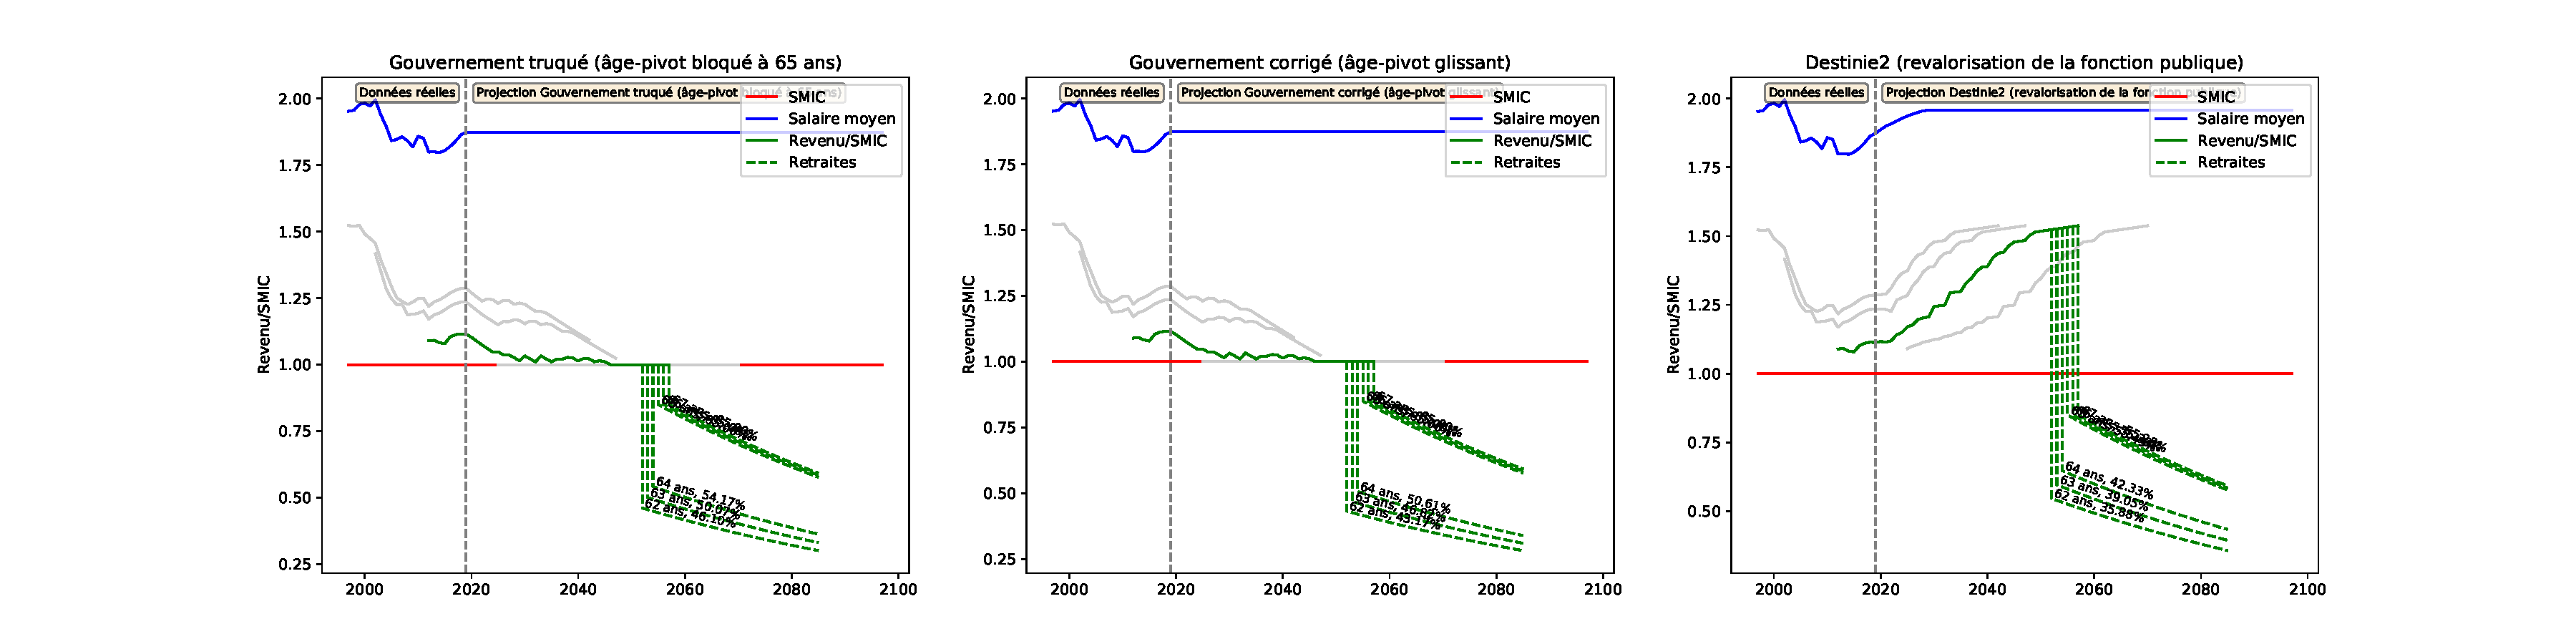
\includegraphics[width=0.9\textwidth]{fig/AideSoignant_1990_22_dest_retraite.pdf}\end{center} \label{fig/AideSoignant_1990_22_dest_retraite.pdf} 

\newpage 
 
\paragraph{Revenus et points pour le modèle \emph{Gouvernement truqué (âge-pivot bloqué à 65 ans)}} 
 
{ \scriptsize \begin{center} 
\begin{tabular}[htb]{|c|c||c|c|c|c|c|c||c|c||c|c|c|} 
\hline 
 Année &  Âge &  Ind Maj &  Pt Ind(\euro{} 2019) &  Rev HP(\euro{} 2019) &  Tx Primes &  GIPA(\euro{} 2019) &  Revenu(\euro{} 2019) &  SMIC(\euro{} 2019) &  Rev/SMIC &  Cumul Pts &  Achat Pt(\euro{} 2019) &  Serv. Pt(\euro{} 2019) \\ 
\hline \hline 
 2012 &  22 &  327.0 &  4.88 &  1594.59 &  14.31 &  0.00 &  1822.78 &  1673.05 &  {\bf 1.09} &  614.30 &  35.61 &  0.50 \\ 
\hline 
 2013 &  23 &  328.0 &  4.83 &  1585.77 &  14.54 &  0.00 &  1816.34 &  1664.01 &  {\bf 1.09} &  1226.43 &  35.61 &  0.50 \\ 
\hline 
 2014 &  24 &  328.0 &  4.81 &  1577.83 &  14.77 &  0.00 &  1810.87 &  1673.24 &  {\bf 1.08} &  1836.71 &  35.61 &  0.50 \\ 
\hline 
 2015 &  25 &  329.0 &  4.81 &  1582.02 &  15.00 &  0.00 &  1819.32 &  1686.62 &  {\bf 1.08} &  2449.85 &  35.61 &  0.50 \\ 
\hline 
 2016 &  26 &  329.0 &  4.80 &  1578.86 &  15.23 &  51.15 &  1870.47 &  1693.76 &  {\bf 1.10} &  3080.22 &  35.61 &  0.50 \\ 
\hline 
 2017 &  27 &  330.0 &  4.81 &  1586.85 &  15.46 &  51.01 &  1883.20 &  1692.60 &  {\bf 1.11} &  3714.88 &  35.61 &  0.50 \\ 
\hline 
 2018 &  28 &  330.0 &  4.74 &  1564.94 &  15.69 &  74.24 &  1884.72 &  1689.76 &  {\bf 1.12} &  4350.05 &  35.61 &  0.50 \\ 
\hline 
 2019 &  29 &  332.0 &  4.79 &  1591.75 &  15.92 &  48.30 &  1893.46 &  1698.45 &  {\bf 1.11} &  4988.17 &  35.61 &  0.50 \\ 
\hline 
 2020 &  30 &  332.0 &  4.79 &  1591.75 &  16.15 &  48.57 &  1897.38 &  1720.53 &  {\bf 1.10} &  5627.61 &  35.61 &  0.50 \\ 
\hline 
 2021 &  31 &  334.0 &  4.79 &  1601.34 &  16.38 &  32.81 &  1896.44 &  1742.90 &  {\bf 1.09} &  6266.74 &  35.61 &  0.50 \\ 
\hline 
 2022 &  32 &  334.0 &  4.79 &  1601.34 &  16.61 &  28.24 &  1895.56 &  1765.55 &  {\bf 1.07} &  6905.57 &  35.61 &  0.50 \\ 
\hline 
 2023 &  33 &  338.0 &  4.79 &  1620.51 &  16.84 &  2.30 &  1895.71 &  1788.51 &  {\bf 1.06} &  7544.44 &  35.61 &  0.50 \\ 
\hline 
 2024 &  34 &  338.0 &  4.79 &  1620.51 &  17.07 &  0.00 &  1897.14 &  1811.76 &  {\bf 1.05} &  8183.80 &  35.61 &  0.50 \\ 
\hline 
 2025 &  35 &  342.0 &  4.79 &  1639.69 &  17.30 &  0.00 &  1923.36 &  1835.31 &  {\bf 1.05} &  8832.00 &  35.61 &  0.50 \\ 
\hline 
 2026 &  36 &  342.0 &  4.79 &  1639.69 &  17.53 &  0.00 &  1927.13 &  1859.17 &  {\bf 1.04} &  9481.46 &  35.61 &  0.50 \\ 
\hline 
 2027 &  37 &  346.0 &  4.79 &  1658.87 &  17.76 &  0.00 &  1953.49 &  1883.34 &  {\bf 1.04} &  10139.81 &  35.61 &  0.50 \\ 
\hline 
 2028 &  38 &  346.0 &  4.79 &  1658.87 &  17.99 &  0.00 &  1957.30 &  1907.82 &  {\bf 1.03} &  10799.45 &  35.61 &  0.50 \\ 
\hline 
 2029 &  39 &  346.0 &  4.79 &  1658.87 &  18.22 &  0.00 &  1961.12 &  1932.62 &  {\bf 1.01} &  11459.86 &  35.63 &  0.50 \\ 
\hline 
 2030 &  40 &  356.0 &  4.79 &  1706.81 &  18.45 &  0.00 &  2021.72 &  1957.75 &  {\bf 1.03} &  12139.66 &  35.69 &  0.50 \\ 
\hline 
 2031 &  41 &  356.0 &  4.79 &  1706.81 &  18.68 &  0.00 &  2025.65 &  1983.20 &  {\bf 1.02} &  12819.22 &  35.77 &  0.50 \\ 
\hline 
 2032 &  42 &  356.0 &  4.79 &  1706.81 &  18.91 &  0.00 &  2029.57 &  2008.98 &  {\bf 1.01} &  13498.03 &  35.88 &  0.50 \\ 
\hline 
 2033 &  43 &  368.0 &  4.79 &  1764.35 &  19.14 &  0.00 &  2102.04 &  2035.10 &  {\bf 1.03} &  14198.42 &  36.02 &  0.50 \\ 
\hline 
 2034 &  44 &  368.0 &  4.79 &  1764.35 &  19.37 &  0.00 &  2106.10 &  2061.55 &  {\bf 1.02} &  14896.97 &  36.18 &  0.50 \\ 
\hline 
 2035 &  45 &  368.0 &  4.79 &  1764.35 &  19.60 &  0.00 &  2110.16 &  2088.35 &  {\bf 1.01} &  15593.15 &  36.37 &  0.51 \\ 
\hline 
 2036 &  46 &  376.0 &  4.79 &  1802.70 &  19.83 &  0.00 &  2160.18 &  2115.50 &  {\bf 1.02} &  16301.51 &  36.59 &  0.51 \\ 
\hline 
 2037 &  47 &  380.0 &  4.79 &  1821.88 &  20.06 &  0.00 &  2187.35 &  2143.00 &  {\bf 1.02} &  17013.90 &  36.85 &  0.51 \\ 
\hline 
 2038 &  48 &  386.7 &  4.79 &  1853.84 &  20.29 &  0.00 &  2229.99 &  2170.86 &  {\bf 1.03} &  17734.67 &  37.13 &  0.52 \\ 
\hline 
 2039 &  49 &  390.0 &  4.79 &  1869.82 &  20.52 &  0.00 &  2253.51 &  2199.08 &  {\bf 1.02} &  18456.99 &  37.44 &  0.52 \\ 
\hline 
 2040 &  50 &  390.0 &  4.79 &  1869.82 &  20.75 &  0.00 &  2257.81 &  2227.67 &  {\bf 1.01} &  19174.12 &  37.78 &  0.53 \\ 
\hline 
 2041 &  51 &  398.0 &  4.79 &  1908.18 &  20.98 &  0.00 &  2308.52 &  2256.63 &  {\bf 1.02} &  19900.14 &  38.16 &  0.53 \\ 
\hline 
 2042 &  52 &  402.0 &  4.79 &  1927.36 &  21.21 &  0.00 &  2336.15 &  2285.97 &  {\bf 1.02} &  20627.08 &  38.56 &  0.54 \\ 
\hline 
 2043 &  53 &  402.0 &  4.79 &  1927.36 &  21.44 &  0.00 &  2340.58 &  2315.68 &  {\bf 1.01} &  21347.15 &  39.01 &  0.54 \\ 
\hline 
 2044 &  54 &  408.0 &  4.79 &  1956.12 &  21.67 &  0.00 &  2380.02 &  2345.79 &  {\bf 1.01} &  22070.50 &  39.48 &  0.55 \\ 
\hline 
 2045 &  55 &  411.0 &  4.79 &  1970.51 &  21.90 &  0.00 &  2402.05 &  2376.28 &  {\bf 1.01} &  22791.18 &  40.00 &  0.56 \\ 
\hline 
 2046 &  56 &  411.0 &  4.79 &  1970.51 &  22.13 &  0.00 &  2407.18 &  2407.18 &  {\bf 1.00} &  23504.13 &  40.52 &  0.56 \\ 
\hline 
 2047 &  57 &  411.0 &  4.79 &  1970.51 &  22.36 &  0.00 &  2438.47 &  2438.47 &  {\bf 1.00} &  24217.08 &  41.04 &  0.57 \\ 
\hline 
 2048 &  58 &  415.7 &  4.79 &  1992.88 &  22.59 &  0.00 &  2470.17 &  2470.17 &  {\bf 1.00} &  24930.03 &  41.58 &  0.58 \\ 
\hline 
 2049 &  59 &  418.0 &  4.79 &  2004.07 &  22.82 &  0.00 &  2502.28 &  2502.28 &  {\bf 1.00} &  25642.98 &  42.12 &  0.59 \\ 
\hline 
 2050 &  60 &  418.0 &  4.79 &  2004.07 &  23.05 &  0.00 &  2534.81 &  2534.81 &  {\bf 1.00} &  26355.93 &  42.66 &  0.59 \\ 
\hline 
 2051 &  61 &  418.0 &  4.79 &  2004.07 &  23.28 &  15.82 &  2567.76 &  2567.76 &  {\bf 1.00} &  27068.88 &  43.22 &  0.60 \\ 
\hline 
 2052 &  62 &  418.0 &  4.79 &  2004.07 &  23.51 &  43.53 &  2601.14 &  2601.14 &  {\bf 1.00} &  27781.83 &  43.78 &  0.61 \\ 
\hline 
 2053 &  63 &  418.0 &  4.79 &  2004.07 &  23.74 &  71.67 &  2634.96 &  2634.96 &  {\bf 1.00} &  28494.78 &  44.35 &  0.62 \\ 
\hline 
 2054 &  64 &  418.0 &  4.79 &  2004.07 &  23.97 &  100.23 &  2669.21 &  2669.21 &  {\bf 1.00} &  29207.73 &  44.93 &  0.63 \\ 
\hline 
 2055 &  65 &  418.0 &  4.79 &  2004.07 &  24.20 &  129.22 &  2703.91 &  2703.91 &  {\bf 1.00} &  29920.68 &  45.51 &  0.63 \\ 
\hline 
 2056 &  66 &  418.0 &  4.79 &  2004.07 &  24.43 &  158.65 &  2739.06 &  2739.06 &  {\bf 1.00} &  30633.63 &  46.10 &  0.64 \\ 
\hline 
 2057 &  67 &  418.0 &  4.79 &  2004.07 &  24.66 &  188.52 &  2774.67 &  2774.67 &  {\bf 1.00} &  31346.58 &  46.70 &  0.65 \\ 
\hline 
\hline 
\end{tabular} 
\end{center} } 
\newpage 
 
\paragraph{Revenus et points pour le modèle \emph{Gouvernement corrigé (âge-pivot glissant)}} 
 
{ \scriptsize \begin{center} 
\begin{tabular}[htb]{|c|c||c|c|c|c|c|c||c|c||c|c|c|} 
\hline 
 Année &  Âge &  Ind Maj &  Pt Ind(\euro{} 2019) &  Rev HP(\euro{} 2019) &  Tx Primes &  GIPA(\euro{} 2019) &  Revenu(\euro{} 2019) &  SMIC(\euro{} 2019) &  Rev/SMIC &  Cumul Pts &  Achat Pt(\euro{} 2019) &  Serv. Pt(\euro{} 2019) \\ 
\hline \hline 
 2012 &  22 &  327.0 &  4.88 &  1594.59 &  14.31 &  0.00 &  1822.78 &  1673.05 &  {\bf 1.09} &  614.30 &  35.61 &  0.50 \\ 
\hline 
 2013 &  23 &  328.0 &  4.83 &  1585.77 &  14.54 &  0.00 &  1816.34 &  1664.01 &  {\bf 1.09} &  1226.43 &  35.61 &  0.50 \\ 
\hline 
 2014 &  24 &  328.0 &  4.81 &  1577.83 &  14.77 &  0.00 &  1810.87 &  1673.24 &  {\bf 1.08} &  1836.71 &  35.61 &  0.50 \\ 
\hline 
 2015 &  25 &  329.0 &  4.81 &  1582.02 &  15.00 &  0.00 &  1819.32 &  1686.62 &  {\bf 1.08} &  2449.85 &  35.61 &  0.50 \\ 
\hline 
 2016 &  26 &  329.0 &  4.80 &  1578.86 &  15.23 &  51.15 &  1870.47 &  1693.76 &  {\bf 1.10} &  3080.22 &  35.61 &  0.50 \\ 
\hline 
 2017 &  27 &  330.0 &  4.81 &  1586.85 &  15.46 &  51.01 &  1883.20 &  1692.60 &  {\bf 1.11} &  3714.88 &  35.61 &  0.50 \\ 
\hline 
 2018 &  28 &  330.0 &  4.74 &  1564.94 &  15.69 &  74.24 &  1884.72 &  1689.76 &  {\bf 1.12} &  4350.05 &  35.61 &  0.50 \\ 
\hline 
 2019 &  29 &  332.0 &  4.79 &  1591.75 &  15.92 &  48.30 &  1893.46 &  1698.45 &  {\bf 1.11} &  4988.17 &  35.61 &  0.50 \\ 
\hline 
 2020 &  30 &  332.0 &  4.79 &  1591.75 &  16.15 &  48.57 &  1897.38 &  1720.53 &  {\bf 1.10} &  5627.61 &  35.61 &  0.50 \\ 
\hline 
 2021 &  31 &  334.0 &  4.79 &  1601.34 &  16.38 &  32.81 &  1896.44 &  1742.90 &  {\bf 1.09} &  6266.74 &  35.61 &  0.50 \\ 
\hline 
 2022 &  32 &  334.0 &  4.79 &  1601.34 &  16.61 &  28.24 &  1895.56 &  1765.55 &  {\bf 1.07} &  6905.57 &  35.61 &  0.50 \\ 
\hline 
 2023 &  33 &  338.0 &  4.79 &  1620.51 &  16.84 &  2.30 &  1895.71 &  1788.51 &  {\bf 1.06} &  7544.44 &  35.61 &  0.50 \\ 
\hline 
 2024 &  34 &  338.0 &  4.79 &  1620.51 &  17.07 &  0.00 &  1897.14 &  1811.76 &  {\bf 1.05} &  8183.80 &  35.61 &  0.50 \\ 
\hline 
 2025 &  35 &  342.0 &  4.79 &  1639.69 &  17.30 &  0.00 &  1923.36 &  1835.31 &  {\bf 1.05} &  8832.00 &  35.61 &  0.50 \\ 
\hline 
 2026 &  36 &  342.0 &  4.79 &  1639.69 &  17.53 &  0.00 &  1927.13 &  1859.17 &  {\bf 1.04} &  9481.46 &  35.61 &  0.50 \\ 
\hline 
 2027 &  37 &  346.0 &  4.79 &  1658.87 &  17.76 &  0.00 &  1953.49 &  1883.34 &  {\bf 1.04} &  10139.81 &  35.61 &  0.50 \\ 
\hline 
 2028 &  38 &  346.0 &  4.79 &  1658.87 &  17.99 &  0.00 &  1957.30 &  1907.82 &  {\bf 1.03} &  10799.45 &  35.61 &  0.50 \\ 
\hline 
 2029 &  39 &  346.0 &  4.79 &  1658.87 &  18.22 &  0.00 &  1961.12 &  1932.62 &  {\bf 1.01} &  11459.86 &  35.63 &  0.50 \\ 
\hline 
 2030 &  40 &  356.0 &  4.79 &  1706.81 &  18.45 &  0.00 &  2021.72 &  1957.75 &  {\bf 1.03} &  12139.66 &  35.69 &  0.50 \\ 
\hline 
 2031 &  41 &  356.0 &  4.79 &  1706.81 &  18.68 &  0.00 &  2025.65 &  1983.20 &  {\bf 1.02} &  12819.22 &  35.77 &  0.50 \\ 
\hline 
 2032 &  42 &  356.0 &  4.79 &  1706.81 &  18.91 &  0.00 &  2029.57 &  2008.98 &  {\bf 1.01} &  13498.03 &  35.88 &  0.50 \\ 
\hline 
 2033 &  43 &  368.0 &  4.79 &  1764.35 &  19.14 &  0.00 &  2102.04 &  2035.10 &  {\bf 1.03} &  14198.42 &  36.02 &  0.50 \\ 
\hline 
 2034 &  44 &  368.0 &  4.79 &  1764.35 &  19.37 &  0.00 &  2106.10 &  2061.55 &  {\bf 1.02} &  14896.97 &  36.18 &  0.50 \\ 
\hline 
 2035 &  45 &  368.0 &  4.79 &  1764.35 &  19.60 &  0.00 &  2110.16 &  2088.35 &  {\bf 1.01} &  15593.15 &  36.37 &  0.51 \\ 
\hline 
 2036 &  46 &  376.0 &  4.79 &  1802.70 &  19.83 &  0.00 &  2160.18 &  2115.50 &  {\bf 1.02} &  16301.51 &  36.59 &  0.51 \\ 
\hline 
 2037 &  47 &  380.0 &  4.79 &  1821.88 &  20.06 &  0.00 &  2187.35 &  2143.00 &  {\bf 1.02} &  17013.90 &  36.85 &  0.51 \\ 
\hline 
 2038 &  48 &  386.7 &  4.79 &  1853.84 &  20.29 &  0.00 &  2229.99 &  2170.86 &  {\bf 1.03} &  17734.67 &  37.13 &  0.52 \\ 
\hline 
 2039 &  49 &  390.0 &  4.79 &  1869.82 &  20.52 &  0.00 &  2253.51 &  2199.08 &  {\bf 1.02} &  18456.99 &  37.44 &  0.52 \\ 
\hline 
 2040 &  50 &  390.0 &  4.79 &  1869.82 &  20.75 &  0.00 &  2257.81 &  2227.67 &  {\bf 1.01} &  19174.12 &  37.78 &  0.53 \\ 
\hline 
 2041 &  51 &  398.0 &  4.79 &  1908.18 &  20.98 &  0.00 &  2308.52 &  2256.63 &  {\bf 1.02} &  19900.14 &  38.16 &  0.53 \\ 
\hline 
 2042 &  52 &  402.0 &  4.79 &  1927.36 &  21.21 &  0.00 &  2336.15 &  2285.97 &  {\bf 1.02} &  20627.08 &  38.56 &  0.54 \\ 
\hline 
 2043 &  53 &  402.0 &  4.79 &  1927.36 &  21.44 &  0.00 &  2340.58 &  2315.68 &  {\bf 1.01} &  21347.15 &  39.01 &  0.54 \\ 
\hline 
 2044 &  54 &  408.0 &  4.79 &  1956.12 &  21.67 &  0.00 &  2380.02 &  2345.79 &  {\bf 1.01} &  22070.50 &  39.48 &  0.55 \\ 
\hline 
 2045 &  55 &  411.0 &  4.79 &  1970.51 &  21.90 &  0.00 &  2402.05 &  2376.28 &  {\bf 1.01} &  22791.18 &  40.00 &  0.56 \\ 
\hline 
 2046 &  56 &  411.0 &  4.79 &  1970.51 &  22.13 &  0.00 &  2407.18 &  2407.18 &  {\bf 1.00} &  23504.13 &  40.52 &  0.56 \\ 
\hline 
 2047 &  57 &  411.0 &  4.79 &  1970.51 &  22.36 &  0.00 &  2438.47 &  2438.47 &  {\bf 1.00} &  24217.08 &  41.04 &  0.57 \\ 
\hline 
 2048 &  58 &  415.7 &  4.79 &  1992.88 &  22.59 &  0.00 &  2470.17 &  2470.17 &  {\bf 1.00} &  24930.03 &  41.58 &  0.58 \\ 
\hline 
 2049 &  59 &  418.0 &  4.79 &  2004.07 &  22.82 &  0.00 &  2502.28 &  2502.28 &  {\bf 1.00} &  25642.98 &  42.12 &  0.59 \\ 
\hline 
 2050 &  60 &  418.0 &  4.79 &  2004.07 &  23.05 &  0.00 &  2534.81 &  2534.81 &  {\bf 1.00} &  26355.93 &  42.66 &  0.59 \\ 
\hline 
 2051 &  61 &  418.0 &  4.79 &  2004.07 &  23.28 &  15.82 &  2567.76 &  2567.76 &  {\bf 1.00} &  27068.88 &  43.22 &  0.60 \\ 
\hline 
 2052 &  62 &  418.0 &  4.79 &  2004.07 &  23.51 &  43.53 &  2601.14 &  2601.14 &  {\bf 1.00} &  27781.83 &  43.78 &  0.61 \\ 
\hline 
 2053 &  63 &  418.0 &  4.79 &  2004.07 &  23.74 &  71.67 &  2634.96 &  2634.96 &  {\bf 1.00} &  28494.78 &  44.35 &  0.62 \\ 
\hline 
 2054 &  64 &  418.0 &  4.79 &  2004.07 &  23.97 &  100.23 &  2669.21 &  2669.21 &  {\bf 1.00} &  29207.73 &  44.93 &  0.63 \\ 
\hline 
 2055 &  65 &  418.0 &  4.79 &  2004.07 &  24.20 &  129.22 &  2703.91 &  2703.91 &  {\bf 1.00} &  29920.68 &  45.51 &  0.63 \\ 
\hline 
 2056 &  66 &  418.0 &  4.79 &  2004.07 &  24.43 &  158.65 &  2739.06 &  2739.06 &  {\bf 1.00} &  30633.63 &  46.10 &  0.64 \\ 
\hline 
 2057 &  67 &  418.0 &  4.79 &  2004.07 &  24.66 &  188.52 &  2774.67 &  2774.67 &  {\bf 1.00} &  31346.58 &  46.70 &  0.65 \\ 
\hline 
\hline 
\end{tabular} 
\end{center} } 
\newpage 
 
\paragraph{Revenus et points pour le modèle \emph{Destinie2 (revalorisation de la fonction publique)}} 
 
{ \scriptsize \begin{center} 
\begin{tabular}[htb]{|c|c||c|c|c|c|c|c||c|c||c|c|c|} 
\hline 
 Année &  Âge &  Ind Maj &  Pt Ind(\euro{} 2019) &  Rev HP(\euro{} 2019) &  Tx Primes &  GIPA(\euro{} 2019) &  Revenu(\euro{} 2019) &  SMIC(\euro{} 2019) &  Rev/SMIC &  Cumul Pts &  Achat Pt(\euro{} 2019) &  Serv. Pt(\euro{} 2019) \\ 
\hline \hline 
 2012 &  22 &  327.0 &  4.88 &  1594.59 &  14.31 &  0.00 &  1822.78 &  1673.05 &  {\bf 1.09} &  612.79 &  35.69 &  0.50 \\ 
\hline 
 2013 &  23 &  328.0 &  4.83 &  1585.77 &  14.54 &  0.00 &  1816.34 &  1664.01 &  {\bf 1.09} &  1223.41 &  35.69 &  0.50 \\ 
\hline 
 2014 &  24 &  328.0 &  4.81 &  1577.83 &  14.77 &  0.00 &  1810.87 &  1673.24 &  {\bf 1.08} &  1832.20 &  35.69 &  0.50 \\ 
\hline 
 2015 &  25 &  329.0 &  4.81 &  1582.02 &  15.00 &  0.00 &  1819.32 &  1686.62 &  {\bf 1.08} &  2443.83 &  35.69 &  0.50 \\ 
\hline 
 2016 &  26 &  329.0 &  4.80 &  1578.86 &  15.23 &  46.55 &  1865.88 &  1693.76 &  {\bf 1.10} &  3071.11 &  35.69 &  0.50 \\ 
\hline 
 2017 &  27 &  330.0 &  4.81 &  1586.85 &  15.46 &  47.53 &  1879.71 &  1692.60 &  {\bf 1.11} &  3703.03 &  35.69 &  0.50 \\ 
\hline 
 2018 &  28 &  330.0 &  4.74 &  1564.94 &  15.69 &  72.20 &  1882.69 &  1689.76 &  {\bf 1.11} &  4335.96 &  35.69 &  0.50 \\ 
\hline 
 2019 &  29 &  332.0 &  4.79 &  1591.75 &  15.92 &  45.75 &  1890.90 &  1698.45 &  {\bf 1.11} &  4971.66 &  35.69 &  0.50 \\ 
\hline 
 2020 &  30 &  332.0 &  4.83 &  1604.48 &  16.15 &  35.25 &  1898.85 &  1699.99 &  {\bf 1.12} &  5610.02 &  35.69 &  0.50 \\ 
\hline 
 2021 &  31 &  334.0 &  4.88 &  1628.68 &  16.38 &  2.83 &  1898.28 &  1703.48 &  {\bf 1.11} &  6248.19 &  35.69 &  0.50 \\ 
\hline 
 2022 &  32 &  334.0 &  4.93 &  1644.96 &  16.61 &  0.00 &  1918.19 &  1712.78 &  {\bf 1.12} &  6893.05 &  35.69 &  0.50 \\ 
\hline 
 2023 &  33 &  338.0 &  4.98 &  1684.14 &  16.84 &  0.00 &  1967.75 &  1723.51 &  {\bf 1.14} &  7554.58 &  35.69 &  0.50 \\ 
\hline 
 2024 &  34 &  338.0 &  5.04 &  1704.18 &  17.07 &  0.00 &  1995.08 &  1735.69 &  {\bf 1.15} &  8225.30 &  35.69 &  0.50 \\ 
\hline 
 2025 &  35 &  342.0 &  5.10 &  1745.38 &  17.30 &  0.00 &  2047.34 &  1749.35 &  {\bf 1.17} &  8913.58 &  35.69 &  0.50 \\ 
\hline 
 2026 &  36 &  342.0 &  5.17 &  1767.20 &  17.53 &  0.00 &  2076.99 &  1764.53 &  {\bf 1.18} &  9611.83 &  35.69 &  0.50 \\ 
\hline 
 2027 &  37 &  346.0 &  5.23 &  1810.76 &  17.76 &  0.00 &  2132.35 &  1781.27 &  {\bf 1.20} &  10328.69 &  35.69 &  0.50 \\ 
\hline 
 2028 &  38 &  346.0 &  5.30 &  1834.48 &  17.99 &  0.00 &  2164.50 &  1799.59 &  {\bf 1.20} &  11056.36 &  35.69 &  0.50 \\ 
\hline 
 2029 &  39 &  346.0 &  5.37 &  1856.67 &  18.22 &  0.00 &  2194.96 &  1819.55 &  {\bf 1.21} &  11793.75 &  35.72 &  0.50 \\ 
\hline 
 2030 &  40 &  356.0 &  5.43 &  1934.02 &  18.45 &  0.00 &  2290.85 &  1841.19 &  {\bf 1.24} &  12562.24 &  35.77 &  0.50 \\ 
\hline 
 2031 &  41 &  356.0 &  5.50 &  1958.59 &  18.68 &  0.00 &  2324.45 &  1864.58 &  {\bf 1.25} &  13340.26 &  35.85 &  0.50 \\ 
\hline 
 2032 &  42 &  356.0 &  5.57 &  1984.05 &  18.91 &  0.00 &  2359.23 &  1888.81 &  {\bf 1.25} &  14127.53 &  35.96 &  0.50 \\ 
\hline 
 2033 &  43 &  368.0 &  5.65 &  2077.59 &  19.14 &  0.00 &  2475.24 &  1913.37 &  {\bf 1.29} &  14950.38 &  36.10 &  0.50 \\ 
\hline 
 2034 &  44 &  368.0 &  5.72 &  2104.60 &  19.37 &  0.00 &  2512.26 &  1938.24 &  {\bf 1.30} &  15781.74 &  36.26 &  0.50 \\ 
\hline 
 2035 &  45 &  368.0 &  5.79 &  2131.95 &  19.60 &  0.00 &  2549.82 &  1963.44 &  {\bf 1.30} &  16621.05 &  36.46 &  0.51 \\ 
\hline 
 2036 &  46 &  376.0 &  5.87 &  2206.62 &  19.83 &  0.00 &  2644.19 &  1988.96 &  {\bf 1.33} &  17486.15 &  36.68 &  0.51 \\ 
\hline 
 2037 &  47 &  380.0 &  5.94 &  2259.09 &  20.06 &  0.00 &  2712.26 &  2014.82 &  {\bf 1.35} &  18367.47 &  36.93 &  0.51 \\ 
\hline 
 2038 &  48 &  386.7 &  6.02 &  2328.60 &  20.29 &  0.00 &  2801.08 &  2041.01 &  {\bf 1.37} &  19270.77 &  37.21 &  0.52 \\ 
\hline 
 2039 &  49 &  390.0 &  6.10 &  2379.21 &  20.52 &  0.00 &  2867.42 &  2067.55 &  {\bf 1.39} &  20187.76 &  37.52 &  0.52 \\ 
\hline 
 2040 &  50 &  390.0 &  6.18 &  2410.14 &  20.75 &  0.00 &  2910.24 &  2094.43 &  {\bf 1.39} &  21110.00 &  37.87 &  0.53 \\ 
\hline 
 2041 &  51 &  398.0 &  6.26 &  2491.55 &  20.98 &  0.00 &  3014.28 &  2121.65 &  {\bf 1.42} &  22055.82 &  38.24 &  0.53 \\ 
\hline 
 2042 &  52 &  402.0 &  6.34 &  2549.31 &  21.21 &  0.00 &  3090.02 &  2149.23 &  {\bf 1.44} &  23015.15 &  38.65 &  0.54 \\ 
\hline 
 2043 &  53 &  402.0 &  6.42 &  2582.45 &  21.44 &  0.00 &  3136.13 &  2177.17 &  {\bf 1.44} &  23977.76 &  39.10 &  0.54 \\ 
\hline 
 2044 &  54 &  408.0 &  6.51 &  2655.07 &  21.67 &  0.00 &  3230.42 &  2205.48 &  {\bf 1.46} &  24957.33 &  39.57 &  0.55 \\ 
\hline 
 2045 &  55 &  411.0 &  6.59 &  2709.36 &  21.90 &  0.00 &  3302.71 &  2234.15 &  {\bf 1.48} &  25945.97 &  40.09 &  0.56 \\ 
\hline 
 2046 &  56 &  411.0 &  6.68 &  2744.58 &  22.13 &  0.00 &  3351.96 &  2263.19 &  {\bf 1.48} &  26936.48 &  40.61 &  0.57 \\ 
\hline 
 2047 &  57 &  411.0 &  6.76 &  2780.26 &  22.36 &  0.00 &  3401.93 &  2292.61 &  {\bf 1.48} &  27928.85 &  41.14 &  0.57 \\ 
\hline 
 2048 &  58 &  415.7 &  6.85 &  2848.38 &  22.59 &  0.00 &  3491.83 &  2322.42 &  {\bf 1.50} &  28934.37 &  41.67 &  0.58 \\ 
\hline 
 2049 &  59 &  418.0 &  6.94 &  2901.61 &  22.82 &  0.00 &  3563.75 &  2352.61 &  {\bf 1.51} &  29947.44 &  42.21 &  0.59 \\ 
\hline 
 2050 &  60 &  418.0 &  7.03 &  2939.33 &  23.05 &  0.00 &  3616.84 &  2383.19 &  {\bf 1.52} &  30962.40 &  42.76 &  0.60 \\ 
\hline 
 2051 &  61 &  418.0 &  7.12 &  2977.54 &  23.28 &  0.00 &  3670.71 &  2414.18 &  {\bf 1.52} &  31979.27 &  43.32 &  0.60 \\ 
\hline 
 2052 &  62 &  418.0 &  7.22 &  3016.25 &  23.51 &  0.00 &  3725.37 &  2445.56 &  {\bf 1.52} &  32998.02 &  43.88 &  0.61 \\ 
\hline 
 2053 &  63 &  418.0 &  7.31 &  3055.46 &  23.74 &  0.00 &  3780.83 &  2477.35 &  {\bf 1.53} &  34018.68 &  44.45 &  0.62 \\ 
\hline 
 2054 &  64 &  418.0 &  7.40 &  3095.18 &  23.97 &  0.00 &  3837.10 &  2509.56 &  {\bf 1.53} &  35041.23 &  45.03 &  0.63 \\ 
\hline 
 2055 &  65 &  418.0 &  7.50 &  3135.42 &  24.20 &  0.00 &  3894.19 &  2542.18 &  {\bf 1.53} &  36065.68 &  45.62 &  0.63 \\ 
\hline 
 2056 &  66 &  418.0 &  7.60 &  3176.18 &  24.43 &  0.00 &  3952.12 &  2575.23 &  {\bf 1.53} &  37092.03 &  46.21 &  0.64 \\ 
\hline 
 2057 &  67 &  418.0 &  7.70 &  3217.47 &  24.66 &  0.00 &  4010.90 &  2608.71 &  {\bf 1.54} &  38120.27 &  46.81 &  0.65 \\ 
\hline 
\hline 
\end{tabular} 
\end{center} } 
\newpage 
 
\subsection{Génération 2003 (début en 2025)} 

\paragraph{Retraites possibles dans le modèle \emph{Gouvernement truqué (âge-pivot bloqué à 65 ans)}}  
 
{ \scriptsize \begin{center} 
\begin{tabular}[htb]{|c|c||c|c||c|c||c||c|c|c|c|c|c|} 
\hline 
 Retraite en &  Âge &  Âge pivot &  Décote/Surcote &  Retraite (\euro{} 2019) &  Tx Rempl(\%) &  SMIC (\euro{} 2019) &  Retraite/SMIC &  Rev70/SMIC &  Rev75/SMIC &  Rev80/SMIC &  Rev85/SMIC &  Rev90/SMIC \\ 
\hline \hline 
 2065 &  62 &  65 ans 0 mois &  -15.00\% &  1457.41 &  {\bf 47.37} &  3076.71 &  {\bf {\color{red} 0.47}} &  {\bf {\color{red} 0.43}} &  {\bf {\color{red} 0.40}} &  {\bf {\color{red} 0.38}} &  {\bf {\color{red} 0.35}} &  {\bf {\color{red} 0.33}} \\ 
\hline 
 2066 &  63 &  65 ans 0 mois &  -10.00\% &  1602.25 &  {\bf 51.41} &  3116.71 &  {\bf {\color{red} 0.51}} &  {\bf {\color{red} 0.47}} &  {\bf {\color{red} 0.44}} &  {\bf {\color{red} 0.41}} &  {\bf {\color{red} 0.39}} &  {\bf {\color{red} 0.36}} \\ 
\hline 
 2067 &  64 &  65 ans 0 mois &  -5.00\% &  1755.00 &  {\bf 55.59} &  3157.23 &  {\bf {\color{red} 0.56}} &  {\bf {\color{red} 0.51}} &  {\bf {\color{red} 0.48}} &  {\bf {\color{red} 0.45}} &  {\bf {\color{red} 0.42}} &  {\bf {\color{red} 0.40}} \\ 
\hline 
 2068 &  65 &  65 ans 0 mois &  0.00\% &  2718.53 &  {\bf 85.00} &  3198.27 &  {\bf {\color{red} 0.85}} &  {\bf {\color{red} 0.80}} &  {\bf {\color{red} 0.75}} &  {\bf {\color{red} 0.70}} &  {\bf {\color{red} 0.66}} &  {\bf {\color{red} 0.62}} \\ 
\hline 
 2069 &  66 &  65 ans 0 mois &  5.00\% &  2753.87 &  {\bf 85.00} &  3239.85 &  {\bf {\color{red} 0.85}} &  {\bf {\color{red} 0.81}} &  {\bf {\color{red} 0.76}} &  {\bf {\color{red} 0.71}} &  {\bf {\color{red} 0.67}} &  {\bf {\color{red} 0.62}} \\ 
\hline 
 2070 &  67 &  65 ans 0 mois &  10.00\% &  2789.67 &  {\bf 85.00} &  3281.97 &  {\bf {\color{red} 0.85}} &  {\bf {\color{red} 0.82}} &  {\bf {\color{red} 0.77}} &  {\bf {\color{red} 0.72}} &  {\bf {\color{red} 0.67}} &  {\bf {\color{red} 0.63}} \\ 
\hline 
\hline 
\end{tabular} 
\end{center} } 
\paragraph{Retraites possibles dans le modèle \emph{Gouvernement corrigé (âge-pivot glissant)}}  
 
{ \scriptsize \begin{center} 
\begin{tabular}[htb]{|c|c||c|c||c|c||c||c|c|c|c|c|c|} 
\hline 
 Retraite en &  Âge &  Âge pivot &  Décote/Surcote &  Retraite (\euro{} 2019) &  Tx Rempl(\%) &  SMIC (\euro{} 2019) &  Retraite/SMIC &  Rev70/SMIC &  Rev75/SMIC &  Rev80/SMIC &  Rev85/SMIC &  Rev90/SMIC \\ 
\hline \hline 
 2065 &  62 &  67 ans 2 mois &  -25.83\% &  1271.67 &  {\bf 41.33} &  3076.71 &  {\bf {\color{red} 0.41}} &  {\bf {\color{red} 0.37}} &  {\bf {\color{red} 0.35}} &  {\bf {\color{red} 0.33}} &  {\bf {\color{red} 0.31}} &  {\bf {\color{red} 0.29}} \\ 
\hline 
 2066 &  63 &  67 ans 3 mois &  -21.25\% &  1401.97 &  {\bf 44.98} &  3116.71 &  {\bf {\color{red} 0.45}} &  {\bf {\color{red} 0.41}} &  {\bf {\color{red} 0.39}} &  {\bf {\color{red} 0.36}} &  {\bf {\color{red} 0.34}} &  {\bf {\color{red} 0.32}} \\ 
\hline 
 2067 &  64 &  67 ans 4 mois &  -16.67\% &  1539.47 &  {\bf 48.76} &  3157.23 &  {\bf {\color{red} 0.49}} &  {\bf {\color{red} 0.45}} &  {\bf {\color{red} 0.42}} &  {\bf {\color{red} 0.40}} &  {\bf {\color{red} 0.37}} &  {\bf {\color{red} 0.35}} \\ 
\hline 
 2068 &  65 &  67 ans 5 mois &  -12.08\% &  2718.53 &  {\bf 85.00} &  3198.27 &  {\bf {\color{red} 0.85}} &  {\bf {\color{red} 0.80}} &  {\bf {\color{red} 0.75}} &  {\bf {\color{red} 0.70}} &  {\bf {\color{red} 0.66}} &  {\bf {\color{red} 0.62}} \\ 
\hline 
 2069 &  66 &  67 ans 6 mois &  -7.50\% &  2753.87 &  {\bf 85.00} &  3239.85 &  {\bf {\color{red} 0.85}} &  {\bf {\color{red} 0.81}} &  {\bf {\color{red} 0.76}} &  {\bf {\color{red} 0.71}} &  {\bf {\color{red} 0.67}} &  {\bf {\color{red} 0.62}} \\ 
\hline 
 2070 &  67 &  67 ans 7 mois &  -2.92\% &  2789.67 &  {\bf 85.00} &  3281.97 &  {\bf {\color{red} 0.85}} &  {\bf {\color{red} 0.82}} &  {\bf {\color{red} 0.77}} &  {\bf {\color{red} 0.72}} &  {\bf {\color{red} 0.67}} &  {\bf {\color{red} 0.63}} \\ 
\hline 
\hline 
\end{tabular} 
\end{center} } 
\paragraph{Retraites possibles dans le modèle \emph{Destinie2 (revalorisation de la fonction publique)}}  
 
{ \scriptsize \begin{center} 
\begin{tabular}[htb]{|c|c||c|c||c|c||c||c|c|c|c|c|c|} 
\hline 
 Retraite en &  Âge &  Âge pivot &  Décote/Surcote &  Retraite (\euro{} 2019) &  Tx Rempl(\%) &  SMIC (\euro{} 2019) &  Retraite/SMIC &  Rev70/SMIC &  Rev75/SMIC &  Rev80/SMIC &  Rev85/SMIC &  Rev90/SMIC \\ 
\hline \hline 
 2065 &  62 &  67 ans 2 mois &  -25.83\% &  1548.60 &  {\bf 35.14} &  2892.68 &  {\bf {\color{red} 0.54}} &  {\bf {\color{red} 0.48}} &  {\bf {\color{red} 0.45}} &  {\bf {\color{red} 0.42}} &  {\bf {\color{red} 0.40}} &  {\bf {\color{red} 0.37}} \\ 
\hline 
 2066 &  63 &  67 ans 3 mois &  -21.25\% &  1714.69 &  {\bf 38.34} &  2930.29 &  {\bf {\color{red} 0.59}} &  {\bf {\color{red} 0.53}} &  {\bf {\color{red} 0.50}} &  {\bf {\color{red} 0.47}} &  {\bf {\color{red} 0.44}} &  {\bf {\color{red} 0.41}} \\ 
\hline 
 2067 &  64 &  67 ans 4 mois &  -16.67\% &  1890.72 &  {\bf 41.66} &  2968.38 &  {\bf {\color{red} 0.64}} &  {\bf {\color{red} 0.59}} &  {\bf {\color{red} 0.55}} &  {\bf {\color{red} 0.52}} &  {\bf {\color{red} 0.49}} &  {\bf {\color{red} 0.46}} \\ 
\hline 
 2068 &  65 &  67 ans 5 mois &  -12.08\% &  2555.93 &  {\bf 55.49} &  3006.97 &  {\bf {\color{red} 0.85}} &  {\bf {\color{red} 0.80}} &  {\bf {\color{red} 0.75}} &  {\bf {\color{red} 0.70}} &  {\bf {\color{red} 0.66}} &  {\bf {\color{red} 0.62}} \\ 
\hline 
 2069 &  66 &  67 ans 6 mois &  -7.50\% &  2589.15 &  {\bf 55.39} &  3046.06 &  {\bf {\color{red} 0.85}} &  {\bf {\color{red} 0.81}} &  {\bf {\color{red} 0.76}} &  {\bf {\color{red} 0.71}} &  {\bf {\color{red} 0.67}} &  {\bf {\color{red} 0.62}} \\ 
\hline 
 2070 &  67 &  67 ans 7 mois &  -2.92\% &  2622.81 &  {\bf 55.28} &  3085.66 &  {\bf {\color{red} 0.85}} &  {\bf {\color{red} 0.82}} &  {\bf {\color{red} 0.77}} &  {\bf {\color{red} 0.72}} &  {\bf {\color{red} 0.67}} &  {\bf {\color{red} 0.63}} \\ 
\hline 
\hline 
\end{tabular} 
\end{center} } 

 \begin{center}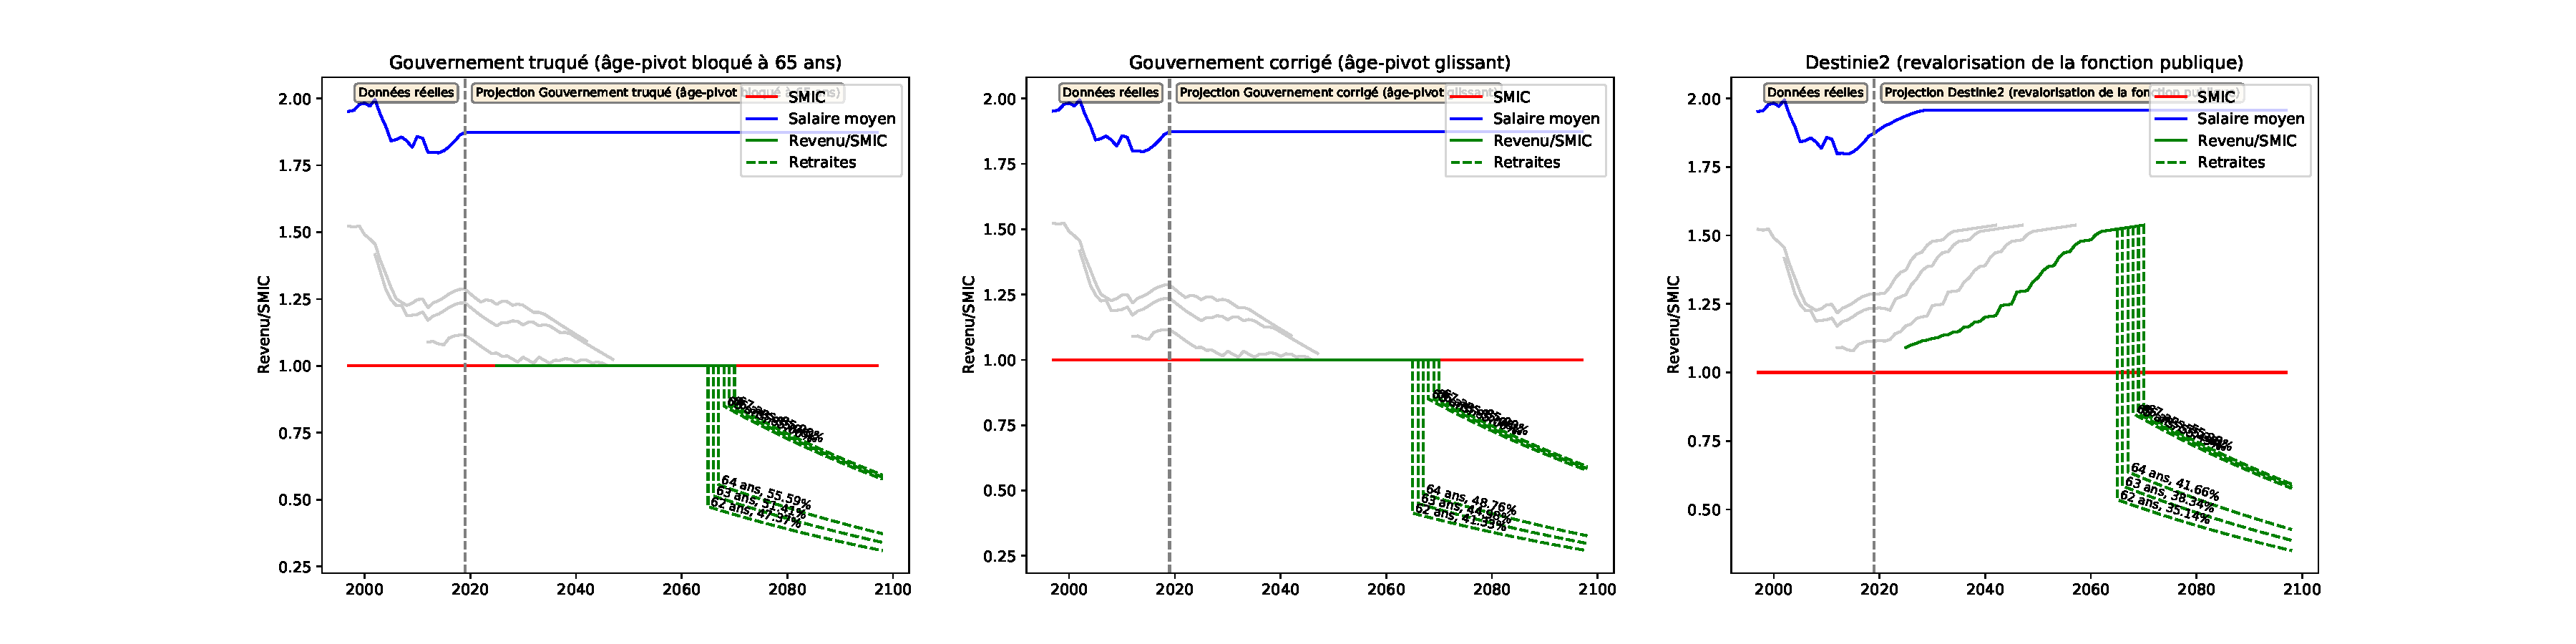
\includegraphics[width=0.9\textwidth]{fig/AideSoignant_2003_22_dest_retraite.pdf}\end{center} \label{fig/AideSoignant_2003_22_dest_retraite.pdf} 

\newpage 
 
\paragraph{Revenus et points pour le modèle \emph{Gouvernement truqué (âge-pivot bloqué à 65 ans)}} 
 
{ \scriptsize \begin{center} 
\begin{tabular}[htb]{|c|c||c|c|c|c|c|c||c|c||c|c|c|} 
\hline 
 Année &  Âge &  Ind Maj &  Pt Ind(\euro{} 2019) &  Rev HP(\euro{} 2019) &  Tx Primes &  GIPA(\euro{} 2019) &  Revenu(\euro{} 2019) &  SMIC(\euro{} 2019) &  Rev/SMIC &  Cumul Pts &  Achat Pt(\euro{} 2019) &  Serv. Pt(\euro{} 2019) \\ 
\hline \hline 
 2025 &  22 &  327.0 &  4.79 &  1567.78 &  14.31 &  0.00 &  1835.31 &  1835.31 &  {\bf 1.00} &  618.52 &  35.61 &  0.50 \\ 
\hline 
 2026 &  23 &  328.0 &  4.79 &  1572.57 &  14.54 &  0.00 &  1859.17 &  1859.17 &  {\bf 1.00} &  1245.08 &  35.61 &  0.50 \\ 
\hline 
 2027 &  24 &  328.0 &  4.79 &  1572.57 &  14.77 &  0.00 &  1883.34 &  1883.34 &  {\bf 1.00} &  1879.79 &  35.61 &  0.50 \\ 
\hline 
 2028 &  25 &  329.0 &  4.79 &  1577.36 &  15.00 &  0.00 &  1907.82 &  1907.82 &  {\bf 1.00} &  2522.75 &  35.61 &  0.50 \\ 
\hline 
 2029 &  26 &  329.0 &  4.79 &  1577.36 &  15.23 &  53.81 &  1932.62 &  1932.62 &  {\bf 1.00} &  3173.57 &  35.63 &  0.50 \\ 
\hline 
 2030 &  27 &  330.0 &  4.79 &  1582.16 &  15.46 &  68.98 &  1957.75 &  1957.75 &  {\bf 1.00} &  3831.86 &  35.69 &  0.50 \\ 
\hline 
 2031 &  28 &  330.0 &  4.79 &  1582.16 &  15.69 &  89.98 &  1983.20 &  1983.20 &  {\bf 1.00} &  4497.18 &  35.77 &  0.50 \\ 
\hline 
 2032 &  29 &  332.0 &  4.79 &  1591.75 &  15.92 &  100.19 &  2008.98 &  2008.98 &  {\bf 1.00} &  5169.10 &  35.88 &  0.50 \\ 
\hline 
 2033 &  30 &  332.0 &  4.79 &  1591.75 &  16.15 &  121.82 &  2035.10 &  2035.10 &  {\bf 1.00} &  5847.19 &  36.02 &  0.50 \\ 
\hline 
 2034 &  31 &  334.0 &  4.79 &  1601.34 &  16.38 &  132.62 &  2061.55 &  2061.55 &  {\bf 1.00} &  6530.96 &  36.18 &  0.50 \\ 
\hline 
 2035 &  32 &  334.0 &  4.79 &  1601.34 &  16.61 &  154.89 &  2088.35 &  2088.35 &  {\bf 1.00} &  7219.94 &  36.37 &  0.51 \\ 
\hline 
 2036 &  33 &  338.0 &  4.79 &  1620.51 &  16.84 &  155.09 &  2115.50 &  2115.50 &  {\bf 1.00} &  7913.66 &  36.59 &  0.51 \\ 
\hline 
 2037 &  34 &  338.0 &  4.79 &  1620.51 &  17.07 &  177.99 &  2143.00 &  2143.00 &  {\bf 1.00} &  8611.60 &  36.85 &  0.51 \\ 
\hline 
 2038 &  35 &  342.0 &  4.79 &  1639.69 &  17.30 &  178.74 &  2170.86 &  2170.86 &  {\bf 1.00} &  9313.26 &  37.13 &  0.52 \\ 
\hline 
 2039 &  36 &  342.0 &  4.79 &  1639.69 &  17.53 &  202.30 &  2199.08 &  2199.08 &  {\bf 1.00} &  10018.13 &  37.44 &  0.52 \\ 
\hline 
 2040 &  37 &  346.0 &  4.79 &  1658.87 &  17.76 &  203.63 &  2227.67 &  2227.67 &  {\bf 1.00} &  10725.69 &  37.78 &  0.53 \\ 
\hline 
 2041 &  38 &  346.0 &  4.79 &  1658.87 &  17.99 &  227.85 &  2256.63 &  2256.63 &  {\bf 1.00} &  11435.39 &  38.16 &  0.53 \\ 
\hline 
 2042 &  39 &  346.0 &  4.79 &  1658.87 &  18.22 &  252.45 &  2285.97 &  2285.97 &  {\bf 1.00} &  12146.72 &  38.56 &  0.54 \\ 
\hline 
 2043 &  40 &  356.0 &  4.79 &  1706.81 &  18.45 &  220.62 &  2315.68 &  2315.68 &  {\bf 1.00} &  12859.13 &  39.01 &  0.54 \\ 
\hline 
 2044 &  41 &  356.0 &  4.79 &  1706.81 &  18.68 &  245.84 &  2345.79 &  2345.79 &  {\bf 1.00} &  13572.08 &  39.48 &  0.55 \\ 
\hline 
 2045 &  42 &  356.0 &  4.79 &  1706.81 &  18.91 &  271.45 &  2376.28 &  2376.28 &  {\bf 1.00} &  14285.03 &  40.00 &  0.56 \\ 
\hline 
 2046 &  43 &  368.0 &  4.79 &  1764.35 &  19.14 &  228.89 &  2407.18 &  2407.18 &  {\bf 1.00} &  14997.98 &  40.52 &  0.56 \\ 
\hline 
 2047 &  44 &  368.0 &  4.79 &  1764.35 &  19.37 &  255.13 &  2438.47 &  2438.47 &  {\bf 1.00} &  15710.93 &  41.04 &  0.57 \\ 
\hline 
 2048 &  45 &  368.0 &  4.79 &  1764.35 &  19.60 &  281.77 &  2470.17 &  2470.17 &  {\bf 1.00} &  16423.88 &  41.58 &  0.58 \\ 
\hline 
 2049 &  46 &  376.0 &  4.79 &  1802.70 &  19.83 &  262.85 &  2502.28 &  2502.28 &  {\bf 1.00} &  17136.83 &  42.12 &  0.59 \\ 
\hline 
 2050 &  47 &  380.0 &  4.79 &  1821.88 &  20.06 &  267.17 &  2534.81 &  2534.81 &  {\bf 1.00} &  17849.78 &  42.66 &  0.59 \\ 
\hline 
 2051 &  48 &  386.7 &  4.79 &  1853.84 &  20.29 &  256.44 &  2567.76 &  2567.76 &  {\bf 1.00} &  18562.73 &  43.22 &  0.60 \\ 
\hline 
 2052 &  49 &  390.0 &  4.79 &  1869.82 &  20.52 &  265.24 &  2601.14 &  2601.14 &  {\bf 1.00} &  19275.68 &  43.78 &  0.61 \\ 
\hline 
 2053 &  50 &  390.0 &  4.79 &  1869.82 &  20.75 &  293.69 &  2634.96 &  2634.96 &  {\bf 1.00} &  19988.63 &  44.35 &  0.62 \\ 
\hline 
 2054 &  51 &  398.0 &  4.79 &  1908.18 &  20.98 &  276.15 &  2669.21 &  2669.21 &  {\bf 1.00} &  20701.58 &  44.93 &  0.63 \\ 
\hline 
 2055 &  52 &  402.0 &  4.79 &  1927.36 &  21.21 &  282.12 &  2703.91 &  2703.91 &  {\bf 1.00} &  21414.53 &  45.51 &  0.63 \\ 
\hline 
 2056 &  53 &  402.0 &  4.79 &  1927.36 &  21.44 &  311.72 &  2739.06 &  2739.06 &  {\bf 1.00} &  22127.48 &  46.10 &  0.64 \\ 
\hline 
 2057 &  54 &  408.0 &  4.79 &  1956.12 &  21.67 &  306.77 &  2774.67 &  2774.67 &  {\bf 1.00} &  22840.43 &  46.70 &  0.65 \\ 
\hline 
 2058 &  55 &  411.0 &  4.79 &  1970.51 &  21.90 &  319.67 &  2810.74 &  2810.74 &  {\bf 1.00} &  23553.38 &  47.31 &  0.66 \\ 
\hline 
 2059 &  56 &  411.0 &  4.79 &  1970.51 &  22.13 &  350.52 &  2847.28 &  2847.28 &  {\bf 1.00} &  24266.32 &  47.92 &  0.67 \\ 
\hline 
 2060 &  57 &  411.0 &  4.79 &  1970.51 &  22.36 &  381.83 &  2884.30 &  2884.30 &  {\bf 1.00} &  24979.27 &  48.55 &  0.68 \\ 
\hline 
 2061 &  58 &  415.7 &  4.79 &  1992.88 &  22.59 &  386.18 &  2921.79 &  2921.79 &  {\bf 1.00} &  25692.22 &  49.18 &  0.68 \\ 
\hline 
 2062 &  59 &  418.0 &  4.79 &  2004.07 &  22.82 &  404.63 &  2959.78 &  2959.78 &  {\bf 1.00} &  26405.17 &  49.82 &  0.69 \\ 
\hline 
 2063 &  60 &  418.0 &  4.79 &  2004.07 &  23.05 &  437.28 &  2998.25 &  2998.25 &  {\bf 1.00} &  27118.12 &  50.47 &  0.70 \\ 
\hline 
 2064 &  61 &  418.0 &  4.79 &  2004.07 &  23.28 &  470.41 &  3037.23 &  3037.23 &  {\bf 1.00} &  27831.07 &  51.12 &  0.71 \\ 
\hline 
 2065 &  62 &  418.0 &  4.79 &  2004.07 &  23.51 &  504.04 &  3076.71 &  3076.71 &  {\bf 1.00} &  28544.02 &  51.79 &  0.72 \\ 
\hline 
 2066 &  63 &  418.0 &  4.79 &  2004.07 &  23.74 &  538.16 &  3116.71 &  3116.71 &  {\bf 1.00} &  29256.97 &  52.46 &  0.73 \\ 
\hline 
 2067 &  64 &  418.0 &  4.79 &  2004.07 &  23.97 &  572.78 &  3157.23 &  3157.23 &  {\bf 1.00} &  29969.92 &  53.14 &  0.74 \\ 
\hline 
 2068 &  65 &  418.0 &  4.79 &  2004.07 &  24.20 &  607.92 &  3198.27 &  3198.27 &  {\bf 1.00} &  30682.87 &  53.83 &  0.75 \\ 
\hline 
 2069 &  66 &  418.0 &  4.79 &  2004.07 &  24.43 &  643.57 &  3239.85 &  3239.85 &  {\bf 1.00} &  31395.82 &  54.53 &  0.76 \\ 
\hline 
 2070 &  67 &  418.0 &  4.79 &  2004.07 &  24.66 &  679.74 &  3281.97 &  3281.97 &  {\bf 1.00} &  32108.77 &  55.24 &  0.77 \\ 
\hline 
\hline 
\end{tabular} 
\end{center} } 
\newpage 
 
\paragraph{Revenus et points pour le modèle \emph{Gouvernement corrigé (âge-pivot glissant)}} 
 
{ \scriptsize \begin{center} 
\begin{tabular}[htb]{|c|c||c|c|c|c|c|c||c|c||c|c|c|} 
\hline 
 Année &  Âge &  Ind Maj &  Pt Ind(\euro{} 2019) &  Rev HP(\euro{} 2019) &  Tx Primes &  GIPA(\euro{} 2019) &  Revenu(\euro{} 2019) &  SMIC(\euro{} 2019) &  Rev/SMIC &  Cumul Pts &  Achat Pt(\euro{} 2019) &  Serv. Pt(\euro{} 2019) \\ 
\hline \hline 
 2025 &  22 &  327.0 &  4.79 &  1567.78 &  14.31 &  0.00 &  1835.31 &  1835.31 &  {\bf 1.00} &  618.52 &  35.61 &  0.50 \\ 
\hline 
 2026 &  23 &  328.0 &  4.79 &  1572.57 &  14.54 &  0.00 &  1859.17 &  1859.17 &  {\bf 1.00} &  1245.08 &  35.61 &  0.50 \\ 
\hline 
 2027 &  24 &  328.0 &  4.79 &  1572.57 &  14.77 &  0.00 &  1883.34 &  1883.34 &  {\bf 1.00} &  1879.79 &  35.61 &  0.50 \\ 
\hline 
 2028 &  25 &  329.0 &  4.79 &  1577.36 &  15.00 &  0.00 &  1907.82 &  1907.82 &  {\bf 1.00} &  2522.75 &  35.61 &  0.50 \\ 
\hline 
 2029 &  26 &  329.0 &  4.79 &  1577.36 &  15.23 &  53.81 &  1932.62 &  1932.62 &  {\bf 1.00} &  3173.57 &  35.63 &  0.50 \\ 
\hline 
 2030 &  27 &  330.0 &  4.79 &  1582.16 &  15.46 &  68.98 &  1957.75 &  1957.75 &  {\bf 1.00} &  3831.86 &  35.69 &  0.50 \\ 
\hline 
 2031 &  28 &  330.0 &  4.79 &  1582.16 &  15.69 &  89.98 &  1983.20 &  1983.20 &  {\bf 1.00} &  4497.18 &  35.77 &  0.50 \\ 
\hline 
 2032 &  29 &  332.0 &  4.79 &  1591.75 &  15.92 &  100.19 &  2008.98 &  2008.98 &  {\bf 1.00} &  5169.10 &  35.88 &  0.50 \\ 
\hline 
 2033 &  30 &  332.0 &  4.79 &  1591.75 &  16.15 &  121.82 &  2035.10 &  2035.10 &  {\bf 1.00} &  5847.19 &  36.02 &  0.50 \\ 
\hline 
 2034 &  31 &  334.0 &  4.79 &  1601.34 &  16.38 &  132.62 &  2061.55 &  2061.55 &  {\bf 1.00} &  6530.96 &  36.18 &  0.50 \\ 
\hline 
 2035 &  32 &  334.0 &  4.79 &  1601.34 &  16.61 &  154.89 &  2088.35 &  2088.35 &  {\bf 1.00} &  7219.94 &  36.37 &  0.51 \\ 
\hline 
 2036 &  33 &  338.0 &  4.79 &  1620.51 &  16.84 &  155.09 &  2115.50 &  2115.50 &  {\bf 1.00} &  7913.66 &  36.59 &  0.51 \\ 
\hline 
 2037 &  34 &  338.0 &  4.79 &  1620.51 &  17.07 &  177.99 &  2143.00 &  2143.00 &  {\bf 1.00} &  8611.60 &  36.85 &  0.51 \\ 
\hline 
 2038 &  35 &  342.0 &  4.79 &  1639.69 &  17.30 &  178.74 &  2170.86 &  2170.86 &  {\bf 1.00} &  9313.26 &  37.13 &  0.52 \\ 
\hline 
 2039 &  36 &  342.0 &  4.79 &  1639.69 &  17.53 &  202.30 &  2199.08 &  2199.08 &  {\bf 1.00} &  10018.13 &  37.44 &  0.52 \\ 
\hline 
 2040 &  37 &  346.0 &  4.79 &  1658.87 &  17.76 &  203.63 &  2227.67 &  2227.67 &  {\bf 1.00} &  10725.69 &  37.78 &  0.53 \\ 
\hline 
 2041 &  38 &  346.0 &  4.79 &  1658.87 &  17.99 &  227.85 &  2256.63 &  2256.63 &  {\bf 1.00} &  11435.39 &  38.16 &  0.53 \\ 
\hline 
 2042 &  39 &  346.0 &  4.79 &  1658.87 &  18.22 &  252.45 &  2285.97 &  2285.97 &  {\bf 1.00} &  12146.72 &  38.56 &  0.54 \\ 
\hline 
 2043 &  40 &  356.0 &  4.79 &  1706.81 &  18.45 &  220.62 &  2315.68 &  2315.68 &  {\bf 1.00} &  12859.13 &  39.01 &  0.54 \\ 
\hline 
 2044 &  41 &  356.0 &  4.79 &  1706.81 &  18.68 &  245.84 &  2345.79 &  2345.79 &  {\bf 1.00} &  13572.08 &  39.48 &  0.55 \\ 
\hline 
 2045 &  42 &  356.0 &  4.79 &  1706.81 &  18.91 &  271.45 &  2376.28 &  2376.28 &  {\bf 1.00} &  14285.03 &  40.00 &  0.56 \\ 
\hline 
 2046 &  43 &  368.0 &  4.79 &  1764.35 &  19.14 &  228.89 &  2407.18 &  2407.18 &  {\bf 1.00} &  14997.98 &  40.52 &  0.56 \\ 
\hline 
 2047 &  44 &  368.0 &  4.79 &  1764.35 &  19.37 &  255.13 &  2438.47 &  2438.47 &  {\bf 1.00} &  15710.93 &  41.04 &  0.57 \\ 
\hline 
 2048 &  45 &  368.0 &  4.79 &  1764.35 &  19.60 &  281.77 &  2470.17 &  2470.17 &  {\bf 1.00} &  16423.88 &  41.58 &  0.58 \\ 
\hline 
 2049 &  46 &  376.0 &  4.79 &  1802.70 &  19.83 &  262.85 &  2502.28 &  2502.28 &  {\bf 1.00} &  17136.83 &  42.12 &  0.59 \\ 
\hline 
 2050 &  47 &  380.0 &  4.79 &  1821.88 &  20.06 &  267.17 &  2534.81 &  2534.81 &  {\bf 1.00} &  17849.78 &  42.66 &  0.59 \\ 
\hline 
 2051 &  48 &  386.7 &  4.79 &  1853.84 &  20.29 &  256.44 &  2567.76 &  2567.76 &  {\bf 1.00} &  18562.73 &  43.22 &  0.60 \\ 
\hline 
 2052 &  49 &  390.0 &  4.79 &  1869.82 &  20.52 &  265.24 &  2601.14 &  2601.14 &  {\bf 1.00} &  19275.68 &  43.78 &  0.61 \\ 
\hline 
 2053 &  50 &  390.0 &  4.79 &  1869.82 &  20.75 &  293.69 &  2634.96 &  2634.96 &  {\bf 1.00} &  19988.63 &  44.35 &  0.62 \\ 
\hline 
 2054 &  51 &  398.0 &  4.79 &  1908.18 &  20.98 &  276.15 &  2669.21 &  2669.21 &  {\bf 1.00} &  20701.58 &  44.93 &  0.63 \\ 
\hline 
 2055 &  52 &  402.0 &  4.79 &  1927.36 &  21.21 &  282.12 &  2703.91 &  2703.91 &  {\bf 1.00} &  21414.53 &  45.51 &  0.63 \\ 
\hline 
 2056 &  53 &  402.0 &  4.79 &  1927.36 &  21.44 &  311.72 &  2739.06 &  2739.06 &  {\bf 1.00} &  22127.48 &  46.10 &  0.64 \\ 
\hline 
 2057 &  54 &  408.0 &  4.79 &  1956.12 &  21.67 &  306.77 &  2774.67 &  2774.67 &  {\bf 1.00} &  22840.43 &  46.70 &  0.65 \\ 
\hline 
 2058 &  55 &  411.0 &  4.79 &  1970.51 &  21.90 &  319.67 &  2810.74 &  2810.74 &  {\bf 1.00} &  23553.38 &  47.31 &  0.66 \\ 
\hline 
 2059 &  56 &  411.0 &  4.79 &  1970.51 &  22.13 &  350.52 &  2847.28 &  2847.28 &  {\bf 1.00} &  24266.32 &  47.92 &  0.67 \\ 
\hline 
 2060 &  57 &  411.0 &  4.79 &  1970.51 &  22.36 &  381.83 &  2884.30 &  2884.30 &  {\bf 1.00} &  24979.27 &  48.55 &  0.68 \\ 
\hline 
 2061 &  58 &  415.7 &  4.79 &  1992.88 &  22.59 &  386.18 &  2921.79 &  2921.79 &  {\bf 1.00} &  25692.22 &  49.18 &  0.68 \\ 
\hline 
 2062 &  59 &  418.0 &  4.79 &  2004.07 &  22.82 &  404.63 &  2959.78 &  2959.78 &  {\bf 1.00} &  26405.17 &  49.82 &  0.69 \\ 
\hline 
 2063 &  60 &  418.0 &  4.79 &  2004.07 &  23.05 &  437.28 &  2998.25 &  2998.25 &  {\bf 1.00} &  27118.12 &  50.47 &  0.70 \\ 
\hline 
 2064 &  61 &  418.0 &  4.79 &  2004.07 &  23.28 &  470.41 &  3037.23 &  3037.23 &  {\bf 1.00} &  27831.07 &  51.12 &  0.71 \\ 
\hline 
 2065 &  62 &  418.0 &  4.79 &  2004.07 &  23.51 &  504.04 &  3076.71 &  3076.71 &  {\bf 1.00} &  28544.02 &  51.79 &  0.72 \\ 
\hline 
 2066 &  63 &  418.0 &  4.79 &  2004.07 &  23.74 &  538.16 &  3116.71 &  3116.71 &  {\bf 1.00} &  29256.97 &  52.46 &  0.73 \\ 
\hline 
 2067 &  64 &  418.0 &  4.79 &  2004.07 &  23.97 &  572.78 &  3157.23 &  3157.23 &  {\bf 1.00} &  29969.92 &  53.14 &  0.74 \\ 
\hline 
 2068 &  65 &  418.0 &  4.79 &  2004.07 &  24.20 &  607.92 &  3198.27 &  3198.27 &  {\bf 1.00} &  30682.87 &  53.83 &  0.75 \\ 
\hline 
 2069 &  66 &  418.0 &  4.79 &  2004.07 &  24.43 &  643.57 &  3239.85 &  3239.85 &  {\bf 1.00} &  31395.82 &  54.53 &  0.76 \\ 
\hline 
 2070 &  67 &  418.0 &  4.79 &  2004.07 &  24.66 &  679.74 &  3281.97 &  3281.97 &  {\bf 1.00} &  32108.77 &  55.24 &  0.77 \\ 
\hline 
\hline 
\end{tabular} 
\end{center} } 
\newpage 
 
\paragraph{Revenus et points pour le modèle \emph{Destinie2 (revalorisation de la fonction publique)}} 
 
{ \scriptsize \begin{center} 
\begin{tabular}[htb]{|c|c||c|c|c|c|c|c||c|c||c|c|c|} 
\hline 
 Année &  Âge &  Ind Maj &  Pt Ind(\euro{} 2019) &  Rev HP(\euro{} 2019) &  Tx Primes &  GIPA(\euro{} 2019) &  Revenu(\euro{} 2019) &  SMIC(\euro{} 2019) &  Rev/SMIC &  Cumul Pts &  Achat Pt(\euro{} 2019) &  Serv. Pt(\euro{} 2019) \\ 
\hline \hline 
 2025 &  22 &  327.0 &  5.10 &  1668.83 &  14.31 &  0.00 &  1907.64 &  1749.35 &  {\bf 1.09} &  641.32 &  35.69 &  0.50 \\ 
\hline 
 2026 &  23 &  328.0 &  5.17 &  1694.86 &  14.54 &  0.00 &  1941.29 &  1764.53 &  {\bf 1.10} &  1293.95 &  35.69 &  0.50 \\ 
\hline 
 2027 &  24 &  328.0 &  5.23 &  1716.55 &  14.77 &  0.00 &  1970.09 &  1781.27 &  {\bf 1.11} &  1956.26 &  35.69 &  0.50 \\ 
\hline 
 2028 &  25 &  329.0 &  5.30 &  1744.34 &  15.00 &  0.00 &  2005.99 &  1799.59 &  {\bf 1.11} &  2630.65 &  35.69 &  0.50 \\ 
\hline 
 2029 &  26 &  329.0 &  5.37 &  1765.45 &  15.23 &  0.00 &  2034.33 &  1819.55 &  {\bf 1.12} &  3314.07 &  35.72 &  0.50 \\ 
\hline 
 2030 &  27 &  330.0 &  5.43 &  1792.77 &  15.46 &  0.00 &  2069.94 &  1841.19 &  {\bf 1.12} &  4008.45 &  35.77 &  0.50 \\ 
\hline 
 2031 &  28 &  330.0 &  5.50 &  1815.54 &  15.69 &  0.00 &  2100.40 &  1864.58 &  {\bf 1.13} &  4711.49 &  35.85 &  0.50 \\ 
\hline 
 2032 &  29 &  332.0 &  5.57 &  1850.29 &  15.92 &  0.00 &  2144.86 &  1888.81 &  {\bf 1.14} &  5427.22 &  35.96 &  0.50 \\ 
\hline 
 2033 &  30 &  332.0 &  5.65 &  1874.34 &  16.15 &  0.00 &  2177.05 &  1913.37 &  {\bf 1.14} &  6150.94 &  36.10 &  0.50 \\ 
\hline 
 2034 &  31 &  334.0 &  5.72 &  1910.15 &  16.38 &  0.00 &  2223.03 &  1938.24 &  {\bf 1.15} &  6886.59 &  36.26 &  0.50 \\ 
\hline 
 2035 &  32 &  334.0 &  5.79 &  1934.98 &  16.61 &  0.00 &  2256.38 &  1963.44 &  {\bf 1.15} &  7629.31 &  36.46 &  0.51 \\ 
\hline 
 2036 &  33 &  338.0 &  5.87 &  1983.61 &  16.84 &  0.00 &  2317.65 &  1988.96 &  {\bf 1.17} &  8387.58 &  36.68 &  0.51 \\ 
\hline 
 2037 &  34 &  338.0 &  5.94 &  2009.40 &  17.07 &  0.00 &  2352.40 &  2014.82 &  {\bf 1.17} &  9151.97 &  36.93 &  0.51 \\ 
\hline 
 2038 &  35 &  342.0 &  6.02 &  2059.61 &  17.30 &  0.00 &  2415.92 &  2041.01 &  {\bf 1.18} &  9931.06 &  37.21 &  0.52 \\ 
\hline 
 2039 &  36 &  342.0 &  6.10 &  2086.38 &  17.53 &  0.00 &  2452.13 &  2067.55 &  {\bf 1.19} &  10715.24 &  37.52 &  0.52 \\ 
\hline 
 2040 &  37 &  346.0 &  6.18 &  2138.23 &  17.76 &  0.00 &  2517.97 &  2094.43 &  {\bf 1.20} &  11513.17 &  37.87 &  0.53 \\ 
\hline 
 2041 &  38 &  346.0 &  6.26 &  2166.02 &  17.99 &  0.00 &  2555.69 &  2121.65 &  {\bf 1.20} &  12315.10 &  38.24 &  0.53 \\ 
\hline 
 2042 &  39 &  346.0 &  6.34 &  2194.18 &  18.22 &  0.00 &  2593.96 &  2149.23 &  {\bf 1.21} &  13120.42 &  38.65 &  0.54 \\ 
\hline 
 2043 &  40 &  356.0 &  6.42 &  2286.95 &  18.45 &  0.00 &  2708.89 &  2177.17 &  {\bf 1.24} &  13951.89 &  39.10 &  0.54 \\ 
\hline 
 2044 &  41 &  356.0 &  6.51 &  2316.68 &  18.68 &  0.00 &  2749.43 &  2205.48 &  {\bf 1.25} &  14785.61 &  39.57 &  0.55 \\ 
\hline 
 2045 &  42 &  356.0 &  6.59 &  2346.79 &  18.91 &  0.00 &  2790.57 &  2234.15 &  {\bf 1.25} &  15620.95 &  40.09 &  0.56 \\ 
\hline 
 2046 &  43 &  368.0 &  6.68 &  2457.43 &  19.14 &  0.00 &  2927.79 &  2263.19 &  {\bf 1.29} &  16486.11 &  40.61 &  0.57 \\ 
\hline 
 2047 &  44 &  368.0 &  6.76 &  2489.38 &  19.37 &  0.00 &  2971.57 &  2292.61 &  {\bf 1.30} &  17352.95 &  41.14 &  0.57 \\ 
\hline 
 2048 &  45 &  368.0 &  6.85 &  2521.74 &  19.60 &  0.00 &  3016.00 &  2322.42 &  {\bf 1.30} &  18221.45 &  41.67 &  0.58 \\ 
\hline 
 2049 &  46 &  376.0 &  6.94 &  2610.06 &  19.83 &  0.00 &  3127.63 &  2352.61 &  {\bf 1.33} &  19110.54 &  42.21 &  0.59 \\ 
\hline 
 2050 &  47 &  380.0 &  7.03 &  2672.12 &  20.06 &  0.00 &  3208.14 &  2383.19 &  {\bf 1.35} &  20010.81 &  42.76 &  0.60 \\ 
\hline 
 2051 &  48 &  386.7 &  7.12 &  2754.34 &  20.29 &  0.00 &  3313.20 &  2414.18 &  {\bf 1.37} &  20928.64 &  43.32 &  0.60 \\ 
\hline 
 2052 &  49 &  390.0 &  7.22 &  2814.20 &  20.52 &  0.00 &  3391.68 &  2445.56 &  {\bf 1.39} &  21856.14 &  43.88 &  0.61 \\ 
\hline 
 2053 &  50 &  390.0 &  7.31 &  2850.79 &  20.75 &  0.00 &  3442.33 &  2477.35 &  {\bf 1.39} &  22785.42 &  44.45 &  0.62 \\ 
\hline 
 2054 &  51 &  398.0 &  7.40 &  2947.09 &  20.98 &  0.00 &  3565.38 &  2509.56 &  {\bf 1.42} &  23735.56 &  45.03 &  0.63 \\ 
\hline 
 2055 &  52 &  402.0 &  7.50 &  3015.40 &  21.21 &  0.00 &  3654.97 &  2542.18 &  {\bf 1.44} &  24697.08 &  45.62 &  0.63 \\ 
\hline 
 2056 &  53 &  402.0 &  7.60 &  3054.60 &  21.44 &  0.00 &  3709.51 &  2575.23 &  {\bf 1.44} &  25660.42 &  46.21 &  0.64 \\ 
\hline 
 2057 &  54 &  408.0 &  7.70 &  3140.50 &  21.67 &  0.00 &  3821.04 &  2608.71 &  {\bf 1.46} &  26639.99 &  46.81 &  0.65 \\ 
\hline 
 2058 &  55 &  411.0 &  7.80 &  3204.71 &  21.90 &  0.00 &  3906.55 &  2642.62 &  {\bf 1.48} &  27628.63 &  47.42 &  0.66 \\ 
\hline 
 2059 &  56 &  411.0 &  7.90 &  3246.38 &  22.13 &  0.00 &  3964.80 &  2676.98 &  {\bf 1.48} &  28619.13 &  48.03 &  0.67 \\ 
\hline 
 2060 &  57 &  411.0 &  8.00 &  3288.58 &  22.36 &  0.00 &  4023.90 &  2711.78 &  {\bf 1.48} &  29611.51 &  48.66 &  0.68 \\ 
\hline 
 2061 &  58 &  415.7 &  8.11 &  3369.15 &  22.59 &  0.00 &  4130.25 &  2747.03 &  {\bf 1.50} &  30617.03 &  49.29 &  0.69 \\ 
\hline 
 2062 &  59 &  418.0 &  8.21 &  3432.11 &  22.82 &  0.00 &  4215.32 &  2782.74 &  {\bf 1.51} &  31630.10 &  49.93 &  0.70 \\ 
\hline 
 2063 &  60 &  418.0 &  8.32 &  3476.73 &  23.05 &  0.00 &  4278.12 &  2818.92 &  {\bf 1.52} &  32645.06 &  50.58 &  0.70 \\ 
\hline 
 2064 &  61 &  418.0 &  8.43 &  3521.93 &  23.28 &  0.00 &  4341.83 &  2855.56 &  {\bf 1.52} &  33661.92 &  51.24 &  0.71 \\ 
\hline 
 2065 &  62 &  418.0 &  8.54 &  3567.71 &  23.51 &  0.00 &  4406.48 &  2892.68 &  {\bf 1.52} &  34680.68 &  51.90 &  0.72 \\ 
\hline 
 2066 &  63 &  418.0 &  8.65 &  3614.09 &  23.74 &  0.00 &  4472.08 &  2930.29 &  {\bf 1.53} &  35701.33 &  52.58 &  0.73 \\ 
\hline 
 2067 &  64 &  418.0 &  8.76 &  3661.08 &  23.97 &  0.00 &  4538.64 &  2968.38 &  {\bf 1.53} &  36723.89 &  53.26 &  0.74 \\ 
\hline 
 2068 &  65 &  418.0 &  8.87 &  3708.67 &  24.20 &  0.00 &  4606.17 &  3006.97 &  {\bf 1.53} &  37748.33 &  53.95 &  0.75 \\ 
\hline 
 2069 &  66 &  418.0 &  8.99 &  3756.88 &  24.43 &  0.00 &  4674.69 &  3046.06 &  {\bf 1.53} &  38774.68 &  54.66 &  0.76 \\ 
\hline 
 2070 &  67 &  418.0 &  9.10 &  3805.72 &  24.66 &  0.00 &  4744.21 &  3085.66 &  {\bf 1.54} &  39802.92 &  55.37 &  0.77 \\ 
\hline 
\hline 
\end{tabular} 
\end{center} } 
\newpage 
 
\chapter{Technicien hospitalier} 

\begin{minipage}{0.55\linewidth}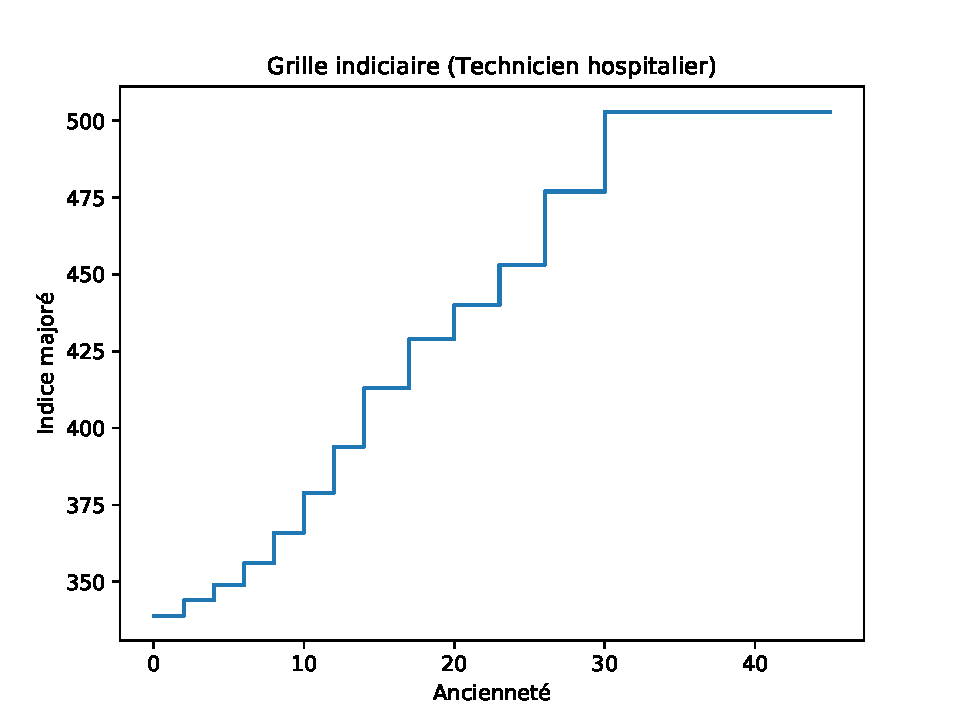
\includegraphics[width=0.7\textwidth]{fig/grille_TechHosp.pdf}\end{minipage} 
\begin{minipage}{0.3\linewidth} 
 \begin{center} 

\begin{tabular}[htb]{|c|c|} 
\hline 
 Indice majoré &  Durée (années) \\ 
\hline \hline 
 339 &  2.00 \\ 
\hline 
 344 &  2.00 \\ 
\hline 
 349 &  2.00 \\ 
\hline 
 356 &  2.00 \\ 
\hline 
 366 &  2.00 \\ 
\hline 
 379 &  2.00 \\ 
\hline 
 394 &  2.00 \\ 
\hline 
 413 &  3.00 \\ 
\hline 
 429 &  3.00 \\ 
\hline 
 440 &  3.00 \\ 
\hline 
 453 &  3.00 \\ 
\hline 
 477 &  4.00 \\ 
\hline 
 503 &   \\ 
\hline 
\hline 
\end{tabular} 
\end{center} 
 \end{minipage} 


 \addto{\captionsenglish}{ \renewcommand{\mtctitle}{}} \setcounter{minitocdepth}{2} 
 \minitoc \newpage 

\section{Début de carrière à 22 ans} 

\subsection{Génération 1975 (début en 1997)} 

\paragraph{Retraites possibles dans le modèle \emph{Gouvernement truqué (âge-pivot bloqué à 65 ans)}}  
 
{ \scriptsize \begin{center} 
\begin{tabular}[htb]{|c|c||c|c||c|c||c||c|c|c|c|c|c|} 
\hline 
 Retraite en &  Âge &  Âge pivot &  Décote/Surcote &  Retraite (\euro{} 2019) &  Tx Rempl(\%) &  SMIC (\euro{} 2019) &  Retraite/SMIC &  Rev70/SMIC &  Rev75/SMIC &  Rev80/SMIC &  Rev85/SMIC &  Rev90/SMIC \\ 
\hline \hline 
 2037 &  62 &  64 ans 10 mois &  -14.17\% &  1321.60 &  {\bf 43.39} &  2143.00 &  {\bf {\color{red} 0.62}} &  {\bf {\color{red} 0.56}} &  {\bf {\color{red} 0.52}} &  {\bf {\color{red} 0.49}} &  {\bf {\color{red} 0.46}} &  {\bf {\color{red} 0.43}} \\ 
\hline 
 2038 &  63 &  64 ans 11 mois &  -9.58\% &  1441.19 &  {\bf 47.23} &  2170.86 &  {\bf {\color{red} 0.66}} &  {\bf {\color{red} 0.61}} &  {\bf {\color{red} 0.57}} &  {\bf {\color{red} 0.53}} &  {\bf {\color{red} 0.50}} &  {\bf {\color{red} 0.47}} \\ 
\hline 
 2039 &  64 &  65 ans 0 mois &  -5.00\% &  1567.38 &  {\bf 51.27} &  2199.08 &  {\bf {\color{red} 0.71}} &  {\bf {\color{red} 0.66}} &  {\bf {\color{red} 0.62}} &  {\bf {\color{red} 0.58}} &  {\bf {\color{red} 0.54}} &  {\bf {\color{red} 0.51}} \\ 
\hline 
 2040 &  65 &  65 ans 0 mois &  0.00\% &  1893.52 &  {\bf 61.82} &  2227.67 &  {\bf {\color{red} 0.85}} &  {\bf {\color{red} 0.80}} &  {\bf {\color{red} 0.75}} &  {\bf {\color{red} 0.70}} &  {\bf {\color{red} 0.66}} &  {\bf {\color{red} 0.62}} \\ 
\hline 
 2041 &  66 &  65 ans 0 mois &  5.00\% &  1918.14 &  {\bf 62.52} &  2256.63 &  {\bf {\color{red} 0.85}} &  {\bf {\color{red} 0.81}} &  {\bf {\color{red} 0.76}} &  {\bf {\color{red} 0.71}} &  {\bf {\color{red} 0.67}} &  {\bf {\color{red} 0.62}} \\ 
\hline 
 2042 &  67 &  65 ans 0 mois &  10.00\% &  2011.85 &  {\bf 65.45} &  2285.97 &  {\bf {\color{red} 0.88}} &  {\bf {\color{red} 0.85}} &  {\bf {\color{red} 0.79}} &  {\bf {\color{red} 0.74}} &  {\bf {\color{red} 0.70}} &  {\bf {\color{red} 0.65}} \\ 
\hline 
\hline 
\end{tabular} 
\end{center} } 
\paragraph{Retraites possibles dans le modèle \emph{Gouvernement corrigé (âge-pivot glissant)}}  
 
{ \scriptsize \begin{center} 
\begin{tabular}[htb]{|c|c||c|c||c|c||c||c|c|c|c|c|c|} 
\hline 
 Retraite en &  Âge &  Âge pivot &  Décote/Surcote &  Retraite (\euro{} 2019) &  Tx Rempl(\%) &  SMIC (\euro{} 2019) &  Retraite/SMIC &  Rev70/SMIC &  Rev75/SMIC &  Rev80/SMIC &  Rev85/SMIC &  Rev90/SMIC \\ 
\hline \hline 
 2037 &  62 &  64 ans 10 mois &  -14.17\% &  1321.60 &  {\bf 43.39} &  2143.00 &  {\bf {\color{red} 0.62}} &  {\bf {\color{red} 0.56}} &  {\bf {\color{red} 0.52}} &  {\bf {\color{red} 0.49}} &  {\bf {\color{red} 0.46}} &  {\bf {\color{red} 0.43}} \\ 
\hline 
 2038 &  63 &  64 ans 11 mois &  -9.58\% &  1441.19 &  {\bf 47.23} &  2170.86 &  {\bf {\color{red} 0.66}} &  {\bf {\color{red} 0.61}} &  {\bf {\color{red} 0.57}} &  {\bf {\color{red} 0.53}} &  {\bf {\color{red} 0.50}} &  {\bf {\color{red} 0.47}} \\ 
\hline 
 2039 &  64 &  65 ans 0 mois &  -5.00\% &  1567.38 &  {\bf 51.27} &  2199.08 &  {\bf {\color{red} 0.71}} &  {\bf {\color{red} 0.66}} &  {\bf {\color{red} 0.62}} &  {\bf {\color{red} 0.58}} &  {\bf {\color{red} 0.54}} &  {\bf {\color{red} 0.51}} \\ 
\hline 
 2040 &  65 &  65 ans 1 mois &  -0.42\% &  1893.52 &  {\bf 61.82} &  2227.67 &  {\bf {\color{red} 0.85}} &  {\bf {\color{red} 0.80}} &  {\bf {\color{red} 0.75}} &  {\bf {\color{red} 0.70}} &  {\bf {\color{red} 0.66}} &  {\bf {\color{red} 0.62}} \\ 
\hline 
 2041 &  66 &  65 ans 2 mois &  4.17\% &  1918.14 &  {\bf 62.52} &  2256.63 &  {\bf {\color{red} 0.85}} &  {\bf {\color{red} 0.81}} &  {\bf {\color{red} 0.76}} &  {\bf {\color{red} 0.71}} &  {\bf {\color{red} 0.67}} &  {\bf {\color{red} 0.62}} \\ 
\hline 
 2042 &  67 &  65 ans 3 mois &  8.75\% &  1988.99 &  {\bf 64.71} &  2285.97 &  {\bf {\color{red} 0.87}} &  {\bf {\color{red} 0.84}} &  {\bf {\color{red} 0.78}} &  {\bf {\color{red} 0.74}} &  {\bf {\color{red} 0.69}} &  {\bf {\color{red} 0.65}} \\ 
\hline 
\hline 
\end{tabular} 
\end{center} } 
\paragraph{Retraites possibles dans le modèle \emph{Destinie2 (revalorisation de la fonction publique)}}  
 
{ \scriptsize \begin{center} 
\begin{tabular}[htb]{|c|c||c|c||c|c||c||c|c|c|c|c|c|} 
\hline 
 Retraite en &  Âge &  Âge pivot &  Décote/Surcote &  Retraite (\euro{} 2019) &  Tx Rempl(\%) &  SMIC (\euro{} 2019) &  Retraite/SMIC &  Rev70/SMIC &  Rev75/SMIC &  Rev80/SMIC &  Rev85/SMIC &  Rev90/SMIC \\ 
\hline \hline 
 2037 &  62 &  64 ans 10 mois &  -14.17\% &  1397.68 &  {\bf 37.00} &  2014.82 &  {\bf {\color{red} 0.69}} &  {\bf {\color{red} 0.63}} &  {\bf {\color{red} 0.59}} &  {\bf {\color{red} 0.55}} &  {\bf {\color{red} 0.52}} &  {\bf {\color{red} 0.48}} \\ 
\hline 
 2038 &  63 &  64 ans 11 mois &  -9.58\% &  1531.78 &  {\bf 39.96} &  2041.01 &  {\bf {\color{red} 0.75}} &  {\bf {\color{red} 0.69}} &  {\bf {\color{red} 0.64}} &  {\bf {\color{red} 0.60}} &  {\bf {\color{red} 0.56}} &  {\bf {\color{red} 0.53}} \\ 
\hline 
 2039 &  64 &  65 ans 0 mois &  -5.00\% &  1674.38 &  {\bf 43.04} &  2067.55 &  {\bf {\color{red} 0.81}} &  {\bf {\color{red} 0.75}} &  {\bf {\color{red} 0.70}} &  {\bf {\color{red} 0.66}} &  {\bf {\color{red} 0.62}} &  {\bf {\color{red} 0.58}} \\ 
\hline 
 2040 &  65 &  65 ans 1 mois &  -0.42\% &  1825.96 &  {\bf 46.25} &  2094.43 &  {\bf {\color{red} 0.87}} &  {\bf {\color{red} 0.82}} &  {\bf {\color{red} 0.77}} &  {\bf {\color{red} 0.72}} &  {\bf {\color{red} 0.67}} &  {\bf {\color{red} 0.63}} \\ 
\hline 
 2041 &  66 &  65 ans 2 mois &  4.17\% &  1987.04 &  {\bf 49.60} &  2121.65 &  {\bf {\color{red} 0.94}} &  {\bf {\color{red} 0.89}} &  {\bf {\color{red} 0.83}} &  {\bf {\color{red} 0.78}} &  {\bf {\color{red} 0.73}} &  {\bf {\color{red} 0.69}} \\ 
\hline 
 2042 &  67 &  65 ans 3 mois &  8.75\% &  2158.20 &  {\bf 53.08} &  2149.23 &  {\bf 1.00} &  {\bf {\color{red} 0.97}} &  {\bf {\color{red} 0.91}} &  {\bf {\color{red} 0.85}} &  {\bf {\color{red} 0.80}} &  {\bf {\color{red} 0.75}} \\ 
\hline 
\hline 
\end{tabular} 
\end{center} } 

 \begin{center}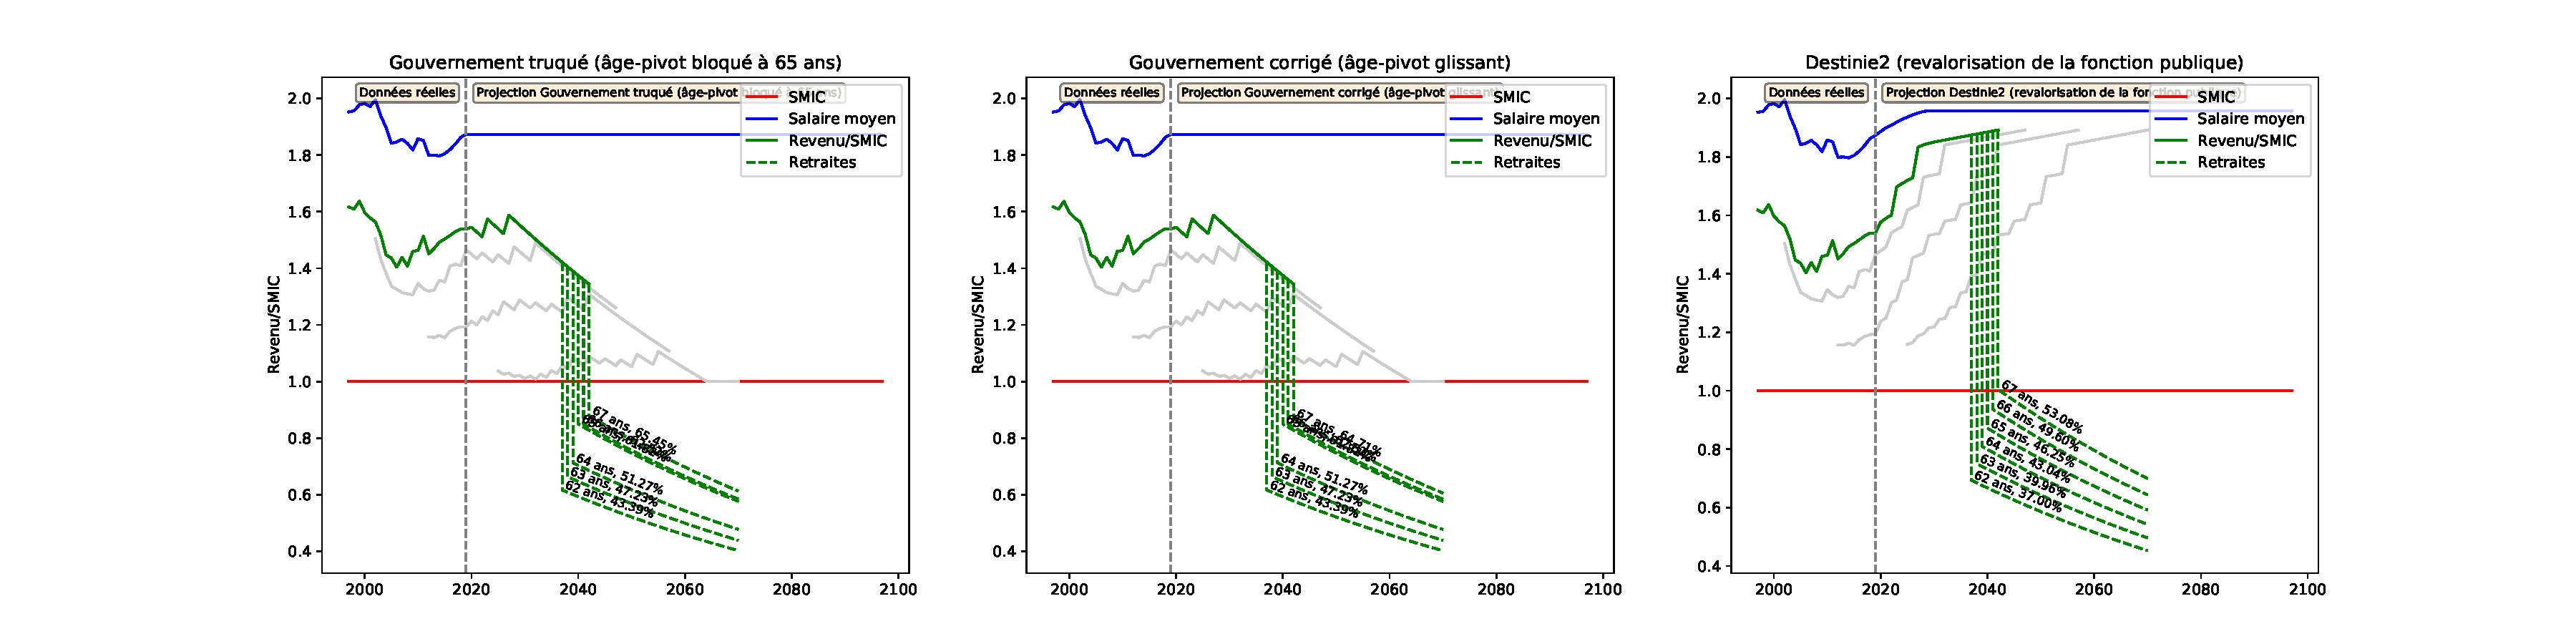
\includegraphics[width=0.9\textwidth]{fig/TechHosp_1975_22_dest_retraite.pdf}\end{center} \label{fig/TechHosp_1975_22_dest_retraite.pdf} 

\newpage 
 
\paragraph{Revenus et points pour le modèle \emph{Gouvernement truqué (âge-pivot bloqué à 65 ans)}} 
 
{ \scriptsize \begin{center} 
\begin{tabular}[htb]{|c|c||c|c|c|c|c|c||c|c||c|c|c|} 
\hline 
 Année &  Âge &  Ind Maj &  Pt Ind(\euro{} 2019) &  Rev HP(\euro{} 2019) &  Tx Primes &  GIPA(\euro{} 2019) &  Revenu(\euro{} 2019) &  SMIC(\euro{} 2019) &  Rev/SMIC &  Cumul Pts &  Achat Pt(\euro{} 2019) &  Serv. Pt(\euro{} 2019) \\ 
\hline \hline 
 1997 &  22 &  339.0 &  5.53 &  1876.15 &  17.11 &  0.00 &  2197.15 &  1358.84 &  {\bf 1.62} &  740.47 &  35.61 &  0.50 \\ 
\hline 
 1998 &  23 &  339.0 &  5.57 &  1887.03 &  17.34 &  0.00 &  2214.24 &  1376.36 &  {\bf 1.61} &  1486.69 &  35.61 &  0.50 \\ 
\hline 
 1999 &  24 &  344.0 &  5.61 &  1930.34 &  17.57 &  0.00 &  2269.50 &  1386.54 &  {\bf 1.64} &  2251.54 &  35.61 &  0.50 \\ 
\hline 
 2000 &  25 &  344.0 &  5.55 &  1907.54 &  17.80 &  0.00 &  2247.09 &  1407.00 &  {\bf 1.60} &  3008.84 &  35.61 &  0.50 \\ 
\hline 
 2001 &  26 &  349.0 &  5.52 &  1926.66 &  18.03 &  0.00 &  2274.03 &  1441.04 &  {\bf 1.58} &  3775.21 &  35.61 &  0.50 \\ 
\hline 
 2002 &  27 &  349.0 &  5.49 &  1914.71 &  18.26 &  0.00 &  2264.34 &  1447.74 &  {\bf 1.56} &  4538.32 &  35.61 &  0.50 \\ 
\hline 
 2003 &  28 &  356.0 &  5.37 &  1913.36 &  18.49 &  0.00 &  2267.15 &  1493.03 &  {\bf 1.52} &  5302.38 &  35.61 &  0.50 \\ 
\hline 
 2004 &  29 &  356.0 &  5.29 &  1883.14 &  18.72 &  4.17 &  2239.83 &  1547.32 &  {\bf 1.45} &  6057.23 &  35.61 &  0.50 \\ 
\hline 
 2005 &  30 &  366.0 &  5.29 &  1935.83 &  18.95 &  0.00 &  2302.67 &  1603.67 &  {\bf 1.44} &  6833.25 &  35.61 &  0.50 \\ 
\hline 
 2006 &  31 &  366.0 &  5.23 &  1914.22 &  19.18 &  0.00 &  2281.37 &  1625.00 &  {\bf 1.40} &  7602.10 &  35.61 &  0.50 \\ 
\hline 
 2007 &  32 &  379.0 &  5.19 &  1968.71 &  19.41 &  0.00 &  2350.84 &  1634.08 &  {\bf 1.44} &  8394.36 &  35.61 &  0.50 \\ 
\hline 
 2008 &  33 &  379.0 &  5.09 &  1930.26 &  19.64 &  0.00 &  2309.37 &  1640.24 &  {\bf 1.41} &  9172.65 &  35.61 &  0.50 \\ 
\hline 
 2009 &  34 &  394.0 &  5.13 &  2020.88 &  19.87 &  0.00 &  2422.43 &  1659.42 &  {\bf 1.46} &  9989.04 &  35.61 &  0.50 \\ 
\hline 
 2010 &  35 &  394.0 &  5.08 &  2000.47 &  20.10 &  0.00 &  2402.56 &  1641.90 &  {\bf 1.46} &  10798.73 &  35.61 &  0.50 \\ 
\hline 
 2011 &  36 &  413.0 &  4.97 &  2053.37 &  20.33 &  0.00 &  2470.82 &  1633.19 &  {\bf 1.51} &  11631.42 &  35.61 &  0.50 \\ 
\hline 
 2012 &  37 &  413.0 &  4.88 &  2013.97 &  20.56 &  0.00 &  2428.04 &  1673.05 &  {\bf 1.45} &  12449.70 &  35.61 &  0.50 \\ 
\hline 
 2013 &  38 &  413.0 &  4.83 &  1996.71 &  20.79 &  33.68 &  2445.51 &  1664.01 &  {\bf 1.47} &  13273.87 &  35.61 &  0.50 \\ 
\hline 
 2014 &  39 &  429.0 &  4.81 &  2063.68 &  21.02 &  0.00 &  2497.47 &  1673.24 &  {\bf 1.49} &  14115.55 &  35.61 &  0.50 \\ 
\hline 
 2015 &  40 &  429.0 &  4.81 &  2062.88 &  21.25 &  34.25 &  2535.48 &  1686.62 &  {\bf 1.50} &  14970.03 &  35.61 &  0.50 \\ 
\hline 
 2016 &  41 &  429.0 &  4.80 &  2058.76 &  21.48 &  67.14 &  2568.12 &  1693.76 &  {\bf 1.52} &  15835.52 &  35.61 &  0.50 \\ 
\hline 
 2017 &  42 &  440.0 &  4.81 &  2115.81 &  21.71 &  13.80 &  2588.95 &  1692.60 &  {\bf 1.53} &  16708.03 &  35.61 &  0.50 \\ 
\hline 
 2018 &  43 &  440.0 &  4.74 &  2086.59 &  21.94 &  56.70 &  2601.10 &  1689.76 &  {\bf 1.54} &  17584.63 &  35.61 &  0.50 \\ 
\hline 
 2019 &  44 &  440.0 &  4.79 &  2109.55 &  22.17 &  36.37 &  2613.60 &  1698.45 &  {\bf 1.54} &  18465.45 &  35.61 &  0.50 \\ 
\hline 
 2020 &  45 &  453.0 &  4.79 &  2171.87 &  22.40 &  0.00 &  2658.37 &  1720.53 &  {\bf 1.55} &  19361.35 &  35.61 &  0.50 \\ 
\hline 
 2021 &  46 &  453.0 &  4.79 &  2171.87 &  22.63 &  0.00 &  2663.37 &  1742.90 &  {\bf 1.53} &  20258.94 &  35.61 &  0.50 \\ 
\hline 
 2022 &  47 &  453.0 &  4.79 &  2171.87 &  22.86 &  0.00 &  2668.36 &  1765.55 &  {\bf 1.51} &  21158.21 &  35.61 &  0.50 \\ 
\hline 
 2023 &  48 &  477.0 &  4.79 &  2286.94 &  23.09 &  0.00 &  2814.99 &  1788.51 &  {\bf 1.57} &  22106.90 &  35.61 &  0.50 \\ 
\hline 
 2024 &  49 &  477.0 &  4.79 &  2286.94 &  23.32 &  0.00 &  2820.25 &  1811.76 &  {\bf 1.56} &  23057.35 &  35.61 &  0.50 \\ 
\hline 
 2025 &  50 &  477.0 &  4.79 &  2286.94 &  23.55 &  0.00 &  2825.51 &  1835.31 &  {\bf 1.54} &  24009.59 &  35.61 &  0.50 \\ 
\hline 
 2026 &  51 &  477.0 &  4.79 &  2286.94 &  23.78 &  0.00 &  2830.77 &  1859.17 &  {\bf 1.52} &  24963.59 &  35.61 &  0.50 \\ 
\hline 
 2027 &  52 &  503.0 &  4.79 &  2411.59 &  24.01 &  0.00 &  2990.62 &  1883.34 &  {\bf 1.59} &  25971.47 &  35.61 &  0.50 \\ 
\hline 
 2028 &  53 &  503.0 &  4.79 &  2411.59 &  24.24 &  0.00 &  2996.16 &  1907.82 &  {\bf 1.57} &  26981.21 &  35.61 &  0.50 \\ 
\hline 
 2029 &  54 &  503.0 &  4.79 &  2411.59 &  24.47 &  0.00 &  3001.71 &  1932.62 &  {\bf 1.55} &  27992.06 &  35.63 &  0.50 \\ 
\hline 
 2030 &  55 &  503.0 &  4.79 &  2411.59 &  24.70 &  0.00 &  3007.26 &  1957.75 &  {\bf 1.54} &  29003.23 &  35.69 &  0.50 \\ 
\hline 
 2031 &  56 &  503.0 &  4.79 &  2411.59 &  24.93 &  0.00 &  3012.80 &  1983.20 &  {\bf 1.52} &  30013.97 &  35.77 &  0.50 \\ 
\hline 
 2032 &  57 &  503.0 &  4.79 &  2411.59 &  25.16 &  0.00 &  3018.35 &  2008.98 &  {\bf 1.50} &  31023.49 &  35.88 &  0.50 \\ 
\hline 
 2033 &  58 &  503.0 &  4.79 &  2411.59 &  25.39 &  0.00 &  3023.90 &  2035.10 &  {\bf 1.49} &  32031.03 &  36.02 &  0.50 \\ 
\hline 
 2034 &  59 &  503.0 &  4.79 &  2411.59 &  25.62 &  0.00 &  3029.44 &  2061.55 &  {\bf 1.47} &  33035.83 &  36.18 &  0.50 \\ 
\hline 
 2035 &  60 &  503.0 &  4.79 &  2411.59 &  25.85 &  0.00 &  3034.99 &  2088.35 &  {\bf 1.45} &  34037.13 &  36.37 &  0.51 \\ 
\hline 
 2036 &  61 &  503.0 &  4.79 &  2411.59 &  26.08 &  0.00 &  3040.54 &  2115.50 &  {\bf 1.44} &  35034.18 &  36.59 &  0.51 \\ 
\hline 
 2037 &  62 &  503.0 &  4.79 &  2411.59 &  26.31 &  0.00 &  3046.08 &  2143.00 &  {\bf 1.42} &  36026.24 &  36.85 &  0.51 \\ 
\hline 
 2038 &  63 &  503.0 &  4.79 &  2411.59 &  26.54 &  0.00 &  3051.63 &  2170.86 &  {\bf 1.41} &  37012.59 &  37.13 &  0.52 \\ 
\hline 
 2039 &  64 &  503.0 &  4.79 &  2411.59 &  26.77 &  0.00 &  3057.18 &  2199.08 &  {\bf 1.39} &  37992.50 &  37.44 &  0.52 \\ 
\hline 
 2040 &  65 &  503.0 &  4.79 &  2411.59 &  27.00 &  0.00 &  3062.72 &  2227.67 &  {\bf 1.37} &  38965.29 &  37.78 &  0.53 \\ 
\hline 
 2041 &  66 &  503.0 &  4.79 &  2411.59 &  27.23 &  0.00 &  3068.27 &  2256.63 &  {\bf 1.36} &  39930.25 &  38.16 &  0.53 \\ 
\hline 
 2042 &  67 &  503.0 &  4.79 &  2411.59 &  27.46 &  0.00 &  3073.82 &  2285.97 &  {\bf 1.34} &  40886.74 &  38.56 &  0.54 \\ 
\hline 
\hline 
\end{tabular} 
\end{center} } 
\newpage 
 
\paragraph{Revenus et points pour le modèle \emph{Gouvernement corrigé (âge-pivot glissant)}} 
 
{ \scriptsize \begin{center} 
\begin{tabular}[htb]{|c|c||c|c|c|c|c|c||c|c||c|c|c|} 
\hline 
 Année &  Âge &  Ind Maj &  Pt Ind(\euro{} 2019) &  Rev HP(\euro{} 2019) &  Tx Primes &  GIPA(\euro{} 2019) &  Revenu(\euro{} 2019) &  SMIC(\euro{} 2019) &  Rev/SMIC &  Cumul Pts &  Achat Pt(\euro{} 2019) &  Serv. Pt(\euro{} 2019) \\ 
\hline \hline 
 1997 &  22 &  339.0 &  5.53 &  1876.15 &  17.11 &  0.00 &  2197.15 &  1358.84 &  {\bf 1.62} &  740.47 &  35.61 &  0.50 \\ 
\hline 
 1998 &  23 &  339.0 &  5.57 &  1887.03 &  17.34 &  0.00 &  2214.24 &  1376.36 &  {\bf 1.61} &  1486.69 &  35.61 &  0.50 \\ 
\hline 
 1999 &  24 &  344.0 &  5.61 &  1930.34 &  17.57 &  0.00 &  2269.50 &  1386.54 &  {\bf 1.64} &  2251.54 &  35.61 &  0.50 \\ 
\hline 
 2000 &  25 &  344.0 &  5.55 &  1907.54 &  17.80 &  0.00 &  2247.09 &  1407.00 &  {\bf 1.60} &  3008.84 &  35.61 &  0.50 \\ 
\hline 
 2001 &  26 &  349.0 &  5.52 &  1926.66 &  18.03 &  0.00 &  2274.03 &  1441.04 &  {\bf 1.58} &  3775.21 &  35.61 &  0.50 \\ 
\hline 
 2002 &  27 &  349.0 &  5.49 &  1914.71 &  18.26 &  0.00 &  2264.34 &  1447.74 &  {\bf 1.56} &  4538.32 &  35.61 &  0.50 \\ 
\hline 
 2003 &  28 &  356.0 &  5.37 &  1913.36 &  18.49 &  0.00 &  2267.15 &  1493.03 &  {\bf 1.52} &  5302.38 &  35.61 &  0.50 \\ 
\hline 
 2004 &  29 &  356.0 &  5.29 &  1883.14 &  18.72 &  4.17 &  2239.83 &  1547.32 &  {\bf 1.45} &  6057.23 &  35.61 &  0.50 \\ 
\hline 
 2005 &  30 &  366.0 &  5.29 &  1935.83 &  18.95 &  0.00 &  2302.67 &  1603.67 &  {\bf 1.44} &  6833.25 &  35.61 &  0.50 \\ 
\hline 
 2006 &  31 &  366.0 &  5.23 &  1914.22 &  19.18 &  0.00 &  2281.37 &  1625.00 &  {\bf 1.40} &  7602.10 &  35.61 &  0.50 \\ 
\hline 
 2007 &  32 &  379.0 &  5.19 &  1968.71 &  19.41 &  0.00 &  2350.84 &  1634.08 &  {\bf 1.44} &  8394.36 &  35.61 &  0.50 \\ 
\hline 
 2008 &  33 &  379.0 &  5.09 &  1930.26 &  19.64 &  0.00 &  2309.37 &  1640.24 &  {\bf 1.41} &  9172.65 &  35.61 &  0.50 \\ 
\hline 
 2009 &  34 &  394.0 &  5.13 &  2020.88 &  19.87 &  0.00 &  2422.43 &  1659.42 &  {\bf 1.46} &  9989.04 &  35.61 &  0.50 \\ 
\hline 
 2010 &  35 &  394.0 &  5.08 &  2000.47 &  20.10 &  0.00 &  2402.56 &  1641.90 &  {\bf 1.46} &  10798.73 &  35.61 &  0.50 \\ 
\hline 
 2011 &  36 &  413.0 &  4.97 &  2053.37 &  20.33 &  0.00 &  2470.82 &  1633.19 &  {\bf 1.51} &  11631.42 &  35.61 &  0.50 \\ 
\hline 
 2012 &  37 &  413.0 &  4.88 &  2013.97 &  20.56 &  0.00 &  2428.04 &  1673.05 &  {\bf 1.45} &  12449.70 &  35.61 &  0.50 \\ 
\hline 
 2013 &  38 &  413.0 &  4.83 &  1996.71 &  20.79 &  33.68 &  2445.51 &  1664.01 &  {\bf 1.47} &  13273.87 &  35.61 &  0.50 \\ 
\hline 
 2014 &  39 &  429.0 &  4.81 &  2063.68 &  21.02 &  0.00 &  2497.47 &  1673.24 &  {\bf 1.49} &  14115.55 &  35.61 &  0.50 \\ 
\hline 
 2015 &  40 &  429.0 &  4.81 &  2062.88 &  21.25 &  34.25 &  2535.48 &  1686.62 &  {\bf 1.50} &  14970.03 &  35.61 &  0.50 \\ 
\hline 
 2016 &  41 &  429.0 &  4.80 &  2058.76 &  21.48 &  67.14 &  2568.12 &  1693.76 &  {\bf 1.52} &  15835.52 &  35.61 &  0.50 \\ 
\hline 
 2017 &  42 &  440.0 &  4.81 &  2115.81 &  21.71 &  13.80 &  2588.95 &  1692.60 &  {\bf 1.53} &  16708.03 &  35.61 &  0.50 \\ 
\hline 
 2018 &  43 &  440.0 &  4.74 &  2086.59 &  21.94 &  56.70 &  2601.10 &  1689.76 &  {\bf 1.54} &  17584.63 &  35.61 &  0.50 \\ 
\hline 
 2019 &  44 &  440.0 &  4.79 &  2109.55 &  22.17 &  36.37 &  2613.60 &  1698.45 &  {\bf 1.54} &  18465.45 &  35.61 &  0.50 \\ 
\hline 
 2020 &  45 &  453.0 &  4.79 &  2171.87 &  22.40 &  0.00 &  2658.37 &  1720.53 &  {\bf 1.55} &  19361.35 &  35.61 &  0.50 \\ 
\hline 
 2021 &  46 &  453.0 &  4.79 &  2171.87 &  22.63 &  0.00 &  2663.37 &  1742.90 &  {\bf 1.53} &  20258.94 &  35.61 &  0.50 \\ 
\hline 
 2022 &  47 &  453.0 &  4.79 &  2171.87 &  22.86 &  0.00 &  2668.36 &  1765.55 &  {\bf 1.51} &  21158.21 &  35.61 &  0.50 \\ 
\hline 
 2023 &  48 &  477.0 &  4.79 &  2286.94 &  23.09 &  0.00 &  2814.99 &  1788.51 &  {\bf 1.57} &  22106.90 &  35.61 &  0.50 \\ 
\hline 
 2024 &  49 &  477.0 &  4.79 &  2286.94 &  23.32 &  0.00 &  2820.25 &  1811.76 &  {\bf 1.56} &  23057.35 &  35.61 &  0.50 \\ 
\hline 
 2025 &  50 &  477.0 &  4.79 &  2286.94 &  23.55 &  0.00 &  2825.51 &  1835.31 &  {\bf 1.54} &  24009.59 &  35.61 &  0.50 \\ 
\hline 
 2026 &  51 &  477.0 &  4.79 &  2286.94 &  23.78 &  0.00 &  2830.77 &  1859.17 &  {\bf 1.52} &  24963.59 &  35.61 &  0.50 \\ 
\hline 
 2027 &  52 &  503.0 &  4.79 &  2411.59 &  24.01 &  0.00 &  2990.62 &  1883.34 &  {\bf 1.59} &  25971.47 &  35.61 &  0.50 \\ 
\hline 
 2028 &  53 &  503.0 &  4.79 &  2411.59 &  24.24 &  0.00 &  2996.16 &  1907.82 &  {\bf 1.57} &  26981.21 &  35.61 &  0.50 \\ 
\hline 
 2029 &  54 &  503.0 &  4.79 &  2411.59 &  24.47 &  0.00 &  3001.71 &  1932.62 &  {\bf 1.55} &  27992.06 &  35.63 &  0.50 \\ 
\hline 
 2030 &  55 &  503.0 &  4.79 &  2411.59 &  24.70 &  0.00 &  3007.26 &  1957.75 &  {\bf 1.54} &  29003.23 &  35.69 &  0.50 \\ 
\hline 
 2031 &  56 &  503.0 &  4.79 &  2411.59 &  24.93 &  0.00 &  3012.80 &  1983.20 &  {\bf 1.52} &  30013.97 &  35.77 &  0.50 \\ 
\hline 
 2032 &  57 &  503.0 &  4.79 &  2411.59 &  25.16 &  0.00 &  3018.35 &  2008.98 &  {\bf 1.50} &  31023.49 &  35.88 &  0.50 \\ 
\hline 
 2033 &  58 &  503.0 &  4.79 &  2411.59 &  25.39 &  0.00 &  3023.90 &  2035.10 &  {\bf 1.49} &  32031.03 &  36.02 &  0.50 \\ 
\hline 
 2034 &  59 &  503.0 &  4.79 &  2411.59 &  25.62 &  0.00 &  3029.44 &  2061.55 &  {\bf 1.47} &  33035.83 &  36.18 &  0.50 \\ 
\hline 
 2035 &  60 &  503.0 &  4.79 &  2411.59 &  25.85 &  0.00 &  3034.99 &  2088.35 &  {\bf 1.45} &  34037.13 &  36.37 &  0.51 \\ 
\hline 
 2036 &  61 &  503.0 &  4.79 &  2411.59 &  26.08 &  0.00 &  3040.54 &  2115.50 &  {\bf 1.44} &  35034.18 &  36.59 &  0.51 \\ 
\hline 
 2037 &  62 &  503.0 &  4.79 &  2411.59 &  26.31 &  0.00 &  3046.08 &  2143.00 &  {\bf 1.42} &  36026.24 &  36.85 &  0.51 \\ 
\hline 
 2038 &  63 &  503.0 &  4.79 &  2411.59 &  26.54 &  0.00 &  3051.63 &  2170.86 &  {\bf 1.41} &  37012.59 &  37.13 &  0.52 \\ 
\hline 
 2039 &  64 &  503.0 &  4.79 &  2411.59 &  26.77 &  0.00 &  3057.18 &  2199.08 &  {\bf 1.39} &  37992.50 &  37.44 &  0.52 \\ 
\hline 
 2040 &  65 &  503.0 &  4.79 &  2411.59 &  27.00 &  0.00 &  3062.72 &  2227.67 &  {\bf 1.37} &  38965.29 &  37.78 &  0.53 \\ 
\hline 
 2041 &  66 &  503.0 &  4.79 &  2411.59 &  27.23 &  0.00 &  3068.27 &  2256.63 &  {\bf 1.36} &  39930.25 &  38.16 &  0.53 \\ 
\hline 
 2042 &  67 &  503.0 &  4.79 &  2411.59 &  27.46 &  0.00 &  3073.82 &  2285.97 &  {\bf 1.34} &  40886.74 &  38.56 &  0.54 \\ 
\hline 
\hline 
\end{tabular} 
\end{center} } 
\newpage 
 
\paragraph{Revenus et points pour le modèle \emph{Destinie2 (revalorisation de la fonction publique)}} 
 
{ \scriptsize \begin{center} 
\begin{tabular}[htb]{|c|c||c|c|c|c|c|c||c|c||c|c|c|} 
\hline 
 Année &  Âge &  Ind Maj &  Pt Ind(\euro{} 2019) &  Rev HP(\euro{} 2019) &  Tx Primes &  GIPA(\euro{} 2019) &  Revenu(\euro{} 2019) &  SMIC(\euro{} 2019) &  Rev/SMIC &  Cumul Pts &  Achat Pt(\euro{} 2019) &  Serv. Pt(\euro{} 2019) \\ 
\hline \hline 
 1997 &  22 &  339.0 &  5.53 &  1876.15 &  17.11 &  0.00 &  2197.15 &  1358.84 &  {\bf 1.62} &  738.65 &  35.69 &  0.50 \\ 
\hline 
 1998 &  23 &  339.0 &  5.57 &  1887.03 &  17.34 &  0.00 &  2214.24 &  1376.36 &  {\bf 1.61} &  1483.04 &  35.69 &  0.50 \\ 
\hline 
 1999 &  24 &  344.0 &  5.61 &  1930.34 &  17.57 &  0.00 &  2269.50 &  1386.54 &  {\bf 1.64} &  2246.01 &  35.69 &  0.50 \\ 
\hline 
 2000 &  25 &  344.0 &  5.55 &  1907.54 &  17.80 &  0.00 &  2247.09 &  1407.00 &  {\bf 1.60} &  3001.44 &  35.69 &  0.50 \\ 
\hline 
 2001 &  26 &  349.0 &  5.52 &  1926.66 &  18.03 &  0.00 &  2274.03 &  1441.04 &  {\bf 1.58} &  3765.94 &  35.69 &  0.50 \\ 
\hline 
 2002 &  27 &  349.0 &  5.49 &  1914.71 &  18.26 &  0.00 &  2264.34 &  1447.74 &  {\bf 1.56} &  4527.17 &  35.69 &  0.50 \\ 
\hline 
 2003 &  28 &  356.0 &  5.37 &  1913.36 &  18.49 &  0.00 &  2267.15 &  1493.03 &  {\bf 1.52} &  5289.35 &  35.69 &  0.50 \\ 
\hline 
 2004 &  29 &  356.0 &  5.29 &  1883.14 &  18.72 &  4.17 &  2239.83 &  1547.32 &  {\bf 1.45} &  6042.35 &  35.69 &  0.50 \\ 
\hline 
 2005 &  30 &  366.0 &  5.29 &  1935.83 &  18.95 &  0.00 &  2302.67 &  1603.67 &  {\bf 1.44} &  6816.47 &  35.69 &  0.50 \\ 
\hline 
 2006 &  31 &  366.0 &  5.23 &  1914.22 &  19.18 &  0.00 &  2281.37 &  1625.00 &  {\bf 1.40} &  7583.43 &  35.69 &  0.50 \\ 
\hline 
 2007 &  32 &  379.0 &  5.19 &  1968.71 &  19.41 &  0.00 &  2350.84 &  1634.08 &  {\bf 1.44} &  8373.74 &  35.69 &  0.50 \\ 
\hline 
 2008 &  33 &  379.0 &  5.09 &  1930.26 &  19.64 &  0.00 &  2309.37 &  1640.24 &  {\bf 1.41} &  9150.11 &  35.69 &  0.50 \\ 
\hline 
 2009 &  34 &  394.0 &  5.13 &  2020.88 &  19.87 &  0.00 &  2422.43 &  1659.42 &  {\bf 1.46} &  9964.49 &  35.69 &  0.50 \\ 
\hline 
 2010 &  35 &  394.0 &  5.08 &  2000.47 &  20.10 &  0.00 &  2402.56 &  1641.90 &  {\bf 1.46} &  10772.20 &  35.69 &  0.50 \\ 
\hline 
 2011 &  36 &  413.0 &  4.97 &  2053.37 &  20.33 &  0.00 &  2470.82 &  1633.19 &  {\bf 1.51} &  11602.85 &  35.69 &  0.50 \\ 
\hline 
 2012 &  37 &  413.0 &  4.88 &  2013.97 &  20.56 &  0.00 &  2428.04 &  1673.05 &  {\bf 1.45} &  12419.11 &  35.69 &  0.50 \\ 
\hline 
 2013 &  38 &  413.0 &  4.83 &  1996.71 &  20.79 &  33.68 &  2445.51 &  1664.01 &  {\bf 1.47} &  13241.25 &  35.69 &  0.50 \\ 
\hline 
 2014 &  39 &  429.0 &  4.81 &  2063.68 &  21.02 &  0.00 &  2497.47 &  1673.24 &  {\bf 1.49} &  14080.86 &  35.69 &  0.50 \\ 
\hline 
 2015 &  40 &  429.0 &  4.81 &  2062.88 &  21.25 &  34.25 &  2535.48 &  1686.62 &  {\bf 1.50} &  14933.25 &  35.69 &  0.50 \\ 
\hline 
 2016 &  41 &  429.0 &  4.80 &  2058.76 &  21.48 &  67.14 &  2568.12 &  1693.76 &  {\bf 1.52} &  15796.62 &  35.69 &  0.50 \\ 
\hline 
 2017 &  42 &  440.0 &  4.81 &  2115.81 &  21.71 &  13.80 &  2588.95 &  1692.60 &  {\bf 1.53} &  16666.98 &  35.69 &  0.50 \\ 
\hline 
 2018 &  43 &  440.0 &  4.74 &  2086.59 &  21.94 &  56.70 &  2601.10 &  1689.76 &  {\bf 1.54} &  17541.43 &  35.69 &  0.50 \\ 
\hline 
 2019 &  44 &  440.0 &  4.79 &  2109.55 &  22.17 &  36.37 &  2613.60 &  1698.45 &  {\bf 1.54} &  18420.08 &  35.69 &  0.50 \\ 
\hline 
 2020 &  45 &  453.0 &  4.83 &  2189.25 &  22.40 &  0.00 &  2679.64 &  1699.99 &  {\bf 1.58} &  19320.93 &  35.69 &  0.50 \\ 
\hline 
 2021 &  46 &  453.0 &  4.88 &  2208.95 &  22.63 &  0.00 &  2708.84 &  1703.48 &  {\bf 1.59} &  20231.60 &  35.69 &  0.50 \\ 
\hline 
 2022 &  47 &  453.0 &  4.93 &  2231.04 &  22.86 &  0.00 &  2741.06 &  1712.78 &  {\bf 1.60} &  21153.10 &  35.69 &  0.50 \\ 
\hline 
 2023 &  48 &  477.0 &  4.98 &  2376.73 &  23.09 &  0.00 &  2925.51 &  1723.51 &  {\bf 1.70} &  22136.61 &  35.69 &  0.50 \\ 
\hline 
 2024 &  49 &  477.0 &  5.04 &  2405.01 &  23.32 &  0.00 &  2965.86 &  1735.69 &  {\bf 1.71} &  23133.68 &  35.69 &  0.50 \\ 
\hline 
 2025 &  50 &  477.0 &  5.10 &  2434.35 &  23.55 &  0.00 &  3007.64 &  1749.35 &  {\bf 1.72} &  24144.80 &  35.69 &  0.50 \\ 
\hline 
 2026 &  51 &  477.0 &  5.17 &  2464.78 &  23.78 &  0.00 &  3050.91 &  1764.53 &  {\bf 1.73} &  25170.47 &  35.69 &  0.50 \\ 
\hline 
 2027 &  52 &  503.0 &  5.23 &  2632.40 &  24.01 &  0.00 &  3264.44 &  1781.27 &  {\bf 1.83} &  26267.92 &  35.69 &  0.50 \\ 
\hline 
 2028 &  53 &  503.0 &  5.30 &  2666.88 &  24.24 &  0.00 &  3313.34 &  1799.59 &  {\bf 1.84} &  27381.81 &  35.69 &  0.50 \\ 
\hline 
 2029 &  54 &  503.0 &  5.37 &  2699.15 &  24.47 &  0.00 &  3359.64 &  1819.55 &  {\bf 1.85} &  28510.47 &  35.72 &  0.50 \\ 
\hline 
 2030 &  55 &  503.0 &  5.43 &  2732.62 &  24.70 &  0.00 &  3407.58 &  1841.19 &  {\bf 1.85} &  29653.58 &  35.77 &  0.50 \\ 
\hline 
 2031 &  56 &  503.0 &  5.50 &  2767.33 &  24.93 &  0.00 &  3457.22 &  1864.58 &  {\bf 1.85} &  30810.75 &  35.85 &  0.50 \\ 
\hline 
 2032 &  57 &  503.0 &  5.57 &  2803.30 &  25.16 &  0.00 &  3508.61 &  1888.81 &  {\bf 1.86} &  31981.57 &  35.96 &  0.50 \\ 
\hline 
 2033 &  58 &  503.0 &  5.65 &  2839.74 &  25.39 &  0.00 &  3560.76 &  1913.37 &  {\bf 1.86} &  33165.28 &  36.10 &  0.50 \\ 
\hline 
 2034 &  59 &  503.0 &  5.72 &  2876.66 &  25.62 &  0.00 &  3613.66 &  1938.24 &  {\bf 1.86} &  34361.12 &  36.26 &  0.50 \\ 
\hline 
 2035 &  60 &  503.0 &  5.79 &  2914.06 &  25.85 &  0.00 &  3667.34 &  1963.44 &  {\bf 1.87} &  35568.28 &  36.46 &  0.51 \\ 
\hline 
 2036 &  61 &  503.0 &  5.87 &  2951.94 &  26.08 &  0.00 &  3721.81 &  1988.96 &  {\bf 1.87} &  36785.94 &  36.68 &  0.51 \\ 
\hline 
 2037 &  62 &  503.0 &  5.94 &  2990.32 &  26.31 &  0.00 &  3777.07 &  2014.82 &  {\bf 1.87} &  38013.27 &  36.93 &  0.51 \\ 
\hline 
 2038 &  63 &  503.0 &  6.02 &  3029.19 &  26.54 &  0.00 &  3833.14 &  2041.01 &  {\bf 1.88} &  39249.38 &  37.21 &  0.52 \\ 
\hline 
 2039 &  64 &  503.0 &  6.10 &  3068.57 &  26.77 &  0.00 &  3890.03 &  2067.55 &  {\bf 1.88} &  40493.40 &  37.52 &  0.52 \\ 
\hline 
 2040 &  65 &  503.0 &  6.18 &  3108.46 &  27.00 &  0.00 &  3947.75 &  2094.43 &  {\bf 1.88} &  41744.42 &  37.87 &  0.53 \\ 
\hline 
 2041 &  66 &  503.0 &  6.26 &  3148.87 &  27.23 &  0.00 &  4006.31 &  2121.65 &  {\bf 1.89} &  43001.52 &  38.24 &  0.53 \\ 
\hline 
 2042 &  67 &  503.0 &  6.34 &  3189.81 &  27.46 &  0.00 &  4065.73 &  2149.23 &  {\bf 1.89} &  44263.77 &  38.65 &  0.54 \\ 
\hline 
\hline 
\end{tabular} 
\end{center} } 
\newpage 
 
\subsection{Génération 1980 (début en 2002)} 

\paragraph{Retraites possibles dans le modèle \emph{Gouvernement truqué (âge-pivot bloqué à 65 ans)}}  
 
{ \scriptsize \begin{center} 
\begin{tabular}[htb]{|c|c||c|c||c|c||c||c|c|c|c|c|c|} 
\hline 
 Retraite en &  Âge &  Âge pivot &  Décote/Surcote &  Retraite (\euro{} 2019) &  Tx Rempl(\%) &  SMIC (\euro{} 2019) &  Retraite/SMIC &  Rev70/SMIC &  Rev75/SMIC &  Rev80/SMIC &  Rev85/SMIC &  Rev90/SMIC \\ 
\hline \hline 
 2042 &  62 &  65 ans 0 mois &  -15.00\% &  1334.51 &  {\bf 43.81} &  2285.97 &  {\bf {\color{red} 0.58}} &  {\bf {\color{red} 0.53}} &  {\bf {\color{red} 0.49}} &  {\bf {\color{red} 0.46}} &  {\bf {\color{red} 0.43}} &  {\bf {\color{red} 0.41}} \\ 
\hline 
 2043 &  63 &  65 ans 0 mois &  -10.00\% &  1467.43 &  {\bf 48.09} &  2315.68 &  {\bf {\color{red} 0.63}} &  {\bf {\color{red} 0.58}} &  {\bf {\color{red} 0.54}} &  {\bf {\color{red} 0.51}} &  {\bf {\color{red} 0.48}} &  {\bf {\color{red} 0.45}} \\ 
\hline 
 2044 &  64 &  65 ans 0 mois &  -5.00\% &  1608.33 &  {\bf 52.61} &  2345.79 &  {\bf {\color{red} 0.69}} &  {\bf {\color{red} 0.63}} &  {\bf {\color{red} 0.59}} &  {\bf {\color{red} 0.56}} &  {\bf {\color{red} 0.52}} &  {\bf {\color{red} 0.49}} \\ 
\hline 
 2045 &  65 &  65 ans 0 mois &  0.00\% &  2019.84 &  {\bf 65.95} &  2376.28 &  {\bf {\color{red} 0.85}} &  {\bf {\color{red} 0.80}} &  {\bf {\color{red} 0.75}} &  {\bf {\color{red} 0.70}} &  {\bf {\color{red} 0.66}} &  {\bf {\color{red} 0.62}} \\ 
\hline 
 2046 &  66 &  65 ans 0 mois &  5.00\% &  2046.10 &  {\bf 66.69} &  2407.18 &  {\bf {\color{red} 0.85}} &  {\bf {\color{red} 0.81}} &  {\bf {\color{red} 0.76}} &  {\bf {\color{red} 0.71}} &  {\bf {\color{red} 0.67}} &  {\bf {\color{red} 0.62}} \\ 
\hline 
 2047 &  67 &  65 ans 0 mois &  10.00\% &  2078.62 &  {\bf 67.62} &  2438.47 &  {\bf {\color{red} 0.85}} &  {\bf {\color{red} 0.82}} &  {\bf {\color{red} 0.77}} &  {\bf {\color{red} 0.72}} &  {\bf {\color{red} 0.68}} &  {\bf {\color{red} 0.63}} \\ 
\hline 
\hline 
\end{tabular} 
\end{center} } 
\paragraph{Retraites possibles dans le modèle \emph{Gouvernement corrigé (âge-pivot glissant)}}  
 
{ \scriptsize \begin{center} 
\begin{tabular}[htb]{|c|c||c|c||c|c||c||c|c|c|c|c|c|} 
\hline 
 Retraite en &  Âge &  Âge pivot &  Décote/Surcote &  Retraite (\euro{} 2019) &  Tx Rempl(\%) &  SMIC (\euro{} 2019) &  Retraite/SMIC &  Rev70/SMIC &  Rev75/SMIC &  Rev80/SMIC &  Rev85/SMIC &  Rev90/SMIC \\ 
\hline \hline 
 2042 &  62 &  65 ans 3 mois &  -16.25\% &  1314.88 &  {\bf 43.17} &  2285.97 &  {\bf {\color{red} 0.58}} &  {\bf {\color{red} 0.52}} &  {\bf {\color{red} 0.49}} &  {\bf {\color{red} 0.46}} &  {\bf {\color{red} 0.43}} &  {\bf {\color{red} 0.40}} \\ 
\hline 
 2043 &  63 &  65 ans 4 mois &  -11.67\% &  1440.26 &  {\bf 47.20} &  2315.68 &  {\bf {\color{red} 0.62}} &  {\bf {\color{red} 0.57}} &  {\bf {\color{red} 0.53}} &  {\bf {\color{red} 0.50}} &  {\bf {\color{red} 0.47}} &  {\bf {\color{red} 0.44}} \\ 
\hline 
 2044 &  64 &  65 ans 5 mois &  -7.08\% &  1573.06 &  {\bf 51.45} &  2345.79 &  {\bf {\color{red} 0.67}} &  {\bf {\color{red} 0.62}} &  {\bf {\color{red} 0.58}} &  {\bf {\color{red} 0.55}} &  {\bf {\color{red} 0.51}} &  {\bf {\color{red} 0.48}} \\ 
\hline 
 2045 &  65 &  65 ans 6 mois &  -2.50\% &  2019.84 &  {\bf 65.95} &  2376.28 &  {\bf {\color{red} 0.85}} &  {\bf {\color{red} 0.80}} &  {\bf {\color{red} 0.75}} &  {\bf {\color{red} 0.70}} &  {\bf {\color{red} 0.66}} &  {\bf {\color{red} 0.62}} \\ 
\hline 
 2046 &  66 &  65 ans 7 mois &  2.08\% &  2046.10 &  {\bf 66.69} &  2407.18 &  {\bf {\color{red} 0.85}} &  {\bf {\color{red} 0.81}} &  {\bf {\color{red} 0.76}} &  {\bf {\color{red} 0.71}} &  {\bf {\color{red} 0.67}} &  {\bf {\color{red} 0.62}} \\ 
\hline 
 2047 &  67 &  65 ans 8 mois &  6.67\% &  2072.70 &  {\bf 67.43} &  2438.47 &  {\bf {\color{red} 0.85}} &  {\bf {\color{red} 0.82}} &  {\bf {\color{red} 0.77}} &  {\bf {\color{red} 0.72}} &  {\bf {\color{red} 0.67}} &  {\bf {\color{red} 0.63}} \\ 
\hline 
\hline 
\end{tabular} 
\end{center} } 
\paragraph{Retraites possibles dans le modèle \emph{Destinie2 (revalorisation de la fonction publique)}}  
 
{ \scriptsize \begin{center} 
\begin{tabular}[htb]{|c|c||c|c||c|c||c||c|c|c|c|c|c|} 
\hline 
 Retraite en &  Âge &  Âge pivot &  Décote/Surcote &  Retraite (\euro{} 2019) &  Tx Rempl(\%) &  SMIC (\euro{} 2019) &  Retraite/SMIC &  Rev70/SMIC &  Rev75/SMIC &  Rev80/SMIC &  Rev85/SMIC &  Rev90/SMIC \\ 
\hline \hline 
 2042 &  62 &  65 ans 3 mois &  -16.25\% &  1442.14 &  {\bf 35.79} &  2149.23 &  {\bf {\color{red} 0.67}} &  {\bf {\color{red} 0.61}} &  {\bf {\color{red} 0.57}} &  {\bf {\color{red} 0.53}} &  {\bf {\color{red} 0.50}} &  {\bf {\color{red} 0.47}} \\ 
\hline 
 2043 &  63 &  65 ans 4 mois &  -11.67\% &  1588.77 &  {\bf 38.86} &  2177.17 &  {\bf {\color{red} 0.73}} &  {\bf {\color{red} 0.67}} &  {\bf {\color{red} 0.62}} &  {\bf {\color{red} 0.59}} &  {\bf {\color{red} 0.55}} &  {\bf {\color{red} 0.51}} \\ 
\hline 
 2044 &  64 &  65 ans 5 mois &  -7.08\% &  1745.32 &  {\bf 42.06} &  2205.48 &  {\bf {\color{red} 0.79}} &  {\bf {\color{red} 0.73}} &  {\bf {\color{red} 0.69}} &  {\bf {\color{red} 0.64}} &  {\bf {\color{red} 0.60}} &  {\bf {\color{red} 0.57}} \\ 
\hline 
 2045 &  65 &  65 ans 6 mois &  -2.50\% &  1912.37 &  {\bf 45.41} &  2234.15 &  {\bf {\color{red} 0.86}} &  {\bf {\color{red} 0.80}} &  {\bf {\color{red} 0.75}} &  {\bf {\color{red} 0.71}} &  {\bf {\color{red} 0.66}} &  {\bf {\color{red} 0.62}} \\ 
\hline 
 2046 &  66 &  65 ans 7 mois &  2.08\% &  2089.02 &  {\bf 48.88} &  2263.19 &  {\bf {\color{red} 0.92}} &  {\bf {\color{red} 0.88}} &  {\bf {\color{red} 0.82}} &  {\bf {\color{red} 0.77}} &  {\bf {\color{red} 0.72}} &  {\bf {\color{red} 0.68}} \\ 
\hline 
 2047 &  67 &  65 ans 8 mois &  6.67\% &  2275.58 &  {\bf 52.47} &  2292.61 &  {\bf {\color{red} 0.99}} &  {\bf {\color{red} 0.95}} &  {\bf {\color{red} 0.90}} &  {\bf {\color{red} 0.84}} &  {\bf {\color{red} 0.79}} &  {\bf {\color{red} 0.74}} \\ 
\hline 
\hline 
\end{tabular} 
\end{center} } 

 \begin{center}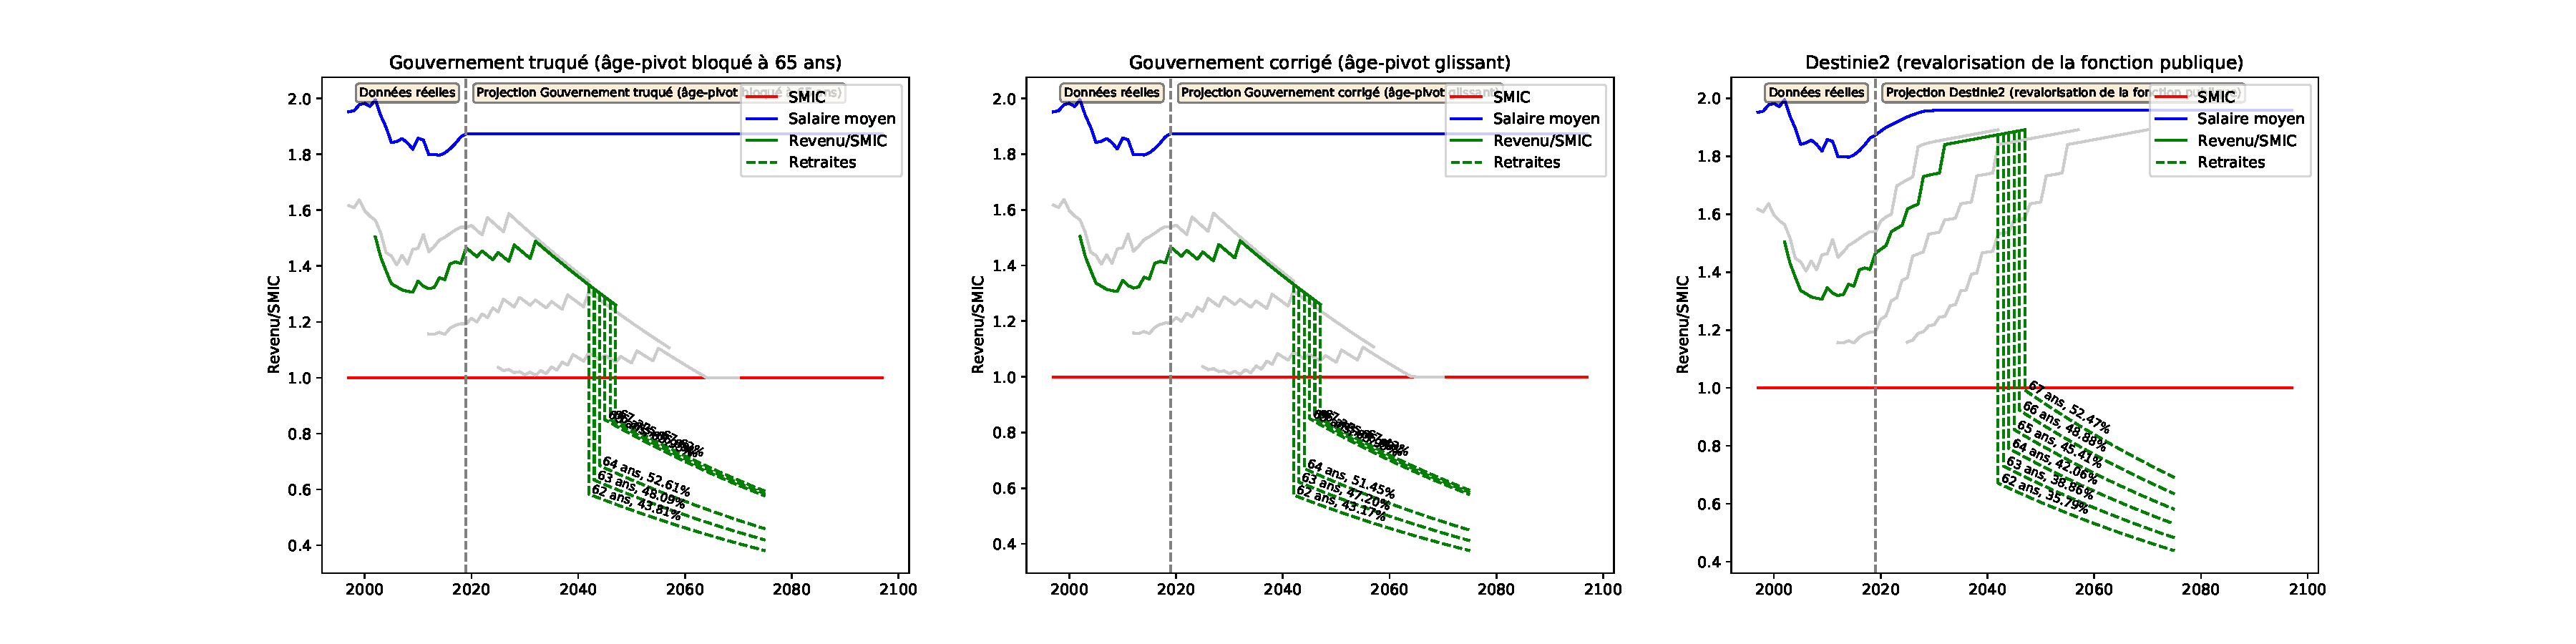
\includegraphics[width=0.9\textwidth]{fig/TechHosp_1980_22_dest_retraite.pdf}\end{center} \label{fig/TechHosp_1980_22_dest_retraite.pdf} 

\newpage 
 
\paragraph{Revenus et points pour le modèle \emph{Gouvernement truqué (âge-pivot bloqué à 65 ans)}} 
 
{ \scriptsize \begin{center} 
\begin{tabular}[htb]{|c|c||c|c|c|c|c|c||c|c||c|c|c|} 
\hline 
 Année &  Âge &  Ind Maj &  Pt Ind(\euro{} 2019) &  Rev HP(\euro{} 2019) &  Tx Primes &  GIPA(\euro{} 2019) &  Revenu(\euro{} 2019) &  SMIC(\euro{} 2019) &  Rev/SMIC &  Cumul Pts &  Achat Pt(\euro{} 2019) &  Serv. Pt(\euro{} 2019) \\ 
\hline \hline 
 2002 &  22 &  339.0 &  5.49 &  1859.85 &  17.11 &  0.00 &  2178.07 &  1447.74 &  {\bf 1.50} &  734.03 &  35.61 &  0.50 \\ 
\hline 
 2003 &  23 &  339.0 &  5.37 &  1822.00 &  17.34 &  0.00 &  2137.93 &  1493.03 &  {\bf 1.43} &  1454.54 &  35.61 &  0.50 \\ 
\hline 
 2004 &  24 &  344.0 &  5.29 &  1819.66 &  17.57 &  0.00 &  2139.38 &  1547.32 &  {\bf 1.38} &  2175.54 &  35.61 &  0.50 \\ 
\hline 
 2005 &  25 &  344.0 &  5.29 &  1819.47 &  17.80 &  0.00 &  2143.33 &  1603.67 &  {\bf 1.34} &  2897.87 &  35.61 &  0.50 \\ 
\hline 
 2006 &  26 &  349.0 &  5.23 &  1825.31 &  18.03 &  0.00 &  2154.42 &  1625.00 &  {\bf 1.33} &  3623.93 &  35.61 &  0.50 \\ 
\hline 
 2007 &  27 &  349.0 &  5.19 &  1812.87 &  18.26 &  3.68 &  2147.59 &  1634.08 &  {\bf 1.31} &  4347.70 &  35.61 &  0.50 \\ 
\hline 
 2008 &  28 &  356.0 &  5.09 &  1813.12 &  18.49 &  0.00 &  2148.37 &  1640.24 &  {\bf 1.31} &  5071.72 &  35.61 &  0.50 \\ 
\hline 
 2009 &  29 &  356.0 &  5.13 &  1825.97 &  18.72 &  0.00 &  2167.79 &  1659.42 &  {\bf 1.31} &  5802.30 &  35.61 &  0.50 \\ 
\hline 
 2010 &  30 &  366.0 &  5.08 &  1858.30 &  18.95 &  0.00 &  2210.45 &  1641.90 &  {\bf 1.35} &  6547.24 &  35.61 &  0.50 \\ 
\hline 
 2011 &  31 &  366.0 &  4.97 &  1819.69 &  19.18 &  0.00 &  2168.71 &  1633.19 &  {\bf 1.33} &  7278.12 &  35.61 &  0.50 \\ 
\hline 
 2012 &  32 &  379.0 &  4.88 &  1848.17 &  19.41 &  0.00 &  2206.90 &  1673.05 &  {\bf 1.32} &  8021.88 &  35.61 &  0.50 \\ 
\hline 
 2013 &  33 &  379.0 &  4.83 &  1832.33 &  19.64 &  9.33 &  2201.53 &  1664.01 &  {\bf 1.32} &  8763.82 &  35.61 &  0.50 \\ 
\hline 
 2014 &  34 &  394.0 &  4.81 &  1895.32 &  19.87 &  0.00 &  2271.92 &  1673.24 &  {\bf 1.36} &  9529.48 &  35.61 &  0.50 \\ 
\hline 
 2015 &  35 &  394.0 &  4.81 &  1894.58 &  20.10 &  4.21 &  2279.60 &  1686.62 &  {\bf 1.35} &  10297.74 &  35.61 &  0.50 \\ 
\hline 
 2016 &  36 &  413.0 &  4.80 &  1981.98 &  20.33 &  0.00 &  2384.91 &  1693.76 &  {\bf 1.41} &  11101.48 &  35.61 &  0.50 \\ 
\hline 
 2017 &  37 &  413.0 &  4.81 &  1985.97 &  20.56 &  0.00 &  2394.29 &  1692.60 &  {\bf 1.41} &  11908.38 &  35.61 &  0.50 \\ 
\hline 
 2018 &  38 &  413.0 &  4.74 &  1958.55 &  20.79 &  15.68 &  2381.42 &  1689.76 &  {\bf 1.41} &  12710.95 &  35.61 &  0.50 \\ 
\hline 
 2019 &  39 &  429.0 &  4.79 &  2056.81 &  21.02 &  0.00 &  2489.15 &  1698.45 &  {\bf 1.47} &  13549.82 &  35.61 &  0.50 \\ 
\hline 
 2020 &  40 &  429.0 &  4.79 &  2056.81 &  21.25 &  0.00 &  2493.88 &  1720.53 &  {\bf 1.45} &  14390.29 &  35.61 &  0.50 \\ 
\hline 
 2021 &  41 &  429.0 &  4.79 &  2056.81 &  21.48 &  0.00 &  2498.61 &  1742.90 &  {\bf 1.43} &  15232.35 &  35.61 &  0.50 \\ 
\hline 
 2022 &  42 &  440.0 &  4.79 &  2109.55 &  21.71 &  0.00 &  2567.53 &  1765.55 &  {\bf 1.45} &  16097.64 &  35.61 &  0.50 \\ 
\hline 
 2023 &  43 &  440.0 &  4.79 &  2109.55 &  21.94 &  0.00 &  2572.38 &  1788.51 &  {\bf 1.44} &  16964.56 &  35.61 &  0.50 \\ 
\hline 
 2024 &  44 &  440.0 &  4.79 &  2109.55 &  22.17 &  0.00 &  2577.23 &  1811.76 &  {\bf 1.42} &  17833.12 &  35.61 &  0.50 \\ 
\hline 
 2025 &  45 &  453.0 &  4.79 &  2171.87 &  22.40 &  0.00 &  2658.37 &  1835.31 &  {\bf 1.45} &  18729.03 &  35.61 &  0.50 \\ 
\hline 
 2026 &  46 &  453.0 &  4.79 &  2171.87 &  22.63 &  0.00 &  2663.37 &  1859.17 &  {\bf 1.43} &  19626.61 &  35.61 &  0.50 \\ 
\hline 
 2027 &  47 &  453.0 &  4.79 &  2171.87 &  22.86 &  0.00 &  2668.36 &  1883.34 &  {\bf 1.42} &  20525.88 &  35.61 &  0.50 \\ 
\hline 
 2028 &  48 &  477.0 &  4.79 &  2286.94 &  23.09 &  0.00 &  2814.99 &  1907.82 &  {\bf 1.48} &  21474.57 &  35.61 &  0.50 \\ 
\hline 
 2029 &  49 &  477.0 &  4.79 &  2286.94 &  23.32 &  0.00 &  2820.25 &  1932.62 &  {\bf 1.46} &  22424.31 &  35.63 &  0.50 \\ 
\hline 
 2030 &  50 &  477.0 &  4.79 &  2286.94 &  23.55 &  0.00 &  2825.51 &  1957.75 &  {\bf 1.44} &  23374.37 &  35.69 &  0.50 \\ 
\hline 
 2031 &  51 &  477.0 &  4.79 &  2286.94 &  23.78 &  0.00 &  2830.77 &  1983.20 &  {\bf 1.43} &  24324.04 &  35.77 &  0.50 \\ 
\hline 
 2032 &  52 &  503.0 &  4.79 &  2411.59 &  24.01 &  0.00 &  2990.62 &  2008.98 &  {\bf 1.49} &  25324.29 &  35.88 &  0.50 \\ 
\hline 
 2033 &  53 &  503.0 &  4.79 &  2411.59 &  24.24 &  0.00 &  2996.16 &  2035.10 &  {\bf 1.47} &  26322.59 &  36.02 &  0.50 \\ 
\hline 
 2034 &  54 &  503.0 &  4.79 &  2411.59 &  24.47 &  0.00 &  3001.71 &  2061.55 &  {\bf 1.46} &  27318.19 &  36.18 &  0.50 \\ 
\hline 
 2035 &  55 &  503.0 &  4.79 &  2411.59 &  24.70 &  0.00 &  3007.26 &  2088.35 &  {\bf 1.44} &  28310.34 &  36.37 &  0.51 \\ 
\hline 
 2036 &  56 &  503.0 &  4.79 &  2411.59 &  24.93 &  0.00 &  3012.80 &  2115.50 &  {\bf 1.42} &  29298.29 &  36.59 &  0.51 \\ 
\hline 
 2037 &  57 &  503.0 &  4.79 &  2411.59 &  25.16 &  0.00 &  3018.35 &  2143.00 &  {\bf 1.41} &  30281.32 &  36.85 &  0.51 \\ 
\hline 
 2038 &  58 &  503.0 &  4.79 &  2411.59 &  25.39 &  0.00 &  3023.90 &  2170.86 &  {\bf 1.39} &  31258.71 &  37.13 &  0.52 \\ 
\hline 
 2039 &  59 &  503.0 &  4.79 &  2411.59 &  25.62 &  0.00 &  3029.44 &  2199.08 &  {\bf 1.38} &  32229.73 &  37.44 &  0.52 \\ 
\hline 
 2040 &  60 &  503.0 &  4.79 &  2411.59 &  25.85 &  0.00 &  3034.99 &  2227.67 &  {\bf 1.36} &  33193.71 &  37.78 &  0.53 \\ 
\hline 
 2041 &  61 &  503.0 &  4.79 &  2411.59 &  26.08 &  0.00 &  3040.54 &  2256.63 &  {\bf 1.35} &  34149.95 &  38.16 &  0.53 \\ 
\hline 
 2042 &  62 &  503.0 &  4.79 &  2411.59 &  26.31 &  0.00 &  3046.08 &  2285.97 &  {\bf 1.33} &  35097.81 &  38.56 &  0.54 \\ 
\hline 
 2043 &  63 &  503.0 &  4.79 &  2411.59 &  26.54 &  0.00 &  3051.63 &  2315.68 &  {\bf 1.32} &  36036.62 &  39.01 &  0.54 \\ 
\hline 
 2044 &  64 &  503.0 &  4.79 &  2411.59 &  26.77 &  0.00 &  3057.18 &  2345.79 &  {\bf 1.30} &  36965.78 &  39.48 &  0.55 \\ 
\hline 
 2045 &  65 &  503.0 &  4.79 &  2411.59 &  27.00 &  0.00 &  3062.72 &  2376.28 &  {\bf 1.29} &  37884.68 &  40.00 &  0.56 \\ 
\hline 
 2046 &  66 &  503.0 &  4.79 &  2411.59 &  27.23 &  0.00 &  3068.27 &  2407.18 &  {\bf 1.27} &  38793.44 &  40.52 &  0.56 \\ 
\hline 
 2047 &  67 &  503.0 &  4.79 &  2411.59 &  27.46 &  0.00 &  3073.82 &  2438.47 &  {\bf 1.26} &  39692.15 &  41.04 &  0.57 \\ 
\hline 
\hline 
\end{tabular} 
\end{center} } 
\newpage 
 
\paragraph{Revenus et points pour le modèle \emph{Gouvernement corrigé (âge-pivot glissant)}} 
 
{ \scriptsize \begin{center} 
\begin{tabular}[htb]{|c|c||c|c|c|c|c|c||c|c||c|c|c|} 
\hline 
 Année &  Âge &  Ind Maj &  Pt Ind(\euro{} 2019) &  Rev HP(\euro{} 2019) &  Tx Primes &  GIPA(\euro{} 2019) &  Revenu(\euro{} 2019) &  SMIC(\euro{} 2019) &  Rev/SMIC &  Cumul Pts &  Achat Pt(\euro{} 2019) &  Serv. Pt(\euro{} 2019) \\ 
\hline \hline 
 2002 &  22 &  339.0 &  5.49 &  1859.85 &  17.11 &  0.00 &  2178.07 &  1447.74 &  {\bf 1.50} &  734.03 &  35.61 &  0.50 \\ 
\hline 
 2003 &  23 &  339.0 &  5.37 &  1822.00 &  17.34 &  0.00 &  2137.93 &  1493.03 &  {\bf 1.43} &  1454.54 &  35.61 &  0.50 \\ 
\hline 
 2004 &  24 &  344.0 &  5.29 &  1819.66 &  17.57 &  0.00 &  2139.38 &  1547.32 &  {\bf 1.38} &  2175.54 &  35.61 &  0.50 \\ 
\hline 
 2005 &  25 &  344.0 &  5.29 &  1819.47 &  17.80 &  0.00 &  2143.33 &  1603.67 &  {\bf 1.34} &  2897.87 &  35.61 &  0.50 \\ 
\hline 
 2006 &  26 &  349.0 &  5.23 &  1825.31 &  18.03 &  0.00 &  2154.42 &  1625.00 &  {\bf 1.33} &  3623.93 &  35.61 &  0.50 \\ 
\hline 
 2007 &  27 &  349.0 &  5.19 &  1812.87 &  18.26 &  3.68 &  2147.59 &  1634.08 &  {\bf 1.31} &  4347.70 &  35.61 &  0.50 \\ 
\hline 
 2008 &  28 &  356.0 &  5.09 &  1813.12 &  18.49 &  0.00 &  2148.37 &  1640.24 &  {\bf 1.31} &  5071.72 &  35.61 &  0.50 \\ 
\hline 
 2009 &  29 &  356.0 &  5.13 &  1825.97 &  18.72 &  0.00 &  2167.79 &  1659.42 &  {\bf 1.31} &  5802.30 &  35.61 &  0.50 \\ 
\hline 
 2010 &  30 &  366.0 &  5.08 &  1858.30 &  18.95 &  0.00 &  2210.45 &  1641.90 &  {\bf 1.35} &  6547.24 &  35.61 &  0.50 \\ 
\hline 
 2011 &  31 &  366.0 &  4.97 &  1819.69 &  19.18 &  0.00 &  2168.71 &  1633.19 &  {\bf 1.33} &  7278.12 &  35.61 &  0.50 \\ 
\hline 
 2012 &  32 &  379.0 &  4.88 &  1848.17 &  19.41 &  0.00 &  2206.90 &  1673.05 &  {\bf 1.32} &  8021.88 &  35.61 &  0.50 \\ 
\hline 
 2013 &  33 &  379.0 &  4.83 &  1832.33 &  19.64 &  9.33 &  2201.53 &  1664.01 &  {\bf 1.32} &  8763.82 &  35.61 &  0.50 \\ 
\hline 
 2014 &  34 &  394.0 &  4.81 &  1895.32 &  19.87 &  0.00 &  2271.92 &  1673.24 &  {\bf 1.36} &  9529.48 &  35.61 &  0.50 \\ 
\hline 
 2015 &  35 &  394.0 &  4.81 &  1894.58 &  20.10 &  4.21 &  2279.60 &  1686.62 &  {\bf 1.35} &  10297.74 &  35.61 &  0.50 \\ 
\hline 
 2016 &  36 &  413.0 &  4.80 &  1981.98 &  20.33 &  0.00 &  2384.91 &  1693.76 &  {\bf 1.41} &  11101.48 &  35.61 &  0.50 \\ 
\hline 
 2017 &  37 &  413.0 &  4.81 &  1985.97 &  20.56 &  0.00 &  2394.29 &  1692.60 &  {\bf 1.41} &  11908.38 &  35.61 &  0.50 \\ 
\hline 
 2018 &  38 &  413.0 &  4.74 &  1958.55 &  20.79 &  15.68 &  2381.42 &  1689.76 &  {\bf 1.41} &  12710.95 &  35.61 &  0.50 \\ 
\hline 
 2019 &  39 &  429.0 &  4.79 &  2056.81 &  21.02 &  0.00 &  2489.15 &  1698.45 &  {\bf 1.47} &  13549.82 &  35.61 &  0.50 \\ 
\hline 
 2020 &  40 &  429.0 &  4.79 &  2056.81 &  21.25 &  0.00 &  2493.88 &  1720.53 &  {\bf 1.45} &  14390.29 &  35.61 &  0.50 \\ 
\hline 
 2021 &  41 &  429.0 &  4.79 &  2056.81 &  21.48 &  0.00 &  2498.61 &  1742.90 &  {\bf 1.43} &  15232.35 &  35.61 &  0.50 \\ 
\hline 
 2022 &  42 &  440.0 &  4.79 &  2109.55 &  21.71 &  0.00 &  2567.53 &  1765.55 &  {\bf 1.45} &  16097.64 &  35.61 &  0.50 \\ 
\hline 
 2023 &  43 &  440.0 &  4.79 &  2109.55 &  21.94 &  0.00 &  2572.38 &  1788.51 &  {\bf 1.44} &  16964.56 &  35.61 &  0.50 \\ 
\hline 
 2024 &  44 &  440.0 &  4.79 &  2109.55 &  22.17 &  0.00 &  2577.23 &  1811.76 &  {\bf 1.42} &  17833.12 &  35.61 &  0.50 \\ 
\hline 
 2025 &  45 &  453.0 &  4.79 &  2171.87 &  22.40 &  0.00 &  2658.37 &  1835.31 &  {\bf 1.45} &  18729.03 &  35.61 &  0.50 \\ 
\hline 
 2026 &  46 &  453.0 &  4.79 &  2171.87 &  22.63 &  0.00 &  2663.37 &  1859.17 &  {\bf 1.43} &  19626.61 &  35.61 &  0.50 \\ 
\hline 
 2027 &  47 &  453.0 &  4.79 &  2171.87 &  22.86 &  0.00 &  2668.36 &  1883.34 &  {\bf 1.42} &  20525.88 &  35.61 &  0.50 \\ 
\hline 
 2028 &  48 &  477.0 &  4.79 &  2286.94 &  23.09 &  0.00 &  2814.99 &  1907.82 &  {\bf 1.48} &  21474.57 &  35.61 &  0.50 \\ 
\hline 
 2029 &  49 &  477.0 &  4.79 &  2286.94 &  23.32 &  0.00 &  2820.25 &  1932.62 &  {\bf 1.46} &  22424.31 &  35.63 &  0.50 \\ 
\hline 
 2030 &  50 &  477.0 &  4.79 &  2286.94 &  23.55 &  0.00 &  2825.51 &  1957.75 &  {\bf 1.44} &  23374.37 &  35.69 &  0.50 \\ 
\hline 
 2031 &  51 &  477.0 &  4.79 &  2286.94 &  23.78 &  0.00 &  2830.77 &  1983.20 &  {\bf 1.43} &  24324.04 &  35.77 &  0.50 \\ 
\hline 
 2032 &  52 &  503.0 &  4.79 &  2411.59 &  24.01 &  0.00 &  2990.62 &  2008.98 &  {\bf 1.49} &  25324.29 &  35.88 &  0.50 \\ 
\hline 
 2033 &  53 &  503.0 &  4.79 &  2411.59 &  24.24 &  0.00 &  2996.16 &  2035.10 &  {\bf 1.47} &  26322.59 &  36.02 &  0.50 \\ 
\hline 
 2034 &  54 &  503.0 &  4.79 &  2411.59 &  24.47 &  0.00 &  3001.71 &  2061.55 &  {\bf 1.46} &  27318.19 &  36.18 &  0.50 \\ 
\hline 
 2035 &  55 &  503.0 &  4.79 &  2411.59 &  24.70 &  0.00 &  3007.26 &  2088.35 &  {\bf 1.44} &  28310.34 &  36.37 &  0.51 \\ 
\hline 
 2036 &  56 &  503.0 &  4.79 &  2411.59 &  24.93 &  0.00 &  3012.80 &  2115.50 &  {\bf 1.42} &  29298.29 &  36.59 &  0.51 \\ 
\hline 
 2037 &  57 &  503.0 &  4.79 &  2411.59 &  25.16 &  0.00 &  3018.35 &  2143.00 &  {\bf 1.41} &  30281.32 &  36.85 &  0.51 \\ 
\hline 
 2038 &  58 &  503.0 &  4.79 &  2411.59 &  25.39 &  0.00 &  3023.90 &  2170.86 &  {\bf 1.39} &  31258.71 &  37.13 &  0.52 \\ 
\hline 
 2039 &  59 &  503.0 &  4.79 &  2411.59 &  25.62 &  0.00 &  3029.44 &  2199.08 &  {\bf 1.38} &  32229.73 &  37.44 &  0.52 \\ 
\hline 
 2040 &  60 &  503.0 &  4.79 &  2411.59 &  25.85 &  0.00 &  3034.99 &  2227.67 &  {\bf 1.36} &  33193.71 &  37.78 &  0.53 \\ 
\hline 
 2041 &  61 &  503.0 &  4.79 &  2411.59 &  26.08 &  0.00 &  3040.54 &  2256.63 &  {\bf 1.35} &  34149.95 &  38.16 &  0.53 \\ 
\hline 
 2042 &  62 &  503.0 &  4.79 &  2411.59 &  26.31 &  0.00 &  3046.08 &  2285.97 &  {\bf 1.33} &  35097.81 &  38.56 &  0.54 \\ 
\hline 
 2043 &  63 &  503.0 &  4.79 &  2411.59 &  26.54 &  0.00 &  3051.63 &  2315.68 &  {\bf 1.32} &  36036.62 &  39.01 &  0.54 \\ 
\hline 
 2044 &  64 &  503.0 &  4.79 &  2411.59 &  26.77 &  0.00 &  3057.18 &  2345.79 &  {\bf 1.30} &  36965.78 &  39.48 &  0.55 \\ 
\hline 
 2045 &  65 &  503.0 &  4.79 &  2411.59 &  27.00 &  0.00 &  3062.72 &  2376.28 &  {\bf 1.29} &  37884.68 &  40.00 &  0.56 \\ 
\hline 
 2046 &  66 &  503.0 &  4.79 &  2411.59 &  27.23 &  0.00 &  3068.27 &  2407.18 &  {\bf 1.27} &  38793.44 &  40.52 &  0.56 \\ 
\hline 
 2047 &  67 &  503.0 &  4.79 &  2411.59 &  27.46 &  0.00 &  3073.82 &  2438.47 &  {\bf 1.26} &  39692.15 &  41.04 &  0.57 \\ 
\hline 
\hline 
\end{tabular} 
\end{center} } 
\newpage 
 
\paragraph{Revenus et points pour le modèle \emph{Destinie2 (revalorisation de la fonction publique)}} 
 
{ \scriptsize \begin{center} 
\begin{tabular}[htb]{|c|c||c|c|c|c|c|c||c|c||c|c|c|} 
\hline 
 Année &  Âge &  Ind Maj &  Pt Ind(\euro{} 2019) &  Rev HP(\euro{} 2019) &  Tx Primes &  GIPA(\euro{} 2019) &  Revenu(\euro{} 2019) &  SMIC(\euro{} 2019) &  Rev/SMIC &  Cumul Pts &  Achat Pt(\euro{} 2019) &  Serv. Pt(\euro{} 2019) \\ 
\hline \hline 
 2002 &  22 &  339.0 &  5.49 &  1859.85 &  17.11 &  0.00 &  2178.07 &  1447.74 &  {\bf 1.50} &  732.23 &  35.69 &  0.50 \\ 
\hline 
 2003 &  23 &  339.0 &  5.37 &  1822.00 &  17.34 &  0.00 &  2137.93 &  1493.03 &  {\bf 1.43} &  1450.97 &  35.69 &  0.50 \\ 
\hline 
 2004 &  24 &  344.0 &  5.29 &  1819.66 &  17.57 &  0.00 &  2139.38 &  1547.32 &  {\bf 1.38} &  2170.19 &  35.69 &  0.50 \\ 
\hline 
 2005 &  25 &  344.0 &  5.29 &  1819.47 &  17.80 &  0.00 &  2143.33 &  1603.67 &  {\bf 1.34} &  2890.75 &  35.69 &  0.50 \\ 
\hline 
 2006 &  26 &  349.0 &  5.23 &  1825.31 &  18.03 &  0.00 &  2154.42 &  1625.00 &  {\bf 1.33} &  3615.03 &  35.69 &  0.50 \\ 
\hline 
 2007 &  27 &  349.0 &  5.19 &  1812.87 &  18.26 &  3.68 &  2147.59 &  1634.08 &  {\bf 1.31} &  4337.01 &  35.69 &  0.50 \\ 
\hline 
 2008 &  28 &  356.0 &  5.09 &  1813.12 &  18.49 &  0.00 &  2148.37 &  1640.24 &  {\bf 1.31} &  5059.26 &  35.69 &  0.50 \\ 
\hline 
 2009 &  29 &  356.0 &  5.13 &  1825.97 &  18.72 &  0.00 &  2167.79 &  1659.42 &  {\bf 1.31} &  5788.04 &  35.69 &  0.50 \\ 
\hline 
 2010 &  30 &  366.0 &  5.08 &  1858.30 &  18.95 &  0.00 &  2210.45 &  1641.90 &  {\bf 1.35} &  6531.16 &  35.69 &  0.50 \\ 
\hline 
 2011 &  31 &  366.0 &  4.97 &  1819.69 &  19.18 &  0.00 &  2168.71 &  1633.19 &  {\bf 1.33} &  7260.24 &  35.69 &  0.50 \\ 
\hline 
 2012 &  32 &  379.0 &  4.88 &  1848.17 &  19.41 &  0.00 &  2206.90 &  1673.05 &  {\bf 1.32} &  8002.17 &  35.69 &  0.50 \\ 
\hline 
 2013 &  33 &  379.0 &  4.83 &  1832.33 &  19.64 &  9.33 &  2201.53 &  1664.01 &  {\bf 1.32} &  8742.29 &  35.69 &  0.50 \\ 
\hline 
 2014 &  34 &  394.0 &  4.81 &  1895.32 &  19.87 &  0.00 &  2271.92 &  1673.24 &  {\bf 1.36} &  9506.07 &  35.69 &  0.50 \\ 
\hline 
 2015 &  35 &  394.0 &  4.81 &  1894.58 &  20.10 &  4.21 &  2279.60 &  1686.62 &  {\bf 1.35} &  10272.43 &  35.69 &  0.50 \\ 
\hline 
 2016 &  36 &  413.0 &  4.80 &  1981.98 &  20.33 &  0.00 &  2384.91 &  1693.76 &  {\bf 1.41} &  11074.20 &  35.69 &  0.50 \\ 
\hline 
 2017 &  37 &  413.0 &  4.81 &  1985.97 &  20.56 &  0.00 &  2394.29 &  1692.60 &  {\bf 1.41} &  11879.12 &  35.69 &  0.50 \\ 
\hline 
 2018 &  38 &  413.0 &  4.74 &  1958.55 &  20.79 &  15.68 &  2381.42 &  1689.76 &  {\bf 1.41} &  12679.72 &  35.69 &  0.50 \\ 
\hline 
 2019 &  39 &  429.0 &  4.79 &  2056.81 &  21.02 &  0.00 &  2489.15 &  1698.45 &  {\bf 1.47} &  13516.53 &  35.69 &  0.50 \\ 
\hline 
 2020 &  40 &  429.0 &  4.83 &  2073.26 &  21.25 &  0.00 &  2513.83 &  1699.99 &  {\bf 1.48} &  14361.64 &  35.69 &  0.50 \\ 
\hline 
 2021 &  41 &  429.0 &  4.88 &  2091.92 &  21.48 &  0.00 &  2541.27 &  1703.48 &  {\bf 1.49} &  15215.97 &  35.69 &  0.50 \\ 
\hline 
 2022 &  42 &  440.0 &  4.93 &  2167.02 &  21.71 &  0.00 &  2637.47 &  1712.78 &  {\bf 1.54} &  16102.65 &  35.69 &  0.50 \\ 
\hline 
 2023 &  43 &  440.0 &  4.98 &  2192.37 &  21.94 &  0.00 &  2673.38 &  1723.51 &  {\bf 1.55} &  17001.40 &  35.69 &  0.50 \\ 
\hline 
 2024 &  44 &  440.0 &  5.04 &  2218.46 &  22.17 &  0.00 &  2710.29 &  1735.69 &  {\bf 1.56} &  17912.55 &  35.69 &  0.50 \\ 
\hline 
 2025 &  45 &  453.0 &  5.10 &  2311.87 &  22.40 &  0.00 &  2829.73 &  1749.35 &  {\bf 1.62} &  18863.86 &  35.69 &  0.50 \\ 
\hline 
 2026 &  46 &  453.0 &  5.17 &  2340.77 &  22.63 &  0.00 &  2870.48 &  1764.53 &  {\bf 1.63} &  19828.87 &  35.69 &  0.50 \\ 
\hline 
 2027 &  47 &  453.0 &  5.23 &  2370.73 &  22.86 &  0.00 &  2912.68 &  1781.27 &  {\bf 1.64} &  20808.07 &  35.69 &  0.50 \\ 
\hline 
 2028 &  48 &  477.0 &  5.30 &  2529.03 &  23.09 &  0.00 &  3112.99 &  1799.59 &  {\bf 1.73} &  21854.61 &  35.69 &  0.50 \\ 
\hline 
 2029 &  49 &  477.0 &  5.37 &  2559.63 &  23.32 &  0.00 &  3156.54 &  1819.55 &  {\bf 1.73} &  22915.04 &  35.72 &  0.50 \\ 
\hline 
 2030 &  50 &  477.0 &  5.43 &  2591.37 &  23.55 &  0.00 &  3201.64 &  1841.19 &  {\bf 1.74} &  23989.06 &  35.77 &  0.50 \\ 
\hline 
 2031 &  51 &  477.0 &  5.50 &  2624.28 &  23.78 &  0.00 &  3248.34 &  1864.58 &  {\bf 1.74} &  25076.32 &  35.85 &  0.50 \\ 
\hline 
 2032 &  52 &  503.0 &  5.57 &  2803.30 &  24.01 &  0.00 &  3476.37 &  1888.81 &  {\bf 1.84} &  26236.38 &  35.96 &  0.50 \\ 
\hline 
 2033 &  53 &  503.0 &  5.65 &  2839.74 &  24.24 &  0.00 &  3528.10 &  1913.37 &  {\bf 1.84} &  27409.23 &  36.10 &  0.50 \\ 
\hline 
 2034 &  54 &  503.0 &  5.72 &  2876.66 &  24.47 &  0.00 &  3580.58 &  1938.24 &  {\bf 1.85} &  28594.12 &  36.26 &  0.50 \\ 
\hline 
 2035 &  55 &  503.0 &  5.79 &  2914.06 &  24.70 &  0.00 &  3633.83 &  1963.44 &  {\bf 1.85} &  29790.25 &  36.46 &  0.51 \\ 
\hline 
 2036 &  56 &  503.0 &  5.87 &  2951.94 &  24.93 &  0.00 &  3687.86 &  1988.96 &  {\bf 1.85} &  30996.81 &  36.68 &  0.51 \\ 
\hline 
 2037 &  57 &  503.0 &  5.94 &  2990.32 &  25.16 &  0.00 &  3742.68 &  2014.82 &  {\bf 1.86} &  32212.96 &  36.93 &  0.51 \\ 
\hline 
 2038 &  58 &  503.0 &  6.02 &  3029.19 &  25.39 &  0.00 &  3798.30 &  2041.01 &  {\bf 1.86} &  33437.84 &  37.21 &  0.52 \\ 
\hline 
 2039 &  59 &  503.0 &  6.10 &  3068.57 &  25.62 &  0.00 &  3854.74 &  2067.55 &  {\bf 1.86} &  34670.57 &  37.52 &  0.52 \\ 
\hline 
 2040 &  60 &  503.0 &  6.18 &  3108.46 &  25.85 &  0.00 &  3912.00 &  2094.43 &  {\bf 1.87} &  35910.27 &  37.87 &  0.53 \\ 
\hline 
 2041 &  61 &  503.0 &  6.26 &  3148.87 &  26.08 &  0.00 &  3970.10 &  2121.65 &  {\bf 1.87} &  37156.01 &  38.24 &  0.53 \\ 
\hline 
 2042 &  62 &  503.0 &  6.34 &  3189.81 &  26.31 &  0.00 &  4029.04 &  2149.23 &  {\bf 1.87} &  38406.86 &  38.65 &  0.54 \\ 
\hline 
 2043 &  63 &  503.0 &  6.42 &  3231.27 &  26.54 &  0.00 &  4088.85 &  2177.17 &  {\bf 1.88} &  39661.91 &  39.10 &  0.54 \\ 
\hline 
 2044 &  64 &  503.0 &  6.51 &  3273.28 &  26.77 &  0.00 &  4149.54 &  2205.48 &  {\bf 1.88} &  40920.19 &  39.57 &  0.55 \\ 
\hline 
 2045 &  65 &  503.0 &  6.59 &  3315.83 &  27.00 &  0.00 &  4211.11 &  2234.15 &  {\bf 1.88} &  42180.75 &  40.09 &  0.56 \\ 
\hline 
 2046 &  66 &  503.0 &  6.68 &  3358.94 &  27.23 &  0.00 &  4273.58 &  2263.19 &  {\bf 1.89} &  43443.59 &  40.61 &  0.57 \\ 
\hline 
 2047 &  67 &  503.0 &  6.76 &  3402.61 &  27.46 &  0.00 &  4336.96 &  2292.61 &  {\bf 1.89} &  44708.72 &  41.14 &  0.57 \\ 
\hline 
\hline 
\end{tabular} 
\end{center} } 
\newpage 
 
\subsection{Génération 1990 (début en 2012)} 

\paragraph{Retraites possibles dans le modèle \emph{Gouvernement truqué (âge-pivot bloqué à 65 ans)}}  
 
{ \scriptsize \begin{center} 
\begin{tabular}[htb]{|c|c||c|c||c|c||c||c|c|c|c|c|c|} 
\hline 
 Retraite en &  Âge &  Âge pivot &  Décote/Surcote &  Retraite (\euro{} 2019) &  Tx Rempl(\%) &  SMIC (\euro{} 2019) &  Retraite/SMIC &  Rev70/SMIC &  Rev75/SMIC &  Rev80/SMIC &  Rev85/SMIC &  Rev90/SMIC \\ 
\hline \hline 
 2052 &  62 &  65 ans 0 mois &  -15.00\% &  1431.21 &  {\bf 46.99} &  2601.14 &  {\bf {\color{red} 0.55}} &  {\bf {\color{red} 0.50}} &  {\bf {\color{red} 0.47}} &  {\bf {\color{red} 0.44}} &  {\bf {\color{red} 0.41}} &  {\bf {\color{red} 0.38}} \\ 
\hline 
 2053 &  63 &  65 ans 0 mois &  -10.00\% &  1573.33 &  {\bf 51.56} &  2634.96 &  {\bf {\color{red} 0.60}} &  {\bf {\color{red} 0.55}} &  {\bf {\color{red} 0.51}} &  {\bf {\color{red} 0.48}} &  {\bf {\color{red} 0.45}} &  {\bf {\color{red} 0.42}} \\ 
\hline 
 2054 &  64 &  65 ans 0 mois &  -5.00\% &  1722.75 &  {\bf 56.35} &  2669.21 &  {\bf {\color{red} 0.65}} &  {\bf {\color{red} 0.60}} &  {\bf {\color{red} 0.56}} &  {\bf {\color{red} 0.52}} &  {\bf {\color{red} 0.49}} &  {\bf {\color{red} 0.46}} \\ 
\hline 
 2055 &  65 &  65 ans 0 mois &  0.00\% &  2298.33 &  {\bf 75.04} &  2703.91 &  {\bf {\color{red} 0.85}} &  {\bf {\color{red} 0.80}} &  {\bf {\color{red} 0.75}} &  {\bf {\color{red} 0.70}} &  {\bf {\color{red} 0.66}} &  {\bf {\color{red} 0.62}} \\ 
\hline 
 2056 &  66 &  65 ans 0 mois &  5.00\% &  2328.20 &  {\bf 75.88} &  2739.06 &  {\bf {\color{red} 0.85}} &  {\bf {\color{red} 0.81}} &  {\bf {\color{red} 0.76}} &  {\bf {\color{red} 0.71}} &  {\bf {\color{red} 0.67}} &  {\bf {\color{red} 0.62}} \\ 
\hline 
 2057 &  67 &  65 ans 0 mois &  10.00\% &  2358.47 &  {\bf 76.73} &  2774.67 &  {\bf {\color{red} 0.85}} &  {\bf {\color{red} 0.82}} &  {\bf {\color{red} 0.77}} &  {\bf {\color{red} 0.72}} &  {\bf {\color{red} 0.67}} &  {\bf {\color{red} 0.63}} \\ 
\hline 
\hline 
\end{tabular} 
\end{center} } 
\paragraph{Retraites possibles dans le modèle \emph{Gouvernement corrigé (âge-pivot glissant)}}  
 
{ \scriptsize \begin{center} 
\begin{tabular}[htb]{|c|c||c|c||c|c||c||c|c|c|c|c|c|} 
\hline 
 Retraite en &  Âge &  Âge pivot &  Décote/Surcote &  Retraite (\euro{} 2019) &  Tx Rempl(\%) &  SMIC (\euro{} 2019) &  Retraite/SMIC &  Rev70/SMIC &  Rev75/SMIC &  Rev80/SMIC &  Rev85/SMIC &  Rev90/SMIC \\ 
\hline \hline 
 2052 &  62 &  66 ans 1 mois &  -20.42\% &  1340.01 &  {\bf 43.99} &  2601.14 &  {\bf {\color{red} 0.52}} &  {\bf {\color{red} 0.46}} &  {\bf {\color{red} 0.44}} &  {\bf {\color{red} 0.41}} &  {\bf {\color{red} 0.38}} &  {\bf {\color{red} 0.36}} \\ 
\hline 
 2053 &  63 &  66 ans 2 mois &  -15.83\% &  1471.36 &  {\bf 48.22} &  2634.96 &  {\bf {\color{red} 0.56}} &  {\bf {\color{red} 0.51}} &  {\bf {\color{red} 0.48}} &  {\bf {\color{red} 0.45}} &  {\bf {\color{red} 0.42}} &  {\bf {\color{red} 0.39}} \\ 
\hline 
 2054 &  64 &  66 ans 3 mois &  -11.25\% &  1609.41 &  {\bf 52.64} &  2669.21 &  {\bf {\color{red} 0.60}} &  {\bf {\color{red} 0.56}} &  {\bf {\color{red} 0.52}} &  {\bf {\color{red} 0.49}} &  {\bf {\color{red} 0.46}} &  {\bf {\color{red} 0.43}} \\ 
\hline 
 2055 &  65 &  66 ans 4 mois &  -6.67\% &  2298.33 &  {\bf 75.04} &  2703.91 &  {\bf {\color{red} 0.85}} &  {\bf {\color{red} 0.80}} &  {\bf {\color{red} 0.75}} &  {\bf {\color{red} 0.70}} &  {\bf {\color{red} 0.66}} &  {\bf {\color{red} 0.62}} \\ 
\hline 
 2056 &  66 &  66 ans 5 mois &  -2.08\% &  2328.20 &  {\bf 75.88} &  2739.06 &  {\bf {\color{red} 0.85}} &  {\bf {\color{red} 0.81}} &  {\bf {\color{red} 0.76}} &  {\bf {\color{red} 0.71}} &  {\bf {\color{red} 0.67}} &  {\bf {\color{red} 0.62}} \\ 
\hline 
 2057 &  67 &  66 ans 6 mois &  2.50\% &  2358.47 &  {\bf 76.73} &  2774.67 &  {\bf {\color{red} 0.85}} &  {\bf {\color{red} 0.82}} &  {\bf {\color{red} 0.77}} &  {\bf {\color{red} 0.72}} &  {\bf {\color{red} 0.67}} &  {\bf {\color{red} 0.63}} \\ 
\hline 
\hline 
\end{tabular} 
\end{center} } 
\paragraph{Retraites possibles dans le modèle \emph{Destinie2 (revalorisation de la fonction publique)}}  
 
{ \scriptsize \begin{center} 
\begin{tabular}[htb]{|c|c||c|c||c|c||c||c|c|c|c|c|c|} 
\hline 
 Retraite en &  Âge &  Âge pivot &  Décote/Surcote &  Retraite (\euro{} 2019) &  Tx Rempl(\%) &  SMIC (\euro{} 2019) &  Retraite/SMIC &  Rev70/SMIC &  Rev75/SMIC &  Rev80/SMIC &  Rev85/SMIC &  Rev90/SMIC \\ 
\hline \hline 
 2052 &  62 &  66 ans 1 mois &  -20.42\% &  1612.50 &  {\bf 35.17} &  2445.56 &  {\bf {\color{red} 0.66}} &  {\bf {\color{red} 0.59}} &  {\bf {\color{red} 0.56}} &  {\bf {\color{red} 0.52}} &  {\bf {\color{red} 0.49}} &  {\bf {\color{red} 0.46}} \\ 
\hline 
 2053 &  63 &  66 ans 2 mois &  -15.83\% &  1782.05 &  {\bf 38.30} &  2477.35 &  {\bf {\color{red} 0.72}} &  {\bf {\color{red} 0.66}} &  {\bf {\color{red} 0.62}} &  {\bf {\color{red} 0.58}} &  {\bf {\color{red} 0.54}} &  {\bf {\color{red} 0.51}} \\ 
\hline 
 2054 &  64 &  66 ans 3 mois &  -11.25\% &  1961.85 &  {\bf 41.55} &  2509.56 &  {\bf {\color{red} 0.78}} &  {\bf {\color{red} 0.72}} &  {\bf {\color{red} 0.68}} &  {\bf {\color{red} 0.64}} &  {\bf {\color{red} 0.60}} &  {\bf {\color{red} 0.56}} \\ 
\hline 
 2055 &  65 &  66 ans 4 mois &  -6.67\% &  2160.85 &  {\bf 45.10} &  2542.18 &  {\bf {\color{red} 0.85}} &  {\bf {\color{red} 0.80}} &  {\bf {\color{red} 0.75}} &  {\bf {\color{red} 0.70}} &  {\bf {\color{red} 0.66}} &  {\bf {\color{red} 0.62}} \\ 
\hline 
 2056 &  66 &  66 ans 5 mois &  -2.08\% &  2353.56 &  {\bf 48.40} &  2575.23 &  {\bf {\color{red} 0.91}} &  {\bf {\color{red} 0.87}} &  {\bf {\color{red} 0.81}} &  {\bf {\color{red} 0.76}} &  {\bf {\color{red} 0.72}} &  {\bf {\color{red} 0.67}} \\ 
\hline 
 2057 &  67 &  66 ans 6 mois &  2.50\% &  2566.16 &  {\bf 52.00} &  2608.71 &  {\bf {\color{red} 0.98}} &  {\bf {\color{red} 0.95}} &  {\bf {\color{red} 0.89}} &  {\bf {\color{red} 0.83}} &  {\bf {\color{red} 0.78}} &  {\bf {\color{red} 0.73}} \\ 
\hline 
\hline 
\end{tabular} 
\end{center} } 

 \begin{center}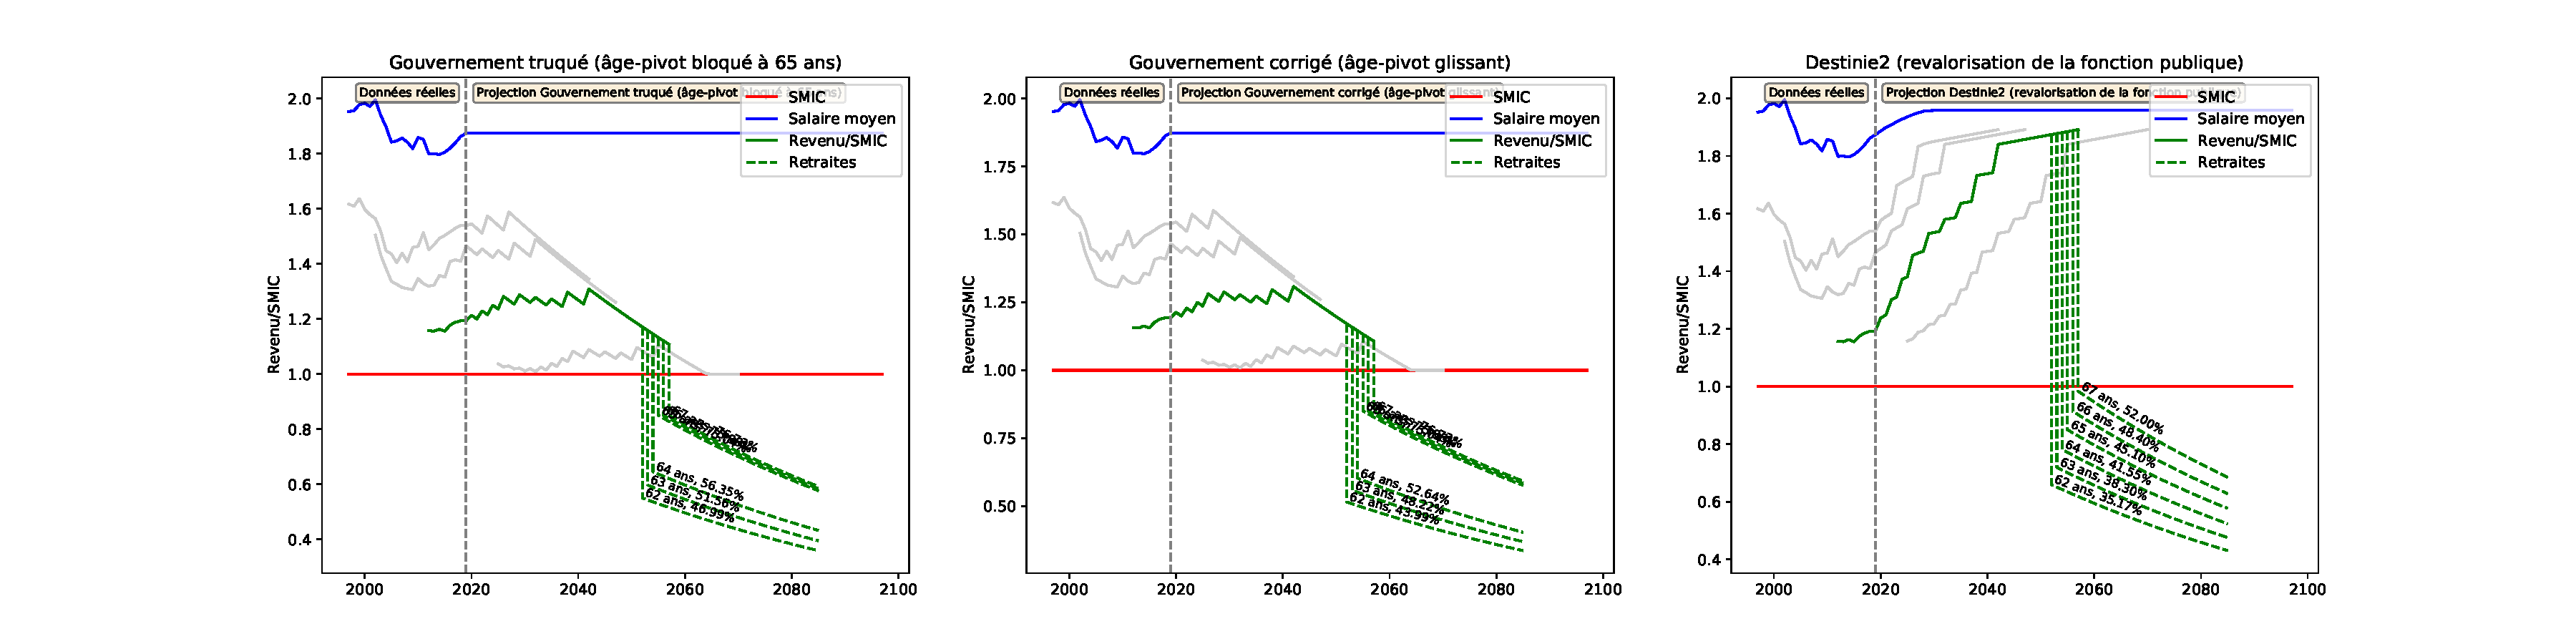
\includegraphics[width=0.9\textwidth]{fig/TechHosp_1990_22_dest_retraite.pdf}\end{center} \label{fig/TechHosp_1990_22_dest_retraite.pdf} 

\newpage 
 
\paragraph{Revenus et points pour le modèle \emph{Gouvernement truqué (âge-pivot bloqué à 65 ans)}} 
 
{ \scriptsize \begin{center} 
\begin{tabular}[htb]{|c|c||c|c|c|c|c|c||c|c||c|c|c|} 
\hline 
 Année &  Âge &  Ind Maj &  Pt Ind(\euro{} 2019) &  Rev HP(\euro{} 2019) &  Tx Primes &  GIPA(\euro{} 2019) &  Revenu(\euro{} 2019) &  SMIC(\euro{} 2019) &  Rev/SMIC &  Cumul Pts &  Achat Pt(\euro{} 2019) &  Serv. Pt(\euro{} 2019) \\ 
\hline \hline 
 2012 &  22 &  339.0 &  4.88 &  1653.11 &  17.11 &  0.00 &  1935.96 &  1673.05 &  {\bf 1.16} &  652.44 &  35.61 &  0.50 \\ 
\hline 
 2013 &  23 &  339.0 &  4.83 &  1638.95 &  17.34 &  0.00 &  1923.14 &  1664.01 &  {\bf 1.16} &  1300.56 &  35.61 &  0.50 \\ 
\hline 
 2014 &  24 &  344.0 &  4.81 &  1654.79 &  17.57 &  0.00 &  1945.54 &  1673.24 &  {\bf 1.16} &  1956.23 &  35.61 &  0.50 \\ 
\hline 
 2015 &  25 &  344.0 &  4.81 &  1654.15 &  17.80 &  0.00 &  1948.59 &  1686.62 &  {\bf 1.16} &  2612.93 &  35.61 &  0.50 \\ 
\hline 
 2016 &  26 &  349.0 &  4.80 &  1674.84 &  18.03 &  18.10 &  1994.91 &  1693.76 &  {\bf 1.18} &  3285.24 &  35.61 &  0.50 \\ 
\hline 
 2017 &  27 &  349.0 &  4.81 &  1678.22 &  18.26 &  25.94 &  2010.60 &  1692.60 &  {\bf 1.19} &  3962.84 &  35.61 &  0.50 \\ 
\hline 
 2018 &  28 &  356.0 &  4.74 &  1688.24 &  18.49 &  16.06 &  2016.46 &  1689.76 &  {\bf 1.19} &  4642.41 &  35.61 &  0.50 \\ 
\hline 
 2019 &  29 &  356.0 &  4.79 &  1706.81 &  18.72 &  0.00 &  2026.33 &  1698.45 &  {\bf 1.19} &  5325.31 &  35.61 &  0.50 \\ 
\hline 
 2020 &  30 &  366.0 &  4.79 &  1754.76 &  18.95 &  0.00 &  2087.29 &  1720.53 &  {\bf 1.21} &  6028.75 &  35.61 &  0.50 \\ 
\hline 
 2021 &  31 &  366.0 &  4.79 &  1754.76 &  19.18 &  0.00 &  2091.32 &  1742.90 &  {\bf 1.20} &  6733.55 &  35.61 &  0.50 \\ 
\hline 
 2022 &  32 &  379.0 &  4.79 &  1817.09 &  19.41 &  0.00 &  2169.78 &  1765.55 &  {\bf 1.23} &  7464.79 &  35.61 &  0.50 \\ 
\hline 
 2023 &  33 &  379.0 &  4.79 &  1817.09 &  19.64 &  0.00 &  2173.96 &  1788.51 &  {\bf 1.22} &  8197.44 &  35.61 &  0.50 \\ 
\hline 
 2024 &  34 &  394.0 &  4.79 &  1889.00 &  19.87 &  0.00 &  2264.35 &  1811.76 &  {\bf 1.25} &  8960.56 &  35.61 &  0.50 \\ 
\hline 
 2025 &  35 &  394.0 &  4.79 &  1889.00 &  20.10 &  0.00 &  2268.69 &  1835.31 &  {\bf 1.24} &  9725.13 &  35.61 &  0.50 \\ 
\hline 
 2026 &  36 &  413.0 &  4.79 &  1980.10 &  20.33 &  0.00 &  2382.65 &  1859.17 &  {\bf 1.28} &  10528.12 &  35.61 &  0.50 \\ 
\hline 
 2027 &  37 &  413.0 &  4.79 &  1980.10 &  20.56 &  0.00 &  2387.20 &  1883.34 &  {\bf 1.27} &  11332.63 &  35.61 &  0.50 \\ 
\hline 
 2028 &  38 &  413.0 &  4.79 &  1980.10 &  20.79 &  0.00 &  2391.76 &  1907.82 &  {\bf 1.25} &  12138.68 &  35.61 &  0.50 \\ 
\hline 
 2029 &  39 &  429.0 &  4.79 &  2056.81 &  21.02 &  0.00 &  2489.15 &  1932.62 &  {\bf 1.29} &  12976.92 &  35.63 &  0.50 \\ 
\hline 
 2030 &  40 &  429.0 &  4.79 &  2056.81 &  21.25 &  0.00 &  2493.88 &  1957.75 &  {\bf 1.27} &  13815.47 &  35.69 &  0.50 \\ 
\hline 
 2031 &  41 &  429.0 &  4.79 &  2056.81 &  21.48 &  0.00 &  2498.61 &  1983.20 &  {\bf 1.26} &  14653.71 &  35.77 &  0.50 \\ 
\hline 
 2032 &  42 &  440.0 &  4.79 &  2109.55 &  21.71 &  0.00 &  2567.53 &  2008.98 &  {\bf 1.28} &  15512.44 &  35.88 &  0.50 \\ 
\hline 
 2033 &  43 &  440.0 &  4.79 &  2109.55 &  21.94 &  0.00 &  2572.38 &  2035.10 &  {\bf 1.26} &  16369.54 &  36.02 &  0.50 \\ 
\hline 
 2034 &  44 &  440.0 &  4.79 &  2109.55 &  22.17 &  0.00 &  2577.23 &  2061.55 &  {\bf 1.25} &  17224.35 &  36.18 &  0.50 \\ 
\hline 
 2035 &  45 &  453.0 &  4.79 &  2171.87 &  22.40 &  0.00 &  2658.37 &  2088.35 &  {\bf 1.27} &  18101.40 &  36.37 &  0.51 \\ 
\hline 
 2036 &  46 &  453.0 &  4.79 &  2171.87 &  22.63 &  0.00 &  2663.37 &  2115.50 &  {\bf 1.26} &  18974.77 &  36.59 &  0.51 \\ 
\hline 
 2037 &  47 &  453.0 &  4.79 &  2171.87 &  22.86 &  0.00 &  2668.36 &  2143.00 &  {\bf 1.25} &  19843.81 &  36.85 &  0.51 \\ 
\hline 
 2038 &  48 &  477.0 &  4.79 &  2286.94 &  23.09 &  0.00 &  2814.99 &  2170.86 &  {\bf 1.30} &  20753.67 &  37.13 &  0.52 \\ 
\hline 
 2039 &  49 &  477.0 &  4.79 &  2286.94 &  23.32 &  0.00 &  2820.25 &  2199.08 &  {\bf 1.28} &  21657.65 &  37.44 &  0.52 \\ 
\hline 
 2040 &  50 &  477.0 &  4.79 &  2286.94 &  23.55 &  0.00 &  2825.51 &  2227.67 &  {\bf 1.27} &  22555.09 &  37.78 &  0.53 \\ 
\hline 
 2041 &  51 &  477.0 &  4.79 &  2286.94 &  23.78 &  0.00 &  2830.77 &  2256.63 &  {\bf 1.25} &  23445.36 &  38.16 &  0.53 \\ 
\hline 
 2042 &  52 &  503.0 &  4.79 &  2411.59 &  24.01 &  0.00 &  2990.62 &  2285.97 &  {\bf 1.31} &  24375.96 &  38.56 &  0.54 \\ 
\hline 
 2043 &  53 &  503.0 &  4.79 &  2411.59 &  24.24 &  0.00 &  2996.16 &  2315.68 &  {\bf 1.29} &  25297.71 &  39.01 &  0.54 \\ 
\hline 
 2044 &  54 &  503.0 &  4.79 &  2411.59 &  24.47 &  0.00 &  3001.71 &  2345.79 &  {\bf 1.28} &  26210.01 &  39.48 &  0.55 \\ 
\hline 
 2045 &  55 &  503.0 &  4.79 &  2411.59 &  24.70 &  0.00 &  3007.26 &  2376.28 &  {\bf 1.27} &  27112.27 &  40.00 &  0.56 \\ 
\hline 
 2046 &  56 &  503.0 &  4.79 &  2411.59 &  24.93 &  0.00 &  3012.80 &  2407.18 &  {\bf 1.25} &  28004.60 &  40.52 &  0.56 \\ 
\hline 
 2047 &  57 &  503.0 &  4.79 &  2411.59 &  25.16 &  0.00 &  3018.35 &  2438.47 &  {\bf 1.24} &  28887.09 &  41.04 &  0.57 \\ 
\hline 
 2048 &  58 &  503.0 &  4.79 &  2411.59 &  25.39 &  0.00 &  3023.90 &  2470.17 &  {\bf 1.22} &  29759.86 &  41.58 &  0.58 \\ 
\hline 
 2049 &  59 &  503.0 &  4.79 &  2411.59 &  25.62 &  0.00 &  3029.44 &  2502.28 &  {\bf 1.21} &  30623.01 &  42.12 &  0.59 \\ 
\hline 
 2050 &  60 &  503.0 &  4.79 &  2411.59 &  25.85 &  0.00 &  3034.99 &  2534.81 &  {\bf 1.20} &  31476.64 &  42.66 &  0.59 \\ 
\hline 
 2051 &  61 &  503.0 &  4.79 &  2411.59 &  26.08 &  0.00 &  3040.54 &  2567.76 &  {\bf 1.18} &  32320.86 &  43.22 &  0.60 \\ 
\hline 
 2052 &  62 &  503.0 &  4.79 &  2411.59 &  26.31 &  0.00 &  3046.08 &  2601.14 &  {\bf 1.17} &  33155.76 &  43.78 &  0.61 \\ 
\hline 
 2053 &  63 &  503.0 &  4.79 &  2411.59 &  26.54 &  0.00 &  3051.63 &  2634.96 &  {\bf 1.16} &  33981.45 &  44.35 &  0.62 \\ 
\hline 
 2054 &  64 &  503.0 &  4.79 &  2411.59 &  26.77 &  0.00 &  3057.18 &  2669.21 &  {\bf 1.15} &  34798.03 &  44.93 &  0.63 \\ 
\hline 
 2055 &  65 &  503.0 &  4.79 &  2411.59 &  27.00 &  0.00 &  3062.72 &  2703.91 &  {\bf 1.13} &  35605.58 &  45.51 &  0.63 \\ 
\hline 
 2056 &  66 &  503.0 &  4.79 &  2411.59 &  27.23 &  0.00 &  3068.27 &  2739.06 &  {\bf 1.12} &  36404.22 &  46.10 &  0.64 \\ 
\hline 
 2057 &  67 &  503.0 &  4.79 &  2411.59 &  27.46 &  0.00 &  3073.82 &  2774.67 &  {\bf 1.11} &  37194.04 &  46.70 &  0.65 \\ 
\hline 
\hline 
\end{tabular} 
\end{center} } 
\newpage 
 
\paragraph{Revenus et points pour le modèle \emph{Gouvernement corrigé (âge-pivot glissant)}} 
 
{ \scriptsize \begin{center} 
\begin{tabular}[htb]{|c|c||c|c|c|c|c|c||c|c||c|c|c|} 
\hline 
 Année &  Âge &  Ind Maj &  Pt Ind(\euro{} 2019) &  Rev HP(\euro{} 2019) &  Tx Primes &  GIPA(\euro{} 2019) &  Revenu(\euro{} 2019) &  SMIC(\euro{} 2019) &  Rev/SMIC &  Cumul Pts &  Achat Pt(\euro{} 2019) &  Serv. Pt(\euro{} 2019) \\ 
\hline \hline 
 2012 &  22 &  339.0 &  4.88 &  1653.11 &  17.11 &  0.00 &  1935.96 &  1673.05 &  {\bf 1.16} &  652.44 &  35.61 &  0.50 \\ 
\hline 
 2013 &  23 &  339.0 &  4.83 &  1638.95 &  17.34 &  0.00 &  1923.14 &  1664.01 &  {\bf 1.16} &  1300.56 &  35.61 &  0.50 \\ 
\hline 
 2014 &  24 &  344.0 &  4.81 &  1654.79 &  17.57 &  0.00 &  1945.54 &  1673.24 &  {\bf 1.16} &  1956.23 &  35.61 &  0.50 \\ 
\hline 
 2015 &  25 &  344.0 &  4.81 &  1654.15 &  17.80 &  0.00 &  1948.59 &  1686.62 &  {\bf 1.16} &  2612.93 &  35.61 &  0.50 \\ 
\hline 
 2016 &  26 &  349.0 &  4.80 &  1674.84 &  18.03 &  18.10 &  1994.91 &  1693.76 &  {\bf 1.18} &  3285.24 &  35.61 &  0.50 \\ 
\hline 
 2017 &  27 &  349.0 &  4.81 &  1678.22 &  18.26 &  25.94 &  2010.60 &  1692.60 &  {\bf 1.19} &  3962.84 &  35.61 &  0.50 \\ 
\hline 
 2018 &  28 &  356.0 &  4.74 &  1688.24 &  18.49 &  16.06 &  2016.46 &  1689.76 &  {\bf 1.19} &  4642.41 &  35.61 &  0.50 \\ 
\hline 
 2019 &  29 &  356.0 &  4.79 &  1706.81 &  18.72 &  0.00 &  2026.33 &  1698.45 &  {\bf 1.19} &  5325.31 &  35.61 &  0.50 \\ 
\hline 
 2020 &  30 &  366.0 &  4.79 &  1754.76 &  18.95 &  0.00 &  2087.29 &  1720.53 &  {\bf 1.21} &  6028.75 &  35.61 &  0.50 \\ 
\hline 
 2021 &  31 &  366.0 &  4.79 &  1754.76 &  19.18 &  0.00 &  2091.32 &  1742.90 &  {\bf 1.20} &  6733.55 &  35.61 &  0.50 \\ 
\hline 
 2022 &  32 &  379.0 &  4.79 &  1817.09 &  19.41 &  0.00 &  2169.78 &  1765.55 &  {\bf 1.23} &  7464.79 &  35.61 &  0.50 \\ 
\hline 
 2023 &  33 &  379.0 &  4.79 &  1817.09 &  19.64 &  0.00 &  2173.96 &  1788.51 &  {\bf 1.22} &  8197.44 &  35.61 &  0.50 \\ 
\hline 
 2024 &  34 &  394.0 &  4.79 &  1889.00 &  19.87 &  0.00 &  2264.35 &  1811.76 &  {\bf 1.25} &  8960.56 &  35.61 &  0.50 \\ 
\hline 
 2025 &  35 &  394.0 &  4.79 &  1889.00 &  20.10 &  0.00 &  2268.69 &  1835.31 &  {\bf 1.24} &  9725.13 &  35.61 &  0.50 \\ 
\hline 
 2026 &  36 &  413.0 &  4.79 &  1980.10 &  20.33 &  0.00 &  2382.65 &  1859.17 &  {\bf 1.28} &  10528.12 &  35.61 &  0.50 \\ 
\hline 
 2027 &  37 &  413.0 &  4.79 &  1980.10 &  20.56 &  0.00 &  2387.20 &  1883.34 &  {\bf 1.27} &  11332.63 &  35.61 &  0.50 \\ 
\hline 
 2028 &  38 &  413.0 &  4.79 &  1980.10 &  20.79 &  0.00 &  2391.76 &  1907.82 &  {\bf 1.25} &  12138.68 &  35.61 &  0.50 \\ 
\hline 
 2029 &  39 &  429.0 &  4.79 &  2056.81 &  21.02 &  0.00 &  2489.15 &  1932.62 &  {\bf 1.29} &  12976.92 &  35.63 &  0.50 \\ 
\hline 
 2030 &  40 &  429.0 &  4.79 &  2056.81 &  21.25 &  0.00 &  2493.88 &  1957.75 &  {\bf 1.27} &  13815.47 &  35.69 &  0.50 \\ 
\hline 
 2031 &  41 &  429.0 &  4.79 &  2056.81 &  21.48 &  0.00 &  2498.61 &  1983.20 &  {\bf 1.26} &  14653.71 &  35.77 &  0.50 \\ 
\hline 
 2032 &  42 &  440.0 &  4.79 &  2109.55 &  21.71 &  0.00 &  2567.53 &  2008.98 &  {\bf 1.28} &  15512.44 &  35.88 &  0.50 \\ 
\hline 
 2033 &  43 &  440.0 &  4.79 &  2109.55 &  21.94 &  0.00 &  2572.38 &  2035.10 &  {\bf 1.26} &  16369.54 &  36.02 &  0.50 \\ 
\hline 
 2034 &  44 &  440.0 &  4.79 &  2109.55 &  22.17 &  0.00 &  2577.23 &  2061.55 &  {\bf 1.25} &  17224.35 &  36.18 &  0.50 \\ 
\hline 
 2035 &  45 &  453.0 &  4.79 &  2171.87 &  22.40 &  0.00 &  2658.37 &  2088.35 &  {\bf 1.27} &  18101.40 &  36.37 &  0.51 \\ 
\hline 
 2036 &  46 &  453.0 &  4.79 &  2171.87 &  22.63 &  0.00 &  2663.37 &  2115.50 &  {\bf 1.26} &  18974.77 &  36.59 &  0.51 \\ 
\hline 
 2037 &  47 &  453.0 &  4.79 &  2171.87 &  22.86 &  0.00 &  2668.36 &  2143.00 &  {\bf 1.25} &  19843.81 &  36.85 &  0.51 \\ 
\hline 
 2038 &  48 &  477.0 &  4.79 &  2286.94 &  23.09 &  0.00 &  2814.99 &  2170.86 &  {\bf 1.30} &  20753.67 &  37.13 &  0.52 \\ 
\hline 
 2039 &  49 &  477.0 &  4.79 &  2286.94 &  23.32 &  0.00 &  2820.25 &  2199.08 &  {\bf 1.28} &  21657.65 &  37.44 &  0.52 \\ 
\hline 
 2040 &  50 &  477.0 &  4.79 &  2286.94 &  23.55 &  0.00 &  2825.51 &  2227.67 &  {\bf 1.27} &  22555.09 &  37.78 &  0.53 \\ 
\hline 
 2041 &  51 &  477.0 &  4.79 &  2286.94 &  23.78 &  0.00 &  2830.77 &  2256.63 &  {\bf 1.25} &  23445.36 &  38.16 &  0.53 \\ 
\hline 
 2042 &  52 &  503.0 &  4.79 &  2411.59 &  24.01 &  0.00 &  2990.62 &  2285.97 &  {\bf 1.31} &  24375.96 &  38.56 &  0.54 \\ 
\hline 
 2043 &  53 &  503.0 &  4.79 &  2411.59 &  24.24 &  0.00 &  2996.16 &  2315.68 &  {\bf 1.29} &  25297.71 &  39.01 &  0.54 \\ 
\hline 
 2044 &  54 &  503.0 &  4.79 &  2411.59 &  24.47 &  0.00 &  3001.71 &  2345.79 &  {\bf 1.28} &  26210.01 &  39.48 &  0.55 \\ 
\hline 
 2045 &  55 &  503.0 &  4.79 &  2411.59 &  24.70 &  0.00 &  3007.26 &  2376.28 &  {\bf 1.27} &  27112.27 &  40.00 &  0.56 \\ 
\hline 
 2046 &  56 &  503.0 &  4.79 &  2411.59 &  24.93 &  0.00 &  3012.80 &  2407.18 &  {\bf 1.25} &  28004.60 &  40.52 &  0.56 \\ 
\hline 
 2047 &  57 &  503.0 &  4.79 &  2411.59 &  25.16 &  0.00 &  3018.35 &  2438.47 &  {\bf 1.24} &  28887.09 &  41.04 &  0.57 \\ 
\hline 
 2048 &  58 &  503.0 &  4.79 &  2411.59 &  25.39 &  0.00 &  3023.90 &  2470.17 &  {\bf 1.22} &  29759.86 &  41.58 &  0.58 \\ 
\hline 
 2049 &  59 &  503.0 &  4.79 &  2411.59 &  25.62 &  0.00 &  3029.44 &  2502.28 &  {\bf 1.21} &  30623.01 &  42.12 &  0.59 \\ 
\hline 
 2050 &  60 &  503.0 &  4.79 &  2411.59 &  25.85 &  0.00 &  3034.99 &  2534.81 &  {\bf 1.20} &  31476.64 &  42.66 &  0.59 \\ 
\hline 
 2051 &  61 &  503.0 &  4.79 &  2411.59 &  26.08 &  0.00 &  3040.54 &  2567.76 &  {\bf 1.18} &  32320.86 &  43.22 &  0.60 \\ 
\hline 
 2052 &  62 &  503.0 &  4.79 &  2411.59 &  26.31 &  0.00 &  3046.08 &  2601.14 &  {\bf 1.17} &  33155.76 &  43.78 &  0.61 \\ 
\hline 
 2053 &  63 &  503.0 &  4.79 &  2411.59 &  26.54 &  0.00 &  3051.63 &  2634.96 &  {\bf 1.16} &  33981.45 &  44.35 &  0.62 \\ 
\hline 
 2054 &  64 &  503.0 &  4.79 &  2411.59 &  26.77 &  0.00 &  3057.18 &  2669.21 &  {\bf 1.15} &  34798.03 &  44.93 &  0.63 \\ 
\hline 
 2055 &  65 &  503.0 &  4.79 &  2411.59 &  27.00 &  0.00 &  3062.72 &  2703.91 &  {\bf 1.13} &  35605.58 &  45.51 &  0.63 \\ 
\hline 
 2056 &  66 &  503.0 &  4.79 &  2411.59 &  27.23 &  0.00 &  3068.27 &  2739.06 &  {\bf 1.12} &  36404.22 &  46.10 &  0.64 \\ 
\hline 
 2057 &  67 &  503.0 &  4.79 &  2411.59 &  27.46 &  0.00 &  3073.82 &  2774.67 &  {\bf 1.11} &  37194.04 &  46.70 &  0.65 \\ 
\hline 
\hline 
\end{tabular} 
\end{center} } 
\newpage 
 
\paragraph{Revenus et points pour le modèle \emph{Destinie2 (revalorisation de la fonction publique)}} 
 
{ \scriptsize \begin{center} 
\begin{tabular}[htb]{|c|c||c|c|c|c|c|c||c|c||c|c|c|} 
\hline 
 Année &  Âge &  Ind Maj &  Pt Ind(\euro{} 2019) &  Rev HP(\euro{} 2019) &  Tx Primes &  GIPA(\euro{} 2019) &  Revenu(\euro{} 2019) &  SMIC(\euro{} 2019) &  Rev/SMIC &  Cumul Pts &  Achat Pt(\euro{} 2019) &  Serv. Pt(\euro{} 2019) \\ 
\hline \hline 
 2012 &  22 &  339.0 &  4.88 &  1653.11 &  17.11 &  0.00 &  1935.96 &  1673.05 &  {\bf 1.16} &  650.84 &  35.69 &  0.50 \\ 
\hline 
 2013 &  23 &  339.0 &  4.83 &  1638.95 &  17.34 &  0.00 &  1923.14 &  1664.01 &  {\bf 1.16} &  1297.37 &  35.69 &  0.50 \\ 
\hline 
 2014 &  24 &  344.0 &  4.81 &  1654.79 &  17.57 &  0.00 &  1945.54 &  1673.24 &  {\bf 1.16} &  1951.43 &  35.69 &  0.50 \\ 
\hline 
 2015 &  25 &  344.0 &  4.81 &  1654.15 &  17.80 &  0.00 &  1948.59 &  1686.62 &  {\bf 1.16} &  2606.51 &  35.69 &  0.50 \\ 
\hline 
 2016 &  26 &  349.0 &  4.80 &  1674.84 &  18.03 &  13.19 &  1990.01 &  1693.76 &  {\bf 1.17} &  3275.52 &  35.69 &  0.50 \\ 
\hline 
 2017 &  27 &  349.0 &  4.81 &  1678.22 &  18.26 &  22.23 &  2006.89 &  1692.60 &  {\bf 1.19} &  3950.20 &  35.69 &  0.50 \\ 
\hline 
 2018 &  28 &  356.0 &  4.74 &  1688.24 &  18.49 &  13.89 &  2014.29 &  1689.76 &  {\bf 1.19} &  4627.38 &  35.69 &  0.50 \\ 
\hline 
 2019 &  29 &  356.0 &  4.79 &  1706.81 &  18.72 &  0.00 &  2026.33 &  1698.45 &  {\bf 1.19} &  5308.60 &  35.69 &  0.50 \\ 
\hline 
 2020 &  30 &  366.0 &  4.83 &  1768.80 &  18.95 &  0.00 &  2103.98 &  1699.99 &  {\bf 1.24} &  6015.92 &  35.69 &  0.50 \\ 
\hline 
 2021 &  31 &  366.0 &  4.88 &  1784.72 &  19.18 &  0.00 &  2127.02 &  1703.48 &  {\bf 1.25} &  6730.99 &  35.69 &  0.50 \\ 
\hline 
 2022 &  32 &  379.0 &  4.93 &  1866.59 &  19.41 &  0.00 &  2228.89 &  1712.78 &  {\bf 1.30} &  7480.31 &  35.69 &  0.50 \\ 
\hline 
 2023 &  33 &  379.0 &  4.98 &  1888.43 &  19.64 &  0.00 &  2259.31 &  1723.51 &  {\bf 1.31} &  8239.86 &  35.69 &  0.50 \\ 
\hline 
 2024 &  34 &  394.0 &  5.04 &  1986.53 &  19.87 &  0.00 &  2381.25 &  1735.69 &  {\bf 1.37} &  9040.40 &  35.69 &  0.50 \\ 
\hline 
 2025 &  35 &  394.0 &  5.10 &  2010.76 &  20.10 &  0.00 &  2414.93 &  1749.35 &  {\bf 1.38} &  9852.26 &  35.69 &  0.50 \\ 
\hline 
 2026 &  36 &  413.0 &  5.17 &  2134.08 &  20.33 &  0.00 &  2567.93 &  1764.53 &  {\bf 1.46} &  10715.56 &  35.69 &  0.50 \\ 
\hline 
 2027 &  37 &  413.0 &  5.23 &  2161.39 &  20.56 &  0.00 &  2605.78 &  1781.27 &  {\bf 1.46} &  11591.58 &  35.69 &  0.50 \\ 
\hline 
 2028 &  38 &  413.0 &  5.30 &  2189.71 &  20.79 &  0.00 &  2644.95 &  1799.59 &  {\bf 1.47} &  12480.77 &  35.69 &  0.50 \\ 
\hline 
 2029 &  39 &  429.0 &  5.37 &  2302.06 &  21.02 &  0.00 &  2785.95 &  1819.55 &  {\bf 1.53} &  13416.70 &  35.72 &  0.50 \\ 
\hline 
 2030 &  40 &  429.0 &  5.43 &  2330.61 &  21.25 &  0.00 &  2825.86 &  1841.19 &  {\bf 1.53} &  14364.66 &  35.77 &  0.50 \\ 
\hline 
 2031 &  41 &  429.0 &  5.50 &  2360.20 &  21.48 &  0.00 &  2867.18 &  1864.58 &  {\bf 1.54} &  15324.34 &  35.85 &  0.50 \\ 
\hline 
 2032 &  42 &  440.0 &  5.57 &  2452.19 &  21.71 &  0.00 &  2984.56 &  1888.81 &  {\bf 1.58} &  16320.29 &  35.96 &  0.50 \\ 
\hline 
 2033 &  43 &  440.0 &  5.65 &  2484.07 &  21.94 &  0.00 &  3029.08 &  1913.37 &  {\bf 1.58} &  17327.25 &  36.10 &  0.50 \\ 
\hline 
 2034 &  44 &  440.0 &  5.72 &  2516.36 &  22.17 &  0.00 &  3074.24 &  1938.24 &  {\bf 1.59} &  18344.58 &  36.26 &  0.50 \\ 
\hline 
 2035 &  45 &  453.0 &  5.79 &  2624.39 &  22.40 &  0.00 &  3212.25 &  1963.44 &  {\bf 1.64} &  19401.94 &  36.46 &  0.51 \\ 
\hline 
 2036 &  46 &  453.0 &  5.87 &  2658.51 &  22.63 &  0.00 &  3260.13 &  1988.96 &  {\bf 1.64} &  20468.56 &  36.68 &  0.51 \\ 
\hline 
 2037 &  47 &  453.0 &  5.94 &  2693.07 &  22.86 &  0.00 &  3308.70 &  2014.82 &  {\bf 1.64} &  21543.69 &  36.93 &  0.51 \\ 
\hline 
 2038 &  48 &  477.0 &  6.02 &  2872.61 &  23.09 &  0.00 &  3535.90 &  2041.01 &  {\bf 1.73} &  22683.95 &  37.21 &  0.52 \\ 
\hline 
 2039 &  49 &  477.0 &  6.10 &  2909.96 &  23.32 &  0.00 &  3588.56 &  2067.55 &  {\bf 1.74} &  23831.56 &  37.52 &  0.52 \\ 
\hline 
 2040 &  50 &  477.0 &  6.18 &  2947.79 &  23.55 &  0.00 &  3641.99 &  2094.43 &  {\bf 1.74} &  24985.69 &  37.87 &  0.53 \\ 
\hline 
 2041 &  51 &  477.0 &  6.26 &  2986.11 &  23.78 &  0.00 &  3696.20 &  2121.65 &  {\bf 1.74} &  26145.49 &  38.24 &  0.53 \\ 
\hline 
 2042 &  52 &  503.0 &  6.34 &  3189.81 &  24.01 &  0.00 &  3955.68 &  2149.23 &  {\bf 1.84} &  27373.57 &  38.65 &  0.54 \\ 
\hline 
 2043 &  53 &  503.0 &  6.42 &  3231.27 &  24.24 &  0.00 &  4014.53 &  2177.17 &  {\bf 1.84} &  28605.80 &  39.10 &  0.54 \\ 
\hline 
 2044 &  54 &  503.0 &  6.51 &  3273.28 &  24.47 &  0.00 &  4074.25 &  2205.48 &  {\bf 1.85} &  29841.25 &  39.57 &  0.55 \\ 
\hline 
 2045 &  55 &  503.0 &  6.59 &  3315.83 &  24.70 &  0.00 &  4134.84 &  2234.15 &  {\bf 1.85} &  31078.98 &  40.09 &  0.56 \\ 
\hline 
 2046 &  56 &  503.0 &  6.68 &  3358.94 &  24.93 &  0.00 &  4196.32 &  2263.19 &  {\bf 1.85} &  32319.00 &  40.61 &  0.57 \\ 
\hline 
 2047 &  57 &  503.0 &  6.76 &  3402.61 &  25.16 &  0.00 &  4258.70 &  2292.61 &  {\bf 1.86} &  33561.30 &  41.14 &  0.57 \\ 
\hline 
 2048 &  58 &  503.0 &  6.85 &  3446.84 &  25.39 &  0.00 &  4321.99 &  2322.42 &  {\bf 1.86} &  34805.88 &  41.67 &  0.58 \\ 
\hline 
 2049 &  59 &  503.0 &  6.94 &  3491.65 &  25.62 &  0.00 &  4386.21 &  2352.61 &  {\bf 1.86} &  36052.74 &  42.21 &  0.59 \\ 
\hline 
 2050 &  60 &  503.0 &  7.03 &  3537.04 &  25.85 &  0.00 &  4451.36 &  2383.19 &  {\bf 1.87} &  37301.89 &  42.76 &  0.60 \\ 
\hline 
 2051 &  61 &  503.0 &  7.12 &  3583.02 &  26.08 &  0.00 &  4517.47 &  2414.18 &  {\bf 1.87} &  38553.32 &  43.32 &  0.60 \\ 
\hline 
 2052 &  62 &  503.0 &  7.22 &  3629.60 &  26.31 &  0.00 &  4584.55 &  2445.56 &  {\bf 1.87} &  39807.03 &  43.88 &  0.61 \\ 
\hline 
 2053 &  63 &  503.0 &  7.31 &  3676.78 &  26.54 &  0.00 &  4652.60 &  2477.35 &  {\bf 1.88} &  41063.03 &  44.45 &  0.62 \\ 
\hline 
 2054 &  64 &  503.0 &  7.40 &  3724.58 &  26.77 &  0.00 &  4721.65 &  2509.56 &  {\bf 1.88} &  42321.31 &  45.03 &  0.63 \\ 
\hline 
 2055 &  65 &  503.0 &  7.50 &  3773.00 &  27.00 &  0.00 &  4791.71 &  2542.18 &  {\bf 1.88} &  43581.87 &  45.62 &  0.63 \\ 
\hline 
 2056 &  66 &  503.0 &  7.60 &  3822.05 &  27.23 &  0.00 &  4862.80 &  2575.23 &  {\bf 1.89} &  44844.72 &  46.21 &  0.64 \\ 
\hline 
 2057 &  67 &  503.0 &  7.70 &  3871.74 &  27.46 &  0.00 &  4934.92 &  2608.71 &  {\bf 1.89} &  46109.85 &  46.81 &  0.65 \\ 
\hline 
\hline 
\end{tabular} 
\end{center} } 
\newpage 
 
\subsection{Génération 2003 (début en 2025)} 

\paragraph{Retraites possibles dans le modèle \emph{Gouvernement truqué (âge-pivot bloqué à 65 ans)}}  
 
{ \scriptsize \begin{center} 
\begin{tabular}[htb]{|c|c||c|c||c|c||c||c|c|c|c|c|c|} 
\hline 
 Retraite en &  Âge &  Âge pivot &  Décote/Surcote &  Retraite (\euro{} 2019) &  Tx Rempl(\%) &  SMIC (\euro{} 2019) &  Retraite/SMIC &  Rev70/SMIC &  Rev75/SMIC &  Rev80/SMIC &  Rev85/SMIC &  Rev90/SMIC \\ 
\hline \hline 
 2065 &  62 &  65 ans 0 mois &  -15.00\% &  1531.73 &  {\bf 49.78} &  3076.71 &  {\bf {\color{red} 0.50}} &  {\bf {\color{red} 0.45}} &  {\bf {\color{red} 0.42}} &  {\bf {\color{red} 0.39}} &  {\bf {\color{red} 0.37}} &  {\bf {\color{red} 0.35}} \\ 
\hline 
 2066 &  63 &  65 ans 0 mois &  -10.00\% &  1681.96 &  {\bf 53.97} &  3116.71 &  {\bf {\color{red} 0.54}} &  {\bf {\color{red} 0.49}} &  {\bf {\color{red} 0.46}} &  {\bf {\color{red} 0.43}} &  {\bf {\color{red} 0.41}} &  {\bf {\color{red} 0.38}} \\ 
\hline 
 2067 &  64 &  65 ans 0 mois &  -5.00\% &  1840.23 &  {\bf 58.29} &  3157.23 &  {\bf {\color{red} 0.58}} &  {\bf {\color{red} 0.54}} &  {\bf {\color{red} 0.51}} &  {\bf {\color{red} 0.47}} &  {\bf {\color{red} 0.44}} &  {\bf {\color{red} 0.42}} \\ 
\hline 
 2068 &  65 &  65 ans 0 mois &  0.00\% &  2718.53 &  {\bf 85.00} &  3198.27 &  {\bf {\color{red} 0.85}} &  {\bf {\color{red} 0.80}} &  {\bf {\color{red} 0.75}} &  {\bf {\color{red} 0.70}} &  {\bf {\color{red} 0.66}} &  {\bf {\color{red} 0.62}} \\ 
\hline 
 2069 &  66 &  65 ans 0 mois &  5.00\% &  2753.87 &  {\bf 85.00} &  3239.85 &  {\bf {\color{red} 0.85}} &  {\bf {\color{red} 0.81}} &  {\bf {\color{red} 0.76}} &  {\bf {\color{red} 0.71}} &  {\bf {\color{red} 0.67}} &  {\bf {\color{red} 0.62}} \\ 
\hline 
 2070 &  67 &  65 ans 0 mois &  10.00\% &  2789.67 &  {\bf 85.00} &  3281.97 &  {\bf {\color{red} 0.85}} &  {\bf {\color{red} 0.82}} &  {\bf {\color{red} 0.77}} &  {\bf {\color{red} 0.72}} &  {\bf {\color{red} 0.67}} &  {\bf {\color{red} 0.63}} \\ 
\hline 
\hline 
\end{tabular} 
\end{center} } 
\paragraph{Retraites possibles dans le modèle \emph{Gouvernement corrigé (âge-pivot glissant)}}  
 
{ \scriptsize \begin{center} 
\begin{tabular}[htb]{|c|c||c|c||c|c||c||c|c|c|c|c|c|} 
\hline 
 Retraite en &  Âge &  Âge pivot &  Décote/Surcote &  Retraite (\euro{} 2019) &  Tx Rempl(\%) &  SMIC (\euro{} 2019) &  Retraite/SMIC &  Rev70/SMIC &  Rev75/SMIC &  Rev80/SMIC &  Rev85/SMIC &  Rev90/SMIC \\ 
\hline \hline 
 2065 &  62 &  67 ans 2 mois &  -25.83\% &  1336.51 &  {\bf 43.44} &  3076.71 &  {\bf {\color{red} 0.43}} &  {\bf {\color{red} 0.39}} &  {\bf {\color{red} 0.37}} &  {\bf {\color{red} 0.34}} &  {\bf {\color{red} 0.32}} &  {\bf {\color{red} 0.30}} \\ 
\hline 
 2066 &  63 &  67 ans 3 mois &  -21.25\% &  1471.71 &  {\bf 47.22} &  3116.71 &  {\bf {\color{red} 0.47}} &  {\bf {\color{red} 0.43}} &  {\bf {\color{red} 0.40}} &  {\bf {\color{red} 0.38}} &  {\bf {\color{red} 0.36}} &  {\bf {\color{red} 0.33}} \\ 
\hline 
 2067 &  64 &  67 ans 4 mois &  -16.67\% &  1614.24 &  {\bf 51.13} &  3157.23 &  {\bf {\color{red} 0.51}} &  {\bf {\color{red} 0.47}} &  {\bf {\color{red} 0.44}} &  {\bf {\color{red} 0.42}} &  {\bf {\color{red} 0.39}} &  {\bf {\color{red} 0.37}} \\ 
\hline 
 2068 &  65 &  67 ans 5 mois &  -12.08\% &  2718.53 &  {\bf 85.00} &  3198.27 &  {\bf {\color{red} 0.85}} &  {\bf {\color{red} 0.80}} &  {\bf {\color{red} 0.75}} &  {\bf {\color{red} 0.70}} &  {\bf {\color{red} 0.66}} &  {\bf {\color{red} 0.62}} \\ 
\hline 
 2069 &  66 &  67 ans 6 mois &  -7.50\% &  2753.87 &  {\bf 85.00} &  3239.85 &  {\bf {\color{red} 0.85}} &  {\bf {\color{red} 0.81}} &  {\bf {\color{red} 0.76}} &  {\bf {\color{red} 0.71}} &  {\bf {\color{red} 0.67}} &  {\bf {\color{red} 0.62}} \\ 
\hline 
 2070 &  67 &  67 ans 7 mois &  -2.92\% &  2789.67 &  {\bf 85.00} &  3281.97 &  {\bf {\color{red} 0.85}} &  {\bf {\color{red} 0.82}} &  {\bf {\color{red} 0.77}} &  {\bf {\color{red} 0.72}} &  {\bf {\color{red} 0.67}} &  {\bf {\color{red} 0.63}} \\ 
\hline 
\hline 
\end{tabular} 
\end{center} } 
\paragraph{Retraites possibles dans le modèle \emph{Destinie2 (revalorisation de la fonction publique)}}  
 
{ \scriptsize \begin{center} 
\begin{tabular}[htb]{|c|c||c|c||c|c||c||c|c|c|c|c|c|} 
\hline 
 Retraite en &  Âge &  Âge pivot &  Décote/Surcote &  Retraite (\euro{} 2019) &  Tx Rempl(\%) &  SMIC (\euro{} 2019) &  Retraite/SMIC &  Rev70/SMIC &  Rev75/SMIC &  Rev80/SMIC &  Rev85/SMIC &  Rev90/SMIC \\ 
\hline \hline 
 2065 &  62 &  67 ans 2 mois &  -25.83\% &  1868.70 &  {\bf 34.46} &  2892.68 &  {\bf {\color{red} 0.65}} &  {\bf {\color{red} 0.58}} &  {\bf {\color{red} 0.55}} &  {\bf {\color{red} 0.51}} &  {\bf {\color{red} 0.48}} &  {\bf {\color{red} 0.45}} \\ 
\hline 
 2066 &  63 &  67 ans 3 mois &  -21.25\% &  2070.30 &  {\bf 37.62} &  2930.29 &  {\bf {\color{red} 0.71}} &  {\bf {\color{red} 0.65}} &  {\bf {\color{red} 0.61}} &  {\bf {\color{red} 0.57}} &  {\bf {\color{red} 0.53}} &  {\bf {\color{red} 0.50}} \\ 
\hline 
 2067 &  64 &  67 ans 4 mois &  -16.67\% &  2284.05 &  {\bf 40.90} &  2968.38 &  {\bf {\color{red} 0.77}} &  {\bf {\color{red} 0.71}} &  {\bf {\color{red} 0.67}} &  {\bf {\color{red} 0.63}} &  {\bf {\color{red} 0.59}} &  {\bf {\color{red} 0.55}} \\ 
\hline 
 2068 &  65 &  67 ans 5 mois &  -12.08\% &  2555.93 &  {\bf 45.10} &  3006.97 &  {\bf {\color{red} 0.85}} &  {\bf {\color{red} 0.80}} &  {\bf {\color{red} 0.75}} &  {\bf {\color{red} 0.70}} &  {\bf {\color{red} 0.66}} &  {\bf {\color{red} 0.62}} \\ 
\hline 
 2069 &  66 &  67 ans 6 mois &  -7.50\% &  2749.63 &  {\bf 47.80} &  3046.06 &  {\bf {\color{red} 0.90}} &  {\bf {\color{red} 0.86}} &  {\bf {\color{red} 0.80}} &  {\bf {\color{red} 0.75}} &  {\bf {\color{red} 0.71}} &  {\bf {\color{red} 0.66}} \\ 
\hline 
 2070 &  67 &  67 ans 7 mois &  -2.92\% &  3002.27 &  {\bf 51.43} &  3085.66 &  {\bf {\color{red} 0.97}} &  {\bf {\color{red} 0.94}} &  {\bf {\color{red} 0.88}} &  {\bf {\color{red} 0.82}} &  {\bf {\color{red} 0.77}} &  {\bf {\color{red} 0.72}} \\ 
\hline 
\hline 
\end{tabular} 
\end{center} } 

 \begin{center}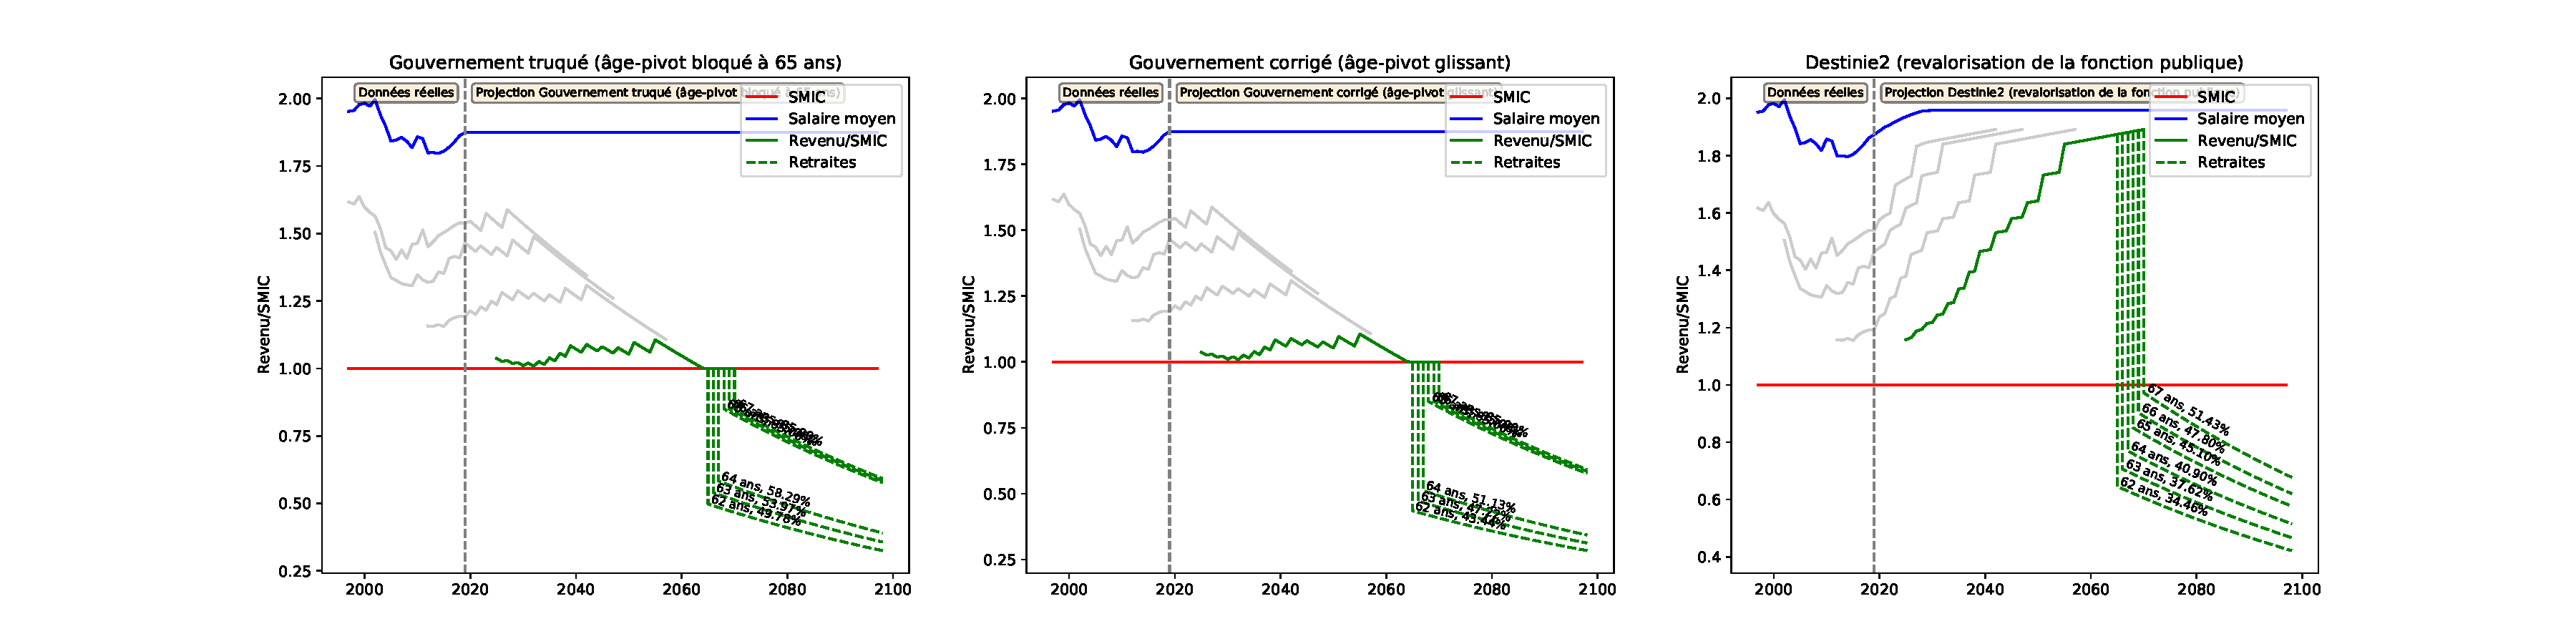
\includegraphics[width=0.9\textwidth]{fig/TechHosp_2003_22_dest_retraite.pdf}\end{center} \label{fig/TechHosp_2003_22_dest_retraite.pdf} 

\newpage 
 
\paragraph{Revenus et points pour le modèle \emph{Gouvernement truqué (âge-pivot bloqué à 65 ans)}} 
 
{ \scriptsize \begin{center} 
\begin{tabular}[htb]{|c|c||c|c|c|c|c|c||c|c||c|c|c|} 
\hline 
 Année &  Âge &  Ind Maj &  Pt Ind(\euro{} 2019) &  Rev HP(\euro{} 2019) &  Tx Primes &  GIPA(\euro{} 2019) &  Revenu(\euro{} 2019) &  SMIC(\euro{} 2019) &  Rev/SMIC &  Cumul Pts &  Achat Pt(\euro{} 2019) &  Serv. Pt(\euro{} 2019) \\ 
\hline \hline 
 2025 &  22 &  339.0 &  4.79 &  1625.31 &  17.11 &  0.00 &  1903.40 &  1835.31 &  {\bf 1.04} &  641.47 &  35.61 &  0.50 \\ 
\hline 
 2026 &  23 &  339.0 &  4.79 &  1625.31 &  17.34 &  0.00 &  1907.14 &  1859.17 &  {\bf 1.03} &  1284.20 &  35.61 &  0.50 \\ 
\hline 
 2027 &  24 &  344.0 &  4.79 &  1649.28 &  17.57 &  0.00 &  1939.06 &  1883.34 &  {\bf 1.03} &  1937.68 &  35.61 &  0.50 \\ 
\hline 
 2028 &  25 &  344.0 &  4.79 &  1649.28 &  17.80 &  0.00 &  1942.85 &  1907.82 &  {\bf 1.02} &  2592.45 &  35.61 &  0.50 \\ 
\hline 
 2029 &  26 &  349.0 &  4.79 &  1673.25 &  18.03 &  0.00 &  1974.94 &  1932.62 &  {\bf 1.02} &  3257.52 &  35.63 &  0.50 \\ 
\hline 
 2030 &  27 &  349.0 &  4.79 &  1673.25 &  18.26 &  0.00 &  1978.79 &  1957.75 &  {\bf 1.01} &  3922.88 &  35.69 &  0.50 \\ 
\hline 
 2031 &  28 &  356.0 &  4.79 &  1706.81 &  18.49 &  0.00 &  2022.40 &  1983.20 &  {\bf 1.02} &  4601.36 &  35.77 &  0.50 \\ 
\hline 
 2032 &  29 &  356.0 &  4.79 &  1706.81 &  18.72 &  0.00 &  2026.33 &  2008.98 &  {\bf 1.01} &  5279.08 &  35.88 &  0.50 \\ 
\hline 
 2033 &  30 &  366.0 &  4.79 &  1754.76 &  18.95 &  0.00 &  2087.29 &  2035.10 &  {\bf 1.03} &  5974.55 &  36.02 &  0.50 \\ 
\hline 
 2034 &  31 &  366.0 &  4.79 &  1754.76 &  19.18 &  0.00 &  2091.32 &  2061.55 &  {\bf 1.01} &  6668.20 &  36.18 &  0.50 \\ 
\hline 
 2035 &  32 &  379.0 &  4.79 &  1817.09 &  19.41 &  0.00 &  2169.78 &  2088.35 &  {\bf 1.04} &  7384.05 &  36.37 &  0.51 \\ 
\hline 
 2036 &  33 &  379.0 &  4.79 &  1817.09 &  19.64 &  0.00 &  2173.96 &  2115.50 &  {\bf 1.03} &  8096.93 &  36.59 &  0.51 \\ 
\hline 
 2037 &  34 &  394.0 &  4.79 &  1889.00 &  19.87 &  0.00 &  2264.35 &  2143.00 &  {\bf 1.06} &  8834.40 &  36.85 &  0.51 \\ 
\hline 
 2038 &  35 &  394.0 &  4.79 &  1889.00 &  20.10 &  0.00 &  2268.69 &  2170.86 &  {\bf 1.05} &  9567.68 &  37.13 &  0.52 \\ 
\hline 
 2039 &  36 &  413.0 &  4.79 &  1980.10 &  20.33 &  0.00 &  2382.65 &  2199.08 &  {\bf 1.08} &  10331.39 &  37.44 &  0.52 \\ 
\hline 
 2040 &  37 &  413.0 &  4.79 &  1980.10 &  20.56 &  0.00 &  2387.20 &  2227.67 &  {\bf 1.07} &  11089.61 &  37.78 &  0.53 \\ 
\hline 
 2041 &  38 &  413.0 &  4.79 &  1980.10 &  20.79 &  0.00 &  2391.76 &  2256.63 &  {\bf 1.06} &  11841.82 &  38.16 &  0.53 \\ 
\hline 
 2042 &  39 &  429.0 &  4.79 &  2056.81 &  21.02 &  0.00 &  2489.15 &  2285.97 &  {\bf 1.09} &  12616.37 &  38.56 &  0.54 \\ 
\hline 
 2043 &  40 &  429.0 &  4.79 &  2056.81 &  21.25 &  0.00 &  2493.88 &  2315.68 &  {\bf 1.08} &  13383.60 &  39.01 &  0.54 \\ 
\hline 
 2044 &  41 &  429.0 &  4.79 &  2056.81 &  21.48 &  0.00 &  2498.61 &  2345.79 &  {\bf 1.07} &  14142.99 &  39.48 &  0.55 \\ 
\hline 
 2045 &  42 &  440.0 &  4.79 &  2109.55 &  21.71 &  0.00 &  2567.53 &  2376.28 &  {\bf 1.08} &  14913.32 &  40.00 &  0.56 \\ 
\hline 
 2046 &  43 &  440.0 &  4.79 &  2109.55 &  21.94 &  0.00 &  2572.38 &  2407.18 &  {\bf 1.07} &  15675.20 &  40.52 &  0.56 \\ 
\hline 
 2047 &  44 &  440.0 &  4.79 &  2109.55 &  22.17 &  0.00 &  2577.23 &  2438.47 &  {\bf 1.06} &  16428.72 &  41.04 &  0.57 \\ 
\hline 
 2048 &  45 &  453.0 &  4.79 &  2171.87 &  22.40 &  0.00 &  2658.37 &  2470.17 &  {\bf 1.08} &  17195.99 &  41.58 &  0.58 \\ 
\hline 
 2049 &  46 &  453.0 &  4.79 &  2171.87 &  22.63 &  0.00 &  2663.37 &  2502.28 &  {\bf 1.06} &  17954.84 &  42.12 &  0.59 \\ 
\hline 
 2050 &  47 &  453.0 &  4.79 &  2171.87 &  22.86 &  0.00 &  2668.36 &  2534.81 &  {\bf 1.05} &  18705.35 &  42.66 &  0.59 \\ 
\hline 
 2051 &  48 &  477.0 &  4.79 &  2286.94 &  23.09 &  0.00 &  2814.99 &  2567.76 &  {\bf 1.10} &  19486.95 &  43.22 &  0.60 \\ 
\hline 
 2052 &  49 &  477.0 &  4.79 &  2286.94 &  23.32 &  0.00 &  2820.25 &  2601.14 &  {\bf 1.08} &  20259.95 &  43.78 &  0.61 \\ 
\hline 
 2053 &  50 &  477.0 &  4.79 &  2286.94 &  23.55 &  0.00 &  2825.51 &  2634.96 &  {\bf 1.07} &  21024.46 &  44.35 &  0.62 \\ 
\hline 
 2054 &  51 &  477.0 &  4.79 &  2286.94 &  23.78 &  0.00 &  2830.77 &  2669.21 &  {\bf 1.06} &  21780.56 &  44.93 &  0.63 \\ 
\hline 
 2055 &  52 &  503.0 &  4.79 &  2411.59 &  24.01 &  0.00 &  2990.62 &  2703.91 &  {\bf 1.11} &  22569.11 &  45.51 &  0.63 \\ 
\hline 
 2056 &  53 &  503.0 &  4.79 &  2411.59 &  24.24 &  0.00 &  2996.16 &  2739.06 &  {\bf 1.09} &  23348.98 &  46.10 &  0.64 \\ 
\hline 
 2057 &  54 &  503.0 &  4.79 &  2411.59 &  24.47 &  0.00 &  3001.71 &  2774.67 &  {\bf 1.08} &  24120.27 &  46.70 &  0.65 \\ 
\hline 
 2058 &  55 &  503.0 &  4.79 &  2411.59 &  24.70 &  0.00 &  3007.26 &  2810.74 &  {\bf 1.07} &  24883.06 &  47.31 &  0.66 \\ 
\hline 
 2059 &  56 &  503.0 &  4.79 &  2411.59 &  24.93 &  0.00 &  3012.80 &  2847.28 &  {\bf 1.06} &  25637.46 &  47.92 &  0.67 \\ 
\hline 
 2060 &  57 &  503.0 &  4.79 &  2411.59 &  25.16 &  0.00 &  3018.35 &  2884.30 &  {\bf 1.05} &  26383.54 &  48.55 &  0.68 \\ 
\hline 
 2061 &  58 &  503.0 &  4.79 &  2411.59 &  25.39 &  0.00 &  3023.90 &  2921.79 &  {\bf 1.03} &  27121.41 &  49.18 &  0.68 \\ 
\hline 
 2062 &  59 &  503.0 &  4.79 &  2411.59 &  25.62 &  0.00 &  3029.44 &  2959.78 &  {\bf 1.02} &  27851.14 &  49.82 &  0.69 \\ 
\hline 
 2063 &  60 &  503.0 &  4.79 &  2411.59 &  25.85 &  0.00 &  3034.99 &  2998.25 &  {\bf 1.01} &  28572.83 &  50.47 &  0.70 \\ 
\hline 
 2064 &  61 &  503.0 &  4.79 &  2411.59 &  26.08 &  0.00 &  3040.54 &  3037.23 &  {\bf 1.00} &  29286.55 &  51.12 &  0.71 \\ 
\hline 
 2065 &  62 &  503.0 &  4.79 &  2411.59 &  26.31 &  0.00 &  3076.71 &  3076.71 &  {\bf 1.00} &  29999.50 &  51.79 &  0.72 \\ 
\hline 
 2066 &  63 &  503.0 &  4.79 &  2411.59 &  26.54 &  0.00 &  3116.71 &  3116.71 &  {\bf 1.00} &  30712.45 &  52.46 &  0.73 \\ 
\hline 
 2067 &  64 &  503.0 &  4.79 &  2411.59 &  26.77 &  10.06 &  3157.23 &  3157.23 &  {\bf 1.00} &  31425.40 &  53.14 &  0.74 \\ 
\hline 
 2068 &  65 &  503.0 &  4.79 &  2411.59 &  27.00 &  35.07 &  3198.27 &  3198.27 &  {\bf 1.00} &  32138.35 &  53.83 &  0.75 \\ 
\hline 
 2069 &  66 &  503.0 &  4.79 &  2411.59 &  27.23 &  68.96 &  3239.85 &  3239.85 &  {\bf 1.00} &  32851.30 &  54.53 &  0.76 \\ 
\hline 
 2070 &  67 &  503.0 &  4.79 &  2411.59 &  27.46 &  104.20 &  3281.97 &  3281.97 &  {\bf 1.00} &  33564.25 &  55.24 &  0.77 \\ 
\hline 
\hline 
\end{tabular} 
\end{center} } 
\newpage 
 
\paragraph{Revenus et points pour le modèle \emph{Gouvernement corrigé (âge-pivot glissant)}} 
 
{ \scriptsize \begin{center} 
\begin{tabular}[htb]{|c|c||c|c|c|c|c|c||c|c||c|c|c|} 
\hline 
 Année &  Âge &  Ind Maj &  Pt Ind(\euro{} 2019) &  Rev HP(\euro{} 2019) &  Tx Primes &  GIPA(\euro{} 2019) &  Revenu(\euro{} 2019) &  SMIC(\euro{} 2019) &  Rev/SMIC &  Cumul Pts &  Achat Pt(\euro{} 2019) &  Serv. Pt(\euro{} 2019) \\ 
\hline \hline 
 2025 &  22 &  339.0 &  4.79 &  1625.31 &  17.11 &  0.00 &  1903.40 &  1835.31 &  {\bf 1.04} &  641.47 &  35.61 &  0.50 \\ 
\hline 
 2026 &  23 &  339.0 &  4.79 &  1625.31 &  17.34 &  0.00 &  1907.14 &  1859.17 &  {\bf 1.03} &  1284.20 &  35.61 &  0.50 \\ 
\hline 
 2027 &  24 &  344.0 &  4.79 &  1649.28 &  17.57 &  0.00 &  1939.06 &  1883.34 &  {\bf 1.03} &  1937.68 &  35.61 &  0.50 \\ 
\hline 
 2028 &  25 &  344.0 &  4.79 &  1649.28 &  17.80 &  0.00 &  1942.85 &  1907.82 &  {\bf 1.02} &  2592.45 &  35.61 &  0.50 \\ 
\hline 
 2029 &  26 &  349.0 &  4.79 &  1673.25 &  18.03 &  0.00 &  1974.94 &  1932.62 &  {\bf 1.02} &  3257.52 &  35.63 &  0.50 \\ 
\hline 
 2030 &  27 &  349.0 &  4.79 &  1673.25 &  18.26 &  0.00 &  1978.79 &  1957.75 &  {\bf 1.01} &  3922.88 &  35.69 &  0.50 \\ 
\hline 
 2031 &  28 &  356.0 &  4.79 &  1706.81 &  18.49 &  0.00 &  2022.40 &  1983.20 &  {\bf 1.02} &  4601.36 &  35.77 &  0.50 \\ 
\hline 
 2032 &  29 &  356.0 &  4.79 &  1706.81 &  18.72 &  0.00 &  2026.33 &  2008.98 &  {\bf 1.01} &  5279.08 &  35.88 &  0.50 \\ 
\hline 
 2033 &  30 &  366.0 &  4.79 &  1754.76 &  18.95 &  0.00 &  2087.29 &  2035.10 &  {\bf 1.03} &  5974.55 &  36.02 &  0.50 \\ 
\hline 
 2034 &  31 &  366.0 &  4.79 &  1754.76 &  19.18 &  0.00 &  2091.32 &  2061.55 &  {\bf 1.01} &  6668.20 &  36.18 &  0.50 \\ 
\hline 
 2035 &  32 &  379.0 &  4.79 &  1817.09 &  19.41 &  0.00 &  2169.78 &  2088.35 &  {\bf 1.04} &  7384.05 &  36.37 &  0.51 \\ 
\hline 
 2036 &  33 &  379.0 &  4.79 &  1817.09 &  19.64 &  0.00 &  2173.96 &  2115.50 &  {\bf 1.03} &  8096.93 &  36.59 &  0.51 \\ 
\hline 
 2037 &  34 &  394.0 &  4.79 &  1889.00 &  19.87 &  0.00 &  2264.35 &  2143.00 &  {\bf 1.06} &  8834.40 &  36.85 &  0.51 \\ 
\hline 
 2038 &  35 &  394.0 &  4.79 &  1889.00 &  20.10 &  0.00 &  2268.69 &  2170.86 &  {\bf 1.05} &  9567.68 &  37.13 &  0.52 \\ 
\hline 
 2039 &  36 &  413.0 &  4.79 &  1980.10 &  20.33 &  0.00 &  2382.65 &  2199.08 &  {\bf 1.08} &  10331.39 &  37.44 &  0.52 \\ 
\hline 
 2040 &  37 &  413.0 &  4.79 &  1980.10 &  20.56 &  0.00 &  2387.20 &  2227.67 &  {\bf 1.07} &  11089.61 &  37.78 &  0.53 \\ 
\hline 
 2041 &  38 &  413.0 &  4.79 &  1980.10 &  20.79 &  0.00 &  2391.76 &  2256.63 &  {\bf 1.06} &  11841.82 &  38.16 &  0.53 \\ 
\hline 
 2042 &  39 &  429.0 &  4.79 &  2056.81 &  21.02 &  0.00 &  2489.15 &  2285.97 &  {\bf 1.09} &  12616.37 &  38.56 &  0.54 \\ 
\hline 
 2043 &  40 &  429.0 &  4.79 &  2056.81 &  21.25 &  0.00 &  2493.88 &  2315.68 &  {\bf 1.08} &  13383.60 &  39.01 &  0.54 \\ 
\hline 
 2044 &  41 &  429.0 &  4.79 &  2056.81 &  21.48 &  0.00 &  2498.61 &  2345.79 &  {\bf 1.07} &  14142.99 &  39.48 &  0.55 \\ 
\hline 
 2045 &  42 &  440.0 &  4.79 &  2109.55 &  21.71 &  0.00 &  2567.53 &  2376.28 &  {\bf 1.08} &  14913.32 &  40.00 &  0.56 \\ 
\hline 
 2046 &  43 &  440.0 &  4.79 &  2109.55 &  21.94 &  0.00 &  2572.38 &  2407.18 &  {\bf 1.07} &  15675.20 &  40.52 &  0.56 \\ 
\hline 
 2047 &  44 &  440.0 &  4.79 &  2109.55 &  22.17 &  0.00 &  2577.23 &  2438.47 &  {\bf 1.06} &  16428.72 &  41.04 &  0.57 \\ 
\hline 
 2048 &  45 &  453.0 &  4.79 &  2171.87 &  22.40 &  0.00 &  2658.37 &  2470.17 &  {\bf 1.08} &  17195.99 &  41.58 &  0.58 \\ 
\hline 
 2049 &  46 &  453.0 &  4.79 &  2171.87 &  22.63 &  0.00 &  2663.37 &  2502.28 &  {\bf 1.06} &  17954.84 &  42.12 &  0.59 \\ 
\hline 
 2050 &  47 &  453.0 &  4.79 &  2171.87 &  22.86 &  0.00 &  2668.36 &  2534.81 &  {\bf 1.05} &  18705.35 &  42.66 &  0.59 \\ 
\hline 
 2051 &  48 &  477.0 &  4.79 &  2286.94 &  23.09 &  0.00 &  2814.99 &  2567.76 &  {\bf 1.10} &  19486.95 &  43.22 &  0.60 \\ 
\hline 
 2052 &  49 &  477.0 &  4.79 &  2286.94 &  23.32 &  0.00 &  2820.25 &  2601.14 &  {\bf 1.08} &  20259.95 &  43.78 &  0.61 \\ 
\hline 
 2053 &  50 &  477.0 &  4.79 &  2286.94 &  23.55 &  0.00 &  2825.51 &  2634.96 &  {\bf 1.07} &  21024.46 &  44.35 &  0.62 \\ 
\hline 
 2054 &  51 &  477.0 &  4.79 &  2286.94 &  23.78 &  0.00 &  2830.77 &  2669.21 &  {\bf 1.06} &  21780.56 &  44.93 &  0.63 \\ 
\hline 
 2055 &  52 &  503.0 &  4.79 &  2411.59 &  24.01 &  0.00 &  2990.62 &  2703.91 &  {\bf 1.11} &  22569.11 &  45.51 &  0.63 \\ 
\hline 
 2056 &  53 &  503.0 &  4.79 &  2411.59 &  24.24 &  0.00 &  2996.16 &  2739.06 &  {\bf 1.09} &  23348.98 &  46.10 &  0.64 \\ 
\hline 
 2057 &  54 &  503.0 &  4.79 &  2411.59 &  24.47 &  0.00 &  3001.71 &  2774.67 &  {\bf 1.08} &  24120.27 &  46.70 &  0.65 \\ 
\hline 
 2058 &  55 &  503.0 &  4.79 &  2411.59 &  24.70 &  0.00 &  3007.26 &  2810.74 &  {\bf 1.07} &  24883.06 &  47.31 &  0.66 \\ 
\hline 
 2059 &  56 &  503.0 &  4.79 &  2411.59 &  24.93 &  0.00 &  3012.80 &  2847.28 &  {\bf 1.06} &  25637.46 &  47.92 &  0.67 \\ 
\hline 
 2060 &  57 &  503.0 &  4.79 &  2411.59 &  25.16 &  0.00 &  3018.35 &  2884.30 &  {\bf 1.05} &  26383.54 &  48.55 &  0.68 \\ 
\hline 
 2061 &  58 &  503.0 &  4.79 &  2411.59 &  25.39 &  0.00 &  3023.90 &  2921.79 &  {\bf 1.03} &  27121.41 &  49.18 &  0.68 \\ 
\hline 
 2062 &  59 &  503.0 &  4.79 &  2411.59 &  25.62 &  0.00 &  3029.44 &  2959.78 &  {\bf 1.02} &  27851.14 &  49.82 &  0.69 \\ 
\hline 
 2063 &  60 &  503.0 &  4.79 &  2411.59 &  25.85 &  0.00 &  3034.99 &  2998.25 &  {\bf 1.01} &  28572.83 &  50.47 &  0.70 \\ 
\hline 
 2064 &  61 &  503.0 &  4.79 &  2411.59 &  26.08 &  0.00 &  3040.54 &  3037.23 &  {\bf 1.00} &  29286.55 &  51.12 &  0.71 \\ 
\hline 
 2065 &  62 &  503.0 &  4.79 &  2411.59 &  26.31 &  0.00 &  3076.71 &  3076.71 &  {\bf 1.00} &  29999.50 &  51.79 &  0.72 \\ 
\hline 
 2066 &  63 &  503.0 &  4.79 &  2411.59 &  26.54 &  0.00 &  3116.71 &  3116.71 &  {\bf 1.00} &  30712.45 &  52.46 &  0.73 \\ 
\hline 
 2067 &  64 &  503.0 &  4.79 &  2411.59 &  26.77 &  10.06 &  3157.23 &  3157.23 &  {\bf 1.00} &  31425.40 &  53.14 &  0.74 \\ 
\hline 
 2068 &  65 &  503.0 &  4.79 &  2411.59 &  27.00 &  35.07 &  3198.27 &  3198.27 &  {\bf 1.00} &  32138.35 &  53.83 &  0.75 \\ 
\hline 
 2069 &  66 &  503.0 &  4.79 &  2411.59 &  27.23 &  68.96 &  3239.85 &  3239.85 &  {\bf 1.00} &  32851.30 &  54.53 &  0.76 \\ 
\hline 
 2070 &  67 &  503.0 &  4.79 &  2411.59 &  27.46 &  104.20 &  3281.97 &  3281.97 &  {\bf 1.00} &  33564.25 &  55.24 &  0.77 \\ 
\hline 
\hline 
\end{tabular} 
\end{center} } 
\newpage 
 
\paragraph{Revenus et points pour le modèle \emph{Destinie2 (revalorisation de la fonction publique)}} 
 
{ \scriptsize \begin{center} 
\begin{tabular}[htb]{|c|c||c|c|c|c|c|c||c|c||c|c|c|} 
\hline 
 Année &  Âge &  Ind Maj &  Pt Ind(\euro{} 2019) &  Rev HP(\euro{} 2019) &  Tx Primes &  GIPA(\euro{} 2019) &  Revenu(\euro{} 2019) &  SMIC(\euro{} 2019) &  Rev/SMIC &  Cumul Pts &  Achat Pt(\euro{} 2019) &  Serv. Pt(\euro{} 2019) \\ 
\hline \hline 
 2025 &  22 &  339.0 &  5.10 &  1730.07 &  17.11 &  0.00 &  2026.09 &  1749.35 &  {\bf 1.16} &  681.14 &  35.69 &  0.50 \\ 
\hline 
 2026 &  23 &  339.0 &  5.17 &  1751.70 &  17.34 &  0.00 &  2055.44 &  1764.53 &  {\bf 1.16} &  1372.15 &  35.69 &  0.50 \\ 
\hline 
 2027 &  24 &  344.0 &  5.23 &  1800.29 &  17.57 &  0.00 &  2116.60 &  1781.27 &  {\bf 1.19} &  2083.71 &  35.69 &  0.50 \\ 
\hline 
 2028 &  25 &  344.0 &  5.30 &  1823.87 &  17.80 &  0.00 &  2148.52 &  1799.59 &  {\bf 1.19} &  2806.01 &  35.69 &  0.50 \\ 
\hline 
 2029 &  26 &  349.0 &  5.37 &  1872.77 &  18.03 &  0.00 &  2210.43 &  1819.55 &  {\bf 1.21} &  3548.60 &  35.72 &  0.50 \\ 
\hline 
 2030 &  27 &  349.0 &  5.43 &  1895.99 &  18.26 &  0.00 &  2242.20 &  1841.19 &  {\bf 1.22} &  4300.77 &  35.77 &  0.50 \\ 
\hline 
 2031 &  28 &  356.0 &  5.50 &  1958.59 &  18.49 &  0.00 &  2320.73 &  1864.58 &  {\bf 1.24} &  5077.55 &  35.85 &  0.50 \\ 
\hline 
 2032 &  29 &  356.0 &  5.57 &  1984.05 &  18.72 &  0.00 &  2355.46 &  1888.81 &  {\bf 1.25} &  5863.56 &  35.96 &  0.50 \\ 
\hline 
 2033 &  30 &  366.0 &  5.65 &  2066.30 &  18.95 &  0.00 &  2457.86 &  1913.37 &  {\bf 1.28} &  6680.63 &  36.10 &  0.50 \\ 
\hline 
 2034 &  31 &  366.0 &  5.72 &  2093.16 &  19.18 &  0.00 &  2494.62 &  1938.24 &  {\bf 1.29} &  7506.15 &  36.26 &  0.50 \\ 
\hline 
 2035 &  32 &  379.0 &  5.79 &  2195.68 &  19.41 &  0.00 &  2621.86 &  1963.44 &  {\bf 1.34} &  8369.18 &  36.46 &  0.51 \\ 
\hline 
 2036 &  33 &  379.0 &  5.87 &  2224.23 &  19.64 &  0.00 &  2661.06 &  1988.96 &  {\bf 1.34} &  9239.80 &  36.68 &  0.51 \\ 
\hline 
 2037 &  34 &  394.0 &  5.94 &  2342.32 &  19.87 &  0.00 &  2807.73 &  2014.82 &  {\bf 1.39} &  10152.15 &  36.93 &  0.51 \\ 
\hline 
 2038 &  35 &  394.0 &  6.02 &  2372.77 &  20.10 &  0.00 &  2849.69 &  2041.01 &  {\bf 1.40} &  11071.12 &  37.21 &  0.52 \\ 
\hline 
 2039 &  36 &  413.0 &  6.10 &  2519.52 &  20.33 &  0.00 &  3031.74 &  2067.55 &  {\bf 1.47} &  12040.66 &  37.52 &  0.52 \\ 
\hline 
 2040 &  37 &  413.0 &  6.18 &  2552.28 &  20.56 &  0.00 &  3077.02 &  2094.43 &  {\bf 1.47} &  13015.76 &  37.87 &  0.53 \\ 
\hline 
 2041 &  38 &  413.0 &  6.26 &  2585.45 &  20.79 &  0.00 &  3122.97 &  2121.65 &  {\bf 1.47} &  13995.68 &  38.24 &  0.53 \\ 
\hline 
 2042 &  39 &  429.0 &  6.34 &  2720.53 &  21.02 &  0.00 &  3292.39 &  2149.23 &  {\bf 1.53} &  15017.84 &  38.65 &  0.54 \\ 
\hline 
 2043 &  40 &  429.0 &  6.42 &  2755.90 &  21.25 &  0.00 &  3341.53 &  2177.17 &  {\bf 1.53} &  16043.49 &  39.10 &  0.54 \\ 
\hline 
 2044 &  41 &  429.0 &  6.51 &  2791.72 &  21.48 &  0.00 &  3391.39 &  2205.48 &  {\bf 1.54} &  17071.88 &  39.57 &  0.55 \\ 
\hline 
 2045 &  42 &  440.0 &  6.59 &  2900.53 &  21.71 &  0.00 &  3530.23 &  2234.15 &  {\bf 1.58} &  18128.63 &  40.09 &  0.56 \\ 
\hline 
 2046 &  43 &  440.0 &  6.68 &  2938.24 &  21.94 &  0.00 &  3582.89 &  2263.19 &  {\bf 1.58} &  19187.37 &  40.61 &  0.57 \\ 
\hline 
 2047 &  44 &  440.0 &  6.76 &  2976.43 &  22.17 &  0.00 &  3636.31 &  2292.61 &  {\bf 1.59} &  20248.11 &  41.14 &  0.57 \\ 
\hline 
 2048 &  45 &  453.0 &  6.85 &  3104.21 &  22.40 &  0.00 &  3799.55 &  2322.42 &  {\bf 1.64} &  21342.25 &  41.67 &  0.58 \\ 
\hline 
 2049 &  46 &  453.0 &  6.94 &  3144.57 &  22.63 &  0.00 &  3856.18 &  2352.61 &  {\bf 1.64} &  22438.44 &  42.21 &  0.59 \\ 
\hline 
 2050 &  47 &  453.0 &  7.03 &  3185.44 &  22.86 &  0.00 &  3913.64 &  2383.19 &  {\bf 1.64} &  23536.69 &  42.76 &  0.60 \\ 
\hline 
 2051 &  48 &  477.0 &  7.12 &  3397.81 &  23.09 &  0.00 &  4182.37 &  2414.18 &  {\bf 1.73} &  24695.30 &  43.32 &  0.60 \\ 
\hline 
 2052 &  49 &  477.0 &  7.22 &  3441.99 &  23.32 &  0.00 &  4244.66 &  2445.56 &  {\bf 1.74} &  25856.06 &  43.88 &  0.61 \\ 
\hline 
 2053 &  50 &  477.0 &  7.31 &  3486.73 &  23.55 &  0.00 &  4307.86 &  2477.35 &  {\bf 1.74} &  27018.99 &  44.45 &  0.62 \\ 
\hline 
 2054 &  51 &  477.0 &  7.40 &  3532.06 &  23.78 &  0.00 &  4371.98 &  2509.56 &  {\bf 1.74} &  28184.09 &  45.03 &  0.63 \\ 
\hline 
 2055 &  52 &  503.0 &  7.50 &  3773.00 &  24.01 &  0.00 &  4678.90 &  2542.18 &  {\bf 1.84} &  29414.97 &  45.62 &  0.63 \\ 
\hline 
 2056 &  53 &  503.0 &  7.60 &  3822.05 &  24.24 &  0.00 &  4748.52 &  2575.23 &  {\bf 1.84} &  30648.14 &  46.21 &  0.64 \\ 
\hline 
 2057 &  54 &  503.0 &  7.70 &  3871.74 &  24.47 &  0.00 &  4819.15 &  2608.71 &  {\bf 1.85} &  31883.59 &  46.81 &  0.65 \\ 
\hline 
 2058 &  55 &  503.0 &  7.80 &  3922.07 &  24.70 &  0.00 &  4890.82 &  2642.62 &  {\bf 1.85} &  33121.32 &  47.42 &  0.66 \\ 
\hline 
 2059 &  56 &  503.0 &  7.90 &  3973.06 &  24.93 &  0.00 &  4963.54 &  2676.98 &  {\bf 1.85} &  34361.34 &  48.03 &  0.67 \\ 
\hline 
 2060 &  57 &  503.0 &  8.00 &  4024.71 &  25.16 &  0.00 &  5037.32 &  2711.78 &  {\bf 1.86} &  35603.64 &  48.66 &  0.68 \\ 
\hline 
 2061 &  58 &  503.0 &  8.11 &  4077.03 &  25.39 &  0.00 &  5112.19 &  2747.03 &  {\bf 1.86} &  36848.22 &  49.29 &  0.69 \\ 
\hline 
 2062 &  59 &  503.0 &  8.21 &  4130.03 &  25.62 &  0.00 &  5188.14 &  2782.74 &  {\bf 1.86} &  38095.08 &  49.93 &  0.70 \\ 
\hline 
 2063 &  60 &  503.0 &  8.32 &  4183.72 &  25.85 &  0.00 &  5265.21 &  2818.92 &  {\bf 1.87} &  39344.23 &  50.58 &  0.70 \\ 
\hline 
 2064 &  61 &  503.0 &  8.43 &  4238.11 &  26.08 &  0.00 &  5343.41 &  2855.56 &  {\bf 1.87} &  40595.66 &  51.24 &  0.71 \\ 
\hline 
 2065 &  62 &  503.0 &  8.54 &  4293.20 &  26.31 &  0.00 &  5422.75 &  2892.68 &  {\bf 1.87} &  41849.37 &  51.90 &  0.72 \\ 
\hline 
 2066 &  63 &  503.0 &  8.65 &  4349.02 &  26.54 &  0.00 &  5503.24 &  2930.29 &  {\bf 1.88} &  43105.37 &  52.58 &  0.73 \\ 
\hline 
 2067 &  64 &  503.0 &  8.76 &  4405.55 &  26.77 &  0.00 &  5584.92 &  2968.38 &  {\bf 1.88} &  44363.65 &  53.26 &  0.74 \\ 
\hline 
 2068 &  65 &  503.0 &  8.87 &  4462.83 &  27.00 &  0.00 &  5667.79 &  3006.97 &  {\bf 1.88} &  45624.21 &  53.95 &  0.75 \\ 
\hline 
 2069 &  66 &  503.0 &  8.99 &  4520.84 &  27.23 &  0.00 &  5751.87 &  3046.06 &  {\bf 1.89} &  46887.06 &  54.66 &  0.76 \\ 
\hline 
 2070 &  67 &  503.0 &  9.10 &  4579.61 &  27.46 &  0.00 &  5837.17 &  3085.66 &  {\bf 1.89} &  48152.18 &  55.37 &  0.77 \\ 
\hline 
\hline 
\end{tabular} 
\end{center} } 
\newpage 
 
\chapter{Adjoint Technique (devenant principal C2 puis C1)} 

\begin{minipage}{0.55\linewidth}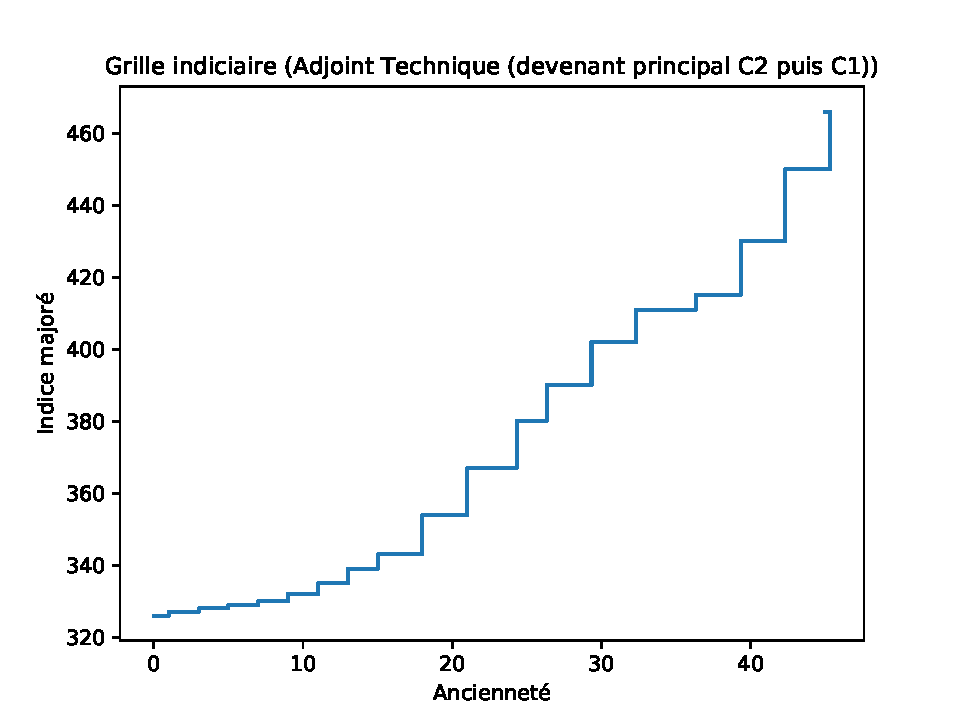
\includegraphics[width=0.7\textwidth]{fig/grille_AdjTech.pdf}\end{minipage} 
\begin{minipage}{0.3\linewidth} 
 \begin{center} 

\begin{tabular}[htb]{|c|c|} 
\hline 
 Indice majoré &  Durée (années) \\ 
\hline \hline 
 326 &  1.00 \\ 
\hline 
 327 &  2.00 \\ 
\hline 
 328 &  2.00 \\ 
\hline 
 329 &  2.00 \\ 
\hline 
 330 &  2.00 \\ 
\hline 
 332 &  2.00 \\ 
\hline 
 335 &  2.00 \\ 
\hline 
 339 &  2.00 \\ 
\hline 
 343 &  3.00 \\ 
\hline 
 354 &  3.00 \\ 
\hline 
 367 &  3.33 \\ 
\hline 
 380 &  2.00 \\ 
\hline 
 390 &  3.00 \\ 
\hline 
 402 &  3.00 \\ 
\hline 
 411 &  4.00 \\ 
\hline 
 415 &  3.00 \\ 
\hline 
 430 &  3.00 \\ 
\hline 
 450 &  3.00 \\ 
\hline 
 466 &   \\ 
\hline 
\hline 
\end{tabular} 
\end{center} 
 \end{minipage} 


 \addto{\captionsenglish}{ \renewcommand{\mtctitle}{}} \setcounter{minitocdepth}{2} 
 \minitoc \newpage 

\section{Début de carrière à 22 ans} 

\subsection{Génération 1975 (début en 1997)} 

\paragraph{Retraites possibles dans le modèle \emph{Gouvernement truqué (âge-pivot bloqué à 65 ans)}}  
 
{ \scriptsize \begin{center} 
\begin{tabular}[htb]{|c|c||c|c||c|c||c||c|c|c|c|c|c|} 
\hline 
 Retraite en &  Âge &  Âge pivot &  Décote/Surcote &  Retraite (\euro{} 2019) &  Tx Rempl(\%) &  SMIC (\euro{} 2019) &  Retraite/SMIC &  Rev70/SMIC &  Rev75/SMIC &  Rev80/SMIC &  Rev85/SMIC &  Rev90/SMIC \\ 
\hline \hline 
 2037 &  62 &  64 ans 10 mois &  -14.17\% &  1091.14 &  {\bf 43.52} &  2143.00 &  {\bf {\color{red} 0.51}} &  {\bf {\color{red} 0.46}} &  {\bf {\color{red} 0.43}} &  {\bf {\color{red} 0.40}} &  {\bf {\color{red} 0.38}} &  {\bf {\color{red} 0.35}} \\ 
\hline 
 2038 &  63 &  64 ans 11 mois &  -9.58\% &  1189.79 &  {\bf 47.37} &  2170.86 &  {\bf {\color{red} 0.55}} &  {\bf {\color{red} 0.50}} &  {\bf {\color{red} 0.47}} &  {\bf {\color{red} 0.44}} &  {\bf {\color{red} 0.41}} &  {\bf {\color{red} 0.39}} \\ 
\hline 
 2039 &  64 &  65 ans 0 mois &  -5.00\% &  1294.91 &  {\bf 49.90} &  2199.08 &  {\bf {\color{red} 0.59}} &  {\bf {\color{red} 0.54}} &  {\bf {\color{red} 0.51}} &  {\bf {\color{red} 0.48}} &  {\bf {\color{red} 0.45}} &  {\bf {\color{red} 0.42}} \\ 
\hline 
 2040 &  65 &  65 ans 0 mois &  0.00\% &  1893.52 &  {\bf 71.76} &  2227.67 &  {\bf {\color{red} 0.85}} &  {\bf {\color{red} 0.80}} &  {\bf {\color{red} 0.75}} &  {\bf {\color{red} 0.70}} &  {\bf {\color{red} 0.66}} &  {\bf {\color{red} 0.62}} \\ 
\hline 
 2041 &  66 &  65 ans 0 mois &  5.00\% &  1918.14 &  {\bf 72.56} &  2256.63 &  {\bf {\color{red} 0.85}} &  {\bf {\color{red} 0.81}} &  {\bf {\color{red} 0.76}} &  {\bf {\color{red} 0.71}} &  {\bf {\color{red} 0.67}} &  {\bf {\color{red} 0.62}} \\ 
\hline 
 2042 &  67 &  65 ans 0 mois &  10.00\% &  1943.07 &  {\bf 71.66} &  2285.97 &  {\bf {\color{red} 0.85}} &  {\bf {\color{red} 0.82}} &  {\bf {\color{red} 0.77}} &  {\bf {\color{red} 0.72}} &  {\bf {\color{red} 0.67}} &  {\bf {\color{red} 0.63}} \\ 
\hline 
\hline 
\end{tabular} 
\end{center} } 
\paragraph{Retraites possibles dans le modèle \emph{Gouvernement corrigé (âge-pivot glissant)}}  
 
{ \scriptsize \begin{center} 
\begin{tabular}[htb]{|c|c||c|c||c|c||c||c|c|c|c|c|c|} 
\hline 
 Retraite en &  Âge &  Âge pivot &  Décote/Surcote &  Retraite (\euro{} 2019) &  Tx Rempl(\%) &  SMIC (\euro{} 2019) &  Retraite/SMIC &  Rev70/SMIC &  Rev75/SMIC &  Rev80/SMIC &  Rev85/SMIC &  Rev90/SMIC \\ 
\hline \hline 
 2037 &  62 &  64 ans 10 mois &  -14.17\% &  1091.14 &  {\bf 43.52} &  2143.00 &  {\bf {\color{red} 0.51}} &  {\bf {\color{red} 0.46}} &  {\bf {\color{red} 0.43}} &  {\bf {\color{red} 0.40}} &  {\bf {\color{red} 0.38}} &  {\bf {\color{red} 0.35}} \\ 
\hline 
 2038 &  63 &  64 ans 11 mois &  -9.58\% &  1189.79 &  {\bf 47.37} &  2170.86 &  {\bf {\color{red} 0.55}} &  {\bf {\color{red} 0.50}} &  {\bf {\color{red} 0.47}} &  {\bf {\color{red} 0.44}} &  {\bf {\color{red} 0.41}} &  {\bf {\color{red} 0.39}} \\ 
\hline 
 2039 &  64 &  65 ans 0 mois &  -5.00\% &  1294.91 &  {\bf 49.90} &  2199.08 &  {\bf {\color{red} 0.59}} &  {\bf {\color{red} 0.54}} &  {\bf {\color{red} 0.51}} &  {\bf {\color{red} 0.48}} &  {\bf {\color{red} 0.45}} &  {\bf {\color{red} 0.42}} \\ 
\hline 
 2040 &  65 &  65 ans 1 mois &  -0.42\% &  1893.52 &  {\bf 71.76} &  2227.67 &  {\bf {\color{red} 0.85}} &  {\bf {\color{red} 0.80}} &  {\bf {\color{red} 0.75}} &  {\bf {\color{red} 0.70}} &  {\bf {\color{red} 0.66}} &  {\bf {\color{red} 0.62}} \\ 
\hline 
 2041 &  66 &  65 ans 2 mois &  4.17\% &  1918.14 &  {\bf 72.56} &  2256.63 &  {\bf {\color{red} 0.85}} &  {\bf {\color{red} 0.81}} &  {\bf {\color{red} 0.76}} &  {\bf {\color{red} 0.71}} &  {\bf {\color{red} 0.67}} &  {\bf {\color{red} 0.62}} \\ 
\hline 
 2042 &  67 &  65 ans 3 mois &  8.75\% &  1943.07 &  {\bf 71.66} &  2285.97 &  {\bf {\color{red} 0.85}} &  {\bf {\color{red} 0.82}} &  {\bf {\color{red} 0.77}} &  {\bf {\color{red} 0.72}} &  {\bf {\color{red} 0.67}} &  {\bf {\color{red} 0.63}} \\ 
\hline 
\hline 
\end{tabular} 
\end{center} } 
\paragraph{Retraites possibles dans le modèle \emph{Destinie2 (revalorisation de la fonction publique)}}  
 
{ \scriptsize \begin{center} 
\begin{tabular}[htb]{|c|c||c|c||c|c||c||c|c|c|c|c|c|} 
\hline 
 Retraite en &  Âge &  Âge pivot &  Décote/Surcote &  Retraite (\euro{} 2019) &  Tx Rempl(\%) &  SMIC (\euro{} 2019) &  Retraite/SMIC &  Rev70/SMIC &  Rev75/SMIC &  Rev80/SMIC &  Rev85/SMIC &  Rev90/SMIC \\ 
\hline \hline 
 2037 &  62 &  64 ans 10 mois &  -14.17\% &  1150.96 &  {\bf 37.02} &  2014.82 &  {\bf {\color{red} 0.57}} &  {\bf {\color{red} 0.52}} &  {\bf {\color{red} 0.48}} &  {\bf {\color{red} 0.45}} &  {\bf {\color{red} 0.42}} &  {\bf {\color{red} 0.40}} \\ 
\hline 
 2038 &  63 &  64 ans 11 mois &  -9.58\% &  1261.38 &  {\bf 39.98} &  2041.01 &  {\bf {\color{red} 0.62}} &  {\bf {\color{red} 0.56}} &  {\bf {\color{red} 0.53}} &  {\bf {\color{red} 0.50}} &  {\bf {\color{red} 0.47}} &  {\bf {\color{red} 0.44}} \\ 
\hline 
 2039 &  64 &  65 ans 0 mois &  -5.00\% &  1380.11 &  {\bf 41.80} &  2067.55 &  {\bf {\color{red} 0.67}} &  {\bf {\color{red} 0.62}} &  {\bf {\color{red} 0.58}} &  {\bf {\color{red} 0.54}} &  {\bf {\color{red} 0.51}} &  {\bf {\color{red} 0.48}} \\ 
\hline 
 2040 &  65 &  65 ans 1 mois &  -0.42\% &  1780.26 &  {\bf 52.34} &  2094.43 &  {\bf {\color{red} 0.85}} &  {\bf {\color{red} 0.80}} &  {\bf {\color{red} 0.75}} &  {\bf {\color{red} 0.70}} &  {\bf {\color{red} 0.66}} &  {\bf {\color{red} 0.62}} \\ 
\hline 
 2041 &  66 &  65 ans 2 mois &  4.17\% &  1803.40 &  {\bf 52.25} &  2121.65 &  {\bf {\color{red} 0.85}} &  {\bf {\color{red} 0.81}} &  {\bf {\color{red} 0.76}} &  {\bf {\color{red} 0.71}} &  {\bf {\color{red} 0.67}} &  {\bf {\color{red} 0.62}} \\ 
\hline 
 2042 &  67 &  65 ans 3 mois &  8.75\% &  1826.85 &  {\bf 50.93} &  2149.23 &  {\bf {\color{red} 0.85}} &  {\bf {\color{red} 0.82}} &  {\bf {\color{red} 0.77}} &  {\bf {\color{red} 0.72}} &  {\bf {\color{red} 0.67}} &  {\bf {\color{red} 0.63}} \\ 
\hline 
\hline 
\end{tabular} 
\end{center} } 

 \begin{center}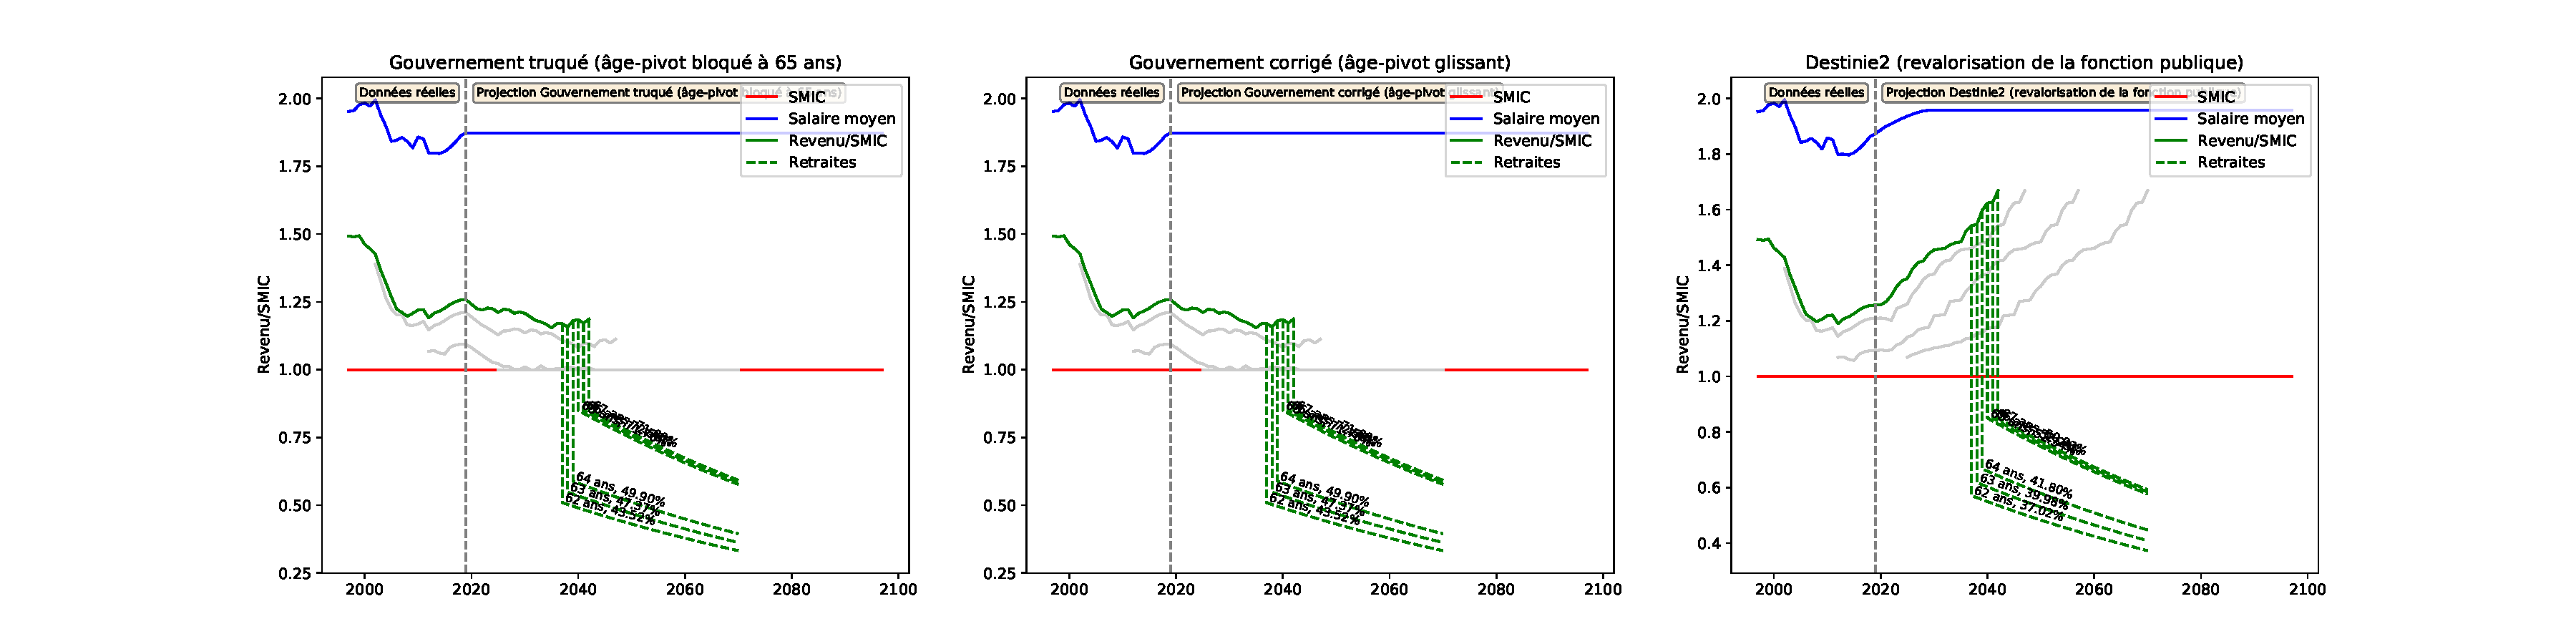
\includegraphics[width=0.9\textwidth]{fig/AdjTech_1975_22_dest_retraite.pdf}\end{center} \label{fig/AdjTech_1975_22_dest_retraite.pdf} 

\newpage 
 
\paragraph{Revenus et points pour le modèle \emph{Gouvernement truqué (âge-pivot bloqué à 65 ans)}} 
 
{ \scriptsize \begin{center} 
\begin{tabular}[htb]{|c|c||c|c|c|c|c|c||c|c||c|c|c|} 
\hline 
 Année &  Âge &  Ind Maj &  Pt Ind(\euro{} 2019) &  Rev HP(\euro{} 2019) &  Tx Primes &  GIPA(\euro{} 2019) &  Revenu(\euro{} 2019) &  SMIC(\euro{} 2019) &  Rev/SMIC &  Cumul Pts &  Achat Pt(\euro{} 2019) &  Serv. Pt(\euro{} 2019) \\ 
\hline \hline 
 1997 &  22 &  326.0 &  5.53 &  1804.20 &  12.41 &  0.00 &  2028.10 &  1358.84 &  {\bf 1.49} &  683.49 &  35.61 &  0.50 \\ 
\hline 
 1998 &  23 &  327.0 &  5.57 &  1820.23 &  12.64 &  0.00 &  2050.31 &  1376.36 &  {\bf 1.49} &  1374.47 &  35.61 &  0.50 \\ 
\hline 
 1999 &  24 &  327.0 &  5.61 &  1834.94 &  12.87 &  0.00 &  2071.10 &  1386.54 &  {\bf 1.49} &  2072.46 &  35.61 &  0.50 \\ 
\hline 
 2000 &  25 &  328.0 &  5.55 &  1818.82 &  13.10 &  0.00 &  2057.09 &  1407.00 &  {\bf 1.46} &  2765.72 &  35.61 &  0.50 \\ 
\hline 
 2001 &  26 &  328.0 &  5.52 &  1810.73 &  13.33 &  31.52 &  2083.61 &  1441.04 &  {\bf 1.45} &  3467.92 &  35.61 &  0.50 \\ 
\hline 
 2002 &  27 &  329.0 &  5.49 &  1804.98 &  13.56 &  16.02 &  2065.76 &  1447.74 &  {\bf 1.43} &  4164.11 &  35.61 &  0.50 \\ 
\hline 
 2003 &  28 &  329.0 &  5.37 &  1768.25 &  13.79 &  28.27 &  2040.36 &  1493.03 &  {\bf 1.37} &  4851.74 &  35.61 &  0.50 \\ 
\hline 
 2004 &  29 &  330.0 &  5.29 &  1745.61 &  14.02 &  50.01 &  2040.36 &  1547.32 &  {\bf 1.32} &  5539.36 &  35.61 &  0.50 \\ 
\hline 
 2005 &  30 &  330.0 &  5.29 &  1745.42 &  14.25 &  40.09 &  2034.23 &  1603.67 &  {\bf 1.27} &  6224.92 &  35.61 &  0.50 \\ 
\hline 
 2006 &  31 &  332.0 &  5.23 &  1736.40 &  14.48 &  0.00 &  1987.83 &  1625.00 &  {\bf 1.22} &  6894.84 &  35.61 &  0.50 \\ 
\hline 
 2007 &  32 &  332.0 &  5.19 &  1724.57 &  14.71 &  0.00 &  1978.25 &  1634.08 &  {\bf 1.21} &  7561.54 &  35.61 &  0.50 \\ 
\hline 
 2008 &  33 &  335.0 &  5.09 &  1706.17 &  14.94 &  2.12 &  1963.19 &  1640.24 &  {\bf 1.20} &  8223.16 &  35.61 &  0.50 \\ 
\hline 
 2009 &  34 &  335.0 &  5.13 &  1718.26 &  15.17 &  25.12 &  2004.04 &  1659.42 &  {\bf 1.21} &  8898.54 &  35.61 &  0.50 \\ 
\hline 
 2010 &  35 &  339.0 &  5.08 &  1721.21 &  15.40 &  16.90 &  2003.18 &  1641.90 &  {\bf 1.22} &  9573.64 &  35.61 &  0.50 \\ 
\hline 
 2011 &  36 &  339.0 &  4.97 &  1685.45 &  15.63 &  45.43 &  1994.32 &  1633.19 &  {\bf 1.22} &  10245.75 &  35.61 &  0.50 \\ 
\hline 
 2012 &  37 &  343.0 &  4.88 &  1672.62 &  15.86 &  54.12 &  1992.01 &  1673.05 &  {\bf 1.19} &  10917.08 &  35.61 &  0.50 \\ 
\hline 
 2013 &  38 &  343.0 &  4.83 &  1658.29 &  16.09 &  85.21 &  2010.31 &  1664.01 &  {\bf 1.21} &  11594.58 &  35.61 &  0.50 \\ 
\hline 
 2014 &  39 &  343.0 &  4.81 &  1649.98 &  16.32 &  114.90 &  2034.16 &  1673.24 &  {\bf 1.22} &  12280.12 &  35.61 &  0.50 \\ 
\hline 
 2015 &  40 &  354.0 &  4.81 &  1702.23 &  16.55 &  84.96 &  2068.92 &  1686.62 &  {\bf 1.23} &  12977.37 &  35.61 &  0.50 \\ 
\hline 
 2016 &  41 &  354.0 &  4.80 &  1698.84 &  16.78 &  117.40 &  2101.30 &  1693.76 &  {\bf 1.24} &  13685.53 &  35.61 &  0.50 \\ 
\hline 
 2017 &  42 &  354.0 &  4.81 &  1702.26 &  17.01 &  125.10 &  2116.92 &  1692.60 &  {\bf 1.25} &  14398.96 &  35.61 &  0.50 \\ 
\hline 
 2018 &  43 &  367.0 &  4.74 &  1740.41 &  17.24 &  83.57 &  2124.03 &  1689.76 &  {\bf 1.26} &  15114.78 &  35.61 &  0.50 \\ 
\hline 
 2019 &  44 &  367.0 &  4.79 &  1759.55 &  17.47 &  68.67 &  2135.62 &  1698.45 &  {\bf 1.26} &  15834.51 &  35.61 &  0.50 \\ 
\hline 
 2020 &  45 &  367.0 &  4.79 &  1759.55 &  17.70 &  64.68 &  2135.68 &  1720.53 &  {\bf 1.24} &  16554.26 &  35.61 &  0.50 \\ 
\hline 
 2021 &  46 &  375.7 &  4.79 &  1801.31 &  17.93 &  11.37 &  2135.66 &  1742.90 &  {\bf 1.23} &  17274.00 &  35.61 &  0.50 \\ 
\hline 
 2022 &  47 &  380.0 &  4.79 &  1821.88 &  18.16 &  0.00 &  2152.73 &  1765.55 &  {\bf 1.22} &  17999.50 &  35.61 &  0.50 \\ 
\hline 
 2023 &  48 &  386.7 &  4.79 &  1854.00 &  18.39 &  0.00 &  2194.95 &  1788.51 &  {\bf 1.23} &  18739.22 &  35.61 &  0.50 \\ 
\hline 
 2024 &  49 &  390.0 &  4.79 &  1869.82 &  18.62 &  0.00 &  2217.99 &  1811.76 &  {\bf 1.22} &  19486.71 &  35.61 &  0.50 \\ 
\hline 
 2025 &  50 &  390.0 &  4.79 &  1869.82 &  18.85 &  0.00 &  2222.29 &  1835.31 &  {\bf 1.21} &  20235.65 &  35.61 &  0.50 \\ 
\hline 
 2026 &  51 &  398.0 &  4.79 &  1908.37 &  19.08 &  0.00 &  2272.49 &  1859.17 &  {\bf 1.22} &  21001.51 &  35.61 &  0.50 \\ 
\hline 
 2027 &  52 &  402.0 &  4.79 &  1927.36 &  19.31 &  0.00 &  2299.53 &  1883.34 &  {\bf 1.22} &  21776.48 &  35.61 &  0.50 \\ 
\hline 
 2028 &  53 &  402.0 &  4.79 &  1927.36 &  19.54 &  0.00 &  2303.96 &  1907.82 &  {\bf 1.21} &  22552.94 &  35.61 &  0.50 \\ 
\hline 
 2029 &  54 &  408.0 &  4.79 &  1956.27 &  19.77 &  0.00 &  2343.02 &  1932.62 &  {\bf 1.21} &  23341.97 &  35.63 &  0.50 \\ 
\hline 
 2030 &  55 &  411.0 &  4.79 &  1970.51 &  20.00 &  0.00 &  2364.61 &  1957.75 &  {\bf 1.21} &  24137.06 &  35.69 &  0.50 \\ 
\hline 
 2031 &  56 &  411.0 &  4.79 &  1970.51 &  20.23 &  0.00 &  2369.14 &  1983.20 &  {\bf 1.19} &  24931.85 &  35.77 &  0.50 \\ 
\hline 
 2032 &  57 &  411.0 &  4.79 &  1970.51 &  20.46 &  0.00 &  2373.67 &  2008.98 &  {\bf 1.18} &  25725.76 &  35.88 &  0.50 \\ 
\hline 
 2033 &  58 &  413.7 &  4.79 &  1983.36 &  20.69 &  0.00 &  2393.71 &  2035.10 &  {\bf 1.18} &  26523.32 &  36.02 &  0.50 \\ 
\hline 
 2034 &  59 &  415.0 &  4.79 &  1989.69 &  20.92 &  0.00 &  2405.93 &  2061.55 &  {\bf 1.17} &  27321.32 &  36.18 &  0.50 \\ 
\hline 
 2035 &  60 &  415.0 &  4.79 &  1989.69 &  21.15 &  0.00 &  2410.50 &  2088.35 &  {\bf 1.15} &  28116.59 &  36.37 &  0.51 \\ 
\hline 
 2036 &  61 &  425.0 &  4.79 &  2037.87 &  21.38 &  0.00 &  2473.57 &  2115.50 &  {\bf 1.17} &  28927.72 &  36.59 &  0.51 \\ 
\hline 
 2037 &  62 &  430.0 &  4.79 &  2061.60 &  21.61 &  0.00 &  2507.11 &  2143.00 &  {\bf 1.17} &  29744.24 &  36.85 &  0.51 \\ 
\hline 
 2038 &  63 &  430.0 &  4.79 &  2061.60 &  21.84 &  0.00 &  2511.86 &  2170.86 &  {\bf 1.16} &  30556.12 &  37.13 &  0.52 \\ 
\hline 
 2039 &  64 &  443.4 &  4.79 &  2125.85 &  22.07 &  0.00 &  2595.02 &  2199.08 &  {\bf 1.18} &  31387.90 &  37.44 &  0.52 \\ 
\hline 
 2040 &  65 &  450.0 &  4.79 &  2157.49 &  22.30 &  0.00 &  2638.61 &  2227.67 &  {\bf 1.18} &  32225.98 &  37.78 &  0.53 \\ 
\hline 
 2041 &  66 &  450.0 &  4.79 &  2157.49 &  22.53 &  0.00 &  2643.57 &  2256.63 &  {\bf 1.17} &  33057.38 &  38.16 &  0.53 \\ 
\hline 
 2042 &  67 &  460.7 &  4.79 &  2208.89 &  22.76 &  0.00 &  2711.63 &  2285.97 &  {\bf 1.19} &  33901.16 &  38.56 &  0.54 \\ 
\hline 
\hline 
\end{tabular} 
\end{center} } 
\newpage 
 
\paragraph{Revenus et points pour le modèle \emph{Gouvernement corrigé (âge-pivot glissant)}} 
 
{ \scriptsize \begin{center} 
\begin{tabular}[htb]{|c|c||c|c|c|c|c|c||c|c||c|c|c|} 
\hline 
 Année &  Âge &  Ind Maj &  Pt Ind(\euro{} 2019) &  Rev HP(\euro{} 2019) &  Tx Primes &  GIPA(\euro{} 2019) &  Revenu(\euro{} 2019) &  SMIC(\euro{} 2019) &  Rev/SMIC &  Cumul Pts &  Achat Pt(\euro{} 2019) &  Serv. Pt(\euro{} 2019) \\ 
\hline \hline 
 1997 &  22 &  326.0 &  5.53 &  1804.20 &  12.41 &  0.00 &  2028.10 &  1358.84 &  {\bf 1.49} &  683.49 &  35.61 &  0.50 \\ 
\hline 
 1998 &  23 &  327.0 &  5.57 &  1820.23 &  12.64 &  0.00 &  2050.31 &  1376.36 &  {\bf 1.49} &  1374.47 &  35.61 &  0.50 \\ 
\hline 
 1999 &  24 &  327.0 &  5.61 &  1834.94 &  12.87 &  0.00 &  2071.10 &  1386.54 &  {\bf 1.49} &  2072.46 &  35.61 &  0.50 \\ 
\hline 
 2000 &  25 &  328.0 &  5.55 &  1818.82 &  13.10 &  0.00 &  2057.09 &  1407.00 &  {\bf 1.46} &  2765.72 &  35.61 &  0.50 \\ 
\hline 
 2001 &  26 &  328.0 &  5.52 &  1810.73 &  13.33 &  31.52 &  2083.61 &  1441.04 &  {\bf 1.45} &  3467.92 &  35.61 &  0.50 \\ 
\hline 
 2002 &  27 &  329.0 &  5.49 &  1804.98 &  13.56 &  16.02 &  2065.76 &  1447.74 &  {\bf 1.43} &  4164.11 &  35.61 &  0.50 \\ 
\hline 
 2003 &  28 &  329.0 &  5.37 &  1768.25 &  13.79 &  28.27 &  2040.36 &  1493.03 &  {\bf 1.37} &  4851.74 &  35.61 &  0.50 \\ 
\hline 
 2004 &  29 &  330.0 &  5.29 &  1745.61 &  14.02 &  50.01 &  2040.36 &  1547.32 &  {\bf 1.32} &  5539.36 &  35.61 &  0.50 \\ 
\hline 
 2005 &  30 &  330.0 &  5.29 &  1745.42 &  14.25 &  40.09 &  2034.23 &  1603.67 &  {\bf 1.27} &  6224.92 &  35.61 &  0.50 \\ 
\hline 
 2006 &  31 &  332.0 &  5.23 &  1736.40 &  14.48 &  0.00 &  1987.83 &  1625.00 &  {\bf 1.22} &  6894.84 &  35.61 &  0.50 \\ 
\hline 
 2007 &  32 &  332.0 &  5.19 &  1724.57 &  14.71 &  0.00 &  1978.25 &  1634.08 &  {\bf 1.21} &  7561.54 &  35.61 &  0.50 \\ 
\hline 
 2008 &  33 &  335.0 &  5.09 &  1706.17 &  14.94 &  2.12 &  1963.19 &  1640.24 &  {\bf 1.20} &  8223.16 &  35.61 &  0.50 \\ 
\hline 
 2009 &  34 &  335.0 &  5.13 &  1718.26 &  15.17 &  25.12 &  2004.04 &  1659.42 &  {\bf 1.21} &  8898.54 &  35.61 &  0.50 \\ 
\hline 
 2010 &  35 &  339.0 &  5.08 &  1721.21 &  15.40 &  16.90 &  2003.18 &  1641.90 &  {\bf 1.22} &  9573.64 &  35.61 &  0.50 \\ 
\hline 
 2011 &  36 &  339.0 &  4.97 &  1685.45 &  15.63 &  45.43 &  1994.32 &  1633.19 &  {\bf 1.22} &  10245.75 &  35.61 &  0.50 \\ 
\hline 
 2012 &  37 &  343.0 &  4.88 &  1672.62 &  15.86 &  54.12 &  1992.01 &  1673.05 &  {\bf 1.19} &  10917.08 &  35.61 &  0.50 \\ 
\hline 
 2013 &  38 &  343.0 &  4.83 &  1658.29 &  16.09 &  85.21 &  2010.31 &  1664.01 &  {\bf 1.21} &  11594.58 &  35.61 &  0.50 \\ 
\hline 
 2014 &  39 &  343.0 &  4.81 &  1649.98 &  16.32 &  114.90 &  2034.16 &  1673.24 &  {\bf 1.22} &  12280.12 &  35.61 &  0.50 \\ 
\hline 
 2015 &  40 &  354.0 &  4.81 &  1702.23 &  16.55 &  84.96 &  2068.92 &  1686.62 &  {\bf 1.23} &  12977.37 &  35.61 &  0.50 \\ 
\hline 
 2016 &  41 &  354.0 &  4.80 &  1698.84 &  16.78 &  117.40 &  2101.30 &  1693.76 &  {\bf 1.24} &  13685.53 &  35.61 &  0.50 \\ 
\hline 
 2017 &  42 &  354.0 &  4.81 &  1702.26 &  17.01 &  125.10 &  2116.92 &  1692.60 &  {\bf 1.25} &  14398.96 &  35.61 &  0.50 \\ 
\hline 
 2018 &  43 &  367.0 &  4.74 &  1740.41 &  17.24 &  83.57 &  2124.03 &  1689.76 &  {\bf 1.26} &  15114.78 &  35.61 &  0.50 \\ 
\hline 
 2019 &  44 &  367.0 &  4.79 &  1759.55 &  17.47 &  68.67 &  2135.62 &  1698.45 &  {\bf 1.26} &  15834.51 &  35.61 &  0.50 \\ 
\hline 
 2020 &  45 &  367.0 &  4.79 &  1759.55 &  17.70 &  64.68 &  2135.68 &  1720.53 &  {\bf 1.24} &  16554.26 &  35.61 &  0.50 \\ 
\hline 
 2021 &  46 &  375.7 &  4.79 &  1801.31 &  17.93 &  11.37 &  2135.66 &  1742.90 &  {\bf 1.23} &  17274.00 &  35.61 &  0.50 \\ 
\hline 
 2022 &  47 &  380.0 &  4.79 &  1821.88 &  18.16 &  0.00 &  2152.73 &  1765.55 &  {\bf 1.22} &  17999.50 &  35.61 &  0.50 \\ 
\hline 
 2023 &  48 &  386.7 &  4.79 &  1854.00 &  18.39 &  0.00 &  2194.95 &  1788.51 &  {\bf 1.23} &  18739.22 &  35.61 &  0.50 \\ 
\hline 
 2024 &  49 &  390.0 &  4.79 &  1869.82 &  18.62 &  0.00 &  2217.99 &  1811.76 &  {\bf 1.22} &  19486.71 &  35.61 &  0.50 \\ 
\hline 
 2025 &  50 &  390.0 &  4.79 &  1869.82 &  18.85 &  0.00 &  2222.29 &  1835.31 &  {\bf 1.21} &  20235.65 &  35.61 &  0.50 \\ 
\hline 
 2026 &  51 &  398.0 &  4.79 &  1908.37 &  19.08 &  0.00 &  2272.49 &  1859.17 &  {\bf 1.22} &  21001.51 &  35.61 &  0.50 \\ 
\hline 
 2027 &  52 &  402.0 &  4.79 &  1927.36 &  19.31 &  0.00 &  2299.53 &  1883.34 &  {\bf 1.22} &  21776.48 &  35.61 &  0.50 \\ 
\hline 
 2028 &  53 &  402.0 &  4.79 &  1927.36 &  19.54 &  0.00 &  2303.96 &  1907.82 &  {\bf 1.21} &  22552.94 &  35.61 &  0.50 \\ 
\hline 
 2029 &  54 &  408.0 &  4.79 &  1956.27 &  19.77 &  0.00 &  2343.02 &  1932.62 &  {\bf 1.21} &  23341.97 &  35.63 &  0.50 \\ 
\hline 
 2030 &  55 &  411.0 &  4.79 &  1970.51 &  20.00 &  0.00 &  2364.61 &  1957.75 &  {\bf 1.21} &  24137.06 &  35.69 &  0.50 \\ 
\hline 
 2031 &  56 &  411.0 &  4.79 &  1970.51 &  20.23 &  0.00 &  2369.14 &  1983.20 &  {\bf 1.19} &  24931.85 &  35.77 &  0.50 \\ 
\hline 
 2032 &  57 &  411.0 &  4.79 &  1970.51 &  20.46 &  0.00 &  2373.67 &  2008.98 &  {\bf 1.18} &  25725.76 &  35.88 &  0.50 \\ 
\hline 
 2033 &  58 &  413.7 &  4.79 &  1983.36 &  20.69 &  0.00 &  2393.71 &  2035.10 &  {\bf 1.18} &  26523.32 &  36.02 &  0.50 \\ 
\hline 
 2034 &  59 &  415.0 &  4.79 &  1989.69 &  20.92 &  0.00 &  2405.93 &  2061.55 &  {\bf 1.17} &  27321.32 &  36.18 &  0.50 \\ 
\hline 
 2035 &  60 &  415.0 &  4.79 &  1989.69 &  21.15 &  0.00 &  2410.50 &  2088.35 &  {\bf 1.15} &  28116.59 &  36.37 &  0.51 \\ 
\hline 
 2036 &  61 &  425.0 &  4.79 &  2037.87 &  21.38 &  0.00 &  2473.57 &  2115.50 &  {\bf 1.17} &  28927.72 &  36.59 &  0.51 \\ 
\hline 
 2037 &  62 &  430.0 &  4.79 &  2061.60 &  21.61 &  0.00 &  2507.11 &  2143.00 &  {\bf 1.17} &  29744.24 &  36.85 &  0.51 \\ 
\hline 
 2038 &  63 &  430.0 &  4.79 &  2061.60 &  21.84 &  0.00 &  2511.86 &  2170.86 &  {\bf 1.16} &  30556.12 &  37.13 &  0.52 \\ 
\hline 
 2039 &  64 &  443.4 &  4.79 &  2125.85 &  22.07 &  0.00 &  2595.02 &  2199.08 &  {\bf 1.18} &  31387.90 &  37.44 &  0.52 \\ 
\hline 
 2040 &  65 &  450.0 &  4.79 &  2157.49 &  22.30 &  0.00 &  2638.61 &  2227.67 &  {\bf 1.18} &  32225.98 &  37.78 &  0.53 \\ 
\hline 
 2041 &  66 &  450.0 &  4.79 &  2157.49 &  22.53 &  0.00 &  2643.57 &  2256.63 &  {\bf 1.17} &  33057.38 &  38.16 &  0.53 \\ 
\hline 
 2042 &  67 &  460.7 &  4.79 &  2208.89 &  22.76 &  0.00 &  2711.63 &  2285.97 &  {\bf 1.19} &  33901.16 &  38.56 &  0.54 \\ 
\hline 
\hline 
\end{tabular} 
\end{center} } 
\newpage 
 
\paragraph{Revenus et points pour le modèle \emph{Destinie2 (revalorisation de la fonction publique)}} 
 
{ \scriptsize \begin{center} 
\begin{tabular}[htb]{|c|c||c|c|c|c|c|c||c|c||c|c|c|} 
\hline 
 Année &  Âge &  Ind Maj &  Pt Ind(\euro{} 2019) &  Rev HP(\euro{} 2019) &  Tx Primes &  GIPA(\euro{} 2019) &  Revenu(\euro{} 2019) &  SMIC(\euro{} 2019) &  Rev/SMIC &  Cumul Pts &  Achat Pt(\euro{} 2019) &  Serv. Pt(\euro{} 2019) \\ 
\hline \hline 
 1997 &  22 &  326.0 &  5.53 &  1804.20 &  12.41 &  0.00 &  2028.10 &  1358.84 &  {\bf 1.49} &  681.82 &  35.69 &  0.50 \\ 
\hline 
 1998 &  23 &  327.0 &  5.57 &  1820.23 &  12.64 &  0.00 &  2050.31 &  1376.36 &  {\bf 1.49} &  1371.10 &  35.69 &  0.50 \\ 
\hline 
 1999 &  24 &  327.0 &  5.61 &  1834.94 &  12.87 &  0.00 &  2071.10 &  1386.54 &  {\bf 1.49} &  2067.37 &  35.69 &  0.50 \\ 
\hline 
 2000 &  25 &  328.0 &  5.55 &  1818.82 &  13.10 &  0.00 &  2057.09 &  1407.00 &  {\bf 1.46} &  2758.93 &  35.69 &  0.50 \\ 
\hline 
 2001 &  26 &  328.0 &  5.52 &  1810.73 &  13.33 &  31.52 &  2083.61 &  1441.04 &  {\bf 1.45} &  3459.40 &  35.69 &  0.50 \\ 
\hline 
 2002 &  27 &  329.0 &  5.49 &  1804.98 &  13.56 &  16.02 &  2065.76 &  1447.74 &  {\bf 1.43} &  4153.88 &  35.69 &  0.50 \\ 
\hline 
 2003 &  28 &  329.0 &  5.37 &  1768.25 &  13.79 &  28.27 &  2040.36 &  1493.03 &  {\bf 1.37} &  4839.82 &  35.69 &  0.50 \\ 
\hline 
 2004 &  29 &  330.0 &  5.29 &  1745.61 &  14.02 &  50.01 &  2040.36 &  1547.32 &  {\bf 1.32} &  5525.75 &  35.69 &  0.50 \\ 
\hline 
 2005 &  30 &  330.0 &  5.29 &  1745.42 &  14.25 &  40.09 &  2034.23 &  1603.67 &  {\bf 1.27} &  6209.63 &  35.69 &  0.50 \\ 
\hline 
 2006 &  31 &  332.0 &  5.23 &  1736.40 &  14.48 &  0.00 &  1987.83 &  1625.00 &  {\bf 1.22} &  6877.90 &  35.69 &  0.50 \\ 
\hline 
 2007 &  32 &  332.0 &  5.19 &  1724.57 &  14.71 &  0.00 &  1978.25 &  1634.08 &  {\bf 1.21} &  7542.96 &  35.69 &  0.50 \\ 
\hline 
 2008 &  33 &  335.0 &  5.09 &  1706.17 &  14.94 &  2.12 &  1963.19 &  1640.24 &  {\bf 1.20} &  8202.95 &  35.69 &  0.50 \\ 
\hline 
 2009 &  34 &  335.0 &  5.13 &  1718.26 &  15.17 &  21.42 &  2000.34 &  1659.42 &  {\bf 1.21} &  8875.44 &  35.69 &  0.50 \\ 
\hline 
 2010 &  35 &  339.0 &  5.08 &  1721.21 &  15.40 &  14.74 &  2001.02 &  1641.90 &  {\bf 1.22} &  9548.15 &  35.69 &  0.50 \\ 
\hline 
 2011 &  36 &  339.0 &  4.97 &  1685.45 &  15.63 &  43.97 &  1992.86 &  1633.19 &  {\bf 1.22} &  10218.11 &  35.69 &  0.50 \\ 
\hline 
 2012 &  37 &  343.0 &  4.88 &  1672.62 &  15.86 &  52.29 &  1990.19 &  1673.05 &  {\bf 1.19} &  10887.18 &  35.69 &  0.50 \\ 
\hline 
 2013 &  38 &  343.0 &  4.83 &  1658.29 &  16.09 &  82.91 &  2008.01 &  1664.01 &  {\bf 1.21} &  11562.25 &  35.69 &  0.50 \\ 
\hline 
 2014 &  39 &  343.0 &  4.81 &  1649.98 &  16.32 &  112.93 &  2032.19 &  1673.24 &  {\bf 1.21} &  12245.44 &  35.69 &  0.50 \\ 
\hline 
 2015 &  40 &  354.0 &  4.81 &  1702.23 &  16.55 &  83.02 &  2066.97 &  1686.62 &  {\bf 1.23} &  12940.32 &  35.69 &  0.50 \\ 
\hline 
 2016 &  41 &  354.0 &  4.80 &  1698.84 &  16.78 &  115.31 &  2099.21 &  1693.76 &  {\bf 1.24} &  13646.04 &  35.69 &  0.50 \\ 
\hline 
 2017 &  42 &  354.0 &  4.81 &  1702.26 &  17.01 &  122.96 &  2114.78 &  1692.60 &  {\bf 1.25} &  14357.00 &  35.69 &  0.50 \\ 
\hline 
 2018 &  43 &  367.0 &  4.74 &  1740.41 &  17.24 &  81.50 &  2121.95 &  1689.76 &  {\bf 1.26} &  15070.36 &  35.69 &  0.50 \\ 
\hline 
 2019 &  44 &  367.0 &  4.79 &  1759.55 &  17.47 &  66.58 &  2133.52 &  1698.45 &  {\bf 1.26} &  15787.62 &  35.69 &  0.50 \\ 
\hline 
 2020 &  45 &  367.0 &  4.83 &  1773.63 &  17.70 &  51.26 &  2138.82 &  1699.99 &  {\bf 1.26} &  16506.66 &  35.69 &  0.50 \\ 
\hline 
 2021 &  46 &  375.7 &  4.88 &  1832.06 &  17.93 &  0.00 &  2160.55 &  1703.48 &  {\bf 1.27} &  17233.00 &  35.69 &  0.50 \\ 
\hline 
 2022 &  47 &  380.0 &  4.93 &  1871.51 &  18.16 &  0.00 &  2211.38 &  1712.78 &  {\bf 1.29} &  17976.43 &  35.69 &  0.50 \\ 
\hline 
 2023 &  48 &  386.7 &  4.98 &  1926.79 &  18.39 &  0.00 &  2281.13 &  1723.51 &  {\bf 1.32} &  18743.31 &  35.69 &  0.50 \\ 
\hline 
 2024 &  49 &  390.0 &  5.04 &  1966.36 &  18.62 &  0.00 &  2332.50 &  1735.69 &  {\bf 1.34} &  19527.46 &  35.69 &  0.50 \\ 
\hline 
 2025 &  50 &  390.0 &  5.10 &  1990.35 &  18.85 &  0.00 &  2365.53 &  1749.35 &  {\bf 1.35} &  20322.71 &  35.69 &  0.50 \\ 
\hline 
 2026 &  51 &  398.0 &  5.17 &  2056.77 &  19.08 &  0.00 &  2449.21 &  1764.53 &  {\bf 1.39} &  21146.10 &  35.69 &  0.50 \\ 
\hline 
 2027 &  52 &  402.0 &  5.23 &  2103.83 &  19.31 &  0.00 &  2510.07 &  1781.27 &  {\bf 1.41} &  21989.95 &  35.69 &  0.50 \\ 
\hline 
 2028 &  53 &  402.0 &  5.30 &  2131.39 &  19.54 &  0.00 &  2547.86 &  1799.59 &  {\bf 1.42} &  22846.50 &  35.69 &  0.50 \\ 
\hline 
 2029 &  54 &  408.0 &  5.37 &  2189.53 &  19.77 &  0.00 &  2622.40 &  1819.55 &  {\bf 1.44} &  23727.48 &  35.72 &  0.50 \\ 
\hline 
 2030 &  55 &  411.0 &  5.43 &  2232.82 &  20.00 &  0.00 &  2679.38 &  1841.19 &  {\bf 1.46} &  24626.31 &  35.77 &  0.50 \\ 
\hline 
 2031 &  56 &  411.0 &  5.50 &  2261.18 &  20.23 &  0.00 &  2718.61 &  1864.58 &  {\bf 1.46} &  25536.26 &  35.85 &  0.50 \\ 
\hline 
 2032 &  57 &  411.0 &  5.57 &  2290.57 &  20.46 &  0.00 &  2759.22 &  1888.81 &  {\bf 1.46} &  26457.01 &  35.96 &  0.50 \\ 
\hline 
 2033 &  58 &  413.7 &  5.65 &  2335.48 &  20.69 &  0.00 &  2818.69 &  1913.37 &  {\bf 1.47} &  27394.03 &  36.10 &  0.50 \\ 
\hline 
 2034 &  59 &  415.0 &  5.72 &  2373.39 &  20.92 &  0.00 &  2869.90 &  1938.24 &  {\bf 1.48} &  28343.74 &  36.26 &  0.50 \\ 
\hline 
 2035 &  60 &  415.0 &  5.79 &  2404.24 &  21.15 &  0.00 &  2912.74 &  1963.44 &  {\bf 1.48} &  29302.51 &  36.46 &  0.51 \\ 
\hline 
 2036 &  61 &  425.0 &  5.87 &  2494.48 &  21.38 &  0.00 &  3027.80 &  1988.96 &  {\bf 1.52} &  30293.12 &  36.68 &  0.51 \\ 
\hline 
 2037 &  62 &  430.0 &  5.94 &  2556.33 &  21.61 &  0.00 &  3108.76 &  2014.82 &  {\bf 1.54} &  31303.28 &  36.93 &  0.51 \\ 
\hline 
 2038 &  63 &  430.0 &  6.02 &  2589.57 &  21.84 &  0.00 &  3155.13 &  2041.01 &  {\bf 1.55} &  32320.75 &  37.21 &  0.52 \\ 
\hline 
 2039 &  64 &  443.4 &  6.10 &  2704.98 &  22.07 &  0.00 &  3301.97 &  2067.55 &  {\bf 1.60} &  33376.71 &  37.52 &  0.52 \\ 
\hline 
 2040 &  65 &  450.0 &  6.18 &  2780.93 &  22.30 &  0.00 &  3401.08 &  2094.43 &  {\bf 1.62} &  34454.50 &  37.87 &  0.53 \\ 
\hline 
 2041 &  66 &  450.0 &  6.26 &  2817.08 &  22.53 &  0.00 &  3451.77 &  2121.65 &  {\bf 1.63} &  35537.60 &  38.24 &  0.53 \\ 
\hline 
 2042 &  67 &  460.7 &  6.34 &  2921.69 &  22.76 &  0.00 &  3586.66 &  2149.23 &  {\bf 1.67} &  36651.11 &  38.65 &  0.54 \\ 
\hline 
\hline 
\end{tabular} 
\end{center} } 
\newpage 
 
\subsection{Génération 1980 (début en 2002)} 

\paragraph{Retraites possibles dans le modèle \emph{Gouvernement truqué (âge-pivot bloqué à 65 ans)}}  
 
{ \scriptsize \begin{center} 
\begin{tabular}[htb]{|c|c||c|c||c|c||c||c|c|c|c|c|c|} 
\hline 
 Retraite en &  Âge &  Âge pivot &  Décote/Surcote &  Retraite (\euro{} 2019) &  Tx Rempl(\%) &  SMIC (\euro{} 2019) &  Retraite/SMIC &  Rev70/SMIC &  Rev75/SMIC &  Rev80/SMIC &  Rev85/SMIC &  Rev90/SMIC \\ 
\hline \hline 
 2042 &  62 &  65 ans 0 mois &  -15.00\% &  1105.27 &  {\bf 44.09} &  2285.97 &  {\bf {\color{red} 0.48}} &  {\bf {\color{red} 0.44}} &  {\bf {\color{red} 0.41}} &  {\bf {\color{red} 0.38}} &  {\bf {\color{red} 0.36}} &  {\bf {\color{red} 0.34}} \\ 
\hline 
 2043 &  63 &  65 ans 0 mois &  -10.00\% &  1215.16 &  {\bf 48.38} &  2315.68 &  {\bf {\color{red} 0.52}} &  {\bf {\color{red} 0.48}} &  {\bf {\color{red} 0.45}} &  {\bf {\color{red} 0.42}} &  {\bf {\color{red} 0.39}} &  {\bf {\color{red} 0.37}} \\ 
\hline 
 2044 &  64 &  65 ans 0 mois &  -5.00\% &  1332.67 &  {\bf 51.36} &  2345.79 &  {\bf {\color{red} 0.57}} &  {\bf {\color{red} 0.53}} &  {\bf {\color{red} 0.49}} &  {\bf {\color{red} 0.46}} &  {\bf {\color{red} 0.43}} &  {\bf {\color{red} 0.41}} \\ 
\hline 
 2045 &  65 &  65 ans 0 mois &  0.00\% &  2019.84 &  {\bf 76.55} &  2376.28 &  {\bf {\color{red} 0.85}} &  {\bf {\color{red} 0.80}} &  {\bf {\color{red} 0.75}} &  {\bf {\color{red} 0.70}} &  {\bf {\color{red} 0.66}} &  {\bf {\color{red} 0.62}} \\ 
\hline 
 2046 &  66 &  65 ans 0 mois &  5.00\% &  2046.10 &  {\bf 77.40} &  2407.18 &  {\bf {\color{red} 0.85}} &  {\bf {\color{red} 0.81}} &  {\bf {\color{red} 0.76}} &  {\bf {\color{red} 0.71}} &  {\bf {\color{red} 0.67}} &  {\bf {\color{red} 0.62}} \\ 
\hline 
 2047 &  67 &  65 ans 0 mois &  10.00\% &  2072.70 &  {\bf 76.44} &  2438.47 &  {\bf {\color{red} 0.85}} &  {\bf {\color{red} 0.82}} &  {\bf {\color{red} 0.77}} &  {\bf {\color{red} 0.72}} &  {\bf {\color{red} 0.67}} &  {\bf {\color{red} 0.63}} \\ 
\hline 
\hline 
\end{tabular} 
\end{center} } 
\paragraph{Retraites possibles dans le modèle \emph{Gouvernement corrigé (âge-pivot glissant)}}  
 
{ \scriptsize \begin{center} 
\begin{tabular}[htb]{|c|c||c|c||c|c||c||c|c|c|c|c|c|} 
\hline 
 Retraite en &  Âge &  Âge pivot &  Décote/Surcote &  Retraite (\euro{} 2019) &  Tx Rempl(\%) &  SMIC (\euro{} 2019) &  Retraite/SMIC &  Rev70/SMIC &  Rev75/SMIC &  Rev80/SMIC &  Rev85/SMIC &  Rev90/SMIC \\ 
\hline \hline 
 2042 &  62 &  65 ans 3 mois &  -16.25\% &  1089.01 &  {\bf 43.44} &  2285.97 &  {\bf {\color{red} 0.48}} &  {\bf {\color{red} 0.43}} &  {\bf {\color{red} 0.40}} &  {\bf {\color{red} 0.38}} &  {\bf {\color{red} 0.35}} &  {\bf {\color{red} 0.33}} \\ 
\hline 
 2043 &  63 &  65 ans 4 mois &  -11.67\% &  1192.66 &  {\bf 47.48} &  2315.68 &  {\bf {\color{red} 0.52}} &  {\bf {\color{red} 0.47}} &  {\bf {\color{red} 0.44}} &  {\bf {\color{red} 0.41}} &  {\bf {\color{red} 0.39}} &  {\bf {\color{red} 0.36}} \\ 
\hline 
 2044 &  64 &  65 ans 5 mois &  -7.08\% &  1303.45 &  {\bf 50.23} &  2345.79 &  {\bf {\color{red} 0.56}} &  {\bf {\color{red} 0.51}} &  {\bf {\color{red} 0.48}} &  {\bf {\color{red} 0.45}} &  {\bf {\color{red} 0.42}} &  {\bf {\color{red} 0.40}} \\ 
\hline 
 2045 &  65 &  65 ans 6 mois &  -2.50\% &  2019.84 &  {\bf 76.55} &  2376.28 &  {\bf {\color{red} 0.85}} &  {\bf {\color{red} 0.80}} &  {\bf {\color{red} 0.75}} &  {\bf {\color{red} 0.70}} &  {\bf {\color{red} 0.66}} &  {\bf {\color{red} 0.62}} \\ 
\hline 
 2046 &  66 &  65 ans 7 mois &  2.08\% &  2046.10 &  {\bf 77.40} &  2407.18 &  {\bf {\color{red} 0.85}} &  {\bf {\color{red} 0.81}} &  {\bf {\color{red} 0.76}} &  {\bf {\color{red} 0.71}} &  {\bf {\color{red} 0.67}} &  {\bf {\color{red} 0.62}} \\ 
\hline 
 2047 &  67 &  65 ans 8 mois &  6.67\% &  2072.70 &  {\bf 76.44} &  2438.47 &  {\bf {\color{red} 0.85}} &  {\bf {\color{red} 0.82}} &  {\bf {\color{red} 0.77}} &  {\bf {\color{red} 0.72}} &  {\bf {\color{red} 0.67}} &  {\bf {\color{red} 0.63}} \\ 
\hline 
\hline 
\end{tabular} 
\end{center} } 
\paragraph{Retraites possibles dans le modèle \emph{Destinie2 (revalorisation de la fonction publique)}}  
 
{ \scriptsize \begin{center} 
\begin{tabular}[htb]{|c|c||c|c||c|c||c||c|c|c|c|c|c|} 
\hline 
 Retraite en &  Âge &  Âge pivot &  Décote/Surcote &  Retraite (\euro{} 2019) &  Tx Rempl(\%) &  SMIC (\euro{} 2019) &  Retraite/SMIC &  Rev70/SMIC &  Rev75/SMIC &  Rev80/SMIC &  Rev85/SMIC &  Rev90/SMIC \\ 
\hline \hline 
 2042 &  62 &  65 ans 3 mois &  -16.25\% &  1188.33 &  {\bf 35.83} &  2149.23 &  {\bf {\color{red} 0.55}} &  {\bf {\color{red} 0.50}} &  {\bf {\color{red} 0.47}} &  {\bf {\color{red} 0.44}} &  {\bf {\color{red} 0.41}} &  {\bf {\color{red} 0.39}} \\ 
\hline 
 2043 &  63 &  65 ans 4 mois &  -11.67\% &  1309.11 &  {\bf 38.90} &  2177.17 &  {\bf {\color{red} 0.60}} &  {\bf {\color{red} 0.55}} &  {\bf {\color{red} 0.51}} &  {\bf {\color{red} 0.48}} &  {\bf {\color{red} 0.45}} &  {\bf {\color{red} 0.42}} \\ 
\hline 
 2044 &  64 &  65 ans 5 mois &  -7.08\% &  1439.43 &  {\bf 40.87} &  2205.48 &  {\bf {\color{red} 0.65}} &  {\bf {\color{red} 0.60}} &  {\bf {\color{red} 0.57}} &  {\bf {\color{red} 0.53}} &  {\bf {\color{red} 0.50}} &  {\bf {\color{red} 0.47}} \\ 
\hline 
 2045 &  65 &  65 ans 6 mois &  -2.50\% &  1899.03 &  {\bf 52.34} &  2234.15 &  {\bf {\color{red} 0.85}} &  {\bf {\color{red} 0.80}} &  {\bf {\color{red} 0.75}} &  {\bf {\color{red} 0.70}} &  {\bf {\color{red} 0.66}} &  {\bf {\color{red} 0.62}} \\ 
\hline 
 2046 &  66 &  65 ans 7 mois &  2.08\% &  1923.71 &  {\bf 52.25} &  2263.19 &  {\bf {\color{red} 0.85}} &  {\bf {\color{red} 0.81}} &  {\bf {\color{red} 0.76}} &  {\bf {\color{red} 0.71}} &  {\bf {\color{red} 0.67}} &  {\bf {\color{red} 0.62}} \\ 
\hline 
 2047 &  67 &  65 ans 8 mois &  6.67\% &  1948.72 &  {\bf 50.93} &  2292.61 &  {\bf {\color{red} 0.85}} &  {\bf {\color{red} 0.82}} &  {\bf {\color{red} 0.77}} &  {\bf {\color{red} 0.72}} &  {\bf {\color{red} 0.67}} &  {\bf {\color{red} 0.63}} \\ 
\hline 
\hline 
\end{tabular} 
\end{center} } 

 \begin{center}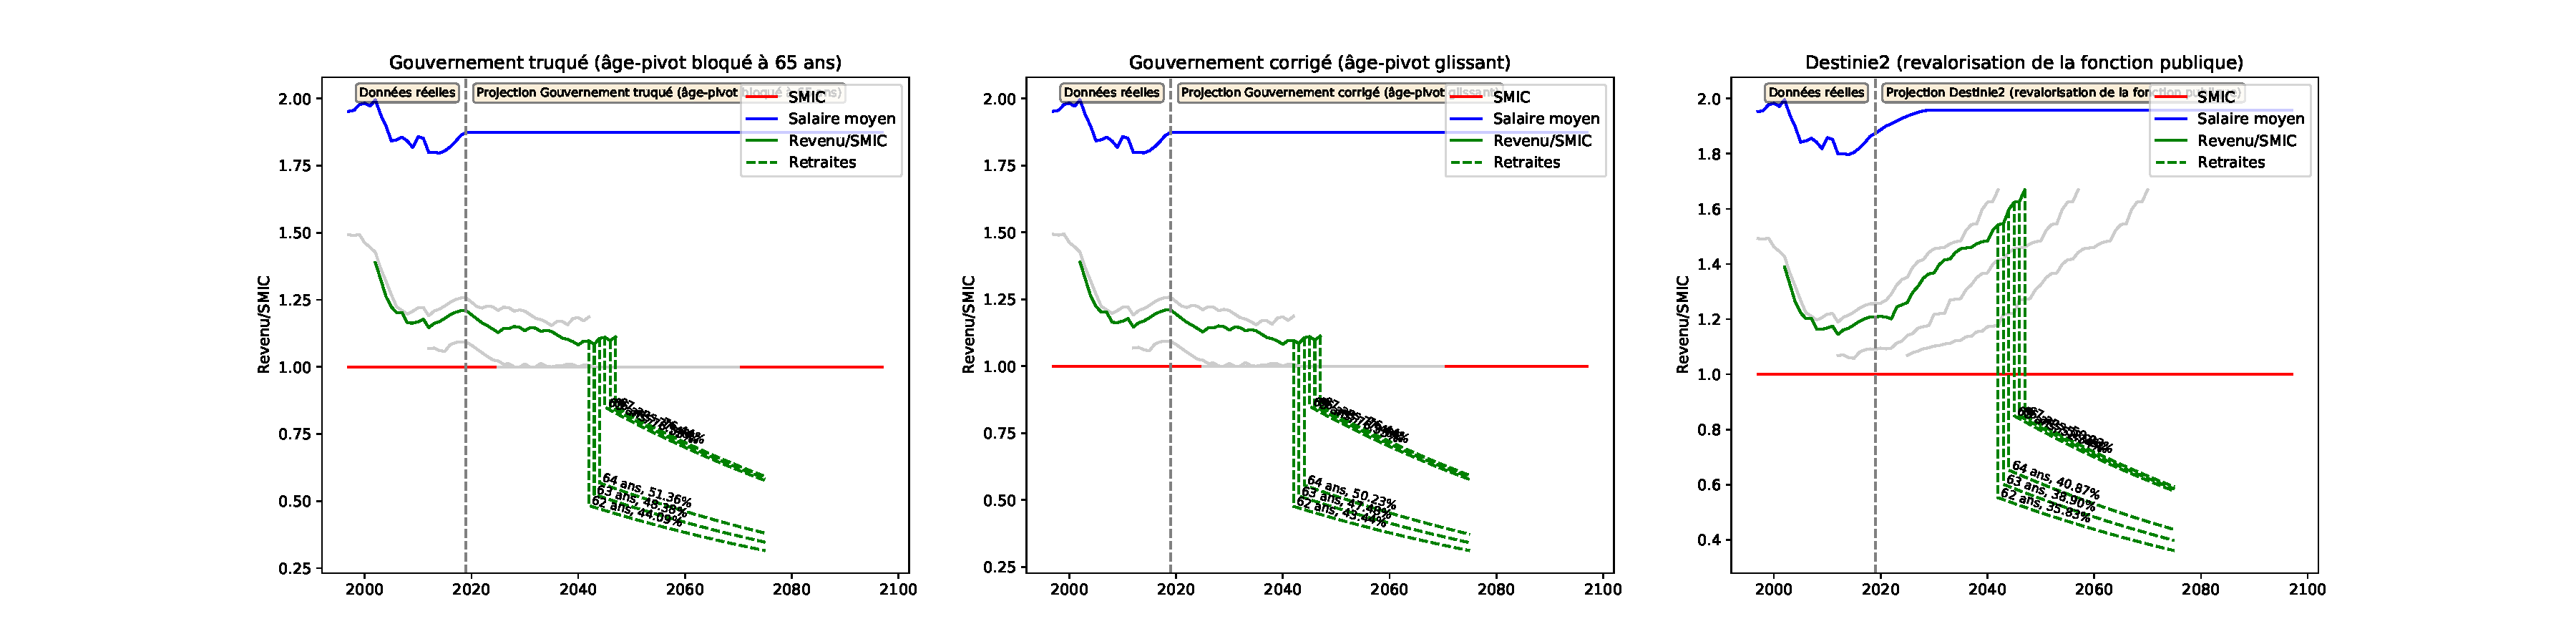
\includegraphics[width=0.9\textwidth]{fig/AdjTech_1980_22_dest_retraite.pdf}\end{center} \label{fig/AdjTech_1980_22_dest_retraite.pdf} 

\newpage 
 
\paragraph{Revenus et points pour le modèle \emph{Gouvernement truqué (âge-pivot bloqué à 65 ans)}} 
 
{ \scriptsize \begin{center} 
\begin{tabular}[htb]{|c|c||c|c|c|c|c|c||c|c||c|c|c|} 
\hline 
 Année &  Âge &  Ind Maj &  Pt Ind(\euro{} 2019) &  Rev HP(\euro{} 2019) &  Tx Primes &  GIPA(\euro{} 2019) &  Revenu(\euro{} 2019) &  SMIC(\euro{} 2019) &  Rev/SMIC &  Cumul Pts &  Achat Pt(\euro{} 2019) &  Serv. Pt(\euro{} 2019) \\ 
\hline \hline 
 2002 &  22 &  326.0 &  5.49 &  1788.53 &  12.41 &  0.00 &  2010.48 &  1447.74 &  {\bf 1.39} &  677.56 &  35.61 &  0.50 \\ 
\hline 
 2003 &  23 &  327.0 &  5.37 &  1757.50 &  12.64 &  0.00 &  1979.65 &  1493.03 &  {\bf 1.33} &  1344.72 &  35.61 &  0.50 \\ 
\hline 
 2004 &  24 &  327.0 &  5.29 &  1729.74 &  12.87 &  0.00 &  1952.36 &  1547.32 &  {\bf 1.26} &  2002.69 &  35.61 &  0.50 \\ 
\hline 
 2005 &  25 &  328.0 &  5.29 &  1734.84 &  13.10 &  0.00 &  1962.10 &  1603.67 &  {\bf 1.22} &  2663.94 &  35.61 &  0.50 \\ 
\hline 
 2006 &  26 &  328.0 &  5.23 &  1715.48 &  13.33 &  8.46 &  1952.61 &  1625.00 &  {\bf 1.20} &  3322.00 &  35.61 &  0.50 \\ 
\hline 
 2007 &  27 &  329.0 &  5.19 &  1708.98 &  13.56 &  24.35 &  1965.07 &  1634.08 &  {\bf 1.20} &  3984.25 &  35.61 &  0.50 \\ 
\hline 
 2008 &  28 &  329.0 &  5.09 &  1675.61 &  13.79 &  3.01 &  1909.69 &  1640.24 &  {\bf 1.16} &  4627.84 &  35.61 &  0.50 \\ 
\hline 
 2009 &  29 &  330.0 &  5.13 &  1692.61 &  14.02 &  0.00 &  1929.92 &  1659.42 &  {\bf 1.16} &  5278.24 &  35.61 &  0.50 \\ 
\hline 
 2010 &  30 &  330.0 &  5.08 &  1675.52 &  14.25 &  3.92 &  1918.20 &  1641.90 &  {\bf 1.17} &  5924.70 &  35.61 &  0.50 \\ 
\hline 
 2011 &  31 &  332.0 &  4.97 &  1650.65 &  14.48 &  33.25 &  1922.92 &  1633.19 &  {\bf 1.18} &  6572.75 &  35.61 &  0.50 \\ 
\hline 
 2012 &  32 &  332.0 &  4.88 &  1618.98 &  14.71 &  61.32 &  1918.44 &  1673.05 &  {\bf 1.15} &  7219.29 &  35.61 &  0.50 \\ 
\hline 
 2013 &  33 &  335.0 &  4.83 &  1619.61 &  14.94 &  72.27 &  1933.85 &  1664.01 &  {\bf 1.16} &  7871.02 &  35.61 &  0.50 \\ 
\hline 
 2014 &  34 &  335.0 &  4.81 &  1611.50 &  15.17 &  100.29 &  1956.25 &  1673.24 &  {\bf 1.17} &  8530.30 &  35.61 &  0.50 \\ 
\hline 
 2015 &  35 &  339.0 &  4.81 &  1630.11 &  15.40 &  110.67 &  1991.81 &  1686.62 &  {\bf 1.18} &  9201.57 &  35.61 &  0.50 \\ 
\hline 
 2016 &  36 &  339.0 &  4.80 &  1626.85 &  15.63 &  141.09 &  2022.22 &  1693.76 &  {\bf 1.19} &  9883.08 &  35.61 &  0.50 \\ 
\hline 
 2017 &  37 &  343.0 &  4.81 &  1649.37 &  15.86 &  125.92 &  2036.88 &  1692.60 &  {\bf 1.20} &  10569.53 &  35.61 &  0.50 \\ 
\hline 
 2018 &  38 &  343.0 &  4.74 &  1626.59 &  16.09 &  155.53 &  2043.84 &  1689.76 &  {\bf 1.21} &  11258.33 &  35.61 &  0.50 \\ 
\hline 
 2019 &  39 &  343.0 &  4.79 &  1644.49 &  16.32 &  142.42 &  2055.29 &  1698.45 &  {\bf 1.21} &  11950.99 &  35.61 &  0.50 \\ 
\hline 
 2020 &  40 &  354.0 &  4.79 &  1697.23 &  16.55 &  77.04 &  2055.16 &  1720.53 &  {\bf 1.19} &  12643.60 &  35.61 &  0.50 \\ 
\hline 
 2021 &  41 &  354.0 &  4.79 &  1697.23 &  16.78 &  73.08 &  2055.10 &  1742.90 &  {\bf 1.18} &  13336.20 &  35.61 &  0.50 \\ 
\hline 
 2022 &  42 &  354.0 &  4.79 &  1697.23 &  17.01 &  69.20 &  2055.12 &  1765.55 &  {\bf 1.16} &  14028.80 &  35.61 &  0.50 \\ 
\hline 
 2023 &  43 &  367.0 &  4.79 &  1759.55 &  17.24 &  0.00 &  2062.90 &  1788.51 &  {\bf 1.15} &  14724.02 &  35.61 &  0.50 \\ 
\hline 
 2024 &  44 &  367.0 &  4.79 &  1759.55 &  17.47 &  0.00 &  2066.95 &  1811.76 &  {\bf 1.14} &  15420.61 &  35.61 &  0.50 \\ 
\hline 
 2025 &  45 &  367.0 &  4.79 &  1759.55 &  17.70 &  0.00 &  2070.99 &  1835.31 &  {\bf 1.13} &  16118.56 &  35.61 &  0.50 \\ 
\hline 
 2026 &  46 &  375.7 &  4.79 &  1801.31 &  17.93 &  0.00 &  2124.29 &  1859.17 &  {\bf 1.14} &  16834.47 &  35.61 &  0.50 \\ 
\hline 
 2027 &  47 &  380.0 &  4.79 &  1821.88 &  18.16 &  0.00 &  2152.73 &  1883.34 &  {\bf 1.14} &  17559.97 &  35.61 &  0.50 \\ 
\hline 
 2028 &  48 &  386.7 &  4.79 &  1854.00 &  18.39 &  0.00 &  2194.95 &  1907.82 &  {\bf 1.15} &  18299.69 &  35.61 &  0.50 \\ 
\hline 
 2029 &  49 &  390.0 &  4.79 &  1869.82 &  18.62 &  0.00 &  2217.99 &  1932.62 &  {\bf 1.15} &  19046.61 &  35.63 &  0.50 \\ 
\hline 
 2030 &  50 &  390.0 &  4.79 &  1869.82 &  18.85 &  0.00 &  2222.29 &  1957.75 &  {\bf 1.14} &  19793.84 &  35.69 &  0.50 \\ 
\hline 
 2031 &  51 &  398.0 &  4.79 &  1908.37 &  19.08 &  0.00 &  2272.49 &  1983.20 &  {\bf 1.15} &  20556.22 &  35.77 &  0.50 \\ 
\hline 
 2032 &  52 &  402.0 &  4.79 &  1927.36 &  19.31 &  0.00 &  2299.53 &  2008.98 &  {\bf 1.14} &  21325.32 &  35.88 &  0.50 \\ 
\hline 
 2033 &  53 &  402.0 &  4.79 &  1927.36 &  19.54 &  0.00 &  2303.96 &  2035.10 &  {\bf 1.13} &  22092.99 &  36.02 &  0.50 \\ 
\hline 
 2034 &  54 &  408.0 &  4.79 &  1956.27 &  19.77 &  0.00 &  2343.02 &  2061.55 &  {\bf 1.14} &  22870.12 &  36.18 &  0.50 \\ 
\hline 
 2035 &  55 &  411.0 &  4.79 &  1970.51 &  20.00 &  0.00 &  2364.61 &  2088.35 &  {\bf 1.13} &  23650.24 &  36.37 &  0.51 \\ 
\hline 
 2036 &  56 &  411.0 &  4.79 &  1970.51 &  20.23 &  0.00 &  2369.14 &  2115.50 &  {\bf 1.12} &  24427.13 &  36.59 &  0.51 \\ 
\hline 
 2037 &  57 &  411.0 &  4.79 &  1970.51 &  20.46 &  0.00 &  2373.67 &  2143.00 &  {\bf 1.11} &  25200.20 &  36.85 &  0.51 \\ 
\hline 
 2038 &  58 &  413.7 &  4.79 &  1983.36 &  20.69 &  0.00 &  2393.71 &  2170.86 &  {\bf 1.10} &  25973.89 &  37.13 &  0.52 \\ 
\hline 
 2039 &  59 &  415.0 &  4.79 &  1989.69 &  20.92 &  0.00 &  2405.93 &  2199.08 &  {\bf 1.09} &  26745.06 &  37.44 &  0.52 \\ 
\hline 
 2040 &  60 &  415.0 &  4.79 &  1989.69 &  21.15 &  0.00 &  2410.50 &  2227.67 &  {\bf 1.08} &  27510.69 &  37.78 &  0.53 \\ 
\hline 
 2041 &  61 &  425.0 &  4.79 &  2037.87 &  21.38 &  0.00 &  2473.57 &  2256.63 &  {\bf 1.10} &  28288.62 &  38.16 &  0.53 \\ 
\hline 
 2042 &  62 &  430.0 &  4.79 &  2061.60 &  21.61 &  0.00 &  2507.11 &  2285.97 &  {\bf 1.10} &  29068.76 &  38.56 &  0.54 \\ 
\hline 
 2043 &  63 &  430.0 &  4.79 &  2061.60 &  21.84 &  0.00 &  2511.86 &  2315.68 &  {\bf 1.08} &  29841.52 &  39.01 &  0.54 \\ 
\hline 
 2044 &  64 &  443.4 &  4.79 &  2125.85 &  22.07 &  0.00 &  2595.02 &  2345.79 &  {\bf 1.11} &  30630.22 &  39.48 &  0.55 \\ 
\hline 
 2045 &  65 &  450.0 &  4.79 &  2157.49 &  22.30 &  0.00 &  2638.61 &  2376.28 &  {\bf 1.11} &  31421.87 &  40.00 &  0.56 \\ 
\hline 
 2046 &  66 &  450.0 &  4.79 &  2157.49 &  22.53 &  0.00 &  2643.57 &  2407.18 &  {\bf 1.10} &  32204.84 &  40.52 &  0.56 \\ 
\hline 
 2047 &  67 &  460.7 &  4.79 &  2208.89 &  22.76 &  0.00 &  2711.63 &  2438.47 &  {\bf 1.11} &  32997.65 &  41.04 &  0.57 \\ 
\hline 
\hline 
\end{tabular} 
\end{center} } 
\newpage 
 
\paragraph{Revenus et points pour le modèle \emph{Gouvernement corrigé (âge-pivot glissant)}} 
 
{ \scriptsize \begin{center} 
\begin{tabular}[htb]{|c|c||c|c|c|c|c|c||c|c||c|c|c|} 
\hline 
 Année &  Âge &  Ind Maj &  Pt Ind(\euro{} 2019) &  Rev HP(\euro{} 2019) &  Tx Primes &  GIPA(\euro{} 2019) &  Revenu(\euro{} 2019) &  SMIC(\euro{} 2019) &  Rev/SMIC &  Cumul Pts &  Achat Pt(\euro{} 2019) &  Serv. Pt(\euro{} 2019) \\ 
\hline \hline 
 2002 &  22 &  326.0 &  5.49 &  1788.53 &  12.41 &  0.00 &  2010.48 &  1447.74 &  {\bf 1.39} &  677.56 &  35.61 &  0.50 \\ 
\hline 
 2003 &  23 &  327.0 &  5.37 &  1757.50 &  12.64 &  0.00 &  1979.65 &  1493.03 &  {\bf 1.33} &  1344.72 &  35.61 &  0.50 \\ 
\hline 
 2004 &  24 &  327.0 &  5.29 &  1729.74 &  12.87 &  0.00 &  1952.36 &  1547.32 &  {\bf 1.26} &  2002.69 &  35.61 &  0.50 \\ 
\hline 
 2005 &  25 &  328.0 &  5.29 &  1734.84 &  13.10 &  0.00 &  1962.10 &  1603.67 &  {\bf 1.22} &  2663.94 &  35.61 &  0.50 \\ 
\hline 
 2006 &  26 &  328.0 &  5.23 &  1715.48 &  13.33 &  8.46 &  1952.61 &  1625.00 &  {\bf 1.20} &  3322.00 &  35.61 &  0.50 \\ 
\hline 
 2007 &  27 &  329.0 &  5.19 &  1708.98 &  13.56 &  24.35 &  1965.07 &  1634.08 &  {\bf 1.20} &  3984.25 &  35.61 &  0.50 \\ 
\hline 
 2008 &  28 &  329.0 &  5.09 &  1675.61 &  13.79 &  3.01 &  1909.69 &  1640.24 &  {\bf 1.16} &  4627.84 &  35.61 &  0.50 \\ 
\hline 
 2009 &  29 &  330.0 &  5.13 &  1692.61 &  14.02 &  0.00 &  1929.92 &  1659.42 &  {\bf 1.16} &  5278.24 &  35.61 &  0.50 \\ 
\hline 
 2010 &  30 &  330.0 &  5.08 &  1675.52 &  14.25 &  3.92 &  1918.20 &  1641.90 &  {\bf 1.17} &  5924.70 &  35.61 &  0.50 \\ 
\hline 
 2011 &  31 &  332.0 &  4.97 &  1650.65 &  14.48 &  33.25 &  1922.92 &  1633.19 &  {\bf 1.18} &  6572.75 &  35.61 &  0.50 \\ 
\hline 
 2012 &  32 &  332.0 &  4.88 &  1618.98 &  14.71 &  61.32 &  1918.44 &  1673.05 &  {\bf 1.15} &  7219.29 &  35.61 &  0.50 \\ 
\hline 
 2013 &  33 &  335.0 &  4.83 &  1619.61 &  14.94 &  72.27 &  1933.85 &  1664.01 &  {\bf 1.16} &  7871.02 &  35.61 &  0.50 \\ 
\hline 
 2014 &  34 &  335.0 &  4.81 &  1611.50 &  15.17 &  100.29 &  1956.25 &  1673.24 &  {\bf 1.17} &  8530.30 &  35.61 &  0.50 \\ 
\hline 
 2015 &  35 &  339.0 &  4.81 &  1630.11 &  15.40 &  110.67 &  1991.81 &  1686.62 &  {\bf 1.18} &  9201.57 &  35.61 &  0.50 \\ 
\hline 
 2016 &  36 &  339.0 &  4.80 &  1626.85 &  15.63 &  141.09 &  2022.22 &  1693.76 &  {\bf 1.19} &  9883.08 &  35.61 &  0.50 \\ 
\hline 
 2017 &  37 &  343.0 &  4.81 &  1649.37 &  15.86 &  125.92 &  2036.88 &  1692.60 &  {\bf 1.20} &  10569.53 &  35.61 &  0.50 \\ 
\hline 
 2018 &  38 &  343.0 &  4.74 &  1626.59 &  16.09 &  155.53 &  2043.84 &  1689.76 &  {\bf 1.21} &  11258.33 &  35.61 &  0.50 \\ 
\hline 
 2019 &  39 &  343.0 &  4.79 &  1644.49 &  16.32 &  142.42 &  2055.29 &  1698.45 &  {\bf 1.21} &  11950.99 &  35.61 &  0.50 \\ 
\hline 
 2020 &  40 &  354.0 &  4.79 &  1697.23 &  16.55 &  77.04 &  2055.16 &  1720.53 &  {\bf 1.19} &  12643.60 &  35.61 &  0.50 \\ 
\hline 
 2021 &  41 &  354.0 &  4.79 &  1697.23 &  16.78 &  73.08 &  2055.10 &  1742.90 &  {\bf 1.18} &  13336.20 &  35.61 &  0.50 \\ 
\hline 
 2022 &  42 &  354.0 &  4.79 &  1697.23 &  17.01 &  69.20 &  2055.12 &  1765.55 &  {\bf 1.16} &  14028.80 &  35.61 &  0.50 \\ 
\hline 
 2023 &  43 &  367.0 &  4.79 &  1759.55 &  17.24 &  0.00 &  2062.90 &  1788.51 &  {\bf 1.15} &  14724.02 &  35.61 &  0.50 \\ 
\hline 
 2024 &  44 &  367.0 &  4.79 &  1759.55 &  17.47 &  0.00 &  2066.95 &  1811.76 &  {\bf 1.14} &  15420.61 &  35.61 &  0.50 \\ 
\hline 
 2025 &  45 &  367.0 &  4.79 &  1759.55 &  17.70 &  0.00 &  2070.99 &  1835.31 &  {\bf 1.13} &  16118.56 &  35.61 &  0.50 \\ 
\hline 
 2026 &  46 &  375.7 &  4.79 &  1801.31 &  17.93 &  0.00 &  2124.29 &  1859.17 &  {\bf 1.14} &  16834.47 &  35.61 &  0.50 \\ 
\hline 
 2027 &  47 &  380.0 &  4.79 &  1821.88 &  18.16 &  0.00 &  2152.73 &  1883.34 &  {\bf 1.14} &  17559.97 &  35.61 &  0.50 \\ 
\hline 
 2028 &  48 &  386.7 &  4.79 &  1854.00 &  18.39 &  0.00 &  2194.95 &  1907.82 &  {\bf 1.15} &  18299.69 &  35.61 &  0.50 \\ 
\hline 
 2029 &  49 &  390.0 &  4.79 &  1869.82 &  18.62 &  0.00 &  2217.99 &  1932.62 &  {\bf 1.15} &  19046.61 &  35.63 &  0.50 \\ 
\hline 
 2030 &  50 &  390.0 &  4.79 &  1869.82 &  18.85 &  0.00 &  2222.29 &  1957.75 &  {\bf 1.14} &  19793.84 &  35.69 &  0.50 \\ 
\hline 
 2031 &  51 &  398.0 &  4.79 &  1908.37 &  19.08 &  0.00 &  2272.49 &  1983.20 &  {\bf 1.15} &  20556.22 &  35.77 &  0.50 \\ 
\hline 
 2032 &  52 &  402.0 &  4.79 &  1927.36 &  19.31 &  0.00 &  2299.53 &  2008.98 &  {\bf 1.14} &  21325.32 &  35.88 &  0.50 \\ 
\hline 
 2033 &  53 &  402.0 &  4.79 &  1927.36 &  19.54 &  0.00 &  2303.96 &  2035.10 &  {\bf 1.13} &  22092.99 &  36.02 &  0.50 \\ 
\hline 
 2034 &  54 &  408.0 &  4.79 &  1956.27 &  19.77 &  0.00 &  2343.02 &  2061.55 &  {\bf 1.14} &  22870.12 &  36.18 &  0.50 \\ 
\hline 
 2035 &  55 &  411.0 &  4.79 &  1970.51 &  20.00 &  0.00 &  2364.61 &  2088.35 &  {\bf 1.13} &  23650.24 &  36.37 &  0.51 \\ 
\hline 
 2036 &  56 &  411.0 &  4.79 &  1970.51 &  20.23 &  0.00 &  2369.14 &  2115.50 &  {\bf 1.12} &  24427.13 &  36.59 &  0.51 \\ 
\hline 
 2037 &  57 &  411.0 &  4.79 &  1970.51 &  20.46 &  0.00 &  2373.67 &  2143.00 &  {\bf 1.11} &  25200.20 &  36.85 &  0.51 \\ 
\hline 
 2038 &  58 &  413.7 &  4.79 &  1983.36 &  20.69 &  0.00 &  2393.71 &  2170.86 &  {\bf 1.10} &  25973.89 &  37.13 &  0.52 \\ 
\hline 
 2039 &  59 &  415.0 &  4.79 &  1989.69 &  20.92 &  0.00 &  2405.93 &  2199.08 &  {\bf 1.09} &  26745.06 &  37.44 &  0.52 \\ 
\hline 
 2040 &  60 &  415.0 &  4.79 &  1989.69 &  21.15 &  0.00 &  2410.50 &  2227.67 &  {\bf 1.08} &  27510.69 &  37.78 &  0.53 \\ 
\hline 
 2041 &  61 &  425.0 &  4.79 &  2037.87 &  21.38 &  0.00 &  2473.57 &  2256.63 &  {\bf 1.10} &  28288.62 &  38.16 &  0.53 \\ 
\hline 
 2042 &  62 &  430.0 &  4.79 &  2061.60 &  21.61 &  0.00 &  2507.11 &  2285.97 &  {\bf 1.10} &  29068.76 &  38.56 &  0.54 \\ 
\hline 
 2043 &  63 &  430.0 &  4.79 &  2061.60 &  21.84 &  0.00 &  2511.86 &  2315.68 &  {\bf 1.08} &  29841.52 &  39.01 &  0.54 \\ 
\hline 
 2044 &  64 &  443.4 &  4.79 &  2125.85 &  22.07 &  0.00 &  2595.02 &  2345.79 &  {\bf 1.11} &  30630.22 &  39.48 &  0.55 \\ 
\hline 
 2045 &  65 &  450.0 &  4.79 &  2157.49 &  22.30 &  0.00 &  2638.61 &  2376.28 &  {\bf 1.11} &  31421.87 &  40.00 &  0.56 \\ 
\hline 
 2046 &  66 &  450.0 &  4.79 &  2157.49 &  22.53 &  0.00 &  2643.57 &  2407.18 &  {\bf 1.10} &  32204.84 &  40.52 &  0.56 \\ 
\hline 
 2047 &  67 &  460.7 &  4.79 &  2208.89 &  22.76 &  0.00 &  2711.63 &  2438.47 &  {\bf 1.11} &  32997.65 &  41.04 &  0.57 \\ 
\hline 
\hline 
\end{tabular} 
\end{center} } 
\newpage 
 
\paragraph{Revenus et points pour le modèle \emph{Destinie2 (revalorisation de la fonction publique)}} 
 
{ \scriptsize \begin{center} 
\begin{tabular}[htb]{|c|c||c|c|c|c|c|c||c|c||c|c|c|} 
\hline 
 Année &  Âge &  Ind Maj &  Pt Ind(\euro{} 2019) &  Rev HP(\euro{} 2019) &  Tx Primes &  GIPA(\euro{} 2019) &  Revenu(\euro{} 2019) &  SMIC(\euro{} 2019) &  Rev/SMIC &  Cumul Pts &  Achat Pt(\euro{} 2019) &  Serv. Pt(\euro{} 2019) \\ 
\hline \hline 
 2002 &  22 &  326.0 &  5.49 &  1788.53 &  12.41 &  0.00 &  2010.48 &  1447.74 &  {\bf 1.39} &  675.89 &  35.69 &  0.50 \\ 
\hline 
 2003 &  23 &  327.0 &  5.37 &  1757.50 &  12.64 &  0.00 &  1979.65 &  1493.03 &  {\bf 1.33} &  1341.42 &  35.69 &  0.50 \\ 
\hline 
 2004 &  24 &  327.0 &  5.29 &  1729.74 &  12.87 &  0.00 &  1952.36 &  1547.32 &  {\bf 1.26} &  1997.77 &  35.69 &  0.50 \\ 
\hline 
 2005 &  25 &  328.0 &  5.29 &  1734.84 &  13.10 &  0.00 &  1962.10 &  1603.67 &  {\bf 1.22} &  2657.40 &  35.69 &  0.50 \\ 
\hline 
 2006 &  26 &  328.0 &  5.23 &  1715.48 &  13.33 &  8.46 &  1952.61 &  1625.00 &  {\bf 1.20} &  3313.83 &  35.69 &  0.50 \\ 
\hline 
 2007 &  27 &  329.0 &  5.19 &  1708.98 &  13.56 &  24.35 &  1965.07 &  1634.08 &  {\bf 1.20} &  3974.46 &  35.69 &  0.50 \\ 
\hline 
 2008 &  28 &  329.0 &  5.09 &  1675.61 &  13.79 &  3.01 &  1909.69 &  1640.24 &  {\bf 1.16} &  4616.47 &  35.69 &  0.50 \\ 
\hline 
 2009 &  29 &  330.0 &  5.13 &  1692.61 &  14.02 &  0.00 &  1929.92 &  1659.42 &  {\bf 1.16} &  5265.28 &  35.69 &  0.50 \\ 
\hline 
 2010 &  30 &  330.0 &  5.08 &  1675.52 &  14.25 &  3.92 &  1918.20 &  1641.90 &  {\bf 1.17} &  5910.14 &  35.69 &  0.50 \\ 
\hline 
 2011 &  31 &  332.0 &  4.97 &  1650.65 &  14.48 &  28.53 &  1918.19 &  1633.19 &  {\bf 1.17} &  6555.01 &  35.69 &  0.50 \\ 
\hline 
 2012 &  32 &  332.0 &  4.88 &  1618.98 &  14.71 &  57.77 &  1914.90 &  1673.05 &  {\bf 1.14} &  7198.77 &  35.69 &  0.50 \\ 
\hline 
 2013 &  33 &  335.0 &  4.83 &  1619.61 &  14.94 &  70.19 &  1931.77 &  1664.01 &  {\bf 1.16} &  7848.20 &  35.69 &  0.50 \\ 
\hline 
 2014 &  34 &  335.0 &  4.81 &  1611.50 &  15.17 &  97.65 &  1953.62 &  1673.24 &  {\bf 1.17} &  8504.98 &  35.69 &  0.50 \\ 
\hline 
 2015 &  35 &  339.0 &  4.81 &  1630.11 &  15.40 &  107.32 &  1988.46 &  1686.62 &  {\bf 1.18} &  9173.47 &  35.69 &  0.50 \\ 
\hline 
 2016 &  36 &  339.0 &  4.80 &  1626.85 &  15.63 &  138.08 &  2019.21 &  1693.76 &  {\bf 1.19} &  9852.29 &  35.69 &  0.50 \\ 
\hline 
 2017 &  37 &  343.0 &  4.81 &  1649.37 &  15.86 &  123.08 &  2034.03 &  1692.60 &  {\bf 1.20} &  10536.10 &  35.69 &  0.50 \\ 
\hline 
 2018 &  38 &  343.0 &  4.74 &  1626.59 &  16.09 &  152.51 &  2040.82 &  1689.76 &  {\bf 1.21} &  11222.19 &  35.69 &  0.50 \\ 
\hline 
 2019 &  39 &  343.0 &  4.79 &  1644.49 &  16.32 &  139.31 &  2052.18 &  1698.45 &  {\bf 1.21} &  11912.10 &  35.69 &  0.50 \\ 
\hline 
 2020 &  40 &  354.0 &  4.83 &  1710.80 &  16.55 &  63.25 &  2057.19 &  1699.99 &  {\bf 1.21} &  12603.70 &  35.69 &  0.50 \\ 
\hline 
 2021 &  41 &  354.0 &  4.88 &  1726.20 &  16.78 &  41.29 &  2057.15 &  1703.48 &  {\bf 1.21} &  13295.28 &  35.69 &  0.50 \\ 
\hline 
 2022 &  42 &  354.0 &  4.93 &  1743.46 &  17.01 &  17.11 &  2057.14 &  1712.78 &  {\bf 1.20} &  13986.85 &  35.69 &  0.50 \\ 
\hline 
 2023 &  43 &  367.0 &  4.98 &  1828.64 &  17.24 &  0.00 &  2143.89 &  1723.51 &  {\bf 1.24} &  14707.60 &  35.69 &  0.50 \\ 
\hline 
 2024 &  44 &  367.0 &  5.04 &  1850.40 &  17.47 &  0.00 &  2173.66 &  1735.69 &  {\bf 1.25} &  15438.35 &  35.69 &  0.50 \\ 
\hline 
 2025 &  45 &  367.0 &  5.10 &  1872.97 &  17.70 &  0.00 &  2204.49 &  1749.35 &  {\bf 1.26} &  16179.46 &  35.69 &  0.50 \\ 
\hline 
 2026 &  46 &  375.7 &  5.17 &  1941.39 &  17.93 &  0.00 &  2289.48 &  1764.53 &  {\bf 1.30} &  16949.15 &  35.69 &  0.50 \\ 
\hline 
 2027 &  47 &  380.0 &  5.23 &  1988.69 &  18.16 &  0.00 &  2349.84 &  1781.27 &  {\bf 1.32} &  17739.13 &  35.69 &  0.50 \\ 
\hline 
 2028 &  48 &  386.7 &  5.30 &  2050.27 &  18.39 &  0.00 &  2427.31 &  1799.59 &  {\bf 1.35} &  18555.15 &  35.69 &  0.50 \\ 
\hline 
 2029 &  49 &  390.0 &  5.37 &  2092.78 &  18.62 &  0.00 &  2482.46 &  1819.55 &  {\bf 1.36} &  19389.12 &  35.72 &  0.50 \\ 
\hline 
 2030 &  50 &  390.0 &  5.43 &  2118.73 &  18.85 &  0.00 &  2518.11 &  1841.19 &  {\bf 1.37} &  20233.85 &  35.77 &  0.50 \\ 
\hline 
 2031 &  51 &  398.0 &  5.50 &  2189.87 &  19.08 &  0.00 &  2607.70 &  1864.58 &  {\bf 1.40} &  21106.68 &  35.85 &  0.50 \\ 
\hline 
 2032 &  52 &  402.0 &  5.57 &  2240.41 &  19.31 &  0.00 &  2673.04 &  1888.81 &  {\bf 1.42} &  21998.67 &  35.96 &  0.50 \\ 
\hline 
 2033 &  53 &  402.0 &  5.65 &  2269.54 &  19.54 &  0.00 &  2713.01 &  1913.37 &  {\bf 1.42} &  22900.56 &  36.10 &  0.50 \\ 
\hline 
 2034 &  54 &  408.0 &  5.72 &  2333.53 &  19.77 &  0.00 &  2794.87 &  1938.24 &  {\bf 1.44} &  23825.44 &  36.26 &  0.50 \\ 
\hline 
 2035 &  55 &  411.0 &  5.79 &  2381.07 &  20.00 &  0.00 &  2857.28 &  1963.44 &  {\bf 1.46} &  24765.95 &  36.46 &  0.51 \\ 
\hline 
 2036 &  56 &  411.0 &  5.87 &  2412.02 &  20.23 &  0.00 &  2899.98 &  1988.96 &  {\bf 1.46} &  25714.74 &  36.68 &  0.51 \\ 
\hline 
 2037 &  57 &  411.0 &  5.94 &  2443.38 &  20.46 &  0.00 &  2943.29 &  2014.82 &  {\bf 1.46} &  26671.14 &  36.93 &  0.51 \\ 
\hline 
 2038 &  58 &  413.7 &  6.02 &  2491.28 &  20.69 &  0.00 &  3006.73 &  2041.01 &  {\bf 1.47} &  27640.75 &  37.21 &  0.52 \\ 
\hline 
 2039 &  59 &  415.0 &  6.10 &  2531.72 &  20.92 &  0.00 &  3061.36 &  2067.55 &  {\bf 1.48} &  28619.77 &  37.52 &  0.52 \\ 
\hline 
 2040 &  60 &  415.0 &  6.18 &  2564.63 &  21.15 &  0.00 &  3107.06 &  2094.43 &  {\bf 1.48} &  29604.38 &  37.87 &  0.53 \\ 
\hline 
 2041 &  61 &  425.0 &  6.26 &  2660.89 &  21.38 &  0.00 &  3229.79 &  2121.65 &  {\bf 1.52} &  30617.82 &  38.24 &  0.53 \\ 
\hline 
 2042 &  62 &  430.0 &  6.34 &  2726.87 &  21.61 &  0.00 &  3316.15 &  2149.23 &  {\bf 1.54} &  31647.35 &  38.65 &  0.54 \\ 
\hline 
 2043 &  63 &  430.0 &  6.42 &  2762.32 &  21.84 &  0.00 &  3365.61 &  2177.17 &  {\bf 1.55} &  32680.40 &  39.10 &  0.54 \\ 
\hline 
 2044 &  64 &  443.4 &  6.51 &  2885.43 &  22.07 &  0.00 &  3522.25 &  2205.48 &  {\bf 1.60} &  33748.47 &  39.57 &  0.55 \\ 
\hline 
 2045 &  65 &  450.0 &  6.59 &  2966.45 &  22.30 &  0.00 &  3627.97 &  2234.15 &  {\bf 1.62} &  34834.47 &  40.09 &  0.56 \\ 
\hline 
 2046 &  66 &  450.0 &  6.68 &  3005.01 &  22.53 &  0.00 &  3682.04 &  2263.19 &  {\bf 1.63} &  35922.52 &  40.61 &  0.57 \\ 
\hline 
 2047 &  67 &  460.7 &  6.76 &  3116.60 &  22.76 &  0.00 &  3825.93 &  2292.61 &  {\bf 1.67} &  37038.57 &  41.14 &  0.57 \\ 
\hline 
\hline 
\end{tabular} 
\end{center} } 
\newpage 
 
\subsection{Génération 1990 (début en 2012)} 

\paragraph{Retraites possibles dans le modèle \emph{Gouvernement truqué (âge-pivot bloqué à 65 ans)}}  
 
{ \scriptsize \begin{center} 
\begin{tabular}[htb]{|c|c||c|c||c|c||c||c|c|c|c|c|c|} 
\hline 
 Retraite en &  Âge &  Âge pivot &  Décote/Surcote &  Retraite (\euro{} 2019) &  Tx Rempl(\%) &  SMIC (\euro{} 2019) &  Retraite/SMIC &  Rev70/SMIC &  Rev75/SMIC &  Rev80/SMIC &  Rev85/SMIC &  Rev90/SMIC \\ 
\hline \hline 
 2052 &  62 &  65 ans 0 mois &  -15.00\% &  1181.65 &  {\bf 45.43} &  2601.14 &  {\bf {\color{red} 0.45}} &  {\bf {\color{red} 0.41}} &  {\bf {\color{red} 0.38}} &  {\bf {\color{red} 0.36}} &  {\bf {\color{red} 0.34}} &  {\bf {\color{red} 0.32}} \\ 
\hline 
 2053 &  63 &  65 ans 0 mois &  -10.00\% &  1300.43 &  {\bf 49.35} &  2634.96 &  {\bf {\color{red} 0.49}} &  {\bf {\color{red} 0.45}} &  {\bf {\color{red} 0.42}} &  {\bf {\color{red} 0.40}} &  {\bf {\color{red} 0.37}} &  {\bf {\color{red} 0.35}} \\ 
\hline 
 2054 &  64 &  65 ans 0 mois &  -5.00\% &  1425.82 &  {\bf 53.42} &  2669.21 &  {\bf {\color{red} 0.53}} &  {\bf {\color{red} 0.49}} &  {\bf {\color{red} 0.46}} &  {\bf {\color{red} 0.43}} &  {\bf {\color{red} 0.41}} &  {\bf {\color{red} 0.38}} \\ 
\hline 
 2055 &  65 &  65 ans 0 mois &  0.00\% &  2298.33 &  {\bf 85.00} &  2703.91 &  {\bf {\color{red} 0.85}} &  {\bf {\color{red} 0.80}} &  {\bf {\color{red} 0.75}} &  {\bf {\color{red} 0.70}} &  {\bf {\color{red} 0.66}} &  {\bf {\color{red} 0.62}} \\ 
\hline 
 2056 &  66 &  65 ans 0 mois &  5.00\% &  2328.20 &  {\bf 85.00} &  2739.06 &  {\bf {\color{red} 0.85}} &  {\bf {\color{red} 0.81}} &  {\bf {\color{red} 0.76}} &  {\bf {\color{red} 0.71}} &  {\bf {\color{red} 0.67}} &  {\bf {\color{red} 0.62}} \\ 
\hline 
 2057 &  67 &  65 ans 0 mois &  10.00\% &  2358.47 &  {\bf 85.00} &  2774.67 &  {\bf {\color{red} 0.85}} &  {\bf {\color{red} 0.82}} &  {\bf {\color{red} 0.77}} &  {\bf {\color{red} 0.72}} &  {\bf {\color{red} 0.67}} &  {\bf {\color{red} 0.63}} \\ 
\hline 
\hline 
\end{tabular} 
\end{center} } 
\paragraph{Retraites possibles dans le modèle \emph{Gouvernement corrigé (âge-pivot glissant)}}  
 
{ \scriptsize \begin{center} 
\begin{tabular}[htb]{|c|c||c|c||c|c||c||c|c|c|c|c|c|} 
\hline 
 Retraite en &  Âge &  Âge pivot &  Décote/Surcote &  Retraite (\euro{} 2019) &  Tx Rempl(\%) &  SMIC (\euro{} 2019) &  Retraite/SMIC &  Rev70/SMIC &  Rev75/SMIC &  Rev80/SMIC &  Rev85/SMIC &  Rev90/SMIC \\ 
\hline \hline 
 2052 &  62 &  66 ans 1 mois &  -20.42\% &  1106.35 &  {\bf 42.53} &  2601.14 &  {\bf {\color{red} 0.43}} &  {\bf {\color{red} 0.38}} &  {\bf {\color{red} 0.36}} &  {\bf {\color{red} 0.34}} &  {\bf {\color{red} 0.32}} &  {\bf {\color{red} 0.30}} \\ 
\hline 
 2053 &  63 &  66 ans 2 mois &  -15.83\% &  1216.15 &  {\bf 46.15} &  2634.96 &  {\bf {\color{red} 0.46}} &  {\bf {\color{red} 0.42}} &  {\bf {\color{red} 0.40}} &  {\bf {\color{red} 0.37}} &  {\bf {\color{red} 0.35}} &  {\bf {\color{red} 0.33}} \\ 
\hline 
 2054 &  64 &  66 ans 3 mois &  -11.25\% &  1332.02 &  {\bf 49.90} &  2669.21 &  {\bf {\color{red} 0.50}} &  {\bf {\color{red} 0.46}} &  {\bf {\color{red} 0.43}} &  {\bf {\color{red} 0.41}} &  {\bf {\color{red} 0.38}} &  {\bf {\color{red} 0.36}} \\ 
\hline 
 2055 &  65 &  66 ans 4 mois &  -6.67\% &  2298.33 &  {\bf 85.00} &  2703.91 &  {\bf {\color{red} 0.85}} &  {\bf {\color{red} 0.80}} &  {\bf {\color{red} 0.75}} &  {\bf {\color{red} 0.70}} &  {\bf {\color{red} 0.66}} &  {\bf {\color{red} 0.62}} \\ 
\hline 
 2056 &  66 &  66 ans 5 mois &  -2.08\% &  2328.20 &  {\bf 85.00} &  2739.06 &  {\bf {\color{red} 0.85}} &  {\bf {\color{red} 0.81}} &  {\bf {\color{red} 0.76}} &  {\bf {\color{red} 0.71}} &  {\bf {\color{red} 0.67}} &  {\bf {\color{red} 0.62}} \\ 
\hline 
 2057 &  67 &  66 ans 6 mois &  2.50\% &  2358.47 &  {\bf 85.00} &  2774.67 &  {\bf {\color{red} 0.85}} &  {\bf {\color{red} 0.82}} &  {\bf {\color{red} 0.77}} &  {\bf {\color{red} 0.72}} &  {\bf {\color{red} 0.67}} &  {\bf {\color{red} 0.63}} \\ 
\hline 
\hline 
\end{tabular} 
\end{center} } 
\paragraph{Retraites possibles dans le modèle \emph{Destinie2 (revalorisation de la fonction publique)}}  
 
{ \scriptsize \begin{center} 
\begin{tabular}[htb]{|c|c||c|c||c|c||c||c|c|c|c|c|c|} 
\hline 
 Retraite en &  Âge &  Âge pivot &  Décote/Surcote &  Retraite (\euro{} 2019) &  Tx Rempl(\%) &  SMIC (\euro{} 2019) &  Retraite/SMIC &  Rev70/SMIC &  Rev75/SMIC &  Rev80/SMIC &  Rev85/SMIC &  Rev90/SMIC \\ 
\hline \hline 
 2052 &  62 &  66 ans 1 mois &  -20.42\% &  1313.03 &  {\bf 34.80} &  2445.56 &  {\bf {\color{red} 0.54}} &  {\bf {\color{red} 0.48}} &  {\bf {\color{red} 0.45}} &  {\bf {\color{red} 0.43}} &  {\bf {\color{red} 0.40}} &  {\bf {\color{red} 0.37}} \\ 
\hline 
 2053 &  63 &  66 ans 2 mois &  -15.83\% &  1451.56 &  {\bf 37.90} &  2477.35 &  {\bf {\color{red} 0.59}} &  {\bf {\color{red} 0.54}} &  {\bf {\color{red} 0.50}} &  {\bf {\color{red} 0.47}} &  {\bf {\color{red} 0.44}} &  {\bf {\color{red} 0.41}} \\ 
\hline 
 2054 &  64 &  66 ans 3 mois &  -11.25\% &  1600.02 &  {\bf 39.92} &  2509.56 &  {\bf {\color{red} 0.64}} &  {\bf {\color{red} 0.59}} &  {\bf {\color{red} 0.55}} &  {\bf {\color{red} 0.52}} &  {\bf {\color{red} 0.49}} &  {\bf {\color{red} 0.46}} \\ 
\hline 
 2055 &  65 &  66 ans 4 mois &  -6.67\% &  2160.85 &  {\bf 52.34} &  2542.18 &  {\bf {\color{red} 0.85}} &  {\bf {\color{red} 0.80}} &  {\bf {\color{red} 0.75}} &  {\bf {\color{red} 0.70}} &  {\bf {\color{red} 0.66}} &  {\bf {\color{red} 0.62}} \\ 
\hline 
 2056 &  66 &  66 ans 5 mois &  -2.08\% &  2188.95 &  {\bf 52.25} &  2575.23 &  {\bf {\color{red} 0.85}} &  {\bf {\color{red} 0.81}} &  {\bf {\color{red} 0.76}} &  {\bf {\color{red} 0.71}} &  {\bf {\color{red} 0.67}} &  {\bf {\color{red} 0.62}} \\ 
\hline 
 2057 &  67 &  66 ans 6 mois &  2.50\% &  2217.40 &  {\bf 50.93} &  2608.71 &  {\bf {\color{red} 0.85}} &  {\bf {\color{red} 0.82}} &  {\bf {\color{red} 0.77}} &  {\bf {\color{red} 0.72}} &  {\bf {\color{red} 0.67}} &  {\bf {\color{red} 0.63}} \\ 
\hline 
\hline 
\end{tabular} 
\end{center} } 

 \begin{center}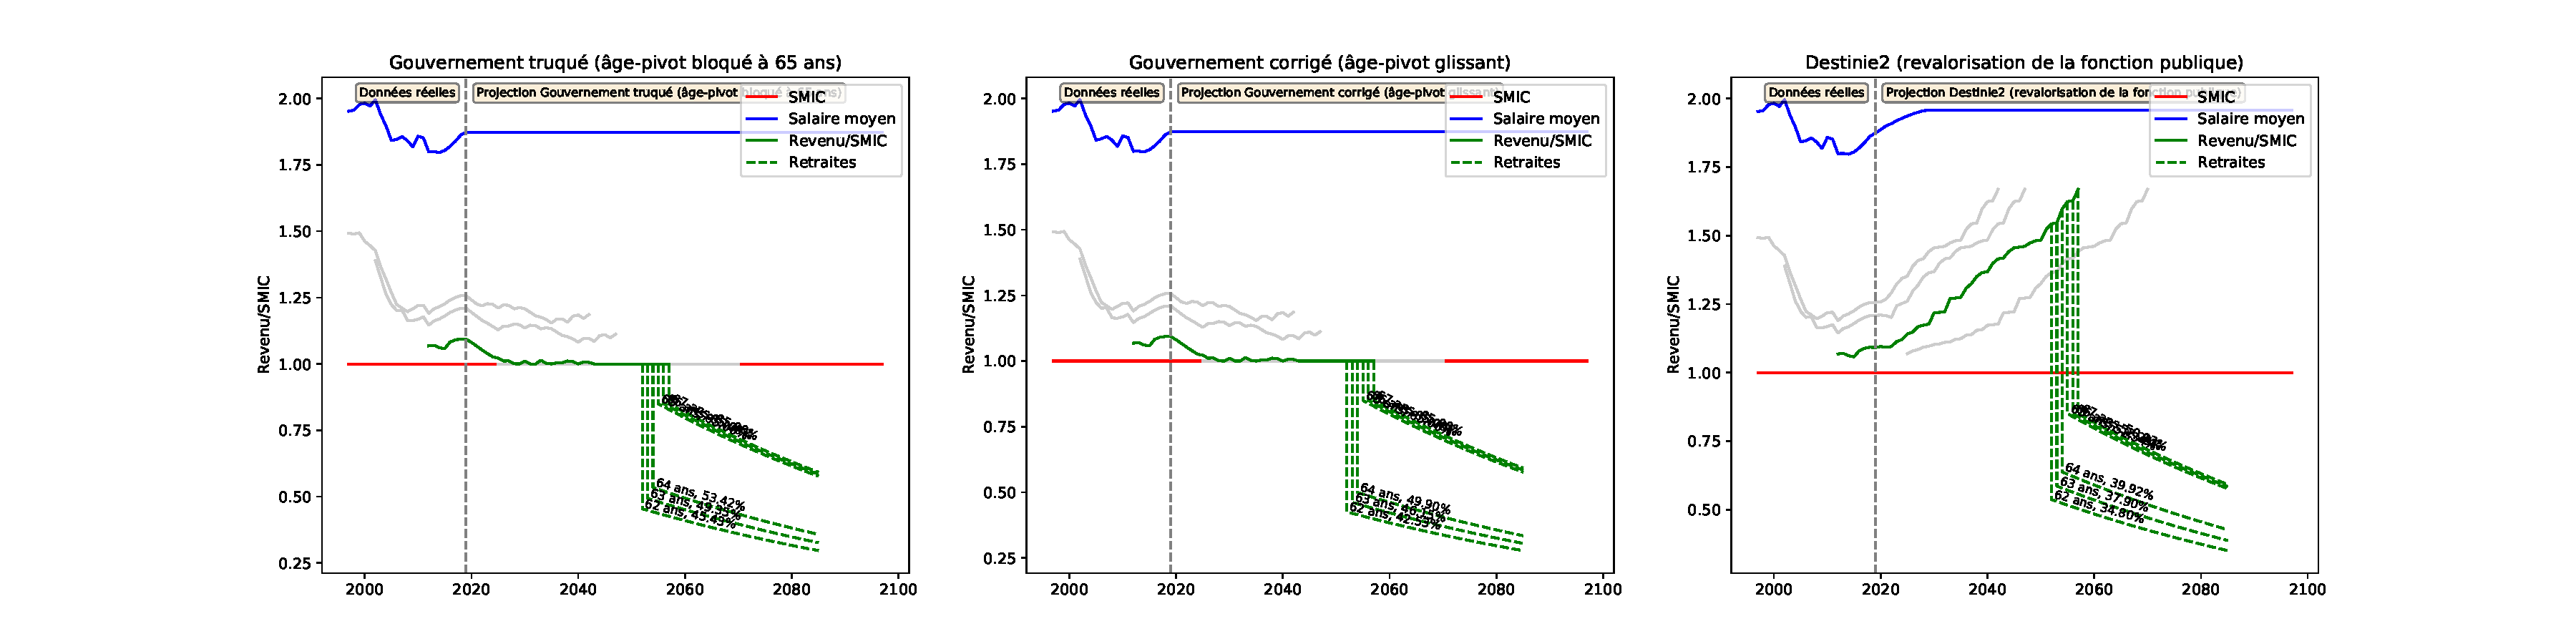
\includegraphics[width=0.9\textwidth]{fig/AdjTech_1990_22_dest_retraite.pdf}\end{center} \label{fig/AdjTech_1990_22_dest_retraite.pdf} 

\newpage 
 
\paragraph{Revenus et points pour le modèle \emph{Gouvernement truqué (âge-pivot bloqué à 65 ans)}} 
 
{ \scriptsize \begin{center} 
\begin{tabular}[htb]{|c|c||c|c|c|c|c|c||c|c||c|c|c|} 
\hline 
 Année &  Âge &  Ind Maj &  Pt Ind(\euro{} 2019) &  Rev HP(\euro{} 2019) &  Tx Primes &  GIPA(\euro{} 2019) &  Revenu(\euro{} 2019) &  SMIC(\euro{} 2019) &  Rev/SMIC &  Cumul Pts &  Achat Pt(\euro{} 2019) &  Serv. Pt(\euro{} 2019) \\ 
\hline \hline 
 2012 &  22 &  326.0 &  4.88 &  1589.72 &  12.41 &  0.00 &  1787.00 &  1673.05 &  {\bf 1.07} &  602.24 &  35.61 &  0.50 \\ 
\hline 
 2013 &  23 &  327.0 &  4.83 &  1580.93 &  12.64 &  0.00 &  1780.76 &  1664.01 &  {\bf 1.07} &  1202.38 &  35.61 &  0.50 \\ 
\hline 
 2014 &  24 &  327.0 &  4.81 &  1573.02 &  12.87 &  0.00 &  1775.46 &  1673.24 &  {\bf 1.06} &  1800.73 &  35.61 &  0.50 \\ 
\hline 
 2015 &  25 &  328.0 &  4.81 &  1577.21 &  13.10 &  0.00 &  1783.83 &  1686.62 &  {\bf 1.06} &  2401.90 &  35.61 &  0.50 \\ 
\hline 
 2016 &  26 &  328.0 &  4.80 &  1574.06 &  13.33 &  49.98 &  1833.87 &  1693.76 &  {\bf 1.08} &  3019.94 &  35.61 &  0.50 \\ 
\hline 
 2017 &  27 &  329.0 &  4.81 &  1582.05 &  13.56 &  49.80 &  1846.37 &  1692.60 &  {\bf 1.09} &  3642.19 &  35.61 &  0.50 \\ 
\hline 
 2018 &  28 &  329.0 &  4.74 &  1560.20 &  13.79 &  72.53 &  1847.88 &  1689.76 &  {\bf 1.09} &  4264.95 &  35.61 &  0.50 \\ 
\hline 
 2019 &  29 &  330.0 &  4.79 &  1582.16 &  14.02 &  52.47 &  1856.45 &  1698.45 &  {\bf 1.09} &  4890.59 &  35.61 &  0.50 \\ 
\hline 
 2020 &  30 &  330.0 &  4.79 &  1582.16 &  14.25 &  52.66 &  1860.28 &  1720.53 &  {\bf 1.08} &  5517.53 &  35.61 &  0.50 \\ 
\hline 
 2021 &  31 &  332.0 &  4.79 &  1591.75 &  14.48 &  37.13 &  1859.37 &  1742.90 &  {\bf 1.07} &  6144.16 &  35.61 &  0.50 \\ 
\hline 
 2022 &  32 &  332.0 &  4.79 &  1591.75 &  14.71 &  32.61 &  1858.51 &  1765.55 &  {\bf 1.05} &  6770.50 &  35.61 &  0.50 \\ 
\hline 
 2023 &  33 &  335.0 &  4.79 &  1606.13 &  14.94 &  12.56 &  1858.65 &  1788.51 &  {\bf 1.04} &  7396.88 &  35.61 &  0.50 \\ 
\hline 
 2024 &  34 &  335.0 &  4.79 &  1606.13 &  15.17 &  9.42 &  1859.20 &  1811.76 &  {\bf 1.03} &  8023.46 &  35.61 &  0.50 \\ 
\hline 
 2025 &  35 &  339.0 &  4.79 &  1625.31 &  15.40 &  0.00 &  1875.61 &  1835.31 &  {\bf 1.02} &  8655.56 &  35.61 &  0.50 \\ 
\hline 
 2026 &  36 &  339.0 &  4.79 &  1625.31 &  15.63 &  0.00 &  1879.34 &  1859.17 &  {\bf 1.01} &  9288.92 &  35.61 &  0.50 \\ 
\hline 
 2027 &  37 &  343.0 &  4.79 &  1644.49 &  15.86 &  0.00 &  1905.30 &  1883.34 &  {\bf 1.01} &  9931.03 &  35.61 &  0.50 \\ 
\hline 
 2028 &  38 &  343.0 &  4.79 &  1644.49 &  16.09 &  0.00 &  1909.08 &  1907.82 &  {\bf 1.00} &  10574.42 &  35.61 &  0.50 \\ 
\hline 
 2029 &  39 &  343.0 &  4.79 &  1644.49 &  16.32 &  0.00 &  1932.62 &  1932.62 &  {\bf 1.00} &  11225.24 &  35.63 &  0.50 \\ 
\hline 
 2030 &  40 &  354.0 &  4.79 &  1697.23 &  16.55 &  0.00 &  1978.12 &  1957.75 &  {\bf 1.01} &  11890.37 &  35.69 &  0.50 \\ 
\hline 
 2031 &  41 &  354.0 &  4.79 &  1697.23 &  16.78 &  0.00 &  1983.20 &  1983.20 &  {\bf 1.00} &  12555.69 &  35.77 &  0.50 \\ 
\hline 
 2032 &  42 &  354.0 &  4.79 &  1697.23 &  17.01 &  0.00 &  2008.98 &  2008.98 &  {\bf 1.00} &  13227.62 &  35.88 &  0.50 \\ 
\hline 
 2033 &  43 &  367.0 &  4.79 &  1759.55 &  17.24 &  0.00 &  2062.90 &  2035.10 &  {\bf 1.01} &  13914.96 &  36.02 &  0.50 \\ 
\hline 
 2034 &  44 &  367.0 &  4.79 &  1759.55 &  17.47 &  0.00 &  2066.95 &  2061.55 &  {\bf 1.00} &  14600.52 &  36.18 &  0.50 \\ 
\hline 
 2035 &  45 &  367.0 &  4.79 &  1759.55 &  17.70 &  0.00 &  2088.35 &  2088.35 &  {\bf 1.00} &  15289.51 &  36.37 &  0.51 \\ 
\hline 
 2036 &  46 &  375.7 &  4.79 &  1801.31 &  17.93 &  0.00 &  2124.29 &  2115.50 &  {\bf 1.00} &  15986.10 &  36.59 &  0.51 \\ 
\hline 
 2037 &  47 &  380.0 &  4.79 &  1821.88 &  18.16 &  0.00 &  2152.73 &  2143.00 &  {\bf 1.00} &  16687.22 &  36.85 &  0.51 \\ 
\hline 
 2038 &  48 &  386.7 &  4.79 &  1854.00 &  18.39 &  0.00 &  2194.95 &  2170.86 &  {\bf 1.01} &  17396.67 &  37.13 &  0.52 \\ 
\hline 
 2039 &  49 &  390.0 &  4.79 &  1869.82 &  18.62 &  0.00 &  2217.99 &  2199.08 &  {\bf 1.01} &  18107.60 &  37.44 &  0.52 \\ 
\hline 
 2040 &  50 &  390.0 &  4.79 &  1869.82 &  18.85 &  0.00 &  2227.67 &  2227.67 &  {\bf 1.00} &  18815.15 &  37.78 &  0.53 \\ 
\hline 
 2041 &  51 &  398.0 &  4.79 &  1908.37 &  19.08 &  0.00 &  2272.49 &  2256.63 &  {\bf 1.01} &  19529.85 &  38.16 &  0.53 \\ 
\hline 
 2042 &  52 &  402.0 &  4.79 &  1927.36 &  19.31 &  0.00 &  2299.53 &  2285.97 &  {\bf 1.01} &  20245.39 &  38.56 &  0.54 \\ 
\hline 
 2043 &  53 &  402.0 &  4.79 &  1927.36 &  19.54 &  0.00 &  2315.68 &  2315.68 &  {\bf 1.00} &  20957.80 &  39.01 &  0.54 \\ 
\hline 
 2044 &  54 &  408.0 &  4.79 &  1956.27 &  19.77 &  0.00 &  2345.79 &  2345.79 &  {\bf 1.00} &  21670.75 &  39.48 &  0.55 \\ 
\hline 
 2045 &  55 &  411.0 &  4.79 &  1970.51 &  20.00 &  0.00 &  2376.28 &  2376.28 &  {\bf 1.00} &  22383.70 &  40.00 &  0.56 \\ 
\hline 
 2046 &  56 &  411.0 &  4.79 &  1970.51 &  20.23 &  0.00 &  2407.18 &  2407.18 &  {\bf 1.00} &  23096.65 &  40.52 &  0.56 \\ 
\hline 
 2047 &  57 &  411.0 &  4.79 &  1970.51 &  20.46 &  0.00 &  2438.47 &  2438.47 &  {\bf 1.00} &  23809.60 &  41.04 &  0.57 \\ 
\hline 
 2048 &  58 &  413.7 &  4.79 &  1983.36 &  20.69 &  0.00 &  2470.17 &  2470.17 &  {\bf 1.00} &  24522.55 &  41.58 &  0.58 \\ 
\hline 
 2049 &  59 &  415.0 &  4.79 &  1989.69 &  20.92 &  17.10 &  2502.28 &  2502.28 &  {\bf 1.00} &  25235.50 &  42.12 &  0.59 \\ 
\hline 
 2050 &  60 &  415.0 &  4.79 &  1989.69 &  21.15 &  44.02 &  2534.81 &  2534.81 &  {\bf 1.00} &  25948.45 &  42.66 &  0.59 \\ 
\hline 
 2051 &  61 &  425.0 &  4.79 &  2037.87 &  21.38 &  12.87 &  2567.76 &  2567.76 &  {\bf 1.00} &  26661.40 &  43.22 &  0.60 \\ 
\hline 
 2052 &  62 &  430.0 &  4.79 &  2061.60 &  21.61 &  11.64 &  2601.14 &  2601.14 &  {\bf 1.00} &  27374.35 &  43.78 &  0.61 \\ 
\hline 
 2053 &  63 &  430.0 &  4.79 &  2061.60 &  21.84 &  39.64 &  2634.96 &  2634.96 &  {\bf 1.00} &  28087.30 &  44.35 &  0.62 \\ 
\hline 
 2054 &  64 &  443.4 &  4.79 &  2125.85 &  22.07 &  0.00 &  2669.21 &  2669.21 &  {\bf 1.00} &  28800.25 &  44.93 &  0.63 \\ 
\hline 
 2055 &  65 &  450.0 &  4.79 &  2157.49 &  22.30 &  0.00 &  2703.91 &  2703.91 &  {\bf 1.00} &  29513.20 &  45.51 &  0.63 \\ 
\hline 
 2056 &  66 &  450.0 &  4.79 &  2157.49 &  22.53 &  8.74 &  2739.06 &  2739.06 &  {\bf 1.00} &  30226.15 &  46.10 &  0.64 \\ 
\hline 
 2057 &  67 &  460.7 &  4.79 &  2208.89 &  22.76 &  0.00 &  2774.67 &  2774.67 &  {\bf 1.00} &  30939.10 &  46.70 &  0.65 \\ 
\hline 
\hline 
\end{tabular} 
\end{center} } 
\newpage 
 
\paragraph{Revenus et points pour le modèle \emph{Gouvernement corrigé (âge-pivot glissant)}} 
 
{ \scriptsize \begin{center} 
\begin{tabular}[htb]{|c|c||c|c|c|c|c|c||c|c||c|c|c|} 
\hline 
 Année &  Âge &  Ind Maj &  Pt Ind(\euro{} 2019) &  Rev HP(\euro{} 2019) &  Tx Primes &  GIPA(\euro{} 2019) &  Revenu(\euro{} 2019) &  SMIC(\euro{} 2019) &  Rev/SMIC &  Cumul Pts &  Achat Pt(\euro{} 2019) &  Serv. Pt(\euro{} 2019) \\ 
\hline \hline 
 2012 &  22 &  326.0 &  4.88 &  1589.72 &  12.41 &  0.00 &  1787.00 &  1673.05 &  {\bf 1.07} &  602.24 &  35.61 &  0.50 \\ 
\hline 
 2013 &  23 &  327.0 &  4.83 &  1580.93 &  12.64 &  0.00 &  1780.76 &  1664.01 &  {\bf 1.07} &  1202.38 &  35.61 &  0.50 \\ 
\hline 
 2014 &  24 &  327.0 &  4.81 &  1573.02 &  12.87 &  0.00 &  1775.46 &  1673.24 &  {\bf 1.06} &  1800.73 &  35.61 &  0.50 \\ 
\hline 
 2015 &  25 &  328.0 &  4.81 &  1577.21 &  13.10 &  0.00 &  1783.83 &  1686.62 &  {\bf 1.06} &  2401.90 &  35.61 &  0.50 \\ 
\hline 
 2016 &  26 &  328.0 &  4.80 &  1574.06 &  13.33 &  49.98 &  1833.87 &  1693.76 &  {\bf 1.08} &  3019.94 &  35.61 &  0.50 \\ 
\hline 
 2017 &  27 &  329.0 &  4.81 &  1582.05 &  13.56 &  49.80 &  1846.37 &  1692.60 &  {\bf 1.09} &  3642.19 &  35.61 &  0.50 \\ 
\hline 
 2018 &  28 &  329.0 &  4.74 &  1560.20 &  13.79 &  72.53 &  1847.88 &  1689.76 &  {\bf 1.09} &  4264.95 &  35.61 &  0.50 \\ 
\hline 
 2019 &  29 &  330.0 &  4.79 &  1582.16 &  14.02 &  52.47 &  1856.45 &  1698.45 &  {\bf 1.09} &  4890.59 &  35.61 &  0.50 \\ 
\hline 
 2020 &  30 &  330.0 &  4.79 &  1582.16 &  14.25 &  52.66 &  1860.28 &  1720.53 &  {\bf 1.08} &  5517.53 &  35.61 &  0.50 \\ 
\hline 
 2021 &  31 &  332.0 &  4.79 &  1591.75 &  14.48 &  37.13 &  1859.37 &  1742.90 &  {\bf 1.07} &  6144.16 &  35.61 &  0.50 \\ 
\hline 
 2022 &  32 &  332.0 &  4.79 &  1591.75 &  14.71 &  32.61 &  1858.51 &  1765.55 &  {\bf 1.05} &  6770.50 &  35.61 &  0.50 \\ 
\hline 
 2023 &  33 &  335.0 &  4.79 &  1606.13 &  14.94 &  12.56 &  1858.65 &  1788.51 &  {\bf 1.04} &  7396.88 &  35.61 &  0.50 \\ 
\hline 
 2024 &  34 &  335.0 &  4.79 &  1606.13 &  15.17 &  9.42 &  1859.20 &  1811.76 &  {\bf 1.03} &  8023.46 &  35.61 &  0.50 \\ 
\hline 
 2025 &  35 &  339.0 &  4.79 &  1625.31 &  15.40 &  0.00 &  1875.61 &  1835.31 &  {\bf 1.02} &  8655.56 &  35.61 &  0.50 \\ 
\hline 
 2026 &  36 &  339.0 &  4.79 &  1625.31 &  15.63 &  0.00 &  1879.34 &  1859.17 &  {\bf 1.01} &  9288.92 &  35.61 &  0.50 \\ 
\hline 
 2027 &  37 &  343.0 &  4.79 &  1644.49 &  15.86 &  0.00 &  1905.30 &  1883.34 &  {\bf 1.01} &  9931.03 &  35.61 &  0.50 \\ 
\hline 
 2028 &  38 &  343.0 &  4.79 &  1644.49 &  16.09 &  0.00 &  1909.08 &  1907.82 &  {\bf 1.00} &  10574.42 &  35.61 &  0.50 \\ 
\hline 
 2029 &  39 &  343.0 &  4.79 &  1644.49 &  16.32 &  0.00 &  1932.62 &  1932.62 &  {\bf 1.00} &  11225.24 &  35.63 &  0.50 \\ 
\hline 
 2030 &  40 &  354.0 &  4.79 &  1697.23 &  16.55 &  0.00 &  1978.12 &  1957.75 &  {\bf 1.01} &  11890.37 &  35.69 &  0.50 \\ 
\hline 
 2031 &  41 &  354.0 &  4.79 &  1697.23 &  16.78 &  0.00 &  1983.20 &  1983.20 &  {\bf 1.00} &  12555.69 &  35.77 &  0.50 \\ 
\hline 
 2032 &  42 &  354.0 &  4.79 &  1697.23 &  17.01 &  0.00 &  2008.98 &  2008.98 &  {\bf 1.00} &  13227.62 &  35.88 &  0.50 \\ 
\hline 
 2033 &  43 &  367.0 &  4.79 &  1759.55 &  17.24 &  0.00 &  2062.90 &  2035.10 &  {\bf 1.01} &  13914.96 &  36.02 &  0.50 \\ 
\hline 
 2034 &  44 &  367.0 &  4.79 &  1759.55 &  17.47 &  0.00 &  2066.95 &  2061.55 &  {\bf 1.00} &  14600.52 &  36.18 &  0.50 \\ 
\hline 
 2035 &  45 &  367.0 &  4.79 &  1759.55 &  17.70 &  0.00 &  2088.35 &  2088.35 &  {\bf 1.00} &  15289.51 &  36.37 &  0.51 \\ 
\hline 
 2036 &  46 &  375.7 &  4.79 &  1801.31 &  17.93 &  0.00 &  2124.29 &  2115.50 &  {\bf 1.00} &  15986.10 &  36.59 &  0.51 \\ 
\hline 
 2037 &  47 &  380.0 &  4.79 &  1821.88 &  18.16 &  0.00 &  2152.73 &  2143.00 &  {\bf 1.00} &  16687.22 &  36.85 &  0.51 \\ 
\hline 
 2038 &  48 &  386.7 &  4.79 &  1854.00 &  18.39 &  0.00 &  2194.95 &  2170.86 &  {\bf 1.01} &  17396.67 &  37.13 &  0.52 \\ 
\hline 
 2039 &  49 &  390.0 &  4.79 &  1869.82 &  18.62 &  0.00 &  2217.99 &  2199.08 &  {\bf 1.01} &  18107.60 &  37.44 &  0.52 \\ 
\hline 
 2040 &  50 &  390.0 &  4.79 &  1869.82 &  18.85 &  0.00 &  2227.67 &  2227.67 &  {\bf 1.00} &  18815.15 &  37.78 &  0.53 \\ 
\hline 
 2041 &  51 &  398.0 &  4.79 &  1908.37 &  19.08 &  0.00 &  2272.49 &  2256.63 &  {\bf 1.01} &  19529.85 &  38.16 &  0.53 \\ 
\hline 
 2042 &  52 &  402.0 &  4.79 &  1927.36 &  19.31 &  0.00 &  2299.53 &  2285.97 &  {\bf 1.01} &  20245.39 &  38.56 &  0.54 \\ 
\hline 
 2043 &  53 &  402.0 &  4.79 &  1927.36 &  19.54 &  0.00 &  2315.68 &  2315.68 &  {\bf 1.00} &  20957.80 &  39.01 &  0.54 \\ 
\hline 
 2044 &  54 &  408.0 &  4.79 &  1956.27 &  19.77 &  0.00 &  2345.79 &  2345.79 &  {\bf 1.00} &  21670.75 &  39.48 &  0.55 \\ 
\hline 
 2045 &  55 &  411.0 &  4.79 &  1970.51 &  20.00 &  0.00 &  2376.28 &  2376.28 &  {\bf 1.00} &  22383.70 &  40.00 &  0.56 \\ 
\hline 
 2046 &  56 &  411.0 &  4.79 &  1970.51 &  20.23 &  0.00 &  2407.18 &  2407.18 &  {\bf 1.00} &  23096.65 &  40.52 &  0.56 \\ 
\hline 
 2047 &  57 &  411.0 &  4.79 &  1970.51 &  20.46 &  0.00 &  2438.47 &  2438.47 &  {\bf 1.00} &  23809.60 &  41.04 &  0.57 \\ 
\hline 
 2048 &  58 &  413.7 &  4.79 &  1983.36 &  20.69 &  0.00 &  2470.17 &  2470.17 &  {\bf 1.00} &  24522.55 &  41.58 &  0.58 \\ 
\hline 
 2049 &  59 &  415.0 &  4.79 &  1989.69 &  20.92 &  17.10 &  2502.28 &  2502.28 &  {\bf 1.00} &  25235.50 &  42.12 &  0.59 \\ 
\hline 
 2050 &  60 &  415.0 &  4.79 &  1989.69 &  21.15 &  44.02 &  2534.81 &  2534.81 &  {\bf 1.00} &  25948.45 &  42.66 &  0.59 \\ 
\hline 
 2051 &  61 &  425.0 &  4.79 &  2037.87 &  21.38 &  12.87 &  2567.76 &  2567.76 &  {\bf 1.00} &  26661.40 &  43.22 &  0.60 \\ 
\hline 
 2052 &  62 &  430.0 &  4.79 &  2061.60 &  21.61 &  11.64 &  2601.14 &  2601.14 &  {\bf 1.00} &  27374.35 &  43.78 &  0.61 \\ 
\hline 
 2053 &  63 &  430.0 &  4.79 &  2061.60 &  21.84 &  39.64 &  2634.96 &  2634.96 &  {\bf 1.00} &  28087.30 &  44.35 &  0.62 \\ 
\hline 
 2054 &  64 &  443.4 &  4.79 &  2125.85 &  22.07 &  0.00 &  2669.21 &  2669.21 &  {\bf 1.00} &  28800.25 &  44.93 &  0.63 \\ 
\hline 
 2055 &  65 &  450.0 &  4.79 &  2157.49 &  22.30 &  0.00 &  2703.91 &  2703.91 &  {\bf 1.00} &  29513.20 &  45.51 &  0.63 \\ 
\hline 
 2056 &  66 &  450.0 &  4.79 &  2157.49 &  22.53 &  8.74 &  2739.06 &  2739.06 &  {\bf 1.00} &  30226.15 &  46.10 &  0.64 \\ 
\hline 
 2057 &  67 &  460.7 &  4.79 &  2208.89 &  22.76 &  0.00 &  2774.67 &  2774.67 &  {\bf 1.00} &  30939.10 &  46.70 &  0.65 \\ 
\hline 
\hline 
\end{tabular} 
\end{center} } 
\newpage 
 
\paragraph{Revenus et points pour le modèle \emph{Destinie2 (revalorisation de la fonction publique)}} 
 
{ \scriptsize \begin{center} 
\begin{tabular}[htb]{|c|c||c|c|c|c|c|c||c|c||c|c|c|} 
\hline 
 Année &  Âge &  Ind Maj &  Pt Ind(\euro{} 2019) &  Rev HP(\euro{} 2019) &  Tx Primes &  GIPA(\euro{} 2019) &  Revenu(\euro{} 2019) &  SMIC(\euro{} 2019) &  Rev/SMIC &  Cumul Pts &  Achat Pt(\euro{} 2019) &  Serv. Pt(\euro{} 2019) \\ 
\hline \hline 
 2012 &  22 &  326.0 &  4.88 &  1589.72 &  12.41 &  0.00 &  1787.00 &  1673.05 &  {\bf 1.07} &  600.76 &  35.69 &  0.50 \\ 
\hline 
 2013 &  23 &  327.0 &  4.83 &  1580.93 &  12.64 &  0.00 &  1780.76 &  1664.01 &  {\bf 1.07} &  1199.43 &  35.69 &  0.50 \\ 
\hline 
 2014 &  24 &  327.0 &  4.81 &  1573.02 &  12.87 &  0.00 &  1775.46 &  1673.24 &  {\bf 1.06} &  1796.31 &  35.69 &  0.50 \\ 
\hline 
 2015 &  25 &  328.0 &  4.81 &  1577.21 &  13.10 &  0.00 &  1783.83 &  1686.62 &  {\bf 1.06} &  2396.00 &  35.69 &  0.50 \\ 
\hline 
 2016 &  26 &  328.0 &  4.80 &  1574.06 &  13.33 &  45.48 &  1829.36 &  1693.76 &  {\bf 1.08} &  3011.00 &  35.69 &  0.50 \\ 
\hline 
 2017 &  27 &  329.0 &  4.81 &  1582.05 &  13.56 &  46.38 &  1842.95 &  1692.60 &  {\bf 1.09} &  3630.58 &  35.69 &  0.50 \\ 
\hline 
 2018 &  28 &  329.0 &  4.74 &  1560.20 &  13.79 &  70.53 &  1845.89 &  1689.76 &  {\bf 1.09} &  4251.13 &  35.69 &  0.50 \\ 
\hline 
 2019 &  29 &  330.0 &  4.79 &  1582.16 &  14.02 &  49.96 &  1853.94 &  1698.45 &  {\bf 1.09} &  4874.40 &  35.69 &  0.50 \\ 
\hline 
 2020 &  30 &  330.0 &  4.83 &  1594.82 &  14.25 &  39.64 &  1861.72 &  1699.99 &  {\bf 1.10} &  5500.28 &  35.69 &  0.50 \\ 
\hline 
 2021 &  31 &  332.0 &  4.88 &  1618.92 &  14.48 &  7.82 &  1861.17 &  1703.48 &  {\bf 1.09} &  6125.97 &  35.69 &  0.50 \\ 
\hline 
 2022 &  32 &  332.0 &  4.93 &  1635.11 &  14.71 &  0.00 &  1875.64 &  1712.78 &  {\bf 1.10} &  6756.53 &  35.69 &  0.50 \\ 
\hline 
 2023 &  33 &  335.0 &  4.98 &  1669.19 &  14.94 &  0.00 &  1918.57 &  1723.51 &  {\bf 1.11} &  7401.52 &  35.69 &  0.50 \\ 
\hline 
 2024 &  34 &  335.0 &  5.04 &  1689.05 &  15.17 &  0.00 &  1945.28 &  1735.69 &  {\bf 1.12} &  8055.50 &  35.69 &  0.50 \\ 
\hline 
 2025 &  35 &  339.0 &  5.10 &  1730.07 &  15.40 &  0.00 &  1996.51 &  1749.35 &  {\bf 1.14} &  8726.69 &  35.69 &  0.50 \\ 
\hline 
 2026 &  36 &  339.0 &  5.17 &  1751.70 &  15.63 &  0.00 &  2025.49 &  1764.53 &  {\bf 1.15} &  9407.63 &  35.69 &  0.50 \\ 
\hline 
 2027 &  37 &  343.0 &  5.23 &  1795.06 &  15.86 &  0.00 &  2079.75 &  1781.27 &  {\bf 1.17} &  10106.81 &  35.69 &  0.50 \\ 
\hline 
 2028 &  38 &  343.0 &  5.30 &  1818.57 &  16.09 &  0.00 &  2111.18 &  1799.59 &  {\bf 1.17} &  10816.55 &  35.69 &  0.50 \\ 
\hline 
 2029 &  39 &  343.0 &  5.37 &  1840.58 &  16.32 &  0.00 &  2140.96 &  1819.55 &  {\bf 1.18} &  11535.80 &  35.72 &  0.50 \\ 
\hline 
 2030 &  40 &  354.0 &  5.43 &  1923.16 &  16.55 &  0.00 &  2241.44 &  1841.19 &  {\bf 1.22} &  12287.71 &  35.77 &  0.50 \\ 
\hline 
 2031 &  41 &  354.0 &  5.50 &  1947.58 &  16.78 &  0.00 &  2274.39 &  1864.58 &  {\bf 1.22} &  13048.98 &  35.85 &  0.50 \\ 
\hline 
 2032 &  42 &  354.0 &  5.57 &  1972.90 &  17.01 &  0.00 &  2308.49 &  1888.81 &  {\bf 1.22} &  13819.32 &  35.96 &  0.50 \\ 
\hline 
 2033 &  43 &  367.0 &  5.65 &  2071.94 &  17.24 &  0.00 &  2429.14 &  1913.37 &  {\bf 1.27} &  14626.84 &  36.10 &  0.50 \\ 
\hline 
 2034 &  44 &  367.0 &  5.72 &  2098.88 &  17.47 &  0.00 &  2465.55 &  1938.24 &  {\bf 1.27} &  15442.75 &  36.26 &  0.50 \\ 
\hline 
 2035 &  45 &  367.0 &  5.79 &  2126.16 &  17.70 &  0.00 &  2502.49 &  1963.44 &  {\bf 1.27} &  16266.48 &  36.46 &  0.51 \\ 
\hline 
 2036 &  46 &  375.7 &  5.87 &  2204.92 &  17.93 &  0.00 &  2600.26 &  1988.96 &  {\bf 1.31} &  17117.21 &  36.68 &  0.51 \\ 
\hline 
 2037 &  47 &  380.0 &  5.94 &  2259.09 &  18.16 &  0.00 &  2669.34 &  2014.82 &  {\bf 1.32} &  17984.58 &  36.93 &  0.51 \\ 
\hline 
 2038 &  48 &  386.7 &  6.02 &  2328.80 &  18.39 &  0.00 &  2757.07 &  2041.01 &  {\bf 1.35} &  18873.69 &  37.21 &  0.52 \\ 
\hline 
 2039 &  49 &  390.0 &  6.10 &  2379.21 &  18.62 &  0.00 &  2822.22 &  2067.55 &  {\bf 1.37} &  19776.22 &  37.52 &  0.52 \\ 
\hline 
 2040 &  50 &  390.0 &  6.18 &  2410.14 &  18.85 &  0.00 &  2864.45 &  2094.43 &  {\bf 1.37} &  20683.95 &  37.87 &  0.53 \\ 
\hline 
 2041 &  51 &  398.0 &  6.26 &  2491.80 &  19.08 &  0.00 &  2967.24 &  2121.65 &  {\bf 1.40} &  21615.02 &  38.24 &  0.53 \\ 
\hline 
 2042 &  52 &  402.0 &  6.34 &  2549.31 &  19.31 &  0.00 &  3041.58 &  2149.23 &  {\bf 1.42} &  22559.31 &  38.65 &  0.54 \\ 
\hline 
 2043 &  53 &  402.0 &  6.42 &  2582.45 &  19.54 &  0.00 &  3087.06 &  2177.17 &  {\bf 1.42} &  23506.86 &  39.10 &  0.54 \\ 
\hline 
 2044 &  54 &  408.0 &  6.51 &  2655.26 &  19.77 &  0.00 &  3180.21 &  2205.48 &  {\bf 1.44} &  24471.20 &  39.57 &  0.55 \\ 
\hline 
 2045 &  55 &  411.0 &  6.59 &  2709.36 &  20.00 &  0.00 &  3251.23 &  2234.15 &  {\bf 1.46} &  25444.43 &  40.09 &  0.56 \\ 
\hline 
 2046 &  56 &  411.0 &  6.68 &  2744.58 &  20.23 &  0.00 &  3299.81 &  2263.19 &  {\bf 1.46} &  26419.53 &  40.61 &  0.57 \\ 
\hline 
 2047 &  57 &  411.0 &  6.76 &  2780.26 &  20.46 &  0.00 &  3349.10 &  2292.61 &  {\bf 1.46} &  27396.49 &  41.14 &  0.57 \\ 
\hline 
 2048 &  58 &  413.7 &  6.85 &  2834.77 &  20.69 &  0.00 &  3421.28 &  2322.42 &  {\bf 1.47} &  28381.70 &  41.67 &  0.58 \\ 
\hline 
 2049 &  59 &  415.0 &  6.94 &  2880.78 &  20.92 &  0.00 &  3483.44 &  2352.61 &  {\bf 1.48} &  29371.93 &  42.21 &  0.59 \\ 
\hline 
 2050 &  60 &  415.0 &  7.03 &  2918.23 &  21.15 &  0.00 &  3535.44 &  2383.19 &  {\bf 1.48} &  30364.05 &  42.76 &  0.60 \\ 
\hline 
 2051 &  61 &  425.0 &  7.12 &  3027.76 &  21.38 &  0.00 &  3675.09 &  2414.18 &  {\bf 1.52} &  31382.13 &  43.32 &  0.60 \\ 
\hline 
 2052 &  62 &  430.0 &  7.22 &  3102.84 &  21.61 &  0.00 &  3773.36 &  2445.56 &  {\bf 1.54} &  32414.01 &  43.88 &  0.61 \\ 
\hline 
 2053 &  63 &  430.0 &  7.31 &  3143.18 &  21.84 &  0.00 &  3829.65 &  2477.35 &  {\bf 1.55} &  33447.84 &  44.45 &  0.62 \\ 
\hline 
 2054 &  64 &  443.4 &  7.40 &  3283.26 &  22.07 &  0.00 &  4007.88 &  2509.56 &  {\bf 1.60} &  34515.91 &  45.03 &  0.63 \\ 
\hline 
 2055 &  65 &  450.0 &  7.50 &  3375.45 &  22.30 &  0.00 &  4128.17 &  2542.18 &  {\bf 1.62} &  35601.91 &  45.62 &  0.63 \\ 
\hline 
 2056 &  66 &  450.0 &  7.60 &  3419.33 &  22.53 &  0.00 &  4189.71 &  2575.23 &  {\bf 1.63} &  36689.96 &  46.21 &  0.64 \\ 
\hline 
 2057 &  67 &  460.7 &  7.70 &  3546.30 &  22.76 &  0.00 &  4353.43 &  2608.71 &  {\bf 1.67} &  37806.02 &  46.81 &  0.65 \\ 
\hline 
\hline 
\end{tabular} 
\end{center} } 
\newpage 
 
\subsection{Génération 2003 (début en 2025)} 

\paragraph{Retraites possibles dans le modèle \emph{Gouvernement truqué (âge-pivot bloqué à 65 ans)}}  
 
{ \scriptsize \begin{center} 
\begin{tabular}[htb]{|c|c||c|c||c|c||c||c|c|c|c|c|c|} 
\hline 
 Retraite en &  Âge &  Âge pivot &  Décote/Surcote &  Retraite (\euro{} 2019) &  Tx Rempl(\%) &  SMIC (\euro{} 2019) &  Retraite/SMIC &  Rev70/SMIC &  Rev75/SMIC &  Rev80/SMIC &  Rev85/SMIC &  Rev90/SMIC \\ 
\hline \hline 
 2065 &  62 &  65 ans 0 mois &  -15.00\% &  1457.41 &  {\bf 47.37} &  3076.71 &  {\bf {\color{red} 0.47}} &  {\bf {\color{red} 0.43}} &  {\bf {\color{red} 0.40}} &  {\bf {\color{red} 0.38}} &  {\bf {\color{red} 0.35}} &  {\bf {\color{red} 0.33}} \\ 
\hline 
 2066 &  63 &  65 ans 0 mois &  -10.00\% &  1602.25 &  {\bf 51.41} &  3116.71 &  {\bf {\color{red} 0.51}} &  {\bf {\color{red} 0.47}} &  {\bf {\color{red} 0.44}} &  {\bf {\color{red} 0.41}} &  {\bf {\color{red} 0.39}} &  {\bf {\color{red} 0.36}} \\ 
\hline 
 2067 &  64 &  65 ans 0 mois &  -5.00\% &  1755.00 &  {\bf 55.59} &  3157.23 &  {\bf {\color{red} 0.56}} &  {\bf {\color{red} 0.51}} &  {\bf {\color{red} 0.48}} &  {\bf {\color{red} 0.45}} &  {\bf {\color{red} 0.42}} &  {\bf {\color{red} 0.40}} \\ 
\hline 
 2068 &  65 &  65 ans 0 mois &  0.00\% &  2718.53 &  {\bf 85.00} &  3198.27 &  {\bf {\color{red} 0.85}} &  {\bf {\color{red} 0.80}} &  {\bf {\color{red} 0.75}} &  {\bf {\color{red} 0.70}} &  {\bf {\color{red} 0.66}} &  {\bf {\color{red} 0.62}} \\ 
\hline 
 2069 &  66 &  65 ans 0 mois &  5.00\% &  2753.87 &  {\bf 85.00} &  3239.85 &  {\bf {\color{red} 0.85}} &  {\bf {\color{red} 0.81}} &  {\bf {\color{red} 0.76}} &  {\bf {\color{red} 0.71}} &  {\bf {\color{red} 0.67}} &  {\bf {\color{red} 0.62}} \\ 
\hline 
 2070 &  67 &  65 ans 0 mois &  10.00\% &  2789.67 &  {\bf 85.00} &  3281.97 &  {\bf {\color{red} 0.85}} &  {\bf {\color{red} 0.82}} &  {\bf {\color{red} 0.77}} &  {\bf {\color{red} 0.72}} &  {\bf {\color{red} 0.67}} &  {\bf {\color{red} 0.63}} \\ 
\hline 
\hline 
\end{tabular} 
\end{center} } 
\paragraph{Retraites possibles dans le modèle \emph{Gouvernement corrigé (âge-pivot glissant)}}  
 
{ \scriptsize \begin{center} 
\begin{tabular}[htb]{|c|c||c|c||c|c||c||c|c|c|c|c|c|} 
\hline 
 Retraite en &  Âge &  Âge pivot &  Décote/Surcote &  Retraite (\euro{} 2019) &  Tx Rempl(\%) &  SMIC (\euro{} 2019) &  Retraite/SMIC &  Rev70/SMIC &  Rev75/SMIC &  Rev80/SMIC &  Rev85/SMIC &  Rev90/SMIC \\ 
\hline \hline 
 2065 &  62 &  67 ans 2 mois &  -25.83\% &  1271.67 &  {\bf 41.33} &  3076.71 &  {\bf {\color{red} 0.41}} &  {\bf {\color{red} 0.37}} &  {\bf {\color{red} 0.35}} &  {\bf {\color{red} 0.33}} &  {\bf {\color{red} 0.31}} &  {\bf {\color{red} 0.29}} \\ 
\hline 
 2066 &  63 &  67 ans 3 mois &  -21.25\% &  1401.97 &  {\bf 44.98} &  3116.71 &  {\bf {\color{red} 0.45}} &  {\bf {\color{red} 0.41}} &  {\bf {\color{red} 0.39}} &  {\bf {\color{red} 0.36}} &  {\bf {\color{red} 0.34}} &  {\bf {\color{red} 0.32}} \\ 
\hline 
 2067 &  64 &  67 ans 4 mois &  -16.67\% &  1539.47 &  {\bf 48.76} &  3157.23 &  {\bf {\color{red} 0.49}} &  {\bf {\color{red} 0.45}} &  {\bf {\color{red} 0.42}} &  {\bf {\color{red} 0.40}} &  {\bf {\color{red} 0.37}} &  {\bf {\color{red} 0.35}} \\ 
\hline 
 2068 &  65 &  67 ans 5 mois &  -12.08\% &  2718.53 &  {\bf 85.00} &  3198.27 &  {\bf {\color{red} 0.85}} &  {\bf {\color{red} 0.80}} &  {\bf {\color{red} 0.75}} &  {\bf {\color{red} 0.70}} &  {\bf {\color{red} 0.66}} &  {\bf {\color{red} 0.62}} \\ 
\hline 
 2069 &  66 &  67 ans 6 mois &  -7.50\% &  2753.87 &  {\bf 85.00} &  3239.85 &  {\bf {\color{red} 0.85}} &  {\bf {\color{red} 0.81}} &  {\bf {\color{red} 0.76}} &  {\bf {\color{red} 0.71}} &  {\bf {\color{red} 0.67}} &  {\bf {\color{red} 0.62}} \\ 
\hline 
 2070 &  67 &  67 ans 7 mois &  -2.92\% &  2789.67 &  {\bf 85.00} &  3281.97 &  {\bf {\color{red} 0.85}} &  {\bf {\color{red} 0.82}} &  {\bf {\color{red} 0.77}} &  {\bf {\color{red} 0.72}} &  {\bf {\color{red} 0.67}} &  {\bf {\color{red} 0.63}} \\ 
\hline 
\hline 
\end{tabular} 
\end{center} } 
\paragraph{Retraites possibles dans le modèle \emph{Destinie2 (revalorisation de la fonction publique)}}  
 
{ \scriptsize \begin{center} 
\begin{tabular}[htb]{|c|c||c|c||c|c||c||c|c|c|c|c|c|} 
\hline 
 Retraite en &  Âge &  Âge pivot &  Décote/Surcote &  Retraite (\euro{} 2019) &  Tx Rempl(\%) &  SMIC (\euro{} 2019) &  Retraite/SMIC &  Rev70/SMIC &  Rev75/SMIC &  Rev80/SMIC &  Rev85/SMIC &  Rev90/SMIC \\ 
\hline \hline 
 2065 &  62 &  67 ans 2 mois &  -25.83\% &  1520.65 &  {\bf 34.07} &  2892.68 &  {\bf {\color{red} 0.53}} &  {\bf {\color{red} 0.47}} &  {\bf {\color{red} 0.44}} &  {\bf {\color{red} 0.42}} &  {\bf {\color{red} 0.39}} &  {\bf {\color{red} 0.37}} \\ 
\hline 
 2066 &  63 &  67 ans 3 mois &  -21.25\% &  1685.26 &  {\bf 37.20} &  2930.29 &  {\bf {\color{red} 0.58}} &  {\bf {\color{red} 0.53}} &  {\bf {\color{red} 0.49}} &  {\bf {\color{red} 0.46}} &  {\bf {\color{red} 0.43}} &  {\bf {\color{red} 0.41}} \\ 
\hline 
 2067 &  64 &  67 ans 4 mois &  -16.67\% &  1861.52 &  {\bf 39.27} &  2968.38 &  {\bf {\color{red} 0.63}} &  {\bf {\color{red} 0.58}} &  {\bf {\color{red} 0.54}} &  {\bf {\color{red} 0.51}} &  {\bf {\color{red} 0.48}} &  {\bf {\color{red} 0.45}} \\ 
\hline 
 2068 &  65 &  67 ans 5 mois &  -12.08\% &  2555.93 &  {\bf 52.34} &  3006.97 &  {\bf {\color{red} 0.85}} &  {\bf {\color{red} 0.80}} &  {\bf {\color{red} 0.75}} &  {\bf {\color{red} 0.70}} &  {\bf {\color{red} 0.66}} &  {\bf {\color{red} 0.62}} \\ 
\hline 
 2069 &  66 &  67 ans 6 mois &  -7.50\% &  2589.15 &  {\bf 52.25} &  3046.06 &  {\bf {\color{red} 0.85}} &  {\bf {\color{red} 0.81}} &  {\bf {\color{red} 0.76}} &  {\bf {\color{red} 0.71}} &  {\bf {\color{red} 0.67}} &  {\bf {\color{red} 0.62}} \\ 
\hline 
 2070 &  67 &  67 ans 7 mois &  -2.92\% &  2622.81 &  {\bf 50.93} &  3085.66 &  {\bf {\color{red} 0.85}} &  {\bf {\color{red} 0.82}} &  {\bf {\color{red} 0.77}} &  {\bf {\color{red} 0.72}} &  {\bf {\color{red} 0.67}} &  {\bf {\color{red} 0.63}} \\ 
\hline 
\hline 
\end{tabular} 
\end{center} } 

 \begin{center}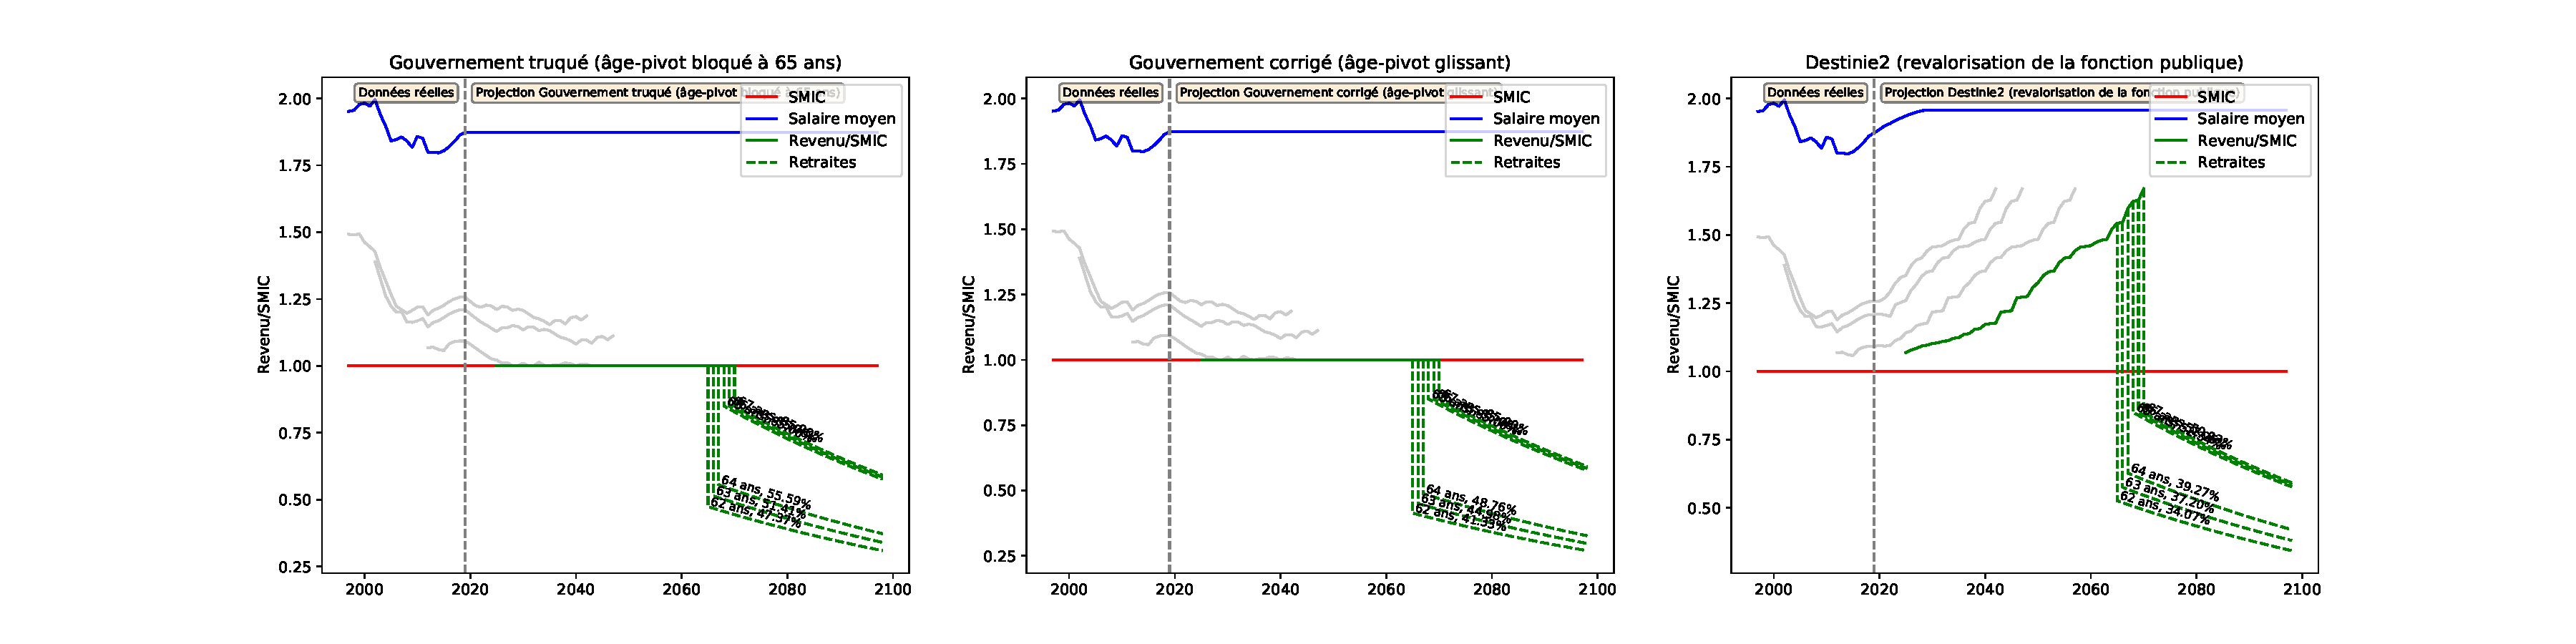
\includegraphics[width=0.9\textwidth]{fig/AdjTech_2003_22_dest_retraite.pdf}\end{center} \label{fig/AdjTech_2003_22_dest_retraite.pdf} 

\newpage 
 
\paragraph{Revenus et points pour le modèle \emph{Gouvernement truqué (âge-pivot bloqué à 65 ans)}} 
 
{ \scriptsize \begin{center} 
\begin{tabular}[htb]{|c|c||c|c|c|c|c|c||c|c||c|c|c|} 
\hline 
 Année &  Âge &  Ind Maj &  Pt Ind(\euro{} 2019) &  Rev HP(\euro{} 2019) &  Tx Primes &  GIPA(\euro{} 2019) &  Revenu(\euro{} 2019) &  SMIC(\euro{} 2019) &  Rev/SMIC &  Cumul Pts &  Achat Pt(\euro{} 2019) &  Serv. Pt(\euro{} 2019) \\ 
\hline \hline 
 2025 &  22 &  326.0 &  4.79 &  1562.98 &  12.41 &  0.00 &  1835.31 &  1835.31 &  {\bf 1.00} &  618.52 &  35.61 &  0.50 \\ 
\hline 
 2026 &  23 &  327.0 &  4.79 &  1567.78 &  12.64 &  0.00 &  1859.17 &  1859.17 &  {\bf 1.00} &  1245.08 &  35.61 &  0.50 \\ 
\hline 
 2027 &  24 &  327.0 &  4.79 &  1567.78 &  12.87 &  0.00 &  1883.34 &  1883.34 &  {\bf 1.00} &  1879.79 &  35.61 &  0.50 \\ 
\hline 
 2028 &  25 &  328.0 &  4.79 &  1572.57 &  13.10 &  0.00 &  1907.82 &  1907.82 &  {\bf 1.00} &  2522.75 &  35.61 &  0.50 \\ 
\hline 
 2029 &  26 &  328.0 &  4.79 &  1572.57 &  13.33 &  89.22 &  1932.62 &  1932.62 &  {\bf 1.00} &  3173.57 &  35.63 &  0.50 \\ 
\hline 
 2030 &  27 &  329.0 &  4.79 &  1577.36 &  13.56 &  104.48 &  1957.75 &  1957.75 &  {\bf 1.00} &  3831.86 &  35.69 &  0.50 \\ 
\hline 
 2031 &  28 &  329.0 &  4.79 &  1577.36 &  13.79 &  125.50 &  1983.20 &  1983.20 &  {\bf 1.00} &  4497.18 &  35.77 &  0.50 \\ 
\hline 
 2032 &  29 &  330.0 &  4.79 &  1582.16 &  14.02 &  141.37 &  2008.98 &  2008.98 &  {\bf 1.00} &  5169.10 &  35.88 &  0.50 \\ 
\hline 
 2033 &  30 &  330.0 &  4.79 &  1582.16 &  14.25 &  163.02 &  2035.10 &  2035.10 &  {\bf 1.00} &  5847.19 &  36.02 &  0.50 \\ 
\hline 
 2034 &  31 &  332.0 &  4.79 &  1591.75 &  14.48 &  174.02 &  2061.55 &  2061.55 &  {\bf 1.00} &  6530.96 &  36.18 &  0.50 \\ 
\hline 
 2035 &  32 &  332.0 &  4.79 &  1591.75 &  14.71 &  196.31 &  2088.35 &  2088.35 &  {\bf 1.00} &  7219.94 &  36.37 &  0.51 \\ 
\hline 
 2036 &  33 &  335.0 &  4.79 &  1606.13 &  14.94 &  202.41 &  2115.50 &  2115.50 &  {\bf 1.00} &  7913.66 &  36.59 &  0.51 \\ 
\hline 
 2037 &  34 &  335.0 &  4.79 &  1606.13 &  15.17 &  225.34 &  2143.00 &  2143.00 &  {\bf 1.00} &  8611.60 &  36.85 &  0.51 \\ 
\hline 
 2038 &  35 &  339.0 &  4.79 &  1625.31 &  15.40 &  226.50 &  2170.86 &  2170.86 &  {\bf 1.00} &  9313.26 &  37.13 &  0.52 \\ 
\hline 
 2039 &  36 &  339.0 &  4.79 &  1625.31 &  15.63 &  250.08 &  2199.08 &  2199.08 &  {\bf 1.00} &  10018.13 &  37.44 &  0.52 \\ 
\hline 
 2040 &  37 &  343.0 &  4.79 &  1644.49 &  15.86 &  251.81 &  2227.67 &  2227.67 &  {\bf 1.00} &  10725.69 &  37.78 &  0.53 \\ 
\hline 
 2041 &  38 &  343.0 &  4.79 &  1644.49 &  16.09 &  276.07 &  2256.63 &  2256.63 &  {\bf 1.00} &  11435.39 &  38.16 &  0.53 \\ 
\hline 
 2042 &  39 &  343.0 &  4.79 &  1644.49 &  16.32 &  300.69 &  2285.97 &  2285.97 &  {\bf 1.00} &  12146.72 &  38.56 &  0.54 \\ 
\hline 
 2043 &  40 &  354.0 &  4.79 &  1697.23 &  16.55 &  264.22 &  2315.68 &  2315.68 &  {\bf 1.00} &  12859.13 &  39.01 &  0.54 \\ 
\hline 
 2044 &  41 &  354.0 &  4.79 &  1697.23 &  16.78 &  289.47 &  2345.79 &  2345.79 &  {\bf 1.00} &  13572.08 &  39.48 &  0.55 \\ 
\hline 
 2045 &  42 &  354.0 &  4.79 &  1697.23 &  17.01 &  315.09 &  2376.28 &  2376.28 &  {\bf 1.00} &  14285.03 &  40.00 &  0.56 \\ 
\hline 
 2046 &  43 &  367.0 &  4.79 &  1759.55 &  17.24 &  268.03 &  2407.18 &  2407.18 &  {\bf 1.00} &  14997.98 &  40.52 &  0.56 \\ 
\hline 
 2047 &  44 &  367.0 &  4.79 &  1759.55 &  17.47 &  294.29 &  2438.47 &  2438.47 &  {\bf 1.00} &  15710.93 &  41.04 &  0.57 \\ 
\hline 
 2048 &  45 &  367.0 &  4.79 &  1759.55 &  17.70 &  320.94 &  2470.17 &  2470.17 &  {\bf 1.00} &  16423.88 &  41.58 &  0.58 \\ 
\hline 
 2049 &  46 &  375.7 &  4.79 &  1801.31 &  17.93 &  298.74 &  2502.28 &  2502.28 &  {\bf 1.00} &  17136.83 &  42.12 &  0.59 \\ 
\hline 
 2050 &  47 &  380.0 &  4.79 &  1821.88 &  18.16 &  301.79 &  2534.81 &  2534.81 &  {\bf 1.00} &  17849.78 &  42.66 &  0.59 \\ 
\hline 
 2051 &  48 &  386.7 &  4.79 &  1854.00 &  18.39 &  291.48 &  2567.76 &  2567.76 &  {\bf 1.00} &  18562.73 &  43.22 &  0.60 \\ 
\hline 
 2052 &  49 &  390.0 &  4.79 &  1869.82 &  18.62 &  300.77 &  2601.14 &  2601.14 &  {\bf 1.00} &  19275.68 &  43.78 &  0.61 \\ 
\hline 
 2053 &  50 &  390.0 &  4.79 &  1869.82 &  18.85 &  329.21 &  2634.96 &  2634.96 &  {\bf 1.00} &  19988.63 &  44.35 &  0.62 \\ 
\hline 
 2054 &  51 &  398.0 &  4.79 &  1908.37 &  19.08 &  312.18 &  2669.21 &  2669.21 &  {\bf 1.00} &  20701.58 &  44.93 &  0.63 \\ 
\hline 
 2055 &  52 &  402.0 &  4.79 &  1927.36 &  19.31 &  318.74 &  2703.91 &  2703.91 &  {\bf 1.00} &  21414.53 &  45.51 &  0.63 \\ 
\hline 
 2056 &  53 &  402.0 &  4.79 &  1927.36 &  19.54 &  348.34 &  2739.06 &  2739.06 &  {\bf 1.00} &  22127.48 &  46.10 &  0.64 \\ 
\hline 
 2057 &  54 &  408.0 &  4.79 &  1956.27 &  19.77 &  343.77 &  2774.67 &  2774.67 &  {\bf 1.00} &  22840.43 &  46.70 &  0.65 \\ 
\hline 
 2058 &  55 &  411.0 &  4.79 &  1970.51 &  20.00 &  357.11 &  2810.74 &  2810.74 &  {\bf 1.00} &  23553.38 &  47.31 &  0.66 \\ 
\hline 
 2059 &  56 &  411.0 &  4.79 &  1970.51 &  20.23 &  387.96 &  2847.28 &  2847.28 &  {\bf 1.00} &  24266.32 &  47.92 &  0.67 \\ 
\hline 
 2060 &  57 &  411.0 &  4.79 &  1970.51 &  20.46 &  419.27 &  2884.30 &  2884.30 &  {\bf 1.00} &  24979.27 &  48.55 &  0.68 \\ 
\hline 
 2061 &  58 &  413.7 &  4.79 &  1983.36 &  20.69 &  435.54 &  2921.79 &  2921.79 &  {\bf 1.00} &  25692.22 &  49.18 &  0.68 \\ 
\hline 
 2062 &  59 &  415.0 &  4.79 &  1989.69 &  20.92 &  460.10 &  2959.78 &  2959.78 &  {\bf 1.00} &  26405.17 &  49.82 &  0.69 \\ 
\hline 
 2063 &  60 &  415.0 &  4.79 &  1989.69 &  21.15 &  492.78 &  2998.25 &  2998.25 &  {\bf 1.00} &  27118.12 &  50.47 &  0.70 \\ 
\hline 
 2064 &  61 &  425.0 &  4.79 &  2037.87 &  21.38 &  467.46 &  3037.23 &  3037.23 &  {\bf 1.00} &  27831.07 &  51.12 &  0.71 \\ 
\hline 
 2065 &  62 &  430.0 &  4.79 &  2061.60 &  21.61 &  472.15 &  3076.71 &  3076.71 &  {\bf 1.00} &  28544.02 &  51.79 &  0.72 \\ 
\hline 
 2066 &  63 &  430.0 &  4.79 &  2061.60 &  21.84 &  506.14 &  3116.71 &  3116.71 &  {\bf 1.00} &  29256.97 &  52.46 &  0.73 \\ 
\hline 
 2067 &  64 &  443.4 &  4.79 &  2125.85 &  22.07 &  462.21 &  3157.23 &  3157.23 &  {\bf 1.00} &  29969.92 &  53.14 &  0.74 \\ 
\hline 
 2068 &  65 &  450.0 &  4.79 &  2157.49 &  22.30 &  458.36 &  3198.27 &  3198.27 &  {\bf 1.00} &  30682.87 &  53.83 &  0.75 \\ 
\hline 
 2069 &  66 &  450.0 &  4.79 &  2157.49 &  22.53 &  493.66 &  3239.85 &  3239.85 &  {\bf 1.00} &  31395.82 &  54.53 &  0.76 \\ 
\hline 
 2070 &  67 &  460.7 &  4.79 &  2208.89 &  22.76 &  466.39 &  3281.97 &  3281.97 &  {\bf 1.00} &  32108.77 &  55.24 &  0.77 \\ 
\hline 
\hline 
\end{tabular} 
\end{center} } 
\newpage 
 
\paragraph{Revenus et points pour le modèle \emph{Gouvernement corrigé (âge-pivot glissant)}} 
 
{ \scriptsize \begin{center} 
\begin{tabular}[htb]{|c|c||c|c|c|c|c|c||c|c||c|c|c|} 
\hline 
 Année &  Âge &  Ind Maj &  Pt Ind(\euro{} 2019) &  Rev HP(\euro{} 2019) &  Tx Primes &  GIPA(\euro{} 2019) &  Revenu(\euro{} 2019) &  SMIC(\euro{} 2019) &  Rev/SMIC &  Cumul Pts &  Achat Pt(\euro{} 2019) &  Serv. Pt(\euro{} 2019) \\ 
\hline \hline 
 2025 &  22 &  326.0 &  4.79 &  1562.98 &  12.41 &  0.00 &  1835.31 &  1835.31 &  {\bf 1.00} &  618.52 &  35.61 &  0.50 \\ 
\hline 
 2026 &  23 &  327.0 &  4.79 &  1567.78 &  12.64 &  0.00 &  1859.17 &  1859.17 &  {\bf 1.00} &  1245.08 &  35.61 &  0.50 \\ 
\hline 
 2027 &  24 &  327.0 &  4.79 &  1567.78 &  12.87 &  0.00 &  1883.34 &  1883.34 &  {\bf 1.00} &  1879.79 &  35.61 &  0.50 \\ 
\hline 
 2028 &  25 &  328.0 &  4.79 &  1572.57 &  13.10 &  0.00 &  1907.82 &  1907.82 &  {\bf 1.00} &  2522.75 &  35.61 &  0.50 \\ 
\hline 
 2029 &  26 &  328.0 &  4.79 &  1572.57 &  13.33 &  89.22 &  1932.62 &  1932.62 &  {\bf 1.00} &  3173.57 &  35.63 &  0.50 \\ 
\hline 
 2030 &  27 &  329.0 &  4.79 &  1577.36 &  13.56 &  104.48 &  1957.75 &  1957.75 &  {\bf 1.00} &  3831.86 &  35.69 &  0.50 \\ 
\hline 
 2031 &  28 &  329.0 &  4.79 &  1577.36 &  13.79 &  125.50 &  1983.20 &  1983.20 &  {\bf 1.00} &  4497.18 &  35.77 &  0.50 \\ 
\hline 
 2032 &  29 &  330.0 &  4.79 &  1582.16 &  14.02 &  141.37 &  2008.98 &  2008.98 &  {\bf 1.00} &  5169.10 &  35.88 &  0.50 \\ 
\hline 
 2033 &  30 &  330.0 &  4.79 &  1582.16 &  14.25 &  163.02 &  2035.10 &  2035.10 &  {\bf 1.00} &  5847.19 &  36.02 &  0.50 \\ 
\hline 
 2034 &  31 &  332.0 &  4.79 &  1591.75 &  14.48 &  174.02 &  2061.55 &  2061.55 &  {\bf 1.00} &  6530.96 &  36.18 &  0.50 \\ 
\hline 
 2035 &  32 &  332.0 &  4.79 &  1591.75 &  14.71 &  196.31 &  2088.35 &  2088.35 &  {\bf 1.00} &  7219.94 &  36.37 &  0.51 \\ 
\hline 
 2036 &  33 &  335.0 &  4.79 &  1606.13 &  14.94 &  202.41 &  2115.50 &  2115.50 &  {\bf 1.00} &  7913.66 &  36.59 &  0.51 \\ 
\hline 
 2037 &  34 &  335.0 &  4.79 &  1606.13 &  15.17 &  225.34 &  2143.00 &  2143.00 &  {\bf 1.00} &  8611.60 &  36.85 &  0.51 \\ 
\hline 
 2038 &  35 &  339.0 &  4.79 &  1625.31 &  15.40 &  226.50 &  2170.86 &  2170.86 &  {\bf 1.00} &  9313.26 &  37.13 &  0.52 \\ 
\hline 
 2039 &  36 &  339.0 &  4.79 &  1625.31 &  15.63 &  250.08 &  2199.08 &  2199.08 &  {\bf 1.00} &  10018.13 &  37.44 &  0.52 \\ 
\hline 
 2040 &  37 &  343.0 &  4.79 &  1644.49 &  15.86 &  251.81 &  2227.67 &  2227.67 &  {\bf 1.00} &  10725.69 &  37.78 &  0.53 \\ 
\hline 
 2041 &  38 &  343.0 &  4.79 &  1644.49 &  16.09 &  276.07 &  2256.63 &  2256.63 &  {\bf 1.00} &  11435.39 &  38.16 &  0.53 \\ 
\hline 
 2042 &  39 &  343.0 &  4.79 &  1644.49 &  16.32 &  300.69 &  2285.97 &  2285.97 &  {\bf 1.00} &  12146.72 &  38.56 &  0.54 \\ 
\hline 
 2043 &  40 &  354.0 &  4.79 &  1697.23 &  16.55 &  264.22 &  2315.68 &  2315.68 &  {\bf 1.00} &  12859.13 &  39.01 &  0.54 \\ 
\hline 
 2044 &  41 &  354.0 &  4.79 &  1697.23 &  16.78 &  289.47 &  2345.79 &  2345.79 &  {\bf 1.00} &  13572.08 &  39.48 &  0.55 \\ 
\hline 
 2045 &  42 &  354.0 &  4.79 &  1697.23 &  17.01 &  315.09 &  2376.28 &  2376.28 &  {\bf 1.00} &  14285.03 &  40.00 &  0.56 \\ 
\hline 
 2046 &  43 &  367.0 &  4.79 &  1759.55 &  17.24 &  268.03 &  2407.18 &  2407.18 &  {\bf 1.00} &  14997.98 &  40.52 &  0.56 \\ 
\hline 
 2047 &  44 &  367.0 &  4.79 &  1759.55 &  17.47 &  294.29 &  2438.47 &  2438.47 &  {\bf 1.00} &  15710.93 &  41.04 &  0.57 \\ 
\hline 
 2048 &  45 &  367.0 &  4.79 &  1759.55 &  17.70 &  320.94 &  2470.17 &  2470.17 &  {\bf 1.00} &  16423.88 &  41.58 &  0.58 \\ 
\hline 
 2049 &  46 &  375.7 &  4.79 &  1801.31 &  17.93 &  298.74 &  2502.28 &  2502.28 &  {\bf 1.00} &  17136.83 &  42.12 &  0.59 \\ 
\hline 
 2050 &  47 &  380.0 &  4.79 &  1821.88 &  18.16 &  301.79 &  2534.81 &  2534.81 &  {\bf 1.00} &  17849.78 &  42.66 &  0.59 \\ 
\hline 
 2051 &  48 &  386.7 &  4.79 &  1854.00 &  18.39 &  291.48 &  2567.76 &  2567.76 &  {\bf 1.00} &  18562.73 &  43.22 &  0.60 \\ 
\hline 
 2052 &  49 &  390.0 &  4.79 &  1869.82 &  18.62 &  300.77 &  2601.14 &  2601.14 &  {\bf 1.00} &  19275.68 &  43.78 &  0.61 \\ 
\hline 
 2053 &  50 &  390.0 &  4.79 &  1869.82 &  18.85 &  329.21 &  2634.96 &  2634.96 &  {\bf 1.00} &  19988.63 &  44.35 &  0.62 \\ 
\hline 
 2054 &  51 &  398.0 &  4.79 &  1908.37 &  19.08 &  312.18 &  2669.21 &  2669.21 &  {\bf 1.00} &  20701.58 &  44.93 &  0.63 \\ 
\hline 
 2055 &  52 &  402.0 &  4.79 &  1927.36 &  19.31 &  318.74 &  2703.91 &  2703.91 &  {\bf 1.00} &  21414.53 &  45.51 &  0.63 \\ 
\hline 
 2056 &  53 &  402.0 &  4.79 &  1927.36 &  19.54 &  348.34 &  2739.06 &  2739.06 &  {\bf 1.00} &  22127.48 &  46.10 &  0.64 \\ 
\hline 
 2057 &  54 &  408.0 &  4.79 &  1956.27 &  19.77 &  343.77 &  2774.67 &  2774.67 &  {\bf 1.00} &  22840.43 &  46.70 &  0.65 \\ 
\hline 
 2058 &  55 &  411.0 &  4.79 &  1970.51 &  20.00 &  357.11 &  2810.74 &  2810.74 &  {\bf 1.00} &  23553.38 &  47.31 &  0.66 \\ 
\hline 
 2059 &  56 &  411.0 &  4.79 &  1970.51 &  20.23 &  387.96 &  2847.28 &  2847.28 &  {\bf 1.00} &  24266.32 &  47.92 &  0.67 \\ 
\hline 
 2060 &  57 &  411.0 &  4.79 &  1970.51 &  20.46 &  419.27 &  2884.30 &  2884.30 &  {\bf 1.00} &  24979.27 &  48.55 &  0.68 \\ 
\hline 
 2061 &  58 &  413.7 &  4.79 &  1983.36 &  20.69 &  435.54 &  2921.79 &  2921.79 &  {\bf 1.00} &  25692.22 &  49.18 &  0.68 \\ 
\hline 
 2062 &  59 &  415.0 &  4.79 &  1989.69 &  20.92 &  460.10 &  2959.78 &  2959.78 &  {\bf 1.00} &  26405.17 &  49.82 &  0.69 \\ 
\hline 
 2063 &  60 &  415.0 &  4.79 &  1989.69 &  21.15 &  492.78 &  2998.25 &  2998.25 &  {\bf 1.00} &  27118.12 &  50.47 &  0.70 \\ 
\hline 
 2064 &  61 &  425.0 &  4.79 &  2037.87 &  21.38 &  467.46 &  3037.23 &  3037.23 &  {\bf 1.00} &  27831.07 &  51.12 &  0.71 \\ 
\hline 
 2065 &  62 &  430.0 &  4.79 &  2061.60 &  21.61 &  472.15 &  3076.71 &  3076.71 &  {\bf 1.00} &  28544.02 &  51.79 &  0.72 \\ 
\hline 
 2066 &  63 &  430.0 &  4.79 &  2061.60 &  21.84 &  506.14 &  3116.71 &  3116.71 &  {\bf 1.00} &  29256.97 &  52.46 &  0.73 \\ 
\hline 
 2067 &  64 &  443.4 &  4.79 &  2125.85 &  22.07 &  462.21 &  3157.23 &  3157.23 &  {\bf 1.00} &  29969.92 &  53.14 &  0.74 \\ 
\hline 
 2068 &  65 &  450.0 &  4.79 &  2157.49 &  22.30 &  458.36 &  3198.27 &  3198.27 &  {\bf 1.00} &  30682.87 &  53.83 &  0.75 \\ 
\hline 
 2069 &  66 &  450.0 &  4.79 &  2157.49 &  22.53 &  493.66 &  3239.85 &  3239.85 &  {\bf 1.00} &  31395.82 &  54.53 &  0.76 \\ 
\hline 
 2070 &  67 &  460.7 &  4.79 &  2208.89 &  22.76 &  466.39 &  3281.97 &  3281.97 &  {\bf 1.00} &  32108.77 &  55.24 &  0.77 \\ 
\hline 
\hline 
\end{tabular} 
\end{center} } 
\newpage 
 
\paragraph{Revenus et points pour le modèle \emph{Destinie2 (revalorisation de la fonction publique)}} 
 
{ \scriptsize \begin{center} 
\begin{tabular}[htb]{|c|c||c|c|c|c|c|c||c|c||c|c|c|} 
\hline 
 Année &  Âge &  Ind Maj &  Pt Ind(\euro{} 2019) &  Rev HP(\euro{} 2019) &  Tx Primes &  GIPA(\euro{} 2019) &  Revenu(\euro{} 2019) &  SMIC(\euro{} 2019) &  Rev/SMIC &  Cumul Pts &  Achat Pt(\euro{} 2019) &  Serv. Pt(\euro{} 2019) \\ 
\hline \hline 
 2025 &  22 &  326.0 &  5.10 &  1663.73 &  12.41 &  0.00 &  1870.20 &  1749.35 &  {\bf 1.07} &  628.73 &  35.69 &  0.50 \\ 
\hline 
 2026 &  23 &  327.0 &  5.17 &  1689.69 &  12.64 &  0.00 &  1903.27 &  1764.53 &  {\bf 1.08} &  1268.58 &  35.69 &  0.50 \\ 
\hline 
 2027 &  24 &  327.0 &  5.23 &  1711.32 &  12.87 &  0.00 &  1931.57 &  1781.27 &  {\bf 1.08} &  1917.94 &  35.69 &  0.50 \\ 
\hline 
 2028 &  25 &  328.0 &  5.30 &  1739.04 &  13.10 &  0.00 &  1966.86 &  1799.59 &  {\bf 1.09} &  2579.17 &  35.69 &  0.50 \\ 
\hline 
 2029 &  26 &  328.0 &  5.37 &  1760.08 &  13.33 &  0.00 &  1994.70 &  1819.55 &  {\bf 1.10} &  3249.28 &  35.72 &  0.50 \\ 
\hline 
 2030 &  27 &  329.0 &  5.43 &  1787.34 &  13.56 &  0.00 &  2029.70 &  1841.19 &  {\bf 1.10} &  3930.17 &  35.77 &  0.50 \\ 
\hline 
 2031 &  28 &  329.0 &  5.50 &  1810.04 &  13.79 &  0.00 &  2059.65 &  1864.58 &  {\bf 1.10} &  4619.56 &  35.85 &  0.50 \\ 
\hline 
 2032 &  29 &  330.0 &  5.57 &  1839.14 &  14.02 &  0.00 &  2096.99 &  1888.81 &  {\bf 1.11} &  5319.32 &  35.96 &  0.50 \\ 
\hline 
 2033 &  30 &  330.0 &  5.65 &  1863.05 &  14.25 &  0.00 &  2128.54 &  1913.37 &  {\bf 1.11} &  6026.91 &  36.10 &  0.50 \\ 
\hline 
 2034 &  31 &  332.0 &  5.72 &  1898.71 &  14.48 &  0.00 &  2173.64 &  1938.24 &  {\bf 1.12} &  6746.22 &  36.26 &  0.50 \\ 
\hline 
 2035 &  32 &  332.0 &  5.79 &  1923.39 &  14.71 &  0.00 &  2206.33 &  1963.44 &  {\bf 1.12} &  7472.46 &  36.46 &  0.51 \\ 
\hline 
 2036 &  33 &  335.0 &  5.87 &  1966.00 &  14.94 &  0.00 &  2259.73 &  1988.96 &  {\bf 1.14} &  8211.78 &  36.68 &  0.51 \\ 
\hline 
 2037 &  34 &  335.0 &  5.94 &  1991.56 &  15.17 &  0.00 &  2293.68 &  2014.82 &  {\bf 1.14} &  8957.09 &  36.93 &  0.51 \\ 
\hline 
 2038 &  35 &  339.0 &  6.02 &  2041.54 &  15.40 &  0.00 &  2355.94 &  2041.01 &  {\bf 1.15} &  9716.83 &  37.21 &  0.52 \\ 
\hline 
 2039 &  36 &  339.0 &  6.10 &  2068.08 &  15.63 &  0.00 &  2391.32 &  2067.55 &  {\bf 1.16} &  10481.57 &  37.52 &  0.52 \\ 
\hline 
 2040 &  37 &  343.0 &  6.18 &  2119.69 &  15.86 &  0.00 &  2455.87 &  2094.43 &  {\bf 1.17} &  11259.83 &  37.87 &  0.53 \\ 
\hline 
 2041 &  38 &  343.0 &  6.26 &  2147.24 &  16.09 &  0.00 &  2492.73 &  2121.65 &  {\bf 1.17} &  12042.00 &  38.24 &  0.53 \\ 
\hline 
 2042 &  39 &  343.0 &  6.34 &  2175.16 &  16.32 &  0.00 &  2530.14 &  2149.23 &  {\bf 1.18} &  12827.51 &  38.65 &  0.54 \\ 
\hline 
 2043 &  40 &  354.0 &  6.42 &  2274.10 &  16.55 &  0.00 &  2650.46 &  2177.17 &  {\bf 1.22} &  13641.04 &  39.10 &  0.54 \\ 
\hline 
 2044 &  41 &  354.0 &  6.51 &  2303.66 &  16.78 &  0.00 &  2690.21 &  2205.48 &  {\bf 1.22} &  14456.81 &  39.57 &  0.55 \\ 
\hline 
 2045 &  42 &  354.0 &  6.59 &  2333.61 &  17.01 &  0.00 &  2730.55 &  2234.15 &  {\bf 1.22} &  15274.18 &  40.09 &  0.56 \\ 
\hline 
 2046 &  43 &  367.0 &  6.68 &  2450.76 &  17.24 &  0.00 &  2873.27 &  2263.19 &  {\bf 1.27} &  16123.23 &  40.61 &  0.57 \\ 
\hline 
 2047 &  44 &  367.0 &  6.76 &  2482.62 &  17.47 &  0.00 &  2916.33 &  2292.61 &  {\bf 1.27} &  16973.95 &  41.14 &  0.57 \\ 
\hline 
 2048 &  45 &  367.0 &  6.85 &  2514.89 &  17.70 &  0.00 &  2960.03 &  2322.42 &  {\bf 1.27} &  17826.33 &  41.67 &  0.58 \\ 
\hline 
 2049 &  46 &  375.7 &  6.94 &  2608.05 &  17.93 &  0.00 &  3075.67 &  2352.61 &  {\bf 1.31} &  18700.65 &  42.21 &  0.59 \\ 
\hline 
 2050 &  47 &  380.0 &  7.03 &  2672.12 &  18.16 &  0.00 &  3157.37 &  2383.19 &  {\bf 1.32} &  19586.68 &  42.76 &  0.60 \\ 
\hline 
 2051 &  48 &  386.7 &  7.12 &  2754.58 &  18.39 &  0.00 &  3261.15 &  2414.18 &  {\bf 1.35} &  20490.08 &  43.32 &  0.60 \\ 
\hline 
 2052 &  49 &  390.0 &  7.22 &  2814.20 &  18.62 &  0.00 &  3338.21 &  2445.56 &  {\bf 1.37} &  21402.96 &  43.88 &  0.61 \\ 
\hline 
 2053 &  50 &  390.0 &  7.31 &  2850.79 &  18.85 &  0.00 &  3388.16 &  2477.35 &  {\bf 1.37} &  22317.62 &  44.45 &  0.62 \\ 
\hline 
 2054 &  51 &  398.0 &  7.40 &  2947.38 &  19.08 &  0.00 &  3509.74 &  2509.56 &  {\bf 1.40} &  23252.93 &  45.03 &  0.63 \\ 
\hline 
 2055 &  52 &  402.0 &  7.50 &  3015.40 &  19.31 &  0.00 &  3597.68 &  2542.18 &  {\bf 1.42} &  24199.38 &  45.62 &  0.63 \\ 
\hline 
 2056 &  53 &  402.0 &  7.60 &  3054.60 &  19.54 &  0.00 &  3651.47 &  2575.23 &  {\bf 1.42} &  25147.65 &  46.21 &  0.64 \\ 
\hline 
 2057 &  54 &  408.0 &  7.70 &  3140.73 &  19.77 &  0.00 &  3761.65 &  2608.71 &  {\bf 1.44} &  26111.99 &  46.81 &  0.65 \\ 
\hline 
 2058 &  55 &  411.0 &  7.80 &  3204.71 &  20.00 &  0.00 &  3845.66 &  2642.62 &  {\bf 1.46} &  27085.22 &  47.42 &  0.66 \\ 
\hline 
 2059 &  56 &  411.0 &  7.90 &  3246.38 &  20.23 &  0.00 &  3903.12 &  2676.98 &  {\bf 1.46} &  28060.32 &  48.03 &  0.67 \\ 
\hline 
 2060 &  57 &  411.0 &  8.00 &  3288.58 &  20.46 &  0.00 &  3961.42 &  2711.78 &  {\bf 1.46} &  29037.28 &  48.66 &  0.68 \\ 
\hline 
 2061 &  58 &  413.7 &  8.11 &  3353.05 &  20.69 &  0.00 &  4046.80 &  2747.03 &  {\bf 1.47} &  30022.49 &  49.29 &  0.69 \\ 
\hline 
 2062 &  59 &  415.0 &  8.21 &  3407.48 &  20.92 &  0.00 &  4120.32 &  2782.74 &  {\bf 1.48} &  31012.72 &  49.93 &  0.70 \\ 
\hline 
 2063 &  60 &  415.0 &  8.32 &  3451.78 &  21.15 &  0.00 &  4181.83 &  2818.92 &  {\bf 1.48} &  32004.84 &  50.58 &  0.70 \\ 
\hline 
 2064 &  61 &  425.0 &  8.43 &  3581.33 &  21.38 &  0.00 &  4347.02 &  2855.56 &  {\bf 1.52} &  33022.92 &  51.24 &  0.71 \\ 
\hline 
 2065 &  62 &  430.0 &  8.54 &  3670.13 &  21.61 &  0.00 &  4463.25 &  2892.68 &  {\bf 1.54} &  34054.80 &  51.90 &  0.72 \\ 
\hline 
 2066 &  63 &  430.0 &  8.65 &  3717.85 &  21.84 &  0.00 &  4529.82 &  2930.29 &  {\bf 1.55} &  35088.63 &  52.58 &  0.73 \\ 
\hline 
 2067 &  64 &  443.4 &  8.76 &  3883.54 &  22.07 &  0.00 &  4740.64 &  2968.38 &  {\bf 1.60} &  36156.70 &  53.26 &  0.74 \\ 
\hline 
 2068 &  65 &  450.0 &  8.87 &  3992.59 &  22.30 &  0.00 &  4882.93 &  3006.97 &  {\bf 1.62} &  37242.70 &  53.95 &  0.75 \\ 
\hline 
 2069 &  66 &  450.0 &  8.99 &  4044.49 &  22.53 &  0.00 &  4955.71 &  3046.06 &  {\bf 1.63} &  38330.75 &  54.66 &  0.76 \\ 
\hline 
 2070 &  67 &  460.7 &  9.10 &  4194.67 &  22.76 &  0.00 &  5149.38 &  3085.66 &  {\bf 1.67} &  39446.81 &  55.37 &  0.77 \\ 
\hline 
\hline 
\end{tabular} 
\end{center} } 
\newpage 
 
\chapter{Rédacteur territorial (C2 puis C1)} 

\begin{minipage}{0.55\linewidth}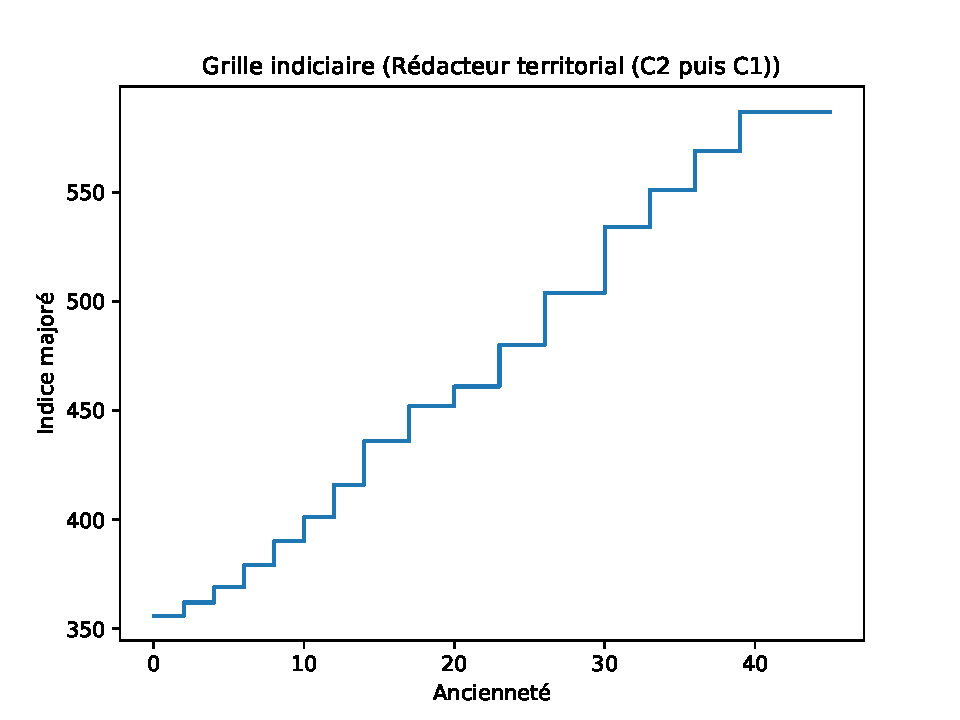
\includegraphics[width=0.7\textwidth]{fig/grille_Redacteur.pdf}\end{minipage} 
\begin{minipage}{0.3\linewidth} 
 \begin{center} 

\begin{tabular}[htb]{|c|c|} 
\hline 
 Indice majoré &  Durée (années) \\ 
\hline \hline 
 356 &  2.00 \\ 
\hline 
 362 &  2.00 \\ 
\hline 
 369 &  2.00 \\ 
\hline 
 379 &  2.00 \\ 
\hline 
 390 &  2.00 \\ 
\hline 
 401 &  2.00 \\ 
\hline 
 416 &  2.00 \\ 
\hline 
 436 &  3.00 \\ 
\hline 
 452 &  3.00 \\ 
\hline 
 461 &  3.00 \\ 
\hline 
 480 &  3.00 \\ 
\hline 
 504 &  4.00 \\ 
\hline 
 534 &  3.00 \\ 
\hline 
 551 &  3.00 \\ 
\hline 
 569 &  3.00 \\ 
\hline 
 587 &   \\ 
\hline 
\hline 
\end{tabular} 
\end{center} 
 \end{minipage} 


 \addto{\captionsenglish}{ \renewcommand{\mtctitle}{}} \setcounter{minitocdepth}{2} 
 \minitoc \newpage 

\section{Début de carrière à 22 ans} 

\subsection{Génération 1975 (début en 1997)} 

\paragraph{Retraites possibles dans le modèle \emph{Gouvernement truqué (âge-pivot bloqué à 65 ans)}}  
 
{ \scriptsize \begin{center} 
\begin{tabular}[htb]{|c|c||c|c||c|c||c||c|c|c|c|c|c|} 
\hline 
 Retraite en &  Âge &  Âge pivot &  Décote/Surcote &  Retraite (\euro{} 2019) &  Tx Rempl(\%) &  SMIC (\euro{} 2019) &  Retraite/SMIC &  Rev70/SMIC &  Rev75/SMIC &  Rev80/SMIC &  Rev85/SMIC &  Rev90/SMIC \\ 
\hline \hline 
 2037 &  62 &  64 ans 10 mois &  -14.17\% &  1430.63 &  {\bf 39.90} &  2143.00 &  {\bf {\color{red} 0.67}} &  {\bf {\color{red} 0.60}} &  {\bf {\color{red} 0.56}} &  {\bf {\color{red} 0.53}} &  {\bf {\color{red} 0.50}} &  {\bf {\color{red} 0.46}} \\ 
\hline 
 2038 &  63 &  64 ans 11 mois &  -9.58\% &  1563.72 &  {\bf 43.53} &  2170.86 &  {\bf {\color{red} 0.72}} &  {\bf {\color{red} 0.66}} &  {\bf {\color{red} 0.62}} &  {\bf {\color{red} 0.58}} &  {\bf {\color{red} 0.54}} &  {\bf {\color{red} 0.51}} \\ 
\hline 
 2039 &  64 &  65 ans 0 mois &  -5.00\% &  1704.37 &  {\bf 47.36} &  2199.08 &  {\bf {\color{red} 0.78}} &  {\bf {\color{red} 0.72}} &  {\bf {\color{red} 0.67}} &  {\bf {\color{red} 0.63}} &  {\bf {\color{red} 0.59}} &  {\bf {\color{red} 0.55}} \\ 
\hline 
 2040 &  65 &  65 ans 0 mois &  0.00\% &  1893.52 &  {\bf 52.52} &  2227.67 &  {\bf {\color{red} 0.85}} &  {\bf {\color{red} 0.80}} &  {\bf {\color{red} 0.75}} &  {\bf {\color{red} 0.70}} &  {\bf {\color{red} 0.66}} &  {\bf {\color{red} 0.62}} \\ 
\hline 
 2041 &  66 &  65 ans 0 mois &  5.00\% &  2025.90 &  {\bf 56.09} &  2256.63 &  {\bf {\color{red} 0.90}} &  {\bf {\color{red} 0.85}} &  {\bf {\color{red} 0.80}} &  {\bf {\color{red} 0.75}} &  {\bf {\color{red} 0.70}} &  {\bf {\color{red} 0.66}} \\ 
\hline 
 2042 &  67 &  65 ans 0 mois &  10.00\% &  2200.46 &  {\bf 60.82} &  2285.97 &  {\bf {\color{red} 0.96}} &  {\bf {\color{red} 0.93}} &  {\bf {\color{red} 0.87}} &  {\bf {\color{red} 0.81}} &  {\bf {\color{red} 0.76}} &  {\bf {\color{red} 0.72}} \\ 
\hline 
\hline 
\end{tabular} 
\end{center} } 
\paragraph{Retraites possibles dans le modèle \emph{Gouvernement corrigé (âge-pivot glissant)}}  
 
{ \scriptsize \begin{center} 
\begin{tabular}[htb]{|c|c||c|c||c|c||c||c|c|c|c|c|c|} 
\hline 
 Retraite en &  Âge &  Âge pivot &  Décote/Surcote &  Retraite (\euro{} 2019) &  Tx Rempl(\%) &  SMIC (\euro{} 2019) &  Retraite/SMIC &  Rev70/SMIC &  Rev75/SMIC &  Rev80/SMIC &  Rev85/SMIC &  Rev90/SMIC \\ 
\hline \hline 
 2037 &  62 &  64 ans 10 mois &  -14.17\% &  1430.63 &  {\bf 39.90} &  2143.00 &  {\bf {\color{red} 0.67}} &  {\bf {\color{red} 0.60}} &  {\bf {\color{red} 0.56}} &  {\bf {\color{red} 0.53}} &  {\bf {\color{red} 0.50}} &  {\bf {\color{red} 0.46}} \\ 
\hline 
 2038 &  63 &  64 ans 11 mois &  -9.58\% &  1563.72 &  {\bf 43.53} &  2170.86 &  {\bf {\color{red} 0.72}} &  {\bf {\color{red} 0.66}} &  {\bf {\color{red} 0.62}} &  {\bf {\color{red} 0.58}} &  {\bf {\color{red} 0.54}} &  {\bf {\color{red} 0.51}} \\ 
\hline 
 2039 &  64 &  65 ans 0 mois &  -5.00\% &  1704.37 &  {\bf 47.36} &  2199.08 &  {\bf {\color{red} 0.78}} &  {\bf {\color{red} 0.72}} &  {\bf {\color{red} 0.67}} &  {\bf {\color{red} 0.63}} &  {\bf {\color{red} 0.59}} &  {\bf {\color{red} 0.55}} \\ 
\hline 
 2040 &  65 &  65 ans 1 mois &  -0.42\% &  1893.52 &  {\bf 52.52} &  2227.67 &  {\bf {\color{red} 0.85}} &  {\bf {\color{red} 0.80}} &  {\bf {\color{red} 0.75}} &  {\bf {\color{red} 0.70}} &  {\bf {\color{red} 0.66}} &  {\bf {\color{red} 0.62}} \\ 
\hline 
 2041 &  66 &  65 ans 2 mois &  4.17\% &  2009.82 &  {\bf 55.65} &  2256.63 &  {\bf {\color{red} 0.89}} &  {\bf {\color{red} 0.85}} &  {\bf {\color{red} 0.79}} &  {\bf {\color{red} 0.74}} &  {\bf {\color{red} 0.70}} &  {\bf {\color{red} 0.65}} \\ 
\hline 
 2042 &  67 &  65 ans 3 mois &  8.75\% &  2175.46 &  {\bf 60.13} &  2285.97 &  {\bf {\color{red} 0.95}} &  {\bf {\color{red} 0.92}} &  {\bf {\color{red} 0.86}} &  {\bf {\color{red} 0.80}} &  {\bf {\color{red} 0.75}} &  {\bf {\color{red} 0.71}} \\ 
\hline 
\hline 
\end{tabular} 
\end{center} } 
\paragraph{Retraites possibles dans le modèle \emph{Destinie2 (revalorisation de la fonction publique)}}  
 
{ \scriptsize \begin{center} 
\begin{tabular}[htb]{|c|c||c|c||c|c||c||c|c|c|c|c|c|} 
\hline 
 Retraite en &  Âge &  Âge pivot &  Décote/Surcote &  Retraite (\euro{} 2019) &  Tx Rempl(\%) &  SMIC (\euro{} 2019) &  Retraite/SMIC &  Rev70/SMIC &  Rev75/SMIC &  Rev80/SMIC &  Rev85/SMIC &  Rev90/SMIC \\ 
\hline \hline 
 2037 &  62 &  64 ans 10 mois &  -14.17\% &  1515.92 &  {\bf 34.09} &  2014.82 &  {\bf {\color{red} 0.75}} &  {\bf {\color{red} 0.68}} &  {\bf {\color{red} 0.64}} &  {\bf {\color{red} 0.60}} &  {\bf {\color{red} 0.56}} &  {\bf {\color{red} 0.52}} \\ 
\hline 
 2038 &  63 &  64 ans 11 mois &  -9.58\% &  1665.84 &  {\bf 36.92} &  2041.01 &  {\bf {\color{red} 0.82}} &  {\bf {\color{red} 0.75}} &  {\bf {\color{red} 0.70}} &  {\bf {\color{red} 0.66}} &  {\bf {\color{red} 0.61}} &  {\bf {\color{red} 0.58}} \\ 
\hline 
 2039 &  64 &  65 ans 0 mois &  -5.00\% &  1825.52 &  {\bf 39.87} &  2067.55 &  {\bf {\color{red} 0.88}} &  {\bf {\color{red} 0.82}} &  {\bf {\color{red} 0.77}} &  {\bf {\color{red} 0.72}} &  {\bf {\color{red} 0.67}} &  {\bf {\color{red} 0.63}} \\ 
\hline 
 2040 &  65 &  65 ans 1 mois &  -0.42\% &  1995.53 &  {\bf 42.94} &  2094.43 &  {\bf {\color{red} 0.95}} &  {\bf {\color{red} 0.89}} &  {\bf {\color{red} 0.84}} &  {\bf {\color{red} 0.78}} &  {\bf {\color{red} 0.74}} &  {\bf {\color{red} 0.69}} \\ 
\hline 
 2041 &  66 &  65 ans 2 mois &  4.17\% &  2176.47 &  {\bf 46.15} &  2121.65 &  {\bf 1.03} &  {\bf {\color{red} 0.97}} &  {\bf {\color{red} 0.91}} &  {\bf {\color{red} 0.86}} &  {\bf {\color{red} 0.80}} &  {\bf {\color{red} 0.75}} \\ 
\hline 
 2042 &  67 &  65 ans 3 mois &  8.75\% &  2368.98 &  {\bf 49.50} &  2149.23 &  {\bf 1.10} &  {\bf 1.06} &  {\bf {\color{red} 0.99}} &  {\bf {\color{red} 0.93}} &  {\bf {\color{red} 0.87}} &  {\bf {\color{red} 0.82}} \\ 
\hline 
\hline 
\end{tabular} 
\end{center} } 

 \begin{center}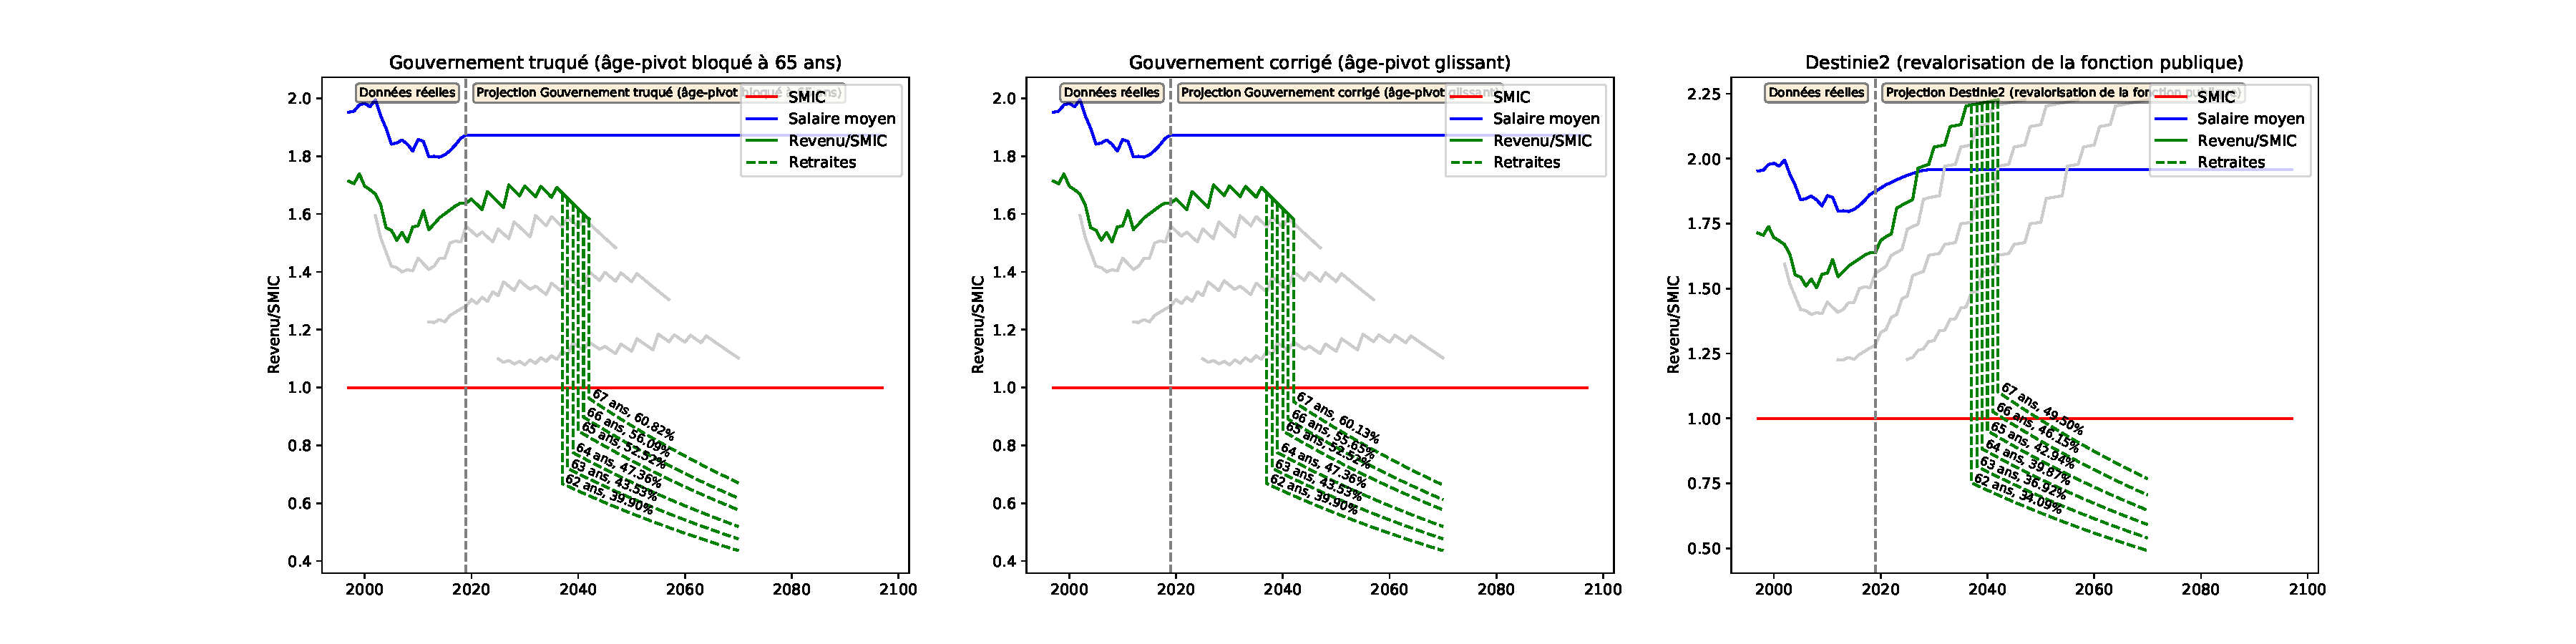
\includegraphics[width=0.9\textwidth]{fig/Redacteur_1975_22_dest_retraite.pdf}\end{center} \label{fig/Redacteur_1975_22_dest_retraite.pdf} 

\newpage 
 
\paragraph{Revenus et points pour le modèle \emph{Gouvernement truqué (âge-pivot bloqué à 65 ans)}} 
 
{ \scriptsize \begin{center} 
\begin{tabular}[htb]{|c|c||c|c|c|c|c|c||c|c||c|c|c|} 
\hline 
 Année &  Âge &  Ind Maj &  Pt Ind(\euro{} 2019) &  Rev HP(\euro{} 2019) &  Tx Primes &  GIPA(\euro{} 2019) &  Revenu(\euro{} 2019) &  SMIC(\euro{} 2019) &  Rev/SMIC &  Cumul Pts &  Achat Pt(\euro{} 2019) &  Serv. Pt(\euro{} 2019) \\ 
\hline \hline 
 1997 &  22 &  356.0 &  5.53 &  1970.23 &  18.21 &  0.00 &  2329.01 &  1358.84 &  {\bf 1.71} &  784.90 &  35.61 &  0.50 \\ 
\hline 
 1998 &  23 &  356.0 &  5.57 &  1981.66 &  18.44 &  0.00 &  2347.07 &  1376.36 &  {\bf 1.71} &  1575.90 &  35.61 &  0.50 \\ 
\hline 
 1999 &  24 &  362.0 &  5.61 &  2031.34 &  18.67 &  0.00 &  2410.60 &  1386.54 &  {\bf 1.74} &  2388.30 &  35.61 &  0.50 \\ 
\hline 
 2000 &  25 &  362.0 &  5.55 &  2007.36 &  18.90 &  0.00 &  2386.75 &  1407.00 &  {\bf 1.70} &  3192.66 &  35.61 &  0.50 \\ 
\hline 
 2001 &  26 &  369.0 &  5.52 &  2037.07 &  19.13 &  0.00 &  2426.76 &  1441.04 &  {\bf 1.68} &  4010.51 &  35.61 &  0.50 \\ 
\hline 
 2002 &  27 &  369.0 &  5.49 &  2024.44 &  19.36 &  0.00 &  2416.37 &  1447.74 &  {\bf 1.67} &  4824.85 &  35.61 &  0.50 \\ 
\hline 
 2003 &  28 &  379.0 &  5.37 &  2036.98 &  19.59 &  0.00 &  2436.03 &  1493.03 &  {\bf 1.63} &  5645.82 &  35.61 &  0.50 \\ 
\hline 
 2004 &  29 &  379.0 &  5.29 &  2004.80 &  19.82 &  0.00 &  2402.16 &  1547.32 &  {\bf 1.55} &  6455.38 &  35.61 &  0.50 \\ 
\hline 
 2005 &  30 &  390.0 &  5.29 &  2062.77 &  20.05 &  0.00 &  2476.35 &  1603.67 &  {\bf 1.54} &  7289.94 &  35.61 &  0.50 \\ 
\hline 
 2006 &  31 &  390.0 &  5.23 &  2039.75 &  20.28 &  0.00 &  2453.41 &  1625.00 &  {\bf 1.51} &  8116.77 &  35.61 &  0.50 \\ 
\hline 
 2007 &  32 &  401.0 &  5.19 &  2082.99 &  20.51 &  0.00 &  2510.21 &  1634.08 &  {\bf 1.54} &  8962.74 &  35.61 &  0.50 \\ 
\hline 
 2008 &  33 &  401.0 &  5.09 &  2042.31 &  20.74 &  0.00 &  2465.89 &  1640.24 &  {\bf 1.50} &  9793.77 &  35.61 &  0.50 \\ 
\hline 
 2009 &  34 &  416.0 &  5.13 &  2133.72 &  20.97 &  0.00 &  2581.16 &  1659.42 &  {\bf 1.56} &  10663.65 &  35.61 &  0.50 \\ 
\hline 
 2010 &  35 &  416.0 &  5.08 &  2112.17 &  21.20 &  0.00 &  2559.95 &  1641.90 &  {\bf 1.56} &  11526.38 &  35.61 &  0.50 \\ 
\hline 
 2011 &  36 &  436.0 &  4.97 &  2167.72 &  21.43 &  0.00 &  2632.26 &  1633.19 &  {\bf 1.61} &  12413.49 &  35.61 &  0.50 \\ 
\hline 
 2012 &  37 &  436.0 &  4.88 &  2126.13 &  21.66 &  0.00 &  2586.64 &  1673.05 &  {\bf 1.55} &  13285.22 &  35.61 &  0.50 \\ 
\hline 
 2013 &  38 &  436.0 &  4.83 &  2107.91 &  21.89 &  36.17 &  2605.50 &  1664.01 &  {\bf 1.57} &  14163.31 &  35.61 &  0.50 \\ 
\hline 
 2014 &  39 &  452.0 &  4.81 &  2174.32 &  22.12 &  0.00 &  2655.28 &  1673.24 &  {\bf 1.59} &  15058.17 &  35.61 &  0.50 \\ 
\hline 
 2015 &  40 &  452.0 &  4.81 &  2173.47 &  22.35 &  40.58 &  2699.83 &  1686.62 &  {\bf 1.60} &  15968.04 &  35.61 &  0.50 \\ 
\hline 
 2016 &  41 &  452.0 &  4.80 &  2169.14 &  22.58 &  75.32 &  2734.25 &  1693.76 &  {\bf 1.61} &  16889.52 &  35.61 &  0.50 \\ 
\hline 
 2017 &  42 &  461.0 &  4.81 &  2216.79 &  22.81 &  33.57 &  2756.00 &  1692.60 &  {\bf 1.63} &  17818.32 &  35.61 &  0.50 \\ 
\hline 
 2018 &  43 &  461.0 &  4.74 &  2186.18 &  23.04 &  78.48 &  2768.36 &  1689.76 &  {\bf 1.64} &  18751.29 &  35.61 &  0.50 \\ 
\hline 
 2019 &  44 &  461.0 &  4.79 &  2210.23 &  23.27 &  57.84 &  2782.39 &  1698.45 &  {\bf 1.64} &  19688.99 &  35.61 &  0.50 \\ 
\hline 
 2020 &  45 &  480.0 &  4.79 &  2301.32 &  23.50 &  0.00 &  2842.13 &  1720.53 &  {\bf 1.65} &  20646.83 &  35.61 &  0.50 \\ 
\hline 
 2021 &  46 &  480.0 &  4.79 &  2301.32 &  23.73 &  0.00 &  2847.43 &  1742.90 &  {\bf 1.63} &  21606.45 &  35.61 &  0.50 \\ 
\hline 
 2022 &  47 &  480.0 &  4.79 &  2301.32 &  23.96 &  0.00 &  2852.72 &  1765.55 &  {\bf 1.62} &  22567.85 &  35.61 &  0.50 \\ 
\hline 
 2023 &  48 &  504.0 &  4.79 &  2416.39 &  24.19 &  0.00 &  3000.91 &  1788.51 &  {\bf 1.68} &  23579.19 &  35.61 &  0.50 \\ 
\hline 
 2024 &  49 &  504.0 &  4.79 &  2416.39 &  24.42 &  0.00 &  3006.47 &  1811.76 &  {\bf 1.66} &  24592.41 &  35.61 &  0.50 \\ 
\hline 
 2025 &  50 &  504.0 &  4.79 &  2416.39 &  24.65 &  0.00 &  3012.03 &  1835.31 &  {\bf 1.64} &  25607.50 &  35.61 &  0.50 \\ 
\hline 
 2026 &  51 &  504.0 &  4.79 &  2416.39 &  24.88 &  0.00 &  3017.59 &  1859.17 &  {\bf 1.62} &  26624.46 &  35.61 &  0.50 \\ 
\hline 
 2027 &  52 &  534.0 &  4.79 &  2560.22 &  25.11 &  0.00 &  3203.09 &  1883.34 &  {\bf 1.70} &  27703.94 &  35.61 &  0.50 \\ 
\hline 
 2028 &  53 &  534.0 &  4.79 &  2560.22 &  25.34 &  0.00 &  3208.98 &  1907.82 &  {\bf 1.68} &  28785.41 &  35.61 &  0.50 \\ 
\hline 
 2029 &  54 &  534.0 &  4.79 &  2560.22 &  25.57 &  0.00 &  3214.87 &  1932.62 &  {\bf 1.66} &  29868.04 &  35.63 &  0.50 \\ 
\hline 
 2030 &  55 &  551.0 &  4.79 &  2641.73 &  25.80 &  0.00 &  3323.29 &  1957.75 &  {\bf 1.70} &  30985.48 &  35.69 &  0.50 \\ 
\hline 
 2031 &  56 &  551.0 &  4.79 &  2641.73 &  26.03 &  0.00 &  3329.37 &  1983.20 &  {\bf 1.68} &  32102.41 &  35.77 &  0.50 \\ 
\hline 
 2032 &  57 &  551.0 &  4.79 &  2641.73 &  26.26 &  0.00 &  3335.44 &  2008.98 &  {\bf 1.66} &  33217.99 &  35.88 &  0.50 \\ 
\hline 
 2033 &  58 &  569.0 &  4.79 &  2728.03 &  26.49 &  0.00 &  3450.68 &  2035.10 &  {\bf 1.70} &  34367.73 &  36.02 &  0.50 \\ 
\hline 
 2034 &  59 &  569.0 &  4.79 &  2728.03 &  26.72 &  0.00 &  3456.95 &  2061.55 &  {\bf 1.68} &  35514.33 &  36.18 &  0.50 \\ 
\hline 
 2035 &  60 &  569.0 &  4.79 &  2728.03 &  26.95 &  0.00 &  3463.23 &  2088.35 &  {\bf 1.66} &  36656.91 &  36.37 &  0.51 \\ 
\hline 
 2036 &  61 &  587.0 &  4.79 &  2814.33 &  27.18 &  0.00 &  3579.26 &  2115.50 &  {\bf 1.69} &  37830.62 &  36.59 &  0.51 \\ 
\hline 
 2037 &  62 &  587.0 &  4.79 &  2814.33 &  27.41 &  0.00 &  3585.73 &  2143.00 &  {\bf 1.67} &  38998.43 &  36.85 &  0.51 \\ 
\hline 
 2038 &  63 &  587.0 &  4.79 &  2814.33 &  27.64 &  0.00 &  3592.21 &  2170.86 &  {\bf 1.65} &  40159.50 &  37.13 &  0.52 \\ 
\hline 
 2039 &  64 &  587.0 &  4.79 &  2814.33 &  27.87 &  0.00 &  3598.68 &  2199.08 &  {\bf 1.64} &  41312.99 &  37.44 &  0.52 \\ 
\hline 
 2040 &  65 &  587.0 &  4.79 &  2814.33 &  28.10 &  0.00 &  3605.15 &  2227.67 &  {\bf 1.62} &  42458.05 &  37.78 &  0.53 \\ 
\hline 
 2041 &  66 &  587.0 &  4.79 &  2814.33 &  28.33 &  0.00 &  3611.62 &  2256.63 &  {\bf 1.60} &  43593.91 &  38.16 &  0.53 \\ 
\hline 
 2042 &  67 &  587.0 &  4.79 &  2814.33 &  28.56 &  0.00 &  3618.10 &  2285.97 &  {\bf 1.58} &  44719.75 &  38.56 &  0.54 \\ 
\hline 
\hline 
\end{tabular} 
\end{center} } 
\newpage 
 
\paragraph{Revenus et points pour le modèle \emph{Gouvernement corrigé (âge-pivot glissant)}} 
 
{ \scriptsize \begin{center} 
\begin{tabular}[htb]{|c|c||c|c|c|c|c|c||c|c||c|c|c|} 
\hline 
 Année &  Âge &  Ind Maj &  Pt Ind(\euro{} 2019) &  Rev HP(\euro{} 2019) &  Tx Primes &  GIPA(\euro{} 2019) &  Revenu(\euro{} 2019) &  SMIC(\euro{} 2019) &  Rev/SMIC &  Cumul Pts &  Achat Pt(\euro{} 2019) &  Serv. Pt(\euro{} 2019) \\ 
\hline \hline 
 1997 &  22 &  356.0 &  5.53 &  1970.23 &  18.21 &  0.00 &  2329.01 &  1358.84 &  {\bf 1.71} &  784.90 &  35.61 &  0.50 \\ 
\hline 
 1998 &  23 &  356.0 &  5.57 &  1981.66 &  18.44 &  0.00 &  2347.07 &  1376.36 &  {\bf 1.71} &  1575.90 &  35.61 &  0.50 \\ 
\hline 
 1999 &  24 &  362.0 &  5.61 &  2031.34 &  18.67 &  0.00 &  2410.60 &  1386.54 &  {\bf 1.74} &  2388.30 &  35.61 &  0.50 \\ 
\hline 
 2000 &  25 &  362.0 &  5.55 &  2007.36 &  18.90 &  0.00 &  2386.75 &  1407.00 &  {\bf 1.70} &  3192.66 &  35.61 &  0.50 \\ 
\hline 
 2001 &  26 &  369.0 &  5.52 &  2037.07 &  19.13 &  0.00 &  2426.76 &  1441.04 &  {\bf 1.68} &  4010.51 &  35.61 &  0.50 \\ 
\hline 
 2002 &  27 &  369.0 &  5.49 &  2024.44 &  19.36 &  0.00 &  2416.37 &  1447.74 &  {\bf 1.67} &  4824.85 &  35.61 &  0.50 \\ 
\hline 
 2003 &  28 &  379.0 &  5.37 &  2036.98 &  19.59 &  0.00 &  2436.03 &  1493.03 &  {\bf 1.63} &  5645.82 &  35.61 &  0.50 \\ 
\hline 
 2004 &  29 &  379.0 &  5.29 &  2004.80 &  19.82 &  0.00 &  2402.16 &  1547.32 &  {\bf 1.55} &  6455.38 &  35.61 &  0.50 \\ 
\hline 
 2005 &  30 &  390.0 &  5.29 &  2062.77 &  20.05 &  0.00 &  2476.35 &  1603.67 &  {\bf 1.54} &  7289.94 &  35.61 &  0.50 \\ 
\hline 
 2006 &  31 &  390.0 &  5.23 &  2039.75 &  20.28 &  0.00 &  2453.41 &  1625.00 &  {\bf 1.51} &  8116.77 &  35.61 &  0.50 \\ 
\hline 
 2007 &  32 &  401.0 &  5.19 &  2082.99 &  20.51 &  0.00 &  2510.21 &  1634.08 &  {\bf 1.54} &  8962.74 &  35.61 &  0.50 \\ 
\hline 
 2008 &  33 &  401.0 &  5.09 &  2042.31 &  20.74 &  0.00 &  2465.89 &  1640.24 &  {\bf 1.50} &  9793.77 &  35.61 &  0.50 \\ 
\hline 
 2009 &  34 &  416.0 &  5.13 &  2133.72 &  20.97 &  0.00 &  2581.16 &  1659.42 &  {\bf 1.56} &  10663.65 &  35.61 &  0.50 \\ 
\hline 
 2010 &  35 &  416.0 &  5.08 &  2112.17 &  21.20 &  0.00 &  2559.95 &  1641.90 &  {\bf 1.56} &  11526.38 &  35.61 &  0.50 \\ 
\hline 
 2011 &  36 &  436.0 &  4.97 &  2167.72 &  21.43 &  0.00 &  2632.26 &  1633.19 &  {\bf 1.61} &  12413.49 &  35.61 &  0.50 \\ 
\hline 
 2012 &  37 &  436.0 &  4.88 &  2126.13 &  21.66 &  0.00 &  2586.64 &  1673.05 &  {\bf 1.55} &  13285.22 &  35.61 &  0.50 \\ 
\hline 
 2013 &  38 &  436.0 &  4.83 &  2107.91 &  21.89 &  36.17 &  2605.50 &  1664.01 &  {\bf 1.57} &  14163.31 &  35.61 &  0.50 \\ 
\hline 
 2014 &  39 &  452.0 &  4.81 &  2174.32 &  22.12 &  0.00 &  2655.28 &  1673.24 &  {\bf 1.59} &  15058.17 &  35.61 &  0.50 \\ 
\hline 
 2015 &  40 &  452.0 &  4.81 &  2173.47 &  22.35 &  40.58 &  2699.83 &  1686.62 &  {\bf 1.60} &  15968.04 &  35.61 &  0.50 \\ 
\hline 
 2016 &  41 &  452.0 &  4.80 &  2169.14 &  22.58 &  75.32 &  2734.25 &  1693.76 &  {\bf 1.61} &  16889.52 &  35.61 &  0.50 \\ 
\hline 
 2017 &  42 &  461.0 &  4.81 &  2216.79 &  22.81 &  33.57 &  2756.00 &  1692.60 &  {\bf 1.63} &  17818.32 &  35.61 &  0.50 \\ 
\hline 
 2018 &  43 &  461.0 &  4.74 &  2186.18 &  23.04 &  78.48 &  2768.36 &  1689.76 &  {\bf 1.64} &  18751.29 &  35.61 &  0.50 \\ 
\hline 
 2019 &  44 &  461.0 &  4.79 &  2210.23 &  23.27 &  57.84 &  2782.39 &  1698.45 &  {\bf 1.64} &  19688.99 &  35.61 &  0.50 \\ 
\hline 
 2020 &  45 &  480.0 &  4.79 &  2301.32 &  23.50 &  0.00 &  2842.13 &  1720.53 &  {\bf 1.65} &  20646.83 &  35.61 &  0.50 \\ 
\hline 
 2021 &  46 &  480.0 &  4.79 &  2301.32 &  23.73 &  0.00 &  2847.43 &  1742.90 &  {\bf 1.63} &  21606.45 &  35.61 &  0.50 \\ 
\hline 
 2022 &  47 &  480.0 &  4.79 &  2301.32 &  23.96 &  0.00 &  2852.72 &  1765.55 &  {\bf 1.62} &  22567.85 &  35.61 &  0.50 \\ 
\hline 
 2023 &  48 &  504.0 &  4.79 &  2416.39 &  24.19 &  0.00 &  3000.91 &  1788.51 &  {\bf 1.68} &  23579.19 &  35.61 &  0.50 \\ 
\hline 
 2024 &  49 &  504.0 &  4.79 &  2416.39 &  24.42 &  0.00 &  3006.47 &  1811.76 &  {\bf 1.66} &  24592.41 &  35.61 &  0.50 \\ 
\hline 
 2025 &  50 &  504.0 &  4.79 &  2416.39 &  24.65 &  0.00 &  3012.03 &  1835.31 &  {\bf 1.64} &  25607.50 &  35.61 &  0.50 \\ 
\hline 
 2026 &  51 &  504.0 &  4.79 &  2416.39 &  24.88 &  0.00 &  3017.59 &  1859.17 &  {\bf 1.62} &  26624.46 &  35.61 &  0.50 \\ 
\hline 
 2027 &  52 &  534.0 &  4.79 &  2560.22 &  25.11 &  0.00 &  3203.09 &  1883.34 &  {\bf 1.70} &  27703.94 &  35.61 &  0.50 \\ 
\hline 
 2028 &  53 &  534.0 &  4.79 &  2560.22 &  25.34 &  0.00 &  3208.98 &  1907.82 &  {\bf 1.68} &  28785.41 &  35.61 &  0.50 \\ 
\hline 
 2029 &  54 &  534.0 &  4.79 &  2560.22 &  25.57 &  0.00 &  3214.87 &  1932.62 &  {\bf 1.66} &  29868.04 &  35.63 &  0.50 \\ 
\hline 
 2030 &  55 &  551.0 &  4.79 &  2641.73 &  25.80 &  0.00 &  3323.29 &  1957.75 &  {\bf 1.70} &  30985.48 &  35.69 &  0.50 \\ 
\hline 
 2031 &  56 &  551.0 &  4.79 &  2641.73 &  26.03 &  0.00 &  3329.37 &  1983.20 &  {\bf 1.68} &  32102.41 &  35.77 &  0.50 \\ 
\hline 
 2032 &  57 &  551.0 &  4.79 &  2641.73 &  26.26 &  0.00 &  3335.44 &  2008.98 &  {\bf 1.66} &  33217.99 &  35.88 &  0.50 \\ 
\hline 
 2033 &  58 &  569.0 &  4.79 &  2728.03 &  26.49 &  0.00 &  3450.68 &  2035.10 &  {\bf 1.70} &  34367.73 &  36.02 &  0.50 \\ 
\hline 
 2034 &  59 &  569.0 &  4.79 &  2728.03 &  26.72 &  0.00 &  3456.95 &  2061.55 &  {\bf 1.68} &  35514.33 &  36.18 &  0.50 \\ 
\hline 
 2035 &  60 &  569.0 &  4.79 &  2728.03 &  26.95 &  0.00 &  3463.23 &  2088.35 &  {\bf 1.66} &  36656.91 &  36.37 &  0.51 \\ 
\hline 
 2036 &  61 &  587.0 &  4.79 &  2814.33 &  27.18 &  0.00 &  3579.26 &  2115.50 &  {\bf 1.69} &  37830.62 &  36.59 &  0.51 \\ 
\hline 
 2037 &  62 &  587.0 &  4.79 &  2814.33 &  27.41 &  0.00 &  3585.73 &  2143.00 &  {\bf 1.67} &  38998.43 &  36.85 &  0.51 \\ 
\hline 
 2038 &  63 &  587.0 &  4.79 &  2814.33 &  27.64 &  0.00 &  3592.21 &  2170.86 &  {\bf 1.65} &  40159.50 &  37.13 &  0.52 \\ 
\hline 
 2039 &  64 &  587.0 &  4.79 &  2814.33 &  27.87 &  0.00 &  3598.68 &  2199.08 &  {\bf 1.64} &  41312.99 &  37.44 &  0.52 \\ 
\hline 
 2040 &  65 &  587.0 &  4.79 &  2814.33 &  28.10 &  0.00 &  3605.15 &  2227.67 &  {\bf 1.62} &  42458.05 &  37.78 &  0.53 \\ 
\hline 
 2041 &  66 &  587.0 &  4.79 &  2814.33 &  28.33 &  0.00 &  3611.62 &  2256.63 &  {\bf 1.60} &  43593.91 &  38.16 &  0.53 \\ 
\hline 
 2042 &  67 &  587.0 &  4.79 &  2814.33 &  28.56 &  0.00 &  3618.10 &  2285.97 &  {\bf 1.58} &  44719.75 &  38.56 &  0.54 \\ 
\hline 
\hline 
\end{tabular} 
\end{center} } 
\newpage 
 
\paragraph{Revenus et points pour le modèle \emph{Destinie2 (revalorisation de la fonction publique)}} 
 
{ \scriptsize \begin{center} 
\begin{tabular}[htb]{|c|c||c|c|c|c|c|c||c|c||c|c|c|} 
\hline 
 Année &  Âge &  Ind Maj &  Pt Ind(\euro{} 2019) &  Rev HP(\euro{} 2019) &  Tx Primes &  GIPA(\euro{} 2019) &  Revenu(\euro{} 2019) &  SMIC(\euro{} 2019) &  Rev/SMIC &  Cumul Pts &  Achat Pt(\euro{} 2019) &  Serv. Pt(\euro{} 2019) \\ 
\hline \hline 
 1997 &  22 &  356.0 &  5.53 &  1970.23 &  18.21 &  0.00 &  2329.01 &  1358.84 &  {\bf 1.71} &  782.98 &  35.69 &  0.50 \\ 
\hline 
 1998 &  23 &  356.0 &  5.57 &  1981.66 &  18.44 &  0.00 &  2347.07 &  1376.36 &  {\bf 1.71} &  1572.02 &  35.69 &  0.50 \\ 
\hline 
 1999 &  24 &  362.0 &  5.61 &  2031.34 &  18.67 &  0.00 &  2410.60 &  1386.54 &  {\bf 1.74} &  2382.43 &  35.69 &  0.50 \\ 
\hline 
 2000 &  25 &  362.0 &  5.55 &  2007.36 &  18.90 &  0.00 &  2386.75 &  1407.00 &  {\bf 1.70} &  3184.82 &  35.69 &  0.50 \\ 
\hline 
 2001 &  26 &  369.0 &  5.52 &  2037.07 &  19.13 &  0.00 &  2426.76 &  1441.04 &  {\bf 1.68} &  4000.65 &  35.69 &  0.50 \\ 
\hline 
 2002 &  27 &  369.0 &  5.49 &  2024.44 &  19.36 &  0.00 &  2416.37 &  1447.74 &  {\bf 1.67} &  4813.00 &  35.69 &  0.50 \\ 
\hline 
 2003 &  28 &  379.0 &  5.37 &  2036.98 &  19.59 &  0.00 &  2436.03 &  1493.03 &  {\bf 1.63} &  5631.95 &  35.69 &  0.50 \\ 
\hline 
 2004 &  29 &  379.0 &  5.29 &  2004.80 &  19.82 &  0.00 &  2402.16 &  1547.32 &  {\bf 1.55} &  6439.52 &  35.69 &  0.50 \\ 
\hline 
 2005 &  30 &  390.0 &  5.29 &  2062.77 &  20.05 &  0.00 &  2476.35 &  1603.67 &  {\bf 1.54} &  7272.03 &  35.69 &  0.50 \\ 
\hline 
 2006 &  31 &  390.0 &  5.23 &  2039.75 &  20.28 &  0.00 &  2453.41 &  1625.00 &  {\bf 1.51} &  8096.82 &  35.69 &  0.50 \\ 
\hline 
 2007 &  32 &  401.0 &  5.19 &  2082.99 &  20.51 &  0.00 &  2510.21 &  1634.08 &  {\bf 1.54} &  8940.72 &  35.69 &  0.50 \\ 
\hline 
 2008 &  33 &  401.0 &  5.09 &  2042.31 &  20.74 &  0.00 &  2465.89 &  1640.24 &  {\bf 1.50} &  9769.71 &  35.69 &  0.50 \\ 
\hline 
 2009 &  34 &  416.0 &  5.13 &  2133.72 &  20.97 &  0.00 &  2581.16 &  1659.42 &  {\bf 1.56} &  10637.45 &  35.69 &  0.50 \\ 
\hline 
 2010 &  35 &  416.0 &  5.08 &  2112.17 &  21.20 &  0.00 &  2559.95 &  1641.90 &  {\bf 1.56} &  11498.06 &  35.69 &  0.50 \\ 
\hline 
 2011 &  36 &  436.0 &  4.97 &  2167.72 &  21.43 &  0.00 &  2632.26 &  1633.19 &  {\bf 1.61} &  12382.99 &  35.69 &  0.50 \\ 
\hline 
 2012 &  37 &  436.0 &  4.88 &  2126.13 &  21.66 &  0.00 &  2586.64 &  1673.05 &  {\bf 1.55} &  13252.58 &  35.69 &  0.50 \\ 
\hline 
 2013 &  38 &  436.0 &  4.83 &  2107.91 &  21.89 &  36.17 &  2605.50 &  1664.01 &  {\bf 1.57} &  14128.51 &  35.69 &  0.50 \\ 
\hline 
 2014 &  39 &  452.0 &  4.81 &  2174.32 &  22.12 &  0.00 &  2655.28 &  1673.24 &  {\bf 1.59} &  15021.17 &  35.69 &  0.50 \\ 
\hline 
 2015 &  40 &  452.0 &  4.81 &  2173.47 &  22.35 &  40.58 &  2699.83 &  1686.62 &  {\bf 1.60} &  15928.81 &  35.69 &  0.50 \\ 
\hline 
 2016 &  41 &  452.0 &  4.80 &  2169.14 &  22.58 &  75.32 &  2734.25 &  1693.76 &  {\bf 1.61} &  16848.02 &  35.69 &  0.50 \\ 
\hline 
 2017 &  42 &  461.0 &  4.81 &  2216.79 &  22.81 &  33.57 &  2756.00 &  1692.60 &  {\bf 1.63} &  17774.54 &  35.69 &  0.50 \\ 
\hline 
 2018 &  43 &  461.0 &  4.74 &  2186.18 &  23.04 &  78.48 &  2768.36 &  1689.76 &  {\bf 1.64} &  18705.22 &  35.69 &  0.50 \\ 
\hline 
 2019 &  44 &  461.0 &  4.79 &  2210.23 &  23.27 &  57.84 &  2782.39 &  1698.45 &  {\bf 1.64} &  19640.62 &  35.69 &  0.50 \\ 
\hline 
 2020 &  45 &  480.0 &  4.83 &  2319.73 &  23.50 &  0.00 &  2864.87 &  1699.99 &  {\bf 1.69} &  20603.74 &  35.69 &  0.50 \\ 
\hline 
 2021 &  46 &  480.0 &  4.88 &  2340.61 &  23.73 &  0.00 &  2896.04 &  1703.48 &  {\bf 1.70} &  21577.34 &  35.69 &  0.50 \\ 
\hline 
 2022 &  47 &  480.0 &  4.93 &  2364.02 &  23.96 &  0.00 &  2930.44 &  1712.78 &  {\bf 1.71} &  22562.51 &  35.69 &  0.50 \\ 
\hline 
 2023 &  48 &  504.0 &  4.98 &  2511.26 &  24.19 &  0.00 &  3118.73 &  1723.51 &  {\bf 1.81} &  23610.98 &  35.69 &  0.50 \\ 
\hline 
 2024 &  49 &  504.0 &  5.04 &  2541.14 &  24.42 &  0.00 &  3161.69 &  1735.69 &  {\bf 1.82} &  24673.89 &  35.69 &  0.50 \\ 
\hline 
 2025 &  50 &  504.0 &  5.10 &  2572.15 &  24.65 &  0.00 &  3206.18 &  1749.35 &  {\bf 1.83} &  25751.76 &  35.69 &  0.50 \\ 
\hline 
 2026 &  51 &  504.0 &  5.17 &  2604.30 &  24.88 &  0.00 &  3252.25 &  1764.53 &  {\bf 1.84} &  26845.11 &  35.69 &  0.50 \\ 
\hline 
 2027 &  52 &  534.0 &  5.23 &  2794.63 &  25.11 &  0.00 &  3496.37 &  1781.27 &  {\bf 1.96} &  28020.53 &  35.69 &  0.50 \\ 
\hline 
 2028 &  53 &  534.0 &  5.30 &  2831.24 &  25.34 &  0.00 &  3548.68 &  1799.59 &  {\bf 1.97} &  29213.54 &  35.69 &  0.50 \\ 
\hline 
 2029 &  54 &  534.0 &  5.37 &  2865.50 &  25.57 &  0.00 &  3598.21 &  1819.55 &  {\bf 1.98} &  30422.35 &  35.72 &  0.50 \\ 
\hline 
 2030 &  55 &  551.0 &  5.43 &  2993.39 &  25.80 &  0.00 &  3765.68 &  1841.19 &  {\bf 2.05} &  31685.58 &  35.77 &  0.50 \\ 
\hline 
 2031 &  56 &  551.0 &  5.50 &  3031.41 &  26.03 &  0.00 &  3820.48 &  1864.58 &  {\bf 2.05} &  32964.35 &  35.85 &  0.50 \\ 
\hline 
 2032 &  57 &  551.0 &  5.57 &  3070.81 &  26.26 &  0.00 &  3877.21 &  1888.81 &  {\bf 2.05} &  34258.17 &  35.96 &  0.50 \\ 
\hline 
 2033 &  58 &  569.0 &  5.65 &  3212.36 &  26.49 &  0.00 &  4063.31 &  1913.37 &  {\bf 2.12} &  35608.94 &  36.10 &  0.50 \\ 
\hline 
 2034 &  59 &  569.0 &  5.72 &  3254.12 &  26.72 &  0.00 &  4123.62 &  1938.24 &  {\bf 2.13} &  36973.53 &  36.26 &  0.50 \\ 
\hline 
 2035 &  60 &  569.0 &  5.79 &  3296.42 &  26.95 &  0.00 &  4184.80 &  1963.44 &  {\bf 2.13} &  38351.02 &  36.46 &  0.51 \\ 
\hline 
 2036 &  61 &  587.0 &  5.87 &  3444.91 &  27.18 &  0.00 &  4381.24 &  1988.96 &  {\bf 2.20} &  39784.43 &  36.68 &  0.51 \\ 
\hline 
 2037 &  62 &  587.0 &  5.94 &  3489.69 &  27.41 &  0.00 &  4446.22 &  2014.82 &  {\bf 2.21} &  41229.19 &  36.93 &  0.51 \\ 
\hline 
 2038 &  63 &  587.0 &  6.02 &  3535.06 &  27.64 &  0.00 &  4512.15 &  2041.01 &  {\bf 2.21} &  42684.27 &  37.21 &  0.52 \\ 
\hline 
 2039 &  64 &  587.0 &  6.10 &  3581.01 &  27.87 &  0.00 &  4579.04 &  2067.55 &  {\bf 2.21} &  44148.64 &  37.52 &  0.52 \\ 
\hline 
 2040 &  65 &  587.0 &  6.18 &  3627.57 &  28.10 &  0.00 &  4646.91 &  2094.43 &  {\bf 2.22} &  45621.23 &  37.87 &  0.53 \\ 
\hline 
 2041 &  66 &  587.0 &  6.26 &  3674.73 &  28.33 &  0.00 &  4715.78 &  2121.65 &  {\bf 2.22} &  47100.94 &  38.24 &  0.53 \\ 
\hline 
 2042 &  67 &  587.0 &  6.34 &  3722.50 &  28.56 &  0.00 &  4785.64 &  2149.23 &  {\bf 2.23} &  48586.70 &  38.65 &  0.54 \\ 
\hline 
\hline 
\end{tabular} 
\end{center} } 
\newpage 
 
\subsection{Génération 1980 (début en 2002)} 

\paragraph{Retraites possibles dans le modèle \emph{Gouvernement truqué (âge-pivot bloqué à 65 ans)}}  
 
{ \scriptsize \begin{center} 
\begin{tabular}[htb]{|c|c||c|c||c|c||c||c|c|c|c|c|c|} 
\hline 
 Retraite en &  Âge &  Âge pivot &  Décote/Surcote &  Retraite (\euro{} 2019) &  Tx Rempl(\%) &  SMIC (\euro{} 2019) &  Retraite/SMIC &  Rev70/SMIC &  Rev75/SMIC &  Rev80/SMIC &  Rev85/SMIC &  Rev90/SMIC \\ 
\hline \hline 
 2042 &  62 &  65 ans 0 mois &  -15.00\% &  1443.92 &  {\bf 40.27} &  2285.97 &  {\bf {\color{red} 0.63}} &  {\bf {\color{red} 0.57}} &  {\bf {\color{red} 0.53}} &  {\bf {\color{red} 0.50}} &  {\bf {\color{red} 0.47}} &  {\bf {\color{red} 0.44}} \\ 
\hline 
 2043 &  63 &  65 ans 0 mois &  -10.00\% &  1591.38 &  {\bf 44.30} &  2315.68 &  {\bf {\color{red} 0.69}} &  {\bf {\color{red} 0.63}} &  {\bf {\color{red} 0.59}} &  {\bf {\color{red} 0.55}} &  {\bf {\color{red} 0.52}} &  {\bf {\color{red} 0.48}} \\ 
\hline 
 2044 &  64 &  65 ans 0 mois &  -5.00\% &  1747.92 &  {\bf 48.57} &  2345.79 &  {\bf {\color{red} 0.75}} &  {\bf {\color{red} 0.69}} &  {\bf {\color{red} 0.65}} &  {\bf {\color{red} 0.61}} &  {\bf {\color{red} 0.57}} &  {\bf {\color{red} 0.53}} \\ 
\hline 
 2045 &  65 &  65 ans 0 mois &  0.00\% &  2019.84 &  {\bf 56.03} &  2376.28 &  {\bf {\color{red} 0.85}} &  {\bf {\color{red} 0.80}} &  {\bf {\color{red} 0.75}} &  {\bf {\color{red} 0.70}} &  {\bf {\color{red} 0.66}} &  {\bf {\color{red} 0.62}} \\ 
\hline 
 2046 &  66 &  65 ans 0 mois &  5.00\% &  2088.63 &  {\bf 57.83} &  2407.18 &  {\bf {\color{red} 0.87}} &  {\bf {\color{red} 0.82}} &  {\bf {\color{red} 0.77}} &  {\bf {\color{red} 0.72}} &  {\bf {\color{red} 0.68}} &  {\bf {\color{red} 0.64}} \\ 
\hline 
 2047 &  67 &  65 ans 0 mois &  10.00\% &  2271.93 &  {\bf 62.79} &  2438.47 &  {\bf {\color{red} 0.93}} &  {\bf {\color{red} 0.90}} &  {\bf {\color{red} 0.84}} &  {\bf {\color{red} 0.79}} &  {\bf {\color{red} 0.74}} &  {\bf {\color{red} 0.69}} \\ 
\hline 
\hline 
\end{tabular} 
\end{center} } 
\paragraph{Retraites possibles dans le modèle \emph{Gouvernement corrigé (âge-pivot glissant)}}  
 
{ \scriptsize \begin{center} 
\begin{tabular}[htb]{|c|c||c|c||c|c||c||c|c|c|c|c|c|} 
\hline 
 Retraite en &  Âge &  Âge pivot &  Décote/Surcote &  Retraite (\euro{} 2019) &  Tx Rempl(\%) &  SMIC (\euro{} 2019) &  Retraite/SMIC &  Rev70/SMIC &  Rev75/SMIC &  Rev80/SMIC &  Rev85/SMIC &  Rev90/SMIC \\ 
\hline \hline 
 2042 &  62 &  65 ans 3 mois &  -16.25\% &  1422.69 &  {\bf 39.68} &  2285.97 &  {\bf {\color{red} 0.62}} &  {\bf {\color{red} 0.56}} &  {\bf {\color{red} 0.53}} &  {\bf {\color{red} 0.49}} &  {\bf {\color{red} 0.46}} &  {\bf {\color{red} 0.43}} \\ 
\hline 
 2043 &  63 &  65 ans 4 mois &  -11.67\% &  1561.91 &  {\bf 43.48} &  2315.68 &  {\bf {\color{red} 0.67}} &  {\bf {\color{red} 0.62}} &  {\bf {\color{red} 0.58}} &  {\bf {\color{red} 0.54}} &  {\bf {\color{red} 0.51}} &  {\bf {\color{red} 0.48}} \\ 
\hline 
 2044 &  64 &  65 ans 5 mois &  -7.08\% &  1709.59 &  {\bf 47.51} &  2345.79 &  {\bf {\color{red} 0.73}} &  {\bf {\color{red} 0.67}} &  {\bf {\color{red} 0.63}} &  {\bf {\color{red} 0.59}} &  {\bf {\color{red} 0.56}} &  {\bf {\color{red} 0.52}} \\ 
\hline 
 2045 &  65 &  65 ans 6 mois &  -2.50\% &  2019.84 &  {\bf 56.03} &  2376.28 &  {\bf {\color{red} 0.85}} &  {\bf {\color{red} 0.80}} &  {\bf {\color{red} 0.75}} &  {\bf {\color{red} 0.70}} &  {\bf {\color{red} 0.66}} &  {\bf {\color{red} 0.62}} \\ 
\hline 
 2046 &  66 &  65 ans 7 mois &  2.08\% &  2046.10 &  {\bf 56.65} &  2407.18 &  {\bf {\color{red} 0.85}} &  {\bf {\color{red} 0.81}} &  {\bf {\color{red} 0.76}} &  {\bf {\color{red} 0.71}} &  {\bf {\color{red} 0.67}} &  {\bf {\color{red} 0.62}} \\ 
\hline 
 2047 &  67 &  65 ans 8 mois &  6.67\% &  2203.09 &  {\bf 60.89} &  2438.47 &  {\bf {\color{red} 0.90}} &  {\bf {\color{red} 0.87}} &  {\bf {\color{red} 0.81}} &  {\bf {\color{red} 0.76}} &  {\bf {\color{red} 0.72}} &  {\bf {\color{red} 0.67}} \\ 
\hline 
\hline 
\end{tabular} 
\end{center} } 
\paragraph{Retraites possibles dans le modèle \emph{Destinie2 (revalorisation de la fonction publique)}}  
 
{ \scriptsize \begin{center} 
\begin{tabular}[htb]{|c|c||c|c||c|c||c||c|c|c|c|c|c|} 
\hline 
 Retraite en &  Âge &  Âge pivot &  Décote/Surcote &  Retraite (\euro{} 2019) &  Tx Rempl(\%) &  SMIC (\euro{} 2019) &  Retraite/SMIC &  Rev70/SMIC &  Rev75/SMIC &  Rev80/SMIC &  Rev85/SMIC &  Rev90/SMIC \\ 
\hline \hline 
 2042 &  62 &  65 ans 3 mois &  -16.25\% &  1564.13 &  {\bf 32.98} &  2149.23 &  {\bf {\color{red} 0.73}} &  {\bf {\color{red} 0.66}} &  {\bf {\color{red} 0.62}} &  {\bf {\color{red} 0.58}} &  {\bf {\color{red} 0.54}} &  {\bf {\color{red} 0.51}} \\ 
\hline 
 2043 &  63 &  65 ans 4 mois &  -11.67\% &  1727.82 &  {\bf 35.90} &  2177.17 &  {\bf {\color{red} 0.79}} &  {\bf {\color{red} 0.73}} &  {\bf {\color{red} 0.68}} &  {\bf {\color{red} 0.64}} &  {\bf {\color{red} 0.60}} &  {\bf {\color{red} 0.56}} \\ 
\hline 
 2044 &  64 &  65 ans 5 mois &  -7.08\% &  1902.87 &  {\bf 38.96} &  2205.48 &  {\bf {\color{red} 0.86}} &  {\bf {\color{red} 0.80}} &  {\bf {\color{red} 0.75}} &  {\bf {\color{red} 0.70}} &  {\bf {\color{red} 0.66}} &  {\bf {\color{red} 0.62}} \\ 
\hline 
 2045 &  65 &  65 ans 6 mois &  -2.50\% &  2089.97 &  {\bf 42.16} &  2234.15 &  {\bf {\color{red} 0.94}} &  {\bf {\color{red} 0.88}} &  {\bf {\color{red} 0.82}} &  {\bf {\color{red} 0.77}} &  {\bf {\color{red} 0.72}} &  {\bf {\color{red} 0.68}} \\ 
\hline 
 2046 &  66 &  65 ans 7 mois &  2.08\% &  2288.14 &  {\bf 45.49} &  2263.19 &  {\bf 1.01} &  {\bf {\color{red} 0.96}} &  {\bf {\color{red} 0.90}} &  {\bf {\color{red} 0.84}} &  {\bf {\color{red} 0.79}} &  {\bf {\color{red} 0.74}} \\ 
\hline 
 2047 &  67 &  65 ans 8 mois &  6.67\% &  2497.75 &  {\bf 48.93} &  2292.61 &  {\bf 1.09} &  {\bf 1.05} &  {\bf {\color{red} 0.98}} &  {\bf {\color{red} 0.92}} &  {\bf {\color{red} 0.86}} &  {\bf {\color{red} 0.81}} \\ 
\hline 
\hline 
\end{tabular} 
\end{center} } 

 \begin{center}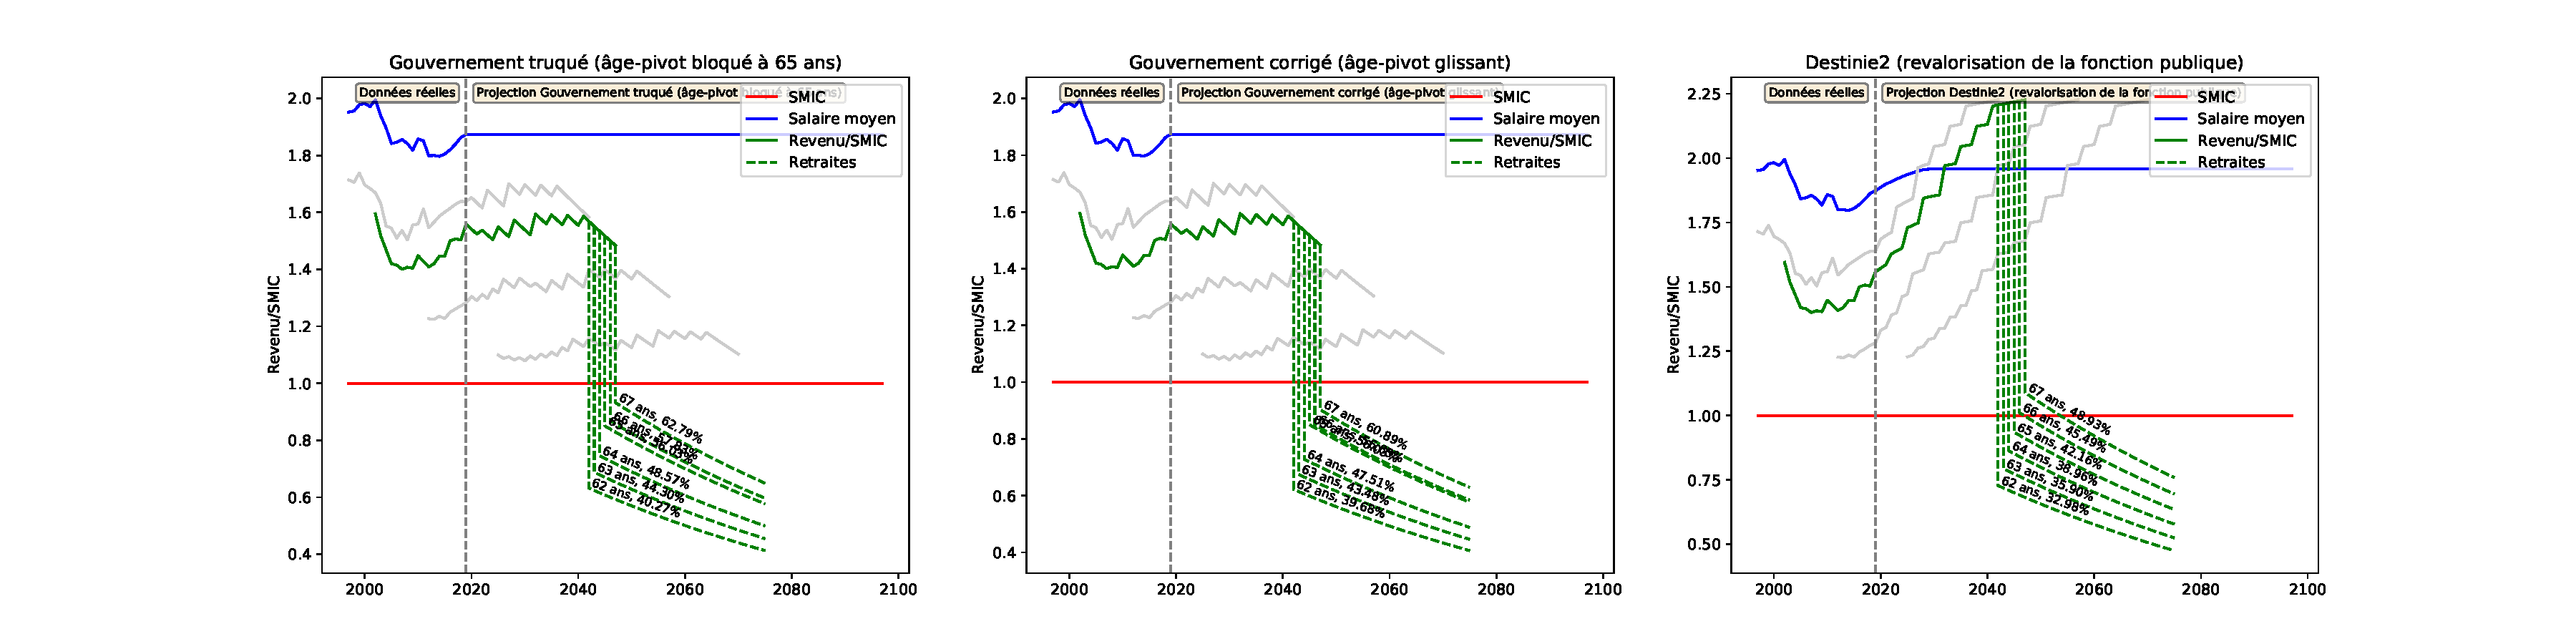
\includegraphics[width=0.9\textwidth]{fig/Redacteur_1980_22_dest_retraite.pdf}\end{center} \label{fig/Redacteur_1980_22_dest_retraite.pdf} 

\newpage 
 
\paragraph{Revenus et points pour le modèle \emph{Gouvernement truqué (âge-pivot bloqué à 65 ans)}} 
 
{ \scriptsize \begin{center} 
\begin{tabular}[htb]{|c|c||c|c|c|c|c|c||c|c||c|c|c|} 
\hline 
 Année &  Âge &  Ind Maj &  Pt Ind(\euro{} 2019) &  Rev HP(\euro{} 2019) &  Tx Primes &  GIPA(\euro{} 2019) &  Revenu(\euro{} 2019) &  SMIC(\euro{} 2019) &  Rev/SMIC &  Cumul Pts &  Achat Pt(\euro{} 2019) &  Serv. Pt(\euro{} 2019) \\ 
\hline \hline 
 2002 &  22 &  356.0 &  5.49 &  1953.11 &  18.21 &  0.00 &  2308.78 &  1447.74 &  {\bf 1.59} &  778.09 &  35.61 &  0.50 \\ 
\hline 
 2003 &  23 &  356.0 &  5.37 &  1913.36 &  18.44 &  0.00 &  2266.19 &  1493.03 &  {\bf 1.52} &  1541.82 &  35.61 &  0.50 \\ 
\hline 
 2004 &  24 &  362.0 &  5.29 &  1914.88 &  18.67 &  0.00 &  2272.39 &  1547.32 &  {\bf 1.47} &  2307.64 &  35.61 &  0.50 \\ 
\hline 
 2005 &  25 &  362.0 &  5.29 &  1914.67 &  18.90 &  0.00 &  2276.54 &  1603.67 &  {\bf 1.42} &  3074.86 &  35.61 &  0.50 \\ 
\hline 
 2006 &  26 &  369.0 &  5.23 &  1929.91 &  19.13 &  0.00 &  2299.11 &  1625.00 &  {\bf 1.41} &  3849.69 &  35.61 &  0.50 \\ 
\hline 
 2007 &  27 &  369.0 &  5.19 &  1916.76 &  19.36 &  0.00 &  2287.85 &  1634.08 &  {\bf 1.40} &  4620.72 &  35.61 &  0.50 \\ 
\hline 
 2008 &  28 &  379.0 &  5.09 &  1930.26 &  19.59 &  0.00 &  2308.40 &  1640.24 &  {\bf 1.41} &  5398.68 &  35.61 &  0.50 \\ 
\hline 
 2009 &  29 &  379.0 &  5.13 &  1943.94 &  19.82 &  0.00 &  2329.23 &  1659.42 &  {\bf 1.40} &  6183.66 &  35.61 &  0.50 \\ 
\hline 
 2010 &  30 &  390.0 &  5.08 &  1980.16 &  20.05 &  0.00 &  2377.18 &  1641.90 &  {\bf 1.45} &  6984.80 &  35.61 &  0.50 \\ 
\hline 
 2011 &  31 &  390.0 &  4.97 &  1939.02 &  20.28 &  0.00 &  2332.25 &  1633.19 &  {\bf 1.43} &  7770.80 &  35.61 &  0.50 \\ 
\hline 
 2012 &  32 &  401.0 &  4.88 &  1955.45 &  20.51 &  0.00 &  2356.51 &  1673.05 &  {\bf 1.41} &  8564.97 &  35.61 &  0.50 \\ 
\hline 
 2013 &  33 &  401.0 &  4.83 &  1938.70 &  20.74 &  22.03 &  2362.81 &  1664.01 &  {\bf 1.42} &  9361.26 &  35.61 &  0.50 \\ 
\hline 
 2014 &  34 &  416.0 &  4.81 &  2001.15 &  20.97 &  0.00 &  2420.79 &  1673.24 &  {\bf 1.45} &  10177.10 &  35.61 &  0.50 \\ 
\hline 
 2015 &  35 &  416.0 &  4.81 &  2000.36 &  21.20 &  15.77 &  2440.21 &  1686.62 &  {\bf 1.45} &  10999.48 &  35.61 &  0.50 \\ 
\hline 
 2016 &  36 &  436.0 &  4.80 &  2092.35 &  21.43 &  0.00 &  2540.74 &  1693.76 &  {\bf 1.50} &  11855.74 &  35.61 &  0.50 \\ 
\hline 
 2017 &  37 &  436.0 &  4.81 &  2096.57 &  21.66 &  0.00 &  2550.69 &  1692.60 &  {\bf 1.51} &  12715.35 &  35.61 &  0.50 \\ 
\hline 
 2018 &  38 &  436.0 &  4.74 &  2067.62 &  21.89 &  19.88 &  2540.11 &  1689.76 &  {\bf 1.50} &  13571.40 &  35.61 &  0.50 \\ 
\hline 
 2019 &  39 &  452.0 &  4.79 &  2167.08 &  22.12 &  0.00 &  2646.44 &  1698.45 &  {\bf 1.56} &  14463.28 &  35.61 &  0.50 \\ 
\hline 
 2020 &  40 &  452.0 &  4.79 &  2167.08 &  22.35 &  0.00 &  2651.42 &  1720.53 &  {\bf 1.54} &  15356.84 &  35.61 &  0.50 \\ 
\hline 
 2021 &  41 &  452.0 &  4.79 &  2167.08 &  22.58 &  0.00 &  2656.41 &  1742.90 &  {\bf 1.52} &  16252.08 &  35.61 &  0.50 \\ 
\hline 
 2022 &  42 &  461.0 &  4.79 &  2210.23 &  22.81 &  0.00 &  2714.38 &  1765.55 &  {\bf 1.54} &  17166.86 &  35.61 &  0.50 \\ 
\hline 
 2023 &  43 &  461.0 &  4.79 &  2210.23 &  23.04 &  0.00 &  2719.47 &  1788.51 &  {\bf 1.52} &  18083.36 &  35.61 &  0.50 \\ 
\hline 
 2024 &  44 &  461.0 &  4.79 &  2210.23 &  23.27 &  0.00 &  2724.55 &  1811.76 &  {\bf 1.50} &  19001.56 &  35.61 &  0.50 \\ 
\hline 
 2025 &  45 &  480.0 &  4.79 &  2301.32 &  23.50 &  0.00 &  2842.13 &  1835.31 &  {\bf 1.55} &  19959.40 &  35.61 &  0.50 \\ 
\hline 
 2026 &  46 &  480.0 &  4.79 &  2301.32 &  23.73 &  0.00 &  2847.43 &  1859.17 &  {\bf 1.53} &  20919.01 &  35.61 &  0.50 \\ 
\hline 
 2027 &  47 &  480.0 &  4.79 &  2301.32 &  23.96 &  0.00 &  2852.72 &  1883.34 &  {\bf 1.51} &  21880.42 &  35.61 &  0.50 \\ 
\hline 
 2028 &  48 &  504.0 &  4.79 &  2416.39 &  24.19 &  0.00 &  3000.91 &  1907.82 &  {\bf 1.57} &  22891.76 &  35.61 &  0.50 \\ 
\hline 
 2029 &  49 &  504.0 &  4.79 &  2416.39 &  24.42 &  0.00 &  3006.47 &  1932.62 &  {\bf 1.56} &  23904.21 &  35.63 &  0.50 \\ 
\hline 
 2030 &  50 &  504.0 &  4.79 &  2416.39 &  24.65 &  0.00 &  3012.03 &  1957.75 &  {\bf 1.54} &  24916.99 &  35.69 &  0.50 \\ 
\hline 
 2031 &  51 &  504.0 &  4.79 &  2416.39 &  24.88 &  0.00 &  3017.59 &  1983.20 &  {\bf 1.52} &  25929.32 &  35.77 &  0.50 \\ 
\hline 
 2032 &  52 &  534.0 &  4.79 &  2560.22 &  25.11 &  0.00 &  3203.09 &  2008.98 &  {\bf 1.59} &  27000.63 &  35.88 &  0.50 \\ 
\hline 
 2033 &  53 &  534.0 &  4.79 &  2560.22 &  25.34 &  0.00 &  3208.98 &  2035.10 &  {\bf 1.58} &  28069.85 &  36.02 &  0.50 \\ 
\hline 
 2034 &  54 &  534.0 &  4.79 &  2560.22 &  25.57 &  0.00 &  3214.87 &  2061.55 &  {\bf 1.56} &  29136.15 &  36.18 &  0.50 \\ 
\hline 
 2035 &  55 &  551.0 &  4.79 &  2641.73 &  25.80 &  0.00 &  3323.29 &  2088.35 &  {\bf 1.59} &  30232.56 &  36.37 &  0.51 \\ 
\hline 
 2036 &  56 &  551.0 &  4.79 &  2641.73 &  26.03 &  0.00 &  3329.37 &  2115.50 &  {\bf 1.57} &  31324.32 &  36.59 &  0.51 \\ 
\hline 
 2037 &  57 &  551.0 &  4.79 &  2641.73 &  26.26 &  0.00 &  3335.44 &  2143.00 &  {\bf 1.56} &  32410.63 &  36.85 &  0.51 \\ 
\hline 
 2038 &  58 &  569.0 &  4.79 &  2728.03 &  26.49 &  0.00 &  3450.68 &  2170.86 &  {\bf 1.59} &  33525.95 &  37.13 &  0.52 \\ 
\hline 
 2039 &  59 &  569.0 &  4.79 &  2728.03 &  26.72 &  0.00 &  3456.95 &  2199.08 &  {\bf 1.57} &  34634.01 &  37.44 &  0.52 \\ 
\hline 
 2040 &  60 &  569.0 &  4.79 &  2728.03 &  26.95 &  0.00 &  3463.23 &  2227.67 &  {\bf 1.55} &  35734.00 &  37.78 &  0.53 \\ 
\hline 
 2041 &  61 &  587.0 &  4.79 &  2814.33 &  27.18 &  0.00 &  3579.26 &  2256.63 &  {\bf 1.59} &  36859.67 &  38.16 &  0.53 \\ 
\hline 
 2042 &  62 &  587.0 &  4.79 &  2814.33 &  27.41 &  0.00 &  3585.73 &  2285.97 &  {\bf 1.57} &  37975.45 &  38.56 &  0.54 \\ 
\hline 
 2043 &  63 &  587.0 &  4.79 &  2814.33 &  27.64 &  0.00 &  3592.21 &  2315.68 &  {\bf 1.55} &  39080.57 &  39.01 &  0.54 \\ 
\hline 
 2044 &  64 &  587.0 &  4.79 &  2814.33 &  27.87 &  0.00 &  3598.68 &  2345.79 &  {\bf 1.53} &  40174.31 &  39.48 &  0.55 \\ 
\hline 
 2045 &  65 &  587.0 &  4.79 &  2814.33 &  28.10 &  0.00 &  3605.15 &  2376.28 &  {\bf 1.52} &  41255.95 &  40.00 &  0.56 \\ 
\hline 
 2046 &  66 &  587.0 &  4.79 &  2814.33 &  28.33 &  0.00 &  3611.62 &  2407.18 &  {\bf 1.50} &  42325.63 &  40.52 &  0.56 \\ 
\hline 
 2047 &  67 &  587.0 &  4.79 &  2814.33 &  28.56 &  0.00 &  3618.10 &  2438.47 &  {\bf 1.48} &  43383.48 &  41.04 &  0.57 \\ 
\hline 
\hline 
\end{tabular} 
\end{center} } 
\newpage 
 
\paragraph{Revenus et points pour le modèle \emph{Gouvernement corrigé (âge-pivot glissant)}} 
 
{ \scriptsize \begin{center} 
\begin{tabular}[htb]{|c|c||c|c|c|c|c|c||c|c||c|c|c|} 
\hline 
 Année &  Âge &  Ind Maj &  Pt Ind(\euro{} 2019) &  Rev HP(\euro{} 2019) &  Tx Primes &  GIPA(\euro{} 2019) &  Revenu(\euro{} 2019) &  SMIC(\euro{} 2019) &  Rev/SMIC &  Cumul Pts &  Achat Pt(\euro{} 2019) &  Serv. Pt(\euro{} 2019) \\ 
\hline \hline 
 2002 &  22 &  356.0 &  5.49 &  1953.11 &  18.21 &  0.00 &  2308.78 &  1447.74 &  {\bf 1.59} &  778.09 &  35.61 &  0.50 \\ 
\hline 
 2003 &  23 &  356.0 &  5.37 &  1913.36 &  18.44 &  0.00 &  2266.19 &  1493.03 &  {\bf 1.52} &  1541.82 &  35.61 &  0.50 \\ 
\hline 
 2004 &  24 &  362.0 &  5.29 &  1914.88 &  18.67 &  0.00 &  2272.39 &  1547.32 &  {\bf 1.47} &  2307.64 &  35.61 &  0.50 \\ 
\hline 
 2005 &  25 &  362.0 &  5.29 &  1914.67 &  18.90 &  0.00 &  2276.54 &  1603.67 &  {\bf 1.42} &  3074.86 &  35.61 &  0.50 \\ 
\hline 
 2006 &  26 &  369.0 &  5.23 &  1929.91 &  19.13 &  0.00 &  2299.11 &  1625.00 &  {\bf 1.41} &  3849.69 &  35.61 &  0.50 \\ 
\hline 
 2007 &  27 &  369.0 &  5.19 &  1916.76 &  19.36 &  0.00 &  2287.85 &  1634.08 &  {\bf 1.40} &  4620.72 &  35.61 &  0.50 \\ 
\hline 
 2008 &  28 &  379.0 &  5.09 &  1930.26 &  19.59 &  0.00 &  2308.40 &  1640.24 &  {\bf 1.41} &  5398.68 &  35.61 &  0.50 \\ 
\hline 
 2009 &  29 &  379.0 &  5.13 &  1943.94 &  19.82 &  0.00 &  2329.23 &  1659.42 &  {\bf 1.40} &  6183.66 &  35.61 &  0.50 \\ 
\hline 
 2010 &  30 &  390.0 &  5.08 &  1980.16 &  20.05 &  0.00 &  2377.18 &  1641.90 &  {\bf 1.45} &  6984.80 &  35.61 &  0.50 \\ 
\hline 
 2011 &  31 &  390.0 &  4.97 &  1939.02 &  20.28 &  0.00 &  2332.25 &  1633.19 &  {\bf 1.43} &  7770.80 &  35.61 &  0.50 \\ 
\hline 
 2012 &  32 &  401.0 &  4.88 &  1955.45 &  20.51 &  0.00 &  2356.51 &  1673.05 &  {\bf 1.41} &  8564.97 &  35.61 &  0.50 \\ 
\hline 
 2013 &  33 &  401.0 &  4.83 &  1938.70 &  20.74 &  22.03 &  2362.81 &  1664.01 &  {\bf 1.42} &  9361.26 &  35.61 &  0.50 \\ 
\hline 
 2014 &  34 &  416.0 &  4.81 &  2001.15 &  20.97 &  0.00 &  2420.79 &  1673.24 &  {\bf 1.45} &  10177.10 &  35.61 &  0.50 \\ 
\hline 
 2015 &  35 &  416.0 &  4.81 &  2000.36 &  21.20 &  15.77 &  2440.21 &  1686.62 &  {\bf 1.45} &  10999.48 &  35.61 &  0.50 \\ 
\hline 
 2016 &  36 &  436.0 &  4.80 &  2092.35 &  21.43 &  0.00 &  2540.74 &  1693.76 &  {\bf 1.50} &  11855.74 &  35.61 &  0.50 \\ 
\hline 
 2017 &  37 &  436.0 &  4.81 &  2096.57 &  21.66 &  0.00 &  2550.69 &  1692.60 &  {\bf 1.51} &  12715.35 &  35.61 &  0.50 \\ 
\hline 
 2018 &  38 &  436.0 &  4.74 &  2067.62 &  21.89 &  19.88 &  2540.11 &  1689.76 &  {\bf 1.50} &  13571.40 &  35.61 &  0.50 \\ 
\hline 
 2019 &  39 &  452.0 &  4.79 &  2167.08 &  22.12 &  0.00 &  2646.44 &  1698.45 &  {\bf 1.56} &  14463.28 &  35.61 &  0.50 \\ 
\hline 
 2020 &  40 &  452.0 &  4.79 &  2167.08 &  22.35 &  0.00 &  2651.42 &  1720.53 &  {\bf 1.54} &  15356.84 &  35.61 &  0.50 \\ 
\hline 
 2021 &  41 &  452.0 &  4.79 &  2167.08 &  22.58 &  0.00 &  2656.41 &  1742.90 &  {\bf 1.52} &  16252.08 &  35.61 &  0.50 \\ 
\hline 
 2022 &  42 &  461.0 &  4.79 &  2210.23 &  22.81 &  0.00 &  2714.38 &  1765.55 &  {\bf 1.54} &  17166.86 &  35.61 &  0.50 \\ 
\hline 
 2023 &  43 &  461.0 &  4.79 &  2210.23 &  23.04 &  0.00 &  2719.47 &  1788.51 &  {\bf 1.52} &  18083.36 &  35.61 &  0.50 \\ 
\hline 
 2024 &  44 &  461.0 &  4.79 &  2210.23 &  23.27 &  0.00 &  2724.55 &  1811.76 &  {\bf 1.50} &  19001.56 &  35.61 &  0.50 \\ 
\hline 
 2025 &  45 &  480.0 &  4.79 &  2301.32 &  23.50 &  0.00 &  2842.13 &  1835.31 &  {\bf 1.55} &  19959.40 &  35.61 &  0.50 \\ 
\hline 
 2026 &  46 &  480.0 &  4.79 &  2301.32 &  23.73 &  0.00 &  2847.43 &  1859.17 &  {\bf 1.53} &  20919.01 &  35.61 &  0.50 \\ 
\hline 
 2027 &  47 &  480.0 &  4.79 &  2301.32 &  23.96 &  0.00 &  2852.72 &  1883.34 &  {\bf 1.51} &  21880.42 &  35.61 &  0.50 \\ 
\hline 
 2028 &  48 &  504.0 &  4.79 &  2416.39 &  24.19 &  0.00 &  3000.91 &  1907.82 &  {\bf 1.57} &  22891.76 &  35.61 &  0.50 \\ 
\hline 
 2029 &  49 &  504.0 &  4.79 &  2416.39 &  24.42 &  0.00 &  3006.47 &  1932.62 &  {\bf 1.56} &  23904.21 &  35.63 &  0.50 \\ 
\hline 
 2030 &  50 &  504.0 &  4.79 &  2416.39 &  24.65 &  0.00 &  3012.03 &  1957.75 &  {\bf 1.54} &  24916.99 &  35.69 &  0.50 \\ 
\hline 
 2031 &  51 &  504.0 &  4.79 &  2416.39 &  24.88 &  0.00 &  3017.59 &  1983.20 &  {\bf 1.52} &  25929.32 &  35.77 &  0.50 \\ 
\hline 
 2032 &  52 &  534.0 &  4.79 &  2560.22 &  25.11 &  0.00 &  3203.09 &  2008.98 &  {\bf 1.59} &  27000.63 &  35.88 &  0.50 \\ 
\hline 
 2033 &  53 &  534.0 &  4.79 &  2560.22 &  25.34 &  0.00 &  3208.98 &  2035.10 &  {\bf 1.58} &  28069.85 &  36.02 &  0.50 \\ 
\hline 
 2034 &  54 &  534.0 &  4.79 &  2560.22 &  25.57 &  0.00 &  3214.87 &  2061.55 &  {\bf 1.56} &  29136.15 &  36.18 &  0.50 \\ 
\hline 
 2035 &  55 &  551.0 &  4.79 &  2641.73 &  25.80 &  0.00 &  3323.29 &  2088.35 &  {\bf 1.59} &  30232.56 &  36.37 &  0.51 \\ 
\hline 
 2036 &  56 &  551.0 &  4.79 &  2641.73 &  26.03 &  0.00 &  3329.37 &  2115.50 &  {\bf 1.57} &  31324.32 &  36.59 &  0.51 \\ 
\hline 
 2037 &  57 &  551.0 &  4.79 &  2641.73 &  26.26 &  0.00 &  3335.44 &  2143.00 &  {\bf 1.56} &  32410.63 &  36.85 &  0.51 \\ 
\hline 
 2038 &  58 &  569.0 &  4.79 &  2728.03 &  26.49 &  0.00 &  3450.68 &  2170.86 &  {\bf 1.59} &  33525.95 &  37.13 &  0.52 \\ 
\hline 
 2039 &  59 &  569.0 &  4.79 &  2728.03 &  26.72 &  0.00 &  3456.95 &  2199.08 &  {\bf 1.57} &  34634.01 &  37.44 &  0.52 \\ 
\hline 
 2040 &  60 &  569.0 &  4.79 &  2728.03 &  26.95 &  0.00 &  3463.23 &  2227.67 &  {\bf 1.55} &  35734.00 &  37.78 &  0.53 \\ 
\hline 
 2041 &  61 &  587.0 &  4.79 &  2814.33 &  27.18 &  0.00 &  3579.26 &  2256.63 &  {\bf 1.59} &  36859.67 &  38.16 &  0.53 \\ 
\hline 
 2042 &  62 &  587.0 &  4.79 &  2814.33 &  27.41 &  0.00 &  3585.73 &  2285.97 &  {\bf 1.57} &  37975.45 &  38.56 &  0.54 \\ 
\hline 
 2043 &  63 &  587.0 &  4.79 &  2814.33 &  27.64 &  0.00 &  3592.21 &  2315.68 &  {\bf 1.55} &  39080.57 &  39.01 &  0.54 \\ 
\hline 
 2044 &  64 &  587.0 &  4.79 &  2814.33 &  27.87 &  0.00 &  3598.68 &  2345.79 &  {\bf 1.53} &  40174.31 &  39.48 &  0.55 \\ 
\hline 
 2045 &  65 &  587.0 &  4.79 &  2814.33 &  28.10 &  0.00 &  3605.15 &  2376.28 &  {\bf 1.52} &  41255.95 &  40.00 &  0.56 \\ 
\hline 
 2046 &  66 &  587.0 &  4.79 &  2814.33 &  28.33 &  0.00 &  3611.62 &  2407.18 &  {\bf 1.50} &  42325.63 &  40.52 &  0.56 \\ 
\hline 
 2047 &  67 &  587.0 &  4.79 &  2814.33 &  28.56 &  0.00 &  3618.10 &  2438.47 &  {\bf 1.48} &  43383.48 &  41.04 &  0.57 \\ 
\hline 
\hline 
\end{tabular} 
\end{center} } 
\newpage 
 
\paragraph{Revenus et points pour le modèle \emph{Destinie2 (revalorisation de la fonction publique)}} 
 
{ \scriptsize \begin{center} 
\begin{tabular}[htb]{|c|c||c|c|c|c|c|c||c|c||c|c|c|} 
\hline 
 Année &  Âge &  Ind Maj &  Pt Ind(\euro{} 2019) &  Rev HP(\euro{} 2019) &  Tx Primes &  GIPA(\euro{} 2019) &  Revenu(\euro{} 2019) &  SMIC(\euro{} 2019) &  Rev/SMIC &  Cumul Pts &  Achat Pt(\euro{} 2019) &  Serv. Pt(\euro{} 2019) \\ 
\hline \hline 
 2002 &  22 &  356.0 &  5.49 &  1953.11 &  18.21 &  0.00 &  2308.78 &  1447.74 &  {\bf 1.59} &  776.17 &  35.69 &  0.50 \\ 
\hline 
 2003 &  23 &  356.0 &  5.37 &  1913.36 &  18.44 &  0.00 &  2266.19 &  1493.03 &  {\bf 1.52} &  1538.03 &  35.69 &  0.50 \\ 
\hline 
 2004 &  24 &  362.0 &  5.29 &  1914.88 &  18.67 &  0.00 &  2272.39 &  1547.32 &  {\bf 1.47} &  2301.97 &  35.69 &  0.50 \\ 
\hline 
 2005 &  25 &  362.0 &  5.29 &  1914.67 &  18.90 &  0.00 &  2276.54 &  1603.67 &  {\bf 1.42} &  3067.31 &  35.69 &  0.50 \\ 
\hline 
 2006 &  26 &  369.0 &  5.23 &  1929.91 &  19.13 &  0.00 &  2299.11 &  1625.00 &  {\bf 1.41} &  3840.23 &  35.69 &  0.50 \\ 
\hline 
 2007 &  27 &  369.0 &  5.19 &  1916.76 &  19.36 &  0.00 &  2287.85 &  1634.08 &  {\bf 1.40} &  4609.37 &  35.69 &  0.50 \\ 
\hline 
 2008 &  28 &  379.0 &  5.09 &  1930.26 &  19.59 &  0.00 &  2308.40 &  1640.24 &  {\bf 1.41} &  5385.42 &  35.69 &  0.50 \\ 
\hline 
 2009 &  29 &  379.0 &  5.13 &  1943.94 &  19.82 &  0.00 &  2329.23 &  1659.42 &  {\bf 1.40} &  6168.47 &  35.69 &  0.50 \\ 
\hline 
 2010 &  30 &  390.0 &  5.08 &  1980.16 &  20.05 &  0.00 &  2377.18 &  1641.90 &  {\bf 1.45} &  6967.64 &  35.69 &  0.50 \\ 
\hline 
 2011 &  31 &  390.0 &  4.97 &  1939.02 &  20.28 &  0.00 &  2332.25 &  1633.19 &  {\bf 1.43} &  7751.70 &  35.69 &  0.50 \\ 
\hline 
 2012 &  32 &  401.0 &  4.88 &  1955.45 &  20.51 &  0.00 &  2356.51 &  1673.05 &  {\bf 1.41} &  8543.93 &  35.69 &  0.50 \\ 
\hline 
 2013 &  33 &  401.0 &  4.83 &  1938.70 &  20.74 &  22.03 &  2362.81 &  1664.01 &  {\bf 1.42} &  9338.26 &  35.69 &  0.50 \\ 
\hline 
 2014 &  34 &  416.0 &  4.81 &  2001.15 &  20.97 &  0.00 &  2420.79 &  1673.24 &  {\bf 1.45} &  10152.09 &  35.69 &  0.50 \\ 
\hline 
 2015 &  35 &  416.0 &  4.81 &  2000.36 &  21.20 &  15.77 &  2440.21 &  1686.62 &  {\bf 1.45} &  10972.45 &  35.69 &  0.50 \\ 
\hline 
 2016 &  36 &  436.0 &  4.80 &  2092.35 &  21.43 &  0.00 &  2540.74 &  1693.76 &  {\bf 1.50} &  11826.61 &  35.69 &  0.50 \\ 
\hline 
 2017 &  37 &  436.0 &  4.81 &  2096.57 &  21.66 &  0.00 &  2550.69 &  1692.60 &  {\bf 1.51} &  12684.11 &  35.69 &  0.50 \\ 
\hline 
 2018 &  38 &  436.0 &  4.74 &  2067.62 &  21.89 &  19.88 &  2540.11 &  1689.76 &  {\bf 1.50} &  13538.06 &  35.69 &  0.50 \\ 
\hline 
 2019 &  39 &  452.0 &  4.79 &  2167.08 &  22.12 &  0.00 &  2646.44 &  1698.45 &  {\bf 1.56} &  14427.75 &  35.69 &  0.50 \\ 
\hline 
 2020 &  40 &  452.0 &  4.83 &  2184.42 &  22.35 &  0.00 &  2672.63 &  1699.99 &  {\bf 1.57} &  15326.24 &  35.69 &  0.50 \\ 
\hline 
 2021 &  41 &  452.0 &  4.88 &  2204.08 &  22.58 &  0.00 &  2701.76 &  1703.48 &  {\bf 1.59} &  16234.53 &  35.69 &  0.50 \\ 
\hline 
 2022 &  42 &  461.0 &  4.93 &  2270.44 &  22.81 &  0.00 &  2788.33 &  1712.78 &  {\bf 1.63} &  17171.92 &  35.69 &  0.50 \\ 
\hline 
 2023 &  43 &  461.0 &  4.98 &  2297.01 &  23.04 &  0.00 &  2826.24 &  1723.51 &  {\bf 1.64} &  18122.06 &  35.69 &  0.50 \\ 
\hline 
 2024 &  44 &  461.0 &  5.04 &  2324.34 &  23.27 &  0.00 &  2865.21 &  1735.69 &  {\bf 1.65} &  19085.30 &  35.69 &  0.50 \\ 
\hline 
 2025 &  45 &  480.0 &  5.10 &  2449.66 &  23.50 &  0.00 &  3025.33 &  1749.35 &  {\bf 1.73} &  20102.37 &  35.69 &  0.50 \\ 
\hline 
 2026 &  46 &  480.0 &  5.17 &  2480.28 &  23.73 &  0.00 &  3068.85 &  1764.53 &  {\bf 1.74} &  21134.07 &  35.69 &  0.50 \\ 
\hline 
 2027 &  47 &  480.0 &  5.23 &  2512.03 &  23.96 &  0.00 &  3113.91 &  1781.27 &  {\bf 1.75} &  22180.91 &  35.69 &  0.50 \\ 
\hline 
 2028 &  48 &  504.0 &  5.30 &  2672.19 &  24.19 &  0.00 &  3318.59 &  1799.59 &  {\bf 1.84} &  23296.57 &  35.69 &  0.50 \\ 
\hline 
 2029 &  49 &  504.0 &  5.37 &  2704.52 &  24.42 &  0.00 &  3364.96 &  1819.55 &  {\bf 1.85} &  24427.02 &  35.72 &  0.50 \\ 
\hline 
 2030 &  50 &  504.0 &  5.43 &  2738.05 &  24.65 &  0.00 &  3412.99 &  1841.19 &  {\bf 1.85} &  25571.94 &  35.77 &  0.50 \\ 
\hline 
 2031 &  51 &  504.0 &  5.50 &  2772.83 &  24.88 &  0.00 &  3462.71 &  1864.58 &  {\bf 1.86} &  26730.95 &  35.85 &  0.50 \\ 
\hline 
 2032 &  52 &  534.0 &  5.57 &  2976.07 &  25.11 &  0.00 &  3723.36 &  1888.81 &  {\bf 1.97} &  27973.43 &  35.96 &  0.50 \\ 
\hline 
 2033 &  53 &  534.0 &  5.65 &  3014.76 &  25.34 &  0.00 &  3778.70 &  1913.37 &  {\bf 1.97} &  29229.59 &  36.10 &  0.50 \\ 
\hline 
 2034 &  54 &  534.0 &  5.72 &  3053.95 &  25.57 &  0.00 &  3834.85 &  1938.24 &  {\bf 1.98} &  30498.62 &  36.26 &  0.50 \\ 
\hline 
 2035 &  55 &  551.0 &  5.79 &  3192.14 &  25.80 &  0.00 &  4015.71 &  1963.44 &  {\bf 2.05} &  31820.45 &  36.46 &  0.51 \\ 
\hline 
 2036 &  56 &  551.0 &  5.87 &  3233.64 &  26.03 &  0.00 &  4075.35 &  1988.96 &  {\bf 2.05} &  33153.79 &  36.68 &  0.51 \\ 
\hline 
 2037 &  57 &  551.0 &  5.94 &  3275.67 &  26.26 &  0.00 &  4135.87 &  2014.82 &  {\bf 2.05} &  34497.70 &  36.93 &  0.51 \\ 
\hline 
 2038 &  58 &  569.0 &  6.02 &  3426.66 &  26.49 &  0.00 &  4334.38 &  2041.01 &  {\bf 2.12} &  35895.45 &  37.21 &  0.52 \\ 
\hline 
 2039 &  59 &  569.0 &  6.10 &  3471.20 &  26.72 &  0.00 &  4398.71 &  2067.55 &  {\bf 2.13} &  37302.15 &  37.52 &  0.52 \\ 
\hline 
 2040 &  60 &  569.0 &  6.18 &  3516.33 &  26.95 &  0.00 &  4463.98 &  2094.43 &  {\bf 2.13} &  38716.77 &  37.87 &  0.53 \\ 
\hline 
 2041 &  61 &  587.0 &  6.26 &  3674.73 &  27.18 &  0.00 &  4673.52 &  2121.65 &  {\bf 2.20} &  40183.22 &  38.24 &  0.53 \\ 
\hline 
 2042 &  62 &  587.0 &  6.34 &  3722.50 &  27.41 &  0.00 &  4742.83 &  2149.23 &  {\bf 2.21} &  41655.69 &  38.65 &  0.54 \\ 
\hline 
 2043 &  63 &  587.0 &  6.42 &  3770.89 &  27.64 &  0.00 &  4813.16 &  2177.17 &  {\bf 2.21} &  43133.05 &  39.10 &  0.54 \\ 
\hline 
 2044 &  64 &  587.0 &  6.51 &  3819.91 &  27.87 &  0.00 &  4884.52 &  2205.48 &  {\bf 2.21} &  44614.20 &  39.57 &  0.55 \\ 
\hline 
 2045 &  65 &  587.0 &  6.59 &  3869.57 &  28.10 &  0.00 &  4956.92 &  2234.15 &  {\bf 2.22} &  46098.02 &  40.09 &  0.56 \\ 
\hline 
 2046 &  66 &  587.0 &  6.68 &  3919.87 &  28.33 &  0.00 &  5030.38 &  2263.19 &  {\bf 2.22} &  47584.49 &  40.61 &  0.57 \\ 
\hline 
 2047 &  67 &  587.0 &  6.76 &  3970.83 &  28.56 &  0.00 &  5104.90 &  2292.61 &  {\bf 2.23} &  49073.64 &  41.14 &  0.57 \\ 
\hline 
\hline 
\end{tabular} 
\end{center} } 
\newpage 
 
\subsection{Génération 1990 (début en 2012)} 

\paragraph{Retraites possibles dans le modèle \emph{Gouvernement truqué (âge-pivot bloqué à 65 ans)}}  
 
{ \scriptsize \begin{center} 
\begin{tabular}[htb]{|c|c||c|c||c|c||c||c|c|c|c|c|c|} 
\hline 
 Retraite en &  Âge &  Âge pivot &  Décote/Surcote &  Retraite (\euro{} 2019) &  Tx Rempl(\%) &  SMIC (\euro{} 2019) &  Retraite/SMIC &  Rev70/SMIC &  Rev75/SMIC &  Rev80/SMIC &  Rev85/SMIC &  Rev90/SMIC \\ 
\hline \hline 
 2052 &  62 &  65 ans 0 mois &  -15.00\% &  1546.31 &  {\bf 43.12} &  2601.14 &  {\bf {\color{red} 0.59}} &  {\bf {\color{red} 0.54}} &  {\bf {\color{red} 0.50}} &  {\bf {\color{red} 0.47}} &  {\bf {\color{red} 0.44}} &  {\bf {\color{red} 0.41}} \\ 
\hline 
 2053 &  63 &  65 ans 0 mois &  -10.00\% &  1703.55 &  {\bf 47.42} &  2634.96 &  {\bf {\color{red} 0.65}} &  {\bf {\color{red} 0.59}} &  {\bf {\color{red} 0.55}} &  {\bf {\color{red} 0.52}} &  {\bf {\color{red} 0.49}} &  {\bf {\color{red} 0.46}} \\ 
\hline 
 2054 &  64 &  65 ans 0 mois &  -5.00\% &  1869.16 &  {\bf 51.94} &  2669.21 &  {\bf {\color{red} 0.70}} &  {\bf {\color{red} 0.65}} &  {\bf {\color{red} 0.61}} &  {\bf {\color{red} 0.57}} &  {\bf {\color{red} 0.53}} &  {\bf {\color{red} 0.50}} \\ 
\hline 
 2055 &  65 &  65 ans 0 mois &  0.00\% &  2298.33 &  {\bf 63.75} &  2703.91 &  {\bf {\color{red} 0.85}} &  {\bf {\color{red} 0.80}} &  {\bf {\color{red} 0.75}} &  {\bf {\color{red} 0.70}} &  {\bf {\color{red} 0.66}} &  {\bf {\color{red} 0.62}} \\ 
\hline 
 2056 &  66 &  65 ans 0 mois &  5.00\% &  2328.20 &  {\bf 64.46} &  2739.06 &  {\bf {\color{red} 0.85}} &  {\bf {\color{red} 0.81}} &  {\bf {\color{red} 0.76}} &  {\bf {\color{red} 0.71}} &  {\bf {\color{red} 0.67}} &  {\bf {\color{red} 0.62}} \\ 
\hline 
 2057 &  67 &  65 ans 0 mois &  10.00\% &  2417.86 &  {\bf 66.83} &  2774.67 &  {\bf {\color{red} 0.87}} &  {\bf {\color{red} 0.84}} &  {\bf {\color{red} 0.79}} &  {\bf {\color{red} 0.74}} &  {\bf {\color{red} 0.69}} &  {\bf {\color{red} 0.65}} \\ 
\hline 
\hline 
\end{tabular} 
\end{center} } 
\paragraph{Retraites possibles dans le modèle \emph{Gouvernement corrigé (âge-pivot glissant)}}  
 
{ \scriptsize \begin{center} 
\begin{tabular}[htb]{|c|c||c|c||c|c||c||c|c|c|c|c|c|} 
\hline 
 Retraite en &  Âge &  Âge pivot &  Décote/Surcote &  Retraite (\euro{} 2019) &  Tx Rempl(\%) &  SMIC (\euro{} 2019) &  Retraite/SMIC &  Rev70/SMIC &  Rev75/SMIC &  Rev80/SMIC &  Rev85/SMIC &  Rev90/SMIC \\ 
\hline \hline 
 2052 &  62 &  66 ans 1 mois &  -20.42\% &  1447.77 &  {\bf 40.38} &  2601.14 &  {\bf {\color{red} 0.56}} &  {\bf {\color{red} 0.50}} &  {\bf {\color{red} 0.47}} &  {\bf {\color{red} 0.44}} &  {\bf {\color{red} 0.41}} &  {\bf {\color{red} 0.39}} \\ 
\hline 
 2053 &  63 &  66 ans 2 mois &  -15.83\% &  1593.14 &  {\bf 44.35} &  2634.96 &  {\bf {\color{red} 0.60}} &  {\bf {\color{red} 0.55}} &  {\bf {\color{red} 0.52}} &  {\bf {\color{red} 0.49}} &  {\bf {\color{red} 0.46}} &  {\bf {\color{red} 0.43}} \\ 
\hline 
 2054 &  64 &  66 ans 3 mois &  -11.25\% &  1746.19 &  {\bf 48.52} &  2669.21 &  {\bf {\color{red} 0.65}} &  {\bf {\color{red} 0.61}} &  {\bf {\color{red} 0.57}} &  {\bf {\color{red} 0.53}} &  {\bf {\color{red} 0.50}} &  {\bf {\color{red} 0.47}} \\ 
\hline 
 2055 &  65 &  66 ans 4 mois &  -6.67\% &  2298.33 &  {\bf 63.75} &  2703.91 &  {\bf {\color{red} 0.85}} &  {\bf {\color{red} 0.80}} &  {\bf {\color{red} 0.75}} &  {\bf {\color{red} 0.70}} &  {\bf {\color{red} 0.66}} &  {\bf {\color{red} 0.62}} \\ 
\hline 
 2056 &  66 &  66 ans 5 mois &  -2.08\% &  2328.20 &  {\bf 64.46} &  2739.06 &  {\bf {\color{red} 0.85}} &  {\bf {\color{red} 0.81}} &  {\bf {\color{red} 0.76}} &  {\bf {\color{red} 0.71}} &  {\bf {\color{red} 0.67}} &  {\bf {\color{red} 0.62}} \\ 
\hline 
 2057 &  67 &  66 ans 6 mois &  2.50\% &  2358.47 &  {\bf 65.19} &  2774.67 &  {\bf {\color{red} 0.85}} &  {\bf {\color{red} 0.82}} &  {\bf {\color{red} 0.77}} &  {\bf {\color{red} 0.72}} &  {\bf {\color{red} 0.67}} &  {\bf {\color{red} 0.63}} \\ 
\hline 
\hline 
\end{tabular} 
\end{center} } 
\paragraph{Retraites possibles dans le modèle \emph{Destinie2 (revalorisation de la fonction publique)}}  
 
{ \scriptsize \begin{center} 
\begin{tabular}[htb]{|c|c||c|c||c|c||c||c|c|c|c|c|c|} 
\hline 
 Retraite en &  Âge &  Âge pivot &  Décote/Surcote &  Retraite (\euro{} 2019) &  Tx Rempl(\%) &  SMIC (\euro{} 2019) &  Retraite/SMIC &  Rev70/SMIC &  Rev75/SMIC &  Rev80/SMIC &  Rev85/SMIC &  Rev90/SMIC \\ 
\hline \hline 
 2052 &  62 &  66 ans 1 mois &  -20.42\% &  1747.27 &  {\bf 32.38} &  2445.56 &  {\bf {\color{red} 0.71}} &  {\bf {\color{red} 0.64}} &  {\bf {\color{red} 0.60}} &  {\bf {\color{red} 0.57}} &  {\bf {\color{red} 0.53}} &  {\bf {\color{red} 0.50}} \\ 
\hline 
 2053 &  63 &  66 ans 2 mois &  -15.83\% &  1936.08 &  {\bf 35.35} &  2477.35 &  {\bf {\color{red} 0.78}} &  {\bf {\color{red} 0.71}} &  {\bf {\color{red} 0.67}} &  {\bf {\color{red} 0.63}} &  {\bf {\color{red} 0.59}} &  {\bf {\color{red} 0.55}} \\ 
\hline 
 2054 &  64 &  66 ans 3 mois &  -11.25\% &  2136.71 &  {\bf 38.44} &  2509.56 &  {\bf {\color{red} 0.85}} &  {\bf {\color{red} 0.79}} &  {\bf {\color{red} 0.74}} &  {\bf {\color{red} 0.69}} &  {\bf {\color{red} 0.65}} &  {\bf {\color{red} 0.61}} \\ 
\hline 
 2055 &  65 &  66 ans 4 mois &  -6.67\% &  2349.55 &  {\bf 41.66} &  2542.18 &  {\bf {\color{red} 0.92}} &  {\bf {\color{red} 0.87}} &  {\bf {\color{red} 0.81}} &  {\bf {\color{red} 0.76}} &  {\bf {\color{red} 0.71}} &  {\bf {\color{red} 0.67}} \\ 
\hline 
 2056 &  66 &  66 ans 5 mois &  -2.08\% &  2574.98 &  {\bf 44.99} &  2575.23 &  {\bf {\color{red} 1.00}} &  {\bf {\color{red} 0.95}} &  {\bf {\color{red} 0.89}} &  {\bf {\color{red} 0.83}} &  {\bf {\color{red} 0.78}} &  {\bf {\color{red} 0.73}} \\ 
\hline 
 2057 &  67 &  66 ans 6 mois &  2.50\% &  2813.43 &  {\bf 48.43} &  2608.71 &  {\bf 1.08} &  {\bf 1.04} &  {\bf {\color{red} 0.97}} &  {\bf {\color{red} 0.91}} &  {\bf {\color{red} 0.85}} &  {\bf {\color{red} 0.80}} \\ 
\hline 
\hline 
\end{tabular} 
\end{center} } 

 \begin{center}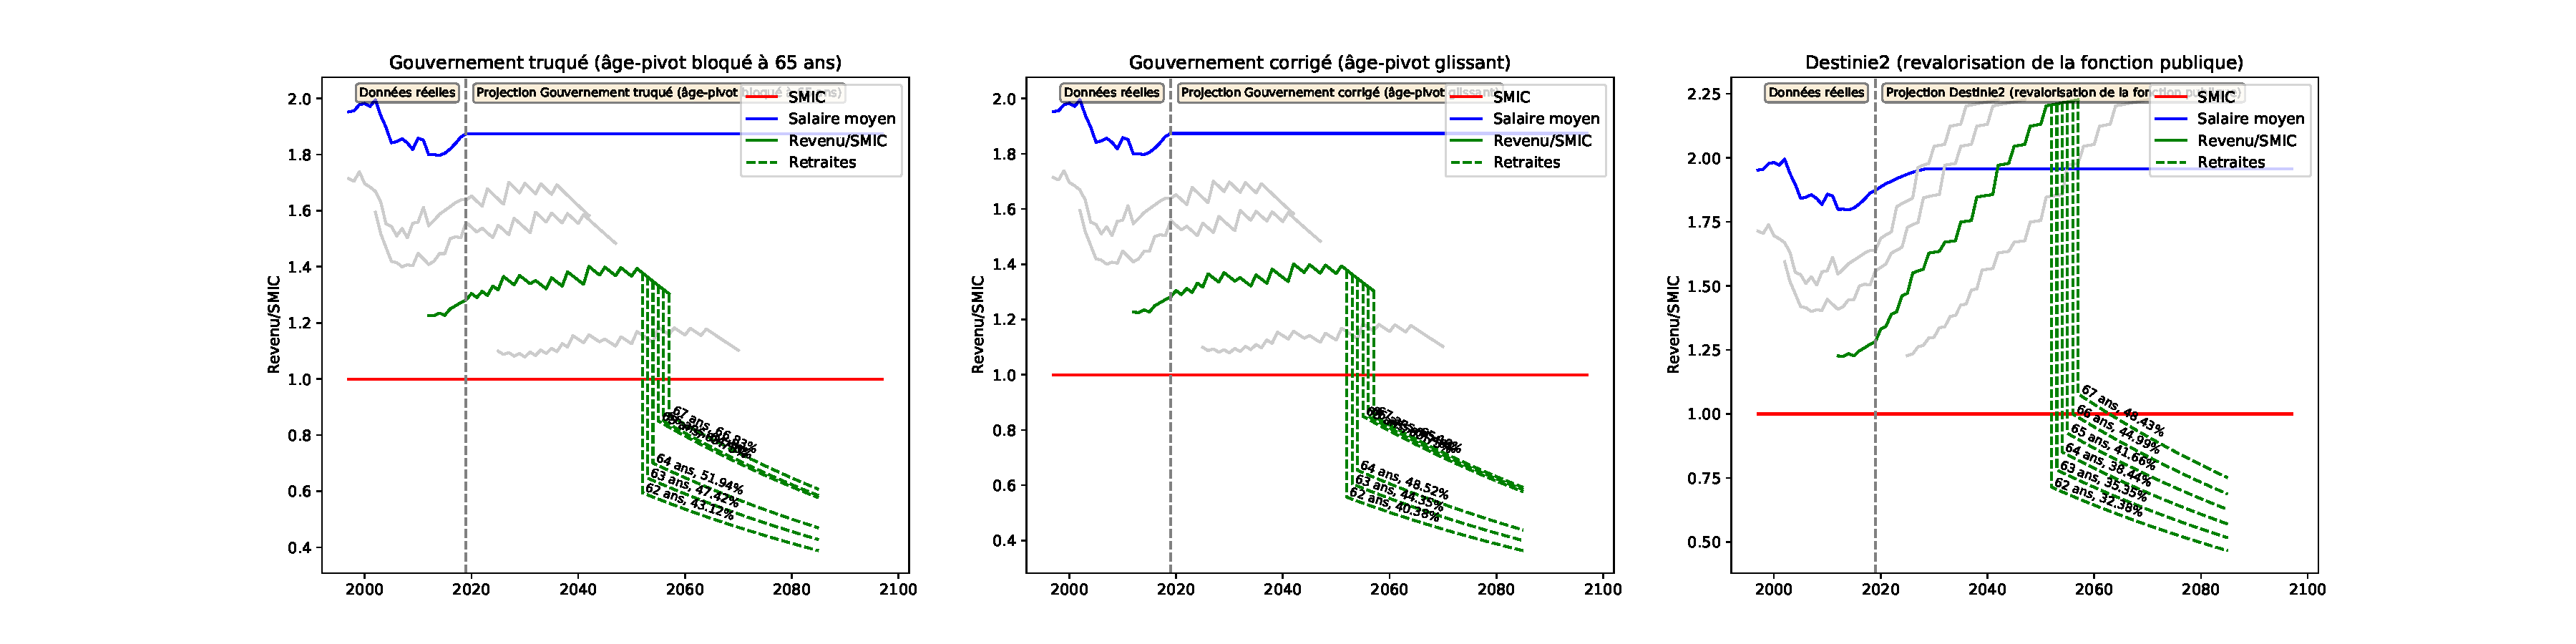
\includegraphics[width=0.9\textwidth]{fig/Redacteur_1990_22_dest_retraite.pdf}\end{center} \label{fig/Redacteur_1990_22_dest_retraite.pdf} 

\newpage 
 
\paragraph{Revenus et points pour le modèle \emph{Gouvernement truqué (âge-pivot bloqué à 65 ans)}} 
 
{ \scriptsize \begin{center} 
\begin{tabular}[htb]{|c|c||c|c|c|c|c|c||c|c||c|c|c|} 
\hline 
 Année &  Âge &  Ind Maj &  Pt Ind(\euro{} 2019) &  Rev HP(\euro{} 2019) &  Tx Primes &  GIPA(\euro{} 2019) &  Revenu(\euro{} 2019) &  SMIC(\euro{} 2019) &  Rev/SMIC &  Cumul Pts &  Achat Pt(\euro{} 2019) &  Serv. Pt(\euro{} 2019) \\ 
\hline \hline 
 2012 &  22 &  356.0 &  4.88 &  1736.01 &  18.21 &  0.00 &  2052.14 &  1673.05 &  {\bf 1.23} &  691.60 &  35.61 &  0.50 \\ 
\hline 
 2013 &  23 &  356.0 &  4.83 &  1721.14 &  18.44 &  0.00 &  2038.51 &  1664.01 &  {\bf 1.23} &  1378.60 &  35.61 &  0.50 \\ 
\hline 
 2014 &  24 &  362.0 &  4.81 &  1741.38 &  18.67 &  0.00 &  2066.50 &  1673.24 &  {\bf 1.24} &  2075.03 &  35.61 &  0.50 \\ 
\hline 
 2015 &  25 &  362.0 &  4.81 &  1740.70 &  18.90 &  0.00 &  2069.69 &  1686.62 &  {\bf 1.23} &  2772.55 &  35.61 &  0.50 \\ 
\hline 
 2016 &  26 &  369.0 &  4.80 &  1770.82 &  19.13 &  7.18 &  2116.76 &  1693.76 &  {\bf 1.25} &  3485.92 &  35.61 &  0.50 \\ 
\hline 
 2017 &  27 &  369.0 &  4.81 &  1774.39 &  19.36 &  16.03 &  2133.95 &  1692.60 &  {\bf 1.26} &  4205.09 &  35.61 &  0.50 \\ 
\hline 
 2018 &  28 &  379.0 &  4.74 &  1797.32 &  19.59 &  0.00 &  2149.41 &  1689.76 &  {\bf 1.27} &  4929.46 &  35.61 &  0.50 \\ 
\hline 
 2019 &  29 &  379.0 &  4.79 &  1817.09 &  19.82 &  0.00 &  2177.23 &  1698.45 &  {\bf 1.28} &  5663.22 &  35.61 &  0.50 \\ 
\hline 
 2020 &  30 &  390.0 &  4.79 &  1869.82 &  20.05 &  0.00 &  2244.72 &  1720.53 &  {\bf 1.30} &  6419.72 &  35.61 &  0.50 \\ 
\hline 
 2021 &  31 &  390.0 &  4.79 &  1869.82 &  20.28 &  0.00 &  2249.03 &  1742.90 &  {\bf 1.29} &  7177.67 &  35.61 &  0.50 \\ 
\hline 
 2022 &  32 &  401.0 &  4.79 &  1922.56 &  20.51 &  0.00 &  2316.88 &  1765.55 &  {\bf 1.31} &  7958.48 &  35.61 &  0.50 \\ 
\hline 
 2023 &  33 &  401.0 &  4.79 &  1922.56 &  20.74 &  0.00 &  2321.30 &  1788.51 &  {\bf 1.30} &  8740.79 &  35.61 &  0.50 \\ 
\hline 
 2024 &  34 &  416.0 &  4.79 &  1994.48 &  20.97 &  0.00 &  2412.72 &  1811.76 &  {\bf 1.33} &  9553.91 &  35.61 &  0.50 \\ 
\hline 
 2025 &  35 &  416.0 &  4.79 &  1994.48 &  21.20 &  0.00 &  2417.31 &  1835.31 &  {\bf 1.32} &  10368.57 &  35.61 &  0.50 \\ 
\hline 
 2026 &  36 &  436.0 &  4.79 &  2090.37 &  21.43 &  0.00 &  2538.33 &  1859.17 &  {\bf 1.37} &  11224.02 &  35.61 &  0.50 \\ 
\hline 
 2027 &  37 &  436.0 &  4.79 &  2090.37 &  21.66 &  0.00 &  2543.14 &  1883.34 &  {\bf 1.35} &  12081.09 &  35.61 &  0.50 \\ 
\hline 
 2028 &  38 &  436.0 &  4.79 &  2090.37 &  21.89 &  0.00 &  2547.95 &  1907.82 &  {\bf 1.34} &  12939.78 &  35.61 &  0.50 \\ 
\hline 
 2029 &  39 &  452.0 &  4.79 &  2167.08 &  22.12 &  0.00 &  2646.44 &  1932.62 &  {\bf 1.37} &  13830.98 &  35.63 &  0.50 \\ 
\hline 
 2030 &  40 &  452.0 &  4.79 &  2167.08 &  22.35 &  0.00 &  2651.42 &  1957.75 &  {\bf 1.35} &  14722.51 &  35.69 &  0.50 \\ 
\hline 
 2031 &  41 &  452.0 &  4.79 &  2167.08 &  22.58 &  0.00 &  2656.41 &  1983.20 &  {\bf 1.34} &  15613.68 &  35.77 &  0.50 \\ 
\hline 
 2032 &  42 &  461.0 &  4.79 &  2210.23 &  22.81 &  0.00 &  2714.38 &  2008.98 &  {\bf 1.35} &  16521.53 &  35.88 &  0.50 \\ 
\hline 
 2033 &  43 &  461.0 &  4.79 &  2210.23 &  23.04 &  0.00 &  2719.47 &  2035.10 &  {\bf 1.34} &  17427.64 &  36.02 &  0.50 \\ 
\hline 
 2034 &  44 &  461.0 &  4.79 &  2210.23 &  23.27 &  0.00 &  2724.55 &  2061.55 &  {\bf 1.32} &  18331.31 &  36.18 &  0.50 \\ 
\hline 
 2035 &  45 &  480.0 &  4.79 &  2301.32 &  23.50 &  0.00 &  2842.13 &  2088.35 &  {\bf 1.36} &  19268.98 &  36.37 &  0.51 \\ 
\hline 
 2036 &  46 &  480.0 &  4.79 &  2301.32 &  23.73 &  0.00 &  2847.43 &  2115.50 &  {\bf 1.35} &  20202.71 &  36.59 &  0.51 \\ 
\hline 
 2037 &  47 &  480.0 &  4.79 &  2301.32 &  23.96 &  0.00 &  2852.72 &  2143.00 &  {\bf 1.33} &  21131.80 &  36.85 &  0.51 \\ 
\hline 
 2038 &  48 &  504.0 &  4.79 &  2416.39 &  24.19 &  0.00 &  3000.91 &  2170.86 &  {\bf 1.38} &  22101.75 &  37.13 &  0.52 \\ 
\hline 
 2039 &  49 &  504.0 &  4.79 &  2416.39 &  24.42 &  0.00 &  3006.47 &  2199.08 &  {\bf 1.37} &  23065.41 &  37.44 &  0.52 \\ 
\hline 
 2040 &  50 &  504.0 &  4.79 &  2416.39 &  24.65 &  0.00 &  3012.03 &  2227.67 &  {\bf 1.35} &  24022.09 &  37.78 &  0.53 \\ 
\hline 
 2041 &  51 &  504.0 &  4.79 &  2416.39 &  24.88 &  0.00 &  3017.59 &  2256.63 &  {\bf 1.34} &  24971.12 &  38.16 &  0.53 \\ 
\hline 
 2042 &  52 &  534.0 &  4.79 &  2560.22 &  25.11 &  0.00 &  3203.09 &  2285.97 &  {\bf 1.40} &  25967.83 &  38.56 &  0.54 \\ 
\hline 
 2043 &  53 &  534.0 &  4.79 &  2560.22 &  25.34 &  0.00 &  3208.98 &  2315.68 &  {\bf 1.39} &  26955.06 &  39.01 &  0.54 \\ 
\hline 
 2044 &  54 &  534.0 &  4.79 &  2560.22 &  25.57 &  0.00 &  3214.87 &  2345.79 &  {\bf 1.37} &  27932.14 &  39.48 &  0.55 \\ 
\hline 
 2045 &  55 &  551.0 &  4.79 &  2641.73 &  25.80 &  0.00 &  3323.29 &  2376.28 &  {\bf 1.40} &  28929.22 &  40.00 &  0.56 \\ 
\hline 
 2046 &  56 &  551.0 &  4.79 &  2641.73 &  26.03 &  0.00 &  3329.37 &  2407.18 &  {\bf 1.38} &  29915.30 &  40.52 &  0.56 \\ 
\hline 
 2047 &  57 &  551.0 &  4.79 &  2641.73 &  26.26 &  0.00 &  3335.44 &  2438.47 &  {\bf 1.37} &  30890.51 &  41.04 &  0.57 \\ 
\hline 
 2048 &  58 &  569.0 &  4.79 &  2728.03 &  26.49 &  0.00 &  3450.68 &  2470.17 &  {\bf 1.40} &  31886.45 &  41.58 &  0.58 \\ 
\hline 
 2049 &  59 &  569.0 &  4.79 &  2728.03 &  26.72 &  0.00 &  3456.95 &  2502.28 &  {\bf 1.38} &  32871.41 &  42.12 &  0.59 \\ 
\hline 
 2050 &  60 &  569.0 &  4.79 &  2728.03 &  26.95 &  0.00 &  3463.23 &  2534.81 &  {\bf 1.37} &  33845.49 &  42.66 &  0.59 \\ 
\hline 
 2051 &  61 &  587.0 &  4.79 &  2814.33 &  27.18 &  0.00 &  3579.26 &  2567.76 &  {\bf 1.39} &  34839.29 &  43.22 &  0.60 \\ 
\hline 
 2052 &  62 &  587.0 &  4.79 &  2814.33 &  27.41 &  0.00 &  3585.73 &  2601.14 &  {\bf 1.38} &  35822.10 &  43.78 &  0.61 \\ 
\hline 
 2053 &  63 &  587.0 &  4.79 &  2814.33 &  27.64 &  0.00 &  3592.21 &  2634.96 &  {\bf 1.36} &  36794.06 &  44.35 &  0.62 \\ 
\hline 
 2054 &  64 &  587.0 &  4.79 &  2814.33 &  27.87 &  0.00 &  3598.68 &  2669.21 &  {\bf 1.35} &  37755.27 &  44.93 &  0.63 \\ 
\hline 
 2055 &  65 &  587.0 &  4.79 &  2814.33 &  28.10 &  0.00 &  3605.15 &  2703.91 &  {\bf 1.33} &  38705.85 &  45.51 &  0.63 \\ 
\hline 
 2056 &  66 &  587.0 &  4.79 &  2814.33 &  28.33 &  0.00 &  3611.62 &  2739.06 &  {\bf 1.32} &  39645.92 &  46.10 &  0.64 \\ 
\hline 
 2057 &  67 &  587.0 &  4.79 &  2814.33 &  28.56 &  0.00 &  3618.10 &  2774.67 &  {\bf 1.30} &  40575.58 &  46.70 &  0.65 \\ 
\hline 
\hline 
\end{tabular} 
\end{center} } 
\newpage 
 
\paragraph{Revenus et points pour le modèle \emph{Gouvernement corrigé (âge-pivot glissant)}} 
 
{ \scriptsize \begin{center} 
\begin{tabular}[htb]{|c|c||c|c|c|c|c|c||c|c||c|c|c|} 
\hline 
 Année &  Âge &  Ind Maj &  Pt Ind(\euro{} 2019) &  Rev HP(\euro{} 2019) &  Tx Primes &  GIPA(\euro{} 2019) &  Revenu(\euro{} 2019) &  SMIC(\euro{} 2019) &  Rev/SMIC &  Cumul Pts &  Achat Pt(\euro{} 2019) &  Serv. Pt(\euro{} 2019) \\ 
\hline \hline 
 2012 &  22 &  356.0 &  4.88 &  1736.01 &  18.21 &  0.00 &  2052.14 &  1673.05 &  {\bf 1.23} &  691.60 &  35.61 &  0.50 \\ 
\hline 
 2013 &  23 &  356.0 &  4.83 &  1721.14 &  18.44 &  0.00 &  2038.51 &  1664.01 &  {\bf 1.23} &  1378.60 &  35.61 &  0.50 \\ 
\hline 
 2014 &  24 &  362.0 &  4.81 &  1741.38 &  18.67 &  0.00 &  2066.50 &  1673.24 &  {\bf 1.24} &  2075.03 &  35.61 &  0.50 \\ 
\hline 
 2015 &  25 &  362.0 &  4.81 &  1740.70 &  18.90 &  0.00 &  2069.69 &  1686.62 &  {\bf 1.23} &  2772.55 &  35.61 &  0.50 \\ 
\hline 
 2016 &  26 &  369.0 &  4.80 &  1770.82 &  19.13 &  7.18 &  2116.76 &  1693.76 &  {\bf 1.25} &  3485.92 &  35.61 &  0.50 \\ 
\hline 
 2017 &  27 &  369.0 &  4.81 &  1774.39 &  19.36 &  16.03 &  2133.95 &  1692.60 &  {\bf 1.26} &  4205.09 &  35.61 &  0.50 \\ 
\hline 
 2018 &  28 &  379.0 &  4.74 &  1797.32 &  19.59 &  0.00 &  2149.41 &  1689.76 &  {\bf 1.27} &  4929.46 &  35.61 &  0.50 \\ 
\hline 
 2019 &  29 &  379.0 &  4.79 &  1817.09 &  19.82 &  0.00 &  2177.23 &  1698.45 &  {\bf 1.28} &  5663.22 &  35.61 &  0.50 \\ 
\hline 
 2020 &  30 &  390.0 &  4.79 &  1869.82 &  20.05 &  0.00 &  2244.72 &  1720.53 &  {\bf 1.30} &  6419.72 &  35.61 &  0.50 \\ 
\hline 
 2021 &  31 &  390.0 &  4.79 &  1869.82 &  20.28 &  0.00 &  2249.03 &  1742.90 &  {\bf 1.29} &  7177.67 &  35.61 &  0.50 \\ 
\hline 
 2022 &  32 &  401.0 &  4.79 &  1922.56 &  20.51 &  0.00 &  2316.88 &  1765.55 &  {\bf 1.31} &  7958.48 &  35.61 &  0.50 \\ 
\hline 
 2023 &  33 &  401.0 &  4.79 &  1922.56 &  20.74 &  0.00 &  2321.30 &  1788.51 &  {\bf 1.30} &  8740.79 &  35.61 &  0.50 \\ 
\hline 
 2024 &  34 &  416.0 &  4.79 &  1994.48 &  20.97 &  0.00 &  2412.72 &  1811.76 &  {\bf 1.33} &  9553.91 &  35.61 &  0.50 \\ 
\hline 
 2025 &  35 &  416.0 &  4.79 &  1994.48 &  21.20 &  0.00 &  2417.31 &  1835.31 &  {\bf 1.32} &  10368.57 &  35.61 &  0.50 \\ 
\hline 
 2026 &  36 &  436.0 &  4.79 &  2090.37 &  21.43 &  0.00 &  2538.33 &  1859.17 &  {\bf 1.37} &  11224.02 &  35.61 &  0.50 \\ 
\hline 
 2027 &  37 &  436.0 &  4.79 &  2090.37 &  21.66 &  0.00 &  2543.14 &  1883.34 &  {\bf 1.35} &  12081.09 &  35.61 &  0.50 \\ 
\hline 
 2028 &  38 &  436.0 &  4.79 &  2090.37 &  21.89 &  0.00 &  2547.95 &  1907.82 &  {\bf 1.34} &  12939.78 &  35.61 &  0.50 \\ 
\hline 
 2029 &  39 &  452.0 &  4.79 &  2167.08 &  22.12 &  0.00 &  2646.44 &  1932.62 &  {\bf 1.37} &  13830.98 &  35.63 &  0.50 \\ 
\hline 
 2030 &  40 &  452.0 &  4.79 &  2167.08 &  22.35 &  0.00 &  2651.42 &  1957.75 &  {\bf 1.35} &  14722.51 &  35.69 &  0.50 \\ 
\hline 
 2031 &  41 &  452.0 &  4.79 &  2167.08 &  22.58 &  0.00 &  2656.41 &  1983.20 &  {\bf 1.34} &  15613.68 &  35.77 &  0.50 \\ 
\hline 
 2032 &  42 &  461.0 &  4.79 &  2210.23 &  22.81 &  0.00 &  2714.38 &  2008.98 &  {\bf 1.35} &  16521.53 &  35.88 &  0.50 \\ 
\hline 
 2033 &  43 &  461.0 &  4.79 &  2210.23 &  23.04 &  0.00 &  2719.47 &  2035.10 &  {\bf 1.34} &  17427.64 &  36.02 &  0.50 \\ 
\hline 
 2034 &  44 &  461.0 &  4.79 &  2210.23 &  23.27 &  0.00 &  2724.55 &  2061.55 &  {\bf 1.32} &  18331.31 &  36.18 &  0.50 \\ 
\hline 
 2035 &  45 &  480.0 &  4.79 &  2301.32 &  23.50 &  0.00 &  2842.13 &  2088.35 &  {\bf 1.36} &  19268.98 &  36.37 &  0.51 \\ 
\hline 
 2036 &  46 &  480.0 &  4.79 &  2301.32 &  23.73 &  0.00 &  2847.43 &  2115.50 &  {\bf 1.35} &  20202.71 &  36.59 &  0.51 \\ 
\hline 
 2037 &  47 &  480.0 &  4.79 &  2301.32 &  23.96 &  0.00 &  2852.72 &  2143.00 &  {\bf 1.33} &  21131.80 &  36.85 &  0.51 \\ 
\hline 
 2038 &  48 &  504.0 &  4.79 &  2416.39 &  24.19 &  0.00 &  3000.91 &  2170.86 &  {\bf 1.38} &  22101.75 &  37.13 &  0.52 \\ 
\hline 
 2039 &  49 &  504.0 &  4.79 &  2416.39 &  24.42 &  0.00 &  3006.47 &  2199.08 &  {\bf 1.37} &  23065.41 &  37.44 &  0.52 \\ 
\hline 
 2040 &  50 &  504.0 &  4.79 &  2416.39 &  24.65 &  0.00 &  3012.03 &  2227.67 &  {\bf 1.35} &  24022.09 &  37.78 &  0.53 \\ 
\hline 
 2041 &  51 &  504.0 &  4.79 &  2416.39 &  24.88 &  0.00 &  3017.59 &  2256.63 &  {\bf 1.34} &  24971.12 &  38.16 &  0.53 \\ 
\hline 
 2042 &  52 &  534.0 &  4.79 &  2560.22 &  25.11 &  0.00 &  3203.09 &  2285.97 &  {\bf 1.40} &  25967.83 &  38.56 &  0.54 \\ 
\hline 
 2043 &  53 &  534.0 &  4.79 &  2560.22 &  25.34 &  0.00 &  3208.98 &  2315.68 &  {\bf 1.39} &  26955.06 &  39.01 &  0.54 \\ 
\hline 
 2044 &  54 &  534.0 &  4.79 &  2560.22 &  25.57 &  0.00 &  3214.87 &  2345.79 &  {\bf 1.37} &  27932.14 &  39.48 &  0.55 \\ 
\hline 
 2045 &  55 &  551.0 &  4.79 &  2641.73 &  25.80 &  0.00 &  3323.29 &  2376.28 &  {\bf 1.40} &  28929.22 &  40.00 &  0.56 \\ 
\hline 
 2046 &  56 &  551.0 &  4.79 &  2641.73 &  26.03 &  0.00 &  3329.37 &  2407.18 &  {\bf 1.38} &  29915.30 &  40.52 &  0.56 \\ 
\hline 
 2047 &  57 &  551.0 &  4.79 &  2641.73 &  26.26 &  0.00 &  3335.44 &  2438.47 &  {\bf 1.37} &  30890.51 &  41.04 &  0.57 \\ 
\hline 
 2048 &  58 &  569.0 &  4.79 &  2728.03 &  26.49 &  0.00 &  3450.68 &  2470.17 &  {\bf 1.40} &  31886.45 &  41.58 &  0.58 \\ 
\hline 
 2049 &  59 &  569.0 &  4.79 &  2728.03 &  26.72 &  0.00 &  3456.95 &  2502.28 &  {\bf 1.38} &  32871.41 &  42.12 &  0.59 \\ 
\hline 
 2050 &  60 &  569.0 &  4.79 &  2728.03 &  26.95 &  0.00 &  3463.23 &  2534.81 &  {\bf 1.37} &  33845.49 &  42.66 &  0.59 \\ 
\hline 
 2051 &  61 &  587.0 &  4.79 &  2814.33 &  27.18 &  0.00 &  3579.26 &  2567.76 &  {\bf 1.39} &  34839.29 &  43.22 &  0.60 \\ 
\hline 
 2052 &  62 &  587.0 &  4.79 &  2814.33 &  27.41 &  0.00 &  3585.73 &  2601.14 &  {\bf 1.38} &  35822.10 &  43.78 &  0.61 \\ 
\hline 
 2053 &  63 &  587.0 &  4.79 &  2814.33 &  27.64 &  0.00 &  3592.21 &  2634.96 &  {\bf 1.36} &  36794.06 &  44.35 &  0.62 \\ 
\hline 
 2054 &  64 &  587.0 &  4.79 &  2814.33 &  27.87 &  0.00 &  3598.68 &  2669.21 &  {\bf 1.35} &  37755.27 &  44.93 &  0.63 \\ 
\hline 
 2055 &  65 &  587.0 &  4.79 &  2814.33 &  28.10 &  0.00 &  3605.15 &  2703.91 &  {\bf 1.33} &  38705.85 &  45.51 &  0.63 \\ 
\hline 
 2056 &  66 &  587.0 &  4.79 &  2814.33 &  28.33 &  0.00 &  3611.62 &  2739.06 &  {\bf 1.32} &  39645.92 &  46.10 &  0.64 \\ 
\hline 
 2057 &  67 &  587.0 &  4.79 &  2814.33 &  28.56 &  0.00 &  3618.10 &  2774.67 &  {\bf 1.30} &  40575.58 &  46.70 &  0.65 \\ 
\hline 
\hline 
\end{tabular} 
\end{center} } 
\newpage 
 
\paragraph{Revenus et points pour le modèle \emph{Destinie2 (revalorisation de la fonction publique)}} 
 
{ \scriptsize \begin{center} 
\begin{tabular}[htb]{|c|c||c|c|c|c|c|c||c|c||c|c|c|} 
\hline 
 Année &  Âge &  Ind Maj &  Pt Ind(\euro{} 2019) &  Rev HP(\euro{} 2019) &  Tx Primes &  GIPA(\euro{} 2019) &  Revenu(\euro{} 2019) &  SMIC(\euro{} 2019) &  Rev/SMIC &  Cumul Pts &  Achat Pt(\euro{} 2019) &  Serv. Pt(\euro{} 2019) \\ 
\hline \hline 
 2012 &  22 &  356.0 &  4.88 &  1736.01 &  18.21 &  0.00 &  2052.14 &  1673.05 &  {\bf 1.23} &  689.90 &  35.69 &  0.50 \\ 
\hline 
 2013 &  23 &  356.0 &  4.83 &  1721.14 &  18.44 &  0.00 &  2038.51 &  1664.01 &  {\bf 1.23} &  1375.21 &  35.69 &  0.50 \\ 
\hline 
 2014 &  24 &  362.0 &  4.81 &  1741.38 &  18.67 &  0.00 &  2066.50 &  1673.24 &  {\bf 1.24} &  2069.94 &  35.69 &  0.50 \\ 
\hline 
 2015 &  25 &  362.0 &  4.81 &  1740.70 &  18.90 &  0.00 &  2069.69 &  1686.62 &  {\bf 1.23} &  2765.74 &  35.69 &  0.50 \\ 
\hline 
 2016 &  26 &  369.0 &  4.80 &  1770.82 &  19.13 &  1.98 &  2111.56 &  1693.76 &  {\bf 1.25} &  3475.61 &  35.69 &  0.50 \\ 
\hline 
 2017 &  27 &  369.0 &  4.81 &  1774.39 &  19.36 &  12.09 &  2130.00 &  1692.60 &  {\bf 1.26} &  4191.68 &  35.69 &  0.50 \\ 
\hline 
 2018 &  28 &  379.0 &  4.74 &  1797.32 &  19.59 &  0.00 &  2149.41 &  1689.76 &  {\bf 1.27} &  4914.28 &  35.69 &  0.50 \\ 
\hline 
 2019 &  29 &  379.0 &  4.79 &  1817.09 &  19.82 &  0.00 &  2177.23 &  1698.45 &  {\bf 1.28} &  5646.23 &  35.69 &  0.50 \\ 
\hline 
 2020 &  30 &  390.0 &  4.83 &  1884.78 &  20.05 &  0.00 &  2262.68 &  1699.99 &  {\bf 1.33} &  6406.91 &  35.69 &  0.50 \\ 
\hline 
 2021 &  31 &  390.0 &  4.88 &  1901.75 &  20.28 &  0.00 &  2287.42 &  1703.48 &  {\bf 1.34} &  7175.90 &  35.69 &  0.50 \\ 
\hline 
 2022 &  32 &  401.0 &  4.93 &  1974.94 &  20.51 &  0.00 &  2380.00 &  1712.78 &  {\bf 1.39} &  7976.02 &  35.69 &  0.50 \\ 
\hline 
 2023 &  33 &  401.0 &  4.98 &  1998.05 &  20.74 &  0.00 &  2412.44 &  1723.51 &  {\bf 1.40} &  8787.04 &  35.69 &  0.50 \\ 
\hline 
 2024 &  34 &  416.0 &  5.04 &  2097.45 &  20.97 &  0.00 &  2537.29 &  1735.69 &  {\bf 1.46} &  9640.04 &  35.69 &  0.50 \\ 
\hline 
 2025 &  35 &  416.0 &  5.10 &  2123.04 &  21.20 &  0.00 &  2573.13 &  1749.35 &  {\bf 1.47} &  10505.08 &  35.69 &  0.50 \\ 
\hline 
 2026 &  36 &  436.0 &  5.17 &  2252.92 &  21.43 &  0.00 &  2735.73 &  1764.53 &  {\bf 1.55} &  11424.79 &  35.69 &  0.50 \\ 
\hline 
 2027 &  37 &  436.0 &  5.23 &  2281.76 &  21.66 &  0.00 &  2775.99 &  1781.27 &  {\bf 1.56} &  12358.03 &  35.69 &  0.50 \\ 
\hline 
 2028 &  38 &  436.0 &  5.30 &  2311.65 &  21.89 &  0.00 &  2817.67 &  1799.59 &  {\bf 1.57} &  13305.29 &  35.69 &  0.50 \\ 
\hline 
 2029 &  39 &  452.0 &  5.37 &  2425.48 &  22.12 &  0.00 &  2962.00 &  1819.55 &  {\bf 1.63} &  14300.36 &  35.72 &  0.50 \\ 
\hline 
 2030 &  40 &  452.0 &  5.43 &  2455.56 &  22.35 &  0.00 &  3004.37 &  1841.19 &  {\bf 1.63} &  15308.21 &  35.77 &  0.50 \\ 
\hline 
 2031 &  41 &  452.0 &  5.50 &  2486.74 &  22.58 &  0.00 &  3048.25 &  1864.58 &  {\bf 1.63} &  16328.50 &  35.85 &  0.50 \\ 
\hline 
 2032 &  42 &  461.0 &  5.57 &  2569.23 &  22.81 &  0.00 &  3155.27 &  1888.81 &  {\bf 1.67} &  17381.41 &  35.96 &  0.50 \\ 
\hline 
 2033 &  43 &  461.0 &  5.65 &  2602.63 &  23.04 &  0.00 &  3202.27 &  1913.37 &  {\bf 1.67} &  18445.95 &  36.10 &  0.50 \\ 
\hline 
 2034 &  44 &  461.0 &  5.72 &  2636.46 &  23.27 &  0.00 &  3249.97 &  1938.24 &  {\bf 1.68} &  19521.43 &  36.26 &  0.50 \\ 
\hline 
 2035 &  45 &  480.0 &  5.79 &  2780.81 &  23.50 &  0.00 &  3434.30 &  1963.44 &  {\bf 1.75} &  20651.88 &  36.46 &  0.51 \\ 
\hline 
 2036 &  46 &  480.0 &  5.87 &  2816.96 &  23.73 &  0.00 &  3485.43 &  1988.96 &  {\bf 1.75} &  21792.21 &  36.68 &  0.51 \\ 
\hline 
 2037 &  47 &  480.0 &  5.94 &  2853.58 &  23.96 &  0.00 &  3537.30 &  2014.82 &  {\bf 1.76} &  22941.62 &  36.93 &  0.51 \\ 
\hline 
 2038 &  48 &  504.0 &  6.02 &  3035.21 &  24.19 &  0.00 &  3769.43 &  2041.01 &  {\bf 1.85} &  24157.19 &  37.21 &  0.52 \\ 
\hline 
 2039 &  49 &  504.0 &  6.10 &  3074.67 &  24.42 &  0.00 &  3825.50 &  2067.55 &  {\bf 1.85} &  25380.58 &  37.52 &  0.52 \\ 
\hline 
 2040 &  50 &  504.0 &  6.18 &  3114.64 &  24.65 &  0.00 &  3882.40 &  2094.43 &  {\bf 1.85} &  26610.89 &  37.87 &  0.53 \\ 
\hline 
 2041 &  51 &  504.0 &  6.26 &  3155.13 &  24.88 &  0.00 &  3940.13 &  2121.65 &  {\bf 1.86} &  27847.23 &  38.24 &  0.53 \\ 
\hline 
 2042 &  52 &  534.0 &  6.34 &  3386.39 &  25.11 &  0.00 &  4236.72 &  2149.23 &  {\bf 1.97} &  29162.56 &  38.65 &  0.54 \\ 
\hline 
 2043 &  53 &  534.0 &  6.42 &  3430.42 &  25.34 &  0.00 &  4299.69 &  2177.17 &  {\bf 1.97} &  30482.32 &  39.10 &  0.54 \\ 
\hline 
 2044 &  54 &  534.0 &  6.51 &  3475.01 &  25.57 &  0.00 &  4363.57 &  2205.48 &  {\bf 1.98} &  31805.50 &  39.57 &  0.55 \\ 
\hline 
 2045 &  55 &  551.0 &  6.59 &  3632.25 &  25.80 &  0.00 &  4569.38 &  2234.15 &  {\bf 2.05} &  33173.31 &  40.09 &  0.56 \\ 
\hline 
 2046 &  56 &  551.0 &  6.68 &  3679.47 &  26.03 &  0.00 &  4637.24 &  2263.19 &  {\bf 2.05} &  34543.61 &  40.61 &  0.57 \\ 
\hline 
 2047 &  57 &  551.0 &  6.76 &  3727.31 &  26.26 &  0.00 &  4706.10 &  2292.61 &  {\bf 2.05} &  35916.42 &  41.14 &  0.57 \\ 
\hline 
 2048 &  58 &  569.0 &  6.85 &  3899.11 &  26.49 &  0.00 &  4931.98 &  2322.42 &  {\bf 2.12} &  37336.66 &  41.67 &  0.58 \\ 
\hline 
 2049 &  59 &  569.0 &  6.94 &  3949.80 &  26.72 &  0.00 &  5005.18 &  2352.61 &  {\bf 2.13} &  38759.48 &  42.21 &  0.59 \\ 
\hline 
 2050 &  60 &  569.0 &  7.03 &  4001.14 &  26.95 &  0.00 &  5079.45 &  2383.19 &  {\bf 2.13} &  40184.88 &  42.76 &  0.60 \\ 
\hline 
 2051 &  61 &  587.0 &  7.12 &  4181.38 &  27.18 &  0.00 &  5317.88 &  2414.18 &  {\bf 2.20} &  41658.04 &  43.32 &  0.60 \\ 
\hline 
 2052 &  62 &  587.0 &  7.22 &  4235.74 &  27.41 &  0.00 &  5396.75 &  2445.56 &  {\bf 2.21} &  43133.86 &  43.88 &  0.61 \\ 
\hline 
 2053 &  63 &  587.0 &  7.31 &  4290.80 &  27.64 &  0.00 &  5476.78 &  2477.35 &  {\bf 2.21} &  44612.35 &  44.45 &  0.62 \\ 
\hline 
 2054 &  64 &  587.0 &  7.40 &  4346.58 &  27.87 &  0.00 &  5557.97 &  2509.56 &  {\bf 2.21} &  46093.50 &  45.03 &  0.63 \\ 
\hline 
 2055 &  65 &  587.0 &  7.50 &  4403.09 &  28.10 &  0.00 &  5640.35 &  2542.18 &  {\bf 2.22} &  47577.32 &  45.62 &  0.63 \\ 
\hline 
 2056 &  66 &  587.0 &  7.60 &  4460.33 &  28.33 &  0.00 &  5723.94 &  2575.23 &  {\bf 2.22} &  49063.79 &  46.21 &  0.64 \\ 
\hline 
 2057 &  67 &  587.0 &  7.70 &  4518.31 &  28.56 &  0.00 &  5808.74 &  2608.71 &  {\bf 2.23} &  50552.94 &  46.81 &  0.65 \\ 
\hline 
\hline 
\end{tabular} 
\end{center} } 
\newpage 
 
\subsection{Génération 2003 (début en 2025)} 

\paragraph{Retraites possibles dans le modèle \emph{Gouvernement truqué (âge-pivot bloqué à 65 ans)}}  
 
{ \scriptsize \begin{center} 
\begin{tabular}[htb]{|c|c||c|c||c|c||c||c|c|c|c|c|c|} 
\hline 
 Retraite en &  Âge &  Âge pivot &  Décote/Surcote &  Retraite (\euro{} 2019) &  Tx Rempl(\%) &  SMIC (\euro{} 2019) &  Retraite/SMIC &  Rev70/SMIC &  Rev75/SMIC &  Rev80/SMIC &  Rev85/SMIC &  Rev90/SMIC \\ 
\hline \hline 
 2065 &  62 &  65 ans 0 mois &  -15.00\% &  1653.71 &  {\bf 46.12} &  3076.71 &  {\bf {\color{red} 0.54}} &  {\bf {\color{red} 0.48}} &  {\bf {\color{red} 0.45}} &  {\bf {\color{red} 0.43}} &  {\bf {\color{red} 0.40}} &  {\bf {\color{red} 0.37}} \\ 
\hline 
 2066 &  63 &  65 ans 0 mois &  -10.00\% &  1818.75 &  {\bf 50.63} &  3116.71 &  {\bf {\color{red} 0.58}} &  {\bf {\color{red} 0.53}} &  {\bf {\color{red} 0.50}} &  {\bf {\color{red} 0.47}} &  {\bf {\color{red} 0.44}} &  {\bf {\color{red} 0.41}} \\ 
\hline 
 2067 &  64 &  65 ans 0 mois &  -5.00\% &  1992.34 &  {\bf 55.36} &  3157.23 &  {\bf {\color{red} 0.63}} &  {\bf {\color{red} 0.58}} &  {\bf {\color{red} 0.55}} &  {\bf {\color{red} 0.51}} &  {\bf {\color{red} 0.48}} &  {\bf {\color{red} 0.45}} \\ 
\hline 
 2068 &  65 &  65 ans 0 mois &  0.00\% &  2718.53 &  {\bf 75.41} &  3198.27 &  {\bf {\color{red} 0.85}} &  {\bf {\color{red} 0.80}} &  {\bf {\color{red} 0.75}} &  {\bf {\color{red} 0.70}} &  {\bf {\color{red} 0.66}} &  {\bf {\color{red} 0.62}} \\ 
\hline 
 2069 &  66 &  65 ans 0 mois &  5.00\% &  2753.87 &  {\bf 76.25} &  3239.85 &  {\bf {\color{red} 0.85}} &  {\bf {\color{red} 0.81}} &  {\bf {\color{red} 0.76}} &  {\bf {\color{red} 0.71}} &  {\bf {\color{red} 0.67}} &  {\bf {\color{red} 0.62}} \\ 
\hline 
 2070 &  67 &  65 ans 0 mois &  10.00\% &  2789.67 &  {\bf 77.10} &  3281.97 &  {\bf {\color{red} 0.85}} &  {\bf {\color{red} 0.82}} &  {\bf {\color{red} 0.77}} &  {\bf {\color{red} 0.72}} &  {\bf {\color{red} 0.67}} &  {\bf {\color{red} 0.63}} \\ 
\hline 
\hline 
\end{tabular} 
\end{center} } 
\paragraph{Retraites possibles dans le modèle \emph{Gouvernement corrigé (âge-pivot glissant)}}  
 
{ \scriptsize \begin{center} 
\begin{tabular}[htb]{|c|c||c|c||c|c||c||c|c|c|c|c|c|} 
\hline 
 Retraite en &  Âge &  Âge pivot &  Décote/Surcote &  Retraite (\euro{} 2019) &  Tx Rempl(\%) &  SMIC (\euro{} 2019) &  Retraite/SMIC &  Rev70/SMIC &  Rev75/SMIC &  Rev80/SMIC &  Rev85/SMIC &  Rev90/SMIC \\ 
\hline \hline 
 2065 &  62 &  67 ans 2 mois &  -25.83\% &  1442.94 &  {\bf 40.24} &  3076.71 &  {\bf {\color{red} 0.47}} &  {\bf {\color{red} 0.42}} &  {\bf {\color{red} 0.40}} &  {\bf {\color{red} 0.37}} &  {\bf {\color{red} 0.35}} &  {\bf {\color{red} 0.33}} \\ 
\hline 
 2066 &  63 &  67 ans 3 mois &  -21.25\% &  1591.41 &  {\bf 44.30} &  3116.71 &  {\bf {\color{red} 0.51}} &  {\bf {\color{red} 0.47}} &  {\bf {\color{red} 0.44}} &  {\bf {\color{red} 0.41}} &  {\bf {\color{red} 0.38}} &  {\bf {\color{red} 0.36}} \\ 
\hline 
 2067 &  64 &  67 ans 4 mois &  -16.67\% &  1747.66 &  {\bf 48.56} &  3157.23 &  {\bf {\color{red} 0.55}} &  {\bf {\color{red} 0.51}} &  {\bf {\color{red} 0.48}} &  {\bf {\color{red} 0.45}} &  {\bf {\color{red} 0.42}} &  {\bf {\color{red} 0.40}} \\ 
\hline 
 2068 &  65 &  67 ans 5 mois &  -12.08\% &  2718.53 &  {\bf 75.41} &  3198.27 &  {\bf {\color{red} 0.85}} &  {\bf {\color{red} 0.80}} &  {\bf {\color{red} 0.75}} &  {\bf {\color{red} 0.70}} &  {\bf {\color{red} 0.66}} &  {\bf {\color{red} 0.62}} \\ 
\hline 
 2069 &  66 &  67 ans 6 mois &  -7.50\% &  2753.87 &  {\bf 76.25} &  3239.85 &  {\bf {\color{red} 0.85}} &  {\bf {\color{red} 0.81}} &  {\bf {\color{red} 0.76}} &  {\bf {\color{red} 0.71}} &  {\bf {\color{red} 0.67}} &  {\bf {\color{red} 0.62}} \\ 
\hline 
 2070 &  67 &  67 ans 7 mois &  -2.92\% &  2789.67 &  {\bf 77.10} &  3281.97 &  {\bf {\color{red} 0.85}} &  {\bf {\color{red} 0.82}} &  {\bf {\color{red} 0.77}} &  {\bf {\color{red} 0.72}} &  {\bf {\color{red} 0.67}} &  {\bf {\color{red} 0.63}} \\ 
\hline 
\hline 
\end{tabular} 
\end{center} } 
\paragraph{Retraites possibles dans le modèle \emph{Destinie2 (revalorisation de la fonction publique)}}  
 
{ \scriptsize \begin{center} 
\begin{tabular}[htb]{|c|c||c|c||c|c||c||c|c|c|c|c|c|} 
\hline 
 Retraite en &  Âge &  Âge pivot &  Décote/Surcote &  Retraite (\euro{} 2019) &  Tx Rempl(\%) &  SMIC (\euro{} 2019) &  Retraite/SMIC &  Rev70/SMIC &  Rev75/SMIC &  Rev80/SMIC &  Rev85/SMIC &  Rev90/SMIC \\ 
\hline \hline 
 2065 &  62 &  67 ans 2 mois &  -25.83\% &  2023.91 &  {\bf 31.71} &  2892.68 &  {\bf {\color{red} 0.70}} &  {\bf {\color{red} 0.63}} &  {\bf {\color{red} 0.59}} &  {\bf {\color{red} 0.55}} &  {\bf {\color{red} 0.52}} &  {\bf {\color{red} 0.49}} \\ 
\hline 
 2066 &  63 &  67 ans 3 mois &  -21.25\% &  2247.93 &  {\bf 34.70} &  2930.29 &  {\bf {\color{red} 0.77}} &  {\bf {\color{red} 0.70}} &  {\bf {\color{red} 0.66}} &  {\bf {\color{red} 0.62}} &  {\bf {\color{red} 0.58}} &  {\bf {\color{red} 0.54}} \\ 
\hline 
 2067 &  64 &  67 ans 4 mois &  -16.67\% &  2485.95 &  {\bf 37.81} &  2968.38 &  {\bf {\color{red} 0.84}} &  {\bf {\color{red} 0.78}} &  {\bf {\color{red} 0.73}} &  {\bf {\color{red} 0.68}} &  {\bf {\color{red} 0.64}} &  {\bf {\color{red} 0.60}} \\ 
\hline 
 2068 &  65 &  67 ans 5 mois &  -12.08\% &  2738.41 &  {\bf 41.05} &  3006.97 &  {\bf {\color{red} 0.91}} &  {\bf {\color{red} 0.85}} &  {\bf {\color{red} 0.80}} &  {\bf {\color{red} 0.75}} &  {\bf {\color{red} 0.70}} &  {\bf {\color{red} 0.66}} \\ 
\hline 
 2069 &  66 &  67 ans 6 mois &  -7.50\% &  3005.80 &  {\bf 44.40} &  3046.06 &  {\bf {\color{red} 0.99}} &  {\bf {\color{red} 0.94}} &  {\bf {\color{red} 0.88}} &  {\bf {\color{red} 0.82}} &  {\bf {\color{red} 0.77}} &  {\bf {\color{red} 0.72}} \\ 
\hline 
 2070 &  67 &  67 ans 7 mois &  -2.92\% &  3288.60 &  {\bf 47.86} &  3085.66 &  {\bf 1.07} &  {\bf 1.03} &  {\bf {\color{red} 0.96}} &  {\bf {\color{red} 0.90}} &  {\bf {\color{red} 0.84}} &  {\bf {\color{red} 0.79}} \\ 
\hline 
\hline 
\end{tabular} 
\end{center} } 

 \begin{center}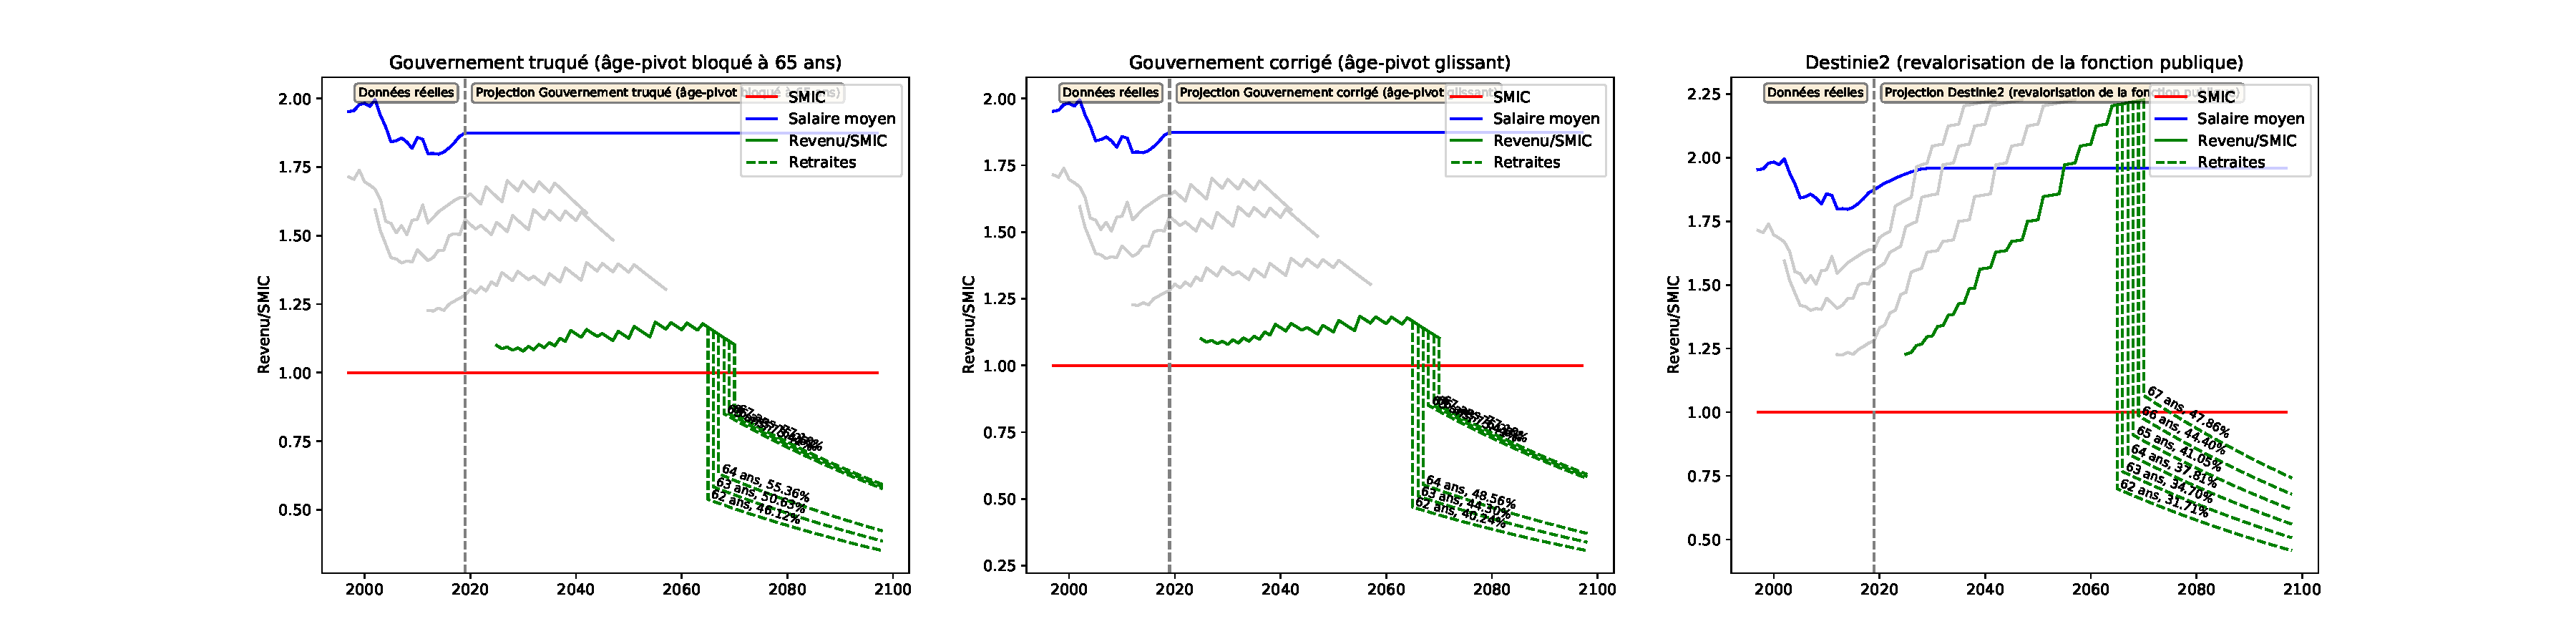
\includegraphics[width=0.9\textwidth]{fig/Redacteur_2003_22_dest_retraite.pdf}\end{center} \label{fig/Redacteur_2003_22_dest_retraite.pdf} 

\newpage 
 
\paragraph{Revenus et points pour le modèle \emph{Gouvernement truqué (âge-pivot bloqué à 65 ans)}} 
 
{ \scriptsize \begin{center} 
\begin{tabular}[htb]{|c|c||c|c|c|c|c|c||c|c||c|c|c|} 
\hline 
 Année &  Âge &  Ind Maj &  Pt Ind(\euro{} 2019) &  Rev HP(\euro{} 2019) &  Tx Primes &  GIPA(\euro{} 2019) &  Revenu(\euro{} 2019) &  SMIC(\euro{} 2019) &  Rev/SMIC &  Cumul Pts &  Achat Pt(\euro{} 2019) &  Serv. Pt(\euro{} 2019) \\ 
\hline \hline 
 2025 &  22 &  356.0 &  4.79 &  1706.81 &  18.21 &  0.00 &  2017.63 &  1835.31 &  {\bf 1.10} &  679.96 &  35.61 &  0.50 \\ 
\hline 
 2026 &  23 &  356.0 &  4.79 &  1706.81 &  18.44 &  0.00 &  2021.55 &  1859.17 &  {\bf 1.09} &  1361.25 &  35.61 &  0.50 \\ 
\hline 
 2027 &  24 &  362.0 &  4.79 &  1735.58 &  18.67 &  0.00 &  2059.61 &  1883.34 &  {\bf 1.09} &  2055.37 &  35.61 &  0.50 \\ 
\hline 
 2028 &  25 &  362.0 &  4.79 &  1735.58 &  18.90 &  0.00 &  2063.61 &  1907.82 &  {\bf 1.08} &  2750.83 &  35.61 &  0.50 \\ 
\hline 
 2029 &  26 &  369.0 &  4.79 &  1769.14 &  19.13 &  0.00 &  2107.58 &  1932.62 &  {\bf 1.09} &  3460.57 &  35.63 &  0.50 \\ 
\hline 
 2030 &  27 &  369.0 &  4.79 &  1769.14 &  19.36 &  0.00 &  2111.65 &  1957.75 &  {\bf 1.08} &  4170.60 &  35.69 &  0.50 \\ 
\hline 
 2031 &  28 &  379.0 &  4.79 &  1817.09 &  19.59 &  0.00 &  2173.05 &  1983.20 &  {\bf 1.10} &  4899.61 &  35.77 &  0.50 \\ 
\hline 
 2032 &  29 &  379.0 &  4.79 &  1817.09 &  19.82 &  0.00 &  2177.23 &  2008.98 &  {\bf 1.08} &  5627.81 &  35.88 &  0.50 \\ 
\hline 
 2033 &  30 &  390.0 &  4.79 &  1869.82 &  20.05 &  0.00 &  2244.72 &  2035.10 &  {\bf 1.10} &  6375.74 &  36.02 &  0.50 \\ 
\hline 
 2034 &  31 &  390.0 &  4.79 &  1869.82 &  20.28 &  0.00 &  2249.03 &  2061.55 &  {\bf 1.09} &  7121.69 &  36.18 &  0.50 \\ 
\hline 
 2035 &  32 &  401.0 &  4.79 &  1922.56 &  20.51 &  0.00 &  2316.88 &  2088.35 &  {\bf 1.11} &  7886.07 &  36.37 &  0.51 \\ 
\hline 
 2036 &  33 &  401.0 &  4.79 &  1922.56 &  20.74 &  0.00 &  2321.30 &  2115.50 &  {\bf 1.10} &  8647.27 &  36.59 &  0.51 \\ 
\hline 
 2037 &  34 &  416.0 &  4.79 &  1994.48 &  20.97 &  0.00 &  2412.72 &  2143.00 &  {\bf 1.13} &  9433.06 &  36.85 &  0.51 \\ 
\hline 
 2038 &  35 &  416.0 &  4.79 &  1994.48 &  21.20 &  0.00 &  2417.31 &  2170.86 &  {\bf 1.11} &  10214.38 &  37.13 &  0.52 \\ 
\hline 
 2039 &  36 &  436.0 &  4.79 &  2090.37 &  21.43 &  0.00 &  2538.33 &  2199.08 &  {\bf 1.15} &  11027.99 &  37.44 &  0.52 \\ 
\hline 
 2040 &  37 &  436.0 &  4.79 &  2090.37 &  21.66 &  0.00 &  2543.14 &  2227.67 &  {\bf 1.14} &  11835.74 &  37.78 &  0.53 \\ 
\hline 
 2041 &  38 &  436.0 &  4.79 &  2090.37 &  21.89 &  0.00 &  2547.95 &  2256.63 &  {\bf 1.13} &  12637.07 &  38.16 &  0.53 \\ 
\hline 
 2042 &  39 &  452.0 &  4.79 &  2167.08 &  22.12 &  0.00 &  2646.44 &  2285.97 &  {\bf 1.16} &  13460.56 &  38.56 &  0.54 \\ 
\hline 
 2043 &  40 &  452.0 &  4.79 &  2167.08 &  22.35 &  0.00 &  2651.42 &  2315.68 &  {\bf 1.14} &  14276.26 &  39.01 &  0.54 \\ 
\hline 
 2044 &  41 &  452.0 &  4.79 &  2167.08 &  22.58 &  0.00 &  2656.41 &  2345.79 &  {\bf 1.13} &  15083.61 &  39.48 &  0.55 \\ 
\hline 
 2045 &  42 &  461.0 &  4.79 &  2210.23 &  22.81 &  0.00 &  2714.38 &  2376.28 &  {\bf 1.14} &  15898.00 &  40.00 &  0.56 \\ 
\hline 
 2046 &  43 &  461.0 &  4.79 &  2210.23 &  23.04 &  0.00 &  2719.47 &  2407.18 &  {\bf 1.13} &  16703.44 &  40.52 &  0.56 \\ 
\hline 
 2047 &  44 &  461.0 &  4.79 &  2210.23 &  23.27 &  0.00 &  2724.55 &  2438.47 &  {\bf 1.12} &  17500.04 &  41.04 &  0.57 \\ 
\hline 
 2048 &  45 &  480.0 &  4.79 &  2301.32 &  23.50 &  0.00 &  2842.13 &  2470.17 &  {\bf 1.15} &  18320.34 &  41.58 &  0.58 \\ 
\hline 
 2049 &  46 &  480.0 &  4.79 &  2301.32 &  23.73 &  0.00 &  2847.43 &  2502.28 &  {\bf 1.14} &  19131.63 &  42.12 &  0.59 \\ 
\hline 
 2050 &  47 &  480.0 &  4.79 &  2301.32 &  23.96 &  0.00 &  2852.72 &  2534.81 &  {\bf 1.13} &  19934.00 &  42.66 &  0.59 \\ 
\hline 
 2051 &  48 &  504.0 &  4.79 &  2416.39 &  24.19 &  0.00 &  3000.91 &  2567.76 &  {\bf 1.17} &  20767.21 &  43.22 &  0.60 \\ 
\hline 
 2052 &  49 &  504.0 &  4.79 &  2416.39 &  24.42 &  0.00 &  3006.47 &  2601.14 &  {\bf 1.16} &  21591.26 &  43.78 &  0.61 \\ 
\hline 
 2053 &  50 &  504.0 &  4.79 &  2416.39 &  24.65 &  0.00 &  3012.03 &  2634.96 &  {\bf 1.14} &  22406.23 &  44.35 &  0.62 \\ 
\hline 
 2054 &  51 &  504.0 &  4.79 &  2416.39 &  24.88 &  0.00 &  3017.59 &  2669.21 &  {\bf 1.13} &  23212.23 &  44.93 &  0.63 \\ 
\hline 
 2055 &  52 &  534.0 &  4.79 &  2560.22 &  25.11 &  0.00 &  3203.09 &  2703.91 &  {\bf 1.18} &  24056.80 &  45.51 &  0.63 \\ 
\hline 
 2056 &  53 &  534.0 &  4.79 &  2560.22 &  25.34 &  0.00 &  3208.98 &  2739.06 &  {\bf 1.17} &  24892.07 &  46.10 &  0.64 \\ 
\hline 
 2057 &  54 &  534.0 &  4.79 &  2560.22 &  25.57 &  0.00 &  3214.87 &  2774.67 &  {\bf 1.16} &  25718.13 &  46.70 &  0.65 \\ 
\hline 
 2058 &  55 &  551.0 &  4.79 &  2641.73 &  25.80 &  0.00 &  3323.29 &  2810.74 &  {\bf 1.18} &  26561.09 &  47.31 &  0.66 \\ 
\hline 
 2059 &  56 &  551.0 &  4.79 &  2641.73 &  26.03 &  0.00 &  3329.37 &  2847.28 &  {\bf 1.17} &  27394.75 &  47.92 &  0.67 \\ 
\hline 
 2060 &  57 &  551.0 &  4.79 &  2641.73 &  26.26 &  0.00 &  3335.44 &  2884.30 &  {\bf 1.16} &  28219.21 &  48.55 &  0.68 \\ 
\hline 
 2061 &  58 &  569.0 &  4.79 &  2728.03 &  26.49 &  0.00 &  3450.68 &  2921.79 &  {\bf 1.18} &  29061.22 &  49.18 &  0.68 \\ 
\hline 
 2062 &  59 &  569.0 &  4.79 &  2728.03 &  26.72 &  0.00 &  3456.95 &  2959.78 &  {\bf 1.17} &  29893.93 &  49.82 &  0.69 \\ 
\hline 
 2063 &  60 &  569.0 &  4.79 &  2728.03 &  26.95 &  0.00 &  3463.23 &  2998.25 &  {\bf 1.16} &  30717.44 &  50.47 &  0.70 \\ 
\hline 
 2064 &  61 &  587.0 &  4.79 &  2814.33 &  27.18 &  0.00 &  3579.26 &  3037.23 &  {\bf 1.18} &  31557.63 &  51.12 &  0.71 \\ 
\hline 
 2065 &  62 &  587.0 &  4.79 &  2814.33 &  27.41 &  0.00 &  3585.73 &  3076.71 &  {\bf 1.17} &  32388.53 &  51.79 &  0.72 \\ 
\hline 
 2066 &  63 &  587.0 &  4.79 &  2814.33 &  27.64 &  0.00 &  3592.21 &  3116.71 &  {\bf 1.15} &  33210.25 &  52.46 &  0.73 \\ 
\hline 
 2067 &  64 &  587.0 &  4.79 &  2814.33 &  27.87 &  0.00 &  3598.68 &  3157.23 &  {\bf 1.14} &  34022.88 &  53.14 &  0.74 \\ 
\hline 
 2068 &  65 &  587.0 &  4.79 &  2814.33 &  28.10 &  0.00 &  3605.15 &  3198.27 &  {\bf 1.13} &  34826.53 &  53.83 &  0.75 \\ 
\hline 
 2069 &  66 &  587.0 &  4.79 &  2814.33 &  28.33 &  0.00 &  3611.62 &  3239.85 &  {\bf 1.11} &  35621.29 &  54.53 &  0.76 \\ 
\hline 
 2070 &  67 &  587.0 &  4.79 &  2814.33 &  28.56 &  0.00 &  3618.10 &  3281.97 &  {\bf 1.10} &  36407.26 &  55.24 &  0.77 \\ 
\hline 
\hline 
\end{tabular} 
\end{center} } 
\newpage 
 
\paragraph{Revenus et points pour le modèle \emph{Gouvernement corrigé (âge-pivot glissant)}} 
 
{ \scriptsize \begin{center} 
\begin{tabular}[htb]{|c|c||c|c|c|c|c|c||c|c||c|c|c|} 
\hline 
 Année &  Âge &  Ind Maj &  Pt Ind(\euro{} 2019) &  Rev HP(\euro{} 2019) &  Tx Primes &  GIPA(\euro{} 2019) &  Revenu(\euro{} 2019) &  SMIC(\euro{} 2019) &  Rev/SMIC &  Cumul Pts &  Achat Pt(\euro{} 2019) &  Serv. Pt(\euro{} 2019) \\ 
\hline \hline 
 2025 &  22 &  356.0 &  4.79 &  1706.81 &  18.21 &  0.00 &  2017.63 &  1835.31 &  {\bf 1.10} &  679.96 &  35.61 &  0.50 \\ 
\hline 
 2026 &  23 &  356.0 &  4.79 &  1706.81 &  18.44 &  0.00 &  2021.55 &  1859.17 &  {\bf 1.09} &  1361.25 &  35.61 &  0.50 \\ 
\hline 
 2027 &  24 &  362.0 &  4.79 &  1735.58 &  18.67 &  0.00 &  2059.61 &  1883.34 &  {\bf 1.09} &  2055.37 &  35.61 &  0.50 \\ 
\hline 
 2028 &  25 &  362.0 &  4.79 &  1735.58 &  18.90 &  0.00 &  2063.61 &  1907.82 &  {\bf 1.08} &  2750.83 &  35.61 &  0.50 \\ 
\hline 
 2029 &  26 &  369.0 &  4.79 &  1769.14 &  19.13 &  0.00 &  2107.58 &  1932.62 &  {\bf 1.09} &  3460.57 &  35.63 &  0.50 \\ 
\hline 
 2030 &  27 &  369.0 &  4.79 &  1769.14 &  19.36 &  0.00 &  2111.65 &  1957.75 &  {\bf 1.08} &  4170.60 &  35.69 &  0.50 \\ 
\hline 
 2031 &  28 &  379.0 &  4.79 &  1817.09 &  19.59 &  0.00 &  2173.05 &  1983.20 &  {\bf 1.10} &  4899.61 &  35.77 &  0.50 \\ 
\hline 
 2032 &  29 &  379.0 &  4.79 &  1817.09 &  19.82 &  0.00 &  2177.23 &  2008.98 &  {\bf 1.08} &  5627.81 &  35.88 &  0.50 \\ 
\hline 
 2033 &  30 &  390.0 &  4.79 &  1869.82 &  20.05 &  0.00 &  2244.72 &  2035.10 &  {\bf 1.10} &  6375.74 &  36.02 &  0.50 \\ 
\hline 
 2034 &  31 &  390.0 &  4.79 &  1869.82 &  20.28 &  0.00 &  2249.03 &  2061.55 &  {\bf 1.09} &  7121.69 &  36.18 &  0.50 \\ 
\hline 
 2035 &  32 &  401.0 &  4.79 &  1922.56 &  20.51 &  0.00 &  2316.88 &  2088.35 &  {\bf 1.11} &  7886.07 &  36.37 &  0.51 \\ 
\hline 
 2036 &  33 &  401.0 &  4.79 &  1922.56 &  20.74 &  0.00 &  2321.30 &  2115.50 &  {\bf 1.10} &  8647.27 &  36.59 &  0.51 \\ 
\hline 
 2037 &  34 &  416.0 &  4.79 &  1994.48 &  20.97 &  0.00 &  2412.72 &  2143.00 &  {\bf 1.13} &  9433.06 &  36.85 &  0.51 \\ 
\hline 
 2038 &  35 &  416.0 &  4.79 &  1994.48 &  21.20 &  0.00 &  2417.31 &  2170.86 &  {\bf 1.11} &  10214.38 &  37.13 &  0.52 \\ 
\hline 
 2039 &  36 &  436.0 &  4.79 &  2090.37 &  21.43 &  0.00 &  2538.33 &  2199.08 &  {\bf 1.15} &  11027.99 &  37.44 &  0.52 \\ 
\hline 
 2040 &  37 &  436.0 &  4.79 &  2090.37 &  21.66 &  0.00 &  2543.14 &  2227.67 &  {\bf 1.14} &  11835.74 &  37.78 &  0.53 \\ 
\hline 
 2041 &  38 &  436.0 &  4.79 &  2090.37 &  21.89 &  0.00 &  2547.95 &  2256.63 &  {\bf 1.13} &  12637.07 &  38.16 &  0.53 \\ 
\hline 
 2042 &  39 &  452.0 &  4.79 &  2167.08 &  22.12 &  0.00 &  2646.44 &  2285.97 &  {\bf 1.16} &  13460.56 &  38.56 &  0.54 \\ 
\hline 
 2043 &  40 &  452.0 &  4.79 &  2167.08 &  22.35 &  0.00 &  2651.42 &  2315.68 &  {\bf 1.14} &  14276.26 &  39.01 &  0.54 \\ 
\hline 
 2044 &  41 &  452.0 &  4.79 &  2167.08 &  22.58 &  0.00 &  2656.41 &  2345.79 &  {\bf 1.13} &  15083.61 &  39.48 &  0.55 \\ 
\hline 
 2045 &  42 &  461.0 &  4.79 &  2210.23 &  22.81 &  0.00 &  2714.38 &  2376.28 &  {\bf 1.14} &  15898.00 &  40.00 &  0.56 \\ 
\hline 
 2046 &  43 &  461.0 &  4.79 &  2210.23 &  23.04 &  0.00 &  2719.47 &  2407.18 &  {\bf 1.13} &  16703.44 &  40.52 &  0.56 \\ 
\hline 
 2047 &  44 &  461.0 &  4.79 &  2210.23 &  23.27 &  0.00 &  2724.55 &  2438.47 &  {\bf 1.12} &  17500.04 &  41.04 &  0.57 \\ 
\hline 
 2048 &  45 &  480.0 &  4.79 &  2301.32 &  23.50 &  0.00 &  2842.13 &  2470.17 &  {\bf 1.15} &  18320.34 &  41.58 &  0.58 \\ 
\hline 
 2049 &  46 &  480.0 &  4.79 &  2301.32 &  23.73 &  0.00 &  2847.43 &  2502.28 &  {\bf 1.14} &  19131.63 &  42.12 &  0.59 \\ 
\hline 
 2050 &  47 &  480.0 &  4.79 &  2301.32 &  23.96 &  0.00 &  2852.72 &  2534.81 &  {\bf 1.13} &  19934.00 &  42.66 &  0.59 \\ 
\hline 
 2051 &  48 &  504.0 &  4.79 &  2416.39 &  24.19 &  0.00 &  3000.91 &  2567.76 &  {\bf 1.17} &  20767.21 &  43.22 &  0.60 \\ 
\hline 
 2052 &  49 &  504.0 &  4.79 &  2416.39 &  24.42 &  0.00 &  3006.47 &  2601.14 &  {\bf 1.16} &  21591.26 &  43.78 &  0.61 \\ 
\hline 
 2053 &  50 &  504.0 &  4.79 &  2416.39 &  24.65 &  0.00 &  3012.03 &  2634.96 &  {\bf 1.14} &  22406.23 &  44.35 &  0.62 \\ 
\hline 
 2054 &  51 &  504.0 &  4.79 &  2416.39 &  24.88 &  0.00 &  3017.59 &  2669.21 &  {\bf 1.13} &  23212.23 &  44.93 &  0.63 \\ 
\hline 
 2055 &  52 &  534.0 &  4.79 &  2560.22 &  25.11 &  0.00 &  3203.09 &  2703.91 &  {\bf 1.18} &  24056.80 &  45.51 &  0.63 \\ 
\hline 
 2056 &  53 &  534.0 &  4.79 &  2560.22 &  25.34 &  0.00 &  3208.98 &  2739.06 &  {\bf 1.17} &  24892.07 &  46.10 &  0.64 \\ 
\hline 
 2057 &  54 &  534.0 &  4.79 &  2560.22 &  25.57 &  0.00 &  3214.87 &  2774.67 &  {\bf 1.16} &  25718.13 &  46.70 &  0.65 \\ 
\hline 
 2058 &  55 &  551.0 &  4.79 &  2641.73 &  25.80 &  0.00 &  3323.29 &  2810.74 &  {\bf 1.18} &  26561.09 &  47.31 &  0.66 \\ 
\hline 
 2059 &  56 &  551.0 &  4.79 &  2641.73 &  26.03 &  0.00 &  3329.37 &  2847.28 &  {\bf 1.17} &  27394.75 &  47.92 &  0.67 \\ 
\hline 
 2060 &  57 &  551.0 &  4.79 &  2641.73 &  26.26 &  0.00 &  3335.44 &  2884.30 &  {\bf 1.16} &  28219.21 &  48.55 &  0.68 \\ 
\hline 
 2061 &  58 &  569.0 &  4.79 &  2728.03 &  26.49 &  0.00 &  3450.68 &  2921.79 &  {\bf 1.18} &  29061.22 &  49.18 &  0.68 \\ 
\hline 
 2062 &  59 &  569.0 &  4.79 &  2728.03 &  26.72 &  0.00 &  3456.95 &  2959.78 &  {\bf 1.17} &  29893.93 &  49.82 &  0.69 \\ 
\hline 
 2063 &  60 &  569.0 &  4.79 &  2728.03 &  26.95 &  0.00 &  3463.23 &  2998.25 &  {\bf 1.16} &  30717.44 &  50.47 &  0.70 \\ 
\hline 
 2064 &  61 &  587.0 &  4.79 &  2814.33 &  27.18 &  0.00 &  3579.26 &  3037.23 &  {\bf 1.18} &  31557.63 &  51.12 &  0.71 \\ 
\hline 
 2065 &  62 &  587.0 &  4.79 &  2814.33 &  27.41 &  0.00 &  3585.73 &  3076.71 &  {\bf 1.17} &  32388.53 &  51.79 &  0.72 \\ 
\hline 
 2066 &  63 &  587.0 &  4.79 &  2814.33 &  27.64 &  0.00 &  3592.21 &  3116.71 &  {\bf 1.15} &  33210.25 &  52.46 &  0.73 \\ 
\hline 
 2067 &  64 &  587.0 &  4.79 &  2814.33 &  27.87 &  0.00 &  3598.68 &  3157.23 &  {\bf 1.14} &  34022.88 &  53.14 &  0.74 \\ 
\hline 
 2068 &  65 &  587.0 &  4.79 &  2814.33 &  28.10 &  0.00 &  3605.15 &  3198.27 &  {\bf 1.13} &  34826.53 &  53.83 &  0.75 \\ 
\hline 
 2069 &  66 &  587.0 &  4.79 &  2814.33 &  28.33 &  0.00 &  3611.62 &  3239.85 &  {\bf 1.11} &  35621.29 &  54.53 &  0.76 \\ 
\hline 
 2070 &  67 &  587.0 &  4.79 &  2814.33 &  28.56 &  0.00 &  3618.10 &  3281.97 &  {\bf 1.10} &  36407.26 &  55.24 &  0.77 \\ 
\hline 
\hline 
\end{tabular} 
\end{center} } 
\newpage 
 
\paragraph{Revenus et points pour le modèle \emph{Destinie2 (revalorisation de la fonction publique)}} 
 
{ \scriptsize \begin{center} 
\begin{tabular}[htb]{|c|c||c|c|c|c|c|c||c|c||c|c|c|} 
\hline 
 Année &  Âge &  Ind Maj &  Pt Ind(\euro{} 2019) &  Rev HP(\euro{} 2019) &  Tx Primes &  GIPA(\euro{} 2019) &  Revenu(\euro{} 2019) &  SMIC(\euro{} 2019) &  Rev/SMIC &  Cumul Pts &  Achat Pt(\euro{} 2019) &  Serv. Pt(\euro{} 2019) \\ 
\hline \hline 
 2025 &  22 &  356.0 &  5.10 &  1816.83 &  18.21 &  0.00 &  2147.68 &  1749.35 &  {\bf 1.23} &  722.02 &  35.69 &  0.50 \\ 
\hline 
 2026 &  23 &  356.0 &  5.17 &  1839.54 &  18.44 &  0.00 &  2178.76 &  1764.53 &  {\bf 1.23} &  1454.48 &  35.69 &  0.50 \\ 
\hline 
 2027 &  24 &  362.0 &  5.23 &  1894.49 &  18.67 &  0.00 &  2248.19 &  1781.27 &  {\bf 1.26} &  2210.28 &  35.69 &  0.50 \\ 
\hline 
 2028 &  25 &  362.0 &  5.30 &  1919.31 &  18.90 &  0.00 &  2282.06 &  1799.59 &  {\bf 1.27} &  2977.48 &  35.69 &  0.50 \\ 
\hline 
 2029 &  26 &  369.0 &  5.37 &  1980.09 &  19.13 &  0.00 &  2358.89 &  1819.55 &  {\bf 1.30} &  3769.94 &  35.72 &  0.50 \\ 
\hline 
 2030 &  27 &  369.0 &  5.43 &  2004.65 &  19.36 &  0.00 &  2392.75 &  1841.19 &  {\bf 1.30} &  4572.61 &  35.77 &  0.50 \\ 
\hline 
 2031 &  28 &  379.0 &  5.50 &  2085.12 &  19.59 &  0.00 &  2493.60 &  1864.58 &  {\bf 1.34} &  5407.25 &  35.85 &  0.50 \\ 
\hline 
 2032 &  29 &  379.0 &  5.57 &  2112.23 &  19.82 &  0.00 &  2530.87 &  1888.81 &  {\bf 1.34} &  6251.79 &  35.96 &  0.50 \\ 
\hline 
 2033 &  30 &  390.0 &  5.65 &  2201.79 &  20.05 &  0.00 &  2643.25 &  1913.37 &  {\bf 1.38} &  7130.49 &  36.10 &  0.50 \\ 
\hline 
 2034 &  31 &  390.0 &  5.72 &  2230.41 &  20.28 &  0.00 &  2682.74 &  1938.24 &  {\bf 1.38} &  8018.27 &  36.26 &  0.50 \\ 
\hline 
 2035 &  32 &  401.0 &  5.79 &  2323.14 &  20.51 &  0.00 &  2799.61 &  1963.44 &  {\bf 1.43} &  8939.80 &  36.46 &  0.51 \\ 
\hline 
 2036 &  33 &  401.0 &  5.87 &  2353.34 &  20.74 &  0.00 &  2841.42 &  1988.96 &  {\bf 1.43} &  9869.43 &  36.68 &  0.51 \\ 
\hline 
 2037 &  34 &  416.0 &  5.94 &  2473.10 &  20.97 &  0.00 &  2991.71 &  2014.82 &  {\bf 1.48} &  10841.56 &  36.93 &  0.51 \\ 
\hline 
 2038 &  35 &  416.0 &  6.02 &  2505.25 &  21.20 &  0.00 &  3036.37 &  2041.01 &  {\bf 1.49} &  11820.73 &  37.21 &  0.52 \\ 
\hline 
 2039 &  36 &  436.0 &  6.10 &  2659.83 &  21.43 &  0.00 &  3229.84 &  2067.55 &  {\bf 1.56} &  12853.63 &  37.52 &  0.52 \\ 
\hline 
 2040 &  37 &  436.0 &  6.18 &  2694.41 &  21.66 &  0.00 &  3278.02 &  2094.43 &  {\bf 1.57} &  13892.42 &  37.87 &  0.53 \\ 
\hline 
 2041 &  38 &  436.0 &  6.26 &  2729.44 &  21.89 &  0.00 &  3326.91 &  2121.65 &  {\bf 1.57} &  14936.34 &  38.24 &  0.53 \\ 
\hline 
 2042 &  39 &  452.0 &  6.34 &  2866.39 &  22.12 &  0.00 &  3500.43 &  2149.23 &  {\bf 1.63} &  16023.08 &  38.65 &  0.54 \\ 
\hline 
 2043 &  40 &  452.0 &  6.42 &  2903.65 &  22.35 &  0.00 &  3552.62 &  2177.17 &  {\bf 1.63} &  17113.53 &  39.10 &  0.54 \\ 
\hline 
 2044 &  41 &  452.0 &  6.51 &  2941.40 &  22.58 &  0.00 &  3605.56 &  2205.48 &  {\bf 1.63} &  18206.86 &  39.57 &  0.55 \\ 
\hline 
 2045 &  42 &  461.0 &  6.59 &  3038.96 &  22.81 &  0.00 &  3732.15 &  2234.15 &  {\bf 1.67} &  19324.05 &  40.09 &  0.56 \\ 
\hline 
 2046 &  43 &  461.0 &  6.68 &  3078.47 &  23.04 &  0.00 &  3787.75 &  2263.19 &  {\bf 1.67} &  20443.33 &  40.61 &  0.57 \\ 
\hline 
 2047 &  44 &  461.0 &  6.76 &  3118.49 &  23.27 &  0.00 &  3844.16 &  2292.61 &  {\bf 1.68} &  21564.71 &  41.14 &  0.57 \\ 
\hline 
 2048 &  45 &  480.0 &  6.85 &  3289.23 &  23.50 &  0.00 &  4062.20 &  2322.42 &  {\bf 1.75} &  22734.48 &  41.67 &  0.58 \\ 
\hline 
 2049 &  46 &  480.0 &  6.94 &  3331.99 &  23.73 &  0.00 &  4122.67 &  2352.61 &  {\bf 1.75} &  23906.43 &  42.21 &  0.59 \\ 
\hline 
 2050 &  47 &  480.0 &  7.03 &  3375.31 &  23.96 &  0.00 &  4184.03 &  2383.19 &  {\bf 1.76} &  25080.55 &  42.76 &  0.60 \\ 
\hline 
 2051 &  48 &  504.0 &  7.12 &  3590.14 &  24.19 &  0.00 &  4458.60 &  2414.18 &  {\bf 1.85} &  26315.67 &  43.32 &  0.60 \\ 
\hline 
 2052 &  49 &  504.0 &  7.22 &  3636.82 &  24.42 &  0.00 &  4524.93 &  2445.56 &  {\bf 1.85} &  27553.08 &  43.88 &  0.61 \\ 
\hline 
 2053 &  50 &  504.0 &  7.31 &  3684.09 &  24.65 &  0.00 &  4592.22 &  2477.35 &  {\bf 1.85} &  28792.78 &  44.45 &  0.62 \\ 
\hline 
 2054 &  51 &  504.0 &  7.40 &  3731.99 &  24.88 &  0.00 &  4660.51 &  2509.56 &  {\bf 1.86} &  30034.76 &  45.03 &  0.63 \\ 
\hline 
 2055 &  52 &  534.0 &  7.50 &  4005.53 &  25.11 &  0.00 &  5011.32 &  2542.18 &  {\bf 1.97} &  31353.10 &  45.62 &  0.63 \\ 
\hline 
 2056 &  53 &  534.0 &  7.60 &  4057.61 &  25.34 &  0.00 &  5085.80 &  2575.23 &  {\bf 1.97} &  32673.86 &  46.21 &  0.64 \\ 
\hline 
 2057 &  54 &  534.0 &  7.70 &  4110.35 &  25.57 &  0.00 &  5161.37 &  2608.71 &  {\bf 1.98} &  33997.04 &  46.81 &  0.65 \\ 
\hline 
 2058 &  55 &  551.0 &  7.80 &  4296.34 &  25.80 &  0.00 &  5404.80 &  2642.62 &  {\bf 2.05} &  35364.85 &  47.42 &  0.66 \\ 
\hline 
 2059 &  56 &  551.0 &  7.90 &  4352.20 &  26.03 &  0.00 &  5485.07 &  2676.98 &  {\bf 2.05} &  36735.15 &  48.03 &  0.67 \\ 
\hline 
 2060 &  57 &  551.0 &  8.00 &  4408.78 &  26.26 &  0.00 &  5566.52 &  2711.78 &  {\bf 2.05} &  38107.96 &  48.66 &  0.68 \\ 
\hline 
 2061 &  58 &  569.0 &  8.11 &  4611.99 &  26.49 &  0.00 &  5833.70 &  2747.03 &  {\bf 2.12} &  39528.20 &  49.29 &  0.69 \\ 
\hline 
 2062 &  59 &  569.0 &  8.21 &  4671.94 &  26.72 &  0.00 &  5920.29 &  2782.74 &  {\bf 2.13} &  40951.02 &  49.93 &  0.70 \\ 
\hline 
 2063 &  60 &  569.0 &  8.32 &  4732.68 &  26.95 &  0.00 &  6008.13 &  2818.92 &  {\bf 2.13} &  42376.42 &  50.58 &  0.70 \\ 
\hline 
 2064 &  61 &  587.0 &  8.43 &  4945.86 &  27.18 &  0.00 &  6290.15 &  2855.56 &  {\bf 2.20} &  43849.58 &  51.24 &  0.71 \\ 
\hline 
 2065 &  62 &  587.0 &  8.54 &  5010.16 &  27.41 &  0.00 &  6383.45 &  2892.68 &  {\bf 2.21} &  45325.40 &  51.90 &  0.72 \\ 
\hline 
 2066 &  63 &  587.0 &  8.65 &  5075.29 &  27.64 &  0.00 &  6478.10 &  2930.29 &  {\bf 2.21} &  46803.89 &  52.58 &  0.73 \\ 
\hline 
 2067 &  64 &  587.0 &  8.76 &  5141.27 &  27.87 &  0.00 &  6574.14 &  2968.38 &  {\bf 2.21} &  48285.04 &  53.26 &  0.74 \\ 
\hline 
 2068 &  65 &  587.0 &  8.87 &  5208.11 &  28.10 &  0.00 &  6671.59 &  3006.97 &  {\bf 2.22} &  49768.86 &  53.95 &  0.75 \\ 
\hline 
 2069 &  66 &  587.0 &  8.99 &  5275.81 &  28.33 &  0.00 &  6770.45 &  3046.06 &  {\bf 2.22} &  51255.34 &  54.66 &  0.76 \\ 
\hline 
 2070 &  67 &  587.0 &  9.10 &  5344.40 &  28.56 &  0.00 &  6870.76 &  3085.66 &  {\bf 2.23} &  52744.48 &  55.37 &  0.77 \\ 
\hline 
\hline 
\end{tabular} 
\end{center} } 
\newpage 
 
\chapter{Secrétaire administratif} 

\begin{minipage}{0.55\linewidth}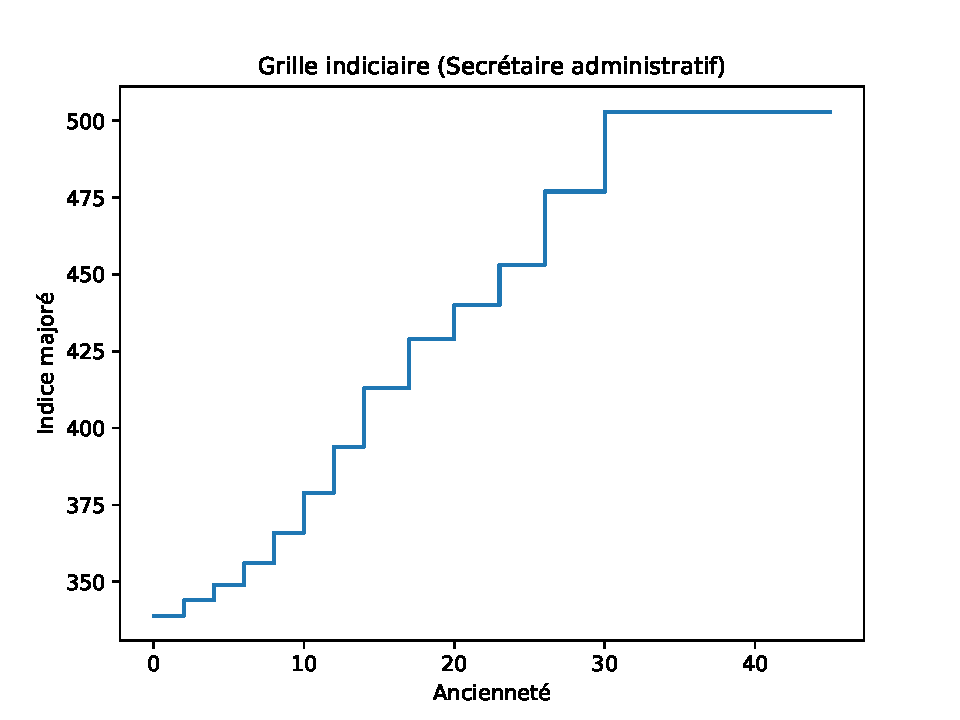
\includegraphics[width=0.7\textwidth]{fig/grille_SecretaireAdmin.pdf}\end{minipage} 
\begin{minipage}{0.3\linewidth} 
 \begin{center} 

\begin{tabular}[htb]{|c|c|} 
\hline 
 Indice majoré &  Durée (années) \\ 
\hline \hline 
 339 &  2.00 \\ 
\hline 
 344 &  2.00 \\ 
\hline 
 349 &  2.00 \\ 
\hline 
 356 &  2.00 \\ 
\hline 
 366 &  2.00 \\ 
\hline 
 379 &  2.00 \\ 
\hline 
 394 &  2.00 \\ 
\hline 
 413 &  3.00 \\ 
\hline 
 429 &  3.00 \\ 
\hline 
 440 &  3.00 \\ 
\hline 
 453 &  3.00 \\ 
\hline 
 477 &  4.00 \\ 
\hline 
 503 &   \\ 
\hline 
\hline 
\end{tabular} 
\end{center} 
 \end{minipage} 


 \addto{\captionsenglish}{ \renewcommand{\mtctitle}{}} \setcounter{minitocdepth}{2} 
 \minitoc \newpage 

\section{Début de carrière à 22 ans} 

\subsection{Génération 1975 (début en 1997)} 

\paragraph{Retraites possibles dans le modèle \emph{Gouvernement truqué (âge-pivot bloqué à 65 ans)}}  
 
{ \scriptsize \begin{center} 
\begin{tabular}[htb]{|c|c||c|c||c|c||c||c|c|c|c|c|c|} 
\hline 
 Retraite en &  Âge &  Âge pivot &  Décote/Surcote &  Retraite (\euro{} 2019) &  Tx Rempl(\%) &  SMIC (\euro{} 2019) &  Retraite/SMIC &  Rev70/SMIC &  Rev75/SMIC &  Rev80/SMIC &  Rev85/SMIC &  Rev90/SMIC \\ 
\hline \hline 
 2037 &  62 &  64 ans 10 mois &  -14.17\% &  1465.93 &  {\bf 43.54} &  2143.00 &  {\bf {\color{red} 0.68}} &  {\bf {\color{red} 0.62}} &  {\bf {\color{red} 0.58}} &  {\bf {\color{red} 0.54}} &  {\bf {\color{red} 0.51}} &  {\bf {\color{red} 0.48}} \\ 
\hline 
 2038 &  63 &  64 ans 11 mois &  -9.58\% &  1598.43 &  {\bf 47.40} &  2170.86 &  {\bf {\color{red} 0.74}} &  {\bf {\color{red} 0.67}} &  {\bf {\color{red} 0.63}} &  {\bf {\color{red} 0.59}} &  {\bf {\color{red} 0.55}} &  {\bf {\color{red} 0.52}} \\ 
\hline 
 2039 &  64 &  65 ans 0 mois &  -5.00\% &  1738.22 &  {\bf 51.46} &  2199.08 &  {\bf {\color{red} 0.79}} &  {\bf {\color{red} 0.73}} &  {\bf {\color{red} 0.69}} &  {\bf {\color{red} 0.64}} &  {\bf {\color{red} 0.60}} &  {\bf {\color{red} 0.56}} \\ 
\hline 
 2040 &  65 &  65 ans 0 mois &  0.00\% &  1893.56 &  {\bf 55.97} &  2227.67 &  {\bf {\color{red} 0.85}} &  {\bf {\color{red} 0.80}} &  {\bf {\color{red} 0.75}} &  {\bf {\color{red} 0.70}} &  {\bf {\color{red} 0.66}} &  {\bf {\color{red} 0.62}} \\ 
\hline 
 2041 &  66 &  65 ans 0 mois &  5.00\% &  2057.51 &  {\bf 60.71} &  2256.63 &  {\bf {\color{red} 0.91}} &  {\bf {\color{red} 0.87}} &  {\bf {\color{red} 0.81}} &  {\bf {\color{red} 0.76}} &  {\bf {\color{red} 0.71}} &  {\bf {\color{red} 0.67}} \\ 
\hline 
 2042 &  67 &  65 ans 0 mois &  10.00\% &  2230.51 &  {\bf 65.71} &  2285.97 &  {\bf {\color{red} 0.98}} &  {\bf {\color{red} 0.94}} &  {\bf {\color{red} 0.88}} &  {\bf {\color{red} 0.82}} &  {\bf {\color{red} 0.77}} &  {\bf {\color{red} 0.72}} \\ 
\hline 
\hline 
\end{tabular} 
\end{center} } 
\paragraph{Retraites possibles dans le modèle \emph{Gouvernement corrigé (âge-pivot glissant)}}  
 
{ \scriptsize \begin{center} 
\begin{tabular}[htb]{|c|c||c|c||c|c||c||c|c|c|c|c|c|} 
\hline 
 Retraite en &  Âge &  Âge pivot &  Décote/Surcote &  Retraite (\euro{} 2019) &  Tx Rempl(\%) &  SMIC (\euro{} 2019) &  Retraite/SMIC &  Rev70/SMIC &  Rev75/SMIC &  Rev80/SMIC &  Rev85/SMIC &  Rev90/SMIC \\ 
\hline \hline 
 2037 &  62 &  64 ans 10 mois &  -14.17\% &  1465.93 &  {\bf 43.54} &  2143.00 &  {\bf {\color{red} 0.68}} &  {\bf {\color{red} 0.62}} &  {\bf {\color{red} 0.58}} &  {\bf {\color{red} 0.54}} &  {\bf {\color{red} 0.51}} &  {\bf {\color{red} 0.48}} \\ 
\hline 
 2038 &  63 &  64 ans 11 mois &  -9.58\% &  1598.43 &  {\bf 47.40} &  2170.86 &  {\bf {\color{red} 0.74}} &  {\bf {\color{red} 0.67}} &  {\bf {\color{red} 0.63}} &  {\bf {\color{red} 0.59}} &  {\bf {\color{red} 0.55}} &  {\bf {\color{red} 0.52}} \\ 
\hline 
 2039 &  64 &  65 ans 0 mois &  -5.00\% &  1738.22 &  {\bf 51.46} &  2199.08 &  {\bf {\color{red} 0.79}} &  {\bf {\color{red} 0.73}} &  {\bf {\color{red} 0.69}} &  {\bf {\color{red} 0.64}} &  {\bf {\color{red} 0.60}} &  {\bf {\color{red} 0.56}} \\ 
\hline 
 2040 &  65 &  65 ans 1 mois &  -0.42\% &  1893.52 &  {\bf 55.96} &  2227.67 &  {\bf {\color{red} 0.85}} &  {\bf {\color{red} 0.80}} &  {\bf {\color{red} 0.75}} &  {\bf {\color{red} 0.70}} &  {\bf {\color{red} 0.66}} &  {\bf {\color{red} 0.62}} \\ 
\hline 
 2041 &  66 &  65 ans 2 mois &  4.17\% &  2041.18 &  {\bf 60.23} &  2256.63 &  {\bf {\color{red} 0.90}} &  {\bf {\color{red} 0.86}} &  {\bf {\color{red} 0.81}} &  {\bf {\color{red} 0.75}} &  {\bf {\color{red} 0.71}} &  {\bf {\color{red} 0.66}} \\ 
\hline 
 2042 &  67 &  65 ans 3 mois &  8.75\% &  2205.16 &  {\bf 64.96} &  2285.97 &  {\bf {\color{red} 0.96}} &  {\bf {\color{red} 0.93}} &  {\bf {\color{red} 0.87}} &  {\bf {\color{red} 0.82}} &  {\bf {\color{red} 0.76}} &  {\bf {\color{red} 0.72}} \\ 
\hline 
\hline 
\end{tabular} 
\end{center} } 
\paragraph{Retraites possibles dans le modèle \emph{Destinie2 (revalorisation de la fonction publique)}}  
 
{ \scriptsize \begin{center} 
\begin{tabular}[htb]{|c|c||c|c||c|c||c||c|c|c|c|c|c|} 
\hline 
 Retraite en &  Âge &  Âge pivot &  Décote/Surcote &  Retraite (\euro{} 2019) &  Tx Rempl(\%) &  SMIC (\euro{} 2019) &  Retraite/SMIC &  Rev70/SMIC &  Rev75/SMIC &  Rev80/SMIC &  Rev85/SMIC &  Rev90/SMIC \\ 
\hline \hline 
 2037 &  62 &  64 ans 10 mois &  -14.17\% &  1550.11 &  {\bf 37.13} &  2014.82 &  {\bf {\color{red} 0.77}} &  {\bf {\color{red} 0.69}} &  {\bf {\color{red} 0.65}} &  {\bf {\color{red} 0.61}} &  {\bf {\color{red} 0.57}} &  {\bf {\color{red} 0.54}} \\ 
\hline 
 2038 &  63 &  64 ans 11 mois &  -9.58\% &  1698.64 &  {\bf 40.10} &  2041.01 &  {\bf {\color{red} 0.83}} &  {\bf {\color{red} 0.76}} &  {\bf {\color{red} 0.71}} &  {\bf {\color{red} 0.67}} &  {\bf {\color{red} 0.63}} &  {\bf {\color{red} 0.59}} \\ 
\hline 
 2039 &  64 &  65 ans 0 mois &  -5.00\% &  1856.57 &  {\bf 43.19} &  2067.55 &  {\bf {\color{red} 0.90}} &  {\bf {\color{red} 0.83}} &  {\bf {\color{red} 0.78}} &  {\bf {\color{red} 0.73}} &  {\bf {\color{red} 0.68}} &  {\bf {\color{red} 0.64}} \\ 
\hline 
 2040 &  65 &  65 ans 1 mois &  -0.42\% &  2024.41 &  {\bf 46.42} &  2094.43 &  {\bf {\color{red} 0.97}} &  {\bf {\color{red} 0.91}} &  {\bf {\color{red} 0.85}} &  {\bf {\color{red} 0.80}} &  {\bf {\color{red} 0.75}} &  {\bf {\color{red} 0.70}} \\ 
\hline 
 2041 &  66 &  65 ans 2 mois &  4.17\% &  2202.77 &  {\bf 49.78} &  2121.65 &  {\bf 1.04} &  {\bf {\color{red} 0.99}} &  {\bf {\color{red} 0.92}} &  {\bf {\color{red} 0.87}} &  {\bf {\color{red} 0.81}} &  {\bf {\color{red} 0.76}} \\ 
\hline 
 2042 &  67 &  65 ans 3 mois &  8.75\% &  2392.25 &  {\bf 53.28} &  2149.23 &  {\bf 1.11} &  {\bf 1.07} &  {\bf 1.00} &  {\bf {\color{red} 0.94}} &  {\bf {\color{red} 0.88}} &  {\bf {\color{red} 0.83}} \\ 
\hline 
\hline 
\end{tabular} 
\end{center} } 

 \begin{center}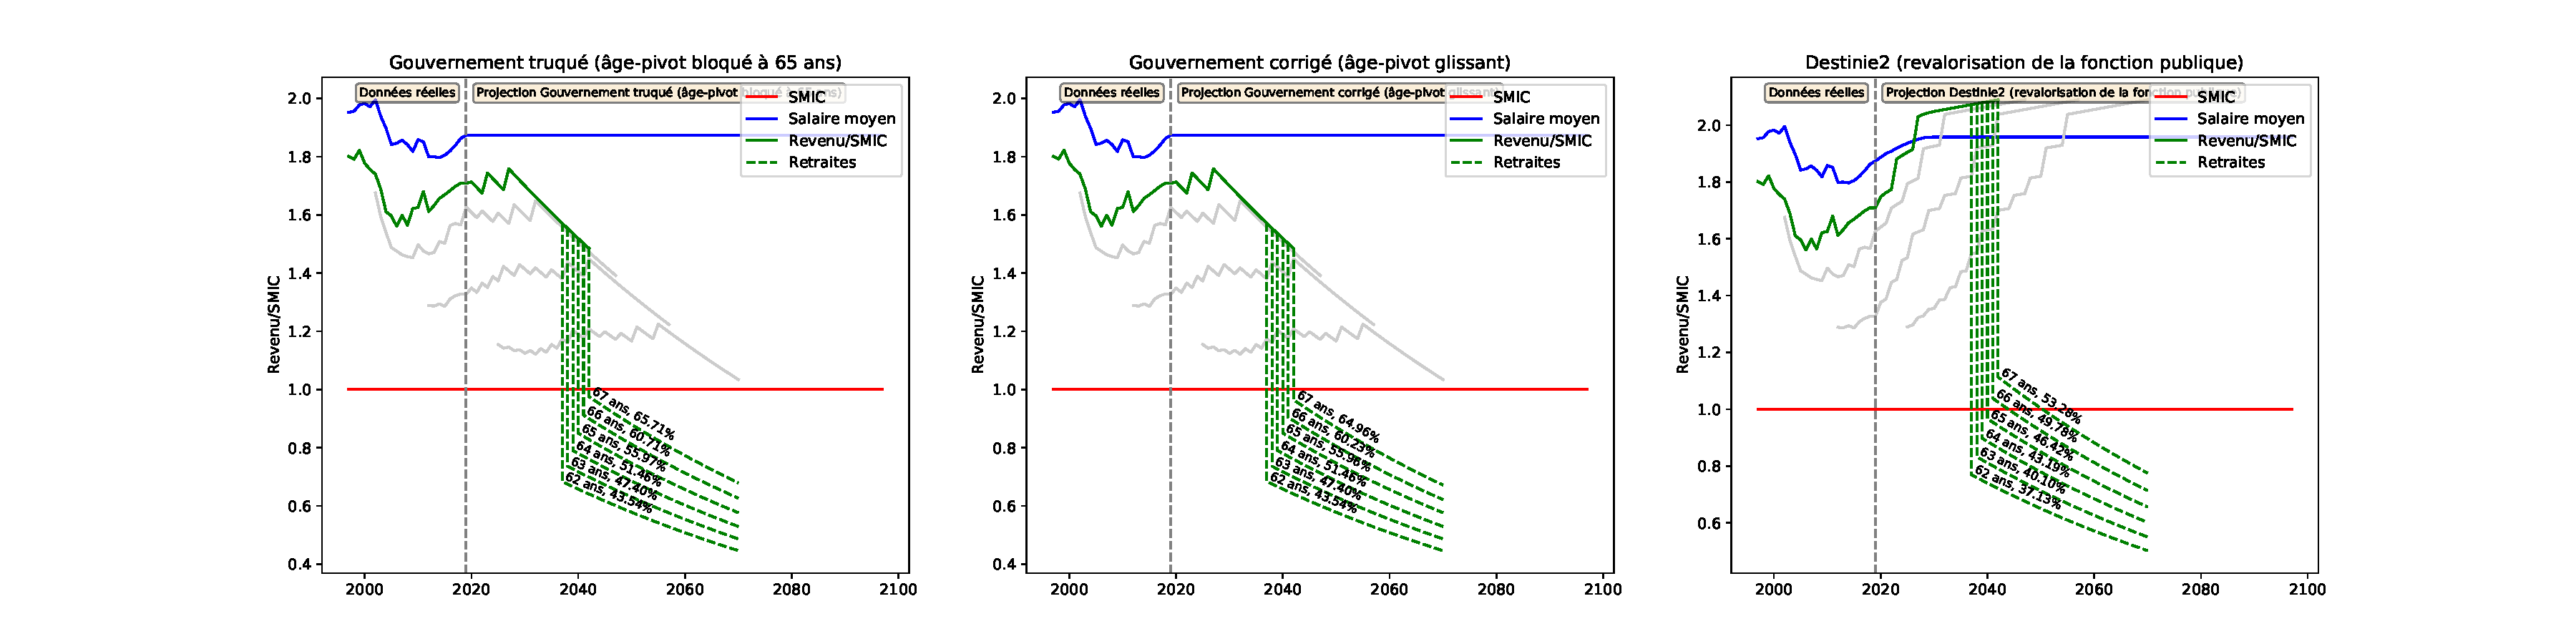
\includegraphics[width=0.9\textwidth]{fig/SecretaireAdmin_1975_22_dest_retraite.pdf}\end{center} \label{fig/SecretaireAdmin_1975_22_dest_retraite.pdf} 

\newpage 
 
\paragraph{Revenus et points pour le modèle \emph{Gouvernement truqué (âge-pivot bloqué à 65 ans)}} 
 
{ \scriptsize \begin{center} 
\begin{tabular}[htb]{|c|c||c|c|c|c|c|c||c|c||c|c|c|} 
\hline 
 Année &  Âge &  Ind Maj &  Pt Ind(\euro{} 2019) &  Rev HP(\euro{} 2019) &  Tx Primes &  GIPA(\euro{} 2019) &  Revenu(\euro{} 2019) &  SMIC(\euro{} 2019) &  Rev/SMIC &  Cumul Pts &  Achat Pt(\euro{} 2019) &  Serv. Pt(\euro{} 2019) \\ 
\hline \hline 
 1997 &  22 &  339.0 &  5.53 &  1876.15 &  30.41 &  0.00 &  2446.68 &  1358.84 &  {\bf 1.80} &  824.56 &  35.61 &  0.50 \\ 
\hline 
 1998 &  23 &  339.0 &  5.57 &  1887.03 &  30.64 &  0.00 &  2465.21 &  1376.36 &  {\bf 1.79} &  1655.37 &  35.61 &  0.50 \\ 
\hline 
 1999 &  24 &  344.0 &  5.61 &  1930.34 &  30.87 &  0.00 &  2526.23 &  1386.54 &  {\bf 1.82} &  2506.74 &  35.61 &  0.50 \\ 
\hline 
 2000 &  25 &  344.0 &  5.55 &  1907.54 &  31.10 &  0.00 &  2500.79 &  1407.00 &  {\bf 1.78} &  3349.54 &  35.61 &  0.50 \\ 
\hline 
 2001 &  26 &  349.0 &  5.52 &  1926.66 &  31.33 &  0.00 &  2530.28 &  1441.04 &  {\bf 1.76} &  4202.27 &  35.61 &  0.50 \\ 
\hline 
 2002 &  27 &  349.0 &  5.49 &  1914.71 &  31.56 &  0.00 &  2518.99 &  1447.74 &  {\bf 1.74} &  5051.20 &  35.61 &  0.50 \\ 
\hline 
 2003 &  28 &  356.0 &  5.37 &  1913.36 &  31.79 &  0.00 &  2521.62 &  1493.03 &  {\bf 1.69} &  5901.02 &  35.61 &  0.50 \\ 
\hline 
 2004 &  29 &  356.0 &  5.29 &  1883.14 &  32.02 &  5.85 &  2491.97 &  1547.32 &  {\bf 1.61} &  6740.84 &  35.61 &  0.50 \\ 
\hline 
 2005 &  30 &  366.0 &  5.29 &  1935.83 &  32.25 &  0.00 &  2560.13 &  1603.67 &  {\bf 1.60} &  7603.64 &  35.61 &  0.50 \\ 
\hline 
 2006 &  31 &  366.0 &  5.23 &  1914.22 &  32.48 &  0.00 &  2535.96 &  1625.00 &  {\bf 1.56} &  8458.29 &  35.61 &  0.50 \\ 
\hline 
 2007 &  32 &  379.0 &  5.19 &  1968.71 &  32.71 &  0.00 &  2612.67 &  1634.08 &  {\bf 1.60} &  9338.79 &  35.61 &  0.50 \\ 
\hline 
 2008 &  33 &  379.0 &  5.09 &  1930.26 &  32.94 &  0.00 &  2566.09 &  1640.24 &  {\bf 1.56} &  10203.60 &  35.61 &  0.50 \\ 
\hline 
 2009 &  34 &  394.0 &  5.13 &  2020.88 &  33.17 &  0.00 &  2691.20 &  1659.42 &  {\bf 1.62} &  11110.57 &  35.61 &  0.50 \\ 
\hline 
 2010 &  35 &  394.0 &  5.08 &  2000.47 &  33.40 &  0.00 &  2668.62 &  1641.90 &  {\bf 1.63} &  12009.92 &  35.61 &  0.50 \\ 
\hline 
 2011 &  36 &  413.0 &  4.97 &  2053.37 &  33.63 &  0.00 &  2743.92 &  1633.19 &  {\bf 1.68} &  12934.66 &  35.61 &  0.50 \\ 
\hline 
 2012 &  37 &  413.0 &  4.88 &  2013.97 &  33.86 &  0.00 &  2695.90 &  1673.05 &  {\bf 1.61} &  13843.21 &  35.61 &  0.50 \\ 
\hline 
 2013 &  38 &  413.0 &  4.83 &  1996.71 &  34.09 &  38.68 &  2716.07 &  1664.01 &  {\bf 1.63} &  14758.55 &  35.61 &  0.50 \\ 
\hline 
 2014 &  39 &  429.0 &  4.81 &  2063.68 &  34.32 &  0.00 &  2771.94 &  1673.24 &  {\bf 1.66} &  15692.73 &  35.61 &  0.50 \\ 
\hline 
 2015 &  40 &  429.0 &  4.81 &  2062.88 &  34.55 &  39.66 &  2815.26 &  1686.62 &  {\bf 1.67} &  16641.51 &  35.61 &  0.50 \\ 
\hline 
 2016 &  41 &  429.0 &  4.80 &  2058.76 &  34.78 &  76.59 &  2851.39 &  1693.76 &  {\bf 1.68} &  17602.46 &  35.61 &  0.50 \\ 
\hline 
 2017 &  42 &  440.0 &  4.81 &  2115.81 &  35.01 &  17.94 &  2874.49 &  1692.60 &  {\bf 1.70} &  18571.20 &  35.61 &  0.50 \\ 
\hline 
 2018 &  43 &  440.0 &  4.74 &  2086.59 &  35.24 &  65.85 &  2887.76 &  1689.76 &  {\bf 1.71} &  19544.41 &  35.61 &  0.50 \\ 
\hline 
 2019 &  44 &  440.0 &  4.79 &  2109.55 &  35.47 &  44.04 &  2901.84 &  1698.45 &  {\bf 1.71} &  20522.36 &  35.61 &  0.50 \\ 
\hline 
 2020 &  45 &  453.0 &  4.79 &  2171.87 &  35.70 &  0.00 &  2947.23 &  1720.53 &  {\bf 1.71} &  21515.62 &  35.61 &  0.50 \\ 
\hline 
 2021 &  46 &  453.0 &  4.79 &  2171.87 &  35.93 &  0.00 &  2952.23 &  1742.90 &  {\bf 1.69} &  22510.55 &  35.61 &  0.50 \\ 
\hline 
 2022 &  47 &  453.0 &  4.79 &  2171.87 &  36.16 &  0.00 &  2957.22 &  1765.55 &  {\bf 1.67} &  23507.17 &  35.61 &  0.50 \\ 
\hline 
 2023 &  48 &  477.0 &  4.79 &  2286.94 &  36.39 &  0.00 &  3119.16 &  1788.51 &  {\bf 1.74} &  24558.37 &  35.61 &  0.50 \\ 
\hline 
 2024 &  49 &  477.0 &  4.79 &  2286.94 &  36.62 &  0.00 &  3124.42 &  1811.76 &  {\bf 1.72} &  25611.33 &  35.61 &  0.50 \\ 
\hline 
 2025 &  50 &  477.0 &  4.79 &  2286.94 &  36.85 &  0.00 &  3129.68 &  1835.31 &  {\bf 1.71} &  26666.07 &  35.61 &  0.50 \\ 
\hline 
 2026 &  51 &  477.0 &  4.79 &  2286.94 &  37.08 &  0.00 &  3134.94 &  1859.17 &  {\bf 1.69} &  27722.58 &  35.61 &  0.50 \\ 
\hline 
 2027 &  52 &  503.0 &  4.79 &  2411.59 &  37.31 &  0.00 &  3311.36 &  1883.34 &  {\bf 1.76} &  28838.55 &  35.61 &  0.50 \\ 
\hline 
 2028 &  53 &  503.0 &  4.79 &  2411.59 &  37.54 &  0.00 &  3316.91 &  1907.82 &  {\bf 1.74} &  29956.39 &  35.61 &  0.50 \\ 
\hline 
 2029 &  54 &  503.0 &  4.79 &  2411.59 &  37.77 &  0.00 &  3322.45 &  1932.62 &  {\bf 1.72} &  31075.25 &  35.63 &  0.50 \\ 
\hline 
 2030 &  55 &  503.0 &  4.79 &  2411.59 &  38.00 &  0.00 &  3328.00 &  1957.75 &  {\bf 1.70} &  32194.27 &  35.69 &  0.50 \\ 
\hline 
 2031 &  56 &  503.0 &  4.79 &  2411.59 &  38.23 &  0.00 &  3333.55 &  1983.20 &  {\bf 1.68} &  33312.61 &  35.77 &  0.50 \\ 
\hline 
 2032 &  57 &  503.0 &  4.79 &  2411.59 &  38.46 &  0.00 &  3339.09 &  2008.98 &  {\bf 1.66} &  34429.40 &  35.88 &  0.50 \\ 
\hline 
 2033 &  58 &  503.0 &  4.79 &  2411.59 &  38.69 &  0.00 &  3344.64 &  2035.10 &  {\bf 1.64} &  35543.82 &  36.02 &  0.50 \\ 
\hline 
 2034 &  59 &  503.0 &  4.79 &  2411.59 &  38.92 &  0.00 &  3350.19 &  2061.55 &  {\bf 1.63} &  36655.00 &  36.18 &  0.50 \\ 
\hline 
 2035 &  60 &  503.0 &  4.79 &  2411.59 &  39.15 &  0.00 &  3355.73 &  2088.35 &  {\bf 1.61} &  37762.12 &  36.37 &  0.51 \\ 
\hline 
 2036 &  61 &  503.0 &  4.79 &  2411.59 &  39.38 &  0.00 &  3361.28 &  2115.50 &  {\bf 1.59} &  38864.34 &  36.59 &  0.51 \\ 
\hline 
 2037 &  62 &  503.0 &  4.79 &  2411.59 &  39.61 &  0.00 &  3366.83 &  2143.00 &  {\bf 1.57} &  39960.87 &  36.85 &  0.51 \\ 
\hline 
 2038 &  63 &  503.0 &  4.79 &  2411.59 &  39.84 &  0.00 &  3372.37 &  2170.86 &  {\bf 1.55} &  41050.88 &  37.13 &  0.52 \\ 
\hline 
 2039 &  64 &  503.0 &  4.79 &  2411.59 &  40.07 &  0.00 &  3377.92 &  2199.08 &  {\bf 1.54} &  42133.61 &  37.44 &  0.52 \\ 
\hline 
 2040 &  65 &  503.0 &  4.79 &  2411.59 &  40.30 &  0.00 &  3383.47 &  2227.67 &  {\bf 1.52} &  43208.26 &  37.78 &  0.53 \\ 
\hline 
 2041 &  66 &  503.0 &  4.79 &  2411.59 &  40.53 &  0.00 &  3389.01 &  2256.63 &  {\bf 1.50} &  44274.10 &  38.16 &  0.53 \\ 
\hline 
 2042 &  67 &  503.0 &  4.79 &  2411.59 &  40.76 &  0.00 &  3394.56 &  2285.97 &  {\bf 1.48} &  45330.39 &  38.56 &  0.54 \\ 
\hline 
\hline 
\end{tabular} 
\end{center} } 
\newpage 
 
\paragraph{Revenus et points pour le modèle \emph{Gouvernement corrigé (âge-pivot glissant)}} 
 
{ \scriptsize \begin{center} 
\begin{tabular}[htb]{|c|c||c|c|c|c|c|c||c|c||c|c|c|} 
\hline 
 Année &  Âge &  Ind Maj &  Pt Ind(\euro{} 2019) &  Rev HP(\euro{} 2019) &  Tx Primes &  GIPA(\euro{} 2019) &  Revenu(\euro{} 2019) &  SMIC(\euro{} 2019) &  Rev/SMIC &  Cumul Pts &  Achat Pt(\euro{} 2019) &  Serv. Pt(\euro{} 2019) \\ 
\hline \hline 
 1997 &  22 &  339.0 &  5.53 &  1876.15 &  30.41 &  0.00 &  2446.68 &  1358.84 &  {\bf 1.80} &  824.56 &  35.61 &  0.50 \\ 
\hline 
 1998 &  23 &  339.0 &  5.57 &  1887.03 &  30.64 &  0.00 &  2465.21 &  1376.36 &  {\bf 1.79} &  1655.37 &  35.61 &  0.50 \\ 
\hline 
 1999 &  24 &  344.0 &  5.61 &  1930.34 &  30.87 &  0.00 &  2526.23 &  1386.54 &  {\bf 1.82} &  2506.74 &  35.61 &  0.50 \\ 
\hline 
 2000 &  25 &  344.0 &  5.55 &  1907.54 &  31.10 &  0.00 &  2500.79 &  1407.00 &  {\bf 1.78} &  3349.54 &  35.61 &  0.50 \\ 
\hline 
 2001 &  26 &  349.0 &  5.52 &  1926.66 &  31.33 &  0.00 &  2530.28 &  1441.04 &  {\bf 1.76} &  4202.27 &  35.61 &  0.50 \\ 
\hline 
 2002 &  27 &  349.0 &  5.49 &  1914.71 &  31.56 &  0.00 &  2518.99 &  1447.74 &  {\bf 1.74} &  5051.20 &  35.61 &  0.50 \\ 
\hline 
 2003 &  28 &  356.0 &  5.37 &  1913.36 &  31.79 &  0.00 &  2521.62 &  1493.03 &  {\bf 1.69} &  5901.02 &  35.61 &  0.50 \\ 
\hline 
 2004 &  29 &  356.0 &  5.29 &  1883.14 &  32.02 &  5.85 &  2491.97 &  1547.32 &  {\bf 1.61} &  6740.84 &  35.61 &  0.50 \\ 
\hline 
 2005 &  30 &  366.0 &  5.29 &  1935.83 &  32.25 &  0.00 &  2560.13 &  1603.67 &  {\bf 1.60} &  7603.64 &  35.61 &  0.50 \\ 
\hline 
 2006 &  31 &  366.0 &  5.23 &  1914.22 &  32.48 &  0.00 &  2535.96 &  1625.00 &  {\bf 1.56} &  8458.29 &  35.61 &  0.50 \\ 
\hline 
 2007 &  32 &  379.0 &  5.19 &  1968.71 &  32.71 &  0.00 &  2612.67 &  1634.08 &  {\bf 1.60} &  9338.79 &  35.61 &  0.50 \\ 
\hline 
 2008 &  33 &  379.0 &  5.09 &  1930.26 &  32.94 &  0.00 &  2566.09 &  1640.24 &  {\bf 1.56} &  10203.60 &  35.61 &  0.50 \\ 
\hline 
 2009 &  34 &  394.0 &  5.13 &  2020.88 &  33.17 &  0.00 &  2691.20 &  1659.42 &  {\bf 1.62} &  11110.57 &  35.61 &  0.50 \\ 
\hline 
 2010 &  35 &  394.0 &  5.08 &  2000.47 &  33.40 &  0.00 &  2668.62 &  1641.90 &  {\bf 1.63} &  12009.92 &  35.61 &  0.50 \\ 
\hline 
 2011 &  36 &  413.0 &  4.97 &  2053.37 &  33.63 &  0.00 &  2743.92 &  1633.19 &  {\bf 1.68} &  12934.66 &  35.61 &  0.50 \\ 
\hline 
 2012 &  37 &  413.0 &  4.88 &  2013.97 &  33.86 &  0.00 &  2695.90 &  1673.05 &  {\bf 1.61} &  13843.21 &  35.61 &  0.50 \\ 
\hline 
 2013 &  38 &  413.0 &  4.83 &  1996.71 &  34.09 &  38.68 &  2716.07 &  1664.01 &  {\bf 1.63} &  14758.55 &  35.61 &  0.50 \\ 
\hline 
 2014 &  39 &  429.0 &  4.81 &  2063.68 &  34.32 &  0.00 &  2771.94 &  1673.24 &  {\bf 1.66} &  15692.73 &  35.61 &  0.50 \\ 
\hline 
 2015 &  40 &  429.0 &  4.81 &  2062.88 &  34.55 &  39.66 &  2815.26 &  1686.62 &  {\bf 1.67} &  16641.51 &  35.61 &  0.50 \\ 
\hline 
 2016 &  41 &  429.0 &  4.80 &  2058.76 &  34.78 &  76.59 &  2851.39 &  1693.76 &  {\bf 1.68} &  17602.46 &  35.61 &  0.50 \\ 
\hline 
 2017 &  42 &  440.0 &  4.81 &  2115.81 &  35.01 &  17.94 &  2874.49 &  1692.60 &  {\bf 1.70} &  18571.20 &  35.61 &  0.50 \\ 
\hline 
 2018 &  43 &  440.0 &  4.74 &  2086.59 &  35.24 &  65.85 &  2887.76 &  1689.76 &  {\bf 1.71} &  19544.41 &  35.61 &  0.50 \\ 
\hline 
 2019 &  44 &  440.0 &  4.79 &  2109.55 &  35.47 &  44.04 &  2901.84 &  1698.45 &  {\bf 1.71} &  20522.36 &  35.61 &  0.50 \\ 
\hline 
 2020 &  45 &  453.0 &  4.79 &  2171.87 &  35.70 &  0.00 &  2947.23 &  1720.53 &  {\bf 1.71} &  21515.62 &  35.61 &  0.50 \\ 
\hline 
 2021 &  46 &  453.0 &  4.79 &  2171.87 &  35.93 &  0.00 &  2952.23 &  1742.90 &  {\bf 1.69} &  22510.55 &  35.61 &  0.50 \\ 
\hline 
 2022 &  47 &  453.0 &  4.79 &  2171.87 &  36.16 &  0.00 &  2957.22 &  1765.55 &  {\bf 1.67} &  23507.17 &  35.61 &  0.50 \\ 
\hline 
 2023 &  48 &  477.0 &  4.79 &  2286.94 &  36.39 &  0.00 &  3119.16 &  1788.51 &  {\bf 1.74} &  24558.37 &  35.61 &  0.50 \\ 
\hline 
 2024 &  49 &  477.0 &  4.79 &  2286.94 &  36.62 &  0.00 &  3124.42 &  1811.76 &  {\bf 1.72} &  25611.33 &  35.61 &  0.50 \\ 
\hline 
 2025 &  50 &  477.0 &  4.79 &  2286.94 &  36.85 &  0.00 &  3129.68 &  1835.31 &  {\bf 1.71} &  26666.07 &  35.61 &  0.50 \\ 
\hline 
 2026 &  51 &  477.0 &  4.79 &  2286.94 &  37.08 &  0.00 &  3134.94 &  1859.17 &  {\bf 1.69} &  27722.58 &  35.61 &  0.50 \\ 
\hline 
 2027 &  52 &  503.0 &  4.79 &  2411.59 &  37.31 &  0.00 &  3311.36 &  1883.34 &  {\bf 1.76} &  28838.55 &  35.61 &  0.50 \\ 
\hline 
 2028 &  53 &  503.0 &  4.79 &  2411.59 &  37.54 &  0.00 &  3316.91 &  1907.82 &  {\bf 1.74} &  29956.39 &  35.61 &  0.50 \\ 
\hline 
 2029 &  54 &  503.0 &  4.79 &  2411.59 &  37.77 &  0.00 &  3322.45 &  1932.62 &  {\bf 1.72} &  31075.25 &  35.63 &  0.50 \\ 
\hline 
 2030 &  55 &  503.0 &  4.79 &  2411.59 &  38.00 &  0.00 &  3328.00 &  1957.75 &  {\bf 1.70} &  32194.27 &  35.69 &  0.50 \\ 
\hline 
 2031 &  56 &  503.0 &  4.79 &  2411.59 &  38.23 &  0.00 &  3333.55 &  1983.20 &  {\bf 1.68} &  33312.61 &  35.77 &  0.50 \\ 
\hline 
 2032 &  57 &  503.0 &  4.79 &  2411.59 &  38.46 &  0.00 &  3339.09 &  2008.98 &  {\bf 1.66} &  34429.40 &  35.88 &  0.50 \\ 
\hline 
 2033 &  58 &  503.0 &  4.79 &  2411.59 &  38.69 &  0.00 &  3344.64 &  2035.10 &  {\bf 1.64} &  35543.82 &  36.02 &  0.50 \\ 
\hline 
 2034 &  59 &  503.0 &  4.79 &  2411.59 &  38.92 &  0.00 &  3350.19 &  2061.55 &  {\bf 1.63} &  36655.00 &  36.18 &  0.50 \\ 
\hline 
 2035 &  60 &  503.0 &  4.79 &  2411.59 &  39.15 &  0.00 &  3355.73 &  2088.35 &  {\bf 1.61} &  37762.12 &  36.37 &  0.51 \\ 
\hline 
 2036 &  61 &  503.0 &  4.79 &  2411.59 &  39.38 &  0.00 &  3361.28 &  2115.50 &  {\bf 1.59} &  38864.34 &  36.59 &  0.51 \\ 
\hline 
 2037 &  62 &  503.0 &  4.79 &  2411.59 &  39.61 &  0.00 &  3366.83 &  2143.00 &  {\bf 1.57} &  39960.87 &  36.85 &  0.51 \\ 
\hline 
 2038 &  63 &  503.0 &  4.79 &  2411.59 &  39.84 &  0.00 &  3372.37 &  2170.86 &  {\bf 1.55} &  41050.88 &  37.13 &  0.52 \\ 
\hline 
 2039 &  64 &  503.0 &  4.79 &  2411.59 &  40.07 &  0.00 &  3377.92 &  2199.08 &  {\bf 1.54} &  42133.61 &  37.44 &  0.52 \\ 
\hline 
 2040 &  65 &  503.0 &  4.79 &  2411.59 &  40.30 &  0.00 &  3383.47 &  2227.67 &  {\bf 1.52} &  43208.26 &  37.78 &  0.53 \\ 
\hline 
 2041 &  66 &  503.0 &  4.79 &  2411.59 &  40.53 &  0.00 &  3389.01 &  2256.63 &  {\bf 1.50} &  44274.10 &  38.16 &  0.53 \\ 
\hline 
 2042 &  67 &  503.0 &  4.79 &  2411.59 &  40.76 &  0.00 &  3394.56 &  2285.97 &  {\bf 1.48} &  45330.39 &  38.56 &  0.54 \\ 
\hline 
\hline 
\end{tabular} 
\end{center} } 
\newpage 
 
\paragraph{Revenus et points pour le modèle \emph{Destinie2 (revalorisation de la fonction publique)}} 
 
{ \scriptsize \begin{center} 
\begin{tabular}[htb]{|c|c||c|c|c|c|c|c||c|c||c|c|c|} 
\hline 
 Année &  Âge &  Ind Maj &  Pt Ind(\euro{} 2019) &  Rev HP(\euro{} 2019) &  Tx Primes &  GIPA(\euro{} 2019) &  Revenu(\euro{} 2019) &  SMIC(\euro{} 2019) &  Rev/SMIC &  Cumul Pts &  Achat Pt(\euro{} 2019) &  Serv. Pt(\euro{} 2019) \\ 
\hline \hline 
 1997 &  22 &  339.0 &  5.53 &  1876.15 &  30.41 &  0.00 &  2446.68 &  1358.84 &  {\bf 1.80} &  822.54 &  35.69 &  0.50 \\ 
\hline 
 1998 &  23 &  339.0 &  5.57 &  1887.03 &  30.64 &  0.00 &  2465.21 &  1376.36 &  {\bf 1.79} &  1651.30 &  35.69 &  0.50 \\ 
\hline 
 1999 &  24 &  344.0 &  5.61 &  1930.34 &  30.87 &  0.00 &  2526.23 &  1386.54 &  {\bf 1.82} &  2500.58 &  35.69 &  0.50 \\ 
\hline 
 2000 &  25 &  344.0 &  5.55 &  1907.54 &  31.10 &  0.00 &  2500.79 &  1407.00 &  {\bf 1.78} &  3341.31 &  35.69 &  0.50 \\ 
\hline 
 2001 &  26 &  349.0 &  5.52 &  1926.66 &  31.33 &  0.00 &  2530.28 &  1441.04 &  {\bf 1.76} &  4191.95 &  35.69 &  0.50 \\ 
\hline 
 2002 &  27 &  349.0 &  5.49 &  1914.71 &  31.56 &  0.00 &  2518.99 &  1447.74 &  {\bf 1.74} &  5038.79 &  35.69 &  0.50 \\ 
\hline 
 2003 &  28 &  356.0 &  5.37 &  1913.36 &  31.79 &  0.00 &  2521.62 &  1493.03 &  {\bf 1.69} &  5886.52 &  35.69 &  0.50 \\ 
\hline 
 2004 &  29 &  356.0 &  5.29 &  1883.14 &  32.02 &  5.85 &  2491.97 &  1547.32 &  {\bf 1.61} &  6724.28 &  35.69 &  0.50 \\ 
\hline 
 2005 &  30 &  366.0 &  5.29 &  1935.83 &  32.25 &  0.00 &  2560.13 &  1603.67 &  {\bf 1.60} &  7584.96 &  35.69 &  0.50 \\ 
\hline 
 2006 &  31 &  366.0 &  5.23 &  1914.22 &  32.48 &  0.00 &  2535.96 &  1625.00 &  {\bf 1.56} &  8437.51 &  35.69 &  0.50 \\ 
\hline 
 2007 &  32 &  379.0 &  5.19 &  1968.71 &  32.71 &  0.00 &  2612.67 &  1634.08 &  {\bf 1.60} &  9315.85 &  35.69 &  0.50 \\ 
\hline 
 2008 &  33 &  379.0 &  5.09 &  1930.26 &  32.94 &  0.00 &  2566.09 &  1640.24 &  {\bf 1.56} &  10178.53 &  35.69 &  0.50 \\ 
\hline 
 2009 &  34 &  394.0 &  5.13 &  2020.88 &  33.17 &  0.00 &  2691.20 &  1659.42 &  {\bf 1.62} &  11083.27 &  35.69 &  0.50 \\ 
\hline 
 2010 &  35 &  394.0 &  5.08 &  2000.47 &  33.40 &  0.00 &  2668.62 &  1641.90 &  {\bf 1.63} &  11980.41 &  35.69 &  0.50 \\ 
\hline 
 2011 &  36 &  413.0 &  4.97 &  2053.37 &  33.63 &  0.00 &  2743.92 &  1633.19 &  {\bf 1.68} &  12902.88 &  35.69 &  0.50 \\ 
\hline 
 2012 &  37 &  413.0 &  4.88 &  2013.97 &  33.86 &  0.00 &  2695.90 &  1673.05 &  {\bf 1.61} &  13809.19 &  35.69 &  0.50 \\ 
\hline 
 2013 &  38 &  413.0 &  4.83 &  1996.71 &  34.09 &  38.68 &  2716.07 &  1664.01 &  {\bf 1.63} &  14722.29 &  35.69 &  0.50 \\ 
\hline 
 2014 &  39 &  429.0 &  4.81 &  2063.68 &  34.32 &  0.00 &  2771.94 &  1673.24 &  {\bf 1.66} &  15654.17 &  35.69 &  0.50 \\ 
\hline 
 2015 &  40 &  429.0 &  4.81 &  2062.88 &  34.55 &  39.66 &  2815.26 &  1686.62 &  {\bf 1.67} &  16600.62 &  35.69 &  0.50 \\ 
\hline 
 2016 &  41 &  429.0 &  4.80 &  2058.76 &  34.78 &  76.59 &  2851.39 &  1693.76 &  {\bf 1.68} &  17559.21 &  35.69 &  0.50 \\ 
\hline 
 2017 &  42 &  440.0 &  4.81 &  2115.81 &  35.01 &  17.94 &  2874.49 &  1692.60 &  {\bf 1.70} &  18525.57 &  35.69 &  0.50 \\ 
\hline 
 2018 &  43 &  440.0 &  4.74 &  2086.59 &  35.24 &  65.85 &  2887.76 &  1689.76 &  {\bf 1.71} &  19496.39 &  35.69 &  0.50 \\ 
\hline 
 2019 &  44 &  440.0 &  4.79 &  2109.55 &  35.47 &  44.04 &  2901.84 &  1698.45 &  {\bf 1.71} &  20471.94 &  35.69 &  0.50 \\ 
\hline 
 2020 &  45 &  453.0 &  4.83 &  2189.25 &  35.70 &  0.00 &  2970.81 &  1699.99 &  {\bf 1.75} &  21470.68 &  35.69 &  0.50 \\ 
\hline 
 2021 &  46 &  453.0 &  4.88 &  2208.95 &  35.93 &  0.00 &  3002.63 &  1703.48 &  {\bf 1.76} &  22480.11 &  35.69 &  0.50 \\ 
\hline 
 2022 &  47 &  453.0 &  4.93 &  2231.04 &  36.16 &  0.00 &  3037.79 &  1712.78 &  {\bf 1.77} &  23501.37 &  35.69 &  0.50 \\ 
\hline 
 2023 &  48 &  477.0 &  4.98 &  2376.73 &  36.39 &  0.00 &  3241.62 &  1723.51 &  {\bf 1.88} &  24591.15 &  35.69 &  0.50 \\ 
\hline 
 2024 &  49 &  477.0 &  5.04 &  2405.01 &  36.62 &  0.00 &  3285.73 &  1735.69 &  {\bf 1.89} &  25695.76 &  35.69 &  0.50 \\ 
\hline 
 2025 &  50 &  477.0 &  5.10 &  2434.35 &  36.85 &  0.00 &  3331.41 &  1749.35 &  {\bf 1.90} &  26815.73 &  35.69 &  0.50 \\ 
\hline 
 2026 &  51 &  477.0 &  5.17 &  2464.78 &  37.08 &  0.00 &  3378.72 &  1764.53 &  {\bf 1.91} &  27951.60 &  35.69 &  0.50 \\ 
\hline 
 2027 &  52 &  503.0 &  5.23 &  2632.40 &  37.31 &  0.00 &  3614.55 &  1781.27 &  {\bf 2.03} &  29166.75 &  35.69 &  0.50 \\ 
\hline 
 2028 &  53 &  503.0 &  5.30 &  2666.88 &  37.54 &  0.00 &  3668.03 &  1799.59 &  {\bf 2.04} &  30399.89 &  35.69 &  0.50 \\ 
\hline 
 2029 &  54 &  503.0 &  5.37 &  2699.15 &  37.77 &  0.00 &  3718.62 &  1819.55 &  {\bf 2.04} &  31649.15 &  35.72 &  0.50 \\ 
\hline 
 2030 &  55 &  503.0 &  5.43 &  2732.62 &  38.00 &  0.00 &  3771.02 &  1841.19 &  {\bf 2.05} &  32914.17 &  35.77 &  0.50 \\ 
\hline 
 2031 &  56 &  503.0 &  5.50 &  2767.33 &  38.23 &  0.00 &  3825.28 &  1864.58 &  {\bf 2.05} &  34194.54 &  35.85 &  0.50 \\ 
\hline 
 2032 &  57 &  503.0 &  5.57 &  2803.30 &  38.46 &  0.00 &  3881.45 &  1888.81 &  {\bf 2.05} &  35489.77 &  35.96 &  0.50 \\ 
\hline 
 2033 &  58 &  503.0 &  5.65 &  2839.74 &  38.69 &  0.00 &  3938.44 &  1913.37 &  {\bf 2.06} &  36799.04 &  36.10 &  0.50 \\ 
\hline 
 2034 &  59 &  503.0 &  5.72 &  2876.66 &  38.92 &  0.00 &  3996.26 &  1938.24 &  {\bf 2.06} &  38121.48 &  36.26 &  0.50 \\ 
\hline 
 2035 &  60 &  503.0 &  5.79 &  2914.06 &  39.15 &  0.00 &  4054.91 &  1963.44 &  {\bf 2.07} &  39456.22 &  36.46 &  0.51 \\ 
\hline 
 2036 &  61 &  503.0 &  5.87 &  2951.94 &  39.38 &  0.00 &  4114.42 &  1988.96 &  {\bf 2.07} &  40802.33 &  36.68 &  0.51 \\ 
\hline 
 2037 &  62 &  503.0 &  5.94 &  2990.32 &  39.61 &  0.00 &  4174.78 &  2014.82 &  {\bf 2.07} &  42158.89 &  36.93 &  0.51 \\ 
\hline 
 2038 &  63 &  503.0 &  6.02 &  3029.19 &  39.84 &  0.00 &  4236.02 &  2041.01 &  {\bf 2.08} &  43524.93 &  37.21 &  0.52 \\ 
\hline 
 2039 &  64 &  503.0 &  6.10 &  3068.57 &  40.07 &  0.00 &  4298.15 &  2067.55 &  {\bf 2.08} &  44899.46 &  37.52 &  0.52 \\ 
\hline 
 2040 &  65 &  503.0 &  6.18 &  3108.46 &  40.30 &  0.00 &  4361.17 &  2094.43 &  {\bf 2.08} &  46281.50 &  37.87 &  0.53 \\ 
\hline 
 2041 &  66 &  503.0 &  6.26 &  3148.87 &  40.53 &  0.00 &  4425.11 &  2121.65 &  {\bf 2.09} &  47670.01 &  38.24 &  0.53 \\ 
\hline 
 2042 &  67 &  503.0 &  6.34 &  3189.81 &  40.76 &  0.00 &  4489.97 &  2149.23 &  {\bf 2.09} &  49063.97 &  38.65 &  0.54 \\ 
\hline 
\hline 
\end{tabular} 
\end{center} } 
\newpage 
 
\subsection{Génération 1980 (début en 2002)} 

\paragraph{Retraites possibles dans le modèle \emph{Gouvernement truqué (âge-pivot bloqué à 65 ans)}}  
 
{ \scriptsize \begin{center} 
\begin{tabular}[htb]{|c|c||c|c||c|c||c||c|c|c|c|c|c|} 
\hline 
 Retraite en &  Âge &  Âge pivot &  Décote/Surcote &  Retraite (\euro{} 2019) &  Tx Rempl(\%) &  SMIC (\euro{} 2019) &  Retraite/SMIC &  Rev70/SMIC &  Rev75/SMIC &  Rev80/SMIC &  Rev85/SMIC &  Rev90/SMIC \\ 
\hline \hline 
 2042 &  62 &  65 ans 0 mois &  -15.00\% &  1480.11 &  {\bf 43.96} &  2285.97 &  {\bf {\color{red} 0.65}} &  {\bf {\color{red} 0.58}} &  {\bf {\color{red} 0.55}} &  {\bf {\color{red} 0.51}} &  {\bf {\color{red} 0.48}} &  {\bf {\color{red} 0.45}} \\ 
\hline 
 2043 &  63 &  65 ans 0 mois &  -10.00\% &  1627.38 &  {\bf 48.26} &  2315.68 &  {\bf {\color{red} 0.70}} &  {\bf {\color{red} 0.64}} &  {\bf {\color{red} 0.60}} &  {\bf {\color{red} 0.56}} &  {\bf {\color{red} 0.53}} &  {\bf {\color{red} 0.50}} \\ 
\hline 
 2044 &  64 &  65 ans 0 mois &  -5.00\% &  1783.47 &  {\bf 52.80} &  2345.79 &  {\bf {\color{red} 0.76}} &  {\bf {\color{red} 0.70}} &  {\bf {\color{red} 0.66}} &  {\bf {\color{red} 0.62}} &  {\bf {\color{red} 0.58}} &  {\bf {\color{red} 0.54}} \\ 
\hline 
 2045 &  65 &  65 ans 0 mois &  0.00\% &  2019.84 &  {\bf 59.70} &  2376.28 &  {\bf {\color{red} 0.85}} &  {\bf {\color{red} 0.80}} &  {\bf {\color{red} 0.75}} &  {\bf {\color{red} 0.70}} &  {\bf {\color{red} 0.66}} &  {\bf {\color{red} 0.62}} \\ 
\hline 
 2046 &  66 &  65 ans 0 mois &  5.00\% &  2122.41 &  {\bf 62.63} &  2407.18 &  {\bf {\color{red} 0.88}} &  {\bf {\color{red} 0.84}} &  {\bf {\color{red} 0.78}} &  {\bf {\color{red} 0.74}} &  {\bf {\color{red} 0.69}} &  {\bf {\color{red} 0.65}} \\ 
\hline 
 2047 &  67 &  65 ans 0 mois &  10.00\% &  2304.36 &  {\bf 67.88} &  2438.47 &  {\bf {\color{red} 0.95}} &  {\bf {\color{red} 0.91}} &  {\bf {\color{red} 0.85}} &  {\bf {\color{red} 0.80}} &  {\bf {\color{red} 0.75}} &  {\bf {\color{red} 0.70}} \\ 
\hline 
\hline 
\end{tabular} 
\end{center} } 
\paragraph{Retraites possibles dans le modèle \emph{Gouvernement corrigé (âge-pivot glissant)}}  
 
{ \scriptsize \begin{center} 
\begin{tabular}[htb]{|c|c||c|c||c|c||c||c|c|c|c|c|c|} 
\hline 
 Retraite en &  Âge &  Âge pivot &  Décote/Surcote &  Retraite (\euro{} 2019) &  Tx Rempl(\%) &  SMIC (\euro{} 2019) &  Retraite/SMIC &  Rev70/SMIC &  Rev75/SMIC &  Rev80/SMIC &  Rev85/SMIC &  Rev90/SMIC \\ 
\hline \hline 
 2042 &  62 &  65 ans 3 mois &  -16.25\% &  1458.34 &  {\bf 43.31} &  2285.97 &  {\bf {\color{red} 0.64}} &  {\bf {\color{red} 0.58}} &  {\bf {\color{red} 0.54}} &  {\bf {\color{red} 0.51}} &  {\bf {\color{red} 0.47}} &  {\bf {\color{red} 0.44}} \\ 
\hline 
 2043 &  63 &  65 ans 4 mois &  -11.67\% &  1597.24 &  {\bf 47.36} &  2315.68 &  {\bf {\color{red} 0.69}} &  {\bf {\color{red} 0.63}} &  {\bf {\color{red} 0.59}} &  {\bf {\color{red} 0.55}} &  {\bf {\color{red} 0.52}} &  {\bf {\color{red} 0.49}} \\ 
\hline 
 2044 &  64 &  65 ans 5 mois &  -7.08\% &  1744.36 &  {\bf 51.64} &  2345.79 &  {\bf {\color{red} 0.74}} &  {\bf {\color{red} 0.69}} &  {\bf {\color{red} 0.65}} &  {\bf {\color{red} 0.60}} &  {\bf {\color{red} 0.57}} &  {\bf {\color{red} 0.53}} \\ 
\hline 
 2045 &  65 &  65 ans 6 mois &  -2.50\% &  2019.84 &  {\bf 59.70} &  2376.28 &  {\bf {\color{red} 0.85}} &  {\bf {\color{red} 0.80}} &  {\bf {\color{red} 0.75}} &  {\bf {\color{red} 0.70}} &  {\bf {\color{red} 0.66}} &  {\bf {\color{red} 0.62}} \\ 
\hline 
 2046 &  66 &  65 ans 7 mois &  2.08\% &  2063.45 &  {\bf 60.89} &  2407.18 &  {\bf {\color{red} 0.86}} &  {\bf {\color{red} 0.81}} &  {\bf {\color{red} 0.76}} &  {\bf {\color{red} 0.72}} &  {\bf {\color{red} 0.67}} &  {\bf {\color{red} 0.63}} \\ 
\hline 
 2047 &  67 &  65 ans 8 mois &  6.67\% &  2234.53 &  {\bf 65.83} &  2438.47 &  {\bf {\color{red} 0.92}} &  {\bf {\color{red} 0.88}} &  {\bf {\color{red} 0.83}} &  {\bf {\color{red} 0.77}} &  {\bf {\color{red} 0.73}} &  {\bf {\color{red} 0.68}} \\ 
\hline 
\hline 
\end{tabular} 
\end{center} } 
\paragraph{Retraites possibles dans le modèle \emph{Destinie2 (revalorisation de la fonction publique)}}  
 
{ \scriptsize \begin{center} 
\begin{tabular}[htb]{|c|c||c|c||c|c||c||c|c|c|c|c|c|} 
\hline 
 Retraite en &  Âge &  Âge pivot &  Décote/Surcote &  Retraite (\euro{} 2019) &  Tx Rempl(\%) &  SMIC (\euro{} 2019) &  Retraite/SMIC &  Rev70/SMIC &  Rev75/SMIC &  Rev80/SMIC &  Rev85/SMIC &  Rev90/SMIC \\ 
\hline \hline 
 2042 &  62 &  65 ans 3 mois &  -16.25\% &  1599.17 &  {\bf 35.91} &  2149.23 &  {\bf {\color{red} 0.74}} &  {\bf {\color{red} 0.67}} &  {\bf {\color{red} 0.63}} &  {\bf {\color{red} 0.59}} &  {\bf {\color{red} 0.55}} &  {\bf {\color{red} 0.52}} \\ 
\hline 
 2043 &  63 &  65 ans 4 mois &  -11.67\% &  1761.58 &  {\bf 38.98} &  2177.17 &  {\bf {\color{red} 0.81}} &  {\bf {\color{red} 0.74}} &  {\bf {\color{red} 0.69}} &  {\bf {\color{red} 0.65}} &  {\bf {\color{red} 0.61}} &  {\bf {\color{red} 0.57}} \\ 
\hline 
 2044 &  64 &  65 ans 5 mois &  -7.08\% &  1934.94 &  {\bf 42.20} &  2205.48 &  {\bf {\color{red} 0.88}} &  {\bf {\color{red} 0.81}} &  {\bf {\color{red} 0.76}} &  {\bf {\color{red} 0.71}} &  {\bf {\color{red} 0.67}} &  {\bf {\color{red} 0.63}} \\ 
\hline 
 2045 &  65 &  65 ans 6 mois &  -2.50\% &  2119.92 &  {\bf 45.57} &  2234.15 &  {\bf {\color{red} 0.95}} &  {\bf {\color{red} 0.89}} &  {\bf {\color{red} 0.83}} &  {\bf {\color{red} 0.78}} &  {\bf {\color{red} 0.73}} &  {\bf {\color{red} 0.69}} \\ 
\hline 
 2046 &  66 &  65 ans 7 mois &  2.08\% &  2315.50 &  {\bf 49.05} &  2263.19 &  {\bf 1.02} &  {\bf {\color{red} 0.97}} &  {\bf {\color{red} 0.91}} &  {\bf {\color{red} 0.85}} &  {\bf {\color{red} 0.80}} &  {\bf {\color{red} 0.75}} \\ 
\hline 
 2047 &  67 &  65 ans 8 mois &  6.67\% &  2522.02 &  {\bf 52.66} &  2292.61 &  {\bf 1.10} &  {\bf 1.06} &  {\bf {\color{red} 0.99}} &  {\bf {\color{red} 0.93}} &  {\bf {\color{red} 0.87}} &  {\bf {\color{red} 0.82}} \\ 
\hline 
\hline 
\end{tabular} 
\end{center} } 

 \begin{center}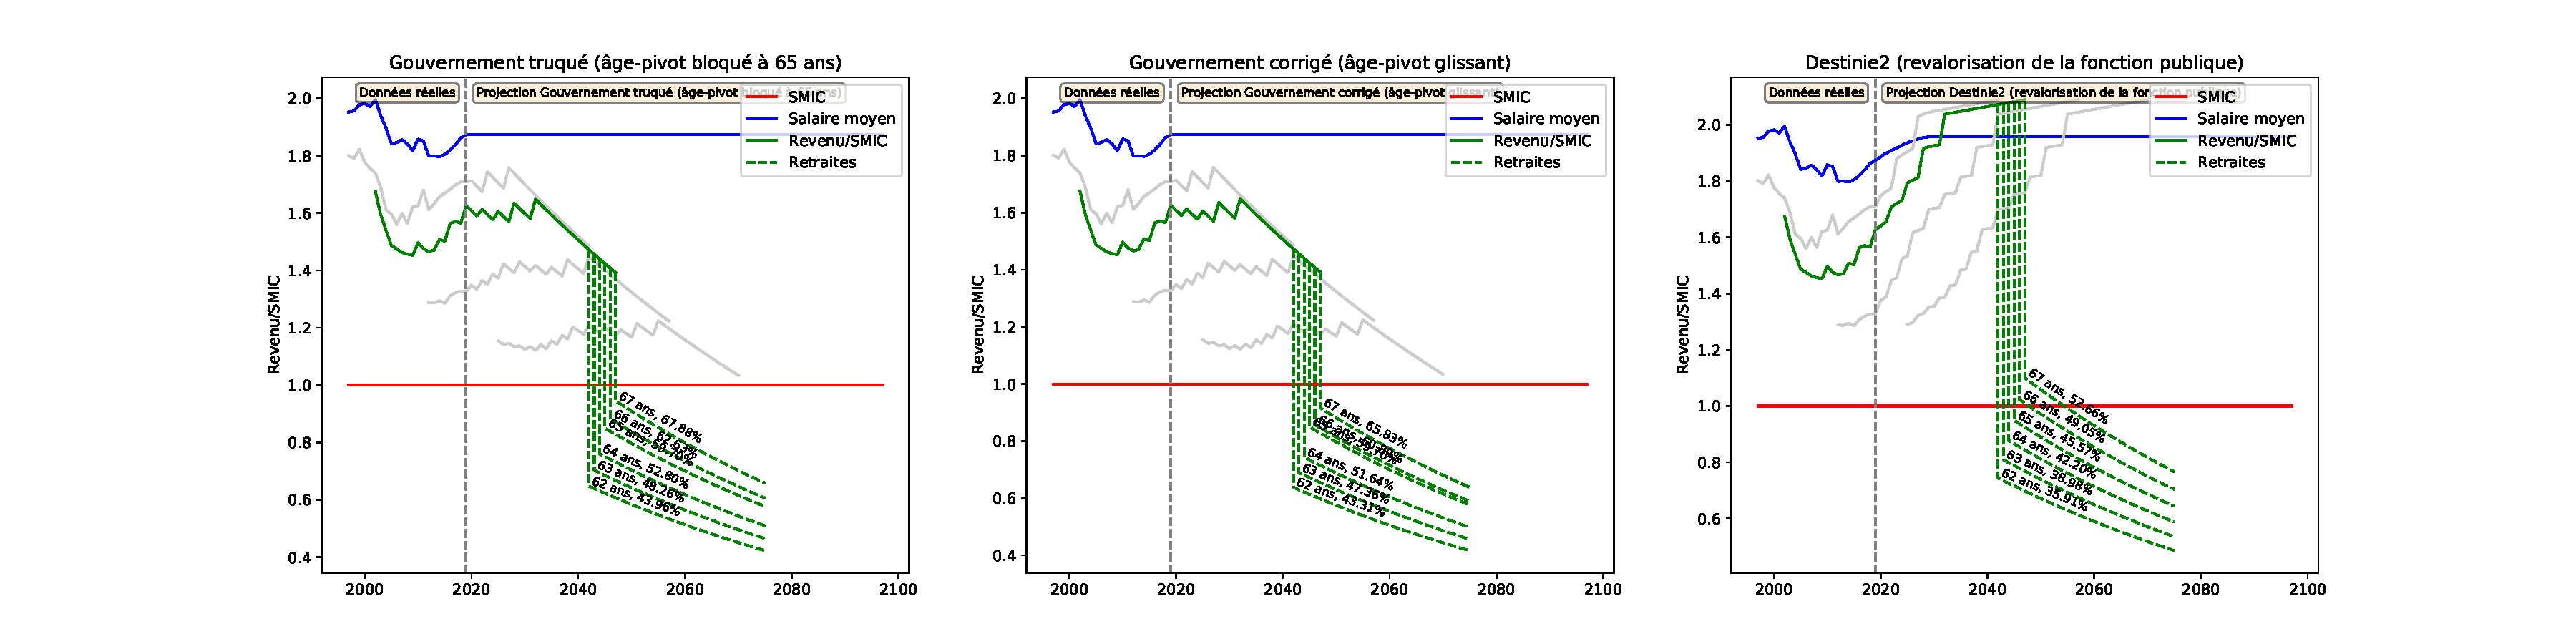
\includegraphics[width=0.9\textwidth]{fig/SecretaireAdmin_1980_22_dest_retraite.pdf}\end{center} \label{fig/SecretaireAdmin_1980_22_dest_retraite.pdf} 

\newpage 
 
\paragraph{Revenus et points pour le modèle \emph{Gouvernement truqué (âge-pivot bloqué à 65 ans)}} 
 
{ \scriptsize \begin{center} 
\begin{tabular}[htb]{|c|c||c|c|c|c|c|c||c|c||c|c|c|} 
\hline 
 Année &  Âge &  Ind Maj &  Pt Ind(\euro{} 2019) &  Rev HP(\euro{} 2019) &  Tx Primes &  GIPA(\euro{} 2019) &  Revenu(\euro{} 2019) &  SMIC(\euro{} 2019) &  Rev/SMIC &  Cumul Pts &  Achat Pt(\euro{} 2019) &  Serv. Pt(\euro{} 2019) \\ 
\hline \hline 
 2002 &  22 &  339.0 &  5.49 &  1859.85 &  30.41 &  0.00 &  2425.43 &  1447.74 &  {\bf 1.68} &  817.40 &  35.61 &  0.50 \\ 
\hline 
 2003 &  23 &  339.0 &  5.37 &  1822.00 &  30.64 &  0.00 &  2380.26 &  1493.03 &  {\bf 1.59} &  1619.57 &  35.61 &  0.50 \\ 
\hline 
 2004 &  24 &  344.0 &  5.29 &  1819.66 &  30.87 &  0.00 &  2381.39 &  1547.32 &  {\bf 1.54} &  2422.13 &  35.61 &  0.50 \\ 
\hline 
 2005 &  25 &  344.0 &  5.29 &  1819.47 &  31.10 &  0.00 &  2385.32 &  1603.67 &  {\bf 1.49} &  3226.01 &  35.61 &  0.50 \\ 
\hline 
 2006 &  26 &  349.0 &  5.23 &  1825.31 &  31.33 &  0.00 &  2397.18 &  1625.00 &  {\bf 1.48} &  4033.89 &  35.61 &  0.50 \\ 
\hline 
 2007 &  27 &  349.0 &  5.19 &  1812.87 &  31.56 &  5.27 &  2390.29 &  1634.08 &  {\bf 1.46} &  4839.45 &  35.61 &  0.50 \\ 
\hline 
 2008 &  28 &  356.0 &  5.09 &  1813.12 &  31.79 &  0.00 &  2389.52 &  1640.24 &  {\bf 1.46} &  5644.75 &  35.61 &  0.50 \\ 
\hline 
 2009 &  29 &  356.0 &  5.13 &  1825.97 &  32.02 &  0.00 &  2410.65 &  1659.42 &  {\bf 1.45} &  6457.16 &  35.61 &  0.50 \\ 
\hline 
 2010 &  30 &  366.0 &  5.08 &  1858.30 &  32.25 &  0.00 &  2457.60 &  1641.90 &  {\bf 1.50} &  7285.41 &  35.61 &  0.50 \\ 
\hline 
 2011 &  31 &  366.0 &  4.97 &  1819.69 &  32.48 &  0.00 &  2410.73 &  1633.19 &  {\bf 1.48} &  8097.85 &  35.61 &  0.50 \\ 
\hline 
 2012 &  32 &  379.0 &  4.88 &  1848.17 &  32.71 &  0.00 &  2452.71 &  1673.05 &  {\bf 1.47} &  8924.44 &  35.61 &  0.50 \\ 
\hline 
 2013 &  33 &  379.0 &  4.83 &  1832.33 &  32.94 &  11.54 &  2447.45 &  1664.01 &  {\bf 1.47} &  9749.26 &  35.61 &  0.50 \\ 
\hline 
 2014 &  34 &  394.0 &  4.81 &  1895.32 &  33.17 &  0.00 &  2523.99 &  1673.24 &  {\bf 1.51} &  10599.88 &  35.61 &  0.50 \\ 
\hline 
 2015 &  35 &  394.0 &  4.81 &  1894.58 &  33.40 &  6.19 &  2533.56 &  1686.62 &  {\bf 1.50} &  11453.72 &  35.61 &  0.50 \\ 
\hline 
 2016 &  36 &  413.0 &  4.80 &  1981.98 &  33.63 &  0.00 &  2648.51 &  1693.76 &  {\bf 1.56} &  12346.30 &  35.61 &  0.50 \\ 
\hline 
 2017 &  37 &  413.0 &  4.81 &  1985.97 &  33.86 &  0.00 &  2658.42 &  1692.60 &  {\bf 1.57} &  13242.22 &  35.61 &  0.50 \\ 
\hline 
 2018 &  38 &  413.0 &  4.74 &  1958.55 &  34.09 &  19.05 &  2645.27 &  1689.76 &  {\bf 1.57} &  14133.71 &  35.61 &  0.50 \\ 
\hline 
 2019 &  39 &  429.0 &  4.79 &  2056.81 &  34.32 &  0.00 &  2762.70 &  1698.45 &  {\bf 1.63} &  15064.77 &  35.61 &  0.50 \\ 
\hline 
 2020 &  40 &  429.0 &  4.79 &  2056.81 &  34.55 &  0.00 &  2767.43 &  1720.53 &  {\bf 1.61} &  15997.43 &  35.61 &  0.50 \\ 
\hline 
 2021 &  41 &  429.0 &  4.79 &  2056.81 &  34.78 &  0.00 &  2772.16 &  1742.90 &  {\bf 1.59} &  16931.69 &  35.61 &  0.50 \\ 
\hline 
 2022 &  42 &  440.0 &  4.79 &  2109.55 &  35.01 &  0.00 &  2848.10 &  1765.55 &  {\bf 1.61} &  17891.53 &  35.61 &  0.50 \\ 
\hline 
 2023 &  43 &  440.0 &  4.79 &  2109.55 &  35.24 &  0.00 &  2852.95 &  1788.51 &  {\bf 1.60} &  18853.01 &  35.61 &  0.50 \\ 
\hline 
 2024 &  44 &  440.0 &  4.79 &  2109.55 &  35.47 &  0.00 &  2857.80 &  1811.76 &  {\bf 1.58} &  19816.12 &  35.61 &  0.50 \\ 
\hline 
 2025 &  45 &  453.0 &  4.79 &  2171.87 &  35.70 &  0.00 &  2947.23 &  1835.31 &  {\bf 1.61} &  20809.37 &  35.61 &  0.50 \\ 
\hline 
 2026 &  46 &  453.0 &  4.79 &  2171.87 &  35.93 &  0.00 &  2952.23 &  1859.17 &  {\bf 1.59} &  21804.31 &  35.61 &  0.50 \\ 
\hline 
 2027 &  47 &  453.0 &  4.79 &  2171.87 &  36.16 &  0.00 &  2957.22 &  1883.34 &  {\bf 1.57} &  22800.93 &  35.61 &  0.50 \\ 
\hline 
 2028 &  48 &  477.0 &  4.79 &  2286.94 &  36.39 &  0.00 &  3119.16 &  1907.82 &  {\bf 1.63} &  23852.12 &  35.61 &  0.50 \\ 
\hline 
 2029 &  49 &  477.0 &  4.79 &  2286.94 &  36.62 &  0.00 &  3124.42 &  1932.62 &  {\bf 1.62} &  24904.29 &  35.63 &  0.50 \\ 
\hline 
 2030 &  50 &  477.0 &  4.79 &  2286.94 &  36.85 &  0.00 &  3129.68 &  1957.75 &  {\bf 1.60} &  25956.63 &  35.69 &  0.50 \\ 
\hline 
 2031 &  51 &  477.0 &  4.79 &  2286.94 &  37.08 &  0.00 &  3134.94 &  1983.20 &  {\bf 1.58} &  27008.34 &  35.77 &  0.50 \\ 
\hline 
 2032 &  52 &  503.0 &  4.79 &  2411.59 &  37.31 &  0.00 &  3311.36 &  2008.98 &  {\bf 1.65} &  28115.86 &  35.88 &  0.50 \\ 
\hline 
 2033 &  53 &  503.0 &  4.79 &  2411.59 &  37.54 &  0.00 &  3316.91 &  2035.10 &  {\bf 1.63} &  29221.03 &  36.02 &  0.50 \\ 
\hline 
 2034 &  54 &  503.0 &  4.79 &  2411.59 &  37.77 &  0.00 &  3322.45 &  2061.55 &  {\bf 1.61} &  30323.01 &  36.18 &  0.50 \\ 
\hline 
 2035 &  55 &  503.0 &  4.79 &  2411.59 &  38.00 &  0.00 &  3328.00 &  2088.35 &  {\bf 1.59} &  31420.98 &  36.37 &  0.51 \\ 
\hline 
 2036 &  56 &  503.0 &  4.79 &  2411.59 &  38.23 &  0.00 &  3333.55 &  2115.50 &  {\bf 1.58} &  32514.11 &  36.59 &  0.51 \\ 
\hline 
 2037 &  57 &  503.0 &  4.79 &  2411.59 &  38.46 &  0.00 &  3339.09 &  2143.00 &  {\bf 1.56} &  33601.60 &  36.85 &  0.51 \\ 
\hline 
 2038 &  58 &  503.0 &  4.79 &  2411.59 &  38.69 &  0.00 &  3344.64 &  2170.86 &  {\bf 1.54} &  34682.66 &  37.13 &  0.52 \\ 
\hline 
 2039 &  59 &  503.0 &  4.79 &  2411.59 &  38.92 &  0.00 &  3350.19 &  2199.08 &  {\bf 1.52} &  35756.49 &  37.44 &  0.52 \\ 
\hline 
 2040 &  60 &  503.0 &  4.79 &  2411.59 &  39.15 &  0.00 &  3355.73 &  2227.67 &  {\bf 1.51} &  36822.34 &  37.78 &  0.53 \\ 
\hline 
 2041 &  61 &  503.0 &  4.79 &  2411.59 &  39.38 &  0.00 &  3361.28 &  2256.63 &  {\bf 1.49} &  37879.46 &  38.16 &  0.53 \\ 
\hline 
 2042 &  62 &  503.0 &  4.79 &  2411.59 &  39.61 &  0.00 &  3366.83 &  2285.97 &  {\bf 1.47} &  38927.12 &  38.56 &  0.54 \\ 
\hline 
 2043 &  63 &  503.0 &  4.79 &  2411.59 &  39.84 &  0.00 &  3372.37 &  2315.68 &  {\bf 1.46} &  39964.61 &  39.01 &  0.54 \\ 
\hline 
 2044 &  64 &  503.0 &  4.79 &  2411.59 &  40.07 &  0.00 &  3377.92 &  2345.79 &  {\bf 1.44} &  40991.25 &  39.48 &  0.55 \\ 
\hline 
 2045 &  65 &  503.0 &  4.79 &  2411.59 &  40.30 &  0.00 &  3383.47 &  2376.28 &  {\bf 1.42} &  42006.38 &  40.00 &  0.56 \\ 
\hline 
 2046 &  66 &  503.0 &  4.79 &  2411.59 &  40.53 &  0.00 &  3389.01 &  2407.18 &  {\bf 1.41} &  43010.13 &  40.52 &  0.56 \\ 
\hline 
 2047 &  67 &  503.0 &  4.79 &  2411.59 &  40.76 &  0.00 &  3394.56 &  2438.47 &  {\bf 1.39} &  44002.62 &  41.04 &  0.57 \\ 
\hline 
\hline 
\end{tabular} 
\end{center} } 
\newpage 
 
\paragraph{Revenus et points pour le modèle \emph{Gouvernement corrigé (âge-pivot glissant)}} 
 
{ \scriptsize \begin{center} 
\begin{tabular}[htb]{|c|c||c|c|c|c|c|c||c|c||c|c|c|} 
\hline 
 Année &  Âge &  Ind Maj &  Pt Ind(\euro{} 2019) &  Rev HP(\euro{} 2019) &  Tx Primes &  GIPA(\euro{} 2019) &  Revenu(\euro{} 2019) &  SMIC(\euro{} 2019) &  Rev/SMIC &  Cumul Pts &  Achat Pt(\euro{} 2019) &  Serv. Pt(\euro{} 2019) \\ 
\hline \hline 
 2002 &  22 &  339.0 &  5.49 &  1859.85 &  30.41 &  0.00 &  2425.43 &  1447.74 &  {\bf 1.68} &  817.40 &  35.61 &  0.50 \\ 
\hline 
 2003 &  23 &  339.0 &  5.37 &  1822.00 &  30.64 &  0.00 &  2380.26 &  1493.03 &  {\bf 1.59} &  1619.57 &  35.61 &  0.50 \\ 
\hline 
 2004 &  24 &  344.0 &  5.29 &  1819.66 &  30.87 &  0.00 &  2381.39 &  1547.32 &  {\bf 1.54} &  2422.13 &  35.61 &  0.50 \\ 
\hline 
 2005 &  25 &  344.0 &  5.29 &  1819.47 &  31.10 &  0.00 &  2385.32 &  1603.67 &  {\bf 1.49} &  3226.01 &  35.61 &  0.50 \\ 
\hline 
 2006 &  26 &  349.0 &  5.23 &  1825.31 &  31.33 &  0.00 &  2397.18 &  1625.00 &  {\bf 1.48} &  4033.89 &  35.61 &  0.50 \\ 
\hline 
 2007 &  27 &  349.0 &  5.19 &  1812.87 &  31.56 &  5.27 &  2390.29 &  1634.08 &  {\bf 1.46} &  4839.45 &  35.61 &  0.50 \\ 
\hline 
 2008 &  28 &  356.0 &  5.09 &  1813.12 &  31.79 &  0.00 &  2389.52 &  1640.24 &  {\bf 1.46} &  5644.75 &  35.61 &  0.50 \\ 
\hline 
 2009 &  29 &  356.0 &  5.13 &  1825.97 &  32.02 &  0.00 &  2410.65 &  1659.42 &  {\bf 1.45} &  6457.16 &  35.61 &  0.50 \\ 
\hline 
 2010 &  30 &  366.0 &  5.08 &  1858.30 &  32.25 &  0.00 &  2457.60 &  1641.90 &  {\bf 1.50} &  7285.41 &  35.61 &  0.50 \\ 
\hline 
 2011 &  31 &  366.0 &  4.97 &  1819.69 &  32.48 &  0.00 &  2410.73 &  1633.19 &  {\bf 1.48} &  8097.85 &  35.61 &  0.50 \\ 
\hline 
 2012 &  32 &  379.0 &  4.88 &  1848.17 &  32.71 &  0.00 &  2452.71 &  1673.05 &  {\bf 1.47} &  8924.44 &  35.61 &  0.50 \\ 
\hline 
 2013 &  33 &  379.0 &  4.83 &  1832.33 &  32.94 &  11.54 &  2447.45 &  1664.01 &  {\bf 1.47} &  9749.26 &  35.61 &  0.50 \\ 
\hline 
 2014 &  34 &  394.0 &  4.81 &  1895.32 &  33.17 &  0.00 &  2523.99 &  1673.24 &  {\bf 1.51} &  10599.88 &  35.61 &  0.50 \\ 
\hline 
 2015 &  35 &  394.0 &  4.81 &  1894.58 &  33.40 &  6.19 &  2533.56 &  1686.62 &  {\bf 1.50} &  11453.72 &  35.61 &  0.50 \\ 
\hline 
 2016 &  36 &  413.0 &  4.80 &  1981.98 &  33.63 &  0.00 &  2648.51 &  1693.76 &  {\bf 1.56} &  12346.30 &  35.61 &  0.50 \\ 
\hline 
 2017 &  37 &  413.0 &  4.81 &  1985.97 &  33.86 &  0.00 &  2658.42 &  1692.60 &  {\bf 1.57} &  13242.22 &  35.61 &  0.50 \\ 
\hline 
 2018 &  38 &  413.0 &  4.74 &  1958.55 &  34.09 &  19.05 &  2645.27 &  1689.76 &  {\bf 1.57} &  14133.71 &  35.61 &  0.50 \\ 
\hline 
 2019 &  39 &  429.0 &  4.79 &  2056.81 &  34.32 &  0.00 &  2762.70 &  1698.45 &  {\bf 1.63} &  15064.77 &  35.61 &  0.50 \\ 
\hline 
 2020 &  40 &  429.0 &  4.79 &  2056.81 &  34.55 &  0.00 &  2767.43 &  1720.53 &  {\bf 1.61} &  15997.43 &  35.61 &  0.50 \\ 
\hline 
 2021 &  41 &  429.0 &  4.79 &  2056.81 &  34.78 &  0.00 &  2772.16 &  1742.90 &  {\bf 1.59} &  16931.69 &  35.61 &  0.50 \\ 
\hline 
 2022 &  42 &  440.0 &  4.79 &  2109.55 &  35.01 &  0.00 &  2848.10 &  1765.55 &  {\bf 1.61} &  17891.53 &  35.61 &  0.50 \\ 
\hline 
 2023 &  43 &  440.0 &  4.79 &  2109.55 &  35.24 &  0.00 &  2852.95 &  1788.51 &  {\bf 1.60} &  18853.01 &  35.61 &  0.50 \\ 
\hline 
 2024 &  44 &  440.0 &  4.79 &  2109.55 &  35.47 &  0.00 &  2857.80 &  1811.76 &  {\bf 1.58} &  19816.12 &  35.61 &  0.50 \\ 
\hline 
 2025 &  45 &  453.0 &  4.79 &  2171.87 &  35.70 &  0.00 &  2947.23 &  1835.31 &  {\bf 1.61} &  20809.37 &  35.61 &  0.50 \\ 
\hline 
 2026 &  46 &  453.0 &  4.79 &  2171.87 &  35.93 &  0.00 &  2952.23 &  1859.17 &  {\bf 1.59} &  21804.31 &  35.61 &  0.50 \\ 
\hline 
 2027 &  47 &  453.0 &  4.79 &  2171.87 &  36.16 &  0.00 &  2957.22 &  1883.34 &  {\bf 1.57} &  22800.93 &  35.61 &  0.50 \\ 
\hline 
 2028 &  48 &  477.0 &  4.79 &  2286.94 &  36.39 &  0.00 &  3119.16 &  1907.82 &  {\bf 1.63} &  23852.12 &  35.61 &  0.50 \\ 
\hline 
 2029 &  49 &  477.0 &  4.79 &  2286.94 &  36.62 &  0.00 &  3124.42 &  1932.62 &  {\bf 1.62} &  24904.29 &  35.63 &  0.50 \\ 
\hline 
 2030 &  50 &  477.0 &  4.79 &  2286.94 &  36.85 &  0.00 &  3129.68 &  1957.75 &  {\bf 1.60} &  25956.63 &  35.69 &  0.50 \\ 
\hline 
 2031 &  51 &  477.0 &  4.79 &  2286.94 &  37.08 &  0.00 &  3134.94 &  1983.20 &  {\bf 1.58} &  27008.34 &  35.77 &  0.50 \\ 
\hline 
 2032 &  52 &  503.0 &  4.79 &  2411.59 &  37.31 &  0.00 &  3311.36 &  2008.98 &  {\bf 1.65} &  28115.86 &  35.88 &  0.50 \\ 
\hline 
 2033 &  53 &  503.0 &  4.79 &  2411.59 &  37.54 &  0.00 &  3316.91 &  2035.10 &  {\bf 1.63} &  29221.03 &  36.02 &  0.50 \\ 
\hline 
 2034 &  54 &  503.0 &  4.79 &  2411.59 &  37.77 &  0.00 &  3322.45 &  2061.55 &  {\bf 1.61} &  30323.01 &  36.18 &  0.50 \\ 
\hline 
 2035 &  55 &  503.0 &  4.79 &  2411.59 &  38.00 &  0.00 &  3328.00 &  2088.35 &  {\bf 1.59} &  31420.98 &  36.37 &  0.51 \\ 
\hline 
 2036 &  56 &  503.0 &  4.79 &  2411.59 &  38.23 &  0.00 &  3333.55 &  2115.50 &  {\bf 1.58} &  32514.11 &  36.59 &  0.51 \\ 
\hline 
 2037 &  57 &  503.0 &  4.79 &  2411.59 &  38.46 &  0.00 &  3339.09 &  2143.00 &  {\bf 1.56} &  33601.60 &  36.85 &  0.51 \\ 
\hline 
 2038 &  58 &  503.0 &  4.79 &  2411.59 &  38.69 &  0.00 &  3344.64 &  2170.86 &  {\bf 1.54} &  34682.66 &  37.13 &  0.52 \\ 
\hline 
 2039 &  59 &  503.0 &  4.79 &  2411.59 &  38.92 &  0.00 &  3350.19 &  2199.08 &  {\bf 1.52} &  35756.49 &  37.44 &  0.52 \\ 
\hline 
 2040 &  60 &  503.0 &  4.79 &  2411.59 &  39.15 &  0.00 &  3355.73 &  2227.67 &  {\bf 1.51} &  36822.34 &  37.78 &  0.53 \\ 
\hline 
 2041 &  61 &  503.0 &  4.79 &  2411.59 &  39.38 &  0.00 &  3361.28 &  2256.63 &  {\bf 1.49} &  37879.46 &  38.16 &  0.53 \\ 
\hline 
 2042 &  62 &  503.0 &  4.79 &  2411.59 &  39.61 &  0.00 &  3366.83 &  2285.97 &  {\bf 1.47} &  38927.12 &  38.56 &  0.54 \\ 
\hline 
 2043 &  63 &  503.0 &  4.79 &  2411.59 &  39.84 &  0.00 &  3372.37 &  2315.68 &  {\bf 1.46} &  39964.61 &  39.01 &  0.54 \\ 
\hline 
 2044 &  64 &  503.0 &  4.79 &  2411.59 &  40.07 &  0.00 &  3377.92 &  2345.79 &  {\bf 1.44} &  40991.25 &  39.48 &  0.55 \\ 
\hline 
 2045 &  65 &  503.0 &  4.79 &  2411.59 &  40.30 &  0.00 &  3383.47 &  2376.28 &  {\bf 1.42} &  42006.38 &  40.00 &  0.56 \\ 
\hline 
 2046 &  66 &  503.0 &  4.79 &  2411.59 &  40.53 &  0.00 &  3389.01 &  2407.18 &  {\bf 1.41} &  43010.13 &  40.52 &  0.56 \\ 
\hline 
 2047 &  67 &  503.0 &  4.79 &  2411.59 &  40.76 &  0.00 &  3394.56 &  2438.47 &  {\bf 1.39} &  44002.62 &  41.04 &  0.57 \\ 
\hline 
\hline 
\end{tabular} 
\end{center} } 
\newpage 
 
\paragraph{Revenus et points pour le modèle \emph{Destinie2 (revalorisation de la fonction publique)}} 
 
{ \scriptsize \begin{center} 
\begin{tabular}[htb]{|c|c||c|c|c|c|c|c||c|c||c|c|c|} 
\hline 
 Année &  Âge &  Ind Maj &  Pt Ind(\euro{} 2019) &  Rev HP(\euro{} 2019) &  Tx Primes &  GIPA(\euro{} 2019) &  Revenu(\euro{} 2019) &  SMIC(\euro{} 2019) &  Rev/SMIC &  Cumul Pts &  Achat Pt(\euro{} 2019) &  Serv. Pt(\euro{} 2019) \\ 
\hline \hline 
 2002 &  22 &  339.0 &  5.49 &  1859.85 &  30.41 &  0.00 &  2425.43 &  1447.74 &  {\bf 1.68} &  815.39 &  35.69 &  0.50 \\ 
\hline 
 2003 &  23 &  339.0 &  5.37 &  1822.00 &  30.64 &  0.00 &  2380.26 &  1493.03 &  {\bf 1.59} &  1615.59 &  35.69 &  0.50 \\ 
\hline 
 2004 &  24 &  344.0 &  5.29 &  1819.66 &  30.87 &  0.00 &  2381.39 &  1547.32 &  {\bf 1.54} &  2416.18 &  35.69 &  0.50 \\ 
\hline 
 2005 &  25 &  344.0 &  5.29 &  1819.47 &  31.10 &  0.00 &  2385.32 &  1603.67 &  {\bf 1.49} &  3218.09 &  35.69 &  0.50 \\ 
\hline 
 2006 &  26 &  349.0 &  5.23 &  1825.31 &  31.33 &  0.00 &  2397.18 &  1625.00 &  {\bf 1.48} &  4023.98 &  35.69 &  0.50 \\ 
\hline 
 2007 &  27 &  349.0 &  5.19 &  1812.87 &  31.56 &  5.27 &  2390.29 &  1634.08 &  {\bf 1.46} &  4827.56 &  35.69 &  0.50 \\ 
\hline 
 2008 &  28 &  356.0 &  5.09 &  1813.12 &  31.79 &  0.00 &  2389.52 &  1640.24 &  {\bf 1.46} &  5630.88 &  35.69 &  0.50 \\ 
\hline 
 2009 &  29 &  356.0 &  5.13 &  1825.97 &  32.02 &  0.00 &  2410.65 &  1659.42 &  {\bf 1.45} &  6441.30 &  35.69 &  0.50 \\ 
\hline 
 2010 &  30 &  366.0 &  5.08 &  1858.30 &  32.25 &  0.00 &  2457.60 &  1641.90 &  {\bf 1.50} &  7267.51 &  35.69 &  0.50 \\ 
\hline 
 2011 &  31 &  366.0 &  4.97 &  1819.69 &  32.48 &  0.00 &  2410.73 &  1633.19 &  {\bf 1.48} &  8077.95 &  35.69 &  0.50 \\ 
\hline 
 2012 &  32 &  379.0 &  4.88 &  1848.17 &  32.71 &  0.00 &  2452.71 &  1673.05 &  {\bf 1.47} &  8902.51 &  35.69 &  0.50 \\ 
\hline 
 2013 &  33 &  379.0 &  4.83 &  1832.33 &  32.94 &  11.54 &  2447.45 &  1664.01 &  {\bf 1.47} &  9725.31 &  35.69 &  0.50 \\ 
\hline 
 2014 &  34 &  394.0 &  4.81 &  1895.32 &  33.17 &  0.00 &  2523.99 &  1673.24 &  {\bf 1.51} &  10573.83 &  35.69 &  0.50 \\ 
\hline 
 2015 &  35 &  394.0 &  4.81 &  1894.58 &  33.40 &  6.19 &  2533.56 &  1686.62 &  {\bf 1.50} &  11425.58 &  35.69 &  0.50 \\ 
\hline 
 2016 &  36 &  413.0 &  4.80 &  1981.98 &  33.63 &  0.00 &  2648.51 &  1693.76 &  {\bf 1.56} &  12315.96 &  35.69 &  0.50 \\ 
\hline 
 2017 &  37 &  413.0 &  4.81 &  1985.97 &  33.86 &  0.00 &  2658.42 &  1692.60 &  {\bf 1.57} &  13209.68 &  35.69 &  0.50 \\ 
\hline 
 2018 &  38 &  413.0 &  4.74 &  1958.55 &  34.09 &  19.05 &  2645.27 &  1689.76 &  {\bf 1.57} &  14098.98 &  35.69 &  0.50 \\ 
\hline 
 2019 &  39 &  429.0 &  4.79 &  2056.81 &  34.32 &  0.00 &  2762.70 &  1698.45 &  {\bf 1.63} &  15027.76 &  35.69 &  0.50 \\ 
\hline 
 2020 &  40 &  429.0 &  4.83 &  2073.26 &  34.55 &  0.00 &  2789.57 &  1699.99 &  {\bf 1.64} &  15965.57 &  35.69 &  0.50 \\ 
\hline 
 2021 &  41 &  429.0 &  4.88 &  2091.92 &  34.78 &  0.00 &  2819.49 &  1703.48 &  {\bf 1.66} &  16913.44 &  35.69 &  0.50 \\ 
\hline 
 2022 &  42 &  440.0 &  4.93 &  2167.02 &  35.01 &  0.00 &  2925.69 &  1712.78 &  {\bf 1.71} &  17897.01 &  35.69 &  0.50 \\ 
\hline 
 2023 &  43 &  440.0 &  4.98 &  2192.37 &  35.24 &  0.00 &  2964.96 &  1723.51 &  {\bf 1.72} &  18893.78 &  35.69 &  0.50 \\ 
\hline 
 2024 &  44 &  440.0 &  5.04 &  2218.46 &  35.47 &  0.00 &  3005.35 &  1735.69 &  {\bf 1.73} &  19904.13 &  35.69 &  0.50 \\ 
\hline 
 2025 &  45 &  453.0 &  5.10 &  2311.87 &  35.70 &  0.00 &  3137.21 &  1749.35 &  {\bf 1.79} &  20958.81 &  35.69 &  0.50 \\ 
\hline 
 2026 &  46 &  453.0 &  5.17 &  2340.77 &  35.93 &  0.00 &  3181.81 &  1764.53 &  {\bf 1.80} &  22028.48 &  35.69 &  0.50 \\ 
\hline 
 2027 &  47 &  453.0 &  5.23 &  2370.73 &  36.16 &  0.00 &  3227.98 &  1781.27 &  {\bf 1.81} &  23113.68 &  35.69 &  0.50 \\ 
\hline 
 2028 &  48 &  477.0 &  5.30 &  2529.03 &  36.39 &  0.00 &  3449.35 &  1799.59 &  {\bf 1.92} &  24273.29 &  35.69 &  0.50 \\ 
\hline 
 2029 &  49 &  477.0 &  5.37 &  2559.63 &  36.62 &  0.00 &  3496.97 &  1819.55 &  {\bf 1.92} &  25448.09 &  35.72 &  0.50 \\ 
\hline 
 2030 &  50 &  477.0 &  5.43 &  2591.37 &  36.85 &  0.00 &  3546.29 &  1841.19 &  {\bf 1.93} &  26637.73 &  35.77 &  0.50 \\ 
\hline 
 2031 &  51 &  477.0 &  5.50 &  2624.28 &  37.08 &  0.00 &  3597.37 &  1864.58 &  {\bf 1.93} &  27841.82 &  35.85 &  0.50 \\ 
\hline 
 2032 &  52 &  503.0 &  5.57 &  2803.30 &  37.31 &  0.00 &  3849.21 &  1888.81 &  {\bf 2.04} &  29126.29 &  35.96 &  0.50 \\ 
\hline 
 2033 &  53 &  503.0 &  5.65 &  2839.74 &  37.54 &  0.00 &  3905.78 &  1913.37 &  {\bf 2.04} &  30424.70 &  36.10 &  0.50 \\ 
\hline 
 2034 &  54 &  503.0 &  5.72 &  2876.66 &  37.77 &  0.00 &  3963.18 &  1938.24 &  {\bf 2.04} &  31736.19 &  36.26 &  0.50 \\ 
\hline 
 2035 &  55 &  503.0 &  5.79 &  2914.06 &  38.00 &  0.00 &  4021.40 &  1963.44 &  {\bf 2.05} &  33059.90 &  36.46 &  0.51 \\ 
\hline 
 2036 &  56 &  503.0 &  5.87 &  2951.94 &  38.23 &  0.00 &  4080.47 &  1988.96 &  {\bf 2.05} &  34394.91 &  36.68 &  0.51 \\ 
\hline 
 2037 &  57 &  503.0 &  5.94 &  2990.32 &  38.46 &  0.00 &  4140.39 &  2014.82 &  {\bf 2.05} &  35740.29 &  36.93 &  0.51 \\ 
\hline 
 2038 &  58 &  503.0 &  6.02 &  3029.19 &  38.69 &  0.00 &  4201.18 &  2041.01 &  {\bf 2.06} &  37095.09 &  37.21 &  0.52 \\ 
\hline 
 2039 &  59 &  503.0 &  6.10 &  3068.57 &  38.92 &  0.00 &  4262.86 &  2067.55 &  {\bf 2.06} &  38458.34 &  37.52 &  0.52 \\ 
\hline 
 2040 &  60 &  503.0 &  6.18 &  3108.46 &  39.15 &  0.00 &  4325.42 &  2094.43 &  {\bf 2.07} &  39829.05 &  37.87 &  0.53 \\ 
\hline 
 2041 &  61 &  503.0 &  6.26 &  3148.87 &  39.38 &  0.00 &  4388.90 &  2121.65 &  {\bf 2.07} &  41206.20 &  38.24 &  0.53 \\ 
\hline 
 2042 &  62 &  503.0 &  6.34 &  3189.81 &  39.61 &  0.00 &  4453.29 &  2149.23 &  {\bf 2.07} &  42588.77 &  38.65 &  0.54 \\ 
\hline 
 2043 &  63 &  503.0 &  6.42 &  3231.27 &  39.84 &  0.00 &  4518.61 &  2177.17 &  {\bf 2.08} &  43975.72 &  39.10 &  0.54 \\ 
\hline 
 2044 &  64 &  503.0 &  6.51 &  3273.28 &  40.07 &  0.00 &  4584.88 &  2205.48 &  {\bf 2.08} &  45366.01 &  39.57 &  0.55 \\ 
\hline 
 2045 &  65 &  503.0 &  6.59 &  3315.83 &  40.30 &  0.00 &  4652.11 &  2234.15 &  {\bf 2.08} &  46758.59 &  40.09 &  0.56 \\ 
\hline 
 2046 &  66 &  503.0 &  6.68 &  3358.94 &  40.53 &  0.00 &  4720.32 &  2263.19 &  {\bf 2.09} &  48153.44 &  40.61 &  0.57 \\ 
\hline 
 2047 &  67 &  503.0 &  6.76 &  3402.61 &  40.76 &  0.00 &  4789.51 &  2292.61 &  {\bf 2.09} &  49550.58 &  41.14 &  0.57 \\ 
\hline 
\hline 
\end{tabular} 
\end{center} } 
\newpage 
 
\subsection{Génération 1990 (début en 2012)} 

\paragraph{Retraites possibles dans le modèle \emph{Gouvernement truqué (âge-pivot bloqué à 65 ans)}}  
 
{ \scriptsize \begin{center} 
\begin{tabular}[htb]{|c|c||c|c||c|c||c||c|c|c|c|c|c|} 
\hline 
 Retraite en &  Âge &  Âge pivot &  Décote/Surcote &  Retraite (\euro{} 2019) &  Tx Rempl(\%) &  SMIC (\euro{} 2019) &  Retraite/SMIC &  Rev70/SMIC &  Rev75/SMIC &  Rev80/SMIC &  Rev85/SMIC &  Rev90/SMIC \\ 
\hline \hline 
 2052 &  62 &  65 ans 0 mois &  -15.00\% &  1587.40 &  {\bf 47.15} &  2601.14 &  {\bf {\color{red} 0.61}} &  {\bf {\color{red} 0.55}} &  {\bf {\color{red} 0.52}} &  {\bf {\color{red} 0.48}} &  {\bf {\color{red} 0.45}} &  {\bf {\color{red} 0.43}} \\ 
\hline 
 2053 &  63 &  65 ans 0 mois &  -10.00\% &  1744.88 &  {\bf 51.74} &  2634.96 &  {\bf {\color{red} 0.66}} &  {\bf {\color{red} 0.60}} &  {\bf {\color{red} 0.57}} &  {\bf {\color{red} 0.53}} &  {\bf {\color{red} 0.50}} &  {\bf {\color{red} 0.47}} \\ 
\hline 
 2054 &  64 &  65 ans 0 mois &  -5.00\% &  1910.43 &  {\bf 56.56} &  2669.21 &  {\bf {\color{red} 0.72}} &  {\bf {\color{red} 0.66}} &  {\bf {\color{red} 0.62}} &  {\bf {\color{red} 0.58}} &  {\bf {\color{red} 0.55}} &  {\bf {\color{red} 0.51}} \\ 
\hline 
 2055 &  65 &  65 ans 0 mois &  0.00\% &  2298.33 &  {\bf 67.93} &  2703.91 &  {\bf {\color{red} 0.85}} &  {\bf {\color{red} 0.80}} &  {\bf {\color{red} 0.75}} &  {\bf {\color{red} 0.70}} &  {\bf {\color{red} 0.66}} &  {\bf {\color{red} 0.62}} \\ 
\hline 
 2056 &  66 &  65 ans 0 mois &  5.00\% &  2328.20 &  {\bf 68.70} &  2739.06 &  {\bf {\color{red} 0.85}} &  {\bf {\color{red} 0.81}} &  {\bf {\color{red} 0.76}} &  {\bf {\color{red} 0.71}} &  {\bf {\color{red} 0.67}} &  {\bf {\color{red} 0.62}} \\ 
\hline 
 2057 &  67 &  65 ans 0 mois &  10.00\% &  2457.17 &  {\bf 72.39} &  2774.67 &  {\bf {\color{red} 0.89}} &  {\bf {\color{red} 0.85}} &  {\bf {\color{red} 0.80}} &  {\bf {\color{red} 0.75}} &  {\bf {\color{red} 0.70}} &  {\bf {\color{red} 0.66}} \\ 
\hline 
\hline 
\end{tabular} 
\end{center} } 
\paragraph{Retraites possibles dans le modèle \emph{Gouvernement corrigé (âge-pivot glissant)}}  
 
{ \scriptsize \begin{center} 
\begin{tabular}[htb]{|c|c||c|c||c|c||c||c|c|c|c|c|c|} 
\hline 
 Retraite en &  Âge &  Âge pivot &  Décote/Surcote &  Retraite (\euro{} 2019) &  Tx Rempl(\%) &  SMIC (\euro{} 2019) &  Retraite/SMIC &  Rev70/SMIC &  Rev75/SMIC &  Rev80/SMIC &  Rev85/SMIC &  Rev90/SMIC \\ 
\hline \hline 
 2052 &  62 &  66 ans 1 mois &  -20.42\% &  1486.25 &  {\bf 44.14} &  2601.14 &  {\bf {\color{red} 0.57}} &  {\bf {\color{red} 0.52}} &  {\bf {\color{red} 0.48}} &  {\bf {\color{red} 0.45}} &  {\bf {\color{red} 0.42}} &  {\bf {\color{red} 0.40}} \\ 
\hline 
 2053 &  63 &  66 ans 2 mois &  -15.83\% &  1631.78 &  {\bf 48.39} &  2634.96 &  {\bf {\color{red} 0.62}} &  {\bf {\color{red} 0.57}} &  {\bf {\color{red} 0.53}} &  {\bf {\color{red} 0.50}} &  {\bf {\color{red} 0.47}} &  {\bf {\color{red} 0.44}} \\ 
\hline 
 2054 &  64 &  66 ans 3 mois &  -11.25\% &  1784.74 &  {\bf 52.84} &  2669.21 &  {\bf {\color{red} 0.67}} &  {\bf {\color{red} 0.62}} &  {\bf {\color{red} 0.58}} &  {\bf {\color{red} 0.54}} &  {\bf {\color{red} 0.51}} &  {\bf {\color{red} 0.48}} \\ 
\hline 
 2055 &  65 &  66 ans 4 mois &  -6.67\% &  2298.33 &  {\bf 67.93} &  2703.91 &  {\bf {\color{red} 0.85}} &  {\bf {\color{red} 0.80}} &  {\bf {\color{red} 0.75}} &  {\bf {\color{red} 0.70}} &  {\bf {\color{red} 0.66}} &  {\bf {\color{red} 0.62}} \\ 
\hline 
 2056 &  66 &  66 ans 5 mois &  -2.08\% &  2328.20 &  {\bf 68.70} &  2739.06 &  {\bf {\color{red} 0.85}} &  {\bf {\color{red} 0.81}} &  {\bf {\color{red} 0.76}} &  {\bf {\color{red} 0.71}} &  {\bf {\color{red} 0.67}} &  {\bf {\color{red} 0.62}} \\ 
\hline 
 2057 &  67 &  66 ans 6 mois &  2.50\% &  2358.47 &  {\bf 69.48} &  2774.67 &  {\bf {\color{red} 0.85}} &  {\bf {\color{red} 0.82}} &  {\bf {\color{red} 0.77}} &  {\bf {\color{red} 0.72}} &  {\bf {\color{red} 0.67}} &  {\bf {\color{red} 0.63}} \\ 
\hline 
\hline 
\end{tabular} 
\end{center} } 
\paragraph{Retraites possibles dans le modèle \emph{Destinie2 (revalorisation de la fonction publique)}}  
 
{ \scriptsize \begin{center} 
\begin{tabular}[htb]{|c|c||c|c||c|c||c||c|c|c|c|c|c|} 
\hline 
 Retraite en &  Âge &  Âge pivot &  Décote/Surcote &  Retraite (\euro{} 2019) &  Tx Rempl(\%) &  SMIC (\euro{} 2019) &  Retraite/SMIC &  Rev70/SMIC &  Rev75/SMIC &  Rev80/SMIC &  Rev85/SMIC &  Rev90/SMIC \\ 
\hline \hline 
 2052 &  62 &  66 ans 1 mois &  -20.42\% &  1787.96 &  {\bf 35.28} &  2445.56 &  {\bf {\color{red} 0.73}} &  {\bf {\color{red} 0.66}} &  {\bf {\color{red} 0.62}} &  {\bf {\color{red} 0.58}} &  {\bf {\color{red} 0.54}} &  {\bf {\color{red} 0.51}} \\ 
\hline 
 2053 &  63 &  66 ans 2 mois &  -15.83\% &  1975.75 &  {\bf 38.43} &  2477.35 &  {\bf {\color{red} 0.80}} &  {\bf {\color{red} 0.73}} &  {\bf {\color{red} 0.68}} &  {\bf {\color{red} 0.64}} &  {\bf {\color{red} 0.60}} &  {\bf {\color{red} 0.56}} \\ 
\hline 
 2054 &  64 &  66 ans 3 mois &  -11.25\% &  2174.88 &  {\bf 41.69} &  2509.56 &  {\bf {\color{red} 0.87}} &  {\bf {\color{red} 0.80}} &  {\bf {\color{red} 0.75}} &  {\bf {\color{red} 0.70}} &  {\bf {\color{red} 0.66}} &  {\bf {\color{red} 0.62}} \\ 
\hline 
 2055 &  65 &  66 ans 4 mois &  -6.67\% &  2385.70 &  {\bf 45.07} &  2542.18 &  {\bf {\color{red} 0.94}} &  {\bf {\color{red} 0.88}} &  {\bf {\color{red} 0.82}} &  {\bf {\color{red} 0.77}} &  {\bf {\color{red} 0.72}} &  {\bf {\color{red} 0.68}} \\ 
\hline 
 2056 &  66 &  66 ans 5 mois &  -2.08\% &  2608.59 &  {\bf 48.57} &  2575.23 &  {\bf 1.01} &  {\bf {\color{red} 0.96}} &  {\bf {\color{red} 0.90}} &  {\bf {\color{red} 0.85}} &  {\bf {\color{red} 0.79}} &  {\bf {\color{red} 0.74}} \\ 
\hline 
 2057 &  67 &  66 ans 6 mois &  2.50\% &  2843.95 &  {\bf 52.18} &  2608.71 &  {\bf 1.09} &  {\bf 1.05} &  {\bf {\color{red} 0.98}} &  {\bf {\color{red} 0.92}} &  {\bf {\color{red} 0.86}} &  {\bf {\color{red} 0.81}} \\ 
\hline 
\hline 
\end{tabular} 
\end{center} } 

 \begin{center}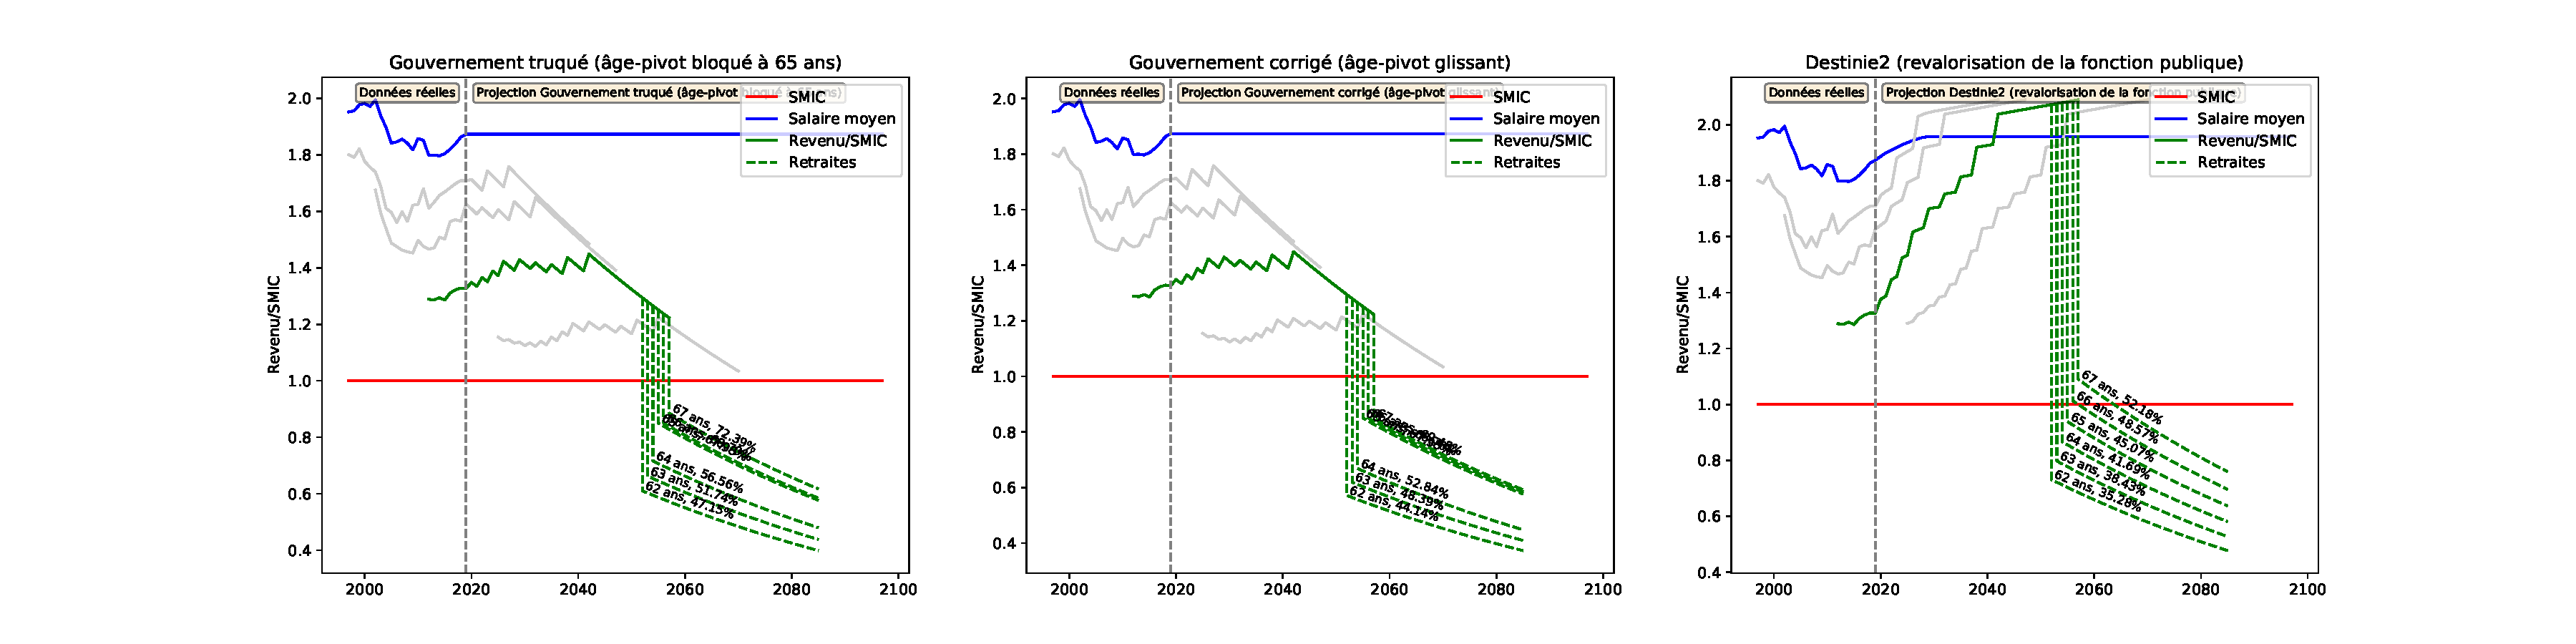
\includegraphics[width=0.9\textwidth]{fig/SecretaireAdmin_1990_22_dest_retraite.pdf}\end{center} \label{fig/SecretaireAdmin_1990_22_dest_retraite.pdf} 

\newpage 
 
\paragraph{Revenus et points pour le modèle \emph{Gouvernement truqué (âge-pivot bloqué à 65 ans)}} 
 
{ \scriptsize \begin{center} 
\begin{tabular}[htb]{|c|c||c|c|c|c|c|c||c|c||c|c|c|} 
\hline 
 Année &  Âge &  Ind Maj &  Pt Ind(\euro{} 2019) &  Rev HP(\euro{} 2019) &  Tx Primes &  GIPA(\euro{} 2019) &  Revenu(\euro{} 2019) &  SMIC(\euro{} 2019) &  Rev/SMIC &  Cumul Pts &  Achat Pt(\euro{} 2019) &  Serv. Pt(\euro{} 2019) \\ 
\hline \hline 
 2012 &  22 &  339.0 &  4.88 &  1653.11 &  30.41 &  0.00 &  2155.82 &  1673.05 &  {\bf 1.29} &  726.54 &  35.61 &  0.50 \\ 
\hline 
 2013 &  23 &  339.0 &  4.83 &  1638.95 &  30.64 &  0.00 &  2141.12 &  1664.01 &  {\bf 1.29} &  1448.12 &  35.61 &  0.50 \\ 
\hline 
 2014 &  24 &  344.0 &  4.81 &  1654.79 &  30.87 &  0.00 &  2165.63 &  1673.24 &  {\bf 1.29} &  2177.97 &  35.61 &  0.50 \\ 
\hline 
 2015 &  25 &  344.0 &  4.81 &  1654.15 &  31.10 &  0.00 &  2168.59 &  1686.62 &  {\bf 1.29} &  2908.81 &  35.61 &  0.50 \\ 
\hline 
 2016 &  26 &  349.0 &  4.80 &  1674.84 &  31.33 &  21.24 &  2220.81 &  1693.76 &  {\bf 1.31} &  3657.25 &  35.61 &  0.50 \\ 
\hline 
 2017 &  27 &  349.0 &  4.81 &  1678.22 &  31.56 &  30.24 &  2238.11 &  1692.60 &  {\bf 1.32} &  4411.51 &  35.61 &  0.50 \\ 
\hline 
 2018 &  28 &  356.0 &  4.74 &  1688.24 &  31.79 &  19.60 &  2244.53 &  1689.76 &  {\bf 1.33} &  5167.95 &  35.61 &  0.50 \\ 
\hline 
 2019 &  29 &  356.0 &  4.79 &  1706.81 &  32.02 &  0.00 &  2253.34 &  1698.45 &  {\bf 1.33} &  5927.35 &  35.61 &  0.50 \\ 
\hline 
 2020 &  30 &  366.0 &  4.79 &  1754.76 &  32.25 &  0.00 &  2320.67 &  1720.53 &  {\bf 1.35} &  6709.44 &  35.61 &  0.50 \\ 
\hline 
 2021 &  31 &  366.0 &  4.79 &  1754.76 &  32.48 &  0.00 &  2324.70 &  1742.90 &  {\bf 1.33} &  7492.90 &  35.61 &  0.50 \\ 
\hline 
 2022 &  32 &  379.0 &  4.79 &  1817.09 &  32.71 &  0.00 &  2411.45 &  1765.55 &  {\bf 1.37} &  8305.59 &  35.61 &  0.50 \\ 
\hline 
 2023 &  33 &  379.0 &  4.79 &  1817.09 &  32.94 &  0.00 &  2415.63 &  1788.51 &  {\bf 1.35} &  9119.69 &  35.61 &  0.50 \\ 
\hline 
 2024 &  34 &  394.0 &  4.79 &  1889.00 &  33.17 &  0.00 &  2515.58 &  1811.76 &  {\bf 1.39} &  9967.47 &  35.61 &  0.50 \\ 
\hline 
 2025 &  35 &  394.0 &  4.79 &  1889.00 &  33.40 &  0.00 &  2519.93 &  1835.31 &  {\bf 1.37} &  10816.71 &  35.61 &  0.50 \\ 
\hline 
 2026 &  36 &  413.0 &  4.79 &  1980.10 &  33.63 &  0.00 &  2646.00 &  1859.17 &  {\bf 1.42} &  11708.45 &  35.61 &  0.50 \\ 
\hline 
 2027 &  37 &  413.0 &  4.79 &  1980.10 &  33.86 &  0.00 &  2650.56 &  1883.34 &  {\bf 1.41} &  12601.72 &  35.61 &  0.50 \\ 
\hline 
 2028 &  38 &  413.0 &  4.79 &  1980.10 &  34.09 &  0.00 &  2655.11 &  1907.82 &  {\bf 1.39} &  13496.52 &  35.61 &  0.50 \\ 
\hline 
 2029 &  39 &  429.0 &  4.79 &  2056.81 &  34.32 &  0.00 &  2762.70 &  1932.62 &  {\bf 1.43} &  14426.88 &  35.63 &  0.50 \\ 
\hline 
 2030 &  40 &  429.0 &  4.79 &  2056.81 &  34.55 &  0.00 &  2767.43 &  1957.75 &  {\bf 1.41} &  15357.42 &  35.69 &  0.50 \\ 
\hline 
 2031 &  41 &  429.0 &  4.79 &  2056.81 &  34.78 &  0.00 &  2772.16 &  1983.20 &  {\bf 1.40} &  16287.42 &  35.77 &  0.50 \\ 
\hline 
 2032 &  42 &  440.0 &  4.79 &  2109.55 &  35.01 &  0.00 &  2848.10 &  2008.98 &  {\bf 1.42} &  17240.00 &  35.88 &  0.50 \\ 
\hline 
 2033 &  43 &  440.0 &  4.79 &  2109.55 &  35.24 &  0.00 &  2852.95 &  2035.10 &  {\bf 1.40} &  18190.58 &  36.02 &  0.50 \\ 
\hline 
 2034 &  44 &  440.0 &  4.79 &  2109.55 &  35.47 &  0.00 &  2857.80 &  2061.55 &  {\bf 1.39} &  19138.45 &  36.18 &  0.50 \\ 
\hline 
 2035 &  45 &  453.0 &  4.79 &  2171.87 &  35.70 &  0.00 &  2947.23 &  2088.35 &  {\bf 1.41} &  20110.80 &  36.37 &  0.51 \\ 
\hline 
 2036 &  46 &  453.0 &  4.79 &  2171.87 &  35.93 &  0.00 &  2952.23 &  2115.50 &  {\bf 1.40} &  21078.89 &  36.59 &  0.51 \\ 
\hline 
 2037 &  47 &  453.0 &  4.79 &  2171.87 &  36.16 &  0.00 &  2957.22 &  2143.00 &  {\bf 1.38} &  22042.01 &  36.85 &  0.51 \\ 
\hline 
 2038 &  48 &  477.0 &  4.79 &  2286.94 &  36.39 &  0.00 &  3119.16 &  2170.86 &  {\bf 1.44} &  23050.18 &  37.13 &  0.52 \\ 
\hline 
 2039 &  49 &  477.0 &  4.79 &  2286.94 &  36.62 &  0.00 &  3124.42 &  2199.08 &  {\bf 1.42} &  24051.65 &  37.44 &  0.52 \\ 
\hline 
 2040 &  50 &  477.0 &  4.79 &  2286.94 &  36.85 &  0.00 &  3129.68 &  2227.67 &  {\bf 1.40} &  25045.70 &  37.78 &  0.53 \\ 
\hline 
 2041 &  51 &  477.0 &  4.79 &  2286.94 &  37.08 &  0.00 &  3134.94 &  2256.63 &  {\bf 1.39} &  26031.63 &  38.16 &  0.53 \\ 
\hline 
 2042 &  52 &  503.0 &  4.79 &  2411.59 &  37.31 &  0.00 &  3311.36 &  2285.97 &  {\bf 1.45} &  27062.03 &  38.56 &  0.54 \\ 
\hline 
 2043 &  53 &  503.0 &  4.79 &  2411.59 &  37.54 &  0.00 &  3316.91 &  2315.68 &  {\bf 1.43} &  28082.46 &  39.01 &  0.54 \\ 
\hline 
 2044 &  54 &  503.0 &  4.79 &  2411.59 &  37.77 &  0.00 &  3322.45 &  2345.79 &  {\bf 1.42} &  29092.24 &  39.48 &  0.55 \\ 
\hline 
 2045 &  55 &  503.0 &  4.79 &  2411.59 &  38.00 &  0.00 &  3328.00 &  2376.28 &  {\bf 1.40} &  30090.74 &  40.00 &  0.56 \\ 
\hline 
 2046 &  56 &  503.0 &  4.79 &  2411.59 &  38.23 &  0.00 &  3333.55 &  2407.18 &  {\bf 1.38} &  31078.05 &  40.52 &  0.56 \\ 
\hline 
 2047 &  57 &  503.0 &  4.79 &  2411.59 &  38.46 &  0.00 &  3339.09 &  2438.47 &  {\bf 1.37} &  32054.33 &  41.04 &  0.57 \\ 
\hline 
 2048 &  58 &  503.0 &  4.79 &  2411.59 &  38.69 &  0.00 &  3344.64 &  2470.17 &  {\bf 1.35} &  33019.67 &  41.58 &  0.58 \\ 
\hline 
 2049 &  59 &  503.0 &  4.79 &  2411.59 &  38.92 &  0.00 &  3350.19 &  2502.28 &  {\bf 1.34} &  33974.20 &  42.12 &  0.59 \\ 
\hline 
 2050 &  60 &  503.0 &  4.79 &  2411.59 &  39.15 &  0.00 &  3355.73 &  2534.81 &  {\bf 1.32} &  34918.05 &  42.66 &  0.59 \\ 
\hline 
 2051 &  61 &  503.0 &  4.79 &  2411.59 &  39.38 &  0.00 &  3361.28 &  2567.76 &  {\bf 1.31} &  35851.32 &  43.22 &  0.60 \\ 
\hline 
 2052 &  62 &  503.0 &  4.79 &  2411.59 &  39.61 &  0.00 &  3366.83 &  2601.14 &  {\bf 1.29} &  36774.14 &  43.78 &  0.61 \\ 
\hline 
 2053 &  63 &  503.0 &  4.79 &  2411.59 &  39.84 &  0.00 &  3372.37 &  2634.96 &  {\bf 1.28} &  37686.61 &  44.35 &  0.62 \\ 
\hline 
 2054 &  64 &  503.0 &  4.79 &  2411.59 &  40.07 &  0.00 &  3377.92 &  2669.21 &  {\bf 1.27} &  38588.86 &  44.93 &  0.63 \\ 
\hline 
 2055 &  65 &  503.0 &  4.79 &  2411.59 &  40.30 &  0.00 &  3383.47 &  2703.91 &  {\bf 1.25} &  39480.99 &  45.51 &  0.63 \\ 
\hline 
 2056 &  66 &  503.0 &  4.79 &  2411.59 &  40.53 &  0.00 &  3389.01 &  2739.06 &  {\bf 1.24} &  40363.11 &  46.10 &  0.64 \\ 
\hline 
 2057 &  67 &  503.0 &  4.79 &  2411.59 &  40.76 &  0.00 &  3394.56 &  2774.67 &  {\bf 1.22} &  41235.34 &  46.70 &  0.65 \\ 
\hline 
\hline 
\end{tabular} 
\end{center} } 
\newpage 
 
\paragraph{Revenus et points pour le modèle \emph{Gouvernement corrigé (âge-pivot glissant)}} 
 
{ \scriptsize \begin{center} 
\begin{tabular}[htb]{|c|c||c|c|c|c|c|c||c|c||c|c|c|} 
\hline 
 Année &  Âge &  Ind Maj &  Pt Ind(\euro{} 2019) &  Rev HP(\euro{} 2019) &  Tx Primes &  GIPA(\euro{} 2019) &  Revenu(\euro{} 2019) &  SMIC(\euro{} 2019) &  Rev/SMIC &  Cumul Pts &  Achat Pt(\euro{} 2019) &  Serv. Pt(\euro{} 2019) \\ 
\hline \hline 
 2012 &  22 &  339.0 &  4.88 &  1653.11 &  30.41 &  0.00 &  2155.82 &  1673.05 &  {\bf 1.29} &  726.54 &  35.61 &  0.50 \\ 
\hline 
 2013 &  23 &  339.0 &  4.83 &  1638.95 &  30.64 &  0.00 &  2141.12 &  1664.01 &  {\bf 1.29} &  1448.12 &  35.61 &  0.50 \\ 
\hline 
 2014 &  24 &  344.0 &  4.81 &  1654.79 &  30.87 &  0.00 &  2165.63 &  1673.24 &  {\bf 1.29} &  2177.97 &  35.61 &  0.50 \\ 
\hline 
 2015 &  25 &  344.0 &  4.81 &  1654.15 &  31.10 &  0.00 &  2168.59 &  1686.62 &  {\bf 1.29} &  2908.81 &  35.61 &  0.50 \\ 
\hline 
 2016 &  26 &  349.0 &  4.80 &  1674.84 &  31.33 &  21.24 &  2220.81 &  1693.76 &  {\bf 1.31} &  3657.25 &  35.61 &  0.50 \\ 
\hline 
 2017 &  27 &  349.0 &  4.81 &  1678.22 &  31.56 &  30.24 &  2238.11 &  1692.60 &  {\bf 1.32} &  4411.51 &  35.61 &  0.50 \\ 
\hline 
 2018 &  28 &  356.0 &  4.74 &  1688.24 &  31.79 &  19.60 &  2244.53 &  1689.76 &  {\bf 1.33} &  5167.95 &  35.61 &  0.50 \\ 
\hline 
 2019 &  29 &  356.0 &  4.79 &  1706.81 &  32.02 &  0.00 &  2253.34 &  1698.45 &  {\bf 1.33} &  5927.35 &  35.61 &  0.50 \\ 
\hline 
 2020 &  30 &  366.0 &  4.79 &  1754.76 &  32.25 &  0.00 &  2320.67 &  1720.53 &  {\bf 1.35} &  6709.44 &  35.61 &  0.50 \\ 
\hline 
 2021 &  31 &  366.0 &  4.79 &  1754.76 &  32.48 &  0.00 &  2324.70 &  1742.90 &  {\bf 1.33} &  7492.90 &  35.61 &  0.50 \\ 
\hline 
 2022 &  32 &  379.0 &  4.79 &  1817.09 &  32.71 &  0.00 &  2411.45 &  1765.55 &  {\bf 1.37} &  8305.59 &  35.61 &  0.50 \\ 
\hline 
 2023 &  33 &  379.0 &  4.79 &  1817.09 &  32.94 &  0.00 &  2415.63 &  1788.51 &  {\bf 1.35} &  9119.69 &  35.61 &  0.50 \\ 
\hline 
 2024 &  34 &  394.0 &  4.79 &  1889.00 &  33.17 &  0.00 &  2515.58 &  1811.76 &  {\bf 1.39} &  9967.47 &  35.61 &  0.50 \\ 
\hline 
 2025 &  35 &  394.0 &  4.79 &  1889.00 &  33.40 &  0.00 &  2519.93 &  1835.31 &  {\bf 1.37} &  10816.71 &  35.61 &  0.50 \\ 
\hline 
 2026 &  36 &  413.0 &  4.79 &  1980.10 &  33.63 &  0.00 &  2646.00 &  1859.17 &  {\bf 1.42} &  11708.45 &  35.61 &  0.50 \\ 
\hline 
 2027 &  37 &  413.0 &  4.79 &  1980.10 &  33.86 &  0.00 &  2650.56 &  1883.34 &  {\bf 1.41} &  12601.72 &  35.61 &  0.50 \\ 
\hline 
 2028 &  38 &  413.0 &  4.79 &  1980.10 &  34.09 &  0.00 &  2655.11 &  1907.82 &  {\bf 1.39} &  13496.52 &  35.61 &  0.50 \\ 
\hline 
 2029 &  39 &  429.0 &  4.79 &  2056.81 &  34.32 &  0.00 &  2762.70 &  1932.62 &  {\bf 1.43} &  14426.88 &  35.63 &  0.50 \\ 
\hline 
 2030 &  40 &  429.0 &  4.79 &  2056.81 &  34.55 &  0.00 &  2767.43 &  1957.75 &  {\bf 1.41} &  15357.42 &  35.69 &  0.50 \\ 
\hline 
 2031 &  41 &  429.0 &  4.79 &  2056.81 &  34.78 &  0.00 &  2772.16 &  1983.20 &  {\bf 1.40} &  16287.42 &  35.77 &  0.50 \\ 
\hline 
 2032 &  42 &  440.0 &  4.79 &  2109.55 &  35.01 &  0.00 &  2848.10 &  2008.98 &  {\bf 1.42} &  17240.00 &  35.88 &  0.50 \\ 
\hline 
 2033 &  43 &  440.0 &  4.79 &  2109.55 &  35.24 &  0.00 &  2852.95 &  2035.10 &  {\bf 1.40} &  18190.58 &  36.02 &  0.50 \\ 
\hline 
 2034 &  44 &  440.0 &  4.79 &  2109.55 &  35.47 &  0.00 &  2857.80 &  2061.55 &  {\bf 1.39} &  19138.45 &  36.18 &  0.50 \\ 
\hline 
 2035 &  45 &  453.0 &  4.79 &  2171.87 &  35.70 &  0.00 &  2947.23 &  2088.35 &  {\bf 1.41} &  20110.80 &  36.37 &  0.51 \\ 
\hline 
 2036 &  46 &  453.0 &  4.79 &  2171.87 &  35.93 &  0.00 &  2952.23 &  2115.50 &  {\bf 1.40} &  21078.89 &  36.59 &  0.51 \\ 
\hline 
 2037 &  47 &  453.0 &  4.79 &  2171.87 &  36.16 &  0.00 &  2957.22 &  2143.00 &  {\bf 1.38} &  22042.01 &  36.85 &  0.51 \\ 
\hline 
 2038 &  48 &  477.0 &  4.79 &  2286.94 &  36.39 &  0.00 &  3119.16 &  2170.86 &  {\bf 1.44} &  23050.18 &  37.13 &  0.52 \\ 
\hline 
 2039 &  49 &  477.0 &  4.79 &  2286.94 &  36.62 &  0.00 &  3124.42 &  2199.08 &  {\bf 1.42} &  24051.65 &  37.44 &  0.52 \\ 
\hline 
 2040 &  50 &  477.0 &  4.79 &  2286.94 &  36.85 &  0.00 &  3129.68 &  2227.67 &  {\bf 1.40} &  25045.70 &  37.78 &  0.53 \\ 
\hline 
 2041 &  51 &  477.0 &  4.79 &  2286.94 &  37.08 &  0.00 &  3134.94 &  2256.63 &  {\bf 1.39} &  26031.63 &  38.16 &  0.53 \\ 
\hline 
 2042 &  52 &  503.0 &  4.79 &  2411.59 &  37.31 &  0.00 &  3311.36 &  2285.97 &  {\bf 1.45} &  27062.03 &  38.56 &  0.54 \\ 
\hline 
 2043 &  53 &  503.0 &  4.79 &  2411.59 &  37.54 &  0.00 &  3316.91 &  2315.68 &  {\bf 1.43} &  28082.46 &  39.01 &  0.54 \\ 
\hline 
 2044 &  54 &  503.0 &  4.79 &  2411.59 &  37.77 &  0.00 &  3322.45 &  2345.79 &  {\bf 1.42} &  29092.24 &  39.48 &  0.55 \\ 
\hline 
 2045 &  55 &  503.0 &  4.79 &  2411.59 &  38.00 &  0.00 &  3328.00 &  2376.28 &  {\bf 1.40} &  30090.74 &  40.00 &  0.56 \\ 
\hline 
 2046 &  56 &  503.0 &  4.79 &  2411.59 &  38.23 &  0.00 &  3333.55 &  2407.18 &  {\bf 1.38} &  31078.05 &  40.52 &  0.56 \\ 
\hline 
 2047 &  57 &  503.0 &  4.79 &  2411.59 &  38.46 &  0.00 &  3339.09 &  2438.47 &  {\bf 1.37} &  32054.33 &  41.04 &  0.57 \\ 
\hline 
 2048 &  58 &  503.0 &  4.79 &  2411.59 &  38.69 &  0.00 &  3344.64 &  2470.17 &  {\bf 1.35} &  33019.67 &  41.58 &  0.58 \\ 
\hline 
 2049 &  59 &  503.0 &  4.79 &  2411.59 &  38.92 &  0.00 &  3350.19 &  2502.28 &  {\bf 1.34} &  33974.20 &  42.12 &  0.59 \\ 
\hline 
 2050 &  60 &  503.0 &  4.79 &  2411.59 &  39.15 &  0.00 &  3355.73 &  2534.81 &  {\bf 1.32} &  34918.05 &  42.66 &  0.59 \\ 
\hline 
 2051 &  61 &  503.0 &  4.79 &  2411.59 &  39.38 &  0.00 &  3361.28 &  2567.76 &  {\bf 1.31} &  35851.32 &  43.22 &  0.60 \\ 
\hline 
 2052 &  62 &  503.0 &  4.79 &  2411.59 &  39.61 &  0.00 &  3366.83 &  2601.14 &  {\bf 1.29} &  36774.14 &  43.78 &  0.61 \\ 
\hline 
 2053 &  63 &  503.0 &  4.79 &  2411.59 &  39.84 &  0.00 &  3372.37 &  2634.96 &  {\bf 1.28} &  37686.61 &  44.35 &  0.62 \\ 
\hline 
 2054 &  64 &  503.0 &  4.79 &  2411.59 &  40.07 &  0.00 &  3377.92 &  2669.21 &  {\bf 1.27} &  38588.86 &  44.93 &  0.63 \\ 
\hline 
 2055 &  65 &  503.0 &  4.79 &  2411.59 &  40.30 &  0.00 &  3383.47 &  2703.91 &  {\bf 1.25} &  39480.99 &  45.51 &  0.63 \\ 
\hline 
 2056 &  66 &  503.0 &  4.79 &  2411.59 &  40.53 &  0.00 &  3389.01 &  2739.06 &  {\bf 1.24} &  40363.11 &  46.10 &  0.64 \\ 
\hline 
 2057 &  67 &  503.0 &  4.79 &  2411.59 &  40.76 &  0.00 &  3394.56 &  2774.67 &  {\bf 1.22} &  41235.34 &  46.70 &  0.65 \\ 
\hline 
\hline 
\end{tabular} 
\end{center} } 
\newpage 
 
\paragraph{Revenus et points pour le modèle \emph{Destinie2 (revalorisation de la fonction publique)}} 
 
{ \scriptsize \begin{center} 
\begin{tabular}[htb]{|c|c||c|c|c|c|c|c||c|c||c|c|c|} 
\hline 
 Année &  Âge &  Ind Maj &  Pt Ind(\euro{} 2019) &  Rev HP(\euro{} 2019) &  Tx Primes &  GIPA(\euro{} 2019) &  Revenu(\euro{} 2019) &  SMIC(\euro{} 2019) &  Rev/SMIC &  Cumul Pts &  Achat Pt(\euro{} 2019) &  Serv. Pt(\euro{} 2019) \\ 
\hline \hline 
 2012 &  22 &  339.0 &  4.88 &  1653.11 &  30.41 &  0.00 &  2155.82 &  1673.05 &  {\bf 1.29} &  724.75 &  35.69 &  0.50 \\ 
\hline 
 2013 &  23 &  339.0 &  4.83 &  1638.95 &  30.64 &  0.00 &  2141.12 &  1664.01 &  {\bf 1.29} &  1444.56 &  35.69 &  0.50 \\ 
\hline 
 2014 &  24 &  344.0 &  4.81 &  1654.79 &  30.87 &  0.00 &  2165.63 &  1673.24 &  {\bf 1.29} &  2172.61 &  35.69 &  0.50 \\ 
\hline 
 2015 &  25 &  344.0 &  4.81 &  1654.15 &  31.10 &  0.00 &  2168.59 &  1686.62 &  {\bf 1.29} &  2901.66 &  35.69 &  0.50 \\ 
\hline 
 2016 &  26 &  349.0 &  4.80 &  1674.84 &  31.33 &  15.78 &  2215.35 &  1693.76 &  {\bf 1.31} &  3646.43 &  35.69 &  0.50 \\ 
\hline 
 2017 &  27 &  349.0 &  4.81 &  1678.22 &  31.56 &  26.11 &  2233.97 &  1692.60 &  {\bf 1.32} &  4397.45 &  35.69 &  0.50 \\ 
\hline 
 2018 &  28 &  356.0 &  4.74 &  1688.24 &  31.79 &  17.18 &  2242.11 &  1689.76 &  {\bf 1.33} &  5151.21 &  35.69 &  0.50 \\ 
\hline 
 2019 &  29 &  356.0 &  4.79 &  1706.81 &  32.02 &  0.00 &  2253.34 &  1698.45 &  {\bf 1.33} &  5908.75 &  35.69 &  0.50 \\ 
\hline 
 2020 &  30 &  366.0 &  4.83 &  1768.80 &  32.25 &  0.00 &  2339.23 &  1699.99 &  {\bf 1.38} &  6695.16 &  35.69 &  0.50 \\ 
\hline 
 2021 &  31 &  366.0 &  4.88 &  1784.72 &  32.48 &  0.00 &  2364.39 &  1703.48 &  {\bf 1.39} &  7490.03 &  35.69 &  0.50 \\ 
\hline 
 2022 &  32 &  379.0 &  4.93 &  1866.59 &  32.71 &  0.00 &  2477.15 &  1712.78 &  {\bf 1.45} &  8322.81 &  35.69 &  0.50 \\ 
\hline 
 2023 &  33 &  379.0 &  4.98 &  1888.43 &  32.94 &  0.00 &  2510.48 &  1723.51 &  {\bf 1.46} &  9166.79 &  35.69 &  0.50 \\ 
\hline 
 2024 &  34 &  394.0 &  5.04 &  1986.53 &  33.17 &  0.00 &  2645.46 &  1735.69 &  {\bf 1.52} &  10056.16 &  35.69 &  0.50 \\ 
\hline 
 2025 &  35 &  394.0 &  5.10 &  2010.76 &  33.40 &  0.00 &  2682.36 &  1749.35 &  {\bf 1.53} &  10957.92 &  35.69 &  0.50 \\ 
\hline 
 2026 &  36 &  413.0 &  5.17 &  2134.08 &  33.63 &  0.00 &  2851.77 &  1764.53 &  {\bf 1.62} &  11916.64 &  35.69 &  0.50 \\ 
\hline 
 2027 &  37 &  413.0 &  5.23 &  2161.39 &  33.86 &  0.00 &  2893.24 &  1781.27 &  {\bf 1.62} &  12889.30 &  35.69 &  0.50 \\ 
\hline 
 2028 &  38 &  413.0 &  5.30 &  2189.71 &  34.09 &  0.00 &  2936.18 &  1799.59 &  {\bf 1.63} &  13876.40 &  35.69 &  0.50 \\ 
\hline 
 2029 &  39 &  429.0 &  5.37 &  2302.06 &  34.32 &  0.00 &  3092.13 &  1819.55 &  {\bf 1.70} &  14915.19 &  35.72 &  0.50 \\ 
\hline 
 2030 &  40 &  429.0 &  5.43 &  2330.61 &  34.55 &  0.00 &  3135.83 &  1841.19 &  {\bf 1.70} &  15967.13 &  35.77 &  0.50 \\ 
\hline 
 2031 &  41 &  429.0 &  5.50 &  2360.20 &  34.78 &  0.00 &  3181.08 &  1864.58 &  {\bf 1.71} &  17031.89 &  35.85 &  0.50 \\ 
\hline 
 2032 &  42 &  440.0 &  5.57 &  2452.19 &  35.01 &  0.00 &  3310.71 &  1888.81 &  {\bf 1.75} &  18136.66 &  35.96 &  0.50 \\ 
\hline 
 2033 &  43 &  440.0 &  5.65 &  2484.07 &  35.24 &  0.00 &  3359.46 &  1913.37 &  {\bf 1.76} &  19253.45 &  36.10 &  0.50 \\ 
\hline 
 2034 &  44 &  440.0 &  5.72 &  2516.36 &  35.47 &  0.00 &  3408.92 &  1938.24 &  {\bf 1.76} &  20381.53 &  36.26 &  0.50 \\ 
\hline 
 2035 &  45 &  453.0 &  5.79 &  2624.39 &  35.70 &  0.00 &  3561.30 &  1963.44 &  {\bf 1.81} &  21553.79 &  36.46 &  0.51 \\ 
\hline 
 2036 &  46 &  453.0 &  5.87 &  2658.51 &  35.93 &  0.00 &  3613.71 &  1988.96 &  {\bf 1.82} &  22736.09 &  36.68 &  0.51 \\ 
\hline 
 2037 &  47 &  453.0 &  5.94 &  2693.07 &  36.16 &  0.00 &  3666.88 &  2014.82 &  {\bf 1.82} &  23927.61 &  36.93 &  0.51 \\ 
\hline 
 2038 &  48 &  477.0 &  6.02 &  2872.61 &  36.39 &  0.00 &  3917.96 &  2041.01 &  {\bf 1.92} &  25191.07 &  37.21 &  0.52 \\ 
\hline 
 2039 &  49 &  477.0 &  6.10 &  2909.96 &  36.62 &  0.00 &  3975.58 &  2067.55 &  {\bf 1.92} &  26462.46 &  37.52 &  0.52 \\ 
\hline 
 2040 &  50 &  477.0 &  6.18 &  2947.79 &  36.85 &  0.00 &  4034.04 &  2094.43 &  {\bf 1.93} &  27740.82 &  37.87 &  0.53 \\ 
\hline 
 2041 &  51 &  477.0 &  6.26 &  2986.11 &  37.08 &  0.00 &  4093.35 &  2121.65 &  {\bf 1.93} &  29025.24 &  38.24 &  0.53 \\ 
\hline 
 2042 &  52 &  503.0 &  6.34 &  3189.81 &  37.31 &  0.00 &  4379.92 &  2149.23 &  {\bf 2.04} &  30385.03 &  38.65 &  0.54 \\ 
\hline 
 2043 &  53 &  503.0 &  6.42 &  3231.27 &  37.54 &  0.00 &  4444.29 &  2177.17 &  {\bf 2.04} &  31749.17 &  39.10 &  0.54 \\ 
\hline 
 2044 &  54 &  503.0 &  6.51 &  3273.28 &  37.77 &  0.00 &  4509.60 &  2205.48 &  {\bf 2.04} &  33116.64 &  39.57 &  0.55 \\ 
\hline 
 2045 &  55 &  503.0 &  6.59 &  3315.83 &  38.00 &  0.00 &  4575.85 &  2234.15 &  {\bf 2.05} &  34486.38 &  40.09 &  0.56 \\ 
\hline 
 2046 &  56 &  503.0 &  6.68 &  3358.94 &  38.23 &  0.00 &  4643.06 &  2263.19 &  {\bf 2.05} &  35858.41 &  40.61 &  0.57 \\ 
\hline 
 2047 &  57 &  503.0 &  6.76 &  3402.61 &  38.46 &  0.00 &  4711.25 &  2292.61 &  {\bf 2.05} &  37232.72 &  41.14 &  0.57 \\ 
\hline 
 2048 &  58 &  503.0 &  6.85 &  3446.84 &  38.69 &  0.00 &  4780.42 &  2322.42 &  {\bf 2.06} &  38609.31 &  41.67 &  0.58 \\ 
\hline 
 2049 &  59 &  503.0 &  6.94 &  3491.65 &  38.92 &  0.00 &  4850.60 &  2352.61 &  {\bf 2.06} &  39988.19 &  42.21 &  0.59 \\ 
\hline 
 2050 &  60 &  503.0 &  7.03 &  3537.04 &  39.15 &  0.00 &  4921.79 &  2383.19 &  {\bf 2.07} &  41369.35 &  42.76 &  0.60 \\ 
\hline 
 2051 &  61 &  503.0 &  7.12 &  3583.02 &  39.38 &  0.00 &  4994.01 &  2414.18 &  {\bf 2.07} &  42752.79 &  43.32 &  0.60 \\ 
\hline 
 2052 &  62 &  503.0 &  7.22 &  3629.60 &  39.61 &  0.00 &  5067.28 &  2445.56 &  {\bf 2.07} &  44138.51 &  43.88 &  0.61 \\ 
\hline 
 2053 &  63 &  503.0 &  7.31 &  3676.78 &  39.84 &  0.00 &  5141.62 &  2477.35 &  {\bf 2.08} &  45526.52 &  44.45 &  0.62 \\ 
\hline 
 2054 &  64 &  503.0 &  7.40 &  3724.58 &  40.07 &  0.00 &  5217.02 &  2509.56 &  {\bf 2.08} &  46916.81 &  45.03 &  0.63 \\ 
\hline 
 2055 &  65 &  503.0 &  7.50 &  3773.00 &  40.30 &  0.00 &  5293.52 &  2542.18 &  {\bf 2.08} &  48309.39 &  45.62 &  0.63 \\ 
\hline 
 2056 &  66 &  503.0 &  7.60 &  3822.05 &  40.53 &  0.00 &  5371.13 &  2575.23 &  {\bf 2.09} &  49704.24 &  46.21 &  0.64 \\ 
\hline 
 2057 &  67 &  503.0 &  7.70 &  3871.74 &  40.76 &  0.00 &  5449.86 &  2608.71 &  {\bf 2.09} &  51101.38 &  46.81 &  0.65 \\ 
\hline 
\hline 
\end{tabular} 
\end{center} } 
\newpage 
 
\subsection{Génération 2003 (début en 2025)} 

\paragraph{Retraites possibles dans le modèle \emph{Gouvernement truqué (âge-pivot bloqué à 65 ans)}}  
 
{ \scriptsize \begin{center} 
\begin{tabular}[htb]{|c|c||c|c||c|c||c||c|c|c|c|c|c|} 
\hline 
 Retraite en &  Âge &  Âge pivot &  Décote/Surcote &  Retraite (\euro{} 2019) &  Tx Rempl(\%) &  SMIC (\euro{} 2019) &  Retraite/SMIC &  Rev70/SMIC &  Rev75/SMIC &  Rev80/SMIC &  Rev85/SMIC &  Rev90/SMIC \\ 
\hline \hline 
 2065 &  62 &  65 ans 0 mois &  -15.00\% &  1698.65 &  {\bf 50.45} &  3076.71 &  {\bf {\color{red} 0.55}} &  {\bf {\color{red} 0.50}} &  {\bf {\color{red} 0.47}} &  {\bf {\color{red} 0.44}} &  {\bf {\color{red} 0.41}} &  {\bf {\color{red} 0.38}} \\ 
\hline 
 2066 &  63 &  65 ans 0 mois &  -10.00\% &  1864.20 &  {\bf 55.28} &  3116.71 &  {\bf {\color{red} 0.60}} &  {\bf {\color{red} 0.55}} &  {\bf {\color{red} 0.51}} &  {\bf {\color{red} 0.48}} &  {\bf {\color{red} 0.45}} &  {\bf {\color{red} 0.42}} \\ 
\hline 
 2067 &  64 &  65 ans 0 mois &  -5.00\% &  2038.01 &  {\bf 60.33} &  3157.23 &  {\bf {\color{red} 0.65}} &  {\bf {\color{red} 0.60}} &  {\bf {\color{red} 0.56}} &  {\bf {\color{red} 0.52}} &  {\bf {\color{red} 0.49}} &  {\bf {\color{red} 0.46}} \\ 
\hline 
 2068 &  65 &  65 ans 0 mois &  0.00\% &  2718.53 &  {\bf 80.35} &  3198.27 &  {\bf {\color{red} 0.85}} &  {\bf {\color{red} 0.80}} &  {\bf {\color{red} 0.75}} &  {\bf {\color{red} 0.70}} &  {\bf {\color{red} 0.66}} &  {\bf {\color{red} 0.62}} \\ 
\hline 
 2069 &  66 &  65 ans 0 mois &  5.00\% &  2753.87 &  {\bf 81.26} &  3239.85 &  {\bf {\color{red} 0.85}} &  {\bf {\color{red} 0.81}} &  {\bf {\color{red} 0.76}} &  {\bf {\color{red} 0.71}} &  {\bf {\color{red} 0.67}} &  {\bf {\color{red} 0.62}} \\ 
\hline 
 2070 &  67 &  65 ans 0 mois &  10.00\% &  2789.67 &  {\bf 82.18} &  3281.97 &  {\bf {\color{red} 0.85}} &  {\bf {\color{red} 0.82}} &  {\bf {\color{red} 0.77}} &  {\bf {\color{red} 0.72}} &  {\bf {\color{red} 0.67}} &  {\bf {\color{red} 0.63}} \\ 
\hline 
\hline 
\end{tabular} 
\end{center} } 
\paragraph{Retraites possibles dans le modèle \emph{Gouvernement corrigé (âge-pivot glissant)}}  
 
{ \scriptsize \begin{center} 
\begin{tabular}[htb]{|c|c||c|c||c|c||c||c|c|c|c|c|c|} 
\hline 
 Retraite en &  Âge &  Âge pivot &  Décote/Surcote &  Retraite (\euro{} 2019) &  Tx Rempl(\%) &  SMIC (\euro{} 2019) &  Retraite/SMIC &  Rev70/SMIC &  Rev75/SMIC &  Rev80/SMIC &  Rev85/SMIC &  Rev90/SMIC \\ 
\hline \hline 
 2065 &  62 &  67 ans 2 mois &  -25.83\% &  1482.15 &  {\bf 44.02} &  3076.71 &  {\bf {\color{red} 0.48}} &  {\bf {\color{red} 0.43}} &  {\bf {\color{red} 0.41}} &  {\bf {\color{red} 0.38}} &  {\bf {\color{red} 0.36}} &  {\bf {\color{red} 0.34}} \\ 
\hline 
 2066 &  63 &  67 ans 3 mois &  -21.25\% &  1631.17 &  {\bf 48.37} &  3116.71 &  {\bf {\color{red} 0.52}} &  {\bf {\color{red} 0.48}} &  {\bf {\color{red} 0.45}} &  {\bf {\color{red} 0.42}} &  {\bf {\color{red} 0.39}} &  {\bf {\color{red} 0.37}} \\ 
\hline 
 2067 &  64 &  67 ans 4 mois &  -16.67\% &  1787.73 &  {\bf 52.92} &  3157.23 &  {\bf {\color{red} 0.57}} &  {\bf {\color{red} 0.52}} &  {\bf {\color{red} 0.49}} &  {\bf {\color{red} 0.46}} &  {\bf {\color{red} 0.43}} &  {\bf {\color{red} 0.40}} \\ 
\hline 
 2068 &  65 &  67 ans 5 mois &  -12.08\% &  2718.53 &  {\bf 80.35} &  3198.27 &  {\bf {\color{red} 0.85}} &  {\bf {\color{red} 0.80}} &  {\bf {\color{red} 0.75}} &  {\bf {\color{red} 0.70}} &  {\bf {\color{red} 0.66}} &  {\bf {\color{red} 0.62}} \\ 
\hline 
 2069 &  66 &  67 ans 6 mois &  -7.50\% &  2753.87 &  {\bf 81.26} &  3239.85 &  {\bf {\color{red} 0.85}} &  {\bf {\color{red} 0.81}} &  {\bf {\color{red} 0.76}} &  {\bf {\color{red} 0.71}} &  {\bf {\color{red} 0.67}} &  {\bf {\color{red} 0.62}} \\ 
\hline 
 2070 &  67 &  67 ans 7 mois &  -2.92\% &  2789.67 &  {\bf 82.18} &  3281.97 &  {\bf {\color{red} 0.85}} &  {\bf {\color{red} 0.82}} &  {\bf {\color{red} 0.77}} &  {\bf {\color{red} 0.72}} &  {\bf {\color{red} 0.67}} &  {\bf {\color{red} 0.63}} \\ 
\hline 
\hline 
\end{tabular} 
\end{center} } 
\paragraph{Retraites possibles dans le modèle \emph{Destinie2 (revalorisation de la fonction publique)}}  
 
{ \scriptsize \begin{center} 
\begin{tabular}[htb]{|c|c||c|c||c|c||c||c|c|c|c|c|c|} 
\hline 
 Retraite en &  Âge &  Âge pivot &  Décote/Surcote &  Retraite (\euro{} 2019) &  Tx Rempl(\%) &  SMIC (\euro{} 2019) &  Retraite/SMIC &  Rev70/SMIC &  Rev75/SMIC &  Rev80/SMIC &  Rev85/SMIC &  Rev90/SMIC \\ 
\hline \hline 
 2065 &  62 &  67 ans 2 mois &  -25.83\% &  2072.17 &  {\bf 34.57} &  2892.68 &  {\bf {\color{red} 0.72}} &  {\bf {\color{red} 0.65}} &  {\bf {\color{red} 0.61}} &  {\bf {\color{red} 0.57}} &  {\bf {\color{red} 0.53}} &  {\bf {\color{red} 0.50}} \\ 
\hline 
 2066 &  63 &  67 ans 3 mois &  -21.25\% &  2295.49 &  {\bf 37.74} &  2930.29 &  {\bf {\color{red} 0.78}} &  {\bf {\color{red} 0.72}} &  {\bf {\color{red} 0.67}} &  {\bf {\color{red} 0.63}} &  {\bf {\color{red} 0.59}} &  {\bf {\color{red} 0.55}} \\ 
\hline 
 2067 &  64 &  67 ans 4 mois &  -16.67\% &  2532.25 &  {\bf 41.04} &  2968.38 &  {\bf {\color{red} 0.85}} &  {\bf {\color{red} 0.79}} &  {\bf {\color{red} 0.74}} &  {\bf {\color{red} 0.69}} &  {\bf {\color{red} 0.65}} &  {\bf {\color{red} 0.61}} \\ 
\hline 
 2068 &  65 &  67 ans 5 mois &  -12.08\% &  2782.87 &  {\bf 44.45} &  3006.97 &  {\bf {\color{red} 0.93}} &  {\bf {\color{red} 0.87}} &  {\bf {\color{red} 0.81}} &  {\bf {\color{red} 0.76}} &  {\bf {\color{red} 0.71}} &  {\bf {\color{red} 0.67}} \\ 
\hline 
 2069 &  66 &  67 ans 6 mois &  -7.50\% &  3047.81 &  {\bf 47.97} &  3046.06 &  {\bf 1.00} &  {\bf {\color{red} 0.95}} &  {\bf {\color{red} 0.89}} &  {\bf {\color{red} 0.84}} &  {\bf {\color{red} 0.78}} &  {\bf {\color{red} 0.73}} \\ 
\hline 
 2070 &  67 &  67 ans 7 mois &  -2.92\% &  3327.53 &  {\bf 51.62} &  3085.66 &  {\bf 1.08} &  {\bf 1.04} &  {\bf {\color{red} 0.97}} &  {\bf {\color{red} 0.91}} &  {\bf {\color{red} 0.85}} &  {\bf {\color{red} 0.80}} \\ 
\hline 
\hline 
\end{tabular} 
\end{center} } 

 \begin{center}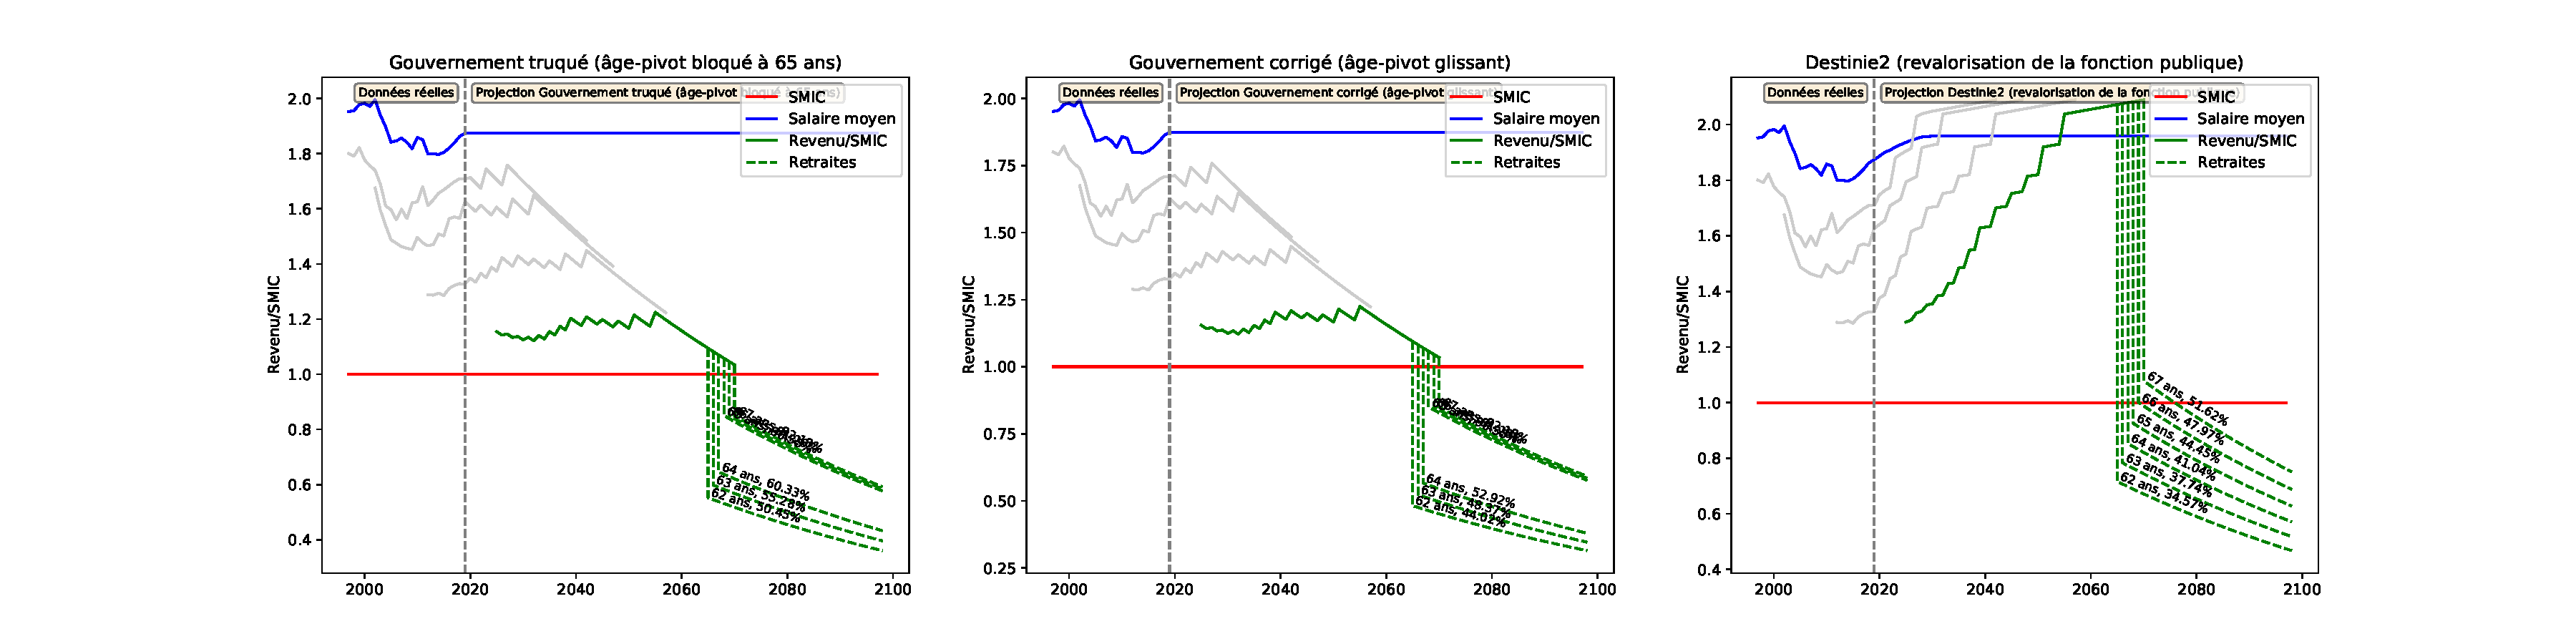
\includegraphics[width=0.9\textwidth]{fig/SecretaireAdmin_2003_22_dest_retraite.pdf}\end{center} \label{fig/SecretaireAdmin_2003_22_dest_retraite.pdf} 

\newpage 
 
\paragraph{Revenus et points pour le modèle \emph{Gouvernement truqué (âge-pivot bloqué à 65 ans)}} 
 
{ \scriptsize \begin{center} 
\begin{tabular}[htb]{|c|c||c|c|c|c|c|c||c|c||c|c|c|} 
\hline 
 Année &  Âge &  Ind Maj &  Pt Ind(\euro{} 2019) &  Rev HP(\euro{} 2019) &  Tx Primes &  GIPA(\euro{} 2019) &  Revenu(\euro{} 2019) &  SMIC(\euro{} 2019) &  Rev/SMIC &  Cumul Pts &  Achat Pt(\euro{} 2019) &  Serv. Pt(\euro{} 2019) \\ 
\hline \hline 
 2025 &  22 &  339.0 &  4.79 &  1625.31 &  30.41 &  0.00 &  2119.57 &  1835.31 &  {\bf 1.15} &  714.32 &  35.61 &  0.50 \\ 
\hline 
 2026 &  23 &  339.0 &  4.79 &  1625.31 &  30.64 &  0.00 &  2123.30 &  1859.17 &  {\bf 1.14} &  1429.90 &  35.61 &  0.50 \\ 
\hline 
 2027 &  24 &  344.0 &  4.79 &  1649.28 &  30.87 &  0.00 &  2158.41 &  1883.34 &  {\bf 1.15} &  2157.31 &  35.61 &  0.50 \\ 
\hline 
 2028 &  25 &  344.0 &  4.79 &  1649.28 &  31.10 &  0.00 &  2162.21 &  1907.82 &  {\bf 1.13} &  2886.00 &  35.61 &  0.50 \\ 
\hline 
 2029 &  26 &  349.0 &  4.79 &  1673.25 &  31.33 &  0.00 &  2197.48 &  1932.62 &  {\bf 1.14} &  3626.02 &  35.63 &  0.50 \\ 
\hline 
 2030 &  27 &  349.0 &  4.79 &  1673.25 &  31.56 &  0.00 &  2201.33 &  1957.75 &  {\bf 1.12} &  4366.20 &  35.69 &  0.50 \\ 
\hline 
 2031 &  28 &  356.0 &  4.79 &  1706.81 &  31.79 &  0.00 &  2249.41 &  1983.20 &  {\bf 1.13} &  5120.83 &  35.77 &  0.50 \\ 
\hline 
 2032 &  29 &  356.0 &  4.79 &  1706.81 &  32.02 &  0.00 &  2253.34 &  2008.98 &  {\bf 1.12} &  5874.49 &  35.88 &  0.50 \\ 
\hline 
 2033 &  30 &  366.0 &  4.79 &  1754.76 &  32.25 &  0.00 &  2320.67 &  2035.10 &  {\bf 1.14} &  6647.72 &  36.02 &  0.50 \\ 
\hline 
 2034 &  31 &  366.0 &  4.79 &  1754.76 &  32.48 &  0.00 &  2324.70 &  2061.55 &  {\bf 1.13} &  7418.77 &  36.18 &  0.50 \\ 
\hline 
 2035 &  32 &  379.0 &  4.79 &  1817.09 &  32.71 &  0.00 &  2411.45 &  2088.35 &  {\bf 1.15} &  8214.35 &  36.37 &  0.51 \\ 
\hline 
 2036 &  33 &  379.0 &  4.79 &  1817.09 &  32.94 &  0.00 &  2415.63 &  2115.50 &  {\bf 1.14} &  9006.49 &  36.59 &  0.51 \\ 
\hline 
 2037 &  34 &  394.0 &  4.79 &  1889.00 &  33.17 &  0.00 &  2515.58 &  2143.00 &  {\bf 1.17} &  9825.77 &  36.85 &  0.51 \\ 
\hline 
 2038 &  35 &  394.0 &  4.79 &  1889.00 &  33.40 &  0.00 &  2519.93 &  2170.86 &  {\bf 1.16} &  10640.26 &  37.13 &  0.52 \\ 
\hline 
 2039 &  36 &  413.0 &  4.79 &  1980.10 &  33.63 &  0.00 &  2646.00 &  2199.08 &  {\bf 1.20} &  11488.39 &  37.44 &  0.52 \\ 
\hline 
 2040 &  37 &  413.0 &  4.79 &  1980.10 &  33.86 &  0.00 &  2650.56 &  2227.67 &  {\bf 1.19} &  12330.26 &  37.78 &  0.53 \\ 
\hline 
 2041 &  38 &  413.0 &  4.79 &  1980.10 &  34.09 &  0.00 &  2655.11 &  2256.63 &  {\bf 1.18} &  13165.28 &  38.16 &  0.53 \\ 
\hline 
 2042 &  39 &  429.0 &  4.79 &  2056.81 &  34.32 &  0.00 &  2762.70 &  2285.97 &  {\bf 1.21} &  14024.96 &  38.56 &  0.54 \\ 
\hline 
 2043 &  40 &  429.0 &  4.79 &  2056.81 &  34.55 &  0.00 &  2767.43 &  2315.68 &  {\bf 1.20} &  14876.34 &  39.01 &  0.54 \\ 
\hline 
 2044 &  41 &  429.0 &  4.79 &  2056.81 &  34.78 &  0.00 &  2772.16 &  2345.79 &  {\bf 1.18} &  15718.88 &  39.48 &  0.55 \\ 
\hline 
 2045 &  42 &  440.0 &  4.79 &  2109.55 &  35.01 &  0.00 &  2848.10 &  2376.28 &  {\bf 1.20} &  16573.39 &  40.00 &  0.56 \\ 
\hline 
 2046 &  43 &  440.0 &  4.79 &  2109.55 &  35.24 &  0.00 &  2852.95 &  2407.18 &  {\bf 1.19} &  17418.37 &  40.52 &  0.56 \\ 
\hline 
 2047 &  44 &  440.0 &  4.79 &  2109.55 &  35.47 &  0.00 &  2857.80 &  2438.47 &  {\bf 1.17} &  18253.92 &  41.04 &  0.57 \\ 
\hline 
 2048 &  45 &  453.0 &  4.79 &  2171.87 &  35.70 &  0.00 &  2947.23 &  2470.17 &  {\bf 1.19} &  19104.56 &  41.58 &  0.58 \\ 
\hline 
 2049 &  46 &  453.0 &  4.79 &  2171.87 &  35.93 &  0.00 &  2952.23 &  2502.28 &  {\bf 1.18} &  19945.71 &  42.12 &  0.59 \\ 
\hline 
 2050 &  47 &  453.0 &  4.79 &  2171.87 &  36.16 &  0.00 &  2957.22 &  2534.81 &  {\bf 1.17} &  20777.47 &  42.66 &  0.59 \\ 
\hline 
 2051 &  48 &  477.0 &  4.79 &  2286.94 &  36.39 &  0.00 &  3119.16 &  2567.76 &  {\bf 1.21} &  21643.51 &  43.22 &  0.60 \\ 
\hline 
 2052 &  49 &  477.0 &  4.79 &  2286.94 &  36.62 &  0.00 &  3124.42 &  2601.14 &  {\bf 1.20} &  22499.89 &  43.78 &  0.61 \\ 
\hline 
 2053 &  50 &  477.0 &  4.79 &  2286.94 &  36.85 &  0.00 &  3129.68 &  2634.96 &  {\bf 1.19} &  23346.69 &  44.35 &  0.62 \\ 
\hline 
 2054 &  51 &  477.0 &  4.79 &  2286.94 &  37.08 &  0.00 &  3134.94 &  2669.21 &  {\bf 1.17} &  24184.04 &  44.93 &  0.63 \\ 
\hline 
 2055 &  52 &  503.0 &  4.79 &  2411.59 &  37.31 &  0.00 &  3311.36 &  2703.91 &  {\bf 1.22} &  25057.16 &  45.51 &  0.63 \\ 
\hline 
 2056 &  53 &  503.0 &  4.79 &  2411.59 &  37.54 &  0.00 &  3316.91 &  2739.06 &  {\bf 1.21} &  25920.51 &  46.10 &  0.64 \\ 
\hline 
 2057 &  54 &  503.0 &  4.79 &  2411.59 &  37.77 &  0.00 &  3322.45 &  2774.67 &  {\bf 1.20} &  26774.21 &  46.70 &  0.65 \\ 
\hline 
 2058 &  55 &  503.0 &  4.79 &  2411.59 &  38.00 &  0.00 &  3328.00 &  2810.74 &  {\bf 1.18} &  27618.37 &  47.31 &  0.66 \\ 
\hline 
 2059 &  56 &  503.0 &  4.79 &  2411.59 &  38.23 &  0.00 &  3333.55 &  2847.28 &  {\bf 1.17} &  28453.07 &  47.92 &  0.67 \\ 
\hline 
 2060 &  57 &  503.0 &  4.79 &  2411.59 &  38.46 &  0.00 &  3339.09 &  2884.30 &  {\bf 1.16} &  29278.44 &  48.55 &  0.68 \\ 
\hline 
 2061 &  58 &  503.0 &  4.79 &  2411.59 &  38.69 &  0.00 &  3344.64 &  2921.79 &  {\bf 1.14} &  30094.57 &  49.18 &  0.68 \\ 
\hline 
 2062 &  59 &  503.0 &  4.79 &  2411.59 &  38.92 &  0.00 &  3350.19 &  2959.78 &  {\bf 1.13} &  30901.56 &  49.82 &  0.69 \\ 
\hline 
 2063 &  60 &  503.0 &  4.79 &  2411.59 &  39.15 &  0.00 &  3355.73 &  2998.25 &  {\bf 1.12} &  31699.52 &  50.47 &  0.70 \\ 
\hline 
 2064 &  61 &  503.0 &  4.79 &  2411.59 &  39.38 &  0.00 &  3361.28 &  3037.23 &  {\bf 1.11} &  32488.53 &  51.12 &  0.71 \\ 
\hline 
 2065 &  62 &  503.0 &  4.79 &  2411.59 &  39.61 &  0.00 &  3366.83 &  3076.71 &  {\bf 1.09} &  33268.71 &  51.79 &  0.72 \\ 
\hline 
 2066 &  63 &  503.0 &  4.79 &  2411.59 &  39.84 &  0.00 &  3372.37 &  3116.71 &  {\bf 1.08} &  34040.14 &  52.46 &  0.73 \\ 
\hline 
 2067 &  64 &  503.0 &  4.79 &  2411.59 &  40.07 &  0.00 &  3377.92 &  3157.23 &  {\bf 1.07} &  34802.93 &  53.14 &  0.74 \\ 
\hline 
 2068 &  65 &  503.0 &  4.79 &  2411.59 &  40.30 &  0.00 &  3383.47 &  3198.27 &  {\bf 1.06} &  35557.16 &  53.83 &  0.75 \\ 
\hline 
 2069 &  66 &  503.0 &  4.79 &  2411.59 &  40.53 &  0.00 &  3389.01 &  3239.85 &  {\bf 1.05} &  36302.93 &  54.53 &  0.76 \\ 
\hline 
 2070 &  67 &  503.0 &  4.79 &  2411.59 &  40.76 &  0.00 &  3394.56 &  3281.97 &  {\bf 1.03} &  37040.34 &  55.24 &  0.77 \\ 
\hline 
\hline 
\end{tabular} 
\end{center} } 
\newpage 
 
\paragraph{Revenus et points pour le modèle \emph{Gouvernement corrigé (âge-pivot glissant)}} 
 
{ \scriptsize \begin{center} 
\begin{tabular}[htb]{|c|c||c|c|c|c|c|c||c|c||c|c|c|} 
\hline 
 Année &  Âge &  Ind Maj &  Pt Ind(\euro{} 2019) &  Rev HP(\euro{} 2019) &  Tx Primes &  GIPA(\euro{} 2019) &  Revenu(\euro{} 2019) &  SMIC(\euro{} 2019) &  Rev/SMIC &  Cumul Pts &  Achat Pt(\euro{} 2019) &  Serv. Pt(\euro{} 2019) \\ 
\hline \hline 
 2025 &  22 &  339.0 &  4.79 &  1625.31 &  30.41 &  0.00 &  2119.57 &  1835.31 &  {\bf 1.15} &  714.32 &  35.61 &  0.50 \\ 
\hline 
 2026 &  23 &  339.0 &  4.79 &  1625.31 &  30.64 &  0.00 &  2123.30 &  1859.17 &  {\bf 1.14} &  1429.90 &  35.61 &  0.50 \\ 
\hline 
 2027 &  24 &  344.0 &  4.79 &  1649.28 &  30.87 &  0.00 &  2158.41 &  1883.34 &  {\bf 1.15} &  2157.31 &  35.61 &  0.50 \\ 
\hline 
 2028 &  25 &  344.0 &  4.79 &  1649.28 &  31.10 &  0.00 &  2162.21 &  1907.82 &  {\bf 1.13} &  2886.00 &  35.61 &  0.50 \\ 
\hline 
 2029 &  26 &  349.0 &  4.79 &  1673.25 &  31.33 &  0.00 &  2197.48 &  1932.62 &  {\bf 1.14} &  3626.02 &  35.63 &  0.50 \\ 
\hline 
 2030 &  27 &  349.0 &  4.79 &  1673.25 &  31.56 &  0.00 &  2201.33 &  1957.75 &  {\bf 1.12} &  4366.20 &  35.69 &  0.50 \\ 
\hline 
 2031 &  28 &  356.0 &  4.79 &  1706.81 &  31.79 &  0.00 &  2249.41 &  1983.20 &  {\bf 1.13} &  5120.83 &  35.77 &  0.50 \\ 
\hline 
 2032 &  29 &  356.0 &  4.79 &  1706.81 &  32.02 &  0.00 &  2253.34 &  2008.98 &  {\bf 1.12} &  5874.49 &  35.88 &  0.50 \\ 
\hline 
 2033 &  30 &  366.0 &  4.79 &  1754.76 &  32.25 &  0.00 &  2320.67 &  2035.10 &  {\bf 1.14} &  6647.72 &  36.02 &  0.50 \\ 
\hline 
 2034 &  31 &  366.0 &  4.79 &  1754.76 &  32.48 &  0.00 &  2324.70 &  2061.55 &  {\bf 1.13} &  7418.77 &  36.18 &  0.50 \\ 
\hline 
 2035 &  32 &  379.0 &  4.79 &  1817.09 &  32.71 &  0.00 &  2411.45 &  2088.35 &  {\bf 1.15} &  8214.35 &  36.37 &  0.51 \\ 
\hline 
 2036 &  33 &  379.0 &  4.79 &  1817.09 &  32.94 &  0.00 &  2415.63 &  2115.50 &  {\bf 1.14} &  9006.49 &  36.59 &  0.51 \\ 
\hline 
 2037 &  34 &  394.0 &  4.79 &  1889.00 &  33.17 &  0.00 &  2515.58 &  2143.00 &  {\bf 1.17} &  9825.77 &  36.85 &  0.51 \\ 
\hline 
 2038 &  35 &  394.0 &  4.79 &  1889.00 &  33.40 &  0.00 &  2519.93 &  2170.86 &  {\bf 1.16} &  10640.26 &  37.13 &  0.52 \\ 
\hline 
 2039 &  36 &  413.0 &  4.79 &  1980.10 &  33.63 &  0.00 &  2646.00 &  2199.08 &  {\bf 1.20} &  11488.39 &  37.44 &  0.52 \\ 
\hline 
 2040 &  37 &  413.0 &  4.79 &  1980.10 &  33.86 &  0.00 &  2650.56 &  2227.67 &  {\bf 1.19} &  12330.26 &  37.78 &  0.53 \\ 
\hline 
 2041 &  38 &  413.0 &  4.79 &  1980.10 &  34.09 &  0.00 &  2655.11 &  2256.63 &  {\bf 1.18} &  13165.28 &  38.16 &  0.53 \\ 
\hline 
 2042 &  39 &  429.0 &  4.79 &  2056.81 &  34.32 &  0.00 &  2762.70 &  2285.97 &  {\bf 1.21} &  14024.96 &  38.56 &  0.54 \\ 
\hline 
 2043 &  40 &  429.0 &  4.79 &  2056.81 &  34.55 &  0.00 &  2767.43 &  2315.68 &  {\bf 1.20} &  14876.34 &  39.01 &  0.54 \\ 
\hline 
 2044 &  41 &  429.0 &  4.79 &  2056.81 &  34.78 &  0.00 &  2772.16 &  2345.79 &  {\bf 1.18} &  15718.88 &  39.48 &  0.55 \\ 
\hline 
 2045 &  42 &  440.0 &  4.79 &  2109.55 &  35.01 &  0.00 &  2848.10 &  2376.28 &  {\bf 1.20} &  16573.39 &  40.00 &  0.56 \\ 
\hline 
 2046 &  43 &  440.0 &  4.79 &  2109.55 &  35.24 &  0.00 &  2852.95 &  2407.18 &  {\bf 1.19} &  17418.37 &  40.52 &  0.56 \\ 
\hline 
 2047 &  44 &  440.0 &  4.79 &  2109.55 &  35.47 &  0.00 &  2857.80 &  2438.47 &  {\bf 1.17} &  18253.92 &  41.04 &  0.57 \\ 
\hline 
 2048 &  45 &  453.0 &  4.79 &  2171.87 &  35.70 &  0.00 &  2947.23 &  2470.17 &  {\bf 1.19} &  19104.56 &  41.58 &  0.58 \\ 
\hline 
 2049 &  46 &  453.0 &  4.79 &  2171.87 &  35.93 &  0.00 &  2952.23 &  2502.28 &  {\bf 1.18} &  19945.71 &  42.12 &  0.59 \\ 
\hline 
 2050 &  47 &  453.0 &  4.79 &  2171.87 &  36.16 &  0.00 &  2957.22 &  2534.81 &  {\bf 1.17} &  20777.47 &  42.66 &  0.59 \\ 
\hline 
 2051 &  48 &  477.0 &  4.79 &  2286.94 &  36.39 &  0.00 &  3119.16 &  2567.76 &  {\bf 1.21} &  21643.51 &  43.22 &  0.60 \\ 
\hline 
 2052 &  49 &  477.0 &  4.79 &  2286.94 &  36.62 &  0.00 &  3124.42 &  2601.14 &  {\bf 1.20} &  22499.89 &  43.78 &  0.61 \\ 
\hline 
 2053 &  50 &  477.0 &  4.79 &  2286.94 &  36.85 &  0.00 &  3129.68 &  2634.96 &  {\bf 1.19} &  23346.69 &  44.35 &  0.62 \\ 
\hline 
 2054 &  51 &  477.0 &  4.79 &  2286.94 &  37.08 &  0.00 &  3134.94 &  2669.21 &  {\bf 1.17} &  24184.04 &  44.93 &  0.63 \\ 
\hline 
 2055 &  52 &  503.0 &  4.79 &  2411.59 &  37.31 &  0.00 &  3311.36 &  2703.91 &  {\bf 1.22} &  25057.16 &  45.51 &  0.63 \\ 
\hline 
 2056 &  53 &  503.0 &  4.79 &  2411.59 &  37.54 &  0.00 &  3316.91 &  2739.06 &  {\bf 1.21} &  25920.51 &  46.10 &  0.64 \\ 
\hline 
 2057 &  54 &  503.0 &  4.79 &  2411.59 &  37.77 &  0.00 &  3322.45 &  2774.67 &  {\bf 1.20} &  26774.21 &  46.70 &  0.65 \\ 
\hline 
 2058 &  55 &  503.0 &  4.79 &  2411.59 &  38.00 &  0.00 &  3328.00 &  2810.74 &  {\bf 1.18} &  27618.37 &  47.31 &  0.66 \\ 
\hline 
 2059 &  56 &  503.0 &  4.79 &  2411.59 &  38.23 &  0.00 &  3333.55 &  2847.28 &  {\bf 1.17} &  28453.07 &  47.92 &  0.67 \\ 
\hline 
 2060 &  57 &  503.0 &  4.79 &  2411.59 &  38.46 &  0.00 &  3339.09 &  2884.30 &  {\bf 1.16} &  29278.44 &  48.55 &  0.68 \\ 
\hline 
 2061 &  58 &  503.0 &  4.79 &  2411.59 &  38.69 &  0.00 &  3344.64 &  2921.79 &  {\bf 1.14} &  30094.57 &  49.18 &  0.68 \\ 
\hline 
 2062 &  59 &  503.0 &  4.79 &  2411.59 &  38.92 &  0.00 &  3350.19 &  2959.78 &  {\bf 1.13} &  30901.56 &  49.82 &  0.69 \\ 
\hline 
 2063 &  60 &  503.0 &  4.79 &  2411.59 &  39.15 &  0.00 &  3355.73 &  2998.25 &  {\bf 1.12} &  31699.52 &  50.47 &  0.70 \\ 
\hline 
 2064 &  61 &  503.0 &  4.79 &  2411.59 &  39.38 &  0.00 &  3361.28 &  3037.23 &  {\bf 1.11} &  32488.53 &  51.12 &  0.71 \\ 
\hline 
 2065 &  62 &  503.0 &  4.79 &  2411.59 &  39.61 &  0.00 &  3366.83 &  3076.71 &  {\bf 1.09} &  33268.71 &  51.79 &  0.72 \\ 
\hline 
 2066 &  63 &  503.0 &  4.79 &  2411.59 &  39.84 &  0.00 &  3372.37 &  3116.71 &  {\bf 1.08} &  34040.14 &  52.46 &  0.73 \\ 
\hline 
 2067 &  64 &  503.0 &  4.79 &  2411.59 &  40.07 &  0.00 &  3377.92 &  3157.23 &  {\bf 1.07} &  34802.93 &  53.14 &  0.74 \\ 
\hline 
 2068 &  65 &  503.0 &  4.79 &  2411.59 &  40.30 &  0.00 &  3383.47 &  3198.27 &  {\bf 1.06} &  35557.16 &  53.83 &  0.75 \\ 
\hline 
 2069 &  66 &  503.0 &  4.79 &  2411.59 &  40.53 &  0.00 &  3389.01 &  3239.85 &  {\bf 1.05} &  36302.93 &  54.53 &  0.76 \\ 
\hline 
 2070 &  67 &  503.0 &  4.79 &  2411.59 &  40.76 &  0.00 &  3394.56 &  3281.97 &  {\bf 1.03} &  37040.34 &  55.24 &  0.77 \\ 
\hline 
\hline 
\end{tabular} 
\end{center} } 
\newpage 
 
\paragraph{Revenus et points pour le modèle \emph{Destinie2 (revalorisation de la fonction publique)}} 
 
{ \scriptsize \begin{center} 
\begin{tabular}[htb]{|c|c||c|c|c|c|c|c||c|c||c|c|c|} 
\hline 
 Année &  Âge &  Ind Maj &  Pt Ind(\euro{} 2019) &  Rev HP(\euro{} 2019) &  Tx Primes &  GIPA(\euro{} 2019) &  Revenu(\euro{} 2019) &  SMIC(\euro{} 2019) &  Rev/SMIC &  Cumul Pts &  Achat Pt(\euro{} 2019) &  Serv. Pt(\euro{} 2019) \\ 
\hline \hline 
 2025 &  22 &  339.0 &  5.10 &  1730.07 &  30.41 &  0.00 &  2256.19 &  1749.35 &  {\bf 1.29} &  758.50 &  35.69 &  0.50 \\ 
\hline 
 2026 &  23 &  339.0 &  5.17 &  1751.70 &  30.64 &  0.00 &  2288.42 &  1764.53 &  {\bf 1.30} &  1527.83 &  35.69 &  0.50 \\ 
\hline 
 2027 &  24 &  344.0 &  5.23 &  1800.29 &  30.87 &  0.00 &  2356.04 &  1781.27 &  {\bf 1.32} &  2319.89 &  35.69 &  0.50 \\ 
\hline 
 2028 &  25 &  344.0 &  5.30 &  1823.87 &  31.10 &  0.00 &  2391.10 &  1799.59 &  {\bf 1.33} &  3123.74 &  35.69 &  0.50 \\ 
\hline 
 2029 &  26 &  349.0 &  5.37 &  1872.77 &  31.33 &  0.00 &  2459.51 &  1819.55 &  {\bf 1.35} &  3950.00 &  35.72 &  0.50 \\ 
\hline 
 2030 &  27 &  349.0 &  5.43 &  1895.99 &  31.56 &  0.00 &  2494.37 &  1841.19 &  {\bf 1.35} &  4786.76 &  35.77 &  0.50 \\ 
\hline 
 2031 &  28 &  356.0 &  5.50 &  1958.59 &  31.79 &  0.00 &  2581.22 &  1864.58 &  {\bf 1.38} &  5650.73 &  35.85 &  0.50 \\ 
\hline 
 2032 &  29 &  356.0 &  5.57 &  1984.05 &  32.02 &  0.00 &  2619.34 &  1888.81 &  {\bf 1.39} &  6524.80 &  35.96 &  0.50 \\ 
\hline 
 2033 &  30 &  366.0 &  5.65 &  2066.30 &  32.25 &  0.00 &  2732.68 &  1913.37 &  {\bf 1.43} &  7433.23 &  36.10 &  0.50 \\ 
\hline 
 2034 &  31 &  366.0 &  5.72 &  2093.16 &  32.48 &  0.00 &  2773.01 &  1938.24 &  {\bf 1.43} &  8350.87 &  36.26 &  0.50 \\ 
\hline 
 2035 &  32 &  379.0 &  5.79 &  2195.68 &  32.71 &  0.00 &  2913.89 &  1963.44 &  {\bf 1.48} &  9310.03 &  36.46 &  0.51 \\ 
\hline 
 2036 &  33 &  379.0 &  5.87 &  2224.23 &  32.94 &  0.00 &  2956.89 &  1988.96 &  {\bf 1.49} &  10277.43 &  36.68 &  0.51 \\ 
\hline 
 2037 &  34 &  394.0 &  5.94 &  2342.32 &  33.17 &  0.00 &  3119.26 &  2014.82 &  {\bf 1.55} &  11291.01 &  36.93 &  0.51 \\ 
\hline 
 2038 &  35 &  394.0 &  6.02 &  2372.77 &  33.40 &  0.00 &  3165.27 &  2041.01 &  {\bf 1.55} &  12311.75 &  37.21 &  0.52 \\ 
\hline 
 2039 &  36 &  413.0 &  6.10 &  2519.52 &  33.63 &  0.00 &  3366.84 &  2067.55 &  {\bf 1.63} &  13388.45 &  37.52 &  0.52 \\ 
\hline 
 2040 &  37 &  413.0 &  6.18 &  2552.28 &  33.86 &  0.00 &  3416.48 &  2094.43 &  {\bf 1.63} &  14471.12 &  37.87 &  0.53 \\ 
\hline 
 2041 &  38 &  413.0 &  6.26 &  2585.45 &  34.09 &  0.00 &  3466.84 &  2121.65 &  {\bf 1.63} &  15558.94 &  38.24 &  0.53 \\ 
\hline 
 2042 &  39 &  429.0 &  6.34 &  2720.53 &  34.32 &  0.00 &  3654.22 &  2149.23 &  {\bf 1.70} &  16693.43 &  38.65 &  0.54 \\ 
\hline 
 2043 &  40 &  429.0 &  6.42 &  2755.90 &  34.55 &  0.00 &  3708.06 &  2177.17 &  {\bf 1.70} &  17831.59 &  39.10 &  0.54 \\ 
\hline 
 2044 &  41 &  429.0 &  6.51 &  2791.72 &  34.78 &  0.00 &  3762.69 &  2205.48 &  {\bf 1.71} &  18972.57 &  39.57 &  0.55 \\ 
\hline 
 2045 &  42 &  440.0 &  6.59 &  2900.53 &  35.01 &  0.00 &  3916.01 &  2234.15 &  {\bf 1.75} &  20144.79 &  40.09 &  0.56 \\ 
\hline 
 2046 &  43 &  440.0 &  6.68 &  2938.24 &  35.24 &  0.00 &  3973.67 &  2263.19 &  {\bf 1.76} &  21319.01 &  40.61 &  0.57 \\ 
\hline 
 2047 &  44 &  440.0 &  6.76 &  2976.43 &  35.47 &  0.00 &  4032.17 &  2292.61 &  {\bf 1.76} &  22495.23 &  41.14 &  0.57 \\ 
\hline 
 2048 &  45 &  453.0 &  6.85 &  3104.21 &  35.70 &  0.00 &  4212.41 &  2322.42 &  {\bf 1.81} &  23708.26 &  41.67 &  0.58 \\ 
\hline 
 2049 &  46 &  453.0 &  6.94 &  3144.57 &  35.93 &  0.00 &  4274.41 &  2352.61 &  {\bf 1.82} &  24923.34 &  42.21 &  0.59 \\ 
\hline 
 2050 &  47 &  453.0 &  7.03 &  3185.44 &  36.16 &  0.00 &  4337.30 &  2383.19 &  {\bf 1.82} &  26140.48 &  42.76 &  0.60 \\ 
\hline 
 2051 &  48 &  477.0 &  7.12 &  3397.81 &  36.39 &  0.00 &  4634.28 &  2414.18 &  {\bf 1.92} &  27424.27 &  43.32 &  0.60 \\ 
\hline 
 2052 &  49 &  477.0 &  7.22 &  3441.99 &  36.62 &  0.00 &  4702.44 &  2445.56 &  {\bf 1.92} &  28710.22 &  43.88 &  0.61 \\ 
\hline 
 2053 &  50 &  477.0 &  7.31 &  3486.73 &  36.85 &  0.00 &  4771.59 &  2477.35 &  {\bf 1.93} &  29998.34 &  44.45 &  0.62 \\ 
\hline 
 2054 &  51 &  477.0 &  7.40 &  3532.06 &  37.08 &  0.00 &  4841.75 &  2509.56 &  {\bf 1.93} &  31288.63 &  45.03 &  0.63 \\ 
\hline 
 2055 &  52 &  503.0 &  7.50 &  3773.00 &  37.31 &  0.00 &  5180.71 &  2542.18 &  {\bf 2.04} &  32651.52 &  45.62 &  0.63 \\ 
\hline 
 2056 &  53 &  503.0 &  7.60 &  3822.05 &  37.54 &  0.00 &  5256.85 &  2575.23 &  {\bf 2.04} &  34016.70 &  46.21 &  0.64 \\ 
\hline 
 2057 &  54 &  503.0 &  7.70 &  3871.74 &  37.77 &  0.00 &  5334.09 &  2608.71 &  {\bf 2.04} &  35384.16 &  46.81 &  0.65 \\ 
\hline 
 2058 &  55 &  503.0 &  7.80 &  3922.07 &  38.00 &  0.00 &  5412.46 &  2642.62 &  {\bf 2.05} &  36753.91 &  47.42 &  0.66 \\ 
\hline 
 2059 &  56 &  503.0 &  7.90 &  3973.06 &  38.23 &  0.00 &  5491.96 &  2676.98 &  {\bf 2.05} &  38125.93 &  48.03 &  0.67 \\ 
\hline 
 2060 &  57 &  503.0 &  8.00 &  4024.71 &  38.46 &  0.00 &  5572.61 &  2711.78 &  {\bf 2.05} &  39500.25 &  48.66 &  0.68 \\ 
\hline 
 2061 &  58 &  503.0 &  8.11 &  4077.03 &  38.69 &  0.00 &  5654.43 &  2747.03 &  {\bf 2.06} &  40876.84 &  49.29 &  0.69 \\ 
\hline 
 2062 &  59 &  503.0 &  8.21 &  4130.03 &  38.92 &  0.00 &  5737.44 &  2782.74 &  {\bf 2.06} &  42255.71 &  49.93 &  0.70 \\ 
\hline 
 2063 &  60 &  503.0 &  8.32 &  4183.72 &  39.15 &  0.00 &  5821.65 &  2818.92 &  {\bf 2.07} &  43636.87 &  50.58 &  0.70 \\ 
\hline 
 2064 &  61 &  503.0 &  8.43 &  4238.11 &  39.38 &  0.00 &  5907.08 &  2855.56 &  {\bf 2.07} &  45020.32 &  51.24 &  0.71 \\ 
\hline 
 2065 &  62 &  503.0 &  8.54 &  4293.20 &  39.61 &  0.00 &  5993.74 &  2892.68 &  {\bf 2.07} &  46406.04 &  51.90 &  0.72 \\ 
\hline 
 2066 &  63 &  503.0 &  8.65 &  4349.02 &  39.84 &  0.00 &  6081.66 &  2930.29 &  {\bf 2.08} &  47794.05 &  52.58 &  0.73 \\ 
\hline 
 2067 &  64 &  503.0 &  8.76 &  4405.55 &  40.07 &  0.00 &  6170.86 &  2968.38 &  {\bf 2.08} &  49184.34 &  53.26 &  0.74 \\ 
\hline 
 2068 &  65 &  503.0 &  8.87 &  4462.83 &  40.30 &  0.00 &  6261.34 &  3006.97 &  {\bf 2.08} &  50576.91 &  53.95 &  0.75 \\ 
\hline 
 2069 &  66 &  503.0 &  8.99 &  4520.84 &  40.53 &  0.00 &  6353.14 &  3046.06 &  {\bf 2.09} &  51971.77 &  54.66 &  0.76 \\ 
\hline 
 2070 &  67 &  503.0 &  9.10 &  4579.61 &  40.76 &  0.00 &  6446.26 &  3085.66 &  {\bf 2.09} &  53368.91 &  55.37 &  0.77 \\ 
\hline 
\hline 
\end{tabular} 
\end{center} } 
\newpage 
 
\chapter{ATSEM (C2 puis C1)} 

\begin{minipage}{0.55\linewidth}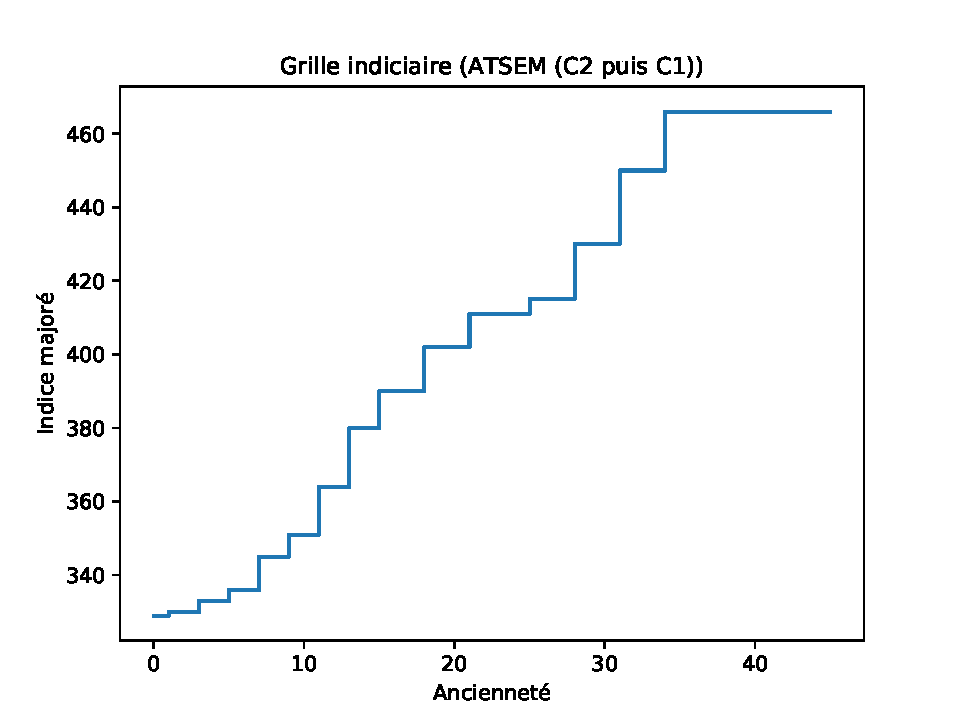
\includegraphics[width=0.7\textwidth]{fig/grille_ATSEM.pdf}\end{minipage} 
\begin{minipage}{0.3\linewidth} 
 \begin{center} 

\begin{tabular}[htb]{|c|c|} 
\hline 
 Indice majoré &  Durée (années) \\ 
\hline \hline 
 329 &  1.00 \\ 
\hline 
 330 &  2.00 \\ 
\hline 
 333 &  2.00 \\ 
\hline 
 336 &  2.00 \\ 
\hline 
 345 &  2.00 \\ 
\hline 
 351 &  2.00 \\ 
\hline 
 364 &  2.00 \\ 
\hline 
 380 &  2.00 \\ 
\hline 
 390 &  3.00 \\ 
\hline 
 402 &  3.00 \\ 
\hline 
 411 &  4.00 \\ 
\hline 
 415 &  3.00 \\ 
\hline 
 430 &  3.00 \\ 
\hline 
 450 &  3.00 \\ 
\hline 
 466 &   \\ 
\hline 
\hline 
\end{tabular} 
\end{center} 
 \end{minipage} 


 \addto{\captionsenglish}{ \renewcommand{\mtctitle}{}} \setcounter{minitocdepth}{2} 
 \minitoc \newpage 

\section{Début de carrière à 22 ans} 

\subsection{Génération 1975 (début en 1997)} 

\paragraph{Retraites possibles dans le modèle \emph{Gouvernement truqué (âge-pivot bloqué à 65 ans)}}  
 
{ \scriptsize \begin{center} 
\begin{tabular}[htb]{|c|c||c|c||c|c||c||c|c|c|c|c|c|} 
\hline 
 Retraite en &  Âge &  Âge pivot &  Décote/Surcote &  Retraite (\euro{} 2019) &  Tx Rempl(\%) &  SMIC (\euro{} 2019) &  Retraite/SMIC &  Rev70/SMIC &  Rev75/SMIC &  Rev80/SMIC &  Rev85/SMIC &  Rev90/SMIC \\ 
\hline \hline 
 2037 &  62 &  64 ans 10 mois &  -14.17\% &  1115.00 &  {\bf 43.28} &  2143.00 &  {\bf {\color{red} 0.52}} &  {\bf {\color{red} 0.47}} &  {\bf {\color{red} 0.44}} &  {\bf {\color{red} 0.41}} &  {\bf {\color{red} 0.39}} &  {\bf {\color{red} 0.36}} \\ 
\hline 
 2038 &  63 &  64 ans 11 mois &  -9.58\% &  1215.99 &  {\bf 47.11} &  2170.86 &  {\bf {\color{red} 0.56}} &  {\bf {\color{red} 0.51}} &  {\bf {\color{red} 0.48}} &  {\bf {\color{red} 0.45}} &  {\bf {\color{red} 0.42}} &  {\bf {\color{red} 0.40}} \\ 
\hline 
 2039 &  64 &  65 ans 0 mois &  -5.00\% &  1322.55 &  {\bf 51.13} &  2199.08 &  {\bf {\color{red} 0.60}} &  {\bf {\color{red} 0.56}} &  {\bf {\color{red} 0.52}} &  {\bf {\color{red} 0.49}} &  {\bf {\color{red} 0.46}} &  {\bf {\color{red} 0.43}} \\ 
\hline 
 2040 &  65 &  65 ans 0 mois &  0.00\% &  1893.52 &  {\bf 73.06} &  2227.67 &  {\bf {\color{red} 0.85}} &  {\bf {\color{red} 0.80}} &  {\bf {\color{red} 0.75}} &  {\bf {\color{red} 0.70}} &  {\bf {\color{red} 0.66}} &  {\bf {\color{red} 0.62}} \\ 
\hline 
 2041 &  66 &  65 ans 0 mois &  5.00\% &  1918.14 &  {\bf 73.87} &  2256.63 &  {\bf {\color{red} 0.85}} &  {\bf {\color{red} 0.81}} &  {\bf {\color{red} 0.76}} &  {\bf {\color{red} 0.71}} &  {\bf {\color{red} 0.67}} &  {\bf {\color{red} 0.62}} \\ 
\hline 
 2042 &  67 &  65 ans 0 mois &  10.00\% &  1943.07 &  {\bf 74.68} &  2285.97 &  {\bf {\color{red} 0.85}} &  {\bf {\color{red} 0.82}} &  {\bf {\color{red} 0.77}} &  {\bf {\color{red} 0.72}} &  {\bf {\color{red} 0.67}} &  {\bf {\color{red} 0.63}} \\ 
\hline 
\hline 
\end{tabular} 
\end{center} } 
\paragraph{Retraites possibles dans le modèle \emph{Gouvernement corrigé (âge-pivot glissant)}}  
 
{ \scriptsize \begin{center} 
\begin{tabular}[htb]{|c|c||c|c||c|c||c||c|c|c|c|c|c|} 
\hline 
 Retraite en &  Âge &  Âge pivot &  Décote/Surcote &  Retraite (\euro{} 2019) &  Tx Rempl(\%) &  SMIC (\euro{} 2019) &  Retraite/SMIC &  Rev70/SMIC &  Rev75/SMIC &  Rev80/SMIC &  Rev85/SMIC &  Rev90/SMIC \\ 
\hline \hline 
 2037 &  62 &  64 ans 10 mois &  -14.17\% &  1115.00 &  {\bf 43.28} &  2143.00 &  {\bf {\color{red} 0.52}} &  {\bf {\color{red} 0.47}} &  {\bf {\color{red} 0.44}} &  {\bf {\color{red} 0.41}} &  {\bf {\color{red} 0.39}} &  {\bf {\color{red} 0.36}} \\ 
\hline 
 2038 &  63 &  64 ans 11 mois &  -9.58\% &  1215.99 &  {\bf 47.11} &  2170.86 &  {\bf {\color{red} 0.56}} &  {\bf {\color{red} 0.51}} &  {\bf {\color{red} 0.48}} &  {\bf {\color{red} 0.45}} &  {\bf {\color{red} 0.42}} &  {\bf {\color{red} 0.40}} \\ 
\hline 
 2039 &  64 &  65 ans 0 mois &  -5.00\% &  1322.55 &  {\bf 51.13} &  2199.08 &  {\bf {\color{red} 0.60}} &  {\bf {\color{red} 0.56}} &  {\bf {\color{red} 0.52}} &  {\bf {\color{red} 0.49}} &  {\bf {\color{red} 0.46}} &  {\bf {\color{red} 0.43}} \\ 
\hline 
 2040 &  65 &  65 ans 1 mois &  -0.42\% &  1893.52 &  {\bf 73.06} &  2227.67 &  {\bf {\color{red} 0.85}} &  {\bf {\color{red} 0.80}} &  {\bf {\color{red} 0.75}} &  {\bf {\color{red} 0.70}} &  {\bf {\color{red} 0.66}} &  {\bf {\color{red} 0.62}} \\ 
\hline 
 2041 &  66 &  65 ans 2 mois &  4.17\% &  1918.14 &  {\bf 73.87} &  2256.63 &  {\bf {\color{red} 0.85}} &  {\bf {\color{red} 0.81}} &  {\bf {\color{red} 0.76}} &  {\bf {\color{red} 0.71}} &  {\bf {\color{red} 0.67}} &  {\bf {\color{red} 0.62}} \\ 
\hline 
 2042 &  67 &  65 ans 3 mois &  8.75\% &  1943.07 &  {\bf 74.68} &  2285.97 &  {\bf {\color{red} 0.85}} &  {\bf {\color{red} 0.82}} &  {\bf {\color{red} 0.77}} &  {\bf {\color{red} 0.72}} &  {\bf {\color{red} 0.67}} &  {\bf {\color{red} 0.63}} \\ 
\hline 
\hline 
\end{tabular} 
\end{center} } 
\paragraph{Retraites possibles dans le modèle \emph{Destinie2 (revalorisation de la fonction publique)}}  
 
{ \scriptsize \begin{center} 
\begin{tabular}[htb]{|c|c||c|c||c|c||c||c|c|c|c|c|c|} 
\hline 
 Retraite en &  Âge &  Âge pivot &  Décote/Surcote &  Retraite (\euro{} 2019) &  Tx Rempl(\%) &  SMIC (\euro{} 2019) &  Retraite/SMIC &  Rev70/SMIC &  Rev75/SMIC &  Rev80/SMIC &  Rev85/SMIC &  Rev90/SMIC \\ 
\hline \hline 
 2037 &  62 &  64 ans 10 mois &  -14.17\% &  1177.96 &  {\bf 36.87} &  2014.82 &  {\bf {\color{red} 0.58}} &  {\bf {\color{red} 0.53}} &  {\bf {\color{red} 0.49}} &  {\bf {\color{red} 0.46}} &  {\bf {\color{red} 0.43}} &  {\bf {\color{red} 0.41}} \\ 
\hline 
 2038 &  63 &  64 ans 11 mois &  -9.58\% &  1291.13 &  {\bf 39.82} &  2041.01 &  {\bf {\color{red} 0.63}} &  {\bf {\color{red} 0.58}} &  {\bf {\color{red} 0.54}} &  {\bf {\color{red} 0.51}} &  {\bf {\color{red} 0.48}} &  {\bf {\color{red} 0.45}} \\ 
\hline 
 2039 &  64 &  65 ans 0 mois &  -5.00\% &  1411.48 &  {\bf 42.89} &  2067.55 &  {\bf {\color{red} 0.68}} &  {\bf {\color{red} 0.63}} &  {\bf {\color{red} 0.59}} &  {\bf {\color{red} 0.56}} &  {\bf {\color{red} 0.52}} &  {\bf {\color{red} 0.49}} \\ 
\hline 
 2040 &  65 &  65 ans 1 mois &  -0.42\% &  1780.26 &  {\bf 53.29} &  2094.43 &  {\bf {\color{red} 0.85}} &  {\bf {\color{red} 0.80}} &  {\bf {\color{red} 0.75}} &  {\bf {\color{red} 0.70}} &  {\bf {\color{red} 0.66}} &  {\bf {\color{red} 0.62}} \\ 
\hline 
 2041 &  66 &  65 ans 2 mois &  4.17\% &  1803.40 &  {\bf 53.19} &  2121.65 &  {\bf {\color{red} 0.85}} &  {\bf {\color{red} 0.81}} &  {\bf {\color{red} 0.76}} &  {\bf {\color{red} 0.71}} &  {\bf {\color{red} 0.67}} &  {\bf {\color{red} 0.62}} \\ 
\hline 
 2042 &  67 &  65 ans 3 mois &  8.75\% &  1826.85 &  {\bf 53.08} &  2149.23 &  {\bf {\color{red} 0.85}} &  {\bf {\color{red} 0.82}} &  {\bf {\color{red} 0.77}} &  {\bf {\color{red} 0.72}} &  {\bf {\color{red} 0.67}} &  {\bf {\color{red} 0.63}} \\ 
\hline 
\hline 
\end{tabular} 
\end{center} } 

 \begin{center}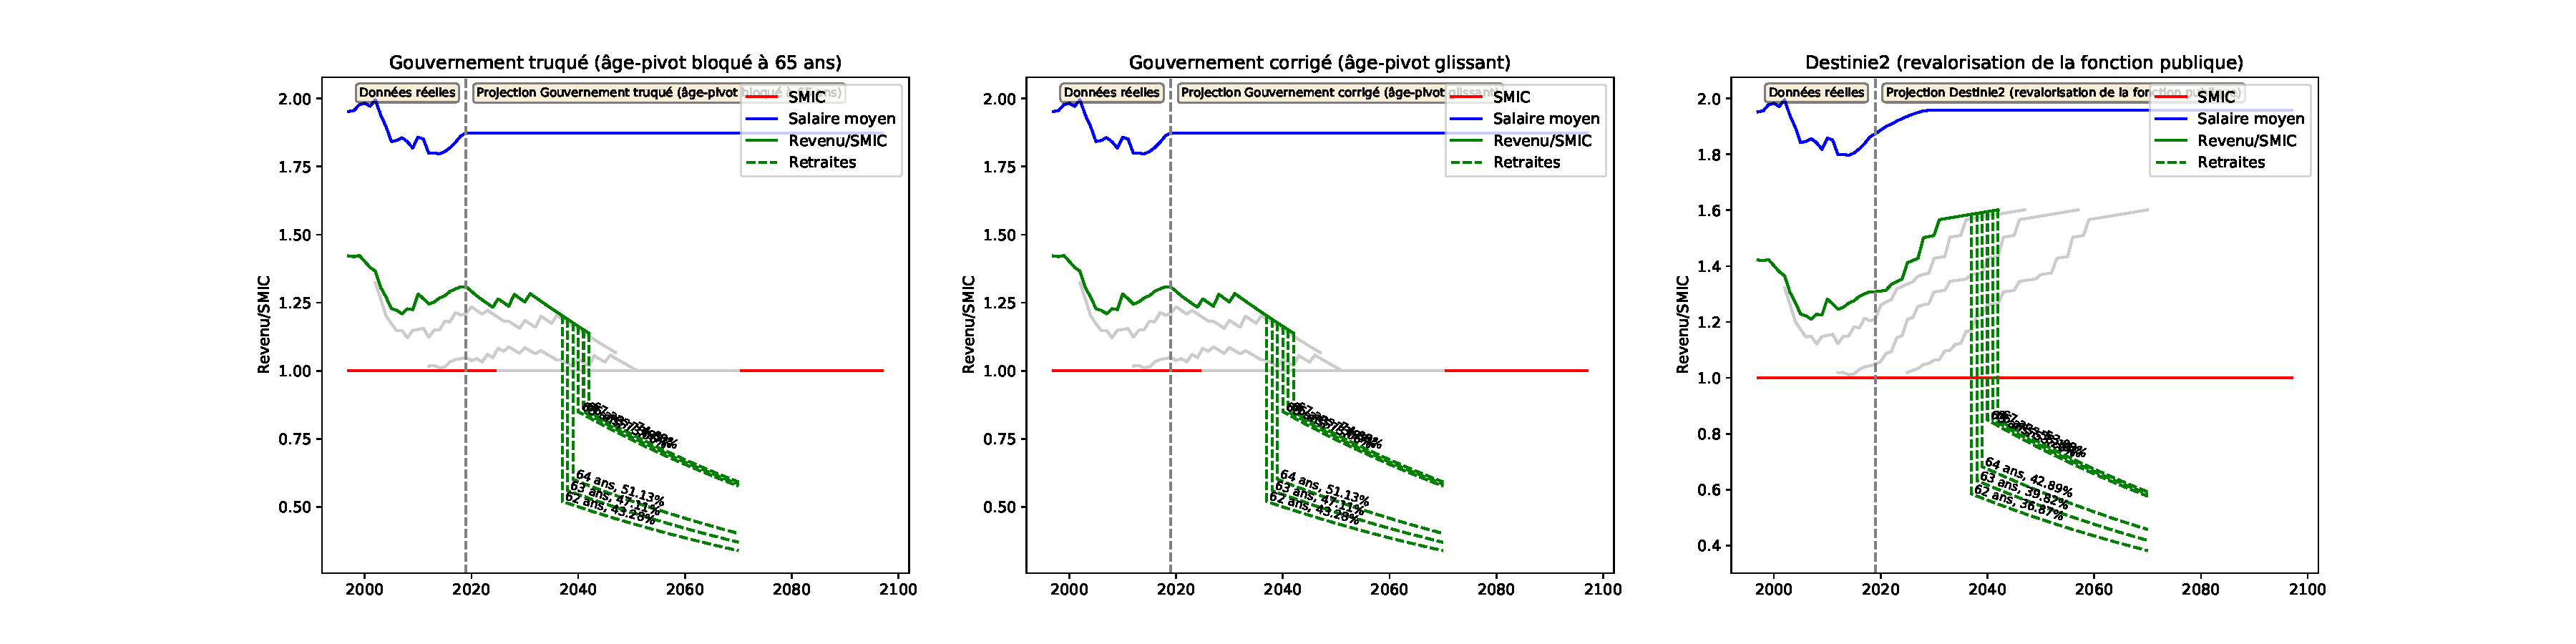
\includegraphics[width=0.9\textwidth]{fig/ATSEM_1975_22_dest_retraite.pdf}\end{center} \label{fig/ATSEM_1975_22_dest_retraite.pdf} 

\newpage 
 
\paragraph{Revenus et points pour le modèle \emph{Gouvernement truqué (âge-pivot bloqué à 65 ans)}} 
 
{ \scriptsize \begin{center} 
\begin{tabular}[htb]{|c|c||c|c|c|c|c|c||c|c||c|c|c|} 
\hline 
 Année &  Âge &  Ind Maj &  Pt Ind(\euro{} 2019) &  Rev HP(\euro{} 2019) &  Tx Primes &  GIPA(\euro{} 2019) &  Revenu(\euro{} 2019) &  SMIC(\euro{} 2019) &  Rev/SMIC &  Cumul Pts &  Achat Pt(\euro{} 2019) &  Serv. Pt(\euro{} 2019) \\ 
\hline \hline 
 1997 &  22 &  329.0 &  5.53 &  1820.80 &  6.11 &  0.00 &  1932.05 &  1358.84 &  {\bf 1.42} &  651.13 &  35.61 &  0.50 \\ 
\hline 
 1998 &  23 &  330.0 &  5.57 &  1836.93 &  6.34 &  0.00 &  1953.39 &  1376.36 &  {\bf 1.42} &  1309.44 &  35.61 &  0.50 \\ 
\hline 
 1999 &  24 &  330.0 &  5.61 &  1851.78 &  6.57 &  0.00 &  1973.44 &  1386.54 &  {\bf 1.42} &  1974.52 &  35.61 &  0.50 \\ 
\hline 
 2000 &  25 &  333.0 &  5.55 &  1846.55 &  6.80 &  0.00 &  1972.11 &  1407.00 &  {\bf 1.40} &  2639.14 &  35.61 &  0.50 \\ 
\hline 
 2001 &  26 &  333.0 &  5.52 &  1838.33 &  7.03 &  20.64 &  1988.20 &  1441.04 &  {\bf 1.38} &  3309.19 &  35.61 &  0.50 \\ 
\hline 
 2002 &  27 &  336.0 &  5.49 &  1843.39 &  7.26 &  0.00 &  1977.22 &  1447.74 &  {\bf 1.37} &  3975.54 &  35.61 &  0.50 \\ 
\hline 
 2003 &  28 &  336.0 &  5.37 &  1805.87 &  7.49 &  8.86 &  1949.99 &  1493.03 &  {\bf 1.31} &  4632.71 &  35.61 &  0.50 \\ 
\hline 
 2004 &  29 &  345.0 &  5.29 &  1824.95 &  7.72 &  0.00 &  1965.84 &  1547.32 &  {\bf 1.27} &  5295.22 &  35.61 &  0.50 \\ 
\hline 
 2005 &  30 &  345.0 &  5.29 &  1824.76 &  7.95 &  0.00 &  1969.82 &  1603.67 &  {\bf 1.23} &  5959.07 &  35.61 &  0.50 \\ 
\hline 
 2006 &  31 &  351.0 &  5.23 &  1835.77 &  8.18 &  0.00 &  1985.94 &  1625.00 &  {\bf 1.22} &  6628.36 &  35.61 &  0.50 \\ 
\hline 
 2007 &  32 &  351.0 &  5.19 &  1823.26 &  8.41 &  0.00 &  1976.60 &  1634.08 &  {\bf 1.21} &  7294.50 &  35.61 &  0.50 \\ 
\hline 
 2008 &  33 &  364.0 &  5.09 &  1853.87 &  8.64 &  0.00 &  2014.04 &  1640.24 &  {\bf 1.23} &  7973.25 &  35.61 &  0.50 \\ 
\hline 
 2009 &  34 &  364.0 &  5.13 &  1867.00 &  8.87 &  0.00 &  2032.61 &  1659.42 &  {\bf 1.22} &  8658.27 &  35.61 &  0.50 \\ 
\hline 
 2010 &  35 &  380.0 &  5.08 &  1929.38 &  9.10 &  0.00 &  2104.96 &  1641.90 &  {\bf 1.28} &  9367.66 &  35.61 &  0.50 \\ 
\hline 
 2011 &  36 &  380.0 &  4.97 &  1889.30 &  9.33 &  0.00 &  2065.57 &  1633.19 &  {\bf 1.26} &  10063.79 &  35.61 &  0.50 \\ 
\hline 
 2012 &  37 &  390.0 &  4.88 &  1901.81 &  9.56 &  0.00 &  2083.62 &  1673.05 &  {\bf 1.25} &  10765.99 &  35.61 &  0.50 \\ 
\hline 
 2013 &  38 &  390.0 &  4.83 &  1885.51 &  9.79 &  13.95 &  2084.05 &  1664.01 &  {\bf 1.25} &  11468.34 &  35.61 &  0.50 \\ 
\hline 
 2014 &  39 &  390.0 &  4.81 &  1876.08 &  10.02 &  56.15 &  2120.21 &  1673.24 &  {\bf 1.27} &  12182.88 &  35.61 &  0.50 \\ 
\hline 
 2015 &  40 &  402.0 &  4.81 &  1933.05 &  10.25 &  20.85 &  2152.04 &  1686.62 &  {\bf 1.28} &  12908.14 &  35.61 &  0.50 \\ 
\hline 
 2016 &  41 &  402.0 &  4.80 &  1929.19 &  10.48 &  56.69 &  2188.05 &  1693.76 &  {\bf 1.29} &  13645.54 &  35.61 &  0.50 \\ 
\hline 
 2017 &  42 &  402.0 &  4.81 &  1933.08 &  10.71 &  61.72 &  2201.83 &  1692.60 &  {\bf 1.30} &  14387.58 &  35.61 &  0.50 \\ 
\hline 
 2018 &  43 &  411.0 &  4.74 &  1949.07 &  10.94 &  48.75 &  2211.05 &  1689.76 &  {\bf 1.31} &  15132.73 &  35.61 &  0.50 \\ 
\hline 
 2019 &  44 &  411.0 &  4.79 &  1970.51 &  11.17 &  31.78 &  2222.40 &  1698.45 &  {\bf 1.31} &  15881.71 &  35.61 &  0.50 \\ 
\hline 
 2020 &  45 &  411.0 &  4.79 &  1970.51 &  11.40 &  27.56 &  2222.71 &  1720.53 &  {\bf 1.29} &  16630.79 &  35.61 &  0.50 \\ 
\hline 
 2021 &  46 &  411.0 &  4.79 &  1970.51 &  11.63 &  22.72 &  2222.40 &  1742.90 &  {\bf 1.28} &  17379.76 &  35.61 &  0.50 \\ 
\hline 
 2022 &  47 &  415.0 &  4.79 &  1989.69 &  11.86 &  0.00 &  2225.66 &  1765.55 &  {\bf 1.26} &  18129.84 &  35.61 &  0.50 \\ 
\hline 
 2023 &  48 &  415.0 &  4.79 &  1989.69 &  12.09 &  0.00 &  2230.24 &  1788.51 &  {\bf 1.25} &  18881.46 &  35.61 &  0.50 \\ 
\hline 
 2024 &  49 &  415.0 &  4.79 &  1989.69 &  12.32 &  0.00 &  2234.81 &  1811.76 &  {\bf 1.23} &  19634.62 &  35.61 &  0.50 \\ 
\hline 
 2025 &  50 &  430.0 &  4.79 &  2061.60 &  12.55 &  0.00 &  2320.33 &  1835.31 &  {\bf 1.26} &  20416.60 &  35.61 &  0.50 \\ 
\hline 
 2026 &  51 &  430.0 &  4.79 &  2061.60 &  12.78 &  0.00 &  2325.07 &  1859.17 &  {\bf 1.25} &  21200.17 &  35.61 &  0.50 \\ 
\hline 
 2027 &  52 &  430.0 &  4.79 &  2061.60 &  13.01 &  0.00 &  2329.82 &  1883.34 &  {\bf 1.24} &  21985.35 &  35.61 &  0.50 \\ 
\hline 
 2028 &  53 &  450.0 &  4.79 &  2157.49 &  13.24 &  0.00 &  2443.14 &  1907.82 &  {\bf 1.28} &  22808.72 &  35.61 &  0.50 \\ 
\hline 
 2029 &  54 &  450.0 &  4.79 &  2157.49 &  13.47 &  0.00 &  2448.10 &  1932.62 &  {\bf 1.27} &  23633.13 &  35.63 &  0.50 \\ 
\hline 
 2030 &  55 &  450.0 &  4.79 &  2157.49 &  13.70 &  0.00 &  2453.07 &  1957.75 &  {\bf 1.25} &  24457.96 &  35.69 &  0.50 \\ 
\hline 
 2031 &  56 &  466.0 &  4.79 &  2234.20 &  13.93 &  0.00 &  2545.42 &  1983.20 &  {\bf 1.28} &  25311.90 &  35.77 &  0.50 \\ 
\hline 
 2032 &  57 &  466.0 &  4.79 &  2234.20 &  14.16 &  0.00 &  2550.56 &  2008.98 &  {\bf 1.27} &  26164.97 &  35.88 &  0.50 \\ 
\hline 
 2033 &  58 &  466.0 &  4.79 &  2234.20 &  14.39 &  0.00 &  2555.70 &  2035.10 &  {\bf 1.26} &  27016.51 &  36.02 &  0.50 \\ 
\hline 
 2034 &  59 &  466.0 &  4.79 &  2234.20 &  14.62 &  0.00 &  2560.84 &  2061.55 &  {\bf 1.24} &  27865.88 &  36.18 &  0.50 \\ 
\hline 
 2035 &  60 &  466.0 &  4.79 &  2234.20 &  14.85 &  0.00 &  2565.98 &  2088.35 &  {\bf 1.23} &  28712.45 &  36.37 &  0.51 \\ 
\hline 
 2036 &  61 &  466.0 &  4.79 &  2234.20 &  15.08 &  0.00 &  2571.12 &  2115.50 &  {\bf 1.22} &  29555.57 &  36.59 &  0.51 \\ 
\hline 
 2037 &  62 &  466.0 &  4.79 &  2234.20 &  15.31 &  0.00 &  2576.26 &  2143.00 &  {\bf 1.20} &  30394.61 &  36.85 &  0.51 \\ 
\hline 
 2038 &  63 &  466.0 &  4.79 &  2234.20 &  15.54 &  0.00 &  2581.40 &  2170.86 &  {\bf 1.19} &  31228.97 &  37.13 &  0.52 \\ 
\hline 
 2039 &  64 &  466.0 &  4.79 &  2234.20 &  15.77 &  0.00 &  2586.53 &  2199.08 &  {\bf 1.18} &  32058.03 &  37.44 &  0.52 \\ 
\hline 
 2040 &  65 &  466.0 &  4.79 &  2234.20 &  16.00 &  0.00 &  2591.67 &  2227.67 &  {\bf 1.16} &  32881.20 &  37.78 &  0.53 \\ 
\hline 
 2041 &  66 &  466.0 &  4.79 &  2234.20 &  16.23 &  0.00 &  2596.81 &  2256.63 &  {\bf 1.15} &  33697.89 &  38.16 &  0.53 \\ 
\hline 
 2042 &  67 &  466.0 &  4.79 &  2234.20 &  16.46 &  0.00 &  2601.95 &  2285.97 &  {\bf 1.14} &  34507.54 &  38.56 &  0.54 \\ 
\hline 
\hline 
\end{tabular} 
\end{center} } 
\newpage 
 
\paragraph{Revenus et points pour le modèle \emph{Gouvernement corrigé (âge-pivot glissant)}} 
 
{ \scriptsize \begin{center} 
\begin{tabular}[htb]{|c|c||c|c|c|c|c|c||c|c||c|c|c|} 
\hline 
 Année &  Âge &  Ind Maj &  Pt Ind(\euro{} 2019) &  Rev HP(\euro{} 2019) &  Tx Primes &  GIPA(\euro{} 2019) &  Revenu(\euro{} 2019) &  SMIC(\euro{} 2019) &  Rev/SMIC &  Cumul Pts &  Achat Pt(\euro{} 2019) &  Serv. Pt(\euro{} 2019) \\ 
\hline \hline 
 1997 &  22 &  329.0 &  5.53 &  1820.80 &  6.11 &  0.00 &  1932.05 &  1358.84 &  {\bf 1.42} &  651.13 &  35.61 &  0.50 \\ 
\hline 
 1998 &  23 &  330.0 &  5.57 &  1836.93 &  6.34 &  0.00 &  1953.39 &  1376.36 &  {\bf 1.42} &  1309.44 &  35.61 &  0.50 \\ 
\hline 
 1999 &  24 &  330.0 &  5.61 &  1851.78 &  6.57 &  0.00 &  1973.44 &  1386.54 &  {\bf 1.42} &  1974.52 &  35.61 &  0.50 \\ 
\hline 
 2000 &  25 &  333.0 &  5.55 &  1846.55 &  6.80 &  0.00 &  1972.11 &  1407.00 &  {\bf 1.40} &  2639.14 &  35.61 &  0.50 \\ 
\hline 
 2001 &  26 &  333.0 &  5.52 &  1838.33 &  7.03 &  20.64 &  1988.20 &  1441.04 &  {\bf 1.38} &  3309.19 &  35.61 &  0.50 \\ 
\hline 
 2002 &  27 &  336.0 &  5.49 &  1843.39 &  7.26 &  0.00 &  1977.22 &  1447.74 &  {\bf 1.37} &  3975.54 &  35.61 &  0.50 \\ 
\hline 
 2003 &  28 &  336.0 &  5.37 &  1805.87 &  7.49 &  8.86 &  1949.99 &  1493.03 &  {\bf 1.31} &  4632.71 &  35.61 &  0.50 \\ 
\hline 
 2004 &  29 &  345.0 &  5.29 &  1824.95 &  7.72 &  0.00 &  1965.84 &  1547.32 &  {\bf 1.27} &  5295.22 &  35.61 &  0.50 \\ 
\hline 
 2005 &  30 &  345.0 &  5.29 &  1824.76 &  7.95 &  0.00 &  1969.82 &  1603.67 &  {\bf 1.23} &  5959.07 &  35.61 &  0.50 \\ 
\hline 
 2006 &  31 &  351.0 &  5.23 &  1835.77 &  8.18 &  0.00 &  1985.94 &  1625.00 &  {\bf 1.22} &  6628.36 &  35.61 &  0.50 \\ 
\hline 
 2007 &  32 &  351.0 &  5.19 &  1823.26 &  8.41 &  0.00 &  1976.60 &  1634.08 &  {\bf 1.21} &  7294.50 &  35.61 &  0.50 \\ 
\hline 
 2008 &  33 &  364.0 &  5.09 &  1853.87 &  8.64 &  0.00 &  2014.04 &  1640.24 &  {\bf 1.23} &  7973.25 &  35.61 &  0.50 \\ 
\hline 
 2009 &  34 &  364.0 &  5.13 &  1867.00 &  8.87 &  0.00 &  2032.61 &  1659.42 &  {\bf 1.22} &  8658.27 &  35.61 &  0.50 \\ 
\hline 
 2010 &  35 &  380.0 &  5.08 &  1929.38 &  9.10 &  0.00 &  2104.96 &  1641.90 &  {\bf 1.28} &  9367.66 &  35.61 &  0.50 \\ 
\hline 
 2011 &  36 &  380.0 &  4.97 &  1889.30 &  9.33 &  0.00 &  2065.57 &  1633.19 &  {\bf 1.26} &  10063.79 &  35.61 &  0.50 \\ 
\hline 
 2012 &  37 &  390.0 &  4.88 &  1901.81 &  9.56 &  0.00 &  2083.62 &  1673.05 &  {\bf 1.25} &  10765.99 &  35.61 &  0.50 \\ 
\hline 
 2013 &  38 &  390.0 &  4.83 &  1885.51 &  9.79 &  13.95 &  2084.05 &  1664.01 &  {\bf 1.25} &  11468.34 &  35.61 &  0.50 \\ 
\hline 
 2014 &  39 &  390.0 &  4.81 &  1876.08 &  10.02 &  56.15 &  2120.21 &  1673.24 &  {\bf 1.27} &  12182.88 &  35.61 &  0.50 \\ 
\hline 
 2015 &  40 &  402.0 &  4.81 &  1933.05 &  10.25 &  20.85 &  2152.04 &  1686.62 &  {\bf 1.28} &  12908.14 &  35.61 &  0.50 \\ 
\hline 
 2016 &  41 &  402.0 &  4.80 &  1929.19 &  10.48 &  56.69 &  2188.05 &  1693.76 &  {\bf 1.29} &  13645.54 &  35.61 &  0.50 \\ 
\hline 
 2017 &  42 &  402.0 &  4.81 &  1933.08 &  10.71 &  61.72 &  2201.83 &  1692.60 &  {\bf 1.30} &  14387.58 &  35.61 &  0.50 \\ 
\hline 
 2018 &  43 &  411.0 &  4.74 &  1949.07 &  10.94 &  48.75 &  2211.05 &  1689.76 &  {\bf 1.31} &  15132.73 &  35.61 &  0.50 \\ 
\hline 
 2019 &  44 &  411.0 &  4.79 &  1970.51 &  11.17 &  31.78 &  2222.40 &  1698.45 &  {\bf 1.31} &  15881.71 &  35.61 &  0.50 \\ 
\hline 
 2020 &  45 &  411.0 &  4.79 &  1970.51 &  11.40 &  27.56 &  2222.71 &  1720.53 &  {\bf 1.29} &  16630.79 &  35.61 &  0.50 \\ 
\hline 
 2021 &  46 &  411.0 &  4.79 &  1970.51 &  11.63 &  22.72 &  2222.40 &  1742.90 &  {\bf 1.28} &  17379.76 &  35.61 &  0.50 \\ 
\hline 
 2022 &  47 &  415.0 &  4.79 &  1989.69 &  11.86 &  0.00 &  2225.66 &  1765.55 &  {\bf 1.26} &  18129.84 &  35.61 &  0.50 \\ 
\hline 
 2023 &  48 &  415.0 &  4.79 &  1989.69 &  12.09 &  0.00 &  2230.24 &  1788.51 &  {\bf 1.25} &  18881.46 &  35.61 &  0.50 \\ 
\hline 
 2024 &  49 &  415.0 &  4.79 &  1989.69 &  12.32 &  0.00 &  2234.81 &  1811.76 &  {\bf 1.23} &  19634.62 &  35.61 &  0.50 \\ 
\hline 
 2025 &  50 &  430.0 &  4.79 &  2061.60 &  12.55 &  0.00 &  2320.33 &  1835.31 &  {\bf 1.26} &  20416.60 &  35.61 &  0.50 \\ 
\hline 
 2026 &  51 &  430.0 &  4.79 &  2061.60 &  12.78 &  0.00 &  2325.07 &  1859.17 &  {\bf 1.25} &  21200.17 &  35.61 &  0.50 \\ 
\hline 
 2027 &  52 &  430.0 &  4.79 &  2061.60 &  13.01 &  0.00 &  2329.82 &  1883.34 &  {\bf 1.24} &  21985.35 &  35.61 &  0.50 \\ 
\hline 
 2028 &  53 &  450.0 &  4.79 &  2157.49 &  13.24 &  0.00 &  2443.14 &  1907.82 &  {\bf 1.28} &  22808.72 &  35.61 &  0.50 \\ 
\hline 
 2029 &  54 &  450.0 &  4.79 &  2157.49 &  13.47 &  0.00 &  2448.10 &  1932.62 &  {\bf 1.27} &  23633.13 &  35.63 &  0.50 \\ 
\hline 
 2030 &  55 &  450.0 &  4.79 &  2157.49 &  13.70 &  0.00 &  2453.07 &  1957.75 &  {\bf 1.25} &  24457.96 &  35.69 &  0.50 \\ 
\hline 
 2031 &  56 &  466.0 &  4.79 &  2234.20 &  13.93 &  0.00 &  2545.42 &  1983.20 &  {\bf 1.28} &  25311.90 &  35.77 &  0.50 \\ 
\hline 
 2032 &  57 &  466.0 &  4.79 &  2234.20 &  14.16 &  0.00 &  2550.56 &  2008.98 &  {\bf 1.27} &  26164.97 &  35.88 &  0.50 \\ 
\hline 
 2033 &  58 &  466.0 &  4.79 &  2234.20 &  14.39 &  0.00 &  2555.70 &  2035.10 &  {\bf 1.26} &  27016.51 &  36.02 &  0.50 \\ 
\hline 
 2034 &  59 &  466.0 &  4.79 &  2234.20 &  14.62 &  0.00 &  2560.84 &  2061.55 &  {\bf 1.24} &  27865.88 &  36.18 &  0.50 \\ 
\hline 
 2035 &  60 &  466.0 &  4.79 &  2234.20 &  14.85 &  0.00 &  2565.98 &  2088.35 &  {\bf 1.23} &  28712.45 &  36.37 &  0.51 \\ 
\hline 
 2036 &  61 &  466.0 &  4.79 &  2234.20 &  15.08 &  0.00 &  2571.12 &  2115.50 &  {\bf 1.22} &  29555.57 &  36.59 &  0.51 \\ 
\hline 
 2037 &  62 &  466.0 &  4.79 &  2234.20 &  15.31 &  0.00 &  2576.26 &  2143.00 &  {\bf 1.20} &  30394.61 &  36.85 &  0.51 \\ 
\hline 
 2038 &  63 &  466.0 &  4.79 &  2234.20 &  15.54 &  0.00 &  2581.40 &  2170.86 &  {\bf 1.19} &  31228.97 &  37.13 &  0.52 \\ 
\hline 
 2039 &  64 &  466.0 &  4.79 &  2234.20 &  15.77 &  0.00 &  2586.53 &  2199.08 &  {\bf 1.18} &  32058.03 &  37.44 &  0.52 \\ 
\hline 
 2040 &  65 &  466.0 &  4.79 &  2234.20 &  16.00 &  0.00 &  2591.67 &  2227.67 &  {\bf 1.16} &  32881.20 &  37.78 &  0.53 \\ 
\hline 
 2041 &  66 &  466.0 &  4.79 &  2234.20 &  16.23 &  0.00 &  2596.81 &  2256.63 &  {\bf 1.15} &  33697.89 &  38.16 &  0.53 \\ 
\hline 
 2042 &  67 &  466.0 &  4.79 &  2234.20 &  16.46 &  0.00 &  2601.95 &  2285.97 &  {\bf 1.14} &  34507.54 &  38.56 &  0.54 \\ 
\hline 
\hline 
\end{tabular} 
\end{center} } 
\newpage 
 
\paragraph{Revenus et points pour le modèle \emph{Destinie2 (revalorisation de la fonction publique)}} 
 
{ \scriptsize \begin{center} 
\begin{tabular}[htb]{|c|c||c|c|c|c|c|c||c|c||c|c|c|} 
\hline 
 Année &  Âge &  Ind Maj &  Pt Ind(\euro{} 2019) &  Rev HP(\euro{} 2019) &  Tx Primes &  GIPA(\euro{} 2019) &  Revenu(\euro{} 2019) &  SMIC(\euro{} 2019) &  Rev/SMIC &  Cumul Pts &  Achat Pt(\euro{} 2019) &  Serv. Pt(\euro{} 2019) \\ 
\hline \hline 
 1997 &  22 &  329.0 &  5.53 &  1820.80 &  6.11 &  0.00 &  1932.05 &  1358.84 &  {\bf 1.42} &  649.53 &  35.69 &  0.50 \\ 
\hline 
 1998 &  23 &  330.0 &  5.57 &  1836.93 &  6.34 &  0.00 &  1953.39 &  1376.36 &  {\bf 1.42} &  1306.22 &  35.69 &  0.50 \\ 
\hline 
 1999 &  24 &  330.0 &  5.61 &  1851.78 &  6.57 &  0.00 &  1973.44 &  1386.54 &  {\bf 1.42} &  1969.66 &  35.69 &  0.50 \\ 
\hline 
 2000 &  25 &  333.0 &  5.55 &  1846.55 &  6.80 &  0.00 &  1972.11 &  1407.00 &  {\bf 1.40} &  2632.66 &  35.69 &  0.50 \\ 
\hline 
 2001 &  26 &  333.0 &  5.52 &  1838.33 &  7.03 &  20.64 &  1988.20 &  1441.04 &  {\bf 1.38} &  3301.06 &  35.69 &  0.50 \\ 
\hline 
 2002 &  27 &  336.0 &  5.49 &  1843.39 &  7.26 &  0.00 &  1977.22 &  1447.74 &  {\bf 1.37} &  3965.77 &  35.69 &  0.50 \\ 
\hline 
 2003 &  28 &  336.0 &  5.37 &  1805.87 &  7.49 &  8.86 &  1949.99 &  1493.03 &  {\bf 1.31} &  4621.33 &  35.69 &  0.50 \\ 
\hline 
 2004 &  29 &  345.0 &  5.29 &  1824.95 &  7.72 &  0.00 &  1965.84 &  1547.32 &  {\bf 1.27} &  5282.21 &  35.69 &  0.50 \\ 
\hline 
 2005 &  30 &  345.0 &  5.29 &  1824.76 &  7.95 &  0.00 &  1969.82 &  1603.67 &  {\bf 1.23} &  5944.43 &  35.69 &  0.50 \\ 
\hline 
 2006 &  31 &  351.0 &  5.23 &  1835.77 &  8.18 &  0.00 &  1985.94 &  1625.00 &  {\bf 1.22} &  6612.07 &  35.69 &  0.50 \\ 
\hline 
 2007 &  32 &  351.0 &  5.19 &  1823.26 &  8.41 &  0.00 &  1976.60 &  1634.08 &  {\bf 1.21} &  7276.58 &  35.69 &  0.50 \\ 
\hline 
 2008 &  33 &  364.0 &  5.09 &  1853.87 &  8.64 &  0.00 &  2014.04 &  1640.24 &  {\bf 1.23} &  7953.66 &  35.69 &  0.50 \\ 
\hline 
 2009 &  34 &  364.0 &  5.13 &  1867.00 &  8.87 &  0.00 &  2032.61 &  1659.42 &  {\bf 1.22} &  8636.99 &  35.69 &  0.50 \\ 
\hline 
 2010 &  35 &  380.0 &  5.08 &  1929.38 &  9.10 &  0.00 &  2104.96 &  1641.90 &  {\bf 1.28} &  9344.65 &  35.69 &  0.50 \\ 
\hline 
 2011 &  36 &  380.0 &  4.97 &  1889.30 &  9.33 &  0.00 &  2065.57 &  1633.19 &  {\bf 1.26} &  10039.06 &  35.69 &  0.50 \\ 
\hline 
 2012 &  37 &  390.0 &  4.88 &  1901.81 &  9.56 &  0.00 &  2083.62 &  1673.05 &  {\bf 1.25} &  10739.54 &  35.69 &  0.50 \\ 
\hline 
 2013 &  38 &  390.0 &  4.83 &  1885.51 &  9.79 &  13.95 &  2084.05 &  1664.01 &  {\bf 1.25} &  11440.17 &  35.69 &  0.50 \\ 
\hline 
 2014 &  39 &  390.0 &  4.81 &  1876.08 &  10.02 &  56.15 &  2120.21 &  1673.24 &  {\bf 1.27} &  12152.94 &  35.69 &  0.50 \\ 
\hline 
 2015 &  40 &  402.0 &  4.81 &  1933.05 &  10.25 &  20.85 &  2152.04 &  1686.62 &  {\bf 1.28} &  12876.43 &  35.69 &  0.50 \\ 
\hline 
 2016 &  41 &  402.0 &  4.80 &  1929.19 &  10.48 &  56.69 &  2188.05 &  1693.76 &  {\bf 1.29} &  13612.01 &  35.69 &  0.50 \\ 
\hline 
 2017 &  42 &  402.0 &  4.81 &  1933.08 &  10.71 &  61.72 &  2201.83 &  1692.60 &  {\bf 1.30} &  14352.23 &  35.69 &  0.50 \\ 
\hline 
 2018 &  43 &  411.0 &  4.74 &  1949.07 &  10.94 &  48.75 &  2211.05 &  1689.76 &  {\bf 1.31} &  15095.55 &  35.69 &  0.50 \\ 
\hline 
 2019 &  44 &  411.0 &  4.79 &  1970.51 &  11.17 &  31.78 &  2222.40 &  1698.45 &  {\bf 1.31} &  15842.69 &  35.69 &  0.50 \\ 
\hline 
 2020 &  45 &  411.0 &  4.83 &  1986.27 &  11.40 &  15.48 &  2228.18 &  1699.99 &  {\bf 1.31} &  16591.77 &  35.69 &  0.50 \\ 
\hline 
 2021 &  46 &  411.0 &  4.88 &  2004.15 &  11.63 &  0.00 &  2237.23 &  1703.48 &  {\bf 1.31} &  17343.89 &  35.69 &  0.50 \\ 
\hline 
 2022 &  47 &  415.0 &  4.93 &  2043.89 &  11.86 &  0.00 &  2286.29 &  1712.78 &  {\bf 1.33} &  18112.50 &  35.69 &  0.50 \\ 
\hline 
 2023 &  48 &  415.0 &  4.98 &  2067.80 &  12.09 &  0.00 &  2317.80 &  1723.51 &  {\bf 1.34} &  18891.71 &  35.69 &  0.50 \\ 
\hline 
 2024 &  49 &  415.0 &  5.04 &  2092.41 &  12.32 &  0.00 &  2350.19 &  1735.69 &  {\bf 1.35} &  19681.81 &  35.69 &  0.50 \\ 
\hline 
 2025 &  50 &  430.0 &  5.10 &  2194.49 &  12.55 &  0.00 &  2469.90 &  1749.35 &  {\bf 1.41} &  20512.15 &  35.69 &  0.50 \\ 
\hline 
 2026 &  51 &  430.0 &  5.17 &  2221.92 &  12.78 &  0.00 &  2505.88 &  1764.53 &  {\bf 1.42} &  21354.59 &  35.69 &  0.50 \\ 
\hline 
 2027 &  52 &  430.0 &  5.23 &  2250.36 &  13.01 &  0.00 &  2543.13 &  1781.27 &  {\bf 1.43} &  22209.55 &  35.69 &  0.50 \\ 
\hline 
 2028 &  53 &  450.0 &  5.30 &  2385.88 &  13.24 &  0.00 &  2701.77 &  1799.59 &  {\bf 1.50} &  23117.84 &  35.69 &  0.50 \\ 
\hline 
 2029 &  54 &  450.0 &  5.37 &  2414.75 &  13.47 &  0.00 &  2740.02 &  1819.55 &  {\bf 1.51} &  24038.34 &  35.72 &  0.50 \\ 
\hline 
 2030 &  55 &  450.0 &  5.43 &  2444.69 &  13.70 &  0.00 &  2779.61 &  1841.19 &  {\bf 1.51} &  24970.79 &  35.77 &  0.50 \\ 
\hline 
 2031 &  56 &  466.0 &  5.50 &  2563.77 &  13.93 &  0.00 &  2920.90 &  1864.58 &  {\bf 1.57} &  25948.45 &  35.85 &  0.50 \\ 
\hline 
 2032 &  57 &  466.0 &  5.57 &  2597.09 &  14.16 &  0.00 &  2964.84 &  1888.81 &  {\bf 1.57} &  26937.81 &  35.96 &  0.50 \\ 
\hline 
 2033 &  58 &  466.0 &  5.65 &  2630.86 &  14.39 &  0.00 &  3009.44 &  1913.37 &  {\bf 1.57} &  27938.25 &  36.10 &  0.50 \\ 
\hline 
 2034 &  59 &  466.0 &  5.72 &  2665.06 &  14.62 &  0.00 &  3054.69 &  1938.24 &  {\bf 1.58} &  28949.11 &  36.26 &  0.50 \\ 
\hline 
 2035 &  60 &  466.0 &  5.79 &  2699.70 &  14.85 &  0.00 &  3100.61 &  1963.44 &  {\bf 1.58} &  29969.72 &  36.46 &  0.51 \\ 
\hline 
 2036 &  61 &  466.0 &  5.87 &  2734.80 &  15.08 &  0.00 &  3147.21 &  1988.96 &  {\bf 1.58} &  30999.39 &  36.68 &  0.51 \\ 
\hline 
 2037 &  62 &  466.0 &  5.94 &  2770.35 &  15.31 &  0.00 &  3194.49 &  2014.82 &  {\bf 1.59} &  32037.41 &  36.93 &  0.51 \\ 
\hline 
 2038 &  63 &  466.0 &  6.02 &  2806.37 &  15.54 &  0.00 &  3242.48 &  2041.01 &  {\bf 1.59} &  33083.05 &  37.21 &  0.52 \\ 
\hline 
 2039 &  64 &  466.0 &  6.10 &  2842.85 &  15.77 &  0.00 &  3291.17 &  2067.55 &  {\bf 1.59} &  34135.56 &  37.52 &  0.52 \\ 
\hline 
 2040 &  65 &  466.0 &  6.18 &  2879.81 &  16.00 &  0.00 &  3340.58 &  2094.43 &  {\bf 1.59} &  35194.17 &  37.87 &  0.53 \\ 
\hline 
 2041 &  66 &  466.0 &  6.26 &  2917.24 &  16.23 &  0.00 &  3390.71 &  2121.65 &  {\bf 1.60} &  36258.11 &  38.24 &  0.53 \\ 
\hline 
 2042 &  67 &  466.0 &  6.34 &  2955.17 &  16.46 &  0.00 &  3441.59 &  2149.23 &  {\bf 1.60} &  37326.59 &  38.65 &  0.54 \\ 
\hline 
\hline 
\end{tabular} 
\end{center} } 
\newpage 
 
\subsection{Génération 1980 (début en 2002)} 

\paragraph{Retraites possibles dans le modèle \emph{Gouvernement truqué (âge-pivot bloqué à 65 ans)}}  
 
{ \scriptsize \begin{center} 
\begin{tabular}[htb]{|c|c||c|c||c|c||c||c|c|c|c|c|c|} 
\hline 
 Retraite en &  Âge &  Âge pivot &  Décote/Surcote &  Retraite (\euro{} 2019) &  Tx Rempl(\%) &  SMIC (\euro{} 2019) &  Retraite/SMIC &  Rev70/SMIC &  Rev75/SMIC &  Rev80/SMIC &  Rev85/SMIC &  Rev90/SMIC \\ 
\hline \hline 
 2042 &  62 &  65 ans 0 mois &  -15.00\% &  1123.83 &  {\bf 43.62} &  2285.97 &  {\bf {\color{red} 0.49}} &  {\bf {\color{red} 0.44}} &  {\bf {\color{red} 0.42}} &  {\bf {\color{red} 0.39}} &  {\bf {\color{red} 0.37}} &  {\bf {\color{red} 0.34}} \\ 
\hline 
 2043 &  63 &  65 ans 0 mois &  -10.00\% &  1235.91 &  {\bf 47.88} &  2315.68 &  {\bf {\color{red} 0.53}} &  {\bf {\color{red} 0.49}} &  {\bf {\color{red} 0.46}} &  {\bf {\color{red} 0.43}} &  {\bf {\color{red} 0.40}} &  {\bf {\color{red} 0.38}} \\ 
\hline 
 2044 &  64 &  65 ans 0 mois &  -5.00\% &  1354.73 &  {\bf 52.38} &  2345.79 &  {\bf {\color{red} 0.58}} &  {\bf {\color{red} 0.53}} &  {\bf {\color{red} 0.50}} &  {\bf {\color{red} 0.47}} &  {\bf {\color{red} 0.44}} &  {\bf {\color{red} 0.41}} \\ 
\hline 
 2045 &  65 &  65 ans 0 mois &  0.00\% &  2019.84 &  {\bf 77.94} &  2376.28 &  {\bf {\color{red} 0.85}} &  {\bf {\color{red} 0.80}} &  {\bf {\color{red} 0.75}} &  {\bf {\color{red} 0.70}} &  {\bf {\color{red} 0.66}} &  {\bf {\color{red} 0.62}} \\ 
\hline 
 2046 &  66 &  65 ans 0 mois &  5.00\% &  2046.10 &  {\bf 78.79} &  2407.18 &  {\bf {\color{red} 0.85}} &  {\bf {\color{red} 0.81}} &  {\bf {\color{red} 0.76}} &  {\bf {\color{red} 0.71}} &  {\bf {\color{red} 0.67}} &  {\bf {\color{red} 0.62}} \\ 
\hline 
 2047 &  67 &  65 ans 0 mois &  10.00\% &  2072.70 &  {\bf 79.66} &  2438.47 &  {\bf {\color{red} 0.85}} &  {\bf {\color{red} 0.82}} &  {\bf {\color{red} 0.77}} &  {\bf {\color{red} 0.72}} &  {\bf {\color{red} 0.67}} &  {\bf {\color{red} 0.63}} \\ 
\hline 
\hline 
\end{tabular} 
\end{center} } 
\paragraph{Retraites possibles dans le modèle \emph{Gouvernement corrigé (âge-pivot glissant)}}  
 
{ \scriptsize \begin{center} 
\begin{tabular}[htb]{|c|c||c|c||c|c||c||c|c|c|c|c|c|} 
\hline 
 Retraite en &  Âge &  Âge pivot &  Décote/Surcote &  Retraite (\euro{} 2019) &  Tx Rempl(\%) &  SMIC (\euro{} 2019) &  Retraite/SMIC &  Rev70/SMIC &  Rev75/SMIC &  Rev80/SMIC &  Rev85/SMIC &  Rev90/SMIC \\ 
\hline \hline 
 2042 &  62 &  65 ans 3 mois &  -16.25\% &  1107.30 &  {\bf 42.98} &  2285.97 &  {\bf {\color{red} 0.48}} &  {\bf {\color{red} 0.44}} &  {\bf {\color{red} 0.41}} &  {\bf {\color{red} 0.38}} &  {\bf {\color{red} 0.36}} &  {\bf {\color{red} 0.34}} \\ 
\hline 
 2043 &  63 &  65 ans 4 mois &  -11.67\% &  1213.03 &  {\bf 46.99} &  2315.68 &  {\bf {\color{red} 0.52}} &  {\bf {\color{red} 0.48}} &  {\bf {\color{red} 0.45}} &  {\bf {\color{red} 0.42}} &  {\bf {\color{red} 0.39}} &  {\bf {\color{red} 0.37}} \\ 
\hline 
 2044 &  64 &  65 ans 5 mois &  -7.08\% &  1325.02 &  {\bf 51.23} &  2345.79 &  {\bf {\color{red} 0.56}} &  {\bf {\color{red} 0.52}} &  {\bf {\color{red} 0.49}} &  {\bf {\color{red} 0.46}} &  {\bf {\color{red} 0.43}} &  {\bf {\color{red} 0.40}} \\ 
\hline 
 2045 &  65 &  65 ans 6 mois &  -2.50\% &  2019.84 &  {\bf 77.94} &  2376.28 &  {\bf {\color{red} 0.85}} &  {\bf {\color{red} 0.80}} &  {\bf {\color{red} 0.75}} &  {\bf {\color{red} 0.70}} &  {\bf {\color{red} 0.66}} &  {\bf {\color{red} 0.62}} \\ 
\hline 
 2046 &  66 &  65 ans 7 mois &  2.08\% &  2046.10 &  {\bf 78.79} &  2407.18 &  {\bf {\color{red} 0.85}} &  {\bf {\color{red} 0.81}} &  {\bf {\color{red} 0.76}} &  {\bf {\color{red} 0.71}} &  {\bf {\color{red} 0.67}} &  {\bf {\color{red} 0.62}} \\ 
\hline 
 2047 &  67 &  65 ans 8 mois &  6.67\% &  2072.70 &  {\bf 79.66} &  2438.47 &  {\bf {\color{red} 0.85}} &  {\bf {\color{red} 0.82}} &  {\bf {\color{red} 0.77}} &  {\bf {\color{red} 0.72}} &  {\bf {\color{red} 0.67}} &  {\bf {\color{red} 0.63}} \\ 
\hline 
\hline 
\end{tabular} 
\end{center} } 
\paragraph{Retraites possibles dans le modèle \emph{Destinie2 (revalorisation de la fonction publique)}}  
 
{ \scriptsize \begin{center} 
\begin{tabular}[htb]{|c|c||c|c||c|c||c||c|c|c|c|c|c|} 
\hline 
 Retraite en &  Âge &  Âge pivot &  Décote/Surcote &  Retraite (\euro{} 2019) &  Tx Rempl(\%) &  SMIC (\euro{} 2019) &  Retraite/SMIC &  Rev70/SMIC &  Rev75/SMIC &  Rev80/SMIC &  Rev85/SMIC &  Rev90/SMIC \\ 
\hline \hline 
 2042 &  62 &  65 ans 3 mois &  -16.25\% &  1213.00 &  {\bf 35.60} &  2149.23 &  {\bf {\color{red} 0.56}} &  {\bf {\color{red} 0.51}} &  {\bf {\color{red} 0.48}} &  {\bf {\color{red} 0.45}} &  {\bf {\color{red} 0.42}} &  {\bf {\color{red} 0.39}} \\ 
\hline 
 2043 &  63 &  65 ans 4 mois &  -11.67\% &  1336.57 &  {\bf 38.64} &  2177.17 &  {\bf {\color{red} 0.61}} &  {\bf {\color{red} 0.56}} &  {\bf {\color{red} 0.53}} &  {\bf {\color{red} 0.49}} &  {\bf {\color{red} 0.46}} &  {\bf {\color{red} 0.43}} \\ 
\hline 
 2044 &  64 &  65 ans 5 mois &  -7.08\% &  1468.52 &  {\bf 41.83} &  2205.48 &  {\bf {\color{red} 0.67}} &  {\bf {\color{red} 0.62}} &  {\bf {\color{red} 0.58}} &  {\bf {\color{red} 0.54}} &  {\bf {\color{red} 0.51}} &  {\bf {\color{red} 0.48}} \\ 
\hline 
 2045 &  65 &  65 ans 6 mois &  -2.50\% &  1899.03 &  {\bf 53.29} &  2234.15 &  {\bf {\color{red} 0.85}} &  {\bf {\color{red} 0.80}} &  {\bf {\color{red} 0.75}} &  {\bf {\color{red} 0.70}} &  {\bf {\color{red} 0.66}} &  {\bf {\color{red} 0.62}} \\ 
\hline 
 2046 &  66 &  65 ans 7 mois &  2.08\% &  1923.71 &  {\bf 53.19} &  2263.19 &  {\bf {\color{red} 0.85}} &  {\bf {\color{red} 0.81}} &  {\bf {\color{red} 0.76}} &  {\bf {\color{red} 0.71}} &  {\bf {\color{red} 0.67}} &  {\bf {\color{red} 0.62}} \\ 
\hline 
 2047 &  67 &  65 ans 8 mois &  6.67\% &  1948.72 &  {\bf 53.08} &  2292.61 &  {\bf {\color{red} 0.85}} &  {\bf {\color{red} 0.82}} &  {\bf {\color{red} 0.77}} &  {\bf {\color{red} 0.72}} &  {\bf {\color{red} 0.67}} &  {\bf {\color{red} 0.63}} \\ 
\hline 
\hline 
\end{tabular} 
\end{center} } 

 \begin{center}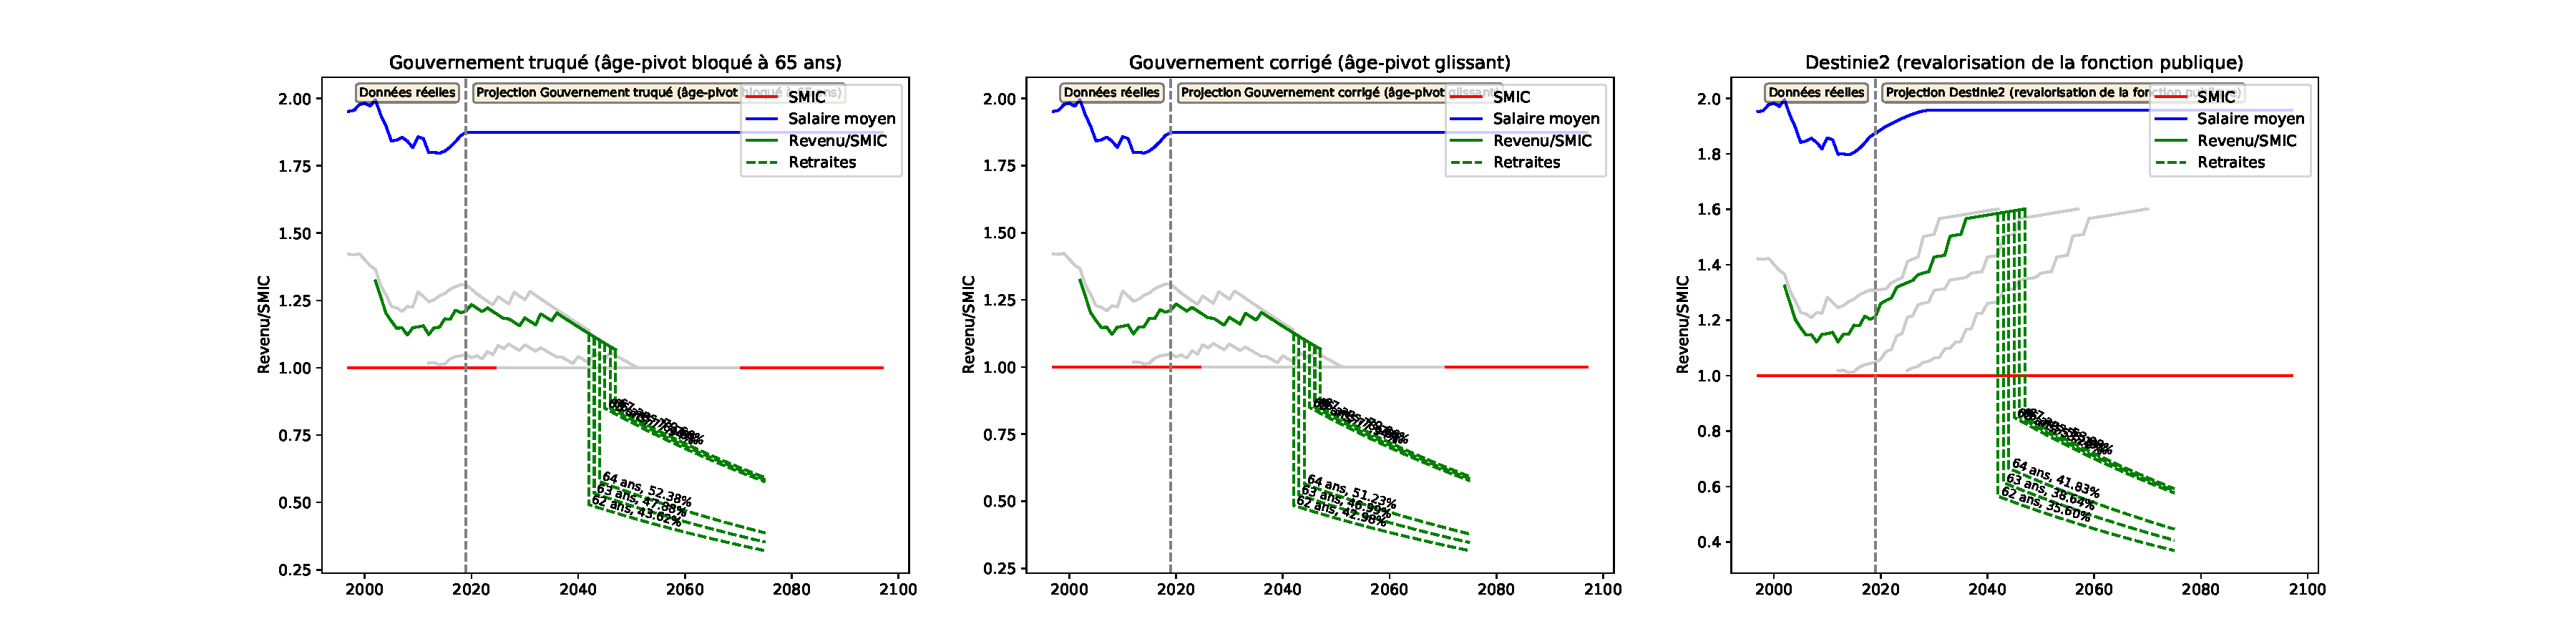
\includegraphics[width=0.9\textwidth]{fig/ATSEM_1980_22_dest_retraite.pdf}\end{center} \label{fig/ATSEM_1980_22_dest_retraite.pdf} 

\newpage 
 
\paragraph{Revenus et points pour le modèle \emph{Gouvernement truqué (âge-pivot bloqué à 65 ans)}} 
 
{ \scriptsize \begin{center} 
\begin{tabular}[htb]{|c|c||c|c|c|c|c|c||c|c||c|c|c|} 
\hline 
 Année &  Âge &  Ind Maj &  Pt Ind(\euro{} 2019) &  Rev HP(\euro{} 2019) &  Tx Primes &  GIPA(\euro{} 2019) &  Revenu(\euro{} 2019) &  SMIC(\euro{} 2019) &  Rev/SMIC &  Cumul Pts &  Achat Pt(\euro{} 2019) &  Serv. Pt(\euro{} 2019) \\ 
\hline \hline 
 2002 &  22 &  329.0 &  5.49 &  1804.98 &  6.11 &  0.00 &  1915.27 &  1447.74 &  {\bf 1.32} &  645.47 &  35.61 &  0.50 \\ 
\hline 
 2003 &  23 &  330.0 &  5.37 &  1773.62 &  6.34 &  0.00 &  1886.07 &  1493.03 &  {\bf 1.26} &  1281.10 &  35.61 &  0.50 \\ 
\hline 
 2004 &  24 &  330.0 &  5.29 &  1745.61 &  6.57 &  0.00 &  1860.29 &  1547.32 &  {\bf 1.20} &  1908.04 &  35.61 &  0.50 \\ 
\hline 
 2005 &  25 &  333.0 &  5.29 &  1761.29 &  6.80 &  0.00 &  1881.05 &  1603.67 &  {\bf 1.17} &  2541.98 &  35.61 &  0.50 \\ 
\hline 
 2006 &  26 &  333.0 &  5.23 &  1741.63 &  7.03 &  0.00 &  1864.07 &  1625.00 &  {\bf 1.15} &  3170.19 &  35.61 &  0.50 \\ 
\hline 
 2007 &  27 &  336.0 &  5.19 &  1745.35 &  7.26 &  4.08 &  1876.14 &  1634.08 &  {\bf 1.15} &  3802.47 &  35.61 &  0.50 \\ 
\hline 
 2008 &  28 &  336.0 &  5.09 &  1711.26 &  7.49 &  0.00 &  1839.44 &  1640.24 &  {\bf 1.12} &  4422.38 &  35.61 &  0.50 \\ 
\hline 
 2009 &  29 &  345.0 &  5.13 &  1769.55 &  7.72 &  0.00 &  1906.16 &  1659.42 &  {\bf 1.15} &  5064.78 &  35.61 &  0.50 \\ 
\hline 
 2010 &  30 &  345.0 &  5.08 &  1751.68 &  7.95 &  0.00 &  1890.93 &  1641.90 &  {\bf 1.15} &  5702.05 &  35.61 &  0.50 \\ 
\hline 
 2011 &  31 &  351.0 &  4.97 &  1745.11 &  8.18 &  0.00 &  1887.86 &  1633.19 &  {\bf 1.16} &  6338.28 &  35.61 &  0.50 \\ 
\hline 
 2012 &  32 &  351.0 &  4.88 &  1711.63 &  8.41 &  23.73 &  1879.30 &  1673.05 &  {\bf 1.12} &  6971.63 &  35.61 &  0.50 \\ 
\hline 
 2013 &  33 &  364.0 &  4.83 &  1759.81 &  8.64 &  0.00 &  1911.86 &  1664.01 &  {\bf 1.15} &  7615.95 &  35.61 &  0.50 \\ 
\hline 
 2014 &  34 &  364.0 &  4.81 &  1751.00 &  8.87 &  18.52 &  1924.84 &  1673.24 &  {\bf 1.15} &  8264.65 &  35.61 &  0.50 \\ 
\hline 
 2015 &  35 &  380.0 &  4.81 &  1827.26 &  9.10 &  0.00 &  1993.54 &  1686.62 &  {\bf 1.18} &  8936.49 &  35.61 &  0.50 \\ 
\hline 
 2016 &  36 &  380.0 &  4.80 &  1823.61 &  9.33 &  4.72 &  1998.48 &  1693.76 &  {\bf 1.18} &  9610.00 &  35.61 &  0.50 \\ 
\hline 
 2017 &  37 &  390.0 &  4.81 &  1875.37 &  9.56 &  0.00 &  2054.66 &  1692.60 &  {\bf 1.21} &  10302.45 &  35.61 &  0.50 \\ 
\hline 
 2018 &  38 &  390.0 &  4.74 &  1849.48 &  9.79 &  4.00 &  2034.55 &  1689.76 &  {\bf 1.20} &  10988.12 &  35.61 &  0.50 \\ 
\hline 
 2019 &  39 &  390.0 &  4.79 &  1869.82 &  10.02 &  0.00 &  2057.18 &  1698.45 &  {\bf 1.21} &  11681.41 &  35.61 &  0.50 \\ 
\hline 
 2020 &  40 &  402.0 &  4.79 &  1927.36 &  10.25 &  0.00 &  2124.91 &  1720.53 &  {\bf 1.24} &  12397.53 &  35.61 &  0.50 \\ 
\hline 
 2021 &  41 &  402.0 &  4.79 &  1927.36 &  10.48 &  0.00 &  2129.34 &  1742.90 &  {\bf 1.22} &  13115.15 &  35.61 &  0.50 \\ 
\hline 
 2022 &  42 &  402.0 &  4.79 &  1927.36 &  10.71 &  0.00 &  2133.78 &  1765.55 &  {\bf 1.21} &  13834.26 &  35.61 &  0.50 \\ 
\hline 
 2023 &  43 &  411.0 &  4.79 &  1970.51 &  10.94 &  0.00 &  2186.08 &  1788.51 &  {\bf 1.22} &  14570.99 &  35.61 &  0.50 \\ 
\hline 
 2024 &  44 &  411.0 &  4.79 &  1970.51 &  11.17 &  0.00 &  2190.61 &  1811.76 &  {\bf 1.21} &  15309.26 &  35.61 &  0.50 \\ 
\hline 
 2025 &  45 &  411.0 &  4.79 &  1970.51 &  11.40 &  0.00 &  2195.15 &  1835.31 &  {\bf 1.20} &  16049.05 &  35.61 &  0.50 \\ 
\hline 
 2026 &  46 &  411.0 &  4.79 &  1970.51 &  11.63 &  0.00 &  2199.68 &  1859.17 &  {\bf 1.18} &  16790.36 &  35.61 &  0.50 \\ 
\hline 
 2027 &  47 &  415.0 &  4.79 &  1989.69 &  11.86 &  0.00 &  2225.66 &  1883.34 &  {\bf 1.18} &  17540.44 &  35.61 &  0.50 \\ 
\hline 
 2028 &  48 &  415.0 &  4.79 &  1989.69 &  12.09 &  0.00 &  2230.24 &  1907.82 &  {\bf 1.17} &  18292.06 &  35.61 &  0.50 \\ 
\hline 
 2029 &  49 &  415.0 &  4.79 &  1989.69 &  12.32 &  0.00 &  2234.81 &  1932.62 &  {\bf 1.16} &  19044.64 &  35.63 &  0.50 \\ 
\hline 
 2030 &  50 &  430.0 &  4.79 &  2061.60 &  12.55 &  0.00 &  2320.33 &  1957.75 &  {\bf 1.19} &  19824.84 &  35.69 &  0.50 \\ 
\hline 
 2031 &  51 &  430.0 &  4.79 &  2061.60 &  12.78 &  0.00 &  2325.07 &  1983.20 &  {\bf 1.17} &  20604.86 &  35.77 &  0.50 \\ 
\hline 
 2032 &  52 &  430.0 &  4.79 &  2061.60 &  13.01 &  0.00 &  2329.82 &  2008.98 &  {\bf 1.16} &  21384.09 &  35.88 &  0.50 \\ 
\hline 
 2033 &  53 &  450.0 &  4.79 &  2157.49 &  13.24 &  0.00 &  2443.14 &  2035.10 &  {\bf 1.20} &  22198.13 &  36.02 &  0.50 \\ 
\hline 
 2034 &  54 &  450.0 &  4.79 &  2157.49 &  13.47 &  0.00 &  2448.10 &  2061.55 &  {\bf 1.19} &  23010.11 &  36.18 &  0.50 \\ 
\hline 
 2035 &  55 &  450.0 &  4.79 &  2157.49 &  13.70 &  0.00 &  2453.07 &  2088.35 &  {\bf 1.17} &  23819.42 &  36.37 &  0.51 \\ 
\hline 
 2036 &  56 &  466.0 &  4.79 &  2234.20 &  13.93 &  0.00 &  2545.42 &  2115.50 &  {\bf 1.20} &  24654.12 &  36.59 &  0.51 \\ 
\hline 
 2037 &  57 &  466.0 &  4.79 &  2234.20 &  14.16 &  0.00 &  2550.56 &  2143.00 &  {\bf 1.19} &  25484.80 &  36.85 &  0.51 \\ 
\hline 
 2038 &  58 &  466.0 &  4.79 &  2234.20 &  14.39 &  0.00 &  2555.70 &  2170.86 &  {\bf 1.18} &  26310.85 &  37.13 &  0.52 \\ 
\hline 
 2039 &  59 &  466.0 &  4.79 &  2234.20 &  14.62 &  0.00 &  2560.84 &  2199.08 &  {\bf 1.16} &  27131.67 &  37.44 &  0.52 \\ 
\hline 
 2040 &  60 &  466.0 &  4.79 &  2234.20 &  14.85 &  0.00 &  2565.98 &  2227.67 &  {\bf 1.15} &  27946.68 &  37.78 &  0.53 \\ 
\hline 
 2041 &  61 &  466.0 &  4.79 &  2234.20 &  15.08 &  0.00 &  2571.12 &  2256.63 &  {\bf 1.14} &  28755.29 &  38.16 &  0.53 \\ 
\hline 
 2042 &  62 &  466.0 &  4.79 &  2234.20 &  15.31 &  0.00 &  2576.26 &  2285.97 &  {\bf 1.13} &  29556.95 &  38.56 &  0.54 \\ 
\hline 
 2043 &  63 &  466.0 &  4.79 &  2234.20 &  15.54 &  0.00 &  2581.40 &  2315.68 &  {\bf 1.11} &  30351.10 &  39.01 &  0.54 \\ 
\hline 
 2044 &  64 &  466.0 &  4.79 &  2234.20 &  15.77 &  0.00 &  2586.53 &  2345.79 &  {\bf 1.10} &  31137.22 &  39.48 &  0.55 \\ 
\hline 
 2045 &  65 &  466.0 &  4.79 &  2234.20 &  16.00 &  0.00 &  2591.67 &  2376.28 &  {\bf 1.09} &  31914.79 &  40.00 &  0.56 \\ 
\hline 
 2046 &  66 &  466.0 &  4.79 &  2234.20 &  16.23 &  0.00 &  2596.81 &  2407.18 &  {\bf 1.08} &  32683.91 &  40.52 &  0.56 \\ 
\hline 
 2047 &  67 &  466.0 &  4.79 &  2234.20 &  16.46 &  0.00 &  2601.95 &  2438.47 &  {\bf 1.07} &  33444.66 &  41.04 &  0.57 \\ 
\hline 
\hline 
\end{tabular} 
\end{center} } 
\newpage 
 
\paragraph{Revenus et points pour le modèle \emph{Gouvernement corrigé (âge-pivot glissant)}} 
 
{ \scriptsize \begin{center} 
\begin{tabular}[htb]{|c|c||c|c|c|c|c|c||c|c||c|c|c|} 
\hline 
 Année &  Âge &  Ind Maj &  Pt Ind(\euro{} 2019) &  Rev HP(\euro{} 2019) &  Tx Primes &  GIPA(\euro{} 2019) &  Revenu(\euro{} 2019) &  SMIC(\euro{} 2019) &  Rev/SMIC &  Cumul Pts &  Achat Pt(\euro{} 2019) &  Serv. Pt(\euro{} 2019) \\ 
\hline \hline 
 2002 &  22 &  329.0 &  5.49 &  1804.98 &  6.11 &  0.00 &  1915.27 &  1447.74 &  {\bf 1.32} &  645.47 &  35.61 &  0.50 \\ 
\hline 
 2003 &  23 &  330.0 &  5.37 &  1773.62 &  6.34 &  0.00 &  1886.07 &  1493.03 &  {\bf 1.26} &  1281.10 &  35.61 &  0.50 \\ 
\hline 
 2004 &  24 &  330.0 &  5.29 &  1745.61 &  6.57 &  0.00 &  1860.29 &  1547.32 &  {\bf 1.20} &  1908.04 &  35.61 &  0.50 \\ 
\hline 
 2005 &  25 &  333.0 &  5.29 &  1761.29 &  6.80 &  0.00 &  1881.05 &  1603.67 &  {\bf 1.17} &  2541.98 &  35.61 &  0.50 \\ 
\hline 
 2006 &  26 &  333.0 &  5.23 &  1741.63 &  7.03 &  0.00 &  1864.07 &  1625.00 &  {\bf 1.15} &  3170.19 &  35.61 &  0.50 \\ 
\hline 
 2007 &  27 &  336.0 &  5.19 &  1745.35 &  7.26 &  4.08 &  1876.14 &  1634.08 &  {\bf 1.15} &  3802.47 &  35.61 &  0.50 \\ 
\hline 
 2008 &  28 &  336.0 &  5.09 &  1711.26 &  7.49 &  0.00 &  1839.44 &  1640.24 &  {\bf 1.12} &  4422.38 &  35.61 &  0.50 \\ 
\hline 
 2009 &  29 &  345.0 &  5.13 &  1769.55 &  7.72 &  0.00 &  1906.16 &  1659.42 &  {\bf 1.15} &  5064.78 &  35.61 &  0.50 \\ 
\hline 
 2010 &  30 &  345.0 &  5.08 &  1751.68 &  7.95 &  0.00 &  1890.93 &  1641.90 &  {\bf 1.15} &  5702.05 &  35.61 &  0.50 \\ 
\hline 
 2011 &  31 &  351.0 &  4.97 &  1745.11 &  8.18 &  0.00 &  1887.86 &  1633.19 &  {\bf 1.16} &  6338.28 &  35.61 &  0.50 \\ 
\hline 
 2012 &  32 &  351.0 &  4.88 &  1711.63 &  8.41 &  23.73 &  1879.30 &  1673.05 &  {\bf 1.12} &  6971.63 &  35.61 &  0.50 \\ 
\hline 
 2013 &  33 &  364.0 &  4.83 &  1759.81 &  8.64 &  0.00 &  1911.86 &  1664.01 &  {\bf 1.15} &  7615.95 &  35.61 &  0.50 \\ 
\hline 
 2014 &  34 &  364.0 &  4.81 &  1751.00 &  8.87 &  18.52 &  1924.84 &  1673.24 &  {\bf 1.15} &  8264.65 &  35.61 &  0.50 \\ 
\hline 
 2015 &  35 &  380.0 &  4.81 &  1827.26 &  9.10 &  0.00 &  1993.54 &  1686.62 &  {\bf 1.18} &  8936.49 &  35.61 &  0.50 \\ 
\hline 
 2016 &  36 &  380.0 &  4.80 &  1823.61 &  9.33 &  4.72 &  1998.48 &  1693.76 &  {\bf 1.18} &  9610.00 &  35.61 &  0.50 \\ 
\hline 
 2017 &  37 &  390.0 &  4.81 &  1875.37 &  9.56 &  0.00 &  2054.66 &  1692.60 &  {\bf 1.21} &  10302.45 &  35.61 &  0.50 \\ 
\hline 
 2018 &  38 &  390.0 &  4.74 &  1849.48 &  9.79 &  4.00 &  2034.55 &  1689.76 &  {\bf 1.20} &  10988.12 &  35.61 &  0.50 \\ 
\hline 
 2019 &  39 &  390.0 &  4.79 &  1869.82 &  10.02 &  0.00 &  2057.18 &  1698.45 &  {\bf 1.21} &  11681.41 &  35.61 &  0.50 \\ 
\hline 
 2020 &  40 &  402.0 &  4.79 &  1927.36 &  10.25 &  0.00 &  2124.91 &  1720.53 &  {\bf 1.24} &  12397.53 &  35.61 &  0.50 \\ 
\hline 
 2021 &  41 &  402.0 &  4.79 &  1927.36 &  10.48 &  0.00 &  2129.34 &  1742.90 &  {\bf 1.22} &  13115.15 &  35.61 &  0.50 \\ 
\hline 
 2022 &  42 &  402.0 &  4.79 &  1927.36 &  10.71 &  0.00 &  2133.78 &  1765.55 &  {\bf 1.21} &  13834.26 &  35.61 &  0.50 \\ 
\hline 
 2023 &  43 &  411.0 &  4.79 &  1970.51 &  10.94 &  0.00 &  2186.08 &  1788.51 &  {\bf 1.22} &  14570.99 &  35.61 &  0.50 \\ 
\hline 
 2024 &  44 &  411.0 &  4.79 &  1970.51 &  11.17 &  0.00 &  2190.61 &  1811.76 &  {\bf 1.21} &  15309.26 &  35.61 &  0.50 \\ 
\hline 
 2025 &  45 &  411.0 &  4.79 &  1970.51 &  11.40 &  0.00 &  2195.15 &  1835.31 &  {\bf 1.20} &  16049.05 &  35.61 &  0.50 \\ 
\hline 
 2026 &  46 &  411.0 &  4.79 &  1970.51 &  11.63 &  0.00 &  2199.68 &  1859.17 &  {\bf 1.18} &  16790.36 &  35.61 &  0.50 \\ 
\hline 
 2027 &  47 &  415.0 &  4.79 &  1989.69 &  11.86 &  0.00 &  2225.66 &  1883.34 &  {\bf 1.18} &  17540.44 &  35.61 &  0.50 \\ 
\hline 
 2028 &  48 &  415.0 &  4.79 &  1989.69 &  12.09 &  0.00 &  2230.24 &  1907.82 &  {\bf 1.17} &  18292.06 &  35.61 &  0.50 \\ 
\hline 
 2029 &  49 &  415.0 &  4.79 &  1989.69 &  12.32 &  0.00 &  2234.81 &  1932.62 &  {\bf 1.16} &  19044.64 &  35.63 &  0.50 \\ 
\hline 
 2030 &  50 &  430.0 &  4.79 &  2061.60 &  12.55 &  0.00 &  2320.33 &  1957.75 &  {\bf 1.19} &  19824.84 &  35.69 &  0.50 \\ 
\hline 
 2031 &  51 &  430.0 &  4.79 &  2061.60 &  12.78 &  0.00 &  2325.07 &  1983.20 &  {\bf 1.17} &  20604.86 &  35.77 &  0.50 \\ 
\hline 
 2032 &  52 &  430.0 &  4.79 &  2061.60 &  13.01 &  0.00 &  2329.82 &  2008.98 &  {\bf 1.16} &  21384.09 &  35.88 &  0.50 \\ 
\hline 
 2033 &  53 &  450.0 &  4.79 &  2157.49 &  13.24 &  0.00 &  2443.14 &  2035.10 &  {\bf 1.20} &  22198.13 &  36.02 &  0.50 \\ 
\hline 
 2034 &  54 &  450.0 &  4.79 &  2157.49 &  13.47 &  0.00 &  2448.10 &  2061.55 &  {\bf 1.19} &  23010.11 &  36.18 &  0.50 \\ 
\hline 
 2035 &  55 &  450.0 &  4.79 &  2157.49 &  13.70 &  0.00 &  2453.07 &  2088.35 &  {\bf 1.17} &  23819.42 &  36.37 &  0.51 \\ 
\hline 
 2036 &  56 &  466.0 &  4.79 &  2234.20 &  13.93 &  0.00 &  2545.42 &  2115.50 &  {\bf 1.20} &  24654.12 &  36.59 &  0.51 \\ 
\hline 
 2037 &  57 &  466.0 &  4.79 &  2234.20 &  14.16 &  0.00 &  2550.56 &  2143.00 &  {\bf 1.19} &  25484.80 &  36.85 &  0.51 \\ 
\hline 
 2038 &  58 &  466.0 &  4.79 &  2234.20 &  14.39 &  0.00 &  2555.70 &  2170.86 &  {\bf 1.18} &  26310.85 &  37.13 &  0.52 \\ 
\hline 
 2039 &  59 &  466.0 &  4.79 &  2234.20 &  14.62 &  0.00 &  2560.84 &  2199.08 &  {\bf 1.16} &  27131.67 &  37.44 &  0.52 \\ 
\hline 
 2040 &  60 &  466.0 &  4.79 &  2234.20 &  14.85 &  0.00 &  2565.98 &  2227.67 &  {\bf 1.15} &  27946.68 &  37.78 &  0.53 \\ 
\hline 
 2041 &  61 &  466.0 &  4.79 &  2234.20 &  15.08 &  0.00 &  2571.12 &  2256.63 &  {\bf 1.14} &  28755.29 &  38.16 &  0.53 \\ 
\hline 
 2042 &  62 &  466.0 &  4.79 &  2234.20 &  15.31 &  0.00 &  2576.26 &  2285.97 &  {\bf 1.13} &  29556.95 &  38.56 &  0.54 \\ 
\hline 
 2043 &  63 &  466.0 &  4.79 &  2234.20 &  15.54 &  0.00 &  2581.40 &  2315.68 &  {\bf 1.11} &  30351.10 &  39.01 &  0.54 \\ 
\hline 
 2044 &  64 &  466.0 &  4.79 &  2234.20 &  15.77 &  0.00 &  2586.53 &  2345.79 &  {\bf 1.10} &  31137.22 &  39.48 &  0.55 \\ 
\hline 
 2045 &  65 &  466.0 &  4.79 &  2234.20 &  16.00 &  0.00 &  2591.67 &  2376.28 &  {\bf 1.09} &  31914.79 &  40.00 &  0.56 \\ 
\hline 
 2046 &  66 &  466.0 &  4.79 &  2234.20 &  16.23 &  0.00 &  2596.81 &  2407.18 &  {\bf 1.08} &  32683.91 &  40.52 &  0.56 \\ 
\hline 
 2047 &  67 &  466.0 &  4.79 &  2234.20 &  16.46 &  0.00 &  2601.95 &  2438.47 &  {\bf 1.07} &  33444.66 &  41.04 &  0.57 \\ 
\hline 
\hline 
\end{tabular} 
\end{center} } 
\newpage 
 
\paragraph{Revenus et points pour le modèle \emph{Destinie2 (revalorisation de la fonction publique)}} 
 
{ \scriptsize \begin{center} 
\begin{tabular}[htb]{|c|c||c|c|c|c|c|c||c|c||c|c|c|} 
\hline 
 Année &  Âge &  Ind Maj &  Pt Ind(\euro{} 2019) &  Rev HP(\euro{} 2019) &  Tx Primes &  GIPA(\euro{} 2019) &  Revenu(\euro{} 2019) &  SMIC(\euro{} 2019) &  Rev/SMIC &  Cumul Pts &  Achat Pt(\euro{} 2019) &  Serv. Pt(\euro{} 2019) \\ 
\hline \hline 
 2002 &  22 &  329.0 &  5.49 &  1804.98 &  6.11 &  0.00 &  1915.27 &  1447.74 &  {\bf 1.32} &  643.88 &  35.69 &  0.50 \\ 
\hline 
 2003 &  23 &  330.0 &  5.37 &  1773.62 &  6.34 &  0.00 &  1886.07 &  1493.03 &  {\bf 1.26} &  1277.95 &  35.69 &  0.50 \\ 
\hline 
 2004 &  24 &  330.0 &  5.29 &  1745.61 &  6.57 &  0.00 &  1860.29 &  1547.32 &  {\bf 1.20} &  1903.35 &  35.69 &  0.50 \\ 
\hline 
 2005 &  25 &  333.0 &  5.29 &  1761.29 &  6.80 &  0.00 &  1881.05 &  1603.67 &  {\bf 1.17} &  2535.73 &  35.69 &  0.50 \\ 
\hline 
 2006 &  26 &  333.0 &  5.23 &  1741.63 &  7.03 &  0.00 &  1864.07 &  1625.00 &  {\bf 1.15} &  3162.40 &  35.69 &  0.50 \\ 
\hline 
 2007 &  27 &  336.0 &  5.19 &  1745.35 &  7.26 &  4.08 &  1876.14 &  1634.08 &  {\bf 1.15} &  3793.13 &  35.69 &  0.50 \\ 
\hline 
 2008 &  28 &  336.0 &  5.09 &  1711.26 &  7.49 &  0.00 &  1839.44 &  1640.24 &  {\bf 1.12} &  4411.52 &  35.69 &  0.50 \\ 
\hline 
 2009 &  29 &  345.0 &  5.13 &  1769.55 &  7.72 &  0.00 &  1906.16 &  1659.42 &  {\bf 1.15} &  5052.34 &  35.69 &  0.50 \\ 
\hline 
 2010 &  30 &  345.0 &  5.08 &  1751.68 &  7.95 &  0.00 &  1890.93 &  1641.90 &  {\bf 1.15} &  5688.04 &  35.69 &  0.50 \\ 
\hline 
 2011 &  31 &  351.0 &  4.97 &  1745.11 &  8.18 &  0.00 &  1887.86 &  1633.19 &  {\bf 1.16} &  6322.71 &  35.69 &  0.50 \\ 
\hline 
 2012 &  32 &  351.0 &  4.88 &  1711.63 &  8.41 &  21.42 &  1877.00 &  1673.05 &  {\bf 1.12} &  6953.73 &  35.69 &  0.50 \\ 
\hline 
 2013 &  33 &  364.0 &  4.83 &  1759.81 &  8.64 &  0.00 &  1911.86 &  1664.01 &  {\bf 1.15} &  7596.47 &  35.69 &  0.50 \\ 
\hline 
 2014 &  34 &  364.0 &  4.81 &  1751.00 &  8.87 &  17.93 &  1924.25 &  1673.24 &  {\bf 1.15} &  8243.37 &  35.69 &  0.50 \\ 
\hline 
 2015 &  35 &  380.0 &  4.81 &  1827.26 &  9.10 &  0.00 &  1993.54 &  1686.62 &  {\bf 1.18} &  8913.56 &  35.69 &  0.50 \\ 
\hline 
 2016 &  36 &  380.0 &  4.80 &  1823.61 &  9.33 &  3.96 &  1997.72 &  1693.76 &  {\bf 1.18} &  9585.16 &  35.69 &  0.50 \\ 
\hline 
 2017 &  37 &  390.0 &  4.81 &  1875.37 &  9.56 &  0.00 &  2054.66 &  1692.60 &  {\bf 1.21} &  10275.91 &  35.69 &  0.50 \\ 
\hline 
 2018 &  38 &  390.0 &  4.74 &  1849.48 &  9.79 &  3.66 &  2034.20 &  1689.76 &  {\bf 1.20} &  10959.77 &  35.69 &  0.50 \\ 
\hline 
 2019 &  39 &  390.0 &  4.79 &  1869.82 &  10.02 &  0.00 &  2057.18 &  1698.45 &  {\bf 1.21} &  11651.37 &  35.69 &  0.50 \\ 
\hline 
 2020 &  40 &  402.0 &  4.83 &  1942.78 &  10.25 &  0.00 &  2141.91 &  1699.99 &  {\bf 1.26} &  12371.44 &  35.69 &  0.50 \\ 
\hline 
 2021 &  41 &  402.0 &  4.88 &  1960.26 &  10.48 &  0.00 &  2165.70 &  1703.48 &  {\bf 1.27} &  13099.51 &  35.69 &  0.50 \\ 
\hline 
 2022 &  42 &  402.0 &  4.93 &  1979.86 &  10.71 &  0.00 &  2191.91 &  1712.78 &  {\bf 1.28} &  13836.40 &  35.69 &  0.50 \\ 
\hline 
 2023 &  43 &  411.0 &  4.98 &  2047.87 &  10.94 &  0.00 &  2271.91 &  1723.51 &  {\bf 1.32} &  14600.18 &  35.69 &  0.50 \\ 
\hline 
 2024 &  44 &  411.0 &  5.04 &  2072.24 &  11.17 &  0.00 &  2303.71 &  1735.69 &  {\bf 1.33} &  15374.65 &  35.69 &  0.50 \\ 
\hline 
 2025 &  45 &  411.0 &  5.10 &  2097.52 &  11.40 &  0.00 &  2336.64 &  1749.35 &  {\bf 1.34} &  16160.19 &  35.69 &  0.50 \\ 
\hline 
 2026 &  46 &  411.0 &  5.17 &  2123.74 &  11.63 &  0.00 &  2370.73 &  1764.53 &  {\bf 1.34} &  16957.20 &  35.69 &  0.50 \\ 
\hline 
 2027 &  47 &  415.0 &  5.23 &  2171.86 &  11.86 &  0.00 &  2429.44 &  1781.27 &  {\bf 1.36} &  17773.94 &  35.69 &  0.50 \\ 
\hline 
 2028 &  48 &  415.0 &  5.30 &  2200.31 &  12.09 &  0.00 &  2466.33 &  1799.59 &  {\bf 1.37} &  18603.08 &  35.69 &  0.50 \\ 
\hline 
 2029 &  49 &  415.0 &  5.37 &  2226.94 &  12.32 &  0.00 &  2501.29 &  1819.55 &  {\bf 1.37} &  19443.38 &  35.72 &  0.50 \\ 
\hline 
 2030 &  50 &  430.0 &  5.43 &  2336.04 &  12.55 &  0.00 &  2629.21 &  1841.19 &  {\bf 1.43} &  20325.37 &  35.77 &  0.50 \\ 
\hline 
 2031 &  51 &  430.0 &  5.50 &  2365.71 &  12.78 &  0.00 &  2668.04 &  1864.58 &  {\bf 1.43} &  21218.40 &  35.85 &  0.50 \\ 
\hline 
 2032 &  52 &  430.0 &  5.57 &  2396.46 &  13.01 &  0.00 &  2708.24 &  1888.81 &  {\bf 1.43} &  22122.13 &  35.96 &  0.50 \\ 
\hline 
 2033 &  53 &  450.0 &  5.65 &  2540.53 &  13.24 &  0.00 &  2876.89 &  1913.37 &  {\bf 1.50} &  23078.51 &  36.10 &  0.50 \\ 
\hline 
 2034 &  54 &  450.0 &  5.72 &  2573.55 &  13.47 &  0.00 &  2920.21 &  1938.24 &  {\bf 1.51} &  24044.87 &  36.26 &  0.50 \\ 
\hline 
 2035 &  55 &  450.0 &  5.79 &  2607.01 &  13.70 &  0.00 &  2964.17 &  1963.44 &  {\bf 1.51} &  25020.57 &  36.46 &  0.51 \\ 
\hline 
 2036 &  56 &  466.0 &  5.87 &  2734.80 &  13.93 &  0.00 &  3115.76 &  1988.96 &  {\bf 1.57} &  26039.95 &  36.68 &  0.51 \\ 
\hline 
 2037 &  57 &  466.0 &  5.94 &  2770.35 &  14.16 &  0.00 &  3162.63 &  2014.82 &  {\bf 1.57} &  27067.62 &  36.93 &  0.51 \\ 
\hline 
 2038 &  58 &  466.0 &  6.02 &  2806.37 &  14.39 &  0.00 &  3210.20 &  2041.01 &  {\bf 1.57} &  28102.85 &  37.21 &  0.52 \\ 
\hline 
 2039 &  59 &  466.0 &  6.10 &  2842.85 &  14.62 &  0.00 &  3258.47 &  2067.55 &  {\bf 1.58} &  29144.90 &  37.52 &  0.52 \\ 
\hline 
 2040 &  60 &  466.0 &  6.18 &  2879.81 &  14.85 &  0.00 &  3307.46 &  2094.43 &  {\bf 1.58} &  30193.02 &  37.87 &  0.53 \\ 
\hline 
 2041 &  61 &  466.0 &  6.26 &  2917.24 &  15.08 &  0.00 &  3357.16 &  2121.65 &  {\bf 1.58} &  31246.43 &  38.24 &  0.53 \\ 
\hline 
 2042 &  62 &  466.0 &  6.34 &  2955.17 &  15.31 &  0.00 &  3407.60 &  2149.23 &  {\bf 1.59} &  32304.36 &  38.65 &  0.54 \\ 
\hline 
 2043 &  63 &  466.0 &  6.42 &  2993.59 &  15.54 &  0.00 &  3458.79 &  2177.17 &  {\bf 1.59} &  33366.01 &  39.10 &  0.54 \\ 
\hline 
 2044 &  64 &  466.0 &  6.51 &  3032.50 &  15.77 &  0.00 &  3510.73 &  2205.48 &  {\bf 1.59} &  34430.58 &  39.57 &  0.55 \\ 
\hline 
 2045 &  65 &  466.0 &  6.59 &  3071.92 &  16.00 &  0.00 &  3563.43 &  2234.15 &  {\bf 1.59} &  35497.26 &  40.09 &  0.56 \\ 
\hline 
 2046 &  66 &  466.0 &  6.68 &  3111.86 &  16.23 &  0.00 &  3616.91 &  2263.19 &  {\bf 1.60} &  36566.06 &  40.61 &  0.57 \\ 
\hline 
 2047 &  67 &  466.0 &  6.76 &  3152.31 &  16.46 &  0.00 &  3671.18 &  2292.61 &  {\bf 1.60} &  37636.98 &  41.14 &  0.57 \\ 
\hline 
\hline 
\end{tabular} 
\end{center} } 
\newpage 
 
\subsection{Génération 1990 (début en 2012)} 

\paragraph{Retraites possibles dans le modèle \emph{Gouvernement truqué (âge-pivot bloqué à 65 ans)}}  
 
{ \scriptsize \begin{center} 
\begin{tabular}[htb]{|c|c||c|c||c|c||c||c|c|c|c|c|c|} 
\hline 
 Retraite en &  Âge &  Âge pivot &  Décote/Surcote &  Retraite (\euro{} 2019) &  Tx Rempl(\%) &  SMIC (\euro{} 2019) &  Retraite/SMIC &  Rev70/SMIC &  Rev75/SMIC &  Rev80/SMIC &  Rev85/SMIC &  Rev90/SMIC \\ 
\hline \hline 
 2052 &  62 &  65 ans 0 mois &  -15.00\% &  1206.15 &  {\bf 46.37} &  2601.14 &  {\bf {\color{red} 0.46}} &  {\bf {\color{red} 0.42}} &  {\bf {\color{red} 0.39}} &  {\bf {\color{red} 0.37}} &  {\bf {\color{red} 0.34}} &  {\bf {\color{red} 0.32}} \\ 
\hline 
 2053 &  63 &  65 ans 0 mois &  -10.00\% &  1326.71 &  {\bf 50.35} &  2634.96 &  {\bf {\color{red} 0.50}} &  {\bf {\color{red} 0.46}} &  {\bf {\color{red} 0.43}} &  {\bf {\color{red} 0.40}} &  {\bf {\color{red} 0.38}} &  {\bf {\color{red} 0.36}} \\ 
\hline 
 2054 &  64 &  65 ans 0 mois &  -5.00\% &  1453.92 &  {\bf 54.47} &  2669.21 &  {\bf {\color{red} 0.54}} &  {\bf {\color{red} 0.50}} &  {\bf {\color{red} 0.47}} &  {\bf {\color{red} 0.44}} &  {\bf {\color{red} 0.42}} &  {\bf {\color{red} 0.39}} \\ 
\hline 
 2055 &  65 &  65 ans 0 mois &  0.00\% &  2298.33 &  {\bf 85.00} &  2703.91 &  {\bf {\color{red} 0.85}} &  {\bf {\color{red} 0.80}} &  {\bf {\color{red} 0.75}} &  {\bf {\color{red} 0.70}} &  {\bf {\color{red} 0.66}} &  {\bf {\color{red} 0.62}} \\ 
\hline 
 2056 &  66 &  65 ans 0 mois &  5.00\% &  2328.20 &  {\bf 85.00} &  2739.06 &  {\bf {\color{red} 0.85}} &  {\bf {\color{red} 0.81}} &  {\bf {\color{red} 0.76}} &  {\bf {\color{red} 0.71}} &  {\bf {\color{red} 0.67}} &  {\bf {\color{red} 0.62}} \\ 
\hline 
 2057 &  67 &  65 ans 0 mois &  10.00\% &  2358.47 &  {\bf 85.00} &  2774.67 &  {\bf {\color{red} 0.85}} &  {\bf {\color{red} 0.82}} &  {\bf {\color{red} 0.77}} &  {\bf {\color{red} 0.72}} &  {\bf {\color{red} 0.67}} &  {\bf {\color{red} 0.63}} \\ 
\hline 
\hline 
\end{tabular} 
\end{center} } 
\paragraph{Retraites possibles dans le modèle \emph{Gouvernement corrigé (âge-pivot glissant)}}  
 
{ \scriptsize \begin{center} 
\begin{tabular}[htb]{|c|c||c|c||c|c||c||c|c|c|c|c|c|} 
\hline 
 Retraite en &  Âge &  Âge pivot &  Décote/Surcote &  Retraite (\euro{} 2019) &  Tx Rempl(\%) &  SMIC (\euro{} 2019) &  Retraite/SMIC &  Rev70/SMIC &  Rev75/SMIC &  Rev80/SMIC &  Rev85/SMIC &  Rev90/SMIC \\ 
\hline \hline 
 2052 &  62 &  66 ans 1 mois &  -20.42\% &  1129.28 &  {\bf 43.41} &  2601.14 &  {\bf {\color{red} 0.43}} &  {\bf {\color{red} 0.39}} &  {\bf {\color{red} 0.37}} &  {\bf {\color{red} 0.34}} &  {\bf {\color{red} 0.32}} &  {\bf {\color{red} 0.30}} \\ 
\hline 
 2053 &  63 &  66 ans 2 mois &  -15.83\% &  1240.72 &  {\bf 47.09} &  2634.96 &  {\bf {\color{red} 0.47}} &  {\bf {\color{red} 0.43}} &  {\bf {\color{red} 0.40}} &  {\bf {\color{red} 0.38}} &  {\bf {\color{red} 0.35}} &  {\bf {\color{red} 0.33}} \\ 
\hline 
 2054 &  64 &  66 ans 3 mois &  -11.25\% &  1358.26 &  {\bf 50.89} &  2669.21 &  {\bf {\color{red} 0.51}} &  {\bf {\color{red} 0.47}} &  {\bf {\color{red} 0.44}} &  {\bf {\color{red} 0.41}} &  {\bf {\color{red} 0.39}} &  {\bf {\color{red} 0.36}} \\ 
\hline 
 2055 &  65 &  66 ans 4 mois &  -6.67\% &  2298.33 &  {\bf 85.00} &  2703.91 &  {\bf {\color{red} 0.85}} &  {\bf {\color{red} 0.80}} &  {\bf {\color{red} 0.75}} &  {\bf {\color{red} 0.70}} &  {\bf {\color{red} 0.66}} &  {\bf {\color{red} 0.62}} \\ 
\hline 
 2056 &  66 &  66 ans 5 mois &  -2.08\% &  2328.20 &  {\bf 85.00} &  2739.06 &  {\bf {\color{red} 0.85}} &  {\bf {\color{red} 0.81}} &  {\bf {\color{red} 0.76}} &  {\bf {\color{red} 0.71}} &  {\bf {\color{red} 0.67}} &  {\bf {\color{red} 0.62}} \\ 
\hline 
 2057 &  67 &  66 ans 6 mois &  2.50\% &  2358.47 &  {\bf 85.00} &  2774.67 &  {\bf {\color{red} 0.85}} &  {\bf {\color{red} 0.82}} &  {\bf {\color{red} 0.77}} &  {\bf {\color{red} 0.72}} &  {\bf {\color{red} 0.67}} &  {\bf {\color{red} 0.63}} \\ 
\hline 
\hline 
\end{tabular} 
\end{center} } 
\paragraph{Retraites possibles dans le modèle \emph{Destinie2 (revalorisation de la fonction publique)}}  
 
{ \scriptsize \begin{center} 
\begin{tabular}[htb]{|c|c||c|c||c|c||c||c|c|c|c|c|c|} 
\hline 
 Retraite en &  Âge &  Âge pivot &  Décote/Surcote &  Retraite (\euro{} 2019) &  Tx Rempl(\%) &  SMIC (\euro{} 2019) &  Retraite/SMIC &  Rev70/SMIC &  Rev75/SMIC &  Rev80/SMIC &  Rev85/SMIC &  Rev90/SMIC \\ 
\hline \hline 
 2052 &  62 &  66 ans 1 mois &  -20.42\% &  1355.56 &  {\bf 34.96} &  2445.56 &  {\bf {\color{red} 0.55}} &  {\bf {\color{red} 0.50}} &  {\bf {\color{red} 0.47}} &  {\bf {\color{red} 0.44}} &  {\bf {\color{red} 0.41}} &  {\bf {\color{red} 0.39}} \\ 
\hline 
 2053 &  63 &  66 ans 2 mois &  -15.83\% &  1498.37 &  {\bf 38.07} &  2477.35 &  {\bf {\color{red} 0.60}} &  {\bf {\color{red} 0.55}} &  {\bf {\color{red} 0.52}} &  {\bf {\color{red} 0.49}} &  {\bf {\color{red} 0.46}} &  {\bf {\color{red} 0.43}} \\ 
\hline 
 2054 &  64 &  66 ans 3 mois &  -11.25\% &  1649.85 &  {\bf 41.30} &  2509.56 &  {\bf {\color{red} 0.66}} &  {\bf {\color{red} 0.61}} &  {\bf {\color{red} 0.57}} &  {\bf {\color{red} 0.53}} &  {\bf {\color{red} 0.50}} &  {\bf {\color{red} 0.47}} \\ 
\hline 
 2055 &  65 &  66 ans 4 mois &  -6.67\% &  2160.85 &  {\bf 53.29} &  2542.18 &  {\bf {\color{red} 0.85}} &  {\bf {\color{red} 0.80}} &  {\bf {\color{red} 0.75}} &  {\bf {\color{red} 0.70}} &  {\bf {\color{red} 0.66}} &  {\bf {\color{red} 0.62}} \\ 
\hline 
 2056 &  66 &  66 ans 5 mois &  -2.08\% &  2188.95 &  {\bf 53.19} &  2575.23 &  {\bf {\color{red} 0.85}} &  {\bf {\color{red} 0.81}} &  {\bf {\color{red} 0.76}} &  {\bf {\color{red} 0.71}} &  {\bf {\color{red} 0.67}} &  {\bf {\color{red} 0.62}} \\ 
\hline 
 2057 &  67 &  66 ans 6 mois &  2.50\% &  2217.40 &  {\bf 53.08} &  2608.71 &  {\bf {\color{red} 0.85}} &  {\bf {\color{red} 0.82}} &  {\bf {\color{red} 0.77}} &  {\bf {\color{red} 0.72}} &  {\bf {\color{red} 0.67}} &  {\bf {\color{red} 0.63}} \\ 
\hline 
\hline 
\end{tabular} 
\end{center} } 

 \begin{center}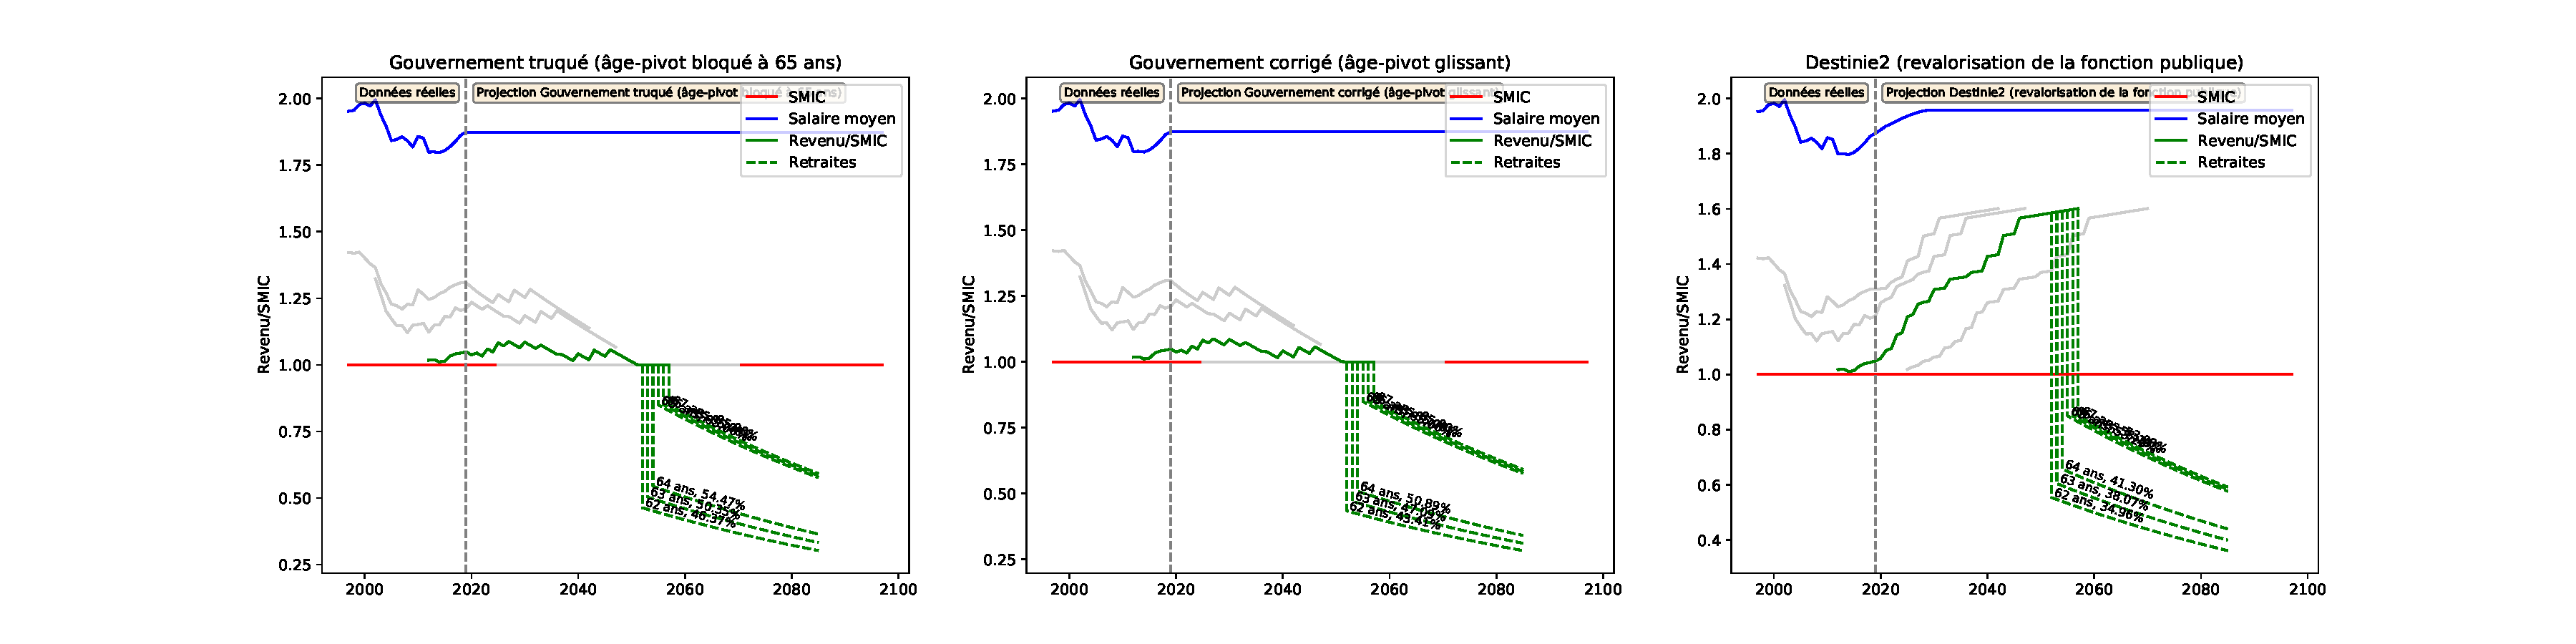
\includegraphics[width=0.9\textwidth]{fig/ATSEM_1990_22_dest_retraite.pdf}\end{center} \label{fig/ATSEM_1990_22_dest_retraite.pdf} 

\newpage 
 
\paragraph{Revenus et points pour le modèle \emph{Gouvernement truqué (âge-pivot bloqué à 65 ans)}} 
 
{ \scriptsize \begin{center} 
\begin{tabular}[htb]{|c|c||c|c|c|c|c|c||c|c||c|c|c|} 
\hline 
 Année &  Âge &  Ind Maj &  Pt Ind(\euro{} 2019) &  Rev HP(\euro{} 2019) &  Tx Primes &  GIPA(\euro{} 2019) &  Revenu(\euro{} 2019) &  SMIC(\euro{} 2019) &  Rev/SMIC &  Cumul Pts &  Achat Pt(\euro{} 2019) &  Serv. Pt(\euro{} 2019) \\ 
\hline \hline 
 2012 &  22 &  329.0 &  4.88 &  1604.35 &  6.11 &  0.00 &  1702.37 &  1673.05 &  {\bf 1.02} &  573.72 &  35.61 &  0.50 \\ 
\hline 
 2013 &  23 &  330.0 &  4.83 &  1595.44 &  6.34 &  0.00 &  1696.59 &  1664.01 &  {\bf 1.02} &  1145.49 &  35.61 &  0.50 \\ 
\hline 
 2014 &  24 &  330.0 &  4.81 &  1587.45 &  6.57 &  0.00 &  1691.74 &  1673.24 &  {\bf 1.01} &  1715.63 &  35.61 &  0.50 \\ 
\hline 
 2015 &  25 &  333.0 &  4.81 &  1601.25 &  6.80 &  0.00 &  1710.14 &  1686.62 &  {\bf 1.01} &  2291.97 &  35.61 &  0.50 \\ 
\hline 
 2016 &  26 &  333.0 &  4.80 &  1598.06 &  7.03 &  39.49 &  1749.89 &  1693.76 &  {\bf 1.03} &  2881.70 &  35.61 &  0.50 \\ 
\hline 
 2017 &  27 &  336.0 &  4.81 &  1615.71 &  7.26 &  29.54 &  1762.55 &  1692.60 &  {\bf 1.04} &  3475.70 &  35.61 &  0.50 \\ 
\hline 
 2018 &  28 &  336.0 &  4.74 &  1593.40 &  7.49 &  52.12 &  1764.87 &  1689.76 &  {\bf 1.04} &  4070.48 &  35.61 &  0.50 \\ 
\hline 
 2019 &  29 &  345.0 &  4.79 &  1654.08 &  7.72 &  0.00 &  1781.77 &  1698.45 &  {\bf 1.05} &  4670.96 &  35.61 &  0.50 \\ 
\hline 
 2020 &  30 &  345.0 &  4.79 &  1654.08 &  7.95 &  0.00 &  1785.57 &  1720.53 &  {\bf 1.04} &  5272.72 &  35.61 &  0.50 \\ 
\hline 
 2021 &  31 &  351.0 &  4.79 &  1682.84 &  8.18 &  0.00 &  1820.50 &  1742.90 &  {\bf 1.04} &  5886.25 &  35.61 &  0.50 \\ 
\hline 
 2022 &  32 &  351.0 &  4.79 &  1682.84 &  8.41 &  0.00 &  1824.37 &  1765.55 &  {\bf 1.03} &  6501.09 &  35.61 &  0.50 \\ 
\hline 
 2023 &  33 &  364.0 &  4.79 &  1745.17 &  8.64 &  0.00 &  1895.95 &  1788.51 &  {\bf 1.06} &  7140.05 &  35.61 &  0.50 \\ 
\hline 
 2024 &  34 &  364.0 &  4.79 &  1745.17 &  8.87 &  0.00 &  1899.97 &  1811.76 &  {\bf 1.05} &  7780.36 &  35.61 &  0.50 \\ 
\hline 
 2025 &  35 &  380.0 &  4.79 &  1821.88 &  9.10 &  0.00 &  1987.67 &  1835.31 &  {\bf 1.08} &  8450.23 &  35.61 &  0.50 \\ 
\hline 
 2026 &  36 &  380.0 &  4.79 &  1821.88 &  9.33 &  0.00 &  1991.86 &  1859.17 &  {\bf 1.07} &  9121.51 &  35.61 &  0.50 \\ 
\hline 
 2027 &  37 &  390.0 &  4.79 &  1869.82 &  9.56 &  0.00 &  2048.58 &  1883.34 &  {\bf 1.09} &  9811.90 &  35.61 &  0.50 \\ 
\hline 
 2028 &  38 &  390.0 &  4.79 &  1869.82 &  9.79 &  0.00 &  2052.88 &  1907.82 &  {\bf 1.08} &  10503.75 &  35.61 &  0.50 \\ 
\hline 
 2029 &  39 &  390.0 &  4.79 &  1869.82 &  10.02 &  0.00 &  2057.18 &  1932.62 &  {\bf 1.06} &  11196.52 &  35.63 &  0.50 \\ 
\hline 
 2030 &  40 &  402.0 &  4.79 &  1927.36 &  10.25 &  0.00 &  2124.91 &  1957.75 &  {\bf 1.09} &  11911.01 &  35.69 &  0.50 \\ 
\hline 
 2031 &  41 &  402.0 &  4.79 &  1927.36 &  10.48 &  0.00 &  2129.34 &  1983.20 &  {\bf 1.07} &  12625.36 &  35.77 &  0.50 \\ 
\hline 
 2032 &  42 &  402.0 &  4.79 &  1927.36 &  10.71 &  0.00 &  2133.78 &  2008.98 &  {\bf 1.06} &  13339.03 &  35.88 &  0.50 \\ 
\hline 
 2033 &  43 &  411.0 &  4.79 &  1970.51 &  10.94 &  0.00 &  2186.08 &  2035.10 &  {\bf 1.07} &  14067.41 &  36.02 &  0.50 \\ 
\hline 
 2034 &  44 &  411.0 &  4.79 &  1970.51 &  11.17 &  0.00 &  2190.61 &  2061.55 &  {\bf 1.06} &  14793.99 &  36.18 &  0.50 \\ 
\hline 
 2035 &  45 &  411.0 &  4.79 &  1970.51 &  11.40 &  0.00 &  2195.15 &  2088.35 &  {\bf 1.05} &  15518.21 &  36.37 &  0.51 \\ 
\hline 
 2036 &  46 &  411.0 &  4.79 &  1970.51 &  11.63 &  0.00 &  2199.68 &  2115.50 &  {\bf 1.04} &  16239.53 &  36.59 &  0.51 \\ 
\hline 
 2037 &  47 &  415.0 &  4.79 &  1989.69 &  11.86 &  0.00 &  2225.66 &  2143.00 &  {\bf 1.04} &  16964.39 &  36.85 &  0.51 \\ 
\hline 
 2038 &  48 &  415.0 &  4.79 &  1989.69 &  12.09 &  0.00 &  2230.24 &  2170.86 &  {\bf 1.03} &  17685.25 &  37.13 &  0.52 \\ 
\hline 
 2039 &  49 &  415.0 &  4.79 &  1989.69 &  12.32 &  0.00 &  2234.81 &  2199.08 &  {\bf 1.02} &  18401.57 &  37.44 &  0.52 \\ 
\hline 
 2040 &  50 &  430.0 &  4.79 &  2061.60 &  12.55 &  0.00 &  2320.33 &  2227.67 &  {\bf 1.04} &  19138.55 &  37.78 &  0.53 \\ 
\hline 
 2041 &  51 &  430.0 &  4.79 &  2061.60 &  12.78 &  0.00 &  2325.07 &  2256.63 &  {\bf 1.03} &  19869.79 &  38.16 &  0.53 \\ 
\hline 
 2042 &  52 &  430.0 &  4.79 &  2061.60 &  13.01 &  0.00 &  2329.82 &  2285.97 &  {\bf 1.02} &  20594.76 &  38.56 &  0.54 \\ 
\hline 
 2043 &  53 &  450.0 &  4.79 &  2157.49 &  13.24 &  0.00 &  2443.14 &  2315.68 &  {\bf 1.06} &  21346.38 &  39.01 &  0.54 \\ 
\hline 
 2044 &  54 &  450.0 &  4.79 &  2157.49 &  13.47 &  0.00 &  2448.10 &  2345.79 &  {\bf 1.04} &  22090.42 &  39.48 &  0.55 \\ 
\hline 
 2045 &  55 &  450.0 &  4.79 &  2157.49 &  13.70 &  0.00 &  2453.07 &  2376.28 &  {\bf 1.03} &  22826.41 &  40.00 &  0.56 \\ 
\hline 
 2046 &  56 &  466.0 &  4.79 &  2234.20 &  13.93 &  0.00 &  2545.42 &  2407.18 &  {\bf 1.06} &  23580.31 &  40.52 &  0.56 \\ 
\hline 
 2047 &  57 &  466.0 &  4.79 &  2234.20 &  14.16 &  0.00 &  2550.56 &  2438.47 &  {\bf 1.05} &  24326.03 &  41.04 &  0.57 \\ 
\hline 
 2048 &  58 &  466.0 &  4.79 &  2234.20 &  14.39 &  0.00 &  2555.70 &  2470.17 &  {\bf 1.03} &  25063.67 &  41.58 &  0.58 \\ 
\hline 
 2049 &  59 &  466.0 &  4.79 &  2234.20 &  14.62 &  0.00 &  2560.84 &  2502.28 &  {\bf 1.02} &  25793.30 &  42.12 &  0.59 \\ 
\hline 
 2050 &  60 &  466.0 &  4.79 &  2234.20 &  14.85 &  0.00 &  2565.98 &  2534.81 &  {\bf 1.01} &  26515.02 &  42.66 &  0.59 \\ 
\hline 
 2051 &  61 &  466.0 &  4.79 &  2234.20 &  15.08 &  0.00 &  2571.12 &  2567.76 &  {\bf 1.00} &  27228.90 &  43.22 &  0.60 \\ 
\hline 
 2052 &  62 &  466.0 &  4.79 &  2234.20 &  15.31 &  0.00 &  2601.14 &  2601.14 &  {\bf 1.00} &  27941.85 &  43.78 &  0.61 \\ 
\hline 
 2053 &  63 &  466.0 &  4.79 &  2234.20 &  15.54 &  0.00 &  2634.96 &  2634.96 &  {\bf 1.00} &  28654.80 &  44.35 &  0.62 \\ 
\hline 
 2054 &  64 &  466.0 &  4.79 &  2234.20 &  15.77 &  6.77 &  2669.21 &  2669.21 &  {\bf 1.00} &  29367.75 &  44.93 &  0.63 \\ 
\hline 
 2055 &  65 &  466.0 &  4.79 &  2234.20 &  16.00 &  27.44 &  2703.91 &  2703.91 &  {\bf 1.00} &  30080.70 &  45.51 &  0.63 \\ 
\hline 
 2056 &  66 &  466.0 &  4.79 &  2234.20 &  16.23 &  55.50 &  2739.06 &  2739.06 &  {\bf 1.00} &  30793.65 &  46.10 &  0.64 \\ 
\hline 
 2057 &  67 &  466.0 &  4.79 &  2234.20 &  16.46 &  84.84 &  2774.67 &  2774.67 &  {\bf 1.00} &  31506.60 &  46.70 &  0.65 \\ 
\hline 
\hline 
\end{tabular} 
\end{center} } 
\newpage 
 
\paragraph{Revenus et points pour le modèle \emph{Gouvernement corrigé (âge-pivot glissant)}} 
 
{ \scriptsize \begin{center} 
\begin{tabular}[htb]{|c|c||c|c|c|c|c|c||c|c||c|c|c|} 
\hline 
 Année &  Âge &  Ind Maj &  Pt Ind(\euro{} 2019) &  Rev HP(\euro{} 2019) &  Tx Primes &  GIPA(\euro{} 2019) &  Revenu(\euro{} 2019) &  SMIC(\euro{} 2019) &  Rev/SMIC &  Cumul Pts &  Achat Pt(\euro{} 2019) &  Serv. Pt(\euro{} 2019) \\ 
\hline \hline 
 2012 &  22 &  329.0 &  4.88 &  1604.35 &  6.11 &  0.00 &  1702.37 &  1673.05 &  {\bf 1.02} &  573.72 &  35.61 &  0.50 \\ 
\hline 
 2013 &  23 &  330.0 &  4.83 &  1595.44 &  6.34 &  0.00 &  1696.59 &  1664.01 &  {\bf 1.02} &  1145.49 &  35.61 &  0.50 \\ 
\hline 
 2014 &  24 &  330.0 &  4.81 &  1587.45 &  6.57 &  0.00 &  1691.74 &  1673.24 &  {\bf 1.01} &  1715.63 &  35.61 &  0.50 \\ 
\hline 
 2015 &  25 &  333.0 &  4.81 &  1601.25 &  6.80 &  0.00 &  1710.14 &  1686.62 &  {\bf 1.01} &  2291.97 &  35.61 &  0.50 \\ 
\hline 
 2016 &  26 &  333.0 &  4.80 &  1598.06 &  7.03 &  39.49 &  1749.89 &  1693.76 &  {\bf 1.03} &  2881.70 &  35.61 &  0.50 \\ 
\hline 
 2017 &  27 &  336.0 &  4.81 &  1615.71 &  7.26 &  29.54 &  1762.55 &  1692.60 &  {\bf 1.04} &  3475.70 &  35.61 &  0.50 \\ 
\hline 
 2018 &  28 &  336.0 &  4.74 &  1593.40 &  7.49 &  52.12 &  1764.87 &  1689.76 &  {\bf 1.04} &  4070.48 &  35.61 &  0.50 \\ 
\hline 
 2019 &  29 &  345.0 &  4.79 &  1654.08 &  7.72 &  0.00 &  1781.77 &  1698.45 &  {\bf 1.05} &  4670.96 &  35.61 &  0.50 \\ 
\hline 
 2020 &  30 &  345.0 &  4.79 &  1654.08 &  7.95 &  0.00 &  1785.57 &  1720.53 &  {\bf 1.04} &  5272.72 &  35.61 &  0.50 \\ 
\hline 
 2021 &  31 &  351.0 &  4.79 &  1682.84 &  8.18 &  0.00 &  1820.50 &  1742.90 &  {\bf 1.04} &  5886.25 &  35.61 &  0.50 \\ 
\hline 
 2022 &  32 &  351.0 &  4.79 &  1682.84 &  8.41 &  0.00 &  1824.37 &  1765.55 &  {\bf 1.03} &  6501.09 &  35.61 &  0.50 \\ 
\hline 
 2023 &  33 &  364.0 &  4.79 &  1745.17 &  8.64 &  0.00 &  1895.95 &  1788.51 &  {\bf 1.06} &  7140.05 &  35.61 &  0.50 \\ 
\hline 
 2024 &  34 &  364.0 &  4.79 &  1745.17 &  8.87 &  0.00 &  1899.97 &  1811.76 &  {\bf 1.05} &  7780.36 &  35.61 &  0.50 \\ 
\hline 
 2025 &  35 &  380.0 &  4.79 &  1821.88 &  9.10 &  0.00 &  1987.67 &  1835.31 &  {\bf 1.08} &  8450.23 &  35.61 &  0.50 \\ 
\hline 
 2026 &  36 &  380.0 &  4.79 &  1821.88 &  9.33 &  0.00 &  1991.86 &  1859.17 &  {\bf 1.07} &  9121.51 &  35.61 &  0.50 \\ 
\hline 
 2027 &  37 &  390.0 &  4.79 &  1869.82 &  9.56 &  0.00 &  2048.58 &  1883.34 &  {\bf 1.09} &  9811.90 &  35.61 &  0.50 \\ 
\hline 
 2028 &  38 &  390.0 &  4.79 &  1869.82 &  9.79 &  0.00 &  2052.88 &  1907.82 &  {\bf 1.08} &  10503.75 &  35.61 &  0.50 \\ 
\hline 
 2029 &  39 &  390.0 &  4.79 &  1869.82 &  10.02 &  0.00 &  2057.18 &  1932.62 &  {\bf 1.06} &  11196.52 &  35.63 &  0.50 \\ 
\hline 
 2030 &  40 &  402.0 &  4.79 &  1927.36 &  10.25 &  0.00 &  2124.91 &  1957.75 &  {\bf 1.09} &  11911.01 &  35.69 &  0.50 \\ 
\hline 
 2031 &  41 &  402.0 &  4.79 &  1927.36 &  10.48 &  0.00 &  2129.34 &  1983.20 &  {\bf 1.07} &  12625.36 &  35.77 &  0.50 \\ 
\hline 
 2032 &  42 &  402.0 &  4.79 &  1927.36 &  10.71 &  0.00 &  2133.78 &  2008.98 &  {\bf 1.06} &  13339.03 &  35.88 &  0.50 \\ 
\hline 
 2033 &  43 &  411.0 &  4.79 &  1970.51 &  10.94 &  0.00 &  2186.08 &  2035.10 &  {\bf 1.07} &  14067.41 &  36.02 &  0.50 \\ 
\hline 
 2034 &  44 &  411.0 &  4.79 &  1970.51 &  11.17 &  0.00 &  2190.61 &  2061.55 &  {\bf 1.06} &  14793.99 &  36.18 &  0.50 \\ 
\hline 
 2035 &  45 &  411.0 &  4.79 &  1970.51 &  11.40 &  0.00 &  2195.15 &  2088.35 &  {\bf 1.05} &  15518.21 &  36.37 &  0.51 \\ 
\hline 
 2036 &  46 &  411.0 &  4.79 &  1970.51 &  11.63 &  0.00 &  2199.68 &  2115.50 &  {\bf 1.04} &  16239.53 &  36.59 &  0.51 \\ 
\hline 
 2037 &  47 &  415.0 &  4.79 &  1989.69 &  11.86 &  0.00 &  2225.66 &  2143.00 &  {\bf 1.04} &  16964.39 &  36.85 &  0.51 \\ 
\hline 
 2038 &  48 &  415.0 &  4.79 &  1989.69 &  12.09 &  0.00 &  2230.24 &  2170.86 &  {\bf 1.03} &  17685.25 &  37.13 &  0.52 \\ 
\hline 
 2039 &  49 &  415.0 &  4.79 &  1989.69 &  12.32 &  0.00 &  2234.81 &  2199.08 &  {\bf 1.02} &  18401.57 &  37.44 &  0.52 \\ 
\hline 
 2040 &  50 &  430.0 &  4.79 &  2061.60 &  12.55 &  0.00 &  2320.33 &  2227.67 &  {\bf 1.04} &  19138.55 &  37.78 &  0.53 \\ 
\hline 
 2041 &  51 &  430.0 &  4.79 &  2061.60 &  12.78 &  0.00 &  2325.07 &  2256.63 &  {\bf 1.03} &  19869.79 &  38.16 &  0.53 \\ 
\hline 
 2042 &  52 &  430.0 &  4.79 &  2061.60 &  13.01 &  0.00 &  2329.82 &  2285.97 &  {\bf 1.02} &  20594.76 &  38.56 &  0.54 \\ 
\hline 
 2043 &  53 &  450.0 &  4.79 &  2157.49 &  13.24 &  0.00 &  2443.14 &  2315.68 &  {\bf 1.06} &  21346.38 &  39.01 &  0.54 \\ 
\hline 
 2044 &  54 &  450.0 &  4.79 &  2157.49 &  13.47 &  0.00 &  2448.10 &  2345.79 &  {\bf 1.04} &  22090.42 &  39.48 &  0.55 \\ 
\hline 
 2045 &  55 &  450.0 &  4.79 &  2157.49 &  13.70 &  0.00 &  2453.07 &  2376.28 &  {\bf 1.03} &  22826.41 &  40.00 &  0.56 \\ 
\hline 
 2046 &  56 &  466.0 &  4.79 &  2234.20 &  13.93 &  0.00 &  2545.42 &  2407.18 &  {\bf 1.06} &  23580.31 &  40.52 &  0.56 \\ 
\hline 
 2047 &  57 &  466.0 &  4.79 &  2234.20 &  14.16 &  0.00 &  2550.56 &  2438.47 &  {\bf 1.05} &  24326.03 &  41.04 &  0.57 \\ 
\hline 
 2048 &  58 &  466.0 &  4.79 &  2234.20 &  14.39 &  0.00 &  2555.70 &  2470.17 &  {\bf 1.03} &  25063.67 &  41.58 &  0.58 \\ 
\hline 
 2049 &  59 &  466.0 &  4.79 &  2234.20 &  14.62 &  0.00 &  2560.84 &  2502.28 &  {\bf 1.02} &  25793.30 &  42.12 &  0.59 \\ 
\hline 
 2050 &  60 &  466.0 &  4.79 &  2234.20 &  14.85 &  0.00 &  2565.98 &  2534.81 &  {\bf 1.01} &  26515.02 &  42.66 &  0.59 \\ 
\hline 
 2051 &  61 &  466.0 &  4.79 &  2234.20 &  15.08 &  0.00 &  2571.12 &  2567.76 &  {\bf 1.00} &  27228.90 &  43.22 &  0.60 \\ 
\hline 
 2052 &  62 &  466.0 &  4.79 &  2234.20 &  15.31 &  0.00 &  2601.14 &  2601.14 &  {\bf 1.00} &  27941.85 &  43.78 &  0.61 \\ 
\hline 
 2053 &  63 &  466.0 &  4.79 &  2234.20 &  15.54 &  0.00 &  2634.96 &  2634.96 &  {\bf 1.00} &  28654.80 &  44.35 &  0.62 \\ 
\hline 
 2054 &  64 &  466.0 &  4.79 &  2234.20 &  15.77 &  6.77 &  2669.21 &  2669.21 &  {\bf 1.00} &  29367.75 &  44.93 &  0.63 \\ 
\hline 
 2055 &  65 &  466.0 &  4.79 &  2234.20 &  16.00 &  27.44 &  2703.91 &  2703.91 &  {\bf 1.00} &  30080.70 &  45.51 &  0.63 \\ 
\hline 
 2056 &  66 &  466.0 &  4.79 &  2234.20 &  16.23 &  55.50 &  2739.06 &  2739.06 &  {\bf 1.00} &  30793.65 &  46.10 &  0.64 \\ 
\hline 
 2057 &  67 &  466.0 &  4.79 &  2234.20 &  16.46 &  84.84 &  2774.67 &  2774.67 &  {\bf 1.00} &  31506.60 &  46.70 &  0.65 \\ 
\hline 
\hline 
\end{tabular} 
\end{center} } 
\newpage 
 
\paragraph{Revenus et points pour le modèle \emph{Destinie2 (revalorisation de la fonction publique)}} 
 
{ \scriptsize \begin{center} 
\begin{tabular}[htb]{|c|c||c|c|c|c|c|c||c|c||c|c|c|} 
\hline 
 Année &  Âge &  Ind Maj &  Pt Ind(\euro{} 2019) &  Rev HP(\euro{} 2019) &  Tx Primes &  GIPA(\euro{} 2019) &  Revenu(\euro{} 2019) &  SMIC(\euro{} 2019) &  Rev/SMIC &  Cumul Pts &  Achat Pt(\euro{} 2019) &  Serv. Pt(\euro{} 2019) \\ 
\hline \hline 
 2012 &  22 &  329.0 &  4.88 &  1604.35 &  6.11 &  0.00 &  1702.37 &  1673.05 &  {\bf 1.02} &  572.31 &  35.69 &  0.50 \\ 
\hline 
 2013 &  23 &  330.0 &  4.83 &  1595.44 &  6.34 &  0.00 &  1696.59 &  1664.01 &  {\bf 1.02} &  1142.68 &  35.69 &  0.50 \\ 
\hline 
 2014 &  24 &  330.0 &  4.81 &  1587.45 &  6.57 &  0.00 &  1691.74 &  1673.24 &  {\bf 1.01} &  1711.41 &  35.69 &  0.50 \\ 
\hline 
 2015 &  25 &  333.0 &  4.81 &  1601.25 &  6.80 &  0.00 &  1710.14 &  1686.62 &  {\bf 1.01} &  2286.33 &  35.69 &  0.50 \\ 
\hline 
 2016 &  26 &  333.0 &  4.80 &  1598.06 &  7.03 &  35.19 &  1745.59 &  1693.76 &  {\bf 1.03} &  2873.18 &  35.69 &  0.50 \\ 
\hline 
 2017 &  27 &  336.0 &  4.81 &  1615.71 &  7.26 &  26.29 &  1759.29 &  1692.60 &  {\bf 1.04} &  3464.62 &  35.69 &  0.50 \\ 
\hline 
 2018 &  28 &  336.0 &  4.74 &  1593.40 &  7.49 &  50.22 &  1762.97 &  1689.76 &  {\bf 1.04} &  4057.30 &  35.69 &  0.50 \\ 
\hline 
 2019 &  29 &  345.0 &  4.79 &  1654.08 &  7.72 &  0.00 &  1781.77 &  1698.45 &  {\bf 1.05} &  4656.30 &  35.69 &  0.50 \\ 
\hline 
 2020 &  30 &  345.0 &  4.83 &  1667.31 &  7.95 &  0.00 &  1799.86 &  1699.99 &  {\bf 1.06} &  5261.39 &  35.69 &  0.50 \\ 
\hline 
 2021 &  31 &  351.0 &  4.88 &  1711.57 &  8.18 &  0.00 &  1851.58 &  1703.48 &  {\bf 1.09} &  5883.86 &  35.69 &  0.50 \\ 
\hline 
 2022 &  32 &  351.0 &  4.93 &  1728.69 &  8.41 &  0.00 &  1874.07 &  1712.78 &  {\bf 1.09} &  6513.89 &  35.69 &  0.50 \\ 
\hline 
 2023 &  33 &  364.0 &  4.98 &  1813.69 &  8.64 &  0.00 &  1970.39 &  1723.51 &  {\bf 1.14} &  7176.31 &  35.69 &  0.50 \\ 
\hline 
 2024 &  34 &  364.0 &  5.04 &  1835.27 &  8.87 &  0.00 &  1998.06 &  1735.69 &  {\bf 1.15} &  7848.02 &  35.69 &  0.50 \\ 
\hline 
 2025 &  35 &  380.0 &  5.10 &  1939.32 &  9.10 &  0.00 &  2115.79 &  1749.35 &  {\bf 1.21} &  8559.32 &  35.69 &  0.50 \\ 
\hline 
 2026 &  36 &  380.0 &  5.17 &  1963.56 &  9.33 &  0.00 &  2146.76 &  1764.53 &  {\bf 1.22} &  9281.02 &  35.69 &  0.50 \\ 
\hline 
 2027 &  37 &  390.0 &  5.23 &  2041.03 &  9.56 &  0.00 &  2236.15 &  1781.27 &  {\bf 1.26} &  10032.78 &  35.69 &  0.50 \\ 
\hline 
 2028 &  38 &  390.0 &  5.30 &  2067.76 &  9.79 &  0.00 &  2270.20 &  1799.59 &  {\bf 1.26} &  10795.99 &  35.69 &  0.50 \\ 
\hline 
 2029 &  39 &  390.0 &  5.37 &  2092.78 &  10.02 &  0.00 &  2302.48 &  1819.55 &  {\bf 1.27} &  11569.50 &  35.72 &  0.50 \\ 
\hline 
 2030 &  40 &  402.0 &  5.43 &  2183.92 &  10.25 &  0.00 &  2407.78 &  1841.19 &  {\bf 1.31} &  12377.21 &  35.77 &  0.50 \\ 
\hline 
 2031 &  41 &  402.0 &  5.50 &  2211.66 &  10.48 &  0.00 &  2443.44 &  1864.58 &  {\bf 1.31} &  13195.06 &  35.85 &  0.50 \\ 
\hline 
 2032 &  42 &  402.0 &  5.57 &  2240.41 &  10.71 &  0.00 &  2480.36 &  1888.81 &  {\bf 1.31} &  14022.75 &  35.96 &  0.50 \\ 
\hline 
 2033 &  43 &  411.0 &  5.65 &  2320.35 &  10.94 &  0.00 &  2574.19 &  1913.37 &  {\bf 1.35} &  14878.50 &  36.10 &  0.50 \\ 
\hline 
 2034 &  44 &  411.0 &  5.72 &  2350.51 &  11.17 &  0.00 &  2613.06 &  1938.24 &  {\bf 1.35} &  15743.21 &  36.26 &  0.50 \\ 
\hline 
 2035 &  45 &  411.0 &  5.79 &  2381.07 &  11.40 &  0.00 &  2652.51 &  1963.44 &  {\bf 1.35} &  16616.33 &  36.46 &  0.51 \\ 
\hline 
 2036 &  46 &  411.0 &  5.87 &  2412.02 &  11.63 &  0.00 &  2692.54 &  1988.96 &  {\bf 1.35} &  17497.25 &  36.68 &  0.51 \\ 
\hline 
 2037 &  47 &  415.0 &  5.94 &  2467.16 &  11.86 &  0.00 &  2759.76 &  2014.82 &  {\bf 1.37} &  18394.01 &  36.93 &  0.51 \\ 
\hline 
 2038 &  48 &  415.0 &  6.02 &  2499.23 &  12.09 &  0.00 &  2801.39 &  2041.01 &  {\bf 1.37} &  19297.40 &  37.21 &  0.52 \\ 
\hline 
 2039 &  49 &  415.0 &  6.10 &  2531.72 &  12.32 &  0.00 &  2843.63 &  2067.55 &  {\bf 1.38} &  20206.79 &  37.52 &  0.52 \\ 
\hline 
 2040 &  50 &  430.0 &  6.18 &  2657.33 &  12.55 &  0.00 &  2990.83 &  2094.43 &  {\bf 1.43} &  21154.57 &  37.87 &  0.53 \\ 
\hline 
 2041 &  51 &  430.0 &  6.26 &  2691.88 &  12.78 &  0.00 &  3035.90 &  2121.65 &  {\bf 1.43} &  22107.17 &  38.24 &  0.53 \\ 
\hline 
 2042 &  52 &  430.0 &  6.34 &  2726.87 &  13.01 &  0.00 &  3081.64 &  2149.23 &  {\bf 1.43} &  23063.90 &  38.65 &  0.54 \\ 
\hline 
 2043 &  53 &  450.0 &  6.42 &  2890.80 &  13.24 &  0.00 &  3273.54 &  2177.17 &  {\bf 1.50} &  24068.69 &  39.10 &  0.54 \\ 
\hline 
 2044 &  54 &  450.0 &  6.51 &  2928.38 &  13.47 &  0.00 &  3322.84 &  2205.48 &  {\bf 1.51} &  25076.29 &  39.57 &  0.55 \\ 
\hline 
 2045 &  55 &  450.0 &  6.59 &  2966.45 &  13.70 &  0.00 &  3372.85 &  2234.15 &  {\bf 1.51} &  26085.92 &  40.09 &  0.56 \\ 
\hline 
 2046 &  56 &  466.0 &  6.68 &  3111.86 &  13.93 &  0.00 &  3545.34 &  2263.19 &  {\bf 1.57} &  27133.57 &  40.61 &  0.57 \\ 
\hline 
 2047 &  57 &  466.0 &  6.76 &  3152.31 &  14.16 &  0.00 &  3598.68 &  2292.61 &  {\bf 1.57} &  28183.34 &  41.14 &  0.57 \\ 
\hline 
 2048 &  58 &  466.0 &  6.85 &  3193.29 &  14.39 &  0.00 &  3652.81 &  2322.42 &  {\bf 1.57} &  29235.22 &  41.67 &  0.58 \\ 
\hline 
 2049 &  59 &  466.0 &  6.94 &  3234.81 &  14.62 &  0.00 &  3707.74 &  2352.61 &  {\bf 1.58} &  30289.22 &  42.21 &  0.59 \\ 
\hline 
 2050 &  60 &  466.0 &  7.03 &  3276.86 &  14.85 &  0.00 &  3763.47 &  2383.19 &  {\bf 1.58} &  31345.33 &  42.76 &  0.60 \\ 
\hline 
 2051 &  61 &  466.0 &  7.12 &  3319.46 &  15.08 &  0.00 &  3820.03 &  2414.18 &  {\bf 1.58} &  32403.55 &  43.32 &  0.60 \\ 
\hline 
 2052 &  62 &  466.0 &  7.22 &  3362.61 &  15.31 &  0.00 &  3877.43 &  2445.56 &  {\bf 1.59} &  33463.89 &  43.88 &  0.61 \\ 
\hline 
 2053 &  63 &  466.0 &  7.31 &  3406.33 &  15.54 &  0.00 &  3935.67 &  2477.35 &  {\bf 1.59} &  34526.35 &  44.45 &  0.62 \\ 
\hline 
 2054 &  64 &  466.0 &  7.40 &  3450.61 &  15.77 &  0.00 &  3994.77 &  2509.56 &  {\bf 1.59} &  35590.92 &  45.03 &  0.63 \\ 
\hline 
 2055 &  65 &  466.0 &  7.50 &  3495.47 &  16.00 &  0.00 &  4054.74 &  2542.18 &  {\bf 1.59} &  36657.60 &  45.62 &  0.63 \\ 
\hline 
 2056 &  66 &  466.0 &  7.60 &  3540.91 &  16.23 &  0.00 &  4115.60 &  2575.23 &  {\bf 1.60} &  37726.41 &  46.21 &  0.64 \\ 
\hline 
 2057 &  67 &  466.0 &  7.70 &  3586.94 &  16.46 &  0.00 &  4177.35 &  2608.71 &  {\bf 1.60} &  38797.32 &  46.81 &  0.65 \\ 
\hline 
\hline 
\end{tabular} 
\end{center} } 
\newpage 
 
\subsection{Génération 2003 (début en 2025)} 

\paragraph{Retraites possibles dans le modèle \emph{Gouvernement truqué (âge-pivot bloqué à 65 ans)}}  
 
{ \scriptsize \begin{center} 
\begin{tabular}[htb]{|c|c||c|c||c|c||c||c|c|c|c|c|c|} 
\hline 
 Retraite en &  Âge &  Âge pivot &  Décote/Surcote &  Retraite (\euro{} 2019) &  Tx Rempl(\%) &  SMIC (\euro{} 2019) &  Retraite/SMIC &  Rev70/SMIC &  Rev75/SMIC &  Rev80/SMIC &  Rev85/SMIC &  Rev90/SMIC \\ 
\hline \hline 
 2065 &  62 &  65 ans 0 mois &  -15.00\% &  1457.41 &  {\bf 47.37} &  3076.71 &  {\bf {\color{red} 0.47}} &  {\bf {\color{red} 0.43}} &  {\bf {\color{red} 0.40}} &  {\bf {\color{red} 0.38}} &  {\bf {\color{red} 0.35}} &  {\bf {\color{red} 0.33}} \\ 
\hline 
 2066 &  63 &  65 ans 0 mois &  -10.00\% &  1602.25 &  {\bf 51.41} &  3116.71 &  {\bf {\color{red} 0.51}} &  {\bf {\color{red} 0.47}} &  {\bf {\color{red} 0.44}} &  {\bf {\color{red} 0.41}} &  {\bf {\color{red} 0.39}} &  {\bf {\color{red} 0.36}} \\ 
\hline 
 2067 &  64 &  65 ans 0 mois &  -5.00\% &  1755.00 &  {\bf 55.59} &  3157.23 &  {\bf {\color{red} 0.56}} &  {\bf {\color{red} 0.51}} &  {\bf {\color{red} 0.48}} &  {\bf {\color{red} 0.45}} &  {\bf {\color{red} 0.42}} &  {\bf {\color{red} 0.40}} \\ 
\hline 
 2068 &  65 &  65 ans 0 mois &  0.00\% &  2718.53 &  {\bf 85.00} &  3198.27 &  {\bf {\color{red} 0.85}} &  {\bf {\color{red} 0.80}} &  {\bf {\color{red} 0.75}} &  {\bf {\color{red} 0.70}} &  {\bf {\color{red} 0.66}} &  {\bf {\color{red} 0.62}} \\ 
\hline 
 2069 &  66 &  65 ans 0 mois &  5.00\% &  2753.87 &  {\bf 85.00} &  3239.85 &  {\bf {\color{red} 0.85}} &  {\bf {\color{red} 0.81}} &  {\bf {\color{red} 0.76}} &  {\bf {\color{red} 0.71}} &  {\bf {\color{red} 0.67}} &  {\bf {\color{red} 0.62}} \\ 
\hline 
 2070 &  67 &  65 ans 0 mois &  10.00\% &  2789.67 &  {\bf 85.00} &  3281.97 &  {\bf {\color{red} 0.85}} &  {\bf {\color{red} 0.82}} &  {\bf {\color{red} 0.77}} &  {\bf {\color{red} 0.72}} &  {\bf {\color{red} 0.67}} &  {\bf {\color{red} 0.63}} \\ 
\hline 
\hline 
\end{tabular} 
\end{center} } 
\paragraph{Retraites possibles dans le modèle \emph{Gouvernement corrigé (âge-pivot glissant)}}  
 
{ \scriptsize \begin{center} 
\begin{tabular}[htb]{|c|c||c|c||c|c||c||c|c|c|c|c|c|} 
\hline 
 Retraite en &  Âge &  Âge pivot &  Décote/Surcote &  Retraite (\euro{} 2019) &  Tx Rempl(\%) &  SMIC (\euro{} 2019) &  Retraite/SMIC &  Rev70/SMIC &  Rev75/SMIC &  Rev80/SMIC &  Rev85/SMIC &  Rev90/SMIC \\ 
\hline \hline 
 2065 &  62 &  67 ans 2 mois &  -25.83\% &  1271.67 &  {\bf 41.33} &  3076.71 &  {\bf {\color{red} 0.41}} &  {\bf {\color{red} 0.37}} &  {\bf {\color{red} 0.35}} &  {\bf {\color{red} 0.33}} &  {\bf {\color{red} 0.31}} &  {\bf {\color{red} 0.29}} \\ 
\hline 
 2066 &  63 &  67 ans 3 mois &  -21.25\% &  1401.97 &  {\bf 44.98} &  3116.71 &  {\bf {\color{red} 0.45}} &  {\bf {\color{red} 0.41}} &  {\bf {\color{red} 0.39}} &  {\bf {\color{red} 0.36}} &  {\bf {\color{red} 0.34}} &  {\bf {\color{red} 0.32}} \\ 
\hline 
 2067 &  64 &  67 ans 4 mois &  -16.67\% &  1539.47 &  {\bf 48.76} &  3157.23 &  {\bf {\color{red} 0.49}} &  {\bf {\color{red} 0.45}} &  {\bf {\color{red} 0.42}} &  {\bf {\color{red} 0.40}} &  {\bf {\color{red} 0.37}} &  {\bf {\color{red} 0.35}} \\ 
\hline 
 2068 &  65 &  67 ans 5 mois &  -12.08\% &  2718.53 &  {\bf 85.00} &  3198.27 &  {\bf {\color{red} 0.85}} &  {\bf {\color{red} 0.80}} &  {\bf {\color{red} 0.75}} &  {\bf {\color{red} 0.70}} &  {\bf {\color{red} 0.66}} &  {\bf {\color{red} 0.62}} \\ 
\hline 
 2069 &  66 &  67 ans 6 mois &  -7.50\% &  2753.87 &  {\bf 85.00} &  3239.85 &  {\bf {\color{red} 0.85}} &  {\bf {\color{red} 0.81}} &  {\bf {\color{red} 0.76}} &  {\bf {\color{red} 0.71}} &  {\bf {\color{red} 0.67}} &  {\bf {\color{red} 0.62}} \\ 
\hline 
 2070 &  67 &  67 ans 7 mois &  -2.92\% &  2789.67 &  {\bf 85.00} &  3281.97 &  {\bf {\color{red} 0.85}} &  {\bf {\color{red} 0.82}} &  {\bf {\color{red} 0.77}} &  {\bf {\color{red} 0.72}} &  {\bf {\color{red} 0.67}} &  {\bf {\color{red} 0.63}} \\ 
\hline 
\hline 
\end{tabular} 
\end{center} } 
\paragraph{Retraites possibles dans le modèle \emph{Destinie2 (revalorisation de la fonction publique)}}  
 
{ \scriptsize \begin{center} 
\begin{tabular}[htb]{|c|c||c|c||c|c||c||c|c|c|c|c|c|} 
\hline 
 Retraite en &  Âge &  Âge pivot &  Décote/Surcote &  Retraite (\euro{} 2019) &  Tx Rempl(\%) &  SMIC (\euro{} 2019) &  Retraite/SMIC &  Rev70/SMIC &  Rev75/SMIC &  Rev80/SMIC &  Rev85/SMIC &  Rev90/SMIC \\ 
\hline \hline 
 2065 &  62 &  67 ans 2 mois &  -25.83\% &  1571.21 &  {\bf 34.26} &  2892.68 &  {\bf {\color{red} 0.54}} &  {\bf {\color{red} 0.49}} &  {\bf {\color{red} 0.46}} &  {\bf {\color{red} 0.43}} &  {\bf {\color{red} 0.40}} &  {\bf {\color{red} 0.38}} \\ 
\hline 
 2066 &  63 &  67 ans 3 mois &  -21.25\% &  1741.03 &  {\bf 37.40} &  2930.29 &  {\bf {\color{red} 0.59}} &  {\bf {\color{red} 0.54}} &  {\bf {\color{red} 0.51}} &  {\bf {\color{red} 0.48}} &  {\bf {\color{red} 0.45}} &  {\bf {\color{red} 0.42}} \\ 
\hline 
 2067 &  64 &  67 ans 4 mois &  -16.67\% &  1921.12 &  {\bf 40.66} &  2968.38 &  {\bf {\color{red} 0.65}} &  {\bf {\color{red} 0.60}} &  {\bf {\color{red} 0.56}} &  {\bf {\color{red} 0.53}} &  {\bf {\color{red} 0.49}} &  {\bf {\color{red} 0.46}} \\ 
\hline 
 2068 &  65 &  67 ans 5 mois &  -12.08\% &  2555.93 &  {\bf 53.29} &  3006.97 &  {\bf {\color{red} 0.85}} &  {\bf {\color{red} 0.80}} &  {\bf {\color{red} 0.75}} &  {\bf {\color{red} 0.70}} &  {\bf {\color{red} 0.66}} &  {\bf {\color{red} 0.62}} \\ 
\hline 
 2069 &  66 &  67 ans 6 mois &  -7.50\% &  2589.15 &  {\bf 53.19} &  3046.06 &  {\bf {\color{red} 0.85}} &  {\bf {\color{red} 0.81}} &  {\bf {\color{red} 0.76}} &  {\bf {\color{red} 0.71}} &  {\bf {\color{red} 0.67}} &  {\bf {\color{red} 0.62}} \\ 
\hline 
 2070 &  67 &  67 ans 7 mois &  -2.92\% &  2622.81 &  {\bf 53.08} &  3085.66 &  {\bf {\color{red} 0.85}} &  {\bf {\color{red} 0.82}} &  {\bf {\color{red} 0.77}} &  {\bf {\color{red} 0.72}} &  {\bf {\color{red} 0.67}} &  {\bf {\color{red} 0.63}} \\ 
\hline 
\hline 
\end{tabular} 
\end{center} } 

 \begin{center}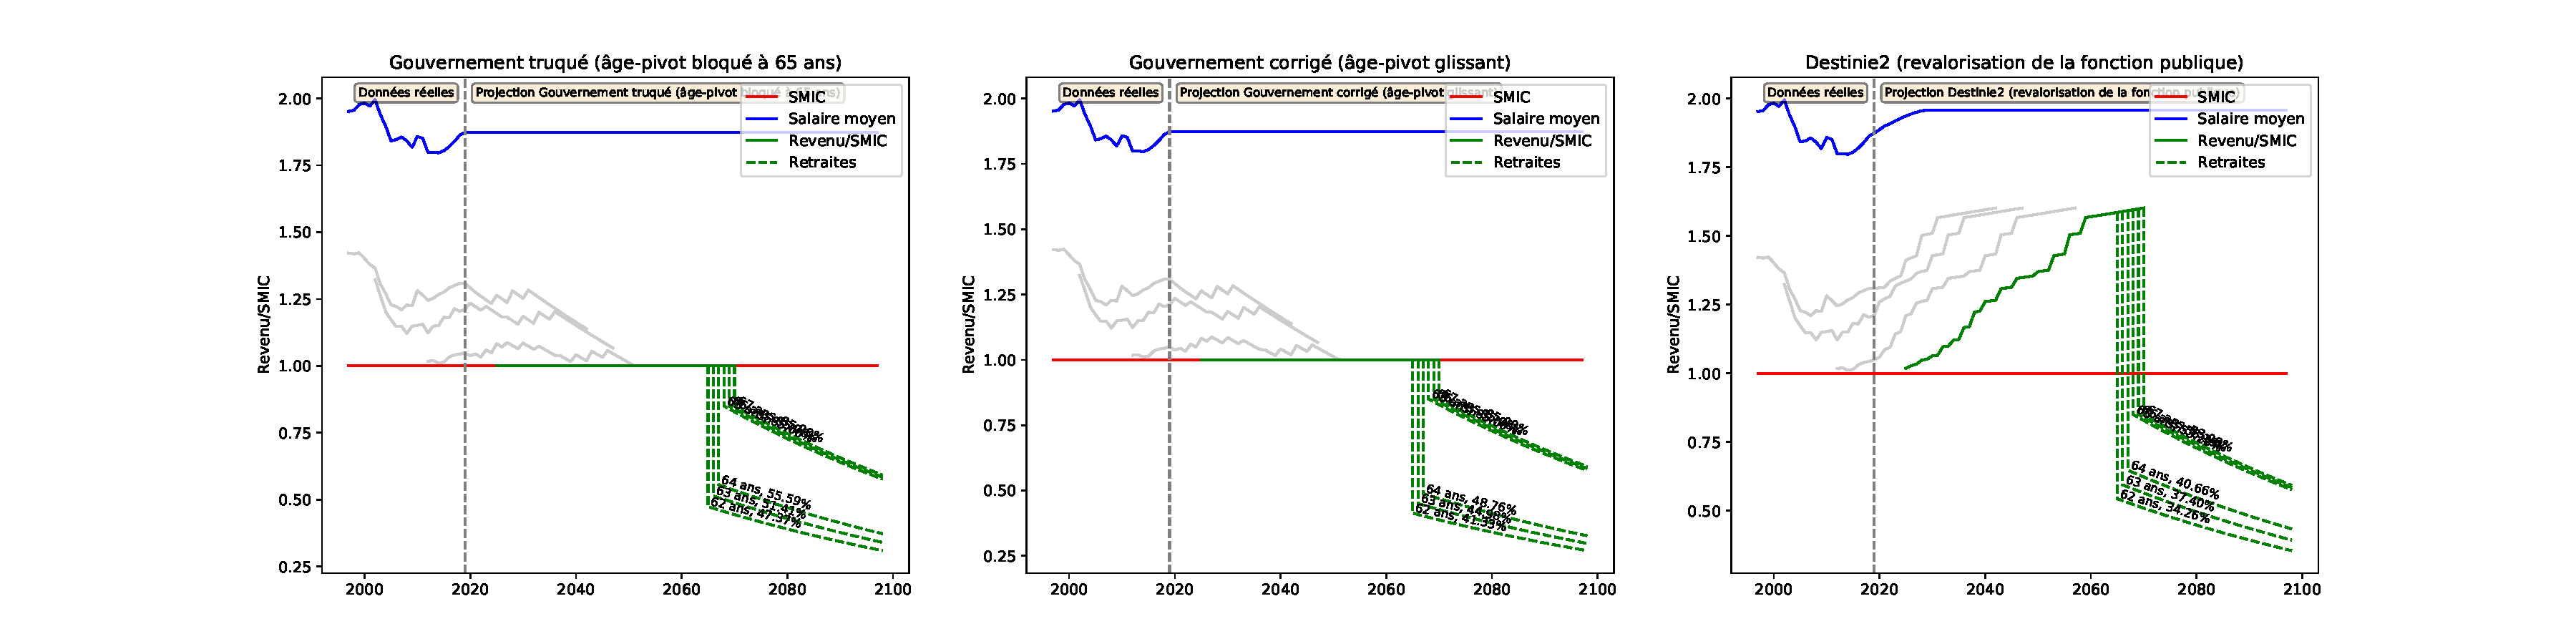
\includegraphics[width=0.9\textwidth]{fig/ATSEM_2003_22_dest_retraite.pdf}\end{center} \label{fig/ATSEM_2003_22_dest_retraite.pdf} 

\newpage 
 
\paragraph{Revenus et points pour le modèle \emph{Gouvernement truqué (âge-pivot bloqué à 65 ans)}} 
 
{ \scriptsize \begin{center} 
\begin{tabular}[htb]{|c|c||c|c|c|c|c|c||c|c||c|c|c|} 
\hline 
 Année &  Âge &  Ind Maj &  Pt Ind(\euro{} 2019) &  Rev HP(\euro{} 2019) &  Tx Primes &  GIPA(\euro{} 2019) &  Revenu(\euro{} 2019) &  SMIC(\euro{} 2019) &  Rev/SMIC &  Cumul Pts &  Achat Pt(\euro{} 2019) &  Serv. Pt(\euro{} 2019) \\ 
\hline \hline 
 2025 &  22 &  329.0 &  4.79 &  1577.36 &  6.11 &  0.00 &  1835.31 &  1835.31 &  {\bf 1.00} &  618.52 &  35.61 &  0.50 \\ 
\hline 
 2026 &  23 &  330.0 &  4.79 &  1582.16 &  6.34 &  0.00 &  1859.17 &  1859.17 &  {\bf 1.00} &  1245.08 &  35.61 &  0.50 \\ 
\hline 
 2027 &  24 &  330.0 &  4.79 &  1582.16 &  6.57 &  0.00 &  1883.34 &  1883.34 &  {\bf 1.00} &  1879.79 &  35.61 &  0.50 \\ 
\hline 
 2028 &  25 &  333.0 &  4.79 &  1596.54 &  6.80 &  0.00 &  1907.82 &  1907.82 &  {\bf 1.00} &  2522.75 &  35.61 &  0.50 \\ 
\hline 
 2029 &  26 &  333.0 &  4.79 &  1596.54 &  7.03 &  162.63 &  1932.62 &  1932.62 &  {\bf 1.00} &  3173.57 &  35.63 &  0.50 \\ 
\hline 
 2030 &  27 &  336.0 &  4.79 &  1610.93 &  7.26 &  167.86 &  1957.75 &  1957.75 &  {\bf 1.00} &  3831.86 &  35.69 &  0.50 \\ 
\hline 
 2031 &  28 &  336.0 &  4.79 &  1610.93 &  7.49 &  188.80 &  1983.20 &  1983.20 &  {\bf 1.00} &  4497.18 &  35.77 &  0.50 \\ 
\hline 
 2032 &  29 &  345.0 &  4.79 &  1654.08 &  7.72 &  163.58 &  2008.98 &  2008.98 &  {\bf 1.00} &  5169.10 &  35.88 &  0.50 \\ 
\hline 
 2033 &  30 &  345.0 &  4.79 &  1654.08 &  7.95 &  185.06 &  2035.10 &  2035.10 &  {\bf 1.00} &  5847.19 &  36.02 &  0.50 \\ 
\hline 
 2034 &  31 &  351.0 &  4.79 &  1682.84 &  8.18 &  175.76 &  2061.55 &  2061.55 &  {\bf 1.00} &  6530.96 &  36.18 &  0.50 \\ 
\hline 
 2035 &  32 &  351.0 &  4.79 &  1682.84 &  8.41 &  197.84 &  2088.35 &  2088.35 &  {\bf 1.00} &  7219.94 &  36.37 &  0.51 \\ 
\hline 
 2036 &  33 &  364.0 &  4.79 &  1745.17 &  8.64 &  152.54 &  2115.50 &  2115.50 &  {\bf 1.00} &  7913.66 &  36.59 &  0.51 \\ 
\hline 
 2037 &  34 &  364.0 &  4.79 &  1745.17 &  8.87 &  175.16 &  2143.00 &  2143.00 &  {\bf 1.00} &  8611.60 &  36.85 &  0.51 \\ 
\hline 
 2038 &  35 &  380.0 &  4.79 &  1821.88 &  9.10 &  114.43 &  2170.86 &  2170.86 &  {\bf 1.00} &  9313.26 &  37.13 &  0.52 \\ 
\hline 
 2039 &  36 &  380.0 &  4.79 &  1821.88 &  9.33 &  137.57 &  2199.08 &  2199.08 &  {\bf 1.00} &  10018.13 &  37.44 &  0.52 \\ 
\hline 
 2040 &  37 &  390.0 &  4.79 &  1869.82 &  9.56 &  108.53 &  2227.67 &  2227.67 &  {\bf 1.00} &  10725.69 &  37.78 &  0.53 \\ 
\hline 
 2041 &  38 &  390.0 &  4.79 &  1869.82 &  9.79 &  132.27 &  2256.63 &  2256.63 &  {\bf 1.00} &  11435.39 &  38.16 &  0.53 \\ 
\hline 
 2042 &  39 &  390.0 &  4.79 &  1869.82 &  10.02 &  156.38 &  2285.97 &  2285.97 &  {\bf 1.00} &  12146.72 &  38.56 &  0.54 \\ 
\hline 
 2043 &  40 &  402.0 &  4.79 &  1927.36 &  10.25 &  117.43 &  2315.68 &  2315.68 &  {\bf 1.00} &  12859.13 &  39.01 &  0.54 \\ 
\hline 
 2044 &  41 &  402.0 &  4.79 &  1927.36 &  10.48 &  142.14 &  2345.79 &  2345.79 &  {\bf 1.00} &  13572.08 &  39.48 &  0.55 \\ 
\hline 
 2045 &  42 &  402.0 &  4.79 &  1927.36 &  10.71 &  167.24 &  2376.28 &  2376.28 &  {\bf 1.00} &  14285.03 &  40.00 &  0.56 \\ 
\hline 
 2046 &  43 &  411.0 &  4.79 &  1970.51 &  10.94 &  144.85 &  2407.18 &  2407.18 &  {\bf 1.00} &  14997.98 &  40.52 &  0.56 \\ 
\hline 
 2047 &  44 &  411.0 &  4.79 &  1970.51 &  11.17 &  170.62 &  2438.47 &  2438.47 &  {\bf 1.00} &  15710.93 &  41.04 &  0.57 \\ 
\hline 
 2048 &  45 &  411.0 &  4.79 &  1970.51 &  11.40 &  196.78 &  2470.17 &  2470.17 &  {\bf 1.00} &  16423.88 &  41.58 &  0.58 \\ 
\hline 
 2049 &  46 &  411.0 &  4.79 &  1970.51 &  11.63 &  223.35 &  2502.28 &  2502.28 &  {\bf 1.00} &  17136.83 &  42.12 &  0.59 \\ 
\hline 
 2050 &  47 &  415.0 &  4.79 &  1989.69 &  11.86 &  228.86 &  2534.81 &  2534.81 &  {\bf 1.00} &  17849.78 &  42.66 &  0.59 \\ 
\hline 
 2051 &  48 &  415.0 &  4.79 &  1989.69 &  12.09 &  256.19 &  2567.76 &  2567.76 &  {\bf 1.00} &  18562.73 &  43.22 &  0.60 \\ 
\hline 
 2052 &  49 &  415.0 &  4.79 &  1989.69 &  12.32 &  283.94 &  2601.14 &  2601.14 &  {\bf 1.00} &  19275.68 &  43.78 &  0.61 \\ 
\hline 
 2053 &  50 &  430.0 &  4.79 &  2061.60 &  12.55 &  231.17 &  2634.96 &  2634.96 &  {\bf 1.00} &  19988.63 &  44.35 &  0.62 \\ 
\hline 
 2054 &  51 &  430.0 &  4.79 &  2061.60 &  12.78 &  259.60 &  2669.21 &  2669.21 &  {\bf 1.00} &  20701.58 &  44.93 &  0.63 \\ 
\hline 
 2055 &  52 &  430.0 &  4.79 &  2061.60 &  13.01 &  288.45 &  2703.91 &  2703.91 &  {\bf 1.00} &  21414.53 &  45.51 &  0.63 \\ 
\hline 
 2056 &  53 &  450.0 &  4.79 &  2157.49 &  13.24 &  209.17 &  2739.06 &  2739.06 &  {\bf 1.00} &  22127.48 &  46.10 &  0.64 \\ 
\hline 
 2057 &  54 &  450.0 &  4.79 &  2157.49 &  13.47 &  238.68 &  2774.67 &  2774.67 &  {\bf 1.00} &  22840.43 &  46.70 &  0.65 \\ 
\hline 
 2058 &  55 &  450.0 &  4.79 &  2157.49 &  13.70 &  268.65 &  2810.74 &  2810.74 &  {\bf 1.00} &  23553.38 &  47.31 &  0.66 \\ 
\hline 
 2059 &  56 &  466.0 &  4.79 &  2234.20 &  13.93 &  211.67 &  2847.28 &  2847.28 &  {\bf 1.00} &  24266.32 &  47.92 &  0.67 \\ 
\hline 
 2060 &  57 &  466.0 &  4.79 &  2234.20 &  14.16 &  242.38 &  2884.30 &  2884.30 &  {\bf 1.00} &  24979.27 &  48.55 &  0.68 \\ 
\hline 
 2061 &  58 &  466.0 &  4.79 &  2234.20 &  14.39 &  273.55 &  2921.79 &  2921.79 &  {\bf 1.00} &  25692.22 &  49.18 &  0.68 \\ 
\hline 
 2062 &  59 &  466.0 &  4.79 &  2234.20 &  14.62 &  305.19 &  2959.78 &  2959.78 &  {\bf 1.00} &  26405.17 &  49.82 &  0.69 \\ 
\hline 
 2063 &  60 &  466.0 &  4.79 &  2234.20 &  14.85 &  337.31 &  2998.25 &  2998.25 &  {\bf 1.00} &  27118.12 &  50.47 &  0.70 \\ 
\hline 
 2064 &  61 &  466.0 &  4.79 &  2234.20 &  15.08 &  369.91 &  3037.23 &  3037.23 &  {\bf 1.00} &  27831.07 &  51.12 &  0.71 \\ 
\hline 
 2065 &  62 &  466.0 &  4.79 &  2234.20 &  15.31 &  403.01 &  3076.71 &  3076.71 &  {\bf 1.00} &  28544.02 &  51.79 &  0.72 \\ 
\hline 
 2066 &  63 &  466.0 &  4.79 &  2234.20 &  15.54 &  436.60 &  3116.71 &  3116.71 &  {\bf 1.00} &  29256.97 &  52.46 &  0.73 \\ 
\hline 
 2067 &  64 &  466.0 &  4.79 &  2234.20 &  15.77 &  470.69 &  3157.23 &  3157.23 &  {\bf 1.00} &  29969.92 &  53.14 &  0.74 \\ 
\hline 
 2068 &  65 &  466.0 &  4.79 &  2234.20 &  16.00 &  505.30 &  3198.27 &  3198.27 &  {\bf 1.00} &  30682.87 &  53.83 &  0.75 \\ 
\hline 
 2069 &  66 &  466.0 &  4.79 &  2234.20 &  16.23 &  540.42 &  3239.85 &  3239.85 &  {\bf 1.00} &  31395.82 &  54.53 &  0.76 \\ 
\hline 
 2070 &  67 &  466.0 &  4.79 &  2234.20 &  16.46 &  576.07 &  3281.97 &  3281.97 &  {\bf 1.00} &  32108.77 &  55.24 &  0.77 \\ 
\hline 
\hline 
\end{tabular} 
\end{center} } 
\newpage 
 
\paragraph{Revenus et points pour le modèle \emph{Gouvernement corrigé (âge-pivot glissant)}} 
 
{ \scriptsize \begin{center} 
\begin{tabular}[htb]{|c|c||c|c|c|c|c|c||c|c||c|c|c|} 
\hline 
 Année &  Âge &  Ind Maj &  Pt Ind(\euro{} 2019) &  Rev HP(\euro{} 2019) &  Tx Primes &  GIPA(\euro{} 2019) &  Revenu(\euro{} 2019) &  SMIC(\euro{} 2019) &  Rev/SMIC &  Cumul Pts &  Achat Pt(\euro{} 2019) &  Serv. Pt(\euro{} 2019) \\ 
\hline \hline 
 2025 &  22 &  329.0 &  4.79 &  1577.36 &  6.11 &  0.00 &  1835.31 &  1835.31 &  {\bf 1.00} &  618.52 &  35.61 &  0.50 \\ 
\hline 
 2026 &  23 &  330.0 &  4.79 &  1582.16 &  6.34 &  0.00 &  1859.17 &  1859.17 &  {\bf 1.00} &  1245.08 &  35.61 &  0.50 \\ 
\hline 
 2027 &  24 &  330.0 &  4.79 &  1582.16 &  6.57 &  0.00 &  1883.34 &  1883.34 &  {\bf 1.00} &  1879.79 &  35.61 &  0.50 \\ 
\hline 
 2028 &  25 &  333.0 &  4.79 &  1596.54 &  6.80 &  0.00 &  1907.82 &  1907.82 &  {\bf 1.00} &  2522.75 &  35.61 &  0.50 \\ 
\hline 
 2029 &  26 &  333.0 &  4.79 &  1596.54 &  7.03 &  162.63 &  1932.62 &  1932.62 &  {\bf 1.00} &  3173.57 &  35.63 &  0.50 \\ 
\hline 
 2030 &  27 &  336.0 &  4.79 &  1610.93 &  7.26 &  167.86 &  1957.75 &  1957.75 &  {\bf 1.00} &  3831.86 &  35.69 &  0.50 \\ 
\hline 
 2031 &  28 &  336.0 &  4.79 &  1610.93 &  7.49 &  188.80 &  1983.20 &  1983.20 &  {\bf 1.00} &  4497.18 &  35.77 &  0.50 \\ 
\hline 
 2032 &  29 &  345.0 &  4.79 &  1654.08 &  7.72 &  163.58 &  2008.98 &  2008.98 &  {\bf 1.00} &  5169.10 &  35.88 &  0.50 \\ 
\hline 
 2033 &  30 &  345.0 &  4.79 &  1654.08 &  7.95 &  185.06 &  2035.10 &  2035.10 &  {\bf 1.00} &  5847.19 &  36.02 &  0.50 \\ 
\hline 
 2034 &  31 &  351.0 &  4.79 &  1682.84 &  8.18 &  175.76 &  2061.55 &  2061.55 &  {\bf 1.00} &  6530.96 &  36.18 &  0.50 \\ 
\hline 
 2035 &  32 &  351.0 &  4.79 &  1682.84 &  8.41 &  197.84 &  2088.35 &  2088.35 &  {\bf 1.00} &  7219.94 &  36.37 &  0.51 \\ 
\hline 
 2036 &  33 &  364.0 &  4.79 &  1745.17 &  8.64 &  152.54 &  2115.50 &  2115.50 &  {\bf 1.00} &  7913.66 &  36.59 &  0.51 \\ 
\hline 
 2037 &  34 &  364.0 &  4.79 &  1745.17 &  8.87 &  175.16 &  2143.00 &  2143.00 &  {\bf 1.00} &  8611.60 &  36.85 &  0.51 \\ 
\hline 
 2038 &  35 &  380.0 &  4.79 &  1821.88 &  9.10 &  114.43 &  2170.86 &  2170.86 &  {\bf 1.00} &  9313.26 &  37.13 &  0.52 \\ 
\hline 
 2039 &  36 &  380.0 &  4.79 &  1821.88 &  9.33 &  137.57 &  2199.08 &  2199.08 &  {\bf 1.00} &  10018.13 &  37.44 &  0.52 \\ 
\hline 
 2040 &  37 &  390.0 &  4.79 &  1869.82 &  9.56 &  108.53 &  2227.67 &  2227.67 &  {\bf 1.00} &  10725.69 &  37.78 &  0.53 \\ 
\hline 
 2041 &  38 &  390.0 &  4.79 &  1869.82 &  9.79 &  132.27 &  2256.63 &  2256.63 &  {\bf 1.00} &  11435.39 &  38.16 &  0.53 \\ 
\hline 
 2042 &  39 &  390.0 &  4.79 &  1869.82 &  10.02 &  156.38 &  2285.97 &  2285.97 &  {\bf 1.00} &  12146.72 &  38.56 &  0.54 \\ 
\hline 
 2043 &  40 &  402.0 &  4.79 &  1927.36 &  10.25 &  117.43 &  2315.68 &  2315.68 &  {\bf 1.00} &  12859.13 &  39.01 &  0.54 \\ 
\hline 
 2044 &  41 &  402.0 &  4.79 &  1927.36 &  10.48 &  142.14 &  2345.79 &  2345.79 &  {\bf 1.00} &  13572.08 &  39.48 &  0.55 \\ 
\hline 
 2045 &  42 &  402.0 &  4.79 &  1927.36 &  10.71 &  167.24 &  2376.28 &  2376.28 &  {\bf 1.00} &  14285.03 &  40.00 &  0.56 \\ 
\hline 
 2046 &  43 &  411.0 &  4.79 &  1970.51 &  10.94 &  144.85 &  2407.18 &  2407.18 &  {\bf 1.00} &  14997.98 &  40.52 &  0.56 \\ 
\hline 
 2047 &  44 &  411.0 &  4.79 &  1970.51 &  11.17 &  170.62 &  2438.47 &  2438.47 &  {\bf 1.00} &  15710.93 &  41.04 &  0.57 \\ 
\hline 
 2048 &  45 &  411.0 &  4.79 &  1970.51 &  11.40 &  196.78 &  2470.17 &  2470.17 &  {\bf 1.00} &  16423.88 &  41.58 &  0.58 \\ 
\hline 
 2049 &  46 &  411.0 &  4.79 &  1970.51 &  11.63 &  223.35 &  2502.28 &  2502.28 &  {\bf 1.00} &  17136.83 &  42.12 &  0.59 \\ 
\hline 
 2050 &  47 &  415.0 &  4.79 &  1989.69 &  11.86 &  228.86 &  2534.81 &  2534.81 &  {\bf 1.00} &  17849.78 &  42.66 &  0.59 \\ 
\hline 
 2051 &  48 &  415.0 &  4.79 &  1989.69 &  12.09 &  256.19 &  2567.76 &  2567.76 &  {\bf 1.00} &  18562.73 &  43.22 &  0.60 \\ 
\hline 
 2052 &  49 &  415.0 &  4.79 &  1989.69 &  12.32 &  283.94 &  2601.14 &  2601.14 &  {\bf 1.00} &  19275.68 &  43.78 &  0.61 \\ 
\hline 
 2053 &  50 &  430.0 &  4.79 &  2061.60 &  12.55 &  231.17 &  2634.96 &  2634.96 &  {\bf 1.00} &  19988.63 &  44.35 &  0.62 \\ 
\hline 
 2054 &  51 &  430.0 &  4.79 &  2061.60 &  12.78 &  259.60 &  2669.21 &  2669.21 &  {\bf 1.00} &  20701.58 &  44.93 &  0.63 \\ 
\hline 
 2055 &  52 &  430.0 &  4.79 &  2061.60 &  13.01 &  288.45 &  2703.91 &  2703.91 &  {\bf 1.00} &  21414.53 &  45.51 &  0.63 \\ 
\hline 
 2056 &  53 &  450.0 &  4.79 &  2157.49 &  13.24 &  209.17 &  2739.06 &  2739.06 &  {\bf 1.00} &  22127.48 &  46.10 &  0.64 \\ 
\hline 
 2057 &  54 &  450.0 &  4.79 &  2157.49 &  13.47 &  238.68 &  2774.67 &  2774.67 &  {\bf 1.00} &  22840.43 &  46.70 &  0.65 \\ 
\hline 
 2058 &  55 &  450.0 &  4.79 &  2157.49 &  13.70 &  268.65 &  2810.74 &  2810.74 &  {\bf 1.00} &  23553.38 &  47.31 &  0.66 \\ 
\hline 
 2059 &  56 &  466.0 &  4.79 &  2234.20 &  13.93 &  211.67 &  2847.28 &  2847.28 &  {\bf 1.00} &  24266.32 &  47.92 &  0.67 \\ 
\hline 
 2060 &  57 &  466.0 &  4.79 &  2234.20 &  14.16 &  242.38 &  2884.30 &  2884.30 &  {\bf 1.00} &  24979.27 &  48.55 &  0.68 \\ 
\hline 
 2061 &  58 &  466.0 &  4.79 &  2234.20 &  14.39 &  273.55 &  2921.79 &  2921.79 &  {\bf 1.00} &  25692.22 &  49.18 &  0.68 \\ 
\hline 
 2062 &  59 &  466.0 &  4.79 &  2234.20 &  14.62 &  305.19 &  2959.78 &  2959.78 &  {\bf 1.00} &  26405.17 &  49.82 &  0.69 \\ 
\hline 
 2063 &  60 &  466.0 &  4.79 &  2234.20 &  14.85 &  337.31 &  2998.25 &  2998.25 &  {\bf 1.00} &  27118.12 &  50.47 &  0.70 \\ 
\hline 
 2064 &  61 &  466.0 &  4.79 &  2234.20 &  15.08 &  369.91 &  3037.23 &  3037.23 &  {\bf 1.00} &  27831.07 &  51.12 &  0.71 \\ 
\hline 
 2065 &  62 &  466.0 &  4.79 &  2234.20 &  15.31 &  403.01 &  3076.71 &  3076.71 &  {\bf 1.00} &  28544.02 &  51.79 &  0.72 \\ 
\hline 
 2066 &  63 &  466.0 &  4.79 &  2234.20 &  15.54 &  436.60 &  3116.71 &  3116.71 &  {\bf 1.00} &  29256.97 &  52.46 &  0.73 \\ 
\hline 
 2067 &  64 &  466.0 &  4.79 &  2234.20 &  15.77 &  470.69 &  3157.23 &  3157.23 &  {\bf 1.00} &  29969.92 &  53.14 &  0.74 \\ 
\hline 
 2068 &  65 &  466.0 &  4.79 &  2234.20 &  16.00 &  505.30 &  3198.27 &  3198.27 &  {\bf 1.00} &  30682.87 &  53.83 &  0.75 \\ 
\hline 
 2069 &  66 &  466.0 &  4.79 &  2234.20 &  16.23 &  540.42 &  3239.85 &  3239.85 &  {\bf 1.00} &  31395.82 &  54.53 &  0.76 \\ 
\hline 
 2070 &  67 &  466.0 &  4.79 &  2234.20 &  16.46 &  576.07 &  3281.97 &  3281.97 &  {\bf 1.00} &  32108.77 &  55.24 &  0.77 \\ 
\hline 
\hline 
\end{tabular} 
\end{center} } 
\newpage 
 
\paragraph{Revenus et points pour le modèle \emph{Destinie2 (revalorisation de la fonction publique)}} 
 
{ \scriptsize \begin{center} 
\begin{tabular}[htb]{|c|c||c|c|c|c|c|c||c|c||c|c|c|} 
\hline 
 Année &  Âge &  Ind Maj &  Pt Ind(\euro{} 2019) &  Rev HP(\euro{} 2019) &  Tx Primes &  GIPA(\euro{} 2019) &  Revenu(\euro{} 2019) &  SMIC(\euro{} 2019) &  Rev/SMIC &  Cumul Pts &  Achat Pt(\euro{} 2019) &  Serv. Pt(\euro{} 2019) \\ 
\hline \hline 
 2025 &  22 &  329.0 &  5.10 &  1679.04 &  6.11 &  0.00 &  1781.63 &  1749.35 &  {\bf 1.02} &  598.96 &  35.69 &  0.50 \\ 
\hline 
 2026 &  23 &  330.0 &  5.17 &  1705.19 &  6.34 &  0.00 &  1813.30 &  1764.53 &  {\bf 1.03} &  1208.56 &  35.69 &  0.50 \\ 
\hline 
 2027 &  24 &  330.0 &  5.23 &  1727.02 &  6.57 &  0.00 &  1840.49 &  1781.27 &  {\bf 1.03} &  1827.30 &  35.69 &  0.50 \\ 
\hline 
 2028 &  25 &  333.0 &  5.30 &  1765.55 &  6.80 &  0.00 &  1885.61 &  1799.59 &  {\bf 1.05} &  2461.21 &  35.69 &  0.50 \\ 
\hline 
 2029 &  26 &  333.0 &  5.37 &  1786.91 &  7.03 &  0.00 &  1912.53 &  1819.55 &  {\bf 1.05} &  3103.72 &  35.72 &  0.50 \\ 
\hline 
 2030 &  27 &  336.0 &  5.43 &  1825.37 &  7.26 &  0.00 &  1957.89 &  1841.19 &  {\bf 1.06} &  3760.52 &  35.77 &  0.50 \\ 
\hline 
 2031 &  28 &  336.0 &  5.50 &  1848.55 &  7.49 &  0.00 &  1987.01 &  1864.58 &  {\bf 1.07} &  4425.59 &  35.85 &  0.50 \\ 
\hline 
 2032 &  29 &  345.0 &  5.57 &  1922.74 &  7.72 &  0.00 &  2071.18 &  1888.81 &  {\bf 1.10} &  5116.74 &  35.96 &  0.50 \\ 
\hline 
 2033 &  30 &  345.0 &  5.65 &  1947.74 &  7.95 &  0.00 &  2102.58 &  1913.37 &  {\bf 1.10} &  5815.71 &  36.10 &  0.50 \\ 
\hline 
 2034 &  31 &  351.0 &  5.72 &  2007.37 &  8.18 &  0.00 &  2171.58 &  1938.24 &  {\bf 1.12} &  6534.33 &  36.26 &  0.50 \\ 
\hline 
 2035 &  32 &  351.0 &  5.79 &  2033.47 &  8.41 &  0.00 &  2204.48 &  1963.44 &  {\bf 1.12} &  7259.97 &  36.46 &  0.51 \\ 
\hline 
 2036 &  33 &  364.0 &  5.87 &  2136.20 &  8.64 &  0.00 &  2320.76 &  1988.96 &  {\bf 1.17} &  8019.25 &  36.68 &  0.51 \\ 
\hline 
 2037 &  34 &  364.0 &  5.94 &  2163.97 &  8.87 &  0.00 &  2355.91 &  2014.82 &  {\bf 1.17} &  8784.78 &  36.93 &  0.51 \\ 
\hline 
 2038 &  35 &  380.0 &  6.02 &  2288.45 &  9.10 &  0.00 &  2496.70 &  2041.01 &  {\bf 1.22} &  9589.92 &  37.21 &  0.52 \\ 
\hline 
 2039 &  36 &  380.0 &  6.10 &  2318.20 &  9.33 &  0.00 &  2534.49 &  2067.55 &  {\bf 1.23} &  10400.45 &  37.52 &  0.52 \\ 
\hline 
 2040 &  37 &  390.0 &  6.18 &  2410.14 &  9.56 &  0.00 &  2640.55 &  2094.43 &  {\bf 1.26} &  11237.22 &  37.87 &  0.53 \\ 
\hline 
 2041 &  38 &  390.0 &  6.26 &  2441.47 &  9.79 &  0.00 &  2680.49 &  2121.65 &  {\bf 1.26} &  12078.31 &  38.24 &  0.53 \\ 
\hline 
 2042 &  39 &  390.0 &  6.34 &  2473.21 &  10.02 &  0.00 &  2721.03 &  2149.23 &  {\bf 1.27} &  12923.08 &  38.65 &  0.54 \\ 
\hline 
 2043 &  40 &  402.0 &  6.42 &  2582.45 &  10.25 &  0.00 &  2847.15 &  2177.17 &  {\bf 1.31} &  13796.99 &  39.10 &  0.54 \\ 
\hline 
 2044 &  41 &  402.0 &  6.51 &  2616.02 &  10.48 &  0.00 &  2890.18 &  2205.48 &  {\bf 1.31} &  14673.39 &  39.57 &  0.55 \\ 
\hline 
 2045 &  42 &  402.0 &  6.59 &  2650.03 &  10.71 &  0.00 &  2933.85 &  2234.15 &  {\bf 1.31} &  15551.61 &  40.09 &  0.56 \\ 
\hline 
 2046 &  43 &  411.0 &  6.68 &  2744.58 &  10.94 &  0.00 &  3044.84 &  2263.19 &  {\bf 1.35} &  16451.37 &  40.61 &  0.57 \\ 
\hline 
 2047 &  44 &  411.0 &  6.76 &  2780.26 &  11.17 &  0.00 &  3090.81 &  2292.61 &  {\bf 1.35} &  17352.98 &  41.14 &  0.57 \\ 
\hline 
 2048 &  45 &  411.0 &  6.85 &  2816.40 &  11.40 &  0.00 &  3137.47 &  2322.42 &  {\bf 1.35} &  18256.46 &  41.67 &  0.58 \\ 
\hline 
 2049 &  46 &  411.0 &  6.94 &  2853.02 &  11.63 &  0.00 &  3184.82 &  2352.61 &  {\bf 1.35} &  19161.81 &  42.21 &  0.59 \\ 
\hline 
 2050 &  47 &  415.0 &  7.03 &  2918.23 &  11.86 &  0.00 &  3264.34 &  2383.19 &  {\bf 1.37} &  20077.85 &  42.76 &  0.60 \\ 
\hline 
 2051 &  48 &  415.0 &  7.12 &  2956.17 &  12.09 &  0.00 &  3313.57 &  2414.18 &  {\bf 1.37} &  20995.78 &  43.32 &  0.60 \\ 
\hline 
 2052 &  49 &  415.0 &  7.22 &  2994.60 &  12.32 &  0.00 &  3363.54 &  2445.56 &  {\bf 1.38} &  21915.59 &  43.88 &  0.61 \\ 
\hline 
 2053 &  50 &  430.0 &  7.31 &  3143.18 &  12.55 &  0.00 &  3537.64 &  2477.35 &  {\bf 1.43} &  22870.60 &  44.45 &  0.62 \\ 
\hline 
 2054 &  51 &  430.0 &  7.40 &  3184.04 &  12.78 &  0.00 &  3590.96 &  2509.56 &  {\bf 1.43} &  23827.55 &  45.03 &  0.63 \\ 
\hline 
 2055 &  52 &  430.0 &  7.50 &  3225.43 &  13.01 &  0.00 &  3645.06 &  2542.18 &  {\bf 1.43} &  24786.46 &  45.62 &  0.63 \\ 
\hline 
 2056 &  53 &  450.0 &  7.60 &  3419.33 &  13.24 &  0.00 &  3872.05 &  2575.23 &  {\bf 1.50} &  25792.02 &  46.21 &  0.64 \\ 
\hline 
 2057 &  54 &  450.0 &  7.70 &  3463.78 &  13.47 &  0.00 &  3930.35 &  2608.71 &  {\bf 1.51} &  26799.61 &  46.81 &  0.65 \\ 
\hline 
 2058 &  55 &  450.0 &  7.80 &  3508.81 &  13.70 &  0.00 &  3989.52 &  2642.62 &  {\bf 1.51} &  27809.25 &  47.42 &  0.66 \\ 
\hline 
 2059 &  56 &  466.0 &  7.90 &  3680.81 &  13.93 &  0.00 &  4193.54 &  2676.98 &  {\bf 1.57} &  28856.90 &  48.03 &  0.67 \\ 
\hline 
 2060 &  57 &  466.0 &  8.00 &  3728.66 &  14.16 &  0.00 &  4256.63 &  2711.78 &  {\bf 1.57} &  29906.67 &  48.66 &  0.68 \\ 
\hline 
 2061 &  58 &  466.0 &  8.11 &  3777.13 &  14.39 &  0.00 &  4320.66 &  2747.03 &  {\bf 1.57} &  30958.55 &  49.29 &  0.69 \\ 
\hline 
 2062 &  59 &  466.0 &  8.21 &  3826.23 &  14.62 &  0.00 &  4385.63 &  2782.74 &  {\bf 1.58} &  32012.54 &  49.93 &  0.70 \\ 
\hline 
 2063 &  60 &  466.0 &  8.32 &  3875.97 &  14.85 &  0.00 &  4451.55 &  2818.92 &  {\bf 1.58} &  33068.65 &  50.58 &  0.70 \\ 
\hline 
 2064 &  61 &  466.0 &  8.43 &  3926.36 &  15.08 &  0.00 &  4518.45 &  2855.56 &  {\bf 1.58} &  34126.88 &  51.24 &  0.71 \\ 
\hline 
 2065 &  62 &  466.0 &  8.54 &  3977.40 &  15.31 &  0.00 &  4586.34 &  2892.68 &  {\bf 1.59} &  35187.22 &  51.90 &  0.72 \\ 
\hline 
 2066 &  63 &  466.0 &  8.65 &  4029.11 &  15.54 &  0.00 &  4655.23 &  2930.29 &  {\bf 1.59} &  36249.68 &  52.58 &  0.73 \\ 
\hline 
 2067 &  64 &  466.0 &  8.76 &  4081.49 &  15.77 &  0.00 &  4725.14 &  2968.38 &  {\bf 1.59} &  37314.25 &  53.26 &  0.74 \\ 
\hline 
 2068 &  65 &  466.0 &  8.87 &  4134.55 &  16.00 &  0.00 &  4796.07 &  3006.97 &  {\bf 1.59} &  38380.93 &  53.95 &  0.75 \\ 
\hline 
 2069 &  66 &  466.0 &  8.99 &  4188.30 &  16.23 &  0.00 &  4868.06 &  3046.06 &  {\bf 1.60} &  39449.73 &  54.66 &  0.76 \\ 
\hline 
 2070 &  67 &  466.0 &  9.10 &  4242.74 &  16.46 &  0.00 &  4941.10 &  3085.66 &  {\bf 1.60} &  40520.65 &  55.37 &  0.77 \\ 
\hline 
\hline 
\end{tabular} 
\end{center} } 
\newpage 
 
\chapter{Professeur des écoles} 

\begin{minipage}{0.55\linewidth}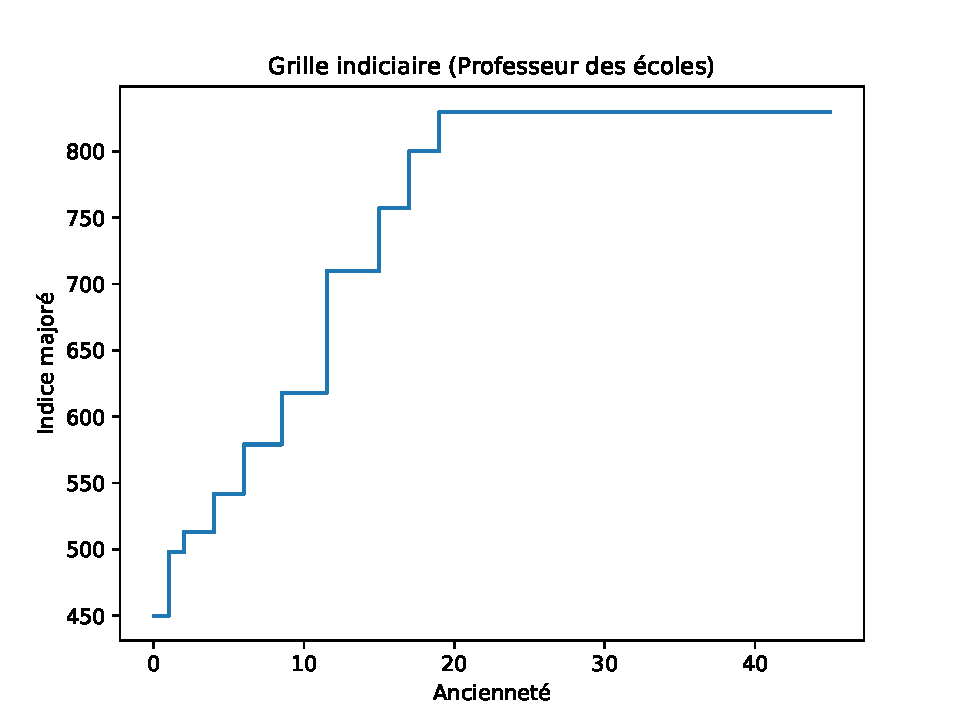
\includegraphics[width=0.7\textwidth]{fig/grille_ProfEcoles.pdf}\end{minipage} 
\begin{minipage}{0.3\linewidth} 
 \begin{center} 

\begin{tabular}[htb]{|c|c|} 
\hline 
 Indice majoré &  Durée (années) \\ 
\hline \hline 
 450 &  1.00 \\ 
\hline 
 498 &  1.00 \\ 
\hline 
 513 &  2.00 \\ 
\hline 
 542 &  2.00 \\ 
\hline 
 579 &  2.50 \\ 
\hline 
 618 &  3.00 \\ 
\hline 
 710 &  3.50 \\ 
\hline 
 757 &  2.00 \\ 
\hline 
 800 &  2.00 \\ 
\hline 
 830 &   \\ 
\hline 
\hline 
\end{tabular} 
\end{center} 
 \end{minipage} 


 \addto{\captionsenglish}{ \renewcommand{\mtctitle}{}} \setcounter{minitocdepth}{2} 
 \minitoc \newpage 

\section{Début de carrière à 22 ans} 

\subsection{Génération 1975 (début en 1997)} 

\paragraph{Retraites possibles dans le modèle \emph{Gouvernement truqué (âge-pivot bloqué à 65 ans)}}  
 
{ \scriptsize \begin{center} 
\begin{tabular}[htb]{|c|c||c|c||c|c||c||c|c|c|c|c|c|} 
\hline 
 Retraite en &  Âge &  Âge pivot &  Décote/Surcote &  Retraite (\euro{} 2019) &  Tx Rempl(\%) &  SMIC (\euro{} 2019) &  Retraite/SMIC &  Rev70/SMIC &  Rev75/SMIC &  Rev80/SMIC &  Rev85/SMIC &  Rev90/SMIC \\ 
\hline \hline 
 2037 &  62 &  64 ans 10 mois &  -14.17\% &  1902.09 &  {\bf 44.50} &  2143.00 &  {\bf {\color{red} 0.89}} &  {\bf {\color{red} 0.80}} &  {\bf {\color{red} 0.75}} &  {\bf {\color{red} 0.70}} &  {\bf {\color{red} 0.66}} &  {\bf {\color{red} 0.62}} \\ 
\hline 
 2038 &  63 &  64 ans 11 mois &  -9.58\% &  2072.84 &  {\bf 48.39} &  2170.86 &  {\bf {\color{red} 0.95}} &  {\bf {\color{red} 0.87}} &  {\bf {\color{red} 0.82}} &  {\bf {\color{red} 0.77}} &  {\bf {\color{red} 0.72}} &  {\bf {\color{red} 0.67}} \\ 
\hline 
 2039 &  64 &  65 ans 0 mois &  -5.00\% &  2252.96 &  {\bf 52.49} &  2199.08 &  {\bf 1.02} &  {\bf {\color{red} 0.95}} &  {\bf {\color{red} 0.89}} &  {\bf {\color{red} 0.83}} &  {\bf {\color{red} 0.78}} &  {\bf {\color{red} 0.73}} \\ 
\hline 
 2040 &  65 &  65 ans 0 mois &  0.00\% &  2453.13 &  {\bf 57.03} &  2227.67 &  {\bf 1.10} &  {\bf 1.03} &  {\bf {\color{red} 0.97}} &  {\bf {\color{red} 0.91}} &  {\bf {\color{red} 0.85}} &  {\bf {\color{red} 0.80}} \\ 
\hline 
 2041 &  66 &  65 ans 0 mois &  5.00\% &  2664.36 &  {\bf 61.81} &  2256.63 &  {\bf 1.18} &  {\bf 1.12} &  {\bf 1.05} &  {\bf {\color{red} 0.99}} &  {\bf {\color{red} 0.92}} &  {\bf {\color{red} 0.87}} \\ 
\hline 
 2042 &  67 &  65 ans 0 mois &  10.00\% &  2887.23 &  {\bf 66.83} &  2285.97 &  {\bf 1.26} &  {\bf 1.22} &  {\bf 1.14} &  {\bf 1.07} &  {\bf 1.00} &  {\bf {\color{red} 0.94}} \\ 
\hline 
\hline 
\end{tabular} 
\end{center} } 
\paragraph{Retraites possibles dans le modèle \emph{Gouvernement corrigé (âge-pivot glissant)}}  
 
{ \scriptsize \begin{center} 
\begin{tabular}[htb]{|c|c||c|c||c|c||c||c|c|c|c|c|c|} 
\hline 
 Retraite en &  Âge &  Âge pivot &  Décote/Surcote &  Retraite (\euro{} 2019) &  Tx Rempl(\%) &  SMIC (\euro{} 2019) &  Retraite/SMIC &  Rev70/SMIC &  Rev75/SMIC &  Rev80/SMIC &  Rev85/SMIC &  Rev90/SMIC \\ 
\hline \hline 
 2037 &  62 &  64 ans 10 mois &  -14.17\% &  1902.09 &  {\bf 44.50} &  2143.00 &  {\bf {\color{red} 0.89}} &  {\bf {\color{red} 0.80}} &  {\bf {\color{red} 0.75}} &  {\bf {\color{red} 0.70}} &  {\bf {\color{red} 0.66}} &  {\bf {\color{red} 0.62}} \\ 
\hline 
 2038 &  63 &  64 ans 11 mois &  -9.58\% &  2072.84 &  {\bf 48.39} &  2170.86 &  {\bf {\color{red} 0.95}} &  {\bf {\color{red} 0.87}} &  {\bf {\color{red} 0.82}} &  {\bf {\color{red} 0.77}} &  {\bf {\color{red} 0.72}} &  {\bf {\color{red} 0.67}} \\ 
\hline 
 2039 &  64 &  65 ans 0 mois &  -5.00\% &  2252.96 &  {\bf 52.49} &  2199.08 &  {\bf 1.02} &  {\bf {\color{red} 0.95}} &  {\bf {\color{red} 0.89}} &  {\bf {\color{red} 0.83}} &  {\bf {\color{red} 0.78}} &  {\bf {\color{red} 0.73}} \\ 
\hline 
 2040 &  65 &  65 ans 1 mois &  -0.42\% &  2442.91 &  {\bf 56.79} &  2227.67 &  {\bf 1.10} &  {\bf 1.03} &  {\bf {\color{red} 0.96}} &  {\bf {\color{red} 0.90}} &  {\bf {\color{red} 0.85}} &  {\bf {\color{red} 0.79}} \\ 
\hline 
 2041 &  66 &  65 ans 2 mois &  4.17\% &  2643.22 &  {\bf 61.32} &  2256.63 &  {\bf 1.17} &  {\bf 1.11} &  {\bf 1.04} &  {\bf {\color{red} 0.98}} &  {\bf {\color{red} 0.92}} &  {\bf {\color{red} 0.86}} \\ 
\hline 
 2042 &  67 &  65 ans 3 mois &  8.75\% &  2854.42 &  {\bf 66.07} &  2285.97 &  {\bf 1.25} &  {\bf 1.20} &  {\bf 1.13} &  {\bf 1.06} &  {\bf {\color{red} 0.99}} &  {\bf {\color{red} 0.93}} \\ 
\hline 
\hline 
\end{tabular} 
\end{center} } 
\paragraph{Retraites possibles dans le modèle \emph{Destinie2 (revalorisation de la fonction publique)}}  
 
{ \scriptsize \begin{center} 
\begin{tabular}[htb]{|c|c||c|c||c|c||c||c|c|c|c|c|c|} 
\hline 
 Retraite en &  Âge &  Âge pivot &  Décote/Surcote &  Retraite (\euro{} 2019) &  Tx Rempl(\%) &  SMIC (\euro{} 2019) &  Retraite/SMIC &  Rev70/SMIC &  Rev75/SMIC &  Rev80/SMIC &  Rev85/SMIC &  Rev90/SMIC \\ 
\hline \hline 
 2037 &  62 &  64 ans 10 mois &  -14.17\% &  2009.36 &  {\bf 37.91} &  2014.82 &  {\bf {\color{red} 1.00}} &  {\bf {\color{red} 0.90}} &  {\bf {\color{red} 0.84}} &  {\bf {\color{red} 0.79}} &  {\bf {\color{red} 0.74}} &  {\bf {\color{red} 0.69}} \\ 
\hline 
 2038 &  63 &  64 ans 11 mois &  -9.58\% &  2200.51 &  {\bf 40.90} &  2041.01 &  {\bf 1.08} &  {\bf {\color{red} 0.98}} &  {\bf {\color{red} 0.92}} &  {\bf {\color{red} 0.87}} &  {\bf {\color{red} 0.81}} &  {\bf {\color{red} 0.76}} \\ 
\hline 
 2039 &  64 &  65 ans 0 mois &  -5.00\% &  2403.69 &  {\bf 44.01} &  2067.55 &  {\bf 1.16} &  {\bf 1.08} &  {\bf 1.01} &  {\bf {\color{red} 0.95}} &  {\bf {\color{red} 0.89}} &  {\bf {\color{red} 0.83}} \\ 
\hline 
 2040 &  65 &  65 ans 1 mois &  -0.42\% &  2619.59 &  {\bf 47.24} &  2094.43 &  {\bf 1.25} &  {\bf 1.17} &  {\bf 1.10} &  {\bf 1.03} &  {\bf {\color{red} 0.97}} &  {\bf {\color{red} 0.91}} \\ 
\hline 
 2041 &  66 &  65 ans 2 mois &  4.17\% &  2848.97 &  {\bf 50.61} &  2121.65 &  {\bf 1.34} &  {\bf 1.28} &  {\bf 1.20} &  {\bf 1.12} &  {\bf 1.05} &  {\bf {\color{red} 0.98}} \\ 
\hline 
 2042 &  67 &  65 ans 3 mois &  8.75\% &  3092.62 &  {\bf 54.12} &  2149.23 &  {\bf 1.44} &  {\bf 1.38} &  {\bf 1.30} &  {\bf 1.22} &  {\bf 1.14} &  {\bf 1.07} \\ 
\hline 
\hline 
\end{tabular} 
\end{center} } 

 \begin{center}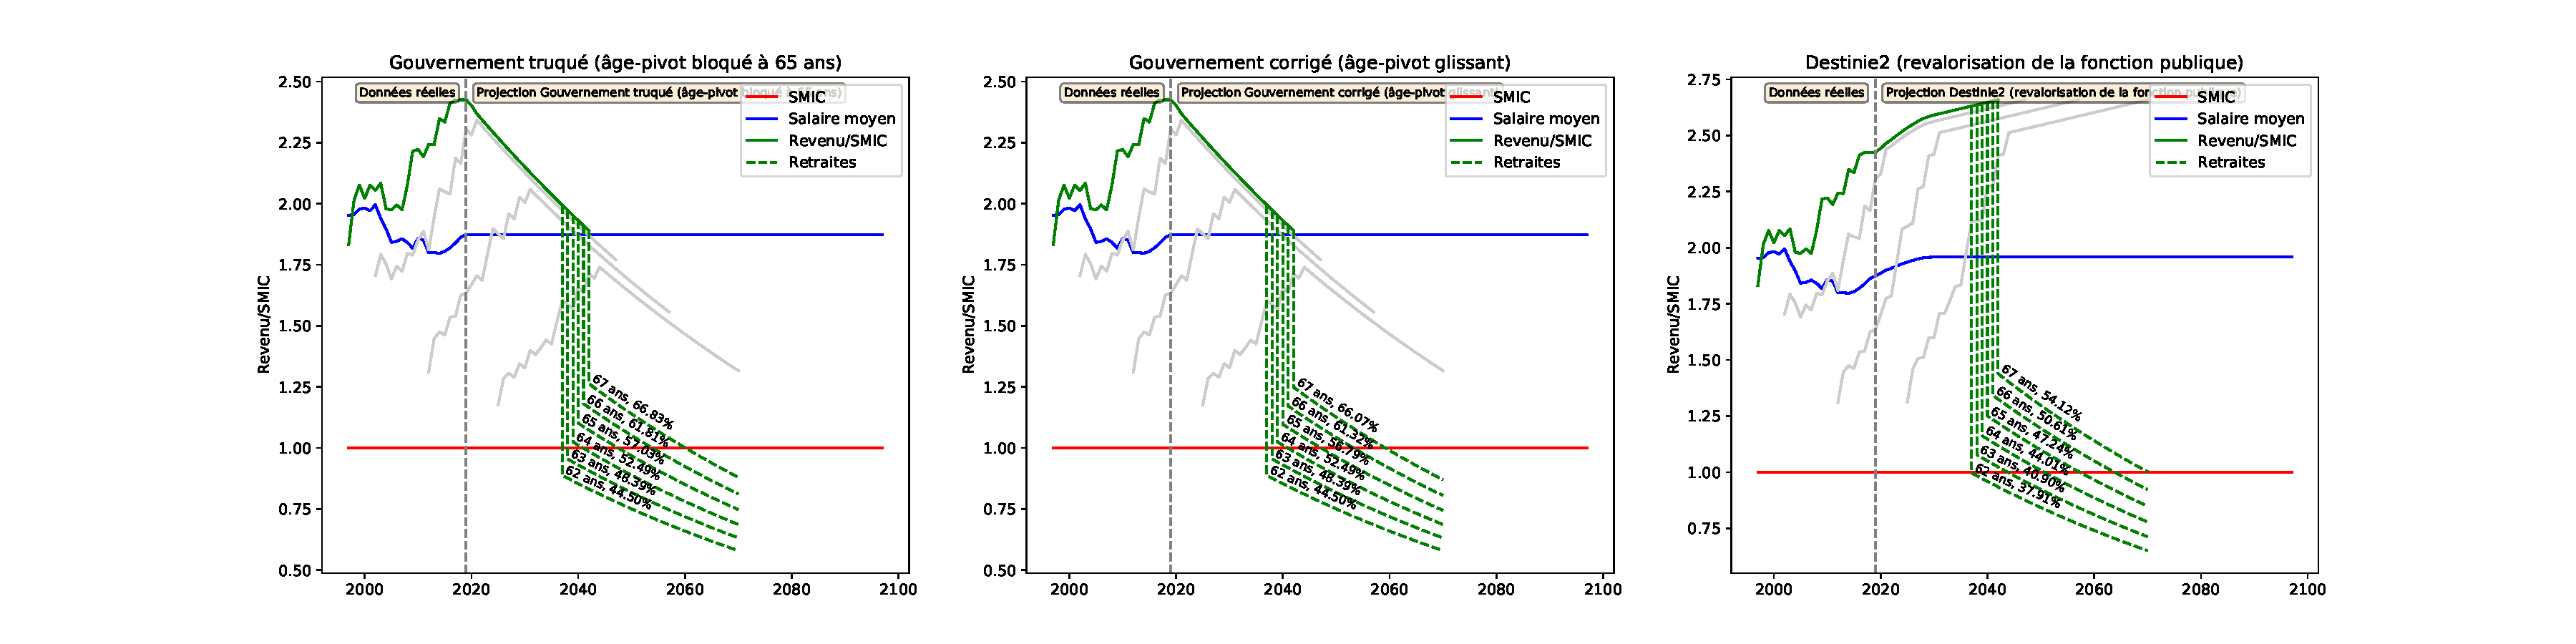
\includegraphics[width=0.9\textwidth]{fig/ProfEcoles_1975_22_dest_retraite.pdf}\end{center} \label{fig/ProfEcoles_1975_22_dest_retraite.pdf} 

\newpage 
 
\paragraph{Revenus et points pour le modèle \emph{Gouvernement truqué (âge-pivot bloqué à 65 ans)}} 
 
{ \scriptsize \begin{center} 
\begin{tabular}[htb]{|c|c||c|c|c|c|c|c||c|c||c|c|c|} 
\hline 
 Année &  Âge &  Ind Maj &  Pt Ind(\euro{} 2019) &  Rev HP(\euro{} 2019) &  Tx Primes &  GIPA(\euro{} 2019) &  Revenu(\euro{} 2019) &  SMIC(\euro{} 2019) &  Rev/SMIC &  Cumul Pts &  Achat Pt(\euro{} 2019) &  Serv. Pt(\euro{} 2019) \\ 
\hline \hline 
 1997 &  22 &  450.0 &  5.53 &  2490.46 &  0.00 &  0.00 &  2490.46 &  1358.84 &  {\bf 1.83} &  839.31 &  35.61 &  0.50 \\ 
\hline 
 1998 &  23 &  498.0 &  5.57 &  2772.09 &  0.00 &  0.00 &  2772.09 &  1376.36 &  {\bf 2.01} &  1773.54 &  35.61 &  0.50 \\ 
\hline 
 1999 &  24 &  513.0 &  5.61 &  2878.67 &  0.00 &  0.00 &  2878.67 &  1386.54 &  {\bf 2.08} &  2743.69 &  35.61 &  0.50 \\ 
\hline 
 2000 &  25 &  513.0 &  5.55 &  2844.68 &  0.00 &  0.00 &  2844.68 &  1407.00 &  {\bf 2.02} &  3702.38 &  35.61 &  0.50 \\ 
\hline 
 2001 &  26 &  542.0 &  5.52 &  2992.11 &  0.00 &  0.00 &  2992.11 &  1441.04 &  {\bf 2.08} &  4710.76 &  35.61 &  0.50 \\ 
\hline 
 2002 &  27 &  542.0 &  5.49 &  2973.56 &  0.00 &  0.00 &  2973.56 &  1447.74 &  {\bf 2.05} &  5712.89 &  35.61 &  0.50 \\ 
\hline 
 2003 &  28 &  579.0 &  5.37 &  3111.90 &  0.00 &  0.00 &  3111.90 &  1493.03 &  {\bf 2.08} &  6761.64 &  35.61 &  0.50 \\ 
\hline 
 2004 &  29 &  579.0 &  5.29 &  3062.75 &  0.00 &  0.00 &  3062.75 &  1547.32 &  {\bf 1.98} &  7793.82 &  35.61 &  0.50 \\ 
\hline 
 2005 &  30 &  598.5 &  5.29 &  3165.55 &  0.05 &  0.00 &  3167.14 &  1603.67 &  {\bf 1.97} &  8861.18 &  35.61 &  0.50 \\ 
\hline 
 2006 &  31 &  618.0 &  5.23 &  3232.21 &  0.28 &  0.00 &  3241.26 &  1625.00 &  {\bf 1.99} &  9953.53 &  35.61 &  0.50 \\ 
\hline 
 2007 &  32 &  618.0 &  5.19 &  3210.19 &  0.51 &  0.00 &  3226.56 &  1634.08 &  {\bf 1.97} &  11040.92 &  35.61 &  0.50 \\ 
\hline 
 2008 &  33 &  664.0 &  5.09 &  3381.78 &  0.74 &  0.00 &  3406.81 &  1640.24 &  {\bf 2.08} &  12189.06 &  35.61 &  0.50 \\ 
\hline 
 2009 &  34 &  710.0 &  5.13 &  3641.68 &  0.97 &  0.00 &  3677.01 &  1659.42 &  {\bf 2.22} &  13428.25 &  35.61 &  0.50 \\ 
\hline 
 2010 &  35 &  710.0 &  5.08 &  3604.90 &  1.20 &  0.00 &  3648.16 &  1641.90 &  {\bf 2.22} &  14657.73 &  35.61 &  0.50 \\ 
\hline 
 2011 &  36 &  710.0 &  4.97 &  3530.00 &  1.43 &  0.00 &  3580.48 &  1633.19 &  {\bf 2.19} &  15864.39 &  35.61 &  0.50 \\ 
\hline 
 2012 &  37 &  757.0 &  4.88 &  3691.46 &  1.66 &  0.00 &  3752.74 &  1673.05 &  {\bf 2.24} &  17129.11 &  35.61 &  0.50 \\ 
\hline 
 2013 &  38 &  757.0 &  4.83 &  3659.83 &  1.89 &  0.00 &  3729.00 &  1664.01 &  {\bf 2.24} &  18385.83 &  35.61 &  0.50 \\ 
\hline 
 2014 &  39 &  800.0 &  4.81 &  3848.36 &  2.12 &  0.00 &  3929.95 &  1673.24 &  {\bf 2.35} &  19710.27 &  35.61 &  0.50 \\ 
\hline 
 2015 &  40 &  800.0 &  4.81 &  3846.86 &  2.35 &  0.00 &  3937.26 &  1686.62 &  {\bf 2.33} &  21037.17 &  35.61 &  0.50 \\ 
\hline 
 2016 &  41 &  830.0 &  4.80 &  3983.15 &  2.58 &  0.00 &  4085.91 &  1693.76 &  {\bf 2.41} &  22414.17 &  35.61 &  0.50 \\ 
\hline 
 2017 &  42 &  830.0 &  4.81 &  3991.18 &  2.81 &  0.00 &  4103.33 &  1692.60 &  {\bf 2.42} &  23797.05 &  35.61 &  0.50 \\ 
\hline 
 2018 &  43 &  830.0 &  4.74 &  3936.07 &  3.04 &  42.51 &  4098.24 &  1689.76 &  {\bf 2.43} &  25178.20 &  35.61 &  0.50 \\ 
\hline 
 2019 &  44 &  830.0 &  4.79 &  3979.37 &  3.27 &  9.76 &  4119.25 &  1698.45 &  {\bf 2.43} &  26566.44 &  35.61 &  0.50 \\ 
\hline 
 2020 &  45 &  830.0 &  4.79 &  3979.37 &  3.50 &  14.49 &  4133.14 &  1720.53 &  {\bf 2.40} &  27959.36 &  35.61 &  0.50 \\ 
\hline 
 2021 &  46 &  830.0 &  4.79 &  3979.37 &  3.73 &  0.39 &  4128.19 &  1742.90 &  {\bf 2.37} &  29350.61 &  35.61 &  0.50 \\ 
\hline 
 2022 &  47 &  830.0 &  4.79 &  3979.37 &  3.96 &  0.00 &  4136.95 &  1765.55 &  {\bf 2.34} &  30744.81 &  35.61 &  0.50 \\ 
\hline 
 2023 &  48 &  830.0 &  4.79 &  3979.37 &  4.19 &  0.00 &  4146.11 &  1788.51 &  {\bf 2.32} &  32142.10 &  35.61 &  0.50 \\ 
\hline 
 2024 &  49 &  830.0 &  4.79 &  3979.37 &  4.42 &  0.00 &  4155.26 &  1811.76 &  {\bf 2.29} &  33542.47 &  35.61 &  0.50 \\ 
\hline 
 2025 &  50 &  830.0 &  4.79 &  3979.37 &  4.65 &  0.00 &  4164.41 &  1835.31 &  {\bf 2.27} &  34945.93 &  35.61 &  0.50 \\ 
\hline 
 2026 &  51 &  830.0 &  4.79 &  3979.37 &  4.88 &  0.00 &  4173.56 &  1859.17 &  {\bf 2.24} &  36352.47 &  35.61 &  0.50 \\ 
\hline 
 2027 &  52 &  830.0 &  4.79 &  3979.37 &  5.11 &  0.00 &  4182.72 &  1883.34 &  {\bf 2.22} &  37762.10 &  35.61 &  0.50 \\ 
\hline 
 2028 &  53 &  830.0 &  4.79 &  3979.37 &  5.34 &  0.00 &  4191.87 &  1907.82 &  {\bf 2.20} &  39174.81 &  35.61 &  0.50 \\ 
\hline 
 2029 &  54 &  830.0 &  4.79 &  3979.37 &  5.57 &  0.00 &  4201.02 &  1932.62 &  {\bf 2.17} &  40589.53 &  35.63 &  0.50 \\ 
\hline 
 2030 &  55 &  830.0 &  4.79 &  3979.37 &  5.80 &  0.00 &  4210.17 &  1957.75 &  {\bf 2.15} &  42005.18 &  35.69 &  0.50 \\ 
\hline 
 2031 &  56 &  830.0 &  4.79 &  3979.37 &  6.03 &  0.00 &  4219.33 &  1983.20 &  {\bf 2.13} &  43420.68 &  35.77 &  0.50 \\ 
\hline 
 2032 &  57 &  830.0 &  4.79 &  3979.37 &  6.26 &  0.00 &  4228.48 &  2008.98 &  {\bf 2.10} &  44834.94 &  35.88 &  0.50 \\ 
\hline 
 2033 &  58 &  830.0 &  4.79 &  3979.37 &  6.49 &  0.00 &  4237.63 &  2035.10 &  {\bf 2.08} &  46246.89 &  36.02 &  0.50 \\ 
\hline 
 2034 &  59 &  830.0 &  4.79 &  3979.37 &  6.72 &  0.00 &  4246.78 &  2061.55 &  {\bf 2.06} &  47655.45 &  36.18 &  0.50 \\ 
\hline 
 2035 &  60 &  830.0 &  4.79 &  3979.37 &  6.95 &  0.00 &  4255.94 &  2088.35 &  {\bf 2.04} &  49059.56 &  36.37 &  0.51 \\ 
\hline 
 2036 &  61 &  830.0 &  4.79 &  3979.37 &  7.18 &  0.00 &  4265.09 &  2115.50 &  {\bf 2.02} &  50458.17 &  36.59 &  0.51 \\ 
\hline 
 2037 &  62 &  830.0 &  4.79 &  3979.37 &  7.41 &  0.00 &  4274.24 &  2143.00 &  {\bf 1.99} &  51850.22 &  36.85 &  0.51 \\ 
\hline 
 2038 &  63 &  830.0 &  4.79 &  3979.37 &  7.64 &  0.00 &  4283.39 &  2170.86 &  {\bf 1.97} &  53234.70 &  37.13 &  0.52 \\ 
\hline 
 2039 &  64 &  830.0 &  4.79 &  3979.37 &  7.87 &  0.00 &  4292.55 &  2199.08 &  {\bf 1.95} &  54610.59 &  37.44 &  0.52 \\ 
\hline 
 2040 &  65 &  830.0 &  4.79 &  3979.37 &  8.10 &  0.00 &  4301.70 &  2227.67 &  {\bf 1.93} &  55976.89 &  37.78 &  0.53 \\ 
\hline 
 2041 &  66 &  830.0 &  4.79 &  3979.37 &  8.33 &  0.00 &  4310.85 &  2256.63 &  {\bf 1.91} &  57332.65 &  38.16 &  0.53 \\ 
\hline 
 2042 &  67 &  830.0 &  4.79 &  3979.37 &  8.56 &  0.00 &  4320.00 &  2285.97 &  {\bf 1.89} &  58676.91 &  38.56 &  0.54 \\ 
\hline 
\hline 
\end{tabular} 
\end{center} } 
\newpage 
 
\paragraph{Revenus et points pour le modèle \emph{Gouvernement corrigé (âge-pivot glissant)}} 
 
{ \scriptsize \begin{center} 
\begin{tabular}[htb]{|c|c||c|c|c|c|c|c||c|c||c|c|c|} 
\hline 
 Année &  Âge &  Ind Maj &  Pt Ind(\euro{} 2019) &  Rev HP(\euro{} 2019) &  Tx Primes &  GIPA(\euro{} 2019) &  Revenu(\euro{} 2019) &  SMIC(\euro{} 2019) &  Rev/SMIC &  Cumul Pts &  Achat Pt(\euro{} 2019) &  Serv. Pt(\euro{} 2019) \\ 
\hline \hline 
 1997 &  22 &  450.0 &  5.53 &  2490.46 &  0.00 &  0.00 &  2490.46 &  1358.84 &  {\bf 1.83} &  839.31 &  35.61 &  0.50 \\ 
\hline 
 1998 &  23 &  498.0 &  5.57 &  2772.09 &  0.00 &  0.00 &  2772.09 &  1376.36 &  {\bf 2.01} &  1773.54 &  35.61 &  0.50 \\ 
\hline 
 1999 &  24 &  513.0 &  5.61 &  2878.67 &  0.00 &  0.00 &  2878.67 &  1386.54 &  {\bf 2.08} &  2743.69 &  35.61 &  0.50 \\ 
\hline 
 2000 &  25 &  513.0 &  5.55 &  2844.68 &  0.00 &  0.00 &  2844.68 &  1407.00 &  {\bf 2.02} &  3702.38 &  35.61 &  0.50 \\ 
\hline 
 2001 &  26 &  542.0 &  5.52 &  2992.11 &  0.00 &  0.00 &  2992.11 &  1441.04 &  {\bf 2.08} &  4710.76 &  35.61 &  0.50 \\ 
\hline 
 2002 &  27 &  542.0 &  5.49 &  2973.56 &  0.00 &  0.00 &  2973.56 &  1447.74 &  {\bf 2.05} &  5712.89 &  35.61 &  0.50 \\ 
\hline 
 2003 &  28 &  579.0 &  5.37 &  3111.90 &  0.00 &  0.00 &  3111.90 &  1493.03 &  {\bf 2.08} &  6761.64 &  35.61 &  0.50 \\ 
\hline 
 2004 &  29 &  579.0 &  5.29 &  3062.75 &  0.00 &  0.00 &  3062.75 &  1547.32 &  {\bf 1.98} &  7793.82 &  35.61 &  0.50 \\ 
\hline 
 2005 &  30 &  598.5 &  5.29 &  3165.55 &  0.05 &  0.00 &  3167.14 &  1603.67 &  {\bf 1.97} &  8861.18 &  35.61 &  0.50 \\ 
\hline 
 2006 &  31 &  618.0 &  5.23 &  3232.21 &  0.28 &  0.00 &  3241.26 &  1625.00 &  {\bf 1.99} &  9953.53 &  35.61 &  0.50 \\ 
\hline 
 2007 &  32 &  618.0 &  5.19 &  3210.19 &  0.51 &  0.00 &  3226.56 &  1634.08 &  {\bf 1.97} &  11040.92 &  35.61 &  0.50 \\ 
\hline 
 2008 &  33 &  664.0 &  5.09 &  3381.78 &  0.74 &  0.00 &  3406.81 &  1640.24 &  {\bf 2.08} &  12189.06 &  35.61 &  0.50 \\ 
\hline 
 2009 &  34 &  710.0 &  5.13 &  3641.68 &  0.97 &  0.00 &  3677.01 &  1659.42 &  {\bf 2.22} &  13428.25 &  35.61 &  0.50 \\ 
\hline 
 2010 &  35 &  710.0 &  5.08 &  3604.90 &  1.20 &  0.00 &  3648.16 &  1641.90 &  {\bf 2.22} &  14657.73 &  35.61 &  0.50 \\ 
\hline 
 2011 &  36 &  710.0 &  4.97 &  3530.00 &  1.43 &  0.00 &  3580.48 &  1633.19 &  {\bf 2.19} &  15864.39 &  35.61 &  0.50 \\ 
\hline 
 2012 &  37 &  757.0 &  4.88 &  3691.46 &  1.66 &  0.00 &  3752.74 &  1673.05 &  {\bf 2.24} &  17129.11 &  35.61 &  0.50 \\ 
\hline 
 2013 &  38 &  757.0 &  4.83 &  3659.83 &  1.89 &  0.00 &  3729.00 &  1664.01 &  {\bf 2.24} &  18385.83 &  35.61 &  0.50 \\ 
\hline 
 2014 &  39 &  800.0 &  4.81 &  3848.36 &  2.12 &  0.00 &  3929.95 &  1673.24 &  {\bf 2.35} &  19710.27 &  35.61 &  0.50 \\ 
\hline 
 2015 &  40 &  800.0 &  4.81 &  3846.86 &  2.35 &  0.00 &  3937.26 &  1686.62 &  {\bf 2.33} &  21037.17 &  35.61 &  0.50 \\ 
\hline 
 2016 &  41 &  830.0 &  4.80 &  3983.15 &  2.58 &  0.00 &  4085.91 &  1693.76 &  {\bf 2.41} &  22414.17 &  35.61 &  0.50 \\ 
\hline 
 2017 &  42 &  830.0 &  4.81 &  3991.18 &  2.81 &  0.00 &  4103.33 &  1692.60 &  {\bf 2.42} &  23797.05 &  35.61 &  0.50 \\ 
\hline 
 2018 &  43 &  830.0 &  4.74 &  3936.07 &  3.04 &  42.51 &  4098.24 &  1689.76 &  {\bf 2.43} &  25178.20 &  35.61 &  0.50 \\ 
\hline 
 2019 &  44 &  830.0 &  4.79 &  3979.37 &  3.27 &  9.76 &  4119.25 &  1698.45 &  {\bf 2.43} &  26566.44 &  35.61 &  0.50 \\ 
\hline 
 2020 &  45 &  830.0 &  4.79 &  3979.37 &  3.50 &  14.49 &  4133.14 &  1720.53 &  {\bf 2.40} &  27959.36 &  35.61 &  0.50 \\ 
\hline 
 2021 &  46 &  830.0 &  4.79 &  3979.37 &  3.73 &  0.39 &  4128.19 &  1742.90 &  {\bf 2.37} &  29350.61 &  35.61 &  0.50 \\ 
\hline 
 2022 &  47 &  830.0 &  4.79 &  3979.37 &  3.96 &  0.00 &  4136.95 &  1765.55 &  {\bf 2.34} &  30744.81 &  35.61 &  0.50 \\ 
\hline 
 2023 &  48 &  830.0 &  4.79 &  3979.37 &  4.19 &  0.00 &  4146.11 &  1788.51 &  {\bf 2.32} &  32142.10 &  35.61 &  0.50 \\ 
\hline 
 2024 &  49 &  830.0 &  4.79 &  3979.37 &  4.42 &  0.00 &  4155.26 &  1811.76 &  {\bf 2.29} &  33542.47 &  35.61 &  0.50 \\ 
\hline 
 2025 &  50 &  830.0 &  4.79 &  3979.37 &  4.65 &  0.00 &  4164.41 &  1835.31 &  {\bf 2.27} &  34945.93 &  35.61 &  0.50 \\ 
\hline 
 2026 &  51 &  830.0 &  4.79 &  3979.37 &  4.88 &  0.00 &  4173.56 &  1859.17 &  {\bf 2.24} &  36352.47 &  35.61 &  0.50 \\ 
\hline 
 2027 &  52 &  830.0 &  4.79 &  3979.37 &  5.11 &  0.00 &  4182.72 &  1883.34 &  {\bf 2.22} &  37762.10 &  35.61 &  0.50 \\ 
\hline 
 2028 &  53 &  830.0 &  4.79 &  3979.37 &  5.34 &  0.00 &  4191.87 &  1907.82 &  {\bf 2.20} &  39174.81 &  35.61 &  0.50 \\ 
\hline 
 2029 &  54 &  830.0 &  4.79 &  3979.37 &  5.57 &  0.00 &  4201.02 &  1932.62 &  {\bf 2.17} &  40589.53 &  35.63 &  0.50 \\ 
\hline 
 2030 &  55 &  830.0 &  4.79 &  3979.37 &  5.80 &  0.00 &  4210.17 &  1957.75 &  {\bf 2.15} &  42005.18 &  35.69 &  0.50 \\ 
\hline 
 2031 &  56 &  830.0 &  4.79 &  3979.37 &  6.03 &  0.00 &  4219.33 &  1983.20 &  {\bf 2.13} &  43420.68 &  35.77 &  0.50 \\ 
\hline 
 2032 &  57 &  830.0 &  4.79 &  3979.37 &  6.26 &  0.00 &  4228.48 &  2008.98 &  {\bf 2.10} &  44834.94 &  35.88 &  0.50 \\ 
\hline 
 2033 &  58 &  830.0 &  4.79 &  3979.37 &  6.49 &  0.00 &  4237.63 &  2035.10 &  {\bf 2.08} &  46246.89 &  36.02 &  0.50 \\ 
\hline 
 2034 &  59 &  830.0 &  4.79 &  3979.37 &  6.72 &  0.00 &  4246.78 &  2061.55 &  {\bf 2.06} &  47655.45 &  36.18 &  0.50 \\ 
\hline 
 2035 &  60 &  830.0 &  4.79 &  3979.37 &  6.95 &  0.00 &  4255.94 &  2088.35 &  {\bf 2.04} &  49059.56 &  36.37 &  0.51 \\ 
\hline 
 2036 &  61 &  830.0 &  4.79 &  3979.37 &  7.18 &  0.00 &  4265.09 &  2115.50 &  {\bf 2.02} &  50458.17 &  36.59 &  0.51 \\ 
\hline 
 2037 &  62 &  830.0 &  4.79 &  3979.37 &  7.41 &  0.00 &  4274.24 &  2143.00 &  {\bf 1.99} &  51850.22 &  36.85 &  0.51 \\ 
\hline 
 2038 &  63 &  830.0 &  4.79 &  3979.37 &  7.64 &  0.00 &  4283.39 &  2170.86 &  {\bf 1.97} &  53234.70 &  37.13 &  0.52 \\ 
\hline 
 2039 &  64 &  830.0 &  4.79 &  3979.37 &  7.87 &  0.00 &  4292.55 &  2199.08 &  {\bf 1.95} &  54610.59 &  37.44 &  0.52 \\ 
\hline 
 2040 &  65 &  830.0 &  4.79 &  3979.37 &  8.10 &  0.00 &  4301.70 &  2227.67 &  {\bf 1.93} &  55976.89 &  37.78 &  0.53 \\ 
\hline 
 2041 &  66 &  830.0 &  4.79 &  3979.37 &  8.33 &  0.00 &  4310.85 &  2256.63 &  {\bf 1.91} &  57332.65 &  38.16 &  0.53 \\ 
\hline 
 2042 &  67 &  830.0 &  4.79 &  3979.37 &  8.56 &  0.00 &  4320.00 &  2285.97 &  {\bf 1.89} &  58676.91 &  38.56 &  0.54 \\ 
\hline 
\hline 
\end{tabular} 
\end{center} } 
\newpage 
 
\paragraph{Revenus et points pour le modèle \emph{Destinie2 (revalorisation de la fonction publique)}} 
 
{ \scriptsize \begin{center} 
\begin{tabular}[htb]{|c|c||c|c|c|c|c|c||c|c||c|c|c|} 
\hline 
 Année &  Âge &  Ind Maj &  Pt Ind(\euro{} 2019) &  Rev HP(\euro{} 2019) &  Tx Primes &  GIPA(\euro{} 2019) &  Revenu(\euro{} 2019) &  SMIC(\euro{} 2019) &  Rev/SMIC &  Cumul Pts &  Achat Pt(\euro{} 2019) &  Serv. Pt(\euro{} 2019) \\ 
\hline \hline 
 1997 &  22 &  450.0 &  5.53 &  2490.46 &  0.00 &  0.00 &  2490.46 &  1358.84 &  {\bf 1.83} &  837.25 &  35.69 &  0.50 \\ 
\hline 
 1998 &  23 &  498.0 &  5.57 &  2772.09 &  0.00 &  0.00 &  2772.09 &  1376.36 &  {\bf 2.01} &  1769.19 &  35.69 &  0.50 \\ 
\hline 
 1999 &  24 &  513.0 &  5.61 &  2878.67 &  0.00 &  0.00 &  2878.67 &  1386.54 &  {\bf 2.08} &  2736.95 &  35.69 &  0.50 \\ 
\hline 
 2000 &  25 &  513.0 &  5.55 &  2844.68 &  0.00 &  0.00 &  2844.68 &  1407.00 &  {\bf 2.02} &  3693.29 &  35.69 &  0.50 \\ 
\hline 
 2001 &  26 &  542.0 &  5.52 &  2992.11 &  0.00 &  0.00 &  2992.11 &  1441.04 &  {\bf 2.08} &  4699.19 &  35.69 &  0.50 \\ 
\hline 
 2002 &  27 &  542.0 &  5.49 &  2973.56 &  0.00 &  0.00 &  2973.56 &  1447.74 &  {\bf 2.05} &  5698.85 &  35.69 &  0.50 \\ 
\hline 
 2003 &  28 &  579.0 &  5.37 &  3111.90 &  0.00 &  0.00 &  3111.90 &  1493.03 &  {\bf 2.08} &  6745.02 &  35.69 &  0.50 \\ 
\hline 
 2004 &  29 &  579.0 &  5.29 &  3062.75 &  0.00 &  0.00 &  3062.75 &  1547.32 &  {\bf 1.98} &  7774.67 &  35.69 &  0.50 \\ 
\hline 
 2005 &  30 &  598.5 &  5.29 &  3165.55 &  0.05 &  0.00 &  3167.14 &  1603.67 &  {\bf 1.97} &  8839.41 &  35.69 &  0.50 \\ 
\hline 
 2006 &  31 &  618.0 &  5.23 &  3232.21 &  0.28 &  0.00 &  3241.26 &  1625.00 &  {\bf 1.99} &  9929.07 &  35.69 &  0.50 \\ 
\hline 
 2007 &  32 &  618.0 &  5.19 &  3210.19 &  0.51 &  0.00 &  3226.56 &  1634.08 &  {\bf 1.97} &  11013.79 &  35.69 &  0.50 \\ 
\hline 
 2008 &  33 &  664.0 &  5.09 &  3381.78 &  0.74 &  0.00 &  3406.81 &  1640.24 &  {\bf 2.08} &  12159.11 &  35.69 &  0.50 \\ 
\hline 
 2009 &  34 &  710.0 &  5.13 &  3641.68 &  0.97 &  0.00 &  3677.01 &  1659.42 &  {\bf 2.22} &  13395.26 &  35.69 &  0.50 \\ 
\hline 
 2010 &  35 &  710.0 &  5.08 &  3604.90 &  1.20 &  0.00 &  3648.16 &  1641.90 &  {\bf 2.22} &  14621.71 &  35.69 &  0.50 \\ 
\hline 
 2011 &  36 &  710.0 &  4.97 &  3530.00 &  1.43 &  0.00 &  3580.48 &  1633.19 &  {\bf 2.19} &  15825.41 &  35.69 &  0.50 \\ 
\hline 
 2012 &  37 &  757.0 &  4.88 &  3691.46 &  1.66 &  0.00 &  3752.74 &  1673.05 &  {\bf 2.24} &  17087.02 &  35.69 &  0.50 \\ 
\hline 
 2013 &  38 &  757.0 &  4.83 &  3659.83 &  1.89 &  0.00 &  3729.00 &  1664.01 &  {\bf 2.24} &  18340.66 &  35.69 &  0.50 \\ 
\hline 
 2014 &  39 &  800.0 &  4.81 &  3848.36 &  2.12 &  0.00 &  3929.95 &  1673.24 &  {\bf 2.35} &  19661.84 &  35.69 &  0.50 \\ 
\hline 
 2015 &  40 &  800.0 &  4.81 &  3846.86 &  2.35 &  0.00 &  3937.26 &  1686.62 &  {\bf 2.33} &  20985.48 &  35.69 &  0.50 \\ 
\hline 
 2016 &  41 &  830.0 &  4.80 &  3983.15 &  2.58 &  0.00 &  4085.91 &  1693.76 &  {\bf 2.41} &  22359.10 &  35.69 &  0.50 \\ 
\hline 
 2017 &  42 &  830.0 &  4.81 &  3991.18 &  2.81 &  0.00 &  4103.33 &  1692.60 &  {\bf 2.42} &  23738.58 &  35.69 &  0.50 \\ 
\hline 
 2018 &  43 &  830.0 &  4.74 &  3936.07 &  3.04 &  42.51 &  4098.24 &  1689.76 &  {\bf 2.43} &  25116.34 &  35.69 &  0.50 \\ 
\hline 
 2019 &  44 &  830.0 &  4.79 &  3979.37 &  3.27 &  9.76 &  4119.25 &  1698.45 &  {\bf 2.43} &  26501.17 &  35.69 &  0.50 \\ 
\hline 
 2020 &  45 &  830.0 &  4.83 &  4011.21 &  3.50 &  0.00 &  4151.60 &  1699.99 &  {\bf 2.44} &  27896.87 &  35.69 &  0.50 \\ 
\hline 
 2021 &  46 &  830.0 &  4.88 &  4047.31 &  3.73 &  0.00 &  4198.27 &  1703.48 &  {\bf 2.46} &  29308.26 &  35.69 &  0.50 \\ 
\hline 
 2022 &  47 &  830.0 &  4.93 &  4087.78 &  3.96 &  0.00 &  4249.66 &  1712.78 &  {\bf 2.48} &  30736.93 &  35.69 &  0.50 \\ 
\hline 
 2023 &  48 &  830.0 &  4.98 &  4135.61 &  4.19 &  0.00 &  4308.89 &  1723.51 &  {\bf 2.50} &  32185.51 &  35.69 &  0.50 \\ 
\hline 
 2024 &  49 &  830.0 &  5.04 &  4184.82 &  4.42 &  0.00 &  4369.79 &  1735.69 &  {\bf 2.52} &  33654.56 &  35.69 &  0.50 \\ 
\hline 
 2025 &  50 &  830.0 &  5.10 &  4235.87 &  4.65 &  0.00 &  4432.84 &  1749.35 &  {\bf 2.53} &  35144.81 &  35.69 &  0.50 \\ 
\hline 
 2026 &  51 &  830.0 &  5.17 &  4288.82 &  4.88 &  0.00 &  4498.12 &  1764.53 &  {\bf 2.55} &  36657.01 &  35.69 &  0.50 \\ 
\hline 
 2027 &  52 &  830.0 &  5.23 &  4343.72 &  5.11 &  0.00 &  4565.68 &  1781.27 &  {\bf 2.56} &  38191.92 &  35.69 &  0.50 \\ 
\hline 
 2028 &  53 &  830.0 &  5.30 &  4400.62 &  5.34 &  0.00 &  4635.62 &  1799.59 &  {\bf 2.58} &  39750.34 &  35.69 &  0.50 \\ 
\hline 
 2029 &  54 &  830.0 &  5.37 &  4453.87 &  5.57 &  0.00 &  4701.95 &  1819.55 &  {\bf 2.58} &  41329.94 &  35.72 &  0.50 \\ 
\hline 
 2030 &  55 &  830.0 &  5.43 &  4509.10 &  5.80 &  0.00 &  4770.63 &  1841.19 &  {\bf 2.59} &  42930.30 &  35.77 &  0.50 \\ 
\hline 
 2031 &  56 &  830.0 &  5.50 &  4566.36 &  6.03 &  0.00 &  4841.72 &  1864.58 &  {\bf 2.60} &  44550.88 &  35.85 &  0.50 \\ 
\hline 
 2032 &  57 &  830.0 &  5.57 &  4625.73 &  6.26 &  0.00 &  4915.30 &  1888.81 &  {\bf 2.60} &  46191.11 &  35.96 &  0.50 \\ 
\hline 
 2033 &  58 &  830.0 &  5.65 &  4685.86 &  6.49 &  0.00 &  4989.97 &  1913.37 &  {\bf 2.61} &  47849.93 &  36.10 &  0.50 \\ 
\hline 
 2034 &  59 &  830.0 &  5.72 &  4746.78 &  6.72 &  0.00 &  5065.76 &  1938.24 &  {\bf 2.61} &  49526.30 &  36.26 &  0.50 \\ 
\hline 
 2035 &  60 &  830.0 &  5.79 &  4808.49 &  6.95 &  0.00 &  5142.68 &  1963.44 &  {\bf 2.62} &  51219.09 &  36.46 &  0.51 \\ 
\hline 
 2036 &  61 &  830.0 &  5.87 &  4871.00 &  7.18 &  0.00 &  5220.73 &  1988.96 &  {\bf 2.62} &  52927.16 &  36.68 &  0.51 \\ 
\hline 
 2037 &  62 &  830.0 &  5.94 &  4934.32 &  7.41 &  0.00 &  5299.95 &  2014.82 &  {\bf 2.63} &  54649.33 &  36.93 &  0.51 \\ 
\hline 
 2038 &  63 &  830.0 &  6.02 &  4998.46 &  7.64 &  0.00 &  5380.35 &  2041.01 &  {\bf 2.64} &  56384.39 &  37.21 &  0.52 \\ 
\hline 
 2039 &  64 &  830.0 &  6.10 &  5063.44 &  7.87 &  0.00 &  5461.94 &  2067.55 &  {\bf 2.64} &  58131.10 &  37.52 &  0.52 \\ 
\hline 
 2040 &  65 &  830.0 &  6.18 &  5129.27 &  8.10 &  0.00 &  5544.74 &  2094.43 &  {\bf 2.65} &  59888.21 &  37.87 &  0.53 \\ 
\hline 
 2041 &  66 &  830.0 &  6.26 &  5195.95 &  8.33 &  0.00 &  5628.77 &  2121.65 &  {\bf 2.65} &  61654.40 &  38.24 &  0.53 \\ 
\hline 
 2042 &  67 &  830.0 &  6.34 &  5263.50 &  8.56 &  0.00 &  5714.05 &  2149.23 &  {\bf 2.66} &  63428.39 &  38.65 &  0.54 \\ 
\hline 
\hline 
\end{tabular} 
\end{center} } 
\newpage 
 
\subsection{Génération 1980 (début en 2002)} 

\paragraph{Retraites possibles dans le modèle \emph{Gouvernement truqué (âge-pivot bloqué à 65 ans)}}  
 
{ \scriptsize \begin{center} 
\begin{tabular}[htb]{|c|c||c|c||c|c||c||c|c|c|c|c|c|} 
\hline 
 Retraite en &  Âge &  Âge pivot &  Décote/Surcote &  Retraite (\euro{} 2019) &  Tx Rempl(\%) &  SMIC (\euro{} 2019) &  Retraite/SMIC &  Rev70/SMIC &  Rev75/SMIC &  Rev80/SMIC &  Rev85/SMIC &  Rev90/SMIC \\ 
\hline \hline 
 2042 &  62 &  65 ans 0 mois &  -15.00\% &  1925.24 &  {\bf 45.04} &  2285.97 &  {\bf {\color{red} 0.84}} &  {\bf {\color{red} 0.76}} &  {\bf {\color{red} 0.71}} &  {\bf {\color{red} 0.67}} &  {\bf {\color{red} 0.63}} &  {\bf {\color{red} 0.59}} \\ 
\hline 
 2043 &  63 &  65 ans 0 mois &  -10.00\% &  2115.51 &  {\bf 49.39} &  2315.68 &  {\bf {\color{red} 0.91}} &  {\bf {\color{red} 0.83}} &  {\bf {\color{red} 0.78}} &  {\bf {\color{red} 0.73}} &  {\bf {\color{red} 0.69}} &  {\bf {\color{red} 0.64}} \\ 
\hline 
 2044 &  64 &  65 ans 0 mois &  -5.00\% &  2317.12 &  {\bf 53.98} &  2345.79 &  {\bf {\color{red} 0.99}} &  {\bf {\color{red} 0.91}} &  {\bf {\color{red} 0.86}} &  {\bf {\color{red} 0.80}} &  {\bf {\color{red} 0.75}} &  {\bf {\color{red} 0.71}} \\ 
\hline 
 2045 &  65 &  65 ans 0 mois &  0.00\% &  2530.65 &  {\bf 58.83} &  2376.28 &  {\bf 1.06} &  {\bf {\color{red} 1.00}} &  {\bf {\color{red} 0.94}} &  {\bf {\color{red} 0.88}} &  {\bf {\color{red} 0.82}} &  {\bf {\color{red} 0.77}} \\ 
\hline 
 2046 &  66 &  65 ans 0 mois &  5.00\% &  2754.73 &  {\bf 63.90} &  2407.18 &  {\bf 1.14} &  {\bf 1.09} &  {\bf 1.02} &  {\bf {\color{red} 0.96}} &  {\bf {\color{red} 0.90}} &  {\bf {\color{red} 0.84}} \\ 
\hline 
 2047 &  67 &  65 ans 0 mois &  10.00\% &  2989.57 &  {\bf 69.20} &  2438.47 &  {\bf 1.23} &  {\bf 1.18} &  {\bf 1.11} &  {\bf 1.04} &  {\bf {\color{red} 0.97}} &  {\bf {\color{red} 0.91}} \\ 
\hline 
\hline 
\end{tabular} 
\end{center} } 
\paragraph{Retraites possibles dans le modèle \emph{Gouvernement corrigé (âge-pivot glissant)}}  
 
{ \scriptsize \begin{center} 
\begin{tabular}[htb]{|c|c||c|c||c|c||c||c|c|c|c|c|c|} 
\hline 
 Retraite en &  Âge &  Âge pivot &  Décote/Surcote &  Retraite (\euro{} 2019) &  Tx Rempl(\%) &  SMIC (\euro{} 2019) &  Retraite/SMIC &  Rev70/SMIC &  Rev75/SMIC &  Rev80/SMIC &  Rev85/SMIC &  Rev90/SMIC \\ 
\hline \hline 
 2042 &  62 &  65 ans 3 mois &  -16.25\% &  1896.93 &  {\bf 44.38} &  2285.97 &  {\bf {\color{red} 0.83}} &  {\bf {\color{red} 0.75}} &  {\bf {\color{red} 0.70}} &  {\bf {\color{red} 0.66}} &  {\bf {\color{red} 0.62}} &  {\bf {\color{red} 0.58}} \\ 
\hline 
 2043 &  63 &  65 ans 4 mois &  -11.67\% &  2076.34 &  {\bf 48.47} &  2315.68 &  {\bf {\color{red} 0.90}} &  {\bf {\color{red} 0.82}} &  {\bf {\color{red} 0.77}} &  {\bf {\color{red} 0.72}} &  {\bf {\color{red} 0.67}} &  {\bf {\color{red} 0.63}} \\ 
\hline 
 2044 &  64 &  65 ans 5 mois &  -7.08\% &  2266.30 &  {\bf 52.80} &  2345.79 &  {\bf {\color{red} 0.97}} &  {\bf {\color{red} 0.89}} &  {\bf {\color{red} 0.84}} &  {\bf {\color{red} 0.79}} &  {\bf {\color{red} 0.74}} &  {\bf {\color{red} 0.69}} \\ 
\hline 
 2045 &  65 &  65 ans 6 mois &  -2.50\% &  2467.39 &  {\bf 57.36} &  2376.28 &  {\bf 1.04} &  {\bf {\color{red} 0.97}} &  {\bf {\color{red} 0.91}} &  {\bf {\color{red} 0.86}} &  {\bf {\color{red} 0.80}} &  {\bf {\color{red} 0.75}} \\ 
\hline 
 2046 &  66 &  65 ans 7 mois &  2.08\% &  2678.21 &  {\bf 62.13} &  2407.18 &  {\bf 1.11} &  {\bf 1.06} &  {\bf {\color{red} 0.99}} &  {\bf {\color{red} 0.93}} &  {\bf {\color{red} 0.87}} &  {\bf {\color{red} 0.82}} \\ 
\hline 
 2047 &  67 &  65 ans 8 mois &  6.67\% &  2898.98 &  {\bf 67.11} &  2438.47 &  {\bf 1.19} &  {\bf 1.14} &  {\bf 1.07} &  {\bf 1.01} &  {\bf {\color{red} 0.94}} &  {\bf {\color{red} 0.88}} \\ 
\hline 
\hline 
\end{tabular} 
\end{center} } 
\paragraph{Retraites possibles dans le modèle \emph{Destinie2 (revalorisation de la fonction publique)}}  
 
{ \scriptsize \begin{center} 
\begin{tabular}[htb]{|c|c||c|c||c|c||c||c|c|c|c|c|c|} 
\hline 
 Retraite en &  Âge &  Âge pivot &  Décote/Surcote &  Retraite (\euro{} 2019) &  Tx Rempl(\%) &  SMIC (\euro{} 2019) &  Retraite/SMIC &  Rev70/SMIC &  Rev75/SMIC &  Rev80/SMIC &  Rev85/SMIC &  Rev90/SMIC \\ 
\hline \hline 
 2042 &  62 &  65 ans 3 mois &  -16.25\% &  2078.62 &  {\bf 36.77} &  2149.23 &  {\bf {\color{red} 0.97}} &  {\bf {\color{red} 0.87}} &  {\bf {\color{red} 0.82}} &  {\bf {\color{red} 0.77}} &  {\bf {\color{red} 0.72}} &  {\bf {\color{red} 0.67}} \\ 
\hline 
 2043 &  63 &  65 ans 4 mois &  -11.67\% &  2288.07 &  {\bf 39.87} &  2177.17 &  {\bf 1.05} &  {\bf {\color{red} 0.96}} &  {\bf {\color{red} 0.90}} &  {\bf {\color{red} 0.84}} &  {\bf {\color{red} 0.79}} &  {\bf {\color{red} 0.74}} \\ 
\hline 
 2044 &  64 &  65 ans 5 mois &  -7.08\% &  2511.58 &  {\bf 43.11} &  2205.48 &  {\bf 1.14} &  {\bf 1.05} &  {\bf {\color{red} 0.99}} &  {\bf {\color{red} 0.93}} &  {\bf {\color{red} 0.87}} &  {\bf {\color{red} 0.81}} \\ 
\hline 
 2045 &  65 &  65 ans 6 mois &  -2.50\% &  2750.00 &  {\bf 46.49} &  2234.15 &  {\bf 1.23} &  {\bf 1.15} &  {\bf 1.08} &  {\bf 1.01} &  {\bf {\color{red} 0.95}} &  {\bf {\color{red} 0.89}} \\ 
\hline 
 2046 &  66 &  65 ans 7 mois &  2.08\% &  3002.02 &  {\bf 50.00} &  2263.19 &  {\bf 1.33} &  {\bf 1.26} &  {\bf 1.18} &  {\bf 1.11} &  {\bf 1.04} &  {\bf {\color{red} 0.97}} \\ 
\hline 
 2047 &  67 &  65 ans 8 mois &  6.67\% &  3268.08 &  {\bf 53.62} &  2292.61 &  {\bf 1.43} &  {\bf 1.37} &  {\bf 1.29} &  {\bf 1.21} &  {\bf 1.13} &  {\bf 1.06} \\ 
\hline 
\hline 
\end{tabular} 
\end{center} } 

 \begin{center}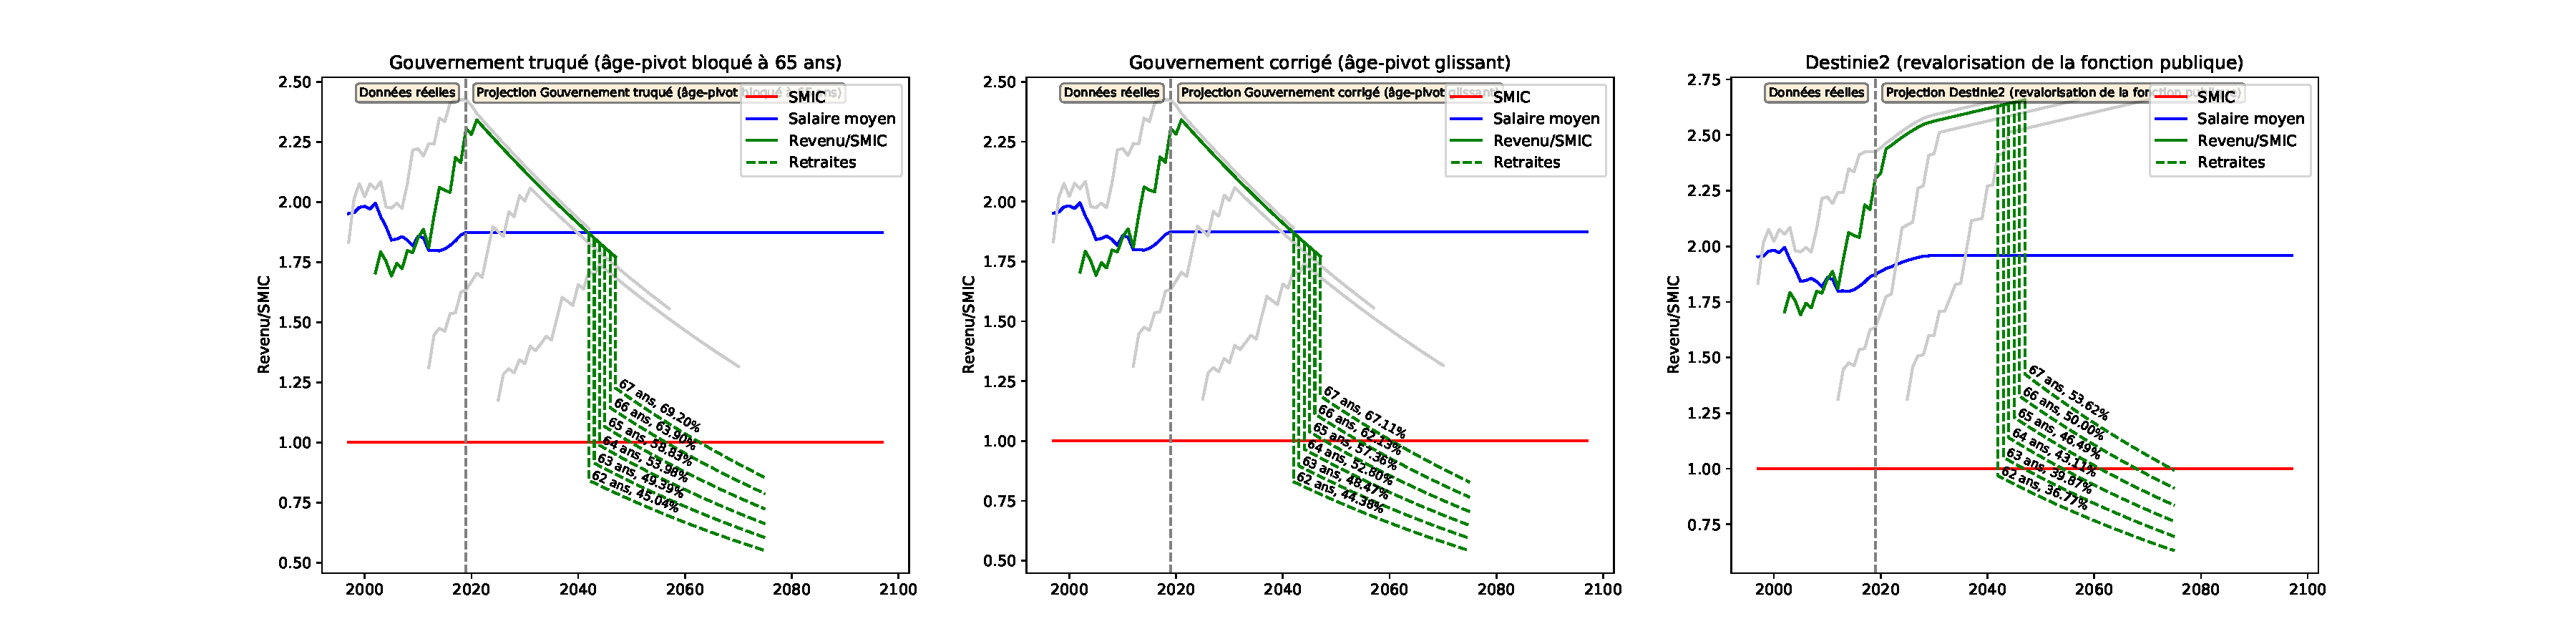
\includegraphics[width=0.9\textwidth]{fig/ProfEcoles_1980_22_dest_retraite.pdf}\end{center} \label{fig/ProfEcoles_1980_22_dest_retraite.pdf} 

\newpage 
 
\paragraph{Revenus et points pour le modèle \emph{Gouvernement truqué (âge-pivot bloqué à 65 ans)}} 
 
{ \scriptsize \begin{center} 
\begin{tabular}[htb]{|c|c||c|c|c|c|c|c||c|c||c|c|c|} 
\hline 
 Année &  Âge &  Ind Maj &  Pt Ind(\euro{} 2019) &  Rev HP(\euro{} 2019) &  Tx Primes &  GIPA(\euro{} 2019) &  Revenu(\euro{} 2019) &  SMIC(\euro{} 2019) &  Rev/SMIC &  Cumul Pts &  Achat Pt(\euro{} 2019) &  Serv. Pt(\euro{} 2019) \\ 
\hline \hline 
 2002 &  22 &  450.0 &  5.49 &  2468.82 &  0.00 &  0.00 &  2468.82 &  1447.74 &  {\bf 1.71} &  832.02 &  35.61 &  0.50 \\ 
\hline 
 2003 &  23 &  498.0 &  5.37 &  2676.56 &  0.00 &  0.00 &  2676.56 &  1493.03 &  {\bf 1.79} &  1734.06 &  35.61 &  0.50 \\ 
\hline 
 2004 &  24 &  513.0 &  5.29 &  2713.63 &  0.00 &  0.00 &  2713.63 &  1547.32 &  {\bf 1.75} &  2648.58 &  35.61 &  0.50 \\ 
\hline 
 2005 &  25 &  513.0 &  5.29 &  2713.33 &  0.00 &  0.00 &  2713.33 &  1603.67 &  {\bf 1.69} &  3563.01 &  35.61 &  0.50 \\ 
\hline 
 2006 &  26 &  542.0 &  5.23 &  2834.72 &  0.00 &  0.00 &  2834.72 &  1625.00 &  {\bf 1.74} &  4518.34 &  35.61 &  0.50 \\ 
\hline 
 2007 &  27 &  542.0 &  5.19 &  2815.41 &  0.00 &  0.00 &  2815.41 &  1634.08 &  {\bf 1.72} &  5467.17 &  35.61 &  0.50 \\ 
\hline 
 2008 &  28 &  579.0 &  5.09 &  2948.87 &  0.00 &  0.00 &  2948.87 &  1640.24 &  {\bf 1.80} &  6460.98 &  35.61 &  0.50 \\ 
\hline 
 2009 &  29 &  579.0 &  5.13 &  2969.77 &  0.00 &  0.00 &  2969.77 &  1659.42 &  {\bf 1.79} &  7461.83 &  35.61 &  0.50 \\ 
\hline 
 2010 &  30 &  598.5 &  5.08 &  3038.78 &  0.05 &  0.00 &  3040.30 &  1641.90 &  {\bf 1.85} &  8486.44 &  35.61 &  0.50 \\ 
\hline 
 2011 &  31 &  618.0 &  4.97 &  3072.59 &  0.28 &  0.00 &  3081.20 &  1633.19 &  {\bf 1.89} &  9524.84 &  35.61 &  0.50 \\ 
\hline 
 2012 &  32 &  618.0 &  4.88 &  3013.64 &  0.51 &  0.00 &  3029.01 &  1673.05 &  {\bf 1.81} &  10545.66 &  35.61 &  0.50 \\ 
\hline 
 2013 &  33 &  664.0 &  4.83 &  3210.21 &  0.74 &  0.00 &  3233.96 &  1664.01 &  {\bf 1.94} &  11635.54 &  35.61 &  0.50 \\ 
\hline 
 2014 &  34 &  710.0 &  4.81 &  3415.42 &  0.97 &  0.00 &  3448.55 &  1673.24 &  {\bf 2.06} &  12797.74 &  35.61 &  0.50 \\ 
\hline 
 2015 &  35 &  710.0 &  4.81 &  3414.08 &  1.20 &  0.00 &  3455.05 &  1686.62 &  {\bf 2.05} &  13962.14 &  35.61 &  0.50 \\ 
\hline 
 2016 &  36 &  710.0 &  4.80 &  3407.27 &  1.43 &  0.00 &  3455.99 &  1693.76 &  {\bf 2.04} &  15126.85 &  35.61 &  0.50 \\ 
\hline 
 2017 &  37 &  757.0 &  4.81 &  3640.15 &  1.66 &  0.00 &  3700.57 &  1692.60 &  {\bf 2.19} &  16373.99 &  35.61 &  0.50 \\ 
\hline 
 2018 &  38 &  757.0 &  4.74 &  3589.89 &  1.89 &  0.00 &  3657.74 &  1689.76 &  {\bf 2.16} &  17606.69 &  35.61 &  0.50 \\ 
\hline 
 2019 &  39 &  800.0 &  4.79 &  3835.54 &  2.12 &  0.00 &  3916.85 &  1698.45 &  {\bf 2.31} &  18926.72 &  35.61 &  0.50 \\ 
\hline 
 2020 &  40 &  800.0 &  4.79 &  3835.54 &  2.35 &  0.00 &  3925.67 &  1720.53 &  {\bf 2.28} &  20249.72 &  35.61 &  0.50 \\ 
\hline 
 2021 &  41 &  830.0 &  4.79 &  3979.37 &  2.58 &  0.00 &  4082.04 &  1742.90 &  {\bf 2.34} &  21625.41 &  35.61 &  0.50 \\ 
\hline 
 2022 &  42 &  830.0 &  4.79 &  3979.37 &  2.81 &  0.00 &  4091.19 &  1765.55 &  {\bf 2.32} &  23004.20 &  35.61 &  0.50 \\ 
\hline 
 2023 &  43 &  830.0 &  4.79 &  3979.37 &  3.04 &  0.00 &  4100.34 &  1788.51 &  {\bf 2.29} &  24386.06 &  35.61 &  0.50 \\ 
\hline 
 2024 &  44 &  830.0 &  4.79 &  3979.37 &  3.27 &  0.00 &  4109.50 &  1811.76 &  {\bf 2.27} &  25771.01 &  35.61 &  0.50 \\ 
\hline 
 2025 &  45 &  830.0 &  4.79 &  3979.37 &  3.50 &  0.00 &  4118.65 &  1835.31 &  {\bf 2.24} &  27159.05 &  35.61 &  0.50 \\ 
\hline 
 2026 &  46 &  830.0 &  4.79 &  3979.37 &  3.73 &  0.00 &  4127.80 &  1859.17 &  {\bf 2.22} &  28550.16 &  35.61 &  0.50 \\ 
\hline 
 2027 &  47 &  830.0 &  4.79 &  3979.37 &  3.96 &  0.00 &  4136.95 &  1883.34 &  {\bf 2.20} &  29944.37 &  35.61 &  0.50 \\ 
\hline 
 2028 &  48 &  830.0 &  4.79 &  3979.37 &  4.19 &  0.00 &  4146.11 &  1907.82 &  {\bf 2.17} &  31341.66 &  35.61 &  0.50 \\ 
\hline 
 2029 &  49 &  830.0 &  4.79 &  3979.37 &  4.42 &  0.00 &  4155.26 &  1932.62 &  {\bf 2.15} &  32740.97 &  35.63 &  0.50 \\ 
\hline 
 2030 &  50 &  830.0 &  4.79 &  3979.37 &  4.65 &  0.00 &  4164.41 &  1957.75 &  {\bf 2.13} &  34141.23 &  35.69 &  0.50 \\ 
\hline 
 2031 &  51 &  830.0 &  4.79 &  3979.37 &  4.88 &  0.00 &  4173.56 &  1983.20 &  {\bf 2.10} &  35541.37 &  35.77 &  0.50 \\ 
\hline 
 2032 &  52 &  830.0 &  4.79 &  3979.37 &  5.11 &  0.00 &  4182.72 &  2008.98 &  {\bf 2.08} &  36940.33 &  35.88 &  0.50 \\ 
\hline 
 2033 &  53 &  830.0 &  4.79 &  3979.37 &  5.34 &  0.00 &  4191.87 &  2035.10 &  {\bf 2.06} &  38337.03 &  36.02 &  0.50 \\ 
\hline 
 2034 &  54 &  830.0 &  4.79 &  3979.37 &  5.57 &  0.00 &  4201.02 &  2061.55 &  {\bf 2.04} &  39730.42 &  36.18 &  0.50 \\ 
\hline 
 2035 &  55 &  830.0 &  4.79 &  3979.37 &  5.80 &  0.00 &  4210.17 &  2088.35 &  {\bf 2.02} &  41119.43 &  36.37 &  0.51 \\ 
\hline 
 2036 &  56 &  830.0 &  4.79 &  3979.37 &  6.03 &  0.00 &  4219.33 &  2115.50 &  {\bf 1.99} &  42503.03 &  36.59 &  0.51 \\ 
\hline 
 2037 &  57 &  830.0 &  4.79 &  3979.37 &  6.26 &  0.00 &  4228.48 &  2143.00 &  {\bf 1.97} &  43880.18 &  36.85 &  0.51 \\ 
\hline 
 2038 &  58 &  830.0 &  4.79 &  3979.37 &  6.49 &  0.00 &  4237.63 &  2170.86 &  {\bf 1.95} &  45249.86 &  37.13 &  0.52 \\ 
\hline 
 2039 &  59 &  830.0 &  4.79 &  3979.37 &  6.72 &  0.00 &  4246.78 &  2199.08 &  {\bf 1.93} &  46611.08 &  37.44 &  0.52 \\ 
\hline 
 2040 &  60 &  830.0 &  4.79 &  3979.37 &  6.95 &  0.00 &  4255.94 &  2227.67 &  {\bf 1.91} &  47962.85 &  37.78 &  0.53 \\ 
\hline 
 2041 &  61 &  830.0 &  4.79 &  3979.37 &  7.18 &  0.00 &  4265.09 &  2256.63 &  {\bf 1.89} &  49304.22 &  38.16 &  0.53 \\ 
\hline 
 2042 &  62 &  830.0 &  4.79 &  3979.37 &  7.41 &  0.00 &  4274.24 &  2285.97 &  {\bf 1.87} &  50634.24 &  38.56 &  0.54 \\ 
\hline 
 2043 &  63 &  830.0 &  4.79 &  3979.37 &  7.64 &  0.00 &  4283.39 &  2315.68 &  {\bf 1.85} &  51952.00 &  39.01 &  0.54 \\ 
\hline 
 2044 &  64 &  830.0 &  4.79 &  3979.37 &  7.87 &  0.00 &  4292.55 &  2345.79 &  {\bf 1.83} &  53256.62 &  39.48 &  0.55 \\ 
\hline 
 2045 &  65 &  830.0 &  4.79 &  3979.37 &  8.10 &  0.00 &  4301.70 &  2376.28 &  {\bf 1.81} &  54547.25 &  40.00 &  0.56 \\ 
\hline 
 2046 &  66 &  830.0 &  4.79 &  3979.37 &  8.33 &  0.00 &  4310.85 &  2407.18 &  {\bf 1.79} &  55824.02 &  40.52 &  0.56 \\ 
\hline 
 2047 &  67 &  830.0 &  4.79 &  3979.37 &  8.56 &  0.00 &  4320.00 &  2438.47 &  {\bf 1.77} &  57087.09 &  41.04 &  0.57 \\ 
\hline 
\hline 
\end{tabular} 
\end{center} } 
\newpage 
 
\paragraph{Revenus et points pour le modèle \emph{Gouvernement corrigé (âge-pivot glissant)}} 
 
{ \scriptsize \begin{center} 
\begin{tabular}[htb]{|c|c||c|c|c|c|c|c||c|c||c|c|c|} 
\hline 
 Année &  Âge &  Ind Maj &  Pt Ind(\euro{} 2019) &  Rev HP(\euro{} 2019) &  Tx Primes &  GIPA(\euro{} 2019) &  Revenu(\euro{} 2019) &  SMIC(\euro{} 2019) &  Rev/SMIC &  Cumul Pts &  Achat Pt(\euro{} 2019) &  Serv. Pt(\euro{} 2019) \\ 
\hline \hline 
 2002 &  22 &  450.0 &  5.49 &  2468.82 &  0.00 &  0.00 &  2468.82 &  1447.74 &  {\bf 1.71} &  832.02 &  35.61 &  0.50 \\ 
\hline 
 2003 &  23 &  498.0 &  5.37 &  2676.56 &  0.00 &  0.00 &  2676.56 &  1493.03 &  {\bf 1.79} &  1734.06 &  35.61 &  0.50 \\ 
\hline 
 2004 &  24 &  513.0 &  5.29 &  2713.63 &  0.00 &  0.00 &  2713.63 &  1547.32 &  {\bf 1.75} &  2648.58 &  35.61 &  0.50 \\ 
\hline 
 2005 &  25 &  513.0 &  5.29 &  2713.33 &  0.00 &  0.00 &  2713.33 &  1603.67 &  {\bf 1.69} &  3563.01 &  35.61 &  0.50 \\ 
\hline 
 2006 &  26 &  542.0 &  5.23 &  2834.72 &  0.00 &  0.00 &  2834.72 &  1625.00 &  {\bf 1.74} &  4518.34 &  35.61 &  0.50 \\ 
\hline 
 2007 &  27 &  542.0 &  5.19 &  2815.41 &  0.00 &  0.00 &  2815.41 &  1634.08 &  {\bf 1.72} &  5467.17 &  35.61 &  0.50 \\ 
\hline 
 2008 &  28 &  579.0 &  5.09 &  2948.87 &  0.00 &  0.00 &  2948.87 &  1640.24 &  {\bf 1.80} &  6460.98 &  35.61 &  0.50 \\ 
\hline 
 2009 &  29 &  579.0 &  5.13 &  2969.77 &  0.00 &  0.00 &  2969.77 &  1659.42 &  {\bf 1.79} &  7461.83 &  35.61 &  0.50 \\ 
\hline 
 2010 &  30 &  598.5 &  5.08 &  3038.78 &  0.05 &  0.00 &  3040.30 &  1641.90 &  {\bf 1.85} &  8486.44 &  35.61 &  0.50 \\ 
\hline 
 2011 &  31 &  618.0 &  4.97 &  3072.59 &  0.28 &  0.00 &  3081.20 &  1633.19 &  {\bf 1.89} &  9524.84 &  35.61 &  0.50 \\ 
\hline 
 2012 &  32 &  618.0 &  4.88 &  3013.64 &  0.51 &  0.00 &  3029.01 &  1673.05 &  {\bf 1.81} &  10545.66 &  35.61 &  0.50 \\ 
\hline 
 2013 &  33 &  664.0 &  4.83 &  3210.21 &  0.74 &  0.00 &  3233.96 &  1664.01 &  {\bf 1.94} &  11635.54 &  35.61 &  0.50 \\ 
\hline 
 2014 &  34 &  710.0 &  4.81 &  3415.42 &  0.97 &  0.00 &  3448.55 &  1673.24 &  {\bf 2.06} &  12797.74 &  35.61 &  0.50 \\ 
\hline 
 2015 &  35 &  710.0 &  4.81 &  3414.08 &  1.20 &  0.00 &  3455.05 &  1686.62 &  {\bf 2.05} &  13962.14 &  35.61 &  0.50 \\ 
\hline 
 2016 &  36 &  710.0 &  4.80 &  3407.27 &  1.43 &  0.00 &  3455.99 &  1693.76 &  {\bf 2.04} &  15126.85 &  35.61 &  0.50 \\ 
\hline 
 2017 &  37 &  757.0 &  4.81 &  3640.15 &  1.66 &  0.00 &  3700.57 &  1692.60 &  {\bf 2.19} &  16373.99 &  35.61 &  0.50 \\ 
\hline 
 2018 &  38 &  757.0 &  4.74 &  3589.89 &  1.89 &  0.00 &  3657.74 &  1689.76 &  {\bf 2.16} &  17606.69 &  35.61 &  0.50 \\ 
\hline 
 2019 &  39 &  800.0 &  4.79 &  3835.54 &  2.12 &  0.00 &  3916.85 &  1698.45 &  {\bf 2.31} &  18926.72 &  35.61 &  0.50 \\ 
\hline 
 2020 &  40 &  800.0 &  4.79 &  3835.54 &  2.35 &  0.00 &  3925.67 &  1720.53 &  {\bf 2.28} &  20249.72 &  35.61 &  0.50 \\ 
\hline 
 2021 &  41 &  830.0 &  4.79 &  3979.37 &  2.58 &  0.00 &  4082.04 &  1742.90 &  {\bf 2.34} &  21625.41 &  35.61 &  0.50 \\ 
\hline 
 2022 &  42 &  830.0 &  4.79 &  3979.37 &  2.81 &  0.00 &  4091.19 &  1765.55 &  {\bf 2.32} &  23004.20 &  35.61 &  0.50 \\ 
\hline 
 2023 &  43 &  830.0 &  4.79 &  3979.37 &  3.04 &  0.00 &  4100.34 &  1788.51 &  {\bf 2.29} &  24386.06 &  35.61 &  0.50 \\ 
\hline 
 2024 &  44 &  830.0 &  4.79 &  3979.37 &  3.27 &  0.00 &  4109.50 &  1811.76 &  {\bf 2.27} &  25771.01 &  35.61 &  0.50 \\ 
\hline 
 2025 &  45 &  830.0 &  4.79 &  3979.37 &  3.50 &  0.00 &  4118.65 &  1835.31 &  {\bf 2.24} &  27159.05 &  35.61 &  0.50 \\ 
\hline 
 2026 &  46 &  830.0 &  4.79 &  3979.37 &  3.73 &  0.00 &  4127.80 &  1859.17 &  {\bf 2.22} &  28550.16 &  35.61 &  0.50 \\ 
\hline 
 2027 &  47 &  830.0 &  4.79 &  3979.37 &  3.96 &  0.00 &  4136.95 &  1883.34 &  {\bf 2.20} &  29944.37 &  35.61 &  0.50 \\ 
\hline 
 2028 &  48 &  830.0 &  4.79 &  3979.37 &  4.19 &  0.00 &  4146.11 &  1907.82 &  {\bf 2.17} &  31341.66 &  35.61 &  0.50 \\ 
\hline 
 2029 &  49 &  830.0 &  4.79 &  3979.37 &  4.42 &  0.00 &  4155.26 &  1932.62 &  {\bf 2.15} &  32740.97 &  35.63 &  0.50 \\ 
\hline 
 2030 &  50 &  830.0 &  4.79 &  3979.37 &  4.65 &  0.00 &  4164.41 &  1957.75 &  {\bf 2.13} &  34141.23 &  35.69 &  0.50 \\ 
\hline 
 2031 &  51 &  830.0 &  4.79 &  3979.37 &  4.88 &  0.00 &  4173.56 &  1983.20 &  {\bf 2.10} &  35541.37 &  35.77 &  0.50 \\ 
\hline 
 2032 &  52 &  830.0 &  4.79 &  3979.37 &  5.11 &  0.00 &  4182.72 &  2008.98 &  {\bf 2.08} &  36940.33 &  35.88 &  0.50 \\ 
\hline 
 2033 &  53 &  830.0 &  4.79 &  3979.37 &  5.34 &  0.00 &  4191.87 &  2035.10 &  {\bf 2.06} &  38337.03 &  36.02 &  0.50 \\ 
\hline 
 2034 &  54 &  830.0 &  4.79 &  3979.37 &  5.57 &  0.00 &  4201.02 &  2061.55 &  {\bf 2.04} &  39730.42 &  36.18 &  0.50 \\ 
\hline 
 2035 &  55 &  830.0 &  4.79 &  3979.37 &  5.80 &  0.00 &  4210.17 &  2088.35 &  {\bf 2.02} &  41119.43 &  36.37 &  0.51 \\ 
\hline 
 2036 &  56 &  830.0 &  4.79 &  3979.37 &  6.03 &  0.00 &  4219.33 &  2115.50 &  {\bf 1.99} &  42503.03 &  36.59 &  0.51 \\ 
\hline 
 2037 &  57 &  830.0 &  4.79 &  3979.37 &  6.26 &  0.00 &  4228.48 &  2143.00 &  {\bf 1.97} &  43880.18 &  36.85 &  0.51 \\ 
\hline 
 2038 &  58 &  830.0 &  4.79 &  3979.37 &  6.49 &  0.00 &  4237.63 &  2170.86 &  {\bf 1.95} &  45249.86 &  37.13 &  0.52 \\ 
\hline 
 2039 &  59 &  830.0 &  4.79 &  3979.37 &  6.72 &  0.00 &  4246.78 &  2199.08 &  {\bf 1.93} &  46611.08 &  37.44 &  0.52 \\ 
\hline 
 2040 &  60 &  830.0 &  4.79 &  3979.37 &  6.95 &  0.00 &  4255.94 &  2227.67 &  {\bf 1.91} &  47962.85 &  37.78 &  0.53 \\ 
\hline 
 2041 &  61 &  830.0 &  4.79 &  3979.37 &  7.18 &  0.00 &  4265.09 &  2256.63 &  {\bf 1.89} &  49304.22 &  38.16 &  0.53 \\ 
\hline 
 2042 &  62 &  830.0 &  4.79 &  3979.37 &  7.41 &  0.00 &  4274.24 &  2285.97 &  {\bf 1.87} &  50634.24 &  38.56 &  0.54 \\ 
\hline 
 2043 &  63 &  830.0 &  4.79 &  3979.37 &  7.64 &  0.00 &  4283.39 &  2315.68 &  {\bf 1.85} &  51952.00 &  39.01 &  0.54 \\ 
\hline 
 2044 &  64 &  830.0 &  4.79 &  3979.37 &  7.87 &  0.00 &  4292.55 &  2345.79 &  {\bf 1.83} &  53256.62 &  39.48 &  0.55 \\ 
\hline 
 2045 &  65 &  830.0 &  4.79 &  3979.37 &  8.10 &  0.00 &  4301.70 &  2376.28 &  {\bf 1.81} &  54547.25 &  40.00 &  0.56 \\ 
\hline 
 2046 &  66 &  830.0 &  4.79 &  3979.37 &  8.33 &  0.00 &  4310.85 &  2407.18 &  {\bf 1.79} &  55824.02 &  40.52 &  0.56 \\ 
\hline 
 2047 &  67 &  830.0 &  4.79 &  3979.37 &  8.56 &  0.00 &  4320.00 &  2438.47 &  {\bf 1.77} &  57087.09 &  41.04 &  0.57 \\ 
\hline 
\hline 
\end{tabular} 
\end{center} } 
\newpage 
 
\paragraph{Revenus et points pour le modèle \emph{Destinie2 (revalorisation de la fonction publique)}} 
 
{ \scriptsize \begin{center} 
\begin{tabular}[htb]{|c|c||c|c|c|c|c|c||c|c||c|c|c|} 
\hline 
 Année &  Âge &  Ind Maj &  Pt Ind(\euro{} 2019) &  Rev HP(\euro{} 2019) &  Tx Primes &  GIPA(\euro{} 2019) &  Revenu(\euro{} 2019) &  SMIC(\euro{} 2019) &  Rev/SMIC &  Cumul Pts &  Achat Pt(\euro{} 2019) &  Serv. Pt(\euro{} 2019) \\ 
\hline \hline 
 2002 &  22 &  450.0 &  5.49 &  2468.82 &  0.00 &  0.00 &  2468.82 &  1447.74 &  {\bf 1.71} &  829.98 &  35.69 &  0.50 \\ 
\hline 
 2003 &  23 &  498.0 &  5.37 &  2676.56 &  0.00 &  0.00 &  2676.56 &  1493.03 &  {\bf 1.79} &  1729.80 &  35.69 &  0.50 \\ 
\hline 
 2004 &  24 &  513.0 &  5.29 &  2713.63 &  0.00 &  0.00 &  2713.63 &  1547.32 &  {\bf 1.75} &  2642.07 &  35.69 &  0.50 \\ 
\hline 
 2005 &  25 &  513.0 &  5.29 &  2713.33 &  0.00 &  0.00 &  2713.33 &  1603.67 &  {\bf 1.69} &  3554.25 &  35.69 &  0.50 \\ 
\hline 
 2006 &  26 &  542.0 &  5.23 &  2834.72 &  0.00 &  0.00 &  2834.72 &  1625.00 &  {\bf 1.74} &  4507.24 &  35.69 &  0.50 \\ 
\hline 
 2007 &  27 &  542.0 &  5.19 &  2815.41 &  0.00 &  0.00 &  2815.41 &  1634.08 &  {\bf 1.72} &  5453.74 &  35.69 &  0.50 \\ 
\hline 
 2008 &  28 &  579.0 &  5.09 &  2948.87 &  0.00 &  0.00 &  2948.87 &  1640.24 &  {\bf 1.80} &  6445.10 &  35.69 &  0.50 \\ 
\hline 
 2009 &  29 &  579.0 &  5.13 &  2969.77 &  0.00 &  0.00 &  2969.77 &  1659.42 &  {\bf 1.79} &  7443.49 &  35.69 &  0.50 \\ 
\hline 
 2010 &  30 &  598.5 &  5.08 &  3038.78 &  0.05 &  0.00 &  3040.30 &  1641.90 &  {\bf 1.85} &  8465.59 &  35.69 &  0.50 \\ 
\hline 
 2011 &  31 &  618.0 &  4.97 &  3072.59 &  0.28 &  0.00 &  3081.20 &  1633.19 &  {\bf 1.89} &  9501.44 &  35.69 &  0.50 \\ 
\hline 
 2012 &  32 &  618.0 &  4.88 &  3013.64 &  0.51 &  0.00 &  3029.01 &  1673.05 &  {\bf 1.81} &  10519.74 &  35.69 &  0.50 \\ 
\hline 
 2013 &  33 &  664.0 &  4.83 &  3210.21 &  0.74 &  0.00 &  3233.96 &  1664.01 &  {\bf 1.94} &  11606.95 &  35.69 &  0.50 \\ 
\hline 
 2014 &  34 &  710.0 &  4.81 &  3415.42 &  0.97 &  0.00 &  3448.55 &  1673.24 &  {\bf 2.06} &  12766.30 &  35.69 &  0.50 \\ 
\hline 
 2015 &  35 &  710.0 &  4.81 &  3414.08 &  1.20 &  0.00 &  3455.05 &  1686.62 &  {\bf 2.05} &  13927.83 &  35.69 &  0.50 \\ 
\hline 
 2016 &  36 &  710.0 &  4.80 &  3407.27 &  1.43 &  0.00 &  3455.99 &  1693.76 &  {\bf 2.04} &  15089.68 &  35.69 &  0.50 \\ 
\hline 
 2017 &  37 &  757.0 &  4.81 &  3640.15 &  1.66 &  0.00 &  3700.57 &  1692.60 &  {\bf 2.19} &  16333.76 &  35.69 &  0.50 \\ 
\hline 
 2018 &  38 &  757.0 &  4.74 &  3589.89 &  1.89 &  0.00 &  3657.74 &  1689.76 &  {\bf 2.16} &  17563.43 &  35.69 &  0.50 \\ 
\hline 
 2019 &  39 &  800.0 &  4.79 &  3835.54 &  2.12 &  0.00 &  3916.85 &  1698.45 &  {\bf 2.31} &  18880.21 &  35.69 &  0.50 \\ 
\hline 
 2020 &  40 &  800.0 &  4.83 &  3866.22 &  2.35 &  0.00 &  3957.08 &  1699.99 &  {\bf 2.33} &  20210.52 &  35.69 &  0.50 \\ 
\hline 
 2021 &  41 &  830.0 &  4.88 &  4047.31 &  2.58 &  0.00 &  4151.73 &  1703.48 &  {\bf 2.44} &  21606.27 &  35.69 &  0.50 \\ 
\hline 
 2022 &  42 &  830.0 &  4.93 &  4087.78 &  2.81 &  0.00 &  4202.65 &  1712.78 &  {\bf 2.45} &  23019.13 &  35.69 &  0.50 \\ 
\hline 
 2023 &  43 &  830.0 &  4.98 &  4135.61 &  3.04 &  0.00 &  4261.33 &  1723.51 &  {\bf 2.47} &  24451.72 &  35.69 &  0.50 \\ 
\hline 
 2024 &  44 &  830.0 &  5.04 &  4184.82 &  3.27 &  0.00 &  4321.66 &  1735.69 &  {\bf 2.49} &  25904.60 &  35.69 &  0.50 \\ 
\hline 
 2025 &  45 &  830.0 &  5.10 &  4235.87 &  3.50 &  0.00 &  4384.13 &  1749.35 &  {\bf 2.51} &  27378.47 &  35.69 &  0.50 \\ 
\hline 
 2026 &  46 &  830.0 &  5.17 &  4288.82 &  3.73 &  0.00 &  4448.80 &  1764.53 &  {\bf 2.52} &  28874.08 &  35.69 &  0.50 \\ 
\hline 
 2027 &  47 &  830.0 &  5.23 &  4343.72 &  3.96 &  0.00 &  4515.73 &  1781.27 &  {\bf 2.54} &  30392.20 &  35.69 &  0.50 \\ 
\hline 
 2028 &  48 &  830.0 &  5.30 &  4400.62 &  4.19 &  0.00 &  4585.01 &  1799.59 &  {\bf 2.55} &  31933.61 &  35.69 &  0.50 \\ 
\hline 
 2029 &  49 &  830.0 &  5.37 &  4453.87 &  4.42 &  0.00 &  4650.73 &  1819.55 &  {\bf 2.56} &  33496.01 &  35.72 &  0.50 \\ 
\hline 
 2030 &  50 &  830.0 &  5.43 &  4509.10 &  4.65 &  0.00 &  4718.77 &  1841.19 &  {\bf 2.56} &  35078.96 &  35.77 &  0.50 \\ 
\hline 
 2031 &  51 &  830.0 &  5.50 &  4566.36 &  4.88 &  0.00 &  4789.20 &  1864.58 &  {\bf 2.57} &  36681.97 &  35.85 &  0.50 \\ 
\hline 
 2032 &  52 &  830.0 &  5.57 &  4625.73 &  5.11 &  0.00 &  4862.10 &  1888.81 &  {\bf 2.57} &  38304.45 &  35.96 &  0.50 \\ 
\hline 
 2033 &  53 &  830.0 &  5.65 &  4685.86 &  5.34 &  0.00 &  4936.09 &  1913.37 &  {\bf 2.58} &  39945.36 &  36.10 &  0.50 \\ 
\hline 
 2034 &  54 &  830.0 &  5.72 &  4746.78 &  5.57 &  0.00 &  5011.17 &  1938.24 &  {\bf 2.59} &  41603.66 &  36.26 &  0.50 \\ 
\hline 
 2035 &  55 &  830.0 &  5.79 &  4808.49 &  5.80 &  0.00 &  5087.38 &  1963.44 &  {\bf 2.59} &  43278.25 &  36.46 &  0.51 \\ 
\hline 
 2036 &  56 &  830.0 &  5.87 &  4871.00 &  6.03 &  0.00 &  5164.72 &  1988.96 &  {\bf 2.60} &  44967.99 &  36.68 &  0.51 \\ 
\hline 
 2037 &  57 &  830.0 &  5.94 &  4934.32 &  6.26 &  0.00 &  5243.21 &  2014.82 &  {\bf 2.60} &  46671.72 &  36.93 &  0.51 \\ 
\hline 
 2038 &  58 &  830.0 &  6.02 &  4998.46 &  6.49 &  0.00 &  5322.87 &  2041.01 &  {\bf 2.61} &  48388.25 &  37.21 &  0.52 \\ 
\hline 
 2039 &  59 &  830.0 &  6.10 &  5063.44 &  6.72 &  0.00 &  5403.71 &  2067.55 &  {\bf 2.61} &  50116.34 &  37.52 &  0.52 \\ 
\hline 
 2040 &  60 &  830.0 &  6.18 &  5129.27 &  6.95 &  0.00 &  5485.75 &  2094.43 &  {\bf 2.62} &  51854.75 &  37.87 &  0.53 \\ 
\hline 
 2041 &  61 &  830.0 &  6.26 &  5195.95 &  7.18 &  0.00 &  5569.02 &  2121.65 &  {\bf 2.62} &  53602.20 &  38.24 &  0.53 \\ 
\hline 
 2042 &  62 &  830.0 &  6.34 &  5263.50 &  7.41 &  0.00 &  5653.52 &  2149.23 &  {\bf 2.63} &  55357.39 &  38.65 &  0.54 \\ 
\hline 
 2043 &  63 &  830.0 &  6.42 &  5331.92 &  7.64 &  0.00 &  5739.28 &  2177.17 &  {\bf 2.64} &  57119.02 &  39.10 &  0.54 \\ 
\hline 
 2044 &  64 &  830.0 &  6.51 &  5401.24 &  7.87 &  0.00 &  5826.32 &  2205.48 &  {\bf 2.64} &  58885.76 &  39.57 &  0.55 \\ 
\hline 
 2045 &  65 &  830.0 &  6.59 &  5471.45 &  8.10 &  0.00 &  5914.64 &  2234.15 &  {\bf 2.65} &  60656.26 &  40.09 &  0.56 \\ 
\hline 
 2046 &  66 &  830.0 &  6.68 &  5542.58 &  8.33 &  0.00 &  6004.28 &  2263.19 &  {\bf 2.65} &  62430.53 &  40.61 &  0.57 \\ 
\hline 
 2047 &  67 &  830.0 &  6.76 &  5614.64 &  8.56 &  0.00 &  6095.25 &  2292.61 &  {\bf 2.66} &  64208.56 &  41.14 &  0.57 \\ 
\hline 
\hline 
\end{tabular} 
\end{center} } 
\newpage 
 
\subsection{Génération 1990 (début en 2012)} 

\paragraph{Retraites possibles dans le modèle \emph{Gouvernement truqué (âge-pivot bloqué à 65 ans)}}  
 
{ \scriptsize \begin{center} 
\begin{tabular}[htb]{|c|c||c|c||c|c||c||c|c|c|c|c|c|} 
\hline 
 Retraite en &  Âge &  Âge pivot &  Décote/Surcote &  Retraite (\euro{} 2019) &  Tx Rempl(\%) &  SMIC (\euro{} 2019) &  Retraite/SMIC &  Rev70/SMIC &  Rev75/SMIC &  Rev80/SMIC &  Rev85/SMIC &  Rev90/SMIC \\ 
\hline \hline 
 2052 &  62 &  65 ans 0 mois &  -15.00\% &  2069.04 &  {\bf 48.41} &  2601.14 &  {\bf {\color{red} 0.80}} &  {\bf {\color{red} 0.72}} &  {\bf {\color{red} 0.67}} &  {\bf {\color{red} 0.63}} &  {\bf {\color{red} 0.59}} &  {\bf {\color{red} 0.55}} \\ 
\hline 
 2053 &  63 &  65 ans 0 mois &  -10.00\% &  2272.88 &  {\bf 53.06} &  2634.96 &  {\bf {\color{red} 0.86}} &  {\bf {\color{red} 0.79}} &  {\bf {\color{red} 0.74}} &  {\bf {\color{red} 0.69}} &  {\bf {\color{red} 0.65}} &  {\bf {\color{red} 0.61}} \\ 
\hline 
 2054 &  64 &  65 ans 0 mois &  -5.00\% &  2487.11 &  {\bf 57.94} &  2669.21 &  {\bf {\color{red} 0.93}} &  {\bf {\color{red} 0.86}} &  {\bf {\color{red} 0.81}} &  {\bf {\color{red} 0.76}} &  {\bf {\color{red} 0.71}} &  {\bf {\color{red} 0.67}} \\ 
\hline 
 2055 &  65 &  65 ans 0 mois &  0.00\% &  2711.92 &  {\bf 63.04} &  2703.91 &  {\bf 1.00} &  {\bf {\color{red} 0.94}} &  {\bf {\color{red} 0.88}} &  {\bf {\color{red} 0.83}} &  {\bf {\color{red} 0.77}} &  {\bf {\color{red} 0.73}} \\ 
\hline 
 2056 &  66 &  65 ans 0 mois &  5.00\% &  2947.54 &  {\bf 68.37} &  2739.06 &  {\bf 1.08} &  {\bf 1.02} &  {\bf {\color{red} 0.96}} &  {\bf {\color{red} 0.90}} &  {\bf {\color{red} 0.84}} &  {\bf {\color{red} 0.79}} \\ 
\hline 
 2057 &  67 &  65 ans 0 mois &  10.00\% &  3194.18 &  {\bf 73.94} &  2774.67 &  {\bf 1.15} &  {\bf 1.11} &  {\bf 1.04} &  {\bf {\color{red} 0.97}} &  {\bf {\color{red} 0.91}} &  {\bf {\color{red} 0.86}} \\ 
\hline 
\hline 
\end{tabular} 
\end{center} } 
\paragraph{Retraites possibles dans le modèle \emph{Gouvernement corrigé (âge-pivot glissant)}}  
 
{ \scriptsize \begin{center} 
\begin{tabular}[htb]{|c|c||c|c||c|c||c||c|c|c|c|c|c|} 
\hline 
 Retraite en &  Âge &  Âge pivot &  Décote/Surcote &  Retraite (\euro{} 2019) &  Tx Rempl(\%) &  SMIC (\euro{} 2019) &  Retraite/SMIC &  Rev70/SMIC &  Rev75/SMIC &  Rev80/SMIC &  Rev85/SMIC &  Rev90/SMIC \\ 
\hline \hline 
 2052 &  62 &  66 ans 1 mois &  -20.42\% &  1937.19 &  {\bf 45.32} &  2601.14 &  {\bf {\color{red} 0.74}} &  {\bf {\color{red} 0.67}} &  {\bf {\color{red} 0.63}} &  {\bf {\color{red} 0.59}} &  {\bf {\color{red} 0.55}} &  {\bf {\color{red} 0.52}} \\ 
\hline 
 2053 &  63 &  66 ans 2 mois &  -15.83\% &  2125.57 &  {\bf 49.62} &  2634.96 &  {\bf {\color{red} 0.81}} &  {\bf {\color{red} 0.74}} &  {\bf {\color{red} 0.69}} &  {\bf {\color{red} 0.65}} &  {\bf {\color{red} 0.61}} &  {\bf {\color{red} 0.57}} \\ 
\hline 
 2054 &  64 &  66 ans 3 mois &  -11.25\% &  2323.48 &  {\bf 54.13} &  2669.21 &  {\bf {\color{red} 0.87}} &  {\bf {\color{red} 0.81}} &  {\bf {\color{red} 0.76}} &  {\bf {\color{red} 0.71}} &  {\bf {\color{red} 0.66}} &  {\bf {\color{red} 0.62}} \\ 
\hline 
 2055 &  65 &  66 ans 4 mois &  -6.67\% &  2531.12 &  {\bf 58.84} &  2703.91 &  {\bf {\color{red} 0.94}} &  {\bf {\color{red} 0.88}} &  {\bf {\color{red} 0.82}} &  {\bf {\color{red} 0.77}} &  {\bf {\color{red} 0.72}} &  {\bf {\color{red} 0.68}} \\ 
\hline 
 2056 &  66 &  66 ans 5 mois &  -2.08\% &  2748.69 &  {\bf 63.76} &  2739.06 &  {\bf 1.00} &  {\bf {\color{red} 0.95}} &  {\bf {\color{red} 0.89}} &  {\bf {\color{red} 0.84}} &  {\bf {\color{red} 0.79}} &  {\bf {\color{red} 0.74}} \\ 
\hline 
 2057 &  67 &  66 ans 6 mois &  2.50\% &  2976.40 &  {\bf 68.90} &  2774.67 &  {\bf 1.07} &  {\bf 1.03} &  {\bf {\color{red} 0.97}} &  {\bf {\color{red} 0.91}} &  {\bf {\color{red} 0.85}} &  {\bf {\color{red} 0.80}} \\ 
\hline 
\hline 
\end{tabular} 
\end{center} } 
\paragraph{Retraites possibles dans le modèle \emph{Destinie2 (revalorisation de la fonction publique)}}  
 
{ \scriptsize \begin{center} 
\begin{tabular}[htb]{|c|c||c|c||c|c||c||c|c|c|c|c|c|} 
\hline 
 Retraite en &  Âge &  Âge pivot &  Décote/Surcote &  Retraite (\euro{} 2019) &  Tx Rempl(\%) &  SMIC (\euro{} 2019) &  Retraite/SMIC &  Rev70/SMIC &  Rev75/SMIC &  Rev80/SMIC &  Rev85/SMIC &  Rev90/SMIC \\ 
\hline \hline 
 2052 &  62 &  66 ans 1 mois &  -20.42\% &  2333.41 &  {\bf 36.27} &  2445.56 &  {\bf {\color{red} 0.95}} &  {\bf {\color{red} 0.86}} &  {\bf {\color{red} 0.81}} &  {\bf {\color{red} 0.76}} &  {\bf {\color{red} 0.71}} &  {\bf {\color{red} 0.66}} \\ 
\hline 
 2053 &  63 &  66 ans 2 mois &  -15.83\% &  2576.39 &  {\bf 39.45} &  2477.35 &  {\bf 1.04} &  {\bf {\color{red} 0.95}} &  {\bf {\color{red} 0.89}} &  {\bf {\color{red} 0.83}} &  {\bf {\color{red} 0.78}} &  {\bf {\color{red} 0.73}} \\ 
\hline 
 2054 &  64 &  66 ans 3 mois &  -11.25\% &  2833.90 &  {\bf 42.75} &  2509.56 &  {\bf 1.13} &  {\bf 1.05} &  {\bf {\color{red} 0.98}} &  {\bf {\color{red} 0.92}} &  {\bf {\color{red} 0.86}} &  {\bf {\color{red} 0.81}} \\ 
\hline 
 2055 &  65 &  66 ans 4 mois &  -6.67\% &  3106.43 &  {\bf 46.16} &  2542.18 &  {\bf 1.22} &  {\bf 1.15} &  {\bf 1.07} &  {\bf 1.01} &  {\bf {\color{red} 0.94}} &  {\bf {\color{red} 0.88}} \\ 
\hline 
 2056 &  66 &  66 ans 5 mois &  -2.08\% &  3394.46 &  {\bf 49.68} &  2575.23 &  {\bf 1.32} &  {\bf 1.25} &  {\bf 1.17} &  {\bf 1.10} &  {\bf 1.03} &  {\bf {\color{red} 0.97}} \\ 
\hline 
 2057 &  67 &  66 ans 6 mois &  2.50\% &  3698.50 &  {\bf 53.33} &  2608.71 &  {\bf 1.42} &  {\bf 1.36} &  {\bf 1.28} &  {\bf 1.20} &  {\bf 1.12} &  {\bf 1.05} \\ 
\hline 
\hline 
\end{tabular} 
\end{center} } 

 \begin{center}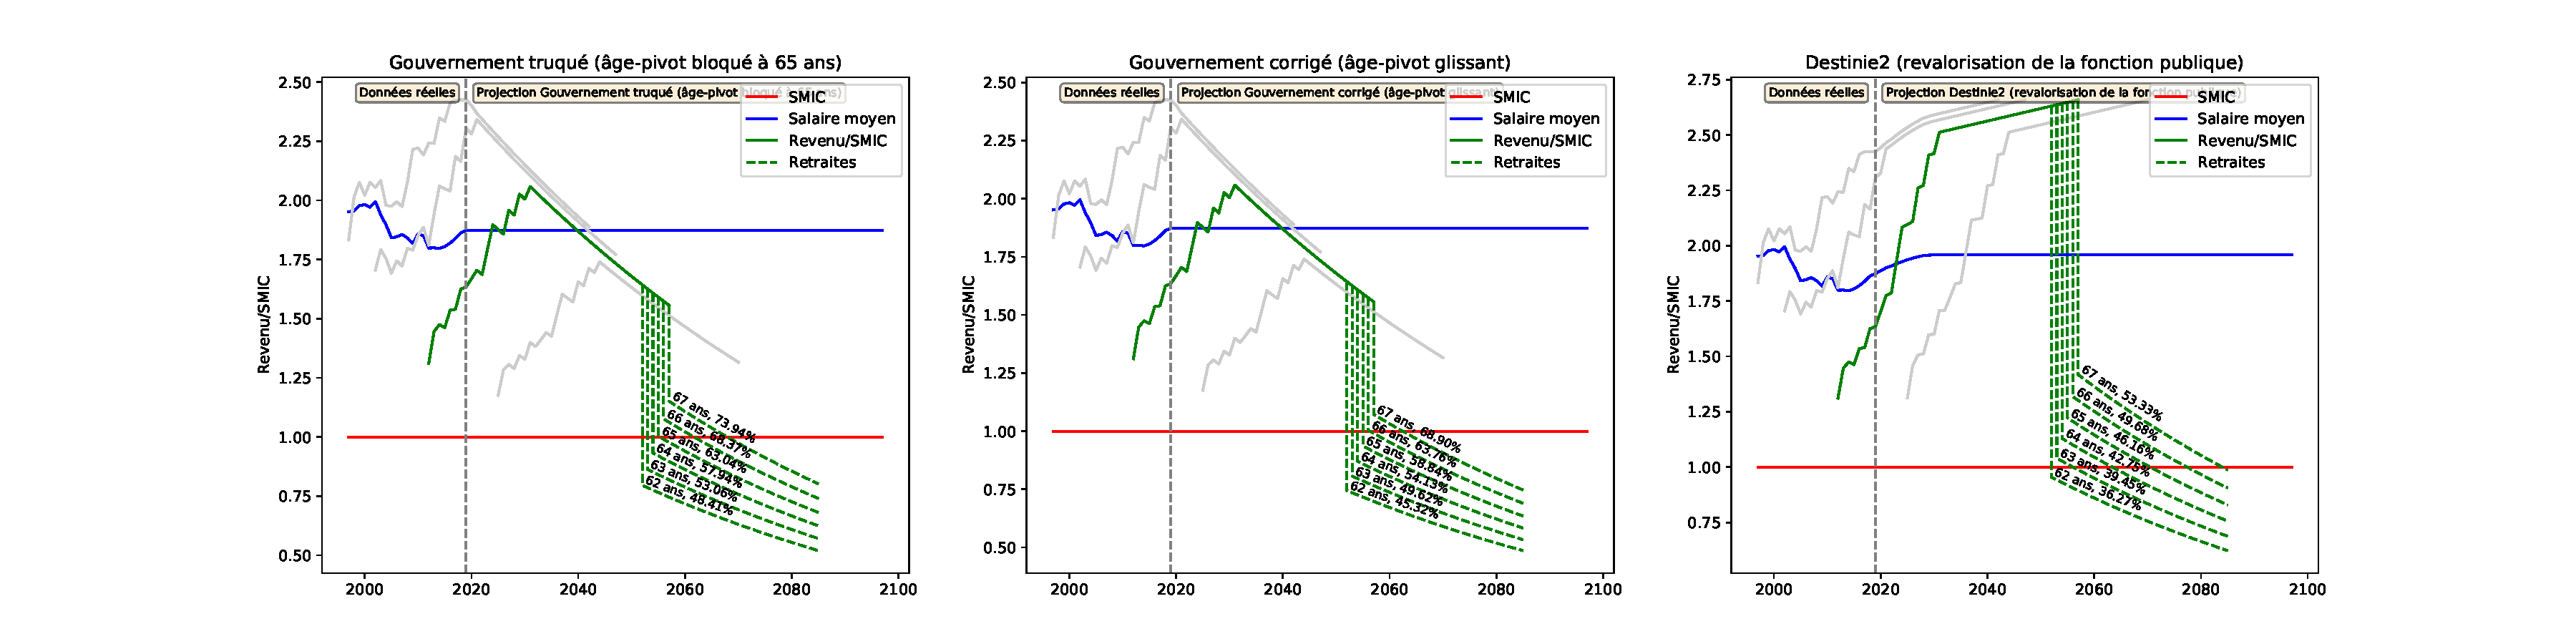
\includegraphics[width=0.9\textwidth]{fig/ProfEcoles_1990_22_dest_retraite.pdf}\end{center} \label{fig/ProfEcoles_1990_22_dest_retraite.pdf} 

\newpage 
 
\paragraph{Revenus et points pour le modèle \emph{Gouvernement truqué (âge-pivot bloqué à 65 ans)}} 
 
{ \scriptsize \begin{center} 
\begin{tabular}[htb]{|c|c||c|c|c|c|c|c||c|c||c|c|c|} 
\hline 
 Année &  Âge &  Ind Maj &  Pt Ind(\euro{} 2019) &  Rev HP(\euro{} 2019) &  Tx Primes &  GIPA(\euro{} 2019) &  Revenu(\euro{} 2019) &  SMIC(\euro{} 2019) &  Rev/SMIC &  Cumul Pts &  Achat Pt(\euro{} 2019) &  Serv. Pt(\euro{} 2019) \\ 
\hline \hline 
 2012 &  22 &  450.0 &  4.88 &  2194.40 &  0.00 &  0.00 &  2194.40 &  1673.05 &  {\bf 1.31} &  739.54 &  35.61 &  0.50 \\ 
\hline 
 2013 &  23 &  498.0 &  4.83 &  2407.66 &  0.00 &  0.00 &  2407.66 &  1664.01 &  {\bf 1.45} &  1550.95 &  35.61 &  0.50 \\ 
\hline 
 2014 &  24 &  513.0 &  4.81 &  2467.76 &  0.00 &  0.00 &  2467.76 &  1673.24 &  {\bf 1.47} &  2382.61 &  35.61 &  0.50 \\ 
\hline 
 2015 &  25 &  513.0 &  4.81 &  2466.80 &  0.00 &  0.00 &  2466.80 &  1686.62 &  {\bf 1.46} &  3213.95 &  35.61 &  0.50 \\ 
\hline 
 2016 &  26 &  542.0 &  4.80 &  2601.04 &  0.00 &  0.00 &  2601.04 &  1693.76 &  {\bf 1.54} &  4090.54 &  35.61 &  0.50 \\ 
\hline 
 2017 &  27 &  542.0 &  4.81 &  2606.29 &  0.00 &  0.00 &  2606.29 &  1692.60 &  {\bf 1.54} &  4968.89 &  35.61 &  0.50 \\ 
\hline 
 2018 &  28 &  579.0 &  4.74 &  2745.77 &  0.00 &  0.00 &  2745.77 &  1689.76 &  {\bf 1.62} &  5894.24 &  35.61 &  0.50 \\ 
\hline 
 2019 &  29 &  579.0 &  4.79 &  2775.97 &  0.00 &  0.00 &  2775.97 &  1698.45 &  {\bf 1.63} &  6829.78 &  35.61 &  0.50 \\ 
\hline 
 2020 &  30 &  598.5 &  4.79 &  2869.46 &  0.05 &  0.00 &  2870.90 &  1720.53 &  {\bf 1.67} &  7797.31 &  35.61 &  0.50 \\ 
\hline 
 2021 &  31 &  618.0 &  4.79 &  2962.95 &  0.28 &  0.00 &  2971.25 &  1742.90 &  {\bf 1.70} &  8798.65 &  35.61 &  0.50 \\ 
\hline 
 2022 &  32 &  618.0 &  4.79 &  2962.95 &  0.51 &  0.00 &  2978.06 &  1765.55 &  {\bf 1.69} &  9802.30 &  35.61 &  0.50 \\ 
\hline 
 2023 &  33 &  664.0 &  4.79 &  3183.50 &  0.74 &  0.00 &  3207.05 &  1788.51 &  {\bf 1.79} &  10883.11 &  35.61 &  0.50 \\ 
\hline 
 2024 &  34 &  710.0 &  4.79 &  3404.04 &  0.97 &  0.00 &  3437.06 &  1811.76 &  {\bf 1.90} &  12041.44 &  35.61 &  0.50 \\ 
\hline 
 2025 &  35 &  710.0 &  4.79 &  3404.04 &  1.20 &  0.00 &  3444.89 &  1835.31 &  {\bf 1.88} &  13202.41 &  35.61 &  0.50 \\ 
\hline 
 2026 &  36 &  710.0 &  4.79 &  3404.04 &  1.43 &  0.00 &  3452.72 &  1859.17 &  {\bf 1.86} &  14366.02 &  35.61 &  0.50 \\ 
\hline 
 2027 &  37 &  757.0 &  4.79 &  3629.38 &  1.66 &  0.00 &  3689.63 &  1883.34 &  {\bf 1.96} &  15609.47 &  35.61 &  0.50 \\ 
\hline 
 2028 &  38 &  757.0 &  4.79 &  3629.38 &  1.89 &  0.00 &  3697.97 &  1907.82 &  {\bf 1.94} &  16855.73 &  35.61 &  0.50 \\ 
\hline 
 2029 &  39 &  800.0 &  4.79 &  3835.54 &  2.12 &  0.00 &  3916.85 &  1932.62 &  {\bf 2.03} &  18174.76 &  35.63 &  0.50 \\ 
\hline 
 2030 &  40 &  800.0 &  4.79 &  3835.54 &  2.35 &  0.00 &  3925.67 &  1957.75 &  {\bf 2.01} &  19494.74 &  35.69 &  0.50 \\ 
\hline 
 2031 &  41 &  830.0 &  4.79 &  3979.37 &  2.58 &  0.00 &  4082.04 &  1983.20 &  {\bf 2.06} &  20864.18 &  35.77 &  0.50 \\ 
\hline 
 2032 &  42 &  830.0 &  4.79 &  3979.37 &  2.81 &  0.00 &  4091.19 &  2008.98 &  {\bf 2.04} &  22232.53 &  35.88 &  0.50 \\ 
\hline 
 2033 &  43 &  830.0 &  4.79 &  3979.37 &  3.04 &  0.00 &  4100.34 &  2035.10 &  {\bf 2.01} &  23598.73 &  36.02 &  0.50 \\ 
\hline 
 2034 &  44 &  830.0 &  4.79 &  3979.37 &  3.27 &  0.00 &  4109.50 &  2061.55 &  {\bf 1.99} &  24961.76 &  36.18 &  0.50 \\ 
\hline 
 2035 &  45 &  830.0 &  4.79 &  3979.37 &  3.50 &  0.00 &  4118.65 &  2088.35 &  {\bf 1.97} &  26320.58 &  36.37 &  0.51 \\ 
\hline 
 2036 &  46 &  830.0 &  4.79 &  3979.37 &  3.73 &  0.00 &  4127.80 &  2115.50 &  {\bf 1.95} &  27674.16 &  36.59 &  0.51 \\ 
\hline 
 2037 &  47 &  830.0 &  4.79 &  3979.37 &  3.96 &  0.00 &  4136.95 &  2143.00 &  {\bf 1.93} &  29021.51 &  36.85 &  0.51 \\ 
\hline 
 2038 &  48 &  830.0 &  4.79 &  3979.37 &  4.19 &  0.00 &  4146.11 &  2170.86 &  {\bf 1.91} &  30361.61 &  37.13 &  0.52 \\ 
\hline 
 2039 &  49 &  830.0 &  4.79 &  3979.37 &  4.42 &  0.00 &  4155.26 &  2199.08 &  {\bf 1.89} &  31693.49 &  37.44 &  0.52 \\ 
\hline 
 2040 &  50 &  830.0 &  4.79 &  3979.37 &  4.65 &  0.00 &  4164.41 &  2227.67 &  {\bf 1.87} &  33016.19 &  37.78 &  0.53 \\ 
\hline 
 2041 &  51 &  830.0 &  4.79 &  3979.37 &  4.88 &  0.00 &  4173.56 &  2256.63 &  {\bf 1.85} &  34328.77 &  38.16 &  0.53 \\ 
\hline 
 2042 &  52 &  830.0 &  4.79 &  3979.37 &  5.11 &  0.00 &  4182.72 &  2285.97 &  {\bf 1.83} &  35630.31 &  38.56 &  0.54 \\ 
\hline 
 2043 &  53 &  830.0 &  4.79 &  3979.37 &  5.34 &  0.00 &  4191.87 &  2315.68 &  {\bf 1.81} &  36919.92 &  39.01 &  0.54 \\ 
\hline 
 2044 &  54 &  830.0 &  4.79 &  3979.37 &  5.57 &  0.00 &  4201.02 &  2345.79 &  {\bf 1.79} &  38196.72 &  39.48 &  0.55 \\ 
\hline 
 2045 &  55 &  830.0 &  4.79 &  3979.37 &  5.80 &  0.00 &  4210.17 &  2376.28 &  {\bf 1.77} &  39459.89 &  40.00 &  0.56 \\ 
\hline 
 2046 &  56 &  830.0 &  4.79 &  3979.37 &  6.03 &  0.00 &  4219.33 &  2407.18 &  {\bf 1.75} &  40709.56 &  40.52 &  0.56 \\ 
\hline 
 2047 &  57 &  830.0 &  4.79 &  3979.37 &  6.26 &  0.00 &  4228.48 &  2438.47 &  {\bf 1.73} &  41945.86 &  41.04 &  0.57 \\ 
\hline 
 2048 &  58 &  830.0 &  4.79 &  3979.37 &  6.49 &  0.00 &  4237.63 &  2470.17 &  {\bf 1.72} &  43168.94 &  41.58 &  0.58 \\ 
\hline 
 2049 &  59 &  830.0 &  4.79 &  3979.37 &  6.72 &  0.00 &  4246.78 &  2502.28 &  {\bf 1.70} &  44378.94 &  42.12 &  0.59 \\ 
\hline 
 2050 &  60 &  830.0 &  4.79 &  3979.37 &  6.95 &  0.00 &  4255.94 &  2534.81 &  {\bf 1.68} &  45575.98 &  42.66 &  0.59 \\ 
\hline 
 2051 &  61 &  830.0 &  4.79 &  3979.37 &  7.18 &  0.00 &  4265.09 &  2567.76 &  {\bf 1.66} &  46760.20 &  43.22 &  0.60 \\ 
\hline 
 2052 &  62 &  830.0 &  4.79 &  3979.37 &  7.41 &  0.00 &  4274.24 &  2601.14 &  {\bf 1.64} &  47931.73 &  43.78 &  0.61 \\ 
\hline 
 2053 &  63 &  830.0 &  4.79 &  3979.37 &  7.64 &  0.00 &  4283.39 &  2634.96 &  {\bf 1.63} &  49090.70 &  44.35 &  0.62 \\ 
\hline 
 2054 &  64 &  830.0 &  4.79 &  3979.37 &  7.87 &  0.00 &  4292.55 &  2669.21 &  {\bf 1.61} &  50237.24 &  44.93 &  0.63 \\ 
\hline 
 2055 &  65 &  830.0 &  4.79 &  3979.37 &  8.10 &  0.00 &  4301.70 &  2703.91 &  {\bf 1.59} &  51371.48 &  45.51 &  0.63 \\ 
\hline 
 2056 &  66 &  830.0 &  4.79 &  3979.37 &  8.33 &  0.00 &  4310.85 &  2739.06 &  {\bf 1.57} &  52493.55 &  46.10 &  0.64 \\ 
\hline 
 2057 &  67 &  830.0 &  4.79 &  3979.37 &  8.56 &  0.00 &  4320.00 &  2774.67 &  {\bf 1.56} &  53603.58 &  46.70 &  0.65 \\ 
\hline 
\hline 
\end{tabular} 
\end{center} } 
\newpage 
 
\paragraph{Revenus et points pour le modèle \emph{Gouvernement corrigé (âge-pivot glissant)}} 
 
{ \scriptsize \begin{center} 
\begin{tabular}[htb]{|c|c||c|c|c|c|c|c||c|c||c|c|c|} 
\hline 
 Année &  Âge &  Ind Maj &  Pt Ind(\euro{} 2019) &  Rev HP(\euro{} 2019) &  Tx Primes &  GIPA(\euro{} 2019) &  Revenu(\euro{} 2019) &  SMIC(\euro{} 2019) &  Rev/SMIC &  Cumul Pts &  Achat Pt(\euro{} 2019) &  Serv. Pt(\euro{} 2019) \\ 
\hline \hline 
 2012 &  22 &  450.0 &  4.88 &  2194.40 &  0.00 &  0.00 &  2194.40 &  1673.05 &  {\bf 1.31} &  739.54 &  35.61 &  0.50 \\ 
\hline 
 2013 &  23 &  498.0 &  4.83 &  2407.66 &  0.00 &  0.00 &  2407.66 &  1664.01 &  {\bf 1.45} &  1550.95 &  35.61 &  0.50 \\ 
\hline 
 2014 &  24 &  513.0 &  4.81 &  2467.76 &  0.00 &  0.00 &  2467.76 &  1673.24 &  {\bf 1.47} &  2382.61 &  35.61 &  0.50 \\ 
\hline 
 2015 &  25 &  513.0 &  4.81 &  2466.80 &  0.00 &  0.00 &  2466.80 &  1686.62 &  {\bf 1.46} &  3213.95 &  35.61 &  0.50 \\ 
\hline 
 2016 &  26 &  542.0 &  4.80 &  2601.04 &  0.00 &  0.00 &  2601.04 &  1693.76 &  {\bf 1.54} &  4090.54 &  35.61 &  0.50 \\ 
\hline 
 2017 &  27 &  542.0 &  4.81 &  2606.29 &  0.00 &  0.00 &  2606.29 &  1692.60 &  {\bf 1.54} &  4968.89 &  35.61 &  0.50 \\ 
\hline 
 2018 &  28 &  579.0 &  4.74 &  2745.77 &  0.00 &  0.00 &  2745.77 &  1689.76 &  {\bf 1.62} &  5894.24 &  35.61 &  0.50 \\ 
\hline 
 2019 &  29 &  579.0 &  4.79 &  2775.97 &  0.00 &  0.00 &  2775.97 &  1698.45 &  {\bf 1.63} &  6829.78 &  35.61 &  0.50 \\ 
\hline 
 2020 &  30 &  598.5 &  4.79 &  2869.46 &  0.05 &  0.00 &  2870.90 &  1720.53 &  {\bf 1.67} &  7797.31 &  35.61 &  0.50 \\ 
\hline 
 2021 &  31 &  618.0 &  4.79 &  2962.95 &  0.28 &  0.00 &  2971.25 &  1742.90 &  {\bf 1.70} &  8798.65 &  35.61 &  0.50 \\ 
\hline 
 2022 &  32 &  618.0 &  4.79 &  2962.95 &  0.51 &  0.00 &  2978.06 &  1765.55 &  {\bf 1.69} &  9802.30 &  35.61 &  0.50 \\ 
\hline 
 2023 &  33 &  664.0 &  4.79 &  3183.50 &  0.74 &  0.00 &  3207.05 &  1788.51 &  {\bf 1.79} &  10883.11 &  35.61 &  0.50 \\ 
\hline 
 2024 &  34 &  710.0 &  4.79 &  3404.04 &  0.97 &  0.00 &  3437.06 &  1811.76 &  {\bf 1.90} &  12041.44 &  35.61 &  0.50 \\ 
\hline 
 2025 &  35 &  710.0 &  4.79 &  3404.04 &  1.20 &  0.00 &  3444.89 &  1835.31 &  {\bf 1.88} &  13202.41 &  35.61 &  0.50 \\ 
\hline 
 2026 &  36 &  710.0 &  4.79 &  3404.04 &  1.43 &  0.00 &  3452.72 &  1859.17 &  {\bf 1.86} &  14366.02 &  35.61 &  0.50 \\ 
\hline 
 2027 &  37 &  757.0 &  4.79 &  3629.38 &  1.66 &  0.00 &  3689.63 &  1883.34 &  {\bf 1.96} &  15609.47 &  35.61 &  0.50 \\ 
\hline 
 2028 &  38 &  757.0 &  4.79 &  3629.38 &  1.89 &  0.00 &  3697.97 &  1907.82 &  {\bf 1.94} &  16855.73 &  35.61 &  0.50 \\ 
\hline 
 2029 &  39 &  800.0 &  4.79 &  3835.54 &  2.12 &  0.00 &  3916.85 &  1932.62 &  {\bf 2.03} &  18174.76 &  35.63 &  0.50 \\ 
\hline 
 2030 &  40 &  800.0 &  4.79 &  3835.54 &  2.35 &  0.00 &  3925.67 &  1957.75 &  {\bf 2.01} &  19494.74 &  35.69 &  0.50 \\ 
\hline 
 2031 &  41 &  830.0 &  4.79 &  3979.37 &  2.58 &  0.00 &  4082.04 &  1983.20 &  {\bf 2.06} &  20864.18 &  35.77 &  0.50 \\ 
\hline 
 2032 &  42 &  830.0 &  4.79 &  3979.37 &  2.81 &  0.00 &  4091.19 &  2008.98 &  {\bf 2.04} &  22232.53 &  35.88 &  0.50 \\ 
\hline 
 2033 &  43 &  830.0 &  4.79 &  3979.37 &  3.04 &  0.00 &  4100.34 &  2035.10 &  {\bf 2.01} &  23598.73 &  36.02 &  0.50 \\ 
\hline 
 2034 &  44 &  830.0 &  4.79 &  3979.37 &  3.27 &  0.00 &  4109.50 &  2061.55 &  {\bf 1.99} &  24961.76 &  36.18 &  0.50 \\ 
\hline 
 2035 &  45 &  830.0 &  4.79 &  3979.37 &  3.50 &  0.00 &  4118.65 &  2088.35 &  {\bf 1.97} &  26320.58 &  36.37 &  0.51 \\ 
\hline 
 2036 &  46 &  830.0 &  4.79 &  3979.37 &  3.73 &  0.00 &  4127.80 &  2115.50 &  {\bf 1.95} &  27674.16 &  36.59 &  0.51 \\ 
\hline 
 2037 &  47 &  830.0 &  4.79 &  3979.37 &  3.96 &  0.00 &  4136.95 &  2143.00 &  {\bf 1.93} &  29021.51 &  36.85 &  0.51 \\ 
\hline 
 2038 &  48 &  830.0 &  4.79 &  3979.37 &  4.19 &  0.00 &  4146.11 &  2170.86 &  {\bf 1.91} &  30361.61 &  37.13 &  0.52 \\ 
\hline 
 2039 &  49 &  830.0 &  4.79 &  3979.37 &  4.42 &  0.00 &  4155.26 &  2199.08 &  {\bf 1.89} &  31693.49 &  37.44 &  0.52 \\ 
\hline 
 2040 &  50 &  830.0 &  4.79 &  3979.37 &  4.65 &  0.00 &  4164.41 &  2227.67 &  {\bf 1.87} &  33016.19 &  37.78 &  0.53 \\ 
\hline 
 2041 &  51 &  830.0 &  4.79 &  3979.37 &  4.88 &  0.00 &  4173.56 &  2256.63 &  {\bf 1.85} &  34328.77 &  38.16 &  0.53 \\ 
\hline 
 2042 &  52 &  830.0 &  4.79 &  3979.37 &  5.11 &  0.00 &  4182.72 &  2285.97 &  {\bf 1.83} &  35630.31 &  38.56 &  0.54 \\ 
\hline 
 2043 &  53 &  830.0 &  4.79 &  3979.37 &  5.34 &  0.00 &  4191.87 &  2315.68 &  {\bf 1.81} &  36919.92 &  39.01 &  0.54 \\ 
\hline 
 2044 &  54 &  830.0 &  4.79 &  3979.37 &  5.57 &  0.00 &  4201.02 &  2345.79 &  {\bf 1.79} &  38196.72 &  39.48 &  0.55 \\ 
\hline 
 2045 &  55 &  830.0 &  4.79 &  3979.37 &  5.80 &  0.00 &  4210.17 &  2376.28 &  {\bf 1.77} &  39459.89 &  40.00 &  0.56 \\ 
\hline 
 2046 &  56 &  830.0 &  4.79 &  3979.37 &  6.03 &  0.00 &  4219.33 &  2407.18 &  {\bf 1.75} &  40709.56 &  40.52 &  0.56 \\ 
\hline 
 2047 &  57 &  830.0 &  4.79 &  3979.37 &  6.26 &  0.00 &  4228.48 &  2438.47 &  {\bf 1.73} &  41945.86 &  41.04 &  0.57 \\ 
\hline 
 2048 &  58 &  830.0 &  4.79 &  3979.37 &  6.49 &  0.00 &  4237.63 &  2470.17 &  {\bf 1.72} &  43168.94 &  41.58 &  0.58 \\ 
\hline 
 2049 &  59 &  830.0 &  4.79 &  3979.37 &  6.72 &  0.00 &  4246.78 &  2502.28 &  {\bf 1.70} &  44378.94 &  42.12 &  0.59 \\ 
\hline 
 2050 &  60 &  830.0 &  4.79 &  3979.37 &  6.95 &  0.00 &  4255.94 &  2534.81 &  {\bf 1.68} &  45575.98 &  42.66 &  0.59 \\ 
\hline 
 2051 &  61 &  830.0 &  4.79 &  3979.37 &  7.18 &  0.00 &  4265.09 &  2567.76 &  {\bf 1.66} &  46760.20 &  43.22 &  0.60 \\ 
\hline 
 2052 &  62 &  830.0 &  4.79 &  3979.37 &  7.41 &  0.00 &  4274.24 &  2601.14 &  {\bf 1.64} &  47931.73 &  43.78 &  0.61 \\ 
\hline 
 2053 &  63 &  830.0 &  4.79 &  3979.37 &  7.64 &  0.00 &  4283.39 &  2634.96 &  {\bf 1.63} &  49090.70 &  44.35 &  0.62 \\ 
\hline 
 2054 &  64 &  830.0 &  4.79 &  3979.37 &  7.87 &  0.00 &  4292.55 &  2669.21 &  {\bf 1.61} &  50237.24 &  44.93 &  0.63 \\ 
\hline 
 2055 &  65 &  830.0 &  4.79 &  3979.37 &  8.10 &  0.00 &  4301.70 &  2703.91 &  {\bf 1.59} &  51371.48 &  45.51 &  0.63 \\ 
\hline 
 2056 &  66 &  830.0 &  4.79 &  3979.37 &  8.33 &  0.00 &  4310.85 &  2739.06 &  {\bf 1.57} &  52493.55 &  46.10 &  0.64 \\ 
\hline 
 2057 &  67 &  830.0 &  4.79 &  3979.37 &  8.56 &  0.00 &  4320.00 &  2774.67 &  {\bf 1.56} &  53603.58 &  46.70 &  0.65 \\ 
\hline 
\hline 
\end{tabular} 
\end{center} } 
\newpage 
 
\paragraph{Revenus et points pour le modèle \emph{Destinie2 (revalorisation de la fonction publique)}} 
 
{ \scriptsize \begin{center} 
\begin{tabular}[htb]{|c|c||c|c|c|c|c|c||c|c||c|c|c|} 
\hline 
 Année &  Âge &  Ind Maj &  Pt Ind(\euro{} 2019) &  Rev HP(\euro{} 2019) &  Tx Primes &  GIPA(\euro{} 2019) &  Revenu(\euro{} 2019) &  SMIC(\euro{} 2019) &  Rev/SMIC &  Cumul Pts &  Achat Pt(\euro{} 2019) &  Serv. Pt(\euro{} 2019) \\ 
\hline \hline 
 2012 &  22 &  450.0 &  4.88 &  2194.40 &  0.00 &  0.00 &  2194.40 &  1673.05 &  {\bf 1.31} &  737.72 &  35.69 &  0.50 \\ 
\hline 
 2013 &  23 &  498.0 &  4.83 &  2407.66 &  0.00 &  0.00 &  2407.66 &  1664.01 &  {\bf 1.45} &  1547.14 &  35.69 &  0.50 \\ 
\hline 
 2014 &  24 &  513.0 &  4.81 &  2467.76 &  0.00 &  0.00 &  2467.76 &  1673.24 &  {\bf 1.47} &  2376.76 &  35.69 &  0.50 \\ 
\hline 
 2015 &  25 &  513.0 &  4.81 &  2466.80 &  0.00 &  0.00 &  2466.80 &  1686.62 &  {\bf 1.46} &  3206.06 &  35.69 &  0.50 \\ 
\hline 
 2016 &  26 &  542.0 &  4.80 &  2601.04 &  0.00 &  0.00 &  2601.04 &  1693.76 &  {\bf 1.54} &  4080.49 &  35.69 &  0.50 \\ 
\hline 
 2017 &  27 &  542.0 &  4.81 &  2606.29 &  0.00 &  0.00 &  2606.29 &  1692.60 &  {\bf 1.54} &  4956.68 &  35.69 &  0.50 \\ 
\hline 
 2018 &  28 &  579.0 &  4.74 &  2745.77 &  0.00 &  0.00 &  2745.77 &  1689.76 &  {\bf 1.62} &  5879.76 &  35.69 &  0.50 \\ 
\hline 
 2019 &  29 &  579.0 &  4.79 &  2775.97 &  0.00 &  0.00 &  2775.97 &  1698.45 &  {\bf 1.63} &  6813.00 &  35.69 &  0.50 \\ 
\hline 
 2020 &  30 &  598.5 &  4.83 &  2892.42 &  0.05 &  0.00 &  2893.86 &  1699.99 &  {\bf 1.70} &  7785.87 &  35.69 &  0.50 \\ 
\hline 
 2021 &  31 &  618.0 &  4.88 &  3013.54 &  0.28 &  0.00 &  3021.97 &  1703.48 &  {\bf 1.77} &  8801.81 &  35.69 &  0.50 \\ 
\hline 
 2022 &  32 &  618.0 &  4.93 &  3043.67 &  0.51 &  0.00 &  3059.19 &  1712.78 &  {\bf 1.79} &  9830.26 &  35.69 &  0.50 \\ 
\hline 
 2023 &  33 &  664.0 &  4.98 &  3308.49 &  0.74 &  0.00 &  3332.97 &  1723.51 &  {\bf 1.93} &  10950.75 &  35.69 &  0.50 \\ 
\hline 
 2024 &  34 &  710.0 &  5.04 &  3579.79 &  0.97 &  0.00 &  3614.51 &  1735.69 &  {\bf 2.08} &  12165.89 &  35.69 &  0.50 \\ 
\hline 
 2025 &  35 &  710.0 &  5.10 &  3623.46 &  1.20 &  0.00 &  3666.94 &  1749.35 &  {\bf 2.10} &  13398.66 &  35.69 &  0.50 \\ 
\hline 
 2026 &  36 &  710.0 &  5.17 &  3668.75 &  1.43 &  0.00 &  3721.22 &  1764.53 &  {\bf 2.11} &  14649.68 &  35.69 &  0.50 \\ 
\hline 
 2027 &  37 &  757.0 &  5.23 &  3961.68 &  1.66 &  0.00 &  4027.45 &  1781.27 &  {\bf 2.26} &  16003.64 &  35.69 &  0.50 \\ 
\hline 
 2028 &  38 &  757.0 &  5.30 &  4013.58 &  1.89 &  0.00 &  4089.44 &  1799.59 &  {\bf 2.27} &  17378.44 &  35.69 &  0.50 \\ 
\hline 
 2029 &  39 &  800.0 &  5.37 &  4292.89 &  2.12 &  0.00 &  4383.90 &  1819.55 &  {\bf 2.41} &  18851.20 &  35.72 &  0.50 \\ 
\hline 
 2030 &  40 &  800.0 &  5.43 &  4346.12 &  2.35 &  0.00 &  4448.25 &  1841.19 &  {\bf 2.42} &  20343.41 &  35.77 &  0.50 \\ 
\hline 
 2031 &  41 &  830.0 &  5.50 &  4566.36 &  2.58 &  0.00 &  4684.18 &  1864.58 &  {\bf 2.51} &  21911.26 &  35.85 &  0.50 \\ 
\hline 
 2032 &  42 &  830.0 &  5.57 &  4625.73 &  2.81 &  0.00 &  4755.71 &  1888.81 &  {\bf 2.52} &  23498.23 &  35.96 &  0.50 \\ 
\hline 
 2033 &  43 &  830.0 &  5.65 &  4685.86 &  3.04 &  0.00 &  4828.31 &  1913.37 &  {\bf 2.52} &  25103.32 &  36.10 &  0.50 \\ 
\hline 
 2034 &  44 &  830.0 &  5.72 &  4746.78 &  3.27 &  0.00 &  4902.00 &  1938.24 &  {\bf 2.53} &  26725.49 &  36.26 &  0.50 \\ 
\hline 
 2035 &  45 &  830.0 &  5.79 &  4808.49 &  3.50 &  0.00 &  4976.78 &  1963.44 &  {\bf 2.53} &  28363.67 &  36.46 &  0.51 \\ 
\hline 
 2036 &  46 &  830.0 &  5.87 &  4871.00 &  3.73 &  0.00 &  5052.68 &  1988.96 &  {\bf 2.54} &  30016.76 &  36.68 &  0.51 \\ 
\hline 
 2037 &  47 &  830.0 &  5.94 &  4934.32 &  3.96 &  0.00 &  5129.72 &  2014.82 &  {\bf 2.55} &  31683.62 &  36.93 &  0.51 \\ 
\hline 
 2038 &  48 &  830.0 &  6.02 &  4998.46 &  4.19 &  0.00 &  5207.90 &  2041.01 &  {\bf 2.55} &  33363.07 &  37.21 &  0.52 \\ 
\hline 
 2039 &  49 &  830.0 &  6.10 &  5063.44 &  4.42 &  0.00 &  5287.25 &  2067.55 &  {\bf 2.56} &  35053.92 &  37.52 &  0.52 \\ 
\hline 
 2040 &  50 &  830.0 &  6.18 &  5129.27 &  4.65 &  0.00 &  5367.78 &  2094.43 &  {\bf 2.56} &  36754.94 &  37.87 &  0.53 \\ 
\hline 
 2041 &  51 &  830.0 &  6.26 &  5195.95 &  4.88 &  0.00 &  5449.51 &  2121.65 &  {\bf 2.57} &  38464.89 &  38.24 &  0.53 \\ 
\hline 
 2042 &  52 &  830.0 &  6.34 &  5263.50 &  5.11 &  0.00 &  5532.46 &  2149.23 &  {\bf 2.57} &  40182.50 &  38.65 &  0.54 \\ 
\hline 
 2043 &  53 &  830.0 &  6.42 &  5331.92 &  5.34 &  0.00 &  5616.65 &  2177.17 &  {\bf 2.58} &  41906.49 &  39.10 &  0.54 \\ 
\hline 
 2044 &  54 &  830.0 &  6.51 &  5401.24 &  5.57 &  0.00 &  5702.09 &  2205.48 &  {\bf 2.59} &  43635.55 &  39.57 &  0.55 \\ 
\hline 
 2045 &  55 &  830.0 &  6.59 &  5471.45 &  5.80 &  0.00 &  5788.80 &  2234.15 &  {\bf 2.59} &  45368.38 &  40.09 &  0.56 \\ 
\hline 
 2046 &  56 &  830.0 &  6.68 &  5542.58 &  6.03 &  0.00 &  5876.80 &  2263.19 &  {\bf 2.60} &  47104.98 &  40.61 &  0.57 \\ 
\hline 
 2047 &  57 &  830.0 &  6.76 &  5614.64 &  6.26 &  0.00 &  5966.11 &  2292.61 &  {\bf 2.60} &  48845.35 &  41.14 &  0.57 \\ 
\hline 
 2048 &  58 &  830.0 &  6.85 &  5687.63 &  6.49 &  0.00 &  6056.75 &  2322.42 &  {\bf 2.61} &  50589.48 &  41.67 &  0.58 \\ 
\hline 
 2049 &  59 &  830.0 &  6.94 &  5761.57 &  6.72 &  0.00 &  6148.74 &  2352.61 &  {\bf 2.61} &  52337.38 &  42.21 &  0.59 \\ 
\hline 
 2050 &  60 &  830.0 &  7.03 &  5836.47 &  6.95 &  0.00 &  6242.10 &  2383.19 &  {\bf 2.62} &  54089.05 &  42.76 &  0.60 \\ 
\hline 
 2051 &  61 &  830.0 &  7.12 &  5912.34 &  7.18 &  0.00 &  6336.85 &  2414.18 &  {\bf 2.62} &  55844.48 &  43.32 &  0.60 \\ 
\hline 
 2052 &  62 &  830.0 &  7.22 &  5989.20 &  7.41 &  0.00 &  6433.00 &  2445.56 &  {\bf 2.63} &  57603.68 &  43.88 &  0.61 \\ 
\hline 
 2053 &  63 &  830.0 &  7.31 &  6067.06 &  7.64 &  0.00 &  6530.58 &  2477.35 &  {\bf 2.64} &  59366.65 &  44.45 &  0.62 \\ 
\hline 
 2054 &  64 &  830.0 &  7.40 &  6145.93 &  7.87 &  0.00 &  6629.62 &  2509.56 &  {\bf 2.64} &  61133.38 &  45.03 &  0.63 \\ 
\hline 
 2055 &  65 &  830.0 &  7.50 &  6225.83 &  8.10 &  0.00 &  6730.12 &  2542.18 &  {\bf 2.65} &  62903.88 &  45.62 &  0.63 \\ 
\hline 
 2056 &  66 &  830.0 &  7.60 &  6306.77 &  8.33 &  0.00 &  6832.12 &  2575.23 &  {\bf 2.65} &  64678.15 &  46.21 &  0.64 \\ 
\hline 
 2057 &  67 &  830.0 &  7.70 &  6388.75 &  8.56 &  0.00 &  6935.63 &  2608.71 &  {\bf 2.66} &  66456.19 &  46.81 &  0.65 \\ 
\hline 
\hline 
\end{tabular} 
\end{center} } 
\newpage 
 
\subsection{Génération 2003 (début en 2025)} 

\paragraph{Retraites possibles dans le modèle \emph{Gouvernement truqué (âge-pivot bloqué à 65 ans)}}  
 
{ \scriptsize \begin{center} 
\begin{tabular}[htb]{|c|c||c|c||c|c||c||c|c|c|c|c|c|} 
\hline 
 Retraite en &  Âge &  Âge pivot &  Décote/Surcote &  Retraite (\euro{} 2019) &  Tx Rempl(\%) &  SMIC (\euro{} 2019) &  Retraite/SMIC &  Rev70/SMIC &  Rev75/SMIC &  Rev80/SMIC &  Rev85/SMIC &  Rev90/SMIC \\ 
\hline \hline 
 2065 &  62 &  65 ans 0 mois &  -15.00\% &  2212.01 &  {\bf 51.75} &  3076.71 &  {\bf {\color{red} 0.72}} &  {\bf {\color{red} 0.65}} &  {\bf {\color{red} 0.61}} &  {\bf {\color{red} 0.57}} &  {\bf {\color{red} 0.53}} &  {\bf {\color{red} 0.50}} \\ 
\hline 
 2066 &  63 &  65 ans 0 mois &  -10.00\% &  2426.24 &  {\bf 56.64} &  3116.71 &  {\bf {\color{red} 0.78}} &  {\bf {\color{red} 0.71}} &  {\bf {\color{red} 0.67}} &  {\bf {\color{red} 0.62}} &  {\bf {\color{red} 0.59}} &  {\bf {\color{red} 0.55}} \\ 
\hline 
 2067 &  64 &  65 ans 0 mois &  -5.00\% &  2651.08 &  {\bf 61.76} &  3157.23 &  {\bf {\color{red} 0.84}} &  {\bf {\color{red} 0.78}} &  {\bf {\color{red} 0.73}} &  {\bf {\color{red} 0.68}} &  {\bf {\color{red} 0.64}} &  {\bf {\color{red} 0.60}} \\ 
\hline 
 2068 &  65 &  65 ans 0 mois &  0.00\% &  2886.77 &  {\bf 67.11} &  3198.27 &  {\bf {\color{red} 0.90}} &  {\bf {\color{red} 0.85}} &  {\bf {\color{red} 0.79}} &  {\bf {\color{red} 0.74}} &  {\bf {\color{red} 0.70}} &  {\bf {\color{red} 0.65}} \\ 
\hline 
 2069 &  66 &  65 ans 0 mois &  5.00\% &  3133.52 &  {\bf 72.69} &  3239.85 &  {\bf {\color{red} 0.97}} &  {\bf {\color{red} 0.92}} &  {\bf {\color{red} 0.86}} &  {\bf {\color{red} 0.81}} &  {\bf {\color{red} 0.76}} &  {\bf {\color{red} 0.71}} \\ 
\hline 
 2070 &  67 &  65 ans 0 mois &  10.00\% &  3391.55 &  {\bf 78.51} &  3281.97 &  {\bf 1.03} &  {\bf {\color{red} 0.99}} &  {\bf {\color{red} 0.93}} &  {\bf {\color{red} 0.87}} &  {\bf {\color{red} 0.82}} &  {\bf {\color{red} 0.77}} \\ 
\hline 
\hline 
\end{tabular} 
\end{center} } 
\paragraph{Retraites possibles dans le modèle \emph{Gouvernement corrigé (âge-pivot glissant)}}  
 
{ \scriptsize \begin{center} 
\begin{tabular}[htb]{|c|c||c|c||c|c||c||c|c|c|c|c|c|} 
\hline 
 Retraite en &  Âge &  Âge pivot &  Décote/Surcote &  Retraite (\euro{} 2019) &  Tx Rempl(\%) &  SMIC (\euro{} 2019) &  Retraite/SMIC &  Rev70/SMIC &  Rev75/SMIC &  Rev80/SMIC &  Rev85/SMIC &  Rev90/SMIC \\ 
\hline \hline 
 2065 &  62 &  67 ans 2 mois &  -25.83\% &  1930.09 &  {\bf 45.16} &  3076.71 &  {\bf {\color{red} 0.63}} &  {\bf {\color{red} 0.57}} &  {\bf {\color{red} 0.53}} &  {\bf {\color{red} 0.50}} &  {\bf {\color{red} 0.47}} &  {\bf {\color{red} 0.44}} \\ 
\hline 
 2066 &  63 &  67 ans 3 mois &  -21.25\% &  2122.96 &  {\bf 49.56} &  3116.71 &  {\bf {\color{red} 0.68}} &  {\bf {\color{red} 0.62}} &  {\bf {\color{red} 0.58}} &  {\bf {\color{red} 0.55}} &  {\bf {\color{red} 0.51}} &  {\bf {\color{red} 0.48}} \\ 
\hline 
 2067 &  64 &  67 ans 4 mois &  -16.67\% &  2325.51 &  {\bf 54.18} &  3157.23 &  {\bf {\color{red} 0.74}} &  {\bf {\color{red} 0.68}} &  {\bf {\color{red} 0.64}} &  {\bf {\color{red} 0.60}} &  {\bf {\color{red} 0.56}} &  {\bf {\color{red} 0.53}} \\ 
\hline 
 2068 &  65 &  67 ans 5 mois &  -12.08\% &  2718.53 &  {\bf 63.20} &  3198.27 &  {\bf {\color{red} 0.85}} &  {\bf {\color{red} 0.80}} &  {\bf {\color{red} 0.75}} &  {\bf {\color{red} 0.70}} &  {\bf {\color{red} 0.66}} &  {\bf {\color{red} 0.62}} \\ 
\hline 
 2069 &  66 &  67 ans 6 mois &  -7.50\% &  2760.48 &  {\bf 64.04} &  3239.85 &  {\bf {\color{red} 0.85}} &  {\bf {\color{red} 0.81}} &  {\bf {\color{red} 0.76}} &  {\bf {\color{red} 0.71}} &  {\bf {\color{red} 0.67}} &  {\bf {\color{red} 0.62}} \\ 
\hline 
 2070 &  67 &  67 ans 7 mois &  -2.92\% &  2993.30 &  {\bf 69.29} &  3281.97 &  {\bf {\color{red} 0.91}} &  {\bf {\color{red} 0.88}} &  {\bf {\color{red} 0.82}} &  {\bf {\color{red} 0.77}} &  {\bf {\color{red} 0.72}} &  {\bf {\color{red} 0.68}} \\ 
\hline 
\hline 
\end{tabular} 
\end{center} } 
\paragraph{Retraites possibles dans le modèle \emph{Destinie2 (revalorisation de la fonction publique)}}  
 
{ \scriptsize \begin{center} 
\begin{tabular}[htb]{|c|c||c|c||c|c||c||c|c|c|c|c|c|} 
\hline 
 Retraite en &  Âge &  Âge pivot &  Décote/Surcote &  Retraite (\euro{} 2019) &  Tx Rempl(\%) &  SMIC (\euro{} 2019) &  Retraite/SMIC &  Rev70/SMIC &  Rev75/SMIC &  Rev80/SMIC &  Rev85/SMIC &  Rev90/SMIC \\ 
\hline \hline 
 2065 &  62 &  67 ans 2 mois &  -25.83\% &  2705.53 &  {\bf 35.56} &  2892.68 &  {\bf {\color{red} 0.94}} &  {\bf {\color{red} 0.84}} &  {\bf {\color{red} 0.79}} &  {\bf {\color{red} 0.74}} &  {\bf {\color{red} 0.69}} &  {\bf {\color{red} 0.65}} \\ 
\hline 
 2066 &  63 &  67 ans 3 mois &  -21.25\% &  2994.74 &  {\bf 38.77} &  2930.29 &  {\bf 1.02} &  {\bf {\color{red} 0.93}} &  {\bf {\color{red} 0.88}} &  {\bf {\color{red} 0.82}} &  {\bf {\color{red} 0.77}} &  {\bf {\color{red} 0.72}} \\ 
\hline 
 2067 &  64 &  67 ans 4 mois &  -16.67\% &  3301.20 &  {\bf 42.10} &  2968.38 &  {\bf 1.11} &  {\bf 1.03} &  {\bf {\color{red} 0.96}} &  {\bf {\color{red} 0.90}} &  {\bf {\color{red} 0.85}} &  {\bf {\color{red} 0.79}} \\ 
\hline 
 2068 &  65 &  67 ans 5 mois &  -12.08\% &  3625.46 &  {\bf 45.54} &  3006.97 &  {\bf 1.21} &  {\bf 1.13} &  {\bf 1.06} &  {\bf {\color{red} 0.99}} &  {\bf {\color{red} 0.93}} &  {\bf {\color{red} 0.87}} \\ 
\hline 
 2069 &  66 &  67 ans 6 mois &  -7.50\% &  3968.10 &  {\bf 49.10} &  3046.06 &  {\bf 1.30} &  {\bf 1.24} &  {\bf 1.16} &  {\bf 1.09} &  {\bf 1.02} &  {\bf {\color{red} 0.96}} \\ 
\hline 
 2070 &  67 &  67 ans 7 mois &  -2.92\% &  4329.72 &  {\bf 52.78} &  3085.66 &  {\bf 1.40} &  {\bf 1.35} &  {\bf 1.27} &  {\bf 1.19} &  {\bf 1.11} &  {\bf 1.04} \\ 
\hline 
\hline 
\end{tabular} 
\end{center} } 

 \begin{center}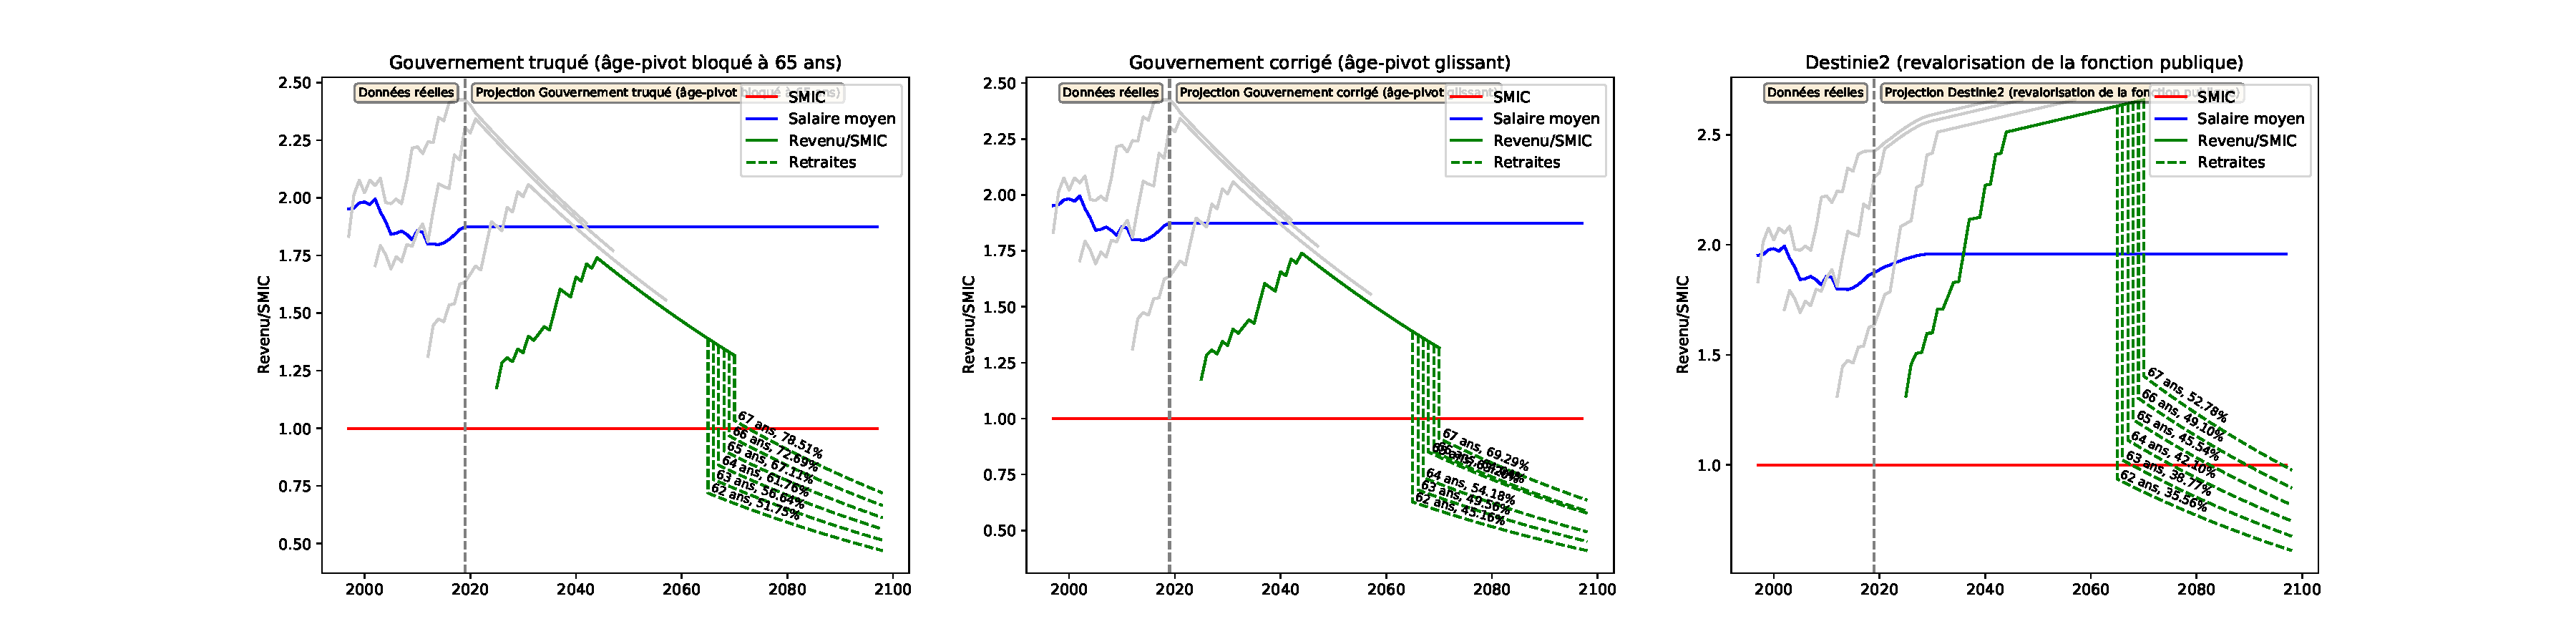
\includegraphics[width=0.9\textwidth]{fig/ProfEcoles_2003_22_dest_retraite.pdf}\end{center} \label{fig/ProfEcoles_2003_22_dest_retraite.pdf} 

\newpage 
 
\paragraph{Revenus et points pour le modèle \emph{Gouvernement truqué (âge-pivot bloqué à 65 ans)}} 
 
{ \scriptsize \begin{center} 
\begin{tabular}[htb]{|c|c||c|c|c|c|c|c||c|c||c|c|c|} 
\hline 
 Année &  Âge &  Ind Maj &  Pt Ind(\euro{} 2019) &  Rev HP(\euro{} 2019) &  Tx Primes &  GIPA(\euro{} 2019) &  Revenu(\euro{} 2019) &  SMIC(\euro{} 2019) &  Rev/SMIC &  Cumul Pts &  Achat Pt(\euro{} 2019) &  Serv. Pt(\euro{} 2019) \\ 
\hline \hline 
 2025 &  22 &  450.0 &  4.79 &  2157.49 &  0.00 &  0.00 &  2157.49 &  1835.31 &  {\bf 1.18} &  727.10 &  35.61 &  0.50 \\ 
\hline 
 2026 &  23 &  498.0 &  4.79 &  2387.62 &  0.00 &  0.00 &  2387.62 &  1859.17 &  {\bf 1.28} &  1531.76 &  35.61 &  0.50 \\ 
\hline 
 2027 &  24 &  513.0 &  4.79 &  2459.54 &  0.00 &  0.00 &  2459.54 &  1883.34 &  {\bf 1.31} &  2360.65 &  35.61 &  0.50 \\ 
\hline 
 2028 &  25 &  513.0 &  4.79 &  2459.54 &  0.00 &  0.00 &  2459.54 &  1907.82 &  {\bf 1.29} &  3189.55 &  35.61 &  0.50 \\ 
\hline 
 2029 &  26 &  542.0 &  4.79 &  2598.58 &  0.00 &  0.00 &  2598.58 &  1932.62 &  {\bf 1.34} &  4064.63 &  35.63 &  0.50 \\ 
\hline 
 2030 &  27 &  542.0 &  4.79 &  2598.58 &  0.00 &  0.00 &  2598.58 &  1957.75 &  {\bf 1.33} &  4938.39 &  35.69 &  0.50 \\ 
\hline 
 2031 &  28 &  579.0 &  4.79 &  2775.97 &  0.00 &  0.00 &  2775.97 &  1983.20 &  {\bf 1.40} &  5869.67 &  35.77 &  0.50 \\ 
\hline 
 2032 &  29 &  579.0 &  4.79 &  2775.97 &  0.00 &  0.00 &  2775.97 &  2008.98 &  {\bf 1.38} &  6798.13 &  35.88 &  0.50 \\ 
\hline 
 2033 &  30 &  598.5 &  4.79 &  2869.46 &  0.05 &  0.00 &  2870.90 &  2035.10 &  {\bf 1.41} &  7754.69 &  36.02 &  0.50 \\ 
\hline 
 2034 &  31 &  618.0 &  4.79 &  2962.95 &  0.28 &  0.00 &  2971.25 &  2061.55 &  {\bf 1.44} &  8740.19 &  36.18 &  0.50 \\ 
\hline 
 2035 &  32 &  618.0 &  4.79 &  2962.95 &  0.51 &  0.00 &  2978.06 &  2088.35 &  {\bf 1.43} &  9722.71 &  36.37 &  0.51 \\ 
\hline 
 2036 &  33 &  664.0 &  4.79 &  3183.50 &  0.74 &  0.00 &  3207.05 &  2115.50 &  {\bf 1.52} &  10774.36 &  36.59 &  0.51 \\ 
\hline 
 2037 &  34 &  710.0 &  4.79 &  3404.04 &  0.97 &  0.00 &  3437.06 &  2143.00 &  {\bf 1.60} &  11893.76 &  36.85 &  0.51 \\ 
\hline 
 2038 &  35 &  710.0 &  4.79 &  3404.04 &  1.20 &  0.00 &  3444.89 &  2170.86 &  {\bf 1.59} &  13007.21 &  37.13 &  0.52 \\ 
\hline 
 2039 &  36 &  710.0 &  4.79 &  3404.04 &  1.43 &  0.00 &  3452.72 &  2199.08 &  {\bf 1.57} &  14113.91 &  37.44 &  0.52 \\ 
\hline 
 2040 &  37 &  757.0 &  4.79 &  3629.38 &  1.66 &  0.00 &  3689.63 &  2227.67 &  {\bf 1.66} &  15285.81 &  37.78 &  0.53 \\ 
\hline 
 2041 &  38 &  757.0 &  4.79 &  3629.38 &  1.89 &  0.00 &  3697.97 &  2256.63 &  {\bf 1.64} &  16448.81 &  38.16 &  0.53 \\ 
\hline 
 2042 &  39 &  800.0 &  4.79 &  3835.54 &  2.12 &  0.00 &  3916.85 &  2285.97 &  {\bf 1.71} &  17667.62 &  38.56 &  0.54 \\ 
\hline 
 2043 &  40 &  800.0 &  4.79 &  3835.54 &  2.35 &  0.00 &  3925.67 &  2315.68 &  {\bf 1.70} &  18875.34 &  39.01 &  0.54 \\ 
\hline 
 2044 &  41 &  830.0 &  4.79 &  3979.37 &  2.58 &  0.00 &  4082.04 &  2345.79 &  {\bf 1.74} &  20115.98 &  39.48 &  0.55 \\ 
\hline 
 2045 &  42 &  830.0 &  4.79 &  3979.37 &  2.81 &  0.00 &  4091.19 &  2376.28 &  {\bf 1.72} &  21343.45 &  40.00 &  0.56 \\ 
\hline 
 2046 &  43 &  830.0 &  4.79 &  3979.37 &  3.04 &  0.00 &  4100.34 &  2407.18 &  {\bf 1.70} &  22557.88 &  40.52 &  0.56 \\ 
\hline 
 2047 &  44 &  830.0 &  4.79 &  3979.37 &  3.27 &  0.00 &  4109.50 &  2438.47 &  {\bf 1.69} &  23759.39 &  41.04 &  0.57 \\ 
\hline 
 2048 &  45 &  830.0 &  4.79 &  3979.37 &  3.50 &  0.00 &  4118.65 &  2470.17 &  {\bf 1.67} &  24948.13 &  41.58 &  0.58 \\ 
\hline 
 2049 &  46 &  830.0 &  4.79 &  3979.37 &  3.73 &  0.00 &  4127.80 &  2502.28 &  {\bf 1.65} &  26124.23 &  42.12 &  0.59 \\ 
\hline 
 2050 &  47 &  830.0 &  4.79 &  3979.37 &  3.96 &  0.00 &  4136.95 &  2534.81 &  {\bf 1.63} &  27287.80 &  42.66 &  0.59 \\ 
\hline 
 2051 &  48 &  830.0 &  4.79 &  3979.37 &  4.19 &  0.00 &  4146.11 &  2567.76 &  {\bf 1.61} &  28438.98 &  43.22 &  0.60 \\ 
\hline 
 2052 &  49 &  830.0 &  4.79 &  3979.37 &  4.42 &  0.00 &  4155.26 &  2601.14 &  {\bf 1.60} &  29577.90 &  43.78 &  0.61 \\ 
\hline 
 2053 &  50 &  830.0 &  4.79 &  3979.37 &  4.65 &  0.00 &  4164.41 &  2634.96 &  {\bf 1.58} &  30704.68 &  44.35 &  0.62 \\ 
\hline 
 2054 &  51 &  830.0 &  4.79 &  3979.37 &  4.88 &  0.00 &  4173.56 &  2669.21 &  {\bf 1.56} &  31819.44 &  44.93 &  0.63 \\ 
\hline 
 2055 &  52 &  830.0 &  4.79 &  3979.37 &  5.11 &  0.00 &  4182.72 &  2703.91 &  {\bf 1.55} &  32922.31 &  45.51 &  0.63 \\ 
\hline 
 2056 &  53 &  830.0 &  4.79 &  3979.37 &  5.34 &  0.00 &  4191.87 &  2739.06 &  {\bf 1.53} &  34013.41 &  46.10 &  0.64 \\ 
\hline 
 2057 &  54 &  830.0 &  4.79 &  3979.37 &  5.57 &  0.00 &  4201.02 &  2774.67 &  {\bf 1.51} &  35092.86 &  46.70 &  0.65 \\ 
\hline 
 2058 &  55 &  830.0 &  4.79 &  3979.37 &  5.80 &  0.00 &  4210.17 &  2810.74 &  {\bf 1.50} &  36160.78 &  47.31 &  0.66 \\ 
\hline 
 2059 &  56 &  830.0 &  4.79 &  3979.37 &  6.03 &  0.00 &  4219.33 &  2847.28 &  {\bf 1.48} &  37217.28 &  47.92 &  0.67 \\ 
\hline 
 2060 &  57 &  830.0 &  4.79 &  3979.37 &  6.26 &  0.00 &  4228.48 &  2884.30 &  {\bf 1.47} &  38262.49 &  48.55 &  0.68 \\ 
\hline 
 2061 &  58 &  830.0 &  4.79 &  3979.37 &  6.49 &  0.00 &  4237.63 &  2921.79 &  {\bf 1.45} &  39296.52 &  49.18 &  0.68 \\ 
\hline 
 2062 &  59 &  830.0 &  4.79 &  3979.37 &  6.72 &  0.00 &  4246.78 &  2959.78 &  {\bf 1.43} &  40319.49 &  49.82 &  0.69 \\ 
\hline 
 2063 &  60 &  830.0 &  4.79 &  3979.37 &  6.95 &  0.00 &  4255.94 &  2998.25 &  {\bf 1.42} &  41331.50 &  50.47 &  0.70 \\ 
\hline 
 2064 &  61 &  830.0 &  4.79 &  3979.37 &  7.18 &  0.00 &  4265.09 &  3037.23 &  {\bf 1.40} &  42332.67 &  51.12 &  0.71 \\ 
\hline 
 2065 &  62 &  830.0 &  4.79 &  3979.37 &  7.41 &  0.00 &  4274.24 &  3076.71 &  {\bf 1.39} &  43323.12 &  51.79 &  0.72 \\ 
\hline 
 2066 &  63 &  830.0 &  4.79 &  3979.37 &  7.64 &  0.00 &  4283.39 &  3116.71 &  {\bf 1.37} &  44302.95 &  52.46 &  0.73 \\ 
\hline 
 2067 &  64 &  830.0 &  4.79 &  3979.37 &  7.87 &  0.00 &  4292.55 &  3157.23 &  {\bf 1.36} &  45272.27 &  53.14 &  0.74 \\ 
\hline 
 2068 &  65 &  830.0 &  4.79 &  3979.37 &  8.10 &  0.00 &  4301.70 &  3198.27 &  {\bf 1.35} &  46231.19 &  53.83 &  0.75 \\ 
\hline 
 2069 &  66 &  830.0 &  4.79 &  3979.37 &  8.33 &  0.00 &  4310.85 &  3239.85 &  {\bf 1.33} &  47179.82 &  54.53 &  0.76 \\ 
\hline 
 2070 &  67 &  830.0 &  4.79 &  3979.37 &  8.56 &  0.00 &  4320.00 &  3281.97 &  {\bf 1.32} &  48118.26 &  55.24 &  0.77 \\ 
\hline 
\hline 
\end{tabular} 
\end{center} } 
\newpage 
 
\paragraph{Revenus et points pour le modèle \emph{Gouvernement corrigé (âge-pivot glissant)}} 
 
{ \scriptsize \begin{center} 
\begin{tabular}[htb]{|c|c||c|c|c|c|c|c||c|c||c|c|c|} 
\hline 
 Année &  Âge &  Ind Maj &  Pt Ind(\euro{} 2019) &  Rev HP(\euro{} 2019) &  Tx Primes &  GIPA(\euro{} 2019) &  Revenu(\euro{} 2019) &  SMIC(\euro{} 2019) &  Rev/SMIC &  Cumul Pts &  Achat Pt(\euro{} 2019) &  Serv. Pt(\euro{} 2019) \\ 
\hline \hline 
 2025 &  22 &  450.0 &  4.79 &  2157.49 &  0.00 &  0.00 &  2157.49 &  1835.31 &  {\bf 1.18} &  727.10 &  35.61 &  0.50 \\ 
\hline 
 2026 &  23 &  498.0 &  4.79 &  2387.62 &  0.00 &  0.00 &  2387.62 &  1859.17 &  {\bf 1.28} &  1531.76 &  35.61 &  0.50 \\ 
\hline 
 2027 &  24 &  513.0 &  4.79 &  2459.54 &  0.00 &  0.00 &  2459.54 &  1883.34 &  {\bf 1.31} &  2360.65 &  35.61 &  0.50 \\ 
\hline 
 2028 &  25 &  513.0 &  4.79 &  2459.54 &  0.00 &  0.00 &  2459.54 &  1907.82 &  {\bf 1.29} &  3189.55 &  35.61 &  0.50 \\ 
\hline 
 2029 &  26 &  542.0 &  4.79 &  2598.58 &  0.00 &  0.00 &  2598.58 &  1932.62 &  {\bf 1.34} &  4064.63 &  35.63 &  0.50 \\ 
\hline 
 2030 &  27 &  542.0 &  4.79 &  2598.58 &  0.00 &  0.00 &  2598.58 &  1957.75 &  {\bf 1.33} &  4938.39 &  35.69 &  0.50 \\ 
\hline 
 2031 &  28 &  579.0 &  4.79 &  2775.97 &  0.00 &  0.00 &  2775.97 &  1983.20 &  {\bf 1.40} &  5869.67 &  35.77 &  0.50 \\ 
\hline 
 2032 &  29 &  579.0 &  4.79 &  2775.97 &  0.00 &  0.00 &  2775.97 &  2008.98 &  {\bf 1.38} &  6798.13 &  35.88 &  0.50 \\ 
\hline 
 2033 &  30 &  598.5 &  4.79 &  2869.46 &  0.05 &  0.00 &  2870.90 &  2035.10 &  {\bf 1.41} &  7754.69 &  36.02 &  0.50 \\ 
\hline 
 2034 &  31 &  618.0 &  4.79 &  2962.95 &  0.28 &  0.00 &  2971.25 &  2061.55 &  {\bf 1.44} &  8740.19 &  36.18 &  0.50 \\ 
\hline 
 2035 &  32 &  618.0 &  4.79 &  2962.95 &  0.51 &  0.00 &  2978.06 &  2088.35 &  {\bf 1.43} &  9722.71 &  36.37 &  0.51 \\ 
\hline 
 2036 &  33 &  664.0 &  4.79 &  3183.50 &  0.74 &  0.00 &  3207.05 &  2115.50 &  {\bf 1.52} &  10774.36 &  36.59 &  0.51 \\ 
\hline 
 2037 &  34 &  710.0 &  4.79 &  3404.04 &  0.97 &  0.00 &  3437.06 &  2143.00 &  {\bf 1.60} &  11893.76 &  36.85 &  0.51 \\ 
\hline 
 2038 &  35 &  710.0 &  4.79 &  3404.04 &  1.20 &  0.00 &  3444.89 &  2170.86 &  {\bf 1.59} &  13007.21 &  37.13 &  0.52 \\ 
\hline 
 2039 &  36 &  710.0 &  4.79 &  3404.04 &  1.43 &  0.00 &  3452.72 &  2199.08 &  {\bf 1.57} &  14113.91 &  37.44 &  0.52 \\ 
\hline 
 2040 &  37 &  757.0 &  4.79 &  3629.38 &  1.66 &  0.00 &  3689.63 &  2227.67 &  {\bf 1.66} &  15285.81 &  37.78 &  0.53 \\ 
\hline 
 2041 &  38 &  757.0 &  4.79 &  3629.38 &  1.89 &  0.00 &  3697.97 &  2256.63 &  {\bf 1.64} &  16448.81 &  38.16 &  0.53 \\ 
\hline 
 2042 &  39 &  800.0 &  4.79 &  3835.54 &  2.12 &  0.00 &  3916.85 &  2285.97 &  {\bf 1.71} &  17667.62 &  38.56 &  0.54 \\ 
\hline 
 2043 &  40 &  800.0 &  4.79 &  3835.54 &  2.35 &  0.00 &  3925.67 &  2315.68 &  {\bf 1.70} &  18875.34 &  39.01 &  0.54 \\ 
\hline 
 2044 &  41 &  830.0 &  4.79 &  3979.37 &  2.58 &  0.00 &  4082.04 &  2345.79 &  {\bf 1.74} &  20115.98 &  39.48 &  0.55 \\ 
\hline 
 2045 &  42 &  830.0 &  4.79 &  3979.37 &  2.81 &  0.00 &  4091.19 &  2376.28 &  {\bf 1.72} &  21343.45 &  40.00 &  0.56 \\ 
\hline 
 2046 &  43 &  830.0 &  4.79 &  3979.37 &  3.04 &  0.00 &  4100.34 &  2407.18 &  {\bf 1.70} &  22557.88 &  40.52 &  0.56 \\ 
\hline 
 2047 &  44 &  830.0 &  4.79 &  3979.37 &  3.27 &  0.00 &  4109.50 &  2438.47 &  {\bf 1.69} &  23759.39 &  41.04 &  0.57 \\ 
\hline 
 2048 &  45 &  830.0 &  4.79 &  3979.37 &  3.50 &  0.00 &  4118.65 &  2470.17 &  {\bf 1.67} &  24948.13 &  41.58 &  0.58 \\ 
\hline 
 2049 &  46 &  830.0 &  4.79 &  3979.37 &  3.73 &  0.00 &  4127.80 &  2502.28 &  {\bf 1.65} &  26124.23 &  42.12 &  0.59 \\ 
\hline 
 2050 &  47 &  830.0 &  4.79 &  3979.37 &  3.96 &  0.00 &  4136.95 &  2534.81 &  {\bf 1.63} &  27287.80 &  42.66 &  0.59 \\ 
\hline 
 2051 &  48 &  830.0 &  4.79 &  3979.37 &  4.19 &  0.00 &  4146.11 &  2567.76 &  {\bf 1.61} &  28438.98 &  43.22 &  0.60 \\ 
\hline 
 2052 &  49 &  830.0 &  4.79 &  3979.37 &  4.42 &  0.00 &  4155.26 &  2601.14 &  {\bf 1.60} &  29577.90 &  43.78 &  0.61 \\ 
\hline 
 2053 &  50 &  830.0 &  4.79 &  3979.37 &  4.65 &  0.00 &  4164.41 &  2634.96 &  {\bf 1.58} &  30704.68 &  44.35 &  0.62 \\ 
\hline 
 2054 &  51 &  830.0 &  4.79 &  3979.37 &  4.88 &  0.00 &  4173.56 &  2669.21 &  {\bf 1.56} &  31819.44 &  44.93 &  0.63 \\ 
\hline 
 2055 &  52 &  830.0 &  4.79 &  3979.37 &  5.11 &  0.00 &  4182.72 &  2703.91 &  {\bf 1.55} &  32922.31 &  45.51 &  0.63 \\ 
\hline 
 2056 &  53 &  830.0 &  4.79 &  3979.37 &  5.34 &  0.00 &  4191.87 &  2739.06 &  {\bf 1.53} &  34013.41 &  46.10 &  0.64 \\ 
\hline 
 2057 &  54 &  830.0 &  4.79 &  3979.37 &  5.57 &  0.00 &  4201.02 &  2774.67 &  {\bf 1.51} &  35092.86 &  46.70 &  0.65 \\ 
\hline 
 2058 &  55 &  830.0 &  4.79 &  3979.37 &  5.80 &  0.00 &  4210.17 &  2810.74 &  {\bf 1.50} &  36160.78 &  47.31 &  0.66 \\ 
\hline 
 2059 &  56 &  830.0 &  4.79 &  3979.37 &  6.03 &  0.00 &  4219.33 &  2847.28 &  {\bf 1.48} &  37217.28 &  47.92 &  0.67 \\ 
\hline 
 2060 &  57 &  830.0 &  4.79 &  3979.37 &  6.26 &  0.00 &  4228.48 &  2884.30 &  {\bf 1.47} &  38262.49 &  48.55 &  0.68 \\ 
\hline 
 2061 &  58 &  830.0 &  4.79 &  3979.37 &  6.49 &  0.00 &  4237.63 &  2921.79 &  {\bf 1.45} &  39296.52 &  49.18 &  0.68 \\ 
\hline 
 2062 &  59 &  830.0 &  4.79 &  3979.37 &  6.72 &  0.00 &  4246.78 &  2959.78 &  {\bf 1.43} &  40319.49 &  49.82 &  0.69 \\ 
\hline 
 2063 &  60 &  830.0 &  4.79 &  3979.37 &  6.95 &  0.00 &  4255.94 &  2998.25 &  {\bf 1.42} &  41331.50 &  50.47 &  0.70 \\ 
\hline 
 2064 &  61 &  830.0 &  4.79 &  3979.37 &  7.18 &  0.00 &  4265.09 &  3037.23 &  {\bf 1.40} &  42332.67 &  51.12 &  0.71 \\ 
\hline 
 2065 &  62 &  830.0 &  4.79 &  3979.37 &  7.41 &  0.00 &  4274.24 &  3076.71 &  {\bf 1.39} &  43323.12 &  51.79 &  0.72 \\ 
\hline 
 2066 &  63 &  830.0 &  4.79 &  3979.37 &  7.64 &  0.00 &  4283.39 &  3116.71 &  {\bf 1.37} &  44302.95 &  52.46 &  0.73 \\ 
\hline 
 2067 &  64 &  830.0 &  4.79 &  3979.37 &  7.87 &  0.00 &  4292.55 &  3157.23 &  {\bf 1.36} &  45272.27 &  53.14 &  0.74 \\ 
\hline 
 2068 &  65 &  830.0 &  4.79 &  3979.37 &  8.10 &  0.00 &  4301.70 &  3198.27 &  {\bf 1.35} &  46231.19 &  53.83 &  0.75 \\ 
\hline 
 2069 &  66 &  830.0 &  4.79 &  3979.37 &  8.33 &  0.00 &  4310.85 &  3239.85 &  {\bf 1.33} &  47179.82 &  54.53 &  0.76 \\ 
\hline 
 2070 &  67 &  830.0 &  4.79 &  3979.37 &  8.56 &  0.00 &  4320.00 &  3281.97 &  {\bf 1.32} &  48118.26 &  55.24 &  0.77 \\ 
\hline 
\hline 
\end{tabular} 
\end{center} } 
\newpage 
 
\paragraph{Revenus et points pour le modèle \emph{Destinie2 (revalorisation de la fonction publique)}} 
 
{ \scriptsize \begin{center} 
\begin{tabular}[htb]{|c|c||c|c|c|c|c|c||c|c||c|c|c|} 
\hline 
 Année &  Âge &  Ind Maj &  Pt Ind(\euro{} 2019) &  Rev HP(\euro{} 2019) &  Tx Primes &  GIPA(\euro{} 2019) &  Revenu(\euro{} 2019) &  SMIC(\euro{} 2019) &  Rev/SMIC &  Cumul Pts &  Achat Pt(\euro{} 2019) &  Serv. Pt(\euro{} 2019) \\ 
\hline \hline 
 2025 &  22 &  450.0 &  5.10 &  2296.56 &  0.00 &  0.00 &  2296.56 &  1749.35 &  {\bf 1.31} &  772.07 &  35.69 &  0.50 \\ 
\hline 
 2026 &  23 &  498.0 &  5.17 &  2573.29 &  0.00 &  0.00 &  2573.29 &  1764.53 &  {\bf 1.46} &  1637.17 &  35.69 &  0.50 \\ 
\hline 
 2027 &  24 &  513.0 &  5.23 &  2684.73 &  0.00 &  0.00 &  2684.73 &  1781.27 &  {\bf 1.51} &  2539.73 &  35.69 &  0.50 \\ 
\hline 
 2028 &  25 &  513.0 &  5.30 &  2719.90 &  0.00 &  0.00 &  2719.90 &  1799.59 &  {\bf 1.51} &  3454.12 &  35.69 &  0.50 \\ 
\hline 
 2029 &  26 &  542.0 &  5.37 &  2908.43 &  0.00 &  0.00 &  2908.43 &  1819.55 &  {\bf 1.60} &  4431.20 &  35.72 &  0.50 \\ 
\hline 
 2030 &  27 &  542.0 &  5.43 &  2944.50 &  0.00 &  0.00 &  2944.50 &  1841.19 &  {\bf 1.60} &  5418.96 &  35.77 &  0.50 \\ 
\hline 
 2031 &  28 &  579.0 &  5.50 &  3185.45 &  0.00 &  0.00 &  3185.45 &  1864.58 &  {\bf 1.71} &  6485.17 &  35.85 &  0.50 \\ 
\hline 
 2032 &  29 &  579.0 &  5.57 &  3226.86 &  0.00 &  0.00 &  3226.86 &  1888.81 &  {\bf 1.71} &  7561.97 &  35.96 &  0.50 \\ 
\hline 
 2033 &  30 &  598.5 &  5.65 &  3378.90 &  0.05 &  0.00 &  3380.59 &  1913.37 &  {\bf 1.77} &  8685.78 &  36.10 &  0.50 \\ 
\hline 
 2034 &  31 &  618.0 &  5.72 &  3534.35 &  0.28 &  0.00 &  3544.24 &  1938.24 &  {\bf 1.83} &  9858.65 &  36.26 &  0.50 \\ 
\hline 
 2035 &  32 &  618.0 &  5.79 &  3580.29 &  0.51 &  0.00 &  3598.55 &  1963.44 &  {\bf 1.83} &  11043.16 &  36.46 &  0.51 \\ 
\hline 
 2036 &  33 &  664.0 &  5.87 &  3896.80 &  0.74 &  0.00 &  3925.63 &  1988.96 &  {\bf 1.97} &  12327.52 &  36.68 &  0.51 \\ 
\hline 
 2037 &  34 &  710.0 &  5.94 &  4220.92 &  0.97 &  0.00 &  4261.87 &  2014.82 &  {\bf 2.12} &  13712.37 &  36.93 &  0.51 \\ 
\hline 
 2038 &  35 &  710.0 &  6.02 &  4275.80 &  1.20 &  0.00 &  4327.10 &  2041.01 &  {\bf 2.12} &  15107.78 &  37.21 &  0.52 \\ 
\hline 
 2039 &  36 &  710.0 &  6.10 &  4331.38 &  1.43 &  0.00 &  4393.32 &  2067.55 &  {\bf 2.12} &  16512.75 &  37.52 &  0.52 \\ 
\hline 
 2040 &  37 &  757.0 &  6.18 &  4678.14 &  1.66 &  0.00 &  4755.80 &  2094.43 &  {\bf 2.27} &  18019.84 &  37.87 &  0.53 \\ 
\hline 
 2041 &  38 &  757.0 &  6.26 &  4738.96 &  1.89 &  0.00 &  4828.52 &  2121.65 &  {\bf 2.28} &  19534.94 &  38.24 &  0.53 \\ 
\hline 
 2042 &  39 &  800.0 &  6.34 &  5073.25 &  2.12 &  0.00 &  5180.80 &  2149.23 &  {\bf 2.41} &  21143.37 &  38.65 &  0.54 \\ 
\hline 
 2043 &  40 &  800.0 &  6.42 &  5139.20 &  2.35 &  0.00 &  5259.97 &  2177.17 &  {\bf 2.42} &  22757.88 &  39.10 &  0.54 \\ 
\hline 
 2044 &  41 &  830.0 &  6.51 &  5401.24 &  2.58 &  0.00 &  5540.59 &  2205.48 &  {\bf 2.51} &  24437.98 &  39.57 &  0.55 \\ 
\hline 
 2045 &  42 &  830.0 &  6.59 &  5471.45 &  2.81 &  0.00 &  5625.20 &  2234.15 &  {\bf 2.52} &  26121.84 &  40.09 &  0.56 \\ 
\hline 
 2046 &  43 &  830.0 &  6.68 &  5542.58 &  3.04 &  0.00 &  5711.08 &  2263.19 &  {\bf 2.52} &  27809.46 &  40.61 &  0.57 \\ 
\hline 
 2047 &  44 &  830.0 &  6.76 &  5614.64 &  3.27 &  0.00 &  5798.24 &  2292.61 &  {\bf 2.53} &  29500.86 &  41.14 &  0.57 \\ 
\hline 
 2048 &  45 &  830.0 &  6.85 &  5687.63 &  3.50 &  0.00 &  5886.69 &  2322.42 &  {\bf 2.53} &  31196.02 &  41.67 &  0.58 \\ 
\hline 
 2049 &  46 &  830.0 &  6.94 &  5761.57 &  3.73 &  0.00 &  5976.47 &  2352.61 &  {\bf 2.54} &  32894.95 &  42.21 &  0.59 \\ 
\hline 
 2050 &  47 &  830.0 &  7.03 &  5836.47 &  3.96 &  0.00 &  6067.59 &  2383.19 &  {\bf 2.55} &  34597.64 &  42.76 &  0.60 \\ 
\hline 
 2051 &  48 &  830.0 &  7.12 &  5912.34 &  4.19 &  0.00 &  6160.07 &  2414.18 &  {\bf 2.55} &  36304.10 &  43.32 &  0.60 \\ 
\hline 
 2052 &  49 &  830.0 &  7.22 &  5989.20 &  4.42 &  0.00 &  6253.92 &  2445.56 &  {\bf 2.56} &  38014.33 &  43.88 &  0.61 \\ 
\hline 
 2053 &  50 &  830.0 &  7.31 &  6067.06 &  4.65 &  0.00 &  6349.18 &  2477.35 &  {\bf 2.56} &  39728.33 &  44.45 &  0.62 \\ 
\hline 
 2054 &  51 &  830.0 &  7.40 &  6145.93 &  4.88 &  0.00 &  6445.85 &  2509.56 &  {\bf 2.57} &  41446.09 &  45.03 &  0.63 \\ 
\hline 
 2055 &  52 &  830.0 &  7.50 &  6225.83 &  5.11 &  0.00 &  6543.97 &  2542.18 &  {\bf 2.57} &  43167.62 &  45.62 &  0.63 \\ 
\hline 
 2056 &  53 &  830.0 &  7.60 &  6306.77 &  5.34 &  0.00 &  6643.55 &  2575.23 &  {\bf 2.58} &  44892.92 &  46.21 &  0.64 \\ 
\hline 
 2057 &  54 &  830.0 &  7.70 &  6388.75 &  5.57 &  0.00 &  6744.61 &  2608.71 &  {\bf 2.59} &  46621.98 &  46.81 &  0.65 \\ 
\hline 
 2058 &  55 &  830.0 &  7.80 &  6471.81 &  5.80 &  0.00 &  6847.17 &  2642.62 &  {\bf 2.59} &  48354.81 &  47.42 &  0.66 \\ 
\hline 
 2059 &  56 &  830.0 &  7.90 &  6555.94 &  6.03 &  0.00 &  6951.26 &  2676.98 &  {\bf 2.60} &  50091.41 &  48.03 &  0.67 \\ 
\hline 
 2060 &  57 &  830.0 &  8.00 &  6641.17 &  6.26 &  0.00 &  7056.90 &  2711.78 &  {\bf 2.60} &  51831.78 &  48.66 &  0.68 \\ 
\hline 
 2061 &  58 &  830.0 &  8.11 &  6727.50 &  6.49 &  0.00 &  7164.12 &  2747.03 &  {\bf 2.61} &  53575.91 &  49.29 &  0.69 \\ 
\hline 
 2062 &  59 &  830.0 &  8.21 &  6814.96 &  6.72 &  0.00 &  7272.93 &  2782.74 &  {\bf 2.61} &  55323.81 &  49.93 &  0.70 \\ 
\hline 
 2063 &  60 &  830.0 &  8.32 &  6903.55 &  6.95 &  0.00 &  7383.35 &  2818.92 &  {\bf 2.62} &  57075.48 &  50.58 &  0.70 \\ 
\hline 
 2064 &  61 &  830.0 &  8.43 &  6993.30 &  7.18 &  0.00 &  7495.42 &  2855.56 &  {\bf 2.62} &  58830.91 &  51.24 &  0.71 \\ 
\hline 
 2065 &  62 &  830.0 &  8.54 &  7084.21 &  7.41 &  0.00 &  7609.15 &  2892.68 &  {\bf 2.63} &  60590.11 &  51.90 &  0.72 \\ 
\hline 
 2066 &  63 &  830.0 &  8.65 &  7176.31 &  7.64 &  0.00 &  7724.58 &  2930.29 &  {\bf 2.64} &  62353.08 &  52.58 &  0.73 \\ 
\hline 
 2067 &  64 &  830.0 &  8.76 &  7269.60 &  7.87 &  0.00 &  7841.72 &  2968.38 &  {\bf 2.64} &  64119.81 &  53.26 &  0.74 \\ 
\hline 
 2068 &  65 &  830.0 &  8.87 &  7364.11 &  8.10 &  0.00 &  7960.60 &  3006.97 &  {\bf 2.65} &  65890.31 &  53.95 &  0.75 \\ 
\hline 
 2069 &  66 &  830.0 &  8.99 &  7459.84 &  8.33 &  0.00 &  8081.24 &  3046.06 &  {\bf 2.65} &  67664.58 &  54.66 &  0.76 \\ 
\hline 
 2070 &  67 &  830.0 &  9.10 &  7556.82 &  8.56 &  0.00 &  8203.68 &  3085.66 &  {\bf 2.66} &  69442.62 &  55.37 &  0.77 \\ 
\hline 
\hline 
\end{tabular} 
\end{center} } 
\newpage 
 
\chapter{Professeur certifié} 

\begin{minipage}{0.55\linewidth}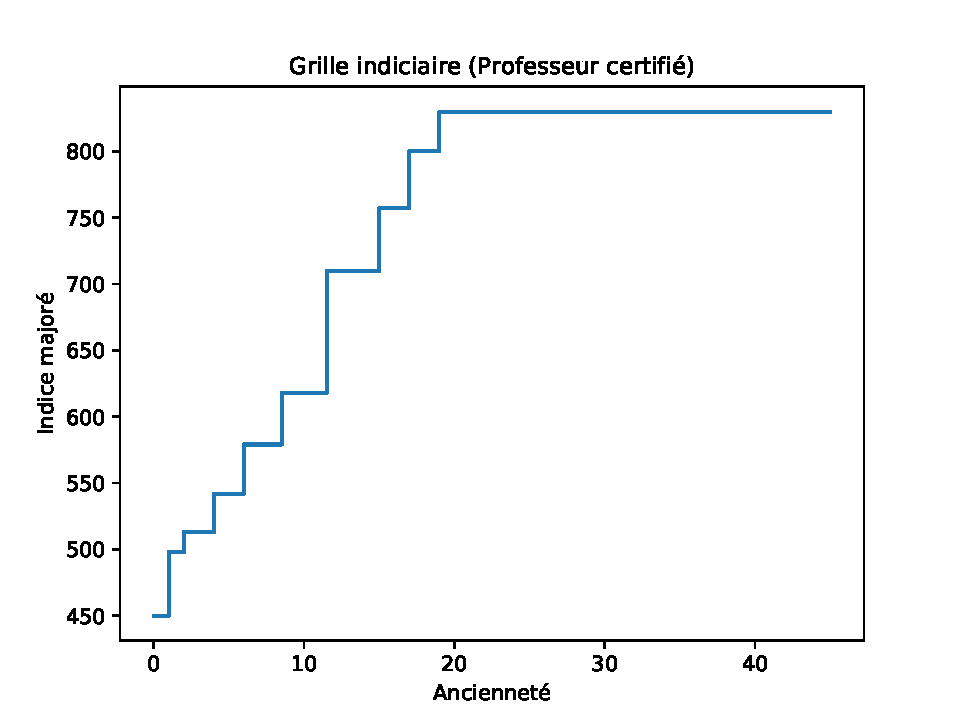
\includegraphics[width=0.7\textwidth]{fig/grille_ProfCertifie.pdf}\end{minipage} 
\begin{minipage}{0.3\linewidth} 
 \begin{center} 

\begin{tabular}[htb]{|c|c|} 
\hline 
 Indice majoré &  Durée (années) \\ 
\hline \hline 
 450 &  1.00 \\ 
\hline 
 498 &  1.00 \\ 
\hline 
 513 &  2.00 \\ 
\hline 
 542 &  2.00 \\ 
\hline 
 579 &  2.50 \\ 
\hline 
 618 &  3.00 \\ 
\hline 
 710 &  3.50 \\ 
\hline 
 757 &  2.00 \\ 
\hline 
 800 &  2.00 \\ 
\hline 
 830 &   \\ 
\hline 
\hline 
\end{tabular} 
\end{center} 
 \end{minipage} 


 \addto{\captionsenglish}{ \renewcommand{\mtctitle}{}} \setcounter{minitocdepth}{2} 
 \minitoc \newpage 

\section{Début de carrière à 22 ans} 

\subsection{Génération 1975 (début en 1997)} 

\paragraph{Retraites possibles dans le modèle \emph{Gouvernement truqué (âge-pivot bloqué à 65 ans)}}  
 
{ \scriptsize \begin{center} 
\begin{tabular}[htb]{|c|c||c|c||c|c||c||c|c|c|c|c|c|} 
\hline 
 Retraite en &  Âge &  Âge pivot &  Décote/Surcote &  Retraite (\euro{} 2019) &  Tx Rempl(\%) &  SMIC (\euro{} 2019) &  Retraite/SMIC &  Rev70/SMIC &  Rev75/SMIC &  Rev80/SMIC &  Rev85/SMIC &  Rev90/SMIC \\ 
\hline \hline 
 2037 &  62 &  64 ans 10 mois &  -14.17\% &  1927.13 &  {\bf 44.47} &  2143.00 &  {\bf {\color{red} 0.90}} &  {\bf {\color{red} 0.81}} &  {\bf {\color{red} 0.76}} &  {\bf {\color{red} 0.71}} &  {\bf {\color{red} 0.67}} &  {\bf {\color{red} 0.63}} \\ 
\hline 
 2038 &  63 &  64 ans 11 mois &  -9.58\% &  2100.17 &  {\bf 48.36} &  2170.86 &  {\bf {\color{red} 0.97}} &  {\bf {\color{red} 0.88}} &  {\bf {\color{red} 0.83}} &  {\bf {\color{red} 0.78}} &  {\bf {\color{red} 0.73}} &  {\bf {\color{red} 0.68}} \\ 
\hline 
 2039 &  64 &  65 ans 0 mois &  -5.00\% &  2282.71 &  {\bf 52.45} &  2199.08 &  {\bf 1.04} &  {\bf {\color{red} 0.96}} &  {\bf {\color{red} 0.90}} &  {\bf {\color{red} 0.84}} &  {\bf {\color{red} 0.79}} &  {\bf {\color{red} 0.74}} \\ 
\hline 
 2040 &  65 &  65 ans 0 mois &  0.00\% &  2485.56 &  {\bf 56.99} &  2227.67 &  {\bf 1.12} &  {\bf 1.05} &  {\bf {\color{red} 0.98}} &  {\bf {\color{red} 0.92}} &  {\bf {\color{red} 0.86}} &  {\bf {\color{red} 0.81}} \\ 
\hline 
 2041 &  66 &  65 ans 0 mois &  5.00\% &  2699.62 &  {\bf 61.77} &  2256.63 &  {\bf 1.20} &  {\bf 1.14} &  {\bf 1.07} &  {\bf {\color{red} 1.00}} &  {\bf {\color{red} 0.94}} &  {\bf {\color{red} 0.88}} \\ 
\hline 
 2042 &  67 &  65 ans 0 mois &  10.00\% &  2925.48 &  {\bf 66.80} &  2285.97 &  {\bf 1.28} &  {\bf 1.23} &  {\bf 1.15} &  {\bf 1.08} &  {\bf 1.01} &  {\bf {\color{red} 0.95}} \\ 
\hline 
\hline 
\end{tabular} 
\end{center} } 
\paragraph{Retraites possibles dans le modèle \emph{Gouvernement corrigé (âge-pivot glissant)}}  
 
{ \scriptsize \begin{center} 
\begin{tabular}[htb]{|c|c||c|c||c|c||c||c|c|c|c|c|c|} 
\hline 
 Retraite en &  Âge &  Âge pivot &  Décote/Surcote &  Retraite (\euro{} 2019) &  Tx Rempl(\%) &  SMIC (\euro{} 2019) &  Retraite/SMIC &  Rev70/SMIC &  Rev75/SMIC &  Rev80/SMIC &  Rev85/SMIC &  Rev90/SMIC \\ 
\hline \hline 
 2037 &  62 &  64 ans 10 mois &  -14.17\% &  1927.13 &  {\bf 44.47} &  2143.00 &  {\bf {\color{red} 0.90}} &  {\bf {\color{red} 0.81}} &  {\bf {\color{red} 0.76}} &  {\bf {\color{red} 0.71}} &  {\bf {\color{red} 0.67}} &  {\bf {\color{red} 0.63}} \\ 
\hline 
 2038 &  63 &  64 ans 11 mois &  -9.58\% &  2100.17 &  {\bf 48.36} &  2170.86 &  {\bf {\color{red} 0.97}} &  {\bf {\color{red} 0.88}} &  {\bf {\color{red} 0.83}} &  {\bf {\color{red} 0.78}} &  {\bf {\color{red} 0.73}} &  {\bf {\color{red} 0.68}} \\ 
\hline 
 2039 &  64 &  65 ans 0 mois &  -5.00\% &  2282.71 &  {\bf 52.45} &  2199.08 &  {\bf 1.04} &  {\bf {\color{red} 0.96}} &  {\bf {\color{red} 0.90}} &  {\bf {\color{red} 0.84}} &  {\bf {\color{red} 0.79}} &  {\bf {\color{red} 0.74}} \\ 
\hline 
 2040 &  65 &  65 ans 1 mois &  -0.42\% &  2475.21 &  {\bf 56.75} &  2227.67 &  {\bf 1.11} &  {\bf 1.04} &  {\bf {\color{red} 0.98}} &  {\bf {\color{red} 0.92}} &  {\bf {\color{red} 0.86}} &  {\bf {\color{red} 0.80}} \\ 
\hline 
 2041 &  66 &  65 ans 2 mois &  4.17\% &  2678.20 &  {\bf 61.28} &  2256.63 &  {\bf 1.19} &  {\bf 1.13} &  {\bf 1.06} &  {\bf {\color{red} 0.99}} &  {\bf {\color{red} 0.93}} &  {\bf {\color{red} 0.87}} \\ 
\hline 
 2042 &  67 &  65 ans 3 mois &  8.75\% &  2892.24 &  {\bf 66.04} &  2285.97 &  {\bf 1.27} &  {\bf 1.22} &  {\bf 1.14} &  {\bf 1.07} &  {\bf 1.00} &  {\bf {\color{red} 0.94}} \\ 
\hline 
\hline 
\end{tabular} 
\end{center} } 
\paragraph{Retraites possibles dans le modèle \emph{Destinie2 (revalorisation de la fonction publique)}}  
 
{ \scriptsize \begin{center} 
\begin{tabular}[htb]{|c|c||c|c||c|c||c||c|c|c|c|c|c|} 
\hline 
 Retraite en &  Âge &  Âge pivot &  Décote/Surcote &  Retraite (\euro{} 2019) &  Tx Rempl(\%) &  SMIC (\euro{} 2019) &  Retraite/SMIC &  Rev70/SMIC &  Rev75/SMIC &  Rev80/SMIC &  Rev85/SMIC &  Rev90/SMIC \\ 
\hline \hline 
 2037 &  62 &  64 ans 10 mois &  -14.17\% &  2035.90 &  {\bf 37.88} &  2014.82 &  {\bf 1.01} &  {\bf {\color{red} 0.91}} &  {\bf {\color{red} 0.85}} &  {\bf {\color{red} 0.80}} &  {\bf {\color{red} 0.75}} &  {\bf {\color{red} 0.70}} \\ 
\hline 
 2038 &  63 &  64 ans 11 mois &  -9.58\% &  2229.63 &  {\bf 40.87} &  2041.01 &  {\bf 1.09} &  {\bf {\color{red} 1.00}} &  {\bf {\color{red} 0.94}} &  {\bf {\color{red} 0.88}} &  {\bf {\color{red} 0.82}} &  {\bf {\color{red} 0.77}} \\ 
\hline 
 2039 &  64 &  65 ans 0 mois &  -5.00\% &  2435.54 &  {\bf 43.98} &  2067.55 &  {\bf 1.18} &  {\bf 1.09} &  {\bf 1.02} &  {\bf {\color{red} 0.96}} &  {\bf {\color{red} 0.90}} &  {\bf {\color{red} 0.84}} \\ 
\hline 
 2040 &  65 &  65 ans 1 mois &  -0.42\% &  2654.35 &  {\bf 47.22} &  2094.43 &  {\bf 1.27} &  {\bf 1.19} &  {\bf 1.11} &  {\bf 1.04} &  {\bf {\color{red} 0.98}} &  {\bf {\color{red} 0.92}} \\ 
\hline 
 2041 &  66 &  65 ans 2 mois &  4.17\% &  2886.82 &  {\bf 50.59} &  2121.65 &  {\bf 1.36} &  {\bf 1.29} &  {\bf 1.21} &  {\bf 1.14} &  {\bf 1.06} &  {\bf {\color{red} 1.00}} \\ 
\hline 
 2042 &  67 &  65 ans 3 mois &  8.75\% &  3133.76 &  {\bf 54.10} &  2149.23 &  {\bf 1.46} &  {\bf 1.40} &  {\bf 1.31} &  {\bf 1.23} &  {\bf 1.16} &  {\bf 1.08} \\ 
\hline 
\hline 
\end{tabular} 
\end{center} } 

 \begin{center}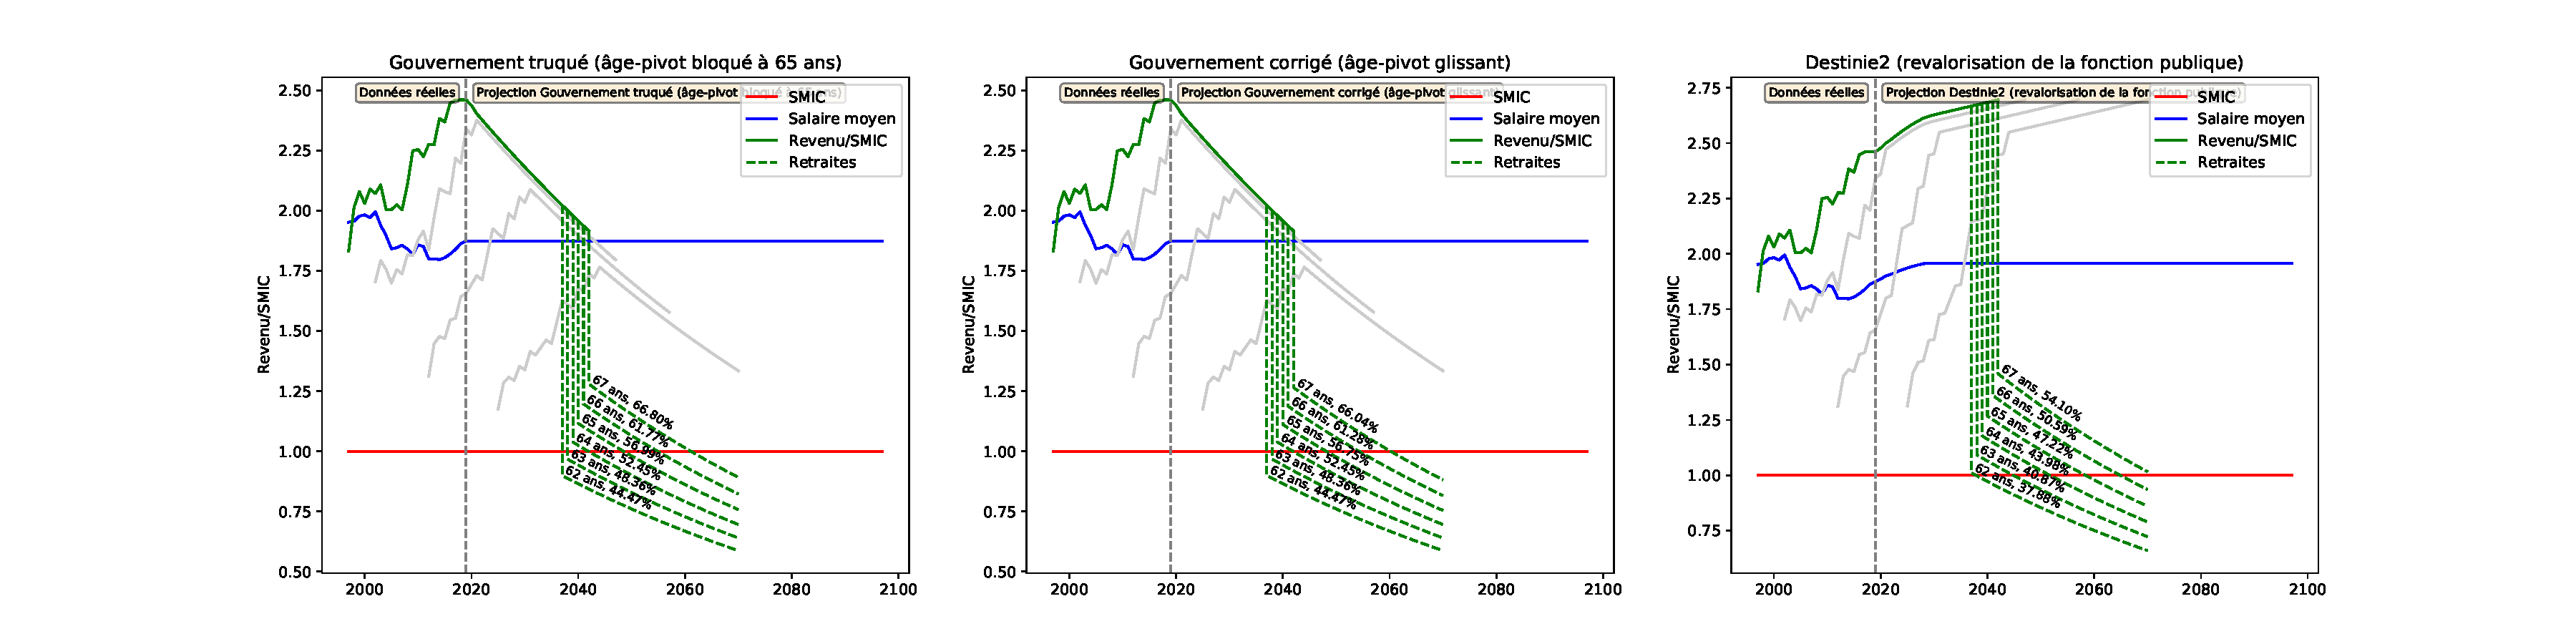
\includegraphics[width=0.9\textwidth]{fig/ProfCertifie_1975_22_dest_retraite.pdf}\end{center} \label{fig/ProfCertifie_1975_22_dest_retraite.pdf} 

\newpage 
 
\paragraph{Revenus et points pour le modèle \emph{Gouvernement truqué (âge-pivot bloqué à 65 ans)}} 
 
{ \scriptsize \begin{center} 
\begin{tabular}[htb]{|c|c||c|c|c|c|c|c||c|c||c|c|c|} 
\hline 
 Année &  Âge &  Ind Maj &  Pt Ind(\euro{} 2019) &  Rev HP(\euro{} 2019) &  Tx Primes &  GIPA(\euro{} 2019) &  Revenu(\euro{} 2019) &  SMIC(\euro{} 2019) &  Rev/SMIC &  Cumul Pts &  Achat Pt(\euro{} 2019) &  Serv. Pt(\euro{} 2019) \\ 
\hline \hline 
 1997 &  22 &  450.0 &  5.53 &  2490.46 &  0.00 &  0.00 &  2490.46 &  1358.84 &  {\bf 1.83} &  839.31 &  35.61 &  0.50 \\ 
\hline 
 1998 &  23 &  498.0 &  5.57 &  2772.09 &  0.00 &  0.00 &  2772.09 &  1376.36 &  {\bf 2.01} &  1773.54 &  35.61 &  0.50 \\ 
\hline 
 1999 &  24 &  513.0 &  5.61 &  2878.67 &  0.17 &  0.00 &  2883.57 &  1386.54 &  {\bf 2.08} &  2745.34 &  35.61 &  0.50 \\ 
\hline 
 2000 &  25 &  513.0 &  5.55 &  2844.68 &  0.40 &  0.00 &  2856.06 &  1407.00 &  {\bf 2.03} &  3707.87 &  35.61 &  0.50 \\ 
\hline 
 2001 &  26 &  542.0 &  5.52 &  2992.11 &  0.63 &  0.00 &  3010.96 &  1441.04 &  {\bf 2.09} &  4722.60 &  35.61 &  0.50 \\ 
\hline 
 2002 &  27 &  542.0 &  5.49 &  2973.56 &  0.86 &  0.00 &  2999.13 &  1447.74 &  {\bf 2.07} &  5733.34 &  35.61 &  0.50 \\ 
\hline 
 2003 &  28 &  579.0 &  5.37 &  3111.90 &  1.09 &  0.00 &  3145.82 &  1493.03 &  {\bf 2.11} &  6793.52 &  35.61 &  0.50 \\ 
\hline 
 2004 &  29 &  579.0 &  5.29 &  3062.75 &  1.32 &  0.00 &  3103.18 &  1547.32 &  {\bf 2.01} &  7839.33 &  35.61 &  0.50 \\ 
\hline 
 2005 &  30 &  598.5 &  5.29 &  3165.55 &  1.55 &  0.00 &  3214.62 &  1603.67 &  {\bf 2.00} &  8922.70 &  35.61 &  0.50 \\ 
\hline 
 2006 &  31 &  618.0 &  5.23 &  3232.21 &  1.78 &  0.00 &  3289.75 &  1625.00 &  {\bf 2.02} &  10031.38 &  35.61 &  0.50 \\ 
\hline 
 2007 &  32 &  618.0 &  5.19 &  3210.19 &  2.01 &  0.00 &  3274.72 &  1634.08 &  {\bf 2.00} &  11135.00 &  35.61 &  0.50 \\ 
\hline 
 2008 &  33 &  664.0 &  5.09 &  3381.78 &  2.24 &  0.00 &  3457.53 &  1640.24 &  {\bf 2.11} &  12300.23 &  35.61 &  0.50 \\ 
\hline 
 2009 &  34 &  710.0 &  5.13 &  3641.68 &  2.47 &  0.00 &  3731.63 &  1659.42 &  {\bf 2.25} &  13557.84 &  35.61 &  0.50 \\ 
\hline 
 2010 &  35 &  710.0 &  5.08 &  3604.90 &  2.70 &  0.00 &  3702.23 &  1641.90 &  {\bf 2.25} &  14805.54 &  35.61 &  0.50 \\ 
\hline 
 2011 &  36 &  710.0 &  4.97 &  3530.00 &  2.93 &  0.00 &  3633.43 &  1633.19 &  {\bf 2.22} &  16030.05 &  35.61 &  0.50 \\ 
\hline 
 2012 &  37 &  757.0 &  4.88 &  3691.46 &  3.16 &  0.00 &  3808.11 &  1673.05 &  {\bf 2.28} &  17313.43 &  35.61 &  0.50 \\ 
\hline 
 2013 &  38 &  757.0 &  4.83 &  3659.83 &  3.39 &  0.00 &  3783.90 &  1664.01 &  {\bf 2.27} &  18588.65 &  35.61 &  0.50 \\ 
\hline 
 2014 &  39 &  800.0 &  4.81 &  3848.36 &  3.62 &  0.00 &  3987.67 &  1673.24 &  {\bf 2.38} &  19932.54 &  35.61 &  0.50 \\ 
\hline 
 2015 &  40 &  800.0 &  4.81 &  3846.86 &  3.85 &  0.00 &  3994.96 &  1686.62 &  {\bf 2.37} &  21278.89 &  35.61 &  0.50 \\ 
\hline 
 2016 &  41 &  830.0 &  4.80 &  3983.15 &  4.08 &  0.00 &  4145.66 &  1693.76 &  {\bf 2.45} &  22676.03 &  35.61 &  0.50 \\ 
\hline 
 2017 &  42 &  830.0 &  4.81 &  3991.18 &  4.31 &  0.00 &  4163.20 &  1692.60 &  {\bf 2.46} &  24079.08 &  35.61 &  0.50 \\ 
\hline 
 2018 &  43 &  830.0 &  4.74 &  3936.07 &  4.54 &  43.46 &  4158.23 &  1689.76 &  {\bf 2.46} &  25480.45 &  35.61 &  0.50 \\ 
\hline 
 2019 &  44 &  830.0 &  4.79 &  3979.37 &  4.77 &  10.32 &  4179.50 &  1698.45 &  {\bf 2.46} &  26889.00 &  35.61 &  0.50 \\ 
\hline 
 2020 &  45 &  830.0 &  4.79 &  3979.37 &  5.00 &  15.22 &  4193.56 &  1720.53 &  {\bf 2.44} &  28302.28 &  35.61 &  0.50 \\ 
\hline 
 2021 &  46 &  830.0 &  4.79 &  3979.37 &  5.23 &  1.05 &  4188.54 &  1742.90 &  {\bf 2.40} &  29713.87 &  35.61 &  0.50 \\ 
\hline 
 2022 &  47 &  830.0 &  4.79 &  3979.37 &  5.46 &  0.00 &  4196.64 &  1765.55 &  {\bf 2.38} &  31128.19 &  35.61 &  0.50 \\ 
\hline 
 2023 &  48 &  830.0 &  4.79 &  3979.37 &  5.69 &  0.00 &  4205.80 &  1788.51 &  {\bf 2.35} &  32545.59 &  35.61 &  0.50 \\ 
\hline 
 2024 &  49 &  830.0 &  4.79 &  3979.37 &  5.92 &  0.00 &  4214.95 &  1811.76 &  {\bf 2.33} &  33966.08 &  35.61 &  0.50 \\ 
\hline 
 2025 &  50 &  830.0 &  4.79 &  3979.37 &  6.15 &  0.00 &  4224.10 &  1835.31 &  {\bf 2.30} &  35389.65 &  35.61 &  0.50 \\ 
\hline 
 2026 &  51 &  830.0 &  4.79 &  3979.37 &  6.38 &  0.00 &  4233.25 &  1859.17 &  {\bf 2.28} &  36816.31 &  35.61 &  0.50 \\ 
\hline 
 2027 &  52 &  830.0 &  4.79 &  3979.37 &  6.61 &  0.00 &  4242.41 &  1883.34 &  {\bf 2.25} &  38246.05 &  35.61 &  0.50 \\ 
\hline 
 2028 &  53 &  830.0 &  4.79 &  3979.37 &  6.84 &  0.00 &  4251.56 &  1907.82 &  {\bf 2.23} &  39678.88 &  35.61 &  0.50 \\ 
\hline 
 2029 &  54 &  830.0 &  4.79 &  3979.37 &  7.07 &  0.00 &  4260.71 &  1932.62 &  {\bf 2.20} &  41113.70 &  35.63 &  0.50 \\ 
\hline 
 2030 &  55 &  830.0 &  4.79 &  3979.37 &  7.30 &  0.00 &  4269.86 &  1957.75 &  {\bf 2.18} &  42549.42 &  35.69 &  0.50 \\ 
\hline 
 2031 &  56 &  830.0 &  4.79 &  3979.37 &  7.53 &  0.00 &  4279.02 &  1983.20 &  {\bf 2.16} &  43984.94 &  35.77 &  0.50 \\ 
\hline 
 2032 &  57 &  830.0 &  4.79 &  3979.37 &  7.76 &  0.00 &  4288.17 &  2008.98 &  {\bf 2.13} &  45419.17 &  35.88 &  0.50 \\ 
\hline 
 2033 &  58 &  830.0 &  4.79 &  3979.37 &  7.99 &  0.00 &  4297.32 &  2035.10 &  {\bf 2.11} &  46851.01 &  36.02 &  0.50 \\ 
\hline 
 2034 &  59 &  830.0 &  4.79 &  3979.37 &  8.22 &  0.00 &  4306.47 &  2061.55 &  {\bf 2.09} &  48279.37 &  36.18 &  0.50 \\ 
\hline 
 2035 &  60 &  830.0 &  4.79 &  3979.37 &  8.45 &  0.00 &  4315.63 &  2088.35 &  {\bf 2.07} &  49703.18 &  36.37 &  0.51 \\ 
\hline 
 2036 &  61 &  830.0 &  4.79 &  3979.37 &  8.68 &  0.00 &  4324.78 &  2115.50 &  {\bf 2.04} &  51121.35 &  36.59 &  0.51 \\ 
\hline 
 2037 &  62 &  830.0 &  4.79 &  3979.37 &  8.91 &  0.00 &  4333.93 &  2143.00 &  {\bf 2.02} &  52532.85 &  36.85 &  0.51 \\ 
\hline 
 2038 &  63 &  830.0 &  4.79 &  3979.37 &  9.14 &  0.00 &  4343.08 &  2170.86 &  {\bf 2.00} &  53936.62 &  37.13 &  0.52 \\ 
\hline 
 2039 &  64 &  830.0 &  4.79 &  3979.37 &  9.37 &  0.00 &  4352.24 &  2199.08 &  {\bf 1.98} &  55331.64 &  37.44 &  0.52 \\ 
\hline 
 2040 &  65 &  830.0 &  4.79 &  3979.37 &  9.60 &  0.00 &  4361.39 &  2227.67 &  {\bf 1.96} &  56716.90 &  37.78 &  0.53 \\ 
\hline 
 2041 &  66 &  830.0 &  4.79 &  3979.37 &  9.83 &  0.00 &  4370.54 &  2256.63 &  {\bf 1.94} &  58091.43 &  38.16 &  0.53 \\ 
\hline 
 2042 &  67 &  830.0 &  4.79 &  3979.37 &  10.06 &  0.00 &  4379.70 &  2285.97 &  {\bf 1.92} &  59454.27 &  38.56 &  0.54 \\ 
\hline 
\hline 
\end{tabular} 
\end{center} } 
\newpage 
 
\paragraph{Revenus et points pour le modèle \emph{Gouvernement corrigé (âge-pivot glissant)}} 
 
{ \scriptsize \begin{center} 
\begin{tabular}[htb]{|c|c||c|c|c|c|c|c||c|c||c|c|c|} 
\hline 
 Année &  Âge &  Ind Maj &  Pt Ind(\euro{} 2019) &  Rev HP(\euro{} 2019) &  Tx Primes &  GIPA(\euro{} 2019) &  Revenu(\euro{} 2019) &  SMIC(\euro{} 2019) &  Rev/SMIC &  Cumul Pts &  Achat Pt(\euro{} 2019) &  Serv. Pt(\euro{} 2019) \\ 
\hline \hline 
 1997 &  22 &  450.0 &  5.53 &  2490.46 &  0.00 &  0.00 &  2490.46 &  1358.84 &  {\bf 1.83} &  839.31 &  35.61 &  0.50 \\ 
\hline 
 1998 &  23 &  498.0 &  5.57 &  2772.09 &  0.00 &  0.00 &  2772.09 &  1376.36 &  {\bf 2.01} &  1773.54 &  35.61 &  0.50 \\ 
\hline 
 1999 &  24 &  513.0 &  5.61 &  2878.67 &  0.17 &  0.00 &  2883.57 &  1386.54 &  {\bf 2.08} &  2745.34 &  35.61 &  0.50 \\ 
\hline 
 2000 &  25 &  513.0 &  5.55 &  2844.68 &  0.40 &  0.00 &  2856.06 &  1407.00 &  {\bf 2.03} &  3707.87 &  35.61 &  0.50 \\ 
\hline 
 2001 &  26 &  542.0 &  5.52 &  2992.11 &  0.63 &  0.00 &  3010.96 &  1441.04 &  {\bf 2.09} &  4722.60 &  35.61 &  0.50 \\ 
\hline 
 2002 &  27 &  542.0 &  5.49 &  2973.56 &  0.86 &  0.00 &  2999.13 &  1447.74 &  {\bf 2.07} &  5733.34 &  35.61 &  0.50 \\ 
\hline 
 2003 &  28 &  579.0 &  5.37 &  3111.90 &  1.09 &  0.00 &  3145.82 &  1493.03 &  {\bf 2.11} &  6793.52 &  35.61 &  0.50 \\ 
\hline 
 2004 &  29 &  579.0 &  5.29 &  3062.75 &  1.32 &  0.00 &  3103.18 &  1547.32 &  {\bf 2.01} &  7839.33 &  35.61 &  0.50 \\ 
\hline 
 2005 &  30 &  598.5 &  5.29 &  3165.55 &  1.55 &  0.00 &  3214.62 &  1603.67 &  {\bf 2.00} &  8922.70 &  35.61 &  0.50 \\ 
\hline 
 2006 &  31 &  618.0 &  5.23 &  3232.21 &  1.78 &  0.00 &  3289.75 &  1625.00 &  {\bf 2.02} &  10031.38 &  35.61 &  0.50 \\ 
\hline 
 2007 &  32 &  618.0 &  5.19 &  3210.19 &  2.01 &  0.00 &  3274.72 &  1634.08 &  {\bf 2.00} &  11135.00 &  35.61 &  0.50 \\ 
\hline 
 2008 &  33 &  664.0 &  5.09 &  3381.78 &  2.24 &  0.00 &  3457.53 &  1640.24 &  {\bf 2.11} &  12300.23 &  35.61 &  0.50 \\ 
\hline 
 2009 &  34 &  710.0 &  5.13 &  3641.68 &  2.47 &  0.00 &  3731.63 &  1659.42 &  {\bf 2.25} &  13557.84 &  35.61 &  0.50 \\ 
\hline 
 2010 &  35 &  710.0 &  5.08 &  3604.90 &  2.70 &  0.00 &  3702.23 &  1641.90 &  {\bf 2.25} &  14805.54 &  35.61 &  0.50 \\ 
\hline 
 2011 &  36 &  710.0 &  4.97 &  3530.00 &  2.93 &  0.00 &  3633.43 &  1633.19 &  {\bf 2.22} &  16030.05 &  35.61 &  0.50 \\ 
\hline 
 2012 &  37 &  757.0 &  4.88 &  3691.46 &  3.16 &  0.00 &  3808.11 &  1673.05 &  {\bf 2.28} &  17313.43 &  35.61 &  0.50 \\ 
\hline 
 2013 &  38 &  757.0 &  4.83 &  3659.83 &  3.39 &  0.00 &  3783.90 &  1664.01 &  {\bf 2.27} &  18588.65 &  35.61 &  0.50 \\ 
\hline 
 2014 &  39 &  800.0 &  4.81 &  3848.36 &  3.62 &  0.00 &  3987.67 &  1673.24 &  {\bf 2.38} &  19932.54 &  35.61 &  0.50 \\ 
\hline 
 2015 &  40 &  800.0 &  4.81 &  3846.86 &  3.85 &  0.00 &  3994.96 &  1686.62 &  {\bf 2.37} &  21278.89 &  35.61 &  0.50 \\ 
\hline 
 2016 &  41 &  830.0 &  4.80 &  3983.15 &  4.08 &  0.00 &  4145.66 &  1693.76 &  {\bf 2.45} &  22676.03 &  35.61 &  0.50 \\ 
\hline 
 2017 &  42 &  830.0 &  4.81 &  3991.18 &  4.31 &  0.00 &  4163.20 &  1692.60 &  {\bf 2.46} &  24079.08 &  35.61 &  0.50 \\ 
\hline 
 2018 &  43 &  830.0 &  4.74 &  3936.07 &  4.54 &  43.46 &  4158.23 &  1689.76 &  {\bf 2.46} &  25480.45 &  35.61 &  0.50 \\ 
\hline 
 2019 &  44 &  830.0 &  4.79 &  3979.37 &  4.77 &  10.32 &  4179.50 &  1698.45 &  {\bf 2.46} &  26889.00 &  35.61 &  0.50 \\ 
\hline 
 2020 &  45 &  830.0 &  4.79 &  3979.37 &  5.00 &  15.22 &  4193.56 &  1720.53 &  {\bf 2.44} &  28302.28 &  35.61 &  0.50 \\ 
\hline 
 2021 &  46 &  830.0 &  4.79 &  3979.37 &  5.23 &  1.05 &  4188.54 &  1742.90 &  {\bf 2.40} &  29713.87 &  35.61 &  0.50 \\ 
\hline 
 2022 &  47 &  830.0 &  4.79 &  3979.37 &  5.46 &  0.00 &  4196.64 &  1765.55 &  {\bf 2.38} &  31128.19 &  35.61 &  0.50 \\ 
\hline 
 2023 &  48 &  830.0 &  4.79 &  3979.37 &  5.69 &  0.00 &  4205.80 &  1788.51 &  {\bf 2.35} &  32545.59 &  35.61 &  0.50 \\ 
\hline 
 2024 &  49 &  830.0 &  4.79 &  3979.37 &  5.92 &  0.00 &  4214.95 &  1811.76 &  {\bf 2.33} &  33966.08 &  35.61 &  0.50 \\ 
\hline 
 2025 &  50 &  830.0 &  4.79 &  3979.37 &  6.15 &  0.00 &  4224.10 &  1835.31 &  {\bf 2.30} &  35389.65 &  35.61 &  0.50 \\ 
\hline 
 2026 &  51 &  830.0 &  4.79 &  3979.37 &  6.38 &  0.00 &  4233.25 &  1859.17 &  {\bf 2.28} &  36816.31 &  35.61 &  0.50 \\ 
\hline 
 2027 &  52 &  830.0 &  4.79 &  3979.37 &  6.61 &  0.00 &  4242.41 &  1883.34 &  {\bf 2.25} &  38246.05 &  35.61 &  0.50 \\ 
\hline 
 2028 &  53 &  830.0 &  4.79 &  3979.37 &  6.84 &  0.00 &  4251.56 &  1907.82 &  {\bf 2.23} &  39678.88 &  35.61 &  0.50 \\ 
\hline 
 2029 &  54 &  830.0 &  4.79 &  3979.37 &  7.07 &  0.00 &  4260.71 &  1932.62 &  {\bf 2.20} &  41113.70 &  35.63 &  0.50 \\ 
\hline 
 2030 &  55 &  830.0 &  4.79 &  3979.37 &  7.30 &  0.00 &  4269.86 &  1957.75 &  {\bf 2.18} &  42549.42 &  35.69 &  0.50 \\ 
\hline 
 2031 &  56 &  830.0 &  4.79 &  3979.37 &  7.53 &  0.00 &  4279.02 &  1983.20 &  {\bf 2.16} &  43984.94 &  35.77 &  0.50 \\ 
\hline 
 2032 &  57 &  830.0 &  4.79 &  3979.37 &  7.76 &  0.00 &  4288.17 &  2008.98 &  {\bf 2.13} &  45419.17 &  35.88 &  0.50 \\ 
\hline 
 2033 &  58 &  830.0 &  4.79 &  3979.37 &  7.99 &  0.00 &  4297.32 &  2035.10 &  {\bf 2.11} &  46851.01 &  36.02 &  0.50 \\ 
\hline 
 2034 &  59 &  830.0 &  4.79 &  3979.37 &  8.22 &  0.00 &  4306.47 &  2061.55 &  {\bf 2.09} &  48279.37 &  36.18 &  0.50 \\ 
\hline 
 2035 &  60 &  830.0 &  4.79 &  3979.37 &  8.45 &  0.00 &  4315.63 &  2088.35 &  {\bf 2.07} &  49703.18 &  36.37 &  0.51 \\ 
\hline 
 2036 &  61 &  830.0 &  4.79 &  3979.37 &  8.68 &  0.00 &  4324.78 &  2115.50 &  {\bf 2.04} &  51121.35 &  36.59 &  0.51 \\ 
\hline 
 2037 &  62 &  830.0 &  4.79 &  3979.37 &  8.91 &  0.00 &  4333.93 &  2143.00 &  {\bf 2.02} &  52532.85 &  36.85 &  0.51 \\ 
\hline 
 2038 &  63 &  830.0 &  4.79 &  3979.37 &  9.14 &  0.00 &  4343.08 &  2170.86 &  {\bf 2.00} &  53936.62 &  37.13 &  0.52 \\ 
\hline 
 2039 &  64 &  830.0 &  4.79 &  3979.37 &  9.37 &  0.00 &  4352.24 &  2199.08 &  {\bf 1.98} &  55331.64 &  37.44 &  0.52 \\ 
\hline 
 2040 &  65 &  830.0 &  4.79 &  3979.37 &  9.60 &  0.00 &  4361.39 &  2227.67 &  {\bf 1.96} &  56716.90 &  37.78 &  0.53 \\ 
\hline 
 2041 &  66 &  830.0 &  4.79 &  3979.37 &  9.83 &  0.00 &  4370.54 &  2256.63 &  {\bf 1.94} &  58091.43 &  38.16 &  0.53 \\ 
\hline 
 2042 &  67 &  830.0 &  4.79 &  3979.37 &  10.06 &  0.00 &  4379.70 &  2285.97 &  {\bf 1.92} &  59454.27 &  38.56 &  0.54 \\ 
\hline 
\hline 
\end{tabular} 
\end{center} } 
\newpage 
 
\paragraph{Revenus et points pour le modèle \emph{Destinie2 (revalorisation de la fonction publique)}} 
 
{ \scriptsize \begin{center} 
\begin{tabular}[htb]{|c|c||c|c|c|c|c|c||c|c||c|c|c|} 
\hline 
 Année &  Âge &  Ind Maj &  Pt Ind(\euro{} 2019) &  Rev HP(\euro{} 2019) &  Tx Primes &  GIPA(\euro{} 2019) &  Revenu(\euro{} 2019) &  SMIC(\euro{} 2019) &  Rev/SMIC &  Cumul Pts &  Achat Pt(\euro{} 2019) &  Serv. Pt(\euro{} 2019) \\ 
\hline \hline 
 1997 &  22 &  450.0 &  5.53 &  2490.46 &  0.00 &  0.00 &  2490.46 &  1358.84 &  {\bf 1.83} &  837.25 &  35.69 &  0.50 \\ 
\hline 
 1998 &  23 &  498.0 &  5.57 &  2772.09 &  0.00 &  0.00 &  2772.09 &  1376.36 &  {\bf 2.01} &  1769.19 &  35.69 &  0.50 \\ 
\hline 
 1999 &  24 &  513.0 &  5.61 &  2878.67 &  0.17 &  0.00 &  2883.57 &  1386.54 &  {\bf 2.08} &  2738.60 &  35.69 &  0.50 \\ 
\hline 
 2000 &  25 &  513.0 &  5.55 &  2844.68 &  0.40 &  0.00 &  2856.06 &  1407.00 &  {\bf 2.03} &  3698.76 &  35.69 &  0.50 \\ 
\hline 
 2001 &  26 &  542.0 &  5.52 &  2992.11 &  0.63 &  0.00 &  3010.96 &  1441.04 &  {\bf 2.09} &  4711.00 &  35.69 &  0.50 \\ 
\hline 
 2002 &  27 &  542.0 &  5.49 &  2973.56 &  0.86 &  0.00 &  2999.13 &  1447.74 &  {\bf 2.07} &  5719.26 &  35.69 &  0.50 \\ 
\hline 
 2003 &  28 &  579.0 &  5.37 &  3111.90 &  1.09 &  0.00 &  3145.82 &  1493.03 &  {\bf 2.11} &  6776.83 &  35.69 &  0.50 \\ 
\hline 
 2004 &  29 &  579.0 &  5.29 &  3062.75 &  1.32 &  0.00 &  3103.18 &  1547.32 &  {\bf 2.01} &  7820.07 &  35.69 &  0.50 \\ 
\hline 
 2005 &  30 &  598.5 &  5.29 &  3165.55 &  1.55 &  0.00 &  3214.62 &  1603.67 &  {\bf 2.00} &  8900.78 &  35.69 &  0.50 \\ 
\hline 
 2006 &  31 &  618.0 &  5.23 &  3232.21 &  1.78 &  0.00 &  3289.75 &  1625.00 &  {\bf 2.02} &  10006.74 &  35.69 &  0.50 \\ 
\hline 
 2007 &  32 &  618.0 &  5.19 &  3210.19 &  2.01 &  0.00 &  3274.72 &  1634.08 &  {\bf 2.00} &  11107.64 &  35.69 &  0.50 \\ 
\hline 
 2008 &  33 &  664.0 &  5.09 &  3381.78 &  2.24 &  0.00 &  3457.53 &  1640.24 &  {\bf 2.11} &  12270.01 &  35.69 &  0.50 \\ 
\hline 
 2009 &  34 &  710.0 &  5.13 &  3641.68 &  2.47 &  0.00 &  3731.63 &  1659.42 &  {\bf 2.25} &  13524.53 &  35.69 &  0.50 \\ 
\hline 
 2010 &  35 &  710.0 &  5.08 &  3604.90 &  2.70 &  0.00 &  3702.23 &  1641.90 &  {\bf 2.25} &  14769.16 &  35.69 &  0.50 \\ 
\hline 
 2011 &  36 &  710.0 &  4.97 &  3530.00 &  2.93 &  0.00 &  3633.43 &  1633.19 &  {\bf 2.22} &  15990.66 &  35.69 &  0.50 \\ 
\hline 
 2012 &  37 &  757.0 &  4.88 &  3691.46 &  3.16 &  0.00 &  3808.11 &  1673.05 &  {\bf 2.28} &  17270.89 &  35.69 &  0.50 \\ 
\hline 
 2013 &  38 &  757.0 &  4.83 &  3659.83 &  3.39 &  0.00 &  3783.90 &  1664.01 &  {\bf 2.27} &  18542.97 &  35.69 &  0.50 \\ 
\hline 
 2014 &  39 &  800.0 &  4.81 &  3848.36 &  3.62 &  0.00 &  3987.67 &  1673.24 &  {\bf 2.38} &  19883.57 &  35.69 &  0.50 \\ 
\hline 
 2015 &  40 &  800.0 &  4.81 &  3846.86 &  3.85 &  0.00 &  3994.96 &  1686.62 &  {\bf 2.37} &  21226.61 &  35.69 &  0.50 \\ 
\hline 
 2016 &  41 &  830.0 &  4.80 &  3983.15 &  4.08 &  0.00 &  4145.66 &  1693.76 &  {\bf 2.45} &  22620.31 &  35.69 &  0.50 \\ 
\hline 
 2017 &  42 &  830.0 &  4.81 &  3991.18 &  4.31 &  0.00 &  4163.20 &  1692.60 &  {\bf 2.46} &  24019.91 &  35.69 &  0.50 \\ 
\hline 
 2018 &  43 &  830.0 &  4.74 &  3936.07 &  4.54 &  43.46 &  4158.23 &  1689.76 &  {\bf 2.46} &  25417.85 &  35.69 &  0.50 \\ 
\hline 
 2019 &  44 &  830.0 &  4.79 &  3979.37 &  4.77 &  10.32 &  4179.50 &  1698.45 &  {\bf 2.46} &  26822.93 &  35.69 &  0.50 \\ 
\hline 
 2020 &  45 &  830.0 &  4.83 &  4011.21 &  5.00 &  0.00 &  4211.77 &  1699.99 &  {\bf 2.48} &  28238.86 &  35.69 &  0.50 \\ 
\hline 
 2021 &  46 &  830.0 &  4.88 &  4047.31 &  5.23 &  0.00 &  4258.98 &  1703.48 &  {\bf 2.50} &  29670.66 &  35.69 &  0.50 \\ 
\hline 
 2022 &  47 &  830.0 &  4.93 &  4087.78 &  5.46 &  0.00 &  4310.97 &  1712.78 &  {\bf 2.52} &  31119.94 &  35.69 &  0.50 \\ 
\hline 
 2023 &  48 &  830.0 &  4.98 &  4135.61 &  5.69 &  0.00 &  4370.92 &  1723.51 &  {\bf 2.54} &  32589.37 &  35.69 &  0.50 \\ 
\hline 
 2024 &  49 &  830.0 &  5.04 &  4184.82 &  5.92 &  0.00 &  4432.56 &  1735.69 &  {\bf 2.55} &  34079.53 &  35.69 &  0.50 \\ 
\hline 
 2025 &  50 &  830.0 &  5.10 &  4235.87 &  6.15 &  0.00 &  4496.38 &  1749.35 &  {\bf 2.57} &  35591.14 &  35.69 &  0.50 \\ 
\hline 
 2026 &  51 &  830.0 &  5.17 &  4288.82 &  6.38 &  0.00 &  4562.45 &  1764.53 &  {\bf 2.59} &  37124.97 &  35.69 &  0.50 \\ 
\hline 
 2027 &  52 &  830.0 &  5.23 &  4343.72 &  6.61 &  0.00 &  4630.84 &  1781.27 &  {\bf 2.60} &  38681.78 &  35.69 &  0.50 \\ 
\hline 
 2028 &  53 &  830.0 &  5.30 &  4400.62 &  6.84 &  0.00 &  4701.63 &  1799.59 &  {\bf 2.61} &  40262.39 &  35.69 &  0.50 \\ 
\hline 
 2029 &  54 &  830.0 &  5.37 &  4453.87 &  7.07 &  0.00 &  4768.76 &  1819.55 &  {\bf 2.62} &  41864.44 &  35.72 &  0.50 \\ 
\hline 
 2030 &  55 &  830.0 &  5.43 &  4509.10 &  7.30 &  0.00 &  4838.26 &  1841.19 &  {\bf 2.63} &  43487.48 &  35.77 &  0.50 \\ 
\hline 
 2031 &  56 &  830.0 &  5.50 &  4566.36 &  7.53 &  0.00 &  4910.21 &  1864.58 &  {\bf 2.63} &  45131.00 &  35.85 &  0.50 \\ 
\hline 
 2032 &  57 &  830.0 &  5.57 &  4625.73 &  7.76 &  0.00 &  4984.68 &  1888.81 &  {\bf 2.64} &  46794.37 &  35.96 &  0.50 \\ 
\hline 
 2033 &  58 &  830.0 &  5.65 &  4685.86 &  7.99 &  0.00 &  5060.26 &  1913.37 &  {\bf 2.64} &  48476.57 &  36.10 &  0.50 \\ 
\hline 
 2034 &  59 &  830.0 &  5.72 &  4746.78 &  8.22 &  0.00 &  5136.96 &  1938.24 &  {\bf 2.65} &  50176.49 &  36.26 &  0.50 \\ 
\hline 
 2035 &  60 &  830.0 &  5.79 &  4808.49 &  8.45 &  0.00 &  5214.80 &  1963.44 &  {\bf 2.66} &  51893.02 &  36.46 &  0.51 \\ 
\hline 
 2036 &  61 &  830.0 &  5.87 &  4871.00 &  8.68 &  0.00 &  5293.80 &  1988.96 &  {\bf 2.66} &  53625.00 &  36.68 &  0.51 \\ 
\hline 
 2037 &  62 &  830.0 &  5.94 &  4934.32 &  8.91 &  0.00 &  5373.97 &  2014.82 &  {\bf 2.67} &  55371.22 &  36.93 &  0.51 \\ 
\hline 
 2038 &  63 &  830.0 &  6.02 &  4998.46 &  9.14 &  0.00 &  5455.32 &  2041.01 &  {\bf 2.67} &  57130.46 &  37.21 &  0.52 \\ 
\hline 
 2039 &  64 &  830.0 &  6.10 &  5063.44 &  9.37 &  0.00 &  5537.89 &  2067.55 &  {\bf 2.68} &  58901.46 &  37.52 &  0.52 \\ 
\hline 
 2040 &  65 &  830.0 &  6.18 &  5129.27 &  9.60 &  0.00 &  5621.68 &  2094.43 &  {\bf 2.68} &  60682.95 &  37.87 &  0.53 \\ 
\hline 
 2041 &  66 &  830.0 &  6.26 &  5195.95 &  9.83 &  0.00 &  5706.71 &  2121.65 &  {\bf 2.69} &  62473.60 &  38.24 &  0.53 \\ 
\hline 
 2042 &  67 &  830.0 &  6.34 &  5263.50 &  10.06 &  0.00 &  5793.01 &  2149.23 &  {\bf 2.70} &  64272.10 &  38.65 &  0.54 \\ 
\hline 
\hline 
\end{tabular} 
\end{center} } 
\newpage 
 
\subsection{Génération 1980 (début en 2002)} 

\paragraph{Retraites possibles dans le modèle \emph{Gouvernement truqué (âge-pivot bloqué à 65 ans)}}  
 
{ \scriptsize \begin{center} 
\begin{tabular}[htb]{|c|c||c|c||c|c||c||c|c|c|c|c|c|} 
\hline 
 Retraite en &  Âge &  Âge pivot &  Décote/Surcote &  Retraite (\euro{} 2019) &  Tx Rempl(\%) &  SMIC (\euro{} 2019) &  Retraite/SMIC &  Rev70/SMIC &  Rev75/SMIC &  Rev80/SMIC &  Rev85/SMIC &  Rev90/SMIC \\ 
\hline \hline 
 2042 &  62 &  65 ans 0 mois &  -15.00\% &  1950.60 &  {\bf 45.01} &  2285.97 &  {\bf {\color{red} 0.85}} &  {\bf {\color{red} 0.77}} &  {\bf {\color{red} 0.72}} &  {\bf {\color{red} 0.68}} &  {\bf {\color{red} 0.63}} &  {\bf {\color{red} 0.59}} \\ 
\hline 
 2043 &  63 &  65 ans 0 mois &  -10.00\% &  2143.43 &  {\bf 49.35} &  2315.68 &  {\bf {\color{red} 0.93}} &  {\bf {\color{red} 0.85}} &  {\bf {\color{red} 0.79}} &  {\bf {\color{red} 0.74}} &  {\bf {\color{red} 0.70}} &  {\bf {\color{red} 0.65}} \\ 
\hline 
 2044 &  64 &  65 ans 0 mois &  -5.00\% &  2347.73 &  {\bf 53.94} &  2345.79 &  {\bf 1.00} &  {\bf {\color{red} 0.93}} &  {\bf {\color{red} 0.87}} &  {\bf {\color{red} 0.81}} &  {\bf {\color{red} 0.76}} &  {\bf {\color{red} 0.72}} \\ 
\hline 
 2045 &  65 &  65 ans 0 mois &  0.00\% &  2564.13 &  {\bf 58.79} &  2376.28 &  {\bf 1.08} &  {\bf 1.01} &  {\bf {\color{red} 0.95}} &  {\bf {\color{red} 0.89}} &  {\bf {\color{red} 0.83}} &  {\bf {\color{red} 0.78}} \\ 
\hline 
 2046 &  66 &  65 ans 0 mois &  5.00\% &  2791.21 &  {\bf 63.86} &  2407.18 &  {\bf 1.16} &  {\bf 1.10} &  {\bf 1.03} &  {\bf {\color{red} 0.97}} &  {\bf {\color{red} 0.91}} &  {\bf {\color{red} 0.85}} \\ 
\hline 
 2047 &  67 &  65 ans 0 mois &  10.00\% &  3029.20 &  {\bf 69.16} &  2438.47 &  {\bf 1.24} &  {\bf 1.20} &  {\bf 1.12} &  {\bf 1.05} &  {\bf {\color{red} 0.98}} &  {\bf {\color{red} 0.92}} \\ 
\hline 
\hline 
\end{tabular} 
\end{center} } 
\paragraph{Retraites possibles dans le modèle \emph{Gouvernement corrigé (âge-pivot glissant)}}  
 
{ \scriptsize \begin{center} 
\begin{tabular}[htb]{|c|c||c|c||c|c||c||c|c|c|c|c|c|} 
\hline 
 Retraite en &  Âge &  Âge pivot &  Décote/Surcote &  Retraite (\euro{} 2019) &  Tx Rempl(\%) &  SMIC (\euro{} 2019) &  Retraite/SMIC &  Rev70/SMIC &  Rev75/SMIC &  Rev80/SMIC &  Rev85/SMIC &  Rev90/SMIC \\ 
\hline \hline 
 2042 &  62 &  65 ans 3 mois &  -16.25\% &  1921.92 &  {\bf 44.35} &  2285.97 &  {\bf {\color{red} 0.84}} &  {\bf {\color{red} 0.76}} &  {\bf {\color{red} 0.71}} &  {\bf {\color{red} 0.67}} &  {\bf {\color{red} 0.62}} &  {\bf {\color{red} 0.59}} \\ 
\hline 
 2043 &  63 &  65 ans 4 mois &  -11.67\% &  2103.73 &  {\bf 48.44} &  2315.68 &  {\bf {\color{red} 0.91}} &  {\bf {\color{red} 0.83}} &  {\bf {\color{red} 0.78}} &  {\bf {\color{red} 0.73}} &  {\bf {\color{red} 0.68}} &  {\bf {\color{red} 0.64}} \\ 
\hline 
 2044 &  64 &  65 ans 5 mois &  -7.08\% &  2296.24 &  {\bf 52.76} &  2345.79 &  {\bf {\color{red} 0.98}} &  {\bf {\color{red} 0.91}} &  {\bf {\color{red} 0.85}} &  {\bf {\color{red} 0.80}} &  {\bf {\color{red} 0.75}} &  {\bf {\color{red} 0.70}} \\ 
\hline 
 2045 &  65 &  65 ans 6 mois &  -2.50\% &  2500.02 &  {\bf 57.32} &  2376.28 &  {\bf 1.05} &  {\bf {\color{red} 0.99}} &  {\bf {\color{red} 0.92}} &  {\bf {\color{red} 0.87}} &  {\bf {\color{red} 0.81}} &  {\bf {\color{red} 0.76}} \\ 
\hline 
 2046 &  66 &  65 ans 7 mois &  2.08\% &  2713.68 &  {\bf 62.09} &  2407.18 &  {\bf 1.13} &  {\bf 1.07} &  {\bf 1.00} &  {\bf {\color{red} 0.94}} &  {\bf {\color{red} 0.88}} &  {\bf {\color{red} 0.83}} \\ 
\hline 
 2047 &  67 &  65 ans 8 mois &  6.67\% &  2937.40 &  {\bf 67.07} &  2438.47 &  {\bf 1.20} &  {\bf 1.16} &  {\bf 1.09} &  {\bf 1.02} &  {\bf {\color{red} 0.95}} &  {\bf {\color{red} 0.90}} \\ 
\hline 
\hline 
\end{tabular} 
\end{center} } 
\paragraph{Retraites possibles dans le modèle \emph{Destinie2 (revalorisation de la fonction publique)}}  
 
{ \scriptsize \begin{center} 
\begin{tabular}[htb]{|c|c||c|c||c|c||c||c|c|c|c|c|c|} 
\hline 
 Retraite en &  Âge &  Âge pivot &  Décote/Surcote &  Retraite (\euro{} 2019) &  Tx Rempl(\%) &  SMIC (\euro{} 2019) &  Retraite/SMIC &  Rev70/SMIC &  Rev75/SMIC &  Rev80/SMIC &  Rev85/SMIC &  Rev90/SMIC \\ 
\hline \hline 
 2042 &  62 &  65 ans 3 mois &  -16.25\% &  2106.19 &  {\bf 36.74} &  2149.23 &  {\bf {\color{red} 0.98}} &  {\bf {\color{red} 0.88}} &  {\bf {\color{red} 0.83}} &  {\bf {\color{red} 0.78}} &  {\bf {\color{red} 0.73}} &  {\bf {\color{red} 0.68}} \\ 
\hline 
 2043 &  63 &  65 ans 4 mois &  -11.67\% &  2318.46 &  {\bf 39.84} &  2177.17 &  {\bf 1.06} &  {\bf {\color{red} 0.97}} &  {\bf {\color{red} 0.91}} &  {\bf {\color{red} 0.85}} &  {\bf {\color{red} 0.80}} &  {\bf {\color{red} 0.75}} \\ 
\hline 
 2044 &  64 &  65 ans 5 mois &  -7.08\% &  2544.99 &  {\bf 43.08} &  2205.48 &  {\bf 1.15} &  {\bf 1.07} &  {\bf 1.00} &  {\bf {\color{red} 0.94}} &  {\bf {\color{red} 0.88}} &  {\bf {\color{red} 0.82}} \\ 
\hline 
 2045 &  65 &  65 ans 6 mois &  -2.50\% &  2786.63 &  {\bf 46.47} &  2234.15 &  {\bf 1.25} &  {\bf 1.17} &  {\bf 1.10} &  {\bf 1.03} &  {\bf {\color{red} 0.96}} &  {\bf {\color{red} 0.90}} \\ 
\hline 
 2046 &  66 &  65 ans 7 mois &  2.08\% &  3042.05 &  {\bf 49.97} &  2263.19 &  {\bf 1.34} &  {\bf 1.28} &  {\bf 1.20} &  {\bf 1.12} &  {\bf 1.05} &  {\bf {\color{red} 0.99}} \\ 
\hline 
 2047 &  67 &  65 ans 8 mois &  6.67\% &  3311.70 &  {\bf 53.59} &  2292.61 &  {\bf 1.44} &  {\bf 1.39} &  {\bf 1.30} &  {\bf 1.22} &  {\bf 1.14} &  {\bf 1.07} \\ 
\hline 
\hline 
\end{tabular} 
\end{center} } 

 \begin{center}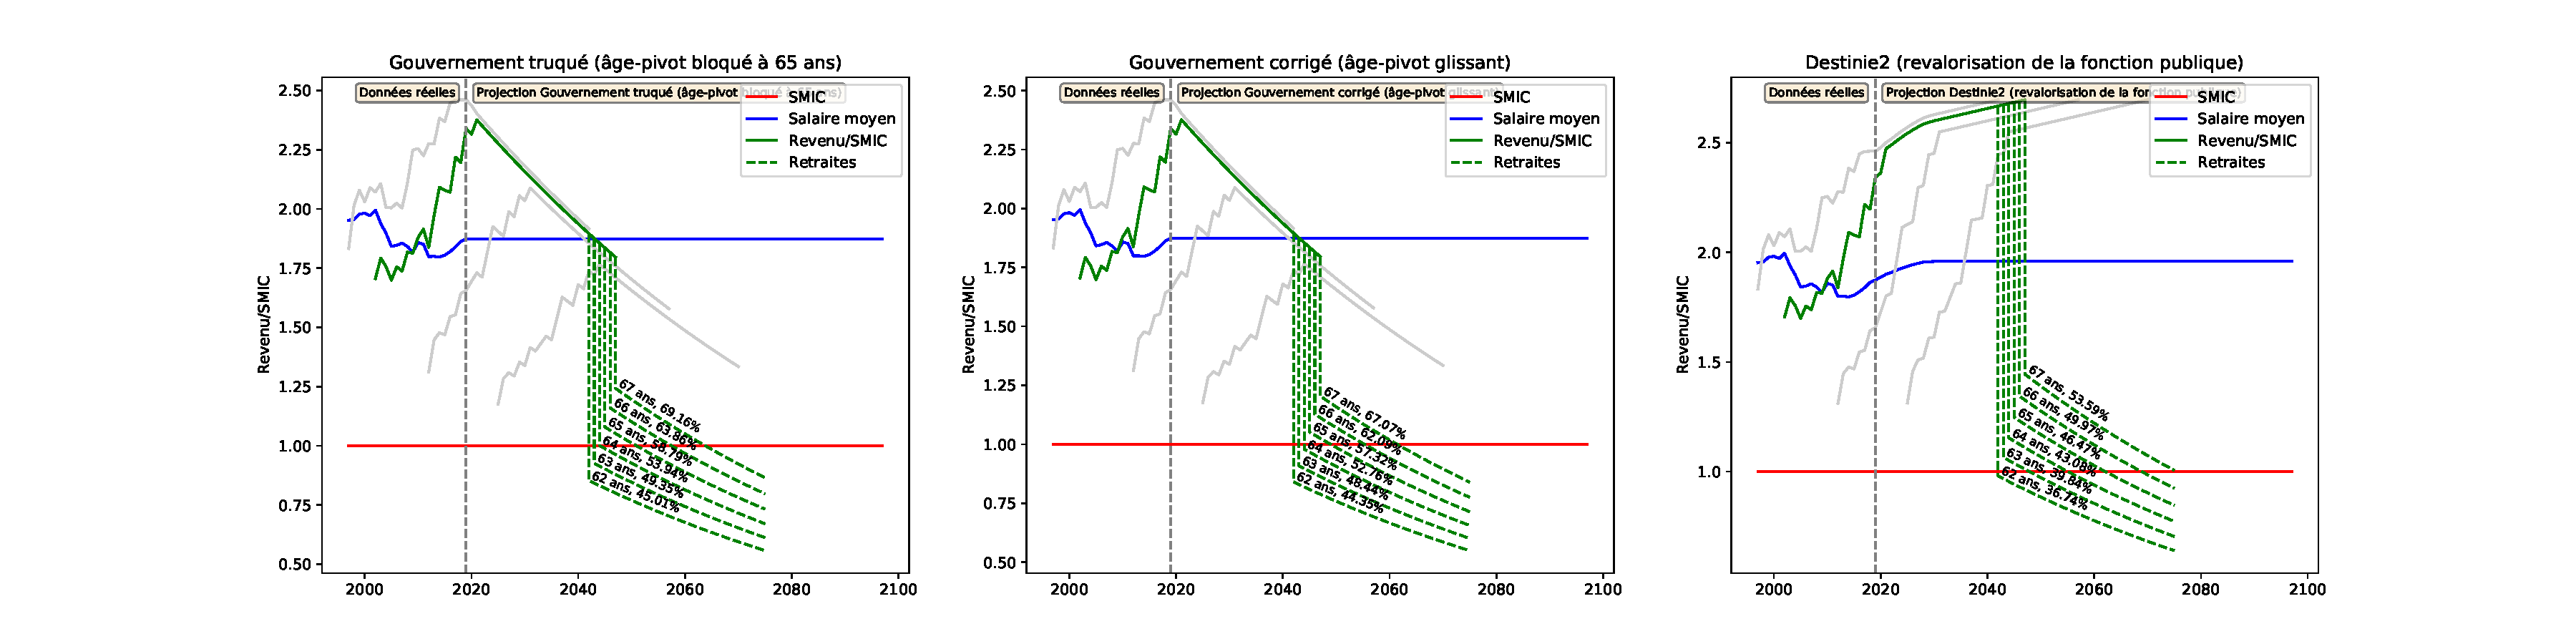
\includegraphics[width=0.9\textwidth]{fig/ProfCertifie_1980_22_dest_retraite.pdf}\end{center} \label{fig/ProfCertifie_1980_22_dest_retraite.pdf} 

\newpage 
 
\paragraph{Revenus et points pour le modèle \emph{Gouvernement truqué (âge-pivot bloqué à 65 ans)}} 
 
{ \scriptsize \begin{center} 
\begin{tabular}[htb]{|c|c||c|c|c|c|c|c||c|c||c|c|c|} 
\hline 
 Année &  Âge &  Ind Maj &  Pt Ind(\euro{} 2019) &  Rev HP(\euro{} 2019) &  Tx Primes &  GIPA(\euro{} 2019) &  Revenu(\euro{} 2019) &  SMIC(\euro{} 2019) &  Rev/SMIC &  Cumul Pts &  Achat Pt(\euro{} 2019) &  Serv. Pt(\euro{} 2019) \\ 
\hline \hline 
 2002 &  22 &  450.0 &  5.49 &  2468.82 &  0.00 &  0.00 &  2468.82 &  1447.74 &  {\bf 1.71} &  832.02 &  35.61 &  0.50 \\ 
\hline 
 2003 &  23 &  498.0 &  5.37 &  2676.56 &  0.00 &  0.00 &  2676.56 &  1493.03 &  {\bf 1.79} &  1734.06 &  35.61 &  0.50 \\ 
\hline 
 2004 &  24 &  513.0 &  5.29 &  2713.63 &  0.17 &  0.00 &  2718.24 &  1547.32 &  {\bf 1.76} &  2650.14 &  35.61 &  0.50 \\ 
\hline 
 2005 &  25 &  513.0 &  5.29 &  2713.33 &  0.40 &  0.00 &  2724.19 &  1603.67 &  {\bf 1.70} &  3568.22 &  35.61 &  0.50 \\ 
\hline 
 2006 &  26 &  542.0 &  5.23 &  2834.72 &  0.63 &  0.00 &  2852.58 &  1625.00 &  {\bf 1.76} &  4529.58 &  35.61 &  0.50 \\ 
\hline 
 2007 &  27 &  542.0 &  5.19 &  2815.41 &  0.86 &  0.00 &  2839.62 &  1634.08 &  {\bf 1.74} &  5486.56 &  35.61 &  0.50 \\ 
\hline 
 2008 &  28 &  579.0 &  5.09 &  2948.87 &  1.09 &  0.00 &  2981.02 &  1640.24 &  {\bf 1.82} &  6491.20 &  35.61 &  0.50 \\ 
\hline 
 2009 &  29 &  579.0 &  5.13 &  2969.77 &  1.32 &  0.00 &  3008.97 &  1659.42 &  {\bf 1.81} &  7505.26 &  35.61 &  0.50 \\ 
\hline 
 2010 &  30 &  598.5 &  5.08 &  3038.78 &  1.55 &  0.00 &  3085.88 &  1641.90 &  {\bf 1.88} &  8545.24 &  35.61 &  0.50 \\ 
\hline 
 2011 &  31 &  618.0 &  4.97 &  3072.59 &  1.78 &  0.00 &  3127.29 &  1633.19 &  {\bf 1.91} &  9599.17 &  35.61 &  0.50 \\ 
\hline 
 2012 &  32 &  618.0 &  4.88 &  3013.64 &  2.01 &  0.00 &  3074.21 &  1673.05 &  {\bf 1.84} &  10635.22 &  35.61 &  0.50 \\ 
\hline 
 2013 &  33 &  664.0 &  4.83 &  3210.21 &  2.24 &  0.00 &  3282.12 &  1664.01 &  {\bf 1.97} &  11741.33 &  35.61 &  0.50 \\ 
\hline 
 2014 &  34 &  710.0 &  4.81 &  3415.42 &  2.47 &  0.00 &  3499.78 &  1673.24 &  {\bf 2.09} &  12920.80 &  35.61 &  0.50 \\ 
\hline 
 2015 &  35 &  710.0 &  4.81 &  3414.08 &  2.70 &  0.00 &  3506.26 &  1686.62 &  {\bf 2.08} &  14102.45 &  35.61 &  0.50 \\ 
\hline 
 2016 &  36 &  710.0 &  4.80 &  3407.27 &  2.93 &  0.00 &  3507.10 &  1693.76 &  {\bf 2.07} &  15284.39 &  35.61 &  0.50 \\ 
\hline 
 2017 &  37 &  757.0 &  4.81 &  3640.15 &  3.16 &  0.00 &  3755.18 &  1692.60 &  {\bf 2.22} &  16549.93 &  35.61 &  0.50 \\ 
\hline 
 2018 &  38 &  757.0 &  4.74 &  3589.89 &  3.39 &  0.00 &  3711.59 &  1689.76 &  {\bf 2.20} &  17800.78 &  35.61 &  0.50 \\ 
\hline 
 2019 &  39 &  800.0 &  4.79 &  3835.54 &  3.62 &  0.00 &  3974.38 &  1698.45 &  {\bf 2.34} &  19140.20 &  35.61 &  0.50 \\ 
\hline 
 2020 &  40 &  800.0 &  4.79 &  3835.54 &  3.85 &  0.00 &  3983.21 &  1720.53 &  {\bf 2.32} &  20482.59 &  35.61 &  0.50 \\ 
\hline 
 2021 &  41 &  830.0 &  4.79 &  3979.37 &  4.08 &  0.00 &  4141.73 &  1742.90 &  {\bf 2.38} &  21878.40 &  35.61 &  0.50 \\ 
\hline 
 2022 &  42 &  830.0 &  4.79 &  3979.37 &  4.31 &  0.00 &  4150.88 &  1765.55 &  {\bf 2.35} &  23277.30 &  35.61 &  0.50 \\ 
\hline 
 2023 &  43 &  830.0 &  4.79 &  3979.37 &  4.54 &  0.00 &  4160.03 &  1788.51 &  {\bf 2.33} &  24679.28 &  35.61 &  0.50 \\ 
\hline 
 2024 &  44 &  830.0 &  4.79 &  3979.37 &  4.77 &  0.00 &  4169.19 &  1811.76 &  {\bf 2.30} &  26084.34 &  35.61 &  0.50 \\ 
\hline 
 2025 &  45 &  830.0 &  4.79 &  3979.37 &  5.00 &  0.00 &  4178.34 &  1835.31 &  {\bf 2.28} &  27492.50 &  35.61 &  0.50 \\ 
\hline 
 2026 &  46 &  830.0 &  4.79 &  3979.37 &  5.23 &  0.00 &  4187.49 &  1859.17 &  {\bf 2.25} &  28903.73 &  35.61 &  0.50 \\ 
\hline 
 2027 &  47 &  830.0 &  4.79 &  3979.37 &  5.46 &  0.00 &  4196.64 &  1883.34 &  {\bf 2.23} &  30318.05 &  35.61 &  0.50 \\ 
\hline 
 2028 &  48 &  830.0 &  4.79 &  3979.37 &  5.69 &  0.00 &  4205.80 &  1907.82 &  {\bf 2.20} &  31735.46 &  35.61 &  0.50 \\ 
\hline 
 2029 &  49 &  830.0 &  4.79 &  3979.37 &  5.92 &  0.00 &  4214.95 &  1932.62 &  {\bf 2.18} &  33154.87 &  35.63 &  0.50 \\ 
\hline 
 2030 &  50 &  830.0 &  4.79 &  3979.37 &  6.15 &  0.00 &  4224.10 &  1957.75 &  {\bf 2.16} &  34575.20 &  35.69 &  0.50 \\ 
\hline 
 2031 &  51 &  830.0 &  4.79 &  3979.37 &  6.38 &  0.00 &  4233.25 &  1983.20 &  {\bf 2.13} &  35995.37 &  35.77 &  0.50 \\ 
\hline 
 2032 &  52 &  830.0 &  4.79 &  3979.37 &  6.61 &  0.00 &  4242.41 &  2008.98 &  {\bf 2.11} &  37414.29 &  35.88 &  0.50 \\ 
\hline 
 2033 &  53 &  830.0 &  4.79 &  3979.37 &  6.84 &  0.00 &  4251.56 &  2035.10 &  {\bf 2.09} &  38830.88 &  36.02 &  0.50 \\ 
\hline 
 2034 &  54 &  830.0 &  4.79 &  3979.37 &  7.07 &  0.00 &  4260.71 &  2061.55 &  {\bf 2.07} &  40244.06 &  36.18 &  0.50 \\ 
\hline 
 2035 &  55 &  830.0 &  4.79 &  3979.37 &  7.30 &  0.00 &  4269.86 &  2088.35 &  {\bf 2.04} &  41652.77 &  36.37 &  0.51 \\ 
\hline 
 2036 &  56 &  830.0 &  4.79 &  3979.37 &  7.53 &  0.00 &  4279.02 &  2115.50 &  {\bf 2.02} &  43055.94 &  36.59 &  0.51 \\ 
\hline 
 2037 &  57 &  830.0 &  4.79 &  3979.37 &  7.76 &  0.00 &  4288.17 &  2143.00 &  {\bf 2.00} &  44452.53 &  36.85 &  0.51 \\ 
\hline 
 2038 &  58 &  830.0 &  4.79 &  3979.37 &  7.99 &  0.00 &  4297.32 &  2170.86 &  {\bf 1.98} &  45841.51 &  37.13 &  0.52 \\ 
\hline 
 2039 &  59 &  830.0 &  4.79 &  3979.37 &  8.22 &  0.00 &  4306.47 &  2199.08 &  {\bf 1.96} &  47221.86 &  37.44 &  0.52 \\ 
\hline 
 2040 &  60 &  830.0 &  4.79 &  3979.37 &  8.45 &  0.00 &  4315.63 &  2227.67 &  {\bf 1.94} &  48592.59 &  37.78 &  0.53 \\ 
\hline 
 2041 &  61 &  830.0 &  4.79 &  3979.37 &  8.68 &  0.00 &  4324.78 &  2256.63 &  {\bf 1.92} &  49952.73 &  38.16 &  0.53 \\ 
\hline 
 2042 &  62 &  830.0 &  4.79 &  3979.37 &  8.91 &  0.00 &  4333.93 &  2285.97 &  {\bf 1.90} &  51301.32 &  38.56 &  0.54 \\ 
\hline 
 2043 &  63 &  830.0 &  4.79 &  3979.37 &  9.14 &  0.00 &  4343.08 &  2315.68 &  {\bf 1.88} &  52637.45 &  39.01 &  0.54 \\ 
\hline 
 2044 &  64 &  830.0 &  4.79 &  3979.37 &  9.37 &  0.00 &  4352.24 &  2345.79 &  {\bf 1.86} &  53960.21 &  39.48 &  0.55 \\ 
\hline 
 2045 &  65 &  830.0 &  4.79 &  3979.37 &  9.60 &  0.00 &  4361.39 &  2376.28 &  {\bf 1.84} &  55268.75 &  40.00 &  0.56 \\ 
\hline 
 2046 &  66 &  830.0 &  4.79 &  3979.37 &  9.83 &  0.00 &  4370.54 &  2407.18 &  {\bf 1.82} &  56563.20 &  40.52 &  0.56 \\ 
\hline 
 2047 &  67 &  830.0 &  4.79 &  3979.37 &  10.06 &  0.00 &  4379.70 &  2438.47 &  {\bf 1.80} &  57843.72 &  41.04 &  0.57 \\ 
\hline 
\hline 
\end{tabular} 
\end{center} } 
\newpage 
 
\paragraph{Revenus et points pour le modèle \emph{Gouvernement corrigé (âge-pivot glissant)}} 
 
{ \scriptsize \begin{center} 
\begin{tabular}[htb]{|c|c||c|c|c|c|c|c||c|c||c|c|c|} 
\hline 
 Année &  Âge &  Ind Maj &  Pt Ind(\euro{} 2019) &  Rev HP(\euro{} 2019) &  Tx Primes &  GIPA(\euro{} 2019) &  Revenu(\euro{} 2019) &  SMIC(\euro{} 2019) &  Rev/SMIC &  Cumul Pts &  Achat Pt(\euro{} 2019) &  Serv. Pt(\euro{} 2019) \\ 
\hline \hline 
 2002 &  22 &  450.0 &  5.49 &  2468.82 &  0.00 &  0.00 &  2468.82 &  1447.74 &  {\bf 1.71} &  832.02 &  35.61 &  0.50 \\ 
\hline 
 2003 &  23 &  498.0 &  5.37 &  2676.56 &  0.00 &  0.00 &  2676.56 &  1493.03 &  {\bf 1.79} &  1734.06 &  35.61 &  0.50 \\ 
\hline 
 2004 &  24 &  513.0 &  5.29 &  2713.63 &  0.17 &  0.00 &  2718.24 &  1547.32 &  {\bf 1.76} &  2650.14 &  35.61 &  0.50 \\ 
\hline 
 2005 &  25 &  513.0 &  5.29 &  2713.33 &  0.40 &  0.00 &  2724.19 &  1603.67 &  {\bf 1.70} &  3568.22 &  35.61 &  0.50 \\ 
\hline 
 2006 &  26 &  542.0 &  5.23 &  2834.72 &  0.63 &  0.00 &  2852.58 &  1625.00 &  {\bf 1.76} &  4529.58 &  35.61 &  0.50 \\ 
\hline 
 2007 &  27 &  542.0 &  5.19 &  2815.41 &  0.86 &  0.00 &  2839.62 &  1634.08 &  {\bf 1.74} &  5486.56 &  35.61 &  0.50 \\ 
\hline 
 2008 &  28 &  579.0 &  5.09 &  2948.87 &  1.09 &  0.00 &  2981.02 &  1640.24 &  {\bf 1.82} &  6491.20 &  35.61 &  0.50 \\ 
\hline 
 2009 &  29 &  579.0 &  5.13 &  2969.77 &  1.32 &  0.00 &  3008.97 &  1659.42 &  {\bf 1.81} &  7505.26 &  35.61 &  0.50 \\ 
\hline 
 2010 &  30 &  598.5 &  5.08 &  3038.78 &  1.55 &  0.00 &  3085.88 &  1641.90 &  {\bf 1.88} &  8545.24 &  35.61 &  0.50 \\ 
\hline 
 2011 &  31 &  618.0 &  4.97 &  3072.59 &  1.78 &  0.00 &  3127.29 &  1633.19 &  {\bf 1.91} &  9599.17 &  35.61 &  0.50 \\ 
\hline 
 2012 &  32 &  618.0 &  4.88 &  3013.64 &  2.01 &  0.00 &  3074.21 &  1673.05 &  {\bf 1.84} &  10635.22 &  35.61 &  0.50 \\ 
\hline 
 2013 &  33 &  664.0 &  4.83 &  3210.21 &  2.24 &  0.00 &  3282.12 &  1664.01 &  {\bf 1.97} &  11741.33 &  35.61 &  0.50 \\ 
\hline 
 2014 &  34 &  710.0 &  4.81 &  3415.42 &  2.47 &  0.00 &  3499.78 &  1673.24 &  {\bf 2.09} &  12920.80 &  35.61 &  0.50 \\ 
\hline 
 2015 &  35 &  710.0 &  4.81 &  3414.08 &  2.70 &  0.00 &  3506.26 &  1686.62 &  {\bf 2.08} &  14102.45 &  35.61 &  0.50 \\ 
\hline 
 2016 &  36 &  710.0 &  4.80 &  3407.27 &  2.93 &  0.00 &  3507.10 &  1693.76 &  {\bf 2.07} &  15284.39 &  35.61 &  0.50 \\ 
\hline 
 2017 &  37 &  757.0 &  4.81 &  3640.15 &  3.16 &  0.00 &  3755.18 &  1692.60 &  {\bf 2.22} &  16549.93 &  35.61 &  0.50 \\ 
\hline 
 2018 &  38 &  757.0 &  4.74 &  3589.89 &  3.39 &  0.00 &  3711.59 &  1689.76 &  {\bf 2.20} &  17800.78 &  35.61 &  0.50 \\ 
\hline 
 2019 &  39 &  800.0 &  4.79 &  3835.54 &  3.62 &  0.00 &  3974.38 &  1698.45 &  {\bf 2.34} &  19140.20 &  35.61 &  0.50 \\ 
\hline 
 2020 &  40 &  800.0 &  4.79 &  3835.54 &  3.85 &  0.00 &  3983.21 &  1720.53 &  {\bf 2.32} &  20482.59 &  35.61 &  0.50 \\ 
\hline 
 2021 &  41 &  830.0 &  4.79 &  3979.37 &  4.08 &  0.00 &  4141.73 &  1742.90 &  {\bf 2.38} &  21878.40 &  35.61 &  0.50 \\ 
\hline 
 2022 &  42 &  830.0 &  4.79 &  3979.37 &  4.31 &  0.00 &  4150.88 &  1765.55 &  {\bf 2.35} &  23277.30 &  35.61 &  0.50 \\ 
\hline 
 2023 &  43 &  830.0 &  4.79 &  3979.37 &  4.54 &  0.00 &  4160.03 &  1788.51 &  {\bf 2.33} &  24679.28 &  35.61 &  0.50 \\ 
\hline 
 2024 &  44 &  830.0 &  4.79 &  3979.37 &  4.77 &  0.00 &  4169.19 &  1811.76 &  {\bf 2.30} &  26084.34 &  35.61 &  0.50 \\ 
\hline 
 2025 &  45 &  830.0 &  4.79 &  3979.37 &  5.00 &  0.00 &  4178.34 &  1835.31 &  {\bf 2.28} &  27492.50 &  35.61 &  0.50 \\ 
\hline 
 2026 &  46 &  830.0 &  4.79 &  3979.37 &  5.23 &  0.00 &  4187.49 &  1859.17 &  {\bf 2.25} &  28903.73 &  35.61 &  0.50 \\ 
\hline 
 2027 &  47 &  830.0 &  4.79 &  3979.37 &  5.46 &  0.00 &  4196.64 &  1883.34 &  {\bf 2.23} &  30318.05 &  35.61 &  0.50 \\ 
\hline 
 2028 &  48 &  830.0 &  4.79 &  3979.37 &  5.69 &  0.00 &  4205.80 &  1907.82 &  {\bf 2.20} &  31735.46 &  35.61 &  0.50 \\ 
\hline 
 2029 &  49 &  830.0 &  4.79 &  3979.37 &  5.92 &  0.00 &  4214.95 &  1932.62 &  {\bf 2.18} &  33154.87 &  35.63 &  0.50 \\ 
\hline 
 2030 &  50 &  830.0 &  4.79 &  3979.37 &  6.15 &  0.00 &  4224.10 &  1957.75 &  {\bf 2.16} &  34575.20 &  35.69 &  0.50 \\ 
\hline 
 2031 &  51 &  830.0 &  4.79 &  3979.37 &  6.38 &  0.00 &  4233.25 &  1983.20 &  {\bf 2.13} &  35995.37 &  35.77 &  0.50 \\ 
\hline 
 2032 &  52 &  830.0 &  4.79 &  3979.37 &  6.61 &  0.00 &  4242.41 &  2008.98 &  {\bf 2.11} &  37414.29 &  35.88 &  0.50 \\ 
\hline 
 2033 &  53 &  830.0 &  4.79 &  3979.37 &  6.84 &  0.00 &  4251.56 &  2035.10 &  {\bf 2.09} &  38830.88 &  36.02 &  0.50 \\ 
\hline 
 2034 &  54 &  830.0 &  4.79 &  3979.37 &  7.07 &  0.00 &  4260.71 &  2061.55 &  {\bf 2.07} &  40244.06 &  36.18 &  0.50 \\ 
\hline 
 2035 &  55 &  830.0 &  4.79 &  3979.37 &  7.30 &  0.00 &  4269.86 &  2088.35 &  {\bf 2.04} &  41652.77 &  36.37 &  0.51 \\ 
\hline 
 2036 &  56 &  830.0 &  4.79 &  3979.37 &  7.53 &  0.00 &  4279.02 &  2115.50 &  {\bf 2.02} &  43055.94 &  36.59 &  0.51 \\ 
\hline 
 2037 &  57 &  830.0 &  4.79 &  3979.37 &  7.76 &  0.00 &  4288.17 &  2143.00 &  {\bf 2.00} &  44452.53 &  36.85 &  0.51 \\ 
\hline 
 2038 &  58 &  830.0 &  4.79 &  3979.37 &  7.99 &  0.00 &  4297.32 &  2170.86 &  {\bf 1.98} &  45841.51 &  37.13 &  0.52 \\ 
\hline 
 2039 &  59 &  830.0 &  4.79 &  3979.37 &  8.22 &  0.00 &  4306.47 &  2199.08 &  {\bf 1.96} &  47221.86 &  37.44 &  0.52 \\ 
\hline 
 2040 &  60 &  830.0 &  4.79 &  3979.37 &  8.45 &  0.00 &  4315.63 &  2227.67 &  {\bf 1.94} &  48592.59 &  37.78 &  0.53 \\ 
\hline 
 2041 &  61 &  830.0 &  4.79 &  3979.37 &  8.68 &  0.00 &  4324.78 &  2256.63 &  {\bf 1.92} &  49952.73 &  38.16 &  0.53 \\ 
\hline 
 2042 &  62 &  830.0 &  4.79 &  3979.37 &  8.91 &  0.00 &  4333.93 &  2285.97 &  {\bf 1.90} &  51301.32 &  38.56 &  0.54 \\ 
\hline 
 2043 &  63 &  830.0 &  4.79 &  3979.37 &  9.14 &  0.00 &  4343.08 &  2315.68 &  {\bf 1.88} &  52637.45 &  39.01 &  0.54 \\ 
\hline 
 2044 &  64 &  830.0 &  4.79 &  3979.37 &  9.37 &  0.00 &  4352.24 &  2345.79 &  {\bf 1.86} &  53960.21 &  39.48 &  0.55 \\ 
\hline 
 2045 &  65 &  830.0 &  4.79 &  3979.37 &  9.60 &  0.00 &  4361.39 &  2376.28 &  {\bf 1.84} &  55268.75 &  40.00 &  0.56 \\ 
\hline 
 2046 &  66 &  830.0 &  4.79 &  3979.37 &  9.83 &  0.00 &  4370.54 &  2407.18 &  {\bf 1.82} &  56563.20 &  40.52 &  0.56 \\ 
\hline 
 2047 &  67 &  830.0 &  4.79 &  3979.37 &  10.06 &  0.00 &  4379.70 &  2438.47 &  {\bf 1.80} &  57843.72 &  41.04 &  0.57 \\ 
\hline 
\hline 
\end{tabular} 
\end{center} } 
\newpage 
 
\paragraph{Revenus et points pour le modèle \emph{Destinie2 (revalorisation de la fonction publique)}} 
 
{ \scriptsize \begin{center} 
\begin{tabular}[htb]{|c|c||c|c|c|c|c|c||c|c||c|c|c|} 
\hline 
 Année &  Âge &  Ind Maj &  Pt Ind(\euro{} 2019) &  Rev HP(\euro{} 2019) &  Tx Primes &  GIPA(\euro{} 2019) &  Revenu(\euro{} 2019) &  SMIC(\euro{} 2019) &  Rev/SMIC &  Cumul Pts &  Achat Pt(\euro{} 2019) &  Serv. Pt(\euro{} 2019) \\ 
\hline \hline 
 2002 &  22 &  450.0 &  5.49 &  2468.82 &  0.00 &  0.00 &  2468.82 &  1447.74 &  {\bf 1.71} &  829.98 &  35.69 &  0.50 \\ 
\hline 
 2003 &  23 &  498.0 &  5.37 &  2676.56 &  0.00 &  0.00 &  2676.56 &  1493.03 &  {\bf 1.79} &  1729.80 &  35.69 &  0.50 \\ 
\hline 
 2004 &  24 &  513.0 &  5.29 &  2713.63 &  0.17 &  0.00 &  2718.24 &  1547.32 &  {\bf 1.76} &  2643.63 &  35.69 &  0.50 \\ 
\hline 
 2005 &  25 &  513.0 &  5.29 &  2713.33 &  0.40 &  0.00 &  2724.19 &  1603.67 &  {\bf 1.70} &  3559.45 &  35.69 &  0.50 \\ 
\hline 
 2006 &  26 &  542.0 &  5.23 &  2834.72 &  0.63 &  0.00 &  2852.58 &  1625.00 &  {\bf 1.76} &  4518.45 &  35.69 &  0.50 \\ 
\hline 
 2007 &  27 &  542.0 &  5.19 &  2815.41 &  0.86 &  0.00 &  2839.62 &  1634.08 &  {\bf 1.74} &  5473.08 &  35.69 &  0.50 \\ 
\hline 
 2008 &  28 &  579.0 &  5.09 &  2948.87 &  1.09 &  0.00 &  2981.02 &  1640.24 &  {\bf 1.82} &  6475.25 &  35.69 &  0.50 \\ 
\hline 
 2009 &  29 &  579.0 &  5.13 &  2969.77 &  1.32 &  0.00 &  3008.97 &  1659.42 &  {\bf 1.81} &  7486.82 &  35.69 &  0.50 \\ 
\hline 
 2010 &  30 &  598.5 &  5.08 &  3038.78 &  1.55 &  0.00 &  3085.88 &  1641.90 &  {\bf 1.88} &  8524.24 &  35.69 &  0.50 \\ 
\hline 
 2011 &  31 &  618.0 &  4.97 &  3072.59 &  1.78 &  0.00 &  3127.29 &  1633.19 &  {\bf 1.91} &  9575.59 &  35.69 &  0.50 \\ 
\hline 
 2012 &  32 &  618.0 &  4.88 &  3013.64 &  2.01 &  0.00 &  3074.21 &  1673.05 &  {\bf 1.84} &  10609.09 &  35.69 &  0.50 \\ 
\hline 
 2013 &  33 &  664.0 &  4.83 &  3210.21 &  2.24 &  0.00 &  3282.12 &  1664.01 &  {\bf 1.97} &  11712.48 &  35.69 &  0.50 \\ 
\hline 
 2014 &  34 &  710.0 &  4.81 &  3415.42 &  2.47 &  0.00 &  3499.78 &  1673.24 &  {\bf 2.09} &  12889.05 &  35.69 &  0.50 \\ 
\hline 
 2015 &  35 &  710.0 &  4.81 &  3414.08 &  2.70 &  0.00 &  3506.26 &  1686.62 &  {\bf 2.08} &  14067.81 &  35.69 &  0.50 \\ 
\hline 
 2016 &  36 &  710.0 &  4.80 &  3407.27 &  2.93 &  0.00 &  3507.10 &  1693.76 &  {\bf 2.07} &  15246.84 &  35.69 &  0.50 \\ 
\hline 
 2017 &  37 &  757.0 &  4.81 &  3640.15 &  3.16 &  0.00 &  3755.18 &  1692.60 &  {\bf 2.22} &  16509.27 &  35.69 &  0.50 \\ 
\hline 
 2018 &  38 &  757.0 &  4.74 &  3589.89 &  3.39 &  0.00 &  3711.59 &  1689.76 &  {\bf 2.20} &  17757.04 &  35.69 &  0.50 \\ 
\hline 
 2019 &  39 &  800.0 &  4.79 &  3835.54 &  3.62 &  0.00 &  3974.38 &  1698.45 &  {\bf 2.34} &  19093.17 &  35.69 &  0.50 \\ 
\hline 
 2020 &  40 &  800.0 &  4.83 &  3866.22 &  3.85 &  0.00 &  4015.07 &  1699.99 &  {\bf 2.36} &  20442.97 &  35.69 &  0.50 \\ 
\hline 
 2021 &  41 &  830.0 &  4.88 &  4047.31 &  4.08 &  0.00 &  4212.44 &  1703.48 &  {\bf 2.47} &  21859.13 &  35.69 &  0.50 \\ 
\hline 
 2022 &  42 &  830.0 &  4.93 &  4087.78 &  4.31 &  0.00 &  4263.96 &  1712.78 &  {\bf 2.49} &  23292.60 &  35.69 &  0.50 \\ 
\hline 
 2023 &  43 &  830.0 &  4.98 &  4135.61 &  4.54 &  0.00 &  4323.36 &  1723.51 &  {\bf 2.51} &  24746.05 &  35.69 &  0.50 \\ 
\hline 
 2024 &  44 &  830.0 &  5.04 &  4184.82 &  4.77 &  0.00 &  4384.44 &  1735.69 &  {\bf 2.53} &  26220.03 &  35.69 &  0.50 \\ 
\hline 
 2025 &  45 &  830.0 &  5.10 &  4235.87 &  5.00 &  0.00 &  4447.67 &  1749.35 &  {\bf 2.54} &  27715.26 &  35.69 &  0.50 \\ 
\hline 
 2026 &  46 &  830.0 &  5.17 &  4288.82 &  5.23 &  0.00 &  4513.13 &  1764.53 &  {\bf 2.56} &  29232.50 &  35.69 &  0.50 \\ 
\hline 
 2027 &  47 &  830.0 &  5.23 &  4343.72 &  5.46 &  0.00 &  4580.89 &  1781.27 &  {\bf 2.57} &  30772.53 &  35.69 &  0.50 \\ 
\hline 
 2028 &  48 &  830.0 &  5.30 &  4400.62 &  5.69 &  0.00 &  4651.02 &  1799.59 &  {\bf 2.58} &  32336.12 &  35.69 &  0.50 \\ 
\hline 
 2029 &  49 &  830.0 &  5.37 &  4453.87 &  5.92 &  0.00 &  4717.54 &  1819.55 &  {\bf 2.59} &  33920.96 &  35.72 &  0.50 \\ 
\hline 
 2030 &  50 &  830.0 &  5.43 &  4509.10 &  6.15 &  0.00 &  4786.41 &  1841.19 &  {\bf 2.60} &  35526.61 &  35.77 &  0.50 \\ 
\hline 
 2031 &  51 &  830.0 &  5.50 &  4566.36 &  6.38 &  0.00 &  4857.70 &  1864.58 &  {\bf 2.61} &  37152.55 &  35.85 &  0.50 \\ 
\hline 
 2032 &  52 &  830.0 &  5.57 &  4625.73 &  6.61 &  0.00 &  4931.49 &  1888.81 &  {\bf 2.61} &  38798.17 &  35.96 &  0.50 \\ 
\hline 
 2033 &  53 &  830.0 &  5.65 &  4685.86 &  6.84 &  0.00 &  5006.37 &  1913.37 &  {\bf 2.62} &  40462.46 &  36.10 &  0.50 \\ 
\hline 
 2034 &  54 &  830.0 &  5.72 &  4746.78 &  7.07 &  0.00 &  5082.37 &  1938.24 &  {\bf 2.62} &  42144.32 &  36.26 &  0.50 \\ 
\hline 
 2035 &  55 &  830.0 &  5.79 &  4808.49 &  7.30 &  0.00 &  5159.50 &  1963.44 &  {\bf 2.63} &  43842.65 &  36.46 &  0.51 \\ 
\hline 
 2036 &  56 &  830.0 &  5.87 &  4871.00 &  7.53 &  0.00 &  5237.78 &  1988.96 &  {\bf 2.63} &  45556.29 &  36.68 &  0.51 \\ 
\hline 
 2037 &  57 &  830.0 &  5.94 &  4934.32 &  7.76 &  0.00 &  5317.22 &  2014.82 &  {\bf 2.64} &  47284.08 &  36.93 &  0.51 \\ 
\hline 
 2038 &  58 &  830.0 &  6.02 &  4998.46 &  7.99 &  0.00 &  5397.84 &  2041.01 &  {\bf 2.64} &  49024.78 &  37.21 &  0.52 \\ 
\hline 
 2039 &  59 &  830.0 &  6.10 &  5063.44 &  8.22 &  0.00 &  5479.66 &  2067.55 &  {\bf 2.65} &  50777.16 &  37.52 &  0.52 \\ 
\hline 
 2040 &  60 &  830.0 &  6.18 &  5129.27 &  8.45 &  0.00 &  5562.69 &  2094.43 &  {\bf 2.66} &  52539.95 &  37.87 &  0.53 \\ 
\hline 
 2041 &  61 &  830.0 &  6.26 &  5195.95 &  8.68 &  0.00 &  5646.96 &  2121.65 &  {\bf 2.66} &  54311.86 &  38.24 &  0.53 \\ 
\hline 
 2042 &  62 &  830.0 &  6.34 &  5263.50 &  8.91 &  0.00 &  5732.48 &  2149.23 &  {\bf 2.67} &  56091.56 &  38.65 &  0.54 \\ 
\hline 
 2043 &  63 &  830.0 &  6.42 &  5331.92 &  9.14 &  0.00 &  5819.26 &  2177.17 &  {\bf 2.67} &  57877.74 &  39.10 &  0.54 \\ 
\hline 
 2044 &  64 &  830.0 &  6.51 &  5401.24 &  9.37 &  0.00 &  5907.33 &  2205.48 &  {\bf 2.68} &  59669.04 &  39.57 &  0.55 \\ 
\hline 
 2045 &  65 &  830.0 &  6.59 &  5471.45 &  9.60 &  0.00 &  5996.71 &  2234.15 &  {\bf 2.68} &  61464.11 &  40.09 &  0.56 \\ 
\hline 
 2046 &  66 &  830.0 &  6.68 &  5542.58 &  9.83 &  0.00 &  6087.42 &  2263.19 &  {\bf 2.69} &  63262.95 &  40.61 &  0.57 \\ 
\hline 
 2047 &  67 &  830.0 &  6.76 &  5614.64 &  10.06 &  0.00 &  6179.47 &  2292.61 &  {\bf 2.70} &  65065.55 &  41.14 &  0.57 \\ 
\hline 
\hline 
\end{tabular} 
\end{center} } 
\newpage 
 
\subsection{Génération 1990 (début en 2012)} 

\paragraph{Retraites possibles dans le modèle \emph{Gouvernement truqué (âge-pivot bloqué à 65 ans)}}  
 
{ \scriptsize \begin{center} 
\begin{tabular}[htb]{|c|c||c|c||c|c||c||c|c|c|c|c|c|} 
\hline 
 Retraite en &  Âge &  Âge pivot &  Décote/Surcote &  Retraite (\euro{} 2019) &  Tx Rempl(\%) &  SMIC (\euro{} 2019) &  Retraite/SMIC &  Rev70/SMIC &  Rev75/SMIC &  Rev80/SMIC &  Rev85/SMIC &  Rev90/SMIC \\ 
\hline \hline 
 2052 &  62 &  65 ans 0 mois &  -15.00\% &  2096.42 &  {\bf 48.37} &  2601.14 &  {\bf {\color{red} 0.81}} &  {\bf {\color{red} 0.73}} &  {\bf {\color{red} 0.68}} &  {\bf {\color{red} 0.64}} &  {\bf {\color{red} 0.60}} &  {\bf {\color{red} 0.56}} \\ 
\hline 
 2053 &  63 &  65 ans 0 mois &  -10.00\% &  2303.01 &  {\bf 53.03} &  2634.96 &  {\bf {\color{red} 0.87}} &  {\bf {\color{red} 0.80}} &  {\bf {\color{red} 0.75}} &  {\bf {\color{red} 0.70}} &  {\bf {\color{red} 0.66}} &  {\bf {\color{red} 0.62}} \\ 
\hline 
 2054 &  64 &  65 ans 0 mois &  -5.00\% &  2520.11 &  {\bf 57.90} &  2669.21 &  {\bf {\color{red} 0.94}} &  {\bf {\color{red} 0.87}} &  {\bf {\color{red} 0.82}} &  {\bf {\color{red} 0.77}} &  {\bf {\color{red} 0.72}} &  {\bf {\color{red} 0.67}} \\ 
\hline 
 2055 &  65 &  65 ans 0 mois &  0.00\% &  2747.94 &  {\bf 63.01} &  2703.91 &  {\bf 1.02} &  {\bf {\color{red} 0.95}} &  {\bf {\color{red} 0.89}} &  {\bf {\color{red} 0.84}} &  {\bf {\color{red} 0.78}} &  {\bf {\color{red} 0.74}} \\ 
\hline 
 2056 &  66 &  65 ans 0 mois &  5.00\% &  2986.72 &  {\bf 68.34} &  2739.06 &  {\bf 1.09} &  {\bf 1.04} &  {\bf {\color{red} 0.97}} &  {\bf {\color{red} 0.91}} &  {\bf {\color{red} 0.85}} &  {\bf {\color{red} 0.80}} \\ 
\hline 
 2057 &  67 &  65 ans 0 mois &  10.00\% &  3236.68 &  {\bf 73.90} &  2774.67 &  {\bf 1.17} &  {\bf 1.12} &  {\bf 1.05} &  {\bf {\color{red} 0.99}} &  {\bf {\color{red} 0.92}} &  {\bf {\color{red} 0.87}} \\ 
\hline 
\hline 
\end{tabular} 
\end{center} } 
\paragraph{Retraites possibles dans le modèle \emph{Gouvernement corrigé (âge-pivot glissant)}}  
 
{ \scriptsize \begin{center} 
\begin{tabular}[htb]{|c|c||c|c||c|c||c||c|c|c|c|c|c|} 
\hline 
 Retraite en &  Âge &  Âge pivot &  Décote/Surcote &  Retraite (\euro{} 2019) &  Tx Rempl(\%) &  SMIC (\euro{} 2019) &  Retraite/SMIC &  Rev70/SMIC &  Rev75/SMIC &  Rev80/SMIC &  Rev85/SMIC &  Rev90/SMIC \\ 
\hline \hline 
 2052 &  62 &  66 ans 1 mois &  -20.42\% &  1962.83 &  {\bf 45.29} &  2601.14 &  {\bf {\color{red} 0.75}} &  {\bf {\color{red} 0.68}} &  {\bf {\color{red} 0.64}} &  {\bf {\color{red} 0.60}} &  {\bf {\color{red} 0.56}} &  {\bf {\color{red} 0.53}} \\ 
\hline 
 2053 &  63 &  66 ans 2 mois &  -15.83\% &  2153.74 &  {\bf 49.59} &  2634.96 &  {\bf {\color{red} 0.82}} &  {\bf {\color{red} 0.75}} &  {\bf {\color{red} 0.70}} &  {\bf {\color{red} 0.66}} &  {\bf {\color{red} 0.62}} &  {\bf {\color{red} 0.58}} \\ 
\hline 
 2054 &  64 &  66 ans 3 mois &  -11.25\% &  2354.31 &  {\bf 54.09} &  2669.21 &  {\bf {\color{red} 0.88}} &  {\bf {\color{red} 0.82}} &  {\bf {\color{red} 0.77}} &  {\bf {\color{red} 0.72}} &  {\bf {\color{red} 0.67}} &  {\bf {\color{red} 0.63}} \\ 
\hline 
 2055 &  65 &  66 ans 4 mois &  -6.67\% &  2564.74 &  {\bf 58.81} &  2703.91 &  {\bf {\color{red} 0.95}} &  {\bf {\color{red} 0.89}} &  {\bf {\color{red} 0.83}} &  {\bf {\color{red} 0.78}} &  {\bf {\color{red} 0.73}} &  {\bf {\color{red} 0.69}} \\ 
\hline 
 2056 &  66 &  66 ans 5 mois &  -2.08\% &  2785.23 &  {\bf 63.73} &  2739.06 &  {\bf 1.02} &  {\bf {\color{red} 0.97}} &  {\bf {\color{red} 0.91}} &  {\bf {\color{red} 0.85}} &  {\bf {\color{red} 0.80}} &  {\bf {\color{red} 0.75}} \\ 
\hline 
 2057 &  67 &  66 ans 6 mois &  2.50\% &  3016.00 &  {\bf 68.86} &  2774.67 &  {\bf 1.09} &  {\bf 1.05} &  {\bf {\color{red} 0.98}} &  {\bf {\color{red} 0.92}} &  {\bf {\color{red} 0.86}} &  {\bf {\color{red} 0.81}} \\ 
\hline 
\hline 
\end{tabular} 
\end{center} } 
\paragraph{Retraites possibles dans le modèle \emph{Destinie2 (revalorisation de la fonction publique)}}  
 
{ \scriptsize \begin{center} 
\begin{tabular}[htb]{|c|c||c|c||c|c||c||c|c|c|c|c|c|} 
\hline 
 Retraite en &  Âge &  Âge pivot &  Décote/Surcote &  Retraite (\euro{} 2019) &  Tx Rempl(\%) &  SMIC (\euro{} 2019) &  Retraite/SMIC &  Rev70/SMIC &  Rev75/SMIC &  Rev80/SMIC &  Rev85/SMIC &  Rev90/SMIC \\ 
\hline \hline 
 2052 &  62 &  66 ans 1 mois &  -20.42\% &  2364.71 &  {\bf 36.25} &  2445.56 &  {\bf {\color{red} 0.97}} &  {\bf {\color{red} 0.87}} &  {\bf {\color{red} 0.82}} &  {\bf {\color{red} 0.77}} &  {\bf {\color{red} 0.72}} &  {\bf {\color{red} 0.67}} \\ 
\hline 
 2053 &  63 &  66 ans 2 mois &  -15.83\% &  2610.98 &  {\bf 39.43} &  2477.35 &  {\bf 1.05} &  {\bf {\color{red} 0.96}} &  {\bf {\color{red} 0.90}} &  {\bf {\color{red} 0.85}} &  {\bf {\color{red} 0.79}} &  {\bf {\color{red} 0.74}} \\ 
\hline 
 2054 &  64 &  66 ans 3 mois &  -11.25\% &  2872.00 &  {\bf 42.73} &  2509.56 &  {\bf 1.14} &  {\bf 1.06} &  {\bf {\color{red} 0.99}} &  {\bf {\color{red} 0.93}} &  {\bf {\color{red} 0.87}} &  {\bf {\color{red} 0.82}} \\ 
\hline 
 2055 &  65 &  66 ans 4 mois &  -6.67\% &  3148.23 &  {\bf 46.14} &  2542.18 &  {\bf 1.24} &  {\bf 1.16} &  {\bf 1.09} &  {\bf 1.02} &  {\bf {\color{red} 0.96}} &  {\bf {\color{red} 0.90}} \\ 
\hline 
 2056 &  66 &  66 ans 5 mois &  -2.08\% &  3440.17 &  {\bf 49.67} &  2575.23 &  {\bf 1.34} &  {\bf 1.27} &  {\bf 1.19} &  {\bf 1.11} &  {\bf 1.05} &  {\bf {\color{red} 0.98}} \\ 
\hline 
 2057 &  67 &  66 ans 6 mois &  2.50\% &  3748.34 &  {\bf 53.31} &  2608.71 &  {\bf 1.44} &  {\bf 1.38} &  {\bf 1.30} &  {\bf 1.21} &  {\bf 1.14} &  {\bf 1.07} \\ 
\hline 
\hline 
\end{tabular} 
\end{center} } 

 \begin{center}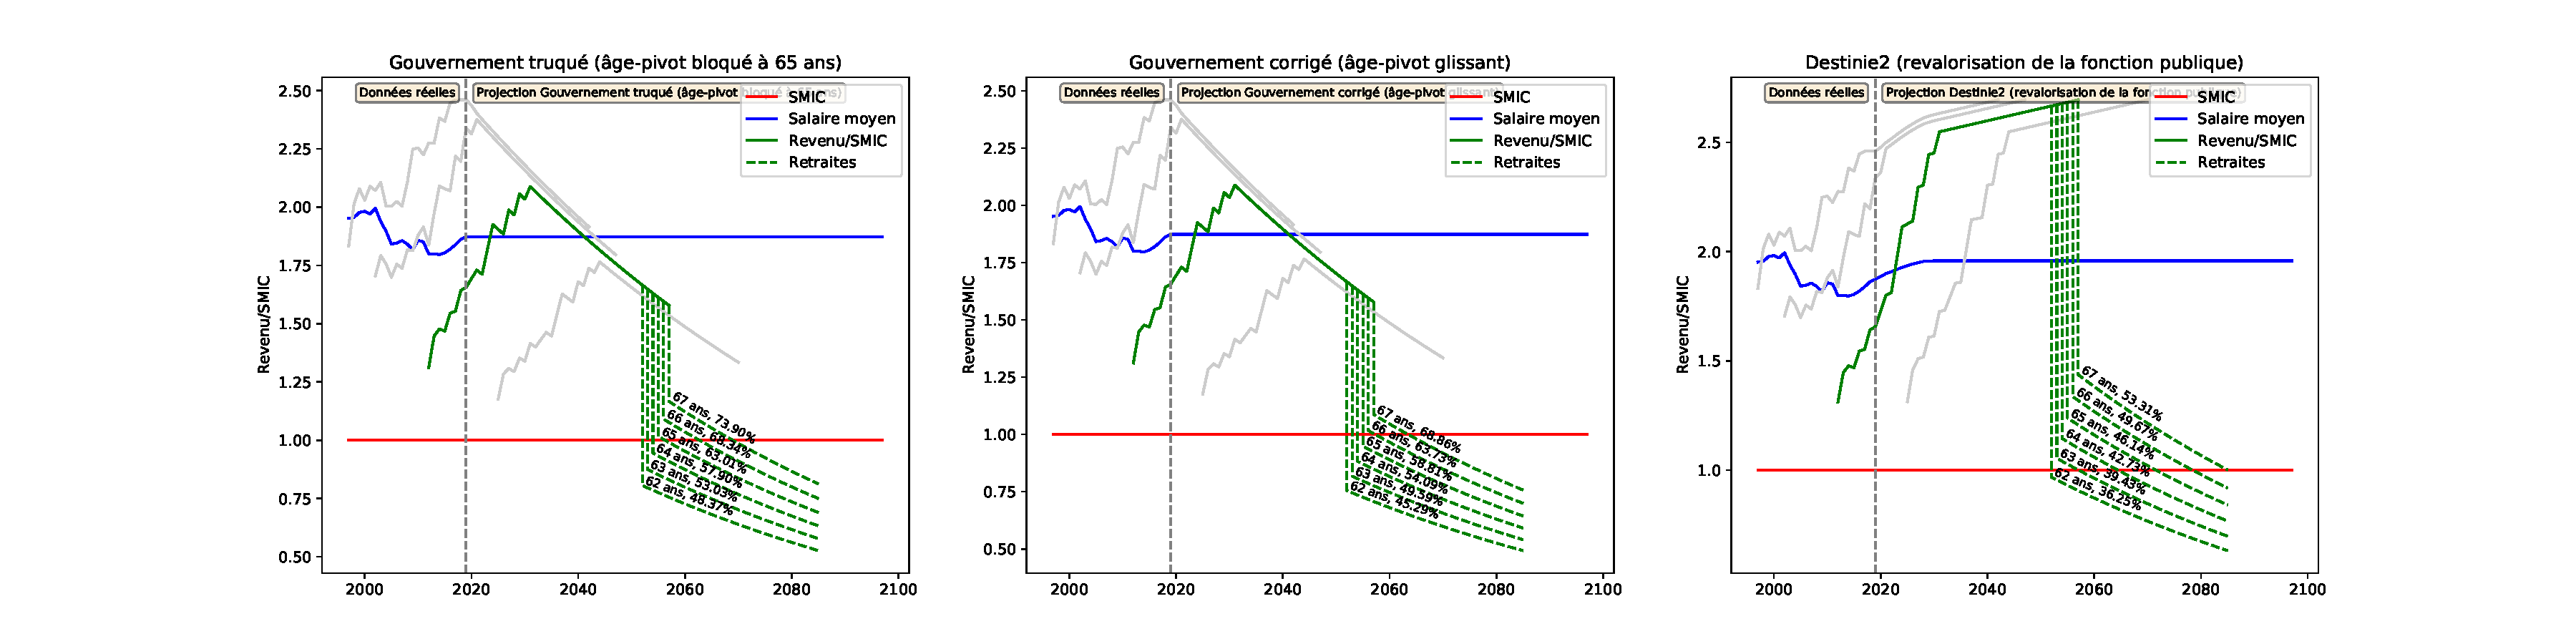
\includegraphics[width=0.9\textwidth]{fig/ProfCertifie_1990_22_dest_retraite.pdf}\end{center} \label{fig/ProfCertifie_1990_22_dest_retraite.pdf} 

\newpage 
 
\paragraph{Revenus et points pour le modèle \emph{Gouvernement truqué (âge-pivot bloqué à 65 ans)}} 
 
{ \scriptsize \begin{center} 
\begin{tabular}[htb]{|c|c||c|c|c|c|c|c||c|c||c|c|c|} 
\hline 
 Année &  Âge &  Ind Maj &  Pt Ind(\euro{} 2019) &  Rev HP(\euro{} 2019) &  Tx Primes &  GIPA(\euro{} 2019) &  Revenu(\euro{} 2019) &  SMIC(\euro{} 2019) &  Rev/SMIC &  Cumul Pts &  Achat Pt(\euro{} 2019) &  Serv. Pt(\euro{} 2019) \\ 
\hline \hline 
 2012 &  22 &  450.0 &  4.88 &  2194.40 &  0.00 &  0.00 &  2194.40 &  1673.05 &  {\bf 1.31} &  739.54 &  35.61 &  0.50 \\ 
\hline 
 2013 &  23 &  498.0 &  4.83 &  2407.66 &  0.00 &  0.00 &  2407.66 &  1664.01 &  {\bf 1.45} &  1550.95 &  35.61 &  0.50 \\ 
\hline 
 2014 &  24 &  513.0 &  4.81 &  2467.76 &  0.17 &  0.00 &  2471.96 &  1673.24 &  {\bf 1.48} &  2384.03 &  35.61 &  0.50 \\ 
\hline 
 2015 &  25 &  513.0 &  4.81 &  2466.80 &  0.40 &  0.00 &  2476.66 &  1686.62 &  {\bf 1.47} &  3218.69 &  35.61 &  0.50 \\ 
\hline 
 2016 &  26 &  542.0 &  4.80 &  2601.04 &  0.63 &  0.00 &  2617.43 &  1693.76 &  {\bf 1.55} &  4100.80 &  35.61 &  0.50 \\ 
\hline 
 2017 &  27 &  542.0 &  4.81 &  2606.29 &  0.86 &  0.00 &  2628.70 &  1692.60 &  {\bf 1.55} &  4986.70 &  35.61 &  0.50 \\ 
\hline 
 2018 &  28 &  579.0 &  4.74 &  2745.77 &  1.09 &  0.00 &  2775.70 &  1689.76 &  {\bf 1.64} &  5922.15 &  35.61 &  0.50 \\ 
\hline 
 2019 &  29 &  579.0 &  4.79 &  2775.97 &  1.32 &  0.00 &  2812.61 &  1698.45 &  {\bf 1.66} &  6870.03 &  35.61 &  0.50 \\ 
\hline 
 2020 &  30 &  598.5 &  4.79 &  2869.46 &  1.55 &  0.00 &  2913.94 &  1720.53 &  {\bf 1.69} &  7852.06 &  35.61 &  0.50 \\ 
\hline 
 2021 &  31 &  618.0 &  4.79 &  2962.95 &  1.78 &  0.00 &  3015.69 &  1742.90 &  {\bf 1.73} &  8868.39 &  35.61 &  0.50 \\ 
\hline 
 2022 &  32 &  618.0 &  4.79 &  2962.95 &  2.01 &  0.00 &  3022.51 &  1765.55 &  {\bf 1.71} &  9887.01 &  35.61 &  0.50 \\ 
\hline 
 2023 &  33 &  664.0 &  4.79 &  3183.50 &  2.24 &  0.00 &  3254.81 &  1788.51 &  {\bf 1.82} &  10983.92 &  35.61 &  0.50 \\ 
\hline 
 2024 &  34 &  710.0 &  4.79 &  3404.04 &  2.47 &  0.00 &  3488.12 &  1811.76 &  {\bf 1.93} &  12159.46 &  35.61 &  0.50 \\ 
\hline 
 2025 &  35 &  710.0 &  4.79 &  3404.04 &  2.70 &  0.00 &  3495.95 &  1835.31 &  {\bf 1.90} &  13337.64 &  35.61 &  0.50 \\ 
\hline 
 2026 &  36 &  710.0 &  4.79 &  3404.04 &  2.93 &  0.00 &  3503.78 &  1859.17 &  {\bf 1.88} &  14518.45 &  35.61 &  0.50 \\ 
\hline 
 2027 &  37 &  757.0 &  4.79 &  3629.38 &  3.16 &  0.00 &  3744.07 &  1883.34 &  {\bf 1.99} &  15780.25 &  35.61 &  0.50 \\ 
\hline 
 2028 &  38 &  757.0 &  4.79 &  3629.38 &  3.39 &  0.00 &  3752.41 &  1907.82 &  {\bf 1.97} &  17044.86 &  35.61 &  0.50 \\ 
\hline 
 2029 &  39 &  800.0 &  4.79 &  3835.54 &  3.62 &  0.00 &  3974.38 &  1932.62 &  {\bf 2.06} &  18383.26 &  35.63 &  0.50 \\ 
\hline 
 2030 &  40 &  800.0 &  4.79 &  3835.54 &  3.85 &  0.00 &  3983.21 &  1957.75 &  {\bf 2.03} &  19722.59 &  35.69 &  0.50 \\ 
\hline 
 2031 &  41 &  830.0 &  4.79 &  3979.37 &  4.08 &  0.00 &  4141.73 &  1983.20 &  {\bf 2.09} &  21112.05 &  35.77 &  0.50 \\ 
\hline 
 2032 &  42 &  830.0 &  4.79 &  3979.37 &  4.31 &  0.00 &  4150.88 &  2008.98 &  {\bf 2.07} &  22500.36 &  35.88 &  0.50 \\ 
\hline 
 2033 &  43 &  830.0 &  4.79 &  3979.37 &  4.54 &  0.00 &  4160.03 &  2035.10 &  {\bf 2.04} &  23886.46 &  36.02 &  0.50 \\ 
\hline 
 2034 &  44 &  830.0 &  4.79 &  3979.37 &  4.77 &  0.00 &  4169.19 &  2061.55 &  {\bf 2.02} &  25269.28 &  36.18 &  0.50 \\ 
\hline 
 2035 &  45 &  830.0 &  4.79 &  3979.37 &  5.00 &  0.00 &  4178.34 &  2088.35 &  {\bf 2.00} &  26647.79 &  36.37 &  0.51 \\ 
\hline 
 2036 &  46 &  830.0 &  4.79 &  3979.37 &  5.23 &  0.00 &  4187.49 &  2115.50 &  {\bf 1.98} &  28020.95 &  36.59 &  0.51 \\ 
\hline 
 2037 &  47 &  830.0 &  4.79 &  3979.37 &  5.46 &  0.00 &  4196.64 &  2143.00 &  {\bf 1.96} &  29387.73 &  36.85 &  0.51 \\ 
\hline 
 2038 &  48 &  830.0 &  4.79 &  3979.37 &  5.69 &  0.00 &  4205.80 &  2170.86 &  {\bf 1.94} &  30747.13 &  37.13 &  0.52 \\ 
\hline 
 2039 &  49 &  830.0 &  4.79 &  3979.37 &  5.92 &  0.00 &  4214.95 &  2199.08 &  {\bf 1.92} &  32098.14 &  37.44 &  0.52 \\ 
\hline 
 2040 &  50 &  830.0 &  4.79 &  3979.37 &  6.15 &  0.00 &  4224.10 &  2227.67 &  {\bf 1.90} &  33439.80 &  37.78 &  0.53 \\ 
\hline 
 2041 &  51 &  830.0 &  4.79 &  3979.37 &  6.38 &  0.00 &  4233.25 &  2256.63 &  {\bf 1.88} &  34771.16 &  38.16 &  0.53 \\ 
\hline 
 2042 &  52 &  830.0 &  4.79 &  3979.37 &  6.61 &  0.00 &  4242.41 &  2285.97 &  {\bf 1.86} &  36091.27 &  38.56 &  0.54 \\ 
\hline 
 2043 &  53 &  830.0 &  4.79 &  3979.37 &  6.84 &  0.00 &  4251.56 &  2315.68 &  {\bf 1.84} &  37399.24 &  39.01 &  0.54 \\ 
\hline 
 2044 &  54 &  830.0 &  4.79 &  3979.37 &  7.07 &  0.00 &  4260.71 &  2345.79 &  {\bf 1.82} &  38694.19 &  39.48 &  0.55 \\ 
\hline 
 2045 &  55 &  830.0 &  4.79 &  3979.37 &  7.30 &  0.00 &  4269.86 &  2376.28 &  {\bf 1.80} &  39975.26 &  40.00 &  0.56 \\ 
\hline 
 2046 &  56 &  830.0 &  4.79 &  3979.37 &  7.53 &  0.00 &  4279.02 &  2407.18 &  {\bf 1.78} &  41242.61 &  40.52 &  0.56 \\ 
\hline 
 2047 &  57 &  830.0 &  4.79 &  3979.37 &  7.76 &  0.00 &  4288.17 &  2438.47 &  {\bf 1.76} &  42496.37 &  41.04 &  0.57 \\ 
\hline 
 2048 &  58 &  830.0 &  4.79 &  3979.37 &  7.99 &  0.00 &  4297.32 &  2470.17 &  {\bf 1.74} &  43736.67 &  41.58 &  0.58 \\ 
\hline 
 2049 &  59 &  830.0 &  4.79 &  3979.37 &  8.22 &  0.00 &  4306.47 &  2502.28 &  {\bf 1.72} &  44963.68 &  42.12 &  0.59 \\ 
\hline 
 2050 &  60 &  830.0 &  4.79 &  3979.37 &  8.45 &  0.00 &  4315.63 &  2534.81 &  {\bf 1.70} &  46177.50 &  42.66 &  0.59 \\ 
\hline 
 2051 &  61 &  830.0 &  4.79 &  3979.37 &  8.68 &  0.00 &  4324.78 &  2567.76 &  {\bf 1.68} &  47378.30 &  43.22 &  0.60 \\ 
\hline 
 2052 &  62 &  830.0 &  4.79 &  3979.37 &  8.91 &  0.00 &  4333.93 &  2601.14 &  {\bf 1.67} &  48566.19 &  43.78 &  0.61 \\ 
\hline 
 2053 &  63 &  830.0 &  4.79 &  3979.37 &  9.14 &  0.00 &  4343.08 &  2634.96 &  {\bf 1.65} &  49741.31 &  44.35 &  0.62 \\ 
\hline 
 2054 &  64 &  830.0 &  4.79 &  3979.37 &  9.37 &  0.00 &  4352.24 &  2669.21 &  {\bf 1.63} &  50903.80 &  44.93 &  0.63 \\ 
\hline 
 2055 &  65 &  830.0 &  4.79 &  3979.37 &  9.60 &  0.00 &  4361.39 &  2703.91 &  {\bf 1.61} &  52053.78 &  45.51 &  0.63 \\ 
\hline 
 2056 &  66 &  830.0 &  4.79 &  3979.37 &  9.83 &  0.00 &  4370.54 &  2739.06 &  {\bf 1.60} &  53191.39 &  46.10 &  0.64 \\ 
\hline 
 2057 &  67 &  830.0 &  4.79 &  3979.37 &  10.06 &  0.00 &  4379.70 &  2774.67 &  {\bf 1.58} &  54316.74 &  46.70 &  0.65 \\ 
\hline 
\hline 
\end{tabular} 
\end{center} } 
\newpage 
 
\paragraph{Revenus et points pour le modèle \emph{Gouvernement corrigé (âge-pivot glissant)}} 
 
{ \scriptsize \begin{center} 
\begin{tabular}[htb]{|c|c||c|c|c|c|c|c||c|c||c|c|c|} 
\hline 
 Année &  Âge &  Ind Maj &  Pt Ind(\euro{} 2019) &  Rev HP(\euro{} 2019) &  Tx Primes &  GIPA(\euro{} 2019) &  Revenu(\euro{} 2019) &  SMIC(\euro{} 2019) &  Rev/SMIC &  Cumul Pts &  Achat Pt(\euro{} 2019) &  Serv. Pt(\euro{} 2019) \\ 
\hline \hline 
 2012 &  22 &  450.0 &  4.88 &  2194.40 &  0.00 &  0.00 &  2194.40 &  1673.05 &  {\bf 1.31} &  739.54 &  35.61 &  0.50 \\ 
\hline 
 2013 &  23 &  498.0 &  4.83 &  2407.66 &  0.00 &  0.00 &  2407.66 &  1664.01 &  {\bf 1.45} &  1550.95 &  35.61 &  0.50 \\ 
\hline 
 2014 &  24 &  513.0 &  4.81 &  2467.76 &  0.17 &  0.00 &  2471.96 &  1673.24 &  {\bf 1.48} &  2384.03 &  35.61 &  0.50 \\ 
\hline 
 2015 &  25 &  513.0 &  4.81 &  2466.80 &  0.40 &  0.00 &  2476.66 &  1686.62 &  {\bf 1.47} &  3218.69 &  35.61 &  0.50 \\ 
\hline 
 2016 &  26 &  542.0 &  4.80 &  2601.04 &  0.63 &  0.00 &  2617.43 &  1693.76 &  {\bf 1.55} &  4100.80 &  35.61 &  0.50 \\ 
\hline 
 2017 &  27 &  542.0 &  4.81 &  2606.29 &  0.86 &  0.00 &  2628.70 &  1692.60 &  {\bf 1.55} &  4986.70 &  35.61 &  0.50 \\ 
\hline 
 2018 &  28 &  579.0 &  4.74 &  2745.77 &  1.09 &  0.00 &  2775.70 &  1689.76 &  {\bf 1.64} &  5922.15 &  35.61 &  0.50 \\ 
\hline 
 2019 &  29 &  579.0 &  4.79 &  2775.97 &  1.32 &  0.00 &  2812.61 &  1698.45 &  {\bf 1.66} &  6870.03 &  35.61 &  0.50 \\ 
\hline 
 2020 &  30 &  598.5 &  4.79 &  2869.46 &  1.55 &  0.00 &  2913.94 &  1720.53 &  {\bf 1.69} &  7852.06 &  35.61 &  0.50 \\ 
\hline 
 2021 &  31 &  618.0 &  4.79 &  2962.95 &  1.78 &  0.00 &  3015.69 &  1742.90 &  {\bf 1.73} &  8868.39 &  35.61 &  0.50 \\ 
\hline 
 2022 &  32 &  618.0 &  4.79 &  2962.95 &  2.01 &  0.00 &  3022.51 &  1765.55 &  {\bf 1.71} &  9887.01 &  35.61 &  0.50 \\ 
\hline 
 2023 &  33 &  664.0 &  4.79 &  3183.50 &  2.24 &  0.00 &  3254.81 &  1788.51 &  {\bf 1.82} &  10983.92 &  35.61 &  0.50 \\ 
\hline 
 2024 &  34 &  710.0 &  4.79 &  3404.04 &  2.47 &  0.00 &  3488.12 &  1811.76 &  {\bf 1.93} &  12159.46 &  35.61 &  0.50 \\ 
\hline 
 2025 &  35 &  710.0 &  4.79 &  3404.04 &  2.70 &  0.00 &  3495.95 &  1835.31 &  {\bf 1.90} &  13337.64 &  35.61 &  0.50 \\ 
\hline 
 2026 &  36 &  710.0 &  4.79 &  3404.04 &  2.93 &  0.00 &  3503.78 &  1859.17 &  {\bf 1.88} &  14518.45 &  35.61 &  0.50 \\ 
\hline 
 2027 &  37 &  757.0 &  4.79 &  3629.38 &  3.16 &  0.00 &  3744.07 &  1883.34 &  {\bf 1.99} &  15780.25 &  35.61 &  0.50 \\ 
\hline 
 2028 &  38 &  757.0 &  4.79 &  3629.38 &  3.39 &  0.00 &  3752.41 &  1907.82 &  {\bf 1.97} &  17044.86 &  35.61 &  0.50 \\ 
\hline 
 2029 &  39 &  800.0 &  4.79 &  3835.54 &  3.62 &  0.00 &  3974.38 &  1932.62 &  {\bf 2.06} &  18383.26 &  35.63 &  0.50 \\ 
\hline 
 2030 &  40 &  800.0 &  4.79 &  3835.54 &  3.85 &  0.00 &  3983.21 &  1957.75 &  {\bf 2.03} &  19722.59 &  35.69 &  0.50 \\ 
\hline 
 2031 &  41 &  830.0 &  4.79 &  3979.37 &  4.08 &  0.00 &  4141.73 &  1983.20 &  {\bf 2.09} &  21112.05 &  35.77 &  0.50 \\ 
\hline 
 2032 &  42 &  830.0 &  4.79 &  3979.37 &  4.31 &  0.00 &  4150.88 &  2008.98 &  {\bf 2.07} &  22500.36 &  35.88 &  0.50 \\ 
\hline 
 2033 &  43 &  830.0 &  4.79 &  3979.37 &  4.54 &  0.00 &  4160.03 &  2035.10 &  {\bf 2.04} &  23886.46 &  36.02 &  0.50 \\ 
\hline 
 2034 &  44 &  830.0 &  4.79 &  3979.37 &  4.77 &  0.00 &  4169.19 &  2061.55 &  {\bf 2.02} &  25269.28 &  36.18 &  0.50 \\ 
\hline 
 2035 &  45 &  830.0 &  4.79 &  3979.37 &  5.00 &  0.00 &  4178.34 &  2088.35 &  {\bf 2.00} &  26647.79 &  36.37 &  0.51 \\ 
\hline 
 2036 &  46 &  830.0 &  4.79 &  3979.37 &  5.23 &  0.00 &  4187.49 &  2115.50 &  {\bf 1.98} &  28020.95 &  36.59 &  0.51 \\ 
\hline 
 2037 &  47 &  830.0 &  4.79 &  3979.37 &  5.46 &  0.00 &  4196.64 &  2143.00 &  {\bf 1.96} &  29387.73 &  36.85 &  0.51 \\ 
\hline 
 2038 &  48 &  830.0 &  4.79 &  3979.37 &  5.69 &  0.00 &  4205.80 &  2170.86 &  {\bf 1.94} &  30747.13 &  37.13 &  0.52 \\ 
\hline 
 2039 &  49 &  830.0 &  4.79 &  3979.37 &  5.92 &  0.00 &  4214.95 &  2199.08 &  {\bf 1.92} &  32098.14 &  37.44 &  0.52 \\ 
\hline 
 2040 &  50 &  830.0 &  4.79 &  3979.37 &  6.15 &  0.00 &  4224.10 &  2227.67 &  {\bf 1.90} &  33439.80 &  37.78 &  0.53 \\ 
\hline 
 2041 &  51 &  830.0 &  4.79 &  3979.37 &  6.38 &  0.00 &  4233.25 &  2256.63 &  {\bf 1.88} &  34771.16 &  38.16 &  0.53 \\ 
\hline 
 2042 &  52 &  830.0 &  4.79 &  3979.37 &  6.61 &  0.00 &  4242.41 &  2285.97 &  {\bf 1.86} &  36091.27 &  38.56 &  0.54 \\ 
\hline 
 2043 &  53 &  830.0 &  4.79 &  3979.37 &  6.84 &  0.00 &  4251.56 &  2315.68 &  {\bf 1.84} &  37399.24 &  39.01 &  0.54 \\ 
\hline 
 2044 &  54 &  830.0 &  4.79 &  3979.37 &  7.07 &  0.00 &  4260.71 &  2345.79 &  {\bf 1.82} &  38694.19 &  39.48 &  0.55 \\ 
\hline 
 2045 &  55 &  830.0 &  4.79 &  3979.37 &  7.30 &  0.00 &  4269.86 &  2376.28 &  {\bf 1.80} &  39975.26 &  40.00 &  0.56 \\ 
\hline 
 2046 &  56 &  830.0 &  4.79 &  3979.37 &  7.53 &  0.00 &  4279.02 &  2407.18 &  {\bf 1.78} &  41242.61 &  40.52 &  0.56 \\ 
\hline 
 2047 &  57 &  830.0 &  4.79 &  3979.37 &  7.76 &  0.00 &  4288.17 &  2438.47 &  {\bf 1.76} &  42496.37 &  41.04 &  0.57 \\ 
\hline 
 2048 &  58 &  830.0 &  4.79 &  3979.37 &  7.99 &  0.00 &  4297.32 &  2470.17 &  {\bf 1.74} &  43736.67 &  41.58 &  0.58 \\ 
\hline 
 2049 &  59 &  830.0 &  4.79 &  3979.37 &  8.22 &  0.00 &  4306.47 &  2502.28 &  {\bf 1.72} &  44963.68 &  42.12 &  0.59 \\ 
\hline 
 2050 &  60 &  830.0 &  4.79 &  3979.37 &  8.45 &  0.00 &  4315.63 &  2534.81 &  {\bf 1.70} &  46177.50 &  42.66 &  0.59 \\ 
\hline 
 2051 &  61 &  830.0 &  4.79 &  3979.37 &  8.68 &  0.00 &  4324.78 &  2567.76 &  {\bf 1.68} &  47378.30 &  43.22 &  0.60 \\ 
\hline 
 2052 &  62 &  830.0 &  4.79 &  3979.37 &  8.91 &  0.00 &  4333.93 &  2601.14 &  {\bf 1.67} &  48566.19 &  43.78 &  0.61 \\ 
\hline 
 2053 &  63 &  830.0 &  4.79 &  3979.37 &  9.14 &  0.00 &  4343.08 &  2634.96 &  {\bf 1.65} &  49741.31 &  44.35 &  0.62 \\ 
\hline 
 2054 &  64 &  830.0 &  4.79 &  3979.37 &  9.37 &  0.00 &  4352.24 &  2669.21 &  {\bf 1.63} &  50903.80 &  44.93 &  0.63 \\ 
\hline 
 2055 &  65 &  830.0 &  4.79 &  3979.37 &  9.60 &  0.00 &  4361.39 &  2703.91 &  {\bf 1.61} &  52053.78 &  45.51 &  0.63 \\ 
\hline 
 2056 &  66 &  830.0 &  4.79 &  3979.37 &  9.83 &  0.00 &  4370.54 &  2739.06 &  {\bf 1.60} &  53191.39 &  46.10 &  0.64 \\ 
\hline 
 2057 &  67 &  830.0 &  4.79 &  3979.37 &  10.06 &  0.00 &  4379.70 &  2774.67 &  {\bf 1.58} &  54316.74 &  46.70 &  0.65 \\ 
\hline 
\hline 
\end{tabular} 
\end{center} } 
\newpage 
 
\paragraph{Revenus et points pour le modèle \emph{Destinie2 (revalorisation de la fonction publique)}} 
 
{ \scriptsize \begin{center} 
\begin{tabular}[htb]{|c|c||c|c|c|c|c|c||c|c||c|c|c|} 
\hline 
 Année &  Âge &  Ind Maj &  Pt Ind(\euro{} 2019) &  Rev HP(\euro{} 2019) &  Tx Primes &  GIPA(\euro{} 2019) &  Revenu(\euro{} 2019) &  SMIC(\euro{} 2019) &  Rev/SMIC &  Cumul Pts &  Achat Pt(\euro{} 2019) &  Serv. Pt(\euro{} 2019) \\ 
\hline \hline 
 2012 &  22 &  450.0 &  4.88 &  2194.40 &  0.00 &  0.00 &  2194.40 &  1673.05 &  {\bf 1.31} &  737.72 &  35.69 &  0.50 \\ 
\hline 
 2013 &  23 &  498.0 &  4.83 &  2407.66 &  0.00 &  0.00 &  2407.66 &  1664.01 &  {\bf 1.45} &  1547.14 &  35.69 &  0.50 \\ 
\hline 
 2014 &  24 &  513.0 &  4.81 &  2467.76 &  0.17 &  0.00 &  2471.96 &  1673.24 &  {\bf 1.48} &  2378.17 &  35.69 &  0.50 \\ 
\hline 
 2015 &  25 &  513.0 &  4.81 &  2466.80 &  0.40 &  0.00 &  2476.66 &  1686.62 &  {\bf 1.47} &  3210.78 &  35.69 &  0.50 \\ 
\hline 
 2016 &  26 &  542.0 &  4.80 &  2601.04 &  0.63 &  0.00 &  2617.43 &  1693.76 &  {\bf 1.55} &  4090.72 &  35.69 &  0.50 \\ 
\hline 
 2017 &  27 &  542.0 &  4.81 &  2606.29 &  0.86 &  0.00 &  2628.70 &  1692.60 &  {\bf 1.55} &  4974.45 &  35.69 &  0.50 \\ 
\hline 
 2018 &  28 &  579.0 &  4.74 &  2745.77 &  1.09 &  0.00 &  2775.70 &  1689.76 &  {\bf 1.64} &  5907.60 &  35.69 &  0.50 \\ 
\hline 
 2019 &  29 &  579.0 &  4.79 &  2775.97 &  1.32 &  0.00 &  2812.61 &  1698.45 &  {\bf 1.66} &  6853.15 &  35.69 &  0.50 \\ 
\hline 
 2020 &  30 &  598.5 &  4.83 &  2892.42 &  1.55 &  0.00 &  2937.25 &  1699.99 &  {\bf 1.73} &  7840.61 &  35.69 &  0.50 \\ 
\hline 
 2021 &  31 &  618.0 &  4.88 &  3013.54 &  1.78 &  0.00 &  3067.18 &  1703.48 &  {\bf 1.80} &  8871.74 &  35.69 &  0.50 \\ 
\hline 
 2022 &  32 &  618.0 &  4.93 &  3043.67 &  2.01 &  0.00 &  3104.85 &  1712.78 &  {\bf 1.81} &  9915.55 &  35.69 &  0.50 \\ 
\hline 
 2023 &  33 &  664.0 &  4.98 &  3308.49 &  2.24 &  0.00 &  3382.60 &  1723.51 &  {\bf 1.96} &  11052.72 &  35.69 &  0.50 \\ 
\hline 
 2024 &  34 &  710.0 &  5.04 &  3579.79 &  2.47 &  0.00 &  3668.21 &  1735.69 &  {\bf 2.11} &  12285.91 &  35.69 &  0.50 \\ 
\hline 
 2025 &  35 &  710.0 &  5.10 &  3623.46 &  2.70 &  0.00 &  3721.29 &  1749.35 &  {\bf 2.13} &  13536.95 &  35.69 &  0.50 \\ 
\hline 
 2026 &  36 &  710.0 &  5.17 &  3668.75 &  2.93 &  0.00 &  3776.25 &  1764.53 &  {\bf 2.14} &  14806.47 &  35.69 &  0.50 \\ 
\hline 
 2027 &  37 &  757.0 &  5.23 &  3961.68 &  3.16 &  0.00 &  4086.87 &  1781.27 &  {\bf 2.29} &  16180.41 &  35.69 &  0.50 \\ 
\hline 
 2028 &  38 &  757.0 &  5.30 &  4013.58 &  3.39 &  0.00 &  4149.64 &  1799.59 &  {\bf 2.31} &  17575.45 &  35.69 &  0.50 \\ 
\hline 
 2029 &  39 &  800.0 &  5.37 &  4292.89 &  3.62 &  0.00 &  4448.29 &  1819.55 &  {\bf 2.44} &  19069.84 &  35.72 &  0.50 \\ 
\hline 
 2030 &  40 &  800.0 &  5.43 &  4346.12 &  3.85 &  0.00 &  4513.44 &  1841.19 &  {\bf 2.45} &  20583.92 &  35.77 &  0.50 \\ 
\hline 
 2031 &  41 &  830.0 &  5.50 &  4566.36 &  4.08 &  0.00 &  4752.67 &  1864.58 &  {\bf 2.55} &  22174.70 &  35.85 &  0.50 \\ 
\hline 
 2032 &  42 &  830.0 &  5.57 &  4625.73 &  4.31 &  0.00 &  4825.10 &  1888.81 &  {\bf 2.55} &  23784.82 &  35.96 &  0.50 \\ 
\hline 
 2033 &  43 &  830.0 &  5.65 &  4685.86 &  4.54 &  0.00 &  4898.60 &  1913.37 &  {\bf 2.56} &  25413.28 &  36.10 &  0.50 \\ 
\hline 
 2034 &  44 &  830.0 &  5.72 &  4746.78 &  4.77 &  0.00 &  4973.20 &  1938.24 &  {\bf 2.57} &  27059.01 &  36.26 &  0.50 \\ 
\hline 
 2035 &  45 &  830.0 &  5.79 &  4808.49 &  5.00 &  0.00 &  5048.91 &  1963.44 &  {\bf 2.57} &  28720.93 &  36.46 &  0.51 \\ 
\hline 
 2036 &  46 &  830.0 &  5.87 &  4871.00 &  5.23 &  0.00 &  5125.75 &  1988.96 &  {\bf 2.58} &  30397.93 &  36.68 &  0.51 \\ 
\hline 
 2037 &  47 &  830.0 &  5.94 &  4934.32 &  5.46 &  0.00 &  5203.73 &  2014.82 &  {\bf 2.58} &  32088.83 &  36.93 &  0.51 \\ 
\hline 
 2038 &  48 &  830.0 &  6.02 &  4998.46 &  5.69 &  0.00 &  5282.88 &  2041.01 &  {\bf 2.59} &  33792.46 &  37.21 &  0.52 \\ 
\hline 
 2039 &  49 &  830.0 &  6.10 &  5063.44 &  5.92 &  0.00 &  5363.20 &  2067.55 &  {\bf 2.59} &  35507.60 &  37.52 &  0.52 \\ 
\hline 
 2040 &  50 &  830.0 &  6.18 &  5129.27 &  6.15 &  0.00 &  5444.72 &  2094.43 &  {\bf 2.60} &  37233.00 &  37.87 &  0.53 \\ 
\hline 
 2041 &  51 &  830.0 &  6.26 &  5195.95 &  6.38 &  0.00 &  5527.45 &  2121.65 &  {\bf 2.61} &  38967.41 &  38.24 &  0.53 \\ 
\hline 
 2042 &  52 &  830.0 &  6.34 &  5263.50 &  6.61 &  0.00 &  5611.41 &  2149.23 &  {\bf 2.61} &  40709.53 &  38.65 &  0.54 \\ 
\hline 
 2043 &  53 &  830.0 &  6.42 &  5331.92 &  6.84 &  0.00 &  5696.63 &  2177.17 &  {\bf 2.62} &  42458.07 &  39.10 &  0.54 \\ 
\hline 
 2044 &  54 &  830.0 &  6.51 &  5401.24 &  7.07 &  0.00 &  5783.11 &  2205.48 &  {\bf 2.62} &  44211.70 &  39.57 &  0.55 \\ 
\hline 
 2045 &  55 &  830.0 &  6.59 &  5471.45 &  7.30 &  0.00 &  5870.87 &  2234.15 &  {\bf 2.63} &  45969.10 &  40.09 &  0.56 \\ 
\hline 
 2046 &  56 &  830.0 &  6.68 &  5542.58 &  7.53 &  0.00 &  5959.94 &  2263.19 &  {\bf 2.63} &  47730.27 &  40.61 &  0.57 \\ 
\hline 
 2047 &  57 &  830.0 &  6.76 &  5614.64 &  7.76 &  0.00 &  6050.33 &  2292.61 &  {\bf 2.64} &  49495.20 &  41.14 &  0.57 \\ 
\hline 
 2048 &  58 &  830.0 &  6.85 &  5687.63 &  7.99 &  0.00 &  6142.07 &  2322.42 &  {\bf 2.64} &  51263.90 &  41.67 &  0.58 \\ 
\hline 
 2049 &  59 &  830.0 &  6.94 &  5761.57 &  8.22 &  0.00 &  6235.17 &  2352.61 &  {\bf 2.65} &  53036.37 &  42.21 &  0.59 \\ 
\hline 
 2050 &  60 &  830.0 &  7.03 &  5836.47 &  8.45 &  0.00 &  6329.65 &  2383.19 &  {\bf 2.66} &  54812.60 &  42.76 &  0.60 \\ 
\hline 
 2051 &  61 &  830.0 &  7.12 &  5912.34 &  8.68 &  0.00 &  6425.53 &  2414.18 &  {\bf 2.66} &  56592.60 &  43.32 &  0.60 \\ 
\hline 
 2052 &  62 &  830.0 &  7.22 &  5989.20 &  8.91 &  0.00 &  6522.84 &  2445.56 &  {\bf 2.67} &  58376.37 &  43.88 &  0.61 \\ 
\hline 
 2053 &  63 &  830.0 &  7.31 &  6067.06 &  9.14 &  0.00 &  6621.59 &  2477.35 &  {\bf 2.67} &  60163.90 &  44.45 &  0.62 \\ 
\hline 
 2054 &  64 &  830.0 &  7.40 &  6145.93 &  9.37 &  0.00 &  6721.81 &  2509.56 &  {\bf 2.68} &  61955.21 &  45.03 &  0.63 \\ 
\hline 
 2055 &  65 &  830.0 &  7.50 &  6225.83 &  9.60 &  0.00 &  6823.51 &  2542.18 &  {\bf 2.68} &  63750.28 &  45.62 &  0.63 \\ 
\hline 
 2056 &  66 &  830.0 &  7.60 &  6306.77 &  9.83 &  0.00 &  6926.72 &  2575.23 &  {\bf 2.69} &  65549.11 &  46.21 &  0.64 \\ 
\hline 
 2057 &  67 &  830.0 &  7.70 &  6388.75 &  10.06 &  0.00 &  7031.46 &  2608.71 &  {\bf 2.70} &  67351.72 &  46.81 &  0.65 \\ 
\hline 
\hline 
\end{tabular} 
\end{center} } 
\newpage 
 
\subsection{Génération 2003 (début en 2025)} 

\paragraph{Retraites possibles dans le modèle \emph{Gouvernement truqué (âge-pivot bloqué à 65 ans)}}  
 
{ \scriptsize \begin{center} 
\begin{tabular}[htb]{|c|c||c|c||c|c||c||c|c|c|c|c|c|} 
\hline 
 Retraite en &  Âge &  Âge pivot &  Décote/Surcote &  Retraite (\euro{} 2019) &  Tx Rempl(\%) &  SMIC (\euro{} 2019) &  Retraite/SMIC &  Rev70/SMIC &  Rev75/SMIC &  Rev80/SMIC &  Rev85/SMIC &  Rev90/SMIC \\ 
\hline \hline 
 2065 &  62 &  65 ans 0 mois &  -15.00\% &  2241.05 &  {\bf 51.71} &  3076.71 &  {\bf {\color{red} 0.73}} &  {\bf {\color{red} 0.66}} &  {\bf {\color{red} 0.62}} &  {\bf {\color{red} 0.58}} &  {\bf {\color{red} 0.54}} &  {\bf {\color{red} 0.51}} \\ 
\hline 
 2066 &  63 &  65 ans 0 mois &  -10.00\% &  2458.13 &  {\bf 56.60} &  3116.71 &  {\bf {\color{red} 0.79}} &  {\bf {\color{red} 0.72}} &  {\bf {\color{red} 0.68}} &  {\bf {\color{red} 0.63}} &  {\bf {\color{red} 0.59}} &  {\bf {\color{red} 0.56}} \\ 
\hline 
 2067 &  64 &  65 ans 0 mois &  -5.00\% &  2685.98 &  {\bf 61.71} &  3157.23 &  {\bf {\color{red} 0.85}} &  {\bf {\color{red} 0.79}} &  {\bf {\color{red} 0.74}} &  {\bf {\color{red} 0.69}} &  {\bf {\color{red} 0.65}} &  {\bf {\color{red} 0.61}} \\ 
\hline 
 2068 &  65 &  65 ans 0 mois &  0.00\% &  2924.81 &  {\bf 67.06} &  3198.27 &  {\bf {\color{red} 0.91}} &  {\bf {\color{red} 0.86}} &  {\bf {\color{red} 0.80}} &  {\bf {\color{red} 0.75}} &  {\bf {\color{red} 0.71}} &  {\bf {\color{red} 0.66}} \\ 
\hline 
 2069 &  66 &  65 ans 0 mois &  5.00\% &  3174.85 &  {\bf 72.64} &  3239.85 &  {\bf {\color{red} 0.98}} &  {\bf {\color{red} 0.93}} &  {\bf {\color{red} 0.87}} &  {\bf {\color{red} 0.82}} &  {\bf {\color{red} 0.77}} &  {\bf {\color{red} 0.72}} \\ 
\hline 
 2070 &  67 &  65 ans 0 mois &  10.00\% &  3436.33 &  {\bf 78.46} &  3281.97 &  {\bf 1.05} &  {\bf 1.01} &  {\bf {\color{red} 0.94}} &  {\bf {\color{red} 0.89}} &  {\bf {\color{red} 0.83}} &  {\bf {\color{red} 0.78}} \\ 
\hline 
\hline 
\end{tabular} 
\end{center} } 
\paragraph{Retraites possibles dans le modèle \emph{Gouvernement corrigé (âge-pivot glissant)}}  
 
{ \scriptsize \begin{center} 
\begin{tabular}[htb]{|c|c||c|c||c|c||c||c|c|c|c|c|c|} 
\hline 
 Retraite en &  Âge &  Âge pivot &  Décote/Surcote &  Retraite (\euro{} 2019) &  Tx Rempl(\%) &  SMIC (\euro{} 2019) &  Retraite/SMIC &  Rev70/SMIC &  Rev75/SMIC &  Rev80/SMIC &  Rev85/SMIC &  Rev90/SMIC \\ 
\hline \hline 
 2065 &  62 &  67 ans 2 mois &  -25.83\% &  1955.43 &  {\bf 45.12} &  3076.71 &  {\bf {\color{red} 0.64}} &  {\bf {\color{red} 0.57}} &  {\bf {\color{red} 0.54}} &  {\bf {\color{red} 0.50}} &  {\bf {\color{red} 0.47}} &  {\bf {\color{red} 0.44}} \\ 
\hline 
 2066 &  63 &  67 ans 3 mois &  -21.25\% &  2150.87 &  {\bf 49.52} &  3116.71 &  {\bf {\color{red} 0.69}} &  {\bf {\color{red} 0.63}} &  {\bf {\color{red} 0.59}} &  {\bf {\color{red} 0.55}} &  {\bf {\color{red} 0.52}} &  {\bf {\color{red} 0.49}} \\ 
\hline 
 2067 &  64 &  67 ans 4 mois &  -16.67\% &  2356.12 &  {\bf 54.14} &  3157.23 &  {\bf {\color{red} 0.75}} &  {\bf {\color{red} 0.69}} &  {\bf {\color{red} 0.65}} &  {\bf {\color{red} 0.61}} &  {\bf {\color{red} 0.57}} &  {\bf {\color{red} 0.53}} \\ 
\hline 
 2068 &  65 &  67 ans 5 mois &  -12.08\% &  2718.53 &  {\bf 62.33} &  3198.27 &  {\bf {\color{red} 0.85}} &  {\bf {\color{red} 0.80}} &  {\bf {\color{red} 0.75}} &  {\bf {\color{red} 0.70}} &  {\bf {\color{red} 0.66}} &  {\bf {\color{red} 0.62}} \\ 
\hline 
 2069 &  66 &  67 ans 6 mois &  -7.50\% &  2796.89 &  {\bf 63.99} &  3239.85 &  {\bf {\color{red} 0.86}} &  {\bf {\color{red} 0.82}} &  {\bf {\color{red} 0.77}} &  {\bf {\color{red} 0.72}} &  {\bf {\color{red} 0.68}} &  {\bf {\color{red} 0.63}} \\ 
\hline 
 2070 &  67 &  67 ans 7 mois &  -2.92\% &  3032.82 &  {\bf 69.25} &  3281.97 &  {\bf {\color{red} 0.92}} &  {\bf {\color{red} 0.89}} &  {\bf {\color{red} 0.83}} &  {\bf {\color{red} 0.78}} &  {\bf {\color{red} 0.73}} &  {\bf {\color{red} 0.69}} \\ 
\hline 
\hline 
\end{tabular} 
\end{center} } 
\paragraph{Retraites possibles dans le modèle \emph{Destinie2 (revalorisation de la fonction publique)}}  
 
{ \scriptsize \begin{center} 
\begin{tabular}[htb]{|c|c||c|c||c|c||c||c|c|c|c|c|c|} 
\hline 
 Retraite en &  Âge &  Âge pivot &  Décote/Surcote &  Retraite (\euro{} 2019) &  Tx Rempl(\%) &  SMIC (\euro{} 2019) &  Retraite/SMIC &  Rev70/SMIC &  Rev75/SMIC &  Rev80/SMIC &  Rev85/SMIC &  Rev90/SMIC \\ 
\hline \hline 
 2065 &  62 &  67 ans 2 mois &  -25.83\% &  2741.75 &  {\bf 35.54} &  2892.68 &  {\bf {\color{red} 0.95}} &  {\bf {\color{red} 0.85}} &  {\bf {\color{red} 0.80}} &  {\bf {\color{red} 0.75}} &  {\bf {\color{red} 0.70}} &  {\bf {\color{red} 0.66}} \\ 
\hline 
 2066 &  63 &  67 ans 3 mois &  -21.25\% &  3034.88 &  {\bf 38.75} &  2930.29 &  {\bf 1.04} &  {\bf {\color{red} 0.95}} &  {\bf {\color{red} 0.89}} &  {\bf {\color{red} 0.83}} &  {\bf {\color{red} 0.78}} &  {\bf {\color{red} 0.73}} \\ 
\hline 
 2067 &  64 &  67 ans 4 mois &  -16.67\% &  3345.49 &  {\bf 42.08} &  2968.38 &  {\bf 1.13} &  {\bf 1.04} &  {\bf {\color{red} 0.98}} &  {\bf {\color{red} 0.92}} &  {\bf {\color{red} 0.86}} &  {\bf {\color{red} 0.81}} \\ 
\hline 
 2068 &  65 &  67 ans 5 mois &  -12.08\% &  3674.15 &  {\bf 45.52} &  3006.97 &  {\bf 1.22} &  {\bf 1.15} &  {\bf 1.07} &  {\bf 1.01} &  {\bf {\color{red} 0.94}} &  {\bf {\color{red} 0.88}} \\ 
\hline 
 2069 &  66 &  67 ans 6 mois &  -7.50\% &  4021.43 &  {\bf 49.08} &  3046.06 &  {\bf 1.32} &  {\bf 1.25} &  {\bf 1.18} &  {\bf 1.10} &  {\bf 1.03} &  {\bf {\color{red} 0.97}} \\ 
\hline 
 2070 &  67 &  67 ans 7 mois &  -2.92\% &  4387.96 &  {\bf 52.76} &  3085.66 &  {\bf 1.42} &  {\bf 1.37} &  {\bf 1.28} &  {\bf 1.20} &  {\bf 1.13} &  {\bf 1.06} \\ 
\hline 
\hline 
\end{tabular} 
\end{center} } 

 \begin{center}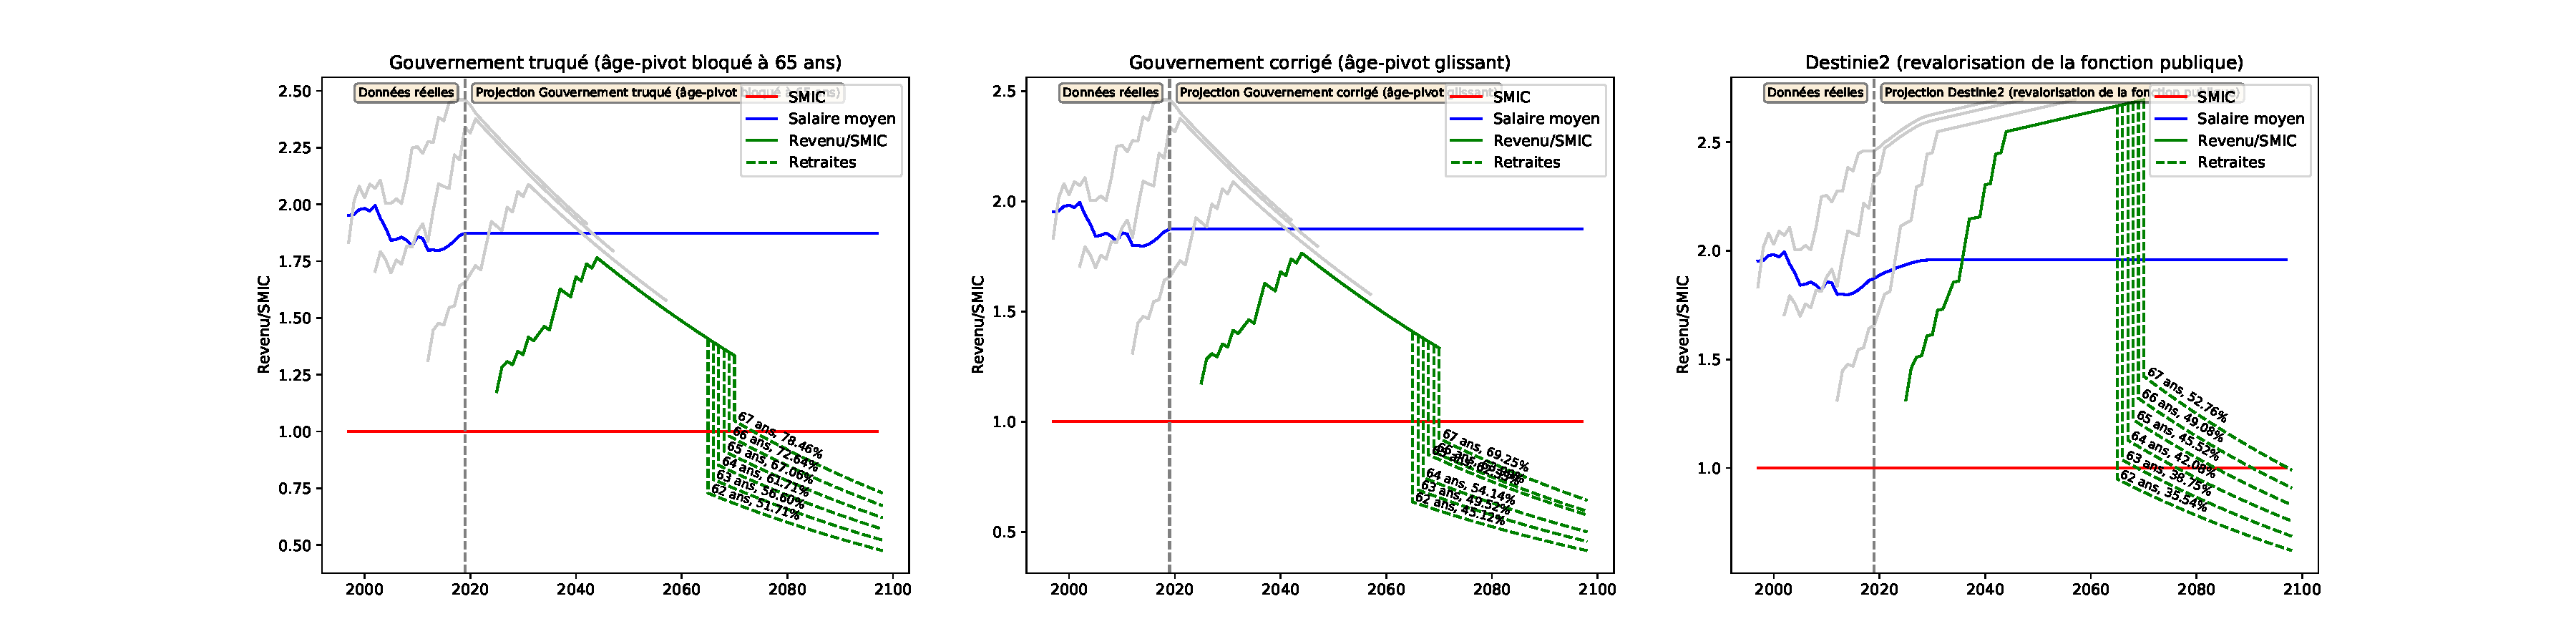
\includegraphics[width=0.9\textwidth]{fig/ProfCertifie_2003_22_dest_retraite.pdf}\end{center} \label{fig/ProfCertifie_2003_22_dest_retraite.pdf} 

\newpage 
 
\paragraph{Revenus et points pour le modèle \emph{Gouvernement truqué (âge-pivot bloqué à 65 ans)}} 
 
{ \scriptsize \begin{center} 
\begin{tabular}[htb]{|c|c||c|c|c|c|c|c||c|c||c|c|c|} 
\hline 
 Année &  Âge &  Ind Maj &  Pt Ind(\euro{} 2019) &  Rev HP(\euro{} 2019) &  Tx Primes &  GIPA(\euro{} 2019) &  Revenu(\euro{} 2019) &  SMIC(\euro{} 2019) &  Rev/SMIC &  Cumul Pts &  Achat Pt(\euro{} 2019) &  Serv. Pt(\euro{} 2019) \\ 
\hline \hline 
 2025 &  22 &  450.0 &  4.79 &  2157.49 &  0.00 &  0.00 &  2157.49 &  1835.31 &  {\bf 1.18} &  727.10 &  35.61 &  0.50 \\ 
\hline 
 2026 &  23 &  498.0 &  4.79 &  2387.62 &  0.00 &  0.00 &  2387.62 &  1859.17 &  {\bf 1.28} &  1531.76 &  35.61 &  0.50 \\ 
\hline 
 2027 &  24 &  513.0 &  4.79 &  2459.54 &  0.17 &  0.00 &  2463.72 &  1883.34 &  {\bf 1.31} &  2362.06 &  35.61 &  0.50 \\ 
\hline 
 2028 &  25 &  513.0 &  4.79 &  2459.54 &  0.40 &  0.00 &  2469.38 &  1907.82 &  {\bf 1.29} &  3194.27 &  35.61 &  0.50 \\ 
\hline 
 2029 &  26 &  542.0 &  4.79 &  2598.58 &  0.63 &  0.00 &  2614.95 &  1932.62 &  {\bf 1.35} &  4074.87 &  35.63 &  0.50 \\ 
\hline 
 2030 &  27 &  542.0 &  4.79 &  2598.58 &  0.86 &  0.00 &  2620.92 &  1957.75 &  {\bf 1.34} &  4956.14 &  35.69 &  0.50 \\ 
\hline 
 2031 &  28 &  579.0 &  4.79 &  2775.97 &  1.09 &  0.00 &  2806.23 &  1983.20 &  {\bf 1.42} &  5897.58 &  35.77 &  0.50 \\ 
\hline 
 2032 &  29 &  579.0 &  4.79 &  2775.97 &  1.32 &  0.00 &  2812.61 &  2008.98 &  {\bf 1.40} &  6838.29 &  35.88 &  0.50 \\ 
\hline 
 2033 &  30 &  598.5 &  4.79 &  2869.46 &  1.55 &  0.00 &  2913.94 &  2035.10 &  {\bf 1.43} &  7809.19 &  36.02 &  0.50 \\ 
\hline 
 2034 &  31 &  618.0 &  4.79 &  2962.95 &  1.78 &  0.00 &  3015.69 &  2061.55 &  {\bf 1.46} &  8809.43 &  36.18 &  0.50 \\ 
\hline 
 2035 &  32 &  618.0 &  4.79 &  2962.95 &  2.01 &  0.00 &  3022.51 &  2088.35 &  {\bf 1.45} &  9806.61 &  36.37 &  0.51 \\ 
\hline 
 2036 &  33 &  664.0 &  4.79 &  3183.50 &  2.24 &  0.00 &  3254.81 &  2115.50 &  {\bf 1.54} &  10873.92 &  36.59 &  0.51 \\ 
\hline 
 2037 &  34 &  710.0 &  4.79 &  3404.04 &  2.47 &  0.00 &  3488.12 &  2143.00 &  {\bf 1.63} &  12009.95 &  36.85 &  0.51 \\ 
\hline 
 2038 &  35 &  710.0 &  4.79 &  3404.04 &  2.70 &  0.00 &  3495.95 &  2170.86 &  {\bf 1.61} &  13139.91 &  37.13 &  0.52 \\ 
\hline 
 2039 &  36 &  710.0 &  4.79 &  3404.04 &  2.93 &  0.00 &  3503.78 &  2199.08 &  {\bf 1.59} &  14262.97 &  37.44 &  0.52 \\ 
\hline 
 2040 &  37 &  757.0 &  4.79 &  3629.38 &  3.16 &  0.00 &  3744.07 &  2227.67 &  {\bf 1.68} &  15452.16 &  37.78 &  0.53 \\ 
\hline 
 2041 &  38 &  757.0 &  4.79 &  3629.38 &  3.39 &  0.00 &  3752.41 &  2256.63 &  {\bf 1.66} &  16632.29 &  38.16 &  0.53 \\ 
\hline 
 2042 &  39 &  800.0 &  4.79 &  3835.54 &  3.62 &  0.00 &  3974.38 &  2285.97 &  {\bf 1.74} &  17869.00 &  38.56 &  0.54 \\ 
\hline 
 2043 &  40 &  800.0 &  4.79 &  3835.54 &  3.85 &  0.00 &  3983.21 &  2315.68 &  {\bf 1.72} &  19094.42 &  39.01 &  0.54 \\ 
\hline 
 2044 &  41 &  830.0 &  4.79 &  3979.37 &  4.08 &  0.00 &  4141.73 &  2345.79 &  {\bf 1.77} &  20353.20 &  39.48 &  0.55 \\ 
\hline 
 2045 &  42 &  830.0 &  4.79 &  3979.37 &  4.31 &  0.00 &  4150.88 &  2376.28 &  {\bf 1.75} &  21598.58 &  40.00 &  0.56 \\ 
\hline 
 2046 &  43 &  830.0 &  4.79 &  3979.37 &  4.54 &  0.00 &  4160.03 &  2407.18 &  {\bf 1.73} &  22830.68 &  40.52 &  0.56 \\ 
\hline 
 2047 &  44 &  830.0 &  4.79 &  3979.37 &  4.77 &  0.00 &  4169.19 &  2438.47 &  {\bf 1.71} &  24049.65 &  41.04 &  0.57 \\ 
\hline 
 2048 &  45 &  830.0 &  4.79 &  3979.37 &  5.00 &  0.00 &  4178.34 &  2470.17 &  {\bf 1.69} &  25255.62 &  41.58 &  0.58 \\ 
\hline 
 2049 &  46 &  830.0 &  4.79 &  3979.37 &  5.23 &  0.00 &  4187.49 &  2502.28 &  {\bf 1.67} &  26448.72 &  42.12 &  0.59 \\ 
\hline 
 2050 &  47 &  830.0 &  4.79 &  3979.37 &  5.46 &  0.00 &  4196.64 &  2534.81 &  {\bf 1.66} &  27629.08 &  42.66 &  0.59 \\ 
\hline 
 2051 &  48 &  830.0 &  4.79 &  3979.37 &  5.69 &  0.00 &  4205.80 &  2567.76 &  {\bf 1.64} &  28796.84 &  43.22 &  0.60 \\ 
\hline 
 2052 &  49 &  830.0 &  4.79 &  3979.37 &  5.92 &  0.00 &  4214.95 &  2601.14 &  {\bf 1.62} &  29952.12 &  43.78 &  0.61 \\ 
\hline 
 2053 &  50 &  830.0 &  4.79 &  3979.37 &  6.15 &  0.00 &  4224.10 &  2634.96 &  {\bf 1.60} &  31095.05 &  44.35 &  0.62 \\ 
\hline 
 2054 &  51 &  830.0 &  4.79 &  3979.37 &  6.38 &  0.00 &  4233.25 &  2669.21 &  {\bf 1.59} &  32225.76 &  44.93 &  0.63 \\ 
\hline 
 2055 &  52 &  830.0 &  4.79 &  3979.37 &  6.61 &  0.00 &  4242.41 &  2703.91 &  {\bf 1.57} &  33344.36 &  45.51 &  0.63 \\ 
\hline 
 2056 &  53 &  830.0 &  4.79 &  3979.37 &  6.84 &  0.00 &  4251.56 &  2739.06 &  {\bf 1.55} &  34451.00 &  46.10 &  0.64 \\ 
\hline 
 2057 &  54 &  830.0 &  4.79 &  3979.37 &  7.07 &  0.00 &  4260.71 &  2774.67 &  {\bf 1.54} &  35545.79 &  46.70 &  0.65 \\ 
\hline 
 2058 &  55 &  830.0 &  4.79 &  3979.37 &  7.30 &  0.00 &  4269.86 &  2810.74 &  {\bf 1.52} &  36628.85 &  47.31 &  0.66 \\ 
\hline 
 2059 &  56 &  830.0 &  4.79 &  3979.37 &  7.53 &  0.00 &  4279.02 &  2847.28 &  {\bf 1.50} &  37700.30 &  47.92 &  0.67 \\ 
\hline 
 2060 &  57 &  830.0 &  4.79 &  3979.37 &  7.76 &  0.00 &  4288.17 &  2884.30 &  {\bf 1.49} &  38760.26 &  48.55 &  0.68 \\ 
\hline 
 2061 &  58 &  830.0 &  4.79 &  3979.37 &  7.99 &  0.00 &  4297.32 &  2921.79 &  {\bf 1.47} &  39808.85 &  49.18 &  0.68 \\ 
\hline 
 2062 &  59 &  830.0 &  4.79 &  3979.37 &  8.22 &  0.00 &  4306.47 &  2959.78 &  {\bf 1.45} &  40846.20 &  49.82 &  0.69 \\ 
\hline 
 2063 &  60 &  830.0 &  4.79 &  3979.37 &  8.45 &  0.00 &  4315.63 &  2998.25 &  {\bf 1.44} &  41872.40 &  50.47 &  0.70 \\ 
\hline 
 2064 &  61 &  830.0 &  4.79 &  3979.37 &  8.68 &  0.00 &  4324.78 &  3037.23 &  {\bf 1.42} &  42887.59 &  51.12 &  0.71 \\ 
\hline 
 2065 &  62 &  830.0 &  4.79 &  3979.37 &  8.91 &  0.00 &  4333.93 &  3076.71 &  {\bf 1.41} &  43891.86 &  51.79 &  0.72 \\ 
\hline 
 2066 &  63 &  830.0 &  4.79 &  3979.37 &  9.14 &  0.00 &  4343.08 &  3116.71 &  {\bf 1.39} &  44885.35 &  52.46 &  0.73 \\ 
\hline 
 2067 &  64 &  830.0 &  4.79 &  3979.37 &  9.37 &  0.00 &  4352.24 &  3157.23 &  {\bf 1.38} &  45868.15 &  53.14 &  0.74 \\ 
\hline 
 2068 &  65 &  830.0 &  4.79 &  3979.37 &  9.60 &  0.00 &  4361.39 &  3198.27 &  {\bf 1.36} &  46840.38 &  53.83 &  0.75 \\ 
\hline 
 2069 &  66 &  830.0 &  4.79 &  3979.37 &  9.83 &  0.00 &  4370.54 &  3239.85 &  {\bf 1.35} &  47802.14 &  54.53 &  0.76 \\ 
\hline 
 2070 &  67 &  830.0 &  4.79 &  3979.37 &  10.06 &  0.00 &  4379.70 &  3281.97 &  {\bf 1.33} &  48753.55 &  55.24 &  0.77 \\ 
\hline 
\hline 
\end{tabular} 
\end{center} } 
\newpage 
 
\paragraph{Revenus et points pour le modèle \emph{Gouvernement corrigé (âge-pivot glissant)}} 
 
{ \scriptsize \begin{center} 
\begin{tabular}[htb]{|c|c||c|c|c|c|c|c||c|c||c|c|c|} 
\hline 
 Année &  Âge &  Ind Maj &  Pt Ind(\euro{} 2019) &  Rev HP(\euro{} 2019) &  Tx Primes &  GIPA(\euro{} 2019) &  Revenu(\euro{} 2019) &  SMIC(\euro{} 2019) &  Rev/SMIC &  Cumul Pts &  Achat Pt(\euro{} 2019) &  Serv. Pt(\euro{} 2019) \\ 
\hline \hline 
 2025 &  22 &  450.0 &  4.79 &  2157.49 &  0.00 &  0.00 &  2157.49 &  1835.31 &  {\bf 1.18} &  727.10 &  35.61 &  0.50 \\ 
\hline 
 2026 &  23 &  498.0 &  4.79 &  2387.62 &  0.00 &  0.00 &  2387.62 &  1859.17 &  {\bf 1.28} &  1531.76 &  35.61 &  0.50 \\ 
\hline 
 2027 &  24 &  513.0 &  4.79 &  2459.54 &  0.17 &  0.00 &  2463.72 &  1883.34 &  {\bf 1.31} &  2362.06 &  35.61 &  0.50 \\ 
\hline 
 2028 &  25 &  513.0 &  4.79 &  2459.54 &  0.40 &  0.00 &  2469.38 &  1907.82 &  {\bf 1.29} &  3194.27 &  35.61 &  0.50 \\ 
\hline 
 2029 &  26 &  542.0 &  4.79 &  2598.58 &  0.63 &  0.00 &  2614.95 &  1932.62 &  {\bf 1.35} &  4074.87 &  35.63 &  0.50 \\ 
\hline 
 2030 &  27 &  542.0 &  4.79 &  2598.58 &  0.86 &  0.00 &  2620.92 &  1957.75 &  {\bf 1.34} &  4956.14 &  35.69 &  0.50 \\ 
\hline 
 2031 &  28 &  579.0 &  4.79 &  2775.97 &  1.09 &  0.00 &  2806.23 &  1983.20 &  {\bf 1.42} &  5897.58 &  35.77 &  0.50 \\ 
\hline 
 2032 &  29 &  579.0 &  4.79 &  2775.97 &  1.32 &  0.00 &  2812.61 &  2008.98 &  {\bf 1.40} &  6838.29 &  35.88 &  0.50 \\ 
\hline 
 2033 &  30 &  598.5 &  4.79 &  2869.46 &  1.55 &  0.00 &  2913.94 &  2035.10 &  {\bf 1.43} &  7809.19 &  36.02 &  0.50 \\ 
\hline 
 2034 &  31 &  618.0 &  4.79 &  2962.95 &  1.78 &  0.00 &  3015.69 &  2061.55 &  {\bf 1.46} &  8809.43 &  36.18 &  0.50 \\ 
\hline 
 2035 &  32 &  618.0 &  4.79 &  2962.95 &  2.01 &  0.00 &  3022.51 &  2088.35 &  {\bf 1.45} &  9806.61 &  36.37 &  0.51 \\ 
\hline 
 2036 &  33 &  664.0 &  4.79 &  3183.50 &  2.24 &  0.00 &  3254.81 &  2115.50 &  {\bf 1.54} &  10873.92 &  36.59 &  0.51 \\ 
\hline 
 2037 &  34 &  710.0 &  4.79 &  3404.04 &  2.47 &  0.00 &  3488.12 &  2143.00 &  {\bf 1.63} &  12009.95 &  36.85 &  0.51 \\ 
\hline 
 2038 &  35 &  710.0 &  4.79 &  3404.04 &  2.70 &  0.00 &  3495.95 &  2170.86 &  {\bf 1.61} &  13139.91 &  37.13 &  0.52 \\ 
\hline 
 2039 &  36 &  710.0 &  4.79 &  3404.04 &  2.93 &  0.00 &  3503.78 &  2199.08 &  {\bf 1.59} &  14262.97 &  37.44 &  0.52 \\ 
\hline 
 2040 &  37 &  757.0 &  4.79 &  3629.38 &  3.16 &  0.00 &  3744.07 &  2227.67 &  {\bf 1.68} &  15452.16 &  37.78 &  0.53 \\ 
\hline 
 2041 &  38 &  757.0 &  4.79 &  3629.38 &  3.39 &  0.00 &  3752.41 &  2256.63 &  {\bf 1.66} &  16632.29 &  38.16 &  0.53 \\ 
\hline 
 2042 &  39 &  800.0 &  4.79 &  3835.54 &  3.62 &  0.00 &  3974.38 &  2285.97 &  {\bf 1.74} &  17869.00 &  38.56 &  0.54 \\ 
\hline 
 2043 &  40 &  800.0 &  4.79 &  3835.54 &  3.85 &  0.00 &  3983.21 &  2315.68 &  {\bf 1.72} &  19094.42 &  39.01 &  0.54 \\ 
\hline 
 2044 &  41 &  830.0 &  4.79 &  3979.37 &  4.08 &  0.00 &  4141.73 &  2345.79 &  {\bf 1.77} &  20353.20 &  39.48 &  0.55 \\ 
\hline 
 2045 &  42 &  830.0 &  4.79 &  3979.37 &  4.31 &  0.00 &  4150.88 &  2376.28 &  {\bf 1.75} &  21598.58 &  40.00 &  0.56 \\ 
\hline 
 2046 &  43 &  830.0 &  4.79 &  3979.37 &  4.54 &  0.00 &  4160.03 &  2407.18 &  {\bf 1.73} &  22830.68 &  40.52 &  0.56 \\ 
\hline 
 2047 &  44 &  830.0 &  4.79 &  3979.37 &  4.77 &  0.00 &  4169.19 &  2438.47 &  {\bf 1.71} &  24049.65 &  41.04 &  0.57 \\ 
\hline 
 2048 &  45 &  830.0 &  4.79 &  3979.37 &  5.00 &  0.00 &  4178.34 &  2470.17 &  {\bf 1.69} &  25255.62 &  41.58 &  0.58 \\ 
\hline 
 2049 &  46 &  830.0 &  4.79 &  3979.37 &  5.23 &  0.00 &  4187.49 &  2502.28 &  {\bf 1.67} &  26448.72 &  42.12 &  0.59 \\ 
\hline 
 2050 &  47 &  830.0 &  4.79 &  3979.37 &  5.46 &  0.00 &  4196.64 &  2534.81 &  {\bf 1.66} &  27629.08 &  42.66 &  0.59 \\ 
\hline 
 2051 &  48 &  830.0 &  4.79 &  3979.37 &  5.69 &  0.00 &  4205.80 &  2567.76 &  {\bf 1.64} &  28796.84 &  43.22 &  0.60 \\ 
\hline 
 2052 &  49 &  830.0 &  4.79 &  3979.37 &  5.92 &  0.00 &  4214.95 &  2601.14 &  {\bf 1.62} &  29952.12 &  43.78 &  0.61 \\ 
\hline 
 2053 &  50 &  830.0 &  4.79 &  3979.37 &  6.15 &  0.00 &  4224.10 &  2634.96 &  {\bf 1.60} &  31095.05 &  44.35 &  0.62 \\ 
\hline 
 2054 &  51 &  830.0 &  4.79 &  3979.37 &  6.38 &  0.00 &  4233.25 &  2669.21 &  {\bf 1.59} &  32225.76 &  44.93 &  0.63 \\ 
\hline 
 2055 &  52 &  830.0 &  4.79 &  3979.37 &  6.61 &  0.00 &  4242.41 &  2703.91 &  {\bf 1.57} &  33344.36 &  45.51 &  0.63 \\ 
\hline 
 2056 &  53 &  830.0 &  4.79 &  3979.37 &  6.84 &  0.00 &  4251.56 &  2739.06 &  {\bf 1.55} &  34451.00 &  46.10 &  0.64 \\ 
\hline 
 2057 &  54 &  830.0 &  4.79 &  3979.37 &  7.07 &  0.00 &  4260.71 &  2774.67 &  {\bf 1.54} &  35545.79 &  46.70 &  0.65 \\ 
\hline 
 2058 &  55 &  830.0 &  4.79 &  3979.37 &  7.30 &  0.00 &  4269.86 &  2810.74 &  {\bf 1.52} &  36628.85 &  47.31 &  0.66 \\ 
\hline 
 2059 &  56 &  830.0 &  4.79 &  3979.37 &  7.53 &  0.00 &  4279.02 &  2847.28 &  {\bf 1.50} &  37700.30 &  47.92 &  0.67 \\ 
\hline 
 2060 &  57 &  830.0 &  4.79 &  3979.37 &  7.76 &  0.00 &  4288.17 &  2884.30 &  {\bf 1.49} &  38760.26 &  48.55 &  0.68 \\ 
\hline 
 2061 &  58 &  830.0 &  4.79 &  3979.37 &  7.99 &  0.00 &  4297.32 &  2921.79 &  {\bf 1.47} &  39808.85 &  49.18 &  0.68 \\ 
\hline 
 2062 &  59 &  830.0 &  4.79 &  3979.37 &  8.22 &  0.00 &  4306.47 &  2959.78 &  {\bf 1.45} &  40846.20 &  49.82 &  0.69 \\ 
\hline 
 2063 &  60 &  830.0 &  4.79 &  3979.37 &  8.45 &  0.00 &  4315.63 &  2998.25 &  {\bf 1.44} &  41872.40 &  50.47 &  0.70 \\ 
\hline 
 2064 &  61 &  830.0 &  4.79 &  3979.37 &  8.68 &  0.00 &  4324.78 &  3037.23 &  {\bf 1.42} &  42887.59 &  51.12 &  0.71 \\ 
\hline 
 2065 &  62 &  830.0 &  4.79 &  3979.37 &  8.91 &  0.00 &  4333.93 &  3076.71 &  {\bf 1.41} &  43891.86 &  51.79 &  0.72 \\ 
\hline 
 2066 &  63 &  830.0 &  4.79 &  3979.37 &  9.14 &  0.00 &  4343.08 &  3116.71 &  {\bf 1.39} &  44885.35 &  52.46 &  0.73 \\ 
\hline 
 2067 &  64 &  830.0 &  4.79 &  3979.37 &  9.37 &  0.00 &  4352.24 &  3157.23 &  {\bf 1.38} &  45868.15 &  53.14 &  0.74 \\ 
\hline 
 2068 &  65 &  830.0 &  4.79 &  3979.37 &  9.60 &  0.00 &  4361.39 &  3198.27 &  {\bf 1.36} &  46840.38 &  53.83 &  0.75 \\ 
\hline 
 2069 &  66 &  830.0 &  4.79 &  3979.37 &  9.83 &  0.00 &  4370.54 &  3239.85 &  {\bf 1.35} &  47802.14 &  54.53 &  0.76 \\ 
\hline 
 2070 &  67 &  830.0 &  4.79 &  3979.37 &  10.06 &  0.00 &  4379.70 &  3281.97 &  {\bf 1.33} &  48753.55 &  55.24 &  0.77 \\ 
\hline 
\hline 
\end{tabular} 
\end{center} } 
\newpage 
 
\paragraph{Revenus et points pour le modèle \emph{Destinie2 (revalorisation de la fonction publique)}} 
 
{ \scriptsize \begin{center} 
\begin{tabular}[htb]{|c|c||c|c|c|c|c|c||c|c||c|c|c|} 
\hline 
 Année &  Âge &  Ind Maj &  Pt Ind(\euro{} 2019) &  Rev HP(\euro{} 2019) &  Tx Primes &  GIPA(\euro{} 2019) &  Revenu(\euro{} 2019) &  SMIC(\euro{} 2019) &  Rev/SMIC &  Cumul Pts &  Achat Pt(\euro{} 2019) &  Serv. Pt(\euro{} 2019) \\ 
\hline \hline 
 2025 &  22 &  450.0 &  5.10 &  2296.56 &  0.00 &  0.00 &  2296.56 &  1749.35 &  {\bf 1.31} &  772.07 &  35.69 &  0.50 \\ 
\hline 
 2026 &  23 &  498.0 &  5.17 &  2573.29 &  0.00 &  0.00 &  2573.29 &  1764.53 &  {\bf 1.46} &  1637.17 &  35.69 &  0.50 \\ 
\hline 
 2027 &  24 &  513.0 &  5.23 &  2684.73 &  0.17 &  0.00 &  2689.30 &  1781.27 &  {\bf 1.51} &  2541.27 &  35.69 &  0.50 \\ 
\hline 
 2028 &  25 &  513.0 &  5.30 &  2719.90 &  0.40 &  0.00 &  2730.78 &  1799.59 &  {\bf 1.52} &  3459.31 &  35.69 &  0.50 \\ 
\hline 
 2029 &  26 &  542.0 &  5.37 &  2908.43 &  0.63 &  0.00 &  2926.75 &  1819.55 &  {\bf 1.61} &  4442.54 &  35.72 &  0.50 \\ 
\hline 
 2030 &  27 &  542.0 &  5.43 &  2944.50 &  0.86 &  0.00 &  2969.82 &  1841.19 &  {\bf 1.61} &  5438.80 &  35.77 &  0.50 \\ 
\hline 
 2031 &  28 &  579.0 &  5.50 &  3185.45 &  1.09 &  0.00 &  3220.17 &  1864.58 &  {\bf 1.73} &  6516.63 &  35.85 &  0.50 \\ 
\hline 
 2032 &  29 &  579.0 &  5.57 &  3226.86 &  1.32 &  0.00 &  3269.46 &  1888.81 &  {\bf 1.73} &  7607.64 &  35.96 &  0.50 \\ 
\hline 
 2033 &  30 &  598.5 &  5.65 &  3378.90 &  1.55 &  0.00 &  3431.27 &  1913.37 &  {\bf 1.79} &  8748.31 &  36.10 &  0.50 \\ 
\hline 
 2034 &  31 &  618.0 &  5.72 &  3534.35 &  1.78 &  0.00 &  3597.26 &  1938.24 &  {\bf 1.86} &  9938.72 &  36.26 &  0.50 \\ 
\hline 
 2035 &  32 &  618.0 &  5.79 &  3580.29 &  2.01 &  0.00 &  3652.26 &  1963.44 &  {\bf 1.86} &  11140.91 &  36.46 &  0.51 \\ 
\hline 
 2036 &  33 &  664.0 &  5.87 &  3896.80 &  2.24 &  0.00 &  3984.08 &  1988.96 &  {\bf 2.00} &  12444.39 &  36.68 &  0.51 \\ 
\hline 
 2037 &  34 &  710.0 &  5.94 &  4220.92 &  2.47 &  0.00 &  4325.18 &  2014.82 &  {\bf 2.15} &  13849.82 &  36.93 &  0.51 \\ 
\hline 
 2038 &  35 &  710.0 &  6.02 &  4275.80 &  2.70 &  0.00 &  4391.24 &  2041.01 &  {\bf 2.15} &  15265.91 &  37.21 &  0.52 \\ 
\hline 
 2039 &  36 &  710.0 &  6.10 &  4331.38 &  2.93 &  0.00 &  4458.29 &  2067.55 &  {\bf 2.16} &  16691.66 &  37.52 &  0.52 \\ 
\hline 
 2040 &  37 &  757.0 &  6.18 &  4678.14 &  3.16 &  0.00 &  4825.97 &  2094.43 &  {\bf 2.30} &  18220.99 &  37.87 &  0.53 \\ 
\hline 
 2041 &  38 &  757.0 &  6.26 &  4738.96 &  3.39 &  0.00 &  4899.61 &  2121.65 &  {\bf 2.31} &  19758.39 &  38.24 &  0.53 \\ 
\hline 
 2042 &  39 &  800.0 &  6.34 &  5073.25 &  3.62 &  0.00 &  5256.90 &  2149.23 &  {\bf 2.45} &  21390.45 &  38.65 &  0.54 \\ 
\hline 
 2043 &  40 &  800.0 &  6.42 &  5139.20 &  3.85 &  0.00 &  5337.06 &  2177.17 &  {\bf 2.45} &  23028.62 &  39.10 &  0.54 \\ 
\hline 
 2044 &  41 &  830.0 &  6.51 &  5401.24 &  4.08 &  0.00 &  5621.61 &  2205.48 &  {\bf 2.55} &  24733.28 &  39.57 &  0.55 \\ 
\hline 
 2045 &  42 &  830.0 &  6.59 &  5471.45 &  4.31 &  0.00 &  5707.27 &  2234.15 &  {\bf 2.55} &  26441.70 &  40.09 &  0.56 \\ 
\hline 
 2046 &  43 &  830.0 &  6.68 &  5542.58 &  4.54 &  0.00 &  5794.22 &  2263.19 &  {\bf 2.56} &  28153.90 &  40.61 &  0.57 \\ 
\hline 
 2047 &  44 &  830.0 &  6.76 &  5614.64 &  4.77 &  0.00 &  5882.45 &  2292.61 &  {\bf 2.57} &  29869.86 &  41.14 &  0.57 \\ 
\hline 
 2048 &  45 &  830.0 &  6.85 &  5687.63 &  5.00 &  0.00 &  5972.01 &  2322.42 &  {\bf 2.57} &  31589.59 &  41.67 &  0.58 \\ 
\hline 
 2049 &  46 &  830.0 &  6.94 &  5761.57 &  5.23 &  0.00 &  6062.90 &  2352.61 &  {\bf 2.58} &  33313.09 &  42.21 &  0.59 \\ 
\hline 
 2050 &  47 &  830.0 &  7.03 &  5836.47 &  5.46 &  0.00 &  6155.14 &  2383.19 &  {\bf 2.58} &  35040.35 &  42.76 &  0.60 \\ 
\hline 
 2051 &  48 &  830.0 &  7.12 &  5912.34 &  5.69 &  0.00 &  6248.75 &  2414.18 &  {\bf 2.59} &  36771.38 &  43.32 &  0.60 \\ 
\hline 
 2052 &  49 &  830.0 &  7.22 &  5989.20 &  5.92 &  0.00 &  6343.76 &  2445.56 &  {\bf 2.59} &  38506.17 &  43.88 &  0.61 \\ 
\hline 
 2053 &  50 &  830.0 &  7.31 &  6067.06 &  6.15 &  0.00 &  6440.18 &  2477.35 &  {\bf 2.60} &  40244.74 &  44.45 &  0.62 \\ 
\hline 
 2054 &  51 &  830.0 &  7.40 &  6145.93 &  6.38 &  0.00 &  6538.04 &  2509.56 &  {\bf 2.61} &  41987.07 &  45.03 &  0.63 \\ 
\hline 
 2055 &  52 &  830.0 &  7.50 &  6225.83 &  6.61 &  0.00 &  6637.36 &  2542.18 &  {\bf 2.61} &  43733.17 &  45.62 &  0.63 \\ 
\hline 
 2056 &  53 &  830.0 &  7.60 &  6306.77 &  6.84 &  0.00 &  6738.15 &  2575.23 &  {\bf 2.62} &  45483.03 &  46.21 &  0.64 \\ 
\hline 
 2057 &  54 &  830.0 &  7.70 &  6388.75 &  7.07 &  0.00 &  6840.44 &  2608.71 &  {\bf 2.62} &  47236.66 &  46.81 &  0.65 \\ 
\hline 
 2058 &  55 &  830.0 &  7.80 &  6471.81 &  7.30 &  0.00 &  6944.25 &  2642.62 &  {\bf 2.63} &  48994.06 &  47.42 &  0.66 \\ 
\hline 
 2059 &  56 &  830.0 &  7.90 &  6555.94 &  7.53 &  0.00 &  7049.60 &  2676.98 &  {\bf 2.63} &  50755.23 &  48.03 &  0.67 \\ 
\hline 
 2060 &  57 &  830.0 &  8.00 &  6641.17 &  7.76 &  0.00 &  7156.52 &  2711.78 &  {\bf 2.64} &  52520.16 &  48.66 &  0.68 \\ 
\hline 
 2061 &  58 &  830.0 &  8.11 &  6727.50 &  7.99 &  0.00 &  7265.03 &  2747.03 &  {\bf 2.64} &  54288.86 &  49.29 &  0.69 \\ 
\hline 
 2062 &  59 &  830.0 &  8.21 &  6814.96 &  8.22 &  0.00 &  7375.15 &  2782.74 &  {\bf 2.65} &  56061.33 &  49.93 &  0.70 \\ 
\hline 
 2063 &  60 &  830.0 &  8.32 &  6903.55 &  8.45 &  0.00 &  7486.91 &  2818.92 &  {\bf 2.66} &  57837.56 &  50.58 &  0.70 \\ 
\hline 
 2064 &  61 &  830.0 &  8.43 &  6993.30 &  8.68 &  0.00 &  7600.32 &  2855.56 &  {\bf 2.66} &  59617.56 &  51.24 &  0.71 \\ 
\hline 
 2065 &  62 &  830.0 &  8.54 &  7084.21 &  8.91 &  0.00 &  7715.42 &  2892.68 &  {\bf 2.67} &  61401.33 &  51.90 &  0.72 \\ 
\hline 
 2066 &  63 &  830.0 &  8.65 &  7176.31 &  9.14 &  0.00 &  7832.22 &  2930.29 &  {\bf 2.67} &  63188.87 &  52.58 &  0.73 \\ 
\hline 
 2067 &  64 &  830.0 &  8.76 &  7269.60 &  9.37 &  0.00 &  7950.76 &  2968.38 &  {\bf 2.68} &  64980.17 &  53.26 &  0.74 \\ 
\hline 
 2068 &  65 &  830.0 &  8.87 &  7364.11 &  9.60 &  0.00 &  8071.06 &  3006.97 &  {\bf 2.68} &  66775.24 &  53.95 &  0.75 \\ 
\hline 
 2069 &  66 &  830.0 &  8.99 &  7459.84 &  9.83 &  0.00 &  8193.14 &  3046.06 &  {\bf 2.69} &  68574.07 &  54.66 &  0.76 \\ 
\hline 
 2070 &  67 &  830.0 &  9.10 &  7556.82 &  10.06 &  0.00 &  8317.03 &  3085.66 &  {\bf 2.70} &  70376.68 &  55.37 &  0.77 \\ 
\hline 
\hline 
\end{tabular} 
\end{center} } 
\newpage 
 
\chapter{Professeur agrégé} 

\begin{minipage}{0.55\linewidth}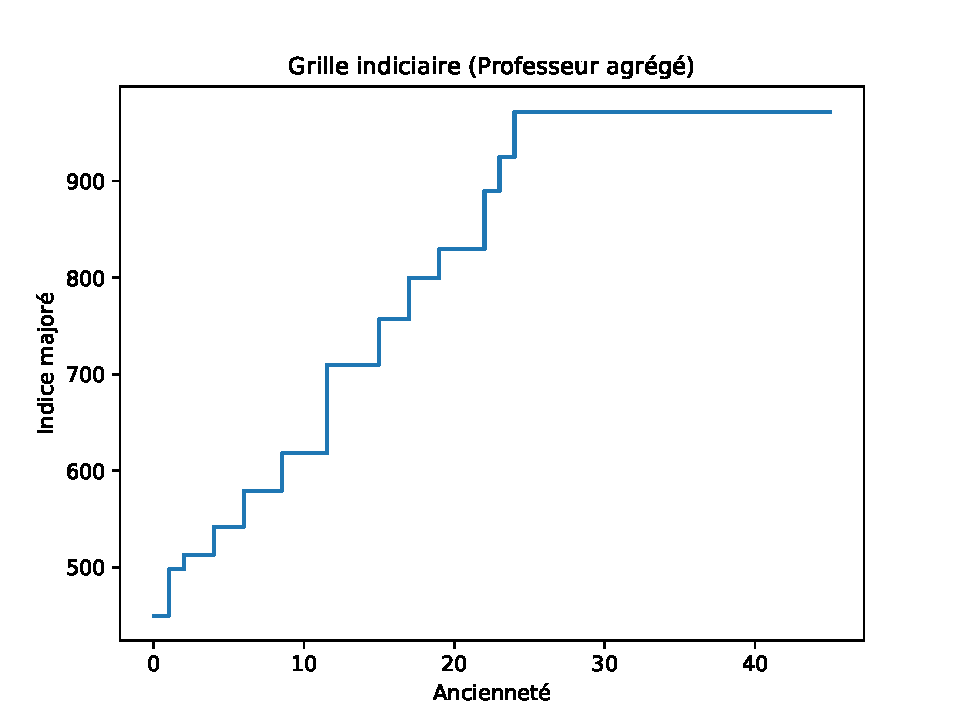
\includegraphics[width=0.7\textwidth]{fig/grille_ProfAgrege.pdf}\end{minipage} 
\begin{minipage}{0.3\linewidth} 
 \begin{center} 

\begin{tabular}[htb]{|c|c|} 
\hline 
 Indice majoré &  Durée (années) \\ 
\hline \hline 
 450 &  1.00 \\ 
\hline 
 498 &  1.00 \\ 
\hline 
 513 &  2.00 \\ 
\hline 
 542 &  2.00 \\ 
\hline 
 579 &  2.50 \\ 
\hline 
 618 &  3.00 \\ 
\hline 
 710 &  3.50 \\ 
\hline 
 757 &  2.00 \\ 
\hline 
 800 &  2.00 \\ 
\hline 
 830 &  3.00 \\ 
\hline 
 890 &  1.00 \\ 
\hline 
 925 &  1.00 \\ 
\hline 
 972 &   \\ 
\hline 
\hline 
\end{tabular} 
\end{center} 
 \end{minipage} 


 \addto{\captionsenglish}{ \renewcommand{\mtctitle}{}} \setcounter{minitocdepth}{2} 
 \minitoc \newpage 

\section{Début de carrière à 22 ans} 

\subsection{Génération 1975 (début en 1997)} 

\paragraph{Retraites possibles dans le modèle \emph{Gouvernement truqué (âge-pivot bloqué à 65 ans)}}  
 
{ \scriptsize \begin{center} 
\begin{tabular}[htb]{|c|c||c|c||c|c||c||c|c|c|c|c|c|} 
\hline 
 Retraite en &  Âge &  Âge pivot &  Décote/Surcote &  Retraite (\euro{} 2019) &  Tx Rempl(\%) &  SMIC (\euro{} 2019) &  Retraite/SMIC &  Rev70/SMIC &  Rev75/SMIC &  Rev80/SMIC &  Rev85/SMIC &  Rev90/SMIC \\ 
\hline \hline 
 2037 &  62 &  64 ans 10 mois &  -14.17\% &  2088.51 &  {\bf 41.15} &  2143.00 &  {\bf {\color{red} 0.97}} &  {\bf {\color{red} 0.88}} &  {\bf {\color{red} 0.82}} &  {\bf {\color{red} 0.77}} &  {\bf {\color{red} 0.72}} &  {\bf {\color{red} 0.68}} \\ 
\hline 
 2038 &  63 &  64 ans 11 mois &  -9.58\% &  2280.82 &  {\bf 44.84} &  2170.86 &  {\bf 1.05} &  {\bf {\color{red} 0.96}} &  {\bf {\color{red} 0.90}} &  {\bf {\color{red} 0.84}} &  {\bf {\color{red} 0.79}} &  {\bf {\color{red} 0.74}} \\ 
\hline 
 2039 &  64 &  65 ans 0 mois &  -5.00\% &  2483.95 &  {\bf 48.74} &  2199.08 &  {\bf 1.13} &  {\bf 1.05} &  {\bf {\color{red} 0.98}} &  {\bf {\color{red} 0.92}} &  {\bf {\color{red} 0.86}} &  {\bf {\color{red} 0.81}} \\ 
\hline 
 2040 &  65 &  65 ans 0 mois &  0.00\% &  2709.72 &  {\bf 53.05} &  2227.67 &  {\bf 1.22} &  {\bf 1.14} &  {\bf 1.07} &  {\bf 1.00} &  {\bf {\color{red} 0.94}} &  {\bf {\color{red} 0.88}} \\ 
\hline 
 2041 &  66 &  65 ans 0 mois &  5.00\% &  2948.26 &  {\bf 57.60} &  2256.63 &  {\bf 1.31} &  {\bf 1.24} &  {\bf 1.16} &  {\bf 1.09} &  {\bf 1.02} &  {\bf {\color{red} 0.96}} \\ 
\hline 
 2042 &  67 &  65 ans 0 mois &  10.00\% &  3200.21 &  {\bf 62.39} &  2285.97 &  {\bf 1.40} &  {\bf 1.35} &  {\bf 1.26} &  {\bf 1.18} &  {\bf 1.11} &  {\bf 1.04} \\ 
\hline 
\hline 
\end{tabular} 
\end{center} } 
\paragraph{Retraites possibles dans le modèle \emph{Gouvernement corrigé (âge-pivot glissant)}}  
 
{ \scriptsize \begin{center} 
\begin{tabular}[htb]{|c|c||c|c||c|c||c||c|c|c|c|c|c|} 
\hline 
 Retraite en &  Âge &  Âge pivot &  Décote/Surcote &  Retraite (\euro{} 2019) &  Tx Rempl(\%) &  SMIC (\euro{} 2019) &  Retraite/SMIC &  Rev70/SMIC &  Rev75/SMIC &  Rev80/SMIC &  Rev85/SMIC &  Rev90/SMIC \\ 
\hline \hline 
 2037 &  62 &  64 ans 10 mois &  -14.17\% &  2088.51 &  {\bf 41.15} &  2143.00 &  {\bf {\color{red} 0.97}} &  {\bf {\color{red} 0.88}} &  {\bf {\color{red} 0.82}} &  {\bf {\color{red} 0.77}} &  {\bf {\color{red} 0.72}} &  {\bf {\color{red} 0.68}} \\ 
\hline 
 2038 &  63 &  64 ans 11 mois &  -9.58\% &  2280.82 &  {\bf 44.84} &  2170.86 &  {\bf 1.05} &  {\bf {\color{red} 0.96}} &  {\bf {\color{red} 0.90}} &  {\bf {\color{red} 0.84}} &  {\bf {\color{red} 0.79}} &  {\bf {\color{red} 0.74}} \\ 
\hline 
 2039 &  64 &  65 ans 0 mois &  -5.00\% &  2483.95 &  {\bf 48.74} &  2199.08 &  {\bf 1.13} &  {\bf 1.05} &  {\bf {\color{red} 0.98}} &  {\bf {\color{red} 0.92}} &  {\bf {\color{red} 0.86}} &  {\bf {\color{red} 0.81}} \\ 
\hline 
 2040 &  65 &  65 ans 1 mois &  -0.42\% &  2698.43 &  {\bf 52.83} &  2227.67 &  {\bf 1.21} &  {\bf 1.14} &  {\bf 1.06} &  {\bf {\color{red} 1.00}} &  {\bf {\color{red} 0.94}} &  {\bf {\color{red} 0.88}} \\ 
\hline 
 2041 &  66 &  65 ans 2 mois &  4.17\% &  2924.86 &  {\bf 57.15} &  2256.63 &  {\bf 1.30} &  {\bf 1.23} &  {\bf 1.15} &  {\bf 1.08} &  {\bf 1.01} &  {\bf {\color{red} 0.95}} \\ 
\hline 
 2042 &  67 &  65 ans 3 mois &  8.75\% &  3163.85 &  {\bf 61.69} &  2285.97 &  {\bf 1.38} &  {\bf 1.33} &  {\bf 1.25} &  {\bf 1.17} &  {\bf 1.10} &  {\bf 1.03} \\ 
\hline 
\hline 
\end{tabular} 
\end{center} } 
\paragraph{Retraites possibles dans le modèle \emph{Destinie2 (revalorisation de la fonction publique)}}  
 
{ \scriptsize \begin{center} 
\begin{tabular}[htb]{|c|c||c|c||c|c||c||c|c|c|c|c|c|} 
\hline 
 Retraite en &  Âge &  Âge pivot &  Décote/Surcote &  Retraite (\euro{} 2019) &  Tx Rempl(\%) &  SMIC (\euro{} 2019) &  Retraite/SMIC &  Rev70/SMIC &  Rev75/SMIC &  Rev80/SMIC &  Rev85/SMIC &  Rev90/SMIC \\ 
\hline \hline 
 2037 &  62 &  64 ans 10 mois &  -14.17\% &  2216.13 &  {\bf 35.21} &  2014.82 &  {\bf 1.10} &  {\bf {\color{red} 0.99}} &  {\bf {\color{red} 0.93}} &  {\bf {\color{red} 0.87}} &  {\bf {\color{red} 0.82}} &  {\bf {\color{red} 0.77}} \\ 
\hline 
 2038 &  63 &  64 ans 11 mois &  -9.58\% &  2432.68 &  {\bf 38.08} &  2041.01 &  {\bf 1.19} &  {\bf 1.09} &  {\bf 1.02} &  {\bf {\color{red} 0.96}} &  {\bf {\color{red} 0.90}} &  {\bf {\color{red} 0.84}} \\ 
\hline 
 2039 &  64 &  65 ans 0 mois &  -5.00\% &  2663.20 &  {\bf 41.06} &  2067.55 &  {\bf 1.29} &  {\bf 1.19} &  {\bf 1.12} &  {\bf 1.05} &  {\bf {\color{red} 0.98}} &  {\bf {\color{red} 0.92}} \\ 
\hline 
 2040 &  65 &  65 ans 1 mois &  -0.42\% &  2908.51 &  {\bf 44.18} &  2094.43 &  {\bf 1.39} &  {\bf 1.30} &  {\bf 1.22} &  {\bf 1.14} &  {\bf 1.07} &  {\bf 1.01} \\ 
\hline 
 2041 &  66 &  65 ans 2 mois &  4.17\% &  3169.48 &  {\bf 47.43} &  2121.65 &  {\bf 1.49} &  {\bf 1.42} &  {\bf 1.33} &  {\bf 1.25} &  {\bf 1.17} &  {\bf 1.10} \\ 
\hline 
 2042 &  67 &  65 ans 3 mois &  8.75\% &  3447.01 &  {\bf 50.81} &  2149.23 &  {\bf 1.60} &  {\bf 1.54} &  {\bf 1.45} &  {\bf 1.36} &  {\bf 1.27} &  {\bf 1.19} \\ 
\hline 
\hline 
\end{tabular} 
\end{center} } 

 \begin{center}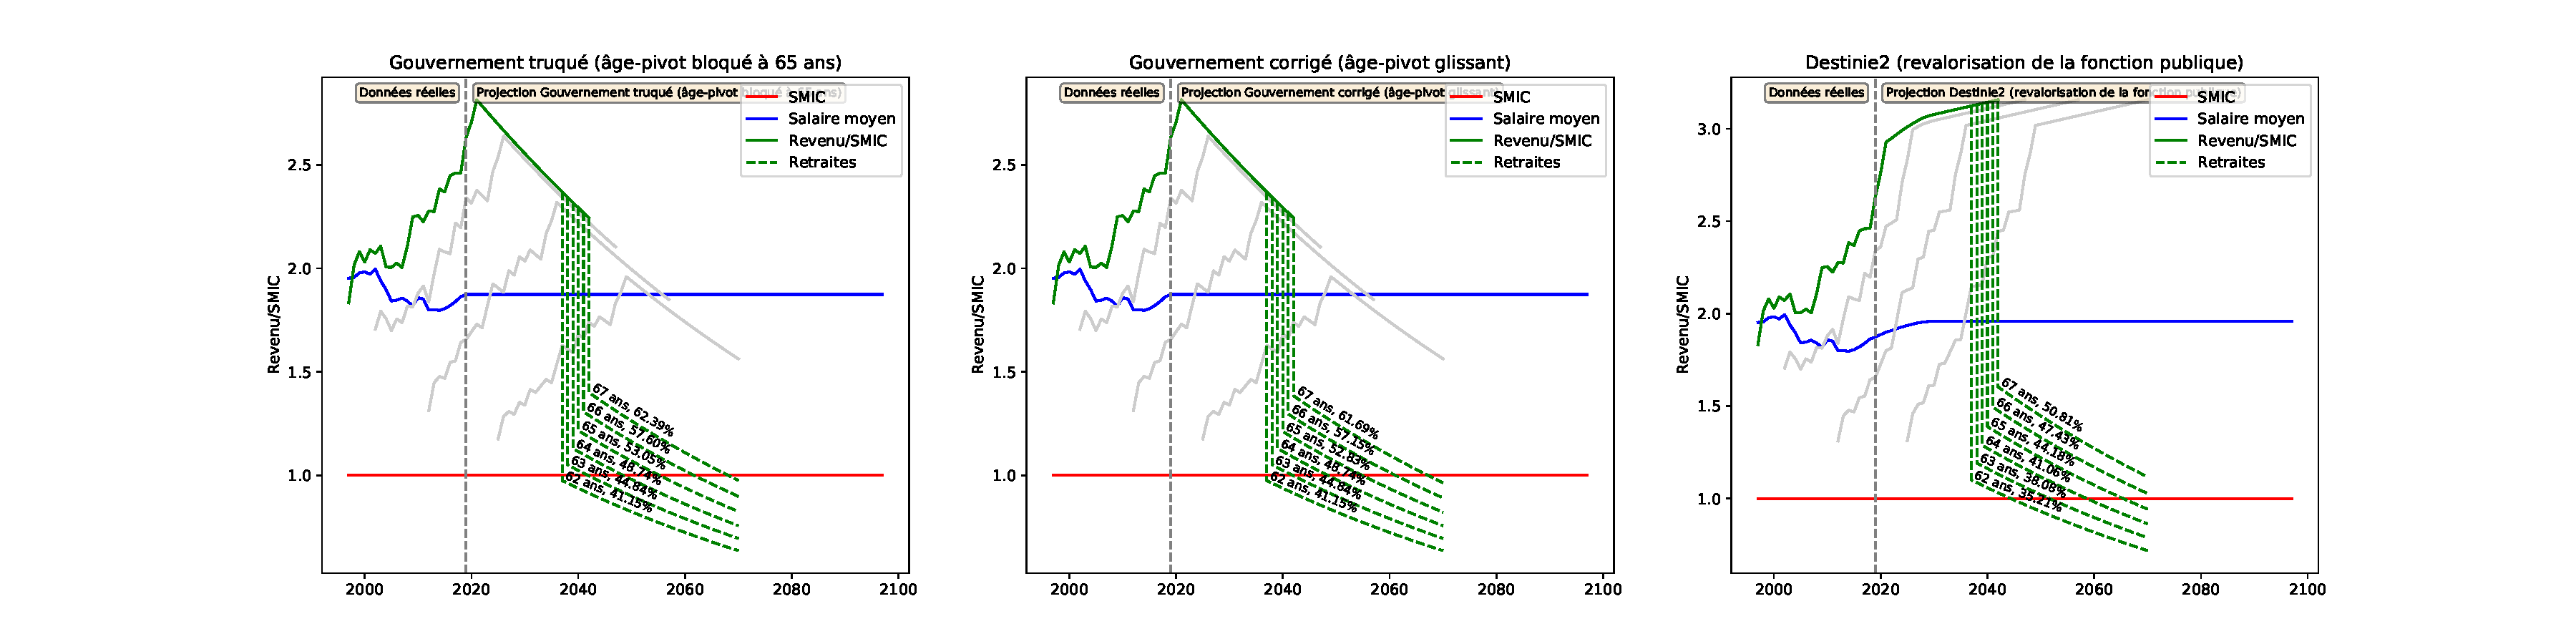
\includegraphics[width=0.9\textwidth]{fig/ProfAgrege_1975_22_dest_retraite.pdf}\end{center} \label{fig/ProfAgrege_1975_22_dest_retraite.pdf} 

\newpage 
 
\paragraph{Revenus et points pour le modèle \emph{Gouvernement truqué (âge-pivot bloqué à 65 ans)}} 
 
{ \scriptsize \begin{center} 
\begin{tabular}[htb]{|c|c||c|c|c|c|c|c||c|c||c|c|c|} 
\hline 
 Année &  Âge &  Ind Maj &  Pt Ind(\euro{} 2019) &  Rev HP(\euro{} 2019) &  Tx Primes &  GIPA(\euro{} 2019) &  Revenu(\euro{} 2019) &  SMIC(\euro{} 2019) &  Rev/SMIC &  Cumul Pts &  Achat Pt(\euro{} 2019) &  Serv. Pt(\euro{} 2019) \\ 
\hline \hline 
 1997 &  22 &  450.0 &  5.53 &  2490.46 &  0.00 &  0.00 &  2490.46 &  1358.84 &  {\bf 1.83} &  839.31 &  35.61 &  0.50 \\ 
\hline 
 1998 &  23 &  498.0 &  5.57 &  2772.09 &  0.00 &  0.00 &  2772.09 &  1376.36 &  {\bf 2.01} &  1773.54 &  35.61 &  0.50 \\ 
\hline 
 1999 &  24 &  513.0 &  5.61 &  2878.67 &  0.17 &  0.00 &  2883.57 &  1386.54 &  {\bf 2.08} &  2745.34 &  35.61 &  0.50 \\ 
\hline 
 2000 &  25 &  513.0 &  5.55 &  2844.68 &  0.40 &  0.00 &  2856.06 &  1407.00 &  {\bf 2.03} &  3707.87 &  35.61 &  0.50 \\ 
\hline 
 2001 &  26 &  542.0 &  5.52 &  2992.11 &  0.63 &  0.00 &  3010.96 &  1441.04 &  {\bf 2.09} &  4722.60 &  35.61 &  0.50 \\ 
\hline 
 2002 &  27 &  542.0 &  5.49 &  2973.56 &  0.86 &  0.00 &  2999.13 &  1447.74 &  {\bf 2.07} &  5733.34 &  35.61 &  0.50 \\ 
\hline 
 2003 &  28 &  579.0 &  5.37 &  3111.90 &  1.09 &  0.00 &  3145.82 &  1493.03 &  {\bf 2.11} &  6793.52 &  35.61 &  0.50 \\ 
\hline 
 2004 &  29 &  579.0 &  5.29 &  3062.75 &  1.32 &  0.00 &  3103.18 &  1547.32 &  {\bf 2.01} &  7839.33 &  35.61 &  0.50 \\ 
\hline 
 2005 &  30 &  598.5 &  5.29 &  3165.55 &  1.55 &  0.00 &  3214.62 &  1603.67 &  {\bf 2.00} &  8922.70 &  35.61 &  0.50 \\ 
\hline 
 2006 &  31 &  618.0 &  5.23 &  3232.21 &  1.78 &  0.00 &  3289.75 &  1625.00 &  {\bf 2.02} &  10031.38 &  35.61 &  0.50 \\ 
\hline 
 2007 &  32 &  618.0 &  5.19 &  3210.19 &  2.01 &  0.00 &  3274.72 &  1634.08 &  {\bf 2.00} &  11135.00 &  35.61 &  0.50 \\ 
\hline 
 2008 &  33 &  664.0 &  5.09 &  3381.78 &  2.24 &  0.00 &  3457.53 &  1640.24 &  {\bf 2.11} &  12300.23 &  35.61 &  0.50 \\ 
\hline 
 2009 &  34 &  710.0 &  5.13 &  3641.68 &  2.47 &  0.00 &  3731.63 &  1659.42 &  {\bf 2.25} &  13557.84 &  35.61 &  0.50 \\ 
\hline 
 2010 &  35 &  710.0 &  5.08 &  3604.90 &  2.70 &  0.00 &  3702.23 &  1641.90 &  {\bf 2.25} &  14805.54 &  35.61 &  0.50 \\ 
\hline 
 2011 &  36 &  710.0 &  4.97 &  3530.00 &  2.93 &  0.00 &  3633.43 &  1633.19 &  {\bf 2.22} &  16030.05 &  35.61 &  0.50 \\ 
\hline 
 2012 &  37 &  757.0 &  4.88 &  3691.46 &  3.16 &  0.00 &  3808.11 &  1673.05 &  {\bf 2.28} &  17313.43 &  35.61 &  0.50 \\ 
\hline 
 2013 &  38 &  757.0 &  4.83 &  3659.83 &  3.39 &  0.00 &  3783.90 &  1664.01 &  {\bf 2.27} &  18588.65 &  35.61 &  0.50 \\ 
\hline 
 2014 &  39 &  800.0 &  4.81 &  3848.36 &  3.62 &  0.00 &  3987.67 &  1673.24 &  {\bf 2.38} &  19932.54 &  35.61 &  0.50 \\ 
\hline 
 2015 &  40 &  800.0 &  4.81 &  3846.86 &  3.85 &  0.00 &  3994.96 &  1686.62 &  {\bf 2.37} &  21278.89 &  35.61 &  0.50 \\ 
\hline 
 2016 &  41 &  830.0 &  4.80 &  3983.15 &  4.08 &  0.00 &  4145.66 &  1693.76 &  {\bf 2.45} &  22676.03 &  35.61 &  0.50 \\ 
\hline 
 2017 &  42 &  830.0 &  4.81 &  3991.18 &  4.31 &  0.00 &  4163.20 &  1692.60 &  {\bf 2.46} &  24079.08 &  35.61 &  0.50 \\ 
\hline 
 2018 &  43 &  830.0 &  4.74 &  3936.07 &  4.54 &  43.46 &  4158.23 &  1689.76 &  {\bf 2.46} &  25480.45 &  35.61 &  0.50 \\ 
\hline 
 2019 &  44 &  890.0 &  4.79 &  4267.04 &  4.77 &  0.00 &  4470.57 &  1698.45 &  {\bf 2.63} &  26987.09 &  35.61 &  0.50 \\ 
\hline 
 2020 &  45 &  925.0 &  4.79 &  4434.84 &  5.00 &  0.00 &  4656.58 &  1720.53 &  {\bf 2.71} &  28556.41 &  35.61 &  0.50 \\ 
\hline 
 2021 &  46 &  972.0 &  4.79 &  4660.18 &  5.23 &  0.00 &  4903.91 &  1742.90 &  {\bf 2.81} &  30209.09 &  35.61 &  0.50 \\ 
\hline 
 2022 &  47 &  972.0 &  4.79 &  4660.18 &  5.46 &  0.00 &  4914.62 &  1765.55 &  {\bf 2.78} &  31865.38 &  35.61 &  0.50 \\ 
\hline 
 2023 &  48 &  972.0 &  4.79 &  4660.18 &  5.69 &  0.00 &  4925.34 &  1788.51 &  {\bf 2.75} &  33525.28 &  35.61 &  0.50 \\ 
\hline 
 2024 &  49 &  972.0 &  4.79 &  4660.18 &  5.92 &  0.00 &  4936.06 &  1811.76 &  {\bf 2.72} &  35188.79 &  35.61 &  0.50 \\ 
\hline 
 2025 &  50 &  972.0 &  4.79 &  4660.18 &  6.15 &  0.00 &  4946.78 &  1835.31 &  {\bf 2.70} &  36855.92 &  35.61 &  0.50 \\ 
\hline 
 2026 &  51 &  972.0 &  4.79 &  4660.18 &  6.38 &  0.00 &  4957.50 &  1859.17 &  {\bf 2.67} &  38526.65 &  35.61 &  0.50 \\ 
\hline 
 2027 &  52 &  972.0 &  4.79 &  4660.18 &  6.61 &  0.00 &  4968.22 &  1883.34 &  {\bf 2.64} &  40201.00 &  35.61 &  0.50 \\ 
\hline 
 2028 &  53 &  972.0 &  4.79 &  4660.18 &  6.84 &  0.00 &  4978.93 &  1907.82 &  {\bf 2.61} &  41878.96 &  35.61 &  0.50 \\ 
\hline 
 2029 &  54 &  972.0 &  4.79 &  4660.18 &  7.07 &  0.00 &  4989.65 &  1932.62 &  {\bf 2.58} &  43559.26 &  35.63 &  0.50 \\ 
\hline 
 2030 &  55 &  972.0 &  4.79 &  4660.18 &  7.30 &  0.00 &  5000.37 &  1957.75 &  {\bf 2.55} &  45240.61 &  35.69 &  0.50 \\ 
\hline 
 2031 &  56 &  972.0 &  4.79 &  4660.18 &  7.53 &  0.00 &  5011.09 &  1983.20 &  {\bf 2.53} &  46921.73 &  35.77 &  0.50 \\ 
\hline 
 2032 &  57 &  972.0 &  4.79 &  4660.18 &  7.76 &  0.00 &  5021.81 &  2008.98 &  {\bf 2.50} &  48601.33 &  35.88 &  0.50 \\ 
\hline 
 2033 &  58 &  972.0 &  4.79 &  4660.18 &  7.99 &  0.00 &  5032.53 &  2035.10 &  {\bf 2.47} &  50278.13 &  36.02 &  0.50 \\ 
\hline 
 2034 &  59 &  972.0 &  4.79 &  4660.18 &  8.22 &  0.00 &  5043.24 &  2061.55 &  {\bf 2.45} &  51950.86 &  36.18 &  0.50 \\ 
\hline 
 2035 &  60 &  972.0 &  4.79 &  4660.18 &  8.45 &  0.00 &  5053.96 &  2088.35 &  {\bf 2.42} &  53618.26 &  36.37 &  0.51 \\ 
\hline 
 2036 &  61 &  972.0 &  4.79 &  4660.18 &  8.68 &  0.00 &  5064.68 &  2115.50 &  {\bf 2.39} &  55279.06 &  36.59 &  0.51 \\ 
\hline 
 2037 &  62 &  972.0 &  4.79 &  4660.18 &  8.91 &  0.00 &  5075.40 &  2143.00 &  {\bf 2.37} &  56932.04 &  36.85 &  0.51 \\ 
\hline 
 2038 &  63 &  972.0 &  4.79 &  4660.18 &  9.14 &  0.00 &  5086.12 &  2170.86 &  {\bf 2.34} &  58575.97 &  37.13 &  0.52 \\ 
\hline 
 2039 &  64 &  972.0 &  4.79 &  4660.18 &  9.37 &  0.00 &  5096.84 &  2199.08 &  {\bf 2.32} &  60209.66 &  37.44 &  0.52 \\ 
\hline 
 2040 &  65 &  972.0 &  4.79 &  4660.18 &  9.60 &  0.00 &  5107.56 &  2227.67 &  {\bf 2.29} &  61831.92 &  37.78 &  0.53 \\ 
\hline 
 2041 &  66 &  972.0 &  4.79 &  4660.18 &  9.83 &  0.00 &  5118.27 &  2256.63 &  {\bf 2.27} &  63441.61 &  38.16 &  0.53 \\ 
\hline 
 2042 &  67 &  972.0 &  4.79 &  4660.18 &  10.06 &  0.00 &  5128.99 &  2285.97 &  {\bf 2.24} &  65037.61 &  38.56 &  0.54 \\ 
\hline 
\hline 
\end{tabular} 
\end{center} } 
\newpage 
 
\paragraph{Revenus et points pour le modèle \emph{Gouvernement corrigé (âge-pivot glissant)}} 
 
{ \scriptsize \begin{center} 
\begin{tabular}[htb]{|c|c||c|c|c|c|c|c||c|c||c|c|c|} 
\hline 
 Année &  Âge &  Ind Maj &  Pt Ind(\euro{} 2019) &  Rev HP(\euro{} 2019) &  Tx Primes &  GIPA(\euro{} 2019) &  Revenu(\euro{} 2019) &  SMIC(\euro{} 2019) &  Rev/SMIC &  Cumul Pts &  Achat Pt(\euro{} 2019) &  Serv. Pt(\euro{} 2019) \\ 
\hline \hline 
 1997 &  22 &  450.0 &  5.53 &  2490.46 &  0.00 &  0.00 &  2490.46 &  1358.84 &  {\bf 1.83} &  839.31 &  35.61 &  0.50 \\ 
\hline 
 1998 &  23 &  498.0 &  5.57 &  2772.09 &  0.00 &  0.00 &  2772.09 &  1376.36 &  {\bf 2.01} &  1773.54 &  35.61 &  0.50 \\ 
\hline 
 1999 &  24 &  513.0 &  5.61 &  2878.67 &  0.17 &  0.00 &  2883.57 &  1386.54 &  {\bf 2.08} &  2745.34 &  35.61 &  0.50 \\ 
\hline 
 2000 &  25 &  513.0 &  5.55 &  2844.68 &  0.40 &  0.00 &  2856.06 &  1407.00 &  {\bf 2.03} &  3707.87 &  35.61 &  0.50 \\ 
\hline 
 2001 &  26 &  542.0 &  5.52 &  2992.11 &  0.63 &  0.00 &  3010.96 &  1441.04 &  {\bf 2.09} &  4722.60 &  35.61 &  0.50 \\ 
\hline 
 2002 &  27 &  542.0 &  5.49 &  2973.56 &  0.86 &  0.00 &  2999.13 &  1447.74 &  {\bf 2.07} &  5733.34 &  35.61 &  0.50 \\ 
\hline 
 2003 &  28 &  579.0 &  5.37 &  3111.90 &  1.09 &  0.00 &  3145.82 &  1493.03 &  {\bf 2.11} &  6793.52 &  35.61 &  0.50 \\ 
\hline 
 2004 &  29 &  579.0 &  5.29 &  3062.75 &  1.32 &  0.00 &  3103.18 &  1547.32 &  {\bf 2.01} &  7839.33 &  35.61 &  0.50 \\ 
\hline 
 2005 &  30 &  598.5 &  5.29 &  3165.55 &  1.55 &  0.00 &  3214.62 &  1603.67 &  {\bf 2.00} &  8922.70 &  35.61 &  0.50 \\ 
\hline 
 2006 &  31 &  618.0 &  5.23 &  3232.21 &  1.78 &  0.00 &  3289.75 &  1625.00 &  {\bf 2.02} &  10031.38 &  35.61 &  0.50 \\ 
\hline 
 2007 &  32 &  618.0 &  5.19 &  3210.19 &  2.01 &  0.00 &  3274.72 &  1634.08 &  {\bf 2.00} &  11135.00 &  35.61 &  0.50 \\ 
\hline 
 2008 &  33 &  664.0 &  5.09 &  3381.78 &  2.24 &  0.00 &  3457.53 &  1640.24 &  {\bf 2.11} &  12300.23 &  35.61 &  0.50 \\ 
\hline 
 2009 &  34 &  710.0 &  5.13 &  3641.68 &  2.47 &  0.00 &  3731.63 &  1659.42 &  {\bf 2.25} &  13557.84 &  35.61 &  0.50 \\ 
\hline 
 2010 &  35 &  710.0 &  5.08 &  3604.90 &  2.70 &  0.00 &  3702.23 &  1641.90 &  {\bf 2.25} &  14805.54 &  35.61 &  0.50 \\ 
\hline 
 2011 &  36 &  710.0 &  4.97 &  3530.00 &  2.93 &  0.00 &  3633.43 &  1633.19 &  {\bf 2.22} &  16030.05 &  35.61 &  0.50 \\ 
\hline 
 2012 &  37 &  757.0 &  4.88 &  3691.46 &  3.16 &  0.00 &  3808.11 &  1673.05 &  {\bf 2.28} &  17313.43 &  35.61 &  0.50 \\ 
\hline 
 2013 &  38 &  757.0 &  4.83 &  3659.83 &  3.39 &  0.00 &  3783.90 &  1664.01 &  {\bf 2.27} &  18588.65 &  35.61 &  0.50 \\ 
\hline 
 2014 &  39 &  800.0 &  4.81 &  3848.36 &  3.62 &  0.00 &  3987.67 &  1673.24 &  {\bf 2.38} &  19932.54 &  35.61 &  0.50 \\ 
\hline 
 2015 &  40 &  800.0 &  4.81 &  3846.86 &  3.85 &  0.00 &  3994.96 &  1686.62 &  {\bf 2.37} &  21278.89 &  35.61 &  0.50 \\ 
\hline 
 2016 &  41 &  830.0 &  4.80 &  3983.15 &  4.08 &  0.00 &  4145.66 &  1693.76 &  {\bf 2.45} &  22676.03 &  35.61 &  0.50 \\ 
\hline 
 2017 &  42 &  830.0 &  4.81 &  3991.18 &  4.31 &  0.00 &  4163.20 &  1692.60 &  {\bf 2.46} &  24079.08 &  35.61 &  0.50 \\ 
\hline 
 2018 &  43 &  830.0 &  4.74 &  3936.07 &  4.54 &  43.46 &  4158.23 &  1689.76 &  {\bf 2.46} &  25480.45 &  35.61 &  0.50 \\ 
\hline 
 2019 &  44 &  890.0 &  4.79 &  4267.04 &  4.77 &  0.00 &  4470.57 &  1698.45 &  {\bf 2.63} &  26987.09 &  35.61 &  0.50 \\ 
\hline 
 2020 &  45 &  925.0 &  4.79 &  4434.84 &  5.00 &  0.00 &  4656.58 &  1720.53 &  {\bf 2.71} &  28556.41 &  35.61 &  0.50 \\ 
\hline 
 2021 &  46 &  972.0 &  4.79 &  4660.18 &  5.23 &  0.00 &  4903.91 &  1742.90 &  {\bf 2.81} &  30209.09 &  35.61 &  0.50 \\ 
\hline 
 2022 &  47 &  972.0 &  4.79 &  4660.18 &  5.46 &  0.00 &  4914.62 &  1765.55 &  {\bf 2.78} &  31865.38 &  35.61 &  0.50 \\ 
\hline 
 2023 &  48 &  972.0 &  4.79 &  4660.18 &  5.69 &  0.00 &  4925.34 &  1788.51 &  {\bf 2.75} &  33525.28 &  35.61 &  0.50 \\ 
\hline 
 2024 &  49 &  972.0 &  4.79 &  4660.18 &  5.92 &  0.00 &  4936.06 &  1811.76 &  {\bf 2.72} &  35188.79 &  35.61 &  0.50 \\ 
\hline 
 2025 &  50 &  972.0 &  4.79 &  4660.18 &  6.15 &  0.00 &  4946.78 &  1835.31 &  {\bf 2.70} &  36855.92 &  35.61 &  0.50 \\ 
\hline 
 2026 &  51 &  972.0 &  4.79 &  4660.18 &  6.38 &  0.00 &  4957.50 &  1859.17 &  {\bf 2.67} &  38526.65 &  35.61 &  0.50 \\ 
\hline 
 2027 &  52 &  972.0 &  4.79 &  4660.18 &  6.61 &  0.00 &  4968.22 &  1883.34 &  {\bf 2.64} &  40201.00 &  35.61 &  0.50 \\ 
\hline 
 2028 &  53 &  972.0 &  4.79 &  4660.18 &  6.84 &  0.00 &  4978.93 &  1907.82 &  {\bf 2.61} &  41878.96 &  35.61 &  0.50 \\ 
\hline 
 2029 &  54 &  972.0 &  4.79 &  4660.18 &  7.07 &  0.00 &  4989.65 &  1932.62 &  {\bf 2.58} &  43559.26 &  35.63 &  0.50 \\ 
\hline 
 2030 &  55 &  972.0 &  4.79 &  4660.18 &  7.30 &  0.00 &  5000.37 &  1957.75 &  {\bf 2.55} &  45240.61 &  35.69 &  0.50 \\ 
\hline 
 2031 &  56 &  972.0 &  4.79 &  4660.18 &  7.53 &  0.00 &  5011.09 &  1983.20 &  {\bf 2.53} &  46921.73 &  35.77 &  0.50 \\ 
\hline 
 2032 &  57 &  972.0 &  4.79 &  4660.18 &  7.76 &  0.00 &  5021.81 &  2008.98 &  {\bf 2.50} &  48601.33 &  35.88 &  0.50 \\ 
\hline 
 2033 &  58 &  972.0 &  4.79 &  4660.18 &  7.99 &  0.00 &  5032.53 &  2035.10 &  {\bf 2.47} &  50278.13 &  36.02 &  0.50 \\ 
\hline 
 2034 &  59 &  972.0 &  4.79 &  4660.18 &  8.22 &  0.00 &  5043.24 &  2061.55 &  {\bf 2.45} &  51950.86 &  36.18 &  0.50 \\ 
\hline 
 2035 &  60 &  972.0 &  4.79 &  4660.18 &  8.45 &  0.00 &  5053.96 &  2088.35 &  {\bf 2.42} &  53618.26 &  36.37 &  0.51 \\ 
\hline 
 2036 &  61 &  972.0 &  4.79 &  4660.18 &  8.68 &  0.00 &  5064.68 &  2115.50 &  {\bf 2.39} &  55279.06 &  36.59 &  0.51 \\ 
\hline 
 2037 &  62 &  972.0 &  4.79 &  4660.18 &  8.91 &  0.00 &  5075.40 &  2143.00 &  {\bf 2.37} &  56932.04 &  36.85 &  0.51 \\ 
\hline 
 2038 &  63 &  972.0 &  4.79 &  4660.18 &  9.14 &  0.00 &  5086.12 &  2170.86 &  {\bf 2.34} &  58575.97 &  37.13 &  0.52 \\ 
\hline 
 2039 &  64 &  972.0 &  4.79 &  4660.18 &  9.37 &  0.00 &  5096.84 &  2199.08 &  {\bf 2.32} &  60209.66 &  37.44 &  0.52 \\ 
\hline 
 2040 &  65 &  972.0 &  4.79 &  4660.18 &  9.60 &  0.00 &  5107.56 &  2227.67 &  {\bf 2.29} &  61831.92 &  37.78 &  0.53 \\ 
\hline 
 2041 &  66 &  972.0 &  4.79 &  4660.18 &  9.83 &  0.00 &  5118.27 &  2256.63 &  {\bf 2.27} &  63441.61 &  38.16 &  0.53 \\ 
\hline 
 2042 &  67 &  972.0 &  4.79 &  4660.18 &  10.06 &  0.00 &  5128.99 &  2285.97 &  {\bf 2.24} &  65037.61 &  38.56 &  0.54 \\ 
\hline 
\hline 
\end{tabular} 
\end{center} } 
\newpage 
 
\paragraph{Revenus et points pour le modèle \emph{Destinie2 (revalorisation de la fonction publique)}} 
 
{ \scriptsize \begin{center} 
\begin{tabular}[htb]{|c|c||c|c|c|c|c|c||c|c||c|c|c|} 
\hline 
 Année &  Âge &  Ind Maj &  Pt Ind(\euro{} 2019) &  Rev HP(\euro{} 2019) &  Tx Primes &  GIPA(\euro{} 2019) &  Revenu(\euro{} 2019) &  SMIC(\euro{} 2019) &  Rev/SMIC &  Cumul Pts &  Achat Pt(\euro{} 2019) &  Serv. Pt(\euro{} 2019) \\ 
\hline \hline 
 1997 &  22 &  450.0 &  5.53 &  2490.46 &  0.00 &  0.00 &  2490.46 &  1358.84 &  {\bf 1.83} &  837.25 &  35.69 &  0.50 \\ 
\hline 
 1998 &  23 &  498.0 &  5.57 &  2772.09 &  0.00 &  0.00 &  2772.09 &  1376.36 &  {\bf 2.01} &  1769.19 &  35.69 &  0.50 \\ 
\hline 
 1999 &  24 &  513.0 &  5.61 &  2878.67 &  0.17 &  0.00 &  2883.57 &  1386.54 &  {\bf 2.08} &  2738.60 &  35.69 &  0.50 \\ 
\hline 
 2000 &  25 &  513.0 &  5.55 &  2844.68 &  0.40 &  0.00 &  2856.06 &  1407.00 &  {\bf 2.03} &  3698.76 &  35.69 &  0.50 \\ 
\hline 
 2001 &  26 &  542.0 &  5.52 &  2992.11 &  0.63 &  0.00 &  3010.96 &  1441.04 &  {\bf 2.09} &  4711.00 &  35.69 &  0.50 \\ 
\hline 
 2002 &  27 &  542.0 &  5.49 &  2973.56 &  0.86 &  0.00 &  2999.13 &  1447.74 &  {\bf 2.07} &  5719.26 &  35.69 &  0.50 \\ 
\hline 
 2003 &  28 &  579.0 &  5.37 &  3111.90 &  1.09 &  0.00 &  3145.82 &  1493.03 &  {\bf 2.11} &  6776.83 &  35.69 &  0.50 \\ 
\hline 
 2004 &  29 &  579.0 &  5.29 &  3062.75 &  1.32 &  0.00 &  3103.18 &  1547.32 &  {\bf 2.01} &  7820.07 &  35.69 &  0.50 \\ 
\hline 
 2005 &  30 &  598.5 &  5.29 &  3165.55 &  1.55 &  0.00 &  3214.62 &  1603.67 &  {\bf 2.00} &  8900.78 &  35.69 &  0.50 \\ 
\hline 
 2006 &  31 &  618.0 &  5.23 &  3232.21 &  1.78 &  0.00 &  3289.75 &  1625.00 &  {\bf 2.02} &  10006.74 &  35.69 &  0.50 \\ 
\hline 
 2007 &  32 &  618.0 &  5.19 &  3210.19 &  2.01 &  0.00 &  3274.72 &  1634.08 &  {\bf 2.00} &  11107.64 &  35.69 &  0.50 \\ 
\hline 
 2008 &  33 &  664.0 &  5.09 &  3381.78 &  2.24 &  0.00 &  3457.53 &  1640.24 &  {\bf 2.11} &  12270.01 &  35.69 &  0.50 \\ 
\hline 
 2009 &  34 &  710.0 &  5.13 &  3641.68 &  2.47 &  0.00 &  3731.63 &  1659.42 &  {\bf 2.25} &  13524.53 &  35.69 &  0.50 \\ 
\hline 
 2010 &  35 &  710.0 &  5.08 &  3604.90 &  2.70 &  0.00 &  3702.23 &  1641.90 &  {\bf 2.25} &  14769.16 &  35.69 &  0.50 \\ 
\hline 
 2011 &  36 &  710.0 &  4.97 &  3530.00 &  2.93 &  0.00 &  3633.43 &  1633.19 &  {\bf 2.22} &  15990.66 &  35.69 &  0.50 \\ 
\hline 
 2012 &  37 &  757.0 &  4.88 &  3691.46 &  3.16 &  0.00 &  3808.11 &  1673.05 &  {\bf 2.28} &  17270.89 &  35.69 &  0.50 \\ 
\hline 
 2013 &  38 &  757.0 &  4.83 &  3659.83 &  3.39 &  0.00 &  3783.90 &  1664.01 &  {\bf 2.27} &  18542.97 &  35.69 &  0.50 \\ 
\hline 
 2014 &  39 &  800.0 &  4.81 &  3848.36 &  3.62 &  0.00 &  3987.67 &  1673.24 &  {\bf 2.38} &  19883.57 &  35.69 &  0.50 \\ 
\hline 
 2015 &  40 &  800.0 &  4.81 &  3846.86 &  3.85 &  0.00 &  3994.96 &  1686.62 &  {\bf 2.37} &  21226.61 &  35.69 &  0.50 \\ 
\hline 
 2016 &  41 &  830.0 &  4.80 &  3983.15 &  4.08 &  0.00 &  4145.66 &  1693.76 &  {\bf 2.45} &  22620.31 &  35.69 &  0.50 \\ 
\hline 
 2017 &  42 &  830.0 &  4.81 &  3991.18 &  4.31 &  0.00 &  4163.20 &  1692.60 &  {\bf 2.46} &  24019.91 &  35.69 &  0.50 \\ 
\hline 
 2018 &  43 &  830.0 &  4.74 &  3936.07 &  4.54 &  43.46 &  4158.23 &  1689.76 &  {\bf 2.46} &  25417.85 &  35.69 &  0.50 \\ 
\hline 
 2019 &  44 &  890.0 &  4.79 &  4267.04 &  4.77 &  0.00 &  4470.57 &  1698.45 &  {\bf 2.63} &  26920.78 &  35.69 &  0.50 \\ 
\hline 
 2020 &  45 &  925.0 &  4.83 &  4470.32 &  5.00 &  0.00 &  4693.84 &  1699.99 &  {\bf 2.76} &  28498.77 &  35.69 &  0.50 \\ 
\hline 
 2021 &  46 &  972.0 &  4.88 &  4739.74 &  5.23 &  0.00 &  4987.63 &  1703.48 &  {\bf 2.93} &  30175.53 &  35.69 &  0.50 \\ 
\hline 
 2022 &  47 &  972.0 &  4.93 &  4787.13 &  5.46 &  0.00 &  5048.51 &  1712.78 &  {\bf 2.95} &  31872.76 &  35.69 &  0.50 \\ 
\hline 
 2023 &  48 &  972.0 &  4.98 &  4843.14 &  5.69 &  0.00 &  5118.72 &  1723.51 &  {\bf 2.97} &  33593.60 &  35.69 &  0.50 \\ 
\hline 
 2024 &  49 &  972.0 &  5.04 &  4900.78 &  5.92 &  0.00 &  5190.90 &  1735.69 &  {\bf 2.99} &  35338.70 &  35.69 &  0.50 \\ 
\hline 
 2025 &  50 &  972.0 &  5.10 &  4960.57 &  6.15 &  0.00 &  5265.64 &  1749.35 &  {\bf 3.01} &  37108.92 &  35.69 &  0.50 \\ 
\hline 
 2026 &  51 &  972.0 &  5.17 &  5022.57 &  6.38 &  0.00 &  5343.01 &  1764.53 &  {\bf 3.03} &  38905.16 &  35.69 &  0.50 \\ 
\hline 
 2027 &  52 &  972.0 &  5.23 &  5086.86 &  6.61 &  0.00 &  5423.10 &  1781.27 &  {\bf 3.04} &  40728.32 &  35.69 &  0.50 \\ 
\hline 
 2028 &  53 &  972.0 &  5.30 &  5153.50 &  6.84 &  0.00 &  5506.00 &  1799.59 &  {\bf 3.06} &  42579.35 &  35.69 &  0.50 \\ 
\hline 
 2029 &  54 &  972.0 &  5.37 &  5215.86 &  7.07 &  0.00 &  5584.62 &  1819.55 &  {\bf 3.07} &  44455.48 &  35.72 &  0.50 \\ 
\hline 
 2030 &  55 &  972.0 &  5.43 &  5280.53 &  7.30 &  0.00 &  5666.01 &  1841.19 &  {\bf 3.08} &  46356.20 &  35.77 &  0.50 \\ 
\hline 
 2031 &  56 &  972.0 &  5.50 &  5347.60 &  7.53 &  0.00 &  5750.27 &  1864.58 &  {\bf 3.08} &  48280.89 &  35.85 &  0.50 \\ 
\hline 
 2032 &  57 &  972.0 &  5.57 &  5417.12 &  7.76 &  0.00 &  5837.48 &  1888.81 &  {\bf 3.09} &  50228.85 &  35.96 &  0.50 \\ 
\hline 
 2033 &  58 &  972.0 &  5.65 &  5487.54 &  7.99 &  0.00 &  5925.99 &  1913.37 &  {\bf 3.10} &  52198.84 &  36.10 &  0.50 \\ 
\hline 
 2034 &  59 &  972.0 &  5.72 &  5558.88 &  8.22 &  0.00 &  6015.82 &  1938.24 &  {\bf 3.10} &  54189.60 &  36.26 &  0.50 \\ 
\hline 
 2035 &  60 &  972.0 &  5.79 &  5631.14 &  8.45 &  0.00 &  6106.97 &  1963.44 &  {\bf 3.11} &  56199.80 &  36.46 &  0.51 \\ 
\hline 
 2036 &  61 &  972.0 &  5.87 &  5704.35 &  8.68 &  0.00 &  6199.48 &  1988.96 &  {\bf 3.12} &  58228.09 &  36.68 &  0.51 \\ 
\hline 
 2037 &  62 &  972.0 &  5.94 &  5778.50 &  8.91 &  0.00 &  6293.37 &  2014.82 &  {\bf 3.12} &  60273.06 &  36.93 &  0.51 \\ 
\hline 
 2038 &  63 &  972.0 &  6.02 &  5853.62 &  9.14 &  0.00 &  6388.65 &  2041.01 &  {\bf 3.13} &  62333.28 &  37.21 &  0.52 \\ 
\hline 
 2039 &  64 &  972.0 &  6.10 &  5929.72 &  9.37 &  0.00 &  6485.34 &  2067.55 &  {\bf 3.14} &  64407.27 &  37.52 &  0.52 \\ 
\hline 
 2040 &  65 &  972.0 &  6.18 &  6006.81 &  9.60 &  0.00 &  6583.46 &  2094.43 &  {\bf 3.14} &  66493.54 &  37.87 &  0.53 \\ 
\hline 
 2041 &  66 &  972.0 &  6.26 &  6084.90 &  9.83 &  0.00 &  6683.04 &  2121.65 &  {\bf 3.15} &  68590.55 &  38.24 &  0.53 \\ 
\hline 
 2042 &  67 &  972.0 &  6.34 &  6164.00 &  10.06 &  0.00 &  6784.10 &  2149.23 &  {\bf 3.16} &  70696.74 &  38.65 &  0.54 \\ 
\hline 
\hline 
\end{tabular} 
\end{center} } 
\newpage 
 
\subsection{Génération 1980 (début en 2002)} 

\paragraph{Retraites possibles dans le modèle \emph{Gouvernement truqué (âge-pivot bloqué à 65 ans)}}  
 
{ \scriptsize \begin{center} 
\begin{tabular}[htb]{|c|c||c|c||c|c||c||c|c|c|c|c|c|} 
\hline 
 Retraite en &  Âge &  Âge pivot &  Décote/Surcote &  Retraite (\euro{} 2019) &  Tx Rempl(\%) &  SMIC (\euro{} 2019) &  Retraite/SMIC &  Rev70/SMIC &  Rev75/SMIC &  Rev80/SMIC &  Rev85/SMIC &  Rev90/SMIC \\ 
\hline \hline 
 2042 &  62 &  65 ans 0 mois &  -15.00\% &  2115.47 &  {\bf 41.68} &  2285.97 &  {\bf {\color{red} 0.93}} &  {\bf {\color{red} 0.83}} &  {\bf {\color{red} 0.78}} &  {\bf {\color{red} 0.73}} &  {\bf {\color{red} 0.69}} &  {\bf {\color{red} 0.64}} \\ 
\hline 
 2043 &  63 &  65 ans 0 mois &  -10.00\% &  2329.30 &  {\bf 45.80} &  2315.68 &  {\bf 1.01} &  {\bf {\color{red} 0.92}} &  {\bf {\color{red} 0.86}} &  {\bf {\color{red} 0.81}} &  {\bf {\color{red} 0.76}} &  {\bf {\color{red} 0.71}} \\ 
\hline 
 2044 &  64 &  65 ans 0 mois &  -5.00\% &  2556.18 &  {\bf 50.15} &  2345.79 &  {\bf 1.09} &  {\bf 1.01} &  {\bf {\color{red} 0.95}} &  {\bf {\color{red} 0.89}} &  {\bf {\color{red} 0.83}} &  {\bf {\color{red} 0.78}} \\ 
\hline 
 2045 &  65 &  65 ans 0 mois &  0.00\% &  2796.78 &  {\bf 54.76} &  2376.28 &  {\bf 1.18} &  {\bf 1.10} &  {\bf 1.03} &  {\bf {\color{red} 0.97}} &  {\bf {\color{red} 0.91}} &  {\bf {\color{red} 0.85}} \\ 
\hline 
 2046 &  66 &  65 ans 0 mois &  5.00\% &  3049.60 &  {\bf 59.58} &  2407.18 &  {\bf 1.27} &  {\bf 1.20} &  {\bf 1.13} &  {\bf 1.06} &  {\bf {\color{red} 0.99}} &  {\bf {\color{red} 0.93}} \\ 
\hline 
 2047 &  67 &  65 ans 0 mois &  10.00\% &  3314.89 &  {\bf 64.63} &  2438.47 &  {\bf 1.36} &  {\bf 1.31} &  {\bf 1.23} &  {\bf 1.15} &  {\bf 1.08} &  {\bf 1.01} \\ 
\hline 
\hline 
\end{tabular} 
\end{center} } 
\paragraph{Retraites possibles dans le modèle \emph{Gouvernement corrigé (âge-pivot glissant)}}  
 
{ \scriptsize \begin{center} 
\begin{tabular}[htb]{|c|c||c|c||c|c||c||c|c|c|c|c|c|} 
\hline 
 Retraite en &  Âge &  Âge pivot &  Décote/Surcote &  Retraite (\euro{} 2019) &  Tx Rempl(\%) &  SMIC (\euro{} 2019) &  Retraite/SMIC &  Rev70/SMIC &  Rev75/SMIC &  Rev80/SMIC &  Rev85/SMIC &  Rev90/SMIC \\ 
\hline \hline 
 2042 &  62 &  65 ans 3 mois &  -16.25\% &  2084.36 &  {\bf 41.07} &  2285.97 &  {\bf {\color{red} 0.91}} &  {\bf {\color{red} 0.82}} &  {\bf {\color{red} 0.77}} &  {\bf {\color{red} 0.72}} &  {\bf {\color{red} 0.68}} &  {\bf {\color{red} 0.64}} \\ 
\hline 
 2043 &  63 &  65 ans 4 mois &  -11.67\% &  2286.17 &  {\bf 44.95} &  2315.68 &  {\bf {\color{red} 0.99}} &  {\bf {\color{red} 0.90}} &  {\bf {\color{red} 0.85}} &  {\bf {\color{red} 0.79}} &  {\bf {\color{red} 0.74}} &  {\bf {\color{red} 0.70}} \\ 
\hline 
 2044 &  64 &  65 ans 5 mois &  -7.08\% &  2500.12 &  {\bf 49.05} &  2345.79 &  {\bf 1.07} &  {\bf {\color{red} 0.99}} &  {\bf {\color{red} 0.92}} &  {\bf {\color{red} 0.87}} &  {\bf {\color{red} 0.81}} &  {\bf {\color{red} 0.76}} \\ 
\hline 
 2045 &  65 &  65 ans 6 mois &  -2.50\% &  2726.86 &  {\bf 53.39} &  2376.28 &  {\bf 1.15} &  {\bf 1.08} &  {\bf 1.01} &  {\bf {\color{red} 0.95}} &  {\bf {\color{red} 0.89}} &  {\bf {\color{red} 0.83}} \\ 
\hline 
 2046 &  66 &  65 ans 7 mois &  2.08\% &  2964.89 &  {\bf 57.93} &  2407.18 &  {\bf 1.23} &  {\bf 1.17} &  {\bf 1.10} &  {\bf 1.03} &  {\bf {\color{red} 0.96}} &  {\bf {\color{red} 0.90}} \\ 
\hline 
 2047 &  67 &  65 ans 8 mois &  6.67\% &  3214.44 &  {\bf 62.67} &  2438.47 &  {\bf 1.32} &  {\bf 1.27} &  {\bf 1.19} &  {\bf 1.11} &  {\bf 1.04} &  {\bf {\color{red} 0.98}} \\ 
\hline 
\hline 
\end{tabular} 
\end{center} } 
\paragraph{Retraites possibles dans le modèle \emph{Destinie2 (revalorisation de la fonction publique)}}  
 
{ \scriptsize \begin{center} 
\begin{tabular}[htb]{|c|c||c|c||c|c||c||c|c|c|c|c|c|} 
\hline 
 Retraite en &  Âge &  Âge pivot &  Décote/Surcote &  Retraite (\euro{} 2019) &  Tx Rempl(\%) &  SMIC (\euro{} 2019) &  Retraite/SMIC &  Rev70/SMIC &  Rev75/SMIC &  Rev80/SMIC &  Rev85/SMIC &  Rev90/SMIC \\ 
\hline \hline 
 2042 &  62 &  65 ans 3 mois &  -16.25\% &  2298.90 &  {\bf 34.24} &  2149.23 &  {\bf 1.07} &  {\bf {\color{red} 0.96}} &  {\bf {\color{red} 0.90}} &  {\bf {\color{red} 0.85}} &  {\bf {\color{red} 0.79}} &  {\bf {\color{red} 0.75}} \\ 
\hline 
 2043 &  63 &  65 ans 4 mois &  -11.67\% &  2536.30 &  {\bf 37.22} &  2177.17 &  {\bf 1.16} &  {\bf 1.06} &  {\bf {\color{red} 1.00}} &  {\bf {\color{red} 0.94}} &  {\bf {\color{red} 0.88}} &  {\bf {\color{red} 0.82}} \\ 
\hline 
 2044 &  64 &  65 ans 5 mois &  -7.08\% &  2790.00 &  {\bf 40.33} &  2205.48 &  {\bf 1.27} &  {\bf 1.17} &  {\bf 1.10} &  {\bf 1.03} &  {\bf {\color{red} 0.96}} &  {\bf {\color{red} 0.90}} \\ 
\hline 
 2045 &  65 &  65 ans 6 mois &  -2.50\% &  3060.99 &  {\bf 43.59} &  2234.15 &  {\bf 1.37} &  {\bf 1.28} &  {\bf 1.20} &  {\bf 1.13} &  {\bf 1.06} &  {\bf {\color{red} 0.99}} \\ 
\hline 
 2046 &  66 &  65 ans 7 mois &  2.08\% &  3347.84 &  {\bf 46.96} &  2263.19 &  {\bf 1.48} &  {\bf 1.40} &  {\bf 1.32} &  {\bf 1.23} &  {\bf 1.16} &  {\bf 1.08} \\ 
\hline 
 2047 &  67 &  65 ans 8 mois &  6.67\% &  3651.08 &  {\bf 50.45} &  2292.61 &  {\bf 1.59} &  {\bf 1.53} &  {\bf 1.44} &  {\bf 1.35} &  {\bf 1.26} &  {\bf 1.18} \\ 
\hline 
\hline 
\end{tabular} 
\end{center} } 

 \begin{center}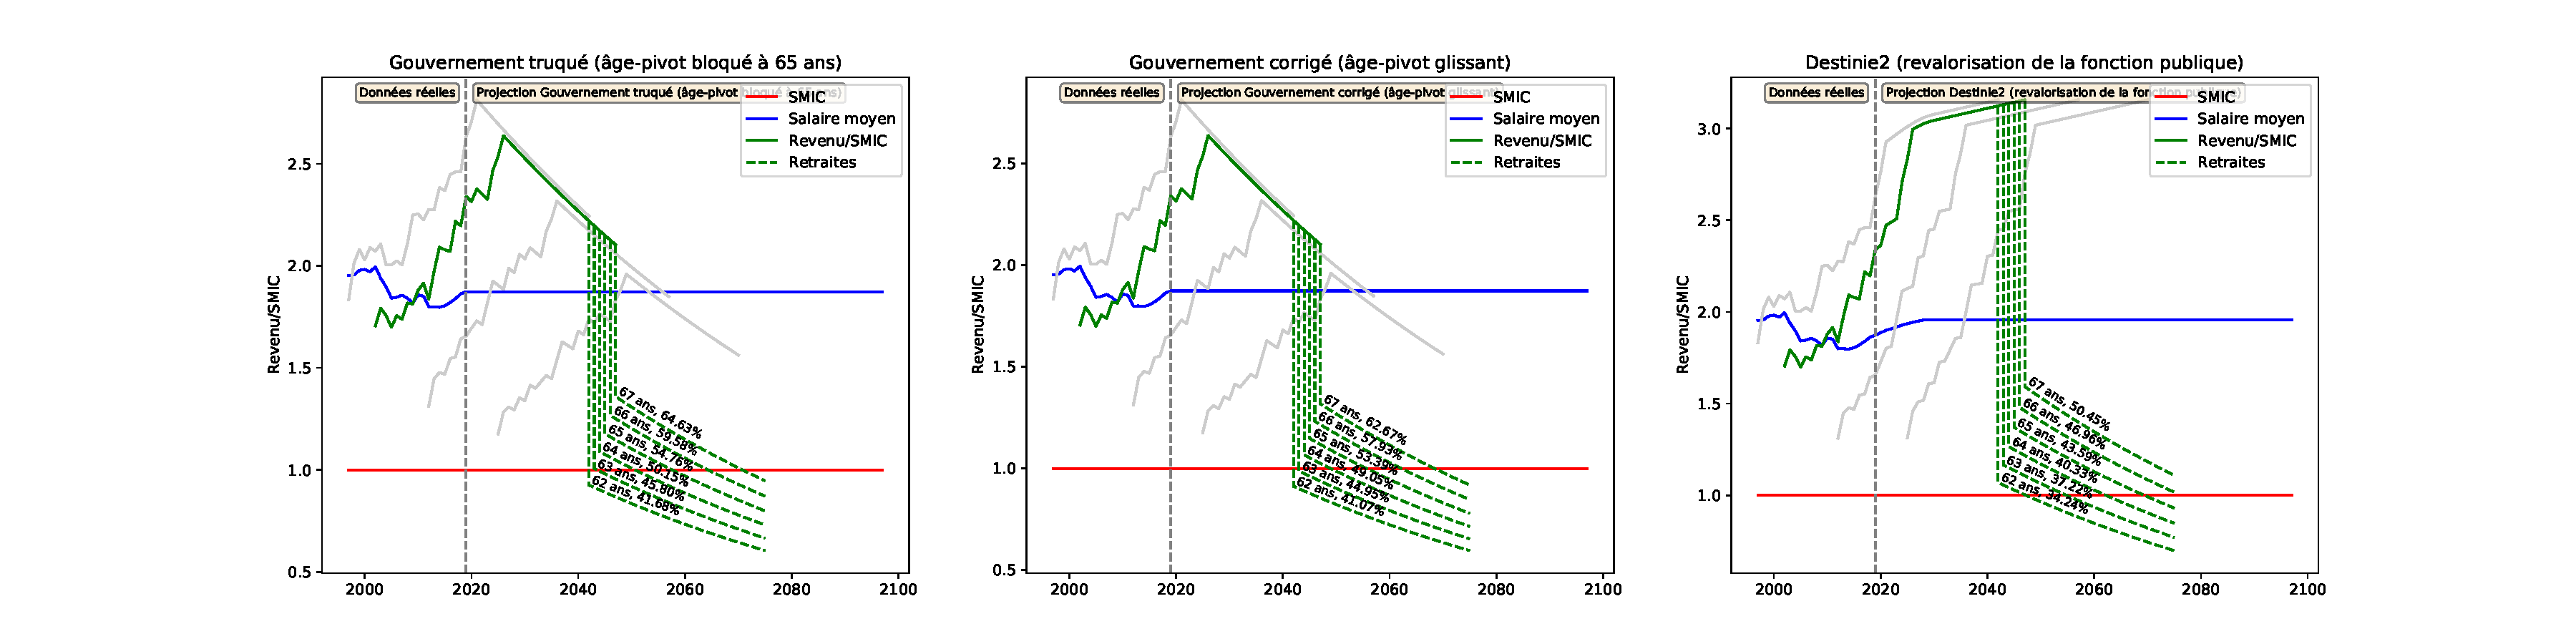
\includegraphics[width=0.9\textwidth]{fig/ProfAgrege_1980_22_dest_retraite.pdf}\end{center} \label{fig/ProfAgrege_1980_22_dest_retraite.pdf} 

\newpage 
 
\paragraph{Revenus et points pour le modèle \emph{Gouvernement truqué (âge-pivot bloqué à 65 ans)}} 
 
{ \scriptsize \begin{center} 
\begin{tabular}[htb]{|c|c||c|c|c|c|c|c||c|c||c|c|c|} 
\hline 
 Année &  Âge &  Ind Maj &  Pt Ind(\euro{} 2019) &  Rev HP(\euro{} 2019) &  Tx Primes &  GIPA(\euro{} 2019) &  Revenu(\euro{} 2019) &  SMIC(\euro{} 2019) &  Rev/SMIC &  Cumul Pts &  Achat Pt(\euro{} 2019) &  Serv. Pt(\euro{} 2019) \\ 
\hline \hline 
 2002 &  22 &  450.0 &  5.49 &  2468.82 &  0.00 &  0.00 &  2468.82 &  1447.74 &  {\bf 1.71} &  832.02 &  35.61 &  0.50 \\ 
\hline 
 2003 &  23 &  498.0 &  5.37 &  2676.56 &  0.00 &  0.00 &  2676.56 &  1493.03 &  {\bf 1.79} &  1734.06 &  35.61 &  0.50 \\ 
\hline 
 2004 &  24 &  513.0 &  5.29 &  2713.63 &  0.17 &  0.00 &  2718.24 &  1547.32 &  {\bf 1.76} &  2650.14 &  35.61 &  0.50 \\ 
\hline 
 2005 &  25 &  513.0 &  5.29 &  2713.33 &  0.40 &  0.00 &  2724.19 &  1603.67 &  {\bf 1.70} &  3568.22 &  35.61 &  0.50 \\ 
\hline 
 2006 &  26 &  542.0 &  5.23 &  2834.72 &  0.63 &  0.00 &  2852.58 &  1625.00 &  {\bf 1.76} &  4529.58 &  35.61 &  0.50 \\ 
\hline 
 2007 &  27 &  542.0 &  5.19 &  2815.41 &  0.86 &  0.00 &  2839.62 &  1634.08 &  {\bf 1.74} &  5486.56 &  35.61 &  0.50 \\ 
\hline 
 2008 &  28 &  579.0 &  5.09 &  2948.87 &  1.09 &  0.00 &  2981.02 &  1640.24 &  {\bf 1.82} &  6491.20 &  35.61 &  0.50 \\ 
\hline 
 2009 &  29 &  579.0 &  5.13 &  2969.77 &  1.32 &  0.00 &  3008.97 &  1659.42 &  {\bf 1.81} &  7505.26 &  35.61 &  0.50 \\ 
\hline 
 2010 &  30 &  598.5 &  5.08 &  3038.78 &  1.55 &  0.00 &  3085.88 &  1641.90 &  {\bf 1.88} &  8545.24 &  35.61 &  0.50 \\ 
\hline 
 2011 &  31 &  618.0 &  4.97 &  3072.59 &  1.78 &  0.00 &  3127.29 &  1633.19 &  {\bf 1.91} &  9599.17 &  35.61 &  0.50 \\ 
\hline 
 2012 &  32 &  618.0 &  4.88 &  3013.64 &  2.01 &  0.00 &  3074.21 &  1673.05 &  {\bf 1.84} &  10635.22 &  35.61 &  0.50 \\ 
\hline 
 2013 &  33 &  664.0 &  4.83 &  3210.21 &  2.24 &  0.00 &  3282.12 &  1664.01 &  {\bf 1.97} &  11741.33 &  35.61 &  0.50 \\ 
\hline 
 2014 &  34 &  710.0 &  4.81 &  3415.42 &  2.47 &  0.00 &  3499.78 &  1673.24 &  {\bf 2.09} &  12920.80 &  35.61 &  0.50 \\ 
\hline 
 2015 &  35 &  710.0 &  4.81 &  3414.08 &  2.70 &  0.00 &  3506.26 &  1686.62 &  {\bf 2.08} &  14102.45 &  35.61 &  0.50 \\ 
\hline 
 2016 &  36 &  710.0 &  4.80 &  3407.27 &  2.93 &  0.00 &  3507.10 &  1693.76 &  {\bf 2.07} &  15284.39 &  35.61 &  0.50 \\ 
\hline 
 2017 &  37 &  757.0 &  4.81 &  3640.15 &  3.16 &  0.00 &  3755.18 &  1692.60 &  {\bf 2.22} &  16549.93 &  35.61 &  0.50 \\ 
\hline 
 2018 &  38 &  757.0 &  4.74 &  3589.89 &  3.39 &  0.00 &  3711.59 &  1689.76 &  {\bf 2.20} &  17800.78 &  35.61 &  0.50 \\ 
\hline 
 2019 &  39 &  800.0 &  4.79 &  3835.54 &  3.62 &  0.00 &  3974.38 &  1698.45 &  {\bf 2.34} &  19140.20 &  35.61 &  0.50 \\ 
\hline 
 2020 &  40 &  800.0 &  4.79 &  3835.54 &  3.85 &  0.00 &  3983.21 &  1720.53 &  {\bf 2.32} &  20482.59 &  35.61 &  0.50 \\ 
\hline 
 2021 &  41 &  830.0 &  4.79 &  3979.37 &  4.08 &  0.00 &  4141.73 &  1742.90 &  {\bf 2.38} &  21878.40 &  35.61 &  0.50 \\ 
\hline 
 2022 &  42 &  830.0 &  4.79 &  3979.37 &  4.31 &  0.00 &  4150.88 &  1765.55 &  {\bf 2.35} &  23277.30 &  35.61 &  0.50 \\ 
\hline 
 2023 &  43 &  830.0 &  4.79 &  3979.37 &  4.54 &  0.00 &  4160.03 &  1788.51 &  {\bf 2.33} &  24679.28 &  35.61 &  0.50 \\ 
\hline 
 2024 &  44 &  890.0 &  4.79 &  4267.04 &  4.77 &  0.00 &  4470.57 &  1811.76 &  {\bf 2.47} &  26185.92 &  35.61 &  0.50 \\ 
\hline 
 2025 &  45 &  925.0 &  4.79 &  4434.84 &  5.00 &  0.00 &  4656.58 &  1835.31 &  {\bf 2.54} &  27755.24 &  35.61 &  0.50 \\ 
\hline 
 2026 &  46 &  972.0 &  4.79 &  4660.18 &  5.23 &  0.00 &  4903.91 &  1859.17 &  {\bf 2.64} &  29407.92 &  35.61 &  0.50 \\ 
\hline 
 2027 &  47 &  972.0 &  4.79 &  4660.18 &  5.46 &  0.00 &  4914.62 &  1883.34 &  {\bf 2.61} &  31064.20 &  35.61 &  0.50 \\ 
\hline 
 2028 &  48 &  972.0 &  4.79 &  4660.18 &  5.69 &  0.00 &  4925.34 &  1907.82 &  {\bf 2.58} &  32724.10 &  35.61 &  0.50 \\ 
\hline 
 2029 &  49 &  972.0 &  4.79 &  4660.18 &  5.92 &  0.00 &  4936.06 &  1932.62 &  {\bf 2.55} &  34386.35 &  35.63 &  0.50 \\ 
\hline 
 2030 &  50 &  972.0 &  4.79 &  4660.18 &  6.15 &  0.00 &  4946.78 &  1957.75 &  {\bf 2.53} &  36049.68 &  35.69 &  0.50 \\ 
\hline 
 2031 &  51 &  972.0 &  4.79 &  4660.18 &  6.38 &  0.00 &  4957.50 &  1983.20 &  {\bf 2.50} &  37712.82 &  35.77 &  0.50 \\ 
\hline 
 2032 &  52 &  972.0 &  4.79 &  4660.18 &  6.61 &  0.00 &  4968.22 &  2008.98 &  {\bf 2.47} &  39374.50 &  35.88 &  0.50 \\ 
\hline 
 2033 &  53 &  972.0 &  4.79 &  4660.18 &  6.84 &  0.00 &  4978.93 &  2035.10 &  {\bf 2.45} &  41033.44 &  36.02 &  0.50 \\ 
\hline 
 2034 &  54 &  972.0 &  4.79 &  4660.18 &  7.07 &  0.00 &  4989.65 &  2061.55 &  {\bf 2.42} &  42688.40 &  36.18 &  0.50 \\ 
\hline 
 2035 &  55 &  972.0 &  4.79 &  4660.18 &  7.30 &  0.00 &  5000.37 &  2088.35 &  {\bf 2.39} &  44338.12 &  36.37 &  0.51 \\ 
\hline 
 2036 &  56 &  972.0 &  4.79 &  4660.18 &  7.53 &  0.00 &  5011.09 &  2115.50 &  {\bf 2.37} &  45981.35 &  36.59 &  0.51 \\ 
\hline 
 2037 &  57 &  972.0 &  4.79 &  4660.18 &  7.76 &  0.00 &  5021.81 &  2143.00 &  {\bf 2.34} &  47616.87 &  36.85 &  0.51 \\ 
\hline 
 2038 &  58 &  972.0 &  4.79 &  4660.18 &  7.99 &  0.00 &  5032.53 &  2170.86 &  {\bf 2.32} &  49243.48 &  37.13 &  0.52 \\ 
\hline 
 2039 &  59 &  972.0 &  4.79 &  4660.18 &  8.22 &  0.00 &  5043.24 &  2199.08 &  {\bf 2.29} &  50859.99 &  37.44 &  0.52 \\ 
\hline 
 2040 &  60 &  972.0 &  4.79 &  4660.18 &  8.45 &  0.00 &  5053.96 &  2227.67 &  {\bf 2.27} &  52465.23 &  37.78 &  0.53 \\ 
\hline 
 2041 &  61 &  972.0 &  4.79 &  4660.18 &  8.68 &  0.00 &  5064.68 &  2256.63 &  {\bf 2.24} &  54058.07 &  38.16 &  0.53 \\ 
\hline 
 2042 &  62 &  972.0 &  4.79 &  4660.18 &  8.91 &  0.00 &  5075.40 &  2285.97 &  {\bf 2.22} &  55637.38 &  38.56 &  0.54 \\ 
\hline 
 2043 &  63 &  972.0 &  4.79 &  4660.18 &  9.14 &  0.00 &  5086.12 &  2315.68 &  {\bf 2.20} &  57202.10 &  39.01 &  0.54 \\ 
\hline 
 2044 &  64 &  972.0 &  4.79 &  4660.18 &  9.37 &  0.00 &  5096.84 &  2345.79 &  {\bf 2.17} &  58751.17 &  39.48 &  0.55 \\ 
\hline 
 2045 &  65 &  972.0 &  4.79 &  4660.18 &  9.60 &  0.00 &  5107.56 &  2376.28 &  {\bf 2.15} &  60283.57 &  40.00 &  0.56 \\ 
\hline 
 2046 &  66 &  972.0 &  4.79 &  4660.18 &  9.83 &  0.00 &  5118.27 &  2407.18 &  {\bf 2.13} &  61799.49 &  40.52 &  0.56 \\ 
\hline 
 2047 &  67 &  972.0 &  4.79 &  4660.18 &  10.06 &  0.00 &  5128.99 &  2438.47 &  {\bf 2.10} &  63299.08 &  41.04 &  0.57 \\ 
\hline 
\hline 
\end{tabular} 
\end{center} } 
\newpage 
 
\paragraph{Revenus et points pour le modèle \emph{Gouvernement corrigé (âge-pivot glissant)}} 
 
{ \scriptsize \begin{center} 
\begin{tabular}[htb]{|c|c||c|c|c|c|c|c||c|c||c|c|c|} 
\hline 
 Année &  Âge &  Ind Maj &  Pt Ind(\euro{} 2019) &  Rev HP(\euro{} 2019) &  Tx Primes &  GIPA(\euro{} 2019) &  Revenu(\euro{} 2019) &  SMIC(\euro{} 2019) &  Rev/SMIC &  Cumul Pts &  Achat Pt(\euro{} 2019) &  Serv. Pt(\euro{} 2019) \\ 
\hline \hline 
 2002 &  22 &  450.0 &  5.49 &  2468.82 &  0.00 &  0.00 &  2468.82 &  1447.74 &  {\bf 1.71} &  832.02 &  35.61 &  0.50 \\ 
\hline 
 2003 &  23 &  498.0 &  5.37 &  2676.56 &  0.00 &  0.00 &  2676.56 &  1493.03 &  {\bf 1.79} &  1734.06 &  35.61 &  0.50 \\ 
\hline 
 2004 &  24 &  513.0 &  5.29 &  2713.63 &  0.17 &  0.00 &  2718.24 &  1547.32 &  {\bf 1.76} &  2650.14 &  35.61 &  0.50 \\ 
\hline 
 2005 &  25 &  513.0 &  5.29 &  2713.33 &  0.40 &  0.00 &  2724.19 &  1603.67 &  {\bf 1.70} &  3568.22 &  35.61 &  0.50 \\ 
\hline 
 2006 &  26 &  542.0 &  5.23 &  2834.72 &  0.63 &  0.00 &  2852.58 &  1625.00 &  {\bf 1.76} &  4529.58 &  35.61 &  0.50 \\ 
\hline 
 2007 &  27 &  542.0 &  5.19 &  2815.41 &  0.86 &  0.00 &  2839.62 &  1634.08 &  {\bf 1.74} &  5486.56 &  35.61 &  0.50 \\ 
\hline 
 2008 &  28 &  579.0 &  5.09 &  2948.87 &  1.09 &  0.00 &  2981.02 &  1640.24 &  {\bf 1.82} &  6491.20 &  35.61 &  0.50 \\ 
\hline 
 2009 &  29 &  579.0 &  5.13 &  2969.77 &  1.32 &  0.00 &  3008.97 &  1659.42 &  {\bf 1.81} &  7505.26 &  35.61 &  0.50 \\ 
\hline 
 2010 &  30 &  598.5 &  5.08 &  3038.78 &  1.55 &  0.00 &  3085.88 &  1641.90 &  {\bf 1.88} &  8545.24 &  35.61 &  0.50 \\ 
\hline 
 2011 &  31 &  618.0 &  4.97 &  3072.59 &  1.78 &  0.00 &  3127.29 &  1633.19 &  {\bf 1.91} &  9599.17 &  35.61 &  0.50 \\ 
\hline 
 2012 &  32 &  618.0 &  4.88 &  3013.64 &  2.01 &  0.00 &  3074.21 &  1673.05 &  {\bf 1.84} &  10635.22 &  35.61 &  0.50 \\ 
\hline 
 2013 &  33 &  664.0 &  4.83 &  3210.21 &  2.24 &  0.00 &  3282.12 &  1664.01 &  {\bf 1.97} &  11741.33 &  35.61 &  0.50 \\ 
\hline 
 2014 &  34 &  710.0 &  4.81 &  3415.42 &  2.47 &  0.00 &  3499.78 &  1673.24 &  {\bf 2.09} &  12920.80 &  35.61 &  0.50 \\ 
\hline 
 2015 &  35 &  710.0 &  4.81 &  3414.08 &  2.70 &  0.00 &  3506.26 &  1686.62 &  {\bf 2.08} &  14102.45 &  35.61 &  0.50 \\ 
\hline 
 2016 &  36 &  710.0 &  4.80 &  3407.27 &  2.93 &  0.00 &  3507.10 &  1693.76 &  {\bf 2.07} &  15284.39 &  35.61 &  0.50 \\ 
\hline 
 2017 &  37 &  757.0 &  4.81 &  3640.15 &  3.16 &  0.00 &  3755.18 &  1692.60 &  {\bf 2.22} &  16549.93 &  35.61 &  0.50 \\ 
\hline 
 2018 &  38 &  757.0 &  4.74 &  3589.89 &  3.39 &  0.00 &  3711.59 &  1689.76 &  {\bf 2.20} &  17800.78 &  35.61 &  0.50 \\ 
\hline 
 2019 &  39 &  800.0 &  4.79 &  3835.54 &  3.62 &  0.00 &  3974.38 &  1698.45 &  {\bf 2.34} &  19140.20 &  35.61 &  0.50 \\ 
\hline 
 2020 &  40 &  800.0 &  4.79 &  3835.54 &  3.85 &  0.00 &  3983.21 &  1720.53 &  {\bf 2.32} &  20482.59 &  35.61 &  0.50 \\ 
\hline 
 2021 &  41 &  830.0 &  4.79 &  3979.37 &  4.08 &  0.00 &  4141.73 &  1742.90 &  {\bf 2.38} &  21878.40 &  35.61 &  0.50 \\ 
\hline 
 2022 &  42 &  830.0 &  4.79 &  3979.37 &  4.31 &  0.00 &  4150.88 &  1765.55 &  {\bf 2.35} &  23277.30 &  35.61 &  0.50 \\ 
\hline 
 2023 &  43 &  830.0 &  4.79 &  3979.37 &  4.54 &  0.00 &  4160.03 &  1788.51 &  {\bf 2.33} &  24679.28 &  35.61 &  0.50 \\ 
\hline 
 2024 &  44 &  890.0 &  4.79 &  4267.04 &  4.77 &  0.00 &  4470.57 &  1811.76 &  {\bf 2.47} &  26185.92 &  35.61 &  0.50 \\ 
\hline 
 2025 &  45 &  925.0 &  4.79 &  4434.84 &  5.00 &  0.00 &  4656.58 &  1835.31 &  {\bf 2.54} &  27755.24 &  35.61 &  0.50 \\ 
\hline 
 2026 &  46 &  972.0 &  4.79 &  4660.18 &  5.23 &  0.00 &  4903.91 &  1859.17 &  {\bf 2.64} &  29407.92 &  35.61 &  0.50 \\ 
\hline 
 2027 &  47 &  972.0 &  4.79 &  4660.18 &  5.46 &  0.00 &  4914.62 &  1883.34 &  {\bf 2.61} &  31064.20 &  35.61 &  0.50 \\ 
\hline 
 2028 &  48 &  972.0 &  4.79 &  4660.18 &  5.69 &  0.00 &  4925.34 &  1907.82 &  {\bf 2.58} &  32724.10 &  35.61 &  0.50 \\ 
\hline 
 2029 &  49 &  972.0 &  4.79 &  4660.18 &  5.92 &  0.00 &  4936.06 &  1932.62 &  {\bf 2.55} &  34386.35 &  35.63 &  0.50 \\ 
\hline 
 2030 &  50 &  972.0 &  4.79 &  4660.18 &  6.15 &  0.00 &  4946.78 &  1957.75 &  {\bf 2.53} &  36049.68 &  35.69 &  0.50 \\ 
\hline 
 2031 &  51 &  972.0 &  4.79 &  4660.18 &  6.38 &  0.00 &  4957.50 &  1983.20 &  {\bf 2.50} &  37712.82 &  35.77 &  0.50 \\ 
\hline 
 2032 &  52 &  972.0 &  4.79 &  4660.18 &  6.61 &  0.00 &  4968.22 &  2008.98 &  {\bf 2.47} &  39374.50 &  35.88 &  0.50 \\ 
\hline 
 2033 &  53 &  972.0 &  4.79 &  4660.18 &  6.84 &  0.00 &  4978.93 &  2035.10 &  {\bf 2.45} &  41033.44 &  36.02 &  0.50 \\ 
\hline 
 2034 &  54 &  972.0 &  4.79 &  4660.18 &  7.07 &  0.00 &  4989.65 &  2061.55 &  {\bf 2.42} &  42688.40 &  36.18 &  0.50 \\ 
\hline 
 2035 &  55 &  972.0 &  4.79 &  4660.18 &  7.30 &  0.00 &  5000.37 &  2088.35 &  {\bf 2.39} &  44338.12 &  36.37 &  0.51 \\ 
\hline 
 2036 &  56 &  972.0 &  4.79 &  4660.18 &  7.53 &  0.00 &  5011.09 &  2115.50 &  {\bf 2.37} &  45981.35 &  36.59 &  0.51 \\ 
\hline 
 2037 &  57 &  972.0 &  4.79 &  4660.18 &  7.76 &  0.00 &  5021.81 &  2143.00 &  {\bf 2.34} &  47616.87 &  36.85 &  0.51 \\ 
\hline 
 2038 &  58 &  972.0 &  4.79 &  4660.18 &  7.99 &  0.00 &  5032.53 &  2170.86 &  {\bf 2.32} &  49243.48 &  37.13 &  0.52 \\ 
\hline 
 2039 &  59 &  972.0 &  4.79 &  4660.18 &  8.22 &  0.00 &  5043.24 &  2199.08 &  {\bf 2.29} &  50859.99 &  37.44 &  0.52 \\ 
\hline 
 2040 &  60 &  972.0 &  4.79 &  4660.18 &  8.45 &  0.00 &  5053.96 &  2227.67 &  {\bf 2.27} &  52465.23 &  37.78 &  0.53 \\ 
\hline 
 2041 &  61 &  972.0 &  4.79 &  4660.18 &  8.68 &  0.00 &  5064.68 &  2256.63 &  {\bf 2.24} &  54058.07 &  38.16 &  0.53 \\ 
\hline 
 2042 &  62 &  972.0 &  4.79 &  4660.18 &  8.91 &  0.00 &  5075.40 &  2285.97 &  {\bf 2.22} &  55637.38 &  38.56 &  0.54 \\ 
\hline 
 2043 &  63 &  972.0 &  4.79 &  4660.18 &  9.14 &  0.00 &  5086.12 &  2315.68 &  {\bf 2.20} &  57202.10 &  39.01 &  0.54 \\ 
\hline 
 2044 &  64 &  972.0 &  4.79 &  4660.18 &  9.37 &  0.00 &  5096.84 &  2345.79 &  {\bf 2.17} &  58751.17 &  39.48 &  0.55 \\ 
\hline 
 2045 &  65 &  972.0 &  4.79 &  4660.18 &  9.60 &  0.00 &  5107.56 &  2376.28 &  {\bf 2.15} &  60283.57 &  40.00 &  0.56 \\ 
\hline 
 2046 &  66 &  972.0 &  4.79 &  4660.18 &  9.83 &  0.00 &  5118.27 &  2407.18 &  {\bf 2.13} &  61799.49 &  40.52 &  0.56 \\ 
\hline 
 2047 &  67 &  972.0 &  4.79 &  4660.18 &  10.06 &  0.00 &  5128.99 &  2438.47 &  {\bf 2.10} &  63299.08 &  41.04 &  0.57 \\ 
\hline 
\hline 
\end{tabular} 
\end{center} } 
\newpage 
 
\paragraph{Revenus et points pour le modèle \emph{Destinie2 (revalorisation de la fonction publique)}} 
 
{ \scriptsize \begin{center} 
\begin{tabular}[htb]{|c|c||c|c|c|c|c|c||c|c||c|c|c|} 
\hline 
 Année &  Âge &  Ind Maj &  Pt Ind(\euro{} 2019) &  Rev HP(\euro{} 2019) &  Tx Primes &  GIPA(\euro{} 2019) &  Revenu(\euro{} 2019) &  SMIC(\euro{} 2019) &  Rev/SMIC &  Cumul Pts &  Achat Pt(\euro{} 2019) &  Serv. Pt(\euro{} 2019) \\ 
\hline \hline 
 2002 &  22 &  450.0 &  5.49 &  2468.82 &  0.00 &  0.00 &  2468.82 &  1447.74 &  {\bf 1.71} &  829.98 &  35.69 &  0.50 \\ 
\hline 
 2003 &  23 &  498.0 &  5.37 &  2676.56 &  0.00 &  0.00 &  2676.56 &  1493.03 &  {\bf 1.79} &  1729.80 &  35.69 &  0.50 \\ 
\hline 
 2004 &  24 &  513.0 &  5.29 &  2713.63 &  0.17 &  0.00 &  2718.24 &  1547.32 &  {\bf 1.76} &  2643.63 &  35.69 &  0.50 \\ 
\hline 
 2005 &  25 &  513.0 &  5.29 &  2713.33 &  0.40 &  0.00 &  2724.19 &  1603.67 &  {\bf 1.70} &  3559.45 &  35.69 &  0.50 \\ 
\hline 
 2006 &  26 &  542.0 &  5.23 &  2834.72 &  0.63 &  0.00 &  2852.58 &  1625.00 &  {\bf 1.76} &  4518.45 &  35.69 &  0.50 \\ 
\hline 
 2007 &  27 &  542.0 &  5.19 &  2815.41 &  0.86 &  0.00 &  2839.62 &  1634.08 &  {\bf 1.74} &  5473.08 &  35.69 &  0.50 \\ 
\hline 
 2008 &  28 &  579.0 &  5.09 &  2948.87 &  1.09 &  0.00 &  2981.02 &  1640.24 &  {\bf 1.82} &  6475.25 &  35.69 &  0.50 \\ 
\hline 
 2009 &  29 &  579.0 &  5.13 &  2969.77 &  1.32 &  0.00 &  3008.97 &  1659.42 &  {\bf 1.81} &  7486.82 &  35.69 &  0.50 \\ 
\hline 
 2010 &  30 &  598.5 &  5.08 &  3038.78 &  1.55 &  0.00 &  3085.88 &  1641.90 &  {\bf 1.88} &  8524.24 &  35.69 &  0.50 \\ 
\hline 
 2011 &  31 &  618.0 &  4.97 &  3072.59 &  1.78 &  0.00 &  3127.29 &  1633.19 &  {\bf 1.91} &  9575.59 &  35.69 &  0.50 \\ 
\hline 
 2012 &  32 &  618.0 &  4.88 &  3013.64 &  2.01 &  0.00 &  3074.21 &  1673.05 &  {\bf 1.84} &  10609.09 &  35.69 &  0.50 \\ 
\hline 
 2013 &  33 &  664.0 &  4.83 &  3210.21 &  2.24 &  0.00 &  3282.12 &  1664.01 &  {\bf 1.97} &  11712.48 &  35.69 &  0.50 \\ 
\hline 
 2014 &  34 &  710.0 &  4.81 &  3415.42 &  2.47 &  0.00 &  3499.78 &  1673.24 &  {\bf 2.09} &  12889.05 &  35.69 &  0.50 \\ 
\hline 
 2015 &  35 &  710.0 &  4.81 &  3414.08 &  2.70 &  0.00 &  3506.26 &  1686.62 &  {\bf 2.08} &  14067.81 &  35.69 &  0.50 \\ 
\hline 
 2016 &  36 &  710.0 &  4.80 &  3407.27 &  2.93 &  0.00 &  3507.10 &  1693.76 &  {\bf 2.07} &  15246.84 &  35.69 &  0.50 \\ 
\hline 
 2017 &  37 &  757.0 &  4.81 &  3640.15 &  3.16 &  0.00 &  3755.18 &  1692.60 &  {\bf 2.22} &  16509.27 &  35.69 &  0.50 \\ 
\hline 
 2018 &  38 &  757.0 &  4.74 &  3589.89 &  3.39 &  0.00 &  3711.59 &  1689.76 &  {\bf 2.20} &  17757.04 &  35.69 &  0.50 \\ 
\hline 
 2019 &  39 &  800.0 &  4.79 &  3835.54 &  3.62 &  0.00 &  3974.38 &  1698.45 &  {\bf 2.34} &  19093.17 &  35.69 &  0.50 \\ 
\hline 
 2020 &  40 &  800.0 &  4.83 &  3866.22 &  3.85 &  0.00 &  4015.07 &  1699.99 &  {\bf 2.36} &  20442.97 &  35.69 &  0.50 \\ 
\hline 
 2021 &  41 &  830.0 &  4.88 &  4047.31 &  4.08 &  0.00 &  4212.44 &  1703.48 &  {\bf 2.47} &  21859.13 &  35.69 &  0.50 \\ 
\hline 
 2022 &  42 &  830.0 &  4.93 &  4087.78 &  4.31 &  0.00 &  4263.96 &  1712.78 &  {\bf 2.49} &  23292.60 &  35.69 &  0.50 \\ 
\hline 
 2023 &  43 &  830.0 &  4.98 &  4135.61 &  4.54 &  0.00 &  4323.36 &  1723.51 &  {\bf 2.51} &  24746.05 &  35.69 &  0.50 \\ 
\hline 
 2024 &  44 &  890.0 &  5.04 &  4487.34 &  4.77 &  0.00 &  4701.38 &  1735.69 &  {\bf 2.71} &  26326.58 &  35.69 &  0.50 \\ 
\hline 
 2025 &  45 &  925.0 &  5.10 &  4720.70 &  5.00 &  0.00 &  4956.74 &  1749.35 &  {\bf 2.83} &  27992.96 &  35.69 &  0.50 \\ 
\hline 
 2026 &  46 &  972.0 &  5.17 &  5022.57 &  5.23 &  0.00 &  5285.25 &  1764.53 &  {\bf 3.00} &  29769.78 &  35.69 &  0.50 \\ 
\hline 
 2027 &  47 &  972.0 &  5.23 &  5086.86 &  5.46 &  0.00 &  5364.61 &  1781.27 &  {\bf 3.01} &  31573.27 &  35.69 &  0.50 \\ 
\hline 
 2028 &  48 &  972.0 &  5.30 &  5153.50 &  5.69 &  0.00 &  5446.73 &  1799.59 &  {\bf 3.03} &  33404.38 &  35.69 &  0.50 \\ 
\hline 
 2029 &  49 &  972.0 &  5.37 &  5215.86 &  5.92 &  0.00 &  5524.64 &  1819.55 &  {\bf 3.04} &  35260.36 &  35.72 &  0.50 \\ 
\hline 
 2030 &  50 &  972.0 &  5.43 &  5280.53 &  6.15 &  0.00 &  5605.29 &  1841.19 &  {\bf 3.04} &  37140.71 &  35.77 &  0.50 \\ 
\hline 
 2031 &  51 &  972.0 &  5.50 &  5347.60 &  6.38 &  0.00 &  5688.77 &  1864.58 &  {\bf 3.05} &  39044.81 &  35.85 &  0.50 \\ 
\hline 
 2032 &  52 &  972.0 &  5.57 &  5417.12 &  6.61 &  0.00 &  5775.19 &  1888.81 &  {\bf 3.06} &  40971.98 &  35.96 &  0.50 \\ 
\hline 
 2033 &  53 &  972.0 &  5.65 &  5487.54 &  6.84 &  0.00 &  5862.89 &  1913.37 &  {\bf 3.06} &  42920.99 &  36.10 &  0.50 \\ 
\hline 
 2034 &  54 &  972.0 &  5.72 &  5558.88 &  7.07 &  0.00 &  5951.89 &  1938.24 &  {\bf 3.07} &  44890.60 &  36.26 &  0.50 \\ 
\hline 
 2035 &  55 &  972.0 &  5.79 &  5631.14 &  7.30 &  0.00 &  6042.22 &  1963.44 &  {\bf 3.08} &  46879.48 &  36.46 &  0.51 \\ 
\hline 
 2036 &  56 &  972.0 &  5.87 &  5704.35 &  7.53 &  0.00 &  6133.88 &  1988.96 &  {\bf 3.08} &  48886.31 &  36.68 &  0.51 \\ 
\hline 
 2037 &  57 &  972.0 &  5.94 &  5778.50 &  7.76 &  0.00 &  6226.92 &  2014.82 &  {\bf 3.09} &  50909.69 &  36.93 &  0.51 \\ 
\hline 
 2038 &  58 &  972.0 &  6.02 &  5853.62 &  7.99 &  0.00 &  6321.33 &  2041.01 &  {\bf 3.10} &  52948.20 &  37.21 &  0.52 \\ 
\hline 
 2039 &  59 &  972.0 &  6.10 &  5929.72 &  8.22 &  0.00 &  6417.14 &  2067.55 &  {\bf 3.10} &  55000.38 &  37.52 &  0.52 \\ 
\hline 
 2040 &  60 &  972.0 &  6.18 &  6006.81 &  8.45 &  0.00 &  6514.38 &  2094.43 &  {\bf 3.11} &  57064.76 &  37.87 &  0.53 \\ 
\hline 
 2041 &  61 &  972.0 &  6.26 &  6084.90 &  8.68 &  0.00 &  6613.06 &  2121.65 &  {\bf 3.12} &  59139.81 &  38.24 &  0.53 \\ 
\hline 
 2042 &  62 &  972.0 &  6.34 &  6164.00 &  8.91 &  0.00 &  6713.21 &  2149.23 &  {\bf 3.12} &  61224.00 &  38.65 &  0.54 \\ 
\hline 
 2043 &  63 &  972.0 &  6.42 &  6244.13 &  9.14 &  0.00 &  6814.85 &  2177.17 &  {\bf 3.13} &  63315.76 &  39.10 &  0.54 \\ 
\hline 
 2044 &  64 &  972.0 &  6.51 &  6325.31 &  9.37 &  0.00 &  6917.99 &  2205.48 &  {\bf 3.14} &  65413.53 &  39.57 &  0.55 \\ 
\hline 
 2045 &  65 &  972.0 &  6.59 &  6407.53 &  9.60 &  0.00 &  7022.66 &  2234.15 &  {\bf 3.14} &  67515.71 &  40.09 &  0.56 \\ 
\hline 
 2046 &  66 &  972.0 &  6.68 &  6490.83 &  9.83 &  0.00 &  7128.88 &  2263.19 &  {\bf 3.15} &  69622.29 &  40.61 &  0.57 \\ 
\hline 
 2047 &  67 &  972.0 &  6.76 &  6575.21 &  10.06 &  0.00 &  7236.68 &  2292.61 &  {\bf 3.16} &  71733.29 &  41.14 &  0.57 \\ 
\hline 
\hline 
\end{tabular} 
\end{center} } 
\newpage 
 
\subsection{Génération 1990 (début en 2012)} 

\paragraph{Retraites possibles dans le modèle \emph{Gouvernement truqué (âge-pivot bloqué à 65 ans)}}  
 
{ \scriptsize \begin{center} 
\begin{tabular}[htb]{|c|c||c|c||c|c||c||c|c|c|c|c|c|} 
\hline 
 Retraite en &  Âge &  Âge pivot &  Décote/Surcote &  Retraite (\euro{} 2019) &  Tx Rempl(\%) &  SMIC (\euro{} 2019) &  Retraite/SMIC &  Rev70/SMIC &  Rev75/SMIC &  Rev80/SMIC &  Rev85/SMIC &  Rev90/SMIC \\ 
\hline \hline 
 2052 &  62 &  65 ans 0 mois &  -15.00\% &  2269.42 &  {\bf 44.71} &  2601.14 &  {\bf {\color{red} 0.87}} &  {\bf {\color{red} 0.79}} &  {\bf {\color{red} 0.74}} &  {\bf {\color{red} 0.69}} &  {\bf {\color{red} 0.65}} &  {\bf {\color{red} 0.61}} \\ 
\hline 
 2053 &  63 &  65 ans 0 mois &  -10.00\% &  2497.87 &  {\bf 49.11} &  2634.96 &  {\bf {\color{red} 0.95}} &  {\bf {\color{red} 0.87}} &  {\bf {\color{red} 0.81}} &  {\bf {\color{red} 0.76}} &  {\bf {\color{red} 0.71}} &  {\bf {\color{red} 0.67}} \\ 
\hline 
 2054 &  64 &  65 ans 0 mois &  -5.00\% &  2738.31 &  {\bf 53.73} &  2669.21 &  {\bf 1.03} &  {\bf {\color{red} 0.95}} &  {\bf {\color{red} 0.89}} &  {\bf {\color{red} 0.83}} &  {\bf {\color{red} 0.78}} &  {\bf {\color{red} 0.73}} \\ 
\hline 
 2055 &  65 &  65 ans 0 mois &  0.00\% &  2991.00 &  {\bf 58.56} &  2703.91 &  {\bf 1.11} &  {\bf 1.04} &  {\bf {\color{red} 0.97}} &  {\bf {\color{red} 0.91}} &  {\bf {\color{red} 0.85}} &  {\bf {\color{red} 0.80}} \\ 
\hline 
 2056 &  66 &  65 ans 0 mois &  5.00\% &  3256.18 &  {\bf 63.62} &  2739.06 &  {\bf 1.19} &  {\bf 1.13} &  {\bf 1.06} &  {\bf {\color{red} 0.99}} &  {\bf {\color{red} 0.93}} &  {\bf {\color{red} 0.87}} \\ 
\hline 
 2057 &  67 &  65 ans 0 mois &  10.00\% &  3534.12 &  {\bf 68.90} &  2774.67 &  {\bf 1.27} &  {\bf 1.23} &  {\bf 1.15} &  {\bf 1.08} &  {\bf 1.01} &  {\bf {\color{red} 0.95}} \\ 
\hline 
\hline 
\end{tabular} 
\end{center} } 
\paragraph{Retraites possibles dans le modèle \emph{Gouvernement corrigé (âge-pivot glissant)}}  
 
{ \scriptsize \begin{center} 
\begin{tabular}[htb]{|c|c||c|c||c|c||c||c|c|c|c|c|c|} 
\hline 
 Retraite en &  Âge &  Âge pivot &  Décote/Surcote &  Retraite (\euro{} 2019) &  Tx Rempl(\%) &  SMIC (\euro{} 2019) &  Retraite/SMIC &  Rev70/SMIC &  Rev75/SMIC &  Rev80/SMIC &  Rev85/SMIC &  Rev90/SMIC \\ 
\hline \hline 
 2052 &  62 &  66 ans 1 mois &  -20.42\% &  2124.80 &  {\bf 41.86} &  2601.14 &  {\bf {\color{red} 0.82}} &  {\bf {\color{red} 0.74}} &  {\bf {\color{red} 0.69}} &  {\bf {\color{red} 0.65}} &  {\bf {\color{red} 0.61}} &  {\bf {\color{red} 0.57}} \\ 
\hline 
 2053 &  63 &  66 ans 2 mois &  -15.83\% &  2335.97 &  {\bf 45.93} &  2634.96 &  {\bf {\color{red} 0.89}} &  {\bf {\color{red} 0.81}} &  {\bf {\color{red} 0.76}} &  {\bf {\color{red} 0.71}} &  {\bf {\color{red} 0.67}} &  {\bf {\color{red} 0.63}} \\ 
\hline 
 2054 &  64 &  66 ans 3 mois &  -11.25\% &  2558.16 &  {\bf 50.19} &  2669.21 &  {\bf {\color{red} 0.96}} &  {\bf {\color{red} 0.89}} &  {\bf {\color{red} 0.83}} &  {\bf {\color{red} 0.78}} &  {\bf {\color{red} 0.73}} &  {\bf {\color{red} 0.69}} \\ 
\hline 
 2055 &  65 &  66 ans 4 mois &  -6.67\% &  2791.60 &  {\bf 54.66} &  2703.91 &  {\bf 1.03} &  {\bf {\color{red} 0.97}} &  {\bf {\color{red} 0.91}} &  {\bf {\color{red} 0.85}} &  {\bf {\color{red} 0.80}} &  {\bf {\color{red} 0.75}} \\ 
\hline 
 2056 &  66 &  66 ans 5 mois &  -2.08\% &  3036.52 &  {\bf 59.33} &  2739.06 &  {\bf 1.11} &  {\bf 1.05} &  {\bf {\color{red} 0.99}} &  {\bf {\color{red} 0.93}} &  {\bf {\color{red} 0.87}} &  {\bf {\color{red} 0.81}} \\ 
\hline 
 2057 &  67 &  66 ans 6 mois &  2.50\% &  3293.15 &  {\bf 64.21} &  2774.67 &  {\bf 1.19} &  {\bf 1.14} &  {\bf 1.07} &  {\bf 1.00} &  {\bf {\color{red} 0.94}} &  {\bf {\color{red} 0.88}} \\ 
\hline 
\hline 
\end{tabular} 
\end{center} } 
\paragraph{Retraites possibles dans le modèle \emph{Destinie2 (revalorisation de la fonction publique)}}  
 
{ \scriptsize \begin{center} 
\begin{tabular}[htb]{|c|c||c|c||c|c||c||c|c|c|c|c|c|} 
\hline 
 Retraite en &  Âge &  Âge pivot &  Décote/Surcote &  Retraite (\euro{} 2019) &  Tx Rempl(\%) &  SMIC (\euro{} 2019) &  Retraite/SMIC &  Rev70/SMIC &  Rev75/SMIC &  Rev80/SMIC &  Rev85/SMIC &  Rev90/SMIC \\ 
\hline \hline 
 2052 &  62 &  66 ans 1 mois &  -20.42\% &  2582.76 &  {\bf 33.81} &  2445.56 &  {\bf 1.06} &  {\bf {\color{red} 0.95}} &  {\bf {\color{red} 0.89}} &  {\bf {\color{red} 0.84}} &  {\bf {\color{red} 0.78}} &  {\bf {\color{red} 0.74}} \\ 
\hline 
 2053 &  63 &  66 ans 2 mois &  -15.83\% &  2857.86 &  {\bf 36.85} &  2477.35 &  {\bf 1.15} &  {\bf 1.05} &  {\bf {\color{red} 0.99}} &  {\bf {\color{red} 0.93}} &  {\bf {\color{red} 0.87}} &  {\bf {\color{red} 0.81}} \\ 
\hline 
 2054 &  64 &  66 ans 3 mois &  -11.25\% &  3149.90 &  {\bf 40.02} &  2509.56 &  {\bf 1.26} &  {\bf 1.16} &  {\bf 1.09} &  {\bf 1.02} &  {\bf {\color{red} 0.96}} &  {\bf {\color{red} 0.90}} \\ 
\hline 
 2055 &  65 &  66 ans 4 mois &  -6.67\% &  3459.45 &  {\bf 43.29} &  2542.18 &  {\bf 1.36} &  {\bf 1.28} &  {\bf 1.20} &  {\bf 1.12} &  {\bf 1.05} &  {\bf {\color{red} 0.99}} \\ 
\hline 
 2056 &  66 &  66 ans 5 mois &  -2.08\% &  3787.07 &  {\bf 46.69} &  2575.23 &  {\bf 1.47} &  {\bf 1.40} &  {\bf 1.31} &  {\bf 1.23} &  {\bf 1.15} &  {\bf 1.08} \\ 
\hline 
 2057 &  67 &  66 ans 6 mois &  2.50\% &  4133.36 &  {\bf 50.20} &  2608.71 &  {\bf 1.58} &  {\bf 1.52} &  {\bf 1.43} &  {\bf 1.34} &  {\bf 1.26} &  {\bf 1.18} \\ 
\hline 
\hline 
\end{tabular} 
\end{center} } 

 \begin{center}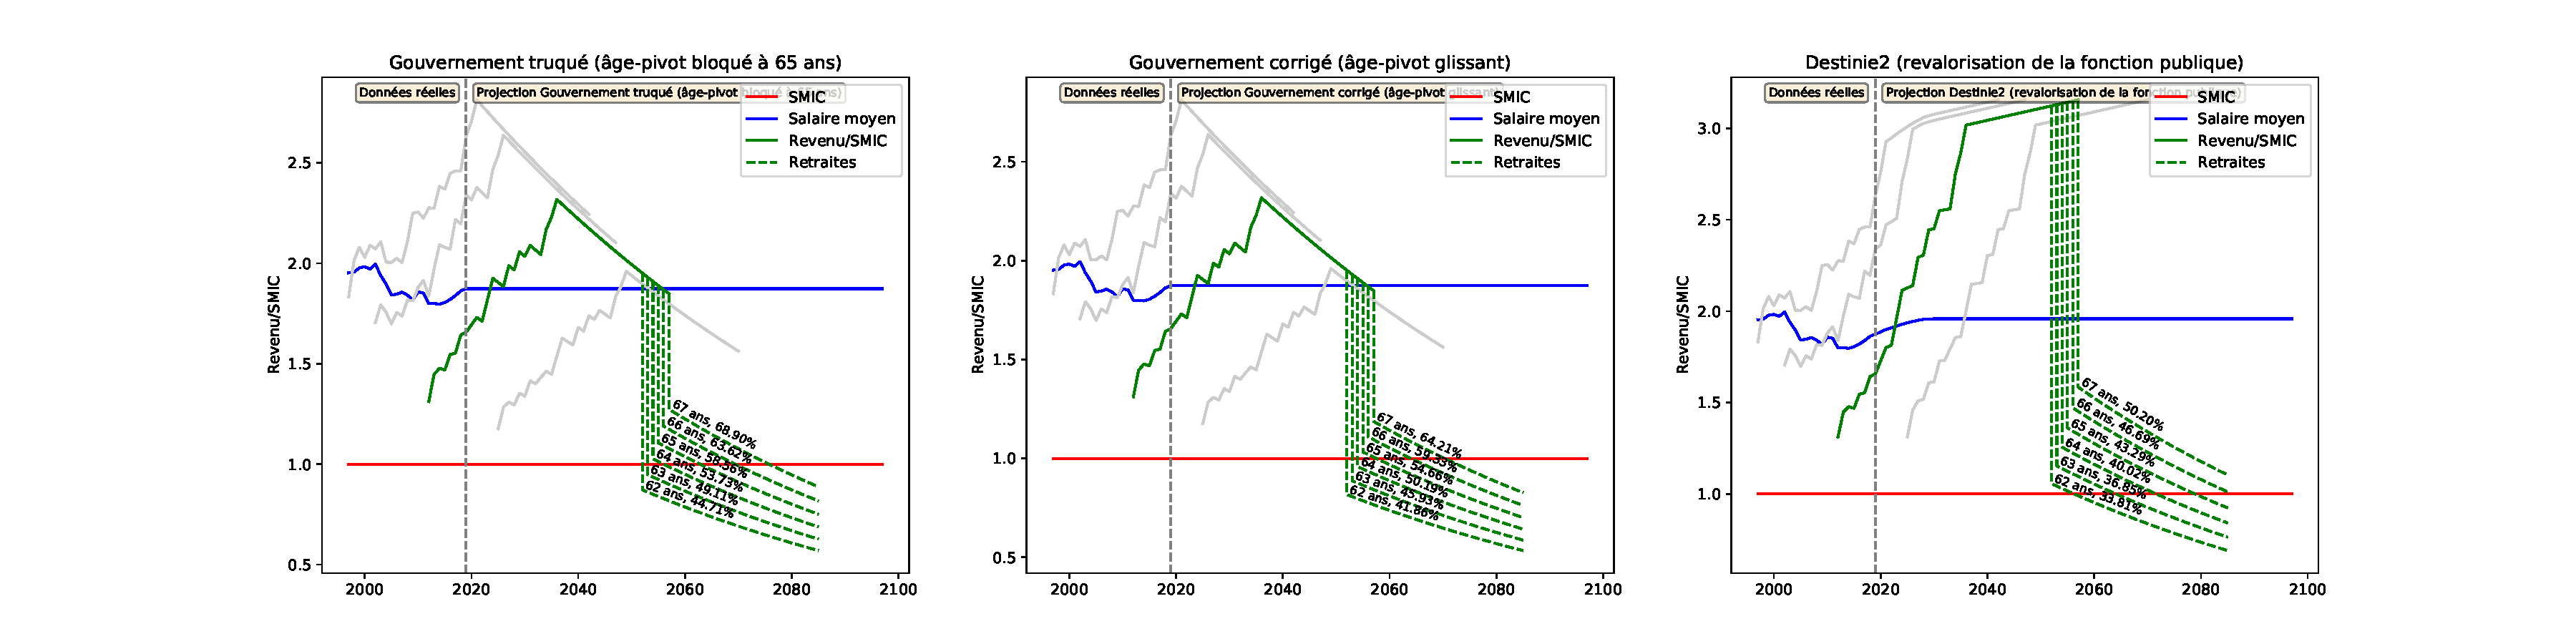
\includegraphics[width=0.9\textwidth]{fig/ProfAgrege_1990_22_dest_retraite.pdf}\end{center} \label{fig/ProfAgrege_1990_22_dest_retraite.pdf} 

\newpage 
 
\paragraph{Revenus et points pour le modèle \emph{Gouvernement truqué (âge-pivot bloqué à 65 ans)}} 
 
{ \scriptsize \begin{center} 
\begin{tabular}[htb]{|c|c||c|c|c|c|c|c||c|c||c|c|c|} 
\hline 
 Année &  Âge &  Ind Maj &  Pt Ind(\euro{} 2019) &  Rev HP(\euro{} 2019) &  Tx Primes &  GIPA(\euro{} 2019) &  Revenu(\euro{} 2019) &  SMIC(\euro{} 2019) &  Rev/SMIC &  Cumul Pts &  Achat Pt(\euro{} 2019) &  Serv. Pt(\euro{} 2019) \\ 
\hline \hline 
 2012 &  22 &  450.0 &  4.88 &  2194.40 &  0.00 &  0.00 &  2194.40 &  1673.05 &  {\bf 1.31} &  739.54 &  35.61 &  0.50 \\ 
\hline 
 2013 &  23 &  498.0 &  4.83 &  2407.66 &  0.00 &  0.00 &  2407.66 &  1664.01 &  {\bf 1.45} &  1550.95 &  35.61 &  0.50 \\ 
\hline 
 2014 &  24 &  513.0 &  4.81 &  2467.76 &  0.17 &  0.00 &  2471.96 &  1673.24 &  {\bf 1.48} &  2384.03 &  35.61 &  0.50 \\ 
\hline 
 2015 &  25 &  513.0 &  4.81 &  2466.80 &  0.40 &  0.00 &  2476.66 &  1686.62 &  {\bf 1.47} &  3218.69 &  35.61 &  0.50 \\ 
\hline 
 2016 &  26 &  542.0 &  4.80 &  2601.04 &  0.63 &  0.00 &  2617.43 &  1693.76 &  {\bf 1.55} &  4100.80 &  35.61 &  0.50 \\ 
\hline 
 2017 &  27 &  542.0 &  4.81 &  2606.29 &  0.86 &  0.00 &  2628.70 &  1692.60 &  {\bf 1.55} &  4986.70 &  35.61 &  0.50 \\ 
\hline 
 2018 &  28 &  579.0 &  4.74 &  2745.77 &  1.09 &  0.00 &  2775.70 &  1689.76 &  {\bf 1.64} &  5922.15 &  35.61 &  0.50 \\ 
\hline 
 2019 &  29 &  579.0 &  4.79 &  2775.97 &  1.32 &  0.00 &  2812.61 &  1698.45 &  {\bf 1.66} &  6870.03 &  35.61 &  0.50 \\ 
\hline 
 2020 &  30 &  598.5 &  4.79 &  2869.46 &  1.55 &  0.00 &  2913.94 &  1720.53 &  {\bf 1.69} &  7852.06 &  35.61 &  0.50 \\ 
\hline 
 2021 &  31 &  618.0 &  4.79 &  2962.95 &  1.78 &  0.00 &  3015.69 &  1742.90 &  {\bf 1.73} &  8868.39 &  35.61 &  0.50 \\ 
\hline 
 2022 &  32 &  618.0 &  4.79 &  2962.95 &  2.01 &  0.00 &  3022.51 &  1765.55 &  {\bf 1.71} &  9887.01 &  35.61 &  0.50 \\ 
\hline 
 2023 &  33 &  664.0 &  4.79 &  3183.50 &  2.24 &  0.00 &  3254.81 &  1788.51 &  {\bf 1.82} &  10983.92 &  35.61 &  0.50 \\ 
\hline 
 2024 &  34 &  710.0 &  4.79 &  3404.04 &  2.47 &  0.00 &  3488.12 &  1811.76 &  {\bf 1.93} &  12159.46 &  35.61 &  0.50 \\ 
\hline 
 2025 &  35 &  710.0 &  4.79 &  3404.04 &  2.70 &  0.00 &  3495.95 &  1835.31 &  {\bf 1.90} &  13337.64 &  35.61 &  0.50 \\ 
\hline 
 2026 &  36 &  710.0 &  4.79 &  3404.04 &  2.93 &  0.00 &  3503.78 &  1859.17 &  {\bf 1.88} &  14518.45 &  35.61 &  0.50 \\ 
\hline 
 2027 &  37 &  757.0 &  4.79 &  3629.38 &  3.16 &  0.00 &  3744.07 &  1883.34 &  {\bf 1.99} &  15780.25 &  35.61 &  0.50 \\ 
\hline 
 2028 &  38 &  757.0 &  4.79 &  3629.38 &  3.39 &  0.00 &  3752.41 &  1907.82 &  {\bf 1.97} &  17044.86 &  35.61 &  0.50 \\ 
\hline 
 2029 &  39 &  800.0 &  4.79 &  3835.54 &  3.62 &  0.00 &  3974.38 &  1932.62 &  {\bf 2.06} &  18383.26 &  35.63 &  0.50 \\ 
\hline 
 2030 &  40 &  800.0 &  4.79 &  3835.54 &  3.85 &  0.00 &  3983.21 &  1957.75 &  {\bf 2.03} &  19722.59 &  35.69 &  0.50 \\ 
\hline 
 2031 &  41 &  830.0 &  4.79 &  3979.37 &  4.08 &  0.00 &  4141.73 &  1983.20 &  {\bf 2.09} &  21112.05 &  35.77 &  0.50 \\ 
\hline 
 2032 &  42 &  830.0 &  4.79 &  3979.37 &  4.31 &  0.00 &  4150.88 &  2008.98 &  {\bf 2.07} &  22500.36 &  35.88 &  0.50 \\ 
\hline 
 2033 &  43 &  830.0 &  4.79 &  3979.37 &  4.54 &  0.00 &  4160.03 &  2035.10 &  {\bf 2.04} &  23886.46 &  36.02 &  0.50 \\ 
\hline 
 2034 &  44 &  890.0 &  4.79 &  4267.04 &  4.77 &  0.00 &  4470.57 &  2061.55 &  {\bf 2.17} &  25369.25 &  36.18 &  0.50 \\ 
\hline 
 2035 &  45 &  925.0 &  4.79 &  4434.84 &  5.00 &  0.00 &  4656.58 &  2088.35 &  {\bf 2.23} &  26905.54 &  36.37 &  0.51 \\ 
\hline 
 2036 &  46 &  972.0 &  4.79 &  4660.18 &  5.23 &  0.00 &  4903.91 &  2115.50 &  {\bf 2.32} &  28513.62 &  36.59 &  0.51 \\ 
\hline 
 2037 &  47 &  972.0 &  4.79 &  4660.18 &  5.46 &  0.00 &  4914.62 &  2143.00 &  {\bf 2.29} &  30114.24 &  36.85 &  0.51 \\ 
\hline 
 2038 &  48 &  972.0 &  4.79 &  4660.18 &  5.69 &  0.00 &  4925.34 &  2170.86 &  {\bf 2.27} &  31706.21 &  37.13 &  0.52 \\ 
\hline 
 2039 &  49 &  972.0 &  4.79 &  4660.18 &  5.92 &  0.00 &  4936.06 &  2199.08 &  {\bf 2.24} &  33288.36 &  37.44 &  0.52 \\ 
\hline 
 2040 &  50 &  972.0 &  4.79 &  4660.18 &  6.15 &  0.00 &  4946.78 &  2227.67 &  {\bf 2.22} &  34859.55 &  37.78 &  0.53 \\ 
\hline 
 2041 &  51 &  972.0 &  4.79 &  4660.18 &  6.38 &  0.00 &  4957.50 &  2256.63 &  {\bf 2.20} &  36418.68 &  38.16 &  0.53 \\ 
\hline 
 2042 &  52 &  972.0 &  4.79 &  4660.18 &  6.61 &  0.00 &  4968.22 &  2285.97 &  {\bf 2.17} &  37964.64 &  38.56 &  0.54 \\ 
\hline 
 2043 &  53 &  972.0 &  4.79 &  4660.18 &  6.84 &  0.00 &  4978.93 &  2315.68 &  {\bf 2.15} &  39496.39 &  39.01 &  0.54 \\ 
\hline 
 2044 &  54 &  972.0 &  4.79 &  4660.18 &  7.07 &  0.00 &  4989.65 &  2345.79 &  {\bf 2.13} &  41012.88 &  39.48 &  0.55 \\ 
\hline 
 2045 &  55 &  972.0 &  4.79 &  4660.18 &  7.30 &  0.00 &  5000.37 &  2376.28 &  {\bf 2.10} &  42513.13 &  40.00 &  0.56 \\ 
\hline 
 2046 &  56 &  972.0 &  4.79 &  4660.18 &  7.53 &  0.00 &  5011.09 &  2407.18 &  {\bf 2.08} &  43997.30 &  40.52 &  0.56 \\ 
\hline 
 2047 &  57 &  972.0 &  4.79 &  4660.18 &  7.76 &  0.00 &  5021.81 &  2438.47 &  {\bf 2.06} &  45465.55 &  41.04 &  0.57 \\ 
\hline 
 2048 &  58 &  972.0 &  4.79 &  4660.18 &  7.99 &  0.00 &  5032.53 &  2470.17 &  {\bf 2.04} &  46918.06 &  41.58 &  0.58 \\ 
\hline 
 2049 &  59 &  972.0 &  4.79 &  4660.18 &  8.22 &  0.00 &  5043.24 &  2502.28 &  {\bf 2.02} &  48354.98 &  42.12 &  0.59 \\ 
\hline 
 2050 &  60 &  972.0 &  4.79 &  4660.18 &  8.45 &  0.00 &  5053.96 &  2534.81 &  {\bf 1.99} &  49776.48 &  42.66 &  0.59 \\ 
\hline 
 2051 &  61 &  972.0 &  4.79 &  4660.18 &  8.68 &  0.00 &  5064.68 &  2567.76 &  {\bf 1.97} &  51182.70 &  43.22 &  0.60 \\ 
\hline 
 2052 &  62 &  972.0 &  4.79 &  4660.18 &  8.91 &  0.00 &  5075.40 &  2601.14 &  {\bf 1.95} &  52573.83 &  43.78 &  0.61 \\ 
\hline 
 2053 &  63 &  972.0 &  4.79 &  4660.18 &  9.14 &  0.00 &  5086.12 &  2634.96 &  {\bf 1.93} &  53949.99 &  44.35 &  0.62 \\ 
\hline 
 2054 &  64 &  972.0 &  4.79 &  4660.18 &  9.37 &  0.00 &  5096.84 &  2669.21 &  {\bf 1.91} &  55311.36 &  44.93 &  0.63 \\ 
\hline 
 2055 &  65 &  972.0 &  4.79 &  4660.18 &  9.60 &  0.00 &  5107.56 &  2703.91 &  {\bf 1.89} &  56658.09 &  45.51 &  0.63 \\ 
\hline 
 2056 &  66 &  972.0 &  4.79 &  4660.18 &  9.83 &  0.00 &  5118.27 &  2739.06 &  {\bf 1.87} &  57990.32 &  46.10 &  0.64 \\ 
\hline 
 2057 &  67 &  972.0 &  4.79 &  4660.18 &  10.06 &  0.00 &  5128.99 &  2774.67 &  {\bf 1.85} &  59308.21 &  46.70 &  0.65 \\ 
\hline 
\hline 
\end{tabular} 
\end{center} } 
\newpage 
 
\paragraph{Revenus et points pour le modèle \emph{Gouvernement corrigé (âge-pivot glissant)}} 
 
{ \scriptsize \begin{center} 
\begin{tabular}[htb]{|c|c||c|c|c|c|c|c||c|c||c|c|c|} 
\hline 
 Année &  Âge &  Ind Maj &  Pt Ind(\euro{} 2019) &  Rev HP(\euro{} 2019) &  Tx Primes &  GIPA(\euro{} 2019) &  Revenu(\euro{} 2019) &  SMIC(\euro{} 2019) &  Rev/SMIC &  Cumul Pts &  Achat Pt(\euro{} 2019) &  Serv. Pt(\euro{} 2019) \\ 
\hline \hline 
 2012 &  22 &  450.0 &  4.88 &  2194.40 &  0.00 &  0.00 &  2194.40 &  1673.05 &  {\bf 1.31} &  739.54 &  35.61 &  0.50 \\ 
\hline 
 2013 &  23 &  498.0 &  4.83 &  2407.66 &  0.00 &  0.00 &  2407.66 &  1664.01 &  {\bf 1.45} &  1550.95 &  35.61 &  0.50 \\ 
\hline 
 2014 &  24 &  513.0 &  4.81 &  2467.76 &  0.17 &  0.00 &  2471.96 &  1673.24 &  {\bf 1.48} &  2384.03 &  35.61 &  0.50 \\ 
\hline 
 2015 &  25 &  513.0 &  4.81 &  2466.80 &  0.40 &  0.00 &  2476.66 &  1686.62 &  {\bf 1.47} &  3218.69 &  35.61 &  0.50 \\ 
\hline 
 2016 &  26 &  542.0 &  4.80 &  2601.04 &  0.63 &  0.00 &  2617.43 &  1693.76 &  {\bf 1.55} &  4100.80 &  35.61 &  0.50 \\ 
\hline 
 2017 &  27 &  542.0 &  4.81 &  2606.29 &  0.86 &  0.00 &  2628.70 &  1692.60 &  {\bf 1.55} &  4986.70 &  35.61 &  0.50 \\ 
\hline 
 2018 &  28 &  579.0 &  4.74 &  2745.77 &  1.09 &  0.00 &  2775.70 &  1689.76 &  {\bf 1.64} &  5922.15 &  35.61 &  0.50 \\ 
\hline 
 2019 &  29 &  579.0 &  4.79 &  2775.97 &  1.32 &  0.00 &  2812.61 &  1698.45 &  {\bf 1.66} &  6870.03 &  35.61 &  0.50 \\ 
\hline 
 2020 &  30 &  598.5 &  4.79 &  2869.46 &  1.55 &  0.00 &  2913.94 &  1720.53 &  {\bf 1.69} &  7852.06 &  35.61 &  0.50 \\ 
\hline 
 2021 &  31 &  618.0 &  4.79 &  2962.95 &  1.78 &  0.00 &  3015.69 &  1742.90 &  {\bf 1.73} &  8868.39 &  35.61 &  0.50 \\ 
\hline 
 2022 &  32 &  618.0 &  4.79 &  2962.95 &  2.01 &  0.00 &  3022.51 &  1765.55 &  {\bf 1.71} &  9887.01 &  35.61 &  0.50 \\ 
\hline 
 2023 &  33 &  664.0 &  4.79 &  3183.50 &  2.24 &  0.00 &  3254.81 &  1788.51 &  {\bf 1.82} &  10983.92 &  35.61 &  0.50 \\ 
\hline 
 2024 &  34 &  710.0 &  4.79 &  3404.04 &  2.47 &  0.00 &  3488.12 &  1811.76 &  {\bf 1.93} &  12159.46 &  35.61 &  0.50 \\ 
\hline 
 2025 &  35 &  710.0 &  4.79 &  3404.04 &  2.70 &  0.00 &  3495.95 &  1835.31 &  {\bf 1.90} &  13337.64 &  35.61 &  0.50 \\ 
\hline 
 2026 &  36 &  710.0 &  4.79 &  3404.04 &  2.93 &  0.00 &  3503.78 &  1859.17 &  {\bf 1.88} &  14518.45 &  35.61 &  0.50 \\ 
\hline 
 2027 &  37 &  757.0 &  4.79 &  3629.38 &  3.16 &  0.00 &  3744.07 &  1883.34 &  {\bf 1.99} &  15780.25 &  35.61 &  0.50 \\ 
\hline 
 2028 &  38 &  757.0 &  4.79 &  3629.38 &  3.39 &  0.00 &  3752.41 &  1907.82 &  {\bf 1.97} &  17044.86 &  35.61 &  0.50 \\ 
\hline 
 2029 &  39 &  800.0 &  4.79 &  3835.54 &  3.62 &  0.00 &  3974.38 &  1932.62 &  {\bf 2.06} &  18383.26 &  35.63 &  0.50 \\ 
\hline 
 2030 &  40 &  800.0 &  4.79 &  3835.54 &  3.85 &  0.00 &  3983.21 &  1957.75 &  {\bf 2.03} &  19722.59 &  35.69 &  0.50 \\ 
\hline 
 2031 &  41 &  830.0 &  4.79 &  3979.37 &  4.08 &  0.00 &  4141.73 &  1983.20 &  {\bf 2.09} &  21112.05 &  35.77 &  0.50 \\ 
\hline 
 2032 &  42 &  830.0 &  4.79 &  3979.37 &  4.31 &  0.00 &  4150.88 &  2008.98 &  {\bf 2.07} &  22500.36 &  35.88 &  0.50 \\ 
\hline 
 2033 &  43 &  830.0 &  4.79 &  3979.37 &  4.54 &  0.00 &  4160.03 &  2035.10 &  {\bf 2.04} &  23886.46 &  36.02 &  0.50 \\ 
\hline 
 2034 &  44 &  890.0 &  4.79 &  4267.04 &  4.77 &  0.00 &  4470.57 &  2061.55 &  {\bf 2.17} &  25369.25 &  36.18 &  0.50 \\ 
\hline 
 2035 &  45 &  925.0 &  4.79 &  4434.84 &  5.00 &  0.00 &  4656.58 &  2088.35 &  {\bf 2.23} &  26905.54 &  36.37 &  0.51 \\ 
\hline 
 2036 &  46 &  972.0 &  4.79 &  4660.18 &  5.23 &  0.00 &  4903.91 &  2115.50 &  {\bf 2.32} &  28513.62 &  36.59 &  0.51 \\ 
\hline 
 2037 &  47 &  972.0 &  4.79 &  4660.18 &  5.46 &  0.00 &  4914.62 &  2143.00 &  {\bf 2.29} &  30114.24 &  36.85 &  0.51 \\ 
\hline 
 2038 &  48 &  972.0 &  4.79 &  4660.18 &  5.69 &  0.00 &  4925.34 &  2170.86 &  {\bf 2.27} &  31706.21 &  37.13 &  0.52 \\ 
\hline 
 2039 &  49 &  972.0 &  4.79 &  4660.18 &  5.92 &  0.00 &  4936.06 &  2199.08 &  {\bf 2.24} &  33288.36 &  37.44 &  0.52 \\ 
\hline 
 2040 &  50 &  972.0 &  4.79 &  4660.18 &  6.15 &  0.00 &  4946.78 &  2227.67 &  {\bf 2.22} &  34859.55 &  37.78 &  0.53 \\ 
\hline 
 2041 &  51 &  972.0 &  4.79 &  4660.18 &  6.38 &  0.00 &  4957.50 &  2256.63 &  {\bf 2.20} &  36418.68 &  38.16 &  0.53 \\ 
\hline 
 2042 &  52 &  972.0 &  4.79 &  4660.18 &  6.61 &  0.00 &  4968.22 &  2285.97 &  {\bf 2.17} &  37964.64 &  38.56 &  0.54 \\ 
\hline 
 2043 &  53 &  972.0 &  4.79 &  4660.18 &  6.84 &  0.00 &  4978.93 &  2315.68 &  {\bf 2.15} &  39496.39 &  39.01 &  0.54 \\ 
\hline 
 2044 &  54 &  972.0 &  4.79 &  4660.18 &  7.07 &  0.00 &  4989.65 &  2345.79 &  {\bf 2.13} &  41012.88 &  39.48 &  0.55 \\ 
\hline 
 2045 &  55 &  972.0 &  4.79 &  4660.18 &  7.30 &  0.00 &  5000.37 &  2376.28 &  {\bf 2.10} &  42513.13 &  40.00 &  0.56 \\ 
\hline 
 2046 &  56 &  972.0 &  4.79 &  4660.18 &  7.53 &  0.00 &  5011.09 &  2407.18 &  {\bf 2.08} &  43997.30 &  40.52 &  0.56 \\ 
\hline 
 2047 &  57 &  972.0 &  4.79 &  4660.18 &  7.76 &  0.00 &  5021.81 &  2438.47 &  {\bf 2.06} &  45465.55 &  41.04 &  0.57 \\ 
\hline 
 2048 &  58 &  972.0 &  4.79 &  4660.18 &  7.99 &  0.00 &  5032.53 &  2470.17 &  {\bf 2.04} &  46918.06 &  41.58 &  0.58 \\ 
\hline 
 2049 &  59 &  972.0 &  4.79 &  4660.18 &  8.22 &  0.00 &  5043.24 &  2502.28 &  {\bf 2.02} &  48354.98 &  42.12 &  0.59 \\ 
\hline 
 2050 &  60 &  972.0 &  4.79 &  4660.18 &  8.45 &  0.00 &  5053.96 &  2534.81 &  {\bf 1.99} &  49776.48 &  42.66 &  0.59 \\ 
\hline 
 2051 &  61 &  972.0 &  4.79 &  4660.18 &  8.68 &  0.00 &  5064.68 &  2567.76 &  {\bf 1.97} &  51182.70 &  43.22 &  0.60 \\ 
\hline 
 2052 &  62 &  972.0 &  4.79 &  4660.18 &  8.91 &  0.00 &  5075.40 &  2601.14 &  {\bf 1.95} &  52573.83 &  43.78 &  0.61 \\ 
\hline 
 2053 &  63 &  972.0 &  4.79 &  4660.18 &  9.14 &  0.00 &  5086.12 &  2634.96 &  {\bf 1.93} &  53949.99 &  44.35 &  0.62 \\ 
\hline 
 2054 &  64 &  972.0 &  4.79 &  4660.18 &  9.37 &  0.00 &  5096.84 &  2669.21 &  {\bf 1.91} &  55311.36 &  44.93 &  0.63 \\ 
\hline 
 2055 &  65 &  972.0 &  4.79 &  4660.18 &  9.60 &  0.00 &  5107.56 &  2703.91 &  {\bf 1.89} &  56658.09 &  45.51 &  0.63 \\ 
\hline 
 2056 &  66 &  972.0 &  4.79 &  4660.18 &  9.83 &  0.00 &  5118.27 &  2739.06 &  {\bf 1.87} &  57990.32 &  46.10 &  0.64 \\ 
\hline 
 2057 &  67 &  972.0 &  4.79 &  4660.18 &  10.06 &  0.00 &  5128.99 &  2774.67 &  {\bf 1.85} &  59308.21 &  46.70 &  0.65 \\ 
\hline 
\hline 
\end{tabular} 
\end{center} } 
\newpage 
 
\paragraph{Revenus et points pour le modèle \emph{Destinie2 (revalorisation de la fonction publique)}} 
 
{ \scriptsize \begin{center} 
\begin{tabular}[htb]{|c|c||c|c|c|c|c|c||c|c||c|c|c|} 
\hline 
 Année &  Âge &  Ind Maj &  Pt Ind(\euro{} 2019) &  Rev HP(\euro{} 2019) &  Tx Primes &  GIPA(\euro{} 2019) &  Revenu(\euro{} 2019) &  SMIC(\euro{} 2019) &  Rev/SMIC &  Cumul Pts &  Achat Pt(\euro{} 2019) &  Serv. Pt(\euro{} 2019) \\ 
\hline \hline 
 2012 &  22 &  450.0 &  4.88 &  2194.40 &  0.00 &  0.00 &  2194.40 &  1673.05 &  {\bf 1.31} &  737.72 &  35.69 &  0.50 \\ 
\hline 
 2013 &  23 &  498.0 &  4.83 &  2407.66 &  0.00 &  0.00 &  2407.66 &  1664.01 &  {\bf 1.45} &  1547.14 &  35.69 &  0.50 \\ 
\hline 
 2014 &  24 &  513.0 &  4.81 &  2467.76 &  0.17 &  0.00 &  2471.96 &  1673.24 &  {\bf 1.48} &  2378.17 &  35.69 &  0.50 \\ 
\hline 
 2015 &  25 &  513.0 &  4.81 &  2466.80 &  0.40 &  0.00 &  2476.66 &  1686.62 &  {\bf 1.47} &  3210.78 &  35.69 &  0.50 \\ 
\hline 
 2016 &  26 &  542.0 &  4.80 &  2601.04 &  0.63 &  0.00 &  2617.43 &  1693.76 &  {\bf 1.55} &  4090.72 &  35.69 &  0.50 \\ 
\hline 
 2017 &  27 &  542.0 &  4.81 &  2606.29 &  0.86 &  0.00 &  2628.70 &  1692.60 &  {\bf 1.55} &  4974.45 &  35.69 &  0.50 \\ 
\hline 
 2018 &  28 &  579.0 &  4.74 &  2745.77 &  1.09 &  0.00 &  2775.70 &  1689.76 &  {\bf 1.64} &  5907.60 &  35.69 &  0.50 \\ 
\hline 
 2019 &  29 &  579.0 &  4.79 &  2775.97 &  1.32 &  0.00 &  2812.61 &  1698.45 &  {\bf 1.66} &  6853.15 &  35.69 &  0.50 \\ 
\hline 
 2020 &  30 &  598.5 &  4.83 &  2892.42 &  1.55 &  0.00 &  2937.25 &  1699.99 &  {\bf 1.73} &  7840.61 &  35.69 &  0.50 \\ 
\hline 
 2021 &  31 &  618.0 &  4.88 &  3013.54 &  1.78 &  0.00 &  3067.18 &  1703.48 &  {\bf 1.80} &  8871.74 &  35.69 &  0.50 \\ 
\hline 
 2022 &  32 &  618.0 &  4.93 &  3043.67 &  2.01 &  0.00 &  3104.85 &  1712.78 &  {\bf 1.81} &  9915.55 &  35.69 &  0.50 \\ 
\hline 
 2023 &  33 &  664.0 &  4.98 &  3308.49 &  2.24 &  0.00 &  3382.60 &  1723.51 &  {\bf 1.96} &  11052.72 &  35.69 &  0.50 \\ 
\hline 
 2024 &  34 &  710.0 &  5.04 &  3579.79 &  2.47 &  0.00 &  3668.21 &  1735.69 &  {\bf 2.11} &  12285.91 &  35.69 &  0.50 \\ 
\hline 
 2025 &  35 &  710.0 &  5.10 &  3623.46 &  2.70 &  0.00 &  3721.29 &  1749.35 &  {\bf 2.13} &  13536.95 &  35.69 &  0.50 \\ 
\hline 
 2026 &  36 &  710.0 &  5.17 &  3668.75 &  2.93 &  0.00 &  3776.25 &  1764.53 &  {\bf 2.14} &  14806.47 &  35.69 &  0.50 \\ 
\hline 
 2027 &  37 &  757.0 &  5.23 &  3961.68 &  3.16 &  0.00 &  4086.87 &  1781.27 &  {\bf 2.29} &  16180.41 &  35.69 &  0.50 \\ 
\hline 
 2028 &  38 &  757.0 &  5.30 &  4013.58 &  3.39 &  0.00 &  4149.64 &  1799.59 &  {\bf 2.31} &  17575.45 &  35.69 &  0.50 \\ 
\hline 
 2029 &  39 &  800.0 &  5.37 &  4292.89 &  3.62 &  0.00 &  4448.29 &  1819.55 &  {\bf 2.44} &  19069.84 &  35.72 &  0.50 \\ 
\hline 
 2030 &  40 &  800.0 &  5.43 &  4346.12 &  3.85 &  0.00 &  4513.44 &  1841.19 &  {\bf 2.45} &  20583.92 &  35.77 &  0.50 \\ 
\hline 
 2031 &  41 &  830.0 &  5.50 &  4566.36 &  4.08 &  0.00 &  4752.67 &  1864.58 &  {\bf 2.55} &  22174.70 &  35.85 &  0.50 \\ 
\hline 
 2032 &  42 &  830.0 &  5.57 &  4625.73 &  4.31 &  0.00 &  4825.10 &  1888.81 &  {\bf 2.55} &  23784.82 &  35.96 &  0.50 \\ 
\hline 
 2033 &  43 &  830.0 &  5.65 &  4685.86 &  4.54 &  0.00 &  4898.60 &  1913.37 &  {\bf 2.56} &  25413.28 &  36.10 &  0.50 \\ 
\hline 
 2034 &  44 &  890.0 &  5.72 &  5089.92 &  4.77 &  0.00 &  5332.71 &  1938.24 &  {\bf 2.75} &  27177.98 &  36.26 &  0.50 \\ 
\hline 
 2035 &  45 &  925.0 &  5.79 &  5358.85 &  5.00 &  0.00 &  5626.80 &  1963.44 &  {\bf 2.87} &  29030.12 &  36.46 &  0.51 \\ 
\hline 
 2036 &  46 &  972.0 &  5.87 &  5704.35 &  5.23 &  0.00 &  6002.68 &  1988.96 &  {\bf 3.02} &  30994.02 &  36.68 &  0.51 \\ 
\hline 
 2037 &  47 &  972.0 &  5.94 &  5778.50 &  5.46 &  0.00 &  6094.01 &  2014.82 &  {\bf 3.02} &  32974.22 &  36.93 &  0.51 \\ 
\hline 
 2038 &  48 &  972.0 &  6.02 &  5853.62 &  5.69 &  0.00 &  6186.70 &  2041.01 &  {\bf 3.03} &  34969.31 &  37.21 &  0.52 \\ 
\hline 
 2039 &  49 &  972.0 &  6.10 &  5929.72 &  5.92 &  0.00 &  6280.76 &  2067.55 &  {\bf 3.04} &  36977.88 &  37.52 &  0.52 \\ 
\hline 
 2040 &  50 &  972.0 &  6.18 &  6006.81 &  6.15 &  0.00 &  6376.23 &  2094.43 &  {\bf 3.04} &  38998.48 &  37.87 &  0.53 \\ 
\hline 
 2041 &  51 &  972.0 &  6.26 &  6084.90 &  6.38 &  0.00 &  6473.11 &  2121.65 &  {\bf 3.05} &  41029.61 &  38.24 &  0.53 \\ 
\hline 
 2042 &  52 &  972.0 &  6.34 &  6164.00 &  6.61 &  0.00 &  6571.44 &  2149.23 &  {\bf 3.06} &  43069.78 &  38.65 &  0.54 \\ 
\hline 
 2043 &  53 &  972.0 &  6.42 &  6244.13 &  6.84 &  0.00 &  6671.23 &  2177.17 &  {\bf 3.06} &  45117.47 &  39.10 &  0.54 \\ 
\hline 
 2044 &  54 &  972.0 &  6.51 &  6325.31 &  7.07 &  0.00 &  6772.50 &  2205.48 &  {\bf 3.07} &  47171.12 &  39.57 &  0.55 \\ 
\hline 
 2045 &  55 &  972.0 &  6.59 &  6407.53 &  7.30 &  0.00 &  6875.28 &  2234.15 &  {\bf 3.08} &  49229.18 &  40.09 &  0.56 \\ 
\hline 
 2046 &  56 &  972.0 &  6.68 &  6490.83 &  7.53 &  0.00 &  6979.59 &  2263.19 &  {\bf 3.08} &  51291.65 &  40.61 &  0.57 \\ 
\hline 
 2047 &  57 &  972.0 &  6.76 &  6575.21 &  7.76 &  0.00 &  7085.45 &  2292.61 &  {\bf 3.09} &  53358.54 &  41.14 &  0.57 \\ 
\hline 
 2048 &  58 &  972.0 &  6.85 &  6660.69 &  7.99 &  0.00 &  7192.88 &  2322.42 &  {\bf 3.10} &  55429.84 &  41.67 &  0.58 \\ 
\hline 
 2049 &  59 &  972.0 &  6.94 &  6747.28 &  8.22 &  0.00 &  7301.91 &  2352.61 &  {\bf 3.10} &  57505.54 &  42.21 &  0.59 \\ 
\hline 
 2050 &  60 &  972.0 &  7.03 &  6834.99 &  8.45 &  0.00 &  7412.55 &  2383.19 &  {\bf 3.11} &  59585.66 &  42.76 &  0.60 \\ 
\hline 
 2051 &  61 &  972.0 &  7.12 &  6923.85 &  8.68 &  0.00 &  7524.84 &  2414.18 &  {\bf 3.12} &  61670.20 &  43.32 &  0.60 \\ 
\hline 
 2052 &  62 &  972.0 &  7.22 &  7013.86 &  8.91 &  0.00 &  7638.79 &  2445.56 &  {\bf 3.12} &  63759.14 &  43.88 &  0.61 \\ 
\hline 
 2053 &  63 &  972.0 &  7.31 &  7105.04 &  9.14 &  0.00 &  7754.44 &  2477.35 &  {\bf 3.13} &  65852.49 &  44.45 &  0.62 \\ 
\hline 
 2054 &  64 &  972.0 &  7.40 &  7197.40 &  9.37 &  0.00 &  7871.80 &  2509.56 &  {\bf 3.14} &  67950.26 &  45.03 &  0.63 \\ 
\hline 
 2055 &  65 &  972.0 &  7.50 &  7290.97 &  9.60 &  0.00 &  7990.90 &  2542.18 &  {\bf 3.14} &  70052.44 &  45.62 &  0.63 \\ 
\hline 
 2056 &  66 &  972.0 &  7.60 &  7385.75 &  9.83 &  0.00 &  8111.77 &  2575.23 &  {\bf 3.15} &  72159.03 &  46.21 &  0.64 \\ 
\hline 
 2057 &  67 &  972.0 &  7.70 &  7481.77 &  10.06 &  0.00 &  8234.43 &  2608.71 &  {\bf 3.16} &  74270.03 &  46.81 &  0.65 \\ 
\hline 
\hline 
\end{tabular} 
\end{center} } 
\newpage 
 
\subsection{Génération 2003 (début en 2025)} 

\paragraph{Retraites possibles dans le modèle \emph{Gouvernement truqué (âge-pivot bloqué à 65 ans)}}  
 
{ \scriptsize \begin{center} 
\begin{tabular}[htb]{|c|c||c|c||c|c||c||c|c|c|c|c|c|} 
\hline 
 Retraite en &  Âge &  Âge pivot &  Décote/Surcote &  Retraite (\euro{} 2019) &  Tx Rempl(\%) &  SMIC (\euro{} 2019) &  Retraite/SMIC &  Rev70/SMIC &  Rev75/SMIC &  Rev80/SMIC &  Rev85/SMIC &  Rev90/SMIC \\ 
\hline \hline 
 2065 &  62 &  65 ans 0 mois &  -15.00\% &  2415.39 &  {\bf 47.59} &  3076.71 &  {\bf {\color{red} 0.79}} &  {\bf {\color{red} 0.71}} &  {\bf {\color{red} 0.66}} &  {\bf {\color{red} 0.62}} &  {\bf {\color{red} 0.58}} &  {\bf {\color{red} 0.55}} \\ 
\hline 
 2066 &  63 &  65 ans 0 mois &  -10.00\% &  2654.44 &  {\bf 52.19} &  3116.71 &  {\bf {\color{red} 0.85}} &  {\bf {\color{red} 0.78}} &  {\bf {\color{red} 0.73}} &  {\bf {\color{red} 0.68}} &  {\bf {\color{red} 0.64}} &  {\bf {\color{red} 0.60}} \\ 
\hline 
 2067 &  64 &  65 ans 0 mois &  -5.00\% &  2905.73 &  {\bf 57.01} &  3157.23 &  {\bf {\color{red} 0.92}} &  {\bf {\color{red} 0.85}} &  {\bf {\color{red} 0.80}} &  {\bf {\color{red} 0.75}} &  {\bf {\color{red} 0.70}} &  {\bf {\color{red} 0.66}} \\ 
\hline 
 2068 &  65 &  65 ans 0 mois &  0.00\% &  3169.52 &  {\bf 62.06} &  3198.27 &  {\bf {\color{red} 0.99}} &  {\bf {\color{red} 0.93}} &  {\bf {\color{red} 0.87}} &  {\bf {\color{red} 0.82}} &  {\bf {\color{red} 0.77}} &  {\bf {\color{red} 0.72}} \\ 
\hline 
 2069 &  66 &  65 ans 0 mois &  5.00\% &  3446.06 &  {\bf 67.33} &  3239.85 &  {\bf 1.06} &  {\bf 1.01} &  {\bf {\color{red} 0.95}} &  {\bf {\color{red} 0.89}} &  {\bf {\color{red} 0.83}} &  {\bf {\color{red} 0.78}} \\ 
\hline 
 2070 &  67 &  65 ans 0 mois &  10.00\% &  3735.62 &  {\bf 72.83} &  3281.97 &  {\bf 1.14} &  {\bf 1.09} &  {\bf 1.03} &  {\bf {\color{red} 0.96}} &  {\bf {\color{red} 0.90}} &  {\bf {\color{red} 0.85}} \\ 
\hline 
\hline 
\end{tabular} 
\end{center} } 
\paragraph{Retraites possibles dans le modèle \emph{Gouvernement corrigé (âge-pivot glissant)}}  
 
{ \scriptsize \begin{center} 
\begin{tabular}[htb]{|c|c||c|c||c|c||c||c|c|c|c|c|c|} 
\hline 
 Retraite en &  Âge &  Âge pivot &  Décote/Surcote &  Retraite (\euro{} 2019) &  Tx Rempl(\%) &  SMIC (\euro{} 2019) &  Retraite/SMIC &  Rev70/SMIC &  Rev75/SMIC &  Rev80/SMIC &  Rev85/SMIC &  Rev90/SMIC \\ 
\hline \hline 
 2065 &  62 &  67 ans 2 mois &  -25.83\% &  2107.55 &  {\bf 41.52} &  3076.71 &  {\bf {\color{red} 0.68}} &  {\bf {\color{red} 0.62}} &  {\bf {\color{red} 0.58}} &  {\bf {\color{red} 0.54}} &  {\bf {\color{red} 0.51}} &  {\bf {\color{red} 0.48}} \\ 
\hline 
 2066 &  63 &  67 ans 3 mois &  -21.25\% &  2322.63 &  {\bf 45.67} &  3116.71 &  {\bf {\color{red} 0.75}} &  {\bf {\color{red} 0.68}} &  {\bf {\color{red} 0.64}} &  {\bf {\color{red} 0.60}} &  {\bf {\color{red} 0.56}} &  {\bf {\color{red} 0.53}} \\ 
\hline 
 2067 &  64 &  67 ans 4 mois &  -16.67\% &  2548.88 &  {\bf 50.01} &  3157.23 &  {\bf {\color{red} 0.81}} &  {\bf {\color{red} 0.75}} &  {\bf {\color{red} 0.70}} &  {\bf {\color{red} 0.66}} &  {\bf {\color{red} 0.62}} &  {\bf {\color{red} 0.58}} \\ 
\hline 
 2068 &  65 &  67 ans 5 mois &  -12.08\% &  2786.53 &  {\bf 54.56} &  3198.27 &  {\bf {\color{red} 0.87}} &  {\bf {\color{red} 0.82}} &  {\bf {\color{red} 0.77}} &  {\bf {\color{red} 0.72}} &  {\bf {\color{red} 0.67}} &  {\bf {\color{red} 0.63}} \\ 
\hline 
 2069 &  66 &  67 ans 6 mois &  -7.50\% &  3035.82 &  {\bf 59.31} &  3239.85 &  {\bf {\color{red} 0.94}} &  {\bf {\color{red} 0.89}} &  {\bf {\color{red} 0.83}} &  {\bf {\color{red} 0.78}} &  {\bf {\color{red} 0.73}} &  {\bf {\color{red} 0.69}} \\ 
\hline 
 2070 &  67 &  67 ans 7 mois &  -2.92\% &  3296.97 &  {\bf 64.28} &  3281.97 &  {\bf 1.00} &  {\bf {\color{red} 0.97}} &  {\bf {\color{red} 0.91}} &  {\bf {\color{red} 0.85}} &  {\bf {\color{red} 0.80}} &  {\bf {\color{red} 0.75}} \\ 
\hline 
\hline 
\end{tabular} 
\end{center} } 
\paragraph{Retraites possibles dans le modèle \emph{Destinie2 (revalorisation de la fonction publique)}}  
 
{ \scriptsize \begin{center} 
\begin{tabular}[htb]{|c|c||c|c||c|c||c||c|c|c|c|c|c|} 
\hline 
 Retraite en &  Âge &  Âge pivot &  Décote/Surcote &  Retraite (\euro{} 2019) &  Tx Rempl(\%) &  SMIC (\euro{} 2019) &  Retraite/SMIC &  Rev70/SMIC &  Rev75/SMIC &  Rev80/SMIC &  Rev85/SMIC &  Rev90/SMIC \\ 
\hline \hline 
 2065 &  62 &  67 ans 2 mois &  -25.83\% &  2983.82 &  {\bf 33.02} &  2892.68 &  {\bf 1.03} &  {\bf {\color{red} 0.93}} &  {\bf {\color{red} 0.87}} &  {\bf {\color{red} 0.82}} &  {\bf {\color{red} 0.77}} &  {\bf {\color{red} 0.72}} \\ 
\hline 
 2066 &  63 &  67 ans 3 mois &  -21.25\% &  3309.95 &  {\bf 36.09} &  2930.29 &  {\bf 1.13} &  {\bf 1.03} &  {\bf {\color{red} 0.97}} &  {\bf {\color{red} 0.91}} &  {\bf {\color{red} 0.85}} &  {\bf {\color{red} 0.80}} \\ 
\hline 
 2067 &  64 &  67 ans 4 mois &  -16.67\% &  3656.13 &  {\bf 39.27} &  2968.38 &  {\bf 1.23} &  {\bf 1.14} &  {\bf 1.07} &  {\bf 1.00} &  {\bf {\color{red} 0.94}} &  {\bf {\color{red} 0.88}} \\ 
\hline 
 2068 &  65 &  67 ans 5 mois &  -12.08\% &  4023.02 &  {\bf 42.56} &  3006.97 &  {\bf 1.34} &  {\bf 1.25} &  {\bf 1.18} &  {\bf 1.10} &  {\bf 1.03} &  {\bf {\color{red} 0.97}} \\ 
\hline 
 2069 &  66 &  67 ans 6 mois &  -7.50\% &  4411.32 &  {\bf 45.98} &  3046.06 &  {\bf 1.45} &  {\bf 1.38} &  {\bf 1.29} &  {\bf 1.21} &  {\bf 1.13} &  {\bf 1.06} \\ 
\hline 
 2070 &  67 &  67 ans 7 mois &  -2.92\% &  4821.71 &  {\bf 49.50} &  3085.66 &  {\bf 1.56} &  {\bf 1.50} &  {\bf 1.41} &  {\bf 1.32} &  {\bf 1.24} &  {\bf 1.16} \\ 
\hline 
\hline 
\end{tabular} 
\end{center} } 

 \begin{center}\includegraphics[width=0.9\textwidth]{fig/ProfAgrege_2003_22_dest_retraite.pdf}\end{center} \label{fig/ProfAgrege_2003_22_dest_retraite.pdf} 

\newpage 
 
\paragraph{Revenus et points pour le modèle \emph{Gouvernement truqué (âge-pivot bloqué à 65 ans)}} 
 
{ \scriptsize \begin{center} 
\begin{tabular}[htb]{|c|c||c|c|c|c|c|c||c|c||c|c|c|} 
\hline 
 Année &  Âge &  Ind Maj &  Pt Ind(\euro{} 2019) &  Rev HP(\euro{} 2019) &  Tx Primes &  GIPA(\euro{} 2019) &  Revenu(\euro{} 2019) &  SMIC(\euro{} 2019) &  Rev/SMIC &  Cumul Pts &  Achat Pt(\euro{} 2019) &  Serv. Pt(\euro{} 2019) \\ 
\hline \hline 
 2025 &  22 &  450.0 &  4.79 &  2157.49 &  0.00 &  0.00 &  2157.49 &  1835.31 &  {\bf 1.18} &  727.10 &  35.61 &  0.50 \\ 
\hline 
 2026 &  23 &  498.0 &  4.79 &  2387.62 &  0.00 &  0.00 &  2387.62 &  1859.17 &  {\bf 1.28} &  1531.76 &  35.61 &  0.50 \\ 
\hline 
 2027 &  24 &  513.0 &  4.79 &  2459.54 &  0.17 &  0.00 &  2463.72 &  1883.34 &  {\bf 1.31} &  2362.06 &  35.61 &  0.50 \\ 
\hline 
 2028 &  25 &  513.0 &  4.79 &  2459.54 &  0.40 &  0.00 &  2469.38 &  1907.82 &  {\bf 1.29} &  3194.27 &  35.61 &  0.50 \\ 
\hline 
 2029 &  26 &  542.0 &  4.79 &  2598.58 &  0.63 &  0.00 &  2614.95 &  1932.62 &  {\bf 1.35} &  4074.87 &  35.63 &  0.50 \\ 
\hline 
 2030 &  27 &  542.0 &  4.79 &  2598.58 &  0.86 &  0.00 &  2620.92 &  1957.75 &  {\bf 1.34} &  4956.14 &  35.69 &  0.50 \\ 
\hline 
 2031 &  28 &  579.0 &  4.79 &  2775.97 &  1.09 &  0.00 &  2806.23 &  1983.20 &  {\bf 1.42} &  5897.58 &  35.77 &  0.50 \\ 
\hline 
 2032 &  29 &  579.0 &  4.79 &  2775.97 &  1.32 &  0.00 &  2812.61 &  2008.98 &  {\bf 1.40} &  6838.29 &  35.88 &  0.50 \\ 
\hline 
 2033 &  30 &  598.5 &  4.79 &  2869.46 &  1.55 &  0.00 &  2913.94 &  2035.10 &  {\bf 1.43} &  7809.19 &  36.02 &  0.50 \\ 
\hline 
 2034 &  31 &  618.0 &  4.79 &  2962.95 &  1.78 &  0.00 &  3015.69 &  2061.55 &  {\bf 1.46} &  8809.43 &  36.18 &  0.50 \\ 
\hline 
 2035 &  32 &  618.0 &  4.79 &  2962.95 &  2.01 &  0.00 &  3022.51 &  2088.35 &  {\bf 1.45} &  9806.61 &  36.37 &  0.51 \\ 
\hline 
 2036 &  33 &  664.0 &  4.79 &  3183.50 &  2.24 &  0.00 &  3254.81 &  2115.50 &  {\bf 1.54} &  10873.92 &  36.59 &  0.51 \\ 
\hline 
 2037 &  34 &  710.0 &  4.79 &  3404.04 &  2.47 &  0.00 &  3488.12 &  2143.00 &  {\bf 1.63} &  12009.95 &  36.85 &  0.51 \\ 
\hline 
 2038 &  35 &  710.0 &  4.79 &  3404.04 &  2.70 &  0.00 &  3495.95 &  2170.86 &  {\bf 1.61} &  13139.91 &  37.13 &  0.52 \\ 
\hline 
 2039 &  36 &  710.0 &  4.79 &  3404.04 &  2.93 &  0.00 &  3503.78 &  2199.08 &  {\bf 1.59} &  14262.97 &  37.44 &  0.52 \\ 
\hline 
 2040 &  37 &  757.0 &  4.79 &  3629.38 &  3.16 &  0.00 &  3744.07 &  2227.67 &  {\bf 1.68} &  15452.16 &  37.78 &  0.53 \\ 
\hline 
 2041 &  38 &  757.0 &  4.79 &  3629.38 &  3.39 &  0.00 &  3752.41 &  2256.63 &  {\bf 1.66} &  16632.29 &  38.16 &  0.53 \\ 
\hline 
 2042 &  39 &  800.0 &  4.79 &  3835.54 &  3.62 &  0.00 &  3974.38 &  2285.97 &  {\bf 1.74} &  17869.00 &  38.56 &  0.54 \\ 
\hline 
 2043 &  40 &  800.0 &  4.79 &  3835.54 &  3.85 &  0.00 &  3983.21 &  2315.68 &  {\bf 1.72} &  19094.42 &  39.01 &  0.54 \\ 
\hline 
 2044 &  41 &  830.0 &  4.79 &  3979.37 &  4.08 &  0.00 &  4141.73 &  2345.79 &  {\bf 1.77} &  20353.20 &  39.48 &  0.55 \\ 
\hline 
 2045 &  42 &  830.0 &  4.79 &  3979.37 &  4.31 &  0.00 &  4150.88 &  2376.28 &  {\bf 1.75} &  21598.58 &  40.00 &  0.56 \\ 
\hline 
 2046 &  43 &  830.0 &  4.79 &  3979.37 &  4.54 &  0.00 &  4160.03 &  2407.18 &  {\bf 1.73} &  22830.68 &  40.52 &  0.56 \\ 
\hline 
 2047 &  44 &  890.0 &  4.79 &  4267.04 &  4.77 &  0.00 &  4470.57 &  2438.47 &  {\bf 1.83} &  24137.77 &  41.04 &  0.57 \\ 
\hline 
 2048 &  45 &  925.0 &  4.79 &  4434.84 &  5.00 &  0.00 &  4656.58 &  2470.17 &  {\bf 1.89} &  25481.77 &  41.58 &  0.58 \\ 
\hline 
 2049 &  46 &  972.0 &  4.79 &  4660.18 &  5.23 &  0.00 &  4903.91 &  2502.28 &  {\bf 1.96} &  26878.99 &  42.12 &  0.59 \\ 
\hline 
 2050 &  47 &  972.0 &  4.79 &  4660.18 &  5.46 &  0.00 &  4914.62 &  2534.81 &  {\bf 1.94} &  28261.30 &  42.66 &  0.59 \\ 
\hline 
 2051 &  48 &  972.0 &  4.79 &  4660.18 &  5.69 &  0.00 &  4925.34 &  2567.76 &  {\bf 1.92} &  29628.84 &  43.22 &  0.60 \\ 
\hline 
 2052 &  49 &  972.0 &  4.79 &  4660.18 &  5.92 &  0.00 &  4936.06 &  2601.14 &  {\bf 1.90} &  30981.77 &  43.78 &  0.61 \\ 
\hline 
 2053 &  50 &  972.0 &  4.79 &  4660.18 &  6.15 &  0.00 &  4946.78 &  2634.96 &  {\bf 1.88} &  32320.23 &  44.35 &  0.62 \\ 
\hline 
 2054 &  51 &  972.0 &  4.79 &  4660.18 &  6.38 &  0.00 &  4957.50 &  2669.21 &  {\bf 1.86} &  33644.39 &  44.93 &  0.63 \\ 
\hline 
 2055 &  52 &  972.0 &  4.79 &  4660.18 &  6.61 &  0.00 &  4968.22 &  2703.91 &  {\bf 1.84} &  34954.37 &  45.51 &  0.63 \\ 
\hline 
 2056 &  53 &  972.0 &  4.79 &  4660.18 &  6.84 &  0.00 &  4978.93 &  2739.06 &  {\bf 1.82} &  36250.34 &  46.10 &  0.64 \\ 
\hline 
 2057 &  54 &  972.0 &  4.79 &  4660.18 &  7.07 &  0.00 &  4989.65 &  2774.67 &  {\bf 1.80} &  37532.42 &  46.70 &  0.65 \\ 
\hline 
 2058 &  55 &  972.0 &  4.79 &  4660.18 &  7.30 &  0.00 &  5000.37 &  2810.74 &  {\bf 1.78} &  38800.78 &  47.31 &  0.66 \\ 
\hline 
 2059 &  56 &  972.0 &  4.79 &  4660.18 &  7.53 &  0.00 &  5011.09 &  2847.28 &  {\bf 1.76} &  40055.54 &  47.92 &  0.67 \\ 
\hline 
 2060 &  57 &  972.0 &  4.79 &  4660.18 &  7.76 &  0.00 &  5021.81 &  2884.30 &  {\bf 1.74} &  41296.84 &  48.55 &  0.68 \\ 
\hline 
 2061 &  58 &  972.0 &  4.79 &  4660.18 &  7.99 &  0.00 &  5032.53 &  2921.79 &  {\bf 1.72} &  42524.83 &  49.18 &  0.68 \\ 
\hline 
 2062 &  59 &  972.0 &  4.79 &  4660.18 &  8.22 &  0.00 &  5043.24 &  2959.78 &  {\bf 1.70} &  43739.65 &  49.82 &  0.69 \\ 
\hline 
 2063 &  60 &  972.0 &  4.79 &  4660.18 &  8.45 &  0.00 &  5053.96 &  2998.25 &  {\bf 1.69} &  44941.42 &  50.47 &  0.70 \\ 
\hline 
 2064 &  61 &  972.0 &  4.79 &  4660.18 &  8.68 &  0.00 &  5064.68 &  3037.23 &  {\bf 1.67} &  46130.29 &  51.12 &  0.71 \\ 
\hline 
 2065 &  62 &  972.0 &  4.79 &  4660.18 &  8.91 &  0.00 &  5075.40 &  3076.71 &  {\bf 1.65} &  47306.38 &  51.79 &  0.72 \\ 
\hline 
 2066 &  63 &  972.0 &  4.79 &  4660.18 &  9.14 &  0.00 &  5086.12 &  3116.71 &  {\bf 1.63} &  48469.84 &  52.46 &  0.73 \\ 
\hline 
 2067 &  64 &  972.0 &  4.79 &  4660.18 &  9.37 &  0.00 &  5096.84 &  3157.23 &  {\bf 1.61} &  49620.78 &  53.14 &  0.74 \\ 
\hline 
 2068 &  65 &  972.0 &  4.79 &  4660.18 &  9.60 &  0.00 &  5107.56 &  3198.27 &  {\bf 1.60} &  50759.34 &  53.83 &  0.75 \\ 
\hline 
 2069 &  66 &  972.0 &  4.79 &  4660.18 &  9.83 &  0.00 &  5118.27 &  3239.85 &  {\bf 1.58} &  51885.65 &  54.53 &  0.76 \\ 
\hline 
 2070 &  67 &  972.0 &  4.79 &  4660.18 &  10.06 &  0.00 &  5128.99 &  3281.97 &  {\bf 1.56} &  52999.83 &  55.24 &  0.77 \\ 
\hline 
\hline 
\end{tabular} 
\end{center} } 
\newpage 
 
\paragraph{Revenus et points pour le modèle \emph{Gouvernement corrigé (âge-pivot glissant)}} 
 
{ \scriptsize \begin{center} 
\begin{tabular}[htb]{|c|c||c|c|c|c|c|c||c|c||c|c|c|} 
\hline 
 Année &  Âge &  Ind Maj &  Pt Ind(\euro{} 2019) &  Rev HP(\euro{} 2019) &  Tx Primes &  GIPA(\euro{} 2019) &  Revenu(\euro{} 2019) &  SMIC(\euro{} 2019) &  Rev/SMIC &  Cumul Pts &  Achat Pt(\euro{} 2019) &  Serv. Pt(\euro{} 2019) \\ 
\hline \hline 
 2025 &  22 &  450.0 &  4.79 &  2157.49 &  0.00 &  0.00 &  2157.49 &  1835.31 &  {\bf 1.18} &  727.10 &  35.61 &  0.50 \\ 
\hline 
 2026 &  23 &  498.0 &  4.79 &  2387.62 &  0.00 &  0.00 &  2387.62 &  1859.17 &  {\bf 1.28} &  1531.76 &  35.61 &  0.50 \\ 
\hline 
 2027 &  24 &  513.0 &  4.79 &  2459.54 &  0.17 &  0.00 &  2463.72 &  1883.34 &  {\bf 1.31} &  2362.06 &  35.61 &  0.50 \\ 
\hline 
 2028 &  25 &  513.0 &  4.79 &  2459.54 &  0.40 &  0.00 &  2469.38 &  1907.82 &  {\bf 1.29} &  3194.27 &  35.61 &  0.50 \\ 
\hline 
 2029 &  26 &  542.0 &  4.79 &  2598.58 &  0.63 &  0.00 &  2614.95 &  1932.62 &  {\bf 1.35} &  4074.87 &  35.63 &  0.50 \\ 
\hline 
 2030 &  27 &  542.0 &  4.79 &  2598.58 &  0.86 &  0.00 &  2620.92 &  1957.75 &  {\bf 1.34} &  4956.14 &  35.69 &  0.50 \\ 
\hline 
 2031 &  28 &  579.0 &  4.79 &  2775.97 &  1.09 &  0.00 &  2806.23 &  1983.20 &  {\bf 1.42} &  5897.58 &  35.77 &  0.50 \\ 
\hline 
 2032 &  29 &  579.0 &  4.79 &  2775.97 &  1.32 &  0.00 &  2812.61 &  2008.98 &  {\bf 1.40} &  6838.29 &  35.88 &  0.50 \\ 
\hline 
 2033 &  30 &  598.5 &  4.79 &  2869.46 &  1.55 &  0.00 &  2913.94 &  2035.10 &  {\bf 1.43} &  7809.19 &  36.02 &  0.50 \\ 
\hline 
 2034 &  31 &  618.0 &  4.79 &  2962.95 &  1.78 &  0.00 &  3015.69 &  2061.55 &  {\bf 1.46} &  8809.43 &  36.18 &  0.50 \\ 
\hline 
 2035 &  32 &  618.0 &  4.79 &  2962.95 &  2.01 &  0.00 &  3022.51 &  2088.35 &  {\bf 1.45} &  9806.61 &  36.37 &  0.51 \\ 
\hline 
 2036 &  33 &  664.0 &  4.79 &  3183.50 &  2.24 &  0.00 &  3254.81 &  2115.50 &  {\bf 1.54} &  10873.92 &  36.59 &  0.51 \\ 
\hline 
 2037 &  34 &  710.0 &  4.79 &  3404.04 &  2.47 &  0.00 &  3488.12 &  2143.00 &  {\bf 1.63} &  12009.95 &  36.85 &  0.51 \\ 
\hline 
 2038 &  35 &  710.0 &  4.79 &  3404.04 &  2.70 &  0.00 &  3495.95 &  2170.86 &  {\bf 1.61} &  13139.91 &  37.13 &  0.52 \\ 
\hline 
 2039 &  36 &  710.0 &  4.79 &  3404.04 &  2.93 &  0.00 &  3503.78 &  2199.08 &  {\bf 1.59} &  14262.97 &  37.44 &  0.52 \\ 
\hline 
 2040 &  37 &  757.0 &  4.79 &  3629.38 &  3.16 &  0.00 &  3744.07 &  2227.67 &  {\bf 1.68} &  15452.16 &  37.78 &  0.53 \\ 
\hline 
 2041 &  38 &  757.0 &  4.79 &  3629.38 &  3.39 &  0.00 &  3752.41 &  2256.63 &  {\bf 1.66} &  16632.29 &  38.16 &  0.53 \\ 
\hline 
 2042 &  39 &  800.0 &  4.79 &  3835.54 &  3.62 &  0.00 &  3974.38 &  2285.97 &  {\bf 1.74} &  17869.00 &  38.56 &  0.54 \\ 
\hline 
 2043 &  40 &  800.0 &  4.79 &  3835.54 &  3.85 &  0.00 &  3983.21 &  2315.68 &  {\bf 1.72} &  19094.42 &  39.01 &  0.54 \\ 
\hline 
 2044 &  41 &  830.0 &  4.79 &  3979.37 &  4.08 &  0.00 &  4141.73 &  2345.79 &  {\bf 1.77} &  20353.20 &  39.48 &  0.55 \\ 
\hline 
 2045 &  42 &  830.0 &  4.79 &  3979.37 &  4.31 &  0.00 &  4150.88 &  2376.28 &  {\bf 1.75} &  21598.58 &  40.00 &  0.56 \\ 
\hline 
 2046 &  43 &  830.0 &  4.79 &  3979.37 &  4.54 &  0.00 &  4160.03 &  2407.18 &  {\bf 1.73} &  22830.68 &  40.52 &  0.56 \\ 
\hline 
 2047 &  44 &  890.0 &  4.79 &  4267.04 &  4.77 &  0.00 &  4470.57 &  2438.47 &  {\bf 1.83} &  24137.77 &  41.04 &  0.57 \\ 
\hline 
 2048 &  45 &  925.0 &  4.79 &  4434.84 &  5.00 &  0.00 &  4656.58 &  2470.17 &  {\bf 1.89} &  25481.77 &  41.58 &  0.58 \\ 
\hline 
 2049 &  46 &  972.0 &  4.79 &  4660.18 &  5.23 &  0.00 &  4903.91 &  2502.28 &  {\bf 1.96} &  26878.99 &  42.12 &  0.59 \\ 
\hline 
 2050 &  47 &  972.0 &  4.79 &  4660.18 &  5.46 &  0.00 &  4914.62 &  2534.81 &  {\bf 1.94} &  28261.30 &  42.66 &  0.59 \\ 
\hline 
 2051 &  48 &  972.0 &  4.79 &  4660.18 &  5.69 &  0.00 &  4925.34 &  2567.76 &  {\bf 1.92} &  29628.84 &  43.22 &  0.60 \\ 
\hline 
 2052 &  49 &  972.0 &  4.79 &  4660.18 &  5.92 &  0.00 &  4936.06 &  2601.14 &  {\bf 1.90} &  30981.77 &  43.78 &  0.61 \\ 
\hline 
 2053 &  50 &  972.0 &  4.79 &  4660.18 &  6.15 &  0.00 &  4946.78 &  2634.96 &  {\bf 1.88} &  32320.23 &  44.35 &  0.62 \\ 
\hline 
 2054 &  51 &  972.0 &  4.79 &  4660.18 &  6.38 &  0.00 &  4957.50 &  2669.21 &  {\bf 1.86} &  33644.39 &  44.93 &  0.63 \\ 
\hline 
 2055 &  52 &  972.0 &  4.79 &  4660.18 &  6.61 &  0.00 &  4968.22 &  2703.91 &  {\bf 1.84} &  34954.37 &  45.51 &  0.63 \\ 
\hline 
 2056 &  53 &  972.0 &  4.79 &  4660.18 &  6.84 &  0.00 &  4978.93 &  2739.06 &  {\bf 1.82} &  36250.34 &  46.10 &  0.64 \\ 
\hline 
 2057 &  54 &  972.0 &  4.79 &  4660.18 &  7.07 &  0.00 &  4989.65 &  2774.67 &  {\bf 1.80} &  37532.42 &  46.70 &  0.65 \\ 
\hline 
 2058 &  55 &  972.0 &  4.79 &  4660.18 &  7.30 &  0.00 &  5000.37 &  2810.74 &  {\bf 1.78} &  38800.78 &  47.31 &  0.66 \\ 
\hline 
 2059 &  56 &  972.0 &  4.79 &  4660.18 &  7.53 &  0.00 &  5011.09 &  2847.28 &  {\bf 1.76} &  40055.54 &  47.92 &  0.67 \\ 
\hline 
 2060 &  57 &  972.0 &  4.79 &  4660.18 &  7.76 &  0.00 &  5021.81 &  2884.30 &  {\bf 1.74} &  41296.84 &  48.55 &  0.68 \\ 
\hline 
 2061 &  58 &  972.0 &  4.79 &  4660.18 &  7.99 &  0.00 &  5032.53 &  2921.79 &  {\bf 1.72} &  42524.83 &  49.18 &  0.68 \\ 
\hline 
 2062 &  59 &  972.0 &  4.79 &  4660.18 &  8.22 &  0.00 &  5043.24 &  2959.78 &  {\bf 1.70} &  43739.65 &  49.82 &  0.69 \\ 
\hline 
 2063 &  60 &  972.0 &  4.79 &  4660.18 &  8.45 &  0.00 &  5053.96 &  2998.25 &  {\bf 1.69} &  44941.42 &  50.47 &  0.70 \\ 
\hline 
 2064 &  61 &  972.0 &  4.79 &  4660.18 &  8.68 &  0.00 &  5064.68 &  3037.23 &  {\bf 1.67} &  46130.29 &  51.12 &  0.71 \\ 
\hline 
 2065 &  62 &  972.0 &  4.79 &  4660.18 &  8.91 &  0.00 &  5075.40 &  3076.71 &  {\bf 1.65} &  47306.38 &  51.79 &  0.72 \\ 
\hline 
 2066 &  63 &  972.0 &  4.79 &  4660.18 &  9.14 &  0.00 &  5086.12 &  3116.71 &  {\bf 1.63} &  48469.84 &  52.46 &  0.73 \\ 
\hline 
 2067 &  64 &  972.0 &  4.79 &  4660.18 &  9.37 &  0.00 &  5096.84 &  3157.23 &  {\bf 1.61} &  49620.78 &  53.14 &  0.74 \\ 
\hline 
 2068 &  65 &  972.0 &  4.79 &  4660.18 &  9.60 &  0.00 &  5107.56 &  3198.27 &  {\bf 1.60} &  50759.34 &  53.83 &  0.75 \\ 
\hline 
 2069 &  66 &  972.0 &  4.79 &  4660.18 &  9.83 &  0.00 &  5118.27 &  3239.85 &  {\bf 1.58} &  51885.65 &  54.53 &  0.76 \\ 
\hline 
 2070 &  67 &  972.0 &  4.79 &  4660.18 &  10.06 &  0.00 &  5128.99 &  3281.97 &  {\bf 1.56} &  52999.83 &  55.24 &  0.77 \\ 
\hline 
\hline 
\end{tabular} 
\end{center} } 
\newpage 
 
\paragraph{Revenus et points pour le modèle \emph{Destinie2 (revalorisation de la fonction publique)}} 
 
{ \scriptsize \begin{center} 
\begin{tabular}[htb]{|c|c||c|c|c|c|c|c||c|c||c|c|c|} 
\hline 
 Année &  Âge &  Ind Maj &  Pt Ind(\euro{} 2019) &  Rev HP(\euro{} 2019) &  Tx Primes &  GIPA(\euro{} 2019) &  Revenu(\euro{} 2019) &  SMIC(\euro{} 2019) &  Rev/SMIC &  Cumul Pts &  Achat Pt(\euro{} 2019) &  Serv. Pt(\euro{} 2019) \\ 
\hline \hline 
 2025 &  22 &  450.0 &  5.10 &  2296.56 &  0.00 &  0.00 &  2296.56 &  1749.35 &  {\bf 1.31} &  772.07 &  35.69 &  0.50 \\ 
\hline 
 2026 &  23 &  498.0 &  5.17 &  2573.29 &  0.00 &  0.00 &  2573.29 &  1764.53 &  {\bf 1.46} &  1637.17 &  35.69 &  0.50 \\ 
\hline 
 2027 &  24 &  513.0 &  5.23 &  2684.73 &  0.17 &  0.00 &  2689.30 &  1781.27 &  {\bf 1.51} &  2541.27 &  35.69 &  0.50 \\ 
\hline 
 2028 &  25 &  513.0 &  5.30 &  2719.90 &  0.40 &  0.00 &  2730.78 &  1799.59 &  {\bf 1.52} &  3459.31 &  35.69 &  0.50 \\ 
\hline 
 2029 &  26 &  542.0 &  5.37 &  2908.43 &  0.63 &  0.00 &  2926.75 &  1819.55 &  {\bf 1.61} &  4442.54 &  35.72 &  0.50 \\ 
\hline 
 2030 &  27 &  542.0 &  5.43 &  2944.50 &  0.86 &  0.00 &  2969.82 &  1841.19 &  {\bf 1.61} &  5438.80 &  35.77 &  0.50 \\ 
\hline 
 2031 &  28 &  579.0 &  5.50 &  3185.45 &  1.09 &  0.00 &  3220.17 &  1864.58 &  {\bf 1.73} &  6516.63 &  35.85 &  0.50 \\ 
\hline 
 2032 &  29 &  579.0 &  5.57 &  3226.86 &  1.32 &  0.00 &  3269.46 &  1888.81 &  {\bf 1.73} &  7607.64 &  35.96 &  0.50 \\ 
\hline 
 2033 &  30 &  598.5 &  5.65 &  3378.90 &  1.55 &  0.00 &  3431.27 &  1913.37 &  {\bf 1.79} &  8748.31 &  36.10 &  0.50 \\ 
\hline 
 2034 &  31 &  618.0 &  5.72 &  3534.35 &  1.78 &  0.00 &  3597.26 &  1938.24 &  {\bf 1.86} &  9938.72 &  36.26 &  0.50 \\ 
\hline 
 2035 &  32 &  618.0 &  5.79 &  3580.29 &  2.01 &  0.00 &  3652.26 &  1963.44 &  {\bf 1.86} &  11140.91 &  36.46 &  0.51 \\ 
\hline 
 2036 &  33 &  664.0 &  5.87 &  3896.80 &  2.24 &  0.00 &  3984.08 &  1988.96 &  {\bf 2.00} &  12444.39 &  36.68 &  0.51 \\ 
\hline 
 2037 &  34 &  710.0 &  5.94 &  4220.92 &  2.47 &  0.00 &  4325.18 &  2014.82 &  {\bf 2.15} &  13849.82 &  36.93 &  0.51 \\ 
\hline 
 2038 &  35 &  710.0 &  6.02 &  4275.80 &  2.70 &  0.00 &  4391.24 &  2041.01 &  {\bf 2.15} &  15265.91 &  37.21 &  0.52 \\ 
\hline 
 2039 &  36 &  710.0 &  6.10 &  4331.38 &  2.93 &  0.00 &  4458.29 &  2067.55 &  {\bf 2.16} &  16691.66 &  37.52 &  0.52 \\ 
\hline 
 2040 &  37 &  757.0 &  6.18 &  4678.14 &  3.16 &  0.00 &  4825.97 &  2094.43 &  {\bf 2.30} &  18220.99 &  37.87 &  0.53 \\ 
\hline 
 2041 &  38 &  757.0 &  6.26 &  4738.96 &  3.39 &  0.00 &  4899.61 &  2121.65 &  {\bf 2.31} &  19758.39 &  38.24 &  0.53 \\ 
\hline 
 2042 &  39 &  800.0 &  6.34 &  5073.25 &  3.62 &  0.00 &  5256.90 &  2149.23 &  {\bf 2.45} &  21390.45 &  38.65 &  0.54 \\ 
\hline 
 2043 &  40 &  800.0 &  6.42 &  5139.20 &  3.85 &  0.00 &  5337.06 &  2177.17 &  {\bf 2.45} &  23028.62 &  39.10 &  0.54 \\ 
\hline 
 2044 &  41 &  830.0 &  6.51 &  5401.24 &  4.08 &  0.00 &  5621.61 &  2205.48 &  {\bf 2.55} &  24733.28 &  39.57 &  0.55 \\ 
\hline 
 2045 &  42 &  830.0 &  6.59 &  5471.45 &  4.31 &  0.00 &  5707.27 &  2234.15 &  {\bf 2.55} &  26441.70 &  40.09 &  0.56 \\ 
\hline 
 2046 &  43 &  830.0 &  6.68 &  5542.58 &  4.54 &  0.00 &  5794.22 &  2263.19 &  {\bf 2.56} &  28153.90 &  40.61 &  0.57 \\ 
\hline 
 2047 &  44 &  890.0 &  6.76 &  6020.51 &  4.77 &  0.00 &  6307.69 &  2292.61 &  {\bf 2.75} &  29993.91 &  41.14 &  0.57 \\ 
\hline 
 2048 &  45 &  925.0 &  6.85 &  6338.62 &  5.00 &  0.00 &  6655.55 &  2322.42 &  {\bf 2.87} &  31910.47 &  41.67 &  0.58 \\ 
\hline 
 2049 &  46 &  972.0 &  6.94 &  6747.28 &  5.23 &  0.00 &  7100.16 &  2352.61 &  {\bf 3.02} &  33928.83 &  42.21 &  0.59 \\ 
\hline 
 2050 &  47 &  972.0 &  7.03 &  6834.99 &  5.46 &  0.00 &  7208.19 &  2383.19 &  {\bf 3.02} &  35951.60 &  42.76 &  0.60 \\ 
\hline 
 2051 &  48 &  972.0 &  7.12 &  6923.85 &  5.69 &  0.00 &  7317.82 &  2414.18 &  {\bf 3.03} &  37978.78 &  43.32 &  0.60 \\ 
\hline 
 2052 &  49 &  972.0 &  7.22 &  7013.86 &  5.92 &  0.00 &  7429.08 &  2445.56 &  {\bf 3.04} &  40010.38 &  43.88 &  0.61 \\ 
\hline 
 2053 &  50 &  972.0 &  7.31 &  7105.04 &  6.15 &  0.00 &  7542.00 &  2477.35 &  {\bf 3.04} &  42046.38 &  44.45 &  0.62 \\ 
\hline 
 2054 &  51 &  972.0 &  7.40 &  7197.40 &  6.38 &  0.00 &  7656.60 &  2509.56 &  {\bf 3.05} &  44086.80 &  45.03 &  0.63 \\ 
\hline 
 2055 &  52 &  972.0 &  7.50 &  7290.97 &  6.61 &  0.00 &  7772.90 &  2542.18 &  {\bf 3.06} &  46131.62 &  45.62 &  0.63 \\ 
\hline 
 2056 &  53 &  972.0 &  7.60 &  7385.75 &  6.84 &  0.00 &  7890.94 &  2575.23 &  {\bf 3.06} &  48180.86 &  46.21 &  0.64 \\ 
\hline 
 2057 &  54 &  972.0 &  7.70 &  7481.77 &  7.07 &  0.00 &  8010.73 &  2608.71 &  {\bf 3.07} &  50234.52 &  46.81 &  0.65 \\ 
\hline 
 2058 &  55 &  972.0 &  7.80 &  7579.03 &  7.30 &  0.00 &  8132.30 &  2642.62 &  {\bf 3.08} &  52292.58 &  47.42 &  0.66 \\ 
\hline 
 2059 &  56 &  972.0 &  7.90 &  7677.56 &  7.53 &  0.00 &  8255.68 &  2676.98 &  {\bf 3.08} &  54355.05 &  48.03 &  0.67 \\ 
\hline 
 2060 &  57 &  972.0 &  8.00 &  7777.37 &  7.76 &  0.00 &  8380.89 &  2711.78 &  {\bf 3.09} &  56421.94 &  48.66 &  0.68 \\ 
\hline 
 2061 &  58 &  972.0 &  8.11 &  7878.47 &  7.99 &  0.00 &  8507.96 &  2747.03 &  {\bf 3.10} &  58493.23 &  49.29 &  0.69 \\ 
\hline 
 2062 &  59 &  972.0 &  8.21 &  7980.89 &  8.22 &  0.00 &  8636.92 &  2782.74 &  {\bf 3.10} &  60568.94 &  49.93 &  0.70 \\ 
\hline 
 2063 &  60 &  972.0 &  8.32 &  8084.64 &  8.45 &  0.00 &  8767.80 &  2818.92 &  {\bf 3.11} &  62649.06 &  50.58 &  0.70 \\ 
\hline 
 2064 &  61 &  972.0 &  8.43 &  8189.75 &  8.68 &  0.00 &  8900.62 &  2855.56 &  {\bf 3.12} &  64733.59 &  51.24 &  0.71 \\ 
\hline 
 2065 &  62 &  972.0 &  8.54 &  8296.21 &  8.91 &  0.00 &  9035.40 &  2892.68 &  {\bf 3.12} &  66822.54 &  51.90 &  0.72 \\ 
\hline 
 2066 &  63 &  972.0 &  8.65 &  8404.06 &  9.14 &  0.00 &  9172.19 &  2930.29 &  {\bf 3.13} &  68915.89 &  52.58 &  0.73 \\ 
\hline 
 2067 &  64 &  972.0 &  8.76 &  8513.32 &  9.37 &  0.00 &  9311.01 &  2968.38 &  {\bf 3.14} &  71013.66 &  53.26 &  0.74 \\ 
\hline 
 2068 &  65 &  972.0 &  8.87 &  8623.99 &  9.60 &  0.00 &  9451.89 &  3006.97 &  {\bf 3.14} &  73115.83 &  53.95 &  0.75 \\ 
\hline 
 2069 &  66 &  972.0 &  8.99 &  8736.10 &  9.83 &  0.00 &  9594.86 &  3046.06 &  {\bf 3.15} &  75222.42 &  54.66 &  0.76 \\ 
\hline 
 2070 &  67 &  972.0 &  9.10 &  8849.67 &  10.06 &  0.00 &  9739.95 &  3085.66 &  {\bf 3.16} &  77333.42 &  55.37 &  0.77 \\ 
\hline 
\hline 
\end{tabular} 
\end{center} } 
\newpage 
 
\chapter{BIATSS (CN puis CS)} 

\begin{minipage}{0.55\linewidth}\includegraphics[width=0.7\textwidth]{fig/grille_BIATSS.pdf}\end{minipage} 
\begin{minipage}{0.3\linewidth} 
 \begin{center} 

\begin{tabular}[htb]{|c|c|} 
\hline 
 Indice majoré &  Durée (années) \\ 
\hline \hline 
 343 &  2.00 \\ 
\hline 
 349 &  2.00 \\ 
\hline 
 355 &  2.00 \\ 
\hline 
 361 &  2.00 \\ 
\hline 
 369 &  2.00 \\ 
\hline 
 381 &  2.00 \\ 
\hline 
 396 &  2.00 \\ 
\hline 
 415 &  3.00 \\ 
\hline 
 431 &  3.00 \\ 
\hline 
 441 &  3.00 \\ 
\hline 
 457 &  3.00 \\ 
\hline 
 477 &  4.00 \\ 
\hline 
 503 &  4.00 \\ 
\hline 
 534 &   \\ 
\hline 
\hline 
\end{tabular} 
\end{center} 
 \end{minipage} 


 \addto{\captionsenglish}{ \renewcommand{\mtctitle}{}} \setcounter{minitocdepth}{2} 
 \minitoc \newpage 

\section{Début de carrière à 22 ans} 

\subsection{Génération 1975 (début en 1997)} 

\paragraph{Retraites possibles dans le modèle \emph{Gouvernement truqué (âge-pivot bloqué à 65 ans)}}  
 
{ \scriptsize \begin{center} 
\begin{tabular}[htb]{|c|c||c|c||c|c||c||c|c|c|c|c|c|} 
\hline 
 Retraite en &  Âge &  Âge pivot &  Décote/Surcote &  Retraite (\euro{} 2019) &  Tx Rempl(\%) &  SMIC (\euro{} 2019) &  Retraite/SMIC &  Rev70/SMIC &  Rev75/SMIC &  Rev80/SMIC &  Rev85/SMIC &  Rev90/SMIC \\ 
\hline \hline 
 2037 &  62 &  64 ans 10 mois &  -14.17\% &  1156.45 &  {\bf 41.32} &  2143.00 &  {\bf {\color{red} 0.54}} &  {\bf {\color{red} 0.49}} &  {\bf {\color{red} 0.46}} &  {\bf {\color{red} 0.43}} &  {\bf {\color{red} 0.40}} &  {\bf {\color{red} 0.38}} \\ 
\hline 
 2038 &  63 &  64 ans 11 mois &  -9.58\% &  1262.78 &  {\bf 45.03} &  2170.86 &  {\bf {\color{red} 0.58}} &  {\bf {\color{red} 0.53}} &  {\bf {\color{red} 0.50}} &  {\bf {\color{red} 0.47}} &  {\bf {\color{red} 0.44}} &  {\bf {\color{red} 0.41}} \\ 
\hline 
 2039 &  64 &  65 ans 0 mois &  -5.00\% &  1375.09 &  {\bf 48.93} &  2199.08 &  {\bf {\color{red} 0.63}} &  {\bf {\color{red} 0.58}} &  {\bf {\color{red} 0.54}} &  {\bf {\color{red} 0.51}} &  {\bf {\color{red} 0.48}} &  {\bf {\color{red} 0.45}} \\ 
\hline 
 2040 &  65 &  65 ans 0 mois &  0.00\% &  1893.52 &  {\bf 67.24} &  2227.67 &  {\bf {\color{red} 0.85}} &  {\bf {\color{red} 0.80}} &  {\bf {\color{red} 0.75}} &  {\bf {\color{red} 0.70}} &  {\bf {\color{red} 0.66}} &  {\bf {\color{red} 0.62}} \\ 
\hline 
 2041 &  66 &  65 ans 0 mois &  5.00\% &  1918.14 &  {\bf 67.97} &  2256.63 &  {\bf {\color{red} 0.85}} &  {\bf {\color{red} 0.81}} &  {\bf {\color{red} 0.76}} &  {\bf {\color{red} 0.71}} &  {\bf {\color{red} 0.67}} &  {\bf {\color{red} 0.62}} \\ 
\hline 
 2042 &  67 &  65 ans 0 mois &  10.00\% &  1943.07 &  {\bf 68.71} &  2285.97 &  {\bf {\color{red} 0.85}} &  {\bf {\color{red} 0.82}} &  {\bf {\color{red} 0.77}} &  {\bf {\color{red} 0.72}} &  {\bf {\color{red} 0.67}} &  {\bf {\color{red} 0.63}} \\ 
\hline 
\hline 
\end{tabular} 
\end{center} } 
\paragraph{Retraites possibles dans le modèle \emph{Gouvernement corrigé (âge-pivot glissant)}}  
 
{ \scriptsize \begin{center} 
\begin{tabular}[htb]{|c|c||c|c||c|c||c||c|c|c|c|c|c|} 
\hline 
 Retraite en &  Âge &  Âge pivot &  Décote/Surcote &  Retraite (\euro{} 2019) &  Tx Rempl(\%) &  SMIC (\euro{} 2019) &  Retraite/SMIC &  Rev70/SMIC &  Rev75/SMIC &  Rev80/SMIC &  Rev85/SMIC &  Rev90/SMIC \\ 
\hline \hline 
 2037 &  62 &  64 ans 10 mois &  -14.17\% &  1156.45 &  {\bf 41.32} &  2143.00 &  {\bf {\color{red} 0.54}} &  {\bf {\color{red} 0.49}} &  {\bf {\color{red} 0.46}} &  {\bf {\color{red} 0.43}} &  {\bf {\color{red} 0.40}} &  {\bf {\color{red} 0.38}} \\ 
\hline 
 2038 &  63 &  64 ans 11 mois &  -9.58\% &  1262.78 &  {\bf 45.03} &  2170.86 &  {\bf {\color{red} 0.58}} &  {\bf {\color{red} 0.53}} &  {\bf {\color{red} 0.50}} &  {\bf {\color{red} 0.47}} &  {\bf {\color{red} 0.44}} &  {\bf {\color{red} 0.41}} \\ 
\hline 
 2039 &  64 &  65 ans 0 mois &  -5.00\% &  1375.09 &  {\bf 48.93} &  2199.08 &  {\bf {\color{red} 0.63}} &  {\bf {\color{red} 0.58}} &  {\bf {\color{red} 0.54}} &  {\bf {\color{red} 0.51}} &  {\bf {\color{red} 0.48}} &  {\bf {\color{red} 0.45}} \\ 
\hline 
 2040 &  65 &  65 ans 1 mois &  -0.42\% &  1893.52 &  {\bf 67.24} &  2227.67 &  {\bf {\color{red} 0.85}} &  {\bf {\color{red} 0.80}} &  {\bf {\color{red} 0.75}} &  {\bf {\color{red} 0.70}} &  {\bf {\color{red} 0.66}} &  {\bf {\color{red} 0.62}} \\ 
\hline 
 2041 &  66 &  65 ans 2 mois &  4.17\% &  1918.14 &  {\bf 67.97} &  2256.63 &  {\bf {\color{red} 0.85}} &  {\bf {\color{red} 0.81}} &  {\bf {\color{red} 0.76}} &  {\bf {\color{red} 0.71}} &  {\bf {\color{red} 0.67}} &  {\bf {\color{red} 0.62}} \\ 
\hline 
 2042 &  67 &  65 ans 3 mois &  8.75\% &  1943.07 &  {\bf 68.71} &  2285.97 &  {\bf {\color{red} 0.85}} &  {\bf {\color{red} 0.82}} &  {\bf {\color{red} 0.77}} &  {\bf {\color{red} 0.72}} &  {\bf {\color{red} 0.67}} &  {\bf {\color{red} 0.63}} \\ 
\hline 
\hline 
\end{tabular} 
\end{center} } 
\paragraph{Retraites possibles dans le modèle \emph{Destinie2 (revalorisation de la fonction publique)}}  
 
{ \scriptsize \begin{center} 
\begin{tabular}[htb]{|c|c||c|c||c|c||c||c|c|c|c|c|c|} 
\hline 
 Retraite en &  Âge &  Âge pivot &  Décote/Surcote &  Retraite (\euro{} 2019) &  Tx Rempl(\%) &  SMIC (\euro{} 2019) &  Retraite/SMIC &  Rev70/SMIC &  Rev75/SMIC &  Rev80/SMIC &  Rev85/SMIC &  Rev90/SMIC \\ 
\hline \hline 
 2037 &  62 &  64 ans 10 mois &  -14.17\% &  1224.85 &  {\bf 35.30} &  2014.82 &  {\bf {\color{red} 0.61}} &  {\bf {\color{red} 0.55}} &  {\bf {\color{red} 0.51}} &  {\bf {\color{red} 0.48}} &  {\bf {\color{red} 0.45}} &  {\bf {\color{red} 0.42}} \\ 
\hline 
 2038 &  63 &  64 ans 11 mois &  -9.58\% &  1344.43 &  {\bf 38.17} &  2041.01 &  {\bf {\color{red} 0.66}} &  {\bf {\color{red} 0.60}} &  {\bf {\color{red} 0.56}} &  {\bf {\color{red} 0.53}} &  {\bf {\color{red} 0.50}} &  {\bf {\color{red} 0.46}} \\ 
\hline 
 2039 &  64 &  65 ans 0 mois &  -5.00\% &  1471.73 &  {\bf 41.16} &  2067.55 &  {\bf {\color{red} 0.71}} &  {\bf {\color{red} 0.66}} &  {\bf {\color{red} 0.62}} &  {\bf {\color{red} 0.58}} &  {\bf {\color{red} 0.54}} &  {\bf {\color{red} 0.51}} \\ 
\hline 
 2040 &  65 &  65 ans 1 mois &  -0.42\% &  1780.26 &  {\bf 49.04} &  2094.43 &  {\bf {\color{red} 0.85}} &  {\bf {\color{red} 0.80}} &  {\bf {\color{red} 0.75}} &  {\bf {\color{red} 0.70}} &  {\bf {\color{red} 0.66}} &  {\bf {\color{red} 0.62}} \\ 
\hline 
 2041 &  66 &  65 ans 2 mois &  4.17\% &  1803.40 &  {\bf 48.94} &  2121.65 &  {\bf {\color{red} 0.85}} &  {\bf {\color{red} 0.81}} &  {\bf {\color{red} 0.76}} &  {\bf {\color{red} 0.71}} &  {\bf {\color{red} 0.67}} &  {\bf {\color{red} 0.62}} \\ 
\hline 
 2042 &  67 &  65 ans 3 mois &  8.75\% &  1904.49 &  {\bf 50.91} &  2149.23 &  {\bf {\color{red} 0.89}} &  {\bf {\color{red} 0.85}} &  {\bf {\color{red} 0.80}} &  {\bf {\color{red} 0.75}} &  {\bf {\color{red} 0.70}} &  {\bf {\color{red} 0.66}} \\ 
\hline 
\hline 
\end{tabular} 
\end{center} } 

 \begin{center}\includegraphics[width=0.9\textwidth]{fig/BIATSS_1975_22_dest_retraite.pdf}\end{center} \label{fig/BIATSS_1975_22_dest_retraite.pdf} 

\newpage 
 
\paragraph{Revenus et points pour le modèle \emph{Gouvernement truqué (âge-pivot bloqué à 65 ans)}} 
 
{ \scriptsize \begin{center} 
\begin{tabular}[htb]{|c|c||c|c|c|c|c|c||c|c||c|c|c|} 
\hline 
 Année &  Âge &  Ind Maj &  Pt Ind(\euro{} 2019) &  Rev HP(\euro{} 2019) &  Tx Primes &  GIPA(\euro{} 2019) &  Revenu(\euro{} 2019) &  SMIC(\euro{} 2019) &  Rev/SMIC &  Cumul Pts &  Achat Pt(\euro{} 2019) &  Serv. Pt(\euro{} 2019) \\ 
\hline \hline 
 1997 &  22 &  343.0 &  5.53 &  1898.28 &  0.11 &  0.00 &  1900.37 &  1358.84 &  {\bf 1.40} &  640.45 &  35.61 &  0.50 \\ 
\hline 
 1998 &  23 &  343.0 &  5.57 &  1909.29 &  0.34 &  0.00 &  1915.78 &  1376.36 &  {\bf 1.39} &  1286.09 &  35.61 &  0.50 \\ 
\hline 
 1999 &  24 &  349.0 &  5.61 &  1958.40 &  0.57 &  0.00 &  1969.56 &  1386.54 &  {\bf 1.42} &  1949.86 &  35.61 &  0.50 \\ 
\hline 
 2000 &  25 &  349.0 &  5.55 &  1935.27 &  0.80 &  0.00 &  1950.75 &  1407.00 &  {\bf 1.39} &  2607.28 &  35.61 &  0.50 \\ 
\hline 
 2001 &  26 &  355.0 &  5.52 &  1959.78 &  1.03 &  0.00 &  1979.96 &  1441.04 &  {\bf 1.37} &  3274.56 &  35.61 &  0.50 \\ 
\hline 
 2002 &  27 &  355.0 &  5.49 &  1947.63 &  1.26 &  0.00 &  1972.17 &  1447.74 &  {\bf 1.36} &  3939.20 &  35.61 &  0.50 \\ 
\hline 
 2003 &  28 &  361.0 &  5.37 &  1940.24 &  1.49 &  0.00 &  1969.15 &  1493.03 &  {\bf 1.32} &  4602.83 &  35.61 &  0.50 \\ 
\hline 
 2004 &  29 &  361.0 &  5.29 &  1909.59 &  1.72 &  5.29 &  1947.72 &  1547.32 &  {\bf 1.26} &  5259.23 &  35.61 &  0.50 \\ 
\hline 
 2005 &  30 &  369.0 &  5.29 &  1951.70 &  1.95 &  0.00 &  1989.75 &  1603.67 &  {\bf 1.24} &  5929.80 &  35.61 &  0.50 \\ 
\hline 
 2006 &  31 &  369.0 &  5.23 &  1929.91 &  2.18 &  0.00 &  1971.99 &  1625.00 &  {\bf 1.21} &  6594.39 &  35.61 &  0.50 \\ 
\hline 
 2007 &  32 &  381.0 &  5.19 &  1979.10 &  2.41 &  0.00 &  2026.79 &  1634.08 &  {\bf 1.24} &  7277.44 &  35.61 &  0.50 \\ 
\hline 
 2008 &  33 &  381.0 &  5.09 &  1940.45 &  2.64 &  0.00 &  1991.68 &  1640.24 &  {\bf 1.21} &  7948.66 &  35.61 &  0.50 \\ 
\hline 
 2009 &  34 &  396.0 &  5.13 &  2031.14 &  2.87 &  0.00 &  2089.43 &  1659.42 &  {\bf 1.26} &  8652.82 &  35.61 &  0.50 \\ 
\hline 
 2010 &  35 &  396.0 &  5.08 &  2010.62 &  3.10 &  0.00 &  2072.95 &  1641.90 &  {\bf 1.26} &  9351.43 &  35.61 &  0.50 \\ 
\hline 
 2011 &  36 &  415.0 &  4.97 &  2063.31 &  3.33 &  0.00 &  2132.02 &  1633.19 &  {\bf 1.31} &  10069.95 &  35.61 &  0.50 \\ 
\hline 
 2012 &  37 &  415.0 &  4.88 &  2023.72 &  3.56 &  0.00 &  2095.77 &  1673.05 &  {\bf 1.25} &  10776.25 &  35.61 &  0.50 \\ 
\hline 
 2013 &  38 &  415.0 &  4.83 &  2006.38 &  3.79 &  27.67 &  2110.09 &  1664.01 &  {\bf 1.27} &  11487.37 &  35.61 &  0.50 \\ 
\hline 
 2014 &  39 &  431.0 &  4.81 &  2073.30 &  4.02 &  0.00 &  2156.65 &  1673.24 &  {\bf 1.29} &  12214.19 &  35.61 &  0.50 \\ 
\hline 
 2015 &  40 &  431.0 &  4.81 &  2072.49 &  4.25 &  27.81 &  2188.38 &  1686.62 &  {\bf 1.30} &  12951.70 &  35.61 &  0.50 \\ 
\hline 
 2016 &  41 &  431.0 &  4.80 &  2068.36 &  4.48 &  55.68 &  2216.70 &  1693.76 &  {\bf 1.31} &  13698.76 &  35.61 &  0.50 \\ 
\hline 
 2017 &  42 &  441.0 &  4.81 &  2120.61 &  4.71 &  14.18 &  2234.68 &  1692.60 &  {\bf 1.32} &  14451.87 &  35.61 &  0.50 \\ 
\hline 
 2018 &  43 &  441.0 &  4.74 &  2091.34 &  4.94 &  50.72 &  2245.37 &  1689.76 &  {\bf 1.33} &  15208.59 &  35.61 &  0.50 \\ 
\hline 
 2019 &  44 &  441.0 &  4.79 &  2114.34 &  5.17 &  32.32 &  2255.97 &  1698.45 &  {\bf 1.33} &  15968.88 &  35.61 &  0.50 \\ 
\hline 
 2020 &  45 &  457.0 &  4.79 &  2191.05 &  5.40 &  0.00 &  2309.37 &  1720.53 &  {\bf 1.34} &  16747.16 &  35.61 &  0.50 \\ 
\hline 
 2021 &  46 &  457.0 &  4.79 &  2191.05 &  5.63 &  0.00 &  2314.41 &  1742.90 &  {\bf 1.33} &  17527.15 &  35.61 &  0.50 \\ 
\hline 
 2022 &  47 &  457.0 &  4.79 &  2191.05 &  5.86 &  0.00 &  2319.45 &  1765.55 &  {\bf 1.31} &  18308.83 &  35.61 &  0.50 \\ 
\hline 
 2023 &  48 &  477.0 &  4.79 &  2286.94 &  6.09 &  0.00 &  2426.21 &  1788.51 &  {\bf 1.36} &  19126.49 &  35.61 &  0.50 \\ 
\hline 
 2024 &  49 &  477.0 &  4.79 &  2286.94 &  6.32 &  0.00 &  2431.47 &  1811.76 &  {\bf 1.34} &  19945.93 &  35.61 &  0.50 \\ 
\hline 
 2025 &  50 &  477.0 &  4.79 &  2286.94 &  6.55 &  0.00 &  2436.73 &  1835.31 &  {\bf 1.33} &  20767.14 &  35.61 &  0.50 \\ 
\hline 
 2026 &  51 &  477.0 &  4.79 &  2286.94 &  6.78 &  0.00 &  2441.99 &  1859.17 &  {\bf 1.31} &  21590.12 &  35.61 &  0.50 \\ 
\hline 
 2027 &  52 &  503.0 &  4.79 &  2411.59 &  7.01 &  0.00 &  2580.65 &  1883.34 &  {\bf 1.37} &  22459.83 &  35.61 &  0.50 \\ 
\hline 
 2028 &  53 &  503.0 &  4.79 &  2411.59 &  7.24 &  0.00 &  2586.19 &  1907.82 &  {\bf 1.36} &  23331.41 &  35.61 &  0.50 \\ 
\hline 
 2029 &  54 &  503.0 &  4.79 &  2411.59 &  7.47 &  0.00 &  2591.74 &  1932.62 &  {\bf 1.34} &  24204.19 &  35.63 &  0.50 \\ 
\hline 
 2030 &  55 &  503.0 &  4.79 &  2411.59 &  7.70 &  0.00 &  2597.29 &  1957.75 &  {\bf 1.33} &  25077.51 &  35.69 &  0.50 \\ 
\hline 
 2031 &  56 &  534.0 &  4.79 &  2560.22 &  7.93 &  0.00 &  2763.25 &  1983.20 &  {\bf 1.39} &  26004.53 &  35.77 &  0.50 \\ 
\hline 
 2032 &  57 &  534.0 &  4.79 &  2560.22 &  8.16 &  0.00 &  2769.14 &  2008.98 &  {\bf 1.38} &  26930.70 &  35.88 &  0.50 \\ 
\hline 
 2033 &  58 &  534.0 &  4.79 &  2560.22 &  8.39 &  0.00 &  2775.02 &  2035.10 &  {\bf 1.36} &  27855.31 &  36.02 &  0.50 \\ 
\hline 
 2034 &  59 &  534.0 &  4.79 &  2560.22 &  8.62 &  0.00 &  2780.91 &  2061.55 &  {\bf 1.35} &  28777.68 &  36.18 &  0.50 \\ 
\hline 
 2035 &  60 &  534.0 &  4.79 &  2560.22 &  8.85 &  0.00 &  2786.80 &  2088.35 &  {\bf 1.33} &  29697.10 &  36.37 &  0.51 \\ 
\hline 
 2036 &  61 &  534.0 &  4.79 &  2560.22 &  9.08 &  0.00 &  2792.69 &  2115.50 &  {\bf 1.32} &  30612.87 &  36.59 &  0.51 \\ 
\hline 
 2037 &  62 &  534.0 &  4.79 &  2560.22 &  9.31 &  0.00 &  2798.58 &  2143.00 &  {\bf 1.31} &  31524.33 &  36.85 &  0.51 \\ 
\hline 
 2038 &  63 &  534.0 &  4.79 &  2560.22 &  9.54 &  0.00 &  2804.47 &  2170.86 &  {\bf 1.29} &  32430.79 &  37.13 &  0.52 \\ 
\hline 
 2039 &  64 &  534.0 &  4.79 &  2560.22 &  9.77 &  0.00 &  2810.36 &  2199.08 &  {\bf 1.28} &  33331.59 &  37.44 &  0.52 \\ 
\hline 
 2040 &  65 &  534.0 &  4.79 &  2560.22 &  10.00 &  0.00 &  2816.24 &  2227.67 &  {\bf 1.26} &  34226.08 &  37.78 &  0.53 \\ 
\hline 
 2041 &  66 &  534.0 &  4.79 &  2560.22 &  10.23 &  0.00 &  2822.13 &  2256.63 &  {\bf 1.25} &  35113.64 &  38.16 &  0.53 \\ 
\hline 
 2042 &  67 &  534.0 &  4.79 &  2560.22 &  10.46 &  0.00 &  2828.02 &  2285.97 &  {\bf 1.24} &  35993.64 &  38.56 &  0.54 \\ 
\hline 
\hline 
\end{tabular} 
\end{center} } 
\newpage 
 
\paragraph{Revenus et points pour le modèle \emph{Gouvernement corrigé (âge-pivot glissant)}} 
 
{ \scriptsize \begin{center} 
\begin{tabular}[htb]{|c|c||c|c|c|c|c|c||c|c||c|c|c|} 
\hline 
 Année &  Âge &  Ind Maj &  Pt Ind(\euro{} 2019) &  Rev HP(\euro{} 2019) &  Tx Primes &  GIPA(\euro{} 2019) &  Revenu(\euro{} 2019) &  SMIC(\euro{} 2019) &  Rev/SMIC &  Cumul Pts &  Achat Pt(\euro{} 2019) &  Serv. Pt(\euro{} 2019) \\ 
\hline \hline 
 1997 &  22 &  343.0 &  5.53 &  1898.28 &  0.11 &  0.00 &  1900.37 &  1358.84 &  {\bf 1.40} &  640.45 &  35.61 &  0.50 \\ 
\hline 
 1998 &  23 &  343.0 &  5.57 &  1909.29 &  0.34 &  0.00 &  1915.78 &  1376.36 &  {\bf 1.39} &  1286.09 &  35.61 &  0.50 \\ 
\hline 
 1999 &  24 &  349.0 &  5.61 &  1958.40 &  0.57 &  0.00 &  1969.56 &  1386.54 &  {\bf 1.42} &  1949.86 &  35.61 &  0.50 \\ 
\hline 
 2000 &  25 &  349.0 &  5.55 &  1935.27 &  0.80 &  0.00 &  1950.75 &  1407.00 &  {\bf 1.39} &  2607.28 &  35.61 &  0.50 \\ 
\hline 
 2001 &  26 &  355.0 &  5.52 &  1959.78 &  1.03 &  0.00 &  1979.96 &  1441.04 &  {\bf 1.37} &  3274.56 &  35.61 &  0.50 \\ 
\hline 
 2002 &  27 &  355.0 &  5.49 &  1947.63 &  1.26 &  0.00 &  1972.17 &  1447.74 &  {\bf 1.36} &  3939.20 &  35.61 &  0.50 \\ 
\hline 
 2003 &  28 &  361.0 &  5.37 &  1940.24 &  1.49 &  0.00 &  1969.15 &  1493.03 &  {\bf 1.32} &  4602.83 &  35.61 &  0.50 \\ 
\hline 
 2004 &  29 &  361.0 &  5.29 &  1909.59 &  1.72 &  5.29 &  1947.72 &  1547.32 &  {\bf 1.26} &  5259.23 &  35.61 &  0.50 \\ 
\hline 
 2005 &  30 &  369.0 &  5.29 &  1951.70 &  1.95 &  0.00 &  1989.75 &  1603.67 &  {\bf 1.24} &  5929.80 &  35.61 &  0.50 \\ 
\hline 
 2006 &  31 &  369.0 &  5.23 &  1929.91 &  2.18 &  0.00 &  1971.99 &  1625.00 &  {\bf 1.21} &  6594.39 &  35.61 &  0.50 \\ 
\hline 
 2007 &  32 &  381.0 &  5.19 &  1979.10 &  2.41 &  0.00 &  2026.79 &  1634.08 &  {\bf 1.24} &  7277.44 &  35.61 &  0.50 \\ 
\hline 
 2008 &  33 &  381.0 &  5.09 &  1940.45 &  2.64 &  0.00 &  1991.68 &  1640.24 &  {\bf 1.21} &  7948.66 &  35.61 &  0.50 \\ 
\hline 
 2009 &  34 &  396.0 &  5.13 &  2031.14 &  2.87 &  0.00 &  2089.43 &  1659.42 &  {\bf 1.26} &  8652.82 &  35.61 &  0.50 \\ 
\hline 
 2010 &  35 &  396.0 &  5.08 &  2010.62 &  3.10 &  0.00 &  2072.95 &  1641.90 &  {\bf 1.26} &  9351.43 &  35.61 &  0.50 \\ 
\hline 
 2011 &  36 &  415.0 &  4.97 &  2063.31 &  3.33 &  0.00 &  2132.02 &  1633.19 &  {\bf 1.31} &  10069.95 &  35.61 &  0.50 \\ 
\hline 
 2012 &  37 &  415.0 &  4.88 &  2023.72 &  3.56 &  0.00 &  2095.77 &  1673.05 &  {\bf 1.25} &  10776.25 &  35.61 &  0.50 \\ 
\hline 
 2013 &  38 &  415.0 &  4.83 &  2006.38 &  3.79 &  27.67 &  2110.09 &  1664.01 &  {\bf 1.27} &  11487.37 &  35.61 &  0.50 \\ 
\hline 
 2014 &  39 &  431.0 &  4.81 &  2073.30 &  4.02 &  0.00 &  2156.65 &  1673.24 &  {\bf 1.29} &  12214.19 &  35.61 &  0.50 \\ 
\hline 
 2015 &  40 &  431.0 &  4.81 &  2072.49 &  4.25 &  27.81 &  2188.38 &  1686.62 &  {\bf 1.30} &  12951.70 &  35.61 &  0.50 \\ 
\hline 
 2016 &  41 &  431.0 &  4.80 &  2068.36 &  4.48 &  55.68 &  2216.70 &  1693.76 &  {\bf 1.31} &  13698.76 &  35.61 &  0.50 \\ 
\hline 
 2017 &  42 &  441.0 &  4.81 &  2120.61 &  4.71 &  14.18 &  2234.68 &  1692.60 &  {\bf 1.32} &  14451.87 &  35.61 &  0.50 \\ 
\hline 
 2018 &  43 &  441.0 &  4.74 &  2091.34 &  4.94 &  50.72 &  2245.37 &  1689.76 &  {\bf 1.33} &  15208.59 &  35.61 &  0.50 \\ 
\hline 
 2019 &  44 &  441.0 &  4.79 &  2114.34 &  5.17 &  32.32 &  2255.97 &  1698.45 &  {\bf 1.33} &  15968.88 &  35.61 &  0.50 \\ 
\hline 
 2020 &  45 &  457.0 &  4.79 &  2191.05 &  5.40 &  0.00 &  2309.37 &  1720.53 &  {\bf 1.34} &  16747.16 &  35.61 &  0.50 \\ 
\hline 
 2021 &  46 &  457.0 &  4.79 &  2191.05 &  5.63 &  0.00 &  2314.41 &  1742.90 &  {\bf 1.33} &  17527.15 &  35.61 &  0.50 \\ 
\hline 
 2022 &  47 &  457.0 &  4.79 &  2191.05 &  5.86 &  0.00 &  2319.45 &  1765.55 &  {\bf 1.31} &  18308.83 &  35.61 &  0.50 \\ 
\hline 
 2023 &  48 &  477.0 &  4.79 &  2286.94 &  6.09 &  0.00 &  2426.21 &  1788.51 &  {\bf 1.36} &  19126.49 &  35.61 &  0.50 \\ 
\hline 
 2024 &  49 &  477.0 &  4.79 &  2286.94 &  6.32 &  0.00 &  2431.47 &  1811.76 &  {\bf 1.34} &  19945.93 &  35.61 &  0.50 \\ 
\hline 
 2025 &  50 &  477.0 &  4.79 &  2286.94 &  6.55 &  0.00 &  2436.73 &  1835.31 &  {\bf 1.33} &  20767.14 &  35.61 &  0.50 \\ 
\hline 
 2026 &  51 &  477.0 &  4.79 &  2286.94 &  6.78 &  0.00 &  2441.99 &  1859.17 &  {\bf 1.31} &  21590.12 &  35.61 &  0.50 \\ 
\hline 
 2027 &  52 &  503.0 &  4.79 &  2411.59 &  7.01 &  0.00 &  2580.65 &  1883.34 &  {\bf 1.37} &  22459.83 &  35.61 &  0.50 \\ 
\hline 
 2028 &  53 &  503.0 &  4.79 &  2411.59 &  7.24 &  0.00 &  2586.19 &  1907.82 &  {\bf 1.36} &  23331.41 &  35.61 &  0.50 \\ 
\hline 
 2029 &  54 &  503.0 &  4.79 &  2411.59 &  7.47 &  0.00 &  2591.74 &  1932.62 &  {\bf 1.34} &  24204.19 &  35.63 &  0.50 \\ 
\hline 
 2030 &  55 &  503.0 &  4.79 &  2411.59 &  7.70 &  0.00 &  2597.29 &  1957.75 &  {\bf 1.33} &  25077.51 &  35.69 &  0.50 \\ 
\hline 
 2031 &  56 &  534.0 &  4.79 &  2560.22 &  7.93 &  0.00 &  2763.25 &  1983.20 &  {\bf 1.39} &  26004.53 &  35.77 &  0.50 \\ 
\hline 
 2032 &  57 &  534.0 &  4.79 &  2560.22 &  8.16 &  0.00 &  2769.14 &  2008.98 &  {\bf 1.38} &  26930.70 &  35.88 &  0.50 \\ 
\hline 
 2033 &  58 &  534.0 &  4.79 &  2560.22 &  8.39 &  0.00 &  2775.02 &  2035.10 &  {\bf 1.36} &  27855.31 &  36.02 &  0.50 \\ 
\hline 
 2034 &  59 &  534.0 &  4.79 &  2560.22 &  8.62 &  0.00 &  2780.91 &  2061.55 &  {\bf 1.35} &  28777.68 &  36.18 &  0.50 \\ 
\hline 
 2035 &  60 &  534.0 &  4.79 &  2560.22 &  8.85 &  0.00 &  2786.80 &  2088.35 &  {\bf 1.33} &  29697.10 &  36.37 &  0.51 \\ 
\hline 
 2036 &  61 &  534.0 &  4.79 &  2560.22 &  9.08 &  0.00 &  2792.69 &  2115.50 &  {\bf 1.32} &  30612.87 &  36.59 &  0.51 \\ 
\hline 
 2037 &  62 &  534.0 &  4.79 &  2560.22 &  9.31 &  0.00 &  2798.58 &  2143.00 &  {\bf 1.31} &  31524.33 &  36.85 &  0.51 \\ 
\hline 
 2038 &  63 &  534.0 &  4.79 &  2560.22 &  9.54 &  0.00 &  2804.47 &  2170.86 &  {\bf 1.29} &  32430.79 &  37.13 &  0.52 \\ 
\hline 
 2039 &  64 &  534.0 &  4.79 &  2560.22 &  9.77 &  0.00 &  2810.36 &  2199.08 &  {\bf 1.28} &  33331.59 &  37.44 &  0.52 \\ 
\hline 
 2040 &  65 &  534.0 &  4.79 &  2560.22 &  10.00 &  0.00 &  2816.24 &  2227.67 &  {\bf 1.26} &  34226.08 &  37.78 &  0.53 \\ 
\hline 
 2041 &  66 &  534.0 &  4.79 &  2560.22 &  10.23 &  0.00 &  2822.13 &  2256.63 &  {\bf 1.25} &  35113.64 &  38.16 &  0.53 \\ 
\hline 
 2042 &  67 &  534.0 &  4.79 &  2560.22 &  10.46 &  0.00 &  2828.02 &  2285.97 &  {\bf 1.24} &  35993.64 &  38.56 &  0.54 \\ 
\hline 
\hline 
\end{tabular} 
\end{center} } 
\newpage 
 
\paragraph{Revenus et points pour le modèle \emph{Destinie2 (revalorisation de la fonction publique)}} 
 
{ \scriptsize \begin{center} 
\begin{tabular}[htb]{|c|c||c|c|c|c|c|c||c|c||c|c|c|} 
\hline 
 Année &  Âge &  Ind Maj &  Pt Ind(\euro{} 2019) &  Rev HP(\euro{} 2019) &  Tx Primes &  GIPA(\euro{} 2019) &  Revenu(\euro{} 2019) &  SMIC(\euro{} 2019) &  Rev/SMIC &  Cumul Pts &  Achat Pt(\euro{} 2019) &  Serv. Pt(\euro{} 2019) \\ 
\hline \hline 
 1997 &  22 &  343.0 &  5.53 &  1898.28 &  0.11 &  0.00 &  1900.37 &  1358.84 &  {\bf 1.40} &  638.87 &  35.69 &  0.50 \\ 
\hline 
 1998 &  23 &  343.0 &  5.57 &  1909.29 &  0.34 &  0.00 &  1915.78 &  1376.36 &  {\bf 1.39} &  1282.93 &  35.69 &  0.50 \\ 
\hline 
 1999 &  24 &  349.0 &  5.61 &  1958.40 &  0.57 &  0.00 &  1969.56 &  1386.54 &  {\bf 1.42} &  1945.07 &  35.69 &  0.50 \\ 
\hline 
 2000 &  25 &  349.0 &  5.55 &  1935.27 &  0.80 &  0.00 &  1950.75 &  1407.00 &  {\bf 1.39} &  2600.88 &  35.69 &  0.50 \\ 
\hline 
 2001 &  26 &  355.0 &  5.52 &  1959.78 &  1.03 &  0.00 &  1979.96 &  1441.04 &  {\bf 1.37} &  3266.51 &  35.69 &  0.50 \\ 
\hline 
 2002 &  27 &  355.0 &  5.49 &  1947.63 &  1.26 &  0.00 &  1972.17 &  1447.74 &  {\bf 1.36} &  3929.52 &  35.69 &  0.50 \\ 
\hline 
 2003 &  28 &  361.0 &  5.37 &  1940.24 &  1.49 &  0.00 &  1969.15 &  1493.03 &  {\bf 1.32} &  4591.52 &  35.69 &  0.50 \\ 
\hline 
 2004 &  29 &  361.0 &  5.29 &  1909.59 &  1.72 &  5.29 &  1947.72 &  1547.32 &  {\bf 1.26} &  5246.31 &  35.69 &  0.50 \\ 
\hline 
 2005 &  30 &  369.0 &  5.29 &  1951.70 &  1.95 &  0.00 &  1989.75 &  1603.67 &  {\bf 1.24} &  5915.23 &  35.69 &  0.50 \\ 
\hline 
 2006 &  31 &  369.0 &  5.23 &  1929.91 &  2.18 &  0.00 &  1971.99 &  1625.00 &  {\bf 1.21} &  6578.18 &  35.69 &  0.50 \\ 
\hline 
 2007 &  32 &  381.0 &  5.19 &  1979.10 &  2.41 &  0.00 &  2026.79 &  1634.08 &  {\bf 1.24} &  7259.56 &  35.69 &  0.50 \\ 
\hline 
 2008 &  33 &  381.0 &  5.09 &  1940.45 &  2.64 &  0.00 &  1991.68 &  1640.24 &  {\bf 1.21} &  7929.13 &  35.69 &  0.50 \\ 
\hline 
 2009 &  34 &  396.0 &  5.13 &  2031.14 &  2.87 &  0.00 &  2089.43 &  1659.42 &  {\bf 1.26} &  8631.56 &  35.69 &  0.50 \\ 
\hline 
 2010 &  35 &  396.0 &  5.08 &  2010.62 &  3.10 &  0.00 &  2072.95 &  1641.90 &  {\bf 1.26} &  9328.46 &  35.69 &  0.50 \\ 
\hline 
 2011 &  36 &  415.0 &  4.97 &  2063.31 &  3.33 &  0.00 &  2132.02 &  1633.19 &  {\bf 1.31} &  10045.21 &  35.69 &  0.50 \\ 
\hline 
 2012 &  37 &  415.0 &  4.88 &  2023.72 &  3.56 &  0.00 &  2095.77 &  1673.05 &  {\bf 1.25} &  10749.77 &  35.69 &  0.50 \\ 
\hline 
 2013 &  38 &  415.0 &  4.83 &  2006.38 &  3.79 &  27.67 &  2110.09 &  1664.01 &  {\bf 1.27} &  11459.15 &  35.69 &  0.50 \\ 
\hline 
 2014 &  39 &  431.0 &  4.81 &  2073.30 &  4.02 &  0.00 &  2156.65 &  1673.24 &  {\bf 1.29} &  12184.18 &  35.69 &  0.50 \\ 
\hline 
 2015 &  40 &  431.0 &  4.81 &  2072.49 &  4.25 &  27.81 &  2188.38 &  1686.62 &  {\bf 1.30} &  12919.88 &  35.69 &  0.50 \\ 
\hline 
 2016 &  41 &  431.0 &  4.80 &  2068.36 &  4.48 &  55.68 &  2216.70 &  1693.76 &  {\bf 1.31} &  13665.10 &  35.69 &  0.50 \\ 
\hline 
 2017 &  42 &  441.0 &  4.81 &  2120.61 &  4.71 &  14.18 &  2234.68 &  1692.60 &  {\bf 1.32} &  14416.36 &  35.69 &  0.50 \\ 
\hline 
 2018 &  43 &  441.0 &  4.74 &  2091.34 &  4.94 &  50.72 &  2245.37 &  1689.76 &  {\bf 1.33} &  15171.22 &  35.69 &  0.50 \\ 
\hline 
 2019 &  44 &  441.0 &  4.79 &  2114.34 &  5.17 &  32.32 &  2255.97 &  1698.45 &  {\bf 1.33} &  15929.64 &  35.69 &  0.50 \\ 
\hline 
 2020 &  45 &  457.0 &  4.83 &  2208.58 &  5.40 &  0.00 &  2327.84 &  1699.99 &  {\bf 1.37} &  16712.23 &  35.69 &  0.50 \\ 
\hline 
 2021 &  46 &  457.0 &  4.88 &  2228.46 &  5.63 &  0.00 &  2353.92 &  1703.48 &  {\bf 1.38} &  17503.58 &  35.69 &  0.50 \\ 
\hline 
 2022 &  47 &  457.0 &  4.93 &  2250.74 &  5.86 &  0.00 &  2382.63 &  1712.78 &  {\bf 1.39} &  18304.58 &  35.69 &  0.50 \\ 
\hline 
 2023 &  48 &  477.0 &  4.98 &  2376.73 &  6.09 &  0.00 &  2521.47 &  1723.51 &  {\bf 1.46} &  19152.26 &  35.69 &  0.50 \\ 
\hline 
 2024 &  49 &  477.0 &  5.04 &  2405.01 &  6.32 &  0.00 &  2557.01 &  1735.69 &  {\bf 1.47} &  20011.88 &  35.69 &  0.50 \\ 
\hline 
 2025 &  50 &  477.0 &  5.10 &  2434.35 &  6.55 &  0.00 &  2593.80 &  1749.35 &  {\bf 1.48} &  20883.88 &  35.69 &  0.50 \\ 
\hline 
 2026 &  51 &  477.0 &  5.17 &  2464.78 &  6.78 &  0.00 &  2631.89 &  1764.53 &  {\bf 1.49} &  21768.68 &  35.69 &  0.50 \\ 
\hline 
 2027 &  52 &  503.0 &  5.23 &  2632.40 &  7.01 &  0.00 &  2816.93 &  1781.27 &  {\bf 1.58} &  22715.69 &  35.69 &  0.50 \\ 
\hline 
 2028 &  53 &  503.0 &  5.30 &  2666.88 &  7.24 &  0.00 &  2859.97 &  1799.59 &  {\bf 1.59} &  23677.16 &  35.69 &  0.50 \\ 
\hline 
 2029 &  54 &  503.0 &  5.37 &  2699.15 &  7.47 &  0.00 &  2900.78 &  1819.55 &  {\bf 1.59} &  24651.67 &  35.72 &  0.50 \\ 
\hline 
 2030 &  55 &  503.0 &  5.43 &  2732.62 &  7.70 &  0.00 &  2943.03 &  1841.19 &  {\bf 1.60} &  25638.94 &  35.77 &  0.50 \\ 
\hline 
 2031 &  56 &  534.0 &  5.50 &  2937.88 &  7.93 &  0.00 &  3170.85 &  1864.58 &  {\bf 1.70} &  26700.26 &  35.85 &  0.50 \\ 
\hline 
 2032 &  57 &  534.0 &  5.57 &  2976.07 &  8.16 &  0.00 &  3218.92 &  1888.81 &  {\bf 1.70} &  27774.41 &  35.96 &  0.50 \\ 
\hline 
 2033 &  58 &  534.0 &  5.65 &  3014.76 &  8.39 &  0.00 &  3267.70 &  1913.37 &  {\bf 1.71} &  28860.70 &  36.10 &  0.50 \\ 
\hline 
 2034 &  59 &  534.0 &  5.72 &  3053.95 &  8.62 &  0.00 &  3317.20 &  1938.24 &  {\bf 1.71} &  29958.43 &  36.26 &  0.50 \\ 
\hline 
 2035 &  60 &  534.0 &  5.79 &  3093.65 &  8.85 &  0.00 &  3367.44 &  1963.44 &  {\bf 1.72} &  31066.87 &  36.46 &  0.51 \\ 
\hline 
 2036 &  61 &  534.0 &  5.87 &  3133.87 &  9.08 &  0.00 &  3418.42 &  1988.96 &  {\bf 1.72} &  32185.28 &  36.68 &  0.51 \\ 
\hline 
 2037 &  62 &  534.0 &  5.94 &  3174.61 &  9.31 &  0.00 &  3470.17 &  2014.82 &  {\bf 1.72} &  33312.88 &  36.93 &  0.51 \\ 
\hline 
 2038 &  63 &  534.0 &  6.02 &  3215.88 &  9.54 &  0.00 &  3522.67 &  2041.01 &  {\bf 1.73} &  34448.87 &  37.21 &  0.52 \\ 
\hline 
 2039 &  64 &  534.0 &  6.10 &  3257.69 &  9.77 &  0.00 &  3575.96 &  2067.55 &  {\bf 1.73} &  35592.46 &  37.52 &  0.52 \\ 
\hline 
 2040 &  65 &  534.0 &  6.18 &  3300.04 &  10.00 &  0.00 &  3630.04 &  2094.43 &  {\bf 1.73} &  36742.80 &  37.87 &  0.53 \\ 
\hline 
 2041 &  66 &  534.0 &  6.26 &  3342.94 &  10.23 &  0.00 &  3684.92 &  2121.65 &  {\bf 1.74} &  37899.05 &  38.24 &  0.53 \\ 
\hline 
 2042 &  67 &  534.0 &  6.34 &  3386.39 &  10.46 &  0.00 &  3740.61 &  2149.23 &  {\bf 1.74} &  39060.37 &  38.65 &  0.54 \\ 
\hline 
\hline 
\end{tabular} 
\end{center} } 
\newpage 
 
\subsection{Génération 1980 (début en 2002)} 

\paragraph{Retraites possibles dans le modèle \emph{Gouvernement truqué (âge-pivot bloqué à 65 ans)}}  
 
{ \scriptsize \begin{center} 
\begin{tabular}[htb]{|c|c||c|c||c|c||c||c|c|c|c|c|c|} 
\hline 
 Retraite en &  Âge &  Âge pivot &  Décote/Surcote &  Retraite (\euro{} 2019) &  Tx Rempl(\%) &  SMIC (\euro{} 2019) &  Retraite/SMIC &  Rev70/SMIC &  Rev75/SMIC &  Rev80/SMIC &  Rev85/SMIC &  Rev90/SMIC \\ 
\hline \hline 
 2042 &  62 &  65 ans 0 mois &  -15.00\% &  1167.64 &  {\bf 41.72} &  2285.97 &  {\bf {\color{red} 0.51}} &  {\bf {\color{red} 0.46}} &  {\bf {\color{red} 0.43}} &  {\bf {\color{red} 0.40}} &  {\bf {\color{red} 0.38}} &  {\bf {\color{red} 0.36}} \\ 
\hline 
 2043 &  63 &  65 ans 0 mois &  -10.00\% &  1285.62 &  {\bf 45.84} &  2315.68 &  {\bf {\color{red} 0.56}} &  {\bf {\color{red} 0.51}} &  {\bf {\color{red} 0.48}} &  {\bf {\color{red} 0.45}} &  {\bf {\color{red} 0.42}} &  {\bf {\color{red} 0.39}} \\ 
\hline 
 2044 &  64 &  65 ans 0 mois &  -5.00\% &  1410.81 &  {\bf 50.20} &  2345.79 &  {\bf {\color{red} 0.60}} &  {\bf {\color{red} 0.56}} &  {\bf {\color{red} 0.52}} &  {\bf {\color{red} 0.49}} &  {\bf {\color{red} 0.46}} &  {\bf {\color{red} 0.43}} \\ 
\hline 
 2045 &  65 &  65 ans 0 mois &  0.00\% &  2019.84 &  {\bf 71.72} &  2376.28 &  {\bf {\color{red} 0.85}} &  {\bf {\color{red} 0.80}} &  {\bf {\color{red} 0.75}} &  {\bf {\color{red} 0.70}} &  {\bf {\color{red} 0.66}} &  {\bf {\color{red} 0.62}} \\ 
\hline 
 2046 &  66 &  65 ans 0 mois &  5.00\% &  2046.10 &  {\bf 72.50} &  2407.18 &  {\bf {\color{red} 0.85}} &  {\bf {\color{red} 0.81}} &  {\bf {\color{red} 0.76}} &  {\bf {\color{red} 0.71}} &  {\bf {\color{red} 0.67}} &  {\bf {\color{red} 0.62}} \\ 
\hline 
 2047 &  67 &  65 ans 0 mois &  10.00\% &  2072.70 &  {\bf 73.29} &  2438.47 &  {\bf {\color{red} 0.85}} &  {\bf {\color{red} 0.82}} &  {\bf {\color{red} 0.77}} &  {\bf {\color{red} 0.72}} &  {\bf {\color{red} 0.67}} &  {\bf {\color{red} 0.63}} \\ 
\hline 
\hline 
\end{tabular} 
\end{center} } 
\paragraph{Retraites possibles dans le modèle \emph{Gouvernement corrigé (âge-pivot glissant)}}  
 
{ \scriptsize \begin{center} 
\begin{tabular}[htb]{|c|c||c|c||c|c||c||c|c|c|c|c|c|} 
\hline 
 Retraite en &  Âge &  Âge pivot &  Décote/Surcote &  Retraite (\euro{} 2019) &  Tx Rempl(\%) &  SMIC (\euro{} 2019) &  Retraite/SMIC &  Rev70/SMIC &  Rev75/SMIC &  Rev80/SMIC &  Rev85/SMIC &  Rev90/SMIC \\ 
\hline \hline 
 2042 &  62 &  65 ans 3 mois &  -16.25\% &  1150.47 &  {\bf 41.11} &  2285.97 &  {\bf {\color{red} 0.50}} &  {\bf {\color{red} 0.45}} &  {\bf {\color{red} 0.43}} &  {\bf {\color{red} 0.40}} &  {\bf {\color{red} 0.37}} &  {\bf {\color{red} 0.35}} \\ 
\hline 
 2043 &  63 &  65 ans 4 mois &  -11.67\% &  1261.82 &  {\bf 44.99} &  2315.68 &  {\bf {\color{red} 0.54}} &  {\bf {\color{red} 0.50}} &  {\bf {\color{red} 0.47}} &  {\bf {\color{red} 0.44}} &  {\bf {\color{red} 0.41}} &  {\bf {\color{red} 0.38}} \\ 
\hline 
 2044 &  64 &  65 ans 5 mois &  -7.08\% &  1379.87 &  {\bf 49.10} &  2345.79 &  {\bf {\color{red} 0.59}} &  {\bf {\color{red} 0.54}} &  {\bf {\color{red} 0.51}} &  {\bf {\color{red} 0.48}} &  {\bf {\color{red} 0.45}} &  {\bf {\color{red} 0.42}} \\ 
\hline 
 2045 &  65 &  65 ans 6 mois &  -2.50\% &  2019.84 &  {\bf 71.72} &  2376.28 &  {\bf {\color{red} 0.85}} &  {\bf {\color{red} 0.80}} &  {\bf {\color{red} 0.75}} &  {\bf {\color{red} 0.70}} &  {\bf {\color{red} 0.66}} &  {\bf {\color{red} 0.62}} \\ 
\hline 
 2046 &  66 &  65 ans 7 mois &  2.08\% &  2046.10 &  {\bf 72.50} &  2407.18 &  {\bf {\color{red} 0.85}} &  {\bf {\color{red} 0.81}} &  {\bf {\color{red} 0.76}} &  {\bf {\color{red} 0.71}} &  {\bf {\color{red} 0.67}} &  {\bf {\color{red} 0.62}} \\ 
\hline 
 2047 &  67 &  65 ans 8 mois &  6.67\% &  2072.70 &  {\bf 73.29} &  2438.47 &  {\bf {\color{red} 0.85}} &  {\bf {\color{red} 0.82}} &  {\bf {\color{red} 0.77}} &  {\bf {\color{red} 0.72}} &  {\bf {\color{red} 0.67}} &  {\bf {\color{red} 0.63}} \\ 
\hline 
\hline 
\end{tabular} 
\end{center} } 
\paragraph{Retraites possibles dans le modèle \emph{Destinie2 (revalorisation de la fonction publique)}}  
 
{ \scriptsize \begin{center} 
\begin{tabular}[htb]{|c|c||c|c||c|c||c||c|c|c|c|c|c|} 
\hline 
 Retraite en &  Âge &  Âge pivot &  Décote/Surcote &  Retraite (\euro{} 2019) &  Tx Rempl(\%) &  SMIC (\euro{} 2019) &  Retraite/SMIC &  Rev70/SMIC &  Rev75/SMIC &  Rev80/SMIC &  Rev85/SMIC &  Rev90/SMIC \\ 
\hline \hline 
 2042 &  62 &  65 ans 3 mois &  -16.25\% &  1264.15 &  {\bf 34.15} &  2149.23 &  {\bf {\color{red} 0.59}} &  {\bf {\color{red} 0.53}} &  {\bf {\color{red} 0.50}} &  {\bf {\color{red} 0.47}} &  {\bf {\color{red} 0.44}} &  {\bf {\color{red} 0.41}} \\ 
\hline 
 2043 &  63 &  65 ans 4 mois &  -11.67\% &  1394.81 &  {\bf 37.12} &  2177.17 &  {\bf {\color{red} 0.64}} &  {\bf {\color{red} 0.59}} &  {\bf {\color{red} 0.55}} &  {\bf {\color{red} 0.51}} &  {\bf {\color{red} 0.48}} &  {\bf {\color{red} 0.45}} \\ 
\hline 
 2044 &  64 &  65 ans 5 mois &  -7.08\% &  1534.46 &  {\bf 40.23} &  2205.48 &  {\bf {\color{red} 0.70}} &  {\bf {\color{red} 0.64}} &  {\bf {\color{red} 0.60}} &  {\bf {\color{red} 0.57}} &  {\bf {\color{red} 0.53}} &  {\bf {\color{red} 0.50}} \\ 
\hline 
 2045 &  65 &  65 ans 6 mois &  -2.50\% &  1899.03 &  {\bf 49.04} &  2234.15 &  {\bf {\color{red} 0.85}} &  {\bf {\color{red} 0.80}} &  {\bf {\color{red} 0.75}} &  {\bf {\color{red} 0.70}} &  {\bf {\color{red} 0.66}} &  {\bf {\color{red} 0.62}} \\ 
\hline 
 2046 &  66 &  65 ans 7 mois &  2.08\% &  1923.71 &  {\bf 48.94} &  2263.19 &  {\bf {\color{red} 0.85}} &  {\bf {\color{red} 0.81}} &  {\bf {\color{red} 0.76}} &  {\bf {\color{red} 0.71}} &  {\bf {\color{red} 0.67}} &  {\bf {\color{red} 0.62}} \\ 
\hline 
 2047 &  67 &  65 ans 8 mois &  6.67\% &  2008.49 &  {\bf 50.34} &  2292.61 &  {\bf {\color{red} 0.88}} &  {\bf {\color{red} 0.84}} &  {\bf {\color{red} 0.79}} &  {\bf {\color{red} 0.74}} &  {\bf {\color{red} 0.69}} &  {\bf {\color{red} 0.65}} \\ 
\hline 
\hline 
\end{tabular} 
\end{center} } 

 \begin{center}\includegraphics[width=0.9\textwidth]{fig/BIATSS_1980_22_dest_retraite.pdf}\end{center} \label{fig/BIATSS_1980_22_dest_retraite.pdf} 

\newpage 
 
\paragraph{Revenus et points pour le modèle \emph{Gouvernement truqué (âge-pivot bloqué à 65 ans)}} 
 
{ \scriptsize \begin{center} 
\begin{tabular}[htb]{|c|c||c|c|c|c|c|c||c|c||c|c|c|} 
\hline 
 Année &  Âge &  Ind Maj &  Pt Ind(\euro{} 2019) &  Rev HP(\euro{} 2019) &  Tx Primes &  GIPA(\euro{} 2019) &  Revenu(\euro{} 2019) &  SMIC(\euro{} 2019) &  Rev/SMIC &  Cumul Pts &  Achat Pt(\euro{} 2019) &  Serv. Pt(\euro{} 2019) \\ 
\hline \hline 
 2002 &  22 &  343.0 &  5.49 &  1881.79 &  0.11 &  0.00 &  1883.86 &  1447.74 &  {\bf 1.30} &  634.88 &  35.61 &  0.50 \\ 
\hline 
 2003 &  23 &  343.0 &  5.37 &  1843.49 &  0.34 &  0.00 &  1849.76 &  1493.03 &  {\bf 1.24} &  1258.28 &  35.61 &  0.50 \\ 
\hline 
 2004 &  24 &  349.0 &  5.29 &  1846.11 &  0.57 &  0.00 &  1856.63 &  1547.32 &  {\bf 1.20} &  1883.99 &  35.61 &  0.50 \\ 
\hline 
 2005 &  25 &  349.0 &  5.29 &  1845.91 &  0.80 &  0.00 &  1860.68 &  1603.67 &  {\bf 1.16} &  2511.06 &  35.61 &  0.50 \\ 
\hline 
 2006 &  26 &  355.0 &  5.23 &  1856.69 &  1.03 &  0.00 &  1875.82 &  1625.00 &  {\bf 1.15} &  3143.23 &  35.61 &  0.50 \\ 
\hline 
 2007 &  27 &  355.0 &  5.19 &  1844.04 &  1.26 &  0.00 &  1867.28 &  1634.08 &  {\bf 1.14} &  3772.52 &  35.61 &  0.50 \\ 
\hline 
 2008 &  28 &  361.0 &  5.09 &  1838.59 &  1.49 &  0.00 &  1865.98 &  1640.24 &  {\bf 1.14} &  4401.38 &  35.61 &  0.50 \\ 
\hline 
 2009 &  29 &  361.0 &  5.13 &  1851.62 &  1.72 &  0.00 &  1883.46 &  1659.42 &  {\bf 1.14} &  5036.13 &  35.61 &  0.50 \\ 
\hline 
 2010 &  30 &  369.0 &  5.08 &  1873.53 &  1.95 &  0.00 &  1910.07 &  1641.90 &  {\bf 1.16} &  5679.85 &  35.61 &  0.50 \\ 
\hline 
 2011 &  31 &  369.0 &  4.97 &  1834.61 &  2.18 &  0.00 &  1874.60 &  1633.19 &  {\bf 1.15} &  6311.61 &  35.61 &  0.50 \\ 
\hline 
 2012 &  32 &  381.0 &  4.88 &  1857.92 &  2.41 &  0.00 &  1902.70 &  1673.05 &  {\bf 1.14} &  6952.85 &  35.61 &  0.50 \\ 
\hline 
 2013 &  33 &  381.0 &  4.83 &  1842.00 &  2.64 &  13.37 &  1904.00 &  1664.01 &  {\bf 1.14} &  7594.52 &  35.61 &  0.50 \\ 
\hline 
 2014 &  34 &  396.0 &  4.81 &  1904.94 &  2.87 &  0.00 &  1959.61 &  1673.24 &  {\bf 1.17} &  8254.93 &  35.61 &  0.50 \\ 
\hline 
 2015 &  35 &  396.0 &  4.81 &  1904.19 &  3.10 &  5.15 &  1968.37 &  1686.62 &  {\bf 1.17} &  8918.30 &  35.61 &  0.50 \\ 
\hline 
 2016 &  36 &  415.0 &  4.80 &  1991.57 &  3.33 &  0.00 &  2057.89 &  1693.76 &  {\bf 1.21} &  9611.83 &  35.61 &  0.50 \\ 
\hline 
 2017 &  37 &  415.0 &  4.81 &  1995.59 &  3.56 &  0.00 &  2066.63 &  1692.60 &  {\bf 1.22} &  10308.31 &  35.61 &  0.50 \\ 
\hline 
 2018 &  38 &  415.0 &  4.74 &  1968.04 &  3.79 &  12.56 &  2055.18 &  1689.76 &  {\bf 1.22} &  11000.93 &  35.61 &  0.50 \\ 
\hline 
 2019 &  39 &  431.0 &  4.79 &  2066.40 &  4.02 &  0.00 &  2149.47 &  1698.45 &  {\bf 1.27} &  11725.33 &  35.61 &  0.50 \\ 
\hline 
 2020 &  40 &  431.0 &  4.79 &  2066.40 &  4.25 &  0.00 &  2154.22 &  1720.53 &  {\bf 1.25} &  12451.33 &  35.61 &  0.50 \\ 
\hline 
 2021 &  41 &  431.0 &  4.79 &  2066.40 &  4.48 &  0.00 &  2158.97 &  1742.90 &  {\bf 1.24} &  13178.93 &  35.61 &  0.50 \\ 
\hline 
 2022 &  42 &  441.0 &  4.79 &  2114.34 &  4.71 &  0.00 &  2213.93 &  1765.55 &  {\bf 1.25} &  13925.05 &  35.61 &  0.50 \\ 
\hline 
 2023 &  43 &  441.0 &  4.79 &  2114.34 &  4.94 &  0.00 &  2218.79 &  1788.51 &  {\bf 1.24} &  14672.81 &  35.61 &  0.50 \\ 
\hline 
 2024 &  44 &  441.0 &  4.79 &  2114.34 &  5.17 &  0.00 &  2223.65 &  1811.76 &  {\bf 1.23} &  15422.20 &  35.61 &  0.50 \\ 
\hline 
 2025 &  45 &  457.0 &  4.79 &  2191.05 &  5.40 &  0.00 &  2309.37 &  1835.31 &  {\bf 1.26} &  16200.49 &  35.61 &  0.50 \\ 
\hline 
 2026 &  46 &  457.0 &  4.79 &  2191.05 &  5.63 &  0.00 &  2314.41 &  1859.17 &  {\bf 1.24} &  16980.47 &  35.61 &  0.50 \\ 
\hline 
 2027 &  47 &  457.0 &  4.79 &  2191.05 &  5.86 &  0.00 &  2319.45 &  1883.34 &  {\bf 1.23} &  17762.15 &  35.61 &  0.50 \\ 
\hline 
 2028 &  48 &  477.0 &  4.79 &  2286.94 &  6.09 &  0.00 &  2426.21 &  1907.82 &  {\bf 1.27} &  18579.82 &  35.61 &  0.50 \\ 
\hline 
 2029 &  49 &  477.0 &  4.79 &  2286.94 &  6.32 &  0.00 &  2431.47 &  1932.62 &  {\bf 1.26} &  19398.63 &  35.63 &  0.50 \\ 
\hline 
 2030 &  50 &  477.0 &  4.79 &  2286.94 &  6.55 &  0.00 &  2436.73 &  1957.75 &  {\bf 1.24} &  20217.97 &  35.69 &  0.50 \\ 
\hline 
 2031 &  51 &  477.0 &  4.79 &  2286.94 &  6.78 &  0.00 &  2441.99 &  1983.20 &  {\bf 1.23} &  21037.21 &  35.77 &  0.50 \\ 
\hline 
 2032 &  52 &  503.0 &  4.79 &  2411.59 &  7.01 &  0.00 &  2580.65 &  2008.98 &  {\bf 1.28} &  21900.34 &  35.88 &  0.50 \\ 
\hline 
 2033 &  53 &  503.0 &  4.79 &  2411.59 &  7.24 &  0.00 &  2586.19 &  2035.10 &  {\bf 1.27} &  22762.04 &  36.02 &  0.50 \\ 
\hline 
 2034 &  54 &  503.0 &  4.79 &  2411.59 &  7.47 &  0.00 &  2591.74 &  2061.55 &  {\bf 1.26} &  23621.66 &  36.18 &  0.50 \\ 
\hline 
 2035 &  55 &  503.0 &  4.79 &  2411.59 &  7.70 &  0.00 &  2597.29 &  2088.35 &  {\bf 1.24} &  24478.55 &  36.37 &  0.51 \\ 
\hline 
 2036 &  56 &  534.0 &  4.79 &  2560.22 &  7.93 &  0.00 &  2763.25 &  2115.50 &  {\bf 1.31} &  25384.67 &  36.59 &  0.51 \\ 
\hline 
 2037 &  57 &  534.0 &  4.79 &  2560.22 &  8.16 &  0.00 &  2769.14 &  2143.00 &  {\bf 1.29} &  26286.54 &  36.85 &  0.51 \\ 
\hline 
 2038 &  58 &  534.0 &  4.79 &  2560.22 &  8.39 &  0.00 &  2775.02 &  2170.86 &  {\bf 1.28} &  27183.48 &  37.13 &  0.52 \\ 
\hline 
 2039 &  59 &  534.0 &  4.79 &  2560.22 &  8.62 &  0.00 &  2780.91 &  2199.08 &  {\bf 1.26} &  28074.84 &  37.44 &  0.52 \\ 
\hline 
 2040 &  60 &  534.0 &  4.79 &  2560.22 &  8.85 &  0.00 &  2786.80 &  2227.67 &  {\bf 1.25} &  28959.99 &  37.78 &  0.53 \\ 
\hline 
 2041 &  61 &  534.0 &  4.79 &  2560.22 &  9.08 &  0.00 &  2792.69 &  2256.63 &  {\bf 1.24} &  29838.28 &  38.16 &  0.53 \\ 
\hline 
 2042 &  62 &  534.0 &  4.79 &  2560.22 &  9.31 &  0.00 &  2798.58 &  2285.97 &  {\bf 1.22} &  30709.12 &  38.56 &  0.54 \\ 
\hline 
 2043 &  63 &  534.0 &  4.79 &  2560.22 &  9.54 &  0.00 &  2804.47 &  2315.68 &  {\bf 1.21} &  31571.90 &  39.01 &  0.54 \\ 
\hline 
 2044 &  64 &  534.0 &  4.79 &  2560.22 &  9.77 &  0.00 &  2810.36 &  2345.79 &  {\bf 1.20} &  32426.04 &  39.48 &  0.55 \\ 
\hline 
 2045 &  65 &  534.0 &  4.79 &  2560.22 &  10.00 &  0.00 &  2816.24 &  2376.28 &  {\bf 1.19} &  33270.99 &  40.00 &  0.56 \\ 
\hline 
 2046 &  66 &  534.0 &  4.79 &  2560.22 &  10.23 &  0.00 &  2822.13 &  2407.18 &  {\bf 1.17} &  34106.84 &  40.52 &  0.56 \\ 
\hline 
 2047 &  67 &  534.0 &  4.79 &  2560.22 &  10.46 &  0.00 &  2828.02 &  2438.47 &  {\bf 1.16} &  34933.69 &  41.04 &  0.57 \\ 
\hline 
\hline 
\end{tabular} 
\end{center} } 
\newpage 
 
\paragraph{Revenus et points pour le modèle \emph{Gouvernement corrigé (âge-pivot glissant)}} 
 
{ \scriptsize \begin{center} 
\begin{tabular}[htb]{|c|c||c|c|c|c|c|c||c|c||c|c|c|} 
\hline 
 Année &  Âge &  Ind Maj &  Pt Ind(\euro{} 2019) &  Rev HP(\euro{} 2019) &  Tx Primes &  GIPA(\euro{} 2019) &  Revenu(\euro{} 2019) &  SMIC(\euro{} 2019) &  Rev/SMIC &  Cumul Pts &  Achat Pt(\euro{} 2019) &  Serv. Pt(\euro{} 2019) \\ 
\hline \hline 
 2002 &  22 &  343.0 &  5.49 &  1881.79 &  0.11 &  0.00 &  1883.86 &  1447.74 &  {\bf 1.30} &  634.88 &  35.61 &  0.50 \\ 
\hline 
 2003 &  23 &  343.0 &  5.37 &  1843.49 &  0.34 &  0.00 &  1849.76 &  1493.03 &  {\bf 1.24} &  1258.28 &  35.61 &  0.50 \\ 
\hline 
 2004 &  24 &  349.0 &  5.29 &  1846.11 &  0.57 &  0.00 &  1856.63 &  1547.32 &  {\bf 1.20} &  1883.99 &  35.61 &  0.50 \\ 
\hline 
 2005 &  25 &  349.0 &  5.29 &  1845.91 &  0.80 &  0.00 &  1860.68 &  1603.67 &  {\bf 1.16} &  2511.06 &  35.61 &  0.50 \\ 
\hline 
 2006 &  26 &  355.0 &  5.23 &  1856.69 &  1.03 &  0.00 &  1875.82 &  1625.00 &  {\bf 1.15} &  3143.23 &  35.61 &  0.50 \\ 
\hline 
 2007 &  27 &  355.0 &  5.19 &  1844.04 &  1.26 &  0.00 &  1867.28 &  1634.08 &  {\bf 1.14} &  3772.52 &  35.61 &  0.50 \\ 
\hline 
 2008 &  28 &  361.0 &  5.09 &  1838.59 &  1.49 &  0.00 &  1865.98 &  1640.24 &  {\bf 1.14} &  4401.38 &  35.61 &  0.50 \\ 
\hline 
 2009 &  29 &  361.0 &  5.13 &  1851.62 &  1.72 &  0.00 &  1883.46 &  1659.42 &  {\bf 1.14} &  5036.13 &  35.61 &  0.50 \\ 
\hline 
 2010 &  30 &  369.0 &  5.08 &  1873.53 &  1.95 &  0.00 &  1910.07 &  1641.90 &  {\bf 1.16} &  5679.85 &  35.61 &  0.50 \\ 
\hline 
 2011 &  31 &  369.0 &  4.97 &  1834.61 &  2.18 &  0.00 &  1874.60 &  1633.19 &  {\bf 1.15} &  6311.61 &  35.61 &  0.50 \\ 
\hline 
 2012 &  32 &  381.0 &  4.88 &  1857.92 &  2.41 &  0.00 &  1902.70 &  1673.05 &  {\bf 1.14} &  6952.85 &  35.61 &  0.50 \\ 
\hline 
 2013 &  33 &  381.0 &  4.83 &  1842.00 &  2.64 &  13.37 &  1904.00 &  1664.01 &  {\bf 1.14} &  7594.52 &  35.61 &  0.50 \\ 
\hline 
 2014 &  34 &  396.0 &  4.81 &  1904.94 &  2.87 &  0.00 &  1959.61 &  1673.24 &  {\bf 1.17} &  8254.93 &  35.61 &  0.50 \\ 
\hline 
 2015 &  35 &  396.0 &  4.81 &  1904.19 &  3.10 &  5.15 &  1968.37 &  1686.62 &  {\bf 1.17} &  8918.30 &  35.61 &  0.50 \\ 
\hline 
 2016 &  36 &  415.0 &  4.80 &  1991.57 &  3.33 &  0.00 &  2057.89 &  1693.76 &  {\bf 1.21} &  9611.83 &  35.61 &  0.50 \\ 
\hline 
 2017 &  37 &  415.0 &  4.81 &  1995.59 &  3.56 &  0.00 &  2066.63 &  1692.60 &  {\bf 1.22} &  10308.31 &  35.61 &  0.50 \\ 
\hline 
 2018 &  38 &  415.0 &  4.74 &  1968.04 &  3.79 &  12.56 &  2055.18 &  1689.76 &  {\bf 1.22} &  11000.93 &  35.61 &  0.50 \\ 
\hline 
 2019 &  39 &  431.0 &  4.79 &  2066.40 &  4.02 &  0.00 &  2149.47 &  1698.45 &  {\bf 1.27} &  11725.33 &  35.61 &  0.50 \\ 
\hline 
 2020 &  40 &  431.0 &  4.79 &  2066.40 &  4.25 &  0.00 &  2154.22 &  1720.53 &  {\bf 1.25} &  12451.33 &  35.61 &  0.50 \\ 
\hline 
 2021 &  41 &  431.0 &  4.79 &  2066.40 &  4.48 &  0.00 &  2158.97 &  1742.90 &  {\bf 1.24} &  13178.93 &  35.61 &  0.50 \\ 
\hline 
 2022 &  42 &  441.0 &  4.79 &  2114.34 &  4.71 &  0.00 &  2213.93 &  1765.55 &  {\bf 1.25} &  13925.05 &  35.61 &  0.50 \\ 
\hline 
 2023 &  43 &  441.0 &  4.79 &  2114.34 &  4.94 &  0.00 &  2218.79 &  1788.51 &  {\bf 1.24} &  14672.81 &  35.61 &  0.50 \\ 
\hline 
 2024 &  44 &  441.0 &  4.79 &  2114.34 &  5.17 &  0.00 &  2223.65 &  1811.76 &  {\bf 1.23} &  15422.20 &  35.61 &  0.50 \\ 
\hline 
 2025 &  45 &  457.0 &  4.79 &  2191.05 &  5.40 &  0.00 &  2309.37 &  1835.31 &  {\bf 1.26} &  16200.49 &  35.61 &  0.50 \\ 
\hline 
 2026 &  46 &  457.0 &  4.79 &  2191.05 &  5.63 &  0.00 &  2314.41 &  1859.17 &  {\bf 1.24} &  16980.47 &  35.61 &  0.50 \\ 
\hline 
 2027 &  47 &  457.0 &  4.79 &  2191.05 &  5.86 &  0.00 &  2319.45 &  1883.34 &  {\bf 1.23} &  17762.15 &  35.61 &  0.50 \\ 
\hline 
 2028 &  48 &  477.0 &  4.79 &  2286.94 &  6.09 &  0.00 &  2426.21 &  1907.82 &  {\bf 1.27} &  18579.82 &  35.61 &  0.50 \\ 
\hline 
 2029 &  49 &  477.0 &  4.79 &  2286.94 &  6.32 &  0.00 &  2431.47 &  1932.62 &  {\bf 1.26} &  19398.63 &  35.63 &  0.50 \\ 
\hline 
 2030 &  50 &  477.0 &  4.79 &  2286.94 &  6.55 &  0.00 &  2436.73 &  1957.75 &  {\bf 1.24} &  20217.97 &  35.69 &  0.50 \\ 
\hline 
 2031 &  51 &  477.0 &  4.79 &  2286.94 &  6.78 &  0.00 &  2441.99 &  1983.20 &  {\bf 1.23} &  21037.21 &  35.77 &  0.50 \\ 
\hline 
 2032 &  52 &  503.0 &  4.79 &  2411.59 &  7.01 &  0.00 &  2580.65 &  2008.98 &  {\bf 1.28} &  21900.34 &  35.88 &  0.50 \\ 
\hline 
 2033 &  53 &  503.0 &  4.79 &  2411.59 &  7.24 &  0.00 &  2586.19 &  2035.10 &  {\bf 1.27} &  22762.04 &  36.02 &  0.50 \\ 
\hline 
 2034 &  54 &  503.0 &  4.79 &  2411.59 &  7.47 &  0.00 &  2591.74 &  2061.55 &  {\bf 1.26} &  23621.66 &  36.18 &  0.50 \\ 
\hline 
 2035 &  55 &  503.0 &  4.79 &  2411.59 &  7.70 &  0.00 &  2597.29 &  2088.35 &  {\bf 1.24} &  24478.55 &  36.37 &  0.51 \\ 
\hline 
 2036 &  56 &  534.0 &  4.79 &  2560.22 &  7.93 &  0.00 &  2763.25 &  2115.50 &  {\bf 1.31} &  25384.67 &  36.59 &  0.51 \\ 
\hline 
 2037 &  57 &  534.0 &  4.79 &  2560.22 &  8.16 &  0.00 &  2769.14 &  2143.00 &  {\bf 1.29} &  26286.54 &  36.85 &  0.51 \\ 
\hline 
 2038 &  58 &  534.0 &  4.79 &  2560.22 &  8.39 &  0.00 &  2775.02 &  2170.86 &  {\bf 1.28} &  27183.48 &  37.13 &  0.52 \\ 
\hline 
 2039 &  59 &  534.0 &  4.79 &  2560.22 &  8.62 &  0.00 &  2780.91 &  2199.08 &  {\bf 1.26} &  28074.84 &  37.44 &  0.52 \\ 
\hline 
 2040 &  60 &  534.0 &  4.79 &  2560.22 &  8.85 &  0.00 &  2786.80 &  2227.67 &  {\bf 1.25} &  28959.99 &  37.78 &  0.53 \\ 
\hline 
 2041 &  61 &  534.0 &  4.79 &  2560.22 &  9.08 &  0.00 &  2792.69 &  2256.63 &  {\bf 1.24} &  29838.28 &  38.16 &  0.53 \\ 
\hline 
 2042 &  62 &  534.0 &  4.79 &  2560.22 &  9.31 &  0.00 &  2798.58 &  2285.97 &  {\bf 1.22} &  30709.12 &  38.56 &  0.54 \\ 
\hline 
 2043 &  63 &  534.0 &  4.79 &  2560.22 &  9.54 &  0.00 &  2804.47 &  2315.68 &  {\bf 1.21} &  31571.90 &  39.01 &  0.54 \\ 
\hline 
 2044 &  64 &  534.0 &  4.79 &  2560.22 &  9.77 &  0.00 &  2810.36 &  2345.79 &  {\bf 1.20} &  32426.04 &  39.48 &  0.55 \\ 
\hline 
 2045 &  65 &  534.0 &  4.79 &  2560.22 &  10.00 &  0.00 &  2816.24 &  2376.28 &  {\bf 1.19} &  33270.99 &  40.00 &  0.56 \\ 
\hline 
 2046 &  66 &  534.0 &  4.79 &  2560.22 &  10.23 &  0.00 &  2822.13 &  2407.18 &  {\bf 1.17} &  34106.84 &  40.52 &  0.56 \\ 
\hline 
 2047 &  67 &  534.0 &  4.79 &  2560.22 &  10.46 &  0.00 &  2828.02 &  2438.47 &  {\bf 1.16} &  34933.69 &  41.04 &  0.57 \\ 
\hline 
\hline 
\end{tabular} 
\end{center} } 
\newpage 
 
\paragraph{Revenus et points pour le modèle \emph{Destinie2 (revalorisation de la fonction publique)}} 
 
{ \scriptsize \begin{center} 
\begin{tabular}[htb]{|c|c||c|c|c|c|c|c||c|c||c|c|c|} 
\hline 
 Année &  Âge &  Ind Maj &  Pt Ind(\euro{} 2019) &  Rev HP(\euro{} 2019) &  Tx Primes &  GIPA(\euro{} 2019) &  Revenu(\euro{} 2019) &  SMIC(\euro{} 2019) &  Rev/SMIC &  Cumul Pts &  Achat Pt(\euro{} 2019) &  Serv. Pt(\euro{} 2019) \\ 
\hline \hline 
 2002 &  22 &  343.0 &  5.49 &  1881.79 &  0.11 &  0.00 &  1883.86 &  1447.74 &  {\bf 1.30} &  633.32 &  35.69 &  0.50 \\ 
\hline 
 2003 &  23 &  343.0 &  5.37 &  1843.49 &  0.34 &  0.00 &  1849.76 &  1493.03 &  {\bf 1.24} &  1255.19 &  35.69 &  0.50 \\ 
\hline 
 2004 &  24 &  349.0 &  5.29 &  1846.11 &  0.57 &  0.00 &  1856.63 &  1547.32 &  {\bf 1.20} &  1879.36 &  35.69 &  0.50 \\ 
\hline 
 2005 &  25 &  349.0 &  5.29 &  1845.91 &  0.80 &  0.00 &  1860.68 &  1603.67 &  {\bf 1.16} &  2504.89 &  35.69 &  0.50 \\ 
\hline 
 2006 &  26 &  355.0 &  5.23 &  1856.69 &  1.03 &  0.00 &  1875.82 &  1625.00 &  {\bf 1.15} &  3135.51 &  35.69 &  0.50 \\ 
\hline 
 2007 &  27 &  355.0 &  5.19 &  1844.04 &  1.26 &  0.00 &  1867.28 &  1634.08 &  {\bf 1.14} &  3763.26 &  35.69 &  0.50 \\ 
\hline 
 2008 &  28 &  361.0 &  5.09 &  1838.59 &  1.49 &  0.00 &  1865.98 &  1640.24 &  {\bf 1.14} &  4390.57 &  35.69 &  0.50 \\ 
\hline 
 2009 &  29 &  361.0 &  5.13 &  1851.62 &  1.72 &  0.00 &  1883.46 &  1659.42 &  {\bf 1.14} &  5023.76 &  35.69 &  0.50 \\ 
\hline 
 2010 &  30 &  369.0 &  5.08 &  1873.53 &  1.95 &  0.00 &  1910.07 &  1641.90 &  {\bf 1.16} &  5665.89 &  35.69 &  0.50 \\ 
\hline 
 2011 &  31 &  369.0 &  4.97 &  1834.61 &  2.18 &  0.00 &  1874.60 &  1633.19 &  {\bf 1.15} &  6296.11 &  35.69 &  0.50 \\ 
\hline 
 2012 &  32 &  381.0 &  4.88 &  1857.92 &  2.41 &  0.00 &  1902.70 &  1673.05 &  {\bf 1.14} &  6935.76 &  35.69 &  0.50 \\ 
\hline 
 2013 &  33 &  381.0 &  4.83 &  1842.00 &  2.64 &  13.37 &  1904.00 &  1664.01 &  {\bf 1.14} &  7575.86 &  35.69 &  0.50 \\ 
\hline 
 2014 &  34 &  396.0 &  4.81 &  1904.94 &  2.87 &  0.00 &  1959.61 &  1673.24 &  {\bf 1.17} &  8234.65 &  35.69 &  0.50 \\ 
\hline 
 2015 &  35 &  396.0 &  4.81 &  1904.19 &  3.10 &  5.15 &  1968.37 &  1686.62 &  {\bf 1.17} &  8896.38 &  35.69 &  0.50 \\ 
\hline 
 2016 &  36 &  415.0 &  4.80 &  1991.57 &  3.33 &  0.00 &  2057.89 &  1693.76 &  {\bf 1.21} &  9588.22 &  35.69 &  0.50 \\ 
\hline 
 2017 &  37 &  415.0 &  4.81 &  1995.59 &  3.56 &  0.00 &  2066.63 &  1692.60 &  {\bf 1.22} &  10282.98 &  35.69 &  0.50 \\ 
\hline 
 2018 &  38 &  415.0 &  4.74 &  1968.04 &  3.79 &  12.56 &  2055.18 &  1689.76 &  {\bf 1.22} &  10973.90 &  35.69 &  0.50 \\ 
\hline 
 2019 &  39 &  431.0 &  4.79 &  2066.40 &  4.02 &  0.00 &  2149.47 &  1698.45 &  {\bf 1.27} &  11696.52 &  35.69 &  0.50 \\ 
\hline 
 2020 &  40 &  431.0 &  4.83 &  2082.93 &  4.25 &  0.00 &  2171.45 &  1699.99 &  {\bf 1.28} &  12426.53 &  35.69 &  0.50 \\ 
\hline 
 2021 &  41 &  431.0 &  4.88 &  2101.67 &  4.48 &  0.00 &  2195.83 &  1703.48 &  {\bf 1.29} &  13164.73 &  35.69 &  0.50 \\ 
\hline 
 2022 &  42 &  441.0 &  4.93 &  2171.94 &  4.71 &  0.00 &  2274.24 &  1712.78 &  {\bf 1.33} &  13929.29 &  35.69 &  0.50 \\ 
\hline 
 2023 &  43 &  441.0 &  4.98 &  2197.35 &  4.94 &  0.00 &  2305.90 &  1723.51 &  {\bf 1.34} &  14704.50 &  35.69 &  0.50 \\ 
\hline 
 2024 &  44 &  441.0 &  5.04 &  2223.50 &  5.17 &  0.00 &  2338.46 &  1735.69 &  {\bf 1.35} &  15490.65 &  35.69 &  0.50 \\ 
\hline 
 2025 &  45 &  457.0 &  5.10 &  2332.28 &  5.40 &  0.00 &  2458.23 &  1749.35 &  {\bf 1.41} &  16317.07 &  35.69 &  0.50 \\ 
\hline 
 2026 &  46 &  457.0 &  5.17 &  2361.44 &  5.63 &  0.00 &  2494.39 &  1764.53 &  {\bf 1.41} &  17155.64 &  35.69 &  0.50 \\ 
\hline 
 2027 &  47 &  457.0 &  5.23 &  2391.66 &  5.86 &  0.00 &  2531.81 &  1781.27 &  {\bf 1.42} &  18006.80 &  35.69 &  0.50 \\ 
\hline 
 2028 &  48 &  477.0 &  5.30 &  2529.03 &  6.09 &  0.00 &  2683.05 &  1799.59 &  {\bf 1.49} &  18908.80 &  35.69 &  0.50 \\ 
\hline 
 2029 &  49 &  477.0 &  5.37 &  2559.63 &  6.32 &  0.00 &  2721.40 &  1819.55 &  {\bf 1.50} &  19823.04 &  35.72 &  0.50 \\ 
\hline 
 2030 &  50 &  477.0 &  5.43 &  2591.37 &  6.55 &  0.00 &  2761.11 &  1841.19 &  {\bf 1.50} &  20749.28 &  35.77 &  0.50 \\ 
\hline 
 2031 &  51 &  477.0 &  5.50 &  2624.28 &  6.78 &  0.00 &  2802.21 &  1864.58 &  {\bf 1.50} &  21687.22 &  35.85 &  0.50 \\ 
\hline 
 2032 &  52 &  503.0 &  5.57 &  2803.30 &  7.01 &  0.00 &  2999.81 &  1888.81 &  {\bf 1.59} &  22688.25 &  35.96 &  0.50 \\ 
\hline 
 2033 &  53 &  503.0 &  5.65 &  2839.74 &  7.24 &  0.00 &  3045.34 &  1913.37 &  {\bf 1.59} &  23700.62 &  36.10 &  0.50 \\ 
\hline 
 2034 &  54 &  503.0 &  5.72 &  2876.66 &  7.47 &  0.00 &  3091.55 &  1938.24 &  {\bf 1.60} &  24723.68 &  36.26 &  0.50 \\ 
\hline 
 2035 &  55 &  503.0 &  5.79 &  2914.06 &  7.70 &  0.00 &  3138.44 &  1963.44 &  {\bf 1.60} &  25756.74 &  36.46 &  0.51 \\ 
\hline 
 2036 &  56 &  534.0 &  5.87 &  3133.87 &  7.93 &  0.00 &  3382.39 &  1988.96 &  {\bf 1.70} &  26863.36 &  36.68 &  0.51 \\ 
\hline 
 2037 &  57 &  534.0 &  5.94 &  3174.61 &  8.16 &  0.00 &  3433.66 &  2014.82 &  {\bf 1.70} &  27979.10 &  36.93 &  0.51 \\ 
\hline 
 2038 &  58 &  534.0 &  6.02 &  3215.88 &  8.39 &  0.00 &  3485.69 &  2041.01 &  {\bf 1.71} &  29103.17 &  37.21 &  0.52 \\ 
\hline 
 2039 &  59 &  534.0 &  6.10 &  3257.69 &  8.62 &  0.00 &  3538.50 &  2067.55 &  {\bf 1.71} &  30234.77 &  37.52 &  0.52 \\ 
\hline 
 2040 &  60 &  534.0 &  6.18 &  3300.04 &  8.85 &  0.00 &  3592.09 &  2094.43 &  {\bf 1.72} &  31373.08 &  37.87 &  0.53 \\ 
\hline 
 2041 &  61 &  534.0 &  6.26 &  3342.94 &  9.08 &  0.00 &  3646.48 &  2121.65 &  {\bf 1.72} &  32517.28 &  38.24 &  0.53 \\ 
\hline 
 2042 &  62 &  534.0 &  6.34 &  3386.39 &  9.31 &  0.00 &  3701.67 &  2149.23 &  {\bf 1.72} &  33666.50 &  38.65 &  0.54 \\ 
\hline 
 2043 &  63 &  534.0 &  6.42 &  3430.42 &  9.54 &  0.00 &  3757.68 &  2177.17 &  {\bf 1.73} &  34819.89 &  39.10 &  0.54 \\ 
\hline 
 2044 &  64 &  534.0 &  6.51 &  3475.01 &  9.77 &  0.00 &  3814.52 &  2205.48 &  {\bf 1.73} &  35976.58 &  39.57 &  0.55 \\ 
\hline 
 2045 &  65 &  534.0 &  6.59 &  3520.19 &  10.00 &  0.00 &  3872.21 &  2234.15 &  {\bf 1.73} &  37135.70 &  40.09 &  0.56 \\ 
\hline 
 2046 &  66 &  534.0 &  6.68 &  3565.95 &  10.23 &  0.00 &  3930.75 &  2263.19 &  {\bf 1.74} &  38297.23 &  40.61 &  0.57 \\ 
\hline 
 2047 &  67 &  534.0 &  6.76 &  3612.31 &  10.46 &  0.00 &  3990.16 &  2292.61 &  {\bf 1.74} &  39461.20 &  41.14 &  0.57 \\ 
\hline 
\hline 
\end{tabular} 
\end{center} } 
\newpage 
 
\subsection{Génération 1990 (début en 2012)} 

\paragraph{Retraites possibles dans le modèle \emph{Gouvernement truqué (âge-pivot bloqué à 65 ans)}}  
 
{ \scriptsize \begin{center} 
\begin{tabular}[htb]{|c|c||c|c||c|c||c||c|c|c|c|c|c|} 
\hline 
 Retraite en &  Âge &  Âge pivot &  Décote/Surcote &  Retraite (\euro{} 2019) &  Tx Rempl(\%) &  SMIC (\euro{} 2019) &  Retraite/SMIC &  Rev70/SMIC &  Rev75/SMIC &  Rev80/SMIC &  Rev85/SMIC &  Rev90/SMIC \\ 
\hline \hline 
 2052 &  62 &  65 ans 0 mois &  -15.00\% &  1251.06 &  {\bf 44.70} &  2601.14 &  {\bf {\color{red} 0.48}} &  {\bf {\color{red} 0.43}} &  {\bf {\color{red} 0.41}} &  {\bf {\color{red} 0.38}} &  {\bf {\color{red} 0.36}} &  {\bf {\color{red} 0.34}} \\ 
\hline 
 2053 &  63 &  65 ans 0 mois &  -10.00\% &  1377.00 &  {\bf 49.10} &  2634.96 &  {\bf {\color{red} 0.52}} &  {\bf {\color{red} 0.48}} &  {\bf {\color{red} 0.45}} &  {\bf {\color{red} 0.42}} &  {\bf {\color{red} 0.39}} &  {\bf {\color{red} 0.37}} \\ 
\hline 
 2054 &  64 &  65 ans 0 mois &  -5.00\% &  1509.56 &  {\bf 53.71} &  2669.21 &  {\bf {\color{red} 0.57}} &  {\bf {\color{red} 0.52}} &  {\bf {\color{red} 0.49}} &  {\bf {\color{red} 0.46}} &  {\bf {\color{red} 0.43}} &  {\bf {\color{red} 0.40}} \\ 
\hline 
 2055 &  65 &  65 ans 0 mois &  0.00\% &  2298.33 &  {\bf 81.61} &  2703.91 &  {\bf {\color{red} 0.85}} &  {\bf {\color{red} 0.80}} &  {\bf {\color{red} 0.75}} &  {\bf {\color{red} 0.70}} &  {\bf {\color{red} 0.66}} &  {\bf {\color{red} 0.62}} \\ 
\hline 
 2056 &  66 &  65 ans 0 mois &  5.00\% &  2328.20 &  {\bf 82.50} &  2739.06 &  {\bf {\color{red} 0.85}} &  {\bf {\color{red} 0.81}} &  {\bf {\color{red} 0.76}} &  {\bf {\color{red} 0.71}} &  {\bf {\color{red} 0.67}} &  {\bf {\color{red} 0.62}} \\ 
\hline 
 2057 &  67 &  65 ans 0 mois &  10.00\% &  2358.47 &  {\bf 83.40} &  2774.67 &  {\bf {\color{red} 0.85}} &  {\bf {\color{red} 0.82}} &  {\bf {\color{red} 0.77}} &  {\bf {\color{red} 0.72}} &  {\bf {\color{red} 0.67}} &  {\bf {\color{red} 0.63}} \\ 
\hline 
\hline 
\end{tabular} 
\end{center} } 
\paragraph{Retraites possibles dans le modèle \emph{Gouvernement corrigé (âge-pivot glissant)}}  
 
{ \scriptsize \begin{center} 
\begin{tabular}[htb]{|c|c||c|c||c|c||c||c|c|c|c|c|c|} 
\hline 
 Retraite en &  Âge &  Âge pivot &  Décote/Surcote &  Retraite (\euro{} 2019) &  Tx Rempl(\%) &  SMIC (\euro{} 2019) &  Retraite/SMIC &  Rev70/SMIC &  Rev75/SMIC &  Rev80/SMIC &  Rev85/SMIC &  Rev90/SMIC \\ 
\hline \hline 
 2052 &  62 &  66 ans 1 mois &  -20.42\% &  1171.33 &  {\bf 41.85} &  2601.14 &  {\bf {\color{red} 0.45}} &  {\bf {\color{red} 0.41}} &  {\bf {\color{red} 0.38}} &  {\bf {\color{red} 0.36}} &  {\bf {\color{red} 0.33}} &  {\bf {\color{red} 0.31}} \\ 
\hline 
 2053 &  63 &  66 ans 2 mois &  -15.83\% &  1287.75 &  {\bf 45.92} &  2634.96 &  {\bf {\color{red} 0.49}} &  {\bf {\color{red} 0.45}} &  {\bf {\color{red} 0.42}} &  {\bf {\color{red} 0.39}} &  {\bf {\color{red} 0.37}} &  {\bf {\color{red} 0.34}} \\ 
\hline 
 2054 &  64 &  66 ans 3 mois &  -11.25\% &  1410.25 &  {\bf 50.18} &  2669.21 &  {\bf {\color{red} 0.53}} &  {\bf {\color{red} 0.49}} &  {\bf {\color{red} 0.46}} &  {\bf {\color{red} 0.43}} &  {\bf {\color{red} 0.40}} &  {\bf {\color{red} 0.38}} \\ 
\hline 
 2055 &  65 &  66 ans 4 mois &  -6.67\% &  2298.33 &  {\bf 81.61} &  2703.91 &  {\bf {\color{red} 0.85}} &  {\bf {\color{red} 0.80}} &  {\bf {\color{red} 0.75}} &  {\bf {\color{red} 0.70}} &  {\bf {\color{red} 0.66}} &  {\bf {\color{red} 0.62}} \\ 
\hline 
 2056 &  66 &  66 ans 5 mois &  -2.08\% &  2328.20 &  {\bf 82.50} &  2739.06 &  {\bf {\color{red} 0.85}} &  {\bf {\color{red} 0.81}} &  {\bf {\color{red} 0.76}} &  {\bf {\color{red} 0.71}} &  {\bf {\color{red} 0.67}} &  {\bf {\color{red} 0.62}} \\ 
\hline 
 2057 &  67 &  66 ans 6 mois &  2.50\% &  2358.47 &  {\bf 83.40} &  2774.67 &  {\bf {\color{red} 0.85}} &  {\bf {\color{red} 0.82}} &  {\bf {\color{red} 0.77}} &  {\bf {\color{red} 0.72}} &  {\bf {\color{red} 0.67}} &  {\bf {\color{red} 0.63}} \\ 
\hline 
\hline 
\end{tabular} 
\end{center} } 
\paragraph{Retraites possibles dans le modèle \emph{Destinie2 (revalorisation de la fonction publique)}}  
 
{ \scriptsize \begin{center} 
\begin{tabular}[htb]{|c|c||c|c||c|c||c||c|c|c|c|c|c|} 
\hline 
 Retraite en &  Âge &  Âge pivot &  Décote/Surcote &  Retraite (\euro{} 2019) &  Tx Rempl(\%) &  SMIC (\euro{} 2019) &  Retraite/SMIC &  Rev70/SMIC &  Rev75/SMIC &  Rev80/SMIC &  Rev85/SMIC &  Rev90/SMIC \\ 
\hline \hline 
 2052 &  62 &  66 ans 1 mois &  -20.42\% &  1412.64 &  {\bf 33.54} &  2445.56 &  {\bf {\color{red} 0.58}} &  {\bf {\color{red} 0.52}} &  {\bf {\color{red} 0.49}} &  {\bf {\color{red} 0.46}} &  {\bf {\color{red} 0.43}} &  {\bf {\color{red} 0.40}} \\ 
\hline 
 2053 &  63 &  66 ans 2 mois &  -15.83\% &  1563.51 &  {\bf 36.57} &  2477.35 &  {\bf {\color{red} 0.63}} &  {\bf {\color{red} 0.58}} &  {\bf {\color{red} 0.54}} &  {\bf {\color{red} 0.51}} &  {\bf {\color{red} 0.48}} &  {\bf {\color{red} 0.45}} \\ 
\hline 
 2054 &  64 &  66 ans 3 mois &  -11.25\% &  1723.70 &  {\bf 39.71} &  2509.56 &  {\bf {\color{red} 0.69}} &  {\bf {\color{red} 0.64}} &  {\bf {\color{red} 0.60}} &  {\bf {\color{red} 0.56}} &  {\bf {\color{red} 0.52}} &  {\bf {\color{red} 0.49}} \\ 
\hline 
 2055 &  65 &  66 ans 4 mois &  -6.67\% &  2160.85 &  {\bf 49.04} &  2542.18 &  {\bf {\color{red} 0.85}} &  {\bf {\color{red} 0.80}} &  {\bf {\color{red} 0.75}} &  {\bf {\color{red} 0.70}} &  {\bf {\color{red} 0.66}} &  {\bf {\color{red} 0.62}} \\ 
\hline 
 2056 &  66 &  66 ans 5 mois &  -2.08\% &  2188.95 &  {\bf 48.94} &  2575.23 &  {\bf {\color{red} 0.85}} &  {\bf {\color{red} 0.81}} &  {\bf {\color{red} 0.76}} &  {\bf {\color{red} 0.71}} &  {\bf {\color{red} 0.67}} &  {\bf {\color{red} 0.62}} \\ 
\hline 
 2057 &  67 &  66 ans 6 mois &  2.50\% &  2263.34 &  {\bf 49.85} &  2608.71 &  {\bf {\color{red} 0.87}} &  {\bf {\color{red} 0.83}} &  {\bf {\color{red} 0.78}} &  {\bf {\color{red} 0.73}} &  {\bf {\color{red} 0.69}} &  {\bf {\color{red} 0.64}} \\ 
\hline 
\hline 
\end{tabular} 
\end{center} } 

 \begin{center}\includegraphics[width=0.9\textwidth]{fig/BIATSS_1990_22_dest_retraite.pdf}\end{center} \label{fig/BIATSS_1990_22_dest_retraite.pdf} 

\newpage 
 
\paragraph{Revenus et points pour le modèle \emph{Gouvernement truqué (âge-pivot bloqué à 65 ans)}} 
 
{ \scriptsize \begin{center} 
\begin{tabular}[htb]{|c|c||c|c|c|c|c|c||c|c||c|c|c|} 
\hline 
 Année &  Âge &  Ind Maj &  Pt Ind(\euro{} 2019) &  Rev HP(\euro{} 2019) &  Tx Primes &  GIPA(\euro{} 2019) &  Revenu(\euro{} 2019) &  SMIC(\euro{} 2019) &  Rev/SMIC &  Cumul Pts &  Achat Pt(\euro{} 2019) &  Serv. Pt(\euro{} 2019) \\ 
\hline \hline 
 2012 &  22 &  343.0 &  4.88 &  1672.62 &  0.11 &  0.00 &  1674.46 &  1673.05 &  {\bf 1.00} &  564.31 &  35.61 &  0.50 \\ 
\hline 
 2013 &  23 &  343.0 &  4.83 &  1658.29 &  0.34 &  0.00 &  1664.01 &  1664.01 &  {\bf 1.00} &  1125.10 &  35.61 &  0.50 \\ 
\hline 
 2014 &  24 &  349.0 &  4.81 &  1678.85 &  0.57 &  0.00 &  1688.42 &  1673.24 &  {\bf 1.01} &  1694.12 &  35.61 &  0.50 \\ 
\hline 
 2015 &  25 &  349.0 &  4.81 &  1678.19 &  0.80 &  0.00 &  1691.62 &  1686.62 &  {\bf 1.00} &  2264.22 &  35.61 &  0.50 \\ 
\hline 
 2016 &  26 &  355.0 &  4.80 &  1703.63 &  1.03 &  7.47 &  1728.65 &  1693.76 &  {\bf 1.02} &  2846.79 &  35.61 &  0.50 \\ 
\hline 
 2017 &  27 &  355.0 &  4.81 &  1707.07 &  1.26 &  14.48 &  1743.06 &  1692.60 &  {\bf 1.03} &  3434.22 &  35.61 &  0.50 \\ 
\hline 
 2018 &  28 &  361.0 &  4.74 &  1711.95 &  1.49 &  11.53 &  1748.99 &  1689.76 &  {\bf 1.04} &  4023.66 &  35.61 &  0.50 \\ 
\hline 
 2019 &  29 &  361.0 &  4.79 &  1730.79 &  1.72 &  0.00 &  1760.56 &  1698.45 &  {\bf 1.04} &  4616.98 &  35.61 &  0.50 \\ 
\hline 
 2020 &  30 &  369.0 &  4.79 &  1769.14 &  1.95 &  0.00 &  1803.64 &  1720.53 &  {\bf 1.05} &  5224.83 &  35.61 &  0.50 \\ 
\hline 
 2021 &  31 &  369.0 &  4.79 &  1769.14 &  2.18 &  0.00 &  1807.71 &  1742.90 &  {\bf 1.04} &  5834.05 &  35.61 &  0.50 \\ 
\hline 
 2022 &  32 &  381.0 &  4.79 &  1826.67 &  2.41 &  0.00 &  1870.70 &  1765.55 &  {\bf 1.06} &  6464.50 &  35.61 &  0.50 \\ 
\hline 
 2023 &  33 &  381.0 &  4.79 &  1826.67 &  2.64 &  0.00 &  1874.90 &  1788.51 &  {\bf 1.05} &  7096.36 &  35.61 &  0.50 \\ 
\hline 
 2024 &  34 &  396.0 &  4.79 &  1898.59 &  2.87 &  0.00 &  1953.08 &  1811.76 &  {\bf 1.08} &  7754.58 &  35.61 &  0.50 \\ 
\hline 
 2025 &  35 &  396.0 &  4.79 &  1898.59 &  3.10 &  0.00 &  1957.45 &  1835.31 &  {\bf 1.07} &  8414.26 &  35.61 &  0.50 \\ 
\hline 
 2026 &  36 &  415.0 &  4.79 &  1989.69 &  3.33 &  0.00 &  2055.94 &  1859.17 &  {\bf 1.11} &  9107.14 &  35.61 &  0.50 \\ 
\hline 
 2027 &  37 &  415.0 &  4.79 &  1989.69 &  3.56 &  0.00 &  2060.52 &  1883.34 &  {\bf 1.09} &  9801.56 &  35.61 &  0.50 \\ 
\hline 
 2028 &  38 &  415.0 &  4.79 &  1989.69 &  3.79 &  0.00 &  2065.09 &  1907.82 &  {\bf 1.08} &  10497.52 &  35.61 &  0.50 \\ 
\hline 
 2029 &  39 &  431.0 &  4.79 &  2066.40 &  4.02 &  0.00 &  2149.47 &  1932.62 &  {\bf 1.11} &  11221.36 &  35.63 &  0.50 \\ 
\hline 
 2030 &  40 &  431.0 &  4.79 &  2066.40 &  4.25 &  0.00 &  2154.22 &  1957.75 &  {\bf 1.10} &  11945.71 &  35.69 &  0.50 \\ 
\hline 
 2031 &  41 &  431.0 &  4.79 &  2066.40 &  4.48 &  0.00 &  2158.97 &  1983.20 &  {\bf 1.09} &  12670.00 &  35.77 &  0.50 \\ 
\hline 
 2032 &  42 &  441.0 &  4.79 &  2114.34 &  4.71 &  0.00 &  2213.93 &  2008.98 &  {\bf 1.10} &  13410.47 &  35.88 &  0.50 \\ 
\hline 
 2033 &  43 &  441.0 &  4.79 &  2114.34 &  4.94 &  0.00 &  2218.79 &  2035.10 &  {\bf 1.09} &  14149.76 &  36.02 &  0.50 \\ 
\hline 
 2034 &  44 &  441.0 &  4.79 &  2114.34 &  5.17 &  0.00 &  2223.65 &  2061.55 &  {\bf 1.08} &  14887.29 &  36.18 &  0.50 \\ 
\hline 
 2035 &  45 &  457.0 &  4.79 &  2191.05 &  5.40 &  0.00 &  2309.37 &  2088.35 &  {\bf 1.11} &  15649.20 &  36.37 &  0.51 \\ 
\hline 
 2036 &  46 &  457.0 &  4.79 &  2191.05 &  5.63 &  0.00 &  2314.41 &  2115.50 &  {\bf 1.09} &  16408.13 &  36.59 &  0.51 \\ 
\hline 
 2037 &  47 &  457.0 &  4.79 &  2191.05 &  5.86 &  0.00 &  2319.45 &  2143.00 &  {\bf 1.08} &  17163.54 &  36.85 &  0.51 \\ 
\hline 
 2038 &  48 &  477.0 &  4.79 &  2286.94 &  6.09 &  0.00 &  2426.21 &  2170.86 &  {\bf 1.12} &  17947.74 &  37.13 &  0.52 \\ 
\hline 
 2039 &  49 &  477.0 &  4.79 &  2286.94 &  6.32 &  0.00 &  2431.47 &  2199.08 &  {\bf 1.11} &  18727.10 &  37.44 &  0.52 \\ 
\hline 
 2040 &  50 &  477.0 &  4.79 &  2286.94 &  6.55 &  0.00 &  2436.73 &  2227.67 &  {\bf 1.09} &  19501.06 &  37.78 &  0.53 \\ 
\hline 
 2041 &  51 &  477.0 &  4.79 &  2286.94 &  6.78 &  0.00 &  2441.99 &  2256.63 &  {\bf 1.08} &  20269.06 &  38.16 &  0.53 \\ 
\hline 
 2042 &  52 &  503.0 &  4.79 &  2411.59 &  7.01 &  0.00 &  2580.65 &  2285.97 &  {\bf 1.13} &  21072.08 &  38.56 &  0.54 \\ 
\hline 
 2043 &  53 &  503.0 &  4.79 &  2411.59 &  7.24 &  0.00 &  2586.19 &  2315.68 &  {\bf 1.12} &  21867.71 &  39.01 &  0.54 \\ 
\hline 
 2044 &  54 &  503.0 &  4.79 &  2411.59 &  7.47 &  0.00 &  2591.74 &  2345.79 &  {\bf 1.10} &  22655.41 &  39.48 &  0.55 \\ 
\hline 
 2045 &  55 &  503.0 &  4.79 &  2411.59 &  7.70 &  0.00 &  2597.29 &  2376.28 &  {\bf 1.09} &  23434.67 &  40.00 &  0.56 \\ 
\hline 
 2046 &  56 &  534.0 &  4.79 &  2560.22 &  7.93 &  0.00 &  2763.25 &  2407.18 &  {\bf 1.15} &  24253.08 &  40.52 &  0.56 \\ 
\hline 
 2047 &  57 &  534.0 &  4.79 &  2560.22 &  8.16 &  0.00 &  2769.14 &  2438.47 &  {\bf 1.14} &  25062.71 &  41.04 &  0.57 \\ 
\hline 
 2048 &  58 &  534.0 &  4.79 &  2560.22 &  8.39 &  0.00 &  2775.02 &  2470.17 &  {\bf 1.12} &  25863.64 &  41.58 &  0.58 \\ 
\hline 
 2049 &  59 &  534.0 &  4.79 &  2560.22 &  8.62 &  0.00 &  2780.91 &  2502.28 &  {\bf 1.11} &  26655.98 &  42.12 &  0.59 \\ 
\hline 
 2050 &  60 &  534.0 &  4.79 &  2560.22 &  8.85 &  0.00 &  2786.80 &  2534.81 &  {\bf 1.10} &  27439.81 &  42.66 &  0.59 \\ 
\hline 
 2051 &  61 &  534.0 &  4.79 &  2560.22 &  9.08 &  0.00 &  2792.69 &  2567.76 &  {\bf 1.09} &  28215.21 &  43.22 &  0.60 \\ 
\hline 
 2052 &  62 &  534.0 &  4.79 &  2560.22 &  9.31 &  0.00 &  2798.58 &  2601.14 &  {\bf 1.08} &  28982.27 &  43.78 &  0.61 \\ 
\hline 
 2053 &  63 &  534.0 &  4.79 &  2560.22 &  9.54 &  0.00 &  2804.47 &  2634.96 &  {\bf 1.06} &  29741.09 &  44.35 &  0.62 \\ 
\hline 
 2054 &  64 &  534.0 &  4.79 &  2560.22 &  9.77 &  0.00 &  2810.36 &  2669.21 &  {\bf 1.05} &  30491.74 &  44.93 &  0.63 \\ 
\hline 
 2055 &  65 &  534.0 &  4.79 &  2560.22 &  10.00 &  0.00 &  2816.24 &  2703.91 &  {\bf 1.04} &  31234.30 &  45.51 &  0.63 \\ 
\hline 
 2056 &  66 &  534.0 &  4.79 &  2560.22 &  10.23 &  0.00 &  2822.13 &  2739.06 &  {\bf 1.03} &  31968.88 &  46.10 &  0.64 \\ 
\hline 
 2057 &  67 &  534.0 &  4.79 &  2560.22 &  10.46 &  0.00 &  2828.02 &  2774.67 &  {\bf 1.02} &  32695.53 &  46.70 &  0.65 \\ 
\hline 
\hline 
\end{tabular} 
\end{center} } 
\newpage 
 
\paragraph{Revenus et points pour le modèle \emph{Gouvernement corrigé (âge-pivot glissant)}} 
 
{ \scriptsize \begin{center} 
\begin{tabular}[htb]{|c|c||c|c|c|c|c|c||c|c||c|c|c|} 
\hline 
 Année &  Âge &  Ind Maj &  Pt Ind(\euro{} 2019) &  Rev HP(\euro{} 2019) &  Tx Primes &  GIPA(\euro{} 2019) &  Revenu(\euro{} 2019) &  SMIC(\euro{} 2019) &  Rev/SMIC &  Cumul Pts &  Achat Pt(\euro{} 2019) &  Serv. Pt(\euro{} 2019) \\ 
\hline \hline 
 2012 &  22 &  343.0 &  4.88 &  1672.62 &  0.11 &  0.00 &  1674.46 &  1673.05 &  {\bf 1.00} &  564.31 &  35.61 &  0.50 \\ 
\hline 
 2013 &  23 &  343.0 &  4.83 &  1658.29 &  0.34 &  0.00 &  1664.01 &  1664.01 &  {\bf 1.00} &  1125.10 &  35.61 &  0.50 \\ 
\hline 
 2014 &  24 &  349.0 &  4.81 &  1678.85 &  0.57 &  0.00 &  1688.42 &  1673.24 &  {\bf 1.01} &  1694.12 &  35.61 &  0.50 \\ 
\hline 
 2015 &  25 &  349.0 &  4.81 &  1678.19 &  0.80 &  0.00 &  1691.62 &  1686.62 &  {\bf 1.00} &  2264.22 &  35.61 &  0.50 \\ 
\hline 
 2016 &  26 &  355.0 &  4.80 &  1703.63 &  1.03 &  7.47 &  1728.65 &  1693.76 &  {\bf 1.02} &  2846.79 &  35.61 &  0.50 \\ 
\hline 
 2017 &  27 &  355.0 &  4.81 &  1707.07 &  1.26 &  14.48 &  1743.06 &  1692.60 &  {\bf 1.03} &  3434.22 &  35.61 &  0.50 \\ 
\hline 
 2018 &  28 &  361.0 &  4.74 &  1711.95 &  1.49 &  11.53 &  1748.99 &  1689.76 &  {\bf 1.04} &  4023.66 &  35.61 &  0.50 \\ 
\hline 
 2019 &  29 &  361.0 &  4.79 &  1730.79 &  1.72 &  0.00 &  1760.56 &  1698.45 &  {\bf 1.04} &  4616.98 &  35.61 &  0.50 \\ 
\hline 
 2020 &  30 &  369.0 &  4.79 &  1769.14 &  1.95 &  0.00 &  1803.64 &  1720.53 &  {\bf 1.05} &  5224.83 &  35.61 &  0.50 \\ 
\hline 
 2021 &  31 &  369.0 &  4.79 &  1769.14 &  2.18 &  0.00 &  1807.71 &  1742.90 &  {\bf 1.04} &  5834.05 &  35.61 &  0.50 \\ 
\hline 
 2022 &  32 &  381.0 &  4.79 &  1826.67 &  2.41 &  0.00 &  1870.70 &  1765.55 &  {\bf 1.06} &  6464.50 &  35.61 &  0.50 \\ 
\hline 
 2023 &  33 &  381.0 &  4.79 &  1826.67 &  2.64 &  0.00 &  1874.90 &  1788.51 &  {\bf 1.05} &  7096.36 &  35.61 &  0.50 \\ 
\hline 
 2024 &  34 &  396.0 &  4.79 &  1898.59 &  2.87 &  0.00 &  1953.08 &  1811.76 &  {\bf 1.08} &  7754.58 &  35.61 &  0.50 \\ 
\hline 
 2025 &  35 &  396.0 &  4.79 &  1898.59 &  3.10 &  0.00 &  1957.45 &  1835.31 &  {\bf 1.07} &  8414.26 &  35.61 &  0.50 \\ 
\hline 
 2026 &  36 &  415.0 &  4.79 &  1989.69 &  3.33 &  0.00 &  2055.94 &  1859.17 &  {\bf 1.11} &  9107.14 &  35.61 &  0.50 \\ 
\hline 
 2027 &  37 &  415.0 &  4.79 &  1989.69 &  3.56 &  0.00 &  2060.52 &  1883.34 &  {\bf 1.09} &  9801.56 &  35.61 &  0.50 \\ 
\hline 
 2028 &  38 &  415.0 &  4.79 &  1989.69 &  3.79 &  0.00 &  2065.09 &  1907.82 &  {\bf 1.08} &  10497.52 &  35.61 &  0.50 \\ 
\hline 
 2029 &  39 &  431.0 &  4.79 &  2066.40 &  4.02 &  0.00 &  2149.47 &  1932.62 &  {\bf 1.11} &  11221.36 &  35.63 &  0.50 \\ 
\hline 
 2030 &  40 &  431.0 &  4.79 &  2066.40 &  4.25 &  0.00 &  2154.22 &  1957.75 &  {\bf 1.10} &  11945.71 &  35.69 &  0.50 \\ 
\hline 
 2031 &  41 &  431.0 &  4.79 &  2066.40 &  4.48 &  0.00 &  2158.97 &  1983.20 &  {\bf 1.09} &  12670.00 &  35.77 &  0.50 \\ 
\hline 
 2032 &  42 &  441.0 &  4.79 &  2114.34 &  4.71 &  0.00 &  2213.93 &  2008.98 &  {\bf 1.10} &  13410.47 &  35.88 &  0.50 \\ 
\hline 
 2033 &  43 &  441.0 &  4.79 &  2114.34 &  4.94 &  0.00 &  2218.79 &  2035.10 &  {\bf 1.09} &  14149.76 &  36.02 &  0.50 \\ 
\hline 
 2034 &  44 &  441.0 &  4.79 &  2114.34 &  5.17 &  0.00 &  2223.65 &  2061.55 &  {\bf 1.08} &  14887.29 &  36.18 &  0.50 \\ 
\hline 
 2035 &  45 &  457.0 &  4.79 &  2191.05 &  5.40 &  0.00 &  2309.37 &  2088.35 &  {\bf 1.11} &  15649.20 &  36.37 &  0.51 \\ 
\hline 
 2036 &  46 &  457.0 &  4.79 &  2191.05 &  5.63 &  0.00 &  2314.41 &  2115.50 &  {\bf 1.09} &  16408.13 &  36.59 &  0.51 \\ 
\hline 
 2037 &  47 &  457.0 &  4.79 &  2191.05 &  5.86 &  0.00 &  2319.45 &  2143.00 &  {\bf 1.08} &  17163.54 &  36.85 &  0.51 \\ 
\hline 
 2038 &  48 &  477.0 &  4.79 &  2286.94 &  6.09 &  0.00 &  2426.21 &  2170.86 &  {\bf 1.12} &  17947.74 &  37.13 &  0.52 \\ 
\hline 
 2039 &  49 &  477.0 &  4.79 &  2286.94 &  6.32 &  0.00 &  2431.47 &  2199.08 &  {\bf 1.11} &  18727.10 &  37.44 &  0.52 \\ 
\hline 
 2040 &  50 &  477.0 &  4.79 &  2286.94 &  6.55 &  0.00 &  2436.73 &  2227.67 &  {\bf 1.09} &  19501.06 &  37.78 &  0.53 \\ 
\hline 
 2041 &  51 &  477.0 &  4.79 &  2286.94 &  6.78 &  0.00 &  2441.99 &  2256.63 &  {\bf 1.08} &  20269.06 &  38.16 &  0.53 \\ 
\hline 
 2042 &  52 &  503.0 &  4.79 &  2411.59 &  7.01 &  0.00 &  2580.65 &  2285.97 &  {\bf 1.13} &  21072.08 &  38.56 &  0.54 \\ 
\hline 
 2043 &  53 &  503.0 &  4.79 &  2411.59 &  7.24 &  0.00 &  2586.19 &  2315.68 &  {\bf 1.12} &  21867.71 &  39.01 &  0.54 \\ 
\hline 
 2044 &  54 &  503.0 &  4.79 &  2411.59 &  7.47 &  0.00 &  2591.74 &  2345.79 &  {\bf 1.10} &  22655.41 &  39.48 &  0.55 \\ 
\hline 
 2045 &  55 &  503.0 &  4.79 &  2411.59 &  7.70 &  0.00 &  2597.29 &  2376.28 &  {\bf 1.09} &  23434.67 &  40.00 &  0.56 \\ 
\hline 
 2046 &  56 &  534.0 &  4.79 &  2560.22 &  7.93 &  0.00 &  2763.25 &  2407.18 &  {\bf 1.15} &  24253.08 &  40.52 &  0.56 \\ 
\hline 
 2047 &  57 &  534.0 &  4.79 &  2560.22 &  8.16 &  0.00 &  2769.14 &  2438.47 &  {\bf 1.14} &  25062.71 &  41.04 &  0.57 \\ 
\hline 
 2048 &  58 &  534.0 &  4.79 &  2560.22 &  8.39 &  0.00 &  2775.02 &  2470.17 &  {\bf 1.12} &  25863.64 &  41.58 &  0.58 \\ 
\hline 
 2049 &  59 &  534.0 &  4.79 &  2560.22 &  8.62 &  0.00 &  2780.91 &  2502.28 &  {\bf 1.11} &  26655.98 &  42.12 &  0.59 \\ 
\hline 
 2050 &  60 &  534.0 &  4.79 &  2560.22 &  8.85 &  0.00 &  2786.80 &  2534.81 &  {\bf 1.10} &  27439.81 &  42.66 &  0.59 \\ 
\hline 
 2051 &  61 &  534.0 &  4.79 &  2560.22 &  9.08 &  0.00 &  2792.69 &  2567.76 &  {\bf 1.09} &  28215.21 &  43.22 &  0.60 \\ 
\hline 
 2052 &  62 &  534.0 &  4.79 &  2560.22 &  9.31 &  0.00 &  2798.58 &  2601.14 &  {\bf 1.08} &  28982.27 &  43.78 &  0.61 \\ 
\hline 
 2053 &  63 &  534.0 &  4.79 &  2560.22 &  9.54 &  0.00 &  2804.47 &  2634.96 &  {\bf 1.06} &  29741.09 &  44.35 &  0.62 \\ 
\hline 
 2054 &  64 &  534.0 &  4.79 &  2560.22 &  9.77 &  0.00 &  2810.36 &  2669.21 &  {\bf 1.05} &  30491.74 &  44.93 &  0.63 \\ 
\hline 
 2055 &  65 &  534.0 &  4.79 &  2560.22 &  10.00 &  0.00 &  2816.24 &  2703.91 &  {\bf 1.04} &  31234.30 &  45.51 &  0.63 \\ 
\hline 
 2056 &  66 &  534.0 &  4.79 &  2560.22 &  10.23 &  0.00 &  2822.13 &  2739.06 &  {\bf 1.03} &  31968.88 &  46.10 &  0.64 \\ 
\hline 
 2057 &  67 &  534.0 &  4.79 &  2560.22 &  10.46 &  0.00 &  2828.02 &  2774.67 &  {\bf 1.02} &  32695.53 &  46.70 &  0.65 \\ 
\hline 
\hline 
\end{tabular} 
\end{center} } 
\newpage 
 
\paragraph{Revenus et points pour le modèle \emph{Destinie2 (revalorisation de la fonction publique)}} 
 
{ \scriptsize \begin{center} 
\begin{tabular}[htb]{|c|c||c|c|c|c|c|c||c|c||c|c|c|} 
\hline 
 Année &  Âge &  Ind Maj &  Pt Ind(\euro{} 2019) &  Rev HP(\euro{} 2019) &  Tx Primes &  GIPA(\euro{} 2019) &  Revenu(\euro{} 2019) &  SMIC(\euro{} 2019) &  Rev/SMIC &  Cumul Pts &  Achat Pt(\euro{} 2019) &  Serv. Pt(\euro{} 2019) \\ 
\hline \hline 
 2012 &  22 &  343.0 &  4.88 &  1672.62 &  0.11 &  0.00 &  1674.46 &  1673.05 &  {\bf 1.00} &  562.93 &  35.69 &  0.50 \\ 
\hline 
 2013 &  23 &  343.0 &  4.83 &  1658.29 &  0.34 &  0.00 &  1664.01 &  1664.01 &  {\bf 1.00} &  1122.34 &  35.69 &  0.50 \\ 
\hline 
 2014 &  24 &  349.0 &  4.81 &  1678.85 &  0.57 &  0.00 &  1688.42 &  1673.24 &  {\bf 1.01} &  1689.96 &  35.69 &  0.50 \\ 
\hline 
 2015 &  25 &  349.0 &  4.81 &  1678.19 &  0.80 &  0.00 &  1691.62 &  1686.62 &  {\bf 1.00} &  2258.65 &  35.69 &  0.50 \\ 
\hline 
 2016 &  26 &  355.0 &  4.80 &  1703.63 &  1.03 &  3.22 &  1724.40 &  1693.76 &  {\bf 1.02} &  2838.37 &  35.69 &  0.50 \\ 
\hline 
 2017 &  27 &  355.0 &  4.81 &  1707.07 &  1.26 &  11.26 &  1739.84 &  1692.60 &  {\bf 1.03} &  3423.28 &  35.69 &  0.50 \\ 
\hline 
 2018 &  28 &  361.0 &  4.74 &  1711.95 &  1.49 &  9.65 &  1747.11 &  1689.76 &  {\bf 1.03} &  4010.63 &  35.69 &  0.50 \\ 
\hline 
 2019 &  29 &  361.0 &  4.79 &  1730.79 &  1.72 &  0.00 &  1760.56 &  1698.45 &  {\bf 1.04} &  4602.50 &  35.69 &  0.50 \\ 
\hline 
 2020 &  30 &  369.0 &  4.83 &  1783.29 &  1.95 &  0.00 &  1818.07 &  1699.99 &  {\bf 1.07} &  5213.70 &  35.69 &  0.50 \\ 
\hline 
 2021 &  31 &  369.0 &  4.88 &  1799.34 &  2.18 &  0.00 &  1838.57 &  1703.48 &  {\bf 1.08} &  5831.80 &  35.69 &  0.50 \\ 
\hline 
 2022 &  32 &  381.0 &  4.93 &  1876.44 &  2.41 &  0.00 &  1921.66 &  1712.78 &  {\bf 1.12} &  6477.83 &  35.69 &  0.50 \\ 
\hline 
 2023 &  33 &  381.0 &  4.98 &  1898.39 &  2.64 &  0.00 &  1948.51 &  1723.51 &  {\bf 1.13} &  7132.89 &  35.69 &  0.50 \\ 
\hline 
 2024 &  34 &  396.0 &  5.04 &  1996.61 &  2.87 &  0.00 &  2053.92 &  1735.69 &  {\bf 1.18} &  7823.39 &  35.69 &  0.50 \\ 
\hline 
 2025 &  35 &  396.0 &  5.10 &  2020.97 &  3.10 &  0.00 &  2083.62 &  1749.35 &  {\bf 1.19} &  8523.87 &  35.69 &  0.50 \\ 
\hline 
 2026 &  36 &  415.0 &  5.17 &  2144.41 &  3.33 &  0.00 &  2215.82 &  1764.53 &  {\bf 1.26} &  9268.79 &  35.69 &  0.50 \\ 
\hline 
 2027 &  37 &  415.0 &  5.23 &  2171.86 &  3.56 &  0.00 &  2249.18 &  1781.27 &  {\bf 1.26} &  10024.93 &  35.69 &  0.50 \\ 
\hline 
 2028 &  38 &  415.0 &  5.30 &  2200.31 &  3.79 &  0.00 &  2283.70 &  1799.59 &  {\bf 1.27} &  10792.67 &  35.69 &  0.50 \\ 
\hline 
 2029 &  39 &  431.0 &  5.37 &  2312.79 &  4.02 &  0.00 &  2405.77 &  1819.55 &  {\bf 1.32} &  11600.88 &  35.72 &  0.50 \\ 
\hline 
 2030 &  40 &  431.0 &  5.43 &  2341.47 &  4.25 &  0.00 &  2440.98 &  1841.19 &  {\bf 1.33} &  12419.73 &  35.77 &  0.50 \\ 
\hline 
 2031 &  41 &  431.0 &  5.50 &  2371.21 &  4.48 &  0.00 &  2477.44 &  1864.58 &  {\bf 1.33} &  13248.97 &  35.85 &  0.50 \\ 
\hline 
 2032 &  42 &  441.0 &  5.57 &  2457.77 &  4.71 &  0.00 &  2573.53 &  1888.81 &  {\bf 1.36} &  14107.74 &  35.96 &  0.50 \\ 
\hline 
 2033 &  43 &  441.0 &  5.65 &  2489.72 &  4.94 &  0.00 &  2612.71 &  1913.37 &  {\bf 1.37} &  14976.29 &  36.10 &  0.50 \\ 
\hline 
 2034 &  44 &  441.0 &  5.72 &  2522.08 &  5.17 &  0.00 &  2652.47 &  1938.24 &  {\bf 1.37} &  15854.05 &  36.26 &  0.50 \\ 
\hline 
 2035 &  45 &  457.0 &  5.79 &  2647.56 &  5.40 &  0.00 &  2790.53 &  1963.44 &  {\bf 1.42} &  16772.60 &  36.46 &  0.51 \\ 
\hline 
 2036 &  46 &  457.0 &  5.87 &  2681.98 &  5.63 &  0.00 &  2832.98 &  1988.96 &  {\bf 1.42} &  17699.46 &  36.68 &  0.51 \\ 
\hline 
 2037 &  47 &  457.0 &  5.94 &  2716.85 &  5.86 &  0.00 &  2876.06 &  2014.82 &  {\bf 1.43} &  18634.01 &  36.93 &  0.51 \\ 
\hline 
 2038 &  48 &  477.0 &  6.02 &  2872.61 &  6.09 &  0.00 &  3047.55 &  2041.01 &  {\bf 1.49} &  19616.79 &  37.21 &  0.52 \\ 
\hline 
 2039 &  49 &  477.0 &  6.10 &  2909.96 &  6.32 &  0.00 &  3093.86 &  2067.55 &  {\bf 1.50} &  20606.20 &  37.52 &  0.52 \\ 
\hline 
 2040 &  50 &  477.0 &  6.18 &  2947.79 &  6.55 &  0.00 &  3140.87 &  2094.43 &  {\bf 1.50} &  21601.53 &  37.87 &  0.53 \\ 
\hline 
 2041 &  51 &  477.0 &  6.26 &  2986.11 &  6.78 &  0.00 &  3188.56 &  2121.65 &  {\bf 1.50} &  22602.04 &  38.24 &  0.53 \\ 
\hline 
 2042 &  52 &  503.0 &  6.34 &  3189.81 &  7.01 &  0.00 &  3413.41 &  2149.23 &  {\bf 1.59} &  23661.76 &  38.65 &  0.54 \\ 
\hline 
 2043 &  53 &  503.0 &  6.42 &  3231.27 &  7.24 &  0.00 &  3465.22 &  2177.17 &  {\bf 1.59} &  24725.39 &  39.10 &  0.54 \\ 
\hline 
 2044 &  54 &  503.0 &  6.51 &  3273.28 &  7.47 &  0.00 &  3517.79 &  2205.48 &  {\bf 1.60} &  25792.10 &  39.57 &  0.55 \\ 
\hline 
 2045 &  55 &  503.0 &  6.59 &  3315.83 &  7.70 &  0.00 &  3571.15 &  2234.15 &  {\bf 1.60} &  26861.10 &  40.09 &  0.56 \\ 
\hline 
 2046 &  56 &  534.0 &  6.68 &  3565.95 &  7.93 &  0.00 &  3848.73 &  2263.19 &  {\bf 1.70} &  27998.40 &  40.61 &  0.57 \\ 
\hline 
 2047 &  57 &  534.0 &  6.76 &  3612.31 &  8.16 &  0.00 &  3907.07 &  2292.61 &  {\bf 1.70} &  29138.13 &  41.14 &  0.57 \\ 
\hline 
 2048 &  58 &  534.0 &  6.85 &  3659.27 &  8.39 &  0.00 &  3966.28 &  2322.42 &  {\bf 1.71} &  30280.27 &  41.67 &  0.58 \\ 
\hline 
 2049 &  59 &  534.0 &  6.94 &  3706.84 &  8.62 &  0.00 &  4026.37 &  2352.61 &  {\bf 1.71} &  31424.85 &  42.21 &  0.59 \\ 
\hline 
 2050 &  60 &  534.0 &  7.03 &  3755.03 &  8.85 &  0.00 &  4087.35 &  2383.19 &  {\bf 1.72} &  32571.85 &  42.76 &  0.60 \\ 
\hline 
 2051 &  61 &  534.0 &  7.12 &  3803.84 &  9.08 &  0.00 &  4149.23 &  2414.18 &  {\bf 1.72} &  33721.27 &  43.32 &  0.60 \\ 
\hline 
 2052 &  62 &  534.0 &  7.22 &  3853.29 &  9.31 &  0.00 &  4212.03 &  2445.56 &  {\bf 1.72} &  34873.11 &  43.88 &  0.61 \\ 
\hline 
 2053 &  63 &  534.0 &  7.31 &  3903.39 &  9.54 &  0.00 &  4275.77 &  2477.35 &  {\bf 1.73} &  36027.38 &  44.45 &  0.62 \\ 
\hline 
 2054 &  64 &  534.0 &  7.40 &  3954.13 &  9.77 &  0.00 &  4340.45 &  2509.56 &  {\bf 1.73} &  37184.07 &  45.03 &  0.63 \\ 
\hline 
 2055 &  65 &  534.0 &  7.50 &  4005.53 &  10.00 &  0.00 &  4406.09 &  2542.18 &  {\bf 1.73} &  38343.18 &  45.62 &  0.63 \\ 
\hline 
 2056 &  66 &  534.0 &  7.60 &  4057.61 &  10.23 &  0.00 &  4472.70 &  2575.23 &  {\bf 1.74} &  39504.72 &  46.21 &  0.64 \\ 
\hline 
 2057 &  67 &  534.0 &  7.70 &  4110.35 &  10.46 &  0.00 &  4540.30 &  2608.71 &  {\bf 1.74} &  40668.68 &  46.81 &  0.65 \\ 
\hline 
\hline 
\end{tabular} 
\end{center} } 
\newpage 
 
\subsection{Génération 2003 (début en 2025)} 

\paragraph{Retraites possibles dans le modèle \emph{Gouvernement truqué (âge-pivot bloqué à 65 ans)}}  
 
{ \scriptsize \begin{center} 
\begin{tabular}[htb]{|c|c||c|c||c|c||c||c|c|c|c|c|c|} 
\hline 
 Retraite en &  Âge &  Âge pivot &  Décote/Surcote &  Retraite (\euro{} 2019) &  Tx Rempl(\%) &  SMIC (\euro{} 2019) &  Retraite/SMIC &  Rev70/SMIC &  Rev75/SMIC &  Rev80/SMIC &  Rev85/SMIC &  Rev90/SMIC \\ 
\hline \hline 
 2065 &  62 &  65 ans 0 mois &  -15.00\% &  1457.41 &  {\bf 47.37} &  3076.71 &  {\bf {\color{red} 0.47}} &  {\bf {\color{red} 0.43}} &  {\bf {\color{red} 0.40}} &  {\bf {\color{red} 0.38}} &  {\bf {\color{red} 0.35}} &  {\bf {\color{red} 0.33}} \\ 
\hline 
 2066 &  63 &  65 ans 0 mois &  -10.00\% &  1602.25 &  {\bf 51.41} &  3116.71 &  {\bf {\color{red} 0.51}} &  {\bf {\color{red} 0.47}} &  {\bf {\color{red} 0.44}} &  {\bf {\color{red} 0.41}} &  {\bf {\color{red} 0.39}} &  {\bf {\color{red} 0.36}} \\ 
\hline 
 2067 &  64 &  65 ans 0 mois &  -5.00\% &  1755.00 &  {\bf 55.59} &  3157.23 &  {\bf {\color{red} 0.56}} &  {\bf {\color{red} 0.51}} &  {\bf {\color{red} 0.48}} &  {\bf {\color{red} 0.45}} &  {\bf {\color{red} 0.42}} &  {\bf {\color{red} 0.40}} \\ 
\hline 
 2068 &  65 &  65 ans 0 mois &  0.00\% &  2718.53 &  {\bf 85.00} &  3198.27 &  {\bf {\color{red} 0.85}} &  {\bf {\color{red} 0.80}} &  {\bf {\color{red} 0.75}} &  {\bf {\color{red} 0.70}} &  {\bf {\color{red} 0.66}} &  {\bf {\color{red} 0.62}} \\ 
\hline 
 2069 &  66 &  65 ans 0 mois &  5.00\% &  2753.87 &  {\bf 85.00} &  3239.85 &  {\bf {\color{red} 0.85}} &  {\bf {\color{red} 0.81}} &  {\bf {\color{red} 0.76}} &  {\bf {\color{red} 0.71}} &  {\bf {\color{red} 0.67}} &  {\bf {\color{red} 0.62}} \\ 
\hline 
 2070 &  67 &  65 ans 0 mois &  10.00\% &  2789.67 &  {\bf 85.00} &  3281.97 &  {\bf {\color{red} 0.85}} &  {\bf {\color{red} 0.82}} &  {\bf {\color{red} 0.77}} &  {\bf {\color{red} 0.72}} &  {\bf {\color{red} 0.67}} &  {\bf {\color{red} 0.63}} \\ 
\hline 
\hline 
\end{tabular} 
\end{center} } 
\paragraph{Retraites possibles dans le modèle \emph{Gouvernement corrigé (âge-pivot glissant)}}  
 
{ \scriptsize \begin{center} 
\begin{tabular}[htb]{|c|c||c|c||c|c||c||c|c|c|c|c|c|} 
\hline 
 Retraite en &  Âge &  Âge pivot &  Décote/Surcote &  Retraite (\euro{} 2019) &  Tx Rempl(\%) &  SMIC (\euro{} 2019) &  Retraite/SMIC &  Rev70/SMIC &  Rev75/SMIC &  Rev80/SMIC &  Rev85/SMIC &  Rev90/SMIC \\ 
\hline \hline 
 2065 &  62 &  67 ans 2 mois &  -25.83\% &  1271.67 &  {\bf 41.33} &  3076.71 &  {\bf {\color{red} 0.41}} &  {\bf {\color{red} 0.37}} &  {\bf {\color{red} 0.35}} &  {\bf {\color{red} 0.33}} &  {\bf {\color{red} 0.31}} &  {\bf {\color{red} 0.29}} \\ 
\hline 
 2066 &  63 &  67 ans 3 mois &  -21.25\% &  1401.97 &  {\bf 44.98} &  3116.71 &  {\bf {\color{red} 0.45}} &  {\bf {\color{red} 0.41}} &  {\bf {\color{red} 0.39}} &  {\bf {\color{red} 0.36}} &  {\bf {\color{red} 0.34}} &  {\bf {\color{red} 0.32}} \\ 
\hline 
 2067 &  64 &  67 ans 4 mois &  -16.67\% &  1539.47 &  {\bf 48.76} &  3157.23 &  {\bf {\color{red} 0.49}} &  {\bf {\color{red} 0.45}} &  {\bf {\color{red} 0.42}} &  {\bf {\color{red} 0.40}} &  {\bf {\color{red} 0.37}} &  {\bf {\color{red} 0.35}} \\ 
\hline 
 2068 &  65 &  67 ans 5 mois &  -12.08\% &  2718.53 &  {\bf 85.00} &  3198.27 &  {\bf {\color{red} 0.85}} &  {\bf {\color{red} 0.80}} &  {\bf {\color{red} 0.75}} &  {\bf {\color{red} 0.70}} &  {\bf {\color{red} 0.66}} &  {\bf {\color{red} 0.62}} \\ 
\hline 
 2069 &  66 &  67 ans 6 mois &  -7.50\% &  2753.87 &  {\bf 85.00} &  3239.85 &  {\bf {\color{red} 0.85}} &  {\bf {\color{red} 0.81}} &  {\bf {\color{red} 0.76}} &  {\bf {\color{red} 0.71}} &  {\bf {\color{red} 0.67}} &  {\bf {\color{red} 0.62}} \\ 
\hline 
 2070 &  67 &  67 ans 7 mois &  -2.92\% &  2789.67 &  {\bf 85.00} &  3281.97 &  {\bf {\color{red} 0.85}} &  {\bf {\color{red} 0.82}} &  {\bf {\color{red} 0.77}} &  {\bf {\color{red} 0.72}} &  {\bf {\color{red} 0.67}} &  {\bf {\color{red} 0.63}} \\ 
\hline 
\hline 
\end{tabular} 
\end{center} } 
\paragraph{Retraites possibles dans le modèle \emph{Destinie2 (revalorisation de la fonction publique)}}  
 
{ \scriptsize \begin{center} 
\begin{tabular}[htb]{|c|c||c|c||c|c||c||c|c|c|c|c|c|} 
\hline 
 Retraite en &  Âge &  Âge pivot &  Décote/Surcote &  Retraite (\euro{} 2019) &  Tx Rempl(\%) &  SMIC (\euro{} 2019) &  Retraite/SMIC &  Rev70/SMIC &  Rev75/SMIC &  Rev80/SMIC &  Rev85/SMIC &  Rev90/SMIC \\ 
\hline \hline 
 2065 &  62 &  67 ans 2 mois &  -25.83\% &  1636.34 &  {\bf 32.84} &  2892.68 &  {\bf {\color{red} 0.57}} &  {\bf {\color{red} 0.51}} &  {\bf {\color{red} 0.48}} &  {\bf {\color{red} 0.45}} &  {\bf {\color{red} 0.42}} &  {\bf {\color{red} 0.39}} \\ 
\hline 
 2066 &  63 &  67 ans 3 mois &  -21.25\% &  1815.49 &  {\bf 35.90} &  2930.29 &  {\bf {\color{red} 0.62}} &  {\bf {\color{red} 0.57}} &  {\bf {\color{red} 0.53}} &  {\bf {\color{red} 0.50}} &  {\bf {\color{red} 0.47}} &  {\bf {\color{red} 0.44}} \\ 
\hline 
 2067 &  64 &  67 ans 4 mois &  -16.67\% &  2005.68 &  {\bf 39.07} &  2968.38 &  {\bf {\color{red} 0.68}} &  {\bf {\color{red} 0.63}} &  {\bf {\color{red} 0.59}} &  {\bf {\color{red} 0.55}} &  {\bf {\color{red} 0.52}} &  {\bf {\color{red} 0.48}} \\ 
\hline 
 2068 &  65 &  67 ans 5 mois &  -12.08\% &  2555.93 &  {\bf 49.04} &  3006.97 &  {\bf {\color{red} 0.85}} &  {\bf {\color{red} 0.80}} &  {\bf {\color{red} 0.75}} &  {\bf {\color{red} 0.70}} &  {\bf {\color{red} 0.66}} &  {\bf {\color{red} 0.62}} \\ 
\hline 
 2069 &  66 &  67 ans 6 mois &  -7.50\% &  2589.15 &  {\bf 48.94} &  3046.06 &  {\bf {\color{red} 0.85}} &  {\bf {\color{red} 0.81}} &  {\bf {\color{red} 0.76}} &  {\bf {\color{red} 0.71}} &  {\bf {\color{red} 0.67}} &  {\bf {\color{red} 0.62}} \\ 
\hline 
 2070 &  67 &  67 ans 7 mois &  -2.92\% &  2646.20 &  {\bf 49.27} &  3085.66 &  {\bf {\color{red} 0.86}} &  {\bf {\color{red} 0.82}} &  {\bf {\color{red} 0.77}} &  {\bf {\color{red} 0.73}} &  {\bf {\color{red} 0.68}} &  {\bf {\color{red} 0.64}} \\ 
\hline 
\hline 
\end{tabular} 
\end{center} } 

 \begin{center}\includegraphics[width=0.9\textwidth]{fig/BIATSS_2003_22_dest_retraite.pdf}\end{center} \label{fig/BIATSS_2003_22_dest_retraite.pdf} 

\newpage 
 
\paragraph{Revenus et points pour le modèle \emph{Gouvernement truqué (âge-pivot bloqué à 65 ans)}} 
 
{ \scriptsize \begin{center} 
\begin{tabular}[htb]{|c|c||c|c|c|c|c|c||c|c||c|c|c|} 
\hline 
 Année &  Âge &  Ind Maj &  Pt Ind(\euro{} 2019) &  Rev HP(\euro{} 2019) &  Tx Primes &  GIPA(\euro{} 2019) &  Revenu(\euro{} 2019) &  SMIC(\euro{} 2019) &  Rev/SMIC &  Cumul Pts &  Achat Pt(\euro{} 2019) &  Serv. Pt(\euro{} 2019) \\ 
\hline \hline 
 2025 &  22 &  343.0 &  4.79 &  1644.49 &  0.11 &  0.00 &  1835.31 &  1835.31 &  {\bf 1.00} &  618.52 &  35.61 &  0.50 \\ 
\hline 
 2026 &  23 &  343.0 &  4.79 &  1644.49 &  0.34 &  0.00 &  1859.17 &  1859.17 &  {\bf 1.00} &  1245.08 &  35.61 &  0.50 \\ 
\hline 
 2027 &  24 &  349.0 &  4.79 &  1673.25 &  0.57 &  0.00 &  1883.34 &  1883.34 &  {\bf 1.00} &  1879.79 &  35.61 &  0.50 \\ 
\hline 
 2028 &  25 &  349.0 &  4.79 &  1673.25 &  0.80 &  0.00 &  1907.82 &  1907.82 &  {\bf 1.00} &  2522.75 &  35.61 &  0.50 \\ 
\hline 
 2029 &  26 &  355.0 &  4.79 &  1702.02 &  1.03 &  151.86 &  1932.62 &  1932.62 &  {\bf 1.00} &  3173.57 &  35.63 &  0.50 \\ 
\hline 
 2030 &  27 &  355.0 &  4.79 &  1702.02 &  1.26 &  172.27 &  1957.75 &  1957.75 &  {\bf 1.00} &  3831.86 &  35.69 &  0.50 \\ 
\hline 
 2031 &  28 &  361.0 &  4.79 &  1730.79 &  1.49 &  163.81 &  1983.20 &  1983.20 &  {\bf 1.00} &  4497.18 &  35.77 &  0.50 \\ 
\hline 
 2032 &  29 &  361.0 &  4.79 &  1730.79 &  1.72 &  184.79 &  2008.98 &  2008.98 &  {\bf 1.00} &  5169.10 &  35.88 &  0.50 \\ 
\hline 
 2033 &  30 &  369.0 &  4.79 &  1769.14 &  1.95 &  167.00 &  2035.10 &  2035.10 &  {\bf 1.00} &  5847.19 &  36.02 &  0.50 \\ 
\hline 
 2034 &  31 &  369.0 &  4.79 &  1769.14 &  2.18 &  188.55 &  2061.55 &  2061.55 &  {\bf 1.00} &  6530.96 &  36.18 &  0.50 \\ 
\hline 
 2035 &  32 &  381.0 &  4.79 &  1826.67 &  2.41 &  151.51 &  2088.35 &  2088.35 &  {\bf 1.00} &  7219.94 &  36.37 &  0.51 \\ 
\hline 
 2036 &  33 &  381.0 &  4.79 &  1826.67 &  2.64 &  173.60 &  2115.50 &  2115.50 &  {\bf 1.00} &  7913.66 &  36.59 &  0.51 \\ 
\hline 
 2037 &  34 &  396.0 &  4.79 &  1898.59 &  2.87 &  122.05 &  2143.00 &  2143.00 &  {\bf 1.00} &  8611.60 &  36.85 &  0.51 \\ 
\hline 
 2038 &  35 &  396.0 &  4.79 &  1898.59 &  3.10 &  144.66 &  2170.86 &  2170.86 &  {\bf 1.00} &  9313.26 &  37.13 &  0.52 \\ 
\hline 
 2039 &  36 &  415.0 &  4.79 &  1989.69 &  3.33 &  73.49 &  2199.08 &  2199.08 &  {\bf 1.00} &  10018.13 &  37.44 &  0.52 \\ 
\hline 
 2040 &  37 &  415.0 &  4.79 &  1989.69 &  3.56 &  96.59 &  2227.67 &  2227.67 &  {\bf 1.00} &  10725.69 &  37.78 &  0.53 \\ 
\hline 
 2041 &  38 &  415.0 &  4.79 &  1989.69 &  3.79 &  120.06 &  2256.63 &  2256.63 &  {\bf 1.00} &  11435.39 &  38.16 &  0.53 \\ 
\hline 
 2042 &  39 &  431.0 &  4.79 &  2066.40 &  4.02 &  64.10 &  2285.97 &  2285.97 &  {\bf 1.00} &  12146.72 &  38.56 &  0.54 \\ 
\hline 
 2043 &  40 &  431.0 &  4.79 &  2066.40 &  4.25 &  88.12 &  2315.68 &  2315.68 &  {\bf 1.00} &  12859.13 &  39.01 &  0.54 \\ 
\hline 
 2044 &  41 &  431.0 &  4.79 &  2066.40 &  4.48 &  112.52 &  2345.79 &  2345.79 &  {\bf 1.00} &  13572.08 &  39.48 &  0.55 \\ 
\hline 
 2045 &  42 &  441.0 &  4.79 &  2114.34 &  4.71 &  87.09 &  2376.28 &  2376.28 &  {\bf 1.00} &  14285.03 &  40.00 &  0.56 \\ 
\hline 
 2046 &  43 &  441.0 &  4.79 &  2114.34 &  4.94 &  112.14 &  2407.18 &  2407.18 &  {\bf 1.00} &  14997.98 &  40.52 &  0.56 \\ 
\hline 
 2047 &  44 &  441.0 &  4.79 &  2114.34 &  5.17 &  137.58 &  2438.47 &  2438.47 &  {\bf 1.00} &  15710.93 &  41.04 &  0.57 \\ 
\hline 
 2048 &  45 &  457.0 &  4.79 &  2191.05 &  5.40 &  82.56 &  2470.17 &  2470.17 &  {\bf 1.00} &  16423.88 &  41.58 &  0.58 \\ 
\hline 
 2049 &  46 &  457.0 &  4.79 &  2191.05 &  5.63 &  108.62 &  2502.28 &  2502.28 &  {\bf 1.00} &  17136.83 &  42.12 &  0.59 \\ 
\hline 
 2050 &  47 &  457.0 &  4.79 &  2191.05 &  5.86 &  135.08 &  2534.81 &  2534.81 &  {\bf 1.00} &  17849.78 &  42.66 &  0.59 \\ 
\hline 
 2051 &  48 &  477.0 &  4.79 &  2286.94 &  6.09 &  60.22 &  2567.76 &  2567.76 &  {\bf 1.00} &  18562.73 &  43.22 &  0.60 \\ 
\hline 
 2052 &  49 &  477.0 &  4.79 &  2286.94 &  6.32 &  87.28 &  2601.14 &  2601.14 &  {\bf 1.00} &  19275.68 &  43.78 &  0.61 \\ 
\hline 
 2053 &  50 &  477.0 &  4.79 &  2286.94 &  6.55 &  114.77 &  2634.96 &  2634.96 &  {\bf 1.00} &  19988.63 &  44.35 &  0.62 \\ 
\hline 
 2054 &  51 &  477.0 &  4.79 &  2286.94 &  6.78 &  142.68 &  2669.21 &  2669.21 &  {\bf 1.00} &  20701.58 &  44.93 &  0.63 \\ 
\hline 
 2055 &  52 &  503.0 &  4.79 &  2411.59 &  7.01 &  37.62 &  2703.91 &  2703.91 &  {\bf 1.00} &  21414.53 &  45.51 &  0.63 \\ 
\hline 
 2056 &  53 &  503.0 &  4.79 &  2411.59 &  7.24 &  66.11 &  2739.06 &  2739.06 &  {\bf 1.00} &  22127.48 &  46.10 &  0.64 \\ 
\hline 
 2057 &  54 &  503.0 &  4.79 &  2411.59 &  7.47 &  95.05 &  2774.67 &  2774.67 &  {\bf 1.00} &  22840.43 &  46.70 &  0.65 \\ 
\hline 
 2058 &  55 &  503.0 &  4.79 &  2411.59 &  7.70 &  124.43 &  2810.74 &  2810.74 &  {\bf 1.00} &  23553.38 &  47.31 &  0.66 \\ 
\hline 
 2059 &  56 &  534.0 &  4.79 &  2560.22 &  7.93 &  0.00 &  2847.28 &  2847.28 &  {\bf 1.00} &  24266.32 &  47.92 &  0.67 \\ 
\hline 
 2060 &  57 &  534.0 &  4.79 &  2560.22 &  8.16 &  23.81 &  2884.30 &  2884.30 &  {\bf 1.00} &  24979.27 &  48.55 &  0.68 \\ 
\hline 
 2061 &  58 &  534.0 &  4.79 &  2560.22 &  8.39 &  54.22 &  2921.79 &  2921.79 &  {\bf 1.00} &  25692.22 &  49.18 &  0.68 \\ 
\hline 
 2062 &  59 &  534.0 &  4.79 &  2560.22 &  8.62 &  85.12 &  2959.78 &  2959.78 &  {\bf 1.00} &  26405.17 &  49.82 &  0.69 \\ 
\hline 
 2063 &  60 &  534.0 &  4.79 &  2560.22 &  8.85 &  116.49 &  2998.25 &  2998.25 &  {\bf 1.00} &  27118.12 &  50.47 &  0.70 \\ 
\hline 
 2064 &  61 &  534.0 &  4.79 &  2560.22 &  9.08 &  148.34 &  3037.23 &  3037.23 &  {\bf 1.00} &  27831.07 &  51.12 &  0.71 \\ 
\hline 
 2065 &  62 &  534.0 &  4.79 &  2560.22 &  9.31 &  180.69 &  3076.71 &  3076.71 &  {\bf 1.00} &  28544.02 &  51.79 &  0.72 \\ 
\hline 
 2066 &  63 &  534.0 &  4.79 &  2560.22 &  9.54 &  213.53 &  3116.71 &  3116.71 &  {\bf 1.00} &  29256.97 &  52.46 &  0.73 \\ 
\hline 
 2067 &  64 &  534.0 &  4.79 &  2560.22 &  9.77 &  246.87 &  3157.23 &  3157.23 &  {\bf 1.00} &  29969.92 &  53.14 &  0.74 \\ 
\hline 
 2068 &  65 &  534.0 &  4.79 &  2560.22 &  10.00 &  280.73 &  3198.27 &  3198.27 &  {\bf 1.00} &  30682.87 &  53.83 &  0.75 \\ 
\hline 
 2069 &  66 &  534.0 &  4.79 &  2560.22 &  10.23 &  315.10 &  3239.85 &  3239.85 &  {\bf 1.00} &  31395.82 &  54.53 &  0.76 \\ 
\hline 
 2070 &  67 &  534.0 &  4.79 &  2560.22 &  10.46 &  350.00 &  3281.97 &  3281.97 &  {\bf 1.00} &  32108.77 &  55.24 &  0.77 \\ 
\hline 
\hline 
\end{tabular} 
\end{center} } 
\newpage 
 
\paragraph{Revenus et points pour le modèle \emph{Gouvernement corrigé (âge-pivot glissant)}} 
 
{ \scriptsize \begin{center} 
\begin{tabular}[htb]{|c|c||c|c|c|c|c|c||c|c||c|c|c|} 
\hline 
 Année &  Âge &  Ind Maj &  Pt Ind(\euro{} 2019) &  Rev HP(\euro{} 2019) &  Tx Primes &  GIPA(\euro{} 2019) &  Revenu(\euro{} 2019) &  SMIC(\euro{} 2019) &  Rev/SMIC &  Cumul Pts &  Achat Pt(\euro{} 2019) &  Serv. Pt(\euro{} 2019) \\ 
\hline \hline 
 2025 &  22 &  343.0 &  4.79 &  1644.49 &  0.11 &  0.00 &  1835.31 &  1835.31 &  {\bf 1.00} &  618.52 &  35.61 &  0.50 \\ 
\hline 
 2026 &  23 &  343.0 &  4.79 &  1644.49 &  0.34 &  0.00 &  1859.17 &  1859.17 &  {\bf 1.00} &  1245.08 &  35.61 &  0.50 \\ 
\hline 
 2027 &  24 &  349.0 &  4.79 &  1673.25 &  0.57 &  0.00 &  1883.34 &  1883.34 &  {\bf 1.00} &  1879.79 &  35.61 &  0.50 \\ 
\hline 
 2028 &  25 &  349.0 &  4.79 &  1673.25 &  0.80 &  0.00 &  1907.82 &  1907.82 &  {\bf 1.00} &  2522.75 &  35.61 &  0.50 \\ 
\hline 
 2029 &  26 &  355.0 &  4.79 &  1702.02 &  1.03 &  151.86 &  1932.62 &  1932.62 &  {\bf 1.00} &  3173.57 &  35.63 &  0.50 \\ 
\hline 
 2030 &  27 &  355.0 &  4.79 &  1702.02 &  1.26 &  172.27 &  1957.75 &  1957.75 &  {\bf 1.00} &  3831.86 &  35.69 &  0.50 \\ 
\hline 
 2031 &  28 &  361.0 &  4.79 &  1730.79 &  1.49 &  163.81 &  1983.20 &  1983.20 &  {\bf 1.00} &  4497.18 &  35.77 &  0.50 \\ 
\hline 
 2032 &  29 &  361.0 &  4.79 &  1730.79 &  1.72 &  184.79 &  2008.98 &  2008.98 &  {\bf 1.00} &  5169.10 &  35.88 &  0.50 \\ 
\hline 
 2033 &  30 &  369.0 &  4.79 &  1769.14 &  1.95 &  167.00 &  2035.10 &  2035.10 &  {\bf 1.00} &  5847.19 &  36.02 &  0.50 \\ 
\hline 
 2034 &  31 &  369.0 &  4.79 &  1769.14 &  2.18 &  188.55 &  2061.55 &  2061.55 &  {\bf 1.00} &  6530.96 &  36.18 &  0.50 \\ 
\hline 
 2035 &  32 &  381.0 &  4.79 &  1826.67 &  2.41 &  151.51 &  2088.35 &  2088.35 &  {\bf 1.00} &  7219.94 &  36.37 &  0.51 \\ 
\hline 
 2036 &  33 &  381.0 &  4.79 &  1826.67 &  2.64 &  173.60 &  2115.50 &  2115.50 &  {\bf 1.00} &  7913.66 &  36.59 &  0.51 \\ 
\hline 
 2037 &  34 &  396.0 &  4.79 &  1898.59 &  2.87 &  122.05 &  2143.00 &  2143.00 &  {\bf 1.00} &  8611.60 &  36.85 &  0.51 \\ 
\hline 
 2038 &  35 &  396.0 &  4.79 &  1898.59 &  3.10 &  144.66 &  2170.86 &  2170.86 &  {\bf 1.00} &  9313.26 &  37.13 &  0.52 \\ 
\hline 
 2039 &  36 &  415.0 &  4.79 &  1989.69 &  3.33 &  73.49 &  2199.08 &  2199.08 &  {\bf 1.00} &  10018.13 &  37.44 &  0.52 \\ 
\hline 
 2040 &  37 &  415.0 &  4.79 &  1989.69 &  3.56 &  96.59 &  2227.67 &  2227.67 &  {\bf 1.00} &  10725.69 &  37.78 &  0.53 \\ 
\hline 
 2041 &  38 &  415.0 &  4.79 &  1989.69 &  3.79 &  120.06 &  2256.63 &  2256.63 &  {\bf 1.00} &  11435.39 &  38.16 &  0.53 \\ 
\hline 
 2042 &  39 &  431.0 &  4.79 &  2066.40 &  4.02 &  64.10 &  2285.97 &  2285.97 &  {\bf 1.00} &  12146.72 &  38.56 &  0.54 \\ 
\hline 
 2043 &  40 &  431.0 &  4.79 &  2066.40 &  4.25 &  88.12 &  2315.68 &  2315.68 &  {\bf 1.00} &  12859.13 &  39.01 &  0.54 \\ 
\hline 
 2044 &  41 &  431.0 &  4.79 &  2066.40 &  4.48 &  112.52 &  2345.79 &  2345.79 &  {\bf 1.00} &  13572.08 &  39.48 &  0.55 \\ 
\hline 
 2045 &  42 &  441.0 &  4.79 &  2114.34 &  4.71 &  87.09 &  2376.28 &  2376.28 &  {\bf 1.00} &  14285.03 &  40.00 &  0.56 \\ 
\hline 
 2046 &  43 &  441.0 &  4.79 &  2114.34 &  4.94 &  112.14 &  2407.18 &  2407.18 &  {\bf 1.00} &  14997.98 &  40.52 &  0.56 \\ 
\hline 
 2047 &  44 &  441.0 &  4.79 &  2114.34 &  5.17 &  137.58 &  2438.47 &  2438.47 &  {\bf 1.00} &  15710.93 &  41.04 &  0.57 \\ 
\hline 
 2048 &  45 &  457.0 &  4.79 &  2191.05 &  5.40 &  82.56 &  2470.17 &  2470.17 &  {\bf 1.00} &  16423.88 &  41.58 &  0.58 \\ 
\hline 
 2049 &  46 &  457.0 &  4.79 &  2191.05 &  5.63 &  108.62 &  2502.28 &  2502.28 &  {\bf 1.00} &  17136.83 &  42.12 &  0.59 \\ 
\hline 
 2050 &  47 &  457.0 &  4.79 &  2191.05 &  5.86 &  135.08 &  2534.81 &  2534.81 &  {\bf 1.00} &  17849.78 &  42.66 &  0.59 \\ 
\hline 
 2051 &  48 &  477.0 &  4.79 &  2286.94 &  6.09 &  60.22 &  2567.76 &  2567.76 &  {\bf 1.00} &  18562.73 &  43.22 &  0.60 \\ 
\hline 
 2052 &  49 &  477.0 &  4.79 &  2286.94 &  6.32 &  87.28 &  2601.14 &  2601.14 &  {\bf 1.00} &  19275.68 &  43.78 &  0.61 \\ 
\hline 
 2053 &  50 &  477.0 &  4.79 &  2286.94 &  6.55 &  114.77 &  2634.96 &  2634.96 &  {\bf 1.00} &  19988.63 &  44.35 &  0.62 \\ 
\hline 
 2054 &  51 &  477.0 &  4.79 &  2286.94 &  6.78 &  142.68 &  2669.21 &  2669.21 &  {\bf 1.00} &  20701.58 &  44.93 &  0.63 \\ 
\hline 
 2055 &  52 &  503.0 &  4.79 &  2411.59 &  7.01 &  37.62 &  2703.91 &  2703.91 &  {\bf 1.00} &  21414.53 &  45.51 &  0.63 \\ 
\hline 
 2056 &  53 &  503.0 &  4.79 &  2411.59 &  7.24 &  66.11 &  2739.06 &  2739.06 &  {\bf 1.00} &  22127.48 &  46.10 &  0.64 \\ 
\hline 
 2057 &  54 &  503.0 &  4.79 &  2411.59 &  7.47 &  95.05 &  2774.67 &  2774.67 &  {\bf 1.00} &  22840.43 &  46.70 &  0.65 \\ 
\hline 
 2058 &  55 &  503.0 &  4.79 &  2411.59 &  7.70 &  124.43 &  2810.74 &  2810.74 &  {\bf 1.00} &  23553.38 &  47.31 &  0.66 \\ 
\hline 
 2059 &  56 &  534.0 &  4.79 &  2560.22 &  7.93 &  0.00 &  2847.28 &  2847.28 &  {\bf 1.00} &  24266.32 &  47.92 &  0.67 \\ 
\hline 
 2060 &  57 &  534.0 &  4.79 &  2560.22 &  8.16 &  23.81 &  2884.30 &  2884.30 &  {\bf 1.00} &  24979.27 &  48.55 &  0.68 \\ 
\hline 
 2061 &  58 &  534.0 &  4.79 &  2560.22 &  8.39 &  54.22 &  2921.79 &  2921.79 &  {\bf 1.00} &  25692.22 &  49.18 &  0.68 \\ 
\hline 
 2062 &  59 &  534.0 &  4.79 &  2560.22 &  8.62 &  85.12 &  2959.78 &  2959.78 &  {\bf 1.00} &  26405.17 &  49.82 &  0.69 \\ 
\hline 
 2063 &  60 &  534.0 &  4.79 &  2560.22 &  8.85 &  116.49 &  2998.25 &  2998.25 &  {\bf 1.00} &  27118.12 &  50.47 &  0.70 \\ 
\hline 
 2064 &  61 &  534.0 &  4.79 &  2560.22 &  9.08 &  148.34 &  3037.23 &  3037.23 &  {\bf 1.00} &  27831.07 &  51.12 &  0.71 \\ 
\hline 
 2065 &  62 &  534.0 &  4.79 &  2560.22 &  9.31 &  180.69 &  3076.71 &  3076.71 &  {\bf 1.00} &  28544.02 &  51.79 &  0.72 \\ 
\hline 
 2066 &  63 &  534.0 &  4.79 &  2560.22 &  9.54 &  213.53 &  3116.71 &  3116.71 &  {\bf 1.00} &  29256.97 &  52.46 &  0.73 \\ 
\hline 
 2067 &  64 &  534.0 &  4.79 &  2560.22 &  9.77 &  246.87 &  3157.23 &  3157.23 &  {\bf 1.00} &  29969.92 &  53.14 &  0.74 \\ 
\hline 
 2068 &  65 &  534.0 &  4.79 &  2560.22 &  10.00 &  280.73 &  3198.27 &  3198.27 &  {\bf 1.00} &  30682.87 &  53.83 &  0.75 \\ 
\hline 
 2069 &  66 &  534.0 &  4.79 &  2560.22 &  10.23 &  315.10 &  3239.85 &  3239.85 &  {\bf 1.00} &  31395.82 &  54.53 &  0.76 \\ 
\hline 
 2070 &  67 &  534.0 &  4.79 &  2560.22 &  10.46 &  350.00 &  3281.97 &  3281.97 &  {\bf 1.00} &  32108.77 &  55.24 &  0.77 \\ 
\hline 
\hline 
\end{tabular} 
\end{center} } 
\newpage 
 
\paragraph{Revenus et points pour le modèle \emph{Destinie2 (revalorisation de la fonction publique)}} 
 
{ \scriptsize \begin{center} 
\begin{tabular}[htb]{|c|c||c|c|c|c|c|c||c|c||c|c|c|} 
\hline 
 Année &  Âge &  Ind Maj &  Pt Ind(\euro{} 2019) &  Rev HP(\euro{} 2019) &  Tx Primes &  GIPA(\euro{} 2019) &  Revenu(\euro{} 2019) &  SMIC(\euro{} 2019) &  Rev/SMIC &  Cumul Pts &  Achat Pt(\euro{} 2019) &  Serv. Pt(\euro{} 2019) \\ 
\hline \hline 
 2025 &  22 &  343.0 &  5.10 &  1750.49 &  0.11 &  0.00 &  1752.41 &  1749.35 &  {\bf 1.00} &  589.13 &  35.69 &  0.50 \\ 
\hline 
 2026 &  23 &  343.0 &  5.17 &  1772.37 &  0.34 &  0.00 &  1778.40 &  1764.53 &  {\bf 1.01} &  1187.00 &  35.69 &  0.50 \\ 
\hline 
 2027 &  24 &  349.0 &  5.23 &  1826.46 &  0.57 &  0.00 &  1836.87 &  1781.27 &  {\bf 1.03} &  1804.53 &  35.69 &  0.50 \\ 
\hline 
 2028 &  25 &  349.0 &  5.30 &  1850.38 &  0.80 &  0.00 &  1865.19 &  1799.59 &  {\bf 1.04} &  2431.57 &  35.69 &  0.50 \\ 
\hline 
 2029 &  26 &  355.0 &  5.37 &  1904.97 &  1.03 &  0.00 &  1924.59 &  1819.55 &  {\bf 1.06} &  3078.13 &  35.72 &  0.50 \\ 
\hline 
 2030 &  27 &  355.0 &  5.43 &  1928.59 &  1.26 &  0.00 &  1952.89 &  1841.19 &  {\bf 1.06} &  3733.25 &  35.77 &  0.50 \\ 
\hline 
 2031 &  28 &  361.0 &  5.50 &  1986.09 &  1.49 &  0.00 &  2015.69 &  1864.58 &  {\bf 1.08} &  4407.92 &  35.85 &  0.50 \\ 
\hline 
 2032 &  29 &  361.0 &  5.57 &  2011.91 &  1.72 &  0.00 &  2046.52 &  1888.81 &  {\bf 1.08} &  5090.84 &  35.96 &  0.50 \\ 
\hline 
 2033 &  30 &  369.0 &  5.65 &  2083.23 &  1.95 &  0.00 &  2123.86 &  1913.37 &  {\bf 1.11} &  5796.88 &  36.10 &  0.50 \\ 
\hline 
 2034 &  31 &  369.0 &  5.72 &  2110.31 &  2.18 &  0.00 &  2156.32 &  1938.24 &  {\bf 1.11} &  6510.45 &  36.26 &  0.50 \\ 
\hline 
 2035 &  32 &  381.0 &  5.79 &  2207.27 &  2.41 &  0.00 &  2260.46 &  1963.44 &  {\bf 1.15} &  7254.52 &  36.46 &  0.51 \\ 
\hline 
 2036 &  33 &  381.0 &  5.87 &  2235.96 &  2.64 &  0.00 &  2294.99 &  1988.96 &  {\bf 1.15} &  8005.37 &  36.68 &  0.51 \\ 
\hline 
 2037 &  34 &  396.0 &  5.94 &  2354.21 &  2.87 &  0.00 &  2421.77 &  2014.82 &  {\bf 1.20} &  8792.30 &  36.93 &  0.51 \\ 
\hline 
 2038 &  35 &  396.0 &  6.02 &  2384.81 &  3.10 &  0.00 &  2458.74 &  2041.01 &  {\bf 1.20} &  9585.20 &  37.21 &  0.52 \\ 
\hline 
 2039 &  36 &  415.0 &  6.10 &  2531.72 &  3.33 &  0.00 &  2616.03 &  2067.55 &  {\bf 1.27} &  10421.80 &  37.52 &  0.52 \\ 
\hline 
 2040 &  37 &  415.0 &  6.18 &  2564.63 &  3.56 &  0.00 &  2655.94 &  2094.43 &  {\bf 1.27} &  11263.45 &  37.87 &  0.53 \\ 
\hline 
 2041 &  38 &  415.0 &  6.26 &  2597.98 &  3.79 &  0.00 &  2696.44 &  2121.65 &  {\bf 1.27} &  12109.54 &  38.24 &  0.53 \\ 
\hline 
 2042 &  39 &  431.0 &  6.34 &  2733.21 &  4.02 &  0.00 &  2843.09 &  2149.23 &  {\bf 1.32} &  12992.21 &  38.65 &  0.54 \\ 
\hline 
 2043 &  40 &  431.0 &  6.42 &  2768.75 &  4.25 &  0.00 &  2886.42 &  2177.17 &  {\bf 1.33} &  13878.17 &  39.10 &  0.54 \\ 
\hline 
 2044 &  41 &  431.0 &  6.51 &  2804.74 &  4.48 &  0.00 &  2930.39 &  2205.48 &  {\bf 1.33} &  14766.77 &  39.57 &  0.55 \\ 
\hline 
 2045 &  42 &  441.0 &  6.59 &  2907.12 &  4.71 &  0.00 &  3044.05 &  2234.15 &  {\bf 1.36} &  15677.98 &  40.09 &  0.56 \\ 
\hline 
 2046 &  43 &  441.0 &  6.68 &  2944.91 &  4.94 &  0.00 &  3090.39 &  2263.19 &  {\bf 1.37} &  16591.19 &  40.61 &  0.57 \\ 
\hline 
 2047 &  44 &  441.0 &  6.76 &  2983.20 &  5.17 &  0.00 &  3137.43 &  2292.61 &  {\bf 1.37} &  17506.41 &  41.14 &  0.57 \\ 
\hline 
 2048 &  45 &  457.0 &  6.85 &  3131.62 &  5.40 &  0.00 &  3300.73 &  2322.42 &  {\bf 1.42} &  18456.90 &  41.67 &  0.58 \\ 
\hline 
 2049 &  46 &  457.0 &  6.94 &  3172.33 &  5.63 &  0.00 &  3350.93 &  2352.61 &  {\bf 1.42} &  19409.47 &  42.21 &  0.59 \\ 
\hline 
 2050 &  47 &  457.0 &  7.03 &  3213.57 &  5.86 &  0.00 &  3401.89 &  2383.19 &  {\bf 1.43} &  20364.11 &  42.76 &  0.60 \\ 
\hline 
 2051 &  48 &  477.0 &  7.12 &  3397.81 &  6.09 &  0.00 &  3604.74 &  2414.18 &  {\bf 1.49} &  21362.70 &  43.32 &  0.60 \\ 
\hline 
 2052 &  49 &  477.0 &  7.22 &  3441.99 &  6.32 &  0.00 &  3659.52 &  2445.56 &  {\bf 1.50} &  22363.45 &  43.88 &  0.61 \\ 
\hline 
 2053 &  50 &  477.0 &  7.31 &  3486.73 &  6.55 &  0.00 &  3715.11 &  2477.35 &  {\bf 1.50} &  23366.36 &  44.45 &  0.62 \\ 
\hline 
 2054 &  51 &  477.0 &  7.40 &  3532.06 &  6.78 &  0.00 &  3771.53 &  2509.56 &  {\bf 1.50} &  24371.44 &  45.03 &  0.63 \\ 
\hline 
 2055 &  52 &  503.0 &  7.50 &  3773.00 &  7.01 &  0.00 &  4037.49 &  2542.18 &  {\bf 1.59} &  25433.59 &  45.62 &  0.63 \\ 
\hline 
 2056 &  53 &  503.0 &  7.60 &  3822.05 &  7.24 &  0.00 &  4098.77 &  2575.23 &  {\bf 1.59} &  26498.02 &  46.21 &  0.64 \\ 
\hline 
 2057 &  54 &  503.0 &  7.70 &  3871.74 &  7.47 &  0.00 &  4160.96 &  2608.71 &  {\bf 1.60} &  27564.73 &  46.81 &  0.65 \\ 
\hline 
 2058 &  55 &  503.0 &  7.80 &  3922.07 &  7.70 &  0.00 &  4224.07 &  2642.62 &  {\bf 1.60} &  28633.73 &  47.42 &  0.66 \\ 
\hline 
 2059 &  56 &  534.0 &  7.90 &  4217.92 &  7.93 &  0.00 &  4552.40 &  2676.98 &  {\bf 1.70} &  29771.03 &  48.03 &  0.67 \\ 
\hline 
 2060 &  57 &  534.0 &  8.00 &  4272.75 &  8.16 &  0.00 &  4621.41 &  2711.78 &  {\bf 1.70} &  30910.76 &  48.66 &  0.68 \\ 
\hline 
 2061 &  58 &  534.0 &  8.11 &  4328.30 &  8.39 &  0.00 &  4691.44 &  2747.03 &  {\bf 1.71} &  32052.91 &  49.29 &  0.69 \\ 
\hline 
 2062 &  59 &  534.0 &  8.21 &  4384.56 &  8.62 &  0.00 &  4762.51 &  2782.74 &  {\bf 1.71} &  33197.48 &  49.93 &  0.70 \\ 
\hline 
 2063 &  60 &  534.0 &  8.32 &  4441.56 &  8.85 &  0.00 &  4834.64 &  2818.92 &  {\bf 1.72} &  34344.48 &  50.58 &  0.70 \\ 
\hline 
 2064 &  61 &  534.0 &  8.43 &  4499.30 &  9.08 &  0.00 &  4907.84 &  2855.56 &  {\bf 1.72} &  35493.90 &  51.24 &  0.71 \\ 
\hline 
 2065 &  62 &  534.0 &  8.54 &  4557.80 &  9.31 &  0.00 &  4982.13 &  2892.68 &  {\bf 1.72} &  36645.74 &  51.90 &  0.72 \\ 
\hline 
 2066 &  63 &  534.0 &  8.65 &  4617.05 &  9.54 &  0.00 &  5057.51 &  2930.29 &  {\bf 1.73} &  37800.01 &  52.58 &  0.73 \\ 
\hline 
 2067 &  64 &  534.0 &  8.76 &  4677.07 &  9.77 &  0.00 &  5134.02 &  2968.38 &  {\bf 1.73} &  38956.70 &  53.26 &  0.74 \\ 
\hline 
 2068 &  65 &  534.0 &  8.87 &  4737.87 &  10.00 &  0.00 &  5211.66 &  3006.97 &  {\bf 1.73} &  40115.82 &  53.95 &  0.75 \\ 
\hline 
 2069 &  66 &  534.0 &  8.99 &  4799.46 &  10.23 &  0.00 &  5290.45 &  3046.06 &  {\bf 1.74} &  41277.36 &  54.66 &  0.76 \\ 
\hline 
 2070 &  67 &  534.0 &  9.10 &  4861.86 &  10.46 &  0.00 &  5370.41 &  3085.66 &  {\bf 1.74} &  42441.32 &  55.37 &  0.77 \\ 
\hline 
\hline 
\end{tabular} 
\end{center} } 
\newpage 
 
\chapter{Maître de Conférences (CN puis HC)} 

\begin{minipage}{0.55\linewidth}\includegraphics[width=0.7\textwidth]{fig/grille_MCF.pdf}\end{minipage} 
\begin{minipage}{0.3\linewidth} 
 \begin{center} 

\begin{tabular}[htb]{|c|c|} 
\hline 
 Indice majoré &  Durée (années) \\ 
\hline \hline 
 474 &  1.00 \\ 
\hline 
 510 &  2.00 \\ 
\hline 
 560 &  2.25 \\ 
\hline 
 600 &  2.50 \\ 
\hline 
 643 &  2.50 \\ 
\hline 
 693 &  2.50 \\ 
\hline 
 739 &  3.00 \\ 
\hline 
 769 &  3.00 \\ 
\hline 
 803 &  2.75 \\ 
\hline 
 830 &  5.00 \\ 
\hline 
 890 &  1.00 \\ 
\hline 
 925 &  1.00 \\ 
\hline 
 972 &   \\ 
\hline 
\hline 
\end{tabular} 
\end{center} 
 \end{minipage} 


 \addto{\captionsenglish}{ \renewcommand{\mtctitle}{}} \setcounter{minitocdepth}{2} 
 \minitoc \newpage 

\section{Début de carrière à 28 ans} 

\subsection{Génération 1975 (début en 2003)} 

\paragraph{Retraites possibles dans le modèle \emph{Gouvernement truqué (âge-pivot bloqué à 65 ans)}}  
 
{ \scriptsize \begin{center} 
\begin{tabular}[htb]{|c|c||c|c||c|c||c||c|c|c|c|c|c|} 
\hline 
 Retraite en &  Âge &  Âge pivot &  Décote/Surcote &  Retraite (\euro{} 2019) &  Tx Rempl(\%) &  SMIC (\euro{} 2019) &  Retraite/SMIC &  Rev70/SMIC &  Rev75/SMIC &  Rev80/SMIC &  Rev85/SMIC &  Rev90/SMIC \\ 
\hline \hline 
 2037 &  62 &  64 ans 10 mois &  -14.17\% &  1597.23 &  {\bf 33.82} &  2143.00 &  {\bf {\color{red} 0.75}} &  {\bf {\color{red} 0.67}} &  {\bf {\color{red} 0.63}} &  {\bf {\color{red} 0.59}} &  {\bf {\color{red} 0.55}} &  {\bf {\color{red} 0.52}} \\ 
\hline 
 2038 &  63 &  64 ans 11 mois &  -9.58\% &  1754.92 &  {\bf 37.08} &  2170.86 &  {\bf {\color{red} 0.81}} &  {\bf {\color{red} 0.74}} &  {\bf {\color{red} 0.69}} &  {\bf {\color{red} 0.65}} &  {\bf {\color{red} 0.61}} &  {\bf {\color{red} 0.57}} \\ 
\hline 
 2039 &  64 &  65 ans 0 mois &  -5.00\% &  1922.08 &  {\bf 40.52} &  2199.08 &  {\bf {\color{red} 0.87}} &  {\bf {\color{red} 0.81}} &  {\bf {\color{red} 0.76}} &  {\bf {\color{red} 0.71}} &  {\bf {\color{red} 0.67}} &  {\bf {\color{red} 0.62}} \\ 
\hline 
 2040 &  65 &  65 ans 0 mois &  0.00\% &  2107.95 &  {\bf 44.34} &  2227.67 &  {\bf {\color{red} 0.95}} &  {\bf {\color{red} 0.89}} &  {\bf {\color{red} 0.83}} &  {\bf {\color{red} 0.78}} &  {\bf {\color{red} 0.73}} &  {\bf {\color{red} 0.69}} \\ 
\hline 
 2041 &  66 &  65 ans 0 mois &  5.00\% &  2304.95 &  {\bf 48.37} &  2256.63 &  {\bf 1.02} &  {\bf {\color{red} 0.97}} &  {\bf {\color{red} 0.91}} &  {\bf {\color{red} 0.85}} &  {\bf {\color{red} 0.80}} &  {\bf {\color{red} 0.75}} \\ 
\hline 
 2042 &  67 &  65 ans 0 mois &  10.00\% &  2513.66 &  {\bf 52.63} &  2285.97 &  {\bf 1.10} &  {\bf 1.06} &  {\bf {\color{red} 0.99}} &  {\bf {\color{red} 0.93}} &  {\bf {\color{red} 0.87}} &  {\bf {\color{red} 0.82}} \\ 
\hline 
\hline 
\end{tabular} 
\end{center} } 
\paragraph{Retraites possibles dans le modèle \emph{Gouvernement corrigé (âge-pivot glissant)}}  
 
{ \scriptsize \begin{center} 
\begin{tabular}[htb]{|c|c||c|c||c|c||c||c|c|c|c|c|c|} 
\hline 
 Retraite en &  Âge &  Âge pivot &  Décote/Surcote &  Retraite (\euro{} 2019) &  Tx Rempl(\%) &  SMIC (\euro{} 2019) &  Retraite/SMIC &  Rev70/SMIC &  Rev75/SMIC &  Rev80/SMIC &  Rev85/SMIC &  Rev90/SMIC \\ 
\hline \hline 
 2037 &  62 &  64 ans 10 mois &  -14.17\% &  1597.23 &  {\bf 33.82} &  2143.00 &  {\bf {\color{red} 0.75}} &  {\bf {\color{red} 0.67}} &  {\bf {\color{red} 0.63}} &  {\bf {\color{red} 0.59}} &  {\bf {\color{red} 0.55}} &  {\bf {\color{red} 0.52}} \\ 
\hline 
 2038 &  63 &  64 ans 11 mois &  -9.58\% &  1754.92 &  {\bf 37.08} &  2170.86 &  {\bf {\color{red} 0.81}} &  {\bf {\color{red} 0.74}} &  {\bf {\color{red} 0.69}} &  {\bf {\color{red} 0.65}} &  {\bf {\color{red} 0.61}} &  {\bf {\color{red} 0.57}} \\ 
\hline 
 2039 &  64 &  65 ans 0 mois &  -5.00\% &  1922.08 &  {\bf 40.52} &  2199.08 &  {\bf {\color{red} 0.87}} &  {\bf {\color{red} 0.81}} &  {\bf {\color{red} 0.76}} &  {\bf {\color{red} 0.71}} &  {\bf {\color{red} 0.67}} &  {\bf {\color{red} 0.62}} \\ 
\hline 
 2040 &  65 &  65 ans 1 mois &  -0.42\% &  2099.16 &  {\bf 44.15} &  2227.67 &  {\bf {\color{red} 0.94}} &  {\bf {\color{red} 0.88}} &  {\bf {\color{red} 0.83}} &  {\bf {\color{red} 0.78}} &  {\bf {\color{red} 0.73}} &  {\bf {\color{red} 0.68}} \\ 
\hline 
 2041 &  66 &  65 ans 2 mois &  4.17\% &  2286.66 &  {\bf 47.99} &  2256.63 &  {\bf 1.01} &  {\bf {\color{red} 0.96}} &  {\bf {\color{red} 0.90}} &  {\bf {\color{red} 0.85}} &  {\bf {\color{red} 0.79}} &  {\bf {\color{red} 0.74}} \\ 
\hline 
 2042 &  67 &  65 ans 3 mois &  8.75\% &  2485.10 &  {\bf 52.04} &  2285.97 &  {\bf 1.09} &  {\bf 1.05} &  {\bf {\color{red} 0.98}} &  {\bf {\color{red} 0.92}} &  {\bf {\color{red} 0.86}} &  {\bf {\color{red} 0.81}} \\ 
\hline 
\hline 
\end{tabular} 
\end{center} } 
\paragraph{Retraites possibles dans le modèle \emph{Destinie2 (revalorisation de la fonction publique)}}  
 
{ \scriptsize \begin{center} 
\begin{tabular}[htb]{|c|c||c|c||c|c||c||c|c|c|c|c|c|} 
\hline 
 Retraite en &  Âge &  Âge pivot &  Décote/Surcote &  Retraite (\euro{} 2019) &  Tx Rempl(\%) &  SMIC (\euro{} 2019) &  Retraite/SMIC &  Rev70/SMIC &  Rev75/SMIC &  Rev80/SMIC &  Rev85/SMIC &  Rev90/SMIC \\ 
\hline \hline 
 2037 &  62 &  64 ans 10 mois &  -14.17\% &  1710.58 &  {\bf 29.21} &  2014.82 &  {\bf {\color{red} 0.85}} &  {\bf {\color{red} 0.77}} &  {\bf {\color{red} 0.72}} &  {\bf {\color{red} 0.67}} &  {\bf {\color{red} 0.63}} &  {\bf {\color{red} 0.59}} \\ 
\hline 
 2038 &  63 &  64 ans 11 mois &  -9.58\% &  1890.48 &  {\bf 31.80} &  2041.01 &  {\bf {\color{red} 0.93}} &  {\bf {\color{red} 0.85}} &  {\bf {\color{red} 0.79}} &  {\bf {\color{red} 0.74}} &  {\bf {\color{red} 0.70}} &  {\bf {\color{red} 0.65}} \\ 
\hline 
 2039 &  64 &  65 ans 0 mois &  -5.00\% &  2082.80 &  {\bf 34.51} &  2067.55 &  {\bf 1.01} &  {\bf {\color{red} 0.93}} &  {\bf {\color{red} 0.87}} &  {\bf {\color{red} 0.82}} &  {\bf {\color{red} 0.77}} &  {\bf {\color{red} 0.72}} \\ 
\hline 
 2040 &  65 &  65 ans 1 mois &  -0.42\% &  2288.22 &  {\bf 37.34} &  2094.43 &  {\bf 1.09} &  {\bf 1.02} &  {\bf {\color{red} 0.96}} &  {\bf {\color{red} 0.90}} &  {\bf {\color{red} 0.84}} &  {\bf {\color{red} 0.79}} \\ 
\hline 
 2041 &  66 &  65 ans 2 mois &  4.17\% &  2507.51 &  {\bf 40.30} &  2121.65 &  {\bf 1.18} &  {\bf 1.12} &  {\bf 1.05} &  {\bf {\color{red} 0.99}} &  {\bf {\color{red} 0.92}} &  {\bf {\color{red} 0.87}} \\ 
\hline 
 2042 &  67 &  65 ans 3 mois &  8.75\% &  2741.45 &  {\bf 43.40} &  2149.23 &  {\bf 1.28} &  {\bf 1.23} &  {\bf 1.15} &  {\bf 1.08} &  {\bf 1.01} &  {\bf {\color{red} 0.95}} \\ 
\hline 
\hline 
\end{tabular} 
\end{center} } 

 \begin{center}\includegraphics[width=0.9\textwidth]{fig/MCF_1975_28_dest_retraite.pdf}\end{center} \label{fig/MCF_1975_28_dest_retraite.pdf} 

\newpage 
 
\paragraph{Revenus et points pour le modèle \emph{Gouvernement truqué (âge-pivot bloqué à 65 ans)}} 
 
{ \scriptsize \begin{center} 
\begin{tabular}[htb]{|c|c||c|c|c|c|c|c||c|c||c|c|c|} 
\hline 
 Année &  Âge &  Ind Maj &  Pt Ind(\euro{} 2019) &  Rev HP(\euro{} 2019) &  Tx Primes &  GIPA(\euro{} 2019) &  Revenu(\euro{} 2019) &  SMIC(\euro{} 2019) &  Rev/SMIC &  Cumul Pts &  Achat Pt(\euro{} 2019) &  Serv. Pt(\euro{} 2019) \\ 
\hline \hline 
 2003 &  28 &  474.0 &  5.37 &  2547.57 &  0.00 &  0.00 &  2547.57 &  1493.03 &  {\bf 1.71} &  858.56 &  35.61 &  0.50 \\ 
\hline 
 2004 &  29 &  510.0 &  5.29 &  2697.76 &  0.00 &  0.00 &  2697.76 &  1547.32 &  {\bf 1.74} &  1767.74 &  35.61 &  0.50 \\ 
\hline 
 2005 &  30 &  510.0 &  5.29 &  2697.47 &  0.00 &  0.00 &  2697.47 &  1603.67 &  {\bf 1.68} &  2676.82 &  35.61 &  0.50 \\ 
\hline 
 2006 &  31 &  560.0 &  5.23 &  2928.87 &  0.00 &  0.00 &  2928.87 &  1625.00 &  {\bf 1.80} &  3663.88 &  35.61 &  0.50 \\ 
\hline 
 2007 &  32 &  560.0 &  5.19 &  2908.91 &  0.00 &  0.00 &  2908.91 &  1634.08 &  {\bf 1.78} &  4644.22 &  35.61 &  0.50 \\ 
\hline 
 2008 &  33 &  590.0 &  5.09 &  3004.90 &  0.00 &  0.00 &  3004.90 &  1640.24 &  {\bf 1.83} &  5656.91 &  35.61 &  0.50 \\ 
\hline 
 2009 &  34 &  600.0 &  5.13 &  3077.48 &  0.00 &  0.00 &  3077.48 &  1659.42 &  {\bf 1.85} &  6694.05 &  35.61 &  0.50 \\ 
\hline 
 2010 &  35 &  610.8 &  5.08 &  3100.97 &  0.00 &  0.00 &  3100.97 &  1641.90 &  {\bf 1.89} &  7739.12 &  35.61 &  0.50 \\ 
\hline 
 2011 &  36 &  643.0 &  4.97 &  3196.89 &  0.00 &  0.00 &  3196.89 &  1633.19 &  {\bf 1.96} &  8816.51 &  35.61 &  0.50 \\ 
\hline 
 2012 &  37 &  643.0 &  4.88 &  3135.55 &  0.00 &  0.00 &  3135.55 &  1673.05 &  {\bf 1.87} &  9873.23 &  35.61 &  0.50 \\ 
\hline 
 2013 &  38 &  680.5 &  4.83 &  3289.98 &  0.00 &  0.00 &  3289.98 &  1664.01 &  {\bf 1.98} &  10981.99 &  35.61 &  0.50 \\ 
\hline 
 2014 &  39 &  693.0 &  4.81 &  3333.64 &  0.00 &  0.00 &  3333.64 &  1673.24 &  {\bf 1.99} &  12105.47 &  35.61 &  0.50 \\ 
\hline 
 2015 &  40 &  704.5 &  4.81 &  3387.64 &  0.00 &  0.00 &  3387.64 &  1686.62 &  {\bf 2.01} &  13247.14 &  35.61 &  0.50 \\ 
\hline 
 2016 &  41 &  739.0 &  4.80 &  3546.44 &  0.00 &  0.00 &  3546.44 &  1693.76 &  {\bf 2.09} &  14442.34 &  35.61 &  0.50 \\ 
\hline 
 2017 &  42 &  739.0 &  4.81 &  3553.59 &  0.00 &  0.00 &  3553.59 &  1692.60 &  {\bf 2.10} &  15639.94 &  35.61 &  0.50 \\ 
\hline 
 2018 &  43 &  746.5 &  4.74 &  3540.10 &  0.00 &  0.00 &  3540.10 &  1689.76 &  {\bf 2.10} &  16833.00 &  35.61 &  0.50 \\ 
\hline 
 2019 &  44 &  769.0 &  4.79 &  3686.91 &  0.00 &  0.00 &  3686.91 &  1698.45 &  {\bf 2.17} &  18075.53 &  35.61 &  0.50 \\ 
\hline 
 2020 &  45 &  769.0 &  4.79 &  3686.91 &  0.00 &  0.00 &  3686.91 &  1720.53 &  {\bf 2.14} &  19318.06 &  35.61 &  0.50 \\ 
\hline 
 2021 &  46 &  777.5 &  4.79 &  3727.66 &  0.00 &  0.00 &  3727.66 &  1742.90 &  {\bf 2.14} &  20574.33 &  35.61 &  0.50 \\ 
\hline 
 2022 &  47 &  803.0 &  4.79 &  3849.92 &  0.00 &  0.00 &  3849.92 &  1765.55 &  {\bf 2.18} &  21871.80 &  35.61 &  0.50 \\ 
\hline 
 2023 &  48 &  803.0 &  4.79 &  3849.92 &  0.00 &  0.00 &  3849.92 &  1788.51 &  {\bf 2.15} &  23169.27 &  35.61 &  0.50 \\ 
\hline 
 2024 &  49 &  816.5 &  4.79 &  3914.65 &  0.00 &  0.00 &  3914.65 &  1811.76 &  {\bf 2.16} &  24488.56 &  35.61 &  0.50 \\ 
\hline 
 2025 &  50 &  830.0 &  4.79 &  3979.37 &  0.00 &  0.00 &  3979.37 &  1835.31 &  {\bf 2.17} &  25829.65 &  35.61 &  0.50 \\ 
\hline 
 2026 &  51 &  830.0 &  4.79 &  3979.37 &  0.00 &  0.00 &  3979.37 &  1859.17 &  {\bf 2.14} &  27170.75 &  35.61 &  0.50 \\ 
\hline 
 2027 &  52 &  830.0 &  4.79 &  3979.37 &  0.00 &  0.00 &  3979.37 &  1883.34 &  {\bf 2.11} &  28511.84 &  35.61 &  0.50 \\ 
\hline 
 2028 &  53 &  830.0 &  4.79 &  3979.37 &  0.00 &  0.00 &  3979.37 &  1907.82 &  {\bf 2.09} &  29852.94 &  35.61 &  0.50 \\ 
\hline 
 2029 &  54 &  860.0 &  4.79 &  4123.20 &  0.00 &  0.00 &  4123.20 &  1932.62 &  {\bf 2.13} &  31241.46 &  35.63 &  0.50 \\ 
\hline 
 2030 &  55 &  907.5 &  4.79 &  4350.94 &  0.00 &  0.00 &  4350.94 &  1957.75 &  {\bf 2.22} &  32704.44 &  35.69 &  0.50 \\ 
\hline 
 2031 &  56 &  948.5 &  4.79 &  4547.51 &  0.00 &  0.00 &  4547.51 &  1983.20 &  {\bf 2.29} &  34230.03 &  35.77 &  0.50 \\ 
\hline 
 2032 &  57 &  972.0 &  4.79 &  4660.18 &  0.18 &  0.00 &  4668.57 &  2008.98 &  {\bf 2.32} &  35791.49 &  35.88 &  0.50 \\ 
\hline 
 2033 &  58 &  972.0 &  4.79 &  4660.18 &  0.41 &  0.00 &  4679.29 &  2035.10 &  {\bf 2.30} &  37350.59 &  36.02 &  0.50 \\ 
\hline 
 2034 &  59 &  972.0 &  4.79 &  4660.18 &  0.64 &  0.00 &  4690.00 &  2061.55 &  {\bf 2.27} &  38906.16 &  36.18 &  0.50 \\ 
\hline 
 2035 &  60 &  972.0 &  4.79 &  4660.18 &  0.87 &  0.00 &  4700.72 &  2088.35 &  {\bf 2.25} &  40457.02 &  36.37 &  0.51 \\ 
\hline 
 2036 &  61 &  972.0 &  4.79 &  4660.18 &  1.10 &  0.00 &  4711.44 &  2115.50 &  {\bf 2.23} &  42001.99 &  36.59 &  0.51 \\ 
\hline 
 2037 &  62 &  972.0 &  4.79 &  4660.18 &  1.33 &  0.00 &  4722.16 &  2143.00 &  {\bf 2.20} &  43539.92 &  36.85 &  0.51 \\ 
\hline 
 2038 &  63 &  972.0 &  4.79 &  4660.18 &  1.56 &  0.00 &  4732.88 &  2170.86 &  {\bf 2.18} &  45069.68 &  37.13 &  0.52 \\ 
\hline 
 2039 &  64 &  972.0 &  4.79 &  4660.18 &  1.79 &  0.00 &  4743.60 &  2199.08 &  {\bf 2.16} &  46590.14 &  37.44 &  0.52 \\ 
\hline 
 2040 &  65 &  972.0 &  4.79 &  4660.18 &  2.02 &  0.00 &  4754.31 &  2227.67 &  {\bf 2.13} &  48100.21 &  37.78 &  0.53 \\ 
\hline 
 2041 &  66 &  972.0 &  4.79 &  4660.18 &  2.25 &  0.00 &  4765.03 &  2256.63 &  {\bf 2.11} &  49598.80 &  38.16 &  0.53 \\ 
\hline 
 2042 &  67 &  972.0 &  4.79 &  4660.18 &  2.48 &  0.00 &  4775.75 &  2285.97 &  {\bf 2.09} &  51084.88 &  38.56 &  0.54 \\ 
\hline 
\hline 
\end{tabular} 
\end{center} } 
\newpage 
 
\paragraph{Revenus et points pour le modèle \emph{Gouvernement corrigé (âge-pivot glissant)}} 
 
{ \scriptsize \begin{center} 
\begin{tabular}[htb]{|c|c||c|c|c|c|c|c||c|c||c|c|c|} 
\hline 
 Année &  Âge &  Ind Maj &  Pt Ind(\euro{} 2019) &  Rev HP(\euro{} 2019) &  Tx Primes &  GIPA(\euro{} 2019) &  Revenu(\euro{} 2019) &  SMIC(\euro{} 2019) &  Rev/SMIC &  Cumul Pts &  Achat Pt(\euro{} 2019) &  Serv. Pt(\euro{} 2019) \\ 
\hline \hline 
 2003 &  28 &  474.0 &  5.37 &  2547.57 &  0.00 &  0.00 &  2547.57 &  1493.03 &  {\bf 1.71} &  858.56 &  35.61 &  0.50 \\ 
\hline 
 2004 &  29 &  510.0 &  5.29 &  2697.76 &  0.00 &  0.00 &  2697.76 &  1547.32 &  {\bf 1.74} &  1767.74 &  35.61 &  0.50 \\ 
\hline 
 2005 &  30 &  510.0 &  5.29 &  2697.47 &  0.00 &  0.00 &  2697.47 &  1603.67 &  {\bf 1.68} &  2676.82 &  35.61 &  0.50 \\ 
\hline 
 2006 &  31 &  560.0 &  5.23 &  2928.87 &  0.00 &  0.00 &  2928.87 &  1625.00 &  {\bf 1.80} &  3663.88 &  35.61 &  0.50 \\ 
\hline 
 2007 &  32 &  560.0 &  5.19 &  2908.91 &  0.00 &  0.00 &  2908.91 &  1634.08 &  {\bf 1.78} &  4644.22 &  35.61 &  0.50 \\ 
\hline 
 2008 &  33 &  590.0 &  5.09 &  3004.90 &  0.00 &  0.00 &  3004.90 &  1640.24 &  {\bf 1.83} &  5656.91 &  35.61 &  0.50 \\ 
\hline 
 2009 &  34 &  600.0 &  5.13 &  3077.48 &  0.00 &  0.00 &  3077.48 &  1659.42 &  {\bf 1.85} &  6694.05 &  35.61 &  0.50 \\ 
\hline 
 2010 &  35 &  610.8 &  5.08 &  3100.97 &  0.00 &  0.00 &  3100.97 &  1641.90 &  {\bf 1.89} &  7739.12 &  35.61 &  0.50 \\ 
\hline 
 2011 &  36 &  643.0 &  4.97 &  3196.89 &  0.00 &  0.00 &  3196.89 &  1633.19 &  {\bf 1.96} &  8816.51 &  35.61 &  0.50 \\ 
\hline 
 2012 &  37 &  643.0 &  4.88 &  3135.55 &  0.00 &  0.00 &  3135.55 &  1673.05 &  {\bf 1.87} &  9873.23 &  35.61 &  0.50 \\ 
\hline 
 2013 &  38 &  680.5 &  4.83 &  3289.98 &  0.00 &  0.00 &  3289.98 &  1664.01 &  {\bf 1.98} &  10981.99 &  35.61 &  0.50 \\ 
\hline 
 2014 &  39 &  693.0 &  4.81 &  3333.64 &  0.00 &  0.00 &  3333.64 &  1673.24 &  {\bf 1.99} &  12105.47 &  35.61 &  0.50 \\ 
\hline 
 2015 &  40 &  704.5 &  4.81 &  3387.64 &  0.00 &  0.00 &  3387.64 &  1686.62 &  {\bf 2.01} &  13247.14 &  35.61 &  0.50 \\ 
\hline 
 2016 &  41 &  739.0 &  4.80 &  3546.44 &  0.00 &  0.00 &  3546.44 &  1693.76 &  {\bf 2.09} &  14442.34 &  35.61 &  0.50 \\ 
\hline 
 2017 &  42 &  739.0 &  4.81 &  3553.59 &  0.00 &  0.00 &  3553.59 &  1692.60 &  {\bf 2.10} &  15639.94 &  35.61 &  0.50 \\ 
\hline 
 2018 &  43 &  746.5 &  4.74 &  3540.10 &  0.00 &  0.00 &  3540.10 &  1689.76 &  {\bf 2.10} &  16833.00 &  35.61 &  0.50 \\ 
\hline 
 2019 &  44 &  769.0 &  4.79 &  3686.91 &  0.00 &  0.00 &  3686.91 &  1698.45 &  {\bf 2.17} &  18075.53 &  35.61 &  0.50 \\ 
\hline 
 2020 &  45 &  769.0 &  4.79 &  3686.91 &  0.00 &  0.00 &  3686.91 &  1720.53 &  {\bf 2.14} &  19318.06 &  35.61 &  0.50 \\ 
\hline 
 2021 &  46 &  777.5 &  4.79 &  3727.66 &  0.00 &  0.00 &  3727.66 &  1742.90 &  {\bf 2.14} &  20574.33 &  35.61 &  0.50 \\ 
\hline 
 2022 &  47 &  803.0 &  4.79 &  3849.92 &  0.00 &  0.00 &  3849.92 &  1765.55 &  {\bf 2.18} &  21871.80 &  35.61 &  0.50 \\ 
\hline 
 2023 &  48 &  803.0 &  4.79 &  3849.92 &  0.00 &  0.00 &  3849.92 &  1788.51 &  {\bf 2.15} &  23169.27 &  35.61 &  0.50 \\ 
\hline 
 2024 &  49 &  816.5 &  4.79 &  3914.65 &  0.00 &  0.00 &  3914.65 &  1811.76 &  {\bf 2.16} &  24488.56 &  35.61 &  0.50 \\ 
\hline 
 2025 &  50 &  830.0 &  4.79 &  3979.37 &  0.00 &  0.00 &  3979.37 &  1835.31 &  {\bf 2.17} &  25829.65 &  35.61 &  0.50 \\ 
\hline 
 2026 &  51 &  830.0 &  4.79 &  3979.37 &  0.00 &  0.00 &  3979.37 &  1859.17 &  {\bf 2.14} &  27170.75 &  35.61 &  0.50 \\ 
\hline 
 2027 &  52 &  830.0 &  4.79 &  3979.37 &  0.00 &  0.00 &  3979.37 &  1883.34 &  {\bf 2.11} &  28511.84 &  35.61 &  0.50 \\ 
\hline 
 2028 &  53 &  830.0 &  4.79 &  3979.37 &  0.00 &  0.00 &  3979.37 &  1907.82 &  {\bf 2.09} &  29852.94 &  35.61 &  0.50 \\ 
\hline 
 2029 &  54 &  860.0 &  4.79 &  4123.20 &  0.00 &  0.00 &  4123.20 &  1932.62 &  {\bf 2.13} &  31241.46 &  35.63 &  0.50 \\ 
\hline 
 2030 &  55 &  907.5 &  4.79 &  4350.94 &  0.00 &  0.00 &  4350.94 &  1957.75 &  {\bf 2.22} &  32704.44 &  35.69 &  0.50 \\ 
\hline 
 2031 &  56 &  948.5 &  4.79 &  4547.51 &  0.00 &  0.00 &  4547.51 &  1983.20 &  {\bf 2.29} &  34230.03 &  35.77 &  0.50 \\ 
\hline 
 2032 &  57 &  972.0 &  4.79 &  4660.18 &  0.18 &  0.00 &  4668.57 &  2008.98 &  {\bf 2.32} &  35791.49 &  35.88 &  0.50 \\ 
\hline 
 2033 &  58 &  972.0 &  4.79 &  4660.18 &  0.41 &  0.00 &  4679.29 &  2035.10 &  {\bf 2.30} &  37350.59 &  36.02 &  0.50 \\ 
\hline 
 2034 &  59 &  972.0 &  4.79 &  4660.18 &  0.64 &  0.00 &  4690.00 &  2061.55 &  {\bf 2.27} &  38906.16 &  36.18 &  0.50 \\ 
\hline 
 2035 &  60 &  972.0 &  4.79 &  4660.18 &  0.87 &  0.00 &  4700.72 &  2088.35 &  {\bf 2.25} &  40457.02 &  36.37 &  0.51 \\ 
\hline 
 2036 &  61 &  972.0 &  4.79 &  4660.18 &  1.10 &  0.00 &  4711.44 &  2115.50 &  {\bf 2.23} &  42001.99 &  36.59 &  0.51 \\ 
\hline 
 2037 &  62 &  972.0 &  4.79 &  4660.18 &  1.33 &  0.00 &  4722.16 &  2143.00 &  {\bf 2.20} &  43539.92 &  36.85 &  0.51 \\ 
\hline 
 2038 &  63 &  972.0 &  4.79 &  4660.18 &  1.56 &  0.00 &  4732.88 &  2170.86 &  {\bf 2.18} &  45069.68 &  37.13 &  0.52 \\ 
\hline 
 2039 &  64 &  972.0 &  4.79 &  4660.18 &  1.79 &  0.00 &  4743.60 &  2199.08 &  {\bf 2.16} &  46590.14 &  37.44 &  0.52 \\ 
\hline 
 2040 &  65 &  972.0 &  4.79 &  4660.18 &  2.02 &  0.00 &  4754.31 &  2227.67 &  {\bf 2.13} &  48100.21 &  37.78 &  0.53 \\ 
\hline 
 2041 &  66 &  972.0 &  4.79 &  4660.18 &  2.25 &  0.00 &  4765.03 &  2256.63 &  {\bf 2.11} &  49598.80 &  38.16 &  0.53 \\ 
\hline 
 2042 &  67 &  972.0 &  4.79 &  4660.18 &  2.48 &  0.00 &  4775.75 &  2285.97 &  {\bf 2.09} &  51084.88 &  38.56 &  0.54 \\ 
\hline 
\hline 
\end{tabular} 
\end{center} } 
\newpage 
 
\paragraph{Revenus et points pour le modèle \emph{Destinie2 (revalorisation de la fonction publique)}} 
 
{ \scriptsize \begin{center} 
\begin{tabular}[htb]{|c|c||c|c|c|c|c|c||c|c||c|c|c|} 
\hline 
 Année &  Âge &  Ind Maj &  Pt Ind(\euro{} 2019) &  Rev HP(\euro{} 2019) &  Tx Primes &  GIPA(\euro{} 2019) &  Revenu(\euro{} 2019) &  SMIC(\euro{} 2019) &  Rev/SMIC &  Cumul Pts &  Achat Pt(\euro{} 2019) &  Serv. Pt(\euro{} 2019) \\ 
\hline \hline 
 2003 &  28 &  474.0 &  5.37 &  2547.57 &  0.00 &  0.00 &  2547.57 &  1493.03 &  {\bf 1.71} &  856.45 &  35.69 &  0.50 \\ 
\hline 
 2004 &  29 &  510.0 &  5.29 &  2697.76 &  0.00 &  0.00 &  2697.76 &  1547.32 &  {\bf 1.74} &  1763.40 &  35.69 &  0.50 \\ 
\hline 
 2005 &  30 &  510.0 &  5.29 &  2697.47 &  0.00 &  0.00 &  2697.47 &  1603.67 &  {\bf 1.68} &  2670.24 &  35.69 &  0.50 \\ 
\hline 
 2006 &  31 &  560.0 &  5.23 &  2928.87 &  0.00 &  0.00 &  2928.87 &  1625.00 &  {\bf 1.80} &  3654.88 &  35.69 &  0.50 \\ 
\hline 
 2007 &  32 &  560.0 &  5.19 &  2908.91 &  0.00 &  0.00 &  2908.91 &  1634.08 &  {\bf 1.78} &  4632.81 &  35.69 &  0.50 \\ 
\hline 
 2008 &  33 &  590.0 &  5.09 &  3004.90 &  0.00 &  0.00 &  3004.90 &  1640.24 &  {\bf 1.83} &  5643.01 &  35.69 &  0.50 \\ 
\hline 
 2009 &  34 &  600.0 &  5.13 &  3077.48 &  0.00 &  0.00 &  3077.48 &  1659.42 &  {\bf 1.85} &  6677.61 &  35.69 &  0.50 \\ 
\hline 
 2010 &  35 &  610.8 &  5.08 &  3100.97 &  0.00 &  0.00 &  3100.97 &  1641.90 &  {\bf 1.89} &  7720.10 &  35.69 &  0.50 \\ 
\hline 
 2011 &  36 &  643.0 &  4.97 &  3196.89 &  0.00 &  0.00 &  3196.89 &  1633.19 &  {\bf 1.96} &  8794.85 &  35.69 &  0.50 \\ 
\hline 
 2012 &  37 &  643.0 &  4.88 &  3135.55 &  0.00 &  0.00 &  3135.55 &  1673.05 &  {\bf 1.87} &  9848.97 &  35.69 &  0.50 \\ 
\hline 
 2013 &  38 &  680.5 &  4.83 &  3289.98 &  0.00 &  0.00 &  3289.98 &  1664.01 &  {\bf 1.98} &  10955.01 &  35.69 &  0.50 \\ 
\hline 
 2014 &  39 &  693.0 &  4.81 &  3333.64 &  0.00 &  0.00 &  3333.64 &  1673.24 &  {\bf 1.99} &  12075.73 &  35.69 &  0.50 \\ 
\hline 
 2015 &  40 &  704.5 &  4.81 &  3387.64 &  0.00 &  0.00 &  3387.64 &  1686.62 &  {\bf 2.01} &  13214.60 &  35.69 &  0.50 \\ 
\hline 
 2016 &  41 &  739.0 &  4.80 &  3546.44 &  0.00 &  0.00 &  3546.44 &  1693.76 &  {\bf 2.09} &  14406.85 &  35.69 &  0.50 \\ 
\hline 
 2017 &  42 &  739.0 &  4.81 &  3553.59 &  0.00 &  0.00 &  3553.59 &  1692.60 &  {\bf 2.10} &  15601.51 &  35.69 &  0.50 \\ 
\hline 
 2018 &  43 &  746.5 &  4.74 &  3540.10 &  0.00 &  0.00 &  3540.10 &  1689.76 &  {\bf 2.10} &  16791.64 &  35.69 &  0.50 \\ 
\hline 
 2019 &  44 &  769.0 &  4.79 &  3686.91 &  0.00 &  0.00 &  3686.91 &  1698.45 &  {\bf 2.17} &  18031.12 &  35.69 &  0.50 \\ 
\hline 
 2020 &  45 &  769.0 &  4.83 &  3716.41 &  0.00 &  0.00 &  3716.41 &  1699.99 &  {\bf 2.19} &  19280.52 &  35.69 &  0.50 \\ 
\hline 
 2021 &  46 &  777.5 &  4.88 &  3791.30 &  0.00 &  0.00 &  3791.30 &  1703.48 &  {\bf 2.23} &  20555.09 &  35.69 &  0.50 \\ 
\hline 
 2022 &  47 &  803.0 &  4.93 &  3954.80 &  0.00 &  0.00 &  3954.80 &  1712.78 &  {\bf 2.31} &  21884.63 &  35.69 &  0.50 \\ 
\hline 
 2023 &  48 &  803.0 &  4.98 &  4001.07 &  0.00 &  0.00 &  4001.07 &  1723.51 &  {\bf 2.32} &  23229.73 &  35.69 &  0.50 \\ 
\hline 
 2024 &  49 &  816.5 &  5.04 &  4116.75 &  0.00 &  0.00 &  4116.75 &  1735.69 &  {\bf 2.37} &  24613.72 &  35.69 &  0.50 \\ 
\hline 
 2025 &  50 &  830.0 &  5.10 &  4235.87 &  0.00 &  0.00 &  4235.87 &  1749.35 &  {\bf 2.42} &  26037.75 &  35.69 &  0.50 \\ 
\hline 
 2026 &  51 &  830.0 &  5.17 &  4288.82 &  0.00 &  0.00 &  4288.82 &  1764.53 &  {\bf 2.43} &  27479.59 &  35.69 &  0.50 \\ 
\hline 
 2027 &  52 &  830.0 &  5.23 &  4343.72 &  0.00 &  0.00 &  4343.72 &  1781.27 &  {\bf 2.44} &  28939.88 &  35.69 &  0.50 \\ 
\hline 
 2028 &  53 &  830.0 &  5.30 &  4400.62 &  0.00 &  0.00 &  4400.62 &  1799.59 &  {\bf 2.45} &  30419.30 &  35.69 &  0.50 \\ 
\hline 
 2029 &  54 &  860.0 &  5.37 &  4614.85 &  0.00 &  0.00 &  4614.85 &  1819.55 &  {\bf 2.54} &  31969.64 &  35.72 &  0.50 \\ 
\hline 
 2030 &  55 &  907.5 &  5.43 &  4930.13 &  0.00 &  0.00 &  4930.13 &  1841.19 &  {\bf 2.68} &  33623.50 &  35.77 &  0.50 \\ 
\hline 
 2031 &  56 &  948.5 &  5.50 &  5218.31 &  0.00 &  0.00 &  5218.31 &  1864.58 &  {\bf 2.80} &  35370.14 &  35.85 &  0.50 \\ 
\hline 
 2032 &  57 &  972.0 &  5.57 &  5417.12 &  0.18 &  0.00 &  5426.87 &  1888.81 &  {\bf 2.87} &  37181.07 &  35.96 &  0.50 \\ 
\hline 
 2033 &  58 &  972.0 &  5.65 &  5487.54 &  0.41 &  0.00 &  5510.04 &  1913.37 &  {\bf 2.88} &  39012.78 &  36.10 &  0.50 \\ 
\hline 
 2034 &  59 &  972.0 &  5.72 &  5558.88 &  0.64 &  0.00 &  5594.45 &  1938.24 &  {\bf 2.89} &  40864.10 &  36.26 &  0.50 \\ 
\hline 
 2035 &  60 &  972.0 &  5.79 &  5631.14 &  0.87 &  0.00 &  5680.13 &  1963.44 &  {\bf 2.89} &  42733.80 &  36.46 &  0.51 \\ 
\hline 
 2036 &  61 &  972.0 &  5.87 &  5704.35 &  1.10 &  0.00 &  5767.09 &  1988.96 &  {\bf 2.90} &  44620.63 &  36.68 &  0.51 \\ 
\hline 
 2037 &  62 &  972.0 &  5.94 &  5778.50 &  1.33 &  0.00 &  5855.36 &  2014.82 &  {\bf 2.91} &  46523.27 &  36.93 &  0.51 \\ 
\hline 
 2038 &  63 &  972.0 &  6.02 &  5853.62 &  1.56 &  0.00 &  5944.94 &  2041.01 &  {\bf 2.91} &  48440.41 &  37.21 &  0.52 \\ 
\hline 
 2039 &  64 &  972.0 &  6.10 &  5929.72 &  1.79 &  0.00 &  6035.86 &  2067.55 &  {\bf 2.92} &  50370.66 &  37.52 &  0.52 \\ 
\hline 
 2040 &  65 &  972.0 &  6.18 &  6006.81 &  2.02 &  0.00 &  6128.14 &  2094.43 &  {\bf 2.93} &  52312.64 &  37.87 &  0.53 \\ 
\hline 
 2041 &  66 &  972.0 &  6.26 &  6084.90 &  2.25 &  0.00 &  6221.81 &  2121.65 &  {\bf 2.93} &  54264.92 &  38.24 &  0.53 \\ 
\hline 
 2042 &  67 &  972.0 &  6.34 &  6164.00 &  2.48 &  0.00 &  6316.87 &  2149.23 &  {\bf 2.94} &  56226.06 &  38.65 &  0.54 \\ 
\hline 
\hline 
\end{tabular} 
\end{center} } 
\newpage 
 
\subsection{Génération 1980 (début en 2008)} 

\paragraph{Retraites possibles dans le modèle \emph{Gouvernement truqué (âge-pivot bloqué à 65 ans)}}  
 
{ \scriptsize \begin{center} 
\begin{tabular}[htb]{|c|c||c|c||c|c||c||c|c|c|c|c|c|} 
\hline 
 Retraite en &  Âge &  Âge pivot &  Décote/Surcote &  Retraite (\euro{} 2019) &  Tx Rempl(\%) &  SMIC (\euro{} 2019) &  Retraite/SMIC &  Rev70/SMIC &  Rev75/SMIC &  Rev80/SMIC &  Rev85/SMIC &  Rev90/SMIC \\ 
\hline \hline 
 2042 &  62 &  65 ans 0 mois &  -15.00\% &  1620.94 &  {\bf 34.33} &  2285.97 &  {\bf {\color{red} 0.71}} &  {\bf {\color{red} 0.64}} &  {\bf {\color{red} 0.60}} &  {\bf {\color{red} 0.56}} &  {\bf {\color{red} 0.53}} &  {\bf {\color{red} 0.49}} \\ 
\hline 
 2043 &  63 &  65 ans 0 mois &  -10.00\% &  1795.26 &  {\bf 37.93} &  2315.68 &  {\bf {\color{red} 0.78}} &  {\bf {\color{red} 0.71}} &  {\bf {\color{red} 0.66}} &  {\bf {\color{red} 0.62}} &  {\bf {\color{red} 0.58}} &  {\bf {\color{red} 0.55}} \\ 
\hline 
 2044 &  64 &  65 ans 0 mois &  -5.00\% &  1980.90 &  {\bf 41.76} &  2345.79 &  {\bf {\color{red} 0.84}} &  {\bf {\color{red} 0.78}} &  {\bf {\color{red} 0.73}} &  {\bf {\color{red} 0.69}} &  {\bf {\color{red} 0.64}} &  {\bf {\color{red} 0.60}} \\ 
\hline 
 2045 &  65 &  65 ans 0 mois &  0.00\% &  2178.44 &  {\bf 45.82} &  2376.28 &  {\bf {\color{red} 0.92}} &  {\bf {\color{red} 0.86}} &  {\bf {\color{red} 0.81}} &  {\bf {\color{red} 0.76}} &  {\bf {\color{red} 0.71}} &  {\bf {\color{red} 0.66}} \\ 
\hline 
 2046 &  66 &  65 ans 0 mois &  5.00\% &  2386.74 &  {\bf 50.09} &  2407.18 &  {\bf {\color{red} 0.99}} &  {\bf {\color{red} 0.94}} &  {\bf {\color{red} 0.88}} &  {\bf {\color{red} 0.83}} &  {\bf {\color{red} 0.78}} &  {\bf {\color{red} 0.73}} \\ 
\hline 
 2047 &  67 &  65 ans 0 mois &  10.00\% &  2606.02 &  {\bf 54.57} &  2438.47 &  {\bf 1.07} &  {\bf 1.03} &  {\bf {\color{red} 0.96}} &  {\bf {\color{red} 0.90}} &  {\bf {\color{red} 0.85}} &  {\bf {\color{red} 0.79}} \\ 
\hline 
\hline 
\end{tabular} 
\end{center} } 
\paragraph{Retraites possibles dans le modèle \emph{Gouvernement corrigé (âge-pivot glissant)}}  
 
{ \scriptsize \begin{center} 
\begin{tabular}[htb]{|c|c||c|c||c|c||c||c|c|c|c|c|c|} 
\hline 
 Retraite en &  Âge &  Âge pivot &  Décote/Surcote &  Retraite (\euro{} 2019) &  Tx Rempl(\%) &  SMIC (\euro{} 2019) &  Retraite/SMIC &  Rev70/SMIC &  Rev75/SMIC &  Rev80/SMIC &  Rev85/SMIC &  Rev90/SMIC \\ 
\hline \hline 
 2042 &  62 &  65 ans 3 mois &  -16.25\% &  1597.11 &  {\bf 33.82} &  2285.97 &  {\bf {\color{red} 0.70}} &  {\bf {\color{red} 0.63}} &  {\bf {\color{red} 0.59}} &  {\bf {\color{red} 0.55}} &  {\bf {\color{red} 0.52}} &  {\bf {\color{red} 0.49}} \\ 
\hline 
 2043 &  63 &  65 ans 4 mois &  -11.67\% &  1762.01 &  {\bf 37.23} &  2315.68 &  {\bf {\color{red} 0.76}} &  {\bf {\color{red} 0.70}} &  {\bf {\color{red} 0.65}} &  {\bf {\color{red} 0.61}} &  {\bf {\color{red} 0.57}} &  {\bf {\color{red} 0.54}} \\ 
\hline 
 2044 &  64 &  65 ans 5 mois &  -7.08\% &  1937.45 &  {\bf 40.84} &  2345.79 &  {\bf {\color{red} 0.83}} &  {\bf {\color{red} 0.76}} &  {\bf {\color{red} 0.72}} &  {\bf {\color{red} 0.67}} &  {\bf {\color{red} 0.63}} &  {\bf {\color{red} 0.59}} \\ 
\hline 
 2045 &  65 &  65 ans 6 mois &  -2.50\% &  2123.98 &  {\bf 44.67} &  2376.28 &  {\bf {\color{red} 0.89}} &  {\bf {\color{red} 0.84}} &  {\bf {\color{red} 0.79}} &  {\bf {\color{red} 0.74}} &  {\bf {\color{red} 0.69}} &  {\bf {\color{red} 0.65}} \\ 
\hline 
 2046 &  66 &  65 ans 7 mois &  2.08\% &  2320.44 &  {\bf 48.70} &  2407.18 &  {\bf {\color{red} 0.96}} &  {\bf {\color{red} 0.92}} &  {\bf {\color{red} 0.86}} &  {\bf {\color{red} 0.80}} &  {\bf {\color{red} 0.75}} &  {\bf {\color{red} 0.71}} \\ 
\hline 
 2047 &  67 &  65 ans 8 mois &  6.67\% &  2527.05 &  {\bf 52.91} &  2438.47 &  {\bf 1.04} &  {\bf {\color{red} 1.00}} &  {\bf {\color{red} 0.93}} &  {\bf {\color{red} 0.88}} &  {\bf {\color{red} 0.82}} &  {\bf {\color{red} 0.77}} \\ 
\hline 
\hline 
\end{tabular} 
\end{center} } 
\paragraph{Retraites possibles dans le modèle \emph{Destinie2 (revalorisation de la fonction publique)}}  
 
{ \scriptsize \begin{center} 
\begin{tabular}[htb]{|c|c||c|c||c|c||c||c|c|c|c|c|c|} 
\hline 
 Retraite en &  Âge &  Âge pivot &  Décote/Surcote &  Retraite (\euro{} 2019) &  Tx Rempl(\%) &  SMIC (\euro{} 2019) &  Retraite/SMIC &  Rev70/SMIC &  Rev75/SMIC &  Rev80/SMIC &  Rev85/SMIC &  Rev90/SMIC \\ 
\hline \hline 
 2042 &  62 &  65 ans 3 mois &  -16.25\% &  1784.58 &  {\bf 28.57} &  2149.23 &  {\bf {\color{red} 0.83}} &  {\bf {\color{red} 0.75}} &  {\bf {\color{red} 0.70}} &  {\bf {\color{red} 0.66}} &  {\bf {\color{red} 0.62}} &  {\bf {\color{red} 0.58}} \\ 
\hline 
 2043 &  63 &  65 ans 4 mois &  -11.67\% &  1981.79 &  {\bf 31.25} &  2177.17 &  {\bf {\color{red} 0.91}} &  {\bf {\color{red} 0.83}} &  {\bf {\color{red} 0.78}} &  {\bf {\color{red} 0.73}} &  {\bf {\color{red} 0.69}} &  {\bf {\color{red} 0.64}} \\ 
\hline 
 2044 &  64 &  65 ans 5 mois &  -7.08\% &  2193.39 &  {\bf 34.07} &  2205.48 &  {\bf {\color{red} 0.99}} &  {\bf {\color{red} 0.92}} &  {\bf {\color{red} 0.86}} &  {\bf {\color{red} 0.81}} &  {\bf {\color{red} 0.76}} &  {\bf {\color{red} 0.71}} \\ 
\hline 
 2045 &  65 &  65 ans 6 mois &  -2.50\% &  2420.22 &  {\bf 37.02} &  2234.15 &  {\bf 1.08} &  {\bf 1.02} &  {\bf {\color{red} 0.95}} &  {\bf {\color{red} 0.89}} &  {\bf {\color{red} 0.84}} &  {\bf {\color{red} 0.78}} \\ 
\hline 
 2046 &  66 &  65 ans 7 mois &  2.08\% &  2661.24 &  {\bf 40.10} &  2263.19 &  {\bf 1.18} &  {\bf 1.12} &  {\bf 1.05} &  {\bf {\color{red} 0.98}} &  {\bf {\color{red} 0.92}} &  {\bf {\color{red} 0.86}} \\ 
\hline 
 2047 &  67 &  65 ans 8 mois &  6.67\% &  2916.92 &  {\bf 43.29} &  2292.61 &  {\bf 1.27} &  {\bf 1.22} &  {\bf 1.15} &  {\bf 1.08} &  {\bf 1.01} &  {\bf {\color{red} 0.95}} \\ 
\hline 
\hline 
\end{tabular} 
\end{center} } 

 \begin{center}\includegraphics[width=0.9\textwidth]{fig/MCF_1980_28_dest_retraite.pdf}\end{center} \label{fig/MCF_1980_28_dest_retraite.pdf} 

\newpage 
 
\paragraph{Revenus et points pour le modèle \emph{Gouvernement truqué (âge-pivot bloqué à 65 ans)}} 
 
{ \scriptsize \begin{center} 
\begin{tabular}[htb]{|c|c||c|c|c|c|c|c||c|c||c|c|c|} 
\hline 
 Année &  Âge &  Ind Maj &  Pt Ind(\euro{} 2019) &  Rev HP(\euro{} 2019) &  Tx Primes &  GIPA(\euro{} 2019) &  Revenu(\euro{} 2019) &  SMIC(\euro{} 2019) &  Rev/SMIC &  Cumul Pts &  Achat Pt(\euro{} 2019) &  Serv. Pt(\euro{} 2019) \\ 
\hline \hline 
 2008 &  28 &  474.0 &  5.09 &  2414.10 &  0.00 &  0.00 &  2414.10 &  1640.24 &  {\bf 1.47} &  813.58 &  35.61 &  0.50 \\ 
\hline 
 2009 &  29 &  510.0 &  5.13 &  2615.86 &  0.00 &  0.00 &  2615.86 &  1659.42 &  {\bf 1.58} &  1695.16 &  35.61 &  0.50 \\ 
\hline 
 2010 &  30 &  510.0 &  5.08 &  2589.43 &  0.00 &  0.00 &  2589.43 &  1641.90 &  {\bf 1.58} &  2567.83 &  35.61 &  0.50 \\ 
\hline 
 2011 &  31 &  560.0 &  4.97 &  2784.23 &  0.00 &  0.00 &  2784.23 &  1633.19 &  {\bf 1.70} &  3506.15 &  35.61 &  0.50 \\ 
\hline 
 2012 &  32 &  560.0 &  4.88 &  2730.80 &  0.00 &  0.00 &  2730.80 &  1673.05 &  {\bf 1.63} &  4426.46 &  35.61 &  0.50 \\ 
\hline 
 2013 &  33 &  590.0 &  4.83 &  2852.44 &  0.00 &  0.00 &  2852.44 &  1664.01 &  {\bf 1.71} &  5387.77 &  35.61 &  0.50 \\ 
\hline 
 2014 &  34 &  600.0 &  4.81 &  2886.27 &  0.00 &  0.00 &  2886.27 &  1673.24 &  {\bf 1.72} &  6360.48 &  35.61 &  0.50 \\ 
\hline 
 2015 &  35 &  610.8 &  4.81 &  2936.83 &  0.00 &  0.00 &  2936.83 &  1686.62 &  {\bf 1.74} &  7350.23 &  35.61 &  0.50 \\ 
\hline 
 2016 &  36 &  643.0 &  4.80 &  3085.74 &  0.00 &  0.00 &  3085.74 &  1693.76 &  {\bf 1.82} &  8390.16 &  35.61 &  0.50 \\ 
\hline 
 2017 &  37 &  643.0 &  4.81 &  3091.96 &  0.00 &  0.00 &  3091.96 &  1692.60 &  {\bf 1.83} &  9432.19 &  35.61 &  0.50 \\ 
\hline 
 2018 &  38 &  680.5 &  4.74 &  3227.11 &  0.00 &  0.00 &  3227.11 &  1689.76 &  {\bf 1.91} &  10519.76 &  35.61 &  0.50 \\ 
\hline 
 2019 &  39 &  693.0 &  4.79 &  3322.53 &  0.00 &  0.00 &  3322.53 &  1698.45 &  {\bf 1.96} &  11639.50 &  35.61 &  0.50 \\ 
\hline 
 2020 &  40 &  704.5 &  4.79 &  3377.67 &  0.00 &  0.00 &  3377.67 &  1720.53 &  {\bf 1.96} &  12777.81 &  35.61 &  0.50 \\ 
\hline 
 2021 &  41 &  739.0 &  4.79 &  3543.08 &  0.00 &  0.00 &  3543.08 &  1742.90 &  {\bf 2.03} &  13971.87 &  35.61 &  0.50 \\ 
\hline 
 2022 &  42 &  739.0 &  4.79 &  3543.08 &  0.00 &  0.00 &  3543.08 &  1765.55 &  {\bf 2.01} &  15165.93 &  35.61 &  0.50 \\ 
\hline 
 2023 &  43 &  746.5 &  4.79 &  3579.04 &  0.00 &  0.00 &  3579.04 &  1788.51 &  {\bf 2.00} &  16372.11 &  35.61 &  0.50 \\ 
\hline 
 2024 &  44 &  769.0 &  4.79 &  3686.91 &  0.00 &  0.00 &  3686.91 &  1811.76 &  {\bf 2.03} &  17614.64 &  35.61 &  0.50 \\ 
\hline 
 2025 &  45 &  769.0 &  4.79 &  3686.91 &  0.00 &  0.00 &  3686.91 &  1835.31 &  {\bf 2.01} &  18857.18 &  35.61 &  0.50 \\ 
\hline 
 2026 &  46 &  777.5 &  4.79 &  3727.66 &  0.00 &  0.00 &  3727.66 &  1859.17 &  {\bf 2.01} &  20113.45 &  35.61 &  0.50 \\ 
\hline 
 2027 &  47 &  803.0 &  4.79 &  3849.92 &  0.00 &  0.00 &  3849.92 &  1883.34 &  {\bf 2.04} &  21410.92 &  35.61 &  0.50 \\ 
\hline 
 2028 &  48 &  803.0 &  4.79 &  3849.92 &  0.00 &  0.00 &  3849.92 &  1907.82 &  {\bf 2.02} &  22708.39 &  35.61 &  0.50 \\ 
\hline 
 2029 &  49 &  816.5 &  4.79 &  3914.65 &  0.00 &  0.00 &  3914.65 &  1932.62 &  {\bf 2.03} &  24026.67 &  35.63 &  0.50 \\ 
\hline 
 2030 &  50 &  830.0 &  4.79 &  3979.37 &  0.00 &  0.00 &  3979.37 &  1957.75 &  {\bf 2.03} &  25364.71 &  35.69 &  0.50 \\ 
\hline 
 2031 &  51 &  830.0 &  4.79 &  3979.37 &  0.00 &  0.00 &  3979.37 &  1983.20 &  {\bf 2.01} &  26699.71 &  35.77 &  0.50 \\ 
\hline 
 2032 &  52 &  830.0 &  4.79 &  3979.37 &  0.00 &  0.00 &  3979.37 &  2008.98 &  {\bf 1.98} &  28030.65 &  35.88 &  0.50 \\ 
\hline 
 2033 &  53 &  830.0 &  4.79 &  3979.37 &  0.00 &  0.00 &  3979.37 &  2035.10 &  {\bf 1.96} &  29356.55 &  36.02 &  0.50 \\ 
\hline 
 2034 &  54 &  860.0 &  4.79 &  4123.20 &  0.00 &  0.00 &  4123.20 &  2061.55 &  {\bf 2.00} &  30724.13 &  36.18 &  0.50 \\ 
\hline 
 2035 &  55 &  907.5 &  4.79 &  4350.94 &  0.00 &  0.00 &  4350.94 &  2088.35 &  {\bf 2.08} &  32159.58 &  36.37 &  0.51 \\ 
\hline 
 2036 &  56 &  948.5 &  4.79 &  4547.51 &  0.00 &  0.00 &  4547.51 &  2115.50 &  {\bf 2.15} &  33650.80 &  36.59 &  0.51 \\ 
\hline 
 2037 &  57 &  972.0 &  4.79 &  4660.18 &  0.18 &  0.00 &  4668.57 &  2143.00 &  {\bf 2.18} &  35171.28 &  36.85 &  0.51 \\ 
\hline 
 2038 &  58 &  972.0 &  4.79 &  4660.18 &  0.41 &  0.00 &  4679.29 &  2170.86 &  {\bf 2.16} &  36683.71 &  37.13 &  0.52 \\ 
\hline 
 2039 &  59 &  972.0 &  4.79 &  4660.18 &  0.64 &  0.00 &  4690.00 &  2199.08 &  {\bf 2.13} &  38186.99 &  37.44 &  0.52 \\ 
\hline 
 2040 &  60 &  972.0 &  4.79 &  4660.18 &  0.87 &  0.00 &  4700.72 &  2227.67 &  {\bf 2.11} &  39680.04 &  37.78 &  0.53 \\ 
\hline 
 2041 &  61 &  972.0 &  4.79 &  4660.18 &  1.10 &  0.00 &  4711.44 &  2256.63 &  {\bf 2.09} &  41161.78 &  38.16 &  0.53 \\ 
\hline 
 2042 &  62 &  972.0 &  4.79 &  4660.18 &  1.33 &  0.00 &  4722.16 &  2285.97 &  {\bf 2.07} &  42631.18 &  38.56 &  0.54 \\ 
\hline 
 2043 &  63 &  972.0 &  4.79 &  4660.18 &  1.56 &  0.00 &  4732.88 &  2315.68 &  {\bf 2.04} &  44087.22 &  39.01 &  0.54 \\ 
\hline 
 2044 &  64 &  972.0 &  4.79 &  4660.18 &  1.79 &  0.00 &  4743.60 &  2345.79 &  {\bf 2.02} &  45528.93 &  39.48 &  0.55 \\ 
\hline 
 2045 &  65 &  972.0 &  4.79 &  4660.18 &  2.02 &  0.00 &  4754.31 &  2376.28 &  {\bf 2.00} &  46955.36 &  40.00 &  0.56 \\ 
\hline 
 2046 &  66 &  972.0 &  4.79 &  4660.18 &  2.25 &  0.00 &  4765.03 &  2407.18 &  {\bf 1.98} &  48366.65 &  40.52 &  0.56 \\ 
\hline 
 2047 &  67 &  972.0 &  4.79 &  4660.18 &  2.48 &  0.00 &  4775.75 &  2438.47 &  {\bf 1.96} &  49762.96 &  41.04 &  0.57 \\ 
\hline 
\hline 
\end{tabular} 
\end{center} } 
\newpage 
 
\paragraph{Revenus et points pour le modèle \emph{Gouvernement corrigé (âge-pivot glissant)}} 
 
{ \scriptsize \begin{center} 
\begin{tabular}[htb]{|c|c||c|c|c|c|c|c||c|c||c|c|c|} 
\hline 
 Année &  Âge &  Ind Maj &  Pt Ind(\euro{} 2019) &  Rev HP(\euro{} 2019) &  Tx Primes &  GIPA(\euro{} 2019) &  Revenu(\euro{} 2019) &  SMIC(\euro{} 2019) &  Rev/SMIC &  Cumul Pts &  Achat Pt(\euro{} 2019) &  Serv. Pt(\euro{} 2019) \\ 
\hline \hline 
 2008 &  28 &  474.0 &  5.09 &  2414.10 &  0.00 &  0.00 &  2414.10 &  1640.24 &  {\bf 1.47} &  813.58 &  35.61 &  0.50 \\ 
\hline 
 2009 &  29 &  510.0 &  5.13 &  2615.86 &  0.00 &  0.00 &  2615.86 &  1659.42 &  {\bf 1.58} &  1695.16 &  35.61 &  0.50 \\ 
\hline 
 2010 &  30 &  510.0 &  5.08 &  2589.43 &  0.00 &  0.00 &  2589.43 &  1641.90 &  {\bf 1.58} &  2567.83 &  35.61 &  0.50 \\ 
\hline 
 2011 &  31 &  560.0 &  4.97 &  2784.23 &  0.00 &  0.00 &  2784.23 &  1633.19 &  {\bf 1.70} &  3506.15 &  35.61 &  0.50 \\ 
\hline 
 2012 &  32 &  560.0 &  4.88 &  2730.80 &  0.00 &  0.00 &  2730.80 &  1673.05 &  {\bf 1.63} &  4426.46 &  35.61 &  0.50 \\ 
\hline 
 2013 &  33 &  590.0 &  4.83 &  2852.44 &  0.00 &  0.00 &  2852.44 &  1664.01 &  {\bf 1.71} &  5387.77 &  35.61 &  0.50 \\ 
\hline 
 2014 &  34 &  600.0 &  4.81 &  2886.27 &  0.00 &  0.00 &  2886.27 &  1673.24 &  {\bf 1.72} &  6360.48 &  35.61 &  0.50 \\ 
\hline 
 2015 &  35 &  610.8 &  4.81 &  2936.83 &  0.00 &  0.00 &  2936.83 &  1686.62 &  {\bf 1.74} &  7350.23 &  35.61 &  0.50 \\ 
\hline 
 2016 &  36 &  643.0 &  4.80 &  3085.74 &  0.00 &  0.00 &  3085.74 &  1693.76 &  {\bf 1.82} &  8390.16 &  35.61 &  0.50 \\ 
\hline 
 2017 &  37 &  643.0 &  4.81 &  3091.96 &  0.00 &  0.00 &  3091.96 &  1692.60 &  {\bf 1.83} &  9432.19 &  35.61 &  0.50 \\ 
\hline 
 2018 &  38 &  680.5 &  4.74 &  3227.11 &  0.00 &  0.00 &  3227.11 &  1689.76 &  {\bf 1.91} &  10519.76 &  35.61 &  0.50 \\ 
\hline 
 2019 &  39 &  693.0 &  4.79 &  3322.53 &  0.00 &  0.00 &  3322.53 &  1698.45 &  {\bf 1.96} &  11639.50 &  35.61 &  0.50 \\ 
\hline 
 2020 &  40 &  704.5 &  4.79 &  3377.67 &  0.00 &  0.00 &  3377.67 &  1720.53 &  {\bf 1.96} &  12777.81 &  35.61 &  0.50 \\ 
\hline 
 2021 &  41 &  739.0 &  4.79 &  3543.08 &  0.00 &  0.00 &  3543.08 &  1742.90 &  {\bf 2.03} &  13971.87 &  35.61 &  0.50 \\ 
\hline 
 2022 &  42 &  739.0 &  4.79 &  3543.08 &  0.00 &  0.00 &  3543.08 &  1765.55 &  {\bf 2.01} &  15165.93 &  35.61 &  0.50 \\ 
\hline 
 2023 &  43 &  746.5 &  4.79 &  3579.04 &  0.00 &  0.00 &  3579.04 &  1788.51 &  {\bf 2.00} &  16372.11 &  35.61 &  0.50 \\ 
\hline 
 2024 &  44 &  769.0 &  4.79 &  3686.91 &  0.00 &  0.00 &  3686.91 &  1811.76 &  {\bf 2.03} &  17614.64 &  35.61 &  0.50 \\ 
\hline 
 2025 &  45 &  769.0 &  4.79 &  3686.91 &  0.00 &  0.00 &  3686.91 &  1835.31 &  {\bf 2.01} &  18857.18 &  35.61 &  0.50 \\ 
\hline 
 2026 &  46 &  777.5 &  4.79 &  3727.66 &  0.00 &  0.00 &  3727.66 &  1859.17 &  {\bf 2.01} &  20113.45 &  35.61 &  0.50 \\ 
\hline 
 2027 &  47 &  803.0 &  4.79 &  3849.92 &  0.00 &  0.00 &  3849.92 &  1883.34 &  {\bf 2.04} &  21410.92 &  35.61 &  0.50 \\ 
\hline 
 2028 &  48 &  803.0 &  4.79 &  3849.92 &  0.00 &  0.00 &  3849.92 &  1907.82 &  {\bf 2.02} &  22708.39 &  35.61 &  0.50 \\ 
\hline 
 2029 &  49 &  816.5 &  4.79 &  3914.65 &  0.00 &  0.00 &  3914.65 &  1932.62 &  {\bf 2.03} &  24026.67 &  35.63 &  0.50 \\ 
\hline 
 2030 &  50 &  830.0 &  4.79 &  3979.37 &  0.00 &  0.00 &  3979.37 &  1957.75 &  {\bf 2.03} &  25364.71 &  35.69 &  0.50 \\ 
\hline 
 2031 &  51 &  830.0 &  4.79 &  3979.37 &  0.00 &  0.00 &  3979.37 &  1983.20 &  {\bf 2.01} &  26699.71 &  35.77 &  0.50 \\ 
\hline 
 2032 &  52 &  830.0 &  4.79 &  3979.37 &  0.00 &  0.00 &  3979.37 &  2008.98 &  {\bf 1.98} &  28030.65 &  35.88 &  0.50 \\ 
\hline 
 2033 &  53 &  830.0 &  4.79 &  3979.37 &  0.00 &  0.00 &  3979.37 &  2035.10 &  {\bf 1.96} &  29356.55 &  36.02 &  0.50 \\ 
\hline 
 2034 &  54 &  860.0 &  4.79 &  4123.20 &  0.00 &  0.00 &  4123.20 &  2061.55 &  {\bf 2.00} &  30724.13 &  36.18 &  0.50 \\ 
\hline 
 2035 &  55 &  907.5 &  4.79 &  4350.94 &  0.00 &  0.00 &  4350.94 &  2088.35 &  {\bf 2.08} &  32159.58 &  36.37 &  0.51 \\ 
\hline 
 2036 &  56 &  948.5 &  4.79 &  4547.51 &  0.00 &  0.00 &  4547.51 &  2115.50 &  {\bf 2.15} &  33650.80 &  36.59 &  0.51 \\ 
\hline 
 2037 &  57 &  972.0 &  4.79 &  4660.18 &  0.18 &  0.00 &  4668.57 &  2143.00 &  {\bf 2.18} &  35171.28 &  36.85 &  0.51 \\ 
\hline 
 2038 &  58 &  972.0 &  4.79 &  4660.18 &  0.41 &  0.00 &  4679.29 &  2170.86 &  {\bf 2.16} &  36683.71 &  37.13 &  0.52 \\ 
\hline 
 2039 &  59 &  972.0 &  4.79 &  4660.18 &  0.64 &  0.00 &  4690.00 &  2199.08 &  {\bf 2.13} &  38186.99 &  37.44 &  0.52 \\ 
\hline 
 2040 &  60 &  972.0 &  4.79 &  4660.18 &  0.87 &  0.00 &  4700.72 &  2227.67 &  {\bf 2.11} &  39680.04 &  37.78 &  0.53 \\ 
\hline 
 2041 &  61 &  972.0 &  4.79 &  4660.18 &  1.10 &  0.00 &  4711.44 &  2256.63 &  {\bf 2.09} &  41161.78 &  38.16 &  0.53 \\ 
\hline 
 2042 &  62 &  972.0 &  4.79 &  4660.18 &  1.33 &  0.00 &  4722.16 &  2285.97 &  {\bf 2.07} &  42631.18 &  38.56 &  0.54 \\ 
\hline 
 2043 &  63 &  972.0 &  4.79 &  4660.18 &  1.56 &  0.00 &  4732.88 &  2315.68 &  {\bf 2.04} &  44087.22 &  39.01 &  0.54 \\ 
\hline 
 2044 &  64 &  972.0 &  4.79 &  4660.18 &  1.79 &  0.00 &  4743.60 &  2345.79 &  {\bf 2.02} &  45528.93 &  39.48 &  0.55 \\ 
\hline 
 2045 &  65 &  972.0 &  4.79 &  4660.18 &  2.02 &  0.00 &  4754.31 &  2376.28 &  {\bf 2.00} &  46955.36 &  40.00 &  0.56 \\ 
\hline 
 2046 &  66 &  972.0 &  4.79 &  4660.18 &  2.25 &  0.00 &  4765.03 &  2407.18 &  {\bf 1.98} &  48366.65 &  40.52 &  0.56 \\ 
\hline 
 2047 &  67 &  972.0 &  4.79 &  4660.18 &  2.48 &  0.00 &  4775.75 &  2438.47 &  {\bf 1.96} &  49762.96 &  41.04 &  0.57 \\ 
\hline 
\hline 
\end{tabular} 
\end{center} } 
\newpage 
 
\paragraph{Revenus et points pour le modèle \emph{Destinie2 (revalorisation de la fonction publique)}} 
 
{ \scriptsize \begin{center} 
\begin{tabular}[htb]{|c|c||c|c|c|c|c|c||c|c||c|c|c|} 
\hline 
 Année &  Âge &  Ind Maj &  Pt Ind(\euro{} 2019) &  Rev HP(\euro{} 2019) &  Tx Primes &  GIPA(\euro{} 2019) &  Revenu(\euro{} 2019) &  SMIC(\euro{} 2019) &  Rev/SMIC &  Cumul Pts &  Achat Pt(\euro{} 2019) &  Serv. Pt(\euro{} 2019) \\ 
\hline \hline 
 2008 &  28 &  474.0 &  5.09 &  2414.10 &  0.00 &  0.00 &  2414.10 &  1640.24 &  {\bf 1.47} &  811.58 &  35.69 &  0.50 \\ 
\hline 
 2009 &  29 &  510.0 &  5.13 &  2615.86 &  0.00 &  0.00 &  2615.86 &  1659.42 &  {\bf 1.58} &  1690.99 &  35.69 &  0.50 \\ 
\hline 
 2010 &  30 &  510.0 &  5.08 &  2589.43 &  0.00 &  0.00 &  2589.43 &  1641.90 &  {\bf 1.58} &  2561.52 &  35.69 &  0.50 \\ 
\hline 
 2011 &  31 &  560.0 &  4.97 &  2784.23 &  0.00 &  0.00 &  2784.23 &  1633.19 &  {\bf 1.70} &  3497.53 &  35.69 &  0.50 \\ 
\hline 
 2012 &  32 &  560.0 &  4.88 &  2730.80 &  0.00 &  0.00 &  2730.80 &  1673.05 &  {\bf 1.63} &  4415.59 &  35.69 &  0.50 \\ 
\hline 
 2013 &  33 &  590.0 &  4.83 &  2852.44 &  0.00 &  0.00 &  2852.44 &  1664.01 &  {\bf 1.71} &  5374.53 &  35.69 &  0.50 \\ 
\hline 
 2014 &  34 &  600.0 &  4.81 &  2886.27 &  0.00 &  0.00 &  2886.27 &  1673.24 &  {\bf 1.72} &  6344.85 &  35.69 &  0.50 \\ 
\hline 
 2015 &  35 &  610.8 &  4.81 &  2936.83 &  0.00 &  0.00 &  2936.83 &  1686.62 &  {\bf 1.74} &  7332.17 &  35.69 &  0.50 \\ 
\hline 
 2016 &  36 &  643.0 &  4.80 &  3085.74 &  0.00 &  0.00 &  3085.74 &  1693.76 &  {\bf 1.82} &  8369.54 &  35.69 &  0.50 \\ 
\hline 
 2017 &  37 &  643.0 &  4.81 &  3091.96 &  0.00 &  0.00 &  3091.96 &  1692.60 &  {\bf 1.83} &  9409.01 &  35.69 &  0.50 \\ 
\hline 
 2018 &  38 &  680.5 &  4.74 &  3227.11 &  0.00 &  0.00 &  3227.11 &  1689.76 &  {\bf 1.91} &  10493.91 &  35.69 &  0.50 \\ 
\hline 
 2019 &  39 &  693.0 &  4.79 &  3322.53 &  0.00 &  0.00 &  3322.53 &  1698.45 &  {\bf 1.96} &  11610.90 &  35.69 &  0.50 \\ 
\hline 
 2020 &  40 &  704.5 &  4.83 &  3404.69 &  0.00 &  0.00 &  3404.69 &  1699.99 &  {\bf 2.00} &  12755.50 &  35.69 &  0.50 \\ 
\hline 
 2021 &  41 &  739.0 &  4.88 &  3603.57 &  0.00 &  0.00 &  3603.57 &  1703.48 &  {\bf 2.12} &  13966.96 &  35.69 &  0.50 \\ 
\hline 
 2022 &  42 &  739.0 &  4.93 &  3639.60 &  0.00 &  0.00 &  3639.60 &  1712.78 &  {\bf 2.12} &  15190.54 &  35.69 &  0.50 \\ 
\hline 
 2023 &  43 &  746.5 &  4.98 &  3719.55 &  0.00 &  0.00 &  3719.55 &  1723.51 &  {\bf 2.16} &  16440.99 &  35.69 &  0.50 \\ 
\hline 
 2024 &  44 &  769.0 &  5.04 &  3877.26 &  0.00 &  0.00 &  3877.26 &  1735.69 &  {\bf 2.23} &  17744.47 &  35.69 &  0.50 \\ 
\hline 
 2025 &  45 &  769.0 &  5.10 &  3924.56 &  0.00 &  0.00 &  3924.56 &  1749.35 &  {\bf 2.24} &  19063.84 &  35.69 &  0.50 \\ 
\hline 
 2026 &  46 &  777.5 &  5.17 &  4017.54 &  0.00 &  0.00 &  4017.54 &  1764.53 &  {\bf 2.28} &  20414.48 &  35.69 &  0.50 \\ 
\hline 
 2027 &  47 &  803.0 &  5.23 &  4202.42 &  0.00 &  0.00 &  4202.42 &  1781.27 &  {\bf 2.36} &  21827.26 &  35.69 &  0.50 \\ 
\hline 
 2028 &  48 &  803.0 &  5.30 &  4257.47 &  0.00 &  0.00 &  4257.47 &  1799.59 &  {\bf 2.37} &  23258.56 &  35.69 &  0.50 \\ 
\hline 
 2029 &  49 &  816.5 &  5.37 &  4381.43 &  0.00 &  0.00 &  4381.43 &  1819.55 &  {\bf 2.41} &  24730.48 &  35.72 &  0.50 \\ 
\hline 
 2030 &  50 &  830.0 &  5.43 &  4509.10 &  0.00 &  0.00 &  4509.10 &  1841.19 &  {\bf 2.45} &  26243.10 &  35.77 &  0.50 \\ 
\hline 
 2031 &  51 &  830.0 &  5.50 &  4566.36 &  0.00 &  0.00 &  4566.36 &  1864.58 &  {\bf 2.45} &  27771.53 &  35.85 &  0.50 \\ 
\hline 
 2032 &  52 &  830.0 &  5.57 &  4625.73 &  0.00 &  0.00 &  4625.73 &  1888.81 &  {\bf 2.45} &  29315.12 &  35.96 &  0.50 \\ 
\hline 
 2033 &  53 &  830.0 &  5.65 &  4685.86 &  0.00 &  0.00 &  4685.86 &  1913.37 &  {\bf 2.45} &  30872.85 &  36.10 &  0.50 \\ 
\hline 
 2034 &  54 &  860.0 &  5.72 &  4918.35 &  0.00 &  0.00 &  4918.35 &  1938.24 &  {\bf 2.54} &  32500.43 &  36.26 &  0.50 \\ 
\hline 
 2035 &  55 &  907.5 &  5.79 &  5257.47 &  0.00 &  0.00 &  5257.47 &  1963.44 &  {\bf 2.68} &  34231.01 &  36.46 &  0.51 \\ 
\hline 
 2036 &  56 &  948.5 &  5.87 &  5566.43 &  0.00 &  0.00 &  5566.43 &  1988.96 &  {\bf 2.80} &  36052.18 &  36.68 &  0.51 \\ 
\hline 
 2037 &  57 &  972.0 &  5.94 &  5778.50 &  0.18 &  0.00 &  5788.90 &  2014.82 &  {\bf 2.87} &  37933.23 &  36.93 &  0.51 \\ 
\hline 
 2038 &  58 &  972.0 &  6.02 &  5853.62 &  0.41 &  0.00 &  5877.62 &  2041.01 &  {\bf 2.88} &  39828.66 &  37.21 &  0.52 \\ 
\hline 
 2039 &  59 &  972.0 &  6.10 &  5929.72 &  0.64 &  0.00 &  5967.67 &  2067.55 &  {\bf 2.89} &  41737.10 &  37.52 &  0.52 \\ 
\hline 
 2040 &  60 &  972.0 &  6.18 &  6006.81 &  0.87 &  0.00 &  6059.07 &  2094.43 &  {\bf 2.89} &  43657.19 &  37.87 &  0.53 \\ 
\hline 
 2041 &  61 &  972.0 &  6.26 &  6084.90 &  1.10 &  0.00 &  6151.83 &  2121.65 &  {\bf 2.90} &  45587.52 &  38.24 &  0.53 \\ 
\hline 
 2042 &  62 &  972.0 &  6.34 &  6164.00 &  1.33 &  0.00 &  6245.98 &  2149.23 &  {\bf 2.91} &  47526.65 &  38.65 &  0.54 \\ 
\hline 
 2043 &  63 &  972.0 &  6.42 &  6244.13 &  1.56 &  0.00 &  6341.54 &  2177.17 &  {\bf 2.91} &  49473.13 &  39.10 &  0.54 \\ 
\hline 
 2044 &  64 &  972.0 &  6.51 &  6325.31 &  1.79 &  0.00 &  6438.53 &  2205.48 &  {\bf 2.92} &  51425.51 &  39.57 &  0.55 \\ 
\hline 
 2045 &  65 &  972.0 &  6.59 &  6407.53 &  2.02 &  0.00 &  6536.97 &  2234.15 &  {\bf 2.93} &  53382.30 &  40.09 &  0.56 \\ 
\hline 
 2046 &  66 &  972.0 &  6.68 &  6490.83 &  2.25 &  0.00 &  6636.88 &  2263.19 &  {\bf 2.93} &  55343.50 &  40.61 &  0.57 \\ 
\hline 
 2047 &  67 &  972.0 &  6.76 &  6575.21 &  2.48 &  0.00 &  6738.28 &  2292.61 &  {\bf 2.94} &  57309.11 &  41.14 &  0.57 \\ 
\hline 
\hline 
\end{tabular} 
\end{center} } 
\newpage 
 
\subsection{Génération 1990 (début en 2018)} 

\paragraph{Retraites possibles dans le modèle \emph{Gouvernement truqué (âge-pivot bloqué à 65 ans)}}  
 
{ \scriptsize \begin{center} 
\begin{tabular}[htb]{|c|c||c|c||c|c||c||c|c|c|c|c|c|} 
\hline 
 Retraite en &  Âge &  Âge pivot &  Décote/Surcote &  Retraite (\euro{} 2019) &  Tx Rempl(\%) &  SMIC (\euro{} 2019) &  Retraite/SMIC &  Rev70/SMIC &  Rev75/SMIC &  Rev80/SMIC &  Rev85/SMIC &  Rev90/SMIC \\ 
\hline \hline 
 2052 &  62 &  65 ans 0 mois &  -15.00\% &  1743.81 &  {\bf 36.93} &  2601.14 &  {\bf {\color{red} 0.67}} &  {\bf {\color{red} 0.60}} &  {\bf {\color{red} 0.57}} &  {\bf {\color{red} 0.53}} &  {\bf {\color{red} 0.50}} &  {\bf {\color{red} 0.47}} \\ 
\hline 
 2053 &  63 &  65 ans 0 mois &  -10.00\% &  1929.68 &  {\bf 40.77} &  2634.96 &  {\bf {\color{red} 0.73}} &  {\bf {\color{red} 0.67}} &  {\bf {\color{red} 0.63}} &  {\bf {\color{red} 0.59}} &  {\bf {\color{red} 0.55}} &  {\bf {\color{red} 0.52}} \\ 
\hline 
 2054 &  64 &  65 ans 0 mois &  -5.00\% &  2126.09 &  {\bf 44.82} &  2669.21 &  {\bf {\color{red} 0.80}} &  {\bf {\color{red} 0.74}} &  {\bf {\color{red} 0.69}} &  {\bf {\color{red} 0.65}} &  {\bf {\color{red} 0.61}} &  {\bf {\color{red} 0.57}} \\ 
\hline 
 2055 &  65 &  65 ans 0 mois &  0.00\% &  2333.26 &  {\bf 49.08} &  2703.91 &  {\bf {\color{red} 0.86}} &  {\bf {\color{red} 0.81}} &  {\bf {\color{red} 0.76}} &  {\bf {\color{red} 0.71}} &  {\bf {\color{red} 0.67}} &  {\bf {\color{red} 0.62}} \\ 
\hline 
 2056 &  66 &  65 ans 0 mois &  5.00\% &  2551.42 &  {\bf 53.54} &  2739.06 &  {\bf {\color{red} 0.93}} &  {\bf {\color{red} 0.88}} &  {\bf {\color{red} 0.83}} &  {\bf {\color{red} 0.78}} &  {\bf {\color{red} 0.73}} &  {\bf {\color{red} 0.68}} \\ 
\hline 
 2057 &  67 &  65 ans 0 mois &  10.00\% &  2780.78 &  {\bf 58.23} &  2774.67 &  {\bf 1.00} &  {\bf {\color{red} 0.96}} &  {\bf {\color{red} 0.90}} &  {\bf {\color{red} 0.85}} &  {\bf {\color{red} 0.79}} &  {\bf {\color{red} 0.74}} \\ 
\hline 
\hline 
\end{tabular} 
\end{center} } 
\paragraph{Retraites possibles dans le modèle \emph{Gouvernement corrigé (âge-pivot glissant)}}  
 
{ \scriptsize \begin{center} 
\begin{tabular}[htb]{|c|c||c|c||c|c||c||c|c|c|c|c|c|} 
\hline 
 Retraite en &  Âge &  Âge pivot &  Décote/Surcote &  Retraite (\euro{} 2019) &  Tx Rempl(\%) &  SMIC (\euro{} 2019) &  Retraite/SMIC &  Rev70/SMIC &  Rev75/SMIC &  Rev80/SMIC &  Rev85/SMIC &  Rev90/SMIC \\ 
\hline \hline 
 2052 &  62 &  66 ans 1 mois &  -20.42\% &  1632.69 &  {\bf 34.57} &  2601.14 &  {\bf {\color{red} 0.63}} &  {\bf {\color{red} 0.57}} &  {\bf {\color{red} 0.53}} &  {\bf {\color{red} 0.50}} &  {\bf {\color{red} 0.47}} &  {\bf {\color{red} 0.44}} \\ 
\hline 
 2053 &  63 &  66 ans 2 mois &  -15.83\% &  1804.61 &  {\bf 38.13} &  2634.96 &  {\bf {\color{red} 0.68}} &  {\bf {\color{red} 0.63}} &  {\bf {\color{red} 0.59}} &  {\bf {\color{red} 0.55}} &  {\bf {\color{red} 0.52}} &  {\bf {\color{red} 0.48}} \\ 
\hline 
 2054 &  64 &  66 ans 3 mois &  -11.25\% &  1986.22 &  {\bf 41.87} &  2669.21 &  {\bf {\color{red} 0.74}} &  {\bf {\color{red} 0.69}} &  {\bf {\color{red} 0.65}} &  {\bf {\color{red} 0.61}} &  {\bf {\color{red} 0.57}} &  {\bf {\color{red} 0.53}} \\ 
\hline 
 2055 &  65 &  66 ans 4 mois &  -6.67\% &  2177.71 &  {\bf 45.80} &  2703.91 &  {\bf {\color{red} 0.81}} &  {\bf {\color{red} 0.76}} &  {\bf {\color{red} 0.71}} &  {\bf {\color{red} 0.66}} &  {\bf {\color{red} 0.62}} &  {\bf {\color{red} 0.58}} \\ 
\hline 
 2056 &  66 &  66 ans 5 mois &  -2.08\% &  2379.30 &  {\bf 49.93} &  2739.06 &  {\bf {\color{red} 0.87}} &  {\bf {\color{red} 0.82}} &  {\bf {\color{red} 0.77}} &  {\bf {\color{red} 0.72}} &  {\bf {\color{red} 0.68}} &  {\bf {\color{red} 0.64}} \\ 
\hline 
 2057 &  67 &  66 ans 6 mois &  2.50\% &  2591.19 &  {\bf 54.26} &  2774.67 &  {\bf {\color{red} 0.93}} &  {\bf {\color{red} 0.90}} &  {\bf {\color{red} 0.84}} &  {\bf {\color{red} 0.79}} &  {\bf {\color{red} 0.74}} &  {\bf {\color{red} 0.69}} \\ 
\hline 
\hline 
\end{tabular} 
\end{center} } 
\paragraph{Retraites possibles dans le modèle \emph{Destinie2 (revalorisation de la fonction publique)}}  
 
{ \scriptsize \begin{center} 
\begin{tabular}[htb]{|c|c||c|c||c|c||c||c|c|c|c|c|c|} 
\hline 
 Retraite en &  Âge &  Âge pivot &  Décote/Surcote &  Retraite (\euro{} 2019) &  Tx Rempl(\%) &  SMIC (\euro{} 2019) &  Retraite/SMIC &  Rev70/SMIC &  Rev75/SMIC &  Rev80/SMIC &  Rev85/SMIC &  Rev90/SMIC \\ 
\hline \hline 
 2052 &  62 &  66 ans 1 mois &  -20.42\% &  2026.81 &  {\bf 28.52} &  2445.56 &  {\bf {\color{red} 0.83}} &  {\bf {\color{red} 0.75}} &  {\bf {\color{red} 0.70}} &  {\bf {\color{red} 0.66}} &  {\bf {\color{red} 0.62}} &  {\bf {\color{red} 0.58}} \\ 
\hline 
 2053 &  63 &  66 ans 2 mois &  -15.83\% &  2255.94 &  {\bf 31.26} &  2477.35 &  {\bf {\color{red} 0.91}} &  {\bf {\color{red} 0.83}} &  {\bf {\color{red} 0.78}} &  {\bf {\color{red} 0.73}} &  {\bf {\color{red} 0.69}} &  {\bf {\color{red} 0.64}} \\ 
\hline 
 2054 &  64 &  66 ans 3 mois &  -11.25\% &  2500.22 &  {\bf 34.13} &  2509.56 &  {\bf {\color{red} 1.00}} &  {\bf {\color{red} 0.92}} &  {\bf {\color{red} 0.86}} &  {\bf {\color{red} 0.81}} &  {\bf {\color{red} 0.76}} &  {\bf {\color{red} 0.71}} \\ 
\hline 
 2055 &  65 &  66 ans 4 mois &  -6.67\% &  2760.15 &  {\bf 37.11} &  2542.18 &  {\bf 1.09} &  {\bf 1.02} &  {\bf {\color{red} 0.95}} &  {\bf {\color{red} 0.89}} &  {\bf {\color{red} 0.84}} &  {\bf {\color{red} 0.79}} \\ 
\hline 
 2056 &  66 &  66 ans 5 mois &  -2.08\% &  3036.27 &  {\bf 40.21} &  2575.23 &  {\bf 1.18} &  {\bf 1.12} &  {\bf 1.05} &  {\bf {\color{red} 0.98}} &  {\bf {\color{red} 0.92}} &  {\bf {\color{red} 0.86}} \\ 
\hline 
 2057 &  67 &  66 ans 6 mois &  2.50\% &  3329.10 &  {\bf 43.42} &  2608.71 &  {\bf 1.28} &  {\bf 1.23} &  {\bf 1.15} &  {\bf 1.08} &  {\bf 1.01} &  {\bf {\color{red} 0.95}} \\ 
\hline 
\hline 
\end{tabular} 
\end{center} } 

 \begin{center}\includegraphics[width=0.9\textwidth]{fig/MCF_1990_28_dest_retraite.pdf}\end{center} \label{fig/MCF_1990_28_dest_retraite.pdf} 

\newpage 
 
\paragraph{Revenus et points pour le modèle \emph{Gouvernement truqué (âge-pivot bloqué à 65 ans)}} 
 
{ \scriptsize \begin{center} 
\begin{tabular}[htb]{|c|c||c|c|c|c|c|c||c|c||c|c|c|} 
\hline 
 Année &  Âge &  Ind Maj &  Pt Ind(\euro{} 2019) &  Rev HP(\euro{} 2019) &  Tx Primes &  GIPA(\euro{} 2019) &  Revenu(\euro{} 2019) &  SMIC(\euro{} 2019) &  Rev/SMIC &  Cumul Pts &  Achat Pt(\euro{} 2019) &  Serv. Pt(\euro{} 2019) \\ 
\hline \hline 
 2018 &  28 &  474.0 &  4.74 &  2247.83 &  0.00 &  0.00 &  2247.83 &  1689.76 &  {\bf 1.33} &  757.55 &  35.61 &  0.50 \\ 
\hline 
 2019 &  29 &  510.0 &  4.79 &  2445.16 &  0.00 &  0.00 &  2445.16 &  1698.45 &  {\bf 1.44} &  1581.59 &  35.61 &  0.50 \\ 
\hline 
 2020 &  30 &  510.0 &  4.79 &  2445.16 &  0.00 &  0.00 &  2445.16 &  1720.53 &  {\bf 1.42} &  2405.64 &  35.61 &  0.50 \\ 
\hline 
 2021 &  31 &  560.0 &  4.79 &  2684.88 &  0.00 &  0.00 &  2684.88 &  1742.90 &  {\bf 1.54} &  3310.48 &  35.61 &  0.50 \\ 
\hline 
 2022 &  32 &  560.0 &  4.79 &  2684.88 &  0.00 &  0.00 &  2684.88 &  1765.55 &  {\bf 1.52} &  4215.31 &  35.61 &  0.50 \\ 
\hline 
 2023 &  33 &  590.0 &  4.79 &  2828.71 &  0.00 &  0.00 &  2828.71 &  1788.51 &  {\bf 1.58} &  5168.62 &  35.61 &  0.50 \\ 
\hline 
 2024 &  34 &  600.0 &  4.79 &  2876.65 &  0.00 &  0.00 &  2876.65 &  1811.76 &  {\bf 1.59} &  6138.09 &  35.61 &  0.50 \\ 
\hline 
 2025 &  35 &  610.8 &  4.79 &  2928.19 &  0.00 &  0.00 &  2928.19 &  1835.31 &  {\bf 1.60} &  7124.93 &  35.61 &  0.50 \\ 
\hline 
 2026 &  36 &  643.0 &  4.79 &  3082.81 &  0.00 &  0.00 &  3082.81 &  1859.17 &  {\bf 1.66} &  8163.87 &  35.61 &  0.50 \\ 
\hline 
 2027 &  37 &  643.0 &  4.79 &  3082.81 &  0.00 &  0.00 &  3082.81 &  1883.34 &  {\bf 1.64} &  9202.82 &  35.61 &  0.50 \\ 
\hline 
 2028 &  38 &  680.5 &  4.79 &  3262.60 &  0.00 &  0.00 &  3262.60 &  1907.82 &  {\bf 1.71} &  10302.35 &  35.61 &  0.50 \\ 
\hline 
 2029 &  39 &  693.0 &  4.79 &  3322.53 &  0.00 &  0.00 &  3322.53 &  1932.62 &  {\bf 1.72} &  11421.24 &  35.63 &  0.50 \\ 
\hline 
 2030 &  40 &  704.5 &  4.79 &  3377.67 &  0.00 &  0.00 &  3377.67 &  1957.75 &  {\bf 1.73} &  12556.96 &  35.69 &  0.50 \\ 
\hline 
 2031 &  41 &  739.0 &  4.79 &  3543.08 &  0.00 &  0.00 &  3543.08 &  1983.20 &  {\bf 1.79} &  13745.59 &  35.77 &  0.50 \\ 
\hline 
 2032 &  42 &  739.0 &  4.79 &  3543.08 &  0.00 &  0.00 &  3543.08 &  2008.98 &  {\bf 1.76} &  14930.61 &  35.88 &  0.50 \\ 
\hline 
 2033 &  43 &  746.5 &  4.79 &  3579.04 &  0.00 &  0.00 &  3579.04 &  2035.10 &  {\bf 1.76} &  16123.12 &  36.02 &  0.50 \\ 
\hline 
 2034 &  44 &  769.0 &  4.79 &  3686.91 &  0.00 &  0.00 &  3686.91 &  2061.55 &  {\bf 1.79} &  17345.99 &  36.18 &  0.50 \\ 
\hline 
 2035 &  45 &  769.0 &  4.79 &  3686.91 &  0.00 &  0.00 &  3686.91 &  2088.35 &  {\bf 1.77} &  18562.37 &  36.37 &  0.51 \\ 
\hline 
 2036 &  46 &  777.5 &  4.79 &  3727.66 &  0.00 &  0.00 &  3727.66 &  2115.50 &  {\bf 1.76} &  19784.74 &  36.59 &  0.51 \\ 
\hline 
 2037 &  47 &  803.0 &  4.79 &  3849.92 &  0.00 &  0.00 &  3849.92 &  2143.00 &  {\bf 1.80} &  21038.60 &  36.85 &  0.51 \\ 
\hline 
 2038 &  48 &  803.0 &  4.79 &  3849.92 &  0.00 &  0.00 &  3849.92 &  2170.86 &  {\bf 1.77} &  22282.97 &  37.13 &  0.52 \\ 
\hline 
 2039 &  49 &  816.5 &  4.79 &  3914.65 &  0.00 &  0.00 &  3914.65 &  2199.08 &  {\bf 1.78} &  23537.73 &  37.44 &  0.52 \\ 
\hline 
 2040 &  50 &  830.0 &  4.79 &  3979.37 &  0.00 &  0.00 &  3979.37 &  2227.67 &  {\bf 1.79} &  24801.66 &  37.78 &  0.53 \\ 
\hline 
 2041 &  51 &  830.0 &  4.79 &  3979.37 &  0.00 &  0.00 &  3979.37 &  2256.63 &  {\bf 1.76} &  26053.16 &  38.16 &  0.53 \\ 
\hline 
 2042 &  52 &  830.0 &  4.79 &  3979.37 &  0.00 &  0.00 &  3979.37 &  2285.97 &  {\bf 1.74} &  27291.43 &  38.56 &  0.54 \\ 
\hline 
 2043 &  53 &  830.0 &  4.79 &  3979.37 &  0.00 &  0.00 &  3979.37 &  2315.68 &  {\bf 1.72} &  28515.66 &  39.01 &  0.54 \\ 
\hline 
 2044 &  54 &  860.0 &  4.79 &  4123.20 &  0.00 &  0.00 &  4123.20 &  2345.79 &  {\bf 1.76} &  29768.82 &  39.48 &  0.55 \\ 
\hline 
 2045 &  55 &  907.5 &  4.79 &  4350.94 &  0.00 &  0.00 &  4350.94 &  2376.28 &  {\bf 1.83} &  31074.22 &  40.00 &  0.56 \\ 
\hline 
 2046 &  56 &  948.5 &  4.79 &  4547.51 &  0.00 &  0.00 &  4547.51 &  2407.18 &  {\bf 1.89} &  32421.08 &  40.52 &  0.56 \\ 
\hline 
 2047 &  57 &  972.0 &  4.79 &  4660.18 &  0.18 &  0.00 &  4668.57 &  2438.47 &  {\bf 1.91} &  33786.06 &  41.04 &  0.57 \\ 
\hline 
 2048 &  58 &  972.0 &  4.79 &  4660.18 &  0.41 &  0.00 &  4679.29 &  2470.17 &  {\bf 1.89} &  35136.61 &  41.58 &  0.58 \\ 
\hline 
 2049 &  59 &  972.0 &  4.79 &  4660.18 &  0.64 &  0.00 &  4690.00 &  2502.28 &  {\bf 1.87} &  36472.89 &  42.12 &  0.59 \\ 
\hline 
 2050 &  60 &  972.0 &  4.79 &  4660.18 &  0.87 &  0.00 &  4700.72 &  2534.81 &  {\bf 1.85} &  37795.03 &  42.66 &  0.59 \\ 
\hline 
 2051 &  61 &  972.0 &  4.79 &  4660.18 &  1.10 &  0.00 &  4711.44 &  2567.76 &  {\bf 1.83} &  39103.18 &  43.22 &  0.60 \\ 
\hline 
 2052 &  62 &  972.0 &  4.79 &  4660.18 &  1.33 &  0.00 &  4722.16 &  2601.14 &  {\bf 1.82} &  40397.48 &  43.78 &  0.61 \\ 
\hline 
 2053 &  63 &  972.0 &  4.79 &  4660.18 &  1.56 &  0.00 &  4732.88 &  2634.96 &  {\bf 1.80} &  41678.07 &  44.35 &  0.62 \\ 
\hline 
 2054 &  64 &  972.0 &  4.79 &  4660.18 &  1.79 &  0.00 &  4743.60 &  2669.21 &  {\bf 1.78} &  42945.09 &  44.93 &  0.63 \\ 
\hline 
 2055 &  65 &  972.0 &  4.79 &  4660.18 &  2.02 &  0.00 &  4754.31 &  2703.91 &  {\bf 1.76} &  44198.67 &  45.51 &  0.63 \\ 
\hline 
 2056 &  66 &  972.0 &  4.79 &  4660.18 &  2.25 &  0.00 &  4765.03 &  2739.06 &  {\bf 1.74} &  45438.96 &  46.10 &  0.64 \\ 
\hline 
 2057 &  67 &  972.0 &  4.79 &  4660.18 &  2.48 &  0.00 &  4775.75 &  2774.67 &  {\bf 1.72} &  46666.09 &  46.70 &  0.65 \\ 
\hline 
\hline 
\end{tabular} 
\end{center} } 
\newpage 
 
\paragraph{Revenus et points pour le modèle \emph{Gouvernement corrigé (âge-pivot glissant)}} 
 
{ \scriptsize \begin{center} 
\begin{tabular}[htb]{|c|c||c|c|c|c|c|c||c|c||c|c|c|} 
\hline 
 Année &  Âge &  Ind Maj &  Pt Ind(\euro{} 2019) &  Rev HP(\euro{} 2019) &  Tx Primes &  GIPA(\euro{} 2019) &  Revenu(\euro{} 2019) &  SMIC(\euro{} 2019) &  Rev/SMIC &  Cumul Pts &  Achat Pt(\euro{} 2019) &  Serv. Pt(\euro{} 2019) \\ 
\hline \hline 
 2018 &  28 &  474.0 &  4.74 &  2247.83 &  0.00 &  0.00 &  2247.83 &  1689.76 &  {\bf 1.33} &  757.55 &  35.61 &  0.50 \\ 
\hline 
 2019 &  29 &  510.0 &  4.79 &  2445.16 &  0.00 &  0.00 &  2445.16 &  1698.45 &  {\bf 1.44} &  1581.59 &  35.61 &  0.50 \\ 
\hline 
 2020 &  30 &  510.0 &  4.79 &  2445.16 &  0.00 &  0.00 &  2445.16 &  1720.53 &  {\bf 1.42} &  2405.64 &  35.61 &  0.50 \\ 
\hline 
 2021 &  31 &  560.0 &  4.79 &  2684.88 &  0.00 &  0.00 &  2684.88 &  1742.90 &  {\bf 1.54} &  3310.48 &  35.61 &  0.50 \\ 
\hline 
 2022 &  32 &  560.0 &  4.79 &  2684.88 &  0.00 &  0.00 &  2684.88 &  1765.55 &  {\bf 1.52} &  4215.31 &  35.61 &  0.50 \\ 
\hline 
 2023 &  33 &  590.0 &  4.79 &  2828.71 &  0.00 &  0.00 &  2828.71 &  1788.51 &  {\bf 1.58} &  5168.62 &  35.61 &  0.50 \\ 
\hline 
 2024 &  34 &  600.0 &  4.79 &  2876.65 &  0.00 &  0.00 &  2876.65 &  1811.76 &  {\bf 1.59} &  6138.09 &  35.61 &  0.50 \\ 
\hline 
 2025 &  35 &  610.8 &  4.79 &  2928.19 &  0.00 &  0.00 &  2928.19 &  1835.31 &  {\bf 1.60} &  7124.93 &  35.61 &  0.50 \\ 
\hline 
 2026 &  36 &  643.0 &  4.79 &  3082.81 &  0.00 &  0.00 &  3082.81 &  1859.17 &  {\bf 1.66} &  8163.87 &  35.61 &  0.50 \\ 
\hline 
 2027 &  37 &  643.0 &  4.79 &  3082.81 &  0.00 &  0.00 &  3082.81 &  1883.34 &  {\bf 1.64} &  9202.82 &  35.61 &  0.50 \\ 
\hline 
 2028 &  38 &  680.5 &  4.79 &  3262.60 &  0.00 &  0.00 &  3262.60 &  1907.82 &  {\bf 1.71} &  10302.35 &  35.61 &  0.50 \\ 
\hline 
 2029 &  39 &  693.0 &  4.79 &  3322.53 &  0.00 &  0.00 &  3322.53 &  1932.62 &  {\bf 1.72} &  11421.24 &  35.63 &  0.50 \\ 
\hline 
 2030 &  40 &  704.5 &  4.79 &  3377.67 &  0.00 &  0.00 &  3377.67 &  1957.75 &  {\bf 1.73} &  12556.96 &  35.69 &  0.50 \\ 
\hline 
 2031 &  41 &  739.0 &  4.79 &  3543.08 &  0.00 &  0.00 &  3543.08 &  1983.20 &  {\bf 1.79} &  13745.59 &  35.77 &  0.50 \\ 
\hline 
 2032 &  42 &  739.0 &  4.79 &  3543.08 &  0.00 &  0.00 &  3543.08 &  2008.98 &  {\bf 1.76} &  14930.61 &  35.88 &  0.50 \\ 
\hline 
 2033 &  43 &  746.5 &  4.79 &  3579.04 &  0.00 &  0.00 &  3579.04 &  2035.10 &  {\bf 1.76} &  16123.12 &  36.02 &  0.50 \\ 
\hline 
 2034 &  44 &  769.0 &  4.79 &  3686.91 &  0.00 &  0.00 &  3686.91 &  2061.55 &  {\bf 1.79} &  17345.99 &  36.18 &  0.50 \\ 
\hline 
 2035 &  45 &  769.0 &  4.79 &  3686.91 &  0.00 &  0.00 &  3686.91 &  2088.35 &  {\bf 1.77} &  18562.37 &  36.37 &  0.51 \\ 
\hline 
 2036 &  46 &  777.5 &  4.79 &  3727.66 &  0.00 &  0.00 &  3727.66 &  2115.50 &  {\bf 1.76} &  19784.74 &  36.59 &  0.51 \\ 
\hline 
 2037 &  47 &  803.0 &  4.79 &  3849.92 &  0.00 &  0.00 &  3849.92 &  2143.00 &  {\bf 1.80} &  21038.60 &  36.85 &  0.51 \\ 
\hline 
 2038 &  48 &  803.0 &  4.79 &  3849.92 &  0.00 &  0.00 &  3849.92 &  2170.86 &  {\bf 1.77} &  22282.97 &  37.13 &  0.52 \\ 
\hline 
 2039 &  49 &  816.5 &  4.79 &  3914.65 &  0.00 &  0.00 &  3914.65 &  2199.08 &  {\bf 1.78} &  23537.73 &  37.44 &  0.52 \\ 
\hline 
 2040 &  50 &  830.0 &  4.79 &  3979.37 &  0.00 &  0.00 &  3979.37 &  2227.67 &  {\bf 1.79} &  24801.66 &  37.78 &  0.53 \\ 
\hline 
 2041 &  51 &  830.0 &  4.79 &  3979.37 &  0.00 &  0.00 &  3979.37 &  2256.63 &  {\bf 1.76} &  26053.16 &  38.16 &  0.53 \\ 
\hline 
 2042 &  52 &  830.0 &  4.79 &  3979.37 &  0.00 &  0.00 &  3979.37 &  2285.97 &  {\bf 1.74} &  27291.43 &  38.56 &  0.54 \\ 
\hline 
 2043 &  53 &  830.0 &  4.79 &  3979.37 &  0.00 &  0.00 &  3979.37 &  2315.68 &  {\bf 1.72} &  28515.66 &  39.01 &  0.54 \\ 
\hline 
 2044 &  54 &  860.0 &  4.79 &  4123.20 &  0.00 &  0.00 &  4123.20 &  2345.79 &  {\bf 1.76} &  29768.82 &  39.48 &  0.55 \\ 
\hline 
 2045 &  55 &  907.5 &  4.79 &  4350.94 &  0.00 &  0.00 &  4350.94 &  2376.28 &  {\bf 1.83} &  31074.22 &  40.00 &  0.56 \\ 
\hline 
 2046 &  56 &  948.5 &  4.79 &  4547.51 &  0.00 &  0.00 &  4547.51 &  2407.18 &  {\bf 1.89} &  32421.08 &  40.52 &  0.56 \\ 
\hline 
 2047 &  57 &  972.0 &  4.79 &  4660.18 &  0.18 &  0.00 &  4668.57 &  2438.47 &  {\bf 1.91} &  33786.06 &  41.04 &  0.57 \\ 
\hline 
 2048 &  58 &  972.0 &  4.79 &  4660.18 &  0.41 &  0.00 &  4679.29 &  2470.17 &  {\bf 1.89} &  35136.61 &  41.58 &  0.58 \\ 
\hline 
 2049 &  59 &  972.0 &  4.79 &  4660.18 &  0.64 &  0.00 &  4690.00 &  2502.28 &  {\bf 1.87} &  36472.89 &  42.12 &  0.59 \\ 
\hline 
 2050 &  60 &  972.0 &  4.79 &  4660.18 &  0.87 &  0.00 &  4700.72 &  2534.81 &  {\bf 1.85} &  37795.03 &  42.66 &  0.59 \\ 
\hline 
 2051 &  61 &  972.0 &  4.79 &  4660.18 &  1.10 &  0.00 &  4711.44 &  2567.76 &  {\bf 1.83} &  39103.18 &  43.22 &  0.60 \\ 
\hline 
 2052 &  62 &  972.0 &  4.79 &  4660.18 &  1.33 &  0.00 &  4722.16 &  2601.14 &  {\bf 1.82} &  40397.48 &  43.78 &  0.61 \\ 
\hline 
 2053 &  63 &  972.0 &  4.79 &  4660.18 &  1.56 &  0.00 &  4732.88 &  2634.96 &  {\bf 1.80} &  41678.07 &  44.35 &  0.62 \\ 
\hline 
 2054 &  64 &  972.0 &  4.79 &  4660.18 &  1.79 &  0.00 &  4743.60 &  2669.21 &  {\bf 1.78} &  42945.09 &  44.93 &  0.63 \\ 
\hline 
 2055 &  65 &  972.0 &  4.79 &  4660.18 &  2.02 &  0.00 &  4754.31 &  2703.91 &  {\bf 1.76} &  44198.67 &  45.51 &  0.63 \\ 
\hline 
 2056 &  66 &  972.0 &  4.79 &  4660.18 &  2.25 &  0.00 &  4765.03 &  2739.06 &  {\bf 1.74} &  45438.96 &  46.10 &  0.64 \\ 
\hline 
 2057 &  67 &  972.0 &  4.79 &  4660.18 &  2.48 &  0.00 &  4775.75 &  2774.67 &  {\bf 1.72} &  46666.09 &  46.70 &  0.65 \\ 
\hline 
\hline 
\end{tabular} 
\end{center} } 
\newpage 
 
\paragraph{Revenus et points pour le modèle \emph{Destinie2 (revalorisation de la fonction publique)}} 
 
{ \scriptsize \begin{center} 
\begin{tabular}[htb]{|c|c||c|c|c|c|c|c||c|c||c|c|c|} 
\hline 
 Année &  Âge &  Ind Maj &  Pt Ind(\euro{} 2019) &  Rev HP(\euro{} 2019) &  Tx Primes &  GIPA(\euro{} 2019) &  Revenu(\euro{} 2019) &  SMIC(\euro{} 2019) &  Rev/SMIC &  Cumul Pts &  Achat Pt(\euro{} 2019) &  Serv. Pt(\euro{} 2019) \\ 
\hline \hline 
 2018 &  28 &  474.0 &  4.74 &  2247.83 &  0.00 &  0.00 &  2247.83 &  1689.76 &  {\bf 1.33} &  755.68 &  35.69 &  0.50 \\ 
\hline 
 2019 &  29 &  510.0 &  4.79 &  2445.16 &  0.00 &  0.00 &  2445.16 &  1698.45 &  {\bf 1.44} &  1577.71 &  35.69 &  0.50 \\ 
\hline 
 2020 &  30 &  510.0 &  4.83 &  2464.72 &  0.00 &  0.00 &  2464.72 &  1699.99 &  {\bf 1.45} &  2406.31 &  35.69 &  0.50 \\ 
\hline 
 2021 &  31 &  560.0 &  4.88 &  2730.71 &  0.00 &  0.00 &  2730.71 &  1703.48 &  {\bf 1.60} &  3324.33 &  35.69 &  0.50 \\ 
\hline 
 2022 &  32 &  560.0 &  4.93 &  2758.02 &  0.00 &  0.00 &  2758.02 &  1712.78 &  {\bf 1.61} &  4251.53 &  35.69 &  0.50 \\ 
\hline 
 2023 &  33 &  590.0 &  4.98 &  2939.77 &  0.00 &  0.00 &  2939.77 &  1723.51 &  {\bf 1.71} &  5239.83 &  35.69 &  0.50 \\ 
\hline 
 2024 &  34 &  600.0 &  5.04 &  3025.17 &  0.00 &  0.00 &  3025.17 &  1735.69 &  {\bf 1.74} &  6256.85 &  35.69 &  0.50 \\ 
\hline 
 2025 &  35 &  610.8 &  5.10 &  3116.94 &  0.00 &  0.00 &  3116.94 &  1749.35 &  {\bf 1.78} &  7304.71 &  35.69 &  0.50 \\ 
\hline 
 2026 &  36 &  643.0 &  5.17 &  3322.55 &  0.00 &  0.00 &  3322.55 &  1764.53 &  {\bf 1.88} &  8421.70 &  35.69 &  0.50 \\ 
\hline 
 2027 &  37 &  643.0 &  5.23 &  3365.07 &  0.00 &  0.00 &  3365.07 &  1781.27 &  {\bf 1.89} &  9552.99 &  35.69 &  0.50 \\ 
\hline 
 2028 &  38 &  680.5 &  5.30 &  3607.98 &  0.00 &  0.00 &  3607.98 &  1799.59 &  {\bf 2.00} &  10765.93 &  35.69 &  0.50 \\ 
\hline 
 2029 &  39 &  693.0 &  5.37 &  3718.71 &  0.00 &  0.00 &  3718.71 &  1819.55 &  {\bf 2.04} &  12015.22 &  35.72 &  0.50 \\ 
\hline 
 2030 &  40 &  704.5 &  5.43 &  3827.30 &  0.00 &  0.00 &  3827.30 &  1841.19 &  {\bf 2.08} &  13299.13 &  35.77 &  0.50 \\ 
\hline 
 2031 &  41 &  739.0 &  5.50 &  4065.71 &  0.00 &  0.00 &  4065.71 &  1864.58 &  {\bf 2.18} &  14659.97 &  35.85 &  0.50 \\ 
\hline 
 2032 &  42 &  739.0 &  5.57 &  4118.57 &  0.00 &  0.00 &  4118.57 &  1888.81 &  {\bf 2.18} &  16034.33 &  35.96 &  0.50 \\ 
\hline 
 2033 &  43 &  746.5 &  5.65 &  4214.45 &  0.00 &  0.00 &  4214.45 &  1913.37 &  {\bf 2.20} &  17435.35 &  36.10 &  0.50 \\ 
\hline 
 2034 &  44 &  769.0 &  5.72 &  4397.92 &  0.00 &  0.00 &  4397.92 &  1938.24 &  {\bf 2.27} &  18890.71 &  36.26 &  0.50 \\ 
\hline 
 2035 &  45 &  769.0 &  5.79 &  4455.09 &  0.00 &  0.00 &  4455.09 &  1963.44 &  {\bf 2.27} &  20357.17 &  36.46 &  0.51 \\ 
\hline 
 2036 &  46 &  777.5 &  5.87 &  4562.89 &  0.00 &  0.00 &  4562.89 &  1988.96 &  {\bf 2.29} &  21850.02 &  36.68 &  0.51 \\ 
\hline 
 2037 &  47 &  803.0 &  5.94 &  4773.80 &  0.00 &  0.00 &  4773.80 &  2014.82 &  {\bf 2.37} &  23401.22 &  36.93 &  0.51 \\ 
\hline 
 2038 &  48 &  803.0 &  6.02 &  4835.86 &  0.00 &  0.00 &  4835.86 &  2041.01 &  {\bf 2.37} &  24960.70 &  37.21 &  0.52 \\ 
\hline 
 2039 &  49 &  816.5 &  6.10 &  4981.09 &  0.00 &  0.00 &  4981.09 &  2067.55 &  {\bf 2.41} &  26553.64 &  37.52 &  0.52 \\ 
\hline 
 2040 &  50 &  830.0 &  6.18 &  5129.27 &  0.00 &  0.00 &  5129.27 &  2094.43 &  {\bf 2.45} &  28179.08 &  37.87 &  0.53 \\ 
\hline 
 2041 &  51 &  830.0 &  6.26 &  5195.95 &  0.00 &  0.00 &  5195.95 &  2121.65 &  {\bf 2.45} &  29809.46 &  38.24 &  0.53 \\ 
\hline 
 2042 &  52 &  830.0 &  6.34 &  5263.50 &  0.00 &  0.00 &  5263.50 &  2149.23 &  {\bf 2.45} &  31443.57 &  38.65 &  0.54 \\ 
\hline 
 2043 &  53 &  830.0 &  6.42 &  5331.92 &  0.00 &  0.00 &  5331.92 &  2177.17 &  {\bf 2.45} &  33080.16 &  39.10 &  0.54 \\ 
\hline 
 2044 &  54 &  860.0 &  6.51 &  5596.46 &  0.00 &  0.00 &  5596.46 &  2205.48 &  {\bf 2.54} &  34777.20 &  39.57 &  0.55 \\ 
\hline 
 2045 &  55 &  907.5 &  6.59 &  5982.34 &  0.00 &  0.00 &  5982.34 &  2234.15 &  {\bf 2.68} &  36567.97 &  40.09 &  0.56 \\ 
\hline 
 2046 &  56 &  948.5 &  6.68 &  6333.90 &  0.00 &  0.00 &  6333.90 &  2263.19 &  {\bf 2.80} &  38439.64 &  40.61 &  0.57 \\ 
\hline 
 2047 &  57 &  972.0 &  6.76 &  6575.21 &  0.18 &  0.00 &  6587.05 &  2292.61 &  {\bf 2.87} &  40361.14 &  41.14 &  0.57 \\ 
\hline 
 2048 &  58 &  972.0 &  6.85 &  6660.69 &  0.41 &  0.00 &  6688.00 &  2322.42 &  {\bf 2.88} &  42287.05 &  41.67 &  0.58 \\ 
\hline 
 2049 &  59 &  972.0 &  6.94 &  6747.28 &  0.64 &  0.00 &  6790.46 &  2352.61 &  {\bf 2.89} &  44217.37 &  42.21 &  0.59 \\ 
\hline 
 2050 &  60 &  972.0 &  7.03 &  6834.99 &  0.87 &  0.00 &  6894.46 &  2383.19 &  {\bf 2.89} &  46152.10 &  42.76 &  0.60 \\ 
\hline 
 2051 &  61 &  972.0 &  7.12 &  6923.85 &  1.10 &  0.00 &  7000.01 &  2414.18 &  {\bf 2.90} &  48091.24 &  43.32 &  0.60 \\ 
\hline 
 2052 &  62 &  972.0 &  7.22 &  7013.86 &  1.33 &  0.00 &  7107.14 &  2445.56 &  {\bf 2.91} &  50034.80 &  43.88 &  0.61 \\ 
\hline 
 2053 &  63 &  972.0 &  7.31 &  7105.04 &  1.56 &  0.00 &  7215.88 &  2477.35 &  {\bf 2.91} &  51982.76 &  44.45 &  0.62 \\ 
\hline 
 2054 &  64 &  972.0 &  7.40 &  7197.40 &  1.79 &  0.00 &  7326.24 &  2509.56 &  {\bf 2.92} &  53935.14 &  45.03 &  0.63 \\ 
\hline 
 2055 &  65 &  972.0 &  7.50 &  7290.97 &  2.02 &  0.00 &  7438.25 &  2542.18 &  {\bf 2.93} &  55891.93 &  45.62 &  0.63 \\ 
\hline 
 2056 &  66 &  972.0 &  7.60 &  7385.75 &  2.25 &  0.00 &  7551.93 &  2575.23 &  {\bf 2.93} &  57853.13 &  46.21 &  0.64 \\ 
\hline 
 2057 &  67 &  972.0 &  7.70 &  7481.77 &  2.48 &  0.00 &  7667.32 &  2608.71 &  {\bf 2.94} &  59818.75 &  46.81 &  0.65 \\ 
\hline 
\hline 
\end{tabular} 
\end{center} } 
\newpage 
 
\subsection{Génération 2003 (début en 2031)} 

\paragraph{Retraites possibles dans le modèle \emph{Gouvernement truqué (âge-pivot bloqué à 65 ans)}}  
 
{ \scriptsize \begin{center} 
\begin{tabular}[htb]{|c|c||c|c||c|c||c||c|c|c|c|c|c|} 
\hline 
 Retraite en &  Âge &  Âge pivot &  Décote/Surcote &  Retraite (\euro{} 2019) &  Tx Rempl(\%) &  SMIC (\euro{} 2019) &  Retraite/SMIC &  Rev70/SMIC &  Rev75/SMIC &  Rev80/SMIC &  Rev85/SMIC &  Rev90/SMIC \\ 
\hline \hline 
 2065 &  62 &  65 ans 0 mois &  -15.00\% &  1835.41 &  {\bf 38.87} &  3076.71 &  {\bf {\color{red} 0.60}} &  {\bf {\color{red} 0.54}} &  {\bf {\color{red} 0.50}} &  {\bf {\color{red} 0.47}} &  {\bf {\color{red} 0.44}} &  {\bf {\color{red} 0.42}} \\ 
\hline 
 2066 &  63 &  65 ans 0 mois &  -10.00\% &  2027.93 &  {\bf 42.85} &  3116.71 &  {\bf {\color{red} 0.65}} &  {\bf {\color{red} 0.59}} &  {\bf {\color{red} 0.56}} &  {\bf {\color{red} 0.52}} &  {\bf {\color{red} 0.49}} &  {\bf {\color{red} 0.46}} \\ 
\hline 
 2067 &  64 &  65 ans 0 mois &  -5.00\% &  2231.15 &  {\bf 47.03} &  3157.23 &  {\bf {\color{red} 0.71}} &  {\bf {\color{red} 0.65}} &  {\bf {\color{red} 0.61}} &  {\bf {\color{red} 0.57}} &  {\bf {\color{red} 0.54}} &  {\bf {\color{red} 0.51}} \\ 
\hline 
 2068 &  65 &  65 ans 0 mois &  0.00\% &  2445.28 &  {\bf 51.43} &  3198.27 &  {\bf {\color{red} 0.76}} &  {\bf {\color{red} 0.72}} &  {\bf {\color{red} 0.67}} &  {\bf {\color{red} 0.63}} &  {\bf {\color{red} 0.59}} &  {\bf {\color{red} 0.55}} \\ 
\hline 
 2069 &  66 &  65 ans 0 mois &  5.00\% &  2670.57 &  {\bf 56.05} &  3239.85 &  {\bf {\color{red} 0.82}} &  {\bf {\color{red} 0.78}} &  {\bf {\color{red} 0.73}} &  {\bf {\color{red} 0.69}} &  {\bf {\color{red} 0.64}} &  {\bf {\color{red} 0.60}} \\ 
\hline 
 2070 &  67 &  65 ans 0 mois &  10.00\% &  2907.23 &  {\bf 60.87} &  3281.97 &  {\bf {\color{red} 0.89}} &  {\bf {\color{red} 0.85}} &  {\bf {\color{red} 0.80}} &  {\bf {\color{red} 0.75}} &  {\bf {\color{red} 0.70}} &  {\bf {\color{red} 0.66}} \\ 
\hline 
\hline 
\end{tabular} 
\end{center} } 
\paragraph{Retraites possibles dans le modèle \emph{Gouvernement corrigé (âge-pivot glissant)}}  
 
{ \scriptsize \begin{center} 
\begin{tabular}[htb]{|c|c||c|c||c|c||c||c|c|c|c|c|c|} 
\hline 
 Retraite en &  Âge &  Âge pivot &  Décote/Surcote &  Retraite (\euro{} 2019) &  Tx Rempl(\%) &  SMIC (\euro{} 2019) &  Retraite/SMIC &  Rev70/SMIC &  Rev75/SMIC &  Rev80/SMIC &  Rev85/SMIC &  Rev90/SMIC \\ 
\hline \hline 
 2065 &  62 &  67 ans 2 mois &  -25.83\% &  1601.49 &  {\bf 33.91} &  3076.71 &  {\bf {\color{red} 0.52}} &  {\bf {\color{red} 0.47}} &  {\bf {\color{red} 0.44}} &  {\bf {\color{red} 0.41}} &  {\bf {\color{red} 0.39}} &  {\bf {\color{red} 0.36}} \\ 
\hline 
 2066 &  63 &  67 ans 3 mois &  -21.25\% &  1774.44 &  {\bf 37.49} &  3116.71 &  {\bf {\color{red} 0.57}} &  {\bf {\color{red} 0.52}} &  {\bf {\color{red} 0.49}} &  {\bf {\color{red} 0.46}} &  {\bf {\color{red} 0.43}} &  {\bf {\color{red} 0.40}} \\ 
\hline 
 2067 &  64 &  67 ans 4 mois &  -16.67\% &  1957.15 &  {\bf 41.26} &  3157.23 &  {\bf {\color{red} 0.62}} &  {\bf {\color{red} 0.57}} &  {\bf {\color{red} 0.54}} &  {\bf {\color{red} 0.50}} &  {\bf {\color{red} 0.47}} &  {\bf {\color{red} 0.44}} \\ 
\hline 
 2068 &  65 &  67 ans 5 mois &  -12.08\% &  2149.81 &  {\bf 45.22} &  3198.27 &  {\bf {\color{red} 0.67}} &  {\bf {\color{red} 0.63}} &  {\bf {\color{red} 0.59}} &  {\bf {\color{red} 0.55}} &  {\bf {\color{red} 0.52}} &  {\bf {\color{red} 0.49}} \\ 
\hline 
 2069 &  66 &  67 ans 6 mois &  -7.50\% &  2352.64 &  {\bf 49.37} &  3239.85 &  {\bf {\color{red} 0.73}} &  {\bf {\color{red} 0.69}} &  {\bf {\color{red} 0.65}} &  {\bf {\color{red} 0.61}} &  {\bf {\color{red} 0.57}} &  {\bf {\color{red} 0.53}} \\ 
\hline 
 2070 &  67 &  67 ans 7 mois &  -2.92\% &  2565.85 &  {\bf 53.73} &  3281.97 &  {\bf {\color{red} 0.78}} &  {\bf {\color{red} 0.75}} &  {\bf {\color{red} 0.71}} &  {\bf {\color{red} 0.66}} &  {\bf {\color{red} 0.62}} &  {\bf {\color{red} 0.58}} \\ 
\hline 
\hline 
\end{tabular} 
\end{center} } 
\paragraph{Retraites possibles dans le modèle \emph{Destinie2 (revalorisation de la fonction publique)}}  
 
{ \scriptsize \begin{center} 
\begin{tabular}[htb]{|c|c||c|c||c|c||c||c|c|c|c|c|c|} 
\hline 
 Retraite en &  Âge &  Âge pivot &  Décote/Surcote &  Retraite (\euro{} 2019) &  Tx Rempl(\%) &  SMIC (\euro{} 2019) &  Retraite/SMIC &  Rev70/SMIC &  Rev75/SMIC &  Rev80/SMIC &  Rev85/SMIC &  Rev90/SMIC \\ 
\hline \hline 
 2065 &  62 &  67 ans 2 mois &  -25.83\% &  2332.37 &  {\bf 27.74} &  2892.68 &  {\bf {\color{red} 0.81}} &  {\bf {\color{red} 0.73}} &  {\bf {\color{red} 0.68}} &  {\bf {\color{red} 0.64}} &  {\bf {\color{red} 0.60}} &  {\bf {\color{red} 0.56}} \\ 
\hline 
 2066 &  63 &  67 ans 3 mois &  -21.25\% &  2602.26 &  {\bf 30.49} &  2930.29 &  {\bf {\color{red} 0.89}} &  {\bf {\color{red} 0.81}} &  {\bf {\color{red} 0.76}} &  {\bf {\color{red} 0.71}} &  {\bf {\color{red} 0.67}} &  {\bf {\color{red} 0.63}} \\ 
\hline 
 2067 &  64 &  67 ans 4 mois &  -16.67\% &  2890.03 &  {\bf 33.35} &  2968.38 &  {\bf {\color{red} 0.97}} &  {\bf {\color{red} 0.90}} &  {\bf {\color{red} 0.84}} &  {\bf {\color{red} 0.79}} &  {\bf {\color{red} 0.74}} &  {\bf {\color{red} 0.70}} \\ 
\hline 
 2068 &  65 &  67 ans 5 mois &  -12.08\% &  3196.28 &  {\bf 36.33} &  3006.97 &  {\bf 1.06} &  {\bf {\color{red} 1.00}} &  {\bf {\color{red} 0.93}} &  {\bf {\color{red} 0.88}} &  {\bf {\color{red} 0.82}} &  {\bf {\color{red} 0.77}} \\ 
\hline 
 2069 &  66 &  67 ans 6 mois &  -7.50\% &  3521.64 &  {\bf 39.42} &  3046.06 &  {\bf 1.16} &  {\bf 1.10} &  {\bf 1.03} &  {\bf {\color{red} 0.96}} &  {\bf {\color{red} 0.90}} &  {\bf {\color{red} 0.85}} \\ 
\hline 
 2070 &  67 &  67 ans 7 mois &  -2.92\% &  3866.74 &  {\bf 42.64} &  3085.66 &  {\bf 1.25} &  {\bf 1.21} &  {\bf 1.13} &  {\bf 1.06} &  {\bf {\color{red} 0.99}} &  {\bf {\color{red} 0.93}} \\ 
\hline 
\hline 
\end{tabular} 
\end{center} } 

 \begin{center}\includegraphics[width=0.9\textwidth]{fig/MCF_2003_28_dest_retraite.pdf}\end{center} \label{fig/MCF_2003_28_dest_retraite.pdf} 

\newpage 
 
\paragraph{Revenus et points pour le modèle \emph{Gouvernement truqué (âge-pivot bloqué à 65 ans)}} 
 
{ \scriptsize \begin{center} 
\begin{tabular}[htb]{|c|c||c|c|c|c|c|c||c|c||c|c|c|} 
\hline 
 Année &  Âge &  Ind Maj &  Pt Ind(\euro{} 2019) &  Rev HP(\euro{} 2019) &  Tx Primes &  GIPA(\euro{} 2019) &  Revenu(\euro{} 2019) &  SMIC(\euro{} 2019) &  Rev/SMIC &  Cumul Pts &  Achat Pt(\euro{} 2019) &  Serv. Pt(\euro{} 2019) \\ 
\hline \hline 
 2031 &  28 &  474.0 &  4.79 &  2272.56 &  0.00 &  0.00 &  2272.56 &  1983.20 &  {\bf 1.15} &  762.40 &  35.77 &  0.50 \\ 
\hline 
 2032 &  29 &  510.0 &  4.79 &  2445.16 &  0.00 &  0.00 &  2445.16 &  2008.98 &  {\bf 1.22} &  1580.21 &  35.88 &  0.50 \\ 
\hline 
 2033 &  30 &  510.0 &  4.79 &  2445.16 &  0.00 &  0.00 &  2445.16 &  2035.10 &  {\bf 1.20} &  2394.91 &  36.02 &  0.50 \\ 
\hline 
 2034 &  31 &  560.0 &  4.79 &  2684.88 &  0.00 &  0.00 &  2684.88 &  2061.55 &  {\bf 1.30} &  3285.43 &  36.18 &  0.50 \\ 
\hline 
 2035 &  32 &  560.0 &  4.79 &  2684.88 &  0.00 &  0.00 &  2684.88 &  2088.35 &  {\bf 1.29} &  4171.22 &  36.37 &  0.51 \\ 
\hline 
 2036 &  33 &  590.0 &  4.79 &  2828.71 &  0.00 &  0.00 &  2828.71 &  2115.50 &  {\bf 1.34} &  5098.81 &  36.59 &  0.51 \\ 
\hline 
 2037 &  34 &  600.0 &  4.79 &  2876.65 &  0.00 &  0.00 &  2876.65 &  2143.00 &  {\bf 1.34} &  6035.69 &  36.85 &  0.51 \\ 
\hline 
 2038 &  35 &  610.8 &  4.79 &  2928.19 &  0.00 &  0.00 &  2928.19 &  2170.86 &  {\bf 1.35} &  6982.14 &  37.13 &  0.52 \\ 
\hline 
 2039 &  36 &  643.0 &  4.79 &  3082.81 &  0.00 &  0.00 &  3082.81 &  2199.08 &  {\bf 1.40} &  7970.27 &  37.44 &  0.52 \\ 
\hline 
 2040 &  37 &  643.0 &  4.79 &  3082.81 &  0.00 &  0.00 &  3082.81 &  2227.67 &  {\bf 1.38} &  8949.43 &  37.78 &  0.53 \\ 
\hline 
 2041 &  38 &  680.5 &  4.79 &  3262.60 &  0.00 &  0.00 &  3262.60 &  2256.63 &  {\bf 1.45} &  9975.52 &  38.16 &  0.53 \\ 
\hline 
 2042 &  39 &  693.0 &  4.79 &  3322.53 &  0.00 &  0.00 &  3322.53 &  2285.97 &  {\bf 1.45} &  11009.39 &  38.56 &  0.54 \\ 
\hline 
 2043 &  40 &  704.5 &  4.79 &  3377.67 &  0.00 &  0.00 &  3377.67 &  2315.68 &  {\bf 1.46} &  12048.51 &  39.01 &  0.54 \\ 
\hline 
 2044 &  41 &  739.0 &  4.79 &  3543.08 &  0.00 &  0.00 &  3543.08 &  2345.79 &  {\bf 1.51} &  13125.35 &  39.48 &  0.55 \\ 
\hline 
 2045 &  42 &  739.0 &  4.79 &  3543.08 &  0.00 &  0.00 &  3543.08 &  2376.28 &  {\bf 1.49} &  14188.37 &  40.00 &  0.56 \\ 
\hline 
 2046 &  43 &  746.5 &  4.79 &  3579.04 &  0.00 &  0.00 &  3579.04 &  2407.18 &  {\bf 1.49} &  15248.40 &  40.52 &  0.56 \\ 
\hline 
 2047 &  44 &  769.0 &  4.79 &  3686.91 &  0.00 &  0.00 &  3686.91 &  2438.47 &  {\bf 1.51} &  16326.36 &  41.04 &  0.57 \\ 
\hline 
 2048 &  45 &  769.0 &  4.79 &  3686.91 &  0.00 &  0.00 &  3686.91 &  2470.17 &  {\bf 1.49} &  17390.50 &  41.58 &  0.58 \\ 
\hline 
 2049 &  46 &  777.5 &  4.79 &  3727.66 &  0.00 &  0.00 &  3727.66 &  2502.28 &  {\bf 1.49} &  18452.58 &  42.12 &  0.59 \\ 
\hline 
 2050 &  47 &  803.0 &  4.79 &  3849.92 &  0.00 &  0.00 &  3849.92 &  2534.81 &  {\bf 1.52} &  19535.42 &  42.66 &  0.59 \\ 
\hline 
 2051 &  48 &  803.0 &  4.79 &  3849.92 &  0.00 &  0.00 &  3849.92 &  2567.76 &  {\bf 1.50} &  20604.37 &  43.22 &  0.60 \\ 
\hline 
 2052 &  49 &  816.5 &  4.79 &  3914.65 &  0.00 &  0.00 &  3914.65 &  2601.14 &  {\bf 1.50} &  21677.34 &  43.78 &  0.61 \\ 
\hline 
 2053 &  50 &  830.0 &  4.79 &  3979.37 &  0.00 &  0.00 &  3979.37 &  2634.96 &  {\bf 1.51} &  22754.05 &  44.35 &  0.62 \\ 
\hline 
 2054 &  51 &  830.0 &  4.79 &  3979.37 &  0.00 &  0.00 &  3979.37 &  2669.21 &  {\bf 1.49} &  23816.94 &  44.93 &  0.63 \\ 
\hline 
 2055 &  52 &  830.0 &  4.79 &  3979.37 &  0.00 &  0.00 &  3979.37 &  2703.91 &  {\bf 1.47} &  24866.20 &  45.51 &  0.63 \\ 
\hline 
 2056 &  53 &  830.0 &  4.79 &  3979.37 &  0.00 &  0.00 &  3979.37 &  2739.06 &  {\bf 1.45} &  25901.98 &  46.10 &  0.64 \\ 
\hline 
 2057 &  54 &  860.0 &  4.79 &  4123.20 &  0.00 &  0.00 &  4123.20 &  2774.67 &  {\bf 1.49} &  26961.44 &  46.70 &  0.65 \\ 
\hline 
 2058 &  55 &  907.5 &  4.79 &  4350.94 &  0.00 &  0.00 &  4350.94 &  2810.74 &  {\bf 1.55} &  28065.06 &  47.31 &  0.66 \\ 
\hline 
 2059 &  56 &  948.5 &  4.79 &  4547.51 &  0.00 &  0.00 &  4547.51 &  2847.28 &  {\bf 1.60} &  29203.74 &  47.92 &  0.67 \\ 
\hline 
 2060 &  57 &  972.0 &  4.79 &  4660.18 &  0.18 &  0.00 &  4668.57 &  2884.30 &  {\bf 1.62} &  30357.73 &  48.55 &  0.68 \\ 
\hline 
 2061 &  58 &  972.0 &  4.79 &  4660.18 &  0.41 &  0.00 &  4679.29 &  2921.79 &  {\bf 1.60} &  31499.53 &  49.18 &  0.68 \\ 
\hline 
 2062 &  59 &  972.0 &  4.79 &  4660.18 &  0.64 &  0.00 &  4690.00 &  2959.78 &  {\bf 1.58} &  32629.26 &  49.82 &  0.69 \\ 
\hline 
 2063 &  60 &  972.0 &  4.79 &  4660.18 &  0.87 &  0.00 &  4700.72 &  2998.25 &  {\bf 1.57} &  33747.03 &  50.47 &  0.70 \\ 
\hline 
 2064 &  61 &  972.0 &  4.79 &  4660.18 &  1.10 &  0.00 &  4711.44 &  3037.23 &  {\bf 1.55} &  34852.98 &  51.12 &  0.71 \\ 
\hline 
 2065 &  62 &  972.0 &  4.79 &  4660.18 &  1.33 &  0.00 &  4722.16 &  3076.71 &  {\bf 1.53} &  35947.22 &  51.79 &  0.72 \\ 
\hline 
 2066 &  63 &  972.0 &  4.79 &  4660.18 &  1.56 &  0.00 &  4732.88 &  3116.71 &  {\bf 1.52} &  37029.87 &  52.46 &  0.73 \\ 
\hline 
 2067 &  64 &  972.0 &  4.79 &  4660.18 &  1.79 &  0.00 &  4743.60 &  3157.23 &  {\bf 1.50} &  38101.04 &  53.14 &  0.74 \\ 
\hline 
 2068 &  65 &  972.0 &  4.79 &  4660.18 &  2.02 &  0.00 &  4754.31 &  3198.27 &  {\bf 1.49} &  39160.86 &  53.83 &  0.75 \\ 
\hline 
 2069 &  66 &  972.0 &  4.79 &  4660.18 &  2.25 &  0.00 &  4765.03 &  3239.85 &  {\bf 1.47} &  40209.44 &  54.53 &  0.76 \\ 
\hline 
 2070 &  67 &  972.0 &  4.79 &  4660.18 &  2.48 &  0.00 &  4775.75 &  3281.97 &  {\bf 1.46} &  41246.88 &  55.24 &  0.77 \\ 
\hline 
\hline 
\end{tabular} 
\end{center} } 
\newpage 
 
\paragraph{Revenus et points pour le modèle \emph{Gouvernement corrigé (âge-pivot glissant)}} 
 
{ \scriptsize \begin{center} 
\begin{tabular}[htb]{|c|c||c|c|c|c|c|c||c|c||c|c|c|} 
\hline 
 Année &  Âge &  Ind Maj &  Pt Ind(\euro{} 2019) &  Rev HP(\euro{} 2019) &  Tx Primes &  GIPA(\euro{} 2019) &  Revenu(\euro{} 2019) &  SMIC(\euro{} 2019) &  Rev/SMIC &  Cumul Pts &  Achat Pt(\euro{} 2019) &  Serv. Pt(\euro{} 2019) \\ 
\hline \hline 
 2031 &  28 &  474.0 &  4.79 &  2272.56 &  0.00 &  0.00 &  2272.56 &  1983.20 &  {\bf 1.15} &  762.40 &  35.77 &  0.50 \\ 
\hline 
 2032 &  29 &  510.0 &  4.79 &  2445.16 &  0.00 &  0.00 &  2445.16 &  2008.98 &  {\bf 1.22} &  1580.21 &  35.88 &  0.50 \\ 
\hline 
 2033 &  30 &  510.0 &  4.79 &  2445.16 &  0.00 &  0.00 &  2445.16 &  2035.10 &  {\bf 1.20} &  2394.91 &  36.02 &  0.50 \\ 
\hline 
 2034 &  31 &  560.0 &  4.79 &  2684.88 &  0.00 &  0.00 &  2684.88 &  2061.55 &  {\bf 1.30} &  3285.43 &  36.18 &  0.50 \\ 
\hline 
 2035 &  32 &  560.0 &  4.79 &  2684.88 &  0.00 &  0.00 &  2684.88 &  2088.35 &  {\bf 1.29} &  4171.22 &  36.37 &  0.51 \\ 
\hline 
 2036 &  33 &  590.0 &  4.79 &  2828.71 &  0.00 &  0.00 &  2828.71 &  2115.50 &  {\bf 1.34} &  5098.81 &  36.59 &  0.51 \\ 
\hline 
 2037 &  34 &  600.0 &  4.79 &  2876.65 &  0.00 &  0.00 &  2876.65 &  2143.00 &  {\bf 1.34} &  6035.69 &  36.85 &  0.51 \\ 
\hline 
 2038 &  35 &  610.8 &  4.79 &  2928.19 &  0.00 &  0.00 &  2928.19 &  2170.86 &  {\bf 1.35} &  6982.14 &  37.13 &  0.52 \\ 
\hline 
 2039 &  36 &  643.0 &  4.79 &  3082.81 &  0.00 &  0.00 &  3082.81 &  2199.08 &  {\bf 1.40} &  7970.27 &  37.44 &  0.52 \\ 
\hline 
 2040 &  37 &  643.0 &  4.79 &  3082.81 &  0.00 &  0.00 &  3082.81 &  2227.67 &  {\bf 1.38} &  8949.43 &  37.78 &  0.53 \\ 
\hline 
 2041 &  38 &  680.5 &  4.79 &  3262.60 &  0.00 &  0.00 &  3262.60 &  2256.63 &  {\bf 1.45} &  9975.52 &  38.16 &  0.53 \\ 
\hline 
 2042 &  39 &  693.0 &  4.79 &  3322.53 &  0.00 &  0.00 &  3322.53 &  2285.97 &  {\bf 1.45} &  11009.39 &  38.56 &  0.54 \\ 
\hline 
 2043 &  40 &  704.5 &  4.79 &  3377.67 &  0.00 &  0.00 &  3377.67 &  2315.68 &  {\bf 1.46} &  12048.51 &  39.01 &  0.54 \\ 
\hline 
 2044 &  41 &  739.0 &  4.79 &  3543.08 &  0.00 &  0.00 &  3543.08 &  2345.79 &  {\bf 1.51} &  13125.35 &  39.48 &  0.55 \\ 
\hline 
 2045 &  42 &  739.0 &  4.79 &  3543.08 &  0.00 &  0.00 &  3543.08 &  2376.28 &  {\bf 1.49} &  14188.37 &  40.00 &  0.56 \\ 
\hline 
 2046 &  43 &  746.5 &  4.79 &  3579.04 &  0.00 &  0.00 &  3579.04 &  2407.18 &  {\bf 1.49} &  15248.40 &  40.52 &  0.56 \\ 
\hline 
 2047 &  44 &  769.0 &  4.79 &  3686.91 &  0.00 &  0.00 &  3686.91 &  2438.47 &  {\bf 1.51} &  16326.36 &  41.04 &  0.57 \\ 
\hline 
 2048 &  45 &  769.0 &  4.79 &  3686.91 &  0.00 &  0.00 &  3686.91 &  2470.17 &  {\bf 1.49} &  17390.50 &  41.58 &  0.58 \\ 
\hline 
 2049 &  46 &  777.5 &  4.79 &  3727.66 &  0.00 &  0.00 &  3727.66 &  2502.28 &  {\bf 1.49} &  18452.58 &  42.12 &  0.59 \\ 
\hline 
 2050 &  47 &  803.0 &  4.79 &  3849.92 &  0.00 &  0.00 &  3849.92 &  2534.81 &  {\bf 1.52} &  19535.42 &  42.66 &  0.59 \\ 
\hline 
 2051 &  48 &  803.0 &  4.79 &  3849.92 &  0.00 &  0.00 &  3849.92 &  2567.76 &  {\bf 1.50} &  20604.37 &  43.22 &  0.60 \\ 
\hline 
 2052 &  49 &  816.5 &  4.79 &  3914.65 &  0.00 &  0.00 &  3914.65 &  2601.14 &  {\bf 1.50} &  21677.34 &  43.78 &  0.61 \\ 
\hline 
 2053 &  50 &  830.0 &  4.79 &  3979.37 &  0.00 &  0.00 &  3979.37 &  2634.96 &  {\bf 1.51} &  22754.05 &  44.35 &  0.62 \\ 
\hline 
 2054 &  51 &  830.0 &  4.79 &  3979.37 &  0.00 &  0.00 &  3979.37 &  2669.21 &  {\bf 1.49} &  23816.94 &  44.93 &  0.63 \\ 
\hline 
 2055 &  52 &  830.0 &  4.79 &  3979.37 &  0.00 &  0.00 &  3979.37 &  2703.91 &  {\bf 1.47} &  24866.20 &  45.51 &  0.63 \\ 
\hline 
 2056 &  53 &  830.0 &  4.79 &  3979.37 &  0.00 &  0.00 &  3979.37 &  2739.06 &  {\bf 1.45} &  25901.98 &  46.10 &  0.64 \\ 
\hline 
 2057 &  54 &  860.0 &  4.79 &  4123.20 &  0.00 &  0.00 &  4123.20 &  2774.67 &  {\bf 1.49} &  26961.44 &  46.70 &  0.65 \\ 
\hline 
 2058 &  55 &  907.5 &  4.79 &  4350.94 &  0.00 &  0.00 &  4350.94 &  2810.74 &  {\bf 1.55} &  28065.06 &  47.31 &  0.66 \\ 
\hline 
 2059 &  56 &  948.5 &  4.79 &  4547.51 &  0.00 &  0.00 &  4547.51 &  2847.28 &  {\bf 1.60} &  29203.74 &  47.92 &  0.67 \\ 
\hline 
 2060 &  57 &  972.0 &  4.79 &  4660.18 &  0.18 &  0.00 &  4668.57 &  2884.30 &  {\bf 1.62} &  30357.73 &  48.55 &  0.68 \\ 
\hline 
 2061 &  58 &  972.0 &  4.79 &  4660.18 &  0.41 &  0.00 &  4679.29 &  2921.79 &  {\bf 1.60} &  31499.53 &  49.18 &  0.68 \\ 
\hline 
 2062 &  59 &  972.0 &  4.79 &  4660.18 &  0.64 &  0.00 &  4690.00 &  2959.78 &  {\bf 1.58} &  32629.26 &  49.82 &  0.69 \\ 
\hline 
 2063 &  60 &  972.0 &  4.79 &  4660.18 &  0.87 &  0.00 &  4700.72 &  2998.25 &  {\bf 1.57} &  33747.03 &  50.47 &  0.70 \\ 
\hline 
 2064 &  61 &  972.0 &  4.79 &  4660.18 &  1.10 &  0.00 &  4711.44 &  3037.23 &  {\bf 1.55} &  34852.98 &  51.12 &  0.71 \\ 
\hline 
 2065 &  62 &  972.0 &  4.79 &  4660.18 &  1.33 &  0.00 &  4722.16 &  3076.71 &  {\bf 1.53} &  35947.22 &  51.79 &  0.72 \\ 
\hline 
 2066 &  63 &  972.0 &  4.79 &  4660.18 &  1.56 &  0.00 &  4732.88 &  3116.71 &  {\bf 1.52} &  37029.87 &  52.46 &  0.73 \\ 
\hline 
 2067 &  64 &  972.0 &  4.79 &  4660.18 &  1.79 &  0.00 &  4743.60 &  3157.23 &  {\bf 1.50} &  38101.04 &  53.14 &  0.74 \\ 
\hline 
 2068 &  65 &  972.0 &  4.79 &  4660.18 &  2.02 &  0.00 &  4754.31 &  3198.27 &  {\bf 1.49} &  39160.86 &  53.83 &  0.75 \\ 
\hline 
 2069 &  66 &  972.0 &  4.79 &  4660.18 &  2.25 &  0.00 &  4765.03 &  3239.85 &  {\bf 1.47} &  40209.44 &  54.53 &  0.76 \\ 
\hline 
 2070 &  67 &  972.0 &  4.79 &  4660.18 &  2.48 &  0.00 &  4775.75 &  3281.97 &  {\bf 1.46} &  41246.88 &  55.24 &  0.77 \\ 
\hline 
\hline 
\end{tabular} 
\end{center} } 
\newpage 
 
\paragraph{Revenus et points pour le modèle \emph{Destinie2 (revalorisation de la fonction publique)}} 
 
{ \scriptsize \begin{center} 
\begin{tabular}[htb]{|c|c||c|c|c|c|c|c||c|c||c|c|c|} 
\hline 
 Année &  Âge &  Ind Maj &  Pt Ind(\euro{} 2019) &  Rev HP(\euro{} 2019) &  Tx Primes &  GIPA(\euro{} 2019) &  Revenu(\euro{} 2019) &  SMIC(\euro{} 2019) &  Rev/SMIC &  Cumul Pts &  Achat Pt(\euro{} 2019) &  Serv. Pt(\euro{} 2019) \\ 
\hline \hline 
 2031 &  28 &  474.0 &  5.50 &  2607.78 &  0.00 &  0.00 &  2607.78 &  1864.58 &  {\bf 1.40} &  872.86 &  35.85 &  0.50 \\ 
\hline 
 2032 &  29 &  510.0 &  5.57 &  2842.31 &  0.00 &  0.00 &  2842.31 &  1888.81 &  {\bf 1.50} &  1821.33 &  35.96 &  0.50 \\ 
\hline 
 2033 &  30 &  510.0 &  5.65 &  2879.26 &  0.00 &  0.00 &  2879.26 &  1913.37 &  {\bf 1.50} &  2778.49 &  36.10 &  0.50 \\ 
\hline 
 2034 &  31 &  560.0 &  5.72 &  3202.64 &  0.00 &  0.00 &  3202.64 &  1938.24 &  {\bf 1.65} &  3838.31 &  36.26 &  0.50 \\ 
\hline 
 2035 &  32 &  560.0 &  5.79 &  3244.28 &  0.00 &  0.00 &  3244.28 &  1963.44 &  {\bf 1.65} &  4906.22 &  36.46 &  0.51 \\ 
\hline 
 2036 &  33 &  590.0 &  5.87 &  3462.52 &  0.00 &  0.00 &  3462.52 &  1988.96 &  {\bf 1.74} &  6039.05 &  36.68 &  0.51 \\ 
\hline 
 2037 &  34 &  600.0 &  5.94 &  3566.98 &  0.00 &  0.00 &  3566.98 &  2014.82 &  {\bf 1.77} &  7198.11 &  36.93 &  0.51 \\ 
\hline 
 2038 &  35 &  610.8 &  6.02 &  3678.09 &  0.00 &  0.00 &  3678.09 &  2041.01 &  {\bf 1.80} &  8384.22 &  37.21 &  0.52 \\ 
\hline 
 2039 &  36 &  643.0 &  6.10 &  3922.64 &  0.00 &  0.00 &  3922.64 &  2067.55 &  {\bf 1.90} &  9638.67 &  37.52 &  0.52 \\ 
\hline 
 2040 &  37 &  643.0 &  6.18 &  3973.64 &  0.00 &  0.00 &  3973.64 &  2094.43 &  {\bf 1.90} &  10897.90 &  37.87 &  0.53 \\ 
\hline 
 2041 &  38 &  680.5 &  6.26 &  4260.05 &  0.00 &  0.00 &  4260.05 &  2121.65 &  {\bf 2.01} &  12234.62 &  38.24 &  0.53 \\ 
\hline 
 2042 &  39 &  693.0 &  6.34 &  4394.70 &  0.00 &  0.00 &  4394.70 &  2149.23 &  {\bf 2.04} &  13599.00 &  38.65 &  0.54 \\ 
\hline 
 2043 &  40 &  704.5 &  6.42 &  4525.71 &  0.00 &  0.00 &  4525.71 &  2177.17 &  {\bf 2.08} &  14988.13 &  39.10 &  0.54 \\ 
\hline 
 2044 &  41 &  739.0 &  6.51 &  4809.05 &  0.00 &  0.00 &  4809.05 &  2205.48 &  {\bf 2.18} &  16446.40 &  39.57 &  0.55 \\ 
\hline 
 2045 &  42 &  739.0 &  6.59 &  4871.57 &  0.00 &  0.00 &  4871.57 &  2234.15 &  {\bf 2.18} &  17904.67 &  40.09 &  0.56 \\ 
\hline 
 2046 &  43 &  746.5 &  6.68 &  4984.99 &  0.00 &  0.00 &  4984.99 &  2263.19 &  {\bf 2.20} &  19377.73 &  40.61 &  0.57 \\ 
\hline 
 2047 &  44 &  769.0 &  6.76 &  5201.99 &  0.00 &  0.00 &  5201.99 &  2292.61 &  {\bf 2.27} &  20895.20 &  41.14 &  0.57 \\ 
\hline 
 2048 &  45 &  769.0 &  6.85 &  5269.62 &  0.00 &  0.00 &  5269.62 &  2322.42 &  {\bf 2.27} &  22412.67 &  41.67 &  0.58 \\ 
\hline 
 2049 &  46 &  777.5 &  6.94 &  5397.13 &  0.00 &  0.00 &  5397.13 &  2352.61 &  {\bf 2.29} &  23946.90 &  42.21 &  0.59 \\ 
\hline 
 2050 &  47 &  803.0 &  7.03 &  5646.61 &  0.00 &  0.00 &  5646.61 &  2383.19 &  {\bf 2.37} &  25531.46 &  42.76 &  0.60 \\ 
\hline 
 2051 &  48 &  803.0 &  7.12 &  5720.01 &  0.00 &  0.00 &  5720.01 &  2414.18 &  {\bf 2.37} &  27116.02 &  43.32 &  0.60 \\ 
\hline 
 2052 &  49 &  816.5 &  7.22 &  5891.79 &  0.00 &  0.00 &  5891.79 &  2445.56 &  {\bf 2.41} &  28727.22 &  43.88 &  0.61 \\ 
\hline 
 2053 &  50 &  830.0 &  7.31 &  6067.06 &  0.00 &  0.00 &  6067.06 &  2477.35 &  {\bf 2.45} &  30365.05 &  44.45 &  0.62 \\ 
\hline 
 2054 &  51 &  830.0 &  7.40 &  6145.93 &  0.00 &  0.00 &  6145.93 &  2509.56 &  {\bf 2.45} &  32002.89 &  45.03 &  0.63 \\ 
\hline 
 2055 &  52 &  830.0 &  7.50 &  6225.83 &  0.00 &  0.00 &  6225.83 &  2542.18 &  {\bf 2.45} &  33640.73 &  45.62 &  0.63 \\ 
\hline 
 2056 &  53 &  830.0 &  7.60 &  6306.77 &  0.00 &  0.00 &  6306.77 &  2575.23 &  {\bf 2.45} &  35278.56 &  46.21 &  0.64 \\ 
\hline 
 2057 &  54 &  860.0 &  7.70 &  6619.67 &  0.00 &  0.00 &  6619.67 &  2608.71 &  {\bf 2.54} &  36975.60 &  46.81 &  0.65 \\ 
\hline 
 2058 &  55 &  907.5 &  7.80 &  7076.10 &  0.00 &  0.00 &  7076.10 &  2642.62 &  {\bf 2.68} &  38766.37 &  47.42 &  0.66 \\ 
\hline 
 2059 &  56 &  948.5 &  7.90 &  7491.94 &  0.00 &  0.00 &  7491.94 &  2676.98 &  {\bf 2.80} &  40638.04 &  48.03 &  0.67 \\ 
\hline 
 2060 &  57 &  972.0 &  8.00 &  7777.37 &  0.18 &  0.00 &  7791.37 &  2711.78 &  {\bf 2.87} &  42559.54 &  48.66 &  0.68 \\ 
\hline 
 2061 &  58 &  972.0 &  8.11 &  7878.47 &  0.41 &  0.00 &  7910.77 &  2747.03 &  {\bf 2.88} &  44485.45 &  49.29 &  0.69 \\ 
\hline 
 2062 &  59 &  972.0 &  8.21 &  7980.89 &  0.64 &  0.00 &  8031.97 &  2782.74 &  {\bf 2.89} &  46415.77 &  49.93 &  0.70 \\ 
\hline 
 2063 &  60 &  972.0 &  8.32 &  8084.64 &  0.87 &  0.00 &  8154.98 &  2818.92 &  {\bf 2.89} &  48350.50 &  50.58 &  0.70 \\ 
\hline 
 2064 &  61 &  972.0 &  8.43 &  8189.75 &  1.10 &  0.00 &  8279.83 &  2855.56 &  {\bf 2.90} &  50289.64 &  51.24 &  0.71 \\ 
\hline 
 2065 &  62 &  972.0 &  8.54 &  8296.21 &  1.33 &  0.00 &  8406.55 &  2892.68 &  {\bf 2.91} &  52233.20 &  51.90 &  0.72 \\ 
\hline 
 2066 &  63 &  972.0 &  8.65 &  8404.06 &  1.56 &  0.00 &  8535.17 &  2930.29 &  {\bf 2.91} &  54181.17 &  52.58 &  0.73 \\ 
\hline 
 2067 &  64 &  972.0 &  8.76 &  8513.32 &  1.79 &  0.00 &  8665.70 &  2968.38 &  {\bf 2.92} &  56133.54 &  53.26 &  0.74 \\ 
\hline 
 2068 &  65 &  972.0 &  8.87 &  8623.99 &  2.02 &  0.00 &  8798.19 &  3006.97 &  {\bf 2.93} &  58090.33 &  53.95 &  0.75 \\ 
\hline 
 2069 &  66 &  972.0 &  8.99 &  8736.10 &  2.25 &  0.00 &  8932.66 &  3046.06 &  {\bf 2.93} &  60051.53 &  54.66 &  0.76 \\ 
\hline 
 2070 &  67 &  972.0 &  9.10 &  8849.67 &  2.48 &  0.00 &  9069.14 &  3085.66 &  {\bf 2.94} &  62017.15 &  55.37 &  0.77 \\ 
\hline 
\hline 
\end{tabular} 
\end{center} } 
\newpage 
 
\chapter{Chargé de Recherche (CN puis HC)} 

\begin{minipage}{0.55\linewidth}\includegraphics[width=0.7\textwidth]{fig/grille_CR.pdf}\end{minipage} 
\begin{minipage}{0.3\linewidth} 
 \begin{center} 

\begin{tabular}[htb]{|c|c|} 
\hline 
 Indice majoré &  Durée (années) \\ 
\hline \hline 
 474 &  1.00 \\ 
\hline 
 510 &  2.00 \\ 
\hline 
 560 &  2.25 \\ 
\hline 
 600 &  2.50 \\ 
\hline 
 643 &  2.50 \\ 
\hline 
 693 &  2.50 \\ 
\hline 
 739 &  3.00 \\ 
\hline 
 769 &  3.00 \\ 
\hline 
 803 &  2.75 \\ 
\hline 
 830 &  5.00 \\ 
\hline 
 890 &  1.00 \\ 
\hline 
 925 &  1.00 \\ 
\hline 
 972 &   \\ 
\hline 
\hline 
\end{tabular} 
\end{center} 
 \end{minipage} 


 \addto{\captionsenglish}{ \renewcommand{\mtctitle}{}} \setcounter{minitocdepth}{2} 
 \minitoc \newpage 

\section{Début de carrière à 28 ans} 

\subsection{Génération 1975 (début en 2003)} 

\paragraph{Retraites possibles dans le modèle \emph{Gouvernement truqué (âge-pivot bloqué à 65 ans)}}  
 
{ \scriptsize \begin{center} 
\begin{tabular}[htb]{|c|c||c|c||c|c||c||c|c|c|c|c|c|} 
\hline 
 Retraite en &  Âge &  Âge pivot &  Décote/Surcote &  Retraite (\euro{} 2019) &  Tx Rempl(\%) &  SMIC (\euro{} 2019) &  Retraite/SMIC &  Rev70/SMIC &  Rev75/SMIC &  Rev80/SMIC &  Rev85/SMIC &  Rev90/SMIC \\ 
\hline \hline 
 2037 &  62 &  64 ans 10 mois &  -14.17\% &  1597.23 &  {\bf 33.82} &  2143.00 &  {\bf {\color{red} 0.75}} &  {\bf {\color{red} 0.67}} &  {\bf {\color{red} 0.63}} &  {\bf {\color{red} 0.59}} &  {\bf {\color{red} 0.55}} &  {\bf {\color{red} 0.52}} \\ 
\hline 
 2038 &  63 &  64 ans 11 mois &  -9.58\% &  1754.92 &  {\bf 37.08} &  2170.86 &  {\bf {\color{red} 0.81}} &  {\bf {\color{red} 0.74}} &  {\bf {\color{red} 0.69}} &  {\bf {\color{red} 0.65}} &  {\bf {\color{red} 0.61}} &  {\bf {\color{red} 0.57}} \\ 
\hline 
 2039 &  64 &  65 ans 0 mois &  -5.00\% &  1922.08 &  {\bf 40.52} &  2199.08 &  {\bf {\color{red} 0.87}} &  {\bf {\color{red} 0.81}} &  {\bf {\color{red} 0.76}} &  {\bf {\color{red} 0.71}} &  {\bf {\color{red} 0.67}} &  {\bf {\color{red} 0.62}} \\ 
\hline 
 2040 &  65 &  65 ans 0 mois &  0.00\% &  2107.95 &  {\bf 44.34} &  2227.67 &  {\bf {\color{red} 0.95}} &  {\bf {\color{red} 0.89}} &  {\bf {\color{red} 0.83}} &  {\bf {\color{red} 0.78}} &  {\bf {\color{red} 0.73}} &  {\bf {\color{red} 0.69}} \\ 
\hline 
 2041 &  66 &  65 ans 0 mois &  5.00\% &  2304.95 &  {\bf 48.37} &  2256.63 &  {\bf 1.02} &  {\bf {\color{red} 0.97}} &  {\bf {\color{red} 0.91}} &  {\bf {\color{red} 0.85}} &  {\bf {\color{red} 0.80}} &  {\bf {\color{red} 0.75}} \\ 
\hline 
 2042 &  67 &  65 ans 0 mois &  10.00\% &  2513.66 &  {\bf 52.63} &  2285.97 &  {\bf 1.10} &  {\bf 1.06} &  {\bf {\color{red} 0.99}} &  {\bf {\color{red} 0.93}} &  {\bf {\color{red} 0.87}} &  {\bf {\color{red} 0.82}} \\ 
\hline 
\hline 
\end{tabular} 
\end{center} } 
\paragraph{Retraites possibles dans le modèle \emph{Gouvernement corrigé (âge-pivot glissant)}}  
 
{ \scriptsize \begin{center} 
\begin{tabular}[htb]{|c|c||c|c||c|c||c||c|c|c|c|c|c|} 
\hline 
 Retraite en &  Âge &  Âge pivot &  Décote/Surcote &  Retraite (\euro{} 2019) &  Tx Rempl(\%) &  SMIC (\euro{} 2019) &  Retraite/SMIC &  Rev70/SMIC &  Rev75/SMIC &  Rev80/SMIC &  Rev85/SMIC &  Rev90/SMIC \\ 
\hline \hline 
 2037 &  62 &  64 ans 10 mois &  -14.17\% &  1597.23 &  {\bf 33.82} &  2143.00 &  {\bf {\color{red} 0.75}} &  {\bf {\color{red} 0.67}} &  {\bf {\color{red} 0.63}} &  {\bf {\color{red} 0.59}} &  {\bf {\color{red} 0.55}} &  {\bf {\color{red} 0.52}} \\ 
\hline 
 2038 &  63 &  64 ans 11 mois &  -9.58\% &  1754.92 &  {\bf 37.08} &  2170.86 &  {\bf {\color{red} 0.81}} &  {\bf {\color{red} 0.74}} &  {\bf {\color{red} 0.69}} &  {\bf {\color{red} 0.65}} &  {\bf {\color{red} 0.61}} &  {\bf {\color{red} 0.57}} \\ 
\hline 
 2039 &  64 &  65 ans 0 mois &  -5.00\% &  1922.08 &  {\bf 40.52} &  2199.08 &  {\bf {\color{red} 0.87}} &  {\bf {\color{red} 0.81}} &  {\bf {\color{red} 0.76}} &  {\bf {\color{red} 0.71}} &  {\bf {\color{red} 0.67}} &  {\bf {\color{red} 0.62}} \\ 
\hline 
 2040 &  65 &  65 ans 1 mois &  -0.42\% &  2099.16 &  {\bf 44.15} &  2227.67 &  {\bf {\color{red} 0.94}} &  {\bf {\color{red} 0.88}} &  {\bf {\color{red} 0.83}} &  {\bf {\color{red} 0.78}} &  {\bf {\color{red} 0.73}} &  {\bf {\color{red} 0.68}} \\ 
\hline 
 2041 &  66 &  65 ans 2 mois &  4.17\% &  2286.66 &  {\bf 47.99} &  2256.63 &  {\bf 1.01} &  {\bf {\color{red} 0.96}} &  {\bf {\color{red} 0.90}} &  {\bf {\color{red} 0.85}} &  {\bf {\color{red} 0.79}} &  {\bf {\color{red} 0.74}} \\ 
\hline 
 2042 &  67 &  65 ans 3 mois &  8.75\% &  2485.10 &  {\bf 52.04} &  2285.97 &  {\bf 1.09} &  {\bf 1.05} &  {\bf {\color{red} 0.98}} &  {\bf {\color{red} 0.92}} &  {\bf {\color{red} 0.86}} &  {\bf {\color{red} 0.81}} \\ 
\hline 
\hline 
\end{tabular} 
\end{center} } 
\paragraph{Retraites possibles dans le modèle \emph{Destinie2 (revalorisation de la fonction publique)}}  
 
{ \scriptsize \begin{center} 
\begin{tabular}[htb]{|c|c||c|c||c|c||c||c|c|c|c|c|c|} 
\hline 
 Retraite en &  Âge &  Âge pivot &  Décote/Surcote &  Retraite (\euro{} 2019) &  Tx Rempl(\%) &  SMIC (\euro{} 2019) &  Retraite/SMIC &  Rev70/SMIC &  Rev75/SMIC &  Rev80/SMIC &  Rev85/SMIC &  Rev90/SMIC \\ 
\hline \hline 
 2037 &  62 &  64 ans 10 mois &  -14.17\% &  1710.58 &  {\bf 29.21} &  2014.82 &  {\bf {\color{red} 0.85}} &  {\bf {\color{red} 0.77}} &  {\bf {\color{red} 0.72}} &  {\bf {\color{red} 0.67}} &  {\bf {\color{red} 0.63}} &  {\bf {\color{red} 0.59}} \\ 
\hline 
 2038 &  63 &  64 ans 11 mois &  -9.58\% &  1890.48 &  {\bf 31.80} &  2041.01 &  {\bf {\color{red} 0.93}} &  {\bf {\color{red} 0.85}} &  {\bf {\color{red} 0.79}} &  {\bf {\color{red} 0.74}} &  {\bf {\color{red} 0.70}} &  {\bf {\color{red} 0.65}} \\ 
\hline 
 2039 &  64 &  65 ans 0 mois &  -5.00\% &  2082.80 &  {\bf 34.51} &  2067.55 &  {\bf 1.01} &  {\bf {\color{red} 0.93}} &  {\bf {\color{red} 0.87}} &  {\bf {\color{red} 0.82}} &  {\bf {\color{red} 0.77}} &  {\bf {\color{red} 0.72}} \\ 
\hline 
 2040 &  65 &  65 ans 1 mois &  -0.42\% &  2288.22 &  {\bf 37.34} &  2094.43 &  {\bf 1.09} &  {\bf 1.02} &  {\bf {\color{red} 0.96}} &  {\bf {\color{red} 0.90}} &  {\bf {\color{red} 0.84}} &  {\bf {\color{red} 0.79}} \\ 
\hline 
 2041 &  66 &  65 ans 2 mois &  4.17\% &  2507.51 &  {\bf 40.30} &  2121.65 &  {\bf 1.18} &  {\bf 1.12} &  {\bf 1.05} &  {\bf {\color{red} 0.99}} &  {\bf {\color{red} 0.92}} &  {\bf {\color{red} 0.87}} \\ 
\hline 
 2042 &  67 &  65 ans 3 mois &  8.75\% &  2741.45 &  {\bf 43.40} &  2149.23 &  {\bf 1.28} &  {\bf 1.23} &  {\bf 1.15} &  {\bf 1.08} &  {\bf 1.01} &  {\bf {\color{red} 0.95}} \\ 
\hline 
\hline 
\end{tabular} 
\end{center} } 

 \begin{center}\includegraphics[width=0.9\textwidth]{fig/CR_1975_28_dest_retraite.pdf}\end{center} \label{fig/CR_1975_28_dest_retraite.pdf} 

\newpage 
 
\paragraph{Revenus et points pour le modèle \emph{Gouvernement truqué (âge-pivot bloqué à 65 ans)}} 
 
{ \scriptsize \begin{center} 
\begin{tabular}[htb]{|c|c||c|c|c|c|c|c||c|c||c|c|c|} 
\hline 
 Année &  Âge &  Ind Maj &  Pt Ind(\euro{} 2019) &  Rev HP(\euro{} 2019) &  Tx Primes &  GIPA(\euro{} 2019) &  Revenu(\euro{} 2019) &  SMIC(\euro{} 2019) &  Rev/SMIC &  Cumul Pts &  Achat Pt(\euro{} 2019) &  Serv. Pt(\euro{} 2019) \\ 
\hline \hline 
 2003 &  28 &  474.0 &  5.37 &  2547.57 &  0.00 &  0.00 &  2547.57 &  1493.03 &  {\bf 1.71} &  858.56 &  35.61 &  0.50 \\ 
\hline 
 2004 &  29 &  510.0 &  5.29 &  2697.76 &  0.00 &  0.00 &  2697.76 &  1547.32 &  {\bf 1.74} &  1767.74 &  35.61 &  0.50 \\ 
\hline 
 2005 &  30 &  510.0 &  5.29 &  2697.47 &  0.00 &  0.00 &  2697.47 &  1603.67 &  {\bf 1.68} &  2676.82 &  35.61 &  0.50 \\ 
\hline 
 2006 &  31 &  560.0 &  5.23 &  2928.87 &  0.00 &  0.00 &  2928.87 &  1625.00 &  {\bf 1.80} &  3663.88 &  35.61 &  0.50 \\ 
\hline 
 2007 &  32 &  560.0 &  5.19 &  2908.91 &  0.00 &  0.00 &  2908.91 &  1634.08 &  {\bf 1.78} &  4644.22 &  35.61 &  0.50 \\ 
\hline 
 2008 &  33 &  590.0 &  5.09 &  3004.90 &  0.00 &  0.00 &  3004.90 &  1640.24 &  {\bf 1.83} &  5656.91 &  35.61 &  0.50 \\ 
\hline 
 2009 &  34 &  600.0 &  5.13 &  3077.48 &  0.00 &  0.00 &  3077.48 &  1659.42 &  {\bf 1.85} &  6694.05 &  35.61 &  0.50 \\ 
\hline 
 2010 &  35 &  610.8 &  5.08 &  3100.97 &  0.00 &  0.00 &  3100.97 &  1641.90 &  {\bf 1.89} &  7739.12 &  35.61 &  0.50 \\ 
\hline 
 2011 &  36 &  643.0 &  4.97 &  3196.89 &  0.00 &  0.00 &  3196.89 &  1633.19 &  {\bf 1.96} &  8816.51 &  35.61 &  0.50 \\ 
\hline 
 2012 &  37 &  643.0 &  4.88 &  3135.55 &  0.00 &  0.00 &  3135.55 &  1673.05 &  {\bf 1.87} &  9873.23 &  35.61 &  0.50 \\ 
\hline 
 2013 &  38 &  680.5 &  4.83 &  3289.98 &  0.00 &  0.00 &  3289.98 &  1664.01 &  {\bf 1.98} &  10981.99 &  35.61 &  0.50 \\ 
\hline 
 2014 &  39 &  693.0 &  4.81 &  3333.64 &  0.00 &  0.00 &  3333.64 &  1673.24 &  {\bf 1.99} &  12105.47 &  35.61 &  0.50 \\ 
\hline 
 2015 &  40 &  704.5 &  4.81 &  3387.64 &  0.00 &  0.00 &  3387.64 &  1686.62 &  {\bf 2.01} &  13247.14 &  35.61 &  0.50 \\ 
\hline 
 2016 &  41 &  739.0 &  4.80 &  3546.44 &  0.00 &  0.00 &  3546.44 &  1693.76 &  {\bf 2.09} &  14442.34 &  35.61 &  0.50 \\ 
\hline 
 2017 &  42 &  739.0 &  4.81 &  3553.59 &  0.00 &  0.00 &  3553.59 &  1692.60 &  {\bf 2.10} &  15639.94 &  35.61 &  0.50 \\ 
\hline 
 2018 &  43 &  746.5 &  4.74 &  3540.10 &  0.00 &  0.00 &  3540.10 &  1689.76 &  {\bf 2.10} &  16833.00 &  35.61 &  0.50 \\ 
\hline 
 2019 &  44 &  769.0 &  4.79 &  3686.91 &  0.00 &  0.00 &  3686.91 &  1698.45 &  {\bf 2.17} &  18075.53 &  35.61 &  0.50 \\ 
\hline 
 2020 &  45 &  769.0 &  4.79 &  3686.91 &  0.00 &  0.00 &  3686.91 &  1720.53 &  {\bf 2.14} &  19318.06 &  35.61 &  0.50 \\ 
\hline 
 2021 &  46 &  777.5 &  4.79 &  3727.66 &  0.00 &  0.00 &  3727.66 &  1742.90 &  {\bf 2.14} &  20574.33 &  35.61 &  0.50 \\ 
\hline 
 2022 &  47 &  803.0 &  4.79 &  3849.92 &  0.00 &  0.00 &  3849.92 &  1765.55 &  {\bf 2.18} &  21871.80 &  35.61 &  0.50 \\ 
\hline 
 2023 &  48 &  803.0 &  4.79 &  3849.92 &  0.00 &  0.00 &  3849.92 &  1788.51 &  {\bf 2.15} &  23169.27 &  35.61 &  0.50 \\ 
\hline 
 2024 &  49 &  816.5 &  4.79 &  3914.65 &  0.00 &  0.00 &  3914.65 &  1811.76 &  {\bf 2.16} &  24488.56 &  35.61 &  0.50 \\ 
\hline 
 2025 &  50 &  830.0 &  4.79 &  3979.37 &  0.00 &  0.00 &  3979.37 &  1835.31 &  {\bf 2.17} &  25829.65 &  35.61 &  0.50 \\ 
\hline 
 2026 &  51 &  830.0 &  4.79 &  3979.37 &  0.00 &  0.00 &  3979.37 &  1859.17 &  {\bf 2.14} &  27170.75 &  35.61 &  0.50 \\ 
\hline 
 2027 &  52 &  830.0 &  4.79 &  3979.37 &  0.00 &  0.00 &  3979.37 &  1883.34 &  {\bf 2.11} &  28511.84 &  35.61 &  0.50 \\ 
\hline 
 2028 &  53 &  830.0 &  4.79 &  3979.37 &  0.00 &  0.00 &  3979.37 &  1907.82 &  {\bf 2.09} &  29852.94 &  35.61 &  0.50 \\ 
\hline 
 2029 &  54 &  860.0 &  4.79 &  4123.20 &  0.00 &  0.00 &  4123.20 &  1932.62 &  {\bf 2.13} &  31241.46 &  35.63 &  0.50 \\ 
\hline 
 2030 &  55 &  907.5 &  4.79 &  4350.94 &  0.00 &  0.00 &  4350.94 &  1957.75 &  {\bf 2.22} &  32704.44 &  35.69 &  0.50 \\ 
\hline 
 2031 &  56 &  948.5 &  4.79 &  4547.51 &  0.00 &  0.00 &  4547.51 &  1983.20 &  {\bf 2.29} &  34230.03 &  35.77 &  0.50 \\ 
\hline 
 2032 &  57 &  972.0 &  4.79 &  4660.18 &  0.18 &  0.00 &  4668.57 &  2008.98 &  {\bf 2.32} &  35791.49 &  35.88 &  0.50 \\ 
\hline 
 2033 &  58 &  972.0 &  4.79 &  4660.18 &  0.41 &  0.00 &  4679.29 &  2035.10 &  {\bf 2.30} &  37350.59 &  36.02 &  0.50 \\ 
\hline 
 2034 &  59 &  972.0 &  4.79 &  4660.18 &  0.64 &  0.00 &  4690.00 &  2061.55 &  {\bf 2.27} &  38906.16 &  36.18 &  0.50 \\ 
\hline 
 2035 &  60 &  972.0 &  4.79 &  4660.18 &  0.87 &  0.00 &  4700.72 &  2088.35 &  {\bf 2.25} &  40457.02 &  36.37 &  0.51 \\ 
\hline 
 2036 &  61 &  972.0 &  4.79 &  4660.18 &  1.10 &  0.00 &  4711.44 &  2115.50 &  {\bf 2.23} &  42001.99 &  36.59 &  0.51 \\ 
\hline 
 2037 &  62 &  972.0 &  4.79 &  4660.18 &  1.33 &  0.00 &  4722.16 &  2143.00 &  {\bf 2.20} &  43539.92 &  36.85 &  0.51 \\ 
\hline 
 2038 &  63 &  972.0 &  4.79 &  4660.18 &  1.56 &  0.00 &  4732.88 &  2170.86 &  {\bf 2.18} &  45069.68 &  37.13 &  0.52 \\ 
\hline 
 2039 &  64 &  972.0 &  4.79 &  4660.18 &  1.79 &  0.00 &  4743.60 &  2199.08 &  {\bf 2.16} &  46590.14 &  37.44 &  0.52 \\ 
\hline 
 2040 &  65 &  972.0 &  4.79 &  4660.18 &  2.02 &  0.00 &  4754.31 &  2227.67 &  {\bf 2.13} &  48100.21 &  37.78 &  0.53 \\ 
\hline 
 2041 &  66 &  972.0 &  4.79 &  4660.18 &  2.25 &  0.00 &  4765.03 &  2256.63 &  {\bf 2.11} &  49598.80 &  38.16 &  0.53 \\ 
\hline 
 2042 &  67 &  972.0 &  4.79 &  4660.18 &  2.48 &  0.00 &  4775.75 &  2285.97 &  {\bf 2.09} &  51084.88 &  38.56 &  0.54 \\ 
\hline 
\hline 
\end{tabular} 
\end{center} } 
\newpage 
 
\paragraph{Revenus et points pour le modèle \emph{Gouvernement corrigé (âge-pivot glissant)}} 
 
{ \scriptsize \begin{center} 
\begin{tabular}[htb]{|c|c||c|c|c|c|c|c||c|c||c|c|c|} 
\hline 
 Année &  Âge &  Ind Maj &  Pt Ind(\euro{} 2019) &  Rev HP(\euro{} 2019) &  Tx Primes &  GIPA(\euro{} 2019) &  Revenu(\euro{} 2019) &  SMIC(\euro{} 2019) &  Rev/SMIC &  Cumul Pts &  Achat Pt(\euro{} 2019) &  Serv. Pt(\euro{} 2019) \\ 
\hline \hline 
 2003 &  28 &  474.0 &  5.37 &  2547.57 &  0.00 &  0.00 &  2547.57 &  1493.03 &  {\bf 1.71} &  858.56 &  35.61 &  0.50 \\ 
\hline 
 2004 &  29 &  510.0 &  5.29 &  2697.76 &  0.00 &  0.00 &  2697.76 &  1547.32 &  {\bf 1.74} &  1767.74 &  35.61 &  0.50 \\ 
\hline 
 2005 &  30 &  510.0 &  5.29 &  2697.47 &  0.00 &  0.00 &  2697.47 &  1603.67 &  {\bf 1.68} &  2676.82 &  35.61 &  0.50 \\ 
\hline 
 2006 &  31 &  560.0 &  5.23 &  2928.87 &  0.00 &  0.00 &  2928.87 &  1625.00 &  {\bf 1.80} &  3663.88 &  35.61 &  0.50 \\ 
\hline 
 2007 &  32 &  560.0 &  5.19 &  2908.91 &  0.00 &  0.00 &  2908.91 &  1634.08 &  {\bf 1.78} &  4644.22 &  35.61 &  0.50 \\ 
\hline 
 2008 &  33 &  590.0 &  5.09 &  3004.90 &  0.00 &  0.00 &  3004.90 &  1640.24 &  {\bf 1.83} &  5656.91 &  35.61 &  0.50 \\ 
\hline 
 2009 &  34 &  600.0 &  5.13 &  3077.48 &  0.00 &  0.00 &  3077.48 &  1659.42 &  {\bf 1.85} &  6694.05 &  35.61 &  0.50 \\ 
\hline 
 2010 &  35 &  610.8 &  5.08 &  3100.97 &  0.00 &  0.00 &  3100.97 &  1641.90 &  {\bf 1.89} &  7739.12 &  35.61 &  0.50 \\ 
\hline 
 2011 &  36 &  643.0 &  4.97 &  3196.89 &  0.00 &  0.00 &  3196.89 &  1633.19 &  {\bf 1.96} &  8816.51 &  35.61 &  0.50 \\ 
\hline 
 2012 &  37 &  643.0 &  4.88 &  3135.55 &  0.00 &  0.00 &  3135.55 &  1673.05 &  {\bf 1.87} &  9873.23 &  35.61 &  0.50 \\ 
\hline 
 2013 &  38 &  680.5 &  4.83 &  3289.98 &  0.00 &  0.00 &  3289.98 &  1664.01 &  {\bf 1.98} &  10981.99 &  35.61 &  0.50 \\ 
\hline 
 2014 &  39 &  693.0 &  4.81 &  3333.64 &  0.00 &  0.00 &  3333.64 &  1673.24 &  {\bf 1.99} &  12105.47 &  35.61 &  0.50 \\ 
\hline 
 2015 &  40 &  704.5 &  4.81 &  3387.64 &  0.00 &  0.00 &  3387.64 &  1686.62 &  {\bf 2.01} &  13247.14 &  35.61 &  0.50 \\ 
\hline 
 2016 &  41 &  739.0 &  4.80 &  3546.44 &  0.00 &  0.00 &  3546.44 &  1693.76 &  {\bf 2.09} &  14442.34 &  35.61 &  0.50 \\ 
\hline 
 2017 &  42 &  739.0 &  4.81 &  3553.59 &  0.00 &  0.00 &  3553.59 &  1692.60 &  {\bf 2.10} &  15639.94 &  35.61 &  0.50 \\ 
\hline 
 2018 &  43 &  746.5 &  4.74 &  3540.10 &  0.00 &  0.00 &  3540.10 &  1689.76 &  {\bf 2.10} &  16833.00 &  35.61 &  0.50 \\ 
\hline 
 2019 &  44 &  769.0 &  4.79 &  3686.91 &  0.00 &  0.00 &  3686.91 &  1698.45 &  {\bf 2.17} &  18075.53 &  35.61 &  0.50 \\ 
\hline 
 2020 &  45 &  769.0 &  4.79 &  3686.91 &  0.00 &  0.00 &  3686.91 &  1720.53 &  {\bf 2.14} &  19318.06 &  35.61 &  0.50 \\ 
\hline 
 2021 &  46 &  777.5 &  4.79 &  3727.66 &  0.00 &  0.00 &  3727.66 &  1742.90 &  {\bf 2.14} &  20574.33 &  35.61 &  0.50 \\ 
\hline 
 2022 &  47 &  803.0 &  4.79 &  3849.92 &  0.00 &  0.00 &  3849.92 &  1765.55 &  {\bf 2.18} &  21871.80 &  35.61 &  0.50 \\ 
\hline 
 2023 &  48 &  803.0 &  4.79 &  3849.92 &  0.00 &  0.00 &  3849.92 &  1788.51 &  {\bf 2.15} &  23169.27 &  35.61 &  0.50 \\ 
\hline 
 2024 &  49 &  816.5 &  4.79 &  3914.65 &  0.00 &  0.00 &  3914.65 &  1811.76 &  {\bf 2.16} &  24488.56 &  35.61 &  0.50 \\ 
\hline 
 2025 &  50 &  830.0 &  4.79 &  3979.37 &  0.00 &  0.00 &  3979.37 &  1835.31 &  {\bf 2.17} &  25829.65 &  35.61 &  0.50 \\ 
\hline 
 2026 &  51 &  830.0 &  4.79 &  3979.37 &  0.00 &  0.00 &  3979.37 &  1859.17 &  {\bf 2.14} &  27170.75 &  35.61 &  0.50 \\ 
\hline 
 2027 &  52 &  830.0 &  4.79 &  3979.37 &  0.00 &  0.00 &  3979.37 &  1883.34 &  {\bf 2.11} &  28511.84 &  35.61 &  0.50 \\ 
\hline 
 2028 &  53 &  830.0 &  4.79 &  3979.37 &  0.00 &  0.00 &  3979.37 &  1907.82 &  {\bf 2.09} &  29852.94 &  35.61 &  0.50 \\ 
\hline 
 2029 &  54 &  860.0 &  4.79 &  4123.20 &  0.00 &  0.00 &  4123.20 &  1932.62 &  {\bf 2.13} &  31241.46 &  35.63 &  0.50 \\ 
\hline 
 2030 &  55 &  907.5 &  4.79 &  4350.94 &  0.00 &  0.00 &  4350.94 &  1957.75 &  {\bf 2.22} &  32704.44 &  35.69 &  0.50 \\ 
\hline 
 2031 &  56 &  948.5 &  4.79 &  4547.51 &  0.00 &  0.00 &  4547.51 &  1983.20 &  {\bf 2.29} &  34230.03 &  35.77 &  0.50 \\ 
\hline 
 2032 &  57 &  972.0 &  4.79 &  4660.18 &  0.18 &  0.00 &  4668.57 &  2008.98 &  {\bf 2.32} &  35791.49 &  35.88 &  0.50 \\ 
\hline 
 2033 &  58 &  972.0 &  4.79 &  4660.18 &  0.41 &  0.00 &  4679.29 &  2035.10 &  {\bf 2.30} &  37350.59 &  36.02 &  0.50 \\ 
\hline 
 2034 &  59 &  972.0 &  4.79 &  4660.18 &  0.64 &  0.00 &  4690.00 &  2061.55 &  {\bf 2.27} &  38906.16 &  36.18 &  0.50 \\ 
\hline 
 2035 &  60 &  972.0 &  4.79 &  4660.18 &  0.87 &  0.00 &  4700.72 &  2088.35 &  {\bf 2.25} &  40457.02 &  36.37 &  0.51 \\ 
\hline 
 2036 &  61 &  972.0 &  4.79 &  4660.18 &  1.10 &  0.00 &  4711.44 &  2115.50 &  {\bf 2.23} &  42001.99 &  36.59 &  0.51 \\ 
\hline 
 2037 &  62 &  972.0 &  4.79 &  4660.18 &  1.33 &  0.00 &  4722.16 &  2143.00 &  {\bf 2.20} &  43539.92 &  36.85 &  0.51 \\ 
\hline 
 2038 &  63 &  972.0 &  4.79 &  4660.18 &  1.56 &  0.00 &  4732.88 &  2170.86 &  {\bf 2.18} &  45069.68 &  37.13 &  0.52 \\ 
\hline 
 2039 &  64 &  972.0 &  4.79 &  4660.18 &  1.79 &  0.00 &  4743.60 &  2199.08 &  {\bf 2.16} &  46590.14 &  37.44 &  0.52 \\ 
\hline 
 2040 &  65 &  972.0 &  4.79 &  4660.18 &  2.02 &  0.00 &  4754.31 &  2227.67 &  {\bf 2.13} &  48100.21 &  37.78 &  0.53 \\ 
\hline 
 2041 &  66 &  972.0 &  4.79 &  4660.18 &  2.25 &  0.00 &  4765.03 &  2256.63 &  {\bf 2.11} &  49598.80 &  38.16 &  0.53 \\ 
\hline 
 2042 &  67 &  972.0 &  4.79 &  4660.18 &  2.48 &  0.00 &  4775.75 &  2285.97 &  {\bf 2.09} &  51084.88 &  38.56 &  0.54 \\ 
\hline 
\hline 
\end{tabular} 
\end{center} } 
\newpage 
 
\paragraph{Revenus et points pour le modèle \emph{Destinie2 (revalorisation de la fonction publique)}} 
 
{ \scriptsize \begin{center} 
\begin{tabular}[htb]{|c|c||c|c|c|c|c|c||c|c||c|c|c|} 
\hline 
 Année &  Âge &  Ind Maj &  Pt Ind(\euro{} 2019) &  Rev HP(\euro{} 2019) &  Tx Primes &  GIPA(\euro{} 2019) &  Revenu(\euro{} 2019) &  SMIC(\euro{} 2019) &  Rev/SMIC &  Cumul Pts &  Achat Pt(\euro{} 2019) &  Serv. Pt(\euro{} 2019) \\ 
\hline \hline 
 2003 &  28 &  474.0 &  5.37 &  2547.57 &  0.00 &  0.00 &  2547.57 &  1493.03 &  {\bf 1.71} &  856.45 &  35.69 &  0.50 \\ 
\hline 
 2004 &  29 &  510.0 &  5.29 &  2697.76 &  0.00 &  0.00 &  2697.76 &  1547.32 &  {\bf 1.74} &  1763.40 &  35.69 &  0.50 \\ 
\hline 
 2005 &  30 &  510.0 &  5.29 &  2697.47 &  0.00 &  0.00 &  2697.47 &  1603.67 &  {\bf 1.68} &  2670.24 &  35.69 &  0.50 \\ 
\hline 
 2006 &  31 &  560.0 &  5.23 &  2928.87 &  0.00 &  0.00 &  2928.87 &  1625.00 &  {\bf 1.80} &  3654.88 &  35.69 &  0.50 \\ 
\hline 
 2007 &  32 &  560.0 &  5.19 &  2908.91 &  0.00 &  0.00 &  2908.91 &  1634.08 &  {\bf 1.78} &  4632.81 &  35.69 &  0.50 \\ 
\hline 
 2008 &  33 &  590.0 &  5.09 &  3004.90 &  0.00 &  0.00 &  3004.90 &  1640.24 &  {\bf 1.83} &  5643.01 &  35.69 &  0.50 \\ 
\hline 
 2009 &  34 &  600.0 &  5.13 &  3077.48 &  0.00 &  0.00 &  3077.48 &  1659.42 &  {\bf 1.85} &  6677.61 &  35.69 &  0.50 \\ 
\hline 
 2010 &  35 &  610.8 &  5.08 &  3100.97 &  0.00 &  0.00 &  3100.97 &  1641.90 &  {\bf 1.89} &  7720.10 &  35.69 &  0.50 \\ 
\hline 
 2011 &  36 &  643.0 &  4.97 &  3196.89 &  0.00 &  0.00 &  3196.89 &  1633.19 &  {\bf 1.96} &  8794.85 &  35.69 &  0.50 \\ 
\hline 
 2012 &  37 &  643.0 &  4.88 &  3135.55 &  0.00 &  0.00 &  3135.55 &  1673.05 &  {\bf 1.87} &  9848.97 &  35.69 &  0.50 \\ 
\hline 
 2013 &  38 &  680.5 &  4.83 &  3289.98 &  0.00 &  0.00 &  3289.98 &  1664.01 &  {\bf 1.98} &  10955.01 &  35.69 &  0.50 \\ 
\hline 
 2014 &  39 &  693.0 &  4.81 &  3333.64 &  0.00 &  0.00 &  3333.64 &  1673.24 &  {\bf 1.99} &  12075.73 &  35.69 &  0.50 \\ 
\hline 
 2015 &  40 &  704.5 &  4.81 &  3387.64 &  0.00 &  0.00 &  3387.64 &  1686.62 &  {\bf 2.01} &  13214.60 &  35.69 &  0.50 \\ 
\hline 
 2016 &  41 &  739.0 &  4.80 &  3546.44 &  0.00 &  0.00 &  3546.44 &  1693.76 &  {\bf 2.09} &  14406.85 &  35.69 &  0.50 \\ 
\hline 
 2017 &  42 &  739.0 &  4.81 &  3553.59 &  0.00 &  0.00 &  3553.59 &  1692.60 &  {\bf 2.10} &  15601.51 &  35.69 &  0.50 \\ 
\hline 
 2018 &  43 &  746.5 &  4.74 &  3540.10 &  0.00 &  0.00 &  3540.10 &  1689.76 &  {\bf 2.10} &  16791.64 &  35.69 &  0.50 \\ 
\hline 
 2019 &  44 &  769.0 &  4.79 &  3686.91 &  0.00 &  0.00 &  3686.91 &  1698.45 &  {\bf 2.17} &  18031.12 &  35.69 &  0.50 \\ 
\hline 
 2020 &  45 &  769.0 &  4.83 &  3716.41 &  0.00 &  0.00 &  3716.41 &  1699.99 &  {\bf 2.19} &  19280.52 &  35.69 &  0.50 \\ 
\hline 
 2021 &  46 &  777.5 &  4.88 &  3791.30 &  0.00 &  0.00 &  3791.30 &  1703.48 &  {\bf 2.23} &  20555.09 &  35.69 &  0.50 \\ 
\hline 
 2022 &  47 &  803.0 &  4.93 &  3954.80 &  0.00 &  0.00 &  3954.80 &  1712.78 &  {\bf 2.31} &  21884.63 &  35.69 &  0.50 \\ 
\hline 
 2023 &  48 &  803.0 &  4.98 &  4001.07 &  0.00 &  0.00 &  4001.07 &  1723.51 &  {\bf 2.32} &  23229.73 &  35.69 &  0.50 \\ 
\hline 
 2024 &  49 &  816.5 &  5.04 &  4116.75 &  0.00 &  0.00 &  4116.75 &  1735.69 &  {\bf 2.37} &  24613.72 &  35.69 &  0.50 \\ 
\hline 
 2025 &  50 &  830.0 &  5.10 &  4235.87 &  0.00 &  0.00 &  4235.87 &  1749.35 &  {\bf 2.42} &  26037.75 &  35.69 &  0.50 \\ 
\hline 
 2026 &  51 &  830.0 &  5.17 &  4288.82 &  0.00 &  0.00 &  4288.82 &  1764.53 &  {\bf 2.43} &  27479.59 &  35.69 &  0.50 \\ 
\hline 
 2027 &  52 &  830.0 &  5.23 &  4343.72 &  0.00 &  0.00 &  4343.72 &  1781.27 &  {\bf 2.44} &  28939.88 &  35.69 &  0.50 \\ 
\hline 
 2028 &  53 &  830.0 &  5.30 &  4400.62 &  0.00 &  0.00 &  4400.62 &  1799.59 &  {\bf 2.45} &  30419.30 &  35.69 &  0.50 \\ 
\hline 
 2029 &  54 &  860.0 &  5.37 &  4614.85 &  0.00 &  0.00 &  4614.85 &  1819.55 &  {\bf 2.54} &  31969.64 &  35.72 &  0.50 \\ 
\hline 
 2030 &  55 &  907.5 &  5.43 &  4930.13 &  0.00 &  0.00 &  4930.13 &  1841.19 &  {\bf 2.68} &  33623.50 &  35.77 &  0.50 \\ 
\hline 
 2031 &  56 &  948.5 &  5.50 &  5218.31 &  0.00 &  0.00 &  5218.31 &  1864.58 &  {\bf 2.80} &  35370.14 &  35.85 &  0.50 \\ 
\hline 
 2032 &  57 &  972.0 &  5.57 &  5417.12 &  0.18 &  0.00 &  5426.87 &  1888.81 &  {\bf 2.87} &  37181.07 &  35.96 &  0.50 \\ 
\hline 
 2033 &  58 &  972.0 &  5.65 &  5487.54 &  0.41 &  0.00 &  5510.04 &  1913.37 &  {\bf 2.88} &  39012.78 &  36.10 &  0.50 \\ 
\hline 
 2034 &  59 &  972.0 &  5.72 &  5558.88 &  0.64 &  0.00 &  5594.45 &  1938.24 &  {\bf 2.89} &  40864.10 &  36.26 &  0.50 \\ 
\hline 
 2035 &  60 &  972.0 &  5.79 &  5631.14 &  0.87 &  0.00 &  5680.13 &  1963.44 &  {\bf 2.89} &  42733.80 &  36.46 &  0.51 \\ 
\hline 
 2036 &  61 &  972.0 &  5.87 &  5704.35 &  1.10 &  0.00 &  5767.09 &  1988.96 &  {\bf 2.90} &  44620.63 &  36.68 &  0.51 \\ 
\hline 
 2037 &  62 &  972.0 &  5.94 &  5778.50 &  1.33 &  0.00 &  5855.36 &  2014.82 &  {\bf 2.91} &  46523.27 &  36.93 &  0.51 \\ 
\hline 
 2038 &  63 &  972.0 &  6.02 &  5853.62 &  1.56 &  0.00 &  5944.94 &  2041.01 &  {\bf 2.91} &  48440.41 &  37.21 &  0.52 \\ 
\hline 
 2039 &  64 &  972.0 &  6.10 &  5929.72 &  1.79 &  0.00 &  6035.86 &  2067.55 &  {\bf 2.92} &  50370.66 &  37.52 &  0.52 \\ 
\hline 
 2040 &  65 &  972.0 &  6.18 &  6006.81 &  2.02 &  0.00 &  6128.14 &  2094.43 &  {\bf 2.93} &  52312.64 &  37.87 &  0.53 \\ 
\hline 
 2041 &  66 &  972.0 &  6.26 &  6084.90 &  2.25 &  0.00 &  6221.81 &  2121.65 &  {\bf 2.93} &  54264.92 &  38.24 &  0.53 \\ 
\hline 
 2042 &  67 &  972.0 &  6.34 &  6164.00 &  2.48 &  0.00 &  6316.87 &  2149.23 &  {\bf 2.94} &  56226.06 &  38.65 &  0.54 \\ 
\hline 
\hline 
\end{tabular} 
\end{center} } 
\newpage 
 
\subsection{Génération 1980 (début en 2008)} 

\paragraph{Retraites possibles dans le modèle \emph{Gouvernement truqué (âge-pivot bloqué à 65 ans)}}  
 
{ \scriptsize \begin{center} 
\begin{tabular}[htb]{|c|c||c|c||c|c||c||c|c|c|c|c|c|} 
\hline 
 Retraite en &  Âge &  Âge pivot &  Décote/Surcote &  Retraite (\euro{} 2019) &  Tx Rempl(\%) &  SMIC (\euro{} 2019) &  Retraite/SMIC &  Rev70/SMIC &  Rev75/SMIC &  Rev80/SMIC &  Rev85/SMIC &  Rev90/SMIC \\ 
\hline \hline 
 2042 &  62 &  65 ans 0 mois &  -15.00\% &  1620.94 &  {\bf 34.33} &  2285.97 &  {\bf {\color{red} 0.71}} &  {\bf {\color{red} 0.64}} &  {\bf {\color{red} 0.60}} &  {\bf {\color{red} 0.56}} &  {\bf {\color{red} 0.53}} &  {\bf {\color{red} 0.49}} \\ 
\hline 
 2043 &  63 &  65 ans 0 mois &  -10.00\% &  1795.26 &  {\bf 37.93} &  2315.68 &  {\bf {\color{red} 0.78}} &  {\bf {\color{red} 0.71}} &  {\bf {\color{red} 0.66}} &  {\bf {\color{red} 0.62}} &  {\bf {\color{red} 0.58}} &  {\bf {\color{red} 0.55}} \\ 
\hline 
 2044 &  64 &  65 ans 0 mois &  -5.00\% &  1980.90 &  {\bf 41.76} &  2345.79 &  {\bf {\color{red} 0.84}} &  {\bf {\color{red} 0.78}} &  {\bf {\color{red} 0.73}} &  {\bf {\color{red} 0.69}} &  {\bf {\color{red} 0.64}} &  {\bf {\color{red} 0.60}} \\ 
\hline 
 2045 &  65 &  65 ans 0 mois &  0.00\% &  2178.44 &  {\bf 45.82} &  2376.28 &  {\bf {\color{red} 0.92}} &  {\bf {\color{red} 0.86}} &  {\bf {\color{red} 0.81}} &  {\bf {\color{red} 0.76}} &  {\bf {\color{red} 0.71}} &  {\bf {\color{red} 0.66}} \\ 
\hline 
 2046 &  66 &  65 ans 0 mois &  5.00\% &  2386.74 &  {\bf 50.09} &  2407.18 &  {\bf {\color{red} 0.99}} &  {\bf {\color{red} 0.94}} &  {\bf {\color{red} 0.88}} &  {\bf {\color{red} 0.83}} &  {\bf {\color{red} 0.78}} &  {\bf {\color{red} 0.73}} \\ 
\hline 
 2047 &  67 &  65 ans 0 mois &  10.00\% &  2606.02 &  {\bf 54.57} &  2438.47 &  {\bf 1.07} &  {\bf 1.03} &  {\bf {\color{red} 0.96}} &  {\bf {\color{red} 0.90}} &  {\bf {\color{red} 0.85}} &  {\bf {\color{red} 0.79}} \\ 
\hline 
\hline 
\end{tabular} 
\end{center} } 
\paragraph{Retraites possibles dans le modèle \emph{Gouvernement corrigé (âge-pivot glissant)}}  
 
{ \scriptsize \begin{center} 
\begin{tabular}[htb]{|c|c||c|c||c|c||c||c|c|c|c|c|c|} 
\hline 
 Retraite en &  Âge &  Âge pivot &  Décote/Surcote &  Retraite (\euro{} 2019) &  Tx Rempl(\%) &  SMIC (\euro{} 2019) &  Retraite/SMIC &  Rev70/SMIC &  Rev75/SMIC &  Rev80/SMIC &  Rev85/SMIC &  Rev90/SMIC \\ 
\hline \hline 
 2042 &  62 &  65 ans 3 mois &  -16.25\% &  1597.11 &  {\bf 33.82} &  2285.97 &  {\bf {\color{red} 0.70}} &  {\bf {\color{red} 0.63}} &  {\bf {\color{red} 0.59}} &  {\bf {\color{red} 0.55}} &  {\bf {\color{red} 0.52}} &  {\bf {\color{red} 0.49}} \\ 
\hline 
 2043 &  63 &  65 ans 4 mois &  -11.67\% &  1762.01 &  {\bf 37.23} &  2315.68 &  {\bf {\color{red} 0.76}} &  {\bf {\color{red} 0.70}} &  {\bf {\color{red} 0.65}} &  {\bf {\color{red} 0.61}} &  {\bf {\color{red} 0.57}} &  {\bf {\color{red} 0.54}} \\ 
\hline 
 2044 &  64 &  65 ans 5 mois &  -7.08\% &  1937.45 &  {\bf 40.84} &  2345.79 &  {\bf {\color{red} 0.83}} &  {\bf {\color{red} 0.76}} &  {\bf {\color{red} 0.72}} &  {\bf {\color{red} 0.67}} &  {\bf {\color{red} 0.63}} &  {\bf {\color{red} 0.59}} \\ 
\hline 
 2045 &  65 &  65 ans 6 mois &  -2.50\% &  2123.98 &  {\bf 44.67} &  2376.28 &  {\bf {\color{red} 0.89}} &  {\bf {\color{red} 0.84}} &  {\bf {\color{red} 0.79}} &  {\bf {\color{red} 0.74}} &  {\bf {\color{red} 0.69}} &  {\bf {\color{red} 0.65}} \\ 
\hline 
 2046 &  66 &  65 ans 7 mois &  2.08\% &  2320.44 &  {\bf 48.70} &  2407.18 &  {\bf {\color{red} 0.96}} &  {\bf {\color{red} 0.92}} &  {\bf {\color{red} 0.86}} &  {\bf {\color{red} 0.80}} &  {\bf {\color{red} 0.75}} &  {\bf {\color{red} 0.71}} \\ 
\hline 
 2047 &  67 &  65 ans 8 mois &  6.67\% &  2527.05 &  {\bf 52.91} &  2438.47 &  {\bf 1.04} &  {\bf {\color{red} 1.00}} &  {\bf {\color{red} 0.93}} &  {\bf {\color{red} 0.88}} &  {\bf {\color{red} 0.82}} &  {\bf {\color{red} 0.77}} \\ 
\hline 
\hline 
\end{tabular} 
\end{center} } 
\paragraph{Retraites possibles dans le modèle \emph{Destinie2 (revalorisation de la fonction publique)}}  
 
{ \scriptsize \begin{center} 
\begin{tabular}[htb]{|c|c||c|c||c|c||c||c|c|c|c|c|c|} 
\hline 
 Retraite en &  Âge &  Âge pivot &  Décote/Surcote &  Retraite (\euro{} 2019) &  Tx Rempl(\%) &  SMIC (\euro{} 2019) &  Retraite/SMIC &  Rev70/SMIC &  Rev75/SMIC &  Rev80/SMIC &  Rev85/SMIC &  Rev90/SMIC \\ 
\hline \hline 
 2042 &  62 &  65 ans 3 mois &  -16.25\% &  1784.58 &  {\bf 28.57} &  2149.23 &  {\bf {\color{red} 0.83}} &  {\bf {\color{red} 0.75}} &  {\bf {\color{red} 0.70}} &  {\bf {\color{red} 0.66}} &  {\bf {\color{red} 0.62}} &  {\bf {\color{red} 0.58}} \\ 
\hline 
 2043 &  63 &  65 ans 4 mois &  -11.67\% &  1981.79 &  {\bf 31.25} &  2177.17 &  {\bf {\color{red} 0.91}} &  {\bf {\color{red} 0.83}} &  {\bf {\color{red} 0.78}} &  {\bf {\color{red} 0.73}} &  {\bf {\color{red} 0.69}} &  {\bf {\color{red} 0.64}} \\ 
\hline 
 2044 &  64 &  65 ans 5 mois &  -7.08\% &  2193.39 &  {\bf 34.07} &  2205.48 &  {\bf {\color{red} 0.99}} &  {\bf {\color{red} 0.92}} &  {\bf {\color{red} 0.86}} &  {\bf {\color{red} 0.81}} &  {\bf {\color{red} 0.76}} &  {\bf {\color{red} 0.71}} \\ 
\hline 
 2045 &  65 &  65 ans 6 mois &  -2.50\% &  2420.22 &  {\bf 37.02} &  2234.15 &  {\bf 1.08} &  {\bf 1.02} &  {\bf {\color{red} 0.95}} &  {\bf {\color{red} 0.89}} &  {\bf {\color{red} 0.84}} &  {\bf {\color{red} 0.78}} \\ 
\hline 
 2046 &  66 &  65 ans 7 mois &  2.08\% &  2661.24 &  {\bf 40.10} &  2263.19 &  {\bf 1.18} &  {\bf 1.12} &  {\bf 1.05} &  {\bf {\color{red} 0.98}} &  {\bf {\color{red} 0.92}} &  {\bf {\color{red} 0.86}} \\ 
\hline 
 2047 &  67 &  65 ans 8 mois &  6.67\% &  2916.92 &  {\bf 43.29} &  2292.61 &  {\bf 1.27} &  {\bf 1.22} &  {\bf 1.15} &  {\bf 1.08} &  {\bf 1.01} &  {\bf {\color{red} 0.95}} \\ 
\hline 
\hline 
\end{tabular} 
\end{center} } 

 \begin{center}\includegraphics[width=0.9\textwidth]{fig/CR_1980_28_dest_retraite.pdf}\end{center} \label{fig/CR_1980_28_dest_retraite.pdf} 

\newpage 
 
\paragraph{Revenus et points pour le modèle \emph{Gouvernement truqué (âge-pivot bloqué à 65 ans)}} 
 
{ \scriptsize \begin{center} 
\begin{tabular}[htb]{|c|c||c|c|c|c|c|c||c|c||c|c|c|} 
\hline 
 Année &  Âge &  Ind Maj &  Pt Ind(\euro{} 2019) &  Rev HP(\euro{} 2019) &  Tx Primes &  GIPA(\euro{} 2019) &  Revenu(\euro{} 2019) &  SMIC(\euro{} 2019) &  Rev/SMIC &  Cumul Pts &  Achat Pt(\euro{} 2019) &  Serv. Pt(\euro{} 2019) \\ 
\hline \hline 
 2008 &  28 &  474.0 &  5.09 &  2414.10 &  0.00 &  0.00 &  2414.10 &  1640.24 &  {\bf 1.47} &  813.58 &  35.61 &  0.50 \\ 
\hline 
 2009 &  29 &  510.0 &  5.13 &  2615.86 &  0.00 &  0.00 &  2615.86 &  1659.42 &  {\bf 1.58} &  1695.16 &  35.61 &  0.50 \\ 
\hline 
 2010 &  30 &  510.0 &  5.08 &  2589.43 &  0.00 &  0.00 &  2589.43 &  1641.90 &  {\bf 1.58} &  2567.83 &  35.61 &  0.50 \\ 
\hline 
 2011 &  31 &  560.0 &  4.97 &  2784.23 &  0.00 &  0.00 &  2784.23 &  1633.19 &  {\bf 1.70} &  3506.15 &  35.61 &  0.50 \\ 
\hline 
 2012 &  32 &  560.0 &  4.88 &  2730.80 &  0.00 &  0.00 &  2730.80 &  1673.05 &  {\bf 1.63} &  4426.46 &  35.61 &  0.50 \\ 
\hline 
 2013 &  33 &  590.0 &  4.83 &  2852.44 &  0.00 &  0.00 &  2852.44 &  1664.01 &  {\bf 1.71} &  5387.77 &  35.61 &  0.50 \\ 
\hline 
 2014 &  34 &  600.0 &  4.81 &  2886.27 &  0.00 &  0.00 &  2886.27 &  1673.24 &  {\bf 1.72} &  6360.48 &  35.61 &  0.50 \\ 
\hline 
 2015 &  35 &  610.8 &  4.81 &  2936.83 &  0.00 &  0.00 &  2936.83 &  1686.62 &  {\bf 1.74} &  7350.23 &  35.61 &  0.50 \\ 
\hline 
 2016 &  36 &  643.0 &  4.80 &  3085.74 &  0.00 &  0.00 &  3085.74 &  1693.76 &  {\bf 1.82} &  8390.16 &  35.61 &  0.50 \\ 
\hline 
 2017 &  37 &  643.0 &  4.81 &  3091.96 &  0.00 &  0.00 &  3091.96 &  1692.60 &  {\bf 1.83} &  9432.19 &  35.61 &  0.50 \\ 
\hline 
 2018 &  38 &  680.5 &  4.74 &  3227.11 &  0.00 &  0.00 &  3227.11 &  1689.76 &  {\bf 1.91} &  10519.76 &  35.61 &  0.50 \\ 
\hline 
 2019 &  39 &  693.0 &  4.79 &  3322.53 &  0.00 &  0.00 &  3322.53 &  1698.45 &  {\bf 1.96} &  11639.50 &  35.61 &  0.50 \\ 
\hline 
 2020 &  40 &  704.5 &  4.79 &  3377.67 &  0.00 &  0.00 &  3377.67 &  1720.53 &  {\bf 1.96} &  12777.81 &  35.61 &  0.50 \\ 
\hline 
 2021 &  41 &  739.0 &  4.79 &  3543.08 &  0.00 &  0.00 &  3543.08 &  1742.90 &  {\bf 2.03} &  13971.87 &  35.61 &  0.50 \\ 
\hline 
 2022 &  42 &  739.0 &  4.79 &  3543.08 &  0.00 &  0.00 &  3543.08 &  1765.55 &  {\bf 2.01} &  15165.93 &  35.61 &  0.50 \\ 
\hline 
 2023 &  43 &  746.5 &  4.79 &  3579.04 &  0.00 &  0.00 &  3579.04 &  1788.51 &  {\bf 2.00} &  16372.11 &  35.61 &  0.50 \\ 
\hline 
 2024 &  44 &  769.0 &  4.79 &  3686.91 &  0.00 &  0.00 &  3686.91 &  1811.76 &  {\bf 2.03} &  17614.64 &  35.61 &  0.50 \\ 
\hline 
 2025 &  45 &  769.0 &  4.79 &  3686.91 &  0.00 &  0.00 &  3686.91 &  1835.31 &  {\bf 2.01} &  18857.18 &  35.61 &  0.50 \\ 
\hline 
 2026 &  46 &  777.5 &  4.79 &  3727.66 &  0.00 &  0.00 &  3727.66 &  1859.17 &  {\bf 2.01} &  20113.45 &  35.61 &  0.50 \\ 
\hline 
 2027 &  47 &  803.0 &  4.79 &  3849.92 &  0.00 &  0.00 &  3849.92 &  1883.34 &  {\bf 2.04} &  21410.92 &  35.61 &  0.50 \\ 
\hline 
 2028 &  48 &  803.0 &  4.79 &  3849.92 &  0.00 &  0.00 &  3849.92 &  1907.82 &  {\bf 2.02} &  22708.39 &  35.61 &  0.50 \\ 
\hline 
 2029 &  49 &  816.5 &  4.79 &  3914.65 &  0.00 &  0.00 &  3914.65 &  1932.62 &  {\bf 2.03} &  24026.67 &  35.63 &  0.50 \\ 
\hline 
 2030 &  50 &  830.0 &  4.79 &  3979.37 &  0.00 &  0.00 &  3979.37 &  1957.75 &  {\bf 2.03} &  25364.71 &  35.69 &  0.50 \\ 
\hline 
 2031 &  51 &  830.0 &  4.79 &  3979.37 &  0.00 &  0.00 &  3979.37 &  1983.20 &  {\bf 2.01} &  26699.71 &  35.77 &  0.50 \\ 
\hline 
 2032 &  52 &  830.0 &  4.79 &  3979.37 &  0.00 &  0.00 &  3979.37 &  2008.98 &  {\bf 1.98} &  28030.65 &  35.88 &  0.50 \\ 
\hline 
 2033 &  53 &  830.0 &  4.79 &  3979.37 &  0.00 &  0.00 &  3979.37 &  2035.10 &  {\bf 1.96} &  29356.55 &  36.02 &  0.50 \\ 
\hline 
 2034 &  54 &  860.0 &  4.79 &  4123.20 &  0.00 &  0.00 &  4123.20 &  2061.55 &  {\bf 2.00} &  30724.13 &  36.18 &  0.50 \\ 
\hline 
 2035 &  55 &  907.5 &  4.79 &  4350.94 &  0.00 &  0.00 &  4350.94 &  2088.35 &  {\bf 2.08} &  32159.58 &  36.37 &  0.51 \\ 
\hline 
 2036 &  56 &  948.5 &  4.79 &  4547.51 &  0.00 &  0.00 &  4547.51 &  2115.50 &  {\bf 2.15} &  33650.80 &  36.59 &  0.51 \\ 
\hline 
 2037 &  57 &  972.0 &  4.79 &  4660.18 &  0.18 &  0.00 &  4668.57 &  2143.00 &  {\bf 2.18} &  35171.28 &  36.85 &  0.51 \\ 
\hline 
 2038 &  58 &  972.0 &  4.79 &  4660.18 &  0.41 &  0.00 &  4679.29 &  2170.86 &  {\bf 2.16} &  36683.71 &  37.13 &  0.52 \\ 
\hline 
 2039 &  59 &  972.0 &  4.79 &  4660.18 &  0.64 &  0.00 &  4690.00 &  2199.08 &  {\bf 2.13} &  38186.99 &  37.44 &  0.52 \\ 
\hline 
 2040 &  60 &  972.0 &  4.79 &  4660.18 &  0.87 &  0.00 &  4700.72 &  2227.67 &  {\bf 2.11} &  39680.04 &  37.78 &  0.53 \\ 
\hline 
 2041 &  61 &  972.0 &  4.79 &  4660.18 &  1.10 &  0.00 &  4711.44 &  2256.63 &  {\bf 2.09} &  41161.78 &  38.16 &  0.53 \\ 
\hline 
 2042 &  62 &  972.0 &  4.79 &  4660.18 &  1.33 &  0.00 &  4722.16 &  2285.97 &  {\bf 2.07} &  42631.18 &  38.56 &  0.54 \\ 
\hline 
 2043 &  63 &  972.0 &  4.79 &  4660.18 &  1.56 &  0.00 &  4732.88 &  2315.68 &  {\bf 2.04} &  44087.22 &  39.01 &  0.54 \\ 
\hline 
 2044 &  64 &  972.0 &  4.79 &  4660.18 &  1.79 &  0.00 &  4743.60 &  2345.79 &  {\bf 2.02} &  45528.93 &  39.48 &  0.55 \\ 
\hline 
 2045 &  65 &  972.0 &  4.79 &  4660.18 &  2.02 &  0.00 &  4754.31 &  2376.28 &  {\bf 2.00} &  46955.36 &  40.00 &  0.56 \\ 
\hline 
 2046 &  66 &  972.0 &  4.79 &  4660.18 &  2.25 &  0.00 &  4765.03 &  2407.18 &  {\bf 1.98} &  48366.65 &  40.52 &  0.56 \\ 
\hline 
 2047 &  67 &  972.0 &  4.79 &  4660.18 &  2.48 &  0.00 &  4775.75 &  2438.47 &  {\bf 1.96} &  49762.96 &  41.04 &  0.57 \\ 
\hline 
\hline 
\end{tabular} 
\end{center} } 
\newpage 
 
\paragraph{Revenus et points pour le modèle \emph{Gouvernement corrigé (âge-pivot glissant)}} 
 
{ \scriptsize \begin{center} 
\begin{tabular}[htb]{|c|c||c|c|c|c|c|c||c|c||c|c|c|} 
\hline 
 Année &  Âge &  Ind Maj &  Pt Ind(\euro{} 2019) &  Rev HP(\euro{} 2019) &  Tx Primes &  GIPA(\euro{} 2019) &  Revenu(\euro{} 2019) &  SMIC(\euro{} 2019) &  Rev/SMIC &  Cumul Pts &  Achat Pt(\euro{} 2019) &  Serv. Pt(\euro{} 2019) \\ 
\hline \hline 
 2008 &  28 &  474.0 &  5.09 &  2414.10 &  0.00 &  0.00 &  2414.10 &  1640.24 &  {\bf 1.47} &  813.58 &  35.61 &  0.50 \\ 
\hline 
 2009 &  29 &  510.0 &  5.13 &  2615.86 &  0.00 &  0.00 &  2615.86 &  1659.42 &  {\bf 1.58} &  1695.16 &  35.61 &  0.50 \\ 
\hline 
 2010 &  30 &  510.0 &  5.08 &  2589.43 &  0.00 &  0.00 &  2589.43 &  1641.90 &  {\bf 1.58} &  2567.83 &  35.61 &  0.50 \\ 
\hline 
 2011 &  31 &  560.0 &  4.97 &  2784.23 &  0.00 &  0.00 &  2784.23 &  1633.19 &  {\bf 1.70} &  3506.15 &  35.61 &  0.50 \\ 
\hline 
 2012 &  32 &  560.0 &  4.88 &  2730.80 &  0.00 &  0.00 &  2730.80 &  1673.05 &  {\bf 1.63} &  4426.46 &  35.61 &  0.50 \\ 
\hline 
 2013 &  33 &  590.0 &  4.83 &  2852.44 &  0.00 &  0.00 &  2852.44 &  1664.01 &  {\bf 1.71} &  5387.77 &  35.61 &  0.50 \\ 
\hline 
 2014 &  34 &  600.0 &  4.81 &  2886.27 &  0.00 &  0.00 &  2886.27 &  1673.24 &  {\bf 1.72} &  6360.48 &  35.61 &  0.50 \\ 
\hline 
 2015 &  35 &  610.8 &  4.81 &  2936.83 &  0.00 &  0.00 &  2936.83 &  1686.62 &  {\bf 1.74} &  7350.23 &  35.61 &  0.50 \\ 
\hline 
 2016 &  36 &  643.0 &  4.80 &  3085.74 &  0.00 &  0.00 &  3085.74 &  1693.76 &  {\bf 1.82} &  8390.16 &  35.61 &  0.50 \\ 
\hline 
 2017 &  37 &  643.0 &  4.81 &  3091.96 &  0.00 &  0.00 &  3091.96 &  1692.60 &  {\bf 1.83} &  9432.19 &  35.61 &  0.50 \\ 
\hline 
 2018 &  38 &  680.5 &  4.74 &  3227.11 &  0.00 &  0.00 &  3227.11 &  1689.76 &  {\bf 1.91} &  10519.76 &  35.61 &  0.50 \\ 
\hline 
 2019 &  39 &  693.0 &  4.79 &  3322.53 &  0.00 &  0.00 &  3322.53 &  1698.45 &  {\bf 1.96} &  11639.50 &  35.61 &  0.50 \\ 
\hline 
 2020 &  40 &  704.5 &  4.79 &  3377.67 &  0.00 &  0.00 &  3377.67 &  1720.53 &  {\bf 1.96} &  12777.81 &  35.61 &  0.50 \\ 
\hline 
 2021 &  41 &  739.0 &  4.79 &  3543.08 &  0.00 &  0.00 &  3543.08 &  1742.90 &  {\bf 2.03} &  13971.87 &  35.61 &  0.50 \\ 
\hline 
 2022 &  42 &  739.0 &  4.79 &  3543.08 &  0.00 &  0.00 &  3543.08 &  1765.55 &  {\bf 2.01} &  15165.93 &  35.61 &  0.50 \\ 
\hline 
 2023 &  43 &  746.5 &  4.79 &  3579.04 &  0.00 &  0.00 &  3579.04 &  1788.51 &  {\bf 2.00} &  16372.11 &  35.61 &  0.50 \\ 
\hline 
 2024 &  44 &  769.0 &  4.79 &  3686.91 &  0.00 &  0.00 &  3686.91 &  1811.76 &  {\bf 2.03} &  17614.64 &  35.61 &  0.50 \\ 
\hline 
 2025 &  45 &  769.0 &  4.79 &  3686.91 &  0.00 &  0.00 &  3686.91 &  1835.31 &  {\bf 2.01} &  18857.18 &  35.61 &  0.50 \\ 
\hline 
 2026 &  46 &  777.5 &  4.79 &  3727.66 &  0.00 &  0.00 &  3727.66 &  1859.17 &  {\bf 2.01} &  20113.45 &  35.61 &  0.50 \\ 
\hline 
 2027 &  47 &  803.0 &  4.79 &  3849.92 &  0.00 &  0.00 &  3849.92 &  1883.34 &  {\bf 2.04} &  21410.92 &  35.61 &  0.50 \\ 
\hline 
 2028 &  48 &  803.0 &  4.79 &  3849.92 &  0.00 &  0.00 &  3849.92 &  1907.82 &  {\bf 2.02} &  22708.39 &  35.61 &  0.50 \\ 
\hline 
 2029 &  49 &  816.5 &  4.79 &  3914.65 &  0.00 &  0.00 &  3914.65 &  1932.62 &  {\bf 2.03} &  24026.67 &  35.63 &  0.50 \\ 
\hline 
 2030 &  50 &  830.0 &  4.79 &  3979.37 &  0.00 &  0.00 &  3979.37 &  1957.75 &  {\bf 2.03} &  25364.71 &  35.69 &  0.50 \\ 
\hline 
 2031 &  51 &  830.0 &  4.79 &  3979.37 &  0.00 &  0.00 &  3979.37 &  1983.20 &  {\bf 2.01} &  26699.71 &  35.77 &  0.50 \\ 
\hline 
 2032 &  52 &  830.0 &  4.79 &  3979.37 &  0.00 &  0.00 &  3979.37 &  2008.98 &  {\bf 1.98} &  28030.65 &  35.88 &  0.50 \\ 
\hline 
 2033 &  53 &  830.0 &  4.79 &  3979.37 &  0.00 &  0.00 &  3979.37 &  2035.10 &  {\bf 1.96} &  29356.55 &  36.02 &  0.50 \\ 
\hline 
 2034 &  54 &  860.0 &  4.79 &  4123.20 &  0.00 &  0.00 &  4123.20 &  2061.55 &  {\bf 2.00} &  30724.13 &  36.18 &  0.50 \\ 
\hline 
 2035 &  55 &  907.5 &  4.79 &  4350.94 &  0.00 &  0.00 &  4350.94 &  2088.35 &  {\bf 2.08} &  32159.58 &  36.37 &  0.51 \\ 
\hline 
 2036 &  56 &  948.5 &  4.79 &  4547.51 &  0.00 &  0.00 &  4547.51 &  2115.50 &  {\bf 2.15} &  33650.80 &  36.59 &  0.51 \\ 
\hline 
 2037 &  57 &  972.0 &  4.79 &  4660.18 &  0.18 &  0.00 &  4668.57 &  2143.00 &  {\bf 2.18} &  35171.28 &  36.85 &  0.51 \\ 
\hline 
 2038 &  58 &  972.0 &  4.79 &  4660.18 &  0.41 &  0.00 &  4679.29 &  2170.86 &  {\bf 2.16} &  36683.71 &  37.13 &  0.52 \\ 
\hline 
 2039 &  59 &  972.0 &  4.79 &  4660.18 &  0.64 &  0.00 &  4690.00 &  2199.08 &  {\bf 2.13} &  38186.99 &  37.44 &  0.52 \\ 
\hline 
 2040 &  60 &  972.0 &  4.79 &  4660.18 &  0.87 &  0.00 &  4700.72 &  2227.67 &  {\bf 2.11} &  39680.04 &  37.78 &  0.53 \\ 
\hline 
 2041 &  61 &  972.0 &  4.79 &  4660.18 &  1.10 &  0.00 &  4711.44 &  2256.63 &  {\bf 2.09} &  41161.78 &  38.16 &  0.53 \\ 
\hline 
 2042 &  62 &  972.0 &  4.79 &  4660.18 &  1.33 &  0.00 &  4722.16 &  2285.97 &  {\bf 2.07} &  42631.18 &  38.56 &  0.54 \\ 
\hline 
 2043 &  63 &  972.0 &  4.79 &  4660.18 &  1.56 &  0.00 &  4732.88 &  2315.68 &  {\bf 2.04} &  44087.22 &  39.01 &  0.54 \\ 
\hline 
 2044 &  64 &  972.0 &  4.79 &  4660.18 &  1.79 &  0.00 &  4743.60 &  2345.79 &  {\bf 2.02} &  45528.93 &  39.48 &  0.55 \\ 
\hline 
 2045 &  65 &  972.0 &  4.79 &  4660.18 &  2.02 &  0.00 &  4754.31 &  2376.28 &  {\bf 2.00} &  46955.36 &  40.00 &  0.56 \\ 
\hline 
 2046 &  66 &  972.0 &  4.79 &  4660.18 &  2.25 &  0.00 &  4765.03 &  2407.18 &  {\bf 1.98} &  48366.65 &  40.52 &  0.56 \\ 
\hline 
 2047 &  67 &  972.0 &  4.79 &  4660.18 &  2.48 &  0.00 &  4775.75 &  2438.47 &  {\bf 1.96} &  49762.96 &  41.04 &  0.57 \\ 
\hline 
\hline 
\end{tabular} 
\end{center} } 
\newpage 
 
\paragraph{Revenus et points pour le modèle \emph{Destinie2 (revalorisation de la fonction publique)}} 
 
{ \scriptsize \begin{center} 
\begin{tabular}[htb]{|c|c||c|c|c|c|c|c||c|c||c|c|c|} 
\hline 
 Année &  Âge &  Ind Maj &  Pt Ind(\euro{} 2019) &  Rev HP(\euro{} 2019) &  Tx Primes &  GIPA(\euro{} 2019) &  Revenu(\euro{} 2019) &  SMIC(\euro{} 2019) &  Rev/SMIC &  Cumul Pts &  Achat Pt(\euro{} 2019) &  Serv. Pt(\euro{} 2019) \\ 
\hline \hline 
 2008 &  28 &  474.0 &  5.09 &  2414.10 &  0.00 &  0.00 &  2414.10 &  1640.24 &  {\bf 1.47} &  811.58 &  35.69 &  0.50 \\ 
\hline 
 2009 &  29 &  510.0 &  5.13 &  2615.86 &  0.00 &  0.00 &  2615.86 &  1659.42 &  {\bf 1.58} &  1690.99 &  35.69 &  0.50 \\ 
\hline 
 2010 &  30 &  510.0 &  5.08 &  2589.43 &  0.00 &  0.00 &  2589.43 &  1641.90 &  {\bf 1.58} &  2561.52 &  35.69 &  0.50 \\ 
\hline 
 2011 &  31 &  560.0 &  4.97 &  2784.23 &  0.00 &  0.00 &  2784.23 &  1633.19 &  {\bf 1.70} &  3497.53 &  35.69 &  0.50 \\ 
\hline 
 2012 &  32 &  560.0 &  4.88 &  2730.80 &  0.00 &  0.00 &  2730.80 &  1673.05 &  {\bf 1.63} &  4415.59 &  35.69 &  0.50 \\ 
\hline 
 2013 &  33 &  590.0 &  4.83 &  2852.44 &  0.00 &  0.00 &  2852.44 &  1664.01 &  {\bf 1.71} &  5374.53 &  35.69 &  0.50 \\ 
\hline 
 2014 &  34 &  600.0 &  4.81 &  2886.27 &  0.00 &  0.00 &  2886.27 &  1673.24 &  {\bf 1.72} &  6344.85 &  35.69 &  0.50 \\ 
\hline 
 2015 &  35 &  610.8 &  4.81 &  2936.83 &  0.00 &  0.00 &  2936.83 &  1686.62 &  {\bf 1.74} &  7332.17 &  35.69 &  0.50 \\ 
\hline 
 2016 &  36 &  643.0 &  4.80 &  3085.74 &  0.00 &  0.00 &  3085.74 &  1693.76 &  {\bf 1.82} &  8369.54 &  35.69 &  0.50 \\ 
\hline 
 2017 &  37 &  643.0 &  4.81 &  3091.96 &  0.00 &  0.00 &  3091.96 &  1692.60 &  {\bf 1.83} &  9409.01 &  35.69 &  0.50 \\ 
\hline 
 2018 &  38 &  680.5 &  4.74 &  3227.11 &  0.00 &  0.00 &  3227.11 &  1689.76 &  {\bf 1.91} &  10493.91 &  35.69 &  0.50 \\ 
\hline 
 2019 &  39 &  693.0 &  4.79 &  3322.53 &  0.00 &  0.00 &  3322.53 &  1698.45 &  {\bf 1.96} &  11610.90 &  35.69 &  0.50 \\ 
\hline 
 2020 &  40 &  704.5 &  4.83 &  3404.69 &  0.00 &  0.00 &  3404.69 &  1699.99 &  {\bf 2.00} &  12755.50 &  35.69 &  0.50 \\ 
\hline 
 2021 &  41 &  739.0 &  4.88 &  3603.57 &  0.00 &  0.00 &  3603.57 &  1703.48 &  {\bf 2.12} &  13966.96 &  35.69 &  0.50 \\ 
\hline 
 2022 &  42 &  739.0 &  4.93 &  3639.60 &  0.00 &  0.00 &  3639.60 &  1712.78 &  {\bf 2.12} &  15190.54 &  35.69 &  0.50 \\ 
\hline 
 2023 &  43 &  746.5 &  4.98 &  3719.55 &  0.00 &  0.00 &  3719.55 &  1723.51 &  {\bf 2.16} &  16440.99 &  35.69 &  0.50 \\ 
\hline 
 2024 &  44 &  769.0 &  5.04 &  3877.26 &  0.00 &  0.00 &  3877.26 &  1735.69 &  {\bf 2.23} &  17744.47 &  35.69 &  0.50 \\ 
\hline 
 2025 &  45 &  769.0 &  5.10 &  3924.56 &  0.00 &  0.00 &  3924.56 &  1749.35 &  {\bf 2.24} &  19063.84 &  35.69 &  0.50 \\ 
\hline 
 2026 &  46 &  777.5 &  5.17 &  4017.54 &  0.00 &  0.00 &  4017.54 &  1764.53 &  {\bf 2.28} &  20414.48 &  35.69 &  0.50 \\ 
\hline 
 2027 &  47 &  803.0 &  5.23 &  4202.42 &  0.00 &  0.00 &  4202.42 &  1781.27 &  {\bf 2.36} &  21827.26 &  35.69 &  0.50 \\ 
\hline 
 2028 &  48 &  803.0 &  5.30 &  4257.47 &  0.00 &  0.00 &  4257.47 &  1799.59 &  {\bf 2.37} &  23258.56 &  35.69 &  0.50 \\ 
\hline 
 2029 &  49 &  816.5 &  5.37 &  4381.43 &  0.00 &  0.00 &  4381.43 &  1819.55 &  {\bf 2.41} &  24730.48 &  35.72 &  0.50 \\ 
\hline 
 2030 &  50 &  830.0 &  5.43 &  4509.10 &  0.00 &  0.00 &  4509.10 &  1841.19 &  {\bf 2.45} &  26243.10 &  35.77 &  0.50 \\ 
\hline 
 2031 &  51 &  830.0 &  5.50 &  4566.36 &  0.00 &  0.00 &  4566.36 &  1864.58 &  {\bf 2.45} &  27771.53 &  35.85 &  0.50 \\ 
\hline 
 2032 &  52 &  830.0 &  5.57 &  4625.73 &  0.00 &  0.00 &  4625.73 &  1888.81 &  {\bf 2.45} &  29315.12 &  35.96 &  0.50 \\ 
\hline 
 2033 &  53 &  830.0 &  5.65 &  4685.86 &  0.00 &  0.00 &  4685.86 &  1913.37 &  {\bf 2.45} &  30872.85 &  36.10 &  0.50 \\ 
\hline 
 2034 &  54 &  860.0 &  5.72 &  4918.35 &  0.00 &  0.00 &  4918.35 &  1938.24 &  {\bf 2.54} &  32500.43 &  36.26 &  0.50 \\ 
\hline 
 2035 &  55 &  907.5 &  5.79 &  5257.47 &  0.00 &  0.00 &  5257.47 &  1963.44 &  {\bf 2.68} &  34231.01 &  36.46 &  0.51 \\ 
\hline 
 2036 &  56 &  948.5 &  5.87 &  5566.43 &  0.00 &  0.00 &  5566.43 &  1988.96 &  {\bf 2.80} &  36052.18 &  36.68 &  0.51 \\ 
\hline 
 2037 &  57 &  972.0 &  5.94 &  5778.50 &  0.18 &  0.00 &  5788.90 &  2014.82 &  {\bf 2.87} &  37933.23 &  36.93 &  0.51 \\ 
\hline 
 2038 &  58 &  972.0 &  6.02 &  5853.62 &  0.41 &  0.00 &  5877.62 &  2041.01 &  {\bf 2.88} &  39828.66 &  37.21 &  0.52 \\ 
\hline 
 2039 &  59 &  972.0 &  6.10 &  5929.72 &  0.64 &  0.00 &  5967.67 &  2067.55 &  {\bf 2.89} &  41737.10 &  37.52 &  0.52 \\ 
\hline 
 2040 &  60 &  972.0 &  6.18 &  6006.81 &  0.87 &  0.00 &  6059.07 &  2094.43 &  {\bf 2.89} &  43657.19 &  37.87 &  0.53 \\ 
\hline 
 2041 &  61 &  972.0 &  6.26 &  6084.90 &  1.10 &  0.00 &  6151.83 &  2121.65 &  {\bf 2.90} &  45587.52 &  38.24 &  0.53 \\ 
\hline 
 2042 &  62 &  972.0 &  6.34 &  6164.00 &  1.33 &  0.00 &  6245.98 &  2149.23 &  {\bf 2.91} &  47526.65 &  38.65 &  0.54 \\ 
\hline 
 2043 &  63 &  972.0 &  6.42 &  6244.13 &  1.56 &  0.00 &  6341.54 &  2177.17 &  {\bf 2.91} &  49473.13 &  39.10 &  0.54 \\ 
\hline 
 2044 &  64 &  972.0 &  6.51 &  6325.31 &  1.79 &  0.00 &  6438.53 &  2205.48 &  {\bf 2.92} &  51425.51 &  39.57 &  0.55 \\ 
\hline 
 2045 &  65 &  972.0 &  6.59 &  6407.53 &  2.02 &  0.00 &  6536.97 &  2234.15 &  {\bf 2.93} &  53382.30 &  40.09 &  0.56 \\ 
\hline 
 2046 &  66 &  972.0 &  6.68 &  6490.83 &  2.25 &  0.00 &  6636.88 &  2263.19 &  {\bf 2.93} &  55343.50 &  40.61 &  0.57 \\ 
\hline 
 2047 &  67 &  972.0 &  6.76 &  6575.21 &  2.48 &  0.00 &  6738.28 &  2292.61 &  {\bf 2.94} &  57309.11 &  41.14 &  0.57 \\ 
\hline 
\hline 
\end{tabular} 
\end{center} } 
\newpage 
 
\subsection{Génération 1990 (début en 2018)} 

\paragraph{Retraites possibles dans le modèle \emph{Gouvernement truqué (âge-pivot bloqué à 65 ans)}}  
 
{ \scriptsize \begin{center} 
\begin{tabular}[htb]{|c|c||c|c||c|c||c||c|c|c|c|c|c|} 
\hline 
 Retraite en &  Âge &  Âge pivot &  Décote/Surcote &  Retraite (\euro{} 2019) &  Tx Rempl(\%) &  SMIC (\euro{} 2019) &  Retraite/SMIC &  Rev70/SMIC &  Rev75/SMIC &  Rev80/SMIC &  Rev85/SMIC &  Rev90/SMIC \\ 
\hline \hline 
 2052 &  62 &  65 ans 0 mois &  -15.00\% &  1743.81 &  {\bf 36.93} &  2601.14 &  {\bf {\color{red} 0.67}} &  {\bf {\color{red} 0.60}} &  {\bf {\color{red} 0.57}} &  {\bf {\color{red} 0.53}} &  {\bf {\color{red} 0.50}} &  {\bf {\color{red} 0.47}} \\ 
\hline 
 2053 &  63 &  65 ans 0 mois &  -10.00\% &  1929.68 &  {\bf 40.77} &  2634.96 &  {\bf {\color{red} 0.73}} &  {\bf {\color{red} 0.67}} &  {\bf {\color{red} 0.63}} &  {\bf {\color{red} 0.59}} &  {\bf {\color{red} 0.55}} &  {\bf {\color{red} 0.52}} \\ 
\hline 
 2054 &  64 &  65 ans 0 mois &  -5.00\% &  2126.09 &  {\bf 44.82} &  2669.21 &  {\bf {\color{red} 0.80}} &  {\bf {\color{red} 0.74}} &  {\bf {\color{red} 0.69}} &  {\bf {\color{red} 0.65}} &  {\bf {\color{red} 0.61}} &  {\bf {\color{red} 0.57}} \\ 
\hline 
 2055 &  65 &  65 ans 0 mois &  0.00\% &  2333.26 &  {\bf 49.08} &  2703.91 &  {\bf {\color{red} 0.86}} &  {\bf {\color{red} 0.81}} &  {\bf {\color{red} 0.76}} &  {\bf {\color{red} 0.71}} &  {\bf {\color{red} 0.67}} &  {\bf {\color{red} 0.62}} \\ 
\hline 
 2056 &  66 &  65 ans 0 mois &  5.00\% &  2551.42 &  {\bf 53.54} &  2739.06 &  {\bf {\color{red} 0.93}} &  {\bf {\color{red} 0.88}} &  {\bf {\color{red} 0.83}} &  {\bf {\color{red} 0.78}} &  {\bf {\color{red} 0.73}} &  {\bf {\color{red} 0.68}} \\ 
\hline 
 2057 &  67 &  65 ans 0 mois &  10.00\% &  2780.78 &  {\bf 58.23} &  2774.67 &  {\bf 1.00} &  {\bf {\color{red} 0.96}} &  {\bf {\color{red} 0.90}} &  {\bf {\color{red} 0.85}} &  {\bf {\color{red} 0.79}} &  {\bf {\color{red} 0.74}} \\ 
\hline 
\hline 
\end{tabular} 
\end{center} } 
\paragraph{Retraites possibles dans le modèle \emph{Gouvernement corrigé (âge-pivot glissant)}}  
 
{ \scriptsize \begin{center} 
\begin{tabular}[htb]{|c|c||c|c||c|c||c||c|c|c|c|c|c|} 
\hline 
 Retraite en &  Âge &  Âge pivot &  Décote/Surcote &  Retraite (\euro{} 2019) &  Tx Rempl(\%) &  SMIC (\euro{} 2019) &  Retraite/SMIC &  Rev70/SMIC &  Rev75/SMIC &  Rev80/SMIC &  Rev85/SMIC &  Rev90/SMIC \\ 
\hline \hline 
 2052 &  62 &  66 ans 1 mois &  -20.42\% &  1632.69 &  {\bf 34.57} &  2601.14 &  {\bf {\color{red} 0.63}} &  {\bf {\color{red} 0.57}} &  {\bf {\color{red} 0.53}} &  {\bf {\color{red} 0.50}} &  {\bf {\color{red} 0.47}} &  {\bf {\color{red} 0.44}} \\ 
\hline 
 2053 &  63 &  66 ans 2 mois &  -15.83\% &  1804.61 &  {\bf 38.13} &  2634.96 &  {\bf {\color{red} 0.68}} &  {\bf {\color{red} 0.63}} &  {\bf {\color{red} 0.59}} &  {\bf {\color{red} 0.55}} &  {\bf {\color{red} 0.52}} &  {\bf {\color{red} 0.48}} \\ 
\hline 
 2054 &  64 &  66 ans 3 mois &  -11.25\% &  1986.22 &  {\bf 41.87} &  2669.21 &  {\bf {\color{red} 0.74}} &  {\bf {\color{red} 0.69}} &  {\bf {\color{red} 0.65}} &  {\bf {\color{red} 0.61}} &  {\bf {\color{red} 0.57}} &  {\bf {\color{red} 0.53}} \\ 
\hline 
 2055 &  65 &  66 ans 4 mois &  -6.67\% &  2177.71 &  {\bf 45.80} &  2703.91 &  {\bf {\color{red} 0.81}} &  {\bf {\color{red} 0.76}} &  {\bf {\color{red} 0.71}} &  {\bf {\color{red} 0.66}} &  {\bf {\color{red} 0.62}} &  {\bf {\color{red} 0.58}} \\ 
\hline 
 2056 &  66 &  66 ans 5 mois &  -2.08\% &  2379.30 &  {\bf 49.93} &  2739.06 &  {\bf {\color{red} 0.87}} &  {\bf {\color{red} 0.82}} &  {\bf {\color{red} 0.77}} &  {\bf {\color{red} 0.72}} &  {\bf {\color{red} 0.68}} &  {\bf {\color{red} 0.64}} \\ 
\hline 
 2057 &  67 &  66 ans 6 mois &  2.50\% &  2591.19 &  {\bf 54.26} &  2774.67 &  {\bf {\color{red} 0.93}} &  {\bf {\color{red} 0.90}} &  {\bf {\color{red} 0.84}} &  {\bf {\color{red} 0.79}} &  {\bf {\color{red} 0.74}} &  {\bf {\color{red} 0.69}} \\ 
\hline 
\hline 
\end{tabular} 
\end{center} } 
\paragraph{Retraites possibles dans le modèle \emph{Destinie2 (revalorisation de la fonction publique)}}  
 
{ \scriptsize \begin{center} 
\begin{tabular}[htb]{|c|c||c|c||c|c||c||c|c|c|c|c|c|} 
\hline 
 Retraite en &  Âge &  Âge pivot &  Décote/Surcote &  Retraite (\euro{} 2019) &  Tx Rempl(\%) &  SMIC (\euro{} 2019) &  Retraite/SMIC &  Rev70/SMIC &  Rev75/SMIC &  Rev80/SMIC &  Rev85/SMIC &  Rev90/SMIC \\ 
\hline \hline 
 2052 &  62 &  66 ans 1 mois &  -20.42\% &  2026.81 &  {\bf 28.52} &  2445.56 &  {\bf {\color{red} 0.83}} &  {\bf {\color{red} 0.75}} &  {\bf {\color{red} 0.70}} &  {\bf {\color{red} 0.66}} &  {\bf {\color{red} 0.62}} &  {\bf {\color{red} 0.58}} \\ 
\hline 
 2053 &  63 &  66 ans 2 mois &  -15.83\% &  2255.94 &  {\bf 31.26} &  2477.35 &  {\bf {\color{red} 0.91}} &  {\bf {\color{red} 0.83}} &  {\bf {\color{red} 0.78}} &  {\bf {\color{red} 0.73}} &  {\bf {\color{red} 0.69}} &  {\bf {\color{red} 0.64}} \\ 
\hline 
 2054 &  64 &  66 ans 3 mois &  -11.25\% &  2500.22 &  {\bf 34.13} &  2509.56 &  {\bf {\color{red} 1.00}} &  {\bf {\color{red} 0.92}} &  {\bf {\color{red} 0.86}} &  {\bf {\color{red} 0.81}} &  {\bf {\color{red} 0.76}} &  {\bf {\color{red} 0.71}} \\ 
\hline 
 2055 &  65 &  66 ans 4 mois &  -6.67\% &  2760.15 &  {\bf 37.11} &  2542.18 &  {\bf 1.09} &  {\bf 1.02} &  {\bf {\color{red} 0.95}} &  {\bf {\color{red} 0.89}} &  {\bf {\color{red} 0.84}} &  {\bf {\color{red} 0.79}} \\ 
\hline 
 2056 &  66 &  66 ans 5 mois &  -2.08\% &  3036.27 &  {\bf 40.21} &  2575.23 &  {\bf 1.18} &  {\bf 1.12} &  {\bf 1.05} &  {\bf {\color{red} 0.98}} &  {\bf {\color{red} 0.92}} &  {\bf {\color{red} 0.86}} \\ 
\hline 
 2057 &  67 &  66 ans 6 mois &  2.50\% &  3329.10 &  {\bf 43.42} &  2608.71 &  {\bf 1.28} &  {\bf 1.23} &  {\bf 1.15} &  {\bf 1.08} &  {\bf 1.01} &  {\bf {\color{red} 0.95}} \\ 
\hline 
\hline 
\end{tabular} 
\end{center} } 

 \begin{center}\includegraphics[width=0.9\textwidth]{fig/CR_1990_28_dest_retraite.pdf}\end{center} \label{fig/CR_1990_28_dest_retraite.pdf} 

\newpage 
 
\paragraph{Revenus et points pour le modèle \emph{Gouvernement truqué (âge-pivot bloqué à 65 ans)}} 
 
{ \scriptsize \begin{center} 
\begin{tabular}[htb]{|c|c||c|c|c|c|c|c||c|c||c|c|c|} 
\hline 
 Année &  Âge &  Ind Maj &  Pt Ind(\euro{} 2019) &  Rev HP(\euro{} 2019) &  Tx Primes &  GIPA(\euro{} 2019) &  Revenu(\euro{} 2019) &  SMIC(\euro{} 2019) &  Rev/SMIC &  Cumul Pts &  Achat Pt(\euro{} 2019) &  Serv. Pt(\euro{} 2019) \\ 
\hline \hline 
 2018 &  28 &  474.0 &  4.74 &  2247.83 &  0.00 &  0.00 &  2247.83 &  1689.76 &  {\bf 1.33} &  757.55 &  35.61 &  0.50 \\ 
\hline 
 2019 &  29 &  510.0 &  4.79 &  2445.16 &  0.00 &  0.00 &  2445.16 &  1698.45 &  {\bf 1.44} &  1581.59 &  35.61 &  0.50 \\ 
\hline 
 2020 &  30 &  510.0 &  4.79 &  2445.16 &  0.00 &  0.00 &  2445.16 &  1720.53 &  {\bf 1.42} &  2405.64 &  35.61 &  0.50 \\ 
\hline 
 2021 &  31 &  560.0 &  4.79 &  2684.88 &  0.00 &  0.00 &  2684.88 &  1742.90 &  {\bf 1.54} &  3310.48 &  35.61 &  0.50 \\ 
\hline 
 2022 &  32 &  560.0 &  4.79 &  2684.88 &  0.00 &  0.00 &  2684.88 &  1765.55 &  {\bf 1.52} &  4215.31 &  35.61 &  0.50 \\ 
\hline 
 2023 &  33 &  590.0 &  4.79 &  2828.71 &  0.00 &  0.00 &  2828.71 &  1788.51 &  {\bf 1.58} &  5168.62 &  35.61 &  0.50 \\ 
\hline 
 2024 &  34 &  600.0 &  4.79 &  2876.65 &  0.00 &  0.00 &  2876.65 &  1811.76 &  {\bf 1.59} &  6138.09 &  35.61 &  0.50 \\ 
\hline 
 2025 &  35 &  610.8 &  4.79 &  2928.19 &  0.00 &  0.00 &  2928.19 &  1835.31 &  {\bf 1.60} &  7124.93 &  35.61 &  0.50 \\ 
\hline 
 2026 &  36 &  643.0 &  4.79 &  3082.81 &  0.00 &  0.00 &  3082.81 &  1859.17 &  {\bf 1.66} &  8163.87 &  35.61 &  0.50 \\ 
\hline 
 2027 &  37 &  643.0 &  4.79 &  3082.81 &  0.00 &  0.00 &  3082.81 &  1883.34 &  {\bf 1.64} &  9202.82 &  35.61 &  0.50 \\ 
\hline 
 2028 &  38 &  680.5 &  4.79 &  3262.60 &  0.00 &  0.00 &  3262.60 &  1907.82 &  {\bf 1.71} &  10302.35 &  35.61 &  0.50 \\ 
\hline 
 2029 &  39 &  693.0 &  4.79 &  3322.53 &  0.00 &  0.00 &  3322.53 &  1932.62 &  {\bf 1.72} &  11421.24 &  35.63 &  0.50 \\ 
\hline 
 2030 &  40 &  704.5 &  4.79 &  3377.67 &  0.00 &  0.00 &  3377.67 &  1957.75 &  {\bf 1.73} &  12556.96 &  35.69 &  0.50 \\ 
\hline 
 2031 &  41 &  739.0 &  4.79 &  3543.08 &  0.00 &  0.00 &  3543.08 &  1983.20 &  {\bf 1.79} &  13745.59 &  35.77 &  0.50 \\ 
\hline 
 2032 &  42 &  739.0 &  4.79 &  3543.08 &  0.00 &  0.00 &  3543.08 &  2008.98 &  {\bf 1.76} &  14930.61 &  35.88 &  0.50 \\ 
\hline 
 2033 &  43 &  746.5 &  4.79 &  3579.04 &  0.00 &  0.00 &  3579.04 &  2035.10 &  {\bf 1.76} &  16123.12 &  36.02 &  0.50 \\ 
\hline 
 2034 &  44 &  769.0 &  4.79 &  3686.91 &  0.00 &  0.00 &  3686.91 &  2061.55 &  {\bf 1.79} &  17345.99 &  36.18 &  0.50 \\ 
\hline 
 2035 &  45 &  769.0 &  4.79 &  3686.91 &  0.00 &  0.00 &  3686.91 &  2088.35 &  {\bf 1.77} &  18562.37 &  36.37 &  0.51 \\ 
\hline 
 2036 &  46 &  777.5 &  4.79 &  3727.66 &  0.00 &  0.00 &  3727.66 &  2115.50 &  {\bf 1.76} &  19784.74 &  36.59 &  0.51 \\ 
\hline 
 2037 &  47 &  803.0 &  4.79 &  3849.92 &  0.00 &  0.00 &  3849.92 &  2143.00 &  {\bf 1.80} &  21038.60 &  36.85 &  0.51 \\ 
\hline 
 2038 &  48 &  803.0 &  4.79 &  3849.92 &  0.00 &  0.00 &  3849.92 &  2170.86 &  {\bf 1.77} &  22282.97 &  37.13 &  0.52 \\ 
\hline 
 2039 &  49 &  816.5 &  4.79 &  3914.65 &  0.00 &  0.00 &  3914.65 &  2199.08 &  {\bf 1.78} &  23537.73 &  37.44 &  0.52 \\ 
\hline 
 2040 &  50 &  830.0 &  4.79 &  3979.37 &  0.00 &  0.00 &  3979.37 &  2227.67 &  {\bf 1.79} &  24801.66 &  37.78 &  0.53 \\ 
\hline 
 2041 &  51 &  830.0 &  4.79 &  3979.37 &  0.00 &  0.00 &  3979.37 &  2256.63 &  {\bf 1.76} &  26053.16 &  38.16 &  0.53 \\ 
\hline 
 2042 &  52 &  830.0 &  4.79 &  3979.37 &  0.00 &  0.00 &  3979.37 &  2285.97 &  {\bf 1.74} &  27291.43 &  38.56 &  0.54 \\ 
\hline 
 2043 &  53 &  830.0 &  4.79 &  3979.37 &  0.00 &  0.00 &  3979.37 &  2315.68 &  {\bf 1.72} &  28515.66 &  39.01 &  0.54 \\ 
\hline 
 2044 &  54 &  860.0 &  4.79 &  4123.20 &  0.00 &  0.00 &  4123.20 &  2345.79 &  {\bf 1.76} &  29768.82 &  39.48 &  0.55 \\ 
\hline 
 2045 &  55 &  907.5 &  4.79 &  4350.94 &  0.00 &  0.00 &  4350.94 &  2376.28 &  {\bf 1.83} &  31074.22 &  40.00 &  0.56 \\ 
\hline 
 2046 &  56 &  948.5 &  4.79 &  4547.51 &  0.00 &  0.00 &  4547.51 &  2407.18 &  {\bf 1.89} &  32421.08 &  40.52 &  0.56 \\ 
\hline 
 2047 &  57 &  972.0 &  4.79 &  4660.18 &  0.18 &  0.00 &  4668.57 &  2438.47 &  {\bf 1.91} &  33786.06 &  41.04 &  0.57 \\ 
\hline 
 2048 &  58 &  972.0 &  4.79 &  4660.18 &  0.41 &  0.00 &  4679.29 &  2470.17 &  {\bf 1.89} &  35136.61 &  41.58 &  0.58 \\ 
\hline 
 2049 &  59 &  972.0 &  4.79 &  4660.18 &  0.64 &  0.00 &  4690.00 &  2502.28 &  {\bf 1.87} &  36472.89 &  42.12 &  0.59 \\ 
\hline 
 2050 &  60 &  972.0 &  4.79 &  4660.18 &  0.87 &  0.00 &  4700.72 &  2534.81 &  {\bf 1.85} &  37795.03 &  42.66 &  0.59 \\ 
\hline 
 2051 &  61 &  972.0 &  4.79 &  4660.18 &  1.10 &  0.00 &  4711.44 &  2567.76 &  {\bf 1.83} &  39103.18 &  43.22 &  0.60 \\ 
\hline 
 2052 &  62 &  972.0 &  4.79 &  4660.18 &  1.33 &  0.00 &  4722.16 &  2601.14 &  {\bf 1.82} &  40397.48 &  43.78 &  0.61 \\ 
\hline 
 2053 &  63 &  972.0 &  4.79 &  4660.18 &  1.56 &  0.00 &  4732.88 &  2634.96 &  {\bf 1.80} &  41678.07 &  44.35 &  0.62 \\ 
\hline 
 2054 &  64 &  972.0 &  4.79 &  4660.18 &  1.79 &  0.00 &  4743.60 &  2669.21 &  {\bf 1.78} &  42945.09 &  44.93 &  0.63 \\ 
\hline 
 2055 &  65 &  972.0 &  4.79 &  4660.18 &  2.02 &  0.00 &  4754.31 &  2703.91 &  {\bf 1.76} &  44198.67 &  45.51 &  0.63 \\ 
\hline 
 2056 &  66 &  972.0 &  4.79 &  4660.18 &  2.25 &  0.00 &  4765.03 &  2739.06 &  {\bf 1.74} &  45438.96 &  46.10 &  0.64 \\ 
\hline 
 2057 &  67 &  972.0 &  4.79 &  4660.18 &  2.48 &  0.00 &  4775.75 &  2774.67 &  {\bf 1.72} &  46666.09 &  46.70 &  0.65 \\ 
\hline 
\hline 
\end{tabular} 
\end{center} } 
\newpage 
 
\paragraph{Revenus et points pour le modèle \emph{Gouvernement corrigé (âge-pivot glissant)}} 
 
{ \scriptsize \begin{center} 
\begin{tabular}[htb]{|c|c||c|c|c|c|c|c||c|c||c|c|c|} 
\hline 
 Année &  Âge &  Ind Maj &  Pt Ind(\euro{} 2019) &  Rev HP(\euro{} 2019) &  Tx Primes &  GIPA(\euro{} 2019) &  Revenu(\euro{} 2019) &  SMIC(\euro{} 2019) &  Rev/SMIC &  Cumul Pts &  Achat Pt(\euro{} 2019) &  Serv. Pt(\euro{} 2019) \\ 
\hline \hline 
 2018 &  28 &  474.0 &  4.74 &  2247.83 &  0.00 &  0.00 &  2247.83 &  1689.76 &  {\bf 1.33} &  757.55 &  35.61 &  0.50 \\ 
\hline 
 2019 &  29 &  510.0 &  4.79 &  2445.16 &  0.00 &  0.00 &  2445.16 &  1698.45 &  {\bf 1.44} &  1581.59 &  35.61 &  0.50 \\ 
\hline 
 2020 &  30 &  510.0 &  4.79 &  2445.16 &  0.00 &  0.00 &  2445.16 &  1720.53 &  {\bf 1.42} &  2405.64 &  35.61 &  0.50 \\ 
\hline 
 2021 &  31 &  560.0 &  4.79 &  2684.88 &  0.00 &  0.00 &  2684.88 &  1742.90 &  {\bf 1.54} &  3310.48 &  35.61 &  0.50 \\ 
\hline 
 2022 &  32 &  560.0 &  4.79 &  2684.88 &  0.00 &  0.00 &  2684.88 &  1765.55 &  {\bf 1.52} &  4215.31 &  35.61 &  0.50 \\ 
\hline 
 2023 &  33 &  590.0 &  4.79 &  2828.71 &  0.00 &  0.00 &  2828.71 &  1788.51 &  {\bf 1.58} &  5168.62 &  35.61 &  0.50 \\ 
\hline 
 2024 &  34 &  600.0 &  4.79 &  2876.65 &  0.00 &  0.00 &  2876.65 &  1811.76 &  {\bf 1.59} &  6138.09 &  35.61 &  0.50 \\ 
\hline 
 2025 &  35 &  610.8 &  4.79 &  2928.19 &  0.00 &  0.00 &  2928.19 &  1835.31 &  {\bf 1.60} &  7124.93 &  35.61 &  0.50 \\ 
\hline 
 2026 &  36 &  643.0 &  4.79 &  3082.81 &  0.00 &  0.00 &  3082.81 &  1859.17 &  {\bf 1.66} &  8163.87 &  35.61 &  0.50 \\ 
\hline 
 2027 &  37 &  643.0 &  4.79 &  3082.81 &  0.00 &  0.00 &  3082.81 &  1883.34 &  {\bf 1.64} &  9202.82 &  35.61 &  0.50 \\ 
\hline 
 2028 &  38 &  680.5 &  4.79 &  3262.60 &  0.00 &  0.00 &  3262.60 &  1907.82 &  {\bf 1.71} &  10302.35 &  35.61 &  0.50 \\ 
\hline 
 2029 &  39 &  693.0 &  4.79 &  3322.53 &  0.00 &  0.00 &  3322.53 &  1932.62 &  {\bf 1.72} &  11421.24 &  35.63 &  0.50 \\ 
\hline 
 2030 &  40 &  704.5 &  4.79 &  3377.67 &  0.00 &  0.00 &  3377.67 &  1957.75 &  {\bf 1.73} &  12556.96 &  35.69 &  0.50 \\ 
\hline 
 2031 &  41 &  739.0 &  4.79 &  3543.08 &  0.00 &  0.00 &  3543.08 &  1983.20 &  {\bf 1.79} &  13745.59 &  35.77 &  0.50 \\ 
\hline 
 2032 &  42 &  739.0 &  4.79 &  3543.08 &  0.00 &  0.00 &  3543.08 &  2008.98 &  {\bf 1.76} &  14930.61 &  35.88 &  0.50 \\ 
\hline 
 2033 &  43 &  746.5 &  4.79 &  3579.04 &  0.00 &  0.00 &  3579.04 &  2035.10 &  {\bf 1.76} &  16123.12 &  36.02 &  0.50 \\ 
\hline 
 2034 &  44 &  769.0 &  4.79 &  3686.91 &  0.00 &  0.00 &  3686.91 &  2061.55 &  {\bf 1.79} &  17345.99 &  36.18 &  0.50 \\ 
\hline 
 2035 &  45 &  769.0 &  4.79 &  3686.91 &  0.00 &  0.00 &  3686.91 &  2088.35 &  {\bf 1.77} &  18562.37 &  36.37 &  0.51 \\ 
\hline 
 2036 &  46 &  777.5 &  4.79 &  3727.66 &  0.00 &  0.00 &  3727.66 &  2115.50 &  {\bf 1.76} &  19784.74 &  36.59 &  0.51 \\ 
\hline 
 2037 &  47 &  803.0 &  4.79 &  3849.92 &  0.00 &  0.00 &  3849.92 &  2143.00 &  {\bf 1.80} &  21038.60 &  36.85 &  0.51 \\ 
\hline 
 2038 &  48 &  803.0 &  4.79 &  3849.92 &  0.00 &  0.00 &  3849.92 &  2170.86 &  {\bf 1.77} &  22282.97 &  37.13 &  0.52 \\ 
\hline 
 2039 &  49 &  816.5 &  4.79 &  3914.65 &  0.00 &  0.00 &  3914.65 &  2199.08 &  {\bf 1.78} &  23537.73 &  37.44 &  0.52 \\ 
\hline 
 2040 &  50 &  830.0 &  4.79 &  3979.37 &  0.00 &  0.00 &  3979.37 &  2227.67 &  {\bf 1.79} &  24801.66 &  37.78 &  0.53 \\ 
\hline 
 2041 &  51 &  830.0 &  4.79 &  3979.37 &  0.00 &  0.00 &  3979.37 &  2256.63 &  {\bf 1.76} &  26053.16 &  38.16 &  0.53 \\ 
\hline 
 2042 &  52 &  830.0 &  4.79 &  3979.37 &  0.00 &  0.00 &  3979.37 &  2285.97 &  {\bf 1.74} &  27291.43 &  38.56 &  0.54 \\ 
\hline 
 2043 &  53 &  830.0 &  4.79 &  3979.37 &  0.00 &  0.00 &  3979.37 &  2315.68 &  {\bf 1.72} &  28515.66 &  39.01 &  0.54 \\ 
\hline 
 2044 &  54 &  860.0 &  4.79 &  4123.20 &  0.00 &  0.00 &  4123.20 &  2345.79 &  {\bf 1.76} &  29768.82 &  39.48 &  0.55 \\ 
\hline 
 2045 &  55 &  907.5 &  4.79 &  4350.94 &  0.00 &  0.00 &  4350.94 &  2376.28 &  {\bf 1.83} &  31074.22 &  40.00 &  0.56 \\ 
\hline 
 2046 &  56 &  948.5 &  4.79 &  4547.51 &  0.00 &  0.00 &  4547.51 &  2407.18 &  {\bf 1.89} &  32421.08 &  40.52 &  0.56 \\ 
\hline 
 2047 &  57 &  972.0 &  4.79 &  4660.18 &  0.18 &  0.00 &  4668.57 &  2438.47 &  {\bf 1.91} &  33786.06 &  41.04 &  0.57 \\ 
\hline 
 2048 &  58 &  972.0 &  4.79 &  4660.18 &  0.41 &  0.00 &  4679.29 &  2470.17 &  {\bf 1.89} &  35136.61 &  41.58 &  0.58 \\ 
\hline 
 2049 &  59 &  972.0 &  4.79 &  4660.18 &  0.64 &  0.00 &  4690.00 &  2502.28 &  {\bf 1.87} &  36472.89 &  42.12 &  0.59 \\ 
\hline 
 2050 &  60 &  972.0 &  4.79 &  4660.18 &  0.87 &  0.00 &  4700.72 &  2534.81 &  {\bf 1.85} &  37795.03 &  42.66 &  0.59 \\ 
\hline 
 2051 &  61 &  972.0 &  4.79 &  4660.18 &  1.10 &  0.00 &  4711.44 &  2567.76 &  {\bf 1.83} &  39103.18 &  43.22 &  0.60 \\ 
\hline 
 2052 &  62 &  972.0 &  4.79 &  4660.18 &  1.33 &  0.00 &  4722.16 &  2601.14 &  {\bf 1.82} &  40397.48 &  43.78 &  0.61 \\ 
\hline 
 2053 &  63 &  972.0 &  4.79 &  4660.18 &  1.56 &  0.00 &  4732.88 &  2634.96 &  {\bf 1.80} &  41678.07 &  44.35 &  0.62 \\ 
\hline 
 2054 &  64 &  972.0 &  4.79 &  4660.18 &  1.79 &  0.00 &  4743.60 &  2669.21 &  {\bf 1.78} &  42945.09 &  44.93 &  0.63 \\ 
\hline 
 2055 &  65 &  972.0 &  4.79 &  4660.18 &  2.02 &  0.00 &  4754.31 &  2703.91 &  {\bf 1.76} &  44198.67 &  45.51 &  0.63 \\ 
\hline 
 2056 &  66 &  972.0 &  4.79 &  4660.18 &  2.25 &  0.00 &  4765.03 &  2739.06 &  {\bf 1.74} &  45438.96 &  46.10 &  0.64 \\ 
\hline 
 2057 &  67 &  972.0 &  4.79 &  4660.18 &  2.48 &  0.00 &  4775.75 &  2774.67 &  {\bf 1.72} &  46666.09 &  46.70 &  0.65 \\ 
\hline 
\hline 
\end{tabular} 
\end{center} } 
\newpage 
 
\paragraph{Revenus et points pour le modèle \emph{Destinie2 (revalorisation de la fonction publique)}} 
 
{ \scriptsize \begin{center} 
\begin{tabular}[htb]{|c|c||c|c|c|c|c|c||c|c||c|c|c|} 
\hline 
 Année &  Âge &  Ind Maj &  Pt Ind(\euro{} 2019) &  Rev HP(\euro{} 2019) &  Tx Primes &  GIPA(\euro{} 2019) &  Revenu(\euro{} 2019) &  SMIC(\euro{} 2019) &  Rev/SMIC &  Cumul Pts &  Achat Pt(\euro{} 2019) &  Serv. Pt(\euro{} 2019) \\ 
\hline \hline 
 2018 &  28 &  474.0 &  4.74 &  2247.83 &  0.00 &  0.00 &  2247.83 &  1689.76 &  {\bf 1.33} &  755.68 &  35.69 &  0.50 \\ 
\hline 
 2019 &  29 &  510.0 &  4.79 &  2445.16 &  0.00 &  0.00 &  2445.16 &  1698.45 &  {\bf 1.44} &  1577.71 &  35.69 &  0.50 \\ 
\hline 
 2020 &  30 &  510.0 &  4.83 &  2464.72 &  0.00 &  0.00 &  2464.72 &  1699.99 &  {\bf 1.45} &  2406.31 &  35.69 &  0.50 \\ 
\hline 
 2021 &  31 &  560.0 &  4.88 &  2730.71 &  0.00 &  0.00 &  2730.71 &  1703.48 &  {\bf 1.60} &  3324.33 &  35.69 &  0.50 \\ 
\hline 
 2022 &  32 &  560.0 &  4.93 &  2758.02 &  0.00 &  0.00 &  2758.02 &  1712.78 &  {\bf 1.61} &  4251.53 &  35.69 &  0.50 \\ 
\hline 
 2023 &  33 &  590.0 &  4.98 &  2939.77 &  0.00 &  0.00 &  2939.77 &  1723.51 &  {\bf 1.71} &  5239.83 &  35.69 &  0.50 \\ 
\hline 
 2024 &  34 &  600.0 &  5.04 &  3025.17 &  0.00 &  0.00 &  3025.17 &  1735.69 &  {\bf 1.74} &  6256.85 &  35.69 &  0.50 \\ 
\hline 
 2025 &  35 &  610.8 &  5.10 &  3116.94 &  0.00 &  0.00 &  3116.94 &  1749.35 &  {\bf 1.78} &  7304.71 &  35.69 &  0.50 \\ 
\hline 
 2026 &  36 &  643.0 &  5.17 &  3322.55 &  0.00 &  0.00 &  3322.55 &  1764.53 &  {\bf 1.88} &  8421.70 &  35.69 &  0.50 \\ 
\hline 
 2027 &  37 &  643.0 &  5.23 &  3365.07 &  0.00 &  0.00 &  3365.07 &  1781.27 &  {\bf 1.89} &  9552.99 &  35.69 &  0.50 \\ 
\hline 
 2028 &  38 &  680.5 &  5.30 &  3607.98 &  0.00 &  0.00 &  3607.98 &  1799.59 &  {\bf 2.00} &  10765.93 &  35.69 &  0.50 \\ 
\hline 
 2029 &  39 &  693.0 &  5.37 &  3718.71 &  0.00 &  0.00 &  3718.71 &  1819.55 &  {\bf 2.04} &  12015.22 &  35.72 &  0.50 \\ 
\hline 
 2030 &  40 &  704.5 &  5.43 &  3827.30 &  0.00 &  0.00 &  3827.30 &  1841.19 &  {\bf 2.08} &  13299.13 &  35.77 &  0.50 \\ 
\hline 
 2031 &  41 &  739.0 &  5.50 &  4065.71 &  0.00 &  0.00 &  4065.71 &  1864.58 &  {\bf 2.18} &  14659.97 &  35.85 &  0.50 \\ 
\hline 
 2032 &  42 &  739.0 &  5.57 &  4118.57 &  0.00 &  0.00 &  4118.57 &  1888.81 &  {\bf 2.18} &  16034.33 &  35.96 &  0.50 \\ 
\hline 
 2033 &  43 &  746.5 &  5.65 &  4214.45 &  0.00 &  0.00 &  4214.45 &  1913.37 &  {\bf 2.20} &  17435.35 &  36.10 &  0.50 \\ 
\hline 
 2034 &  44 &  769.0 &  5.72 &  4397.92 &  0.00 &  0.00 &  4397.92 &  1938.24 &  {\bf 2.27} &  18890.71 &  36.26 &  0.50 \\ 
\hline 
 2035 &  45 &  769.0 &  5.79 &  4455.09 &  0.00 &  0.00 &  4455.09 &  1963.44 &  {\bf 2.27} &  20357.17 &  36.46 &  0.51 \\ 
\hline 
 2036 &  46 &  777.5 &  5.87 &  4562.89 &  0.00 &  0.00 &  4562.89 &  1988.96 &  {\bf 2.29} &  21850.02 &  36.68 &  0.51 \\ 
\hline 
 2037 &  47 &  803.0 &  5.94 &  4773.80 &  0.00 &  0.00 &  4773.80 &  2014.82 &  {\bf 2.37} &  23401.22 &  36.93 &  0.51 \\ 
\hline 
 2038 &  48 &  803.0 &  6.02 &  4835.86 &  0.00 &  0.00 &  4835.86 &  2041.01 &  {\bf 2.37} &  24960.70 &  37.21 &  0.52 \\ 
\hline 
 2039 &  49 &  816.5 &  6.10 &  4981.09 &  0.00 &  0.00 &  4981.09 &  2067.55 &  {\bf 2.41} &  26553.64 &  37.52 &  0.52 \\ 
\hline 
 2040 &  50 &  830.0 &  6.18 &  5129.27 &  0.00 &  0.00 &  5129.27 &  2094.43 &  {\bf 2.45} &  28179.08 &  37.87 &  0.53 \\ 
\hline 
 2041 &  51 &  830.0 &  6.26 &  5195.95 &  0.00 &  0.00 &  5195.95 &  2121.65 &  {\bf 2.45} &  29809.46 &  38.24 &  0.53 \\ 
\hline 
 2042 &  52 &  830.0 &  6.34 &  5263.50 &  0.00 &  0.00 &  5263.50 &  2149.23 &  {\bf 2.45} &  31443.57 &  38.65 &  0.54 \\ 
\hline 
 2043 &  53 &  830.0 &  6.42 &  5331.92 &  0.00 &  0.00 &  5331.92 &  2177.17 &  {\bf 2.45} &  33080.16 &  39.10 &  0.54 \\ 
\hline 
 2044 &  54 &  860.0 &  6.51 &  5596.46 &  0.00 &  0.00 &  5596.46 &  2205.48 &  {\bf 2.54} &  34777.20 &  39.57 &  0.55 \\ 
\hline 
 2045 &  55 &  907.5 &  6.59 &  5982.34 &  0.00 &  0.00 &  5982.34 &  2234.15 &  {\bf 2.68} &  36567.97 &  40.09 &  0.56 \\ 
\hline 
 2046 &  56 &  948.5 &  6.68 &  6333.90 &  0.00 &  0.00 &  6333.90 &  2263.19 &  {\bf 2.80} &  38439.64 &  40.61 &  0.57 \\ 
\hline 
 2047 &  57 &  972.0 &  6.76 &  6575.21 &  0.18 &  0.00 &  6587.05 &  2292.61 &  {\bf 2.87} &  40361.14 &  41.14 &  0.57 \\ 
\hline 
 2048 &  58 &  972.0 &  6.85 &  6660.69 &  0.41 &  0.00 &  6688.00 &  2322.42 &  {\bf 2.88} &  42287.05 &  41.67 &  0.58 \\ 
\hline 
 2049 &  59 &  972.0 &  6.94 &  6747.28 &  0.64 &  0.00 &  6790.46 &  2352.61 &  {\bf 2.89} &  44217.37 &  42.21 &  0.59 \\ 
\hline 
 2050 &  60 &  972.0 &  7.03 &  6834.99 &  0.87 &  0.00 &  6894.46 &  2383.19 &  {\bf 2.89} &  46152.10 &  42.76 &  0.60 \\ 
\hline 
 2051 &  61 &  972.0 &  7.12 &  6923.85 &  1.10 &  0.00 &  7000.01 &  2414.18 &  {\bf 2.90} &  48091.24 &  43.32 &  0.60 \\ 
\hline 
 2052 &  62 &  972.0 &  7.22 &  7013.86 &  1.33 &  0.00 &  7107.14 &  2445.56 &  {\bf 2.91} &  50034.80 &  43.88 &  0.61 \\ 
\hline 
 2053 &  63 &  972.0 &  7.31 &  7105.04 &  1.56 &  0.00 &  7215.88 &  2477.35 &  {\bf 2.91} &  51982.76 &  44.45 &  0.62 \\ 
\hline 
 2054 &  64 &  972.0 &  7.40 &  7197.40 &  1.79 &  0.00 &  7326.24 &  2509.56 &  {\bf 2.92} &  53935.14 &  45.03 &  0.63 \\ 
\hline 
 2055 &  65 &  972.0 &  7.50 &  7290.97 &  2.02 &  0.00 &  7438.25 &  2542.18 &  {\bf 2.93} &  55891.93 &  45.62 &  0.63 \\ 
\hline 
 2056 &  66 &  972.0 &  7.60 &  7385.75 &  2.25 &  0.00 &  7551.93 &  2575.23 &  {\bf 2.93} &  57853.13 &  46.21 &  0.64 \\ 
\hline 
 2057 &  67 &  972.0 &  7.70 &  7481.77 &  2.48 &  0.00 &  7667.32 &  2608.71 &  {\bf 2.94} &  59818.75 &  46.81 &  0.65 \\ 
\hline 
\hline 
\end{tabular} 
\end{center} } 
\newpage 
 
\subsection{Génération 2003 (début en 2031)} 

\paragraph{Retraites possibles dans le modèle \emph{Gouvernement truqué (âge-pivot bloqué à 65 ans)}}  
 
{ \scriptsize \begin{center} 
\begin{tabular}[htb]{|c|c||c|c||c|c||c||c|c|c|c|c|c|} 
\hline 
 Retraite en &  Âge &  Âge pivot &  Décote/Surcote &  Retraite (\euro{} 2019) &  Tx Rempl(\%) &  SMIC (\euro{} 2019) &  Retraite/SMIC &  Rev70/SMIC &  Rev75/SMIC &  Rev80/SMIC &  Rev85/SMIC &  Rev90/SMIC \\ 
\hline \hline 
 2065 &  62 &  65 ans 0 mois &  -15.00\% &  1835.41 &  {\bf 38.87} &  3076.71 &  {\bf {\color{red} 0.60}} &  {\bf {\color{red} 0.54}} &  {\bf {\color{red} 0.50}} &  {\bf {\color{red} 0.47}} &  {\bf {\color{red} 0.44}} &  {\bf {\color{red} 0.42}} \\ 
\hline 
 2066 &  63 &  65 ans 0 mois &  -10.00\% &  2027.93 &  {\bf 42.85} &  3116.71 &  {\bf {\color{red} 0.65}} &  {\bf {\color{red} 0.59}} &  {\bf {\color{red} 0.56}} &  {\bf {\color{red} 0.52}} &  {\bf {\color{red} 0.49}} &  {\bf {\color{red} 0.46}} \\ 
\hline 
 2067 &  64 &  65 ans 0 mois &  -5.00\% &  2231.15 &  {\bf 47.03} &  3157.23 &  {\bf {\color{red} 0.71}} &  {\bf {\color{red} 0.65}} &  {\bf {\color{red} 0.61}} &  {\bf {\color{red} 0.57}} &  {\bf {\color{red} 0.54}} &  {\bf {\color{red} 0.51}} \\ 
\hline 
 2068 &  65 &  65 ans 0 mois &  0.00\% &  2445.28 &  {\bf 51.43} &  3198.27 &  {\bf {\color{red} 0.76}} &  {\bf {\color{red} 0.72}} &  {\bf {\color{red} 0.67}} &  {\bf {\color{red} 0.63}} &  {\bf {\color{red} 0.59}} &  {\bf {\color{red} 0.55}} \\ 
\hline 
 2069 &  66 &  65 ans 0 mois &  5.00\% &  2670.57 &  {\bf 56.05} &  3239.85 &  {\bf {\color{red} 0.82}} &  {\bf {\color{red} 0.78}} &  {\bf {\color{red} 0.73}} &  {\bf {\color{red} 0.69}} &  {\bf {\color{red} 0.64}} &  {\bf {\color{red} 0.60}} \\ 
\hline 
 2070 &  67 &  65 ans 0 mois &  10.00\% &  2907.23 &  {\bf 60.87} &  3281.97 &  {\bf {\color{red} 0.89}} &  {\bf {\color{red} 0.85}} &  {\bf {\color{red} 0.80}} &  {\bf {\color{red} 0.75}} &  {\bf {\color{red} 0.70}} &  {\bf {\color{red} 0.66}} \\ 
\hline 
\hline 
\end{tabular} 
\end{center} } 
\paragraph{Retraites possibles dans le modèle \emph{Gouvernement corrigé (âge-pivot glissant)}}  
 
{ \scriptsize \begin{center} 
\begin{tabular}[htb]{|c|c||c|c||c|c||c||c|c|c|c|c|c|} 
\hline 
 Retraite en &  Âge &  Âge pivot &  Décote/Surcote &  Retraite (\euro{} 2019) &  Tx Rempl(\%) &  SMIC (\euro{} 2019) &  Retraite/SMIC &  Rev70/SMIC &  Rev75/SMIC &  Rev80/SMIC &  Rev85/SMIC &  Rev90/SMIC \\ 
\hline \hline 
 2065 &  62 &  67 ans 2 mois &  -25.83\% &  1601.49 &  {\bf 33.91} &  3076.71 &  {\bf {\color{red} 0.52}} &  {\bf {\color{red} 0.47}} &  {\bf {\color{red} 0.44}} &  {\bf {\color{red} 0.41}} &  {\bf {\color{red} 0.39}} &  {\bf {\color{red} 0.36}} \\ 
\hline 
 2066 &  63 &  67 ans 3 mois &  -21.25\% &  1774.44 &  {\bf 37.49} &  3116.71 &  {\bf {\color{red} 0.57}} &  {\bf {\color{red} 0.52}} &  {\bf {\color{red} 0.49}} &  {\bf {\color{red} 0.46}} &  {\bf {\color{red} 0.43}} &  {\bf {\color{red} 0.40}} \\ 
\hline 
 2067 &  64 &  67 ans 4 mois &  -16.67\% &  1957.15 &  {\bf 41.26} &  3157.23 &  {\bf {\color{red} 0.62}} &  {\bf {\color{red} 0.57}} &  {\bf {\color{red} 0.54}} &  {\bf {\color{red} 0.50}} &  {\bf {\color{red} 0.47}} &  {\bf {\color{red} 0.44}} \\ 
\hline 
 2068 &  65 &  67 ans 5 mois &  -12.08\% &  2149.81 &  {\bf 45.22} &  3198.27 &  {\bf {\color{red} 0.67}} &  {\bf {\color{red} 0.63}} &  {\bf {\color{red} 0.59}} &  {\bf {\color{red} 0.55}} &  {\bf {\color{red} 0.52}} &  {\bf {\color{red} 0.49}} \\ 
\hline 
 2069 &  66 &  67 ans 6 mois &  -7.50\% &  2352.64 &  {\bf 49.37} &  3239.85 &  {\bf {\color{red} 0.73}} &  {\bf {\color{red} 0.69}} &  {\bf {\color{red} 0.65}} &  {\bf {\color{red} 0.61}} &  {\bf {\color{red} 0.57}} &  {\bf {\color{red} 0.53}} \\ 
\hline 
 2070 &  67 &  67 ans 7 mois &  -2.92\% &  2565.85 &  {\bf 53.73} &  3281.97 &  {\bf {\color{red} 0.78}} &  {\bf {\color{red} 0.75}} &  {\bf {\color{red} 0.71}} &  {\bf {\color{red} 0.66}} &  {\bf {\color{red} 0.62}} &  {\bf {\color{red} 0.58}} \\ 
\hline 
\hline 
\end{tabular} 
\end{center} } 
\paragraph{Retraites possibles dans le modèle \emph{Destinie2 (revalorisation de la fonction publique)}}  
 
{ \scriptsize \begin{center} 
\begin{tabular}[htb]{|c|c||c|c||c|c||c||c|c|c|c|c|c|} 
\hline 
 Retraite en &  Âge &  Âge pivot &  Décote/Surcote &  Retraite (\euro{} 2019) &  Tx Rempl(\%) &  SMIC (\euro{} 2019) &  Retraite/SMIC &  Rev70/SMIC &  Rev75/SMIC &  Rev80/SMIC &  Rev85/SMIC &  Rev90/SMIC \\ 
\hline \hline 
 2065 &  62 &  67 ans 2 mois &  -25.83\% &  2332.37 &  {\bf 27.74} &  2892.68 &  {\bf {\color{red} 0.81}} &  {\bf {\color{red} 0.73}} &  {\bf {\color{red} 0.68}} &  {\bf {\color{red} 0.64}} &  {\bf {\color{red} 0.60}} &  {\bf {\color{red} 0.56}} \\ 
\hline 
 2066 &  63 &  67 ans 3 mois &  -21.25\% &  2602.26 &  {\bf 30.49} &  2930.29 &  {\bf {\color{red} 0.89}} &  {\bf {\color{red} 0.81}} &  {\bf {\color{red} 0.76}} &  {\bf {\color{red} 0.71}} &  {\bf {\color{red} 0.67}} &  {\bf {\color{red} 0.63}} \\ 
\hline 
 2067 &  64 &  67 ans 4 mois &  -16.67\% &  2890.03 &  {\bf 33.35} &  2968.38 &  {\bf {\color{red} 0.97}} &  {\bf {\color{red} 0.90}} &  {\bf {\color{red} 0.84}} &  {\bf {\color{red} 0.79}} &  {\bf {\color{red} 0.74}} &  {\bf {\color{red} 0.70}} \\ 
\hline 
 2068 &  65 &  67 ans 5 mois &  -12.08\% &  3196.28 &  {\bf 36.33} &  3006.97 &  {\bf 1.06} &  {\bf {\color{red} 1.00}} &  {\bf {\color{red} 0.93}} &  {\bf {\color{red} 0.88}} &  {\bf {\color{red} 0.82}} &  {\bf {\color{red} 0.77}} \\ 
\hline 
 2069 &  66 &  67 ans 6 mois &  -7.50\% &  3521.64 &  {\bf 39.42} &  3046.06 &  {\bf 1.16} &  {\bf 1.10} &  {\bf 1.03} &  {\bf {\color{red} 0.96}} &  {\bf {\color{red} 0.90}} &  {\bf {\color{red} 0.85}} \\ 
\hline 
 2070 &  67 &  67 ans 7 mois &  -2.92\% &  3866.74 &  {\bf 42.64} &  3085.66 &  {\bf 1.25} &  {\bf 1.21} &  {\bf 1.13} &  {\bf 1.06} &  {\bf {\color{red} 0.99}} &  {\bf {\color{red} 0.93}} \\ 
\hline 
\hline 
\end{tabular} 
\end{center} } 

 \begin{center}\includegraphics[width=0.9\textwidth]{fig/CR_2003_28_dest_retraite.pdf}\end{center} \label{fig/CR_2003_28_dest_retraite.pdf} 

\newpage 
 
\paragraph{Revenus et points pour le modèle \emph{Gouvernement truqué (âge-pivot bloqué à 65 ans)}} 
 
{ \scriptsize \begin{center} 
\begin{tabular}[htb]{|c|c||c|c|c|c|c|c||c|c||c|c|c|} 
\hline 
 Année &  Âge &  Ind Maj &  Pt Ind(\euro{} 2019) &  Rev HP(\euro{} 2019) &  Tx Primes &  GIPA(\euro{} 2019) &  Revenu(\euro{} 2019) &  SMIC(\euro{} 2019) &  Rev/SMIC &  Cumul Pts &  Achat Pt(\euro{} 2019) &  Serv. Pt(\euro{} 2019) \\ 
\hline \hline 
 2031 &  28 &  474.0 &  4.79 &  2272.56 &  0.00 &  0.00 &  2272.56 &  1983.20 &  {\bf 1.15} &  762.40 &  35.77 &  0.50 \\ 
\hline 
 2032 &  29 &  510.0 &  4.79 &  2445.16 &  0.00 &  0.00 &  2445.16 &  2008.98 &  {\bf 1.22} &  1580.21 &  35.88 &  0.50 \\ 
\hline 
 2033 &  30 &  510.0 &  4.79 &  2445.16 &  0.00 &  0.00 &  2445.16 &  2035.10 &  {\bf 1.20} &  2394.91 &  36.02 &  0.50 \\ 
\hline 
 2034 &  31 &  560.0 &  4.79 &  2684.88 &  0.00 &  0.00 &  2684.88 &  2061.55 &  {\bf 1.30} &  3285.43 &  36.18 &  0.50 \\ 
\hline 
 2035 &  32 &  560.0 &  4.79 &  2684.88 &  0.00 &  0.00 &  2684.88 &  2088.35 &  {\bf 1.29} &  4171.22 &  36.37 &  0.51 \\ 
\hline 
 2036 &  33 &  590.0 &  4.79 &  2828.71 &  0.00 &  0.00 &  2828.71 &  2115.50 &  {\bf 1.34} &  5098.81 &  36.59 &  0.51 \\ 
\hline 
 2037 &  34 &  600.0 &  4.79 &  2876.65 &  0.00 &  0.00 &  2876.65 &  2143.00 &  {\bf 1.34} &  6035.69 &  36.85 &  0.51 \\ 
\hline 
 2038 &  35 &  610.8 &  4.79 &  2928.19 &  0.00 &  0.00 &  2928.19 &  2170.86 &  {\bf 1.35} &  6982.14 &  37.13 &  0.52 \\ 
\hline 
 2039 &  36 &  643.0 &  4.79 &  3082.81 &  0.00 &  0.00 &  3082.81 &  2199.08 &  {\bf 1.40} &  7970.27 &  37.44 &  0.52 \\ 
\hline 
 2040 &  37 &  643.0 &  4.79 &  3082.81 &  0.00 &  0.00 &  3082.81 &  2227.67 &  {\bf 1.38} &  8949.43 &  37.78 &  0.53 \\ 
\hline 
 2041 &  38 &  680.5 &  4.79 &  3262.60 &  0.00 &  0.00 &  3262.60 &  2256.63 &  {\bf 1.45} &  9975.52 &  38.16 &  0.53 \\ 
\hline 
 2042 &  39 &  693.0 &  4.79 &  3322.53 &  0.00 &  0.00 &  3322.53 &  2285.97 &  {\bf 1.45} &  11009.39 &  38.56 &  0.54 \\ 
\hline 
 2043 &  40 &  704.5 &  4.79 &  3377.67 &  0.00 &  0.00 &  3377.67 &  2315.68 &  {\bf 1.46} &  12048.51 &  39.01 &  0.54 \\ 
\hline 
 2044 &  41 &  739.0 &  4.79 &  3543.08 &  0.00 &  0.00 &  3543.08 &  2345.79 &  {\bf 1.51} &  13125.35 &  39.48 &  0.55 \\ 
\hline 
 2045 &  42 &  739.0 &  4.79 &  3543.08 &  0.00 &  0.00 &  3543.08 &  2376.28 &  {\bf 1.49} &  14188.37 &  40.00 &  0.56 \\ 
\hline 
 2046 &  43 &  746.5 &  4.79 &  3579.04 &  0.00 &  0.00 &  3579.04 &  2407.18 &  {\bf 1.49} &  15248.40 &  40.52 &  0.56 \\ 
\hline 
 2047 &  44 &  769.0 &  4.79 &  3686.91 &  0.00 &  0.00 &  3686.91 &  2438.47 &  {\bf 1.51} &  16326.36 &  41.04 &  0.57 \\ 
\hline 
 2048 &  45 &  769.0 &  4.79 &  3686.91 &  0.00 &  0.00 &  3686.91 &  2470.17 &  {\bf 1.49} &  17390.50 &  41.58 &  0.58 \\ 
\hline 
 2049 &  46 &  777.5 &  4.79 &  3727.66 &  0.00 &  0.00 &  3727.66 &  2502.28 &  {\bf 1.49} &  18452.58 &  42.12 &  0.59 \\ 
\hline 
 2050 &  47 &  803.0 &  4.79 &  3849.92 &  0.00 &  0.00 &  3849.92 &  2534.81 &  {\bf 1.52} &  19535.42 &  42.66 &  0.59 \\ 
\hline 
 2051 &  48 &  803.0 &  4.79 &  3849.92 &  0.00 &  0.00 &  3849.92 &  2567.76 &  {\bf 1.50} &  20604.37 &  43.22 &  0.60 \\ 
\hline 
 2052 &  49 &  816.5 &  4.79 &  3914.65 &  0.00 &  0.00 &  3914.65 &  2601.14 &  {\bf 1.50} &  21677.34 &  43.78 &  0.61 \\ 
\hline 
 2053 &  50 &  830.0 &  4.79 &  3979.37 &  0.00 &  0.00 &  3979.37 &  2634.96 &  {\bf 1.51} &  22754.05 &  44.35 &  0.62 \\ 
\hline 
 2054 &  51 &  830.0 &  4.79 &  3979.37 &  0.00 &  0.00 &  3979.37 &  2669.21 &  {\bf 1.49} &  23816.94 &  44.93 &  0.63 \\ 
\hline 
 2055 &  52 &  830.0 &  4.79 &  3979.37 &  0.00 &  0.00 &  3979.37 &  2703.91 &  {\bf 1.47} &  24866.20 &  45.51 &  0.63 \\ 
\hline 
 2056 &  53 &  830.0 &  4.79 &  3979.37 &  0.00 &  0.00 &  3979.37 &  2739.06 &  {\bf 1.45} &  25901.98 &  46.10 &  0.64 \\ 
\hline 
 2057 &  54 &  860.0 &  4.79 &  4123.20 &  0.00 &  0.00 &  4123.20 &  2774.67 &  {\bf 1.49} &  26961.44 &  46.70 &  0.65 \\ 
\hline 
 2058 &  55 &  907.5 &  4.79 &  4350.94 &  0.00 &  0.00 &  4350.94 &  2810.74 &  {\bf 1.55} &  28065.06 &  47.31 &  0.66 \\ 
\hline 
 2059 &  56 &  948.5 &  4.79 &  4547.51 &  0.00 &  0.00 &  4547.51 &  2847.28 &  {\bf 1.60} &  29203.74 &  47.92 &  0.67 \\ 
\hline 
 2060 &  57 &  972.0 &  4.79 &  4660.18 &  0.18 &  0.00 &  4668.57 &  2884.30 &  {\bf 1.62} &  30357.73 &  48.55 &  0.68 \\ 
\hline 
 2061 &  58 &  972.0 &  4.79 &  4660.18 &  0.41 &  0.00 &  4679.29 &  2921.79 &  {\bf 1.60} &  31499.53 &  49.18 &  0.68 \\ 
\hline 
 2062 &  59 &  972.0 &  4.79 &  4660.18 &  0.64 &  0.00 &  4690.00 &  2959.78 &  {\bf 1.58} &  32629.26 &  49.82 &  0.69 \\ 
\hline 
 2063 &  60 &  972.0 &  4.79 &  4660.18 &  0.87 &  0.00 &  4700.72 &  2998.25 &  {\bf 1.57} &  33747.03 &  50.47 &  0.70 \\ 
\hline 
 2064 &  61 &  972.0 &  4.79 &  4660.18 &  1.10 &  0.00 &  4711.44 &  3037.23 &  {\bf 1.55} &  34852.98 &  51.12 &  0.71 \\ 
\hline 
 2065 &  62 &  972.0 &  4.79 &  4660.18 &  1.33 &  0.00 &  4722.16 &  3076.71 &  {\bf 1.53} &  35947.22 &  51.79 &  0.72 \\ 
\hline 
 2066 &  63 &  972.0 &  4.79 &  4660.18 &  1.56 &  0.00 &  4732.88 &  3116.71 &  {\bf 1.52} &  37029.87 &  52.46 &  0.73 \\ 
\hline 
 2067 &  64 &  972.0 &  4.79 &  4660.18 &  1.79 &  0.00 &  4743.60 &  3157.23 &  {\bf 1.50} &  38101.04 &  53.14 &  0.74 \\ 
\hline 
 2068 &  65 &  972.0 &  4.79 &  4660.18 &  2.02 &  0.00 &  4754.31 &  3198.27 &  {\bf 1.49} &  39160.86 &  53.83 &  0.75 \\ 
\hline 
 2069 &  66 &  972.0 &  4.79 &  4660.18 &  2.25 &  0.00 &  4765.03 &  3239.85 &  {\bf 1.47} &  40209.44 &  54.53 &  0.76 \\ 
\hline 
 2070 &  67 &  972.0 &  4.79 &  4660.18 &  2.48 &  0.00 &  4775.75 &  3281.97 &  {\bf 1.46} &  41246.88 &  55.24 &  0.77 \\ 
\hline 
\hline 
\end{tabular} 
\end{center} } 
\newpage 
 
\paragraph{Revenus et points pour le modèle \emph{Gouvernement corrigé (âge-pivot glissant)}} 
 
{ \scriptsize \begin{center} 
\begin{tabular}[htb]{|c|c||c|c|c|c|c|c||c|c||c|c|c|} 
\hline 
 Année &  Âge &  Ind Maj &  Pt Ind(\euro{} 2019) &  Rev HP(\euro{} 2019) &  Tx Primes &  GIPA(\euro{} 2019) &  Revenu(\euro{} 2019) &  SMIC(\euro{} 2019) &  Rev/SMIC &  Cumul Pts &  Achat Pt(\euro{} 2019) &  Serv. Pt(\euro{} 2019) \\ 
\hline \hline 
 2031 &  28 &  474.0 &  4.79 &  2272.56 &  0.00 &  0.00 &  2272.56 &  1983.20 &  {\bf 1.15} &  762.40 &  35.77 &  0.50 \\ 
\hline 
 2032 &  29 &  510.0 &  4.79 &  2445.16 &  0.00 &  0.00 &  2445.16 &  2008.98 &  {\bf 1.22} &  1580.21 &  35.88 &  0.50 \\ 
\hline 
 2033 &  30 &  510.0 &  4.79 &  2445.16 &  0.00 &  0.00 &  2445.16 &  2035.10 &  {\bf 1.20} &  2394.91 &  36.02 &  0.50 \\ 
\hline 
 2034 &  31 &  560.0 &  4.79 &  2684.88 &  0.00 &  0.00 &  2684.88 &  2061.55 &  {\bf 1.30} &  3285.43 &  36.18 &  0.50 \\ 
\hline 
 2035 &  32 &  560.0 &  4.79 &  2684.88 &  0.00 &  0.00 &  2684.88 &  2088.35 &  {\bf 1.29} &  4171.22 &  36.37 &  0.51 \\ 
\hline 
 2036 &  33 &  590.0 &  4.79 &  2828.71 &  0.00 &  0.00 &  2828.71 &  2115.50 &  {\bf 1.34} &  5098.81 &  36.59 &  0.51 \\ 
\hline 
 2037 &  34 &  600.0 &  4.79 &  2876.65 &  0.00 &  0.00 &  2876.65 &  2143.00 &  {\bf 1.34} &  6035.69 &  36.85 &  0.51 \\ 
\hline 
 2038 &  35 &  610.8 &  4.79 &  2928.19 &  0.00 &  0.00 &  2928.19 &  2170.86 &  {\bf 1.35} &  6982.14 &  37.13 &  0.52 \\ 
\hline 
 2039 &  36 &  643.0 &  4.79 &  3082.81 &  0.00 &  0.00 &  3082.81 &  2199.08 &  {\bf 1.40} &  7970.27 &  37.44 &  0.52 \\ 
\hline 
 2040 &  37 &  643.0 &  4.79 &  3082.81 &  0.00 &  0.00 &  3082.81 &  2227.67 &  {\bf 1.38} &  8949.43 &  37.78 &  0.53 \\ 
\hline 
 2041 &  38 &  680.5 &  4.79 &  3262.60 &  0.00 &  0.00 &  3262.60 &  2256.63 &  {\bf 1.45} &  9975.52 &  38.16 &  0.53 \\ 
\hline 
 2042 &  39 &  693.0 &  4.79 &  3322.53 &  0.00 &  0.00 &  3322.53 &  2285.97 &  {\bf 1.45} &  11009.39 &  38.56 &  0.54 \\ 
\hline 
 2043 &  40 &  704.5 &  4.79 &  3377.67 &  0.00 &  0.00 &  3377.67 &  2315.68 &  {\bf 1.46} &  12048.51 &  39.01 &  0.54 \\ 
\hline 
 2044 &  41 &  739.0 &  4.79 &  3543.08 &  0.00 &  0.00 &  3543.08 &  2345.79 &  {\bf 1.51} &  13125.35 &  39.48 &  0.55 \\ 
\hline 
 2045 &  42 &  739.0 &  4.79 &  3543.08 &  0.00 &  0.00 &  3543.08 &  2376.28 &  {\bf 1.49} &  14188.37 &  40.00 &  0.56 \\ 
\hline 
 2046 &  43 &  746.5 &  4.79 &  3579.04 &  0.00 &  0.00 &  3579.04 &  2407.18 &  {\bf 1.49} &  15248.40 &  40.52 &  0.56 \\ 
\hline 
 2047 &  44 &  769.0 &  4.79 &  3686.91 &  0.00 &  0.00 &  3686.91 &  2438.47 &  {\bf 1.51} &  16326.36 &  41.04 &  0.57 \\ 
\hline 
 2048 &  45 &  769.0 &  4.79 &  3686.91 &  0.00 &  0.00 &  3686.91 &  2470.17 &  {\bf 1.49} &  17390.50 &  41.58 &  0.58 \\ 
\hline 
 2049 &  46 &  777.5 &  4.79 &  3727.66 &  0.00 &  0.00 &  3727.66 &  2502.28 &  {\bf 1.49} &  18452.58 &  42.12 &  0.59 \\ 
\hline 
 2050 &  47 &  803.0 &  4.79 &  3849.92 &  0.00 &  0.00 &  3849.92 &  2534.81 &  {\bf 1.52} &  19535.42 &  42.66 &  0.59 \\ 
\hline 
 2051 &  48 &  803.0 &  4.79 &  3849.92 &  0.00 &  0.00 &  3849.92 &  2567.76 &  {\bf 1.50} &  20604.37 &  43.22 &  0.60 \\ 
\hline 
 2052 &  49 &  816.5 &  4.79 &  3914.65 &  0.00 &  0.00 &  3914.65 &  2601.14 &  {\bf 1.50} &  21677.34 &  43.78 &  0.61 \\ 
\hline 
 2053 &  50 &  830.0 &  4.79 &  3979.37 &  0.00 &  0.00 &  3979.37 &  2634.96 &  {\bf 1.51} &  22754.05 &  44.35 &  0.62 \\ 
\hline 
 2054 &  51 &  830.0 &  4.79 &  3979.37 &  0.00 &  0.00 &  3979.37 &  2669.21 &  {\bf 1.49} &  23816.94 &  44.93 &  0.63 \\ 
\hline 
 2055 &  52 &  830.0 &  4.79 &  3979.37 &  0.00 &  0.00 &  3979.37 &  2703.91 &  {\bf 1.47} &  24866.20 &  45.51 &  0.63 \\ 
\hline 
 2056 &  53 &  830.0 &  4.79 &  3979.37 &  0.00 &  0.00 &  3979.37 &  2739.06 &  {\bf 1.45} &  25901.98 &  46.10 &  0.64 \\ 
\hline 
 2057 &  54 &  860.0 &  4.79 &  4123.20 &  0.00 &  0.00 &  4123.20 &  2774.67 &  {\bf 1.49} &  26961.44 &  46.70 &  0.65 \\ 
\hline 
 2058 &  55 &  907.5 &  4.79 &  4350.94 &  0.00 &  0.00 &  4350.94 &  2810.74 &  {\bf 1.55} &  28065.06 &  47.31 &  0.66 \\ 
\hline 
 2059 &  56 &  948.5 &  4.79 &  4547.51 &  0.00 &  0.00 &  4547.51 &  2847.28 &  {\bf 1.60} &  29203.74 &  47.92 &  0.67 \\ 
\hline 
 2060 &  57 &  972.0 &  4.79 &  4660.18 &  0.18 &  0.00 &  4668.57 &  2884.30 &  {\bf 1.62} &  30357.73 &  48.55 &  0.68 \\ 
\hline 
 2061 &  58 &  972.0 &  4.79 &  4660.18 &  0.41 &  0.00 &  4679.29 &  2921.79 &  {\bf 1.60} &  31499.53 &  49.18 &  0.68 \\ 
\hline 
 2062 &  59 &  972.0 &  4.79 &  4660.18 &  0.64 &  0.00 &  4690.00 &  2959.78 &  {\bf 1.58} &  32629.26 &  49.82 &  0.69 \\ 
\hline 
 2063 &  60 &  972.0 &  4.79 &  4660.18 &  0.87 &  0.00 &  4700.72 &  2998.25 &  {\bf 1.57} &  33747.03 &  50.47 &  0.70 \\ 
\hline 
 2064 &  61 &  972.0 &  4.79 &  4660.18 &  1.10 &  0.00 &  4711.44 &  3037.23 &  {\bf 1.55} &  34852.98 &  51.12 &  0.71 \\ 
\hline 
 2065 &  62 &  972.0 &  4.79 &  4660.18 &  1.33 &  0.00 &  4722.16 &  3076.71 &  {\bf 1.53} &  35947.22 &  51.79 &  0.72 \\ 
\hline 
 2066 &  63 &  972.0 &  4.79 &  4660.18 &  1.56 &  0.00 &  4732.88 &  3116.71 &  {\bf 1.52} &  37029.87 &  52.46 &  0.73 \\ 
\hline 
 2067 &  64 &  972.0 &  4.79 &  4660.18 &  1.79 &  0.00 &  4743.60 &  3157.23 &  {\bf 1.50} &  38101.04 &  53.14 &  0.74 \\ 
\hline 
 2068 &  65 &  972.0 &  4.79 &  4660.18 &  2.02 &  0.00 &  4754.31 &  3198.27 &  {\bf 1.49} &  39160.86 &  53.83 &  0.75 \\ 
\hline 
 2069 &  66 &  972.0 &  4.79 &  4660.18 &  2.25 &  0.00 &  4765.03 &  3239.85 &  {\bf 1.47} &  40209.44 &  54.53 &  0.76 \\ 
\hline 
 2070 &  67 &  972.0 &  4.79 &  4660.18 &  2.48 &  0.00 &  4775.75 &  3281.97 &  {\bf 1.46} &  41246.88 &  55.24 &  0.77 \\ 
\hline 
\hline 
\end{tabular} 
\end{center} } 
\newpage 
 
\paragraph{Revenus et points pour le modèle \emph{Destinie2 (revalorisation de la fonction publique)}} 
 
{ \scriptsize \begin{center} 
\begin{tabular}[htb]{|c|c||c|c|c|c|c|c||c|c||c|c|c|} 
\hline 
 Année &  Âge &  Ind Maj &  Pt Ind(\euro{} 2019) &  Rev HP(\euro{} 2019) &  Tx Primes &  GIPA(\euro{} 2019) &  Revenu(\euro{} 2019) &  SMIC(\euro{} 2019) &  Rev/SMIC &  Cumul Pts &  Achat Pt(\euro{} 2019) &  Serv. Pt(\euro{} 2019) \\ 
\hline \hline 
 2031 &  28 &  474.0 &  5.50 &  2607.78 &  0.00 &  0.00 &  2607.78 &  1864.58 &  {\bf 1.40} &  872.86 &  35.85 &  0.50 \\ 
\hline 
 2032 &  29 &  510.0 &  5.57 &  2842.31 &  0.00 &  0.00 &  2842.31 &  1888.81 &  {\bf 1.50} &  1821.33 &  35.96 &  0.50 \\ 
\hline 
 2033 &  30 &  510.0 &  5.65 &  2879.26 &  0.00 &  0.00 &  2879.26 &  1913.37 &  {\bf 1.50} &  2778.49 &  36.10 &  0.50 \\ 
\hline 
 2034 &  31 &  560.0 &  5.72 &  3202.64 &  0.00 &  0.00 &  3202.64 &  1938.24 &  {\bf 1.65} &  3838.31 &  36.26 &  0.50 \\ 
\hline 
 2035 &  32 &  560.0 &  5.79 &  3244.28 &  0.00 &  0.00 &  3244.28 &  1963.44 &  {\bf 1.65} &  4906.22 &  36.46 &  0.51 \\ 
\hline 
 2036 &  33 &  590.0 &  5.87 &  3462.52 &  0.00 &  0.00 &  3462.52 &  1988.96 &  {\bf 1.74} &  6039.05 &  36.68 &  0.51 \\ 
\hline 
 2037 &  34 &  600.0 &  5.94 &  3566.98 &  0.00 &  0.00 &  3566.98 &  2014.82 &  {\bf 1.77} &  7198.11 &  36.93 &  0.51 \\ 
\hline 
 2038 &  35 &  610.8 &  6.02 &  3678.09 &  0.00 &  0.00 &  3678.09 &  2041.01 &  {\bf 1.80} &  8384.22 &  37.21 &  0.52 \\ 
\hline 
 2039 &  36 &  643.0 &  6.10 &  3922.64 &  0.00 &  0.00 &  3922.64 &  2067.55 &  {\bf 1.90} &  9638.67 &  37.52 &  0.52 \\ 
\hline 
 2040 &  37 &  643.0 &  6.18 &  3973.64 &  0.00 &  0.00 &  3973.64 &  2094.43 &  {\bf 1.90} &  10897.90 &  37.87 &  0.53 \\ 
\hline 
 2041 &  38 &  680.5 &  6.26 &  4260.05 &  0.00 &  0.00 &  4260.05 &  2121.65 &  {\bf 2.01} &  12234.62 &  38.24 &  0.53 \\ 
\hline 
 2042 &  39 &  693.0 &  6.34 &  4394.70 &  0.00 &  0.00 &  4394.70 &  2149.23 &  {\bf 2.04} &  13599.00 &  38.65 &  0.54 \\ 
\hline 
 2043 &  40 &  704.5 &  6.42 &  4525.71 &  0.00 &  0.00 &  4525.71 &  2177.17 &  {\bf 2.08} &  14988.13 &  39.10 &  0.54 \\ 
\hline 
 2044 &  41 &  739.0 &  6.51 &  4809.05 &  0.00 &  0.00 &  4809.05 &  2205.48 &  {\bf 2.18} &  16446.40 &  39.57 &  0.55 \\ 
\hline 
 2045 &  42 &  739.0 &  6.59 &  4871.57 &  0.00 &  0.00 &  4871.57 &  2234.15 &  {\bf 2.18} &  17904.67 &  40.09 &  0.56 \\ 
\hline 
 2046 &  43 &  746.5 &  6.68 &  4984.99 &  0.00 &  0.00 &  4984.99 &  2263.19 &  {\bf 2.20} &  19377.73 &  40.61 &  0.57 \\ 
\hline 
 2047 &  44 &  769.0 &  6.76 &  5201.99 &  0.00 &  0.00 &  5201.99 &  2292.61 &  {\bf 2.27} &  20895.20 &  41.14 &  0.57 \\ 
\hline 
 2048 &  45 &  769.0 &  6.85 &  5269.62 &  0.00 &  0.00 &  5269.62 &  2322.42 &  {\bf 2.27} &  22412.67 &  41.67 &  0.58 \\ 
\hline 
 2049 &  46 &  777.5 &  6.94 &  5397.13 &  0.00 &  0.00 &  5397.13 &  2352.61 &  {\bf 2.29} &  23946.90 &  42.21 &  0.59 \\ 
\hline 
 2050 &  47 &  803.0 &  7.03 &  5646.61 &  0.00 &  0.00 &  5646.61 &  2383.19 &  {\bf 2.37} &  25531.46 &  42.76 &  0.60 \\ 
\hline 
 2051 &  48 &  803.0 &  7.12 &  5720.01 &  0.00 &  0.00 &  5720.01 &  2414.18 &  {\bf 2.37} &  27116.02 &  43.32 &  0.60 \\ 
\hline 
 2052 &  49 &  816.5 &  7.22 &  5891.79 &  0.00 &  0.00 &  5891.79 &  2445.56 &  {\bf 2.41} &  28727.22 &  43.88 &  0.61 \\ 
\hline 
 2053 &  50 &  830.0 &  7.31 &  6067.06 &  0.00 &  0.00 &  6067.06 &  2477.35 &  {\bf 2.45} &  30365.05 &  44.45 &  0.62 \\ 
\hline 
 2054 &  51 &  830.0 &  7.40 &  6145.93 &  0.00 &  0.00 &  6145.93 &  2509.56 &  {\bf 2.45} &  32002.89 &  45.03 &  0.63 \\ 
\hline 
 2055 &  52 &  830.0 &  7.50 &  6225.83 &  0.00 &  0.00 &  6225.83 &  2542.18 &  {\bf 2.45} &  33640.73 &  45.62 &  0.63 \\ 
\hline 
 2056 &  53 &  830.0 &  7.60 &  6306.77 &  0.00 &  0.00 &  6306.77 &  2575.23 &  {\bf 2.45} &  35278.56 &  46.21 &  0.64 \\ 
\hline 
 2057 &  54 &  860.0 &  7.70 &  6619.67 &  0.00 &  0.00 &  6619.67 &  2608.71 &  {\bf 2.54} &  36975.60 &  46.81 &  0.65 \\ 
\hline 
 2058 &  55 &  907.5 &  7.80 &  7076.10 &  0.00 &  0.00 &  7076.10 &  2642.62 &  {\bf 2.68} &  38766.37 &  47.42 &  0.66 \\ 
\hline 
 2059 &  56 &  948.5 &  7.90 &  7491.94 &  0.00 &  0.00 &  7491.94 &  2676.98 &  {\bf 2.80} &  40638.04 &  48.03 &  0.67 \\ 
\hline 
 2060 &  57 &  972.0 &  8.00 &  7777.37 &  0.18 &  0.00 &  7791.37 &  2711.78 &  {\bf 2.87} &  42559.54 &  48.66 &  0.68 \\ 
\hline 
 2061 &  58 &  972.0 &  8.11 &  7878.47 &  0.41 &  0.00 &  7910.77 &  2747.03 &  {\bf 2.88} &  44485.45 &  49.29 &  0.69 \\ 
\hline 
 2062 &  59 &  972.0 &  8.21 &  7980.89 &  0.64 &  0.00 &  8031.97 &  2782.74 &  {\bf 2.89} &  46415.77 &  49.93 &  0.70 \\ 
\hline 
 2063 &  60 &  972.0 &  8.32 &  8084.64 &  0.87 &  0.00 &  8154.98 &  2818.92 &  {\bf 2.89} &  48350.50 &  50.58 &  0.70 \\ 
\hline 
 2064 &  61 &  972.0 &  8.43 &  8189.75 &  1.10 &  0.00 &  8279.83 &  2855.56 &  {\bf 2.90} &  50289.64 &  51.24 &  0.71 \\ 
\hline 
 2065 &  62 &  972.0 &  8.54 &  8296.21 &  1.33 &  0.00 &  8406.55 &  2892.68 &  {\bf 2.91} &  52233.20 &  51.90 &  0.72 \\ 
\hline 
 2066 &  63 &  972.0 &  8.65 &  8404.06 &  1.56 &  0.00 &  8535.17 &  2930.29 &  {\bf 2.91} &  54181.17 &  52.58 &  0.73 \\ 
\hline 
 2067 &  64 &  972.0 &  8.76 &  8513.32 &  1.79 &  0.00 &  8665.70 &  2968.38 &  {\bf 2.92} &  56133.54 &  53.26 &  0.74 \\ 
\hline 
 2068 &  65 &  972.0 &  8.87 &  8623.99 &  2.02 &  0.00 &  8798.19 &  3006.97 &  {\bf 2.93} &  58090.33 &  53.95 &  0.75 \\ 
\hline 
 2069 &  66 &  972.0 &  8.99 &  8736.10 &  2.25 &  0.00 &  8932.66 &  3046.06 &  {\bf 2.93} &  60051.53 &  54.66 &  0.76 \\ 
\hline 
 2070 &  67 &  972.0 &  9.10 &  8849.67 &  2.48 &  0.00 &  9069.14 &  3085.66 &  {\bf 2.94} &  62017.15 &  55.37 &  0.77 \\ 
\hline 
\hline 
\end{tabular} 
\end{center} } 
\newpage 
 
\chapter{Professeur d'Université (MCF, PR2 puis PR1)} 

\begin{minipage}{0.55\linewidth}\includegraphics[width=0.7\textwidth]{fig/grille_PR.pdf}\end{minipage} 
\begin{minipage}{0.3\linewidth} 
 \begin{center} 

\begin{tabular}[htb]{|c|c|} 
\hline 
 Indice majoré &  Durée (années) \\ 
\hline \hline 
 474 &  1.00 \\ 
\hline 
 510 &  2.00 \\ 
\hline 
 560 &  2.25 \\ 
\hline 
 600 &  2.50 \\ 
\hline 
 643 &  2.50 \\ 
\hline 
 667 &  1.25 \\ 
\hline 
 705 &  1.25 \\ 
\hline 
 743 &  1.25 \\ 
\hline 
 830 &  1.25 \\ 
\hline 
 830 &  3.00 \\ 
\hline 
 972 &  3.00 \\ 
\hline 
 1013 &   \\ 
\hline 
\hline 
\end{tabular} 
\end{center} 
 \end{minipage} 


 \addto{\captionsenglish}{ \renewcommand{\mtctitle}{}} \setcounter{minitocdepth}{2} 
 \minitoc \newpage 

\section{Début de carrière à 28 ans} 

\subsection{Génération 1975 (début en 2003)} 

\paragraph{Retraites possibles dans le modèle \emph{Gouvernement truqué (âge-pivot bloqué à 65 ans)}}  
 
{ \scriptsize \begin{center} 
\begin{tabular}[htb]{|c|c||c|c||c|c||c||c|c|c|c|c|c|} 
\hline 
 Retraite en &  Âge &  Âge pivot &  Décote/Surcote &  Retraite (\euro{} 2019) &  Tx Rempl(\%) &  SMIC (\euro{} 2019) &  Retraite/SMIC &  Rev70/SMIC &  Rev75/SMIC &  Rev80/SMIC &  Rev85/SMIC &  Rev90/SMIC \\ 
\hline \hline 
 2037 &  62 &  64 ans 10 mois &  -14.17\% &  1762.44 &  {\bf 34.55} &  2143.00 &  {\bf {\color{red} 0.82}} &  {\bf {\color{red} 0.74}} &  {\bf {\color{red} 0.70}} &  {\bf {\color{red} 0.65}} &  {\bf {\color{red} 0.61}} &  {\bf {\color{red} 0.57}} \\ 
\hline 
 2038 &  63 &  64 ans 11 mois &  -9.58\% &  1935.05 &  {\bf 37.85} &  2170.86 &  {\bf {\color{red} 0.89}} &  {\bf {\color{red} 0.81}} &  {\bf {\color{red} 0.76}} &  {\bf {\color{red} 0.72}} &  {\bf {\color{red} 0.67}} &  {\bf {\color{red} 0.63}} \\ 
\hline 
 2039 &  64 &  65 ans 0 mois &  -5.00\% &  2117.95 &  {\bf 41.34} &  2199.08 &  {\bf {\color{red} 0.96}} &  {\bf {\color{red} 0.89}} &  {\bf {\color{red} 0.84}} &  {\bf {\color{red} 0.78}} &  {\bf {\color{red} 0.73}} &  {\bf {\color{red} 0.69}} \\ 
\hline 
 2040 &  65 &  65 ans 0 mois &  0.00\% &  2321.31 &  {\bf 45.21} &  2227.67 &  {\bf 1.04} &  {\bf {\color{red} 0.98}} &  {\bf {\color{red} 0.92}} &  {\bf {\color{red} 0.86}} &  {\bf {\color{red} 0.80}} &  {\bf {\color{red} 0.75}} \\ 
\hline 
 2041 &  66 &  65 ans 0 mois &  5.00\% &  2536.77 &  {\bf 49.30} &  2256.63 &  {\bf 1.12} &  {\bf 1.07} &  {\bf 1.00} &  {\bf {\color{red} 0.94}} &  {\bf {\color{red} 0.88}} &  {\bf {\color{red} 0.82}} \\ 
\hline 
 2042 &  67 &  65 ans 0 mois &  10.00\% &  2764.95 &  {\bf 53.62} &  2285.97 &  {\bf 1.21} &  {\bf 1.16} &  {\bf 1.09} &  {\bf 1.02} &  {\bf {\color{red} 0.96}} &  {\bf {\color{red} 0.90}} \\ 
\hline 
\hline 
\end{tabular} 
\end{center} } 
\paragraph{Retraites possibles dans le modèle \emph{Gouvernement corrigé (âge-pivot glissant)}}  
 
{ \scriptsize \begin{center} 
\begin{tabular}[htb]{|c|c||c|c||c|c||c||c|c|c|c|c|c|} 
\hline 
 Retraite en &  Âge &  Âge pivot &  Décote/Surcote &  Retraite (\euro{} 2019) &  Tx Rempl(\%) &  SMIC (\euro{} 2019) &  Retraite/SMIC &  Rev70/SMIC &  Rev75/SMIC &  Rev80/SMIC &  Rev85/SMIC &  Rev90/SMIC \\ 
\hline \hline 
 2037 &  62 &  64 ans 10 mois &  -14.17\% &  1762.44 &  {\bf 34.55} &  2143.00 &  {\bf {\color{red} 0.82}} &  {\bf {\color{red} 0.74}} &  {\bf {\color{red} 0.70}} &  {\bf {\color{red} 0.65}} &  {\bf {\color{red} 0.61}} &  {\bf {\color{red} 0.57}} \\ 
\hline 
 2038 &  63 &  64 ans 11 mois &  -9.58\% &  1935.05 &  {\bf 37.85} &  2170.86 &  {\bf {\color{red} 0.89}} &  {\bf {\color{red} 0.81}} &  {\bf {\color{red} 0.76}} &  {\bf {\color{red} 0.72}} &  {\bf {\color{red} 0.67}} &  {\bf {\color{red} 0.63}} \\ 
\hline 
 2039 &  64 &  65 ans 0 mois &  -5.00\% &  2117.95 &  {\bf 41.34} &  2199.08 &  {\bf {\color{red} 0.96}} &  {\bf {\color{red} 0.89}} &  {\bf {\color{red} 0.84}} &  {\bf {\color{red} 0.78}} &  {\bf {\color{red} 0.73}} &  {\bf {\color{red} 0.69}} \\ 
\hline 
 2040 &  65 &  65 ans 1 mois &  -0.42\% &  2311.64 &  {\bf 45.02} &  2227.67 &  {\bf 1.04} &  {\bf {\color{red} 0.97}} &  {\bf {\color{red} 0.91}} &  {\bf {\color{red} 0.85}} &  {\bf {\color{red} 0.80}} &  {\bf {\color{red} 0.75}} \\ 
\hline 
 2041 &  66 &  65 ans 2 mois &  4.17\% &  2516.64 &  {\bf 48.91} &  2256.63 &  {\bf 1.12} &  {\bf 1.06} &  {\bf {\color{red} 0.99}} &  {\bf {\color{red} 0.93}} &  {\bf {\color{red} 0.87}} &  {\bf {\color{red} 0.82}} \\ 
\hline 
 2042 &  67 &  65 ans 3 mois &  8.75\% &  2733.53 &  {\bf 53.01} &  2285.97 &  {\bf 1.20} &  {\bf 1.15} &  {\bf 1.08} &  {\bf 1.01} &  {\bf {\color{red} 0.95}} &  {\bf {\color{red} 0.89}} \\ 
\hline 
\hline 
\end{tabular} 
\end{center} } 
\paragraph{Retraites possibles dans le modèle \emph{Destinie2 (revalorisation de la fonction publique)}}  
 
{ \scriptsize \begin{center} 
\begin{tabular}[htb]{|c|c||c|c||c|c||c||c|c|c|c|c|c|} 
\hline 
 Retraite en &  Âge &  Âge pivot &  Décote/Surcote &  Retraite (\euro{} 2019) &  Tx Rempl(\%) &  SMIC (\euro{} 2019) &  Retraite/SMIC &  Rev70/SMIC &  Rev75/SMIC &  Rev80/SMIC &  Rev85/SMIC &  Rev90/SMIC \\ 
\hline \hline 
 2037 &  62 &  64 ans 10 mois &  -14.17\% &  1890.37 &  {\bf 29.89} &  2014.82 &  {\bf {\color{red} 0.94}} &  {\bf {\color{red} 0.85}} &  {\bf {\color{red} 0.79}} &  {\bf {\color{red} 0.74}} &  {\bf {\color{red} 0.70}} &  {\bf {\color{red} 0.65}} \\ 
\hline 
 2038 &  63 &  64 ans 11 mois &  -9.58\% &  2087.32 &  {\bf 32.51} &  2041.01 &  {\bf 1.02} &  {\bf {\color{red} 0.93}} &  {\bf {\color{red} 0.88}} &  {\bf {\color{red} 0.82}} &  {\bf {\color{red} 0.77}} &  {\bf {\color{red} 0.72}} \\ 
\hline 
 2039 &  64 &  65 ans 0 mois &  -5.00\% &  2297.73 &  {\bf 35.25} &  2067.55 &  {\bf 1.11} &  {\bf 1.03} &  {\bf {\color{red} 0.96}} &  {\bf {\color{red} 0.90}} &  {\bf {\color{red} 0.85}} &  {\bf {\color{red} 0.79}} \\ 
\hline 
 2040 &  65 &  65 ans 1 mois &  -0.42\% &  2522.39 &  {\bf 38.11} &  2094.43 &  {\bf 1.20} &  {\bf 1.13} &  {\bf 1.06} &  {\bf {\color{red} 0.99}} &  {\bf {\color{red} 0.93}} &  {\bf {\color{red} 0.87}} \\ 
\hline 
 2041 &  66 &  65 ans 2 mois &  4.17\% &  2762.09 &  {\bf 41.11} &  2121.65 &  {\bf 1.30} &  {\bf 1.24} &  {\bf 1.16} &  {\bf 1.09} &  {\bf 1.02} &  {\bf {\color{red} 0.95}} \\ 
\hline 
 2042 &  67 &  65 ans 3 mois &  8.75\% &  3017.71 &  {\bf 44.24} &  2149.23 &  {\bf 1.40} &  {\bf 1.35} &  {\bf 1.27} &  {\bf 1.19} &  {\bf 1.11} &  {\bf 1.04} \\ 
\hline 
\hline 
\end{tabular} 
\end{center} } 

 \begin{center}\includegraphics[width=0.9\textwidth]{fig/PR_1975_28_dest_retraite.pdf}\end{center} \label{fig/PR_1975_28_dest_retraite.pdf} 

\newpage 
 
\paragraph{Revenus et points pour le modèle \emph{Gouvernement truqué (âge-pivot bloqué à 65 ans)}} 
 
{ \scriptsize \begin{center} 
\begin{tabular}[htb]{|c|c||c|c|c|c|c|c||c|c||c|c|c|} 
\hline 
 Année &  Âge &  Ind Maj &  Pt Ind(\euro{} 2019) &  Rev HP(\euro{} 2019) &  Tx Primes &  GIPA(\euro{} 2019) &  Revenu(\euro{} 2019) &  SMIC(\euro{} 2019) &  Rev/SMIC &  Cumul Pts &  Achat Pt(\euro{} 2019) &  Serv. Pt(\euro{} 2019) \\ 
\hline \hline 
 2003 &  28 &  474.0 &  5.37 &  2547.57 &  0.00 &  0.00 &  2547.57 &  1493.03 &  {\bf 1.71} &  858.56 &  35.61 &  0.50 \\ 
\hline 
 2004 &  29 &  510.0 &  5.29 &  2697.76 &  0.00 &  0.00 &  2697.76 &  1547.32 &  {\bf 1.74} &  1767.74 &  35.61 &  0.50 \\ 
\hline 
 2005 &  30 &  510.0 &  5.29 &  2697.47 &  0.00 &  0.00 &  2697.47 &  1603.67 &  {\bf 1.68} &  2676.82 &  35.61 &  0.50 \\ 
\hline 
 2006 &  31 &  560.0 &  5.23 &  2928.87 &  0.00 &  0.00 &  2928.87 &  1625.00 &  {\bf 1.80} &  3663.88 &  35.61 &  0.50 \\ 
\hline 
 2007 &  32 &  560.0 &  5.19 &  2908.91 &  0.00 &  0.00 &  2908.91 &  1634.08 &  {\bf 1.78} &  4644.22 &  35.61 &  0.50 \\ 
\hline 
 2008 &  33 &  590.0 &  5.09 &  3004.90 &  0.00 &  0.00 &  3004.90 &  1640.24 &  {\bf 1.83} &  5656.91 &  35.61 &  0.50 \\ 
\hline 
 2009 &  34 &  600.0 &  5.13 &  3077.48 &  0.00 &  0.00 &  3077.48 &  1659.42 &  {\bf 1.85} &  6694.05 &  35.61 &  0.50 \\ 
\hline 
 2010 &  35 &  610.8 &  5.08 &  3100.97 &  0.00 &  0.00 &  3100.97 &  1641.90 &  {\bf 1.89} &  7739.12 &  35.61 &  0.50 \\ 
\hline 
 2011 &  36 &  643.0 &  4.97 &  3196.89 &  0.00 &  0.00 &  3196.89 &  1633.19 &  {\bf 1.96} &  8816.51 &  35.61 &  0.50 \\ 
\hline 
 2012 &  37 &  643.0 &  4.88 &  3135.55 &  0.00 &  0.00 &  3135.55 &  1673.05 &  {\bf 1.87} &  9873.23 &  35.61 &  0.50 \\ 
\hline 
 2013 &  38 &  661.0 &  4.83 &  3195.70 &  0.00 &  0.00 &  3195.70 &  1664.01 &  {\bf 1.92} &  10950.22 &  35.61 &  0.50 \\ 
\hline 
 2014 &  39 &  686.0 &  4.81 &  3299.97 &  0.00 &  0.00 &  3299.97 &  1673.24 &  {\bf 1.97} &  12062.35 &  35.61 &  0.50 \\ 
\hline 
 2015 &  40 &  714.5 &  4.81 &  3435.72 &  0.00 &  0.00 &  3435.72 &  1686.62 &  {\bf 2.04} &  13220.23 &  35.61 &  0.50 \\ 
\hline 
 2016 &  41 &  743.0 &  4.80 &  3565.64 &  0.20 &  0.00 &  3572.77 &  1693.76 &  {\bf 2.11} &  14424.30 &  35.61 &  0.50 \\ 
\hline 
 2017 &  42 &  830.0 &  4.81 &  3991.18 &  0.43 &  0.00 &  4008.34 &  1692.60 &  {\bf 2.37} &  15775.16 &  35.61 &  0.50 \\ 
\hline 
 2018 &  43 &  830.0 &  4.74 &  3936.07 &  0.66 &  0.00 &  3962.05 &  1689.76 &  {\bf 2.34} &  17110.42 &  35.61 &  0.50 \\ 
\hline 
 2019 &  44 &  830.0 &  4.79 &  3979.37 &  0.89 &  0.00 &  4014.79 &  1698.45 &  {\bf 2.36} &  18463.45 &  35.61 &  0.50 \\ 
\hline 
 2020 &  45 &  830.0 &  4.79 &  3979.37 &  1.12 &  0.00 &  4023.94 &  1720.53 &  {\bf 2.34} &  19819.56 &  35.61 &  0.50 \\ 
\hline 
 2021 &  46 &  936.5 &  4.79 &  4489.98 &  1.35 &  0.00 &  4550.59 &  1742.90 &  {\bf 2.61} &  21353.17 &  35.61 &  0.50 \\ 
\hline 
 2022 &  47 &  972.0 &  4.79 &  4660.18 &  1.58 &  0.00 &  4733.81 &  1765.55 &  {\bf 2.68} &  22948.52 &  35.61 &  0.50 \\ 
\hline 
 2023 &  48 &  972.0 &  4.79 &  4660.18 &  1.81 &  0.00 &  4744.53 &  1788.51 &  {\bf 2.65} &  24547.48 &  35.61 &  0.50 \\ 
\hline 
 2024 &  49 &  1002.8 &  4.79 &  4807.61 &  2.04 &  0.00 &  4905.68 &  1811.76 &  {\bf 2.71} &  26200.76 &  35.61 &  0.50 \\ 
\hline 
 2025 &  50 &  1013.0 &  4.79 &  4856.75 &  2.27 &  0.00 &  4967.00 &  1835.31 &  {\bf 2.71} &  27874.70 &  35.61 &  0.50 \\ 
\hline 
 2026 &  51 &  1013.0 &  4.79 &  4856.75 &  2.50 &  0.00 &  4978.17 &  1859.17 &  {\bf 2.68} &  29552.40 &  35.61 &  0.50 \\ 
\hline 
 2027 &  52 &  1013.0 &  4.79 &  4856.75 &  2.73 &  0.00 &  4989.34 &  1883.34 &  {\bf 2.65} &  31233.87 &  35.61 &  0.50 \\ 
\hline 
 2028 &  53 &  1013.0 &  4.79 &  4856.75 &  2.96 &  0.00 &  5000.51 &  1907.82 &  {\bf 2.62} &  32919.10 &  35.61 &  0.50 \\ 
\hline 
 2029 &  54 &  1013.0 &  4.79 &  4856.75 &  3.19 &  0.00 &  5011.68 &  1932.62 &  {\bf 2.59} &  34606.81 &  35.63 &  0.50 \\ 
\hline 
 2030 &  55 &  1013.0 &  4.79 &  4856.75 &  3.42 &  0.00 &  5022.85 &  1957.75 &  {\bf 2.57} &  36295.72 &  35.69 &  0.50 \\ 
\hline 
 2031 &  56 &  1013.0 &  4.79 &  4856.75 &  3.65 &  0.00 &  5034.02 &  1983.20 &  {\bf 2.54} &  37984.53 &  35.77 &  0.50 \\ 
\hline 
 2032 &  57 &  1013.0 &  4.79 &  4856.75 &  3.88 &  0.00 &  5045.19 &  2008.98 &  {\bf 2.51} &  39671.95 &  35.88 &  0.50 \\ 
\hline 
 2033 &  58 &  1013.0 &  4.79 &  4856.75 &  4.11 &  0.00 &  5056.36 &  2035.10 &  {\bf 2.48} &  41356.70 &  36.02 &  0.50 \\ 
\hline 
 2034 &  59 &  1013.0 &  4.79 &  4856.75 &  4.34 &  0.00 &  5067.53 &  2061.55 &  {\bf 2.46} &  43037.49 &  36.18 &  0.50 \\ 
\hline 
 2035 &  60 &  1013.0 &  4.79 &  4856.75 &  4.57 &  0.00 &  5078.70 &  2088.35 &  {\bf 2.43} &  44713.04 &  36.37 &  0.51 \\ 
\hline 
 2036 &  61 &  1013.0 &  4.79 &  4856.75 &  4.80 &  0.00 &  5089.87 &  2115.50 &  {\bf 2.41} &  46382.11 &  36.59 &  0.51 \\ 
\hline 
 2037 &  62 &  1013.0 &  4.79 &  4856.75 &  5.03 &  0.00 &  5101.04 &  2143.00 &  {\bf 2.38} &  48043.44 &  36.85 &  0.51 \\ 
\hline 
 2038 &  63 &  1013.0 &  4.79 &  4856.75 &  5.26 &  0.00 &  5112.21 &  2170.86 &  {\bf 2.35} &  49695.81 &  37.13 &  0.52 \\ 
\hline 
 2039 &  64 &  1013.0 &  4.79 &  4856.75 &  5.49 &  0.00 &  5123.39 &  2199.08 &  {\bf 2.33} &  51338.00 &  37.44 &  0.52 \\ 
\hline 
 2040 &  65 &  1013.0 &  4.79 &  4856.75 &  5.72 &  0.00 &  5134.56 &  2227.67 &  {\bf 2.30} &  52968.84 &  37.78 &  0.53 \\ 
\hline 
 2041 &  66 &  1013.0 &  4.79 &  4856.75 &  5.95 &  0.00 &  5145.73 &  2256.63 &  {\bf 2.28} &  54587.16 &  38.16 &  0.53 \\ 
\hline 
 2042 &  67 &  1013.0 &  4.79 &  4856.75 &  6.18 &  0.00 &  5156.90 &  2285.97 &  {\bf 2.26} &  56191.84 &  38.56 &  0.54 \\ 
\hline 
\hline 
\end{tabular} 
\end{center} } 
\newpage 
 
\paragraph{Revenus et points pour le modèle \emph{Gouvernement corrigé (âge-pivot glissant)}} 
 
{ \scriptsize \begin{center} 
\begin{tabular}[htb]{|c|c||c|c|c|c|c|c||c|c||c|c|c|} 
\hline 
 Année &  Âge &  Ind Maj &  Pt Ind(\euro{} 2019) &  Rev HP(\euro{} 2019) &  Tx Primes &  GIPA(\euro{} 2019) &  Revenu(\euro{} 2019) &  SMIC(\euro{} 2019) &  Rev/SMIC &  Cumul Pts &  Achat Pt(\euro{} 2019) &  Serv. Pt(\euro{} 2019) \\ 
\hline \hline 
 2003 &  28 &  474.0 &  5.37 &  2547.57 &  0.00 &  0.00 &  2547.57 &  1493.03 &  {\bf 1.71} &  858.56 &  35.61 &  0.50 \\ 
\hline 
 2004 &  29 &  510.0 &  5.29 &  2697.76 &  0.00 &  0.00 &  2697.76 &  1547.32 &  {\bf 1.74} &  1767.74 &  35.61 &  0.50 \\ 
\hline 
 2005 &  30 &  510.0 &  5.29 &  2697.47 &  0.00 &  0.00 &  2697.47 &  1603.67 &  {\bf 1.68} &  2676.82 &  35.61 &  0.50 \\ 
\hline 
 2006 &  31 &  560.0 &  5.23 &  2928.87 &  0.00 &  0.00 &  2928.87 &  1625.00 &  {\bf 1.80} &  3663.88 &  35.61 &  0.50 \\ 
\hline 
 2007 &  32 &  560.0 &  5.19 &  2908.91 &  0.00 &  0.00 &  2908.91 &  1634.08 &  {\bf 1.78} &  4644.22 &  35.61 &  0.50 \\ 
\hline 
 2008 &  33 &  590.0 &  5.09 &  3004.90 &  0.00 &  0.00 &  3004.90 &  1640.24 &  {\bf 1.83} &  5656.91 &  35.61 &  0.50 \\ 
\hline 
 2009 &  34 &  600.0 &  5.13 &  3077.48 &  0.00 &  0.00 &  3077.48 &  1659.42 &  {\bf 1.85} &  6694.05 &  35.61 &  0.50 \\ 
\hline 
 2010 &  35 &  610.8 &  5.08 &  3100.97 &  0.00 &  0.00 &  3100.97 &  1641.90 &  {\bf 1.89} &  7739.12 &  35.61 &  0.50 \\ 
\hline 
 2011 &  36 &  643.0 &  4.97 &  3196.89 &  0.00 &  0.00 &  3196.89 &  1633.19 &  {\bf 1.96} &  8816.51 &  35.61 &  0.50 \\ 
\hline 
 2012 &  37 &  643.0 &  4.88 &  3135.55 &  0.00 &  0.00 &  3135.55 &  1673.05 &  {\bf 1.87} &  9873.23 &  35.61 &  0.50 \\ 
\hline 
 2013 &  38 &  661.0 &  4.83 &  3195.70 &  0.00 &  0.00 &  3195.70 &  1664.01 &  {\bf 1.92} &  10950.22 &  35.61 &  0.50 \\ 
\hline 
 2014 &  39 &  686.0 &  4.81 &  3299.97 &  0.00 &  0.00 &  3299.97 &  1673.24 &  {\bf 1.97} &  12062.35 &  35.61 &  0.50 \\ 
\hline 
 2015 &  40 &  714.5 &  4.81 &  3435.72 &  0.00 &  0.00 &  3435.72 &  1686.62 &  {\bf 2.04} &  13220.23 &  35.61 &  0.50 \\ 
\hline 
 2016 &  41 &  743.0 &  4.80 &  3565.64 &  0.20 &  0.00 &  3572.77 &  1693.76 &  {\bf 2.11} &  14424.30 &  35.61 &  0.50 \\ 
\hline 
 2017 &  42 &  830.0 &  4.81 &  3991.18 &  0.43 &  0.00 &  4008.34 &  1692.60 &  {\bf 2.37} &  15775.16 &  35.61 &  0.50 \\ 
\hline 
 2018 &  43 &  830.0 &  4.74 &  3936.07 &  0.66 &  0.00 &  3962.05 &  1689.76 &  {\bf 2.34} &  17110.42 &  35.61 &  0.50 \\ 
\hline 
 2019 &  44 &  830.0 &  4.79 &  3979.37 &  0.89 &  0.00 &  4014.79 &  1698.45 &  {\bf 2.36} &  18463.45 &  35.61 &  0.50 \\ 
\hline 
 2020 &  45 &  830.0 &  4.79 &  3979.37 &  1.12 &  0.00 &  4023.94 &  1720.53 &  {\bf 2.34} &  19819.56 &  35.61 &  0.50 \\ 
\hline 
 2021 &  46 &  936.5 &  4.79 &  4489.98 &  1.35 &  0.00 &  4550.59 &  1742.90 &  {\bf 2.61} &  21353.17 &  35.61 &  0.50 \\ 
\hline 
 2022 &  47 &  972.0 &  4.79 &  4660.18 &  1.58 &  0.00 &  4733.81 &  1765.55 &  {\bf 2.68} &  22948.52 &  35.61 &  0.50 \\ 
\hline 
 2023 &  48 &  972.0 &  4.79 &  4660.18 &  1.81 &  0.00 &  4744.53 &  1788.51 &  {\bf 2.65} &  24547.48 &  35.61 &  0.50 \\ 
\hline 
 2024 &  49 &  1002.8 &  4.79 &  4807.61 &  2.04 &  0.00 &  4905.68 &  1811.76 &  {\bf 2.71} &  26200.76 &  35.61 &  0.50 \\ 
\hline 
 2025 &  50 &  1013.0 &  4.79 &  4856.75 &  2.27 &  0.00 &  4967.00 &  1835.31 &  {\bf 2.71} &  27874.70 &  35.61 &  0.50 \\ 
\hline 
 2026 &  51 &  1013.0 &  4.79 &  4856.75 &  2.50 &  0.00 &  4978.17 &  1859.17 &  {\bf 2.68} &  29552.40 &  35.61 &  0.50 \\ 
\hline 
 2027 &  52 &  1013.0 &  4.79 &  4856.75 &  2.73 &  0.00 &  4989.34 &  1883.34 &  {\bf 2.65} &  31233.87 &  35.61 &  0.50 \\ 
\hline 
 2028 &  53 &  1013.0 &  4.79 &  4856.75 &  2.96 &  0.00 &  5000.51 &  1907.82 &  {\bf 2.62} &  32919.10 &  35.61 &  0.50 \\ 
\hline 
 2029 &  54 &  1013.0 &  4.79 &  4856.75 &  3.19 &  0.00 &  5011.68 &  1932.62 &  {\bf 2.59} &  34606.81 &  35.63 &  0.50 \\ 
\hline 
 2030 &  55 &  1013.0 &  4.79 &  4856.75 &  3.42 &  0.00 &  5022.85 &  1957.75 &  {\bf 2.57} &  36295.72 &  35.69 &  0.50 \\ 
\hline 
 2031 &  56 &  1013.0 &  4.79 &  4856.75 &  3.65 &  0.00 &  5034.02 &  1983.20 &  {\bf 2.54} &  37984.53 &  35.77 &  0.50 \\ 
\hline 
 2032 &  57 &  1013.0 &  4.79 &  4856.75 &  3.88 &  0.00 &  5045.19 &  2008.98 &  {\bf 2.51} &  39671.95 &  35.88 &  0.50 \\ 
\hline 
 2033 &  58 &  1013.0 &  4.79 &  4856.75 &  4.11 &  0.00 &  5056.36 &  2035.10 &  {\bf 2.48} &  41356.70 &  36.02 &  0.50 \\ 
\hline 
 2034 &  59 &  1013.0 &  4.79 &  4856.75 &  4.34 &  0.00 &  5067.53 &  2061.55 &  {\bf 2.46} &  43037.49 &  36.18 &  0.50 \\ 
\hline 
 2035 &  60 &  1013.0 &  4.79 &  4856.75 &  4.57 &  0.00 &  5078.70 &  2088.35 &  {\bf 2.43} &  44713.04 &  36.37 &  0.51 \\ 
\hline 
 2036 &  61 &  1013.0 &  4.79 &  4856.75 &  4.80 &  0.00 &  5089.87 &  2115.50 &  {\bf 2.41} &  46382.11 &  36.59 &  0.51 \\ 
\hline 
 2037 &  62 &  1013.0 &  4.79 &  4856.75 &  5.03 &  0.00 &  5101.04 &  2143.00 &  {\bf 2.38} &  48043.44 &  36.85 &  0.51 \\ 
\hline 
 2038 &  63 &  1013.0 &  4.79 &  4856.75 &  5.26 &  0.00 &  5112.21 &  2170.86 &  {\bf 2.35} &  49695.81 &  37.13 &  0.52 \\ 
\hline 
 2039 &  64 &  1013.0 &  4.79 &  4856.75 &  5.49 &  0.00 &  5123.39 &  2199.08 &  {\bf 2.33} &  51338.00 &  37.44 &  0.52 \\ 
\hline 
 2040 &  65 &  1013.0 &  4.79 &  4856.75 &  5.72 &  0.00 &  5134.56 &  2227.67 &  {\bf 2.30} &  52968.84 &  37.78 &  0.53 \\ 
\hline 
 2041 &  66 &  1013.0 &  4.79 &  4856.75 &  5.95 &  0.00 &  5145.73 &  2256.63 &  {\bf 2.28} &  54587.16 &  38.16 &  0.53 \\ 
\hline 
 2042 &  67 &  1013.0 &  4.79 &  4856.75 &  6.18 &  0.00 &  5156.90 &  2285.97 &  {\bf 2.26} &  56191.84 &  38.56 &  0.54 \\ 
\hline 
\hline 
\end{tabular} 
\end{center} } 
\newpage 
 
\paragraph{Revenus et points pour le modèle \emph{Destinie2 (revalorisation de la fonction publique)}} 
 
{ \scriptsize \begin{center} 
\begin{tabular}[htb]{|c|c||c|c|c|c|c|c||c|c||c|c|c|} 
\hline 
 Année &  Âge &  Ind Maj &  Pt Ind(\euro{} 2019) &  Rev HP(\euro{} 2019) &  Tx Primes &  GIPA(\euro{} 2019) &  Revenu(\euro{} 2019) &  SMIC(\euro{} 2019) &  Rev/SMIC &  Cumul Pts &  Achat Pt(\euro{} 2019) &  Serv. Pt(\euro{} 2019) \\ 
\hline \hline 
 2003 &  28 &  474.0 &  5.37 &  2547.57 &  0.00 &  0.00 &  2547.57 &  1493.03 &  {\bf 1.71} &  856.45 &  35.69 &  0.50 \\ 
\hline 
 2004 &  29 &  510.0 &  5.29 &  2697.76 &  0.00 &  0.00 &  2697.76 &  1547.32 &  {\bf 1.74} &  1763.40 &  35.69 &  0.50 \\ 
\hline 
 2005 &  30 &  510.0 &  5.29 &  2697.47 &  0.00 &  0.00 &  2697.47 &  1603.67 &  {\bf 1.68} &  2670.24 &  35.69 &  0.50 \\ 
\hline 
 2006 &  31 &  560.0 &  5.23 &  2928.87 &  0.00 &  0.00 &  2928.87 &  1625.00 &  {\bf 1.80} &  3654.88 &  35.69 &  0.50 \\ 
\hline 
 2007 &  32 &  560.0 &  5.19 &  2908.91 &  0.00 &  0.00 &  2908.91 &  1634.08 &  {\bf 1.78} &  4632.81 &  35.69 &  0.50 \\ 
\hline 
 2008 &  33 &  590.0 &  5.09 &  3004.90 &  0.00 &  0.00 &  3004.90 &  1640.24 &  {\bf 1.83} &  5643.01 &  35.69 &  0.50 \\ 
\hline 
 2009 &  34 &  600.0 &  5.13 &  3077.48 &  0.00 &  0.00 &  3077.48 &  1659.42 &  {\bf 1.85} &  6677.61 &  35.69 &  0.50 \\ 
\hline 
 2010 &  35 &  610.8 &  5.08 &  3100.97 &  0.00 &  0.00 &  3100.97 &  1641.90 &  {\bf 1.89} &  7720.10 &  35.69 &  0.50 \\ 
\hline 
 2011 &  36 &  643.0 &  4.97 &  3196.89 &  0.00 &  0.00 &  3196.89 &  1633.19 &  {\bf 1.96} &  8794.85 &  35.69 &  0.50 \\ 
\hline 
 2012 &  37 &  643.0 &  4.88 &  3135.55 &  0.00 &  0.00 &  3135.55 &  1673.05 &  {\bf 1.87} &  9848.97 &  35.69 &  0.50 \\ 
\hline 
 2013 &  38 &  661.0 &  4.83 &  3195.70 &  0.00 &  0.00 &  3195.70 &  1664.01 &  {\bf 1.92} &  10923.32 &  35.69 &  0.50 \\ 
\hline 
 2014 &  39 &  686.0 &  4.81 &  3299.97 &  0.00 &  0.00 &  3299.97 &  1673.24 &  {\bf 1.97} &  12032.71 &  35.69 &  0.50 \\ 
\hline 
 2015 &  40 &  714.5 &  4.81 &  3435.72 &  0.00 &  0.00 &  3435.72 &  1686.62 &  {\bf 2.04} &  13187.75 &  35.69 &  0.50 \\ 
\hline 
 2016 &  41 &  743.0 &  4.80 &  3565.64 &  0.20 &  0.00 &  3572.77 &  1693.76 &  {\bf 2.11} &  14388.86 &  35.69 &  0.50 \\ 
\hline 
 2017 &  42 &  830.0 &  4.81 &  3991.18 &  0.43 &  0.00 &  4008.34 &  1692.60 &  {\bf 2.37} &  15736.40 &  35.69 &  0.50 \\ 
\hline 
 2018 &  43 &  830.0 &  4.74 &  3936.07 &  0.66 &  0.00 &  3962.05 &  1689.76 &  {\bf 2.34} &  17068.37 &  35.69 &  0.50 \\ 
\hline 
 2019 &  44 &  830.0 &  4.79 &  3979.37 &  0.89 &  0.00 &  4014.79 &  1698.45 &  {\bf 2.36} &  18418.08 &  35.69 &  0.50 \\ 
\hline 
 2020 &  45 &  830.0 &  4.83 &  4011.21 &  1.12 &  0.00 &  4056.13 &  1699.99 &  {\bf 2.39} &  19781.69 &  35.69 &  0.50 \\ 
\hline 
 2021 &  46 &  936.5 &  4.88 &  4566.63 &  1.35 &  0.00 &  4628.28 &  1703.48 &  {\bf 2.72} &  21337.64 &  35.69 &  0.50 \\ 
\hline 
 2022 &  47 &  972.0 &  4.93 &  4787.13 &  1.58 &  0.00 &  4862.77 &  1712.78 &  {\bf 2.84} &  22972.43 &  35.69 &  0.50 \\ 
\hline 
 2023 &  48 &  972.0 &  4.98 &  4843.14 &  1.81 &  0.00 &  4930.80 &  1723.51 &  {\bf 2.86} &  24630.09 &  35.69 &  0.50 \\ 
\hline 
 2024 &  49 &  1002.8 &  5.04 &  5055.82 &  2.04 &  0.00 &  5158.96 &  1735.69 &  {\bf 2.97} &  26364.45 &  35.69 &  0.50 \\ 
\hline 
 2025 &  50 &  1013.0 &  5.10 &  5169.81 &  2.27 &  0.00 &  5287.16 &  1749.35 &  {\bf 3.02} &  28141.91 &  35.69 &  0.50 \\ 
\hline 
 2026 &  51 &  1013.0 &  5.17 &  5234.43 &  2.50 &  0.00 &  5365.29 &  1764.53 &  {\bf 3.04} &  29945.63 &  35.69 &  0.50 \\ 
\hline 
 2027 &  52 &  1013.0 &  5.23 &  5301.43 &  2.73 &  0.00 &  5446.16 &  1781.27 &  {\bf 3.06} &  31776.55 &  35.69 &  0.50 \\ 
\hline 
 2028 &  53 &  1013.0 &  5.30 &  5370.88 &  2.96 &  0.00 &  5529.86 &  1799.59 &  {\bf 3.07} &  33635.60 &  35.69 &  0.50 \\ 
\hline 
 2029 &  54 &  1013.0 &  5.37 &  5435.87 &  3.19 &  0.00 &  5609.27 &  1819.55 &  {\bf 3.08} &  35520.01 &  35.72 &  0.50 \\ 
\hline 
 2030 &  55 &  1013.0 &  5.43 &  5503.27 &  3.42 &  0.00 &  5691.49 &  1841.19 &  {\bf 3.09} &  37429.28 &  35.77 &  0.50 \\ 
\hline 
 2031 &  56 &  1013.0 &  5.50 &  5573.16 &  3.65 &  0.00 &  5776.59 &  1864.58 &  {\bf 3.10} &  39362.78 &  35.85 &  0.50 \\ 
\hline 
 2032 &  57 &  1013.0 &  5.57 &  5645.62 &  3.88 &  0.00 &  5864.67 &  1888.81 &  {\bf 3.10} &  41319.80 &  35.96 &  0.50 \\ 
\hline 
 2033 &  58 &  1013.0 &  5.65 &  5719.01 &  4.11 &  0.00 &  5954.06 &  1913.37 &  {\bf 3.11} &  43299.12 &  36.10 &  0.50 \\ 
\hline 
 2034 &  59 &  1013.0 &  5.72 &  5793.36 &  4.34 &  0.00 &  6044.79 &  1938.24 &  {\bf 3.12} &  45299.47 &  36.26 &  0.50 \\ 
\hline 
 2035 &  60 &  1013.0 &  5.79 &  5868.67 &  4.57 &  0.00 &  6136.87 &  1963.44 &  {\bf 3.13} &  47319.51 &  36.46 &  0.51 \\ 
\hline 
 2036 &  61 &  1013.0 &  5.87 &  5944.96 &  4.80 &  0.00 &  6230.32 &  1988.96 &  {\bf 3.13} &  49357.89 &  36.68 &  0.51 \\ 
\hline 
 2037 &  62 &  1013.0 &  5.94 &  6022.25 &  5.03 &  0.00 &  6325.17 &  2014.82 &  {\bf 3.14} &  51413.19 &  36.93 &  0.51 \\ 
\hline 
 2038 &  63 &  1013.0 &  6.02 &  6100.54 &  5.26 &  0.00 &  6421.42 &  2041.01 &  {\bf 3.15} &  53483.98 &  37.21 &  0.52 \\ 
\hline 
 2039 &  64 &  1013.0 &  6.10 &  6179.84 &  5.49 &  0.00 &  6519.12 &  2067.55 &  {\bf 3.15} &  55568.78 &  37.52 &  0.52 \\ 
\hline 
 2040 &  65 &  1013.0 &  6.18 &  6260.18 &  5.72 &  0.00 &  6618.26 &  2094.43 &  {\bf 3.16} &  57666.07 &  37.87 &  0.53 \\ 
\hline 
 2041 &  66 &  1013.0 &  6.26 &  6341.56 &  5.95 &  0.00 &  6718.89 &  2121.65 &  {\bf 3.17} &  59774.33 &  38.24 &  0.53 \\ 
\hline 
 2042 &  67 &  1013.0 &  6.34 &  6424.00 &  6.18 &  0.00 &  6821.01 &  2149.23 &  {\bf 3.17} &  61891.98 &  38.65 &  0.54 \\ 
\hline 
\hline 
\end{tabular} 
\end{center} } 
\newpage 
 
\subsection{Génération 1980 (début en 2008)} 

\paragraph{Retraites possibles dans le modèle \emph{Gouvernement truqué (âge-pivot bloqué à 65 ans)}}  
 
{ \scriptsize \begin{center} 
\begin{tabular}[htb]{|c|c||c|c||c|c||c||c|c|c|c|c|c|} 
\hline 
 Retraite en &  Âge &  Âge pivot &  Décote/Surcote &  Retraite (\euro{} 2019) &  Tx Rempl(\%) &  SMIC (\euro{} 2019) &  Retraite/SMIC &  Rev70/SMIC &  Rev75/SMIC &  Rev80/SMIC &  Rev85/SMIC &  Rev90/SMIC \\ 
\hline \hline 
 2042 &  62 &  65 ans 0 mois &  -15.00\% &  1790.42 &  {\bf 35.10} &  2285.97 &  {\bf {\color{red} 0.78}} &  {\bf {\color{red} 0.71}} &  {\bf {\color{red} 0.66}} &  {\bf {\color{red} 0.62}} &  {\bf {\color{red} 0.58}} &  {\bf {\color{red} 0.55}} \\ 
\hline 
 2043 &  63 &  65 ans 0 mois &  -10.00\% &  1981.51 &  {\bf 38.76} &  2315.68 &  {\bf {\color{red} 0.86}} &  {\bf {\color{red} 0.78}} &  {\bf {\color{red} 0.73}} &  {\bf {\color{red} 0.69}} &  {\bf {\color{red} 0.64}} &  {\bf {\color{red} 0.60}} \\ 
\hline 
 2044 &  64 &  65 ans 0 mois &  -5.00\% &  2184.92 &  {\bf 42.65} &  2345.79 &  {\bf {\color{red} 0.93}} &  {\bf {\color{red} 0.86}} &  {\bf {\color{red} 0.81}} &  {\bf {\color{red} 0.76}} &  {\bf {\color{red} 0.71}} &  {\bf {\color{red} 0.67}} \\ 
\hline 
 2045 &  65 &  65 ans 0 mois &  0.00\% &  2401.29 &  {\bf 46.77} &  2376.28 &  {\bf 1.01} &  {\bf {\color{red} 0.95}} &  {\bf {\color{red} 0.89}} &  {\bf {\color{red} 0.83}} &  {\bf {\color{red} 0.78}} &  {\bf {\color{red} 0.73}} \\ 
\hline 
 2046 &  66 &  65 ans 0 mois &  5.00\% &  2629.34 &  {\bf 51.10} &  2407.18 &  {\bf 1.09} &  {\bf 1.04} &  {\bf {\color{red} 0.97}} &  {\bf {\color{red} 0.91}} &  {\bf {\color{red} 0.85}} &  {\bf {\color{red} 0.80}} \\ 
\hline 
 2047 &  67 &  65 ans 0 mois &  10.00\% &  2869.31 &  {\bf 55.64} &  2438.47 &  {\bf 1.18} &  {\bf 1.13} &  {\bf 1.06} &  {\bf {\color{red} 0.99}} &  {\bf {\color{red} 0.93}} &  {\bf {\color{red} 0.87}} \\ 
\hline 
\hline 
\end{tabular} 
\end{center} } 
\paragraph{Retraites possibles dans le modèle \emph{Gouvernement corrigé (âge-pivot glissant)}}  
 
{ \scriptsize \begin{center} 
\begin{tabular}[htb]{|c|c||c|c||c|c||c||c|c|c|c|c|c|} 
\hline 
 Retraite en &  Âge &  Âge pivot &  Décote/Surcote &  Retraite (\euro{} 2019) &  Tx Rempl(\%) &  SMIC (\euro{} 2019) &  Retraite/SMIC &  Rev70/SMIC &  Rev75/SMIC &  Rev80/SMIC &  Rev85/SMIC &  Rev90/SMIC \\ 
\hline \hline 
 2042 &  62 &  65 ans 3 mois &  -16.25\% &  1764.09 &  {\bf 34.58} &  2285.97 &  {\bf {\color{red} 0.77}} &  {\bf {\color{red} 0.70}} &  {\bf {\color{red} 0.65}} &  {\bf {\color{red} 0.61}} &  {\bf {\color{red} 0.57}} &  {\bf {\color{red} 0.54}} \\ 
\hline 
 2043 &  63 &  65 ans 4 mois &  -11.67\% &  1944.82 &  {\bf 38.04} &  2315.68 &  {\bf {\color{red} 0.84}} &  {\bf {\color{red} 0.77}} &  {\bf {\color{red} 0.72}} &  {\bf {\color{red} 0.67}} &  {\bf {\color{red} 0.63}} &  {\bf {\color{red} 0.59}} \\ 
\hline 
 2044 &  64 &  65 ans 5 mois &  -7.08\% &  2137.01 &  {\bf 41.71} &  2345.79 &  {\bf {\color{red} 0.91}} &  {\bf {\color{red} 0.84}} &  {\bf {\color{red} 0.79}} &  {\bf {\color{red} 0.74}} &  {\bf {\color{red} 0.69}} &  {\bf {\color{red} 0.65}} \\ 
\hline 
 2045 &  65 &  65 ans 6 mois &  -2.50\% &  2341.26 &  {\bf 45.60} &  2376.28 &  {\bf {\color{red} 0.99}} &  {\bf {\color{red} 0.92}} &  {\bf {\color{red} 0.87}} &  {\bf {\color{red} 0.81}} &  {\bf {\color{red} 0.76}} &  {\bf {\color{red} 0.71}} \\ 
\hline 
 2046 &  66 &  65 ans 7 mois &  2.08\% &  2556.30 &  {\bf 49.68} &  2407.18 &  {\bf 1.06} &  {\bf 1.01} &  {\bf {\color{red} 0.95}} &  {\bf {\color{red} 0.89}} &  {\bf {\color{red} 0.83}} &  {\bf {\color{red} 0.78}} \\ 
\hline 
 2047 &  67 &  65 ans 8 mois &  6.67\% &  2782.36 &  {\bf 53.95} &  2438.47 &  {\bf 1.14} &  {\bf 1.10} &  {\bf 1.03} &  {\bf {\color{red} 0.96}} &  {\bf {\color{red} 0.90}} &  {\bf {\color{red} 0.85}} \\ 
\hline 
\hline 
\end{tabular} 
\end{center} } 
\paragraph{Retraites possibles dans le modèle \emph{Destinie2 (revalorisation de la fonction publique)}}  
 
{ \scriptsize \begin{center} 
\begin{tabular}[htb]{|c|c||c|c||c|c||c||c|c|c|c|c|c|} 
\hline 
 Retraite en &  Âge &  Âge pivot &  Décote/Surcote &  Retraite (\euro{} 2019) &  Tx Rempl(\%) &  SMIC (\euro{} 2019) &  Retraite/SMIC &  Rev70/SMIC &  Rev75/SMIC &  Rev80/SMIC &  Rev85/SMIC &  Rev90/SMIC \\ 
\hline \hline 
 2042 &  62 &  65 ans 3 mois &  -16.25\% &  1977.55 &  {\bf 29.31} &  2149.23 &  {\bf {\color{red} 0.92}} &  {\bf {\color{red} 0.83}} &  {\bf {\color{red} 0.78}} &  {\bf {\color{red} 0.73}} &  {\bf {\color{red} 0.68}} &  {\bf {\color{red} 0.64}} \\ 
\hline 
 2043 &  63 &  65 ans 4 mois &  -11.67\% &  2193.91 &  {\bf 32.03} &  2177.17 &  {\bf 1.01} &  {\bf {\color{red} 0.92}} &  {\bf {\color{red} 0.86}} &  {\bf {\color{red} 0.81}} &  {\bf {\color{red} 0.76}} &  {\bf {\color{red} 0.71}} \\ 
\hline 
 2044 &  64 &  65 ans 5 mois &  -7.08\% &  2425.91 &  {\bf 34.88} &  2205.48 &  {\bf 1.10} &  {\bf 1.02} &  {\bf {\color{red} 0.95}} &  {\bf {\color{red} 0.89}} &  {\bf {\color{red} 0.84}} &  {\bf {\color{red} 0.79}} \\ 
\hline 
 2045 &  65 &  65 ans 6 mois &  -2.50\% &  2674.47 &  {\bf 37.88} &  2234.15 &  {\bf 1.20} &  {\bf 1.12} &  {\bf 1.05} &  {\bf {\color{red} 0.99}} &  {\bf {\color{red} 0.92}} &  {\bf {\color{red} 0.87}} \\ 
\hline 
 2046 &  66 &  65 ans 7 mois &  2.08\% &  2938.44 &  {\bf 41.00} &  2263.19 &  {\bf 1.30} &  {\bf 1.23} &  {\bf 1.16} &  {\bf 1.08} &  {\bf 1.02} &  {\bf {\color{red} 0.95}} \\ 
\hline 
 2047 &  67 &  65 ans 8 mois &  6.67\% &  3218.31 &  {\bf 44.23} &  2292.61 &  {\bf 1.40} &  {\bf 1.35} &  {\bf 1.27} &  {\bf 1.19} &  {\bf 1.11} &  {\bf 1.04} \\ 
\hline 
\hline 
\end{tabular} 
\end{center} } 

 \begin{center}\includegraphics[width=0.9\textwidth]{fig/PR_1980_28_dest_retraite.pdf}\end{center} \label{fig/PR_1980_28_dest_retraite.pdf} 

\newpage 
 
\paragraph{Revenus et points pour le modèle \emph{Gouvernement truqué (âge-pivot bloqué à 65 ans)}} 
 
{ \scriptsize \begin{center} 
\begin{tabular}[htb]{|c|c||c|c|c|c|c|c||c|c||c|c|c|} 
\hline 
 Année &  Âge &  Ind Maj &  Pt Ind(\euro{} 2019) &  Rev HP(\euro{} 2019) &  Tx Primes &  GIPA(\euro{} 2019) &  Revenu(\euro{} 2019) &  SMIC(\euro{} 2019) &  Rev/SMIC &  Cumul Pts &  Achat Pt(\euro{} 2019) &  Serv. Pt(\euro{} 2019) \\ 
\hline \hline 
 2008 &  28 &  474.0 &  5.09 &  2414.10 &  0.00 &  0.00 &  2414.10 &  1640.24 &  {\bf 1.47} &  813.58 &  35.61 &  0.50 \\ 
\hline 
 2009 &  29 &  510.0 &  5.13 &  2615.86 &  0.00 &  0.00 &  2615.86 &  1659.42 &  {\bf 1.58} &  1695.16 &  35.61 &  0.50 \\ 
\hline 
 2010 &  30 &  510.0 &  5.08 &  2589.43 &  0.00 &  0.00 &  2589.43 &  1641.90 &  {\bf 1.58} &  2567.83 &  35.61 &  0.50 \\ 
\hline 
 2011 &  31 &  560.0 &  4.97 &  2784.23 &  0.00 &  0.00 &  2784.23 &  1633.19 &  {\bf 1.70} &  3506.15 &  35.61 &  0.50 \\ 
\hline 
 2012 &  32 &  560.0 &  4.88 &  2730.80 &  0.00 &  0.00 &  2730.80 &  1673.05 &  {\bf 1.63} &  4426.46 &  35.61 &  0.50 \\ 
\hline 
 2013 &  33 &  590.0 &  4.83 &  2852.44 &  0.00 &  0.00 &  2852.44 &  1664.01 &  {\bf 1.71} &  5387.77 &  35.61 &  0.50 \\ 
\hline 
 2014 &  34 &  600.0 &  4.81 &  2886.27 &  0.00 &  0.00 &  2886.27 &  1673.24 &  {\bf 1.72} &  6360.48 &  35.61 &  0.50 \\ 
\hline 
 2015 &  35 &  610.8 &  4.81 &  2936.83 &  0.00 &  0.00 &  2936.83 &  1686.62 &  {\bf 1.74} &  7350.23 &  35.61 &  0.50 \\ 
\hline 
 2016 &  36 &  643.0 &  4.80 &  3085.74 &  0.00 &  0.00 &  3085.74 &  1693.76 &  {\bf 1.82} &  8390.16 &  35.61 &  0.50 \\ 
\hline 
 2017 &  37 &  643.0 &  4.81 &  3091.96 &  0.00 &  0.00 &  3091.96 &  1692.60 &  {\bf 1.83} &  9432.19 &  35.61 &  0.50 \\ 
\hline 
 2018 &  38 &  661.0 &  4.74 &  3134.63 &  0.00 &  0.00 &  3134.63 &  1689.76 &  {\bf 1.86} &  10488.60 &  35.61 &  0.50 \\ 
\hline 
 2019 &  39 &  686.0 &  4.79 &  3288.97 &  0.00 &  0.00 &  3288.97 &  1698.45 &  {\bf 1.94} &  11597.02 &  35.61 &  0.50 \\ 
\hline 
 2020 &  40 &  714.5 &  4.79 &  3425.61 &  0.00 &  0.00 &  3425.61 &  1720.53 &  {\bf 1.99} &  12751.49 &  35.61 &  0.50 \\ 
\hline 
 2021 &  41 &  743.0 &  4.79 &  3562.26 &  0.20 &  0.00 &  3569.38 &  1742.90 &  {\bf 2.05} &  13954.42 &  35.61 &  0.50 \\ 
\hline 
 2022 &  42 &  830.0 &  4.79 &  3979.37 &  0.43 &  0.00 &  3996.48 &  1765.55 &  {\bf 2.26} &  15301.28 &  35.61 &  0.50 \\ 
\hline 
 2023 &  43 &  830.0 &  4.79 &  3979.37 &  0.66 &  0.00 &  4005.63 &  1788.51 &  {\bf 2.24} &  16651.23 &  35.61 &  0.50 \\ 
\hline 
 2024 &  44 &  830.0 &  4.79 &  3979.37 &  0.89 &  0.00 &  4014.79 &  1811.76 &  {\bf 2.22} &  18004.26 &  35.61 &  0.50 \\ 
\hline 
 2025 &  45 &  830.0 &  4.79 &  3979.37 &  1.12 &  0.00 &  4023.94 &  1835.31 &  {\bf 2.19} &  19360.38 &  35.61 &  0.50 \\ 
\hline 
 2026 &  46 &  936.5 &  4.79 &  4489.98 &  1.35 &  0.00 &  4550.59 &  1859.17 &  {\bf 2.45} &  20893.98 &  35.61 &  0.50 \\ 
\hline 
 2027 &  47 &  972.0 &  4.79 &  4660.18 &  1.58 &  0.00 &  4733.81 &  1883.34 &  {\bf 2.51} &  22489.33 &  35.61 &  0.50 \\ 
\hline 
 2028 &  48 &  972.0 &  4.79 &  4660.18 &  1.81 &  0.00 &  4744.53 &  1907.82 &  {\bf 2.49} &  24088.30 &  35.61 &  0.50 \\ 
\hline 
 2029 &  49 &  1002.8 &  4.79 &  4807.61 &  2.04 &  0.00 &  4905.68 &  1932.62 &  {\bf 2.54} &  25740.32 &  35.63 &  0.50 \\ 
\hline 
 2030 &  50 &  1013.0 &  4.79 &  4856.75 &  2.27 &  0.00 &  4967.00 &  1957.75 &  {\bf 2.54} &  27410.44 &  35.69 &  0.50 \\ 
\hline 
 2031 &  51 &  1013.0 &  4.79 &  4856.75 &  2.50 &  0.00 &  4978.17 &  1983.20 &  {\bf 2.51} &  29080.52 &  35.77 &  0.50 \\ 
\hline 
 2032 &  52 &  1013.0 &  4.79 &  4856.75 &  2.73 &  0.00 &  4989.34 &  2008.98 &  {\bf 2.48} &  30749.26 &  35.88 &  0.50 \\ 
\hline 
 2033 &  53 &  1013.0 &  4.79 &  4856.75 &  2.96 &  0.00 &  5000.51 &  2035.10 &  {\bf 2.46} &  32415.39 &  36.02 &  0.50 \\ 
\hline 
 2034 &  54 &  1013.0 &  4.79 &  4856.75 &  3.19 &  0.00 &  5011.68 &  2061.55 &  {\bf 2.43} &  34077.65 &  36.18 &  0.50 \\ 
\hline 
 2035 &  55 &  1013.0 &  4.79 &  4856.75 &  3.42 &  0.00 &  5022.85 &  2088.35 &  {\bf 2.41} &  35734.79 &  36.37 &  0.51 \\ 
\hline 
 2036 &  56 &  1013.0 &  4.79 &  4856.75 &  3.65 &  0.00 &  5034.02 &  2115.50 &  {\bf 2.38} &  37385.54 &  36.59 &  0.51 \\ 
\hline 
 2037 &  57 &  1013.0 &  4.79 &  4856.75 &  3.88 &  0.00 &  5045.19 &  2143.00 &  {\bf 2.35} &  39028.68 &  36.85 &  0.51 \\ 
\hline 
 2038 &  58 &  1013.0 &  4.79 &  4856.75 &  4.11 &  0.00 &  5056.36 &  2170.86 &  {\bf 2.33} &  40662.99 &  37.13 &  0.52 \\ 
\hline 
 2039 &  59 &  1013.0 &  4.79 &  4856.75 &  4.34 &  0.00 &  5067.53 &  2199.08 &  {\bf 2.30} &  42287.28 &  37.44 &  0.52 \\ 
\hline 
 2040 &  60 &  1013.0 &  4.79 &  4856.75 &  4.57 &  0.00 &  5078.70 &  2227.67 &  {\bf 2.28} &  43900.38 &  37.78 &  0.53 \\ 
\hline 
 2041 &  61 &  1013.0 &  4.79 &  4856.75 &  4.80 &  0.00 &  5089.87 &  2256.63 &  {\bf 2.26} &  45501.14 &  38.16 &  0.53 \\ 
\hline 
 2042 &  62 &  1013.0 &  4.79 &  4856.75 &  5.03 &  0.00 &  5101.04 &  2285.97 &  {\bf 2.23} &  47088.44 &  38.56 &  0.54 \\ 
\hline 
 2043 &  63 &  1013.0 &  4.79 &  4856.75 &  5.26 &  0.00 &  5112.21 &  2315.68 &  {\bf 2.21} &  48661.18 &  39.01 &  0.54 \\ 
\hline 
 2044 &  64 &  1013.0 &  4.79 &  4856.75 &  5.49 &  0.00 &  5123.39 &  2345.79 &  {\bf 2.18} &  50218.32 &  39.48 &  0.55 \\ 
\hline 
 2045 &  65 &  1013.0 &  4.79 &  4856.75 &  5.72 &  0.00 &  5134.56 &  2376.28 &  {\bf 2.16} &  51758.83 &  40.00 &  0.56 \\ 
\hline 
 2046 &  66 &  1013.0 &  4.79 &  4856.75 &  5.95 &  0.00 &  5145.73 &  2407.18 &  {\bf 2.14} &  53282.87 &  40.52 &  0.56 \\ 
\hline 
 2047 &  67 &  1013.0 &  4.79 &  4856.75 &  6.18 &  0.00 &  5156.90 &  2438.47 &  {\bf 2.11} &  54790.62 &  41.04 &  0.57 \\ 
\hline 
\hline 
\end{tabular} 
\end{center} } 
\newpage 
 
\paragraph{Revenus et points pour le modèle \emph{Gouvernement corrigé (âge-pivot glissant)}} 
 
{ \scriptsize \begin{center} 
\begin{tabular}[htb]{|c|c||c|c|c|c|c|c||c|c||c|c|c|} 
\hline 
 Année &  Âge &  Ind Maj &  Pt Ind(\euro{} 2019) &  Rev HP(\euro{} 2019) &  Tx Primes &  GIPA(\euro{} 2019) &  Revenu(\euro{} 2019) &  SMIC(\euro{} 2019) &  Rev/SMIC &  Cumul Pts &  Achat Pt(\euro{} 2019) &  Serv. Pt(\euro{} 2019) \\ 
\hline \hline 
 2008 &  28 &  474.0 &  5.09 &  2414.10 &  0.00 &  0.00 &  2414.10 &  1640.24 &  {\bf 1.47} &  813.58 &  35.61 &  0.50 \\ 
\hline 
 2009 &  29 &  510.0 &  5.13 &  2615.86 &  0.00 &  0.00 &  2615.86 &  1659.42 &  {\bf 1.58} &  1695.16 &  35.61 &  0.50 \\ 
\hline 
 2010 &  30 &  510.0 &  5.08 &  2589.43 &  0.00 &  0.00 &  2589.43 &  1641.90 &  {\bf 1.58} &  2567.83 &  35.61 &  0.50 \\ 
\hline 
 2011 &  31 &  560.0 &  4.97 &  2784.23 &  0.00 &  0.00 &  2784.23 &  1633.19 &  {\bf 1.70} &  3506.15 &  35.61 &  0.50 \\ 
\hline 
 2012 &  32 &  560.0 &  4.88 &  2730.80 &  0.00 &  0.00 &  2730.80 &  1673.05 &  {\bf 1.63} &  4426.46 &  35.61 &  0.50 \\ 
\hline 
 2013 &  33 &  590.0 &  4.83 &  2852.44 &  0.00 &  0.00 &  2852.44 &  1664.01 &  {\bf 1.71} &  5387.77 &  35.61 &  0.50 \\ 
\hline 
 2014 &  34 &  600.0 &  4.81 &  2886.27 &  0.00 &  0.00 &  2886.27 &  1673.24 &  {\bf 1.72} &  6360.48 &  35.61 &  0.50 \\ 
\hline 
 2015 &  35 &  610.8 &  4.81 &  2936.83 &  0.00 &  0.00 &  2936.83 &  1686.62 &  {\bf 1.74} &  7350.23 &  35.61 &  0.50 \\ 
\hline 
 2016 &  36 &  643.0 &  4.80 &  3085.74 &  0.00 &  0.00 &  3085.74 &  1693.76 &  {\bf 1.82} &  8390.16 &  35.61 &  0.50 \\ 
\hline 
 2017 &  37 &  643.0 &  4.81 &  3091.96 &  0.00 &  0.00 &  3091.96 &  1692.60 &  {\bf 1.83} &  9432.19 &  35.61 &  0.50 \\ 
\hline 
 2018 &  38 &  661.0 &  4.74 &  3134.63 &  0.00 &  0.00 &  3134.63 &  1689.76 &  {\bf 1.86} &  10488.60 &  35.61 &  0.50 \\ 
\hline 
 2019 &  39 &  686.0 &  4.79 &  3288.97 &  0.00 &  0.00 &  3288.97 &  1698.45 &  {\bf 1.94} &  11597.02 &  35.61 &  0.50 \\ 
\hline 
 2020 &  40 &  714.5 &  4.79 &  3425.61 &  0.00 &  0.00 &  3425.61 &  1720.53 &  {\bf 1.99} &  12751.49 &  35.61 &  0.50 \\ 
\hline 
 2021 &  41 &  743.0 &  4.79 &  3562.26 &  0.20 &  0.00 &  3569.38 &  1742.90 &  {\bf 2.05} &  13954.42 &  35.61 &  0.50 \\ 
\hline 
 2022 &  42 &  830.0 &  4.79 &  3979.37 &  0.43 &  0.00 &  3996.48 &  1765.55 &  {\bf 2.26} &  15301.28 &  35.61 &  0.50 \\ 
\hline 
 2023 &  43 &  830.0 &  4.79 &  3979.37 &  0.66 &  0.00 &  4005.63 &  1788.51 &  {\bf 2.24} &  16651.23 &  35.61 &  0.50 \\ 
\hline 
 2024 &  44 &  830.0 &  4.79 &  3979.37 &  0.89 &  0.00 &  4014.79 &  1811.76 &  {\bf 2.22} &  18004.26 &  35.61 &  0.50 \\ 
\hline 
 2025 &  45 &  830.0 &  4.79 &  3979.37 &  1.12 &  0.00 &  4023.94 &  1835.31 &  {\bf 2.19} &  19360.38 &  35.61 &  0.50 \\ 
\hline 
 2026 &  46 &  936.5 &  4.79 &  4489.98 &  1.35 &  0.00 &  4550.59 &  1859.17 &  {\bf 2.45} &  20893.98 &  35.61 &  0.50 \\ 
\hline 
 2027 &  47 &  972.0 &  4.79 &  4660.18 &  1.58 &  0.00 &  4733.81 &  1883.34 &  {\bf 2.51} &  22489.33 &  35.61 &  0.50 \\ 
\hline 
 2028 &  48 &  972.0 &  4.79 &  4660.18 &  1.81 &  0.00 &  4744.53 &  1907.82 &  {\bf 2.49} &  24088.30 &  35.61 &  0.50 \\ 
\hline 
 2029 &  49 &  1002.8 &  4.79 &  4807.61 &  2.04 &  0.00 &  4905.68 &  1932.62 &  {\bf 2.54} &  25740.32 &  35.63 &  0.50 \\ 
\hline 
 2030 &  50 &  1013.0 &  4.79 &  4856.75 &  2.27 &  0.00 &  4967.00 &  1957.75 &  {\bf 2.54} &  27410.44 &  35.69 &  0.50 \\ 
\hline 
 2031 &  51 &  1013.0 &  4.79 &  4856.75 &  2.50 &  0.00 &  4978.17 &  1983.20 &  {\bf 2.51} &  29080.52 &  35.77 &  0.50 \\ 
\hline 
 2032 &  52 &  1013.0 &  4.79 &  4856.75 &  2.73 &  0.00 &  4989.34 &  2008.98 &  {\bf 2.48} &  30749.26 &  35.88 &  0.50 \\ 
\hline 
 2033 &  53 &  1013.0 &  4.79 &  4856.75 &  2.96 &  0.00 &  5000.51 &  2035.10 &  {\bf 2.46} &  32415.39 &  36.02 &  0.50 \\ 
\hline 
 2034 &  54 &  1013.0 &  4.79 &  4856.75 &  3.19 &  0.00 &  5011.68 &  2061.55 &  {\bf 2.43} &  34077.65 &  36.18 &  0.50 \\ 
\hline 
 2035 &  55 &  1013.0 &  4.79 &  4856.75 &  3.42 &  0.00 &  5022.85 &  2088.35 &  {\bf 2.41} &  35734.79 &  36.37 &  0.51 \\ 
\hline 
 2036 &  56 &  1013.0 &  4.79 &  4856.75 &  3.65 &  0.00 &  5034.02 &  2115.50 &  {\bf 2.38} &  37385.54 &  36.59 &  0.51 \\ 
\hline 
 2037 &  57 &  1013.0 &  4.79 &  4856.75 &  3.88 &  0.00 &  5045.19 &  2143.00 &  {\bf 2.35} &  39028.68 &  36.85 &  0.51 \\ 
\hline 
 2038 &  58 &  1013.0 &  4.79 &  4856.75 &  4.11 &  0.00 &  5056.36 &  2170.86 &  {\bf 2.33} &  40662.99 &  37.13 &  0.52 \\ 
\hline 
 2039 &  59 &  1013.0 &  4.79 &  4856.75 &  4.34 &  0.00 &  5067.53 &  2199.08 &  {\bf 2.30} &  42287.28 &  37.44 &  0.52 \\ 
\hline 
 2040 &  60 &  1013.0 &  4.79 &  4856.75 &  4.57 &  0.00 &  5078.70 &  2227.67 &  {\bf 2.28} &  43900.38 &  37.78 &  0.53 \\ 
\hline 
 2041 &  61 &  1013.0 &  4.79 &  4856.75 &  4.80 &  0.00 &  5089.87 &  2256.63 &  {\bf 2.26} &  45501.14 &  38.16 &  0.53 \\ 
\hline 
 2042 &  62 &  1013.0 &  4.79 &  4856.75 &  5.03 &  0.00 &  5101.04 &  2285.97 &  {\bf 2.23} &  47088.44 &  38.56 &  0.54 \\ 
\hline 
 2043 &  63 &  1013.0 &  4.79 &  4856.75 &  5.26 &  0.00 &  5112.21 &  2315.68 &  {\bf 2.21} &  48661.18 &  39.01 &  0.54 \\ 
\hline 
 2044 &  64 &  1013.0 &  4.79 &  4856.75 &  5.49 &  0.00 &  5123.39 &  2345.79 &  {\bf 2.18} &  50218.32 &  39.48 &  0.55 \\ 
\hline 
 2045 &  65 &  1013.0 &  4.79 &  4856.75 &  5.72 &  0.00 &  5134.56 &  2376.28 &  {\bf 2.16} &  51758.83 &  40.00 &  0.56 \\ 
\hline 
 2046 &  66 &  1013.0 &  4.79 &  4856.75 &  5.95 &  0.00 &  5145.73 &  2407.18 &  {\bf 2.14} &  53282.87 &  40.52 &  0.56 \\ 
\hline 
 2047 &  67 &  1013.0 &  4.79 &  4856.75 &  6.18 &  0.00 &  5156.90 &  2438.47 &  {\bf 2.11} &  54790.62 &  41.04 &  0.57 \\ 
\hline 
\hline 
\end{tabular} 
\end{center} } 
\newpage 
 
\paragraph{Revenus et points pour le modèle \emph{Destinie2 (revalorisation de la fonction publique)}} 
 
{ \scriptsize \begin{center} 
\begin{tabular}[htb]{|c|c||c|c|c|c|c|c||c|c||c|c|c|} 
\hline 
 Année &  Âge &  Ind Maj &  Pt Ind(\euro{} 2019) &  Rev HP(\euro{} 2019) &  Tx Primes &  GIPA(\euro{} 2019) &  Revenu(\euro{} 2019) &  SMIC(\euro{} 2019) &  Rev/SMIC &  Cumul Pts &  Achat Pt(\euro{} 2019) &  Serv. Pt(\euro{} 2019) \\ 
\hline \hline 
 2008 &  28 &  474.0 &  5.09 &  2414.10 &  0.00 &  0.00 &  2414.10 &  1640.24 &  {\bf 1.47} &  811.58 &  35.69 &  0.50 \\ 
\hline 
 2009 &  29 &  510.0 &  5.13 &  2615.86 &  0.00 &  0.00 &  2615.86 &  1659.42 &  {\bf 1.58} &  1690.99 &  35.69 &  0.50 \\ 
\hline 
 2010 &  30 &  510.0 &  5.08 &  2589.43 &  0.00 &  0.00 &  2589.43 &  1641.90 &  {\bf 1.58} &  2561.52 &  35.69 &  0.50 \\ 
\hline 
 2011 &  31 &  560.0 &  4.97 &  2784.23 &  0.00 &  0.00 &  2784.23 &  1633.19 &  {\bf 1.70} &  3497.53 &  35.69 &  0.50 \\ 
\hline 
 2012 &  32 &  560.0 &  4.88 &  2730.80 &  0.00 &  0.00 &  2730.80 &  1673.05 &  {\bf 1.63} &  4415.59 &  35.69 &  0.50 \\ 
\hline 
 2013 &  33 &  590.0 &  4.83 &  2852.44 &  0.00 &  0.00 &  2852.44 &  1664.01 &  {\bf 1.71} &  5374.53 &  35.69 &  0.50 \\ 
\hline 
 2014 &  34 &  600.0 &  4.81 &  2886.27 &  0.00 &  0.00 &  2886.27 &  1673.24 &  {\bf 1.72} &  6344.85 &  35.69 &  0.50 \\ 
\hline 
 2015 &  35 &  610.8 &  4.81 &  2936.83 &  0.00 &  0.00 &  2936.83 &  1686.62 &  {\bf 1.74} &  7332.17 &  35.69 &  0.50 \\ 
\hline 
 2016 &  36 &  643.0 &  4.80 &  3085.74 &  0.00 &  0.00 &  3085.74 &  1693.76 &  {\bf 1.82} &  8369.54 &  35.69 &  0.50 \\ 
\hline 
 2017 &  37 &  643.0 &  4.81 &  3091.96 &  0.00 &  0.00 &  3091.96 &  1692.60 &  {\bf 1.83} &  9409.01 &  35.69 &  0.50 \\ 
\hline 
 2018 &  38 &  661.0 &  4.74 &  3134.63 &  0.00 &  0.00 &  3134.63 &  1689.76 &  {\bf 1.86} &  10462.83 &  35.69 &  0.50 \\ 
\hline 
 2019 &  39 &  686.0 &  4.79 &  3288.97 &  0.00 &  0.00 &  3288.97 &  1698.45 &  {\bf 1.94} &  11568.53 &  35.69 &  0.50 \\ 
\hline 
 2020 &  40 &  714.5 &  4.83 &  3453.02 &  0.00 &  0.00 &  3453.02 &  1699.99 &  {\bf 2.03} &  12729.38 &  35.69 &  0.50 \\ 
\hline 
 2021 &  41 &  743.0 &  4.88 &  3623.07 &  0.20 &  0.00 &  3630.32 &  1703.48 &  {\bf 2.13} &  13949.83 &  35.69 &  0.50 \\ 
\hline 
 2022 &  42 &  830.0 &  4.93 &  4087.78 &  0.43 &  0.00 &  4105.36 &  1712.78 &  {\bf 2.40} &  15329.99 &  35.69 &  0.50 \\ 
\hline 
 2023 &  43 &  830.0 &  4.98 &  4135.61 &  0.66 &  0.00 &  4162.90 &  1723.51 &  {\bf 2.42} &  16729.49 &  35.69 &  0.50 \\ 
\hline 
 2024 &  44 &  830.0 &  5.04 &  4184.82 &  0.89 &  0.00 &  4222.06 &  1735.69 &  {\bf 2.43} &  18148.88 &  35.69 &  0.50 \\ 
\hline 
 2025 &  45 &  830.0 &  5.10 &  4235.87 &  1.12 &  0.00 &  4283.32 &  1749.35 &  {\bf 2.45} &  19588.86 &  35.69 &  0.50 \\ 
\hline 
 2026 &  46 &  936.5 &  5.17 &  4839.14 &  1.35 &  0.00 &  4904.46 &  1764.53 &  {\bf 2.78} &  21237.67 &  35.69 &  0.50 \\ 
\hline 
 2027 &  47 &  972.0 &  5.23 &  5086.86 &  1.58 &  0.00 &  5167.24 &  1781.27 &  {\bf 2.90} &  22974.81 &  35.69 &  0.50 \\ 
\hline 
 2028 &  48 &  972.0 &  5.30 &  5153.50 &  1.81 &  0.00 &  5246.78 &  1799.59 &  {\bf 2.92} &  24738.69 &  35.69 &  0.50 \\ 
\hline 
 2029 &  49 &  1002.8 &  5.37 &  5380.87 &  2.04 &  0.00 &  5490.64 &  1819.55 &  {\bf 3.02} &  26583.25 &  35.72 &  0.50 \\ 
\hline 
 2030 &  50 &  1013.0 &  5.43 &  5503.27 &  2.27 &  0.00 &  5628.20 &  1841.19 &  {\bf 3.06} &  28471.28 &  35.77 &  0.50 \\ 
\hline 
 2031 &  51 &  1013.0 &  5.50 &  5573.16 &  2.50 &  0.00 &  5712.49 &  1864.58 &  {\bf 3.06} &  30383.33 &  35.85 &  0.50 \\ 
\hline 
 2032 &  52 &  1013.0 &  5.57 &  5645.62 &  2.73 &  0.00 &  5799.74 &  1888.81 &  {\bf 3.07} &  32318.69 &  35.96 &  0.50 \\ 
\hline 
 2033 &  53 &  1013.0 &  5.65 &  5719.01 &  2.96 &  0.00 &  5888.29 &  1913.37 &  {\bf 3.08} &  34276.15 &  36.10 &  0.50 \\ 
\hline 
 2034 &  54 &  1013.0 &  5.72 &  5793.36 &  3.19 &  0.00 &  5978.16 &  1938.24 &  {\bf 3.08} &  36254.45 &  36.26 &  0.50 \\ 
\hline 
 2035 &  55 &  1013.0 &  5.79 &  5868.67 &  3.42 &  0.00 &  6069.38 &  1963.44 &  {\bf 3.09} &  38252.28 &  36.46 &  0.51 \\ 
\hline 
 2036 &  56 &  1013.0 &  5.87 &  5944.96 &  3.65 &  0.00 &  6161.95 &  1988.96 &  {\bf 3.10} &  40268.28 &  36.68 &  0.51 \\ 
\hline 
 2037 &  57 &  1013.0 &  5.94 &  6022.25 &  3.88 &  0.00 &  6255.91 &  2014.82 &  {\bf 3.10} &  42301.09 &  36.93 &  0.51 \\ 
\hline 
 2038 &  58 &  1013.0 &  6.02 &  6100.54 &  4.11 &  0.00 &  6351.27 &  2041.01 &  {\bf 3.11} &  44349.25 &  37.21 &  0.52 \\ 
\hline 
 2039 &  59 &  1013.0 &  6.10 &  6179.84 &  4.34 &  0.00 &  6448.05 &  2067.55 &  {\bf 3.12} &  46411.32 &  37.52 &  0.52 \\ 
\hline 
 2040 &  60 &  1013.0 &  6.18 &  6260.18 &  4.57 &  0.00 &  6546.27 &  2094.43 &  {\bf 3.13} &  48485.80 &  37.87 &  0.53 \\ 
\hline 
 2041 &  61 &  1013.0 &  6.26 &  6341.56 &  4.80 &  0.00 &  6645.96 &  2121.65 &  {\bf 3.13} &  50571.17 &  38.24 &  0.53 \\ 
\hline 
 2042 &  62 &  1013.0 &  6.34 &  6424.00 &  5.03 &  0.00 &  6747.13 &  2149.23 &  {\bf 3.14} &  52665.89 &  38.65 &  0.54 \\ 
\hline 
 2043 &  63 &  1013.0 &  6.42 &  6507.52 &  5.26 &  0.00 &  6849.81 &  2177.17 &  {\bf 3.15} &  54768.39 &  39.10 &  0.54 \\ 
\hline 
 2044 &  64 &  1013.0 &  6.51 &  6592.11 &  5.49 &  0.00 &  6954.02 &  2205.48 &  {\bf 3.15} &  56877.08 &  39.57 &  0.55 \\ 
\hline 
 2045 &  65 &  1013.0 &  6.59 &  6677.81 &  5.72 &  0.00 &  7059.78 &  2234.15 &  {\bf 3.16} &  58990.37 &  40.09 &  0.56 \\ 
\hline 
 2046 &  66 &  1013.0 &  6.68 &  6764.62 &  5.95 &  0.00 &  7167.12 &  2263.19 &  {\bf 3.17} &  61108.26 &  40.61 &  0.57 \\ 
\hline 
 2047 &  67 &  1013.0 &  6.76 &  6852.56 &  6.18 &  0.00 &  7276.05 &  2292.61 &  {\bf 3.17} &  63230.74 &  41.14 &  0.57 \\ 
\hline 
\hline 
\end{tabular} 
\end{center} } 
\newpage 
 
\subsection{Génération 1990 (début en 2018)} 

\paragraph{Retraites possibles dans le modèle \emph{Gouvernement truqué (âge-pivot bloqué à 65 ans)}}  
 
{ \scriptsize \begin{center} 
\begin{tabular}[htb]{|c|c||c|c||c|c||c||c|c|c|c|c|c|} 
\hline 
 Retraite en &  Âge &  Âge pivot &  Décote/Surcote &  Retraite (\euro{} 2019) &  Tx Rempl(\%) &  SMIC (\euro{} 2019) &  Retraite/SMIC &  Rev70/SMIC &  Rev75/SMIC &  Rev80/SMIC &  Rev85/SMIC &  Rev90/SMIC \\ 
\hline \hline 
 2052 &  62 &  65 ans 0 mois &  -15.00\% &  1923.99 &  {\bf 37.72} &  2601.14 &  {\bf {\color{red} 0.74}} &  {\bf {\color{red} 0.67}} &  {\bf {\color{red} 0.63}} &  {\bf {\color{red} 0.59}} &  {\bf {\color{red} 0.55}} &  {\bf {\color{red} 0.52}} \\ 
\hline 
 2053 &  63 &  65 ans 0 mois &  -10.00\% &  2127.69 &  {\bf 41.62} &  2634.96 &  {\bf {\color{red} 0.81}} &  {\bf {\color{red} 0.74}} &  {\bf {\color{red} 0.69}} &  {\bf {\color{red} 0.65}} &  {\bf {\color{red} 0.61}} &  {\bf {\color{red} 0.57}} \\ 
\hline 
 2054 &  64 &  65 ans 0 mois &  -5.00\% &  2342.84 &  {\bf 45.73} &  2669.21 &  {\bf {\color{red} 0.88}} &  {\bf {\color{red} 0.81}} &  {\bf {\color{red} 0.76}} &  {\bf {\color{red} 0.71}} &  {\bf {\color{red} 0.67}} &  {\bf {\color{red} 0.63}} \\ 
\hline 
 2055 &  65 &  65 ans 0 mois &  0.00\% &  2569.68 &  {\bf 50.05} &  2703.91 &  {\bf {\color{red} 0.95}} &  {\bf {\color{red} 0.89}} &  {\bf {\color{red} 0.84}} &  {\bf {\color{red} 0.78}} &  {\bf {\color{red} 0.73}} &  {\bf {\color{red} 0.69}} \\ 
\hline 
 2056 &  66 &  65 ans 0 mois &  5.00\% &  2808.45 &  {\bf 54.58} &  2739.06 &  {\bf 1.03} &  {\bf {\color{red} 0.97}} &  {\bf {\color{red} 0.91}} &  {\bf {\color{red} 0.86}} &  {\bf {\color{red} 0.80}} &  {\bf {\color{red} 0.75}} \\ 
\hline 
 2057 &  67 &  65 ans 0 mois &  10.00\% &  3059.39 &  {\bf 59.33} &  2774.67 &  {\bf 1.10} &  {\bf 1.06} &  {\bf {\color{red} 0.99}} &  {\bf {\color{red} 0.93}} &  {\bf {\color{red} 0.87}} &  {\bf {\color{red} 0.82}} \\ 
\hline 
\hline 
\end{tabular} 
\end{center} } 
\paragraph{Retraites possibles dans le modèle \emph{Gouvernement corrigé (âge-pivot glissant)}}  
 
{ \scriptsize \begin{center} 
\begin{tabular}[htb]{|c|c||c|c||c|c||c||c|c|c|c|c|c|} 
\hline 
 Retraite en &  Âge &  Âge pivot &  Décote/Surcote &  Retraite (\euro{} 2019) &  Tx Rempl(\%) &  SMIC (\euro{} 2019) &  Retraite/SMIC &  Rev70/SMIC &  Rev75/SMIC &  Rev80/SMIC &  Rev85/SMIC &  Rev90/SMIC \\ 
\hline \hline 
 2052 &  62 &  66 ans 1 mois &  -20.42\% &  1801.38 &  {\bf 35.31} &  2601.14 &  {\bf {\color{red} 0.69}} &  {\bf {\color{red} 0.62}} &  {\bf {\color{red} 0.59}} &  {\bf {\color{red} 0.55}} &  {\bf {\color{red} 0.51}} &  {\bf {\color{red} 0.48}} \\ 
\hline 
 2053 &  63 &  66 ans 2 mois &  -15.83\% &  1989.79 &  {\bf 38.92} &  2634.96 &  {\bf {\color{red} 0.76}} &  {\bf {\color{red} 0.69}} &  {\bf {\color{red} 0.65}} &  {\bf {\color{red} 0.61}} &  {\bf {\color{red} 0.57}} &  {\bf {\color{red} 0.53}} \\ 
\hline 
 2054 &  64 &  66 ans 3 mois &  -11.25\% &  2188.71 &  {\bf 42.72} &  2669.21 &  {\bf {\color{red} 0.82}} &  {\bf {\color{red} 0.76}} &  {\bf {\color{red} 0.71}} &  {\bf {\color{red} 0.67}} &  {\bf {\color{red} 0.63}} &  {\bf {\color{red} 0.59}} \\ 
\hline 
 2055 &  65 &  66 ans 4 mois &  -6.67\% &  2398.37 &  {\bf 46.71} &  2703.91 &  {\bf {\color{red} 0.89}} &  {\bf {\color{red} 0.83}} &  {\bf {\color{red} 0.78}} &  {\bf {\color{red} 0.73}} &  {\bf {\color{red} 0.69}} &  {\bf {\color{red} 0.64}} \\ 
\hline 
 2056 &  66 &  66 ans 5 mois &  -2.08\% &  2618.99 &  {\bf 50.90} &  2739.06 &  {\bf {\color{red} 0.96}} &  {\bf {\color{red} 0.91}} &  {\bf {\color{red} 0.85}} &  {\bf {\color{red} 0.80}} &  {\bf {\color{red} 0.75}} &  {\bf {\color{red} 0.70}} \\ 
\hline 
 2057 &  67 &  66 ans 6 mois &  2.50\% &  2850.80 &  {\bf 55.28} &  2774.67 &  {\bf 1.03} &  {\bf {\color{red} 0.99}} &  {\bf {\color{red} 0.93}} &  {\bf {\color{red} 0.87}} &  {\bf {\color{red} 0.81}} &  {\bf {\color{red} 0.76}} \\ 
\hline 
\hline 
\end{tabular} 
\end{center} } 
\paragraph{Retraites possibles dans le modèle \emph{Destinie2 (revalorisation de la fonction publique)}}  
 
{ \scriptsize \begin{center} 
\begin{tabular}[htb]{|c|c||c|c||c|c||c||c|c|c|c|c|c|} 
\hline 
 Retraite en &  Âge &  Âge pivot &  Décote/Surcote &  Retraite (\euro{} 2019) &  Tx Rempl(\%) &  SMIC (\euro{} 2019) &  Retraite/SMIC &  Rev70/SMIC &  Rev75/SMIC &  Rev80/SMIC &  Rev85/SMIC &  Rev90/SMIC \\ 
\hline \hline 
 2052 &  62 &  66 ans 1 mois &  -20.42\% &  2248.04 &  {\bf 29.28} &  2445.56 &  {\bf {\color{red} 0.92}} &  {\bf {\color{red} 0.83}} &  {\bf {\color{red} 0.78}} &  {\bf {\color{red} 0.73}} &  {\bf {\color{red} 0.68}} &  {\bf {\color{red} 0.64}} \\ 
\hline 
 2053 &  63 &  66 ans 2 mois &  -15.83\% &  2499.73 &  {\bf 32.07} &  2477.35 &  {\bf 1.01} &  {\bf {\color{red} 0.92}} &  {\bf {\color{red} 0.86}} &  {\bf {\color{red} 0.81}} &  {\bf {\color{red} 0.76}} &  {\bf {\color{red} 0.71}} \\ 
\hline 
 2054 &  64 &  66 ans 3 mois &  -11.25\% &  2767.87 &  {\bf 34.98} &  2509.56 &  {\bf 1.10} &  {\bf 1.02} &  {\bf {\color{red} 0.96}} &  {\bf {\color{red} 0.90}} &  {\bf {\color{red} 0.84}} &  {\bf {\color{red} 0.79}} \\ 
\hline 
 2055 &  65 &  66 ans 4 mois &  -6.67\% &  3053.01 &  {\bf 38.01} &  2542.18 &  {\bf 1.20} &  {\bf 1.13} &  {\bf 1.06} &  {\bf {\color{red} 0.99}} &  {\bf {\color{red} 0.93}} &  {\bf {\color{red} 0.87}} \\ 
\hline 
 2056 &  66 &  66 ans 5 mois &  -2.08\% &  3355.72 &  {\bf 41.15} &  2575.23 &  {\bf 1.30} &  {\bf 1.24} &  {\bf 1.16} &  {\bf 1.09} &  {\bf 1.02} &  {\bf {\color{red} 0.96}} \\ 
\hline 
 2057 &  67 &  66 ans 6 mois &  2.50\% &  3676.59 &  {\bf 44.41} &  2608.71 &  {\bf 1.41} &  {\bf 1.36} &  {\bf 1.27} &  {\bf 1.19} &  {\bf 1.12} &  {\bf 1.05} \\ 
\hline 
\hline 
\end{tabular} 
\end{center} } 

 \begin{center}\includegraphics[width=0.9\textwidth]{fig/PR_1990_28_dest_retraite.pdf}\end{center} \label{fig/PR_1990_28_dest_retraite.pdf} 

\newpage 
 
\paragraph{Revenus et points pour le modèle \emph{Gouvernement truqué (âge-pivot bloqué à 65 ans)}} 
 
{ \scriptsize \begin{center} 
\begin{tabular}[htb]{|c|c||c|c|c|c|c|c||c|c||c|c|c|} 
\hline 
 Année &  Âge &  Ind Maj &  Pt Ind(\euro{} 2019) &  Rev HP(\euro{} 2019) &  Tx Primes &  GIPA(\euro{} 2019) &  Revenu(\euro{} 2019) &  SMIC(\euro{} 2019) &  Rev/SMIC &  Cumul Pts &  Achat Pt(\euro{} 2019) &  Serv. Pt(\euro{} 2019) \\ 
\hline \hline 
 2018 &  28 &  474.0 &  4.74 &  2247.83 &  0.00 &  0.00 &  2247.83 &  1689.76 &  {\bf 1.33} &  757.55 &  35.61 &  0.50 \\ 
\hline 
 2019 &  29 &  510.0 &  4.79 &  2445.16 &  0.00 &  0.00 &  2445.16 &  1698.45 &  {\bf 1.44} &  1581.59 &  35.61 &  0.50 \\ 
\hline 
 2020 &  30 &  510.0 &  4.79 &  2445.16 &  0.00 &  0.00 &  2445.16 &  1720.53 &  {\bf 1.42} &  2405.64 &  35.61 &  0.50 \\ 
\hline 
 2021 &  31 &  560.0 &  4.79 &  2684.88 &  0.00 &  0.00 &  2684.88 &  1742.90 &  {\bf 1.54} &  3310.48 &  35.61 &  0.50 \\ 
\hline 
 2022 &  32 &  560.0 &  4.79 &  2684.88 &  0.00 &  0.00 &  2684.88 &  1765.55 &  {\bf 1.52} &  4215.31 &  35.61 &  0.50 \\ 
\hline 
 2023 &  33 &  590.0 &  4.79 &  2828.71 &  0.00 &  0.00 &  2828.71 &  1788.51 &  {\bf 1.58} &  5168.62 &  35.61 &  0.50 \\ 
\hline 
 2024 &  34 &  600.0 &  4.79 &  2876.65 &  0.00 &  0.00 &  2876.65 &  1811.76 &  {\bf 1.59} &  6138.09 &  35.61 &  0.50 \\ 
\hline 
 2025 &  35 &  610.8 &  4.79 &  2928.19 &  0.00 &  0.00 &  2928.19 &  1835.31 &  {\bf 1.60} &  7124.93 &  35.61 &  0.50 \\ 
\hline 
 2026 &  36 &  643.0 &  4.79 &  3082.81 &  0.00 &  0.00 &  3082.81 &  1859.17 &  {\bf 1.66} &  8163.87 &  35.61 &  0.50 \\ 
\hline 
 2027 &  37 &  643.0 &  4.79 &  3082.81 &  0.00 &  0.00 &  3082.81 &  1883.34 &  {\bf 1.64} &  9202.82 &  35.61 &  0.50 \\ 
\hline 
 2028 &  38 &  661.0 &  4.79 &  3169.11 &  0.00 &  0.00 &  3169.11 &  1907.82 &  {\bf 1.66} &  10270.85 &  35.61 &  0.50 \\ 
\hline 
 2029 &  39 &  686.0 &  4.79 &  3288.97 &  0.00 &  0.00 &  3288.97 &  1932.62 &  {\bf 1.70} &  11378.43 &  35.63 &  0.50 \\ 
\hline 
 2030 &  40 &  714.5 &  4.79 &  3425.61 &  0.00 &  0.00 &  3425.61 &  1957.75 &  {\bf 1.75} &  12530.27 &  35.69 &  0.50 \\ 
\hline 
 2031 &  41 &  743.0 &  4.79 &  3562.26 &  0.20 &  0.00 &  3569.38 &  1983.20 &  {\bf 1.80} &  13727.73 &  35.77 &  0.50 \\ 
\hline 
 2032 &  42 &  830.0 &  4.79 &  3979.37 &  0.43 &  0.00 &  3996.48 &  2008.98 &  {\bf 1.99} &  15064.40 &  35.88 &  0.50 \\ 
\hline 
 2033 &  43 &  830.0 &  4.79 &  3979.37 &  0.66 &  0.00 &  4005.63 &  2035.10 &  {\bf 1.97} &  16399.05 &  36.02 &  0.50 \\ 
\hline 
 2034 &  44 &  830.0 &  4.79 &  3979.37 &  0.89 &  0.00 &  4014.79 &  2061.55 &  {\bf 1.95} &  17730.66 &  36.18 &  0.50 \\ 
\hline 
 2035 &  45 &  830.0 &  4.79 &  3979.37 &  1.12 &  0.00 &  4023.94 &  2088.35 &  {\bf 1.93} &  19058.23 &  36.37 &  0.51 \\ 
\hline 
 2036 &  46 &  936.5 &  4.79 &  4489.98 &  1.35 &  0.00 &  4550.59 &  2115.50 &  {\bf 2.15} &  20550.46 &  36.59 &  0.51 \\ 
\hline 
 2037 &  47 &  972.0 &  4.79 &  4660.18 &  1.58 &  0.00 &  4733.81 &  2143.00 &  {\bf 2.21} &  22092.19 &  36.85 &  0.51 \\ 
\hline 
 2038 &  48 &  972.0 &  4.79 &  4660.18 &  1.81 &  0.00 &  4744.53 &  2170.86 &  {\bf 2.19} &  23625.71 &  37.13 &  0.52 \\ 
\hline 
 2039 &  49 &  1002.8 &  4.79 &  4807.61 &  2.04 &  0.00 &  4905.68 &  2199.08 &  {\bf 2.23} &  25198.12 &  37.44 &  0.52 \\ 
\hline 
 2040 &  50 &  1013.0 &  4.79 &  4856.75 &  2.27 &  0.00 &  4967.00 &  2227.67 &  {\bf 2.23} &  26775.74 &  37.78 &  0.53 \\ 
\hline 
 2041 &  51 &  1013.0 &  4.79 &  4856.75 &  2.50 &  0.00 &  4978.17 &  2256.63 &  {\bf 2.21} &  28341.37 &  38.16 &  0.53 \\ 
\hline 
 2042 &  52 &  1013.0 &  4.79 &  4856.75 &  2.73 &  0.00 &  4989.34 &  2285.97 &  {\bf 2.18} &  29893.91 &  38.56 &  0.54 \\ 
\hline 
 2043 &  53 &  1013.0 &  4.79 &  4856.75 &  2.96 &  0.00 &  5000.51 &  2315.68 &  {\bf 2.16} &  31432.29 &  39.01 &  0.54 \\ 
\hline 
 2044 &  54 &  1013.0 &  4.79 &  4856.75 &  3.19 &  0.00 &  5011.68 &  2345.79 &  {\bf 2.14} &  32955.47 &  39.48 &  0.55 \\ 
\hline 
 2045 &  55 &  1013.0 &  4.79 &  4856.75 &  3.42 &  0.00 &  5022.85 &  2376.28 &  {\bf 2.11} &  34462.47 &  40.00 &  0.56 \\ 
\hline 
 2046 &  56 &  1013.0 &  4.79 &  4856.75 &  3.65 &  0.00 &  5034.02 &  2407.18 &  {\bf 2.09} &  35953.43 &  40.52 &  0.56 \\ 
\hline 
 2047 &  57 &  1013.0 &  4.79 &  4856.75 &  3.88 &  0.00 &  5045.19 &  2438.47 &  {\bf 2.07} &  37428.52 &  41.04 &  0.57 \\ 
\hline 
 2048 &  58 &  1013.0 &  4.79 &  4856.75 &  4.11 &  0.00 &  5056.36 &  2470.17 &  {\bf 2.05} &  38887.91 &  41.58 &  0.58 \\ 
\hline 
 2049 &  59 &  1013.0 &  4.79 &  4856.75 &  4.34 &  0.00 &  5067.53 &  2502.28 &  {\bf 2.03} &  40331.75 &  42.12 &  0.59 \\ 
\hline 
 2050 &  60 &  1013.0 &  4.79 &  4856.75 &  4.57 &  0.00 &  5078.70 &  2534.81 &  {\bf 2.00} &  41760.20 &  42.66 &  0.59 \\ 
\hline 
 2051 &  61 &  1013.0 &  4.79 &  4856.75 &  4.80 &  0.00 &  5089.87 &  2567.76 &  {\bf 1.98} &  43173.42 &  43.22 &  0.60 \\ 
\hline 
 2052 &  62 &  1013.0 &  4.79 &  4856.75 &  5.03 &  0.00 &  5101.04 &  2601.14 &  {\bf 1.96} &  44571.57 &  43.78 &  0.61 \\ 
\hline 
 2053 &  63 &  1013.0 &  4.79 &  4856.75 &  5.26 &  0.00 &  5112.21 &  2634.96 &  {\bf 1.94} &  45954.80 &  44.35 &  0.62 \\ 
\hline 
 2054 &  64 &  1013.0 &  4.79 &  4856.75 &  5.49 &  0.00 &  5123.39 &  2669.21 &  {\bf 1.92} &  47323.26 &  44.93 &  0.63 \\ 
\hline 
 2055 &  65 &  1013.0 &  4.79 &  4856.75 &  5.72 &  0.00 &  5134.56 &  2703.91 &  {\bf 1.90} &  48677.11 &  45.51 &  0.63 \\ 
\hline 
 2056 &  66 &  1013.0 &  4.79 &  4856.75 &  5.95 &  0.00 &  5145.73 &  2739.06 &  {\bf 1.88} &  50016.49 &  46.10 &  0.64 \\ 
\hline 
 2057 &  67 &  1013.0 &  4.79 &  4856.75 &  6.18 &  0.00 &  5156.90 &  2774.67 &  {\bf 1.86} &  51341.55 &  46.70 &  0.65 \\ 
\hline 
\hline 
\end{tabular} 
\end{center} } 
\newpage 
 
\paragraph{Revenus et points pour le modèle \emph{Gouvernement corrigé (âge-pivot glissant)}} 
 
{ \scriptsize \begin{center} 
\begin{tabular}[htb]{|c|c||c|c|c|c|c|c||c|c||c|c|c|} 
\hline 
 Année &  Âge &  Ind Maj &  Pt Ind(\euro{} 2019) &  Rev HP(\euro{} 2019) &  Tx Primes &  GIPA(\euro{} 2019) &  Revenu(\euro{} 2019) &  SMIC(\euro{} 2019) &  Rev/SMIC &  Cumul Pts &  Achat Pt(\euro{} 2019) &  Serv. Pt(\euro{} 2019) \\ 
\hline \hline 
 2018 &  28 &  474.0 &  4.74 &  2247.83 &  0.00 &  0.00 &  2247.83 &  1689.76 &  {\bf 1.33} &  757.55 &  35.61 &  0.50 \\ 
\hline 
 2019 &  29 &  510.0 &  4.79 &  2445.16 &  0.00 &  0.00 &  2445.16 &  1698.45 &  {\bf 1.44} &  1581.59 &  35.61 &  0.50 \\ 
\hline 
 2020 &  30 &  510.0 &  4.79 &  2445.16 &  0.00 &  0.00 &  2445.16 &  1720.53 &  {\bf 1.42} &  2405.64 &  35.61 &  0.50 \\ 
\hline 
 2021 &  31 &  560.0 &  4.79 &  2684.88 &  0.00 &  0.00 &  2684.88 &  1742.90 &  {\bf 1.54} &  3310.48 &  35.61 &  0.50 \\ 
\hline 
 2022 &  32 &  560.0 &  4.79 &  2684.88 &  0.00 &  0.00 &  2684.88 &  1765.55 &  {\bf 1.52} &  4215.31 &  35.61 &  0.50 \\ 
\hline 
 2023 &  33 &  590.0 &  4.79 &  2828.71 &  0.00 &  0.00 &  2828.71 &  1788.51 &  {\bf 1.58} &  5168.62 &  35.61 &  0.50 \\ 
\hline 
 2024 &  34 &  600.0 &  4.79 &  2876.65 &  0.00 &  0.00 &  2876.65 &  1811.76 &  {\bf 1.59} &  6138.09 &  35.61 &  0.50 \\ 
\hline 
 2025 &  35 &  610.8 &  4.79 &  2928.19 &  0.00 &  0.00 &  2928.19 &  1835.31 &  {\bf 1.60} &  7124.93 &  35.61 &  0.50 \\ 
\hline 
 2026 &  36 &  643.0 &  4.79 &  3082.81 &  0.00 &  0.00 &  3082.81 &  1859.17 &  {\bf 1.66} &  8163.87 &  35.61 &  0.50 \\ 
\hline 
 2027 &  37 &  643.0 &  4.79 &  3082.81 &  0.00 &  0.00 &  3082.81 &  1883.34 &  {\bf 1.64} &  9202.82 &  35.61 &  0.50 \\ 
\hline 
 2028 &  38 &  661.0 &  4.79 &  3169.11 &  0.00 &  0.00 &  3169.11 &  1907.82 &  {\bf 1.66} &  10270.85 &  35.61 &  0.50 \\ 
\hline 
 2029 &  39 &  686.0 &  4.79 &  3288.97 &  0.00 &  0.00 &  3288.97 &  1932.62 &  {\bf 1.70} &  11378.43 &  35.63 &  0.50 \\ 
\hline 
 2030 &  40 &  714.5 &  4.79 &  3425.61 &  0.00 &  0.00 &  3425.61 &  1957.75 &  {\bf 1.75} &  12530.27 &  35.69 &  0.50 \\ 
\hline 
 2031 &  41 &  743.0 &  4.79 &  3562.26 &  0.20 &  0.00 &  3569.38 &  1983.20 &  {\bf 1.80} &  13727.73 &  35.77 &  0.50 \\ 
\hline 
 2032 &  42 &  830.0 &  4.79 &  3979.37 &  0.43 &  0.00 &  3996.48 &  2008.98 &  {\bf 1.99} &  15064.40 &  35.88 &  0.50 \\ 
\hline 
 2033 &  43 &  830.0 &  4.79 &  3979.37 &  0.66 &  0.00 &  4005.63 &  2035.10 &  {\bf 1.97} &  16399.05 &  36.02 &  0.50 \\ 
\hline 
 2034 &  44 &  830.0 &  4.79 &  3979.37 &  0.89 &  0.00 &  4014.79 &  2061.55 &  {\bf 1.95} &  17730.66 &  36.18 &  0.50 \\ 
\hline 
 2035 &  45 &  830.0 &  4.79 &  3979.37 &  1.12 &  0.00 &  4023.94 &  2088.35 &  {\bf 1.93} &  19058.23 &  36.37 &  0.51 \\ 
\hline 
 2036 &  46 &  936.5 &  4.79 &  4489.98 &  1.35 &  0.00 &  4550.59 &  2115.50 &  {\bf 2.15} &  20550.46 &  36.59 &  0.51 \\ 
\hline 
 2037 &  47 &  972.0 &  4.79 &  4660.18 &  1.58 &  0.00 &  4733.81 &  2143.00 &  {\bf 2.21} &  22092.19 &  36.85 &  0.51 \\ 
\hline 
 2038 &  48 &  972.0 &  4.79 &  4660.18 &  1.81 &  0.00 &  4744.53 &  2170.86 &  {\bf 2.19} &  23625.71 &  37.13 &  0.52 \\ 
\hline 
 2039 &  49 &  1002.8 &  4.79 &  4807.61 &  2.04 &  0.00 &  4905.68 &  2199.08 &  {\bf 2.23} &  25198.12 &  37.44 &  0.52 \\ 
\hline 
 2040 &  50 &  1013.0 &  4.79 &  4856.75 &  2.27 &  0.00 &  4967.00 &  2227.67 &  {\bf 2.23} &  26775.74 &  37.78 &  0.53 \\ 
\hline 
 2041 &  51 &  1013.0 &  4.79 &  4856.75 &  2.50 &  0.00 &  4978.17 &  2256.63 &  {\bf 2.21} &  28341.37 &  38.16 &  0.53 \\ 
\hline 
 2042 &  52 &  1013.0 &  4.79 &  4856.75 &  2.73 &  0.00 &  4989.34 &  2285.97 &  {\bf 2.18} &  29893.91 &  38.56 &  0.54 \\ 
\hline 
 2043 &  53 &  1013.0 &  4.79 &  4856.75 &  2.96 &  0.00 &  5000.51 &  2315.68 &  {\bf 2.16} &  31432.29 &  39.01 &  0.54 \\ 
\hline 
 2044 &  54 &  1013.0 &  4.79 &  4856.75 &  3.19 &  0.00 &  5011.68 &  2345.79 &  {\bf 2.14} &  32955.47 &  39.48 &  0.55 \\ 
\hline 
 2045 &  55 &  1013.0 &  4.79 &  4856.75 &  3.42 &  0.00 &  5022.85 &  2376.28 &  {\bf 2.11} &  34462.47 &  40.00 &  0.56 \\ 
\hline 
 2046 &  56 &  1013.0 &  4.79 &  4856.75 &  3.65 &  0.00 &  5034.02 &  2407.18 &  {\bf 2.09} &  35953.43 &  40.52 &  0.56 \\ 
\hline 
 2047 &  57 &  1013.0 &  4.79 &  4856.75 &  3.88 &  0.00 &  5045.19 &  2438.47 &  {\bf 2.07} &  37428.52 &  41.04 &  0.57 \\ 
\hline 
 2048 &  58 &  1013.0 &  4.79 &  4856.75 &  4.11 &  0.00 &  5056.36 &  2470.17 &  {\bf 2.05} &  38887.91 &  41.58 &  0.58 \\ 
\hline 
 2049 &  59 &  1013.0 &  4.79 &  4856.75 &  4.34 &  0.00 &  5067.53 &  2502.28 &  {\bf 2.03} &  40331.75 &  42.12 &  0.59 \\ 
\hline 
 2050 &  60 &  1013.0 &  4.79 &  4856.75 &  4.57 &  0.00 &  5078.70 &  2534.81 &  {\bf 2.00} &  41760.20 &  42.66 &  0.59 \\ 
\hline 
 2051 &  61 &  1013.0 &  4.79 &  4856.75 &  4.80 &  0.00 &  5089.87 &  2567.76 &  {\bf 1.98} &  43173.42 &  43.22 &  0.60 \\ 
\hline 
 2052 &  62 &  1013.0 &  4.79 &  4856.75 &  5.03 &  0.00 &  5101.04 &  2601.14 &  {\bf 1.96} &  44571.57 &  43.78 &  0.61 \\ 
\hline 
 2053 &  63 &  1013.0 &  4.79 &  4856.75 &  5.26 &  0.00 &  5112.21 &  2634.96 &  {\bf 1.94} &  45954.80 &  44.35 &  0.62 \\ 
\hline 
 2054 &  64 &  1013.0 &  4.79 &  4856.75 &  5.49 &  0.00 &  5123.39 &  2669.21 &  {\bf 1.92} &  47323.26 &  44.93 &  0.63 \\ 
\hline 
 2055 &  65 &  1013.0 &  4.79 &  4856.75 &  5.72 &  0.00 &  5134.56 &  2703.91 &  {\bf 1.90} &  48677.11 &  45.51 &  0.63 \\ 
\hline 
 2056 &  66 &  1013.0 &  4.79 &  4856.75 &  5.95 &  0.00 &  5145.73 &  2739.06 &  {\bf 1.88} &  50016.49 &  46.10 &  0.64 \\ 
\hline 
 2057 &  67 &  1013.0 &  4.79 &  4856.75 &  6.18 &  0.00 &  5156.90 &  2774.67 &  {\bf 1.86} &  51341.55 &  46.70 &  0.65 \\ 
\hline 
\hline 
\end{tabular} 
\end{center} } 
\newpage 
 
\paragraph{Revenus et points pour le modèle \emph{Destinie2 (revalorisation de la fonction publique)}} 
 
{ \scriptsize \begin{center} 
\begin{tabular}[htb]{|c|c||c|c|c|c|c|c||c|c||c|c|c|} 
\hline 
 Année &  Âge &  Ind Maj &  Pt Ind(\euro{} 2019) &  Rev HP(\euro{} 2019) &  Tx Primes &  GIPA(\euro{} 2019) &  Revenu(\euro{} 2019) &  SMIC(\euro{} 2019) &  Rev/SMIC &  Cumul Pts &  Achat Pt(\euro{} 2019) &  Serv. Pt(\euro{} 2019) \\ 
\hline \hline 
 2018 &  28 &  474.0 &  4.74 &  2247.83 &  0.00 &  0.00 &  2247.83 &  1689.76 &  {\bf 1.33} &  755.68 &  35.69 &  0.50 \\ 
\hline 
 2019 &  29 &  510.0 &  4.79 &  2445.16 &  0.00 &  0.00 &  2445.16 &  1698.45 &  {\bf 1.44} &  1577.71 &  35.69 &  0.50 \\ 
\hline 
 2020 &  30 &  510.0 &  4.83 &  2464.72 &  0.00 &  0.00 &  2464.72 &  1699.99 &  {\bf 1.45} &  2406.31 &  35.69 &  0.50 \\ 
\hline 
 2021 &  31 &  560.0 &  4.88 &  2730.71 &  0.00 &  0.00 &  2730.71 &  1703.48 &  {\bf 1.60} &  3324.33 &  35.69 &  0.50 \\ 
\hline 
 2022 &  32 &  560.0 &  4.93 &  2758.02 &  0.00 &  0.00 &  2758.02 &  1712.78 &  {\bf 1.61} &  4251.53 &  35.69 &  0.50 \\ 
\hline 
 2023 &  33 &  590.0 &  4.98 &  2939.77 &  0.00 &  0.00 &  2939.77 &  1723.51 &  {\bf 1.71} &  5239.83 &  35.69 &  0.50 \\ 
\hline 
 2024 &  34 &  600.0 &  5.04 &  3025.17 &  0.00 &  0.00 &  3025.17 &  1735.69 &  {\bf 1.74} &  6256.85 &  35.69 &  0.50 \\ 
\hline 
 2025 &  35 &  610.8 &  5.10 &  3116.94 &  0.00 &  0.00 &  3116.94 &  1749.35 &  {\bf 1.78} &  7304.71 &  35.69 &  0.50 \\ 
\hline 
 2026 &  36 &  643.0 &  5.17 &  3322.55 &  0.00 &  0.00 &  3322.55 &  1764.53 &  {\bf 1.88} &  8421.70 &  35.69 &  0.50 \\ 
\hline 
 2027 &  37 &  643.0 &  5.23 &  3365.07 &  0.00 &  0.00 &  3365.07 &  1781.27 &  {\bf 1.89} &  9552.99 &  35.69 &  0.50 \\ 
\hline 
 2028 &  38 &  661.0 &  5.30 &  3504.59 &  0.00 &  0.00 &  3504.59 &  1799.59 &  {\bf 1.95} &  10731.17 &  35.69 &  0.50 \\ 
\hline 
 2029 &  39 &  686.0 &  5.37 &  3681.15 &  0.00 &  0.00 &  3681.15 &  1819.55 &  {\bf 2.02} &  11967.84 &  35.72 &  0.50 \\ 
\hline 
 2030 &  40 &  714.5 &  5.43 &  3881.63 &  0.00 &  0.00 &  3881.63 &  1841.19 &  {\bf 2.11} &  13269.97 &  35.77 &  0.50 \\ 
\hline 
 2031 &  41 &  743.0 &  5.50 &  4087.72 &  0.20 &  0.00 &  4095.90 &  1864.58 &  {\bf 2.20} &  14640.92 &  35.85 &  0.50 \\ 
\hline 
 2032 &  42 &  830.0 &  5.57 &  4625.73 &  0.43 &  0.00 &  4645.62 &  1888.81 &  {\bf 2.46} &  16191.16 &  35.96 &  0.50 \\ 
\hline 
 2033 &  43 &  830.0 &  5.65 &  4685.86 &  0.66 &  0.00 &  4716.79 &  1913.37 &  {\bf 2.47} &  17759.17 &  36.10 &  0.50 \\ 
\hline 
 2034 &  44 &  830.0 &  5.72 &  4746.78 &  0.89 &  0.00 &  4789.02 &  1938.24 &  {\bf 2.47} &  19343.96 &  36.26 &  0.50 \\ 
\hline 
 2035 &  45 &  830.0 &  5.79 &  4808.49 &  1.12 &  0.00 &  4862.34 &  1963.44 &  {\bf 2.48} &  20944.47 &  36.46 &  0.51 \\ 
\hline 
 2036 &  46 &  936.5 &  5.87 &  5496.01 &  1.35 &  0.00 &  5570.21 &  1988.96 &  {\bf 2.80} &  22766.87 &  36.68 &  0.51 \\ 
\hline 
 2037 &  47 &  972.0 &  5.94 &  5778.50 &  1.58 &  0.00 &  5869.80 &  2014.82 &  {\bf 2.91} &  24674.21 &  36.93 &  0.51 \\ 
\hline 
 2038 &  48 &  972.0 &  6.02 &  5853.62 &  1.81 &  0.00 &  5959.57 &  2041.01 &  {\bf 2.92} &  26596.07 &  37.21 &  0.52 \\ 
\hline 
 2039 &  49 &  1002.8 &  6.10 &  6117.31 &  2.04 &  0.00 &  6242.11 &  2067.55 &  {\bf 3.02} &  28592.28 &  37.52 &  0.52 \\ 
\hline 
 2040 &  50 &  1013.0 &  6.18 &  6260.18 &  2.27 &  0.00 &  6402.29 &  2094.43 &  {\bf 3.06} &  30621.13 &  37.87 &  0.53 \\ 
\hline 
 2041 &  51 &  1013.0 &  6.26 &  6341.56 &  2.50 &  0.00 &  6500.10 &  2121.65 &  {\bf 3.06} &  32660.73 &  38.24 &  0.53 \\ 
\hline 
 2042 &  52 &  1013.0 &  6.34 &  6424.00 &  2.73 &  0.00 &  6599.38 &  2149.23 &  {\bf 3.07} &  34709.58 &  38.65 &  0.54 \\ 
\hline 
 2043 &  53 &  1013.0 &  6.42 &  6507.52 &  2.96 &  0.00 &  6700.14 &  2177.17 &  {\bf 3.08} &  36766.14 &  39.10 &  0.54 \\ 
\hline 
 2044 &  54 &  1013.0 &  6.51 &  6592.11 &  3.19 &  0.00 &  6802.40 &  2205.48 &  {\bf 3.08} &  38828.85 &  39.57 &  0.55 \\ 
\hline 
 2045 &  55 &  1013.0 &  6.59 &  6677.81 &  3.42 &  0.00 &  6906.19 &  2234.15 &  {\bf 3.09} &  40896.17 &  40.09 &  0.56 \\ 
\hline 
 2046 &  56 &  1013.0 &  6.68 &  6764.62 &  3.65 &  0.00 &  7011.53 &  2263.19 &  {\bf 3.10} &  42968.08 &  40.61 &  0.57 \\ 
\hline 
 2047 &  57 &  1013.0 &  6.76 &  6852.56 &  3.88 &  0.00 &  7118.44 &  2292.61 &  {\bf 3.10} &  45044.59 &  41.14 &  0.57 \\ 
\hline 
 2048 &  58 &  1013.0 &  6.85 &  6941.65 &  4.11 &  0.00 &  7226.95 &  2322.42 &  {\bf 3.11} &  47125.70 &  41.67 &  0.58 \\ 
\hline 
 2049 &  59 &  1013.0 &  6.94 &  7031.89 &  4.34 &  0.00 &  7337.07 &  2352.61 &  {\bf 3.12} &  49211.40 &  42.21 &  0.59 \\ 
\hline 
 2050 &  60 &  1013.0 &  7.03 &  7123.30 &  4.57 &  0.00 &  7448.84 &  2383.19 &  {\bf 3.13} &  51301.70 &  42.76 &  0.60 \\ 
\hline 
 2051 &  61 &  1013.0 &  7.12 &  7215.90 &  4.80 &  0.00 &  7562.27 &  2414.18 &  {\bf 3.13} &  53396.60 &  43.32 &  0.60 \\ 
\hline 
 2052 &  62 &  1013.0 &  7.22 &  7309.71 &  5.03 &  0.00 &  7677.39 &  2445.56 &  {\bf 3.14} &  55496.10 &  43.88 &  0.61 \\ 
\hline 
 2053 &  63 &  1013.0 &  7.31 &  7404.74 &  5.26 &  0.00 &  7794.23 &  2477.35 &  {\bf 3.15} &  57600.19 &  44.45 &  0.62 \\ 
\hline 
 2054 &  64 &  1013.0 &  7.40 &  7501.00 &  5.49 &  0.00 &  7912.80 &  2509.56 &  {\bf 3.15} &  59708.89 &  45.03 &  0.63 \\ 
\hline 
 2055 &  65 &  1013.0 &  7.50 &  7598.51 &  5.72 &  0.00 &  8033.15 &  2542.18 &  {\bf 3.16} &  61822.18 &  45.62 &  0.63 \\ 
\hline 
 2056 &  66 &  1013.0 &  7.60 &  7697.29 &  5.95 &  0.00 &  8155.28 &  2575.23 &  {\bf 3.17} &  63940.07 &  46.21 &  0.64 \\ 
\hline 
 2057 &  67 &  1013.0 &  7.70 &  7797.36 &  6.18 &  0.00 &  8279.23 &  2608.71 &  {\bf 3.17} &  66062.55 &  46.81 &  0.65 \\ 
\hline 
\hline 
\end{tabular} 
\end{center} } 
\newpage 
 
\subsection{Génération 2003 (début en 2031)} 

\paragraph{Retraites possibles dans le modèle \emph{Gouvernement truqué (âge-pivot bloqué à 65 ans)}}  
 
{ \scriptsize \begin{center} 
\begin{tabular}[htb]{|c|c||c|c||c|c||c||c|c|c|c|c|c|} 
\hline 
 Retraite en &  Âge &  Âge pivot &  Décote/Surcote &  Retraite (\euro{} 2019) &  Tx Rempl(\%) &  SMIC (\euro{} 2019) &  Retraite/SMIC &  Rev70/SMIC &  Rev75/SMIC &  Rev80/SMIC &  Rev85/SMIC &  Rev90/SMIC \\ 
\hline \hline 
 2065 &  62 &  65 ans 0 mois &  -15.00\% &  2017.73 &  {\bf 39.56} &  3076.71 &  {\bf {\color{red} 0.66}} &  {\bf {\color{red} 0.59}} &  {\bf {\color{red} 0.55}} &  {\bf {\color{red} 0.52}} &  {\bf {\color{red} 0.49}} &  {\bf {\color{red} 0.46}} \\ 
\hline 
 2066 &  63 &  65 ans 0 mois &  -10.00\% &  2228.23 &  {\bf 43.59} &  3116.71 &  {\bf {\color{red} 0.71}} &  {\bf {\color{red} 0.65}} &  {\bf {\color{red} 0.61}} &  {\bf {\color{red} 0.57}} &  {\bf {\color{red} 0.54}} &  {\bf {\color{red} 0.50}} \\ 
\hline 
 2067 &  64 &  65 ans 0 mois &  -5.00\% &  2450.35 &  {\bf 47.83} &  3157.23 &  {\bf {\color{red} 0.78}} &  {\bf {\color{red} 0.72}} &  {\bf {\color{red} 0.67}} &  {\bf {\color{red} 0.63}} &  {\bf {\color{red} 0.59}} &  {\bf {\color{red} 0.55}} \\ 
\hline 
 2068 &  65 &  65 ans 0 mois &  0.00\% &  2684.31 &  {\bf 52.28} &  3198.27 &  {\bf {\color{red} 0.84}} &  {\bf {\color{red} 0.79}} &  {\bf {\color{red} 0.74}} &  {\bf {\color{red} 0.69}} &  {\bf {\color{red} 0.65}} &  {\bf {\color{red} 0.61}} \\ 
\hline 
 2069 &  66 &  65 ans 0 mois &  5.00\% &  2930.38 &  {\bf 56.95} &  3239.85 &  {\bf {\color{red} 0.90}} &  {\bf {\color{red} 0.86}} &  {\bf {\color{red} 0.81}} &  {\bf {\color{red} 0.75}} &  {\bf {\color{red} 0.71}} &  {\bf {\color{red} 0.66}} \\ 
\hline 
 2070 &  67 &  65 ans 0 mois &  10.00\% &  3188.79 &  {\bf 61.84} &  3281.97 &  {\bf {\color{red} 0.97}} &  {\bf {\color{red} 0.93}} &  {\bf {\color{red} 0.88}} &  {\bf {\color{red} 0.82}} &  {\bf {\color{red} 0.77}} &  {\bf {\color{red} 0.72}} \\ 
\hline 
\hline 
\end{tabular} 
\end{center} } 
\paragraph{Retraites possibles dans le modèle \emph{Gouvernement corrigé (âge-pivot glissant)}}  
 
{ \scriptsize \begin{center} 
\begin{tabular}[htb]{|c|c||c|c||c|c||c||c|c|c|c|c|c|} 
\hline 
 Retraite en &  Âge &  Âge pivot &  Décote/Surcote &  Retraite (\euro{} 2019) &  Tx Rempl(\%) &  SMIC (\euro{} 2019) &  Retraite/SMIC &  Rev70/SMIC &  Rev75/SMIC &  Rev80/SMIC &  Rev85/SMIC &  Rev90/SMIC \\ 
\hline \hline 
 2065 &  62 &  67 ans 2 mois &  -25.83\% &  1760.56 &  {\bf 34.51} &  3076.71 &  {\bf {\color{red} 0.57}} &  {\bf {\color{red} 0.52}} &  {\bf {\color{red} 0.48}} &  {\bf {\color{red} 0.45}} &  {\bf {\color{red} 0.43}} &  {\bf {\color{red} 0.40}} \\ 
\hline 
 2066 &  63 &  67 ans 3 mois &  -21.25\% &  1949.70 &  {\bf 38.14} &  3116.71 &  {\bf {\color{red} 0.63}} &  {\bf {\color{red} 0.57}} &  {\bf {\color{red} 0.54}} &  {\bf {\color{red} 0.50}} &  {\bf {\color{red} 0.47}} &  {\bf {\color{red} 0.44}} \\ 
\hline 
 2067 &  64 &  67 ans 4 mois &  -16.67\% &  2149.43 &  {\bf 41.95} &  3157.23 &  {\bf {\color{red} 0.68}} &  {\bf {\color{red} 0.63}} &  {\bf {\color{red} 0.59}} &  {\bf {\color{red} 0.55}} &  {\bf {\color{red} 0.52}} &  {\bf {\color{red} 0.49}} \\ 
\hline 
 2068 &  65 &  67 ans 5 mois &  -12.08\% &  2359.96 &  {\bf 45.96} &  3198.27 &  {\bf {\color{red} 0.74}} &  {\bf {\color{red} 0.69}} &  {\bf {\color{red} 0.65}} &  {\bf {\color{red} 0.61}} &  {\bf {\color{red} 0.57}} &  {\bf {\color{red} 0.53}} \\ 
\hline 
 2069 &  66 &  67 ans 6 mois &  -7.50\% &  2581.52 &  {\bf 50.17} &  3239.85 &  {\bf {\color{red} 0.80}} &  {\bf {\color{red} 0.76}} &  {\bf {\color{red} 0.71}} &  {\bf {\color{red} 0.66}} &  {\bf {\color{red} 0.62}} &  {\bf {\color{red} 0.58}} \\ 
\hline 
 2070 &  67 &  67 ans 7 mois &  -2.92\% &  2814.35 &  {\bf 54.57} &  3281.97 &  {\bf {\color{red} 0.86}} &  {\bf {\color{red} 0.82}} &  {\bf {\color{red} 0.77}} &  {\bf {\color{red} 0.72}} &  {\bf {\color{red} 0.68}} &  {\bf {\color{red} 0.64}} \\ 
\hline 
\hline 
\end{tabular} 
\end{center} } 
\paragraph{Retraites possibles dans le modèle \emph{Destinie2 (revalorisation de la fonction publique)}}  
 
{ \scriptsize \begin{center} 
\begin{tabular}[htb]{|c|c||c|c||c|c||c||c|c|c|c|c|c|} 
\hline 
 Retraite en &  Âge &  Âge pivot &  Décote/Surcote &  Retraite (\euro{} 2019) &  Tx Rempl(\%) &  SMIC (\euro{} 2019) &  Retraite/SMIC &  Rev70/SMIC &  Rev75/SMIC &  Rev80/SMIC &  Rev85/SMIC &  Rev90/SMIC \\ 
\hline \hline 
 2065 &  62 &  67 ans 2 mois &  -25.83\% &  2578.93 &  {\bf 28.40} &  2892.68 &  {\bf {\color{red} 0.89}} &  {\bf {\color{red} 0.80}} &  {\bf {\color{red} 0.75}} &  {\bf {\color{red} 0.71}} &  {\bf {\color{red} 0.66}} &  {\bf {\color{red} 0.62}} \\ 
\hline 
 2066 &  63 &  67 ans 3 mois &  -21.25\% &  2874.96 &  {\bf 31.18} &  2930.29 &  {\bf {\color{red} 0.98}} &  {\bf {\color{red} 0.90}} &  {\bf {\color{red} 0.84}} &  {\bf {\color{red} 0.79}} &  {\bf {\color{red} 0.74}} &  {\bf {\color{red} 0.69}} \\ 
\hline 
 2067 &  64 &  67 ans 4 mois &  -16.67\% &  3190.40 &  {\bf 34.09} &  2968.38 &  {\bf 1.07} &  {\bf {\color{red} 0.99}} &  {\bf {\color{red} 0.93}} &  {\bf {\color{red} 0.87}} &  {\bf {\color{red} 0.82}} &  {\bf {\color{red} 0.77}} \\ 
\hline 
 2068 &  65 &  67 ans 5 mois &  -12.08\% &  3525.91 &  {\bf 37.11} &  3006.97 &  {\bf 1.17} &  {\bf 1.10} &  {\bf 1.03} &  {\bf {\color{red} 0.97}} &  {\bf {\color{red} 0.91}} &  {\bf {\color{red} 0.85}} \\ 
\hline 
 2069 &  66 &  67 ans 6 mois &  -7.50\% &  3882.15 &  {\bf 40.24} &  3046.06 &  {\bf 1.27} &  {\bf 1.21} &  {\bf 1.13} &  {\bf 1.06} &  {\bf {\color{red} 1.00}} &  {\bf {\color{red} 0.93}} \\ 
\hline 
 2070 &  67 &  67 ans 7 mois &  -2.92\% &  4259.81 &  {\bf 43.50} &  3085.66 &  {\bf 1.38} &  {\bf 1.33} &  {\bf 1.24} &  {\bf 1.17} &  {\bf 1.09} &  {\bf 1.03} \\ 
\hline 
\hline 
\end{tabular} 
\end{center} } 

 \begin{center}\includegraphics[width=0.9\textwidth]{fig/PR_2003_28_dest_retraite.pdf}\end{center} \label{fig/PR_2003_28_dest_retraite.pdf} 

\newpage 
 
\paragraph{Revenus et points pour le modèle \emph{Gouvernement truqué (âge-pivot bloqué à 65 ans)}} 
 
{ \scriptsize \begin{center} 
\begin{tabular}[htb]{|c|c||c|c|c|c|c|c||c|c||c|c|c|} 
\hline 
 Année &  Âge &  Ind Maj &  Pt Ind(\euro{} 2019) &  Rev HP(\euro{} 2019) &  Tx Primes &  GIPA(\euro{} 2019) &  Revenu(\euro{} 2019) &  SMIC(\euro{} 2019) &  Rev/SMIC &  Cumul Pts &  Achat Pt(\euro{} 2019) &  Serv. Pt(\euro{} 2019) \\ 
\hline \hline 
 2031 &  28 &  474.0 &  4.79 &  2272.56 &  0.00 &  0.00 &  2272.56 &  1983.20 &  {\bf 1.15} &  762.40 &  35.77 &  0.50 \\ 
\hline 
 2032 &  29 &  510.0 &  4.79 &  2445.16 &  0.00 &  0.00 &  2445.16 &  2008.98 &  {\bf 1.22} &  1580.21 &  35.88 &  0.50 \\ 
\hline 
 2033 &  30 &  510.0 &  4.79 &  2445.16 &  0.00 &  0.00 &  2445.16 &  2035.10 &  {\bf 1.20} &  2394.91 &  36.02 &  0.50 \\ 
\hline 
 2034 &  31 &  560.0 &  4.79 &  2684.88 &  0.00 &  0.00 &  2684.88 &  2061.55 &  {\bf 1.30} &  3285.43 &  36.18 &  0.50 \\ 
\hline 
 2035 &  32 &  560.0 &  4.79 &  2684.88 &  0.00 &  0.00 &  2684.88 &  2088.35 &  {\bf 1.29} &  4171.22 &  36.37 &  0.51 \\ 
\hline 
 2036 &  33 &  590.0 &  4.79 &  2828.71 &  0.00 &  0.00 &  2828.71 &  2115.50 &  {\bf 1.34} &  5098.81 &  36.59 &  0.51 \\ 
\hline 
 2037 &  34 &  600.0 &  4.79 &  2876.65 &  0.00 &  0.00 &  2876.65 &  2143.00 &  {\bf 1.34} &  6035.69 &  36.85 &  0.51 \\ 
\hline 
 2038 &  35 &  610.8 &  4.79 &  2928.19 &  0.00 &  0.00 &  2928.19 &  2170.86 &  {\bf 1.35} &  6982.14 &  37.13 &  0.52 \\ 
\hline 
 2039 &  36 &  643.0 &  4.79 &  3082.81 &  0.00 &  0.00 &  3082.81 &  2199.08 &  {\bf 1.40} &  7970.27 &  37.44 &  0.52 \\ 
\hline 
 2040 &  37 &  643.0 &  4.79 &  3082.81 &  0.00 &  0.00 &  3082.81 &  2227.67 &  {\bf 1.38} &  8949.43 &  37.78 &  0.53 \\ 
\hline 
 2041 &  38 &  661.0 &  4.79 &  3169.11 &  0.00 &  0.00 &  3169.11 &  2256.63 &  {\bf 1.40} &  9946.11 &  38.16 &  0.53 \\ 
\hline 
 2042 &  39 &  686.0 &  4.79 &  3288.97 &  0.00 &  0.00 &  3288.97 &  2285.97 &  {\bf 1.44} &  10969.55 &  38.56 &  0.54 \\ 
\hline 
 2043 &  40 &  714.5 &  4.79 &  3425.61 &  0.00 &  0.00 &  3425.61 &  2315.68 &  {\bf 1.48} &  12023.42 &  39.01 &  0.54 \\ 
\hline 
 2044 &  41 &  743.0 &  4.79 &  3562.26 &  0.20 &  0.00 &  3569.38 &  2345.79 &  {\bf 1.52} &  13108.25 &  39.48 &  0.55 \\ 
\hline 
 2045 &  42 &  830.0 &  4.79 &  3979.37 &  0.43 &  0.00 &  3996.48 &  2376.28 &  {\bf 1.68} &  14307.30 &  40.00 &  0.56 \\ 
\hline 
 2046 &  43 &  830.0 &  4.79 &  3979.37 &  0.66 &  0.00 &  4005.63 &  2407.18 &  {\bf 1.66} &  15493.68 &  40.52 &  0.56 \\ 
\hline 
 2047 &  44 &  830.0 &  4.79 &  3979.37 &  0.89 &  0.00 &  4014.79 &  2438.47 &  {\bf 1.65} &  16667.51 &  41.04 &  0.57 \\ 
\hline 
 2048 &  45 &  830.0 &  4.79 &  3979.37 &  1.12 &  0.00 &  4023.94 &  2470.17 &  {\bf 1.63} &  17828.91 &  41.58 &  0.58 \\ 
\hline 
 2049 &  46 &  936.5 &  4.79 &  4489.98 &  1.35 &  0.00 &  4550.59 &  2502.28 &  {\bf 1.82} &  19125.47 &  42.12 &  0.59 \\ 
\hline 
 2050 &  47 &  972.0 &  4.79 &  4660.18 &  1.58 &  0.00 &  4733.81 &  2534.81 &  {\bf 1.87} &  20456.91 &  42.66 &  0.59 \\ 
\hline 
 2051 &  48 &  972.0 &  4.79 &  4660.18 &  1.81 &  0.00 &  4744.53 &  2567.76 &  {\bf 1.85} &  21774.25 &  43.22 &  0.60 \\ 
\hline 
 2052 &  49 &  1002.8 &  4.79 &  4807.61 &  2.04 &  0.00 &  4905.68 &  2601.14 &  {\bf 1.89} &  23118.85 &  43.78 &  0.61 \\ 
\hline 
 2053 &  50 &  1013.0 &  4.79 &  4856.75 &  2.27 &  0.00 &  4967.00 &  2634.96 &  {\bf 1.89} &  24462.79 &  44.35 &  0.62 \\ 
\hline 
 2054 &  51 &  1013.0 &  4.79 &  4856.75 &  2.50 &  0.00 &  4978.17 &  2669.21 &  {\bf 1.87} &  25792.46 &  44.93 &  0.63 \\ 
\hline 
 2055 &  52 &  1013.0 &  4.79 &  4856.75 &  2.73 &  0.00 &  4989.34 &  2703.91 &  {\bf 1.85} &  27108.02 &  45.51 &  0.63 \\ 
\hline 
 2056 &  53 &  1013.0 &  4.79 &  4856.75 &  2.96 &  0.00 &  5000.51 &  2739.06 &  {\bf 1.83} &  28409.60 &  46.10 &  0.64 \\ 
\hline 
 2057 &  54 &  1013.0 &  4.79 &  4856.75 &  3.19 &  0.00 &  5011.68 &  2774.67 &  {\bf 1.81} &  29697.35 &  46.70 &  0.65 \\ 
\hline 
 2058 &  55 &  1013.0 &  4.79 &  4856.75 &  3.42 &  0.00 &  5022.85 &  2810.74 &  {\bf 1.79} &  30971.40 &  47.31 &  0.66 \\ 
\hline 
 2059 &  56 &  1013.0 &  4.79 &  4856.75 &  3.65 &  0.00 &  5034.02 &  2847.28 &  {\bf 1.77} &  32231.90 &  47.92 &  0.67 \\ 
\hline 
 2060 &  57 &  1013.0 &  4.79 &  4856.75 &  3.88 &  0.00 &  5045.19 &  2884.30 &  {\bf 1.75} &  33478.99 &  48.55 &  0.68 \\ 
\hline 
 2061 &  58 &  1013.0 &  4.79 &  4856.75 &  4.11 &  0.00 &  5056.36 &  2921.79 &  {\bf 1.73} &  34712.80 &  49.18 &  0.68 \\ 
\hline 
 2062 &  59 &  1013.0 &  4.79 &  4856.75 &  4.34 &  0.00 &  5067.53 &  2959.78 &  {\bf 1.71} &  35933.46 &  49.82 &  0.69 \\ 
\hline 
 2063 &  60 &  1013.0 &  4.79 &  4856.75 &  4.57 &  0.00 &  5078.70 &  2998.25 &  {\bf 1.69} &  37141.12 &  50.47 &  0.70 \\ 
\hline 
 2064 &  61 &  1013.0 &  4.79 &  4856.75 &  4.80 &  0.00 &  5089.87 &  3037.23 &  {\bf 1.68} &  38335.90 &  51.12 &  0.71 \\ 
\hline 
 2065 &  62 &  1013.0 &  4.79 &  4856.75 &  5.03 &  0.00 &  5101.04 &  3076.71 &  {\bf 1.66} &  39517.94 &  51.79 &  0.72 \\ 
\hline 
 2066 &  63 &  1013.0 &  4.79 &  4856.75 &  5.26 &  0.00 &  5112.21 &  3116.71 &  {\bf 1.64} &  40687.36 &  52.46 &  0.73 \\ 
\hline 
 2067 &  64 &  1013.0 &  4.79 &  4856.75 &  5.49 &  0.00 &  5123.39 &  3157.23 &  {\bf 1.62} &  41844.29 &  53.14 &  0.74 \\ 
\hline 
 2068 &  65 &  1013.0 &  4.79 &  4856.75 &  5.72 &  0.00 &  5134.56 &  3198.27 &  {\bf 1.61} &  42988.87 &  53.83 &  0.75 \\ 
\hline 
 2069 &  66 &  1013.0 &  4.79 &  4856.75 &  5.95 &  0.00 &  5145.73 &  3239.85 &  {\bf 1.59} &  44121.22 &  54.53 &  0.76 \\ 
\hline 
 2070 &  67 &  1013.0 &  4.79 &  4856.75 &  6.18 &  0.00 &  5156.90 &  3281.97 &  {\bf 1.57} &  45241.47 &  55.24 &  0.77 \\ 
\hline 
\hline 
\end{tabular} 
\end{center} } 
\newpage 
 
\paragraph{Revenus et points pour le modèle \emph{Gouvernement corrigé (âge-pivot glissant)}} 
 
{ \scriptsize \begin{center} 
\begin{tabular}[htb]{|c|c||c|c|c|c|c|c||c|c||c|c|c|} 
\hline 
 Année &  Âge &  Ind Maj &  Pt Ind(\euro{} 2019) &  Rev HP(\euro{} 2019) &  Tx Primes &  GIPA(\euro{} 2019) &  Revenu(\euro{} 2019) &  SMIC(\euro{} 2019) &  Rev/SMIC &  Cumul Pts &  Achat Pt(\euro{} 2019) &  Serv. Pt(\euro{} 2019) \\ 
\hline \hline 
 2031 &  28 &  474.0 &  4.79 &  2272.56 &  0.00 &  0.00 &  2272.56 &  1983.20 &  {\bf 1.15} &  762.40 &  35.77 &  0.50 \\ 
\hline 
 2032 &  29 &  510.0 &  4.79 &  2445.16 &  0.00 &  0.00 &  2445.16 &  2008.98 &  {\bf 1.22} &  1580.21 &  35.88 &  0.50 \\ 
\hline 
 2033 &  30 &  510.0 &  4.79 &  2445.16 &  0.00 &  0.00 &  2445.16 &  2035.10 &  {\bf 1.20} &  2394.91 &  36.02 &  0.50 \\ 
\hline 
 2034 &  31 &  560.0 &  4.79 &  2684.88 &  0.00 &  0.00 &  2684.88 &  2061.55 &  {\bf 1.30} &  3285.43 &  36.18 &  0.50 \\ 
\hline 
 2035 &  32 &  560.0 &  4.79 &  2684.88 &  0.00 &  0.00 &  2684.88 &  2088.35 &  {\bf 1.29} &  4171.22 &  36.37 &  0.51 \\ 
\hline 
 2036 &  33 &  590.0 &  4.79 &  2828.71 &  0.00 &  0.00 &  2828.71 &  2115.50 &  {\bf 1.34} &  5098.81 &  36.59 &  0.51 \\ 
\hline 
 2037 &  34 &  600.0 &  4.79 &  2876.65 &  0.00 &  0.00 &  2876.65 &  2143.00 &  {\bf 1.34} &  6035.69 &  36.85 &  0.51 \\ 
\hline 
 2038 &  35 &  610.8 &  4.79 &  2928.19 &  0.00 &  0.00 &  2928.19 &  2170.86 &  {\bf 1.35} &  6982.14 &  37.13 &  0.52 \\ 
\hline 
 2039 &  36 &  643.0 &  4.79 &  3082.81 &  0.00 &  0.00 &  3082.81 &  2199.08 &  {\bf 1.40} &  7970.27 &  37.44 &  0.52 \\ 
\hline 
 2040 &  37 &  643.0 &  4.79 &  3082.81 &  0.00 &  0.00 &  3082.81 &  2227.67 &  {\bf 1.38} &  8949.43 &  37.78 &  0.53 \\ 
\hline 
 2041 &  38 &  661.0 &  4.79 &  3169.11 &  0.00 &  0.00 &  3169.11 &  2256.63 &  {\bf 1.40} &  9946.11 &  38.16 &  0.53 \\ 
\hline 
 2042 &  39 &  686.0 &  4.79 &  3288.97 &  0.00 &  0.00 &  3288.97 &  2285.97 &  {\bf 1.44} &  10969.55 &  38.56 &  0.54 \\ 
\hline 
 2043 &  40 &  714.5 &  4.79 &  3425.61 &  0.00 &  0.00 &  3425.61 &  2315.68 &  {\bf 1.48} &  12023.42 &  39.01 &  0.54 \\ 
\hline 
 2044 &  41 &  743.0 &  4.79 &  3562.26 &  0.20 &  0.00 &  3569.38 &  2345.79 &  {\bf 1.52} &  13108.25 &  39.48 &  0.55 \\ 
\hline 
 2045 &  42 &  830.0 &  4.79 &  3979.37 &  0.43 &  0.00 &  3996.48 &  2376.28 &  {\bf 1.68} &  14307.30 &  40.00 &  0.56 \\ 
\hline 
 2046 &  43 &  830.0 &  4.79 &  3979.37 &  0.66 &  0.00 &  4005.63 &  2407.18 &  {\bf 1.66} &  15493.68 &  40.52 &  0.56 \\ 
\hline 
 2047 &  44 &  830.0 &  4.79 &  3979.37 &  0.89 &  0.00 &  4014.79 &  2438.47 &  {\bf 1.65} &  16667.51 &  41.04 &  0.57 \\ 
\hline 
 2048 &  45 &  830.0 &  4.79 &  3979.37 &  1.12 &  0.00 &  4023.94 &  2470.17 &  {\bf 1.63} &  17828.91 &  41.58 &  0.58 \\ 
\hline 
 2049 &  46 &  936.5 &  4.79 &  4489.98 &  1.35 &  0.00 &  4550.59 &  2502.28 &  {\bf 1.82} &  19125.47 &  42.12 &  0.59 \\ 
\hline 
 2050 &  47 &  972.0 &  4.79 &  4660.18 &  1.58 &  0.00 &  4733.81 &  2534.81 &  {\bf 1.87} &  20456.91 &  42.66 &  0.59 \\ 
\hline 
 2051 &  48 &  972.0 &  4.79 &  4660.18 &  1.81 &  0.00 &  4744.53 &  2567.76 &  {\bf 1.85} &  21774.25 &  43.22 &  0.60 \\ 
\hline 
 2052 &  49 &  1002.8 &  4.79 &  4807.61 &  2.04 &  0.00 &  4905.68 &  2601.14 &  {\bf 1.89} &  23118.85 &  43.78 &  0.61 \\ 
\hline 
 2053 &  50 &  1013.0 &  4.79 &  4856.75 &  2.27 &  0.00 &  4967.00 &  2634.96 &  {\bf 1.89} &  24462.79 &  44.35 &  0.62 \\ 
\hline 
 2054 &  51 &  1013.0 &  4.79 &  4856.75 &  2.50 &  0.00 &  4978.17 &  2669.21 &  {\bf 1.87} &  25792.46 &  44.93 &  0.63 \\ 
\hline 
 2055 &  52 &  1013.0 &  4.79 &  4856.75 &  2.73 &  0.00 &  4989.34 &  2703.91 &  {\bf 1.85} &  27108.02 &  45.51 &  0.63 \\ 
\hline 
 2056 &  53 &  1013.0 &  4.79 &  4856.75 &  2.96 &  0.00 &  5000.51 &  2739.06 &  {\bf 1.83} &  28409.60 &  46.10 &  0.64 \\ 
\hline 
 2057 &  54 &  1013.0 &  4.79 &  4856.75 &  3.19 &  0.00 &  5011.68 &  2774.67 &  {\bf 1.81} &  29697.35 &  46.70 &  0.65 \\ 
\hline 
 2058 &  55 &  1013.0 &  4.79 &  4856.75 &  3.42 &  0.00 &  5022.85 &  2810.74 &  {\bf 1.79} &  30971.40 &  47.31 &  0.66 \\ 
\hline 
 2059 &  56 &  1013.0 &  4.79 &  4856.75 &  3.65 &  0.00 &  5034.02 &  2847.28 &  {\bf 1.77} &  32231.90 &  47.92 &  0.67 \\ 
\hline 
 2060 &  57 &  1013.0 &  4.79 &  4856.75 &  3.88 &  0.00 &  5045.19 &  2884.30 &  {\bf 1.75} &  33478.99 &  48.55 &  0.68 \\ 
\hline 
 2061 &  58 &  1013.0 &  4.79 &  4856.75 &  4.11 &  0.00 &  5056.36 &  2921.79 &  {\bf 1.73} &  34712.80 &  49.18 &  0.68 \\ 
\hline 
 2062 &  59 &  1013.0 &  4.79 &  4856.75 &  4.34 &  0.00 &  5067.53 &  2959.78 &  {\bf 1.71} &  35933.46 &  49.82 &  0.69 \\ 
\hline 
 2063 &  60 &  1013.0 &  4.79 &  4856.75 &  4.57 &  0.00 &  5078.70 &  2998.25 &  {\bf 1.69} &  37141.12 &  50.47 &  0.70 \\ 
\hline 
 2064 &  61 &  1013.0 &  4.79 &  4856.75 &  4.80 &  0.00 &  5089.87 &  3037.23 &  {\bf 1.68} &  38335.90 &  51.12 &  0.71 \\ 
\hline 
 2065 &  62 &  1013.0 &  4.79 &  4856.75 &  5.03 &  0.00 &  5101.04 &  3076.71 &  {\bf 1.66} &  39517.94 &  51.79 &  0.72 \\ 
\hline 
 2066 &  63 &  1013.0 &  4.79 &  4856.75 &  5.26 &  0.00 &  5112.21 &  3116.71 &  {\bf 1.64} &  40687.36 &  52.46 &  0.73 \\ 
\hline 
 2067 &  64 &  1013.0 &  4.79 &  4856.75 &  5.49 &  0.00 &  5123.39 &  3157.23 &  {\bf 1.62} &  41844.29 &  53.14 &  0.74 \\ 
\hline 
 2068 &  65 &  1013.0 &  4.79 &  4856.75 &  5.72 &  0.00 &  5134.56 &  3198.27 &  {\bf 1.61} &  42988.87 &  53.83 &  0.75 \\ 
\hline 
 2069 &  66 &  1013.0 &  4.79 &  4856.75 &  5.95 &  0.00 &  5145.73 &  3239.85 &  {\bf 1.59} &  44121.22 &  54.53 &  0.76 \\ 
\hline 
 2070 &  67 &  1013.0 &  4.79 &  4856.75 &  6.18 &  0.00 &  5156.90 &  3281.97 &  {\bf 1.57} &  45241.47 &  55.24 &  0.77 \\ 
\hline 
\hline 
\end{tabular} 
\end{center} } 
\newpage 
 
\paragraph{Revenus et points pour le modèle \emph{Destinie2 (revalorisation de la fonction publique)}} 
 
{ \scriptsize \begin{center} 
\begin{tabular}[htb]{|c|c||c|c|c|c|c|c||c|c||c|c|c|} 
\hline 
 Année &  Âge &  Ind Maj &  Pt Ind(\euro{} 2019) &  Rev HP(\euro{} 2019) &  Tx Primes &  GIPA(\euro{} 2019) &  Revenu(\euro{} 2019) &  SMIC(\euro{} 2019) &  Rev/SMIC &  Cumul Pts &  Achat Pt(\euro{} 2019) &  Serv. Pt(\euro{} 2019) \\ 
\hline \hline 
 2031 &  28 &  474.0 &  5.50 &  2607.78 &  0.00 &  0.00 &  2607.78 &  1864.58 &  {\bf 1.40} &  872.86 &  35.85 &  0.50 \\ 
\hline 
 2032 &  29 &  510.0 &  5.57 &  2842.31 &  0.00 &  0.00 &  2842.31 &  1888.81 &  {\bf 1.50} &  1821.33 &  35.96 &  0.50 \\ 
\hline 
 2033 &  30 &  510.0 &  5.65 &  2879.26 &  0.00 &  0.00 &  2879.26 &  1913.37 &  {\bf 1.50} &  2778.49 &  36.10 &  0.50 \\ 
\hline 
 2034 &  31 &  560.0 &  5.72 &  3202.64 &  0.00 &  0.00 &  3202.64 &  1938.24 &  {\bf 1.65} &  3838.31 &  36.26 &  0.50 \\ 
\hline 
 2035 &  32 &  560.0 &  5.79 &  3244.28 &  0.00 &  0.00 &  3244.28 &  1963.44 &  {\bf 1.65} &  4906.22 &  36.46 &  0.51 \\ 
\hline 
 2036 &  33 &  590.0 &  5.87 &  3462.52 &  0.00 &  0.00 &  3462.52 &  1988.96 &  {\bf 1.74} &  6039.05 &  36.68 &  0.51 \\ 
\hline 
 2037 &  34 &  600.0 &  5.94 &  3566.98 &  0.00 &  0.00 &  3566.98 &  2014.82 &  {\bf 1.77} &  7198.11 &  36.93 &  0.51 \\ 
\hline 
 2038 &  35 &  610.8 &  6.02 &  3678.09 &  0.00 &  0.00 &  3678.09 &  2041.01 &  {\bf 1.80} &  8384.22 &  37.21 &  0.52 \\ 
\hline 
 2039 &  36 &  643.0 &  6.10 &  3922.64 &  0.00 &  0.00 &  3922.64 &  2067.55 &  {\bf 1.90} &  9638.67 &  37.52 &  0.52 \\ 
\hline 
 2040 &  37 &  643.0 &  6.18 &  3973.64 &  0.00 &  0.00 &  3973.64 &  2094.43 &  {\bf 1.90} &  10897.90 &  37.87 &  0.53 \\ 
\hline 
 2041 &  38 &  661.0 &  6.26 &  4137.98 &  0.00 &  0.00 &  4137.98 &  2121.65 &  {\bf 1.95} &  12196.32 &  38.24 &  0.53 \\ 
\hline 
 2042 &  39 &  686.0 &  6.34 &  4350.31 &  0.00 &  0.00 &  4350.31 &  2149.23 &  {\bf 2.02} &  13546.92 &  38.65 &  0.54 \\ 
\hline 
 2043 &  40 &  714.5 &  6.42 &  4589.95 &  0.00 &  0.00 &  4589.95 &  2177.17 &  {\bf 2.11} &  14955.77 &  39.10 &  0.54 \\ 
\hline 
 2044 &  41 &  743.0 &  6.51 &  4835.08 &  0.20 &  0.00 &  4844.75 &  2205.48 &  {\bf 2.20} &  16424.86 &  39.57 &  0.55 \\ 
\hline 
 2045 &  42 &  830.0 &  6.59 &  5471.45 &  0.43 &  0.00 &  5494.98 &  2234.15 &  {\bf 2.46} &  18069.74 &  40.09 &  0.56 \\ 
\hline 
 2046 &  43 &  830.0 &  6.68 &  5542.58 &  0.66 &  0.00 &  5579.16 &  2263.19 &  {\bf 2.47} &  19718.39 &  40.61 &  0.57 \\ 
\hline 
 2047 &  44 &  830.0 &  6.76 &  5614.64 &  0.89 &  0.00 &  5664.61 &  2292.61 &  {\bf 2.47} &  21370.80 &  41.14 &  0.57 \\ 
\hline 
 2048 &  45 &  830.0 &  6.85 &  5687.63 &  1.12 &  0.00 &  5751.33 &  2322.42 &  {\bf 2.48} &  23026.98 &  41.67 &  0.58 \\ 
\hline 
 2049 &  46 &  936.5 &  6.94 &  6500.85 &  1.35 &  0.00 &  6588.61 &  2352.61 &  {\bf 2.80} &  24899.92 &  42.21 &  0.59 \\ 
\hline 
 2050 &  47 &  972.0 &  7.03 &  6834.99 &  1.58 &  0.00 &  6942.99 &  2383.19 &  {\bf 2.91} &  26848.27 &  42.76 &  0.60 \\ 
\hline 
 2051 &  48 &  972.0 &  7.12 &  6923.85 &  1.81 &  0.00 &  7049.17 &  2414.18 &  {\bf 2.92} &  28801.03 &  43.32 &  0.60 \\ 
\hline 
 2052 &  49 &  1002.8 &  7.22 &  7235.75 &  2.04 &  0.00 &  7383.36 &  2445.56 &  {\bf 3.02} &  30820.12 &  43.88 &  0.61 \\ 
\hline 
 2053 &  50 &  1013.0 &  7.31 &  7404.74 &  2.27 &  0.00 &  7572.83 &  2477.35 &  {\bf 3.06} &  32864.45 &  44.45 &  0.62 \\ 
\hline 
 2054 &  51 &  1013.0 &  7.40 &  7501.00 &  2.50 &  0.00 &  7688.52 &  2509.56 &  {\bf 3.06} &  34913.37 &  45.03 &  0.63 \\ 
\hline 
 2055 &  52 &  1013.0 &  7.50 &  7598.51 &  2.73 &  0.00 &  7805.95 &  2542.18 &  {\bf 3.07} &  36966.89 &  45.62 &  0.63 \\ 
\hline 
 2056 &  53 &  1013.0 &  7.60 &  7697.29 &  2.96 &  0.00 &  7925.13 &  2575.23 &  {\bf 3.08} &  39025.01 &  46.21 &  0.64 \\ 
\hline 
 2057 &  54 &  1013.0 &  7.70 &  7797.36 &  3.19 &  0.00 &  8046.09 &  2608.71 &  {\bf 3.08} &  41087.73 &  46.81 &  0.65 \\ 
\hline 
 2058 &  55 &  1013.0 &  7.80 &  7898.72 &  3.42 &  0.00 &  8168.86 &  2642.62 &  {\bf 3.09} &  43155.04 &  47.42 &  0.66 \\ 
\hline 
 2059 &  56 &  1013.0 &  7.90 &  8001.41 &  3.65 &  0.00 &  8293.46 &  2676.98 &  {\bf 3.10} &  45226.96 &  48.03 &  0.67 \\ 
\hline 
 2060 &  57 &  1013.0 &  8.00 &  8105.43 &  3.88 &  0.00 &  8419.92 &  2711.78 &  {\bf 3.10} &  47303.47 &  48.66 &  0.68 \\ 
\hline 
 2061 &  58 &  1013.0 &  8.11 &  8210.80 &  4.11 &  0.00 &  8548.26 &  2747.03 &  {\bf 3.11} &  49384.57 &  49.29 &  0.69 \\ 
\hline 
 2062 &  59 &  1013.0 &  8.21 &  8317.54 &  4.34 &  0.00 &  8678.52 &  2782.74 &  {\bf 3.12} &  51470.28 &  49.93 &  0.70 \\ 
\hline 
 2063 &  60 &  1013.0 &  8.32 &  8425.66 &  4.57 &  0.00 &  8810.72 &  2818.92 &  {\bf 3.13} &  53560.58 &  50.58 &  0.70 \\ 
\hline 
 2064 &  61 &  1013.0 &  8.43 &  8535.20 &  4.80 &  0.00 &  8944.89 &  2855.56 &  {\bf 3.13} &  55655.48 &  51.24 &  0.71 \\ 
\hline 
 2065 &  62 &  1013.0 &  8.54 &  8646.16 &  5.03 &  0.00 &  9081.06 &  2892.68 &  {\bf 3.14} &  57754.98 &  51.90 &  0.72 \\ 
\hline 
 2066 &  63 &  1013.0 &  8.65 &  8758.56 &  5.26 &  0.00 &  9219.26 &  2930.29 &  {\bf 3.15} &  59859.07 &  52.58 &  0.73 \\ 
\hline 
 2067 &  64 &  1013.0 &  8.76 &  8872.42 &  5.49 &  0.00 &  9359.51 &  2968.38 &  {\bf 3.15} &  61967.76 &  53.26 &  0.74 \\ 
\hline 
 2068 &  65 &  1013.0 &  8.87 &  8987.76 &  5.72 &  0.00 &  9501.86 &  3006.97 &  {\bf 3.16} &  64081.05 &  53.95 &  0.75 \\ 
\hline 
 2069 &  66 &  1013.0 &  8.99 &  9104.60 &  5.95 &  0.00 &  9646.32 &  3046.06 &  {\bf 3.17} &  66198.94 &  54.66 &  0.76 \\ 
\hline 
 2070 &  67 &  1013.0 &  9.10 &  9222.96 &  6.18 &  0.00 &  9792.94 &  3085.66 &  {\bf 3.17} &  68321.43 &  55.37 &  0.77 \\ 
\hline 
\hline 
\end{tabular} 
\end{center} } 
\newpage 
 
\chapter{Directeur de Recherche (CRCN, DR2 puis DR1)} 

\begin{minipage}{0.55\linewidth}\includegraphics[width=0.7\textwidth]{fig/grille_DR.pdf}\end{minipage} 
\begin{minipage}{0.3\linewidth} 
 \begin{center} 

\begin{tabular}[htb]{|c|c|} 
\hline 
 Indice majoré &  Durée (années) \\ 
\hline \hline 
 474 &  1.00 \\ 
\hline 
 510 &  2.00 \\ 
\hline 
 560 &  2.25 \\ 
\hline 
 600 &  2.50 \\ 
\hline 
 643 &  2.50 \\ 
\hline 
 667 &  1.25 \\ 
\hline 
 705 &  1.25 \\ 
\hline 
 743 &  1.25 \\ 
\hline 
 830 &  1.25 \\ 
\hline 
 830 &  3.00 \\ 
\hline 
 972 &  3.00 \\ 
\hline 
 1013 &   \\ 
\hline 
\hline 
\end{tabular} 
\end{center} 
 \end{minipage} 


 \addto{\captionsenglish}{ \renewcommand{\mtctitle}{}} \setcounter{minitocdepth}{2} 
 \minitoc \newpage 

\section{Début de carrière à 28 ans} 

\subsection{Génération 1975 (début en 2003)} 

\paragraph{Retraites possibles dans le modèle \emph{Gouvernement truqué (âge-pivot bloqué à 65 ans)}}  
 
{ \scriptsize \begin{center} 
\begin{tabular}[htb]{|c|c||c|c||c|c||c||c|c|c|c|c|c|} 
\hline 
 Retraite en &  Âge &  Âge pivot &  Décote/Surcote &  Retraite (\euro{} 2019) &  Tx Rempl(\%) &  SMIC (\euro{} 2019) &  Retraite/SMIC &  Rev70/SMIC &  Rev75/SMIC &  Rev80/SMIC &  Rev85/SMIC &  Rev90/SMIC \\ 
\hline \hline 
 2037 &  62 &  64 ans 10 mois &  -14.17\% &  1762.44 &  {\bf 34.55} &  2143.00 &  {\bf {\color{red} 0.82}} &  {\bf {\color{red} 0.74}} &  {\bf {\color{red} 0.70}} &  {\bf {\color{red} 0.65}} &  {\bf {\color{red} 0.61}} &  {\bf {\color{red} 0.57}} \\ 
\hline 
 2038 &  63 &  64 ans 11 mois &  -9.58\% &  1935.05 &  {\bf 37.85} &  2170.86 &  {\bf {\color{red} 0.89}} &  {\bf {\color{red} 0.81}} &  {\bf {\color{red} 0.76}} &  {\bf {\color{red} 0.72}} &  {\bf {\color{red} 0.67}} &  {\bf {\color{red} 0.63}} \\ 
\hline 
 2039 &  64 &  65 ans 0 mois &  -5.00\% &  2117.95 &  {\bf 41.34} &  2199.08 &  {\bf {\color{red} 0.96}} &  {\bf {\color{red} 0.89}} &  {\bf {\color{red} 0.84}} &  {\bf {\color{red} 0.78}} &  {\bf {\color{red} 0.73}} &  {\bf {\color{red} 0.69}} \\ 
\hline 
 2040 &  65 &  65 ans 0 mois &  0.00\% &  2321.31 &  {\bf 45.21} &  2227.67 &  {\bf 1.04} &  {\bf {\color{red} 0.98}} &  {\bf {\color{red} 0.92}} &  {\bf {\color{red} 0.86}} &  {\bf {\color{red} 0.80}} &  {\bf {\color{red} 0.75}} \\ 
\hline 
 2041 &  66 &  65 ans 0 mois &  5.00\% &  2536.77 &  {\bf 49.30} &  2256.63 &  {\bf 1.12} &  {\bf 1.07} &  {\bf 1.00} &  {\bf {\color{red} 0.94}} &  {\bf {\color{red} 0.88}} &  {\bf {\color{red} 0.82}} \\ 
\hline 
 2042 &  67 &  65 ans 0 mois &  10.00\% &  2764.95 &  {\bf 53.62} &  2285.97 &  {\bf 1.21} &  {\bf 1.16} &  {\bf 1.09} &  {\bf 1.02} &  {\bf {\color{red} 0.96}} &  {\bf {\color{red} 0.90}} \\ 
\hline 
\hline 
\end{tabular} 
\end{center} } 
\paragraph{Retraites possibles dans le modèle \emph{Gouvernement corrigé (âge-pivot glissant)}}  
 
{ \scriptsize \begin{center} 
\begin{tabular}[htb]{|c|c||c|c||c|c||c||c|c|c|c|c|c|} 
\hline 
 Retraite en &  Âge &  Âge pivot &  Décote/Surcote &  Retraite (\euro{} 2019) &  Tx Rempl(\%) &  SMIC (\euro{} 2019) &  Retraite/SMIC &  Rev70/SMIC &  Rev75/SMIC &  Rev80/SMIC &  Rev85/SMIC &  Rev90/SMIC \\ 
\hline \hline 
 2037 &  62 &  64 ans 10 mois &  -14.17\% &  1762.44 &  {\bf 34.55} &  2143.00 &  {\bf {\color{red} 0.82}} &  {\bf {\color{red} 0.74}} &  {\bf {\color{red} 0.70}} &  {\bf {\color{red} 0.65}} &  {\bf {\color{red} 0.61}} &  {\bf {\color{red} 0.57}} \\ 
\hline 
 2038 &  63 &  64 ans 11 mois &  -9.58\% &  1935.05 &  {\bf 37.85} &  2170.86 &  {\bf {\color{red} 0.89}} &  {\bf {\color{red} 0.81}} &  {\bf {\color{red} 0.76}} &  {\bf {\color{red} 0.72}} &  {\bf {\color{red} 0.67}} &  {\bf {\color{red} 0.63}} \\ 
\hline 
 2039 &  64 &  65 ans 0 mois &  -5.00\% &  2117.95 &  {\bf 41.34} &  2199.08 &  {\bf {\color{red} 0.96}} &  {\bf {\color{red} 0.89}} &  {\bf {\color{red} 0.84}} &  {\bf {\color{red} 0.78}} &  {\bf {\color{red} 0.73}} &  {\bf {\color{red} 0.69}} \\ 
\hline 
 2040 &  65 &  65 ans 1 mois &  -0.42\% &  2311.64 &  {\bf 45.02} &  2227.67 &  {\bf 1.04} &  {\bf {\color{red} 0.97}} &  {\bf {\color{red} 0.91}} &  {\bf {\color{red} 0.85}} &  {\bf {\color{red} 0.80}} &  {\bf {\color{red} 0.75}} \\ 
\hline 
 2041 &  66 &  65 ans 2 mois &  4.17\% &  2516.64 &  {\bf 48.91} &  2256.63 &  {\bf 1.12} &  {\bf 1.06} &  {\bf {\color{red} 0.99}} &  {\bf {\color{red} 0.93}} &  {\bf {\color{red} 0.87}} &  {\bf {\color{red} 0.82}} \\ 
\hline 
 2042 &  67 &  65 ans 3 mois &  8.75\% &  2733.53 &  {\bf 53.01} &  2285.97 &  {\bf 1.20} &  {\bf 1.15} &  {\bf 1.08} &  {\bf 1.01} &  {\bf {\color{red} 0.95}} &  {\bf {\color{red} 0.89}} \\ 
\hline 
\hline 
\end{tabular} 
\end{center} } 
\paragraph{Retraites possibles dans le modèle \emph{Destinie2 (revalorisation de la fonction publique)}}  
 
{ \scriptsize \begin{center} 
\begin{tabular}[htb]{|c|c||c|c||c|c||c||c|c|c|c|c|c|} 
\hline 
 Retraite en &  Âge &  Âge pivot &  Décote/Surcote &  Retraite (\euro{} 2019) &  Tx Rempl(\%) &  SMIC (\euro{} 2019) &  Retraite/SMIC &  Rev70/SMIC &  Rev75/SMIC &  Rev80/SMIC &  Rev85/SMIC &  Rev90/SMIC \\ 
\hline \hline 
 2037 &  62 &  64 ans 10 mois &  -14.17\% &  1890.37 &  {\bf 29.89} &  2014.82 &  {\bf {\color{red} 0.94}} &  {\bf {\color{red} 0.85}} &  {\bf {\color{red} 0.79}} &  {\bf {\color{red} 0.74}} &  {\bf {\color{red} 0.70}} &  {\bf {\color{red} 0.65}} \\ 
\hline 
 2038 &  63 &  64 ans 11 mois &  -9.58\% &  2087.32 &  {\bf 32.51} &  2041.01 &  {\bf 1.02} &  {\bf {\color{red} 0.93}} &  {\bf {\color{red} 0.88}} &  {\bf {\color{red} 0.82}} &  {\bf {\color{red} 0.77}} &  {\bf {\color{red} 0.72}} \\ 
\hline 
 2039 &  64 &  65 ans 0 mois &  -5.00\% &  2297.73 &  {\bf 35.25} &  2067.55 &  {\bf 1.11} &  {\bf 1.03} &  {\bf {\color{red} 0.96}} &  {\bf {\color{red} 0.90}} &  {\bf {\color{red} 0.85}} &  {\bf {\color{red} 0.79}} \\ 
\hline 
 2040 &  65 &  65 ans 1 mois &  -0.42\% &  2522.39 &  {\bf 38.11} &  2094.43 &  {\bf 1.20} &  {\bf 1.13} &  {\bf 1.06} &  {\bf {\color{red} 0.99}} &  {\bf {\color{red} 0.93}} &  {\bf {\color{red} 0.87}} \\ 
\hline 
 2041 &  66 &  65 ans 2 mois &  4.17\% &  2762.09 &  {\bf 41.11} &  2121.65 &  {\bf 1.30} &  {\bf 1.24} &  {\bf 1.16} &  {\bf 1.09} &  {\bf 1.02} &  {\bf {\color{red} 0.95}} \\ 
\hline 
 2042 &  67 &  65 ans 3 mois &  8.75\% &  3017.71 &  {\bf 44.24} &  2149.23 &  {\bf 1.40} &  {\bf 1.35} &  {\bf 1.27} &  {\bf 1.19} &  {\bf 1.11} &  {\bf 1.04} \\ 
\hline 
\hline 
\end{tabular} 
\end{center} } 

 \begin{center}\includegraphics[width=0.9\textwidth]{fig/DR_1975_28_dest_retraite.pdf}\end{center} \label{fig/DR_1975_28_dest_retraite.pdf} 

\newpage 
 
\paragraph{Revenus et points pour le modèle \emph{Gouvernement truqué (âge-pivot bloqué à 65 ans)}} 
 
{ \scriptsize \begin{center} 
\begin{tabular}[htb]{|c|c||c|c|c|c|c|c||c|c||c|c|c|} 
\hline 
 Année &  Âge &  Ind Maj &  Pt Ind(\euro{} 2019) &  Rev HP(\euro{} 2019) &  Tx Primes &  GIPA(\euro{} 2019) &  Revenu(\euro{} 2019) &  SMIC(\euro{} 2019) &  Rev/SMIC &  Cumul Pts &  Achat Pt(\euro{} 2019) &  Serv. Pt(\euro{} 2019) \\ 
\hline \hline 
 2003 &  28 &  474.0 &  5.37 &  2547.57 &  0.00 &  0.00 &  2547.57 &  1493.03 &  {\bf 1.71} &  858.56 &  35.61 &  0.50 \\ 
\hline 
 2004 &  29 &  510.0 &  5.29 &  2697.76 &  0.00 &  0.00 &  2697.76 &  1547.32 &  {\bf 1.74} &  1767.74 &  35.61 &  0.50 \\ 
\hline 
 2005 &  30 &  510.0 &  5.29 &  2697.47 &  0.00 &  0.00 &  2697.47 &  1603.67 &  {\bf 1.68} &  2676.82 &  35.61 &  0.50 \\ 
\hline 
 2006 &  31 &  560.0 &  5.23 &  2928.87 &  0.00 &  0.00 &  2928.87 &  1625.00 &  {\bf 1.80} &  3663.88 &  35.61 &  0.50 \\ 
\hline 
 2007 &  32 &  560.0 &  5.19 &  2908.91 &  0.00 &  0.00 &  2908.91 &  1634.08 &  {\bf 1.78} &  4644.22 &  35.61 &  0.50 \\ 
\hline 
 2008 &  33 &  590.0 &  5.09 &  3004.90 &  0.00 &  0.00 &  3004.90 &  1640.24 &  {\bf 1.83} &  5656.91 &  35.61 &  0.50 \\ 
\hline 
 2009 &  34 &  600.0 &  5.13 &  3077.48 &  0.00 &  0.00 &  3077.48 &  1659.42 &  {\bf 1.85} &  6694.05 &  35.61 &  0.50 \\ 
\hline 
 2010 &  35 &  610.8 &  5.08 &  3100.97 &  0.00 &  0.00 &  3100.97 &  1641.90 &  {\bf 1.89} &  7739.12 &  35.61 &  0.50 \\ 
\hline 
 2011 &  36 &  643.0 &  4.97 &  3196.89 &  0.00 &  0.00 &  3196.89 &  1633.19 &  {\bf 1.96} &  8816.51 &  35.61 &  0.50 \\ 
\hline 
 2012 &  37 &  643.0 &  4.88 &  3135.55 &  0.00 &  0.00 &  3135.55 &  1673.05 &  {\bf 1.87} &  9873.23 &  35.61 &  0.50 \\ 
\hline 
 2013 &  38 &  661.0 &  4.83 &  3195.70 &  0.00 &  0.00 &  3195.70 &  1664.01 &  {\bf 1.92} &  10950.22 &  35.61 &  0.50 \\ 
\hline 
 2014 &  39 &  686.0 &  4.81 &  3299.97 &  0.00 &  0.00 &  3299.97 &  1673.24 &  {\bf 1.97} &  12062.35 &  35.61 &  0.50 \\ 
\hline 
 2015 &  40 &  714.5 &  4.81 &  3435.72 &  0.00 &  0.00 &  3435.72 &  1686.62 &  {\bf 2.04} &  13220.23 &  35.61 &  0.50 \\ 
\hline 
 2016 &  41 &  743.0 &  4.80 &  3565.64 &  0.20 &  0.00 &  3572.77 &  1693.76 &  {\bf 2.11} &  14424.30 &  35.61 &  0.50 \\ 
\hline 
 2017 &  42 &  830.0 &  4.81 &  3991.18 &  0.43 &  0.00 &  4008.34 &  1692.60 &  {\bf 2.37} &  15775.16 &  35.61 &  0.50 \\ 
\hline 
 2018 &  43 &  830.0 &  4.74 &  3936.07 &  0.66 &  0.00 &  3962.05 &  1689.76 &  {\bf 2.34} &  17110.42 &  35.61 &  0.50 \\ 
\hline 
 2019 &  44 &  830.0 &  4.79 &  3979.37 &  0.89 &  0.00 &  4014.79 &  1698.45 &  {\bf 2.36} &  18463.45 &  35.61 &  0.50 \\ 
\hline 
 2020 &  45 &  830.0 &  4.79 &  3979.37 &  1.12 &  0.00 &  4023.94 &  1720.53 &  {\bf 2.34} &  19819.56 &  35.61 &  0.50 \\ 
\hline 
 2021 &  46 &  936.5 &  4.79 &  4489.98 &  1.35 &  0.00 &  4550.59 &  1742.90 &  {\bf 2.61} &  21353.17 &  35.61 &  0.50 \\ 
\hline 
 2022 &  47 &  972.0 &  4.79 &  4660.18 &  1.58 &  0.00 &  4733.81 &  1765.55 &  {\bf 2.68} &  22948.52 &  35.61 &  0.50 \\ 
\hline 
 2023 &  48 &  972.0 &  4.79 &  4660.18 &  1.81 &  0.00 &  4744.53 &  1788.51 &  {\bf 2.65} &  24547.48 &  35.61 &  0.50 \\ 
\hline 
 2024 &  49 &  1002.8 &  4.79 &  4807.61 &  2.04 &  0.00 &  4905.68 &  1811.76 &  {\bf 2.71} &  26200.76 &  35.61 &  0.50 \\ 
\hline 
 2025 &  50 &  1013.0 &  4.79 &  4856.75 &  2.27 &  0.00 &  4967.00 &  1835.31 &  {\bf 2.71} &  27874.70 &  35.61 &  0.50 \\ 
\hline 
 2026 &  51 &  1013.0 &  4.79 &  4856.75 &  2.50 &  0.00 &  4978.17 &  1859.17 &  {\bf 2.68} &  29552.40 &  35.61 &  0.50 \\ 
\hline 
 2027 &  52 &  1013.0 &  4.79 &  4856.75 &  2.73 &  0.00 &  4989.34 &  1883.34 &  {\bf 2.65} &  31233.87 &  35.61 &  0.50 \\ 
\hline 
 2028 &  53 &  1013.0 &  4.79 &  4856.75 &  2.96 &  0.00 &  5000.51 &  1907.82 &  {\bf 2.62} &  32919.10 &  35.61 &  0.50 \\ 
\hline 
 2029 &  54 &  1013.0 &  4.79 &  4856.75 &  3.19 &  0.00 &  5011.68 &  1932.62 &  {\bf 2.59} &  34606.81 &  35.63 &  0.50 \\ 
\hline 
 2030 &  55 &  1013.0 &  4.79 &  4856.75 &  3.42 &  0.00 &  5022.85 &  1957.75 &  {\bf 2.57} &  36295.72 &  35.69 &  0.50 \\ 
\hline 
 2031 &  56 &  1013.0 &  4.79 &  4856.75 &  3.65 &  0.00 &  5034.02 &  1983.20 &  {\bf 2.54} &  37984.53 &  35.77 &  0.50 \\ 
\hline 
 2032 &  57 &  1013.0 &  4.79 &  4856.75 &  3.88 &  0.00 &  5045.19 &  2008.98 &  {\bf 2.51} &  39671.95 &  35.88 &  0.50 \\ 
\hline 
 2033 &  58 &  1013.0 &  4.79 &  4856.75 &  4.11 &  0.00 &  5056.36 &  2035.10 &  {\bf 2.48} &  41356.70 &  36.02 &  0.50 \\ 
\hline 
 2034 &  59 &  1013.0 &  4.79 &  4856.75 &  4.34 &  0.00 &  5067.53 &  2061.55 &  {\bf 2.46} &  43037.49 &  36.18 &  0.50 \\ 
\hline 
 2035 &  60 &  1013.0 &  4.79 &  4856.75 &  4.57 &  0.00 &  5078.70 &  2088.35 &  {\bf 2.43} &  44713.04 &  36.37 &  0.51 \\ 
\hline 
 2036 &  61 &  1013.0 &  4.79 &  4856.75 &  4.80 &  0.00 &  5089.87 &  2115.50 &  {\bf 2.41} &  46382.11 &  36.59 &  0.51 \\ 
\hline 
 2037 &  62 &  1013.0 &  4.79 &  4856.75 &  5.03 &  0.00 &  5101.04 &  2143.00 &  {\bf 2.38} &  48043.44 &  36.85 &  0.51 \\ 
\hline 
 2038 &  63 &  1013.0 &  4.79 &  4856.75 &  5.26 &  0.00 &  5112.21 &  2170.86 &  {\bf 2.35} &  49695.81 &  37.13 &  0.52 \\ 
\hline 
 2039 &  64 &  1013.0 &  4.79 &  4856.75 &  5.49 &  0.00 &  5123.39 &  2199.08 &  {\bf 2.33} &  51338.00 &  37.44 &  0.52 \\ 
\hline 
 2040 &  65 &  1013.0 &  4.79 &  4856.75 &  5.72 &  0.00 &  5134.56 &  2227.67 &  {\bf 2.30} &  52968.84 &  37.78 &  0.53 \\ 
\hline 
 2041 &  66 &  1013.0 &  4.79 &  4856.75 &  5.95 &  0.00 &  5145.73 &  2256.63 &  {\bf 2.28} &  54587.16 &  38.16 &  0.53 \\ 
\hline 
 2042 &  67 &  1013.0 &  4.79 &  4856.75 &  6.18 &  0.00 &  5156.90 &  2285.97 &  {\bf 2.26} &  56191.84 &  38.56 &  0.54 \\ 
\hline 
\hline 
\end{tabular} 
\end{center} } 
\newpage 
 
\paragraph{Revenus et points pour le modèle \emph{Gouvernement corrigé (âge-pivot glissant)}} 
 
{ \scriptsize \begin{center} 
\begin{tabular}[htb]{|c|c||c|c|c|c|c|c||c|c||c|c|c|} 
\hline 
 Année &  Âge &  Ind Maj &  Pt Ind(\euro{} 2019) &  Rev HP(\euro{} 2019) &  Tx Primes &  GIPA(\euro{} 2019) &  Revenu(\euro{} 2019) &  SMIC(\euro{} 2019) &  Rev/SMIC &  Cumul Pts &  Achat Pt(\euro{} 2019) &  Serv. Pt(\euro{} 2019) \\ 
\hline \hline 
 2003 &  28 &  474.0 &  5.37 &  2547.57 &  0.00 &  0.00 &  2547.57 &  1493.03 &  {\bf 1.71} &  858.56 &  35.61 &  0.50 \\ 
\hline 
 2004 &  29 &  510.0 &  5.29 &  2697.76 &  0.00 &  0.00 &  2697.76 &  1547.32 &  {\bf 1.74} &  1767.74 &  35.61 &  0.50 \\ 
\hline 
 2005 &  30 &  510.0 &  5.29 &  2697.47 &  0.00 &  0.00 &  2697.47 &  1603.67 &  {\bf 1.68} &  2676.82 &  35.61 &  0.50 \\ 
\hline 
 2006 &  31 &  560.0 &  5.23 &  2928.87 &  0.00 &  0.00 &  2928.87 &  1625.00 &  {\bf 1.80} &  3663.88 &  35.61 &  0.50 \\ 
\hline 
 2007 &  32 &  560.0 &  5.19 &  2908.91 &  0.00 &  0.00 &  2908.91 &  1634.08 &  {\bf 1.78} &  4644.22 &  35.61 &  0.50 \\ 
\hline 
 2008 &  33 &  590.0 &  5.09 &  3004.90 &  0.00 &  0.00 &  3004.90 &  1640.24 &  {\bf 1.83} &  5656.91 &  35.61 &  0.50 \\ 
\hline 
 2009 &  34 &  600.0 &  5.13 &  3077.48 &  0.00 &  0.00 &  3077.48 &  1659.42 &  {\bf 1.85} &  6694.05 &  35.61 &  0.50 \\ 
\hline 
 2010 &  35 &  610.8 &  5.08 &  3100.97 &  0.00 &  0.00 &  3100.97 &  1641.90 &  {\bf 1.89} &  7739.12 &  35.61 &  0.50 \\ 
\hline 
 2011 &  36 &  643.0 &  4.97 &  3196.89 &  0.00 &  0.00 &  3196.89 &  1633.19 &  {\bf 1.96} &  8816.51 &  35.61 &  0.50 \\ 
\hline 
 2012 &  37 &  643.0 &  4.88 &  3135.55 &  0.00 &  0.00 &  3135.55 &  1673.05 &  {\bf 1.87} &  9873.23 &  35.61 &  0.50 \\ 
\hline 
 2013 &  38 &  661.0 &  4.83 &  3195.70 &  0.00 &  0.00 &  3195.70 &  1664.01 &  {\bf 1.92} &  10950.22 &  35.61 &  0.50 \\ 
\hline 
 2014 &  39 &  686.0 &  4.81 &  3299.97 &  0.00 &  0.00 &  3299.97 &  1673.24 &  {\bf 1.97} &  12062.35 &  35.61 &  0.50 \\ 
\hline 
 2015 &  40 &  714.5 &  4.81 &  3435.72 &  0.00 &  0.00 &  3435.72 &  1686.62 &  {\bf 2.04} &  13220.23 &  35.61 &  0.50 \\ 
\hline 
 2016 &  41 &  743.0 &  4.80 &  3565.64 &  0.20 &  0.00 &  3572.77 &  1693.76 &  {\bf 2.11} &  14424.30 &  35.61 &  0.50 \\ 
\hline 
 2017 &  42 &  830.0 &  4.81 &  3991.18 &  0.43 &  0.00 &  4008.34 &  1692.60 &  {\bf 2.37} &  15775.16 &  35.61 &  0.50 \\ 
\hline 
 2018 &  43 &  830.0 &  4.74 &  3936.07 &  0.66 &  0.00 &  3962.05 &  1689.76 &  {\bf 2.34} &  17110.42 &  35.61 &  0.50 \\ 
\hline 
 2019 &  44 &  830.0 &  4.79 &  3979.37 &  0.89 &  0.00 &  4014.79 &  1698.45 &  {\bf 2.36} &  18463.45 &  35.61 &  0.50 \\ 
\hline 
 2020 &  45 &  830.0 &  4.79 &  3979.37 &  1.12 &  0.00 &  4023.94 &  1720.53 &  {\bf 2.34} &  19819.56 &  35.61 &  0.50 \\ 
\hline 
 2021 &  46 &  936.5 &  4.79 &  4489.98 &  1.35 &  0.00 &  4550.59 &  1742.90 &  {\bf 2.61} &  21353.17 &  35.61 &  0.50 \\ 
\hline 
 2022 &  47 &  972.0 &  4.79 &  4660.18 &  1.58 &  0.00 &  4733.81 &  1765.55 &  {\bf 2.68} &  22948.52 &  35.61 &  0.50 \\ 
\hline 
 2023 &  48 &  972.0 &  4.79 &  4660.18 &  1.81 &  0.00 &  4744.53 &  1788.51 &  {\bf 2.65} &  24547.48 &  35.61 &  0.50 \\ 
\hline 
 2024 &  49 &  1002.8 &  4.79 &  4807.61 &  2.04 &  0.00 &  4905.68 &  1811.76 &  {\bf 2.71} &  26200.76 &  35.61 &  0.50 \\ 
\hline 
 2025 &  50 &  1013.0 &  4.79 &  4856.75 &  2.27 &  0.00 &  4967.00 &  1835.31 &  {\bf 2.71} &  27874.70 &  35.61 &  0.50 \\ 
\hline 
 2026 &  51 &  1013.0 &  4.79 &  4856.75 &  2.50 &  0.00 &  4978.17 &  1859.17 &  {\bf 2.68} &  29552.40 &  35.61 &  0.50 \\ 
\hline 
 2027 &  52 &  1013.0 &  4.79 &  4856.75 &  2.73 &  0.00 &  4989.34 &  1883.34 &  {\bf 2.65} &  31233.87 &  35.61 &  0.50 \\ 
\hline 
 2028 &  53 &  1013.0 &  4.79 &  4856.75 &  2.96 &  0.00 &  5000.51 &  1907.82 &  {\bf 2.62} &  32919.10 &  35.61 &  0.50 \\ 
\hline 
 2029 &  54 &  1013.0 &  4.79 &  4856.75 &  3.19 &  0.00 &  5011.68 &  1932.62 &  {\bf 2.59} &  34606.81 &  35.63 &  0.50 \\ 
\hline 
 2030 &  55 &  1013.0 &  4.79 &  4856.75 &  3.42 &  0.00 &  5022.85 &  1957.75 &  {\bf 2.57} &  36295.72 &  35.69 &  0.50 \\ 
\hline 
 2031 &  56 &  1013.0 &  4.79 &  4856.75 &  3.65 &  0.00 &  5034.02 &  1983.20 &  {\bf 2.54} &  37984.53 &  35.77 &  0.50 \\ 
\hline 
 2032 &  57 &  1013.0 &  4.79 &  4856.75 &  3.88 &  0.00 &  5045.19 &  2008.98 &  {\bf 2.51} &  39671.95 &  35.88 &  0.50 \\ 
\hline 
 2033 &  58 &  1013.0 &  4.79 &  4856.75 &  4.11 &  0.00 &  5056.36 &  2035.10 &  {\bf 2.48} &  41356.70 &  36.02 &  0.50 \\ 
\hline 
 2034 &  59 &  1013.0 &  4.79 &  4856.75 &  4.34 &  0.00 &  5067.53 &  2061.55 &  {\bf 2.46} &  43037.49 &  36.18 &  0.50 \\ 
\hline 
 2035 &  60 &  1013.0 &  4.79 &  4856.75 &  4.57 &  0.00 &  5078.70 &  2088.35 &  {\bf 2.43} &  44713.04 &  36.37 &  0.51 \\ 
\hline 
 2036 &  61 &  1013.0 &  4.79 &  4856.75 &  4.80 &  0.00 &  5089.87 &  2115.50 &  {\bf 2.41} &  46382.11 &  36.59 &  0.51 \\ 
\hline 
 2037 &  62 &  1013.0 &  4.79 &  4856.75 &  5.03 &  0.00 &  5101.04 &  2143.00 &  {\bf 2.38} &  48043.44 &  36.85 &  0.51 \\ 
\hline 
 2038 &  63 &  1013.0 &  4.79 &  4856.75 &  5.26 &  0.00 &  5112.21 &  2170.86 &  {\bf 2.35} &  49695.81 &  37.13 &  0.52 \\ 
\hline 
 2039 &  64 &  1013.0 &  4.79 &  4856.75 &  5.49 &  0.00 &  5123.39 &  2199.08 &  {\bf 2.33} &  51338.00 &  37.44 &  0.52 \\ 
\hline 
 2040 &  65 &  1013.0 &  4.79 &  4856.75 &  5.72 &  0.00 &  5134.56 &  2227.67 &  {\bf 2.30} &  52968.84 &  37.78 &  0.53 \\ 
\hline 
 2041 &  66 &  1013.0 &  4.79 &  4856.75 &  5.95 &  0.00 &  5145.73 &  2256.63 &  {\bf 2.28} &  54587.16 &  38.16 &  0.53 \\ 
\hline 
 2042 &  67 &  1013.0 &  4.79 &  4856.75 &  6.18 &  0.00 &  5156.90 &  2285.97 &  {\bf 2.26} &  56191.84 &  38.56 &  0.54 \\ 
\hline 
\hline 
\end{tabular} 
\end{center} } 
\newpage 
 
\paragraph{Revenus et points pour le modèle \emph{Destinie2 (revalorisation de la fonction publique)}} 
 
{ \scriptsize \begin{center} 
\begin{tabular}[htb]{|c|c||c|c|c|c|c|c||c|c||c|c|c|} 
\hline 
 Année &  Âge &  Ind Maj &  Pt Ind(\euro{} 2019) &  Rev HP(\euro{} 2019) &  Tx Primes &  GIPA(\euro{} 2019) &  Revenu(\euro{} 2019) &  SMIC(\euro{} 2019) &  Rev/SMIC &  Cumul Pts &  Achat Pt(\euro{} 2019) &  Serv. Pt(\euro{} 2019) \\ 
\hline \hline 
 2003 &  28 &  474.0 &  5.37 &  2547.57 &  0.00 &  0.00 &  2547.57 &  1493.03 &  {\bf 1.71} &  856.45 &  35.69 &  0.50 \\ 
\hline 
 2004 &  29 &  510.0 &  5.29 &  2697.76 &  0.00 &  0.00 &  2697.76 &  1547.32 &  {\bf 1.74} &  1763.40 &  35.69 &  0.50 \\ 
\hline 
 2005 &  30 &  510.0 &  5.29 &  2697.47 &  0.00 &  0.00 &  2697.47 &  1603.67 &  {\bf 1.68} &  2670.24 &  35.69 &  0.50 \\ 
\hline 
 2006 &  31 &  560.0 &  5.23 &  2928.87 &  0.00 &  0.00 &  2928.87 &  1625.00 &  {\bf 1.80} &  3654.88 &  35.69 &  0.50 \\ 
\hline 
 2007 &  32 &  560.0 &  5.19 &  2908.91 &  0.00 &  0.00 &  2908.91 &  1634.08 &  {\bf 1.78} &  4632.81 &  35.69 &  0.50 \\ 
\hline 
 2008 &  33 &  590.0 &  5.09 &  3004.90 &  0.00 &  0.00 &  3004.90 &  1640.24 &  {\bf 1.83} &  5643.01 &  35.69 &  0.50 \\ 
\hline 
 2009 &  34 &  600.0 &  5.13 &  3077.48 &  0.00 &  0.00 &  3077.48 &  1659.42 &  {\bf 1.85} &  6677.61 &  35.69 &  0.50 \\ 
\hline 
 2010 &  35 &  610.8 &  5.08 &  3100.97 &  0.00 &  0.00 &  3100.97 &  1641.90 &  {\bf 1.89} &  7720.10 &  35.69 &  0.50 \\ 
\hline 
 2011 &  36 &  643.0 &  4.97 &  3196.89 &  0.00 &  0.00 &  3196.89 &  1633.19 &  {\bf 1.96} &  8794.85 &  35.69 &  0.50 \\ 
\hline 
 2012 &  37 &  643.0 &  4.88 &  3135.55 &  0.00 &  0.00 &  3135.55 &  1673.05 &  {\bf 1.87} &  9848.97 &  35.69 &  0.50 \\ 
\hline 
 2013 &  38 &  661.0 &  4.83 &  3195.70 &  0.00 &  0.00 &  3195.70 &  1664.01 &  {\bf 1.92} &  10923.32 &  35.69 &  0.50 \\ 
\hline 
 2014 &  39 &  686.0 &  4.81 &  3299.97 &  0.00 &  0.00 &  3299.97 &  1673.24 &  {\bf 1.97} &  12032.71 &  35.69 &  0.50 \\ 
\hline 
 2015 &  40 &  714.5 &  4.81 &  3435.72 &  0.00 &  0.00 &  3435.72 &  1686.62 &  {\bf 2.04} &  13187.75 &  35.69 &  0.50 \\ 
\hline 
 2016 &  41 &  743.0 &  4.80 &  3565.64 &  0.20 &  0.00 &  3572.77 &  1693.76 &  {\bf 2.11} &  14388.86 &  35.69 &  0.50 \\ 
\hline 
 2017 &  42 &  830.0 &  4.81 &  3991.18 &  0.43 &  0.00 &  4008.34 &  1692.60 &  {\bf 2.37} &  15736.40 &  35.69 &  0.50 \\ 
\hline 
 2018 &  43 &  830.0 &  4.74 &  3936.07 &  0.66 &  0.00 &  3962.05 &  1689.76 &  {\bf 2.34} &  17068.37 &  35.69 &  0.50 \\ 
\hline 
 2019 &  44 &  830.0 &  4.79 &  3979.37 &  0.89 &  0.00 &  4014.79 &  1698.45 &  {\bf 2.36} &  18418.08 &  35.69 &  0.50 \\ 
\hline 
 2020 &  45 &  830.0 &  4.83 &  4011.21 &  1.12 &  0.00 &  4056.13 &  1699.99 &  {\bf 2.39} &  19781.69 &  35.69 &  0.50 \\ 
\hline 
 2021 &  46 &  936.5 &  4.88 &  4566.63 &  1.35 &  0.00 &  4628.28 &  1703.48 &  {\bf 2.72} &  21337.64 &  35.69 &  0.50 \\ 
\hline 
 2022 &  47 &  972.0 &  4.93 &  4787.13 &  1.58 &  0.00 &  4862.77 &  1712.78 &  {\bf 2.84} &  22972.43 &  35.69 &  0.50 \\ 
\hline 
 2023 &  48 &  972.0 &  4.98 &  4843.14 &  1.81 &  0.00 &  4930.80 &  1723.51 &  {\bf 2.86} &  24630.09 &  35.69 &  0.50 \\ 
\hline 
 2024 &  49 &  1002.8 &  5.04 &  5055.82 &  2.04 &  0.00 &  5158.96 &  1735.69 &  {\bf 2.97} &  26364.45 &  35.69 &  0.50 \\ 
\hline 
 2025 &  50 &  1013.0 &  5.10 &  5169.81 &  2.27 &  0.00 &  5287.16 &  1749.35 &  {\bf 3.02} &  28141.91 &  35.69 &  0.50 \\ 
\hline 
 2026 &  51 &  1013.0 &  5.17 &  5234.43 &  2.50 &  0.00 &  5365.29 &  1764.53 &  {\bf 3.04} &  29945.63 &  35.69 &  0.50 \\ 
\hline 
 2027 &  52 &  1013.0 &  5.23 &  5301.43 &  2.73 &  0.00 &  5446.16 &  1781.27 &  {\bf 3.06} &  31776.55 &  35.69 &  0.50 \\ 
\hline 
 2028 &  53 &  1013.0 &  5.30 &  5370.88 &  2.96 &  0.00 &  5529.86 &  1799.59 &  {\bf 3.07} &  33635.60 &  35.69 &  0.50 \\ 
\hline 
 2029 &  54 &  1013.0 &  5.37 &  5435.87 &  3.19 &  0.00 &  5609.27 &  1819.55 &  {\bf 3.08} &  35520.01 &  35.72 &  0.50 \\ 
\hline 
 2030 &  55 &  1013.0 &  5.43 &  5503.27 &  3.42 &  0.00 &  5691.49 &  1841.19 &  {\bf 3.09} &  37429.28 &  35.77 &  0.50 \\ 
\hline 
 2031 &  56 &  1013.0 &  5.50 &  5573.16 &  3.65 &  0.00 &  5776.59 &  1864.58 &  {\bf 3.10} &  39362.78 &  35.85 &  0.50 \\ 
\hline 
 2032 &  57 &  1013.0 &  5.57 &  5645.62 &  3.88 &  0.00 &  5864.67 &  1888.81 &  {\bf 3.10} &  41319.80 &  35.96 &  0.50 \\ 
\hline 
 2033 &  58 &  1013.0 &  5.65 &  5719.01 &  4.11 &  0.00 &  5954.06 &  1913.37 &  {\bf 3.11} &  43299.12 &  36.10 &  0.50 \\ 
\hline 
 2034 &  59 &  1013.0 &  5.72 &  5793.36 &  4.34 &  0.00 &  6044.79 &  1938.24 &  {\bf 3.12} &  45299.47 &  36.26 &  0.50 \\ 
\hline 
 2035 &  60 &  1013.0 &  5.79 &  5868.67 &  4.57 &  0.00 &  6136.87 &  1963.44 &  {\bf 3.13} &  47319.51 &  36.46 &  0.51 \\ 
\hline 
 2036 &  61 &  1013.0 &  5.87 &  5944.96 &  4.80 &  0.00 &  6230.32 &  1988.96 &  {\bf 3.13} &  49357.89 &  36.68 &  0.51 \\ 
\hline 
 2037 &  62 &  1013.0 &  5.94 &  6022.25 &  5.03 &  0.00 &  6325.17 &  2014.82 &  {\bf 3.14} &  51413.19 &  36.93 &  0.51 \\ 
\hline 
 2038 &  63 &  1013.0 &  6.02 &  6100.54 &  5.26 &  0.00 &  6421.42 &  2041.01 &  {\bf 3.15} &  53483.98 &  37.21 &  0.52 \\ 
\hline 
 2039 &  64 &  1013.0 &  6.10 &  6179.84 &  5.49 &  0.00 &  6519.12 &  2067.55 &  {\bf 3.15} &  55568.78 &  37.52 &  0.52 \\ 
\hline 
 2040 &  65 &  1013.0 &  6.18 &  6260.18 &  5.72 &  0.00 &  6618.26 &  2094.43 &  {\bf 3.16} &  57666.07 &  37.87 &  0.53 \\ 
\hline 
 2041 &  66 &  1013.0 &  6.26 &  6341.56 &  5.95 &  0.00 &  6718.89 &  2121.65 &  {\bf 3.17} &  59774.33 &  38.24 &  0.53 \\ 
\hline 
 2042 &  67 &  1013.0 &  6.34 &  6424.00 &  6.18 &  0.00 &  6821.01 &  2149.23 &  {\bf 3.17} &  61891.98 &  38.65 &  0.54 \\ 
\hline 
\hline 
\end{tabular} 
\end{center} } 
\newpage 
 
\subsection{Génération 1980 (début en 2008)} 

\paragraph{Retraites possibles dans le modèle \emph{Gouvernement truqué (âge-pivot bloqué à 65 ans)}}  
 
{ \scriptsize \begin{center} 
\begin{tabular}[htb]{|c|c||c|c||c|c||c||c|c|c|c|c|c|} 
\hline 
 Retraite en &  Âge &  Âge pivot &  Décote/Surcote &  Retraite (\euro{} 2019) &  Tx Rempl(\%) &  SMIC (\euro{} 2019) &  Retraite/SMIC &  Rev70/SMIC &  Rev75/SMIC &  Rev80/SMIC &  Rev85/SMIC &  Rev90/SMIC \\ 
\hline \hline 
 2042 &  62 &  65 ans 0 mois &  -15.00\% &  1790.42 &  {\bf 35.10} &  2285.97 &  {\bf {\color{red} 0.78}} &  {\bf {\color{red} 0.71}} &  {\bf {\color{red} 0.66}} &  {\bf {\color{red} 0.62}} &  {\bf {\color{red} 0.58}} &  {\bf {\color{red} 0.55}} \\ 
\hline 
 2043 &  63 &  65 ans 0 mois &  -10.00\% &  1981.51 &  {\bf 38.76} &  2315.68 &  {\bf {\color{red} 0.86}} &  {\bf {\color{red} 0.78}} &  {\bf {\color{red} 0.73}} &  {\bf {\color{red} 0.69}} &  {\bf {\color{red} 0.64}} &  {\bf {\color{red} 0.60}} \\ 
\hline 
 2044 &  64 &  65 ans 0 mois &  -5.00\% &  2184.92 &  {\bf 42.65} &  2345.79 &  {\bf {\color{red} 0.93}} &  {\bf {\color{red} 0.86}} &  {\bf {\color{red} 0.81}} &  {\bf {\color{red} 0.76}} &  {\bf {\color{red} 0.71}} &  {\bf {\color{red} 0.67}} \\ 
\hline 
 2045 &  65 &  65 ans 0 mois &  0.00\% &  2401.29 &  {\bf 46.77} &  2376.28 &  {\bf 1.01} &  {\bf {\color{red} 0.95}} &  {\bf {\color{red} 0.89}} &  {\bf {\color{red} 0.83}} &  {\bf {\color{red} 0.78}} &  {\bf {\color{red} 0.73}} \\ 
\hline 
 2046 &  66 &  65 ans 0 mois &  5.00\% &  2629.34 &  {\bf 51.10} &  2407.18 &  {\bf 1.09} &  {\bf 1.04} &  {\bf {\color{red} 0.97}} &  {\bf {\color{red} 0.91}} &  {\bf {\color{red} 0.85}} &  {\bf {\color{red} 0.80}} \\ 
\hline 
 2047 &  67 &  65 ans 0 mois &  10.00\% &  2869.31 &  {\bf 55.64} &  2438.47 &  {\bf 1.18} &  {\bf 1.13} &  {\bf 1.06} &  {\bf {\color{red} 0.99}} &  {\bf {\color{red} 0.93}} &  {\bf {\color{red} 0.87}} \\ 
\hline 
\hline 
\end{tabular} 
\end{center} } 
\paragraph{Retraites possibles dans le modèle \emph{Gouvernement corrigé (âge-pivot glissant)}}  
 
{ \scriptsize \begin{center} 
\begin{tabular}[htb]{|c|c||c|c||c|c||c||c|c|c|c|c|c|} 
\hline 
 Retraite en &  Âge &  Âge pivot &  Décote/Surcote &  Retraite (\euro{} 2019) &  Tx Rempl(\%) &  SMIC (\euro{} 2019) &  Retraite/SMIC &  Rev70/SMIC &  Rev75/SMIC &  Rev80/SMIC &  Rev85/SMIC &  Rev90/SMIC \\ 
\hline \hline 
 2042 &  62 &  65 ans 3 mois &  -16.25\% &  1764.09 &  {\bf 34.58} &  2285.97 &  {\bf {\color{red} 0.77}} &  {\bf {\color{red} 0.70}} &  {\bf {\color{red} 0.65}} &  {\bf {\color{red} 0.61}} &  {\bf {\color{red} 0.57}} &  {\bf {\color{red} 0.54}} \\ 
\hline 
 2043 &  63 &  65 ans 4 mois &  -11.67\% &  1944.82 &  {\bf 38.04} &  2315.68 &  {\bf {\color{red} 0.84}} &  {\bf {\color{red} 0.77}} &  {\bf {\color{red} 0.72}} &  {\bf {\color{red} 0.67}} &  {\bf {\color{red} 0.63}} &  {\bf {\color{red} 0.59}} \\ 
\hline 
 2044 &  64 &  65 ans 5 mois &  -7.08\% &  2137.01 &  {\bf 41.71} &  2345.79 &  {\bf {\color{red} 0.91}} &  {\bf {\color{red} 0.84}} &  {\bf {\color{red} 0.79}} &  {\bf {\color{red} 0.74}} &  {\bf {\color{red} 0.69}} &  {\bf {\color{red} 0.65}} \\ 
\hline 
 2045 &  65 &  65 ans 6 mois &  -2.50\% &  2341.26 &  {\bf 45.60} &  2376.28 &  {\bf {\color{red} 0.99}} &  {\bf {\color{red} 0.92}} &  {\bf {\color{red} 0.87}} &  {\bf {\color{red} 0.81}} &  {\bf {\color{red} 0.76}} &  {\bf {\color{red} 0.71}} \\ 
\hline 
 2046 &  66 &  65 ans 7 mois &  2.08\% &  2556.30 &  {\bf 49.68} &  2407.18 &  {\bf 1.06} &  {\bf 1.01} &  {\bf {\color{red} 0.95}} &  {\bf {\color{red} 0.89}} &  {\bf {\color{red} 0.83}} &  {\bf {\color{red} 0.78}} \\ 
\hline 
 2047 &  67 &  65 ans 8 mois &  6.67\% &  2782.36 &  {\bf 53.95} &  2438.47 &  {\bf 1.14} &  {\bf 1.10} &  {\bf 1.03} &  {\bf {\color{red} 0.96}} &  {\bf {\color{red} 0.90}} &  {\bf {\color{red} 0.85}} \\ 
\hline 
\hline 
\end{tabular} 
\end{center} } 
\paragraph{Retraites possibles dans le modèle \emph{Destinie2 (revalorisation de la fonction publique)}}  
 
{ \scriptsize \begin{center} 
\begin{tabular}[htb]{|c|c||c|c||c|c||c||c|c|c|c|c|c|} 
\hline 
 Retraite en &  Âge &  Âge pivot &  Décote/Surcote &  Retraite (\euro{} 2019) &  Tx Rempl(\%) &  SMIC (\euro{} 2019) &  Retraite/SMIC &  Rev70/SMIC &  Rev75/SMIC &  Rev80/SMIC &  Rev85/SMIC &  Rev90/SMIC \\ 
\hline \hline 
 2042 &  62 &  65 ans 3 mois &  -16.25\% &  1977.55 &  {\bf 29.31} &  2149.23 &  {\bf {\color{red} 0.92}} &  {\bf {\color{red} 0.83}} &  {\bf {\color{red} 0.78}} &  {\bf {\color{red} 0.73}} &  {\bf {\color{red} 0.68}} &  {\bf {\color{red} 0.64}} \\ 
\hline 
 2043 &  63 &  65 ans 4 mois &  -11.67\% &  2193.91 &  {\bf 32.03} &  2177.17 &  {\bf 1.01} &  {\bf {\color{red} 0.92}} &  {\bf {\color{red} 0.86}} &  {\bf {\color{red} 0.81}} &  {\bf {\color{red} 0.76}} &  {\bf {\color{red} 0.71}} \\ 
\hline 
 2044 &  64 &  65 ans 5 mois &  -7.08\% &  2425.91 &  {\bf 34.88} &  2205.48 &  {\bf 1.10} &  {\bf 1.02} &  {\bf {\color{red} 0.95}} &  {\bf {\color{red} 0.89}} &  {\bf {\color{red} 0.84}} &  {\bf {\color{red} 0.79}} \\ 
\hline 
 2045 &  65 &  65 ans 6 mois &  -2.50\% &  2674.47 &  {\bf 37.88} &  2234.15 &  {\bf 1.20} &  {\bf 1.12} &  {\bf 1.05} &  {\bf {\color{red} 0.99}} &  {\bf {\color{red} 0.92}} &  {\bf {\color{red} 0.87}} \\ 
\hline 
 2046 &  66 &  65 ans 7 mois &  2.08\% &  2938.44 &  {\bf 41.00} &  2263.19 &  {\bf 1.30} &  {\bf 1.23} &  {\bf 1.16} &  {\bf 1.08} &  {\bf 1.02} &  {\bf {\color{red} 0.95}} \\ 
\hline 
 2047 &  67 &  65 ans 8 mois &  6.67\% &  3218.31 &  {\bf 44.23} &  2292.61 &  {\bf 1.40} &  {\bf 1.35} &  {\bf 1.27} &  {\bf 1.19} &  {\bf 1.11} &  {\bf 1.04} \\ 
\hline 
\hline 
\end{tabular} 
\end{center} } 

 \begin{center}\includegraphics[width=0.9\textwidth]{fig/DR_1980_28_dest_retraite.pdf}\end{center} \label{fig/DR_1980_28_dest_retraite.pdf} 

\newpage 
 
\paragraph{Revenus et points pour le modèle \emph{Gouvernement truqué (âge-pivot bloqué à 65 ans)}} 
 
{ \scriptsize \begin{center} 
\begin{tabular}[htb]{|c|c||c|c|c|c|c|c||c|c||c|c|c|} 
\hline 
 Année &  Âge &  Ind Maj &  Pt Ind(\euro{} 2019) &  Rev HP(\euro{} 2019) &  Tx Primes &  GIPA(\euro{} 2019) &  Revenu(\euro{} 2019) &  SMIC(\euro{} 2019) &  Rev/SMIC &  Cumul Pts &  Achat Pt(\euro{} 2019) &  Serv. Pt(\euro{} 2019) \\ 
\hline \hline 
 2008 &  28 &  474.0 &  5.09 &  2414.10 &  0.00 &  0.00 &  2414.10 &  1640.24 &  {\bf 1.47} &  813.58 &  35.61 &  0.50 \\ 
\hline 
 2009 &  29 &  510.0 &  5.13 &  2615.86 &  0.00 &  0.00 &  2615.86 &  1659.42 &  {\bf 1.58} &  1695.16 &  35.61 &  0.50 \\ 
\hline 
 2010 &  30 &  510.0 &  5.08 &  2589.43 &  0.00 &  0.00 &  2589.43 &  1641.90 &  {\bf 1.58} &  2567.83 &  35.61 &  0.50 \\ 
\hline 
 2011 &  31 &  560.0 &  4.97 &  2784.23 &  0.00 &  0.00 &  2784.23 &  1633.19 &  {\bf 1.70} &  3506.15 &  35.61 &  0.50 \\ 
\hline 
 2012 &  32 &  560.0 &  4.88 &  2730.80 &  0.00 &  0.00 &  2730.80 &  1673.05 &  {\bf 1.63} &  4426.46 &  35.61 &  0.50 \\ 
\hline 
 2013 &  33 &  590.0 &  4.83 &  2852.44 &  0.00 &  0.00 &  2852.44 &  1664.01 &  {\bf 1.71} &  5387.77 &  35.61 &  0.50 \\ 
\hline 
 2014 &  34 &  600.0 &  4.81 &  2886.27 &  0.00 &  0.00 &  2886.27 &  1673.24 &  {\bf 1.72} &  6360.48 &  35.61 &  0.50 \\ 
\hline 
 2015 &  35 &  610.8 &  4.81 &  2936.83 &  0.00 &  0.00 &  2936.83 &  1686.62 &  {\bf 1.74} &  7350.23 &  35.61 &  0.50 \\ 
\hline 
 2016 &  36 &  643.0 &  4.80 &  3085.74 &  0.00 &  0.00 &  3085.74 &  1693.76 &  {\bf 1.82} &  8390.16 &  35.61 &  0.50 \\ 
\hline 
 2017 &  37 &  643.0 &  4.81 &  3091.96 &  0.00 &  0.00 &  3091.96 &  1692.60 &  {\bf 1.83} &  9432.19 &  35.61 &  0.50 \\ 
\hline 
 2018 &  38 &  661.0 &  4.74 &  3134.63 &  0.00 &  0.00 &  3134.63 &  1689.76 &  {\bf 1.86} &  10488.60 &  35.61 &  0.50 \\ 
\hline 
 2019 &  39 &  686.0 &  4.79 &  3288.97 &  0.00 &  0.00 &  3288.97 &  1698.45 &  {\bf 1.94} &  11597.02 &  35.61 &  0.50 \\ 
\hline 
 2020 &  40 &  714.5 &  4.79 &  3425.61 &  0.00 &  0.00 &  3425.61 &  1720.53 &  {\bf 1.99} &  12751.49 &  35.61 &  0.50 \\ 
\hline 
 2021 &  41 &  743.0 &  4.79 &  3562.26 &  0.20 &  0.00 &  3569.38 &  1742.90 &  {\bf 2.05} &  13954.42 &  35.61 &  0.50 \\ 
\hline 
 2022 &  42 &  830.0 &  4.79 &  3979.37 &  0.43 &  0.00 &  3996.48 &  1765.55 &  {\bf 2.26} &  15301.28 &  35.61 &  0.50 \\ 
\hline 
 2023 &  43 &  830.0 &  4.79 &  3979.37 &  0.66 &  0.00 &  4005.63 &  1788.51 &  {\bf 2.24} &  16651.23 &  35.61 &  0.50 \\ 
\hline 
 2024 &  44 &  830.0 &  4.79 &  3979.37 &  0.89 &  0.00 &  4014.79 &  1811.76 &  {\bf 2.22} &  18004.26 &  35.61 &  0.50 \\ 
\hline 
 2025 &  45 &  830.0 &  4.79 &  3979.37 &  1.12 &  0.00 &  4023.94 &  1835.31 &  {\bf 2.19} &  19360.38 &  35.61 &  0.50 \\ 
\hline 
 2026 &  46 &  936.5 &  4.79 &  4489.98 &  1.35 &  0.00 &  4550.59 &  1859.17 &  {\bf 2.45} &  20893.98 &  35.61 &  0.50 \\ 
\hline 
 2027 &  47 &  972.0 &  4.79 &  4660.18 &  1.58 &  0.00 &  4733.81 &  1883.34 &  {\bf 2.51} &  22489.33 &  35.61 &  0.50 \\ 
\hline 
 2028 &  48 &  972.0 &  4.79 &  4660.18 &  1.81 &  0.00 &  4744.53 &  1907.82 &  {\bf 2.49} &  24088.30 &  35.61 &  0.50 \\ 
\hline 
 2029 &  49 &  1002.8 &  4.79 &  4807.61 &  2.04 &  0.00 &  4905.68 &  1932.62 &  {\bf 2.54} &  25740.32 &  35.63 &  0.50 \\ 
\hline 
 2030 &  50 &  1013.0 &  4.79 &  4856.75 &  2.27 &  0.00 &  4967.00 &  1957.75 &  {\bf 2.54} &  27410.44 &  35.69 &  0.50 \\ 
\hline 
 2031 &  51 &  1013.0 &  4.79 &  4856.75 &  2.50 &  0.00 &  4978.17 &  1983.20 &  {\bf 2.51} &  29080.52 &  35.77 &  0.50 \\ 
\hline 
 2032 &  52 &  1013.0 &  4.79 &  4856.75 &  2.73 &  0.00 &  4989.34 &  2008.98 &  {\bf 2.48} &  30749.26 &  35.88 &  0.50 \\ 
\hline 
 2033 &  53 &  1013.0 &  4.79 &  4856.75 &  2.96 &  0.00 &  5000.51 &  2035.10 &  {\bf 2.46} &  32415.39 &  36.02 &  0.50 \\ 
\hline 
 2034 &  54 &  1013.0 &  4.79 &  4856.75 &  3.19 &  0.00 &  5011.68 &  2061.55 &  {\bf 2.43} &  34077.65 &  36.18 &  0.50 \\ 
\hline 
 2035 &  55 &  1013.0 &  4.79 &  4856.75 &  3.42 &  0.00 &  5022.85 &  2088.35 &  {\bf 2.41} &  35734.79 &  36.37 &  0.51 \\ 
\hline 
 2036 &  56 &  1013.0 &  4.79 &  4856.75 &  3.65 &  0.00 &  5034.02 &  2115.50 &  {\bf 2.38} &  37385.54 &  36.59 &  0.51 \\ 
\hline 
 2037 &  57 &  1013.0 &  4.79 &  4856.75 &  3.88 &  0.00 &  5045.19 &  2143.00 &  {\bf 2.35} &  39028.68 &  36.85 &  0.51 \\ 
\hline 
 2038 &  58 &  1013.0 &  4.79 &  4856.75 &  4.11 &  0.00 &  5056.36 &  2170.86 &  {\bf 2.33} &  40662.99 &  37.13 &  0.52 \\ 
\hline 
 2039 &  59 &  1013.0 &  4.79 &  4856.75 &  4.34 &  0.00 &  5067.53 &  2199.08 &  {\bf 2.30} &  42287.28 &  37.44 &  0.52 \\ 
\hline 
 2040 &  60 &  1013.0 &  4.79 &  4856.75 &  4.57 &  0.00 &  5078.70 &  2227.67 &  {\bf 2.28} &  43900.38 &  37.78 &  0.53 \\ 
\hline 
 2041 &  61 &  1013.0 &  4.79 &  4856.75 &  4.80 &  0.00 &  5089.87 &  2256.63 &  {\bf 2.26} &  45501.14 &  38.16 &  0.53 \\ 
\hline 
 2042 &  62 &  1013.0 &  4.79 &  4856.75 &  5.03 &  0.00 &  5101.04 &  2285.97 &  {\bf 2.23} &  47088.44 &  38.56 &  0.54 \\ 
\hline 
 2043 &  63 &  1013.0 &  4.79 &  4856.75 &  5.26 &  0.00 &  5112.21 &  2315.68 &  {\bf 2.21} &  48661.18 &  39.01 &  0.54 \\ 
\hline 
 2044 &  64 &  1013.0 &  4.79 &  4856.75 &  5.49 &  0.00 &  5123.39 &  2345.79 &  {\bf 2.18} &  50218.32 &  39.48 &  0.55 \\ 
\hline 
 2045 &  65 &  1013.0 &  4.79 &  4856.75 &  5.72 &  0.00 &  5134.56 &  2376.28 &  {\bf 2.16} &  51758.83 &  40.00 &  0.56 \\ 
\hline 
 2046 &  66 &  1013.0 &  4.79 &  4856.75 &  5.95 &  0.00 &  5145.73 &  2407.18 &  {\bf 2.14} &  53282.87 &  40.52 &  0.56 \\ 
\hline 
 2047 &  67 &  1013.0 &  4.79 &  4856.75 &  6.18 &  0.00 &  5156.90 &  2438.47 &  {\bf 2.11} &  54790.62 &  41.04 &  0.57 \\ 
\hline 
\hline 
\end{tabular} 
\end{center} } 
\newpage 
 
\paragraph{Revenus et points pour le modèle \emph{Gouvernement corrigé (âge-pivot glissant)}} 
 
{ \scriptsize \begin{center} 
\begin{tabular}[htb]{|c|c||c|c|c|c|c|c||c|c||c|c|c|} 
\hline 
 Année &  Âge &  Ind Maj &  Pt Ind(\euro{} 2019) &  Rev HP(\euro{} 2019) &  Tx Primes &  GIPA(\euro{} 2019) &  Revenu(\euro{} 2019) &  SMIC(\euro{} 2019) &  Rev/SMIC &  Cumul Pts &  Achat Pt(\euro{} 2019) &  Serv. Pt(\euro{} 2019) \\ 
\hline \hline 
 2008 &  28 &  474.0 &  5.09 &  2414.10 &  0.00 &  0.00 &  2414.10 &  1640.24 &  {\bf 1.47} &  813.58 &  35.61 &  0.50 \\ 
\hline 
 2009 &  29 &  510.0 &  5.13 &  2615.86 &  0.00 &  0.00 &  2615.86 &  1659.42 &  {\bf 1.58} &  1695.16 &  35.61 &  0.50 \\ 
\hline 
 2010 &  30 &  510.0 &  5.08 &  2589.43 &  0.00 &  0.00 &  2589.43 &  1641.90 &  {\bf 1.58} &  2567.83 &  35.61 &  0.50 \\ 
\hline 
 2011 &  31 &  560.0 &  4.97 &  2784.23 &  0.00 &  0.00 &  2784.23 &  1633.19 &  {\bf 1.70} &  3506.15 &  35.61 &  0.50 \\ 
\hline 
 2012 &  32 &  560.0 &  4.88 &  2730.80 &  0.00 &  0.00 &  2730.80 &  1673.05 &  {\bf 1.63} &  4426.46 &  35.61 &  0.50 \\ 
\hline 
 2013 &  33 &  590.0 &  4.83 &  2852.44 &  0.00 &  0.00 &  2852.44 &  1664.01 &  {\bf 1.71} &  5387.77 &  35.61 &  0.50 \\ 
\hline 
 2014 &  34 &  600.0 &  4.81 &  2886.27 &  0.00 &  0.00 &  2886.27 &  1673.24 &  {\bf 1.72} &  6360.48 &  35.61 &  0.50 \\ 
\hline 
 2015 &  35 &  610.8 &  4.81 &  2936.83 &  0.00 &  0.00 &  2936.83 &  1686.62 &  {\bf 1.74} &  7350.23 &  35.61 &  0.50 \\ 
\hline 
 2016 &  36 &  643.0 &  4.80 &  3085.74 &  0.00 &  0.00 &  3085.74 &  1693.76 &  {\bf 1.82} &  8390.16 &  35.61 &  0.50 \\ 
\hline 
 2017 &  37 &  643.0 &  4.81 &  3091.96 &  0.00 &  0.00 &  3091.96 &  1692.60 &  {\bf 1.83} &  9432.19 &  35.61 &  0.50 \\ 
\hline 
 2018 &  38 &  661.0 &  4.74 &  3134.63 &  0.00 &  0.00 &  3134.63 &  1689.76 &  {\bf 1.86} &  10488.60 &  35.61 &  0.50 \\ 
\hline 
 2019 &  39 &  686.0 &  4.79 &  3288.97 &  0.00 &  0.00 &  3288.97 &  1698.45 &  {\bf 1.94} &  11597.02 &  35.61 &  0.50 \\ 
\hline 
 2020 &  40 &  714.5 &  4.79 &  3425.61 &  0.00 &  0.00 &  3425.61 &  1720.53 &  {\bf 1.99} &  12751.49 &  35.61 &  0.50 \\ 
\hline 
 2021 &  41 &  743.0 &  4.79 &  3562.26 &  0.20 &  0.00 &  3569.38 &  1742.90 &  {\bf 2.05} &  13954.42 &  35.61 &  0.50 \\ 
\hline 
 2022 &  42 &  830.0 &  4.79 &  3979.37 &  0.43 &  0.00 &  3996.48 &  1765.55 &  {\bf 2.26} &  15301.28 &  35.61 &  0.50 \\ 
\hline 
 2023 &  43 &  830.0 &  4.79 &  3979.37 &  0.66 &  0.00 &  4005.63 &  1788.51 &  {\bf 2.24} &  16651.23 &  35.61 &  0.50 \\ 
\hline 
 2024 &  44 &  830.0 &  4.79 &  3979.37 &  0.89 &  0.00 &  4014.79 &  1811.76 &  {\bf 2.22} &  18004.26 &  35.61 &  0.50 \\ 
\hline 
 2025 &  45 &  830.0 &  4.79 &  3979.37 &  1.12 &  0.00 &  4023.94 &  1835.31 &  {\bf 2.19} &  19360.38 &  35.61 &  0.50 \\ 
\hline 
 2026 &  46 &  936.5 &  4.79 &  4489.98 &  1.35 &  0.00 &  4550.59 &  1859.17 &  {\bf 2.45} &  20893.98 &  35.61 &  0.50 \\ 
\hline 
 2027 &  47 &  972.0 &  4.79 &  4660.18 &  1.58 &  0.00 &  4733.81 &  1883.34 &  {\bf 2.51} &  22489.33 &  35.61 &  0.50 \\ 
\hline 
 2028 &  48 &  972.0 &  4.79 &  4660.18 &  1.81 &  0.00 &  4744.53 &  1907.82 &  {\bf 2.49} &  24088.30 &  35.61 &  0.50 \\ 
\hline 
 2029 &  49 &  1002.8 &  4.79 &  4807.61 &  2.04 &  0.00 &  4905.68 &  1932.62 &  {\bf 2.54} &  25740.32 &  35.63 &  0.50 \\ 
\hline 
 2030 &  50 &  1013.0 &  4.79 &  4856.75 &  2.27 &  0.00 &  4967.00 &  1957.75 &  {\bf 2.54} &  27410.44 &  35.69 &  0.50 \\ 
\hline 
 2031 &  51 &  1013.0 &  4.79 &  4856.75 &  2.50 &  0.00 &  4978.17 &  1983.20 &  {\bf 2.51} &  29080.52 &  35.77 &  0.50 \\ 
\hline 
 2032 &  52 &  1013.0 &  4.79 &  4856.75 &  2.73 &  0.00 &  4989.34 &  2008.98 &  {\bf 2.48} &  30749.26 &  35.88 &  0.50 \\ 
\hline 
 2033 &  53 &  1013.0 &  4.79 &  4856.75 &  2.96 &  0.00 &  5000.51 &  2035.10 &  {\bf 2.46} &  32415.39 &  36.02 &  0.50 \\ 
\hline 
 2034 &  54 &  1013.0 &  4.79 &  4856.75 &  3.19 &  0.00 &  5011.68 &  2061.55 &  {\bf 2.43} &  34077.65 &  36.18 &  0.50 \\ 
\hline 
 2035 &  55 &  1013.0 &  4.79 &  4856.75 &  3.42 &  0.00 &  5022.85 &  2088.35 &  {\bf 2.41} &  35734.79 &  36.37 &  0.51 \\ 
\hline 
 2036 &  56 &  1013.0 &  4.79 &  4856.75 &  3.65 &  0.00 &  5034.02 &  2115.50 &  {\bf 2.38} &  37385.54 &  36.59 &  0.51 \\ 
\hline 
 2037 &  57 &  1013.0 &  4.79 &  4856.75 &  3.88 &  0.00 &  5045.19 &  2143.00 &  {\bf 2.35} &  39028.68 &  36.85 &  0.51 \\ 
\hline 
 2038 &  58 &  1013.0 &  4.79 &  4856.75 &  4.11 &  0.00 &  5056.36 &  2170.86 &  {\bf 2.33} &  40662.99 &  37.13 &  0.52 \\ 
\hline 
 2039 &  59 &  1013.0 &  4.79 &  4856.75 &  4.34 &  0.00 &  5067.53 &  2199.08 &  {\bf 2.30} &  42287.28 &  37.44 &  0.52 \\ 
\hline 
 2040 &  60 &  1013.0 &  4.79 &  4856.75 &  4.57 &  0.00 &  5078.70 &  2227.67 &  {\bf 2.28} &  43900.38 &  37.78 &  0.53 \\ 
\hline 
 2041 &  61 &  1013.0 &  4.79 &  4856.75 &  4.80 &  0.00 &  5089.87 &  2256.63 &  {\bf 2.26} &  45501.14 &  38.16 &  0.53 \\ 
\hline 
 2042 &  62 &  1013.0 &  4.79 &  4856.75 &  5.03 &  0.00 &  5101.04 &  2285.97 &  {\bf 2.23} &  47088.44 &  38.56 &  0.54 \\ 
\hline 
 2043 &  63 &  1013.0 &  4.79 &  4856.75 &  5.26 &  0.00 &  5112.21 &  2315.68 &  {\bf 2.21} &  48661.18 &  39.01 &  0.54 \\ 
\hline 
 2044 &  64 &  1013.0 &  4.79 &  4856.75 &  5.49 &  0.00 &  5123.39 &  2345.79 &  {\bf 2.18} &  50218.32 &  39.48 &  0.55 \\ 
\hline 
 2045 &  65 &  1013.0 &  4.79 &  4856.75 &  5.72 &  0.00 &  5134.56 &  2376.28 &  {\bf 2.16} &  51758.83 &  40.00 &  0.56 \\ 
\hline 
 2046 &  66 &  1013.0 &  4.79 &  4856.75 &  5.95 &  0.00 &  5145.73 &  2407.18 &  {\bf 2.14} &  53282.87 &  40.52 &  0.56 \\ 
\hline 
 2047 &  67 &  1013.0 &  4.79 &  4856.75 &  6.18 &  0.00 &  5156.90 &  2438.47 &  {\bf 2.11} &  54790.62 &  41.04 &  0.57 \\ 
\hline 
\hline 
\end{tabular} 
\end{center} } 
\newpage 
 
\paragraph{Revenus et points pour le modèle \emph{Destinie2 (revalorisation de la fonction publique)}} 
 
{ \scriptsize \begin{center} 
\begin{tabular}[htb]{|c|c||c|c|c|c|c|c||c|c||c|c|c|} 
\hline 
 Année &  Âge &  Ind Maj &  Pt Ind(\euro{} 2019) &  Rev HP(\euro{} 2019) &  Tx Primes &  GIPA(\euro{} 2019) &  Revenu(\euro{} 2019) &  SMIC(\euro{} 2019) &  Rev/SMIC &  Cumul Pts &  Achat Pt(\euro{} 2019) &  Serv. Pt(\euro{} 2019) \\ 
\hline \hline 
 2008 &  28 &  474.0 &  5.09 &  2414.10 &  0.00 &  0.00 &  2414.10 &  1640.24 &  {\bf 1.47} &  811.58 &  35.69 &  0.50 \\ 
\hline 
 2009 &  29 &  510.0 &  5.13 &  2615.86 &  0.00 &  0.00 &  2615.86 &  1659.42 &  {\bf 1.58} &  1690.99 &  35.69 &  0.50 \\ 
\hline 
 2010 &  30 &  510.0 &  5.08 &  2589.43 &  0.00 &  0.00 &  2589.43 &  1641.90 &  {\bf 1.58} &  2561.52 &  35.69 &  0.50 \\ 
\hline 
 2011 &  31 &  560.0 &  4.97 &  2784.23 &  0.00 &  0.00 &  2784.23 &  1633.19 &  {\bf 1.70} &  3497.53 &  35.69 &  0.50 \\ 
\hline 
 2012 &  32 &  560.0 &  4.88 &  2730.80 &  0.00 &  0.00 &  2730.80 &  1673.05 &  {\bf 1.63} &  4415.59 &  35.69 &  0.50 \\ 
\hline 
 2013 &  33 &  590.0 &  4.83 &  2852.44 &  0.00 &  0.00 &  2852.44 &  1664.01 &  {\bf 1.71} &  5374.53 &  35.69 &  0.50 \\ 
\hline 
 2014 &  34 &  600.0 &  4.81 &  2886.27 &  0.00 &  0.00 &  2886.27 &  1673.24 &  {\bf 1.72} &  6344.85 &  35.69 &  0.50 \\ 
\hline 
 2015 &  35 &  610.8 &  4.81 &  2936.83 &  0.00 &  0.00 &  2936.83 &  1686.62 &  {\bf 1.74} &  7332.17 &  35.69 &  0.50 \\ 
\hline 
 2016 &  36 &  643.0 &  4.80 &  3085.74 &  0.00 &  0.00 &  3085.74 &  1693.76 &  {\bf 1.82} &  8369.54 &  35.69 &  0.50 \\ 
\hline 
 2017 &  37 &  643.0 &  4.81 &  3091.96 &  0.00 &  0.00 &  3091.96 &  1692.60 &  {\bf 1.83} &  9409.01 &  35.69 &  0.50 \\ 
\hline 
 2018 &  38 &  661.0 &  4.74 &  3134.63 &  0.00 &  0.00 &  3134.63 &  1689.76 &  {\bf 1.86} &  10462.83 &  35.69 &  0.50 \\ 
\hline 
 2019 &  39 &  686.0 &  4.79 &  3288.97 &  0.00 &  0.00 &  3288.97 &  1698.45 &  {\bf 1.94} &  11568.53 &  35.69 &  0.50 \\ 
\hline 
 2020 &  40 &  714.5 &  4.83 &  3453.02 &  0.00 &  0.00 &  3453.02 &  1699.99 &  {\bf 2.03} &  12729.38 &  35.69 &  0.50 \\ 
\hline 
 2021 &  41 &  743.0 &  4.88 &  3623.07 &  0.20 &  0.00 &  3630.32 &  1703.48 &  {\bf 2.13} &  13949.83 &  35.69 &  0.50 \\ 
\hline 
 2022 &  42 &  830.0 &  4.93 &  4087.78 &  0.43 &  0.00 &  4105.36 &  1712.78 &  {\bf 2.40} &  15329.99 &  35.69 &  0.50 \\ 
\hline 
 2023 &  43 &  830.0 &  4.98 &  4135.61 &  0.66 &  0.00 &  4162.90 &  1723.51 &  {\bf 2.42} &  16729.49 &  35.69 &  0.50 \\ 
\hline 
 2024 &  44 &  830.0 &  5.04 &  4184.82 &  0.89 &  0.00 &  4222.06 &  1735.69 &  {\bf 2.43} &  18148.88 &  35.69 &  0.50 \\ 
\hline 
 2025 &  45 &  830.0 &  5.10 &  4235.87 &  1.12 &  0.00 &  4283.32 &  1749.35 &  {\bf 2.45} &  19588.86 &  35.69 &  0.50 \\ 
\hline 
 2026 &  46 &  936.5 &  5.17 &  4839.14 &  1.35 &  0.00 &  4904.46 &  1764.53 &  {\bf 2.78} &  21237.67 &  35.69 &  0.50 \\ 
\hline 
 2027 &  47 &  972.0 &  5.23 &  5086.86 &  1.58 &  0.00 &  5167.24 &  1781.27 &  {\bf 2.90} &  22974.81 &  35.69 &  0.50 \\ 
\hline 
 2028 &  48 &  972.0 &  5.30 &  5153.50 &  1.81 &  0.00 &  5246.78 &  1799.59 &  {\bf 2.92} &  24738.69 &  35.69 &  0.50 \\ 
\hline 
 2029 &  49 &  1002.8 &  5.37 &  5380.87 &  2.04 &  0.00 &  5490.64 &  1819.55 &  {\bf 3.02} &  26583.25 &  35.72 &  0.50 \\ 
\hline 
 2030 &  50 &  1013.0 &  5.43 &  5503.27 &  2.27 &  0.00 &  5628.20 &  1841.19 &  {\bf 3.06} &  28471.28 &  35.77 &  0.50 \\ 
\hline 
 2031 &  51 &  1013.0 &  5.50 &  5573.16 &  2.50 &  0.00 &  5712.49 &  1864.58 &  {\bf 3.06} &  30383.33 &  35.85 &  0.50 \\ 
\hline 
 2032 &  52 &  1013.0 &  5.57 &  5645.62 &  2.73 &  0.00 &  5799.74 &  1888.81 &  {\bf 3.07} &  32318.69 &  35.96 &  0.50 \\ 
\hline 
 2033 &  53 &  1013.0 &  5.65 &  5719.01 &  2.96 &  0.00 &  5888.29 &  1913.37 &  {\bf 3.08} &  34276.15 &  36.10 &  0.50 \\ 
\hline 
 2034 &  54 &  1013.0 &  5.72 &  5793.36 &  3.19 &  0.00 &  5978.16 &  1938.24 &  {\bf 3.08} &  36254.45 &  36.26 &  0.50 \\ 
\hline 
 2035 &  55 &  1013.0 &  5.79 &  5868.67 &  3.42 &  0.00 &  6069.38 &  1963.44 &  {\bf 3.09} &  38252.28 &  36.46 &  0.51 \\ 
\hline 
 2036 &  56 &  1013.0 &  5.87 &  5944.96 &  3.65 &  0.00 &  6161.95 &  1988.96 &  {\bf 3.10} &  40268.28 &  36.68 &  0.51 \\ 
\hline 
 2037 &  57 &  1013.0 &  5.94 &  6022.25 &  3.88 &  0.00 &  6255.91 &  2014.82 &  {\bf 3.10} &  42301.09 &  36.93 &  0.51 \\ 
\hline 
 2038 &  58 &  1013.0 &  6.02 &  6100.54 &  4.11 &  0.00 &  6351.27 &  2041.01 &  {\bf 3.11} &  44349.25 &  37.21 &  0.52 \\ 
\hline 
 2039 &  59 &  1013.0 &  6.10 &  6179.84 &  4.34 &  0.00 &  6448.05 &  2067.55 &  {\bf 3.12} &  46411.32 &  37.52 &  0.52 \\ 
\hline 
 2040 &  60 &  1013.0 &  6.18 &  6260.18 &  4.57 &  0.00 &  6546.27 &  2094.43 &  {\bf 3.13} &  48485.80 &  37.87 &  0.53 \\ 
\hline 
 2041 &  61 &  1013.0 &  6.26 &  6341.56 &  4.80 &  0.00 &  6645.96 &  2121.65 &  {\bf 3.13} &  50571.17 &  38.24 &  0.53 \\ 
\hline 
 2042 &  62 &  1013.0 &  6.34 &  6424.00 &  5.03 &  0.00 &  6747.13 &  2149.23 &  {\bf 3.14} &  52665.89 &  38.65 &  0.54 \\ 
\hline 
 2043 &  63 &  1013.0 &  6.42 &  6507.52 &  5.26 &  0.00 &  6849.81 &  2177.17 &  {\bf 3.15} &  54768.39 &  39.10 &  0.54 \\ 
\hline 
 2044 &  64 &  1013.0 &  6.51 &  6592.11 &  5.49 &  0.00 &  6954.02 &  2205.48 &  {\bf 3.15} &  56877.08 &  39.57 &  0.55 \\ 
\hline 
 2045 &  65 &  1013.0 &  6.59 &  6677.81 &  5.72 &  0.00 &  7059.78 &  2234.15 &  {\bf 3.16} &  58990.37 &  40.09 &  0.56 \\ 
\hline 
 2046 &  66 &  1013.0 &  6.68 &  6764.62 &  5.95 &  0.00 &  7167.12 &  2263.19 &  {\bf 3.17} &  61108.26 &  40.61 &  0.57 \\ 
\hline 
 2047 &  67 &  1013.0 &  6.76 &  6852.56 &  6.18 &  0.00 &  7276.05 &  2292.61 &  {\bf 3.17} &  63230.74 &  41.14 &  0.57 \\ 
\hline 
\hline 
\end{tabular} 
\end{center} } 
\newpage 
 
\subsection{Génération 1990 (début en 2018)} 

\paragraph{Retraites possibles dans le modèle \emph{Gouvernement truqué (âge-pivot bloqué à 65 ans)}}  
 
{ \scriptsize \begin{center} 
\begin{tabular}[htb]{|c|c||c|c||c|c||c||c|c|c|c|c|c|} 
\hline 
 Retraite en &  Âge &  Âge pivot &  Décote/Surcote &  Retraite (\euro{} 2019) &  Tx Rempl(\%) &  SMIC (\euro{} 2019) &  Retraite/SMIC &  Rev70/SMIC &  Rev75/SMIC &  Rev80/SMIC &  Rev85/SMIC &  Rev90/SMIC \\ 
\hline \hline 
 2052 &  62 &  65 ans 0 mois &  -15.00\% &  1923.99 &  {\bf 37.72} &  2601.14 &  {\bf {\color{red} 0.74}} &  {\bf {\color{red} 0.67}} &  {\bf {\color{red} 0.63}} &  {\bf {\color{red} 0.59}} &  {\bf {\color{red} 0.55}} &  {\bf {\color{red} 0.52}} \\ 
\hline 
 2053 &  63 &  65 ans 0 mois &  -10.00\% &  2127.69 &  {\bf 41.62} &  2634.96 &  {\bf {\color{red} 0.81}} &  {\bf {\color{red} 0.74}} &  {\bf {\color{red} 0.69}} &  {\bf {\color{red} 0.65}} &  {\bf {\color{red} 0.61}} &  {\bf {\color{red} 0.57}} \\ 
\hline 
 2054 &  64 &  65 ans 0 mois &  -5.00\% &  2342.84 &  {\bf 45.73} &  2669.21 &  {\bf {\color{red} 0.88}} &  {\bf {\color{red} 0.81}} &  {\bf {\color{red} 0.76}} &  {\bf {\color{red} 0.71}} &  {\bf {\color{red} 0.67}} &  {\bf {\color{red} 0.63}} \\ 
\hline 
 2055 &  65 &  65 ans 0 mois &  0.00\% &  2569.68 &  {\bf 50.05} &  2703.91 &  {\bf {\color{red} 0.95}} &  {\bf {\color{red} 0.89}} &  {\bf {\color{red} 0.84}} &  {\bf {\color{red} 0.78}} &  {\bf {\color{red} 0.73}} &  {\bf {\color{red} 0.69}} \\ 
\hline 
 2056 &  66 &  65 ans 0 mois &  5.00\% &  2808.45 &  {\bf 54.58} &  2739.06 &  {\bf 1.03} &  {\bf {\color{red} 0.97}} &  {\bf {\color{red} 0.91}} &  {\bf {\color{red} 0.86}} &  {\bf {\color{red} 0.80}} &  {\bf {\color{red} 0.75}} \\ 
\hline 
 2057 &  67 &  65 ans 0 mois &  10.00\% &  3059.39 &  {\bf 59.33} &  2774.67 &  {\bf 1.10} &  {\bf 1.06} &  {\bf {\color{red} 0.99}} &  {\bf {\color{red} 0.93}} &  {\bf {\color{red} 0.87}} &  {\bf {\color{red} 0.82}} \\ 
\hline 
\hline 
\end{tabular} 
\end{center} } 
\paragraph{Retraites possibles dans le modèle \emph{Gouvernement corrigé (âge-pivot glissant)}}  
 
{ \scriptsize \begin{center} 
\begin{tabular}[htb]{|c|c||c|c||c|c||c||c|c|c|c|c|c|} 
\hline 
 Retraite en &  Âge &  Âge pivot &  Décote/Surcote &  Retraite (\euro{} 2019) &  Tx Rempl(\%) &  SMIC (\euro{} 2019) &  Retraite/SMIC &  Rev70/SMIC &  Rev75/SMIC &  Rev80/SMIC &  Rev85/SMIC &  Rev90/SMIC \\ 
\hline \hline 
 2052 &  62 &  66 ans 1 mois &  -20.42\% &  1801.38 &  {\bf 35.31} &  2601.14 &  {\bf {\color{red} 0.69}} &  {\bf {\color{red} 0.62}} &  {\bf {\color{red} 0.59}} &  {\bf {\color{red} 0.55}} &  {\bf {\color{red} 0.51}} &  {\bf {\color{red} 0.48}} \\ 
\hline 
 2053 &  63 &  66 ans 2 mois &  -15.83\% &  1989.79 &  {\bf 38.92} &  2634.96 &  {\bf {\color{red} 0.76}} &  {\bf {\color{red} 0.69}} &  {\bf {\color{red} 0.65}} &  {\bf {\color{red} 0.61}} &  {\bf {\color{red} 0.57}} &  {\bf {\color{red} 0.53}} \\ 
\hline 
 2054 &  64 &  66 ans 3 mois &  -11.25\% &  2188.71 &  {\bf 42.72} &  2669.21 &  {\bf {\color{red} 0.82}} &  {\bf {\color{red} 0.76}} &  {\bf {\color{red} 0.71}} &  {\bf {\color{red} 0.67}} &  {\bf {\color{red} 0.63}} &  {\bf {\color{red} 0.59}} \\ 
\hline 
 2055 &  65 &  66 ans 4 mois &  -6.67\% &  2398.37 &  {\bf 46.71} &  2703.91 &  {\bf {\color{red} 0.89}} &  {\bf {\color{red} 0.83}} &  {\bf {\color{red} 0.78}} &  {\bf {\color{red} 0.73}} &  {\bf {\color{red} 0.69}} &  {\bf {\color{red} 0.64}} \\ 
\hline 
 2056 &  66 &  66 ans 5 mois &  -2.08\% &  2618.99 &  {\bf 50.90} &  2739.06 &  {\bf {\color{red} 0.96}} &  {\bf {\color{red} 0.91}} &  {\bf {\color{red} 0.85}} &  {\bf {\color{red} 0.80}} &  {\bf {\color{red} 0.75}} &  {\bf {\color{red} 0.70}} \\ 
\hline 
 2057 &  67 &  66 ans 6 mois &  2.50\% &  2850.80 &  {\bf 55.28} &  2774.67 &  {\bf 1.03} &  {\bf {\color{red} 0.99}} &  {\bf {\color{red} 0.93}} &  {\bf {\color{red} 0.87}} &  {\bf {\color{red} 0.81}} &  {\bf {\color{red} 0.76}} \\ 
\hline 
\hline 
\end{tabular} 
\end{center} } 
\paragraph{Retraites possibles dans le modèle \emph{Destinie2 (revalorisation de la fonction publique)}}  
 
{ \scriptsize \begin{center} 
\begin{tabular}[htb]{|c|c||c|c||c|c||c||c|c|c|c|c|c|} 
\hline 
 Retraite en &  Âge &  Âge pivot &  Décote/Surcote &  Retraite (\euro{} 2019) &  Tx Rempl(\%) &  SMIC (\euro{} 2019) &  Retraite/SMIC &  Rev70/SMIC &  Rev75/SMIC &  Rev80/SMIC &  Rev85/SMIC &  Rev90/SMIC \\ 
\hline \hline 
 2052 &  62 &  66 ans 1 mois &  -20.42\% &  2248.04 &  {\bf 29.28} &  2445.56 &  {\bf {\color{red} 0.92}} &  {\bf {\color{red} 0.83}} &  {\bf {\color{red} 0.78}} &  {\bf {\color{red} 0.73}} &  {\bf {\color{red} 0.68}} &  {\bf {\color{red} 0.64}} \\ 
\hline 
 2053 &  63 &  66 ans 2 mois &  -15.83\% &  2499.73 &  {\bf 32.07} &  2477.35 &  {\bf 1.01} &  {\bf {\color{red} 0.92}} &  {\bf {\color{red} 0.86}} &  {\bf {\color{red} 0.81}} &  {\bf {\color{red} 0.76}} &  {\bf {\color{red} 0.71}} \\ 
\hline 
 2054 &  64 &  66 ans 3 mois &  -11.25\% &  2767.87 &  {\bf 34.98} &  2509.56 &  {\bf 1.10} &  {\bf 1.02} &  {\bf {\color{red} 0.96}} &  {\bf {\color{red} 0.90}} &  {\bf {\color{red} 0.84}} &  {\bf {\color{red} 0.79}} \\ 
\hline 
 2055 &  65 &  66 ans 4 mois &  -6.67\% &  3053.01 &  {\bf 38.01} &  2542.18 &  {\bf 1.20} &  {\bf 1.13} &  {\bf 1.06} &  {\bf {\color{red} 0.99}} &  {\bf {\color{red} 0.93}} &  {\bf {\color{red} 0.87}} \\ 
\hline 
 2056 &  66 &  66 ans 5 mois &  -2.08\% &  3355.72 &  {\bf 41.15} &  2575.23 &  {\bf 1.30} &  {\bf 1.24} &  {\bf 1.16} &  {\bf 1.09} &  {\bf 1.02} &  {\bf {\color{red} 0.96}} \\ 
\hline 
 2057 &  67 &  66 ans 6 mois &  2.50\% &  3676.59 &  {\bf 44.41} &  2608.71 &  {\bf 1.41} &  {\bf 1.36} &  {\bf 1.27} &  {\bf 1.19} &  {\bf 1.12} &  {\bf 1.05} \\ 
\hline 
\hline 
\end{tabular} 
\end{center} } 

 \begin{center}\includegraphics[width=0.9\textwidth]{fig/DR_1990_28_dest_retraite.pdf}\end{center} \label{fig/DR_1990_28_dest_retraite.pdf} 

\newpage 
 
\paragraph{Revenus et points pour le modèle \emph{Gouvernement truqué (âge-pivot bloqué à 65 ans)}} 
 
{ \scriptsize \begin{center} 
\begin{tabular}[htb]{|c|c||c|c|c|c|c|c||c|c||c|c|c|} 
\hline 
 Année &  Âge &  Ind Maj &  Pt Ind(\euro{} 2019) &  Rev HP(\euro{} 2019) &  Tx Primes &  GIPA(\euro{} 2019) &  Revenu(\euro{} 2019) &  SMIC(\euro{} 2019) &  Rev/SMIC &  Cumul Pts &  Achat Pt(\euro{} 2019) &  Serv. Pt(\euro{} 2019) \\ 
\hline \hline 
 2018 &  28 &  474.0 &  4.74 &  2247.83 &  0.00 &  0.00 &  2247.83 &  1689.76 &  {\bf 1.33} &  757.55 &  35.61 &  0.50 \\ 
\hline 
 2019 &  29 &  510.0 &  4.79 &  2445.16 &  0.00 &  0.00 &  2445.16 &  1698.45 &  {\bf 1.44} &  1581.59 &  35.61 &  0.50 \\ 
\hline 
 2020 &  30 &  510.0 &  4.79 &  2445.16 &  0.00 &  0.00 &  2445.16 &  1720.53 &  {\bf 1.42} &  2405.64 &  35.61 &  0.50 \\ 
\hline 
 2021 &  31 &  560.0 &  4.79 &  2684.88 &  0.00 &  0.00 &  2684.88 &  1742.90 &  {\bf 1.54} &  3310.48 &  35.61 &  0.50 \\ 
\hline 
 2022 &  32 &  560.0 &  4.79 &  2684.88 &  0.00 &  0.00 &  2684.88 &  1765.55 &  {\bf 1.52} &  4215.31 &  35.61 &  0.50 \\ 
\hline 
 2023 &  33 &  590.0 &  4.79 &  2828.71 &  0.00 &  0.00 &  2828.71 &  1788.51 &  {\bf 1.58} &  5168.62 &  35.61 &  0.50 \\ 
\hline 
 2024 &  34 &  600.0 &  4.79 &  2876.65 &  0.00 &  0.00 &  2876.65 &  1811.76 &  {\bf 1.59} &  6138.09 &  35.61 &  0.50 \\ 
\hline 
 2025 &  35 &  610.8 &  4.79 &  2928.19 &  0.00 &  0.00 &  2928.19 &  1835.31 &  {\bf 1.60} &  7124.93 &  35.61 &  0.50 \\ 
\hline 
 2026 &  36 &  643.0 &  4.79 &  3082.81 &  0.00 &  0.00 &  3082.81 &  1859.17 &  {\bf 1.66} &  8163.87 &  35.61 &  0.50 \\ 
\hline 
 2027 &  37 &  643.0 &  4.79 &  3082.81 &  0.00 &  0.00 &  3082.81 &  1883.34 &  {\bf 1.64} &  9202.82 &  35.61 &  0.50 \\ 
\hline 
 2028 &  38 &  661.0 &  4.79 &  3169.11 &  0.00 &  0.00 &  3169.11 &  1907.82 &  {\bf 1.66} &  10270.85 &  35.61 &  0.50 \\ 
\hline 
 2029 &  39 &  686.0 &  4.79 &  3288.97 &  0.00 &  0.00 &  3288.97 &  1932.62 &  {\bf 1.70} &  11378.43 &  35.63 &  0.50 \\ 
\hline 
 2030 &  40 &  714.5 &  4.79 &  3425.61 &  0.00 &  0.00 &  3425.61 &  1957.75 &  {\bf 1.75} &  12530.27 &  35.69 &  0.50 \\ 
\hline 
 2031 &  41 &  743.0 &  4.79 &  3562.26 &  0.20 &  0.00 &  3569.38 &  1983.20 &  {\bf 1.80} &  13727.73 &  35.77 &  0.50 \\ 
\hline 
 2032 &  42 &  830.0 &  4.79 &  3979.37 &  0.43 &  0.00 &  3996.48 &  2008.98 &  {\bf 1.99} &  15064.40 &  35.88 &  0.50 \\ 
\hline 
 2033 &  43 &  830.0 &  4.79 &  3979.37 &  0.66 &  0.00 &  4005.63 &  2035.10 &  {\bf 1.97} &  16399.05 &  36.02 &  0.50 \\ 
\hline 
 2034 &  44 &  830.0 &  4.79 &  3979.37 &  0.89 &  0.00 &  4014.79 &  2061.55 &  {\bf 1.95} &  17730.66 &  36.18 &  0.50 \\ 
\hline 
 2035 &  45 &  830.0 &  4.79 &  3979.37 &  1.12 &  0.00 &  4023.94 &  2088.35 &  {\bf 1.93} &  19058.23 &  36.37 &  0.51 \\ 
\hline 
 2036 &  46 &  936.5 &  4.79 &  4489.98 &  1.35 &  0.00 &  4550.59 &  2115.50 &  {\bf 2.15} &  20550.46 &  36.59 &  0.51 \\ 
\hline 
 2037 &  47 &  972.0 &  4.79 &  4660.18 &  1.58 &  0.00 &  4733.81 &  2143.00 &  {\bf 2.21} &  22092.19 &  36.85 &  0.51 \\ 
\hline 
 2038 &  48 &  972.0 &  4.79 &  4660.18 &  1.81 &  0.00 &  4744.53 &  2170.86 &  {\bf 2.19} &  23625.71 &  37.13 &  0.52 \\ 
\hline 
 2039 &  49 &  1002.8 &  4.79 &  4807.61 &  2.04 &  0.00 &  4905.68 &  2199.08 &  {\bf 2.23} &  25198.12 &  37.44 &  0.52 \\ 
\hline 
 2040 &  50 &  1013.0 &  4.79 &  4856.75 &  2.27 &  0.00 &  4967.00 &  2227.67 &  {\bf 2.23} &  26775.74 &  37.78 &  0.53 \\ 
\hline 
 2041 &  51 &  1013.0 &  4.79 &  4856.75 &  2.50 &  0.00 &  4978.17 &  2256.63 &  {\bf 2.21} &  28341.37 &  38.16 &  0.53 \\ 
\hline 
 2042 &  52 &  1013.0 &  4.79 &  4856.75 &  2.73 &  0.00 &  4989.34 &  2285.97 &  {\bf 2.18} &  29893.91 &  38.56 &  0.54 \\ 
\hline 
 2043 &  53 &  1013.0 &  4.79 &  4856.75 &  2.96 &  0.00 &  5000.51 &  2315.68 &  {\bf 2.16} &  31432.29 &  39.01 &  0.54 \\ 
\hline 
 2044 &  54 &  1013.0 &  4.79 &  4856.75 &  3.19 &  0.00 &  5011.68 &  2345.79 &  {\bf 2.14} &  32955.47 &  39.48 &  0.55 \\ 
\hline 
 2045 &  55 &  1013.0 &  4.79 &  4856.75 &  3.42 &  0.00 &  5022.85 &  2376.28 &  {\bf 2.11} &  34462.47 &  40.00 &  0.56 \\ 
\hline 
 2046 &  56 &  1013.0 &  4.79 &  4856.75 &  3.65 &  0.00 &  5034.02 &  2407.18 &  {\bf 2.09} &  35953.43 &  40.52 &  0.56 \\ 
\hline 
 2047 &  57 &  1013.0 &  4.79 &  4856.75 &  3.88 &  0.00 &  5045.19 &  2438.47 &  {\bf 2.07} &  37428.52 &  41.04 &  0.57 \\ 
\hline 
 2048 &  58 &  1013.0 &  4.79 &  4856.75 &  4.11 &  0.00 &  5056.36 &  2470.17 &  {\bf 2.05} &  38887.91 &  41.58 &  0.58 \\ 
\hline 
 2049 &  59 &  1013.0 &  4.79 &  4856.75 &  4.34 &  0.00 &  5067.53 &  2502.28 &  {\bf 2.03} &  40331.75 &  42.12 &  0.59 \\ 
\hline 
 2050 &  60 &  1013.0 &  4.79 &  4856.75 &  4.57 &  0.00 &  5078.70 &  2534.81 &  {\bf 2.00} &  41760.20 &  42.66 &  0.59 \\ 
\hline 
 2051 &  61 &  1013.0 &  4.79 &  4856.75 &  4.80 &  0.00 &  5089.87 &  2567.76 &  {\bf 1.98} &  43173.42 &  43.22 &  0.60 \\ 
\hline 
 2052 &  62 &  1013.0 &  4.79 &  4856.75 &  5.03 &  0.00 &  5101.04 &  2601.14 &  {\bf 1.96} &  44571.57 &  43.78 &  0.61 \\ 
\hline 
 2053 &  63 &  1013.0 &  4.79 &  4856.75 &  5.26 &  0.00 &  5112.21 &  2634.96 &  {\bf 1.94} &  45954.80 &  44.35 &  0.62 \\ 
\hline 
 2054 &  64 &  1013.0 &  4.79 &  4856.75 &  5.49 &  0.00 &  5123.39 &  2669.21 &  {\bf 1.92} &  47323.26 &  44.93 &  0.63 \\ 
\hline 
 2055 &  65 &  1013.0 &  4.79 &  4856.75 &  5.72 &  0.00 &  5134.56 &  2703.91 &  {\bf 1.90} &  48677.11 &  45.51 &  0.63 \\ 
\hline 
 2056 &  66 &  1013.0 &  4.79 &  4856.75 &  5.95 &  0.00 &  5145.73 &  2739.06 &  {\bf 1.88} &  50016.49 &  46.10 &  0.64 \\ 
\hline 
 2057 &  67 &  1013.0 &  4.79 &  4856.75 &  6.18 &  0.00 &  5156.90 &  2774.67 &  {\bf 1.86} &  51341.55 &  46.70 &  0.65 \\ 
\hline 
\hline 
\end{tabular} 
\end{center} } 
\newpage 
 
\paragraph{Revenus et points pour le modèle \emph{Gouvernement corrigé (âge-pivot glissant)}} 
 
{ \scriptsize \begin{center} 
\begin{tabular}[htb]{|c|c||c|c|c|c|c|c||c|c||c|c|c|} 
\hline 
 Année &  Âge &  Ind Maj &  Pt Ind(\euro{} 2019) &  Rev HP(\euro{} 2019) &  Tx Primes &  GIPA(\euro{} 2019) &  Revenu(\euro{} 2019) &  SMIC(\euro{} 2019) &  Rev/SMIC &  Cumul Pts &  Achat Pt(\euro{} 2019) &  Serv. Pt(\euro{} 2019) \\ 
\hline \hline 
 2018 &  28 &  474.0 &  4.74 &  2247.83 &  0.00 &  0.00 &  2247.83 &  1689.76 &  {\bf 1.33} &  757.55 &  35.61 &  0.50 \\ 
\hline 
 2019 &  29 &  510.0 &  4.79 &  2445.16 &  0.00 &  0.00 &  2445.16 &  1698.45 &  {\bf 1.44} &  1581.59 &  35.61 &  0.50 \\ 
\hline 
 2020 &  30 &  510.0 &  4.79 &  2445.16 &  0.00 &  0.00 &  2445.16 &  1720.53 &  {\bf 1.42} &  2405.64 &  35.61 &  0.50 \\ 
\hline 
 2021 &  31 &  560.0 &  4.79 &  2684.88 &  0.00 &  0.00 &  2684.88 &  1742.90 &  {\bf 1.54} &  3310.48 &  35.61 &  0.50 \\ 
\hline 
 2022 &  32 &  560.0 &  4.79 &  2684.88 &  0.00 &  0.00 &  2684.88 &  1765.55 &  {\bf 1.52} &  4215.31 &  35.61 &  0.50 \\ 
\hline 
 2023 &  33 &  590.0 &  4.79 &  2828.71 &  0.00 &  0.00 &  2828.71 &  1788.51 &  {\bf 1.58} &  5168.62 &  35.61 &  0.50 \\ 
\hline 
 2024 &  34 &  600.0 &  4.79 &  2876.65 &  0.00 &  0.00 &  2876.65 &  1811.76 &  {\bf 1.59} &  6138.09 &  35.61 &  0.50 \\ 
\hline 
 2025 &  35 &  610.8 &  4.79 &  2928.19 &  0.00 &  0.00 &  2928.19 &  1835.31 &  {\bf 1.60} &  7124.93 &  35.61 &  0.50 \\ 
\hline 
 2026 &  36 &  643.0 &  4.79 &  3082.81 &  0.00 &  0.00 &  3082.81 &  1859.17 &  {\bf 1.66} &  8163.87 &  35.61 &  0.50 \\ 
\hline 
 2027 &  37 &  643.0 &  4.79 &  3082.81 &  0.00 &  0.00 &  3082.81 &  1883.34 &  {\bf 1.64} &  9202.82 &  35.61 &  0.50 \\ 
\hline 
 2028 &  38 &  661.0 &  4.79 &  3169.11 &  0.00 &  0.00 &  3169.11 &  1907.82 &  {\bf 1.66} &  10270.85 &  35.61 &  0.50 \\ 
\hline 
 2029 &  39 &  686.0 &  4.79 &  3288.97 &  0.00 &  0.00 &  3288.97 &  1932.62 &  {\bf 1.70} &  11378.43 &  35.63 &  0.50 \\ 
\hline 
 2030 &  40 &  714.5 &  4.79 &  3425.61 &  0.00 &  0.00 &  3425.61 &  1957.75 &  {\bf 1.75} &  12530.27 &  35.69 &  0.50 \\ 
\hline 
 2031 &  41 &  743.0 &  4.79 &  3562.26 &  0.20 &  0.00 &  3569.38 &  1983.20 &  {\bf 1.80} &  13727.73 &  35.77 &  0.50 \\ 
\hline 
 2032 &  42 &  830.0 &  4.79 &  3979.37 &  0.43 &  0.00 &  3996.48 &  2008.98 &  {\bf 1.99} &  15064.40 &  35.88 &  0.50 \\ 
\hline 
 2033 &  43 &  830.0 &  4.79 &  3979.37 &  0.66 &  0.00 &  4005.63 &  2035.10 &  {\bf 1.97} &  16399.05 &  36.02 &  0.50 \\ 
\hline 
 2034 &  44 &  830.0 &  4.79 &  3979.37 &  0.89 &  0.00 &  4014.79 &  2061.55 &  {\bf 1.95} &  17730.66 &  36.18 &  0.50 \\ 
\hline 
 2035 &  45 &  830.0 &  4.79 &  3979.37 &  1.12 &  0.00 &  4023.94 &  2088.35 &  {\bf 1.93} &  19058.23 &  36.37 &  0.51 \\ 
\hline 
 2036 &  46 &  936.5 &  4.79 &  4489.98 &  1.35 &  0.00 &  4550.59 &  2115.50 &  {\bf 2.15} &  20550.46 &  36.59 &  0.51 \\ 
\hline 
 2037 &  47 &  972.0 &  4.79 &  4660.18 &  1.58 &  0.00 &  4733.81 &  2143.00 &  {\bf 2.21} &  22092.19 &  36.85 &  0.51 \\ 
\hline 
 2038 &  48 &  972.0 &  4.79 &  4660.18 &  1.81 &  0.00 &  4744.53 &  2170.86 &  {\bf 2.19} &  23625.71 &  37.13 &  0.52 \\ 
\hline 
 2039 &  49 &  1002.8 &  4.79 &  4807.61 &  2.04 &  0.00 &  4905.68 &  2199.08 &  {\bf 2.23} &  25198.12 &  37.44 &  0.52 \\ 
\hline 
 2040 &  50 &  1013.0 &  4.79 &  4856.75 &  2.27 &  0.00 &  4967.00 &  2227.67 &  {\bf 2.23} &  26775.74 &  37.78 &  0.53 \\ 
\hline 
 2041 &  51 &  1013.0 &  4.79 &  4856.75 &  2.50 &  0.00 &  4978.17 &  2256.63 &  {\bf 2.21} &  28341.37 &  38.16 &  0.53 \\ 
\hline 
 2042 &  52 &  1013.0 &  4.79 &  4856.75 &  2.73 &  0.00 &  4989.34 &  2285.97 &  {\bf 2.18} &  29893.91 &  38.56 &  0.54 \\ 
\hline 
 2043 &  53 &  1013.0 &  4.79 &  4856.75 &  2.96 &  0.00 &  5000.51 &  2315.68 &  {\bf 2.16} &  31432.29 &  39.01 &  0.54 \\ 
\hline 
 2044 &  54 &  1013.0 &  4.79 &  4856.75 &  3.19 &  0.00 &  5011.68 &  2345.79 &  {\bf 2.14} &  32955.47 &  39.48 &  0.55 \\ 
\hline 
 2045 &  55 &  1013.0 &  4.79 &  4856.75 &  3.42 &  0.00 &  5022.85 &  2376.28 &  {\bf 2.11} &  34462.47 &  40.00 &  0.56 \\ 
\hline 
 2046 &  56 &  1013.0 &  4.79 &  4856.75 &  3.65 &  0.00 &  5034.02 &  2407.18 &  {\bf 2.09} &  35953.43 &  40.52 &  0.56 \\ 
\hline 
 2047 &  57 &  1013.0 &  4.79 &  4856.75 &  3.88 &  0.00 &  5045.19 &  2438.47 &  {\bf 2.07} &  37428.52 &  41.04 &  0.57 \\ 
\hline 
 2048 &  58 &  1013.0 &  4.79 &  4856.75 &  4.11 &  0.00 &  5056.36 &  2470.17 &  {\bf 2.05} &  38887.91 &  41.58 &  0.58 \\ 
\hline 
 2049 &  59 &  1013.0 &  4.79 &  4856.75 &  4.34 &  0.00 &  5067.53 &  2502.28 &  {\bf 2.03} &  40331.75 &  42.12 &  0.59 \\ 
\hline 
 2050 &  60 &  1013.0 &  4.79 &  4856.75 &  4.57 &  0.00 &  5078.70 &  2534.81 &  {\bf 2.00} &  41760.20 &  42.66 &  0.59 \\ 
\hline 
 2051 &  61 &  1013.0 &  4.79 &  4856.75 &  4.80 &  0.00 &  5089.87 &  2567.76 &  {\bf 1.98} &  43173.42 &  43.22 &  0.60 \\ 
\hline 
 2052 &  62 &  1013.0 &  4.79 &  4856.75 &  5.03 &  0.00 &  5101.04 &  2601.14 &  {\bf 1.96} &  44571.57 &  43.78 &  0.61 \\ 
\hline 
 2053 &  63 &  1013.0 &  4.79 &  4856.75 &  5.26 &  0.00 &  5112.21 &  2634.96 &  {\bf 1.94} &  45954.80 &  44.35 &  0.62 \\ 
\hline 
 2054 &  64 &  1013.0 &  4.79 &  4856.75 &  5.49 &  0.00 &  5123.39 &  2669.21 &  {\bf 1.92} &  47323.26 &  44.93 &  0.63 \\ 
\hline 
 2055 &  65 &  1013.0 &  4.79 &  4856.75 &  5.72 &  0.00 &  5134.56 &  2703.91 &  {\bf 1.90} &  48677.11 &  45.51 &  0.63 \\ 
\hline 
 2056 &  66 &  1013.0 &  4.79 &  4856.75 &  5.95 &  0.00 &  5145.73 &  2739.06 &  {\bf 1.88} &  50016.49 &  46.10 &  0.64 \\ 
\hline 
 2057 &  67 &  1013.0 &  4.79 &  4856.75 &  6.18 &  0.00 &  5156.90 &  2774.67 &  {\bf 1.86} &  51341.55 &  46.70 &  0.65 \\ 
\hline 
\hline 
\end{tabular} 
\end{center} } 
\newpage 
 
\paragraph{Revenus et points pour le modèle \emph{Destinie2 (revalorisation de la fonction publique)}} 
 
{ \scriptsize \begin{center} 
\begin{tabular}[htb]{|c|c||c|c|c|c|c|c||c|c||c|c|c|} 
\hline 
 Année &  Âge &  Ind Maj &  Pt Ind(\euro{} 2019) &  Rev HP(\euro{} 2019) &  Tx Primes &  GIPA(\euro{} 2019) &  Revenu(\euro{} 2019) &  SMIC(\euro{} 2019) &  Rev/SMIC &  Cumul Pts &  Achat Pt(\euro{} 2019) &  Serv. Pt(\euro{} 2019) \\ 
\hline \hline 
 2018 &  28 &  474.0 &  4.74 &  2247.83 &  0.00 &  0.00 &  2247.83 &  1689.76 &  {\bf 1.33} &  755.68 &  35.69 &  0.50 \\ 
\hline 
 2019 &  29 &  510.0 &  4.79 &  2445.16 &  0.00 &  0.00 &  2445.16 &  1698.45 &  {\bf 1.44} &  1577.71 &  35.69 &  0.50 \\ 
\hline 
 2020 &  30 &  510.0 &  4.83 &  2464.72 &  0.00 &  0.00 &  2464.72 &  1699.99 &  {\bf 1.45} &  2406.31 &  35.69 &  0.50 \\ 
\hline 
 2021 &  31 &  560.0 &  4.88 &  2730.71 &  0.00 &  0.00 &  2730.71 &  1703.48 &  {\bf 1.60} &  3324.33 &  35.69 &  0.50 \\ 
\hline 
 2022 &  32 &  560.0 &  4.93 &  2758.02 &  0.00 &  0.00 &  2758.02 &  1712.78 &  {\bf 1.61} &  4251.53 &  35.69 &  0.50 \\ 
\hline 
 2023 &  33 &  590.0 &  4.98 &  2939.77 &  0.00 &  0.00 &  2939.77 &  1723.51 &  {\bf 1.71} &  5239.83 &  35.69 &  0.50 \\ 
\hline 
 2024 &  34 &  600.0 &  5.04 &  3025.17 &  0.00 &  0.00 &  3025.17 &  1735.69 &  {\bf 1.74} &  6256.85 &  35.69 &  0.50 \\ 
\hline 
 2025 &  35 &  610.8 &  5.10 &  3116.94 &  0.00 &  0.00 &  3116.94 &  1749.35 &  {\bf 1.78} &  7304.71 &  35.69 &  0.50 \\ 
\hline 
 2026 &  36 &  643.0 &  5.17 &  3322.55 &  0.00 &  0.00 &  3322.55 &  1764.53 &  {\bf 1.88} &  8421.70 &  35.69 &  0.50 \\ 
\hline 
 2027 &  37 &  643.0 &  5.23 &  3365.07 &  0.00 &  0.00 &  3365.07 &  1781.27 &  {\bf 1.89} &  9552.99 &  35.69 &  0.50 \\ 
\hline 
 2028 &  38 &  661.0 &  5.30 &  3504.59 &  0.00 &  0.00 &  3504.59 &  1799.59 &  {\bf 1.95} &  10731.17 &  35.69 &  0.50 \\ 
\hline 
 2029 &  39 &  686.0 &  5.37 &  3681.15 &  0.00 &  0.00 &  3681.15 &  1819.55 &  {\bf 2.02} &  11967.84 &  35.72 &  0.50 \\ 
\hline 
 2030 &  40 &  714.5 &  5.43 &  3881.63 &  0.00 &  0.00 &  3881.63 &  1841.19 &  {\bf 2.11} &  13269.97 &  35.77 &  0.50 \\ 
\hline 
 2031 &  41 &  743.0 &  5.50 &  4087.72 &  0.20 &  0.00 &  4095.90 &  1864.58 &  {\bf 2.20} &  14640.92 &  35.85 &  0.50 \\ 
\hline 
 2032 &  42 &  830.0 &  5.57 &  4625.73 &  0.43 &  0.00 &  4645.62 &  1888.81 &  {\bf 2.46} &  16191.16 &  35.96 &  0.50 \\ 
\hline 
 2033 &  43 &  830.0 &  5.65 &  4685.86 &  0.66 &  0.00 &  4716.79 &  1913.37 &  {\bf 2.47} &  17759.17 &  36.10 &  0.50 \\ 
\hline 
 2034 &  44 &  830.0 &  5.72 &  4746.78 &  0.89 &  0.00 &  4789.02 &  1938.24 &  {\bf 2.47} &  19343.96 &  36.26 &  0.50 \\ 
\hline 
 2035 &  45 &  830.0 &  5.79 &  4808.49 &  1.12 &  0.00 &  4862.34 &  1963.44 &  {\bf 2.48} &  20944.47 &  36.46 &  0.51 \\ 
\hline 
 2036 &  46 &  936.5 &  5.87 &  5496.01 &  1.35 &  0.00 &  5570.21 &  1988.96 &  {\bf 2.80} &  22766.87 &  36.68 &  0.51 \\ 
\hline 
 2037 &  47 &  972.0 &  5.94 &  5778.50 &  1.58 &  0.00 &  5869.80 &  2014.82 &  {\bf 2.91} &  24674.21 &  36.93 &  0.51 \\ 
\hline 
 2038 &  48 &  972.0 &  6.02 &  5853.62 &  1.81 &  0.00 &  5959.57 &  2041.01 &  {\bf 2.92} &  26596.07 &  37.21 &  0.52 \\ 
\hline 
 2039 &  49 &  1002.8 &  6.10 &  6117.31 &  2.04 &  0.00 &  6242.11 &  2067.55 &  {\bf 3.02} &  28592.28 &  37.52 &  0.52 \\ 
\hline 
 2040 &  50 &  1013.0 &  6.18 &  6260.18 &  2.27 &  0.00 &  6402.29 &  2094.43 &  {\bf 3.06} &  30621.13 &  37.87 &  0.53 \\ 
\hline 
 2041 &  51 &  1013.0 &  6.26 &  6341.56 &  2.50 &  0.00 &  6500.10 &  2121.65 &  {\bf 3.06} &  32660.73 &  38.24 &  0.53 \\ 
\hline 
 2042 &  52 &  1013.0 &  6.34 &  6424.00 &  2.73 &  0.00 &  6599.38 &  2149.23 &  {\bf 3.07} &  34709.58 &  38.65 &  0.54 \\ 
\hline 
 2043 &  53 &  1013.0 &  6.42 &  6507.52 &  2.96 &  0.00 &  6700.14 &  2177.17 &  {\bf 3.08} &  36766.14 &  39.10 &  0.54 \\ 
\hline 
 2044 &  54 &  1013.0 &  6.51 &  6592.11 &  3.19 &  0.00 &  6802.40 &  2205.48 &  {\bf 3.08} &  38828.85 &  39.57 &  0.55 \\ 
\hline 
 2045 &  55 &  1013.0 &  6.59 &  6677.81 &  3.42 &  0.00 &  6906.19 &  2234.15 &  {\bf 3.09} &  40896.17 &  40.09 &  0.56 \\ 
\hline 
 2046 &  56 &  1013.0 &  6.68 &  6764.62 &  3.65 &  0.00 &  7011.53 &  2263.19 &  {\bf 3.10} &  42968.08 &  40.61 &  0.57 \\ 
\hline 
 2047 &  57 &  1013.0 &  6.76 &  6852.56 &  3.88 &  0.00 &  7118.44 &  2292.61 &  {\bf 3.10} &  45044.59 &  41.14 &  0.57 \\ 
\hline 
 2048 &  58 &  1013.0 &  6.85 &  6941.65 &  4.11 &  0.00 &  7226.95 &  2322.42 &  {\bf 3.11} &  47125.70 &  41.67 &  0.58 \\ 
\hline 
 2049 &  59 &  1013.0 &  6.94 &  7031.89 &  4.34 &  0.00 &  7337.07 &  2352.61 &  {\bf 3.12} &  49211.40 &  42.21 &  0.59 \\ 
\hline 
 2050 &  60 &  1013.0 &  7.03 &  7123.30 &  4.57 &  0.00 &  7448.84 &  2383.19 &  {\bf 3.13} &  51301.70 &  42.76 &  0.60 \\ 
\hline 
 2051 &  61 &  1013.0 &  7.12 &  7215.90 &  4.80 &  0.00 &  7562.27 &  2414.18 &  {\bf 3.13} &  53396.60 &  43.32 &  0.60 \\ 
\hline 
 2052 &  62 &  1013.0 &  7.22 &  7309.71 &  5.03 &  0.00 &  7677.39 &  2445.56 &  {\bf 3.14} &  55496.10 &  43.88 &  0.61 \\ 
\hline 
 2053 &  63 &  1013.0 &  7.31 &  7404.74 &  5.26 &  0.00 &  7794.23 &  2477.35 &  {\bf 3.15} &  57600.19 &  44.45 &  0.62 \\ 
\hline 
 2054 &  64 &  1013.0 &  7.40 &  7501.00 &  5.49 &  0.00 &  7912.80 &  2509.56 &  {\bf 3.15} &  59708.89 &  45.03 &  0.63 \\ 
\hline 
 2055 &  65 &  1013.0 &  7.50 &  7598.51 &  5.72 &  0.00 &  8033.15 &  2542.18 &  {\bf 3.16} &  61822.18 &  45.62 &  0.63 \\ 
\hline 
 2056 &  66 &  1013.0 &  7.60 &  7697.29 &  5.95 &  0.00 &  8155.28 &  2575.23 &  {\bf 3.17} &  63940.07 &  46.21 &  0.64 \\ 
\hline 
 2057 &  67 &  1013.0 &  7.70 &  7797.36 &  6.18 &  0.00 &  8279.23 &  2608.71 &  {\bf 3.17} &  66062.55 &  46.81 &  0.65 \\ 
\hline 
\hline 
\end{tabular} 
\end{center} } 
\newpage 
 
\subsection{Génération 2003 (début en 2031)} 

\paragraph{Retraites possibles dans le modèle \emph{Gouvernement truqué (âge-pivot bloqué à 65 ans)}}  
 
{ \scriptsize \begin{center} 
\begin{tabular}[htb]{|c|c||c|c||c|c||c||c|c|c|c|c|c|} 
\hline 
 Retraite en &  Âge &  Âge pivot &  Décote/Surcote &  Retraite (\euro{} 2019) &  Tx Rempl(\%) &  SMIC (\euro{} 2019) &  Retraite/SMIC &  Rev70/SMIC &  Rev75/SMIC &  Rev80/SMIC &  Rev85/SMIC &  Rev90/SMIC \\ 
\hline \hline 
 2065 &  62 &  65 ans 0 mois &  -15.00\% &  2017.73 &  {\bf 39.56} &  3076.71 &  {\bf {\color{red} 0.66}} &  {\bf {\color{red} 0.59}} &  {\bf {\color{red} 0.55}} &  {\bf {\color{red} 0.52}} &  {\bf {\color{red} 0.49}} &  {\bf {\color{red} 0.46}} \\ 
\hline 
 2066 &  63 &  65 ans 0 mois &  -10.00\% &  2228.23 &  {\bf 43.59} &  3116.71 &  {\bf {\color{red} 0.71}} &  {\bf {\color{red} 0.65}} &  {\bf {\color{red} 0.61}} &  {\bf {\color{red} 0.57}} &  {\bf {\color{red} 0.54}} &  {\bf {\color{red} 0.50}} \\ 
\hline 
 2067 &  64 &  65 ans 0 mois &  -5.00\% &  2450.35 &  {\bf 47.83} &  3157.23 &  {\bf {\color{red} 0.78}} &  {\bf {\color{red} 0.72}} &  {\bf {\color{red} 0.67}} &  {\bf {\color{red} 0.63}} &  {\bf {\color{red} 0.59}} &  {\bf {\color{red} 0.55}} \\ 
\hline 
 2068 &  65 &  65 ans 0 mois &  0.00\% &  2684.31 &  {\bf 52.28} &  3198.27 &  {\bf {\color{red} 0.84}} &  {\bf {\color{red} 0.79}} &  {\bf {\color{red} 0.74}} &  {\bf {\color{red} 0.69}} &  {\bf {\color{red} 0.65}} &  {\bf {\color{red} 0.61}} \\ 
\hline 
 2069 &  66 &  65 ans 0 mois &  5.00\% &  2930.38 &  {\bf 56.95} &  3239.85 &  {\bf {\color{red} 0.90}} &  {\bf {\color{red} 0.86}} &  {\bf {\color{red} 0.81}} &  {\bf {\color{red} 0.75}} &  {\bf {\color{red} 0.71}} &  {\bf {\color{red} 0.66}} \\ 
\hline 
 2070 &  67 &  65 ans 0 mois &  10.00\% &  3188.79 &  {\bf 61.84} &  3281.97 &  {\bf {\color{red} 0.97}} &  {\bf {\color{red} 0.93}} &  {\bf {\color{red} 0.88}} &  {\bf {\color{red} 0.82}} &  {\bf {\color{red} 0.77}} &  {\bf {\color{red} 0.72}} \\ 
\hline 
\hline 
\end{tabular} 
\end{center} } 
\paragraph{Retraites possibles dans le modèle \emph{Gouvernement corrigé (âge-pivot glissant)}}  
 
{ \scriptsize \begin{center} 
\begin{tabular}[htb]{|c|c||c|c||c|c||c||c|c|c|c|c|c|} 
\hline 
 Retraite en &  Âge &  Âge pivot &  Décote/Surcote &  Retraite (\euro{} 2019) &  Tx Rempl(\%) &  SMIC (\euro{} 2019) &  Retraite/SMIC &  Rev70/SMIC &  Rev75/SMIC &  Rev80/SMIC &  Rev85/SMIC &  Rev90/SMIC \\ 
\hline \hline 
 2065 &  62 &  67 ans 2 mois &  -25.83\% &  1760.56 &  {\bf 34.51} &  3076.71 &  {\bf {\color{red} 0.57}} &  {\bf {\color{red} 0.52}} &  {\bf {\color{red} 0.48}} &  {\bf {\color{red} 0.45}} &  {\bf {\color{red} 0.43}} &  {\bf {\color{red} 0.40}} \\ 
\hline 
 2066 &  63 &  67 ans 3 mois &  -21.25\% &  1949.70 &  {\bf 38.14} &  3116.71 &  {\bf {\color{red} 0.63}} &  {\bf {\color{red} 0.57}} &  {\bf {\color{red} 0.54}} &  {\bf {\color{red} 0.50}} &  {\bf {\color{red} 0.47}} &  {\bf {\color{red} 0.44}} \\ 
\hline 
 2067 &  64 &  67 ans 4 mois &  -16.67\% &  2149.43 &  {\bf 41.95} &  3157.23 &  {\bf {\color{red} 0.68}} &  {\bf {\color{red} 0.63}} &  {\bf {\color{red} 0.59}} &  {\bf {\color{red} 0.55}} &  {\bf {\color{red} 0.52}} &  {\bf {\color{red} 0.49}} \\ 
\hline 
 2068 &  65 &  67 ans 5 mois &  -12.08\% &  2359.96 &  {\bf 45.96} &  3198.27 &  {\bf {\color{red} 0.74}} &  {\bf {\color{red} 0.69}} &  {\bf {\color{red} 0.65}} &  {\bf {\color{red} 0.61}} &  {\bf {\color{red} 0.57}} &  {\bf {\color{red} 0.53}} \\ 
\hline 
 2069 &  66 &  67 ans 6 mois &  -7.50\% &  2581.52 &  {\bf 50.17} &  3239.85 &  {\bf {\color{red} 0.80}} &  {\bf {\color{red} 0.76}} &  {\bf {\color{red} 0.71}} &  {\bf {\color{red} 0.66}} &  {\bf {\color{red} 0.62}} &  {\bf {\color{red} 0.58}} \\ 
\hline 
 2070 &  67 &  67 ans 7 mois &  -2.92\% &  2814.35 &  {\bf 54.57} &  3281.97 &  {\bf {\color{red} 0.86}} &  {\bf {\color{red} 0.82}} &  {\bf {\color{red} 0.77}} &  {\bf {\color{red} 0.72}} &  {\bf {\color{red} 0.68}} &  {\bf {\color{red} 0.64}} \\ 
\hline 
\hline 
\end{tabular} 
\end{center} } 
\paragraph{Retraites possibles dans le modèle \emph{Destinie2 (revalorisation de la fonction publique)}}  
 
{ \scriptsize \begin{center} 
\begin{tabular}[htb]{|c|c||c|c||c|c||c||c|c|c|c|c|c|} 
\hline 
 Retraite en &  Âge &  Âge pivot &  Décote/Surcote &  Retraite (\euro{} 2019) &  Tx Rempl(\%) &  SMIC (\euro{} 2019) &  Retraite/SMIC &  Rev70/SMIC &  Rev75/SMIC &  Rev80/SMIC &  Rev85/SMIC &  Rev90/SMIC \\ 
\hline \hline 
 2065 &  62 &  67 ans 2 mois &  -25.83\% &  2578.93 &  {\bf 28.40} &  2892.68 &  {\bf {\color{red} 0.89}} &  {\bf {\color{red} 0.80}} &  {\bf {\color{red} 0.75}} &  {\bf {\color{red} 0.71}} &  {\bf {\color{red} 0.66}} &  {\bf {\color{red} 0.62}} \\ 
\hline 
 2066 &  63 &  67 ans 3 mois &  -21.25\% &  2874.96 &  {\bf 31.18} &  2930.29 &  {\bf {\color{red} 0.98}} &  {\bf {\color{red} 0.90}} &  {\bf {\color{red} 0.84}} &  {\bf {\color{red} 0.79}} &  {\bf {\color{red} 0.74}} &  {\bf {\color{red} 0.69}} \\ 
\hline 
 2067 &  64 &  67 ans 4 mois &  -16.67\% &  3190.40 &  {\bf 34.09} &  2968.38 &  {\bf 1.07} &  {\bf {\color{red} 0.99}} &  {\bf {\color{red} 0.93}} &  {\bf {\color{red} 0.87}} &  {\bf {\color{red} 0.82}} &  {\bf {\color{red} 0.77}} \\ 
\hline 
 2068 &  65 &  67 ans 5 mois &  -12.08\% &  3525.91 &  {\bf 37.11} &  3006.97 &  {\bf 1.17} &  {\bf 1.10} &  {\bf 1.03} &  {\bf {\color{red} 0.97}} &  {\bf {\color{red} 0.91}} &  {\bf {\color{red} 0.85}} \\ 
\hline 
 2069 &  66 &  67 ans 6 mois &  -7.50\% &  3882.15 &  {\bf 40.24} &  3046.06 &  {\bf 1.27} &  {\bf 1.21} &  {\bf 1.13} &  {\bf 1.06} &  {\bf {\color{red} 1.00}} &  {\bf {\color{red} 0.93}} \\ 
\hline 
 2070 &  67 &  67 ans 7 mois &  -2.92\% &  4259.81 &  {\bf 43.50} &  3085.66 &  {\bf 1.38} &  {\bf 1.33} &  {\bf 1.24} &  {\bf 1.17} &  {\bf 1.09} &  {\bf 1.03} \\ 
\hline 
\hline 
\end{tabular} 
\end{center} } 

 \begin{center}\includegraphics[width=0.9\textwidth]{fig/DR_2003_28_dest_retraite.pdf}\end{center} \label{fig/DR_2003_28_dest_retraite.pdf} 

\newpage 
 
\paragraph{Revenus et points pour le modèle \emph{Gouvernement truqué (âge-pivot bloqué à 65 ans)}} 
 
{ \scriptsize \begin{center} 
\begin{tabular}[htb]{|c|c||c|c|c|c|c|c||c|c||c|c|c|} 
\hline 
 Année &  Âge &  Ind Maj &  Pt Ind(\euro{} 2019) &  Rev HP(\euro{} 2019) &  Tx Primes &  GIPA(\euro{} 2019) &  Revenu(\euro{} 2019) &  SMIC(\euro{} 2019) &  Rev/SMIC &  Cumul Pts &  Achat Pt(\euro{} 2019) &  Serv. Pt(\euro{} 2019) \\ 
\hline \hline 
 2031 &  28 &  474.0 &  4.79 &  2272.56 &  0.00 &  0.00 &  2272.56 &  1983.20 &  {\bf 1.15} &  762.40 &  35.77 &  0.50 \\ 
\hline 
 2032 &  29 &  510.0 &  4.79 &  2445.16 &  0.00 &  0.00 &  2445.16 &  2008.98 &  {\bf 1.22} &  1580.21 &  35.88 &  0.50 \\ 
\hline 
 2033 &  30 &  510.0 &  4.79 &  2445.16 &  0.00 &  0.00 &  2445.16 &  2035.10 &  {\bf 1.20} &  2394.91 &  36.02 &  0.50 \\ 
\hline 
 2034 &  31 &  560.0 &  4.79 &  2684.88 &  0.00 &  0.00 &  2684.88 &  2061.55 &  {\bf 1.30} &  3285.43 &  36.18 &  0.50 \\ 
\hline 
 2035 &  32 &  560.0 &  4.79 &  2684.88 &  0.00 &  0.00 &  2684.88 &  2088.35 &  {\bf 1.29} &  4171.22 &  36.37 &  0.51 \\ 
\hline 
 2036 &  33 &  590.0 &  4.79 &  2828.71 &  0.00 &  0.00 &  2828.71 &  2115.50 &  {\bf 1.34} &  5098.81 &  36.59 &  0.51 \\ 
\hline 
 2037 &  34 &  600.0 &  4.79 &  2876.65 &  0.00 &  0.00 &  2876.65 &  2143.00 &  {\bf 1.34} &  6035.69 &  36.85 &  0.51 \\ 
\hline 
 2038 &  35 &  610.8 &  4.79 &  2928.19 &  0.00 &  0.00 &  2928.19 &  2170.86 &  {\bf 1.35} &  6982.14 &  37.13 &  0.52 \\ 
\hline 
 2039 &  36 &  643.0 &  4.79 &  3082.81 &  0.00 &  0.00 &  3082.81 &  2199.08 &  {\bf 1.40} &  7970.27 &  37.44 &  0.52 \\ 
\hline 
 2040 &  37 &  643.0 &  4.79 &  3082.81 &  0.00 &  0.00 &  3082.81 &  2227.67 &  {\bf 1.38} &  8949.43 &  37.78 &  0.53 \\ 
\hline 
 2041 &  38 &  661.0 &  4.79 &  3169.11 &  0.00 &  0.00 &  3169.11 &  2256.63 &  {\bf 1.40} &  9946.11 &  38.16 &  0.53 \\ 
\hline 
 2042 &  39 &  686.0 &  4.79 &  3288.97 &  0.00 &  0.00 &  3288.97 &  2285.97 &  {\bf 1.44} &  10969.55 &  38.56 &  0.54 \\ 
\hline 
 2043 &  40 &  714.5 &  4.79 &  3425.61 &  0.00 &  0.00 &  3425.61 &  2315.68 &  {\bf 1.48} &  12023.42 &  39.01 &  0.54 \\ 
\hline 
 2044 &  41 &  743.0 &  4.79 &  3562.26 &  0.20 &  0.00 &  3569.38 &  2345.79 &  {\bf 1.52} &  13108.25 &  39.48 &  0.55 \\ 
\hline 
 2045 &  42 &  830.0 &  4.79 &  3979.37 &  0.43 &  0.00 &  3996.48 &  2376.28 &  {\bf 1.68} &  14307.30 &  40.00 &  0.56 \\ 
\hline 
 2046 &  43 &  830.0 &  4.79 &  3979.37 &  0.66 &  0.00 &  4005.63 &  2407.18 &  {\bf 1.66} &  15493.68 &  40.52 &  0.56 \\ 
\hline 
 2047 &  44 &  830.0 &  4.79 &  3979.37 &  0.89 &  0.00 &  4014.79 &  2438.47 &  {\bf 1.65} &  16667.51 &  41.04 &  0.57 \\ 
\hline 
 2048 &  45 &  830.0 &  4.79 &  3979.37 &  1.12 &  0.00 &  4023.94 &  2470.17 &  {\bf 1.63} &  17828.91 &  41.58 &  0.58 \\ 
\hline 
 2049 &  46 &  936.5 &  4.79 &  4489.98 &  1.35 &  0.00 &  4550.59 &  2502.28 &  {\bf 1.82} &  19125.47 &  42.12 &  0.59 \\ 
\hline 
 2050 &  47 &  972.0 &  4.79 &  4660.18 &  1.58 &  0.00 &  4733.81 &  2534.81 &  {\bf 1.87} &  20456.91 &  42.66 &  0.59 \\ 
\hline 
 2051 &  48 &  972.0 &  4.79 &  4660.18 &  1.81 &  0.00 &  4744.53 &  2567.76 &  {\bf 1.85} &  21774.25 &  43.22 &  0.60 \\ 
\hline 
 2052 &  49 &  1002.8 &  4.79 &  4807.61 &  2.04 &  0.00 &  4905.68 &  2601.14 &  {\bf 1.89} &  23118.85 &  43.78 &  0.61 \\ 
\hline 
 2053 &  50 &  1013.0 &  4.79 &  4856.75 &  2.27 &  0.00 &  4967.00 &  2634.96 &  {\bf 1.89} &  24462.79 &  44.35 &  0.62 \\ 
\hline 
 2054 &  51 &  1013.0 &  4.79 &  4856.75 &  2.50 &  0.00 &  4978.17 &  2669.21 &  {\bf 1.87} &  25792.46 &  44.93 &  0.63 \\ 
\hline 
 2055 &  52 &  1013.0 &  4.79 &  4856.75 &  2.73 &  0.00 &  4989.34 &  2703.91 &  {\bf 1.85} &  27108.02 &  45.51 &  0.63 \\ 
\hline 
 2056 &  53 &  1013.0 &  4.79 &  4856.75 &  2.96 &  0.00 &  5000.51 &  2739.06 &  {\bf 1.83} &  28409.60 &  46.10 &  0.64 \\ 
\hline 
 2057 &  54 &  1013.0 &  4.79 &  4856.75 &  3.19 &  0.00 &  5011.68 &  2774.67 &  {\bf 1.81} &  29697.35 &  46.70 &  0.65 \\ 
\hline 
 2058 &  55 &  1013.0 &  4.79 &  4856.75 &  3.42 &  0.00 &  5022.85 &  2810.74 &  {\bf 1.79} &  30971.40 &  47.31 &  0.66 \\ 
\hline 
 2059 &  56 &  1013.0 &  4.79 &  4856.75 &  3.65 &  0.00 &  5034.02 &  2847.28 &  {\bf 1.77} &  32231.90 &  47.92 &  0.67 \\ 
\hline 
 2060 &  57 &  1013.0 &  4.79 &  4856.75 &  3.88 &  0.00 &  5045.19 &  2884.30 &  {\bf 1.75} &  33478.99 &  48.55 &  0.68 \\ 
\hline 
 2061 &  58 &  1013.0 &  4.79 &  4856.75 &  4.11 &  0.00 &  5056.36 &  2921.79 &  {\bf 1.73} &  34712.80 &  49.18 &  0.68 \\ 
\hline 
 2062 &  59 &  1013.0 &  4.79 &  4856.75 &  4.34 &  0.00 &  5067.53 &  2959.78 &  {\bf 1.71} &  35933.46 &  49.82 &  0.69 \\ 
\hline 
 2063 &  60 &  1013.0 &  4.79 &  4856.75 &  4.57 &  0.00 &  5078.70 &  2998.25 &  {\bf 1.69} &  37141.12 &  50.47 &  0.70 \\ 
\hline 
 2064 &  61 &  1013.0 &  4.79 &  4856.75 &  4.80 &  0.00 &  5089.87 &  3037.23 &  {\bf 1.68} &  38335.90 &  51.12 &  0.71 \\ 
\hline 
 2065 &  62 &  1013.0 &  4.79 &  4856.75 &  5.03 &  0.00 &  5101.04 &  3076.71 &  {\bf 1.66} &  39517.94 &  51.79 &  0.72 \\ 
\hline 
 2066 &  63 &  1013.0 &  4.79 &  4856.75 &  5.26 &  0.00 &  5112.21 &  3116.71 &  {\bf 1.64} &  40687.36 &  52.46 &  0.73 \\ 
\hline 
 2067 &  64 &  1013.0 &  4.79 &  4856.75 &  5.49 &  0.00 &  5123.39 &  3157.23 &  {\bf 1.62} &  41844.29 &  53.14 &  0.74 \\ 
\hline 
 2068 &  65 &  1013.0 &  4.79 &  4856.75 &  5.72 &  0.00 &  5134.56 &  3198.27 &  {\bf 1.61} &  42988.87 &  53.83 &  0.75 \\ 
\hline 
 2069 &  66 &  1013.0 &  4.79 &  4856.75 &  5.95 &  0.00 &  5145.73 &  3239.85 &  {\bf 1.59} &  44121.22 &  54.53 &  0.76 \\ 
\hline 
 2070 &  67 &  1013.0 &  4.79 &  4856.75 &  6.18 &  0.00 &  5156.90 &  3281.97 &  {\bf 1.57} &  45241.47 &  55.24 &  0.77 \\ 
\hline 
\hline 
\end{tabular} 
\end{center} } 
\newpage 
 
\paragraph{Revenus et points pour le modèle \emph{Gouvernement corrigé (âge-pivot glissant)}} 
 
{ \scriptsize \begin{center} 
\begin{tabular}[htb]{|c|c||c|c|c|c|c|c||c|c||c|c|c|} 
\hline 
 Année &  Âge &  Ind Maj &  Pt Ind(\euro{} 2019) &  Rev HP(\euro{} 2019) &  Tx Primes &  GIPA(\euro{} 2019) &  Revenu(\euro{} 2019) &  SMIC(\euro{} 2019) &  Rev/SMIC &  Cumul Pts &  Achat Pt(\euro{} 2019) &  Serv. Pt(\euro{} 2019) \\ 
\hline \hline 
 2031 &  28 &  474.0 &  4.79 &  2272.56 &  0.00 &  0.00 &  2272.56 &  1983.20 &  {\bf 1.15} &  762.40 &  35.77 &  0.50 \\ 
\hline 
 2032 &  29 &  510.0 &  4.79 &  2445.16 &  0.00 &  0.00 &  2445.16 &  2008.98 &  {\bf 1.22} &  1580.21 &  35.88 &  0.50 \\ 
\hline 
 2033 &  30 &  510.0 &  4.79 &  2445.16 &  0.00 &  0.00 &  2445.16 &  2035.10 &  {\bf 1.20} &  2394.91 &  36.02 &  0.50 \\ 
\hline 
 2034 &  31 &  560.0 &  4.79 &  2684.88 &  0.00 &  0.00 &  2684.88 &  2061.55 &  {\bf 1.30} &  3285.43 &  36.18 &  0.50 \\ 
\hline 
 2035 &  32 &  560.0 &  4.79 &  2684.88 &  0.00 &  0.00 &  2684.88 &  2088.35 &  {\bf 1.29} &  4171.22 &  36.37 &  0.51 \\ 
\hline 
 2036 &  33 &  590.0 &  4.79 &  2828.71 &  0.00 &  0.00 &  2828.71 &  2115.50 &  {\bf 1.34} &  5098.81 &  36.59 &  0.51 \\ 
\hline 
 2037 &  34 &  600.0 &  4.79 &  2876.65 &  0.00 &  0.00 &  2876.65 &  2143.00 &  {\bf 1.34} &  6035.69 &  36.85 &  0.51 \\ 
\hline 
 2038 &  35 &  610.8 &  4.79 &  2928.19 &  0.00 &  0.00 &  2928.19 &  2170.86 &  {\bf 1.35} &  6982.14 &  37.13 &  0.52 \\ 
\hline 
 2039 &  36 &  643.0 &  4.79 &  3082.81 &  0.00 &  0.00 &  3082.81 &  2199.08 &  {\bf 1.40} &  7970.27 &  37.44 &  0.52 \\ 
\hline 
 2040 &  37 &  643.0 &  4.79 &  3082.81 &  0.00 &  0.00 &  3082.81 &  2227.67 &  {\bf 1.38} &  8949.43 &  37.78 &  0.53 \\ 
\hline 
 2041 &  38 &  661.0 &  4.79 &  3169.11 &  0.00 &  0.00 &  3169.11 &  2256.63 &  {\bf 1.40} &  9946.11 &  38.16 &  0.53 \\ 
\hline 
 2042 &  39 &  686.0 &  4.79 &  3288.97 &  0.00 &  0.00 &  3288.97 &  2285.97 &  {\bf 1.44} &  10969.55 &  38.56 &  0.54 \\ 
\hline 
 2043 &  40 &  714.5 &  4.79 &  3425.61 &  0.00 &  0.00 &  3425.61 &  2315.68 &  {\bf 1.48} &  12023.42 &  39.01 &  0.54 \\ 
\hline 
 2044 &  41 &  743.0 &  4.79 &  3562.26 &  0.20 &  0.00 &  3569.38 &  2345.79 &  {\bf 1.52} &  13108.25 &  39.48 &  0.55 \\ 
\hline 
 2045 &  42 &  830.0 &  4.79 &  3979.37 &  0.43 &  0.00 &  3996.48 &  2376.28 &  {\bf 1.68} &  14307.30 &  40.00 &  0.56 \\ 
\hline 
 2046 &  43 &  830.0 &  4.79 &  3979.37 &  0.66 &  0.00 &  4005.63 &  2407.18 &  {\bf 1.66} &  15493.68 &  40.52 &  0.56 \\ 
\hline 
 2047 &  44 &  830.0 &  4.79 &  3979.37 &  0.89 &  0.00 &  4014.79 &  2438.47 &  {\bf 1.65} &  16667.51 &  41.04 &  0.57 \\ 
\hline 
 2048 &  45 &  830.0 &  4.79 &  3979.37 &  1.12 &  0.00 &  4023.94 &  2470.17 &  {\bf 1.63} &  17828.91 &  41.58 &  0.58 \\ 
\hline 
 2049 &  46 &  936.5 &  4.79 &  4489.98 &  1.35 &  0.00 &  4550.59 &  2502.28 &  {\bf 1.82} &  19125.47 &  42.12 &  0.59 \\ 
\hline 
 2050 &  47 &  972.0 &  4.79 &  4660.18 &  1.58 &  0.00 &  4733.81 &  2534.81 &  {\bf 1.87} &  20456.91 &  42.66 &  0.59 \\ 
\hline 
 2051 &  48 &  972.0 &  4.79 &  4660.18 &  1.81 &  0.00 &  4744.53 &  2567.76 &  {\bf 1.85} &  21774.25 &  43.22 &  0.60 \\ 
\hline 
 2052 &  49 &  1002.8 &  4.79 &  4807.61 &  2.04 &  0.00 &  4905.68 &  2601.14 &  {\bf 1.89} &  23118.85 &  43.78 &  0.61 \\ 
\hline 
 2053 &  50 &  1013.0 &  4.79 &  4856.75 &  2.27 &  0.00 &  4967.00 &  2634.96 &  {\bf 1.89} &  24462.79 &  44.35 &  0.62 \\ 
\hline 
 2054 &  51 &  1013.0 &  4.79 &  4856.75 &  2.50 &  0.00 &  4978.17 &  2669.21 &  {\bf 1.87} &  25792.46 &  44.93 &  0.63 \\ 
\hline 
 2055 &  52 &  1013.0 &  4.79 &  4856.75 &  2.73 &  0.00 &  4989.34 &  2703.91 &  {\bf 1.85} &  27108.02 &  45.51 &  0.63 \\ 
\hline 
 2056 &  53 &  1013.0 &  4.79 &  4856.75 &  2.96 &  0.00 &  5000.51 &  2739.06 &  {\bf 1.83} &  28409.60 &  46.10 &  0.64 \\ 
\hline 
 2057 &  54 &  1013.0 &  4.79 &  4856.75 &  3.19 &  0.00 &  5011.68 &  2774.67 &  {\bf 1.81} &  29697.35 &  46.70 &  0.65 \\ 
\hline 
 2058 &  55 &  1013.0 &  4.79 &  4856.75 &  3.42 &  0.00 &  5022.85 &  2810.74 &  {\bf 1.79} &  30971.40 &  47.31 &  0.66 \\ 
\hline 
 2059 &  56 &  1013.0 &  4.79 &  4856.75 &  3.65 &  0.00 &  5034.02 &  2847.28 &  {\bf 1.77} &  32231.90 &  47.92 &  0.67 \\ 
\hline 
 2060 &  57 &  1013.0 &  4.79 &  4856.75 &  3.88 &  0.00 &  5045.19 &  2884.30 &  {\bf 1.75} &  33478.99 &  48.55 &  0.68 \\ 
\hline 
 2061 &  58 &  1013.0 &  4.79 &  4856.75 &  4.11 &  0.00 &  5056.36 &  2921.79 &  {\bf 1.73} &  34712.80 &  49.18 &  0.68 \\ 
\hline 
 2062 &  59 &  1013.0 &  4.79 &  4856.75 &  4.34 &  0.00 &  5067.53 &  2959.78 &  {\bf 1.71} &  35933.46 &  49.82 &  0.69 \\ 
\hline 
 2063 &  60 &  1013.0 &  4.79 &  4856.75 &  4.57 &  0.00 &  5078.70 &  2998.25 &  {\bf 1.69} &  37141.12 &  50.47 &  0.70 \\ 
\hline 
 2064 &  61 &  1013.0 &  4.79 &  4856.75 &  4.80 &  0.00 &  5089.87 &  3037.23 &  {\bf 1.68} &  38335.90 &  51.12 &  0.71 \\ 
\hline 
 2065 &  62 &  1013.0 &  4.79 &  4856.75 &  5.03 &  0.00 &  5101.04 &  3076.71 &  {\bf 1.66} &  39517.94 &  51.79 &  0.72 \\ 
\hline 
 2066 &  63 &  1013.0 &  4.79 &  4856.75 &  5.26 &  0.00 &  5112.21 &  3116.71 &  {\bf 1.64} &  40687.36 &  52.46 &  0.73 \\ 
\hline 
 2067 &  64 &  1013.0 &  4.79 &  4856.75 &  5.49 &  0.00 &  5123.39 &  3157.23 &  {\bf 1.62} &  41844.29 &  53.14 &  0.74 \\ 
\hline 
 2068 &  65 &  1013.0 &  4.79 &  4856.75 &  5.72 &  0.00 &  5134.56 &  3198.27 &  {\bf 1.61} &  42988.87 &  53.83 &  0.75 \\ 
\hline 
 2069 &  66 &  1013.0 &  4.79 &  4856.75 &  5.95 &  0.00 &  5145.73 &  3239.85 &  {\bf 1.59} &  44121.22 &  54.53 &  0.76 \\ 
\hline 
 2070 &  67 &  1013.0 &  4.79 &  4856.75 &  6.18 &  0.00 &  5156.90 &  3281.97 &  {\bf 1.57} &  45241.47 &  55.24 &  0.77 \\ 
\hline 
\hline 
\end{tabular} 
\end{center} } 
\newpage 
 
\paragraph{Revenus et points pour le modèle \emph{Destinie2 (revalorisation de la fonction publique)}} 
 
{ \scriptsize \begin{center} 
\begin{tabular}[htb]{|c|c||c|c|c|c|c|c||c|c||c|c|c|} 
\hline 
 Année &  Âge &  Ind Maj &  Pt Ind(\euro{} 2019) &  Rev HP(\euro{} 2019) &  Tx Primes &  GIPA(\euro{} 2019) &  Revenu(\euro{} 2019) &  SMIC(\euro{} 2019) &  Rev/SMIC &  Cumul Pts &  Achat Pt(\euro{} 2019) &  Serv. Pt(\euro{} 2019) \\ 
\hline \hline 
 2031 &  28 &  474.0 &  5.50 &  2607.78 &  0.00 &  0.00 &  2607.78 &  1864.58 &  {\bf 1.40} &  872.86 &  35.85 &  0.50 \\ 
\hline 
 2032 &  29 &  510.0 &  5.57 &  2842.31 &  0.00 &  0.00 &  2842.31 &  1888.81 &  {\bf 1.50} &  1821.33 &  35.96 &  0.50 \\ 
\hline 
 2033 &  30 &  510.0 &  5.65 &  2879.26 &  0.00 &  0.00 &  2879.26 &  1913.37 &  {\bf 1.50} &  2778.49 &  36.10 &  0.50 \\ 
\hline 
 2034 &  31 &  560.0 &  5.72 &  3202.64 &  0.00 &  0.00 &  3202.64 &  1938.24 &  {\bf 1.65} &  3838.31 &  36.26 &  0.50 \\ 
\hline 
 2035 &  32 &  560.0 &  5.79 &  3244.28 &  0.00 &  0.00 &  3244.28 &  1963.44 &  {\bf 1.65} &  4906.22 &  36.46 &  0.51 \\ 
\hline 
 2036 &  33 &  590.0 &  5.87 &  3462.52 &  0.00 &  0.00 &  3462.52 &  1988.96 &  {\bf 1.74} &  6039.05 &  36.68 &  0.51 \\ 
\hline 
 2037 &  34 &  600.0 &  5.94 &  3566.98 &  0.00 &  0.00 &  3566.98 &  2014.82 &  {\bf 1.77} &  7198.11 &  36.93 &  0.51 \\ 
\hline 
 2038 &  35 &  610.8 &  6.02 &  3678.09 &  0.00 &  0.00 &  3678.09 &  2041.01 &  {\bf 1.80} &  8384.22 &  37.21 &  0.52 \\ 
\hline 
 2039 &  36 &  643.0 &  6.10 &  3922.64 &  0.00 &  0.00 &  3922.64 &  2067.55 &  {\bf 1.90} &  9638.67 &  37.52 &  0.52 \\ 
\hline 
 2040 &  37 &  643.0 &  6.18 &  3973.64 &  0.00 &  0.00 &  3973.64 &  2094.43 &  {\bf 1.90} &  10897.90 &  37.87 &  0.53 \\ 
\hline 
 2041 &  38 &  661.0 &  6.26 &  4137.98 &  0.00 &  0.00 &  4137.98 &  2121.65 &  {\bf 1.95} &  12196.32 &  38.24 &  0.53 \\ 
\hline 
 2042 &  39 &  686.0 &  6.34 &  4350.31 &  0.00 &  0.00 &  4350.31 &  2149.23 &  {\bf 2.02} &  13546.92 &  38.65 &  0.54 \\ 
\hline 
 2043 &  40 &  714.5 &  6.42 &  4589.95 &  0.00 &  0.00 &  4589.95 &  2177.17 &  {\bf 2.11} &  14955.77 &  39.10 &  0.54 \\ 
\hline 
 2044 &  41 &  743.0 &  6.51 &  4835.08 &  0.20 &  0.00 &  4844.75 &  2205.48 &  {\bf 2.20} &  16424.86 &  39.57 &  0.55 \\ 
\hline 
 2045 &  42 &  830.0 &  6.59 &  5471.45 &  0.43 &  0.00 &  5494.98 &  2234.15 &  {\bf 2.46} &  18069.74 &  40.09 &  0.56 \\ 
\hline 
 2046 &  43 &  830.0 &  6.68 &  5542.58 &  0.66 &  0.00 &  5579.16 &  2263.19 &  {\bf 2.47} &  19718.39 &  40.61 &  0.57 \\ 
\hline 
 2047 &  44 &  830.0 &  6.76 &  5614.64 &  0.89 &  0.00 &  5664.61 &  2292.61 &  {\bf 2.47} &  21370.80 &  41.14 &  0.57 \\ 
\hline 
 2048 &  45 &  830.0 &  6.85 &  5687.63 &  1.12 &  0.00 &  5751.33 &  2322.42 &  {\bf 2.48} &  23026.98 &  41.67 &  0.58 \\ 
\hline 
 2049 &  46 &  936.5 &  6.94 &  6500.85 &  1.35 &  0.00 &  6588.61 &  2352.61 &  {\bf 2.80} &  24899.92 &  42.21 &  0.59 \\ 
\hline 
 2050 &  47 &  972.0 &  7.03 &  6834.99 &  1.58 &  0.00 &  6942.99 &  2383.19 &  {\bf 2.91} &  26848.27 &  42.76 &  0.60 \\ 
\hline 
 2051 &  48 &  972.0 &  7.12 &  6923.85 &  1.81 &  0.00 &  7049.17 &  2414.18 &  {\bf 2.92} &  28801.03 &  43.32 &  0.60 \\ 
\hline 
 2052 &  49 &  1002.8 &  7.22 &  7235.75 &  2.04 &  0.00 &  7383.36 &  2445.56 &  {\bf 3.02} &  30820.12 &  43.88 &  0.61 \\ 
\hline 
 2053 &  50 &  1013.0 &  7.31 &  7404.74 &  2.27 &  0.00 &  7572.83 &  2477.35 &  {\bf 3.06} &  32864.45 &  44.45 &  0.62 \\ 
\hline 
 2054 &  51 &  1013.0 &  7.40 &  7501.00 &  2.50 &  0.00 &  7688.52 &  2509.56 &  {\bf 3.06} &  34913.37 &  45.03 &  0.63 \\ 
\hline 
 2055 &  52 &  1013.0 &  7.50 &  7598.51 &  2.73 &  0.00 &  7805.95 &  2542.18 &  {\bf 3.07} &  36966.89 &  45.62 &  0.63 \\ 
\hline 
 2056 &  53 &  1013.0 &  7.60 &  7697.29 &  2.96 &  0.00 &  7925.13 &  2575.23 &  {\bf 3.08} &  39025.01 &  46.21 &  0.64 \\ 
\hline 
 2057 &  54 &  1013.0 &  7.70 &  7797.36 &  3.19 &  0.00 &  8046.09 &  2608.71 &  {\bf 3.08} &  41087.73 &  46.81 &  0.65 \\ 
\hline 
 2058 &  55 &  1013.0 &  7.80 &  7898.72 &  3.42 &  0.00 &  8168.86 &  2642.62 &  {\bf 3.09} &  43155.04 &  47.42 &  0.66 \\ 
\hline 
 2059 &  56 &  1013.0 &  7.90 &  8001.41 &  3.65 &  0.00 &  8293.46 &  2676.98 &  {\bf 3.10} &  45226.96 &  48.03 &  0.67 \\ 
\hline 
 2060 &  57 &  1013.0 &  8.00 &  8105.43 &  3.88 &  0.00 &  8419.92 &  2711.78 &  {\bf 3.10} &  47303.47 &  48.66 &  0.68 \\ 
\hline 
 2061 &  58 &  1013.0 &  8.11 &  8210.80 &  4.11 &  0.00 &  8548.26 &  2747.03 &  {\bf 3.11} &  49384.57 &  49.29 &  0.69 \\ 
\hline 
 2062 &  59 &  1013.0 &  8.21 &  8317.54 &  4.34 &  0.00 &  8678.52 &  2782.74 &  {\bf 3.12} &  51470.28 &  49.93 &  0.70 \\ 
\hline 
 2063 &  60 &  1013.0 &  8.32 &  8425.66 &  4.57 &  0.00 &  8810.72 &  2818.92 &  {\bf 3.13} &  53560.58 &  50.58 &  0.70 \\ 
\hline 
 2064 &  61 &  1013.0 &  8.43 &  8535.20 &  4.80 &  0.00 &  8944.89 &  2855.56 &  {\bf 3.13} &  55655.48 &  51.24 &  0.71 \\ 
\hline 
 2065 &  62 &  1013.0 &  8.54 &  8646.16 &  5.03 &  0.00 &  9081.06 &  2892.68 &  {\bf 3.14} &  57754.98 &  51.90 &  0.72 \\ 
\hline 
 2066 &  63 &  1013.0 &  8.65 &  8758.56 &  5.26 &  0.00 &  9219.26 &  2930.29 &  {\bf 3.15} &  59859.07 &  52.58 &  0.73 \\ 
\hline 
 2067 &  64 &  1013.0 &  8.76 &  8872.42 &  5.49 &  0.00 &  9359.51 &  2968.38 &  {\bf 3.15} &  61967.76 &  53.26 &  0.74 \\ 
\hline 
 2068 &  65 &  1013.0 &  8.87 &  8987.76 &  5.72 &  0.00 &  9501.86 &  3006.97 &  {\bf 3.16} &  64081.05 &  53.95 &  0.75 \\ 
\hline 
 2069 &  66 &  1013.0 &  8.99 &  9104.60 &  5.95 &  0.00 &  9646.32 &  3046.06 &  {\bf 3.17} &  66198.94 &  54.66 &  0.76 \\ 
\hline 
 2070 &  67 &  1013.0 &  9.10 &  9222.96 &  6.18 &  0.00 &  9792.94 &  3085.66 &  {\bf 3.17} &  68321.43 &  55.37 &  0.77 \\ 
\hline 
\hline 
\end{tabular} 
\end{center} } 
\newpage 
 
\chapter{Magistrat (second puis premier grade)} 

\begin{minipage}{0.55\linewidth}\includegraphics[width=0.7\textwidth]{fig/grille_Magistrat.pdf}\end{minipage} 
\begin{minipage}{0.3\linewidth} 
 \begin{center} 

\begin{tabular}[htb]{|c|c|} 
\hline 
 Indice majoré &  Durée (années) \\ 
\hline \hline 
 461 &  1.00 \\ 
\hline 
 505 &  1.00 \\ 
\hline 
 555 &  2.00 \\ 
\hline 
 591 &  2.00 \\ 
\hline 
 667 &  1.50 \\ 
\hline 
 705 &  1.50 \\ 
\hline 
 743 &  1.50 \\ 
\hline 
 792 &  1.50 \\ 
\hline 
 830 &  2.00 \\ 
\hline 
 890 &  1.00 \\ 
\hline 
 925 &  1.00 \\ 
\hline 
 972 &  1.00 \\ 
\hline 
 972 &  1.00 \\ 
\hline 
 1013 &  1.00 \\ 
\hline 
 1067 &  1.00 \\ 
\hline 
 1067 &  1.00 \\ 
\hline 
 1095 &  1.00 \\ 
\hline 
 1124 &   \\ 
\hline 
\hline 
\end{tabular} 
\end{center} 
 \end{minipage} 


 \addto{\captionsenglish}{ \renewcommand{\mtctitle}{}} \setcounter{minitocdepth}{2} 
 \minitoc \newpage 

\section{Début de carrière à 22 ans} 

\subsection{Génération 1975 (début en 1997)} 

\paragraph{Retraites possibles dans le modèle \emph{Gouvernement truqué (âge-pivot bloqué à 65 ans)}}  
 
{ \scriptsize \begin{center} 
\begin{tabular}[htb]{|c|c||c|c||c|c||c||c|c|c|c|c|c|} 
\hline 
 Retraite en &  Âge &  Âge pivot &  Décote/Surcote &  Retraite (\euro{} 2019) &  Tx Rempl(\%) &  SMIC (\euro{} 2019) &  Retraite/SMIC &  Rev70/SMIC &  Rev75/SMIC &  Rev80/SMIC &  Rev85/SMIC &  Rev90/SMIC \\ 
\hline \hline 
 2037 &  62 &  64 ans 10 mois &  -14.17\% &  3515.50 &  {\bf 42.36} &  2143.00 &  {\bf 1.64} &  {\bf 1.48} &  {\bf 1.39} &  {\bf 1.30} &  {\bf 1.22} &  {\bf 1.14} \\ 
\hline 
 2038 &  63 &  64 ans 11 mois &  -9.58\% &  3836.07 &  {\bf 46.15} &  2170.86 &  {\bf 1.77} &  {\bf 1.61} &  {\bf 1.51} &  {\bf 1.42} &  {\bf 1.33} &  {\bf 1.25} \\ 
\hline 
 2039 &  64 &  65 ans 0 mois &  -5.00\% &  4174.43 &  {\bf 50.15} &  2199.08 &  {\bf 1.90} &  {\bf 1.76} &  {\bf 1.65} &  {\bf 1.54} &  {\bf 1.45} &  {\bf 1.36} \\ 
\hline 
 2040 &  65 &  65 ans 0 mois &  0.00\% &  4550.42 &  {\bf 54.58} &  2227.67 &  {\bf 2.04} &  {\bf 1.91} &  {\bf 1.80} &  {\bf 1.68} &  {\bf 1.58} &  {\bf 1.48} \\ 
\hline 
 2041 &  66 &  65 ans 0 mois &  5.00\% &  4947.39 &  {\bf 59.26} &  2256.63 &  {\bf 2.19} &  {\bf 2.08} &  {\bf 1.95} &  {\bf 1.83} &  {\bf 1.72} &  {\bf 1.61} \\ 
\hline 
 2042 &  67 &  65 ans 0 mois &  10.00\% &  5366.43 &  {\bf 64.18} &  2285.97 &  {\bf 2.35} &  {\bf 2.26} &  {\bf 2.12} &  {\bf 1.98} &  {\bf 1.86} &  {\bf 1.74} \\ 
\hline 
\hline 
\end{tabular} 
\end{center} } 
\paragraph{Retraites possibles dans le modèle \emph{Gouvernement corrigé (âge-pivot glissant)}}  
 
{ \scriptsize \begin{center} 
\begin{tabular}[htb]{|c|c||c|c||c|c||c||c|c|c|c|c|c|} 
\hline 
 Retraite en &  Âge &  Âge pivot &  Décote/Surcote &  Retraite (\euro{} 2019) &  Tx Rempl(\%) &  SMIC (\euro{} 2019) &  Retraite/SMIC &  Rev70/SMIC &  Rev75/SMIC &  Rev80/SMIC &  Rev85/SMIC &  Rev90/SMIC \\ 
\hline \hline 
 2037 &  62 &  64 ans 10 mois &  -14.17\% &  3515.50 &  {\bf 42.36} &  2143.00 &  {\bf 1.64} &  {\bf 1.48} &  {\bf 1.39} &  {\bf 1.30} &  {\bf 1.22} &  {\bf 1.14} \\ 
\hline 
 2038 &  63 &  64 ans 11 mois &  -9.58\% &  3836.07 &  {\bf 46.15} &  2170.86 &  {\bf 1.77} &  {\bf 1.61} &  {\bf 1.51} &  {\bf 1.42} &  {\bf 1.33} &  {\bf 1.25} \\ 
\hline 
 2039 &  64 &  65 ans 0 mois &  -5.00\% &  4174.43 &  {\bf 50.15} &  2199.08 &  {\bf 1.90} &  {\bf 1.76} &  {\bf 1.65} &  {\bf 1.54} &  {\bf 1.45} &  {\bf 1.36} \\ 
\hline 
 2040 &  65 &  65 ans 1 mois &  -0.42\% &  4531.46 &  {\bf 54.36} &  2227.67 &  {\bf 2.03} &  {\bf 1.91} &  {\bf 1.79} &  {\bf 1.68} &  {\bf 1.57} &  {\bf 1.47} \\ 
\hline 
 2041 &  66 &  65 ans 2 mois &  4.17\% &  4908.13 &  {\bf 58.79} &  2256.63 &  {\bf 2.17} &  {\bf 2.07} &  {\bf 1.94} &  {\bf 1.82} &  {\bf 1.70} &  {\bf 1.60} \\ 
\hline 
 2042 &  67 &  65 ans 3 mois &  8.75\% &  5305.45 &  {\bf 63.45} &  2285.97 &  {\bf 2.32} &  {\bf 2.23} &  {\bf 2.09} &  {\bf 1.96} &  {\bf 1.84} &  {\bf 1.72} \\ 
\hline 
\hline 
\end{tabular} 
\end{center} } 
\paragraph{Retraites possibles dans le modèle \emph{Destinie2 (revalorisation de la fonction publique)}}  
 
{ \scriptsize \begin{center} 
\begin{tabular}[htb]{|c|c||c|c||c|c||c||c|c|c|c|c|c|} 
\hline 
 Retraite en &  Âge &  Âge pivot &  Décote/Surcote &  Retraite (\euro{} 2019) &  Tx Rempl(\%) &  SMIC (\euro{} 2019) &  Retraite/SMIC &  Rev70/SMIC &  Rev75/SMIC &  Rev80/SMIC &  Rev85/SMIC &  Rev90/SMIC \\ 
\hline \hline 
 2037 &  62 &  64 ans 10 mois &  -14.17\% &  3724.91 &  {\bf 36.20} &  2014.82 &  {\bf 1.85} &  {\bf 1.67} &  {\bf 1.56} &  {\bf 1.47} &  {\bf 1.37} &  {\bf 1.29} \\ 
\hline 
 2038 &  63 &  64 ans 11 mois &  -9.58\% &  4085.14 &  {\bf 39.13} &  2041.01 &  {\bf 2.00} &  {\bf 1.83} &  {\bf 1.71} &  {\bf 1.61} &  {\bf 1.51} &  {\bf 1.41} \\ 
\hline 
 2039 &  64 &  65 ans 0 mois &  -5.00\% &  4468.30 &  {\bf 42.19} &  2067.55 &  {\bf 2.16} &  {\bf 2.00} &  {\bf 1.87} &  {\bf 1.76} &  {\bf 1.65} &  {\bf 1.54} \\ 
\hline 
 2040 &  65 &  65 ans 1 mois &  -0.42\% &  4875.73 &  {\bf 45.37} &  2094.43 &  {\bf 2.33} &  {\bf 2.18} &  {\bf 2.05} &  {\bf 1.92} &  {\bf 1.80} &  {\bf 1.69} \\ 
\hline 
 2041 &  66 &  65 ans 2 mois &  4.17\% &  5308.82 &  {\bf 48.70} &  2121.65 &  {\bf 2.50} &  {\bf 2.38} &  {\bf 2.23} &  {\bf 2.09} &  {\bf 1.96} &  {\bf 1.84} \\ 
\hline 
 2042 &  67 &  65 ans 3 mois &  8.75\% &  5769.10 &  {\bf 52.16} &  2149.23 &  {\bf 2.68} &  {\bf 2.58} &  {\bf 2.42} &  {\bf 2.27} &  {\bf 2.13} &  {\bf 1.99} \\ 
\hline 
\hline 
\end{tabular} 
\end{center} } 

 \begin{center}\includegraphics[width=0.9\textwidth]{fig/Magistrat_1975_22_dest_retraite.pdf}\end{center} \label{fig/Magistrat_1975_22_dest_retraite.pdf} 

\newpage 
 
\paragraph{Revenus et points pour le modèle \emph{Gouvernement truqué (âge-pivot bloqué à 65 ans)}} 
 
{ \scriptsize \begin{center} 
\begin{tabular}[htb]{|c|c||c|c|c|c|c|c||c|c||c|c|c|} 
\hline 
 Année &  Âge &  Ind Maj &  Pt Ind(\euro{} 2019) &  Rev HP(\euro{} 2019) &  Tx Primes &  GIPA(\euro{} 2019) &  Revenu(\euro{} 2019) &  SMIC(\euro{} 2019) &  Rev/SMIC &  Cumul Pts &  Achat Pt(\euro{} 2019) &  Serv. Pt(\euro{} 2019) \\ 
\hline \hline 
 1997 &  22 &  461.0 &  5.53 &  2551.34 &  44.81 &  0.00 &  3694.59 &  1358.84 &  {\bf 2.72} &  1245.12 &  35.61 &  0.50 \\ 
\hline 
 1998 &  23 &  505.0 &  5.57 &  2811.06 &  45.04 &  0.00 &  4077.16 &  1376.36 &  {\bf 2.96} &  2619.17 &  35.61 &  0.50 \\ 
\hline 
 1999 &  24 &  555.0 &  5.61 &  3114.35 &  45.27 &  0.00 &  4524.22 &  1386.54 &  {\bf 3.26} &  4143.89 &  35.61 &  0.50 \\ 
\hline 
 2000 &  25 &  555.0 &  5.55 &  3077.58 &  45.50 &  0.00 &  4477.87 &  1407.00 &  {\bf 3.18} &  5652.99 &  35.61 &  0.50 \\ 
\hline 
 2001 &  26 &  591.0 &  5.52 &  3262.62 &  45.73 &  0.00 &  4754.61 &  1441.04 &  {\bf 3.30} &  7255.35 &  35.61 &  0.50 \\ 
\hline 
 2002 &  27 &  591.0 &  5.49 &  3242.39 &  45.96 &  0.00 &  4732.59 &  1447.74 &  {\bf 3.27} &  8850.29 &  35.61 &  0.50 \\ 
\hline 
 2003 &  28 &  667.0 &  5.37 &  3584.87 &  46.19 &  0.00 &  5240.72 &  1493.03 &  {\bf 3.51} &  10616.48 &  35.61 &  0.50 \\ 
\hline 
 2004 &  29 &  686.0 &  5.29 &  3628.75 &  46.42 &  0.00 &  5313.21 &  1547.32 &  {\bf 3.43} &  12407.10 &  35.61 &  0.50 \\ 
\hline 
 2005 &  30 &  705.0 &  5.29 &  3728.85 &  46.65 &  0.00 &  5468.36 &  1603.67 &  {\bf 3.41} &  14250.00 &  35.61 &  0.50 \\ 
\hline 
 2006 &  31 &  743.0 &  5.23 &  3885.98 &  46.88 &  0.00 &  5707.72 &  1625.00 &  {\bf 3.51} &  16173.57 &  35.61 &  0.50 \\ 
\hline 
 2007 &  32 &  767.5 &  5.19 &  3986.77 &  47.11 &  0.00 &  5864.93 &  1634.08 &  {\bf 3.59} &  18150.13 &  35.61 &  0.50 \\ 
\hline 
 2008 &  33 &  792.0 &  5.09 &  4033.69 &  47.34 &  0.00 &  5943.24 &  1640.24 &  {\bf 3.62} &  20153.07 &  35.61 &  0.50 \\ 
\hline 
 2009 &  34 &  830.0 &  5.13 &  4257.18 &  47.57 &  0.00 &  6282.32 &  1659.42 &  {\bf 3.79} &  22270.29 &  35.61 &  0.50 \\ 
\hline 
 2010 &  35 &  830.0 &  5.08 &  4214.18 &  47.80 &  0.00 &  6228.55 &  1641.90 &  {\bf 3.79} &  24369.39 &  35.61 &  0.50 \\ 
\hline 
 2011 &  36 &  890.0 &  4.97 &  4424.93 &  48.03 &  0.00 &  6550.23 &  1633.19 &  {\bf 4.01} &  26576.89 &  35.61 &  0.50 \\ 
\hline 
 2012 &  37 &  925.0 &  4.88 &  4510.70 &  48.26 &  0.00 &  6687.57 &  1673.05 &  {\bf 4.00} &  28830.69 &  35.61 &  0.50 \\ 
\hline 
 2013 &  38 &  972.0 &  4.83 &  4699.28 &  48.49 &  0.00 &  6977.96 &  1664.01 &  {\bf 4.19} &  31182.34 &  35.61 &  0.50 \\ 
\hline 
 2014 &  39 &  972.0 &  4.81 &  4675.76 &  48.72 &  0.00 &  6953.79 &  1673.24 &  {\bf 4.16} &  33525.85 &  35.61 &  0.50 \\ 
\hline 
 2015 &  40 &  1013.0 &  4.81 &  4871.08 &  48.95 &  0.00 &  7255.48 &  1686.62 &  {\bf 4.30} &  35971.04 &  35.61 &  0.50 \\ 
\hline 
 2016 &  41 &  1067.0 &  4.80 &  5120.50 &  49.18 &  0.00 &  7638.77 &  1693.76 &  {\bf 4.51} &  38545.40 &  35.61 &  0.50 \\ 
\hline 
 2017 &  42 &  1067.0 &  4.81 &  5130.83 &  49.41 &  0.00 &  7665.97 &  1692.60 &  {\bf 4.53} &  41128.92 &  35.61 &  0.50 \\ 
\hline 
 2018 &  43 &  1095.0 &  4.74 &  5192.77 &  49.64 &  0.00 &  7770.46 &  1689.76 &  {\bf 4.60} &  43747.66 &  35.61 &  0.50 \\ 
\hline 
 2019 &  44 &  1124.0 &  4.79 &  5388.93 &  49.87 &  0.00 &  8076.39 &  1698.45 &  {\bf 4.76} &  46469.50 &  35.61 &  0.50 \\ 
\hline 
 2020 &  45 &  1124.0 &  4.79 &  5388.93 &  50.10 &  0.00 &  8088.78 &  1720.53 &  {\bf 4.70} &  49195.52 &  35.61 &  0.50 \\ 
\hline 
 2021 &  46 &  1124.0 &  4.79 &  5388.93 &  50.33 &  0.00 &  8101.18 &  1742.90 &  {\bf 4.65} &  51925.72 &  35.61 &  0.50 \\ 
\hline 
 2022 &  47 &  1124.0 &  4.79 &  5388.93 &  50.56 &  0.00 &  8113.57 &  1765.55 &  {\bf 4.60} &  54660.09 &  35.61 &  0.50 \\ 
\hline 
 2023 &  48 &  1124.0 &  4.79 &  5388.93 &  50.79 &  0.00 &  8125.97 &  1788.51 &  {\bf 4.54} &  57398.64 &  35.61 &  0.50 \\ 
\hline 
 2024 &  49 &  1124.0 &  4.79 &  5388.93 &  51.02 &  0.00 &  8138.36 &  1811.76 &  {\bf 4.49} &  60141.37 &  35.61 &  0.50 \\ 
\hline 
 2025 &  50 &  1124.0 &  4.79 &  5388.93 &  51.25 &  0.00 &  8150.76 &  1835.31 &  {\bf 4.44} &  62888.27 &  35.61 &  0.50 \\ 
\hline 
 2026 &  51 &  1124.0 &  4.79 &  5388.93 &  51.48 &  0.00 &  8163.15 &  1859.17 &  {\bf 4.39} &  65639.35 &  35.61 &  0.50 \\ 
\hline 
 2027 &  52 &  1124.0 &  4.79 &  5388.93 &  51.71 &  0.00 &  8175.55 &  1883.34 &  {\bf 4.34} &  68394.61 &  35.61 &  0.50 \\ 
\hline 
 2028 &  53 &  1124.0 &  4.79 &  5388.93 &  51.94 &  0.00 &  8187.94 &  1907.82 &  {\bf 4.29} &  71154.05 &  35.61 &  0.50 \\ 
\hline 
 2029 &  54 &  1124.0 &  4.79 &  5388.93 &  52.17 &  0.00 &  8200.34 &  1932.62 &  {\bf 4.24} &  73915.56 &  35.63 &  0.50 \\ 
\hline 
 2030 &  55 &  1124.0 &  4.79 &  5388.93 &  52.40 &  0.00 &  8212.73 &  1957.75 &  {\bf 4.19} &  76677.05 &  35.69 &  0.50 \\ 
\hline 
 2031 &  56 &  1124.0 &  4.79 &  5388.93 &  52.63 &  0.00 &  8225.12 &  1983.20 &  {\bf 4.15} &  79436.41 &  35.77 &  0.50 \\ 
\hline 
 2032 &  57 &  1124.0 &  4.79 &  5388.93 &  52.86 &  0.00 &  8237.52 &  2008.98 &  {\bf 4.10} &  82191.54 &  35.88 &  0.50 \\ 
\hline 
 2033 &  58 &  1124.0 &  4.79 &  5388.93 &  53.09 &  0.00 &  8249.91 &  2035.10 &  {\bf 4.05} &  84940.36 &  36.02 &  0.50 \\ 
\hline 
 2034 &  59 &  1124.0 &  4.79 &  5388.93 &  53.32 &  0.00 &  8262.31 &  2061.55 &  {\bf 4.01} &  87680.78 &  36.18 &  0.50 \\ 
\hline 
 2035 &  60 &  1124.0 &  4.79 &  5388.93 &  53.55 &  0.00 &  8274.70 &  2088.35 &  {\bf 3.96} &  90410.76 &  36.37 &  0.51 \\ 
\hline 
 2036 &  61 &  1124.0 &  4.79 &  5388.93 &  53.78 &  0.00 &  8287.10 &  2115.50 &  {\bf 3.92} &  93128.25 &  36.59 &  0.51 \\ 
\hline 
 2037 &  62 &  1124.0 &  4.79 &  5388.93 &  54.01 &  0.00 &  8299.49 &  2143.00 &  {\bf 3.87} &  95831.27 &  36.85 &  0.51 \\ 
\hline 
 2038 &  63 &  1124.0 &  4.79 &  5388.93 &  54.24 &  0.00 &  8311.89 &  2170.86 &  {\bf 3.83} &  98517.83 &  37.13 &  0.52 \\ 
\hline 
 2039 &  64 &  1124.0 &  4.79 &  5388.93 &  54.47 &  0.00 &  8324.28 &  2199.08 &  {\bf 3.79} &  101186.01 &  37.44 &  0.52 \\ 
\hline 
 2040 &  65 &  1124.0 &  4.79 &  5388.93 &  54.70 &  0.00 &  8336.68 &  2227.67 &  {\bf 3.74} &  103833.90 &  37.78 &  0.53 \\ 
\hline 
 2041 &  66 &  1124.0 &  4.79 &  5388.93 &  54.93 &  0.00 &  8349.07 &  2256.63 &  {\bf 3.70} &  106459.67 &  38.16 &  0.53 \\ 
\hline 
 2042 &  67 &  1124.0 &  4.79 &  5388.93 &  55.16 &  0.00 &  8361.46 &  2285.97 &  {\bf 3.66} &  109061.52 &  38.56 &  0.54 \\ 
\hline 
\hline 
\end{tabular} 
\end{center} } 
\newpage 
 
\paragraph{Revenus et points pour le modèle \emph{Gouvernement corrigé (âge-pivot glissant)}} 
 
{ \scriptsize \begin{center} 
\begin{tabular}[htb]{|c|c||c|c|c|c|c|c||c|c||c|c|c|} 
\hline 
 Année &  Âge &  Ind Maj &  Pt Ind(\euro{} 2019) &  Rev HP(\euro{} 2019) &  Tx Primes &  GIPA(\euro{} 2019) &  Revenu(\euro{} 2019) &  SMIC(\euro{} 2019) &  Rev/SMIC &  Cumul Pts &  Achat Pt(\euro{} 2019) &  Serv. Pt(\euro{} 2019) \\ 
\hline \hline 
 1997 &  22 &  461.0 &  5.53 &  2551.34 &  44.81 &  0.00 &  3694.59 &  1358.84 &  {\bf 2.72} &  1245.12 &  35.61 &  0.50 \\ 
\hline 
 1998 &  23 &  505.0 &  5.57 &  2811.06 &  45.04 &  0.00 &  4077.16 &  1376.36 &  {\bf 2.96} &  2619.17 &  35.61 &  0.50 \\ 
\hline 
 1999 &  24 &  555.0 &  5.61 &  3114.35 &  45.27 &  0.00 &  4524.22 &  1386.54 &  {\bf 3.26} &  4143.89 &  35.61 &  0.50 \\ 
\hline 
 2000 &  25 &  555.0 &  5.55 &  3077.58 &  45.50 &  0.00 &  4477.87 &  1407.00 &  {\bf 3.18} &  5652.99 &  35.61 &  0.50 \\ 
\hline 
 2001 &  26 &  591.0 &  5.52 &  3262.62 &  45.73 &  0.00 &  4754.61 &  1441.04 &  {\bf 3.30} &  7255.35 &  35.61 &  0.50 \\ 
\hline 
 2002 &  27 &  591.0 &  5.49 &  3242.39 &  45.96 &  0.00 &  4732.59 &  1447.74 &  {\bf 3.27} &  8850.29 &  35.61 &  0.50 \\ 
\hline 
 2003 &  28 &  667.0 &  5.37 &  3584.87 &  46.19 &  0.00 &  5240.72 &  1493.03 &  {\bf 3.51} &  10616.48 &  35.61 &  0.50 \\ 
\hline 
 2004 &  29 &  686.0 &  5.29 &  3628.75 &  46.42 &  0.00 &  5313.21 &  1547.32 &  {\bf 3.43} &  12407.10 &  35.61 &  0.50 \\ 
\hline 
 2005 &  30 &  705.0 &  5.29 &  3728.85 &  46.65 &  0.00 &  5468.36 &  1603.67 &  {\bf 3.41} &  14250.00 &  35.61 &  0.50 \\ 
\hline 
 2006 &  31 &  743.0 &  5.23 &  3885.98 &  46.88 &  0.00 &  5707.72 &  1625.00 &  {\bf 3.51} &  16173.57 &  35.61 &  0.50 \\ 
\hline 
 2007 &  32 &  767.5 &  5.19 &  3986.77 &  47.11 &  0.00 &  5864.93 &  1634.08 &  {\bf 3.59} &  18150.13 &  35.61 &  0.50 \\ 
\hline 
 2008 &  33 &  792.0 &  5.09 &  4033.69 &  47.34 &  0.00 &  5943.24 &  1640.24 &  {\bf 3.62} &  20153.07 &  35.61 &  0.50 \\ 
\hline 
 2009 &  34 &  830.0 &  5.13 &  4257.18 &  47.57 &  0.00 &  6282.32 &  1659.42 &  {\bf 3.79} &  22270.29 &  35.61 &  0.50 \\ 
\hline 
 2010 &  35 &  830.0 &  5.08 &  4214.18 &  47.80 &  0.00 &  6228.55 &  1641.90 &  {\bf 3.79} &  24369.39 &  35.61 &  0.50 \\ 
\hline 
 2011 &  36 &  890.0 &  4.97 &  4424.93 &  48.03 &  0.00 &  6550.23 &  1633.19 &  {\bf 4.01} &  26576.89 &  35.61 &  0.50 \\ 
\hline 
 2012 &  37 &  925.0 &  4.88 &  4510.70 &  48.26 &  0.00 &  6687.57 &  1673.05 &  {\bf 4.00} &  28830.69 &  35.61 &  0.50 \\ 
\hline 
 2013 &  38 &  972.0 &  4.83 &  4699.28 &  48.49 &  0.00 &  6977.96 &  1664.01 &  {\bf 4.19} &  31182.34 &  35.61 &  0.50 \\ 
\hline 
 2014 &  39 &  972.0 &  4.81 &  4675.76 &  48.72 &  0.00 &  6953.79 &  1673.24 &  {\bf 4.16} &  33525.85 &  35.61 &  0.50 \\ 
\hline 
 2015 &  40 &  1013.0 &  4.81 &  4871.08 &  48.95 &  0.00 &  7255.48 &  1686.62 &  {\bf 4.30} &  35971.04 &  35.61 &  0.50 \\ 
\hline 
 2016 &  41 &  1067.0 &  4.80 &  5120.50 &  49.18 &  0.00 &  7638.77 &  1693.76 &  {\bf 4.51} &  38545.40 &  35.61 &  0.50 \\ 
\hline 
 2017 &  42 &  1067.0 &  4.81 &  5130.83 &  49.41 &  0.00 &  7665.97 &  1692.60 &  {\bf 4.53} &  41128.92 &  35.61 &  0.50 \\ 
\hline 
 2018 &  43 &  1095.0 &  4.74 &  5192.77 &  49.64 &  0.00 &  7770.46 &  1689.76 &  {\bf 4.60} &  43747.66 &  35.61 &  0.50 \\ 
\hline 
 2019 &  44 &  1124.0 &  4.79 &  5388.93 &  49.87 &  0.00 &  8076.39 &  1698.45 &  {\bf 4.76} &  46469.50 &  35.61 &  0.50 \\ 
\hline 
 2020 &  45 &  1124.0 &  4.79 &  5388.93 &  50.10 &  0.00 &  8088.78 &  1720.53 &  {\bf 4.70} &  49195.52 &  35.61 &  0.50 \\ 
\hline 
 2021 &  46 &  1124.0 &  4.79 &  5388.93 &  50.33 &  0.00 &  8101.18 &  1742.90 &  {\bf 4.65} &  51925.72 &  35.61 &  0.50 \\ 
\hline 
 2022 &  47 &  1124.0 &  4.79 &  5388.93 &  50.56 &  0.00 &  8113.57 &  1765.55 &  {\bf 4.60} &  54660.09 &  35.61 &  0.50 \\ 
\hline 
 2023 &  48 &  1124.0 &  4.79 &  5388.93 &  50.79 &  0.00 &  8125.97 &  1788.51 &  {\bf 4.54} &  57398.64 &  35.61 &  0.50 \\ 
\hline 
 2024 &  49 &  1124.0 &  4.79 &  5388.93 &  51.02 &  0.00 &  8138.36 &  1811.76 &  {\bf 4.49} &  60141.37 &  35.61 &  0.50 \\ 
\hline 
 2025 &  50 &  1124.0 &  4.79 &  5388.93 &  51.25 &  0.00 &  8150.76 &  1835.31 &  {\bf 4.44} &  62888.27 &  35.61 &  0.50 \\ 
\hline 
 2026 &  51 &  1124.0 &  4.79 &  5388.93 &  51.48 &  0.00 &  8163.15 &  1859.17 &  {\bf 4.39} &  65639.35 &  35.61 &  0.50 \\ 
\hline 
 2027 &  52 &  1124.0 &  4.79 &  5388.93 &  51.71 &  0.00 &  8175.55 &  1883.34 &  {\bf 4.34} &  68394.61 &  35.61 &  0.50 \\ 
\hline 
 2028 &  53 &  1124.0 &  4.79 &  5388.93 &  51.94 &  0.00 &  8187.94 &  1907.82 &  {\bf 4.29} &  71154.05 &  35.61 &  0.50 \\ 
\hline 
 2029 &  54 &  1124.0 &  4.79 &  5388.93 &  52.17 &  0.00 &  8200.34 &  1932.62 &  {\bf 4.24} &  73915.56 &  35.63 &  0.50 \\ 
\hline 
 2030 &  55 &  1124.0 &  4.79 &  5388.93 &  52.40 &  0.00 &  8212.73 &  1957.75 &  {\bf 4.19} &  76677.05 &  35.69 &  0.50 \\ 
\hline 
 2031 &  56 &  1124.0 &  4.79 &  5388.93 &  52.63 &  0.00 &  8225.12 &  1983.20 &  {\bf 4.15} &  79436.41 &  35.77 &  0.50 \\ 
\hline 
 2032 &  57 &  1124.0 &  4.79 &  5388.93 &  52.86 &  0.00 &  8237.52 &  2008.98 &  {\bf 4.10} &  82191.54 &  35.88 &  0.50 \\ 
\hline 
 2033 &  58 &  1124.0 &  4.79 &  5388.93 &  53.09 &  0.00 &  8249.91 &  2035.10 &  {\bf 4.05} &  84940.36 &  36.02 &  0.50 \\ 
\hline 
 2034 &  59 &  1124.0 &  4.79 &  5388.93 &  53.32 &  0.00 &  8262.31 &  2061.55 &  {\bf 4.01} &  87680.78 &  36.18 &  0.50 \\ 
\hline 
 2035 &  60 &  1124.0 &  4.79 &  5388.93 &  53.55 &  0.00 &  8274.70 &  2088.35 &  {\bf 3.96} &  90410.76 &  36.37 &  0.51 \\ 
\hline 
 2036 &  61 &  1124.0 &  4.79 &  5388.93 &  53.78 &  0.00 &  8287.10 &  2115.50 &  {\bf 3.92} &  93128.25 &  36.59 &  0.51 \\ 
\hline 
 2037 &  62 &  1124.0 &  4.79 &  5388.93 &  54.01 &  0.00 &  8299.49 &  2143.00 &  {\bf 3.87} &  95831.27 &  36.85 &  0.51 \\ 
\hline 
 2038 &  63 &  1124.0 &  4.79 &  5388.93 &  54.24 &  0.00 &  8311.89 &  2170.86 &  {\bf 3.83} &  98517.83 &  37.13 &  0.52 \\ 
\hline 
 2039 &  64 &  1124.0 &  4.79 &  5388.93 &  54.47 &  0.00 &  8324.28 &  2199.08 &  {\bf 3.79} &  101186.01 &  37.44 &  0.52 \\ 
\hline 
 2040 &  65 &  1124.0 &  4.79 &  5388.93 &  54.70 &  0.00 &  8336.68 &  2227.67 &  {\bf 3.74} &  103833.90 &  37.78 &  0.53 \\ 
\hline 
 2041 &  66 &  1124.0 &  4.79 &  5388.93 &  54.93 &  0.00 &  8349.07 &  2256.63 &  {\bf 3.70} &  106459.67 &  38.16 &  0.53 \\ 
\hline 
 2042 &  67 &  1124.0 &  4.79 &  5388.93 &  55.16 &  0.00 &  8361.46 &  2285.97 &  {\bf 3.66} &  109061.52 &  38.56 &  0.54 \\ 
\hline 
\hline 
\end{tabular} 
\end{center} } 
\newpage 
 
\paragraph{Revenus et points pour le modèle \emph{Destinie2 (revalorisation de la fonction publique)}} 
 
{ \scriptsize \begin{center} 
\begin{tabular}[htb]{|c|c||c|c|c|c|c|c||c|c||c|c|c|} 
\hline 
 Année &  Âge &  Ind Maj &  Pt Ind(\euro{} 2019) &  Rev HP(\euro{} 2019) &  Tx Primes &  GIPA(\euro{} 2019) &  Revenu(\euro{} 2019) &  SMIC(\euro{} 2019) &  Rev/SMIC &  Cumul Pts &  Achat Pt(\euro{} 2019) &  Serv. Pt(\euro{} 2019) \\ 
\hline \hline 
 1997 &  22 &  461.0 &  5.53 &  2551.34 &  44.81 &  0.00 &  3694.59 &  1358.84 &  {\bf 2.72} &  1242.06 &  35.69 &  0.50 \\ 
\hline 
 1998 &  23 &  505.0 &  5.57 &  2811.06 &  45.04 &  0.00 &  4077.16 &  1376.36 &  {\bf 2.96} &  2612.74 &  35.69 &  0.50 \\ 
\hline 
 1999 &  24 &  555.0 &  5.61 &  3114.35 &  45.27 &  0.00 &  4524.22 &  1386.54 &  {\bf 3.26} &  4133.71 &  35.69 &  0.50 \\ 
\hline 
 2000 &  25 &  555.0 &  5.55 &  3077.58 &  45.50 &  0.00 &  4477.87 &  1407.00 &  {\bf 3.18} &  5639.10 &  35.69 &  0.50 \\ 
\hline 
 2001 &  26 &  591.0 &  5.52 &  3262.62 &  45.73 &  0.00 &  4754.61 &  1441.04 &  {\bf 3.30} &  7237.53 &  35.69 &  0.50 \\ 
\hline 
 2002 &  27 &  591.0 &  5.49 &  3242.39 &  45.96 &  0.00 &  4732.59 &  1447.74 &  {\bf 3.27} &  8828.55 &  35.69 &  0.50 \\ 
\hline 
 2003 &  28 &  667.0 &  5.37 &  3584.87 &  46.19 &  0.00 &  5240.72 &  1493.03 &  {\bf 3.51} &  10590.40 &  35.69 &  0.50 \\ 
\hline 
 2004 &  29 &  686.0 &  5.29 &  3628.75 &  46.42 &  0.00 &  5313.21 &  1547.32 &  {\bf 3.43} &  12376.61 &  35.69 &  0.50 \\ 
\hline 
 2005 &  30 &  705.0 &  5.29 &  3728.85 &  46.65 &  0.00 &  5468.36 &  1603.67 &  {\bf 3.41} &  14214.99 &  35.69 &  0.50 \\ 
\hline 
 2006 &  31 &  743.0 &  5.23 &  3885.98 &  46.88 &  0.00 &  5707.72 &  1625.00 &  {\bf 3.51} &  16133.83 &  35.69 &  0.50 \\ 
\hline 
 2007 &  32 &  767.5 &  5.19 &  3986.77 &  47.11 &  0.00 &  5864.93 &  1634.08 &  {\bf 3.59} &  18105.53 &  35.69 &  0.50 \\ 
\hline 
 2008 &  33 &  792.0 &  5.09 &  4033.69 &  47.34 &  0.00 &  5943.24 &  1640.24 &  {\bf 3.62} &  20103.55 &  35.69 &  0.50 \\ 
\hline 
 2009 &  34 &  830.0 &  5.13 &  4257.18 &  47.57 &  0.00 &  6282.32 &  1659.42 &  {\bf 3.79} &  22215.57 &  35.69 &  0.50 \\ 
\hline 
 2010 &  35 &  830.0 &  5.08 &  4214.18 &  47.80 &  0.00 &  6228.55 &  1641.90 &  {\bf 3.79} &  24309.51 &  35.69 &  0.50 \\ 
\hline 
 2011 &  36 &  890.0 &  4.97 &  4424.93 &  48.03 &  0.00 &  6550.23 &  1633.19 &  {\bf 4.01} &  26511.59 &  35.69 &  0.50 \\ 
\hline 
 2012 &  37 &  925.0 &  4.88 &  4510.70 &  48.26 &  0.00 &  6687.57 &  1673.05 &  {\bf 4.00} &  28759.85 &  35.69 &  0.50 \\ 
\hline 
 2013 &  38 &  972.0 &  4.83 &  4699.28 &  48.49 &  0.00 &  6977.96 &  1664.01 &  {\bf 4.19} &  31105.73 &  35.69 &  0.50 \\ 
\hline 
 2014 &  39 &  972.0 &  4.81 &  4675.76 &  48.72 &  0.00 &  6953.79 &  1673.24 &  {\bf 4.16} &  33443.48 &  35.69 &  0.50 \\ 
\hline 
 2015 &  40 &  1013.0 &  4.81 &  4871.08 &  48.95 &  0.00 &  7255.48 &  1686.62 &  {\bf 4.30} &  35882.66 &  35.69 &  0.50 \\ 
\hline 
 2016 &  41 &  1067.0 &  4.80 &  5120.50 &  49.18 &  0.00 &  7638.77 &  1693.76 &  {\bf 4.51} &  38450.69 &  35.69 &  0.50 \\ 
\hline 
 2017 &  42 &  1067.0 &  4.81 &  5130.83 &  49.41 &  0.00 &  7665.97 &  1692.60 &  {\bf 4.53} &  41027.87 &  35.69 &  0.50 \\ 
\hline 
 2018 &  43 &  1095.0 &  4.74 &  5192.77 &  49.64 &  0.00 &  7770.46 &  1689.76 &  {\bf 4.60} &  43640.17 &  35.69 &  0.50 \\ 
\hline 
 2019 &  44 &  1124.0 &  4.79 &  5388.93 &  49.87 &  0.00 &  8076.39 &  1698.45 &  {\bf 4.76} &  46355.33 &  35.69 &  0.50 \\ 
\hline 
 2020 &  45 &  1124.0 &  4.83 &  5432.04 &  50.10 &  0.00 &  8153.49 &  1699.99 &  {\bf 4.80} &  49096.40 &  35.69 &  0.50 \\ 
\hline 
 2021 &  46 &  1124.0 &  4.88 &  5480.93 &  50.33 &  0.00 &  8239.48 &  1703.48 &  {\bf 4.84} &  51866.39 &  35.69 &  0.50 \\ 
\hline 
 2022 &  47 &  1124.0 &  4.93 &  5535.74 &  50.56 &  0.00 &  8334.61 &  1712.78 &  {\bf 4.87} &  54668.35 &  35.69 &  0.50 \\ 
\hline 
 2023 &  48 &  1124.0 &  4.98 &  5600.51 &  50.79 &  0.00 &  8445.01 &  1723.51 &  {\bf 4.90} &  57507.43 &  35.69 &  0.50 \\ 
\hline 
 2024 &  49 &  1124.0 &  5.04 &  5667.15 &  51.02 &  0.00 &  8558.54 &  1735.69 &  {\bf 4.93} &  60384.67 &  35.69 &  0.50 \\ 
\hline 
 2025 &  50 &  1124.0 &  5.10 &  5736.29 &  51.25 &  0.00 &  8676.14 &  1749.35 &  {\bf 4.96} &  63301.45 &  35.69 &  0.50 \\ 
\hline 
 2026 &  51 &  1124.0 &  5.17 &  5808.00 &  51.48 &  0.00 &  8797.95 &  1764.53 &  {\bf 4.99} &  66259.18 &  35.69 &  0.50 \\ 
\hline 
 2027 &  52 &  1124.0 &  5.23 &  5882.34 &  51.71 &  0.00 &  8924.10 &  1781.27 &  {\bf 5.01} &  69259.32 &  35.69 &  0.50 \\ 
\hline 
 2028 &  53 &  1124.0 &  5.30 &  5959.40 &  51.94 &  0.00 &  9054.71 &  1799.59 &  {\bf 5.03} &  72303.37 &  35.69 &  0.50 \\ 
\hline 
 2029 &  54 &  1124.0 &  5.37 &  6031.51 &  52.17 &  0.00 &  9178.14 &  1819.55 &  {\bf 5.04} &  75386.74 &  35.72 &  0.50 \\ 
\hline 
 2030 &  55 &  1124.0 &  5.43 &  6106.30 &  52.40 &  0.00 &  9306.00 &  1841.19 &  {\bf 5.05} &  78508.52 &  35.77 &  0.50 \\ 
\hline 
 2031 &  56 &  1124.0 &  5.50 &  6183.85 &  52.63 &  0.00 &  9438.41 &  1864.58 &  {\bf 5.06} &  81667.68 &  35.85 &  0.50 \\ 
\hline 
 2032 &  57 &  1124.0 &  5.57 &  6264.24 &  52.86 &  0.00 &  9575.51 &  1888.81 &  {\bf 5.07} &  84863.01 &  35.96 &  0.50 \\ 
\hline 
 2033 &  58 &  1124.0 &  5.65 &  6345.67 &  53.09 &  0.00 &  9714.59 &  1913.37 &  {\bf 5.08} &  88092.46 &  36.10 &  0.50 \\ 
\hline 
 2034 &  59 &  1124.0 &  5.72 &  6428.17 &  53.32 &  0.00 &  9855.66 &  1938.24 &  {\bf 5.08} &  91353.90 &  36.26 &  0.50 \\ 
\hline 
 2035 &  60 &  1124.0 &  5.79 &  6511.73 &  53.55 &  0.00 &  9998.76 &  1963.44 &  {\bf 5.09} &  94645.14 &  36.46 &  0.51 \\ 
\hline 
 2036 &  61 &  1124.0 &  5.87 &  6596.38 &  53.78 &  0.00 &  10143.92 &  1988.96 &  {\bf 5.10} &  97963.93 &  36.68 &  0.51 \\ 
\hline 
 2037 &  62 &  1124.0 &  5.94 &  6682.14 &  54.01 &  0.00 &  10291.16 &  2014.82 &  {\bf 5.11} &  101307.95 &  36.93 &  0.51 \\ 
\hline 
 2038 &  63 &  1124.0 &  6.02 &  6769.01 &  54.24 &  0.00 &  10440.51 &  2041.01 &  {\bf 5.12} &  104674.82 &  37.21 &  0.52 \\ 
\hline 
 2039 &  64 &  1124.0 &  6.10 &  6857.00 &  54.47 &  0.00 &  10592.01 &  2067.55 &  {\bf 5.12} &  108062.12 &  37.52 &  0.52 \\ 
\hline 
 2040 &  65 &  1124.0 &  6.18 &  6946.14 &  54.70 &  0.00 &  10745.68 &  2094.43 &  {\bf 5.13} &  111467.37 &  37.87 &  0.53 \\ 
\hline 
 2041 &  66 &  1124.0 &  6.26 &  7036.44 &  54.93 &  0.00 &  10901.56 &  2121.65 &  {\bf 5.14} &  114888.07 &  38.24 &  0.53 \\ 
\hline 
 2042 &  67 &  1124.0 &  6.34 &  7127.92 &  55.16 &  0.00 &  11059.68 &  2149.23 &  {\bf 5.15} &  118321.66 &  38.65 &  0.54 \\ 
\hline 
\hline 
\end{tabular} 
\end{center} } 
\newpage 
 
\subsection{Génération 1980 (début en 2002)} 

\paragraph{Retraites possibles dans le modèle \emph{Gouvernement truqué (âge-pivot bloqué à 65 ans)}}  
 
{ \scriptsize \begin{center} 
\begin{tabular}[htb]{|c|c||c|c||c|c||c||c|c|c|c|c|c|} 
\hline 
 Retraite en &  Âge &  Âge pivot &  Décote/Surcote &  Retraite (\euro{} 2019) &  Tx Rempl(\%) &  SMIC (\euro{} 2019) &  Retraite/SMIC &  Rev70/SMIC &  Rev75/SMIC &  Rev80/SMIC &  Rev85/SMIC &  Rev90/SMIC \\ 
\hline \hline 
 2042 &  62 &  65 ans 0 mois &  -15.00\% &  3563.00 &  {\bf 42.93} &  2285.97 &  {\bf 1.56} &  {\bf 1.41} &  {\bf 1.32} &  {\bf 1.24} &  {\bf 1.16} &  {\bf 1.09} \\ 
\hline 
 2043 &  63 &  65 ans 0 mois &  -10.00\% &  3919.96 &  {\bf 47.16} &  2315.68 &  {\bf 1.69} &  {\bf 1.55} &  {\bf 1.45} &  {\bf 1.36} &  {\bf 1.27} &  {\bf 1.19} \\ 
\hline 
 2044 &  64 &  65 ans 0 mois &  -5.00\% &  4298.41 &  {\bf 51.64} &  2345.79 &  {\bf 1.83} &  {\bf 1.70} &  {\bf 1.59} &  {\bf 1.49} &  {\bf 1.40} &  {\bf 1.31} \\ 
\hline 
 2045 &  65 &  65 ans 0 mois &  0.00\% &  4699.51 &  {\bf 56.37} &  2376.28 &  {\bf 1.98} &  {\bf 1.85} &  {\bf 1.74} &  {\bf 1.63} &  {\bf 1.53} &  {\bf 1.43} \\ 
\hline 
 2046 &  66 &  65 ans 0 mois &  5.00\% &  5120.66 &  {\bf 61.33} &  2407.18 &  {\bf 2.13} &  {\bf 2.02} &  {\bf 1.89} &  {\bf 1.78} &  {\bf 1.66} &  {\bf 1.56} \\ 
\hline 
 2047 &  67 &  65 ans 0 mois &  10.00\% &  5562.26 &  {\bf 66.52} &  2438.47 &  {\bf 2.28} &  {\bf 2.19} &  {\bf 2.06} &  {\bf 1.93} &  {\bf 1.81} &  {\bf 1.69} \\ 
\hline 
\hline 
\end{tabular} 
\end{center} } 
\paragraph{Retraites possibles dans le modèle \emph{Gouvernement corrigé (âge-pivot glissant)}}  
 
{ \scriptsize \begin{center} 
\begin{tabular}[htb]{|c|c||c|c||c|c||c||c|c|c|c|c|c|} 
\hline 
 Retraite en &  Âge &  Âge pivot &  Décote/Surcote &  Retraite (\euro{} 2019) &  Tx Rempl(\%) &  SMIC (\euro{} 2019) &  Retraite/SMIC &  Rev70/SMIC &  Rev75/SMIC &  Rev80/SMIC &  Rev85/SMIC &  Rev90/SMIC \\ 
\hline \hline 
 2042 &  62 &  65 ans 3 mois &  -16.25\% &  3510.60 &  {\bf 42.30} &  2285.97 &  {\bf 1.54} &  {\bf 1.38} &  {\bf 1.30} &  {\bf 1.22} &  {\bf 1.14} &  {\bf 1.07} \\ 
\hline 
 2043 &  63 &  65 ans 4 mois &  -11.67\% &  3847.36 &  {\bf 46.29} &  2315.68 &  {\bf 1.66} &  {\bf 1.52} &  {\bf 1.42} &  {\bf 1.33} &  {\bf 1.25} &  {\bf 1.17} \\ 
\hline 
 2044 &  64 &  65 ans 5 mois &  -7.08\% &  4204.15 &  {\bf 50.50} &  2345.79 &  {\bf 1.79} &  {\bf 1.66} &  {\bf 1.55} &  {\bf 1.46} &  {\bf 1.37} &  {\bf 1.28} \\ 
\hline 
 2045 &  65 &  65 ans 6 mois &  -2.50\% &  4582.02 &  {\bf 54.96} &  2376.28 &  {\bf 1.93} &  {\bf 1.81} &  {\bf 1.69} &  {\bf 1.59} &  {\bf 1.49} &  {\bf 1.40} \\ 
\hline 
 2046 &  66 &  65 ans 7 mois &  2.08\% &  4978.42 &  {\bf 59.63} &  2407.18 &  {\bf 2.07} &  {\bf 1.96} &  {\bf 1.84} &  {\bf 1.73} &  {\bf 1.62} &  {\bf 1.52} \\ 
\hline 
 2047 &  67 &  65 ans 8 mois &  6.67\% &  5393.71 &  {\bf 64.51} &  2438.47 &  {\bf 2.21} &  {\bf 2.13} &  {\bf 1.99} &  {\bf 1.87} &  {\bf 1.75} &  {\bf 1.64} \\ 
\hline 
\hline 
\end{tabular} 
\end{center} } 
\paragraph{Retraites possibles dans le modèle \emph{Destinie2 (revalorisation de la fonction publique)}}  
 
{ \scriptsize \begin{center} 
\begin{tabular}[htb]{|c|c||c|c||c|c||c||c|c|c|c|c|c|} 
\hline 
 Retraite en &  Âge &  Âge pivot &  Décote/Surcote &  Retraite (\euro{} 2019) &  Tx Rempl(\%) &  SMIC (\euro{} 2019) &  Retraite/SMIC &  Rev70/SMIC &  Rev75/SMIC &  Rev80/SMIC &  Rev85/SMIC &  Rev90/SMIC \\ 
\hline \hline 
 2042 &  62 &  65 ans 3 mois &  -16.25\% &  3864.67 &  {\bf 35.20} &  2149.23 &  {\bf 1.80} &  {\bf 1.62} &  {\bf 1.52} &  {\bf 1.43} &  {\bf 1.34} &  {\bf 1.25} \\ 
\hline 
 2043 &  63 &  65 ans 4 mois &  -11.67\% &  4259.83 &  {\bf 38.25} &  2177.17 &  {\bf 1.96} &  {\bf 1.79} &  {\bf 1.68} &  {\bf 1.57} &  {\bf 1.47} &  {\bf 1.38} \\ 
\hline 
 2044 &  64 &  65 ans 5 mois &  -7.08\% &  4681.79 &  {\bf 41.44} &  2205.48 &  {\bf 2.12} &  {\bf 1.96} &  {\bf 1.84} &  {\bf 1.73} &  {\bf 1.62} &  {\bf 1.52} \\ 
\hline 
 2045 &  65 &  65 ans 6 mois &  -2.50\% &  5132.16 &  {\bf 44.77} &  2234.15 &  {\bf 2.30} &  {\bf 2.15} &  {\bf 2.02} &  {\bf 1.89} &  {\bf 1.77} &  {\bf 1.66} \\ 
\hline 
 2046 &  66 &  65 ans 7 mois &  2.08\% &  5608.51 &  {\bf 48.23} &  2263.19 &  {\bf 2.48} &  {\bf 2.35} &  {\bf 2.21} &  {\bf 2.07} &  {\bf 1.94} &  {\bf 1.82} \\ 
\hline 
 2047 &  67 &  65 ans 8 mois &  6.67\% &  6111.66 &  {\bf 51.80} &  2292.61 &  {\bf 2.67} &  {\bf 2.56} &  {\bf 2.40} &  {\bf 2.25} &  {\bf 2.11} &  {\bf 1.98} \\ 
\hline 
\hline 
\end{tabular} 
\end{center} } 

 \begin{center}\includegraphics[width=0.9\textwidth]{fig/Magistrat_1980_22_dest_retraite.pdf}\end{center} \label{fig/Magistrat_1980_22_dest_retraite.pdf} 

\newpage 
 
\paragraph{Revenus et points pour le modèle \emph{Gouvernement truqué (âge-pivot bloqué à 65 ans)}} 
 
{ \scriptsize \begin{center} 
\begin{tabular}[htb]{|c|c||c|c|c|c|c|c||c|c||c|c|c|} 
\hline 
 Année &  Âge &  Ind Maj &  Pt Ind(\euro{} 2019) &  Rev HP(\euro{} 2019) &  Tx Primes &  GIPA(\euro{} 2019) &  Revenu(\euro{} 2019) &  SMIC(\euro{} 2019) &  Rev/SMIC &  Cumul Pts &  Achat Pt(\euro{} 2019) &  Serv. Pt(\euro{} 2019) \\ 
\hline \hline 
 2002 &  22 &  461.0 &  5.49 &  2529.17 &  44.81 &  0.00 &  3662.49 &  1447.74 &  {\bf 2.53} &  1234.31 &  35.61 &  0.50 \\ 
\hline 
 2003 &  23 &  505.0 &  5.37 &  2714.18 &  45.04 &  0.00 &  3936.65 &  1493.03 &  {\bf 2.64} &  2561.00 &  35.61 &  0.50 \\ 
\hline 
 2004 &  24 &  555.0 &  5.29 &  2935.79 &  45.27 &  0.00 &  4264.83 &  1547.32 &  {\bf 2.76} &  3998.30 &  35.61 &  0.50 \\ 
\hline 
 2005 &  25 &  555.0 &  5.29 &  2935.48 &  45.50 &  0.00 &  4271.12 &  1603.67 &  {\bf 2.66} &  5437.72 &  35.61 &  0.50 \\ 
\hline 
 2006 &  26 &  591.0 &  5.23 &  3091.00 &  45.73 &  0.00 &  4504.51 &  1625.00 &  {\bf 2.77} &  6955.80 &  35.61 &  0.50 \\ 
\hline 
 2007 &  27 &  591.0 &  5.19 &  3069.94 &  45.96 &  0.00 &  4480.88 &  1634.08 &  {\bf 2.74} &  8465.91 &  35.61 &  0.50 \\ 
\hline 
 2008 &  28 &  667.0 &  5.09 &  3397.06 &  46.19 &  0.00 &  4966.16 &  1640.24 &  {\bf 3.03} &  10139.57 &  35.61 &  0.50 \\ 
\hline 
 2009 &  29 &  686.0 &  5.13 &  3518.58 &  46.42 &  0.00 &  5151.91 &  1659.42 &  {\bf 3.10} &  11875.82 &  35.61 &  0.50 \\ 
\hline 
 2010 &  30 &  705.0 &  5.08 &  3579.51 &  46.65 &  0.00 &  5249.35 &  1641.90 &  {\bf 3.20} &  13644.92 &  35.61 &  0.50 \\ 
\hline 
 2011 &  31 &  743.0 &  4.97 &  3694.07 &  46.88 &  0.00 &  5425.86 &  1633.19 &  {\bf 3.32} &  15473.50 &  35.61 &  0.50 \\ 
\hline 
 2012 &  32 &  767.5 &  4.88 &  3742.66 &  47.11 &  0.00 &  5505.83 &  1673.05 &  {\bf 3.29} &  17329.03 &  35.61 &  0.50 \\ 
\hline 
 2013 &  33 &  792.0 &  4.83 &  3829.04 &  47.34 &  0.00 &  5641.71 &  1664.01 &  {\bf 3.39} &  19230.36 &  35.61 &  0.50 \\ 
\hline 
 2014 &  34 &  830.0 &  4.81 &  3992.67 &  47.57 &  0.00 &  5891.99 &  1673.24 &  {\bf 3.52} &  21216.03 &  35.61 &  0.50 \\ 
\hline 
 2015 &  35 &  830.0 &  4.81 &  3991.11 &  47.80 &  0.00 &  5898.86 &  1686.62 &  {\bf 3.50} &  23204.02 &  35.61 &  0.50 \\ 
\hline 
 2016 &  36 &  890.0 &  4.80 &  4271.08 &  48.03 &  0.00 &  6322.49 &  1693.76 &  {\bf 3.73} &  25334.78 &  35.61 &  0.50 \\ 
\hline 
 2017 &  37 &  925.0 &  4.81 &  4448.00 &  48.26 &  0.00 &  6594.61 &  1692.60 &  {\bf 3.90} &  27557.24 &  35.61 &  0.50 \\ 
\hline 
 2018 &  38 &  972.0 &  4.74 &  4609.47 &  48.49 &  0.00 &  6844.61 &  1689.76 &  {\bf 4.05} &  29863.95 &  35.61 &  0.50 \\ 
\hline 
 2019 &  39 &  972.0 &  4.79 &  4660.18 &  48.72 &  0.00 &  6930.62 &  1698.45 &  {\bf 4.08} &  32199.66 &  35.61 &  0.50 \\ 
\hline 
 2020 &  40 &  1013.0 &  4.79 &  4856.75 &  48.95 &  0.00 &  7234.13 &  1720.53 &  {\bf 4.20} &  34637.65 &  35.61 &  0.50 \\ 
\hline 
 2021 &  41 &  1067.0 &  4.79 &  5115.65 &  49.18 &  0.00 &  7631.52 &  1742.90 &  {\bf 4.38} &  37209.56 &  35.61 &  0.50 \\ 
\hline 
 2022 &  42 &  1067.0 &  4.79 &  5115.65 &  49.41 &  0.00 &  7643.29 &  1765.55 &  {\bf 4.33} &  39785.44 &  35.61 &  0.50 \\ 
\hline 
 2023 &  43 &  1095.0 &  4.79 &  5249.89 &  49.64 &  0.00 &  7855.94 &  1788.51 &  {\bf 4.39} &  42432.99 &  35.61 &  0.50 \\ 
\hline 
 2024 &  44 &  1124.0 &  4.79 &  5388.93 &  49.87 &  0.00 &  8076.39 &  1811.76 &  {\bf 4.46} &  45154.83 &  35.61 &  0.50 \\ 
\hline 
 2025 &  45 &  1124.0 &  4.79 &  5388.93 &  50.10 &  0.00 &  8088.78 &  1835.31 &  {\bf 4.41} &  47880.85 &  35.61 &  0.50 \\ 
\hline 
 2026 &  46 &  1124.0 &  4.79 &  5388.93 &  50.33 &  0.00 &  8101.18 &  1859.17 &  {\bf 4.36} &  50611.05 &  35.61 &  0.50 \\ 
\hline 
 2027 &  47 &  1124.0 &  4.79 &  5388.93 &  50.56 &  0.00 &  8113.57 &  1883.34 &  {\bf 4.31} &  53345.42 &  35.61 &  0.50 \\ 
\hline 
 2028 &  48 &  1124.0 &  4.79 &  5388.93 &  50.79 &  0.00 &  8125.97 &  1907.82 &  {\bf 4.26} &  56083.97 &  35.61 &  0.50 \\ 
\hline 
 2029 &  49 &  1124.0 &  4.79 &  5388.93 &  51.02 &  0.00 &  8138.36 &  1932.62 &  {\bf 4.21} &  58824.61 &  35.63 &  0.50 \\ 
\hline 
 2030 &  50 &  1124.0 &  4.79 &  5388.93 &  51.25 &  0.00 &  8150.76 &  1957.75 &  {\bf 4.16} &  61565.27 &  35.69 &  0.50 \\ 
\hline 
 2031 &  51 &  1124.0 &  4.79 &  5388.93 &  51.48 &  0.00 &  8163.15 &  1983.20 &  {\bf 4.12} &  64303.83 &  35.77 &  0.50 \\ 
\hline 
 2032 &  52 &  1124.0 &  4.79 &  5388.93 &  51.71 &  0.00 &  8175.55 &  2008.98 &  {\bf 4.07} &  67038.24 &  35.88 &  0.50 \\ 
\hline 
 2033 &  53 &  1124.0 &  4.79 &  5388.93 &  51.94 &  0.00 &  8187.94 &  2035.10 &  {\bf 4.02} &  69766.40 &  36.02 &  0.50 \\ 
\hline 
 2034 &  54 &  1124.0 &  4.79 &  5388.93 &  52.17 &  0.00 &  8200.34 &  2061.55 &  {\bf 3.98} &  72486.27 &  36.18 &  0.50 \\ 
\hline 
 2035 &  55 &  1124.0 &  4.79 &  5388.93 &  52.40 &  0.00 &  8212.73 &  2088.35 &  {\bf 3.93} &  75195.80 &  36.37 &  0.51 \\ 
\hline 
 2036 &  56 &  1124.0 &  4.79 &  5388.93 &  52.63 &  0.00 &  8225.12 &  2115.50 &  {\bf 3.89} &  77892.98 &  36.59 &  0.51 \\ 
\hline 
 2037 &  57 &  1124.0 &  4.79 &  5388.93 &  52.86 &  0.00 &  8237.52 &  2143.00 &  {\bf 3.84} &  80575.81 &  36.85 &  0.51 \\ 
\hline 
 2038 &  58 &  1124.0 &  4.79 &  5388.93 &  53.09 &  0.00 &  8249.91 &  2170.86 &  {\bf 3.80} &  83242.34 &  37.13 &  0.52 \\ 
\hline 
 2039 &  59 &  1124.0 &  4.79 &  5388.93 &  53.32 &  0.00 &  8262.31 &  2199.08 &  {\bf 3.76} &  85890.65 &  37.44 &  0.52 \\ 
\hline 
 2040 &  60 &  1124.0 &  4.79 &  5388.93 &  53.55 &  0.00 &  8274.70 &  2227.67 &  {\bf 3.71} &  88518.87 &  37.78 &  0.53 \\ 
\hline 
 2041 &  61 &  1124.0 &  4.79 &  5388.93 &  53.78 &  0.00 &  8287.10 &  2256.63 &  {\bf 3.67} &  91125.15 &  38.16 &  0.53 \\ 
\hline 
 2042 &  62 &  1124.0 &  4.79 &  5388.93 &  54.01 &  0.00 &  8299.49 &  2285.97 &  {\bf 3.63} &  93707.71 &  38.56 &  0.54 \\ 
\hline 
 2043 &  63 &  1124.0 &  4.79 &  5388.93 &  54.24 &  0.00 &  8311.89 &  2315.68 &  {\bf 3.59} &  96264.81 &  39.01 &  0.54 \\ 
\hline 
 2044 &  64 &  1124.0 &  4.79 &  5388.93 &  54.47 &  0.00 &  8324.28 &  2345.79 &  {\bf 3.55} &  98794.79 &  39.48 &  0.55 \\ 
\hline 
 2045 &  65 &  1124.0 &  4.79 &  5388.93 &  54.70 &  0.00 &  8336.68 &  2376.28 &  {\bf 3.51} &  101296.02 &  40.00 &  0.56 \\ 
\hline 
 2046 &  66 &  1124.0 &  4.79 &  5388.93 &  54.93 &  0.00 &  8349.07 &  2407.18 &  {\bf 3.47} &  103768.82 &  40.52 &  0.56 \\ 
\hline 
 2047 &  67 &  1124.0 &  4.79 &  5388.93 &  55.16 &  0.00 &  8361.46 &  2438.47 &  {\bf 3.43} &  106213.51 &  41.04 &  0.57 \\ 
\hline 
\hline 
\end{tabular} 
\end{center} } 
\newpage 
 
\paragraph{Revenus et points pour le modèle \emph{Gouvernement corrigé (âge-pivot glissant)}} 
 
{ \scriptsize \begin{center} 
\begin{tabular}[htb]{|c|c||c|c|c|c|c|c||c|c||c|c|c|} 
\hline 
 Année &  Âge &  Ind Maj &  Pt Ind(\euro{} 2019) &  Rev HP(\euro{} 2019) &  Tx Primes &  GIPA(\euro{} 2019) &  Revenu(\euro{} 2019) &  SMIC(\euro{} 2019) &  Rev/SMIC &  Cumul Pts &  Achat Pt(\euro{} 2019) &  Serv. Pt(\euro{} 2019) \\ 
\hline \hline 
 2002 &  22 &  461.0 &  5.49 &  2529.17 &  44.81 &  0.00 &  3662.49 &  1447.74 &  {\bf 2.53} &  1234.31 &  35.61 &  0.50 \\ 
\hline 
 2003 &  23 &  505.0 &  5.37 &  2714.18 &  45.04 &  0.00 &  3936.65 &  1493.03 &  {\bf 2.64} &  2561.00 &  35.61 &  0.50 \\ 
\hline 
 2004 &  24 &  555.0 &  5.29 &  2935.79 &  45.27 &  0.00 &  4264.83 &  1547.32 &  {\bf 2.76} &  3998.30 &  35.61 &  0.50 \\ 
\hline 
 2005 &  25 &  555.0 &  5.29 &  2935.48 &  45.50 &  0.00 &  4271.12 &  1603.67 &  {\bf 2.66} &  5437.72 &  35.61 &  0.50 \\ 
\hline 
 2006 &  26 &  591.0 &  5.23 &  3091.00 &  45.73 &  0.00 &  4504.51 &  1625.00 &  {\bf 2.77} &  6955.80 &  35.61 &  0.50 \\ 
\hline 
 2007 &  27 &  591.0 &  5.19 &  3069.94 &  45.96 &  0.00 &  4480.88 &  1634.08 &  {\bf 2.74} &  8465.91 &  35.61 &  0.50 \\ 
\hline 
 2008 &  28 &  667.0 &  5.09 &  3397.06 &  46.19 &  0.00 &  4966.16 &  1640.24 &  {\bf 3.03} &  10139.57 &  35.61 &  0.50 \\ 
\hline 
 2009 &  29 &  686.0 &  5.13 &  3518.58 &  46.42 &  0.00 &  5151.91 &  1659.42 &  {\bf 3.10} &  11875.82 &  35.61 &  0.50 \\ 
\hline 
 2010 &  30 &  705.0 &  5.08 &  3579.51 &  46.65 &  0.00 &  5249.35 &  1641.90 &  {\bf 3.20} &  13644.92 &  35.61 &  0.50 \\ 
\hline 
 2011 &  31 &  743.0 &  4.97 &  3694.07 &  46.88 &  0.00 &  5425.86 &  1633.19 &  {\bf 3.32} &  15473.50 &  35.61 &  0.50 \\ 
\hline 
 2012 &  32 &  767.5 &  4.88 &  3742.66 &  47.11 &  0.00 &  5505.83 &  1673.05 &  {\bf 3.29} &  17329.03 &  35.61 &  0.50 \\ 
\hline 
 2013 &  33 &  792.0 &  4.83 &  3829.04 &  47.34 &  0.00 &  5641.71 &  1664.01 &  {\bf 3.39} &  19230.36 &  35.61 &  0.50 \\ 
\hline 
 2014 &  34 &  830.0 &  4.81 &  3992.67 &  47.57 &  0.00 &  5891.99 &  1673.24 &  {\bf 3.52} &  21216.03 &  35.61 &  0.50 \\ 
\hline 
 2015 &  35 &  830.0 &  4.81 &  3991.11 &  47.80 &  0.00 &  5898.86 &  1686.62 &  {\bf 3.50} &  23204.02 &  35.61 &  0.50 \\ 
\hline 
 2016 &  36 &  890.0 &  4.80 &  4271.08 &  48.03 &  0.00 &  6322.49 &  1693.76 &  {\bf 3.73} &  25334.78 &  35.61 &  0.50 \\ 
\hline 
 2017 &  37 &  925.0 &  4.81 &  4448.00 &  48.26 &  0.00 &  6594.61 &  1692.60 &  {\bf 3.90} &  27557.24 &  35.61 &  0.50 \\ 
\hline 
 2018 &  38 &  972.0 &  4.74 &  4609.47 &  48.49 &  0.00 &  6844.61 &  1689.76 &  {\bf 4.05} &  29863.95 &  35.61 &  0.50 \\ 
\hline 
 2019 &  39 &  972.0 &  4.79 &  4660.18 &  48.72 &  0.00 &  6930.62 &  1698.45 &  {\bf 4.08} &  32199.66 &  35.61 &  0.50 \\ 
\hline 
 2020 &  40 &  1013.0 &  4.79 &  4856.75 &  48.95 &  0.00 &  7234.13 &  1720.53 &  {\bf 4.20} &  34637.65 &  35.61 &  0.50 \\ 
\hline 
 2021 &  41 &  1067.0 &  4.79 &  5115.65 &  49.18 &  0.00 &  7631.52 &  1742.90 &  {\bf 4.38} &  37209.56 &  35.61 &  0.50 \\ 
\hline 
 2022 &  42 &  1067.0 &  4.79 &  5115.65 &  49.41 &  0.00 &  7643.29 &  1765.55 &  {\bf 4.33} &  39785.44 &  35.61 &  0.50 \\ 
\hline 
 2023 &  43 &  1095.0 &  4.79 &  5249.89 &  49.64 &  0.00 &  7855.94 &  1788.51 &  {\bf 4.39} &  42432.99 &  35.61 &  0.50 \\ 
\hline 
 2024 &  44 &  1124.0 &  4.79 &  5388.93 &  49.87 &  0.00 &  8076.39 &  1811.76 &  {\bf 4.46} &  45154.83 &  35.61 &  0.50 \\ 
\hline 
 2025 &  45 &  1124.0 &  4.79 &  5388.93 &  50.10 &  0.00 &  8088.78 &  1835.31 &  {\bf 4.41} &  47880.85 &  35.61 &  0.50 \\ 
\hline 
 2026 &  46 &  1124.0 &  4.79 &  5388.93 &  50.33 &  0.00 &  8101.18 &  1859.17 &  {\bf 4.36} &  50611.05 &  35.61 &  0.50 \\ 
\hline 
 2027 &  47 &  1124.0 &  4.79 &  5388.93 &  50.56 &  0.00 &  8113.57 &  1883.34 &  {\bf 4.31} &  53345.42 &  35.61 &  0.50 \\ 
\hline 
 2028 &  48 &  1124.0 &  4.79 &  5388.93 &  50.79 &  0.00 &  8125.97 &  1907.82 &  {\bf 4.26} &  56083.97 &  35.61 &  0.50 \\ 
\hline 
 2029 &  49 &  1124.0 &  4.79 &  5388.93 &  51.02 &  0.00 &  8138.36 &  1932.62 &  {\bf 4.21} &  58824.61 &  35.63 &  0.50 \\ 
\hline 
 2030 &  50 &  1124.0 &  4.79 &  5388.93 &  51.25 &  0.00 &  8150.76 &  1957.75 &  {\bf 4.16} &  61565.27 &  35.69 &  0.50 \\ 
\hline 
 2031 &  51 &  1124.0 &  4.79 &  5388.93 &  51.48 &  0.00 &  8163.15 &  1983.20 &  {\bf 4.12} &  64303.83 &  35.77 &  0.50 \\ 
\hline 
 2032 &  52 &  1124.0 &  4.79 &  5388.93 &  51.71 &  0.00 &  8175.55 &  2008.98 &  {\bf 4.07} &  67038.24 &  35.88 &  0.50 \\ 
\hline 
 2033 &  53 &  1124.0 &  4.79 &  5388.93 &  51.94 &  0.00 &  8187.94 &  2035.10 &  {\bf 4.02} &  69766.40 &  36.02 &  0.50 \\ 
\hline 
 2034 &  54 &  1124.0 &  4.79 &  5388.93 &  52.17 &  0.00 &  8200.34 &  2061.55 &  {\bf 3.98} &  72486.27 &  36.18 &  0.50 \\ 
\hline 
 2035 &  55 &  1124.0 &  4.79 &  5388.93 &  52.40 &  0.00 &  8212.73 &  2088.35 &  {\bf 3.93} &  75195.80 &  36.37 &  0.51 \\ 
\hline 
 2036 &  56 &  1124.0 &  4.79 &  5388.93 &  52.63 &  0.00 &  8225.12 &  2115.50 &  {\bf 3.89} &  77892.98 &  36.59 &  0.51 \\ 
\hline 
 2037 &  57 &  1124.0 &  4.79 &  5388.93 &  52.86 &  0.00 &  8237.52 &  2143.00 &  {\bf 3.84} &  80575.81 &  36.85 &  0.51 \\ 
\hline 
 2038 &  58 &  1124.0 &  4.79 &  5388.93 &  53.09 &  0.00 &  8249.91 &  2170.86 &  {\bf 3.80} &  83242.34 &  37.13 &  0.52 \\ 
\hline 
 2039 &  59 &  1124.0 &  4.79 &  5388.93 &  53.32 &  0.00 &  8262.31 &  2199.08 &  {\bf 3.76} &  85890.65 &  37.44 &  0.52 \\ 
\hline 
 2040 &  60 &  1124.0 &  4.79 &  5388.93 &  53.55 &  0.00 &  8274.70 &  2227.67 &  {\bf 3.71} &  88518.87 &  37.78 &  0.53 \\ 
\hline 
 2041 &  61 &  1124.0 &  4.79 &  5388.93 &  53.78 &  0.00 &  8287.10 &  2256.63 &  {\bf 3.67} &  91125.15 &  38.16 &  0.53 \\ 
\hline 
 2042 &  62 &  1124.0 &  4.79 &  5388.93 &  54.01 &  0.00 &  8299.49 &  2285.97 &  {\bf 3.63} &  93707.71 &  38.56 &  0.54 \\ 
\hline 
 2043 &  63 &  1124.0 &  4.79 &  5388.93 &  54.24 &  0.00 &  8311.89 &  2315.68 &  {\bf 3.59} &  96264.81 &  39.01 &  0.54 \\ 
\hline 
 2044 &  64 &  1124.0 &  4.79 &  5388.93 &  54.47 &  0.00 &  8324.28 &  2345.79 &  {\bf 3.55} &  98794.79 &  39.48 &  0.55 \\ 
\hline 
 2045 &  65 &  1124.0 &  4.79 &  5388.93 &  54.70 &  0.00 &  8336.68 &  2376.28 &  {\bf 3.51} &  101296.02 &  40.00 &  0.56 \\ 
\hline 
 2046 &  66 &  1124.0 &  4.79 &  5388.93 &  54.93 &  0.00 &  8349.07 &  2407.18 &  {\bf 3.47} &  103768.82 &  40.52 &  0.56 \\ 
\hline 
 2047 &  67 &  1124.0 &  4.79 &  5388.93 &  55.16 &  0.00 &  8361.46 &  2438.47 &  {\bf 3.43} &  106213.51 &  41.04 &  0.57 \\ 
\hline 
\hline 
\end{tabular} 
\end{center} } 
\newpage 
 
\paragraph{Revenus et points pour le modèle \emph{Destinie2 (revalorisation de la fonction publique)}} 
 
{ \scriptsize \begin{center} 
\begin{tabular}[htb]{|c|c||c|c|c|c|c|c||c|c||c|c|c|} 
\hline 
 Année &  Âge &  Ind Maj &  Pt Ind(\euro{} 2019) &  Rev HP(\euro{} 2019) &  Tx Primes &  GIPA(\euro{} 2019) &  Revenu(\euro{} 2019) &  SMIC(\euro{} 2019) &  Rev/SMIC &  Cumul Pts &  Achat Pt(\euro{} 2019) &  Serv. Pt(\euro{} 2019) \\ 
\hline \hline 
 2002 &  22 &  461.0 &  5.49 &  2529.17 &  44.81 &  0.00 &  3662.49 &  1447.74 &  {\bf 2.53} &  1231.27 &  35.69 &  0.50 \\ 
\hline 
 2003 &  23 &  505.0 &  5.37 &  2714.18 &  45.04 &  0.00 &  3936.65 &  1493.03 &  {\bf 2.64} &  2554.71 &  35.69 &  0.50 \\ 
\hline 
 2004 &  24 &  555.0 &  5.29 &  2935.79 &  45.27 &  0.00 &  4264.83 &  1547.32 &  {\bf 2.76} &  3988.48 &  35.69 &  0.50 \\ 
\hline 
 2005 &  25 &  555.0 &  5.29 &  2935.48 &  45.50 &  0.00 &  4271.12 &  1603.67 &  {\bf 2.66} &  5424.36 &  35.69 &  0.50 \\ 
\hline 
 2006 &  26 &  591.0 &  5.23 &  3091.00 &  45.73 &  0.00 &  4504.51 &  1625.00 &  {\bf 2.77} &  6938.71 &  35.69 &  0.50 \\ 
\hline 
 2007 &  27 &  591.0 &  5.19 &  3069.94 &  45.96 &  0.00 &  4480.88 &  1634.08 &  {\bf 2.74} &  8445.11 &  35.69 &  0.50 \\ 
\hline 
 2008 &  28 &  667.0 &  5.09 &  3397.06 &  46.19 &  0.00 &  4966.16 &  1640.24 &  {\bf 3.03} &  10114.65 &  35.69 &  0.50 \\ 
\hline 
 2009 &  29 &  686.0 &  5.13 &  3518.58 &  46.42 &  0.00 &  5151.91 &  1659.42 &  {\bf 3.10} &  11846.65 &  35.69 &  0.50 \\ 
\hline 
 2010 &  30 &  705.0 &  5.08 &  3579.51 &  46.65 &  0.00 &  5249.35 &  1641.90 &  {\bf 3.20} &  13611.40 &  35.69 &  0.50 \\ 
\hline 
 2011 &  31 &  743.0 &  4.97 &  3694.07 &  46.88 &  0.00 &  5425.86 &  1633.19 &  {\bf 3.32} &  15435.48 &  35.69 &  0.50 \\ 
\hline 
 2012 &  32 &  767.5 &  4.88 &  3742.66 &  47.11 &  0.00 &  5505.83 &  1673.05 &  {\bf 3.29} &  17286.46 &  35.69 &  0.50 \\ 
\hline 
 2013 &  33 &  792.0 &  4.83 &  3829.04 &  47.34 &  0.00 &  5641.71 &  1664.01 &  {\bf 3.39} &  19183.11 &  35.69 &  0.50 \\ 
\hline 
 2014 &  34 &  830.0 &  4.81 &  3992.67 &  47.57 &  0.00 &  5891.99 &  1673.24 &  {\bf 3.52} &  21163.90 &  35.69 &  0.50 \\ 
\hline 
 2015 &  35 &  830.0 &  4.81 &  3991.11 &  47.80 &  0.00 &  5898.86 &  1686.62 &  {\bf 3.50} &  23147.01 &  35.69 &  0.50 \\ 
\hline 
 2016 &  36 &  890.0 &  4.80 &  4271.08 &  48.03 &  0.00 &  6322.49 &  1693.76 &  {\bf 3.73} &  25272.53 &  35.69 &  0.50 \\ 
\hline 
 2017 &  37 &  925.0 &  4.81 &  4448.00 &  48.26 &  0.00 &  6594.61 &  1692.60 &  {\bf 3.90} &  27489.53 &  35.69 &  0.50 \\ 
\hline 
 2018 &  38 &  972.0 &  4.74 &  4609.47 &  48.49 &  0.00 &  6844.61 &  1689.76 &  {\bf 4.05} &  29790.58 &  35.69 &  0.50 \\ 
\hline 
 2019 &  39 &  972.0 &  4.79 &  4660.18 &  48.72 &  0.00 &  6930.62 &  1698.45 &  {\bf 4.08} &  32120.54 &  35.69 &  0.50 \\ 
\hline 
 2020 &  40 &  1013.0 &  4.83 &  4895.60 &  48.95 &  0.00 &  7292.00 &  1699.99 &  {\bf 4.29} &  34572.00 &  35.69 &  0.50 \\ 
\hline 
 2021 &  41 &  1067.0 &  4.88 &  5202.98 &  49.18 &  0.00 &  7761.81 &  1703.48 &  {\bf 4.56} &  37181.39 &  35.69 &  0.50 \\ 
\hline 
 2022 &  42 &  1067.0 &  4.93 &  5255.01 &  49.41 &  0.00 &  7851.51 &  1712.78 &  {\bf 4.58} &  39820.95 &  35.69 &  0.50 \\ 
\hline 
 2023 &  43 &  1095.0 &  4.98 &  5456.01 &  49.64 &  0.00 &  8164.37 &  1723.51 &  {\bf 4.74} &  42565.68 &  35.69 &  0.50 \\ 
\hline 
 2024 &  44 &  1124.0 &  5.04 &  5667.15 &  49.87 &  0.00 &  8493.36 &  1735.69 &  {\bf 4.89} &  45421.02 &  35.69 &  0.50 \\ 
\hline 
 2025 &  45 &  1124.0 &  5.10 &  5736.29 &  50.10 &  0.00 &  8610.18 &  1749.35 &  {\bf 4.92} &  48315.62 &  35.69 &  0.50 \\ 
\hline 
 2026 &  46 &  1124.0 &  5.17 &  5808.00 &  50.33 &  0.00 &  8731.16 &  1764.53 &  {\bf 4.95} &  51250.90 &  35.69 &  0.50 \\ 
\hline 
 2027 &  47 &  1124.0 &  5.23 &  5882.34 &  50.56 &  0.00 &  8856.45 &  1781.27 &  {\bf 4.97} &  54228.30 &  35.69 &  0.50 \\ 
\hline 
 2028 &  48 &  1124.0 &  5.30 &  5959.40 &  50.79 &  0.00 &  8986.18 &  1799.59 &  {\bf 4.99} &  57249.31 &  35.69 &  0.50 \\ 
\hline 
 2029 &  49 &  1124.0 &  5.37 &  6031.51 &  51.02 &  0.00 &  9108.78 &  1819.55 &  {\bf 5.01} &  60309.37 &  35.72 &  0.50 \\ 
\hline 
 2030 &  50 &  1124.0 &  5.43 &  6106.30 &  51.25 &  0.00 &  9235.77 &  1841.19 &  {\bf 5.02} &  63407.60 &  35.77 &  0.50 \\ 
\hline 
 2031 &  51 &  1124.0 &  5.50 &  6183.85 &  51.48 &  0.00 &  9367.29 &  1864.58 &  {\bf 5.02} &  66542.95 &  35.85 &  0.50 \\ 
\hline 
 2032 &  52 &  1124.0 &  5.57 &  6264.24 &  51.71 &  0.00 &  9503.47 &  1888.81 &  {\bf 5.03} &  69714.24 &  35.96 &  0.50 \\ 
\hline 
 2033 &  53 &  1124.0 &  5.65 &  6345.67 &  51.94 &  0.00 &  9641.61 &  1913.37 &  {\bf 5.04} &  72919.43 &  36.10 &  0.50 \\ 
\hline 
 2034 &  54 &  1124.0 &  5.72 &  6428.17 &  52.17 &  0.00 &  9781.74 &  1938.24 &  {\bf 5.05} &  76156.40 &  36.26 &  0.50 \\ 
\hline 
 2035 &  55 &  1124.0 &  5.79 &  6511.73 &  52.40 &  0.00 &  9923.88 &  1963.44 &  {\bf 5.05} &  79423.00 &  36.46 &  0.51 \\ 
\hline 
 2036 &  56 &  1124.0 &  5.87 &  6596.38 &  52.63 &  0.00 &  10068.06 &  1988.96 &  {\bf 5.06} &  82716.97 &  36.68 &  0.51 \\ 
\hline 
 2037 &  57 &  1124.0 &  5.94 &  6682.14 &  52.86 &  0.00 &  10214.32 &  2014.82 &  {\bf 5.07} &  86036.02 &  36.93 &  0.51 \\ 
\hline 
 2038 &  58 &  1124.0 &  6.02 &  6769.01 &  53.09 &  0.00 &  10362.67 &  2041.01 &  {\bf 5.08} &  89377.79 &  37.21 &  0.52 \\ 
\hline 
 2039 &  59 &  1124.0 &  6.10 &  6857.00 &  53.32 &  0.00 &  10513.16 &  2067.55 &  {\bf 5.08} &  92739.87 &  37.52 &  0.52 \\ 
\hline 
 2040 &  60 &  1124.0 &  6.18 &  6946.14 &  53.55 &  0.00 &  10665.80 &  2094.43 &  {\bf 5.09} &  96119.81 &  37.87 &  0.53 \\ 
\hline 
 2041 &  61 &  1124.0 &  6.26 &  7036.44 &  53.78 &  0.00 &  10820.64 &  2121.65 &  {\bf 5.10} &  99515.12 &  38.24 &  0.53 \\ 
\hline 
 2042 &  62 &  1124.0 &  6.34 &  7127.92 &  54.01 &  0.00 &  10977.71 &  2149.23 &  {\bf 5.11} &  102923.26 &  38.65 &  0.54 \\ 
\hline 
 2043 &  63 &  1124.0 &  6.42 &  7220.58 &  54.24 &  0.00 &  11137.02 &  2177.17 &  {\bf 5.12} &  106341.68 &  39.10 &  0.54 \\ 
\hline 
 2044 &  64 &  1124.0 &  6.51 &  7314.45 &  54.47 &  0.00 &  11298.63 &  2205.48 &  {\bf 5.12} &  109767.81 &  39.57 &  0.55 \\ 
\hline 
 2045 &  65 &  1124.0 &  6.59 &  7409.54 &  54.70 &  0.00 &  11462.55 &  2234.15 &  {\bf 5.13} &  113199.03 &  40.09 &  0.56 \\ 
\hline 
 2046 &  66 &  1124.0 &  6.68 &  7505.86 &  54.93 &  0.00 &  11628.83 &  2263.19 &  {\bf 5.14} &  116635.36 &  40.61 &  0.57 \\ 
\hline 
 2047 &  67 &  1124.0 &  6.76 &  7603.44 &  55.16 &  0.00 &  11797.49 &  2292.61 &  {\bf 5.15} &  120076.78 &  41.14 &  0.57 \\ 
\hline 
\hline 
\end{tabular} 
\end{center} } 
\newpage 
 
\subsection{Génération 1990 (début en 2012)} 

\paragraph{Retraites possibles dans le modèle \emph{Gouvernement truqué (âge-pivot bloqué à 65 ans)}}  
 
{ \scriptsize \begin{center} 
\begin{tabular}[htb]{|c|c||c|c||c|c||c||c|c|c|c|c|c|} 
\hline 
 Retraite en &  Âge &  Âge pivot &  Décote/Surcote &  Retraite (\euro{} 2019) &  Tx Rempl(\%) &  SMIC (\euro{} 2019) &  Retraite/SMIC &  Rev70/SMIC &  Rev75/SMIC &  Rev80/SMIC &  Rev85/SMIC &  Rev90/SMIC \\ 
\hline \hline 
 2052 &  62 &  65 ans 0 mois &  -15.00\% &  3828.87 &  {\bf 46.13} &  2601.14 &  {\bf 1.47} &  {\bf 1.33} &  {\bf 1.24} &  {\bf 1.17} &  {\bf 1.09} &  {\bf 1.03} \\ 
\hline 
 2053 &  63 &  65 ans 0 mois &  -10.00\% &  4210.92 &  {\bf 50.66} &  2634.96 &  {\bf 1.60} &  {\bf 1.46} &  {\bf 1.37} &  {\bf 1.28} &  {\bf 1.20} &  {\bf 1.13} \\ 
\hline 
 2054 &  64 &  65 ans 0 mois &  -5.00\% &  4612.72 &  {\bf 55.41} &  2669.21 &  {\bf 1.73} &  {\bf 1.60} &  {\bf 1.50} &  {\bf 1.41} &  {\bf 1.32} &  {\bf 1.24} \\ 
\hline 
 2055 &  65 &  65 ans 0 mois &  0.00\% &  5034.66 &  {\bf 60.39} &  2703.91 &  {\bf 1.86} &  {\bf 1.75} &  {\bf 1.64} &  {\bf 1.53} &  {\bf 1.44} &  {\bf 1.35} \\ 
\hline 
 2056 &  66 &  65 ans 0 mois &  5.00\% &  5477.14 &  {\bf 65.60} &  2739.06 &  {\bf 2.00} &  {\bf 1.90} &  {\bf 1.78} &  {\bf 1.67} &  {\bf 1.56} &  {\bf 1.47} \\ 
\hline 
 2057 &  67 &  65 ans 0 mois &  10.00\% &  5940.58 &  {\bf 71.05} &  2774.67 &  {\bf 2.14} &  {\bf 2.06} &  {\bf 1.93} &  {\bf 1.81} &  {\bf 1.70} &  {\bf 1.59} \\ 
\hline 
\hline 
\end{tabular} 
\end{center} } 
\paragraph{Retraites possibles dans le modèle \emph{Gouvernement corrigé (âge-pivot glissant)}}  
 
{ \scriptsize \begin{center} 
\begin{tabular}[htb]{|c|c||c|c||c|c||c||c|c|c|c|c|c|} 
\hline 
 Retraite en &  Âge &  Âge pivot &  Décote/Surcote &  Retraite (\euro{} 2019) &  Tx Rempl(\%) &  SMIC (\euro{} 2019) &  Retraite/SMIC &  Rev70/SMIC &  Rev75/SMIC &  Rev80/SMIC &  Rev85/SMIC &  Rev90/SMIC \\ 
\hline \hline 
 2052 &  62 &  66 ans 1 mois &  -20.42\% &  3584.87 &  {\bf 43.19} &  2601.14 &  {\bf 1.38} &  {\bf 1.24} &  {\bf 1.17} &  {\bf 1.09} &  {\bf 1.02} &  {\bf {\color{red} 0.96}} \\ 
\hline 
 2053 &  63 &  66 ans 2 mois &  -15.83\% &  3937.99 &  {\bf 47.38} &  2634.96 &  {\bf 1.49} &  {\bf 1.37} &  {\bf 1.28} &  {\bf 1.20} &  {\bf 1.12} &  {\bf 1.05} \\ 
\hline 
 2054 &  64 &  66 ans 3 mois &  -11.25\% &  4309.26 &  {\bf 51.77} &  2669.21 &  {\bf 1.61} &  {\bf 1.49} &  {\bf 1.40} &  {\bf 1.31} &  {\bf 1.23} &  {\bf 1.15} \\ 
\hline 
 2055 &  65 &  66 ans 4 mois &  -6.67\% &  4699.02 &  {\bf 56.37} &  2703.91 &  {\bf 1.74} &  {\bf 1.63} &  {\bf 1.53} &  {\bf 1.43} &  {\bf 1.34} &  {\bf 1.26} \\ 
\hline 
 2056 &  66 &  66 ans 5 mois &  -2.08\% &  5107.65 &  {\bf 61.18} &  2739.06 &  {\bf 1.86} &  {\bf 1.77} &  {\bf 1.66} &  {\bf 1.56} &  {\bf 1.46} &  {\bf 1.37} \\ 
\hline 
 2057 &  67 &  66 ans 6 mois &  2.50\% &  5535.54 &  {\bf 66.20} &  2774.67 &  {\bf 2.00} &  {\bf 1.92} &  {\bf 1.80} &  {\bf 1.69} &  {\bf 1.58} &  {\bf 1.48} \\ 
\hline 
\hline 
\end{tabular} 
\end{center} } 
\paragraph{Retraites possibles dans le modèle \emph{Destinie2 (revalorisation de la fonction publique)}}  
 
{ \scriptsize \begin{center} 
\begin{tabular}[htb]{|c|c||c|c||c|c||c||c|c|c|c|c|c|} 
\hline 
 Retraite en &  Âge &  Âge pivot &  Décote/Surcote &  Retraite (\euro{} 2019) &  Tx Rempl(\%) &  SMIC (\euro{} 2019) &  Retraite/SMIC &  Rev70/SMIC &  Rev75/SMIC &  Rev80/SMIC &  Rev85/SMIC &  Rev90/SMIC \\ 
\hline \hline 
 2052 &  62 &  66 ans 1 mois &  -20.42\% &  4350.83 &  {\bf 34.83} &  2445.56 &  {\bf 1.78} &  {\bf 1.60} &  {\bf 1.50} &  {\bf 1.41} &  {\bf 1.32} &  {\bf 1.24} \\ 
\hline 
 2053 &  63 &  66 ans 2 mois &  -15.83\% &  4809.69 &  {\bf 37.95} &  2477.35 &  {\bf 1.94} &  {\bf 1.77} &  {\bf 1.66} &  {\bf 1.56} &  {\bf 1.46} &  {\bf 1.37} \\ 
\hline 
 2054 &  64 &  66 ans 3 mois &  -11.25\% &  5296.35 &  {\bf 41.20} &  2509.56 &  {\bf 2.11} &  {\bf 1.95} &  {\bf 1.83} &  {\bf 1.72} &  {\bf 1.61} &  {\bf 1.51} \\ 
\hline 
 2055 &  65 &  66 ans 4 mois &  -6.67\% &  5811.73 &  {\bf 44.56} &  2542.18 &  {\bf 2.29} &  {\bf 2.14} &  {\bf 2.01} &  {\bf 1.88} &  {\bf 1.77} &  {\bf 1.66} \\ 
\hline 
 2056 &  66 &  66 ans 5 mois &  -2.08\% &  6356.73 &  {\bf 48.04} &  2575.23 &  {\bf 2.47} &  {\bf 2.34} &  {\bf 2.20} &  {\bf 2.06} &  {\bf 1.93} &  {\bf 1.81} \\ 
\hline 
 2057 &  67 &  66 ans 6 mois &  2.50\% &  6932.31 &  {\bf 51.64} &  2608.71 &  {\bf 2.66} &  {\bf 2.56} &  {\bf 2.40} &  {\bf 2.25} &  {\bf 2.11} &  {\bf 1.97} \\ 
\hline 
\hline 
\end{tabular} 
\end{center} } 

 \begin{center}\includegraphics[width=0.9\textwidth]{fig/Magistrat_1990_22_dest_retraite.pdf}\end{center} \label{fig/Magistrat_1990_22_dest_retraite.pdf} 

\newpage 
 
\paragraph{Revenus et points pour le modèle \emph{Gouvernement truqué (âge-pivot bloqué à 65 ans)}} 
 
{ \scriptsize \begin{center} 
\begin{tabular}[htb]{|c|c||c|c|c|c|c|c||c|c||c|c|c|} 
\hline 
 Année &  Âge &  Ind Maj &  Pt Ind(\euro{} 2019) &  Rev HP(\euro{} 2019) &  Tx Primes &  GIPA(\euro{} 2019) &  Revenu(\euro{} 2019) &  SMIC(\euro{} 2019) &  Rev/SMIC &  Cumul Pts &  Achat Pt(\euro{} 2019) &  Serv. Pt(\euro{} 2019) \\ 
\hline \hline 
 2012 &  22 &  461.0 &  4.88 &  2248.04 &  44.81 &  0.00 &  3255.38 &  1673.05 &  {\bf 1.95} &  1097.10 &  35.61 &  0.50 \\ 
\hline 
 2013 &  23 &  505.0 &  4.83 &  2441.50 &  45.04 &  0.00 &  3541.15 &  1664.01 &  {\bf 2.13} &  2290.51 &  35.61 &  0.50 \\ 
\hline 
 2014 &  24 &  555.0 &  4.81 &  2669.80 &  45.27 &  0.00 &  3878.42 &  1673.24 &  {\bf 2.32} &  3597.59 &  35.61 &  0.50 \\ 
\hline 
 2015 &  25 &  555.0 &  4.81 &  2668.76 &  45.50 &  0.00 &  3883.04 &  1686.62 &  {\bf 2.30} &  4906.22 &  35.61 &  0.50 \\ 
\hline 
 2016 &  26 &  591.0 &  4.80 &  2836.19 &  45.73 &  0.00 &  4133.18 &  1693.76 &  {\bf 2.44} &  6299.15 &  35.61 &  0.50 \\ 
\hline 
 2017 &  27 &  591.0 &  4.81 &  2841.91 &  45.96 &  0.00 &  4148.05 &  1692.60 &  {\bf 2.45} &  7697.10 &  35.61 &  0.50 \\ 
\hline 
 2018 &  28 &  667.0 &  4.74 &  3163.09 &  46.19 &  0.00 &  4624.11 &  1689.76 &  {\bf 2.74} &  9255.48 &  35.61 &  0.50 \\ 
\hline 
 2019 &  29 &  686.0 &  4.79 &  3288.97 &  46.42 &  0.00 &  4815.72 &  1698.45 &  {\bf 2.84} &  10878.44 &  35.61 &  0.50 \\ 
\hline 
 2020 &  30 &  705.0 &  4.79 &  3380.07 &  46.65 &  0.00 &  4956.87 &  1720.53 &  {\bf 2.88} &  12548.96 &  35.61 &  0.50 \\ 
\hline 
 2021 &  31 &  743.0 &  4.79 &  3562.26 &  46.88 &  0.00 &  5232.24 &  1742.90 &  {\bf 3.00} &  14312.29 &  35.61 &  0.50 \\ 
\hline 
 2022 &  32 &  767.5 &  4.79 &  3679.72 &  47.11 &  0.00 &  5413.23 &  1765.55 &  {\bf 3.07} &  16136.62 &  35.61 &  0.50 \\ 
\hline 
 2023 &  33 &  792.0 &  4.79 &  3797.18 &  47.34 &  0.00 &  5594.77 &  1788.51 &  {\bf 3.13} &  18022.12 &  35.61 &  0.50 \\ 
\hline 
 2024 &  34 &  830.0 &  4.79 &  3979.37 &  47.57 &  0.00 &  5872.36 &  1811.76 &  {\bf 3.24} &  20001.18 &  35.61 &  0.50 \\ 
\hline 
 2025 &  35 &  830.0 &  4.79 &  3979.37 &  47.80 &  0.00 &  5881.51 &  1835.31 &  {\bf 3.20} &  21983.32 &  35.61 &  0.50 \\ 
\hline 
 2026 &  36 &  890.0 &  4.79 &  4267.04 &  48.03 &  0.00 &  6316.49 &  1859.17 &  {\bf 3.40} &  24112.05 &  35.61 &  0.50 \\ 
\hline 
 2027 &  37 &  925.0 &  4.79 &  4434.84 &  48.26 &  0.00 &  6575.09 &  1883.34 &  {\bf 3.49} &  26327.94 &  35.61 &  0.50 \\ 
\hline 
 2028 &  38 &  972.0 &  4.79 &  4660.18 &  48.49 &  0.00 &  6919.90 &  1907.82 &  {\bf 3.63} &  28660.03 &  35.61 &  0.50 \\ 
\hline 
 2029 &  39 &  972.0 &  4.79 &  4660.18 &  48.72 &  0.00 &  6930.62 &  1932.62 &  {\bf 3.59} &  30993.96 &  35.63 &  0.50 \\ 
\hline 
 2030 &  40 &  1013.0 &  4.79 &  4856.75 &  48.95 &  0.00 &  7234.13 &  1957.75 &  {\bf 3.70} &  33426.40 &  35.69 &  0.50 \\ 
\hline 
 2031 &  41 &  1067.0 &  4.79 &  5115.65 &  49.18 &  0.00 &  7631.52 &  1983.20 &  {\bf 3.85} &  35986.61 &  35.77 &  0.50 \\ 
\hline 
 2032 &  42 &  1067.0 &  4.79 &  5115.65 &  49.41 &  0.00 &  7643.29 &  2008.98 &  {\bf 3.80} &  38543.00 &  35.88 &  0.50 \\ 
\hline 
 2033 &  43 &  1095.0 &  4.79 &  5249.89 &  49.64 &  0.00 &  7855.94 &  2035.10 &  {\bf 3.86} &  41160.54 &  36.02 &  0.50 \\ 
\hline 
 2034 &  44 &  1124.0 &  4.79 &  5388.93 &  49.87 &  0.00 &  8076.39 &  2061.55 &  {\bf 3.92} &  43839.30 &  36.18 &  0.50 \\ 
\hline 
 2035 &  45 &  1124.0 &  4.79 &  5388.93 &  50.10 &  0.00 &  8088.78 &  2088.35 &  {\bf 3.87} &  46507.94 &  36.37 &  0.51 \\ 
\hline 
 2036 &  46 &  1124.0 &  4.79 &  5388.93 &  50.33 &  0.00 &  8101.18 &  2115.50 &  {\bf 3.83} &  49164.47 &  36.59 &  0.51 \\ 
\hline 
 2037 &  47 &  1124.0 &  4.79 &  5388.93 &  50.56 &  0.00 &  8113.57 &  2143.00 &  {\bf 3.79} &  51806.94 &  36.85 &  0.51 \\ 
\hline 
 2038 &  48 &  1124.0 &  4.79 &  5388.93 &  50.79 &  0.00 &  8125.97 &  2170.86 &  {\bf 3.74} &  54433.41 &  37.13 &  0.52 \\ 
\hline 
 2039 &  49 &  1124.0 &  4.79 &  5388.93 &  51.02 &  0.00 &  8138.36 &  2199.08 &  {\bf 3.70} &  57041.99 &  37.44 &  0.52 \\ 
\hline 
 2040 &  50 &  1124.0 &  4.79 &  5388.93 &  51.25 &  0.00 &  8150.76 &  2227.67 &  {\bf 3.66} &  59630.84 &  37.78 &  0.53 \\ 
\hline 
 2041 &  51 &  1124.0 &  4.79 &  5388.93 &  51.48 &  0.00 &  8163.15 &  2256.63 &  {\bf 3.62} &  62198.14 &  38.16 &  0.53 \\ 
\hline 
 2042 &  52 &  1124.0 &  4.79 &  5388.93 &  51.71 &  0.00 &  8175.55 &  2285.97 &  {\bf 3.58} &  64742.13 &  38.56 &  0.54 \\ 
\hline 
 2043 &  53 &  1124.0 &  4.79 &  5388.93 &  51.94 &  0.00 &  8187.94 &  2315.68 &  {\bf 3.54} &  67261.10 &  39.01 &  0.54 \\ 
\hline 
 2044 &  54 &  1124.0 &  4.79 &  5388.93 &  52.17 &  0.00 &  8200.34 &  2345.79 &  {\bf 3.50} &  69753.41 &  39.48 &  0.55 \\ 
\hline 
 2045 &  55 &  1124.0 &  4.79 &  5388.93 &  52.40 &  0.00 &  8212.73 &  2376.28 &  {\bf 3.46} &  72217.45 &  40.00 &  0.56 \\ 
\hline 
 2046 &  56 &  1124.0 &  4.79 &  5388.93 &  52.63 &  0.00 &  8225.12 &  2407.18 &  {\bf 3.42} &  74653.55 &  40.52 &  0.56 \\ 
\hline 
 2047 &  57 &  1124.0 &  4.79 &  5388.93 &  52.86 &  0.00 &  8237.52 &  2438.47 &  {\bf 3.38} &  77062.00 &  41.04 &  0.57 \\ 
\hline 
 2048 &  58 &  1124.0 &  4.79 &  5388.93 &  53.09 &  0.00 &  8249.91 &  2470.17 &  {\bf 3.34} &  79443.12 &  41.58 &  0.58 \\ 
\hline 
 2049 &  59 &  1124.0 &  4.79 &  5388.93 &  53.32 &  0.00 &  8262.31 &  2502.28 &  {\bf 3.30} &  81797.22 &  42.12 &  0.59 \\ 
\hline 
 2050 &  60 &  1124.0 &  4.79 &  5388.93 &  53.55 &  0.00 &  8274.70 &  2534.81 &  {\bf 3.26} &  84124.59 &  42.66 &  0.59 \\ 
\hline 
 2051 &  61 &  1124.0 &  4.79 &  5388.93 &  53.78 &  0.00 &  8287.10 &  2567.76 &  {\bf 3.23} &  86425.53 &  43.22 &  0.60 \\ 
\hline 
 2052 &  62 &  1124.0 &  4.79 &  5388.93 &  54.01 &  0.00 &  8299.49 &  2601.14 &  {\bf 3.19} &  88700.35 &  43.78 &  0.61 \\ 
\hline 
 2053 &  63 &  1124.0 &  4.79 &  5388.93 &  54.24 &  0.00 &  8311.89 &  2634.96 &  {\bf 3.15} &  90949.32 &  44.35 &  0.62 \\ 
\hline 
 2054 &  64 &  1124.0 &  4.79 &  5388.93 &  54.47 &  0.00 &  8324.28 &  2669.21 &  {\bf 3.12} &  93172.75 &  44.93 &  0.63 \\ 
\hline 
 2055 &  65 &  1124.0 &  4.79 &  5388.93 &  54.70 &  0.00 &  8336.68 &  2703.91 &  {\bf 3.08} &  95370.91 &  45.51 &  0.63 \\ 
\hline 
 2056 &  66 &  1124.0 &  4.79 &  5388.93 &  54.93 &  0.00 &  8349.07 &  2739.06 &  {\bf 3.05} &  97544.08 &  46.10 &  0.64 \\ 
\hline 
 2057 &  67 &  1124.0 &  4.79 &  5388.93 &  55.16 &  0.00 &  8361.46 &  2774.67 &  {\bf 3.01} &  99692.55 &  46.70 &  0.65 \\ 
\hline 
\hline 
\end{tabular} 
\end{center} } 
\newpage 
 
\paragraph{Revenus et points pour le modèle \emph{Gouvernement corrigé (âge-pivot glissant)}} 
 
{ \scriptsize \begin{center} 
\begin{tabular}[htb]{|c|c||c|c|c|c|c|c||c|c||c|c|c|} 
\hline 
 Année &  Âge &  Ind Maj &  Pt Ind(\euro{} 2019) &  Rev HP(\euro{} 2019) &  Tx Primes &  GIPA(\euro{} 2019) &  Revenu(\euro{} 2019) &  SMIC(\euro{} 2019) &  Rev/SMIC &  Cumul Pts &  Achat Pt(\euro{} 2019) &  Serv. Pt(\euro{} 2019) \\ 
\hline \hline 
 2012 &  22 &  461.0 &  4.88 &  2248.04 &  44.81 &  0.00 &  3255.38 &  1673.05 &  {\bf 1.95} &  1097.10 &  35.61 &  0.50 \\ 
\hline 
 2013 &  23 &  505.0 &  4.83 &  2441.50 &  45.04 &  0.00 &  3541.15 &  1664.01 &  {\bf 2.13} &  2290.51 &  35.61 &  0.50 \\ 
\hline 
 2014 &  24 &  555.0 &  4.81 &  2669.80 &  45.27 &  0.00 &  3878.42 &  1673.24 &  {\bf 2.32} &  3597.59 &  35.61 &  0.50 \\ 
\hline 
 2015 &  25 &  555.0 &  4.81 &  2668.76 &  45.50 &  0.00 &  3883.04 &  1686.62 &  {\bf 2.30} &  4906.22 &  35.61 &  0.50 \\ 
\hline 
 2016 &  26 &  591.0 &  4.80 &  2836.19 &  45.73 &  0.00 &  4133.18 &  1693.76 &  {\bf 2.44} &  6299.15 &  35.61 &  0.50 \\ 
\hline 
 2017 &  27 &  591.0 &  4.81 &  2841.91 &  45.96 &  0.00 &  4148.05 &  1692.60 &  {\bf 2.45} &  7697.10 &  35.61 &  0.50 \\ 
\hline 
 2018 &  28 &  667.0 &  4.74 &  3163.09 &  46.19 &  0.00 &  4624.11 &  1689.76 &  {\bf 2.74} &  9255.48 &  35.61 &  0.50 \\ 
\hline 
 2019 &  29 &  686.0 &  4.79 &  3288.97 &  46.42 &  0.00 &  4815.72 &  1698.45 &  {\bf 2.84} &  10878.44 &  35.61 &  0.50 \\ 
\hline 
 2020 &  30 &  705.0 &  4.79 &  3380.07 &  46.65 &  0.00 &  4956.87 &  1720.53 &  {\bf 2.88} &  12548.96 &  35.61 &  0.50 \\ 
\hline 
 2021 &  31 &  743.0 &  4.79 &  3562.26 &  46.88 &  0.00 &  5232.24 &  1742.90 &  {\bf 3.00} &  14312.29 &  35.61 &  0.50 \\ 
\hline 
 2022 &  32 &  767.5 &  4.79 &  3679.72 &  47.11 &  0.00 &  5413.23 &  1765.55 &  {\bf 3.07} &  16136.62 &  35.61 &  0.50 \\ 
\hline 
 2023 &  33 &  792.0 &  4.79 &  3797.18 &  47.34 &  0.00 &  5594.77 &  1788.51 &  {\bf 3.13} &  18022.12 &  35.61 &  0.50 \\ 
\hline 
 2024 &  34 &  830.0 &  4.79 &  3979.37 &  47.57 &  0.00 &  5872.36 &  1811.76 &  {\bf 3.24} &  20001.18 &  35.61 &  0.50 \\ 
\hline 
 2025 &  35 &  830.0 &  4.79 &  3979.37 &  47.80 &  0.00 &  5881.51 &  1835.31 &  {\bf 3.20} &  21983.32 &  35.61 &  0.50 \\ 
\hline 
 2026 &  36 &  890.0 &  4.79 &  4267.04 &  48.03 &  0.00 &  6316.49 &  1859.17 &  {\bf 3.40} &  24112.05 &  35.61 &  0.50 \\ 
\hline 
 2027 &  37 &  925.0 &  4.79 &  4434.84 &  48.26 &  0.00 &  6575.09 &  1883.34 &  {\bf 3.49} &  26327.94 &  35.61 &  0.50 \\ 
\hline 
 2028 &  38 &  972.0 &  4.79 &  4660.18 &  48.49 &  0.00 &  6919.90 &  1907.82 &  {\bf 3.63} &  28660.03 &  35.61 &  0.50 \\ 
\hline 
 2029 &  39 &  972.0 &  4.79 &  4660.18 &  48.72 &  0.00 &  6930.62 &  1932.62 &  {\bf 3.59} &  30993.96 &  35.63 &  0.50 \\ 
\hline 
 2030 &  40 &  1013.0 &  4.79 &  4856.75 &  48.95 &  0.00 &  7234.13 &  1957.75 &  {\bf 3.70} &  33426.40 &  35.69 &  0.50 \\ 
\hline 
 2031 &  41 &  1067.0 &  4.79 &  5115.65 &  49.18 &  0.00 &  7631.52 &  1983.20 &  {\bf 3.85} &  35986.61 &  35.77 &  0.50 \\ 
\hline 
 2032 &  42 &  1067.0 &  4.79 &  5115.65 &  49.41 &  0.00 &  7643.29 &  2008.98 &  {\bf 3.80} &  38543.00 &  35.88 &  0.50 \\ 
\hline 
 2033 &  43 &  1095.0 &  4.79 &  5249.89 &  49.64 &  0.00 &  7855.94 &  2035.10 &  {\bf 3.86} &  41160.54 &  36.02 &  0.50 \\ 
\hline 
 2034 &  44 &  1124.0 &  4.79 &  5388.93 &  49.87 &  0.00 &  8076.39 &  2061.55 &  {\bf 3.92} &  43839.30 &  36.18 &  0.50 \\ 
\hline 
 2035 &  45 &  1124.0 &  4.79 &  5388.93 &  50.10 &  0.00 &  8088.78 &  2088.35 &  {\bf 3.87} &  46507.94 &  36.37 &  0.51 \\ 
\hline 
 2036 &  46 &  1124.0 &  4.79 &  5388.93 &  50.33 &  0.00 &  8101.18 &  2115.50 &  {\bf 3.83} &  49164.47 &  36.59 &  0.51 \\ 
\hline 
 2037 &  47 &  1124.0 &  4.79 &  5388.93 &  50.56 &  0.00 &  8113.57 &  2143.00 &  {\bf 3.79} &  51806.94 &  36.85 &  0.51 \\ 
\hline 
 2038 &  48 &  1124.0 &  4.79 &  5388.93 &  50.79 &  0.00 &  8125.97 &  2170.86 &  {\bf 3.74} &  54433.41 &  37.13 &  0.52 \\ 
\hline 
 2039 &  49 &  1124.0 &  4.79 &  5388.93 &  51.02 &  0.00 &  8138.36 &  2199.08 &  {\bf 3.70} &  57041.99 &  37.44 &  0.52 \\ 
\hline 
 2040 &  50 &  1124.0 &  4.79 &  5388.93 &  51.25 &  0.00 &  8150.76 &  2227.67 &  {\bf 3.66} &  59630.84 &  37.78 &  0.53 \\ 
\hline 
 2041 &  51 &  1124.0 &  4.79 &  5388.93 &  51.48 &  0.00 &  8163.15 &  2256.63 &  {\bf 3.62} &  62198.14 &  38.16 &  0.53 \\ 
\hline 
 2042 &  52 &  1124.0 &  4.79 &  5388.93 &  51.71 &  0.00 &  8175.55 &  2285.97 &  {\bf 3.58} &  64742.13 &  38.56 &  0.54 \\ 
\hline 
 2043 &  53 &  1124.0 &  4.79 &  5388.93 &  51.94 &  0.00 &  8187.94 &  2315.68 &  {\bf 3.54} &  67261.10 &  39.01 &  0.54 \\ 
\hline 
 2044 &  54 &  1124.0 &  4.79 &  5388.93 &  52.17 &  0.00 &  8200.34 &  2345.79 &  {\bf 3.50} &  69753.41 &  39.48 &  0.55 \\ 
\hline 
 2045 &  55 &  1124.0 &  4.79 &  5388.93 &  52.40 &  0.00 &  8212.73 &  2376.28 &  {\bf 3.46} &  72217.45 &  40.00 &  0.56 \\ 
\hline 
 2046 &  56 &  1124.0 &  4.79 &  5388.93 &  52.63 &  0.00 &  8225.12 &  2407.18 &  {\bf 3.42} &  74653.55 &  40.52 &  0.56 \\ 
\hline 
 2047 &  57 &  1124.0 &  4.79 &  5388.93 &  52.86 &  0.00 &  8237.52 &  2438.47 &  {\bf 3.38} &  77062.00 &  41.04 &  0.57 \\ 
\hline 
 2048 &  58 &  1124.0 &  4.79 &  5388.93 &  53.09 &  0.00 &  8249.91 &  2470.17 &  {\bf 3.34} &  79443.12 &  41.58 &  0.58 \\ 
\hline 
 2049 &  59 &  1124.0 &  4.79 &  5388.93 &  53.32 &  0.00 &  8262.31 &  2502.28 &  {\bf 3.30} &  81797.22 &  42.12 &  0.59 \\ 
\hline 
 2050 &  60 &  1124.0 &  4.79 &  5388.93 &  53.55 &  0.00 &  8274.70 &  2534.81 &  {\bf 3.26} &  84124.59 &  42.66 &  0.59 \\ 
\hline 
 2051 &  61 &  1124.0 &  4.79 &  5388.93 &  53.78 &  0.00 &  8287.10 &  2567.76 &  {\bf 3.23} &  86425.53 &  43.22 &  0.60 \\ 
\hline 
 2052 &  62 &  1124.0 &  4.79 &  5388.93 &  54.01 &  0.00 &  8299.49 &  2601.14 &  {\bf 3.19} &  88700.35 &  43.78 &  0.61 \\ 
\hline 
 2053 &  63 &  1124.0 &  4.79 &  5388.93 &  54.24 &  0.00 &  8311.89 &  2634.96 &  {\bf 3.15} &  90949.32 &  44.35 &  0.62 \\ 
\hline 
 2054 &  64 &  1124.0 &  4.79 &  5388.93 &  54.47 &  0.00 &  8324.28 &  2669.21 &  {\bf 3.12} &  93172.75 &  44.93 &  0.63 \\ 
\hline 
 2055 &  65 &  1124.0 &  4.79 &  5388.93 &  54.70 &  0.00 &  8336.68 &  2703.91 &  {\bf 3.08} &  95370.91 &  45.51 &  0.63 \\ 
\hline 
 2056 &  66 &  1124.0 &  4.79 &  5388.93 &  54.93 &  0.00 &  8349.07 &  2739.06 &  {\bf 3.05} &  97544.08 &  46.10 &  0.64 \\ 
\hline 
 2057 &  67 &  1124.0 &  4.79 &  5388.93 &  55.16 &  0.00 &  8361.46 &  2774.67 &  {\bf 3.01} &  99692.55 &  46.70 &  0.65 \\ 
\hline 
\hline 
\end{tabular} 
\end{center} } 
\newpage 
 
\paragraph{Revenus et points pour le modèle \emph{Destinie2 (revalorisation de la fonction publique)}} 
 
{ \scriptsize \begin{center} 
\begin{tabular}[htb]{|c|c||c|c|c|c|c|c||c|c||c|c|c|} 
\hline 
 Année &  Âge &  Ind Maj &  Pt Ind(\euro{} 2019) &  Rev HP(\euro{} 2019) &  Tx Primes &  GIPA(\euro{} 2019) &  Revenu(\euro{} 2019) &  SMIC(\euro{} 2019) &  Rev/SMIC &  Cumul Pts &  Achat Pt(\euro{} 2019) &  Serv. Pt(\euro{} 2019) \\ 
\hline \hline 
 2012 &  22 &  461.0 &  4.88 &  2248.04 &  44.81 &  0.00 &  3255.38 &  1673.05 &  {\bf 1.95} &  1094.41 &  35.69 &  0.50 \\ 
\hline 
 2013 &  23 &  505.0 &  4.83 &  2441.50 &  45.04 &  0.00 &  3541.15 &  1664.01 &  {\bf 2.13} &  2284.89 &  35.69 &  0.50 \\ 
\hline 
 2014 &  24 &  555.0 &  4.81 &  2669.80 &  45.27 &  0.00 &  3878.42 &  1673.24 &  {\bf 2.32} &  3588.75 &  35.69 &  0.50 \\ 
\hline 
 2015 &  25 &  555.0 &  4.81 &  2668.76 &  45.50 &  0.00 &  3883.04 &  1686.62 &  {\bf 2.30} &  4894.17 &  35.69 &  0.50 \\ 
\hline 
 2016 &  26 &  591.0 &  4.80 &  2836.19 &  45.73 &  0.00 &  4133.18 &  1693.76 &  {\bf 2.44} &  6283.68 &  35.69 &  0.50 \\ 
\hline 
 2017 &  27 &  591.0 &  4.81 &  2841.91 &  45.96 &  0.00 &  4148.05 &  1692.60 &  {\bf 2.45} &  7678.19 &  35.69 &  0.50 \\ 
\hline 
 2018 &  28 &  667.0 &  4.74 &  3163.09 &  46.19 &  0.00 &  4624.11 &  1689.76 &  {\bf 2.74} &  9232.74 &  35.69 &  0.50 \\ 
\hline 
 2019 &  29 &  686.0 &  4.79 &  3288.97 &  46.42 &  0.00 &  4815.72 &  1698.45 &  {\bf 2.84} &  10851.71 &  35.69 &  0.50 \\ 
\hline 
 2020 &  30 &  705.0 &  4.83 &  3407.11 &  46.65 &  0.00 &  4996.52 &  1699.99 &  {\bf 2.94} &  12531.46 &  35.69 &  0.50 \\ 
\hline 
 2021 &  31 &  743.0 &  4.88 &  3623.07 &  46.88 &  0.00 &  5321.57 &  1703.48 &  {\bf 3.12} &  14320.48 &  35.69 &  0.50 \\ 
\hline 
 2022 &  32 &  767.5 &  4.93 &  3779.96 &  47.11 &  0.00 &  5560.71 &  1712.78 &  {\bf 3.25} &  16189.91 &  35.69 &  0.50 \\ 
\hline 
 2023 &  33 &  792.0 &  4.98 &  3946.27 &  47.34 &  0.00 &  5814.43 &  1723.51 &  {\bf 3.37} &  18144.62 &  35.69 &  0.50 \\ 
\hline 
 2024 &  34 &  830.0 &  5.04 &  4184.82 &  47.57 &  0.00 &  6175.54 &  1735.69 &  {\bf 3.56} &  20220.74 &  35.69 &  0.50 \\ 
\hline 
 2025 &  35 &  830.0 &  5.10 &  4235.87 &  47.80 &  0.00 &  6260.62 &  1749.35 &  {\bf 3.58} &  22325.46 &  35.69 &  0.50 \\ 
\hline 
 2026 &  36 &  890.0 &  5.17 &  4598.86 &  48.03 &  0.00 &  6807.69 &  1764.53 &  {\bf 3.86} &  24614.10 &  35.69 &  0.50 \\ 
\hline 
 2027 &  37 &  925.0 &  5.23 &  4840.89 &  48.26 &  0.00 &  7177.11 &  1781.27 &  {\bf 4.03} &  27026.93 &  35.69 &  0.50 \\ 
\hline 
 2028 &  38 &  972.0 &  5.30 &  5153.50 &  48.49 &  0.00 &  7652.43 &  1799.59 &  {\bf 4.25} &  29599.56 &  35.69 &  0.50 \\ 
\hline 
 2029 &  39 &  972.0 &  5.37 &  5215.86 &  48.72 &  0.00 &  7757.02 &  1819.55 &  {\bf 4.26} &  32205.50 &  35.72 &  0.50 \\ 
\hline 
 2030 &  40 &  1013.0 &  5.43 &  5503.27 &  48.95 &  0.00 &  8197.13 &  1841.19 &  {\bf 4.45} &  34955.31 &  35.77 &  0.50 \\ 
\hline 
 2031 &  41 &  1067.0 &  5.50 &  5870.25 &  49.18 &  0.00 &  8757.24 &  1864.58 &  {\bf 4.70} &  37886.47 &  35.85 &  0.50 \\ 
\hline 
 2032 &  42 &  1067.0 &  5.57 &  5946.57 &  49.41 &  0.00 &  8884.77 &  1888.81 &  {\bf 4.70} &  40851.30 &  35.96 &  0.50 \\ 
\hline 
 2033 &  43 &  1095.0 &  5.65 &  6181.95 &  49.64 &  0.00 &  9250.67 &  1913.37 &  {\bf 4.83} &  43926.52 &  36.10 &  0.50 \\ 
\hline 
 2034 &  44 &  1124.0 &  5.72 &  6428.17 &  49.87 &  0.00 &  9633.89 &  1938.24 &  {\bf 4.97} &  47114.57 &  36.26 &  0.50 \\ 
\hline 
 2035 &  45 &  1124.0 &  5.79 &  6511.73 &  50.10 &  0.00 &  9774.11 &  1963.44 &  {\bf 4.98} &  50331.87 &  36.46 &  0.51 \\ 
\hline 
 2036 &  46 &  1124.0 &  5.87 &  6596.38 &  50.33 &  0.00 &  9916.34 &  1988.96 &  {\bf 4.99} &  53576.20 &  36.68 &  0.51 \\ 
\hline 
 2037 &  47 &  1124.0 &  5.94 &  6682.14 &  50.56 &  0.00 &  10060.63 &  2014.82 &  {\bf 4.99} &  56845.31 &  36.93 &  0.51 \\ 
\hline 
 2038 &  48 &  1124.0 &  6.02 &  6769.01 &  50.79 &  0.00 &  10206.98 &  2041.01 &  {\bf 5.00} &  60136.88 &  37.21 &  0.52 \\ 
\hline 
 2039 &  49 &  1124.0 &  6.10 &  6857.00 &  51.02 &  0.00 &  10355.45 &  2067.55 &  {\bf 5.01} &  63448.52 &  37.52 &  0.52 \\ 
\hline 
 2040 &  50 &  1124.0 &  6.18 &  6946.14 &  51.25 &  0.00 &  10506.04 &  2094.43 &  {\bf 5.02} &  66777.83 &  37.87 &  0.53 \\ 
\hline 
 2041 &  51 &  1124.0 &  6.26 &  7036.44 &  51.48 &  0.00 &  10658.80 &  2121.65 &  {\bf 5.02} &  70122.36 &  38.24 &  0.53 \\ 
\hline 
 2042 &  52 &  1124.0 &  6.34 &  7127.92 &  51.71 &  0.00 &  10813.76 &  2149.23 &  {\bf 5.03} &  73479.60 &  38.65 &  0.54 \\ 
\hline 
 2043 &  53 &  1124.0 &  6.42 &  7220.58 &  51.94 &  0.00 &  10970.95 &  2177.17 &  {\bf 5.04} &  76847.05 &  39.10 &  0.54 \\ 
\hline 
 2044 &  54 &  1124.0 &  6.51 &  7314.45 &  52.17 &  0.00 &  11130.39 &  2205.48 &  {\bf 5.05} &  80222.16 &  39.57 &  0.55 \\ 
\hline 
 2045 &  55 &  1124.0 &  6.59 &  7409.54 &  52.40 &  0.00 &  11292.13 &  2234.15 &  {\bf 5.05} &  83602.37 &  40.09 &  0.56 \\ 
\hline 
 2046 &  56 &  1124.0 &  6.68 &  7505.86 &  52.63 &  0.00 &  11456.19 &  2263.19 &  {\bf 5.06} &  86987.69 &  40.61 &  0.57 \\ 
\hline 
 2047 &  57 &  1124.0 &  6.76 &  7603.44 &  52.86 &  0.00 &  11622.61 &  2292.61 &  {\bf 5.07} &  90378.10 &  41.14 &  0.57 \\ 
\hline 
 2048 &  58 &  1124.0 &  6.85 &  7702.28 &  53.09 &  0.00 &  11791.42 &  2322.42 &  {\bf 5.08} &  93773.61 &  41.67 &  0.58 \\ 
\hline 
 2049 &  59 &  1124.0 &  6.94 &  7802.41 &  53.32 &  0.00 &  11962.65 &  2352.61 &  {\bf 5.08} &  97174.23 &  42.21 &  0.59 \\ 
\hline 
 2050 &  60 &  1124.0 &  7.03 &  7903.84 &  53.55 &  0.00 &  12136.35 &  2383.19 &  {\bf 5.09} &  100579.95 &  42.76 &  0.60 \\ 
\hline 
 2051 &  61 &  1124.0 &  7.12 &  8006.59 &  53.78 &  0.00 &  12312.54 &  2414.18 &  {\bf 5.10} &  103990.77 &  43.32 &  0.60 \\ 
\hline 
 2052 &  62 &  1124.0 &  7.22 &  8110.68 &  54.01 &  0.00 &  12491.25 &  2445.56 &  {\bf 5.11} &  107406.69 &  43.88 &  0.61 \\ 
\hline 
 2053 &  63 &  1124.0 &  7.31 &  8216.12 &  54.24 &  0.00 &  12672.54 &  2477.35 &  {\bf 5.12} &  110827.71 &  44.45 &  0.62 \\ 
\hline 
 2054 &  64 &  1124.0 &  7.40 &  8322.93 &  54.47 &  0.00 &  12856.42 &  2509.56 &  {\bf 5.12} &  114253.83 &  45.03 &  0.63 \\ 
\hline 
 2055 &  65 &  1124.0 &  7.50 &  8431.12 &  54.70 &  0.00 &  13042.95 &  2542.18 &  {\bf 5.13} &  117685.06 &  45.62 &  0.63 \\ 
\hline 
 2056 &  66 &  1124.0 &  7.60 &  8540.73 &  54.93 &  0.00 &  13232.15 &  2575.23 &  {\bf 5.14} &  121121.38 &  46.21 &  0.64 \\ 
\hline 
 2057 &  67 &  1124.0 &  7.70 &  8651.76 &  55.16 &  0.00 &  13424.07 &  2608.71 &  {\bf 5.15} &  124562.81 &  46.81 &  0.65 \\ 
\hline 
\hline 
\end{tabular} 
\end{center} } 
\newpage 
 
\subsection{Génération 2003 (début en 2025)} 

\paragraph{Retraites possibles dans le modèle \emph{Gouvernement truqué (âge-pivot bloqué à 65 ans)}}  
 
{ \scriptsize \begin{center} 
\begin{tabular}[htb]{|c|c||c|c||c|c||c||c|c|c|c|c|c|} 
\hline 
 Retraite en &  Âge &  Âge pivot &  Décote/Surcote &  Retraite (\euro{} 2019) &  Tx Rempl(\%) &  SMIC (\euro{} 2019) &  Retraite/SMIC &  Rev70/SMIC &  Rev75/SMIC &  Rev80/SMIC &  Rev85/SMIC &  Rev90/SMIC \\ 
\hline \hline 
 2065 &  62 &  65 ans 0 mois &  -15.00\% &  4076.14 &  {\bf 49.11} &  3076.71 &  {\bf 1.32} &  {\bf 1.19} &  {\bf 1.12} &  {\bf 1.05} &  {\bf {\color{red} 0.98}} &  {\bf {\color{red} 0.92}} \\ 
\hline 
 2066 &  63 &  65 ans 0 mois &  -10.00\% &  4476.15 &  {\bf 53.85} &  3116.71 &  {\bf 1.44} &  {\bf 1.31} &  {\bf 1.23} &  {\bf 1.15} &  {\bf 1.08} &  {\bf 1.01} \\ 
\hline 
 2067 &  64 &  65 ans 0 mois &  -5.00\% &  4896.33 &  {\bf 58.82} &  3157.23 &  {\bf 1.55} &  {\bf 1.44} &  {\bf 1.35} &  {\bf 1.26} &  {\bf 1.18} &  {\bf 1.11} \\ 
\hline 
 2068 &  65 &  65 ans 0 mois &  0.00\% &  5337.07 &  {\bf 64.02} &  3198.27 &  {\bf 1.67} &  {\bf 1.56} &  {\bf 1.47} &  {\bf 1.37} &  {\bf 1.29} &  {\bf 1.21} \\ 
\hline 
 2069 &  66 &  65 ans 0 mois &  5.00\% &  5798.80 &  {\bf 69.45} &  3239.85 &  {\bf 1.79} &  {\bf 1.70} &  {\bf 1.59} &  {\bf 1.49} &  {\bf 1.40} &  {\bf 1.31} \\ 
\hline 
 2070 &  67 &  65 ans 0 mois &  10.00\% &  6281.93 &  {\bf 75.13} &  3281.97 &  {\bf 1.91} &  {\bf 1.84} &  {\bf 1.73} &  {\bf 1.62} &  {\bf 1.52} &  {\bf 1.42} \\ 
\hline 
\hline 
\end{tabular} 
\end{center} } 
\paragraph{Retraites possibles dans le modèle \emph{Gouvernement corrigé (âge-pivot glissant)}}  
 
{ \scriptsize \begin{center} 
\begin{tabular}[htb]{|c|c||c|c||c|c||c||c|c|c|c|c|c|} 
\hline 
 Retraite en &  Âge &  Âge pivot &  Décote/Surcote &  Retraite (\euro{} 2019) &  Tx Rempl(\%) &  SMIC (\euro{} 2019) &  Retraite/SMIC &  Rev70/SMIC &  Rev75/SMIC &  Rev80/SMIC &  Rev85/SMIC &  Rev90/SMIC \\ 
\hline \hline 
 2065 &  62 &  67 ans 2 mois &  -25.83\% &  3556.64 &  {\bf 42.85} &  3076.71 &  {\bf 1.16} &  {\bf 1.04} &  {\bf {\color{red} 0.98}} &  {\bf {\color{red} 0.92}} &  {\bf {\color{red} 0.86}} &  {\bf {\color{red} 0.81}} \\ 
\hline 
 2066 &  63 &  67 ans 3 mois &  -21.25\% &  3916.63 &  {\bf 47.12} &  3116.71 &  {\bf 1.26} &  {\bf 1.15} &  {\bf 1.08} &  {\bf 1.01} &  {\bf {\color{red} 0.95}} &  {\bf {\color{red} 0.89}} \\ 
\hline 
 2067 &  64 &  67 ans 4 mois &  -16.67\% &  4295.02 &  {\bf 51.60} &  3157.23 &  {\bf 1.36} &  {\bf 1.26} &  {\bf 1.18} &  {\bf 1.11} &  {\bf 1.04} &  {\bf {\color{red} 0.97}} \\ 
\hline 
 2068 &  65 &  67 ans 5 mois &  -12.08\% &  4692.17 &  {\bf 56.28} &  3198.27 &  {\bf 1.47} &  {\bf 1.38} &  {\bf 1.29} &  {\bf 1.21} &  {\bf 1.13} &  {\bf 1.06} \\ 
\hline 
 2069 &  66 &  67 ans 6 mois &  -7.50\% &  5108.47 &  {\bf 61.19} &  3239.85 &  {\bf 1.58} &  {\bf 1.50} &  {\bf 1.40} &  {\bf 1.32} &  {\bf 1.23} &  {\bf 1.16} \\ 
\hline 
 2070 &  67 &  67 ans 7 mois &  -2.92\% &  5544.28 &  {\bf 66.31} &  3281.97 &  {\bf 1.69} &  {\bf 1.63} &  {\bf 1.52} &  {\bf 1.43} &  {\bf 1.34} &  {\bf 1.26} \\ 
\hline 
\hline 
\end{tabular} 
\end{center} } 
\paragraph{Retraites possibles dans le modèle \emph{Destinie2 (revalorisation de la fonction publique)}}  
 
{ \scriptsize \begin{center} 
\begin{tabular}[htb]{|c|c||c|c||c|c||c||c|c|c|c|c|c|} 
\hline 
 Retraite en &  Âge &  Âge pivot &  Décote/Surcote &  Retraite (\euro{} 2019) &  Tx Rempl(\%) &  SMIC (\euro{} 2019) &  Retraite/SMIC &  Rev70/SMIC &  Rev75/SMIC &  Rev80/SMIC &  Rev85/SMIC &  Rev90/SMIC \\ 
\hline \hline 
 2065 &  62 &  67 ans 2 mois &  -25.83\% &  5031.25 &  {\bf 34.05} &  2892.68 &  {\bf 1.74} &  {\bf 1.57} &  {\bf 1.47} &  {\bf 1.38} &  {\bf 1.29} &  {\bf 1.21} \\ 
\hline 
 2066 &  63 &  67 ans 3 mois &  -21.25\% &  5575.93 &  {\bf 37.20} &  2930.29 &  {\bf 1.90} &  {\bf 1.74} &  {\bf 1.63} &  {\bf 1.53} &  {\bf 1.43} &  {\bf 1.34} \\ 
\hline 
 2067 &  64 &  67 ans 4 mois &  -16.67\% &  6153.55 &  {\bf 40.47} &  2968.38 &  {\bf 2.07} &  {\bf 1.92} &  {\bf 1.80} &  {\bf 1.69} &  {\bf 1.58} &  {\bf 1.48} \\ 
\hline 
 2068 &  65 &  67 ans 5 mois &  -12.08\% &  6765.19 &  {\bf 43.85} &  3006.97 &  {\bf 2.25} &  {\bf 2.11} &  {\bf 1.98} &  {\bf 1.85} &  {\bf 1.74} &  {\bf 1.63} \\ 
\hline 
 2069 &  66 &  67 ans 6 mois &  -7.50\% &  7411.93 &  {\bf 47.36} &  3046.06 &  {\bf 2.43} &  {\bf 2.31} &  {\bf 2.17} &  {\bf 2.03} &  {\bf 1.90} &  {\bf 1.78} \\ 
\hline 
 2070 &  67 &  67 ans 7 mois &  -2.92\% &  8094.88 &  {\bf 50.98} &  3085.66 &  {\bf 2.62} &  {\bf 2.52} &  {\bf 2.37} &  {\bf 2.22} &  {\bf 2.08} &  {\bf 1.95} \\ 
\hline 
\hline 
\end{tabular} 
\end{center} } 

 \begin{center}\includegraphics[width=0.9\textwidth]{fig/Magistrat_2003_22_dest_retraite.pdf}\end{center} \label{fig/Magistrat_2003_22_dest_retraite.pdf} 

\newpage 
 
\paragraph{Revenus et points pour le modèle \emph{Gouvernement truqué (âge-pivot bloqué à 65 ans)}} 
 
{ \scriptsize \begin{center} 
\begin{tabular}[htb]{|c|c||c|c|c|c|c|c||c|c||c|c|c|} 
\hline 
 Année &  Âge &  Ind Maj &  Pt Ind(\euro{} 2019) &  Rev HP(\euro{} 2019) &  Tx Primes &  GIPA(\euro{} 2019) &  Revenu(\euro{} 2019) &  SMIC(\euro{} 2019) &  Rev/SMIC &  Cumul Pts &  Achat Pt(\euro{} 2019) &  Serv. Pt(\euro{} 2019) \\ 
\hline \hline 
 2025 &  22 &  461.0 &  4.79 &  2210.23 &  44.81 &  0.00 &  3200.63 &  1835.31 &  {\bf 1.74} &  1078.65 &  35.61 &  0.50 \\ 
\hline 
 2026 &  23 &  505.0 &  4.79 &  2421.18 &  45.04 &  0.00 &  3511.68 &  1859.17 &  {\bf 1.89} &  2262.13 &  35.61 &  0.50 \\ 
\hline 
 2027 &  24 &  555.0 &  4.79 &  2660.90 &  45.27 &  0.00 &  3865.50 &  1883.34 &  {\bf 2.05} &  3564.85 &  35.61 &  0.50 \\ 
\hline 
 2028 &  25 &  555.0 &  4.79 &  2660.90 &  45.50 &  0.00 &  3871.62 &  1907.82 &  {\bf 2.03} &  4869.63 &  35.61 &  0.50 \\ 
\hline 
 2029 &  26 &  591.0 &  4.79 &  2833.50 &  45.73 &  0.00 &  4129.26 &  1932.62 &  {\bf 2.14} &  6260.19 &  35.63 &  0.50 \\ 
\hline 
 2030 &  27 &  591.0 &  4.79 &  2833.50 &  45.96 &  0.00 &  4135.78 &  1957.75 &  {\bf 2.11} &  7650.82 &  35.69 &  0.50 \\ 
\hline 
 2031 &  28 &  667.0 &  4.79 &  3197.88 &  46.19 &  0.00 &  4674.98 &  1983.20 &  {\bf 2.36} &  9219.18 &  35.77 &  0.50 \\ 
\hline 
 2032 &  29 &  686.0 &  4.79 &  3288.97 &  46.42 &  0.00 &  4815.72 &  2008.98 &  {\bf 2.40} &  10829.85 &  35.88 &  0.50 \\ 
\hline 
 2033 &  30 &  705.0 &  4.79 &  3380.07 &  46.65 &  0.00 &  4956.87 &  2035.10 &  {\bf 2.44} &  12481.45 &  36.02 &  0.50 \\ 
\hline 
 2034 &  31 &  743.0 &  4.79 &  3562.26 &  46.88 &  0.00 &  5232.24 &  2061.55 &  {\bf 2.54} &  14216.87 &  36.18 &  0.50 \\ 
\hline 
 2035 &  32 &  767.5 &  4.79 &  3679.72 &  47.11 &  0.00 &  5413.23 &  2088.35 &  {\bf 2.59} &  16002.79 &  36.37 &  0.51 \\ 
\hline 
 2036 &  33 &  792.0 &  4.79 &  3797.18 &  47.34 &  0.00 &  5594.77 &  2115.50 &  {\bf 2.64} &  17837.42 &  36.59 &  0.51 \\ 
\hline 
 2037 &  34 &  830.0 &  4.79 &  3979.37 &  47.57 &  0.00 &  5872.36 &  2143.00 &  {\bf 2.74} &  19749.96 &  36.85 &  0.51 \\ 
\hline 
 2038 &  35 &  830.0 &  4.79 &  3979.37 &  47.80 &  0.00 &  5881.51 &  2170.86 &  {\bf 2.71} &  21650.98 &  37.13 &  0.52 \\ 
\hline 
 2039 &  36 &  890.0 &  4.79 &  4267.04 &  48.03 &  0.00 &  6316.49 &  2199.08 &  {\bf 2.87} &  23675.60 &  37.44 &  0.52 \\ 
\hline 
 2040 &  37 &  925.0 &  4.79 &  4434.84 &  48.26 &  0.00 &  6575.09 &  2227.67 &  {\bf 2.95} &  25763.98 &  37.78 &  0.53 \\ 
\hline 
 2041 &  38 &  972.0 &  4.79 &  4660.18 &  48.49 &  0.00 &  6919.90 &  2256.63 &  {\bf 3.07} &  27940.28 &  38.16 &  0.53 \\ 
\hline 
 2042 &  39 &  972.0 &  4.79 &  4660.18 &  48.72 &  0.00 &  6930.62 &  2285.97 &  {\bf 3.03} &  30096.88 &  38.56 &  0.54 \\ 
\hline 
 2043 &  40 &  1013.0 &  4.79 &  4856.75 &  48.95 &  0.00 &  7234.13 &  2315.68 &  {\bf 3.12} &  32322.43 &  39.01 &  0.54 \\ 
\hline 
 2044 &  41 &  1067.0 &  4.79 &  5115.65 &  49.18 &  0.00 &  7631.52 &  2345.79 &  {\bf 3.25} &  34641.86 &  39.48 &  0.55 \\ 
\hline 
 2045 &  42 &  1067.0 &  4.79 &  5115.65 &  49.41 &  0.00 &  7643.29 &  2376.28 &  {\bf 3.22} &  36935.05 &  40.00 &  0.56 \\ 
\hline 
 2046 &  43 &  1095.0 &  4.79 &  5249.89 &  49.64 &  0.00 &  7855.94 &  2407.18 &  {\bf 3.26} &  39261.80 &  40.52 &  0.56 \\ 
\hline 
 2047 &  44 &  1124.0 &  4.79 &  5388.93 &  49.87 &  0.00 &  8076.39 &  2438.47 &  {\bf 3.31} &  41623.14 &  41.04 &  0.57 \\ 
\hline 
 2048 &  45 &  1124.0 &  4.79 &  5388.93 &  50.10 &  0.00 &  8088.78 &  2470.17 &  {\bf 3.27} &  43957.76 &  41.58 &  0.58 \\ 
\hline 
 2049 &  46 &  1124.0 &  4.79 &  5388.93 &  50.33 &  0.00 &  8101.18 &  2502.28 &  {\bf 3.24} &  46265.94 &  42.12 &  0.59 \\ 
\hline 
 2050 &  47 &  1124.0 &  4.79 &  5388.93 &  50.56 &  0.00 &  8113.57 &  2534.81 &  {\bf 3.20} &  48548.00 &  42.66 &  0.59 \\ 
\hline 
 2051 &  48 &  1124.0 &  4.79 &  5388.93 &  50.79 &  0.00 &  8125.97 &  2567.76 &  {\bf 3.16} &  50804.20 &  43.22 &  0.60 \\ 
\hline 
 2052 &  49 &  1124.0 &  4.79 &  5388.93 &  51.02 &  0.00 &  8138.36 &  2601.14 &  {\bf 3.13} &  53034.85 &  43.78 &  0.61 \\ 
\hline 
 2053 &  50 &  1124.0 &  4.79 &  5388.93 &  51.25 &  0.00 &  8150.76 &  2634.96 &  {\bf 3.09} &  55240.23 &  44.35 &  0.62 \\ 
\hline 
 2054 &  51 &  1124.0 &  4.79 &  5388.93 &  51.48 &  0.00 &  8163.15 &  2669.21 &  {\bf 3.06} &  57420.62 &  44.93 &  0.63 \\ 
\hline 
 2055 &  52 &  1124.0 &  4.79 &  5388.93 &  51.71 &  0.00 &  8175.55 &  2703.91 &  {\bf 3.02} &  59576.29 &  45.51 &  0.63 \\ 
\hline 
 2056 &  53 &  1124.0 &  4.79 &  5388.93 &  51.94 &  0.00 &  8187.94 &  2739.06 &  {\bf 2.99} &  61707.53 &  46.10 &  0.64 \\ 
\hline 
 2057 &  54 &  1124.0 &  4.79 &  5388.93 &  52.17 &  0.00 &  8200.34 &  2774.67 &  {\bf 2.96} &  63814.60 &  46.70 &  0.65 \\ 
\hline 
 2058 &  55 &  1124.0 &  4.79 &  5388.93 &  52.40 &  0.00 &  8212.73 &  2810.74 &  {\bf 2.92} &  65897.77 &  47.31 &  0.66 \\ 
\hline 
 2059 &  56 &  1124.0 &  4.79 &  5388.93 &  52.63 &  0.00 &  8225.12 &  2847.28 &  {\bf 2.89} &  67957.31 &  47.92 &  0.67 \\ 
\hline 
 2060 &  57 &  1124.0 &  4.79 &  5388.93 &  52.86 &  0.00 &  8237.52 &  2884.30 &  {\bf 2.86} &  69993.49 &  48.55 &  0.68 \\ 
\hline 
 2061 &  58 &  1124.0 &  4.79 &  5388.93 &  53.09 &  0.00 &  8249.91 &  2921.79 &  {\bf 2.82} &  72006.56 &  49.18 &  0.68 \\ 
\hline 
 2062 &  59 &  1124.0 &  4.79 &  5388.93 &  53.32 &  0.00 &  8262.31 &  2959.78 &  {\bf 2.79} &  73996.78 &  49.82 &  0.69 \\ 
\hline 
 2063 &  60 &  1124.0 &  4.79 &  5388.93 &  53.55 &  0.00 &  8274.70 &  2998.25 &  {\bf 2.76} &  75964.41 &  50.47 &  0.70 \\ 
\hline 
 2064 &  61 &  1124.0 &  4.79 &  5388.93 &  53.78 &  0.00 &  8287.10 &  3037.23 &  {\bf 2.73} &  77909.69 &  51.12 &  0.71 \\ 
\hline 
 2065 &  62 &  1124.0 &  4.79 &  5388.93 &  54.01 &  0.00 &  8299.49 &  3076.71 &  {\bf 2.70} &  79832.89 &  51.79 &  0.72 \\ 
\hline 
 2066 &  63 &  1124.0 &  4.79 &  5388.93 &  54.24 &  0.00 &  8311.89 &  3116.71 &  {\bf 2.67} &  81734.24 &  52.46 &  0.73 \\ 
\hline 
 2067 &  64 &  1124.0 &  4.79 &  5388.93 &  54.47 &  0.00 &  8324.28 &  3157.23 &  {\bf 2.64} &  83613.98 &  53.14 &  0.74 \\ 
\hline 
 2068 &  65 &  1124.0 &  4.79 &  5388.93 &  54.70 &  0.00 &  8336.68 &  3198.27 &  {\bf 2.61} &  85472.37 &  53.83 &  0.75 \\ 
\hline 
 2069 &  66 &  1124.0 &  4.79 &  5388.93 &  54.93 &  0.00 &  8349.07 &  3239.85 &  {\bf 2.58} &  87309.64 &  54.53 &  0.76 \\ 
\hline 
 2070 &  67 &  1124.0 &  4.79 &  5388.93 &  55.16 &  0.00 &  8361.46 &  3281.97 &  {\bf 2.55} &  89126.02 &  55.24 &  0.77 \\ 
\hline 
\hline 
\end{tabular} 
\end{center} } 
\newpage 
 
\paragraph{Revenus et points pour le modèle \emph{Gouvernement corrigé (âge-pivot glissant)}} 
 
{ \scriptsize \begin{center} 
\begin{tabular}[htb]{|c|c||c|c|c|c|c|c||c|c||c|c|c|} 
\hline 
 Année &  Âge &  Ind Maj &  Pt Ind(\euro{} 2019) &  Rev HP(\euro{} 2019) &  Tx Primes &  GIPA(\euro{} 2019) &  Revenu(\euro{} 2019) &  SMIC(\euro{} 2019) &  Rev/SMIC &  Cumul Pts &  Achat Pt(\euro{} 2019) &  Serv. Pt(\euro{} 2019) \\ 
\hline \hline 
 2025 &  22 &  461.0 &  4.79 &  2210.23 &  44.81 &  0.00 &  3200.63 &  1835.31 &  {\bf 1.74} &  1078.65 &  35.61 &  0.50 \\ 
\hline 
 2026 &  23 &  505.0 &  4.79 &  2421.18 &  45.04 &  0.00 &  3511.68 &  1859.17 &  {\bf 1.89} &  2262.13 &  35.61 &  0.50 \\ 
\hline 
 2027 &  24 &  555.0 &  4.79 &  2660.90 &  45.27 &  0.00 &  3865.50 &  1883.34 &  {\bf 2.05} &  3564.85 &  35.61 &  0.50 \\ 
\hline 
 2028 &  25 &  555.0 &  4.79 &  2660.90 &  45.50 &  0.00 &  3871.62 &  1907.82 &  {\bf 2.03} &  4869.63 &  35.61 &  0.50 \\ 
\hline 
 2029 &  26 &  591.0 &  4.79 &  2833.50 &  45.73 &  0.00 &  4129.26 &  1932.62 &  {\bf 2.14} &  6260.19 &  35.63 &  0.50 \\ 
\hline 
 2030 &  27 &  591.0 &  4.79 &  2833.50 &  45.96 &  0.00 &  4135.78 &  1957.75 &  {\bf 2.11} &  7650.82 &  35.69 &  0.50 \\ 
\hline 
 2031 &  28 &  667.0 &  4.79 &  3197.88 &  46.19 &  0.00 &  4674.98 &  1983.20 &  {\bf 2.36} &  9219.18 &  35.77 &  0.50 \\ 
\hline 
 2032 &  29 &  686.0 &  4.79 &  3288.97 &  46.42 &  0.00 &  4815.72 &  2008.98 &  {\bf 2.40} &  10829.85 &  35.88 &  0.50 \\ 
\hline 
 2033 &  30 &  705.0 &  4.79 &  3380.07 &  46.65 &  0.00 &  4956.87 &  2035.10 &  {\bf 2.44} &  12481.45 &  36.02 &  0.50 \\ 
\hline 
 2034 &  31 &  743.0 &  4.79 &  3562.26 &  46.88 &  0.00 &  5232.24 &  2061.55 &  {\bf 2.54} &  14216.87 &  36.18 &  0.50 \\ 
\hline 
 2035 &  32 &  767.5 &  4.79 &  3679.72 &  47.11 &  0.00 &  5413.23 &  2088.35 &  {\bf 2.59} &  16002.79 &  36.37 &  0.51 \\ 
\hline 
 2036 &  33 &  792.0 &  4.79 &  3797.18 &  47.34 &  0.00 &  5594.77 &  2115.50 &  {\bf 2.64} &  17837.42 &  36.59 &  0.51 \\ 
\hline 
 2037 &  34 &  830.0 &  4.79 &  3979.37 &  47.57 &  0.00 &  5872.36 &  2143.00 &  {\bf 2.74} &  19749.96 &  36.85 &  0.51 \\ 
\hline 
 2038 &  35 &  830.0 &  4.79 &  3979.37 &  47.80 &  0.00 &  5881.51 &  2170.86 &  {\bf 2.71} &  21650.98 &  37.13 &  0.52 \\ 
\hline 
 2039 &  36 &  890.0 &  4.79 &  4267.04 &  48.03 &  0.00 &  6316.49 &  2199.08 &  {\bf 2.87} &  23675.60 &  37.44 &  0.52 \\ 
\hline 
 2040 &  37 &  925.0 &  4.79 &  4434.84 &  48.26 &  0.00 &  6575.09 &  2227.67 &  {\bf 2.95} &  25763.98 &  37.78 &  0.53 \\ 
\hline 
 2041 &  38 &  972.0 &  4.79 &  4660.18 &  48.49 &  0.00 &  6919.90 &  2256.63 &  {\bf 3.07} &  27940.28 &  38.16 &  0.53 \\ 
\hline 
 2042 &  39 &  972.0 &  4.79 &  4660.18 &  48.72 &  0.00 &  6930.62 &  2285.97 &  {\bf 3.03} &  30096.88 &  38.56 &  0.54 \\ 
\hline 
 2043 &  40 &  1013.0 &  4.79 &  4856.75 &  48.95 &  0.00 &  7234.13 &  2315.68 &  {\bf 3.12} &  32322.43 &  39.01 &  0.54 \\ 
\hline 
 2044 &  41 &  1067.0 &  4.79 &  5115.65 &  49.18 &  0.00 &  7631.52 &  2345.79 &  {\bf 3.25} &  34641.86 &  39.48 &  0.55 \\ 
\hline 
 2045 &  42 &  1067.0 &  4.79 &  5115.65 &  49.41 &  0.00 &  7643.29 &  2376.28 &  {\bf 3.22} &  36935.05 &  40.00 &  0.56 \\ 
\hline 
 2046 &  43 &  1095.0 &  4.79 &  5249.89 &  49.64 &  0.00 &  7855.94 &  2407.18 &  {\bf 3.26} &  39261.80 &  40.52 &  0.56 \\ 
\hline 
 2047 &  44 &  1124.0 &  4.79 &  5388.93 &  49.87 &  0.00 &  8076.39 &  2438.47 &  {\bf 3.31} &  41623.14 &  41.04 &  0.57 \\ 
\hline 
 2048 &  45 &  1124.0 &  4.79 &  5388.93 &  50.10 &  0.00 &  8088.78 &  2470.17 &  {\bf 3.27} &  43957.76 &  41.58 &  0.58 \\ 
\hline 
 2049 &  46 &  1124.0 &  4.79 &  5388.93 &  50.33 &  0.00 &  8101.18 &  2502.28 &  {\bf 3.24} &  46265.94 &  42.12 &  0.59 \\ 
\hline 
 2050 &  47 &  1124.0 &  4.79 &  5388.93 &  50.56 &  0.00 &  8113.57 &  2534.81 &  {\bf 3.20} &  48548.00 &  42.66 &  0.59 \\ 
\hline 
 2051 &  48 &  1124.0 &  4.79 &  5388.93 &  50.79 &  0.00 &  8125.97 &  2567.76 &  {\bf 3.16} &  50804.20 &  43.22 &  0.60 \\ 
\hline 
 2052 &  49 &  1124.0 &  4.79 &  5388.93 &  51.02 &  0.00 &  8138.36 &  2601.14 &  {\bf 3.13} &  53034.85 &  43.78 &  0.61 \\ 
\hline 
 2053 &  50 &  1124.0 &  4.79 &  5388.93 &  51.25 &  0.00 &  8150.76 &  2634.96 &  {\bf 3.09} &  55240.23 &  44.35 &  0.62 \\ 
\hline 
 2054 &  51 &  1124.0 &  4.79 &  5388.93 &  51.48 &  0.00 &  8163.15 &  2669.21 &  {\bf 3.06} &  57420.62 &  44.93 &  0.63 \\ 
\hline 
 2055 &  52 &  1124.0 &  4.79 &  5388.93 &  51.71 &  0.00 &  8175.55 &  2703.91 &  {\bf 3.02} &  59576.29 &  45.51 &  0.63 \\ 
\hline 
 2056 &  53 &  1124.0 &  4.79 &  5388.93 &  51.94 &  0.00 &  8187.94 &  2739.06 &  {\bf 2.99} &  61707.53 &  46.10 &  0.64 \\ 
\hline 
 2057 &  54 &  1124.0 &  4.79 &  5388.93 &  52.17 &  0.00 &  8200.34 &  2774.67 &  {\bf 2.96} &  63814.60 &  46.70 &  0.65 \\ 
\hline 
 2058 &  55 &  1124.0 &  4.79 &  5388.93 &  52.40 &  0.00 &  8212.73 &  2810.74 &  {\bf 2.92} &  65897.77 &  47.31 &  0.66 \\ 
\hline 
 2059 &  56 &  1124.0 &  4.79 &  5388.93 &  52.63 &  0.00 &  8225.12 &  2847.28 &  {\bf 2.89} &  67957.31 &  47.92 &  0.67 \\ 
\hline 
 2060 &  57 &  1124.0 &  4.79 &  5388.93 &  52.86 &  0.00 &  8237.52 &  2884.30 &  {\bf 2.86} &  69993.49 &  48.55 &  0.68 \\ 
\hline 
 2061 &  58 &  1124.0 &  4.79 &  5388.93 &  53.09 &  0.00 &  8249.91 &  2921.79 &  {\bf 2.82} &  72006.56 &  49.18 &  0.68 \\ 
\hline 
 2062 &  59 &  1124.0 &  4.79 &  5388.93 &  53.32 &  0.00 &  8262.31 &  2959.78 &  {\bf 2.79} &  73996.78 &  49.82 &  0.69 \\ 
\hline 
 2063 &  60 &  1124.0 &  4.79 &  5388.93 &  53.55 &  0.00 &  8274.70 &  2998.25 &  {\bf 2.76} &  75964.41 &  50.47 &  0.70 \\ 
\hline 
 2064 &  61 &  1124.0 &  4.79 &  5388.93 &  53.78 &  0.00 &  8287.10 &  3037.23 &  {\bf 2.73} &  77909.69 &  51.12 &  0.71 \\ 
\hline 
 2065 &  62 &  1124.0 &  4.79 &  5388.93 &  54.01 &  0.00 &  8299.49 &  3076.71 &  {\bf 2.70} &  79832.89 &  51.79 &  0.72 \\ 
\hline 
 2066 &  63 &  1124.0 &  4.79 &  5388.93 &  54.24 &  0.00 &  8311.89 &  3116.71 &  {\bf 2.67} &  81734.24 &  52.46 &  0.73 \\ 
\hline 
 2067 &  64 &  1124.0 &  4.79 &  5388.93 &  54.47 &  0.00 &  8324.28 &  3157.23 &  {\bf 2.64} &  83613.98 &  53.14 &  0.74 \\ 
\hline 
 2068 &  65 &  1124.0 &  4.79 &  5388.93 &  54.70 &  0.00 &  8336.68 &  3198.27 &  {\bf 2.61} &  85472.37 &  53.83 &  0.75 \\ 
\hline 
 2069 &  66 &  1124.0 &  4.79 &  5388.93 &  54.93 &  0.00 &  8349.07 &  3239.85 &  {\bf 2.58} &  87309.64 &  54.53 &  0.76 \\ 
\hline 
 2070 &  67 &  1124.0 &  4.79 &  5388.93 &  55.16 &  0.00 &  8361.46 &  3281.97 &  {\bf 2.55} &  89126.02 &  55.24 &  0.77 \\ 
\hline 
\hline 
\end{tabular} 
\end{center} } 
\newpage 
 
\paragraph{Revenus et points pour le modèle \emph{Destinie2 (revalorisation de la fonction publique)}} 
 
{ \scriptsize \begin{center} 
\begin{tabular}[htb]{|c|c||c|c|c|c|c|c||c|c||c|c|c|} 
\hline 
 Année &  Âge &  Ind Maj &  Pt Ind(\euro{} 2019) &  Rev HP(\euro{} 2019) &  Tx Primes &  GIPA(\euro{} 2019) &  Revenu(\euro{} 2019) &  SMIC(\euro{} 2019) &  Rev/SMIC &  Cumul Pts &  Achat Pt(\euro{} 2019) &  Serv. Pt(\euro{} 2019) \\ 
\hline \hline 
 2025 &  22 &  461.0 &  5.10 &  2352.70 &  44.81 &  0.00 &  3406.94 &  1749.35 &  {\bf 1.95} &  1145.36 &  35.69 &  0.50 \\ 
\hline 
 2026 &  23 &  505.0 &  5.17 &  2609.46 &  45.04 &  0.00 &  3784.77 &  1764.53 &  {\bf 2.14} &  2417.74 &  35.69 &  0.50 \\ 
\hline 
 2027 &  24 &  555.0 &  5.23 &  2904.54 &  45.27 &  0.00 &  4219.42 &  1781.27 &  {\bf 2.37} &  3836.24 &  35.69 &  0.50 \\ 
\hline 
 2028 &  25 &  555.0 &  5.30 &  2942.59 &  45.50 &  0.00 &  4281.46 &  1799.59 &  {\bf 2.38} &  5275.60 &  35.69 &  0.50 \\ 
\hline 
 2029 &  26 &  591.0 &  5.37 &  3171.37 &  45.73 &  0.00 &  4621.64 &  1819.55 &  {\bf 2.54} &  6828.22 &  35.72 &  0.50 \\ 
\hline 
 2030 &  27 &  591.0 &  5.43 &  3210.70 &  45.96 &  0.00 &  4686.33 &  1841.19 &  {\bf 2.55} &  8400.30 &  35.77 &  0.50 \\ 
\hline 
 2031 &  28 &  667.0 &  5.50 &  3669.60 &  46.19 &  0.00 &  5364.58 &  1864.58 &  {\bf 2.88} &  10195.89 &  35.85 &  0.50 \\ 
\hline 
 2032 &  29 &  686.0 &  5.57 &  3823.19 &  46.42 &  0.00 &  5597.92 &  1888.81 &  {\bf 2.96} &  12063.91 &  35.96 &  0.50 \\ 
\hline 
 2033 &  30 &  705.0 &  5.65 &  3980.16 &  46.65 &  0.00 &  5836.90 &  1913.37 &  {\bf 3.05} &  14004.28 &  36.10 &  0.50 \\ 
\hline 
 2034 &  31 &  743.0 &  5.72 &  4249.22 &  46.88 &  0.00 &  6241.26 &  1938.24 &  {\bf 3.22} &  16069.64 &  36.26 &  0.50 \\ 
\hline 
 2035 &  32 &  767.5 &  5.79 &  4446.40 &  47.11 &  0.00 &  6541.10 &  1963.44 &  {\bf 3.33} &  18222.74 &  36.46 &  0.51 \\ 
\hline 
 2036 &  33 &  792.0 &  5.87 &  4647.99 &  47.34 &  0.00 &  6848.34 &  1988.96 &  {\bf 3.44} &  20463.32 &  36.68 &  0.51 \\ 
\hline 
 2037 &  34 &  830.0 &  5.94 &  4934.32 &  47.57 &  0.00 &  7281.57 &  2014.82 &  {\bf 3.61} &  22829.40 &  36.93 &  0.51 \\ 
\hline 
 2038 &  35 &  830.0 &  6.02 &  4998.46 &  47.80 &  0.00 &  7387.73 &  2041.01 &  {\bf 3.62} &  25211.81 &  37.21 &  0.52 \\ 
\hline 
 2039 &  36 &  890.0 &  6.10 &  5429.48 &  48.03 &  0.00 &  8037.25 &  2067.55 &  {\bf 3.89} &  27782.10 &  37.52 &  0.52 \\ 
\hline 
 2040 &  37 &  925.0 &  6.18 &  5716.35 &  48.26 &  0.00 &  8475.07 &  2094.43 &  {\bf 4.05} &  30467.81 &  37.87 &  0.53 \\ 
\hline 
 2041 &  38 &  972.0 &  6.26 &  6084.90 &  48.49 &  0.00 &  9035.46 &  2121.65 &  {\bf 4.26} &  33302.96 &  38.24 &  0.53 \\ 
\hline 
 2042 &  39 &  972.0 &  6.34 &  6164.00 &  48.72 &  0.00 &  9167.10 &  2149.23 &  {\bf 4.27} &  36148.98 &  38.65 &  0.54 \\ 
\hline 
 2043 &  40 &  1013.0 &  6.42 &  6507.52 &  48.95 &  0.00 &  9692.94 &  2177.17 &  {\bf 4.45} &  39124.16 &  39.10 &  0.54 \\ 
\hline 
 2044 &  41 &  1067.0 &  6.51 &  6943.52 &  49.18 &  0.00 &  10358.34 &  2205.48 &  {\bf 4.70} &  42265.15 &  39.57 &  0.55 \\ 
\hline 
 2045 &  42 &  1067.0 &  6.59 &  7033.78 &  49.41 &  0.00 &  10509.18 &  2234.15 &  {\bf 4.70} &  45410.99 &  40.09 &  0.56 \\ 
\hline 
 2046 &  43 &  1095.0 &  6.68 &  7312.20 &  49.64 &  0.00 &  10941.98 &  2263.19 &  {\bf 4.83} &  48644.35 &  40.61 &  0.57 \\ 
\hline 
 2047 &  44 &  1124.0 &  6.76 &  7603.44 &  49.87 &  0.00 &  11395.27 &  2292.61 &  {\bf 4.97} &  51968.45 &  41.14 &  0.57 \\ 
\hline 
 2048 &  45 &  1124.0 &  6.85 &  7702.28 &  50.10 &  0.00 &  11561.12 &  2322.42 &  {\bf 4.98} &  55297.65 &  41.67 &  0.58 \\ 
\hline 
 2049 &  46 &  1124.0 &  6.94 &  7802.41 &  50.33 &  0.00 &  11729.36 &  2352.61 &  {\bf 4.99} &  58631.95 &  42.21 &  0.59 \\ 
\hline 
 2050 &  47 &  1124.0 &  7.03 &  7903.84 &  50.56 &  0.00 &  11900.02 &  2383.19 &  {\bf 4.99} &  61971.35 &  42.76 &  0.60 \\ 
\hline 
 2051 &  48 &  1124.0 &  7.12 &  8006.59 &  50.79 &  0.00 &  12073.14 &  2414.18 &  {\bf 5.00} &  65315.85 &  43.32 &  0.60 \\ 
\hline 
 2052 &  49 &  1124.0 &  7.22 &  8110.68 &  51.02 &  0.00 &  12248.74 &  2445.56 &  {\bf 5.01} &  68665.45 &  43.88 &  0.61 \\ 
\hline 
 2053 &  50 &  1124.0 &  7.31 &  8216.12 &  51.25 &  0.00 &  12426.87 &  2477.35 &  {\bf 5.02} &  72020.16 &  44.45 &  0.62 \\ 
\hline 
 2054 &  51 &  1124.0 &  7.40 &  8322.93 &  51.48 &  0.00 &  12607.57 &  2509.56 &  {\bf 5.02} &  75379.96 &  45.03 &  0.63 \\ 
\hline 
 2055 &  52 &  1124.0 &  7.50 &  8431.12 &  51.71 &  0.00 &  12790.86 &  2542.18 &  {\bf 5.03} &  78744.87 &  45.62 &  0.63 \\ 
\hline 
 2056 &  53 &  1124.0 &  7.60 &  8540.73 &  51.94 &  0.00 &  12976.78 &  2575.23 &  {\bf 5.04} &  82114.88 &  46.21 &  0.64 \\ 
\hline 
 2057 &  54 &  1124.0 &  7.70 &  8651.76 &  52.17 &  0.00 &  13165.38 &  2608.71 &  {\bf 5.05} &  85489.99 &  46.81 &  0.65 \\ 
\hline 
 2058 &  55 &  1124.0 &  7.80 &  8764.23 &  52.40 &  0.00 &  13356.69 &  2642.62 &  {\bf 5.05} &  88870.20 &  47.42 &  0.66 \\ 
\hline 
 2059 &  56 &  1124.0 &  7.90 &  8878.17 &  52.63 &  0.00 &  13550.74 &  2676.98 &  {\bf 5.06} &  92255.51 &  48.03 &  0.67 \\ 
\hline 
 2060 &  57 &  1124.0 &  8.00 &  8993.58 &  52.86 &  0.00 &  13747.59 &  2711.78 &  {\bf 5.07} &  95645.92 &  48.66 &  0.68 \\ 
\hline 
 2061 &  58 &  1124.0 &  8.11 &  9110.50 &  53.09 &  0.00 &  13947.26 &  2747.03 &  {\bf 5.08} &  99041.44 &  49.29 &  0.69 \\ 
\hline 
 2062 &  59 &  1124.0 &  8.21 &  9228.93 &  53.32 &  0.00 &  14149.80 &  2782.74 &  {\bf 5.08} &  102442.06 &  49.93 &  0.70 \\ 
\hline 
 2063 &  60 &  1124.0 &  8.32 &  9348.91 &  53.55 &  0.00 &  14355.25 &  2818.92 &  {\bf 5.09} &  105847.77 &  50.58 &  0.70 \\ 
\hline 
 2064 &  61 &  1124.0 &  8.43 &  9470.45 &  53.78 &  0.00 &  14563.65 &  2855.56 &  {\bf 5.10} &  109258.59 &  51.24 &  0.71 \\ 
\hline 
 2065 &  62 &  1124.0 &  8.54 &  9593.56 &  54.01 &  0.00 &  14775.04 &  2892.68 &  {\bf 5.11} &  112674.51 &  51.90 &  0.72 \\ 
\hline 
 2066 &  63 &  1124.0 &  8.65 &  9718.28 &  54.24 &  0.00 &  14989.47 &  2930.29 &  {\bf 5.12} &  116095.54 &  52.58 &  0.73 \\ 
\hline 
 2067 &  64 &  1124.0 &  8.76 &  9844.62 &  54.47 &  0.00 &  15206.98 &  2968.38 &  {\bf 5.12} &  119521.66 &  53.26 &  0.74 \\ 
\hline 
 2068 &  65 &  1124.0 &  8.87 &  9972.60 &  54.70 &  0.00 &  15427.61 &  3006.97 &  {\bf 5.13} &  122952.88 &  53.95 &  0.75 \\ 
\hline 
 2069 &  66 &  1124.0 &  8.99 &  10102.24 &  54.93 &  0.00 &  15651.40 &  3046.06 &  {\bf 5.14} &  126389.21 &  54.66 &  0.76 \\ 
\hline 
 2070 &  67 &  1124.0 &  9.10 &  10233.57 &  55.16 &  0.00 &  15878.41 &  3085.66 &  {\bf 5.15} &  129830.64 &  55.37 &  0.77 \\ 
\hline 
\hline 
\end{tabular} 
\end{center} } 
\newpage 
 
\chapter{Salarié privé au salaire moyen durant toute sa carrière} 


 \addto{\captionsenglish}{ \renewcommand{\mtctitle}{}} \setcounter{minitocdepth}{2} 
 \minitoc \newpage 

\section{Début de carrière à 22 ans} 

\subsection{Génération 1975 (début en 1997)} 

\paragraph{Retraites possibles dans le modèle \emph{Gouvernement truqué (âge-pivot bloqué à 65 ans)}}  
 
{ \scriptsize \begin{center} 
\begin{tabular}[htb]{|c|c||c|c||c|c||c||c|c|c|c|c|c|} 
\hline 
 Retraite en &  Âge &  Âge pivot &  Décote/Surcote &  Retraite (\euro{} 2019) &  Tx Rempl(\%) &  SMIC (\euro{} 2019) &  Retraite/SMIC &  Rev70/SMIC &  Rev75/SMIC &  Rev80/SMIC &  Rev85/SMIC &  Rev90/SMIC \\ 
\hline \hline 
 2037 &  62 &  64 ans 10 mois &  -14.17\% &  1638.42 &  {\bf 40.81} &  2143.00 &  {\bf {\color{red} 0.76}} &  {\bf {\color{red} 0.69}} &  {\bf {\color{red} 0.65}} &  {\bf {\color{red} 0.61}} &  {\bf {\color{red} 0.57}} &  {\bf {\color{red} 0.53}} \\ 
\hline 
 2038 &  63 &  64 ans 11 mois &  -9.58\% &  1790.26 &  {\bf 44.02} &  2170.86 &  {\bf {\color{red} 0.82}} &  {\bf {\color{red} 0.75}} &  {\bf {\color{red} 0.71}} &  {\bf {\color{red} 0.66}} &  {\bf {\color{red} 0.62}} &  {\bf {\color{red} 0.58}} \\ 
\hline 
 2039 &  64 &  65 ans 0 mois &  -5.00\% &  1951.28 &  {\bf 47.36} &  2199.08 &  {\bf {\color{red} 0.89}} &  {\bf {\color{red} 0.82}} &  {\bf {\color{red} 0.77}} &  {\bf {\color{red} 0.72}} &  {\bf {\color{red} 0.68}} &  {\bf {\color{red} 0.63}} \\ 
\hline 
 2040 &  65 &  65 ans 0 mois &  0.00\% &  2130.88 &  {\bf 51.06} &  2227.67 &  {\bf {\color{red} 0.96}} &  {\bf {\color{red} 0.90}} &  {\bf {\color{red} 0.84}} &  {\bf {\color{red} 0.79}} &  {\bf {\color{red} 0.74}} &  {\bf {\color{red} 0.69}} \\ 
\hline 
 2041 &  66 &  65 ans 0 mois &  5.00\% &  2321.42 &  {\bf 54.91} &  2256.63 &  {\bf 1.03} &  {\bf {\color{red} 0.98}} &  {\bf {\color{red} 0.92}} &  {\bf {\color{red} 0.86}} &  {\bf {\color{red} 0.80}} &  {\bf {\color{red} 0.75}} \\ 
\hline 
 2042 &  67 &  65 ans 0 mois &  10.00\% &  2523.55 &  {\bf 58.92} &  2285.97 &  {\bf 1.10} &  {\bf 1.06} &  {\bf {\color{red} 1.00}} &  {\bf {\color{red} 0.93}} &  {\bf {\color{red} 0.87}} &  {\bf {\color{red} 0.82}} \\ 
\hline 
\hline 
\end{tabular} 
\end{center} } 
\paragraph{Retraites possibles dans le modèle \emph{Gouvernement corrigé (âge-pivot glissant)}}  
 
{ \scriptsize \begin{center} 
\begin{tabular}[htb]{|c|c||c|c||c|c||c||c|c|c|c|c|c|} 
\hline 
 Retraite en &  Âge &  Âge pivot &  Décote/Surcote &  Retraite (\euro{} 2019) &  Tx Rempl(\%) &  SMIC (\euro{} 2019) &  Retraite/SMIC &  Rev70/SMIC &  Rev75/SMIC &  Rev80/SMIC &  Rev85/SMIC &  Rev90/SMIC \\ 
\hline \hline 
 2037 &  62 &  64 ans 10 mois &  -14.17\% &  1638.42 &  {\bf 40.81} &  2143.00 &  {\bf {\color{red} 0.76}} &  {\bf {\color{red} 0.69}} &  {\bf {\color{red} 0.65}} &  {\bf {\color{red} 0.61}} &  {\bf {\color{red} 0.57}} &  {\bf {\color{red} 0.53}} \\ 
\hline 
 2038 &  63 &  64 ans 11 mois &  -9.58\% &  1790.26 &  {\bf 44.02} &  2170.86 &  {\bf {\color{red} 0.82}} &  {\bf {\color{red} 0.75}} &  {\bf {\color{red} 0.71}} &  {\bf {\color{red} 0.66}} &  {\bf {\color{red} 0.62}} &  {\bf {\color{red} 0.58}} \\ 
\hline 
 2039 &  64 &  65 ans 0 mois &  -5.00\% &  1951.28 &  {\bf 47.36} &  2199.08 &  {\bf {\color{red} 0.89}} &  {\bf {\color{red} 0.82}} &  {\bf {\color{red} 0.77}} &  {\bf {\color{red} 0.72}} &  {\bf {\color{red} 0.68}} &  {\bf {\color{red} 0.63}} \\ 
\hline 
 2040 &  65 &  65 ans 1 mois &  -0.42\% &  2122.00 &  {\bf 50.85} &  2227.67 &  {\bf {\color{red} 0.95}} &  {\bf {\color{red} 0.89}} &  {\bf {\color{red} 0.84}} &  {\bf {\color{red} 0.78}} &  {\bf {\color{red} 0.74}} &  {\bf {\color{red} 0.69}} \\ 
\hline 
 2041 &  66 &  65 ans 2 mois &  4.17\% &  2303.00 &  {\bf 54.47} &  2256.63 &  {\bf 1.02} &  {\bf {\color{red} 0.97}} &  {\bf {\color{red} 0.91}} &  {\bf {\color{red} 0.85}} &  {\bf {\color{red} 0.80}} &  {\bf {\color{red} 0.75}} \\ 
\hline 
 2042 &  67 &  65 ans 3 mois &  8.75\% &  2494.87 &  {\bf 58.26} &  2285.97 &  {\bf 1.09} &  {\bf 1.05} &  {\bf {\color{red} 0.98}} &  {\bf {\color{red} 0.92}} &  {\bf {\color{red} 0.86}} &  {\bf {\color{red} 0.81}} \\ 
\hline 
\hline 
\end{tabular} 
\end{center} } 
\paragraph{Retraites possibles dans le modèle \emph{Destinie2 (revalorisation de la fonction publique)}}  
 
{ \scriptsize \begin{center} 
\begin{tabular}[htb]{|c|c||c|c||c|c||c||c|c|c|c|c|c|} 
\hline 
 Retraite en &  Âge &  Âge pivot &  Décote/Surcote &  Retraite (\euro{} 2019) &  Tx Rempl(\%) &  SMIC (\euro{} 2019) &  Retraite/SMIC &  Rev70/SMIC &  Rev75/SMIC &  Rev80/SMIC &  Rev85/SMIC &  Rev90/SMIC \\ 
\hline \hline 
 2037 &  62 &  64 ans 10 mois &  -14.17\% &  1626.20 &  {\bf 41.22} &  2014.82 &  {\bf {\color{red} 0.81}} &  {\bf {\color{red} 0.73}} &  {\bf {\color{red} 0.68}} &  {\bf {\color{red} 0.64}} &  {\bf {\color{red} 0.60}} &  {\bf {\color{red} 0.56}} \\ 
\hline 
 2038 &  63 &  64 ans 11 mois &  -9.58\% &  1776.41 &  {\bf 44.45} &  2041.01 &  {\bf {\color{red} 0.87}} &  {\bf {\color{red} 0.80}} &  {\bf {\color{red} 0.75}} &  {\bf {\color{red} 0.70}} &  {\bf {\color{red} 0.66}} &  {\bf {\color{red} 0.61}} \\ 
\hline 
 2039 &  64 &  65 ans 0 mois &  -5.00\% &  1935.66 &  {\bf 47.81} &  2067.55 &  {\bf {\color{red} 0.94}} &  {\bf {\color{red} 0.87}} &  {\bf {\color{red} 0.81}} &  {\bf {\color{red} 0.76}} &  {\bf {\color{red} 0.71}} &  {\bf {\color{red} 0.67}} \\ 
\hline 
 2040 &  65 &  65 ans 1 mois &  -0.42\% &  2104.48 &  {\bf 51.31} &  2094.43 &  {\bf 1.00} &  {\bf {\color{red} 0.94}} &  {\bf {\color{red} 0.88}} &  {\bf {\color{red} 0.83}} &  {\bf {\color{red} 0.78}} &  {\bf {\color{red} 0.73}} \\ 
\hline 
 2041 &  66 &  65 ans 2 mois &  4.17\% &  2283.43 &  {\bf 54.96} &  2121.65 &  {\bf 1.08} &  {\bf 1.02} &  {\bf {\color{red} 0.96}} &  {\bf {\color{red} 0.90}} &  {\bf {\color{red} 0.84}} &  {\bf {\color{red} 0.79}} \\ 
\hline 
 2042 &  67 &  65 ans 3 mois &  8.75\% &  2473.11 &  {\bf 58.76} &  2149.23 &  {\bf 1.15} &  {\bf 1.11} &  {\bf 1.04} &  {\bf {\color{red} 0.97}} &  {\bf {\color{red} 0.91}} &  {\bf {\color{red} 0.85}} \\ 
\hline 
\hline 
\end{tabular} 
\end{center} } 

 \begin{center}\includegraphics[width=0.9\textwidth]{fig/SMPT_1975_22_dest_retraite.pdf}\end{center} \label{fig/SMPT_1975_22_dest_retraite.pdf} 

\newpage 
 
\paragraph{Revenus et points pour le modèle \emph{Gouvernement truqué (âge-pivot bloqué à 65 ans)}} 
 
{ \scriptsize \begin{center} 
\begin{tabular}[htb]{|c|c|c|c|c||c|c|c|} 
\hline 
 Année &  Âge &  Revenu (\euro{} 2019) &  SMIC (\euro{} 2019) &  Rev/SMIC &  Cumul Pts &  Achat Pt(\euro{} 2019) &  Serv. Pt(\euro{} 2019) \\ 
\hline \hline 
 1998 &  23 ans &  2692.11 &  1376.36 &  {\bf 1.96} &  1801.26 &  26.81 &  0.37 \\ 
\hline 
 1999 &  24 ans &  2741.99 &  1386.54 &  {\bf 1.98} &  2725.34 &  26.94 &  0.38 \\ 
\hline 
 2000 &  25 ans &  2789.32 &  1407.00 &  {\bf 1.98} &  3665.38 &  27.40 &  0.38 \\ 
\hline 
 2001 &  26 ans &  2841.01 &  1441.04 &  {\bf 1.97} &  4622.83 &  27.85 &  0.39 \\ 
\hline 
 2002 &  27 ans &  2888.44 &  1447.74 &  {\bf 2.00} &  5596.27 &  28.39 &  0.40 \\ 
\hline 
 2003 &  28 ans &  2895.27 &  1493.03 &  {\bf 1.94} &  6572.02 &  28.98 &  0.40 \\ 
\hline 
 2004 &  29 ans &  2935.07 &  1547.32 &  {\bf 1.90} &  7561.17 &  29.60 &  0.41 \\ 
\hline 
 2005 &  30 ans &  2953.63 &  1603.67 &  {\bf 1.84} &  8556.58 &  30.13 &  0.42 \\ 
\hline 
 2006 &  31 ans &  3000.00 &  1625.00 &  {\bf 1.85} &  9567.62 &  30.62 &  0.43 \\ 
\hline 
 2007 &  32 ans &  3033.08 &  1634.08 &  {\bf 1.86} &  10589.80 &  31.08 &  0.43 \\ 
\hline 
 2008 &  33 ans &  3020.36 &  1640.24 &  {\bf 1.84} &  11607.70 &  31.95 &  0.44 \\ 
\hline 
 2009 &  34 ans &  3016.76 &  1659.42 &  {\bf 1.82} &  12624.39 &  31.98 &  0.45 \\ 
\hline 
 2010 &  35 ans &  3050.50 &  1641.90 &  {\bf 1.86} &  13652.44 &  32.47 &  0.45 \\ 
\hline 
 2011 &  36 ans &  3023.52 &  1633.19 &  {\bf 1.85} &  14671.40 &  33.16 &  0.46 \\ 
\hline 
 2012 &  37 ans &  3009.71 &  1673.05 &  {\bf 1.80} &  15685.71 &  33.81 &  0.47 \\ 
\hline 
 2013 &  38 ans &  2994.48 &  1664.01 &  {\bf 1.80} &  16694.89 &  34.10 &  0.47 \\ 
\hline 
 2014 &  39 ans &  3006.42 &  1673.24 &  {\bf 1.80} &  17708.09 &  34.27 &  0.48 \\ 
\hline 
 2015 &  40 ans &  3043.81 &  1686.62 &  {\bf 1.80} &  18733.89 &  34.29 &  0.48 \\ 
\hline 
 2016 &  41 ans &  3082.28 &  1693.76 &  {\bf 1.82} &  19772.66 &  34.36 &  0.48 \\ 
\hline 
 2017 &  42 ans &  3113.10 &  1692.60 &  {\bf 1.84} &  20821.81 &  34.70 &  0.48 \\ 
\hline 
 2018 &  43 ans &  3147.35 &  1689.76 &  {\bf 1.86} &  21882.51 &  35.18 &  0.49 \\ 
\hline 
 2019 &  44 ans &  3181.97 &  1698.45 &  {\bf 1.87} &  22954.87 &  35.61 &  0.50 \\ 
\hline 
 2020 &  45 ans &  3223.33 &  1720.53 &  {\bf 1.87} &  24041.17 &  36.23 &  0.50 \\ 
\hline 
 2021 &  46 ans &  3265.24 &  1742.90 &  {\bf 1.87} &  25141.59 &  36.86 &  0.51 \\ 
\hline 
 2022 &  47 ans &  3307.69 &  1765.55 &  {\bf 1.87} &  26256.32 &  37.51 &  0.52 \\ 
\hline 
 2023 &  48 ans &  3350.69 &  1788.51 &  {\bf 1.87} &  27385.55 &  38.17 &  0.53 \\ 
\hline 
 2024 &  49 ans &  3394.24 &  1811.76 &  {\bf 1.87} &  28529.45 &  38.83 &  0.54 \\ 
\hline 
 2025 &  50 ans &  3438.37 &  1835.31 &  {\bf 1.87} &  29688.22 &  39.51 &  0.55 \\ 
\hline 
 2026 &  51 ans &  3483.07 &  1859.17 &  {\bf 1.87} &  30862.06 &  40.20 &  0.56 \\ 
\hline 
 2027 &  52 ans &  3528.35 &  1883.34 &  {\bf 1.87} &  32051.15 &  40.91 &  0.57 \\ 
\hline 
 2028 &  53 ans &  3574.22 &  1907.82 &  {\bf 1.87} &  33255.71 &  41.62 &  0.58 \\ 
\hline 
 2029 &  54 ans &  3620.68 &  1932.62 &  {\bf 1.87} &  34474.99 &  42.38 &  0.59 \\ 
\hline 
 2030 &  55 ans &  3667.75 &  1957.75 &  {\bf 1.87} &  35708.26 &  43.19 &  0.60 \\ 
\hline 
 2031 &  56 ans &  3715.43 &  1983.20 &  {\bf 1.87} &  36954.71 &  44.05 &  0.61 \\ 
\hline 
 2032 &  57 ans &  3763.73 &  2008.98 &  {\bf 1.87} &  38213.53 &  44.96 &  0.63 \\ 
\hline 
 2033 &  58 ans &  3812.66 &  2035.10 &  {\bf 1.87} &  39483.88 &  45.92 &  0.64 \\ 
\hline 
 2034 &  59 ans &  3862.22 &  2061.55 &  {\bf 1.87} &  40764.89 &  46.93 &  0.65 \\ 
\hline 
 2035 &  60 ans &  3912.43 &  2088.35 &  {\bf 1.87} &  42055.68 &  48.01 &  0.67 \\ 
\hline 
 2036 &  61 ans &  3963.30 &  2115.50 &  {\bf 1.87} &  43355.32 &  49.15 &  0.68 \\ 
\hline 
 2037 &  62 ans &  4014.82 &  2143.00 &  {\bf 1.87} &  44662.88 &  50.35 &  0.70 \\ 
\hline 
 2038 &  63 ans &  4067.01 &  2170.86 &  {\bf 1.87} &  45977.42 &  51.62 &  0.72 \\ 
\hline 
 2039 &  64 ans &  4119.88 &  2199.08 &  {\bf 1.87} &  47297.96 &  52.97 &  0.74 \\ 
\hline 
 2040 &  65 ans &  4173.44 &  2227.67 &  {\bf 1.87} &  48623.53 &  54.39 &  0.76 \\ 
\hline 
 2041 &  66 ans &  4227.69 &  2256.63 &  {\bf 1.87} &  49953.13 &  55.89 &  0.78 \\ 
\hline 
 2042 &  67 ans &  4282.65 &  2285.97 &  {\bf 1.87} &  51285.77 &  57.47 &  0.80 \\ 
\hline 
\hline 
\end{tabular} 
\end{center} } 
\newpage 
 
\paragraph{Revenus et points pour le modèle \emph{Gouvernement corrigé (âge-pivot glissant)}} 
 
{ \scriptsize \begin{center} 
\begin{tabular}[htb]{|c|c|c|c|c||c|c|c|} 
\hline 
 Année &  Âge &  Revenu (\euro{} 2019) &  SMIC (\euro{} 2019) &  Rev/SMIC &  Cumul Pts &  Achat Pt(\euro{} 2019) &  Serv. Pt(\euro{} 2019) \\ 
\hline \hline 
 1998 &  23 ans &  2692.11 &  1376.36 &  {\bf 1.96} &  1801.26 &  26.81 &  0.37 \\ 
\hline 
 1999 &  24 ans &  2741.99 &  1386.54 &  {\bf 1.98} &  2725.34 &  26.94 &  0.38 \\ 
\hline 
 2000 &  25 ans &  2789.32 &  1407.00 &  {\bf 1.98} &  3665.38 &  27.40 &  0.38 \\ 
\hline 
 2001 &  26 ans &  2841.01 &  1441.04 &  {\bf 1.97} &  4622.83 &  27.85 &  0.39 \\ 
\hline 
 2002 &  27 ans &  2888.44 &  1447.74 &  {\bf 2.00} &  5596.27 &  28.39 &  0.40 \\ 
\hline 
 2003 &  28 ans &  2895.27 &  1493.03 &  {\bf 1.94} &  6572.02 &  28.98 &  0.40 \\ 
\hline 
 2004 &  29 ans &  2935.07 &  1547.32 &  {\bf 1.90} &  7561.17 &  29.60 &  0.41 \\ 
\hline 
 2005 &  30 ans &  2953.63 &  1603.67 &  {\bf 1.84} &  8556.58 &  30.13 &  0.42 \\ 
\hline 
 2006 &  31 ans &  3000.00 &  1625.00 &  {\bf 1.85} &  9567.62 &  30.62 &  0.43 \\ 
\hline 
 2007 &  32 ans &  3033.08 &  1634.08 &  {\bf 1.86} &  10589.80 &  31.08 &  0.43 \\ 
\hline 
 2008 &  33 ans &  3020.36 &  1640.24 &  {\bf 1.84} &  11607.70 &  31.95 &  0.44 \\ 
\hline 
 2009 &  34 ans &  3016.76 &  1659.42 &  {\bf 1.82} &  12624.39 &  31.98 &  0.45 \\ 
\hline 
 2010 &  35 ans &  3050.50 &  1641.90 &  {\bf 1.86} &  13652.44 &  32.47 &  0.45 \\ 
\hline 
 2011 &  36 ans &  3023.52 &  1633.19 &  {\bf 1.85} &  14671.40 &  33.16 &  0.46 \\ 
\hline 
 2012 &  37 ans &  3009.71 &  1673.05 &  {\bf 1.80} &  15685.71 &  33.81 &  0.47 \\ 
\hline 
 2013 &  38 ans &  2994.48 &  1664.01 &  {\bf 1.80} &  16694.89 &  34.10 &  0.47 \\ 
\hline 
 2014 &  39 ans &  3006.42 &  1673.24 &  {\bf 1.80} &  17708.09 &  34.27 &  0.48 \\ 
\hline 
 2015 &  40 ans &  3043.81 &  1686.62 &  {\bf 1.80} &  18733.89 &  34.29 &  0.48 \\ 
\hline 
 2016 &  41 ans &  3082.28 &  1693.76 &  {\bf 1.82} &  19772.66 &  34.36 &  0.48 \\ 
\hline 
 2017 &  42 ans &  3113.10 &  1692.60 &  {\bf 1.84} &  20821.81 &  34.70 &  0.48 \\ 
\hline 
 2018 &  43 ans &  3147.35 &  1689.76 &  {\bf 1.86} &  21882.51 &  35.18 &  0.49 \\ 
\hline 
 2019 &  44 ans &  3181.97 &  1698.45 &  {\bf 1.87} &  22954.87 &  35.61 &  0.50 \\ 
\hline 
 2020 &  45 ans &  3223.33 &  1720.53 &  {\bf 1.87} &  24041.17 &  36.23 &  0.50 \\ 
\hline 
 2021 &  46 ans &  3265.24 &  1742.90 &  {\bf 1.87} &  25141.59 &  36.86 &  0.51 \\ 
\hline 
 2022 &  47 ans &  3307.69 &  1765.55 &  {\bf 1.87} &  26256.32 &  37.51 &  0.52 \\ 
\hline 
 2023 &  48 ans &  3350.69 &  1788.51 &  {\bf 1.87} &  27385.55 &  38.17 &  0.53 \\ 
\hline 
 2024 &  49 ans &  3394.24 &  1811.76 &  {\bf 1.87} &  28529.45 &  38.83 &  0.54 \\ 
\hline 
 2025 &  50 ans &  3438.37 &  1835.31 &  {\bf 1.87} &  29688.22 &  39.51 &  0.55 \\ 
\hline 
 2026 &  51 ans &  3483.07 &  1859.17 &  {\bf 1.87} &  30862.06 &  40.20 &  0.56 \\ 
\hline 
 2027 &  52 ans &  3528.35 &  1883.34 &  {\bf 1.87} &  32051.15 &  40.91 &  0.57 \\ 
\hline 
 2028 &  53 ans &  3574.22 &  1907.82 &  {\bf 1.87} &  33255.71 &  41.62 &  0.58 \\ 
\hline 
 2029 &  54 ans &  3620.68 &  1932.62 &  {\bf 1.87} &  34474.99 &  42.38 &  0.59 \\ 
\hline 
 2030 &  55 ans &  3667.75 &  1957.75 &  {\bf 1.87} &  35708.26 &  43.19 &  0.60 \\ 
\hline 
 2031 &  56 ans &  3715.43 &  1983.20 &  {\bf 1.87} &  36954.71 &  44.05 &  0.61 \\ 
\hline 
 2032 &  57 ans &  3763.73 &  2008.98 &  {\bf 1.87} &  38213.53 &  44.96 &  0.63 \\ 
\hline 
 2033 &  58 ans &  3812.66 &  2035.10 &  {\bf 1.87} &  39483.88 &  45.92 &  0.64 \\ 
\hline 
 2034 &  59 ans &  3862.22 &  2061.55 &  {\bf 1.87} &  40764.89 &  46.93 &  0.65 \\ 
\hline 
 2035 &  60 ans &  3912.43 &  2088.35 &  {\bf 1.87} &  42055.68 &  48.01 &  0.67 \\ 
\hline 
 2036 &  61 ans &  3963.30 &  2115.50 &  {\bf 1.87} &  43355.32 &  49.15 &  0.68 \\ 
\hline 
 2037 &  62 ans &  4014.82 &  2143.00 &  {\bf 1.87} &  44662.88 &  50.35 &  0.70 \\ 
\hline 
 2038 &  63 ans &  4067.01 &  2170.86 &  {\bf 1.87} &  45977.42 &  51.62 &  0.72 \\ 
\hline 
 2039 &  64 ans &  4119.88 &  2199.08 &  {\bf 1.87} &  47297.96 &  52.97 &  0.74 \\ 
\hline 
 2040 &  65 ans &  4173.44 &  2227.67 &  {\bf 1.87} &  48623.53 &  54.39 &  0.76 \\ 
\hline 
 2041 &  66 ans &  4227.69 &  2256.63 &  {\bf 1.87} &  49953.13 &  55.89 &  0.78 \\ 
\hline 
 2042 &  67 ans &  4282.65 &  2285.97 &  {\bf 1.87} &  51285.77 &  57.47 &  0.80 \\ 
\hline 
\hline 
\end{tabular} 
\end{center} } 
\newpage 
 
\paragraph{Revenus et points pour le modèle \emph{Destinie2 (revalorisation de la fonction publique)}} 
 
{ \scriptsize \begin{center} 
\begin{tabular}[htb]{|c|c|c|c|c||c|c|c|} 
\hline 
 Année &  Âge &  Revenu (\euro{} 2019) &  SMIC (\euro{} 2019) &  Rev/SMIC &  Cumul Pts &  Achat Pt(\euro{} 2019) &  Serv. Pt(\euro{} 2019) \\ 
\hline \hline 
 1998 &  23 ans &  2692.11 &  1376.36 &  {\bf 1.96} &  1796.83 &  26.87 &  0.37 \\ 
\hline 
 1999 &  24 ans &  2741.99 &  1386.54 &  {\bf 1.98} &  2718.65 &  27.01 &  0.38 \\ 
\hline 
 2000 &  25 ans &  2789.32 &  1407.00 &  {\bf 1.98} &  3656.37 &  27.46 &  0.38 \\ 
\hline 
 2001 &  26 ans &  2841.01 &  1441.04 &  {\bf 1.97} &  4611.48 &  27.92 &  0.39 \\ 
\hline 
 2002 &  27 ans &  2888.44 &  1447.74 &  {\bf 2.00} &  5582.52 &  28.46 &  0.40 \\ 
\hline 
 2003 &  28 ans &  2895.27 &  1493.03 &  {\bf 1.94} &  6555.87 &  29.05 &  0.40 \\ 
\hline 
 2004 &  29 ans &  2935.07 &  1547.32 &  {\bf 1.90} &  7542.59 &  29.67 &  0.41 \\ 
\hline 
 2005 &  30 ans &  2953.63 &  1603.67 &  {\bf 1.84} &  8535.56 &  30.21 &  0.42 \\ 
\hline 
 2006 &  31 ans &  3000.00 &  1625.00 &  {\bf 1.85} &  9544.11 &  30.70 &  0.43 \\ 
\hline 
 2007 &  32 ans &  3033.08 &  1634.08 &  {\bf 1.86} &  10563.79 &  31.16 &  0.43 \\ 
\hline 
 2008 &  33 ans &  3020.36 &  1640.24 &  {\bf 1.84} &  11579.18 &  32.03 &  0.45 \\ 
\hline 
 2009 &  34 ans &  3016.76 &  1659.42 &  {\bf 1.82} &  12593.37 &  32.06 &  0.45 \\ 
\hline 
 2010 &  35 ans &  3050.50 &  1641.90 &  {\bf 1.86} &  13618.90 &  32.55 &  0.45 \\ 
\hline 
 2011 &  36 ans &  3023.52 &  1633.19 &  {\bf 1.85} &  14635.36 &  33.24 &  0.46 \\ 
\hline 
 2012 &  37 ans &  3009.71 &  1673.05 &  {\bf 1.80} &  15647.17 &  33.89 &  0.47 \\ 
\hline 
 2013 &  38 ans &  2994.48 &  1664.01 &  {\bf 1.80} &  16653.87 &  34.19 &  0.48 \\ 
\hline 
 2014 &  39 ans &  3006.42 &  1673.24 &  {\bf 1.80} &  17664.58 &  34.36 &  0.48 \\ 
\hline 
 2015 &  40 ans &  3043.81 &  1686.62 &  {\bf 1.80} &  18687.86 &  34.37 &  0.48 \\ 
\hline 
 2016 &  41 ans &  3082.28 &  1693.76 &  {\bf 1.82} &  19724.08 &  34.44 &  0.48 \\ 
\hline 
 2017 &  42 ans &  3113.10 &  1692.60 &  {\bf 1.84} &  20770.65 &  34.78 &  0.48 \\ 
\hline 
 2018 &  43 ans &  3147.35 &  1689.76 &  {\bf 1.86} &  21828.74 &  35.27 &  0.49 \\ 
\hline 
 2019 &  44 ans &  3181.97 &  1698.45 &  {\bf 1.87} &  22898.47 &  35.69 &  0.50 \\ 
\hline 
 2020 &  45 ans &  3207.42 &  1699.99 &  {\bf 1.89} &  23976.75 &  36.23 &  0.50 \\ 
\hline 
 2021 &  46 ans &  3236.29 &  1703.48 &  {\bf 1.90} &  25064.74 &  36.86 &  0.51 \\ 
\hline 
 2022 &  47 ans &  3268.65 &  1712.78 &  {\bf 1.91} &  26163.61 &  37.51 &  0.52 \\ 
\hline 
 2023 &  48 ans &  3306.90 &  1723.51 &  {\bf 1.92} &  27275.34 &  38.17 &  0.53 \\ 
\hline 
 2024 &  49 ans &  3346.25 &  1735.69 &  {\bf 1.93} &  28400.29 &  38.83 &  0.54 \\ 
\hline 
 2025 &  50 ans &  3387.07 &  1749.35 &  {\bf 1.94} &  29538.97 &  39.51 &  0.55 \\ 
\hline 
 2026 &  51 ans &  3429.41 &  1764.53 &  {\bf 1.94} &  30691.89 &  40.20 &  0.56 \\ 
\hline 
 2027 &  52 ans &  3473.31 &  1781.27 &  {\bf 1.95} &  31859.56 &  40.91 &  0.57 \\ 
\hline 
 2028 &  53 ans &  3518.81 &  1799.59 &  {\bf 1.96} &  33042.53 &  41.62 &  0.58 \\ 
\hline 
 2029 &  54 ans &  3561.39 &  1819.55 &  {\bf 1.96} &  34238.96 &  42.38 &  0.59 \\ 
\hline 
 2030 &  55 ans &  3605.55 &  1841.19 &  {\bf 1.96} &  35448.48 &  43.19 &  0.60 \\ 
\hline 
 2031 &  56 ans &  3651.34 &  1864.58 &  {\bf 1.96} &  36670.63 &  44.04 &  0.61 \\ 
\hline 
 2032 &  57 ans &  3698.81 &  1888.81 &  {\bf 1.96} &  37904.91 &  44.95 &  0.63 \\ 
\hline 
 2033 &  58 ans &  3746.89 &  1913.37 &  {\bf 1.96} &  39150.50 &  45.91 &  0.64 \\ 
\hline 
 2034 &  59 ans &  3795.60 &  1938.24 &  {\bf 1.96} &  40406.54 &  46.93 &  0.65 \\ 
\hline 
 2035 &  60 ans &  3844.94 &  1963.44 &  {\bf 1.96} &  41672.16 &  48.00 &  0.67 \\ 
\hline 
 2036 &  61 ans &  3894.93 &  1988.96 &  {\bf 1.96} &  42946.46 &  49.14 &  0.68 \\ 
\hline 
 2037 &  62 ans &  3945.56 &  2014.82 &  {\bf 1.96} &  44228.54 &  50.34 &  0.70 \\ 
\hline 
 2038 &  63 ans &  3996.85 &  2041.01 &  {\bf 1.96} &  45517.45 &  51.61 &  0.72 \\ 
\hline 
 2039 &  64 ans &  4048.81 &  2067.55 &  {\bf 1.96} &  46812.25 &  52.96 &  0.74 \\ 
\hline 
 2040 &  65 ans &  4101.45 &  2094.43 &  {\bf 1.96} &  48111.98 &  54.38 &  0.76 \\ 
\hline 
 2041 &  66 ans &  4154.76 &  2121.65 &  {\bf 1.96} &  49415.66 &  55.88 &  0.78 \\ 
\hline 
 2042 &  67 ans &  4208.78 &  2149.23 &  {\bf 1.96} &  50722.32 &  57.46 &  0.80 \\ 
\hline 
\hline 
\end{tabular} 
\end{center} } 
\newpage 
 
\subsection{Génération 1980 (début en 2002)} 

\paragraph{Retraites possibles dans le modèle \emph{Gouvernement truqué (âge-pivot bloqué à 65 ans)}}  
 
{ \scriptsize \begin{center} 
\begin{tabular}[htb]{|c|c||c|c||c|c||c||c|c|c|c|c|c|} 
\hline 
 Retraite en &  Âge &  Âge pivot &  Décote/Surcote &  Retraite (\euro{} 2019) &  Tx Rempl(\%) &  SMIC (\euro{} 2019) &  Retraite/SMIC &  Rev70/SMIC &  Rev75/SMIC &  Rev80/SMIC &  Rev85/SMIC &  Rev90/SMIC \\ 
\hline \hline 
 2042 &  62 &  65 ans 0 mois &  -15.00\% &  1774.24 &  {\bf 41.43} &  2285.97 &  {\bf {\color{red} 0.78}} &  {\bf {\color{red} 0.70}} &  {\bf {\color{red} 0.66}} &  {\bf {\color{red} 0.62}} &  {\bf {\color{red} 0.58}} &  {\bf {\color{red} 0.54}} \\ 
\hline 
 2043 &  63 &  65 ans 0 mois &  -10.00\% &  1954.49 &  {\bf 45.05} &  2315.68 &  {\bf {\color{red} 0.84}} &  {\bf {\color{red} 0.77}} &  {\bf {\color{red} 0.72}} &  {\bf {\color{red} 0.68}} &  {\bf {\color{red} 0.64}} &  {\bf {\color{red} 0.60}} \\ 
\hline 
 2044 &  64 &  65 ans 0 mois &  -5.00\% &  2146.42 &  {\bf 48.84} &  2345.79 &  {\bf {\color{red} 0.92}} &  {\bf {\color{red} 0.85}} &  {\bf {\color{red} 0.79}} &  {\bf {\color{red} 0.74}} &  {\bf {\color{red} 0.70}} &  {\bf {\color{red} 0.65}} \\ 
\hline 
 2045 &  65 &  65 ans 0 mois &  0.00\% &  2350.73 &  {\bf 52.80} &  2376.28 &  {\bf {\color{red} 0.99}} &  {\bf {\color{red} 0.93}} &  {\bf {\color{red} 0.87}} &  {\bf {\color{red} 0.82}} &  {\bf {\color{red} 0.76}} &  {\bf {\color{red} 0.72}} \\ 
\hline 
 2046 &  66 &  65 ans 0 mois &  5.00\% &  2566.26 &  {\bf 56.90} &  2407.18 &  {\bf 1.07} &  {\bf 1.01} &  {\bf {\color{red} 0.95}} &  {\bf {\color{red} 0.89}} &  {\bf {\color{red} 0.83}} &  {\bf {\color{red} 0.78}} \\ 
\hline 
 2047 &  67 &  65 ans 0 mois &  10.00\% &  2793.36 &  {\bf 61.15} &  2438.47 &  {\bf 1.15} &  {\bf 1.10} &  {\bf 1.03} &  {\bf {\color{red} 0.97}} &  {\bf {\color{red} 0.91}} &  {\bf {\color{red} 0.85}} \\ 
\hline 
\hline 
\end{tabular} 
\end{center} } 
\paragraph{Retraites possibles dans le modèle \emph{Gouvernement corrigé (âge-pivot glissant)}}  
 
{ \scriptsize \begin{center} 
\begin{tabular}[htb]{|c|c||c|c||c|c||c||c|c|c|c|c|c|} 
\hline 
 Retraite en &  Âge &  Âge pivot &  Décote/Surcote &  Retraite (\euro{} 2019) &  Tx Rempl(\%) &  SMIC (\euro{} 2019) &  Retraite/SMIC &  Rev70/SMIC &  Rev75/SMIC &  Rev80/SMIC &  Rev85/SMIC &  Rev90/SMIC \\ 
\hline \hline 
 2042 &  62 &  65 ans 3 mois &  -16.25\% &  1748.15 &  {\bf 40.82} &  2285.97 &  {\bf {\color{red} 0.76}} &  {\bf {\color{red} 0.69}} &  {\bf {\color{red} 0.65}} &  {\bf {\color{red} 0.61}} &  {\bf {\color{red} 0.57}} &  {\bf {\color{red} 0.53}} \\ 
\hline 
 2043 &  63 &  65 ans 4 mois &  -11.67\% &  1918.29 &  {\bf 44.22} &  2315.68 &  {\bf {\color{red} 0.83}} &  {\bf {\color{red} 0.76}} &  {\bf {\color{red} 0.71}} &  {\bf {\color{red} 0.67}} &  {\bf {\color{red} 0.62}} &  {\bf {\color{red} 0.58}} \\ 
\hline 
 2044 &  64 &  65 ans 5 mois &  -7.08\% &  2099.35 &  {\bf 47.77} &  2345.79 &  {\bf {\color{red} 0.89}} &  {\bf {\color{red} 0.83}} &  {\bf {\color{red} 0.78}} &  {\bf {\color{red} 0.73}} &  {\bf {\color{red} 0.68}} &  {\bf {\color{red} 0.64}} \\ 
\hline 
 2045 &  65 &  65 ans 6 mois &  -2.50\% &  2291.96 &  {\bf 51.48} &  2376.28 &  {\bf {\color{red} 0.96}} &  {\bf {\color{red} 0.90}} &  {\bf {\color{red} 0.85}} &  {\bf {\color{red} 0.79}} &  {\bf {\color{red} 0.74}} &  {\bf {\color{red} 0.70}} \\ 
\hline 
 2046 &  66 &  65 ans 7 mois &  2.08\% &  2494.98 &  {\bf 55.32} &  2407.18 &  {\bf 1.04} &  {\bf {\color{red} 0.98}} &  {\bf {\color{red} 0.92}} &  {\bf {\color{red} 0.87}} &  {\bf {\color{red} 0.81}} &  {\bf {\color{red} 0.76}} \\ 
\hline 
 2047 &  67 &  65 ans 8 mois &  6.67\% &  2708.71 &  {\bf 59.29} &  2438.47 &  {\bf 1.11} &  {\bf 1.07} &  {\bf 1.00} &  {\bf {\color{red} 0.94}} &  {\bf {\color{red} 0.88}} &  {\bf {\color{red} 0.83}} \\ 
\hline 
\hline 
\end{tabular} 
\end{center} } 
\paragraph{Retraites possibles dans le modèle \emph{Destinie2 (revalorisation de la fonction publique)}}  
 
{ \scriptsize \begin{center} 
\begin{tabular}[htb]{|c|c||c|c||c|c||c||c|c|c|c|c|c|} 
\hline 
 Retraite en &  Âge &  Âge pivot &  Décote/Surcote &  Retraite (\euro{} 2019) &  Tx Rempl(\%) &  SMIC (\euro{} 2019) &  Retraite/SMIC &  Rev70/SMIC &  Rev75/SMIC &  Rev80/SMIC &  Rev85/SMIC &  Rev90/SMIC \\ 
\hline \hline 
 2042 &  62 &  65 ans 3 mois &  -16.25\% &  1731.42 &  {\bf 41.14} &  2149.23 &  {\bf {\color{red} 0.81}} &  {\bf {\color{red} 0.73}} &  {\bf {\color{red} 0.68}} &  {\bf {\color{red} 0.64}} &  {\bf {\color{red} 0.60}} &  {\bf {\color{red} 0.56}} \\ 
\hline 
 2043 &  63 &  65 ans 4 mois &  -11.67\% &  1899.53 &  {\bf 44.55} &  2177.17 &  {\bf {\color{red} 0.87}} &  {\bf {\color{red} 0.80}} &  {\bf {\color{red} 0.75}} &  {\bf {\color{red} 0.70}} &  {\bf {\color{red} 0.66}} &  {\bf {\color{red} 0.62}} \\ 
\hline 
 2044 &  64 &  65 ans 5 mois &  -7.08\% &  2078.38 &  {\bf 48.12} &  2205.48 &  {\bf {\color{red} 0.94}} &  {\bf {\color{red} 0.87}} &  {\bf {\color{red} 0.82}} &  {\bf {\color{red} 0.77}} &  {\bf {\color{red} 0.72}} &  {\bf {\color{red} 0.67}} \\ 
\hline 
 2045 &  65 &  65 ans 6 mois &  -2.50\% &  2268.63 &  {\bf 51.85} &  2234.15 &  {\bf 1.02} &  {\bf {\color{red} 0.95}} &  {\bf {\color{red} 0.89}} &  {\bf {\color{red} 0.84}} &  {\bf {\color{red} 0.78}} &  {\bf {\color{red} 0.74}} \\ 
\hline 
 2046 &  66 &  65 ans 7 mois &  2.08\% &  2469.13 &  {\bf 55.71} &  2263.19 &  {\bf 1.09} &  {\bf 1.04} &  {\bf {\color{red} 0.97}} &  {\bf {\color{red} 0.91}} &  {\bf {\color{red} 0.85}} &  {\bf {\color{red} 0.80}} \\ 
\hline 
 2047 &  67 &  65 ans 8 mois &  6.67\% &  2680.19 &  {\bf 59.70} &  2292.61 &  {\bf 1.17} &  {\bf 1.12} &  {\bf 1.05} &  {\bf {\color{red} 0.99}} &  {\bf {\color{red} 0.93}} &  {\bf {\color{red} 0.87}} \\ 
\hline 
\hline 
\end{tabular} 
\end{center} } 

 \begin{center}\includegraphics[width=0.9\textwidth]{fig/SMPT_1980_22_dest_retraite.pdf}\end{center} \label{fig/SMPT_1980_22_dest_retraite.pdf} 

\newpage 
 
\paragraph{Revenus et points pour le modèle \emph{Gouvernement truqué (âge-pivot bloqué à 65 ans)}} 
 
{ \scriptsize \begin{center} 
\begin{tabular}[htb]{|c|c|c|c|c||c|c|c|} 
\hline 
 Année &  Âge &  Revenu (\euro{} 2019) &  SMIC (\euro{} 2019) &  Rev/SMIC &  Cumul Pts &  Achat Pt(\euro{} 2019) &  Serv. Pt(\euro{} 2019) \\ 
\hline \hline 
 2003 &  23 ans &  2895.27 &  1493.03 &  {\bf 1.94} &  1949.18 &  28.98 &  0.40 \\ 
\hline 
 2004 &  24 ans &  2935.07 &  1547.32 &  {\bf 1.90} &  2938.34 &  29.60 &  0.41 \\ 
\hline 
 2005 &  25 ans &  2953.63 &  1603.67 &  {\bf 1.84} &  3933.75 &  30.13 &  0.42 \\ 
\hline 
 2006 &  26 ans &  3000.00 &  1625.00 &  {\bf 1.85} &  4944.79 &  30.62 &  0.43 \\ 
\hline 
 2007 &  27 ans &  3033.08 &  1634.08 &  {\bf 1.86} &  5966.97 &  31.08 &  0.43 \\ 
\hline 
 2008 &  28 ans &  3020.36 &  1640.24 &  {\bf 1.84} &  6984.87 &  31.95 &  0.44 \\ 
\hline 
 2009 &  29 ans &  3016.76 &  1659.42 &  {\bf 1.82} &  8001.55 &  31.98 &  0.45 \\ 
\hline 
 2010 &  30 ans &  3050.50 &  1641.90 &  {\bf 1.86} &  9029.61 &  32.47 &  0.45 \\ 
\hline 
 2011 &  31 ans &  3023.52 &  1633.19 &  {\bf 1.85} &  10048.57 &  33.16 &  0.46 \\ 
\hline 
 2012 &  32 ans &  3009.71 &  1673.05 &  {\bf 1.80} &  11062.88 &  33.81 &  0.47 \\ 
\hline 
 2013 &  33 ans &  2994.48 &  1664.01 &  {\bf 1.80} &  12072.05 &  34.10 &  0.47 \\ 
\hline 
 2014 &  34 ans &  3006.42 &  1673.24 &  {\bf 1.80} &  13085.25 &  34.27 &  0.48 \\ 
\hline 
 2015 &  35 ans &  3043.81 &  1686.62 &  {\bf 1.80} &  14111.06 &  34.29 &  0.48 \\ 
\hline 
 2016 &  36 ans &  3082.28 &  1693.76 &  {\bf 1.82} &  15149.82 &  34.36 &  0.48 \\ 
\hline 
 2017 &  37 ans &  3113.10 &  1692.60 &  {\bf 1.84} &  16198.98 &  34.70 &  0.48 \\ 
\hline 
 2018 &  38 ans &  3147.35 &  1689.76 &  {\bf 1.86} &  17259.67 &  35.18 &  0.49 \\ 
\hline 
 2019 &  39 ans &  3181.97 &  1698.45 &  {\bf 1.87} &  18332.03 &  35.61 &  0.50 \\ 
\hline 
 2020 &  40 ans &  3223.33 &  1720.53 &  {\bf 1.87} &  19418.34 &  36.23 &  0.50 \\ 
\hline 
 2021 &  41 ans &  3265.24 &  1742.90 &  {\bf 1.87} &  20518.76 &  36.86 &  0.51 \\ 
\hline 
 2022 &  42 ans &  3307.69 &  1765.55 &  {\bf 1.87} &  21633.49 &  37.51 &  0.52 \\ 
\hline 
 2023 &  43 ans &  3350.69 &  1788.51 &  {\bf 1.87} &  22762.71 &  38.17 &  0.53 \\ 
\hline 
 2024 &  44 ans &  3394.24 &  1811.76 &  {\bf 1.87} &  23906.61 &  38.83 &  0.54 \\ 
\hline 
 2025 &  45 ans &  3438.37 &  1835.31 &  {\bf 1.87} &  25065.39 &  39.51 &  0.55 \\ 
\hline 
 2026 &  46 ans &  3483.07 &  1859.17 &  {\bf 1.87} &  26239.22 &  40.20 &  0.56 \\ 
\hline 
 2027 &  47 ans &  3528.35 &  1883.34 &  {\bf 1.87} &  27428.32 &  40.91 &  0.57 \\ 
\hline 
 2028 &  48 ans &  3574.22 &  1907.82 &  {\bf 1.87} &  28632.87 &  41.62 &  0.58 \\ 
\hline 
 2029 &  49 ans &  3620.68 &  1932.62 &  {\bf 1.87} &  29852.16 &  42.38 &  0.59 \\ 
\hline 
 2030 &  50 ans &  3667.75 &  1957.75 &  {\bf 1.87} &  31085.42 &  43.19 &  0.60 \\ 
\hline 
 2031 &  51 ans &  3715.43 &  1983.20 &  {\bf 1.87} &  32331.87 &  44.05 &  0.61 \\ 
\hline 
 2032 &  52 ans &  3763.73 &  2008.98 &  {\bf 1.87} &  33590.69 &  44.96 &  0.63 \\ 
\hline 
 2033 &  53 ans &  3812.66 &  2035.10 &  {\bf 1.87} &  34861.05 &  45.92 &  0.64 \\ 
\hline 
 2034 &  54 ans &  3862.22 &  2061.55 &  {\bf 1.87} &  36142.06 &  46.93 &  0.65 \\ 
\hline 
 2035 &  55 ans &  3912.43 &  2088.35 &  {\bf 1.87} &  37432.84 &  48.01 &  0.67 \\ 
\hline 
 2036 &  56 ans &  3963.30 &  2115.50 &  {\bf 1.87} &  38732.48 &  49.15 &  0.68 \\ 
\hline 
 2037 &  57 ans &  4014.82 &  2143.00 &  {\bf 1.87} &  40040.05 &  50.35 &  0.70 \\ 
\hline 
 2038 &  58 ans &  4067.01 &  2170.86 &  {\bf 1.87} &  41354.58 &  51.62 &  0.72 \\ 
\hline 
 2039 &  59 ans &  4119.88 &  2199.08 &  {\bf 1.87} &  42675.13 &  52.97 &  0.74 \\ 
\hline 
 2040 &  60 ans &  4173.44 &  2227.67 &  {\bf 1.87} &  44000.70 &  54.39 &  0.76 \\ 
\hline 
 2041 &  61 ans &  4227.69 &  2256.63 &  {\bf 1.87} &  45330.30 &  55.89 &  0.78 \\ 
\hline 
 2042 &  62 ans &  4282.65 &  2285.97 &  {\bf 1.87} &  46662.94 &  57.47 &  0.80 \\ 
\hline 
 2043 &  63 ans &  4338.33 &  2315.68 &  {\bf 1.87} &  47997.60 &  59.15 &  0.82 \\ 
\hline 
 2044 &  64 ans &  4394.73 &  2345.79 &  {\bf 1.87} &  49333.28 &  60.92 &  0.85 \\ 
\hline 
 2045 &  65 ans &  4451.86 &  2376.28 &  {\bf 1.87} &  50668.96 &  62.79 &  0.87 \\ 
\hline 
 2046 &  66 ans &  4509.73 &  2407.18 &  {\bf 1.87} &  52004.64 &  64.72 &  0.90 \\ 
\hline 
 2047 &  67 ans &  4568.36 &  2438.47 &  {\bf 1.87} &  53340.32 &  66.71 &  0.93 \\ 
\hline 
\hline 
\end{tabular} 
\end{center} } 
\newpage 
 
\paragraph{Revenus et points pour le modèle \emph{Gouvernement corrigé (âge-pivot glissant)}} 
 
{ \scriptsize \begin{center} 
\begin{tabular}[htb]{|c|c|c|c|c||c|c|c|} 
\hline 
 Année &  Âge &  Revenu (\euro{} 2019) &  SMIC (\euro{} 2019) &  Rev/SMIC &  Cumul Pts &  Achat Pt(\euro{} 2019) &  Serv. Pt(\euro{} 2019) \\ 
\hline \hline 
 2003 &  23 ans &  2895.27 &  1493.03 &  {\bf 1.94} &  1949.18 &  28.98 &  0.40 \\ 
\hline 
 2004 &  24 ans &  2935.07 &  1547.32 &  {\bf 1.90} &  2938.34 &  29.60 &  0.41 \\ 
\hline 
 2005 &  25 ans &  2953.63 &  1603.67 &  {\bf 1.84} &  3933.75 &  30.13 &  0.42 \\ 
\hline 
 2006 &  26 ans &  3000.00 &  1625.00 &  {\bf 1.85} &  4944.79 &  30.62 &  0.43 \\ 
\hline 
 2007 &  27 ans &  3033.08 &  1634.08 &  {\bf 1.86} &  5966.97 &  31.08 &  0.43 \\ 
\hline 
 2008 &  28 ans &  3020.36 &  1640.24 &  {\bf 1.84} &  6984.87 &  31.95 &  0.44 \\ 
\hline 
 2009 &  29 ans &  3016.76 &  1659.42 &  {\bf 1.82} &  8001.55 &  31.98 &  0.45 \\ 
\hline 
 2010 &  30 ans &  3050.50 &  1641.90 &  {\bf 1.86} &  9029.61 &  32.47 &  0.45 \\ 
\hline 
 2011 &  31 ans &  3023.52 &  1633.19 &  {\bf 1.85} &  10048.57 &  33.16 &  0.46 \\ 
\hline 
 2012 &  32 ans &  3009.71 &  1673.05 &  {\bf 1.80} &  11062.88 &  33.81 &  0.47 \\ 
\hline 
 2013 &  33 ans &  2994.48 &  1664.01 &  {\bf 1.80} &  12072.05 &  34.10 &  0.47 \\ 
\hline 
 2014 &  34 ans &  3006.42 &  1673.24 &  {\bf 1.80} &  13085.25 &  34.27 &  0.48 \\ 
\hline 
 2015 &  35 ans &  3043.81 &  1686.62 &  {\bf 1.80} &  14111.06 &  34.29 &  0.48 \\ 
\hline 
 2016 &  36 ans &  3082.28 &  1693.76 &  {\bf 1.82} &  15149.82 &  34.36 &  0.48 \\ 
\hline 
 2017 &  37 ans &  3113.10 &  1692.60 &  {\bf 1.84} &  16198.98 &  34.70 &  0.48 \\ 
\hline 
 2018 &  38 ans &  3147.35 &  1689.76 &  {\bf 1.86} &  17259.67 &  35.18 &  0.49 \\ 
\hline 
 2019 &  39 ans &  3181.97 &  1698.45 &  {\bf 1.87} &  18332.03 &  35.61 &  0.50 \\ 
\hline 
 2020 &  40 ans &  3223.33 &  1720.53 &  {\bf 1.87} &  19418.34 &  36.23 &  0.50 \\ 
\hline 
 2021 &  41 ans &  3265.24 &  1742.90 &  {\bf 1.87} &  20518.76 &  36.86 &  0.51 \\ 
\hline 
 2022 &  42 ans &  3307.69 &  1765.55 &  {\bf 1.87} &  21633.49 &  37.51 &  0.52 \\ 
\hline 
 2023 &  43 ans &  3350.69 &  1788.51 &  {\bf 1.87} &  22762.71 &  38.17 &  0.53 \\ 
\hline 
 2024 &  44 ans &  3394.24 &  1811.76 &  {\bf 1.87} &  23906.61 &  38.83 &  0.54 \\ 
\hline 
 2025 &  45 ans &  3438.37 &  1835.31 &  {\bf 1.87} &  25065.39 &  39.51 &  0.55 \\ 
\hline 
 2026 &  46 ans &  3483.07 &  1859.17 &  {\bf 1.87} &  26239.22 &  40.20 &  0.56 \\ 
\hline 
 2027 &  47 ans &  3528.35 &  1883.34 &  {\bf 1.87} &  27428.32 &  40.91 &  0.57 \\ 
\hline 
 2028 &  48 ans &  3574.22 &  1907.82 &  {\bf 1.87} &  28632.87 &  41.62 &  0.58 \\ 
\hline 
 2029 &  49 ans &  3620.68 &  1932.62 &  {\bf 1.87} &  29852.16 &  42.38 &  0.59 \\ 
\hline 
 2030 &  50 ans &  3667.75 &  1957.75 &  {\bf 1.87} &  31085.42 &  43.19 &  0.60 \\ 
\hline 
 2031 &  51 ans &  3715.43 &  1983.20 &  {\bf 1.87} &  32331.87 &  44.05 &  0.61 \\ 
\hline 
 2032 &  52 ans &  3763.73 &  2008.98 &  {\bf 1.87} &  33590.69 &  44.96 &  0.63 \\ 
\hline 
 2033 &  53 ans &  3812.66 &  2035.10 &  {\bf 1.87} &  34861.05 &  45.92 &  0.64 \\ 
\hline 
 2034 &  54 ans &  3862.22 &  2061.55 &  {\bf 1.87} &  36142.06 &  46.93 &  0.65 \\ 
\hline 
 2035 &  55 ans &  3912.43 &  2088.35 &  {\bf 1.87} &  37432.84 &  48.01 &  0.67 \\ 
\hline 
 2036 &  56 ans &  3963.30 &  2115.50 &  {\bf 1.87} &  38732.48 &  49.15 &  0.68 \\ 
\hline 
 2037 &  57 ans &  4014.82 &  2143.00 &  {\bf 1.87} &  40040.05 &  50.35 &  0.70 \\ 
\hline 
 2038 &  58 ans &  4067.01 &  2170.86 &  {\bf 1.87} &  41354.58 &  51.62 &  0.72 \\ 
\hline 
 2039 &  59 ans &  4119.88 &  2199.08 &  {\bf 1.87} &  42675.13 &  52.97 &  0.74 \\ 
\hline 
 2040 &  60 ans &  4173.44 &  2227.67 &  {\bf 1.87} &  44000.70 &  54.39 &  0.76 \\ 
\hline 
 2041 &  61 ans &  4227.69 &  2256.63 &  {\bf 1.87} &  45330.30 &  55.89 &  0.78 \\ 
\hline 
 2042 &  62 ans &  4282.65 &  2285.97 &  {\bf 1.87} &  46662.94 &  57.47 &  0.80 \\ 
\hline 
 2043 &  63 ans &  4338.33 &  2315.68 &  {\bf 1.87} &  47997.60 &  59.15 &  0.82 \\ 
\hline 
 2044 &  64 ans &  4394.73 &  2345.79 &  {\bf 1.87} &  49333.28 &  60.92 &  0.85 \\ 
\hline 
 2045 &  65 ans &  4451.86 &  2376.28 &  {\bf 1.87} &  50668.96 &  62.79 &  0.87 \\ 
\hline 
 2046 &  66 ans &  4509.73 &  2407.18 &  {\bf 1.87} &  52004.64 &  64.72 &  0.90 \\ 
\hline 
 2047 &  67 ans &  4568.36 &  2438.47 &  {\bf 1.87} &  53340.32 &  66.71 &  0.93 \\ 
\hline 
\hline 
\end{tabular} 
\end{center} } 
\newpage 
 
\paragraph{Revenus et points pour le modèle \emph{Destinie2 (revalorisation de la fonction publique)}} 
 
{ \scriptsize \begin{center} 
\begin{tabular}[htb]{|c|c|c|c|c||c|c|c|} 
\hline 
 Année &  Âge &  Revenu (\euro{} 2019) &  SMIC (\euro{} 2019) &  Rev/SMIC &  Cumul Pts &  Achat Pt(\euro{} 2019) &  Serv. Pt(\euro{} 2019) \\ 
\hline \hline 
 2003 &  23 ans &  2895.27 &  1493.03 &  {\bf 1.94} &  1944.39 &  29.05 &  0.40 \\ 
\hline 
 2004 &  24 ans &  2935.07 &  1547.32 &  {\bf 1.90} &  2931.12 &  29.67 &  0.41 \\ 
\hline 
 2005 &  25 ans &  2953.63 &  1603.67 &  {\bf 1.84} &  3924.08 &  30.21 &  0.42 \\ 
\hline 
 2006 &  26 ans &  3000.00 &  1625.00 &  {\bf 1.85} &  4932.64 &  30.70 &  0.43 \\ 
\hline 
 2007 &  27 ans &  3033.08 &  1634.08 &  {\bf 1.86} &  5952.31 &  31.16 &  0.43 \\ 
\hline 
 2008 &  28 ans &  3020.36 &  1640.24 &  {\bf 1.84} &  6967.71 &  32.03 &  0.45 \\ 
\hline 
 2009 &  29 ans &  3016.76 &  1659.42 &  {\bf 1.82} &  7981.89 &  32.06 &  0.45 \\ 
\hline 
 2010 &  30 ans &  3050.50 &  1641.90 &  {\bf 1.86} &  9007.42 &  32.55 &  0.45 \\ 
\hline 
 2011 &  31 ans &  3023.52 &  1633.19 &  {\bf 1.85} &  10023.88 &  33.24 &  0.46 \\ 
\hline 
 2012 &  32 ans &  3009.71 &  1673.05 &  {\bf 1.80} &  11035.70 &  33.89 &  0.47 \\ 
\hline 
 2013 &  33 ans &  2994.48 &  1664.01 &  {\bf 1.80} &  12042.39 &  34.19 &  0.48 \\ 
\hline 
 2014 &  34 ans &  3006.42 &  1673.24 &  {\bf 1.80} &  13053.10 &  34.36 &  0.48 \\ 
\hline 
 2015 &  35 ans &  3043.81 &  1686.62 &  {\bf 1.80} &  14076.39 &  34.37 &  0.48 \\ 
\hline 
 2016 &  36 ans &  3082.28 &  1693.76 &  {\bf 1.82} &  15112.60 &  34.44 &  0.48 \\ 
\hline 
 2017 &  37 ans &  3113.10 &  1692.60 &  {\bf 1.84} &  16159.18 &  34.78 &  0.48 \\ 
\hline 
 2018 &  38 ans &  3147.35 &  1689.76 &  {\bf 1.86} &  17217.26 &  35.27 &  0.49 \\ 
\hline 
 2019 &  39 ans &  3181.97 &  1698.45 &  {\bf 1.87} &  18286.99 &  35.69 &  0.50 \\ 
\hline 
 2020 &  40 ans &  3207.42 &  1699.99 &  {\bf 1.89} &  19365.28 &  36.23 &  0.50 \\ 
\hline 
 2021 &  41 ans &  3236.29 &  1703.48 &  {\bf 1.90} &  20453.27 &  36.86 &  0.51 \\ 
\hline 
 2022 &  42 ans &  3268.65 &  1712.78 &  {\bf 1.91} &  21552.13 &  37.51 &  0.52 \\ 
\hline 
 2023 &  43 ans &  3306.90 &  1723.51 &  {\bf 1.92} &  22663.86 &  38.17 &  0.53 \\ 
\hline 
 2024 &  44 ans &  3346.25 &  1735.69 &  {\bf 1.93} &  23788.82 &  38.83 &  0.54 \\ 
\hline 
 2025 &  45 ans &  3387.07 &  1749.35 &  {\bf 1.94} &  24927.50 &  39.51 &  0.55 \\ 
\hline 
 2026 &  46 ans &  3429.41 &  1764.53 &  {\bf 1.94} &  26080.41 &  40.20 &  0.56 \\ 
\hline 
 2027 &  47 ans &  3473.31 &  1781.27 &  {\bf 1.95} &  27248.08 &  40.91 &  0.57 \\ 
\hline 
 2028 &  48 ans &  3518.81 &  1799.59 &  {\bf 1.96} &  28431.05 &  41.62 &  0.58 \\ 
\hline 
 2029 &  49 ans &  3561.39 &  1819.55 &  {\bf 1.96} &  29627.48 &  42.38 &  0.59 \\ 
\hline 
 2030 &  50 ans &  3605.55 &  1841.19 &  {\bf 1.96} &  30837.00 &  43.19 &  0.60 \\ 
\hline 
 2031 &  51 ans &  3651.34 &  1864.58 &  {\bf 1.96} &  32059.15 &  44.04 &  0.61 \\ 
\hline 
 2032 &  52 ans &  3698.81 &  1888.81 &  {\bf 1.96} &  33293.43 &  44.95 &  0.63 \\ 
\hline 
 2033 &  53 ans &  3746.89 &  1913.37 &  {\bf 1.96} &  34539.02 &  45.91 &  0.64 \\ 
\hline 
 2034 &  54 ans &  3795.60 &  1938.24 &  {\bf 1.96} &  35795.06 &  46.93 &  0.65 \\ 
\hline 
 2035 &  55 ans &  3844.94 &  1963.44 &  {\bf 1.96} &  37060.68 &  48.00 &  0.67 \\ 
\hline 
 2036 &  56 ans &  3894.93 &  1988.96 &  {\bf 1.96} &  38334.99 &  49.14 &  0.68 \\ 
\hline 
 2037 &  57 ans &  3945.56 &  2014.82 &  {\bf 1.96} &  39617.06 &  50.34 &  0.70 \\ 
\hline 
 2038 &  58 ans &  3996.85 &  2041.01 &  {\bf 1.96} &  40905.97 &  51.61 &  0.72 \\ 
\hline 
 2039 &  59 ans &  4048.81 &  2067.55 &  {\bf 1.96} &  42200.77 &  52.96 &  0.74 \\ 
\hline 
 2040 &  60 ans &  4101.45 &  2094.43 &  {\bf 1.96} &  43500.50 &  54.38 &  0.76 \\ 
\hline 
 2041 &  61 ans &  4154.76 &  2121.65 &  {\bf 1.96} &  44804.18 &  55.88 &  0.78 \\ 
\hline 
 2042 &  62 ans &  4208.78 &  2149.23 &  {\bf 1.96} &  46110.84 &  57.46 &  0.80 \\ 
\hline 
 2043 &  63 ans &  4263.49 &  2177.17 &  {\bf 1.96} &  47419.49 &  59.14 &  0.82 \\ 
\hline 
 2044 &  64 ans &  4318.92 &  2205.48 &  {\bf 1.96} &  48729.13 &  60.91 &  0.85 \\ 
\hline 
 2045 &  65 ans &  4375.06 &  2234.15 &  {\bf 1.96} &  50038.77 &  62.78 &  0.87 \\ 
\hline 
 2046 &  66 ans &  4431.94 &  2263.19 &  {\bf 1.96} &  51348.41 &  64.71 &  0.90 \\ 
\hline 
 2047 &  67 ans &  4489.55 &  2292.61 &  {\bf 1.96} &  52658.05 &  66.70 &  0.93 \\ 
\hline 
\hline 
\end{tabular} 
\end{center} } 
\newpage 
 
\subsection{Génération 1990 (début en 2012)} 

\paragraph{Retraites possibles dans le modèle \emph{Gouvernement truqué (âge-pivot bloqué à 65 ans)}}  
 
{ \scriptsize \begin{center} 
\begin{tabular}[htb]{|c|c||c|c||c|c||c||c|c|c|c|c|c|} 
\hline 
 Retraite en &  Âge &  Âge pivot &  Décote/Surcote &  Retraite (\euro{} 2019) &  Tx Rempl(\%) &  SMIC (\euro{} 2019) &  Retraite/SMIC &  Rev70/SMIC &  Rev75/SMIC &  Rev80/SMIC &  Rev85/SMIC &  Rev90/SMIC \\ 
\hline \hline 
 2052 &  62 &  65 ans 0 mois &  -15.00\% &  2157.03 &  {\bf 44.26} &  2601.14 &  {\bf {\color{red} 0.83}} &  {\bf {\color{red} 0.75}} &  {\bf {\color{red} 0.70}} &  {\bf {\color{red} 0.66}} &  {\bf {\color{red} 0.62}} &  {\bf {\color{red} 0.58}} \\ 
\hline 
 2053 &  63 &  65 ans 0 mois &  -10.00\% &  2375.44 &  {\bf 48.12} &  2634.96 &  {\bf {\color{red} 0.90}} &  {\bf {\color{red} 0.82}} &  {\bf {\color{red} 0.77}} &  {\bf {\color{red} 0.72}} &  {\bf {\color{red} 0.68}} &  {\bf {\color{red} 0.64}} \\ 
\hline 
 2054 &  64 &  65 ans 0 mois &  -5.00\% &  2606.13 &  {\bf 52.12} &  2669.21 &  {\bf {\color{red} 0.98}} &  {\bf {\color{red} 0.90}} &  {\bf {\color{red} 0.85}} &  {\bf {\color{red} 0.79}} &  {\bf {\color{red} 0.74}} &  {\bf {\color{red} 0.70}} \\ 
\hline 
 2055 &  65 &  65 ans 0 mois &  0.00\% &  2849.47 &  {\bf 56.25} &  2703.91 &  {\bf 1.05} &  {\bf {\color{red} 0.99}} &  {\bf {\color{red} 0.93}} &  {\bf {\color{red} 0.87}} &  {\bf {\color{red} 0.81}} &  {\bf {\color{red} 0.76}} \\ 
\hline 
 2056 &  66 &  65 ans 0 mois &  5.00\% &  3105.84 &  {\bf 60.52} &  2739.06 &  {\bf 1.13} &  {\bf 1.08} &  {\bf 1.01} &  {\bf {\color{red} 0.95}} &  {\bf {\color{red} 0.89}} &  {\bf {\color{red} 0.83}} \\ 
\hline 
 2057 &  67 &  65 ans 0 mois &  10.00\% &  3375.63 &  {\bf 64.94} &  2774.67 &  {\bf 1.22} &  {\bf 1.17} &  {\bf 1.10} &  {\bf 1.03} &  {\bf {\color{red} 0.96}} &  {\bf {\color{red} 0.90}} \\ 
\hline 
\hline 
\end{tabular} 
\end{center} } 
\paragraph{Retraites possibles dans le modèle \emph{Gouvernement corrigé (âge-pivot glissant)}}  
 
{ \scriptsize \begin{center} 
\begin{tabular}[htb]{|c|c||c|c||c|c||c||c|c|c|c|c|c|} 
\hline 
 Retraite en &  Âge &  Âge pivot &  Décote/Surcote &  Retraite (\euro{} 2019) &  Tx Rempl(\%) &  SMIC (\euro{} 2019) &  Retraite/SMIC &  Rev70/SMIC &  Rev75/SMIC &  Rev80/SMIC &  Rev85/SMIC &  Rev90/SMIC \\ 
\hline \hline 
 2052 &  62 &  66 ans 1 mois &  -20.42\% &  2019.57 &  {\bf 41.44} &  2601.14 &  {\bf {\color{red} 0.78}} &  {\bf {\color{red} 0.70}} &  {\bf {\color{red} 0.66}} &  {\bf {\color{red} 0.62}} &  {\bf {\color{red} 0.58}} &  {\bf {\color{red} 0.54}} \\ 
\hline 
 2053 &  63 &  66 ans 2 mois &  -15.83\% &  2221.48 &  {\bf 45.00} &  2634.96 &  {\bf {\color{red} 0.84}} &  {\bf {\color{red} 0.77}} &  {\bf {\color{red} 0.72}} &  {\bf {\color{red} 0.68}} &  {\bf {\color{red} 0.63}} &  {\bf {\color{red} 0.59}} \\ 
\hline 
 2054 &  64 &  66 ans 3 mois &  -11.25\% &  2434.68 &  {\bf 48.69} &  2669.21 &  {\bf {\color{red} 0.91}} &  {\bf {\color{red} 0.84}} &  {\bf {\color{red} 0.79}} &  {\bf {\color{red} 0.74}} &  {\bf {\color{red} 0.70}} &  {\bf {\color{red} 0.65}} \\ 
\hline 
 2055 &  65 &  66 ans 4 mois &  -6.67\% &  2659.51 &  {\bf 52.50} &  2703.91 &  {\bf {\color{red} 0.98}} &  {\bf {\color{red} 0.92}} &  {\bf {\color{red} 0.86}} &  {\bf {\color{red} 0.81}} &  {\bf {\color{red} 0.76}} &  {\bf {\color{red} 0.71}} \\ 
\hline 
 2056 &  66 &  66 ans 5 mois &  -2.08\% &  2896.32 &  {\bf 56.44} &  2739.06 &  {\bf 1.06} &  {\bf 1.00} &  {\bf {\color{red} 0.94}} &  {\bf {\color{red} 0.88}} &  {\bf {\color{red} 0.83}} &  {\bf {\color{red} 0.78}} \\ 
\hline 
 2057 &  67 &  66 ans 6 mois &  2.50\% &  3145.47 &  {\bf 60.51} &  2774.67 &  {\bf 1.13} &  {\bf 1.09} &  {\bf 1.02} &  {\bf {\color{red} 0.96}} &  {\bf {\color{red} 0.90}} &  {\bf {\color{red} 0.84}} \\ 
\hline 
\hline 
\end{tabular} 
\end{center} } 
\paragraph{Retraites possibles dans le modèle \emph{Destinie2 (revalorisation de la fonction publique)}}  
 
{ \scriptsize \begin{center} 
\begin{tabular}[htb]{|c|c||c|c||c|c||c||c|c|c|c|c|c|} 
\hline 
 Retraite en &  Âge &  Âge pivot &  Décote/Surcote &  Retraite (\euro{} 2019) &  Tx Rempl(\%) &  SMIC (\euro{} 2019) &  Retraite/SMIC &  Rev70/SMIC &  Rev75/SMIC &  Rev80/SMIC &  Rev85/SMIC &  Rev90/SMIC \\ 
\hline \hline 
 2052 &  62 &  66 ans 1 mois &  -20.42\% &  1992.28 &  {\bf 41.60} &  2445.56 &  {\bf {\color{red} 0.81}} &  {\bf {\color{red} 0.73}} &  {\bf {\color{red} 0.69}} &  {\bf {\color{red} 0.65}} &  {\bf {\color{red} 0.61}} &  {\bf {\color{red} 0.57}} \\ 
\hline 
 2053 &  63 &  66 ans 2 mois &  -15.83\% &  2191.25 &  {\bf 45.17} &  2477.35 &  {\bf {\color{red} 0.88}} &  {\bf {\color{red} 0.81}} &  {\bf {\color{red} 0.76}} &  {\bf {\color{red} 0.71}} &  {\bf {\color{red} 0.67}} &  {\bf {\color{red} 0.62}} \\ 
\hline 
 2054 &  64 &  66 ans 3 mois &  -11.25\% &  2401.32 &  {\bf 48.86} &  2509.56 &  {\bf {\color{red} 0.96}} &  {\bf {\color{red} 0.89}} &  {\bf {\color{red} 0.83}} &  {\bf {\color{red} 0.78}} &  {\bf {\color{red} 0.73}} &  {\bf {\color{red} 0.68}} \\ 
\hline 
 2055 &  65 &  66 ans 4 mois &  -6.67\% &  2622.83 &  {\bf 52.69} &  2542.18 &  {\bf 1.03} &  {\bf {\color{red} 0.97}} &  {\bf {\color{red} 0.91}} &  {\bf {\color{red} 0.85}} &  {\bf {\color{red} 0.80}} &  {\bf {\color{red} 0.75}} \\ 
\hline 
 2056 &  66 &  66 ans 5 mois &  -2.08\% &  2856.14 &  {\bf 56.64} &  2575.23 &  {\bf 1.11} &  {\bf 1.05} &  {\bf {\color{red} 0.99}} &  {\bf {\color{red} 0.93}} &  {\bf {\color{red} 0.87}} &  {\bf {\color{red} 0.81}} \\ 
\hline 
 2057 &  67 &  66 ans 6 mois &  2.50\% &  3101.58 &  {\bf 60.71} &  2608.71 &  {\bf 1.19} &  {\bf 1.14} &  {\bf 1.07} &  {\bf 1.01} &  {\bf {\color{red} 0.94}} &  {\bf {\color{red} 0.88}} \\ 
\hline 
\hline 
\end{tabular} 
\end{center} } 

 \begin{center}\includegraphics[width=0.9\textwidth]{fig/SMPT_1990_22_dest_retraite.pdf}\end{center} \label{fig/SMPT_1990_22_dest_retraite.pdf} 

\newpage 
 
\paragraph{Revenus et points pour le modèle \emph{Gouvernement truqué (âge-pivot bloqué à 65 ans)}} 
 
{ \scriptsize \begin{center} 
\begin{tabular}[htb]{|c|c|c|c|c||c|c|c|} 
\hline 
 Année &  Âge &  Revenu (\euro{} 2019) &  SMIC (\euro{} 2019) &  Rev/SMIC &  Cumul Pts &  Achat Pt(\euro{} 2019) &  Serv. Pt(\euro{} 2019) \\ 
\hline \hline 
 2013 &  23 ans &  2994.48 &  1664.01 &  {\bf 1.80} &  2023.48 &  34.10 &  0.47 \\ 
\hline 
 2014 &  24 ans &  3006.42 &  1673.24 &  {\bf 1.80} &  3036.68 &  34.27 &  0.48 \\ 
\hline 
 2015 &  25 ans &  3043.81 &  1686.62 &  {\bf 1.80} &  4062.49 &  34.29 &  0.48 \\ 
\hline 
 2016 &  26 ans &  3082.28 &  1693.76 &  {\bf 1.82} &  5101.25 &  34.36 &  0.48 \\ 
\hline 
 2017 &  27 ans &  3113.10 &  1692.60 &  {\bf 1.84} &  6150.41 &  34.70 &  0.48 \\ 
\hline 
 2018 &  28 ans &  3147.35 &  1689.76 &  {\bf 1.86} &  7211.10 &  35.18 &  0.49 \\ 
\hline 
 2019 &  29 ans &  3181.97 &  1698.45 &  {\bf 1.87} &  8283.46 &  35.61 &  0.50 \\ 
\hline 
 2020 &  30 ans &  3223.33 &  1720.53 &  {\bf 1.87} &  9369.76 &  36.23 &  0.50 \\ 
\hline 
 2021 &  31 ans &  3265.24 &  1742.90 &  {\bf 1.87} &  10470.19 &  36.86 &  0.51 \\ 
\hline 
 2022 &  32 ans &  3307.69 &  1765.55 &  {\bf 1.87} &  11584.92 &  37.51 &  0.52 \\ 
\hline 
 2023 &  33 ans &  3350.69 &  1788.51 &  {\bf 1.87} &  12714.14 &  38.17 &  0.53 \\ 
\hline 
 2024 &  34 ans &  3394.24 &  1811.76 &  {\bf 1.87} &  13858.04 &  38.83 &  0.54 \\ 
\hline 
 2025 &  35 ans &  3438.37 &  1835.31 &  {\bf 1.87} &  15016.82 &  39.51 &  0.55 \\ 
\hline 
 2026 &  36 ans &  3483.07 &  1859.17 &  {\bf 1.87} &  16190.65 &  40.20 &  0.56 \\ 
\hline 
 2027 &  37 ans &  3528.35 &  1883.34 &  {\bf 1.87} &  17379.75 &  40.91 &  0.57 \\ 
\hline 
 2028 &  38 ans &  3574.22 &  1907.82 &  {\bf 1.87} &  18584.30 &  41.62 &  0.58 \\ 
\hline 
 2029 &  39 ans &  3620.68 &  1932.62 &  {\bf 1.87} &  19803.59 &  42.38 &  0.59 \\ 
\hline 
 2030 &  40 ans &  3667.75 &  1957.75 &  {\bf 1.87} &  21036.85 &  43.19 &  0.60 \\ 
\hline 
 2031 &  41 ans &  3715.43 &  1983.20 &  {\bf 1.87} &  22283.30 &  44.05 &  0.61 \\ 
\hline 
 2032 &  42 ans &  3763.73 &  2008.98 &  {\bf 1.87} &  23542.12 &  44.96 &  0.63 \\ 
\hline 
 2033 &  43 ans &  3812.66 &  2035.10 &  {\bf 1.87} &  24812.48 &  45.92 &  0.64 \\ 
\hline 
 2034 &  44 ans &  3862.22 &  2061.55 &  {\bf 1.87} &  26093.49 &  46.93 &  0.65 \\ 
\hline 
 2035 &  45 ans &  3912.43 &  2088.35 &  {\bf 1.87} &  27384.27 &  48.01 &  0.67 \\ 
\hline 
 2036 &  46 ans &  3963.30 &  2115.50 &  {\bf 1.87} &  28683.91 &  49.15 &  0.68 \\ 
\hline 
 2037 &  47 ans &  4014.82 &  2143.00 &  {\bf 1.87} &  29991.48 &  50.35 &  0.70 \\ 
\hline 
 2038 &  48 ans &  4067.01 &  2170.86 &  {\bf 1.87} &  31306.01 &  51.62 &  0.72 \\ 
\hline 
 2039 &  49 ans &  4119.88 &  2199.08 &  {\bf 1.87} &  32626.56 &  52.97 &  0.74 \\ 
\hline 
 2040 &  50 ans &  4173.44 &  2227.67 &  {\bf 1.87} &  33952.13 &  54.39 &  0.76 \\ 
\hline 
 2041 &  51 ans &  4227.69 &  2256.63 &  {\bf 1.87} &  35281.73 &  55.89 &  0.78 \\ 
\hline 
 2042 &  52 ans &  4282.65 &  2285.97 &  {\bf 1.87} &  36614.37 &  57.47 &  0.80 \\ 
\hline 
 2043 &  53 ans &  4338.33 &  2315.68 &  {\bf 1.87} &  37949.03 &  59.15 &  0.82 \\ 
\hline 
 2044 &  54 ans &  4394.73 &  2345.79 &  {\bf 1.87} &  39284.71 &  60.92 &  0.85 \\ 
\hline 
 2045 &  55 ans &  4451.86 &  2376.28 &  {\bf 1.87} &  40620.39 &  62.79 &  0.87 \\ 
\hline 
 2046 &  56 ans &  4509.73 &  2407.18 &  {\bf 1.87} &  41956.07 &  64.72 &  0.90 \\ 
\hline 
 2047 &  57 ans &  4568.36 &  2438.47 &  {\bf 1.87} &  43291.75 &  66.71 &  0.93 \\ 
\hline 
 2048 &  58 ans &  4627.75 &  2470.17 &  {\bf 1.87} &  44627.42 &  68.76 &  0.96 \\ 
\hline 
 2049 &  59 ans &  4687.91 &  2502.28 &  {\bf 1.87} &  45963.10 &  70.87 &  0.99 \\ 
\hline 
 2050 &  60 ans &  4748.85 &  2534.81 &  {\bf 1.87} &  47298.78 &  73.05 &  1.02 \\ 
\hline 
 2051 &  61 ans &  4810.59 &  2567.76 &  {\bf 1.87} &  48634.46 &  75.30 &  1.05 \\ 
\hline 
 2052 &  62 ans &  4873.12 &  2601.14 &  {\bf 1.87} &  49970.14 &  77.61 &  1.08 \\ 
\hline 
 2053 &  63 ans &  4936.48 &  2634.96 &  {\bf 1.87} &  51305.82 &  80.00 &  1.11 \\ 
\hline 
 2054 &  64 ans &  5000.65 &  2669.21 &  {\bf 1.87} &  52641.50 &  82.45 &  1.15 \\ 
\hline 
 2055 &  65 ans &  5065.66 &  2703.91 &  {\bf 1.87} &  53977.18 &  84.99 &  1.18 \\ 
\hline 
 2056 &  66 ans &  5131.51 &  2739.06 &  {\bf 1.87} &  55312.85 &  87.60 &  1.22 \\ 
\hline 
 2057 &  67 ans &  5198.22 &  2774.67 &  {\bf 1.87} &  56648.53 &  90.29 &  1.26 \\ 
\hline 
\hline 
\end{tabular} 
\end{center} } 
\newpage 
 
\paragraph{Revenus et points pour le modèle \emph{Gouvernement corrigé (âge-pivot glissant)}} 
 
{ \scriptsize \begin{center} 
\begin{tabular}[htb]{|c|c|c|c|c||c|c|c|} 
\hline 
 Année &  Âge &  Revenu (\euro{} 2019) &  SMIC (\euro{} 2019) &  Rev/SMIC &  Cumul Pts &  Achat Pt(\euro{} 2019) &  Serv. Pt(\euro{} 2019) \\ 
\hline \hline 
 2013 &  23 ans &  2994.48 &  1664.01 &  {\bf 1.80} &  2023.48 &  34.10 &  0.47 \\ 
\hline 
 2014 &  24 ans &  3006.42 &  1673.24 &  {\bf 1.80} &  3036.68 &  34.27 &  0.48 \\ 
\hline 
 2015 &  25 ans &  3043.81 &  1686.62 &  {\bf 1.80} &  4062.49 &  34.29 &  0.48 \\ 
\hline 
 2016 &  26 ans &  3082.28 &  1693.76 &  {\bf 1.82} &  5101.25 &  34.36 &  0.48 \\ 
\hline 
 2017 &  27 ans &  3113.10 &  1692.60 &  {\bf 1.84} &  6150.41 &  34.70 &  0.48 \\ 
\hline 
 2018 &  28 ans &  3147.35 &  1689.76 &  {\bf 1.86} &  7211.10 &  35.18 &  0.49 \\ 
\hline 
 2019 &  29 ans &  3181.97 &  1698.45 &  {\bf 1.87} &  8283.46 &  35.61 &  0.50 \\ 
\hline 
 2020 &  30 ans &  3223.33 &  1720.53 &  {\bf 1.87} &  9369.76 &  36.23 &  0.50 \\ 
\hline 
 2021 &  31 ans &  3265.24 &  1742.90 &  {\bf 1.87} &  10470.19 &  36.86 &  0.51 \\ 
\hline 
 2022 &  32 ans &  3307.69 &  1765.55 &  {\bf 1.87} &  11584.92 &  37.51 &  0.52 \\ 
\hline 
 2023 &  33 ans &  3350.69 &  1788.51 &  {\bf 1.87} &  12714.14 &  38.17 &  0.53 \\ 
\hline 
 2024 &  34 ans &  3394.24 &  1811.76 &  {\bf 1.87} &  13858.04 &  38.83 &  0.54 \\ 
\hline 
 2025 &  35 ans &  3438.37 &  1835.31 &  {\bf 1.87} &  15016.82 &  39.51 &  0.55 \\ 
\hline 
 2026 &  36 ans &  3483.07 &  1859.17 &  {\bf 1.87} &  16190.65 &  40.20 &  0.56 \\ 
\hline 
 2027 &  37 ans &  3528.35 &  1883.34 &  {\bf 1.87} &  17379.75 &  40.91 &  0.57 \\ 
\hline 
 2028 &  38 ans &  3574.22 &  1907.82 &  {\bf 1.87} &  18584.30 &  41.62 &  0.58 \\ 
\hline 
 2029 &  39 ans &  3620.68 &  1932.62 &  {\bf 1.87} &  19803.59 &  42.38 &  0.59 \\ 
\hline 
 2030 &  40 ans &  3667.75 &  1957.75 &  {\bf 1.87} &  21036.85 &  43.19 &  0.60 \\ 
\hline 
 2031 &  41 ans &  3715.43 &  1983.20 &  {\bf 1.87} &  22283.30 &  44.05 &  0.61 \\ 
\hline 
 2032 &  42 ans &  3763.73 &  2008.98 &  {\bf 1.87} &  23542.12 &  44.96 &  0.63 \\ 
\hline 
 2033 &  43 ans &  3812.66 &  2035.10 &  {\bf 1.87} &  24812.48 &  45.92 &  0.64 \\ 
\hline 
 2034 &  44 ans &  3862.22 &  2061.55 &  {\bf 1.87} &  26093.49 &  46.93 &  0.65 \\ 
\hline 
 2035 &  45 ans &  3912.43 &  2088.35 &  {\bf 1.87} &  27384.27 &  48.01 &  0.67 \\ 
\hline 
 2036 &  46 ans &  3963.30 &  2115.50 &  {\bf 1.87} &  28683.91 &  49.15 &  0.68 \\ 
\hline 
 2037 &  47 ans &  4014.82 &  2143.00 &  {\bf 1.87} &  29991.48 &  50.35 &  0.70 \\ 
\hline 
 2038 &  48 ans &  4067.01 &  2170.86 &  {\bf 1.87} &  31306.01 &  51.62 &  0.72 \\ 
\hline 
 2039 &  49 ans &  4119.88 &  2199.08 &  {\bf 1.87} &  32626.56 &  52.97 &  0.74 \\ 
\hline 
 2040 &  50 ans &  4173.44 &  2227.67 &  {\bf 1.87} &  33952.13 &  54.39 &  0.76 \\ 
\hline 
 2041 &  51 ans &  4227.69 &  2256.63 &  {\bf 1.87} &  35281.73 &  55.89 &  0.78 \\ 
\hline 
 2042 &  52 ans &  4282.65 &  2285.97 &  {\bf 1.87} &  36614.37 &  57.47 &  0.80 \\ 
\hline 
 2043 &  53 ans &  4338.33 &  2315.68 &  {\bf 1.87} &  37949.03 &  59.15 &  0.82 \\ 
\hline 
 2044 &  54 ans &  4394.73 &  2345.79 &  {\bf 1.87} &  39284.71 &  60.92 &  0.85 \\ 
\hline 
 2045 &  55 ans &  4451.86 &  2376.28 &  {\bf 1.87} &  40620.39 &  62.79 &  0.87 \\ 
\hline 
 2046 &  56 ans &  4509.73 &  2407.18 &  {\bf 1.87} &  41956.07 &  64.72 &  0.90 \\ 
\hline 
 2047 &  57 ans &  4568.36 &  2438.47 &  {\bf 1.87} &  43291.75 &  66.71 &  0.93 \\ 
\hline 
 2048 &  58 ans &  4627.75 &  2470.17 &  {\bf 1.87} &  44627.42 &  68.76 &  0.96 \\ 
\hline 
 2049 &  59 ans &  4687.91 &  2502.28 &  {\bf 1.87} &  45963.10 &  70.87 &  0.99 \\ 
\hline 
 2050 &  60 ans &  4748.85 &  2534.81 &  {\bf 1.87} &  47298.78 &  73.05 &  1.02 \\ 
\hline 
 2051 &  61 ans &  4810.59 &  2567.76 &  {\bf 1.87} &  48634.46 &  75.30 &  1.05 \\ 
\hline 
 2052 &  62 ans &  4873.12 &  2601.14 &  {\bf 1.87} &  49970.14 &  77.61 &  1.08 \\ 
\hline 
 2053 &  63 ans &  4936.48 &  2634.96 &  {\bf 1.87} &  51305.82 &  80.00 &  1.11 \\ 
\hline 
 2054 &  64 ans &  5000.65 &  2669.21 &  {\bf 1.87} &  52641.50 &  82.45 &  1.15 \\ 
\hline 
 2055 &  65 ans &  5065.66 &  2703.91 &  {\bf 1.87} &  53977.18 &  84.99 &  1.18 \\ 
\hline 
 2056 &  66 ans &  5131.51 &  2739.06 &  {\bf 1.87} &  55312.85 &  87.60 &  1.22 \\ 
\hline 
 2057 &  67 ans &  5198.22 &  2774.67 &  {\bf 1.87} &  56648.53 &  90.29 &  1.26 \\ 
\hline 
\hline 
\end{tabular} 
\end{center} } 
\newpage 
 
\paragraph{Revenus et points pour le modèle \emph{Destinie2 (revalorisation de la fonction publique)}} 
 
{ \scriptsize \begin{center} 
\begin{tabular}[htb]{|c|c|c|c|c||c|c|c|} 
\hline 
 Année &  Âge &  Revenu (\euro{} 2019) &  SMIC (\euro{} 2019) &  Rev/SMIC &  Cumul Pts &  Achat Pt(\euro{} 2019) &  Serv. Pt(\euro{} 2019) \\ 
\hline \hline 
 2013 &  23 ans &  2994.48 &  1664.01 &  {\bf 1.80} &  2018.51 &  34.19 &  0.48 \\ 
\hline 
 2014 &  24 ans &  3006.42 &  1673.24 &  {\bf 1.80} &  3029.22 &  34.36 &  0.48 \\ 
\hline 
 2015 &  25 ans &  3043.81 &  1686.62 &  {\bf 1.80} &  4052.50 &  34.37 &  0.48 \\ 
\hline 
 2016 &  26 ans &  3082.28 &  1693.76 &  {\bf 1.82} &  5088.72 &  34.44 &  0.48 \\ 
\hline 
 2017 &  27 ans &  3113.10 &  1692.60 &  {\bf 1.84} &  6135.29 &  34.78 &  0.48 \\ 
\hline 
 2018 &  28 ans &  3147.35 &  1689.76 &  {\bf 1.86} &  7193.38 &  35.27 &  0.49 \\ 
\hline 
 2019 &  29 ans &  3181.97 &  1698.45 &  {\bf 1.87} &  8263.11 &  35.69 &  0.50 \\ 
\hline 
 2020 &  30 ans &  3207.42 &  1699.99 &  {\bf 1.89} &  9341.39 &  36.23 &  0.50 \\ 
\hline 
 2021 &  31 ans &  3236.29 &  1703.48 &  {\bf 1.90} &  10429.38 &  36.86 &  0.51 \\ 
\hline 
 2022 &  32 ans &  3268.65 &  1712.78 &  {\bf 1.91} &  11528.25 &  37.51 &  0.52 \\ 
\hline 
 2023 &  33 ans &  3306.90 &  1723.51 &  {\bf 1.92} &  12639.98 &  38.17 &  0.53 \\ 
\hline 
 2024 &  34 ans &  3346.25 &  1735.69 &  {\bf 1.93} &  13764.94 &  38.83 &  0.54 \\ 
\hline 
 2025 &  35 ans &  3387.07 &  1749.35 &  {\bf 1.94} &  14903.62 &  39.51 &  0.55 \\ 
\hline 
 2026 &  36 ans &  3429.41 &  1764.53 &  {\bf 1.94} &  16056.53 &  40.20 &  0.56 \\ 
\hline 
 2027 &  37 ans &  3473.31 &  1781.27 &  {\bf 1.95} &  17224.20 &  40.91 &  0.57 \\ 
\hline 
 2028 &  38 ans &  3518.81 &  1799.59 &  {\bf 1.96} &  18407.17 &  41.62 &  0.58 \\ 
\hline 
 2029 &  39 ans &  3561.39 &  1819.55 &  {\bf 1.96} &  19603.60 &  42.38 &  0.59 \\ 
\hline 
 2030 &  40 ans &  3605.55 &  1841.19 &  {\bf 1.96} &  20813.12 &  43.19 &  0.60 \\ 
\hline 
 2031 &  41 ans &  3651.34 &  1864.58 &  {\bf 1.96} &  22035.27 &  44.04 &  0.61 \\ 
\hline 
 2032 &  42 ans &  3698.81 &  1888.81 &  {\bf 1.96} &  23269.55 &  44.95 &  0.63 \\ 
\hline 
 2033 &  43 ans &  3746.89 &  1913.37 &  {\bf 1.96} &  24515.14 &  45.91 &  0.64 \\ 
\hline 
 2034 &  44 ans &  3795.60 &  1938.24 &  {\bf 1.96} &  25771.18 &  46.93 &  0.65 \\ 
\hline 
 2035 &  45 ans &  3844.94 &  1963.44 &  {\bf 1.96} &  27036.80 &  48.00 &  0.67 \\ 
\hline 
 2036 &  46 ans &  3894.93 &  1988.96 &  {\bf 1.96} &  28311.11 &  49.14 &  0.68 \\ 
\hline 
 2037 &  47 ans &  3945.56 &  2014.82 &  {\bf 1.96} &  29593.18 &  50.34 &  0.70 \\ 
\hline 
 2038 &  48 ans &  3996.85 &  2041.01 &  {\bf 1.96} &  30882.09 &  51.61 &  0.72 \\ 
\hline 
 2039 &  49 ans &  4048.81 &  2067.55 &  {\bf 1.96} &  32176.89 &  52.96 &  0.74 \\ 
\hline 
 2040 &  50 ans &  4101.45 &  2094.43 &  {\bf 1.96} &  33476.62 &  54.38 &  0.76 \\ 
\hline 
 2041 &  51 ans &  4154.76 &  2121.65 &  {\bf 1.96} &  34780.30 &  55.88 &  0.78 \\ 
\hline 
 2042 &  52 ans &  4208.78 &  2149.23 &  {\bf 1.96} &  36086.96 &  57.46 &  0.80 \\ 
\hline 
 2043 &  53 ans &  4263.49 &  2177.17 &  {\bf 1.96} &  37395.61 &  59.14 &  0.82 \\ 
\hline 
 2044 &  54 ans &  4318.92 &  2205.48 &  {\bf 1.96} &  38705.25 &  60.91 &  0.85 \\ 
\hline 
 2045 &  55 ans &  4375.06 &  2234.15 &  {\bf 1.96} &  40014.89 &  62.78 &  0.87 \\ 
\hline 
 2046 &  56 ans &  4431.94 &  2263.19 &  {\bf 1.96} &  41324.53 &  64.71 &  0.90 \\ 
\hline 
 2047 &  57 ans &  4489.55 &  2292.61 &  {\bf 1.96} &  42634.17 &  66.70 &  0.93 \\ 
\hline 
 2048 &  58 ans &  4547.92 &  2322.42 &  {\bf 1.96} &  43943.81 &  68.75 &  0.96 \\ 
\hline 
 2049 &  59 ans &  4607.04 &  2352.61 &  {\bf 1.96} &  45253.45 &  70.86 &  0.99 \\ 
\hline 
 2050 &  60 ans &  4666.93 &  2383.19 &  {\bf 1.96} &  46563.09 &  73.04 &  1.02 \\ 
\hline 
 2051 &  61 ans &  4727.60 &  2414.18 &  {\bf 1.96} &  47872.73 &  75.28 &  1.05 \\ 
\hline 
 2052 &  62 ans &  4789.06 &  2445.56 &  {\bf 1.96} &  49182.37 &  77.60 &  1.08 \\ 
\hline 
 2053 &  63 ans &  4851.32 &  2477.35 &  {\bf 1.96} &  50492.01 &  79.98 &  1.11 \\ 
\hline 
 2054 &  64 ans &  4914.39 &  2509.56 &  {\bf 1.96} &  51801.65 &  82.44 &  1.15 \\ 
\hline 
 2055 &  65 ans &  4978.27 &  2542.18 &  {\bf 1.96} &  53111.29 &  84.97 &  1.18 \\ 
\hline 
 2056 &  66 ans &  5042.99 &  2575.23 &  {\bf 1.96} &  54420.93 &  87.58 &  1.22 \\ 
\hline 
 2057 &  67 ans &  5108.55 &  2608.71 &  {\bf 1.96} &  55730.58 &  90.27 &  1.26 \\ 
\hline 
\hline 
\end{tabular} 
\end{center} } 
\newpage 
 
\subsection{Génération 2003 (début en 2025)} 

\paragraph{Retraites possibles dans le modèle \emph{Gouvernement truqué (âge-pivot bloqué à 65 ans)}}  
 
{ \scriptsize \begin{center} 
\begin{tabular}[htb]{|c|c||c|c||c|c||c||c|c|c|c|c|c|} 
\hline 
 Retraite en &  Âge &  Âge pivot &  Décote/Surcote &  Retraite (\euro{} 2019) &  Tx Rempl(\%) &  SMIC (\euro{} 2019) &  Retraite/SMIC &  Rev70/SMIC &  Rev75/SMIC &  Rev80/SMIC &  Rev85/SMIC &  Rev90/SMIC \\ 
\hline \hline 
 2065 &  62 &  65 ans 0 mois &  -15.00\% &  2730.40 &  {\bf 47.37} &  3076.71 &  {\bf {\color{red} 0.89}} &  {\bf {\color{red} 0.80}} &  {\bf {\color{red} 0.75}} &  {\bf {\color{red} 0.70}} &  {\bf {\color{red} 0.66}} &  {\bf {\color{red} 0.62}} \\ 
\hline 
 2066 &  63 &  65 ans 0 mois &  -10.00\% &  3001.74 &  {\bf 51.41} &  3116.71 &  {\bf {\color{red} 0.96}} &  {\bf {\color{red} 0.88}} &  {\bf {\color{red} 0.82}} &  {\bf {\color{red} 0.77}} &  {\bf {\color{red} 0.72}} &  {\bf {\color{red} 0.68}} \\ 
\hline 
 2067 &  64 &  65 ans 0 mois &  -5.00\% &  3287.91 &  {\bf 55.59} &  3157.23 &  {\bf 1.04} &  {\bf {\color{red} 0.96}} &  {\bf {\color{red} 0.90}} &  {\bf {\color{red} 0.85}} &  {\bf {\color{red} 0.79}} &  {\bf {\color{red} 0.74}} \\ 
\hline 
 2068 &  65 &  65 ans 0 mois &  0.00\% &  3589.35 &  {\bf 59.90} &  3198.27 &  {\bf 1.12} &  {\bf 1.05} &  {\bf {\color{red} 0.99}} &  {\bf {\color{red} 0.92}} &  {\bf {\color{red} 0.87}} &  {\bf {\color{red} 0.81}} \\ 
\hline 
 2069 &  66 &  65 ans 0 mois &  5.00\% &  3906.53 &  {\bf 64.36} &  3239.85 &  {\bf 1.21} &  {\bf 1.15} &  {\bf 1.07} &  {\bf 1.01} &  {\bf {\color{red} 0.94}} &  {\bf {\color{red} 0.88}} \\ 
\hline 
 2070 &  67 &  65 ans 0 mois &  10.00\% &  4239.90 &  {\bf 68.96} &  3281.97 &  {\bf 1.29} &  {\bf 1.24} &  {\bf 1.17} &  {\bf 1.09} &  {\bf 1.02} &  {\bf {\color{red} 0.96}} \\ 
\hline 
\hline 
\end{tabular} 
\end{center} } 
\paragraph{Retraites possibles dans le modèle \emph{Gouvernement corrigé (âge-pivot glissant)}}  
 
{ \scriptsize \begin{center} 
\begin{tabular}[htb]{|c|c||c|c||c|c||c||c|c|c|c|c|c|} 
\hline 
 Retraite en &  Âge &  Âge pivot &  Décote/Surcote &  Retraite (\euro{} 2019) &  Tx Rempl(\%) &  SMIC (\euro{} 2019) &  Retraite/SMIC &  Rev70/SMIC &  Rev75/SMIC &  Rev80/SMIC &  Rev85/SMIC &  Rev90/SMIC \\ 
\hline \hline 
 2065 &  62 &  67 ans 2 mois &  -25.83\% &  2382.41 &  {\bf 41.33} &  3076.71 &  {\bf {\color{red} 0.77}} &  {\bf {\color{red} 0.70}} &  {\bf {\color{red} 0.65}} &  {\bf {\color{red} 0.61}} &  {\bf {\color{red} 0.58}} &  {\bf {\color{red} 0.54}} \\ 
\hline 
 2066 &  63 &  67 ans 3 mois &  -21.25\% &  2626.52 &  {\bf 44.98} &  3116.71 &  {\bf {\color{red} 0.84}} &  {\bf {\color{red} 0.77}} &  {\bf {\color{red} 0.72}} &  {\bf {\color{red} 0.68}} &  {\bf {\color{red} 0.63}} &  {\bf {\color{red} 0.59}} \\ 
\hline 
 2067 &  64 &  67 ans 4 mois &  -16.67\% &  2884.13 &  {\bf 48.76} &  3157.23 &  {\bf {\color{red} 0.91}} &  {\bf {\color{red} 0.85}} &  {\bf {\color{red} 0.79}} &  {\bf {\color{red} 0.74}} &  {\bf {\color{red} 0.70}} &  {\bf {\color{red} 0.65}} \\ 
\hline 
 2068 &  65 &  67 ans 5 mois &  -12.08\% &  3155.64 &  {\bf 52.67} &  3198.27 &  {\bf {\color{red} 0.99}} &  {\bf {\color{red} 0.92}} &  {\bf {\color{red} 0.87}} &  {\bf {\color{red} 0.81}} &  {\bf {\color{red} 0.76}} &  {\bf {\color{red} 0.71}} \\ 
\hline 
 2069 &  66 &  67 ans 6 mois &  -7.50\% &  3441.46 &  {\bf 56.70} &  3239.85 &  {\bf 1.06} &  {\bf 1.01} &  {\bf {\color{red} 0.95}} &  {\bf {\color{red} 0.89}} &  {\bf {\color{red} 0.83}} &  {\bf {\color{red} 0.78}} \\ 
\hline 
 2070 &  67 &  67 ans 7 mois &  -2.92\% &  3742.03 &  {\bf 60.86} &  3281.97 &  {\bf 1.14} &  {\bf 1.10} &  {\bf 1.03} &  {\bf {\color{red} 0.96}} &  {\bf {\color{red} 0.90}} &  {\bf {\color{red} 0.85}} \\ 
\hline 
\hline 
\end{tabular} 
\end{center} } 
\paragraph{Retraites possibles dans le modèle \emph{Destinie2 (revalorisation de la fonction publique)}}  
 
{ \scriptsize \begin{center} 
\begin{tabular}[htb]{|c|c||c|c||c|c||c||c|c|c|c|c|c|} 
\hline 
 Retraite en &  Âge &  Âge pivot &  Décote/Surcote &  Retraite (\euro{} 2019) &  Tx Rempl(\%) &  SMIC (\euro{} 2019) &  Retraite/SMIC &  Rev70/SMIC &  Rev75/SMIC &  Rev80/SMIC &  Rev85/SMIC &  Rev90/SMIC \\ 
\hline \hline 
 2065 &  62 &  67 ans 2 mois &  -25.83\% &  2341.72 &  {\bf 41.34} &  2892.68 &  {\bf {\color{red} 0.81}} &  {\bf {\color{red} 0.73}} &  {\bf {\color{red} 0.68}} &  {\bf {\color{red} 0.64}} &  {\bf {\color{red} 0.60}} &  {\bf {\color{red} 0.56}} \\ 
\hline 
 2066 &  63 &  67 ans 3 mois &  -21.25\% &  2581.66 &  {\bf 44.99} &  2930.29 &  {\bf {\color{red} 0.88}} &  {\bf {\color{red} 0.80}} &  {\bf {\color{red} 0.75}} &  {\bf {\color{red} 0.71}} &  {\bf {\color{red} 0.66}} &  {\bf {\color{red} 0.62}} \\ 
\hline 
 2067 &  64 &  67 ans 4 mois &  -16.67\% &  2834.86 &  {\bf 48.77} &  2968.38 &  {\bf {\color{red} 0.96}} &  {\bf {\color{red} 0.88}} &  {\bf {\color{red} 0.83}} &  {\bf {\color{red} 0.78}} &  {\bf {\color{red} 0.73}} &  {\bf {\color{red} 0.68}} \\ 
\hline 
 2068 &  65 &  67 ans 5 mois &  -12.08\% &  3101.72 &  {\bf 52.67} &  3006.97 &  {\bf 1.03} &  {\bf {\color{red} 0.97}} &  {\bf {\color{red} 0.91}} &  {\bf {\color{red} 0.85}} &  {\bf {\color{red} 0.80}} &  {\bf {\color{red} 0.75}} \\ 
\hline 
 2069 &  66 &  67 ans 6 mois &  -7.50\% &  3382.64 &  {\bf 56.71} &  3046.06 &  {\bf 1.11} &  {\bf 1.05} &  {\bf {\color{red} 0.99}} &  {\bf {\color{red} 0.93}} &  {\bf {\color{red} 0.87}} &  {\bf {\color{red} 0.81}} \\ 
\hline 
 2070 &  67 &  67 ans 7 mois &  -2.92\% &  3678.06 &  {\bf 60.87} &  3085.66 &  {\bf 1.19} &  {\bf 1.15} &  {\bf 1.07} &  {\bf 1.01} &  {\bf {\color{red} 0.94}} &  {\bf {\color{red} 0.89}} \\ 
\hline 
\hline 
\end{tabular} 
\end{center} } 

 \begin{center}\includegraphics[width=0.9\textwidth]{fig/SMPT_2003_22_dest_retraite.pdf}\end{center} \label{fig/SMPT_2003_22_dest_retraite.pdf} 

\newpage 
 
\paragraph{Revenus et points pour le modèle \emph{Gouvernement truqué (âge-pivot bloqué à 65 ans)}} 
 
{ \scriptsize \begin{center} 
\begin{tabular}[htb]{|c|c|c|c|c||c|c|c|} 
\hline 
 Année &  Âge &  Revenu (\euro{} 2019) &  SMIC (\euro{} 2019) &  Rev/SMIC &  Cumul Pts &  Achat Pt(\euro{} 2019) &  Serv. Pt(\euro{} 2019) \\ 
\hline \hline 
 2026 &  23 ans &  3483.07 &  1859.17 &  {\bf 1.87} &  2332.61 &  40.20 &  0.56 \\ 
\hline 
 2027 &  24 ans &  3528.35 &  1883.34 &  {\bf 1.87} &  3521.70 &  40.91 &  0.57 \\ 
\hline 
 2028 &  25 ans &  3574.22 &  1907.82 &  {\bf 1.87} &  4726.26 &  41.62 &  0.58 \\ 
\hline 
 2029 &  26 ans &  3620.68 &  1932.62 &  {\bf 1.87} &  5945.55 &  42.38 &  0.59 \\ 
\hline 
 2030 &  27 ans &  3667.75 &  1957.75 &  {\bf 1.87} &  7178.81 &  43.19 &  0.60 \\ 
\hline 
 2031 &  28 ans &  3715.43 &  1983.20 &  {\bf 1.87} &  8425.26 &  44.05 &  0.61 \\ 
\hline 
 2032 &  29 ans &  3763.73 &  2008.98 &  {\bf 1.87} &  9684.08 &  44.96 &  0.63 \\ 
\hline 
 2033 &  30 ans &  3812.66 &  2035.10 &  {\bf 1.87} &  10954.43 &  45.92 &  0.64 \\ 
\hline 
 2034 &  31 ans &  3862.22 &  2061.55 &  {\bf 1.87} &  12235.45 &  46.93 &  0.65 \\ 
\hline 
 2035 &  32 ans &  3912.43 &  2088.35 &  {\bf 1.87} &  13526.23 &  48.01 &  0.67 \\ 
\hline 
 2036 &  33 ans &  3963.30 &  2115.50 &  {\bf 1.87} &  14825.87 &  49.15 &  0.68 \\ 
\hline 
 2037 &  34 ans &  4014.82 &  2143.00 &  {\bf 1.87} &  16133.43 &  50.35 &  0.70 \\ 
\hline 
 2038 &  35 ans &  4067.01 &  2170.86 &  {\bf 1.87} &  17447.97 &  51.62 &  0.72 \\ 
\hline 
 2039 &  36 ans &  4119.88 &  2199.08 &  {\bf 1.87} &  18768.51 &  52.97 &  0.74 \\ 
\hline 
 2040 &  37 ans &  4173.44 &  2227.67 &  {\bf 1.87} &  20094.08 &  54.39 &  0.76 \\ 
\hline 
 2041 &  38 ans &  4227.69 &  2256.63 &  {\bf 1.87} &  21423.69 &  55.89 &  0.78 \\ 
\hline 
 2042 &  39 ans &  4282.65 &  2285.97 &  {\bf 1.87} &  22756.32 &  57.47 &  0.80 \\ 
\hline 
 2043 &  40 ans &  4338.33 &  2315.68 &  {\bf 1.87} &  24090.99 &  59.15 &  0.82 \\ 
\hline 
 2044 &  41 ans &  4394.73 &  2345.79 &  {\bf 1.87} &  25426.67 &  60.92 &  0.85 \\ 
\hline 
 2045 &  42 ans &  4451.86 &  2376.28 &  {\bf 1.87} &  26762.35 &  62.79 &  0.87 \\ 
\hline 
 2046 &  43 ans &  4509.73 &  2407.18 &  {\bf 1.87} &  28098.02 &  64.72 &  0.90 \\ 
\hline 
 2047 &  44 ans &  4568.36 &  2438.47 &  {\bf 1.87} &  29433.70 &  66.71 &  0.93 \\ 
\hline 
 2048 &  45 ans &  4627.75 &  2470.17 &  {\bf 1.87} &  30769.38 &  68.76 &  0.96 \\ 
\hline 
 2049 &  46 ans &  4687.91 &  2502.28 &  {\bf 1.87} &  32105.06 &  70.87 &  0.99 \\ 
\hline 
 2050 &  47 ans &  4748.85 &  2534.81 &  {\bf 1.87} &  33440.74 &  73.05 &  1.02 \\ 
\hline 
 2051 &  48 ans &  4810.59 &  2567.76 &  {\bf 1.87} &  34776.42 &  75.30 &  1.05 \\ 
\hline 
 2052 &  49 ans &  4873.12 &  2601.14 &  {\bf 1.87} &  36112.10 &  77.61 &  1.08 \\ 
\hline 
 2053 &  50 ans &  4936.48 &  2634.96 &  {\bf 1.87} &  37447.78 &  80.00 &  1.11 \\ 
\hline 
 2054 &  51 ans &  5000.65 &  2669.21 &  {\bf 1.87} &  38783.45 &  82.45 &  1.15 \\ 
\hline 
 2055 &  52 ans &  5065.66 &  2703.91 &  {\bf 1.87} &  40119.13 &  84.99 &  1.18 \\ 
\hline 
 2056 &  53 ans &  5131.51 &  2739.06 &  {\bf 1.87} &  41454.81 &  87.60 &  1.22 \\ 
\hline 
 2057 &  54 ans &  5198.22 &  2774.67 &  {\bf 1.87} &  42790.49 &  90.29 &  1.26 \\ 
\hline 
 2058 &  55 ans &  5265.80 &  2810.74 &  {\bf 1.87} &  44126.17 &  93.06 &  1.30 \\ 
\hline 
 2059 &  56 ans &  5334.25 &  2847.28 &  {\bf 1.87} &  45461.85 &  95.92 &  1.34 \\ 
\hline 
 2060 &  57 ans &  5403.60 &  2884.30 &  {\bf 1.87} &  46797.53 &  98.87 &  1.38 \\ 
\hline 
 2061 &  58 ans &  5473.85 &  2921.79 &  {\bf 1.87} &  48133.20 &  101.91 &  1.42 \\ 
\hline 
 2062 &  59 ans &  5545.01 &  2959.78 &  {\bf 1.87} &  49468.88 &  105.04 &  1.46 \\ 
\hline 
 2063 &  60 ans &  5617.09 &  2998.25 &  {\bf 1.87} &  50804.56 &  108.27 &  1.51 \\ 
\hline 
 2064 &  61 ans &  5690.11 &  3037.23 &  {\bf 1.87} &  52140.24 &  111.60 &  1.55 \\ 
\hline 
 2065 &  62 ans &  5764.08 &  3076.71 &  {\bf 1.87} &  53475.92 &  115.03 &  1.60 \\ 
\hline 
 2066 &  63 ans &  5839.02 &  3116.71 &  {\bf 1.87} &  54811.60 &  118.56 &  1.65 \\ 
\hline 
 2067 &  64 ans &  5914.92 &  3157.23 &  {\bf 1.87} &  56147.28 &  122.20 &  1.70 \\ 
\hline 
 2068 &  65 ans &  5991.82 &  3198.27 &  {\bf 1.87} &  57482.96 &  125.96 &  1.75 \\ 
\hline 
 2069 &  66 ans &  6069.71 &  3239.85 &  {\bf 1.87} &  58818.63 &  129.83 &  1.81 \\ 
\hline 
 2070 &  67 ans &  6148.62 &  3281.97 &  {\bf 1.87} &  60154.31 &  133.82 &  1.86 \\ 
\hline 
\hline 
\end{tabular} 
\end{center} } 
\newpage 
 
\paragraph{Revenus et points pour le modèle \emph{Gouvernement corrigé (âge-pivot glissant)}} 
 
{ \scriptsize \begin{center} 
\begin{tabular}[htb]{|c|c|c|c|c||c|c|c|} 
\hline 
 Année &  Âge &  Revenu (\euro{} 2019) &  SMIC (\euro{} 2019) &  Rev/SMIC &  Cumul Pts &  Achat Pt(\euro{} 2019) &  Serv. Pt(\euro{} 2019) \\ 
\hline \hline 
 2026 &  23 ans &  3483.07 &  1859.17 &  {\bf 1.87} &  2332.61 &  40.20 &  0.56 \\ 
\hline 
 2027 &  24 ans &  3528.35 &  1883.34 &  {\bf 1.87} &  3521.70 &  40.91 &  0.57 \\ 
\hline 
 2028 &  25 ans &  3574.22 &  1907.82 &  {\bf 1.87} &  4726.26 &  41.62 &  0.58 \\ 
\hline 
 2029 &  26 ans &  3620.68 &  1932.62 &  {\bf 1.87} &  5945.55 &  42.38 &  0.59 \\ 
\hline 
 2030 &  27 ans &  3667.75 &  1957.75 &  {\bf 1.87} &  7178.81 &  43.19 &  0.60 \\ 
\hline 
 2031 &  28 ans &  3715.43 &  1983.20 &  {\bf 1.87} &  8425.26 &  44.05 &  0.61 \\ 
\hline 
 2032 &  29 ans &  3763.73 &  2008.98 &  {\bf 1.87} &  9684.08 &  44.96 &  0.63 \\ 
\hline 
 2033 &  30 ans &  3812.66 &  2035.10 &  {\bf 1.87} &  10954.43 &  45.92 &  0.64 \\ 
\hline 
 2034 &  31 ans &  3862.22 &  2061.55 &  {\bf 1.87} &  12235.45 &  46.93 &  0.65 \\ 
\hline 
 2035 &  32 ans &  3912.43 &  2088.35 &  {\bf 1.87} &  13526.23 &  48.01 &  0.67 \\ 
\hline 
 2036 &  33 ans &  3963.30 &  2115.50 &  {\bf 1.87} &  14825.87 &  49.15 &  0.68 \\ 
\hline 
 2037 &  34 ans &  4014.82 &  2143.00 &  {\bf 1.87} &  16133.43 &  50.35 &  0.70 \\ 
\hline 
 2038 &  35 ans &  4067.01 &  2170.86 &  {\bf 1.87} &  17447.97 &  51.62 &  0.72 \\ 
\hline 
 2039 &  36 ans &  4119.88 &  2199.08 &  {\bf 1.87} &  18768.51 &  52.97 &  0.74 \\ 
\hline 
 2040 &  37 ans &  4173.44 &  2227.67 &  {\bf 1.87} &  20094.08 &  54.39 &  0.76 \\ 
\hline 
 2041 &  38 ans &  4227.69 &  2256.63 &  {\bf 1.87} &  21423.69 &  55.89 &  0.78 \\ 
\hline 
 2042 &  39 ans &  4282.65 &  2285.97 &  {\bf 1.87} &  22756.32 &  57.47 &  0.80 \\ 
\hline 
 2043 &  40 ans &  4338.33 &  2315.68 &  {\bf 1.87} &  24090.99 &  59.15 &  0.82 \\ 
\hline 
 2044 &  41 ans &  4394.73 &  2345.79 &  {\bf 1.87} &  25426.67 &  60.92 &  0.85 \\ 
\hline 
 2045 &  42 ans &  4451.86 &  2376.28 &  {\bf 1.87} &  26762.35 &  62.79 &  0.87 \\ 
\hline 
 2046 &  43 ans &  4509.73 &  2407.18 &  {\bf 1.87} &  28098.02 &  64.72 &  0.90 \\ 
\hline 
 2047 &  44 ans &  4568.36 &  2438.47 &  {\bf 1.87} &  29433.70 &  66.71 &  0.93 \\ 
\hline 
 2048 &  45 ans &  4627.75 &  2470.17 &  {\bf 1.87} &  30769.38 &  68.76 &  0.96 \\ 
\hline 
 2049 &  46 ans &  4687.91 &  2502.28 &  {\bf 1.87} &  32105.06 &  70.87 &  0.99 \\ 
\hline 
 2050 &  47 ans &  4748.85 &  2534.81 &  {\bf 1.87} &  33440.74 &  73.05 &  1.02 \\ 
\hline 
 2051 &  48 ans &  4810.59 &  2567.76 &  {\bf 1.87} &  34776.42 &  75.30 &  1.05 \\ 
\hline 
 2052 &  49 ans &  4873.12 &  2601.14 &  {\bf 1.87} &  36112.10 &  77.61 &  1.08 \\ 
\hline 
 2053 &  50 ans &  4936.48 &  2634.96 &  {\bf 1.87} &  37447.78 &  80.00 &  1.11 \\ 
\hline 
 2054 &  51 ans &  5000.65 &  2669.21 &  {\bf 1.87} &  38783.45 &  82.45 &  1.15 \\ 
\hline 
 2055 &  52 ans &  5065.66 &  2703.91 &  {\bf 1.87} &  40119.13 &  84.99 &  1.18 \\ 
\hline 
 2056 &  53 ans &  5131.51 &  2739.06 &  {\bf 1.87} &  41454.81 &  87.60 &  1.22 \\ 
\hline 
 2057 &  54 ans &  5198.22 &  2774.67 &  {\bf 1.87} &  42790.49 &  90.29 &  1.26 \\ 
\hline 
 2058 &  55 ans &  5265.80 &  2810.74 &  {\bf 1.87} &  44126.17 &  93.06 &  1.30 \\ 
\hline 
 2059 &  56 ans &  5334.25 &  2847.28 &  {\bf 1.87} &  45461.85 &  95.92 &  1.34 \\ 
\hline 
 2060 &  57 ans &  5403.60 &  2884.30 &  {\bf 1.87} &  46797.53 &  98.87 &  1.38 \\ 
\hline 
 2061 &  58 ans &  5473.85 &  2921.79 &  {\bf 1.87} &  48133.20 &  101.91 &  1.42 \\ 
\hline 
 2062 &  59 ans &  5545.01 &  2959.78 &  {\bf 1.87} &  49468.88 &  105.04 &  1.46 \\ 
\hline 
 2063 &  60 ans &  5617.09 &  2998.25 &  {\bf 1.87} &  50804.56 &  108.27 &  1.51 \\ 
\hline 
 2064 &  61 ans &  5690.11 &  3037.23 &  {\bf 1.87} &  52140.24 &  111.60 &  1.55 \\ 
\hline 
 2065 &  62 ans &  5764.08 &  3076.71 &  {\bf 1.87} &  53475.92 &  115.03 &  1.60 \\ 
\hline 
 2066 &  63 ans &  5839.02 &  3116.71 &  {\bf 1.87} &  54811.60 &  118.56 &  1.65 \\ 
\hline 
 2067 &  64 ans &  5914.92 &  3157.23 &  {\bf 1.87} &  56147.28 &  122.20 &  1.70 \\ 
\hline 
 2068 &  65 ans &  5991.82 &  3198.27 &  {\bf 1.87} &  57482.96 &  125.96 &  1.75 \\ 
\hline 
 2069 &  66 ans &  6069.71 &  3239.85 &  {\bf 1.87} &  58818.63 &  129.83 &  1.81 \\ 
\hline 
 2070 &  67 ans &  6148.62 &  3281.97 &  {\bf 1.87} &  60154.31 &  133.82 &  1.86 \\ 
\hline 
\hline 
\end{tabular} 
\end{center} } 
\newpage 
 
\paragraph{Revenus et points pour le modèle \emph{Destinie2 (revalorisation de la fonction publique)}} 
 
{ \scriptsize \begin{center} 
\begin{tabular}[htb]{|c|c|c|c|c||c|c|c|} 
\hline 
 Année &  Âge &  Revenu (\euro{} 2019) &  SMIC (\euro{} 2019) &  Rev/SMIC &  Cumul Pts &  Achat Pt(\euro{} 2019) &  Serv. Pt(\euro{} 2019) \\ 
\hline \hline 
 2026 &  23 ans &  3429.41 &  1764.53 &  {\bf 1.94} &  2291.59 &  40.20 &  0.56 \\ 
\hline 
 2027 &  24 ans &  3473.31 &  1781.27 &  {\bf 1.95} &  3459.27 &  40.91 &  0.57 \\ 
\hline 
 2028 &  25 ans &  3518.81 &  1799.59 &  {\bf 1.96} &  4642.23 &  41.62 &  0.58 \\ 
\hline 
 2029 &  26 ans &  3561.39 &  1819.55 &  {\bf 1.96} &  5838.67 &  42.38 &  0.59 \\ 
\hline 
 2030 &  27 ans &  3605.55 &  1841.19 &  {\bf 1.96} &  7048.18 &  43.19 &  0.60 \\ 
\hline 
 2031 &  28 ans &  3651.34 &  1864.58 &  {\bf 1.96} &  8270.33 &  44.04 &  0.61 \\ 
\hline 
 2032 &  29 ans &  3698.81 &  1888.81 &  {\bf 1.96} &  9504.62 &  44.95 &  0.63 \\ 
\hline 
 2033 &  30 ans &  3746.89 &  1913.37 &  {\bf 1.96} &  10750.20 &  45.91 &  0.64 \\ 
\hline 
 2034 &  31 ans &  3795.60 &  1938.24 &  {\bf 1.96} &  12006.25 &  46.93 &  0.65 \\ 
\hline 
 2035 &  32 ans &  3844.94 &  1963.44 &  {\bf 1.96} &  13271.87 &  48.00 &  0.67 \\ 
\hline 
 2036 &  33 ans &  3894.93 &  1988.96 &  {\bf 1.96} &  14546.17 &  49.14 &  0.68 \\ 
\hline 
 2037 &  34 ans &  3945.56 &  2014.82 &  {\bf 1.96} &  15828.25 &  50.34 &  0.70 \\ 
\hline 
 2038 &  35 ans &  3996.85 &  2041.01 &  {\bf 1.96} &  17117.16 &  51.61 &  0.72 \\ 
\hline 
 2039 &  36 ans &  4048.81 &  2067.55 &  {\bf 1.96} &  18411.96 &  52.96 &  0.74 \\ 
\hline 
 2040 &  37 ans &  4101.45 &  2094.43 &  {\bf 1.96} &  19711.68 &  54.38 &  0.76 \\ 
\hline 
 2041 &  38 ans &  4154.76 &  2121.65 &  {\bf 1.96} &  21015.37 &  55.88 &  0.78 \\ 
\hline 
 2042 &  39 ans &  4208.78 &  2149.23 &  {\bf 1.96} &  22322.03 &  57.46 &  0.80 \\ 
\hline 
 2043 &  40 ans &  4263.49 &  2177.17 &  {\bf 1.96} &  23630.67 &  59.14 &  0.82 \\ 
\hline 
 2044 &  41 ans &  4318.92 &  2205.48 &  {\bf 1.96} &  24940.31 &  60.91 &  0.85 \\ 
\hline 
 2045 &  42 ans &  4375.06 &  2234.15 &  {\bf 1.96} &  26249.95 &  62.78 &  0.87 \\ 
\hline 
 2046 &  43 ans &  4431.94 &  2263.19 &  {\bf 1.96} &  27559.59 &  64.71 &  0.90 \\ 
\hline 
 2047 &  44 ans &  4489.55 &  2292.61 &  {\bf 1.96} &  28869.23 &  66.70 &  0.93 \\ 
\hline 
 2048 &  45 ans &  4547.92 &  2322.42 &  {\bf 1.96} &  30178.87 &  68.75 &  0.96 \\ 
\hline 
 2049 &  46 ans &  4607.04 &  2352.61 &  {\bf 1.96} &  31488.52 &  70.86 &  0.99 \\ 
\hline 
 2050 &  47 ans &  4666.93 &  2383.19 &  {\bf 1.96} &  32798.16 &  73.04 &  1.02 \\ 
\hline 
 2051 &  48 ans &  4727.60 &  2414.18 &  {\bf 1.96} &  34107.80 &  75.28 &  1.05 \\ 
\hline 
 2052 &  49 ans &  4789.06 &  2445.56 &  {\bf 1.96} &  35417.44 &  77.60 &  1.08 \\ 
\hline 
 2053 &  50 ans &  4851.32 &  2477.35 &  {\bf 1.96} &  36727.08 &  79.98 &  1.11 \\ 
\hline 
 2054 &  51 ans &  4914.39 &  2509.56 &  {\bf 1.96} &  38036.72 &  82.44 &  1.15 \\ 
\hline 
 2055 &  52 ans &  4978.27 &  2542.18 &  {\bf 1.96} &  39346.36 &  84.97 &  1.18 \\ 
\hline 
 2056 &  53 ans &  5042.99 &  2575.23 &  {\bf 1.96} &  40656.00 &  87.58 &  1.22 \\ 
\hline 
 2057 &  54 ans &  5108.55 &  2608.71 &  {\bf 1.96} &  41965.64 &  90.27 &  1.26 \\ 
\hline 
 2058 &  55 ans &  5174.96 &  2642.62 &  {\bf 1.96} &  43275.28 &  93.05 &  1.30 \\ 
\hline 
 2059 &  56 ans &  5242.23 &  2676.98 &  {\bf 1.96} &  44584.92 &  95.91 &  1.33 \\ 
\hline 
 2060 &  57 ans &  5310.38 &  2711.78 &  {\bf 1.96} &  45894.56 &  98.85 &  1.38 \\ 
\hline 
 2061 &  58 ans &  5379.42 &  2747.03 &  {\bf 1.96} &  47204.20 &  101.89 &  1.42 \\ 
\hline 
 2062 &  59 ans &  5449.35 &  2782.74 &  {\bf 1.96} &  48513.84 &  105.02 &  1.46 \\ 
\hline 
 2063 &  60 ans &  5520.19 &  2818.92 &  {\bf 1.96} &  49823.48 &  108.25 &  1.51 \\ 
\hline 
 2064 &  61 ans &  5591.96 &  2855.56 &  {\bf 1.96} &  51133.12 &  111.58 &  1.55 \\ 
\hline 
 2065 &  62 ans &  5664.65 &  2892.68 &  {\bf 1.96} &  52442.76 &  115.01 &  1.60 \\ 
\hline 
 2066 &  63 ans &  5738.29 &  2930.29 &  {\bf 1.96} &  53752.40 &  118.54 &  1.65 \\ 
\hline 
 2067 &  64 ans &  5812.89 &  2968.38 &  {\bf 1.96} &  55062.04 &  122.18 &  1.70 \\ 
\hline 
 2068 &  65 ans &  5888.46 &  3006.97 &  {\bf 1.96} &  56371.69 &  125.94 &  1.75 \\ 
\hline 
 2069 &  66 ans &  5965.01 &  3046.06 &  {\bf 1.96} &  57681.33 &  129.81 &  1.81 \\ 
\hline 
 2070 &  67 ans &  6042.55 &  3085.66 &  {\bf 1.96} &  58990.97 &  133.79 &  1.86 \\ 
\hline 
\hline 
\end{tabular} 
\end{center} } 
\newpage 
 
\chapter{Salarié privé au SMIC durant toute sa carrière} 


 \addto{\captionsenglish}{ \renewcommand{\mtctitle}{}} \setcounter{minitocdepth}{2} 
 \minitoc \newpage 

\section{Début de carrière à 22 ans} 

\subsection{Génération 1975 (début en 1997)} 

\paragraph{Retraites possibles dans le modèle \emph{Gouvernement truqué (âge-pivot bloqué à 65 ans)}}  
 
{ \scriptsize \begin{center} 
\begin{tabular}[htb]{|c|c||c|c||c|c||c||c|c|c|c|c|c|} 
\hline 
 Retraite en &  Âge &  Âge pivot &  Décote/Surcote &  Retraite (\euro{} 2019) &  Tx Rempl(\%) &  SMIC (\euro{} 2019) &  Retraite/SMIC &  Rev70/SMIC &  Rev75/SMIC &  Rev80/SMIC &  Rev85/SMIC &  Rev90/SMIC \\ 
\hline \hline 
 2037 &  62 &  64 ans 10 mois &  -14.17\% &  874.67 &  {\bf 40.82} &  2143.00 &  {\bf {\color{red} 0.41}} &  {\bf {\color{red} 0.37}} &  {\bf {\color{red} 0.35}} &  {\bf {\color{red} 0.32}} &  {\bf {\color{red} 0.30}} &  {\bf {\color{red} 0.28}} \\ 
\hline 
 2038 &  63 &  64 ans 11 mois &  -9.58\% &  955.72 &  {\bf 44.03} &  2170.86 &  {\bf {\color{red} 0.44}} &  {\bf {\color{red} 0.40}} &  {\bf {\color{red} 0.38}} &  {\bf {\color{red} 0.35}} &  {\bf {\color{red} 0.33}} &  {\bf {\color{red} 0.31}} \\ 
\hline 
 2039 &  64 &  65 ans 0 mois &  -5.00\% &  1041.68 &  {\bf 47.37} &  2199.08 &  {\bf {\color{red} 0.47}} &  {\bf {\color{red} 0.44}} &  {\bf {\color{red} 0.41}} &  {\bf {\color{red} 0.39}} &  {\bf {\color{red} 0.36}} &  {\bf {\color{red} 0.34}} \\ 
\hline 
 2040 &  65 &  65 ans 0 mois &  0.00\% &  1893.52 &  {\bf 85.00} &  2227.67 &  {\bf {\color{red} 0.85}} &  {\bf {\color{red} 0.80}} &  {\bf {\color{red} 0.75}} &  {\bf {\color{red} 0.70}} &  {\bf {\color{red} 0.66}} &  {\bf {\color{red} 0.62}} \\ 
\hline 
 2041 &  66 &  65 ans 0 mois &  5.00\% &  1918.14 &  {\bf 85.00} &  2256.63 &  {\bf {\color{red} 0.85}} &  {\bf {\color{red} 0.81}} &  {\bf {\color{red} 0.76}} &  {\bf {\color{red} 0.71}} &  {\bf {\color{red} 0.67}} &  {\bf {\color{red} 0.62}} \\ 
\hline 
 2042 &  67 &  65 ans 0 mois &  10.00\% &  1943.07 &  {\bf 85.00} &  2285.97 &  {\bf {\color{red} 0.85}} &  {\bf {\color{red} 0.82}} &  {\bf {\color{red} 0.77}} &  {\bf {\color{red} 0.72}} &  {\bf {\color{red} 0.67}} &  {\bf {\color{red} 0.63}} \\ 
\hline 
\hline 
\end{tabular} 
\end{center} } 
\paragraph{Retraites possibles dans le modèle \emph{Gouvernement corrigé (âge-pivot glissant)}}  
 
{ \scriptsize \begin{center} 
\begin{tabular}[htb]{|c|c||c|c||c|c||c||c|c|c|c|c|c|} 
\hline 
 Retraite en &  Âge &  Âge pivot &  Décote/Surcote &  Retraite (\euro{} 2019) &  Tx Rempl(\%) &  SMIC (\euro{} 2019) &  Retraite/SMIC &  Rev70/SMIC &  Rev75/SMIC &  Rev80/SMIC &  Rev85/SMIC &  Rev90/SMIC \\ 
\hline \hline 
 2037 &  62 &  64 ans 10 mois &  -14.17\% &  874.67 &  {\bf 40.82} &  2143.00 &  {\bf {\color{red} 0.41}} &  {\bf {\color{red} 0.37}} &  {\bf {\color{red} 0.35}} &  {\bf {\color{red} 0.32}} &  {\bf {\color{red} 0.30}} &  {\bf {\color{red} 0.28}} \\ 
\hline 
 2038 &  63 &  64 ans 11 mois &  -9.58\% &  955.72 &  {\bf 44.03} &  2170.86 &  {\bf {\color{red} 0.44}} &  {\bf {\color{red} 0.40}} &  {\bf {\color{red} 0.38}} &  {\bf {\color{red} 0.35}} &  {\bf {\color{red} 0.33}} &  {\bf {\color{red} 0.31}} \\ 
\hline 
 2039 &  64 &  65 ans 0 mois &  -5.00\% &  1041.68 &  {\bf 47.37} &  2199.08 &  {\bf {\color{red} 0.47}} &  {\bf {\color{red} 0.44}} &  {\bf {\color{red} 0.41}} &  {\bf {\color{red} 0.39}} &  {\bf {\color{red} 0.36}} &  {\bf {\color{red} 0.34}} \\ 
\hline 
 2040 &  65 &  65 ans 1 mois &  -0.42\% &  1893.52 &  {\bf 85.00} &  2227.67 &  {\bf {\color{red} 0.85}} &  {\bf {\color{red} 0.80}} &  {\bf {\color{red} 0.75}} &  {\bf {\color{red} 0.70}} &  {\bf {\color{red} 0.66}} &  {\bf {\color{red} 0.62}} \\ 
\hline 
 2041 &  66 &  65 ans 2 mois &  4.17\% &  1918.14 &  {\bf 85.00} &  2256.63 &  {\bf {\color{red} 0.85}} &  {\bf {\color{red} 0.81}} &  {\bf {\color{red} 0.76}} &  {\bf {\color{red} 0.71}} &  {\bf {\color{red} 0.67}} &  {\bf {\color{red} 0.62}} \\ 
\hline 
 2042 &  67 &  65 ans 3 mois &  8.75\% &  1943.07 &  {\bf 85.00} &  2285.97 &  {\bf {\color{red} 0.85}} &  {\bf {\color{red} 0.82}} &  {\bf {\color{red} 0.77}} &  {\bf {\color{red} 0.72}} &  {\bf {\color{red} 0.67}} &  {\bf {\color{red} 0.63}} \\ 
\hline 
\hline 
\end{tabular} 
\end{center} } 
\paragraph{Retraites possibles dans le modèle \emph{Destinie2 (revalorisation de la fonction publique)}}  
 
{ \scriptsize \begin{center} 
\begin{tabular}[htb]{|c|c||c|c||c|c||c||c|c|c|c|c|c|} 
\hline 
 Retraite en &  Âge &  Âge pivot &  Décote/Surcote &  Retraite (\euro{} 2019) &  Tx Rempl(\%) &  SMIC (\euro{} 2019) &  Retraite/SMIC &  Rev70/SMIC &  Rev75/SMIC &  Rev80/SMIC &  Rev85/SMIC &  Rev90/SMIC \\ 
\hline \hline 
 2037 &  62 &  64 ans 10 mois &  -14.17\% &  853.26 &  {\bf 42.35} &  2014.82 &  {\bf {\color{red} 0.42}} &  {\bf {\color{red} 0.38}} &  {\bf {\color{red} 0.36}} &  {\bf {\color{red} 0.34}} &  {\bf {\color{red} 0.31}} &  {\bf {\color{red} 0.29}} \\ 
\hline 
 2038 &  63 &  64 ans 11 mois &  -9.58\% &  931.37 &  {\bf 45.63} &  2041.01 &  {\bf {\color{red} 0.46}} &  {\bf {\color{red} 0.42}} &  {\bf {\color{red} 0.39}} &  {\bf {\color{red} 0.37}} &  {\bf {\color{red} 0.34}} &  {\bf {\color{red} 0.32}} \\ 
\hline 
 2039 &  64 &  65 ans 0 mois &  -5.00\% &  1014.13 &  {\bf 49.05} &  2067.55 &  {\bf {\color{red} 0.49}} &  {\bf {\color{red} 0.45}} &  {\bf {\color{red} 0.43}} &  {\bf {\color{red} 0.40}} &  {\bf {\color{red} 0.37}} &  {\bf {\color{red} 0.35}} \\ 
\hline 
 2040 &  65 &  65 ans 1 mois &  -0.42\% &  1780.26 &  {\bf 85.00} &  2094.43 &  {\bf {\color{red} 0.85}} &  {\bf {\color{red} 0.80}} &  {\bf {\color{red} 0.75}} &  {\bf {\color{red} 0.70}} &  {\bf {\color{red} 0.66}} &  {\bf {\color{red} 0.62}} \\ 
\hline 
 2041 &  66 &  65 ans 2 mois &  4.17\% &  1803.40 &  {\bf 85.00} &  2121.65 &  {\bf {\color{red} 0.85}} &  {\bf {\color{red} 0.81}} &  {\bf {\color{red} 0.76}} &  {\bf {\color{red} 0.71}} &  {\bf {\color{red} 0.67}} &  {\bf {\color{red} 0.62}} \\ 
\hline 
 2042 &  67 &  65 ans 3 mois &  8.75\% &  1826.85 &  {\bf 85.00} &  2149.23 &  {\bf {\color{red} 0.85}} &  {\bf {\color{red} 0.82}} &  {\bf {\color{red} 0.77}} &  {\bf {\color{red} 0.72}} &  {\bf {\color{red} 0.67}} &  {\bf {\color{red} 0.63}} \\ 
\hline 
\hline 
\end{tabular} 
\end{center} } 

 \begin{center}\includegraphics[width=0.9\textwidth]{fig/SMIC_1975_22_dest_retraite.pdf}\end{center} \label{fig/SMIC_1975_22_dest_retraite.pdf} 

\newpage 
 
\paragraph{Revenus et points pour le modèle \emph{Gouvernement truqué (âge-pivot bloqué à 65 ans)}} 
 
{ \scriptsize \begin{center} 
\begin{tabular}[htb]{|c|c|c|c|c||c|c|c|} 
\hline 
 Année &  Âge &  Revenu (\euro{} 2019) &  SMIC (\euro{} 2019) &  Rev/SMIC &  Cumul Pts &  Achat Pt(\euro{} 2019) &  Serv. Pt(\euro{} 2019) \\ 
\hline \hline 
 1998 &  23 ans &  1376.36 &  1376.36 &  {\bf 1.00} &  921.79 &  26.81 &  0.37 \\ 
\hline 
 1999 &  24 ans &  1386.54 &  1386.54 &  {\bf 1.00} &  1389.07 &  26.94 &  0.38 \\ 
\hline 
 2000 &  25 ans &  1407.00 &  1407.00 &  {\bf 1.00} &  1863.25 &  27.40 &  0.38 \\ 
\hline 
 2001 &  26 ans &  1441.04 &  1441.04 &  {\bf 1.00} &  2348.90 &  27.85 &  0.39 \\ 
\hline 
 2002 &  27 ans &  1447.74 &  1447.74 &  {\bf 1.00} &  2836.80 &  28.39 &  0.40 \\ 
\hline 
 2003 &  28 ans &  1493.03 &  1493.03 &  {\bf 1.00} &  3339.97 &  28.98 &  0.40 \\ 
\hline 
 2004 &  29 ans &  1547.32 &  1547.32 &  {\bf 1.00} &  3861.44 &  29.60 &  0.41 \\ 
\hline 
 2005 &  30 ans &  1603.67 &  1603.67 &  {\bf 1.00} &  4401.89 &  30.13 &  0.42 \\ 
\hline 
 2006 &  31 ans &  1625.00 &  1625.00 &  {\bf 1.00} &  4949.53 &  30.62 &  0.43 \\ 
\hline 
 2007 &  32 ans &  1634.08 &  1634.08 &  {\bf 1.00} &  5500.24 &  31.08 &  0.43 \\ 
\hline 
 2008 &  33 ans &  1640.24 &  1640.24 &  {\bf 1.00} &  6053.02 &  31.95 &  0.44 \\ 
\hline 
 2009 &  34 ans &  1659.42 &  1659.42 &  {\bf 1.00} &  6612.27 &  31.98 &  0.45 \\ 
\hline 
 2010 &  35 ans &  1641.90 &  1641.90 &  {\bf 1.00} &  7165.61 &  32.47 &  0.45 \\ 
\hline 
 2011 &  36 ans &  1633.19 &  1633.19 &  {\bf 1.00} &  7716.01 &  33.16 &  0.46 \\ 
\hline 
 2012 &  37 ans &  1673.05 &  1673.05 &  {\bf 1.00} &  8279.85 &  33.81 &  0.47 \\ 
\hline 
 2013 &  38 ans &  1664.01 &  1664.01 &  {\bf 1.00} &  8840.64 &  34.10 &  0.47 \\ 
\hline 
 2014 &  39 ans &  1673.24 &  1673.24 &  {\bf 1.00} &  9404.54 &  34.27 &  0.48 \\ 
\hline 
 2015 &  40 ans &  1686.62 &  1686.62 &  {\bf 1.00} &  9972.95 &  34.29 &  0.48 \\ 
\hline 
 2016 &  41 ans &  1693.76 &  1693.76 &  {\bf 1.00} &  10543.77 &  34.36 &  0.48 \\ 
\hline 
 2017 &  42 ans &  1692.60 &  1692.60 &  {\bf 1.00} &  11114.20 &  34.70 &  0.48 \\ 
\hline 
 2018 &  43 ans &  1689.76 &  1689.76 &  {\bf 1.00} &  11683.67 &  35.18 &  0.49 \\ 
\hline 
 2019 &  44 ans &  1698.45 &  1698.45 &  {\bf 1.00} &  12256.07 &  35.61 &  0.50 \\ 
\hline 
 2020 &  45 ans &  1720.53 &  1720.53 &  {\bf 1.00} &  12835.91 &  36.23 &  0.50 \\ 
\hline 
 2021 &  46 ans &  1742.90 &  1742.90 &  {\bf 1.00} &  13423.28 &  36.86 &  0.51 \\ 
\hline 
 2022 &  47 ans &  1765.55 &  1765.55 &  {\bf 1.00} &  14018.30 &  37.51 &  0.52 \\ 
\hline 
 2023 &  48 ans &  1788.51 &  1788.51 &  {\bf 1.00} &  14621.05 &  38.17 &  0.53 \\ 
\hline 
 2024 &  49 ans &  1811.76 &  1811.76 &  {\bf 1.00} &  15231.63 &  38.83 &  0.54 \\ 
\hline 
 2025 &  50 ans &  1835.31 &  1835.31 &  {\bf 1.00} &  15850.15 &  39.51 &  0.55 \\ 
\hline 
 2026 &  51 ans &  1859.17 &  1859.17 &  {\bf 1.00} &  16476.71 &  40.20 &  0.56 \\ 
\hline 
 2027 &  52 ans &  1883.34 &  1883.34 &  {\bf 1.00} &  17111.42 &  40.91 &  0.57 \\ 
\hline 
 2028 &  53 ans &  1907.82 &  1907.82 &  {\bf 1.00} &  17754.38 &  41.62 &  0.58 \\ 
\hline 
 2029 &  54 ans &  1932.62 &  1932.62 &  {\bf 1.00} &  18405.20 &  42.38 &  0.59 \\ 
\hline 
 2030 &  55 ans &  1957.75 &  1957.75 &  {\bf 1.00} &  19063.49 &  43.19 &  0.60 \\ 
\hline 
 2031 &  56 ans &  1983.20 &  1983.20 &  {\bf 1.00} &  19728.81 &  44.05 &  0.61 \\ 
\hline 
 2032 &  57 ans &  2008.98 &  2008.98 &  {\bf 1.00} &  20400.73 &  44.96 &  0.63 \\ 
\hline 
 2033 &  58 ans &  2035.10 &  2035.10 &  {\bf 1.00} &  21078.81 &  45.92 &  0.64 \\ 
\hline 
 2034 &  59 ans &  2061.55 &  2061.55 &  {\bf 1.00} &  21762.59 &  46.93 &  0.65 \\ 
\hline 
 2035 &  60 ans &  2088.35 &  2088.35 &  {\bf 1.00} &  22451.57 &  48.01 &  0.67 \\ 
\hline 
 2036 &  61 ans &  2115.50 &  2115.50 &  {\bf 1.00} &  23145.29 &  49.15 &  0.68 \\ 
\hline 
 2037 &  62 ans &  2143.00 &  2143.00 &  {\bf 1.00} &  23843.23 &  50.35 &  0.70 \\ 
\hline 
 2038 &  63 ans &  2170.86 &  2170.86 &  {\bf 1.00} &  24544.89 &  51.62 &  0.72 \\ 
\hline 
 2039 &  64 ans &  2199.08 &  2199.08 &  {\bf 1.00} &  25249.76 &  52.97 &  0.74 \\ 
\hline 
 2040 &  65 ans &  2227.67 &  2227.67 &  {\bf 1.00} &  25957.32 &  54.39 &  0.76 \\ 
\hline 
 2041 &  66 ans &  2256.63 &  2256.63 &  {\bf 1.00} &  26667.02 &  55.89 &  0.78 \\ 
\hline 
 2042 &  67 ans &  2285.97 &  2285.97 &  {\bf 1.00} &  27378.35 &  57.47 &  0.80 \\ 
\hline 
\hline 
\end{tabular} 
\end{center} } 
\newpage 
 
\paragraph{Revenus et points pour le modèle \emph{Gouvernement corrigé (âge-pivot glissant)}} 
 
{ \scriptsize \begin{center} 
\begin{tabular}[htb]{|c|c|c|c|c||c|c|c|} 
\hline 
 Année &  Âge &  Revenu (\euro{} 2019) &  SMIC (\euro{} 2019) &  Rev/SMIC &  Cumul Pts &  Achat Pt(\euro{} 2019) &  Serv. Pt(\euro{} 2019) \\ 
\hline \hline 
 1998 &  23 ans &  1376.36 &  1376.36 &  {\bf 1.00} &  921.79 &  26.81 &  0.37 \\ 
\hline 
 1999 &  24 ans &  1386.54 &  1386.54 &  {\bf 1.00} &  1389.07 &  26.94 &  0.38 \\ 
\hline 
 2000 &  25 ans &  1407.00 &  1407.00 &  {\bf 1.00} &  1863.25 &  27.40 &  0.38 \\ 
\hline 
 2001 &  26 ans &  1441.04 &  1441.04 &  {\bf 1.00} &  2348.90 &  27.85 &  0.39 \\ 
\hline 
 2002 &  27 ans &  1447.74 &  1447.74 &  {\bf 1.00} &  2836.80 &  28.39 &  0.40 \\ 
\hline 
 2003 &  28 ans &  1493.03 &  1493.03 &  {\bf 1.00} &  3339.97 &  28.98 &  0.40 \\ 
\hline 
 2004 &  29 ans &  1547.32 &  1547.32 &  {\bf 1.00} &  3861.44 &  29.60 &  0.41 \\ 
\hline 
 2005 &  30 ans &  1603.67 &  1603.67 &  {\bf 1.00} &  4401.89 &  30.13 &  0.42 \\ 
\hline 
 2006 &  31 ans &  1625.00 &  1625.00 &  {\bf 1.00} &  4949.53 &  30.62 &  0.43 \\ 
\hline 
 2007 &  32 ans &  1634.08 &  1634.08 &  {\bf 1.00} &  5500.24 &  31.08 &  0.43 \\ 
\hline 
 2008 &  33 ans &  1640.24 &  1640.24 &  {\bf 1.00} &  6053.02 &  31.95 &  0.44 \\ 
\hline 
 2009 &  34 ans &  1659.42 &  1659.42 &  {\bf 1.00} &  6612.27 &  31.98 &  0.45 \\ 
\hline 
 2010 &  35 ans &  1641.90 &  1641.90 &  {\bf 1.00} &  7165.61 &  32.47 &  0.45 \\ 
\hline 
 2011 &  36 ans &  1633.19 &  1633.19 &  {\bf 1.00} &  7716.01 &  33.16 &  0.46 \\ 
\hline 
 2012 &  37 ans &  1673.05 &  1673.05 &  {\bf 1.00} &  8279.85 &  33.81 &  0.47 \\ 
\hline 
 2013 &  38 ans &  1664.01 &  1664.01 &  {\bf 1.00} &  8840.64 &  34.10 &  0.47 \\ 
\hline 
 2014 &  39 ans &  1673.24 &  1673.24 &  {\bf 1.00} &  9404.54 &  34.27 &  0.48 \\ 
\hline 
 2015 &  40 ans &  1686.62 &  1686.62 &  {\bf 1.00} &  9972.95 &  34.29 &  0.48 \\ 
\hline 
 2016 &  41 ans &  1693.76 &  1693.76 &  {\bf 1.00} &  10543.77 &  34.36 &  0.48 \\ 
\hline 
 2017 &  42 ans &  1692.60 &  1692.60 &  {\bf 1.00} &  11114.20 &  34.70 &  0.48 \\ 
\hline 
 2018 &  43 ans &  1689.76 &  1689.76 &  {\bf 1.00} &  11683.67 &  35.18 &  0.49 \\ 
\hline 
 2019 &  44 ans &  1698.45 &  1698.45 &  {\bf 1.00} &  12256.07 &  35.61 &  0.50 \\ 
\hline 
 2020 &  45 ans &  1720.53 &  1720.53 &  {\bf 1.00} &  12835.91 &  36.23 &  0.50 \\ 
\hline 
 2021 &  46 ans &  1742.90 &  1742.90 &  {\bf 1.00} &  13423.28 &  36.86 &  0.51 \\ 
\hline 
 2022 &  47 ans &  1765.55 &  1765.55 &  {\bf 1.00} &  14018.30 &  37.51 &  0.52 \\ 
\hline 
 2023 &  48 ans &  1788.51 &  1788.51 &  {\bf 1.00} &  14621.05 &  38.17 &  0.53 \\ 
\hline 
 2024 &  49 ans &  1811.76 &  1811.76 &  {\bf 1.00} &  15231.63 &  38.83 &  0.54 \\ 
\hline 
 2025 &  50 ans &  1835.31 &  1835.31 &  {\bf 1.00} &  15850.15 &  39.51 &  0.55 \\ 
\hline 
 2026 &  51 ans &  1859.17 &  1859.17 &  {\bf 1.00} &  16476.71 &  40.20 &  0.56 \\ 
\hline 
 2027 &  52 ans &  1883.34 &  1883.34 &  {\bf 1.00} &  17111.42 &  40.91 &  0.57 \\ 
\hline 
 2028 &  53 ans &  1907.82 &  1907.82 &  {\bf 1.00} &  17754.38 &  41.62 &  0.58 \\ 
\hline 
 2029 &  54 ans &  1932.62 &  1932.62 &  {\bf 1.00} &  18405.20 &  42.38 &  0.59 \\ 
\hline 
 2030 &  55 ans &  1957.75 &  1957.75 &  {\bf 1.00} &  19063.49 &  43.19 &  0.60 \\ 
\hline 
 2031 &  56 ans &  1983.20 &  1983.20 &  {\bf 1.00} &  19728.81 &  44.05 &  0.61 \\ 
\hline 
 2032 &  57 ans &  2008.98 &  2008.98 &  {\bf 1.00} &  20400.73 &  44.96 &  0.63 \\ 
\hline 
 2033 &  58 ans &  2035.10 &  2035.10 &  {\bf 1.00} &  21078.81 &  45.92 &  0.64 \\ 
\hline 
 2034 &  59 ans &  2061.55 &  2061.55 &  {\bf 1.00} &  21762.59 &  46.93 &  0.65 \\ 
\hline 
 2035 &  60 ans &  2088.35 &  2088.35 &  {\bf 1.00} &  22451.57 &  48.01 &  0.67 \\ 
\hline 
 2036 &  61 ans &  2115.50 &  2115.50 &  {\bf 1.00} &  23145.29 &  49.15 &  0.68 \\ 
\hline 
 2037 &  62 ans &  2143.00 &  2143.00 &  {\bf 1.00} &  23843.23 &  50.35 &  0.70 \\ 
\hline 
 2038 &  63 ans &  2170.86 &  2170.86 &  {\bf 1.00} &  24544.89 &  51.62 &  0.72 \\ 
\hline 
 2039 &  64 ans &  2199.08 &  2199.08 &  {\bf 1.00} &  25249.76 &  52.97 &  0.74 \\ 
\hline 
 2040 &  65 ans &  2227.67 &  2227.67 &  {\bf 1.00} &  25957.32 &  54.39 &  0.76 \\ 
\hline 
 2041 &  66 ans &  2256.63 &  2256.63 &  {\bf 1.00} &  26667.02 &  55.89 &  0.78 \\ 
\hline 
 2042 &  67 ans &  2285.97 &  2285.97 &  {\bf 1.00} &  27378.35 &  57.47 &  0.80 \\ 
\hline 
\hline 
\end{tabular} 
\end{center} } 
\newpage 
 
\paragraph{Revenus et points pour le modèle \emph{Destinie2 (revalorisation de la fonction publique)}} 
 
{ \scriptsize \begin{center} 
\begin{tabular}[htb]{|c|c|c|c|c||c|c|c|} 
\hline 
 Année &  Âge &  Revenu (\euro{} 2019) &  SMIC (\euro{} 2019) &  Rev/SMIC &  Cumul Pts &  Achat Pt(\euro{} 2019) &  Serv. Pt(\euro{} 2019) \\ 
\hline \hline 
 1998 &  23 ans &  1376.36 &  1376.36 &  {\bf 1.00} &  919.53 &  26.87 &  0.37 \\ 
\hline 
 1999 &  24 ans &  1386.54 &  1386.54 &  {\bf 1.00} &  1385.66 &  27.01 &  0.38 \\ 
\hline 
 2000 &  25 ans &  1407.00 &  1407.00 &  {\bf 1.00} &  1858.67 &  27.46 &  0.38 \\ 
\hline 
 2001 &  26 ans &  1441.04 &  1441.04 &  {\bf 1.00} &  2343.13 &  27.92 &  0.39 \\ 
\hline 
 2002 &  27 ans &  1447.74 &  1447.74 &  {\bf 1.00} &  2829.83 &  28.46 &  0.40 \\ 
\hline 
 2003 &  28 ans &  1493.03 &  1493.03 &  {\bf 1.00} &  3331.76 &  29.05 &  0.40 \\ 
\hline 
 2004 &  29 ans &  1547.32 &  1547.32 &  {\bf 1.00} &  3851.95 &  29.67 &  0.41 \\ 
\hline 
 2005 &  30 ans &  1603.67 &  1603.67 &  {\bf 1.00} &  4391.08 &  30.21 &  0.42 \\ 
\hline 
 2006 &  31 ans &  1625.00 &  1625.00 &  {\bf 1.00} &  4937.37 &  30.70 &  0.43 \\ 
\hline 
 2007 &  32 ans &  1634.08 &  1634.08 &  {\bf 1.00} &  5486.73 &  31.16 &  0.43 \\ 
\hline 
 2008 &  33 ans &  1640.24 &  1640.24 &  {\bf 1.00} &  6038.15 &  32.03 &  0.45 \\ 
\hline 
 2009 &  34 ans &  1659.42 &  1659.42 &  {\bf 1.00} &  6596.02 &  32.06 &  0.45 \\ 
\hline 
 2010 &  35 ans &  1641.90 &  1641.90 &  {\bf 1.00} &  7148.00 &  32.55 &  0.45 \\ 
\hline 
 2011 &  36 ans &  1633.19 &  1633.19 &  {\bf 1.00} &  7697.05 &  33.24 &  0.46 \\ 
\hline 
 2012 &  37 ans &  1673.05 &  1673.05 &  {\bf 1.00} &  8259.51 &  33.89 &  0.47 \\ 
\hline 
 2013 &  38 ans &  1664.01 &  1664.01 &  {\bf 1.00} &  8818.92 &  34.19 &  0.48 \\ 
\hline 
 2014 &  39 ans &  1673.24 &  1673.24 &  {\bf 1.00} &  9381.43 &  34.36 &  0.48 \\ 
\hline 
 2015 &  40 ans &  1686.62 &  1686.62 &  {\bf 1.00} &  9948.45 &  34.37 &  0.48 \\ 
\hline 
 2016 &  41 ans &  1693.76 &  1693.76 &  {\bf 1.00} &  10517.87 &  34.44 &  0.48 \\ 
\hline 
 2017 &  42 ans &  1692.60 &  1692.60 &  {\bf 1.00} &  11086.89 &  34.78 &  0.48 \\ 
\hline 
 2018 &  43 ans &  1689.76 &  1689.76 &  {\bf 1.00} &  11654.96 &  35.27 &  0.49 \\ 
\hline 
 2019 &  44 ans &  1698.45 &  1698.45 &  {\bf 1.00} &  12225.95 &  35.69 &  0.50 \\ 
\hline 
 2020 &  45 ans &  1699.99 &  1699.99 &  {\bf 1.00} &  12797.46 &  36.23 &  0.50 \\ 
\hline 
 2021 &  46 ans &  1703.48 &  1703.48 &  {\bf 1.00} &  13370.15 &  36.86 &  0.51 \\ 
\hline 
 2022 &  47 ans &  1712.78 &  1712.78 &  {\bf 1.00} &  13945.96 &  37.51 &  0.52 \\ 
\hline 
 2023 &  48 ans &  1723.51 &  1723.51 &  {\bf 1.00} &  14525.37 &  38.17 &  0.53 \\ 
\hline 
 2024 &  49 ans &  1735.69 &  1735.69 &  {\bf 1.00} &  15108.88 &  38.83 &  0.54 \\ 
\hline 
 2025 &  50 ans &  1749.35 &  1749.35 &  {\bf 1.00} &  15696.99 &  39.51 &  0.55 \\ 
\hline 
 2026 &  51 ans &  1764.53 &  1764.53 &  {\bf 1.00} &  16290.20 &  40.20 &  0.56 \\ 
\hline 
 2027 &  52 ans &  1781.27 &  1781.27 &  {\bf 1.00} &  16889.03 &  40.91 &  0.57 \\ 
\hline 
 2028 &  53 ans &  1799.59 &  1799.59 &  {\bf 1.00} &  17494.02 &  41.62 &  0.58 \\ 
\hline 
 2029 &  54 ans &  1819.55 &  1819.55 &  {\bf 1.00} &  18105.29 &  42.38 &  0.59 \\ 
\hline 
 2030 &  55 ans &  1841.19 &  1841.19 &  {\bf 1.00} &  18722.94 &  43.19 &  0.60 \\ 
\hline 
 2031 &  56 ans &  1864.58 &  1864.58 &  {\bf 1.00} &  19347.04 &  44.04 &  0.61 \\ 
\hline 
 2032 &  57 ans &  1888.81 &  1888.81 &  {\bf 1.00} &  19977.33 &  44.95 &  0.63 \\ 
\hline 
 2033 &  58 ans &  1913.37 &  1913.37 &  {\bf 1.00} &  20613.40 &  45.91 &  0.64 \\ 
\hline 
 2034 &  59 ans &  1938.24 &  1938.24 &  {\bf 1.00} &  21254.80 &  46.93 &  0.65 \\ 
\hline 
 2035 &  60 ans &  1963.44 &  1963.44 &  {\bf 1.00} &  21901.10 &  48.00 &  0.67 \\ 
\hline 
 2036 &  61 ans &  1988.96 &  1988.96 &  {\bf 1.00} &  22551.83 &  49.14 &  0.68 \\ 
\hline 
 2037 &  62 ans &  2014.82 &  2014.82 &  {\bf 1.00} &  23206.52 &  50.34 &  0.70 \\ 
\hline 
 2038 &  63 ans &  2041.01 &  2041.01 &  {\bf 1.00} &  23864.71 &  51.61 &  0.72 \\ 
\hline 
 2039 &  64 ans &  2067.55 &  2067.55 &  {\bf 1.00} &  24525.91 &  52.96 &  0.74 \\ 
\hline 
 2040 &  65 ans &  2094.43 &  2094.43 &  {\bf 1.00} &  25189.62 &  54.38 &  0.76 \\ 
\hline 
 2041 &  66 ans &  2121.65 &  2121.65 &  {\bf 1.00} &  25855.36 &  55.88 &  0.78 \\ 
\hline 
 2042 &  67 ans &  2149.23 &  2149.23 &  {\bf 1.00} &  26522.61 &  57.46 &  0.80 \\ 
\hline 
\hline 
\end{tabular} 
\end{center} } 
\newpage 
 
\subsection{Génération 1980 (début en 2002)} 

\paragraph{Retraites possibles dans le modèle \emph{Gouvernement truqué (âge-pivot bloqué à 65 ans)}}  
 
{ \scriptsize \begin{center} 
\begin{tabular}[htb]{|c|c||c|c||c|c||c||c|c|c|c|c|c|} 
\hline 
 Retraite en &  Âge &  Âge pivot &  Décote/Surcote &  Retraite (\euro{} 2019) &  Tx Rempl(\%) &  SMIC (\euro{} 2019) &  Retraite/SMIC &  Rev70/SMIC &  Rev75/SMIC &  Rev80/SMIC &  Rev85/SMIC &  Rev90/SMIC \\ 
\hline \hline 
 2042 &  62 &  65 ans 0 mois &  -15.00\% &  951.68 &  {\bf 41.63} &  2285.97 &  {\bf {\color{red} 0.42}} &  {\bf {\color{red} 0.38}} &  {\bf {\color{red} 0.35}} &  {\bf {\color{red} 0.33}} &  {\bf {\color{red} 0.31}} &  {\bf {\color{red} 0.29}} \\ 
\hline 
 2043 &  63 &  65 ans 0 mois &  -10.00\% &  1048.22 &  {\bf 45.27} &  2315.68 &  {\bf {\color{red} 0.45}} &  {\bf {\color{red} 0.41}} &  {\bf {\color{red} 0.39}} &  {\bf {\color{red} 0.36}} &  {\bf {\color{red} 0.34}} &  {\bf {\color{red} 0.32}} \\ 
\hline 
 2044 &  64 &  65 ans 0 mois &  -5.00\% &  1151.01 &  {\bf 49.07} &  2345.79 &  {\bf {\color{red} 0.49}} &  {\bf {\color{red} 0.45}} &  {\bf {\color{red} 0.43}} &  {\bf {\color{red} 0.40}} &  {\bf {\color{red} 0.37}} &  {\bf {\color{red} 0.35}} \\ 
\hline 
 2045 &  65 &  65 ans 0 mois &  0.00\% &  2019.84 &  {\bf 85.00} &  2376.28 &  {\bf {\color{red} 0.85}} &  {\bf {\color{red} 0.80}} &  {\bf {\color{red} 0.75}} &  {\bf {\color{red} 0.70}} &  {\bf {\color{red} 0.66}} &  {\bf {\color{red} 0.62}} \\ 
\hline 
 2046 &  66 &  65 ans 0 mois &  5.00\% &  2046.10 &  {\bf 85.00} &  2407.18 &  {\bf {\color{red} 0.85}} &  {\bf {\color{red} 0.81}} &  {\bf {\color{red} 0.76}} &  {\bf {\color{red} 0.71}} &  {\bf {\color{red} 0.67}} &  {\bf {\color{red} 0.62}} \\ 
\hline 
 2047 &  67 &  65 ans 0 mois &  10.00\% &  2072.70 &  {\bf 85.00} &  2438.47 &  {\bf {\color{red} 0.85}} &  {\bf {\color{red} 0.82}} &  {\bf {\color{red} 0.77}} &  {\bf {\color{red} 0.72}} &  {\bf {\color{red} 0.67}} &  {\bf {\color{red} 0.63}} \\ 
\hline 
\hline 
\end{tabular} 
\end{center} } 
\paragraph{Retraites possibles dans le modèle \emph{Gouvernement corrigé (âge-pivot glissant)}}  
 
{ \scriptsize \begin{center} 
\begin{tabular}[htb]{|c|c||c|c||c|c||c||c|c|c|c|c|c|} 
\hline 
 Retraite en &  Âge &  Âge pivot &  Décote/Surcote &  Retraite (\euro{} 2019) &  Tx Rempl(\%) &  SMIC (\euro{} 2019) &  Retraite/SMIC &  Rev70/SMIC &  Rev75/SMIC &  Rev80/SMIC &  Rev85/SMIC &  Rev90/SMIC \\ 
\hline \hline 
 2042 &  62 &  65 ans 3 mois &  -16.25\% &  937.69 &  {\bf 41.02} &  2285.97 &  {\bf {\color{red} 0.41}} &  {\bf {\color{red} 0.37}} &  {\bf {\color{red} 0.35}} &  {\bf {\color{red} 0.33}} &  {\bf {\color{red} 0.30}} &  {\bf {\color{red} 0.29}} \\ 
\hline 
 2043 &  63 &  65 ans 4 mois &  -11.67\% &  1028.81 &  {\bf 44.43} &  2315.68 &  {\bf {\color{red} 0.44}} &  {\bf {\color{red} 0.41}} &  {\bf {\color{red} 0.38}} &  {\bf {\color{red} 0.36}} &  {\bf {\color{red} 0.33}} &  {\bf {\color{red} 0.31}} \\ 
\hline 
 2044 &  64 &  65 ans 5 mois &  -7.08\% &  1125.77 &  {\bf 47.99} &  2345.79 &  {\bf {\color{red} 0.48}} &  {\bf {\color{red} 0.44}} &  {\bf {\color{red} 0.42}} &  {\bf {\color{red} 0.39}} &  {\bf {\color{red} 0.37}} &  {\bf {\color{red} 0.34}} \\ 
\hline 
 2045 &  65 &  65 ans 6 mois &  -2.50\% &  2019.84 &  {\bf 85.00} &  2376.28 &  {\bf {\color{red} 0.85}} &  {\bf {\color{red} 0.80}} &  {\bf {\color{red} 0.75}} &  {\bf {\color{red} 0.70}} &  {\bf {\color{red} 0.66}} &  {\bf {\color{red} 0.62}} \\ 
\hline 
 2046 &  66 &  65 ans 7 mois &  2.08\% &  2046.10 &  {\bf 85.00} &  2407.18 &  {\bf {\color{red} 0.85}} &  {\bf {\color{red} 0.81}} &  {\bf {\color{red} 0.76}} &  {\bf {\color{red} 0.71}} &  {\bf {\color{red} 0.67}} &  {\bf {\color{red} 0.62}} \\ 
\hline 
 2047 &  67 &  65 ans 8 mois &  6.67\% &  2072.70 &  {\bf 85.00} &  2438.47 &  {\bf {\color{red} 0.85}} &  {\bf {\color{red} 0.82}} &  {\bf {\color{red} 0.77}} &  {\bf {\color{red} 0.72}} &  {\bf {\color{red} 0.67}} &  {\bf {\color{red} 0.63}} \\ 
\hline 
\hline 
\end{tabular} 
\end{center} } 
\paragraph{Retraites possibles dans le modèle \emph{Destinie2 (revalorisation de la fonction publique)}}  
 
{ \scriptsize \begin{center} 
\begin{tabular}[htb]{|c|c||c|c||c|c||c||c|c|c|c|c|c|} 
\hline 
 Retraite en &  Âge &  Âge pivot &  Décote/Surcote &  Retraite (\euro{} 2019) &  Tx Rempl(\%) &  SMIC (\euro{} 2019) &  Retraite/SMIC &  Rev70/SMIC &  Rev75/SMIC &  Rev80/SMIC &  Rev85/SMIC &  Rev90/SMIC \\ 
\hline \hline 
 2042 &  62 &  65 ans 3 mois &  -16.25\% &  907.92 &  {\bf 42.24} &  2149.23 &  {\bf {\color{red} 0.42}} &  {\bf {\color{red} 0.38}} &  {\bf {\color{red} 0.36}} &  {\bf {\color{red} 0.33}} &  {\bf {\color{red} 0.31}} &  {\bf {\color{red} 0.29}} \\ 
\hline 
 2043 &  63 &  65 ans 4 mois &  -11.67\% &  995.35 &  {\bf 45.72} &  2177.17 &  {\bf {\color{red} 0.46}} &  {\bf {\color{red} 0.42}} &  {\bf {\color{red} 0.39}} &  {\bf {\color{red} 0.37}} &  {\bf {\color{red} 0.34}} &  {\bf {\color{red} 0.32}} \\ 
\hline 
 2044 &  64 &  65 ans 5 mois &  -7.08\% &  1088.32 &  {\bf 49.35} &  2205.48 &  {\bf {\color{red} 0.49}} &  {\bf {\color{red} 0.46}} &  {\bf {\color{red} 0.43}} &  {\bf {\color{red} 0.40}} &  {\bf {\color{red} 0.38}} &  {\bf {\color{red} 0.35}} \\ 
\hline 
 2045 &  65 &  65 ans 6 mois &  -2.50\% &  1899.03 &  {\bf 85.00} &  2234.15 &  {\bf {\color{red} 0.85}} &  {\bf {\color{red} 0.80}} &  {\bf {\color{red} 0.75}} &  {\bf {\color{red} 0.70}} &  {\bf {\color{red} 0.66}} &  {\bf {\color{red} 0.62}} \\ 
\hline 
 2046 &  66 &  65 ans 7 mois &  2.08\% &  1923.71 &  {\bf 85.00} &  2263.19 &  {\bf {\color{red} 0.85}} &  {\bf {\color{red} 0.81}} &  {\bf {\color{red} 0.76}} &  {\bf {\color{red} 0.71}} &  {\bf {\color{red} 0.67}} &  {\bf {\color{red} 0.62}} \\ 
\hline 
 2047 &  67 &  65 ans 8 mois &  6.67\% &  1948.72 &  {\bf 85.00} &  2292.61 &  {\bf {\color{red} 0.85}} &  {\bf {\color{red} 0.82}} &  {\bf {\color{red} 0.77}} &  {\bf {\color{red} 0.72}} &  {\bf {\color{red} 0.67}} &  {\bf {\color{red} 0.63}} \\ 
\hline 
\hline 
\end{tabular} 
\end{center} } 

 \begin{center}\includegraphics[width=0.9\textwidth]{fig/SMIC_1980_22_dest_retraite.pdf}\end{center} \label{fig/SMIC_1980_22_dest_retraite.pdf} 

\newpage 
 
\paragraph{Revenus et points pour le modèle \emph{Gouvernement truqué (âge-pivot bloqué à 65 ans)}} 
 
{ \scriptsize \begin{center} 
\begin{tabular}[htb]{|c|c|c|c|c||c|c|c|} 
\hline 
 Année &  Âge &  Revenu (\euro{} 2019) &  SMIC (\euro{} 2019) &  Rev/SMIC &  Cumul Pts &  Achat Pt(\euro{} 2019) &  Serv. Pt(\euro{} 2019) \\ 
\hline \hline 
 2003 &  23 ans &  1493.03 &  1493.03 &  {\bf 1.00} &  991.07 &  28.98 &  0.40 \\ 
\hline 
 2004 &  24 ans &  1547.32 &  1547.32 &  {\bf 1.00} &  1512.54 &  29.60 &  0.41 \\ 
\hline 
 2005 &  25 ans &  1603.67 &  1603.67 &  {\bf 1.00} &  2052.99 &  30.13 &  0.42 \\ 
\hline 
 2006 &  26 ans &  1625.00 &  1625.00 &  {\bf 1.00} &  2600.64 &  30.62 &  0.43 \\ 
\hline 
 2007 &  27 ans &  1634.08 &  1634.08 &  {\bf 1.00} &  3151.34 &  31.08 &  0.43 \\ 
\hline 
 2008 &  28 ans &  1640.24 &  1640.24 &  {\bf 1.00} &  3704.12 &  31.95 &  0.44 \\ 
\hline 
 2009 &  29 ans &  1659.42 &  1659.42 &  {\bf 1.00} &  4263.37 &  31.98 &  0.45 \\ 
\hline 
 2010 &  30 ans &  1641.90 &  1641.90 &  {\bf 1.00} &  4816.71 &  32.47 &  0.45 \\ 
\hline 
 2011 &  31 ans &  1633.19 &  1633.19 &  {\bf 1.00} &  5367.11 &  33.16 &  0.46 \\ 
\hline 
 2012 &  32 ans &  1673.05 &  1673.05 &  {\bf 1.00} &  5930.95 &  33.81 &  0.47 \\ 
\hline 
 2013 &  33 ans &  1664.01 &  1664.01 &  {\bf 1.00} &  6491.74 &  34.10 &  0.47 \\ 
\hline 
 2014 &  34 ans &  1673.24 &  1673.24 &  {\bf 1.00} &  7055.64 &  34.27 &  0.48 \\ 
\hline 
 2015 &  35 ans &  1686.62 &  1686.62 &  {\bf 1.00} &  7624.06 &  34.29 &  0.48 \\ 
\hline 
 2016 &  36 ans &  1693.76 &  1693.76 &  {\bf 1.00} &  8194.88 &  34.36 &  0.48 \\ 
\hline 
 2017 &  37 ans &  1692.60 &  1692.60 &  {\bf 1.00} &  8765.30 &  34.70 &  0.48 \\ 
\hline 
 2018 &  38 ans &  1689.76 &  1689.76 &  {\bf 1.00} &  9334.77 &  35.18 &  0.49 \\ 
\hline 
 2019 &  39 ans &  1698.45 &  1698.45 &  {\bf 1.00} &  9907.17 &  35.61 &  0.50 \\ 
\hline 
 2020 &  40 ans &  1720.53 &  1720.53 &  {\bf 1.00} &  10487.01 &  36.23 &  0.50 \\ 
\hline 
 2021 &  41 ans &  1742.90 &  1742.90 &  {\bf 1.00} &  11074.39 &  36.86 &  0.51 \\ 
\hline 
 2022 &  42 ans &  1765.55 &  1765.55 &  {\bf 1.00} &  11669.40 &  37.51 &  0.52 \\ 
\hline 
 2023 &  43 ans &  1788.51 &  1788.51 &  {\bf 1.00} &  12272.15 &  38.17 &  0.53 \\ 
\hline 
 2024 &  44 ans &  1811.76 &  1811.76 &  {\bf 1.00} &  12882.73 &  38.83 &  0.54 \\ 
\hline 
 2025 &  45 ans &  1835.31 &  1835.31 &  {\bf 1.00} &  13501.25 &  39.51 &  0.55 \\ 
\hline 
 2026 &  46 ans &  1859.17 &  1859.17 &  {\bf 1.00} &  14127.82 &  40.20 &  0.56 \\ 
\hline 
 2027 &  47 ans &  1883.34 &  1883.34 &  {\bf 1.00} &  14762.53 &  40.91 &  0.57 \\ 
\hline 
 2028 &  48 ans &  1907.82 &  1907.82 &  {\bf 1.00} &  15405.48 &  41.62 &  0.58 \\ 
\hline 
 2029 &  49 ans &  1932.62 &  1932.62 &  {\bf 1.00} &  16056.31 &  42.38 &  0.59 \\ 
\hline 
 2030 &  50 ans &  1957.75 &  1957.75 &  {\bf 1.00} &  16714.59 &  43.19 &  0.60 \\ 
\hline 
 2031 &  51 ans &  1983.20 &  1983.20 &  {\bf 1.00} &  17379.91 &  44.05 &  0.61 \\ 
\hline 
 2032 &  52 ans &  2008.98 &  2008.98 &  {\bf 1.00} &  18051.84 &  44.96 &  0.63 \\ 
\hline 
 2033 &  53 ans &  2035.10 &  2035.10 &  {\bf 1.00} &  18729.92 &  45.92 &  0.64 \\ 
\hline 
 2034 &  54 ans &  2061.55 &  2061.55 &  {\bf 1.00} &  19413.69 &  46.93 &  0.65 \\ 
\hline 
 2035 &  55 ans &  2088.35 &  2088.35 &  {\bf 1.00} &  20102.67 &  48.01 &  0.67 \\ 
\hline 
 2036 &  56 ans &  2115.50 &  2115.50 &  {\bf 1.00} &  20796.39 &  49.15 &  0.68 \\ 
\hline 
 2037 &  57 ans &  2143.00 &  2143.00 &  {\bf 1.00} &  21494.33 &  50.35 &  0.70 \\ 
\hline 
 2038 &  58 ans &  2170.86 &  2170.86 &  {\bf 1.00} &  22196.00 &  51.62 &  0.72 \\ 
\hline 
 2039 &  59 ans &  2199.08 &  2199.08 &  {\bf 1.00} &  22900.87 &  52.97 &  0.74 \\ 
\hline 
 2040 &  60 ans &  2227.67 &  2227.67 &  {\bf 1.00} &  23608.42 &  54.39 &  0.76 \\ 
\hline 
 2041 &  61 ans &  2256.63 &  2256.63 &  {\bf 1.00} &  24318.13 &  55.89 &  0.78 \\ 
\hline 
 2042 &  62 ans &  2285.97 &  2285.97 &  {\bf 1.00} &  25029.45 &  57.47 &  0.80 \\ 
\hline 
 2043 &  63 ans &  2315.68 &  2315.68 &  {\bf 1.00} &  25741.86 &  59.15 &  0.82 \\ 
\hline 
 2044 &  64 ans &  2345.79 &  2345.79 &  {\bf 1.00} &  26454.81 &  60.92 &  0.85 \\ 
\hline 
 2045 &  65 ans &  2376.28 &  2376.28 &  {\bf 1.00} &  27167.76 &  62.79 &  0.87 \\ 
\hline 
 2046 &  66 ans &  2407.18 &  2407.18 &  {\bf 1.00} &  27880.71 &  64.72 &  0.90 \\ 
\hline 
 2047 &  67 ans &  2438.47 &  2438.47 &  {\bf 1.00} &  28593.66 &  66.71 &  0.93 \\ 
\hline 
\hline 
\end{tabular} 
\end{center} } 
\newpage 
 
\paragraph{Revenus et points pour le modèle \emph{Gouvernement corrigé (âge-pivot glissant)}} 
 
{ \scriptsize \begin{center} 
\begin{tabular}[htb]{|c|c|c|c|c||c|c|c|} 
\hline 
 Année &  Âge &  Revenu (\euro{} 2019) &  SMIC (\euro{} 2019) &  Rev/SMIC &  Cumul Pts &  Achat Pt(\euro{} 2019) &  Serv. Pt(\euro{} 2019) \\ 
\hline \hline 
 2003 &  23 ans &  1493.03 &  1493.03 &  {\bf 1.00} &  991.07 &  28.98 &  0.40 \\ 
\hline 
 2004 &  24 ans &  1547.32 &  1547.32 &  {\bf 1.00} &  1512.54 &  29.60 &  0.41 \\ 
\hline 
 2005 &  25 ans &  1603.67 &  1603.67 &  {\bf 1.00} &  2052.99 &  30.13 &  0.42 \\ 
\hline 
 2006 &  26 ans &  1625.00 &  1625.00 &  {\bf 1.00} &  2600.64 &  30.62 &  0.43 \\ 
\hline 
 2007 &  27 ans &  1634.08 &  1634.08 &  {\bf 1.00} &  3151.34 &  31.08 &  0.43 \\ 
\hline 
 2008 &  28 ans &  1640.24 &  1640.24 &  {\bf 1.00} &  3704.12 &  31.95 &  0.44 \\ 
\hline 
 2009 &  29 ans &  1659.42 &  1659.42 &  {\bf 1.00} &  4263.37 &  31.98 &  0.45 \\ 
\hline 
 2010 &  30 ans &  1641.90 &  1641.90 &  {\bf 1.00} &  4816.71 &  32.47 &  0.45 \\ 
\hline 
 2011 &  31 ans &  1633.19 &  1633.19 &  {\bf 1.00} &  5367.11 &  33.16 &  0.46 \\ 
\hline 
 2012 &  32 ans &  1673.05 &  1673.05 &  {\bf 1.00} &  5930.95 &  33.81 &  0.47 \\ 
\hline 
 2013 &  33 ans &  1664.01 &  1664.01 &  {\bf 1.00} &  6491.74 &  34.10 &  0.47 \\ 
\hline 
 2014 &  34 ans &  1673.24 &  1673.24 &  {\bf 1.00} &  7055.64 &  34.27 &  0.48 \\ 
\hline 
 2015 &  35 ans &  1686.62 &  1686.62 &  {\bf 1.00} &  7624.06 &  34.29 &  0.48 \\ 
\hline 
 2016 &  36 ans &  1693.76 &  1693.76 &  {\bf 1.00} &  8194.88 &  34.36 &  0.48 \\ 
\hline 
 2017 &  37 ans &  1692.60 &  1692.60 &  {\bf 1.00} &  8765.30 &  34.70 &  0.48 \\ 
\hline 
 2018 &  38 ans &  1689.76 &  1689.76 &  {\bf 1.00} &  9334.77 &  35.18 &  0.49 \\ 
\hline 
 2019 &  39 ans &  1698.45 &  1698.45 &  {\bf 1.00} &  9907.17 &  35.61 &  0.50 \\ 
\hline 
 2020 &  40 ans &  1720.53 &  1720.53 &  {\bf 1.00} &  10487.01 &  36.23 &  0.50 \\ 
\hline 
 2021 &  41 ans &  1742.90 &  1742.90 &  {\bf 1.00} &  11074.39 &  36.86 &  0.51 \\ 
\hline 
 2022 &  42 ans &  1765.55 &  1765.55 &  {\bf 1.00} &  11669.40 &  37.51 &  0.52 \\ 
\hline 
 2023 &  43 ans &  1788.51 &  1788.51 &  {\bf 1.00} &  12272.15 &  38.17 &  0.53 \\ 
\hline 
 2024 &  44 ans &  1811.76 &  1811.76 &  {\bf 1.00} &  12882.73 &  38.83 &  0.54 \\ 
\hline 
 2025 &  45 ans &  1835.31 &  1835.31 &  {\bf 1.00} &  13501.25 &  39.51 &  0.55 \\ 
\hline 
 2026 &  46 ans &  1859.17 &  1859.17 &  {\bf 1.00} &  14127.82 &  40.20 &  0.56 \\ 
\hline 
 2027 &  47 ans &  1883.34 &  1883.34 &  {\bf 1.00} &  14762.53 &  40.91 &  0.57 \\ 
\hline 
 2028 &  48 ans &  1907.82 &  1907.82 &  {\bf 1.00} &  15405.48 &  41.62 &  0.58 \\ 
\hline 
 2029 &  49 ans &  1932.62 &  1932.62 &  {\bf 1.00} &  16056.31 &  42.38 &  0.59 \\ 
\hline 
 2030 &  50 ans &  1957.75 &  1957.75 &  {\bf 1.00} &  16714.59 &  43.19 &  0.60 \\ 
\hline 
 2031 &  51 ans &  1983.20 &  1983.20 &  {\bf 1.00} &  17379.91 &  44.05 &  0.61 \\ 
\hline 
 2032 &  52 ans &  2008.98 &  2008.98 &  {\bf 1.00} &  18051.84 &  44.96 &  0.63 \\ 
\hline 
 2033 &  53 ans &  2035.10 &  2035.10 &  {\bf 1.00} &  18729.92 &  45.92 &  0.64 \\ 
\hline 
 2034 &  54 ans &  2061.55 &  2061.55 &  {\bf 1.00} &  19413.69 &  46.93 &  0.65 \\ 
\hline 
 2035 &  55 ans &  2088.35 &  2088.35 &  {\bf 1.00} &  20102.67 &  48.01 &  0.67 \\ 
\hline 
 2036 &  56 ans &  2115.50 &  2115.50 &  {\bf 1.00} &  20796.39 &  49.15 &  0.68 \\ 
\hline 
 2037 &  57 ans &  2143.00 &  2143.00 &  {\bf 1.00} &  21494.33 &  50.35 &  0.70 \\ 
\hline 
 2038 &  58 ans &  2170.86 &  2170.86 &  {\bf 1.00} &  22196.00 &  51.62 &  0.72 \\ 
\hline 
 2039 &  59 ans &  2199.08 &  2199.08 &  {\bf 1.00} &  22900.87 &  52.97 &  0.74 \\ 
\hline 
 2040 &  60 ans &  2227.67 &  2227.67 &  {\bf 1.00} &  23608.42 &  54.39 &  0.76 \\ 
\hline 
 2041 &  61 ans &  2256.63 &  2256.63 &  {\bf 1.00} &  24318.13 &  55.89 &  0.78 \\ 
\hline 
 2042 &  62 ans &  2285.97 &  2285.97 &  {\bf 1.00} &  25029.45 &  57.47 &  0.80 \\ 
\hline 
 2043 &  63 ans &  2315.68 &  2315.68 &  {\bf 1.00} &  25741.86 &  59.15 &  0.82 \\ 
\hline 
 2044 &  64 ans &  2345.79 &  2345.79 &  {\bf 1.00} &  26454.81 &  60.92 &  0.85 \\ 
\hline 
 2045 &  65 ans &  2376.28 &  2376.28 &  {\bf 1.00} &  27167.76 &  62.79 &  0.87 \\ 
\hline 
 2046 &  66 ans &  2407.18 &  2407.18 &  {\bf 1.00} &  27880.71 &  64.72 &  0.90 \\ 
\hline 
 2047 &  67 ans &  2438.47 &  2438.47 &  {\bf 1.00} &  28593.66 &  66.71 &  0.93 \\ 
\hline 
\hline 
\end{tabular} 
\end{center} } 
\newpage 
 
\paragraph{Revenus et points pour le modèle \emph{Destinie2 (revalorisation de la fonction publique)}} 
 
{ \scriptsize \begin{center} 
\begin{tabular}[htb]{|c|c|c|c|c||c|c|c|} 
\hline 
 Année &  Âge &  Revenu (\euro{} 2019) &  SMIC (\euro{} 2019) &  Rev/SMIC &  Cumul Pts &  Achat Pt(\euro{} 2019) &  Serv. Pt(\euro{} 2019) \\ 
\hline \hline 
 2003 &  23 ans &  1493.03 &  1493.03 &  {\bf 1.00} &  988.64 &  29.05 &  0.40 \\ 
\hline 
 2004 &  24 ans &  1547.32 &  1547.32 &  {\bf 1.00} &  1508.82 &  29.67 &  0.41 \\ 
\hline 
 2005 &  25 ans &  1603.67 &  1603.67 &  {\bf 1.00} &  2047.95 &  30.21 &  0.42 \\ 
\hline 
 2006 &  26 ans &  1625.00 &  1625.00 &  {\bf 1.00} &  2594.25 &  30.70 &  0.43 \\ 
\hline 
 2007 &  27 ans &  1634.08 &  1634.08 &  {\bf 1.00} &  3143.60 &  31.16 &  0.43 \\ 
\hline 
 2008 &  28 ans &  1640.24 &  1640.24 &  {\bf 1.00} &  3695.02 &  32.03 &  0.45 \\ 
\hline 
 2009 &  29 ans &  1659.42 &  1659.42 &  {\bf 1.00} &  4252.89 &  32.06 &  0.45 \\ 
\hline 
 2010 &  30 ans &  1641.90 &  1641.90 &  {\bf 1.00} &  4804.87 &  32.55 &  0.45 \\ 
\hline 
 2011 &  31 ans &  1633.19 &  1633.19 &  {\bf 1.00} &  5353.93 &  33.24 &  0.46 \\ 
\hline 
 2012 &  32 ans &  1673.05 &  1673.05 &  {\bf 1.00} &  5916.38 &  33.89 &  0.47 \\ 
\hline 
 2013 &  33 ans &  1664.01 &  1664.01 &  {\bf 1.00} &  6475.79 &  34.19 &  0.48 \\ 
\hline 
 2014 &  34 ans &  1673.24 &  1673.24 &  {\bf 1.00} &  7038.31 &  34.36 &  0.48 \\ 
\hline 
 2015 &  35 ans &  1686.62 &  1686.62 &  {\bf 1.00} &  7605.32 &  34.37 &  0.48 \\ 
\hline 
 2016 &  36 ans &  1693.76 &  1693.76 &  {\bf 1.00} &  8174.74 &  34.44 &  0.48 \\ 
\hline 
 2017 &  37 ans &  1692.60 &  1692.60 &  {\bf 1.00} &  8743.77 &  34.78 &  0.48 \\ 
\hline 
 2018 &  38 ans &  1689.76 &  1689.76 &  {\bf 1.00} &  9311.84 &  35.27 &  0.49 \\ 
\hline 
 2019 &  39 ans &  1698.45 &  1698.45 &  {\bf 1.00} &  9882.83 &  35.69 &  0.50 \\ 
\hline 
 2020 &  40 ans &  1699.99 &  1699.99 &  {\bf 1.00} &  10454.34 &  36.23 &  0.50 \\ 
\hline 
 2021 &  41 ans &  1703.48 &  1703.48 &  {\bf 1.00} &  11027.02 &  36.86 &  0.51 \\ 
\hline 
 2022 &  42 ans &  1712.78 &  1712.78 &  {\bf 1.00} &  11602.83 &  37.51 &  0.52 \\ 
\hline 
 2023 &  43 ans &  1723.51 &  1723.51 &  {\bf 1.00} &  12182.25 &  38.17 &  0.53 \\ 
\hline 
 2024 &  44 ans &  1735.69 &  1735.69 &  {\bf 1.00} &  12765.76 &  38.83 &  0.54 \\ 
\hline 
 2025 &  45 ans &  1749.35 &  1749.35 &  {\bf 1.00} &  13353.86 &  39.51 &  0.55 \\ 
\hline 
 2026 &  46 ans &  1764.53 &  1764.53 &  {\bf 1.00} &  13947.07 &  40.20 &  0.56 \\ 
\hline 
 2027 &  47 ans &  1781.27 &  1781.27 &  {\bf 1.00} &  14545.90 &  40.91 &  0.57 \\ 
\hline 
 2028 &  48 ans &  1799.59 &  1799.59 &  {\bf 1.00} &  15150.90 &  41.62 &  0.58 \\ 
\hline 
 2029 &  49 ans &  1819.55 &  1819.55 &  {\bf 1.00} &  15762.17 &  42.38 &  0.59 \\ 
\hline 
 2030 &  50 ans &  1841.19 &  1841.19 &  {\bf 1.00} &  16379.81 &  43.19 &  0.60 \\ 
\hline 
 2031 &  51 ans &  1864.58 &  1864.58 &  {\bf 1.00} &  17003.91 &  44.04 &  0.61 \\ 
\hline 
 2032 &  52 ans &  1888.81 &  1888.81 &  {\bf 1.00} &  17634.20 &  44.95 &  0.63 \\ 
\hline 
 2033 &  53 ans &  1913.37 &  1913.37 &  {\bf 1.00} &  18270.27 &  45.91 &  0.64 \\ 
\hline 
 2034 &  54 ans &  1938.24 &  1938.24 &  {\bf 1.00} &  18911.67 &  46.93 &  0.65 \\ 
\hline 
 2035 &  55 ans &  1963.44 &  1963.44 &  {\bf 1.00} &  19557.97 &  48.00 &  0.67 \\ 
\hline 
 2036 &  56 ans &  1988.96 &  1988.96 &  {\bf 1.00} &  20208.70 &  49.14 &  0.68 \\ 
\hline 
 2037 &  57 ans &  2014.82 &  2014.82 &  {\bf 1.00} &  20863.40 &  50.34 &  0.70 \\ 
\hline 
 2038 &  58 ans &  2041.01 &  2041.01 &  {\bf 1.00} &  21521.59 &  51.61 &  0.72 \\ 
\hline 
 2039 &  59 ans &  2067.55 &  2067.55 &  {\bf 1.00} &  22182.78 &  52.96 &  0.74 \\ 
\hline 
 2040 &  60 ans &  2094.43 &  2094.43 &  {\bf 1.00} &  22846.50 &  54.38 &  0.76 \\ 
\hline 
 2041 &  61 ans &  2121.65 &  2121.65 &  {\bf 1.00} &  23512.23 &  55.88 &  0.78 \\ 
\hline 
 2042 &  62 ans &  2149.23 &  2149.23 &  {\bf 1.00} &  24179.48 &  57.46 &  0.80 \\ 
\hline 
 2043 &  63 ans &  2177.17 &  2177.17 &  {\bf 1.00} &  24847.75 &  59.14 &  0.82 \\ 
\hline 
 2044 &  64 ans &  2205.48 &  2205.48 &  {\bf 1.00} &  25516.53 &  60.91 &  0.85 \\ 
\hline 
 2045 &  65 ans &  2234.15 &  2234.15 &  {\bf 1.00} &  26185.30 &  62.78 &  0.87 \\ 
\hline 
 2046 &  66 ans &  2263.19 &  2263.19 &  {\bf 1.00} &  26854.08 &  64.71 &  0.90 \\ 
\hline 
 2047 &  67 ans &  2292.61 &  2292.61 &  {\bf 1.00} &  27522.85 &  66.70 &  0.93 \\ 
\hline 
\hline 
\end{tabular} 
\end{center} } 
\newpage 
 
\subsection{Génération 1990 (début en 2012)} 

\paragraph{Retraites possibles dans le modèle \emph{Gouvernement truqué (âge-pivot bloqué à 65 ans)}}  
 
{ \scriptsize \begin{center} 
\begin{tabular}[htb]{|c|c||c|c||c|c||c||c|c|c|c|c|c|} 
\hline 
 Retraite en &  Âge &  Âge pivot &  Décote/Surcote &  Retraite (\euro{} 2019) &  Tx Rempl(\%) &  SMIC (\euro{} 2019) &  Retraite/SMIC &  Rev70/SMIC &  Rev75/SMIC &  Rev80/SMIC &  Rev85/SMIC &  Rev90/SMIC \\ 
\hline \hline 
 2052 &  62 &  65 ans 0 mois &  -15.00\% &  1156.48 &  {\bf 44.46} &  2601.14 &  {\bf {\color{red} 0.44}} &  {\bf {\color{red} 0.40}} &  {\bf {\color{red} 0.38}} &  {\bf {\color{red} 0.35}} &  {\bf {\color{red} 0.33}} &  {\bf {\color{red} 0.31}} \\ 
\hline 
 2053 &  63 &  65 ans 0 mois &  -10.00\% &  1273.44 &  {\bf 48.33} &  2634.96 &  {\bf {\color{red} 0.48}} &  {\bf {\color{red} 0.44}} &  {\bf {\color{red} 0.41}} &  {\bf {\color{red} 0.39}} &  {\bf {\color{red} 0.36}} &  {\bf {\color{red} 0.34}} \\ 
\hline 
 2054 &  64 &  65 ans 0 mois &  -5.00\% &  1396.95 &  {\bf 52.34} &  2669.21 &  {\bf {\color{red} 0.52}} &  {\bf {\color{red} 0.48}} &  {\bf {\color{red} 0.45}} &  {\bf {\color{red} 0.43}} &  {\bf {\color{red} 0.40}} &  {\bf {\color{red} 0.37}} \\ 
\hline 
 2055 &  65 &  65 ans 0 mois &  0.00\% &  2298.33 &  {\bf 85.00} &  2703.91 &  {\bf {\color{red} 0.85}} &  {\bf {\color{red} 0.80}} &  {\bf {\color{red} 0.75}} &  {\bf {\color{red} 0.70}} &  {\bf {\color{red} 0.66}} &  {\bf {\color{red} 0.62}} \\ 
\hline 
 2056 &  66 &  65 ans 0 mois &  5.00\% &  2328.20 &  {\bf 85.00} &  2739.06 &  {\bf {\color{red} 0.85}} &  {\bf {\color{red} 0.81}} &  {\bf {\color{red} 0.76}} &  {\bf {\color{red} 0.71}} &  {\bf {\color{red} 0.67}} &  {\bf {\color{red} 0.62}} \\ 
\hline 
 2057 &  67 &  65 ans 0 mois &  10.00\% &  2358.47 &  {\bf 85.00} &  2774.67 &  {\bf {\color{red} 0.85}} &  {\bf {\color{red} 0.82}} &  {\bf {\color{red} 0.77}} &  {\bf {\color{red} 0.72}} &  {\bf {\color{red} 0.67}} &  {\bf {\color{red} 0.63}} \\ 
\hline 
\hline 
\end{tabular} 
\end{center} } 
\paragraph{Retraites possibles dans le modèle \emph{Gouvernement corrigé (âge-pivot glissant)}}  
 
{ \scriptsize \begin{center} 
\begin{tabular}[htb]{|c|c||c|c||c|c||c||c|c|c|c|c|c|} 
\hline 
 Retraite en &  Âge &  Âge pivot &  Décote/Surcote &  Retraite (\euro{} 2019) &  Tx Rempl(\%) &  SMIC (\euro{} 2019) &  Retraite/SMIC &  Rev70/SMIC &  Rev75/SMIC &  Rev80/SMIC &  Rev85/SMIC &  Rev90/SMIC \\ 
\hline \hline 
 2052 &  62 &  66 ans 1 mois &  -20.42\% &  1082.78 &  {\bf 41.63} &  2601.14 &  {\bf {\color{red} 0.42}} &  {\bf {\color{red} 0.38}} &  {\bf {\color{red} 0.35}} &  {\bf {\color{red} 0.33}} &  {\bf {\color{red} 0.31}} &  {\bf {\color{red} 0.29}} \\ 
\hline 
 2053 &  63 &  66 ans 2 mois &  -15.83\% &  1190.90 &  {\bf 45.20} &  2634.96 &  {\bf {\color{red} 0.45}} &  {\bf {\color{red} 0.41}} &  {\bf {\color{red} 0.39}} &  {\bf {\color{red} 0.36}} &  {\bf {\color{red} 0.34}} &  {\bf {\color{red} 0.32}} \\ 
\hline 
 2054 &  64 &  66 ans 3 mois &  -11.25\% &  1305.05 &  {\bf 48.89} &  2669.21 &  {\bf {\color{red} 0.49}} &  {\bf {\color{red} 0.45}} &  {\bf {\color{red} 0.42}} &  {\bf {\color{red} 0.40}} &  {\bf {\color{red} 0.37}} &  {\bf {\color{red} 0.35}} \\ 
\hline 
 2055 &  65 &  66 ans 4 mois &  -6.67\% &  2298.33 &  {\bf 85.00} &  2703.91 &  {\bf {\color{red} 0.85}} &  {\bf {\color{red} 0.80}} &  {\bf {\color{red} 0.75}} &  {\bf {\color{red} 0.70}} &  {\bf {\color{red} 0.66}} &  {\bf {\color{red} 0.62}} \\ 
\hline 
 2056 &  66 &  66 ans 5 mois &  -2.08\% &  2328.20 &  {\bf 85.00} &  2739.06 &  {\bf {\color{red} 0.85}} &  {\bf {\color{red} 0.81}} &  {\bf {\color{red} 0.76}} &  {\bf {\color{red} 0.71}} &  {\bf {\color{red} 0.67}} &  {\bf {\color{red} 0.62}} \\ 
\hline 
 2057 &  67 &  66 ans 6 mois &  2.50\% &  2358.47 &  {\bf 85.00} &  2774.67 &  {\bf {\color{red} 0.85}} &  {\bf {\color{red} 0.82}} &  {\bf {\color{red} 0.77}} &  {\bf {\color{red} 0.72}} &  {\bf {\color{red} 0.67}} &  {\bf {\color{red} 0.63}} \\ 
\hline 
\hline 
\end{tabular} 
\end{center} } 
\paragraph{Retraites possibles dans le modèle \emph{Destinie2 (revalorisation de la fonction publique)}}  
 
{ \scriptsize \begin{center} 
\begin{tabular}[htb]{|c|c||c|c||c|c||c||c|c|c|c|c|c|} 
\hline 
 Retraite en &  Âge &  Âge pivot &  Décote/Surcote &  Retraite (\euro{} 2019) &  Tx Rempl(\%) &  SMIC (\euro{} 2019) &  Retraite/SMIC &  Rev70/SMIC &  Rev75/SMIC &  Rev80/SMIC &  Rev85/SMIC &  Rev90/SMIC \\ 
\hline \hline 
 2052 &  62 &  66 ans 1 mois &  -20.42\% &  1033.47 &  {\bf 42.26} &  2445.56 &  {\bf {\color{red} 0.42}} &  {\bf {\color{red} 0.38}} &  {\bf {\color{red} 0.36}} &  {\bf {\color{red} 0.33}} &  {\bf {\color{red} 0.31}} &  {\bf {\color{red} 0.29}} \\ 
\hline 
 2053 &  63 &  66 ans 2 mois &  -15.83\% &  1136.22 &  {\bf 45.86} &  2477.35 &  {\bf {\color{red} 0.46}} &  {\bf {\color{red} 0.42}} &  {\bf {\color{red} 0.39}} &  {\bf {\color{red} 0.37}} &  {\bf {\color{red} 0.35}} &  {\bf {\color{red} 0.32}} \\ 
\hline 
 2054 &  64 &  66 ans 3 mois &  -11.25\% &  1244.67 &  {\bf 49.60} &  2509.56 &  {\bf {\color{red} 0.50}} &  {\bf {\color{red} 0.46}} &  {\bf {\color{red} 0.43}} &  {\bf {\color{red} 0.40}} &  {\bf {\color{red} 0.38}} &  {\bf {\color{red} 0.35}} \\ 
\hline 
 2055 &  65 &  66 ans 4 mois &  -6.67\% &  2160.85 &  {\bf 85.00} &  2542.18 &  {\bf {\color{red} 0.85}} &  {\bf {\color{red} 0.80}} &  {\bf {\color{red} 0.75}} &  {\bf {\color{red} 0.70}} &  {\bf {\color{red} 0.66}} &  {\bf {\color{red} 0.62}} \\ 
\hline 
 2056 &  66 &  66 ans 5 mois &  -2.08\% &  2188.95 &  {\bf 85.00} &  2575.23 &  {\bf {\color{red} 0.85}} &  {\bf {\color{red} 0.81}} &  {\bf {\color{red} 0.76}} &  {\bf {\color{red} 0.71}} &  {\bf {\color{red} 0.67}} &  {\bf {\color{red} 0.62}} \\ 
\hline 
 2057 &  67 &  66 ans 6 mois &  2.50\% &  2217.40 &  {\bf 85.00} &  2608.71 &  {\bf {\color{red} 0.85}} &  {\bf {\color{red} 0.82}} &  {\bf {\color{red} 0.77}} &  {\bf {\color{red} 0.72}} &  {\bf {\color{red} 0.67}} &  {\bf {\color{red} 0.63}} \\ 
\hline 
\hline 
\end{tabular} 
\end{center} } 

 \begin{center}\includegraphics[width=0.9\textwidth]{fig/SMIC_1990_22_dest_retraite.pdf}\end{center} \label{fig/SMIC_1990_22_dest_retraite.pdf} 

\newpage 
 
\paragraph{Revenus et points pour le modèle \emph{Gouvernement truqué (âge-pivot bloqué à 65 ans)}} 
 
{ \scriptsize \begin{center} 
\begin{tabular}[htb]{|c|c|c|c|c||c|c|c|} 
\hline 
 Année &  Âge &  Revenu (\euro{} 2019) &  SMIC (\euro{} 2019) &  Rev/SMIC &  Cumul Pts &  Achat Pt(\euro{} 2019) &  Serv. Pt(\euro{} 2019) \\ 
\hline \hline 
 2013 &  23 ans &  1664.01 &  1664.01 &  {\bf 1.00} &  1124.63 &  34.10 &  0.47 \\ 
\hline 
 2014 &  24 ans &  1673.24 &  1673.24 &  {\bf 1.00} &  1688.53 &  34.27 &  0.48 \\ 
\hline 
 2015 &  25 ans &  1686.62 &  1686.62 &  {\bf 1.00} &  2256.94 &  34.29 &  0.48 \\ 
\hline 
 2016 &  26 ans &  1693.76 &  1693.76 &  {\bf 1.00} &  2827.76 &  34.36 &  0.48 \\ 
\hline 
 2017 &  27 ans &  1692.60 &  1692.60 &  {\bf 1.00} &  3398.19 &  34.70 &  0.48 \\ 
\hline 
 2018 &  28 ans &  1689.76 &  1689.76 &  {\bf 1.00} &  3967.66 &  35.18 &  0.49 \\ 
\hline 
 2019 &  29 ans &  1698.45 &  1698.45 &  {\bf 1.00} &  4540.06 &  35.61 &  0.50 \\ 
\hline 
 2020 &  30 ans &  1720.53 &  1720.53 &  {\bf 1.00} &  5119.89 &  36.23 &  0.50 \\ 
\hline 
 2021 &  31 ans &  1742.90 &  1742.90 &  {\bf 1.00} &  5707.27 &  36.86 &  0.51 \\ 
\hline 
 2022 &  32 ans &  1765.55 &  1765.55 &  {\bf 1.00} &  6302.29 &  37.51 &  0.52 \\ 
\hline 
 2023 &  33 ans &  1788.51 &  1788.51 &  {\bf 1.00} &  6905.03 &  38.17 &  0.53 \\ 
\hline 
 2024 &  34 ans &  1811.76 &  1811.76 &  {\bf 1.00} &  7515.62 &  38.83 &  0.54 \\ 
\hline 
 2025 &  35 ans &  1835.31 &  1835.31 &  {\bf 1.00} &  8134.14 &  39.51 &  0.55 \\ 
\hline 
 2026 &  36 ans &  1859.17 &  1859.17 &  {\bf 1.00} &  8760.70 &  40.20 &  0.56 \\ 
\hline 
 2027 &  37 ans &  1883.34 &  1883.34 &  {\bf 1.00} &  9395.41 &  40.91 &  0.57 \\ 
\hline 
 2028 &  38 ans &  1907.82 &  1907.82 &  {\bf 1.00} &  10038.37 &  41.62 &  0.58 \\ 
\hline 
 2029 &  39 ans &  1932.62 &  1932.62 &  {\bf 1.00} &  10689.19 &  42.38 &  0.59 \\ 
\hline 
 2030 &  40 ans &  1957.75 &  1957.75 &  {\bf 1.00} &  11347.47 &  43.19 &  0.60 \\ 
\hline 
 2031 &  41 ans &  1983.20 &  1983.20 &  {\bf 1.00} &  12012.80 &  44.05 &  0.61 \\ 
\hline 
 2032 &  42 ans &  2008.98 &  2008.98 &  {\bf 1.00} &  12684.72 &  44.96 &  0.63 \\ 
\hline 
 2033 &  43 ans &  2035.10 &  2035.10 &  {\bf 1.00} &  13362.80 &  45.92 &  0.64 \\ 
\hline 
 2034 &  44 ans &  2061.55 &  2061.55 &  {\bf 1.00} &  14046.57 &  46.93 &  0.65 \\ 
\hline 
 2035 &  45 ans &  2088.35 &  2088.35 &  {\bf 1.00} &  14735.56 &  48.01 &  0.67 \\ 
\hline 
 2036 &  46 ans &  2115.50 &  2115.50 &  {\bf 1.00} &  15429.27 &  49.15 &  0.68 \\ 
\hline 
 2037 &  47 ans &  2143.00 &  2143.00 &  {\bf 1.00} &  16127.22 &  50.35 &  0.70 \\ 
\hline 
 2038 &  48 ans &  2170.86 &  2170.86 &  {\bf 1.00} &  16828.88 &  51.62 &  0.72 \\ 
\hline 
 2039 &  49 ans &  2199.08 &  2199.08 &  {\bf 1.00} &  17533.75 &  52.97 &  0.74 \\ 
\hline 
 2040 &  50 ans &  2227.67 &  2227.67 &  {\bf 1.00} &  18241.30 &  54.39 &  0.76 \\ 
\hline 
 2041 &  51 ans &  2256.63 &  2256.63 &  {\bf 1.00} &  18951.01 &  55.89 &  0.78 \\ 
\hline 
 2042 &  52 ans &  2285.97 &  2285.97 &  {\bf 1.00} &  19662.34 &  57.47 &  0.80 \\ 
\hline 
 2043 &  53 ans &  2315.68 &  2315.68 &  {\bf 1.00} &  20374.75 &  59.15 &  0.82 \\ 
\hline 
 2044 &  54 ans &  2345.79 &  2345.79 &  {\bf 1.00} &  21087.70 &  60.92 &  0.85 \\ 
\hline 
 2045 &  55 ans &  2376.28 &  2376.28 &  {\bf 1.00} &  21800.65 &  62.79 &  0.87 \\ 
\hline 
 2046 &  56 ans &  2407.18 &  2407.18 &  {\bf 1.00} &  22513.60 &  64.72 &  0.90 \\ 
\hline 
 2047 &  57 ans &  2438.47 &  2438.47 &  {\bf 1.00} &  23226.55 &  66.71 &  0.93 \\ 
\hline 
 2048 &  58 ans &  2470.17 &  2470.17 &  {\bf 1.00} &  23939.50 &  68.76 &  0.96 \\ 
\hline 
 2049 &  59 ans &  2502.28 &  2502.28 &  {\bf 1.00} &  24652.45 &  70.87 &  0.99 \\ 
\hline 
 2050 &  60 ans &  2534.81 &  2534.81 &  {\bf 1.00} &  25365.40 &  73.05 &  1.02 \\ 
\hline 
 2051 &  61 ans &  2567.76 &  2567.76 &  {\bf 1.00} &  26078.34 &  75.30 &  1.05 \\ 
\hline 
 2052 &  62 ans &  2601.14 &  2601.14 &  {\bf 1.00} &  26791.29 &  77.61 &  1.08 \\ 
\hline 
 2053 &  63 ans &  2634.96 &  2634.96 &  {\bf 1.00} &  27504.24 &  80.00 &  1.11 \\ 
\hline 
 2054 &  64 ans &  2669.21 &  2669.21 &  {\bf 1.00} &  28217.19 &  82.45 &  1.15 \\ 
\hline 
 2055 &  65 ans &  2703.91 &  2703.91 &  {\bf 1.00} &  28930.14 &  84.99 &  1.18 \\ 
\hline 
 2056 &  66 ans &  2739.06 &  2739.06 &  {\bf 1.00} &  29643.09 &  87.60 &  1.22 \\ 
\hline 
 2057 &  67 ans &  2774.67 &  2774.67 &  {\bf 1.00} &  30356.04 &  90.29 &  1.26 \\ 
\hline 
\hline 
\end{tabular} 
\end{center} } 
\newpage 
 
\paragraph{Revenus et points pour le modèle \emph{Gouvernement corrigé (âge-pivot glissant)}} 
 
{ \scriptsize \begin{center} 
\begin{tabular}[htb]{|c|c|c|c|c||c|c|c|} 
\hline 
 Année &  Âge &  Revenu (\euro{} 2019) &  SMIC (\euro{} 2019) &  Rev/SMIC &  Cumul Pts &  Achat Pt(\euro{} 2019) &  Serv. Pt(\euro{} 2019) \\ 
\hline \hline 
 2013 &  23 ans &  1664.01 &  1664.01 &  {\bf 1.00} &  1124.63 &  34.10 &  0.47 \\ 
\hline 
 2014 &  24 ans &  1673.24 &  1673.24 &  {\bf 1.00} &  1688.53 &  34.27 &  0.48 \\ 
\hline 
 2015 &  25 ans &  1686.62 &  1686.62 &  {\bf 1.00} &  2256.94 &  34.29 &  0.48 \\ 
\hline 
 2016 &  26 ans &  1693.76 &  1693.76 &  {\bf 1.00} &  2827.76 &  34.36 &  0.48 \\ 
\hline 
 2017 &  27 ans &  1692.60 &  1692.60 &  {\bf 1.00} &  3398.19 &  34.70 &  0.48 \\ 
\hline 
 2018 &  28 ans &  1689.76 &  1689.76 &  {\bf 1.00} &  3967.66 &  35.18 &  0.49 \\ 
\hline 
 2019 &  29 ans &  1698.45 &  1698.45 &  {\bf 1.00} &  4540.06 &  35.61 &  0.50 \\ 
\hline 
 2020 &  30 ans &  1720.53 &  1720.53 &  {\bf 1.00} &  5119.89 &  36.23 &  0.50 \\ 
\hline 
 2021 &  31 ans &  1742.90 &  1742.90 &  {\bf 1.00} &  5707.27 &  36.86 &  0.51 \\ 
\hline 
 2022 &  32 ans &  1765.55 &  1765.55 &  {\bf 1.00} &  6302.29 &  37.51 &  0.52 \\ 
\hline 
 2023 &  33 ans &  1788.51 &  1788.51 &  {\bf 1.00} &  6905.03 &  38.17 &  0.53 \\ 
\hline 
 2024 &  34 ans &  1811.76 &  1811.76 &  {\bf 1.00} &  7515.62 &  38.83 &  0.54 \\ 
\hline 
 2025 &  35 ans &  1835.31 &  1835.31 &  {\bf 1.00} &  8134.14 &  39.51 &  0.55 \\ 
\hline 
 2026 &  36 ans &  1859.17 &  1859.17 &  {\bf 1.00} &  8760.70 &  40.20 &  0.56 \\ 
\hline 
 2027 &  37 ans &  1883.34 &  1883.34 &  {\bf 1.00} &  9395.41 &  40.91 &  0.57 \\ 
\hline 
 2028 &  38 ans &  1907.82 &  1907.82 &  {\bf 1.00} &  10038.37 &  41.62 &  0.58 \\ 
\hline 
 2029 &  39 ans &  1932.62 &  1932.62 &  {\bf 1.00} &  10689.19 &  42.38 &  0.59 \\ 
\hline 
 2030 &  40 ans &  1957.75 &  1957.75 &  {\bf 1.00} &  11347.47 &  43.19 &  0.60 \\ 
\hline 
 2031 &  41 ans &  1983.20 &  1983.20 &  {\bf 1.00} &  12012.80 &  44.05 &  0.61 \\ 
\hline 
 2032 &  42 ans &  2008.98 &  2008.98 &  {\bf 1.00} &  12684.72 &  44.96 &  0.63 \\ 
\hline 
 2033 &  43 ans &  2035.10 &  2035.10 &  {\bf 1.00} &  13362.80 &  45.92 &  0.64 \\ 
\hline 
 2034 &  44 ans &  2061.55 &  2061.55 &  {\bf 1.00} &  14046.57 &  46.93 &  0.65 \\ 
\hline 
 2035 &  45 ans &  2088.35 &  2088.35 &  {\bf 1.00} &  14735.56 &  48.01 &  0.67 \\ 
\hline 
 2036 &  46 ans &  2115.50 &  2115.50 &  {\bf 1.00} &  15429.27 &  49.15 &  0.68 \\ 
\hline 
 2037 &  47 ans &  2143.00 &  2143.00 &  {\bf 1.00} &  16127.22 &  50.35 &  0.70 \\ 
\hline 
 2038 &  48 ans &  2170.86 &  2170.86 &  {\bf 1.00} &  16828.88 &  51.62 &  0.72 \\ 
\hline 
 2039 &  49 ans &  2199.08 &  2199.08 &  {\bf 1.00} &  17533.75 &  52.97 &  0.74 \\ 
\hline 
 2040 &  50 ans &  2227.67 &  2227.67 &  {\bf 1.00} &  18241.30 &  54.39 &  0.76 \\ 
\hline 
 2041 &  51 ans &  2256.63 &  2256.63 &  {\bf 1.00} &  18951.01 &  55.89 &  0.78 \\ 
\hline 
 2042 &  52 ans &  2285.97 &  2285.97 &  {\bf 1.00} &  19662.34 &  57.47 &  0.80 \\ 
\hline 
 2043 &  53 ans &  2315.68 &  2315.68 &  {\bf 1.00} &  20374.75 &  59.15 &  0.82 \\ 
\hline 
 2044 &  54 ans &  2345.79 &  2345.79 &  {\bf 1.00} &  21087.70 &  60.92 &  0.85 \\ 
\hline 
 2045 &  55 ans &  2376.28 &  2376.28 &  {\bf 1.00} &  21800.65 &  62.79 &  0.87 \\ 
\hline 
 2046 &  56 ans &  2407.18 &  2407.18 &  {\bf 1.00} &  22513.60 &  64.72 &  0.90 \\ 
\hline 
 2047 &  57 ans &  2438.47 &  2438.47 &  {\bf 1.00} &  23226.55 &  66.71 &  0.93 \\ 
\hline 
 2048 &  58 ans &  2470.17 &  2470.17 &  {\bf 1.00} &  23939.50 &  68.76 &  0.96 \\ 
\hline 
 2049 &  59 ans &  2502.28 &  2502.28 &  {\bf 1.00} &  24652.45 &  70.87 &  0.99 \\ 
\hline 
 2050 &  60 ans &  2534.81 &  2534.81 &  {\bf 1.00} &  25365.40 &  73.05 &  1.02 \\ 
\hline 
 2051 &  61 ans &  2567.76 &  2567.76 &  {\bf 1.00} &  26078.34 &  75.30 &  1.05 \\ 
\hline 
 2052 &  62 ans &  2601.14 &  2601.14 &  {\bf 1.00} &  26791.29 &  77.61 &  1.08 \\ 
\hline 
 2053 &  63 ans &  2634.96 &  2634.96 &  {\bf 1.00} &  27504.24 &  80.00 &  1.11 \\ 
\hline 
 2054 &  64 ans &  2669.21 &  2669.21 &  {\bf 1.00} &  28217.19 &  82.45 &  1.15 \\ 
\hline 
 2055 &  65 ans &  2703.91 &  2703.91 &  {\bf 1.00} &  28930.14 &  84.99 &  1.18 \\ 
\hline 
 2056 &  66 ans &  2739.06 &  2739.06 &  {\bf 1.00} &  29643.09 &  87.60 &  1.22 \\ 
\hline 
 2057 &  67 ans &  2774.67 &  2774.67 &  {\bf 1.00} &  30356.04 &  90.29 &  1.26 \\ 
\hline 
\hline 
\end{tabular} 
\end{center} } 
\newpage 
 
\paragraph{Revenus et points pour le modèle \emph{Destinie2 (revalorisation de la fonction publique)}} 
 
{ \scriptsize \begin{center} 
\begin{tabular}[htb]{|c|c|c|c|c||c|c|c|} 
\hline 
 Année &  Âge &  Revenu (\euro{} 2019) &  SMIC (\euro{} 2019) &  Rev/SMIC &  Cumul Pts &  Achat Pt(\euro{} 2019) &  Serv. Pt(\euro{} 2019) \\ 
\hline \hline 
 2013 &  23 ans &  1664.01 &  1664.01 &  {\bf 1.00} &  1121.87 &  34.19 &  0.48 \\ 
\hline 
 2014 &  24 ans &  1673.24 &  1673.24 &  {\bf 1.00} &  1684.38 &  34.36 &  0.48 \\ 
\hline 
 2015 &  25 ans &  1686.62 &  1686.62 &  {\bf 1.00} &  2251.40 &  34.37 &  0.48 \\ 
\hline 
 2016 &  26 ans &  1693.76 &  1693.76 &  {\bf 1.00} &  2820.81 &  34.44 &  0.48 \\ 
\hline 
 2017 &  27 ans &  1692.60 &  1692.60 &  {\bf 1.00} &  3389.84 &  34.78 &  0.48 \\ 
\hline 
 2018 &  28 ans &  1689.76 &  1689.76 &  {\bf 1.00} &  3957.91 &  35.27 &  0.49 \\ 
\hline 
 2019 &  29 ans &  1698.45 &  1698.45 &  {\bf 1.00} &  4528.90 &  35.69 &  0.50 \\ 
\hline 
 2020 &  30 ans &  1699.99 &  1699.99 &  {\bf 1.00} &  5100.41 &  36.23 &  0.50 \\ 
\hline 
 2021 &  31 ans &  1703.48 &  1703.48 &  {\bf 1.00} &  5673.09 &  36.86 &  0.51 \\ 
\hline 
 2022 &  32 ans &  1712.78 &  1712.78 &  {\bf 1.00} &  6248.90 &  37.51 &  0.52 \\ 
\hline 
 2023 &  33 ans &  1723.51 &  1723.51 &  {\bf 1.00} &  6828.32 &  38.17 &  0.53 \\ 
\hline 
 2024 &  34 ans &  1735.69 &  1735.69 &  {\bf 1.00} &  7411.83 &  38.83 &  0.54 \\ 
\hline 
 2025 &  35 ans &  1749.35 &  1749.35 &  {\bf 1.00} &  7999.93 &  39.51 &  0.55 \\ 
\hline 
 2026 &  36 ans &  1764.53 &  1764.53 &  {\bf 1.00} &  8593.14 &  40.20 &  0.56 \\ 
\hline 
 2027 &  37 ans &  1781.27 &  1781.27 &  {\bf 1.00} &  9191.98 &  40.91 &  0.57 \\ 
\hline 
 2028 &  38 ans &  1799.59 &  1799.59 &  {\bf 1.00} &  9796.97 &  41.62 &  0.58 \\ 
\hline 
 2029 &  39 ans &  1819.55 &  1819.55 &  {\bf 1.00} &  10408.24 &  42.38 &  0.59 \\ 
\hline 
 2030 &  40 ans &  1841.19 &  1841.19 &  {\bf 1.00} &  11025.89 &  43.19 &  0.60 \\ 
\hline 
 2031 &  41 ans &  1864.58 &  1864.58 &  {\bf 1.00} &  11649.98 &  44.04 &  0.61 \\ 
\hline 
 2032 &  42 ans &  1888.81 &  1888.81 &  {\bf 1.00} &  12280.28 &  44.95 &  0.63 \\ 
\hline 
 2033 &  43 ans &  1913.37 &  1913.37 &  {\bf 1.00} &  12916.34 &  45.91 &  0.64 \\ 
\hline 
 2034 &  44 ans &  1938.24 &  1938.24 &  {\bf 1.00} &  13557.75 &  46.93 &  0.65 \\ 
\hline 
 2035 &  45 ans &  1963.44 &  1963.44 &  {\bf 1.00} &  14204.04 &  48.00 &  0.67 \\ 
\hline 
 2036 &  46 ans &  1988.96 &  1988.96 &  {\bf 1.00} &  14854.77 &  49.14 &  0.68 \\ 
\hline 
 2037 &  47 ans &  2014.82 &  2014.82 &  {\bf 1.00} &  15509.47 &  50.34 &  0.70 \\ 
\hline 
 2038 &  48 ans &  2041.01 &  2041.01 &  {\bf 1.00} &  16167.66 &  51.61 &  0.72 \\ 
\hline 
 2039 &  49 ans &  2067.55 &  2067.55 &  {\bf 1.00} &  16828.86 &  52.96 &  0.74 \\ 
\hline 
 2040 &  50 ans &  2094.43 &  2094.43 &  {\bf 1.00} &  17492.57 &  54.38 &  0.76 \\ 
\hline 
 2041 &  51 ans &  2121.65 &  2121.65 &  {\bf 1.00} &  18158.30 &  55.88 &  0.78 \\ 
\hline 
 2042 &  52 ans &  2149.23 &  2149.23 &  {\bf 1.00} &  18825.56 &  57.46 &  0.80 \\ 
\hline 
 2043 &  53 ans &  2177.17 &  2177.17 &  {\bf 1.00} &  19493.82 &  59.14 &  0.82 \\ 
\hline 
 2044 &  54 ans &  2205.48 &  2205.48 &  {\bf 1.00} &  20162.60 &  60.91 &  0.85 \\ 
\hline 
 2045 &  55 ans &  2234.15 &  2234.15 &  {\bf 1.00} &  20831.37 &  62.78 &  0.87 \\ 
\hline 
 2046 &  56 ans &  2263.19 &  2263.19 &  {\bf 1.00} &  21500.15 &  64.71 &  0.90 \\ 
\hline 
 2047 &  57 ans &  2292.61 &  2292.61 &  {\bf 1.00} &  22168.92 &  66.70 &  0.93 \\ 
\hline 
 2048 &  58 ans &  2322.42 &  2322.42 &  {\bf 1.00} &  22837.70 &  68.75 &  0.96 \\ 
\hline 
 2049 &  59 ans &  2352.61 &  2352.61 &  {\bf 1.00} &  23506.47 &  70.86 &  0.99 \\ 
\hline 
 2050 &  60 ans &  2383.19 &  2383.19 &  {\bf 1.00} &  24175.25 &  73.04 &  1.02 \\ 
\hline 
 2051 &  61 ans &  2414.18 &  2414.18 &  {\bf 1.00} &  24844.02 &  75.28 &  1.05 \\ 
\hline 
 2052 &  62 ans &  2445.56 &  2445.56 &  {\bf 1.00} &  25512.80 &  77.60 &  1.08 \\ 
\hline 
 2053 &  63 ans &  2477.35 &  2477.35 &  {\bf 1.00} &  26181.57 &  79.98 &  1.11 \\ 
\hline 
 2054 &  64 ans &  2509.56 &  2509.56 &  {\bf 1.00} &  26850.35 &  82.44 &  1.15 \\ 
\hline 
 2055 &  65 ans &  2542.18 &  2542.18 &  {\bf 1.00} &  27519.12 &  84.97 &  1.18 \\ 
\hline 
 2056 &  66 ans &  2575.23 &  2575.23 &  {\bf 1.00} &  28187.90 &  87.58 &  1.22 \\ 
\hline 
 2057 &  67 ans &  2608.71 &  2608.71 &  {\bf 1.00} &  28856.67 &  90.27 &  1.26 \\ 
\hline 
\hline 
\end{tabular} 
\end{center} } 
\newpage 
 
\subsection{Génération 2003 (début en 2025)} 

\paragraph{Retraites possibles dans le modèle \emph{Gouvernement truqué (âge-pivot bloqué à 65 ans)}}  
 
{ \scriptsize \begin{center} 
\begin{tabular}[htb]{|c|c||c|c||c|c||c||c|c|c|c|c|c|} 
\hline 
 Retraite en &  Âge &  Âge pivot &  Décote/Surcote &  Retraite (\euro{} 2019) &  Tx Rempl(\%) &  SMIC (\euro{} 2019) &  Retraite/SMIC &  Rev70/SMIC &  Rev75/SMIC &  Rev80/SMIC &  Rev85/SMIC &  Rev90/SMIC \\ 
\hline \hline 
 2065 &  62 &  65 ans 0 mois &  -15.00\% &  1457.41 &  {\bf 47.37} &  3076.71 &  {\bf {\color{red} 0.47}} &  {\bf {\color{red} 0.43}} &  {\bf {\color{red} 0.40}} &  {\bf {\color{red} 0.38}} &  {\bf {\color{red} 0.35}} &  {\bf {\color{red} 0.33}} \\ 
\hline 
 2066 &  63 &  65 ans 0 mois &  -10.00\% &  1602.25 &  {\bf 51.41} &  3116.71 &  {\bf {\color{red} 0.51}} &  {\bf {\color{red} 0.47}} &  {\bf {\color{red} 0.44}} &  {\bf {\color{red} 0.41}} &  {\bf {\color{red} 0.39}} &  {\bf {\color{red} 0.36}} \\ 
\hline 
 2067 &  64 &  65 ans 0 mois &  -5.00\% &  1755.00 &  {\bf 55.59} &  3157.23 &  {\bf {\color{red} 0.56}} &  {\bf {\color{red} 0.51}} &  {\bf {\color{red} 0.48}} &  {\bf {\color{red} 0.45}} &  {\bf {\color{red} 0.42}} &  {\bf {\color{red} 0.40}} \\ 
\hline 
 2068 &  65 &  65 ans 0 mois &  0.00\% &  2718.53 &  {\bf 85.00} &  3198.27 &  {\bf {\color{red} 0.85}} &  {\bf {\color{red} 0.80}} &  {\bf {\color{red} 0.75}} &  {\bf {\color{red} 0.70}} &  {\bf {\color{red} 0.66}} &  {\bf {\color{red} 0.62}} \\ 
\hline 
 2069 &  66 &  65 ans 0 mois &  5.00\% &  2753.87 &  {\bf 85.00} &  3239.85 &  {\bf {\color{red} 0.85}} &  {\bf {\color{red} 0.81}} &  {\bf {\color{red} 0.76}} &  {\bf {\color{red} 0.71}} &  {\bf {\color{red} 0.67}} &  {\bf {\color{red} 0.62}} \\ 
\hline 
 2070 &  67 &  65 ans 0 mois &  10.00\% &  2789.67 &  {\bf 85.00} &  3281.97 &  {\bf {\color{red} 0.85}} &  {\bf {\color{red} 0.82}} &  {\bf {\color{red} 0.77}} &  {\bf {\color{red} 0.72}} &  {\bf {\color{red} 0.67}} &  {\bf {\color{red} 0.63}} \\ 
\hline 
\hline 
\end{tabular} 
\end{center} } 
\paragraph{Retraites possibles dans le modèle \emph{Gouvernement corrigé (âge-pivot glissant)}}  
 
{ \scriptsize \begin{center} 
\begin{tabular}[htb]{|c|c||c|c||c|c||c||c|c|c|c|c|c|} 
\hline 
 Retraite en &  Âge &  Âge pivot &  Décote/Surcote &  Retraite (\euro{} 2019) &  Tx Rempl(\%) &  SMIC (\euro{} 2019) &  Retraite/SMIC &  Rev70/SMIC &  Rev75/SMIC &  Rev80/SMIC &  Rev85/SMIC &  Rev90/SMIC \\ 
\hline \hline 
 2065 &  62 &  67 ans 2 mois &  -25.83\% &  1271.67 &  {\bf 41.33} &  3076.71 &  {\bf {\color{red} 0.41}} &  {\bf {\color{red} 0.37}} &  {\bf {\color{red} 0.35}} &  {\bf {\color{red} 0.33}} &  {\bf {\color{red} 0.31}} &  {\bf {\color{red} 0.29}} \\ 
\hline 
 2066 &  63 &  67 ans 3 mois &  -21.25\% &  1401.97 &  {\bf 44.98} &  3116.71 &  {\bf {\color{red} 0.45}} &  {\bf {\color{red} 0.41}} &  {\bf {\color{red} 0.39}} &  {\bf {\color{red} 0.36}} &  {\bf {\color{red} 0.34}} &  {\bf {\color{red} 0.32}} \\ 
\hline 
 2067 &  64 &  67 ans 4 mois &  -16.67\% &  1539.47 &  {\bf 48.76} &  3157.23 &  {\bf {\color{red} 0.49}} &  {\bf {\color{red} 0.45}} &  {\bf {\color{red} 0.42}} &  {\bf {\color{red} 0.40}} &  {\bf {\color{red} 0.37}} &  {\bf {\color{red} 0.35}} \\ 
\hline 
 2068 &  65 &  67 ans 5 mois &  -12.08\% &  2718.53 &  {\bf 85.00} &  3198.27 &  {\bf {\color{red} 0.85}} &  {\bf {\color{red} 0.80}} &  {\bf {\color{red} 0.75}} &  {\bf {\color{red} 0.70}} &  {\bf {\color{red} 0.66}} &  {\bf {\color{red} 0.62}} \\ 
\hline 
 2069 &  66 &  67 ans 6 mois &  -7.50\% &  2753.87 &  {\bf 85.00} &  3239.85 &  {\bf {\color{red} 0.85}} &  {\bf {\color{red} 0.81}} &  {\bf {\color{red} 0.76}} &  {\bf {\color{red} 0.71}} &  {\bf {\color{red} 0.67}} &  {\bf {\color{red} 0.62}} \\ 
\hline 
 2070 &  67 &  67 ans 7 mois &  -2.92\% &  2789.67 &  {\bf 85.00} &  3281.97 &  {\bf {\color{red} 0.85}} &  {\bf {\color{red} 0.82}} &  {\bf {\color{red} 0.77}} &  {\bf {\color{red} 0.72}} &  {\bf {\color{red} 0.67}} &  {\bf {\color{red} 0.63}} \\ 
\hline 
\hline 
\end{tabular} 
\end{center} } 
\paragraph{Retraites possibles dans le modèle \emph{Destinie2 (revalorisation de la fonction publique)}}  
 
{ \scriptsize \begin{center} 
\begin{tabular}[htb]{|c|c||c|c||c|c||c||c|c|c|c|c|c|} 
\hline 
 Retraite en &  Âge &  Âge pivot &  Décote/Surcote &  Retraite (\euro{} 2019) &  Tx Rempl(\%) &  SMIC (\euro{} 2019) &  Retraite/SMIC &  Rev70/SMIC &  Rev75/SMIC &  Rev80/SMIC &  Rev85/SMIC &  Rev90/SMIC \\ 
\hline \hline 
 2065 &  62 &  67 ans 2 mois &  -25.83\% &  1196.48 &  {\bf 41.36} &  2892.68 &  {\bf {\color{red} 0.41}} &  {\bf {\color{red} 0.37}} &  {\bf {\color{red} 0.35}} &  {\bf {\color{red} 0.33}} &  {\bf {\color{red} 0.31}} &  {\bf {\color{red} 0.29}} \\ 
\hline 
 2066 &  63 &  67 ans 3 mois &  -21.25\% &  1319.05 &  {\bf 45.01} &  2930.29 &  {\bf {\color{red} 0.45}} &  {\bf {\color{red} 0.41}} &  {\bf {\color{red} 0.39}} &  {\bf {\color{red} 0.36}} &  {\bf {\color{red} 0.34}} &  {\bf {\color{red} 0.32}} \\ 
\hline 
 2067 &  64 &  67 ans 4 mois &  -16.67\% &  1448.40 &  {\bf 48.79} &  2968.38 &  {\bf {\color{red} 0.49}} &  {\bf {\color{red} 0.45}} &  {\bf {\color{red} 0.42}} &  {\bf {\color{red} 0.40}} &  {\bf {\color{red} 0.37}} &  {\bf {\color{red} 0.35}} \\ 
\hline 
 2068 &  65 &  67 ans 5 mois &  -12.08\% &  2555.93 &  {\bf 85.00} &  3006.97 &  {\bf {\color{red} 0.85}} &  {\bf {\color{red} 0.80}} &  {\bf {\color{red} 0.75}} &  {\bf {\color{red} 0.70}} &  {\bf {\color{red} 0.66}} &  {\bf {\color{red} 0.62}} \\ 
\hline 
 2069 &  66 &  67 ans 6 mois &  -7.50\% &  2589.15 &  {\bf 85.00} &  3046.06 &  {\bf {\color{red} 0.85}} &  {\bf {\color{red} 0.81}} &  {\bf {\color{red} 0.76}} &  {\bf {\color{red} 0.71}} &  {\bf {\color{red} 0.67}} &  {\bf {\color{red} 0.62}} \\ 
\hline 
 2070 &  67 &  67 ans 7 mois &  -2.92\% &  2622.81 &  {\bf 85.00} &  3085.66 &  {\bf {\color{red} 0.85}} &  {\bf {\color{red} 0.82}} &  {\bf {\color{red} 0.77}} &  {\bf {\color{red} 0.72}} &  {\bf {\color{red} 0.67}} &  {\bf {\color{red} 0.63}} \\ 
\hline 
\hline 
\end{tabular} 
\end{center} } 

 \begin{center}\includegraphics[width=0.9\textwidth]{fig/SMIC_2003_22_dest_retraite.pdf}\end{center} \label{fig/SMIC_2003_22_dest_retraite.pdf} 

\newpage 
 
\paragraph{Revenus et points pour le modèle \emph{Gouvernement truqué (âge-pivot bloqué à 65 ans)}} 
 
{ \scriptsize \begin{center} 
\begin{tabular}[htb]{|c|c|c|c|c||c|c|c|} 
\hline 
 Année &  Âge &  Revenu (\euro{} 2019) &  SMIC (\euro{} 2019) &  Rev/SMIC &  Cumul Pts &  Achat Pt(\euro{} 2019) &  Serv. Pt(\euro{} 2019) \\ 
\hline \hline 
 2026 &  23 ans &  1859.17 &  1859.17 &  {\bf 1.00} &  1245.08 &  40.20 &  0.56 \\ 
\hline 
 2027 &  24 ans &  1883.34 &  1883.34 &  {\bf 1.00} &  1879.79 &  40.91 &  0.57 \\ 
\hline 
 2028 &  25 ans &  1907.82 &  1907.82 &  {\bf 1.00} &  2522.75 &  41.62 &  0.58 \\ 
\hline 
 2029 &  26 ans &  1932.62 &  1932.62 &  {\bf 1.00} &  3173.57 &  42.38 &  0.59 \\ 
\hline 
 2030 &  27 ans &  1957.75 &  1957.75 &  {\bf 1.00} &  3831.86 &  43.19 &  0.60 \\ 
\hline 
 2031 &  28 ans &  1983.20 &  1983.20 &  {\bf 1.00} &  4497.18 &  44.05 &  0.61 \\ 
\hline 
 2032 &  29 ans &  2008.98 &  2008.98 &  {\bf 1.00} &  5169.10 &  44.96 &  0.63 \\ 
\hline 
 2033 &  30 ans &  2035.10 &  2035.10 &  {\bf 1.00} &  5847.19 &  45.92 &  0.64 \\ 
\hline 
 2034 &  31 ans &  2061.55 &  2061.55 &  {\bf 1.00} &  6530.96 &  46.93 &  0.65 \\ 
\hline 
 2035 &  32 ans &  2088.35 &  2088.35 &  {\bf 1.00} &  7219.94 &  48.01 &  0.67 \\ 
\hline 
 2036 &  33 ans &  2115.50 &  2115.50 &  {\bf 1.00} &  7913.66 &  49.15 &  0.68 \\ 
\hline 
 2037 &  34 ans &  2143.00 &  2143.00 &  {\bf 1.00} &  8611.60 &  50.35 &  0.70 \\ 
\hline 
 2038 &  35 ans &  2170.86 &  2170.86 &  {\bf 1.00} &  9313.26 &  51.62 &  0.72 \\ 
\hline 
 2039 &  36 ans &  2199.08 &  2199.08 &  {\bf 1.00} &  10018.13 &  52.97 &  0.74 \\ 
\hline 
 2040 &  37 ans &  2227.67 &  2227.67 &  {\bf 1.00} &  10725.69 &  54.39 &  0.76 \\ 
\hline 
 2041 &  38 ans &  2256.63 &  2256.63 &  {\bf 1.00} &  11435.39 &  55.89 &  0.78 \\ 
\hline 
 2042 &  39 ans &  2285.97 &  2285.97 &  {\bf 1.00} &  12146.72 &  57.47 &  0.80 \\ 
\hline 
 2043 &  40 ans &  2315.68 &  2315.68 &  {\bf 1.00} &  12859.13 &  59.15 &  0.82 \\ 
\hline 
 2044 &  41 ans &  2345.79 &  2345.79 &  {\bf 1.00} &  13572.08 &  60.92 &  0.85 \\ 
\hline 
 2045 &  42 ans &  2376.28 &  2376.28 &  {\bf 1.00} &  14285.03 &  62.79 &  0.87 \\ 
\hline 
 2046 &  43 ans &  2407.18 &  2407.18 &  {\bf 1.00} &  14997.98 &  64.72 &  0.90 \\ 
\hline 
 2047 &  44 ans &  2438.47 &  2438.47 &  {\bf 1.00} &  15710.93 &  66.71 &  0.93 \\ 
\hline 
 2048 &  45 ans &  2470.17 &  2470.17 &  {\bf 1.00} &  16423.88 &  68.76 &  0.96 \\ 
\hline 
 2049 &  46 ans &  2502.28 &  2502.28 &  {\bf 1.00} &  17136.83 &  70.87 &  0.99 \\ 
\hline 
 2050 &  47 ans &  2534.81 &  2534.81 &  {\bf 1.00} &  17849.78 &  73.05 &  1.02 \\ 
\hline 
 2051 &  48 ans &  2567.76 &  2567.76 &  {\bf 1.00} &  18562.73 &  75.30 &  1.05 \\ 
\hline 
 2052 &  49 ans &  2601.14 &  2601.14 &  {\bf 1.00} &  19275.68 &  77.61 &  1.08 \\ 
\hline 
 2053 &  50 ans &  2634.96 &  2634.96 &  {\bf 1.00} &  19988.63 &  80.00 &  1.11 \\ 
\hline 
 2054 &  51 ans &  2669.21 &  2669.21 &  {\bf 1.00} &  20701.58 &  82.45 &  1.15 \\ 
\hline 
 2055 &  52 ans &  2703.91 &  2703.91 &  {\bf 1.00} &  21414.53 &  84.99 &  1.18 \\ 
\hline 
 2056 &  53 ans &  2739.06 &  2739.06 &  {\bf 1.00} &  22127.48 &  87.60 &  1.22 \\ 
\hline 
 2057 &  54 ans &  2774.67 &  2774.67 &  {\bf 1.00} &  22840.43 &  90.29 &  1.26 \\ 
\hline 
 2058 &  55 ans &  2810.74 &  2810.74 &  {\bf 1.00} &  23553.38 &  93.06 &  1.30 \\ 
\hline 
 2059 &  56 ans &  2847.28 &  2847.28 &  {\bf 1.00} &  24266.32 &  95.92 &  1.34 \\ 
\hline 
 2060 &  57 ans &  2884.30 &  2884.30 &  {\bf 1.00} &  24979.27 &  98.87 &  1.38 \\ 
\hline 
 2061 &  58 ans &  2921.79 &  2921.79 &  {\bf 1.00} &  25692.22 &  101.91 &  1.42 \\ 
\hline 
 2062 &  59 ans &  2959.78 &  2959.78 &  {\bf 1.00} &  26405.17 &  105.04 &  1.46 \\ 
\hline 
 2063 &  60 ans &  2998.25 &  2998.25 &  {\bf 1.00} &  27118.12 &  108.27 &  1.51 \\ 
\hline 
 2064 &  61 ans &  3037.23 &  3037.23 &  {\bf 1.00} &  27831.07 &  111.60 &  1.55 \\ 
\hline 
 2065 &  62 ans &  3076.71 &  3076.71 &  {\bf 1.00} &  28544.02 &  115.03 &  1.60 \\ 
\hline 
 2066 &  63 ans &  3116.71 &  3116.71 &  {\bf 1.00} &  29256.97 &  118.56 &  1.65 \\ 
\hline 
 2067 &  64 ans &  3157.23 &  3157.23 &  {\bf 1.00} &  29969.92 &  122.20 &  1.70 \\ 
\hline 
 2068 &  65 ans &  3198.27 &  3198.27 &  {\bf 1.00} &  30682.87 &  125.96 &  1.75 \\ 
\hline 
 2069 &  66 ans &  3239.85 &  3239.85 &  {\bf 1.00} &  31395.82 &  129.83 &  1.81 \\ 
\hline 
 2070 &  67 ans &  3281.97 &  3281.97 &  {\bf 1.00} &  32108.77 &  133.82 &  1.86 \\ 
\hline 
\hline 
\end{tabular} 
\end{center} } 
\newpage 
 
\paragraph{Revenus et points pour le modèle \emph{Gouvernement corrigé (âge-pivot glissant)}} 
 
{ \scriptsize \begin{center} 
\begin{tabular}[htb]{|c|c|c|c|c||c|c|c|} 
\hline 
 Année &  Âge &  Revenu (\euro{} 2019) &  SMIC (\euro{} 2019) &  Rev/SMIC &  Cumul Pts &  Achat Pt(\euro{} 2019) &  Serv. Pt(\euro{} 2019) \\ 
\hline \hline 
 2026 &  23 ans &  1859.17 &  1859.17 &  {\bf 1.00} &  1245.08 &  40.20 &  0.56 \\ 
\hline 
 2027 &  24 ans &  1883.34 &  1883.34 &  {\bf 1.00} &  1879.79 &  40.91 &  0.57 \\ 
\hline 
 2028 &  25 ans &  1907.82 &  1907.82 &  {\bf 1.00} &  2522.75 &  41.62 &  0.58 \\ 
\hline 
 2029 &  26 ans &  1932.62 &  1932.62 &  {\bf 1.00} &  3173.57 &  42.38 &  0.59 \\ 
\hline 
 2030 &  27 ans &  1957.75 &  1957.75 &  {\bf 1.00} &  3831.86 &  43.19 &  0.60 \\ 
\hline 
 2031 &  28 ans &  1983.20 &  1983.20 &  {\bf 1.00} &  4497.18 &  44.05 &  0.61 \\ 
\hline 
 2032 &  29 ans &  2008.98 &  2008.98 &  {\bf 1.00} &  5169.10 &  44.96 &  0.63 \\ 
\hline 
 2033 &  30 ans &  2035.10 &  2035.10 &  {\bf 1.00} &  5847.19 &  45.92 &  0.64 \\ 
\hline 
 2034 &  31 ans &  2061.55 &  2061.55 &  {\bf 1.00} &  6530.96 &  46.93 &  0.65 \\ 
\hline 
 2035 &  32 ans &  2088.35 &  2088.35 &  {\bf 1.00} &  7219.94 &  48.01 &  0.67 \\ 
\hline 
 2036 &  33 ans &  2115.50 &  2115.50 &  {\bf 1.00} &  7913.66 &  49.15 &  0.68 \\ 
\hline 
 2037 &  34 ans &  2143.00 &  2143.00 &  {\bf 1.00} &  8611.60 &  50.35 &  0.70 \\ 
\hline 
 2038 &  35 ans &  2170.86 &  2170.86 &  {\bf 1.00} &  9313.26 &  51.62 &  0.72 \\ 
\hline 
 2039 &  36 ans &  2199.08 &  2199.08 &  {\bf 1.00} &  10018.13 &  52.97 &  0.74 \\ 
\hline 
 2040 &  37 ans &  2227.67 &  2227.67 &  {\bf 1.00} &  10725.69 &  54.39 &  0.76 \\ 
\hline 
 2041 &  38 ans &  2256.63 &  2256.63 &  {\bf 1.00} &  11435.39 &  55.89 &  0.78 \\ 
\hline 
 2042 &  39 ans &  2285.97 &  2285.97 &  {\bf 1.00} &  12146.72 &  57.47 &  0.80 \\ 
\hline 
 2043 &  40 ans &  2315.68 &  2315.68 &  {\bf 1.00} &  12859.13 &  59.15 &  0.82 \\ 
\hline 
 2044 &  41 ans &  2345.79 &  2345.79 &  {\bf 1.00} &  13572.08 &  60.92 &  0.85 \\ 
\hline 
 2045 &  42 ans &  2376.28 &  2376.28 &  {\bf 1.00} &  14285.03 &  62.79 &  0.87 \\ 
\hline 
 2046 &  43 ans &  2407.18 &  2407.18 &  {\bf 1.00} &  14997.98 &  64.72 &  0.90 \\ 
\hline 
 2047 &  44 ans &  2438.47 &  2438.47 &  {\bf 1.00} &  15710.93 &  66.71 &  0.93 \\ 
\hline 
 2048 &  45 ans &  2470.17 &  2470.17 &  {\bf 1.00} &  16423.88 &  68.76 &  0.96 \\ 
\hline 
 2049 &  46 ans &  2502.28 &  2502.28 &  {\bf 1.00} &  17136.83 &  70.87 &  0.99 \\ 
\hline 
 2050 &  47 ans &  2534.81 &  2534.81 &  {\bf 1.00} &  17849.78 &  73.05 &  1.02 \\ 
\hline 
 2051 &  48 ans &  2567.76 &  2567.76 &  {\bf 1.00} &  18562.73 &  75.30 &  1.05 \\ 
\hline 
 2052 &  49 ans &  2601.14 &  2601.14 &  {\bf 1.00} &  19275.68 &  77.61 &  1.08 \\ 
\hline 
 2053 &  50 ans &  2634.96 &  2634.96 &  {\bf 1.00} &  19988.63 &  80.00 &  1.11 \\ 
\hline 
 2054 &  51 ans &  2669.21 &  2669.21 &  {\bf 1.00} &  20701.58 &  82.45 &  1.15 \\ 
\hline 
 2055 &  52 ans &  2703.91 &  2703.91 &  {\bf 1.00} &  21414.53 &  84.99 &  1.18 \\ 
\hline 
 2056 &  53 ans &  2739.06 &  2739.06 &  {\bf 1.00} &  22127.48 &  87.60 &  1.22 \\ 
\hline 
 2057 &  54 ans &  2774.67 &  2774.67 &  {\bf 1.00} &  22840.43 &  90.29 &  1.26 \\ 
\hline 
 2058 &  55 ans &  2810.74 &  2810.74 &  {\bf 1.00} &  23553.38 &  93.06 &  1.30 \\ 
\hline 
 2059 &  56 ans &  2847.28 &  2847.28 &  {\bf 1.00} &  24266.32 &  95.92 &  1.34 \\ 
\hline 
 2060 &  57 ans &  2884.30 &  2884.30 &  {\bf 1.00} &  24979.27 &  98.87 &  1.38 \\ 
\hline 
 2061 &  58 ans &  2921.79 &  2921.79 &  {\bf 1.00} &  25692.22 &  101.91 &  1.42 \\ 
\hline 
 2062 &  59 ans &  2959.78 &  2959.78 &  {\bf 1.00} &  26405.17 &  105.04 &  1.46 \\ 
\hline 
 2063 &  60 ans &  2998.25 &  2998.25 &  {\bf 1.00} &  27118.12 &  108.27 &  1.51 \\ 
\hline 
 2064 &  61 ans &  3037.23 &  3037.23 &  {\bf 1.00} &  27831.07 &  111.60 &  1.55 \\ 
\hline 
 2065 &  62 ans &  3076.71 &  3076.71 &  {\bf 1.00} &  28544.02 &  115.03 &  1.60 \\ 
\hline 
 2066 &  63 ans &  3116.71 &  3116.71 &  {\bf 1.00} &  29256.97 &  118.56 &  1.65 \\ 
\hline 
 2067 &  64 ans &  3157.23 &  3157.23 &  {\bf 1.00} &  29969.92 &  122.20 &  1.70 \\ 
\hline 
 2068 &  65 ans &  3198.27 &  3198.27 &  {\bf 1.00} &  30682.87 &  125.96 &  1.75 \\ 
\hline 
 2069 &  66 ans &  3239.85 &  3239.85 &  {\bf 1.00} &  31395.82 &  129.83 &  1.81 \\ 
\hline 
 2070 &  67 ans &  3281.97 &  3281.97 &  {\bf 1.00} &  32108.77 &  133.82 &  1.86 \\ 
\hline 
\hline 
\end{tabular} 
\end{center} } 
\newpage 
 
\paragraph{Revenus et points pour le modèle \emph{Destinie2 (revalorisation de la fonction publique)}} 
 
{ \scriptsize \begin{center} 
\begin{tabular}[htb]{|c|c|c|c|c||c|c|c|} 
\hline 
 Année &  Âge &  Revenu (\euro{} 2019) &  SMIC (\euro{} 2019) &  Rev/SMIC &  Cumul Pts &  Achat Pt(\euro{} 2019) &  Serv. Pt(\euro{} 2019) \\ 
\hline \hline 
 2026 &  23 ans &  1764.53 &  1764.53 &  {\bf 1.00} &  1181.31 &  40.20 &  0.56 \\ 
\hline 
 2027 &  24 ans &  1781.27 &  1781.27 &  {\bf 1.00} &  1780.15 &  40.91 &  0.57 \\ 
\hline 
 2028 &  25 ans &  1799.59 &  1799.59 &  {\bf 1.00} &  2385.14 &  41.62 &  0.58 \\ 
\hline 
 2029 &  26 ans &  1819.55 &  1819.55 &  {\bf 1.00} &  2996.41 &  42.38 &  0.59 \\ 
\hline 
 2030 &  27 ans &  1841.19 &  1841.19 &  {\bf 1.00} &  3614.06 &  43.19 &  0.60 \\ 
\hline 
 2031 &  28 ans &  1864.58 &  1864.58 &  {\bf 1.00} &  4238.15 &  44.04 &  0.61 \\ 
\hline 
 2032 &  29 ans &  1888.81 &  1888.81 &  {\bf 1.00} &  4868.45 &  44.95 &  0.63 \\ 
\hline 
 2033 &  30 ans &  1913.37 &  1913.37 &  {\bf 1.00} &  5504.51 &  45.91 &  0.64 \\ 
\hline 
 2034 &  31 ans &  1938.24 &  1938.24 &  {\bf 1.00} &  6145.92 &  46.93 &  0.65 \\ 
\hline 
 2035 &  32 ans &  1963.44 &  1963.44 &  {\bf 1.00} &  6792.21 &  48.00 &  0.67 \\ 
\hline 
 2036 &  33 ans &  1988.96 &  1988.96 &  {\bf 1.00} &  7442.94 &  49.14 &  0.68 \\ 
\hline 
 2037 &  34 ans &  2014.82 &  2014.82 &  {\bf 1.00} &  8097.64 &  50.34 &  0.70 \\ 
\hline 
 2038 &  35 ans &  2041.01 &  2041.01 &  {\bf 1.00} &  8755.83 &  51.61 &  0.72 \\ 
\hline 
 2039 &  36 ans &  2067.55 &  2067.55 &  {\bf 1.00} &  9417.03 &  52.96 &  0.74 \\ 
\hline 
 2040 &  37 ans &  2094.43 &  2094.43 &  {\bf 1.00} &  10080.74 &  54.38 &  0.76 \\ 
\hline 
 2041 &  38 ans &  2121.65 &  2121.65 &  {\bf 1.00} &  10746.47 &  55.88 &  0.78 \\ 
\hline 
 2042 &  39 ans &  2149.23 &  2149.23 &  {\bf 1.00} &  11413.73 &  57.46 &  0.80 \\ 
\hline 
 2043 &  40 ans &  2177.17 &  2177.17 &  {\bf 1.00} &  12081.99 &  59.14 &  0.82 \\ 
\hline 
 2044 &  41 ans &  2205.48 &  2205.48 &  {\bf 1.00} &  12750.77 &  60.91 &  0.85 \\ 
\hline 
 2045 &  42 ans &  2234.15 &  2234.15 &  {\bf 1.00} &  13419.54 &  62.78 &  0.87 \\ 
\hline 
 2046 &  43 ans &  2263.19 &  2263.19 &  {\bf 1.00} &  14088.32 &  64.71 &  0.90 \\ 
\hline 
 2047 &  44 ans &  2292.61 &  2292.61 &  {\bf 1.00} &  14757.09 &  66.70 &  0.93 \\ 
\hline 
 2048 &  45 ans &  2322.42 &  2322.42 &  {\bf 1.00} &  15425.87 &  68.75 &  0.96 \\ 
\hline 
 2049 &  46 ans &  2352.61 &  2352.61 &  {\bf 1.00} &  16094.64 &  70.86 &  0.99 \\ 
\hline 
 2050 &  47 ans &  2383.19 &  2383.19 &  {\bf 1.00} &  16763.42 &  73.04 &  1.02 \\ 
\hline 
 2051 &  48 ans &  2414.18 &  2414.18 &  {\bf 1.00} &  17432.19 &  75.28 &  1.05 \\ 
\hline 
 2052 &  49 ans &  2445.56 &  2445.56 &  {\bf 1.00} &  18100.97 &  77.60 &  1.08 \\ 
\hline 
 2053 &  50 ans &  2477.35 &  2477.35 &  {\bf 1.00} &  18769.74 &  79.98 &  1.11 \\ 
\hline 
 2054 &  51 ans &  2509.56 &  2509.56 &  {\bf 1.00} &  19438.52 &  82.44 &  1.15 \\ 
\hline 
 2055 &  52 ans &  2542.18 &  2542.18 &  {\bf 1.00} &  20107.29 &  84.97 &  1.18 \\ 
\hline 
 2056 &  53 ans &  2575.23 &  2575.23 &  {\bf 1.00} &  20776.07 &  87.58 &  1.22 \\ 
\hline 
 2057 &  54 ans &  2608.71 &  2608.71 &  {\bf 1.00} &  21444.84 &  90.27 &  1.26 \\ 
\hline 
 2058 &  55 ans &  2642.62 &  2642.62 &  {\bf 1.00} &  22113.62 &  93.05 &  1.30 \\ 
\hline 
 2059 &  56 ans &  2676.98 &  2676.98 &  {\bf 1.00} &  22782.39 &  95.91 &  1.33 \\ 
\hline 
 2060 &  57 ans &  2711.78 &  2711.78 &  {\bf 1.00} &  23451.17 &  98.85 &  1.38 \\ 
\hline 
 2061 &  58 ans &  2747.03 &  2747.03 &  {\bf 1.00} &  24119.94 &  101.89 &  1.42 \\ 
\hline 
 2062 &  59 ans &  2782.74 &  2782.74 &  {\bf 1.00} &  24788.72 &  105.02 &  1.46 \\ 
\hline 
 2063 &  60 ans &  2818.92 &  2818.92 &  {\bf 1.00} &  25457.49 &  108.25 &  1.51 \\ 
\hline 
 2064 &  61 ans &  2855.56 &  2855.56 &  {\bf 1.00} &  26126.27 &  111.58 &  1.55 \\ 
\hline 
 2065 &  62 ans &  2892.68 &  2892.68 &  {\bf 1.00} &  26795.04 &  115.01 &  1.60 \\ 
\hline 
 2066 &  63 ans &  2930.29 &  2930.29 &  {\bf 1.00} &  27463.82 &  118.54 &  1.65 \\ 
\hline 
 2067 &  64 ans &  2968.38 &  2968.38 &  {\bf 1.00} &  28132.59 &  122.18 &  1.70 \\ 
\hline 
 2068 &  65 ans &  3006.97 &  3006.97 &  {\bf 1.00} &  28801.37 &  125.94 &  1.75 \\ 
\hline 
 2069 &  66 ans &  3046.06 &  3046.06 &  {\bf 1.00} &  29470.14 &  129.81 &  1.81 \\ 
\hline 
 2070 &  67 ans &  3085.66 &  3085.66 &  {\bf 1.00} &  30138.92 &  133.79 &  1.86 \\ 
\hline 
\hline 
\end{tabular} 
\end{center} } 
\newpage 
 
\chapter{Salarié privé évoluant du SMIC à 2*SMIC} 


 \addto{\captionsenglish}{ \renewcommand{\mtctitle}{}} \setcounter{minitocdepth}{2} 
 \minitoc \newpage 

\section{Début de carrière à 22 ans} 

\subsection{Génération 1975 (début en 1997)} 

\paragraph{Retraites possibles dans le modèle \emph{Gouvernement truqué (âge-pivot bloqué à 65 ans)}}  
 
{ \scriptsize \begin{center} 
\begin{tabular}[htb]{|c|c||c|c||c|c||c||c|c|c|c|c|c|} 
\hline 
 Retraite en &  Âge &  Âge pivot &  Décote/Surcote &  Retraite (\euro{} 2019) &  Tx Rempl(\%) &  SMIC (\euro{} 2019) &  Retraite/SMIC &  Rev70/SMIC &  Rev75/SMIC &  Rev80/SMIC &  Rev85/SMIC &  Rev90/SMIC \\ 
\hline \hline 
 2037 &  62 &  64 ans 10 mois &  -14.17\% &  1308.79 &  {\bf 31.64} &  2143.00 &  {\bf {\color{red} 0.61}} &  {\bf {\color{red} 0.55}} &  {\bf {\color{red} 0.52}} &  {\bf {\color{red} 0.48}} &  {\bf {\color{red} 0.45}} &  {\bf {\color{red} 0.43}} \\ 
\hline 
 2038 &  63 &  64 ans 11 mois &  -9.58\% &  1442.56 &  {\bf 34.02} &  2170.86 &  {\bf {\color{red} 0.66}} &  {\bf {\color{red} 0.61}} &  {\bf {\color{red} 0.57}} &  {\bf {\color{red} 0.53}} &  {\bf {\color{red} 0.50}} &  {\bf {\color{red} 0.47}} \\ 
\hline 
 2039 &  64 &  65 ans 0 mois &  -5.00\% &  1585.89 &  {\bf 36.48} &  2199.08 &  {\bf {\color{red} 0.72}} &  {\bf {\color{red} 0.67}} &  {\bf {\color{red} 0.63}} &  {\bf {\color{red} 0.59}} &  {\bf {\color{red} 0.55}} &  {\bf {\color{red} 0.52}} \\ 
\hline 
 2040 &  65 &  65 ans 0 mois &  0.00\% &  1893.52 &  {\bf 42.50} &  2227.67 &  {\bf {\color{red} 0.85}} &  {\bf {\color{red} 0.80}} &  {\bf {\color{red} 0.75}} &  {\bf {\color{red} 0.70}} &  {\bf {\color{red} 0.66}} &  {\bf {\color{red} 0.62}} \\ 
\hline 
 2041 &  66 &  65 ans 0 mois &  5.00\% &  1918.93 &  {\bf 42.03} &  2256.63 &  {\bf {\color{red} 0.85}} &  {\bf {\color{red} 0.81}} &  {\bf {\color{red} 0.76}} &  {\bf {\color{red} 0.71}} &  {\bf {\color{red} 0.67}} &  {\bf {\color{red} 0.62}} \\ 
\hline 
 2042 &  67 &  65 ans 0 mois &  10.00\% &  2103.43 &  {\bf 44.96} &  2285.97 &  {\bf {\color{red} 0.92}} &  {\bf {\color{red} 0.89}} &  {\bf {\color{red} 0.83}} &  {\bf {\color{red} 0.78}} &  {\bf {\color{red} 0.73}} &  {\bf {\color{red} 0.68}} \\ 
\hline 
\hline 
\end{tabular} 
\end{center} } 
\paragraph{Retraites possibles dans le modèle \emph{Gouvernement corrigé (âge-pivot glissant)}}  
 
{ \scriptsize \begin{center} 
\begin{tabular}[htb]{|c|c||c|c||c|c||c||c|c|c|c|c|c|} 
\hline 
 Retraite en &  Âge &  Âge pivot &  Décote/Surcote &  Retraite (\euro{} 2019) &  Tx Rempl(\%) &  SMIC (\euro{} 2019) &  Retraite/SMIC &  Rev70/SMIC &  Rev75/SMIC &  Rev80/SMIC &  Rev85/SMIC &  Rev90/SMIC \\ 
\hline \hline 
 2037 &  62 &  64 ans 10 mois &  -14.17\% &  1308.79 &  {\bf 31.64} &  2143.00 &  {\bf {\color{red} 0.61}} &  {\bf {\color{red} 0.55}} &  {\bf {\color{red} 0.52}} &  {\bf {\color{red} 0.48}} &  {\bf {\color{red} 0.45}} &  {\bf {\color{red} 0.43}} \\ 
\hline 
 2038 &  63 &  64 ans 11 mois &  -9.58\% &  1442.56 &  {\bf 34.02} &  2170.86 &  {\bf {\color{red} 0.66}} &  {\bf {\color{red} 0.61}} &  {\bf {\color{red} 0.57}} &  {\bf {\color{red} 0.53}} &  {\bf {\color{red} 0.50}} &  {\bf {\color{red} 0.47}} \\ 
\hline 
 2039 &  64 &  65 ans 0 mois &  -5.00\% &  1585.89 &  {\bf 36.48} &  2199.08 &  {\bf {\color{red} 0.72}} &  {\bf {\color{red} 0.67}} &  {\bf {\color{red} 0.63}} &  {\bf {\color{red} 0.59}} &  {\bf {\color{red} 0.55}} &  {\bf {\color{red} 0.52}} \\ 
\hline 
 2040 &  65 &  65 ans 1 mois &  -0.42\% &  1893.52 &  {\bf 42.50} &  2227.67 &  {\bf {\color{red} 0.85}} &  {\bf {\color{red} 0.80}} &  {\bf {\color{red} 0.75}} &  {\bf {\color{red} 0.70}} &  {\bf {\color{red} 0.66}} &  {\bf {\color{red} 0.62}} \\ 
\hline 
 2041 &  66 &  65 ans 2 mois &  4.17\% &  1918.14 &  {\bf 42.01} &  2256.63 &  {\bf {\color{red} 0.85}} &  {\bf {\color{red} 0.81}} &  {\bf {\color{red} 0.76}} &  {\bf {\color{red} 0.71}} &  {\bf {\color{red} 0.67}} &  {\bf {\color{red} 0.62}} \\ 
\hline 
 2042 &  67 &  65 ans 3 mois &  8.75\% &  2079.53 &  {\bf 44.45} &  2285.97 &  {\bf {\color{red} 0.91}} &  {\bf {\color{red} 0.88}} &  {\bf {\color{red} 0.82}} &  {\bf {\color{red} 0.77}} &  {\bf {\color{red} 0.72}} &  {\bf {\color{red} 0.68}} \\ 
\hline 
\hline 
\end{tabular} 
\end{center} } 
\paragraph{Retraites possibles dans le modèle \emph{Destinie2 (revalorisation de la fonction publique)}}  
 
{ \scriptsize \begin{center} 
\begin{tabular}[htb]{|c|c||c|c||c|c||c||c|c|c|c|c|c|} 
\hline 
 Retraite en &  Âge &  Âge pivot &  Décote/Surcote &  Retraite (\euro{} 2019) &  Tx Rempl(\%) &  SMIC (\euro{} 2019) &  Retraite/SMIC &  Rev70/SMIC &  Rev75/SMIC &  Rev80/SMIC &  Rev85/SMIC &  Rev90/SMIC \\ 
\hline \hline 
 2037 &  62 &  64 ans 10 mois &  -14.17\% &  1270.97 &  {\bf 32.68} &  2014.82 &  {\bf {\color{red} 0.63}} &  {\bf {\color{red} 0.57}} &  {\bf {\color{red} 0.53}} &  {\bf {\color{red} 0.50}} &  {\bf {\color{red} 0.47}} &  {\bf {\color{red} 0.44}} \\ 
\hline 
 2038 &  63 &  64 ans 11 mois &  -9.58\% &  1399.23 &  {\bf 35.09} &  2041.01 &  {\bf {\color{red} 0.69}} &  {\bf {\color{red} 0.63}} &  {\bf {\color{red} 0.59}} &  {\bf {\color{red} 0.55}} &  {\bf {\color{red} 0.52}} &  {\bf {\color{red} 0.48}} \\ 
\hline 
 2039 &  64 &  65 ans 0 mois &  -5.00\% &  1536.54 &  {\bf 37.60} &  2067.55 &  {\bf {\color{red} 0.74}} &  {\bf {\color{red} 0.69}} &  {\bf {\color{red} 0.64}} &  {\bf {\color{red} 0.60}} &  {\bf {\color{red} 0.57}} &  {\bf {\color{red} 0.53}} \\ 
\hline 
 2040 &  65 &  65 ans 1 mois &  -0.42\% &  1780.26 &  {\bf 42.50} &  2094.43 &  {\bf {\color{red} 0.85}} &  {\bf {\color{red} 0.80}} &  {\bf {\color{red} 0.75}} &  {\bf {\color{red} 0.70}} &  {\bf {\color{red} 0.66}} &  {\bf {\color{red} 0.62}} \\ 
\hline 
 2041 &  66 &  65 ans 2 mois &  4.17\% &  1840.69 &  {\bf 42.88} &  2121.65 &  {\bf {\color{red} 0.87}} &  {\bf {\color{red} 0.82}} &  {\bf {\color{red} 0.77}} &  {\bf {\color{red} 0.72}} &  {\bf {\color{red} 0.68}} &  {\bf {\color{red} 0.64}} \\ 
\hline 
 2042 &  67 &  65 ans 3 mois &  8.75\% &  2008.81 &  {\bf 45.67} &  2149.23 &  {\bf {\color{red} 0.93}} &  {\bf {\color{red} 0.90}} &  {\bf {\color{red} 0.84}} &  {\bf {\color{red} 0.79}} &  {\bf {\color{red} 0.74}} &  {\bf {\color{red} 0.69}} \\ 
\hline 
\hline 
\end{tabular} 
\end{center} } 

 \begin{center}\includegraphics[width=0.9\textwidth]{fig/Ascendant12_1975_22_dest_retraite.pdf}\end{center} \label{fig/Ascendant12_1975_22_dest_retraite.pdf} 

\newpage 
 
\paragraph{Revenus et points pour le modèle \emph{Gouvernement truqué (âge-pivot bloqué à 65 ans)}} 
 
{ \scriptsize \begin{center} 
\begin{tabular}[htb]{|c|c|c|c|c||c|c|c|} 
\hline 
 Année &  Âge &  Revenu (\euro{} 2019) &  SMIC (\euro{} 2019) &  Rev/SMIC &  Cumul Pts &  Achat Pt(\euro{} 2019) &  Serv. Pt(\euro{} 2019) \\ 
\hline \hline 
 1998 &  23 ans &  1408.37 &  1376.36 &  {\bf 1.02} &  932.58 &  26.81 &  0.37 \\ 
\hline 
 1999 &  24 ans &  1451.03 &  1386.54 &  {\bf 1.05} &  1421.59 &  26.94 &  0.38 \\ 
\hline 
 2000 &  25 ans &  1505.16 &  1407.00 &  {\bf 1.07} &  1928.85 &  27.40 &  0.38 \\ 
\hline 
 2001 &  26 ans &  1575.09 &  1441.04 &  {\bf 1.09} &  2459.68 &  27.85 &  0.39 \\ 
\hline 
 2002 &  27 ans &  1616.08 &  1447.74 &  {\bf 1.12} &  3004.31 &  28.39 &  0.40 \\ 
\hline 
 2003 &  28 ans &  1701.36 &  1493.03 &  {\bf 1.14} &  3577.69 &  28.98 &  0.40 \\ 
\hline 
 2004 &  29 ans &  1799.21 &  1547.32 &  {\bf 1.16} &  4184.05 &  29.60 &  0.41 \\ 
\hline 
 2005 &  30 ans &  1902.02 &  1603.67 &  {\bf 1.19} &  4825.05 &  30.13 &  0.42 \\ 
\hline 
 2006 &  31 ans &  1965.11 &  1625.00 &  {\bf 1.21} &  5487.32 &  30.62 &  0.43 \\ 
\hline 
 2007 &  32 ans &  2014.10 &  1634.08 &  {\bf 1.23} &  6166.10 &  31.08 &  0.43 \\ 
\hline 
 2008 &  33 ans &  2059.83 &  1640.24 &  {\bf 1.26} &  6860.29 &  31.95 &  0.44 \\ 
\hline 
 2009 &  34 ans &  2122.52 &  1659.42 &  {\bf 1.28} &  7575.60 &  31.98 &  0.45 \\ 
\hline 
 2010 &  35 ans &  2138.29 &  1641.90 &  {\bf 1.30} &  8296.23 &  32.47 &  0.45 \\ 
\hline 
 2011 &  36 ans &  2164.93 &  1633.19 &  {\bf 1.33} &  9025.84 &  33.16 &  0.46 \\ 
\hline 
 2012 &  37 ans &  2256.67 &  1673.05 &  {\bf 1.35} &  9786.36 &  33.81 &  0.47 \\ 
\hline 
 2013 &  38 ans &  2283.17 &  1664.01 &  {\bf 1.37} &  10555.82 &  34.10 &  0.47 \\ 
\hline 
 2014 &  39 ans &  2334.75 &  1673.24 &  {\bf 1.40} &  11342.66 &  34.27 &  0.48 \\ 
\hline 
 2015 &  40 ans &  2392.65 &  1686.62 &  {\bf 1.42} &  12149.01 &  34.29 &  0.48 \\ 
\hline 
 2016 &  41 ans &  2442.17 &  1693.76 &  {\bf 1.44} &  12972.05 &  34.36 &  0.48 \\ 
\hline 
 2017 &  42 ans &  2479.86 &  1692.60 &  {\bf 1.47} &  13807.79 &  34.70 &  0.48 \\ 
\hline 
 2018 &  43 ans &  2514.99 &  1689.76 &  {\bf 1.49} &  14655.37 &  35.18 &  0.49 \\ 
\hline 
 2019 &  44 ans &  2567.42 &  1698.45 &  {\bf 1.51} &  15520.63 &  35.61 &  0.50 \\ 
\hline 
 2020 &  45 ans &  2640.81 &  1720.53 &  {\bf 1.53} &  16410.61 &  36.23 &  0.50 \\ 
\hline 
 2021 &  46 ans &  2715.68 &  1742.90 &  {\bf 1.56} &  17325.83 &  36.86 &  0.51 \\ 
\hline 
 2022 &  47 ans &  2792.04 &  1765.55 &  {\bf 1.58} &  18266.78 &  37.51 &  0.52 \\ 
\hline 
 2023 &  48 ans &  2869.93 &  1788.51 &  {\bf 1.60} &  19233.98 &  38.17 &  0.53 \\ 
\hline 
 2024 &  49 ans &  2949.37 &  1811.76 &  {\bf 1.63} &  20227.96 &  38.83 &  0.54 \\ 
\hline 
 2025 &  50 ans &  3030.40 &  1835.31 &  {\bf 1.65} &  21249.24 &  39.51 &  0.55 \\ 
\hline 
 2026 &  51 ans &  3113.03 &  1859.17 &  {\bf 1.67} &  22298.36 &  40.20 &  0.56 \\ 
\hline 
 2027 &  52 ans &  3197.30 &  1883.34 &  {\bf 1.70} &  23375.89 &  40.91 &  0.57 \\ 
\hline 
 2028 &  53 ans &  3283.23 &  1907.82 &  {\bf 1.72} &  24482.38 &  41.62 &  0.58 \\ 
\hline 
 2029 &  54 ans &  3370.85 &  1932.62 &  {\bf 1.74} &  25617.54 &  42.38 &  0.59 \\ 
\hline 
 2030 &  55 ans &  3460.20 &  1957.75 &  {\bf 1.77} &  26781.01 &  43.19 &  0.60 \\ 
\hline 
 2031 &  56 ans &  3551.31 &  1983.20 &  {\bf 1.79} &  27972.40 &  44.05 &  0.61 \\ 
\hline 
 2032 &  57 ans &  3644.20 &  2008.98 &  {\bf 1.81} &  29191.25 &  44.96 &  0.63 \\ 
\hline 
 2033 &  58 ans &  3738.90 &  2035.10 &  {\bf 1.84} &  30437.02 &  45.92 &  0.64 \\ 
\hline 
 2034 &  59 ans &  3835.45 &  2061.55 &  {\bf 1.86} &  31709.15 &  46.93 &  0.65 \\ 
\hline 
 2035 &  60 ans &  3933.87 &  2088.35 &  {\bf 1.88} &  33007.01 &  48.01 &  0.67 \\ 
\hline 
 2036 &  61 ans &  4034.21 &  2115.50 &  {\bf 1.91} &  34329.91 &  49.15 &  0.68 \\ 
\hline 
 2037 &  62 ans &  4136.49 &  2143.00 &  {\bf 1.93} &  35677.10 &  50.35 &  0.70 \\ 
\hline 
 2038 &  63 ans &  4240.75 &  2170.86 &  {\bf 1.95} &  37047.79 &  51.62 &  0.72 \\ 
\hline 
 2039 &  64 ans &  4347.03 &  2199.08 &  {\bf 1.98} &  38441.14 &  52.97 &  0.74 \\ 
\hline 
 2040 &  65 ans &  4455.34 &  2227.67 &  {\bf 2.00} &  39856.25 &  54.39 &  0.76 \\ 
\hline 
 2041 &  66 ans &  4565.74 &  2256.63 &  {\bf 2.02} &  41292.17 &  55.89 &  0.78 \\ 
\hline 
 2042 &  67 ans &  4678.26 &  2285.97 &  {\bf 2.05} &  42747.90 &  57.47 &  0.80 \\ 
\hline 
\hline 
\end{tabular} 
\end{center} } 
\newpage 
 
\paragraph{Revenus et points pour le modèle \emph{Gouvernement corrigé (âge-pivot glissant)}} 
 
{ \scriptsize \begin{center} 
\begin{tabular}[htb]{|c|c|c|c|c||c|c|c|} 
\hline 
 Année &  Âge &  Revenu (\euro{} 2019) &  SMIC (\euro{} 2019) &  Rev/SMIC &  Cumul Pts &  Achat Pt(\euro{} 2019) &  Serv. Pt(\euro{} 2019) \\ 
\hline \hline 
 1998 &  23 ans &  1408.37 &  1376.36 &  {\bf 1.02} &  932.58 &  26.81 &  0.37 \\ 
\hline 
 1999 &  24 ans &  1451.03 &  1386.54 &  {\bf 1.05} &  1421.59 &  26.94 &  0.38 \\ 
\hline 
 2000 &  25 ans &  1505.16 &  1407.00 &  {\bf 1.07} &  1928.85 &  27.40 &  0.38 \\ 
\hline 
 2001 &  26 ans &  1575.09 &  1441.04 &  {\bf 1.09} &  2459.68 &  27.85 &  0.39 \\ 
\hline 
 2002 &  27 ans &  1616.08 &  1447.74 &  {\bf 1.12} &  3004.31 &  28.39 &  0.40 \\ 
\hline 
 2003 &  28 ans &  1701.36 &  1493.03 &  {\bf 1.14} &  3577.69 &  28.98 &  0.40 \\ 
\hline 
 2004 &  29 ans &  1799.21 &  1547.32 &  {\bf 1.16} &  4184.05 &  29.60 &  0.41 \\ 
\hline 
 2005 &  30 ans &  1902.02 &  1603.67 &  {\bf 1.19} &  4825.05 &  30.13 &  0.42 \\ 
\hline 
 2006 &  31 ans &  1965.11 &  1625.00 &  {\bf 1.21} &  5487.32 &  30.62 &  0.43 \\ 
\hline 
 2007 &  32 ans &  2014.10 &  1634.08 &  {\bf 1.23} &  6166.10 &  31.08 &  0.43 \\ 
\hline 
 2008 &  33 ans &  2059.83 &  1640.24 &  {\bf 1.26} &  6860.29 &  31.95 &  0.44 \\ 
\hline 
 2009 &  34 ans &  2122.52 &  1659.42 &  {\bf 1.28} &  7575.60 &  31.98 &  0.45 \\ 
\hline 
 2010 &  35 ans &  2138.29 &  1641.90 &  {\bf 1.30} &  8296.23 &  32.47 &  0.45 \\ 
\hline 
 2011 &  36 ans &  2164.93 &  1633.19 &  {\bf 1.33} &  9025.84 &  33.16 &  0.46 \\ 
\hline 
 2012 &  37 ans &  2256.67 &  1673.05 &  {\bf 1.35} &  9786.36 &  33.81 &  0.47 \\ 
\hline 
 2013 &  38 ans &  2283.17 &  1664.01 &  {\bf 1.37} &  10555.82 &  34.10 &  0.47 \\ 
\hline 
 2014 &  39 ans &  2334.75 &  1673.24 &  {\bf 1.40} &  11342.66 &  34.27 &  0.48 \\ 
\hline 
 2015 &  40 ans &  2392.65 &  1686.62 &  {\bf 1.42} &  12149.01 &  34.29 &  0.48 \\ 
\hline 
 2016 &  41 ans &  2442.17 &  1693.76 &  {\bf 1.44} &  12972.05 &  34.36 &  0.48 \\ 
\hline 
 2017 &  42 ans &  2479.86 &  1692.60 &  {\bf 1.47} &  13807.79 &  34.70 &  0.48 \\ 
\hline 
 2018 &  43 ans &  2514.99 &  1689.76 &  {\bf 1.49} &  14655.37 &  35.18 &  0.49 \\ 
\hline 
 2019 &  44 ans &  2567.42 &  1698.45 &  {\bf 1.51} &  15520.63 &  35.61 &  0.50 \\ 
\hline 
 2020 &  45 ans &  2640.81 &  1720.53 &  {\bf 1.53} &  16410.61 &  36.23 &  0.50 \\ 
\hline 
 2021 &  46 ans &  2715.68 &  1742.90 &  {\bf 1.56} &  17325.83 &  36.86 &  0.51 \\ 
\hline 
 2022 &  47 ans &  2792.04 &  1765.55 &  {\bf 1.58} &  18266.78 &  37.51 &  0.52 \\ 
\hline 
 2023 &  48 ans &  2869.93 &  1788.51 &  {\bf 1.60} &  19233.98 &  38.17 &  0.53 \\ 
\hline 
 2024 &  49 ans &  2949.37 &  1811.76 &  {\bf 1.63} &  20227.96 &  38.83 &  0.54 \\ 
\hline 
 2025 &  50 ans &  3030.40 &  1835.31 &  {\bf 1.65} &  21249.24 &  39.51 &  0.55 \\ 
\hline 
 2026 &  51 ans &  3113.03 &  1859.17 &  {\bf 1.67} &  22298.36 &  40.20 &  0.56 \\ 
\hline 
 2027 &  52 ans &  3197.30 &  1883.34 &  {\bf 1.70} &  23375.89 &  40.91 &  0.57 \\ 
\hline 
 2028 &  53 ans &  3283.23 &  1907.82 &  {\bf 1.72} &  24482.38 &  41.62 &  0.58 \\ 
\hline 
 2029 &  54 ans &  3370.85 &  1932.62 &  {\bf 1.74} &  25617.54 &  42.38 &  0.59 \\ 
\hline 
 2030 &  55 ans &  3460.20 &  1957.75 &  {\bf 1.77} &  26781.01 &  43.19 &  0.60 \\ 
\hline 
 2031 &  56 ans &  3551.31 &  1983.20 &  {\bf 1.79} &  27972.40 &  44.05 &  0.61 \\ 
\hline 
 2032 &  57 ans &  3644.20 &  2008.98 &  {\bf 1.81} &  29191.25 &  44.96 &  0.63 \\ 
\hline 
 2033 &  58 ans &  3738.90 &  2035.10 &  {\bf 1.84} &  30437.02 &  45.92 &  0.64 \\ 
\hline 
 2034 &  59 ans &  3835.45 &  2061.55 &  {\bf 1.86} &  31709.15 &  46.93 &  0.65 \\ 
\hline 
 2035 &  60 ans &  3933.87 &  2088.35 &  {\bf 1.88} &  33007.01 &  48.01 &  0.67 \\ 
\hline 
 2036 &  61 ans &  4034.21 &  2115.50 &  {\bf 1.91} &  34329.91 &  49.15 &  0.68 \\ 
\hline 
 2037 &  62 ans &  4136.49 &  2143.00 &  {\bf 1.93} &  35677.10 &  50.35 &  0.70 \\ 
\hline 
 2038 &  63 ans &  4240.75 &  2170.86 &  {\bf 1.95} &  37047.79 &  51.62 &  0.72 \\ 
\hline 
 2039 &  64 ans &  4347.03 &  2199.08 &  {\bf 1.98} &  38441.14 &  52.97 &  0.74 \\ 
\hline 
 2040 &  65 ans &  4455.34 &  2227.67 &  {\bf 2.00} &  39856.25 &  54.39 &  0.76 \\ 
\hline 
 2041 &  66 ans &  4565.74 &  2256.63 &  {\bf 2.02} &  41292.17 &  55.89 &  0.78 \\ 
\hline 
 2042 &  67 ans &  4678.26 &  2285.97 &  {\bf 2.05} &  42747.90 &  57.47 &  0.80 \\ 
\hline 
\hline 
\end{tabular} 
\end{center} } 
\newpage 
 
\paragraph{Revenus et points pour le modèle \emph{Destinie2 (revalorisation de la fonction publique)}} 
 
{ \scriptsize \begin{center} 
\begin{tabular}[htb]{|c|c|c|c|c||c|c|c|} 
\hline 
 Année &  Âge &  Revenu (\euro{} 2019) &  SMIC (\euro{} 2019) &  Rev/SMIC &  Cumul Pts &  Achat Pt(\euro{} 2019) &  Serv. Pt(\euro{} 2019) \\ 
\hline \hline 
 1998 &  23 ans &  1408.37 &  1376.36 &  {\bf 1.02} &  930.29 &  26.87 &  0.37 \\ 
\hline 
 1999 &  24 ans &  1451.03 &  1386.54 &  {\bf 1.05} &  1418.10 &  27.01 &  0.38 \\ 
\hline 
 2000 &  25 ans &  1505.16 &  1407.00 &  {\bf 1.07} &  1924.11 &  27.46 &  0.38 \\ 
\hline 
 2001 &  26 ans &  1575.09 &  1441.04 &  {\bf 1.09} &  2453.63 &  27.92 &  0.39 \\ 
\hline 
 2002 &  27 ans &  1616.08 &  1447.74 &  {\bf 1.12} &  2996.93 &  28.46 &  0.40 \\ 
\hline 
 2003 &  28 ans &  1701.36 &  1493.03 &  {\bf 1.14} &  3568.90 &  29.05 &  0.40 \\ 
\hline 
 2004 &  29 ans &  1799.21 &  1547.32 &  {\bf 1.16} &  4173.77 &  29.67 &  0.41 \\ 
\hline 
 2005 &  30 ans &  1902.02 &  1603.67 &  {\bf 1.19} &  4813.20 &  30.21 &  0.42 \\ 
\hline 
 2006 &  31 ans &  1965.11 &  1625.00 &  {\bf 1.21} &  5473.84 &  30.70 &  0.43 \\ 
\hline 
 2007 &  32 ans &  2014.10 &  1634.08 &  {\bf 1.23} &  6150.95 &  31.16 &  0.43 \\ 
\hline 
 2008 &  33 ans &  2059.83 &  1640.24 &  {\bf 1.26} &  6843.43 &  32.03 &  0.45 \\ 
\hline 
 2009 &  34 ans &  2122.52 &  1659.42 &  {\bf 1.28} &  7556.99 &  32.06 &  0.45 \\ 
\hline 
 2010 &  35 ans &  2138.29 &  1641.90 &  {\bf 1.30} &  8275.84 &  32.55 &  0.45 \\ 
\hline 
 2011 &  36 ans &  2164.93 &  1633.19 &  {\bf 1.33} &  9003.66 &  33.24 &  0.46 \\ 
\hline 
 2012 &  37 ans &  2256.67 &  1673.05 &  {\bf 1.35} &  9762.32 &  33.89 &  0.47 \\ 
\hline 
 2013 &  38 ans &  2283.17 &  1664.01 &  {\bf 1.37} &  10529.88 &  34.19 &  0.48 \\ 
\hline 
 2014 &  39 ans &  2334.75 &  1673.24 &  {\bf 1.40} &  11314.79 &  34.36 &  0.48 \\ 
\hline 
 2015 &  40 ans &  2392.65 &  1686.62 &  {\bf 1.42} &  12119.16 &  34.37 &  0.48 \\ 
\hline 
 2016 &  41 ans &  2442.17 &  1693.76 &  {\bf 1.44} &  12940.18 &  34.44 &  0.48 \\ 
\hline 
 2017 &  42 ans &  2479.86 &  1692.60 &  {\bf 1.47} &  13773.87 &  34.78 &  0.48 \\ 
\hline 
 2018 &  43 ans &  2514.99 &  1689.76 &  {\bf 1.49} &  14619.37 &  35.27 &  0.49 \\ 
\hline 
 2019 &  44 ans &  2567.42 &  1698.45 &  {\bf 1.51} &  15482.49 &  35.69 &  0.50 \\ 
\hline 
 2020 &  45 ans &  2609.29 &  1699.99 &  {\bf 1.53} &  16359.69 &  36.23 &  0.50 \\ 
\hline 
 2021 &  46 ans &  2654.26 &  1703.48 &  {\bf 1.56} &  17252.01 &  36.86 &  0.51 \\ 
\hline 
 2022 &  47 ans &  2708.58 &  1712.78 &  {\bf 1.58} &  18162.60 &  37.51 &  0.52 \\ 
\hline 
 2023 &  48 ans &  2765.63 &  1723.51 &  {\bf 1.60} &  19092.36 &  38.17 &  0.53 \\ 
\hline 
 2024 &  49 ans &  2825.54 &  1735.69 &  {\bf 1.63} &  20042.26 &  38.83 &  0.54 \\ 
\hline 
 2025 &  50 ans &  2888.47 &  1749.35 &  {\bf 1.65} &  21013.32 &  39.51 &  0.55 \\ 
\hline 
 2026 &  51 ans &  2954.57 &  1764.53 &  {\bf 1.67} &  22006.60 &  40.20 &  0.56 \\ 
\hline 
 2027 &  52 ans &  3024.01 &  1781.27 &  {\bf 1.70} &  23023.22 &  40.91 &  0.57 \\ 
\hline 
 2028 &  53 ans &  3096.97 &  1799.59 &  {\bf 1.72} &  24064.37 &  41.62 &  0.58 \\ 
\hline 
 2029 &  54 ans &  3173.63 &  1819.55 &  {\bf 1.74} &  25130.54 &  42.38 &  0.59 \\ 
\hline 
 2030 &  55 ans &  3254.20 &  1841.19 &  {\bf 1.77} &  26222.19 &  43.19 &  0.60 \\ 
\hline 
 2031 &  56 ans &  3338.89 &  1864.58 &  {\bf 1.79} &  27339.76 &  44.04 &  0.61 \\ 
\hline 
 2032 &  57 ans &  3426.22 &  1888.81 &  {\bf 1.81} &  28483.09 &  44.95 &  0.63 \\ 
\hline 
 2033 &  58 ans &  3515.26 &  1913.37 &  {\bf 1.84} &  29651.67 &  45.91 &  0.64 \\ 
\hline 
 2034 &  59 ans &  3606.03 &  1938.24 &  {\bf 1.86} &  30844.98 &  46.93 &  0.65 \\ 
\hline 
 2035 &  60 ans &  3698.57 &  1963.44 &  {\bf 1.88} &  32062.42 &  48.00 &  0.67 \\ 
\hline 
 2036 &  61 ans &  3792.91 &  1988.96 &  {\bf 1.91} &  33303.35 &  49.14 &  0.68 \\ 
\hline 
 2037 &  62 ans &  3889.07 &  2014.82 &  {\bf 1.93} &  34567.07 &  50.34 &  0.70 \\ 
\hline 
 2038 &  63 ans &  3987.10 &  2041.01 &  {\bf 1.95} &  35852.84 &  51.61 &  0.72 \\ 
\hline 
 2039 &  64 ans &  4087.01 &  2067.55 &  {\bf 1.98} &  37159.85 &  52.96 &  0.74 \\ 
\hline 
 2040 &  65 ans &  4188.85 &  2094.43 &  {\bf 2.00} &  38487.28 &  54.38 &  0.76 \\ 
\hline 
 2041 &  66 ans &  4292.65 &  2121.65 &  {\bf 2.02} &  39834.23 &  55.88 &  0.78 \\ 
\hline 
 2042 &  67 ans &  4398.43 &  2149.23 &  {\bf 2.05} &  41199.77 &  57.46 &  0.80 \\ 
\hline 
\hline 
\end{tabular} 
\end{center} } 
\newpage 
 
\subsection{Génération 1980 (début en 2002)} 

\paragraph{Retraites possibles dans le modèle \emph{Gouvernement truqué (âge-pivot bloqué à 65 ans)}}  
 
{ \scriptsize \begin{center} 
\begin{tabular}[htb]{|c|c||c|c||c|c||c||c|c|c|c|c|c|} 
\hline 
 Retraite en &  Âge &  Âge pivot &  Décote/Surcote &  Retraite (\euro{} 2019) &  Tx Rempl(\%) &  SMIC (\euro{} 2019) &  Retraite/SMIC &  Rev70/SMIC &  Rev75/SMIC &  Rev80/SMIC &  Rev85/SMIC &  Rev90/SMIC \\ 
\hline \hline 
 2042 &  62 &  65 ans 0 mois &  -15.00\% &  1421.20 &  {\bf 32.21} &  2285.97 &  {\bf {\color{red} 0.62}} &  {\bf {\color{red} 0.56}} &  {\bf {\color{red} 0.53}} &  {\bf {\color{red} 0.49}} &  {\bf {\color{red} 0.46}} &  {\bf {\color{red} 0.43}} \\ 
\hline 
 2043 &  63 &  65 ans 0 mois &  -10.00\% &  1578.72 &  {\bf 34.90} &  2315.68 &  {\bf {\color{red} 0.68}} &  {\bf {\color{red} 0.62}} &  {\bf {\color{red} 0.58}} &  {\bf {\color{red} 0.55}} &  {\bf {\color{red} 0.51}} &  {\bf {\color{red} 0.48}} \\ 
\hline 
 2044 &  64 &  65 ans 0 mois &  -5.00\% &  1748.12 &  {\bf 37.70} &  2345.79 &  {\bf {\color{red} 0.75}} &  {\bf {\color{red} 0.69}} &  {\bf {\color{red} 0.65}} &  {\bf {\color{red} 0.61}} &  {\bf {\color{red} 0.57}} &  {\bf {\color{red} 0.53}} \\ 
\hline 
 2045 &  65 &  65 ans 0 mois &  0.00\% &  2019.84 &  {\bf 42.50} &  2376.28 &  {\bf {\color{red} 0.85}} &  {\bf {\color{red} 0.80}} &  {\bf {\color{red} 0.75}} &  {\bf {\color{red} 0.70}} &  {\bf {\color{red} 0.66}} &  {\bf {\color{red} 0.62}} \\ 
\hline 
 2046 &  66 &  65 ans 0 mois &  5.00\% &  2124.24 &  {\bf 43.62} &  2407.18 &  {\bf {\color{red} 0.88}} &  {\bf {\color{red} 0.84}} &  {\bf {\color{red} 0.79}} &  {\bf {\color{red} 0.74}} &  {\bf {\color{red} 0.69}} &  {\bf {\color{red} 0.65}} \\ 
\hline 
 2047 &  67 &  65 ans 0 mois &  10.00\% &  2330.73 &  {\bf 46.70} &  2438.47 &  {\bf {\color{red} 0.96}} &  {\bf {\color{red} 0.92}} &  {\bf {\color{red} 0.86}} &  {\bf {\color{red} 0.81}} &  {\bf {\color{red} 0.76}} &  {\bf {\color{red} 0.71}} \\ 
\hline 
\hline 
\end{tabular} 
\end{center} } 
\paragraph{Retraites possibles dans le modèle \emph{Gouvernement corrigé (âge-pivot glissant)}}  
 
{ \scriptsize \begin{center} 
\begin{tabular}[htb]{|c|c||c|c||c|c||c||c|c|c|c|c|c|} 
\hline 
 Retraite en &  Âge &  Âge pivot &  Décote/Surcote &  Retraite (\euro{} 2019) &  Tx Rempl(\%) &  SMIC (\euro{} 2019) &  Retraite/SMIC &  Rev70/SMIC &  Rev75/SMIC &  Rev80/SMIC &  Rev85/SMIC &  Rev90/SMIC \\ 
\hline \hline 
 2042 &  62 &  65 ans 3 mois &  -16.25\% &  1400.30 &  {\bf 31.74} &  2285.97 &  {\bf {\color{red} 0.61}} &  {\bf {\color{red} 0.55}} &  {\bf {\color{red} 0.52}} &  {\bf {\color{red} 0.49}} &  {\bf {\color{red} 0.46}} &  {\bf {\color{red} 0.43}} \\ 
\hline 
 2043 &  63 &  65 ans 4 mois &  -11.67\% &  1549.48 &  {\bf 34.25} &  2315.68 &  {\bf {\color{red} 0.67}} &  {\bf {\color{red} 0.61}} &  {\bf {\color{red} 0.57}} &  {\bf {\color{red} 0.54}} &  {\bf {\color{red} 0.50}} &  {\bf {\color{red} 0.47}} \\ 
\hline 
 2044 &  64 &  65 ans 5 mois &  -7.08\% &  1709.78 &  {\bf 36.87} &  2345.79 &  {\bf {\color{red} 0.73}} &  {\bf {\color{red} 0.67}} &  {\bf {\color{red} 0.63}} &  {\bf {\color{red} 0.59}} &  {\bf {\color{red} 0.56}} &  {\bf {\color{red} 0.52}} \\ 
\hline 
 2045 &  65 &  65 ans 6 mois &  -2.50\% &  2019.84 &  {\bf 42.50} &  2376.28 &  {\bf {\color{red} 0.85}} &  {\bf {\color{red} 0.80}} &  {\bf {\color{red} 0.75}} &  {\bf {\color{red} 0.70}} &  {\bf {\color{red} 0.66}} &  {\bf {\color{red} 0.62}} \\ 
\hline 
 2046 &  66 &  65 ans 7 mois &  2.08\% &  2065.23 &  {\bf 42.40} &  2407.18 &  {\bf {\color{red} 0.86}} &  {\bf {\color{red} 0.81}} &  {\bf {\color{red} 0.76}} &  {\bf {\color{red} 0.72}} &  {\bf {\color{red} 0.67}} &  {\bf {\color{red} 0.63}} \\ 
\hline 
 2047 &  67 &  65 ans 8 mois &  6.67\% &  2260.11 &  {\bf 45.29} &  2438.47 &  {\bf {\color{red} 0.93}} &  {\bf {\color{red} 0.89}} &  {\bf {\color{red} 0.84}} &  {\bf {\color{red} 0.78}} &  {\bf {\color{red} 0.73}} &  {\bf {\color{red} 0.69}} \\ 
\hline 
\hline 
\end{tabular} 
\end{center} } 
\paragraph{Retraites possibles dans le modèle \emph{Destinie2 (revalorisation de la fonction publique)}}  
 
{ \scriptsize \begin{center} 
\begin{tabular}[htb]{|c|c||c|c||c|c||c||c|c|c|c|c|c|} 
\hline 
 Retraite en &  Âge &  Âge pivot &  Décote/Surcote &  Retraite (\euro{} 2019) &  Tx Rempl(\%) &  SMIC (\euro{} 2019) &  Retraite/SMIC &  Rev70/SMIC &  Rev75/SMIC &  Rev80/SMIC &  Rev85/SMIC &  Rev90/SMIC \\ 
\hline \hline 
 2042 &  62 &  65 ans 3 mois &  -16.25\% &  1349.31 &  {\bf 32.53} &  2149.23 &  {\bf {\color{red} 0.63}} &  {\bf {\color{red} 0.57}} &  {\bf {\color{red} 0.53}} &  {\bf {\color{red} 0.50}} &  {\bf {\color{red} 0.47}} &  {\bf {\color{red} 0.44}} \\ 
\hline 
 2043 &  63 &  65 ans 4 mois &  -11.67\% &  1491.76 &  {\bf 35.07} &  2177.17 &  {\bf {\color{red} 0.69}} &  {\bf {\color{red} 0.63}} &  {\bf {\color{red} 0.59}} &  {\bf {\color{red} 0.55}} &  {\bf {\color{red} 0.52}} &  {\bf {\color{red} 0.48}} \\ 
\hline 
 2044 &  64 &  65 ans 5 mois &  -7.08\% &  1644.74 &  {\bf 37.73} &  2205.48 &  {\bf {\color{red} 0.75}} &  {\bf {\color{red} 0.69}} &  {\bf {\color{red} 0.65}} &  {\bf {\color{red} 0.61}} &  {\bf {\color{red} 0.57}} &  {\bf {\color{red} 0.53}} \\ 
\hline 
 2045 &  65 &  65 ans 6 mois &  -2.50\% &  1899.03 &  {\bf 42.50} &  2234.15 &  {\bf {\color{red} 0.85}} &  {\bf {\color{red} 0.80}} &  {\bf {\color{red} 0.75}} &  {\bf {\color{red} 0.70}} &  {\bf {\color{red} 0.66}} &  {\bf {\color{red} 0.62}} \\ 
\hline 
 2046 &  66 &  65 ans 7 mois &  2.08\% &  1983.67 &  {\bf 43.32} &  2263.19 &  {\bf {\color{red} 0.88}} &  {\bf {\color{red} 0.83}} &  {\bf {\color{red} 0.78}} &  {\bf {\color{red} 0.73}} &  {\bf {\color{red} 0.69}} &  {\bf {\color{red} 0.64}} \\ 
\hline 
 2047 &  67 &  65 ans 8 mois &  6.67\% &  2169.34 &  {\bf 46.24} &  2292.61 &  {\bf {\color{red} 0.95}} &  {\bf {\color{red} 0.91}} &  {\bf {\color{red} 0.85}} &  {\bf {\color{red} 0.80}} &  {\bf {\color{red} 0.75}} &  {\bf {\color{red} 0.70}} \\ 
\hline 
\hline 
\end{tabular} 
\end{center} } 

 \begin{center}\includegraphics[width=0.9\textwidth]{fig/Ascendant12_1980_22_dest_retraite.pdf}\end{center} \label{fig/Ascendant12_1980_22_dest_retraite.pdf} 

\newpage 
 
\paragraph{Revenus et points pour le modèle \emph{Gouvernement truqué (âge-pivot bloqué à 65 ans)}} 
 
{ \scriptsize \begin{center} 
\begin{tabular}[htb]{|c|c|c|c|c||c|c|c|} 
\hline 
 Année &  Âge &  Revenu (\euro{} 2019) &  SMIC (\euro{} 2019) &  Rev/SMIC &  Cumul Pts &  Achat Pt(\euro{} 2019) &  Serv. Pt(\euro{} 2019) \\ 
\hline \hline 
 2003 &  23 ans &  1527.75 &  1493.03 &  {\bf 1.02} &  1002.78 &  28.98 &  0.40 \\ 
\hline 
 2004 &  24 ans &  1619.29 &  1547.32 &  {\bf 1.05} &  1548.50 &  29.60 &  0.41 \\ 
\hline 
 2005 &  25 ans &  1715.55 &  1603.67 &  {\bf 1.07} &  2126.66 &  30.13 &  0.42 \\ 
\hline 
 2006 &  26 ans &  1776.16 &  1625.00 &  {\bf 1.09} &  2725.24 &  30.62 &  0.43 \\ 
\hline 
 2007 &  27 ans &  1824.09 &  1634.08 &  {\bf 1.12} &  3339.98 &  31.08 &  0.43 \\ 
\hline 
 2008 &  28 ans &  1869.11 &  1640.24 &  {\bf 1.14} &  3969.90 &  31.95 &  0.44 \\ 
\hline 
 2009 &  29 ans &  1929.56 &  1659.42 &  {\bf 1.16} &  4620.18 &  31.98 &  0.45 \\ 
\hline 
 2010 &  30 ans &  1947.37 &  1641.90 &  {\bf 1.19} &  5276.47 &  32.47 &  0.45 \\ 
\hline 
 2011 &  31 ans &  1975.02 &  1633.19 &  {\bf 1.21} &  5942.08 &  33.16 &  0.46 \\ 
\hline 
 2012 &  32 ans &  2062.13 &  1673.05 &  {\bf 1.23} &  6637.04 &  33.81 &  0.47 \\ 
\hline 
 2013 &  33 ans &  2089.68 &  1664.01 &  {\bf 1.26} &  7341.29 &  34.10 &  0.47 \\ 
\hline 
 2014 &  34 ans &  2140.18 &  1673.24 &  {\bf 1.28} &  8062.56 &  34.27 &  0.48 \\ 
\hline 
 2015 &  35 ans &  2196.53 &  1686.62 &  {\bf 1.30} &  8802.81 &  34.29 &  0.48 \\ 
\hline 
 2016 &  36 ans &  2245.22 &  1693.76 &  {\bf 1.33} &  9559.48 &  34.36 &  0.48 \\ 
\hline 
 2017 &  37 ans &  2283.05 &  1692.60 &  {\bf 1.35} &  10328.90 &  34.70 &  0.48 \\ 
\hline 
 2018 &  38 ans &  2318.50 &  1689.76 &  {\bf 1.37} &  11110.26 &  35.18 &  0.49 \\ 
\hline 
 2019 &  39 ans &  2369.93 &  1698.45 &  {\bf 1.40} &  11908.95 &  35.61 &  0.50 \\ 
\hline 
 2020 &  40 ans &  2440.75 &  1720.53 &  {\bf 1.42} &  12731.52 &  36.23 &  0.50 \\ 
\hline 
 2021 &  41 ans &  2513.01 &  1742.90 &  {\bf 1.44} &  13578.43 &  36.86 &  0.51 \\ 
\hline 
 2022 &  42 ans &  2586.74 &  1765.55 &  {\bf 1.47} &  14450.20 &  37.51 &  0.52 \\ 
\hline 
 2023 &  43 ans &  2661.96 &  1788.51 &  {\bf 1.49} &  15347.31 &  38.17 &  0.53 \\ 
\hline 
 2024 &  44 ans &  2738.70 &  1811.76 &  {\bf 1.51} &  16270.29 &  38.83 &  0.54 \\ 
\hline 
 2025 &  45 ans &  2816.99 &  1835.31 &  {\bf 1.53} &  17219.65 &  39.51 &  0.55 \\ 
\hline 
 2026 &  46 ans &  2896.84 &  1859.17 &  {\bf 1.56} &  18195.92 &  40.20 &  0.56 \\ 
\hline 
 2027 &  47 ans &  2978.30 &  1883.34 &  {\bf 1.58} &  19199.64 &  40.91 &  0.57 \\ 
\hline 
 2028 &  48 ans &  3061.39 &  1907.82 &  {\bf 1.60} &  20231.37 &  41.62 &  0.58 \\ 
\hline 
 2029 &  49 ans &  3146.13 &  1932.62 &  {\bf 1.63} &  21290.85 &  42.38 &  0.59 \\ 
\hline 
 2030 &  50 ans &  3232.56 &  1957.75 &  {\bf 1.65} &  22377.78 &  43.19 &  0.60 \\ 
\hline 
 2031 &  51 ans &  3320.70 &  1983.20 &  {\bf 1.67} &  23491.81 &  44.05 &  0.61 \\ 
\hline 
 2032 &  52 ans &  3410.59 &  2008.98 &  {\bf 1.70} &  24632.52 &  44.96 &  0.63 \\ 
\hline 
 2033 &  53 ans &  3502.26 &  2035.10 &  {\bf 1.72} &  25799.45 &  45.92 &  0.64 \\ 
\hline 
 2034 &  54 ans &  3595.73 &  2061.55 &  {\bf 1.74} &  26992.07 &  46.93 &  0.65 \\ 
\hline 
 2035 &  55 ans &  3691.04 &  2088.35 &  {\bf 1.77} &  28209.81 &  48.01 &  0.67 \\ 
\hline 
 2036 &  56 ans &  3788.22 &  2115.50 &  {\bf 1.79} &  29452.04 &  49.15 &  0.68 \\ 
\hline 
 2037 &  57 ans &  3887.31 &  2143.00 &  {\bf 1.81} &  30718.08 &  50.35 &  0.70 \\ 
\hline 
 2038 &  58 ans &  3988.33 &  2170.86 &  {\bf 1.84} &  32007.18 &  51.62 &  0.72 \\ 
\hline 
 2039 &  59 ans &  4091.32 &  2199.08 &  {\bf 1.86} &  33318.57 &  52.97 &  0.74 \\ 
\hline 
 2040 &  60 ans &  4196.31 &  2227.67 &  {\bf 1.88} &  34651.41 &  54.39 &  0.76 \\ 
\hline 
 2041 &  61 ans &  4303.34 &  2256.63 &  {\bf 1.91} &  36004.80 &  55.89 &  0.78 \\ 
\hline 
 2042 &  62 ans &  4412.45 &  2285.97 &  {\bf 1.93} &  37377.83 &  57.47 &  0.80 \\ 
\hline 
 2043 &  63 ans &  4523.66 &  2315.68 &  {\bf 1.95} &  38769.51 &  59.15 &  0.82 \\ 
\hline 
 2044 &  64 ans &  4637.02 &  2345.79 &  {\bf 1.98} &  40178.83 &  60.92 &  0.85 \\ 
\hline 
 2045 &  65 ans &  4752.57 &  2376.28 &  {\bf 2.00} &  41604.73 &  62.79 &  0.87 \\ 
\hline 
 2046 &  66 ans &  4870.33 &  2407.18 &  {\bf 2.02} &  43047.21 &  64.72 &  0.90 \\ 
\hline 
 2047 &  67 ans &  4990.36 &  2438.47 &  {\bf 2.05} &  44506.27 &  66.71 &  0.93 \\ 
\hline 
\hline 
\end{tabular} 
\end{center} } 
\newpage 
 
\paragraph{Revenus et points pour le modèle \emph{Gouvernement corrigé (âge-pivot glissant)}} 
 
{ \scriptsize \begin{center} 
\begin{tabular}[htb]{|c|c|c|c|c||c|c|c|} 
\hline 
 Année &  Âge &  Revenu (\euro{} 2019) &  SMIC (\euro{} 2019) &  Rev/SMIC &  Cumul Pts &  Achat Pt(\euro{} 2019) &  Serv. Pt(\euro{} 2019) \\ 
\hline \hline 
 2003 &  23 ans &  1527.75 &  1493.03 &  {\bf 1.02} &  1002.78 &  28.98 &  0.40 \\ 
\hline 
 2004 &  24 ans &  1619.29 &  1547.32 &  {\bf 1.05} &  1548.50 &  29.60 &  0.41 \\ 
\hline 
 2005 &  25 ans &  1715.55 &  1603.67 &  {\bf 1.07} &  2126.66 &  30.13 &  0.42 \\ 
\hline 
 2006 &  26 ans &  1776.16 &  1625.00 &  {\bf 1.09} &  2725.24 &  30.62 &  0.43 \\ 
\hline 
 2007 &  27 ans &  1824.09 &  1634.08 &  {\bf 1.12} &  3339.98 &  31.08 &  0.43 \\ 
\hline 
 2008 &  28 ans &  1869.11 &  1640.24 &  {\bf 1.14} &  3969.90 &  31.95 &  0.44 \\ 
\hline 
 2009 &  29 ans &  1929.56 &  1659.42 &  {\bf 1.16} &  4620.18 &  31.98 &  0.45 \\ 
\hline 
 2010 &  30 ans &  1947.37 &  1641.90 &  {\bf 1.19} &  5276.47 &  32.47 &  0.45 \\ 
\hline 
 2011 &  31 ans &  1975.02 &  1633.19 &  {\bf 1.21} &  5942.08 &  33.16 &  0.46 \\ 
\hline 
 2012 &  32 ans &  2062.13 &  1673.05 &  {\bf 1.23} &  6637.04 &  33.81 &  0.47 \\ 
\hline 
 2013 &  33 ans &  2089.68 &  1664.01 &  {\bf 1.26} &  7341.29 &  34.10 &  0.47 \\ 
\hline 
 2014 &  34 ans &  2140.18 &  1673.24 &  {\bf 1.28} &  8062.56 &  34.27 &  0.48 \\ 
\hline 
 2015 &  35 ans &  2196.53 &  1686.62 &  {\bf 1.30} &  8802.81 &  34.29 &  0.48 \\ 
\hline 
 2016 &  36 ans &  2245.22 &  1693.76 &  {\bf 1.33} &  9559.48 &  34.36 &  0.48 \\ 
\hline 
 2017 &  37 ans &  2283.05 &  1692.60 &  {\bf 1.35} &  10328.90 &  34.70 &  0.48 \\ 
\hline 
 2018 &  38 ans &  2318.50 &  1689.76 &  {\bf 1.37} &  11110.26 &  35.18 &  0.49 \\ 
\hline 
 2019 &  39 ans &  2369.93 &  1698.45 &  {\bf 1.40} &  11908.95 &  35.61 &  0.50 \\ 
\hline 
 2020 &  40 ans &  2440.75 &  1720.53 &  {\bf 1.42} &  12731.52 &  36.23 &  0.50 \\ 
\hline 
 2021 &  41 ans &  2513.01 &  1742.90 &  {\bf 1.44} &  13578.43 &  36.86 &  0.51 \\ 
\hline 
 2022 &  42 ans &  2586.74 &  1765.55 &  {\bf 1.47} &  14450.20 &  37.51 &  0.52 \\ 
\hline 
 2023 &  43 ans &  2661.96 &  1788.51 &  {\bf 1.49} &  15347.31 &  38.17 &  0.53 \\ 
\hline 
 2024 &  44 ans &  2738.70 &  1811.76 &  {\bf 1.51} &  16270.29 &  38.83 &  0.54 \\ 
\hline 
 2025 &  45 ans &  2816.99 &  1835.31 &  {\bf 1.53} &  17219.65 &  39.51 &  0.55 \\ 
\hline 
 2026 &  46 ans &  2896.84 &  1859.17 &  {\bf 1.56} &  18195.92 &  40.20 &  0.56 \\ 
\hline 
 2027 &  47 ans &  2978.30 &  1883.34 &  {\bf 1.58} &  19199.64 &  40.91 &  0.57 \\ 
\hline 
 2028 &  48 ans &  3061.39 &  1907.82 &  {\bf 1.60} &  20231.37 &  41.62 &  0.58 \\ 
\hline 
 2029 &  49 ans &  3146.13 &  1932.62 &  {\bf 1.63} &  21290.85 &  42.38 &  0.59 \\ 
\hline 
 2030 &  50 ans &  3232.56 &  1957.75 &  {\bf 1.65} &  22377.78 &  43.19 &  0.60 \\ 
\hline 
 2031 &  51 ans &  3320.70 &  1983.20 &  {\bf 1.67} &  23491.81 &  44.05 &  0.61 \\ 
\hline 
 2032 &  52 ans &  3410.59 &  2008.98 &  {\bf 1.70} &  24632.52 &  44.96 &  0.63 \\ 
\hline 
 2033 &  53 ans &  3502.26 &  2035.10 &  {\bf 1.72} &  25799.45 &  45.92 &  0.64 \\ 
\hline 
 2034 &  54 ans &  3595.73 &  2061.55 &  {\bf 1.74} &  26992.07 &  46.93 &  0.65 \\ 
\hline 
 2035 &  55 ans &  3691.04 &  2088.35 &  {\bf 1.77} &  28209.81 &  48.01 &  0.67 \\ 
\hline 
 2036 &  56 ans &  3788.22 &  2115.50 &  {\bf 1.79} &  29452.04 &  49.15 &  0.68 \\ 
\hline 
 2037 &  57 ans &  3887.31 &  2143.00 &  {\bf 1.81} &  30718.08 &  50.35 &  0.70 \\ 
\hline 
 2038 &  58 ans &  3988.33 &  2170.86 &  {\bf 1.84} &  32007.18 &  51.62 &  0.72 \\ 
\hline 
 2039 &  59 ans &  4091.32 &  2199.08 &  {\bf 1.86} &  33318.57 &  52.97 &  0.74 \\ 
\hline 
 2040 &  60 ans &  4196.31 &  2227.67 &  {\bf 1.88} &  34651.41 &  54.39 &  0.76 \\ 
\hline 
 2041 &  61 ans &  4303.34 &  2256.63 &  {\bf 1.91} &  36004.80 &  55.89 &  0.78 \\ 
\hline 
 2042 &  62 ans &  4412.45 &  2285.97 &  {\bf 1.93} &  37377.83 &  57.47 &  0.80 \\ 
\hline 
 2043 &  63 ans &  4523.66 &  2315.68 &  {\bf 1.95} &  38769.51 &  59.15 &  0.82 \\ 
\hline 
 2044 &  64 ans &  4637.02 &  2345.79 &  {\bf 1.98} &  40178.83 &  60.92 &  0.85 \\ 
\hline 
 2045 &  65 ans &  4752.57 &  2376.28 &  {\bf 2.00} &  41604.73 &  62.79 &  0.87 \\ 
\hline 
 2046 &  66 ans &  4870.33 &  2407.18 &  {\bf 2.02} &  43047.21 &  64.72 &  0.90 \\ 
\hline 
 2047 &  67 ans &  4990.36 &  2438.47 &  {\bf 2.05} &  44506.27 &  66.71 &  0.93 \\ 
\hline 
\hline 
\end{tabular} 
\end{center} } 
\newpage 
 
\paragraph{Revenus et points pour le modèle \emph{Destinie2 (revalorisation de la fonction publique)}} 
 
{ \scriptsize \begin{center} 
\begin{tabular}[htb]{|c|c|c|c|c||c|c|c|} 
\hline 
 Année &  Âge &  Revenu (\euro{} 2019) &  SMIC (\euro{} 2019) &  Rev/SMIC &  Cumul Pts &  Achat Pt(\euro{} 2019) &  Serv. Pt(\euro{} 2019) \\ 
\hline \hline 
 2003 &  23 ans &  1527.75 &  1493.03 &  {\bf 1.02} &  1000.31 &  29.05 &  0.40 \\ 
\hline 
 2004 &  24 ans &  1619.29 &  1547.32 &  {\bf 1.05} &  1544.69 &  29.67 &  0.41 \\ 
\hline 
 2005 &  25 ans &  1715.55 &  1603.67 &  {\bf 1.07} &  2121.43 &  30.21 &  0.42 \\ 
\hline 
 2006 &  26 ans &  1776.16 &  1625.00 &  {\bf 1.09} &  2718.55 &  30.70 &  0.43 \\ 
\hline 
 2007 &  27 ans &  1824.09 &  1634.08 &  {\bf 1.12} &  3331.78 &  31.16 &  0.43 \\ 
\hline 
 2008 &  28 ans &  1869.11 &  1640.24 &  {\bf 1.14} &  3960.14 &  32.03 &  0.45 \\ 
\hline 
 2009 &  29 ans &  1929.56 &  1659.42 &  {\bf 1.16} &  4608.83 &  32.06 &  0.45 \\ 
\hline 
 2010 &  30 ans &  1947.37 &  1641.90 &  {\bf 1.19} &  5263.50 &  32.55 &  0.45 \\ 
\hline 
 2011 &  31 ans &  1975.02 &  1633.19 &  {\bf 1.21} &  5927.48 &  33.24 &  0.46 \\ 
\hline 
 2012 &  32 ans &  2062.13 &  1673.05 &  {\bf 1.23} &  6620.73 &  33.89 &  0.47 \\ 
\hline 
 2013 &  33 ans &  2089.68 &  1664.01 &  {\bf 1.26} &  7323.25 &  34.19 &  0.48 \\ 
\hline 
 2014 &  34 ans &  2140.18 &  1673.24 &  {\bf 1.28} &  8042.75 &  34.36 &  0.48 \\ 
\hline 
 2015 &  35 ans &  2196.53 &  1686.62 &  {\bf 1.30} &  8781.19 &  34.37 &  0.48 \\ 
\hline 
 2016 &  36 ans &  2245.22 &  1693.76 &  {\bf 1.33} &  9535.99 &  34.44 &  0.48 \\ 
\hline 
 2017 &  37 ans &  2283.05 &  1692.60 &  {\bf 1.35} &  10303.52 &  34.78 &  0.48 \\ 
\hline 
 2018 &  38 ans &  2318.50 &  1689.76 &  {\bf 1.37} &  11082.96 &  35.27 &  0.49 \\ 
\hline 
 2019 &  39 ans &  2369.93 &  1698.45 &  {\bf 1.40} &  11879.69 &  35.69 &  0.50 \\ 
\hline 
 2020 &  40 ans &  2411.61 &  1699.99 &  {\bf 1.42} &  12690.44 &  36.23 &  0.50 \\ 
\hline 
 2021 &  41 ans &  2456.18 &  1703.48 &  {\bf 1.44} &  13516.17 &  36.86 &  0.51 \\ 
\hline 
 2022 &  42 ans &  2509.42 &  1712.78 &  {\bf 1.47} &  14359.80 &  37.51 &  0.52 \\ 
\hline 
 2023 &  43 ans &  2565.22 &  1723.51 &  {\bf 1.49} &  15222.18 &  38.17 &  0.53 \\ 
\hline 
 2024 &  44 ans &  2623.72 &  1735.69 &  {\bf 1.51} &  16104.24 &  38.83 &  0.54 \\ 
\hline 
 2025 &  45 ans &  2685.06 &  1749.35 &  {\bf 1.53} &  17006.91 &  39.51 &  0.55 \\ 
\hline 
 2026 &  46 ans &  2749.39 &  1764.53 &  {\bf 1.56} &  17931.21 &  40.20 &  0.56 \\ 
\hline 
 2027 &  47 ans &  2816.89 &  1781.27 &  {\bf 1.58} &  18878.20 &  40.91 &  0.57 \\ 
\hline 
 2028 &  48 ans &  2887.71 &  1799.59 &  {\bf 1.60} &  19849.01 &  41.62 &  0.58 \\ 
\hline 
 2029 &  49 ans &  2962.05 &  1819.55 &  {\bf 1.63} &  20844.10 &  42.38 &  0.59 \\ 
\hline 
 2030 &  50 ans &  3040.11 &  1841.19 &  {\bf 1.65} &  21863.93 &  43.19 &  0.60 \\ 
\hline 
 2031 &  51 ans &  3122.08 &  1864.58 &  {\bf 1.67} &  22908.93 &  44.04 &  0.61 \\ 
\hline 
 2032 &  52 ans &  3206.59 &  1888.81 &  {\bf 1.70} &  23978.96 &  44.95 &  0.63 \\ 
\hline 
 2033 &  53 ans &  3292.77 &  1913.37 &  {\bf 1.72} &  25073.59 &  45.91 &  0.64 \\ 
\hline 
 2034 &  54 ans &  3380.66 &  1938.24 &  {\bf 1.74} &  26192.32 &  46.93 &  0.65 \\ 
\hline 
 2035 &  55 ans &  3470.27 &  1963.44 &  {\bf 1.77} &  27334.61 &  48.00 &  0.67 \\ 
\hline 
 2036 &  56 ans &  3561.63 &  1988.96 &  {\bf 1.79} &  28499.87 &  49.14 &  0.68 \\ 
\hline 
 2037 &  57 ans &  3654.79 &  2014.82 &  {\bf 1.81} &  29687.46 &  50.34 &  0.70 \\ 
\hline 
 2038 &  58 ans &  3749.77 &  2041.01 &  {\bf 1.84} &  30896.69 &  51.61 &  0.72 \\ 
\hline 
 2039 &  59 ans &  3846.60 &  2067.55 &  {\bf 1.86} &  32126.83 &  52.96 &  0.74 \\ 
\hline 
 2040 &  60 ans &  3945.31 &  2094.43 &  {\bf 1.88} &  33377.08 &  54.38 &  0.76 \\ 
\hline 
 2041 &  61 ans &  4045.94 &  2121.65 &  {\bf 1.91} &  34646.61 &  55.88 &  0.78 \\ 
\hline 
 2042 &  62 ans &  4148.52 &  2149.23 &  {\bf 1.93} &  35934.57 &  57.46 &  0.80 \\ 
\hline 
 2043 &  63 ans &  4253.09 &  2177.17 &  {\bf 1.95} &  37240.02 &  59.14 &  0.82 \\ 
\hline 
 2044 &  64 ans &  4359.67 &  2205.48 &  {\bf 1.98} &  38562.01 &  60.91 &  0.85 \\ 
\hline 
 2045 &  65 ans &  4468.30 &  2234.15 &  {\bf 2.00} &  39899.56 &  62.78 &  0.87 \\ 
\hline 
 2046 &  66 ans &  4579.02 &  2263.19 &  {\bf 2.02} &  41252.67 &  64.71 &  0.90 \\ 
\hline 
 2047 &  67 ans &  4691.86 &  2292.61 &  {\bf 2.05} &  42621.32 &  66.70 &  0.93 \\ 
\hline 
\hline 
\end{tabular} 
\end{center} } 
\newpage 
 
\subsection{Génération 1990 (début en 2012)} 

\paragraph{Retraites possibles dans le modèle \emph{Gouvernement truqué (âge-pivot bloqué à 65 ans)}}  
 
{ \scriptsize \begin{center} 
\begin{tabular}[htb]{|c|c||c|c||c|c||c||c|c|c|c|c|c|} 
\hline 
 Retraite en &  Âge &  Âge pivot &  Décote/Surcote &  Retraite (\euro{} 2019) &  Tx Rempl(\%) &  SMIC (\euro{} 2019) &  Retraite/SMIC &  Rev70/SMIC &  Rev75/SMIC &  Rev80/SMIC &  Rev85/SMIC &  Rev90/SMIC \\ 
\hline \hline 
 2052 &  62 &  65 ans 0 mois &  -15.00\% &  1721.37 &  {\bf 34.28} &  2601.14 &  {\bf {\color{red} 0.66}} &  {\bf {\color{red} 0.60}} &  {\bf {\color{red} 0.56}} &  {\bf {\color{red} 0.52}} &  {\bf {\color{red} 0.49}} &  {\bf {\color{red} 0.46}} \\ 
\hline 
 2053 &  63 &  65 ans 0 mois &  -10.00\% &  1910.81 &  {\bf 37.12} &  2634.96 &  {\bf {\color{red} 0.73}} &  {\bf {\color{red} 0.66}} &  {\bf {\color{red} 0.62}} &  {\bf {\color{red} 0.58}} &  {\bf {\color{red} 0.55}} &  {\bf {\color{red} 0.51}} \\ 
\hline 
 2054 &  64 &  65 ans 0 mois &  -5.00\% &  2112.95 &  {\bf 40.05} &  2669.21 &  {\bf {\color{red} 0.79}} &  {\bf {\color{red} 0.73}} &  {\bf {\color{red} 0.69}} &  {\bf {\color{red} 0.64}} &  {\bf {\color{red} 0.60}} &  {\bf {\color{red} 0.57}} \\ 
\hline 
 2055 &  65 &  65 ans 0 mois &  0.00\% &  2328.35 &  {\bf 43.06} &  2703.91 &  {\bf {\color{red} 0.86}} &  {\bf {\color{red} 0.81}} &  {\bf {\color{red} 0.76}} &  {\bf {\color{red} 0.71}} &  {\bf {\color{red} 0.67}} &  {\bf {\color{red} 0.62}} \\ 
\hline 
 2056 &  66 &  65 ans 0 mois &  5.00\% &  2557.55 &  {\bf 46.15} &  2739.06 &  {\bf {\color{red} 0.93}} &  {\bf {\color{red} 0.89}} &  {\bf {\color{red} 0.83}} &  {\bf {\color{red} 0.78}} &  {\bf {\color{red} 0.73}} &  {\bf {\color{red} 0.68}} \\ 
\hline 
 2057 &  67 &  65 ans 0 mois &  10.00\% &  2801.11 &  {\bf 49.33} &  2774.67 &  {\bf 1.01} &  {\bf {\color{red} 0.97}} &  {\bf {\color{red} 0.91}} &  {\bf {\color{red} 0.85}} &  {\bf {\color{red} 0.80}} &  {\bf {\color{red} 0.75}} \\ 
\hline 
\hline 
\end{tabular} 
\end{center} } 
\paragraph{Retraites possibles dans le modèle \emph{Gouvernement corrigé (âge-pivot glissant)}}  
 
{ \scriptsize \begin{center} 
\begin{tabular}[htb]{|c|c||c|c||c|c||c||c|c|c|c|c|c|} 
\hline 
 Retraite en &  Âge &  Âge pivot &  Décote/Surcote &  Retraite (\euro{} 2019) &  Tx Rempl(\%) &  SMIC (\euro{} 2019) &  Retraite/SMIC &  Rev70/SMIC &  Rev75/SMIC &  Rev80/SMIC &  Rev85/SMIC &  Rev90/SMIC \\ 
\hline \hline 
 2052 &  62 &  66 ans 1 mois &  -20.42\% &  1611.68 &  {\bf 32.10} &  2601.14 &  {\bf {\color{red} 0.62}} &  {\bf {\color{red} 0.56}} &  {\bf {\color{red} 0.52}} &  {\bf {\color{red} 0.49}} &  {\bf {\color{red} 0.46}} &  {\bf {\color{red} 0.43}} \\ 
\hline 
 2053 &  63 &  66 ans 2 mois &  -15.83\% &  1786.96 &  {\bf 34.72} &  2634.96 &  {\bf {\color{red} 0.68}} &  {\bf {\color{red} 0.62}} &  {\bf {\color{red} 0.58}} &  {\bf {\color{red} 0.54}} &  {\bf {\color{red} 0.51}} &  {\bf {\color{red} 0.48}} \\ 
\hline 
 2054 &  64 &  66 ans 3 mois &  -11.25\% &  1973.94 &  {\bf 37.41} &  2669.21 &  {\bf {\color{red} 0.74}} &  {\bf {\color{red} 0.68}} &  {\bf {\color{red} 0.64}} &  {\bf {\color{red} 0.60}} &  {\bf {\color{red} 0.56}} &  {\bf {\color{red} 0.53}} \\ 
\hline 
 2055 &  65 &  66 ans 4 mois &  -6.67\% &  2298.33 &  {\bf 42.50} &  2703.91 &  {\bf {\color{red} 0.85}} &  {\bf {\color{red} 0.80}} &  {\bf {\color{red} 0.75}} &  {\bf {\color{red} 0.70}} &  {\bf {\color{red} 0.66}} &  {\bf {\color{red} 0.62}} \\ 
\hline 
 2056 &  66 &  66 ans 5 mois &  -2.08\% &  2385.01 &  {\bf 43.04} &  2739.06 &  {\bf {\color{red} 0.87}} &  {\bf {\color{red} 0.83}} &  {\bf {\color{red} 0.78}} &  {\bf {\color{red} 0.73}} &  {\bf {\color{red} 0.68}} &  {\bf {\color{red} 0.64}} \\ 
\hline 
 2057 &  67 &  66 ans 6 mois &  2.50\% &  2610.12 &  {\bf 45.97} &  2774.67 &  {\bf {\color{red} 0.94}} &  {\bf {\color{red} 0.90}} &  {\bf {\color{red} 0.85}} &  {\bf {\color{red} 0.80}} &  {\bf {\color{red} 0.75}} &  {\bf {\color{red} 0.70}} \\ 
\hline 
\hline 
\end{tabular} 
\end{center} } 
\paragraph{Retraites possibles dans le modèle \emph{Destinie2 (revalorisation de la fonction publique)}}  
 
{ \scriptsize \begin{center} 
\begin{tabular}[htb]{|c|c||c|c||c|c||c||c|c|c|c|c|c|} 
\hline 
 Retraite en &  Âge &  Âge pivot &  Décote/Surcote &  Retraite (\euro{} 2019) &  Tx Rempl(\%) &  SMIC (\euro{} 2019) &  Retraite/SMIC &  Rev70/SMIC &  Rev75/SMIC &  Rev80/SMIC &  Rev85/SMIC &  Rev90/SMIC \\ 
\hline \hline 
 2052 &  62 &  66 ans 1 mois &  -20.42\% &  1532.71 &  {\bf 32.47} &  2445.56 &  {\bf {\color{red} 0.63}} &  {\bf {\color{red} 0.57}} &  {\bf {\color{red} 0.53}} &  {\bf {\color{red} 0.50}} &  {\bf {\color{red} 0.47}} &  {\bf {\color{red} 0.44}} \\ 
\hline 
 2053 &  63 &  66 ans 2 mois &  -15.83\% &  1698.75 &  {\bf 35.10} &  2477.35 &  {\bf {\color{red} 0.69}} &  {\bf {\color{red} 0.63}} &  {\bf {\color{red} 0.59}} &  {\bf {\color{red} 0.55}} &  {\bf {\color{red} 0.52}} &  {\bf {\color{red} 0.48}} \\ 
\hline 
 2054 &  64 &  66 ans 3 mois &  -11.25\% &  1875.83 &  {\bf 37.81} &  2509.56 &  {\bf {\color{red} 0.75}} &  {\bf {\color{red} 0.69}} &  {\bf {\color{red} 0.65}} &  {\bf {\color{red} 0.61}} &  {\bf {\color{red} 0.57}} &  {\bf {\color{red} 0.53}} \\ 
\hline 
 2055 &  65 &  66 ans 4 mois &  -6.67\% &  2160.85 &  {\bf 42.50} &  2542.18 &  {\bf {\color{red} 0.85}} &  {\bf {\color{red} 0.80}} &  {\bf {\color{red} 0.75}} &  {\bf {\color{red} 0.70}} &  {\bf {\color{red} 0.66}} &  {\bf {\color{red} 0.62}} \\ 
\hline 
 2056 &  66 &  66 ans 5 mois &  -2.08\% &  2264.94 &  {\bf 43.47} &  2575.23 &  {\bf {\color{red} 0.88}} &  {\bf {\color{red} 0.84}} &  {\bf {\color{red} 0.78}} &  {\bf {\color{red} 0.73}} &  {\bf {\color{red} 0.69}} &  {\bf {\color{red} 0.65}} \\ 
\hline 
 2057 &  67 &  66 ans 6 mois &  2.50\% &  2477.95 &  {\bf 46.41} &  2608.71 &  {\bf {\color{red} 0.95}} &  {\bf {\color{red} 0.91}} &  {\bf {\color{red} 0.86}} &  {\bf {\color{red} 0.80}} &  {\bf {\color{red} 0.75}} &  {\bf {\color{red} 0.71}} \\ 
\hline 
\hline 
\end{tabular} 
\end{center} } 

 \begin{center}\includegraphics[width=0.9\textwidth]{fig/Ascendant12_1990_22_dest_retraite.pdf}\end{center} \label{fig/Ascendant12_1990_22_dest_retraite.pdf} 

\newpage 
 
\paragraph{Revenus et points pour le modèle \emph{Gouvernement truqué (âge-pivot bloqué à 65 ans)}} 
 
{ \scriptsize \begin{center} 
\begin{tabular}[htb]{|c|c|c|c|c||c|c|c|} 
\hline 
 Année &  Âge &  Revenu (\euro{} 2019) &  SMIC (\euro{} 2019) &  Rev/SMIC &  Cumul Pts &  Achat Pt(\euro{} 2019) &  Serv. Pt(\euro{} 2019) \\ 
\hline \hline 
 2013 &  23 ans &  1702.71 &  1664.01 &  {\bf 1.02} &  1137.67 &  34.10 &  0.47 \\ 
\hline 
 2014 &  24 ans &  1751.06 &  1673.24 &  {\bf 1.05} &  1727.80 &  34.27 &  0.48 \\ 
\hline 
 2015 &  25 ans &  1804.29 &  1686.62 &  {\bf 1.07} &  2335.87 &  34.29 &  0.48 \\ 
\hline 
 2016 &  26 ans &  1851.32 &  1693.76 &  {\bf 1.09} &  2959.79 &  34.36 &  0.48 \\ 
\hline 
 2017 &  27 ans &  1889.42 &  1692.60 &  {\bf 1.12} &  3596.54 &  34.70 &  0.48 \\ 
\hline 
 2018 &  28 ans &  1925.54 &  1689.76 &  {\bf 1.14} &  4245.47 &  35.18 &  0.49 \\ 
\hline 
 2019 &  29 ans &  1974.94 &  1698.45 &  {\bf 1.16} &  4911.05 &  35.61 &  0.50 \\ 
\hline 
 2020 &  30 ans &  2040.63 &  1720.53 &  {\bf 1.19} &  5598.77 &  36.23 &  0.50 \\ 
\hline 
 2021 &  31 ans &  2107.69 &  1742.90 &  {\bf 1.21} &  6309.08 &  36.86 &  0.51 \\ 
\hline 
 2022 &  32 ans &  2176.15 &  1765.55 &  {\bf 1.23} &  7042.47 &  37.51 &  0.52 \\ 
\hline 
 2023 &  33 ans &  2246.03 &  1788.51 &  {\bf 1.26} &  7799.41 &  38.17 &  0.53 \\ 
\hline 
 2024 &  34 ans &  2317.36 &  1811.76 &  {\bf 1.28} &  8580.39 &  38.83 &  0.54 \\ 
\hline 
 2025 &  35 ans &  2390.17 &  1835.31 &  {\bf 1.30} &  9385.91 &  39.51 &  0.55 \\ 
\hline 
 2026 &  36 ans &  2464.48 &  1859.17 &  {\bf 1.33} &  10216.47 &  40.20 &  0.56 \\ 
\hline 
 2027 &  37 ans &  2540.32 &  1883.34 &  {\bf 1.35} &  11072.59 &  40.91 &  0.57 \\ 
\hline 
 2028 &  38 ans &  2617.71 &  1907.82 &  {\bf 1.37} &  11954.79 &  41.62 &  0.58 \\ 
\hline 
 2029 &  39 ans &  2696.68 &  1932.62 &  {\bf 1.40} &  12862.91 &  42.38 &  0.59 \\ 
\hline 
 2030 &  40 ans &  2777.27 &  1957.75 &  {\bf 1.42} &  13796.75 &  43.19 &  0.60 \\ 
\hline 
 2031 &  41 ans &  2859.50 &  1983.20 &  {\bf 1.44} &  14756.06 &  44.05 &  0.61 \\ 
\hline 
 2032 &  42 ans &  2943.39 &  2008.98 &  {\bf 1.47} &  15740.51 &  44.96 &  0.63 \\ 
\hline 
 2033 &  43 ans &  3028.98 &  2035.10 &  {\bf 1.49} &  16749.74 &  45.92 &  0.64 \\ 
\hline 
 2034 &  44 ans &  3116.30 &  2061.55 &  {\bf 1.51} &  17783.35 &  46.93 &  0.65 \\ 
\hline 
 2035 &  45 ans &  3205.38 &  2088.35 &  {\bf 1.53} &  18840.86 &  48.01 &  0.67 \\ 
\hline 
 2036 &  46 ans &  3296.25 &  2115.50 &  {\bf 1.56} &  19921.76 &  49.15 &  0.68 \\ 
\hline 
 2037 &  47 ans &  3388.94 &  2143.00 &  {\bf 1.58} &  21025.49 &  50.35 &  0.70 \\ 
\hline 
 2038 &  48 ans &  3483.48 &  2170.86 &  {\bf 1.60} &  22151.42 &  51.62 &  0.72 \\ 
\hline 
 2039 &  49 ans &  3579.90 &  2199.08 &  {\bf 1.63} &  23298.88 &  52.97 &  0.74 \\ 
\hline 
 2040 &  50 ans &  3678.25 &  2227.67 &  {\bf 1.65} &  24467.16 &  54.39 &  0.76 \\ 
\hline 
 2041 &  51 ans &  3778.55 &  2256.63 &  {\bf 1.67} &  25655.51 &  55.89 &  0.78 \\ 
\hline 
 2042 &  52 ans &  3880.83 &  2285.97 &  {\bf 1.70} &  26863.11 &  57.47 &  0.80 \\ 
\hline 
 2043 &  53 ans &  3985.13 &  2315.68 &  {\bf 1.72} &  28089.12 &  59.15 &  0.82 \\ 
\hline 
 2044 &  54 ans &  4091.49 &  2345.79 &  {\bf 1.74} &  29332.63 &  60.92 &  0.85 \\ 
\hline 
 2045 &  55 ans &  4199.94 &  2376.28 &  {\bf 1.77} &  30592.73 &  62.79 &  0.87 \\ 
\hline 
 2046 &  56 ans &  4310.52 &  2407.18 &  {\bf 1.79} &  31869.41 &  64.72 &  0.90 \\ 
\hline 
 2047 &  57 ans &  4423.27 &  2438.47 &  {\bf 1.81} &  33162.67 &  66.71 &  0.93 \\ 
\hline 
 2048 &  58 ans &  4538.22 &  2470.17 &  {\bf 1.84} &  34472.50 &  68.76 &  0.96 \\ 
\hline 
 2049 &  59 ans &  4655.41 &  2502.28 &  {\bf 1.86} &  35798.92 &  70.87 &  0.99 \\ 
\hline 
 2050 &  60 ans &  4774.88 &  2534.81 &  {\bf 1.88} &  37141.92 &  73.05 &  1.02 \\ 
\hline 
 2051 &  61 ans &  4896.67 &  2567.76 &  {\bf 1.91} &  38501.50 &  75.30 &  1.05 \\ 
\hline 
 2052 &  62 ans &  5020.81 &  2601.14 &  {\bf 1.93} &  39877.66 &  77.61 &  1.08 \\ 
\hline 
 2053 &  63 ans &  5147.36 &  2634.96 &  {\bf 1.95} &  41270.40 &  80.00 &  1.11 \\ 
\hline 
 2054 &  64 ans &  5276.35 &  2669.21 &  {\bf 1.98} &  42679.72 &  82.45 &  1.15 \\ 
\hline 
 2055 &  65 ans &  5407.83 &  2703.91 &  {\bf 2.00} &  44105.62 &  84.99 &  1.18 \\ 
\hline 
 2056 &  66 ans &  5541.83 &  2739.06 &  {\bf 2.02} &  45548.10 &  87.60 &  1.22 \\ 
\hline 
 2057 &  67 ans &  5678.40 &  2774.67 &  {\bf 2.05} &  47007.16 &  90.29 &  1.26 \\ 
\hline 
\hline 
\end{tabular} 
\end{center} } 
\newpage 
 
\paragraph{Revenus et points pour le modèle \emph{Gouvernement corrigé (âge-pivot glissant)}} 
 
{ \scriptsize \begin{center} 
\begin{tabular}[htb]{|c|c|c|c|c||c|c|c|} 
\hline 
 Année &  Âge &  Revenu (\euro{} 2019) &  SMIC (\euro{} 2019) &  Rev/SMIC &  Cumul Pts &  Achat Pt(\euro{} 2019) &  Serv. Pt(\euro{} 2019) \\ 
\hline \hline 
 2013 &  23 ans &  1702.71 &  1664.01 &  {\bf 1.02} &  1137.67 &  34.10 &  0.47 \\ 
\hline 
 2014 &  24 ans &  1751.06 &  1673.24 &  {\bf 1.05} &  1727.80 &  34.27 &  0.48 \\ 
\hline 
 2015 &  25 ans &  1804.29 &  1686.62 &  {\bf 1.07} &  2335.87 &  34.29 &  0.48 \\ 
\hline 
 2016 &  26 ans &  1851.32 &  1693.76 &  {\bf 1.09} &  2959.79 &  34.36 &  0.48 \\ 
\hline 
 2017 &  27 ans &  1889.42 &  1692.60 &  {\bf 1.12} &  3596.54 &  34.70 &  0.48 \\ 
\hline 
 2018 &  28 ans &  1925.54 &  1689.76 &  {\bf 1.14} &  4245.47 &  35.18 &  0.49 \\ 
\hline 
 2019 &  29 ans &  1974.94 &  1698.45 &  {\bf 1.16} &  4911.05 &  35.61 &  0.50 \\ 
\hline 
 2020 &  30 ans &  2040.63 &  1720.53 &  {\bf 1.19} &  5598.77 &  36.23 &  0.50 \\ 
\hline 
 2021 &  31 ans &  2107.69 &  1742.90 &  {\bf 1.21} &  6309.08 &  36.86 &  0.51 \\ 
\hline 
 2022 &  32 ans &  2176.15 &  1765.55 &  {\bf 1.23} &  7042.47 &  37.51 &  0.52 \\ 
\hline 
 2023 &  33 ans &  2246.03 &  1788.51 &  {\bf 1.26} &  7799.41 &  38.17 &  0.53 \\ 
\hline 
 2024 &  34 ans &  2317.36 &  1811.76 &  {\bf 1.28} &  8580.39 &  38.83 &  0.54 \\ 
\hline 
 2025 &  35 ans &  2390.17 &  1835.31 &  {\bf 1.30} &  9385.91 &  39.51 &  0.55 \\ 
\hline 
 2026 &  36 ans &  2464.48 &  1859.17 &  {\bf 1.33} &  10216.47 &  40.20 &  0.56 \\ 
\hline 
 2027 &  37 ans &  2540.32 &  1883.34 &  {\bf 1.35} &  11072.59 &  40.91 &  0.57 \\ 
\hline 
 2028 &  38 ans &  2617.71 &  1907.82 &  {\bf 1.37} &  11954.79 &  41.62 &  0.58 \\ 
\hline 
 2029 &  39 ans &  2696.68 &  1932.62 &  {\bf 1.40} &  12862.91 &  42.38 &  0.59 \\ 
\hline 
 2030 &  40 ans &  2777.27 &  1957.75 &  {\bf 1.42} &  13796.75 &  43.19 &  0.60 \\ 
\hline 
 2031 &  41 ans &  2859.50 &  1983.20 &  {\bf 1.44} &  14756.06 &  44.05 &  0.61 \\ 
\hline 
 2032 &  42 ans &  2943.39 &  2008.98 &  {\bf 1.47} &  15740.51 &  44.96 &  0.63 \\ 
\hline 
 2033 &  43 ans &  3028.98 &  2035.10 &  {\bf 1.49} &  16749.74 &  45.92 &  0.64 \\ 
\hline 
 2034 &  44 ans &  3116.30 &  2061.55 &  {\bf 1.51} &  17783.35 &  46.93 &  0.65 \\ 
\hline 
 2035 &  45 ans &  3205.38 &  2088.35 &  {\bf 1.53} &  18840.86 &  48.01 &  0.67 \\ 
\hline 
 2036 &  46 ans &  3296.25 &  2115.50 &  {\bf 1.56} &  19921.76 &  49.15 &  0.68 \\ 
\hline 
 2037 &  47 ans &  3388.94 &  2143.00 &  {\bf 1.58} &  21025.49 &  50.35 &  0.70 \\ 
\hline 
 2038 &  48 ans &  3483.48 &  2170.86 &  {\bf 1.60} &  22151.42 &  51.62 &  0.72 \\ 
\hline 
 2039 &  49 ans &  3579.90 &  2199.08 &  {\bf 1.63} &  23298.88 &  52.97 &  0.74 \\ 
\hline 
 2040 &  50 ans &  3678.25 &  2227.67 &  {\bf 1.65} &  24467.16 &  54.39 &  0.76 \\ 
\hline 
 2041 &  51 ans &  3778.55 &  2256.63 &  {\bf 1.67} &  25655.51 &  55.89 &  0.78 \\ 
\hline 
 2042 &  52 ans &  3880.83 &  2285.97 &  {\bf 1.70} &  26863.11 &  57.47 &  0.80 \\ 
\hline 
 2043 &  53 ans &  3985.13 &  2315.68 &  {\bf 1.72} &  28089.12 &  59.15 &  0.82 \\ 
\hline 
 2044 &  54 ans &  4091.49 &  2345.79 &  {\bf 1.74} &  29332.63 &  60.92 &  0.85 \\ 
\hline 
 2045 &  55 ans &  4199.94 &  2376.28 &  {\bf 1.77} &  30592.73 &  62.79 &  0.87 \\ 
\hline 
 2046 &  56 ans &  4310.52 &  2407.18 &  {\bf 1.79} &  31869.41 &  64.72 &  0.90 \\ 
\hline 
 2047 &  57 ans &  4423.27 &  2438.47 &  {\bf 1.81} &  33162.67 &  66.71 &  0.93 \\ 
\hline 
 2048 &  58 ans &  4538.22 &  2470.17 &  {\bf 1.84} &  34472.50 &  68.76 &  0.96 \\ 
\hline 
 2049 &  59 ans &  4655.41 &  2502.28 &  {\bf 1.86} &  35798.92 &  70.87 &  0.99 \\ 
\hline 
 2050 &  60 ans &  4774.88 &  2534.81 &  {\bf 1.88} &  37141.92 &  73.05 &  1.02 \\ 
\hline 
 2051 &  61 ans &  4896.67 &  2567.76 &  {\bf 1.91} &  38501.50 &  75.30 &  1.05 \\ 
\hline 
 2052 &  62 ans &  5020.81 &  2601.14 &  {\bf 1.93} &  39877.66 &  77.61 &  1.08 \\ 
\hline 
 2053 &  63 ans &  5147.36 &  2634.96 &  {\bf 1.95} &  41270.40 &  80.00 &  1.11 \\ 
\hline 
 2054 &  64 ans &  5276.35 &  2669.21 &  {\bf 1.98} &  42679.72 &  82.45 &  1.15 \\ 
\hline 
 2055 &  65 ans &  5407.83 &  2703.91 &  {\bf 2.00} &  44105.62 &  84.99 &  1.18 \\ 
\hline 
 2056 &  66 ans &  5541.83 &  2739.06 &  {\bf 2.02} &  45548.10 &  87.60 &  1.22 \\ 
\hline 
 2057 &  67 ans &  5678.40 &  2774.67 &  {\bf 2.05} &  47007.16 &  90.29 &  1.26 \\ 
\hline 
\hline 
\end{tabular} 
\end{center} } 
\newpage 
 
\paragraph{Revenus et points pour le modèle \emph{Destinie2 (revalorisation de la fonction publique)}} 
 
{ \scriptsize \begin{center} 
\begin{tabular}[htb]{|c|c|c|c|c||c|c|c|} 
\hline 
 Année &  Âge &  Revenu (\euro{} 2019) &  SMIC (\euro{} 2019) &  Rev/SMIC &  Cumul Pts &  Achat Pt(\euro{} 2019) &  Serv. Pt(\euro{} 2019) \\ 
\hline \hline 
 2013 &  23 ans &  1702.71 &  1664.01 &  {\bf 1.02} &  1134.88 &  34.19 &  0.48 \\ 
\hline 
 2014 &  24 ans &  1751.06 &  1673.24 &  {\bf 1.05} &  1723.55 &  34.36 &  0.48 \\ 
\hline 
 2015 &  25 ans &  1804.29 &  1686.62 &  {\bf 1.07} &  2330.13 &  34.37 &  0.48 \\ 
\hline 
 2016 &  26 ans &  1851.32 &  1693.76 &  {\bf 1.09} &  2952.51 &  34.44 &  0.48 \\ 
\hline 
 2017 &  27 ans &  1889.42 &  1692.60 &  {\bf 1.12} &  3587.71 &  34.78 &  0.48 \\ 
\hline 
 2018 &  28 ans &  1925.54 &  1689.76 &  {\bf 1.14} &  4235.04 &  35.27 &  0.49 \\ 
\hline 
 2019 &  29 ans &  1974.94 &  1698.45 &  {\bf 1.16} &  4898.98 &  35.69 &  0.50 \\ 
\hline 
 2020 &  30 ans &  2016.27 &  1699.99 &  {\bf 1.19} &  5576.82 &  36.23 &  0.50 \\ 
\hline 
 2021 &  31 ans &  2060.02 &  1703.48 &  {\bf 1.21} &  6269.37 &  36.86 &  0.51 \\ 
\hline 
 2022 &  32 ans &  2111.10 &  1712.78 &  {\bf 1.23} &  6979.09 &  37.51 &  0.52 \\ 
\hline 
 2023 &  33 ans &  2164.41 &  1723.51 &  {\bf 1.26} &  7706.73 &  38.17 &  0.53 \\ 
\hline 
 2024 &  34 ans &  2220.07 &  1735.69 &  {\bf 1.28} &  8453.08 &  38.83 &  0.54 \\ 
\hline 
 2025 &  35 ans &  2278.23 &  1749.35 &  {\bf 1.30} &  9218.98 &  39.51 &  0.55 \\ 
\hline 
 2026 &  36 ans &  2339.03 &  1764.53 &  {\bf 1.33} &  10005.33 &  40.20 &  0.56 \\ 
\hline 
 2027 &  37 ans &  2402.64 &  1781.27 &  {\bf 1.35} &  10813.06 &  40.91 &  0.57 \\ 
\hline 
 2028 &  38 ans &  2469.20 &  1799.59 &  {\bf 1.37} &  11643.16 &  41.62 &  0.58 \\ 
\hline 
 2029 &  39 ans &  2538.90 &  1819.55 &  {\bf 1.40} &  12496.10 &  42.38 &  0.59 \\ 
\hline 
 2030 &  40 ans &  2611.92 &  1841.19 &  {\bf 1.42} &  13372.29 &  43.19 &  0.60 \\ 
\hline 
 2031 &  41 ans &  2688.46 &  1864.58 &  {\bf 1.44} &  14272.16 &  44.04 &  0.61 \\ 
\hline 
 2032 &  42 ans &  2767.33 &  1888.81 &  {\bf 1.47} &  15195.61 &  44.95 &  0.63 \\ 
\hline 
 2033 &  43 ans &  2847.81 &  1913.37 &  {\bf 1.49} &  16142.31 &  45.91 &  0.64 \\ 
\hline 
 2034 &  44 ans &  2929.90 &  1938.24 &  {\bf 1.51} &  17111.88 &  46.93 &  0.65 \\ 
\hline 
 2035 &  45 ans &  3013.65 &  1963.44 &  {\bf 1.53} &  18103.87 &  48.00 &  0.67 \\ 
\hline 
 2036 &  46 ans &  3099.08 &  1988.96 &  {\bf 1.56} &  19117.79 &  49.14 &  0.68 \\ 
\hline 
 2037 &  47 ans &  3186.23 &  2014.82 &  {\bf 1.58} &  20153.13 &  50.34 &  0.70 \\ 
\hline 
 2038 &  48 ans &  3275.12 &  2041.01 &  {\bf 1.60} &  21209.29 &  51.61 &  0.72 \\ 
\hline 
 2039 &  49 ans &  3365.77 &  2067.55 &  {\bf 1.63} &  22285.66 &  52.96 &  0.74 \\ 
\hline 
 2040 &  50 ans &  3458.24 &  2094.43 &  {\bf 1.65} &  23381.56 &  54.38 &  0.76 \\ 
\hline 
 2041 &  51 ans &  3552.54 &  2121.65 &  {\bf 1.67} &  24496.28 &  55.88 &  0.78 \\ 
\hline 
 2042 &  52 ans &  3648.70 &  2149.23 &  {\bf 1.70} &  25629.05 &  57.46 &  0.80 \\ 
\hline 
 2043 &  53 ans &  3746.77 &  2177.17 &  {\bf 1.72} &  26779.09 &  59.14 &  0.82 \\ 
\hline 
 2044 &  54 ans &  3846.76 &  2205.48 &  {\bf 1.74} &  27945.56 &  60.91 &  0.85 \\ 
\hline 
 2045 &  55 ans &  3948.73 &  2234.15 &  {\bf 1.77} &  29127.58 &  62.78 &  0.87 \\ 
\hline 
 2046 &  56 ans &  4052.69 &  2263.19 &  {\bf 1.79} &  30325.16 &  64.71 &  0.90 \\ 
\hline 
 2047 &  57 ans &  4158.70 &  2292.61 &  {\bf 1.81} &  31538.28 &  66.70 &  0.93 \\ 
\hline 
 2048 &  58 ans &  4266.77 &  2322.42 &  {\bf 1.84} &  32766.96 &  68.75 &  0.96 \\ 
\hline 
 2049 &  59 ans &  4376.95 &  2352.61 &  {\bf 1.86} &  34011.19 &  70.86 &  0.99 \\ 
\hline 
 2050 &  60 ans &  4489.27 &  2383.19 &  {\bf 1.88} &  35270.98 &  73.04 &  1.02 \\ 
\hline 
 2051 &  61 ans &  4603.78 &  2414.18 &  {\bf 1.91} &  36546.32 &  75.28 &  1.05 \\ 
\hline 
 2052 &  62 ans &  4720.50 &  2445.56 &  {\bf 1.93} &  37837.21 &  77.60 &  1.08 \\ 
\hline 
 2053 &  63 ans &  4839.48 &  2477.35 &  {\bf 1.95} &  39143.65 &  79.98 &  1.11 \\ 
\hline 
 2054 &  64 ans &  4960.75 &  2509.56 &  {\bf 1.98} &  40465.65 &  82.44 &  1.15 \\ 
\hline 
 2055 &  65 ans &  5084.36 &  2542.18 &  {\bf 2.00} &  41803.20 &  84.97 &  1.18 \\ 
\hline 
 2056 &  66 ans &  5210.35 &  2575.23 &  {\bf 2.02} &  43156.30 &  87.58 &  1.22 \\ 
\hline 
 2057 &  67 ans &  5338.75 &  2608.71 &  {\bf 2.05} &  44524.96 &  90.27 &  1.26 \\ 
\hline 
\hline 
\end{tabular} 
\end{center} } 
\newpage 
 
\subsection{Génération 2003 (début en 2025)} 

\paragraph{Retraites possibles dans le modèle \emph{Gouvernement truqué (âge-pivot bloqué à 65 ans)}}  
 
{ \scriptsize \begin{center} 
\begin{tabular}[htb]{|c|c||c|c||c|c||c||c|c|c|c|c|c|} 
\hline 
 Retraite en &  Âge &  Âge pivot &  Décote/Surcote &  Retraite (\euro{} 2019) &  Tx Rempl(\%) &  SMIC (\euro{} 2019) &  Retraite/SMIC &  Rev70/SMIC &  Rev75/SMIC &  Rev80/SMIC &  Rev85/SMIC &  Rev90/SMIC \\ 
\hline \hline 
 2065 &  62 &  65 ans 0 mois &  -15.00\% &  2147.85 &  {\bf 36.17} &  3076.71 &  {\bf {\color{red} 0.70}} &  {\bf {\color{red} 0.63}} &  {\bf {\color{red} 0.59}} &  {\bf {\color{red} 0.55}} &  {\bf {\color{red} 0.52}} &  {\bf {\color{red} 0.49}} \\ 
\hline 
 2066 &  63 &  65 ans 0 mois &  -10.00\% &  2380.03 &  {\bf 39.09} &  3116.71 &  {\bf {\color{red} 0.76}} &  {\bf {\color{red} 0.70}} &  {\bf {\color{red} 0.65}} &  {\bf {\color{red} 0.61}} &  {\bf {\color{red} 0.57}} &  {\bf {\color{red} 0.54}} \\ 
\hline 
 2067 &  64 &  65 ans 0 mois &  -5.00\% &  2627.45 &  {\bf 42.10} &  3157.23 &  {\bf {\color{red} 0.83}} &  {\bf {\color{red} 0.77}} &  {\bf {\color{red} 0.72}} &  {\bf {\color{red} 0.68}} &  {\bf {\color{red} 0.63}} &  {\bf {\color{red} 0.59}} \\ 
\hline 
 2068 &  65 &  65 ans 0 mois &  0.00\% &  2890.72 &  {\bf 45.19} &  3198.27 &  {\bf {\color{red} 0.90}} &  {\bf {\color{red} 0.85}} &  {\bf {\color{red} 0.79}} &  {\bf {\color{red} 0.74}} &  {\bf {\color{red} 0.70}} &  {\bf {\color{red} 0.65}} \\ 
\hline 
 2069 &  66 &  65 ans 0 mois &  5.00\% &  3170.52 &  {\bf 48.37} &  3239.85 &  {\bf {\color{red} 0.98}} &  {\bf {\color{red} 0.93}} &  {\bf {\color{red} 0.87}} &  {\bf {\color{red} 0.82}} &  {\bf {\color{red} 0.77}} &  {\bf {\color{red} 0.72}} \\ 
\hline 
 2070 &  67 &  65 ans 0 mois &  10.00\% &  3467.52 &  {\bf 51.63} &  3281.97 &  {\bf 1.06} &  {\bf 1.02} &  {\bf {\color{red} 0.95}} &  {\bf {\color{red} 0.89}} &  {\bf {\color{red} 0.84}} &  {\bf {\color{red} 0.78}} \\ 
\hline 
\hline 
\end{tabular} 
\end{center} } 
\paragraph{Retraites possibles dans le modèle \emph{Gouvernement corrigé (âge-pivot glissant)}}  
 
{ \scriptsize \begin{center} 
\begin{tabular}[htb]{|c|c||c|c||c|c||c||c|c|c|c|c|c|} 
\hline 
 Retraite en &  Âge &  Âge pivot &  Décote/Surcote &  Retraite (\euro{} 2019) &  Tx Rempl(\%) &  SMIC (\euro{} 2019) &  Retraite/SMIC &  Rev70/SMIC &  Rev75/SMIC &  Rev80/SMIC &  Rev85/SMIC &  Rev90/SMIC \\ 
\hline \hline 
 2065 &  62 &  67 ans 2 mois &  -25.83\% &  1874.11 &  {\bf 31.56} &  3076.71 &  {\bf {\color{red} 0.61}} &  {\bf {\color{red} 0.55}} &  {\bf {\color{red} 0.51}} &  {\bf {\color{red} 0.48}} &  {\bf {\color{red} 0.45}} &  {\bf {\color{red} 0.42}} \\ 
\hline 
 2066 &  63 &  67 ans 3 mois &  -21.25\% &  2082.53 &  {\bf 34.20} &  3116.71 &  {\bf {\color{red} 0.67}} &  {\bf {\color{red} 0.61}} &  {\bf {\color{red} 0.57}} &  {\bf {\color{red} 0.54}} &  {\bf {\color{red} 0.50}} &  {\bf {\color{red} 0.47}} \\ 
\hline 
 2067 &  64 &  67 ans 4 mois &  -16.67\% &  2304.78 &  {\bf 36.93} &  3157.23 &  {\bf {\color{red} 0.73}} &  {\bf {\color{red} 0.68}} &  {\bf {\color{red} 0.63}} &  {\bf {\color{red} 0.59}} &  {\bf {\color{red} 0.56}} &  {\bf {\color{red} 0.52}} \\ 
\hline 
 2068 &  65 &  67 ans 5 mois &  -12.08\% &  2718.53 &  {\bf 42.50} &  3198.27 &  {\bf {\color{red} 0.85}} &  {\bf {\color{red} 0.80}} &  {\bf {\color{red} 0.75}} &  {\bf {\color{red} 0.70}} &  {\bf {\color{red} 0.66}} &  {\bf {\color{red} 0.62}} \\ 
\hline 
 2069 &  66 &  67 ans 6 mois &  -7.50\% &  2793.08 &  {\bf 42.61} &  3239.85 &  {\bf {\color{red} 0.86}} &  {\bf {\color{red} 0.82}} &  {\bf {\color{red} 0.77}} &  {\bf {\color{red} 0.72}} &  {\bf {\color{red} 0.67}} &  {\bf {\color{red} 0.63}} \\ 
\hline 
 2070 &  67 &  67 ans 7 mois &  -2.92\% &  3060.35 &  {\bf 45.56} &  3281.97 &  {\bf {\color{red} 0.93}} &  {\bf {\color{red} 0.90}} &  {\bf {\color{red} 0.84}} &  {\bf {\color{red} 0.79}} &  {\bf {\color{red} 0.74}} &  {\bf {\color{red} 0.69}} \\ 
\hline 
\hline 
\end{tabular} 
\end{center} } 
\paragraph{Retraites possibles dans le modèle \emph{Destinie2 (revalorisation de la fonction publique)}}  
 
{ \scriptsize \begin{center} 
\begin{tabular}[htb]{|c|c||c|c||c|c||c||c|c|c|c|c|c|} 
\hline 
 Retraite en &  Âge &  Âge pivot &  Décote/Surcote &  Retraite (\euro{} 2019) &  Tx Rempl(\%) &  SMIC (\euro{} 2019) &  Retraite/SMIC &  Rev70/SMIC &  Rev75/SMIC &  Rev80/SMIC &  Rev85/SMIC &  Rev90/SMIC \\ 
\hline \hline 
 2065 &  62 &  67 ans 2 mois &  -25.83\% &  1762.91 &  {\bf 31.57} &  2892.68 &  {\bf {\color{red} 0.61}} &  {\bf {\color{red} 0.55}} &  {\bf {\color{red} 0.52}} &  {\bf {\color{red} 0.48}} &  {\bf {\color{red} 0.45}} &  {\bf {\color{red} 0.42}} \\ 
\hline 
 2066 &  63 &  67 ans 3 mois &  -21.25\% &  1958.93 &  {\bf 34.22} &  2930.29 &  {\bf {\color{red} 0.67}} &  {\bf {\color{red} 0.61}} &  {\bf {\color{red} 0.57}} &  {\bf {\color{red} 0.54}} &  {\bf {\color{red} 0.50}} &  {\bf {\color{red} 0.47}} \\ 
\hline 
 2067 &  64 &  67 ans 4 mois &  -16.67\% &  2167.96 &  {\bf 36.95} &  2968.38 &  {\bf {\color{red} 0.73}} &  {\bf {\color{red} 0.68}} &  {\bf {\color{red} 0.63}} &  {\bf {\color{red} 0.59}} &  {\bf {\color{red} 0.56}} &  {\bf {\color{red} 0.52}} \\ 
\hline 
 2068 &  65 &  67 ans 5 mois &  -12.08\% &  2555.93 &  {\bf 42.50} &  3006.97 &  {\bf {\color{red} 0.85}} &  {\bf {\color{red} 0.80}} &  {\bf {\color{red} 0.75}} &  {\bf {\color{red} 0.70}} &  {\bf {\color{red} 0.66}} &  {\bf {\color{red} 0.62}} \\ 
\hline 
 2069 &  66 &  67 ans 6 mois &  -7.50\% &  2627.19 &  {\bf 42.63} &  3046.06 &  {\bf {\color{red} 0.86}} &  {\bf {\color{red} 0.82}} &  {\bf {\color{red} 0.77}} &  {\bf {\color{red} 0.72}} &  {\bf {\color{red} 0.67}} &  {\bf {\color{red} 0.63}} \\ 
\hline 
 2070 &  67 &  67 ans 7 mois &  -2.92\% &  2878.55 &  {\bf 45.58} &  3085.66 &  {\bf {\color{red} 0.93}} &  {\bf {\color{red} 0.90}} &  {\bf {\color{red} 0.84}} &  {\bf {\color{red} 0.79}} &  {\bf {\color{red} 0.74}} &  {\bf {\color{red} 0.69}} \\ 
\hline 
\hline 
\end{tabular} 
\end{center} } 

 \begin{center}\includegraphics[width=0.9\textwidth]{fig/Ascendant12_2003_22_dest_retraite.pdf}\end{center} \label{fig/Ascendant12_2003_22_dest_retraite.pdf} 

\newpage 
 
\paragraph{Revenus et points pour le modèle \emph{Gouvernement truqué (âge-pivot bloqué à 65 ans)}} 
 
{ \scriptsize \begin{center} 
\begin{tabular}[htb]{|c|c|c|c|c||c|c|c|} 
\hline 
 Année &  Âge &  Revenu (\euro{} 2019) &  SMIC (\euro{} 2019) &  Rev/SMIC &  Cumul Pts &  Achat Pt(\euro{} 2019) &  Serv. Pt(\euro{} 2019) \\ 
\hline \hline 
 2026 &  23 ans &  1902.41 &  1859.17 &  {\bf 1.02} &  1259.66 &  40.20 &  0.56 \\ 
\hline 
 2027 &  24 ans &  1970.94 &  1883.34 &  {\bf 1.05} &  1923.88 &  40.91 &  0.57 \\ 
\hline 
 2028 &  25 ans &  2040.93 &  1907.82 &  {\bf 1.07} &  2611.70 &  41.62 &  0.58 \\ 
\hline 
 2029 &  26 ans &  2112.40 &  1932.62 &  {\bf 1.09} &  3323.07 &  42.38 &  0.59 \\ 
\hline 
 2030 &  27 ans &  2185.39 &  1957.75 &  {\bf 1.12} &  4057.89 &  43.19 &  0.60 \\ 
\hline 
 2031 &  28 ans &  2259.92 &  1983.20 &  {\bf 1.14} &  4816.05 &  44.05 &  0.61 \\ 
\hline 
 2032 &  29 ans &  2336.02 &  2008.98 &  {\bf 1.16} &  5597.36 &  44.96 &  0.63 \\ 
\hline 
 2033 &  30 ans &  2413.72 &  2035.10 &  {\bf 1.19} &  6401.59 &  45.92 &  0.64 \\ 
\hline 
 2034 &  31 ans &  2493.04 &  2061.55 &  {\bf 1.21} &  7228.48 &  46.93 &  0.65 \\ 
\hline 
 2035 &  32 ans &  2574.02 &  2088.35 &  {\bf 1.23} &  8077.70 &  48.01 &  0.67 \\ 
\hline 
 2036 &  33 ans &  2656.68 &  2115.50 &  {\bf 1.26} &  8948.87 &  49.15 &  0.68 \\ 
\hline 
 2037 &  34 ans &  2741.05 &  2143.00 &  {\bf 1.28} &  9841.59 &  50.35 &  0.70 \\ 
\hline 
 2038 &  35 ans &  2827.17 &  2170.86 &  {\bf 1.30} &  10755.38 &  51.62 &  0.72 \\ 
\hline 
 2039 &  36 ans &  2915.06 &  2199.08 &  {\bf 1.33} &  11689.75 &  52.97 &  0.74 \\ 
\hline 
 2040 &  37 ans &  3004.77 &  2227.67 &  {\bf 1.35} &  12644.12 &  54.39 &  0.76 \\ 
\hline 
 2041 &  38 ans &  3096.31 &  2256.63 &  {\bf 1.37} &  13617.91 &  55.89 &  0.78 \\ 
\hline 
 2042 &  39 ans &  3189.72 &  2285.97 &  {\bf 1.40} &  14610.45 &  57.47 &  0.80 \\ 
\hline 
 2043 &  40 ans &  3285.04 &  2315.68 &  {\bf 1.42} &  15621.08 &  59.15 &  0.82 \\ 
\hline 
 2044 &  41 ans &  3382.30 &  2345.79 &  {\bf 1.44} &  16649.05 &  60.92 &  0.85 \\ 
\hline 
 2045 &  42 ans &  3481.53 &  2376.28 &  {\bf 1.47} &  17693.61 &  62.79 &  0.87 \\ 
\hline 
 2046 &  43 ans &  3582.77 &  2407.18 &  {\bf 1.49} &  18754.74 &  64.72 &  0.90 \\ 
\hline 
 2047 &  44 ans &  3686.06 &  2438.47 &  {\bf 1.51} &  19832.46 &  66.71 &  0.93 \\ 
\hline 
 2048 &  45 ans &  3791.42 &  2470.17 &  {\bf 1.53} &  20926.75 &  68.76 &  0.96 \\ 
\hline 
 2049 &  46 ans &  3898.90 &  2502.28 &  {\bf 1.56} &  22037.63 &  70.87 &  0.99 \\ 
\hline 
 2050 &  47 ans &  4008.54 &  2534.81 &  {\bf 1.58} &  23165.08 &  73.05 &  1.02 \\ 
\hline 
 2051 &  48 ans &  4120.36 &  2567.76 &  {\bf 1.60} &  24309.12 &  75.30 &  1.05 \\ 
\hline 
 2052 &  49 ans &  4234.42 &  2601.14 &  {\bf 1.63} &  25469.74 &  77.61 &  1.08 \\ 
\hline 
 2053 &  50 ans &  4350.75 &  2634.96 &  {\bf 1.65} &  26646.93 &  80.00 &  1.11 \\ 
\hline 
 2054 &  51 ans &  4469.38 &  2669.21 &  {\bf 1.67} &  27840.71 &  82.45 &  1.15 \\ 
\hline 
 2055 &  52 ans &  4590.36 &  2703.91 &  {\bf 1.70} &  29051.06 &  84.99 &  1.18 \\ 
\hline 
 2056 &  53 ans &  4713.74 &  2739.06 &  {\bf 1.72} &  30278.00 &  87.60 &  1.22 \\ 
\hline 
 2057 &  54 ans &  4839.54 &  2774.67 &  {\bf 1.74} &  31521.52 &  90.29 &  1.26 \\ 
\hline 
 2058 &  55 ans &  4967.82 &  2810.74 &  {\bf 1.77} &  32781.62 &  93.06 &  1.30 \\ 
\hline 
 2059 &  56 ans &  5098.62 &  2847.28 &  {\bf 1.79} &  34058.29 &  95.92 &  1.34 \\ 
\hline 
 2060 &  57 ans &  5231.98 &  2884.30 &  {\bf 1.81} &  35351.55 &  98.87 &  1.38 \\ 
\hline 
 2061 &  58 ans &  5367.95 &  2921.79 &  {\bf 1.84} &  36661.39 &  101.91 &  1.42 \\ 
\hline 
 2062 &  59 ans &  5506.56 &  2959.78 &  {\bf 1.86} &  37987.81 &  105.04 &  1.46 \\ 
\hline 
 2063 &  60 ans &  5647.87 &  2998.25 &  {\bf 1.88} &  39330.80 &  108.27 &  1.51 \\ 
\hline 
 2064 &  61 ans &  5791.93 &  3037.23 &  {\bf 1.91} &  40690.38 &  111.60 &  1.55 \\ 
\hline 
 2065 &  62 ans &  5938.78 &  3076.71 &  {\bf 1.93} &  42066.54 &  115.03 &  1.60 \\ 
\hline 
 2066 &  63 ans &  6088.46 &  3116.71 &  {\bf 1.95} &  43459.28 &  118.56 &  1.65 \\ 
\hline 
 2067 &  64 ans &  6241.03 &  3157.23 &  {\bf 1.98} &  44868.60 &  122.20 &  1.70 \\ 
\hline 
 2068 &  65 ans &  6396.55 &  3198.27 &  {\bf 2.00} &  46294.50 &  125.96 &  1.75 \\ 
\hline 
 2069 &  66 ans &  6555.05 &  3239.85 &  {\bf 2.02} &  47736.98 &  129.83 &  1.81 \\ 
\hline 
 2070 &  67 ans &  6716.59 &  3281.97 &  {\bf 2.05} &  49196.04 &  133.82 &  1.86 \\ 
\hline 
\hline 
\end{tabular} 
\end{center} } 
\newpage 
 
\paragraph{Revenus et points pour le modèle \emph{Gouvernement corrigé (âge-pivot glissant)}} 
 
{ \scriptsize \begin{center} 
\begin{tabular}[htb]{|c|c|c|c|c||c|c|c|} 
\hline 
 Année &  Âge &  Revenu (\euro{} 2019) &  SMIC (\euro{} 2019) &  Rev/SMIC &  Cumul Pts &  Achat Pt(\euro{} 2019) &  Serv. Pt(\euro{} 2019) \\ 
\hline \hline 
 2026 &  23 ans &  1902.41 &  1859.17 &  {\bf 1.02} &  1259.66 &  40.20 &  0.56 \\ 
\hline 
 2027 &  24 ans &  1970.94 &  1883.34 &  {\bf 1.05} &  1923.88 &  40.91 &  0.57 \\ 
\hline 
 2028 &  25 ans &  2040.93 &  1907.82 &  {\bf 1.07} &  2611.70 &  41.62 &  0.58 \\ 
\hline 
 2029 &  26 ans &  2112.40 &  1932.62 &  {\bf 1.09} &  3323.07 &  42.38 &  0.59 \\ 
\hline 
 2030 &  27 ans &  2185.39 &  1957.75 &  {\bf 1.12} &  4057.89 &  43.19 &  0.60 \\ 
\hline 
 2031 &  28 ans &  2259.92 &  1983.20 &  {\bf 1.14} &  4816.05 &  44.05 &  0.61 \\ 
\hline 
 2032 &  29 ans &  2336.02 &  2008.98 &  {\bf 1.16} &  5597.36 &  44.96 &  0.63 \\ 
\hline 
 2033 &  30 ans &  2413.72 &  2035.10 &  {\bf 1.19} &  6401.59 &  45.92 &  0.64 \\ 
\hline 
 2034 &  31 ans &  2493.04 &  2061.55 &  {\bf 1.21} &  7228.48 &  46.93 &  0.65 \\ 
\hline 
 2035 &  32 ans &  2574.02 &  2088.35 &  {\bf 1.23} &  8077.70 &  48.01 &  0.67 \\ 
\hline 
 2036 &  33 ans &  2656.68 &  2115.50 &  {\bf 1.26} &  8948.87 &  49.15 &  0.68 \\ 
\hline 
 2037 &  34 ans &  2741.05 &  2143.00 &  {\bf 1.28} &  9841.59 &  50.35 &  0.70 \\ 
\hline 
 2038 &  35 ans &  2827.17 &  2170.86 &  {\bf 1.30} &  10755.38 &  51.62 &  0.72 \\ 
\hline 
 2039 &  36 ans &  2915.06 &  2199.08 &  {\bf 1.33} &  11689.75 &  52.97 &  0.74 \\ 
\hline 
 2040 &  37 ans &  3004.77 &  2227.67 &  {\bf 1.35} &  12644.12 &  54.39 &  0.76 \\ 
\hline 
 2041 &  38 ans &  3096.31 &  2256.63 &  {\bf 1.37} &  13617.91 &  55.89 &  0.78 \\ 
\hline 
 2042 &  39 ans &  3189.72 &  2285.97 &  {\bf 1.40} &  14610.45 &  57.47 &  0.80 \\ 
\hline 
 2043 &  40 ans &  3285.04 &  2315.68 &  {\bf 1.42} &  15621.08 &  59.15 &  0.82 \\ 
\hline 
 2044 &  41 ans &  3382.30 &  2345.79 &  {\bf 1.44} &  16649.05 &  60.92 &  0.85 \\ 
\hline 
 2045 &  42 ans &  3481.53 &  2376.28 &  {\bf 1.47} &  17693.61 &  62.79 &  0.87 \\ 
\hline 
 2046 &  43 ans &  3582.77 &  2407.18 &  {\bf 1.49} &  18754.74 &  64.72 &  0.90 \\ 
\hline 
 2047 &  44 ans &  3686.06 &  2438.47 &  {\bf 1.51} &  19832.46 &  66.71 &  0.93 \\ 
\hline 
 2048 &  45 ans &  3791.42 &  2470.17 &  {\bf 1.53} &  20926.75 &  68.76 &  0.96 \\ 
\hline 
 2049 &  46 ans &  3898.90 &  2502.28 &  {\bf 1.56} &  22037.63 &  70.87 &  0.99 \\ 
\hline 
 2050 &  47 ans &  4008.54 &  2534.81 &  {\bf 1.58} &  23165.08 &  73.05 &  1.02 \\ 
\hline 
 2051 &  48 ans &  4120.36 &  2567.76 &  {\bf 1.60} &  24309.12 &  75.30 &  1.05 \\ 
\hline 
 2052 &  49 ans &  4234.42 &  2601.14 &  {\bf 1.63} &  25469.74 &  77.61 &  1.08 \\ 
\hline 
 2053 &  50 ans &  4350.75 &  2634.96 &  {\bf 1.65} &  26646.93 &  80.00 &  1.11 \\ 
\hline 
 2054 &  51 ans &  4469.38 &  2669.21 &  {\bf 1.67} &  27840.71 &  82.45 &  1.15 \\ 
\hline 
 2055 &  52 ans &  4590.36 &  2703.91 &  {\bf 1.70} &  29051.06 &  84.99 &  1.18 \\ 
\hline 
 2056 &  53 ans &  4713.74 &  2739.06 &  {\bf 1.72} &  30278.00 &  87.60 &  1.22 \\ 
\hline 
 2057 &  54 ans &  4839.54 &  2774.67 &  {\bf 1.74} &  31521.52 &  90.29 &  1.26 \\ 
\hline 
 2058 &  55 ans &  4967.82 &  2810.74 &  {\bf 1.77} &  32781.62 &  93.06 &  1.30 \\ 
\hline 
 2059 &  56 ans &  5098.62 &  2847.28 &  {\bf 1.79} &  34058.29 &  95.92 &  1.34 \\ 
\hline 
 2060 &  57 ans &  5231.98 &  2884.30 &  {\bf 1.81} &  35351.55 &  98.87 &  1.38 \\ 
\hline 
 2061 &  58 ans &  5367.95 &  2921.79 &  {\bf 1.84} &  36661.39 &  101.91 &  1.42 \\ 
\hline 
 2062 &  59 ans &  5506.56 &  2959.78 &  {\bf 1.86} &  37987.81 &  105.04 &  1.46 \\ 
\hline 
 2063 &  60 ans &  5647.87 &  2998.25 &  {\bf 1.88} &  39330.80 &  108.27 &  1.51 \\ 
\hline 
 2064 &  61 ans &  5791.93 &  3037.23 &  {\bf 1.91} &  40690.38 &  111.60 &  1.55 \\ 
\hline 
 2065 &  62 ans &  5938.78 &  3076.71 &  {\bf 1.93} &  42066.54 &  115.03 &  1.60 \\ 
\hline 
 2066 &  63 ans &  6088.46 &  3116.71 &  {\bf 1.95} &  43459.28 &  118.56 &  1.65 \\ 
\hline 
 2067 &  64 ans &  6241.03 &  3157.23 &  {\bf 1.98} &  44868.60 &  122.20 &  1.70 \\ 
\hline 
 2068 &  65 ans &  6396.55 &  3198.27 &  {\bf 2.00} &  46294.50 &  125.96 &  1.75 \\ 
\hline 
 2069 &  66 ans &  6555.05 &  3239.85 &  {\bf 2.02} &  47736.98 &  129.83 &  1.81 \\ 
\hline 
 2070 &  67 ans &  6716.59 &  3281.97 &  {\bf 2.05} &  49196.04 &  133.82 &  1.86 \\ 
\hline 
\hline 
\end{tabular} 
\end{center} } 
\newpage 
 
\paragraph{Revenus et points pour le modèle \emph{Destinie2 (revalorisation de la fonction publique)}} 
 
{ \scriptsize \begin{center} 
\begin{tabular}[htb]{|c|c|c|c|c||c|c|c|} 
\hline 
 Année &  Âge &  Revenu (\euro{} 2019) &  SMIC (\euro{} 2019) &  Rev/SMIC &  Cumul Pts &  Achat Pt(\euro{} 2019) &  Serv. Pt(\euro{} 2019) \\ 
\hline \hline 
 2026 &  23 ans &  1805.57 &  1764.53 &  {\bf 1.02} &  1195.11 &  40.20 &  0.56 \\ 
\hline 
 2027 &  24 ans &  1864.12 &  1781.27 &  {\bf 1.05} &  1821.80 &  40.91 &  0.57 \\ 
\hline 
 2028 &  25 ans &  1925.14 &  1799.59 &  {\bf 1.07} &  2469.00 &  41.62 &  0.58 \\ 
\hline 
 2029 &  26 ans &  1988.81 &  1819.55 &  {\bf 1.09} &  3137.13 &  42.38 &  0.59 \\ 
\hline 
 2030 &  27 ans &  2055.28 &  1841.19 &  {\bf 1.12} &  3826.59 &  43.19 &  0.60 \\ 
\hline 
 2031 &  28 ans &  2124.75 &  1864.58 &  {\bf 1.14} &  4537.78 &  44.04 &  0.61 \\ 
\hline 
 2032 &  29 ans &  2196.30 &  1888.81 &  {\bf 1.16} &  5270.68 &  44.95 &  0.63 \\ 
\hline 
 2033 &  30 ans &  2269.34 &  1913.37 &  {\bf 1.19} &  6025.08 &  45.91 &  0.64 \\ 
\hline 
 2034 &  31 ans &  2343.92 &  1938.24 &  {\bf 1.21} &  6800.73 &  46.93 &  0.65 \\ 
\hline 
 2035 &  32 ans &  2420.05 &  1963.44 &  {\bf 1.23} &  7597.33 &  48.00 &  0.67 \\ 
\hline 
 2036 &  33 ans &  2497.77 &  1988.96 &  {\bf 1.26} &  8414.52 &  49.14 &  0.68 \\ 
\hline 
 2037 &  34 ans &  2577.10 &  2014.82 &  {\bf 1.28} &  9251.93 &  50.34 &  0.70 \\ 
\hline 
 2038 &  35 ans &  2658.06 &  2041.01 &  {\bf 1.30} &  10109.11 &  51.61 &  0.72 \\ 
\hline 
 2039 &  36 ans &  2740.70 &  2067.55 &  {\bf 1.33} &  10985.58 &  52.96 &  0.74 \\ 
\hline 
 2040 &  37 ans &  2825.04 &  2094.43 &  {\bf 1.35} &  11880.82 &  54.38 &  0.76 \\ 
\hline 
 2041 &  38 ans &  2911.11 &  2121.65 &  {\bf 1.37} &  12794.26 &  55.88 &  0.78 \\ 
\hline 
 2042 &  39 ans &  2998.93 &  2149.23 &  {\bf 1.40} &  13725.31 &  57.46 &  0.80 \\ 
\hline 
 2043 &  40 ans &  3088.55 &  2177.17 &  {\bf 1.42} &  14673.32 &  59.14 &  0.82 \\ 
\hline 
 2044 &  41 ans &  3179.99 &  2205.48 &  {\bf 1.44} &  15637.60 &  60.91 &  0.85 \\ 
\hline 
 2045 &  42 ans &  3273.29 &  2234.15 &  {\bf 1.47} &  16617.43 &  62.78 &  0.87 \\ 
\hline 
 2046 &  43 ans &  3368.47 &  2263.19 &  {\bf 1.49} &  17612.82 &  64.71 &  0.90 \\ 
\hline 
 2047 &  44 ans &  3465.58 &  2292.61 &  {\bf 1.51} &  18623.76 &  66.70 &  0.93 \\ 
\hline 
 2048 &  45 ans &  3564.64 &  2322.42 &  {\bf 1.53} &  19650.25 &  68.75 &  0.96 \\ 
\hline 
 2049 &  46 ans &  3665.69 &  2352.61 &  {\bf 1.56} &  20692.29 &  70.86 &  0.99 \\ 
\hline 
 2050 &  47 ans &  3768.77 &  2383.19 &  {\bf 1.58} &  21749.89 &  73.04 &  1.02 \\ 
\hline 
 2051 &  48 ans &  3873.91 &  2414.18 &  {\bf 1.60} &  22823.04 &  75.28 &  1.05 \\ 
\hline 
 2052 &  49 ans &  3981.14 &  2445.56 &  {\bf 1.63} &  23911.75 &  77.60 &  1.08 \\ 
\hline 
 2053 &  50 ans &  4090.51 &  2477.35 &  {\bf 1.65} &  25016.00 &  79.98 &  1.11 \\ 
\hline 
 2054 &  51 ans &  4202.05 &  2509.56 &  {\bf 1.67} &  26135.81 &  82.44 &  1.15 \\ 
\hline 
 2055 &  52 ans &  4315.80 &  2542.18 &  {\bf 1.70} &  27271.17 &  84.97 &  1.18 \\ 
\hline 
 2056 &  53 ans &  4431.79 &  2575.23 &  {\bf 1.72} &  28422.09 &  87.58 &  1.22 \\ 
\hline 
 2057 &  54 ans &  4550.07 &  2608.71 &  {\bf 1.74} &  29588.56 &  90.27 &  1.26 \\ 
\hline 
 2058 &  55 ans &  4670.68 &  2642.62 &  {\bf 1.77} &  30770.58 &  93.05 &  1.30 \\ 
\hline 
 2059 &  56 ans &  4793.65 &  2676.98 &  {\bf 1.79} &  31968.15 &  95.91 &  1.33 \\ 
\hline 
 2060 &  57 ans &  4919.04 &  2711.78 &  {\bf 1.81} &  33181.28 &  98.85 &  1.38 \\ 
\hline 
 2061 &  58 ans &  5046.87 &  2747.03 &  {\bf 1.84} &  34409.96 &  101.89 &  1.42 \\ 
\hline 
 2062 &  59 ans &  5177.19 &  2782.74 &  {\bf 1.86} &  35654.19 &  105.02 &  1.46 \\ 
\hline 
 2063 &  60 ans &  5310.05 &  2818.92 &  {\bf 1.88} &  36913.98 &  108.25 &  1.51 \\ 
\hline 
 2064 &  61 ans &  5445.49 &  2855.56 &  {\bf 1.91} &  38189.31 &  111.58 &  1.55 \\ 
\hline 
 2065 &  62 ans &  5583.55 &  2892.68 &  {\bf 1.93} &  39480.21 &  115.01 &  1.60 \\ 
\hline 
 2066 &  63 ans &  5724.29 &  2930.29 &  {\bf 1.95} &  40786.65 &  118.54 &  1.65 \\ 
\hline 
 2067 &  64 ans &  5867.73 &  2968.38 &  {\bf 1.98} &  42108.65 &  122.18 &  1.70 \\ 
\hline 
 2068 &  65 ans &  6013.94 &  3006.97 &  {\bf 2.00} &  43446.20 &  125.94 &  1.75 \\ 
\hline 
 2069 &  66 ans &  6162.96 &  3046.06 &  {\bf 2.02} &  44799.30 &  129.81 &  1.81 \\ 
\hline 
 2070 &  67 ans &  6314.84 &  3085.66 &  {\bf 2.05} &  46167.95 &  133.79 &  1.86 \\ 
\hline 
\hline 
\end{tabular} 
\end{center} } 
\newpage 
 
\chapter{Salarié privé évoluant de 1.5*SMIC à 2.5*SMIC} 


 \addto{\captionsenglish}{ \renewcommand{\mtctitle}{}} \setcounter{minitocdepth}{2} 
 \minitoc \newpage 

\section{Début de carrière à 22 ans} 

\subsection{Génération 1975 (début en 1997)} 

\paragraph{Retraites possibles dans le modèle \emph{Gouvernement truqué (âge-pivot bloqué à 65 ans)}}  
 
{ \scriptsize \begin{center} 
\begin{tabular}[htb]{|c|c||c|c||c|c||c||c|c|c|c|c|c|} 
\hline 
 Retraite en &  Âge &  Âge pivot &  Décote/Surcote &  Retraite (\euro{} 2019) &  Tx Rempl(\%) &  SMIC (\euro{} 2019) &  Retraite/SMIC &  Rev70/SMIC &  Rev75/SMIC &  Rev80/SMIC &  Rev85/SMIC &  Rev90/SMIC \\ 
\hline \hline 
 2037 &  62 &  64 ans 10 mois &  -14.17\% &  1746.12 &  {\bf 33.53} &  2143.00 &  {\bf {\color{red} 0.81}} &  {\bf {\color{red} 0.73}} &  {\bf {\color{red} 0.69}} &  {\bf {\color{red} 0.65}} &  {\bf {\color{red} 0.61}} &  {\bf {\color{red} 0.57}} \\ 
\hline 
 2038 &  63 &  64 ans 11 mois &  -9.58\% &  1920.42 &  {\bf 36.06} &  2170.86 &  {\bf {\color{red} 0.88}} &  {\bf {\color{red} 0.81}} &  {\bf {\color{red} 0.76}} &  {\bf {\color{red} 0.71}} &  {\bf {\color{red} 0.67}} &  {\bf {\color{red} 0.62}} \\ 
\hline 
 2039 &  64 &  65 ans 0 mois &  -5.00\% &  2106.73 &  {\bf 38.68} &  2199.08 &  {\bf {\color{red} 0.96}} &  {\bf {\color{red} 0.89}} &  {\bf {\color{red} 0.83}} &  {\bf {\color{red} 0.78}} &  {\bf {\color{red} 0.73}} &  {\bf {\color{red} 0.68}} \\ 
\hline 
 2040 &  65 &  65 ans 0 mois &  0.00\% &  2315.44 &  {\bf 41.58} &  2227.67 &  {\bf 1.04} &  {\bf {\color{red} 0.97}} &  {\bf {\color{red} 0.91}} &  {\bf {\color{red} 0.86}} &  {\bf {\color{red} 0.80}} &  {\bf {\color{red} 0.75}} \\ 
\hline 
 2041 &  66 &  65 ans 0 mois &  5.00\% &  2538.56 &  {\bf 44.58} &  2256.63 &  {\bf 1.12} &  {\bf 1.07} &  {\bf 1.00} &  {\bf {\color{red} 0.94}} &  {\bf {\color{red} 0.88}} &  {\bf {\color{red} 0.83}} \\ 
\hline 
 2042 &  67 &  65 ans 0 mois &  10.00\% &  2777.02 &  {\bf 47.70} &  2285.97 &  {\bf 1.21} &  {\bf 1.17} &  {\bf 1.10} &  {\bf 1.03} &  {\bf {\color{red} 0.96}} &  {\bf {\color{red} 0.90}} \\ 
\hline 
\hline 
\end{tabular} 
\end{center} } 
\paragraph{Retraites possibles dans le modèle \emph{Gouvernement corrigé (âge-pivot glissant)}}  
 
{ \scriptsize \begin{center} 
\begin{tabular}[htb]{|c|c||c|c||c|c||c||c|c|c|c|c|c|} 
\hline 
 Retraite en &  Âge &  Âge pivot &  Décote/Surcote &  Retraite (\euro{} 2019) &  Tx Rempl(\%) &  SMIC (\euro{} 2019) &  Retraite/SMIC &  Rev70/SMIC &  Rev75/SMIC &  Rev80/SMIC &  Rev85/SMIC &  Rev90/SMIC \\ 
\hline \hline 
 2037 &  62 &  64 ans 10 mois &  -14.17\% &  1746.12 &  {\bf 33.53} &  2143.00 &  {\bf {\color{red} 0.81}} &  {\bf {\color{red} 0.73}} &  {\bf {\color{red} 0.69}} &  {\bf {\color{red} 0.65}} &  {\bf {\color{red} 0.61}} &  {\bf {\color{red} 0.57}} \\ 
\hline 
 2038 &  63 &  64 ans 11 mois &  -9.58\% &  1920.42 &  {\bf 36.06} &  2170.86 &  {\bf {\color{red} 0.88}} &  {\bf {\color{red} 0.81}} &  {\bf {\color{red} 0.76}} &  {\bf {\color{red} 0.71}} &  {\bf {\color{red} 0.67}} &  {\bf {\color{red} 0.62}} \\ 
\hline 
 2039 &  64 &  65 ans 0 mois &  -5.00\% &  2106.73 &  {\bf 38.68} &  2199.08 &  {\bf {\color{red} 0.96}} &  {\bf {\color{red} 0.89}} &  {\bf {\color{red} 0.83}} &  {\bf {\color{red} 0.78}} &  {\bf {\color{red} 0.73}} &  {\bf {\color{red} 0.68}} \\ 
\hline 
 2040 &  65 &  65 ans 1 mois &  -0.42\% &  2305.79 &  {\bf 41.40} &  2227.67 &  {\bf 1.04} &  {\bf {\color{red} 0.97}} &  {\bf {\color{red} 0.91}} &  {\bf {\color{red} 0.85}} &  {\bf {\color{red} 0.80}} &  {\bf {\color{red} 0.75}} \\ 
\hline 
 2041 &  66 &  65 ans 2 mois &  4.17\% &  2518.42 &  {\bf 44.23} &  2256.63 &  {\bf 1.12} &  {\bf 1.06} &  {\bf {\color{red} 0.99}} &  {\bf {\color{red} 0.93}} &  {\bf {\color{red} 0.87}} &  {\bf {\color{red} 0.82}} \\ 
\hline 
 2042 &  67 &  65 ans 3 mois &  8.75\% &  2745.46 &  {\bf 47.16} &  2285.97 &  {\bf 1.20} &  {\bf 1.16} &  {\bf 1.08} &  {\bf 1.02} &  {\bf {\color{red} 0.95}} &  {\bf {\color{red} 0.89}} \\ 
\hline 
\hline 
\end{tabular} 
\end{center} } 
\paragraph{Retraites possibles dans le modèle \emph{Destinie2 (revalorisation de la fonction publique)}}  
 
{ \scriptsize \begin{center} 
\begin{tabular}[htb]{|c|c||c|c||c|c||c||c|c|c|c|c|c|} 
\hline 
 Retraite en &  Âge &  Âge pivot &  Décote/Surcote &  Retraite (\euro{} 2019) &  Tx Rempl(\%) &  SMIC (\euro{} 2019) &  Retraite/SMIC &  Rev70/SMIC &  Rev75/SMIC &  Rev80/SMIC &  Rev85/SMIC &  Rev90/SMIC \\ 
\hline \hline 
 2037 &  62 &  64 ans 10 mois &  -14.17\% &  1697.60 &  {\bf 34.67} &  2014.82 &  {\bf {\color{red} 0.84}} &  {\bf {\color{red} 0.76}} &  {\bf {\color{red} 0.71}} &  {\bf {\color{red} 0.67}} &  {\bf {\color{red} 0.63}} &  {\bf {\color{red} 0.59}} \\ 
\hline 
 2038 &  63 &  64 ans 11 mois &  -9.58\% &  1864.91 &  {\bf 37.24} &  2041.01 &  {\bf {\color{red} 0.91}} &  {\bf {\color{red} 0.83}} &  {\bf {\color{red} 0.78}} &  {\bf {\color{red} 0.73}} &  {\bf {\color{red} 0.69}} &  {\bf {\color{red} 0.64}} \\ 
\hline 
 2039 &  64 &  65 ans 0 mois &  -5.00\% &  2043.60 &  {\bf 39.91} &  2067.55 &  {\bf {\color{red} 0.99}} &  {\bf {\color{red} 0.91}} &  {\bf {\color{red} 0.86}} &  {\bf {\color{red} 0.80}} &  {\bf {\color{red} 0.75}} &  {\bf {\color{red} 0.71}} \\ 
\hline 
 2040 &  65 &  65 ans 1 mois &  -0.42\% &  2234.40 &  {\bf 42.67} &  2094.43 &  {\bf 1.07} &  {\bf 1.00} &  {\bf {\color{red} 0.94}} &  {\bf {\color{red} 0.88}} &  {\bf {\color{red} 0.82}} &  {\bf {\color{red} 0.77}} \\ 
\hline 
 2041 &  66 &  65 ans 2 mois &  4.17\% &  2438.06 &  {\bf 45.54} &  2121.65 &  {\bf 1.15} &  {\bf 1.09} &  {\bf 1.02} &  {\bf {\color{red} 0.96}} &  {\bf {\color{red} 0.90}} &  {\bf {\color{red} 0.84}} \\ 
\hline 
 2042 &  67 &  65 ans 3 mois &  8.75\% &  2655.40 &  {\bf 48.52} &  2149.23 &  {\bf 1.24} &  {\bf 1.19} &  {\bf 1.11} &  {\bf 1.04} &  {\bf {\color{red} 0.98}} &  {\bf {\color{red} 0.92}} \\ 
\hline 
\hline 
\end{tabular} 
\end{center} } 

 \begin{center}\includegraphics[width=0.9\textwidth]{fig/Ascendant1525_1975_22_dest_retraite.pdf}\end{center} \label{fig/Ascendant1525_1975_22_dest_retraite.pdf} 

\newpage 
 
\paragraph{Revenus et points pour le modèle \emph{Gouvernement truqué (âge-pivot bloqué à 65 ans)}} 
 
{ \scriptsize \begin{center} 
\begin{tabular}[htb]{|c|c|c|c|c||c|c|c|} 
\hline 
 Année &  Âge &  Revenu (\euro{} 2019) &  SMIC (\euro{} 2019) &  Rev/SMIC &  Cumul Pts &  Achat Pt(\euro{} 2019) &  Serv. Pt(\euro{} 2019) \\ 
\hline \hline 
 1998 &  23 ans &  2096.55 &  1376.36 &  {\bf 1.52} &  1393.48 &  26.81 &  0.37 \\ 
\hline 
 1999 &  24 ans &  2144.29 &  1386.54 &  {\bf 1.55} &  2116.13 &  26.94 &  0.38 \\ 
\hline 
 2000 &  25 ans &  2208.67 &  1407.00 &  {\bf 1.57} &  2860.48 &  27.40 &  0.38 \\ 
\hline 
 2001 &  26 ans &  2295.61 &  1441.04 &  {\bf 1.59} &  3634.12 &  27.85 &  0.39 \\ 
\hline 
 2002 &  27 ans &  2339.95 &  1447.74 &  {\bf 1.62} &  4422.72 &  28.39 &  0.40 \\ 
\hline 
 2003 &  28 ans &  2447.87 &  1493.03 &  {\bf 1.64} &  5247.68 &  28.98 &  0.40 \\ 
\hline 
 2004 &  29 ans &  2572.87 &  1547.32 &  {\bf 1.66} &  6114.77 &  29.60 &  0.41 \\ 
\hline 
 2005 &  30 ans &  2703.86 &  1603.67 &  {\bf 1.69} &  7026.00 &  30.13 &  0.42 \\ 
\hline 
 2006 &  31 ans &  2777.61 &  1625.00 &  {\bf 1.71} &  7962.09 &  30.62 &  0.43 \\ 
\hline 
 2007 &  32 ans &  2831.14 &  1634.08 &  {\bf 1.73} &  8916.22 &  31.08 &  0.43 \\ 
\hline 
 2008 &  33 ans &  2879.95 &  1640.24 &  {\bf 1.76} &  9886.80 &  31.95 &  0.44 \\ 
\hline 
 2009 &  34 ans &  2952.23 &  1659.42 &  {\bf 1.78} &  10881.73 &  31.98 &  0.45 \\ 
\hline 
 2010 &  35 ans &  2959.24 &  1641.90 &  {\bf 1.80} &  11879.03 &  32.47 &  0.45 \\ 
\hline 
 2011 &  36 ans &  2981.53 &  1633.19 &  {\bf 1.83} &  12883.84 &  33.16 &  0.46 \\ 
\hline 
 2012 &  37 ans &  3093.20 &  1673.05 &  {\bf 1.85} &  13926.29 &  33.81 &  0.47 \\ 
\hline 
 2013 &  38 ans &  3115.18 &  1664.01 &  {\bf 1.87} &  14976.14 &  34.10 &  0.47 \\ 
\hline 
 2014 &  39 ans &  3171.36 &  1673.24 &  {\bf 1.90} &  16044.93 &  34.27 &  0.48 \\ 
\hline 
 2015 &  40 ans &  3235.96 &  1686.62 &  {\bf 1.92} &  17135.49 &  34.29 &  0.48 \\ 
\hline 
 2016 &  41 ans &  3289.05 &  1693.76 &  {\bf 1.94} &  18243.94 &  34.36 &  0.48 \\ 
\hline 
 2017 &  42 ans &  3326.16 &  1692.60 &  {\bf 1.97} &  19364.89 &  34.70 &  0.48 \\ 
\hline 
 2018 &  43 ans &  3359.86 &  1689.76 &  {\bf 1.99} &  20497.21 &  35.18 &  0.49 \\ 
\hline 
 2019 &  44 ans &  3416.65 &  1698.45 &  {\bf 2.01} &  21648.66 &  35.61 &  0.50 \\ 
\hline 
 2020 &  45 ans &  3501.08 &  1720.53 &  {\bf 2.03} &  22828.57 &  36.23 &  0.50 \\ 
\hline 
 2021 &  46 ans &  3587.12 &  1742.90 &  {\bf 2.06} &  24037.47 &  36.86 &  0.51 \\ 
\hline 
 2022 &  47 ans &  3674.82 &  1765.55 &  {\bf 2.08} &  25275.93 &  37.51 &  0.52 \\ 
\hline 
 2023 &  48 ans &  3764.18 &  1788.51 &  {\bf 2.10} &  26544.50 &  38.17 &  0.53 \\ 
\hline 
 2024 &  49 ans &  3855.25 &  1811.76 &  {\bf 2.13} &  27843.77 &  38.83 &  0.54 \\ 
\hline 
 2025 &  50 ans &  3948.05 &  1835.31 &  {\bf 2.15} &  29174.31 &  39.51 &  0.55 \\ 
\hline 
 2026 &  51 ans &  4042.61 &  1859.17 &  {\bf 2.17} &  30536.72 &  40.20 &  0.56 \\ 
\hline 
 2027 &  52 ans &  4138.96 &  1883.34 &  {\bf 2.20} &  31931.60 &  40.91 &  0.57 \\ 
\hline 
 2028 &  53 ans &  4237.14 &  1907.82 &  {\bf 2.22} &  33359.57 &  41.62 &  0.58 \\ 
\hline 
 2029 &  54 ans &  4337.17 &  1932.62 &  {\bf 2.24} &  34820.14 &  42.38 &  0.59 \\ 
\hline 
 2030 &  55 ans &  4439.08 &  1957.75 &  {\bf 2.27} &  36312.76 &  43.19 &  0.60 \\ 
\hline 
 2031 &  56 ans &  4542.91 &  1983.20 &  {\bf 2.29} &  37836.81 &  44.05 &  0.61 \\ 
\hline 
 2032 &  57 ans &  4648.69 &  2008.98 &  {\bf 2.31} &  39391.61 &  44.96 &  0.63 \\ 
\hline 
 2033 &  58 ans &  4756.45 &  2035.10 &  {\bf 2.34} &  40976.43 &  45.92 &  0.64 \\ 
\hline 
 2034 &  59 ans &  4866.22 &  2061.55 &  {\bf 2.36} &  42590.45 &  46.93 &  0.65 \\ 
\hline 
 2035 &  60 ans &  4978.05 &  2088.35 &  {\bf 2.38} &  44232.80 &  48.01 &  0.67 \\ 
\hline 
 2036 &  61 ans &  5091.96 &  2115.50 &  {\bf 2.41} &  45902.55 &  49.15 &  0.68 \\ 
\hline 
 2037 &  62 ans &  5208.00 &  2143.00 &  {\bf 2.43} &  47598.71 &  50.35 &  0.70 \\ 
\hline 
 2038 &  63 ans &  5326.18 &  2170.86 &  {\bf 2.45} &  49320.24 &  51.62 &  0.72 \\ 
\hline 
 2039 &  64 ans &  5446.57 &  2199.08 &  {\bf 2.48} &  51066.02 &  52.97 &  0.74 \\ 
\hline 
 2040 &  65 ans &  5569.18 &  2227.67 &  {\bf 2.50} &  52834.90 &  54.39 &  0.76 \\ 
\hline 
 2041 &  66 ans &  5694.06 &  2256.63 &  {\bf 2.52} &  54625.68 &  55.89 &  0.78 \\ 
\hline 
 2042 &  67 ans &  5821.24 &  2285.97 &  {\bf 2.55} &  56437.08 &  57.47 &  0.80 \\ 
\hline 
\hline 
\end{tabular} 
\end{center} } 
\newpage 
 
\paragraph{Revenus et points pour le modèle \emph{Gouvernement corrigé (âge-pivot glissant)}} 
 
{ \scriptsize \begin{center} 
\begin{tabular}[htb]{|c|c|c|c|c||c|c|c|} 
\hline 
 Année &  Âge &  Revenu (\euro{} 2019) &  SMIC (\euro{} 2019) &  Rev/SMIC &  Cumul Pts &  Achat Pt(\euro{} 2019) &  Serv. Pt(\euro{} 2019) \\ 
\hline \hline 
 1998 &  23 ans &  2096.55 &  1376.36 &  {\bf 1.52} &  1393.48 &  26.81 &  0.37 \\ 
\hline 
 1999 &  24 ans &  2144.29 &  1386.54 &  {\bf 1.55} &  2116.13 &  26.94 &  0.38 \\ 
\hline 
 2000 &  25 ans &  2208.67 &  1407.00 &  {\bf 1.57} &  2860.48 &  27.40 &  0.38 \\ 
\hline 
 2001 &  26 ans &  2295.61 &  1441.04 &  {\bf 1.59} &  3634.12 &  27.85 &  0.39 \\ 
\hline 
 2002 &  27 ans &  2339.95 &  1447.74 &  {\bf 1.62} &  4422.72 &  28.39 &  0.40 \\ 
\hline 
 2003 &  28 ans &  2447.87 &  1493.03 &  {\bf 1.64} &  5247.68 &  28.98 &  0.40 \\ 
\hline 
 2004 &  29 ans &  2572.87 &  1547.32 &  {\bf 1.66} &  6114.77 &  29.60 &  0.41 \\ 
\hline 
 2005 &  30 ans &  2703.86 &  1603.67 &  {\bf 1.69} &  7026.00 &  30.13 &  0.42 \\ 
\hline 
 2006 &  31 ans &  2777.61 &  1625.00 &  {\bf 1.71} &  7962.09 &  30.62 &  0.43 \\ 
\hline 
 2007 &  32 ans &  2831.14 &  1634.08 &  {\bf 1.73} &  8916.22 &  31.08 &  0.43 \\ 
\hline 
 2008 &  33 ans &  2879.95 &  1640.24 &  {\bf 1.76} &  9886.80 &  31.95 &  0.44 \\ 
\hline 
 2009 &  34 ans &  2952.23 &  1659.42 &  {\bf 1.78} &  10881.73 &  31.98 &  0.45 \\ 
\hline 
 2010 &  35 ans &  2959.24 &  1641.90 &  {\bf 1.80} &  11879.03 &  32.47 &  0.45 \\ 
\hline 
 2011 &  36 ans &  2981.53 &  1633.19 &  {\bf 1.83} &  12883.84 &  33.16 &  0.46 \\ 
\hline 
 2012 &  37 ans &  3093.20 &  1673.05 &  {\bf 1.85} &  13926.29 &  33.81 &  0.47 \\ 
\hline 
 2013 &  38 ans &  3115.18 &  1664.01 &  {\bf 1.87} &  14976.14 &  34.10 &  0.47 \\ 
\hline 
 2014 &  39 ans &  3171.36 &  1673.24 &  {\bf 1.90} &  16044.93 &  34.27 &  0.48 \\ 
\hline 
 2015 &  40 ans &  3235.96 &  1686.62 &  {\bf 1.92} &  17135.49 &  34.29 &  0.48 \\ 
\hline 
 2016 &  41 ans &  3289.05 &  1693.76 &  {\bf 1.94} &  18243.94 &  34.36 &  0.48 \\ 
\hline 
 2017 &  42 ans &  3326.16 &  1692.60 &  {\bf 1.97} &  19364.89 &  34.70 &  0.48 \\ 
\hline 
 2018 &  43 ans &  3359.86 &  1689.76 &  {\bf 1.99} &  20497.21 &  35.18 &  0.49 \\ 
\hline 
 2019 &  44 ans &  3416.65 &  1698.45 &  {\bf 2.01} &  21648.66 &  35.61 &  0.50 \\ 
\hline 
 2020 &  45 ans &  3501.08 &  1720.53 &  {\bf 2.03} &  22828.57 &  36.23 &  0.50 \\ 
\hline 
 2021 &  46 ans &  3587.12 &  1742.90 &  {\bf 2.06} &  24037.47 &  36.86 &  0.51 \\ 
\hline 
 2022 &  47 ans &  3674.82 &  1765.55 &  {\bf 2.08} &  25275.93 &  37.51 &  0.52 \\ 
\hline 
 2023 &  48 ans &  3764.18 &  1788.51 &  {\bf 2.10} &  26544.50 &  38.17 &  0.53 \\ 
\hline 
 2024 &  49 ans &  3855.25 &  1811.76 &  {\bf 2.13} &  27843.77 &  38.83 &  0.54 \\ 
\hline 
 2025 &  50 ans &  3948.05 &  1835.31 &  {\bf 2.15} &  29174.31 &  39.51 &  0.55 \\ 
\hline 
 2026 &  51 ans &  4042.61 &  1859.17 &  {\bf 2.17} &  30536.72 &  40.20 &  0.56 \\ 
\hline 
 2027 &  52 ans &  4138.96 &  1883.34 &  {\bf 2.20} &  31931.60 &  40.91 &  0.57 \\ 
\hline 
 2028 &  53 ans &  4237.14 &  1907.82 &  {\bf 2.22} &  33359.57 &  41.62 &  0.58 \\ 
\hline 
 2029 &  54 ans &  4337.17 &  1932.62 &  {\bf 2.24} &  34820.14 &  42.38 &  0.59 \\ 
\hline 
 2030 &  55 ans &  4439.08 &  1957.75 &  {\bf 2.27} &  36312.76 &  43.19 &  0.60 \\ 
\hline 
 2031 &  56 ans &  4542.91 &  1983.20 &  {\bf 2.29} &  37836.81 &  44.05 &  0.61 \\ 
\hline 
 2032 &  57 ans &  4648.69 &  2008.98 &  {\bf 2.31} &  39391.61 &  44.96 &  0.63 \\ 
\hline 
 2033 &  58 ans &  4756.45 &  2035.10 &  {\bf 2.34} &  40976.43 &  45.92 &  0.64 \\ 
\hline 
 2034 &  59 ans &  4866.22 &  2061.55 &  {\bf 2.36} &  42590.45 &  46.93 &  0.65 \\ 
\hline 
 2035 &  60 ans &  4978.05 &  2088.35 &  {\bf 2.38} &  44232.80 &  48.01 &  0.67 \\ 
\hline 
 2036 &  61 ans &  5091.96 &  2115.50 &  {\bf 2.41} &  45902.55 &  49.15 &  0.68 \\ 
\hline 
 2037 &  62 ans &  5208.00 &  2143.00 &  {\bf 2.43} &  47598.71 &  50.35 &  0.70 \\ 
\hline 
 2038 &  63 ans &  5326.18 &  2170.86 &  {\bf 2.45} &  49320.24 &  51.62 &  0.72 \\ 
\hline 
 2039 &  64 ans &  5446.57 &  2199.08 &  {\bf 2.48} &  51066.02 &  52.97 &  0.74 \\ 
\hline 
 2040 &  65 ans &  5569.18 &  2227.67 &  {\bf 2.50} &  52834.90 &  54.39 &  0.76 \\ 
\hline 
 2041 &  66 ans &  5694.06 &  2256.63 &  {\bf 2.52} &  54625.68 &  55.89 &  0.78 \\ 
\hline 
 2042 &  67 ans &  5821.24 &  2285.97 &  {\bf 2.55} &  56437.08 &  57.47 &  0.80 \\ 
\hline 
\hline 
\end{tabular} 
\end{center} } 
\newpage 
 
\paragraph{Revenus et points pour le modèle \emph{Destinie2 (revalorisation de la fonction publique)}} 
 
{ \scriptsize \begin{center} 
\begin{tabular}[htb]{|c|c|c|c|c||c|c|c|} 
\hline 
 Année &  Âge &  Revenu (\euro{} 2019) &  SMIC (\euro{} 2019) &  Rev/SMIC &  Cumul Pts &  Achat Pt(\euro{} 2019) &  Serv. Pt(\euro{} 2019) \\ 
\hline \hline 
 1998 &  23 ans &  2096.55 &  1376.36 &  {\bf 1.52} &  1390.05 &  26.87 &  0.37 \\ 
\hline 
 1999 &  24 ans &  2144.29 &  1386.54 &  {\bf 1.55} &  2110.93 &  27.01 &  0.38 \\ 
\hline 
 2000 &  25 ans &  2208.67 &  1407.00 &  {\bf 1.57} &  2853.45 &  27.46 &  0.38 \\ 
\hline 
 2001 &  26 ans &  2295.61 &  1441.04 &  {\bf 1.59} &  3625.20 &  27.92 &  0.39 \\ 
\hline 
 2002 &  27 ans &  2339.95 &  1447.74 &  {\bf 1.62} &  4411.85 &  28.46 &  0.40 \\ 
\hline 
 2003 &  28 ans &  2447.87 &  1493.03 &  {\bf 1.64} &  5234.78 &  29.05 &  0.40 \\ 
\hline 
 2004 &  29 ans &  2572.87 &  1547.32 &  {\bf 1.66} &  6099.74 &  29.67 &  0.41 \\ 
\hline 
 2005 &  30 ans &  2703.86 &  1603.67 &  {\bf 1.69} &  7008.74 &  30.21 &  0.42 \\ 
\hline 
 2006 &  31 ans &  2777.61 &  1625.00 &  {\bf 1.71} &  7942.52 &  30.70 &  0.43 \\ 
\hline 
 2007 &  32 ans &  2831.14 &  1634.08 &  {\bf 1.73} &  8894.31 &  31.16 &  0.43 \\ 
\hline 
 2008 &  33 ans &  2879.95 &  1640.24 &  {\bf 1.76} &  9862.50 &  32.03 &  0.45 \\ 
\hline 
 2009 &  34 ans &  2952.23 &  1659.42 &  {\bf 1.78} &  10854.99 &  32.06 &  0.45 \\ 
\hline 
 2010 &  35 ans &  2959.24 &  1641.90 &  {\bf 1.80} &  11849.84 &  32.55 &  0.45 \\ 
\hline 
 2011 &  36 ans &  2981.53 &  1633.19 &  {\bf 1.83} &  12852.19 &  33.24 &  0.46 \\ 
\hline 
 2012 &  37 ans &  3093.20 &  1673.05 &  {\bf 1.85} &  13892.07 &  33.89 &  0.47 \\ 
\hline 
 2013 &  38 ans &  3115.18 &  1664.01 &  {\bf 1.87} &  14939.34 &  34.19 &  0.48 \\ 
\hline 
 2014 &  39 ans &  3171.36 &  1673.24 &  {\bf 1.90} &  16005.50 &  34.36 &  0.48 \\ 
\hline 
 2015 &  40 ans &  3235.96 &  1686.62 &  {\bf 1.92} &  17093.38 &  34.37 &  0.48 \\ 
\hline 
 2016 &  41 ans &  3289.05 &  1693.76 &  {\bf 1.94} &  18199.11 &  34.44 &  0.48 \\ 
\hline 
 2017 &  42 ans &  3326.16 &  1692.60 &  {\bf 1.97} &  19317.31 &  34.78 &  0.48 \\ 
\hline 
 2018 &  43 ans &  3359.86 &  1689.76 &  {\bf 1.99} &  20446.85 &  35.27 &  0.49 \\ 
\hline 
 2019 &  44 ans &  3416.65 &  1698.45 &  {\bf 2.01} &  21595.47 &  35.69 &  0.50 \\ 
\hline 
 2020 &  45 ans &  3459.28 &  1699.99 &  {\bf 2.03} &  22758.43 &  36.23 &  0.50 \\ 
\hline 
 2021 &  46 ans &  3506.00 &  1703.48 &  {\bf 2.06} &  23937.09 &  36.86 &  0.51 \\ 
\hline 
 2022 &  47 ans &  3564.97 &  1712.78 &  {\bf 2.08} &  25135.57 &  37.51 &  0.52 \\ 
\hline 
 2023 &  48 ans &  3627.38 &  1723.51 &  {\bf 2.10} &  26355.04 &  38.17 &  0.53 \\ 
\hline 
 2024 &  49 ans &  3693.39 &  1735.69 &  {\bf 2.13} &  27596.70 &  38.83 &  0.54 \\ 
\hline 
 2025 &  50 ans &  3763.15 &  1749.35 &  {\bf 2.15} &  28861.81 &  39.51 &  0.55 \\ 
\hline 
 2026 &  51 ans &  3836.84 &  1764.53 &  {\bf 2.17} &  30151.69 &  40.20 &  0.56 \\ 
\hline 
 2027 &  52 ans &  3914.64 &  1781.27 &  {\bf 2.20} &  31467.73 &  40.91 &  0.57 \\ 
\hline 
 2028 &  53 ans &  3996.76 &  1799.59 &  {\bf 2.22} &  32811.38 &  41.62 &  0.58 \\ 
\hline 
 2029 &  54 ans &  4083.40 &  1819.55 &  {\bf 2.24} &  34183.19 &  42.38 &  0.59 \\ 
\hline 
 2030 &  55 ans &  4174.80 &  1841.19 &  {\bf 2.27} &  35583.66 &  43.19 &  0.60 \\ 
\hline 
 2031 &  56 ans &  4271.18 &  1864.58 &  {\bf 2.29} &  37013.28 &  44.04 &  0.61 \\ 
\hline 
 2032 &  57 ans &  4370.63 &  1888.81 &  {\bf 2.31} &  38471.75 &  44.95 &  0.63 \\ 
\hline 
 2033 &  58 ans &  4471.94 &  1913.37 &  {\bf 2.34} &  39958.37 &  45.91 &  0.64 \\ 
\hline 
 2034 &  59 ans &  4575.16 &  1938.24 &  {\bf 2.36} &  41472.38 &  46.93 &  0.65 \\ 
\hline 
 2035 &  60 ans &  4680.29 &  1963.44 &  {\bf 2.38} &  43012.97 &  48.00 &  0.67 \\ 
\hline 
 2036 &  61 ans &  4787.39 &  1988.96 &  {\bf 2.41} &  44579.27 &  49.14 &  0.68 \\ 
\hline 
 2037 &  62 ans &  4896.48 &  2014.82 &  {\bf 2.43} &  46170.33 &  50.34 &  0.70 \\ 
\hline 
 2038 &  63 ans &  5007.60 &  2041.01 &  {\bf 2.45} &  47785.19 &  51.61 &  0.72 \\ 
\hline 
 2039 &  64 ans &  5120.79 &  2067.55 &  {\bf 2.48} &  49422.81 &  52.96 &  0.74 \\ 
\hline 
 2040 &  65 ans &  5236.06 &  2094.43 &  {\bf 2.50} &  51082.09 &  54.38 &  0.76 \\ 
\hline 
 2041 &  66 ans &  5353.47 &  2121.65 &  {\bf 2.52} &  52761.90 &  55.88 &  0.78 \\ 
\hline 
 2042 &  67 ans &  5473.05 &  2149.23 &  {\bf 2.55} &  54461.07 &  57.46 &  0.80 \\ 
\hline 
\hline 
\end{tabular} 
\end{center} } 
\newpage 
 
\subsection{Génération 1980 (début en 2002)} 

\paragraph{Retraites possibles dans le modèle \emph{Gouvernement truqué (âge-pivot bloqué à 65 ans)}}  
 
{ \scriptsize \begin{center} 
\begin{tabular}[htb]{|c|c||c|c||c|c||c||c|c|c|c|c|c|} 
\hline 
 Retraite en &  Âge &  Âge pivot &  Décote/Surcote &  Retraite (\euro{} 2019) &  Tx Rempl(\%) &  SMIC (\euro{} 2019) &  Retraite/SMIC &  Rev70/SMIC &  Rev75/SMIC &  Rev80/SMIC &  Rev85/SMIC &  Rev90/SMIC \\ 
\hline \hline 
 2042 &  62 &  65 ans 0 mois &  -15.00\% &  1897.04 &  {\bf 34.15} &  2285.97 &  {\bf {\color{red} 0.83}} &  {\bf {\color{red} 0.75}} &  {\bf {\color{red} 0.70}} &  {\bf {\color{red} 0.66}} &  {\bf {\color{red} 0.62}} &  {\bf {\color{red} 0.58}} \\ 
\hline 
 2043 &  63 &  65 ans 0 mois &  -10.00\% &  2102.83 &  {\bf 37.01} &  2315.68 &  {\bf {\color{red} 0.91}} &  {\bf {\color{red} 0.83}} &  {\bf {\color{red} 0.78}} &  {\bf {\color{red} 0.73}} &  {\bf {\color{red} 0.68}} &  {\bf {\color{red} 0.64}} \\ 
\hline 
 2044 &  64 &  65 ans 0 mois &  -5.00\% &  2323.62 &  {\bf 39.99} &  2345.79 &  {\bf {\color{red} 0.99}} &  {\bf {\color{red} 0.92}} &  {\bf {\color{red} 0.86}} &  {\bf {\color{red} 0.81}} &  {\bf {\color{red} 0.76}} &  {\bf {\color{red} 0.71}} \\ 
\hline 
 2045 &  65 &  65 ans 0 mois &  0.00\% &  2560.41 &  {\bf 43.10} &  2376.28 &  {\bf 1.08} &  {\bf 1.01} &  {\bf {\color{red} 0.95}} &  {\bf {\color{red} 0.89}} &  {\bf {\color{red} 0.83}} &  {\bf {\color{red} 0.78}} \\ 
\hline 
 2046 &  66 &  65 ans 0 mois &  5.00\% &  2812.15 &  {\bf 46.30} &  2407.18 &  {\bf 1.17} &  {\bf 1.11} &  {\bf 1.04} &  {\bf {\color{red} 0.97}} &  {\bf {\color{red} 0.91}} &  {\bf {\color{red} 0.86}} \\ 
\hline 
 2047 &  67 &  65 ans 0 mois &  10.00\% &  3079.44 &  {\bf 49.59} &  2438.47 &  {\bf 1.26} &  {\bf 1.21} &  {\bf 1.14} &  {\bf 1.07} &  {\bf 1.00} &  {\bf {\color{red} 0.94}} \\ 
\hline 
\hline 
\end{tabular} 
\end{center} } 
\paragraph{Retraites possibles dans le modèle \emph{Gouvernement corrigé (âge-pivot glissant)}}  
 
{ \scriptsize \begin{center} 
\begin{tabular}[htb]{|c|c||c|c||c|c||c||c|c|c|c|c|c|} 
\hline 
 Retraite en &  Âge &  Âge pivot &  Décote/Surcote &  Retraite (\euro{} 2019) &  Tx Rempl(\%) &  SMIC (\euro{} 2019) &  Retraite/SMIC &  Rev70/SMIC &  Rev75/SMIC &  Rev80/SMIC &  Rev85/SMIC &  Rev90/SMIC \\ 
\hline \hline 
 2042 &  62 &  65 ans 3 mois &  -16.25\% &  1869.14 &  {\bf 33.65} &  2285.97 &  {\bf {\color{red} 0.82}} &  {\bf {\color{red} 0.74}} &  {\bf {\color{red} 0.69}} &  {\bf {\color{red} 0.65}} &  {\bf {\color{red} 0.61}} &  {\bf {\color{red} 0.57}} \\ 
\hline 
 2043 &  63 &  65 ans 4 mois &  -11.67\% &  2063.89 &  {\bf 36.33} &  2315.68 &  {\bf {\color{red} 0.89}} &  {\bf {\color{red} 0.81}} &  {\bf {\color{red} 0.76}} &  {\bf {\color{red} 0.72}} &  {\bf {\color{red} 0.67}} &  {\bf {\color{red} 0.63}} \\ 
\hline 
 2044 &  64 &  65 ans 5 mois &  -7.08\% &  2272.67 &  {\bf 39.12} &  2345.79 &  {\bf {\color{red} 0.97}} &  {\bf {\color{red} 0.90}} &  {\bf {\color{red} 0.84}} &  {\bf {\color{red} 0.79}} &  {\bf {\color{red} 0.74}} &  {\bf {\color{red} 0.69}} \\ 
\hline 
 2045 &  65 &  65 ans 6 mois &  -2.50\% &  2496.40 &  {\bf 42.02} &  2376.28 &  {\bf 1.05} &  {\bf {\color{red} 0.98}} &  {\bf {\color{red} 0.92}} &  {\bf {\color{red} 0.87}} &  {\bf {\color{red} 0.81}} &  {\bf {\color{red} 0.76}} \\ 
\hline 
 2046 &  66 &  65 ans 7 mois &  2.08\% &  2734.04 &  {\bf 45.01} &  2407.18 &  {\bf 1.14} &  {\bf 1.08} &  {\bf 1.01} &  {\bf {\color{red} 0.95}} &  {\bf {\color{red} 0.89}} &  {\bf {\color{red} 0.83}} \\ 
\hline 
 2047 &  67 &  65 ans 8 mois &  6.67\% &  2986.12 &  {\bf 48.09} &  2438.47 &  {\bf 1.22} &  {\bf 1.18} &  {\bf 1.10} &  {\bf 1.04} &  {\bf {\color{red} 0.97}} &  {\bf {\color{red} 0.91}} \\ 
\hline 
\hline 
\end{tabular} 
\end{center} } 
\paragraph{Retraites possibles dans le modèle \emph{Destinie2 (revalorisation de la fonction publique)}}  
 
{ \scriptsize \begin{center} 
\begin{tabular}[htb]{|c|c||c|c||c|c||c||c|c|c|c|c|c|} 
\hline 
 Retraite en &  Âge &  Âge pivot &  Décote/Surcote &  Retraite (\euro{} 2019) &  Tx Rempl(\%) &  SMIC (\euro{} 2019) &  Retraite/SMIC &  Rev70/SMIC &  Rev75/SMIC &  Rev80/SMIC &  Rev85/SMIC &  Rev90/SMIC \\ 
\hline \hline 
 2042 &  62 &  65 ans 3 mois &  -16.25\% &  1803.27 &  {\bf 34.52} &  2149.23 &  {\bf {\color{red} 0.84}} &  {\bf {\color{red} 0.76}} &  {\bf {\color{red} 0.71}} &  {\bf {\color{red} 0.66}} &  {\bf {\color{red} 0.62}} &  {\bf {\color{red} 0.58}} \\ 
\hline 
 2043 &  63 &  65 ans 4 mois &  -11.67\% &  1989.43 &  {\bf 37.24} &  2177.17 &  {\bf {\color{red} 0.91}} &  {\bf {\color{red} 0.83}} &  {\bf {\color{red} 0.78}} &  {\bf {\color{red} 0.73}} &  {\bf {\color{red} 0.69}} &  {\bf {\color{red} 0.64}} \\ 
\hline 
 2044 &  64 &  65 ans 5 mois &  -7.08\% &  2188.90 &  {\bf 40.07} &  2205.48 &  {\bf {\color{red} 0.99}} &  {\bf {\color{red} 0.92}} &  {\bf {\color{red} 0.86}} &  {\bf {\color{red} 0.81}} &  {\bf {\color{red} 0.76}} &  {\bf {\color{red} 0.71}} \\ 
\hline 
 2045 &  65 &  65 ans 6 mois &  -2.50\% &  2402.53 &  {\bf 43.01} &  2234.15 &  {\bf 1.08} &  {\bf 1.01} &  {\bf {\color{red} 0.95}} &  {\bf {\color{red} 0.89}} &  {\bf {\color{red} 0.83}} &  {\bf {\color{red} 0.78}} \\ 
\hline 
 2046 &  66 &  65 ans 7 mois &  2.08\% &  2629.32 &  {\bf 46.04} &  2263.19 &  {\bf 1.16} &  {\bf 1.10} &  {\bf 1.03} &  {\bf {\color{red} 0.97}} &  {\bf {\color{red} 0.91}} &  {\bf {\color{red} 0.85}} \\ 
\hline 
 2047 &  67 &  65 ans 8 mois &  6.67\% &  2869.77 &  {\bf 49.16} &  2292.61 &  {\bf 1.25} &  {\bf 1.20} &  {\bf 1.13} &  {\bf 1.06} &  {\bf {\color{red} 0.99}} &  {\bf {\color{red} 0.93}} \\ 
\hline 
\hline 
\end{tabular} 
\end{center} } 

 \begin{center}\includegraphics[width=0.9\textwidth]{fig/Ascendant1525_1980_22_dest_retraite.pdf}\end{center} \label{fig/Ascendant1525_1980_22_dest_retraite.pdf} 

\newpage 
 
\paragraph{Revenus et points pour le modèle \emph{Gouvernement truqué (âge-pivot bloqué à 65 ans)}} 
 
{ \scriptsize \begin{center} 
\begin{tabular}[htb]{|c|c|c|c|c||c|c|c|} 
\hline 
 Année &  Âge &  Revenu (\euro{} 2019) &  SMIC (\euro{} 2019) &  Rev/SMIC &  Cumul Pts &  Achat Pt(\euro{} 2019) &  Serv. Pt(\euro{} 2019) \\ 
\hline \hline 
 2003 &  23 ans &  2274.26 &  1493.03 &  {\bf 1.52} &  1498.31 &  28.98 &  0.40 \\ 
\hline 
 2004 &  24 ans &  2392.95 &  1547.32 &  {\bf 1.55} &  2304.77 &  29.60 &  0.41 \\ 
\hline 
 2005 &  25 ans &  2517.38 &  1603.67 &  {\bf 1.57} &  3153.15 &  30.13 &  0.42 \\ 
\hline 
 2006 &  26 ans &  2588.66 &  1625.00 &  {\bf 1.59} &  4025.56 &  30.62 &  0.43 \\ 
\hline 
 2007 &  27 ans &  2641.13 &  1634.08 &  {\bf 1.62} &  4915.66 &  31.08 &  0.43 \\ 
\hline 
 2008 &  28 ans &  2689.23 &  1640.24 &  {\bf 1.64} &  5821.96 &  31.95 &  0.44 \\ 
\hline 
 2009 &  29 ans &  2759.27 &  1659.42 &  {\bf 1.66} &  6751.87 &  31.98 &  0.45 \\ 
\hline 
 2010 &  30 ans &  2768.32 &  1641.90 &  {\bf 1.69} &  7684.82 &  32.47 &  0.45 \\ 
\hline 
 2011 &  31 ans &  2791.62 &  1633.19 &  {\bf 1.71} &  8625.63 &  33.16 &  0.46 \\ 
\hline 
 2012 &  32 ans &  2898.65 &  1673.05 &  {\bf 1.73} &  9602.52 &  33.81 &  0.47 \\ 
\hline 
 2013 &  33 ans &  2921.69 &  1664.01 &  {\bf 1.76} &  10587.16 &  34.10 &  0.47 \\ 
\hline 
 2014 &  34 ans &  2976.80 &  1673.24 &  {\bf 1.78} &  11590.38 &  34.27 &  0.48 \\ 
\hline 
 2015 &  35 ans &  3039.84 &  1686.62 &  {\bf 1.80} &  12614.84 &  34.29 &  0.48 \\ 
\hline 
 2016 &  36 ans &  3092.10 &  1693.76 &  {\bf 1.83} &  13656.92 &  34.36 &  0.48 \\ 
\hline 
 2017 &  37 ans &  3129.35 &  1692.60 &  {\bf 1.85} &  14711.55 &  34.70 &  0.48 \\ 
\hline 
 2018 &  38 ans &  3163.38 &  1689.76 &  {\bf 1.87} &  15777.64 &  35.18 &  0.49 \\ 
\hline 
 2019 &  39 ans &  3219.16 &  1698.45 &  {\bf 1.90} &  16862.54 &  35.61 &  0.50 \\ 
\hline 
 2020 &  40 ans &  3301.02 &  1720.53 &  {\bf 1.92} &  17975.02 &  36.23 &  0.50 \\ 
\hline 
 2021 &  41 ans &  3384.46 &  1742.90 &  {\bf 1.94} &  19115.63 &  36.86 &  0.51 \\ 
\hline 
 2022 &  42 ans &  3469.52 &  1765.55 &  {\bf 1.97} &  20284.90 &  37.51 &  0.52 \\ 
\hline 
 2023 &  43 ans &  3556.22 &  1788.51 &  {\bf 1.99} &  21483.39 &  38.17 &  0.53 \\ 
\hline 
 2024 &  44 ans &  3644.58 &  1811.76 &  {\bf 2.01} &  22711.65 &  38.83 &  0.54 \\ 
\hline 
 2025 &  45 ans &  3734.64 &  1835.31 &  {\bf 2.03} &  23970.27 &  39.51 &  0.55 \\ 
\hline 
 2026 &  46 ans &  3826.43 &  1859.17 &  {\bf 2.06} &  25259.83 &  40.20 &  0.56 \\ 
\hline 
 2027 &  47 ans &  3919.97 &  1883.34 &  {\bf 2.08} &  26580.91 &  40.91 &  0.57 \\ 
\hline 
 2028 &  48 ans &  4015.30 &  1907.82 &  {\bf 2.10} &  27934.11 &  41.62 &  0.58 \\ 
\hline 
 2029 &  49 ans &  4112.44 &  1932.62 &  {\bf 2.13} &  29319.00 &  42.38 &  0.59 \\ 
\hline 
 2030 &  50 ans &  4211.43 &  1957.75 &  {\bf 2.15} &  30735.07 &  43.19 &  0.60 \\ 
\hline 
 2031 &  51 ans &  4312.30 &  1983.20 &  {\bf 2.17} &  32181.76 &  44.05 &  0.61 \\ 
\hline 
 2032 &  52 ans &  4415.08 &  2008.98 &  {\bf 2.20} &  33658.44 &  44.96 &  0.63 \\ 
\hline 
 2033 &  53 ans &  4519.81 &  2035.10 &  {\bf 2.22} &  35164.41 &  45.92 &  0.64 \\ 
\hline 
 2034 &  54 ans &  4626.51 &  2061.55 &  {\bf 2.24} &  36698.91 &  46.93 &  0.65 \\ 
\hline 
 2035 &  55 ans &  4735.22 &  2088.35 &  {\bf 2.27} &  38261.15 &  48.01 &  0.67 \\ 
\hline 
 2036 &  56 ans &  4845.97 &  2115.50 &  {\bf 2.29} &  39850.24 &  49.15 &  0.68 \\ 
\hline 
 2037 &  57 ans &  4958.81 &  2143.00 &  {\bf 2.31} &  41465.25 &  50.35 &  0.70 \\ 
\hline 
 2038 &  58 ans &  5073.76 &  2170.86 &  {\bf 2.34} &  43105.18 &  51.62 &  0.72 \\ 
\hline 
 2039 &  59 ans &  5190.86 &  2199.08 &  {\bf 2.36} &  44769.01 &  52.97 &  0.74 \\ 
\hline 
 2040 &  60 ans &  5310.15 &  2227.67 &  {\bf 2.38} &  46455.61 &  54.39 &  0.76 \\ 
\hline 
 2041 &  61 ans &  5431.66 &  2256.63 &  {\bf 2.41} &  48163.86 &  55.89 &  0.78 \\ 
\hline 
 2042 &  62 ans &  5555.43 &  2285.97 &  {\bf 2.43} &  49892.55 &  57.47 &  0.80 \\ 
\hline 
 2043 &  63 ans &  5681.51 &  2315.68 &  {\bf 2.45} &  51640.44 &  59.15 &  0.82 \\ 
\hline 
 2044 &  64 ans &  5809.92 &  2345.79 &  {\bf 2.48} &  53406.23 &  60.92 &  0.85 \\ 
\hline 
 2045 &  65 ans &  5940.71 &  2376.28 &  {\bf 2.50} &  55188.61 &  62.79 &  0.87 \\ 
\hline 
 2046 &  66 ans &  6073.92 &  2407.18 &  {\bf 2.52} &  56987.56 &  64.72 &  0.90 \\ 
\hline 
 2047 &  67 ans &  6209.59 &  2438.47 &  {\bf 2.55} &  58803.10 &  66.71 &  0.93 \\ 
\hline 
\hline 
\end{tabular} 
\end{center} } 
\newpage 
 
\paragraph{Revenus et points pour le modèle \emph{Gouvernement corrigé (âge-pivot glissant)}} 
 
{ \scriptsize \begin{center} 
\begin{tabular}[htb]{|c|c|c|c|c||c|c|c|} 
\hline 
 Année &  Âge &  Revenu (\euro{} 2019) &  SMIC (\euro{} 2019) &  Rev/SMIC &  Cumul Pts &  Achat Pt(\euro{} 2019) &  Serv. Pt(\euro{} 2019) \\ 
\hline \hline 
 2003 &  23 ans &  2274.26 &  1493.03 &  {\bf 1.52} &  1498.31 &  28.98 &  0.40 \\ 
\hline 
 2004 &  24 ans &  2392.95 &  1547.32 &  {\bf 1.55} &  2304.77 &  29.60 &  0.41 \\ 
\hline 
 2005 &  25 ans &  2517.38 &  1603.67 &  {\bf 1.57} &  3153.15 &  30.13 &  0.42 \\ 
\hline 
 2006 &  26 ans &  2588.66 &  1625.00 &  {\bf 1.59} &  4025.56 &  30.62 &  0.43 \\ 
\hline 
 2007 &  27 ans &  2641.13 &  1634.08 &  {\bf 1.62} &  4915.66 &  31.08 &  0.43 \\ 
\hline 
 2008 &  28 ans &  2689.23 &  1640.24 &  {\bf 1.64} &  5821.96 &  31.95 &  0.44 \\ 
\hline 
 2009 &  29 ans &  2759.27 &  1659.42 &  {\bf 1.66} &  6751.87 &  31.98 &  0.45 \\ 
\hline 
 2010 &  30 ans &  2768.32 &  1641.90 &  {\bf 1.69} &  7684.82 &  32.47 &  0.45 \\ 
\hline 
 2011 &  31 ans &  2791.62 &  1633.19 &  {\bf 1.71} &  8625.63 &  33.16 &  0.46 \\ 
\hline 
 2012 &  32 ans &  2898.65 &  1673.05 &  {\bf 1.73} &  9602.52 &  33.81 &  0.47 \\ 
\hline 
 2013 &  33 ans &  2921.69 &  1664.01 &  {\bf 1.76} &  10587.16 &  34.10 &  0.47 \\ 
\hline 
 2014 &  34 ans &  2976.80 &  1673.24 &  {\bf 1.78} &  11590.38 &  34.27 &  0.48 \\ 
\hline 
 2015 &  35 ans &  3039.84 &  1686.62 &  {\bf 1.80} &  12614.84 &  34.29 &  0.48 \\ 
\hline 
 2016 &  36 ans &  3092.10 &  1693.76 &  {\bf 1.83} &  13656.92 &  34.36 &  0.48 \\ 
\hline 
 2017 &  37 ans &  3129.35 &  1692.60 &  {\bf 1.85} &  14711.55 &  34.70 &  0.48 \\ 
\hline 
 2018 &  38 ans &  3163.38 &  1689.76 &  {\bf 1.87} &  15777.64 &  35.18 &  0.49 \\ 
\hline 
 2019 &  39 ans &  3219.16 &  1698.45 &  {\bf 1.90} &  16862.54 &  35.61 &  0.50 \\ 
\hline 
 2020 &  40 ans &  3301.02 &  1720.53 &  {\bf 1.92} &  17975.02 &  36.23 &  0.50 \\ 
\hline 
 2021 &  41 ans &  3384.46 &  1742.90 &  {\bf 1.94} &  19115.63 &  36.86 &  0.51 \\ 
\hline 
 2022 &  42 ans &  3469.52 &  1765.55 &  {\bf 1.97} &  20284.90 &  37.51 &  0.52 \\ 
\hline 
 2023 &  43 ans &  3556.22 &  1788.51 &  {\bf 1.99} &  21483.39 &  38.17 &  0.53 \\ 
\hline 
 2024 &  44 ans &  3644.58 &  1811.76 &  {\bf 2.01} &  22711.65 &  38.83 &  0.54 \\ 
\hline 
 2025 &  45 ans &  3734.64 &  1835.31 &  {\bf 2.03} &  23970.27 &  39.51 &  0.55 \\ 
\hline 
 2026 &  46 ans &  3826.43 &  1859.17 &  {\bf 2.06} &  25259.83 &  40.20 &  0.56 \\ 
\hline 
 2027 &  47 ans &  3919.97 &  1883.34 &  {\bf 2.08} &  26580.91 &  40.91 &  0.57 \\ 
\hline 
 2028 &  48 ans &  4015.30 &  1907.82 &  {\bf 2.10} &  27934.11 &  41.62 &  0.58 \\ 
\hline 
 2029 &  49 ans &  4112.44 &  1932.62 &  {\bf 2.13} &  29319.00 &  42.38 &  0.59 \\ 
\hline 
 2030 &  50 ans &  4211.43 &  1957.75 &  {\bf 2.15} &  30735.07 &  43.19 &  0.60 \\ 
\hline 
 2031 &  51 ans &  4312.30 &  1983.20 &  {\bf 2.17} &  32181.76 &  44.05 &  0.61 \\ 
\hline 
 2032 &  52 ans &  4415.08 &  2008.98 &  {\bf 2.20} &  33658.44 &  44.96 &  0.63 \\ 
\hline 
 2033 &  53 ans &  4519.81 &  2035.10 &  {\bf 2.22} &  35164.41 &  45.92 &  0.64 \\ 
\hline 
 2034 &  54 ans &  4626.51 &  2061.55 &  {\bf 2.24} &  36698.91 &  46.93 &  0.65 \\ 
\hline 
 2035 &  55 ans &  4735.22 &  2088.35 &  {\bf 2.27} &  38261.15 &  48.01 &  0.67 \\ 
\hline 
 2036 &  56 ans &  4845.97 &  2115.50 &  {\bf 2.29} &  39850.24 &  49.15 &  0.68 \\ 
\hline 
 2037 &  57 ans &  4958.81 &  2143.00 &  {\bf 2.31} &  41465.25 &  50.35 &  0.70 \\ 
\hline 
 2038 &  58 ans &  5073.76 &  2170.86 &  {\bf 2.34} &  43105.18 &  51.62 &  0.72 \\ 
\hline 
 2039 &  59 ans &  5190.86 &  2199.08 &  {\bf 2.36} &  44769.01 &  52.97 &  0.74 \\ 
\hline 
 2040 &  60 ans &  5310.15 &  2227.67 &  {\bf 2.38} &  46455.61 &  54.39 &  0.76 \\ 
\hline 
 2041 &  61 ans &  5431.66 &  2256.63 &  {\bf 2.41} &  48163.86 &  55.89 &  0.78 \\ 
\hline 
 2042 &  62 ans &  5555.43 &  2285.97 &  {\bf 2.43} &  49892.55 &  57.47 &  0.80 \\ 
\hline 
 2043 &  63 ans &  5681.51 &  2315.68 &  {\bf 2.45} &  51640.44 &  59.15 &  0.82 \\ 
\hline 
 2044 &  64 ans &  5809.92 &  2345.79 &  {\bf 2.48} &  53406.23 &  60.92 &  0.85 \\ 
\hline 
 2045 &  65 ans &  5940.71 &  2376.28 &  {\bf 2.50} &  55188.61 &  62.79 &  0.87 \\ 
\hline 
 2046 &  66 ans &  6073.92 &  2407.18 &  {\bf 2.52} &  56987.56 &  64.72 &  0.90 \\ 
\hline 
 2047 &  67 ans &  6209.59 &  2438.47 &  {\bf 2.55} &  58803.10 &  66.71 &  0.93 \\ 
\hline 
\hline 
\end{tabular} 
\end{center} } 
\newpage 
 
\paragraph{Revenus et points pour le modèle \emph{Destinie2 (revalorisation de la fonction publique)}} 
 
{ \scriptsize \begin{center} 
\begin{tabular}[htb]{|c|c|c|c|c||c|c|c|} 
\hline 
 Année &  Âge &  Revenu (\euro{} 2019) &  SMIC (\euro{} 2019) &  Rev/SMIC &  Cumul Pts &  Achat Pt(\euro{} 2019) &  Serv. Pt(\euro{} 2019) \\ 
\hline \hline 
 2003 &  23 ans &  2274.26 &  1493.03 &  {\bf 1.52} &  1494.63 &  29.05 &  0.40 \\ 
\hline 
 2004 &  24 ans &  2392.95 &  1547.32 &  {\bf 1.55} &  2299.10 &  29.67 &  0.41 \\ 
\hline 
 2005 &  25 ans &  2517.38 &  1603.67 &  {\bf 1.57} &  3145.41 &  30.21 &  0.42 \\ 
\hline 
 2006 &  26 ans &  2588.66 &  1625.00 &  {\bf 1.59} &  4015.67 &  30.70 &  0.43 \\ 
\hline 
 2007 &  27 ans &  2641.13 &  1634.08 &  {\bf 1.62} &  4903.58 &  31.16 &  0.43 \\ 
\hline 
 2008 &  28 ans &  2689.23 &  1640.24 &  {\bf 1.64} &  5807.65 &  32.03 &  0.45 \\ 
\hline 
 2009 &  29 ans &  2759.27 &  1659.42 &  {\bf 1.66} &  6735.28 &  32.06 &  0.45 \\ 
\hline 
 2010 &  30 ans &  2768.32 &  1641.90 &  {\bf 1.69} &  7665.94 &  32.55 &  0.45 \\ 
\hline 
 2011 &  31 ans &  2791.62 &  1633.19 &  {\bf 1.71} &  8604.44 &  33.24 &  0.46 \\ 
\hline 
 2012 &  32 ans &  2898.65 &  1673.05 &  {\bf 1.73} &  9578.92 &  33.89 &  0.47 \\ 
\hline 
 2013 &  33 ans &  2921.69 &  1664.01 &  {\bf 1.76} &  10561.15 &  34.19 &  0.48 \\ 
\hline 
 2014 &  34 ans &  2976.80 &  1673.24 &  {\bf 1.78} &  11561.90 &  34.36 &  0.48 \\ 
\hline 
 2015 &  35 ans &  3039.84 &  1686.62 &  {\bf 1.80} &  12583.85 &  34.37 &  0.48 \\ 
\hline 
 2016 &  36 ans &  3092.10 &  1693.76 &  {\bf 1.83} &  13623.36 &  34.44 &  0.48 \\ 
\hline 
 2017 &  37 ans &  3129.35 &  1692.60 &  {\bf 1.85} &  14675.40 &  34.78 &  0.48 \\ 
\hline 
 2018 &  38 ans &  3163.38 &  1689.76 &  {\bf 1.87} &  15738.88 &  35.27 &  0.49 \\ 
\hline 
 2019 &  39 ans &  3219.16 &  1698.45 &  {\bf 1.90} &  16821.11 &  35.69 &  0.50 \\ 
\hline 
 2020 &  40 ans &  3261.61 &  1699.99 &  {\bf 1.92} &  17917.61 &  36.23 &  0.50 \\ 
\hline 
 2021 &  41 ans &  3307.92 &  1703.48 &  {\bf 1.94} &  19029.68 &  36.86 &  0.51 \\ 
\hline 
 2022 &  42 ans &  3365.81 &  1712.78 &  {\bf 1.97} &  20161.21 &  37.51 &  0.52 \\ 
\hline 
 2023 &  43 ans &  3426.97 &  1723.51 &  {\bf 1.99} &  21313.31 &  38.17 &  0.53 \\ 
\hline 
 2024 &  44 ans &  3491.56 &  1735.69 &  {\bf 2.01} &  22487.11 &  38.83 &  0.54 \\ 
\hline 
 2025 &  45 ans &  3559.73 &  1749.35 &  {\bf 2.03} &  23683.84 &  39.51 &  0.55 \\ 
\hline 
 2026 &  46 ans &  3631.66 &  1764.53 &  {\bf 2.06} &  24904.75 &  40.20 &  0.56 \\ 
\hline 
 2027 &  47 ans &  3707.52 &  1781.27 &  {\bf 2.08} &  26151.15 &  40.91 &  0.57 \\ 
\hline 
 2028 &  48 ans &  3787.51 &  1799.59 &  {\bf 2.10} &  27424.45 &  41.62 &  0.58 \\ 
\hline 
 2029 &  49 ans &  3871.83 &  1819.55 &  {\bf 2.13} &  28725.18 &  42.38 &  0.59 \\ 
\hline 
 2030 &  50 ans &  3960.70 &  1841.19 &  {\bf 2.15} &  30053.84 &  43.19 &  0.60 \\ 
\hline 
 2031 &  51 ans &  4054.37 &  1864.58 &  {\bf 2.17} &  31410.89 &  44.04 &  0.61 \\ 
\hline 
 2032 &  52 ans &  4151.00 &  1888.81 &  {\bf 2.20} &  32796.07 &  44.95 &  0.63 \\ 
\hline 
 2033 &  53 ans &  4249.46 &  1913.37 &  {\bf 2.22} &  34208.72 &  45.91 &  0.64 \\ 
\hline 
 2034 &  54 ans &  4349.78 &  1938.24 &  {\bf 2.24} &  35648.16 &  46.93 &  0.65 \\ 
\hline 
 2035 &  55 ans &  4451.99 &  1963.44 &  {\bf 2.27} &  37113.59 &  48.00 &  0.67 \\ 
\hline 
 2036 &  56 ans &  4556.12 &  1988.96 &  {\bf 2.29} &  38604.22 &  49.14 &  0.68 \\ 
\hline 
 2037 &  57 ans &  4662.20 &  2014.82 &  {\bf 2.31} &  40119.16 &  50.34 &  0.70 \\ 
\hline 
 2038 &  58 ans &  4770.28 &  2041.01 &  {\bf 2.34} &  41657.49 &  51.61 &  0.72 \\ 
\hline 
 2039 &  59 ans &  4880.37 &  2067.55 &  {\bf 2.36} &  43218.22 &  52.96 &  0.74 \\ 
\hline 
 2040 &  60 ans &  4992.53 &  2094.43 &  {\bf 2.38} &  44800.32 &  54.38 &  0.76 \\ 
\hline 
 2041 &  61 ans &  5106.77 &  2121.65 &  {\bf 2.41} &  46402.73 &  55.88 &  0.78 \\ 
\hline 
 2042 &  62 ans &  5223.14 &  2149.23 &  {\bf 2.43} &  48024.31 &  57.46 &  0.80 \\ 
\hline 
 2043 &  63 ans &  5341.67 &  2177.17 &  {\bf 2.45} &  49663.89 &  59.14 &  0.82 \\ 
\hline 
 2044 &  64 ans &  5462.40 &  2205.48 &  {\bf 2.48} &  51320.28 &  60.91 &  0.85 \\ 
\hline 
 2045 &  65 ans &  5585.37 &  2234.15 &  {\bf 2.50} &  52992.21 &  62.78 &  0.87 \\ 
\hline 
 2046 &  66 ans &  5710.61 &  2263.19 &  {\bf 2.52} &  54679.70 &  64.71 &  0.90 \\ 
\hline 
 2047 &  67 ans &  5838.17 &  2292.61 &  {\bf 2.55} &  56382.75 &  66.70 &  0.93 \\ 
\hline 
\hline 
\end{tabular} 
\end{center} } 
\newpage 
 
\subsection{Génération 1990 (début en 2012)} 

\paragraph{Retraites possibles dans le modèle \emph{Gouvernement truqué (âge-pivot bloqué à 65 ans)}}  
 
{ \scriptsize \begin{center} 
\begin{tabular}[htb]{|c|c||c|c||c|c||c||c|c|c|c|c|c|} 
\hline 
 Retraite en &  Âge &  Âge pivot &  Décote/Surcote &  Retraite (\euro{} 2019) &  Tx Rempl(\%) &  SMIC (\euro{} 2019) &  Retraite/SMIC &  Rev70/SMIC &  Rev75/SMIC &  Rev80/SMIC &  Rev85/SMIC &  Rev90/SMIC \\ 
\hline \hline 
 2052 &  62 &  65 ans 0 mois &  -15.00\% &  2299.61 &  {\bf 36.38} &  2601.14 &  {\bf {\color{red} 0.88}} &  {\bf {\color{red} 0.80}} &  {\bf {\color{red} 0.75}} &  {\bf {\color{red} 0.70}} &  {\bf {\color{red} 0.66}} &  {\bf {\color{red} 0.62}} \\ 
\hline 
 2053 &  63 &  65 ans 0 mois &  -10.00\% &  2547.53 &  {\bf 39.41} &  2634.96 &  {\bf {\color{red} 0.97}} &  {\bf {\color{red} 0.88}} &  {\bf {\color{red} 0.83}} &  {\bf {\color{red} 0.78}} &  {\bf {\color{red} 0.73}} &  {\bf {\color{red} 0.68}} \\ 
\hline 
 2054 &  64 &  65 ans 0 mois &  -5.00\% &  2811.43 &  {\bf 42.53} &  2669.21 &  {\bf 1.05} &  {\bf {\color{red} 0.97}} &  {\bf {\color{red} 0.91}} &  {\bf {\color{red} 0.86}} &  {\bf {\color{red} 0.80}} &  {\bf {\color{red} 0.75}} \\ 
\hline 
 2055 &  65 &  65 ans 0 mois &  0.00\% &  3091.97 &  {\bf 45.74} &  2703.91 &  {\bf 1.14} &  {\bf 1.07} &  {\bf 1.00} &  {\bf {\color{red} 0.94}} &  {\bf {\color{red} 0.88}} &  {\bf {\color{red} 0.83}} \\ 
\hline 
 2056 &  66 &  65 ans 0 mois &  5.00\% &  3389.78 &  {\bf 49.05} &  2739.06 &  {\bf 1.24} &  {\bf 1.18} &  {\bf 1.10} &  {\bf 1.03} &  {\bf {\color{red} 0.97}} &  {\bf {\color{red} 0.91}} \\ 
\hline 
 2057 &  67 &  65 ans 0 mois &  10.00\% &  3705.55 &  {\bf 52.44} &  2774.67 &  {\bf 1.34} &  {\bf 1.28} &  {\bf 1.20} &  {\bf 1.13} &  {\bf 1.06} &  {\bf {\color{red} 0.99}} \\ 
\hline 
\hline 
\end{tabular} 
\end{center} } 
\paragraph{Retraites possibles dans le modèle \emph{Gouvernement corrigé (âge-pivot glissant)}}  
 
{ \scriptsize \begin{center} 
\begin{tabular}[htb]{|c|c||c|c||c|c||c||c|c|c|c|c|c|} 
\hline 
 Retraite en &  Âge &  Âge pivot &  Décote/Surcote &  Retraite (\euro{} 2019) &  Tx Rempl(\%) &  SMIC (\euro{} 2019) &  Retraite/SMIC &  Rev70/SMIC &  Rev75/SMIC &  Rev80/SMIC &  Rev85/SMIC &  Rev90/SMIC \\ 
\hline \hline 
 2052 &  62 &  66 ans 1 mois &  -20.42\% &  2153.07 &  {\bf 34.06} &  2601.14 &  {\bf {\color{red} 0.83}} &  {\bf {\color{red} 0.75}} &  {\bf {\color{red} 0.70}} &  {\bf {\color{red} 0.66}} &  {\bf {\color{red} 0.62}} &  {\bf {\color{red} 0.58}} \\ 
\hline 
 2053 &  63 &  66 ans 2 mois &  -15.83\% &  2382.41 &  {\bf 36.85} &  2634.96 &  {\bf {\color{red} 0.90}} &  {\bf {\color{red} 0.83}} &  {\bf {\color{red} 0.77}} &  {\bf {\color{red} 0.73}} &  {\bf {\color{red} 0.68}} &  {\bf {\color{red} 0.64}} \\ 
\hline 
 2054 &  64 &  66 ans 3 mois &  -11.25\% &  2626.47 &  {\bf 39.73} &  2669.21 &  {\bf {\color{red} 0.98}} &  {\bf {\color{red} 0.91}} &  {\bf {\color{red} 0.85}} &  {\bf {\color{red} 0.80}} &  {\bf {\color{red} 0.75}} &  {\bf {\color{red} 0.70}} \\ 
\hline 
 2055 &  65 &  66 ans 4 mois &  -6.67\% &  2885.84 &  {\bf 42.69} &  2703.91 &  {\bf 1.07} &  {\bf 1.00} &  {\bf {\color{red} 0.94}} &  {\bf {\color{red} 0.88}} &  {\bf {\color{red} 0.82}} &  {\bf {\color{red} 0.77}} \\ 
\hline 
 2056 &  66 &  66 ans 5 mois &  -2.08\% &  3161.11 &  {\bf 45.74} &  2739.06 &  {\bf 1.15} &  {\bf 1.10} &  {\bf 1.03} &  {\bf {\color{red} 0.96}} &  {\bf {\color{red} 0.90}} &  {\bf {\color{red} 0.85}} \\ 
\hline 
 2057 &  67 &  66 ans 6 mois &  2.50\% &  3452.90 &  {\bf 48.87} &  2774.67 &  {\bf 1.24} &  {\bf 1.20} &  {\bf 1.12} &  {\bf 1.05} &  {\bf {\color{red} 0.99}} &  {\bf {\color{red} 0.92}} \\ 
\hline 
\hline 
\end{tabular} 
\end{center} } 
\paragraph{Retraites possibles dans le modèle \emph{Destinie2 (revalorisation de la fonction publique)}}  
 
{ \scriptsize \begin{center} 
\begin{tabular}[htb]{|c|c||c|c||c|c||c||c|c|c|c|c|c|} 
\hline 
 Retraite en &  Âge &  Âge pivot &  Décote/Surcote &  Retraite (\euro{} 2019) &  Tx Rempl(\%) &  SMIC (\euro{} 2019) &  Retraite/SMIC &  Rev70/SMIC &  Rev75/SMIC &  Rev80/SMIC &  Rev85/SMIC &  Rev90/SMIC \\ 
\hline \hline 
 2052 &  62 &  66 ans 1 mois &  -20.42\% &  2049.45 &  {\bf 34.48} &  2445.56 &  {\bf {\color{red} 0.84}} &  {\bf {\color{red} 0.76}} &  {\bf {\color{red} 0.71}} &  {\bf {\color{red} 0.66}} &  {\bf {\color{red} 0.62}} &  {\bf {\color{red} 0.58}} \\ 
\hline 
 2053 &  63 &  66 ans 2 mois &  -15.83\% &  2266.86 &  {\bf 37.30} &  2477.35 &  {\bf {\color{red} 0.92}} &  {\bf {\color{red} 0.84}} &  {\bf {\color{red} 0.78}} &  {\bf {\color{red} 0.73}} &  {\bf {\color{red} 0.69}} &  {\bf {\color{red} 0.65}} \\ 
\hline 
 2054 &  64 &  66 ans 3 mois &  -11.25\% &  2498.16 &  {\bf 40.19} &  2509.56 &  {\bf {\color{red} 1.00}} &  {\bf {\color{red} 0.92}} &  {\bf {\color{red} 0.86}} &  {\bf {\color{red} 0.81}} &  {\bf {\color{red} 0.76}} &  {\bf {\color{red} 0.71}} \\ 
\hline 
 2055 &  65 &  66 ans 4 mois &  -6.67\% &  2743.90 &  {\bf 43.17} &  2542.18 &  {\bf 1.08} &  {\bf 1.01} &  {\bf {\color{red} 0.95}} &  {\bf {\color{red} 0.89}} &  {\bf {\color{red} 0.83}} &  {\bf {\color{red} 0.78}} \\ 
\hline 
 2056 &  66 &  66 ans 5 mois &  -2.08\% &  3004.63 &  {\bf 46.24} &  2575.23 &  {\bf 1.17} &  {\bf 1.11} &  {\bf 1.04} &  {\bf {\color{red} 0.97}} &  {\bf {\color{red} 0.91}} &  {\bf {\color{red} 0.86}} \\ 
\hline 
 2057 &  67 &  66 ans 6 mois &  2.50\% &  3280.94 &  {\bf 49.39} &  2608.71 &  {\bf 1.26} &  {\bf 1.21} &  {\bf 1.13} &  {\bf 1.06} &  {\bf {\color{red} 1.00}} &  {\bf {\color{red} 0.93}} \\ 
\hline 
\hline 
\end{tabular} 
\end{center} } 

 \begin{center}\includegraphics[width=0.9\textwidth]{fig/Ascendant1525_1990_22_dest_retraite.pdf}\end{center} \label{fig/Ascendant1525_1990_22_dest_retraite.pdf} 

\newpage 
 
\paragraph{Revenus et points pour le modèle \emph{Gouvernement truqué (âge-pivot bloqué à 65 ans)}} 
 
{ \scriptsize \begin{center} 
\begin{tabular}[htb]{|c|c|c|c|c||c|c|c|} 
\hline 
 Année &  Âge &  Revenu (\euro{} 2019) &  SMIC (\euro{} 2019) &  Rev/SMIC &  Cumul Pts &  Achat Pt(\euro{} 2019) &  Serv. Pt(\euro{} 2019) \\ 
\hline \hline 
 2013 &  23 ans &  2534.71 &  1664.01 &  {\bf 1.52} &  1699.98 &  34.10 &  0.47 \\ 
\hline 
 2014 &  24 ans &  2587.68 &  1673.24 &  {\bf 1.55} &  2572.06 &  34.27 &  0.48 \\ 
\hline 
 2015 &  25 ans &  2647.60 &  1686.62 &  {\bf 1.57} &  3464.34 &  34.29 &  0.48 \\ 
\hline 
 2016 &  26 ans &  2698.21 &  1693.76 &  {\bf 1.59} &  4373.67 &  34.36 &  0.48 \\ 
\hline 
 2017 &  27 ans &  2735.72 &  1692.60 &  {\bf 1.62} &  5295.64 &  34.70 &  0.48 \\ 
\hline 
 2018 &  28 ans &  2770.41 &  1689.76 &  {\bf 1.64} &  6229.30 &  35.18 &  0.49 \\ 
\hline 
 2019 &  29 ans &  2824.17 &  1698.45 &  {\bf 1.66} &  7181.08 &  35.61 &  0.50 \\ 
\hline 
 2020 &  30 ans &  2900.89 &  1720.53 &  {\bf 1.69} &  8158.72 &  36.23 &  0.50 \\ 
\hline 
 2021 &  31 ans &  2979.14 &  1742.90 &  {\bf 1.71} &  9162.72 &  36.86 &  0.51 \\ 
\hline 
 2022 &  32 ans &  3058.93 &  1765.55 &  {\bf 1.73} &  10193.62 &  37.51 &  0.52 \\ 
\hline 
 2023 &  33 ans &  3140.28 &  1788.51 &  {\bf 1.76} &  11251.93 &  38.17 &  0.53 \\ 
\hline 
 2024 &  34 ans &  3223.24 &  1811.76 &  {\bf 1.78} &  12338.20 &  38.83 &  0.54 \\ 
\hline 
 2025 &  35 ans &  3307.83 &  1835.31 &  {\bf 1.80} &  13452.98 &  39.51 &  0.55 \\ 
\hline 
 2026 &  36 ans &  3394.06 &  1859.17 &  {\bf 1.83} &  14596.82 &  40.20 &  0.56 \\ 
\hline 
 2027 &  37 ans &  3481.99 &  1883.34 &  {\bf 1.85} &  15770.29 &  40.91 &  0.57 \\ 
\hline 
 2028 &  38 ans &  3571.62 &  1907.82 &  {\bf 1.87} &  16973.97 &  41.62 &  0.58 \\ 
\hline 
 2029 &  39 ans &  3663.00 &  1932.62 &  {\bf 1.90} &  18207.51 &  42.38 &  0.59 \\ 
\hline 
 2030 &  40 ans &  3756.14 &  1957.75 &  {\bf 1.92} &  19470.49 &  43.19 &  0.60 \\ 
\hline 
 2031 &  41 ans &  3851.09 &  1983.20 &  {\bf 1.94} &  20762.45 &  44.05 &  0.61 \\ 
\hline 
 2032 &  42 ans &  3947.88 &  2008.98 &  {\bf 1.97} &  22082.87 &  44.96 &  0.63 \\ 
\hline 
 2033 &  43 ans &  4046.53 &  2035.10 &  {\bf 1.99} &  23431.14 &  45.92 &  0.64 \\ 
\hline 
 2034 &  44 ans &  4147.08 &  2061.55 &  {\bf 2.01} &  24806.64 &  46.93 &  0.65 \\ 
\hline 
 2035 &  45 ans &  4249.56 &  2088.35 &  {\bf 2.03} &  26208.64 &  48.01 &  0.67 \\ 
\hline 
 2036 &  46 ans &  4354.00 &  2115.50 &  {\bf 2.06} &  27636.40 &  49.15 &  0.68 \\ 
\hline 
 2037 &  47 ans &  4460.44 &  2143.00 &  {\bf 2.08} &  29089.10 &  50.35 &  0.70 \\ 
\hline 
 2038 &  48 ans &  4568.91 &  2170.86 &  {\bf 2.10} &  30565.86 &  51.62 &  0.72 \\ 
\hline 
 2039 &  49 ans &  4679.44 &  2199.08 &  {\bf 2.13} &  32065.75 &  52.97 &  0.74 \\ 
\hline 
 2040 &  50 ans &  4792.08 &  2227.67 &  {\bf 2.15} &  33587.82 &  54.39 &  0.76 \\ 
\hline 
 2041 &  51 ans &  4906.86 &  2256.63 &  {\bf 2.17} &  35131.02 &  55.89 &  0.78 \\ 
\hline 
 2042 &  52 ans &  5023.81 &  2285.97 &  {\bf 2.20} &  36694.28 &  57.47 &  0.80 \\ 
\hline 
 2043 &  53 ans &  5142.97 &  2315.68 &  {\bf 2.22} &  38276.49 &  59.15 &  0.82 \\ 
\hline 
 2044 &  54 ans &  5264.39 &  2345.79 &  {\bf 2.24} &  39876.48 &  60.92 &  0.85 \\ 
\hline 
 2045 &  55 ans &  5388.09 &  2376.28 &  {\bf 2.27} &  41493.05 &  62.79 &  0.87 \\ 
\hline 
 2046 &  56 ans &  5514.11 &  2407.18 &  {\bf 2.29} &  43126.21 &  64.72 &  0.90 \\ 
\hline 
 2047 &  57 ans &  5642.50 &  2438.47 &  {\bf 2.31} &  44775.94 &  66.71 &  0.93 \\ 
\hline 
 2048 &  58 ans &  5773.30 &  2470.17 &  {\bf 2.34} &  46442.25 &  68.76 &  0.96 \\ 
\hline 
 2049 &  59 ans &  5906.55 &  2502.28 &  {\bf 2.36} &  48125.15 &  70.87 &  0.99 \\ 
\hline 
 2050 &  60 ans &  6042.28 &  2534.81 &  {\bf 2.38} &  49824.62 &  73.05 &  1.02 \\ 
\hline 
 2051 &  61 ans &  6180.55 &  2567.76 &  {\bf 2.41} &  51540.67 &  75.30 &  1.05 \\ 
\hline 
 2052 &  62 ans &  6321.39 &  2601.14 &  {\bf 2.43} &  53273.31 &  77.61 &  1.08 \\ 
\hline 
 2053 &  63 ans &  6464.84 &  2634.96 &  {\bf 2.45} &  55022.52 &  80.00 &  1.11 \\ 
\hline 
 2054 &  64 ans &  6610.96 &  2669.21 &  {\bf 2.48} &  56788.31 &  82.45 &  1.15 \\ 
\hline 
 2055 &  65 ans &  6759.78 &  2703.91 &  {\bf 2.50} &  58570.69 &  84.99 &  1.18 \\ 
\hline 
 2056 &  66 ans &  6911.36 &  2739.06 &  {\bf 2.52} &  60369.64 &  87.60 &  1.22 \\ 
\hline 
 2057 &  67 ans &  7065.74 &  2774.67 &  {\bf 2.55} &  62185.18 &  90.29 &  1.26 \\ 
\hline 
\hline 
\end{tabular} 
\end{center} } 
\newpage 
 
\paragraph{Revenus et points pour le modèle \emph{Gouvernement corrigé (âge-pivot glissant)}} 
 
{ \scriptsize \begin{center} 
\begin{tabular}[htb]{|c|c|c|c|c||c|c|c|} 
\hline 
 Année &  Âge &  Revenu (\euro{} 2019) &  SMIC (\euro{} 2019) &  Rev/SMIC &  Cumul Pts &  Achat Pt(\euro{} 2019) &  Serv. Pt(\euro{} 2019) \\ 
\hline \hline 
 2013 &  23 ans &  2534.71 &  1664.01 &  {\bf 1.52} &  1699.98 &  34.10 &  0.47 \\ 
\hline 
 2014 &  24 ans &  2587.68 &  1673.24 &  {\bf 1.55} &  2572.06 &  34.27 &  0.48 \\ 
\hline 
 2015 &  25 ans &  2647.60 &  1686.62 &  {\bf 1.57} &  3464.34 &  34.29 &  0.48 \\ 
\hline 
 2016 &  26 ans &  2698.21 &  1693.76 &  {\bf 1.59} &  4373.67 &  34.36 &  0.48 \\ 
\hline 
 2017 &  27 ans &  2735.72 &  1692.60 &  {\bf 1.62} &  5295.64 &  34.70 &  0.48 \\ 
\hline 
 2018 &  28 ans &  2770.41 &  1689.76 &  {\bf 1.64} &  6229.30 &  35.18 &  0.49 \\ 
\hline 
 2019 &  29 ans &  2824.17 &  1698.45 &  {\bf 1.66} &  7181.08 &  35.61 &  0.50 \\ 
\hline 
 2020 &  30 ans &  2900.89 &  1720.53 &  {\bf 1.69} &  8158.72 &  36.23 &  0.50 \\ 
\hline 
 2021 &  31 ans &  2979.14 &  1742.90 &  {\bf 1.71} &  9162.72 &  36.86 &  0.51 \\ 
\hline 
 2022 &  32 ans &  3058.93 &  1765.55 &  {\bf 1.73} &  10193.62 &  37.51 &  0.52 \\ 
\hline 
 2023 &  33 ans &  3140.28 &  1788.51 &  {\bf 1.76} &  11251.93 &  38.17 &  0.53 \\ 
\hline 
 2024 &  34 ans &  3223.24 &  1811.76 &  {\bf 1.78} &  12338.20 &  38.83 &  0.54 \\ 
\hline 
 2025 &  35 ans &  3307.83 &  1835.31 &  {\bf 1.80} &  13452.98 &  39.51 &  0.55 \\ 
\hline 
 2026 &  36 ans &  3394.06 &  1859.17 &  {\bf 1.83} &  14596.82 &  40.20 &  0.56 \\ 
\hline 
 2027 &  37 ans &  3481.99 &  1883.34 &  {\bf 1.85} &  15770.29 &  40.91 &  0.57 \\ 
\hline 
 2028 &  38 ans &  3571.62 &  1907.82 &  {\bf 1.87} &  16973.97 &  41.62 &  0.58 \\ 
\hline 
 2029 &  39 ans &  3663.00 &  1932.62 &  {\bf 1.90} &  18207.51 &  42.38 &  0.59 \\ 
\hline 
 2030 &  40 ans &  3756.14 &  1957.75 &  {\bf 1.92} &  19470.49 &  43.19 &  0.60 \\ 
\hline 
 2031 &  41 ans &  3851.09 &  1983.20 &  {\bf 1.94} &  20762.45 &  44.05 &  0.61 \\ 
\hline 
 2032 &  42 ans &  3947.88 &  2008.98 &  {\bf 1.97} &  22082.87 &  44.96 &  0.63 \\ 
\hline 
 2033 &  43 ans &  4046.53 &  2035.10 &  {\bf 1.99} &  23431.14 &  45.92 &  0.64 \\ 
\hline 
 2034 &  44 ans &  4147.08 &  2061.55 &  {\bf 2.01} &  24806.64 &  46.93 &  0.65 \\ 
\hline 
 2035 &  45 ans &  4249.56 &  2088.35 &  {\bf 2.03} &  26208.64 &  48.01 &  0.67 \\ 
\hline 
 2036 &  46 ans &  4354.00 &  2115.50 &  {\bf 2.06} &  27636.40 &  49.15 &  0.68 \\ 
\hline 
 2037 &  47 ans &  4460.44 &  2143.00 &  {\bf 2.08} &  29089.10 &  50.35 &  0.70 \\ 
\hline 
 2038 &  48 ans &  4568.91 &  2170.86 &  {\bf 2.10} &  30565.86 &  51.62 &  0.72 \\ 
\hline 
 2039 &  49 ans &  4679.44 &  2199.08 &  {\bf 2.13} &  32065.75 &  52.97 &  0.74 \\ 
\hline 
 2040 &  50 ans &  4792.08 &  2227.67 &  {\bf 2.15} &  33587.82 &  54.39 &  0.76 \\ 
\hline 
 2041 &  51 ans &  4906.86 &  2256.63 &  {\bf 2.17} &  35131.02 &  55.89 &  0.78 \\ 
\hline 
 2042 &  52 ans &  5023.81 &  2285.97 &  {\bf 2.20} &  36694.28 &  57.47 &  0.80 \\ 
\hline 
 2043 &  53 ans &  5142.97 &  2315.68 &  {\bf 2.22} &  38276.49 &  59.15 &  0.82 \\ 
\hline 
 2044 &  54 ans &  5264.39 &  2345.79 &  {\bf 2.24} &  39876.48 &  60.92 &  0.85 \\ 
\hline 
 2045 &  55 ans &  5388.09 &  2376.28 &  {\bf 2.27} &  41493.05 &  62.79 &  0.87 \\ 
\hline 
 2046 &  56 ans &  5514.11 &  2407.18 &  {\bf 2.29} &  43126.21 &  64.72 &  0.90 \\ 
\hline 
 2047 &  57 ans &  5642.50 &  2438.47 &  {\bf 2.31} &  44775.94 &  66.71 &  0.93 \\ 
\hline 
 2048 &  58 ans &  5773.30 &  2470.17 &  {\bf 2.34} &  46442.25 &  68.76 &  0.96 \\ 
\hline 
 2049 &  59 ans &  5906.55 &  2502.28 &  {\bf 2.36} &  48125.15 &  70.87 &  0.99 \\ 
\hline 
 2050 &  60 ans &  6042.28 &  2534.81 &  {\bf 2.38} &  49824.62 &  73.05 &  1.02 \\ 
\hline 
 2051 &  61 ans &  6180.55 &  2567.76 &  {\bf 2.41} &  51540.67 &  75.30 &  1.05 \\ 
\hline 
 2052 &  62 ans &  6321.39 &  2601.14 &  {\bf 2.43} &  53273.31 &  77.61 &  1.08 \\ 
\hline 
 2053 &  63 ans &  6464.84 &  2634.96 &  {\bf 2.45} &  55022.52 &  80.00 &  1.11 \\ 
\hline 
 2054 &  64 ans &  6610.96 &  2669.21 &  {\bf 2.48} &  56788.31 &  82.45 &  1.15 \\ 
\hline 
 2055 &  65 ans &  6759.78 &  2703.91 &  {\bf 2.50} &  58570.69 &  84.99 &  1.18 \\ 
\hline 
 2056 &  66 ans &  6911.36 &  2739.06 &  {\bf 2.52} &  60369.64 &  87.60 &  1.22 \\ 
\hline 
 2057 &  67 ans &  7065.74 &  2774.67 &  {\bf 2.55} &  62185.18 &  90.29 &  1.26 \\ 
\hline 
\hline 
\end{tabular} 
\end{center} } 
\newpage 
 
\paragraph{Revenus et points pour le modèle \emph{Destinie2 (revalorisation de la fonction publique)}} 
 
{ \scriptsize \begin{center} 
\begin{tabular}[htb]{|c|c|c|c|c||c|c|c|} 
\hline 
 Année &  Âge &  Revenu (\euro{} 2019) &  SMIC (\euro{} 2019) &  Rev/SMIC &  Cumul Pts &  Achat Pt(\euro{} 2019) &  Serv. Pt(\euro{} 2019) \\ 
\hline \hline 
 2013 &  23 ans &  2534.71 &  1664.01 &  {\bf 1.52} &  1695.81 &  34.19 &  0.48 \\ 
\hline 
 2014 &  24 ans &  2587.68 &  1673.24 &  {\bf 1.55} &  2565.74 &  34.36 &  0.48 \\ 
\hline 
 2015 &  25 ans &  2647.60 &  1686.62 &  {\bf 1.57} &  3455.83 &  34.37 &  0.48 \\ 
\hline 
 2016 &  26 ans &  2698.21 &  1693.76 &  {\bf 1.59} &  4362.92 &  34.44 &  0.48 \\ 
\hline 
 2017 &  27 ans &  2735.72 &  1692.60 &  {\bf 1.62} &  5282.63 &  34.78 &  0.48 \\ 
\hline 
 2018 &  28 ans &  2770.41 &  1689.76 &  {\bf 1.64} &  6213.99 &  35.27 &  0.49 \\ 
\hline 
 2019 &  29 ans &  2824.17 &  1698.45 &  {\bf 1.66} &  7163.43 &  35.69 &  0.50 \\ 
\hline 
 2020 &  30 ans &  2866.26 &  1699.99 &  {\bf 1.69} &  8127.03 &  36.23 &  0.50 \\ 
\hline 
 2021 &  31 ans &  2911.76 &  1703.48 &  {\bf 1.71} &  9105.91 &  36.86 &  0.51 \\ 
\hline 
 2022 &  32 ans &  2967.49 &  1712.78 &  {\bf 1.73} &  10103.54 &  37.51 &  0.52 \\ 
\hline 
 2023 &  33 ans &  3026.16 &  1723.51 &  {\bf 1.76} &  11120.88 &  38.17 &  0.53 \\ 
\hline 
 2024 &  34 ans &  3087.91 &  1735.69 &  {\bf 1.78} &  12158.99 &  38.83 &  0.54 \\ 
\hline 
 2025 &  35 ans &  3152.91 &  1749.35 &  {\bf 1.80} &  13218.95 &  39.51 &  0.55 \\ 
\hline 
 2026 &  36 ans &  3221.30 &  1764.53 &  {\bf 1.83} &  14301.90 &  40.20 &  0.56 \\ 
\hline 
 2027 &  37 ans &  3293.27 &  1781.27 &  {\bf 1.85} &  15409.05 &  40.91 &  0.57 \\ 
\hline 
 2028 &  38 ans &  3369.00 &  1799.59 &  {\bf 1.87} &  16541.65 &  41.62 &  0.58 \\ 
\hline 
 2029 &  39 ans &  3448.68 &  1819.55 &  {\bf 1.90} &  17700.22 &  42.38 &  0.59 \\ 
\hline 
 2030 &  40 ans &  3532.52 &  1841.19 &  {\bf 1.92} &  18885.24 &  43.19 &  0.60 \\ 
\hline 
 2031 &  41 ans &  3620.74 &  1864.58 &  {\bf 1.94} &  20097.15 &  44.04 &  0.61 \\ 
\hline 
 2032 &  42 ans &  3711.74 &  1888.81 &  {\bf 1.97} &  21335.75 &  44.95 &  0.63 \\ 
\hline 
 2033 &  43 ans &  3804.49 &  1913.37 &  {\bf 1.99} &  22600.48 &  45.91 &  0.64 \\ 
\hline 
 2034 &  44 ans &  3899.02 &  1938.24 &  {\bf 2.01} &  23890.75 &  46.93 &  0.65 \\ 
\hline 
 2035 &  45 ans &  3995.37 &  1963.44 &  {\bf 2.03} &  25205.89 &  48.00 &  0.67 \\ 
\hline 
 2036 &  46 ans &  4093.57 &  1988.96 &  {\bf 2.06} &  26545.18 &  49.14 &  0.68 \\ 
\hline 
 2037 &  47 ans &  4193.64 &  2014.82 &  {\bf 2.08} &  27907.87 &  50.34 &  0.70 \\ 
\hline 
 2038 &  48 ans &  4295.62 &  2041.01 &  {\bf 2.10} &  29293.13 &  51.61 &  0.72 \\ 
\hline 
 2039 &  49 ans &  4399.55 &  2067.55 &  {\bf 2.13} &  30700.09 &  52.96 &  0.74 \\ 
\hline 
 2040 &  50 ans &  4505.45 &  2094.43 &  {\bf 2.15} &  32127.84 &  54.38 &  0.76 \\ 
\hline 
 2041 &  51 ans &  4613.36 &  2121.65 &  {\bf 2.17} &  33575.43 &  55.88 &  0.78 \\ 
\hline 
 2042 &  52 ans &  4723.32 &  2149.23 &  {\bf 2.20} &  35041.83 &  57.46 &  0.80 \\ 
\hline 
 2043 &  53 ans &  4835.35 &  2177.17 &  {\bf 2.22} &  36526.00 &  59.14 &  0.82 \\ 
\hline 
 2044 &  54 ans &  4949.50 &  2205.48 &  {\bf 2.24} &  38026.86 &  60.91 &  0.85 \\ 
\hline 
 2045 &  55 ans &  5065.80 &  2234.15 &  {\bf 2.27} &  39543.27 &  62.78 &  0.87 \\ 
\hline 
 2046 &  56 ans &  5184.29 &  2263.19 &  {\bf 2.29} &  41075.23 &  64.71 &  0.90 \\ 
\hline 
 2047 &  57 ans &  5305.00 &  2292.61 &  {\bf 2.31} &  42622.74 &  66.70 &  0.93 \\ 
\hline 
 2048 &  58 ans &  5427.98 &  2322.42 &  {\bf 2.34} &  44185.81 &  68.75 &  0.96 \\ 
\hline 
 2049 &  59 ans &  5553.25 &  2352.61 &  {\bf 2.36} &  45764.43 &  70.86 &  0.99 \\ 
\hline 
 2050 &  60 ans &  5680.87 &  2383.19 &  {\bf 2.38} &  47358.60 &  73.04 &  1.02 \\ 
\hline 
 2051 &  61 ans &  5810.86 &  2414.18 &  {\bf 2.41} &  48968.33 &  75.28 &  1.05 \\ 
\hline 
 2052 &  62 ans &  5943.28 &  2445.56 &  {\bf 2.43} &  50593.61 &  77.60 &  1.08 \\ 
\hline 
 2053 &  63 ans &  6078.15 &  2477.35 &  {\bf 2.45} &  52234.44 &  79.98 &  1.11 \\ 
\hline 
 2054 &  64 ans &  6215.53 &  2509.56 &  {\bf 2.48} &  53890.82 &  82.44 &  1.15 \\ 
\hline 
 2055 &  65 ans &  6355.45 &  2542.18 &  {\bf 2.50} &  55562.76 &  84.97 &  1.18 \\ 
\hline 
 2056 &  66 ans &  6497.96 &  2575.23 &  {\bf 2.52} &  57250.25 &  87.58 &  1.22 \\ 
\hline 
 2057 &  67 ans &  6643.11 &  2608.71 &  {\bf 2.55} &  58953.29 &  90.27 &  1.26 \\ 
\hline 
\hline 
\end{tabular} 
\end{center} } 
\newpage 
 
\subsection{Génération 2003 (début en 2025)} 

\paragraph{Retraites possibles dans le modèle \emph{Gouvernement truqué (âge-pivot bloqué à 65 ans)}}  
 
{ \scriptsize \begin{center} 
\begin{tabular}[htb]{|c|c||c|c||c|c||c||c|c|c|c|c|c|} 
\hline 
 Retraite en &  Âge &  Âge pivot &  Décote/Surcote &  Retraite (\euro{} 2019) &  Tx Rempl(\%) &  SMIC (\euro{} 2019) &  Retraite/SMIC &  Rev70/SMIC &  Rev75/SMIC &  Rev80/SMIC &  Rev85/SMIC &  Rev90/SMIC \\ 
\hline \hline 
 2065 &  62 &  65 ans 0 mois &  -15.00\% &  2876.56 &  {\bf 38.47} &  3076.71 &  {\bf {\color{red} 0.93}} &  {\bf {\color{red} 0.84}} &  {\bf {\color{red} 0.79}} &  {\bf {\color{red} 0.74}} &  {\bf {\color{red} 0.69}} &  {\bf {\color{red} 0.65}} \\ 
\hline 
 2066 &  63 &  65 ans 0 mois &  -10.00\% &  3181.16 &  {\bf 41.60} &  3116.71 &  {\bf 1.02} &  {\bf {\color{red} 0.93}} &  {\bf {\color{red} 0.87}} &  {\bf {\color{red} 0.82}} &  {\bf {\color{red} 0.77}} &  {\bf {\color{red} 0.72}} \\ 
\hline 
 2067 &  64 &  65 ans 0 mois &  -5.00\% &  3504.95 &  {\bf 44.82} &  3157.23 &  {\bf 1.11} &  {\bf 1.03} &  {\bf {\color{red} 0.96}} &  {\bf {\color{red} 0.90}} &  {\bf {\color{red} 0.85}} &  {\bf {\color{red} 0.79}} \\ 
\hline 
 2068 &  65 &  65 ans 0 mois &  0.00\% &  3848.67 &  {\bf 48.13} &  3198.27 &  {\bf 1.20} &  {\bf 1.13} &  {\bf 1.06} &  {\bf {\color{red} 0.99}} &  {\bf {\color{red} 0.93}} &  {\bf {\color{red} 0.87}} \\ 
\hline 
 2069 &  66 &  65 ans 0 mois &  5.00\% &  4213.12 &  {\bf 51.54} &  3239.85 &  {\bf 1.30} &  {\bf 1.23} &  {\bf 1.16} &  {\bf 1.09} &  {\bf 1.02} &  {\bf {\color{red} 0.95}} \\ 
\hline 
 2070 &  67 &  65 ans 0 mois &  10.00\% &  4599.09 &  {\bf 55.03} &  3281.97 &  {\bf 1.40} &  {\bf 1.35} &  {\bf 1.26} &  {\bf 1.18} &  {\bf 1.11} &  {\bf 1.04} \\ 
\hline 
\hline 
\end{tabular} 
\end{center} } 
\paragraph{Retraites possibles dans le modèle \emph{Gouvernement corrigé (âge-pivot glissant)}}  
 
{ \scriptsize \begin{center} 
\begin{tabular}[htb]{|c|c||c|c||c|c||c||c|c|c|c|c|c|} 
\hline 
 Retraite en &  Âge &  Âge pivot &  Décote/Surcote &  Retraite (\euro{} 2019) &  Tx Rempl(\%) &  SMIC (\euro{} 2019) &  Retraite/SMIC &  Rev70/SMIC &  Rev75/SMIC &  Rev80/SMIC &  Rev85/SMIC &  Rev90/SMIC \\ 
\hline \hline 
 2065 &  62 &  67 ans 2 mois &  -25.83\% &  2509.94 &  {\bf 33.57} &  3076.71 &  {\bf {\color{red} 0.82}} &  {\bf {\color{red} 0.74}} &  {\bf {\color{red} 0.69}} &  {\bf {\color{red} 0.65}} &  {\bf {\color{red} 0.61}} &  {\bf {\color{red} 0.57}} \\ 
\hline 
 2066 &  63 &  67 ans 3 mois &  -21.25\% &  2783.51 &  {\bf 36.40} &  3116.71 &  {\bf {\color{red} 0.89}} &  {\bf {\color{red} 0.82}} &  {\bf {\color{red} 0.76}} &  {\bf {\color{red} 0.72}} &  {\bf {\color{red} 0.67}} &  {\bf {\color{red} 0.63}} \\ 
\hline 
 2067 &  64 &  67 ans 4 mois &  -16.67\% &  3074.51 &  {\bf 39.32} &  3157.23 &  {\bf {\color{red} 0.97}} &  {\bf {\color{red} 0.90}} &  {\bf {\color{red} 0.84}} &  {\bf {\color{red} 0.79}} &  {\bf {\color{red} 0.74}} &  {\bf {\color{red} 0.70}} \\ 
\hline 
 2068 &  65 &  67 ans 5 mois &  -12.08\% &  3383.63 &  {\bf 42.32} &  3198.27 &  {\bf 1.06} &  {\bf {\color{red} 0.99}} &  {\bf {\color{red} 0.93}} &  {\bf {\color{red} 0.87}} &  {\bf {\color{red} 0.82}} &  {\bf {\color{red} 0.77}} \\ 
\hline 
 2069 &  66 &  67 ans 6 mois &  -7.50\% &  3711.56 &  {\bf 45.40} &  3239.85 &  {\bf 1.15} &  {\bf 1.09} &  {\bf 1.02} &  {\bf {\color{red} 0.96}} &  {\bf {\color{red} 0.90}} &  {\bf {\color{red} 0.84}} \\ 
\hline 
 2070 &  67 &  67 ans 7 mois &  -2.92\% &  4059.05 &  {\bf 48.57} &  3281.97 &  {\bf 1.24} &  {\bf 1.19} &  {\bf 1.12} &  {\bf 1.05} &  {\bf {\color{red} 0.98}} &  {\bf {\color{red} 0.92}} \\ 
\hline 
\hline 
\end{tabular} 
\end{center} } 
\paragraph{Retraites possibles dans le modèle \emph{Destinie2 (revalorisation de la fonction publique)}}  
 
{ \scriptsize \begin{center} 
\begin{tabular}[htb]{|c|c||c|c||c|c||c||c|c|c|c|c|c|} 
\hline 
 Retraite en &  Âge &  Âge pivot &  Décote/Surcote &  Retraite (\euro{} 2019) &  Tx Rempl(\%) &  SMIC (\euro{} 2019) &  Retraite/SMIC &  Rev70/SMIC &  Rev75/SMIC &  Rev80/SMIC &  Rev85/SMIC &  Rev90/SMIC \\ 
\hline \hline 
 2065 &  62 &  67 ans 2 mois &  -25.83\% &  2361.15 &  {\bf 33.59} &  2892.68 &  {\bf {\color{red} 0.82}} &  {\bf {\color{red} 0.74}} &  {\bf {\color{red} 0.69}} &  {\bf {\color{red} 0.65}} &  {\bf {\color{red} 0.61}} &  {\bf {\color{red} 0.57}} \\ 
\hline 
 2066 &  63 &  67 ans 3 mois &  -21.25\% &  2618.46 &  {\bf 36.42} &  2930.29 &  {\bf {\color{red} 0.89}} &  {\bf {\color{red} 0.82}} &  {\bf {\color{red} 0.77}} &  {\bf {\color{red} 0.72}} &  {\bf {\color{red} 0.67}} &  {\bf {\color{red} 0.63}} \\ 
\hline 
 2067 &  64 &  67 ans 4 mois &  -16.67\% &  2892.16 &  {\bf 39.34} &  2968.38 &  {\bf {\color{red} 0.97}} &  {\bf {\color{red} 0.90}} &  {\bf {\color{red} 0.85}} &  {\bf {\color{red} 0.79}} &  {\bf {\color{red} 0.74}} &  {\bf {\color{red} 0.70}} \\ 
\hline 
 2068 &  65 &  67 ans 5 mois &  -12.08\% &  3182.89 &  {\bf 42.34} &  3006.97 &  {\bf 1.06} &  {\bf {\color{red} 0.99}} &  {\bf {\color{red} 0.93}} &  {\bf {\color{red} 0.87}} &  {\bf {\color{red} 0.82}} &  {\bf {\color{red} 0.77}} \\ 
\hline 
 2069 &  66 &  67 ans 6 mois &  -7.50\% &  3491.31 &  {\bf 45.42} &  3046.06 &  {\bf 1.15} &  {\bf 1.09} &  {\bf 1.02} &  {\bf {\color{red} 0.96}} &  {\bf {\color{red} 0.90}} &  {\bf {\color{red} 0.84}} \\ 
\hline 
 2070 &  67 &  67 ans 7 mois &  -2.92\% &  3818.13 &  {\bf 48.59} &  3085.66 &  {\bf 1.24} &  {\bf 1.19} &  {\bf 1.12} &  {\bf 1.05} &  {\bf {\color{red} 0.98}} &  {\bf {\color{red} 0.92}} \\ 
\hline 
\hline 
\end{tabular} 
\end{center} } 

 \begin{center}\includegraphics[width=0.9\textwidth]{fig/Ascendant1525_2003_22_dest_retraite.pdf}\end{center} \label{fig/Ascendant1525_2003_22_dest_retraite.pdf} 

\newpage 
 
\paragraph{Revenus et points pour le modèle \emph{Gouvernement truqué (âge-pivot bloqué à 65 ans)}} 
 
{ \scriptsize \begin{center} 
\begin{tabular}[htb]{|c|c|c|c|c||c|c|c|} 
\hline 
 Année &  Âge &  Revenu (\euro{} 2019) &  SMIC (\euro{} 2019) &  Rev/SMIC &  Cumul Pts &  Achat Pt(\euro{} 2019) &  Serv. Pt(\euro{} 2019) \\ 
\hline \hline 
 2026 &  23 ans &  2831.99 &  1859.17 &  {\bf 1.52} &  1882.20 &  40.20 &  0.56 \\ 
\hline 
 2027 &  24 ans &  2912.60 &  1883.34 &  {\bf 1.55} &  2863.78 &  40.91 &  0.57 \\ 
\hline 
 2028 &  25 ans &  2994.84 &  1907.82 &  {\bf 1.57} &  3873.08 &  41.62 &  0.58 \\ 
\hline 
 2029 &  26 ans &  3078.71 &  1932.62 &  {\bf 1.59} &  4909.85 &  42.38 &  0.59 \\ 
\hline 
 2030 &  27 ans &  3164.27 &  1957.75 &  {\bf 1.62} &  5973.82 &  43.19 &  0.60 \\ 
\hline 
 2031 &  28 ans &  3251.52 &  1983.20 &  {\bf 1.64} &  7064.64 &  44.05 &  0.61 \\ 
\hline 
 2032 &  29 ans &  3340.51 &  2008.98 &  {\bf 1.66} &  8181.91 &  44.96 &  0.63 \\ 
\hline 
 2033 &  30 ans &  3431.27 &  2035.10 &  {\bf 1.69} &  9325.19 &  45.92 &  0.64 \\ 
\hline 
 2034 &  31 ans &  3523.82 &  2061.55 &  {\bf 1.71} &  10493.96 &  46.93 &  0.65 \\ 
\hline 
 2035 &  32 ans &  3618.19 &  2088.35 &  {\bf 1.73} &  11687.67 &  48.01 &  0.67 \\ 
\hline 
 2036 &  33 ans &  3714.43 &  2115.50 &  {\bf 1.76} &  12905.70 &  49.15 &  0.68 \\ 
\hline 
 2037 &  34 ans &  3812.55 &  2143.00 &  {\bf 1.78} &  14147.39 &  50.35 &  0.70 \\ 
\hline 
 2038 &  35 ans &  3912.60 &  2170.86 &  {\bf 1.80} &  15412.02 &  51.62 &  0.72 \\ 
\hline 
 2039 &  36 ans &  4014.61 &  2199.08 &  {\bf 1.83} &  16698.81 &  52.97 &  0.74 \\ 
\hline 
 2040 &  37 ans &  4118.60 &  2227.67 &  {\bf 1.85} &  18006.97 &  54.39 &  0.76 \\ 
\hline 
 2041 &  38 ans &  4224.62 &  2256.63 &  {\bf 1.87} &  19335.60 &  55.89 &  0.78 \\ 
\hline 
 2042 &  39 ans &  4332.71 &  2285.97 &  {\bf 1.90} &  20683.82 &  57.47 &  0.80 \\ 
\hline 
 2043 &  40 ans &  4442.88 &  2315.68 &  {\bf 1.92} &  22050.64 &  59.15 &  0.82 \\ 
\hline 
 2044 &  41 ans &  4555.19 &  2345.79 &  {\bf 1.94} &  23435.09 &  60.92 &  0.85 \\ 
\hline 
 2045 &  42 ans &  4669.67 &  2376.28 &  {\bf 1.97} &  24836.12 &  62.79 &  0.87 \\ 
\hline 
 2046 &  43 ans &  4786.36 &  2407.18 &  {\bf 1.99} &  26253.73 &  64.72 &  0.90 \\ 
\hline 
 2047 &  44 ans &  4905.29 &  2438.47 &  {\bf 2.01} &  27687.92 &  66.71 &  0.93 \\ 
\hline 
 2048 &  45 ans &  5026.51 &  2470.17 &  {\bf 2.03} &  29138.69 &  68.76 &  0.96 \\ 
\hline 
 2049 &  46 ans &  5150.04 &  2502.28 &  {\bf 2.06} &  30606.04 &  70.87 &  0.99 \\ 
\hline 
 2050 &  47 ans &  5275.94 &  2534.81 &  {\bf 2.08} &  32089.97 &  73.05 &  1.02 \\ 
\hline 
 2051 &  48 ans &  5404.25 &  2567.76 &  {\bf 2.10} &  33590.48 &  75.30 &  1.05 \\ 
\hline 
 2052 &  49 ans &  5534.99 &  2601.14 &  {\bf 2.13} &  35107.57 &  77.61 &  1.08 \\ 
\hline 
 2053 &  50 ans &  5668.23 &  2634.96 &  {\bf 2.15} &  36641.24 &  80.00 &  1.11 \\ 
\hline 
 2054 &  51 ans &  5803.99 &  2669.21 &  {\bf 2.17} &  38191.50 &  82.45 &  1.15 \\ 
\hline 
 2055 &  52 ans &  5942.32 &  2703.91 &  {\bf 2.20} &  39758.33 &  84.99 &  1.18 \\ 
\hline 
 2056 &  53 ans &  6083.27 &  2739.06 &  {\bf 2.22} &  41341.74 &  87.60 &  1.22 \\ 
\hline 
 2057 &  54 ans &  6226.88 &  2774.67 &  {\bf 2.24} &  42941.73 &  90.29 &  1.26 \\ 
\hline 
 2058 &  55 ans &  6373.20 &  2810.74 &  {\bf 2.27} &  44558.30 &  93.06 &  1.30 \\ 
\hline 
 2059 &  56 ans &  6522.26 &  2847.28 &  {\bf 2.29} &  46191.45 &  95.92 &  1.34 \\ 
\hline 
 2060 &  57 ans &  6674.13 &  2884.30 &  {\bf 2.31} &  47841.19 &  98.87 &  1.38 \\ 
\hline 
 2061 &  58 ans &  6828.84 &  2921.79 &  {\bf 2.34} &  49507.50 &  101.91 &  1.42 \\ 
\hline 
 2062 &  59 ans &  6986.45 &  2959.78 &  {\bf 2.36} &  51190.39 &  105.04 &  1.46 \\ 
\hline 
 2063 &  60 ans &  7147.00 &  2998.25 &  {\bf 2.38} &  52889.87 &  108.27 &  1.51 \\ 
\hline 
 2064 &  61 ans &  7310.54 &  3037.23 &  {\bf 2.41} &  54605.92 &  111.60 &  1.55 \\ 
\hline 
 2065 &  62 ans &  7477.13 &  3076.71 &  {\bf 2.43} &  56338.55 &  115.03 &  1.60 \\ 
\hline 
 2066 &  63 ans &  7646.82 &  3116.71 &  {\bf 2.45} &  58087.77 &  118.56 &  1.65 \\ 
\hline 
 2067 &  64 ans &  7819.65 &  3157.23 &  {\bf 2.48} &  59853.56 &  122.20 &  1.70 \\ 
\hline 
 2068 &  65 ans &  7995.68 &  3198.27 &  {\bf 2.50} &  61635.94 &  125.96 &  1.75 \\ 
\hline 
 2069 &  66 ans &  8174.97 &  3239.85 &  {\bf 2.52} &  63434.89 &  129.83 &  1.81 \\ 
\hline 
 2070 &  67 ans &  8357.57 &  3281.97 &  {\bf 2.55} &  65250.43 &  133.82 &  1.86 \\ 
\hline 
\hline 
\end{tabular} 
\end{center} } 
\newpage 
 
\paragraph{Revenus et points pour le modèle \emph{Gouvernement corrigé (âge-pivot glissant)}} 
 
{ \scriptsize \begin{center} 
\begin{tabular}[htb]{|c|c|c|c|c||c|c|c|} 
\hline 
 Année &  Âge &  Revenu (\euro{} 2019) &  SMIC (\euro{} 2019) &  Rev/SMIC &  Cumul Pts &  Achat Pt(\euro{} 2019) &  Serv. Pt(\euro{} 2019) \\ 
\hline \hline 
 2026 &  23 ans &  2831.99 &  1859.17 &  {\bf 1.52} &  1882.20 &  40.20 &  0.56 \\ 
\hline 
 2027 &  24 ans &  2912.60 &  1883.34 &  {\bf 1.55} &  2863.78 &  40.91 &  0.57 \\ 
\hline 
 2028 &  25 ans &  2994.84 &  1907.82 &  {\bf 1.57} &  3873.08 &  41.62 &  0.58 \\ 
\hline 
 2029 &  26 ans &  3078.71 &  1932.62 &  {\bf 1.59} &  4909.85 &  42.38 &  0.59 \\ 
\hline 
 2030 &  27 ans &  3164.27 &  1957.75 &  {\bf 1.62} &  5973.82 &  43.19 &  0.60 \\ 
\hline 
 2031 &  28 ans &  3251.52 &  1983.20 &  {\bf 1.64} &  7064.64 &  44.05 &  0.61 \\ 
\hline 
 2032 &  29 ans &  3340.51 &  2008.98 &  {\bf 1.66} &  8181.91 &  44.96 &  0.63 \\ 
\hline 
 2033 &  30 ans &  3431.27 &  2035.10 &  {\bf 1.69} &  9325.19 &  45.92 &  0.64 \\ 
\hline 
 2034 &  31 ans &  3523.82 &  2061.55 &  {\bf 1.71} &  10493.96 &  46.93 &  0.65 \\ 
\hline 
 2035 &  32 ans &  3618.19 &  2088.35 &  {\bf 1.73} &  11687.67 &  48.01 &  0.67 \\ 
\hline 
 2036 &  33 ans &  3714.43 &  2115.50 &  {\bf 1.76} &  12905.70 &  49.15 &  0.68 \\ 
\hline 
 2037 &  34 ans &  3812.55 &  2143.00 &  {\bf 1.78} &  14147.39 &  50.35 &  0.70 \\ 
\hline 
 2038 &  35 ans &  3912.60 &  2170.86 &  {\bf 1.80} &  15412.02 &  51.62 &  0.72 \\ 
\hline 
 2039 &  36 ans &  4014.61 &  2199.08 &  {\bf 1.83} &  16698.81 &  52.97 &  0.74 \\ 
\hline 
 2040 &  37 ans &  4118.60 &  2227.67 &  {\bf 1.85} &  18006.97 &  54.39 &  0.76 \\ 
\hline 
 2041 &  38 ans &  4224.62 &  2256.63 &  {\bf 1.87} &  19335.60 &  55.89 &  0.78 \\ 
\hline 
 2042 &  39 ans &  4332.71 &  2285.97 &  {\bf 1.90} &  20683.82 &  57.47 &  0.80 \\ 
\hline 
 2043 &  40 ans &  4442.88 &  2315.68 &  {\bf 1.92} &  22050.64 &  59.15 &  0.82 \\ 
\hline 
 2044 &  41 ans &  4555.19 &  2345.79 &  {\bf 1.94} &  23435.09 &  60.92 &  0.85 \\ 
\hline 
 2045 &  42 ans &  4669.67 &  2376.28 &  {\bf 1.97} &  24836.12 &  62.79 &  0.87 \\ 
\hline 
 2046 &  43 ans &  4786.36 &  2407.18 &  {\bf 1.99} &  26253.73 &  64.72 &  0.90 \\ 
\hline 
 2047 &  44 ans &  4905.29 &  2438.47 &  {\bf 2.01} &  27687.92 &  66.71 &  0.93 \\ 
\hline 
 2048 &  45 ans &  5026.51 &  2470.17 &  {\bf 2.03} &  29138.69 &  68.76 &  0.96 \\ 
\hline 
 2049 &  46 ans &  5150.04 &  2502.28 &  {\bf 2.06} &  30606.04 &  70.87 &  0.99 \\ 
\hline 
 2050 &  47 ans &  5275.94 &  2534.81 &  {\bf 2.08} &  32089.97 &  73.05 &  1.02 \\ 
\hline 
 2051 &  48 ans &  5404.25 &  2567.76 &  {\bf 2.10} &  33590.48 &  75.30 &  1.05 \\ 
\hline 
 2052 &  49 ans &  5534.99 &  2601.14 &  {\bf 2.13} &  35107.57 &  77.61 &  1.08 \\ 
\hline 
 2053 &  50 ans &  5668.23 &  2634.96 &  {\bf 2.15} &  36641.24 &  80.00 &  1.11 \\ 
\hline 
 2054 &  51 ans &  5803.99 &  2669.21 &  {\bf 2.17} &  38191.50 &  82.45 &  1.15 \\ 
\hline 
 2055 &  52 ans &  5942.32 &  2703.91 &  {\bf 2.20} &  39758.33 &  84.99 &  1.18 \\ 
\hline 
 2056 &  53 ans &  6083.27 &  2739.06 &  {\bf 2.22} &  41341.74 &  87.60 &  1.22 \\ 
\hline 
 2057 &  54 ans &  6226.88 &  2774.67 &  {\bf 2.24} &  42941.73 &  90.29 &  1.26 \\ 
\hline 
 2058 &  55 ans &  6373.20 &  2810.74 &  {\bf 2.27} &  44558.30 &  93.06 &  1.30 \\ 
\hline 
 2059 &  56 ans &  6522.26 &  2847.28 &  {\bf 2.29} &  46191.45 &  95.92 &  1.34 \\ 
\hline 
 2060 &  57 ans &  6674.13 &  2884.30 &  {\bf 2.31} &  47841.19 &  98.87 &  1.38 \\ 
\hline 
 2061 &  58 ans &  6828.84 &  2921.79 &  {\bf 2.34} &  49507.50 &  101.91 &  1.42 \\ 
\hline 
 2062 &  59 ans &  6986.45 &  2959.78 &  {\bf 2.36} &  51190.39 &  105.04 &  1.46 \\ 
\hline 
 2063 &  60 ans &  7147.00 &  2998.25 &  {\bf 2.38} &  52889.87 &  108.27 &  1.51 \\ 
\hline 
 2064 &  61 ans &  7310.54 &  3037.23 &  {\bf 2.41} &  54605.92 &  111.60 &  1.55 \\ 
\hline 
 2065 &  62 ans &  7477.13 &  3076.71 &  {\bf 2.43} &  56338.55 &  115.03 &  1.60 \\ 
\hline 
 2066 &  63 ans &  7646.82 &  3116.71 &  {\bf 2.45} &  58087.77 &  118.56 &  1.65 \\ 
\hline 
 2067 &  64 ans &  7819.65 &  3157.23 &  {\bf 2.48} &  59853.56 &  122.20 &  1.70 \\ 
\hline 
 2068 &  65 ans &  7995.68 &  3198.27 &  {\bf 2.50} &  61635.94 &  125.96 &  1.75 \\ 
\hline 
 2069 &  66 ans &  8174.97 &  3239.85 &  {\bf 2.52} &  63434.89 &  129.83 &  1.81 \\ 
\hline 
 2070 &  67 ans &  8357.57 &  3281.97 &  {\bf 2.55} &  65250.43 &  133.82 &  1.86 \\ 
\hline 
\hline 
\end{tabular} 
\end{center} } 
\newpage 
 
\paragraph{Revenus et points pour le modèle \emph{Destinie2 (revalorisation de la fonction publique)}} 
 
{ \scriptsize \begin{center} 
\begin{tabular}[htb]{|c|c|c|c|c||c|c|c|} 
\hline 
 Année &  Âge &  Revenu (\euro{} 2019) &  SMIC (\euro{} 2019) &  Rev/SMIC &  Cumul Pts &  Achat Pt(\euro{} 2019) &  Serv. Pt(\euro{} 2019) \\ 
\hline \hline 
 2026 &  23 ans &  2687.84 &  1764.53 &  {\bf 1.52} &  1785.77 &  40.20 &  0.56 \\ 
\hline 
 2027 &  24 ans &  2754.75 &  1781.27 &  {\bf 1.55} &  2711.87 &  40.91 &  0.57 \\ 
\hline 
 2028 &  25 ans &  2824.94 &  1799.59 &  {\bf 1.57} &  3661.57 &  41.62 &  0.58 \\ 
\hline 
 2029 &  26 ans &  2898.58 &  1819.55 &  {\bf 1.59} &  4635.34 &  42.38 &  0.59 \\ 
\hline 
 2030 &  27 ans &  2975.88 &  1841.19 &  {\bf 1.62} &  5633.62 &  43.19 &  0.60 \\ 
\hline 
 2031 &  28 ans &  3057.04 &  1864.58 &  {\bf 1.64} &  6656.85 &  44.04 &  0.61 \\ 
\hline 
 2032 &  29 ans &  3140.70 &  1888.81 &  {\bf 1.66} &  7704.90 &  44.95 &  0.63 \\ 
\hline 
 2033 &  30 ans &  3226.03 &  1913.37 &  {\bf 1.69} &  8777.34 &  45.91 &  0.64 \\ 
\hline 
 2034 &  31 ans &  3313.04 &  1938.24 &  {\bf 1.71} &  9873.69 &  46.93 &  0.65 \\ 
\hline 
 2035 &  32 ans &  3401.77 &  1963.44 &  {\bf 1.73} &  10993.44 &  48.00 &  0.67 \\ 
\hline 
 2036 &  33 ans &  3492.25 &  1988.96 &  {\bf 1.76} &  12136.00 &  49.14 &  0.68 \\ 
\hline 
 2037 &  34 ans &  3584.51 &  2014.82 &  {\bf 1.78} &  13300.75 &  50.34 &  0.70 \\ 
\hline 
 2038 &  35 ans &  3678.57 &  2041.01 &  {\bf 1.80} &  14487.02 &  51.61 &  0.72 \\ 
\hline 
 2039 &  36 ans &  3774.48 &  2067.55 &  {\bf 1.83} &  15694.09 &  52.96 &  0.74 \\ 
\hline 
 2040 &  37 ans &  3872.25 &  2094.43 &  {\bf 1.85} &  16921.19 &  54.38 &  0.76 \\ 
\hline 
 2041 &  38 ans &  3971.93 &  2121.65 &  {\bf 1.87} &  18167.50 &  55.88 &  0.78 \\ 
\hline 
 2042 &  39 ans &  4073.55 &  2149.23 &  {\bf 1.90} &  19432.18 &  57.46 &  0.80 \\ 
\hline 
 2043 &  40 ans &  4177.14 &  2177.17 &  {\bf 1.92} &  20714.32 &  59.14 &  0.82 \\ 
\hline 
 2044 &  41 ans &  4282.73 &  2205.48 &  {\bf 1.94} &  22012.98 &  60.91 &  0.85 \\ 
\hline 
 2045 &  42 ans &  4390.36 &  2234.15 &  {\bf 1.97} &  23327.21 &  62.78 &  0.87 \\ 
\hline 
 2046 &  43 ans &  4500.07 &  2263.19 &  {\bf 1.99} &  24656.98 &  64.71 &  0.90 \\ 
\hline 
 2047 &  44 ans &  4611.89 &  2292.61 &  {\bf 2.01} &  26002.30 &  66.70 &  0.93 \\ 
\hline 
 2048 &  45 ans &  4725.85 &  2322.42 &  {\bf 2.03} &  27363.18 &  68.75 &  0.96 \\ 
\hline 
 2049 &  46 ans &  4842.00 &  2352.61 &  {\bf 2.06} &  28739.62 &  70.86 &  0.99 \\ 
\hline 
 2050 &  47 ans &  4960.37 &  2383.19 &  {\bf 2.08} &  30131.60 &  73.04 &  1.02 \\ 
\hline 
 2051 &  48 ans &  5081.00 &  2414.18 &  {\bf 2.10} &  31539.14 &  75.28 &  1.05 \\ 
\hline 
 2052 &  49 ans &  5203.92 &  2445.56 &  {\bf 2.13} &  32962.23 &  77.60 &  1.08 \\ 
\hline 
 2053 &  50 ans &  5329.19 &  2477.35 &  {\bf 2.15} &  34400.87 &  79.98 &  1.11 \\ 
\hline 
 2054 &  51 ans &  5456.83 &  2509.56 &  {\bf 2.17} &  35855.07 &  82.44 &  1.15 \\ 
\hline 
 2055 &  52 ans &  5586.89 &  2542.18 &  {\bf 2.20} &  37324.82 &  84.97 &  1.18 \\ 
\hline 
 2056 &  53 ans &  5719.41 &  2575.23 &  {\bf 2.22} &  38810.12 &  87.58 &  1.22 \\ 
\hline 
 2057 &  54 ans &  5854.43 &  2608.71 &  {\bf 2.24} &  40310.98 &  90.27 &  1.26 \\ 
\hline 
 2058 &  55 ans &  5991.99 &  2642.62 &  {\bf 2.27} &  41827.39 &  93.05 &  1.30 \\ 
\hline 
 2059 &  56 ans &  6132.14 &  2676.98 &  {\bf 2.29} &  43359.35 &  95.91 &  1.33 \\ 
\hline 
 2060 &  57 ans &  6274.92 &  2711.78 &  {\bf 2.31} &  44906.86 &  98.85 &  1.38 \\ 
\hline 
 2061 &  58 ans &  6420.38 &  2747.03 &  {\bf 2.34} &  46469.93 &  101.89 &  1.42 \\ 
\hline 
 2062 &  59 ans &  6568.56 &  2782.74 &  {\bf 2.36} &  48048.55 &  105.02 &  1.46 \\ 
\hline 
 2063 &  60 ans &  6719.51 &  2818.92 &  {\bf 2.38} &  49642.72 &  108.25 &  1.51 \\ 
\hline 
 2064 &  61 ans &  6873.27 &  2855.56 &  {\bf 2.41} &  51252.45 &  111.58 &  1.55 \\ 
\hline 
 2065 &  62 ans &  7029.90 &  2892.68 &  {\bf 2.43} &  52877.73 &  115.01 &  1.60 \\ 
\hline 
 2066 &  63 ans &  7189.43 &  2930.29 &  {\bf 2.45} &  54518.56 &  118.54 &  1.65 \\ 
\hline 
 2067 &  64 ans &  7351.93 &  2968.38 &  {\bf 2.48} &  56174.94 &  122.18 &  1.70 \\ 
\hline 
 2068 &  65 ans &  7517.43 &  3006.97 &  {\bf 2.50} &  57846.88 &  125.94 &  1.75 \\ 
\hline 
 2069 &  66 ans &  7685.99 &  3046.06 &  {\bf 2.52} &  59534.37 &  129.81 &  1.81 \\ 
\hline 
 2070 &  67 ans &  7857.67 &  3085.66 &  {\bf 2.55} &  61237.41 &  133.79 &  1.86 \\ 
\hline 
\hline 
\end{tabular} 
\end{center} } 
\newpage 
 
\chapter{Salarié privé évoluant de 2*SMIC à 3*SMIC} 


 \addto{\captionsenglish}{ \renewcommand{\mtctitle}{}} \setcounter{minitocdepth}{2} 
 \minitoc \newpage 

\section{Début de carrière à 22 ans} 

\subsection{Génération 1975 (début en 1997)} 

\paragraph{Retraites possibles dans le modèle \emph{Gouvernement truqué (âge-pivot bloqué à 65 ans)}}  
 
{ \scriptsize \begin{center} 
\begin{tabular}[htb]{|c|c||c|c||c|c||c||c|c|c|c|c|c|} 
\hline 
 Retraite en &  Âge &  Âge pivot &  Décote/Surcote &  Retraite (\euro{} 2019) &  Tx Rempl(\%) &  SMIC (\euro{} 2019) &  Retraite/SMIC &  Rev70/SMIC &  Rev75/SMIC &  Rev80/SMIC &  Rev85/SMIC &  Rev90/SMIC \\ 
\hline \hline 
 2037 &  62 &  64 ans 10 mois &  -14.17\% &  2183.46 &  {\bf 34.77} &  2143.00 &  {\bf 1.02} &  {\bf {\color{red} 0.92}} &  {\bf {\color{red} 0.86}} &  {\bf {\color{red} 0.81}} &  {\bf {\color{red} 0.76}} &  {\bf {\color{red} 0.71}} \\ 
\hline 
 2038 &  63 &  64 ans 11 mois &  -9.58\% &  2398.28 &  {\bf 37.41} &  2170.86 &  {\bf 1.10} &  {\bf 1.01} &  {\bf {\color{red} 0.95}} &  {\bf {\color{red} 0.89}} &  {\bf {\color{red} 0.83}} &  {\bf {\color{red} 0.78}} \\ 
\hline 
 2039 &  64 &  65 ans 0 mois &  -5.00\% &  2627.57 &  {\bf 40.14} &  2199.08 &  {\bf 1.19} &  {\bf 1.11} &  {\bf 1.04} &  {\bf {\color{red} 0.97}} &  {\bf {\color{red} 0.91}} &  {\bf {\color{red} 0.85}} \\ 
\hline 
 2040 &  65 &  65 ans 0 mois &  0.00\% &  2884.22 &  {\bf 43.16} &  2227.67 &  {\bf 1.29} &  {\bf 1.21} &  {\bf 1.14} &  {\bf 1.07} &  {\bf {\color{red} 1.00}} &  {\bf {\color{red} 0.94}} \\ 
\hline 
 2041 &  66 &  65 ans 0 mois &  5.00\% &  3158.20 &  {\bf 46.29} &  2256.63 &  {\bf 1.40} &  {\bf 1.33} &  {\bf 1.25} &  {\bf 1.17} &  {\bf 1.09} &  {\bf 1.03} \\ 
\hline 
 2042 &  67 &  65 ans 0 mois &  10.00\% &  3450.60 &  {\bf 49.55} &  2285.97 &  {\bf 1.51} &  {\bf 1.45} &  {\bf 1.36} &  {\bf 1.28} &  {\bf 1.20} &  {\bf 1.12} \\ 
\hline 
\hline 
\end{tabular} 
\end{center} } 
\paragraph{Retraites possibles dans le modèle \emph{Gouvernement corrigé (âge-pivot glissant)}}  
 
{ \scriptsize \begin{center} 
\begin{tabular}[htb]{|c|c||c|c||c|c||c||c|c|c|c|c|c|} 
\hline 
 Retraite en &  Âge &  Âge pivot &  Décote/Surcote &  Retraite (\euro{} 2019) &  Tx Rempl(\%) &  SMIC (\euro{} 2019) &  Retraite/SMIC &  Rev70/SMIC &  Rev75/SMIC &  Rev80/SMIC &  Rev85/SMIC &  Rev90/SMIC \\ 
\hline \hline 
 2037 &  62 &  64 ans 10 mois &  -14.17\% &  2183.46 &  {\bf 34.77} &  2143.00 &  {\bf 1.02} &  {\bf {\color{red} 0.92}} &  {\bf {\color{red} 0.86}} &  {\bf {\color{red} 0.81}} &  {\bf {\color{red} 0.76}} &  {\bf {\color{red} 0.71}} \\ 
\hline 
 2038 &  63 &  64 ans 11 mois &  -9.58\% &  2398.28 &  {\bf 37.41} &  2170.86 &  {\bf 1.10} &  {\bf 1.01} &  {\bf {\color{red} 0.95}} &  {\bf {\color{red} 0.89}} &  {\bf {\color{red} 0.83}} &  {\bf {\color{red} 0.78}} \\ 
\hline 
 2039 &  64 &  65 ans 0 mois &  -5.00\% &  2627.57 &  {\bf 40.14} &  2199.08 &  {\bf 1.19} &  {\bf 1.11} &  {\bf 1.04} &  {\bf {\color{red} 0.97}} &  {\bf {\color{red} 0.91}} &  {\bf {\color{red} 0.85}} \\ 
\hline 
 2040 &  65 &  65 ans 1 mois &  -0.42\% &  2872.20 &  {\bf 42.98} &  2227.67 &  {\bf 1.29} &  {\bf 1.21} &  {\bf 1.13} &  {\bf 1.06} &  {\bf {\color{red} 1.00}} &  {\bf {\color{red} 0.93}} \\ 
\hline 
 2041 &  66 &  65 ans 2 mois &  4.17\% &  3133.13 &  {\bf 45.92} &  2256.63 &  {\bf 1.39} &  {\bf 1.32} &  {\bf 1.24} &  {\bf 1.16} &  {\bf 1.09} &  {\bf 1.02} \\ 
\hline 
 2042 &  67 &  65 ans 3 mois &  8.75\% &  3411.39 &  {\bf 48.98} &  2285.97 &  {\bf 1.49} &  {\bf 1.44} &  {\bf 1.35} &  {\bf 1.26} &  {\bf 1.18} &  {\bf 1.11} \\ 
\hline 
\hline 
\end{tabular} 
\end{center} } 
\paragraph{Retraites possibles dans le modèle \emph{Destinie2 (revalorisation de la fonction publique)}}  
 
{ \scriptsize \begin{center} 
\begin{tabular}[htb]{|c|c||c|c||c|c||c||c|c|c|c|c|c|} 
\hline 
 Retraite en &  Âge &  Âge pivot &  Décote/Surcote &  Retraite (\euro{} 2019) &  Tx Rempl(\%) &  SMIC (\euro{} 2019) &  Retraite/SMIC &  Rev70/SMIC &  Rev75/SMIC &  Rev80/SMIC &  Rev85/SMIC &  Rev90/SMIC \\ 
\hline \hline 
 2037 &  62 &  64 ans 10 mois &  -14.17\% &  2124.23 &  {\bf 35.98} &  2014.82 &  {\bf 1.05} &  {\bf {\color{red} 0.95}} &  {\bf {\color{red} 0.89}} &  {\bf {\color{red} 0.84}} &  {\bf {\color{red} 0.78}} &  {\bf {\color{red} 0.73}} \\ 
\hline 
 2038 &  63 &  64 ans 11 mois &  -9.58\% &  2330.59 &  {\bf 38.66} &  2041.01 &  {\bf 1.14} &  {\bf 1.04} &  {\bf {\color{red} 0.98}} &  {\bf {\color{red} 0.92}} &  {\bf {\color{red} 0.86}} &  {\bf {\color{red} 0.81}} \\ 
\hline 
 2039 &  64 &  65 ans 0 mois &  -5.00\% &  2550.67 &  {\bf 41.44} &  2067.55 &  {\bf 1.23} &  {\bf 1.14} &  {\bf 1.07} &  {\bf 1.00} &  {\bf {\color{red} 0.94}} &  {\bf {\color{red} 0.88}} \\ 
\hline 
 2040 &  65 &  65 ans 1 mois &  -0.42\% &  2785.31 &  {\bf 44.33} &  2094.43 &  {\bf 1.33} &  {\bf 1.25} &  {\bf 1.17} &  {\bf 1.10} &  {\bf 1.03} &  {\bf {\color{red} 0.96}} \\ 
\hline 
 2041 &  66 &  65 ans 2 mois &  4.17\% &  3035.43 &  {\bf 47.32} &  2121.65 &  {\bf 1.43} &  {\bf 1.36} &  {\bf 1.27} &  {\bf 1.19} &  {\bf 1.12} &  {\bf 1.05} \\ 
\hline 
 2042 &  67 &  65 ans 3 mois &  8.75\% &  3301.99 &  {\bf 50.43} &  2149.23 &  {\bf 1.54} &  {\bf 1.48} &  {\bf 1.39} &  {\bf 1.30} &  {\bf 1.22} &  {\bf 1.14} \\ 
\hline 
\hline 
\end{tabular} 
\end{center} } 

 \begin{center}\includegraphics[width=0.9\textwidth]{fig/Ascendant23_1975_22_dest_retraite.pdf}\end{center} \label{fig/Ascendant23_1975_22_dest_retraite.pdf} 

\newpage 
 
\paragraph{Revenus et points pour le modèle \emph{Gouvernement truqué (âge-pivot bloqué à 65 ans)}} 
 
{ \scriptsize \begin{center} 
\begin{tabular}[htb]{|c|c|c|c|c||c|c|c|} 
\hline 
 Année &  Âge &  Revenu (\euro{} 2019) &  SMIC (\euro{} 2019) &  Rev/SMIC &  Cumul Pts &  Achat Pt(\euro{} 2019) &  Serv. Pt(\euro{} 2019) \\ 
\hline \hline 
 1998 &  23 ans &  2784.72 &  1376.36 &  {\bf 2.02} &  1854.37 &  26.81 &  0.37 \\ 
\hline 
 1999 &  24 ans &  2837.56 &  1386.54 &  {\bf 2.05} &  2810.67 &  26.94 &  0.38 \\ 
\hline 
 2000 &  25 ans &  2912.17 &  1407.00 &  {\bf 2.07} &  3792.10 &  27.40 &  0.38 \\ 
\hline 
 2001 &  26 ans &  3016.12 &  1441.04 &  {\bf 2.09} &  4808.57 &  27.85 &  0.39 \\ 
\hline 
 2002 &  27 ans &  3063.81 &  1447.74 &  {\bf 2.12} &  5841.12 &  28.39 &  0.40 \\ 
\hline 
 2003 &  28 ans &  3194.39 &  1493.03 &  {\bf 2.14} &  6917.66 &  28.98 &  0.40 \\ 
\hline 
 2004 &  29 ans &  3346.53 &  1547.32 &  {\bf 2.16} &  8045.48 &  29.60 &  0.41 \\ 
\hline 
 2005 &  30 ans &  3505.69 &  1603.67 &  {\bf 2.19} &  9226.94 &  30.13 &  0.42 \\ 
\hline 
 2006 &  31 ans &  3590.11 &  1625.00 &  {\bf 2.21} &  10436.85 &  30.62 &  0.43 \\ 
\hline 
 2007 &  32 ans &  3648.18 &  1634.08 &  {\bf 2.23} &  11666.34 &  31.08 &  0.43 \\ 
\hline 
 2008 &  33 ans &  3700.07 &  1640.24 &  {\bf 2.26} &  12913.31 &  31.95 &  0.44 \\ 
\hline 
 2009 &  34 ans &  3781.94 &  1659.42 &  {\bf 2.28} &  14187.86 &  31.98 &  0.45 \\ 
\hline 
 2010 &  35 ans &  3780.19 &  1641.90 &  {\bf 2.30} &  15461.83 &  32.47 &  0.45 \\ 
\hline 
 2011 &  36 ans &  3798.12 &  1633.19 &  {\bf 2.33} &  16741.85 &  33.16 &  0.46 \\ 
\hline 
 2012 &  37 ans &  3929.72 &  1673.05 &  {\bf 2.35} &  18066.21 &  33.81 &  0.47 \\ 
\hline 
 2013 &  38 ans &  3947.18 &  1664.01 &  {\bf 2.37} &  19396.46 &  34.10 &  0.47 \\ 
\hline 
 2014 &  39 ans &  4007.98 &  1673.24 &  {\bf 2.40} &  20747.20 &  34.27 &  0.48 \\ 
\hline 
 2015 &  40 ans &  4079.27 &  1686.62 &  {\bf 2.42} &  22121.96 &  34.29 &  0.48 \\ 
\hline 
 2016 &  41 ans &  4135.94 &  1693.76 &  {\bf 2.44} &  23515.82 &  34.36 &  0.48 \\ 
\hline 
 2017 &  42 ans &  4172.46 &  1692.60 &  {\bf 2.47} &  24921.99 &  34.70 &  0.48 \\ 
\hline 
 2018 &  43 ans &  4204.74 &  1689.76 &  {\bf 2.49} &  26339.04 &  35.18 &  0.49 \\ 
\hline 
 2019 &  44 ans &  4265.87 &  1698.45 &  {\bf 2.51} &  27776.69 &  35.61 &  0.50 \\ 
\hline 
 2020 &  45 ans &  4361.34 &  1720.53 &  {\bf 2.53} &  29246.52 &  36.23 &  0.50 \\ 
\hline 
 2021 &  46 ans &  4458.57 &  1742.90 &  {\bf 2.56} &  30749.11 &  36.86 &  0.51 \\ 
\hline 
 2022 &  47 ans &  4557.59 &  1765.55 &  {\bf 2.58} &  32285.08 &  37.51 &  0.52 \\ 
\hline 
 2023 &  48 ans &  4658.44 &  1788.51 &  {\bf 2.60} &  33855.03 &  38.17 &  0.53 \\ 
\hline 
 2024 &  49 ans &  4761.13 &  1811.76 &  {\bf 2.63} &  35459.59 &  38.83 &  0.54 \\ 
\hline 
 2025 &  50 ans &  4865.71 &  1835.31 &  {\bf 2.65} &  37099.39 &  39.51 &  0.55 \\ 
\hline 
 2026 &  51 ans &  4972.20 &  1859.17 &  {\bf 2.67} &  38775.08 &  40.20 &  0.56 \\ 
\hline 
 2027 &  52 ans &  5080.63 &  1883.34 &  {\bf 2.70} &  40487.31 &  40.91 &  0.57 \\ 
\hline 
 2028 &  53 ans &  5191.05 &  1907.82 &  {\bf 2.72} &  42236.76 &  41.62 &  0.58 \\ 
\hline 
 2029 &  54 ans &  5303.48 &  1932.62 &  {\bf 2.74} &  44022.74 &  42.38 &  0.59 \\ 
\hline 
 2030 &  55 ans &  5417.95 &  1957.75 &  {\bf 2.77} &  45844.50 &  43.19 &  0.60 \\ 
\hline 
 2031 &  56 ans &  5534.51 &  1983.20 &  {\bf 2.79} &  47701.21 &  44.05 &  0.61 \\ 
\hline 
 2032 &  57 ans &  5653.18 &  2008.98 &  {\bf 2.81} &  49591.98 &  44.96 &  0.63 \\ 
\hline 
 2033 &  58 ans &  5773.99 &  2035.10 &  {\bf 2.84} &  51515.84 &  45.92 &  0.64 \\ 
\hline 
 2034 &  59 ans &  5897.00 &  2061.55 &  {\bf 2.86} &  53471.74 &  46.93 &  0.65 \\ 
\hline 
 2035 &  60 ans &  6022.23 &  2088.35 &  {\bf 2.88} &  55458.58 &  48.01 &  0.67 \\ 
\hline 
 2036 &  61 ans &  6149.71 &  2115.50 &  {\bf 2.91} &  57475.19 &  49.15 &  0.68 \\ 
\hline 
 2037 &  62 ans &  6279.50 &  2143.00 &  {\bf 2.93} &  59520.33 &  50.35 &  0.70 \\ 
\hline 
 2038 &  63 ans &  6411.62 &  2170.86 &  {\bf 2.95} &  61592.68 &  51.62 &  0.72 \\ 
\hline 
 2039 &  64 ans &  6546.11 &  2199.08 &  {\bf 2.98} &  63690.90 &  52.97 &  0.74 \\ 
\hline 
 2040 &  65 ans &  6683.01 &  2227.67 &  {\bf 3.00} &  65813.56 &  54.39 &  0.76 \\ 
\hline 
 2041 &  66 ans &  6822.37 &  2256.63 &  {\bf 3.02} &  67959.19 &  55.89 &  0.78 \\ 
\hline 
 2042 &  67 ans &  6964.23 &  2285.97 &  {\bf 3.05} &  70126.25 &  57.47 &  0.80 \\ 
\hline 
\hline 
\end{tabular} 
\end{center} } 
\newpage 
 
\paragraph{Revenus et points pour le modèle \emph{Gouvernement corrigé (âge-pivot glissant)}} 
 
{ \scriptsize \begin{center} 
\begin{tabular}[htb]{|c|c|c|c|c||c|c|c|} 
\hline 
 Année &  Âge &  Revenu (\euro{} 2019) &  SMIC (\euro{} 2019) &  Rev/SMIC &  Cumul Pts &  Achat Pt(\euro{} 2019) &  Serv. Pt(\euro{} 2019) \\ 
\hline \hline 
 1998 &  23 ans &  2784.72 &  1376.36 &  {\bf 2.02} &  1854.37 &  26.81 &  0.37 \\ 
\hline 
 1999 &  24 ans &  2837.56 &  1386.54 &  {\bf 2.05} &  2810.67 &  26.94 &  0.38 \\ 
\hline 
 2000 &  25 ans &  2912.17 &  1407.00 &  {\bf 2.07} &  3792.10 &  27.40 &  0.38 \\ 
\hline 
 2001 &  26 ans &  3016.12 &  1441.04 &  {\bf 2.09} &  4808.57 &  27.85 &  0.39 \\ 
\hline 
 2002 &  27 ans &  3063.81 &  1447.74 &  {\bf 2.12} &  5841.12 &  28.39 &  0.40 \\ 
\hline 
 2003 &  28 ans &  3194.39 &  1493.03 &  {\bf 2.14} &  6917.66 &  28.98 &  0.40 \\ 
\hline 
 2004 &  29 ans &  3346.53 &  1547.32 &  {\bf 2.16} &  8045.48 &  29.60 &  0.41 \\ 
\hline 
 2005 &  30 ans &  3505.69 &  1603.67 &  {\bf 2.19} &  9226.94 &  30.13 &  0.42 \\ 
\hline 
 2006 &  31 ans &  3590.11 &  1625.00 &  {\bf 2.21} &  10436.85 &  30.62 &  0.43 \\ 
\hline 
 2007 &  32 ans &  3648.18 &  1634.08 &  {\bf 2.23} &  11666.34 &  31.08 &  0.43 \\ 
\hline 
 2008 &  33 ans &  3700.07 &  1640.24 &  {\bf 2.26} &  12913.31 &  31.95 &  0.44 \\ 
\hline 
 2009 &  34 ans &  3781.94 &  1659.42 &  {\bf 2.28} &  14187.86 &  31.98 &  0.45 \\ 
\hline 
 2010 &  35 ans &  3780.19 &  1641.90 &  {\bf 2.30} &  15461.83 &  32.47 &  0.45 \\ 
\hline 
 2011 &  36 ans &  3798.12 &  1633.19 &  {\bf 2.33} &  16741.85 &  33.16 &  0.46 \\ 
\hline 
 2012 &  37 ans &  3929.72 &  1673.05 &  {\bf 2.35} &  18066.21 &  33.81 &  0.47 \\ 
\hline 
 2013 &  38 ans &  3947.18 &  1664.01 &  {\bf 2.37} &  19396.46 &  34.10 &  0.47 \\ 
\hline 
 2014 &  39 ans &  4007.98 &  1673.24 &  {\bf 2.40} &  20747.20 &  34.27 &  0.48 \\ 
\hline 
 2015 &  40 ans &  4079.27 &  1686.62 &  {\bf 2.42} &  22121.96 &  34.29 &  0.48 \\ 
\hline 
 2016 &  41 ans &  4135.94 &  1693.76 &  {\bf 2.44} &  23515.82 &  34.36 &  0.48 \\ 
\hline 
 2017 &  42 ans &  4172.46 &  1692.60 &  {\bf 2.47} &  24921.99 &  34.70 &  0.48 \\ 
\hline 
 2018 &  43 ans &  4204.74 &  1689.76 &  {\bf 2.49} &  26339.04 &  35.18 &  0.49 \\ 
\hline 
 2019 &  44 ans &  4265.87 &  1698.45 &  {\bf 2.51} &  27776.69 &  35.61 &  0.50 \\ 
\hline 
 2020 &  45 ans &  4361.34 &  1720.53 &  {\bf 2.53} &  29246.52 &  36.23 &  0.50 \\ 
\hline 
 2021 &  46 ans &  4458.57 &  1742.90 &  {\bf 2.56} &  30749.11 &  36.86 &  0.51 \\ 
\hline 
 2022 &  47 ans &  4557.59 &  1765.55 &  {\bf 2.58} &  32285.08 &  37.51 &  0.52 \\ 
\hline 
 2023 &  48 ans &  4658.44 &  1788.51 &  {\bf 2.60} &  33855.03 &  38.17 &  0.53 \\ 
\hline 
 2024 &  49 ans &  4761.13 &  1811.76 &  {\bf 2.63} &  35459.59 &  38.83 &  0.54 \\ 
\hline 
 2025 &  50 ans &  4865.71 &  1835.31 &  {\bf 2.65} &  37099.39 &  39.51 &  0.55 \\ 
\hline 
 2026 &  51 ans &  4972.20 &  1859.17 &  {\bf 2.67} &  38775.08 &  40.20 &  0.56 \\ 
\hline 
 2027 &  52 ans &  5080.63 &  1883.34 &  {\bf 2.70} &  40487.31 &  40.91 &  0.57 \\ 
\hline 
 2028 &  53 ans &  5191.05 &  1907.82 &  {\bf 2.72} &  42236.76 &  41.62 &  0.58 \\ 
\hline 
 2029 &  54 ans &  5303.48 &  1932.62 &  {\bf 2.74} &  44022.74 &  42.38 &  0.59 \\ 
\hline 
 2030 &  55 ans &  5417.95 &  1957.75 &  {\bf 2.77} &  45844.50 &  43.19 &  0.60 \\ 
\hline 
 2031 &  56 ans &  5534.51 &  1983.20 &  {\bf 2.79} &  47701.21 &  44.05 &  0.61 \\ 
\hline 
 2032 &  57 ans &  5653.18 &  2008.98 &  {\bf 2.81} &  49591.98 &  44.96 &  0.63 \\ 
\hline 
 2033 &  58 ans &  5773.99 &  2035.10 &  {\bf 2.84} &  51515.84 &  45.92 &  0.64 \\ 
\hline 
 2034 &  59 ans &  5897.00 &  2061.55 &  {\bf 2.86} &  53471.74 &  46.93 &  0.65 \\ 
\hline 
 2035 &  60 ans &  6022.23 &  2088.35 &  {\bf 2.88} &  55458.58 &  48.01 &  0.67 \\ 
\hline 
 2036 &  61 ans &  6149.71 &  2115.50 &  {\bf 2.91} &  57475.19 &  49.15 &  0.68 \\ 
\hline 
 2037 &  62 ans &  6279.50 &  2143.00 &  {\bf 2.93} &  59520.33 &  50.35 &  0.70 \\ 
\hline 
 2038 &  63 ans &  6411.62 &  2170.86 &  {\bf 2.95} &  61592.68 &  51.62 &  0.72 \\ 
\hline 
 2039 &  64 ans &  6546.11 &  2199.08 &  {\bf 2.98} &  63690.90 &  52.97 &  0.74 \\ 
\hline 
 2040 &  65 ans &  6683.01 &  2227.67 &  {\bf 3.00} &  65813.56 &  54.39 &  0.76 \\ 
\hline 
 2041 &  66 ans &  6822.37 &  2256.63 &  {\bf 3.02} &  67959.19 &  55.89 &  0.78 \\ 
\hline 
 2042 &  67 ans &  6964.23 &  2285.97 &  {\bf 3.05} &  70126.25 &  57.47 &  0.80 \\ 
\hline 
\hline 
\end{tabular} 
\end{center} } 
\newpage 
 
\paragraph{Revenus et points pour le modèle \emph{Destinie2 (revalorisation de la fonction publique)}} 
 
{ \scriptsize \begin{center} 
\begin{tabular}[htb]{|c|c|c|c|c||c|c|c|} 
\hline 
 Année &  Âge &  Revenu (\euro{} 2019) &  SMIC (\euro{} 2019) &  Rev/SMIC &  Cumul Pts &  Achat Pt(\euro{} 2019) &  Serv. Pt(\euro{} 2019) \\ 
\hline \hline 
 1998 &  23 ans &  2784.72 &  1376.36 &  {\bf 2.02} &  1849.82 &  26.87 &  0.37 \\ 
\hline 
 1999 &  24 ans &  2837.56 &  1386.54 &  {\bf 2.05} &  2803.76 &  27.01 &  0.38 \\ 
\hline 
 2000 &  25 ans &  2912.17 &  1407.00 &  {\bf 2.07} &  3782.79 &  27.46 &  0.38 \\ 
\hline 
 2001 &  26 ans &  3016.12 &  1441.04 &  {\bf 2.09} &  4796.76 &  27.92 &  0.39 \\ 
\hline 
 2002 &  27 ans &  3063.81 &  1447.74 &  {\bf 2.12} &  5826.76 &  28.46 &  0.40 \\ 
\hline 
 2003 &  28 ans &  3194.39 &  1493.03 &  {\bf 2.14} &  6900.67 &  29.05 &  0.40 \\ 
\hline 
 2004 &  29 ans &  3346.53 &  1547.32 &  {\bf 2.16} &  8025.72 &  29.67 &  0.41 \\ 
\hline 
 2005 &  30 ans &  3505.69 &  1603.67 &  {\bf 2.19} &  9204.27 &  30.21 &  0.42 \\ 
\hline 
 2006 &  31 ans &  3590.11 &  1625.00 &  {\bf 2.21} &  10411.21 &  30.70 &  0.43 \\ 
\hline 
 2007 &  32 ans &  3648.18 &  1634.08 &  {\bf 2.23} &  11637.67 &  31.16 &  0.43 \\ 
\hline 
 2008 &  33 ans &  3700.07 &  1640.24 &  {\bf 2.26} &  12881.58 &  32.03 &  0.45 \\ 
\hline 
 2009 &  34 ans &  3781.94 &  1659.42 &  {\bf 2.28} &  14153.00 &  32.06 &  0.45 \\ 
\hline 
 2010 &  35 ans &  3780.19 &  1641.90 &  {\bf 2.30} &  15423.84 &  32.55 &  0.45 \\ 
\hline 
 2011 &  36 ans &  3798.12 &  1633.19 &  {\bf 2.33} &  16700.71 &  33.24 &  0.46 \\ 
\hline 
 2012 &  37 ans &  3929.72 &  1673.05 &  {\bf 2.35} &  18021.82 &  33.89 &  0.47 \\ 
\hline 
 2013 &  38 ans &  3947.18 &  1664.01 &  {\bf 2.37} &  19348.80 &  34.19 &  0.48 \\ 
\hline 
 2014 &  39 ans &  4007.98 &  1673.24 &  {\bf 2.40} &  20696.22 &  34.36 &  0.48 \\ 
\hline 
 2015 &  40 ans &  4079.27 &  1686.62 &  {\bf 2.42} &  22067.61 &  34.37 &  0.48 \\ 
\hline 
 2016 &  41 ans &  4135.94 &  1693.76 &  {\bf 2.44} &  23458.04 &  34.44 &  0.48 \\ 
\hline 
 2017 &  42 ans &  4172.46 &  1692.60 &  {\bf 2.47} &  24860.76 &  34.78 &  0.48 \\ 
\hline 
 2018 &  43 ans &  4204.74 &  1689.76 &  {\bf 2.49} &  26274.33 &  35.27 &  0.49 \\ 
\hline 
 2019 &  44 ans &  4265.87 &  1698.45 &  {\bf 2.51} &  27708.45 &  35.69 &  0.50 \\ 
\hline 
 2020 &  45 ans &  4309.28 &  1699.99 &  {\bf 2.53} &  29157.16 &  36.23 &  0.50 \\ 
\hline 
 2021 &  46 ans &  4357.74 &  1703.48 &  {\bf 2.56} &  30622.16 &  36.86 &  0.51 \\ 
\hline 
 2022 &  47 ans &  4421.36 &  1712.78 &  {\bf 2.58} &  32108.55 &  37.51 &  0.52 \\ 
\hline 
 2023 &  48 ans &  4489.14 &  1723.51 &  {\bf 2.60} &  33617.73 &  38.17 &  0.53 \\ 
\hline 
 2024 &  49 ans &  4561.23 &  1735.69 &  {\bf 2.63} &  35151.14 &  38.83 &  0.54 \\ 
\hline 
 2025 &  50 ans &  4637.82 &  1749.35 &  {\bf 2.65} &  36710.30 &  39.51 &  0.55 \\ 
\hline 
 2026 &  51 ans &  4719.10 &  1764.53 &  {\bf 2.67} &  38296.79 &  40.20 &  0.56 \\ 
\hline 
 2027 &  52 ans &  4805.27 &  1781.27 &  {\bf 2.70} &  39912.25 &  40.91 &  0.57 \\ 
\hline 
 2028 &  53 ans &  4896.55 &  1799.59 &  {\bf 2.72} &  41558.39 &  41.62 &  0.58 \\ 
\hline 
 2029 &  54 ans &  4993.18 &  1819.55 &  {\bf 2.74} &  43235.83 &  42.38 &  0.59 \\ 
\hline 
 2030 &  55 ans &  5095.39 &  1841.19 &  {\bf 2.77} &  44945.13 &  43.19 &  0.60 \\ 
\hline 
 2031 &  56 ans &  5203.47 &  1864.58 &  {\bf 2.79} &  46686.80 &  44.04 &  0.61 \\ 
\hline 
 2032 &  57 ans &  5315.04 &  1888.81 &  {\bf 2.81} &  48460.42 &  44.95 &  0.63 \\ 
\hline 
 2033 &  58 ans &  5428.63 &  1913.37 &  {\bf 2.84} &  50265.07 &  45.91 &  0.64 \\ 
\hline 
 2034 &  59 ans &  5544.28 &  1938.24 &  {\bf 2.86} &  52099.78 &  46.93 &  0.65 \\ 
\hline 
 2035 &  60 ans &  5662.01 &  1963.44 &  {\bf 2.88} &  53963.52 &  48.00 &  0.67 \\ 
\hline 
 2036 &  61 ans &  5781.87 &  1988.96 &  {\bf 2.91} &  55855.18 &  49.14 &  0.68 \\ 
\hline 
 2037 &  62 ans &  5903.90 &  2014.82 &  {\bf 2.93} &  57773.60 &  50.34 &  0.70 \\ 
\hline 
 2038 &  63 ans &  6028.11 &  2041.01 &  {\bf 2.95} &  59717.55 &  51.61 &  0.72 \\ 
\hline 
 2039 &  64 ans &  6154.56 &  2067.55 &  {\bf 2.98} &  61685.76 &  52.96 &  0.74 \\ 
\hline 
 2040 &  65 ans &  6283.28 &  2094.43 &  {\bf 3.00} &  63676.90 &  54.38 &  0.76 \\ 
\hline 
 2041 &  66 ans &  6414.30 &  2121.65 &  {\bf 3.02} &  65689.58 &  55.88 &  0.78 \\ 
\hline 
 2042 &  67 ans &  6547.67 &  2149.23 &  {\bf 3.05} &  67722.38 &  57.46 &  0.80 \\ 
\hline 
\hline 
\end{tabular} 
\end{center} } 
\newpage 
 
\subsection{Génération 1980 (début en 2002)} 

\paragraph{Retraites possibles dans le modèle \emph{Gouvernement truqué (âge-pivot bloqué à 65 ans)}}  
 
{ \scriptsize \begin{center} 
\begin{tabular}[htb]{|c|c||c|c||c|c||c||c|c|c|c|c|c|} 
\hline 
 Retraite en &  Âge &  Âge pivot &  Décote/Surcote &  Retraite (\euro{} 2019) &  Tx Rempl(\%) &  SMIC (\euro{} 2019) &  Retraite/SMIC &  Rev70/SMIC &  Rev75/SMIC &  Rev80/SMIC &  Rev85/SMIC &  Rev90/SMIC \\ 
\hline \hline 
 2042 &  62 &  65 ans 0 mois &  -15.00\% &  2372.88 &  {\bf 35.42} &  2285.97 &  {\bf 1.04} &  {\bf {\color{red} 0.94}} &  {\bf {\color{red} 0.88}} &  {\bf {\color{red} 0.82}} &  {\bf {\color{red} 0.77}} &  {\bf {\color{red} 0.72}} \\ 
\hline 
 2043 &  63 &  65 ans 0 mois &  -10.00\% &  2626.94 &  {\bf 38.41} &  2315.68 &  {\bf 1.13} &  {\bf 1.04} &  {\bf {\color{red} 0.97}} &  {\bf {\color{red} 0.91}} &  {\bf {\color{red} 0.85}} &  {\bf {\color{red} 0.80}} \\ 
\hline 
 2044 &  64 &  65 ans 0 mois &  -5.00\% &  2899.13 &  {\bf 41.52} &  2345.79 &  {\bf 1.24} &  {\bf 1.14} &  {\bf 1.07} &  {\bf 1.01} &  {\bf {\color{red} 0.94}} &  {\bf {\color{red} 0.88}} \\ 
\hline 
 2045 &  65 &  65 ans 0 mois &  0.00\% &  3190.62 &  {\bf 44.76} &  2376.28 &  {\bf 1.34} &  {\bf 1.26} &  {\bf 1.18} &  {\bf 1.11} &  {\bf 1.04} &  {\bf {\color{red} 0.97}} \\ 
\hline 
 2046 &  66 &  65 ans 0 mois &  5.00\% &  3500.06 &  {\bf 48.09} &  2407.18 &  {\bf 1.45} &  {\bf 1.38} &  {\bf 1.29} &  {\bf 1.21} &  {\bf 1.14} &  {\bf 1.07} \\ 
\hline 
 2047 &  67 &  65 ans 0 mois &  10.00\% &  3828.15 &  {\bf 51.53} &  2438.47 &  {\bf 1.57} &  {\bf 1.51} &  {\bf 1.42} &  {\bf 1.33} &  {\bf 1.24} &  {\bf 1.17} \\ 
\hline 
\hline 
\end{tabular} 
\end{center} } 
\paragraph{Retraites possibles dans le modèle \emph{Gouvernement corrigé (âge-pivot glissant)}}  
 
{ \scriptsize \begin{center} 
\begin{tabular}[htb]{|c|c||c|c||c|c||c||c|c|c|c|c|c|} 
\hline 
 Retraite en &  Âge &  Âge pivot &  Décote/Surcote &  Retraite (\euro{} 2019) &  Tx Rempl(\%) &  SMIC (\euro{} 2019) &  Retraite/SMIC &  Rev70/SMIC &  Rev75/SMIC &  Rev80/SMIC &  Rev85/SMIC &  Rev90/SMIC \\ 
\hline \hline 
 2042 &  62 &  65 ans 3 mois &  -16.25\% &  2337.98 &  {\bf 34.90} &  2285.97 &  {\bf 1.02} &  {\bf {\color{red} 0.92}} &  {\bf {\color{red} 0.86}} &  {\bf {\color{red} 0.81}} &  {\bf {\color{red} 0.76}} &  {\bf {\color{red} 0.71}} \\ 
\hline 
 2043 &  63 &  65 ans 4 mois &  -11.67\% &  2578.29 &  {\bf 37.70} &  2315.68 &  {\bf 1.11} &  {\bf 1.02} &  {\bf {\color{red} 0.95}} &  {\bf {\color{red} 0.89}} &  {\bf {\color{red} 0.84}} &  {\bf {\color{red} 0.79}} \\ 
\hline 
 2044 &  64 &  65 ans 5 mois &  -7.08\% &  2835.55 &  {\bf 40.61} &  2345.79 &  {\bf 1.21} &  {\bf 1.12} &  {\bf 1.05} &  {\bf {\color{red} 0.98}} &  {\bf {\color{red} 0.92}} &  {\bf {\color{red} 0.86}} \\ 
\hline 
 2045 &  65 &  65 ans 6 mois &  -2.50\% &  3110.85 &  {\bf 43.64} &  2376.28 &  {\bf 1.31} &  {\bf 1.23} &  {\bf 1.15} &  {\bf 1.08} &  {\bf 1.01} &  {\bf {\color{red} 0.95}} \\ 
\hline 
 2046 &  66 &  65 ans 7 mois &  2.08\% &  3402.84 &  {\bf 46.76} &  2407.18 &  {\bf 1.41} &  {\bf 1.34} &  {\bf 1.26} &  {\bf 1.18} &  {\bf 1.11} &  {\bf 1.04} \\ 
\hline 
 2047 &  67 &  65 ans 8 mois &  6.67\% &  3712.14 &  {\bf 49.97} &  2438.47 &  {\bf 1.52} &  {\bf 1.46} &  {\bf 1.37} &  {\bf 1.29} &  {\bf 1.21} &  {\bf 1.13} \\ 
\hline 
\hline 
\end{tabular} 
\end{center} } 
\paragraph{Retraites possibles dans le modèle \emph{Destinie2 (revalorisation de la fonction publique)}}  
 
{ \scriptsize \begin{center} 
\begin{tabular}[htb]{|c|c||c|c||c|c||c||c|c|c|c|c|c|} 
\hline 
 Retraite en &  Âge &  Âge pivot &  Décote/Surcote &  Retraite (\euro{} 2019) &  Tx Rempl(\%) &  SMIC (\euro{} 2019) &  Retraite/SMIC &  Rev70/SMIC &  Rev75/SMIC &  Rev80/SMIC &  Rev85/SMIC &  Rev90/SMIC \\ 
\hline \hline 
 2042 &  62 &  65 ans 3 mois &  -16.25\% &  2257.23 &  {\bf 35.84} &  2149.23 &  {\bf 1.05} &  {\bf {\color{red} 0.95}} &  {\bf {\color{red} 0.89}} &  {\bf {\color{red} 0.83}} &  {\bf {\color{red} 0.78}} &  {\bf {\color{red} 0.73}} \\ 
\hline 
 2043 &  63 &  65 ans 4 mois &  -11.67\% &  2487.11 &  {\bf 38.68} &  2177.17 &  {\bf 1.14} &  {\bf 1.04} &  {\bf {\color{red} 0.98}} &  {\bf {\color{red} 0.92}} &  {\bf {\color{red} 0.86}} &  {\bf {\color{red} 0.81}} \\ 
\hline 
 2044 &  64 &  65 ans 5 mois &  -7.08\% &  2733.06 &  {\bf 41.63} &  2205.48 &  {\bf 1.24} &  {\bf 1.15} &  {\bf 1.08} &  {\bf 1.01} &  {\bf {\color{red} 0.94}} &  {\bf {\color{red} 0.89}} \\ 
\hline 
 2045 &  65 &  65 ans 6 mois &  -2.50\% &  2996.12 &  {\bf 44.70} &  2234.15 &  {\bf 1.34} &  {\bf 1.26} &  {\bf 1.18} &  {\bf 1.10} &  {\bf 1.04} &  {\bf {\color{red} 0.97}} \\ 
\hline 
 2046 &  66 &  65 ans 7 mois &  2.08\% &  3274.97 &  {\bf 47.86} &  2263.19 &  {\bf 1.45} &  {\bf 1.37} &  {\bf 1.29} &  {\bf 1.21} &  {\bf 1.13} &  {\bf 1.06} \\ 
\hline 
 2047 &  67 &  65 ans 8 mois &  6.67\% &  3570.19 &  {\bf 51.12} &  2292.61 &  {\bf 1.56} &  {\bf 1.50} &  {\bf 1.40} &  {\bf 1.32} &  {\bf 1.23} &  {\bf 1.16} \\ 
\hline 
\hline 
\end{tabular} 
\end{center} } 

 \begin{center}\includegraphics[width=0.9\textwidth]{fig/Ascendant23_1980_22_dest_retraite.pdf}\end{center} \label{fig/Ascendant23_1980_22_dest_retraite.pdf} 

\newpage 
 
\paragraph{Revenus et points pour le modèle \emph{Gouvernement truqué (âge-pivot bloqué à 65 ans)}} 
 
{ \scriptsize \begin{center} 
\begin{tabular}[htb]{|c|c|c|c|c||c|c|c|} 
\hline 
 Année &  Âge &  Revenu (\euro{} 2019) &  SMIC (\euro{} 2019) &  Rev/SMIC &  Cumul Pts &  Achat Pt(\euro{} 2019) &  Serv. Pt(\euro{} 2019) \\ 
\hline \hline 
 2003 &  23 ans &  3020.78 &  1493.03 &  {\bf 2.02} &  1993.85 &  28.98 &  0.40 \\ 
\hline 
 2004 &  24 ans &  3166.61 &  1547.32 &  {\bf 2.05} &  3061.03 &  29.60 &  0.41 \\ 
\hline 
 2005 &  25 ans &  3319.22 &  1603.67 &  {\bf 2.07} &  4179.65 &  30.13 &  0.42 \\ 
\hline 
 2006 &  26 ans &  3401.15 &  1625.00 &  {\bf 2.09} &  5325.88 &  30.62 &  0.43 \\ 
\hline 
 2007 &  27 ans &  3458.17 &  1634.08 &  {\bf 2.12} &  6491.33 &  31.08 &  0.43 \\ 
\hline 
 2008 &  28 ans &  3509.35 &  1640.24 &  {\bf 2.14} &  7674.02 &  31.95 &  0.44 \\ 
\hline 
 2009 &  29 ans &  3588.98 &  1659.42 &  {\bf 2.16} &  8883.55 &  31.98 &  0.45 \\ 
\hline 
 2010 &  30 ans &  3589.27 &  1641.90 &  {\bf 2.19} &  10093.18 &  32.47 &  0.45 \\ 
\hline 
 2011 &  31 ans &  3608.22 &  1633.19 &  {\bf 2.21} &  11309.19 &  33.16 &  0.46 \\ 
\hline 
 2012 &  32 ans &  3735.18 &  1673.05 &  {\bf 2.23} &  12567.99 &  33.81 &  0.47 \\ 
\hline 
 2013 &  33 ans &  3753.69 &  1664.01 &  {\bf 2.26} &  13833.03 &  34.10 &  0.47 \\ 
\hline 
 2014 &  34 ans &  3813.42 &  1673.24 &  {\bf 2.28} &  15118.20 &  34.27 &  0.48 \\ 
\hline 
 2015 &  35 ans &  3883.15 &  1686.62 &  {\bf 2.30} &  16426.87 &  34.29 &  0.48 \\ 
\hline 
 2016 &  36 ans &  3938.99 &  1693.76 &  {\bf 2.33} &  17754.36 &  34.36 &  0.48 \\ 
\hline 
 2017 &  37 ans &  3975.65 &  1692.60 &  {\bf 2.35} &  19094.20 &  34.70 &  0.48 \\ 
\hline 
 2018 &  38 ans &  4008.26 &  1689.76 &  {\bf 2.37} &  20445.03 &  35.18 &  0.49 \\ 
\hline 
 2019 &  39 ans &  4068.38 &  1698.45 &  {\bf 2.40} &  21816.12 &  35.61 &  0.50 \\ 
\hline 
 2020 &  40 ans &  4161.28 &  1720.53 &  {\bf 2.42} &  23218.53 &  36.23 &  0.50 \\ 
\hline 
 2021 &  41 ans &  4255.91 &  1742.90 &  {\bf 2.44} &  24652.82 &  36.86 &  0.51 \\ 
\hline 
 2022 &  42 ans &  4352.30 &  1765.55 &  {\bf 2.47} &  26119.60 &  37.51 &  0.52 \\ 
\hline 
 2023 &  43 ans &  4450.47 &  1788.51 &  {\bf 2.49} &  27619.46 &  38.17 &  0.53 \\ 
\hline 
 2024 &  44 ans &  4550.46 &  1811.76 &  {\bf 2.51} &  29153.02 &  38.83 &  0.54 \\ 
\hline 
 2025 &  45 ans &  4652.30 &  1835.31 &  {\bf 2.53} &  30720.90 &  39.51 &  0.55 \\ 
\hline 
 2026 &  46 ans &  4756.01 &  1859.17 &  {\bf 2.56} &  32323.74 &  40.20 &  0.56 \\ 
\hline 
 2027 &  47 ans &  4861.64 &  1883.34 &  {\bf 2.58} &  33962.17 &  40.91 &  0.57 \\ 
\hline 
 2028 &  48 ans &  4969.21 &  1907.82 &  {\bf 2.60} &  35636.85 &  41.62 &  0.58 \\ 
\hline 
 2029 &  49 ans &  5078.75 &  1932.62 &  {\bf 2.63} &  37347.15 &  42.38 &  0.59 \\ 
\hline 
 2030 &  50 ans &  5190.31 &  1957.75 &  {\bf 2.65} &  39092.37 &  43.19 &  0.60 \\ 
\hline 
 2031 &  51 ans &  5303.90 &  1983.20 &  {\bf 2.67} &  40871.72 &  44.05 &  0.61 \\ 
\hline 
 2032 &  52 ans &  5419.57 &  2008.98 &  {\bf 2.70} &  42684.36 &  44.96 &  0.63 \\ 
\hline 
 2033 &  53 ans &  5537.36 &  2035.10 &  {\bf 2.72} &  44529.36 &  45.92 &  0.64 \\ 
\hline 
 2034 &  54 ans &  5657.28 &  2061.55 &  {\bf 2.74} &  46405.76 &  46.93 &  0.65 \\ 
\hline 
 2035 &  55 ans &  5779.40 &  2088.35 &  {\bf 2.77} &  48312.49 &  48.01 &  0.67 \\ 
\hline 
 2036 &  56 ans &  5903.73 &  2115.50 &  {\bf 2.79} &  50248.43 &  49.15 &  0.68 \\ 
\hline 
 2037 &  57 ans &  6030.31 &  2143.00 &  {\bf 2.81} &  52212.41 &  50.35 &  0.70 \\ 
\hline 
 2038 &  58 ans &  6159.19 &  2170.86 &  {\bf 2.84} &  54203.18 &  51.62 &  0.72 \\ 
\hline 
 2039 &  59 ans &  6290.40 &  2199.08 &  {\bf 2.86} &  56219.44 &  52.97 &  0.74 \\ 
\hline 
 2040 &  60 ans &  6423.98 &  2227.67 &  {\bf 2.88} &  58259.82 &  54.39 &  0.76 \\ 
\hline 
 2041 &  61 ans &  6559.97 &  2256.63 &  {\bf 2.91} &  60322.93 &  55.89 &  0.78 \\ 
\hline 
 2042 &  62 ans &  6698.42 &  2285.97 &  {\bf 2.93} &  62407.28 &  57.47 &  0.80 \\ 
\hline 
 2043 &  63 ans &  6839.35 &  2315.68 &  {\bf 2.95} &  64511.37 &  59.15 &  0.82 \\ 
\hline 
 2044 &  64 ans &  6982.81 &  2345.79 &  {\bf 2.98} &  66633.64 &  60.92 &  0.85 \\ 
\hline 
 2045 &  65 ans &  7128.85 &  2376.28 &  {\bf 3.00} &  68772.49 &  62.79 &  0.87 \\ 
\hline 
 2046 &  66 ans &  7277.51 &  2407.18 &  {\bf 3.02} &  70927.92 &  64.72 &  0.90 \\ 
\hline 
 2047 &  67 ans &  7428.82 &  2438.47 &  {\bf 3.05} &  73099.93 &  66.71 &  0.93 \\ 
\hline 
\hline 
\end{tabular} 
\end{center} } 
\newpage 
 
\paragraph{Revenus et points pour le modèle \emph{Gouvernement corrigé (âge-pivot glissant)}} 
 
{ \scriptsize \begin{center} 
\begin{tabular}[htb]{|c|c|c|c|c||c|c|c|} 
\hline 
 Année &  Âge &  Revenu (\euro{} 2019) &  SMIC (\euro{} 2019) &  Rev/SMIC &  Cumul Pts &  Achat Pt(\euro{} 2019) &  Serv. Pt(\euro{} 2019) \\ 
\hline \hline 
 2003 &  23 ans &  3020.78 &  1493.03 &  {\bf 2.02} &  1993.85 &  28.98 &  0.40 \\ 
\hline 
 2004 &  24 ans &  3166.61 &  1547.32 &  {\bf 2.05} &  3061.03 &  29.60 &  0.41 \\ 
\hline 
 2005 &  25 ans &  3319.22 &  1603.67 &  {\bf 2.07} &  4179.65 &  30.13 &  0.42 \\ 
\hline 
 2006 &  26 ans &  3401.15 &  1625.00 &  {\bf 2.09} &  5325.88 &  30.62 &  0.43 \\ 
\hline 
 2007 &  27 ans &  3458.17 &  1634.08 &  {\bf 2.12} &  6491.33 &  31.08 &  0.43 \\ 
\hline 
 2008 &  28 ans &  3509.35 &  1640.24 &  {\bf 2.14} &  7674.02 &  31.95 &  0.44 \\ 
\hline 
 2009 &  29 ans &  3588.98 &  1659.42 &  {\bf 2.16} &  8883.55 &  31.98 &  0.45 \\ 
\hline 
 2010 &  30 ans &  3589.27 &  1641.90 &  {\bf 2.19} &  10093.18 &  32.47 &  0.45 \\ 
\hline 
 2011 &  31 ans &  3608.22 &  1633.19 &  {\bf 2.21} &  11309.19 &  33.16 &  0.46 \\ 
\hline 
 2012 &  32 ans &  3735.18 &  1673.05 &  {\bf 2.23} &  12567.99 &  33.81 &  0.47 \\ 
\hline 
 2013 &  33 ans &  3753.69 &  1664.01 &  {\bf 2.26} &  13833.03 &  34.10 &  0.47 \\ 
\hline 
 2014 &  34 ans &  3813.42 &  1673.24 &  {\bf 2.28} &  15118.20 &  34.27 &  0.48 \\ 
\hline 
 2015 &  35 ans &  3883.15 &  1686.62 &  {\bf 2.30} &  16426.87 &  34.29 &  0.48 \\ 
\hline 
 2016 &  36 ans &  3938.99 &  1693.76 &  {\bf 2.33} &  17754.36 &  34.36 &  0.48 \\ 
\hline 
 2017 &  37 ans &  3975.65 &  1692.60 &  {\bf 2.35} &  19094.20 &  34.70 &  0.48 \\ 
\hline 
 2018 &  38 ans &  4008.26 &  1689.76 &  {\bf 2.37} &  20445.03 &  35.18 &  0.49 \\ 
\hline 
 2019 &  39 ans &  4068.38 &  1698.45 &  {\bf 2.40} &  21816.12 &  35.61 &  0.50 \\ 
\hline 
 2020 &  40 ans &  4161.28 &  1720.53 &  {\bf 2.42} &  23218.53 &  36.23 &  0.50 \\ 
\hline 
 2021 &  41 ans &  4255.91 &  1742.90 &  {\bf 2.44} &  24652.82 &  36.86 &  0.51 \\ 
\hline 
 2022 &  42 ans &  4352.30 &  1765.55 &  {\bf 2.47} &  26119.60 &  37.51 &  0.52 \\ 
\hline 
 2023 &  43 ans &  4450.47 &  1788.51 &  {\bf 2.49} &  27619.46 &  38.17 &  0.53 \\ 
\hline 
 2024 &  44 ans &  4550.46 &  1811.76 &  {\bf 2.51} &  29153.02 &  38.83 &  0.54 \\ 
\hline 
 2025 &  45 ans &  4652.30 &  1835.31 &  {\bf 2.53} &  30720.90 &  39.51 &  0.55 \\ 
\hline 
 2026 &  46 ans &  4756.01 &  1859.17 &  {\bf 2.56} &  32323.74 &  40.20 &  0.56 \\ 
\hline 
 2027 &  47 ans &  4861.64 &  1883.34 &  {\bf 2.58} &  33962.17 &  40.91 &  0.57 \\ 
\hline 
 2028 &  48 ans &  4969.21 &  1907.82 &  {\bf 2.60} &  35636.85 &  41.62 &  0.58 \\ 
\hline 
 2029 &  49 ans &  5078.75 &  1932.62 &  {\bf 2.63} &  37347.15 &  42.38 &  0.59 \\ 
\hline 
 2030 &  50 ans &  5190.31 &  1957.75 &  {\bf 2.65} &  39092.37 &  43.19 &  0.60 \\ 
\hline 
 2031 &  51 ans &  5303.90 &  1983.20 &  {\bf 2.67} &  40871.72 &  44.05 &  0.61 \\ 
\hline 
 2032 &  52 ans &  5419.57 &  2008.98 &  {\bf 2.70} &  42684.36 &  44.96 &  0.63 \\ 
\hline 
 2033 &  53 ans &  5537.36 &  2035.10 &  {\bf 2.72} &  44529.36 &  45.92 &  0.64 \\ 
\hline 
 2034 &  54 ans &  5657.28 &  2061.55 &  {\bf 2.74} &  46405.76 &  46.93 &  0.65 \\ 
\hline 
 2035 &  55 ans &  5779.40 &  2088.35 &  {\bf 2.77} &  48312.49 &  48.01 &  0.67 \\ 
\hline 
 2036 &  56 ans &  5903.73 &  2115.50 &  {\bf 2.79} &  50248.43 &  49.15 &  0.68 \\ 
\hline 
 2037 &  57 ans &  6030.31 &  2143.00 &  {\bf 2.81} &  52212.41 &  50.35 &  0.70 \\ 
\hline 
 2038 &  58 ans &  6159.19 &  2170.86 &  {\bf 2.84} &  54203.18 &  51.62 &  0.72 \\ 
\hline 
 2039 &  59 ans &  6290.40 &  2199.08 &  {\bf 2.86} &  56219.44 &  52.97 &  0.74 \\ 
\hline 
 2040 &  60 ans &  6423.98 &  2227.67 &  {\bf 2.88} &  58259.82 &  54.39 &  0.76 \\ 
\hline 
 2041 &  61 ans &  6559.97 &  2256.63 &  {\bf 2.91} &  60322.93 &  55.89 &  0.78 \\ 
\hline 
 2042 &  62 ans &  6698.42 &  2285.97 &  {\bf 2.93} &  62407.28 &  57.47 &  0.80 \\ 
\hline 
 2043 &  63 ans &  6839.35 &  2315.68 &  {\bf 2.95} &  64511.37 &  59.15 &  0.82 \\ 
\hline 
 2044 &  64 ans &  6982.81 &  2345.79 &  {\bf 2.98} &  66633.64 &  60.92 &  0.85 \\ 
\hline 
 2045 &  65 ans &  7128.85 &  2376.28 &  {\bf 3.00} &  68772.49 &  62.79 &  0.87 \\ 
\hline 
 2046 &  66 ans &  7277.51 &  2407.18 &  {\bf 3.02} &  70927.92 &  64.72 &  0.90 \\ 
\hline 
 2047 &  67 ans &  7428.82 &  2438.47 &  {\bf 3.05} &  73099.93 &  66.71 &  0.93 \\ 
\hline 
\hline 
\end{tabular} 
\end{center} } 
\newpage 
 
\paragraph{Revenus et points pour le modèle \emph{Destinie2 (revalorisation de la fonction publique)}} 
 
{ \scriptsize \begin{center} 
\begin{tabular}[htb]{|c|c|c|c|c||c|c|c|} 
\hline 
 Année &  Âge &  Revenu (\euro{} 2019) &  SMIC (\euro{} 2019) &  Rev/SMIC &  Cumul Pts &  Achat Pt(\euro{} 2019) &  Serv. Pt(\euro{} 2019) \\ 
\hline \hline 
 2003 &  23 ans &  3020.78 &  1493.03 &  {\bf 2.02} &  1988.95 &  29.05 &  0.40 \\ 
\hline 
 2004 &  24 ans &  3166.61 &  1547.32 &  {\bf 2.05} &  3053.51 &  29.67 &  0.41 \\ 
\hline 
 2005 &  25 ans &  3319.22 &  1603.67 &  {\bf 2.07} &  4169.38 &  30.21 &  0.42 \\ 
\hline 
 2006 &  26 ans &  3401.15 &  1625.00 &  {\bf 2.09} &  5312.80 &  30.70 &  0.43 \\ 
\hline 
 2007 &  27 ans &  3458.17 &  1634.08 &  {\bf 2.12} &  6475.38 &  31.16 &  0.43 \\ 
\hline 
 2008 &  28 ans &  3509.35 &  1640.24 &  {\bf 2.14} &  7655.16 &  32.03 &  0.45 \\ 
\hline 
 2009 &  29 ans &  3588.98 &  1659.42 &  {\bf 2.16} &  8861.72 &  32.06 &  0.45 \\ 
\hline 
 2010 &  30 ans &  3589.27 &  1641.90 &  {\bf 2.19} &  10068.38 &  32.55 &  0.45 \\ 
\hline 
 2011 &  31 ans &  3608.22 &  1633.19 &  {\bf 2.21} &  11281.40 &  33.24 &  0.46 \\ 
\hline 
 2012 &  32 ans &  3735.18 &  1673.05 &  {\bf 2.23} &  12537.11 &  33.89 &  0.47 \\ 
\hline 
 2013 &  33 ans &  3753.69 &  1664.01 &  {\bf 2.26} &  13799.04 &  34.19 &  0.48 \\ 
\hline 
 2014 &  34 ans &  3813.42 &  1673.24 &  {\bf 2.28} &  15081.06 &  34.36 &  0.48 \\ 
\hline 
 2015 &  35 ans &  3883.15 &  1686.62 &  {\bf 2.30} &  16386.51 &  34.37 &  0.48 \\ 
\hline 
 2016 &  36 ans &  3938.99 &  1693.76 &  {\bf 2.33} &  17710.73 &  34.44 &  0.48 \\ 
\hline 
 2017 &  37 ans &  3975.65 &  1692.60 &  {\bf 2.35} &  19047.28 &  34.78 &  0.48 \\ 
\hline 
 2018 &  38 ans &  4008.26 &  1689.76 &  {\bf 2.37} &  20394.80 &  35.27 &  0.49 \\ 
\hline 
 2019 &  39 ans &  4068.38 &  1698.45 &  {\bf 2.40} &  21762.52 &  35.69 &  0.50 \\ 
\hline 
 2020 &  40 ans &  4111.60 &  1699.99 &  {\bf 2.42} &  23144.78 &  36.23 &  0.50 \\ 
\hline 
 2021 &  41 ans &  4159.66 &  1703.48 &  {\bf 2.44} &  24543.19 &  36.86 &  0.51 \\ 
\hline 
 2022 &  42 ans &  4222.20 &  1712.78 &  {\bf 2.47} &  25962.63 &  37.51 &  0.52 \\ 
\hline 
 2023 &  43 ans &  4288.73 &  1723.51 &  {\bf 2.49} &  27404.43 &  38.17 &  0.53 \\ 
\hline 
 2024 &  44 ans &  4359.41 &  1735.69 &  {\bf 2.51} &  28869.99 &  38.83 &  0.54 \\ 
\hline 
 2025 &  45 ans &  4434.41 &  1749.35 &  {\bf 2.53} &  30360.77 &  39.51 &  0.55 \\ 
\hline 
 2026 &  46 ans &  4513.93 &  1764.53 &  {\bf 2.56} &  31878.28 &  40.20 &  0.56 \\ 
\hline 
 2027 &  47 ans &  4598.15 &  1781.27 &  {\bf 2.58} &  33424.11 &  40.91 &  0.57 \\ 
\hline 
 2028 &  48 ans &  4687.30 &  1799.59 &  {\bf 2.60} &  34999.90 &  41.62 &  0.58 \\ 
\hline 
 2029 &  49 ans &  4781.60 &  1819.55 &  {\bf 2.63} &  36606.26 &  42.38 &  0.59 \\ 
\hline 
 2030 &  50 ans &  4881.30 &  1841.19 &  {\bf 2.65} &  38243.74 &  43.19 &  0.60 \\ 
\hline 
 2031 &  51 ans &  4986.65 &  1864.58 &  {\bf 2.67} &  39912.84 &  44.04 &  0.61 \\ 
\hline 
 2032 &  52 ans &  5095.41 &  1888.81 &  {\bf 2.70} &  41613.17 &  44.95 &  0.63 \\ 
\hline 
 2033 &  53 ans &  5206.14 &  1913.37 &  {\bf 2.72} &  43343.86 &  45.91 &  0.64 \\ 
\hline 
 2034 &  54 ans &  5318.90 &  1938.24 &  {\bf 2.74} &  45103.99 &  46.93 &  0.65 \\ 
\hline 
 2035 &  55 ans &  5433.71 &  1963.44 &  {\bf 2.77} &  46892.58 &  48.00 &  0.67 \\ 
\hline 
 2036 &  56 ans &  5550.60 &  1988.96 &  {\bf 2.79} &  48708.57 &  49.14 &  0.68 \\ 
\hline 
 2037 &  57 ans &  5669.61 &  2014.82 &  {\bf 2.81} &  50550.86 &  50.34 &  0.70 \\ 
\hline 
 2038 &  58 ans &  5790.78 &  2041.01 &  {\bf 2.84} &  52418.28 &  51.61 &  0.72 \\ 
\hline 
 2039 &  59 ans &  5914.15 &  2067.55 &  {\bf 2.86} &  54309.61 &  52.96 &  0.74 \\ 
\hline 
 2040 &  60 ans &  6039.74 &  2094.43 &  {\bf 2.88} &  56223.57 &  54.38 &  0.76 \\ 
\hline 
 2041 &  61 ans &  6167.60 &  2121.65 &  {\bf 2.91} &  58158.84 &  55.88 &  0.78 \\ 
\hline 
 2042 &  62 ans &  6297.76 &  2149.23 &  {\bf 2.93} &  60114.05 &  57.46 &  0.80 \\ 
\hline 
 2043 &  63 ans &  6430.26 &  2177.17 &  {\bf 2.95} &  62087.77 &  59.14 &  0.82 \\ 
\hline 
 2044 &  64 ans &  6565.14 &  2205.48 &  {\bf 2.98} &  64078.54 &  60.91 &  0.85 \\ 
\hline 
 2045 &  65 ans &  6702.45 &  2234.15 &  {\bf 3.00} &  66084.86 &  62.78 &  0.87 \\ 
\hline 
 2046 &  66 ans &  6842.21 &  2263.19 &  {\bf 3.02} &  68106.74 &  64.71 &  0.90 \\ 
\hline 
 2047 &  67 ans &  6984.48 &  2292.61 &  {\bf 3.05} &  70144.17 &  66.70 &  0.93 \\ 
\hline 
\hline 
\end{tabular} 
\end{center} } 
\newpage 
 
\subsection{Génération 1990 (début en 2012)} 

\paragraph{Retraites possibles dans le modèle \emph{Gouvernement truqué (âge-pivot bloqué à 65 ans)}}  
 
{ \scriptsize \begin{center} 
\begin{tabular}[htb]{|c|c||c|c||c|c||c||c|c|c|c|c|c|} 
\hline 
 Retraite en &  Âge &  Âge pivot &  Décote/Surcote &  Retraite (\euro{} 2019) &  Tx Rempl(\%) &  SMIC (\euro{} 2019) &  Retraite/SMIC &  Rev70/SMIC &  Rev75/SMIC &  Rev80/SMIC &  Rev85/SMIC &  Rev90/SMIC \\ 
\hline \hline 
 2052 &  62 &  65 ans 0 mois &  -15.00\% &  2877.85 &  {\bf 37.76} &  2601.14 &  {\bf 1.11} &  {\bf {\color{red} 1.00}} &  {\bf {\color{red} 0.94}} &  {\bf {\color{red} 0.88}} &  {\bf {\color{red} 0.82}} &  {\bf {\color{red} 0.77}} \\ 
\hline 
 2053 &  63 &  65 ans 0 mois &  -10.00\% &  3184.24 &  {\bf 40.92} &  2634.96 &  {\bf 1.21} &  {\bf 1.10} &  {\bf 1.03} &  {\bf {\color{red} 0.97}} &  {\bf {\color{red} 0.91}} &  {\bf {\color{red} 0.85}} \\ 
\hline 
 2054 &  64 &  65 ans 0 mois &  -5.00\% &  3509.91 &  {\bf 44.17} &  2669.21 &  {\bf 1.31} &  {\bf 1.22} &  {\bf 1.14} &  {\bf 1.07} &  {\bf 1.00} &  {\bf {\color{red} 0.94}} \\ 
\hline 
 2055 &  65 &  65 ans 0 mois &  0.00\% &  3855.58 &  {\bf 47.53} &  2703.91 &  {\bf 1.43} &  {\bf 1.34} &  {\bf 1.25} &  {\bf 1.17} &  {\bf 1.10} &  {\bf 1.03} \\ 
\hline 
 2056 &  66 &  65 ans 0 mois &  5.00\% &  4222.02 &  {\bf 50.99} &  2739.06 &  {\bf 1.54} &  {\bf 1.46} &  {\bf 1.37} &  {\bf 1.29} &  {\bf 1.21} &  {\bf 1.13} \\ 
\hline 
 2057 &  67 &  65 ans 0 mois &  10.00\% &  4609.99 &  {\bf 54.54} &  2774.67 &  {\bf 1.66} &  {\bf 1.60} &  {\bf 1.50} &  {\bf 1.40} &  {\bf 1.32} &  {\bf 1.23} \\ 
\hline 
\hline 
\end{tabular} 
\end{center} } 
\paragraph{Retraites possibles dans le modèle \emph{Gouvernement corrigé (âge-pivot glissant)}}  
 
{ \scriptsize \begin{center} 
\begin{tabular}[htb]{|c|c||c|c||c|c||c||c|c|c|c|c|c|} 
\hline 
 Retraite en &  Âge &  Âge pivot &  Décote/Surcote &  Retraite (\euro{} 2019) &  Tx Rempl(\%) &  SMIC (\euro{} 2019) &  Retraite/SMIC &  Rev70/SMIC &  Rev75/SMIC &  Rev80/SMIC &  Rev85/SMIC &  Rev90/SMIC \\ 
\hline \hline 
 2052 &  62 &  66 ans 1 mois &  -20.42\% &  2694.46 &  {\bf 35.35} &  2601.14 &  {\bf 1.04} &  {\bf {\color{red} 0.93}} &  {\bf {\color{red} 0.88}} &  {\bf {\color{red} 0.82}} &  {\bf {\color{red} 0.77}} &  {\bf {\color{red} 0.72}} \\ 
\hline 
 2053 &  63 &  66 ans 2 mois &  -15.83\% &  2977.86 &  {\bf 38.26} &  2634.96 &  {\bf 1.13} &  {\bf 1.03} &  {\bf {\color{red} 0.97}} &  {\bf {\color{red} 0.91}} &  {\bf {\color{red} 0.85}} &  {\bf {\color{red} 0.80}} \\ 
\hline 
 2054 &  64 &  66 ans 3 mois &  -11.25\% &  3278.99 &  {\bf 41.27} &  2669.21 &  {\bf 1.23} &  {\bf 1.14} &  {\bf 1.07} &  {\bf {\color{red} 1.00}} &  {\bf {\color{red} 0.94}} &  {\bf {\color{red} 0.88}} \\ 
\hline 
 2055 &  65 &  66 ans 4 mois &  -6.67\% &  3598.54 &  {\bf 44.36} &  2703.91 &  {\bf 1.33} &  {\bf 1.25} &  {\bf 1.17} &  {\bf 1.10} &  {\bf 1.03} &  {\bf {\color{red} 0.96}} \\ 
\hline 
 2056 &  66 &  66 ans 5 mois &  -2.08\% &  3937.20 &  {\bf 47.55} &  2739.06 &  {\bf 1.44} &  {\bf 1.37} &  {\bf 1.28} &  {\bf 1.20} &  {\bf 1.12} &  {\bf 1.05} \\ 
\hline 
 2057 &  67 &  66 ans 6 mois &  2.50\% &  4295.68 &  {\bf 50.82} &  2774.67 &  {\bf 1.55} &  {\bf 1.49} &  {\bf 1.40} &  {\bf 1.31} &  {\bf 1.23} &  {\bf 1.15} \\ 
\hline 
\hline 
\end{tabular} 
\end{center} } 
\paragraph{Retraites possibles dans le modèle \emph{Destinie2 (revalorisation de la fonction publique)}}  
 
{ \scriptsize \begin{center} 
\begin{tabular}[htb]{|c|c||c|c||c|c||c||c|c|c|c|c|c|} 
\hline 
 Retraite en &  Âge &  Âge pivot &  Décote/Surcote &  Retraite (\euro{} 2019) &  Tx Rempl(\%) &  SMIC (\euro{} 2019) &  Retraite/SMIC &  Rev70/SMIC &  Rev75/SMIC &  Rev80/SMIC &  Rev85/SMIC &  Rev90/SMIC \\ 
\hline \hline 
 2052 &  62 &  66 ans 1 mois &  -20.42\% &  2566.18 &  {\bf 35.81} &  2445.56 &  {\bf 1.05} &  {\bf {\color{red} 0.95}} &  {\bf {\color{red} 0.89}} &  {\bf {\color{red} 0.83}} &  {\bf {\color{red} 0.78}} &  {\bf {\color{red} 0.73}} \\ 
\hline 
 2053 &  63 &  66 ans 2 mois &  -15.83\% &  2834.98 &  {\bf 38.75} &  2477.35 &  {\bf 1.14} &  {\bf 1.05} &  {\bf {\color{red} 0.98}} &  {\bf {\color{red} 0.92}} &  {\bf {\color{red} 0.86}} &  {\bf {\color{red} 0.81}} \\ 
\hline 
 2054 &  64 &  66 ans 3 mois &  -11.25\% &  3120.50 &  {\bf 41.77} &  2509.56 &  {\bf 1.24} &  {\bf 1.15} &  {\bf 1.08} &  {\bf 1.01} &  {\bf {\color{red} 0.95}} &  {\bf {\color{red} 0.89}} \\ 
\hline 
 2055 &  65 &  66 ans 4 mois &  -6.67\% &  3423.39 &  {\bf 44.89} &  2542.18 &  {\bf 1.35} &  {\bf 1.26} &  {\bf 1.18} &  {\bf 1.11} &  {\bf 1.04} &  {\bf {\color{red} 0.98}} \\ 
\hline 
 2056 &  66 &  66 ans 5 mois &  -2.08\% &  3744.31 &  {\bf 48.09} &  2575.23 &  {\bf 1.45} &  {\bf 1.38} &  {\bf 1.29} &  {\bf 1.21} &  {\bf 1.14} &  {\bf 1.07} \\ 
\hline 
 2057 &  67 &  66 ans 6 mois &  2.50\% &  4083.92 &  {\bf 51.39} &  2608.71 &  {\bf 1.57} &  {\bf 1.51} &  {\bf 1.41} &  {\bf 1.32} &  {\bf 1.24} &  {\bf 1.16} \\ 
\hline 
\hline 
\end{tabular} 
\end{center} } 

 \begin{center}\includegraphics[width=0.9\textwidth]{fig/Ascendant23_1990_22_dest_retraite.pdf}\end{center} \label{fig/Ascendant23_1990_22_dest_retraite.pdf} 

\newpage 
 
\paragraph{Revenus et points pour le modèle \emph{Gouvernement truqué (âge-pivot bloqué à 65 ans)}} 
 
{ \scriptsize \begin{center} 
\begin{tabular}[htb]{|c|c|c|c|c||c|c|c|} 
\hline 
 Année &  Âge &  Revenu (\euro{} 2019) &  SMIC (\euro{} 2019) &  Rev/SMIC &  Cumul Pts &  Achat Pt(\euro{} 2019) &  Serv. Pt(\euro{} 2019) \\ 
\hline \hline 
 2013 &  23 ans &  3366.71 &  1664.01 &  {\bf 2.02} &  2262.30 &  34.10 &  0.47 \\ 
\hline 
 2014 &  24 ans &  3424.30 &  1673.24 &  {\bf 2.05} &  3416.33 &  34.27 &  0.48 \\ 
\hline 
 2015 &  25 ans &  3490.91 &  1686.62 &  {\bf 2.07} &  4592.81 &  34.29 &  0.48 \\ 
\hline 
 2016 &  26 ans &  3545.09 &  1693.76 &  {\bf 2.09} &  5787.55 &  34.36 &  0.48 \\ 
\hline 
 2017 &  27 ans &  3582.02 &  1692.60 &  {\bf 2.12} &  6994.73 &  34.70 &  0.48 \\ 
\hline 
 2018 &  28 ans &  3615.29 &  1689.76 &  {\bf 2.14} &  8213.13 &  35.18 &  0.49 \\ 
\hline 
 2019 &  29 ans &  3673.39 &  1698.45 &  {\bf 2.16} &  9451.11 &  35.61 &  0.50 \\ 
\hline 
 2020 &  30 ans &  3761.16 &  1720.53 &  {\bf 2.19} &  10718.66 &  36.23 &  0.50 \\ 
\hline 
 2021 &  31 ans &  3850.59 &  1742.90 &  {\bf 2.21} &  12016.36 &  36.86 &  0.51 \\ 
\hline 
 2022 &  32 ans &  3941.70 &  1765.55 &  {\bf 2.23} &  13344.76 &  37.51 &  0.52 \\ 
\hline 
 2023 &  33 ans &  4034.54 &  1788.51 &  {\bf 2.26} &  14704.45 &  38.17 &  0.53 \\ 
\hline 
 2024 &  34 ans &  4129.12 &  1811.76 &  {\bf 2.28} &  16096.01 &  38.83 &  0.54 \\ 
\hline 
 2025 &  35 ans &  4225.48 &  1835.31 &  {\bf 2.30} &  17520.05 &  39.51 &  0.55 \\ 
\hline 
 2026 &  36 ans &  4323.65 &  1859.17 &  {\bf 2.33} &  18977.17 &  40.20 &  0.56 \\ 
\hline 
 2027 &  37 ans &  4423.65 &  1883.34 &  {\bf 2.35} &  20468.00 &  40.91 &  0.57 \\ 
\hline 
 2028 &  38 ans &  4525.53 &  1907.82 &  {\bf 2.37} &  21993.16 &  41.62 &  0.58 \\ 
\hline 
 2029 &  39 ans &  4629.31 &  1932.62 &  {\bf 2.40} &  23552.10 &  42.38 &  0.59 \\ 
\hline 
 2030 &  40 ans &  4735.02 &  1957.75 &  {\bf 2.42} &  25144.23 &  43.19 &  0.60 \\ 
\hline 
 2031 &  41 ans &  4842.69 &  1983.20 &  {\bf 2.44} &  26768.85 &  44.05 &  0.61 \\ 
\hline 
 2032 &  42 ans &  4952.37 &  2008.98 &  {\bf 2.47} &  28425.23 &  44.96 &  0.63 \\ 
\hline 
 2033 &  43 ans &  5064.08 &  2035.10 &  {\bf 2.49} &  30112.54 &  45.92 &  0.64 \\ 
\hline 
 2034 &  44 ans &  5177.85 &  2061.55 &  {\bf 2.51} &  31829.92 &  46.93 &  0.65 \\ 
\hline 
 2035 &  45 ans &  5293.73 &  2088.35 &  {\bf 2.53} &  33576.42 &  48.01 &  0.67 \\ 
\hline 
 2036 &  46 ans &  5411.75 &  2115.50 &  {\bf 2.56} &  35351.04 &  49.15 &  0.68 \\ 
\hline 
 2037 &  47 ans &  5531.94 &  2143.00 &  {\bf 2.58} &  37152.70 &  50.35 &  0.70 \\ 
\hline 
 2038 &  48 ans &  5654.34 &  2170.86 &  {\bf 2.60} &  38980.30 &  51.62 &  0.72 \\ 
\hline 
 2039 &  49 ans &  5778.99 &  2199.08 &  {\bf 2.63} &  40832.63 &  52.97 &  0.74 \\ 
\hline 
 2040 &  50 ans &  5905.92 &  2227.67 &  {\bf 2.65} &  42708.47 &  54.39 &  0.76 \\ 
\hline 
 2041 &  51 ans &  6035.18 &  2256.63 &  {\bf 2.67} &  44606.52 &  55.89 &  0.78 \\ 
\hline 
 2042 &  52 ans &  6166.80 &  2285.97 &  {\bf 2.70} &  46525.45 &  57.47 &  0.80 \\ 
\hline 
 2043 &  53 ans &  6300.82 &  2315.68 &  {\bf 2.72} &  48463.86 &  59.15 &  0.82 \\ 
\hline 
 2044 &  54 ans &  6437.28 &  2345.79 &  {\bf 2.74} &  50420.33 &  60.92 &  0.85 \\ 
\hline 
 2045 &  55 ans &  6576.23 &  2376.28 &  {\bf 2.77} &  52393.38 &  62.79 &  0.87 \\ 
\hline 
 2046 &  56 ans &  6717.70 &  2407.18 &  {\bf 2.79} &  54383.00 &  64.72 &  0.90 \\ 
\hline 
 2047 &  57 ans &  6861.74 &  2438.47 &  {\bf 2.81} &  56389.21 &  66.71 &  0.93 \\ 
\hline 
 2048 &  58 ans &  7008.39 &  2470.17 &  {\bf 2.84} &  58412.00 &  68.76 &  0.96 \\ 
\hline 
 2049 &  59 ans &  7157.69 &  2502.28 &  {\bf 2.86} &  60451.37 &  70.87 &  0.99 \\ 
\hline 
 2050 &  60 ans &  7309.69 &  2534.81 &  {\bf 2.88} &  62507.32 &  73.05 &  1.02 \\ 
\hline 
 2051 &  61 ans &  7464.43 &  2567.76 &  {\bf 2.91} &  64579.84 &  75.30 &  1.05 \\ 
\hline 
 2052 &  62 ans &  7621.96 &  2601.14 &  {\bf 2.93} &  66668.95 &  77.61 &  1.08 \\ 
\hline 
 2053 &  63 ans &  7782.32 &  2634.96 &  {\bf 2.95} &  68774.64 &  80.00 &  1.11 \\ 
\hline 
 2054 &  64 ans &  7945.57 &  2669.21 &  {\bf 2.98} &  70896.91 &  82.45 &  1.15 \\ 
\hline 
 2055 &  65 ans &  8111.74 &  2703.91 &  {\bf 3.00} &  73035.76 &  84.99 &  1.18 \\ 
\hline 
 2056 &  66 ans &  8280.89 &  2739.06 &  {\bf 3.02} &  75191.19 &  87.60 &  1.22 \\ 
\hline 
 2057 &  67 ans &  8453.07 &  2774.67 &  {\bf 3.05} &  77363.20 &  90.29 &  1.26 \\ 
\hline 
\hline 
\end{tabular} 
\end{center} } 
\newpage 
 
\paragraph{Revenus et points pour le modèle \emph{Gouvernement corrigé (âge-pivot glissant)}} 
 
{ \scriptsize \begin{center} 
\begin{tabular}[htb]{|c|c|c|c|c||c|c|c|} 
\hline 
 Année &  Âge &  Revenu (\euro{} 2019) &  SMIC (\euro{} 2019) &  Rev/SMIC &  Cumul Pts &  Achat Pt(\euro{} 2019) &  Serv. Pt(\euro{} 2019) \\ 
\hline \hline 
 2013 &  23 ans &  3366.71 &  1664.01 &  {\bf 2.02} &  2262.30 &  34.10 &  0.47 \\ 
\hline 
 2014 &  24 ans &  3424.30 &  1673.24 &  {\bf 2.05} &  3416.33 &  34.27 &  0.48 \\ 
\hline 
 2015 &  25 ans &  3490.91 &  1686.62 &  {\bf 2.07} &  4592.81 &  34.29 &  0.48 \\ 
\hline 
 2016 &  26 ans &  3545.09 &  1693.76 &  {\bf 2.09} &  5787.55 &  34.36 &  0.48 \\ 
\hline 
 2017 &  27 ans &  3582.02 &  1692.60 &  {\bf 2.12} &  6994.73 &  34.70 &  0.48 \\ 
\hline 
 2018 &  28 ans &  3615.29 &  1689.76 &  {\bf 2.14} &  8213.13 &  35.18 &  0.49 \\ 
\hline 
 2019 &  29 ans &  3673.39 &  1698.45 &  {\bf 2.16} &  9451.11 &  35.61 &  0.50 \\ 
\hline 
 2020 &  30 ans &  3761.16 &  1720.53 &  {\bf 2.19} &  10718.66 &  36.23 &  0.50 \\ 
\hline 
 2021 &  31 ans &  3850.59 &  1742.90 &  {\bf 2.21} &  12016.36 &  36.86 &  0.51 \\ 
\hline 
 2022 &  32 ans &  3941.70 &  1765.55 &  {\bf 2.23} &  13344.76 &  37.51 &  0.52 \\ 
\hline 
 2023 &  33 ans &  4034.54 &  1788.51 &  {\bf 2.26} &  14704.45 &  38.17 &  0.53 \\ 
\hline 
 2024 &  34 ans &  4129.12 &  1811.76 &  {\bf 2.28} &  16096.01 &  38.83 &  0.54 \\ 
\hline 
 2025 &  35 ans &  4225.48 &  1835.31 &  {\bf 2.30} &  17520.05 &  39.51 &  0.55 \\ 
\hline 
 2026 &  36 ans &  4323.65 &  1859.17 &  {\bf 2.33} &  18977.17 &  40.20 &  0.56 \\ 
\hline 
 2027 &  37 ans &  4423.65 &  1883.34 &  {\bf 2.35} &  20468.00 &  40.91 &  0.57 \\ 
\hline 
 2028 &  38 ans &  4525.53 &  1907.82 &  {\bf 2.37} &  21993.16 &  41.62 &  0.58 \\ 
\hline 
 2029 &  39 ans &  4629.31 &  1932.62 &  {\bf 2.40} &  23552.10 &  42.38 &  0.59 \\ 
\hline 
 2030 &  40 ans &  4735.02 &  1957.75 &  {\bf 2.42} &  25144.23 &  43.19 &  0.60 \\ 
\hline 
 2031 &  41 ans &  4842.69 &  1983.20 &  {\bf 2.44} &  26768.85 &  44.05 &  0.61 \\ 
\hline 
 2032 &  42 ans &  4952.37 &  2008.98 &  {\bf 2.47} &  28425.23 &  44.96 &  0.63 \\ 
\hline 
 2033 &  43 ans &  5064.08 &  2035.10 &  {\bf 2.49} &  30112.54 &  45.92 &  0.64 \\ 
\hline 
 2034 &  44 ans &  5177.85 &  2061.55 &  {\bf 2.51} &  31829.92 &  46.93 &  0.65 \\ 
\hline 
 2035 &  45 ans &  5293.73 &  2088.35 &  {\bf 2.53} &  33576.42 &  48.01 &  0.67 \\ 
\hline 
 2036 &  46 ans &  5411.75 &  2115.50 &  {\bf 2.56} &  35351.04 &  49.15 &  0.68 \\ 
\hline 
 2037 &  47 ans &  5531.94 &  2143.00 &  {\bf 2.58} &  37152.70 &  50.35 &  0.70 \\ 
\hline 
 2038 &  48 ans &  5654.34 &  2170.86 &  {\bf 2.60} &  38980.30 &  51.62 &  0.72 \\ 
\hline 
 2039 &  49 ans &  5778.99 &  2199.08 &  {\bf 2.63} &  40832.63 &  52.97 &  0.74 \\ 
\hline 
 2040 &  50 ans &  5905.92 &  2227.67 &  {\bf 2.65} &  42708.47 &  54.39 &  0.76 \\ 
\hline 
 2041 &  51 ans &  6035.18 &  2256.63 &  {\bf 2.67} &  44606.52 &  55.89 &  0.78 \\ 
\hline 
 2042 &  52 ans &  6166.80 &  2285.97 &  {\bf 2.70} &  46525.45 &  57.47 &  0.80 \\ 
\hline 
 2043 &  53 ans &  6300.82 &  2315.68 &  {\bf 2.72} &  48463.86 &  59.15 &  0.82 \\ 
\hline 
 2044 &  54 ans &  6437.28 &  2345.79 &  {\bf 2.74} &  50420.33 &  60.92 &  0.85 \\ 
\hline 
 2045 &  55 ans &  6576.23 &  2376.28 &  {\bf 2.77} &  52393.38 &  62.79 &  0.87 \\ 
\hline 
 2046 &  56 ans &  6717.70 &  2407.18 &  {\bf 2.79} &  54383.00 &  64.72 &  0.90 \\ 
\hline 
 2047 &  57 ans &  6861.74 &  2438.47 &  {\bf 2.81} &  56389.21 &  66.71 &  0.93 \\ 
\hline 
 2048 &  58 ans &  7008.39 &  2470.17 &  {\bf 2.84} &  58412.00 &  68.76 &  0.96 \\ 
\hline 
 2049 &  59 ans &  7157.69 &  2502.28 &  {\bf 2.86} &  60451.37 &  70.87 &  0.99 \\ 
\hline 
 2050 &  60 ans &  7309.69 &  2534.81 &  {\bf 2.88} &  62507.32 &  73.05 &  1.02 \\ 
\hline 
 2051 &  61 ans &  7464.43 &  2567.76 &  {\bf 2.91} &  64579.84 &  75.30 &  1.05 \\ 
\hline 
 2052 &  62 ans &  7621.96 &  2601.14 &  {\bf 2.93} &  66668.95 &  77.61 &  1.08 \\ 
\hline 
 2053 &  63 ans &  7782.32 &  2634.96 &  {\bf 2.95} &  68774.64 &  80.00 &  1.11 \\ 
\hline 
 2054 &  64 ans &  7945.57 &  2669.21 &  {\bf 2.98} &  70896.91 &  82.45 &  1.15 \\ 
\hline 
 2055 &  65 ans &  8111.74 &  2703.91 &  {\bf 3.00} &  73035.76 &  84.99 &  1.18 \\ 
\hline 
 2056 &  66 ans &  8280.89 &  2739.06 &  {\bf 3.02} &  75191.19 &  87.60 &  1.22 \\ 
\hline 
 2057 &  67 ans &  8453.07 &  2774.67 &  {\bf 3.05} &  77363.20 &  90.29 &  1.26 \\ 
\hline 
\hline 
\end{tabular} 
\end{center} } 
\newpage 
 
\paragraph{Revenus et points pour le modèle \emph{Destinie2 (revalorisation de la fonction publique)}} 
 
{ \scriptsize \begin{center} 
\begin{tabular}[htb]{|c|c|c|c|c||c|c|c|} 
\hline 
 Année &  Âge &  Revenu (\euro{} 2019) &  SMIC (\euro{} 2019) &  Rev/SMIC &  Cumul Pts &  Achat Pt(\euro{} 2019) &  Serv. Pt(\euro{} 2019) \\ 
\hline \hline 
 2013 &  23 ans &  3366.71 &  1664.01 &  {\bf 2.02} &  2256.74 &  34.19 &  0.48 \\ 
\hline 
 2014 &  24 ans &  3424.30 &  1673.24 &  {\bf 2.05} &  3407.93 &  34.36 &  0.48 \\ 
\hline 
 2015 &  25 ans &  3490.91 &  1686.62 &  {\bf 2.07} &  4581.52 &  34.37 &  0.48 \\ 
\hline 
 2016 &  26 ans &  3545.09 &  1693.76 &  {\bf 2.09} &  5773.33 &  34.44 &  0.48 \\ 
\hline 
 2017 &  27 ans &  3582.02 &  1692.60 &  {\bf 2.12} &  6977.54 &  34.78 &  0.48 \\ 
\hline 
 2018 &  28 ans &  3615.29 &  1689.76 &  {\bf 2.14} &  8192.95 &  35.27 &  0.49 \\ 
\hline 
 2019 &  29 ans &  3673.39 &  1698.45 &  {\bf 2.16} &  9427.88 &  35.69 &  0.50 \\ 
\hline 
 2020 &  30 ans &  3716.26 &  1699.99 &  {\bf 2.19} &  10677.23 &  36.23 &  0.50 \\ 
\hline 
 2021 &  31 ans &  3763.50 &  1703.48 &  {\bf 2.21} &  11942.46 &  36.86 &  0.51 \\ 
\hline 
 2022 &  32 ans &  3823.88 &  1712.78 &  {\bf 2.23} &  13227.99 &  37.51 &  0.52 \\ 
\hline 
 2023 &  33 ans &  3887.91 &  1723.51 &  {\bf 2.26} &  14535.04 &  38.17 &  0.53 \\ 
\hline 
 2024 &  34 ans &  3955.76 &  1735.69 &  {\bf 2.28} &  15864.91 &  38.83 &  0.54 \\ 
\hline 
 2025 &  35 ans &  4027.58 &  1749.35 &  {\bf 2.30} &  17218.92 &  39.51 &  0.55 \\ 
\hline 
 2026 &  36 ans &  4103.57 &  1764.53 &  {\bf 2.33} &  18598.47 &  40.20 &  0.56 \\ 
\hline 
 2027 &  37 ans &  4183.90 &  1781.27 &  {\bf 2.35} &  20005.03 &  40.91 &  0.57 \\ 
\hline 
 2028 &  38 ans &  4268.79 &  1799.59 &  {\bf 2.37} &  21440.13 &  41.62 &  0.58 \\ 
\hline 
 2029 &  39 ans &  4358.45 &  1819.55 &  {\bf 2.40} &  22904.34 &  42.38 &  0.59 \\ 
\hline 
 2030 &  40 ans &  4453.12 &  1841.19 &  {\bf 2.42} &  24398.18 &  43.19 &  0.60 \\ 
\hline 
 2031 &  41 ans &  4553.03 &  1864.58 &  {\bf 2.44} &  25922.14 &  44.04 &  0.61 \\ 
\hline 
 2032 &  42 ans &  4656.15 &  1888.81 &  {\bf 2.47} &  27475.89 &  44.95 &  0.63 \\ 
\hline 
 2033 &  43 ans &  4761.17 &  1913.37 &  {\bf 2.49} &  29058.66 &  45.91 &  0.64 \\ 
\hline 
 2034 &  44 ans &  4868.15 &  1938.24 &  {\bf 2.51} &  30669.62 &  46.93 &  0.65 \\ 
\hline 
 2035 &  45 ans &  4977.09 &  1963.44 &  {\bf 2.53} &  32307.91 &  48.00 &  0.67 \\ 
\hline 
 2036 &  46 ans &  5088.05 &  1988.96 &  {\bf 2.56} &  33972.57 &  49.14 &  0.68 \\ 
\hline 
 2037 &  47 ans &  5201.05 &  2014.82 &  {\bf 2.58} &  35662.60 &  50.34 &  0.70 \\ 
\hline 
 2038 &  48 ans &  5316.13 &  2041.01 &  {\bf 2.60} &  37376.96 &  51.61 &  0.72 \\ 
\hline 
 2039 &  49 ans &  5433.32 &  2067.55 &  {\bf 2.63} &  39114.52 &  52.96 &  0.74 \\ 
\hline 
 2040 &  50 ans &  5552.66 &  2094.43 &  {\bf 2.65} &  40874.13 &  54.38 &  0.76 \\ 
\hline 
 2041 &  51 ans &  5674.19 &  2121.65 &  {\bf 2.67} &  42654.58 &  55.88 &  0.78 \\ 
\hline 
 2042 &  52 ans &  5797.93 &  2149.23 &  {\bf 2.70} &  44454.61 &  57.46 &  0.80 \\ 
\hline 
 2043 &  53 ans &  5923.94 &  2177.17 &  {\bf 2.72} &  46272.92 &  59.14 &  0.82 \\ 
\hline 
 2044 &  54 ans &  6052.24 &  2205.48 &  {\bf 2.74} &  48108.16 &  60.91 &  0.85 \\ 
\hline 
 2045 &  55 ans &  6182.88 &  2234.15 &  {\bf 2.77} &  49958.95 &  62.78 &  0.87 \\ 
\hline 
 2046 &  56 ans &  6315.89 &  2263.19 &  {\bf 2.79} &  51825.30 &  64.71 &  0.90 \\ 
\hline 
 2047 &  57 ans &  6451.31 &  2292.61 &  {\bf 2.81} &  53707.20 &  66.70 &  0.93 \\ 
\hline 
 2048 &  58 ans &  6589.19 &  2322.42 &  {\bf 2.84} &  55604.66 &  68.75 &  0.96 \\ 
\hline 
 2049 &  59 ans &  6729.56 &  2352.61 &  {\bf 2.86} &  57517.67 &  70.86 &  0.99 \\ 
\hline 
 2050 &  60 ans &  6872.47 &  2383.19 &  {\bf 2.88} &  59446.23 &  73.04 &  1.02 \\ 
\hline 
 2051 &  61 ans &  7017.95 &  2414.18 &  {\bf 2.91} &  61390.34 &  75.28 &  1.05 \\ 
\hline 
 2052 &  62 ans &  7166.06 &  2445.56 &  {\bf 2.93} &  63350.01 &  77.60 &  1.08 \\ 
\hline 
 2053 &  63 ans &  7316.83 &  2477.35 &  {\bf 2.95} &  65325.23 &  79.98 &  1.11 \\ 
\hline 
 2054 &  64 ans &  7470.31 &  2509.56 &  {\bf 2.98} &  67316.00 &  82.44 &  1.15 \\ 
\hline 
 2055 &  65 ans &  7626.54 &  2542.18 &  {\bf 3.00} &  69322.32 &  84.97 &  1.18 \\ 
\hline 
 2056 &  66 ans &  7785.58 &  2575.23 &  {\bf 3.02} &  71344.20 &  87.58 &  1.22 \\ 
\hline 
 2057 &  67 ans &  7947.46 &  2608.71 &  {\bf 3.05} &  73381.63 &  90.27 &  1.26 \\ 
\hline 
\hline 
\end{tabular} 
\end{center} } 
\newpage 
 
\subsection{Génération 2003 (début en 2025)} 

\paragraph{Retraites possibles dans le modèle \emph{Gouvernement truqué (âge-pivot bloqué à 65 ans)}}  
 
{ \scriptsize \begin{center} 
\begin{tabular}[htb]{|c|c||c|c||c|c||c||c|c|c|c|c|c|} 
\hline 
 Retraite en &  Âge &  Âge pivot &  Décote/Surcote &  Retraite (\euro{} 2019) &  Tx Rempl(\%) &  SMIC (\euro{} 2019) &  Retraite/SMIC &  Rev70/SMIC &  Rev75/SMIC &  Rev80/SMIC &  Rev85/SMIC &  Rev90/SMIC \\ 
\hline \hline 
 2065 &  62 &  65 ans 0 mois &  -15.00\% &  3605.27 &  {\bf 39.99} &  3076.71 &  {\bf 1.17} &  {\bf 1.06} &  {\bf {\color{red} 0.99}} &  {\bf {\color{red} 0.93}} &  {\bf {\color{red} 0.87}} &  {\bf {\color{red} 0.82}} \\ 
\hline 
 2066 &  63 &  65 ans 0 mois &  -10.00\% &  3982.28 &  {\bf 43.26} &  3116.71 &  {\bf 1.28} &  {\bf 1.17} &  {\bf 1.09} &  {\bf 1.03} &  {\bf {\color{red} 0.96}} &  {\bf {\color{red} 0.90}} \\ 
\hline 
 2067 &  64 &  65 ans 0 mois &  -5.00\% &  4382.45 &  {\bf 46.63} &  3157.23 &  {\bf 1.39} &  {\bf 1.28} &  {\bf 1.20} &  {\bf 1.13} &  {\bf 1.06} &  {\bf {\color{red} 0.99}} \\ 
\hline 
 2068 &  65 &  65 ans 0 mois &  0.00\% &  4806.63 &  {\bf 50.10} &  3198.27 &  {\bf 1.50} &  {\bf 1.41} &  {\bf 1.32} &  {\bf 1.24} &  {\bf 1.16} &  {\bf 1.09} \\ 
\hline 
 2069 &  66 &  65 ans 0 mois &  5.00\% &  5255.72 &  {\bf 53.66} &  3239.85 &  {\bf 1.62} &  {\bf 1.54} &  {\bf 1.44} &  {\bf 1.35} &  {\bf 1.27} &  {\bf 1.19} \\ 
\hline 
 2070 &  67 &  65 ans 0 mois &  10.00\% &  5730.66 &  {\bf 57.31} &  3281.97 &  {\bf 1.75} &  {\bf 1.68} &  {\bf 1.57} &  {\bf 1.48} &  {\bf 1.38} &  {\bf 1.30} \\ 
\hline 
\hline 
\end{tabular} 
\end{center} } 
\paragraph{Retraites possibles dans le modèle \emph{Gouvernement corrigé (âge-pivot glissant)}}  
 
{ \scriptsize \begin{center} 
\begin{tabular}[htb]{|c|c||c|c||c|c||c||c|c|c|c|c|c|} 
\hline 
 Retraite en &  Âge &  Âge pivot &  Décote/Surcote &  Retraite (\euro{} 2019) &  Tx Rempl(\%) &  SMIC (\euro{} 2019) &  Retraite/SMIC &  Rev70/SMIC &  Rev75/SMIC &  Rev80/SMIC &  Rev85/SMIC &  Rev90/SMIC \\ 
\hline \hline 
 2065 &  62 &  67 ans 2 mois &  -25.83\% &  3145.77 &  {\bf 34.89} &  3076.71 &  {\bf 1.02} &  {\bf {\color{red} 0.92}} &  {\bf {\color{red} 0.86}} &  {\bf {\color{red} 0.81}} &  {\bf {\color{red} 0.76}} &  {\bf {\color{red} 0.71}} \\ 
\hline 
 2066 &  63 &  67 ans 3 mois &  -21.25\% &  3484.50 &  {\bf 37.85} &  3116.71 &  {\bf 1.12} &  {\bf 1.02} &  {\bf {\color{red} 0.96}} &  {\bf {\color{red} 0.90}} &  {\bf {\color{red} 0.84}} &  {\bf {\color{red} 0.79}} \\ 
\hline 
 2067 &  64 &  67 ans 4 mois &  -16.67\% &  3844.25 &  {\bf 40.90} &  3157.23 &  {\bf 1.22} &  {\bf 1.13} &  {\bf 1.06} &  {\bf {\color{red} 0.99}} &  {\bf {\color{red} 0.93}} &  {\bf {\color{red} 0.87}} \\ 
\hline 
 2068 &  65 &  67 ans 5 mois &  -12.08\% &  4225.82 &  {\bf 44.04} &  3198.27 &  {\bf 1.32} &  {\bf 1.24} &  {\bf 1.16} &  {\bf 1.09} &  {\bf 1.02} &  {\bf {\color{red} 0.96}} \\ 
\hline 
 2069 &  66 &  67 ans 6 mois &  -7.50\% &  4630.04 &  {\bf 47.27} &  3239.85 &  {\bf 1.43} &  {\bf 1.36} &  {\bf 1.27} &  {\bf 1.19} &  {\bf 1.12} &  {\bf 1.05} \\ 
\hline 
 2070 &  67 &  67 ans 7 mois &  -2.92\% &  5057.75 &  {\bf 50.58} &  3281.97 &  {\bf 1.54} &  {\bf 1.48} &  {\bf 1.39} &  {\bf 1.30} &  {\bf 1.22} &  {\bf 1.14} \\ 
\hline 
\hline 
\end{tabular} 
\end{center} } 
\paragraph{Retraites possibles dans le modèle \emph{Destinie2 (revalorisation de la fonction publique)}}  
 
{ \scriptsize \begin{center} 
\begin{tabular}[htb]{|c|c||c|c||c|c||c||c|c|c|c|c|c|} 
\hline 
 Retraite en &  Âge &  Âge pivot &  Décote/Surcote &  Retraite (\euro{} 2019) &  Tx Rempl(\%) &  SMIC (\euro{} 2019) &  Retraite/SMIC &  Rev70/SMIC &  Rev75/SMIC &  Rev80/SMIC &  Rev85/SMIC &  Rev90/SMIC \\ 
\hline \hline 
 2065 &  62 &  67 ans 2 mois &  -25.83\% &  2959.39 &  {\bf 34.91} &  2892.68 &  {\bf 1.02} &  {\bf {\color{red} 0.92}} &  {\bf {\color{red} 0.86}} &  {\bf {\color{red} 0.81}} &  {\bf {\color{red} 0.76}} &  {\bf {\color{red} 0.71}} \\ 
\hline 
 2066 &  63 &  67 ans 3 mois &  -21.25\% &  3277.99 &  {\bf 37.88} &  2930.29 &  {\bf 1.12} &  {\bf 1.02} &  {\bf {\color{red} 0.96}} &  {\bf {\color{red} 0.90}} &  {\bf {\color{red} 0.84}} &  {\bf {\color{red} 0.79}} \\ 
\hline 
 2067 &  64 &  67 ans 4 mois &  -16.67\% &  3616.36 &  {\bf 40.93} &  2968.38 &  {\bf 1.22} &  {\bf 1.13} &  {\bf 1.06} &  {\bf {\color{red} 0.99}} &  {\bf {\color{red} 0.93}} &  {\bf {\color{red} 0.87}} \\ 
\hline 
 2068 &  65 &  67 ans 5 mois &  -12.08\% &  3975.25 &  {\bf 44.07} &  3006.97 &  {\bf 1.32} &  {\bf 1.24} &  {\bf 1.16} &  {\bf 1.09} &  {\bf 1.02} &  {\bf {\color{red} 0.96}} \\ 
\hline 
 2069 &  66 &  67 ans 6 mois &  -7.50\% &  4355.43 &  {\bf 47.30} &  3046.06 &  {\bf 1.43} &  {\bf 1.36} &  {\bf 1.27} &  {\bf 1.19} &  {\bf 1.12} &  {\bf 1.05} \\ 
\hline 
 2070 &  67 &  67 ans 7 mois &  -2.92\% &  4757.70 &  {\bf 50.61} &  3085.66 &  {\bf 1.54} &  {\bf 1.48} &  {\bf 1.39} &  {\bf 1.30} &  {\bf 1.22} &  {\bf 1.15} \\ 
\hline 
\hline 
\end{tabular} 
\end{center} } 

 \begin{center}\includegraphics[width=0.9\textwidth]{fig/Ascendant23_2003_22_dest_retraite.pdf}\end{center} \label{fig/Ascendant23_2003_22_dest_retraite.pdf} 

\newpage 
 
\paragraph{Revenus et points pour le modèle \emph{Gouvernement truqué (âge-pivot bloqué à 65 ans)}} 
 
{ \scriptsize \begin{center} 
\begin{tabular}[htb]{|c|c|c|c|c||c|c|c|} 
\hline 
 Année &  Âge &  Revenu (\euro{} 2019) &  SMIC (\euro{} 2019) &  Rev/SMIC &  Cumul Pts &  Achat Pt(\euro{} 2019) &  Serv. Pt(\euro{} 2019) \\ 
\hline \hline 
 2026 &  23 ans &  3761.57 &  1859.17 &  {\bf 2.02} &  2504.74 &  40.20 &  0.56 \\ 
\hline 
 2027 &  24 ans &  3854.27 &  1883.34 &  {\bf 2.05} &  3803.68 &  40.91 &  0.57 \\ 
\hline 
 2028 &  25 ans &  3948.75 &  1907.82 &  {\bf 2.07} &  5134.45 &  41.62 &  0.58 \\ 
\hline 
 2029 &  26 ans &  4045.03 &  1932.62 &  {\bf 2.09} &  6496.64 &  42.38 &  0.59 \\ 
\hline 
 2030 &  27 ans &  4143.14 &  1957.75 &  {\bf 2.12} &  7889.75 &  43.19 &  0.60 \\ 
\hline 
 2031 &  28 ans &  4243.12 &  1983.20 &  {\bf 2.14} &  9313.23 &  44.05 &  0.61 \\ 
\hline 
 2032 &  29 ans &  4345.00 &  2008.98 &  {\bf 2.16} &  10766.47 &  44.96 &  0.63 \\ 
\hline 
 2033 &  30 ans &  4448.82 &  2035.10 &  {\bf 2.19} &  12248.78 &  45.92 &  0.64 \\ 
\hline 
 2034 &  31 ans &  4554.59 &  2061.55 &  {\bf 2.21} &  13759.44 &  46.93 &  0.65 \\ 
\hline 
 2035 &  32 ans &  4662.37 &  2088.35 &  {\bf 2.23} &  15297.64 &  48.01 &  0.67 \\ 
\hline 
 2036 &  33 ans &  4772.18 &  2115.50 &  {\bf 2.26} &  16862.53 &  49.15 &  0.68 \\ 
\hline 
 2037 &  34 ans &  4884.05 &  2143.00 &  {\bf 2.28} &  18453.19 &  50.35 &  0.70 \\ 
\hline 
 2038 &  35 ans &  4998.03 &  2170.86 &  {\bf 2.30} &  20068.65 &  51.62 &  0.72 \\ 
\hline 
 2039 &  36 ans &  5114.15 &  2199.08 &  {\bf 2.33} &  21707.88 &  52.97 &  0.74 \\ 
\hline 
 2040 &  37 ans &  5232.44 &  2227.67 &  {\bf 2.35} &  23369.81 &  54.39 &  0.76 \\ 
\hline 
 2041 &  38 ans &  5352.94 &  2256.63 &  {\bf 2.37} &  25053.30 &  55.89 &  0.78 \\ 
\hline 
 2042 &  39 ans &  5475.69 &  2285.97 &  {\bf 2.40} &  26757.18 &  57.47 &  0.80 \\ 
\hline 
 2043 &  40 ans &  5600.73 &  2315.68 &  {\bf 2.42} &  28480.21 &  59.15 &  0.82 \\ 
\hline 
 2044 &  41 ans &  5728.09 &  2345.79 &  {\bf 2.44} &  30221.13 &  60.92 &  0.85 \\ 
\hline 
 2045 &  42 ans &  5857.82 &  2376.28 &  {\bf 2.47} &  31978.64 &  62.79 &  0.87 \\ 
\hline 
 2046 &  43 ans &  5989.95 &  2407.18 &  {\bf 2.49} &  33752.72 &  64.72 &  0.90 \\ 
\hline 
 2047 &  44 ans &  6124.53 &  2438.47 &  {\bf 2.51} &  35543.39 &  66.71 &  0.93 \\ 
\hline 
 2048 &  45 ans &  6261.59 &  2470.17 &  {\bf 2.53} &  37350.63 &  68.76 &  0.96 \\ 
\hline 
 2049 &  46 ans &  6401.18 &  2502.28 &  {\bf 2.56} &  39174.46 &  70.87 &  0.99 \\ 
\hline 
 2050 &  47 ans &  6543.35 &  2534.81 &  {\bf 2.58} &  41014.86 &  73.05 &  1.02 \\ 
\hline 
 2051 &  48 ans &  6688.13 &  2567.76 &  {\bf 2.60} &  42871.85 &  75.30 &  1.05 \\ 
\hline 
 2052 &  49 ans &  6835.57 &  2601.14 &  {\bf 2.63} &  44745.41 &  77.61 &  1.08 \\ 
\hline 
 2053 &  50 ans &  6985.71 &  2634.96 &  {\bf 2.65} &  46635.56 &  80.00 &  1.11 \\ 
\hline 
 2054 &  51 ans &  7138.59 &  2669.21 &  {\bf 2.67} &  48542.28 &  82.45 &  1.15 \\ 
\hline 
 2055 &  52 ans &  7294.28 &  2703.91 &  {\bf 2.70} &  50465.59 &  84.99 &  1.18 \\ 
\hline 
 2056 &  53 ans &  7452.80 &  2739.06 &  {\bf 2.72} &  52405.48 &  87.60 &  1.22 \\ 
\hline 
 2057 &  54 ans &  7614.22 &  2774.67 &  {\bf 2.74} &  54361.94 &  90.29 &  1.26 \\ 
\hline 
 2058 &  55 ans &  7778.57 &  2810.74 &  {\bf 2.77} &  56334.99 &  93.06 &  1.30 \\ 
\hline 
 2059 &  56 ans &  7945.91 &  2847.28 &  {\bf 2.79} &  58324.62 &  95.92 &  1.34 \\ 
\hline 
 2060 &  57 ans &  8116.28 &  2884.30 &  {\bf 2.81} &  60330.82 &  98.87 &  1.38 \\ 
\hline 
 2061 &  58 ans &  8289.74 &  2921.79 &  {\bf 2.84} &  62353.61 &  101.91 &  1.42 \\ 
\hline 
 2062 &  59 ans &  8466.34 &  2959.78 &  {\bf 2.86} &  64392.98 &  105.04 &  1.46 \\ 
\hline 
 2063 &  60 ans &  8646.13 &  2998.25 &  {\bf 2.88} &  66448.93 &  108.27 &  1.51 \\ 
\hline 
 2064 &  61 ans &  8829.16 &  3037.23 &  {\bf 2.91} &  68521.46 &  111.60 &  1.55 \\ 
\hline 
 2065 &  62 ans &  9015.49 &  3076.71 &  {\bf 2.93} &  70610.57 &  115.03 &  1.60 \\ 
\hline 
 2066 &  63 ans &  9205.17 &  3116.71 &  {\bf 2.95} &  72716.25 &  118.56 &  1.65 \\ 
\hline 
 2067 &  64 ans &  9398.26 &  3157.23 &  {\bf 2.98} &  74838.52 &  122.20 &  1.70 \\ 
\hline 
 2068 &  65 ans &  9594.82 &  3198.27 &  {\bf 3.00} &  76977.37 &  125.96 &  1.75 \\ 
\hline 
 2069 &  66 ans &  9794.90 &  3239.85 &  {\bf 3.02} &  79132.80 &  129.83 &  1.81 \\ 
\hline 
 2070 &  67 ans &  9998.56 &  3281.97 &  {\bf 3.05} &  81304.81 &  133.82 &  1.86 \\ 
\hline 
\hline 
\end{tabular} 
\end{center} } 
\newpage 
 
\paragraph{Revenus et points pour le modèle \emph{Gouvernement corrigé (âge-pivot glissant)}} 
 
{ \scriptsize \begin{center} 
\begin{tabular}[htb]{|c|c|c|c|c||c|c|c|} 
\hline 
 Année &  Âge &  Revenu (\euro{} 2019) &  SMIC (\euro{} 2019) &  Rev/SMIC &  Cumul Pts &  Achat Pt(\euro{} 2019) &  Serv. Pt(\euro{} 2019) \\ 
\hline \hline 
 2026 &  23 ans &  3761.57 &  1859.17 &  {\bf 2.02} &  2504.74 &  40.20 &  0.56 \\ 
\hline 
 2027 &  24 ans &  3854.27 &  1883.34 &  {\bf 2.05} &  3803.68 &  40.91 &  0.57 \\ 
\hline 
 2028 &  25 ans &  3948.75 &  1907.82 &  {\bf 2.07} &  5134.45 &  41.62 &  0.58 \\ 
\hline 
 2029 &  26 ans &  4045.03 &  1932.62 &  {\bf 2.09} &  6496.64 &  42.38 &  0.59 \\ 
\hline 
 2030 &  27 ans &  4143.14 &  1957.75 &  {\bf 2.12} &  7889.75 &  43.19 &  0.60 \\ 
\hline 
 2031 &  28 ans &  4243.12 &  1983.20 &  {\bf 2.14} &  9313.23 &  44.05 &  0.61 \\ 
\hline 
 2032 &  29 ans &  4345.00 &  2008.98 &  {\bf 2.16} &  10766.47 &  44.96 &  0.63 \\ 
\hline 
 2033 &  30 ans &  4448.82 &  2035.10 &  {\bf 2.19} &  12248.78 &  45.92 &  0.64 \\ 
\hline 
 2034 &  31 ans &  4554.59 &  2061.55 &  {\bf 2.21} &  13759.44 &  46.93 &  0.65 \\ 
\hline 
 2035 &  32 ans &  4662.37 &  2088.35 &  {\bf 2.23} &  15297.64 &  48.01 &  0.67 \\ 
\hline 
 2036 &  33 ans &  4772.18 &  2115.50 &  {\bf 2.26} &  16862.53 &  49.15 &  0.68 \\ 
\hline 
 2037 &  34 ans &  4884.05 &  2143.00 &  {\bf 2.28} &  18453.19 &  50.35 &  0.70 \\ 
\hline 
 2038 &  35 ans &  4998.03 &  2170.86 &  {\bf 2.30} &  20068.65 &  51.62 &  0.72 \\ 
\hline 
 2039 &  36 ans &  5114.15 &  2199.08 &  {\bf 2.33} &  21707.88 &  52.97 &  0.74 \\ 
\hline 
 2040 &  37 ans &  5232.44 &  2227.67 &  {\bf 2.35} &  23369.81 &  54.39 &  0.76 \\ 
\hline 
 2041 &  38 ans &  5352.94 &  2256.63 &  {\bf 2.37} &  25053.30 &  55.89 &  0.78 \\ 
\hline 
 2042 &  39 ans &  5475.69 &  2285.97 &  {\bf 2.40} &  26757.18 &  57.47 &  0.80 \\ 
\hline 
 2043 &  40 ans &  5600.73 &  2315.68 &  {\bf 2.42} &  28480.21 &  59.15 &  0.82 \\ 
\hline 
 2044 &  41 ans &  5728.09 &  2345.79 &  {\bf 2.44} &  30221.13 &  60.92 &  0.85 \\ 
\hline 
 2045 &  42 ans &  5857.82 &  2376.28 &  {\bf 2.47} &  31978.64 &  62.79 &  0.87 \\ 
\hline 
 2046 &  43 ans &  5989.95 &  2407.18 &  {\bf 2.49} &  33752.72 &  64.72 &  0.90 \\ 
\hline 
 2047 &  44 ans &  6124.53 &  2438.47 &  {\bf 2.51} &  35543.39 &  66.71 &  0.93 \\ 
\hline 
 2048 &  45 ans &  6261.59 &  2470.17 &  {\bf 2.53} &  37350.63 &  68.76 &  0.96 \\ 
\hline 
 2049 &  46 ans &  6401.18 &  2502.28 &  {\bf 2.56} &  39174.46 &  70.87 &  0.99 \\ 
\hline 
 2050 &  47 ans &  6543.35 &  2534.81 &  {\bf 2.58} &  41014.86 &  73.05 &  1.02 \\ 
\hline 
 2051 &  48 ans &  6688.13 &  2567.76 &  {\bf 2.60} &  42871.85 &  75.30 &  1.05 \\ 
\hline 
 2052 &  49 ans &  6835.57 &  2601.14 &  {\bf 2.63} &  44745.41 &  77.61 &  1.08 \\ 
\hline 
 2053 &  50 ans &  6985.71 &  2634.96 &  {\bf 2.65} &  46635.56 &  80.00 &  1.11 \\ 
\hline 
 2054 &  51 ans &  7138.59 &  2669.21 &  {\bf 2.67} &  48542.28 &  82.45 &  1.15 \\ 
\hline 
 2055 &  52 ans &  7294.28 &  2703.91 &  {\bf 2.70} &  50465.59 &  84.99 &  1.18 \\ 
\hline 
 2056 &  53 ans &  7452.80 &  2739.06 &  {\bf 2.72} &  52405.48 &  87.60 &  1.22 \\ 
\hline 
 2057 &  54 ans &  7614.22 &  2774.67 &  {\bf 2.74} &  54361.94 &  90.29 &  1.26 \\ 
\hline 
 2058 &  55 ans &  7778.57 &  2810.74 &  {\bf 2.77} &  56334.99 &  93.06 &  1.30 \\ 
\hline 
 2059 &  56 ans &  7945.91 &  2847.28 &  {\bf 2.79} &  58324.62 &  95.92 &  1.34 \\ 
\hline 
 2060 &  57 ans &  8116.28 &  2884.30 &  {\bf 2.81} &  60330.82 &  98.87 &  1.38 \\ 
\hline 
 2061 &  58 ans &  8289.74 &  2921.79 &  {\bf 2.84} &  62353.61 &  101.91 &  1.42 \\ 
\hline 
 2062 &  59 ans &  8466.34 &  2959.78 &  {\bf 2.86} &  64392.98 &  105.04 &  1.46 \\ 
\hline 
 2063 &  60 ans &  8646.13 &  2998.25 &  {\bf 2.88} &  66448.93 &  108.27 &  1.51 \\ 
\hline 
 2064 &  61 ans &  8829.16 &  3037.23 &  {\bf 2.91} &  68521.46 &  111.60 &  1.55 \\ 
\hline 
 2065 &  62 ans &  9015.49 &  3076.71 &  {\bf 2.93} &  70610.57 &  115.03 &  1.60 \\ 
\hline 
 2066 &  63 ans &  9205.17 &  3116.71 &  {\bf 2.95} &  72716.25 &  118.56 &  1.65 \\ 
\hline 
 2067 &  64 ans &  9398.26 &  3157.23 &  {\bf 2.98} &  74838.52 &  122.20 &  1.70 \\ 
\hline 
 2068 &  65 ans &  9594.82 &  3198.27 &  {\bf 3.00} &  76977.37 &  125.96 &  1.75 \\ 
\hline 
 2069 &  66 ans &  9794.90 &  3239.85 &  {\bf 3.02} &  79132.80 &  129.83 &  1.81 \\ 
\hline 
 2070 &  67 ans &  9998.56 &  3281.97 &  {\bf 3.05} &  81304.81 &  133.82 &  1.86 \\ 
\hline 
\hline 
\end{tabular} 
\end{center} } 
\newpage 
 
\paragraph{Revenus et points pour le modèle \emph{Destinie2 (revalorisation de la fonction publique)}} 
 
{ \scriptsize \begin{center} 
\begin{tabular}[htb]{|c|c|c|c|c||c|c|c|} 
\hline 
 Année &  Âge &  Revenu (\euro{} 2019) &  SMIC (\euro{} 2019) &  Rev/SMIC &  Cumul Pts &  Achat Pt(\euro{} 2019) &  Serv. Pt(\euro{} 2019) \\ 
\hline \hline 
 2026 &  23 ans &  3570.10 &  1764.53 &  {\bf 2.02} &  2376.42 &  40.20 &  0.56 \\ 
\hline 
 2027 &  24 ans &  3645.38 &  1781.27 &  {\bf 2.05} &  3601.94 &  40.91 &  0.57 \\ 
\hline 
 2028 &  25 ans &  3724.73 &  1799.59 &  {\bf 2.07} &  4854.14 &  41.62 &  0.58 \\ 
\hline 
 2029 &  26 ans &  3808.36 &  1819.55 &  {\bf 2.09} &  6133.54 &  42.38 &  0.59 \\ 
\hline 
 2030 &  27 ans &  3896.48 &  1841.19 &  {\bf 2.12} &  7440.65 &  43.19 &  0.60 \\ 
\hline 
 2031 &  28 ans &  3989.32 &  1864.58 &  {\bf 2.14} &  8775.93 &  44.04 &  0.61 \\ 
\hline 
 2032 &  29 ans &  4085.11 &  1888.81 &  {\bf 2.16} &  10139.12 &  44.95 &  0.63 \\ 
\hline 
 2033 &  30 ans &  4182.71 &  1913.37 &  {\bf 2.19} &  11529.59 &  45.91 &  0.64 \\ 
\hline 
 2034 &  31 ans &  4282.16 &  1938.24 &  {\bf 2.21} &  12946.65 &  46.93 &  0.65 \\ 
\hline 
 2035 &  32 ans &  4383.49 &  1963.44 &  {\bf 2.23} &  14389.54 &  48.00 &  0.67 \\ 
\hline 
 2036 &  33 ans &  4486.73 &  1988.96 &  {\bf 2.26} &  15857.47 &  49.14 &  0.68 \\ 
\hline 
 2037 &  34 ans &  4591.92 &  2014.82 &  {\bf 2.28} &  17349.57 &  50.34 &  0.70 \\ 
\hline 
 2038 &  35 ans &  4699.08 &  2041.01 &  {\bf 2.30} &  18864.94 &  51.61 &  0.72 \\ 
\hline 
 2039 &  36 ans &  4808.25 &  2067.55 &  {\bf 2.33} &  20402.60 &  52.96 &  0.74 \\ 
\hline 
 2040 &  37 ans &  4919.46 &  2094.43 &  {\bf 2.35} &  21961.56 &  54.38 &  0.76 \\ 
\hline 
 2041 &  38 ans &  5032.76 &  2121.65 &  {\bf 2.37} &  23540.74 &  55.88 &  0.78 \\ 
\hline 
 2042 &  39 ans &  5148.17 &  2149.23 &  {\bf 2.40} &  25139.04 &  57.46 &  0.80 \\ 
\hline 
 2043 &  40 ans &  5265.72 &  2177.17 &  {\bf 2.42} &  26755.31 &  59.14 &  0.82 \\ 
\hline 
 2044 &  41 ans &  5385.47 &  2205.48 &  {\bf 2.44} &  28388.37 &  60.91 &  0.85 \\ 
\hline 
 2045 &  42 ans &  5507.44 &  2234.15 &  {\bf 2.47} &  30036.98 &  62.78 &  0.87 \\ 
\hline 
 2046 &  43 ans &  5631.67 &  2263.19 &  {\bf 2.49} &  31701.14 &  64.71 &  0.90 \\ 
\hline 
 2047 &  44 ans &  5758.19 &  2292.61 &  {\bf 2.51} &  33380.85 &  66.70 &  0.93 \\ 
\hline 
 2048 &  45 ans &  5887.06 &  2322.42 &  {\bf 2.53} &  35076.12 &  68.75 &  0.96 \\ 
\hline 
 2049 &  46 ans &  6018.30 &  2352.61 &  {\bf 2.56} &  36786.94 &  70.86 &  0.99 \\ 
\hline 
 2050 &  47 ans &  6151.97 &  2383.19 &  {\bf 2.58} &  38513.31 &  73.04 &  1.02 \\ 
\hline 
 2051 &  48 ans &  6288.08 &  2414.18 &  {\bf 2.60} &  40255.24 &  75.28 &  1.05 \\ 
\hline 
 2052 &  49 ans &  6426.70 &  2445.56 &  {\bf 2.63} &  42012.71 &  77.60 &  1.08 \\ 
\hline 
 2053 &  50 ans &  6567.86 &  2477.35 &  {\bf 2.65} &  43785.75 &  79.98 &  1.11 \\ 
\hline 
 2054 &  51 ans &  6711.61 &  2509.56 &  {\bf 2.67} &  45574.33 &  82.44 &  1.15 \\ 
\hline 
 2055 &  52 ans &  6857.98 &  2542.18 &  {\bf 2.70} &  47378.47 &  84.97 &  1.18 \\ 
\hline 
 2056 &  53 ans &  7007.02 &  2575.23 &  {\bf 2.72} &  49198.16 &  87.58 &  1.22 \\ 
\hline 
 2057 &  54 ans &  7158.78 &  2608.71 &  {\bf 2.74} &  51033.40 &  90.27 &  1.26 \\ 
\hline 
 2058 &  55 ans &  7313.30 &  2642.62 &  {\bf 2.77} &  52884.20 &  93.05 &  1.30 \\ 
\hline 
 2059 &  56 ans &  7470.63 &  2676.98 &  {\bf 2.79} &  54750.54 &  95.91 &  1.33 \\ 
\hline 
 2060 &  57 ans &  7630.81 &  2711.78 &  {\bf 2.81} &  56632.45 &  98.85 &  1.38 \\ 
\hline 
 2061 &  58 ans &  7793.90 &  2747.03 &  {\bf 2.84} &  58529.90 &  101.89 &  1.42 \\ 
\hline 
 2062 &  59 ans &  7959.93 &  2782.74 &  {\bf 2.86} &  60442.91 &  105.02 &  1.46 \\ 
\hline 
 2063 &  60 ans &  8128.97 &  2818.92 &  {\bf 2.88} &  62371.47 &  108.25 &  1.51 \\ 
\hline 
 2064 &  61 ans &  8301.05 &  2855.56 &  {\bf 2.91} &  64315.58 &  111.58 &  1.55 \\ 
\hline 
 2065 &  62 ans &  8476.24 &  2892.68 &  {\bf 2.93} &  66275.25 &  115.01 &  1.60 \\ 
\hline 
 2066 &  63 ans &  8654.57 &  2930.29 &  {\bf 2.95} &  68250.47 &  118.54 &  1.65 \\ 
\hline 
 2067 &  64 ans &  8836.12 &  2968.38 &  {\bf 2.98} &  70241.24 &  122.18 &  1.70 \\ 
\hline 
 2068 &  65 ans &  9020.92 &  3006.97 &  {\bf 3.00} &  72247.56 &  125.94 &  1.75 \\ 
\hline 
 2069 &  66 ans &  9209.03 &  3046.06 &  {\bf 3.02} &  74269.44 &  129.81 &  1.81 \\ 
\hline 
 2070 &  67 ans &  9400.50 &  3085.66 &  {\bf 3.05} &  76306.87 &  133.79 &  1.86 \\ 
\hline 
\hline 
\end{tabular} 
\end{center} } 
\newpage 
 
\chapter{Salarié privé évoluant du 3*SMIC à 4*SMIC} 


 \addto{\captionsenglish}{ \renewcommand{\mtctitle}{}} \setcounter{minitocdepth}{2} 
 \minitoc \newpage 

\section{Début de carrière à 22 ans} 

\subsection{Génération 1975 (début en 1997)} 

\paragraph{Retraites possibles dans le modèle \emph{Gouvernement truqué (âge-pivot bloqué à 65 ans)}}  
 
{ \scriptsize \begin{center} 
\begin{tabular}[htb]{|c|c||c|c||c|c||c||c|c|c|c|c|c|} 
\hline 
 Retraite en &  Âge &  Âge pivot &  Décote/Surcote &  Retraite (\euro{} 2019) &  Tx Rempl(\%) &  SMIC (\euro{} 2019) &  Retraite/SMIC &  Rev70/SMIC &  Rev75/SMIC &  Rev80/SMIC &  Rev85/SMIC &  Rev90/SMIC \\ 
\hline \hline 
 2037 &  62 &  64 ans 10 mois &  -14.17\% &  3058.13 &  {\bf 36.31} &  2143.00 &  {\bf 1.43} &  {\bf 1.29} &  {\bf 1.21} &  {\bf 1.13} &  {\bf 1.06} &  {\bf {\color{red} 0.99}} \\ 
\hline 
 2038 &  63 &  64 ans 11 mois &  -9.58\% &  3354.01 &  {\bf 39.08} &  2170.86 &  {\bf 1.55} &  {\bf 1.41} &  {\bf 1.32} &  {\bf 1.24} &  {\bf 1.16} &  {\bf 1.09} \\ 
\hline 
 2039 &  64 &  65 ans 0 mois &  -5.00\% &  3669.25 &  {\bf 41.96} &  2199.08 &  {\bf 1.67} &  {\bf 1.54} &  {\bf 1.45} &  {\bf 1.36} &  {\bf 1.27} &  {\bf 1.19} \\ 
\hline 
 2040 &  65 &  65 ans 0 mois &  0.00\% &  4021.77 &  {\bf 45.13} &  2227.67 &  {\bf 1.81} &  {\bf 1.69} &  {\bf 1.59} &  {\bf 1.49} &  {\bf 1.39} &  {\bf 1.31} \\ 
\hline 
 2041 &  66 &  65 ans 0 mois &  5.00\% &  4397.47 &  {\bf 48.44} &  2256.63 &  {\bf 1.95} &  {\bf 1.85} &  {\bf 1.73} &  {\bf 1.63} &  {\bf 1.52} &  {\bf 1.43} \\ 
\hline 
 2042 &  67 &  65 ans 0 mois &  10.00\% &  4797.77 &  {\bf 51.87} &  2285.97 &  {\bf 2.10} &  {\bf 2.02} &  {\bf 1.89} &  {\bf 1.77} &  {\bf 1.66} &  {\bf 1.56} \\ 
\hline 
\hline 
\end{tabular} 
\end{center} } 
\paragraph{Retraites possibles dans le modèle \emph{Gouvernement corrigé (âge-pivot glissant)}}  
 
{ \scriptsize \begin{center} 
\begin{tabular}[htb]{|c|c||c|c||c|c||c||c|c|c|c|c|c|} 
\hline 
 Retraite en &  Âge &  Âge pivot &  Décote/Surcote &  Retraite (\euro{} 2019) &  Tx Rempl(\%) &  SMIC (\euro{} 2019) &  Retraite/SMIC &  Rev70/SMIC &  Rev75/SMIC &  Rev80/SMIC &  Rev85/SMIC &  Rev90/SMIC \\ 
\hline \hline 
 2037 &  62 &  64 ans 10 mois &  -14.17\% &  3058.13 &  {\bf 36.31} &  2143.00 &  {\bf 1.43} &  {\bf 1.29} &  {\bf 1.21} &  {\bf 1.13} &  {\bf 1.06} &  {\bf {\color{red} 0.99}} \\ 
\hline 
 2038 &  63 &  64 ans 11 mois &  -9.58\% &  3354.01 &  {\bf 39.08} &  2170.86 &  {\bf 1.55} &  {\bf 1.41} &  {\bf 1.32} &  {\bf 1.24} &  {\bf 1.16} &  {\bf 1.09} \\ 
\hline 
 2039 &  64 &  65 ans 0 mois &  -5.00\% &  3669.25 &  {\bf 41.96} &  2199.08 &  {\bf 1.67} &  {\bf 1.54} &  {\bf 1.45} &  {\bf 1.36} &  {\bf 1.27} &  {\bf 1.19} \\ 
\hline 
 2040 &  65 &  65 ans 1 mois &  -0.42\% &  4005.01 &  {\bf 44.95} &  2227.67 &  {\bf 1.80} &  {\bf 1.69} &  {\bf 1.58} &  {\bf 1.48} &  {\bf 1.39} &  {\bf 1.30} \\ 
\hline 
 2041 &  66 &  65 ans 2 mois &  4.17\% &  4362.57 &  {\bf 48.05} &  2256.63 &  {\bf 1.93} &  {\bf 1.84} &  {\bf 1.72} &  {\bf 1.61} &  {\bf 1.51} &  {\bf 1.42} \\ 
\hline 
 2042 &  67 &  65 ans 3 mois &  8.75\% &  4743.25 &  {\bf 51.28} &  2285.97 &  {\bf 2.07} &  {\bf 2.00} &  {\bf 1.87} &  {\bf 1.75} &  {\bf 1.64} &  {\bf 1.54} \\ 
\hline 
\hline 
\end{tabular} 
\end{center} } 
\paragraph{Retraites possibles dans le modèle \emph{Destinie2 (revalorisation de la fonction publique)}}  
 
{ \scriptsize \begin{center} 
\begin{tabular}[htb]{|c|c||c|c||c|c||c||c|c|c|c|c|c|} 
\hline 
 Retraite en &  Âge &  Âge pivot &  Décote/Surcote &  Retraite (\euro{} 2019) &  Tx Rempl(\%) &  SMIC (\euro{} 2019) &  Retraite/SMIC &  Rev70/SMIC &  Rev75/SMIC &  Rev80/SMIC &  Rev85/SMIC &  Rev90/SMIC \\ 
\hline \hline 
 2037 &  62 &  64 ans 10 mois &  -14.17\% &  2977.49 &  {\bf 37.60} &  2014.82 &  {\bf 1.48} &  {\bf 1.33} &  {\bf 1.25} &  {\bf 1.17} &  {\bf 1.10} &  {\bf 1.03} \\ 
\hline 
 2038 &  63 &  64 ans 11 mois &  -9.58\% &  3261.96 &  {\bf 40.43} &  2041.01 &  {\bf 1.60} &  {\bf 1.46} &  {\bf 1.37} &  {\bf 1.28} &  {\bf 1.20} &  {\bf 1.13} \\ 
\hline 
 2039 &  64 &  65 ans 0 mois &  -5.00\% &  3564.80 &  {\bf 43.36} &  2067.55 &  {\bf 1.72} &  {\bf 1.60} &  {\bf 1.50} &  {\bf 1.40} &  {\bf 1.31} &  {\bf 1.23} \\ 
\hline 
 2040 &  65 &  65 ans 1 mois &  -0.42\% &  3887.14 &  {\bf 46.40} &  2094.43 &  {\bf 1.86} &  {\bf 1.74} &  {\bf 1.63} &  {\bf 1.53} &  {\bf 1.43} &  {\bf 1.34} \\ 
\hline 
 2041 &  66 &  65 ans 2 mois &  4.17\% &  4230.17 &  {\bf 49.56} &  2121.65 &  {\bf 1.99} &  {\bf 1.89} &  {\bf 1.78} &  {\bf 1.66} &  {\bf 1.56} &  {\bf 1.46} \\ 
\hline 
 2042 &  67 &  65 ans 3 mois &  8.75\% &  4595.17 &  {\bf 52.84} &  2149.23 &  {\bf 2.14} &  {\bf 2.06} &  {\bf 1.93} &  {\bf 1.81} &  {\bf 1.69} &  {\bf 1.59} \\ 
\hline 
\hline 
\end{tabular} 
\end{center} } 

 \begin{center}\includegraphics[width=0.9\textwidth]{fig/Ascendant34_1975_22_dest_retraite.pdf}\end{center} \label{fig/Ascendant34_1975_22_dest_retraite.pdf} 

\newpage 
 
\paragraph{Revenus et points pour le modèle \emph{Gouvernement truqué (âge-pivot bloqué à 65 ans)}} 
 
{ \scriptsize \begin{center} 
\begin{tabular}[htb]{|c|c|c|c|c||c|c|c|} 
\hline 
 Année &  Âge &  Revenu (\euro{} 2019) &  SMIC (\euro{} 2019) &  Rev/SMIC &  Cumul Pts &  Achat Pt(\euro{} 2019) &  Serv. Pt(\euro{} 2019) \\ 
\hline \hline 
 1998 &  23 ans &  4161.08 &  1376.36 &  {\bf 3.02} &  2776.17 &  26.81 &  0.37 \\ 
\hline 
 1999 &  24 ans &  4224.10 &  1386.54 &  {\bf 3.05} &  4199.74 &  26.94 &  0.38 \\ 
\hline 
 2000 &  25 ans &  4319.17 &  1407.00 &  {\bf 3.07} &  5655.35 &  27.40 &  0.38 \\ 
\hline 
 2001 &  26 ans &  4457.16 &  1441.04 &  {\bf 3.09} &  7157.47 &  27.85 &  0.39 \\ 
\hline 
 2002 &  27 ans &  4511.55 &  1447.74 &  {\bf 3.12} &  8677.92 &  28.39 &  0.40 \\ 
\hline 
 2003 &  28 ans &  4687.41 &  1493.03 &  {\bf 3.14} &  10257.63 &  28.98 &  0.40 \\ 
\hline 
 2004 &  29 ans &  4893.85 &  1547.32 &  {\bf 3.16} &  11906.92 &  29.60 &  0.41 \\ 
\hline 
 2005 &  30 ans &  5109.36 &  1603.67 &  {\bf 3.19} &  13628.84 &  30.13 &  0.42 \\ 
\hline 
 2006 &  31 ans &  5215.10 &  1625.00 &  {\bf 3.21} &  15386.39 &  30.62 &  0.43 \\ 
\hline 
 2007 &  32 ans &  5282.27 &  1634.08 &  {\bf 3.23} &  17166.58 &  31.08 &  0.43 \\ 
\hline 
 2008 &  33 ans &  5340.31 &  1640.24 &  {\bf 3.26} &  18966.33 &  31.95 &  0.44 \\ 
\hline 
 2009 &  34 ans &  5441.36 &  1659.42 &  {\bf 3.28} &  20800.13 &  31.98 &  0.45 \\ 
\hline 
 2010 &  35 ans &  5422.09 &  1641.90 &  {\bf 3.30} &  22627.44 &  32.47 &  0.45 \\ 
\hline 
 2011 &  36 ans &  5431.32 &  1633.19 &  {\bf 3.33} &  24457.86 &  33.16 &  0.46 \\ 
\hline 
 2012 &  37 ans &  5602.77 &  1673.05 &  {\bf 3.35} &  26346.06 &  33.81 &  0.47 \\ 
\hline 
 2013 &  38 ans &  5611.19 &  1664.01 &  {\bf 3.37} &  28237.10 &  34.10 &  0.47 \\ 
\hline 
 2014 &  39 ans &  5681.22 &  1673.24 &  {\bf 3.40} &  30151.74 &  34.27 &  0.48 \\ 
\hline 
 2015 &  40 ans &  5765.89 &  1686.62 &  {\bf 3.42} &  32094.91 &  34.29 &  0.48 \\ 
\hline 
 2016 &  41 ans &  5829.70 &  1693.76 &  {\bf 3.44} &  34059.59 &  34.36 &  0.48 \\ 
\hline 
 2017 &  42 ans &  5865.06 &  1692.60 &  {\bf 3.47} &  36036.19 &  34.70 &  0.48 \\ 
\hline 
 2018 &  43 ans &  5894.50 &  1689.76 &  {\bf 3.49} &  38022.71 &  35.18 &  0.49 \\ 
\hline 
 2019 &  44 ans &  5964.32 &  1698.45 &  {\bf 3.51} &  40032.76 &  35.61 &  0.50 \\ 
\hline 
 2020 &  45 ans &  6081.87 &  1720.53 &  {\bf 3.53} &  42082.43 &  36.23 &  0.50 \\ 
\hline 
 2021 &  46 ans &  6201.47 &  1742.90 &  {\bf 3.56} &  44172.40 &  36.86 &  0.51 \\ 
\hline 
 2022 &  47 ans &  6323.15 &  1765.55 &  {\bf 3.58} &  46303.37 &  37.51 &  0.52 \\ 
\hline 
 2023 &  48 ans &  6446.94 &  1788.51 &  {\bf 3.60} &  48476.07 &  38.17 &  0.53 \\ 
\hline 
 2024 &  49 ans &  6572.89 &  1811.76 &  {\bf 3.63} &  50691.22 &  38.83 &  0.54 \\ 
\hline 
 2025 &  50 ans &  6701.02 &  1835.31 &  {\bf 3.65} &  52949.54 &  39.51 &  0.55 \\ 
\hline 
 2026 &  51 ans &  6831.37 &  1859.17 &  {\bf 3.67} &  55251.79 &  40.20 &  0.56 \\ 
\hline 
 2027 &  52 ans &  6963.97 &  1883.34 &  {\bf 3.70} &  57598.74 &  40.91 &  0.57 \\ 
\hline 
 2028 &  53 ans &  7098.87 &  1907.82 &  {\bf 3.72} &  59991.14 &  41.62 &  0.58 \\ 
\hline 
 2029 &  54 ans &  7236.10 &  1932.62 &  {\bf 3.74} &  62427.94 &  42.38 &  0.59 \\ 
\hline 
 2030 &  55 ans &  7375.70 &  1957.75 &  {\bf 3.77} &  64907.98 &  43.19 &  0.60 \\ 
\hline 
 2031 &  56 ans &  7517.70 &  1983.20 &  {\bf 3.79} &  67430.02 &  44.05 &  0.61 \\ 
\hline 
 2032 &  57 ans &  7662.16 &  2008.98 &  {\bf 3.81} &  69992.71 &  44.96 &  0.63 \\ 
\hline 
 2033 &  58 ans &  7809.09 &  2035.10 &  {\bf 3.84} &  72594.65 &  45.92 &  0.64 \\ 
\hline 
 2034 &  59 ans &  7958.55 &  2061.55 &  {\bf 3.86} &  75234.32 &  46.93 &  0.65 \\ 
\hline 
 2035 &  60 ans &  8110.58 &  2088.35 &  {\bf 3.88} &  77910.15 &  48.01 &  0.67 \\ 
\hline 
 2036 &  61 ans &  8265.22 &  2115.50 &  {\bf 3.91} &  80620.48 &  49.15 &  0.68 \\ 
\hline 
 2037 &  62 ans &  8422.50 &  2143.00 &  {\bf 3.93} &  83363.55 &  50.35 &  0.70 \\ 
\hline 
 2038 &  63 ans &  8582.48 &  2170.86 &  {\bf 3.95} &  86137.58 &  51.62 &  0.72 \\ 
\hline 
 2039 &  64 ans &  8745.19 &  2199.08 &  {\bf 3.98} &  88940.67 &  52.97 &  0.74 \\ 
\hline 
 2040 &  65 ans &  8910.69 &  2227.67 &  {\bf 4.00} &  91770.88 &  54.39 &  0.76 \\ 
\hline 
 2041 &  66 ans &  9079.00 &  2256.63 &  {\bf 4.02} &  94626.21 &  55.89 &  0.78 \\ 
\hline 
 2042 &  67 ans &  9250.19 &  2285.97 &  {\bf 4.05} &  97504.60 &  57.47 &  0.80 \\ 
\hline 
\hline 
\end{tabular} 
\end{center} } 
\newpage 
 
\paragraph{Revenus et points pour le modèle \emph{Gouvernement corrigé (âge-pivot glissant)}} 
 
{ \scriptsize \begin{center} 
\begin{tabular}[htb]{|c|c|c|c|c||c|c|c|} 
\hline 
 Année &  Âge &  Revenu (\euro{} 2019) &  SMIC (\euro{} 2019) &  Rev/SMIC &  Cumul Pts &  Achat Pt(\euro{} 2019) &  Serv. Pt(\euro{} 2019) \\ 
\hline \hline 
 1998 &  23 ans &  4161.08 &  1376.36 &  {\bf 3.02} &  2776.17 &  26.81 &  0.37 \\ 
\hline 
 1999 &  24 ans &  4224.10 &  1386.54 &  {\bf 3.05} &  4199.74 &  26.94 &  0.38 \\ 
\hline 
 2000 &  25 ans &  4319.17 &  1407.00 &  {\bf 3.07} &  5655.35 &  27.40 &  0.38 \\ 
\hline 
 2001 &  26 ans &  4457.16 &  1441.04 &  {\bf 3.09} &  7157.47 &  27.85 &  0.39 \\ 
\hline 
 2002 &  27 ans &  4511.55 &  1447.74 &  {\bf 3.12} &  8677.92 &  28.39 &  0.40 \\ 
\hline 
 2003 &  28 ans &  4687.41 &  1493.03 &  {\bf 3.14} &  10257.63 &  28.98 &  0.40 \\ 
\hline 
 2004 &  29 ans &  4893.85 &  1547.32 &  {\bf 3.16} &  11906.92 &  29.60 &  0.41 \\ 
\hline 
 2005 &  30 ans &  5109.36 &  1603.67 &  {\bf 3.19} &  13628.84 &  30.13 &  0.42 \\ 
\hline 
 2006 &  31 ans &  5215.10 &  1625.00 &  {\bf 3.21} &  15386.39 &  30.62 &  0.43 \\ 
\hline 
 2007 &  32 ans &  5282.27 &  1634.08 &  {\bf 3.23} &  17166.58 &  31.08 &  0.43 \\ 
\hline 
 2008 &  33 ans &  5340.31 &  1640.24 &  {\bf 3.26} &  18966.33 &  31.95 &  0.44 \\ 
\hline 
 2009 &  34 ans &  5441.36 &  1659.42 &  {\bf 3.28} &  20800.13 &  31.98 &  0.45 \\ 
\hline 
 2010 &  35 ans &  5422.09 &  1641.90 &  {\bf 3.30} &  22627.44 &  32.47 &  0.45 \\ 
\hline 
 2011 &  36 ans &  5431.32 &  1633.19 &  {\bf 3.33} &  24457.86 &  33.16 &  0.46 \\ 
\hline 
 2012 &  37 ans &  5602.77 &  1673.05 &  {\bf 3.35} &  26346.06 &  33.81 &  0.47 \\ 
\hline 
 2013 &  38 ans &  5611.19 &  1664.01 &  {\bf 3.37} &  28237.10 &  34.10 &  0.47 \\ 
\hline 
 2014 &  39 ans &  5681.22 &  1673.24 &  {\bf 3.40} &  30151.74 &  34.27 &  0.48 \\ 
\hline 
 2015 &  40 ans &  5765.89 &  1686.62 &  {\bf 3.42} &  32094.91 &  34.29 &  0.48 \\ 
\hline 
 2016 &  41 ans &  5829.70 &  1693.76 &  {\bf 3.44} &  34059.59 &  34.36 &  0.48 \\ 
\hline 
 2017 &  42 ans &  5865.06 &  1692.60 &  {\bf 3.47} &  36036.19 &  34.70 &  0.48 \\ 
\hline 
 2018 &  43 ans &  5894.50 &  1689.76 &  {\bf 3.49} &  38022.71 &  35.18 &  0.49 \\ 
\hline 
 2019 &  44 ans &  5964.32 &  1698.45 &  {\bf 3.51} &  40032.76 &  35.61 &  0.50 \\ 
\hline 
 2020 &  45 ans &  6081.87 &  1720.53 &  {\bf 3.53} &  42082.43 &  36.23 &  0.50 \\ 
\hline 
 2021 &  46 ans &  6201.47 &  1742.90 &  {\bf 3.56} &  44172.40 &  36.86 &  0.51 \\ 
\hline 
 2022 &  47 ans &  6323.15 &  1765.55 &  {\bf 3.58} &  46303.37 &  37.51 &  0.52 \\ 
\hline 
 2023 &  48 ans &  6446.94 &  1788.51 &  {\bf 3.60} &  48476.07 &  38.17 &  0.53 \\ 
\hline 
 2024 &  49 ans &  6572.89 &  1811.76 &  {\bf 3.63} &  50691.22 &  38.83 &  0.54 \\ 
\hline 
 2025 &  50 ans &  6701.02 &  1835.31 &  {\bf 3.65} &  52949.54 &  39.51 &  0.55 \\ 
\hline 
 2026 &  51 ans &  6831.37 &  1859.17 &  {\bf 3.67} &  55251.79 &  40.20 &  0.56 \\ 
\hline 
 2027 &  52 ans &  6963.97 &  1883.34 &  {\bf 3.70} &  57598.74 &  40.91 &  0.57 \\ 
\hline 
 2028 &  53 ans &  7098.87 &  1907.82 &  {\bf 3.72} &  59991.14 &  41.62 &  0.58 \\ 
\hline 
 2029 &  54 ans &  7236.10 &  1932.62 &  {\bf 3.74} &  62427.94 &  42.38 &  0.59 \\ 
\hline 
 2030 &  55 ans &  7375.70 &  1957.75 &  {\bf 3.77} &  64907.98 &  43.19 &  0.60 \\ 
\hline 
 2031 &  56 ans &  7517.70 &  1983.20 &  {\bf 3.79} &  67430.02 &  44.05 &  0.61 \\ 
\hline 
 2032 &  57 ans &  7662.16 &  2008.98 &  {\bf 3.81} &  69992.71 &  44.96 &  0.63 \\ 
\hline 
 2033 &  58 ans &  7809.09 &  2035.10 &  {\bf 3.84} &  72594.65 &  45.92 &  0.64 \\ 
\hline 
 2034 &  59 ans &  7958.55 &  2061.55 &  {\bf 3.86} &  75234.32 &  46.93 &  0.65 \\ 
\hline 
 2035 &  60 ans &  8110.58 &  2088.35 &  {\bf 3.88} &  77910.15 &  48.01 &  0.67 \\ 
\hline 
 2036 &  61 ans &  8265.22 &  2115.50 &  {\bf 3.91} &  80620.48 &  49.15 &  0.68 \\ 
\hline 
 2037 &  62 ans &  8422.50 &  2143.00 &  {\bf 3.93} &  83363.55 &  50.35 &  0.70 \\ 
\hline 
 2038 &  63 ans &  8582.48 &  2170.86 &  {\bf 3.95} &  86137.58 &  51.62 &  0.72 \\ 
\hline 
 2039 &  64 ans &  8745.19 &  2199.08 &  {\bf 3.98} &  88940.67 &  52.97 &  0.74 \\ 
\hline 
 2040 &  65 ans &  8910.69 &  2227.67 &  {\bf 4.00} &  91770.88 &  54.39 &  0.76 \\ 
\hline 
 2041 &  66 ans &  9079.00 &  2256.63 &  {\bf 4.02} &  94626.21 &  55.89 &  0.78 \\ 
\hline 
 2042 &  67 ans &  9250.19 &  2285.97 &  {\bf 4.05} &  97504.60 &  57.47 &  0.80 \\ 
\hline 
\hline 
\end{tabular} 
\end{center} } 
\newpage 
 
\paragraph{Revenus et points pour le modèle \emph{Destinie2 (revalorisation de la fonction publique)}} 
 
{ \scriptsize \begin{center} 
\begin{tabular}[htb]{|c|c|c|c|c||c|c|c|} 
\hline 
 Année &  Âge &  Revenu (\euro{} 2019) &  SMIC (\euro{} 2019) &  Rev/SMIC &  Cumul Pts &  Achat Pt(\euro{} 2019) &  Serv. Pt(\euro{} 2019) \\ 
\hline \hline 
 1998 &  23 ans &  4161.08 &  1376.36 &  {\bf 3.02} &  2769.35 &  26.87 &  0.37 \\ 
\hline 
 1999 &  24 ans &  4224.10 &  1386.54 &  {\bf 3.05} &  4189.42 &  27.01 &  0.38 \\ 
\hline 
 2000 &  25 ans &  4319.17 &  1407.00 &  {\bf 3.07} &  5641.46 &  27.46 &  0.38 \\ 
\hline 
 2001 &  26 ans &  4457.16 &  1441.04 &  {\bf 3.09} &  7139.88 &  27.92 &  0.39 \\ 
\hline 
 2002 &  27 ans &  4511.55 &  1447.74 &  {\bf 3.12} &  8656.60 &  28.46 &  0.40 \\ 
\hline 
 2003 &  28 ans &  4687.41 &  1493.03 &  {\bf 3.14} &  10232.43 &  29.05 &  0.40 \\ 
\hline 
 2004 &  29 ans &  4893.85 &  1547.32 &  {\bf 3.16} &  11877.67 &  29.67 &  0.41 \\ 
\hline 
 2005 &  30 ans &  5109.36 &  1603.67 &  {\bf 3.19} &  13595.35 &  30.21 &  0.42 \\ 
\hline 
 2006 &  31 ans &  5215.10 &  1625.00 &  {\bf 3.21} &  15348.58 &  30.70 &  0.43 \\ 
\hline 
 2007 &  32 ans &  5282.27 &  1634.08 &  {\bf 3.23} &  17124.40 &  31.16 &  0.43 \\ 
\hline 
 2008 &  33 ans &  5340.31 &  1640.24 &  {\bf 3.26} &  18919.73 &  32.03 &  0.45 \\ 
\hline 
 2009 &  34 ans &  5441.36 &  1659.42 &  {\bf 3.28} &  20749.02 &  32.06 &  0.45 \\ 
\hline 
 2010 &  35 ans &  5422.09 &  1641.90 &  {\bf 3.30} &  22571.84 &  32.55 &  0.45 \\ 
\hline 
 2011 &  36 ans &  5431.32 &  1633.19 &  {\bf 3.33} &  24397.77 &  33.24 &  0.46 \\ 
\hline 
 2012 &  37 ans &  5602.77 &  1673.05 &  {\bf 3.35} &  26281.33 &  33.89 &  0.47 \\ 
\hline 
 2013 &  38 ans &  5611.19 &  1664.01 &  {\bf 3.37} &  28167.72 &  34.19 &  0.48 \\ 
\hline 
 2014 &  39 ans &  5681.22 &  1673.24 &  {\bf 3.40} &  30077.66 &  34.36 &  0.48 \\ 
\hline 
 2015 &  40 ans &  5765.89 &  1686.62 &  {\bf 3.42} &  32016.06 &  34.37 &  0.48 \\ 
\hline 
 2016 &  41 ans &  5829.70 &  1693.76 &  {\bf 3.44} &  33975.91 &  34.44 &  0.48 \\ 
\hline 
 2017 &  42 ans &  5865.06 &  1692.60 &  {\bf 3.47} &  35947.65 &  34.78 &  0.48 \\ 
\hline 
 2018 &  43 ans &  5894.50 &  1689.76 &  {\bf 3.49} &  37929.29 &  35.27 &  0.49 \\ 
\hline 
 2019 &  44 ans &  5964.32 &  1698.45 &  {\bf 3.51} &  39934.40 &  35.69 &  0.50 \\ 
\hline 
 2020 &  45 ans &  6009.27 &  1699.99 &  {\bf 3.53} &  41954.62 &  36.23 &  0.50 \\ 
\hline 
 2021 &  46 ans &  6061.22 &  1703.48 &  {\bf 3.56} &  43992.31 &  36.86 &  0.51 \\ 
\hline 
 2022 &  47 ans &  6134.14 &  1712.78 &  {\bf 3.58} &  46054.51 &  37.51 &  0.52 \\ 
\hline 
 2023 &  48 ans &  6212.64 &  1723.51 &  {\bf 3.60} &  48143.10 &  38.17 &  0.53 \\ 
\hline 
 2024 &  49 ans &  6296.92 &  1735.69 &  {\bf 3.63} &  50260.02 &  38.83 &  0.54 \\ 
\hline 
 2025 &  50 ans &  6387.18 &  1749.35 &  {\bf 3.65} &  52407.29 &  39.51 &  0.55 \\ 
\hline 
 2026 &  51 ans &  6483.64 &  1764.53 &  {\bf 3.67} &  54586.99 &  40.20 &  0.56 \\ 
\hline 
 2027 &  52 ans &  6586.54 &  1781.27 &  {\bf 3.70} &  56801.28 &  40.91 &  0.57 \\ 
\hline 
 2028 &  53 ans &  6696.14 &  1799.59 &  {\bf 3.72} &  59052.42 &  41.62 &  0.58 \\ 
\hline 
 2029 &  54 ans &  6812.72 &  1819.55 &  {\bf 3.74} &  61341.13 &  42.38 &  0.59 \\ 
\hline 
 2030 &  55 ans &  6936.58 &  1841.19 &  {\bf 3.77} &  63668.07 &  43.19 &  0.60 \\ 
\hline 
 2031 &  56 ans &  7068.04 &  1864.58 &  {\bf 3.79} &  66033.84 &  44.04 &  0.61 \\ 
\hline 
 2032 &  57 ans &  7203.85 &  1888.81 &  {\bf 3.81} &  68437.75 &  44.95 &  0.63 \\ 
\hline 
 2033 &  58 ans &  7342.00 &  1913.37 &  {\bf 3.84} &  70878.47 &  45.91 &  0.64 \\ 
\hline 
 2034 &  59 ans &  7482.52 &  1938.24 &  {\bf 3.86} &  73354.58 &  46.93 &  0.65 \\ 
\hline 
 2035 &  60 ans &  7625.45 &  1963.44 &  {\bf 3.88} &  75864.62 &  48.00 &  0.67 \\ 
\hline 
 2036 &  61 ans &  7770.84 &  1988.96 &  {\bf 3.91} &  78407.01 &  49.14 &  0.68 \\ 
\hline 
 2037 &  62 ans &  7918.72 &  2014.82 &  {\bf 3.93} &  80980.12 &  50.34 &  0.70 \\ 
\hline 
 2038 &  63 ans &  8069.13 &  2041.01 &  {\bf 3.95} &  83582.26 &  51.61 &  0.72 \\ 
\hline 
 2039 &  64 ans &  8222.11 &  2067.55 &  {\bf 3.98} &  86211.67 &  52.96 &  0.74 \\ 
\hline 
 2040 &  65 ans &  8377.70 &  2094.43 &  {\bf 4.00} &  88866.52 &  54.38 &  0.76 \\ 
\hline 
 2041 &  66 ans &  8535.95 &  2121.65 &  {\bf 4.02} &  91544.94 &  55.88 &  0.78 \\ 
\hline 
 2042 &  67 ans &  8696.90 &  2149.23 &  {\bf 4.05} &  94244.98 &  57.46 &  0.80 \\ 
\hline 
\hline 
\end{tabular} 
\end{center} } 
\newpage 
 
\subsection{Génération 1980 (début en 2002)} 

\paragraph{Retraites possibles dans le modèle \emph{Gouvernement truqué (âge-pivot bloqué à 65 ans)}}  
 
{ \scriptsize \begin{center} 
\begin{tabular}[htb]{|c|c||c|c||c|c||c||c|c|c|c|c|c|} 
\hline 
 Retraite en &  Âge &  Âge pivot &  Décote/Surcote &  Retraite (\euro{} 2019) &  Tx Rempl(\%) &  SMIC (\euro{} 2019) &  Retraite/SMIC &  Rev70/SMIC &  Rev75/SMIC &  Rev80/SMIC &  Rev85/SMIC &  Rev90/SMIC \\ 
\hline \hline 
 2042 &  62 &  65 ans 0 mois &  -15.00\% &  3324.56 &  {\bf 37.00} &  2285.97 &  {\bf 1.45} &  {\bf 1.31} &  {\bf 1.23} &  {\bf 1.15} &  {\bf 1.08} &  {\bf 1.01} \\ 
\hline 
 2043 &  63 &  65 ans 0 mois &  -10.00\% &  3675.16 &  {\bf 40.14} &  2315.68 &  {\bf 1.59} &  {\bf 1.45} &  {\bf 1.36} &  {\bf 1.27} &  {\bf 1.19} &  {\bf 1.12} \\ 
\hline 
 2044 &  64 &  65 ans 0 mois &  -5.00\% &  4050.14 &  {\bf 43.42} &  2345.79 &  {\bf 1.73} &  {\bf 1.60} &  {\bf 1.50} &  {\bf 1.40} &  {\bf 1.32} &  {\bf 1.23} \\ 
\hline 
 2045 &  65 &  65 ans 0 mois &  0.00\% &  4451.03 &  {\bf 46.83} &  2376.28 &  {\bf 1.87} &  {\bf 1.76} &  {\bf 1.65} &  {\bf 1.54} &  {\bf 1.45} &  {\bf 1.36} \\ 
\hline 
 2046 &  66 &  65 ans 0 mois &  5.00\% &  4875.89 &  {\bf 50.35} &  2407.18 &  {\bf 2.03} &  {\bf 1.92} &  {\bf 1.80} &  {\bf 1.69} &  {\bf 1.58} &  {\bf 1.49} \\ 
\hline 
 2047 &  67 &  65 ans 0 mois &  10.00\% &  5325.56 &  {\bf 53.97} &  2438.47 &  {\bf 2.18} &  {\bf 2.10} &  {\bf 1.97} &  {\bf 1.85} &  {\bf 1.73} &  {\bf 1.62} \\ 
\hline 
\hline 
\end{tabular} 
\end{center} } 
\paragraph{Retraites possibles dans le modèle \emph{Gouvernement corrigé (âge-pivot glissant)}}  
 
{ \scriptsize \begin{center} 
\begin{tabular}[htb]{|c|c||c|c||c|c||c||c|c|c|c|c|c|} 
\hline 
 Retraite en &  Âge &  Âge pivot &  Décote/Surcote &  Retraite (\euro{} 2019) &  Tx Rempl(\%) &  SMIC (\euro{} 2019) &  Retraite/SMIC &  Rev70/SMIC &  Rev75/SMIC &  Rev80/SMIC &  Rev85/SMIC &  Rev90/SMIC \\ 
\hline \hline 
 2042 &  62 &  65 ans 3 mois &  -16.25\% &  3275.67 &  {\bf 36.46} &  2285.97 &  {\bf 1.43} &  {\bf 1.29} &  {\bf 1.21} &  {\bf 1.14} &  {\bf 1.06} &  {\bf {\color{red} 1.00}} \\ 
\hline 
 2043 &  63 &  65 ans 4 mois &  -11.67\% &  3607.10 &  {\bf 39.40} &  2315.68 &  {\bf 1.56} &  {\bf 1.42} &  {\bf 1.33} &  {\bf 1.25} &  {\bf 1.17} &  {\bf 1.10} \\ 
\hline 
 2044 &  64 &  65 ans 5 mois &  -7.08\% &  3961.32 &  {\bf 42.46} &  2345.79 &  {\bf 1.69} &  {\bf 1.56} &  {\bf 1.47} &  {\bf 1.37} &  {\bf 1.29} &  {\bf 1.21} \\ 
\hline 
 2045 &  65 &  65 ans 6 mois &  -2.50\% &  4339.76 &  {\bf 45.66} &  2376.28 &  {\bf 1.83} &  {\bf 1.71} &  {\bf 1.60} &  {\bf 1.50} &  {\bf 1.41} &  {\bf 1.32} \\ 
\hline 
 2046 &  66 &  65 ans 7 mois &  2.08\% &  4740.44 &  {\bf 48.95} &  2407.18 &  {\bf 1.97} &  {\bf 1.87} &  {\bf 1.75} &  {\bf 1.64} &  {\bf 1.54} &  {\bf 1.44} \\ 
\hline 
 2047 &  67 &  65 ans 8 mois &  6.67\% &  5164.18 &  {\bf 52.34} &  2438.47 &  {\bf 2.12} &  {\bf 2.04} &  {\bf 1.91} &  {\bf 1.79} &  {\bf 1.68} &  {\bf 1.57} \\ 
\hline 
\hline 
\end{tabular} 
\end{center} } 
\paragraph{Retraites possibles dans le modèle \emph{Destinie2 (revalorisation de la fonction publique)}}  
 
{ \scriptsize \begin{center} 
\begin{tabular}[htb]{|c|c||c|c||c|c||c||c|c|c|c|c|c|} 
\hline 
 Retraite en &  Âge &  Âge pivot &  Décote/Surcote &  Retraite (\euro{} 2019) &  Tx Rempl(\%) &  SMIC (\euro{} 2019) &  Retraite/SMIC &  Rev70/SMIC &  Rev75/SMIC &  Rev80/SMIC &  Rev85/SMIC &  Rev90/SMIC \\ 
\hline \hline 
 2042 &  62 &  65 ans 3 mois &  -16.25\% &  3165.14 &  {\bf 37.47} &  2149.23 &  {\bf 1.47} &  {\bf 1.33} &  {\bf 1.25} &  {\bf 1.17} &  {\bf 1.09} &  {\bf 1.03} \\ 
\hline 
 2043 &  63 &  65 ans 4 mois &  -11.67\% &  3482.46 &  {\bf 40.46} &  2177.17 &  {\bf 1.60} &  {\bf 1.46} &  {\bf 1.37} &  {\bf 1.28} &  {\bf 1.20} &  {\bf 1.13} \\ 
\hline 
 2044 &  64 &  65 ans 5 mois &  -7.08\% &  3821.39 &  {\bf 43.57} &  2205.48 &  {\bf 1.73} &  {\bf 1.60} &  {\bf 1.50} &  {\bf 1.41} &  {\bf 1.32} &  {\bf 1.24} \\ 
\hline 
 2045 &  65 &  65 ans 6 mois &  -2.50\% &  4183.30 &  {\bf 46.81} &  2234.15 &  {\bf 1.87} &  {\bf 1.76} &  {\bf 1.65} &  {\bf 1.54} &  {\bf 1.45} &  {\bf 1.36} \\ 
\hline 
 2046 &  66 &  65 ans 7 mois &  2.08\% &  4566.27 &  {\bf 50.15} &  2263.19 &  {\bf 2.02} &  {\bf 1.92} &  {\bf 1.80} &  {\bf 1.68} &  {\bf 1.58} &  {\bf 1.48} \\ 
\hline 
 2047 &  67 &  65 ans 8 mois &  6.67\% &  4971.05 &  {\bf 53.58} &  2292.61 &  {\bf 2.17} &  {\bf 2.09} &  {\bf 1.96} &  {\bf 1.83} &  {\bf 1.72} &  {\bf 1.61} \\ 
\hline 
\hline 
\end{tabular} 
\end{center} } 

 \begin{center}\includegraphics[width=0.9\textwidth]{fig/Ascendant34_1980_22_dest_retraite.pdf}\end{center} \label{fig/Ascendant34_1980_22_dest_retraite.pdf} 

\newpage 
 
\paragraph{Revenus et points pour le modèle \emph{Gouvernement truqué (âge-pivot bloqué à 65 ans)}} 
 
{ \scriptsize \begin{center} 
\begin{tabular}[htb]{|c|c|c|c|c||c|c|c|} 
\hline 
 Année &  Âge &  Revenu (\euro{} 2019) &  SMIC (\euro{} 2019) &  Rev/SMIC &  Cumul Pts &  Achat Pt(\euro{} 2019) &  Serv. Pt(\euro{} 2019) \\ 
\hline \hline 
 2003 &  23 ans &  4513.81 &  1493.03 &  {\bf 3.02} &  2984.92 &  28.98 &  0.40 \\ 
\hline 
 2004 &  24 ans &  4713.93 &  1547.32 &  {\bf 3.05} &  4573.57 &  29.60 &  0.41 \\ 
\hline 
 2005 &  25 ans &  4922.88 &  1603.67 &  {\bf 3.07} &  6232.65 &  30.13 &  0.42 \\ 
\hline 
 2006 &  26 ans &  5026.15 &  1625.00 &  {\bf 3.09} &  7926.52 &  30.62 &  0.43 \\ 
\hline 
 2007 &  27 ans &  5092.26 &  1634.08 &  {\bf 3.12} &  9642.67 &  31.08 &  0.43 \\ 
\hline 
 2008 &  28 ans &  5149.58 &  1640.24 &  {\bf 3.14} &  11378.14 &  31.95 &  0.44 \\ 
\hline 
 2009 &  29 ans &  5248.40 &  1659.42 &  {\bf 3.16} &  13146.92 &  31.98 &  0.45 \\ 
\hline 
 2010 &  30 ans &  5231.17 &  1641.90 &  {\bf 3.19} &  14909.89 &  32.47 &  0.45 \\ 
\hline 
 2011 &  31 ans &  5241.41 &  1633.19 &  {\bf 3.21} &  16676.31 &  33.16 &  0.46 \\ 
\hline 
 2012 &  32 ans &  5408.23 &  1673.05 &  {\bf 3.23} &  18498.95 &  33.81 &  0.47 \\ 
\hline 
 2013 &  33 ans &  5417.70 &  1664.01 &  {\bf 3.26} &  20324.78 &  34.10 &  0.47 \\ 
\hline 
 2014 &  34 ans &  5486.65 &  1673.24 &  {\bf 3.28} &  22173.84 &  34.27 &  0.48 \\ 
\hline 
 2015 &  35 ans &  5569.77 &  1686.62 &  {\bf 3.30} &  24050.93 &  34.29 &  0.48 \\ 
\hline 
 2016 &  36 ans &  5632.75 &  1693.76 &  {\bf 3.33} &  25949.23 &  34.36 &  0.48 \\ 
\hline 
 2017 &  37 ans &  5668.25 &  1692.60 &  {\bf 3.35} &  27859.50 &  34.70 &  0.48 \\ 
\hline 
 2018 &  38 ans &  5698.02 &  1689.76 &  {\bf 3.37} &  29779.80 &  35.18 &  0.49 \\ 
\hline 
 2019 &  39 ans &  5766.83 &  1698.45 &  {\bf 3.40} &  31723.29 &  35.61 &  0.50 \\ 
\hline 
 2020 &  40 ans &  5881.81 &  1720.53 &  {\bf 3.42} &  33705.54 &  36.23 &  0.50 \\ 
\hline 
 2021 &  41 ans &  5998.81 &  1742.90 &  {\bf 3.44} &  35727.21 &  36.86 &  0.51 \\ 
\hline 
 2022 &  42 ans &  6117.85 &  1765.55 &  {\bf 3.47} &  37789.00 &  37.51 &  0.52 \\ 
\hline 
 2023 &  43 ans &  6238.98 &  1788.51 &  {\bf 3.49} &  39891.61 &  38.17 &  0.53 \\ 
\hline 
 2024 &  44 ans &  6362.22 &  1811.76 &  {\bf 3.51} &  42035.75 &  38.83 &  0.54 \\ 
\hline 
 2025 &  45 ans &  6487.61 &  1835.31 &  {\bf 3.53} &  44222.16 &  39.51 &  0.55 \\ 
\hline 
 2026 &  46 ans &  6615.18 &  1859.17 &  {\bf 3.56} &  46451.55 &  40.20 &  0.56 \\ 
\hline 
 2027 &  47 ans &  6744.98 &  1883.34 &  {\bf 3.58} &  48724.69 &  40.91 &  0.57 \\ 
\hline 
 2028 &  48 ans &  6877.03 &  1907.82 &  {\bf 3.60} &  51042.34 &  41.62 &  0.58 \\ 
\hline 
 2029 &  49 ans &  7011.38 &  1932.62 &  {\bf 3.63} &  53403.46 &  42.38 &  0.59 \\ 
\hline 
 2030 &  50 ans &  7148.05 &  1957.75 &  {\bf 3.65} &  55806.96 &  43.19 &  0.60 \\ 
\hline 
 2031 &  51 ans &  7287.10 &  1983.20 &  {\bf 3.67} &  58251.63 &  44.05 &  0.61 \\ 
\hline 
 2032 &  52 ans &  7428.55 &  2008.98 &  {\bf 3.70} &  60736.19 &  44.96 &  0.63 \\ 
\hline 
 2033 &  53 ans &  7572.45 &  2035.10 &  {\bf 3.72} &  63259.28 &  45.92 &  0.64 \\ 
\hline 
 2034 &  54 ans &  7718.84 &  2061.55 &  {\bf 3.74} &  65819.45 &  46.93 &  0.65 \\ 
\hline 
 2035 &  55 ans &  7867.75 &  2088.35 &  {\bf 3.77} &  68415.16 &  48.01 &  0.67 \\ 
\hline 
 2036 &  56 ans &  8019.23 &  2115.50 &  {\bf 3.79} &  71044.82 &  49.15 &  0.68 \\ 
\hline 
 2037 &  57 ans &  8173.31 &  2143.00 &  {\bf 3.81} &  73706.74 &  50.35 &  0.70 \\ 
\hline 
 2038 &  58 ans &  8330.05 &  2170.86 &  {\bf 3.84} &  76399.18 &  51.62 &  0.72 \\ 
\hline 
 2039 &  59 ans &  8489.48 &  2199.08 &  {\bf 3.86} &  79120.30 &  52.97 &  0.74 \\ 
\hline 
 2040 &  60 ans &  8651.65 &  2227.67 &  {\bf 3.88} &  81868.24 &  54.39 &  0.76 \\ 
\hline 
 2041 &  61 ans &  8816.61 &  2256.63 &  {\bf 3.91} &  84641.05 &  55.89 &  0.78 \\ 
\hline 
 2042 &  62 ans &  8984.38 &  2285.97 &  {\bf 3.93} &  87436.73 &  57.47 &  0.80 \\ 
\hline 
 2043 &  63 ans &  9155.03 &  2315.68 &  {\bf 3.95} &  90253.23 &  59.15 &  0.82 \\ 
\hline 
 2044 &  64 ans &  9328.60 &  2345.79 &  {\bf 3.98} &  93088.45 &  60.92 &  0.85 \\ 
\hline 
 2045 &  65 ans &  9505.14 &  2376.28 &  {\bf 4.00} &  95940.25 &  62.79 &  0.87 \\ 
\hline 
 2046 &  66 ans &  9684.68 &  2407.18 &  {\bf 4.02} &  98808.63 &  64.72 &  0.90 \\ 
\hline 
 2047 &  67 ans &  9867.29 &  2438.47 &  {\bf 4.05} &  101693.59 &  66.71 &  0.93 \\ 
\hline 
\hline 
\end{tabular} 
\end{center} } 
\newpage 
 
\paragraph{Revenus et points pour le modèle \emph{Gouvernement corrigé (âge-pivot glissant)}} 
 
{ \scriptsize \begin{center} 
\begin{tabular}[htb]{|c|c|c|c|c||c|c|c|} 
\hline 
 Année &  Âge &  Revenu (\euro{} 2019) &  SMIC (\euro{} 2019) &  Rev/SMIC &  Cumul Pts &  Achat Pt(\euro{} 2019) &  Serv. Pt(\euro{} 2019) \\ 
\hline \hline 
 2003 &  23 ans &  4513.81 &  1493.03 &  {\bf 3.02} &  2984.92 &  28.98 &  0.40 \\ 
\hline 
 2004 &  24 ans &  4713.93 &  1547.32 &  {\bf 3.05} &  4573.57 &  29.60 &  0.41 \\ 
\hline 
 2005 &  25 ans &  4922.88 &  1603.67 &  {\bf 3.07} &  6232.65 &  30.13 &  0.42 \\ 
\hline 
 2006 &  26 ans &  5026.15 &  1625.00 &  {\bf 3.09} &  7926.52 &  30.62 &  0.43 \\ 
\hline 
 2007 &  27 ans &  5092.26 &  1634.08 &  {\bf 3.12} &  9642.67 &  31.08 &  0.43 \\ 
\hline 
 2008 &  28 ans &  5149.58 &  1640.24 &  {\bf 3.14} &  11378.14 &  31.95 &  0.44 \\ 
\hline 
 2009 &  29 ans &  5248.40 &  1659.42 &  {\bf 3.16} &  13146.92 &  31.98 &  0.45 \\ 
\hline 
 2010 &  30 ans &  5231.17 &  1641.90 &  {\bf 3.19} &  14909.89 &  32.47 &  0.45 \\ 
\hline 
 2011 &  31 ans &  5241.41 &  1633.19 &  {\bf 3.21} &  16676.31 &  33.16 &  0.46 \\ 
\hline 
 2012 &  32 ans &  5408.23 &  1673.05 &  {\bf 3.23} &  18498.95 &  33.81 &  0.47 \\ 
\hline 
 2013 &  33 ans &  5417.70 &  1664.01 &  {\bf 3.26} &  20324.78 &  34.10 &  0.47 \\ 
\hline 
 2014 &  34 ans &  5486.65 &  1673.24 &  {\bf 3.28} &  22173.84 &  34.27 &  0.48 \\ 
\hline 
 2015 &  35 ans &  5569.77 &  1686.62 &  {\bf 3.30} &  24050.93 &  34.29 &  0.48 \\ 
\hline 
 2016 &  36 ans &  5632.75 &  1693.76 &  {\bf 3.33} &  25949.23 &  34.36 &  0.48 \\ 
\hline 
 2017 &  37 ans &  5668.25 &  1692.60 &  {\bf 3.35} &  27859.50 &  34.70 &  0.48 \\ 
\hline 
 2018 &  38 ans &  5698.02 &  1689.76 &  {\bf 3.37} &  29779.80 &  35.18 &  0.49 \\ 
\hline 
 2019 &  39 ans &  5766.83 &  1698.45 &  {\bf 3.40} &  31723.29 &  35.61 &  0.50 \\ 
\hline 
 2020 &  40 ans &  5881.81 &  1720.53 &  {\bf 3.42} &  33705.54 &  36.23 &  0.50 \\ 
\hline 
 2021 &  41 ans &  5998.81 &  1742.90 &  {\bf 3.44} &  35727.21 &  36.86 &  0.51 \\ 
\hline 
 2022 &  42 ans &  6117.85 &  1765.55 &  {\bf 3.47} &  37789.00 &  37.51 &  0.52 \\ 
\hline 
 2023 &  43 ans &  6238.98 &  1788.51 &  {\bf 3.49} &  39891.61 &  38.17 &  0.53 \\ 
\hline 
 2024 &  44 ans &  6362.22 &  1811.76 &  {\bf 3.51} &  42035.75 &  38.83 &  0.54 \\ 
\hline 
 2025 &  45 ans &  6487.61 &  1835.31 &  {\bf 3.53} &  44222.16 &  39.51 &  0.55 \\ 
\hline 
 2026 &  46 ans &  6615.18 &  1859.17 &  {\bf 3.56} &  46451.55 &  40.20 &  0.56 \\ 
\hline 
 2027 &  47 ans &  6744.98 &  1883.34 &  {\bf 3.58} &  48724.69 &  40.91 &  0.57 \\ 
\hline 
 2028 &  48 ans &  6877.03 &  1907.82 &  {\bf 3.60} &  51042.34 &  41.62 &  0.58 \\ 
\hline 
 2029 &  49 ans &  7011.38 &  1932.62 &  {\bf 3.63} &  53403.46 &  42.38 &  0.59 \\ 
\hline 
 2030 &  50 ans &  7148.05 &  1957.75 &  {\bf 3.65} &  55806.96 &  43.19 &  0.60 \\ 
\hline 
 2031 &  51 ans &  7287.10 &  1983.20 &  {\bf 3.67} &  58251.63 &  44.05 &  0.61 \\ 
\hline 
 2032 &  52 ans &  7428.55 &  2008.98 &  {\bf 3.70} &  60736.19 &  44.96 &  0.63 \\ 
\hline 
 2033 &  53 ans &  7572.45 &  2035.10 &  {\bf 3.72} &  63259.28 &  45.92 &  0.64 \\ 
\hline 
 2034 &  54 ans &  7718.84 &  2061.55 &  {\bf 3.74} &  65819.45 &  46.93 &  0.65 \\ 
\hline 
 2035 &  55 ans &  7867.75 &  2088.35 &  {\bf 3.77} &  68415.16 &  48.01 &  0.67 \\ 
\hline 
 2036 &  56 ans &  8019.23 &  2115.50 &  {\bf 3.79} &  71044.82 &  49.15 &  0.68 \\ 
\hline 
 2037 &  57 ans &  8173.31 &  2143.00 &  {\bf 3.81} &  73706.74 &  50.35 &  0.70 \\ 
\hline 
 2038 &  58 ans &  8330.05 &  2170.86 &  {\bf 3.84} &  76399.18 &  51.62 &  0.72 \\ 
\hline 
 2039 &  59 ans &  8489.48 &  2199.08 &  {\bf 3.86} &  79120.30 &  52.97 &  0.74 \\ 
\hline 
 2040 &  60 ans &  8651.65 &  2227.67 &  {\bf 3.88} &  81868.24 &  54.39 &  0.76 \\ 
\hline 
 2041 &  61 ans &  8816.61 &  2256.63 &  {\bf 3.91} &  84641.05 &  55.89 &  0.78 \\ 
\hline 
 2042 &  62 ans &  8984.38 &  2285.97 &  {\bf 3.93} &  87436.73 &  57.47 &  0.80 \\ 
\hline 
 2043 &  63 ans &  9155.03 &  2315.68 &  {\bf 3.95} &  90253.23 &  59.15 &  0.82 \\ 
\hline 
 2044 &  64 ans &  9328.60 &  2345.79 &  {\bf 3.98} &  93088.45 &  60.92 &  0.85 \\ 
\hline 
 2045 &  65 ans &  9505.14 &  2376.28 &  {\bf 4.00} &  95940.25 &  62.79 &  0.87 \\ 
\hline 
 2046 &  66 ans &  9684.68 &  2407.18 &  {\bf 4.02} &  98808.63 &  64.72 &  0.90 \\ 
\hline 
 2047 &  67 ans &  9867.29 &  2438.47 &  {\bf 4.05} &  101693.59 &  66.71 &  0.93 \\ 
\hline 
\hline 
\end{tabular} 
\end{center} } 
\newpage 
 
\paragraph{Revenus et points pour le modèle \emph{Destinie2 (revalorisation de la fonction publique)}} 
 
{ \scriptsize \begin{center} 
\begin{tabular}[htb]{|c|c|c|c|c||c|c|c|} 
\hline 
 Année &  Âge &  Revenu (\euro{} 2019) &  SMIC (\euro{} 2019) &  Rev/SMIC &  Cumul Pts &  Achat Pt(\euro{} 2019) &  Serv. Pt(\euro{} 2019) \\ 
\hline \hline 
 2003 &  23 ans &  4513.81 &  1493.03 &  {\bf 3.02} &  2977.59 &  29.05 &  0.40 \\ 
\hline 
 2004 &  24 ans &  4713.93 &  1547.32 &  {\bf 3.05} &  4562.34 &  29.67 &  0.41 \\ 
\hline 
 2005 &  25 ans &  4922.88 &  1603.67 &  {\bf 3.07} &  6217.33 &  30.21 &  0.42 \\ 
\hline 
 2006 &  26 ans &  5026.15 &  1625.00 &  {\bf 3.09} &  7907.04 &  30.70 &  0.43 \\ 
\hline 
 2007 &  27 ans &  5092.26 &  1634.08 &  {\bf 3.12} &  9618.98 &  31.16 &  0.43 \\ 
\hline 
 2008 &  28 ans &  5149.58 &  1640.24 &  {\bf 3.14} &  11350.19 &  32.03 &  0.45 \\ 
\hline 
 2009 &  29 ans &  5248.40 &  1659.42 &  {\bf 3.16} &  13114.62 &  32.06 &  0.45 \\ 
\hline 
 2010 &  30 ans &  5231.17 &  1641.90 &  {\bf 3.19} &  14873.25 &  32.55 &  0.45 \\ 
\hline 
 2011 &  31 ans &  5241.41 &  1633.19 &  {\bf 3.21} &  16635.33 &  33.24 &  0.46 \\ 
\hline 
 2012 &  32 ans &  5408.23 &  1673.05 &  {\bf 3.23} &  18453.49 &  33.89 &  0.47 \\ 
\hline 
 2013 &  33 ans &  5417.70 &  1664.01 &  {\bf 3.26} &  20274.84 &  34.19 &  0.48 \\ 
\hline 
 2014 &  34 ans &  5486.65 &  1673.24 &  {\bf 3.28} &  22119.36 &  34.36 &  0.48 \\ 
\hline 
 2015 &  35 ans &  5569.77 &  1686.62 &  {\bf 3.30} &  23991.83 &  34.37 &  0.48 \\ 
\hline 
 2016 &  36 ans &  5632.75 &  1693.76 &  {\bf 3.33} &  25885.47 &  34.44 &  0.48 \\ 
\hline 
 2017 &  37 ans &  5668.25 &  1692.60 &  {\bf 3.35} &  27791.05 &  34.78 &  0.48 \\ 
\hline 
 2018 &  38 ans &  5698.02 &  1689.76 &  {\bf 3.37} &  29706.63 &  35.27 &  0.49 \\ 
\hline 
 2019 &  39 ans &  5766.83 &  1698.45 &  {\bf 3.40} &  31645.35 &  35.69 &  0.50 \\ 
\hline 
 2020 &  40 ans &  5811.59 &  1699.99 &  {\bf 3.42} &  33599.12 &  36.23 &  0.50 \\ 
\hline 
 2021 &  41 ans &  5863.14 &  1703.48 &  {\bf 3.44} &  35570.21 &  36.86 &  0.51 \\ 
\hline 
 2022 &  42 ans &  5934.98 &  1712.78 &  {\bf 3.47} &  37565.46 &  37.51 &  0.52 \\ 
\hline 
 2023 &  43 ans &  6012.24 &  1723.51 &  {\bf 3.49} &  39586.67 &  38.17 &  0.53 \\ 
\hline 
 2024 &  44 ans &  6095.10 &  1735.69 &  {\bf 3.51} &  41635.75 &  38.83 &  0.54 \\ 
\hline 
 2025 &  45 ans &  6183.77 &  1749.35 &  {\bf 3.53} &  43714.63 &  39.51 &  0.55 \\ 
\hline 
 2026 &  46 ans &  6278.46 &  1764.53 &  {\bf 3.56} &  45825.35 &  40.20 &  0.56 \\ 
\hline 
 2027 &  47 ans &  6379.42 &  1781.27 &  {\bf 3.58} &  47970.01 &  40.91 &  0.57 \\ 
\hline 
 2028 &  48 ans &  6486.89 &  1799.59 &  {\bf 3.60} &  50150.80 &  41.62 &  0.58 \\ 
\hline 
 2029 &  49 ans &  6601.15 &  1819.55 &  {\bf 3.63} &  52368.43 &  42.38 &  0.59 \\ 
\hline 
 2030 &  50 ans &  6722.49 &  1841.19 &  {\bf 3.65} &  54623.56 &  43.19 &  0.60 \\ 
\hline 
 2031 &  51 ans &  6851.23 &  1864.58 &  {\bf 3.67} &  56916.76 &  44.04 &  0.61 \\ 
\hline 
 2032 &  52 ans &  6984.22 &  1888.81 &  {\bf 3.70} &  59247.37 &  44.95 &  0.63 \\ 
\hline 
 2033 &  53 ans &  7119.51 &  1913.37 &  {\bf 3.72} &  61614.13 &  45.91 &  0.64 \\ 
\hline 
 2034 &  54 ans &  7257.14 &  1938.24 &  {\bf 3.74} &  64015.67 &  46.93 &  0.65 \\ 
\hline 
 2035 &  55 ans &  7397.15 &  1963.44 &  {\bf 3.77} &  66450.55 &  48.00 &  0.67 \\ 
\hline 
 2036 &  56 ans &  7539.56 &  1988.96 &  {\bf 3.79} &  68917.27 &  49.14 &  0.68 \\ 
\hline 
 2037 &  57 ans &  7684.44 &  2014.82 &  {\bf 3.81} &  71414.26 &  50.34 &  0.70 \\ 
\hline 
 2038 &  58 ans &  7831.80 &  2041.01 &  {\bf 3.84} &  73939.87 &  51.61 &  0.72 \\ 
\hline 
 2039 &  59 ans &  7981.69 &  2067.55 &  {\bf 3.86} &  76492.39 &  52.96 &  0.74 \\ 
\hline 
 2040 &  60 ans &  8134.16 &  2094.43 &  {\bf 3.88} &  79070.07 &  54.38 &  0.76 \\ 
\hline 
 2041 &  61 ans &  8289.25 &  2121.65 &  {\bf 3.91} &  81671.08 &  55.88 &  0.78 \\ 
\hline 
 2042 &  62 ans &  8446.99 &  2149.23 &  {\bf 3.93} &  84293.53 &  57.46 &  0.80 \\ 
\hline 
 2043 &  63 ans &  8607.43 &  2177.17 &  {\bf 3.95} &  86935.52 &  59.14 &  0.82 \\ 
\hline 
 2044 &  64 ans &  8770.62 &  2205.48 &  {\bf 3.98} &  89595.06 &  60.91 &  0.85 \\ 
\hline 
 2045 &  65 ans &  8936.60 &  2234.15 &  {\bf 4.00} &  92270.16 &  62.78 &  0.87 \\ 
\hline 
 2046 &  66 ans &  9105.40 &  2263.19 &  {\bf 4.02} &  94960.82 &  64.71 &  0.90 \\ 
\hline 
 2047 &  67 ans &  9277.09 &  2292.61 &  {\bf 4.05} &  97667.02 &  66.70 &  0.93 \\ 
\hline 
\hline 
\end{tabular} 
\end{center} } 
\newpage 
 
\subsection{Génération 1990 (début en 2012)} 

\paragraph{Retraites possibles dans le modèle \emph{Gouvernement truqué (âge-pivot bloqué à 65 ans)}}  
 
{ \scriptsize \begin{center} 
\begin{tabular}[htb]{|c|c||c|c||c|c||c||c|c|c|c|c|c|} 
\hline 
 Retraite en &  Âge &  Âge pivot &  Décote/Surcote &  Retraite (\euro{} 2019) &  Tx Rempl(\%) &  SMIC (\euro{} 2019) &  Retraite/SMIC &  Rev70/SMIC &  Rev75/SMIC &  Rev80/SMIC &  Rev85/SMIC &  Rev90/SMIC \\ 
\hline \hline 
 2052 &  62 &  65 ans 0 mois &  -15.00\% &  4034.33 &  {\bf 39.46} &  2601.14 &  {\bf 1.55} &  {\bf 1.40} &  {\bf 1.31} &  {\bf 1.23} &  {\bf 1.15} &  {\bf 1.08} \\ 
\hline 
 2053 &  63 &  65 ans 0 mois &  -10.00\% &  4457.68 &  {\bf 42.79} &  2634.96 &  {\bf 1.69} &  {\bf 1.55} &  {\bf 1.45} &  {\bf 1.36} &  {\bf 1.27} &  {\bf 1.19} \\ 
\hline 
 2054 &  64 &  65 ans 0 mois &  -5.00\% &  4906.86 &  {\bf 46.23} &  2669.21 &  {\bf 1.84} &  {\bf 1.70} &  {\bf 1.59} &  {\bf 1.50} &  {\bf 1.40} &  {\bf 1.31} \\ 
\hline 
 2055 &  65 &  65 ans 0 mois &  0.00\% &  5382.81 &  {\bf 49.77} &  2703.91 &  {\bf 1.99} &  {\bf 1.87} &  {\bf 1.75} &  {\bf 1.64} &  {\bf 1.54} &  {\bf 1.44} \\ 
\hline 
 2056 &  66 &  65 ans 0 mois &  5.00\% &  5886.49 &  {\bf 53.42} &  2739.06 &  {\bf 2.15} &  {\bf 2.04} &  {\bf 1.91} &  {\bf 1.79} &  {\bf 1.68} &  {\bf 1.58} \\ 
\hline 
 2057 &  67 &  65 ans 0 mois &  10.00\% &  6418.88 &  {\bf 57.17} &  2774.67 &  {\bf 2.31} &  {\bf 2.23} &  {\bf 2.09} &  {\bf 1.96} &  {\bf 1.83} &  {\bf 1.72} \\ 
\hline 
\hline 
\end{tabular} 
\end{center} } 
\paragraph{Retraites possibles dans le modèle \emph{Gouvernement corrigé (âge-pivot glissant)}}  
 
{ \scriptsize \begin{center} 
\begin{tabular}[htb]{|c|c||c|c||c|c||c||c|c|c|c|c|c|} 
\hline 
 Retraite en &  Âge &  Âge pivot &  Décote/Surcote &  Retraite (\euro{} 2019) &  Tx Rempl(\%) &  SMIC (\euro{} 2019) &  Retraite/SMIC &  Rev70/SMIC &  Rev75/SMIC &  Rev80/SMIC &  Rev85/SMIC &  Rev90/SMIC \\ 
\hline \hline 
 2052 &  62 &  66 ans 1 mois &  -20.42\% &  3777.24 &  {\bf 36.95} &  2601.14 &  {\bf 1.45} &  {\bf 1.31} &  {\bf 1.23} &  {\bf 1.15} &  {\bf 1.08} &  {\bf 1.01} \\ 
\hline 
 2053 &  63 &  66 ans 2 mois &  -15.83\% &  4168.76 &  {\bf 40.02} &  2634.96 &  {\bf 1.58} &  {\bf 1.45} &  {\bf 1.35} &  {\bf 1.27} &  {\bf 1.19} &  {\bf 1.12} \\ 
\hline 
 2054 &  64 &  66 ans 3 mois &  -11.25\% &  4584.04 &  {\bf 43.19} &  2669.21 &  {\bf 1.72} &  {\bf 1.59} &  {\bf 1.49} &  {\bf 1.40} &  {\bf 1.31} &  {\bf 1.23} \\ 
\hline 
 2055 &  65 &  66 ans 4 mois &  -6.67\% &  5023.96 &  {\bf 46.45} &  2703.91 &  {\bf 1.86} &  {\bf 1.74} &  {\bf 1.63} &  {\bf 1.53} &  {\bf 1.44} &  {\bf 1.35} \\ 
\hline 
 2056 &  66 &  66 ans 5 mois &  -2.08\% &  5489.39 &  {\bf 49.81} &  2739.06 &  {\bf 2.00} &  {\bf 1.90} &  {\bf 1.78} &  {\bf 1.67} &  {\bf 1.57} &  {\bf 1.47} \\ 
\hline 
 2057 &  67 &  66 ans 6 mois &  2.50\% &  5981.23 &  {\bf 53.27} &  2774.67 &  {\bf 2.16} &  {\bf 2.07} &  {\bf 1.94} &  {\bf 1.82} &  {\bf 1.71} &  {\bf 1.60} \\ 
\hline 
\hline 
\end{tabular} 
\end{center} } 
\paragraph{Retraites possibles dans le modèle \emph{Destinie2 (revalorisation de la fonction publique)}}  
 
{ \scriptsize \begin{center} 
\begin{tabular}[htb]{|c|c||c|c||c|c||c||c|c|c|c|c|c|} 
\hline 
 Retraite en &  Âge &  Âge pivot &  Décote/Surcote &  Retraite (\euro{} 2019) &  Tx Rempl(\%) &  SMIC (\euro{} 2019) &  Retraite/SMIC &  Rev70/SMIC &  Rev75/SMIC &  Rev80/SMIC &  Rev85/SMIC &  Rev90/SMIC \\ 
\hline \hline 
 2052 &  62 &  66 ans 1 mois &  -20.42\% &  3599.66 &  {\bf 37.45} &  2445.56 &  {\bf 1.47} &  {\bf 1.33} &  {\bf 1.24} &  {\bf 1.17} &  {\bf 1.09} &  {\bf 1.03} \\ 
\hline 
 2053 &  63 &  66 ans 2 mois &  -15.83\% &  3971.20 &  {\bf 40.55} &  2477.35 &  {\bf 1.60} &  {\bf 1.46} &  {\bf 1.37} &  {\bf 1.29} &  {\bf 1.21} &  {\bf 1.13} \\ 
\hline 
 2054 &  64 &  66 ans 3 mois &  -11.25\% &  4365.18 &  {\bf 43.74} &  2509.56 &  {\bf 1.74} &  {\bf 1.61} &  {\bf 1.51} &  {\bf 1.41} &  {\bf 1.33} &  {\bf 1.24} \\ 
\hline 
 2055 &  65 &  66 ans 4 mois &  -6.67\% &  4782.39 &  {\bf 47.03} &  2542.18 &  {\bf 1.88} &  {\bf 1.76} &  {\bf 1.65} &  {\bf 1.55} &  {\bf 1.45} &  {\bf 1.36} \\ 
\hline 
 2056 &  66 &  66 ans 5 mois &  -2.08\% &  5223.68 &  {\bf 50.42} &  2575.23 &  {\bf 2.03} &  {\bf 1.93} &  {\bf 1.81} &  {\bf 1.69} &  {\bf 1.59} &  {\bf 1.49} \\ 
\hline 
 2057 &  67 &  66 ans 6 mois &  2.50\% &  5689.88 &  {\bf 53.90} &  2608.71 &  {\bf 2.18} &  {\bf 2.10} &  {\bf 1.97} &  {\bf 1.84} &  {\bf 1.73} &  {\bf 1.62} \\ 
\hline 
\hline 
\end{tabular} 
\end{center} } 

 \begin{center}\includegraphics[width=0.9\textwidth]{fig/Ascendant34_1990_22_dest_retraite.pdf}\end{center} \label{fig/Ascendant34_1990_22_dest_retraite.pdf} 

\newpage 
 
\paragraph{Revenus et points pour le modèle \emph{Gouvernement truqué (âge-pivot bloqué à 65 ans)}} 
 
{ \scriptsize \begin{center} 
\begin{tabular}[htb]{|c|c|c|c|c||c|c|c|} 
\hline 
 Année &  Âge &  Revenu (\euro{} 2019) &  SMIC (\euro{} 2019) &  Rev/SMIC &  Cumul Pts &  Achat Pt(\euro{} 2019) &  Serv. Pt(\euro{} 2019) \\ 
\hline \hline 
 2013 &  23 ans &  5030.72 &  1664.01 &  {\bf 3.02} &  3386.93 &  34.10 &  0.47 \\ 
\hline 
 2014 &  24 ans &  5097.53 &  1673.24 &  {\bf 3.05} &  5104.86 &  34.27 &  0.48 \\ 
\hline 
 2015 &  25 ans &  5177.54 &  1686.62 &  {\bf 3.07} &  6849.75 &  34.29 &  0.48 \\ 
\hline 
 2016 &  26 ans &  5238.85 &  1693.76 &  {\bf 3.09} &  8615.31 &  34.36 &  0.48 \\ 
\hline 
 2017 &  27 ans &  5274.62 &  1692.60 &  {\bf 3.12} &  10392.92 &  34.70 &  0.48 \\ 
\hline 
 2018 &  28 ans &  5305.05 &  1689.76 &  {\bf 3.14} &  12180.79 &  35.18 &  0.49 \\ 
\hline 
 2019 &  29 ans &  5371.84 &  1698.45 &  {\bf 3.16} &  13991.16 &  35.61 &  0.50 \\ 
\hline 
 2020 &  30 ans &  5481.69 &  1720.53 &  {\bf 3.19} &  15838.56 &  36.23 &  0.50 \\ 
\hline 
 2021 &  31 ans &  5593.48 &  1742.90 &  {\bf 3.21} &  17723.63 &  36.86 &  0.51 \\ 
\hline 
 2022 &  32 ans &  5707.26 &  1765.55 &  {\bf 3.23} &  19647.04 &  37.51 &  0.52 \\ 
\hline 
 2023 &  33 ans &  5823.04 &  1788.51 &  {\bf 3.26} &  21609.48 &  38.17 &  0.53 \\ 
\hline 
 2024 &  34 ans &  5940.88 &  1811.76 &  {\bf 3.28} &  23611.63 &  38.83 &  0.54 \\ 
\hline 
 2025 &  35 ans &  6060.79 &  1835.31 &  {\bf 3.30} &  25654.19 &  39.51 &  0.55 \\ 
\hline 
 2026 &  36 ans &  6182.82 &  1859.17 &  {\bf 3.33} &  27737.87 &  40.20 &  0.56 \\ 
\hline 
 2027 &  37 ans &  6306.99 &  1883.34 &  {\bf 3.35} &  29863.41 &  40.91 &  0.57 \\ 
\hline 
 2028 &  38 ans &  6433.35 &  1907.82 &  {\bf 3.37} &  32031.53 &  41.62 &  0.58 \\ 
\hline 
 2029 &  39 ans &  6561.93 &  1932.62 &  {\bf 3.40} &  34241.30 &  42.38 &  0.59 \\ 
\hline 
 2030 &  40 ans &  6692.76 &  1957.75 &  {\bf 3.42} &  36491.70 &  43.19 &  0.60 \\ 
\hline 
 2031 &  41 ans &  6825.89 &  1983.20 &  {\bf 3.44} &  38781.65 &  44.05 &  0.61 \\ 
\hline 
 2032 &  42 ans &  6961.35 &  2008.98 &  {\bf 3.47} &  41109.95 &  44.96 &  0.63 \\ 
\hline 
 2033 &  43 ans &  7099.17 &  2035.10 &  {\bf 3.49} &  43475.35 &  45.92 &  0.64 \\ 
\hline 
 2034 &  44 ans &  7239.41 &  2061.55 &  {\bf 3.51} &  45876.50 &  46.93 &  0.65 \\ 
\hline 
 2035 &  45 ans &  7382.08 &  2088.35 &  {\bf 3.53} &  48311.98 &  48.01 &  0.67 \\ 
\hline 
 2036 &  46 ans &  7527.25 &  2115.50 &  {\bf 3.56} &  50780.31 &  49.15 &  0.68 \\ 
\hline 
 2037 &  47 ans &  7674.94 &  2143.00 &  {\bf 3.58} &  53279.92 &  50.35 &  0.70 \\ 
\hline 
 2038 &  48 ans &  7825.20 &  2170.86 &  {\bf 3.60} &  55809.18 &  51.62 &  0.72 \\ 
\hline 
 2039 &  49 ans &  7978.07 &  2199.08 &  {\bf 3.63} &  58366.38 &  52.97 &  0.74 \\ 
\hline 
 2040 &  50 ans &  8133.59 &  2227.67 &  {\bf 3.65} &  60949.77 &  54.39 &  0.76 \\ 
\hline 
 2041 &  51 ans &  8291.81 &  2256.63 &  {\bf 3.67} &  63557.54 &  55.89 &  0.78 \\ 
\hline 
 2042 &  52 ans &  8452.76 &  2285.97 &  {\bf 3.70} &  66187.79 &  57.47 &  0.80 \\ 
\hline 
 2043 &  53 ans &  8616.50 &  2315.68 &  {\bf 3.72} &  68838.61 &  59.15 &  0.82 \\ 
\hline 
 2044 &  54 ans &  8783.07 &  2345.79 &  {\bf 3.74} &  71508.03 &  60.92 &  0.85 \\ 
\hline 
 2045 &  55 ans &  8952.51 &  2376.28 &  {\bf 3.77} &  74194.02 &  62.79 &  0.87 \\ 
\hline 
 2046 &  56 ans &  9124.88 &  2407.18 &  {\bf 3.79} &  76896.60 &  64.72 &  0.90 \\ 
\hline 
 2047 &  57 ans &  9300.21 &  2438.47 &  {\bf 3.81} &  79615.76 &  66.71 &  0.93 \\ 
\hline 
 2048 &  58 ans &  9478.56 &  2470.17 &  {\bf 3.84} &  82351.50 &  68.76 &  0.96 \\ 
\hline 
 2049 &  59 ans &  9659.97 &  2502.28 &  {\bf 3.86} &  85103.81 &  70.87 &  0.99 \\ 
\hline 
 2050 &  60 ans &  9844.50 &  2534.81 &  {\bf 3.88} &  87872.71 &  73.05 &  1.02 \\ 
\hline 
 2051 &  61 ans &  10032.19 &  2567.76 &  {\bf 3.91} &  90658.19 &  75.30 &  1.05 \\ 
\hline 
 2052 &  62 ans &  10223.10 &  2601.14 &  {\bf 3.93} &  93460.25 &  77.61 &  1.08 \\ 
\hline 
 2053 &  63 ans &  10417.28 &  2634.96 &  {\bf 3.95} &  96278.89 &  80.00 &  1.11 \\ 
\hline 
 2054 &  64 ans &  10614.78 &  2669.21 &  {\bf 3.98} &  99114.10 &  82.45 &  1.15 \\ 
\hline 
 2055 &  65 ans &  10815.65 &  2703.91 &  {\bf 4.00} &  101965.90 &  84.99 &  1.18 \\ 
\hline 
 2056 &  66 ans &  11019.96 &  2739.06 &  {\bf 4.02} &  104834.28 &  87.60 &  1.22 \\ 
\hline 
 2057 &  67 ans &  11227.74 &  2774.67 &  {\bf 4.05} &  107719.24 &  90.29 &  1.26 \\ 
\hline 
\hline 
\end{tabular} 
\end{center} } 
\newpage 
 
\paragraph{Revenus et points pour le modèle \emph{Gouvernement corrigé (âge-pivot glissant)}} 
 
{ \scriptsize \begin{center} 
\begin{tabular}[htb]{|c|c|c|c|c||c|c|c|} 
\hline 
 Année &  Âge &  Revenu (\euro{} 2019) &  SMIC (\euro{} 2019) &  Rev/SMIC &  Cumul Pts &  Achat Pt(\euro{} 2019) &  Serv. Pt(\euro{} 2019) \\ 
\hline \hline 
 2013 &  23 ans &  5030.72 &  1664.01 &  {\bf 3.02} &  3386.93 &  34.10 &  0.47 \\ 
\hline 
 2014 &  24 ans &  5097.53 &  1673.24 &  {\bf 3.05} &  5104.86 &  34.27 &  0.48 \\ 
\hline 
 2015 &  25 ans &  5177.54 &  1686.62 &  {\bf 3.07} &  6849.75 &  34.29 &  0.48 \\ 
\hline 
 2016 &  26 ans &  5238.85 &  1693.76 &  {\bf 3.09} &  8615.31 &  34.36 &  0.48 \\ 
\hline 
 2017 &  27 ans &  5274.62 &  1692.60 &  {\bf 3.12} &  10392.92 &  34.70 &  0.48 \\ 
\hline 
 2018 &  28 ans &  5305.05 &  1689.76 &  {\bf 3.14} &  12180.79 &  35.18 &  0.49 \\ 
\hline 
 2019 &  29 ans &  5371.84 &  1698.45 &  {\bf 3.16} &  13991.16 &  35.61 &  0.50 \\ 
\hline 
 2020 &  30 ans &  5481.69 &  1720.53 &  {\bf 3.19} &  15838.56 &  36.23 &  0.50 \\ 
\hline 
 2021 &  31 ans &  5593.48 &  1742.90 &  {\bf 3.21} &  17723.63 &  36.86 &  0.51 \\ 
\hline 
 2022 &  32 ans &  5707.26 &  1765.55 &  {\bf 3.23} &  19647.04 &  37.51 &  0.52 \\ 
\hline 
 2023 &  33 ans &  5823.04 &  1788.51 &  {\bf 3.26} &  21609.48 &  38.17 &  0.53 \\ 
\hline 
 2024 &  34 ans &  5940.88 &  1811.76 &  {\bf 3.28} &  23611.63 &  38.83 &  0.54 \\ 
\hline 
 2025 &  35 ans &  6060.79 &  1835.31 &  {\bf 3.30} &  25654.19 &  39.51 &  0.55 \\ 
\hline 
 2026 &  36 ans &  6182.82 &  1859.17 &  {\bf 3.33} &  27737.87 &  40.20 &  0.56 \\ 
\hline 
 2027 &  37 ans &  6306.99 &  1883.34 &  {\bf 3.35} &  29863.41 &  40.91 &  0.57 \\ 
\hline 
 2028 &  38 ans &  6433.35 &  1907.82 &  {\bf 3.37} &  32031.53 &  41.62 &  0.58 \\ 
\hline 
 2029 &  39 ans &  6561.93 &  1932.62 &  {\bf 3.40} &  34241.30 &  42.38 &  0.59 \\ 
\hline 
 2030 &  40 ans &  6692.76 &  1957.75 &  {\bf 3.42} &  36491.70 &  43.19 &  0.60 \\ 
\hline 
 2031 &  41 ans &  6825.89 &  1983.20 &  {\bf 3.44} &  38781.65 &  44.05 &  0.61 \\ 
\hline 
 2032 &  42 ans &  6961.35 &  2008.98 &  {\bf 3.47} &  41109.95 &  44.96 &  0.63 \\ 
\hline 
 2033 &  43 ans &  7099.17 &  2035.10 &  {\bf 3.49} &  43475.35 &  45.92 &  0.64 \\ 
\hline 
 2034 &  44 ans &  7239.41 &  2061.55 &  {\bf 3.51} &  45876.50 &  46.93 &  0.65 \\ 
\hline 
 2035 &  45 ans &  7382.08 &  2088.35 &  {\bf 3.53} &  48311.98 &  48.01 &  0.67 \\ 
\hline 
 2036 &  46 ans &  7527.25 &  2115.50 &  {\bf 3.56} &  50780.31 &  49.15 &  0.68 \\ 
\hline 
 2037 &  47 ans &  7674.94 &  2143.00 &  {\bf 3.58} &  53279.92 &  50.35 &  0.70 \\ 
\hline 
 2038 &  48 ans &  7825.20 &  2170.86 &  {\bf 3.60} &  55809.18 &  51.62 &  0.72 \\ 
\hline 
 2039 &  49 ans &  7978.07 &  2199.08 &  {\bf 3.63} &  58366.38 &  52.97 &  0.74 \\ 
\hline 
 2040 &  50 ans &  8133.59 &  2227.67 &  {\bf 3.65} &  60949.77 &  54.39 &  0.76 \\ 
\hline 
 2041 &  51 ans &  8291.81 &  2256.63 &  {\bf 3.67} &  63557.54 &  55.89 &  0.78 \\ 
\hline 
 2042 &  52 ans &  8452.76 &  2285.97 &  {\bf 3.70} &  66187.79 &  57.47 &  0.80 \\ 
\hline 
 2043 &  53 ans &  8616.50 &  2315.68 &  {\bf 3.72} &  68838.61 &  59.15 &  0.82 \\ 
\hline 
 2044 &  54 ans &  8783.07 &  2345.79 &  {\bf 3.74} &  71508.03 &  60.92 &  0.85 \\ 
\hline 
 2045 &  55 ans &  8952.51 &  2376.28 &  {\bf 3.77} &  74194.02 &  62.79 &  0.87 \\ 
\hline 
 2046 &  56 ans &  9124.88 &  2407.18 &  {\bf 3.79} &  76896.60 &  64.72 &  0.90 \\ 
\hline 
 2047 &  57 ans &  9300.21 &  2438.47 &  {\bf 3.81} &  79615.76 &  66.71 &  0.93 \\ 
\hline 
 2048 &  58 ans &  9478.56 &  2470.17 &  {\bf 3.84} &  82351.50 &  68.76 &  0.96 \\ 
\hline 
 2049 &  59 ans &  9659.97 &  2502.28 &  {\bf 3.86} &  85103.81 &  70.87 &  0.99 \\ 
\hline 
 2050 &  60 ans &  9844.50 &  2534.81 &  {\bf 3.88} &  87872.71 &  73.05 &  1.02 \\ 
\hline 
 2051 &  61 ans &  10032.19 &  2567.76 &  {\bf 3.91} &  90658.19 &  75.30 &  1.05 \\ 
\hline 
 2052 &  62 ans &  10223.10 &  2601.14 &  {\bf 3.93} &  93460.25 &  77.61 &  1.08 \\ 
\hline 
 2053 &  63 ans &  10417.28 &  2634.96 &  {\bf 3.95} &  96278.89 &  80.00 &  1.11 \\ 
\hline 
 2054 &  64 ans &  10614.78 &  2669.21 &  {\bf 3.98} &  99114.10 &  82.45 &  1.15 \\ 
\hline 
 2055 &  65 ans &  10815.65 &  2703.91 &  {\bf 4.00} &  101965.90 &  84.99 &  1.18 \\ 
\hline 
 2056 &  66 ans &  11019.96 &  2739.06 &  {\bf 4.02} &  104834.28 &  87.60 &  1.22 \\ 
\hline 
 2057 &  67 ans &  11227.74 &  2774.67 &  {\bf 4.05} &  107719.24 &  90.29 &  1.26 \\ 
\hline 
\hline 
\end{tabular} 
\end{center} } 
\newpage 
 
\paragraph{Revenus et points pour le modèle \emph{Destinie2 (revalorisation de la fonction publique)}} 
 
{ \scriptsize \begin{center} 
\begin{tabular}[htb]{|c|c|c|c|c||c|c|c|} 
\hline 
 Année &  Âge &  Revenu (\euro{} 2019) &  SMIC (\euro{} 2019) &  Rev/SMIC &  Cumul Pts &  Achat Pt(\euro{} 2019) &  Serv. Pt(\euro{} 2019) \\ 
\hline \hline 
 2013 &  23 ans &  5030.72 &  1664.01 &  {\bf 3.02} &  3378.61 &  34.19 &  0.48 \\ 
\hline 
 2014 &  24 ans &  5097.53 &  1673.24 &  {\bf 3.05} &  5092.31 &  34.36 &  0.48 \\ 
\hline 
 2015 &  25 ans &  5177.54 &  1686.62 &  {\bf 3.07} &  6832.92 &  34.37 &  0.48 \\ 
\hline 
 2016 &  26 ans &  5238.85 &  1693.76 &  {\bf 3.09} &  8594.14 &  34.44 &  0.48 \\ 
\hline 
 2017 &  27 ans &  5274.62 &  1692.60 &  {\bf 3.12} &  10367.38 &  34.78 &  0.48 \\ 
\hline 
 2018 &  28 ans &  5305.05 &  1689.76 &  {\bf 3.14} &  12150.86 &  35.27 &  0.49 \\ 
\hline 
 2019 &  29 ans &  5371.84 &  1698.45 &  {\bf 3.16} &  13956.79 &  35.69 &  0.50 \\ 
\hline 
 2020 &  30 ans &  5416.25 &  1699.99 &  {\bf 3.19} &  15777.64 &  36.23 &  0.50 \\ 
\hline 
 2021 &  31 ans &  5466.98 &  1703.48 &  {\bf 3.21} &  17615.55 &  36.86 &  0.51 \\ 
\hline 
 2022 &  32 ans &  5536.66 &  1712.78 &  {\bf 3.23} &  19476.89 &  37.51 &  0.52 \\ 
\hline 
 2023 &  33 ans &  5611.42 &  1723.51 &  {\bf 3.26} &  21363.36 &  38.17 &  0.53 \\ 
\hline 
 2024 &  34 ans &  5691.45 &  1735.69 &  {\bf 3.28} &  23276.74 &  38.83 &  0.54 \\ 
\hline 
 2025 &  35 ans &  5776.94 &  1749.35 &  {\bf 3.30} &  25218.85 &  39.51 &  0.55 \\ 
\hline 
 2026 &  36 ans &  5868.10 &  1764.53 &  {\bf 3.33} &  27191.61 &  40.20 &  0.56 \\ 
\hline 
 2027 &  37 ans &  5965.17 &  1781.27 &  {\bf 3.35} &  29197.01 &  40.91 &  0.57 \\ 
\hline 
 2028 &  38 ans &  6068.38 &  1799.59 &  {\bf 3.37} &  31237.10 &  41.62 &  0.58 \\ 
\hline 
 2029 &  39 ans &  6178.00 &  1819.55 &  {\bf 3.40} &  33312.58 &  42.38 &  0.59 \\ 
\hline 
 2030 &  40 ans &  6294.31 &  1841.19 &  {\bf 3.42} &  35424.07 &  43.19 &  0.60 \\ 
\hline 
 2031 &  41 ans &  6417.61 &  1864.58 &  {\bf 3.44} &  37572.12 &  44.04 &  0.61 \\ 
\hline 
 2032 &  42 ans &  6544.96 &  1888.81 &  {\bf 3.47} &  39756.16 &  44.95 &  0.63 \\ 
\hline 
 2033 &  43 ans &  6674.54 &  1913.37 &  {\bf 3.49} &  41975.00 &  45.91 &  0.64 \\ 
\hline 
 2034 &  44 ans &  6806.39 &  1938.24 &  {\bf 3.51} &  44227.37 &  46.93 &  0.65 \\ 
\hline 
 2035 &  45 ans &  6940.53 &  1963.44 &  {\bf 3.53} &  46511.95 &  48.00 &  0.67 \\ 
\hline 
 2036 &  46 ans &  7077.01 &  1988.96 &  {\bf 3.56} &  48827.34 &  49.14 &  0.68 \\ 
\hline 
 2037 &  47 ans &  7215.87 &  2014.82 &  {\bf 3.58} &  51172.07 &  50.34 &  0.70 \\ 
\hline 
 2038 &  48 ans &  7357.14 &  2041.01 &  {\bf 3.60} &  53544.62 &  51.61 &  0.72 \\ 
\hline 
 2039 &  49 ans &  7500.87 &  2067.55 &  {\bf 3.63} &  55943.37 &  52.96 &  0.74 \\ 
\hline 
 2040 &  50 ans &  7647.09 &  2094.43 &  {\bf 3.65} &  58366.70 &  54.38 &  0.76 \\ 
\hline 
 2041 &  51 ans &  7795.84 &  2121.65 &  {\bf 3.67} &  60812.88 &  55.88 &  0.78 \\ 
\hline 
 2042 &  52 ans &  7947.17 &  2149.23 &  {\bf 3.70} &  63280.16 &  57.46 &  0.80 \\ 
\hline 
 2043 &  53 ans &  8101.11 &  2177.17 &  {\bf 3.72} &  65766.74 &  59.14 &  0.82 \\ 
\hline 
 2044 &  54 ans &  8257.72 &  2205.48 &  {\bf 3.74} &  68270.76 &  60.91 &  0.85 \\ 
\hline 
 2045 &  55 ans &  8417.03 &  2234.15 &  {\bf 3.77} &  70790.33 &  62.78 &  0.87 \\ 
\hline 
 2046 &  56 ans &  8579.08 &  2263.19 &  {\bf 3.79} &  73325.45 &  64.71 &  0.90 \\ 
\hline 
 2047 &  57 ans &  8743.92 &  2292.61 &  {\bf 3.81} &  75876.13 &  66.70 &  0.93 \\ 
\hline 
 2048 &  58 ans &  8911.61 &  2322.42 &  {\bf 3.84} &  78442.36 &  68.75 &  0.96 \\ 
\hline 
 2049 &  59 ans &  9082.17 &  2352.61 &  {\bf 3.86} &  81024.14 &  70.86 &  0.99 \\ 
\hline 
 2050 &  60 ans &  9255.66 &  2383.19 &  {\bf 3.88} &  83621.47 &  73.04 &  1.02 \\ 
\hline 
 2051 &  61 ans &  9432.13 &  2414.18 &  {\bf 3.91} &  86234.36 &  75.28 &  1.05 \\ 
\hline 
 2052 &  62 ans &  9611.62 &  2445.56 &  {\bf 3.93} &  88862.80 &  77.60 &  1.08 \\ 
\hline 
 2053 &  63 ans &  9794.18 &  2477.35 &  {\bf 3.95} &  91506.80 &  79.98 &  1.11 \\ 
\hline 
 2054 &  64 ans &  9979.87 &  2509.56 &  {\bf 3.98} &  94166.34 &  82.44 &  1.15 \\ 
\hline 
 2055 &  65 ans &  10168.73 &  2542.18 &  {\bf 4.00} &  96841.44 &  84.97 &  1.18 \\ 
\hline 
 2056 &  66 ans &  10360.81 &  2575.23 &  {\bf 4.02} &  99532.10 &  87.58 &  1.22 \\ 
\hline 
 2057 &  67 ans &  10556.17 &  2608.71 &  {\bf 4.05} &  102238.30 &  90.27 &  1.26 \\ 
\hline 
\hline 
\end{tabular} 
\end{center} } 
\newpage 
 
\subsection{Génération 2003 (début en 2025)} 

\paragraph{Retraites possibles dans le modèle \emph{Gouvernement truqué (âge-pivot bloqué à 65 ans)}}  
 
{ \scriptsize \begin{center} 
\begin{tabular}[htb]{|c|c||c|c||c|c||c||c|c|c|c|c|c|} 
\hline 
 Retraite en &  Âge &  Âge pivot &  Décote/Surcote &  Retraite (\euro{} 2019) &  Tx Rempl(\%) &  SMIC (\euro{} 2019) &  Retraite/SMIC &  Rev70/SMIC &  Rev75/SMIC &  Rev80/SMIC &  Rev85/SMIC &  Rev90/SMIC \\ 
\hline \hline 
 2065 &  62 &  65 ans 0 mois &  -15.00\% &  5062.68 &  {\bf 41.87} &  3076.71 &  {\bf 1.65} &  {\bf 1.48} &  {\bf 1.39} &  {\bf 1.30} &  {\bf 1.22} &  {\bf 1.15} \\ 
\hline 
 2066 &  63 &  65 ans 0 mois &  -10.00\% &  5584.53 &  {\bf 45.32} &  3116.71 &  {\bf 1.79} &  {\bf 1.64} &  {\bf 1.53} &  {\bf 1.44} &  {\bf 1.35} &  {\bf 1.26} \\ 
\hline 
 2067 &  64 &  65 ans 0 mois &  -5.00\% &  6137.45 &  {\bf 48.88} &  3157.23 &  {\bf 1.94} &  {\bf 1.80} &  {\bf 1.69} &  {\bf 1.58} &  {\bf 1.48} &  {\bf 1.39} \\ 
\hline 
 2068 &  65 &  65 ans 0 mois &  0.00\% &  6722.53 &  {\bf 52.55} &  3198.27 &  {\bf 2.10} &  {\bf 1.97} &  {\bf 1.85} &  {\bf 1.73} &  {\bf 1.62} &  {\bf 1.52} \\ 
\hline 
 2069 &  66 &  65 ans 0 mois &  5.00\% &  7340.92 &  {\bf 56.32} &  3239.85 &  {\bf 2.27} &  {\bf 2.15} &  {\bf 2.02} &  {\bf 1.89} &  {\bf 1.77} &  {\bf 1.66} \\ 
\hline 
 2070 &  67 &  65 ans 0 mois &  10.00\% &  7993.81 &  {\bf 60.19} &  3281.97 &  {\bf 2.44} &  {\bf 2.34} &  {\bf 2.20} &  {\bf 2.06} &  {\bf 1.93} &  {\bf 1.81} \\ 
\hline 
\hline 
\end{tabular} 
\end{center} } 
\paragraph{Retraites possibles dans le modèle \emph{Gouvernement corrigé (âge-pivot glissant)}}  
 
{ \scriptsize \begin{center} 
\begin{tabular}[htb]{|c|c||c|c||c|c||c||c|c|c|c|c|c|} 
\hline 
 Retraite en &  Âge &  Âge pivot &  Décote/Surcote &  Retraite (\euro{} 2019) &  Tx Rempl(\%) &  SMIC (\euro{} 2019) &  Retraite/SMIC &  Rev70/SMIC &  Rev75/SMIC &  Rev80/SMIC &  Rev85/SMIC &  Rev90/SMIC \\ 
\hline \hline 
 2065 &  62 &  67 ans 2 mois &  -25.83\% &  4417.44 &  {\bf 36.53} &  3076.71 &  {\bf 1.44} &  {\bf 1.29} &  {\bf 1.21} &  {\bf 1.14} &  {\bf 1.07} &  {\bf 1.00} \\ 
\hline 
 2066 &  63 &  67 ans 3 mois &  -21.25\% &  4886.47 &  {\bf 39.66} &  3116.71 &  {\bf 1.57} &  {\bf 1.43} &  {\bf 1.34} &  {\bf 1.26} &  {\bf 1.18} &  {\bf 1.11} \\ 
\hline 
 2067 &  64 &  67 ans 4 mois &  -16.67\% &  5383.72 &  {\bf 42.88} &  3157.23 &  {\bf 1.71} &  {\bf 1.58} &  {\bf 1.48} &  {\bf 1.39} &  {\bf 1.30} &  {\bf 1.22} \\ 
\hline 
 2068 &  65 &  67 ans 5 mois &  -12.08\% &  5910.22 &  {\bf 46.20} &  3198.27 &  {\bf 1.85} &  {\bf 1.73} &  {\bf 1.62} &  {\bf 1.52} &  {\bf 1.43} &  {\bf 1.34} \\ 
\hline 
 2069 &  66 &  67 ans 6 mois &  -7.50\% &  6467.00 &  {\bf 49.61} &  3239.85 &  {\bf 2.00} &  {\bf 1.90} &  {\bf 1.78} &  {\bf 1.67} &  {\bf 1.56} &  {\bf 1.46} \\ 
\hline 
 2070 &  67 &  67 ans 7 mois &  -2.92\% &  7055.14 &  {\bf 53.12} &  3281.97 &  {\bf 2.15} &  {\bf 2.07} &  {\bf 1.94} &  {\bf 1.82} &  {\bf 1.70} &  {\bf 1.60} \\ 
\hline 
\hline 
\end{tabular} 
\end{center} } 
\paragraph{Retraites possibles dans le modèle \emph{Destinie2 (revalorisation de la fonction publique)}}  
 
{ \scriptsize \begin{center} 
\begin{tabular}[htb]{|c|c||c|c||c|c||c||c|c|c|c|c|c|} 
\hline 
 Retraite en &  Âge &  Âge pivot &  Décote/Surcote &  Retraite (\euro{} 2019) &  Tx Rempl(\%) &  SMIC (\euro{} 2019) &  Retraite/SMIC &  Rev70/SMIC &  Rev75/SMIC &  Rev80/SMIC &  Rev85/SMIC &  Rev90/SMIC \\ 
\hline \hline 
 2065 &  62 &  67 ans 2 mois &  -25.83\% &  4155.86 &  {\bf 36.55} &  2892.68 &  {\bf 1.44} &  {\bf 1.30} &  {\bf 1.21} &  {\bf 1.14} &  {\bf 1.07} &  {\bf 1.00} \\ 
\hline 
 2066 &  63 &  67 ans 3 mois &  -21.25\% &  4597.04 &  {\bf 39.68} &  2930.29 &  {\bf 1.57} &  {\bf 1.43} &  {\bf 1.34} &  {\bf 1.26} &  {\bf 1.18} &  {\bf 1.11} \\ 
\hline 
 2067 &  64 &  67 ans 4 mois &  -16.67\% &  5064.76 &  {\bf 42.91} &  2968.38 &  {\bf 1.71} &  {\bf 1.58} &  {\bf 1.48} &  {\bf 1.39} &  {\bf 1.30} &  {\bf 1.22} \\ 
\hline 
 2068 &  65 &  67 ans 5 mois &  -12.08\% &  5559.97 &  {\bf 46.23} &  3006.97 &  {\bf 1.85} &  {\bf 1.73} &  {\bf 1.62} &  {\bf 1.52} &  {\bf 1.43} &  {\bf 1.34} \\ 
\hline 
 2069 &  66 &  67 ans 6 mois &  -7.50\% &  6083.67 &  {\bf 49.64} &  3046.06 &  {\bf 2.00} &  {\bf 1.90} &  {\bf 1.78} &  {\bf 1.67} &  {\bf 1.56} &  {\bf 1.46} \\ 
\hline 
 2070 &  67 &  67 ans 7 mois &  -2.92\% &  6636.85 &  {\bf 53.15} &  3085.66 &  {\bf 2.15} &  {\bf 2.07} &  {\bf 1.94} &  {\bf 1.82} &  {\bf 1.70} &  {\bf 1.60} \\ 
\hline 
\hline 
\end{tabular} 
\end{center} } 

 \begin{center}\includegraphics[width=0.9\textwidth]{fig/Ascendant34_2003_22_dest_retraite.pdf}\end{center} \label{fig/Ascendant34_2003_22_dest_retraite.pdf} 

\newpage 
 
\paragraph{Revenus et points pour le modèle \emph{Gouvernement truqué (âge-pivot bloqué à 65 ans)}} 
 
{ \scriptsize \begin{center} 
\begin{tabular}[htb]{|c|c|c|c|c||c|c|c|} 
\hline 
 Année &  Âge &  Revenu (\euro{} 2019) &  SMIC (\euro{} 2019) &  Rev/SMIC &  Cumul Pts &  Achat Pt(\euro{} 2019) &  Serv. Pt(\euro{} 2019) \\ 
\hline \hline 
 2026 &  23 ans &  5620.74 &  1859.17 &  {\bf 3.02} &  3749.82 &  40.20 &  0.56 \\ 
\hline 
 2027 &  24 ans &  5737.61 &  1883.34 &  {\bf 3.05} &  5683.47 &  40.91 &  0.57 \\ 
\hline 
 2028 &  25 ans &  5856.57 &  1907.82 &  {\bf 3.07} &  7657.20 &  41.62 &  0.58 \\ 
\hline 
 2029 &  26 ans &  5977.65 &  1932.62 &  {\bf 3.09} &  9670.21 &  42.38 &  0.59 \\ 
\hline 
 2030 &  27 ans &  6100.89 &  1957.75 &  {\bf 3.12} &  11721.61 &  43.19 &  0.60 \\ 
\hline 
 2031 &  28 ans &  6226.32 &  1983.20 &  {\bf 3.14} &  13810.41 &  44.05 &  0.61 \\ 
\hline 
 2032 &  29 ans &  6353.98 &  2008.98 &  {\bf 3.16} &  15935.57 &  44.96 &  0.63 \\ 
\hline 
 2033 &  30 ans &  6483.91 &  2035.10 &  {\bf 3.19} &  18095.97 &  45.92 &  0.64 \\ 
\hline 
 2034 &  31 ans &  6616.15 &  2061.55 &  {\bf 3.21} &  20290.39 &  46.93 &  0.65 \\ 
\hline 
 2035 &  32 ans &  6750.72 &  2088.35 &  {\bf 3.23} &  22517.58 &  48.01 &  0.67 \\ 
\hline 
 2036 &  33 ans &  6887.68 &  2115.50 &  {\bf 3.26} &  24776.18 &  49.15 &  0.68 \\ 
\hline 
 2037 &  34 ans &  7027.06 &  2143.00 &  {\bf 3.28} &  27064.79 &  50.35 &  0.70 \\ 
\hline 
 2038 &  35 ans &  7168.89 &  2170.86 &  {\bf 3.30} &  29381.91 &  51.62 &  0.72 \\ 
\hline 
 2039 &  36 ans &  7313.23 &  2199.08 &  {\bf 3.33} &  31726.01 &  52.97 &  0.74 \\ 
\hline 
 2040 &  37 ans &  7460.11 &  2227.67 &  {\bf 3.35} &  34095.50 &  54.39 &  0.76 \\ 
\hline 
 2041 &  38 ans &  7609.57 &  2256.63 &  {\bf 3.37} &  36488.69 &  55.89 &  0.78 \\ 
\hline 
 2042 &  39 ans &  7761.66 &  2285.97 &  {\bf 3.40} &  38903.90 &  57.47 &  0.80 \\ 
\hline 
 2043 &  40 ans &  7916.41 &  2315.68 &  {\bf 3.42} &  41339.34 &  59.15 &  0.82 \\ 
\hline 
 2044 &  41 ans &  8073.88 &  2345.79 &  {\bf 3.44} &  43793.21 &  60.92 &  0.85 \\ 
\hline 
 2045 &  42 ans &  8234.10 &  2376.28 &  {\bf 3.47} &  46263.67 &  62.79 &  0.87 \\ 
\hline 
 2046 &  43 ans &  8397.12 &  2407.18 &  {\bf 3.49} &  48750.70 &  64.72 &  0.90 \\ 
\hline 
 2047 &  44 ans &  8563.00 &  2438.47 &  {\bf 3.51} &  51254.31 &  66.71 &  0.93 \\ 
\hline 
 2048 &  45 ans &  8731.76 &  2470.17 &  {\bf 3.53} &  53774.51 &  68.76 &  0.96 \\ 
\hline 
 2049 &  46 ans &  8903.47 &  2502.28 &  {\bf 3.56} &  56311.28 &  70.87 &  0.99 \\ 
\hline 
 2050 &  47 ans &  9078.16 &  2534.81 &  {\bf 3.58} &  58864.64 &  73.05 &  1.02 \\ 
\hline 
 2051 &  48 ans &  9255.89 &  2567.76 &  {\bf 3.60} &  61434.57 &  75.30 &  1.05 \\ 
\hline 
 2052 &  49 ans &  9436.71 &  2601.14 &  {\bf 3.63} &  64021.09 &  77.61 &  1.08 \\ 
\hline 
 2053 &  50 ans &  9620.67 &  2634.96 &  {\bf 3.65} &  66624.18 &  80.00 &  1.11 \\ 
\hline 
 2054 &  51 ans &  9807.81 &  2669.21 &  {\bf 3.67} &  69243.86 &  82.45 &  1.15 \\ 
\hline 
 2055 &  52 ans &  9998.19 &  2703.91 &  {\bf 3.70} &  71880.12 &  84.99 &  1.18 \\ 
\hline 
 2056 &  53 ans &  10191.87 &  2739.06 &  {\bf 3.72} &  74532.95 &  87.60 &  1.22 \\ 
\hline 
 2057 &  54 ans &  10388.89 &  2774.67 &  {\bf 3.74} &  77202.37 &  90.29 &  1.26 \\ 
\hline 
 2058 &  55 ans &  10589.31 &  2810.74 &  {\bf 3.77} &  79888.37 &  93.06 &  1.30 \\ 
\hline 
 2059 &  56 ans &  10793.19 &  2847.28 &  {\bf 3.79} &  82590.94 &  95.92 &  1.34 \\ 
\hline 
 2060 &  57 ans &  11000.58 &  2884.30 &  {\bf 3.81} &  85310.10 &  98.87 &  1.38 \\ 
\hline 
 2061 &  58 ans &  11211.53 &  2921.79 &  {\bf 3.84} &  88045.84 &  101.91 &  1.42 \\ 
\hline 
 2062 &  59 ans &  11426.11 &  2959.78 &  {\bf 3.86} &  90798.15 &  105.04 &  1.46 \\ 
\hline 
 2063 &  60 ans &  11644.38 &  2998.25 &  {\bf 3.88} &  93567.05 &  108.27 &  1.51 \\ 
\hline 
 2064 &  61 ans &  11866.39 &  3037.23 &  {\bf 3.91} &  96352.53 &  111.60 &  1.55 \\ 
\hline 
 2065 &  62 ans &  12092.21 &  3076.71 &  {\bf 3.93} &  99154.59 &  115.03 &  1.60 \\ 
\hline 
 2066 &  63 ans &  12321.89 &  3116.71 &  {\bf 3.95} &  101973.23 &  118.56 &  1.65 \\ 
\hline 
 2067 &  64 ans &  12555.49 &  3157.23 &  {\bf 3.98} &  104808.45 &  122.20 &  1.70 \\ 
\hline 
 2068 &  65 ans &  12793.09 &  3198.27 &  {\bf 4.00} &  107660.24 &  125.96 &  1.75 \\ 
\hline 
 2069 &  66 ans &  13034.75 &  3239.85 &  {\bf 4.02} &  110528.62 &  129.83 &  1.81 \\ 
\hline 
 2070 &  67 ans &  13280.53 &  3281.97 &  {\bf 4.05} &  113413.58 &  133.82 &  1.86 \\ 
\hline 
\hline 
\end{tabular} 
\end{center} } 
\newpage 
 
\paragraph{Revenus et points pour le modèle \emph{Gouvernement corrigé (âge-pivot glissant)}} 
 
{ \scriptsize \begin{center} 
\begin{tabular}[htb]{|c|c|c|c|c||c|c|c|} 
\hline 
 Année &  Âge &  Revenu (\euro{} 2019) &  SMIC (\euro{} 2019) &  Rev/SMIC &  Cumul Pts &  Achat Pt(\euro{} 2019) &  Serv. Pt(\euro{} 2019) \\ 
\hline \hline 
 2026 &  23 ans &  5620.74 &  1859.17 &  {\bf 3.02} &  3749.82 &  40.20 &  0.56 \\ 
\hline 
 2027 &  24 ans &  5737.61 &  1883.34 &  {\bf 3.05} &  5683.47 &  40.91 &  0.57 \\ 
\hline 
 2028 &  25 ans &  5856.57 &  1907.82 &  {\bf 3.07} &  7657.20 &  41.62 &  0.58 \\ 
\hline 
 2029 &  26 ans &  5977.65 &  1932.62 &  {\bf 3.09} &  9670.21 &  42.38 &  0.59 \\ 
\hline 
 2030 &  27 ans &  6100.89 &  1957.75 &  {\bf 3.12} &  11721.61 &  43.19 &  0.60 \\ 
\hline 
 2031 &  28 ans &  6226.32 &  1983.20 &  {\bf 3.14} &  13810.41 &  44.05 &  0.61 \\ 
\hline 
 2032 &  29 ans &  6353.98 &  2008.98 &  {\bf 3.16} &  15935.57 &  44.96 &  0.63 \\ 
\hline 
 2033 &  30 ans &  6483.91 &  2035.10 &  {\bf 3.19} &  18095.97 &  45.92 &  0.64 \\ 
\hline 
 2034 &  31 ans &  6616.15 &  2061.55 &  {\bf 3.21} &  20290.39 &  46.93 &  0.65 \\ 
\hline 
 2035 &  32 ans &  6750.72 &  2088.35 &  {\bf 3.23} &  22517.58 &  48.01 &  0.67 \\ 
\hline 
 2036 &  33 ans &  6887.68 &  2115.50 &  {\bf 3.26} &  24776.18 &  49.15 &  0.68 \\ 
\hline 
 2037 &  34 ans &  7027.06 &  2143.00 &  {\bf 3.28} &  27064.79 &  50.35 &  0.70 \\ 
\hline 
 2038 &  35 ans &  7168.89 &  2170.86 &  {\bf 3.30} &  29381.91 &  51.62 &  0.72 \\ 
\hline 
 2039 &  36 ans &  7313.23 &  2199.08 &  {\bf 3.33} &  31726.01 &  52.97 &  0.74 \\ 
\hline 
 2040 &  37 ans &  7460.11 &  2227.67 &  {\bf 3.35} &  34095.50 &  54.39 &  0.76 \\ 
\hline 
 2041 &  38 ans &  7609.57 &  2256.63 &  {\bf 3.37} &  36488.69 &  55.89 &  0.78 \\ 
\hline 
 2042 &  39 ans &  7761.66 &  2285.97 &  {\bf 3.40} &  38903.90 &  57.47 &  0.80 \\ 
\hline 
 2043 &  40 ans &  7916.41 &  2315.68 &  {\bf 3.42} &  41339.34 &  59.15 &  0.82 \\ 
\hline 
 2044 &  41 ans &  8073.88 &  2345.79 &  {\bf 3.44} &  43793.21 &  60.92 &  0.85 \\ 
\hline 
 2045 &  42 ans &  8234.10 &  2376.28 &  {\bf 3.47} &  46263.67 &  62.79 &  0.87 \\ 
\hline 
 2046 &  43 ans &  8397.12 &  2407.18 &  {\bf 3.49} &  48750.70 &  64.72 &  0.90 \\ 
\hline 
 2047 &  44 ans &  8563.00 &  2438.47 &  {\bf 3.51} &  51254.31 &  66.71 &  0.93 \\ 
\hline 
 2048 &  45 ans &  8731.76 &  2470.17 &  {\bf 3.53} &  53774.51 &  68.76 &  0.96 \\ 
\hline 
 2049 &  46 ans &  8903.47 &  2502.28 &  {\bf 3.56} &  56311.28 &  70.87 &  0.99 \\ 
\hline 
 2050 &  47 ans &  9078.16 &  2534.81 &  {\bf 3.58} &  58864.64 &  73.05 &  1.02 \\ 
\hline 
 2051 &  48 ans &  9255.89 &  2567.76 &  {\bf 3.60} &  61434.57 &  75.30 &  1.05 \\ 
\hline 
 2052 &  49 ans &  9436.71 &  2601.14 &  {\bf 3.63} &  64021.09 &  77.61 &  1.08 \\ 
\hline 
 2053 &  50 ans &  9620.67 &  2634.96 &  {\bf 3.65} &  66624.18 &  80.00 &  1.11 \\ 
\hline 
 2054 &  51 ans &  9807.81 &  2669.21 &  {\bf 3.67} &  69243.86 &  82.45 &  1.15 \\ 
\hline 
 2055 &  52 ans &  9998.19 &  2703.91 &  {\bf 3.70} &  71880.12 &  84.99 &  1.18 \\ 
\hline 
 2056 &  53 ans &  10191.87 &  2739.06 &  {\bf 3.72} &  74532.95 &  87.60 &  1.22 \\ 
\hline 
 2057 &  54 ans &  10388.89 &  2774.67 &  {\bf 3.74} &  77202.37 &  90.29 &  1.26 \\ 
\hline 
 2058 &  55 ans &  10589.31 &  2810.74 &  {\bf 3.77} &  79888.37 &  93.06 &  1.30 \\ 
\hline 
 2059 &  56 ans &  10793.19 &  2847.28 &  {\bf 3.79} &  82590.94 &  95.92 &  1.34 \\ 
\hline 
 2060 &  57 ans &  11000.58 &  2884.30 &  {\bf 3.81} &  85310.10 &  98.87 &  1.38 \\ 
\hline 
 2061 &  58 ans &  11211.53 &  2921.79 &  {\bf 3.84} &  88045.84 &  101.91 &  1.42 \\ 
\hline 
 2062 &  59 ans &  11426.11 &  2959.78 &  {\bf 3.86} &  90798.15 &  105.04 &  1.46 \\ 
\hline 
 2063 &  60 ans &  11644.38 &  2998.25 &  {\bf 3.88} &  93567.05 &  108.27 &  1.51 \\ 
\hline 
 2064 &  61 ans &  11866.39 &  3037.23 &  {\bf 3.91} &  96352.53 &  111.60 &  1.55 \\ 
\hline 
 2065 &  62 ans &  12092.21 &  3076.71 &  {\bf 3.93} &  99154.59 &  115.03 &  1.60 \\ 
\hline 
 2066 &  63 ans &  12321.89 &  3116.71 &  {\bf 3.95} &  101973.23 &  118.56 &  1.65 \\ 
\hline 
 2067 &  64 ans &  12555.49 &  3157.23 &  {\bf 3.98} &  104808.45 &  122.20 &  1.70 \\ 
\hline 
 2068 &  65 ans &  12793.09 &  3198.27 &  {\bf 4.00} &  107660.24 &  125.96 &  1.75 \\ 
\hline 
 2069 &  66 ans &  13034.75 &  3239.85 &  {\bf 4.02} &  110528.62 &  129.83 &  1.81 \\ 
\hline 
 2070 &  67 ans &  13280.53 &  3281.97 &  {\bf 4.05} &  113413.58 &  133.82 &  1.86 \\ 
\hline 
\hline 
\end{tabular} 
\end{center} } 
\newpage 
 
\paragraph{Revenus et points pour le modèle \emph{Destinie2 (revalorisation de la fonction publique)}} 
 
{ \scriptsize \begin{center} 
\begin{tabular}[htb]{|c|c|c|c|c||c|c|c|} 
\hline 
 Année &  Âge &  Revenu (\euro{} 2019) &  SMIC (\euro{} 2019) &  Rev/SMIC &  Cumul Pts &  Achat Pt(\euro{} 2019) &  Serv. Pt(\euro{} 2019) \\ 
\hline \hline 
 2026 &  23 ans &  5334.64 &  1764.53 &  {\bf 3.02} &  3557.74 &  40.20 &  0.56 \\ 
\hline 
 2027 &  24 ans &  5426.65 &  1781.27 &  {\bf 3.05} &  5382.09 &  40.91 &  0.57 \\ 
\hline 
 2028 &  25 ans &  5524.32 &  1799.59 &  {\bf 3.07} &  7239.28 &  41.62 &  0.58 \\ 
\hline 
 2029 &  26 ans &  5627.90 &  1819.55 &  {\bf 3.09} &  9129.95 &  42.38 &  0.59 \\ 
\hline 
 2030 &  27 ans &  5737.67 &  1841.19 &  {\bf 3.12} &  11054.71 &  43.19 &  0.60 \\ 
\hline 
 2031 &  28 ans &  5853.90 &  1864.58 &  {\bf 3.14} &  13014.09 &  44.04 &  0.61 \\ 
\hline 
 2032 &  29 ans &  5973.93 &  1888.81 &  {\bf 3.16} &  15007.57 &  44.95 &  0.63 \\ 
\hline 
 2033 &  30 ans &  6096.08 &  1913.37 &  {\bf 3.19} &  17034.11 &  45.91 &  0.64 \\ 
\hline 
 2034 &  31 ans &  6220.41 &  1938.24 &  {\bf 3.21} &  19092.57 &  46.93 &  0.65 \\ 
\hline 
 2035 &  32 ans &  6346.93 &  1963.44 &  {\bf 3.23} &  21181.76 &  48.00 &  0.67 \\ 
\hline 
 2036 &  33 ans &  6475.70 &  1988.96 &  {\bf 3.26} &  23300.41 &  49.14 &  0.68 \\ 
\hline 
 2037 &  34 ans &  6606.74 &  2014.82 &  {\bf 3.28} &  25447.21 &  50.34 &  0.70 \\ 
\hline 
 2038 &  35 ans &  6740.09 &  2041.01 &  {\bf 3.30} &  27620.77 &  51.61 &  0.72 \\ 
\hline 
 2039 &  36 ans &  6875.80 &  2067.55 &  {\bf 3.33} &  29819.63 &  52.96 &  0.74 \\ 
\hline 
 2040 &  37 ans &  7013.89 &  2094.43 &  {\bf 3.35} &  32042.30 &  54.38 &  0.76 \\ 
\hline 
 2041 &  38 ans &  7154.41 &  2121.65 &  {\bf 3.37} &  34287.21 &  55.88 &  0.78 \\ 
\hline 
 2042 &  39 ans &  7297.40 &  2149.23 &  {\bf 3.40} &  36552.77 &  57.46 &  0.80 \\ 
\hline 
 2043 &  40 ans &  7442.90 &  2177.17 &  {\bf 3.42} &  38837.31 &  59.14 &  0.82 \\ 
\hline 
 2044 &  41 ans &  7590.95 &  2205.48 &  {\bf 3.44} &  41139.14 &  60.91 &  0.85 \\ 
\hline 
 2045 &  42 ans &  7741.59 &  2234.15 &  {\bf 3.47} &  43456.52 &  62.78 &  0.87 \\ 
\hline 
 2046 &  43 ans &  7894.86 &  2263.19 &  {\bf 3.49} &  45789.46 &  64.71 &  0.90 \\ 
\hline 
 2047 &  44 ans &  8050.81 &  2292.61 &  {\bf 3.51} &  48137.94 &  66.70 &  0.93 \\ 
\hline 
 2048 &  45 ans &  8209.48 &  2322.42 &  {\bf 3.53} &  50501.99 &  68.75 &  0.96 \\ 
\hline 
 2049 &  46 ans &  8370.91 &  2352.61 &  {\bf 3.56} &  52881.58 &  70.86 &  0.99 \\ 
\hline 
 2050 &  47 ans &  8535.16 &  2383.19 &  {\bf 3.58} &  55276.73 &  73.04 &  1.02 \\ 
\hline 
 2051 &  48 ans &  8702.26 &  2414.18 &  {\bf 3.60} &  57687.43 &  75.28 &  1.05 \\ 
\hline 
 2052 &  49 ans &  8872.26 &  2445.56 &  {\bf 3.63} &  60113.68 &  77.60 &  1.08 \\ 
\hline 
 2053 &  50 ans &  9045.21 &  2477.35 &  {\bf 3.65} &  62555.49 &  79.98 &  1.11 \\ 
\hline 
 2054 &  51 ans &  9221.16 &  2509.56 &  {\bf 3.67} &  65012.85 &  82.44 &  1.15 \\ 
\hline 
 2055 &  52 ans &  9400.16 &  2542.18 &  {\bf 3.70} &  67485.76 &  84.97 &  1.18 \\ 
\hline 
 2056 &  53 ans &  9582.25 &  2575.23 &  {\bf 3.72} &  69974.22 &  87.58 &  1.22 \\ 
\hline 
 2057 &  54 ans &  9767.49 &  2608.71 &  {\bf 3.74} &  72478.24 &  90.27 &  1.26 \\ 
\hline 
 2058 &  55 ans &  9955.92 &  2642.62 &  {\bf 3.77} &  74997.81 &  93.05 &  1.30 \\ 
\hline 
 2059 &  56 ans &  10147.60 &  2676.98 &  {\bf 3.79} &  77532.94 &  95.91 &  1.33 \\ 
\hline 
 2060 &  57 ans &  10342.59 &  2711.78 &  {\bf 3.81} &  80083.61 &  98.85 &  1.38 \\ 
\hline 
 2061 &  58 ans &  10540.93 &  2747.03 &  {\bf 3.84} &  82649.84 &  101.89 &  1.42 \\ 
\hline 
 2062 &  59 ans &  10742.67 &  2782.74 &  {\bf 3.86} &  85231.62 &  105.02 &  1.46 \\ 
\hline 
 2063 &  60 ans &  10947.88 &  2818.92 &  {\bf 3.88} &  87828.96 &  108.25 &  1.51 \\ 
\hline 
 2064 &  61 ans &  11156.61 &  2855.56 &  {\bf 3.91} &  90441.85 &  111.58 &  1.55 \\ 
\hline 
 2065 &  62 ans &  11368.92 &  2892.68 &  {\bf 3.93} &  93070.29 &  115.01 &  1.60 \\ 
\hline 
 2066 &  63 ans &  11584.86 &  2930.29 &  {\bf 3.95} &  95714.28 &  118.54 &  1.65 \\ 
\hline 
 2067 &  64 ans &  11804.50 &  2968.38 &  {\bf 3.98} &  98373.83 &  122.18 &  1.70 \\ 
\hline 
 2068 &  65 ans &  12027.89 &  3006.97 &  {\bf 4.00} &  101048.93 &  125.94 &  1.75 \\ 
\hline 
 2069 &  66 ans &  12255.09 &  3046.06 &  {\bf 4.02} &  103739.58 &  129.81 &  1.81 \\ 
\hline 
 2070 &  67 ans &  12486.16 &  3085.66 &  {\bf 4.05} &  106445.79 &  133.79 &  1.86 \\ 
\hline 
\hline 
\end{tabular} 
\end{center} } 
\newpage 
 
\chapter{Salarié privé évoluant du 4*SMIC à 5*SMIC} 


 \addto{\captionsenglish}{ \renewcommand{\mtctitle}{}} \setcounter{minitocdepth}{2} 
 \minitoc \newpage 

\section{Début de carrière à 22 ans} 

\subsection{Génération 1975 (début en 1997)} 

\paragraph{Retraites possibles dans le modèle \emph{Gouvernement truqué (âge-pivot bloqué à 65 ans)}}  
 
{ \scriptsize \begin{center} 
\begin{tabular}[htb]{|c|c||c|c||c|c||c||c|c|c|c|c|c|} 
\hline 
 Retraite en &  Âge &  Âge pivot &  Décote/Surcote &  Retraite (\euro{} 2019) &  Tx Rempl(\%) &  SMIC (\euro{} 2019) &  Retraite/SMIC &  Rev70/SMIC &  Rev75/SMIC &  Rev80/SMIC &  Rev85/SMIC &  Rev90/SMIC \\ 
\hline \hline 
 2037 &  62 &  64 ans 10 mois &  -14.17\% &  3932.80 &  {\bf 37.22} &  2143.00 &  {\bf 1.84} &  {\bf 1.66} &  {\bf 1.55} &  {\bf 1.45} &  {\bf 1.36} &  {\bf 1.28} \\ 
\hline 
 2038 &  63 &  64 ans 11 mois &  -9.58\% &  4309.73 &  {\bf 40.08} &  2170.86 &  {\bf 1.99} &  {\bf 1.81} &  {\bf 1.70} &  {\bf 1.59} &  {\bf 1.49} &  {\bf 1.40} \\ 
\hline 
 2039 &  64 &  65 ans 0 mois &  -5.00\% &  4710.92 &  {\bf 43.04} &  2199.08 &  {\bf 2.14} &  {\bf 1.98} &  {\bf 1.86} &  {\bf 1.74} &  {\bf 1.63} &  {\bf 1.53} \\ 
\hline 
 2040 &  65 &  65 ans 0 mois &  0.00\% &  5159.32 &  {\bf 46.32} &  2227.67 &  {\bf 2.32} &  {\bf 2.17} &  {\bf 2.04} &  {\bf 1.91} &  {\bf 1.79} &  {\bf 1.68} \\ 
\hline 
 2041 &  66 &  65 ans 0 mois &  5.00\% &  5636.74 &  {\bf 49.73} &  2256.63 &  {\bf 2.50} &  {\bf 2.37} &  {\bf 2.22} &  {\bf 2.08} &  {\bf 1.95} &  {\bf 1.83} \\ 
\hline 
 2042 &  67 &  65 ans 0 mois &  10.00\% &  6144.94 &  {\bf 53.27} &  2285.97 &  {\bf 2.69} &  {\bf 2.59} &  {\bf 2.42} &  {\bf 2.27} &  {\bf 2.13} &  {\bf 2.00} \\ 
\hline 
\hline 
\end{tabular} 
\end{center} } 
\paragraph{Retraites possibles dans le modèle \emph{Gouvernement corrigé (âge-pivot glissant)}}  
 
{ \scriptsize \begin{center} 
\begin{tabular}[htb]{|c|c||c|c||c|c||c||c|c|c|c|c|c|} 
\hline 
 Retraite en &  Âge &  Âge pivot &  Décote/Surcote &  Retraite (\euro{} 2019) &  Tx Rempl(\%) &  SMIC (\euro{} 2019) &  Retraite/SMIC &  Rev70/SMIC &  Rev75/SMIC &  Rev80/SMIC &  Rev85/SMIC &  Rev90/SMIC \\ 
\hline \hline 
 2037 &  62 &  64 ans 10 mois &  -14.17\% &  3932.80 &  {\bf 37.22} &  2143.00 &  {\bf 1.84} &  {\bf 1.66} &  {\bf 1.55} &  {\bf 1.45} &  {\bf 1.36} &  {\bf 1.28} \\ 
\hline 
 2038 &  63 &  64 ans 11 mois &  -9.58\% &  4309.73 &  {\bf 40.08} &  2170.86 &  {\bf 1.99} &  {\bf 1.81} &  {\bf 1.70} &  {\bf 1.59} &  {\bf 1.49} &  {\bf 1.40} \\ 
\hline 
 2039 &  64 &  65 ans 0 mois &  -5.00\% &  4710.92 &  {\bf 43.04} &  2199.08 &  {\bf 2.14} &  {\bf 1.98} &  {\bf 1.86} &  {\bf 1.74} &  {\bf 1.63} &  {\bf 1.53} \\ 
\hline 
 2040 &  65 &  65 ans 1 mois &  -0.42\% &  5137.83 &  {\bf 46.13} &  2227.67 &  {\bf 2.31} &  {\bf 2.16} &  {\bf 2.03} &  {\bf 1.90} &  {\bf 1.78} &  {\bf 1.67} \\ 
\hline 
 2041 &  66 &  65 ans 2 mois &  4.17\% &  5592.00 &  {\bf 49.33} &  2256.63 &  {\bf 2.48} &  {\bf 2.35} &  {\bf 2.21} &  {\bf 2.07} &  {\bf 1.94} &  {\bf 1.82} \\ 
\hline 
 2042 &  67 &  65 ans 3 mois &  8.75\% &  6075.11 &  {\bf 52.66} &  2285.97 &  {\bf 2.66} &  {\bf 2.56} &  {\bf 2.40} &  {\bf 2.25} &  {\bf 2.11} &  {\bf 1.97} \\ 
\hline 
\hline 
\end{tabular} 
\end{center} } 
\paragraph{Retraites possibles dans le modèle \emph{Destinie2 (revalorisation de la fonction publique)}}  
 
{ \scriptsize \begin{center} 
\begin{tabular}[htb]{|c|c||c|c||c|c||c||c|c|c|c|c|c|} 
\hline 
 Retraite en &  Âge &  Âge pivot &  Décote/Surcote &  Retraite (\euro{} 2019) &  Tx Rempl(\%) &  SMIC (\euro{} 2019) &  Retraite/SMIC &  Rev70/SMIC &  Rev75/SMIC &  Rev80/SMIC &  Rev85/SMIC &  Rev90/SMIC \\ 
\hline \hline 
 2037 &  62 &  64 ans 10 mois &  -14.17\% &  3830.75 &  {\bf 38.56} &  2014.82 &  {\bf 1.90} &  {\bf 1.71} &  {\bf 1.61} &  {\bf 1.51} &  {\bf 1.41} &  {\bf 1.32} \\ 
\hline 
 2038 &  63 &  64 ans 11 mois &  -9.58\% &  4193.33 &  {\bf 41.48} &  2041.01 &  {\bf 2.05} &  {\bf 1.88} &  {\bf 1.76} &  {\bf 1.65} &  {\bf 1.55} &  {\bf 1.45} \\ 
\hline 
 2039 &  64 &  65 ans 0 mois &  -5.00\% &  4578.93 &  {\bf 44.50} &  2067.55 &  {\bf 2.21} &  {\bf 2.05} &  {\bf 1.92} &  {\bf 1.80} &  {\bf 1.69} &  {\bf 1.58} \\ 
\hline 
 2040 &  65 &  65 ans 1 mois &  -0.42\% &  4988.96 &  {\bf 47.64} &  2094.43 &  {\bf 2.38} &  {\bf 2.23} &  {\bf 2.09} &  {\bf 1.96} &  {\bf 1.84} &  {\bf 1.72} \\ 
\hline 
 2041 &  66 &  65 ans 2 mois &  4.17\% &  5424.91 &  {\bf 50.90} &  2121.65 &  {\bf 2.56} &  {\bf 2.43} &  {\bf 2.28} &  {\bf 2.13} &  {\bf 2.00} &  {\bf 1.88} \\ 
\hline 
 2042 &  67 &  65 ans 3 mois &  8.75\% &  5888.35 &  {\bf 54.29} &  2149.23 &  {\bf 2.74} &  {\bf 2.64} &  {\bf 2.47} &  {\bf 2.32} &  {\bf 2.17} &  {\bf 2.04} \\ 
\hline 
\hline 
\end{tabular} 
\end{center} } 

 \begin{center}\includegraphics[width=0.9\textwidth]{fig/Ascendant45_1975_22_dest_retraite.pdf}\end{center} \label{fig/Ascendant45_1975_22_dest_retraite.pdf} 

\newpage 
 
\paragraph{Revenus et points pour le modèle \emph{Gouvernement truqué (âge-pivot bloqué à 65 ans)}} 
 
{ \scriptsize \begin{center} 
\begin{tabular}[htb]{|c|c|c|c|c||c|c|c|} 
\hline 
 Année &  Âge &  Revenu (\euro{} 2019) &  SMIC (\euro{} 2019) &  Rev/SMIC &  Cumul Pts &  Achat Pt(\euro{} 2019) &  Serv. Pt(\euro{} 2019) \\ 
\hline \hline 
 1998 &  23 ans &  5537.44 &  1376.36 &  {\bf 4.02} &  3697.96 &  26.81 &  0.37 \\ 
\hline 
 1999 &  24 ans &  5610.63 &  1386.54 &  {\bf 4.05} &  5588.81 &  26.94 &  0.38 \\ 
\hline 
 2000 &  25 ans &  5726.17 &  1407.00 &  {\bf 4.07} &  7518.60 &  27.40 &  0.38 \\ 
\hline 
 2001 &  26 ans &  5898.20 &  1441.04 &  {\bf 4.09} &  9506.37 &  27.85 &  0.39 \\ 
\hline 
 2002 &  27 ans &  5959.29 &  1447.74 &  {\bf 4.12} &  11514.72 &  28.39 &  0.40 \\ 
\hline 
 2003 &  28 ans &  6180.44 &  1493.03 &  {\bf 4.14} &  13597.60 &  28.98 &  0.40 \\ 
\hline 
 2004 &  29 ans &  6441.17 &  1547.32 &  {\bf 4.16} &  15768.36 &  29.60 &  0.41 \\ 
\hline 
 2005 &  30 ans &  6713.02 &  1603.67 &  {\bf 4.19} &  18030.73 &  30.13 &  0.42 \\ 
\hline 
 2006 &  31 ans &  6840.10 &  1625.00 &  {\bf 4.21} &  20335.92 &  30.62 &  0.43 \\ 
\hline 
 2007 &  32 ans &  6916.35 &  1634.08 &  {\bf 4.23} &  22666.82 &  31.08 &  0.43 \\ 
\hline 
 2008 &  33 ans &  6980.55 &  1640.24 &  {\bf 4.26} &  25019.35 &  31.95 &  0.44 \\ 
\hline 
 2009 &  34 ans &  7100.78 &  1659.42 &  {\bf 4.28} &  27412.39 &  31.98 &  0.45 \\ 
\hline 
 2010 &  35 ans &  7063.99 &  1641.90 &  {\bf 4.30} &  29793.04 &  32.47 &  0.45 \\ 
\hline 
 2011 &  36 ans &  7064.51 &  1633.19 &  {\bf 4.33} &  32173.87 &  33.16 &  0.46 \\ 
\hline 
 2012 &  37 ans &  7275.82 &  1673.05 &  {\bf 4.35} &  34625.91 &  33.81 &  0.47 \\ 
\hline 
 2013 &  38 ans &  7275.20 &  1664.01 &  {\bf 4.37} &  37077.74 &  34.10 &  0.47 \\ 
\hline 
 2014 &  39 ans &  7354.45 &  1673.24 &  {\bf 4.40} &  39556.28 &  34.27 &  0.48 \\ 
\hline 
 2015 &  40 ans &  7452.51 &  1686.62 &  {\bf 4.42} &  42067.87 &  34.29 &  0.48 \\ 
\hline 
 2016 &  41 ans &  7523.47 &  1693.76 &  {\bf 4.44} &  44603.37 &  34.36 &  0.48 \\ 
\hline 
 2017 &  42 ans &  7557.67 &  1692.60 &  {\bf 4.47} &  47150.39 &  34.70 &  0.48 \\ 
\hline 
 2018 &  43 ans &  7584.26 &  1689.76 &  {\bf 4.49} &  49706.38 &  35.18 &  0.49 \\ 
\hline 
 2019 &  44 ans &  7662.77 &  1698.45 &  {\bf 4.51} &  52288.83 &  35.61 &  0.50 \\ 
\hline 
 2020 &  45 ans &  7802.40 &  1720.53 &  {\bf 4.53} &  54918.33 &  36.23 &  0.50 \\ 
\hline 
 2021 &  46 ans &  7944.37 &  1742.90 &  {\bf 4.56} &  57595.68 &  36.86 &  0.51 \\ 
\hline 
 2022 &  47 ans &  8088.70 &  1765.55 &  {\bf 4.58} &  60321.67 &  37.51 &  0.52 \\ 
\hline 
 2023 &  48 ans &  8235.45 &  1788.51 &  {\bf 4.60} &  63097.12 &  38.17 &  0.53 \\ 
\hline 
 2024 &  49 ans &  8384.64 &  1811.76 &  {\bf 4.63} &  65922.85 &  38.83 &  0.54 \\ 
\hline 
 2025 &  50 ans &  8536.33 &  1835.31 &  {\bf 4.65} &  68799.69 &  39.51 &  0.55 \\ 
\hline 
 2026 &  51 ans &  8690.53 &  1859.17 &  {\bf 4.67} &  71728.51 &  40.20 &  0.56 \\ 
\hline 
 2027 &  52 ans &  8847.31 &  1883.34 &  {\bf 4.70} &  74710.16 &  40.91 &  0.57 \\ 
\hline 
 2028 &  53 ans &  9006.69 &  1907.82 &  {\bf 4.72} &  77745.52 &  41.62 &  0.58 \\ 
\hline 
 2029 &  54 ans &  9168.72 &  1932.62 &  {\bf 4.74} &  80833.15 &  42.38 &  0.59 \\ 
\hline 
 2030 &  55 ans &  9333.45 &  1957.75 &  {\bf 4.77} &  83971.47 &  43.19 &  0.60 \\ 
\hline 
 2031 &  56 ans &  9500.90 &  1983.20 &  {\bf 4.79} &  87158.83 &  44.05 &  0.61 \\ 
\hline 
 2032 &  57 ans &  9671.14 &  2008.98 &  {\bf 4.81} &  90393.45 &  44.96 &  0.63 \\ 
\hline 
 2033 &  58 ans &  9844.19 &  2035.10 &  {\bf 4.84} &  93673.46 &  45.92 &  0.64 \\ 
\hline 
 2034 &  59 ans &  10020.11 &  2061.55 &  {\bf 4.86} &  96996.91 &  46.93 &  0.65 \\ 
\hline 
 2035 &  60 ans &  10198.93 &  2088.35 &  {\bf 4.88} &  100361.73 &  48.01 &  0.67 \\ 
\hline 
 2036 &  61 ans &  10380.72 &  2115.50 &  {\bf 4.91} &  103765.76 &  49.15 &  0.68 \\ 
\hline 
 2037 &  62 ans &  10565.50 &  2143.00 &  {\bf 4.93} &  107206.78 &  50.35 &  0.70 \\ 
\hline 
 2038 &  63 ans &  10753.34 &  2170.86 &  {\bf 4.95} &  110682.47 &  51.62 &  0.72 \\ 
\hline 
 2039 &  64 ans &  10944.27 &  2199.08 &  {\bf 4.98} &  114190.43 &  52.97 &  0.74 \\ 
\hline 
 2040 &  65 ans &  11138.36 &  2227.67 &  {\bf 5.00} &  117728.20 &  54.39 &  0.76 \\ 
\hline 
 2041 &  66 ans &  11335.64 &  2256.63 &  {\bf 5.02} &  121293.24 &  55.89 &  0.78 \\ 
\hline 
 2042 &  67 ans &  11536.16 &  2285.97 &  {\bf 5.05} &  124882.95 &  57.47 &  0.80 \\ 
\hline 
\hline 
\end{tabular} 
\end{center} } 
\newpage 
 
\paragraph{Revenus et points pour le modèle \emph{Gouvernement corrigé (âge-pivot glissant)}} 
 
{ \scriptsize \begin{center} 
\begin{tabular}[htb]{|c|c|c|c|c||c|c|c|} 
\hline 
 Année &  Âge &  Revenu (\euro{} 2019) &  SMIC (\euro{} 2019) &  Rev/SMIC &  Cumul Pts &  Achat Pt(\euro{} 2019) &  Serv. Pt(\euro{} 2019) \\ 
\hline \hline 
 1998 &  23 ans &  5537.44 &  1376.36 &  {\bf 4.02} &  3697.96 &  26.81 &  0.37 \\ 
\hline 
 1999 &  24 ans &  5610.63 &  1386.54 &  {\bf 4.05} &  5588.81 &  26.94 &  0.38 \\ 
\hline 
 2000 &  25 ans &  5726.17 &  1407.00 &  {\bf 4.07} &  7518.60 &  27.40 &  0.38 \\ 
\hline 
 2001 &  26 ans &  5898.20 &  1441.04 &  {\bf 4.09} &  9506.37 &  27.85 &  0.39 \\ 
\hline 
 2002 &  27 ans &  5959.29 &  1447.74 &  {\bf 4.12} &  11514.72 &  28.39 &  0.40 \\ 
\hline 
 2003 &  28 ans &  6180.44 &  1493.03 &  {\bf 4.14} &  13597.60 &  28.98 &  0.40 \\ 
\hline 
 2004 &  29 ans &  6441.17 &  1547.32 &  {\bf 4.16} &  15768.36 &  29.60 &  0.41 \\ 
\hline 
 2005 &  30 ans &  6713.02 &  1603.67 &  {\bf 4.19} &  18030.73 &  30.13 &  0.42 \\ 
\hline 
 2006 &  31 ans &  6840.10 &  1625.00 &  {\bf 4.21} &  20335.92 &  30.62 &  0.43 \\ 
\hline 
 2007 &  32 ans &  6916.35 &  1634.08 &  {\bf 4.23} &  22666.82 &  31.08 &  0.43 \\ 
\hline 
 2008 &  33 ans &  6980.55 &  1640.24 &  {\bf 4.26} &  25019.35 &  31.95 &  0.44 \\ 
\hline 
 2009 &  34 ans &  7100.78 &  1659.42 &  {\bf 4.28} &  27412.39 &  31.98 &  0.45 \\ 
\hline 
 2010 &  35 ans &  7063.99 &  1641.90 &  {\bf 4.30} &  29793.04 &  32.47 &  0.45 \\ 
\hline 
 2011 &  36 ans &  7064.51 &  1633.19 &  {\bf 4.33} &  32173.87 &  33.16 &  0.46 \\ 
\hline 
 2012 &  37 ans &  7275.82 &  1673.05 &  {\bf 4.35} &  34625.91 &  33.81 &  0.47 \\ 
\hline 
 2013 &  38 ans &  7275.20 &  1664.01 &  {\bf 4.37} &  37077.74 &  34.10 &  0.47 \\ 
\hline 
 2014 &  39 ans &  7354.45 &  1673.24 &  {\bf 4.40} &  39556.28 &  34.27 &  0.48 \\ 
\hline 
 2015 &  40 ans &  7452.51 &  1686.62 &  {\bf 4.42} &  42067.87 &  34.29 &  0.48 \\ 
\hline 
 2016 &  41 ans &  7523.47 &  1693.76 &  {\bf 4.44} &  44603.37 &  34.36 &  0.48 \\ 
\hline 
 2017 &  42 ans &  7557.67 &  1692.60 &  {\bf 4.47} &  47150.39 &  34.70 &  0.48 \\ 
\hline 
 2018 &  43 ans &  7584.26 &  1689.76 &  {\bf 4.49} &  49706.38 &  35.18 &  0.49 \\ 
\hline 
 2019 &  44 ans &  7662.77 &  1698.45 &  {\bf 4.51} &  52288.83 &  35.61 &  0.50 \\ 
\hline 
 2020 &  45 ans &  7802.40 &  1720.53 &  {\bf 4.53} &  54918.33 &  36.23 &  0.50 \\ 
\hline 
 2021 &  46 ans &  7944.37 &  1742.90 &  {\bf 4.56} &  57595.68 &  36.86 &  0.51 \\ 
\hline 
 2022 &  47 ans &  8088.70 &  1765.55 &  {\bf 4.58} &  60321.67 &  37.51 &  0.52 \\ 
\hline 
 2023 &  48 ans &  8235.45 &  1788.51 &  {\bf 4.60} &  63097.12 &  38.17 &  0.53 \\ 
\hline 
 2024 &  49 ans &  8384.64 &  1811.76 &  {\bf 4.63} &  65922.85 &  38.83 &  0.54 \\ 
\hline 
 2025 &  50 ans &  8536.33 &  1835.31 &  {\bf 4.65} &  68799.69 &  39.51 &  0.55 \\ 
\hline 
 2026 &  51 ans &  8690.53 &  1859.17 &  {\bf 4.67} &  71728.51 &  40.20 &  0.56 \\ 
\hline 
 2027 &  52 ans &  8847.31 &  1883.34 &  {\bf 4.70} &  74710.16 &  40.91 &  0.57 \\ 
\hline 
 2028 &  53 ans &  9006.69 &  1907.82 &  {\bf 4.72} &  77745.52 &  41.62 &  0.58 \\ 
\hline 
 2029 &  54 ans &  9168.72 &  1932.62 &  {\bf 4.74} &  80833.15 &  42.38 &  0.59 \\ 
\hline 
 2030 &  55 ans &  9333.45 &  1957.75 &  {\bf 4.77} &  83971.47 &  43.19 &  0.60 \\ 
\hline 
 2031 &  56 ans &  9500.90 &  1983.20 &  {\bf 4.79} &  87158.83 &  44.05 &  0.61 \\ 
\hline 
 2032 &  57 ans &  9671.14 &  2008.98 &  {\bf 4.81} &  90393.45 &  44.96 &  0.63 \\ 
\hline 
 2033 &  58 ans &  9844.19 &  2035.10 &  {\bf 4.84} &  93673.46 &  45.92 &  0.64 \\ 
\hline 
 2034 &  59 ans &  10020.11 &  2061.55 &  {\bf 4.86} &  96996.91 &  46.93 &  0.65 \\ 
\hline 
 2035 &  60 ans &  10198.93 &  2088.35 &  {\bf 4.88} &  100361.73 &  48.01 &  0.67 \\ 
\hline 
 2036 &  61 ans &  10380.72 &  2115.50 &  {\bf 4.91} &  103765.76 &  49.15 &  0.68 \\ 
\hline 
 2037 &  62 ans &  10565.50 &  2143.00 &  {\bf 4.93} &  107206.78 &  50.35 &  0.70 \\ 
\hline 
 2038 &  63 ans &  10753.34 &  2170.86 &  {\bf 4.95} &  110682.47 &  51.62 &  0.72 \\ 
\hline 
 2039 &  64 ans &  10944.27 &  2199.08 &  {\bf 4.98} &  114190.43 &  52.97 &  0.74 \\ 
\hline 
 2040 &  65 ans &  11138.36 &  2227.67 &  {\bf 5.00} &  117728.20 &  54.39 &  0.76 \\ 
\hline 
 2041 &  66 ans &  11335.64 &  2256.63 &  {\bf 5.02} &  121293.24 &  55.89 &  0.78 \\ 
\hline 
 2042 &  67 ans &  11536.16 &  2285.97 &  {\bf 5.05} &  124882.95 &  57.47 &  0.80 \\ 
\hline 
\hline 
\end{tabular} 
\end{center} } 
\newpage 
 
\paragraph{Revenus et points pour le modèle \emph{Destinie2 (revalorisation de la fonction publique)}} 
 
{ \scriptsize \begin{center} 
\begin{tabular}[htb]{|c|c|c|c|c||c|c|c|} 
\hline 
 Année &  Âge &  Revenu (\euro{} 2019) &  SMIC (\euro{} 2019) &  Rev/SMIC &  Cumul Pts &  Achat Pt(\euro{} 2019) &  Serv. Pt(\euro{} 2019) \\ 
\hline \hline 
 1998 &  23 ans &  5537.44 &  1376.36 &  {\bf 4.02} &  3688.88 &  26.87 &  0.37 \\ 
\hline 
 1999 &  24 ans &  5610.63 &  1386.54 &  {\bf 4.05} &  5575.08 &  27.01 &  0.38 \\ 
\hline 
 2000 &  25 ans &  5726.17 &  1407.00 &  {\bf 4.07} &  7500.13 &  27.46 &  0.38 \\ 
\hline 
 2001 &  26 ans &  5898.20 &  1441.04 &  {\bf 4.09} &  9483.01 &  27.92 &  0.39 \\ 
\hline 
 2002 &  27 ans &  5959.29 &  1447.74 &  {\bf 4.12} &  11486.43 &  28.46 &  0.40 \\ 
\hline 
 2003 &  28 ans &  6180.44 &  1493.03 &  {\bf 4.14} &  13564.19 &  29.05 &  0.40 \\ 
\hline 
 2004 &  29 ans &  6441.17 &  1547.32 &  {\bf 4.16} &  15729.61 &  29.67 &  0.41 \\ 
\hline 
 2005 &  30 ans &  6713.02 &  1603.67 &  {\bf 4.19} &  17986.43 &  30.21 &  0.42 \\ 
\hline 
 2006 &  31 ans &  6840.10 &  1625.00 &  {\bf 4.21} &  20285.96 &  30.70 &  0.43 \\ 
\hline 
 2007 &  32 ans &  6916.35 &  1634.08 &  {\bf 4.23} &  22611.12 &  31.16 &  0.43 \\ 
\hline 
 2008 &  33 ans &  6980.55 &  1640.24 &  {\bf 4.26} &  24957.87 &  32.03 &  0.45 \\ 
\hline 
 2009 &  34 ans &  7100.78 &  1659.42 &  {\bf 4.28} &  27345.04 &  32.06 &  0.45 \\ 
\hline 
 2010 &  35 ans &  7063.99 &  1641.90 &  {\bf 4.30} &  29719.84 &  32.55 &  0.45 \\ 
\hline 
 2011 &  36 ans &  7064.51 &  1633.19 &  {\bf 4.33} &  32094.82 &  33.24 &  0.46 \\ 
\hline 
 2012 &  37 ans &  7275.82 &  1673.05 &  {\bf 4.35} &  34540.83 &  33.89 &  0.47 \\ 
\hline 
 2013 &  38 ans &  7275.20 &  1664.01 &  {\bf 4.37} &  36986.64 &  34.19 &  0.48 \\ 
\hline 
 2014 &  39 ans &  7354.45 &  1673.24 &  {\bf 4.40} &  39459.09 &  34.36 &  0.48 \\ 
\hline 
 2015 &  40 ans &  7452.51 &  1686.62 &  {\bf 4.42} &  41964.51 &  34.37 &  0.48 \\ 
\hline 
 2016 &  41 ans &  7523.47 &  1693.76 &  {\bf 4.44} &  44493.78 &  34.44 &  0.48 \\ 
\hline 
 2017 &  42 ans &  7557.67 &  1692.60 &  {\bf 4.47} &  47034.54 &  34.78 &  0.48 \\ 
\hline 
 2018 &  43 ans &  7584.26 &  1689.76 &  {\bf 4.49} &  49584.25 &  35.27 &  0.49 \\ 
\hline 
 2019 &  44 ans &  7662.77 &  1698.45 &  {\bf 4.51} &  52160.35 &  35.69 &  0.50 \\ 
\hline 
 2020 &  45 ans &  7709.26 &  1699.99 &  {\bf 4.53} &  54752.08 &  36.23 &  0.50 \\ 
\hline 
 2021 &  46 ans &  7764.70 &  1703.48 &  {\bf 4.56} &  57362.45 &  36.86 &  0.51 \\ 
\hline 
 2022 &  47 ans &  7846.92 &  1712.78 &  {\bf 4.58} &  60000.46 &  37.51 &  0.52 \\ 
\hline 
 2023 &  48 ans &  7936.15 &  1723.51 &  {\bf 4.60} &  62668.47 &  38.17 &  0.53 \\ 
\hline 
 2024 &  49 ans &  8032.61 &  1735.69 &  {\bf 4.63} &  65368.91 &  38.83 &  0.54 \\ 
\hline 
 2025 &  50 ans &  8136.53 &  1749.35 &  {\bf 4.65} &  68104.28 &  39.51 &  0.55 \\ 
\hline 
 2026 &  51 ans &  8248.17 &  1764.53 &  {\bf 4.67} &  70877.19 &  40.20 &  0.56 \\ 
\hline 
 2027 &  52 ans &  8367.81 &  1781.27 &  {\bf 4.70} &  73690.31 &  40.91 &  0.57 \\ 
\hline 
 2028 &  53 ans &  8495.73 &  1799.59 &  {\bf 4.72} &  76546.44 &  41.62 &  0.58 \\ 
\hline 
 2029 &  54 ans &  8632.27 &  1819.55 &  {\bf 4.74} &  79446.42 &  42.38 &  0.59 \\ 
\hline 
 2030 &  55 ans &  8777.78 &  1841.19 &  {\bf 4.77} &  82391.01 &  43.19 &  0.60 \\ 
\hline 
 2031 &  56 ans &  8932.62 &  1864.58 &  {\bf 4.79} &  85380.88 &  44.04 &  0.61 \\ 
\hline 
 2032 &  57 ans &  9092.67 &  1888.81 &  {\bf 4.81} &  88415.08 &  44.95 &  0.63 \\ 
\hline 
 2033 &  58 ans &  9255.37 &  1913.37 &  {\bf 4.84} &  91491.86 &  45.91 &  0.64 \\ 
\hline 
 2034 &  59 ans &  9420.76 &  1938.24 &  {\bf 4.86} &  94609.38 &  46.93 &  0.65 \\ 
\hline 
 2035 &  60 ans &  9588.89 &  1963.44 &  {\bf 4.88} &  97765.71 &  48.00 &  0.67 \\ 
\hline 
 2036 &  61 ans &  9759.80 &  1988.96 &  {\bf 4.91} &  100958.83 &  49.14 &  0.68 \\ 
\hline 
 2037 &  62 ans &  9933.54 &  2014.82 &  {\bf 4.93} &  104186.65 &  50.34 &  0.70 \\ 
\hline 
 2038 &  63 ans &  10110.14 &  2041.01 &  {\bf 4.95} &  107446.98 &  51.61 &  0.72 \\ 
\hline 
 2039 &  64 ans &  10289.65 &  2067.55 &  {\bf 4.98} &  110737.58 &  52.96 &  0.74 \\ 
\hline 
 2040 &  65 ans &  10472.13 &  2094.43 &  {\bf 5.00} &  114056.15 &  54.38 &  0.76 \\ 
\hline 
 2041 &  66 ans &  10657.61 &  2121.65 &  {\bf 5.02} &  117400.30 &  55.88 &  0.78 \\ 
\hline 
 2042 &  67 ans &  10846.14 &  2149.23 &  {\bf 5.05} &  120767.59 &  57.46 &  0.80 \\ 
\hline 
\hline 
\end{tabular} 
\end{center} } 
\newpage 
 
\subsection{Génération 1980 (début en 2002)} 

\paragraph{Retraites possibles dans le modèle \emph{Gouvernement truqué (âge-pivot bloqué à 65 ans)}}  
 
{ \scriptsize \begin{center} 
\begin{tabular}[htb]{|c|c||c|c||c|c||c||c|c|c|c|c|c|} 
\hline 
 Retraite en &  Âge &  Âge pivot &  Décote/Surcote &  Retraite (\euro{} 2019) &  Tx Rempl(\%) &  SMIC (\euro{} 2019) &  Retraite/SMIC &  Rev70/SMIC &  Rev75/SMIC &  Rev80/SMIC &  Rev85/SMIC &  Rev90/SMIC \\ 
\hline \hline 
 2042 &  62 &  65 ans 0 mois &  -15.00\% &  4276.24 &  {\bf 37.94} &  2285.97 &  {\bf 1.87} &  {\bf 1.69} &  {\bf 1.58} &  {\bf 1.48} &  {\bf 1.39} &  {\bf 1.30} \\ 
\hline 
 2043 &  63 &  65 ans 0 mois &  -10.00\% &  4723.38 &  {\bf 41.18} &  2315.68 &  {\bf 2.04} &  {\bf 1.86} &  {\bf 1.75} &  {\bf 1.64} &  {\bf 1.54} &  {\bf 1.44} \\ 
\hline 
 2044 &  64 &  65 ans 0 mois &  -5.00\% &  5201.15 &  {\bf 44.55} &  2345.79 &  {\bf 2.22} &  {\bf 2.05} &  {\bf 1.92} &  {\bf 1.80} &  {\bf 1.69} &  {\bf 1.58} \\ 
\hline 
 2045 &  65 &  65 ans 0 mois &  0.00\% &  5711.45 &  {\bf 48.07} &  2376.28 &  {\bf 2.40} &  {\bf 2.25} &  {\bf 2.11} &  {\bf 1.98} &  {\bf 1.86} &  {\bf 1.74} \\ 
\hline 
 2046 &  66 &  65 ans 0 mois &  5.00\% &  6251.71 &  {\bf 51.70} &  2407.18 &  {\bf 2.60} &  {\bf 2.47} &  {\bf 2.31} &  {\bf 2.17} &  {\bf 2.03} &  {\bf 1.90} \\ 
\hline 
 2047 &  67 &  65 ans 0 mois &  10.00\% &  6822.97 &  {\bf 55.45} &  2438.47 &  {\bf 2.80} &  {\bf 2.69} &  {\bf 2.52} &  {\bf 2.37} &  {\bf 2.22} &  {\bf 2.08} \\ 
\hline 
\hline 
\end{tabular} 
\end{center} } 
\paragraph{Retraites possibles dans le modèle \emph{Gouvernement corrigé (âge-pivot glissant)}}  
 
{ \scriptsize \begin{center} 
\begin{tabular}[htb]{|c|c||c|c||c|c||c||c|c|c|c|c|c|} 
\hline 
 Retraite en &  Âge &  Âge pivot &  Décote/Surcote &  Retraite (\euro{} 2019) &  Tx Rempl(\%) &  SMIC (\euro{} 2019) &  Retraite/SMIC &  Rev70/SMIC &  Rev75/SMIC &  Rev80/SMIC &  Rev85/SMIC &  Rev90/SMIC \\ 
\hline \hline 
 2042 &  62 &  65 ans 3 mois &  -16.25\% &  4213.36 &  {\bf 37.38} &  2285.97 &  {\bf 1.84} &  {\bf 1.66} &  {\bf 1.56} &  {\bf 1.46} &  {\bf 1.37} &  {\bf 1.28} \\ 
\hline 
 2043 &  63 &  65 ans 4 mois &  -11.67\% &  4635.91 &  {\bf 40.42} &  2315.68 &  {\bf 2.00} &  {\bf 1.83} &  {\bf 1.71} &  {\bf 1.61} &  {\bf 1.51} &  {\bf 1.41} \\ 
\hline 
 2044 &  64 &  65 ans 5 mois &  -7.08\% &  5087.09 &  {\bf 43.57} &  2345.79 &  {\bf 2.17} &  {\bf 2.01} &  {\bf 1.88} &  {\bf 1.76} &  {\bf 1.65} &  {\bf 1.55} \\ 
\hline 
 2045 &  65 &  65 ans 6 mois &  -2.50\% &  5568.66 &  {\bf 46.87} &  2376.28 &  {\bf 2.34} &  {\bf 2.20} &  {\bf 2.06} &  {\bf 1.93} &  {\bf 1.81} &  {\bf 1.70} \\ 
\hline 
 2046 &  66 &  65 ans 7 mois &  2.08\% &  6078.05 &  {\bf 50.27} &  2407.18 &  {\bf 2.52} &  {\bf 2.40} &  {\bf 2.25} &  {\bf 2.11} &  {\bf 1.98} &  {\bf 1.85} \\ 
\hline 
 2047 &  67 &  65 ans 8 mois &  6.67\% &  6616.21 &  {\bf 53.77} &  2438.47 &  {\bf 2.71} &  {\bf 2.61} &  {\bf 2.45} &  {\bf 2.29} &  {\bf 2.15} &  {\bf 2.02} \\ 
\hline 
\hline 
\end{tabular} 
\end{center} } 
\paragraph{Retraites possibles dans le modèle \emph{Destinie2 (revalorisation de la fonction publique)}}  
 
{ \scriptsize \begin{center} 
\begin{tabular}[htb]{|c|c||c|c||c|c||c||c|c|c|c|c|c|} 
\hline 
 Retraite en &  Âge &  Âge pivot &  Décote/Surcote &  Retraite (\euro{} 2019) &  Tx Rempl(\%) &  SMIC (\euro{} 2019) &  Retraite/SMIC &  Rev70/SMIC &  Rev75/SMIC &  Rev80/SMIC &  Rev85/SMIC &  Rev90/SMIC \\ 
\hline \hline 
 2042 &  62 &  65 ans 3 mois &  -16.25\% &  4073.06 &  {\bf 38.44} &  2149.23 &  {\bf 1.90} &  {\bf 1.71} &  {\bf 1.60} &  {\bf 1.50} &  {\bf 1.41} &  {\bf 1.32} \\ 
\hline 
 2043 &  63 &  65 ans 4 mois &  -11.67\% &  4477.80 &  {\bf 41.52} &  2177.17 &  {\bf 2.06} &  {\bf 1.88} &  {\bf 1.76} &  {\bf 1.65} &  {\bf 1.55} &  {\bf 1.45} \\ 
\hline 
 2044 &  64 &  65 ans 5 mois &  -7.08\% &  4909.71 &  {\bf 44.73} &  2205.48 &  {\bf 2.23} &  {\bf 2.06} &  {\bf 1.93} &  {\bf 1.81} &  {\bf 1.70} &  {\bf 1.59} \\ 
\hline 
 2045 &  65 &  65 ans 6 mois &  -2.50\% &  5370.47 &  {\bf 48.08} &  2234.15 &  {\bf 2.40} &  {\bf 2.25} &  {\bf 2.11} &  {\bf 1.98} &  {\bf 1.86} &  {\bf 1.74} \\ 
\hline 
 2046 &  66 &  65 ans 7 mois &  2.08\% &  5857.57 &  {\bf 51.52} &  2263.19 &  {\bf 2.59} &  {\bf 2.46} &  {\bf 2.30} &  {\bf 2.16} &  {\bf 2.02} &  {\bf 1.90} \\ 
\hline 
 2047 &  67 &  65 ans 8 mois &  6.67\% &  6371.91 &  {\bf 55.07} &  2292.61 &  {\bf 2.78} &  {\bf 2.67} &  {\bf 2.51} &  {\bf 2.35} &  {\bf 2.20} &  {\bf 2.07} \\ 
\hline 
\hline 
\end{tabular} 
\end{center} } 

 \begin{center}\includegraphics[width=0.9\textwidth]{fig/Ascendant45_1980_22_dest_retraite.pdf}\end{center} \label{fig/Ascendant45_1980_22_dest_retraite.pdf} 

\newpage 
 
\paragraph{Revenus et points pour le modèle \emph{Gouvernement truqué (âge-pivot bloqué à 65 ans)}} 
 
{ \scriptsize \begin{center} 
\begin{tabular}[htb]{|c|c|c|c|c||c|c|c|} 
\hline 
 Année &  Âge &  Revenu (\euro{} 2019) &  SMIC (\euro{} 2019) &  Rev/SMIC &  Cumul Pts &  Achat Pt(\euro{} 2019) &  Serv. Pt(\euro{} 2019) \\ 
\hline \hline 
 2003 &  23 ans &  6006.83 &  1493.03 &  {\bf 4.02} &  3976.00 &  28.98 &  0.40 \\ 
\hline 
 2004 &  24 ans &  6261.25 &  1547.32 &  {\bf 4.05} &  6086.11 &  29.60 &  0.41 \\ 
\hline 
 2005 &  25 ans &  6526.55 &  1603.67 &  {\bf 4.07} &  8285.64 &  30.13 &  0.42 \\ 
\hline 
 2006 &  26 ans &  6651.14 &  1625.00 &  {\bf 4.09} &  10527.16 &  30.62 &  0.43 \\ 
\hline 
 2007 &  27 ans &  6726.34 &  1634.08 &  {\bf 4.12} &  12794.01 &  31.08 &  0.43 \\ 
\hline 
 2008 &  28 ans &  6789.82 &  1640.24 &  {\bf 4.14} &  15082.27 &  31.95 &  0.44 \\ 
\hline 
 2009 &  29 ans &  6907.82 &  1659.42 &  {\bf 4.16} &  17410.29 &  31.98 &  0.45 \\ 
\hline 
 2010 &  30 ans &  6873.07 &  1641.90 &  {\bf 4.19} &  19726.60 &  32.47 &  0.45 \\ 
\hline 
 2011 &  31 ans &  6874.60 &  1633.19 &  {\bf 4.21} &  22043.42 &  33.16 &  0.46 \\ 
\hline 
 2012 &  32 ans &  7081.28 &  1673.05 &  {\bf 4.23} &  24429.90 &  33.81 &  0.47 \\ 
\hline 
 2013 &  33 ans &  7081.71 &  1664.01 &  {\bf 4.26} &  26816.52 &  34.10 &  0.47 \\ 
\hline 
 2014 &  34 ans &  7159.89 &  1673.24 &  {\bf 4.28} &  29229.49 &  34.27 &  0.48 \\ 
\hline 
 2015 &  35 ans &  7256.40 &  1686.62 &  {\bf 4.30} &  31674.98 &  34.29 &  0.48 \\ 
\hline 
 2016 &  36 ans &  7326.52 &  1693.76 &  {\bf 4.33} &  34144.11 &  34.36 &  0.48 \\ 
\hline 
 2017 &  37 ans &  7360.85 &  1692.60 &  {\bf 4.35} &  36624.80 &  34.70 &  0.48 \\ 
\hline 
 2018 &  38 ans &  7387.77 &  1689.76 &  {\bf 4.37} &  39114.57 &  35.18 &  0.49 \\ 
\hline 
 2019 &  39 ans &  7465.28 &  1698.45 &  {\bf 4.40} &  41630.46 &  35.61 &  0.50 \\ 
\hline 
 2020 &  40 ans &  7602.34 &  1720.53 &  {\bf 4.42} &  44192.55 &  36.23 &  0.50 \\ 
\hline 
 2021 &  41 ans &  7741.70 &  1742.90 &  {\bf 4.44} &  46801.59 &  36.86 &  0.51 \\ 
\hline 
 2022 &  42 ans &  7883.41 &  1765.55 &  {\bf 4.47} &  49458.40 &  37.51 &  0.52 \\ 
\hline 
 2023 &  43 ans &  8027.48 &  1788.51 &  {\bf 4.49} &  52163.76 &  38.17 &  0.53 \\ 
\hline 
 2024 &  44 ans &  8173.97 &  1811.76 &  {\bf 4.51} &  54918.49 &  38.83 &  0.54 \\ 
\hline 
 2025 &  45 ans &  8322.92 &  1835.31 &  {\bf 4.53} &  57723.41 &  39.51 &  0.55 \\ 
\hline 
 2026 &  46 ans &  8474.35 &  1859.17 &  {\bf 4.56} &  60579.37 &  40.20 &  0.56 \\ 
\hline 
 2027 &  47 ans &  8628.32 &  1883.34 &  {\bf 4.58} &  63487.22 &  40.91 &  0.57 \\ 
\hline 
 2028 &  48 ans &  8784.85 &  1907.82 &  {\bf 4.60} &  66447.82 &  41.62 &  0.58 \\ 
\hline 
 2029 &  49 ans &  8944.00 &  1932.62 &  {\bf 4.63} &  69459.77 &  42.38 &  0.59 \\ 
\hline 
 2030 &  50 ans &  9105.80 &  1957.75 &  {\bf 4.65} &  72521.55 &  43.19 &  0.60 \\ 
\hline 
 2031 &  51 ans &  9270.30 &  1983.20 &  {\bf 4.67} &  75631.54 &  44.05 &  0.61 \\ 
\hline 
 2032 &  52 ans &  9437.53 &  2008.98 &  {\bf 4.70} &  78788.03 &  44.96 &  0.63 \\ 
\hline 
 2033 &  53 ans &  9607.55 &  2035.10 &  {\bf 4.72} &  81989.20 &  45.92 &  0.64 \\ 
\hline 
 2034 &  54 ans &  9780.39 &  2061.55 &  {\bf 4.74} &  85233.14 &  46.93 &  0.65 \\ 
\hline 
 2035 &  55 ans &  9956.10 &  2088.35 &  {\bf 4.77} &  88517.84 &  48.01 &  0.67 \\ 
\hline 
 2036 &  56 ans &  10134.73 &  2115.50 &  {\bf 4.79} &  91841.21 &  49.15 &  0.68 \\ 
\hline 
 2037 &  57 ans &  10316.32 &  2143.00 &  {\bf 4.81} &  95201.07 &  50.35 &  0.70 \\ 
\hline 
 2038 &  58 ans &  10500.91 &  2170.86 &  {\bf 4.84} &  98595.17 &  51.62 &  0.72 \\ 
\hline 
 2039 &  59 ans &  10688.57 &  2199.08 &  {\bf 4.86} &  102021.17 &  52.97 &  0.74 \\ 
\hline 
 2040 &  60 ans &  10879.33 &  2227.67 &  {\bf 4.88} &  105476.66 &  54.39 &  0.76 \\ 
\hline 
 2041 &  61 ans &  11073.24 &  2256.63 &  {\bf 4.91} &  108959.18 &  55.89 &  0.78 \\ 
\hline 
 2042 &  62 ans &  11270.35 &  2285.97 &  {\bf 4.93} &  112466.19 &  57.47 &  0.80 \\ 
\hline 
 2043 &  63 ans &  11470.72 &  2315.68 &  {\bf 4.95} &  115995.09 &  59.15 &  0.82 \\ 
\hline 
 2044 &  64 ans &  11674.39 &  2345.79 &  {\bf 4.98} &  119543.26 &  60.92 &  0.85 \\ 
\hline 
 2045 &  65 ans &  11881.42 &  2376.28 &  {\bf 5.00} &  123108.01 &  62.79 &  0.87 \\ 
\hline 
 2046 &  66 ans &  12091.86 &  2407.18 &  {\bf 5.02} &  126689.34 &  64.72 &  0.90 \\ 
\hline 
 2047 &  67 ans &  12305.76 &  2438.47 &  {\bf 5.05} &  130287.25 &  66.71 &  0.93 \\ 
\hline 
\hline 
\end{tabular} 
\end{center} } 
\newpage 
 
\paragraph{Revenus et points pour le modèle \emph{Gouvernement corrigé (âge-pivot glissant)}} 
 
{ \scriptsize \begin{center} 
\begin{tabular}[htb]{|c|c|c|c|c||c|c|c|} 
\hline 
 Année &  Âge &  Revenu (\euro{} 2019) &  SMIC (\euro{} 2019) &  Rev/SMIC &  Cumul Pts &  Achat Pt(\euro{} 2019) &  Serv. Pt(\euro{} 2019) \\ 
\hline \hline 
 2003 &  23 ans &  6006.83 &  1493.03 &  {\bf 4.02} &  3976.00 &  28.98 &  0.40 \\ 
\hline 
 2004 &  24 ans &  6261.25 &  1547.32 &  {\bf 4.05} &  6086.11 &  29.60 &  0.41 \\ 
\hline 
 2005 &  25 ans &  6526.55 &  1603.67 &  {\bf 4.07} &  8285.64 &  30.13 &  0.42 \\ 
\hline 
 2006 &  26 ans &  6651.14 &  1625.00 &  {\bf 4.09} &  10527.16 &  30.62 &  0.43 \\ 
\hline 
 2007 &  27 ans &  6726.34 &  1634.08 &  {\bf 4.12} &  12794.01 &  31.08 &  0.43 \\ 
\hline 
 2008 &  28 ans &  6789.82 &  1640.24 &  {\bf 4.14} &  15082.27 &  31.95 &  0.44 \\ 
\hline 
 2009 &  29 ans &  6907.82 &  1659.42 &  {\bf 4.16} &  17410.29 &  31.98 &  0.45 \\ 
\hline 
 2010 &  30 ans &  6873.07 &  1641.90 &  {\bf 4.19} &  19726.60 &  32.47 &  0.45 \\ 
\hline 
 2011 &  31 ans &  6874.60 &  1633.19 &  {\bf 4.21} &  22043.42 &  33.16 &  0.46 \\ 
\hline 
 2012 &  32 ans &  7081.28 &  1673.05 &  {\bf 4.23} &  24429.90 &  33.81 &  0.47 \\ 
\hline 
 2013 &  33 ans &  7081.71 &  1664.01 &  {\bf 4.26} &  26816.52 &  34.10 &  0.47 \\ 
\hline 
 2014 &  34 ans &  7159.89 &  1673.24 &  {\bf 4.28} &  29229.49 &  34.27 &  0.48 \\ 
\hline 
 2015 &  35 ans &  7256.40 &  1686.62 &  {\bf 4.30} &  31674.98 &  34.29 &  0.48 \\ 
\hline 
 2016 &  36 ans &  7326.52 &  1693.76 &  {\bf 4.33} &  34144.11 &  34.36 &  0.48 \\ 
\hline 
 2017 &  37 ans &  7360.85 &  1692.60 &  {\bf 4.35} &  36624.80 &  34.70 &  0.48 \\ 
\hline 
 2018 &  38 ans &  7387.77 &  1689.76 &  {\bf 4.37} &  39114.57 &  35.18 &  0.49 \\ 
\hline 
 2019 &  39 ans &  7465.28 &  1698.45 &  {\bf 4.40} &  41630.46 &  35.61 &  0.50 \\ 
\hline 
 2020 &  40 ans &  7602.34 &  1720.53 &  {\bf 4.42} &  44192.55 &  36.23 &  0.50 \\ 
\hline 
 2021 &  41 ans &  7741.70 &  1742.90 &  {\bf 4.44} &  46801.59 &  36.86 &  0.51 \\ 
\hline 
 2022 &  42 ans &  7883.41 &  1765.55 &  {\bf 4.47} &  49458.40 &  37.51 &  0.52 \\ 
\hline 
 2023 &  43 ans &  8027.48 &  1788.51 &  {\bf 4.49} &  52163.76 &  38.17 &  0.53 \\ 
\hline 
 2024 &  44 ans &  8173.97 &  1811.76 &  {\bf 4.51} &  54918.49 &  38.83 &  0.54 \\ 
\hline 
 2025 &  45 ans &  8322.92 &  1835.31 &  {\bf 4.53} &  57723.41 &  39.51 &  0.55 \\ 
\hline 
 2026 &  46 ans &  8474.35 &  1859.17 &  {\bf 4.56} &  60579.37 &  40.20 &  0.56 \\ 
\hline 
 2027 &  47 ans &  8628.32 &  1883.34 &  {\bf 4.58} &  63487.22 &  40.91 &  0.57 \\ 
\hline 
 2028 &  48 ans &  8784.85 &  1907.82 &  {\bf 4.60} &  66447.82 &  41.62 &  0.58 \\ 
\hline 
 2029 &  49 ans &  8944.00 &  1932.62 &  {\bf 4.63} &  69459.77 &  42.38 &  0.59 \\ 
\hline 
 2030 &  50 ans &  9105.80 &  1957.75 &  {\bf 4.65} &  72521.55 &  43.19 &  0.60 \\ 
\hline 
 2031 &  51 ans &  9270.30 &  1983.20 &  {\bf 4.67} &  75631.54 &  44.05 &  0.61 \\ 
\hline 
 2032 &  52 ans &  9437.53 &  2008.98 &  {\bf 4.70} &  78788.03 &  44.96 &  0.63 \\ 
\hline 
 2033 &  53 ans &  9607.55 &  2035.10 &  {\bf 4.72} &  81989.20 &  45.92 &  0.64 \\ 
\hline 
 2034 &  54 ans &  9780.39 &  2061.55 &  {\bf 4.74} &  85233.14 &  46.93 &  0.65 \\ 
\hline 
 2035 &  55 ans &  9956.10 &  2088.35 &  {\bf 4.77} &  88517.84 &  48.01 &  0.67 \\ 
\hline 
 2036 &  56 ans &  10134.73 &  2115.50 &  {\bf 4.79} &  91841.21 &  49.15 &  0.68 \\ 
\hline 
 2037 &  57 ans &  10316.32 &  2143.00 &  {\bf 4.81} &  95201.07 &  50.35 &  0.70 \\ 
\hline 
 2038 &  58 ans &  10500.91 &  2170.86 &  {\bf 4.84} &  98595.17 &  51.62 &  0.72 \\ 
\hline 
 2039 &  59 ans &  10688.57 &  2199.08 &  {\bf 4.86} &  102021.17 &  52.97 &  0.74 \\ 
\hline 
 2040 &  60 ans &  10879.33 &  2227.67 &  {\bf 4.88} &  105476.66 &  54.39 &  0.76 \\ 
\hline 
 2041 &  61 ans &  11073.24 &  2256.63 &  {\bf 4.91} &  108959.18 &  55.89 &  0.78 \\ 
\hline 
 2042 &  62 ans &  11270.35 &  2285.97 &  {\bf 4.93} &  112466.19 &  57.47 &  0.80 \\ 
\hline 
 2043 &  63 ans &  11470.72 &  2315.68 &  {\bf 4.95} &  115995.09 &  59.15 &  0.82 \\ 
\hline 
 2044 &  64 ans &  11674.39 &  2345.79 &  {\bf 4.98} &  119543.26 &  60.92 &  0.85 \\ 
\hline 
 2045 &  65 ans &  11881.42 &  2376.28 &  {\bf 5.00} &  123108.01 &  62.79 &  0.87 \\ 
\hline 
 2046 &  66 ans &  12091.86 &  2407.18 &  {\bf 5.02} &  126689.34 &  64.72 &  0.90 \\ 
\hline 
 2047 &  67 ans &  12305.76 &  2438.47 &  {\bf 5.05} &  130287.25 &  66.71 &  0.93 \\ 
\hline 
\hline 
\end{tabular} 
\end{center} } 
\newpage 
 
\paragraph{Revenus et points pour le modèle \emph{Destinie2 (revalorisation de la fonction publique)}} 
 
{ \scriptsize \begin{center} 
\begin{tabular}[htb]{|c|c|c|c|c||c|c|c|} 
\hline 
 Année &  Âge &  Revenu (\euro{} 2019) &  SMIC (\euro{} 2019) &  Rev/SMIC &  Cumul Pts &  Achat Pt(\euro{} 2019) &  Serv. Pt(\euro{} 2019) \\ 
\hline \hline 
 2003 &  23 ans &  6006.83 &  1493.03 &  {\bf 4.02} &  3966.23 &  29.05 &  0.40 \\ 
\hline 
 2004 &  24 ans &  6261.25 &  1547.32 &  {\bf 4.05} &  6071.16 &  29.67 &  0.41 \\ 
\hline 
 2005 &  25 ans &  6526.55 &  1603.67 &  {\bf 4.07} &  8265.28 &  30.21 &  0.42 \\ 
\hline 
 2006 &  26 ans &  6651.14 &  1625.00 &  {\bf 4.09} &  10501.29 &  30.70 &  0.43 \\ 
\hline 
 2007 &  27 ans &  6726.34 &  1634.08 &  {\bf 4.12} &  12762.58 &  31.16 &  0.43 \\ 
\hline 
 2008 &  28 ans &  6789.82 &  1640.24 &  {\bf 4.14} &  15045.21 &  32.03 &  0.45 \\ 
\hline 
 2009 &  29 ans &  6907.82 &  1659.42 &  {\bf 4.16} &  17367.51 &  32.06 &  0.45 \\ 
\hline 
 2010 &  30 ans &  6873.07 &  1641.90 &  {\bf 4.19} &  19678.13 &  32.55 &  0.45 \\ 
\hline 
 2011 &  31 ans &  6874.60 &  1633.19 &  {\bf 4.21} &  21989.26 &  33.24 &  0.46 \\ 
\hline 
 2012 &  32 ans &  7081.28 &  1673.05 &  {\bf 4.23} &  24369.87 &  33.89 &  0.47 \\ 
\hline 
 2013 &  33 ans &  7081.71 &  1664.01 &  {\bf 4.26} &  26750.63 &  34.19 &  0.48 \\ 
\hline 
 2014 &  34 ans &  7159.89 &  1673.24 &  {\bf 4.28} &  29157.67 &  34.36 &  0.48 \\ 
\hline 
 2015 &  35 ans &  7256.40 &  1686.62 &  {\bf 4.30} &  31597.16 &  34.37 &  0.48 \\ 
\hline 
 2016 &  36 ans &  7326.52 &  1693.76 &  {\bf 4.33} &  34060.22 &  34.44 &  0.48 \\ 
\hline 
 2017 &  37 ans &  7360.85 &  1692.60 &  {\bf 4.35} &  36534.82 &  34.78 &  0.48 \\ 
\hline 
 2018 &  38 ans &  7387.77 &  1689.76 &  {\bf 4.37} &  39018.47 &  35.27 &  0.49 \\ 
\hline 
 2019 &  39 ans &  7465.28 &  1698.45 &  {\bf 4.40} &  41528.18 &  35.69 &  0.50 \\ 
\hline 
 2020 &  40 ans &  7511.58 &  1699.99 &  {\bf 4.42} &  44053.45 &  36.23 &  0.50 \\ 
\hline 
 2021 &  41 ans &  7566.62 &  1703.48 &  {\bf 4.44} &  46597.23 &  36.86 &  0.51 \\ 
\hline 
 2022 &  42 ans &  7647.76 &  1712.78 &  {\bf 4.47} &  49168.29 &  37.51 &  0.52 \\ 
\hline 
 2023 &  43 ans &  7735.74 &  1723.51 &  {\bf 4.49} &  51768.92 &  38.17 &  0.53 \\ 
\hline 
 2024 &  44 ans &  7830.79 &  1735.69 &  {\bf 4.51} &  54401.51 &  38.83 &  0.54 \\ 
\hline 
 2025 &  45 ans &  7933.12 &  1749.35 &  {\bf 4.53} &  57068.50 &  39.51 &  0.55 \\ 
\hline 
 2026 &  46 ans &  8042.99 &  1764.53 &  {\bf 4.56} &  59772.42 &  40.20 &  0.56 \\ 
\hline 
 2027 &  47 ans &  8160.68 &  1781.27 &  {\bf 4.58} &  62515.92 &  40.91 &  0.57 \\ 
\hline 
 2028 &  48 ans &  8286.48 &  1799.59 &  {\bf 4.60} &  65301.70 &  41.62 &  0.58 \\ 
\hline 
 2029 &  49 ans &  8420.70 &  1819.55 &  {\bf 4.63} &  68130.60 &  42.38 &  0.59 \\ 
\hline 
 2030 &  50 ans &  8563.68 &  1841.19 &  {\bf 4.65} &  71003.37 &  43.19 &  0.60 \\ 
\hline 
 2031 &  51 ans &  8715.80 &  1864.58 &  {\bf 4.67} &  73920.67 &  44.04 &  0.61 \\ 
\hline 
 2032 &  52 ans &  8873.04 &  1888.81 &  {\bf 4.70} &  76881.58 &  44.95 &  0.63 \\ 
\hline 
 2033 &  53 ans &  9032.88 &  1913.37 &  {\bf 4.72} &  79884.40 &  45.91 &  0.64 \\ 
\hline 
 2034 &  54 ans &  9195.39 &  1938.24 &  {\bf 4.74} &  82927.34 &  46.93 &  0.65 \\ 
\hline 
 2035 &  55 ans &  9360.59 &  1963.44 &  {\bf 4.77} &  86008.52 &  48.00 &  0.67 \\ 
\hline 
 2036 &  56 ans &  9528.53 &  1988.96 &  {\bf 4.79} &  89125.97 &  49.14 &  0.68 \\ 
\hline 
 2037 &  57 ans &  9699.26 &  2014.82 &  {\bf 4.81} &  92277.66 &  50.34 &  0.70 \\ 
\hline 
 2038 &  58 ans &  9872.81 &  2041.01 &  {\bf 4.84} &  95461.46 &  51.61 &  0.72 \\ 
\hline 
 2039 &  59 ans &  10049.24 &  2067.55 &  {\bf 4.86} &  98675.18 &  52.96 &  0.74 \\ 
\hline 
 2040 &  60 ans &  10228.59 &  2094.43 &  {\bf 4.88} &  101916.57 &  54.38 &  0.76 \\ 
\hline 
 2041 &  61 ans &  10410.90 &  2121.65 &  {\bf 4.91} &  105183.31 &  55.88 &  0.78 \\ 
\hline 
 2042 &  62 ans &  10596.23 &  2149.23 &  {\bf 4.93} &  108473.02 &  57.46 &  0.80 \\ 
\hline 
 2043 &  63 ans &  10784.61 &  2177.17 &  {\bf 4.95} &  111783.27 &  59.14 &  0.82 \\ 
\hline 
 2044 &  64 ans &  10976.10 &  2205.48 &  {\bf 4.98} &  115111.59 &  60.91 &  0.85 \\ 
\hline 
 2045 &  65 ans &  11170.74 &  2234.15 &  {\bf 5.00} &  118455.46 &  62.78 &  0.87 \\ 
\hline 
 2046 &  66 ans &  11368.60 &  2263.19 &  {\bf 5.02} &  121814.89 &  64.71 &  0.90 \\ 
\hline 
 2047 &  67 ans &  11569.71 &  2292.61 &  {\bf 5.05} &  125189.87 &  66.70 &  0.93 \\ 
\hline 
\hline 
\end{tabular} 
\end{center} } 
\newpage 
 
\subsection{Génération 1990 (début en 2012)} 

\paragraph{Retraites possibles dans le modèle \emph{Gouvernement truqué (âge-pivot bloqué à 65 ans)}}  
 
{ \scriptsize \begin{center} 
\begin{tabular}[htb]{|c|c||c|c||c|c||c||c|c|c|c|c|c|} 
\hline 
 Retraite en &  Âge &  Âge pivot &  Décote/Surcote &  Retraite (\euro{} 2019) &  Tx Rempl(\%) &  SMIC (\euro{} 2019) &  Retraite/SMIC &  Rev70/SMIC &  Rev75/SMIC &  Rev80/SMIC &  Rev85/SMIC &  Rev90/SMIC \\ 
\hline \hline 
 2052 &  62 &  65 ans 0 mois &  -15.00\% &  5190.82 &  {\bf 40.48} &  2601.14 &  {\bf 2.00} &  {\bf 1.80} &  {\bf 1.69} &  {\bf 1.58} &  {\bf 1.48} &  {\bf 1.39} \\ 
\hline 
 2053 &  63 &  65 ans 0 mois &  -10.00\% &  5731.12 &  {\bf 43.91} &  2634.96 &  {\bf 2.18} &  {\bf 1.99} &  {\bf 1.86} &  {\bf 1.75} &  {\bf 1.64} &  {\bf 1.53} \\ 
\hline 
 2054 &  64 &  65 ans 0 mois &  -5.00\% &  6303.82 &  {\bf 47.45} &  2669.21 &  {\bf 2.36} &  {\bf 2.19} &  {\bf 2.05} &  {\bf 1.92} &  {\bf 1.80} &  {\bf 1.69} \\ 
\hline 
 2055 &  65 &  65 ans 0 mois &  0.00\% &  6910.05 &  {\bf 51.11} &  2703.91 &  {\bf 2.56} &  {\bf 2.40} &  {\bf 2.25} &  {\bf 2.11} &  {\bf 1.97} &  {\bf 1.85} \\ 
\hline 
 2056 &  66 &  65 ans 0 mois &  5.00\% &  7550.96 &  {\bf 54.88} &  2739.06 &  {\bf 2.76} &  {\bf 2.62} &  {\bf 2.45} &  {\bf 2.30} &  {\bf 2.16} &  {\bf 2.02} \\ 
\hline 
 2057 &  67 &  65 ans 0 mois &  10.00\% &  8227.77 &  {\bf 58.76} &  2774.67 &  {\bf 2.97} &  {\bf 2.85} &  {\bf 2.67} &  {\bf 2.51} &  {\bf 2.35} &  {\bf 2.20} \\ 
\hline 
\hline 
\end{tabular} 
\end{center} } 
\paragraph{Retraites possibles dans le modèle \emph{Gouvernement corrigé (âge-pivot glissant)}}  
 
{ \scriptsize \begin{center} 
\begin{tabular}[htb]{|c|c||c|c||c|c||c||c|c|c|c|c|c|} 
\hline 
 Retraite en &  Âge &  Âge pivot &  Décote/Surcote &  Retraite (\euro{} 2019) &  Tx Rempl(\%) &  SMIC (\euro{} 2019) &  Retraite/SMIC &  Rev70/SMIC &  Rev75/SMIC &  Rev80/SMIC &  Rev85/SMIC &  Rev90/SMIC \\ 
\hline \hline 
 2052 &  62 &  66 ans 1 mois &  -20.42\% &  4860.03 &  {\bf 37.90} &  2601.14 &  {\bf 1.87} &  {\bf 1.68} &  {\bf 1.58} &  {\bf 1.48} &  {\bf 1.39} &  {\bf 1.30} \\ 
\hline 
 2053 &  63 &  66 ans 2 mois &  -15.83\% &  5359.66 &  {\bf 41.06} &  2634.96 &  {\bf 2.03} &  {\bf 1.86} &  {\bf 1.74} &  {\bf 1.63} &  {\bf 1.53} &  {\bf 1.44} \\ 
\hline 
 2054 &  64 &  66 ans 3 mois &  -11.25\% &  5889.09 &  {\bf 44.33} &  2669.21 &  {\bf 2.21} &  {\bf 2.04} &  {\bf 1.91} &  {\bf 1.79} &  {\bf 1.68} &  {\bf 1.58} \\ 
\hline 
 2055 &  65 &  66 ans 4 mois &  -6.67\% &  6449.38 &  {\bf 47.70} &  2703.91 &  {\bf 2.39} &  {\bf 2.24} &  {\bf 2.10} &  {\bf 1.97} &  {\bf 1.84} &  {\bf 1.73} \\ 
\hline 
 2056 &  66 &  66 ans 5 mois &  -2.08\% &  7041.57 &  {\bf 51.18} &  2739.06 &  {\bf 2.57} &  {\bf 2.44} &  {\bf 2.29} &  {\bf 2.15} &  {\bf 2.01} &  {\bf 1.89} \\ 
\hline 
 2057 &  67 &  66 ans 6 mois &  2.50\% &  7666.78 &  {\bf 54.75} &  2774.67 &  {\bf 2.76} &  {\bf 2.66} &  {\bf 2.49} &  {\bf 2.34} &  {\bf 2.19} &  {\bf 2.05} \\ 
\hline 
\hline 
\end{tabular} 
\end{center} } 
\paragraph{Retraites possibles dans le modèle \emph{Destinie2 (revalorisation de la fonction publique)}}  
 
{ \scriptsize \begin{center} 
\begin{tabular}[htb]{|c|c||c|c||c|c||c||c|c|c|c|c|c|} 
\hline 
 Retraite en &  Âge &  Âge pivot &  Décote/Surcote &  Retraite (\euro{} 2019) &  Tx Rempl(\%) &  SMIC (\euro{} 2019) &  Retraite/SMIC &  Rev70/SMIC &  Rev75/SMIC &  Rev80/SMIC &  Rev85/SMIC &  Rev90/SMIC \\ 
\hline \hline 
 2052 &  62 &  66 ans 1 mois &  -20.42\% &  4633.13 &  {\bf 38.43} &  2445.56 &  {\bf 1.89} &  {\bf 1.71} &  {\bf 1.60} &  {\bf 1.50} &  {\bf 1.41} &  {\bf 1.32} \\ 
\hline 
 2053 &  63 &  66 ans 2 mois &  -15.83\% &  5107.42 &  {\bf 41.62} &  2477.35 &  {\bf 2.06} &  {\bf 1.88} &  {\bf 1.77} &  {\bf 1.66} &  {\bf 1.55} &  {\bf 1.45} \\ 
\hline 
 2054 &  64 &  66 ans 3 mois &  -11.25\% &  5609.85 &  {\bf 44.92} &  2509.56 &  {\bf 2.24} &  {\bf 2.07} &  {\bf 1.94} &  {\bf 1.82} &  {\bf 1.70} &  {\bf 1.60} \\ 
\hline 
 2055 &  65 &  66 ans 4 mois &  -6.67\% &  6141.39 &  {\bf 48.32} &  2542.18 &  {\bf 2.42} &  {\bf 2.26} &  {\bf 2.12} &  {\bf 1.99} &  {\bf 1.87} &  {\bf 1.75} \\ 
\hline 
 2056 &  66 &  66 ans 5 mois &  -2.08\% &  6703.04 &  {\bf 51.82} &  2575.23 &  {\bf 2.60} &  {\bf 2.47} &  {\bf 2.32} &  {\bf 2.17} &  {\bf 2.04} &  {\bf 1.91} \\ 
\hline 
 2057 &  67 &  66 ans 6 mois &  2.50\% &  7295.85 &  {\bf 55.42} &  2608.71 &  {\bf 2.80} &  {\bf 2.69} &  {\bf 2.52} &  {\bf 2.36} &  {\bf 2.22} &  {\bf 2.08} \\ 
\hline 
\hline 
\end{tabular} 
\end{center} } 

 \begin{center}\includegraphics[width=0.9\textwidth]{fig/Ascendant45_1990_22_dest_retraite.pdf}\end{center} \label{fig/Ascendant45_1990_22_dest_retraite.pdf} 

\newpage 
 
\paragraph{Revenus et points pour le modèle \emph{Gouvernement truqué (âge-pivot bloqué à 65 ans)}} 
 
{ \scriptsize \begin{center} 
\begin{tabular}[htb]{|c|c|c|c|c||c|c|c|} 
\hline 
 Année &  Âge &  Revenu (\euro{} 2019) &  SMIC (\euro{} 2019) &  Rev/SMIC &  Cumul Pts &  Achat Pt(\euro{} 2019) &  Serv. Pt(\euro{} 2019) \\ 
\hline \hline 
 2013 &  23 ans &  6694.73 &  1664.01 &  {\bf 4.02} &  4511.56 &  34.10 &  0.47 \\ 
\hline 
 2014 &  24 ans &  6770.77 &  1673.24 &  {\bf 4.05} &  6793.39 &  34.27 &  0.48 \\ 
\hline 
 2015 &  25 ans &  6864.16 &  1686.62 &  {\bf 4.07} &  9106.69 &  34.29 &  0.48 \\ 
\hline 
 2016 &  26 ans &  6932.62 &  1693.76 &  {\bf 4.09} &  11443.07 &  34.36 &  0.48 \\ 
\hline 
 2017 &  27 ans &  6967.22 &  1692.60 &  {\bf 4.12} &  13791.11 &  34.70 &  0.48 \\ 
\hline 
 2018 &  28 ans &  6994.81 &  1689.76 &  {\bf 4.14} &  16148.44 &  35.18 &  0.49 \\ 
\hline 
 2019 &  29 ans &  7070.29 &  1698.45 &  {\bf 4.16} &  18531.22 &  35.61 &  0.50 \\ 
\hline 
 2020 &  30 ans &  7202.22 &  1720.53 &  {\bf 4.19} &  20958.45 &  36.23 &  0.50 \\ 
\hline 
 2021 &  31 ans &  7336.38 &  1742.90 &  {\bf 4.21} &  23430.90 &  36.86 &  0.51 \\ 
\hline 
 2022 &  32 ans &  7472.81 &  1765.55 &  {\bf 4.23} &  25949.33 &  37.51 &  0.52 \\ 
\hline 
 2023 &  33 ans &  7611.55 &  1788.51 &  {\bf 4.26} &  28514.51 &  38.17 &  0.53 \\ 
\hline 
 2024 &  34 ans &  7752.64 &  1811.76 &  {\bf 4.28} &  31127.25 &  38.83 &  0.54 \\ 
\hline 
 2025 &  35 ans &  7896.10 &  1835.31 &  {\bf 4.30} &  33788.33 &  39.51 &  0.55 \\ 
\hline 
 2026 &  36 ans &  8041.99 &  1859.17 &  {\bf 4.33} &  36498.58 &  40.20 &  0.56 \\ 
\hline 
 2027 &  37 ans &  8190.33 &  1883.34 &  {\bf 4.35} &  39258.82 &  40.91 &  0.57 \\ 
\hline 
 2028 &  38 ans &  8341.17 &  1907.82 &  {\bf 4.37} &  42069.89 &  41.62 &  0.58 \\ 
\hline 
 2029 &  39 ans &  8494.55 &  1932.62 &  {\bf 4.40} &  44930.49 &  42.38 &  0.59 \\ 
\hline 
 2030 &  40 ans &  8650.51 &  1957.75 &  {\bf 4.42} &  47839.18 &  43.19 &  0.60 \\ 
\hline 
 2031 &  41 ans &  8809.09 &  1983.20 &  {\bf 4.44} &  50794.45 &  44.05 &  0.61 \\ 
\hline 
 2032 &  42 ans &  8970.33 &  2008.98 &  {\bf 4.47} &  53794.67 &  44.96 &  0.63 \\ 
\hline 
 2033 &  43 ans &  9134.27 &  2035.10 &  {\bf 4.49} &  56838.15 &  45.92 &  0.64 \\ 
\hline 
 2034 &  44 ans &  9300.96 &  2061.55 &  {\bf 4.51} &  59923.07 &  46.93 &  0.65 \\ 
\hline 
 2035 &  45 ans &  9470.44 &  2088.35 &  {\bf 4.53} &  63047.54 &  48.01 &  0.67 \\ 
\hline 
 2036 &  46 ans &  9642.75 &  2115.50 &  {\bf 4.56} &  66209.58 &  49.15 &  0.68 \\ 
\hline 
 2037 &  47 ans &  9817.94 &  2143.00 &  {\bf 4.58} &  69407.14 &  50.35 &  0.70 \\ 
\hline 
 2038 &  48 ans &  9996.06 &  2170.86 &  {\bf 4.60} &  72638.06 &  51.62 &  0.72 \\ 
\hline 
 2039 &  49 ans &  10177.15 &  2199.08 &  {\bf 4.63} &  75900.13 &  52.97 &  0.74 \\ 
\hline 
 2040 &  50 ans &  10361.26 &  2227.67 &  {\bf 4.65} &  79191.08 &  54.39 &  0.76 \\ 
\hline 
 2041 &  51 ans &  10548.44 &  2256.63 &  {\bf 4.67} &  82508.55 &  55.89 &  0.78 \\ 
\hline 
 2042 &  52 ans &  10738.73 &  2285.97 &  {\bf 4.70} &  85850.13 &  57.47 &  0.80 \\ 
\hline 
 2043 &  53 ans &  10932.19 &  2315.68 &  {\bf 4.72} &  89213.36 &  59.15 &  0.82 \\ 
\hline 
 2044 &  54 ans &  11128.86 &  2345.79 &  {\bf 4.74} &  92595.72 &  60.92 &  0.85 \\ 
\hline 
 2045 &  55 ans &  11328.80 &  2376.28 &  {\bf 4.77} &  95994.67 &  62.79 &  0.87 \\ 
\hline 
 2046 &  56 ans &  11532.05 &  2407.18 &  {\bf 4.79} &  99410.20 &  64.72 &  0.90 \\ 
\hline 
 2047 &  57 ans &  11738.68 &  2438.47 &  {\bf 4.81} &  102842.30 &  66.71 &  0.93 \\ 
\hline 
 2048 &  58 ans &  11948.72 &  2470.17 &  {\bf 4.84} &  106290.99 &  68.76 &  0.96 \\ 
\hline 
 2049 &  59 ans &  12162.25 &  2502.28 &  {\bf 4.86} &  109756.26 &  70.87 &  0.99 \\ 
\hline 
 2050 &  60 ans &  12379.31 &  2534.81 &  {\bf 4.88} &  113238.11 &  73.05 &  1.02 \\ 
\hline 
 2051 &  61 ans &  12599.96 &  2567.76 &  {\bf 4.91} &  116736.53 &  75.30 &  1.05 \\ 
\hline 
 2052 &  62 ans &  12824.25 &  2601.14 &  {\bf 4.93} &  120251.54 &  77.61 &  1.08 \\ 
\hline 
 2053 &  63 ans &  13052.24 &  2634.96 &  {\bf 4.95} &  123783.13 &  80.00 &  1.11 \\ 
\hline 
 2054 &  64 ans &  13283.99 &  2669.21 &  {\bf 4.98} &  127331.30 &  82.45 &  1.15 \\ 
\hline 
 2055 &  65 ans &  13519.57 &  2703.91 &  {\bf 5.00} &  130896.05 &  84.99 &  1.18 \\ 
\hline 
 2056 &  66 ans &  13759.02 &  2739.06 &  {\bf 5.02} &  134477.38 &  87.60 &  1.22 \\ 
\hline 
 2057 &  67 ans &  14002.42 &  2774.67 &  {\bf 5.05} &  138075.29 &  90.29 &  1.26 \\ 
\hline 
\hline 
\end{tabular} 
\end{center} } 
\newpage 
 
\paragraph{Revenus et points pour le modèle \emph{Gouvernement corrigé (âge-pivot glissant)}} 
 
{ \scriptsize \begin{center} 
\begin{tabular}[htb]{|c|c|c|c|c||c|c|c|} 
\hline 
 Année &  Âge &  Revenu (\euro{} 2019) &  SMIC (\euro{} 2019) &  Rev/SMIC &  Cumul Pts &  Achat Pt(\euro{} 2019) &  Serv. Pt(\euro{} 2019) \\ 
\hline \hline 
 2013 &  23 ans &  6694.73 &  1664.01 &  {\bf 4.02} &  4511.56 &  34.10 &  0.47 \\ 
\hline 
 2014 &  24 ans &  6770.77 &  1673.24 &  {\bf 4.05} &  6793.39 &  34.27 &  0.48 \\ 
\hline 
 2015 &  25 ans &  6864.16 &  1686.62 &  {\bf 4.07} &  9106.69 &  34.29 &  0.48 \\ 
\hline 
 2016 &  26 ans &  6932.62 &  1693.76 &  {\bf 4.09} &  11443.07 &  34.36 &  0.48 \\ 
\hline 
 2017 &  27 ans &  6967.22 &  1692.60 &  {\bf 4.12} &  13791.11 &  34.70 &  0.48 \\ 
\hline 
 2018 &  28 ans &  6994.81 &  1689.76 &  {\bf 4.14} &  16148.44 &  35.18 &  0.49 \\ 
\hline 
 2019 &  29 ans &  7070.29 &  1698.45 &  {\bf 4.16} &  18531.22 &  35.61 &  0.50 \\ 
\hline 
 2020 &  30 ans &  7202.22 &  1720.53 &  {\bf 4.19} &  20958.45 &  36.23 &  0.50 \\ 
\hline 
 2021 &  31 ans &  7336.38 &  1742.90 &  {\bf 4.21} &  23430.90 &  36.86 &  0.51 \\ 
\hline 
 2022 &  32 ans &  7472.81 &  1765.55 &  {\bf 4.23} &  25949.33 &  37.51 &  0.52 \\ 
\hline 
 2023 &  33 ans &  7611.55 &  1788.51 &  {\bf 4.26} &  28514.51 &  38.17 &  0.53 \\ 
\hline 
 2024 &  34 ans &  7752.64 &  1811.76 &  {\bf 4.28} &  31127.25 &  38.83 &  0.54 \\ 
\hline 
 2025 &  35 ans &  7896.10 &  1835.31 &  {\bf 4.30} &  33788.33 &  39.51 &  0.55 \\ 
\hline 
 2026 &  36 ans &  8041.99 &  1859.17 &  {\bf 4.33} &  36498.58 &  40.20 &  0.56 \\ 
\hline 
 2027 &  37 ans &  8190.33 &  1883.34 &  {\bf 4.35} &  39258.82 &  40.91 &  0.57 \\ 
\hline 
 2028 &  38 ans &  8341.17 &  1907.82 &  {\bf 4.37} &  42069.89 &  41.62 &  0.58 \\ 
\hline 
 2029 &  39 ans &  8494.55 &  1932.62 &  {\bf 4.40} &  44930.49 &  42.38 &  0.59 \\ 
\hline 
 2030 &  40 ans &  8650.51 &  1957.75 &  {\bf 4.42} &  47839.18 &  43.19 &  0.60 \\ 
\hline 
 2031 &  41 ans &  8809.09 &  1983.20 &  {\bf 4.44} &  50794.45 &  44.05 &  0.61 \\ 
\hline 
 2032 &  42 ans &  8970.33 &  2008.98 &  {\bf 4.47} &  53794.67 &  44.96 &  0.63 \\ 
\hline 
 2033 &  43 ans &  9134.27 &  2035.10 &  {\bf 4.49} &  56838.15 &  45.92 &  0.64 \\ 
\hline 
 2034 &  44 ans &  9300.96 &  2061.55 &  {\bf 4.51} &  59923.07 &  46.93 &  0.65 \\ 
\hline 
 2035 &  45 ans &  9470.44 &  2088.35 &  {\bf 4.53} &  63047.54 &  48.01 &  0.67 \\ 
\hline 
 2036 &  46 ans &  9642.75 &  2115.50 &  {\bf 4.56} &  66209.58 &  49.15 &  0.68 \\ 
\hline 
 2037 &  47 ans &  9817.94 &  2143.00 &  {\bf 4.58} &  69407.14 &  50.35 &  0.70 \\ 
\hline 
 2038 &  48 ans &  9996.06 &  2170.86 &  {\bf 4.60} &  72638.06 &  51.62 &  0.72 \\ 
\hline 
 2039 &  49 ans &  10177.15 &  2199.08 &  {\bf 4.63} &  75900.13 &  52.97 &  0.74 \\ 
\hline 
 2040 &  50 ans &  10361.26 &  2227.67 &  {\bf 4.65} &  79191.08 &  54.39 &  0.76 \\ 
\hline 
 2041 &  51 ans &  10548.44 &  2256.63 &  {\bf 4.67} &  82508.55 &  55.89 &  0.78 \\ 
\hline 
 2042 &  52 ans &  10738.73 &  2285.97 &  {\bf 4.70} &  85850.13 &  57.47 &  0.80 \\ 
\hline 
 2043 &  53 ans &  10932.19 &  2315.68 &  {\bf 4.72} &  89213.36 &  59.15 &  0.82 \\ 
\hline 
 2044 &  54 ans &  11128.86 &  2345.79 &  {\bf 4.74} &  92595.72 &  60.92 &  0.85 \\ 
\hline 
 2045 &  55 ans &  11328.80 &  2376.28 &  {\bf 4.77} &  95994.67 &  62.79 &  0.87 \\ 
\hline 
 2046 &  56 ans &  11532.05 &  2407.18 &  {\bf 4.79} &  99410.20 &  64.72 &  0.90 \\ 
\hline 
 2047 &  57 ans &  11738.68 &  2438.47 &  {\bf 4.81} &  102842.30 &  66.71 &  0.93 \\ 
\hline 
 2048 &  58 ans &  11948.72 &  2470.17 &  {\bf 4.84} &  106290.99 &  68.76 &  0.96 \\ 
\hline 
 2049 &  59 ans &  12162.25 &  2502.28 &  {\bf 4.86} &  109756.26 &  70.87 &  0.99 \\ 
\hline 
 2050 &  60 ans &  12379.31 &  2534.81 &  {\bf 4.88} &  113238.11 &  73.05 &  1.02 \\ 
\hline 
 2051 &  61 ans &  12599.96 &  2567.76 &  {\bf 4.91} &  116736.53 &  75.30 &  1.05 \\ 
\hline 
 2052 &  62 ans &  12824.25 &  2601.14 &  {\bf 4.93} &  120251.54 &  77.61 &  1.08 \\ 
\hline 
 2053 &  63 ans &  13052.24 &  2634.96 &  {\bf 4.95} &  123783.13 &  80.00 &  1.11 \\ 
\hline 
 2054 &  64 ans &  13283.99 &  2669.21 &  {\bf 4.98} &  127331.30 &  82.45 &  1.15 \\ 
\hline 
 2055 &  65 ans &  13519.57 &  2703.91 &  {\bf 5.00} &  130896.05 &  84.99 &  1.18 \\ 
\hline 
 2056 &  66 ans &  13759.02 &  2739.06 &  {\bf 5.02} &  134477.38 &  87.60 &  1.22 \\ 
\hline 
 2057 &  67 ans &  14002.42 &  2774.67 &  {\bf 5.05} &  138075.29 &  90.29 &  1.26 \\ 
\hline 
\hline 
\end{tabular} 
\end{center} } 
\newpage 
 
\paragraph{Revenus et points pour le modèle \emph{Destinie2 (revalorisation de la fonction publique)}} 
 
{ \scriptsize \begin{center} 
\begin{tabular}[htb]{|c|c|c|c|c||c|c|c|} 
\hline 
 Année &  Âge &  Revenu (\euro{} 2019) &  SMIC (\euro{} 2019) &  Rev/SMIC &  Cumul Pts &  Achat Pt(\euro{} 2019) &  Serv. Pt(\euro{} 2019) \\ 
\hline \hline 
 2013 &  23 ans &  6694.73 &  1664.01 &  {\bf 4.02} &  4500.47 &  34.19 &  0.48 \\ 
\hline 
 2014 &  24 ans &  6770.77 &  1673.24 &  {\bf 4.05} &  6776.70 &  34.36 &  0.48 \\ 
\hline 
 2015 &  25 ans &  6864.16 &  1686.62 &  {\bf 4.07} &  9084.32 &  34.37 &  0.48 \\ 
\hline 
 2016 &  26 ans &  6932.62 &  1693.76 &  {\bf 4.09} &  11414.95 &  34.44 &  0.48 \\ 
\hline 
 2017 &  27 ans &  6967.22 &  1692.60 &  {\bf 4.12} &  13757.22 &  34.78 &  0.48 \\ 
\hline 
 2018 &  28 ans &  6994.81 &  1689.76 &  {\bf 4.14} &  16108.77 &  35.27 &  0.49 \\ 
\hline 
 2019 &  29 ans &  7070.29 &  1698.45 &  {\bf 4.16} &  18485.69 &  35.69 &  0.50 \\ 
\hline 
 2020 &  30 ans &  7116.24 &  1699.99 &  {\bf 4.19} &  20878.05 &  36.23 &  0.50 \\ 
\hline 
 2021 &  31 ans &  7170.46 &  1703.48 &  {\bf 4.21} &  23288.65 &  36.86 &  0.51 \\ 
\hline 
 2022 &  32 ans &  7249.44 &  1712.78 &  {\bf 4.23} &  25725.79 &  37.51 &  0.52 \\ 
\hline 
 2023 &  33 ans &  7334.93 &  1723.51 &  {\bf 4.26} &  28191.68 &  38.17 &  0.53 \\ 
\hline 
 2024 &  34 ans &  7427.14 &  1735.69 &  {\bf 4.28} &  30688.57 &  38.83 &  0.54 \\ 
\hline 
 2025 &  35 ans &  7526.29 &  1749.35 &  {\bf 4.30} &  33218.79 &  39.51 &  0.55 \\ 
\hline 
 2026 &  36 ans &  7632.64 &  1764.53 &  {\bf 4.33} &  35784.76 &  40.20 &  0.56 \\ 
\hline 
 2027 &  37 ans &  7746.43 &  1781.27 &  {\bf 4.35} &  38388.99 &  40.91 &  0.57 \\ 
\hline 
 2028 &  38 ans &  7867.97 &  1799.59 &  {\bf 4.37} &  41034.07 &  41.62 &  0.58 \\ 
\hline 
 2029 &  39 ans &  7997.55 &  1819.55 &  {\bf 4.40} &  43720.82 &  42.38 &  0.59 \\ 
\hline 
 2030 &  40 ans &  8135.50 &  1841.19 &  {\bf 4.42} &  46449.95 &  43.19 &  0.60 \\ 
\hline 
 2031 &  41 ans &  8282.18 &  1864.58 &  {\bf 4.44} &  49222.11 &  44.04 &  0.61 \\ 
\hline 
 2032 &  42 ans &  8433.78 &  1888.81 &  {\bf 4.47} &  52036.44 &  44.95 &  0.63 \\ 
\hline 
 2033 &  43 ans &  8587.91 &  1913.37 &  {\bf 4.49} &  54891.34 &  45.91 &  0.64 \\ 
\hline 
 2034 &  44 ans &  8744.63 &  1938.24 &  {\bf 4.51} &  57785.12 &  46.93 &  0.65 \\ 
\hline 
 2035 &  45 ans &  8903.97 &  1963.44 &  {\bf 4.53} &  60715.99 &  48.00 &  0.67 \\ 
\hline 
 2036 &  46 ans &  9065.98 &  1988.96 &  {\bf 4.56} &  63682.12 &  49.14 &  0.68 \\ 
\hline 
 2037 &  47 ans &  9230.69 &  2014.82 &  {\bf 4.58} &  66681.55 &  50.34 &  0.70 \\ 
\hline 
 2038 &  48 ans &  9398.16 &  2041.01 &  {\bf 4.60} &  69712.28 &  51.61 &  0.72 \\ 
\hline 
 2039 &  49 ans &  9568.42 &  2067.55 &  {\bf 4.63} &  72772.23 &  52.96 &  0.74 \\ 
\hline 
 2040 &  50 ans &  9741.51 &  2094.43 &  {\bf 4.65} &  75859.27 &  54.38 &  0.76 \\ 
\hline 
 2041 &  51 ans &  9917.49 &  2121.65 &  {\bf 4.67} &  78971.18 &  55.88 &  0.78 \\ 
\hline 
 2042 &  52 ans &  10096.40 &  2149.23 &  {\bf 4.70} &  82105.72 &  57.46 &  0.80 \\ 
\hline 
 2043 &  53 ans &  10278.29 &  2177.17 &  {\bf 4.72} &  85260.56 &  59.14 &  0.82 \\ 
\hline 
 2044 &  54 ans &  10463.20 &  2205.48 &  {\bf 4.74} &  88433.35 &  60.91 &  0.85 \\ 
\hline 
 2045 &  55 ans &  10651.18 &  2234.15 &  {\bf 4.77} &  91621.70 &  62.78 &  0.87 \\ 
\hline 
 2046 &  56 ans &  10842.27 &  2263.19 &  {\bf 4.79} &  94825.60 &  64.71 &  0.90 \\ 
\hline 
 2047 &  57 ans &  11036.54 &  2292.61 &  {\bf 4.81} &  98045.05 &  66.70 &  0.93 \\ 
\hline 
 2048 &  58 ans &  11234.02 &  2322.42 &  {\bf 4.84} &  101280.05 &  68.75 &  0.96 \\ 
\hline 
 2049 &  59 ans &  11434.78 &  2352.61 &  {\bf 4.86} &  104530.61 &  70.86 &  0.99 \\ 
\hline 
 2050 &  60 ans &  11638.85 &  2383.19 &  {\bf 4.88} &  107796.72 &  73.04 &  1.02 \\ 
\hline 
 2051 &  61 ans &  11846.30 &  2414.18 &  {\bf 4.91} &  111078.38 &  75.28 &  1.05 \\ 
\hline 
 2052 &  62 ans &  12057.18 &  2445.56 &  {\bf 4.93} &  114375.60 &  77.60 &  1.08 \\ 
\hline 
 2053 &  63 ans &  12271.53 &  2477.35 &  {\bf 4.95} &  117688.37 &  79.98 &  1.11 \\ 
\hline 
 2054 &  64 ans &  12489.43 &  2509.56 &  {\bf 4.98} &  121016.69 &  82.44 &  1.15 \\ 
\hline 
 2055 &  65 ans &  12710.91 &  2542.18 &  {\bf 5.00} &  124360.57 &  84.97 &  1.18 \\ 
\hline 
 2056 &  66 ans &  12936.04 &  2575.23 &  {\bf 5.02} &  127719.99 &  87.58 &  1.22 \\ 
\hline 
 2057 &  67 ans &  13164.88 &  2608.71 &  {\bf 5.05} &  131094.97 &  90.27 &  1.26 \\ 
\hline 
\hline 
\end{tabular} 
\end{center} } 
\newpage 
 
\subsection{Génération 2003 (début en 2025)} 

\paragraph{Retraites possibles dans le modèle \emph{Gouvernement truqué (âge-pivot bloqué à 65 ans)}}  
 
{ \scriptsize \begin{center} 
\begin{tabular}[htb]{|c|c||c|c||c|c||c||c|c|c|c|c|c|} 
\hline 
 Retraite en &  Âge &  Âge pivot &  Décote/Surcote &  Retraite (\euro{} 2019) &  Tx Rempl(\%) &  SMIC (\euro{} 2019) &  Retraite/SMIC &  Rev70/SMIC &  Rev75/SMIC &  Rev80/SMIC &  Rev85/SMIC &  Rev90/SMIC \\ 
\hline \hline 
 2065 &  62 &  65 ans 0 mois &  -15.00\% &  6520.10 &  {\bf 42.98} &  3076.71 &  {\bf 2.12} &  {\bf 1.91} &  {\bf 1.79} &  {\bf 1.68} &  {\bf 1.57} &  {\bf 1.48} \\ 
\hline 
 2066 &  63 &  65 ans 0 mois &  -10.00\% &  7186.78 &  {\bf 46.55} &  3116.71 &  {\bf 2.31} &  {\bf 2.11} &  {\bf 1.97} &  {\bf 1.85} &  {\bf 1.74} &  {\bf 1.63} \\ 
\hline 
 2067 &  64 &  65 ans 0 mois &  -5.00\% &  7892.44 &  {\bf 50.23} &  3157.23 &  {\bf 2.50} &  {\bf 2.31} &  {\bf 2.17} &  {\bf 2.03} &  {\bf 1.91} &  {\bf 1.79} \\ 
\hline 
 2068 &  65 &  65 ans 0 mois &  0.00\% &  8638.43 &  {\bf 54.02} &  3198.27 &  {\bf 2.70} &  {\bf 2.53} &  {\bf 2.37} &  {\bf 2.23} &  {\bf 2.09} &  {\bf 1.96} \\ 
\hline 
 2069 &  66 &  65 ans 0 mois &  5.00\% &  9426.12 &  {\bf 57.92} &  3239.85 &  {\bf 2.91} &  {\bf 2.76} &  {\bf 2.59} &  {\bf 2.43} &  {\bf 2.28} &  {\bf 2.13} \\ 
\hline 
 2070 &  67 &  65 ans 0 mois &  10.00\% &  10256.96 &  {\bf 61.93} &  3281.97 &  {\bf 3.13} &  {\bf 3.01} &  {\bf 2.82} &  {\bf 2.64} &  {\bf 2.48} &  {\bf 2.32} \\ 
\hline 
\hline 
\end{tabular} 
\end{center} } 
\paragraph{Retraites possibles dans le modèle \emph{Gouvernement corrigé (âge-pivot glissant)}}  
 
{ \scriptsize \begin{center} 
\begin{tabular}[htb]{|c|c||c|c||c|c||c||c|c|c|c|c|c|} 
\hline 
 Retraite en &  Âge &  Âge pivot &  Décote/Surcote &  Retraite (\euro{} 2019) &  Tx Rempl(\%) &  SMIC (\euro{} 2019) &  Retraite/SMIC &  Rev70/SMIC &  Rev75/SMIC &  Rev80/SMIC &  Rev85/SMIC &  Rev90/SMIC \\ 
\hline \hline 
 2065 &  62 &  67 ans 2 mois &  -25.83\% &  5689.10 &  {\bf 37.50} &  3076.71 &  {\bf 1.85} &  {\bf 1.67} &  {\bf 1.56} &  {\bf 1.47} &  {\bf 1.37} &  {\bf 1.29} \\ 
\hline 
 2066 &  63 &  67 ans 3 mois &  -21.25\% &  6288.44 &  {\bf 40.73} &  3116.71 &  {\bf 2.02} &  {\bf 1.84} &  {\bf 1.73} &  {\bf 1.62} &  {\bf 1.52} &  {\bf 1.42} \\ 
\hline 
 2067 &  64 &  67 ans 4 mois &  -16.67\% &  6923.20 &  {\bf 44.06} &  3157.23 &  {\bf 2.19} &  {\bf 2.03} &  {\bf 1.90} &  {\bf 1.78} &  {\bf 1.67} &  {\bf 1.57} \\ 
\hline 
 2068 &  65 &  67 ans 5 mois &  -12.08\% &  7594.62 &  {\bf 47.49} &  3198.27 &  {\bf 2.37} &  {\bf 2.23} &  {\bf 2.09} &  {\bf 1.96} &  {\bf 1.83} &  {\bf 1.72} \\ 
\hline 
 2069 &  66 &  67 ans 6 mois &  -7.50\% &  8303.97 &  {\bf 51.02} &  3239.85 &  {\bf 2.56} &  {\bf 2.43} &  {\bf 2.28} &  {\bf 2.14} &  {\bf 2.01} &  {\bf 1.88} \\ 
\hline 
 2070 &  67 &  67 ans 7 mois &  -2.92\% &  9052.54 &  {\bf 54.66} &  3281.97 &  {\bf 2.76} &  {\bf 2.65} &  {\bf 2.49} &  {\bf 2.33} &  {\bf 2.19} &  {\bf 2.05} \\ 
\hline 
\hline 
\end{tabular} 
\end{center} } 
\paragraph{Retraites possibles dans le modèle \emph{Destinie2 (revalorisation de la fonction publique)}}  
 
{ \scriptsize \begin{center} 
\begin{tabular}[htb]{|c|c||c|c||c|c||c||c|c|c|c|c|c|} 
\hline 
 Retraite en &  Âge &  Âge pivot &  Décote/Surcote &  Retraite (\euro{} 2019) &  Tx Rempl(\%) &  SMIC (\euro{} 2019) &  Retraite/SMIC &  Rev70/SMIC &  Rev75/SMIC &  Rev80/SMIC &  Rev85/SMIC &  Rev90/SMIC \\ 
\hline \hline 
 2065 &  62 &  67 ans 2 mois &  -25.83\% &  5352.34 &  {\bf 37.53} &  2892.68 &  {\bf 1.85} &  {\bf 1.67} &  {\bf 1.56} &  {\bf 1.47} &  {\bf 1.37} &  {\bf 1.29} \\ 
\hline 
 2066 &  63 &  67 ans 3 mois &  -21.25\% &  5916.09 &  {\bf 40.76} &  2930.29 &  {\bf 2.02} &  {\bf 1.84} &  {\bf 1.73} &  {\bf 1.62} &  {\bf 1.52} &  {\bf 1.42} \\ 
\hline 
 2067 &  64 &  67 ans 4 mois &  -16.67\% &  6513.16 &  {\bf 44.09} &  2968.38 &  {\bf 2.19} &  {\bf 2.03} &  {\bf 1.90} &  {\bf 1.78} &  {\bf 1.67} &  {\bf 1.57} \\ 
\hline 
 2068 &  65 &  67 ans 5 mois &  -12.08\% &  7144.70 &  {\bf 47.52} &  3006.97 &  {\bf 2.38} &  {\bf 2.23} &  {\bf 2.09} &  {\bf 1.96} &  {\bf 1.84} &  {\bf 1.72} \\ 
\hline 
 2069 &  66 &  67 ans 6 mois &  -7.50\% &  7811.91 &  {\bf 51.05} &  3046.06 &  {\bf 2.56} &  {\bf 2.44} &  {\bf 2.28} &  {\bf 2.14} &  {\bf 2.01} &  {\bf 1.88} \\ 
\hline 
 2070 &  67 &  67 ans 7 mois &  -2.92\% &  8516.00 &  {\bf 54.69} &  3085.66 &  {\bf 2.76} &  {\bf 2.65} &  {\bf 2.49} &  {\bf 2.33} &  {\bf 2.19} &  {\bf 2.05} \\ 
\hline 
\hline 
\end{tabular} 
\end{center} } 

 \begin{center}\includegraphics[width=0.9\textwidth]{fig/Ascendant45_2003_22_dest_retraite.pdf}\end{center} \label{fig/Ascendant45_2003_22_dest_retraite.pdf} 

\newpage 
 
\paragraph{Revenus et points pour le modèle \emph{Gouvernement truqué (âge-pivot bloqué à 65 ans)}} 
 
{ \scriptsize \begin{center} 
\begin{tabular}[htb]{|c|c|c|c|c||c|c|c|} 
\hline 
 Année &  Âge &  Revenu (\euro{} 2019) &  SMIC (\euro{} 2019) &  Rev/SMIC &  Cumul Pts &  Achat Pt(\euro{} 2019) &  Serv. Pt(\euro{} 2019) \\ 
\hline \hline 
 2026 &  23 ans &  7479.91 &  1859.17 &  {\bf 4.02} &  4994.91 &  40.20 &  0.56 \\ 
\hline 
 2027 &  24 ans &  7620.95 &  1883.34 &  {\bf 4.05} &  7563.26 &  40.91 &  0.57 \\ 
\hline 
 2028 &  25 ans &  7764.39 &  1907.82 &  {\bf 4.07} &  10179.96 &  41.62 &  0.58 \\ 
\hline 
 2029 &  26 ans &  7910.27 &  1932.62 &  {\bf 4.09} &  12843.79 &  42.38 &  0.59 \\ 
\hline 
 2030 &  27 ans &  8058.63 &  1957.75 &  {\bf 4.12} &  15553.46 &  43.19 &  0.60 \\ 
\hline 
 2031 &  28 ans &  8209.52 &  1983.20 &  {\bf 4.14} &  18307.59 &  44.05 &  0.61 \\ 
\hline 
 2032 &  29 ans &  8362.96 &  2008.98 &  {\bf 4.16} &  21104.67 &  44.96 &  0.63 \\ 
\hline 
 2033 &  30 ans &  8519.01 &  2035.10 &  {\bf 4.19} &  23943.15 &  45.92 &  0.64 \\ 
\hline 
 2034 &  31 ans &  8677.70 &  2061.55 &  {\bf 4.21} &  26821.35 &  46.93 &  0.65 \\ 
\hline 
 2035 &  32 ans &  8839.08 &  2088.35 &  {\bf 4.23} &  29737.52 &  48.01 &  0.67 \\ 
\hline 
 2036 &  33 ans &  9003.18 &  2115.50 &  {\bf 4.26} &  32689.84 &  49.15 &  0.68 \\ 
\hline 
 2037 &  34 ans &  9170.06 &  2143.00 &  {\bf 4.28} &  35676.38 &  50.35 &  0.70 \\ 
\hline 
 2038 &  35 ans &  9339.76 &  2170.86 &  {\bf 4.30} &  38695.17 &  51.62 &  0.72 \\ 
\hline 
 2039 &  36 ans &  9512.31 &  2199.08 &  {\bf 4.33} &  41744.15 &  52.97 &  0.74 \\ 
\hline 
 2040 &  37 ans &  9687.78 &  2227.67 &  {\bf 4.35} &  44821.18 &  54.39 &  0.76 \\ 
\hline 
 2041 &  38 ans &  9866.20 &  2256.63 &  {\bf 4.37} &  47924.09 &  55.89 &  0.78 \\ 
\hline 
 2042 &  39 ans &  10047.62 &  2285.97 &  {\bf 4.40} &  51050.62 &  57.47 &  0.80 \\ 
\hline 
 2043 &  40 ans &  10232.10 &  2315.68 &  {\bf 4.42} &  54198.47 &  59.15 &  0.82 \\ 
\hline 
 2044 &  41 ans &  10419.67 &  2345.79 &  {\bf 4.44} &  57365.29 &  60.92 &  0.85 \\ 
\hline 
 2045 &  42 ans &  10610.38 &  2376.28 &  {\bf 4.47} &  60548.69 &  62.79 &  0.87 \\ 
\hline 
 2046 &  43 ans &  10804.30 &  2407.18 &  {\bf 4.49} &  63748.68 &  64.72 &  0.90 \\ 
\hline 
 2047 &  44 ans &  11001.46 &  2438.47 &  {\bf 4.51} &  66965.24 &  66.71 &  0.93 \\ 
\hline 
 2048 &  45 ans &  11201.93 &  2470.17 &  {\bf 4.53} &  70198.39 &  68.76 &  0.96 \\ 
\hline 
 2049 &  46 ans &  11405.75 &  2502.28 &  {\bf 4.56} &  73448.11 &  70.87 &  0.99 \\ 
\hline 
 2050 &  47 ans &  11612.97 &  2534.81 &  {\bf 4.58} &  76714.41 &  73.05 &  1.02 \\ 
\hline 
 2051 &  48 ans &  11823.66 &  2567.76 &  {\bf 4.60} &  79997.30 &  75.30 &  1.05 \\ 
\hline 
 2052 &  49 ans &  12037.85 &  2601.14 &  {\bf 4.63} &  83296.76 &  77.61 &  1.08 \\ 
\hline 
 2053 &  50 ans &  12255.62 &  2634.96 &  {\bf 4.65} &  86612.81 &  80.00 &  1.11 \\ 
\hline 
 2054 &  51 ans &  12477.02 &  2669.21 &  {\bf 4.67} &  89945.44 &  82.45 &  1.15 \\ 
\hline 
 2055 &  52 ans &  12702.11 &  2703.91 &  {\bf 4.70} &  93294.64 &  84.99 &  1.18 \\ 
\hline 
 2056 &  53 ans &  12930.93 &  2739.06 &  {\bf 4.72} &  96660.43 &  87.60 &  1.22 \\ 
\hline 
 2057 &  54 ans &  13163.56 &  2774.67 &  {\bf 4.74} &  100042.79 &  90.29 &  1.26 \\ 
\hline 
 2058 &  55 ans &  13400.05 &  2810.74 &  {\bf 4.77} &  103441.74 &  93.06 &  1.30 \\ 
\hline 
 2059 &  56 ans &  13640.47 &  2847.28 &  {\bf 4.79} &  106857.27 &  95.92 &  1.34 \\ 
\hline 
 2060 &  57 ans &  13884.87 &  2884.30 &  {\bf 4.81} &  110289.37 &  98.87 &  1.38 \\ 
\hline 
 2061 &  58 ans &  14133.33 &  2921.79 &  {\bf 4.84} &  113738.06 &  101.91 &  1.42 \\ 
\hline 
 2062 &  59 ans &  14385.89 &  2959.78 &  {\bf 4.86} &  117203.33 &  105.04 &  1.46 \\ 
\hline 
 2063 &  60 ans &  14642.63 &  2998.25 &  {\bf 4.88} &  120685.18 &  108.27 &  1.51 \\ 
\hline 
 2064 &  61 ans &  14903.62 &  3037.23 &  {\bf 4.91} &  124183.60 &  111.60 &  1.55 \\ 
\hline 
 2065 &  62 ans &  15168.92 &  3076.71 &  {\bf 4.93} &  127698.61 &  115.03 &  1.60 \\ 
\hline 
 2066 &  63 ans &  15438.60 &  3116.71 &  {\bf 4.95} &  131230.20 &  118.56 &  1.65 \\ 
\hline 
 2067 &  64 ans &  15712.72 &  3157.23 &  {\bf 4.98} &  134778.37 &  122.20 &  1.70 \\ 
\hline 
 2068 &  65 ans &  15991.37 &  3198.27 &  {\bf 5.00} &  138343.12 &  125.96 &  1.75 \\ 
\hline 
 2069 &  66 ans &  16274.60 &  3239.85 &  {\bf 5.02} &  141924.45 &  129.83 &  1.81 \\ 
\hline 
 2070 &  67 ans &  16562.49 &  3281.97 &  {\bf 5.05} &  145522.36 &  133.82 &  1.86 \\ 
\hline 
\hline 
\end{tabular} 
\end{center} } 
\newpage 
 
\paragraph{Revenus et points pour le modèle \emph{Gouvernement corrigé (âge-pivot glissant)}} 
 
{ \scriptsize \begin{center} 
\begin{tabular}[htb]{|c|c|c|c|c||c|c|c|} 
\hline 
 Année &  Âge &  Revenu (\euro{} 2019) &  SMIC (\euro{} 2019) &  Rev/SMIC &  Cumul Pts &  Achat Pt(\euro{} 2019) &  Serv. Pt(\euro{} 2019) \\ 
\hline \hline 
 2026 &  23 ans &  7479.91 &  1859.17 &  {\bf 4.02} &  4994.91 &  40.20 &  0.56 \\ 
\hline 
 2027 &  24 ans &  7620.95 &  1883.34 &  {\bf 4.05} &  7563.26 &  40.91 &  0.57 \\ 
\hline 
 2028 &  25 ans &  7764.39 &  1907.82 &  {\bf 4.07} &  10179.96 &  41.62 &  0.58 \\ 
\hline 
 2029 &  26 ans &  7910.27 &  1932.62 &  {\bf 4.09} &  12843.79 &  42.38 &  0.59 \\ 
\hline 
 2030 &  27 ans &  8058.63 &  1957.75 &  {\bf 4.12} &  15553.46 &  43.19 &  0.60 \\ 
\hline 
 2031 &  28 ans &  8209.52 &  1983.20 &  {\bf 4.14} &  18307.59 &  44.05 &  0.61 \\ 
\hline 
 2032 &  29 ans &  8362.96 &  2008.98 &  {\bf 4.16} &  21104.67 &  44.96 &  0.63 \\ 
\hline 
 2033 &  30 ans &  8519.01 &  2035.10 &  {\bf 4.19} &  23943.15 &  45.92 &  0.64 \\ 
\hline 
 2034 &  31 ans &  8677.70 &  2061.55 &  {\bf 4.21} &  26821.35 &  46.93 &  0.65 \\ 
\hline 
 2035 &  32 ans &  8839.08 &  2088.35 &  {\bf 4.23} &  29737.52 &  48.01 &  0.67 \\ 
\hline 
 2036 &  33 ans &  9003.18 &  2115.50 &  {\bf 4.26} &  32689.84 &  49.15 &  0.68 \\ 
\hline 
 2037 &  34 ans &  9170.06 &  2143.00 &  {\bf 4.28} &  35676.38 &  50.35 &  0.70 \\ 
\hline 
 2038 &  35 ans &  9339.76 &  2170.86 &  {\bf 4.30} &  38695.17 &  51.62 &  0.72 \\ 
\hline 
 2039 &  36 ans &  9512.31 &  2199.08 &  {\bf 4.33} &  41744.15 &  52.97 &  0.74 \\ 
\hline 
 2040 &  37 ans &  9687.78 &  2227.67 &  {\bf 4.35} &  44821.18 &  54.39 &  0.76 \\ 
\hline 
 2041 &  38 ans &  9866.20 &  2256.63 &  {\bf 4.37} &  47924.09 &  55.89 &  0.78 \\ 
\hline 
 2042 &  39 ans &  10047.62 &  2285.97 &  {\bf 4.40} &  51050.62 &  57.47 &  0.80 \\ 
\hline 
 2043 &  40 ans &  10232.10 &  2315.68 &  {\bf 4.42} &  54198.47 &  59.15 &  0.82 \\ 
\hline 
 2044 &  41 ans &  10419.67 &  2345.79 &  {\bf 4.44} &  57365.29 &  60.92 &  0.85 \\ 
\hline 
 2045 &  42 ans &  10610.38 &  2376.28 &  {\bf 4.47} &  60548.69 &  62.79 &  0.87 \\ 
\hline 
 2046 &  43 ans &  10804.30 &  2407.18 &  {\bf 4.49} &  63748.68 &  64.72 &  0.90 \\ 
\hline 
 2047 &  44 ans &  11001.46 &  2438.47 &  {\bf 4.51} &  66965.24 &  66.71 &  0.93 \\ 
\hline 
 2048 &  45 ans &  11201.93 &  2470.17 &  {\bf 4.53} &  70198.39 &  68.76 &  0.96 \\ 
\hline 
 2049 &  46 ans &  11405.75 &  2502.28 &  {\bf 4.56} &  73448.11 &  70.87 &  0.99 \\ 
\hline 
 2050 &  47 ans &  11612.97 &  2534.81 &  {\bf 4.58} &  76714.41 &  73.05 &  1.02 \\ 
\hline 
 2051 &  48 ans &  11823.66 &  2567.76 &  {\bf 4.60} &  79997.30 &  75.30 &  1.05 \\ 
\hline 
 2052 &  49 ans &  12037.85 &  2601.14 &  {\bf 4.63} &  83296.76 &  77.61 &  1.08 \\ 
\hline 
 2053 &  50 ans &  12255.62 &  2634.96 &  {\bf 4.65} &  86612.81 &  80.00 &  1.11 \\ 
\hline 
 2054 &  51 ans &  12477.02 &  2669.21 &  {\bf 4.67} &  89945.44 &  82.45 &  1.15 \\ 
\hline 
 2055 &  52 ans &  12702.11 &  2703.91 &  {\bf 4.70} &  93294.64 &  84.99 &  1.18 \\ 
\hline 
 2056 &  53 ans &  12930.93 &  2739.06 &  {\bf 4.72} &  96660.43 &  87.60 &  1.22 \\ 
\hline 
 2057 &  54 ans &  13163.56 &  2774.67 &  {\bf 4.74} &  100042.79 &  90.29 &  1.26 \\ 
\hline 
 2058 &  55 ans &  13400.05 &  2810.74 &  {\bf 4.77} &  103441.74 &  93.06 &  1.30 \\ 
\hline 
 2059 &  56 ans &  13640.47 &  2847.28 &  {\bf 4.79} &  106857.27 &  95.92 &  1.34 \\ 
\hline 
 2060 &  57 ans &  13884.87 &  2884.30 &  {\bf 4.81} &  110289.37 &  98.87 &  1.38 \\ 
\hline 
 2061 &  58 ans &  14133.33 &  2921.79 &  {\bf 4.84} &  113738.06 &  101.91 &  1.42 \\ 
\hline 
 2062 &  59 ans &  14385.89 &  2959.78 &  {\bf 4.86} &  117203.33 &  105.04 &  1.46 \\ 
\hline 
 2063 &  60 ans &  14642.63 &  2998.25 &  {\bf 4.88} &  120685.18 &  108.27 &  1.51 \\ 
\hline 
 2064 &  61 ans &  14903.62 &  3037.23 &  {\bf 4.91} &  124183.60 &  111.60 &  1.55 \\ 
\hline 
 2065 &  62 ans &  15168.92 &  3076.71 &  {\bf 4.93} &  127698.61 &  115.03 &  1.60 \\ 
\hline 
 2066 &  63 ans &  15438.60 &  3116.71 &  {\bf 4.95} &  131230.20 &  118.56 &  1.65 \\ 
\hline 
 2067 &  64 ans &  15712.72 &  3157.23 &  {\bf 4.98} &  134778.37 &  122.20 &  1.70 \\ 
\hline 
 2068 &  65 ans &  15991.37 &  3198.27 &  {\bf 5.00} &  138343.12 &  125.96 &  1.75 \\ 
\hline 
 2069 &  66 ans &  16274.60 &  3239.85 &  {\bf 5.02} &  141924.45 &  129.83 &  1.81 \\ 
\hline 
 2070 &  67 ans &  16562.49 &  3281.97 &  {\bf 5.05} &  145522.36 &  133.82 &  1.86 \\ 
\hline 
\hline 
\end{tabular} 
\end{center} } 
\newpage 
 
\paragraph{Revenus et points pour le modèle \emph{Destinie2 (revalorisation de la fonction publique)}} 
 
{ \scriptsize \begin{center} 
\begin{tabular}[htb]{|c|c|c|c|c||c|c|c|} 
\hline 
 Année &  Âge &  Revenu (\euro{} 2019) &  SMIC (\euro{} 2019) &  Rev/SMIC &  Cumul Pts &  Achat Pt(\euro{} 2019) &  Serv. Pt(\euro{} 2019) \\ 
\hline \hline 
 2026 &  23 ans &  7099.17 &  1764.53 &  {\bf 4.02} &  4739.05 &  40.20 &  0.56 \\ 
\hline 
 2027 &  24 ans &  7207.91 &  1781.27 &  {\bf 4.05} &  7162.24 &  40.91 &  0.57 \\ 
\hline 
 2028 &  25 ans &  7323.91 &  1799.59 &  {\bf 4.07} &  9624.42 &  41.62 &  0.58 \\ 
\hline 
 2029 &  26 ans &  7447.45 &  1819.55 &  {\bf 4.09} &  12126.36 &  42.38 &  0.59 \\ 
\hline 
 2030 &  27 ans &  7578.86 &  1841.19 &  {\bf 4.12} &  14668.76 &  43.19 &  0.60 \\ 
\hline 
 2031 &  28 ans &  7718.47 &  1864.58 &  {\bf 4.14} &  17252.24 &  44.04 &  0.61 \\ 
\hline 
 2032 &  29 ans &  7862.74 &  1888.81 &  {\bf 4.16} &  19876.02 &  44.95 &  0.63 \\ 
\hline 
 2033 &  30 ans &  8009.45 &  1913.37 &  {\bf 4.19} &  22538.62 &  45.91 &  0.64 \\ 
\hline 
 2034 &  31 ans &  8158.65 &  1938.24 &  {\bf 4.21} &  25238.48 &  46.93 &  0.65 \\ 
\hline 
 2035 &  32 ans &  8310.37 &  1963.44 &  {\bf 4.23} &  27973.97 &  48.00 &  0.67 \\ 
\hline 
 2036 &  33 ans &  8464.66 &  1988.96 &  {\bf 4.26} &  30743.36 &  49.14 &  0.68 \\ 
\hline 
 2037 &  34 ans &  8621.56 &  2014.82 &  {\bf 4.28} &  33544.86 &  50.34 &  0.70 \\ 
\hline 
 2038 &  35 ans &  8781.11 &  2041.01 &  {\bf 4.30} &  36376.60 &  51.61 &  0.72 \\ 
\hline 
 2039 &  36 ans &  8943.34 &  2067.55 &  {\bf 4.33} &  39236.66 &  52.96 &  0.74 \\ 
\hline 
 2040 &  37 ans &  9108.32 &  2094.43 &  {\bf 4.35} &  42123.04 &  54.38 &  0.76 \\ 
\hline 
 2041 &  38 ans &  9276.06 &  2121.65 &  {\bf 4.37} &  45033.69 &  55.88 &  0.78 \\ 
\hline 
 2042 &  39 ans &  9446.64 &  2149.23 &  {\bf 4.40} &  47966.49 &  57.46 &  0.80 \\ 
\hline 
 2043 &  40 ans &  9620.07 &  2177.17 &  {\bf 4.42} &  50919.30 &  59.14 &  0.82 \\ 
\hline 
 2044 &  41 ans &  9796.42 &  2205.48 &  {\bf 4.44} &  53889.90 &  60.91 &  0.85 \\ 
\hline 
 2045 &  42 ans &  9975.73 &  2234.15 &  {\bf 4.47} &  56876.06 &  62.78 &  0.87 \\ 
\hline 
 2046 &  43 ans &  10158.05 &  2263.19 &  {\bf 4.49} &  59877.77 &  64.71 &  0.90 \\ 
\hline 
 2047 &  44 ans &  10343.42 &  2292.61 &  {\bf 4.51} &  62895.04 &  66.70 &  0.93 \\ 
\hline 
 2048 &  45 ans &  10531.90 &  2322.42 &  {\bf 4.53} &  65927.85 &  68.75 &  0.96 \\ 
\hline 
 2049 &  46 ans &  10723.52 &  2352.61 &  {\bf 4.56} &  68976.22 &  70.86 &  0.99 \\ 
\hline 
 2050 &  47 ans &  10918.35 &  2383.19 &  {\bf 4.58} &  72040.15 &  73.04 &  1.02 \\ 
\hline 
 2051 &  48 ans &  11116.43 &  2414.18 &  {\bf 4.60} &  75119.62 &  75.28 &  1.05 \\ 
\hline 
 2052 &  49 ans &  11317.82 &  2445.56 &  {\bf 4.63} &  78214.65 &  77.60 &  1.08 \\ 
\hline 
 2053 &  50 ans &  11522.57 &  2477.35 &  {\bf 4.65} &  81325.23 &  79.98 &  1.11 \\ 
\hline 
 2054 &  51 ans &  11730.72 &  2509.56 &  {\bf 4.67} &  84451.36 &  82.44 &  1.15 \\ 
\hline 
 2055 &  52 ans &  11942.34 &  2542.18 &  {\bf 4.70} &  87593.05 &  84.97 &  1.18 \\ 
\hline 
 2056 &  53 ans &  12157.48 &  2575.23 &  {\bf 4.72} &  90750.29 &  87.58 &  1.22 \\ 
\hline 
 2057 &  54 ans &  12376.20 &  2608.71 &  {\bf 4.74} &  93923.08 &  90.27 &  1.26 \\ 
\hline 
 2058 &  55 ans &  12598.54 &  2642.62 &  {\bf 4.77} &  97111.43 &  93.05 &  1.30 \\ 
\hline 
 2059 &  56 ans &  12824.58 &  2676.98 &  {\bf 4.79} &  100315.33 &  95.91 &  1.33 \\ 
\hline 
 2060 &  57 ans &  13054.36 &  2711.78 &  {\bf 4.81} &  103534.78 &  98.85 &  1.38 \\ 
\hline 
 2061 &  58 ans &  13287.95 &  2747.03 &  {\bf 4.84} &  106769.78 &  101.89 &  1.42 \\ 
\hline 
 2062 &  59 ans &  13525.41 &  2782.74 &  {\bf 4.86} &  110020.34 &  105.02 &  1.46 \\ 
\hline 
 2063 &  60 ans &  13766.80 &  2818.92 &  {\bf 4.88} &  113286.45 &  108.25 &  1.51 \\ 
\hline 
 2064 &  61 ans &  14012.18 &  2855.56 &  {\bf 4.91} &  116568.12 &  111.58 &  1.55 \\ 
\hline 
 2065 &  62 ans &  14261.61 &  2892.68 &  {\bf 4.93} &  119865.33 &  115.01 &  1.60 \\ 
\hline 
 2066 &  63 ans &  14515.15 &  2930.29 &  {\bf 4.95} &  123178.10 &  118.54 &  1.65 \\ 
\hline 
 2067 &  64 ans &  14772.88 &  2968.38 &  {\bf 4.98} &  126506.42 &  122.18 &  1.70 \\ 
\hline 
 2068 &  65 ans &  15034.86 &  3006.97 &  {\bf 5.00} &  129850.30 &  125.94 &  1.75 \\ 
\hline 
 2069 &  66 ans &  15301.15 &  3046.06 &  {\bf 5.02} &  133209.72 &  129.81 &  1.81 \\ 
\hline 
 2070 &  67 ans &  15571.83 &  3085.66 &  {\bf 5.05} &  136584.71 &  133.79 &  1.86 \\ 
\hline 
\hline 
\end{tabular} 
\end{center} } 
\newpage 
 
\chapter{Salarié privé à 10*SMIC durant toute sa carrière} 


 \addto{\captionsenglish}{ \renewcommand{\mtctitle}{}} \setcounter{minitocdepth}{2} 
 \minitoc \newpage 

\section{Début de carrière à 22 ans} 

\subsection{Génération 1975 (début en 1997)} 

\paragraph{Retraites possibles dans le modèle \emph{Gouvernement truqué (âge-pivot bloqué à 65 ans)}}  
 
{ \scriptsize \begin{center} 
\begin{tabular}[htb]{|c|c||c|c||c|c||c||c|c|c|c|c|c|} 
\hline 
 Retraite en &  Âge &  Âge pivot &  Décote/Surcote &  Retraite (\euro{} 2019) &  Tx Rempl(\%) &  SMIC (\euro{} 2019) &  Retraite/SMIC &  Rev70/SMIC &  Rev75/SMIC &  Rev80/SMIC &  Rev85/SMIC &  Rev90/SMIC \\ 
\hline \hline 
 2037 &  62 &  64 ans 10 mois &  -14.17\% &  8746.71 &  {\bf 40.82} &  2143.00 &  {\bf 4.08} &  {\bf 3.68} &  {\bf 3.45} &  {\bf 3.23} &  {\bf 3.03} &  {\bf 2.84} \\ 
\hline 
 2038 &  63 &  64 ans 11 mois &  -9.58\% &  9557.25 &  {\bf 44.03} &  2170.86 &  {\bf 4.40} &  {\bf 4.02} &  {\bf 3.77} &  {\bf 3.53} &  {\bf 3.31} &  {\bf 3.11} \\ 
\hline 
 2039 &  64 &  65 ans 0 mois &  -5.00\% &  10416.78 &  {\bf 47.37} &  2199.08 &  {\bf 4.74} &  {\bf 4.38} &  {\bf 4.11} &  {\bf 3.85} &  {\bf 3.61} &  {\bf 3.39} \\ 
\hline 
 2040 &  65 &  65 ans 0 mois &  0.00\% &  11375.54 &  {\bf 51.06} &  2227.67 &  {\bf 5.11} &  {\bf 4.79} &  {\bf 4.49} &  {\bf 4.21} &  {\bf 3.94} &  {\bf 3.70} \\ 
\hline 
 2041 &  66 &  65 ans 0 mois &  5.00\% &  12392.70 &  {\bf 54.92} &  2256.63 &  {\bf 5.49} &  {\bf 5.22} &  {\bf 4.89} &  {\bf 4.58} &  {\bf 4.30} &  {\bf 4.03} \\ 
\hline 
 2042 &  67 &  65 ans 0 mois &  10.00\% &  13471.67 &  {\bf 58.93} &  2285.97 &  {\bf 5.89} &  {\bf 5.67} &  {\bf 5.31} &  {\bf 4.98} &  {\bf 4.67} &  {\bf 4.38} \\ 
\hline 
\hline 
\end{tabular} 
\end{center} } 
\paragraph{Retraites possibles dans le modèle \emph{Gouvernement corrigé (âge-pivot glissant)}}  
 
{ \scriptsize \begin{center} 
\begin{tabular}[htb]{|c|c||c|c||c|c||c||c|c|c|c|c|c|} 
\hline 
 Retraite en &  Âge &  Âge pivot &  Décote/Surcote &  Retraite (\euro{} 2019) &  Tx Rempl(\%) &  SMIC (\euro{} 2019) &  Retraite/SMIC &  Rev70/SMIC &  Rev75/SMIC &  Rev80/SMIC &  Rev85/SMIC &  Rev90/SMIC \\ 
\hline \hline 
 2037 &  62 &  64 ans 10 mois &  -14.17\% &  8746.71 &  {\bf 40.82} &  2143.00 &  {\bf 4.08} &  {\bf 3.68} &  {\bf 3.45} &  {\bf 3.23} &  {\bf 3.03} &  {\bf 2.84} \\ 
\hline 
 2038 &  63 &  64 ans 11 mois &  -9.58\% &  9557.25 &  {\bf 44.03} &  2170.86 &  {\bf 4.40} &  {\bf 4.02} &  {\bf 3.77} &  {\bf 3.53} &  {\bf 3.31} &  {\bf 3.11} \\ 
\hline 
 2039 &  64 &  65 ans 0 mois &  -5.00\% &  10416.78 &  {\bf 47.37} &  2199.08 &  {\bf 4.74} &  {\bf 4.38} &  {\bf 4.11} &  {\bf 3.85} &  {\bf 3.61} &  {\bf 3.39} \\ 
\hline 
 2040 &  65 &  65 ans 1 mois &  -0.42\% &  11328.15 &  {\bf 50.85} &  2227.67 &  {\bf 5.09} &  {\bf 4.77} &  {\bf 4.47} &  {\bf 4.19} &  {\bf 3.93} &  {\bf 3.68} \\ 
\hline 
 2041 &  66 &  65 ans 2 mois &  4.17\% &  12294.34 &  {\bf 54.48} &  2256.63 &  {\bf 5.45} &  {\bf 5.17} &  {\bf 4.85} &  {\bf 4.55} &  {\bf 4.26} &  {\bf 4.00} \\ 
\hline 
 2042 &  67 &  65 ans 3 mois &  8.75\% &  13318.58 &  {\bf 58.26} &  2285.97 &  {\bf 5.83} &  {\bf 5.60} &  {\bf 5.25} &  {\bf 4.93} &  {\bf 4.62} &  {\bf 4.33} \\ 
\hline 
\hline 
\end{tabular} 
\end{center} } 
\paragraph{Retraites possibles dans le modèle \emph{Destinie2 (revalorisation de la fonction publique)}}  
 
{ \scriptsize \begin{center} 
\begin{tabular}[htb]{|c|c||c|c||c|c||c||c|c|c|c|c|c|} 
\hline 
 Retraite en &  Âge &  Âge pivot &  Décote/Surcote &  Retraite (\euro{} 2019) &  Tx Rempl(\%) &  SMIC (\euro{} 2019) &  Retraite/SMIC &  Rev70/SMIC &  Rev75/SMIC &  Rev80/SMIC &  Rev85/SMIC &  Rev90/SMIC \\ 
\hline \hline 
 2037 &  62 &  64 ans 10 mois &  -14.17\% &  8532.62 &  {\bf 42.35} &  2014.82 &  {\bf 4.23} &  {\bf 3.82} &  {\bf 3.58} &  {\bf 3.36} &  {\bf 3.15} &  {\bf 2.95} \\ 
\hline 
 2038 &  63 &  64 ans 11 mois &  -9.58\% &  9313.66 &  {\bf 45.63} &  2041.01 &  {\bf 4.56} &  {\bf 4.17} &  {\bf 3.91} &  {\bf 3.66} &  {\bf 3.43} &  {\bf 3.22} \\ 
\hline 
 2039 &  64 &  65 ans 0 mois &  -5.00\% &  10141.31 &  {\bf 49.05} &  2067.55 &  {\bf 4.90} &  {\bf 4.54} &  {\bf 4.26} &  {\bf 3.99} &  {\bf 3.74} &  {\bf 3.51} \\ 
\hline 
 2040 &  65 &  65 ans 1 mois &  -0.42\% &  11018.27 &  {\bf 52.61} &  2094.43 &  {\bf 5.26} &  {\bf 4.93} &  {\bf 4.62} &  {\bf 4.33} &  {\bf 4.06} &  {\bf 3.81} \\ 
\hline 
 2041 &  66 &  65 ans 2 mois &  4.17\% &  11947.42 &  {\bf 56.31} &  2121.65 &  {\bf 5.63} &  {\bf 5.35} &  {\bf 5.01} &  {\bf 4.70} &  {\bf 4.41} &  {\bf 4.13} \\ 
\hline 
 2042 &  67 &  65 ans 3 mois &  8.75\% &  12931.82 &  {\bf 60.17} &  2149.23 &  {\bf 6.02} &  {\bf 5.79} &  {\bf 5.43} &  {\bf 5.09} &  {\bf 4.77} &  {\bf 4.47} \\ 
\hline 
\hline 
\end{tabular} 
\end{center} } 

 \begin{center}\includegraphics[width=0.9\textwidth]{fig/Riche_1975_22_dest_retraite.pdf}\end{center} \label{fig/Riche_1975_22_dest_retraite.pdf} 

\newpage 
 
\paragraph{Revenus et points pour le modèle \emph{Gouvernement truqué (âge-pivot bloqué à 65 ans)}} 
 
{ \scriptsize \begin{center} 
\begin{tabular}[htb]{|c|c|c|c|c||c|c|c|} 
\hline 
 Année &  Âge &  Revenu (\euro{} 2019) &  SMIC (\euro{} 2019) &  Rev/SMIC &  Cumul Pts &  Achat Pt(\euro{} 2019) &  Serv. Pt(\euro{} 2019) \\ 
\hline \hline 
 1998 &  23 ans &  13763.58 &  1376.36 &  {\bf 10.00} &  9217.94 &  26.81 &  0.37 \\ 
\hline 
 1999 &  24 ans &  13865.36 &  1386.54 &  {\bf 10.00} &  13890.73 &  26.94 &  0.38 \\ 
\hline 
 2000 &  25 ans &  14070.02 &  1407.00 &  {\bf 10.00} &  18632.50 &  27.40 &  0.38 \\ 
\hline 
 2001 &  26 ans &  14410.37 &  1441.04 &  {\bf 10.00} &  23488.97 &  27.85 &  0.39 \\ 
\hline 
 2002 &  27 ans &  14477.37 &  1447.74 &  {\bf 10.00} &  28368.02 &  28.39 &  0.40 \\ 
\hline 
 2003 &  28 ans &  14930.28 &  1493.03 &  {\bf 10.00} &  33399.70 &  28.98 &  0.40 \\ 
\hline 
 2004 &  29 ans &  15473.21 &  1547.32 &  {\bf 10.00} &  38614.36 &  29.60 &  0.41 \\ 
\hline 
 2005 &  30 ans &  16036.66 &  1603.67 &  {\bf 10.00} &  44018.91 &  30.13 &  0.42 \\ 
\hline 
 2006 &  31 ans &  16249.95 &  1625.00 &  {\bf 10.00} &  49495.35 &  30.62 &  0.43 \\ 
\hline 
 2007 &  32 ans &  16340.82 &  1634.08 &  {\bf 10.00} &  55002.40 &  31.08 &  0.43 \\ 
\hline 
 2008 &  33 ans &  16402.37 &  1640.24 &  {\bf 10.00} &  60530.20 &  31.95 &  0.44 \\ 
\hline 
 2009 &  34 ans &  16594.21 &  1659.42 &  {\bf 10.00} &  66122.65 &  31.98 &  0.45 \\ 
\hline 
 2010 &  35 ans &  16419.00 &  1641.90 &  {\bf 10.00} &  71656.06 &  32.47 &  0.45 \\ 
\hline 
 2011 &  36 ans &  16331.93 &  1633.19 &  {\bf 10.00} &  77160.12 &  33.16 &  0.46 \\ 
\hline 
 2012 &  37 ans &  16730.49 &  1673.05 &  {\bf 10.00} &  82798.50 &  33.81 &  0.47 \\ 
\hline 
 2013 &  38 ans &  16640.07 &  1664.01 &  {\bf 10.00} &  88406.40 &  34.10 &  0.47 \\ 
\hline 
 2014 &  39 ans &  16732.35 &  1673.24 &  {\bf 10.00} &  94045.41 &  34.27 &  0.48 \\ 
\hline 
 2015 &  40 ans &  16866.22 &  1686.62 &  {\bf 10.00} &  99729.53 &  34.29 &  0.48 \\ 
\hline 
 2016 &  41 ans &  16937.64 &  1693.76 &  {\bf 10.00} &  105437.72 &  34.36 &  0.48 \\ 
\hline 
 2017 &  42 ans &  16926.03 &  1692.60 &  {\bf 10.00} &  111142.00 &  34.70 &  0.48 \\ 
\hline 
 2018 &  43 ans &  16897.57 &  1689.76 &  {\bf 10.00} &  116836.68 &  35.18 &  0.49 \\ 
\hline 
 2019 &  44 ans &  16984.50 &  1698.45 &  {\bf 10.00} &  122560.67 &  35.61 &  0.50 \\ 
\hline 
 2020 &  45 ans &  17205.30 &  1720.53 &  {\bf 10.00} &  128359.06 &  36.23 &  0.50 \\ 
\hline 
 2021 &  46 ans &  17428.97 &  1742.90 &  {\bf 10.00} &  134232.84 &  36.86 &  0.51 \\ 
\hline 
 2022 &  47 ans &  17655.54 &  1765.55 &  {\bf 10.00} &  140182.97 &  37.51 &  0.52 \\ 
\hline 
 2023 &  48 ans &  17885.07 &  1788.51 &  {\bf 10.00} &  146210.45 &  38.17 &  0.53 \\ 
\hline 
 2024 &  49 ans &  18117.57 &  1811.76 &  {\bf 10.00} &  152316.30 &  38.83 &  0.54 \\ 
\hline 
 2025 &  50 ans &  18353.10 &  1835.31 &  {\bf 10.00} &  158501.51 &  39.51 &  0.55 \\ 
\hline 
 2026 &  51 ans &  18591.69 &  1859.17 &  {\bf 10.00} &  164767.14 &  40.20 &  0.56 \\ 
\hline 
 2027 &  52 ans &  18833.38 &  1883.34 &  {\bf 10.00} &  171114.22 &  40.91 &  0.57 \\ 
\hline 
 2028 &  53 ans &  19078.22 &  1907.82 &  {\bf 10.00} &  177543.81 &  41.62 &  0.58 \\ 
\hline 
 2029 &  54 ans &  19326.23 &  1932.62 &  {\bf 10.00} &  184052.04 &  42.38 &  0.59 \\ 
\hline 
 2030 &  55 ans &  19577.47 &  1957.75 &  {\bf 10.00} &  190634.87 &  43.19 &  0.60 \\ 
\hline 
 2031 &  56 ans &  19831.98 &  1983.20 &  {\bf 10.00} &  197288.09 &  44.05 &  0.61 \\ 
\hline 
 2032 &  57 ans &  20089.80 &  2008.98 &  {\bf 10.00} &  204007.35 &  44.96 &  0.63 \\ 
\hline 
 2033 &  58 ans &  20350.96 &  2035.10 &  {\bf 10.00} &  210788.15 &  45.92 &  0.64 \\ 
\hline 
 2034 &  59 ans &  20615.53 &  2061.55 &  {\bf 10.00} &  217625.86 &  46.93 &  0.65 \\ 
\hline 
 2035 &  60 ans &  20883.53 &  2088.35 &  {\bf 10.00} &  224515.72 &  48.01 &  0.67 \\ 
\hline 
 2036 &  61 ans &  21155.01 &  2115.50 &  {\bf 10.00} &  231452.85 &  49.15 &  0.68 \\ 
\hline 
 2037 &  62 ans &  21430.03 &  2143.00 &  {\bf 10.00} &  238432.28 &  50.35 &  0.70 \\ 
\hline 
 2038 &  63 ans &  21708.62 &  2170.86 &  {\bf 10.00} &  245448.93 &  51.62 &  0.72 \\ 
\hline 
 2039 &  64 ans &  21990.83 &  2199.08 &  {\bf 10.00} &  252497.63 &  52.97 &  0.74 \\ 
\hline 
 2040 &  65 ans &  22276.71 &  2227.67 &  {\bf 10.00} &  259573.17 &  54.39 &  0.76 \\ 
\hline 
 2041 &  66 ans &  22566.31 &  2256.63 &  {\bf 10.00} &  266670.24 &  55.89 &  0.78 \\ 
\hline 
 2042 &  67 ans &  22859.67 &  2285.97 &  {\bf 10.00} &  273783.50 &  57.47 &  0.80 \\ 
\hline 
\hline 
\end{tabular} 
\end{center} } 
\newpage 
 
\paragraph{Revenus et points pour le modèle \emph{Gouvernement corrigé (âge-pivot glissant)}} 
 
{ \scriptsize \begin{center} 
\begin{tabular}[htb]{|c|c|c|c|c||c|c|c|} 
\hline 
 Année &  Âge &  Revenu (\euro{} 2019) &  SMIC (\euro{} 2019) &  Rev/SMIC &  Cumul Pts &  Achat Pt(\euro{} 2019) &  Serv. Pt(\euro{} 2019) \\ 
\hline \hline 
 1998 &  23 ans &  13763.58 &  1376.36 &  {\bf 10.00} &  9217.94 &  26.81 &  0.37 \\ 
\hline 
 1999 &  24 ans &  13865.36 &  1386.54 &  {\bf 10.00} &  13890.73 &  26.94 &  0.38 \\ 
\hline 
 2000 &  25 ans &  14070.02 &  1407.00 &  {\bf 10.00} &  18632.50 &  27.40 &  0.38 \\ 
\hline 
 2001 &  26 ans &  14410.37 &  1441.04 &  {\bf 10.00} &  23488.97 &  27.85 &  0.39 \\ 
\hline 
 2002 &  27 ans &  14477.37 &  1447.74 &  {\bf 10.00} &  28368.02 &  28.39 &  0.40 \\ 
\hline 
 2003 &  28 ans &  14930.28 &  1493.03 &  {\bf 10.00} &  33399.70 &  28.98 &  0.40 \\ 
\hline 
 2004 &  29 ans &  15473.21 &  1547.32 &  {\bf 10.00} &  38614.36 &  29.60 &  0.41 \\ 
\hline 
 2005 &  30 ans &  16036.66 &  1603.67 &  {\bf 10.00} &  44018.91 &  30.13 &  0.42 \\ 
\hline 
 2006 &  31 ans &  16249.95 &  1625.00 &  {\bf 10.00} &  49495.35 &  30.62 &  0.43 \\ 
\hline 
 2007 &  32 ans &  16340.82 &  1634.08 &  {\bf 10.00} &  55002.40 &  31.08 &  0.43 \\ 
\hline 
 2008 &  33 ans &  16402.37 &  1640.24 &  {\bf 10.00} &  60530.20 &  31.95 &  0.44 \\ 
\hline 
 2009 &  34 ans &  16594.21 &  1659.42 &  {\bf 10.00} &  66122.65 &  31.98 &  0.45 \\ 
\hline 
 2010 &  35 ans &  16419.00 &  1641.90 &  {\bf 10.00} &  71656.06 &  32.47 &  0.45 \\ 
\hline 
 2011 &  36 ans &  16331.93 &  1633.19 &  {\bf 10.00} &  77160.12 &  33.16 &  0.46 \\ 
\hline 
 2012 &  37 ans &  16730.49 &  1673.05 &  {\bf 10.00} &  82798.50 &  33.81 &  0.47 \\ 
\hline 
 2013 &  38 ans &  16640.07 &  1664.01 &  {\bf 10.00} &  88406.40 &  34.10 &  0.47 \\ 
\hline 
 2014 &  39 ans &  16732.35 &  1673.24 &  {\bf 10.00} &  94045.41 &  34.27 &  0.48 \\ 
\hline 
 2015 &  40 ans &  16866.22 &  1686.62 &  {\bf 10.00} &  99729.53 &  34.29 &  0.48 \\ 
\hline 
 2016 &  41 ans &  16937.64 &  1693.76 &  {\bf 10.00} &  105437.72 &  34.36 &  0.48 \\ 
\hline 
 2017 &  42 ans &  16926.03 &  1692.60 &  {\bf 10.00} &  111142.00 &  34.70 &  0.48 \\ 
\hline 
 2018 &  43 ans &  16897.57 &  1689.76 &  {\bf 10.00} &  116836.68 &  35.18 &  0.49 \\ 
\hline 
 2019 &  44 ans &  16984.50 &  1698.45 &  {\bf 10.00} &  122560.67 &  35.61 &  0.50 \\ 
\hline 
 2020 &  45 ans &  17205.30 &  1720.53 &  {\bf 10.00} &  128359.06 &  36.23 &  0.50 \\ 
\hline 
 2021 &  46 ans &  17428.97 &  1742.90 &  {\bf 10.00} &  134232.84 &  36.86 &  0.51 \\ 
\hline 
 2022 &  47 ans &  17655.54 &  1765.55 &  {\bf 10.00} &  140182.97 &  37.51 &  0.52 \\ 
\hline 
 2023 &  48 ans &  17885.07 &  1788.51 &  {\bf 10.00} &  146210.45 &  38.17 &  0.53 \\ 
\hline 
 2024 &  49 ans &  18117.57 &  1811.76 &  {\bf 10.00} &  152316.30 &  38.83 &  0.54 \\ 
\hline 
 2025 &  50 ans &  18353.10 &  1835.31 &  {\bf 10.00} &  158501.51 &  39.51 &  0.55 \\ 
\hline 
 2026 &  51 ans &  18591.69 &  1859.17 &  {\bf 10.00} &  164767.14 &  40.20 &  0.56 \\ 
\hline 
 2027 &  52 ans &  18833.38 &  1883.34 &  {\bf 10.00} &  171114.22 &  40.91 &  0.57 \\ 
\hline 
 2028 &  53 ans &  19078.22 &  1907.82 &  {\bf 10.00} &  177543.81 &  41.62 &  0.58 \\ 
\hline 
 2029 &  54 ans &  19326.23 &  1932.62 &  {\bf 10.00} &  184052.04 &  42.38 &  0.59 \\ 
\hline 
 2030 &  55 ans &  19577.47 &  1957.75 &  {\bf 10.00} &  190634.87 &  43.19 &  0.60 \\ 
\hline 
 2031 &  56 ans &  19831.98 &  1983.20 &  {\bf 10.00} &  197288.09 &  44.05 &  0.61 \\ 
\hline 
 2032 &  57 ans &  20089.80 &  2008.98 &  {\bf 10.00} &  204007.35 &  44.96 &  0.63 \\ 
\hline 
 2033 &  58 ans &  20350.96 &  2035.10 &  {\bf 10.00} &  210788.15 &  45.92 &  0.64 \\ 
\hline 
 2034 &  59 ans &  20615.53 &  2061.55 &  {\bf 10.00} &  217625.86 &  46.93 &  0.65 \\ 
\hline 
 2035 &  60 ans &  20883.53 &  2088.35 &  {\bf 10.00} &  224515.72 &  48.01 &  0.67 \\ 
\hline 
 2036 &  61 ans &  21155.01 &  2115.50 &  {\bf 10.00} &  231452.85 &  49.15 &  0.68 \\ 
\hline 
 2037 &  62 ans &  21430.03 &  2143.00 &  {\bf 10.00} &  238432.28 &  50.35 &  0.70 \\ 
\hline 
 2038 &  63 ans &  21708.62 &  2170.86 &  {\bf 10.00} &  245448.93 &  51.62 &  0.72 \\ 
\hline 
 2039 &  64 ans &  21990.83 &  2199.08 &  {\bf 10.00} &  252497.63 &  52.97 &  0.74 \\ 
\hline 
 2040 &  65 ans &  22276.71 &  2227.67 &  {\bf 10.00} &  259573.17 &  54.39 &  0.76 \\ 
\hline 
 2041 &  66 ans &  22566.31 &  2256.63 &  {\bf 10.00} &  266670.24 &  55.89 &  0.78 \\ 
\hline 
 2042 &  67 ans &  22859.67 &  2285.97 &  {\bf 10.00} &  273783.50 &  57.47 &  0.80 \\ 
\hline 
\hline 
\end{tabular} 
\end{center} } 
\newpage 
 
\paragraph{Revenus et points pour le modèle \emph{Destinie2 (revalorisation de la fonction publique)}} 
 
{ \scriptsize \begin{center} 
\begin{tabular}[htb]{|c|c|c|c|c||c|c|c|} 
\hline 
 Année &  Âge &  Revenu (\euro{} 2019) &  SMIC (\euro{} 2019) &  Rev/SMIC &  Cumul Pts &  Achat Pt(\euro{} 2019) &  Serv. Pt(\euro{} 2019) \\ 
\hline \hline 
 1998 &  23 ans &  13763.58 &  1376.36 &  {\bf 10.00} &  9195.29 &  26.87 &  0.37 \\ 
\hline 
 1999 &  24 ans &  13865.36 &  1386.54 &  {\bf 10.00} &  13856.60 &  27.01 &  0.38 \\ 
\hline 
 2000 &  25 ans &  14070.02 &  1407.00 &  {\bf 10.00} &  18586.72 &  27.46 &  0.38 \\ 
\hline 
 2001 &  26 ans &  14410.37 &  1441.04 &  {\bf 10.00} &  23431.26 &  27.92 &  0.39 \\ 
\hline 
 2002 &  27 ans &  14477.37 &  1447.74 &  {\bf 10.00} &  28298.32 &  28.46 &  0.40 \\ 
\hline 
 2003 &  28 ans &  14930.28 &  1493.03 &  {\bf 10.00} &  33317.64 &  29.05 &  0.40 \\ 
\hline 
 2004 &  29 ans &  15473.21 &  1547.32 &  {\bf 10.00} &  38519.49 &  29.67 &  0.41 \\ 
\hline 
 2005 &  30 ans &  16036.66 &  1603.67 &  {\bf 10.00} &  43910.76 &  30.21 &  0.42 \\ 
\hline 
 2006 &  31 ans &  16249.95 &  1625.00 &  {\bf 10.00} &  49373.74 &  30.70 &  0.43 \\ 
\hline 
 2007 &  32 ans &  16340.82 &  1634.08 &  {\bf 10.00} &  54867.26 &  31.16 &  0.43 \\ 
\hline 
 2008 &  33 ans &  16402.37 &  1640.24 &  {\bf 10.00} &  60381.48 &  32.03 &  0.45 \\ 
\hline 
 2009 &  34 ans &  16594.21 &  1659.42 &  {\bf 10.00} &  65960.19 &  32.06 &  0.45 \\ 
\hline 
 2010 &  35 ans &  16419.00 &  1641.90 &  {\bf 10.00} &  71480.00 &  32.55 &  0.45 \\ 
\hline 
 2011 &  36 ans &  16331.93 &  1633.19 &  {\bf 10.00} &  76970.53 &  33.24 &  0.46 \\ 
\hline 
 2012 &  37 ans &  16730.49 &  1673.05 &  {\bf 10.00} &  82595.06 &  33.89 &  0.47 \\ 
\hline 
 2013 &  38 ans &  16640.07 &  1664.01 &  {\bf 10.00} &  88189.19 &  34.19 &  0.48 \\ 
\hline 
 2014 &  39 ans &  16732.35 &  1673.24 &  {\bf 10.00} &  93814.34 &  34.36 &  0.48 \\ 
\hline 
 2015 &  40 ans &  16866.22 &  1686.62 &  {\bf 10.00} &  99484.49 &  34.37 &  0.48 \\ 
\hline 
 2016 &  41 ans &  16937.64 &  1693.76 &  {\bf 10.00} &  105178.66 &  34.44 &  0.48 \\ 
\hline 
 2017 &  42 ans &  16926.03 &  1692.60 &  {\bf 10.00} &  110868.92 &  34.78 &  0.48 \\ 
\hline 
 2018 &  43 ans &  16897.57 &  1689.76 &  {\bf 10.00} &  116549.62 &  35.27 &  0.49 \\ 
\hline 
 2019 &  44 ans &  16984.50 &  1698.45 &  {\bf 10.00} &  122259.54 &  35.69 &  0.50 \\ 
\hline 
 2020 &  45 ans &  16999.90 &  1699.99 &  {\bf 10.00} &  127974.63 &  36.23 &  0.50 \\ 
\hline 
 2021 &  46 ans &  17034.80 &  1703.48 &  {\bf 10.00} &  133701.46 &  36.86 &  0.51 \\ 
\hline 
 2022 &  47 ans &  17127.79 &  1712.78 &  {\bf 10.00} &  139459.55 &  37.51 &  0.52 \\ 
\hline 
 2023 &  48 ans &  17235.08 &  1723.51 &  {\bf 10.00} &  145253.71 &  38.17 &  0.53 \\ 
\hline 
 2024 &  49 ans &  17356.90 &  1735.69 &  {\bf 10.00} &  151088.83 &  38.83 &  0.54 \\ 
\hline 
 2025 &  50 ans &  17493.55 &  1749.35 &  {\bf 10.00} &  156969.88 &  39.51 &  0.55 \\ 
\hline 
 2026 &  51 ans &  17645.35 &  1764.53 &  {\bf 10.00} &  162901.97 &  40.20 &  0.56 \\ 
\hline 
 2027 &  52 ans &  17812.66 &  1781.27 &  {\bf 10.00} &  168890.30 &  40.91 &  0.57 \\ 
\hline 
 2028 &  53 ans &  17995.89 &  1799.59 &  {\bf 10.00} &  174940.23 &  41.62 &  0.58 \\ 
\hline 
 2029 &  54 ans &  18195.48 &  1819.55 &  {\bf 10.00} &  181052.93 &  42.38 &  0.59 \\ 
\hline 
 2030 &  55 ans &  18411.92 &  1841.19 &  {\bf 10.00} &  187229.39 &  43.19 &  0.60 \\ 
\hline 
 2031 &  56 ans &  18645.75 &  1864.58 &  {\bf 10.00} &  193470.37 &  44.04 &  0.61 \\ 
\hline 
 2032 &  57 ans &  18888.15 &  1888.81 &  {\bf 10.00} &  199773.30 &  44.95 &  0.63 \\ 
\hline 
 2033 &  58 ans &  19133.69 &  1913.37 &  {\bf 10.00} &  206133.96 &  45.91 &  0.64 \\ 
\hline 
 2034 &  59 ans &  19382.43 &  1938.24 &  {\bf 10.00} &  212548.00 &  46.93 &  0.65 \\ 
\hline 
 2035 &  60 ans &  19634.40 &  1963.44 &  {\bf 10.00} &  219010.96 &  48.00 &  0.67 \\ 
\hline 
 2036 &  61 ans &  19889.65 &  1988.96 &  {\bf 10.00} &  225518.27 &  49.14 &  0.68 \\ 
\hline 
 2037 &  62 ans &  20148.21 &  2014.82 &  {\bf 10.00} &  232065.25 &  50.34 &  0.70 \\ 
\hline 
 2038 &  63 ans &  20410.14 &  2041.01 &  {\bf 10.00} &  238647.14 &  51.61 &  0.72 \\ 
\hline 
 2039 &  64 ans &  20675.47 &  2067.55 &  {\bf 10.00} &  245259.10 &  52.96 &  0.74 \\ 
\hline 
 2040 &  65 ans &  20944.25 &  2094.43 &  {\bf 10.00} &  251896.23 &  54.38 &  0.76 \\ 
\hline 
 2041 &  66 ans &  21216.53 &  2121.65 &  {\bf 10.00} &  258553.57 &  55.88 &  0.78 \\ 
\hline 
 2042 &  67 ans &  21492.34 &  2149.23 &  {\bf 10.00} &  265226.09 &  57.46 &  0.80 \\ 
\hline 
\hline 
\end{tabular} 
\end{center} } 
\newpage 
 
\subsection{Génération 1980 (début en 2002)} 

\paragraph{Retraites possibles dans le modèle \emph{Gouvernement truqué (âge-pivot bloqué à 65 ans)}}  
 
{ \scriptsize \begin{center} 
\begin{tabular}[htb]{|c|c||c|c||c|c||c||c|c|c|c|c|c|} 
\hline 
 Retraite en &  Âge &  Âge pivot &  Décote/Surcote &  Retraite (\euro{} 2019) &  Tx Rempl(\%) &  SMIC (\euro{} 2019) &  Retraite/SMIC &  Rev70/SMIC &  Rev75/SMIC &  Rev80/SMIC &  Rev85/SMIC &  Rev90/SMIC \\ 
\hline \hline 
 2042 &  62 &  65 ans 0 mois &  -15.00\% &  9516.82 &  {\bf 41.63} &  2285.97 &  {\bf 4.16} &  {\bf 3.75} &  {\bf 3.52} &  {\bf 3.30} &  {\bf 3.09} &  {\bf 2.90} \\ 
\hline 
 2043 &  63 &  65 ans 0 mois &  -10.00\% &  10482.23 &  {\bf 45.27} &  2315.68 &  {\bf 4.53} &  {\bf 4.14} &  {\bf 3.88} &  {\bf 3.63} &  {\bf 3.41} &  {\bf 3.19} \\ 
\hline 
 2044 &  64 &  65 ans 0 mois &  -5.00\% &  11510.09 &  {\bf 49.07} &  2345.79 &  {\bf 4.91} &  {\bf 4.54} &  {\bf 4.26} &  {\bf 3.99} &  {\bf 3.74} &  {\bf 3.51} \\ 
\hline 
 2045 &  65 &  65 ans 0 mois &  0.00\% &  12604.16 &  {\bf 53.04} &  2376.28 &  {\bf 5.30} &  {\bf 4.97} &  {\bf 4.66} &  {\bf 4.37} &  {\bf 4.10} &  {\bf 3.84} \\ 
\hline 
 2046 &  66 &  65 ans 0 mois &  5.00\% &  13758.23 &  {\bf 57.16} &  2407.18 &  {\bf 5.72} &  {\bf 5.43} &  {\bf 5.09} &  {\bf 4.77} &  {\bf 4.47} &  {\bf 4.19} \\ 
\hline 
 2047 &  67 &  65 ans 0 mois &  10.00\% &  14974.12 &  {\bf 61.41} &  2438.47 &  {\bf 6.14} &  {\bf 5.91} &  {\bf 5.54} &  {\bf 5.19} &  {\bf 4.87} &  {\bf 4.56} \\ 
\hline 
\hline 
\end{tabular} 
\end{center} } 
\paragraph{Retraites possibles dans le modèle \emph{Gouvernement corrigé (âge-pivot glissant)}}  
 
{ \scriptsize \begin{center} 
\begin{tabular}[htb]{|c|c||c|c||c|c||c||c|c|c|c|c|c|} 
\hline 
 Retraite en &  Âge &  Âge pivot &  Décote/Surcote &  Retraite (\euro{} 2019) &  Tx Rempl(\%) &  SMIC (\euro{} 2019) &  Retraite/SMIC &  Rev70/SMIC &  Rev75/SMIC &  Rev80/SMIC &  Rev85/SMIC &  Rev90/SMIC \\ 
\hline \hline 
 2042 &  62 &  65 ans 3 mois &  -16.25\% &  9376.87 &  {\bf 41.02} &  2285.97 &  {\bf 4.10} &  {\bf 3.70} &  {\bf 3.47} &  {\bf 3.25} &  {\bf 3.05} &  {\bf 2.86} \\ 
\hline 
 2043 &  63 &  65 ans 4 mois &  -11.67\% &  10288.11 &  {\bf 44.43} &  2315.68 &  {\bf 4.44} &  {\bf 4.06} &  {\bf 3.80} &  {\bf 3.57} &  {\bf 3.34} &  {\bf 3.13} \\ 
\hline 
 2044 &  64 &  65 ans 5 mois &  -7.08\% &  11257.68 &  {\bf 47.99} &  2345.79 &  {\bf 4.80} &  {\bf 4.44} &  {\bf 4.16} &  {\bf 3.90} &  {\bf 3.66} &  {\bf 3.43} \\ 
\hline 
 2045 &  65 &  65 ans 6 mois &  -2.50\% &  12289.05 &  {\bf 51.72} &  2376.28 &  {\bf 5.17} &  {\bf 4.85} &  {\bf 4.54} &  {\bf 4.26} &  {\bf 3.99} &  {\bf 3.74} \\ 
\hline 
 2046 &  66 &  65 ans 7 mois &  2.08\% &  13376.06 &  {\bf 55.57} &  2407.18 &  {\bf 5.56} &  {\bf 5.28} &  {\bf 4.95} &  {\bf 4.64} &  {\bf 4.35} &  {\bf 4.08} \\ 
\hline 
 2047 &  67 &  65 ans 8 mois &  6.67\% &  14520.36 &  {\bf 59.55} &  2438.47 &  {\bf 5.95} &  {\bf 5.73} &  {\bf 5.37} &  {\bf 5.03} &  {\bf 4.72} &  {\bf 4.42} \\ 
\hline 
\hline 
\end{tabular} 
\end{center} } 
\paragraph{Retraites possibles dans le modèle \emph{Destinie2 (revalorisation de la fonction publique)}}  
 
{ \scriptsize \begin{center} 
\begin{tabular}[htb]{|c|c||c|c||c|c||c||c|c|c|c|c|c|} 
\hline 
 Retraite en &  Âge &  Âge pivot &  Décote/Surcote &  Retraite (\euro{} 2019) &  Tx Rempl(\%) &  SMIC (\euro{} 2019) &  Retraite/SMIC &  Rev70/SMIC &  Rev75/SMIC &  Rev80/SMIC &  Rev85/SMIC &  Rev90/SMIC \\ 
\hline \hline 
 2042 &  62 &  65 ans 3 mois &  -16.25\% &  9079.17 &  {\bf 42.24} &  2149.23 &  {\bf 4.22} &  {\bf 3.81} &  {\bf 3.57} &  {\bf 3.35} &  {\bf 3.14} &  {\bf 2.94} \\ 
\hline 
 2043 &  63 &  65 ans 4 mois &  -11.67\% &  9953.49 &  {\bf 45.72} &  2177.17 &  {\bf 4.57} &  {\bf 4.18} &  {\bf 3.92} &  {\bf 3.67} &  {\bf 3.44} &  {\bf 3.23} \\ 
\hline 
 2044 &  64 &  65 ans 5 mois &  -7.08\% &  10883.24 &  {\bf 49.35} &  2205.48 &  {\bf 4.93} &  {\bf 4.57} &  {\bf 4.28} &  {\bf 4.01} &  {\bf 3.76} &  {\bf 3.53} \\ 
\hline 
 2045 &  65 &  65 ans 6 mois &  -2.50\% &  11871.75 &  {\bf 53.14} &  2234.15 &  {\bf 5.31} &  {\bf 4.98} &  {\bf 4.67} &  {\bf 4.38} &  {\bf 4.10} &  {\bf 3.85} \\ 
\hline 
 2046 &  66 &  65 ans 7 mois &  2.08\% &  12913.00 &  {\bf 57.06} &  2263.19 &  {\bf 5.71} &  {\bf 5.42} &  {\bf 5.08} &  {\bf 4.76} &  {\bf 4.46} &  {\bf 4.18} \\ 
\hline 
 2047 &  67 &  65 ans 8 mois &  6.67\% &  14008.57 &  {\bf 61.10} &  2292.61 &  {\bf 6.11} &  {\bf 5.88} &  {\bf 5.51} &  {\bf 5.17} &  {\bf 4.84} &  {\bf 4.54} \\ 
\hline 
\hline 
\end{tabular} 
\end{center} } 

 \begin{center}\includegraphics[width=0.9\textwidth]{fig/Riche_1980_22_dest_retraite.pdf}\end{center} \label{fig/Riche_1980_22_dest_retraite.pdf} 

\newpage 
 
\paragraph{Revenus et points pour le modèle \emph{Gouvernement truqué (âge-pivot bloqué à 65 ans)}} 
 
{ \scriptsize \begin{center} 
\begin{tabular}[htb]{|c|c|c|c|c||c|c|c|} 
\hline 
 Année &  Âge &  Revenu (\euro{} 2019) &  SMIC (\euro{} 2019) &  Rev/SMIC &  Cumul Pts &  Achat Pt(\euro{} 2019) &  Serv. Pt(\euro{} 2019) \\ 
\hline \hline 
 2003 &  23 ans &  14930.28 &  1493.03 &  {\bf 10.00} &  9910.74 &  28.98 &  0.40 \\ 
\hline 
 2004 &  24 ans &  15473.21 &  1547.32 &  {\bf 10.00} &  15125.39 &  29.60 &  0.41 \\ 
\hline 
 2005 &  25 ans &  16036.66 &  1603.67 &  {\bf 10.00} &  20529.95 &  30.13 &  0.42 \\ 
\hline 
 2006 &  26 ans &  16249.95 &  1625.00 &  {\bf 10.00} &  26006.38 &  30.62 &  0.43 \\ 
\hline 
 2007 &  27 ans &  16340.82 &  1634.08 &  {\bf 10.00} &  31513.43 &  31.08 &  0.43 \\ 
\hline 
 2008 &  28 ans &  16402.37 &  1640.24 &  {\bf 10.00} &  37041.23 &  31.95 &  0.44 \\ 
\hline 
 2009 &  29 ans &  16594.21 &  1659.42 &  {\bf 10.00} &  42633.68 &  31.98 &  0.45 \\ 
\hline 
 2010 &  30 ans &  16419.00 &  1641.90 &  {\bf 10.00} &  48167.09 &  32.47 &  0.45 \\ 
\hline 
 2011 &  31 ans &  16331.93 &  1633.19 &  {\bf 10.00} &  53671.15 &  33.16 &  0.46 \\ 
\hline 
 2012 &  32 ans &  16730.49 &  1673.05 &  {\bf 10.00} &  59309.53 &  33.81 &  0.47 \\ 
\hline 
 2013 &  33 ans &  16640.07 &  1664.01 &  {\bf 10.00} &  64917.44 &  34.10 &  0.47 \\ 
\hline 
 2014 &  34 ans &  16732.35 &  1673.24 &  {\bf 10.00} &  70556.44 &  34.27 &  0.48 \\ 
\hline 
 2015 &  35 ans &  16866.22 &  1686.62 &  {\bf 10.00} &  76240.56 &  34.29 &  0.48 \\ 
\hline 
 2016 &  36 ans &  16937.64 &  1693.76 &  {\bf 10.00} &  81948.75 &  34.36 &  0.48 \\ 
\hline 
 2017 &  37 ans &  16926.03 &  1692.60 &  {\bf 10.00} &  87653.03 &  34.70 &  0.48 \\ 
\hline 
 2018 &  38 ans &  16897.57 &  1689.76 &  {\bf 10.00} &  93347.72 &  35.18 &  0.49 \\ 
\hline 
 2019 &  39 ans &  16984.50 &  1698.45 &  {\bf 10.00} &  99071.70 &  35.61 &  0.50 \\ 
\hline 
 2020 &  40 ans &  17205.30 &  1720.53 &  {\bf 10.00} &  104870.09 &  36.23 &  0.50 \\ 
\hline 
 2021 &  41 ans &  17428.97 &  1742.90 &  {\bf 10.00} &  110743.87 &  36.86 &  0.51 \\ 
\hline 
 2022 &  42 ans &  17655.54 &  1765.55 &  {\bf 10.00} &  116694.00 &  37.51 &  0.52 \\ 
\hline 
 2023 &  43 ans &  17885.07 &  1788.51 &  {\bf 10.00} &  122721.49 &  38.17 &  0.53 \\ 
\hline 
 2024 &  44 ans &  18117.57 &  1811.76 &  {\bf 10.00} &  128827.33 &  38.83 &  0.54 \\ 
\hline 
 2025 &  45 ans &  18353.10 &  1835.31 &  {\bf 10.00} &  135012.55 &  39.51 &  0.55 \\ 
\hline 
 2026 &  46 ans &  18591.69 &  1859.17 &  {\bf 10.00} &  141278.17 &  40.20 &  0.56 \\ 
\hline 
 2027 &  47 ans &  18833.38 &  1883.34 &  {\bf 10.00} &  147625.25 &  40.91 &  0.57 \\ 
\hline 
 2028 &  48 ans &  19078.22 &  1907.82 &  {\bf 10.00} &  154054.84 &  41.62 &  0.58 \\ 
\hline 
 2029 &  49 ans &  19326.23 &  1932.62 &  {\bf 10.00} &  160563.07 &  42.38 &  0.59 \\ 
\hline 
 2030 &  50 ans &  19577.47 &  1957.75 &  {\bf 10.00} &  167145.90 &  43.19 &  0.60 \\ 
\hline 
 2031 &  51 ans &  19831.98 &  1983.20 &  {\bf 10.00} &  173799.12 &  44.05 &  0.61 \\ 
\hline 
 2032 &  52 ans &  20089.80 &  2008.98 &  {\bf 10.00} &  180518.38 &  44.96 &  0.63 \\ 
\hline 
 2033 &  53 ans &  20350.96 &  2035.10 &  {\bf 10.00} &  187299.18 &  45.92 &  0.64 \\ 
\hline 
 2034 &  54 ans &  20615.53 &  2061.55 &  {\bf 10.00} &  194136.89 &  46.93 &  0.65 \\ 
\hline 
 2035 &  55 ans &  20883.53 &  2088.35 &  {\bf 10.00} &  201026.75 &  48.01 &  0.67 \\ 
\hline 
 2036 &  56 ans &  21155.01 &  2115.50 &  {\bf 10.00} &  207963.88 &  49.15 &  0.68 \\ 
\hline 
 2037 &  57 ans &  21430.03 &  2143.00 &  {\bf 10.00} &  214943.31 &  50.35 &  0.70 \\ 
\hline 
 2038 &  58 ans &  21708.62 &  2170.86 &  {\bf 10.00} &  221959.96 &  51.62 &  0.72 \\ 
\hline 
 2039 &  59 ans &  21990.83 &  2199.08 &  {\bf 10.00} &  229008.66 &  52.97 &  0.74 \\ 
\hline 
 2040 &  60 ans &  22276.71 &  2227.67 &  {\bf 10.00} &  236084.20 &  54.39 &  0.76 \\ 
\hline 
 2041 &  61 ans &  22566.31 &  2256.63 &  {\bf 10.00} &  243181.27 &  55.89 &  0.78 \\ 
\hline 
 2042 &  62 ans &  22859.67 &  2285.97 &  {\bf 10.00} &  250294.53 &  57.47 &  0.80 \\ 
\hline 
 2043 &  63 ans &  23156.85 &  2315.68 &  {\bf 10.00} &  257418.62 &  59.15 &  0.82 \\ 
\hline 
 2044 &  64 ans &  23457.89 &  2345.79 &  {\bf 10.00} &  264548.11 &  60.92 &  0.85 \\ 
\hline 
 2045 &  65 ans &  23762.84 &  2376.28 &  {\bf 10.00} &  271677.61 &  62.79 &  0.87 \\ 
\hline 
 2046 &  66 ans &  24071.76 &  2407.18 &  {\bf 10.00} &  278807.11 &  64.72 &  0.90 \\ 
\hline 
 2047 &  67 ans &  24384.69 &  2438.47 &  {\bf 10.00} &  285936.61 &  66.71 &  0.93 \\ 
\hline 
\hline 
\end{tabular} 
\end{center} } 
\newpage 
 
\paragraph{Revenus et points pour le modèle \emph{Gouvernement corrigé (âge-pivot glissant)}} 
 
{ \scriptsize \begin{center} 
\begin{tabular}[htb]{|c|c|c|c|c||c|c|c|} 
\hline 
 Année &  Âge &  Revenu (\euro{} 2019) &  SMIC (\euro{} 2019) &  Rev/SMIC &  Cumul Pts &  Achat Pt(\euro{} 2019) &  Serv. Pt(\euro{} 2019) \\ 
\hline \hline 
 2003 &  23 ans &  14930.28 &  1493.03 &  {\bf 10.00} &  9910.74 &  28.98 &  0.40 \\ 
\hline 
 2004 &  24 ans &  15473.21 &  1547.32 &  {\bf 10.00} &  15125.39 &  29.60 &  0.41 \\ 
\hline 
 2005 &  25 ans &  16036.66 &  1603.67 &  {\bf 10.00} &  20529.95 &  30.13 &  0.42 \\ 
\hline 
 2006 &  26 ans &  16249.95 &  1625.00 &  {\bf 10.00} &  26006.38 &  30.62 &  0.43 \\ 
\hline 
 2007 &  27 ans &  16340.82 &  1634.08 &  {\bf 10.00} &  31513.43 &  31.08 &  0.43 \\ 
\hline 
 2008 &  28 ans &  16402.37 &  1640.24 &  {\bf 10.00} &  37041.23 &  31.95 &  0.44 \\ 
\hline 
 2009 &  29 ans &  16594.21 &  1659.42 &  {\bf 10.00} &  42633.68 &  31.98 &  0.45 \\ 
\hline 
 2010 &  30 ans &  16419.00 &  1641.90 &  {\bf 10.00} &  48167.09 &  32.47 &  0.45 \\ 
\hline 
 2011 &  31 ans &  16331.93 &  1633.19 &  {\bf 10.00} &  53671.15 &  33.16 &  0.46 \\ 
\hline 
 2012 &  32 ans &  16730.49 &  1673.05 &  {\bf 10.00} &  59309.53 &  33.81 &  0.47 \\ 
\hline 
 2013 &  33 ans &  16640.07 &  1664.01 &  {\bf 10.00} &  64917.44 &  34.10 &  0.47 \\ 
\hline 
 2014 &  34 ans &  16732.35 &  1673.24 &  {\bf 10.00} &  70556.44 &  34.27 &  0.48 \\ 
\hline 
 2015 &  35 ans &  16866.22 &  1686.62 &  {\bf 10.00} &  76240.56 &  34.29 &  0.48 \\ 
\hline 
 2016 &  36 ans &  16937.64 &  1693.76 &  {\bf 10.00} &  81948.75 &  34.36 &  0.48 \\ 
\hline 
 2017 &  37 ans &  16926.03 &  1692.60 &  {\bf 10.00} &  87653.03 &  34.70 &  0.48 \\ 
\hline 
 2018 &  38 ans &  16897.57 &  1689.76 &  {\bf 10.00} &  93347.72 &  35.18 &  0.49 \\ 
\hline 
 2019 &  39 ans &  16984.50 &  1698.45 &  {\bf 10.00} &  99071.70 &  35.61 &  0.50 \\ 
\hline 
 2020 &  40 ans &  17205.30 &  1720.53 &  {\bf 10.00} &  104870.09 &  36.23 &  0.50 \\ 
\hline 
 2021 &  41 ans &  17428.97 &  1742.90 &  {\bf 10.00} &  110743.87 &  36.86 &  0.51 \\ 
\hline 
 2022 &  42 ans &  17655.54 &  1765.55 &  {\bf 10.00} &  116694.00 &  37.51 &  0.52 \\ 
\hline 
 2023 &  43 ans &  17885.07 &  1788.51 &  {\bf 10.00} &  122721.49 &  38.17 &  0.53 \\ 
\hline 
 2024 &  44 ans &  18117.57 &  1811.76 &  {\bf 10.00} &  128827.33 &  38.83 &  0.54 \\ 
\hline 
 2025 &  45 ans &  18353.10 &  1835.31 &  {\bf 10.00} &  135012.55 &  39.51 &  0.55 \\ 
\hline 
 2026 &  46 ans &  18591.69 &  1859.17 &  {\bf 10.00} &  141278.17 &  40.20 &  0.56 \\ 
\hline 
 2027 &  47 ans &  18833.38 &  1883.34 &  {\bf 10.00} &  147625.25 &  40.91 &  0.57 \\ 
\hline 
 2028 &  48 ans &  19078.22 &  1907.82 &  {\bf 10.00} &  154054.84 &  41.62 &  0.58 \\ 
\hline 
 2029 &  49 ans &  19326.23 &  1932.62 &  {\bf 10.00} &  160563.07 &  42.38 &  0.59 \\ 
\hline 
 2030 &  50 ans &  19577.47 &  1957.75 &  {\bf 10.00} &  167145.90 &  43.19 &  0.60 \\ 
\hline 
 2031 &  51 ans &  19831.98 &  1983.20 &  {\bf 10.00} &  173799.12 &  44.05 &  0.61 \\ 
\hline 
 2032 &  52 ans &  20089.80 &  2008.98 &  {\bf 10.00} &  180518.38 &  44.96 &  0.63 \\ 
\hline 
 2033 &  53 ans &  20350.96 &  2035.10 &  {\bf 10.00} &  187299.18 &  45.92 &  0.64 \\ 
\hline 
 2034 &  54 ans &  20615.53 &  2061.55 &  {\bf 10.00} &  194136.89 &  46.93 &  0.65 \\ 
\hline 
 2035 &  55 ans &  20883.53 &  2088.35 &  {\bf 10.00} &  201026.75 &  48.01 &  0.67 \\ 
\hline 
 2036 &  56 ans &  21155.01 &  2115.50 &  {\bf 10.00} &  207963.88 &  49.15 &  0.68 \\ 
\hline 
 2037 &  57 ans &  21430.03 &  2143.00 &  {\bf 10.00} &  214943.31 &  50.35 &  0.70 \\ 
\hline 
 2038 &  58 ans &  21708.62 &  2170.86 &  {\bf 10.00} &  221959.96 &  51.62 &  0.72 \\ 
\hline 
 2039 &  59 ans &  21990.83 &  2199.08 &  {\bf 10.00} &  229008.66 &  52.97 &  0.74 \\ 
\hline 
 2040 &  60 ans &  22276.71 &  2227.67 &  {\bf 10.00} &  236084.20 &  54.39 &  0.76 \\ 
\hline 
 2041 &  61 ans &  22566.31 &  2256.63 &  {\bf 10.00} &  243181.27 &  55.89 &  0.78 \\ 
\hline 
 2042 &  62 ans &  22859.67 &  2285.97 &  {\bf 10.00} &  250294.53 &  57.47 &  0.80 \\ 
\hline 
 2043 &  63 ans &  23156.85 &  2315.68 &  {\bf 10.00} &  257418.62 &  59.15 &  0.82 \\ 
\hline 
 2044 &  64 ans &  23457.89 &  2345.79 &  {\bf 10.00} &  264548.11 &  60.92 &  0.85 \\ 
\hline 
 2045 &  65 ans &  23762.84 &  2376.28 &  {\bf 10.00} &  271677.61 &  62.79 &  0.87 \\ 
\hline 
 2046 &  66 ans &  24071.76 &  2407.18 &  {\bf 10.00} &  278807.11 &  64.72 &  0.90 \\ 
\hline 
 2047 &  67 ans &  24384.69 &  2438.47 &  {\bf 10.00} &  285936.61 &  66.71 &  0.93 \\ 
\hline 
\hline 
\end{tabular} 
\end{center} } 
\newpage 
 
\paragraph{Revenus et points pour le modèle \emph{Destinie2 (revalorisation de la fonction publique)}} 
 
{ \scriptsize \begin{center} 
\begin{tabular}[htb]{|c|c|c|c|c||c|c|c|} 
\hline 
 Année &  Âge &  Revenu (\euro{} 2019) &  SMIC (\euro{} 2019) &  Rev/SMIC &  Cumul Pts &  Achat Pt(\euro{} 2019) &  Serv. Pt(\euro{} 2019) \\ 
\hline \hline 
 2003 &  23 ans &  14930.28 &  1493.03 &  {\bf 10.00} &  9886.38 &  29.05 &  0.40 \\ 
\hline 
 2004 &  24 ans &  15473.21 &  1547.32 &  {\bf 10.00} &  15088.23 &  29.67 &  0.41 \\ 
\hline 
 2005 &  25 ans &  16036.66 &  1603.67 &  {\bf 10.00} &  20479.50 &  30.21 &  0.42 \\ 
\hline 
 2006 &  26 ans &  16249.95 &  1625.00 &  {\bf 10.00} &  25942.48 &  30.70 &  0.43 \\ 
\hline 
 2007 &  27 ans &  16340.82 &  1634.08 &  {\bf 10.00} &  31436.01 &  31.16 &  0.43 \\ 
\hline 
 2008 &  28 ans &  16402.37 &  1640.24 &  {\bf 10.00} &  36950.22 &  32.03 &  0.45 \\ 
\hline 
 2009 &  29 ans &  16594.21 &  1659.42 &  {\bf 10.00} &  42528.93 &  32.06 &  0.45 \\ 
\hline 
 2010 &  30 ans &  16419.00 &  1641.90 &  {\bf 10.00} &  48048.74 &  32.55 &  0.45 \\ 
\hline 
 2011 &  31 ans &  16331.93 &  1633.19 &  {\bf 10.00} &  53539.28 &  33.24 &  0.46 \\ 
\hline 
 2012 &  32 ans &  16730.49 &  1673.05 &  {\bf 10.00} &  59163.80 &  33.89 &  0.47 \\ 
\hline 
 2013 &  33 ans &  16640.07 &  1664.01 &  {\bf 10.00} &  64757.93 &  34.19 &  0.48 \\ 
\hline 
 2014 &  34 ans &  16732.35 &  1673.24 &  {\bf 10.00} &  70383.08 &  34.36 &  0.48 \\ 
\hline 
 2015 &  35 ans &  16866.22 &  1686.62 &  {\bf 10.00} &  76053.24 &  34.37 &  0.48 \\ 
\hline 
 2016 &  36 ans &  16937.64 &  1693.76 &  {\bf 10.00} &  81747.41 &  34.44 &  0.48 \\ 
\hline 
 2017 &  37 ans &  16926.03 &  1692.60 &  {\bf 10.00} &  87437.67 &  34.78 &  0.48 \\ 
\hline 
 2018 &  38 ans &  16897.57 &  1689.76 &  {\bf 10.00} &  93118.36 &  35.27 &  0.49 \\ 
\hline 
 2019 &  39 ans &  16984.50 &  1698.45 &  {\bf 10.00} &  98828.28 &  35.69 &  0.50 \\ 
\hline 
 2020 &  40 ans &  16999.90 &  1699.99 &  {\bf 10.00} &  104543.38 &  36.23 &  0.50 \\ 
\hline 
 2021 &  41 ans &  17034.80 &  1703.48 &  {\bf 10.00} &  110270.21 &  36.86 &  0.51 \\ 
\hline 
 2022 &  42 ans &  17127.79 &  1712.78 &  {\bf 10.00} &  116028.30 &  37.51 &  0.52 \\ 
\hline 
 2023 &  43 ans &  17235.08 &  1723.51 &  {\bf 10.00} &  121822.46 &  38.17 &  0.53 \\ 
\hline 
 2024 &  44 ans &  17356.90 &  1735.69 &  {\bf 10.00} &  127657.57 &  38.83 &  0.54 \\ 
\hline 
 2025 &  45 ans &  17493.55 &  1749.35 &  {\bf 10.00} &  133538.63 &  39.51 &  0.55 \\ 
\hline 
 2026 &  46 ans &  17645.35 &  1764.53 &  {\bf 10.00} &  139470.71 &  40.20 &  0.56 \\ 
\hline 
 2027 &  47 ans &  17812.66 &  1781.27 &  {\bf 10.00} &  145459.04 &  40.91 &  0.57 \\ 
\hline 
 2028 &  48 ans &  17995.89 &  1799.59 &  {\bf 10.00} &  151508.97 &  41.62 &  0.58 \\ 
\hline 
 2029 &  49 ans &  18195.48 &  1819.55 &  {\bf 10.00} &  157621.68 &  42.38 &  0.59 \\ 
\hline 
 2030 &  50 ans &  18411.92 &  1841.19 &  {\bf 10.00} &  163798.13 &  43.19 &  0.60 \\ 
\hline 
 2031 &  51 ans &  18645.75 &  1864.58 &  {\bf 10.00} &  170039.12 &  44.04 &  0.61 \\ 
\hline 
 2032 &  52 ans &  18888.15 &  1888.81 &  {\bf 10.00} &  176342.05 &  44.95 &  0.63 \\ 
\hline 
 2033 &  53 ans &  19133.69 &  1913.37 &  {\bf 10.00} &  182702.71 &  45.91 &  0.64 \\ 
\hline 
 2034 &  54 ans &  19382.43 &  1938.24 &  {\bf 10.00} &  189116.75 &  46.93 &  0.65 \\ 
\hline 
 2035 &  55 ans &  19634.40 &  1963.44 &  {\bf 10.00} &  195579.71 &  48.00 &  0.67 \\ 
\hline 
 2036 &  56 ans &  19889.65 &  1988.96 &  {\bf 10.00} &  202087.01 &  49.14 &  0.68 \\ 
\hline 
 2037 &  57 ans &  20148.21 &  2014.82 &  {\bf 10.00} &  208633.99 &  50.34 &  0.70 \\ 
\hline 
 2038 &  58 ans &  20410.14 &  2041.01 &  {\bf 10.00} &  215215.88 &  51.61 &  0.72 \\ 
\hline 
 2039 &  59 ans &  20675.47 &  2067.55 &  {\bf 10.00} &  221827.85 &  52.96 &  0.74 \\ 
\hline 
 2040 &  60 ans &  20944.25 &  2094.43 &  {\bf 10.00} &  228464.98 &  54.38 &  0.76 \\ 
\hline 
 2041 &  61 ans &  21216.53 &  2121.65 &  {\bf 10.00} &  235122.31 &  55.88 &  0.78 \\ 
\hline 
 2042 &  62 ans &  21492.34 &  2149.23 &  {\bf 10.00} &  241794.83 &  57.46 &  0.80 \\ 
\hline 
 2043 &  63 ans &  21771.74 &  2177.17 &  {\bf 10.00} &  248477.50 &  59.14 &  0.82 \\ 
\hline 
 2044 &  64 ans &  22054.78 &  2205.48 &  {\bf 10.00} &  255165.25 &  60.91 &  0.85 \\ 
\hline 
 2045 &  65 ans &  22341.49 &  2234.15 &  {\bf 10.00} &  261853.00 &  62.78 &  0.87 \\ 
\hline 
 2046 &  66 ans &  22631.93 &  2263.19 &  {\bf 10.00} &  268540.75 &  64.71 &  0.90 \\ 
\hline 
 2047 &  67 ans &  22926.14 &  2292.61 &  {\bf 10.00} &  275228.50 &  66.70 &  0.93 \\ 
\hline 
\hline 
\end{tabular} 
\end{center} } 
\newpage 
 
\subsection{Génération 1990 (début en 2012)} 

\paragraph{Retraites possibles dans le modèle \emph{Gouvernement truqué (âge-pivot bloqué à 65 ans)}}  
 
{ \scriptsize \begin{center} 
\begin{tabular}[htb]{|c|c||c|c||c|c||c||c|c|c|c|c|c|} 
\hline 
 Retraite en &  Âge &  Âge pivot &  Décote/Surcote &  Retraite (\euro{} 2019) &  Tx Rempl(\%) &  SMIC (\euro{} 2019) &  Retraite/SMIC &  Rev70/SMIC &  Rev75/SMIC &  Rev80/SMIC &  Rev85/SMIC &  Rev90/SMIC \\ 
\hline \hline 
 2052 &  62 &  65 ans 0 mois &  -15.00\% &  11564.81 &  {\bf 44.46} &  2601.14 &  {\bf 4.45} &  {\bf 4.01} &  {\bf 3.76} &  {\bf 3.52} &  {\bf 3.30} &  {\bf 3.10} \\ 
\hline 
 2053 &  63 &  65 ans 0 mois &  -10.00\% &  12734.38 &  {\bf 48.33} &  2634.96 &  {\bf 4.83} &  {\bf 4.42} &  {\bf 4.14} &  {\bf 3.88} &  {\bf 3.64} &  {\bf 3.41} \\ 
\hline 
 2054 &  64 &  65 ans 0 mois &  -5.00\% &  13969.55 &  {\bf 52.34} &  2669.21 &  {\bf 5.23} &  {\bf 4.84} &  {\bf 4.54} &  {\bf 4.26} &  {\bf 3.99} &  {\bf 3.74} \\ 
\hline 
 2055 &  65 &  65 ans 0 mois &  0.00\% &  15272.32 &  {\bf 56.48} &  2703.91 &  {\bf 5.65} &  {\bf 5.29} &  {\bf 4.96} &  {\bf 4.65} &  {\bf 4.36} &  {\bf 4.09} \\ 
\hline 
 2056 &  66 &  65 ans 0 mois &  5.00\% &  16644.73 &  {\bf 60.77} &  2739.06 &  {\bf 6.08} &  {\bf 5.77} &  {\bf 5.41} &  {\bf 5.07} &  {\bf 4.75} &  {\bf 4.46} \\ 
\hline 
 2057 &  67 &  65 ans 0 mois &  10.00\% &  18088.86 &  {\bf 65.19} &  2774.67 &  {\bf 6.52} &  {\bf 6.27} &  {\bf 5.88} &  {\bf 5.51} &  {\bf 5.17} &  {\bf 4.84} \\ 
\hline 
\hline 
\end{tabular} 
\end{center} } 
\paragraph{Retraites possibles dans le modèle \emph{Gouvernement corrigé (âge-pivot glissant)}}  
 
{ \scriptsize \begin{center} 
\begin{tabular}[htb]{|c|c||c|c||c|c||c||c|c|c|c|c|c|} 
\hline 
 Retraite en &  Âge &  Âge pivot &  Décote/Surcote &  Retraite (\euro{} 2019) &  Tx Rempl(\%) &  SMIC (\euro{} 2019) &  Retraite/SMIC &  Rev70/SMIC &  Rev75/SMIC &  Rev80/SMIC &  Rev85/SMIC &  Rev90/SMIC \\ 
\hline \hline 
 2052 &  62 &  66 ans 1 mois &  -20.42\% &  10827.84 &  {\bf 41.63} &  2601.14 &  {\bf 4.16} &  {\bf 3.75} &  {\bf 3.52} &  {\bf 3.30} &  {\bf 3.09} &  {\bf 2.90} \\ 
\hline 
 2053 &  63 &  66 ans 2 mois &  -15.83\% &  11909.00 &  {\bf 45.20} &  2634.96 &  {\bf 4.52} &  {\bf 4.13} &  {\bf 3.87} &  {\bf 3.63} &  {\bf 3.40} &  {\bf 3.19} \\ 
\hline 
 2054 &  64 &  66 ans 3 mois &  -11.25\% &  13050.50 &  {\bf 48.89} &  2669.21 &  {\bf 4.89} &  {\bf 4.52} &  {\bf 4.24} &  {\bf 3.98} &  {\bf 3.73} &  {\bf 3.49} \\ 
\hline 
 2055 &  65 &  66 ans 4 mois &  -6.67\% &  14254.16 &  {\bf 52.72} &  2703.91 &  {\bf 5.27} &  {\bf 4.94} &  {\bf 4.63} &  {\bf 4.34} &  {\bf 4.07} &  {\bf 3.82} \\ 
\hline 
 2056 &  66 &  66 ans 5 mois &  -2.08\% &  15521.87 &  {\bf 56.67} &  2739.06 &  {\bf 5.67} &  {\bf 5.38} &  {\bf 5.04} &  {\bf 4.73} &  {\bf 4.43} &  {\bf 4.16} \\ 
\hline 
 2057 &  67 &  66 ans 6 mois &  2.50\% &  16855.53 &  {\bf 60.75} &  2774.67 &  {\bf 6.07} &  {\bf 5.84} &  {\bf 5.48} &  {\bf 5.14} &  {\bf 4.81} &  {\bf 4.51} \\ 
\hline 
\hline 
\end{tabular} 
\end{center} } 
\paragraph{Retraites possibles dans le modèle \emph{Destinie2 (revalorisation de la fonction publique)}}  
 
{ \scriptsize \begin{center} 
\begin{tabular}[htb]{|c|c||c|c||c|c||c||c|c|c|c|c|c|} 
\hline 
 Retraite en &  Âge &  Âge pivot &  Décote/Surcote &  Retraite (\euro{} 2019) &  Tx Rempl(\%) &  SMIC (\euro{} 2019) &  Retraite/SMIC &  Rev70/SMIC &  Rev75/SMIC &  Rev80/SMIC &  Rev85/SMIC &  Rev90/SMIC \\ 
\hline \hline 
 2052 &  62 &  66 ans 1 mois &  -20.42\% &  10334.73 &  {\bf 42.26} &  2445.56 &  {\bf 4.23} &  {\bf 3.81} &  {\bf 3.57} &  {\bf 3.35} &  {\bf 3.14} &  {\bf 2.94} \\ 
\hline 
 2053 &  63 &  66 ans 2 mois &  -15.83\% &  11362.24 &  {\bf 45.86} &  2477.35 &  {\bf 4.59} &  {\bf 4.19} &  {\bf 3.93} &  {\bf 3.68} &  {\bf 3.45} &  {\bf 3.24} \\ 
\hline 
 2054 &  64 &  66 ans 3 mois &  -11.25\% &  12446.75 &  {\bf 49.60} &  2509.56 &  {\bf 4.96} &  {\bf 4.59} &  {\bf 4.30} &  {\bf 4.03} &  {\bf 3.78} &  {\bf 3.54} \\ 
\hline 
 2055 &  65 &  66 ans 4 mois &  -6.67\% &  13589.97 &  {\bf 53.46} &  2542.18 &  {\bf 5.35} &  {\bf 5.01} &  {\bf 4.70} &  {\bf 4.40} &  {\bf 4.13} &  {\bf 3.87} \\ 
\hline 
 2056 &  66 &  66 ans 5 mois &  -2.08\% &  14793.67 &  {\bf 57.45} &  2575.23 &  {\bf 5.74} &  {\bf 5.46} &  {\bf 5.11} &  {\bf 4.79} &  {\bf 4.49} &  {\bf 4.21} \\ 
\hline 
 2057 &  67 &  66 ans 6 mois &  2.50\% &  16059.65 &  {\bf 61.56} &  2608.71 &  {\bf 6.16} &  {\bf 5.92} &  {\bf 5.55} &  {\bf 5.20} &  {\bf 4.88} &  {\bf 4.57} \\ 
\hline 
\hline 
\end{tabular} 
\end{center} } 

 \begin{center}\includegraphics[width=0.9\textwidth]{fig/Riche_1990_22_dest_retraite.pdf}\end{center} \label{fig/Riche_1990_22_dest_retraite.pdf} 

\newpage 
 
\paragraph{Revenus et points pour le modèle \emph{Gouvernement truqué (âge-pivot bloqué à 65 ans)}} 
 
{ \scriptsize \begin{center} 
\begin{tabular}[htb]{|c|c|c|c|c||c|c|c|} 
\hline 
 Année &  Âge &  Revenu (\euro{} 2019) &  SMIC (\euro{} 2019) &  Rev/SMIC &  Cumul Pts &  Achat Pt(\euro{} 2019) &  Serv. Pt(\euro{} 2019) \\ 
\hline \hline 
 2013 &  23 ans &  16640.07 &  1664.01 &  {\bf 10.00} &  11246.29 &  34.10 &  0.47 \\ 
\hline 
 2014 &  24 ans &  16732.35 &  1673.24 &  {\bf 10.00} &  16885.29 &  34.27 &  0.48 \\ 
\hline 
 2015 &  25 ans &  16866.22 &  1686.62 &  {\bf 10.00} &  22569.41 &  34.29 &  0.48 \\ 
\hline 
 2016 &  26 ans &  16937.64 &  1693.76 &  {\bf 10.00} &  28277.60 &  34.36 &  0.48 \\ 
\hline 
 2017 &  27 ans &  16926.03 &  1692.60 &  {\bf 10.00} &  33981.88 &  34.70 &  0.48 \\ 
\hline 
 2018 &  28 ans &  16897.57 &  1689.76 &  {\bf 10.00} &  39676.57 &  35.18 &  0.49 \\ 
\hline 
 2019 &  29 ans &  16984.50 &  1698.45 &  {\bf 10.00} &  45400.55 &  35.61 &  0.50 \\ 
\hline 
 2020 &  30 ans &  17205.30 &  1720.53 &  {\bf 10.00} &  51198.94 &  36.23 &  0.50 \\ 
\hline 
 2021 &  31 ans &  17428.97 &  1742.90 &  {\bf 10.00} &  57072.72 &  36.86 &  0.51 \\ 
\hline 
 2022 &  32 ans &  17655.54 &  1765.55 &  {\bf 10.00} &  63022.85 &  37.51 &  0.52 \\ 
\hline 
 2023 &  33 ans &  17885.07 &  1788.51 &  {\bf 10.00} &  69050.34 &  38.17 &  0.53 \\ 
\hline 
 2024 &  34 ans &  18117.57 &  1811.76 &  {\bf 10.00} &  75156.18 &  38.83 &  0.54 \\ 
\hline 
 2025 &  35 ans &  18353.10 &  1835.31 &  {\bf 10.00} &  81341.40 &  39.51 &  0.55 \\ 
\hline 
 2026 &  36 ans &  18591.69 &  1859.17 &  {\bf 10.00} &  87607.02 &  40.20 &  0.56 \\ 
\hline 
 2027 &  37 ans &  18833.38 &  1883.34 &  {\bf 10.00} &  93954.10 &  40.91 &  0.57 \\ 
\hline 
 2028 &  38 ans &  19078.22 &  1907.82 &  {\bf 10.00} &  100383.69 &  41.62 &  0.58 \\ 
\hline 
 2029 &  39 ans &  19326.23 &  1932.62 &  {\bf 10.00} &  106891.92 &  42.38 &  0.59 \\ 
\hline 
 2030 &  40 ans &  19577.47 &  1957.75 &  {\bf 10.00} &  113474.75 &  43.19 &  0.60 \\ 
\hline 
 2031 &  41 ans &  19831.98 &  1983.20 &  {\bf 10.00} &  120127.97 &  44.05 &  0.61 \\ 
\hline 
 2032 &  42 ans &  20089.80 &  2008.98 &  {\bf 10.00} &  126847.23 &  44.96 &  0.63 \\ 
\hline 
 2033 &  43 ans &  20350.96 &  2035.10 &  {\bf 10.00} &  133628.03 &  45.92 &  0.64 \\ 
\hline 
 2034 &  44 ans &  20615.53 &  2061.55 &  {\bf 10.00} &  140465.74 &  46.93 &  0.65 \\ 
\hline 
 2035 &  45 ans &  20883.53 &  2088.35 &  {\bf 10.00} &  147355.60 &  48.01 &  0.67 \\ 
\hline 
 2036 &  46 ans &  21155.01 &  2115.50 &  {\bf 10.00} &  154292.73 &  49.15 &  0.68 \\ 
\hline 
 2037 &  47 ans &  21430.03 &  2143.00 &  {\bf 10.00} &  161272.16 &  50.35 &  0.70 \\ 
\hline 
 2038 &  48 ans &  21708.62 &  2170.86 &  {\bf 10.00} &  168288.81 &  51.62 &  0.72 \\ 
\hline 
 2039 &  49 ans &  21990.83 &  2199.08 &  {\bf 10.00} &  175337.52 &  52.97 &  0.74 \\ 
\hline 
 2040 &  50 ans &  22276.71 &  2227.67 &  {\bf 10.00} &  182413.05 &  54.39 &  0.76 \\ 
\hline 
 2041 &  51 ans &  22566.31 &  2256.63 &  {\bf 10.00} &  189510.12 &  55.89 &  0.78 \\ 
\hline 
 2042 &  52 ans &  22859.67 &  2285.97 &  {\bf 10.00} &  196623.39 &  57.47 &  0.80 \\ 
\hline 
 2043 &  53 ans &  23156.85 &  2315.68 &  {\bf 10.00} &  203747.47 &  59.15 &  0.82 \\ 
\hline 
 2044 &  54 ans &  23457.89 &  2345.79 &  {\bf 10.00} &  210876.97 &  60.92 &  0.85 \\ 
\hline 
 2045 &  55 ans &  23762.84 &  2376.28 &  {\bf 10.00} &  218006.46 &  62.79 &  0.87 \\ 
\hline 
 2046 &  56 ans &  24071.76 &  2407.18 &  {\bf 10.00} &  225135.96 &  64.72 &  0.90 \\ 
\hline 
 2047 &  57 ans &  24384.69 &  2438.47 &  {\bf 10.00} &  232265.46 &  66.71 &  0.93 \\ 
\hline 
 2048 &  58 ans &  24701.69 &  2470.17 &  {\bf 10.00} &  239394.96 &  68.76 &  0.96 \\ 
\hline 
 2049 &  59 ans &  25022.81 &  2502.28 &  {\bf 10.00} &  246524.45 &  70.87 &  0.99 \\ 
\hline 
 2050 &  60 ans &  25348.11 &  2534.81 &  {\bf 10.00} &  253653.95 &  73.05 &  1.02 \\ 
\hline 
 2051 &  61 ans &  25677.63 &  2567.76 &  {\bf 10.00} &  260783.45 &  75.30 &  1.05 \\ 
\hline 
 2052 &  62 ans &  26011.44 &  2601.14 &  {\bf 10.00} &  267912.95 &  77.61 &  1.08 \\ 
\hline 
 2053 &  63 ans &  26349.59 &  2634.96 &  {\bf 10.00} &  275042.44 &  80.00 &  1.11 \\ 
\hline 
 2054 &  64 ans &  26692.14 &  2669.21 &  {\bf 10.00} &  282171.94 &  82.45 &  1.15 \\ 
\hline 
 2055 &  65 ans &  27039.14 &  2703.91 &  {\bf 10.00} &  289301.44 &  84.99 &  1.18 \\ 
\hline 
 2056 &  66 ans &  27390.64 &  2739.06 &  {\bf 10.00} &  296430.93 &  87.60 &  1.22 \\ 
\hline 
 2057 &  67 ans &  27746.72 &  2774.67 &  {\bf 10.00} &  303560.43 &  90.29 &  1.26 \\ 
\hline 
\hline 
\end{tabular} 
\end{center} } 
\newpage 
 
\paragraph{Revenus et points pour le modèle \emph{Gouvernement corrigé (âge-pivot glissant)}} 
 
{ \scriptsize \begin{center} 
\begin{tabular}[htb]{|c|c|c|c|c||c|c|c|} 
\hline 
 Année &  Âge &  Revenu (\euro{} 2019) &  SMIC (\euro{} 2019) &  Rev/SMIC &  Cumul Pts &  Achat Pt(\euro{} 2019) &  Serv. Pt(\euro{} 2019) \\ 
\hline \hline 
 2013 &  23 ans &  16640.07 &  1664.01 &  {\bf 10.00} &  11246.29 &  34.10 &  0.47 \\ 
\hline 
 2014 &  24 ans &  16732.35 &  1673.24 &  {\bf 10.00} &  16885.29 &  34.27 &  0.48 \\ 
\hline 
 2015 &  25 ans &  16866.22 &  1686.62 &  {\bf 10.00} &  22569.41 &  34.29 &  0.48 \\ 
\hline 
 2016 &  26 ans &  16937.64 &  1693.76 &  {\bf 10.00} &  28277.60 &  34.36 &  0.48 \\ 
\hline 
 2017 &  27 ans &  16926.03 &  1692.60 &  {\bf 10.00} &  33981.88 &  34.70 &  0.48 \\ 
\hline 
 2018 &  28 ans &  16897.57 &  1689.76 &  {\bf 10.00} &  39676.57 &  35.18 &  0.49 \\ 
\hline 
 2019 &  29 ans &  16984.50 &  1698.45 &  {\bf 10.00} &  45400.55 &  35.61 &  0.50 \\ 
\hline 
 2020 &  30 ans &  17205.30 &  1720.53 &  {\bf 10.00} &  51198.94 &  36.23 &  0.50 \\ 
\hline 
 2021 &  31 ans &  17428.97 &  1742.90 &  {\bf 10.00} &  57072.72 &  36.86 &  0.51 \\ 
\hline 
 2022 &  32 ans &  17655.54 &  1765.55 &  {\bf 10.00} &  63022.85 &  37.51 &  0.52 \\ 
\hline 
 2023 &  33 ans &  17885.07 &  1788.51 &  {\bf 10.00} &  69050.34 &  38.17 &  0.53 \\ 
\hline 
 2024 &  34 ans &  18117.57 &  1811.76 &  {\bf 10.00} &  75156.18 &  38.83 &  0.54 \\ 
\hline 
 2025 &  35 ans &  18353.10 &  1835.31 &  {\bf 10.00} &  81341.40 &  39.51 &  0.55 \\ 
\hline 
 2026 &  36 ans &  18591.69 &  1859.17 &  {\bf 10.00} &  87607.02 &  40.20 &  0.56 \\ 
\hline 
 2027 &  37 ans &  18833.38 &  1883.34 &  {\bf 10.00} &  93954.10 &  40.91 &  0.57 \\ 
\hline 
 2028 &  38 ans &  19078.22 &  1907.82 &  {\bf 10.00} &  100383.69 &  41.62 &  0.58 \\ 
\hline 
 2029 &  39 ans &  19326.23 &  1932.62 &  {\bf 10.00} &  106891.92 &  42.38 &  0.59 \\ 
\hline 
 2030 &  40 ans &  19577.47 &  1957.75 &  {\bf 10.00} &  113474.75 &  43.19 &  0.60 \\ 
\hline 
 2031 &  41 ans &  19831.98 &  1983.20 &  {\bf 10.00} &  120127.97 &  44.05 &  0.61 \\ 
\hline 
 2032 &  42 ans &  20089.80 &  2008.98 &  {\bf 10.00} &  126847.23 &  44.96 &  0.63 \\ 
\hline 
 2033 &  43 ans &  20350.96 &  2035.10 &  {\bf 10.00} &  133628.03 &  45.92 &  0.64 \\ 
\hline 
 2034 &  44 ans &  20615.53 &  2061.55 &  {\bf 10.00} &  140465.74 &  46.93 &  0.65 \\ 
\hline 
 2035 &  45 ans &  20883.53 &  2088.35 &  {\bf 10.00} &  147355.60 &  48.01 &  0.67 \\ 
\hline 
 2036 &  46 ans &  21155.01 &  2115.50 &  {\bf 10.00} &  154292.73 &  49.15 &  0.68 \\ 
\hline 
 2037 &  47 ans &  21430.03 &  2143.00 &  {\bf 10.00} &  161272.16 &  50.35 &  0.70 \\ 
\hline 
 2038 &  48 ans &  21708.62 &  2170.86 &  {\bf 10.00} &  168288.81 &  51.62 &  0.72 \\ 
\hline 
 2039 &  49 ans &  21990.83 &  2199.08 &  {\bf 10.00} &  175337.52 &  52.97 &  0.74 \\ 
\hline 
 2040 &  50 ans &  22276.71 &  2227.67 &  {\bf 10.00} &  182413.05 &  54.39 &  0.76 \\ 
\hline 
 2041 &  51 ans &  22566.31 &  2256.63 &  {\bf 10.00} &  189510.12 &  55.89 &  0.78 \\ 
\hline 
 2042 &  52 ans &  22859.67 &  2285.97 &  {\bf 10.00} &  196623.39 &  57.47 &  0.80 \\ 
\hline 
 2043 &  53 ans &  23156.85 &  2315.68 &  {\bf 10.00} &  203747.47 &  59.15 &  0.82 \\ 
\hline 
 2044 &  54 ans &  23457.89 &  2345.79 &  {\bf 10.00} &  210876.97 &  60.92 &  0.85 \\ 
\hline 
 2045 &  55 ans &  23762.84 &  2376.28 &  {\bf 10.00} &  218006.46 &  62.79 &  0.87 \\ 
\hline 
 2046 &  56 ans &  24071.76 &  2407.18 &  {\bf 10.00} &  225135.96 &  64.72 &  0.90 \\ 
\hline 
 2047 &  57 ans &  24384.69 &  2438.47 &  {\bf 10.00} &  232265.46 &  66.71 &  0.93 \\ 
\hline 
 2048 &  58 ans &  24701.69 &  2470.17 &  {\bf 10.00} &  239394.96 &  68.76 &  0.96 \\ 
\hline 
 2049 &  59 ans &  25022.81 &  2502.28 &  {\bf 10.00} &  246524.45 &  70.87 &  0.99 \\ 
\hline 
 2050 &  60 ans &  25348.11 &  2534.81 &  {\bf 10.00} &  253653.95 &  73.05 &  1.02 \\ 
\hline 
 2051 &  61 ans &  25677.63 &  2567.76 &  {\bf 10.00} &  260783.45 &  75.30 &  1.05 \\ 
\hline 
 2052 &  62 ans &  26011.44 &  2601.14 &  {\bf 10.00} &  267912.95 &  77.61 &  1.08 \\ 
\hline 
 2053 &  63 ans &  26349.59 &  2634.96 &  {\bf 10.00} &  275042.44 &  80.00 &  1.11 \\ 
\hline 
 2054 &  64 ans &  26692.14 &  2669.21 &  {\bf 10.00} &  282171.94 &  82.45 &  1.15 \\ 
\hline 
 2055 &  65 ans &  27039.14 &  2703.91 &  {\bf 10.00} &  289301.44 &  84.99 &  1.18 \\ 
\hline 
 2056 &  66 ans &  27390.64 &  2739.06 &  {\bf 10.00} &  296430.93 &  87.60 &  1.22 \\ 
\hline 
 2057 &  67 ans &  27746.72 &  2774.67 &  {\bf 10.00} &  303560.43 &  90.29 &  1.26 \\ 
\hline 
\hline 
\end{tabular} 
\end{center} } 
\newpage 
 
\paragraph{Revenus et points pour le modèle \emph{Destinie2 (revalorisation de la fonction publique)}} 
 
{ \scriptsize \begin{center} 
\begin{tabular}[htb]{|c|c|c|c|c||c|c|c|} 
\hline 
 Année &  Âge &  Revenu (\euro{} 2019) &  SMIC (\euro{} 2019) &  Rev/SMIC &  Cumul Pts &  Achat Pt(\euro{} 2019) &  Serv. Pt(\euro{} 2019) \\ 
\hline \hline 
 2013 &  23 ans &  16640.07 &  1664.01 &  {\bf 10.00} &  11218.65 &  34.19 &  0.48 \\ 
\hline 
 2014 &  24 ans &  16732.35 &  1673.24 &  {\bf 10.00} &  16843.81 &  34.36 &  0.48 \\ 
\hline 
 2015 &  25 ans &  16866.22 &  1686.62 &  {\bf 10.00} &  22513.96 &  34.37 &  0.48 \\ 
\hline 
 2016 &  26 ans &  16937.64 &  1693.76 &  {\bf 10.00} &  28208.13 &  34.44 &  0.48 \\ 
\hline 
 2017 &  27 ans &  16926.03 &  1692.60 &  {\bf 10.00} &  33898.39 &  34.78 &  0.48 \\ 
\hline 
 2018 &  28 ans &  16897.57 &  1689.76 &  {\bf 10.00} &  39579.08 &  35.27 &  0.49 \\ 
\hline 
 2019 &  29 ans &  16984.50 &  1698.45 &  {\bf 10.00} &  45289.00 &  35.69 &  0.50 \\ 
\hline 
 2020 &  30 ans &  16999.90 &  1699.99 &  {\bf 10.00} &  51004.10 &  36.23 &  0.50 \\ 
\hline 
 2021 &  31 ans &  17034.80 &  1703.48 &  {\bf 10.00} &  56730.93 &  36.86 &  0.51 \\ 
\hline 
 2022 &  32 ans &  17127.79 &  1712.78 &  {\bf 10.00} &  62489.02 &  37.51 &  0.52 \\ 
\hline 
 2023 &  33 ans &  17235.08 &  1723.51 &  {\bf 10.00} &  68283.18 &  38.17 &  0.53 \\ 
\hline 
 2024 &  34 ans &  17356.90 &  1735.69 &  {\bf 10.00} &  74118.29 &  38.83 &  0.54 \\ 
\hline 
 2025 &  35 ans &  17493.55 &  1749.35 &  {\bf 10.00} &  79999.35 &  39.51 &  0.55 \\ 
\hline 
 2026 &  36 ans &  17645.35 &  1764.53 &  {\bf 10.00} &  85931.43 &  40.20 &  0.56 \\ 
\hline 
 2027 &  37 ans &  17812.66 &  1781.27 &  {\bf 10.00} &  91919.76 &  40.91 &  0.57 \\ 
\hline 
 2028 &  38 ans &  17995.89 &  1799.59 &  {\bf 10.00} &  97969.69 &  41.62 &  0.58 \\ 
\hline 
 2029 &  39 ans &  18195.48 &  1819.55 &  {\bf 10.00} &  104082.40 &  42.38 &  0.59 \\ 
\hline 
 2030 &  40 ans &  18411.92 &  1841.19 &  {\bf 10.00} &  110258.86 &  43.19 &  0.60 \\ 
\hline 
 2031 &  41 ans &  18645.75 &  1864.58 &  {\bf 10.00} &  116499.84 &  44.04 &  0.61 \\ 
\hline 
 2032 &  42 ans &  18888.15 &  1888.81 &  {\bf 10.00} &  122802.77 &  44.95 &  0.63 \\ 
\hline 
 2033 &  43 ans &  19133.69 &  1913.37 &  {\bf 10.00} &  129163.43 &  45.91 &  0.64 \\ 
\hline 
 2034 &  44 ans &  19382.43 &  1938.24 &  {\bf 10.00} &  135577.47 &  46.93 &  0.65 \\ 
\hline 
 2035 &  45 ans &  19634.40 &  1963.44 &  {\bf 10.00} &  142040.43 &  48.00 &  0.67 \\ 
\hline 
 2036 &  46 ans &  19889.65 &  1988.96 &  {\bf 10.00} &  148547.74 &  49.14 &  0.68 \\ 
\hline 
 2037 &  47 ans &  20148.21 &  2014.82 &  {\bf 10.00} &  155094.71 &  50.34 &  0.70 \\ 
\hline 
 2038 &  48 ans &  20410.14 &  2041.01 &  {\bf 10.00} &  161676.60 &  51.61 &  0.72 \\ 
\hline 
 2039 &  49 ans &  20675.47 &  2067.55 &  {\bf 10.00} &  168288.57 &  52.96 &  0.74 \\ 
\hline 
 2040 &  50 ans &  20944.25 &  2094.43 &  {\bf 10.00} &  174925.70 &  54.38 &  0.76 \\ 
\hline 
 2041 &  51 ans &  21216.53 &  2121.65 &  {\bf 10.00} &  181583.03 &  55.88 &  0.78 \\ 
\hline 
 2042 &  52 ans &  21492.34 &  2149.23 &  {\bf 10.00} &  188255.55 &  57.46 &  0.80 \\ 
\hline 
 2043 &  53 ans &  21771.74 &  2177.17 &  {\bf 10.00} &  194938.22 &  59.14 &  0.82 \\ 
\hline 
 2044 &  54 ans &  22054.78 &  2205.48 &  {\bf 10.00} &  201625.97 &  60.91 &  0.85 \\ 
\hline 
 2045 &  55 ans &  22341.49 &  2234.15 &  {\bf 10.00} &  208313.72 &  62.78 &  0.87 \\ 
\hline 
 2046 &  56 ans &  22631.93 &  2263.19 &  {\bf 10.00} &  215001.47 &  64.71 &  0.90 \\ 
\hline 
 2047 &  57 ans &  22926.14 &  2292.61 &  {\bf 10.00} &  221689.22 &  66.70 &  0.93 \\ 
\hline 
 2048 &  58 ans &  23224.18 &  2322.42 &  {\bf 10.00} &  228376.97 &  68.75 &  0.96 \\ 
\hline 
 2049 &  59 ans &  23526.10 &  2352.61 &  {\bf 10.00} &  235064.72 &  70.86 &  0.99 \\ 
\hline 
 2050 &  60 ans &  23831.94 &  2383.19 &  {\bf 10.00} &  241752.47 &  73.04 &  1.02 \\ 
\hline 
 2051 &  61 ans &  24141.75 &  2414.18 &  {\bf 10.00} &  248440.22 &  75.28 &  1.05 \\ 
\hline 
 2052 &  62 ans &  24455.60 &  2445.56 &  {\bf 10.00} &  255127.97 &  77.60 &  1.08 \\ 
\hline 
 2053 &  63 ans &  24773.52 &  2477.35 &  {\bf 10.00} &  261815.72 &  79.98 &  1.11 \\ 
\hline 
 2054 &  64 ans &  25095.57 &  2509.56 &  {\bf 10.00} &  268503.47 &  82.44 &  1.15 \\ 
\hline 
 2055 &  65 ans &  25421.82 &  2542.18 &  {\bf 10.00} &  275191.22 &  84.97 &  1.18 \\ 
\hline 
 2056 &  66 ans &  25752.30 &  2575.23 &  {\bf 10.00} &  281878.97 &  87.58 &  1.22 \\ 
\hline 
 2057 &  67 ans &  26087.08 &  2608.71 &  {\bf 10.00} &  288566.72 &  90.27 &  1.26 \\ 
\hline 
\hline 
\end{tabular} 
\end{center} } 
\newpage 
 
\subsection{Génération 2003 (début en 2025)} 

\paragraph{Retraites possibles dans le modèle \emph{Gouvernement truqué (âge-pivot bloqué à 65 ans)}}  
 
{ \scriptsize \begin{center} 
\begin{tabular}[htb]{|c|c||c|c||c|c||c||c|c|c|c|c|c|} 
\hline 
 Retraite en &  Âge &  Âge pivot &  Décote/Surcote &  Retraite (\euro{} 2019) &  Tx Rempl(\%) &  SMIC (\euro{} 2019) &  Retraite/SMIC &  Rev70/SMIC &  Rev75/SMIC &  Rev80/SMIC &  Rev85/SMIC &  Rev90/SMIC \\ 
\hline \hline 
 2065 &  62 &  65 ans 0 mois &  -15.00\% &  14574.14 &  {\bf 47.37} &  3076.71 &  {\bf 4.74} &  {\bf 4.27} &  {\bf 4.00} &  {\bf 3.75} &  {\bf 3.52} &  {\bf 3.30} \\ 
\hline 
 2066 &  63 &  65 ans 0 mois &  -10.00\% &  16022.50 &  {\bf 51.41} &  3116.71 &  {\bf 5.14} &  {\bf 4.70} &  {\bf 4.40} &  {\bf 4.13} &  {\bf 3.87} &  {\bf 3.63} \\ 
\hline 
 2067 &  64 &  65 ans 0 mois &  -5.00\% &  17549.99 &  {\bf 55.59} &  3157.23 &  {\bf 5.56} &  {\bf 5.14} &  {\bf 4.82} &  {\bf 4.52} &  {\bf 4.24} &  {\bf 3.97} \\ 
\hline 
 2068 &  65 &  65 ans 0 mois &  0.00\% &  19159.02 &  {\bf 59.90} &  3198.27 &  {\bf 5.99} &  {\bf 5.62} &  {\bf 5.26} &  {\bf 4.94} &  {\bf 4.63} &  {\bf 4.34} \\ 
\hline 
 2069 &  66 &  65 ans 0 mois &  5.00\% &  20852.00 &  {\bf 64.36} &  3239.85 &  {\bf 6.44} &  {\bf 6.11} &  {\bf 5.73} &  {\bf 5.37} &  {\bf 5.04} &  {\bf 4.72} \\ 
\hline 
 2070 &  67 &  65 ans 0 mois &  10.00\% &  22631.45 &  {\bf 68.96} &  3281.97 &  {\bf 6.90} &  {\bf 6.63} &  {\bf 6.22} &  {\bf 5.83} &  {\bf 5.47} &  {\bf 5.12} \\ 
\hline 
\hline 
\end{tabular} 
\end{center} } 
\paragraph{Retraites possibles dans le modèle \emph{Gouvernement corrigé (âge-pivot glissant)}}  
 
{ \scriptsize \begin{center} 
\begin{tabular}[htb]{|c|c||c|c||c|c||c||c|c|c|c|c|c|} 
\hline 
 Retraite en &  Âge &  Âge pivot &  Décote/Surcote &  Retraite (\euro{} 2019) &  Tx Rempl(\%) &  SMIC (\euro{} 2019) &  Retraite/SMIC &  Rev70/SMIC &  Rev75/SMIC &  Rev80/SMIC &  Rev85/SMIC &  Rev90/SMIC \\ 
\hline \hline 
 2065 &  62 &  67 ans 2 mois &  -25.83\% &  12716.65 &  {\bf 41.33} &  3076.71 &  {\bf 4.13} &  {\bf 3.73} &  {\bf 3.49} &  {\bf 3.28} &  {\bf 3.07} &  {\bf 2.88} \\ 
\hline 
 2066 &  63 &  67 ans 3 mois &  -21.25\% &  14019.68 &  {\bf 44.98} &  3116.71 &  {\bf 4.50} &  {\bf 4.11} &  {\bf 3.85} &  {\bf 3.61} &  {\bf 3.39} &  {\bf 3.17} \\ 
\hline 
 2067 &  64 &  67 ans 4 mois &  -16.67\% &  15394.73 &  {\bf 48.76} &  3157.23 &  {\bf 4.88} &  {\bf 4.51} &  {\bf 4.23} &  {\bf 3.97} &  {\bf 3.72} &  {\bf 3.49} \\ 
\hline 
 2068 &  65 &  67 ans 5 mois &  -12.08\% &  16843.97 &  {\bf 52.67} &  3198.27 &  {\bf 5.27} &  {\bf 4.94} &  {\bf 4.63} &  {\bf 4.34} &  {\bf 4.07} &  {\bf 3.81} \\ 
\hline 
 2069 &  66 &  67 ans 6 mois &  -7.50\% &  18369.62 &  {\bf 56.70} &  3239.85 &  {\bf 5.67} &  {\bf 5.38} &  {\bf 5.05} &  {\bf 4.73} &  {\bf 4.44} &  {\bf 4.16} \\ 
\hline 
 2070 &  67 &  67 ans 7 mois &  -2.92\% &  19973.97 &  {\bf 60.86} &  3281.97 &  {\bf 6.09} &  {\bf 5.85} &  {\bf 5.49} &  {\bf 5.15} &  {\bf 4.82} &  {\bf 4.52} \\ 
\hline 
\hline 
\end{tabular} 
\end{center} } 
\paragraph{Retraites possibles dans le modèle \emph{Destinie2 (revalorisation de la fonction publique)}}  
 
{ \scriptsize \begin{center} 
\begin{tabular}[htb]{|c|c||c|c||c|c||c||c|c|c|c|c|c|} 
\hline 
 Retraite en &  Âge &  Âge pivot &  Décote/Surcote &  Retraite (\euro{} 2019) &  Tx Rempl(\%) &  SMIC (\euro{} 2019) &  Retraite/SMIC &  Rev70/SMIC &  Rev75/SMIC &  Rev80/SMIC &  Rev85/SMIC &  Rev90/SMIC \\ 
\hline \hline 
 2065 &  62 &  67 ans 2 mois &  -25.83\% &  11964.78 &  {\bf 41.36} &  2892.68 &  {\bf 4.14} &  {\bf 3.73} &  {\bf 3.50} &  {\bf 3.28} &  {\bf 3.07} &  {\bf 2.88} \\ 
\hline 
 2066 &  63 &  67 ans 3 mois &  -21.25\% &  13190.54 &  {\bf 45.01} &  2930.29 &  {\bf 4.50} &  {\bf 4.11} &  {\bf 3.86} &  {\bf 3.61} &  {\bf 3.39} &  {\bf 3.18} \\ 
\hline 
 2067 &  64 &  67 ans 4 mois &  -16.67\% &  14484.01 &  {\bf 48.79} &  2968.38 &  {\bf 4.88} &  {\bf 4.52} &  {\bf 4.23} &  {\bf 3.97} &  {\bf 3.72} &  {\bf 3.49} \\ 
\hline 
 2068 &  65 &  67 ans 5 mois &  -12.08\% &  15847.26 &  {\bf 52.70} &  3006.97 &  {\bf 5.27} &  {\bf 4.94} &  {\bf 4.63} &  {\bf 4.34} &  {\bf 4.07} &  {\bf 3.82} \\ 
\hline 
 2069 &  66 &  67 ans 6 mois &  -7.50\% &  17282.37 &  {\bf 56.74} &  3046.06 &  {\bf 5.67} &  {\bf 5.39} &  {\bf 5.05} &  {\bf 4.74} &  {\bf 4.44} &  {\bf 4.16} \\ 
\hline 
 2070 &  67 &  67 ans 7 mois &  -2.92\% &  18791.48 &  {\bf 60.90} &  3085.66 &  {\bf 6.09} &  {\bf 5.86} &  {\bf 5.49} &  {\bf 5.15} &  {\bf 4.83} &  {\bf 4.52} \\ 
\hline 
\hline 
\end{tabular} 
\end{center} } 

 \begin{center}\includegraphics[width=0.9\textwidth]{fig/Riche_2003_22_dest_retraite.pdf}\end{center} \label{fig/Riche_2003_22_dest_retraite.pdf} 

\newpage 
 
\paragraph{Revenus et points pour le modèle \emph{Gouvernement truqué (âge-pivot bloqué à 65 ans)}} 
 
{ \scriptsize \begin{center} 
\begin{tabular}[htb]{|c|c|c|c|c||c|c|c|} 
\hline 
 Année &  Âge &  Revenu (\euro{} 2019) &  SMIC (\euro{} 2019) &  Rev/SMIC &  Cumul Pts &  Achat Pt(\euro{} 2019) &  Serv. Pt(\euro{} 2019) \\ 
\hline \hline 
 2026 &  23 ans &  18591.69 &  1859.17 &  {\bf 10.00} &  12450.84 &  40.20 &  0.56 \\ 
\hline 
 2027 &  24 ans &  18833.38 &  1883.34 &  {\bf 10.00} &  18797.92 &  40.91 &  0.57 \\ 
\hline 
 2028 &  25 ans &  19078.22 &  1907.82 &  {\bf 10.00} &  25227.51 &  41.62 &  0.58 \\ 
\hline 
 2029 &  26 ans &  19326.23 &  1932.62 &  {\bf 10.00} &  31735.74 &  42.38 &  0.59 \\ 
\hline 
 2030 &  27 ans &  19577.47 &  1957.75 &  {\bf 10.00} &  38318.57 &  43.19 &  0.60 \\ 
\hline 
 2031 &  28 ans &  19831.98 &  1983.20 &  {\bf 10.00} &  44971.79 &  44.05 &  0.61 \\ 
\hline 
 2032 &  29 ans &  20089.80 &  2008.98 &  {\bf 10.00} &  51691.05 &  44.96 &  0.63 \\ 
\hline 
 2033 &  30 ans &  20350.96 &  2035.10 &  {\bf 10.00} &  58471.85 &  45.92 &  0.64 \\ 
\hline 
 2034 &  31 ans &  20615.53 &  2061.55 &  {\bf 10.00} &  65309.56 &  46.93 &  0.65 \\ 
\hline 
 2035 &  32 ans &  20883.53 &  2088.35 &  {\bf 10.00} &  72199.42 &  48.01 &  0.67 \\ 
\hline 
 2036 &  33 ans &  21155.01 &  2115.50 &  {\bf 10.00} &  79136.56 &  49.15 &  0.68 \\ 
\hline 
 2037 &  34 ans &  21430.03 &  2143.00 &  {\bf 10.00} &  86115.98 &  50.35 &  0.70 \\ 
\hline 
 2038 &  35 ans &  21708.62 &  2170.86 &  {\bf 10.00} &  93132.63 &  51.62 &  0.72 \\ 
\hline 
 2039 &  36 ans &  21990.83 &  2199.08 &  {\bf 10.00} &  100181.34 &  52.97 &  0.74 \\ 
\hline 
 2040 &  37 ans &  22276.71 &  2227.67 &  {\bf 10.00} &  107256.87 &  54.39 &  0.76 \\ 
\hline 
 2041 &  38 ans &  22566.31 &  2256.63 &  {\bf 10.00} &  114353.94 &  55.89 &  0.78 \\ 
\hline 
 2042 &  39 ans &  22859.67 &  2285.97 &  {\bf 10.00} &  121467.21 &  57.47 &  0.80 \\ 
\hline 
 2043 &  40 ans &  23156.85 &  2315.68 &  {\bf 10.00} &  128591.29 &  59.15 &  0.82 \\ 
\hline 
 2044 &  41 ans &  23457.89 &  2345.79 &  {\bf 10.00} &  135720.79 &  60.92 &  0.85 \\ 
\hline 
 2045 &  42 ans &  23762.84 &  2376.28 &  {\bf 10.00} &  142850.28 &  62.79 &  0.87 \\ 
\hline 
 2046 &  43 ans &  24071.76 &  2407.18 &  {\bf 10.00} &  149979.78 &  64.72 &  0.90 \\ 
\hline 
 2047 &  44 ans &  24384.69 &  2438.47 &  {\bf 10.00} &  157109.28 &  66.71 &  0.93 \\ 
\hline 
 2048 &  45 ans &  24701.69 &  2470.17 &  {\bf 10.00} &  164238.78 &  68.76 &  0.96 \\ 
\hline 
 2049 &  46 ans &  25022.81 &  2502.28 &  {\bf 10.00} &  171368.27 &  70.87 &  0.99 \\ 
\hline 
 2050 &  47 ans &  25348.11 &  2534.81 &  {\bf 10.00} &  178497.77 &  73.05 &  1.02 \\ 
\hline 
 2051 &  48 ans &  25677.63 &  2567.76 &  {\bf 10.00} &  185627.27 &  75.30 &  1.05 \\ 
\hline 
 2052 &  49 ans &  26011.44 &  2601.14 &  {\bf 10.00} &  192756.77 &  77.61 &  1.08 \\ 
\hline 
 2053 &  50 ans &  26349.59 &  2634.96 &  {\bf 10.00} &  199886.26 &  80.00 &  1.11 \\ 
\hline 
 2054 &  51 ans &  26692.14 &  2669.21 &  {\bf 10.00} &  207015.76 &  82.45 &  1.15 \\ 
\hline 
 2055 &  52 ans &  27039.14 &  2703.91 &  {\bf 10.00} &  214145.26 &  84.99 &  1.18 \\ 
\hline 
 2056 &  53 ans &  27390.64 &  2739.06 &  {\bf 10.00} &  221274.76 &  87.60 &  1.22 \\ 
\hline 
 2057 &  54 ans &  27746.72 &  2774.67 &  {\bf 10.00} &  228404.25 &  90.29 &  1.26 \\ 
\hline 
 2058 &  55 ans &  28107.43 &  2810.74 &  {\bf 10.00} &  235533.75 &  93.06 &  1.30 \\ 
\hline 
 2059 &  56 ans &  28472.83 &  2847.28 &  {\bf 10.00} &  242663.25 &  95.92 &  1.34 \\ 
\hline 
 2060 &  57 ans &  28842.97 &  2884.30 &  {\bf 10.00} &  249792.75 &  98.87 &  1.38 \\ 
\hline 
 2061 &  58 ans &  29217.93 &  2921.79 &  {\bf 10.00} &  256922.24 &  101.91 &  1.42 \\ 
\hline 
 2062 &  59 ans &  29597.76 &  2959.78 &  {\bf 10.00} &  264051.74 &  105.04 &  1.46 \\ 
\hline 
 2063 &  60 ans &  29982.54 &  2998.25 &  {\bf 10.00} &  271181.24 &  108.27 &  1.51 \\ 
\hline 
 2064 &  61 ans &  30372.31 &  3037.23 &  {\bf 10.00} &  278310.74 &  111.60 &  1.55 \\ 
\hline 
 2065 &  62 ans &  30767.15 &  3076.71 &  {\bf 10.00} &  285440.23 &  115.03 &  1.60 \\ 
\hline 
 2066 &  63 ans &  31167.12 &  3116.71 &  {\bf 10.00} &  292569.73 &  118.56 &  1.65 \\ 
\hline 
 2067 &  64 ans &  31572.29 &  3157.23 &  {\bf 10.00} &  299699.23 &  122.20 &  1.70 \\ 
\hline 
 2068 &  65 ans &  31982.73 &  3198.27 &  {\bf 10.00} &  306828.72 &  125.96 &  1.75 \\ 
\hline 
 2069 &  66 ans &  32398.51 &  3239.85 &  {\bf 10.00} &  313958.22 &  129.83 &  1.81 \\ 
\hline 
 2070 &  67 ans &  32819.69 &  3281.97 &  {\bf 10.00} &  321087.72 &  133.82 &  1.86 \\ 
\hline 
\hline 
\end{tabular} 
\end{center} } 
\newpage 
 
\paragraph{Revenus et points pour le modèle \emph{Gouvernement corrigé (âge-pivot glissant)}} 
 
{ \scriptsize \begin{center} 
\begin{tabular}[htb]{|c|c|c|c|c||c|c|c|} 
\hline 
 Année &  Âge &  Revenu (\euro{} 2019) &  SMIC (\euro{} 2019) &  Rev/SMIC &  Cumul Pts &  Achat Pt(\euro{} 2019) &  Serv. Pt(\euro{} 2019) \\ 
\hline \hline 
 2026 &  23 ans &  18591.69 &  1859.17 &  {\bf 10.00} &  12450.84 &  40.20 &  0.56 \\ 
\hline 
 2027 &  24 ans &  18833.38 &  1883.34 &  {\bf 10.00} &  18797.92 &  40.91 &  0.57 \\ 
\hline 
 2028 &  25 ans &  19078.22 &  1907.82 &  {\bf 10.00} &  25227.51 &  41.62 &  0.58 \\ 
\hline 
 2029 &  26 ans &  19326.23 &  1932.62 &  {\bf 10.00} &  31735.74 &  42.38 &  0.59 \\ 
\hline 
 2030 &  27 ans &  19577.47 &  1957.75 &  {\bf 10.00} &  38318.57 &  43.19 &  0.60 \\ 
\hline 
 2031 &  28 ans &  19831.98 &  1983.20 &  {\bf 10.00} &  44971.79 &  44.05 &  0.61 \\ 
\hline 
 2032 &  29 ans &  20089.80 &  2008.98 &  {\bf 10.00} &  51691.05 &  44.96 &  0.63 \\ 
\hline 
 2033 &  30 ans &  20350.96 &  2035.10 &  {\bf 10.00} &  58471.85 &  45.92 &  0.64 \\ 
\hline 
 2034 &  31 ans &  20615.53 &  2061.55 &  {\bf 10.00} &  65309.56 &  46.93 &  0.65 \\ 
\hline 
 2035 &  32 ans &  20883.53 &  2088.35 &  {\bf 10.00} &  72199.42 &  48.01 &  0.67 \\ 
\hline 
 2036 &  33 ans &  21155.01 &  2115.50 &  {\bf 10.00} &  79136.56 &  49.15 &  0.68 \\ 
\hline 
 2037 &  34 ans &  21430.03 &  2143.00 &  {\bf 10.00} &  86115.98 &  50.35 &  0.70 \\ 
\hline 
 2038 &  35 ans &  21708.62 &  2170.86 &  {\bf 10.00} &  93132.63 &  51.62 &  0.72 \\ 
\hline 
 2039 &  36 ans &  21990.83 &  2199.08 &  {\bf 10.00} &  100181.34 &  52.97 &  0.74 \\ 
\hline 
 2040 &  37 ans &  22276.71 &  2227.67 &  {\bf 10.00} &  107256.87 &  54.39 &  0.76 \\ 
\hline 
 2041 &  38 ans &  22566.31 &  2256.63 &  {\bf 10.00} &  114353.94 &  55.89 &  0.78 \\ 
\hline 
 2042 &  39 ans &  22859.67 &  2285.97 &  {\bf 10.00} &  121467.21 &  57.47 &  0.80 \\ 
\hline 
 2043 &  40 ans &  23156.85 &  2315.68 &  {\bf 10.00} &  128591.29 &  59.15 &  0.82 \\ 
\hline 
 2044 &  41 ans &  23457.89 &  2345.79 &  {\bf 10.00} &  135720.79 &  60.92 &  0.85 \\ 
\hline 
 2045 &  42 ans &  23762.84 &  2376.28 &  {\bf 10.00} &  142850.28 &  62.79 &  0.87 \\ 
\hline 
 2046 &  43 ans &  24071.76 &  2407.18 &  {\bf 10.00} &  149979.78 &  64.72 &  0.90 \\ 
\hline 
 2047 &  44 ans &  24384.69 &  2438.47 &  {\bf 10.00} &  157109.28 &  66.71 &  0.93 \\ 
\hline 
 2048 &  45 ans &  24701.69 &  2470.17 &  {\bf 10.00} &  164238.78 &  68.76 &  0.96 \\ 
\hline 
 2049 &  46 ans &  25022.81 &  2502.28 &  {\bf 10.00} &  171368.27 &  70.87 &  0.99 \\ 
\hline 
 2050 &  47 ans &  25348.11 &  2534.81 &  {\bf 10.00} &  178497.77 &  73.05 &  1.02 \\ 
\hline 
 2051 &  48 ans &  25677.63 &  2567.76 &  {\bf 10.00} &  185627.27 &  75.30 &  1.05 \\ 
\hline 
 2052 &  49 ans &  26011.44 &  2601.14 &  {\bf 10.00} &  192756.77 &  77.61 &  1.08 \\ 
\hline 
 2053 &  50 ans &  26349.59 &  2634.96 &  {\bf 10.00} &  199886.26 &  80.00 &  1.11 \\ 
\hline 
 2054 &  51 ans &  26692.14 &  2669.21 &  {\bf 10.00} &  207015.76 &  82.45 &  1.15 \\ 
\hline 
 2055 &  52 ans &  27039.14 &  2703.91 &  {\bf 10.00} &  214145.26 &  84.99 &  1.18 \\ 
\hline 
 2056 &  53 ans &  27390.64 &  2739.06 &  {\bf 10.00} &  221274.76 &  87.60 &  1.22 \\ 
\hline 
 2057 &  54 ans &  27746.72 &  2774.67 &  {\bf 10.00} &  228404.25 &  90.29 &  1.26 \\ 
\hline 
 2058 &  55 ans &  28107.43 &  2810.74 &  {\bf 10.00} &  235533.75 &  93.06 &  1.30 \\ 
\hline 
 2059 &  56 ans &  28472.83 &  2847.28 &  {\bf 10.00} &  242663.25 &  95.92 &  1.34 \\ 
\hline 
 2060 &  57 ans &  28842.97 &  2884.30 &  {\bf 10.00} &  249792.75 &  98.87 &  1.38 \\ 
\hline 
 2061 &  58 ans &  29217.93 &  2921.79 &  {\bf 10.00} &  256922.24 &  101.91 &  1.42 \\ 
\hline 
 2062 &  59 ans &  29597.76 &  2959.78 &  {\bf 10.00} &  264051.74 &  105.04 &  1.46 \\ 
\hline 
 2063 &  60 ans &  29982.54 &  2998.25 &  {\bf 10.00} &  271181.24 &  108.27 &  1.51 \\ 
\hline 
 2064 &  61 ans &  30372.31 &  3037.23 &  {\bf 10.00} &  278310.74 &  111.60 &  1.55 \\ 
\hline 
 2065 &  62 ans &  30767.15 &  3076.71 &  {\bf 10.00} &  285440.23 &  115.03 &  1.60 \\ 
\hline 
 2066 &  63 ans &  31167.12 &  3116.71 &  {\bf 10.00} &  292569.73 &  118.56 &  1.65 \\ 
\hline 
 2067 &  64 ans &  31572.29 &  3157.23 &  {\bf 10.00} &  299699.23 &  122.20 &  1.70 \\ 
\hline 
 2068 &  65 ans &  31982.73 &  3198.27 &  {\bf 10.00} &  306828.72 &  125.96 &  1.75 \\ 
\hline 
 2069 &  66 ans &  32398.51 &  3239.85 &  {\bf 10.00} &  313958.22 &  129.83 &  1.81 \\ 
\hline 
 2070 &  67 ans &  32819.69 &  3281.97 &  {\bf 10.00} &  321087.72 &  133.82 &  1.86 \\ 
\hline 
\hline 
\end{tabular} 
\end{center} } 
\newpage 
 
\paragraph{Revenus et points pour le modèle \emph{Destinie2 (revalorisation de la fonction publique)}} 
 
{ \scriptsize \begin{center} 
\begin{tabular}[htb]{|c|c|c|c|c||c|c|c|} 
\hline 
 Année &  Âge &  Revenu (\euro{} 2019) &  SMIC (\euro{} 2019) &  Rev/SMIC &  Cumul Pts &  Achat Pt(\euro{} 2019) &  Serv. Pt(\euro{} 2019) \\ 
\hline \hline 
 2026 &  23 ans &  17645.35 &  1764.53 &  {\bf 10.00} &  11813.14 &  40.20 &  0.56 \\ 
\hline 
 2027 &  24 ans &  17812.66 &  1781.27 &  {\bf 10.00} &  17801.47 &  40.91 &  0.57 \\ 
\hline 
 2028 &  25 ans &  17995.89 &  1799.59 &  {\bf 10.00} &  23851.40 &  41.62 &  0.58 \\ 
\hline 
 2029 &  26 ans &  18195.48 &  1819.55 &  {\bf 10.00} &  29964.11 &  42.38 &  0.59 \\ 
\hline 
 2030 &  27 ans &  18411.92 &  1841.19 &  {\bf 10.00} &  36140.56 &  43.19 &  0.60 \\ 
\hline 
 2031 &  28 ans &  18645.75 &  1864.58 &  {\bf 10.00} &  42381.54 &  44.04 &  0.61 \\ 
\hline 
 2032 &  29 ans &  18888.15 &  1888.81 &  {\bf 10.00} &  48684.48 &  44.95 &  0.63 \\ 
\hline 
 2033 &  30 ans &  19133.69 &  1913.37 &  {\bf 10.00} &  55045.14 &  45.91 &  0.64 \\ 
\hline 
 2034 &  31 ans &  19382.43 &  1938.24 &  {\bf 10.00} &  61459.18 &  46.93 &  0.65 \\ 
\hline 
 2035 &  32 ans &  19634.40 &  1963.44 &  {\bf 10.00} &  67922.14 &  48.00 &  0.67 \\ 
\hline 
 2036 &  33 ans &  19889.65 &  1988.96 &  {\bf 10.00} &  74429.44 &  49.14 &  0.68 \\ 
\hline 
 2037 &  34 ans &  20148.21 &  2014.82 &  {\bf 10.00} &  80976.42 &  50.34 &  0.70 \\ 
\hline 
 2038 &  35 ans &  20410.14 &  2041.01 &  {\bf 10.00} &  87558.31 &  51.61 &  0.72 \\ 
\hline 
 2039 &  36 ans &  20675.47 &  2067.55 &  {\bf 10.00} &  94170.28 &  52.96 &  0.74 \\ 
\hline 
 2040 &  37 ans &  20944.25 &  2094.43 &  {\bf 10.00} &  100807.41 &  54.38 &  0.76 \\ 
\hline 
 2041 &  38 ans &  21216.53 &  2121.65 &  {\bf 10.00} &  107464.74 &  55.88 &  0.78 \\ 
\hline 
 2042 &  39 ans &  21492.34 &  2149.23 &  {\bf 10.00} &  114137.26 &  57.46 &  0.80 \\ 
\hline 
 2043 &  40 ans &  21771.74 &  2177.17 &  {\bf 10.00} &  120819.93 &  59.14 &  0.82 \\ 
\hline 
 2044 &  41 ans &  22054.78 &  2205.48 &  {\bf 10.00} &  127507.68 &  60.91 &  0.85 \\ 
\hline 
 2045 &  42 ans &  22341.49 &  2234.15 &  {\bf 10.00} &  134195.43 &  62.78 &  0.87 \\ 
\hline 
 2046 &  43 ans &  22631.93 &  2263.19 &  {\bf 10.00} &  140883.18 &  64.71 &  0.90 \\ 
\hline 
 2047 &  44 ans &  22926.14 &  2292.61 &  {\bf 10.00} &  147570.93 &  66.70 &  0.93 \\ 
\hline 
 2048 &  45 ans &  23224.18 &  2322.42 &  {\bf 10.00} &  154258.68 &  68.75 &  0.96 \\ 
\hline 
 2049 &  46 ans &  23526.10 &  2352.61 &  {\bf 10.00} &  160946.43 &  70.86 &  0.99 \\ 
\hline 
 2050 &  47 ans &  23831.94 &  2383.19 &  {\bf 10.00} &  167634.18 &  73.04 &  1.02 \\ 
\hline 
 2051 &  48 ans &  24141.75 &  2414.18 &  {\bf 10.00} &  174321.93 &  75.28 &  1.05 \\ 
\hline 
 2052 &  49 ans &  24455.60 &  2445.56 &  {\bf 10.00} &  181009.68 &  77.60 &  1.08 \\ 
\hline 
 2053 &  50 ans &  24773.52 &  2477.35 &  {\bf 10.00} &  187697.43 &  79.98 &  1.11 \\ 
\hline 
 2054 &  51 ans &  25095.57 &  2509.56 &  {\bf 10.00} &  194385.18 &  82.44 &  1.15 \\ 
\hline 
 2055 &  52 ans &  25421.82 &  2542.18 &  {\bf 10.00} &  201072.93 &  84.97 &  1.18 \\ 
\hline 
 2056 &  53 ans &  25752.30 &  2575.23 &  {\bf 10.00} &  207760.67 &  87.58 &  1.22 \\ 
\hline 
 2057 &  54 ans &  26087.08 &  2608.71 &  {\bf 10.00} &  214448.42 &  90.27 &  1.26 \\ 
\hline 
 2058 &  55 ans &  26426.21 &  2642.62 &  {\bf 10.00} &  221136.17 &  93.05 &  1.30 \\ 
\hline 
 2059 &  56 ans &  26769.75 &  2676.98 &  {\bf 10.00} &  227823.92 &  95.91 &  1.33 \\ 
\hline 
 2060 &  57 ans &  27117.76 &  2711.78 &  {\bf 10.00} &  234511.67 &  98.85 &  1.38 \\ 
\hline 
 2061 &  58 ans &  27470.29 &  2747.03 &  {\bf 10.00} &  241199.42 &  101.89 &  1.42 \\ 
\hline 
 2062 &  59 ans &  27827.40 &  2782.74 &  {\bf 10.00} &  247887.17 &  105.02 &  1.46 \\ 
\hline 
 2063 &  60 ans &  28189.16 &  2818.92 &  {\bf 10.00} &  254574.92 &  108.25 &  1.51 \\ 
\hline 
 2064 &  61 ans &  28555.62 &  2855.56 &  {\bf 10.00} &  261262.67 &  111.58 &  1.55 \\ 
\hline 
 2065 &  62 ans &  28926.84 &  2892.68 &  {\bf 10.00} &  267950.42 &  115.01 &  1.60 \\ 
\hline 
 2066 &  63 ans &  29302.89 &  2930.29 &  {\bf 10.00} &  274638.17 &  118.54 &  1.65 \\ 
\hline 
 2067 &  64 ans &  29683.83 &  2968.38 &  {\bf 10.00} &  281325.92 &  122.18 &  1.70 \\ 
\hline 
 2068 &  65 ans &  30069.72 &  3006.97 &  {\bf 10.00} &  288013.67 &  125.94 &  1.75 \\ 
\hline 
 2069 &  66 ans &  30460.63 &  3046.06 &  {\bf 10.00} &  294701.42 &  129.81 &  1.81 \\ 
\hline 
 2070 &  67 ans &  30856.61 &  3085.66 &  {\bf 10.00} &  301389.17 &  133.79 &  1.86 \\ 
\hline 
\hline 
\end{tabular} 
\end{center} } 
\newpage 
 


\end{document}
